\documentclass{article}

\usepackage{amsmath}

\usepackage{graphicx}

\usepackage{hyperref}

\usepackage[utf8]{inputenc}

\usepackage{subcaption}

\usepackage{geometry}

\usepackage{multirow}

\usepackage{siunitx}

\usepackage[square,numbers]{natbib}

\usepackage[english]{babel}
%Includes "References" in the table of contents
\usepackage[nottoc]{tocbibind}

\usepackage[parfill]{parskip}

\usepackage[toc,page]{appendix}

\usepackage{tabularx}

\usepackage{booktabs}

\usepackage{url}

\usepackage{pgfplots}

\newcommand{\pvec}[1]{\vec{#1}\mkern2mu\vphantom{#1}}

\DeclareSIUnit{\angstrom}{\textup{\AA}}

\geometry{legalpaper, portrait, margin=1in}

\title{Lab Report}

\author{Jamal Ghaith}
\author{Anas Roumieh}

\date{01.04.2024}

\begin{document}

\begin{titlepage}
	\centering
	{\scshape\LARGE University of Leipzig \par}
	\vspace{1cm}
	{\scshape\ Advanced Labs\par}
	\vspace{1.5cm}
	{\huge\bfseries Lab report\par}
	\vspace{2cm}
	{\huge\bfseries High-Resolution Gamma-Spectroscopy with Ge-Semiconductor Detector\par}
	\vspace{2cm}
	{\Large Jamal Ghaith\par}
    {\Large Anas Roumieh\par}
	\vfill

    {\Large Conducted on: 18.06.2024 \par}
	\vfill
\end{titlepage}


\tableofcontents
\pagenumbering{gobble}
\pagebreak{}
\pagenumbering{arabic}

\section{Introduction}

\subsection{Basics of Nuclear Physics}
Atomic nuclei are composed of protons and neutrons, collectively known as nucleons. The number of protons in the nucleus is called the atomic number $Z$, while the quantity of neutrons is termed the neutron number $N$. The sum of protons and neutrons, or nucleons, in the nucleus is referred to as the mass number $A$: 
\begin{equation}
    A = Z + N
\end{equation}

A nuclide is completely defined by its specific number of protons $Z$ and neutrons $N$. To specify a particular nuclide, a notation is used that includes the total nucleon number $A$ and the number of protons $Z$ along with the element symbol. For example, $^{137} _{55}$Cs and $^{22}_{11}$Na. Since the chemical symbol and the atomic number provide equivalent information, the atomic number is often omitted in simplified notation: $^{137}$Cs and $^{22}$Na. Atomic nuclei can vary in the number of neutrons. Elements that share the same atomic number $Z$ but have different neutron numbers $N$ are called isotopes. To denote that an atomic nucleus is radioactive, the terms radionuclide or radioisotope (depending on the context) are used.

\subsection{Gamma radiation}
Gamma radiation is highly energetic electromagnetic radiation emitted by atomic nuclei as they transition from an excited energetic state to a ground state. Gamma radiation and X-rays overlap in a certain wavelength range (see Figure \ref{fig:EMspectrum}). The difference between the two is the origin of the radiation. While gamma radiation originates from atomic nuclei, X-rays are generated mainly due to the acceleration, deceleration or energy transitions of charged particles. For example, electronic transitions in atoms. 

\begin{figure}[h]
    \centering
    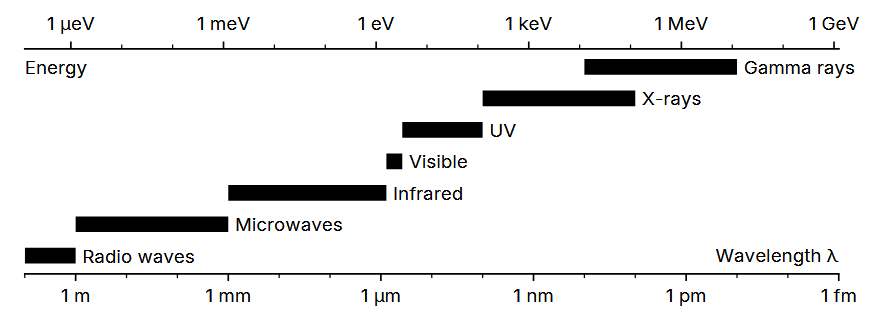
\includegraphics[width=0.5\linewidth]{Figures/Intro/1.png}
    \caption{Electromagnetic spectrum \cite{plotzki_2024_highresolution}}
    \label{fig:EMspectrum}
\end{figure}

\subsection{Radioactive decay}
Nuclei which emit gamma rays reach their excited states mainly due to radioactive decay. When an unstable nucleus (the parent nuclide, X) decays into a lighter nucleus (the daughter nuclide, Y) the difference in the mass results in particle radiation (P) and energy release (Q), which involves gamma rays. 

\begin{equation*}
\text{X} \rightarrow \text{Y} + \text{P} + \text{Q}
\end{equation*}

A decay is only possible if the mass of the parent
nuclide is greater than the sum of the masses of
all resulting particles (i.e., if the total energy released in the radioactive decay (the Q-value) is positive): 
\begin{equation}
    m_X \geq m_Y + m_P
\end{equation}

The characteristic gamma emission energies resulting from radioactive decay are conventionally attributed to the parent nuclide, even though they are actually emitted by the daughter nuclide.

\subsection{Decay law}
For an ensemble of $N$ unstable, radioactive nuclei, the decay rate $dN/dt$ is proportional to the number of nuclei present:
\begin{equation}
    A = -dN/dt = \lambda N
\end{equation}
The quantity $A$ is the current \textit{activity} of the sample, which has the unit Bacquerel (1 Bq = 1/s, one Bacquerel corresponds to one radioactive decay per second). The \textit{decay constant} determines the rate of decay in the ensemble. The solution to equation (3) is given by the decay law: 

\begin{equation}
    N(t) = N_0 e^{-\lambda t}
\end{equation}

Using this law and given an initial population $N_0$, we can estimate how many nuclei will still be present at a time t. The mean life-time of a nucleus is given by $\tau = 1/\lambda$ and the half-life is given by $t_{1/2} = \ln{(2)}/\lambda$. The half-life is defined as the time in which half of the nuclei will likely have decayed. 

\pagebreak{}

\subsection{Gamma rays and matter}
Gamma radiation is a type of ionizing radiation. The high-energy photons ionize atoms in the materials they interact with. In semiconductors, such as the germanium detector used in this experiment, they produce cascades of electron-hole pairs. This process allows for precise determination of photon energy. Various ionization mechanisms are briefly described below.

\subsection{Photoelectric absorption}
The photoelectric effect involves the transfer of the entire energy of a photon to an electron, ejecting it from its atomic shell thus ionizing the atom. The kinetic energy $E_k$ of the ejected electron is given by the difference between the gamma photon energy $E_\gamma$ and the binding energy $E_b$: 

\begin{equation}
    E_k = E_\gamma - E_b
\end{equation}

The ejected fast electrons interact with nearby electrons, gradually generating new electron-hole pairs in the semiconductor, resulting in a cascade effect.

The ionized atom is now in an unstable excited state with the energy $E_b$ above the ground state. Relaxation to the ground state occurs quickly either by further ionization or due to the higher-energy electrons filling the vacancy. In the latter process, X-rays are typically emitted. These X-rays either get absorbed by neighbouring atoms or escape the detector and are lost. In this case, some of the energy of the gamma radiation is \textit{not} converted into electron-hole pairs which results in a measurement error. This happens when absorption occurs at the surface of the detector and hence is a relatively rare event. 
\begin{figure}[h]
    \centering
    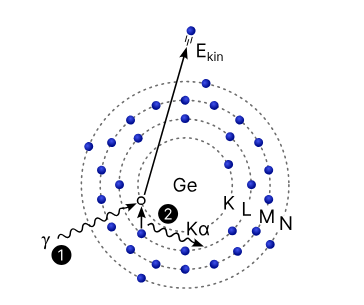
\includegraphics[width=0.5\linewidth]{Figures/Intro/2.png}
    \caption{Photoelectric effect \cite{plotzki_2024_highresolution}}
    \label{fig:Photoelectric effect}
\end{figure}

\pagebreak{}

\subsection{Compton scattering}
Compton scattering is the scattering of high-energy photons by electrons. In Compton scattering, only a part of the photon's energy is transferred to the electron, as opposed to the photoelectric effect. After the scattering, the photon has lost energy and changes its direction due to the conservation of momentum. The main equation of Compton scattering is: 

\begin{equation}
    E_{\text {k }}=E_\gamma\left(1-\frac{1}{1+E_\gamma(1-\cos \theta) / m_{e} c^2}\right)
	\label{eq:Compton}
\end{equation}

Where $E_k$ is the kinetic energy of the electron and $\theta$ is the scattering angle. The rest energy of the electron is $m_{e} c^2 = \SI{511}{keV}$. This equation applies in the case of scattering of a free electron. If the electrons are bound, their binding energy must be subtracted. However, this binding energy is typically negligible compared to the energy of a gamma photon, even in the case of atomically bound electrons. The energy of the scattered photon is: 
\begin{equation}
    E_{\gamma^\prime} =  E_\gamma -  E_k
\end{equation}

\begin{figure}[h]
    \centering
    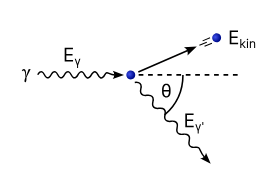
\includegraphics[width=0.5\linewidth]{Figures/Intro/3.png}
    \caption{Compton scattering \cite{plotzki_2024_highresolution}}
    \label{fig:Compton scattering}
\end{figure}

Let's examine equation \ref{eq:Compton}. In the scenario where complete forward scattering occurs ($\theta = 0$), no energy is transferred to the electron. And in complete backscattering ($\theta = \SI{180}{\degree})$ a part of the photon's energy is transferred to the electron. A plot of equation \ref{eq:Compton} for a gamma ray photon with an energy of $\SI{500}{keV}$ is shown in Figure \ref{fig:Compton scattering graph}.

\begin{figure}[h]
    \centering
    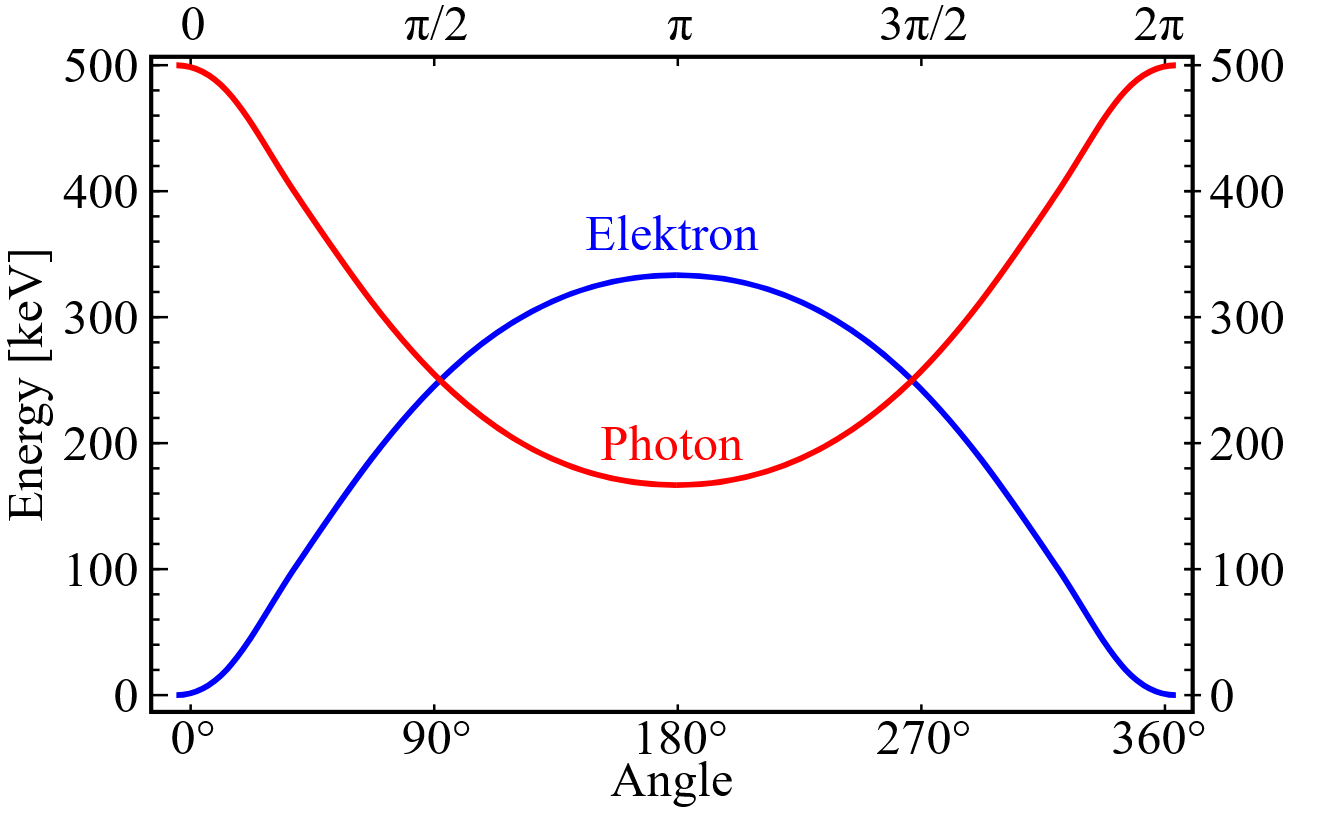
\includegraphics[width=0.5\linewidth]{Figures/Intro/4.png}
    \caption{Energies of a photon at 500 keV and an electron after Compton scattering \cite{_2020_compton}}
    \label{fig:Compton scattering graph}
\end{figure}

\pagebreak{}

\subsection{Pair production}
Pair production happens when a high-energy photon is converted into an electron-positron pair. This happens when the photon is near the atomic nucleus. The photon must have an energy of at least the rest mass of the electron-positron pair (i.e. $2\times511 = \SI{1022}{keV} $). If the photon's energy surpasses this threshold, the extra energy is converted into the kinetic energy of the electron and positron. Additionally, a small portion of the energy is used for the recoil of the atom in whose Coulomb field the pair production occurs. 

\begin{figure}[h]
    \centering
    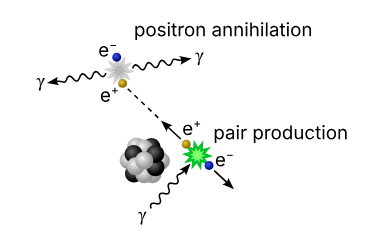
\includegraphics[width=0.5\linewidth]{Figures/Intro/6.png}
    \caption{Pair production \cite{plotzki_2024_highresolution}}
    \label{fig:Pair production}
\end{figure}

As the electron and positron move through the surrounding material, they interact with other atoms, ionizing them and generating additional free charge carriers. Through this process, they lose their kinetic energy and eventually come to rest. The positron at rest annihilates extremely quickly (on the order of nanoseconds) with an electron nearby, creating two photons with $\SI{511}{keV}$ of energy each. Three processes can occur now: 

\begin{enumerate}
    \item Single escape: One photon leaves the detector without interaction, a secondary peak appears at $\SI{511}{keV}$ less than the main peak.
    \item Double escape: Both photons leave the detector without interaction, a secondary peak appears at $\SI{1022}{keV}$ less than the main peak.
    \item No escape: No secondary peaks appears.
\end{enumerate}

The electron-positron pair is typically moving with respect to the lab's frame of reference at the moment this annihilation occurs. This is because the positron could have some residual kinetic energy and the fact that orbital electrons have angular momentum. Thus, a Doppler shift of the photon wavelengths (and energies) takes place. This manifests in high-resolution gamma ray spectroscopy as the peaks of the positron annihilation are a little wider than the characteristic peaks from atomic nuclei.

\pagebreak{}

\subsection{Experimental setup}
\subsubsection{structure of the detector}
The gamma spectrometer (Figure \ref{fig:spec}) includes a germanium semiconductor detector. The detector is composed of multiple stacked layers of germanium. A voltage is applied across these layers to move the released electrons to an amplifier, which then directs them to a multi-channel analyzer. The detector has 8192 channels which makes it possible to resolve energies from 0 to \SI{3000}{keV}. The detector is housed within a vacuum chamber inside an aluminum casing. Cooling is achieved through a cooling rod that is immersed in a tank of liquid nitrogen.

\begin{figure}[h]
    \centering
    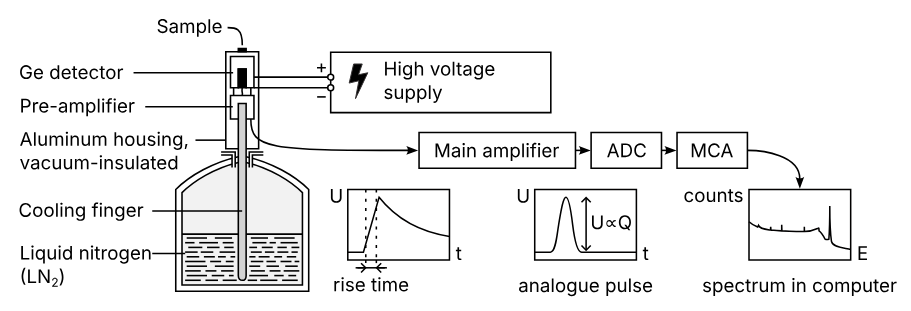
\includegraphics[width=0.5\linewidth]{Figures/Intro/5.png}
    \caption{Setup of the gamma spectrometer \cite{plotzki_2024_highresolution}}
    \label{fig:spec}
\end{figure}


\subsubsection{Calibration and measurement}
Cs-137 is used to measure the applied voltage and the rise time, which is how the detector channels are linked to the energy and intensity of the radiation. The rise time is basically the time interval in which events (or counts) are recorded. The optimal rise time is affected by two factors. If the rise time is too low, there is the risk of lower resolution due to rapid decay avalanches, which is likely at gamma ray energies. On the other hand, if the rise time is too high, a pile-up of events could occur.

To determine the composition of unknown samples accurately, we must eliminate contamination from background radiation and other gamma emitters, such as $^{40}$K. To achieve this, the laboratory's background radiation is measured over a specific time period. During the main measurement, the peaks of the background radiation can be ignored to accurately obtain the gamma spectrum of the samples. Specific energy peaks can be identified from this spectrum and matched to different elements using nuclide maps. An intensity-to-half-life ratio can also help infer the quantitative composition of elements in the sample. This requires correlating the measured radiation intensity with the actual radiation emitted from the sample.

\subsubsection{Materials used}
As already discussed, germanium is the main component of the detector. Germanium is a semiconductor which has a diamond-like crystal structure, which determines its electrical conductivity. Germanium detectors have the advantage of a very high detection resolution. Though, they require cooling to low temperatures. 

In conductors, the valence and conduction bands are connected and no energy is spent when an electron in the valence band is brought from the valence band to the conduction band, leaving a hole behind which can be filled by other electrons. 

However, this is not the case in semiconductors since there exists a gap between the two bands, the \textit{band gap}. Thus, an energy is needed before an electron "jumps" from the valence band to the conduction band, creating an electron-hole pair. In our experiment, this energy cost is supplied by the gamma photons.

\begin{figure}[h]
    \centering
    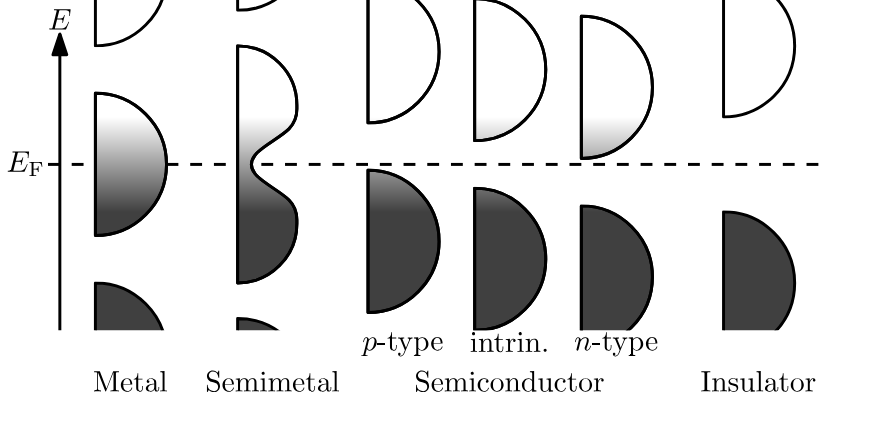
\includegraphics[width=0.5\linewidth]{Figures/Intro/7.png}
    \caption{Valence and conduction bands in different materials \cite{wikipediacontributors_2019_valence}}
    \label{fig:bands}
\end{figure}

\subsubsection{Radiation sources}
The calibration substances —  $^{22}$Na, $^{60}$Co, $^{133}$Ba and $^{137}$Cs, — are well-suited for our experiment because there is a high likelihood that they will frequently produce the same decay events with known emission energies. Additionally, we anticipate detecting the 1461 keV peak from $^{40}$K, which is commonly found in biological materials, as well as the 511 keV peak from positron annihilation in $\beta^+$ decay.

\pagebreak{}

\section{Analysis}

\subsection{Task 1: \textit{Finding Optimal Settings}}

In this task we used a Cs-137 sample to find the optimal rise time $\tau$ for the detector. This was done by finding the Full Width at Half Maximum (FWHM) of the same peak for different rise times, found in appendix \ref{appendix:Task1}. 

The following shows the FWHM values plotted against rise times:

\begin{figure}[h!]
	\centering
	\scalebox{1}{%% Creator: Matplotlib, PGF backend
%%
%% To include the figure in your LaTeX document, write
%%   \input{<filename>.pgf}
%%
%% Make sure the required packages are loaded in your preamble
%%   \usepackage{pgf}
%%
%% Also ensure that all the required font packages are loaded; for instance,
%% the lmodern package is sometimes necessary when using math font.
%%   \usepackage{lmodern}
%%
%% Figures using additional raster images can only be included by \input if
%% they are in the same directory as the main LaTeX file. For loading figures
%% from other directories you can use the `import` package
%%   \usepackage{import}
%%
%% and then include the figures with
%%   \import{<path to file>}{<filename>.pgf}
%%
%% Matplotlib used the following preamble
%%   
%%   \usepackage{fontspec}
%%   \makeatletter\@ifpackageloaded{underscore}{}{\usepackage[strings]{underscore}}\makeatother
%%
\begingroup%
\makeatletter%
\begin{pgfpicture}%
\pgfpathrectangle{\pgfpointorigin}{\pgfqpoint{5.759594in}{4.031666in}}%
\pgfusepath{use as bounding box, clip}%
\begin{pgfscope}%
\pgfsetbuttcap%
\pgfsetmiterjoin%
\definecolor{currentfill}{rgb}{1.000000,1.000000,1.000000}%
\pgfsetfillcolor{currentfill}%
\pgfsetlinewidth{0.000000pt}%
\definecolor{currentstroke}{rgb}{1.000000,1.000000,1.000000}%
\pgfsetstrokecolor{currentstroke}%
\pgfsetdash{}{0pt}%
\pgfpathmoveto{\pgfqpoint{0.000000in}{0.000000in}}%
\pgfpathlineto{\pgfqpoint{5.759594in}{0.000000in}}%
\pgfpathlineto{\pgfqpoint{5.759594in}{4.031666in}}%
\pgfpathlineto{\pgfqpoint{0.000000in}{4.031666in}}%
\pgfpathlineto{\pgfqpoint{0.000000in}{0.000000in}}%
\pgfpathclose%
\pgfusepath{fill}%
\end{pgfscope}%
\begin{pgfscope}%
\pgfsetbuttcap%
\pgfsetmiterjoin%
\definecolor{currentfill}{rgb}{1.000000,1.000000,1.000000}%
\pgfsetfillcolor{currentfill}%
\pgfsetlinewidth{0.000000pt}%
\definecolor{currentstroke}{rgb}{0.000000,0.000000,0.000000}%
\pgfsetstrokecolor{currentstroke}%
\pgfsetstrokeopacity{0.000000}%
\pgfsetdash{}{0pt}%
\pgfpathmoveto{\pgfqpoint{0.621275in}{0.598111in}}%
\pgfpathlineto{\pgfqpoint{5.650679in}{0.598111in}}%
\pgfpathlineto{\pgfqpoint{5.650679in}{3.686399in}}%
\pgfpathlineto{\pgfqpoint{0.621275in}{3.686399in}}%
\pgfpathlineto{\pgfqpoint{0.621275in}{0.598111in}}%
\pgfpathclose%
\pgfusepath{fill}%
\end{pgfscope}%
\begin{pgfscope}%
\pgfpathrectangle{\pgfqpoint{0.621275in}{0.598111in}}{\pgfqpoint{5.029404in}{3.088289in}}%
\pgfusepath{clip}%
\pgfsetbuttcap%
\pgfsetroundjoin%
\definecolor{currentfill}{rgb}{0.121569,0.466667,0.705882}%
\pgfsetfillcolor{currentfill}%
\pgfsetlinewidth{1.003750pt}%
\definecolor{currentstroke}{rgb}{0.121569,0.466667,0.705882}%
\pgfsetstrokecolor{currentstroke}%
\pgfsetdash{}{0pt}%
\pgfsys@defobject{currentmarker}{\pgfqpoint{-0.041667in}{-0.041667in}}{\pgfqpoint{0.041667in}{0.041667in}}{%
\pgfpathmoveto{\pgfqpoint{0.000000in}{-0.041667in}}%
\pgfpathcurveto{\pgfqpoint{0.011050in}{-0.041667in}}{\pgfqpoint{0.021649in}{-0.037276in}}{\pgfqpoint{0.029463in}{-0.029463in}}%
\pgfpathcurveto{\pgfqpoint{0.037276in}{-0.021649in}}{\pgfqpoint{0.041667in}{-0.011050in}}{\pgfqpoint{0.041667in}{0.000000in}}%
\pgfpathcurveto{\pgfqpoint{0.041667in}{0.011050in}}{\pgfqpoint{0.037276in}{0.021649in}}{\pgfqpoint{0.029463in}{0.029463in}}%
\pgfpathcurveto{\pgfqpoint{0.021649in}{0.037276in}}{\pgfqpoint{0.011050in}{0.041667in}}{\pgfqpoint{0.000000in}{0.041667in}}%
\pgfpathcurveto{\pgfqpoint{-0.011050in}{0.041667in}}{\pgfqpoint{-0.021649in}{0.037276in}}{\pgfqpoint{-0.029463in}{0.029463in}}%
\pgfpathcurveto{\pgfqpoint{-0.037276in}{0.021649in}}{\pgfqpoint{-0.041667in}{0.011050in}}{\pgfqpoint{-0.041667in}{0.000000in}}%
\pgfpathcurveto{\pgfqpoint{-0.041667in}{-0.011050in}}{\pgfqpoint{-0.037276in}{-0.021649in}}{\pgfqpoint{-0.029463in}{-0.029463in}}%
\pgfpathcurveto{\pgfqpoint{-0.021649in}{-0.037276in}}{\pgfqpoint{-0.011050in}{-0.041667in}}{\pgfqpoint{0.000000in}{-0.041667in}}%
\pgfpathlineto{\pgfqpoint{0.000000in}{-0.041667in}}%
\pgfpathclose%
\pgfusepath{stroke,fill}%
}%
\begin{pgfscope}%
\pgfsys@transformshift{0.849884in}{3.546023in}%
\pgfsys@useobject{currentmarker}{}%
\end{pgfscope}%
\begin{pgfscope}%
\pgfsys@transformshift{0.954591in}{2.509432in}%
\pgfsys@useobject{currentmarker}{}%
\end{pgfscope}%
\begin{pgfscope}%
\pgfsys@transformshift{1.094200in}{1.833913in}%
\pgfsys@useobject{currentmarker}{}%
\end{pgfscope}%
\begin{pgfscope}%
\pgfsys@transformshift{1.513026in}{1.162468in}%
\pgfsys@useobject{currentmarker}{}%
\end{pgfscope}%
\begin{pgfscope}%
\pgfsys@transformshift{1.931852in}{0.939410in}%
\pgfsys@useobject{currentmarker}{}%
\end{pgfscope}%
\begin{pgfscope}%
\pgfsys@transformshift{2.629895in}{0.807859in}%
\pgfsys@useobject{currentmarker}{}%
\end{pgfscope}%
\begin{pgfscope}%
\pgfsys@transformshift{3.467548in}{0.748246in}%
\pgfsys@useobject{currentmarker}{}%
\end{pgfscope}%
\begin{pgfscope}%
\pgfsys@transformshift{4.305200in}{0.738488in}%
\pgfsys@useobject{currentmarker}{}%
\end{pgfscope}%
\begin{pgfscope}%
\pgfsys@transformshift{5.422070in}{0.745443in}%
\pgfsys@useobject{currentmarker}{}%
\end{pgfscope}%
\end{pgfscope}%
\begin{pgfscope}%
\pgfpathrectangle{\pgfqpoint{0.621275in}{0.598111in}}{\pgfqpoint{5.029404in}{3.088289in}}%
\pgfusepath{clip}%
\pgfsetrectcap%
\pgfsetroundjoin%
\pgfsetlinewidth{0.803000pt}%
\definecolor{currentstroke}{rgb}{0.690196,0.690196,0.690196}%
\pgfsetstrokecolor{currentstroke}%
\pgfsetdash{}{0pt}%
\pgfpathmoveto{\pgfqpoint{0.675374in}{0.598111in}}%
\pgfpathlineto{\pgfqpoint{0.675374in}{3.686399in}}%
\pgfusepath{stroke}%
\end{pgfscope}%
\begin{pgfscope}%
\pgfsetbuttcap%
\pgfsetroundjoin%
\definecolor{currentfill}{rgb}{0.000000,0.000000,0.000000}%
\pgfsetfillcolor{currentfill}%
\pgfsetlinewidth{0.803000pt}%
\definecolor{currentstroke}{rgb}{0.000000,0.000000,0.000000}%
\pgfsetstrokecolor{currentstroke}%
\pgfsetdash{}{0pt}%
\pgfsys@defobject{currentmarker}{\pgfqpoint{0.000000in}{-0.048611in}}{\pgfqpoint{0.000000in}{0.000000in}}{%
\pgfpathmoveto{\pgfqpoint{0.000000in}{0.000000in}}%
\pgfpathlineto{\pgfqpoint{0.000000in}{-0.048611in}}%
\pgfusepath{stroke,fill}%
}%
\begin{pgfscope}%
\pgfsys@transformshift{0.675374in}{0.598111in}%
\pgfsys@useobject{currentmarker}{}%
\end{pgfscope}%
\end{pgfscope}%
\begin{pgfscope}%
\definecolor{textcolor}{rgb}{0.000000,0.000000,0.000000}%
\pgfsetstrokecolor{textcolor}%
\pgfsetfillcolor{textcolor}%
\pgftext[x=0.675374in,y=0.500889in,,top]{\color{textcolor}\rmfamily\fontsize{14.000000}{16.800000}\selectfont \(\displaystyle {0}\)}%
\end{pgfscope}%
\begin{pgfscope}%
\pgfpathrectangle{\pgfqpoint{0.621275in}{0.598111in}}{\pgfqpoint{5.029404in}{3.088289in}}%
\pgfusepath{clip}%
\pgfsetrectcap%
\pgfsetroundjoin%
\pgfsetlinewidth{0.803000pt}%
\definecolor{currentstroke}{rgb}{0.690196,0.690196,0.690196}%
\pgfsetstrokecolor{currentstroke}%
\pgfsetdash{}{0pt}%
\pgfpathmoveto{\pgfqpoint{1.373417in}{0.598111in}}%
\pgfpathlineto{\pgfqpoint{1.373417in}{3.686399in}}%
\pgfusepath{stroke}%
\end{pgfscope}%
\begin{pgfscope}%
\pgfsetbuttcap%
\pgfsetroundjoin%
\definecolor{currentfill}{rgb}{0.000000,0.000000,0.000000}%
\pgfsetfillcolor{currentfill}%
\pgfsetlinewidth{0.803000pt}%
\definecolor{currentstroke}{rgb}{0.000000,0.000000,0.000000}%
\pgfsetstrokecolor{currentstroke}%
\pgfsetdash{}{0pt}%
\pgfsys@defobject{currentmarker}{\pgfqpoint{0.000000in}{-0.048611in}}{\pgfqpoint{0.000000in}{0.000000in}}{%
\pgfpathmoveto{\pgfqpoint{0.000000in}{0.000000in}}%
\pgfpathlineto{\pgfqpoint{0.000000in}{-0.048611in}}%
\pgfusepath{stroke,fill}%
}%
\begin{pgfscope}%
\pgfsys@transformshift{1.373417in}{0.598111in}%
\pgfsys@useobject{currentmarker}{}%
\end{pgfscope}%
\end{pgfscope}%
\begin{pgfscope}%
\definecolor{textcolor}{rgb}{0.000000,0.000000,0.000000}%
\pgfsetstrokecolor{textcolor}%
\pgfsetfillcolor{textcolor}%
\pgftext[x=1.373417in,y=0.500889in,,top]{\color{textcolor}\rmfamily\fontsize{14.000000}{16.800000}\selectfont \(\displaystyle {2}\)}%
\end{pgfscope}%
\begin{pgfscope}%
\pgfpathrectangle{\pgfqpoint{0.621275in}{0.598111in}}{\pgfqpoint{5.029404in}{3.088289in}}%
\pgfusepath{clip}%
\pgfsetrectcap%
\pgfsetroundjoin%
\pgfsetlinewidth{0.803000pt}%
\definecolor{currentstroke}{rgb}{0.690196,0.690196,0.690196}%
\pgfsetstrokecolor{currentstroke}%
\pgfsetdash{}{0pt}%
\pgfpathmoveto{\pgfqpoint{2.071461in}{0.598111in}}%
\pgfpathlineto{\pgfqpoint{2.071461in}{3.686399in}}%
\pgfusepath{stroke}%
\end{pgfscope}%
\begin{pgfscope}%
\pgfsetbuttcap%
\pgfsetroundjoin%
\definecolor{currentfill}{rgb}{0.000000,0.000000,0.000000}%
\pgfsetfillcolor{currentfill}%
\pgfsetlinewidth{0.803000pt}%
\definecolor{currentstroke}{rgb}{0.000000,0.000000,0.000000}%
\pgfsetstrokecolor{currentstroke}%
\pgfsetdash{}{0pt}%
\pgfsys@defobject{currentmarker}{\pgfqpoint{0.000000in}{-0.048611in}}{\pgfqpoint{0.000000in}{0.000000in}}{%
\pgfpathmoveto{\pgfqpoint{0.000000in}{0.000000in}}%
\pgfpathlineto{\pgfqpoint{0.000000in}{-0.048611in}}%
\pgfusepath{stroke,fill}%
}%
\begin{pgfscope}%
\pgfsys@transformshift{2.071461in}{0.598111in}%
\pgfsys@useobject{currentmarker}{}%
\end{pgfscope}%
\end{pgfscope}%
\begin{pgfscope}%
\definecolor{textcolor}{rgb}{0.000000,0.000000,0.000000}%
\pgfsetstrokecolor{textcolor}%
\pgfsetfillcolor{textcolor}%
\pgftext[x=2.071461in,y=0.500889in,,top]{\color{textcolor}\rmfamily\fontsize{14.000000}{16.800000}\selectfont \(\displaystyle {4}\)}%
\end{pgfscope}%
\begin{pgfscope}%
\pgfpathrectangle{\pgfqpoint{0.621275in}{0.598111in}}{\pgfqpoint{5.029404in}{3.088289in}}%
\pgfusepath{clip}%
\pgfsetrectcap%
\pgfsetroundjoin%
\pgfsetlinewidth{0.803000pt}%
\definecolor{currentstroke}{rgb}{0.690196,0.690196,0.690196}%
\pgfsetstrokecolor{currentstroke}%
\pgfsetdash{}{0pt}%
\pgfpathmoveto{\pgfqpoint{2.769504in}{0.598111in}}%
\pgfpathlineto{\pgfqpoint{2.769504in}{3.686399in}}%
\pgfusepath{stroke}%
\end{pgfscope}%
\begin{pgfscope}%
\pgfsetbuttcap%
\pgfsetroundjoin%
\definecolor{currentfill}{rgb}{0.000000,0.000000,0.000000}%
\pgfsetfillcolor{currentfill}%
\pgfsetlinewidth{0.803000pt}%
\definecolor{currentstroke}{rgb}{0.000000,0.000000,0.000000}%
\pgfsetstrokecolor{currentstroke}%
\pgfsetdash{}{0pt}%
\pgfsys@defobject{currentmarker}{\pgfqpoint{0.000000in}{-0.048611in}}{\pgfqpoint{0.000000in}{0.000000in}}{%
\pgfpathmoveto{\pgfqpoint{0.000000in}{0.000000in}}%
\pgfpathlineto{\pgfqpoint{0.000000in}{-0.048611in}}%
\pgfusepath{stroke,fill}%
}%
\begin{pgfscope}%
\pgfsys@transformshift{2.769504in}{0.598111in}%
\pgfsys@useobject{currentmarker}{}%
\end{pgfscope}%
\end{pgfscope}%
\begin{pgfscope}%
\definecolor{textcolor}{rgb}{0.000000,0.000000,0.000000}%
\pgfsetstrokecolor{textcolor}%
\pgfsetfillcolor{textcolor}%
\pgftext[x=2.769504in,y=0.500889in,,top]{\color{textcolor}\rmfamily\fontsize{14.000000}{16.800000}\selectfont \(\displaystyle {6}\)}%
\end{pgfscope}%
\begin{pgfscope}%
\pgfpathrectangle{\pgfqpoint{0.621275in}{0.598111in}}{\pgfqpoint{5.029404in}{3.088289in}}%
\pgfusepath{clip}%
\pgfsetrectcap%
\pgfsetroundjoin%
\pgfsetlinewidth{0.803000pt}%
\definecolor{currentstroke}{rgb}{0.690196,0.690196,0.690196}%
\pgfsetstrokecolor{currentstroke}%
\pgfsetdash{}{0pt}%
\pgfpathmoveto{\pgfqpoint{3.467548in}{0.598111in}}%
\pgfpathlineto{\pgfqpoint{3.467548in}{3.686399in}}%
\pgfusepath{stroke}%
\end{pgfscope}%
\begin{pgfscope}%
\pgfsetbuttcap%
\pgfsetroundjoin%
\definecolor{currentfill}{rgb}{0.000000,0.000000,0.000000}%
\pgfsetfillcolor{currentfill}%
\pgfsetlinewidth{0.803000pt}%
\definecolor{currentstroke}{rgb}{0.000000,0.000000,0.000000}%
\pgfsetstrokecolor{currentstroke}%
\pgfsetdash{}{0pt}%
\pgfsys@defobject{currentmarker}{\pgfqpoint{0.000000in}{-0.048611in}}{\pgfqpoint{0.000000in}{0.000000in}}{%
\pgfpathmoveto{\pgfqpoint{0.000000in}{0.000000in}}%
\pgfpathlineto{\pgfqpoint{0.000000in}{-0.048611in}}%
\pgfusepath{stroke,fill}%
}%
\begin{pgfscope}%
\pgfsys@transformshift{3.467548in}{0.598111in}%
\pgfsys@useobject{currentmarker}{}%
\end{pgfscope}%
\end{pgfscope}%
\begin{pgfscope}%
\definecolor{textcolor}{rgb}{0.000000,0.000000,0.000000}%
\pgfsetstrokecolor{textcolor}%
\pgfsetfillcolor{textcolor}%
\pgftext[x=3.467548in,y=0.500889in,,top]{\color{textcolor}\rmfamily\fontsize{14.000000}{16.800000}\selectfont \(\displaystyle {8}\)}%
\end{pgfscope}%
\begin{pgfscope}%
\pgfpathrectangle{\pgfqpoint{0.621275in}{0.598111in}}{\pgfqpoint{5.029404in}{3.088289in}}%
\pgfusepath{clip}%
\pgfsetrectcap%
\pgfsetroundjoin%
\pgfsetlinewidth{0.803000pt}%
\definecolor{currentstroke}{rgb}{0.690196,0.690196,0.690196}%
\pgfsetstrokecolor{currentstroke}%
\pgfsetdash{}{0pt}%
\pgfpathmoveto{\pgfqpoint{4.165591in}{0.598111in}}%
\pgfpathlineto{\pgfqpoint{4.165591in}{3.686399in}}%
\pgfusepath{stroke}%
\end{pgfscope}%
\begin{pgfscope}%
\pgfsetbuttcap%
\pgfsetroundjoin%
\definecolor{currentfill}{rgb}{0.000000,0.000000,0.000000}%
\pgfsetfillcolor{currentfill}%
\pgfsetlinewidth{0.803000pt}%
\definecolor{currentstroke}{rgb}{0.000000,0.000000,0.000000}%
\pgfsetstrokecolor{currentstroke}%
\pgfsetdash{}{0pt}%
\pgfsys@defobject{currentmarker}{\pgfqpoint{0.000000in}{-0.048611in}}{\pgfqpoint{0.000000in}{0.000000in}}{%
\pgfpathmoveto{\pgfqpoint{0.000000in}{0.000000in}}%
\pgfpathlineto{\pgfqpoint{0.000000in}{-0.048611in}}%
\pgfusepath{stroke,fill}%
}%
\begin{pgfscope}%
\pgfsys@transformshift{4.165591in}{0.598111in}%
\pgfsys@useobject{currentmarker}{}%
\end{pgfscope}%
\end{pgfscope}%
\begin{pgfscope}%
\definecolor{textcolor}{rgb}{0.000000,0.000000,0.000000}%
\pgfsetstrokecolor{textcolor}%
\pgfsetfillcolor{textcolor}%
\pgftext[x=4.165591in,y=0.500889in,,top]{\color{textcolor}\rmfamily\fontsize{14.000000}{16.800000}\selectfont \(\displaystyle {10}\)}%
\end{pgfscope}%
\begin{pgfscope}%
\pgfpathrectangle{\pgfqpoint{0.621275in}{0.598111in}}{\pgfqpoint{5.029404in}{3.088289in}}%
\pgfusepath{clip}%
\pgfsetrectcap%
\pgfsetroundjoin%
\pgfsetlinewidth{0.803000pt}%
\definecolor{currentstroke}{rgb}{0.690196,0.690196,0.690196}%
\pgfsetstrokecolor{currentstroke}%
\pgfsetdash{}{0pt}%
\pgfpathmoveto{\pgfqpoint{4.863635in}{0.598111in}}%
\pgfpathlineto{\pgfqpoint{4.863635in}{3.686399in}}%
\pgfusepath{stroke}%
\end{pgfscope}%
\begin{pgfscope}%
\pgfsetbuttcap%
\pgfsetroundjoin%
\definecolor{currentfill}{rgb}{0.000000,0.000000,0.000000}%
\pgfsetfillcolor{currentfill}%
\pgfsetlinewidth{0.803000pt}%
\definecolor{currentstroke}{rgb}{0.000000,0.000000,0.000000}%
\pgfsetstrokecolor{currentstroke}%
\pgfsetdash{}{0pt}%
\pgfsys@defobject{currentmarker}{\pgfqpoint{0.000000in}{-0.048611in}}{\pgfqpoint{0.000000in}{0.000000in}}{%
\pgfpathmoveto{\pgfqpoint{0.000000in}{0.000000in}}%
\pgfpathlineto{\pgfqpoint{0.000000in}{-0.048611in}}%
\pgfusepath{stroke,fill}%
}%
\begin{pgfscope}%
\pgfsys@transformshift{4.863635in}{0.598111in}%
\pgfsys@useobject{currentmarker}{}%
\end{pgfscope}%
\end{pgfscope}%
\begin{pgfscope}%
\definecolor{textcolor}{rgb}{0.000000,0.000000,0.000000}%
\pgfsetstrokecolor{textcolor}%
\pgfsetfillcolor{textcolor}%
\pgftext[x=4.863635in,y=0.500889in,,top]{\color{textcolor}\rmfamily\fontsize{14.000000}{16.800000}\selectfont \(\displaystyle {12}\)}%
\end{pgfscope}%
\begin{pgfscope}%
\pgfpathrectangle{\pgfqpoint{0.621275in}{0.598111in}}{\pgfqpoint{5.029404in}{3.088289in}}%
\pgfusepath{clip}%
\pgfsetrectcap%
\pgfsetroundjoin%
\pgfsetlinewidth{0.803000pt}%
\definecolor{currentstroke}{rgb}{0.690196,0.690196,0.690196}%
\pgfsetstrokecolor{currentstroke}%
\pgfsetdash{}{0pt}%
\pgfpathmoveto{\pgfqpoint{5.561678in}{0.598111in}}%
\pgfpathlineto{\pgfqpoint{5.561678in}{3.686399in}}%
\pgfusepath{stroke}%
\end{pgfscope}%
\begin{pgfscope}%
\pgfsetbuttcap%
\pgfsetroundjoin%
\definecolor{currentfill}{rgb}{0.000000,0.000000,0.000000}%
\pgfsetfillcolor{currentfill}%
\pgfsetlinewidth{0.803000pt}%
\definecolor{currentstroke}{rgb}{0.000000,0.000000,0.000000}%
\pgfsetstrokecolor{currentstroke}%
\pgfsetdash{}{0pt}%
\pgfsys@defobject{currentmarker}{\pgfqpoint{0.000000in}{-0.048611in}}{\pgfqpoint{0.000000in}{0.000000in}}{%
\pgfpathmoveto{\pgfqpoint{0.000000in}{0.000000in}}%
\pgfpathlineto{\pgfqpoint{0.000000in}{-0.048611in}}%
\pgfusepath{stroke,fill}%
}%
\begin{pgfscope}%
\pgfsys@transformshift{5.561678in}{0.598111in}%
\pgfsys@useobject{currentmarker}{}%
\end{pgfscope}%
\end{pgfscope}%
\begin{pgfscope}%
\definecolor{textcolor}{rgb}{0.000000,0.000000,0.000000}%
\pgfsetstrokecolor{textcolor}%
\pgfsetfillcolor{textcolor}%
\pgftext[x=5.561678in,y=0.500889in,,top]{\color{textcolor}\rmfamily\fontsize{14.000000}{16.800000}\selectfont \(\displaystyle {14}\)}%
\end{pgfscope}%
\begin{pgfscope}%
\definecolor{textcolor}{rgb}{0.000000,0.000000,0.000000}%
\pgfsetstrokecolor{textcolor}%
\pgfsetfillcolor{textcolor}%
\pgftext[x=3.135977in,y=0.272667in,,top]{\color{textcolor}\rmfamily\fontsize{14.000000}{16.800000}\selectfont Rise Time}%
\end{pgfscope}%
\begin{pgfscope}%
\pgfpathrectangle{\pgfqpoint{0.621275in}{0.598111in}}{\pgfqpoint{5.029404in}{3.088289in}}%
\pgfusepath{clip}%
\pgfsetrectcap%
\pgfsetroundjoin%
\pgfsetlinewidth{0.803000pt}%
\definecolor{currentstroke}{rgb}{0.690196,0.690196,0.690196}%
\pgfsetstrokecolor{currentstroke}%
\pgfsetdash{}{0pt}%
\pgfpathmoveto{\pgfqpoint{0.621275in}{0.850834in}}%
\pgfpathlineto{\pgfqpoint{5.650679in}{0.850834in}}%
\pgfusepath{stroke}%
\end{pgfscope}%
\begin{pgfscope}%
\pgfsetbuttcap%
\pgfsetroundjoin%
\definecolor{currentfill}{rgb}{0.000000,0.000000,0.000000}%
\pgfsetfillcolor{currentfill}%
\pgfsetlinewidth{0.803000pt}%
\definecolor{currentstroke}{rgb}{0.000000,0.000000,0.000000}%
\pgfsetstrokecolor{currentstroke}%
\pgfsetdash{}{0pt}%
\pgfsys@defobject{currentmarker}{\pgfqpoint{-0.048611in}{0.000000in}}{\pgfqpoint{-0.000000in}{0.000000in}}{%
\pgfpathmoveto{\pgfqpoint{-0.000000in}{0.000000in}}%
\pgfpathlineto{\pgfqpoint{-0.048611in}{0.000000in}}%
\pgfusepath{stroke,fill}%
}%
\begin{pgfscope}%
\pgfsys@transformshift{0.621275in}{0.850834in}%
\pgfsys@useobject{currentmarker}{}%
\end{pgfscope}%
\end{pgfscope}%
\begin{pgfscope}%
\definecolor{textcolor}{rgb}{0.000000,0.000000,0.000000}%
\pgfsetstrokecolor{textcolor}%
\pgfsetfillcolor{textcolor}%
\pgftext[x=0.426138in, y=0.783362in, left, base]{\color{textcolor}\rmfamily\fontsize{14.000000}{16.800000}\selectfont \(\displaystyle {5}\)}%
\end{pgfscope}%
\begin{pgfscope}%
\pgfpathrectangle{\pgfqpoint{0.621275in}{0.598111in}}{\pgfqpoint{5.029404in}{3.088289in}}%
\pgfusepath{clip}%
\pgfsetrectcap%
\pgfsetroundjoin%
\pgfsetlinewidth{0.803000pt}%
\definecolor{currentstroke}{rgb}{0.690196,0.690196,0.690196}%
\pgfsetstrokecolor{currentstroke}%
\pgfsetdash{}{0pt}%
\pgfpathmoveto{\pgfqpoint{0.621275in}{1.666161in}}%
\pgfpathlineto{\pgfqpoint{5.650679in}{1.666161in}}%
\pgfusepath{stroke}%
\end{pgfscope}%
\begin{pgfscope}%
\pgfsetbuttcap%
\pgfsetroundjoin%
\definecolor{currentfill}{rgb}{0.000000,0.000000,0.000000}%
\pgfsetfillcolor{currentfill}%
\pgfsetlinewidth{0.803000pt}%
\definecolor{currentstroke}{rgb}{0.000000,0.000000,0.000000}%
\pgfsetstrokecolor{currentstroke}%
\pgfsetdash{}{0pt}%
\pgfsys@defobject{currentmarker}{\pgfqpoint{-0.048611in}{0.000000in}}{\pgfqpoint{-0.000000in}{0.000000in}}{%
\pgfpathmoveto{\pgfqpoint{-0.000000in}{0.000000in}}%
\pgfpathlineto{\pgfqpoint{-0.048611in}{0.000000in}}%
\pgfusepath{stroke,fill}%
}%
\begin{pgfscope}%
\pgfsys@transformshift{0.621275in}{1.666161in}%
\pgfsys@useobject{currentmarker}{}%
\end{pgfscope}%
\end{pgfscope}%
\begin{pgfscope}%
\definecolor{textcolor}{rgb}{0.000000,0.000000,0.000000}%
\pgfsetstrokecolor{textcolor}%
\pgfsetfillcolor{textcolor}%
\pgftext[x=0.328222in, y=1.598688in, left, base]{\color{textcolor}\rmfamily\fontsize{14.000000}{16.800000}\selectfont \(\displaystyle {10}\)}%
\end{pgfscope}%
\begin{pgfscope}%
\pgfpathrectangle{\pgfqpoint{0.621275in}{0.598111in}}{\pgfqpoint{5.029404in}{3.088289in}}%
\pgfusepath{clip}%
\pgfsetrectcap%
\pgfsetroundjoin%
\pgfsetlinewidth{0.803000pt}%
\definecolor{currentstroke}{rgb}{0.690196,0.690196,0.690196}%
\pgfsetstrokecolor{currentstroke}%
\pgfsetdash{}{0pt}%
\pgfpathmoveto{\pgfqpoint{0.621275in}{2.481487in}}%
\pgfpathlineto{\pgfqpoint{5.650679in}{2.481487in}}%
\pgfusepath{stroke}%
\end{pgfscope}%
\begin{pgfscope}%
\pgfsetbuttcap%
\pgfsetroundjoin%
\definecolor{currentfill}{rgb}{0.000000,0.000000,0.000000}%
\pgfsetfillcolor{currentfill}%
\pgfsetlinewidth{0.803000pt}%
\definecolor{currentstroke}{rgb}{0.000000,0.000000,0.000000}%
\pgfsetstrokecolor{currentstroke}%
\pgfsetdash{}{0pt}%
\pgfsys@defobject{currentmarker}{\pgfqpoint{-0.048611in}{0.000000in}}{\pgfqpoint{-0.000000in}{0.000000in}}{%
\pgfpathmoveto{\pgfqpoint{-0.000000in}{0.000000in}}%
\pgfpathlineto{\pgfqpoint{-0.048611in}{0.000000in}}%
\pgfusepath{stroke,fill}%
}%
\begin{pgfscope}%
\pgfsys@transformshift{0.621275in}{2.481487in}%
\pgfsys@useobject{currentmarker}{}%
\end{pgfscope}%
\end{pgfscope}%
\begin{pgfscope}%
\definecolor{textcolor}{rgb}{0.000000,0.000000,0.000000}%
\pgfsetstrokecolor{textcolor}%
\pgfsetfillcolor{textcolor}%
\pgftext[x=0.328222in, y=2.414015in, left, base]{\color{textcolor}\rmfamily\fontsize{14.000000}{16.800000}\selectfont \(\displaystyle {15}\)}%
\end{pgfscope}%
\begin{pgfscope}%
\pgfpathrectangle{\pgfqpoint{0.621275in}{0.598111in}}{\pgfqpoint{5.029404in}{3.088289in}}%
\pgfusepath{clip}%
\pgfsetrectcap%
\pgfsetroundjoin%
\pgfsetlinewidth{0.803000pt}%
\definecolor{currentstroke}{rgb}{0.690196,0.690196,0.690196}%
\pgfsetstrokecolor{currentstroke}%
\pgfsetdash{}{0pt}%
\pgfpathmoveto{\pgfqpoint{0.621275in}{3.296814in}}%
\pgfpathlineto{\pgfqpoint{5.650679in}{3.296814in}}%
\pgfusepath{stroke}%
\end{pgfscope}%
\begin{pgfscope}%
\pgfsetbuttcap%
\pgfsetroundjoin%
\definecolor{currentfill}{rgb}{0.000000,0.000000,0.000000}%
\pgfsetfillcolor{currentfill}%
\pgfsetlinewidth{0.803000pt}%
\definecolor{currentstroke}{rgb}{0.000000,0.000000,0.000000}%
\pgfsetstrokecolor{currentstroke}%
\pgfsetdash{}{0pt}%
\pgfsys@defobject{currentmarker}{\pgfqpoint{-0.048611in}{0.000000in}}{\pgfqpoint{-0.000000in}{0.000000in}}{%
\pgfpathmoveto{\pgfqpoint{-0.000000in}{0.000000in}}%
\pgfpathlineto{\pgfqpoint{-0.048611in}{0.000000in}}%
\pgfusepath{stroke,fill}%
}%
\begin{pgfscope}%
\pgfsys@transformshift{0.621275in}{3.296814in}%
\pgfsys@useobject{currentmarker}{}%
\end{pgfscope}%
\end{pgfscope}%
\begin{pgfscope}%
\definecolor{textcolor}{rgb}{0.000000,0.000000,0.000000}%
\pgfsetstrokecolor{textcolor}%
\pgfsetfillcolor{textcolor}%
\pgftext[x=0.328222in, y=3.229342in, left, base]{\color{textcolor}\rmfamily\fontsize{14.000000}{16.800000}\selectfont \(\displaystyle {20}\)}%
\end{pgfscope}%
\begin{pgfscope}%
\definecolor{textcolor}{rgb}{0.000000,0.000000,0.000000}%
\pgfsetstrokecolor{textcolor}%
\pgfsetfillcolor{textcolor}%
\pgftext[x=0.272667in,y=2.142255in,,bottom,rotate=90.000000]{\color{textcolor}\rmfamily\fontsize{14.000000}{16.800000}\selectfont FWHM}%
\end{pgfscope}%
\begin{pgfscope}%
\pgfsetrectcap%
\pgfsetmiterjoin%
\pgfsetlinewidth{0.803000pt}%
\definecolor{currentstroke}{rgb}{0.000000,0.000000,0.000000}%
\pgfsetstrokecolor{currentstroke}%
\pgfsetdash{}{0pt}%
\pgfpathmoveto{\pgfqpoint{0.621275in}{0.598111in}}%
\pgfpathlineto{\pgfqpoint{0.621275in}{3.686399in}}%
\pgfusepath{stroke}%
\end{pgfscope}%
\begin{pgfscope}%
\pgfsetrectcap%
\pgfsetmiterjoin%
\pgfsetlinewidth{0.803000pt}%
\definecolor{currentstroke}{rgb}{0.000000,0.000000,0.000000}%
\pgfsetstrokecolor{currentstroke}%
\pgfsetdash{}{0pt}%
\pgfpathmoveto{\pgfqpoint{5.650679in}{0.598111in}}%
\pgfpathlineto{\pgfqpoint{5.650679in}{3.686399in}}%
\pgfusepath{stroke}%
\end{pgfscope}%
\begin{pgfscope}%
\pgfsetrectcap%
\pgfsetmiterjoin%
\pgfsetlinewidth{0.803000pt}%
\definecolor{currentstroke}{rgb}{0.000000,0.000000,0.000000}%
\pgfsetstrokecolor{currentstroke}%
\pgfsetdash{}{0pt}%
\pgfpathmoveto{\pgfqpoint{0.621275in}{0.598111in}}%
\pgfpathlineto{\pgfqpoint{5.650679in}{0.598111in}}%
\pgfusepath{stroke}%
\end{pgfscope}%
\begin{pgfscope}%
\pgfsetrectcap%
\pgfsetmiterjoin%
\pgfsetlinewidth{0.803000pt}%
\definecolor{currentstroke}{rgb}{0.000000,0.000000,0.000000}%
\pgfsetstrokecolor{currentstroke}%
\pgfsetdash{}{0pt}%
\pgfpathmoveto{\pgfqpoint{0.621275in}{3.686399in}}%
\pgfpathlineto{\pgfqpoint{5.650679in}{3.686399in}}%
\pgfusepath{stroke}%
\end{pgfscope}%
\begin{pgfscope}%
\definecolor{textcolor}{rgb}{0.000000,0.000000,0.000000}%
\pgfsetstrokecolor{textcolor}%
\pgfsetfillcolor{textcolor}%
\pgftext[x=3.135977in,y=3.769733in,,base]{\color{textcolor}\rmfamily\fontsize{16.800000}{20.160000}\selectfont FWHM vs Rise Time}%
\end{pgfscope}%
\end{pgfpicture}%
\makeatother%
\endgroup%
}
	\caption{FWHM values for different rise times}
	\label{fig:risetimes}
\end{figure}

We chose a rise time of $\tau = 5.6 \ \mu$s as it was the best compromise between resolution and low rise time. 

\pagebreak{}

\subsection{Task 2: \textit{Energy Calibration \& Resolution}}
\subsubsection{Calibration}

The output of the spectrometer is given in channel numbers, which correspond to energies. To convert these channel numbers to energies, samples with known peak energies are used.
We used the following samples: $^{137}$Cs, $^{60}$Co, $^{22}$Na, and $^{133}$Ba.

\begin{figure}[h!]
	\centering
	\begin{subfigure}{0.45\textwidth}
		\centering
		\scalebox{0.5}{%% Creator: Matplotlib, PGF backend
%%
%% To include the figure in your LaTeX document, write
%%   \input{<filename>.pgf}
%%
%% Make sure the required packages are loaded in your preamble
%%   \usepackage{pgf}
%%
%% Also ensure that all the required font packages are loaded; for instance,
%% the lmodern package is sometimes necessary when using math font.
%%   \usepackage{lmodern}
%%
%% Figures using additional raster images can only be included by \input if
%% they are in the same directory as the main LaTeX file. For loading figures
%% from other directories you can use the `import` package
%%   \usepackage{import}
%%
%% and then include the figures with
%%   \import{<path to file>}{<filename>.pgf}
%%
%% Matplotlib used the following preamble
%%   
%%   \usepackage{fontspec}
%%   \makeatletter\@ifpackageloaded{underscore}{}{\usepackage[strings]{underscore}}\makeatother
%%
\begingroup%
\makeatletter%
\begin{pgfpicture}%
\pgfpathrectangle{\pgfpointorigin}{\pgfqpoint{5.826854in}{4.054378in}}%
\pgfusepath{use as bounding box, clip}%
\begin{pgfscope}%
\pgfsetbuttcap%
\pgfsetmiterjoin%
\definecolor{currentfill}{rgb}{1.000000,1.000000,1.000000}%
\pgfsetfillcolor{currentfill}%
\pgfsetlinewidth{0.000000pt}%
\definecolor{currentstroke}{rgb}{1.000000,1.000000,1.000000}%
\pgfsetstrokecolor{currentstroke}%
\pgfsetdash{}{0pt}%
\pgfpathmoveto{\pgfqpoint{0.000000in}{0.000000in}}%
\pgfpathlineto{\pgfqpoint{5.826854in}{0.000000in}}%
\pgfpathlineto{\pgfqpoint{5.826854in}{4.054378in}}%
\pgfpathlineto{\pgfqpoint{0.000000in}{4.054378in}}%
\pgfpathlineto{\pgfqpoint{0.000000in}{0.000000in}}%
\pgfpathclose%
\pgfusepath{fill}%
\end{pgfscope}%
\begin{pgfscope}%
\pgfsetbuttcap%
\pgfsetmiterjoin%
\definecolor{currentfill}{rgb}{1.000000,1.000000,1.000000}%
\pgfsetfillcolor{currentfill}%
\pgfsetlinewidth{0.000000pt}%
\definecolor{currentstroke}{rgb}{0.000000,0.000000,0.000000}%
\pgfsetstrokecolor{currentstroke}%
\pgfsetstrokeopacity{0.000000}%
\pgfsetdash{}{0pt}%
\pgfpathmoveto{\pgfqpoint{0.697450in}{0.619888in}}%
\pgfpathlineto{\pgfqpoint{5.726854in}{0.619888in}}%
\pgfpathlineto{\pgfqpoint{5.726854in}{3.708177in}}%
\pgfpathlineto{\pgfqpoint{0.697450in}{3.708177in}}%
\pgfpathlineto{\pgfqpoint{0.697450in}{0.619888in}}%
\pgfpathclose%
\pgfusepath{fill}%
\end{pgfscope}%
\begin{pgfscope}%
\pgfsetbuttcap%
\pgfsetroundjoin%
\definecolor{currentfill}{rgb}{0.000000,0.000000,0.000000}%
\pgfsetfillcolor{currentfill}%
\pgfsetlinewidth{0.803000pt}%
\definecolor{currentstroke}{rgb}{0.000000,0.000000,0.000000}%
\pgfsetstrokecolor{currentstroke}%
\pgfsetdash{}{0pt}%
\pgfsys@defobject{currentmarker}{\pgfqpoint{0.000000in}{-0.048611in}}{\pgfqpoint{0.000000in}{0.000000in}}{%
\pgfpathmoveto{\pgfqpoint{0.000000in}{0.000000in}}%
\pgfpathlineto{\pgfqpoint{0.000000in}{-0.048611in}}%
\pgfusepath{stroke,fill}%
}%
\begin{pgfscope}%
\pgfsys@transformshift{0.926059in}{0.619888in}%
\pgfsys@useobject{currentmarker}{}%
\end{pgfscope}%
\end{pgfscope}%
\begin{pgfscope}%
\definecolor{textcolor}{rgb}{0.000000,0.000000,0.000000}%
\pgfsetstrokecolor{textcolor}%
\pgfsetfillcolor{textcolor}%
\pgftext[x=0.926059in,y=0.522666in,,top]{\color{textcolor}\rmfamily\fontsize{14.000000}{16.800000}\selectfont \(\displaystyle {0}\)}%
\end{pgfscope}%
\begin{pgfscope}%
\pgfsetbuttcap%
\pgfsetroundjoin%
\definecolor{currentfill}{rgb}{0.000000,0.000000,0.000000}%
\pgfsetfillcolor{currentfill}%
\pgfsetlinewidth{0.803000pt}%
\definecolor{currentstroke}{rgb}{0.000000,0.000000,0.000000}%
\pgfsetstrokecolor{currentstroke}%
\pgfsetdash{}{0pt}%
\pgfsys@defobject{currentmarker}{\pgfqpoint{0.000000in}{-0.048611in}}{\pgfqpoint{0.000000in}{0.000000in}}{%
\pgfpathmoveto{\pgfqpoint{0.000000in}{0.000000in}}%
\pgfpathlineto{\pgfqpoint{0.000000in}{-0.048611in}}%
\pgfusepath{stroke,fill}%
}%
\begin{pgfscope}%
\pgfsys@transformshift{2.042861in}{0.619888in}%
\pgfsys@useobject{currentmarker}{}%
\end{pgfscope}%
\end{pgfscope}%
\begin{pgfscope}%
\definecolor{textcolor}{rgb}{0.000000,0.000000,0.000000}%
\pgfsetstrokecolor{textcolor}%
\pgfsetfillcolor{textcolor}%
\pgftext[x=2.042861in,y=0.522666in,,top]{\color{textcolor}\rmfamily\fontsize{14.000000}{16.800000}\selectfont \(\displaystyle {2000}\)}%
\end{pgfscope}%
\begin{pgfscope}%
\pgfsetbuttcap%
\pgfsetroundjoin%
\definecolor{currentfill}{rgb}{0.000000,0.000000,0.000000}%
\pgfsetfillcolor{currentfill}%
\pgfsetlinewidth{0.803000pt}%
\definecolor{currentstroke}{rgb}{0.000000,0.000000,0.000000}%
\pgfsetstrokecolor{currentstroke}%
\pgfsetdash{}{0pt}%
\pgfsys@defobject{currentmarker}{\pgfqpoint{0.000000in}{-0.048611in}}{\pgfqpoint{0.000000in}{0.000000in}}{%
\pgfpathmoveto{\pgfqpoint{0.000000in}{0.000000in}}%
\pgfpathlineto{\pgfqpoint{0.000000in}{-0.048611in}}%
\pgfusepath{stroke,fill}%
}%
\begin{pgfscope}%
\pgfsys@transformshift{3.159662in}{0.619888in}%
\pgfsys@useobject{currentmarker}{}%
\end{pgfscope}%
\end{pgfscope}%
\begin{pgfscope}%
\definecolor{textcolor}{rgb}{0.000000,0.000000,0.000000}%
\pgfsetstrokecolor{textcolor}%
\pgfsetfillcolor{textcolor}%
\pgftext[x=3.159662in,y=0.522666in,,top]{\color{textcolor}\rmfamily\fontsize{14.000000}{16.800000}\selectfont \(\displaystyle {4000}\)}%
\end{pgfscope}%
\begin{pgfscope}%
\pgfsetbuttcap%
\pgfsetroundjoin%
\definecolor{currentfill}{rgb}{0.000000,0.000000,0.000000}%
\pgfsetfillcolor{currentfill}%
\pgfsetlinewidth{0.803000pt}%
\definecolor{currentstroke}{rgb}{0.000000,0.000000,0.000000}%
\pgfsetstrokecolor{currentstroke}%
\pgfsetdash{}{0pt}%
\pgfsys@defobject{currentmarker}{\pgfqpoint{0.000000in}{-0.048611in}}{\pgfqpoint{0.000000in}{0.000000in}}{%
\pgfpathmoveto{\pgfqpoint{0.000000in}{0.000000in}}%
\pgfpathlineto{\pgfqpoint{0.000000in}{-0.048611in}}%
\pgfusepath{stroke,fill}%
}%
\begin{pgfscope}%
\pgfsys@transformshift{4.276464in}{0.619888in}%
\pgfsys@useobject{currentmarker}{}%
\end{pgfscope}%
\end{pgfscope}%
\begin{pgfscope}%
\definecolor{textcolor}{rgb}{0.000000,0.000000,0.000000}%
\pgfsetstrokecolor{textcolor}%
\pgfsetfillcolor{textcolor}%
\pgftext[x=4.276464in,y=0.522666in,,top]{\color{textcolor}\rmfamily\fontsize{14.000000}{16.800000}\selectfont \(\displaystyle {6000}\)}%
\end{pgfscope}%
\begin{pgfscope}%
\pgfsetbuttcap%
\pgfsetroundjoin%
\definecolor{currentfill}{rgb}{0.000000,0.000000,0.000000}%
\pgfsetfillcolor{currentfill}%
\pgfsetlinewidth{0.803000pt}%
\definecolor{currentstroke}{rgb}{0.000000,0.000000,0.000000}%
\pgfsetstrokecolor{currentstroke}%
\pgfsetdash{}{0pt}%
\pgfsys@defobject{currentmarker}{\pgfqpoint{0.000000in}{-0.048611in}}{\pgfqpoint{0.000000in}{0.000000in}}{%
\pgfpathmoveto{\pgfqpoint{0.000000in}{0.000000in}}%
\pgfpathlineto{\pgfqpoint{0.000000in}{-0.048611in}}%
\pgfusepath{stroke,fill}%
}%
\begin{pgfscope}%
\pgfsys@transformshift{5.393265in}{0.619888in}%
\pgfsys@useobject{currentmarker}{}%
\end{pgfscope}%
\end{pgfscope}%
\begin{pgfscope}%
\definecolor{textcolor}{rgb}{0.000000,0.000000,0.000000}%
\pgfsetstrokecolor{textcolor}%
\pgfsetfillcolor{textcolor}%
\pgftext[x=5.393265in,y=0.522666in,,top]{\color{textcolor}\rmfamily\fontsize{14.000000}{16.800000}\selectfont \(\displaystyle {8000}\)}%
\end{pgfscope}%
\begin{pgfscope}%
\definecolor{textcolor}{rgb}{0.000000,0.000000,0.000000}%
\pgfsetstrokecolor{textcolor}%
\pgfsetfillcolor{textcolor}%
\pgftext[x=3.212152in,y=0.294444in,,top]{\color{textcolor}\rmfamily\fontsize{14.000000}{16.800000}\selectfont Channel Number [a.u.]}%
\end{pgfscope}%
\begin{pgfscope}%
\pgfsetbuttcap%
\pgfsetroundjoin%
\definecolor{currentfill}{rgb}{0.000000,0.000000,0.000000}%
\pgfsetfillcolor{currentfill}%
\pgfsetlinewidth{0.803000pt}%
\definecolor{currentstroke}{rgb}{0.000000,0.000000,0.000000}%
\pgfsetstrokecolor{currentstroke}%
\pgfsetdash{}{0pt}%
\pgfsys@defobject{currentmarker}{\pgfqpoint{-0.048611in}{0.000000in}}{\pgfqpoint{-0.000000in}{0.000000in}}{%
\pgfpathmoveto{\pgfqpoint{-0.000000in}{0.000000in}}%
\pgfpathlineto{\pgfqpoint{-0.048611in}{0.000000in}}%
\pgfusepath{stroke,fill}%
}%
\begin{pgfscope}%
\pgfsys@transformshift{0.697450in}{0.760265in}%
\pgfsys@useobject{currentmarker}{}%
\end{pgfscope}%
\end{pgfscope}%
\begin{pgfscope}%
\definecolor{textcolor}{rgb}{0.000000,0.000000,0.000000}%
\pgfsetstrokecolor{textcolor}%
\pgfsetfillcolor{textcolor}%
\pgftext[x=0.350000in, y=0.692793in, left, base]{\color{textcolor}\rmfamily\fontsize{14.000000}{16.800000}\selectfont \(\displaystyle {0.0}\)}%
\end{pgfscope}%
\begin{pgfscope}%
\pgfsetbuttcap%
\pgfsetroundjoin%
\definecolor{currentfill}{rgb}{0.000000,0.000000,0.000000}%
\pgfsetfillcolor{currentfill}%
\pgfsetlinewidth{0.803000pt}%
\definecolor{currentstroke}{rgb}{0.000000,0.000000,0.000000}%
\pgfsetstrokecolor{currentstroke}%
\pgfsetdash{}{0pt}%
\pgfsys@defobject{currentmarker}{\pgfqpoint{-0.048611in}{0.000000in}}{\pgfqpoint{-0.000000in}{0.000000in}}{%
\pgfpathmoveto{\pgfqpoint{-0.000000in}{0.000000in}}%
\pgfpathlineto{\pgfqpoint{-0.048611in}{0.000000in}}%
\pgfusepath{stroke,fill}%
}%
\begin{pgfscope}%
\pgfsys@transformshift{0.697450in}{1.321772in}%
\pgfsys@useobject{currentmarker}{}%
\end{pgfscope}%
\end{pgfscope}%
\begin{pgfscope}%
\definecolor{textcolor}{rgb}{0.000000,0.000000,0.000000}%
\pgfsetstrokecolor{textcolor}%
\pgfsetfillcolor{textcolor}%
\pgftext[x=0.350000in, y=1.254300in, left, base]{\color{textcolor}\rmfamily\fontsize{14.000000}{16.800000}\selectfont \(\displaystyle {0.2}\)}%
\end{pgfscope}%
\begin{pgfscope}%
\pgfsetbuttcap%
\pgfsetroundjoin%
\definecolor{currentfill}{rgb}{0.000000,0.000000,0.000000}%
\pgfsetfillcolor{currentfill}%
\pgfsetlinewidth{0.803000pt}%
\definecolor{currentstroke}{rgb}{0.000000,0.000000,0.000000}%
\pgfsetstrokecolor{currentstroke}%
\pgfsetdash{}{0pt}%
\pgfsys@defobject{currentmarker}{\pgfqpoint{-0.048611in}{0.000000in}}{\pgfqpoint{-0.000000in}{0.000000in}}{%
\pgfpathmoveto{\pgfqpoint{-0.000000in}{0.000000in}}%
\pgfpathlineto{\pgfqpoint{-0.048611in}{0.000000in}}%
\pgfusepath{stroke,fill}%
}%
\begin{pgfscope}%
\pgfsys@transformshift{0.697450in}{1.883279in}%
\pgfsys@useobject{currentmarker}{}%
\end{pgfscope}%
\end{pgfscope}%
\begin{pgfscope}%
\definecolor{textcolor}{rgb}{0.000000,0.000000,0.000000}%
\pgfsetstrokecolor{textcolor}%
\pgfsetfillcolor{textcolor}%
\pgftext[x=0.350000in, y=1.815807in, left, base]{\color{textcolor}\rmfamily\fontsize{14.000000}{16.800000}\selectfont \(\displaystyle {0.4}\)}%
\end{pgfscope}%
\begin{pgfscope}%
\pgfsetbuttcap%
\pgfsetroundjoin%
\definecolor{currentfill}{rgb}{0.000000,0.000000,0.000000}%
\pgfsetfillcolor{currentfill}%
\pgfsetlinewidth{0.803000pt}%
\definecolor{currentstroke}{rgb}{0.000000,0.000000,0.000000}%
\pgfsetstrokecolor{currentstroke}%
\pgfsetdash{}{0pt}%
\pgfsys@defobject{currentmarker}{\pgfqpoint{-0.048611in}{0.000000in}}{\pgfqpoint{-0.000000in}{0.000000in}}{%
\pgfpathmoveto{\pgfqpoint{-0.000000in}{0.000000in}}%
\pgfpathlineto{\pgfqpoint{-0.048611in}{0.000000in}}%
\pgfusepath{stroke,fill}%
}%
\begin{pgfscope}%
\pgfsys@transformshift{0.697450in}{2.444786in}%
\pgfsys@useobject{currentmarker}{}%
\end{pgfscope}%
\end{pgfscope}%
\begin{pgfscope}%
\definecolor{textcolor}{rgb}{0.000000,0.000000,0.000000}%
\pgfsetstrokecolor{textcolor}%
\pgfsetfillcolor{textcolor}%
\pgftext[x=0.350000in, y=2.377314in, left, base]{\color{textcolor}\rmfamily\fontsize{14.000000}{16.800000}\selectfont \(\displaystyle {0.6}\)}%
\end{pgfscope}%
\begin{pgfscope}%
\pgfsetbuttcap%
\pgfsetroundjoin%
\definecolor{currentfill}{rgb}{0.000000,0.000000,0.000000}%
\pgfsetfillcolor{currentfill}%
\pgfsetlinewidth{0.803000pt}%
\definecolor{currentstroke}{rgb}{0.000000,0.000000,0.000000}%
\pgfsetstrokecolor{currentstroke}%
\pgfsetdash{}{0pt}%
\pgfsys@defobject{currentmarker}{\pgfqpoint{-0.048611in}{0.000000in}}{\pgfqpoint{-0.000000in}{0.000000in}}{%
\pgfpathmoveto{\pgfqpoint{-0.000000in}{0.000000in}}%
\pgfpathlineto{\pgfqpoint{-0.048611in}{0.000000in}}%
\pgfusepath{stroke,fill}%
}%
\begin{pgfscope}%
\pgfsys@transformshift{0.697450in}{3.006293in}%
\pgfsys@useobject{currentmarker}{}%
\end{pgfscope}%
\end{pgfscope}%
\begin{pgfscope}%
\definecolor{textcolor}{rgb}{0.000000,0.000000,0.000000}%
\pgfsetstrokecolor{textcolor}%
\pgfsetfillcolor{textcolor}%
\pgftext[x=0.350000in, y=2.938821in, left, base]{\color{textcolor}\rmfamily\fontsize{14.000000}{16.800000}\selectfont \(\displaystyle {0.8}\)}%
\end{pgfscope}%
\begin{pgfscope}%
\pgfsetbuttcap%
\pgfsetroundjoin%
\definecolor{currentfill}{rgb}{0.000000,0.000000,0.000000}%
\pgfsetfillcolor{currentfill}%
\pgfsetlinewidth{0.803000pt}%
\definecolor{currentstroke}{rgb}{0.000000,0.000000,0.000000}%
\pgfsetstrokecolor{currentstroke}%
\pgfsetdash{}{0pt}%
\pgfsys@defobject{currentmarker}{\pgfqpoint{-0.048611in}{0.000000in}}{\pgfqpoint{-0.000000in}{0.000000in}}{%
\pgfpathmoveto{\pgfqpoint{-0.000000in}{0.000000in}}%
\pgfpathlineto{\pgfqpoint{-0.048611in}{0.000000in}}%
\pgfusepath{stroke,fill}%
}%
\begin{pgfscope}%
\pgfsys@transformshift{0.697450in}{3.567800in}%
\pgfsys@useobject{currentmarker}{}%
\end{pgfscope}%
\end{pgfscope}%
\begin{pgfscope}%
\definecolor{textcolor}{rgb}{0.000000,0.000000,0.000000}%
\pgfsetstrokecolor{textcolor}%
\pgfsetfillcolor{textcolor}%
\pgftext[x=0.350000in, y=3.500328in, left, base]{\color{textcolor}\rmfamily\fontsize{14.000000}{16.800000}\selectfont \(\displaystyle {1.0}\)}%
\end{pgfscope}%
\begin{pgfscope}%
\definecolor{textcolor}{rgb}{0.000000,0.000000,0.000000}%
\pgfsetstrokecolor{textcolor}%
\pgfsetfillcolor{textcolor}%
\pgftext[x=0.294444in,y=2.164033in,,bottom,rotate=90.000000]{\color{textcolor}\rmfamily\fontsize{14.000000}{16.800000}\selectfont Normalized Counts [a.u.]}%
\end{pgfscope}%
\begin{pgfscope}%
\pgfpathrectangle{\pgfqpoint{0.697450in}{0.619888in}}{\pgfqpoint{5.029404in}{3.088289in}}%
\pgfusepath{clip}%
\pgfsetrectcap%
\pgfsetroundjoin%
\pgfsetlinewidth{1.505625pt}%
\definecolor{currentstroke}{rgb}{0.121569,0.466667,0.705882}%
\pgfsetstrokecolor{currentstroke}%
\pgfsetdash{}{0pt}%
\pgfpathmoveto{\pgfqpoint{0.926059in}{0.760265in}}%
\pgfpathlineto{\pgfqpoint{0.927176in}{0.760265in}}%
\pgfpathlineto{\pgfqpoint{0.929410in}{0.860894in}}%
\pgfpathlineto{\pgfqpoint{0.929968in}{0.790454in}}%
\pgfpathlineto{\pgfqpoint{0.930527in}{0.860894in}}%
\pgfpathlineto{\pgfqpoint{0.931643in}{1.615607in}}%
\pgfpathlineto{\pgfqpoint{0.932760in}{1.525042in}}%
\pgfpathlineto{\pgfqpoint{0.934435in}{1.243282in}}%
\pgfpathlineto{\pgfqpoint{0.934994in}{1.343911in}}%
\pgfpathlineto{\pgfqpoint{0.935552in}{1.333848in}}%
\pgfpathlineto{\pgfqpoint{0.936111in}{1.273471in}}%
\pgfpathlineto{\pgfqpoint{0.936669in}{1.303659in}}%
\pgfpathlineto{\pgfqpoint{0.937227in}{1.384162in}}%
\pgfpathlineto{\pgfqpoint{0.937786in}{1.323785in}}%
\pgfpathlineto{\pgfqpoint{0.938344in}{1.223156in}}%
\pgfpathlineto{\pgfqpoint{0.938903in}{1.293596in}}%
\pgfpathlineto{\pgfqpoint{0.940578in}{1.112465in}}%
\pgfpathlineto{\pgfqpoint{0.941136in}{1.203031in}}%
\pgfpathlineto{\pgfqpoint{0.941695in}{1.112465in}}%
\pgfpathlineto{\pgfqpoint{0.942253in}{1.223156in}}%
\pgfpathlineto{\pgfqpoint{0.942811in}{1.142654in}}%
\pgfpathlineto{\pgfqpoint{0.943370in}{1.142654in}}%
\pgfpathlineto{\pgfqpoint{0.943928in}{1.042025in}}%
\pgfpathlineto{\pgfqpoint{0.944487in}{1.052088in}}%
\pgfpathlineto{\pgfqpoint{0.945045in}{1.062151in}}%
\pgfpathlineto{\pgfqpoint{0.945603in}{1.142654in}}%
\pgfpathlineto{\pgfqpoint{0.946720in}{1.031962in}}%
\pgfpathlineto{\pgfqpoint{0.947837in}{1.172842in}}%
\pgfpathlineto{\pgfqpoint{0.948395in}{1.011836in}}%
\pgfpathlineto{\pgfqpoint{0.948954in}{1.082276in}}%
\pgfpathlineto{\pgfqpoint{0.950629in}{0.951459in}}%
\pgfpathlineto{\pgfqpoint{0.951187in}{1.062151in}}%
\pgfpathlineto{\pgfqpoint{0.951746in}{1.001774in}}%
\pgfpathlineto{\pgfqpoint{0.952304in}{0.981648in}}%
\pgfpathlineto{\pgfqpoint{0.953979in}{1.031962in}}%
\pgfpathlineto{\pgfqpoint{0.954538in}{0.971585in}}%
\pgfpathlineto{\pgfqpoint{0.955096in}{1.021899in}}%
\pgfpathlineto{\pgfqpoint{0.956771in}{1.102402in}}%
\pgfpathlineto{\pgfqpoint{0.959563in}{0.961522in}}%
\pgfpathlineto{\pgfqpoint{0.960122in}{1.092339in}}%
\pgfpathlineto{\pgfqpoint{0.960680in}{1.001774in}}%
\pgfpathlineto{\pgfqpoint{0.961239in}{0.941397in}}%
\pgfpathlineto{\pgfqpoint{0.962355in}{1.082276in}}%
\pgfpathlineto{\pgfqpoint{0.962914in}{1.072214in}}%
\pgfpathlineto{\pgfqpoint{0.965147in}{0.971585in}}%
\pgfpathlineto{\pgfqpoint{0.966823in}{1.062151in}}%
\pgfpathlineto{\pgfqpoint{0.967381in}{0.971585in}}%
\pgfpathlineto{\pgfqpoint{0.967939in}{1.031962in}}%
\pgfpathlineto{\pgfqpoint{0.968498in}{1.042025in}}%
\pgfpathlineto{\pgfqpoint{0.969056in}{1.072214in}}%
\pgfpathlineto{\pgfqpoint{0.969615in}{0.991711in}}%
\pgfpathlineto{\pgfqpoint{0.970173in}{1.102402in}}%
\pgfpathlineto{\pgfqpoint{0.971848in}{0.891082in}}%
\pgfpathlineto{\pgfqpoint{0.973523in}{1.011836in}}%
\pgfpathlineto{\pgfqpoint{0.974082in}{0.911208in}}%
\pgfpathlineto{\pgfqpoint{0.974640in}{1.001774in}}%
\pgfpathlineto{\pgfqpoint{0.975757in}{0.921271in}}%
\pgfpathlineto{\pgfqpoint{0.976315in}{0.971585in}}%
\pgfpathlineto{\pgfqpoint{0.976874in}{0.911208in}}%
\pgfpathlineto{\pgfqpoint{0.977432in}{0.961522in}}%
\pgfpathlineto{\pgfqpoint{0.977991in}{0.981648in}}%
\pgfpathlineto{\pgfqpoint{0.978549in}{0.971585in}}%
\pgfpathlineto{\pgfqpoint{0.979107in}{0.931334in}}%
\pgfpathlineto{\pgfqpoint{0.979666in}{0.941397in}}%
\pgfpathlineto{\pgfqpoint{0.980224in}{0.981648in}}%
\pgfpathlineto{\pgfqpoint{0.980783in}{0.951459in}}%
\pgfpathlineto{\pgfqpoint{0.981341in}{0.881019in}}%
\pgfpathlineto{\pgfqpoint{0.982458in}{1.031962in}}%
\pgfpathlineto{\pgfqpoint{0.983575in}{0.961522in}}%
\pgfpathlineto{\pgfqpoint{0.984133in}{1.102402in}}%
\pgfpathlineto{\pgfqpoint{0.984691in}{1.001774in}}%
\pgfpathlineto{\pgfqpoint{0.985250in}{1.102402in}}%
\pgfpathlineto{\pgfqpoint{0.985808in}{0.891082in}}%
\pgfpathlineto{\pgfqpoint{0.986367in}{1.011836in}}%
\pgfpathlineto{\pgfqpoint{0.986925in}{0.991711in}}%
\pgfpathlineto{\pgfqpoint{0.987483in}{0.931334in}}%
\pgfpathlineto{\pgfqpoint{0.989717in}{1.122528in}}%
\pgfpathlineto{\pgfqpoint{0.990275in}{0.921271in}}%
\pgfpathlineto{\pgfqpoint{0.990834in}{1.031962in}}%
\pgfpathlineto{\pgfqpoint{0.991392in}{0.921271in}}%
\pgfpathlineto{\pgfqpoint{0.991951in}{1.001774in}}%
\pgfpathlineto{\pgfqpoint{0.992509in}{1.001774in}}%
\pgfpathlineto{\pgfqpoint{0.993626in}{0.921271in}}%
\pgfpathlineto{\pgfqpoint{0.994184in}{0.991711in}}%
\pgfpathlineto{\pgfqpoint{0.994743in}{0.961522in}}%
\pgfpathlineto{\pgfqpoint{0.995301in}{0.951459in}}%
\pgfpathlineto{\pgfqpoint{0.996418in}{0.921271in}}%
\pgfpathlineto{\pgfqpoint{0.996976in}{0.931334in}}%
\pgfpathlineto{\pgfqpoint{0.998093in}{0.901145in}}%
\pgfpathlineto{\pgfqpoint{0.998651in}{0.991711in}}%
\pgfpathlineto{\pgfqpoint{0.999210in}{0.911208in}}%
\pgfpathlineto{\pgfqpoint{1.000327in}{1.021899in}}%
\pgfpathlineto{\pgfqpoint{1.000885in}{0.981648in}}%
\pgfpathlineto{\pgfqpoint{1.001443in}{0.971585in}}%
\pgfpathlineto{\pgfqpoint{1.002002in}{0.981648in}}%
\pgfpathlineto{\pgfqpoint{1.002560in}{1.062151in}}%
\pgfpathlineto{\pgfqpoint{1.003119in}{0.991711in}}%
\pgfpathlineto{\pgfqpoint{1.004235in}{1.021899in}}%
\pgfpathlineto{\pgfqpoint{1.004794in}{1.011836in}}%
\pgfpathlineto{\pgfqpoint{1.005911in}{1.021899in}}%
\pgfpathlineto{\pgfqpoint{1.006469in}{1.011836in}}%
\pgfpathlineto{\pgfqpoint{1.007027in}{0.951459in}}%
\pgfpathlineto{\pgfqpoint{1.007586in}{1.132591in}}%
\pgfpathlineto{\pgfqpoint{1.008144in}{0.931334in}}%
\pgfpathlineto{\pgfqpoint{1.008703in}{0.961522in}}%
\pgfpathlineto{\pgfqpoint{1.009261in}{0.961522in}}%
\pgfpathlineto{\pgfqpoint{1.009820in}{0.991711in}}%
\pgfpathlineto{\pgfqpoint{1.011495in}{0.951459in}}%
\pgfpathlineto{\pgfqpoint{1.012053in}{1.001774in}}%
\pgfpathlineto{\pgfqpoint{1.012612in}{0.901145in}}%
\pgfpathlineto{\pgfqpoint{1.013170in}{0.971585in}}%
\pgfpathlineto{\pgfqpoint{1.013728in}{1.062151in}}%
\pgfpathlineto{\pgfqpoint{1.014845in}{0.921271in}}%
\pgfpathlineto{\pgfqpoint{1.015404in}{1.031962in}}%
\pgfpathlineto{\pgfqpoint{1.015962in}{0.891082in}}%
\pgfpathlineto{\pgfqpoint{1.016520in}{0.951459in}}%
\pgfpathlineto{\pgfqpoint{1.017079in}{1.042025in}}%
\pgfpathlineto{\pgfqpoint{1.017637in}{1.001774in}}%
\pgfpathlineto{\pgfqpoint{1.018196in}{0.860894in}}%
\pgfpathlineto{\pgfqpoint{1.018754in}{0.961522in}}%
\pgfpathlineto{\pgfqpoint{1.019312in}{0.911208in}}%
\pgfpathlineto{\pgfqpoint{1.019871in}{0.931334in}}%
\pgfpathlineto{\pgfqpoint{1.020988in}{0.971585in}}%
\pgfpathlineto{\pgfqpoint{1.021546in}{0.941397in}}%
\pgfpathlineto{\pgfqpoint{1.022104in}{1.021899in}}%
\pgfpathlineto{\pgfqpoint{1.022663in}{0.951459in}}%
\pgfpathlineto{\pgfqpoint{1.023780in}{0.991711in}}%
\pgfpathlineto{\pgfqpoint{1.024338in}{0.951459in}}%
\pgfpathlineto{\pgfqpoint{1.025455in}{1.031962in}}%
\pgfpathlineto{\pgfqpoint{1.026013in}{0.911208in}}%
\pgfpathlineto{\pgfqpoint{1.026572in}{1.092339in}}%
\pgfpathlineto{\pgfqpoint{1.027130in}{0.951459in}}%
\pgfpathlineto{\pgfqpoint{1.027688in}{0.991711in}}%
\pgfpathlineto{\pgfqpoint{1.028247in}{0.941397in}}%
\pgfpathlineto{\pgfqpoint{1.028805in}{1.021899in}}%
\pgfpathlineto{\pgfqpoint{1.029364in}{0.971585in}}%
\pgfpathlineto{\pgfqpoint{1.029922in}{1.001774in}}%
\pgfpathlineto{\pgfqpoint{1.030480in}{0.911208in}}%
\pgfpathlineto{\pgfqpoint{1.031597in}{1.042025in}}%
\pgfpathlineto{\pgfqpoint{1.033272in}{0.971585in}}%
\pgfpathlineto{\pgfqpoint{1.033831in}{0.921271in}}%
\pgfpathlineto{\pgfqpoint{1.034389in}{1.042025in}}%
\pgfpathlineto{\pgfqpoint{1.034948in}{1.031962in}}%
\pgfpathlineto{\pgfqpoint{1.035506in}{0.961522in}}%
\pgfpathlineto{\pgfqpoint{1.036064in}{1.011836in}}%
\pgfpathlineto{\pgfqpoint{1.037740in}{0.941397in}}%
\pgfpathlineto{\pgfqpoint{1.038298in}{0.961522in}}%
\pgfpathlineto{\pgfqpoint{1.039415in}{1.112465in}}%
\pgfpathlineto{\pgfqpoint{1.041090in}{0.901145in}}%
\pgfpathlineto{\pgfqpoint{1.041648in}{1.102402in}}%
\pgfpathlineto{\pgfqpoint{1.042207in}{1.031962in}}%
\pgfpathlineto{\pgfqpoint{1.042765in}{1.021899in}}%
\pgfpathlineto{\pgfqpoint{1.044440in}{0.901145in}}%
\pgfpathlineto{\pgfqpoint{1.044999in}{1.042025in}}%
\pgfpathlineto{\pgfqpoint{1.045557in}{0.951459in}}%
\pgfpathlineto{\pgfqpoint{1.046116in}{1.031962in}}%
\pgfpathlineto{\pgfqpoint{1.046674in}{0.961522in}}%
\pgfpathlineto{\pgfqpoint{1.047791in}{0.941397in}}%
\pgfpathlineto{\pgfqpoint{1.048349in}{0.971585in}}%
\pgfpathlineto{\pgfqpoint{1.048908in}{0.941397in}}%
\pgfpathlineto{\pgfqpoint{1.050024in}{1.062151in}}%
\pgfpathlineto{\pgfqpoint{1.051141in}{0.951459in}}%
\pgfpathlineto{\pgfqpoint{1.051700in}{1.031962in}}%
\pgfpathlineto{\pgfqpoint{1.052258in}{0.951459in}}%
\pgfpathlineto{\pgfqpoint{1.052816in}{1.021899in}}%
\pgfpathlineto{\pgfqpoint{1.053375in}{1.001774in}}%
\pgfpathlineto{\pgfqpoint{1.054492in}{1.072214in}}%
\pgfpathlineto{\pgfqpoint{1.056725in}{0.931334in}}%
\pgfpathlineto{\pgfqpoint{1.057284in}{1.031962in}}%
\pgfpathlineto{\pgfqpoint{1.057842in}{1.011836in}}%
\pgfpathlineto{\pgfqpoint{1.058400in}{1.001774in}}%
\pgfpathlineto{\pgfqpoint{1.059517in}{1.092339in}}%
\pgfpathlineto{\pgfqpoint{1.061192in}{0.981648in}}%
\pgfpathlineto{\pgfqpoint{1.062868in}{1.042025in}}%
\pgfpathlineto{\pgfqpoint{1.063426in}{0.921271in}}%
\pgfpathlineto{\pgfqpoint{1.063984in}{1.011836in}}%
\pgfpathlineto{\pgfqpoint{1.064543in}{0.961522in}}%
\pgfpathlineto{\pgfqpoint{1.065101in}{1.021899in}}%
\pgfpathlineto{\pgfqpoint{1.065660in}{0.921271in}}%
\pgfpathlineto{\pgfqpoint{1.066218in}{0.991711in}}%
\pgfpathlineto{\pgfqpoint{1.067335in}{1.062151in}}%
\pgfpathlineto{\pgfqpoint{1.067893in}{1.001774in}}%
\pgfpathlineto{\pgfqpoint{1.068452in}{1.082276in}}%
\pgfpathlineto{\pgfqpoint{1.070127in}{0.981648in}}%
\pgfpathlineto{\pgfqpoint{1.070685in}{1.042025in}}%
\pgfpathlineto{\pgfqpoint{1.071244in}{1.011836in}}%
\pgfpathlineto{\pgfqpoint{1.072919in}{0.971585in}}%
\pgfpathlineto{\pgfqpoint{1.074036in}{1.062151in}}%
\pgfpathlineto{\pgfqpoint{1.074594in}{0.991711in}}%
\pgfpathlineto{\pgfqpoint{1.075152in}{1.031962in}}%
\pgfpathlineto{\pgfqpoint{1.076828in}{0.961522in}}%
\pgfpathlineto{\pgfqpoint{1.077386in}{1.031962in}}%
\pgfpathlineto{\pgfqpoint{1.077944in}{0.991711in}}%
\pgfpathlineto{\pgfqpoint{1.079061in}{0.951459in}}%
\pgfpathlineto{\pgfqpoint{1.079620in}{0.971585in}}%
\pgfpathlineto{\pgfqpoint{1.080736in}{1.152716in}}%
\pgfpathlineto{\pgfqpoint{1.081295in}{0.981648in}}%
\pgfpathlineto{\pgfqpoint{1.081853in}{1.031962in}}%
\pgfpathlineto{\pgfqpoint{1.082412in}{1.031962in}}%
\pgfpathlineto{\pgfqpoint{1.082970in}{1.112465in}}%
\pgfpathlineto{\pgfqpoint{1.083528in}{1.042025in}}%
\pgfpathlineto{\pgfqpoint{1.085762in}{1.072214in}}%
\pgfpathlineto{\pgfqpoint{1.086320in}{0.911208in}}%
\pgfpathlineto{\pgfqpoint{1.086879in}{0.991711in}}%
\pgfpathlineto{\pgfqpoint{1.087437in}{1.052088in}}%
\pgfpathlineto{\pgfqpoint{1.087996in}{0.961522in}}%
\pgfpathlineto{\pgfqpoint{1.088554in}{1.001774in}}%
\pgfpathlineto{\pgfqpoint{1.089112in}{1.042025in}}%
\pgfpathlineto{\pgfqpoint{1.089671in}{0.951459in}}%
\pgfpathlineto{\pgfqpoint{1.090229in}{1.062151in}}%
\pgfpathlineto{\pgfqpoint{1.090788in}{1.031962in}}%
\pgfpathlineto{\pgfqpoint{1.091904in}{0.981648in}}%
\pgfpathlineto{\pgfqpoint{1.092463in}{1.122528in}}%
\pgfpathlineto{\pgfqpoint{1.093021in}{0.931334in}}%
\pgfpathlineto{\pgfqpoint{1.093580in}{1.152716in}}%
\pgfpathlineto{\pgfqpoint{1.094138in}{1.001774in}}%
\pgfpathlineto{\pgfqpoint{1.094696in}{1.042025in}}%
\pgfpathlineto{\pgfqpoint{1.095255in}{1.021899in}}%
\pgfpathlineto{\pgfqpoint{1.096930in}{1.021899in}}%
\pgfpathlineto{\pgfqpoint{1.097488in}{1.011836in}}%
\pgfpathlineto{\pgfqpoint{1.099164in}{1.092339in}}%
\pgfpathlineto{\pgfqpoint{1.099722in}{0.991711in}}%
\pgfpathlineto{\pgfqpoint{1.100280in}{1.042025in}}%
\pgfpathlineto{\pgfqpoint{1.100839in}{1.142654in}}%
\pgfpathlineto{\pgfqpoint{1.101397in}{0.961522in}}%
\pgfpathlineto{\pgfqpoint{1.101956in}{1.082276in}}%
\pgfpathlineto{\pgfqpoint{1.103072in}{1.021899in}}%
\pgfpathlineto{\pgfqpoint{1.103631in}{1.122528in}}%
\pgfpathlineto{\pgfqpoint{1.104189in}{1.052088in}}%
\pgfpathlineto{\pgfqpoint{1.104748in}{0.971585in}}%
\pgfpathlineto{\pgfqpoint{1.105306in}{1.011836in}}%
\pgfpathlineto{\pgfqpoint{1.105864in}{1.011836in}}%
\pgfpathlineto{\pgfqpoint{1.106423in}{1.122528in}}%
\pgfpathlineto{\pgfqpoint{1.106981in}{1.112465in}}%
\pgfpathlineto{\pgfqpoint{1.108656in}{0.931334in}}%
\pgfpathlineto{\pgfqpoint{1.110332in}{1.122528in}}%
\pgfpathlineto{\pgfqpoint{1.111448in}{0.931334in}}%
\pgfpathlineto{\pgfqpoint{1.112007in}{1.062151in}}%
\pgfpathlineto{\pgfqpoint{1.112565in}{0.961522in}}%
\pgfpathlineto{\pgfqpoint{1.114799in}{1.112465in}}%
\pgfpathlineto{\pgfqpoint{1.115357in}{1.001774in}}%
\pgfpathlineto{\pgfqpoint{1.115916in}{1.031962in}}%
\pgfpathlineto{\pgfqpoint{1.116474in}{1.042025in}}%
\pgfpathlineto{\pgfqpoint{1.117032in}{0.971585in}}%
\pgfpathlineto{\pgfqpoint{1.117591in}{1.011836in}}%
\pgfpathlineto{\pgfqpoint{1.118149in}{0.981648in}}%
\pgfpathlineto{\pgfqpoint{1.119266in}{1.052088in}}%
\pgfpathlineto{\pgfqpoint{1.120383in}{0.981648in}}%
\pgfpathlineto{\pgfqpoint{1.120941in}{1.102402in}}%
\pgfpathlineto{\pgfqpoint{1.121500in}{1.021899in}}%
\pgfpathlineto{\pgfqpoint{1.122058in}{1.082276in}}%
\pgfpathlineto{\pgfqpoint{1.122616in}{0.941397in}}%
\pgfpathlineto{\pgfqpoint{1.123175in}{1.042025in}}%
\pgfpathlineto{\pgfqpoint{1.124292in}{0.961522in}}%
\pgfpathlineto{\pgfqpoint{1.125408in}{1.052088in}}%
\pgfpathlineto{\pgfqpoint{1.125967in}{0.991711in}}%
\pgfpathlineto{\pgfqpoint{1.126525in}{1.062151in}}%
\pgfpathlineto{\pgfqpoint{1.127084in}{0.971585in}}%
\pgfpathlineto{\pgfqpoint{1.128200in}{1.082276in}}%
\pgfpathlineto{\pgfqpoint{1.128759in}{0.991711in}}%
\pgfpathlineto{\pgfqpoint{1.129317in}{1.021899in}}%
\pgfpathlineto{\pgfqpoint{1.129876in}{1.082276in}}%
\pgfpathlineto{\pgfqpoint{1.130434in}{0.981648in}}%
\pgfpathlineto{\pgfqpoint{1.130992in}{1.052088in}}%
\pgfpathlineto{\pgfqpoint{1.131551in}{1.021899in}}%
\pgfpathlineto{\pgfqpoint{1.132109in}{1.082276in}}%
\pgfpathlineto{\pgfqpoint{1.132668in}{1.062151in}}%
\pgfpathlineto{\pgfqpoint{1.134343in}{0.981648in}}%
\pgfpathlineto{\pgfqpoint{1.134901in}{1.052088in}}%
\pgfpathlineto{\pgfqpoint{1.135460in}{1.021899in}}%
\pgfpathlineto{\pgfqpoint{1.136018in}{1.001774in}}%
\pgfpathlineto{\pgfqpoint{1.136576in}{1.062151in}}%
\pgfpathlineto{\pgfqpoint{1.138252in}{0.911208in}}%
\pgfpathlineto{\pgfqpoint{1.140485in}{1.031962in}}%
\pgfpathlineto{\pgfqpoint{1.141602in}{1.062151in}}%
\pgfpathlineto{\pgfqpoint{1.142160in}{1.042025in}}%
\pgfpathlineto{\pgfqpoint{1.142719in}{1.062151in}}%
\pgfpathlineto{\pgfqpoint{1.143836in}{0.991711in}}%
\pgfpathlineto{\pgfqpoint{1.144952in}{1.082276in}}%
\pgfpathlineto{\pgfqpoint{1.146069in}{0.891082in}}%
\pgfpathlineto{\pgfqpoint{1.146628in}{1.112465in}}%
\pgfpathlineto{\pgfqpoint{1.147186in}{1.062151in}}%
\pgfpathlineto{\pgfqpoint{1.147744in}{1.072214in}}%
\pgfpathlineto{\pgfqpoint{1.148861in}{0.931334in}}%
\pgfpathlineto{\pgfqpoint{1.149978in}{0.991711in}}%
\pgfpathlineto{\pgfqpoint{1.150536in}{0.961522in}}%
\pgfpathlineto{\pgfqpoint{1.151653in}{1.031962in}}%
\pgfpathlineto{\pgfqpoint{1.152212in}{0.981648in}}%
\pgfpathlineto{\pgfqpoint{1.152770in}{1.112465in}}%
\pgfpathlineto{\pgfqpoint{1.153328in}{0.981648in}}%
\pgfpathlineto{\pgfqpoint{1.153887in}{1.052088in}}%
\pgfpathlineto{\pgfqpoint{1.154445in}{0.981648in}}%
\pgfpathlineto{\pgfqpoint{1.155004in}{1.001774in}}%
\pgfpathlineto{\pgfqpoint{1.156679in}{1.092339in}}%
\pgfpathlineto{\pgfqpoint{1.158354in}{1.001774in}}%
\pgfpathlineto{\pgfqpoint{1.159471in}{1.011836in}}%
\pgfpathlineto{\pgfqpoint{1.160029in}{0.981648in}}%
\pgfpathlineto{\pgfqpoint{1.161146in}{1.042025in}}%
\pgfpathlineto{\pgfqpoint{1.161704in}{0.981648in}}%
\pgfpathlineto{\pgfqpoint{1.162263in}{0.991711in}}%
\pgfpathlineto{\pgfqpoint{1.162821in}{1.031962in}}%
\pgfpathlineto{\pgfqpoint{1.163380in}{0.921271in}}%
\pgfpathlineto{\pgfqpoint{1.163938in}{1.062151in}}%
\pgfpathlineto{\pgfqpoint{1.164497in}{0.941397in}}%
\pgfpathlineto{\pgfqpoint{1.165055in}{0.951459in}}%
\pgfpathlineto{\pgfqpoint{1.165613in}{0.981648in}}%
\pgfpathlineto{\pgfqpoint{1.166172in}{0.961522in}}%
\pgfpathlineto{\pgfqpoint{1.167847in}{1.021899in}}%
\pgfpathlineto{\pgfqpoint{1.168405in}{1.001774in}}%
\pgfpathlineto{\pgfqpoint{1.168964in}{1.031962in}}%
\pgfpathlineto{\pgfqpoint{1.169522in}{1.011836in}}%
\pgfpathlineto{\pgfqpoint{1.170081in}{0.971585in}}%
\pgfpathlineto{\pgfqpoint{1.172314in}{1.072214in}}%
\pgfpathlineto{\pgfqpoint{1.173431in}{0.951459in}}%
\pgfpathlineto{\pgfqpoint{1.173989in}{1.042025in}}%
\pgfpathlineto{\pgfqpoint{1.174548in}{1.001774in}}%
\pgfpathlineto{\pgfqpoint{1.175106in}{0.981648in}}%
\pgfpathlineto{\pgfqpoint{1.175665in}{0.881019in}}%
\pgfpathlineto{\pgfqpoint{1.176223in}{0.991711in}}%
\pgfpathlineto{\pgfqpoint{1.176781in}{0.891082in}}%
\pgfpathlineto{\pgfqpoint{1.178457in}{0.991711in}}%
\pgfpathlineto{\pgfqpoint{1.180132in}{1.052088in}}%
\pgfpathlineto{\pgfqpoint{1.180690in}{1.031962in}}%
\pgfpathlineto{\pgfqpoint{1.181249in}{0.951459in}}%
\pgfpathlineto{\pgfqpoint{1.181807in}{1.001774in}}%
\pgfpathlineto{\pgfqpoint{1.182365in}{1.052088in}}%
\pgfpathlineto{\pgfqpoint{1.182924in}{0.971585in}}%
\pgfpathlineto{\pgfqpoint{1.183482in}{1.011836in}}%
\pgfpathlineto{\pgfqpoint{1.185157in}{0.961522in}}%
\pgfpathlineto{\pgfqpoint{1.185716in}{1.042025in}}%
\pgfpathlineto{\pgfqpoint{1.186274in}{0.921271in}}%
\pgfpathlineto{\pgfqpoint{1.186833in}{1.001774in}}%
\pgfpathlineto{\pgfqpoint{1.187391in}{1.042025in}}%
\pgfpathlineto{\pgfqpoint{1.187949in}{0.941397in}}%
\pgfpathlineto{\pgfqpoint{1.188508in}{1.052088in}}%
\pgfpathlineto{\pgfqpoint{1.189066in}{0.991711in}}%
\pgfpathlineto{\pgfqpoint{1.189625in}{0.941397in}}%
\pgfpathlineto{\pgfqpoint{1.190183in}{0.951459in}}%
\pgfpathlineto{\pgfqpoint{1.190741in}{1.062151in}}%
\pgfpathlineto{\pgfqpoint{1.191300in}{0.961522in}}%
\pgfpathlineto{\pgfqpoint{1.191858in}{1.021899in}}%
\pgfpathlineto{\pgfqpoint{1.193533in}{0.901145in}}%
\pgfpathlineto{\pgfqpoint{1.194092in}{0.901145in}}%
\pgfpathlineto{\pgfqpoint{1.195209in}{0.961522in}}%
\pgfpathlineto{\pgfqpoint{1.195767in}{1.072214in}}%
\pgfpathlineto{\pgfqpoint{1.196325in}{0.941397in}}%
\pgfpathlineto{\pgfqpoint{1.196884in}{0.981648in}}%
\pgfpathlineto{\pgfqpoint{1.198001in}{1.062151in}}%
\pgfpathlineto{\pgfqpoint{1.198559in}{0.891082in}}%
\pgfpathlineto{\pgfqpoint{1.199117in}{1.011836in}}%
\pgfpathlineto{\pgfqpoint{1.200234in}{0.891082in}}%
\pgfpathlineto{\pgfqpoint{1.201909in}{1.001774in}}%
\pgfpathlineto{\pgfqpoint{1.202468in}{1.031962in}}%
\pgfpathlineto{\pgfqpoint{1.203026in}{0.941397in}}%
\pgfpathlineto{\pgfqpoint{1.203585in}{0.951459in}}%
\pgfpathlineto{\pgfqpoint{1.204143in}{1.062151in}}%
\pgfpathlineto{\pgfqpoint{1.204701in}{0.921271in}}%
\pgfpathlineto{\pgfqpoint{1.205260in}{0.991711in}}%
\pgfpathlineto{\pgfqpoint{1.206935in}{0.891082in}}%
\pgfpathlineto{\pgfqpoint{1.207493in}{1.011836in}}%
\pgfpathlineto{\pgfqpoint{1.208052in}{0.981648in}}%
\pgfpathlineto{\pgfqpoint{1.209169in}{0.921271in}}%
\pgfpathlineto{\pgfqpoint{1.210844in}{0.961522in}}%
\pgfpathlineto{\pgfqpoint{1.211402in}{0.941397in}}%
\pgfpathlineto{\pgfqpoint{1.211961in}{1.011836in}}%
\pgfpathlineto{\pgfqpoint{1.212519in}{0.961522in}}%
\pgfpathlineto{\pgfqpoint{1.213077in}{0.931334in}}%
\pgfpathlineto{\pgfqpoint{1.213636in}{1.011836in}}%
\pgfpathlineto{\pgfqpoint{1.214194in}{0.971585in}}%
\pgfpathlineto{\pgfqpoint{1.215311in}{1.001774in}}%
\pgfpathlineto{\pgfqpoint{1.215869in}{0.951459in}}%
\pgfpathlineto{\pgfqpoint{1.216428in}{1.052088in}}%
\pgfpathlineto{\pgfqpoint{1.218103in}{0.921271in}}%
\pgfpathlineto{\pgfqpoint{1.219220in}{1.001774in}}%
\pgfpathlineto{\pgfqpoint{1.219778in}{0.971585in}}%
\pgfpathlineto{\pgfqpoint{1.220337in}{0.971585in}}%
\pgfpathlineto{\pgfqpoint{1.221453in}{1.011836in}}%
\pgfpathlineto{\pgfqpoint{1.223129in}{0.941397in}}%
\pgfpathlineto{\pgfqpoint{1.223687in}{0.941397in}}%
\pgfpathlineto{\pgfqpoint{1.224245in}{1.011836in}}%
\pgfpathlineto{\pgfqpoint{1.224804in}{0.901145in}}%
\pgfpathlineto{\pgfqpoint{1.226479in}{1.062151in}}%
\pgfpathlineto{\pgfqpoint{1.228713in}{0.860894in}}%
\pgfpathlineto{\pgfqpoint{1.229271in}{1.001774in}}%
\pgfpathlineto{\pgfqpoint{1.229829in}{0.981648in}}%
\pgfpathlineto{\pgfqpoint{1.230388in}{0.981648in}}%
\pgfpathlineto{\pgfqpoint{1.230946in}{0.951459in}}%
\pgfpathlineto{\pgfqpoint{1.231505in}{1.011836in}}%
\pgfpathlineto{\pgfqpoint{1.232621in}{0.921271in}}%
\pgfpathlineto{\pgfqpoint{1.234297in}{0.991711in}}%
\pgfpathlineto{\pgfqpoint{1.234855in}{0.911208in}}%
\pgfpathlineto{\pgfqpoint{1.235413in}{0.961522in}}%
\pgfpathlineto{\pgfqpoint{1.235972in}{0.981648in}}%
\pgfpathlineto{\pgfqpoint{1.237089in}{0.860894in}}%
\pgfpathlineto{\pgfqpoint{1.237647in}{0.991711in}}%
\pgfpathlineto{\pgfqpoint{1.238205in}{0.941397in}}%
\pgfpathlineto{\pgfqpoint{1.238764in}{0.931334in}}%
\pgfpathlineto{\pgfqpoint{1.239322in}{0.941397in}}%
\pgfpathlineto{\pgfqpoint{1.239881in}{0.911208in}}%
\pgfpathlineto{\pgfqpoint{1.240439in}{0.921271in}}%
\pgfpathlineto{\pgfqpoint{1.242114in}{0.981648in}}%
\pgfpathlineto{\pgfqpoint{1.243231in}{0.911208in}}%
\pgfpathlineto{\pgfqpoint{1.246023in}{1.042025in}}%
\pgfpathlineto{\pgfqpoint{1.246581in}{1.031962in}}%
\pgfpathlineto{\pgfqpoint{1.247140in}{0.870957in}}%
\pgfpathlineto{\pgfqpoint{1.247698in}{1.011836in}}%
\pgfpathlineto{\pgfqpoint{1.248257in}{0.991711in}}%
\pgfpathlineto{\pgfqpoint{1.248815in}{0.911208in}}%
\pgfpathlineto{\pgfqpoint{1.249373in}{0.921271in}}%
\pgfpathlineto{\pgfqpoint{1.249932in}{0.941397in}}%
\pgfpathlineto{\pgfqpoint{1.250490in}{0.921271in}}%
\pgfpathlineto{\pgfqpoint{1.251049in}{0.991711in}}%
\pgfpathlineto{\pgfqpoint{1.251607in}{0.860894in}}%
\pgfpathlineto{\pgfqpoint{1.252165in}{0.911208in}}%
\pgfpathlineto{\pgfqpoint{1.252724in}{0.901145in}}%
\pgfpathlineto{\pgfqpoint{1.254957in}{1.021899in}}%
\pgfpathlineto{\pgfqpoint{1.257191in}{0.870957in}}%
\pgfpathlineto{\pgfqpoint{1.258866in}{0.961522in}}%
\pgfpathlineto{\pgfqpoint{1.259425in}{0.901145in}}%
\pgfpathlineto{\pgfqpoint{1.259983in}{0.961522in}}%
\pgfpathlineto{\pgfqpoint{1.260541in}{0.881019in}}%
\pgfpathlineto{\pgfqpoint{1.261100in}{0.931334in}}%
\pgfpathlineto{\pgfqpoint{1.261658in}{0.901145in}}%
\pgfpathlineto{\pgfqpoint{1.262775in}{0.981648in}}%
\pgfpathlineto{\pgfqpoint{1.264450in}{0.891082in}}%
\pgfpathlineto{\pgfqpoint{1.265567in}{0.991711in}}%
\pgfpathlineto{\pgfqpoint{1.266684in}{0.971585in}}%
\pgfpathlineto{\pgfqpoint{1.267242in}{0.911208in}}%
\pgfpathlineto{\pgfqpoint{1.267801in}{0.941397in}}%
\pgfpathlineto{\pgfqpoint{1.268359in}{0.921271in}}%
\pgfpathlineto{\pgfqpoint{1.268917in}{0.971585in}}%
\pgfpathlineto{\pgfqpoint{1.270034in}{0.860894in}}%
\pgfpathlineto{\pgfqpoint{1.270593in}{1.001774in}}%
\pgfpathlineto{\pgfqpoint{1.271151in}{0.921271in}}%
\pgfpathlineto{\pgfqpoint{1.271709in}{0.991711in}}%
\pgfpathlineto{\pgfqpoint{1.272268in}{0.931334in}}%
\pgfpathlineto{\pgfqpoint{1.272826in}{0.951459in}}%
\pgfpathlineto{\pgfqpoint{1.273385in}{1.042025in}}%
\pgfpathlineto{\pgfqpoint{1.273943in}{0.921271in}}%
\pgfpathlineto{\pgfqpoint{1.274501in}{0.941397in}}%
\pgfpathlineto{\pgfqpoint{1.275060in}{1.021899in}}%
\pgfpathlineto{\pgfqpoint{1.276735in}{0.931334in}}%
\pgfpathlineto{\pgfqpoint{1.277293in}{0.860894in}}%
\pgfpathlineto{\pgfqpoint{1.277852in}{0.911208in}}%
\pgfpathlineto{\pgfqpoint{1.278410in}{0.870957in}}%
\pgfpathlineto{\pgfqpoint{1.278969in}{0.901145in}}%
\pgfpathlineto{\pgfqpoint{1.279527in}{0.981648in}}%
\pgfpathlineto{\pgfqpoint{1.280085in}{0.891082in}}%
\pgfpathlineto{\pgfqpoint{1.280644in}{0.961522in}}%
\pgfpathlineto{\pgfqpoint{1.282877in}{0.870957in}}%
\pgfpathlineto{\pgfqpoint{1.283436in}{0.971585in}}%
\pgfpathlineto{\pgfqpoint{1.283994in}{0.961522in}}%
\pgfpathlineto{\pgfqpoint{1.285111in}{0.911208in}}%
\pgfpathlineto{\pgfqpoint{1.286228in}{0.971585in}}%
\pgfpathlineto{\pgfqpoint{1.287345in}{0.931334in}}%
\pgfpathlineto{\pgfqpoint{1.287903in}{0.951459in}}%
\pgfpathlineto{\pgfqpoint{1.289578in}{0.881019in}}%
\pgfpathlineto{\pgfqpoint{1.290695in}{0.911208in}}%
\pgfpathlineto{\pgfqpoint{1.291253in}{1.011836in}}%
\pgfpathlineto{\pgfqpoint{1.291812in}{0.891082in}}%
\pgfpathlineto{\pgfqpoint{1.292370in}{0.951459in}}%
\pgfpathlineto{\pgfqpoint{1.292929in}{0.921271in}}%
\pgfpathlineto{\pgfqpoint{1.295162in}{1.031962in}}%
\pgfpathlineto{\pgfqpoint{1.296837in}{0.921271in}}%
\pgfpathlineto{\pgfqpoint{1.297396in}{0.961522in}}%
\pgfpathlineto{\pgfqpoint{1.297954in}{0.911208in}}%
\pgfpathlineto{\pgfqpoint{1.298513in}{0.951459in}}%
\pgfpathlineto{\pgfqpoint{1.299071in}{0.951459in}}%
\pgfpathlineto{\pgfqpoint{1.299629in}{0.941397in}}%
\pgfpathlineto{\pgfqpoint{1.300188in}{0.881019in}}%
\pgfpathlineto{\pgfqpoint{1.300746in}{0.941397in}}%
\pgfpathlineto{\pgfqpoint{1.301305in}{0.921271in}}%
\pgfpathlineto{\pgfqpoint{1.301863in}{0.870957in}}%
\pgfpathlineto{\pgfqpoint{1.302980in}{0.981648in}}%
\pgfpathlineto{\pgfqpoint{1.303538in}{0.921271in}}%
\pgfpathlineto{\pgfqpoint{1.304097in}{0.991711in}}%
\pgfpathlineto{\pgfqpoint{1.304655in}{0.870957in}}%
\pgfpathlineto{\pgfqpoint{1.305213in}{0.921271in}}%
\pgfpathlineto{\pgfqpoint{1.306330in}{0.961522in}}%
\pgfpathlineto{\pgfqpoint{1.307447in}{0.870957in}}%
\pgfpathlineto{\pgfqpoint{1.308564in}{0.941397in}}%
\pgfpathlineto{\pgfqpoint{1.309122in}{0.931334in}}%
\pgfpathlineto{\pgfqpoint{1.309681in}{0.860894in}}%
\pgfpathlineto{\pgfqpoint{1.310239in}{0.911208in}}%
\pgfpathlineto{\pgfqpoint{1.310797in}{0.991711in}}%
\pgfpathlineto{\pgfqpoint{1.311356in}{0.951459in}}%
\pgfpathlineto{\pgfqpoint{1.312473in}{0.981648in}}%
\pgfpathlineto{\pgfqpoint{1.313031in}{0.881019in}}%
\pgfpathlineto{\pgfqpoint{1.313589in}{0.961522in}}%
\pgfpathlineto{\pgfqpoint{1.314706in}{0.870957in}}%
\pgfpathlineto{\pgfqpoint{1.315265in}{0.881019in}}%
\pgfpathlineto{\pgfqpoint{1.315823in}{0.840768in}}%
\pgfpathlineto{\pgfqpoint{1.316940in}{0.961522in}}%
\pgfpathlineto{\pgfqpoint{1.317498in}{0.860894in}}%
\pgfpathlineto{\pgfqpoint{1.318057in}{0.891082in}}%
\pgfpathlineto{\pgfqpoint{1.318615in}{0.870957in}}%
\pgfpathlineto{\pgfqpoint{1.319732in}{1.011836in}}%
\pgfpathlineto{\pgfqpoint{1.320849in}{0.881019in}}%
\pgfpathlineto{\pgfqpoint{1.321966in}{1.011836in}}%
\pgfpathlineto{\pgfqpoint{1.322524in}{0.881019in}}%
\pgfpathlineto{\pgfqpoint{1.323082in}{0.911208in}}%
\pgfpathlineto{\pgfqpoint{1.324758in}{0.881019in}}%
\pgfpathlineto{\pgfqpoint{1.325316in}{0.981648in}}%
\pgfpathlineto{\pgfqpoint{1.325874in}{0.941397in}}%
\pgfpathlineto{\pgfqpoint{1.327550in}{0.891082in}}%
\pgfpathlineto{\pgfqpoint{1.328108in}{0.881019in}}%
\pgfpathlineto{\pgfqpoint{1.329225in}{0.981648in}}%
\pgfpathlineto{\pgfqpoint{1.329783in}{0.911208in}}%
\pgfpathlineto{\pgfqpoint{1.330342in}{0.931334in}}%
\pgfpathlineto{\pgfqpoint{1.331458in}{0.971585in}}%
\pgfpathlineto{\pgfqpoint{1.332575in}{0.891082in}}%
\pgfpathlineto{\pgfqpoint{1.333692in}{0.911208in}}%
\pgfpathlineto{\pgfqpoint{1.334250in}{0.891082in}}%
\pgfpathlineto{\pgfqpoint{1.335926in}{1.052088in}}%
\pgfpathlineto{\pgfqpoint{1.336484in}{0.981648in}}%
\pgfpathlineto{\pgfqpoint{1.337042in}{1.062151in}}%
\pgfpathlineto{\pgfqpoint{1.338718in}{0.931334in}}%
\pgfpathlineto{\pgfqpoint{1.339276in}{0.941397in}}%
\pgfpathlineto{\pgfqpoint{1.339834in}{0.901145in}}%
\pgfpathlineto{\pgfqpoint{1.340393in}{0.961522in}}%
\pgfpathlineto{\pgfqpoint{1.340951in}{0.941397in}}%
\pgfpathlineto{\pgfqpoint{1.341510in}{0.891082in}}%
\pgfpathlineto{\pgfqpoint{1.342068in}{0.951459in}}%
\pgfpathlineto{\pgfqpoint{1.342626in}{0.941397in}}%
\pgfpathlineto{\pgfqpoint{1.343185in}{0.901145in}}%
\pgfpathlineto{\pgfqpoint{1.343743in}{0.921271in}}%
\pgfpathlineto{\pgfqpoint{1.344860in}{0.941397in}}%
\pgfpathlineto{\pgfqpoint{1.345418in}{0.941397in}}%
\pgfpathlineto{\pgfqpoint{1.345977in}{0.850831in}}%
\pgfpathlineto{\pgfqpoint{1.346535in}{0.931334in}}%
\pgfpathlineto{\pgfqpoint{1.347094in}{0.931334in}}%
\pgfpathlineto{\pgfqpoint{1.347652in}{0.971585in}}%
\pgfpathlineto{\pgfqpoint{1.348769in}{0.850831in}}%
\pgfpathlineto{\pgfqpoint{1.350444in}{1.031962in}}%
\pgfpathlineto{\pgfqpoint{1.351002in}{0.860894in}}%
\pgfpathlineto{\pgfqpoint{1.351561in}{0.911208in}}%
\pgfpathlineto{\pgfqpoint{1.352119in}{0.870957in}}%
\pgfpathlineto{\pgfqpoint{1.352678in}{0.891082in}}%
\pgfpathlineto{\pgfqpoint{1.353236in}{0.870957in}}%
\pgfpathlineto{\pgfqpoint{1.354911in}{0.951459in}}%
\pgfpathlineto{\pgfqpoint{1.355470in}{0.860894in}}%
\pgfpathlineto{\pgfqpoint{1.356028in}{0.941397in}}%
\pgfpathlineto{\pgfqpoint{1.356586in}{0.941397in}}%
\pgfpathlineto{\pgfqpoint{1.358262in}{0.860894in}}%
\pgfpathlineto{\pgfqpoint{1.358820in}{0.941397in}}%
\pgfpathlineto{\pgfqpoint{1.359378in}{0.881019in}}%
\pgfpathlineto{\pgfqpoint{1.359937in}{0.840768in}}%
\pgfpathlineto{\pgfqpoint{1.362170in}{0.961522in}}%
\pgfpathlineto{\pgfqpoint{1.363287in}{0.850831in}}%
\pgfpathlineto{\pgfqpoint{1.363846in}{0.870957in}}%
\pgfpathlineto{\pgfqpoint{1.364404in}{0.881019in}}%
\pgfpathlineto{\pgfqpoint{1.365521in}{0.830705in}}%
\pgfpathlineto{\pgfqpoint{1.366079in}{0.931334in}}%
\pgfpathlineto{\pgfqpoint{1.366638in}{0.850831in}}%
\pgfpathlineto{\pgfqpoint{1.367196in}{0.931334in}}%
\pgfpathlineto{\pgfqpoint{1.367754in}{0.860894in}}%
\pgfpathlineto{\pgfqpoint{1.369430in}{0.921271in}}%
\pgfpathlineto{\pgfqpoint{1.371105in}{0.830705in}}%
\pgfpathlineto{\pgfqpoint{1.372222in}{0.911208in}}%
\pgfpathlineto{\pgfqpoint{1.372780in}{0.830705in}}%
\pgfpathlineto{\pgfqpoint{1.373338in}{0.921271in}}%
\pgfpathlineto{\pgfqpoint{1.373897in}{0.891082in}}%
\pgfpathlineto{\pgfqpoint{1.375014in}{0.891082in}}%
\pgfpathlineto{\pgfqpoint{1.376130in}{0.931334in}}%
\pgfpathlineto{\pgfqpoint{1.377247in}{0.881019in}}%
\pgfpathlineto{\pgfqpoint{1.378364in}{0.901145in}}%
\pgfpathlineto{\pgfqpoint{1.379481in}{0.860894in}}%
\pgfpathlineto{\pgfqpoint{1.381156in}{0.901145in}}%
\pgfpathlineto{\pgfqpoint{1.381714in}{0.850831in}}%
\pgfpathlineto{\pgfqpoint{1.382273in}{0.931334in}}%
\pgfpathlineto{\pgfqpoint{1.382831in}{0.911208in}}%
\pgfpathlineto{\pgfqpoint{1.384506in}{0.840768in}}%
\pgfpathlineto{\pgfqpoint{1.385065in}{0.840768in}}%
\pgfpathlineto{\pgfqpoint{1.385623in}{0.901145in}}%
\pgfpathlineto{\pgfqpoint{1.386182in}{0.840768in}}%
\pgfpathlineto{\pgfqpoint{1.386740in}{0.881019in}}%
\pgfpathlineto{\pgfqpoint{1.387298in}{0.840768in}}%
\pgfpathlineto{\pgfqpoint{1.388415in}{0.961522in}}%
\pgfpathlineto{\pgfqpoint{1.388974in}{0.931334in}}%
\pgfpathlineto{\pgfqpoint{1.389532in}{0.830705in}}%
\pgfpathlineto{\pgfqpoint{1.390090in}{0.901145in}}%
\pgfpathlineto{\pgfqpoint{1.391207in}{0.850831in}}%
\pgfpathlineto{\pgfqpoint{1.391766in}{0.870957in}}%
\pgfpathlineto{\pgfqpoint{1.392324in}{0.830705in}}%
\pgfpathlineto{\pgfqpoint{1.393441in}{0.931334in}}%
\pgfpathlineto{\pgfqpoint{1.393999in}{0.860894in}}%
\pgfpathlineto{\pgfqpoint{1.394558in}{0.891082in}}%
\pgfpathlineto{\pgfqpoint{1.395116in}{0.891082in}}%
\pgfpathlineto{\pgfqpoint{1.396233in}{0.881019in}}%
\pgfpathlineto{\pgfqpoint{1.396791in}{0.901145in}}%
\pgfpathlineto{\pgfqpoint{1.397350in}{0.870957in}}%
\pgfpathlineto{\pgfqpoint{1.397908in}{0.881019in}}%
\pgfpathlineto{\pgfqpoint{1.399025in}{0.911208in}}%
\pgfpathlineto{\pgfqpoint{1.400700in}{0.850831in}}%
\pgfpathlineto{\pgfqpoint{1.402375in}{0.941397in}}%
\pgfpathlineto{\pgfqpoint{1.402934in}{0.860894in}}%
\pgfpathlineto{\pgfqpoint{1.403492in}{0.881019in}}%
\pgfpathlineto{\pgfqpoint{1.404050in}{0.911208in}}%
\pgfpathlineto{\pgfqpoint{1.404609in}{0.891082in}}%
\pgfpathlineto{\pgfqpoint{1.405167in}{0.891082in}}%
\pgfpathlineto{\pgfqpoint{1.406284in}{0.981648in}}%
\pgfpathlineto{\pgfqpoint{1.407401in}{0.870957in}}%
\pgfpathlineto{\pgfqpoint{1.407959in}{0.901145in}}%
\pgfpathlineto{\pgfqpoint{1.408518in}{0.891082in}}%
\pgfpathlineto{\pgfqpoint{1.409634in}{0.810579in}}%
\pgfpathlineto{\pgfqpoint{1.410193in}{0.941397in}}%
\pgfpathlineto{\pgfqpoint{1.410751in}{0.891082in}}%
\pgfpathlineto{\pgfqpoint{1.411310in}{0.870957in}}%
\pgfpathlineto{\pgfqpoint{1.411868in}{0.911208in}}%
\pgfpathlineto{\pgfqpoint{1.412426in}{0.881019in}}%
\pgfpathlineto{\pgfqpoint{1.412985in}{0.840768in}}%
\pgfpathlineto{\pgfqpoint{1.413543in}{0.870957in}}%
\pgfpathlineto{\pgfqpoint{1.414102in}{0.860894in}}%
\pgfpathlineto{\pgfqpoint{1.415218in}{0.891082in}}%
\pgfpathlineto{\pgfqpoint{1.415777in}{0.911208in}}%
\pgfpathlineto{\pgfqpoint{1.416335in}{0.860894in}}%
\pgfpathlineto{\pgfqpoint{1.416894in}{0.881019in}}%
\pgfpathlineto{\pgfqpoint{1.417452in}{0.891082in}}%
\pgfpathlineto{\pgfqpoint{1.418010in}{0.850831in}}%
\pgfpathlineto{\pgfqpoint{1.418569in}{0.870957in}}%
\pgfpathlineto{\pgfqpoint{1.419127in}{0.941397in}}%
\pgfpathlineto{\pgfqpoint{1.419686in}{0.901145in}}%
\pgfpathlineto{\pgfqpoint{1.420244in}{0.911208in}}%
\pgfpathlineto{\pgfqpoint{1.421361in}{0.860894in}}%
\pgfpathlineto{\pgfqpoint{1.421919in}{0.901145in}}%
\pgfpathlineto{\pgfqpoint{1.422478in}{0.820642in}}%
\pgfpathlineto{\pgfqpoint{1.423036in}{0.850831in}}%
\pgfpathlineto{\pgfqpoint{1.423594in}{0.870957in}}%
\pgfpathlineto{\pgfqpoint{1.424153in}{0.951459in}}%
\pgfpathlineto{\pgfqpoint{1.424711in}{0.850831in}}%
\pgfpathlineto{\pgfqpoint{1.425270in}{0.911208in}}%
\pgfpathlineto{\pgfqpoint{1.425828in}{0.911208in}}%
\pgfpathlineto{\pgfqpoint{1.427503in}{0.820642in}}%
\pgfpathlineto{\pgfqpoint{1.428620in}{0.941397in}}%
\pgfpathlineto{\pgfqpoint{1.429178in}{0.921271in}}%
\pgfpathlineto{\pgfqpoint{1.430854in}{0.820642in}}%
\pgfpathlineto{\pgfqpoint{1.431412in}{0.850831in}}%
\pgfpathlineto{\pgfqpoint{1.431970in}{0.921271in}}%
\pgfpathlineto{\pgfqpoint{1.432529in}{0.800517in}}%
\pgfpathlineto{\pgfqpoint{1.433087in}{0.870957in}}%
\pgfpathlineto{\pgfqpoint{1.433646in}{0.921271in}}%
\pgfpathlineto{\pgfqpoint{1.434204in}{0.901145in}}%
\pgfpathlineto{\pgfqpoint{1.434762in}{0.911208in}}%
\pgfpathlineto{\pgfqpoint{1.435321in}{0.971585in}}%
\pgfpathlineto{\pgfqpoint{1.435879in}{0.951459in}}%
\pgfpathlineto{\pgfqpoint{1.436438in}{0.860894in}}%
\pgfpathlineto{\pgfqpoint{1.436996in}{0.891082in}}%
\pgfpathlineto{\pgfqpoint{1.437554in}{0.901145in}}%
\pgfpathlineto{\pgfqpoint{1.438113in}{0.840768in}}%
\pgfpathlineto{\pgfqpoint{1.438671in}{0.941397in}}%
\pgfpathlineto{\pgfqpoint{1.439230in}{0.891082in}}%
\pgfpathlineto{\pgfqpoint{1.439788in}{0.860894in}}%
\pgfpathlineto{\pgfqpoint{1.440346in}{0.951459in}}%
\pgfpathlineto{\pgfqpoint{1.440905in}{0.901145in}}%
\pgfpathlineto{\pgfqpoint{1.441463in}{0.850831in}}%
\pgfpathlineto{\pgfqpoint{1.442022in}{0.911208in}}%
\pgfpathlineto{\pgfqpoint{1.442580in}{0.881019in}}%
\pgfpathlineto{\pgfqpoint{1.444255in}{0.921271in}}%
\pgfpathlineto{\pgfqpoint{1.447047in}{0.800517in}}%
\pgfpathlineto{\pgfqpoint{1.447606in}{0.921271in}}%
\pgfpathlineto{\pgfqpoint{1.448164in}{0.891082in}}%
\pgfpathlineto{\pgfqpoint{1.448722in}{0.870957in}}%
\pgfpathlineto{\pgfqpoint{1.449281in}{0.911208in}}%
\pgfpathlineto{\pgfqpoint{1.449839in}{0.901145in}}%
\pgfpathlineto{\pgfqpoint{1.451514in}{0.820642in}}%
\pgfpathlineto{\pgfqpoint{1.452073in}{0.911208in}}%
\pgfpathlineto{\pgfqpoint{1.452631in}{0.840768in}}%
\pgfpathlineto{\pgfqpoint{1.453748in}{0.891082in}}%
\pgfpathlineto{\pgfqpoint{1.454306in}{0.830705in}}%
\pgfpathlineto{\pgfqpoint{1.454865in}{0.881019in}}%
\pgfpathlineto{\pgfqpoint{1.455423in}{0.850831in}}%
\pgfpathlineto{\pgfqpoint{1.455982in}{0.891082in}}%
\pgfpathlineto{\pgfqpoint{1.457657in}{0.830705in}}%
\pgfpathlineto{\pgfqpoint{1.459332in}{0.951459in}}%
\pgfpathlineto{\pgfqpoint{1.459890in}{0.850831in}}%
\pgfpathlineto{\pgfqpoint{1.460449in}{0.870957in}}%
\pgfpathlineto{\pgfqpoint{1.461007in}{0.911208in}}%
\pgfpathlineto{\pgfqpoint{1.461566in}{0.881019in}}%
\pgfpathlineto{\pgfqpoint{1.462682in}{0.850831in}}%
\pgfpathlineto{\pgfqpoint{1.463799in}{0.911208in}}%
\pgfpathlineto{\pgfqpoint{1.464358in}{0.901145in}}%
\pgfpathlineto{\pgfqpoint{1.464916in}{0.870957in}}%
\pgfpathlineto{\pgfqpoint{1.465474in}{0.961522in}}%
\pgfpathlineto{\pgfqpoint{1.466033in}{0.931334in}}%
\pgfpathlineto{\pgfqpoint{1.466591in}{0.870957in}}%
\pgfpathlineto{\pgfqpoint{1.467150in}{0.931334in}}%
\pgfpathlineto{\pgfqpoint{1.467708in}{0.901145in}}%
\pgfpathlineto{\pgfqpoint{1.468266in}{0.911208in}}%
\pgfpathlineto{\pgfqpoint{1.468825in}{0.840768in}}%
\pgfpathlineto{\pgfqpoint{1.469383in}{0.870957in}}%
\pgfpathlineto{\pgfqpoint{1.469942in}{0.911208in}}%
\pgfpathlineto{\pgfqpoint{1.470500in}{0.820642in}}%
\pgfpathlineto{\pgfqpoint{1.471058in}{0.860894in}}%
\pgfpathlineto{\pgfqpoint{1.472175in}{0.901145in}}%
\pgfpathlineto{\pgfqpoint{1.472734in}{0.860894in}}%
\pgfpathlineto{\pgfqpoint{1.473292in}{0.881019in}}%
\pgfpathlineto{\pgfqpoint{1.474409in}{0.850831in}}%
\pgfpathlineto{\pgfqpoint{1.476084in}{0.981648in}}%
\pgfpathlineto{\pgfqpoint{1.477201in}{0.850831in}}%
\pgfpathlineto{\pgfqpoint{1.477759in}{0.891082in}}%
\pgfpathlineto{\pgfqpoint{1.478318in}{0.850831in}}%
\pgfpathlineto{\pgfqpoint{1.478876in}{0.870957in}}%
\pgfpathlineto{\pgfqpoint{1.479435in}{0.891082in}}%
\pgfpathlineto{\pgfqpoint{1.479993in}{0.850831in}}%
\pgfpathlineto{\pgfqpoint{1.480551in}{0.901145in}}%
\pgfpathlineto{\pgfqpoint{1.481110in}{0.860894in}}%
\pgfpathlineto{\pgfqpoint{1.481668in}{0.850831in}}%
\pgfpathlineto{\pgfqpoint{1.482227in}{0.931334in}}%
\pgfpathlineto{\pgfqpoint{1.482785in}{0.901145in}}%
\pgfpathlineto{\pgfqpoint{1.483343in}{0.921271in}}%
\pgfpathlineto{\pgfqpoint{1.485019in}{0.840768in}}%
\pgfpathlineto{\pgfqpoint{1.486135in}{0.941397in}}%
\pgfpathlineto{\pgfqpoint{1.487252in}{0.820642in}}%
\pgfpathlineto{\pgfqpoint{1.488369in}{0.891082in}}%
\pgfpathlineto{\pgfqpoint{1.488927in}{0.870957in}}%
\pgfpathlineto{\pgfqpoint{1.489486in}{0.941397in}}%
\pgfpathlineto{\pgfqpoint{1.490044in}{0.881019in}}%
\pgfpathlineto{\pgfqpoint{1.490603in}{0.901145in}}%
\pgfpathlineto{\pgfqpoint{1.491161in}{0.870957in}}%
\pgfpathlineto{\pgfqpoint{1.491719in}{0.971585in}}%
\pgfpathlineto{\pgfqpoint{1.492278in}{0.941397in}}%
\pgfpathlineto{\pgfqpoint{1.492836in}{0.921271in}}%
\pgfpathlineto{\pgfqpoint{1.493395in}{0.860894in}}%
\pgfpathlineto{\pgfqpoint{1.493953in}{0.901145in}}%
\pgfpathlineto{\pgfqpoint{1.495070in}{0.860894in}}%
\pgfpathlineto{\pgfqpoint{1.495628in}{0.951459in}}%
\pgfpathlineto{\pgfqpoint{1.496187in}{0.881019in}}%
\pgfpathlineto{\pgfqpoint{1.496745in}{0.870957in}}%
\pgfpathlineto{\pgfqpoint{1.497303in}{0.840768in}}%
\pgfpathlineto{\pgfqpoint{1.498979in}{0.931334in}}%
\pgfpathlineto{\pgfqpoint{1.499537in}{0.901145in}}%
\pgfpathlineto{\pgfqpoint{1.500095in}{0.911208in}}%
\pgfpathlineto{\pgfqpoint{1.500654in}{0.901145in}}%
\pgfpathlineto{\pgfqpoint{1.501212in}{0.911208in}}%
\pgfpathlineto{\pgfqpoint{1.501771in}{0.860894in}}%
\pgfpathlineto{\pgfqpoint{1.502329in}{0.901145in}}%
\pgfpathlineto{\pgfqpoint{1.502887in}{0.881019in}}%
\pgfpathlineto{\pgfqpoint{1.504004in}{0.911208in}}%
\pgfpathlineto{\pgfqpoint{1.505121in}{0.860894in}}%
\pgfpathlineto{\pgfqpoint{1.506238in}{0.911208in}}%
\pgfpathlineto{\pgfqpoint{1.506796in}{0.850831in}}%
\pgfpathlineto{\pgfqpoint{1.507355in}{0.941397in}}%
\pgfpathlineto{\pgfqpoint{1.507913in}{0.850831in}}%
\pgfpathlineto{\pgfqpoint{1.508471in}{0.961522in}}%
\pgfpathlineto{\pgfqpoint{1.509030in}{0.830705in}}%
\pgfpathlineto{\pgfqpoint{1.509588in}{0.971585in}}%
\pgfpathlineto{\pgfqpoint{1.510147in}{0.901145in}}%
\pgfpathlineto{\pgfqpoint{1.510705in}{0.870957in}}%
\pgfpathlineto{\pgfqpoint{1.511263in}{0.901145in}}%
\pgfpathlineto{\pgfqpoint{1.512380in}{0.850831in}}%
\pgfpathlineto{\pgfqpoint{1.513497in}{0.911208in}}%
\pgfpathlineto{\pgfqpoint{1.514055in}{0.860894in}}%
\pgfpathlineto{\pgfqpoint{1.514614in}{0.881019in}}%
\pgfpathlineto{\pgfqpoint{1.515172in}{0.860894in}}%
\pgfpathlineto{\pgfqpoint{1.515731in}{0.931334in}}%
\pgfpathlineto{\pgfqpoint{1.516289in}{0.830705in}}%
\pgfpathlineto{\pgfqpoint{1.516847in}{0.911208in}}%
\pgfpathlineto{\pgfqpoint{1.517964in}{0.860894in}}%
\pgfpathlineto{\pgfqpoint{1.519081in}{0.901145in}}%
\pgfpathlineto{\pgfqpoint{1.519639in}{0.891082in}}%
\pgfpathlineto{\pgfqpoint{1.520198in}{0.901145in}}%
\pgfpathlineto{\pgfqpoint{1.521315in}{0.780391in}}%
\pgfpathlineto{\pgfqpoint{1.522431in}{0.850831in}}%
\pgfpathlineto{\pgfqpoint{1.522990in}{0.850831in}}%
\pgfpathlineto{\pgfqpoint{1.523548in}{0.860894in}}%
\pgfpathlineto{\pgfqpoint{1.524665in}{0.830705in}}%
\pgfpathlineto{\pgfqpoint{1.525223in}{0.881019in}}%
\pgfpathlineto{\pgfqpoint{1.525782in}{0.800517in}}%
\pgfpathlineto{\pgfqpoint{1.526340in}{0.850831in}}%
\pgfpathlineto{\pgfqpoint{1.526899in}{0.870957in}}%
\pgfpathlineto{\pgfqpoint{1.527457in}{0.810579in}}%
\pgfpathlineto{\pgfqpoint{1.528015in}{0.850831in}}%
\pgfpathlineto{\pgfqpoint{1.528574in}{0.870957in}}%
\pgfpathlineto{\pgfqpoint{1.529132in}{0.860894in}}%
\pgfpathlineto{\pgfqpoint{1.529691in}{0.860894in}}%
\pgfpathlineto{\pgfqpoint{1.530807in}{0.891082in}}%
\pgfpathlineto{\pgfqpoint{1.531366in}{0.860894in}}%
\pgfpathlineto{\pgfqpoint{1.532483in}{0.941397in}}%
\pgfpathlineto{\pgfqpoint{1.533041in}{0.911208in}}%
\pgfpathlineto{\pgfqpoint{1.533599in}{0.931334in}}%
\pgfpathlineto{\pgfqpoint{1.534158in}{0.810579in}}%
\pgfpathlineto{\pgfqpoint{1.534716in}{0.860894in}}%
\pgfpathlineto{\pgfqpoint{1.535275in}{0.850831in}}%
\pgfpathlineto{\pgfqpoint{1.535833in}{0.810579in}}%
\pgfpathlineto{\pgfqpoint{1.536391in}{0.840768in}}%
\pgfpathlineto{\pgfqpoint{1.536950in}{0.850831in}}%
\pgfpathlineto{\pgfqpoint{1.538067in}{0.800517in}}%
\pgfpathlineto{\pgfqpoint{1.539183in}{0.850831in}}%
\pgfpathlineto{\pgfqpoint{1.540300in}{0.820642in}}%
\pgfpathlineto{\pgfqpoint{1.541417in}{0.881019in}}%
\pgfpathlineto{\pgfqpoint{1.542534in}{0.800517in}}%
\pgfpathlineto{\pgfqpoint{1.543092in}{0.870957in}}%
\pgfpathlineto{\pgfqpoint{1.543651in}{0.800517in}}%
\pgfpathlineto{\pgfqpoint{1.544209in}{0.840768in}}%
\pgfpathlineto{\pgfqpoint{1.544767in}{0.850831in}}%
\pgfpathlineto{\pgfqpoint{1.545884in}{0.820642in}}%
\pgfpathlineto{\pgfqpoint{1.546443in}{0.850831in}}%
\pgfpathlineto{\pgfqpoint{1.547001in}{0.840768in}}%
\pgfpathlineto{\pgfqpoint{1.547559in}{0.790454in}}%
\pgfpathlineto{\pgfqpoint{1.548118in}{0.830705in}}%
\pgfpathlineto{\pgfqpoint{1.548676in}{0.840768in}}%
\pgfpathlineto{\pgfqpoint{1.549235in}{0.790454in}}%
\pgfpathlineto{\pgfqpoint{1.549793in}{0.820642in}}%
\pgfpathlineto{\pgfqpoint{1.550351in}{0.790454in}}%
\pgfpathlineto{\pgfqpoint{1.550910in}{0.810579in}}%
\pgfpathlineto{\pgfqpoint{1.551468in}{0.810579in}}%
\pgfpathlineto{\pgfqpoint{1.552027in}{0.840768in}}%
\pgfpathlineto{\pgfqpoint{1.552585in}{0.810579in}}%
\pgfpathlineto{\pgfqpoint{1.553143in}{0.870957in}}%
\pgfpathlineto{\pgfqpoint{1.553702in}{0.830705in}}%
\pgfpathlineto{\pgfqpoint{1.554260in}{0.830705in}}%
\pgfpathlineto{\pgfqpoint{1.555377in}{0.891082in}}%
\pgfpathlineto{\pgfqpoint{1.555935in}{0.780391in}}%
\pgfpathlineto{\pgfqpoint{1.556494in}{0.860894in}}%
\pgfpathlineto{\pgfqpoint{1.558169in}{0.800517in}}%
\pgfpathlineto{\pgfqpoint{1.558727in}{0.780391in}}%
\pgfpathlineto{\pgfqpoint{1.560961in}{0.830705in}}%
\pgfpathlineto{\pgfqpoint{1.561519in}{0.780391in}}%
\pgfpathlineto{\pgfqpoint{1.562078in}{0.830705in}}%
\pgfpathlineto{\pgfqpoint{1.562636in}{0.810579in}}%
\pgfpathlineto{\pgfqpoint{1.563195in}{0.830705in}}%
\pgfpathlineto{\pgfqpoint{1.563753in}{0.800517in}}%
\pgfpathlineto{\pgfqpoint{1.564870in}{0.870957in}}%
\pgfpathlineto{\pgfqpoint{1.565987in}{0.810579in}}%
\pgfpathlineto{\pgfqpoint{1.566545in}{0.870957in}}%
\pgfpathlineto{\pgfqpoint{1.567103in}{0.830705in}}%
\pgfpathlineto{\pgfqpoint{1.567662in}{0.800517in}}%
\pgfpathlineto{\pgfqpoint{1.570454in}{0.911208in}}%
\pgfpathlineto{\pgfqpoint{1.571012in}{0.790454in}}%
\pgfpathlineto{\pgfqpoint{1.571571in}{0.860894in}}%
\pgfpathlineto{\pgfqpoint{1.573246in}{0.810579in}}%
\pgfpathlineto{\pgfqpoint{1.573804in}{0.840768in}}%
\pgfpathlineto{\pgfqpoint{1.574363in}{0.830705in}}%
\pgfpathlineto{\pgfqpoint{1.575479in}{0.820642in}}%
\pgfpathlineto{\pgfqpoint{1.576038in}{0.820642in}}%
\pgfpathlineto{\pgfqpoint{1.576596in}{0.860894in}}%
\pgfpathlineto{\pgfqpoint{1.577713in}{0.800517in}}%
\pgfpathlineto{\pgfqpoint{1.578271in}{0.830705in}}%
\pgfpathlineto{\pgfqpoint{1.578830in}{0.790454in}}%
\pgfpathlineto{\pgfqpoint{1.579388in}{0.820642in}}%
\pgfpathlineto{\pgfqpoint{1.579947in}{0.820642in}}%
\pgfpathlineto{\pgfqpoint{1.580505in}{0.780391in}}%
\pgfpathlineto{\pgfqpoint{1.581063in}{0.881019in}}%
\pgfpathlineto{\pgfqpoint{1.581622in}{0.830705in}}%
\pgfpathlineto{\pgfqpoint{1.582180in}{0.790454in}}%
\pgfpathlineto{\pgfqpoint{1.582739in}{0.810579in}}%
\pgfpathlineto{\pgfqpoint{1.583855in}{0.870957in}}%
\pgfpathlineto{\pgfqpoint{1.584414in}{0.810579in}}%
\pgfpathlineto{\pgfqpoint{1.584972in}{0.830705in}}%
\pgfpathlineto{\pgfqpoint{1.586089in}{0.800517in}}%
\pgfpathlineto{\pgfqpoint{1.586647in}{0.820642in}}%
\pgfpathlineto{\pgfqpoint{1.587206in}{0.810579in}}%
\pgfpathlineto{\pgfqpoint{1.588323in}{0.790454in}}%
\pgfpathlineto{\pgfqpoint{1.589439in}{0.830705in}}%
\pgfpathlineto{\pgfqpoint{1.590556in}{0.790454in}}%
\pgfpathlineto{\pgfqpoint{1.591115in}{0.881019in}}%
\pgfpathlineto{\pgfqpoint{1.591673in}{0.840768in}}%
\pgfpathlineto{\pgfqpoint{1.593348in}{0.810579in}}%
\pgfpathlineto{\pgfqpoint{1.593907in}{0.810579in}}%
\pgfpathlineto{\pgfqpoint{1.594465in}{0.820642in}}%
\pgfpathlineto{\pgfqpoint{1.595023in}{0.810579in}}%
\pgfpathlineto{\pgfqpoint{1.595582in}{0.830705in}}%
\pgfpathlineto{\pgfqpoint{1.596140in}{0.780391in}}%
\pgfpathlineto{\pgfqpoint{1.596699in}{0.850831in}}%
\pgfpathlineto{\pgfqpoint{1.597257in}{0.800517in}}%
\pgfpathlineto{\pgfqpoint{1.597815in}{0.780391in}}%
\pgfpathlineto{\pgfqpoint{1.598374in}{0.850831in}}%
\pgfpathlineto{\pgfqpoint{1.598932in}{0.800517in}}%
\pgfpathlineto{\pgfqpoint{1.599491in}{0.820642in}}%
\pgfpathlineto{\pgfqpoint{1.600607in}{0.800517in}}%
\pgfpathlineto{\pgfqpoint{1.602283in}{0.830705in}}%
\pgfpathlineto{\pgfqpoint{1.602841in}{0.800517in}}%
\pgfpathlineto{\pgfqpoint{1.603399in}{0.820642in}}%
\pgfpathlineto{\pgfqpoint{1.604516in}{0.830705in}}%
\pgfpathlineto{\pgfqpoint{1.605075in}{0.770328in}}%
\pgfpathlineto{\pgfqpoint{1.605633in}{0.810579in}}%
\pgfpathlineto{\pgfqpoint{1.606191in}{0.820642in}}%
\pgfpathlineto{\pgfqpoint{1.606750in}{0.800517in}}%
\pgfpathlineto{\pgfqpoint{1.607867in}{0.830705in}}%
\pgfpathlineto{\pgfqpoint{1.608425in}{0.770328in}}%
\pgfpathlineto{\pgfqpoint{1.608983in}{0.820642in}}%
\pgfpathlineto{\pgfqpoint{1.609542in}{0.881019in}}%
\pgfpathlineto{\pgfqpoint{1.611217in}{0.790454in}}%
\pgfpathlineto{\pgfqpoint{1.612334in}{0.860894in}}%
\pgfpathlineto{\pgfqpoint{1.612892in}{0.840768in}}%
\pgfpathlineto{\pgfqpoint{1.614009in}{0.790454in}}%
\pgfpathlineto{\pgfqpoint{1.615684in}{0.830705in}}%
\pgfpathlineto{\pgfqpoint{1.616243in}{0.810579in}}%
\pgfpathlineto{\pgfqpoint{1.616801in}{0.850831in}}%
\pgfpathlineto{\pgfqpoint{1.617918in}{0.780391in}}%
\pgfpathlineto{\pgfqpoint{1.618476in}{0.840768in}}%
\pgfpathlineto{\pgfqpoint{1.619035in}{0.810579in}}%
\pgfpathlineto{\pgfqpoint{1.619593in}{0.830705in}}%
\pgfpathlineto{\pgfqpoint{1.620151in}{0.770328in}}%
\pgfpathlineto{\pgfqpoint{1.620710in}{0.840768in}}%
\pgfpathlineto{\pgfqpoint{1.621268in}{0.830705in}}%
\pgfpathlineto{\pgfqpoint{1.621827in}{0.800517in}}%
\pgfpathlineto{\pgfqpoint{1.622385in}{0.881019in}}%
\pgfpathlineto{\pgfqpoint{1.622943in}{0.860894in}}%
\pgfpathlineto{\pgfqpoint{1.624060in}{0.790454in}}%
\pgfpathlineto{\pgfqpoint{1.624619in}{0.820642in}}%
\pgfpathlineto{\pgfqpoint{1.625177in}{0.800517in}}%
\pgfpathlineto{\pgfqpoint{1.625735in}{0.820642in}}%
\pgfpathlineto{\pgfqpoint{1.626294in}{0.790454in}}%
\pgfpathlineto{\pgfqpoint{1.626852in}{0.830705in}}%
\pgfpathlineto{\pgfqpoint{1.627411in}{0.810579in}}%
\pgfpathlineto{\pgfqpoint{1.627969in}{0.790454in}}%
\pgfpathlineto{\pgfqpoint{1.628528in}{0.830705in}}%
\pgfpathlineto{\pgfqpoint{1.629086in}{0.800517in}}%
\pgfpathlineto{\pgfqpoint{1.629644in}{0.830705in}}%
\pgfpathlineto{\pgfqpoint{1.630203in}{0.790454in}}%
\pgfpathlineto{\pgfqpoint{1.630761in}{0.800517in}}%
\pgfpathlineto{\pgfqpoint{1.631320in}{0.820642in}}%
\pgfpathlineto{\pgfqpoint{1.632436in}{0.780391in}}%
\pgfpathlineto{\pgfqpoint{1.632995in}{0.790454in}}%
\pgfpathlineto{\pgfqpoint{1.634112in}{0.830705in}}%
\pgfpathlineto{\pgfqpoint{1.634670in}{0.810579in}}%
\pgfpathlineto{\pgfqpoint{1.635228in}{0.820642in}}%
\pgfpathlineto{\pgfqpoint{1.635787in}{0.810579in}}%
\pgfpathlineto{\pgfqpoint{1.636345in}{0.780391in}}%
\pgfpathlineto{\pgfqpoint{1.636904in}{0.810579in}}%
\pgfpathlineto{\pgfqpoint{1.637462in}{0.770328in}}%
\pgfpathlineto{\pgfqpoint{1.638579in}{0.850831in}}%
\pgfpathlineto{\pgfqpoint{1.640254in}{0.800517in}}%
\pgfpathlineto{\pgfqpoint{1.640812in}{0.800517in}}%
\pgfpathlineto{\pgfqpoint{1.641371in}{0.810579in}}%
\pgfpathlineto{\pgfqpoint{1.641929in}{0.800517in}}%
\pgfpathlineto{\pgfqpoint{1.642488in}{0.810579in}}%
\pgfpathlineto{\pgfqpoint{1.643046in}{0.800517in}}%
\pgfpathlineto{\pgfqpoint{1.643604in}{0.830705in}}%
\pgfpathlineto{\pgfqpoint{1.644163in}{0.820642in}}%
\pgfpathlineto{\pgfqpoint{1.645838in}{0.780391in}}%
\pgfpathlineto{\pgfqpoint{1.646396in}{0.780391in}}%
\pgfpathlineto{\pgfqpoint{1.648072in}{0.810579in}}%
\pgfpathlineto{\pgfqpoint{1.648630in}{0.800517in}}%
\pgfpathlineto{\pgfqpoint{1.649188in}{0.810579in}}%
\pgfpathlineto{\pgfqpoint{1.650864in}{0.760265in}}%
\pgfpathlineto{\pgfqpoint{1.651422in}{0.790454in}}%
\pgfpathlineto{\pgfqpoint{1.651980in}{0.780391in}}%
\pgfpathlineto{\pgfqpoint{1.652539in}{0.790454in}}%
\pgfpathlineto{\pgfqpoint{1.653097in}{0.820642in}}%
\pgfpathlineto{\pgfqpoint{1.653656in}{0.790454in}}%
\pgfpathlineto{\pgfqpoint{1.654772in}{0.830705in}}%
\pgfpathlineto{\pgfqpoint{1.655331in}{0.770328in}}%
\pgfpathlineto{\pgfqpoint{1.655889in}{0.800517in}}%
\pgfpathlineto{\pgfqpoint{1.656448in}{0.891082in}}%
\pgfpathlineto{\pgfqpoint{1.657006in}{0.790454in}}%
\pgfpathlineto{\pgfqpoint{1.657564in}{0.820642in}}%
\pgfpathlineto{\pgfqpoint{1.658123in}{0.790454in}}%
\pgfpathlineto{\pgfqpoint{1.658681in}{0.840768in}}%
\pgfpathlineto{\pgfqpoint{1.659240in}{0.810579in}}%
\pgfpathlineto{\pgfqpoint{1.659798in}{0.820642in}}%
\pgfpathlineto{\pgfqpoint{1.660356in}{0.800517in}}%
\pgfpathlineto{\pgfqpoint{1.660915in}{0.810579in}}%
\pgfpathlineto{\pgfqpoint{1.661473in}{0.820642in}}%
\pgfpathlineto{\pgfqpoint{1.662590in}{0.780391in}}%
\pgfpathlineto{\pgfqpoint{1.663707in}{0.820642in}}%
\pgfpathlineto{\pgfqpoint{1.664824in}{0.780391in}}%
\pgfpathlineto{\pgfqpoint{1.666499in}{0.870957in}}%
\pgfpathlineto{\pgfqpoint{1.668174in}{0.790454in}}%
\pgfpathlineto{\pgfqpoint{1.668732in}{0.810579in}}%
\pgfpathlineto{\pgfqpoint{1.669291in}{0.800517in}}%
\pgfpathlineto{\pgfqpoint{1.670408in}{0.780391in}}%
\pgfpathlineto{\pgfqpoint{1.670966in}{0.810579in}}%
\pgfpathlineto{\pgfqpoint{1.671524in}{0.800517in}}%
\pgfpathlineto{\pgfqpoint{1.672083in}{0.770328in}}%
\pgfpathlineto{\pgfqpoint{1.673200in}{0.870957in}}%
\pgfpathlineto{\pgfqpoint{1.674316in}{0.770328in}}%
\pgfpathlineto{\pgfqpoint{1.675992in}{0.820642in}}%
\pgfpathlineto{\pgfqpoint{1.676550in}{0.810579in}}%
\pgfpathlineto{\pgfqpoint{1.677108in}{0.840768in}}%
\pgfpathlineto{\pgfqpoint{1.677667in}{0.790454in}}%
\pgfpathlineto{\pgfqpoint{1.678225in}{0.800517in}}%
\pgfpathlineto{\pgfqpoint{1.678784in}{0.790454in}}%
\pgfpathlineto{\pgfqpoint{1.679342in}{0.830705in}}%
\pgfpathlineto{\pgfqpoint{1.679900in}{0.810579in}}%
\pgfpathlineto{\pgfqpoint{1.680459in}{0.810579in}}%
\pgfpathlineto{\pgfqpoint{1.681017in}{0.790454in}}%
\pgfpathlineto{\pgfqpoint{1.681576in}{0.870957in}}%
\pgfpathlineto{\pgfqpoint{1.682134in}{0.820642in}}%
\pgfpathlineto{\pgfqpoint{1.683251in}{0.790454in}}%
\pgfpathlineto{\pgfqpoint{1.683809in}{0.820642in}}%
\pgfpathlineto{\pgfqpoint{1.684368in}{0.810579in}}%
\pgfpathlineto{\pgfqpoint{1.684926in}{0.810579in}}%
\pgfpathlineto{\pgfqpoint{1.685484in}{0.790454in}}%
\pgfpathlineto{\pgfqpoint{1.686601in}{0.840768in}}%
\pgfpathlineto{\pgfqpoint{1.687160in}{0.800517in}}%
\pgfpathlineto{\pgfqpoint{1.687718in}{0.820642in}}%
\pgfpathlineto{\pgfqpoint{1.688276in}{0.820642in}}%
\pgfpathlineto{\pgfqpoint{1.690510in}{0.790454in}}%
\pgfpathlineto{\pgfqpoint{1.691068in}{0.830705in}}%
\pgfpathlineto{\pgfqpoint{1.691627in}{0.820642in}}%
\pgfpathlineto{\pgfqpoint{1.692185in}{0.770328in}}%
\pgfpathlineto{\pgfqpoint{1.692744in}{0.780391in}}%
\pgfpathlineto{\pgfqpoint{1.693302in}{0.820642in}}%
\pgfpathlineto{\pgfqpoint{1.693860in}{0.810579in}}%
\pgfpathlineto{\pgfqpoint{1.694977in}{0.780391in}}%
\pgfpathlineto{\pgfqpoint{1.695536in}{0.830705in}}%
\pgfpathlineto{\pgfqpoint{1.696094in}{0.800517in}}%
\pgfpathlineto{\pgfqpoint{1.696652in}{0.790454in}}%
\pgfpathlineto{\pgfqpoint{1.697769in}{0.810579in}}%
\pgfpathlineto{\pgfqpoint{1.698886in}{0.800517in}}%
\pgfpathlineto{\pgfqpoint{1.699444in}{0.830705in}}%
\pgfpathlineto{\pgfqpoint{1.700003in}{0.820642in}}%
\pgfpathlineto{\pgfqpoint{1.701120in}{0.790454in}}%
\pgfpathlineto{\pgfqpoint{1.701678in}{0.860894in}}%
\pgfpathlineto{\pgfqpoint{1.702236in}{0.810579in}}%
\pgfpathlineto{\pgfqpoint{1.703353in}{0.780391in}}%
\pgfpathlineto{\pgfqpoint{1.703912in}{0.810579in}}%
\pgfpathlineto{\pgfqpoint{1.704470in}{0.770328in}}%
\pgfpathlineto{\pgfqpoint{1.705587in}{0.860894in}}%
\pgfpathlineto{\pgfqpoint{1.706145in}{0.790454in}}%
\pgfpathlineto{\pgfqpoint{1.706704in}{0.850831in}}%
\pgfpathlineto{\pgfqpoint{1.708379in}{0.770328in}}%
\pgfpathlineto{\pgfqpoint{1.708937in}{0.800517in}}%
\pgfpathlineto{\pgfqpoint{1.710054in}{0.790454in}}%
\pgfpathlineto{\pgfqpoint{1.711729in}{0.820642in}}%
\pgfpathlineto{\pgfqpoint{1.712846in}{0.820642in}}%
\pgfpathlineto{\pgfqpoint{1.713404in}{0.780391in}}%
\pgfpathlineto{\pgfqpoint{1.713963in}{0.800517in}}%
\pgfpathlineto{\pgfqpoint{1.714521in}{0.780391in}}%
\pgfpathlineto{\pgfqpoint{1.716755in}{0.860894in}}%
\pgfpathlineto{\pgfqpoint{1.718430in}{0.770328in}}%
\pgfpathlineto{\pgfqpoint{1.720105in}{0.820642in}}%
\pgfpathlineto{\pgfqpoint{1.720664in}{0.820642in}}%
\pgfpathlineto{\pgfqpoint{1.721222in}{0.810579in}}%
\pgfpathlineto{\pgfqpoint{1.721780in}{0.770328in}}%
\pgfpathlineto{\pgfqpoint{1.722339in}{0.820642in}}%
\pgfpathlineto{\pgfqpoint{1.722897in}{0.760265in}}%
\pgfpathlineto{\pgfqpoint{1.723456in}{0.800517in}}%
\pgfpathlineto{\pgfqpoint{1.724572in}{0.770328in}}%
\pgfpathlineto{\pgfqpoint{1.726248in}{0.820642in}}%
\pgfpathlineto{\pgfqpoint{1.726806in}{0.790454in}}%
\pgfpathlineto{\pgfqpoint{1.727364in}{0.820642in}}%
\pgfpathlineto{\pgfqpoint{1.727923in}{0.800517in}}%
\pgfpathlineto{\pgfqpoint{1.728481in}{0.790454in}}%
\pgfpathlineto{\pgfqpoint{1.729040in}{0.830705in}}%
\pgfpathlineto{\pgfqpoint{1.729598in}{0.780391in}}%
\pgfpathlineto{\pgfqpoint{1.730156in}{0.800517in}}%
\pgfpathlineto{\pgfqpoint{1.730715in}{0.810579in}}%
\pgfpathlineto{\pgfqpoint{1.731273in}{0.770328in}}%
\pgfpathlineto{\pgfqpoint{1.731832in}{0.800517in}}%
\pgfpathlineto{\pgfqpoint{1.732390in}{0.820642in}}%
\pgfpathlineto{\pgfqpoint{1.733507in}{0.760265in}}%
\pgfpathlineto{\pgfqpoint{1.734065in}{0.770328in}}%
\pgfpathlineto{\pgfqpoint{1.735182in}{0.800517in}}%
\pgfpathlineto{\pgfqpoint{1.735740in}{0.790454in}}%
\pgfpathlineto{\pgfqpoint{1.736299in}{0.820642in}}%
\pgfpathlineto{\pgfqpoint{1.736857in}{0.800517in}}%
\pgfpathlineto{\pgfqpoint{1.737416in}{0.780391in}}%
\pgfpathlineto{\pgfqpoint{1.739091in}{0.850831in}}%
\pgfpathlineto{\pgfqpoint{1.739649in}{0.790454in}}%
\pgfpathlineto{\pgfqpoint{1.740208in}{0.820642in}}%
\pgfpathlineto{\pgfqpoint{1.740766in}{0.800517in}}%
\pgfpathlineto{\pgfqpoint{1.741324in}{0.830705in}}%
\pgfpathlineto{\pgfqpoint{1.741883in}{0.800517in}}%
\pgfpathlineto{\pgfqpoint{1.742441in}{0.850831in}}%
\pgfpathlineto{\pgfqpoint{1.743558in}{0.800517in}}%
\pgfpathlineto{\pgfqpoint{1.744116in}{0.800517in}}%
\pgfpathlineto{\pgfqpoint{1.744675in}{0.780391in}}%
\pgfpathlineto{\pgfqpoint{1.745233in}{0.790454in}}%
\pgfpathlineto{\pgfqpoint{1.745792in}{0.820642in}}%
\pgfpathlineto{\pgfqpoint{1.746350in}{0.810579in}}%
\pgfpathlineto{\pgfqpoint{1.747467in}{0.780391in}}%
\pgfpathlineto{\pgfqpoint{1.748025in}{0.800517in}}%
\pgfpathlineto{\pgfqpoint{1.748584in}{0.790454in}}%
\pgfpathlineto{\pgfqpoint{1.749700in}{0.790454in}}%
\pgfpathlineto{\pgfqpoint{1.751376in}{0.820642in}}%
\pgfpathlineto{\pgfqpoint{1.751934in}{0.800517in}}%
\pgfpathlineto{\pgfqpoint{1.752492in}{0.820642in}}%
\pgfpathlineto{\pgfqpoint{1.753051in}{0.790454in}}%
\pgfpathlineto{\pgfqpoint{1.754726in}{0.830705in}}%
\pgfpathlineto{\pgfqpoint{1.756401in}{0.780391in}}%
\pgfpathlineto{\pgfqpoint{1.758076in}{0.820642in}}%
\pgfpathlineto{\pgfqpoint{1.759193in}{0.790454in}}%
\pgfpathlineto{\pgfqpoint{1.759752in}{0.760265in}}%
\pgfpathlineto{\pgfqpoint{1.760310in}{0.780391in}}%
\pgfpathlineto{\pgfqpoint{1.760868in}{0.800517in}}%
\pgfpathlineto{\pgfqpoint{1.761427in}{0.780391in}}%
\pgfpathlineto{\pgfqpoint{1.761985in}{0.840768in}}%
\pgfpathlineto{\pgfqpoint{1.762544in}{0.810579in}}%
\pgfpathlineto{\pgfqpoint{1.763660in}{0.780391in}}%
\pgfpathlineto{\pgfqpoint{1.764777in}{0.810579in}}%
\pgfpathlineto{\pgfqpoint{1.765894in}{0.790454in}}%
\pgfpathlineto{\pgfqpoint{1.767011in}{0.810579in}}%
\pgfpathlineto{\pgfqpoint{1.767569in}{0.760265in}}%
\pgfpathlineto{\pgfqpoint{1.768128in}{0.830705in}}%
\pgfpathlineto{\pgfqpoint{1.768686in}{0.820642in}}%
\pgfpathlineto{\pgfqpoint{1.769244in}{0.800517in}}%
\pgfpathlineto{\pgfqpoint{1.769803in}{0.850831in}}%
\pgfpathlineto{\pgfqpoint{1.771478in}{0.780391in}}%
\pgfpathlineto{\pgfqpoint{1.772036in}{0.830705in}}%
\pgfpathlineto{\pgfqpoint{1.772595in}{0.780391in}}%
\pgfpathlineto{\pgfqpoint{1.773153in}{0.810579in}}%
\pgfpathlineto{\pgfqpoint{1.773712in}{0.820642in}}%
\pgfpathlineto{\pgfqpoint{1.774828in}{0.790454in}}%
\pgfpathlineto{\pgfqpoint{1.775387in}{0.820642in}}%
\pgfpathlineto{\pgfqpoint{1.775945in}{0.790454in}}%
\pgfpathlineto{\pgfqpoint{1.776504in}{0.800517in}}%
\pgfpathlineto{\pgfqpoint{1.777062in}{0.790454in}}%
\pgfpathlineto{\pgfqpoint{1.777620in}{0.800517in}}%
\pgfpathlineto{\pgfqpoint{1.778179in}{0.840768in}}%
\pgfpathlineto{\pgfqpoint{1.779296in}{0.770328in}}%
\pgfpathlineto{\pgfqpoint{1.779854in}{0.820642in}}%
\pgfpathlineto{\pgfqpoint{1.780412in}{0.790454in}}%
\pgfpathlineto{\pgfqpoint{1.780971in}{0.820642in}}%
\pgfpathlineto{\pgfqpoint{1.781529in}{0.800517in}}%
\pgfpathlineto{\pgfqpoint{1.782646in}{0.820642in}}%
\pgfpathlineto{\pgfqpoint{1.783205in}{0.780391in}}%
\pgfpathlineto{\pgfqpoint{1.783763in}{0.870957in}}%
\pgfpathlineto{\pgfqpoint{1.784321in}{0.790454in}}%
\pgfpathlineto{\pgfqpoint{1.784880in}{0.770328in}}%
\pgfpathlineto{\pgfqpoint{1.785438in}{0.810579in}}%
\pgfpathlineto{\pgfqpoint{1.785997in}{0.800517in}}%
\pgfpathlineto{\pgfqpoint{1.787113in}{0.800517in}}%
\pgfpathlineto{\pgfqpoint{1.788230in}{0.820642in}}%
\pgfpathlineto{\pgfqpoint{1.788789in}{0.780391in}}%
\pgfpathlineto{\pgfqpoint{1.789347in}{0.800517in}}%
\pgfpathlineto{\pgfqpoint{1.789905in}{0.810579in}}%
\pgfpathlineto{\pgfqpoint{1.790464in}{0.780391in}}%
\pgfpathlineto{\pgfqpoint{1.791581in}{0.840768in}}%
\pgfpathlineto{\pgfqpoint{1.792697in}{0.790454in}}%
\pgfpathlineto{\pgfqpoint{1.794373in}{0.830705in}}%
\pgfpathlineto{\pgfqpoint{1.794931in}{0.850831in}}%
\pgfpathlineto{\pgfqpoint{1.795489in}{0.810579in}}%
\pgfpathlineto{\pgfqpoint{1.796048in}{0.820642in}}%
\pgfpathlineto{\pgfqpoint{1.797165in}{0.790454in}}%
\pgfpathlineto{\pgfqpoint{1.797723in}{0.800517in}}%
\pgfpathlineto{\pgfqpoint{1.798281in}{0.760265in}}%
\pgfpathlineto{\pgfqpoint{1.799957in}{0.850831in}}%
\pgfpathlineto{\pgfqpoint{1.800515in}{0.800517in}}%
\pgfpathlineto{\pgfqpoint{1.803307in}{1.112465in}}%
\pgfpathlineto{\pgfqpoint{1.805541in}{2.531327in}}%
\pgfpathlineto{\pgfqpoint{1.806657in}{3.567800in}}%
\pgfpathlineto{\pgfqpoint{1.807216in}{3.487297in}}%
\pgfpathlineto{\pgfqpoint{1.807774in}{3.406795in}}%
\pgfpathlineto{\pgfqpoint{1.808333in}{3.507423in}}%
\pgfpathlineto{\pgfqpoint{1.811125in}{1.283533in}}%
\pgfpathlineto{\pgfqpoint{1.813358in}{0.850831in}}%
\pgfpathlineto{\pgfqpoint{1.813917in}{0.800517in}}%
\pgfpathlineto{\pgfqpoint{1.814475in}{0.810579in}}%
\pgfpathlineto{\pgfqpoint{1.815033in}{0.830705in}}%
\pgfpathlineto{\pgfqpoint{1.815592in}{0.820642in}}%
\pgfpathlineto{\pgfqpoint{1.816709in}{0.780391in}}%
\pgfpathlineto{\pgfqpoint{1.817267in}{0.780391in}}%
\pgfpathlineto{\pgfqpoint{1.817825in}{0.830705in}}%
\pgfpathlineto{\pgfqpoint{1.818384in}{0.810579in}}%
\pgfpathlineto{\pgfqpoint{1.818942in}{0.780391in}}%
\pgfpathlineto{\pgfqpoint{1.819501in}{0.820642in}}%
\pgfpathlineto{\pgfqpoint{1.820059in}{0.790454in}}%
\pgfpathlineto{\pgfqpoint{1.820617in}{0.800517in}}%
\pgfpathlineto{\pgfqpoint{1.821176in}{0.770328in}}%
\pgfpathlineto{\pgfqpoint{1.821734in}{0.790454in}}%
\pgfpathlineto{\pgfqpoint{1.822293in}{0.820642in}}%
\pgfpathlineto{\pgfqpoint{1.822851in}{0.810579in}}%
\pgfpathlineto{\pgfqpoint{1.823409in}{0.770328in}}%
\pgfpathlineto{\pgfqpoint{1.823968in}{0.810579in}}%
\pgfpathlineto{\pgfqpoint{1.824526in}{0.800517in}}%
\pgfpathlineto{\pgfqpoint{1.825085in}{0.770328in}}%
\pgfpathlineto{\pgfqpoint{1.825643in}{0.780391in}}%
\pgfpathlineto{\pgfqpoint{1.827318in}{0.780391in}}%
\pgfpathlineto{\pgfqpoint{1.828435in}{0.770328in}}%
\pgfpathlineto{\pgfqpoint{1.829552in}{0.810579in}}%
\pgfpathlineto{\pgfqpoint{1.831227in}{0.780391in}}%
\pgfpathlineto{\pgfqpoint{1.831785in}{0.800517in}}%
\pgfpathlineto{\pgfqpoint{1.832902in}{0.770328in}}%
\pgfpathlineto{\pgfqpoint{1.834577in}{0.800517in}}%
\pgfpathlineto{\pgfqpoint{1.836253in}{0.770328in}}%
\pgfpathlineto{\pgfqpoint{1.836811in}{0.770328in}}%
\pgfpathlineto{\pgfqpoint{1.837928in}{0.820642in}}%
\pgfpathlineto{\pgfqpoint{1.838486in}{0.760265in}}%
\pgfpathlineto{\pgfqpoint{1.839045in}{0.770328in}}%
\pgfpathlineto{\pgfqpoint{1.840161in}{0.820642in}}%
\pgfpathlineto{\pgfqpoint{1.841278in}{0.770328in}}%
\pgfpathlineto{\pgfqpoint{1.841837in}{0.790454in}}%
\pgfpathlineto{\pgfqpoint{1.842395in}{0.770328in}}%
\pgfpathlineto{\pgfqpoint{1.842953in}{0.780391in}}%
\pgfpathlineto{\pgfqpoint{1.843512in}{0.770328in}}%
\pgfpathlineto{\pgfqpoint{1.844629in}{0.800517in}}%
\pgfpathlineto{\pgfqpoint{1.845187in}{0.800517in}}%
\pgfpathlineto{\pgfqpoint{1.845745in}{0.770328in}}%
\pgfpathlineto{\pgfqpoint{1.846304in}{0.780391in}}%
\pgfpathlineto{\pgfqpoint{1.846862in}{0.770328in}}%
\pgfpathlineto{\pgfqpoint{1.848537in}{0.800517in}}%
\pgfpathlineto{\pgfqpoint{1.849096in}{0.760265in}}%
\pgfpathlineto{\pgfqpoint{1.849654in}{0.800517in}}%
\pgfpathlineto{\pgfqpoint{1.850213in}{0.780391in}}%
\pgfpathlineto{\pgfqpoint{1.851329in}{0.790454in}}%
\pgfpathlineto{\pgfqpoint{1.851888in}{0.790454in}}%
\pgfpathlineto{\pgfqpoint{1.852446in}{0.800517in}}%
\pgfpathlineto{\pgfqpoint{1.853563in}{0.770328in}}%
\pgfpathlineto{\pgfqpoint{1.855797in}{0.810579in}}%
\pgfpathlineto{\pgfqpoint{1.856355in}{0.800517in}}%
\pgfpathlineto{\pgfqpoint{1.857472in}{0.770328in}}%
\pgfpathlineto{\pgfqpoint{1.858589in}{0.780391in}}%
\pgfpathlineto{\pgfqpoint{1.859705in}{0.760265in}}%
\pgfpathlineto{\pgfqpoint{1.860264in}{0.760265in}}%
\pgfpathlineto{\pgfqpoint{1.860822in}{0.790454in}}%
\pgfpathlineto{\pgfqpoint{1.861381in}{0.780391in}}%
\pgfpathlineto{\pgfqpoint{1.861939in}{0.770328in}}%
\pgfpathlineto{\pgfqpoint{1.863056in}{0.840768in}}%
\pgfpathlineto{\pgfqpoint{1.864173in}{0.800517in}}%
\pgfpathlineto{\pgfqpoint{1.864731in}{0.800517in}}%
\pgfpathlineto{\pgfqpoint{1.865289in}{0.770328in}}%
\pgfpathlineto{\pgfqpoint{1.865848in}{0.790454in}}%
\pgfpathlineto{\pgfqpoint{1.866406in}{0.790454in}}%
\pgfpathlineto{\pgfqpoint{1.867523in}{0.770328in}}%
\pgfpathlineto{\pgfqpoint{1.868081in}{0.770328in}}%
\pgfpathlineto{\pgfqpoint{1.868640in}{0.800517in}}%
\pgfpathlineto{\pgfqpoint{1.869198in}{0.790454in}}%
\pgfpathlineto{\pgfqpoint{1.870873in}{0.760265in}}%
\pgfpathlineto{\pgfqpoint{1.872549in}{0.780391in}}%
\pgfpathlineto{\pgfqpoint{1.873107in}{0.760265in}}%
\pgfpathlineto{\pgfqpoint{1.873665in}{0.770328in}}%
\pgfpathlineto{\pgfqpoint{1.874782in}{0.770328in}}%
\pgfpathlineto{\pgfqpoint{1.875341in}{0.790454in}}%
\pgfpathlineto{\pgfqpoint{1.875899in}{0.780391in}}%
\pgfpathlineto{\pgfqpoint{1.877016in}{0.800517in}}%
\pgfpathlineto{\pgfqpoint{1.877574in}{0.770328in}}%
\pgfpathlineto{\pgfqpoint{1.878133in}{0.780391in}}%
\pgfpathlineto{\pgfqpoint{1.878691in}{0.800517in}}%
\pgfpathlineto{\pgfqpoint{1.879249in}{0.760265in}}%
\pgfpathlineto{\pgfqpoint{1.880925in}{0.820642in}}%
\pgfpathlineto{\pgfqpoint{1.882041in}{0.800517in}}%
\pgfpathlineto{\pgfqpoint{1.882600in}{0.820642in}}%
\pgfpathlineto{\pgfqpoint{1.884275in}{0.770328in}}%
\pgfpathlineto{\pgfqpoint{1.885392in}{0.770328in}}%
\pgfpathlineto{\pgfqpoint{1.885950in}{0.800517in}}%
\pgfpathlineto{\pgfqpoint{1.886509in}{0.790454in}}%
\pgfpathlineto{\pgfqpoint{1.887067in}{0.770328in}}%
\pgfpathlineto{\pgfqpoint{1.887625in}{0.800517in}}%
\pgfpathlineto{\pgfqpoint{1.888742in}{0.760265in}}%
\pgfpathlineto{\pgfqpoint{1.889859in}{0.780391in}}%
\pgfpathlineto{\pgfqpoint{1.890417in}{0.770328in}}%
\pgfpathlineto{\pgfqpoint{1.890976in}{0.780391in}}%
\pgfpathlineto{\pgfqpoint{1.891534in}{0.770328in}}%
\pgfpathlineto{\pgfqpoint{1.892093in}{0.790454in}}%
\pgfpathlineto{\pgfqpoint{1.892651in}{0.770328in}}%
\pgfpathlineto{\pgfqpoint{1.894326in}{0.810579in}}%
\pgfpathlineto{\pgfqpoint{1.894885in}{0.770328in}}%
\pgfpathlineto{\pgfqpoint{1.895443in}{0.790454in}}%
\pgfpathlineto{\pgfqpoint{1.896560in}{0.780391in}}%
\pgfpathlineto{\pgfqpoint{1.897118in}{0.790454in}}%
\pgfpathlineto{\pgfqpoint{1.898235in}{0.770328in}}%
\pgfpathlineto{\pgfqpoint{1.899910in}{0.800517in}}%
\pgfpathlineto{\pgfqpoint{1.900469in}{0.760265in}}%
\pgfpathlineto{\pgfqpoint{1.901027in}{0.790454in}}%
\pgfpathlineto{\pgfqpoint{1.901585in}{0.770328in}}%
\pgfpathlineto{\pgfqpoint{1.903261in}{0.810579in}}%
\pgfpathlineto{\pgfqpoint{1.904936in}{0.760265in}}%
\pgfpathlineto{\pgfqpoint{1.906611in}{0.810579in}}%
\pgfpathlineto{\pgfqpoint{1.908286in}{0.770328in}}%
\pgfpathlineto{\pgfqpoint{1.908845in}{0.770328in}}%
\pgfpathlineto{\pgfqpoint{1.909403in}{0.760265in}}%
\pgfpathlineto{\pgfqpoint{1.909961in}{0.810579in}}%
\pgfpathlineto{\pgfqpoint{1.910520in}{0.770328in}}%
\pgfpathlineto{\pgfqpoint{1.911078in}{0.790454in}}%
\pgfpathlineto{\pgfqpoint{1.911637in}{0.780391in}}%
\pgfpathlineto{\pgfqpoint{1.912195in}{0.780391in}}%
\pgfpathlineto{\pgfqpoint{1.913870in}{0.760265in}}%
\pgfpathlineto{\pgfqpoint{1.914429in}{0.830705in}}%
\pgfpathlineto{\pgfqpoint{1.914987in}{0.810579in}}%
\pgfpathlineto{\pgfqpoint{1.916104in}{0.780391in}}%
\pgfpathlineto{\pgfqpoint{1.916662in}{0.790454in}}%
\pgfpathlineto{\pgfqpoint{1.917221in}{0.790454in}}%
\pgfpathlineto{\pgfqpoint{1.918337in}{0.770328in}}%
\pgfpathlineto{\pgfqpoint{1.918896in}{0.780391in}}%
\pgfpathlineto{\pgfqpoint{1.919454in}{0.810579in}}%
\pgfpathlineto{\pgfqpoint{1.920013in}{0.800517in}}%
\pgfpathlineto{\pgfqpoint{1.921688in}{0.760265in}}%
\pgfpathlineto{\pgfqpoint{1.922246in}{0.760265in}}%
\pgfpathlineto{\pgfqpoint{1.923921in}{0.800517in}}%
\pgfpathlineto{\pgfqpoint{1.925597in}{0.770328in}}%
\pgfpathlineto{\pgfqpoint{1.926713in}{0.810579in}}%
\pgfpathlineto{\pgfqpoint{1.927830in}{0.790454in}}%
\pgfpathlineto{\pgfqpoint{1.928389in}{0.800517in}}%
\pgfpathlineto{\pgfqpoint{1.930064in}{0.780391in}}%
\pgfpathlineto{\pgfqpoint{1.930622in}{0.800517in}}%
\pgfpathlineto{\pgfqpoint{1.931181in}{0.790454in}}%
\pgfpathlineto{\pgfqpoint{1.931739in}{0.800517in}}%
\pgfpathlineto{\pgfqpoint{1.932297in}{0.840768in}}%
\pgfpathlineto{\pgfqpoint{1.933414in}{0.770328in}}%
\pgfpathlineto{\pgfqpoint{1.933973in}{0.840768in}}%
\pgfpathlineto{\pgfqpoint{1.934531in}{0.780391in}}%
\pgfpathlineto{\pgfqpoint{1.935089in}{0.770328in}}%
\pgfpathlineto{\pgfqpoint{1.935648in}{0.790454in}}%
\pgfpathlineto{\pgfqpoint{1.936206in}{0.770328in}}%
\pgfpathlineto{\pgfqpoint{1.936765in}{0.780391in}}%
\pgfpathlineto{\pgfqpoint{1.937323in}{0.780391in}}%
\pgfpathlineto{\pgfqpoint{1.937882in}{0.800517in}}%
\pgfpathlineto{\pgfqpoint{1.938440in}{0.790454in}}%
\pgfpathlineto{\pgfqpoint{1.938998in}{0.770328in}}%
\pgfpathlineto{\pgfqpoint{1.939557in}{0.780391in}}%
\pgfpathlineto{\pgfqpoint{1.940115in}{0.780391in}}%
\pgfpathlineto{\pgfqpoint{1.941232in}{0.760265in}}%
\pgfpathlineto{\pgfqpoint{1.942907in}{0.800517in}}%
\pgfpathlineto{\pgfqpoint{1.943466in}{0.770328in}}%
\pgfpathlineto{\pgfqpoint{1.944024in}{0.780391in}}%
\pgfpathlineto{\pgfqpoint{1.944582in}{0.810579in}}%
\pgfpathlineto{\pgfqpoint{1.945141in}{0.760265in}}%
\pgfpathlineto{\pgfqpoint{1.945699in}{0.780391in}}%
\pgfpathlineto{\pgfqpoint{1.946258in}{0.800517in}}%
\pgfpathlineto{\pgfqpoint{1.946816in}{0.780391in}}%
\pgfpathlineto{\pgfqpoint{1.947374in}{0.810579in}}%
\pgfpathlineto{\pgfqpoint{1.947933in}{0.790454in}}%
\pgfpathlineto{\pgfqpoint{1.948491in}{0.800517in}}%
\pgfpathlineto{\pgfqpoint{1.949050in}{0.790454in}}%
\pgfpathlineto{\pgfqpoint{1.949608in}{0.830705in}}%
\pgfpathlineto{\pgfqpoint{1.951283in}{0.770328in}}%
\pgfpathlineto{\pgfqpoint{1.952400in}{0.800517in}}%
\pgfpathlineto{\pgfqpoint{1.952958in}{0.770328in}}%
\pgfpathlineto{\pgfqpoint{1.953517in}{0.780391in}}%
\pgfpathlineto{\pgfqpoint{1.954075in}{0.780391in}}%
\pgfpathlineto{\pgfqpoint{1.955192in}{0.760265in}}%
\pgfpathlineto{\pgfqpoint{1.955750in}{0.790454in}}%
\pgfpathlineto{\pgfqpoint{1.956309in}{0.780391in}}%
\pgfpathlineto{\pgfqpoint{1.956867in}{0.780391in}}%
\pgfpathlineto{\pgfqpoint{1.957984in}{0.790454in}}%
\pgfpathlineto{\pgfqpoint{1.959659in}{0.760265in}}%
\pgfpathlineto{\pgfqpoint{1.960218in}{0.800517in}}%
\pgfpathlineto{\pgfqpoint{1.960776in}{0.770328in}}%
\pgfpathlineto{\pgfqpoint{1.961334in}{0.770328in}}%
\pgfpathlineto{\pgfqpoint{1.963568in}{0.820642in}}%
\pgfpathlineto{\pgfqpoint{1.964126in}{0.770328in}}%
\pgfpathlineto{\pgfqpoint{1.964685in}{0.800517in}}%
\pgfpathlineto{\pgfqpoint{1.966360in}{0.770328in}}%
\pgfpathlineto{\pgfqpoint{1.967477in}{0.780391in}}%
\pgfpathlineto{\pgfqpoint{1.968035in}{0.780391in}}%
\pgfpathlineto{\pgfqpoint{1.968594in}{0.790454in}}%
\pgfpathlineto{\pgfqpoint{1.969152in}{0.770328in}}%
\pgfpathlineto{\pgfqpoint{1.970269in}{0.800517in}}%
\pgfpathlineto{\pgfqpoint{1.970827in}{0.780391in}}%
\pgfpathlineto{\pgfqpoint{1.971386in}{0.820642in}}%
\pgfpathlineto{\pgfqpoint{1.971944in}{0.760265in}}%
\pgfpathlineto{\pgfqpoint{1.972502in}{0.790454in}}%
\pgfpathlineto{\pgfqpoint{1.973619in}{0.770328in}}%
\pgfpathlineto{\pgfqpoint{1.974178in}{0.770328in}}%
\pgfpathlineto{\pgfqpoint{1.974736in}{0.800517in}}%
\pgfpathlineto{\pgfqpoint{1.975294in}{0.760265in}}%
\pgfpathlineto{\pgfqpoint{1.976411in}{0.870957in}}%
\pgfpathlineto{\pgfqpoint{1.976970in}{0.800517in}}%
\pgfpathlineto{\pgfqpoint{1.977528in}{0.881019in}}%
\pgfpathlineto{\pgfqpoint{1.978086in}{0.860894in}}%
\pgfpathlineto{\pgfqpoint{1.979203in}{0.790454in}}%
\pgfpathlineto{\pgfqpoint{1.979762in}{0.800517in}}%
\pgfpathlineto{\pgfqpoint{1.980878in}{0.770328in}}%
\pgfpathlineto{\pgfqpoint{1.981437in}{0.780391in}}%
\pgfpathlineto{\pgfqpoint{1.981995in}{0.790454in}}%
\pgfpathlineto{\pgfqpoint{1.982554in}{0.760265in}}%
\pgfpathlineto{\pgfqpoint{1.983112in}{0.780391in}}%
\pgfpathlineto{\pgfqpoint{1.983670in}{0.780391in}}%
\pgfpathlineto{\pgfqpoint{1.984787in}{0.770328in}}%
\pgfpathlineto{\pgfqpoint{1.985346in}{0.770328in}}%
\pgfpathlineto{\pgfqpoint{1.985904in}{0.780391in}}%
\pgfpathlineto{\pgfqpoint{1.986462in}{0.810579in}}%
\pgfpathlineto{\pgfqpoint{1.987021in}{0.790454in}}%
\pgfpathlineto{\pgfqpoint{1.987579in}{0.790454in}}%
\pgfpathlineto{\pgfqpoint{1.988138in}{0.770328in}}%
\pgfpathlineto{\pgfqpoint{1.988696in}{0.790454in}}%
\pgfpathlineto{\pgfqpoint{1.989254in}{0.760265in}}%
\pgfpathlineto{\pgfqpoint{1.989813in}{0.780391in}}%
\pgfpathlineto{\pgfqpoint{1.990930in}{0.770328in}}%
\pgfpathlineto{\pgfqpoint{1.991488in}{0.780391in}}%
\pgfpathlineto{\pgfqpoint{1.992605in}{0.760265in}}%
\pgfpathlineto{\pgfqpoint{1.993163in}{0.790454in}}%
\pgfpathlineto{\pgfqpoint{1.993722in}{0.760265in}}%
\pgfpathlineto{\pgfqpoint{1.994280in}{0.830705in}}%
\pgfpathlineto{\pgfqpoint{1.994838in}{0.760265in}}%
\pgfpathlineto{\pgfqpoint{1.995397in}{0.780391in}}%
\pgfpathlineto{\pgfqpoint{1.997072in}{0.780391in}}%
\pgfpathlineto{\pgfqpoint{1.998189in}{0.770328in}}%
\pgfpathlineto{\pgfqpoint{1.999306in}{0.780391in}}%
\pgfpathlineto{\pgfqpoint{1.999864in}{0.780391in}}%
\pgfpathlineto{\pgfqpoint{2.000981in}{0.760265in}}%
\pgfpathlineto{\pgfqpoint{2.002656in}{0.790454in}}%
\pgfpathlineto{\pgfqpoint{2.003214in}{0.760265in}}%
\pgfpathlineto{\pgfqpoint{2.003773in}{0.810579in}}%
\pgfpathlineto{\pgfqpoint{2.004331in}{0.760265in}}%
\pgfpathlineto{\pgfqpoint{2.004890in}{0.770328in}}%
\pgfpathlineto{\pgfqpoint{2.005448in}{0.790454in}}%
\pgfpathlineto{\pgfqpoint{2.006006in}{0.760265in}}%
\pgfpathlineto{\pgfqpoint{2.006565in}{0.780391in}}%
\pgfpathlineto{\pgfqpoint{2.007123in}{0.790454in}}%
\pgfpathlineto{\pgfqpoint{2.007682in}{0.770328in}}%
\pgfpathlineto{\pgfqpoint{2.008240in}{0.790454in}}%
\pgfpathlineto{\pgfqpoint{2.008798in}{0.760265in}}%
\pgfpathlineto{\pgfqpoint{2.009357in}{0.770328in}}%
\pgfpathlineto{\pgfqpoint{2.010474in}{0.780391in}}%
\pgfpathlineto{\pgfqpoint{2.011032in}{0.760265in}}%
\pgfpathlineto{\pgfqpoint{2.011590in}{0.770328in}}%
\pgfpathlineto{\pgfqpoint{2.012149in}{0.770328in}}%
\pgfpathlineto{\pgfqpoint{2.013266in}{0.800517in}}%
\pgfpathlineto{\pgfqpoint{2.014382in}{0.770328in}}%
\pgfpathlineto{\pgfqpoint{2.014941in}{0.780391in}}%
\pgfpathlineto{\pgfqpoint{2.015499in}{0.760265in}}%
\pgfpathlineto{\pgfqpoint{2.017174in}{0.790454in}}%
\pgfpathlineto{\pgfqpoint{2.017733in}{0.800517in}}%
\pgfpathlineto{\pgfqpoint{2.018291in}{0.790454in}}%
\pgfpathlineto{\pgfqpoint{2.018850in}{0.800517in}}%
\pgfpathlineto{\pgfqpoint{2.019408in}{0.770328in}}%
\pgfpathlineto{\pgfqpoint{2.019966in}{0.780391in}}%
\pgfpathlineto{\pgfqpoint{2.020525in}{0.770328in}}%
\pgfpathlineto{\pgfqpoint{2.021083in}{0.800517in}}%
\pgfpathlineto{\pgfqpoint{2.021642in}{0.790454in}}%
\pgfpathlineto{\pgfqpoint{2.022758in}{0.780391in}}%
\pgfpathlineto{\pgfqpoint{2.023317in}{0.800517in}}%
\pgfpathlineto{\pgfqpoint{2.024434in}{0.760265in}}%
\pgfpathlineto{\pgfqpoint{2.024992in}{0.800517in}}%
\pgfpathlineto{\pgfqpoint{2.025550in}{0.780391in}}%
\pgfpathlineto{\pgfqpoint{2.026109in}{0.800517in}}%
\pgfpathlineto{\pgfqpoint{2.026667in}{0.790454in}}%
\pgfpathlineto{\pgfqpoint{2.028342in}{0.760265in}}%
\pgfpathlineto{\pgfqpoint{2.028901in}{0.760265in}}%
\pgfpathlineto{\pgfqpoint{2.029459in}{0.790454in}}%
\pgfpathlineto{\pgfqpoint{2.030018in}{0.780391in}}%
\pgfpathlineto{\pgfqpoint{2.030576in}{0.770328in}}%
\pgfpathlineto{\pgfqpoint{2.031693in}{0.780391in}}%
\pgfpathlineto{\pgfqpoint{2.032251in}{0.780391in}}%
\pgfpathlineto{\pgfqpoint{2.032810in}{0.770328in}}%
\pgfpathlineto{\pgfqpoint{2.033368in}{0.820642in}}%
\pgfpathlineto{\pgfqpoint{2.033926in}{0.800517in}}%
\pgfpathlineto{\pgfqpoint{2.035043in}{0.760265in}}%
\pgfpathlineto{\pgfqpoint{2.036160in}{0.770328in}}%
\pgfpathlineto{\pgfqpoint{2.037835in}{0.770328in}}%
\pgfpathlineto{\pgfqpoint{2.038394in}{0.780391in}}%
\pgfpathlineto{\pgfqpoint{2.038952in}{0.770328in}}%
\pgfpathlineto{\pgfqpoint{2.039510in}{0.790454in}}%
\pgfpathlineto{\pgfqpoint{2.040627in}{0.770328in}}%
\pgfpathlineto{\pgfqpoint{2.041186in}{0.790454in}}%
\pgfpathlineto{\pgfqpoint{2.041744in}{0.760265in}}%
\pgfpathlineto{\pgfqpoint{2.042302in}{0.790454in}}%
\pgfpathlineto{\pgfqpoint{2.042861in}{0.780391in}}%
\pgfpathlineto{\pgfqpoint{2.044536in}{0.780391in}}%
\pgfpathlineto{\pgfqpoint{2.045653in}{0.770328in}}%
\pgfpathlineto{\pgfqpoint{2.046770in}{0.780391in}}%
\pgfpathlineto{\pgfqpoint{2.047328in}{0.780391in}}%
\pgfpathlineto{\pgfqpoint{2.048445in}{0.770328in}}%
\pgfpathlineto{\pgfqpoint{2.049003in}{0.770328in}}%
\pgfpathlineto{\pgfqpoint{2.049562in}{0.790454in}}%
\pgfpathlineto{\pgfqpoint{2.050120in}{0.760265in}}%
\pgfpathlineto{\pgfqpoint{2.050678in}{0.780391in}}%
\pgfpathlineto{\pgfqpoint{2.051237in}{0.770328in}}%
\pgfpathlineto{\pgfqpoint{2.052354in}{0.810579in}}%
\pgfpathlineto{\pgfqpoint{2.052912in}{0.760265in}}%
\pgfpathlineto{\pgfqpoint{2.053470in}{0.770328in}}%
\pgfpathlineto{\pgfqpoint{2.054029in}{0.770328in}}%
\pgfpathlineto{\pgfqpoint{2.054587in}{0.780391in}}%
\pgfpathlineto{\pgfqpoint{2.055146in}{0.760265in}}%
\pgfpathlineto{\pgfqpoint{2.056262in}{0.790454in}}%
\pgfpathlineto{\pgfqpoint{2.056821in}{0.780391in}}%
\pgfpathlineto{\pgfqpoint{2.057379in}{0.800517in}}%
\pgfpathlineto{\pgfqpoint{2.059054in}{0.760265in}}%
\pgfpathlineto{\pgfqpoint{2.060171in}{0.770328in}}%
\pgfpathlineto{\pgfqpoint{2.060730in}{0.760265in}}%
\pgfpathlineto{\pgfqpoint{2.061288in}{0.790454in}}%
\pgfpathlineto{\pgfqpoint{2.061846in}{0.760265in}}%
\pgfpathlineto{\pgfqpoint{2.062405in}{0.780391in}}%
\pgfpathlineto{\pgfqpoint{2.063522in}{0.770328in}}%
\pgfpathlineto{\pgfqpoint{2.064638in}{0.770328in}}%
\pgfpathlineto{\pgfqpoint{2.065197in}{0.760265in}}%
\pgfpathlineto{\pgfqpoint{2.066314in}{0.790454in}}%
\pgfpathlineto{\pgfqpoint{2.066872in}{0.770328in}}%
\pgfpathlineto{\pgfqpoint{2.067430in}{0.820642in}}%
\pgfpathlineto{\pgfqpoint{2.067989in}{0.810579in}}%
\pgfpathlineto{\pgfqpoint{2.069106in}{0.770328in}}%
\pgfpathlineto{\pgfqpoint{2.069664in}{0.810579in}}%
\pgfpathlineto{\pgfqpoint{2.070222in}{0.780391in}}%
\pgfpathlineto{\pgfqpoint{2.070781in}{0.790454in}}%
\pgfpathlineto{\pgfqpoint{2.071339in}{0.770328in}}%
\pgfpathlineto{\pgfqpoint{2.071898in}{0.780391in}}%
\pgfpathlineto{\pgfqpoint{2.073014in}{0.770328in}}%
\pgfpathlineto{\pgfqpoint{2.073573in}{0.790454in}}%
\pgfpathlineto{\pgfqpoint{2.074131in}{0.780391in}}%
\pgfpathlineto{\pgfqpoint{2.074690in}{0.790454in}}%
\pgfpathlineto{\pgfqpoint{2.075248in}{0.770328in}}%
\pgfpathlineto{\pgfqpoint{2.076365in}{0.810579in}}%
\pgfpathlineto{\pgfqpoint{2.077482in}{0.780391in}}%
\pgfpathlineto{\pgfqpoint{2.078040in}{0.790454in}}%
\pgfpathlineto{\pgfqpoint{2.079157in}{0.760265in}}%
\pgfpathlineto{\pgfqpoint{2.079715in}{0.790454in}}%
\pgfpathlineto{\pgfqpoint{2.080274in}{0.770328in}}%
\pgfpathlineto{\pgfqpoint{2.080832in}{0.780391in}}%
\pgfpathlineto{\pgfqpoint{2.081390in}{0.770328in}}%
\pgfpathlineto{\pgfqpoint{2.082507in}{0.800517in}}%
\pgfpathlineto{\pgfqpoint{2.083066in}{0.780391in}}%
\pgfpathlineto{\pgfqpoint{2.083624in}{0.810579in}}%
\pgfpathlineto{\pgfqpoint{2.084182in}{0.770328in}}%
\pgfpathlineto{\pgfqpoint{2.084741in}{0.780391in}}%
\pgfpathlineto{\pgfqpoint{2.085299in}{0.770328in}}%
\pgfpathlineto{\pgfqpoint{2.085858in}{0.790454in}}%
\pgfpathlineto{\pgfqpoint{2.086416in}{0.760265in}}%
\pgfpathlineto{\pgfqpoint{2.086974in}{0.770328in}}%
\pgfpathlineto{\pgfqpoint{2.087533in}{0.780391in}}%
\pgfpathlineto{\pgfqpoint{2.088091in}{0.770328in}}%
\pgfpathlineto{\pgfqpoint{2.088650in}{0.780391in}}%
\pgfpathlineto{\pgfqpoint{2.089208in}{0.770328in}}%
\pgfpathlineto{\pgfqpoint{2.089766in}{0.800517in}}%
\pgfpathlineto{\pgfqpoint{2.090883in}{0.760265in}}%
\pgfpathlineto{\pgfqpoint{2.092000in}{0.780391in}}%
\pgfpathlineto{\pgfqpoint{2.093117in}{0.760265in}}%
\pgfpathlineto{\pgfqpoint{2.093675in}{0.820642in}}%
\pgfpathlineto{\pgfqpoint{2.094234in}{0.760265in}}%
\pgfpathlineto{\pgfqpoint{2.094792in}{0.770328in}}%
\pgfpathlineto{\pgfqpoint{2.096467in}{0.800517in}}%
\pgfpathlineto{\pgfqpoint{2.097584in}{0.770328in}}%
\pgfpathlineto{\pgfqpoint{2.098701in}{0.790454in}}%
\pgfpathlineto{\pgfqpoint{2.099259in}{0.770328in}}%
\pgfpathlineto{\pgfqpoint{2.099818in}{0.780391in}}%
\pgfpathlineto{\pgfqpoint{2.100376in}{0.810579in}}%
\pgfpathlineto{\pgfqpoint{2.100935in}{0.760265in}}%
\pgfpathlineto{\pgfqpoint{2.101493in}{0.770328in}}%
\pgfpathlineto{\pgfqpoint{2.102051in}{0.780391in}}%
\pgfpathlineto{\pgfqpoint{2.102610in}{0.770328in}}%
\pgfpathlineto{\pgfqpoint{2.103168in}{0.810579in}}%
\pgfpathlineto{\pgfqpoint{2.104843in}{0.760265in}}%
\pgfpathlineto{\pgfqpoint{2.105960in}{0.790454in}}%
\pgfpathlineto{\pgfqpoint{2.106519in}{0.780391in}}%
\pgfpathlineto{\pgfqpoint{2.107077in}{0.800517in}}%
\pgfpathlineto{\pgfqpoint{2.107635in}{0.770328in}}%
\pgfpathlineto{\pgfqpoint{2.108194in}{0.780391in}}%
\pgfpathlineto{\pgfqpoint{2.108752in}{0.790454in}}%
\pgfpathlineto{\pgfqpoint{2.110427in}{0.760265in}}%
\pgfpathlineto{\pgfqpoint{2.111544in}{0.790454in}}%
\pgfpathlineto{\pgfqpoint{2.112661in}{0.770328in}}%
\pgfpathlineto{\pgfqpoint{2.113778in}{0.780391in}}%
\pgfpathlineto{\pgfqpoint{2.114336in}{0.760265in}}%
\pgfpathlineto{\pgfqpoint{2.114895in}{0.790454in}}%
\pgfpathlineto{\pgfqpoint{2.115453in}{0.770328in}}%
\pgfpathlineto{\pgfqpoint{2.116570in}{0.770328in}}%
\pgfpathlineto{\pgfqpoint{2.117128in}{0.780391in}}%
\pgfpathlineto{\pgfqpoint{2.117687in}{0.770328in}}%
\pgfpathlineto{\pgfqpoint{2.118245in}{0.780391in}}%
\pgfpathlineto{\pgfqpoint{2.118803in}{0.760265in}}%
\pgfpathlineto{\pgfqpoint{2.119362in}{0.770328in}}%
\pgfpathlineto{\pgfqpoint{2.119920in}{0.780391in}}%
\pgfpathlineto{\pgfqpoint{2.120479in}{0.810579in}}%
\pgfpathlineto{\pgfqpoint{2.121037in}{0.760265in}}%
\pgfpathlineto{\pgfqpoint{2.121595in}{0.770328in}}%
\pgfpathlineto{\pgfqpoint{2.122154in}{0.820642in}}%
\pgfpathlineto{\pgfqpoint{2.122712in}{0.780391in}}%
\pgfpathlineto{\pgfqpoint{2.123271in}{0.770328in}}%
\pgfpathlineto{\pgfqpoint{2.124387in}{0.780391in}}%
\pgfpathlineto{\pgfqpoint{2.124946in}{0.760265in}}%
\pgfpathlineto{\pgfqpoint{2.125504in}{0.800517in}}%
\pgfpathlineto{\pgfqpoint{2.126063in}{0.790454in}}%
\pgfpathlineto{\pgfqpoint{2.127738in}{0.770328in}}%
\pgfpathlineto{\pgfqpoint{2.128855in}{0.780391in}}%
\pgfpathlineto{\pgfqpoint{2.129413in}{0.770328in}}%
\pgfpathlineto{\pgfqpoint{2.130530in}{0.790454in}}%
\pgfpathlineto{\pgfqpoint{2.132205in}{0.770328in}}%
\pgfpathlineto{\pgfqpoint{2.133322in}{0.780391in}}%
\pgfpathlineto{\pgfqpoint{2.133880in}{0.770328in}}%
\pgfpathlineto{\pgfqpoint{2.135555in}{0.790454in}}%
\pgfpathlineto{\pgfqpoint{2.136114in}{0.760265in}}%
\pgfpathlineto{\pgfqpoint{2.136672in}{0.780391in}}%
\pgfpathlineto{\pgfqpoint{2.137231in}{0.780391in}}%
\pgfpathlineto{\pgfqpoint{2.137789in}{0.790454in}}%
\pgfpathlineto{\pgfqpoint{2.140023in}{0.760265in}}%
\pgfpathlineto{\pgfqpoint{2.140581in}{0.800517in}}%
\pgfpathlineto{\pgfqpoint{2.141139in}{0.780391in}}%
\pgfpathlineto{\pgfqpoint{2.141698in}{0.770328in}}%
\pgfpathlineto{\pgfqpoint{2.142815in}{0.780391in}}%
\pgfpathlineto{\pgfqpoint{2.143373in}{0.760265in}}%
\pgfpathlineto{\pgfqpoint{2.143931in}{0.770328in}}%
\pgfpathlineto{\pgfqpoint{2.145048in}{0.760265in}}%
\pgfpathlineto{\pgfqpoint{2.146723in}{0.790454in}}%
\pgfpathlineto{\pgfqpoint{2.147840in}{0.760265in}}%
\pgfpathlineto{\pgfqpoint{2.148399in}{0.790454in}}%
\pgfpathlineto{\pgfqpoint{2.148957in}{0.760265in}}%
\pgfpathlineto{\pgfqpoint{2.149515in}{0.780391in}}%
\pgfpathlineto{\pgfqpoint{2.150074in}{0.770328in}}%
\pgfpathlineto{\pgfqpoint{2.151191in}{0.790454in}}%
\pgfpathlineto{\pgfqpoint{2.152307in}{0.780391in}}%
\pgfpathlineto{\pgfqpoint{2.152866in}{0.810579in}}%
\pgfpathlineto{\pgfqpoint{2.153424in}{0.790454in}}%
\pgfpathlineto{\pgfqpoint{2.154541in}{0.760265in}}%
\pgfpathlineto{\pgfqpoint{2.155658in}{0.790454in}}%
\pgfpathlineto{\pgfqpoint{2.156216in}{0.760265in}}%
\pgfpathlineto{\pgfqpoint{2.156775in}{0.790454in}}%
\pgfpathlineto{\pgfqpoint{2.157333in}{0.780391in}}%
\pgfpathlineto{\pgfqpoint{2.157891in}{0.760265in}}%
\pgfpathlineto{\pgfqpoint{2.159567in}{0.790454in}}%
\pgfpathlineto{\pgfqpoint{2.160125in}{0.770328in}}%
\pgfpathlineto{\pgfqpoint{2.160683in}{0.780391in}}%
\pgfpathlineto{\pgfqpoint{2.162359in}{0.800517in}}%
\pgfpathlineto{\pgfqpoint{2.163475in}{0.770328in}}%
\pgfpathlineto{\pgfqpoint{2.164034in}{0.800517in}}%
\pgfpathlineto{\pgfqpoint{2.164592in}{0.790454in}}%
\pgfpathlineto{\pgfqpoint{2.165151in}{0.770328in}}%
\pgfpathlineto{\pgfqpoint{2.165709in}{0.780391in}}%
\pgfpathlineto{\pgfqpoint{2.166267in}{0.780391in}}%
\pgfpathlineto{\pgfqpoint{2.167943in}{0.800517in}}%
\pgfpathlineto{\pgfqpoint{2.169059in}{0.770328in}}%
\pgfpathlineto{\pgfqpoint{2.170176in}{0.800517in}}%
\pgfpathlineto{\pgfqpoint{2.171293in}{0.760265in}}%
\pgfpathlineto{\pgfqpoint{2.171851in}{0.770328in}}%
\pgfpathlineto{\pgfqpoint{2.172410in}{0.780391in}}%
\pgfpathlineto{\pgfqpoint{2.172968in}{0.760265in}}%
\pgfpathlineto{\pgfqpoint{2.173527in}{0.790454in}}%
\pgfpathlineto{\pgfqpoint{2.174085in}{0.780391in}}%
\pgfpathlineto{\pgfqpoint{2.174643in}{0.780391in}}%
\pgfpathlineto{\pgfqpoint{2.175760in}{0.770328in}}%
\pgfpathlineto{\pgfqpoint{2.176319in}{0.800517in}}%
\pgfpathlineto{\pgfqpoint{2.176877in}{0.790454in}}%
\pgfpathlineto{\pgfqpoint{2.177435in}{0.760265in}}%
\pgfpathlineto{\pgfqpoint{2.177994in}{0.770328in}}%
\pgfpathlineto{\pgfqpoint{2.178552in}{0.770328in}}%
\pgfpathlineto{\pgfqpoint{2.179111in}{0.810579in}}%
\pgfpathlineto{\pgfqpoint{2.179669in}{0.780391in}}%
\pgfpathlineto{\pgfqpoint{2.181344in}{0.800517in}}%
\pgfpathlineto{\pgfqpoint{2.183578in}{0.770328in}}%
\pgfpathlineto{\pgfqpoint{2.184136in}{0.770328in}}%
\pgfpathlineto{\pgfqpoint{2.185811in}{0.800517in}}%
\pgfpathlineto{\pgfqpoint{2.186928in}{0.780391in}}%
\pgfpathlineto{\pgfqpoint{2.187487in}{0.800517in}}%
\pgfpathlineto{\pgfqpoint{2.188045in}{0.790454in}}%
\pgfpathlineto{\pgfqpoint{2.188603in}{0.770328in}}%
\pgfpathlineto{\pgfqpoint{2.189162in}{0.780391in}}%
\pgfpathlineto{\pgfqpoint{2.189720in}{0.780391in}}%
\pgfpathlineto{\pgfqpoint{2.190279in}{0.790454in}}%
\pgfpathlineto{\pgfqpoint{2.190837in}{0.780391in}}%
\pgfpathlineto{\pgfqpoint{2.191954in}{0.790454in}}%
\pgfpathlineto{\pgfqpoint{2.192512in}{0.790454in}}%
\pgfpathlineto{\pgfqpoint{2.193071in}{0.780391in}}%
\pgfpathlineto{\pgfqpoint{2.193629in}{0.790454in}}%
\pgfpathlineto{\pgfqpoint{2.194746in}{0.770328in}}%
\pgfpathlineto{\pgfqpoint{2.197538in}{0.770328in}}%
\pgfpathlineto{\pgfqpoint{2.198655in}{0.780391in}}%
\pgfpathlineto{\pgfqpoint{2.199771in}{0.760265in}}%
\pgfpathlineto{\pgfqpoint{2.200888in}{0.790454in}}%
\pgfpathlineto{\pgfqpoint{2.201447in}{0.760265in}}%
\pgfpathlineto{\pgfqpoint{2.202005in}{0.770328in}}%
\pgfpathlineto{\pgfqpoint{2.202563in}{0.760265in}}%
\pgfpathlineto{\pgfqpoint{2.204239in}{0.810579in}}%
\pgfpathlineto{\pgfqpoint{2.204797in}{0.770328in}}%
\pgfpathlineto{\pgfqpoint{2.205355in}{0.780391in}}%
\pgfpathlineto{\pgfqpoint{2.205914in}{0.780391in}}%
\pgfpathlineto{\pgfqpoint{2.206472in}{0.820642in}}%
\pgfpathlineto{\pgfqpoint{2.207031in}{0.800517in}}%
\pgfpathlineto{\pgfqpoint{2.208147in}{0.760265in}}%
\pgfpathlineto{\pgfqpoint{2.208706in}{0.770328in}}%
\pgfpathlineto{\pgfqpoint{2.209264in}{0.800517in}}%
\pgfpathlineto{\pgfqpoint{2.209823in}{0.790454in}}%
\pgfpathlineto{\pgfqpoint{2.210381in}{0.790454in}}%
\pgfpathlineto{\pgfqpoint{2.210939in}{0.760265in}}%
\pgfpathlineto{\pgfqpoint{2.212615in}{0.800517in}}%
\pgfpathlineto{\pgfqpoint{2.214290in}{0.770328in}}%
\pgfpathlineto{\pgfqpoint{2.214848in}{0.790454in}}%
\pgfpathlineto{\pgfqpoint{2.215407in}{0.780391in}}%
\pgfpathlineto{\pgfqpoint{2.216523in}{0.770328in}}%
\pgfpathlineto{\pgfqpoint{2.217082in}{0.770328in}}%
\pgfpathlineto{\pgfqpoint{2.218199in}{0.760265in}}%
\pgfpathlineto{\pgfqpoint{2.218757in}{0.780391in}}%
\pgfpathlineto{\pgfqpoint{2.219315in}{0.760265in}}%
\pgfpathlineto{\pgfqpoint{2.219874in}{0.790454in}}%
\pgfpathlineto{\pgfqpoint{2.220432in}{0.780391in}}%
\pgfpathlineto{\pgfqpoint{2.220991in}{0.760265in}}%
\pgfpathlineto{\pgfqpoint{2.222107in}{0.780391in}}%
\pgfpathlineto{\pgfqpoint{2.223783in}{0.780391in}}%
\pgfpathlineto{\pgfqpoint{2.224899in}{0.770328in}}%
\pgfpathlineto{\pgfqpoint{2.225458in}{0.780391in}}%
\pgfpathlineto{\pgfqpoint{2.226016in}{0.760265in}}%
\pgfpathlineto{\pgfqpoint{2.227133in}{0.780391in}}%
\pgfpathlineto{\pgfqpoint{2.227691in}{0.770328in}}%
\pgfpathlineto{\pgfqpoint{2.228250in}{0.780391in}}%
\pgfpathlineto{\pgfqpoint{2.228808in}{0.760265in}}%
\pgfpathlineto{\pgfqpoint{2.229367in}{0.770328in}}%
\pgfpathlineto{\pgfqpoint{2.230483in}{0.800517in}}%
\pgfpathlineto{\pgfqpoint{2.232159in}{0.760265in}}%
\pgfpathlineto{\pgfqpoint{2.233275in}{0.770328in}}%
\pgfpathlineto{\pgfqpoint{2.233834in}{0.810579in}}%
\pgfpathlineto{\pgfqpoint{2.234392in}{0.780391in}}%
\pgfpathlineto{\pgfqpoint{2.234951in}{0.770328in}}%
\pgfpathlineto{\pgfqpoint{2.235509in}{0.780391in}}%
\pgfpathlineto{\pgfqpoint{2.236626in}{0.760265in}}%
\pgfpathlineto{\pgfqpoint{2.238301in}{0.790454in}}%
\pgfpathlineto{\pgfqpoint{2.239418in}{0.770328in}}%
\pgfpathlineto{\pgfqpoint{2.239976in}{0.830705in}}%
\pgfpathlineto{\pgfqpoint{2.240535in}{0.780391in}}%
\pgfpathlineto{\pgfqpoint{2.241093in}{0.770328in}}%
\pgfpathlineto{\pgfqpoint{2.242210in}{0.800517in}}%
\pgfpathlineto{\pgfqpoint{2.242768in}{0.790454in}}%
\pgfpathlineto{\pgfqpoint{2.243327in}{0.790454in}}%
\pgfpathlineto{\pgfqpoint{2.243885in}{0.770328in}}%
\pgfpathlineto{\pgfqpoint{2.244443in}{0.840768in}}%
\pgfpathlineto{\pgfqpoint{2.245002in}{0.770328in}}%
\pgfpathlineto{\pgfqpoint{2.245560in}{0.780391in}}%
\pgfpathlineto{\pgfqpoint{2.246119in}{0.780391in}}%
\pgfpathlineto{\pgfqpoint{2.246677in}{0.790454in}}%
\pgfpathlineto{\pgfqpoint{2.247236in}{0.770328in}}%
\pgfpathlineto{\pgfqpoint{2.247794in}{0.790454in}}%
\pgfpathlineto{\pgfqpoint{2.248911in}{0.760265in}}%
\pgfpathlineto{\pgfqpoint{2.250028in}{0.790454in}}%
\pgfpathlineto{\pgfqpoint{2.250586in}{0.780391in}}%
\pgfpathlineto{\pgfqpoint{2.251144in}{0.780391in}}%
\pgfpathlineto{\pgfqpoint{2.252261in}{0.790454in}}%
\pgfpathlineto{\pgfqpoint{2.252820in}{0.760265in}}%
\pgfpathlineto{\pgfqpoint{2.253378in}{0.780391in}}%
\pgfpathlineto{\pgfqpoint{2.253936in}{0.790454in}}%
\pgfpathlineto{\pgfqpoint{2.254495in}{0.760265in}}%
\pgfpathlineto{\pgfqpoint{2.255053in}{0.770328in}}%
\pgfpathlineto{\pgfqpoint{2.256170in}{0.800517in}}%
\pgfpathlineto{\pgfqpoint{2.257287in}{0.770328in}}%
\pgfpathlineto{\pgfqpoint{2.257845in}{0.780391in}}%
\pgfpathlineto{\pgfqpoint{2.258404in}{0.760265in}}%
\pgfpathlineto{\pgfqpoint{2.258962in}{0.800517in}}%
\pgfpathlineto{\pgfqpoint{2.259520in}{0.790454in}}%
\pgfpathlineto{\pgfqpoint{2.260637in}{0.760265in}}%
\pgfpathlineto{\pgfqpoint{2.261754in}{0.780391in}}%
\pgfpathlineto{\pgfqpoint{2.262312in}{0.770328in}}%
\pgfpathlineto{\pgfqpoint{2.262871in}{0.780391in}}%
\pgfpathlineto{\pgfqpoint{2.263429in}{0.760265in}}%
\pgfpathlineto{\pgfqpoint{2.263988in}{0.770328in}}%
\pgfpathlineto{\pgfqpoint{2.265104in}{0.800517in}}%
\pgfpathlineto{\pgfqpoint{2.265663in}{0.760265in}}%
\pgfpathlineto{\pgfqpoint{2.266221in}{0.780391in}}%
\pgfpathlineto{\pgfqpoint{2.266780in}{0.760265in}}%
\pgfpathlineto{\pgfqpoint{2.267896in}{0.800517in}}%
\pgfpathlineto{\pgfqpoint{2.269013in}{0.770328in}}%
\pgfpathlineto{\pgfqpoint{2.270130in}{0.800517in}}%
\pgfpathlineto{\pgfqpoint{2.270688in}{0.770328in}}%
\pgfpathlineto{\pgfqpoint{2.271247in}{0.780391in}}%
\pgfpathlineto{\pgfqpoint{2.271805in}{0.770328in}}%
\pgfpathlineto{\pgfqpoint{2.272364in}{0.790454in}}%
\pgfpathlineto{\pgfqpoint{2.272922in}{0.780391in}}%
\pgfpathlineto{\pgfqpoint{2.273480in}{0.780391in}}%
\pgfpathlineto{\pgfqpoint{2.274597in}{0.760265in}}%
\pgfpathlineto{\pgfqpoint{2.276831in}{0.790454in}}%
\pgfpathlineto{\pgfqpoint{2.277389in}{0.770328in}}%
\pgfpathlineto{\pgfqpoint{2.277948in}{0.780391in}}%
\pgfpathlineto{\pgfqpoint{2.278506in}{0.800517in}}%
\pgfpathlineto{\pgfqpoint{2.279623in}{0.770328in}}%
\pgfpathlineto{\pgfqpoint{2.280181in}{0.790454in}}%
\pgfpathlineto{\pgfqpoint{2.280740in}{0.770328in}}%
\pgfpathlineto{\pgfqpoint{2.281298in}{0.790454in}}%
\pgfpathlineto{\pgfqpoint{2.281856in}{0.760265in}}%
\pgfpathlineto{\pgfqpoint{2.282415in}{0.770328in}}%
\pgfpathlineto{\pgfqpoint{2.283532in}{0.780391in}}%
\pgfpathlineto{\pgfqpoint{2.284090in}{0.760265in}}%
\pgfpathlineto{\pgfqpoint{2.284648in}{0.770328in}}%
\pgfpathlineto{\pgfqpoint{2.285765in}{0.790454in}}%
\pgfpathlineto{\pgfqpoint{2.286324in}{0.770328in}}%
\pgfpathlineto{\pgfqpoint{2.286882in}{0.800517in}}%
\pgfpathlineto{\pgfqpoint{2.287440in}{0.790454in}}%
\pgfpathlineto{\pgfqpoint{2.287999in}{0.760265in}}%
\pgfpathlineto{\pgfqpoint{2.288557in}{0.780391in}}%
\pgfpathlineto{\pgfqpoint{2.289116in}{0.830705in}}%
\pgfpathlineto{\pgfqpoint{2.289674in}{0.800517in}}%
\pgfpathlineto{\pgfqpoint{2.290791in}{0.780391in}}%
\pgfpathlineto{\pgfqpoint{2.291349in}{0.780391in}}%
\pgfpathlineto{\pgfqpoint{2.291908in}{0.760265in}}%
\pgfpathlineto{\pgfqpoint{2.292466in}{0.810579in}}%
\pgfpathlineto{\pgfqpoint{2.293024in}{0.770328in}}%
\pgfpathlineto{\pgfqpoint{2.293583in}{0.780391in}}%
\pgfpathlineto{\pgfqpoint{2.294700in}{0.770328in}}%
\pgfpathlineto{\pgfqpoint{2.295258in}{0.790454in}}%
\pgfpathlineto{\pgfqpoint{2.295816in}{0.770328in}}%
\pgfpathlineto{\pgfqpoint{2.296375in}{0.800517in}}%
\pgfpathlineto{\pgfqpoint{2.296933in}{0.770328in}}%
\pgfpathlineto{\pgfqpoint{2.297492in}{0.800517in}}%
\pgfpathlineto{\pgfqpoint{2.298050in}{0.760265in}}%
\pgfpathlineto{\pgfqpoint{2.298608in}{0.770328in}}%
\pgfpathlineto{\pgfqpoint{2.299167in}{0.800517in}}%
\pgfpathlineto{\pgfqpoint{2.299725in}{0.780391in}}%
\pgfpathlineto{\pgfqpoint{2.300284in}{0.760265in}}%
\pgfpathlineto{\pgfqpoint{2.301400in}{0.790454in}}%
\pgfpathlineto{\pgfqpoint{2.303076in}{0.770328in}}%
\pgfpathlineto{\pgfqpoint{2.304192in}{0.770328in}}%
\pgfpathlineto{\pgfqpoint{2.304751in}{0.790454in}}%
\pgfpathlineto{\pgfqpoint{2.306426in}{0.760265in}}%
\pgfpathlineto{\pgfqpoint{2.307543in}{0.790454in}}%
\pgfpathlineto{\pgfqpoint{2.308101in}{0.780391in}}%
\pgfpathlineto{\pgfqpoint{2.308660in}{0.770328in}}%
\pgfpathlineto{\pgfqpoint{2.309776in}{0.800517in}}%
\pgfpathlineto{\pgfqpoint{2.310335in}{0.790454in}}%
\pgfpathlineto{\pgfqpoint{2.310893in}{0.790454in}}%
\pgfpathlineto{\pgfqpoint{2.312010in}{0.760265in}}%
\pgfpathlineto{\pgfqpoint{2.314244in}{0.800517in}}%
\pgfpathlineto{\pgfqpoint{2.314802in}{0.790454in}}%
\pgfpathlineto{\pgfqpoint{2.315360in}{0.760265in}}%
\pgfpathlineto{\pgfqpoint{2.316477in}{0.810579in}}%
\pgfpathlineto{\pgfqpoint{2.317594in}{0.770328in}}%
\pgfpathlineto{\pgfqpoint{2.318152in}{0.800517in}}%
\pgfpathlineto{\pgfqpoint{2.318711in}{0.760265in}}%
\pgfpathlineto{\pgfqpoint{2.319269in}{0.800517in}}%
\pgfpathlineto{\pgfqpoint{2.319828in}{0.780391in}}%
\pgfpathlineto{\pgfqpoint{2.320386in}{0.760265in}}%
\pgfpathlineto{\pgfqpoint{2.321503in}{0.780391in}}%
\pgfpathlineto{\pgfqpoint{2.322061in}{0.780391in}}%
\pgfpathlineto{\pgfqpoint{2.322620in}{0.760265in}}%
\pgfpathlineto{\pgfqpoint{2.323178in}{0.770328in}}%
\pgfpathlineto{\pgfqpoint{2.323736in}{0.760265in}}%
\pgfpathlineto{\pgfqpoint{2.324295in}{0.770328in}}%
\pgfpathlineto{\pgfqpoint{2.324853in}{0.760265in}}%
\pgfpathlineto{\pgfqpoint{2.325412in}{0.770328in}}%
\pgfpathlineto{\pgfqpoint{2.325970in}{0.760265in}}%
\pgfpathlineto{\pgfqpoint{2.327645in}{0.810579in}}%
\pgfpathlineto{\pgfqpoint{2.329320in}{0.760265in}}%
\pgfpathlineto{\pgfqpoint{2.330996in}{0.790454in}}%
\pgfpathlineto{\pgfqpoint{2.332671in}{0.760265in}}%
\pgfpathlineto{\pgfqpoint{2.333788in}{0.780391in}}%
\pgfpathlineto{\pgfqpoint{2.334346in}{0.770328in}}%
\pgfpathlineto{\pgfqpoint{2.334904in}{0.800517in}}%
\pgfpathlineto{\pgfqpoint{2.335463in}{0.780391in}}%
\pgfpathlineto{\pgfqpoint{2.337138in}{0.780391in}}%
\pgfpathlineto{\pgfqpoint{2.337696in}{0.790454in}}%
\pgfpathlineto{\pgfqpoint{2.338813in}{0.760265in}}%
\pgfpathlineto{\pgfqpoint{2.339930in}{0.780391in}}%
\pgfpathlineto{\pgfqpoint{2.340488in}{0.760265in}}%
\pgfpathlineto{\pgfqpoint{2.341047in}{0.790454in}}%
\pgfpathlineto{\pgfqpoint{2.341605in}{0.760265in}}%
\pgfpathlineto{\pgfqpoint{2.342164in}{0.770328in}}%
\pgfpathlineto{\pgfqpoint{2.342722in}{0.770328in}}%
\pgfpathlineto{\pgfqpoint{2.343280in}{0.810579in}}%
\pgfpathlineto{\pgfqpoint{2.343839in}{0.760265in}}%
\pgfpathlineto{\pgfqpoint{2.344397in}{0.770328in}}%
\pgfpathlineto{\pgfqpoint{2.344956in}{0.790454in}}%
\pgfpathlineto{\pgfqpoint{2.345514in}{0.770328in}}%
\pgfpathlineto{\pgfqpoint{2.346072in}{0.780391in}}%
\pgfpathlineto{\pgfqpoint{2.346631in}{0.770328in}}%
\pgfpathlineto{\pgfqpoint{2.347189in}{0.780391in}}%
\pgfpathlineto{\pgfqpoint{2.347748in}{0.770328in}}%
\pgfpathlineto{\pgfqpoint{2.348306in}{0.790454in}}%
\pgfpathlineto{\pgfqpoint{2.348864in}{0.760265in}}%
\pgfpathlineto{\pgfqpoint{2.349423in}{0.810579in}}%
\pgfpathlineto{\pgfqpoint{2.349981in}{0.770328in}}%
\pgfpathlineto{\pgfqpoint{2.350540in}{0.800517in}}%
\pgfpathlineto{\pgfqpoint{2.351656in}{0.770328in}}%
\pgfpathlineto{\pgfqpoint{2.353332in}{0.790454in}}%
\pgfpathlineto{\pgfqpoint{2.354448in}{0.760265in}}%
\pgfpathlineto{\pgfqpoint{2.355565in}{0.790454in}}%
\pgfpathlineto{\pgfqpoint{2.356124in}{0.760265in}}%
\pgfpathlineto{\pgfqpoint{2.356682in}{0.800517in}}%
\pgfpathlineto{\pgfqpoint{2.357240in}{0.780391in}}%
\pgfpathlineto{\pgfqpoint{2.357799in}{0.790454in}}%
\pgfpathlineto{\pgfqpoint{2.358357in}{0.770328in}}%
\pgfpathlineto{\pgfqpoint{2.358916in}{0.790454in}}%
\pgfpathlineto{\pgfqpoint{2.360032in}{0.760265in}}%
\pgfpathlineto{\pgfqpoint{2.360591in}{0.810579in}}%
\pgfpathlineto{\pgfqpoint{2.361149in}{0.770328in}}%
\pgfpathlineto{\pgfqpoint{2.362824in}{0.790454in}}%
\pgfpathlineto{\pgfqpoint{2.363383in}{0.760265in}}%
\pgfpathlineto{\pgfqpoint{2.363941in}{0.780391in}}%
\pgfpathlineto{\pgfqpoint{2.364500in}{0.770328in}}%
\pgfpathlineto{\pgfqpoint{2.365058in}{0.790454in}}%
\pgfpathlineto{\pgfqpoint{2.365616in}{0.780391in}}%
\pgfpathlineto{\pgfqpoint{2.366175in}{0.780391in}}%
\pgfpathlineto{\pgfqpoint{2.366733in}{0.790454in}}%
\pgfpathlineto{\pgfqpoint{2.368408in}{0.770328in}}%
\pgfpathlineto{\pgfqpoint{2.369525in}{0.800517in}}%
\pgfpathlineto{\pgfqpoint{2.370084in}{0.820642in}}%
\pgfpathlineto{\pgfqpoint{2.370642in}{0.760265in}}%
\pgfpathlineto{\pgfqpoint{2.371200in}{0.780391in}}%
\pgfpathlineto{\pgfqpoint{2.371759in}{0.810579in}}%
\pgfpathlineto{\pgfqpoint{2.373434in}{0.760265in}}%
\pgfpathlineto{\pgfqpoint{2.374551in}{0.800517in}}%
\pgfpathlineto{\pgfqpoint{2.376226in}{0.770328in}}%
\pgfpathlineto{\pgfqpoint{2.376784in}{0.780391in}}%
\pgfpathlineto{\pgfqpoint{2.377343in}{0.810579in}}%
\pgfpathlineto{\pgfqpoint{2.377901in}{0.790454in}}%
\pgfpathlineto{\pgfqpoint{2.378460in}{0.760265in}}%
\pgfpathlineto{\pgfqpoint{2.379018in}{0.800517in}}%
\pgfpathlineto{\pgfqpoint{2.379576in}{0.770328in}}%
\pgfpathlineto{\pgfqpoint{2.380693in}{0.760265in}}%
\pgfpathlineto{\pgfqpoint{2.381252in}{0.780391in}}%
\pgfpathlineto{\pgfqpoint{2.381810in}{0.770328in}}%
\pgfpathlineto{\pgfqpoint{2.382368in}{0.770328in}}%
\pgfpathlineto{\pgfqpoint{2.382927in}{0.800517in}}%
\pgfpathlineto{\pgfqpoint{2.383485in}{0.760265in}}%
\pgfpathlineto{\pgfqpoint{2.384044in}{0.790454in}}%
\pgfpathlineto{\pgfqpoint{2.384602in}{0.790454in}}%
\pgfpathlineto{\pgfqpoint{2.385160in}{0.770328in}}%
\pgfpathlineto{\pgfqpoint{2.385719in}{0.800517in}}%
\pgfpathlineto{\pgfqpoint{2.387394in}{0.760265in}}%
\pgfpathlineto{\pgfqpoint{2.389628in}{0.790454in}}%
\pgfpathlineto{\pgfqpoint{2.390186in}{0.770328in}}%
\pgfpathlineto{\pgfqpoint{2.390744in}{0.780391in}}%
\pgfpathlineto{\pgfqpoint{2.391303in}{0.780391in}}%
\pgfpathlineto{\pgfqpoint{2.391861in}{0.770328in}}%
\pgfpathlineto{\pgfqpoint{2.392420in}{0.790454in}}%
\pgfpathlineto{\pgfqpoint{2.392978in}{0.780391in}}%
\pgfpathlineto{\pgfqpoint{2.393536in}{0.760265in}}%
\pgfpathlineto{\pgfqpoint{2.394095in}{0.770328in}}%
\pgfpathlineto{\pgfqpoint{2.394653in}{0.780391in}}%
\pgfpathlineto{\pgfqpoint{2.395212in}{0.760265in}}%
\pgfpathlineto{\pgfqpoint{2.395770in}{0.770328in}}%
\pgfpathlineto{\pgfqpoint{2.396328in}{0.760265in}}%
\pgfpathlineto{\pgfqpoint{2.396887in}{0.780391in}}%
\pgfpathlineto{\pgfqpoint{2.397445in}{0.760265in}}%
\pgfpathlineto{\pgfqpoint{2.398004in}{0.790454in}}%
\pgfpathlineto{\pgfqpoint{2.398562in}{0.760265in}}%
\pgfpathlineto{\pgfqpoint{2.399120in}{0.780391in}}%
\pgfpathlineto{\pgfqpoint{2.400237in}{0.790454in}}%
\pgfpathlineto{\pgfqpoint{2.401354in}{0.770328in}}%
\pgfpathlineto{\pgfqpoint{2.401913in}{0.790454in}}%
\pgfpathlineto{\pgfqpoint{2.402471in}{0.780391in}}%
\pgfpathlineto{\pgfqpoint{2.403029in}{0.790454in}}%
\pgfpathlineto{\pgfqpoint{2.404705in}{0.760265in}}%
\pgfpathlineto{\pgfqpoint{2.405821in}{0.780391in}}%
\pgfpathlineto{\pgfqpoint{2.406938in}{0.770328in}}%
\pgfpathlineto{\pgfqpoint{2.407497in}{0.770328in}}%
\pgfpathlineto{\pgfqpoint{2.409172in}{0.810579in}}%
\pgfpathlineto{\pgfqpoint{2.410847in}{0.770328in}}%
\pgfpathlineto{\pgfqpoint{2.413081in}{0.770328in}}%
\pgfpathlineto{\pgfqpoint{2.413639in}{0.780391in}}%
\pgfpathlineto{\pgfqpoint{2.414197in}{0.770328in}}%
\pgfpathlineto{\pgfqpoint{2.415873in}{0.800517in}}%
\pgfpathlineto{\pgfqpoint{2.416989in}{0.770328in}}%
\pgfpathlineto{\pgfqpoint{2.417548in}{0.770328in}}%
\pgfpathlineto{\pgfqpoint{2.418665in}{0.800517in}}%
\pgfpathlineto{\pgfqpoint{2.419781in}{0.770328in}}%
\pgfpathlineto{\pgfqpoint{2.421457in}{0.770328in}}%
\pgfpathlineto{\pgfqpoint{2.422573in}{0.800517in}}%
\pgfpathlineto{\pgfqpoint{2.424249in}{0.760265in}}%
\pgfpathlineto{\pgfqpoint{2.424807in}{0.810579in}}%
\pgfpathlineto{\pgfqpoint{2.425365in}{0.800517in}}%
\pgfpathlineto{\pgfqpoint{2.426482in}{0.770328in}}%
\pgfpathlineto{\pgfqpoint{2.427041in}{0.810579in}}%
\pgfpathlineto{\pgfqpoint{2.427599in}{0.780391in}}%
\pgfpathlineto{\pgfqpoint{2.428157in}{0.810579in}}%
\pgfpathlineto{\pgfqpoint{2.429833in}{0.760265in}}%
\pgfpathlineto{\pgfqpoint{2.430391in}{0.760265in}}%
\pgfpathlineto{\pgfqpoint{2.431508in}{0.790454in}}%
\pgfpathlineto{\pgfqpoint{2.432066in}{0.780391in}}%
\pgfpathlineto{\pgfqpoint{2.432625in}{0.800517in}}%
\pgfpathlineto{\pgfqpoint{2.433183in}{0.770328in}}%
\pgfpathlineto{\pgfqpoint{2.433741in}{0.780391in}}%
\pgfpathlineto{\pgfqpoint{2.434858in}{0.760265in}}%
\pgfpathlineto{\pgfqpoint{2.435975in}{0.790454in}}%
\pgfpathlineto{\pgfqpoint{2.437092in}{0.760265in}}%
\pgfpathlineto{\pgfqpoint{2.437650in}{0.770328in}}%
\pgfpathlineto{\pgfqpoint{2.438209in}{0.770328in}}%
\pgfpathlineto{\pgfqpoint{2.438767in}{0.760265in}}%
\pgfpathlineto{\pgfqpoint{2.440442in}{0.780391in}}%
\pgfpathlineto{\pgfqpoint{2.442117in}{0.780391in}}%
\pgfpathlineto{\pgfqpoint{2.443234in}{0.760265in}}%
\pgfpathlineto{\pgfqpoint{2.443793in}{0.780391in}}%
\pgfpathlineto{\pgfqpoint{2.444351in}{0.770328in}}%
\pgfpathlineto{\pgfqpoint{2.444909in}{0.780391in}}%
\pgfpathlineto{\pgfqpoint{2.446026in}{0.760265in}}%
\pgfpathlineto{\pgfqpoint{2.447701in}{0.820642in}}%
\pgfpathlineto{\pgfqpoint{2.448260in}{0.760265in}}%
\pgfpathlineto{\pgfqpoint{2.448818in}{0.780391in}}%
\pgfpathlineto{\pgfqpoint{2.449935in}{0.770328in}}%
\pgfpathlineto{\pgfqpoint{2.450493in}{0.770328in}}%
\pgfpathlineto{\pgfqpoint{2.451052in}{0.810579in}}%
\pgfpathlineto{\pgfqpoint{2.451610in}{0.790454in}}%
\pgfpathlineto{\pgfqpoint{2.452169in}{0.800517in}}%
\pgfpathlineto{\pgfqpoint{2.453285in}{0.760265in}}%
\pgfpathlineto{\pgfqpoint{2.453844in}{0.800517in}}%
\pgfpathlineto{\pgfqpoint{2.454402in}{0.770328in}}%
\pgfpathlineto{\pgfqpoint{2.455519in}{0.780391in}}%
\pgfpathlineto{\pgfqpoint{2.456077in}{0.780391in}}%
\pgfpathlineto{\pgfqpoint{2.456636in}{0.800517in}}%
\pgfpathlineto{\pgfqpoint{2.457753in}{0.770328in}}%
\pgfpathlineto{\pgfqpoint{2.458311in}{0.770328in}}%
\pgfpathlineto{\pgfqpoint{2.458869in}{0.800517in}}%
\pgfpathlineto{\pgfqpoint{2.459428in}{0.790454in}}%
\pgfpathlineto{\pgfqpoint{2.460545in}{0.780391in}}%
\pgfpathlineto{\pgfqpoint{2.461103in}{0.780391in}}%
\pgfpathlineto{\pgfqpoint{2.461661in}{0.760265in}}%
\pgfpathlineto{\pgfqpoint{2.462220in}{0.780391in}}%
\pgfpathlineto{\pgfqpoint{2.462778in}{0.760265in}}%
\pgfpathlineto{\pgfqpoint{2.463337in}{0.790454in}}%
\pgfpathlineto{\pgfqpoint{2.463895in}{0.770328in}}%
\pgfpathlineto{\pgfqpoint{2.464453in}{0.780391in}}%
\pgfpathlineto{\pgfqpoint{2.465570in}{0.770328in}}%
\pgfpathlineto{\pgfqpoint{2.466129in}{0.770328in}}%
\pgfpathlineto{\pgfqpoint{2.466687in}{0.780391in}}%
\pgfpathlineto{\pgfqpoint{2.467245in}{0.810579in}}%
\pgfpathlineto{\pgfqpoint{2.468362in}{0.760265in}}%
\pgfpathlineto{\pgfqpoint{2.469479in}{0.770328in}}%
\pgfpathlineto{\pgfqpoint{2.470037in}{0.760265in}}%
\pgfpathlineto{\pgfqpoint{2.471154in}{0.780391in}}%
\pgfpathlineto{\pgfqpoint{2.471713in}{0.760265in}}%
\pgfpathlineto{\pgfqpoint{2.472271in}{0.780391in}}%
\pgfpathlineto{\pgfqpoint{2.472829in}{0.770328in}}%
\pgfpathlineto{\pgfqpoint{2.473388in}{0.780391in}}%
\pgfpathlineto{\pgfqpoint{2.473946in}{0.760265in}}%
\pgfpathlineto{\pgfqpoint{2.474505in}{0.790454in}}%
\pgfpathlineto{\pgfqpoint{2.475063in}{0.760265in}}%
\pgfpathlineto{\pgfqpoint{2.475621in}{0.790454in}}%
\pgfpathlineto{\pgfqpoint{2.476180in}{0.770328in}}%
\pgfpathlineto{\pgfqpoint{2.476738in}{0.770328in}}%
\pgfpathlineto{\pgfqpoint{2.477297in}{0.790454in}}%
\pgfpathlineto{\pgfqpoint{2.477855in}{0.780391in}}%
\pgfpathlineto{\pgfqpoint{2.478413in}{0.760265in}}%
\pgfpathlineto{\pgfqpoint{2.478972in}{0.770328in}}%
\pgfpathlineto{\pgfqpoint{2.480089in}{0.820642in}}%
\pgfpathlineto{\pgfqpoint{2.480647in}{0.760265in}}%
\pgfpathlineto{\pgfqpoint{2.481205in}{0.790454in}}%
\pgfpathlineto{\pgfqpoint{2.481764in}{0.760265in}}%
\pgfpathlineto{\pgfqpoint{2.482322in}{0.780391in}}%
\pgfpathlineto{\pgfqpoint{2.483439in}{0.780391in}}%
\pgfpathlineto{\pgfqpoint{2.483997in}{0.770328in}}%
\pgfpathlineto{\pgfqpoint{2.484556in}{0.790454in}}%
\pgfpathlineto{\pgfqpoint{2.485673in}{0.770328in}}%
\pgfpathlineto{\pgfqpoint{2.486231in}{0.780391in}}%
\pgfpathlineto{\pgfqpoint{2.487348in}{0.770328in}}%
\pgfpathlineto{\pgfqpoint{2.487906in}{0.810579in}}%
\pgfpathlineto{\pgfqpoint{2.489023in}{0.770328in}}%
\pgfpathlineto{\pgfqpoint{2.489581in}{0.790454in}}%
\pgfpathlineto{\pgfqpoint{2.490140in}{0.780391in}}%
\pgfpathlineto{\pgfqpoint{2.490698in}{0.770328in}}%
\pgfpathlineto{\pgfqpoint{2.491257in}{0.790454in}}%
\pgfpathlineto{\pgfqpoint{2.491815in}{0.780391in}}%
\pgfpathlineto{\pgfqpoint{2.492373in}{0.780391in}}%
\pgfpathlineto{\pgfqpoint{2.493490in}{0.770328in}}%
\pgfpathlineto{\pgfqpoint{2.494049in}{0.790454in}}%
\pgfpathlineto{\pgfqpoint{2.494607in}{0.760265in}}%
\pgfpathlineto{\pgfqpoint{2.495165in}{0.780391in}}%
\pgfpathlineto{\pgfqpoint{2.495724in}{0.760265in}}%
\pgfpathlineto{\pgfqpoint{2.496282in}{0.770328in}}%
\pgfpathlineto{\pgfqpoint{2.496841in}{0.800517in}}%
\pgfpathlineto{\pgfqpoint{2.497399in}{0.780391in}}%
\pgfpathlineto{\pgfqpoint{2.497957in}{0.790454in}}%
\pgfpathlineto{\pgfqpoint{2.499074in}{0.770328in}}%
\pgfpathlineto{\pgfqpoint{2.499633in}{0.830705in}}%
\pgfpathlineto{\pgfqpoint{2.500191in}{0.790454in}}%
\pgfpathlineto{\pgfqpoint{2.500749in}{0.770328in}}%
\pgfpathlineto{\pgfqpoint{2.501308in}{0.810579in}}%
\pgfpathlineto{\pgfqpoint{2.501866in}{0.790454in}}%
\pgfpathlineto{\pgfqpoint{2.503541in}{0.760265in}}%
\pgfpathlineto{\pgfqpoint{2.504658in}{0.800517in}}%
\pgfpathlineto{\pgfqpoint{2.505775in}{0.770328in}}%
\pgfpathlineto{\pgfqpoint{2.506333in}{0.780391in}}%
\pgfpathlineto{\pgfqpoint{2.507450in}{0.770328in}}%
\pgfpathlineto{\pgfqpoint{2.508567in}{0.810579in}}%
\pgfpathlineto{\pgfqpoint{2.509125in}{0.770328in}}%
\pgfpathlineto{\pgfqpoint{2.509684in}{0.780391in}}%
\pgfpathlineto{\pgfqpoint{2.510242in}{0.770328in}}%
\pgfpathlineto{\pgfqpoint{2.510801in}{0.780391in}}%
\pgfpathlineto{\pgfqpoint{2.511917in}{0.770328in}}%
\pgfpathlineto{\pgfqpoint{2.512476in}{0.790454in}}%
\pgfpathlineto{\pgfqpoint{2.513593in}{0.760265in}}%
\pgfpathlineto{\pgfqpoint{2.514709in}{0.780391in}}%
\pgfpathlineto{\pgfqpoint{2.515268in}{0.770328in}}%
\pgfpathlineto{\pgfqpoint{2.515826in}{0.780391in}}%
\pgfpathlineto{\pgfqpoint{2.516385in}{0.770328in}}%
\pgfpathlineto{\pgfqpoint{2.516943in}{0.780391in}}%
\pgfpathlineto{\pgfqpoint{2.518060in}{0.770328in}}%
\pgfpathlineto{\pgfqpoint{2.519177in}{0.780391in}}%
\pgfpathlineto{\pgfqpoint{2.520293in}{0.780391in}}%
\pgfpathlineto{\pgfqpoint{2.520852in}{0.760265in}}%
\pgfpathlineto{\pgfqpoint{2.521410in}{0.770328in}}%
\pgfpathlineto{\pgfqpoint{2.522527in}{0.770328in}}%
\pgfpathlineto{\pgfqpoint{2.523085in}{0.790454in}}%
\pgfpathlineto{\pgfqpoint{2.523644in}{0.760265in}}%
\pgfpathlineto{\pgfqpoint{2.524202in}{0.790454in}}%
\pgfpathlineto{\pgfqpoint{2.524761in}{0.780391in}}%
\pgfpathlineto{\pgfqpoint{2.525319in}{0.760265in}}%
\pgfpathlineto{\pgfqpoint{2.525877in}{0.770328in}}%
\pgfpathlineto{\pgfqpoint{2.526994in}{0.820642in}}%
\pgfpathlineto{\pgfqpoint{2.528111in}{0.760265in}}%
\pgfpathlineto{\pgfqpoint{2.528669in}{0.780391in}}%
\pgfpathlineto{\pgfqpoint{2.529228in}{0.810579in}}%
\pgfpathlineto{\pgfqpoint{2.529786in}{0.770328in}}%
\pgfpathlineto{\pgfqpoint{2.530345in}{0.780391in}}%
\pgfpathlineto{\pgfqpoint{2.530903in}{0.770328in}}%
\pgfpathlineto{\pgfqpoint{2.531461in}{0.780391in}}%
\pgfpathlineto{\pgfqpoint{2.532020in}{0.770328in}}%
\pgfpathlineto{\pgfqpoint{2.533137in}{0.790454in}}%
\pgfpathlineto{\pgfqpoint{2.533695in}{0.770328in}}%
\pgfpathlineto{\pgfqpoint{2.534253in}{0.780391in}}%
\pgfpathlineto{\pgfqpoint{2.534812in}{0.780391in}}%
\pgfpathlineto{\pgfqpoint{2.535370in}{0.770328in}}%
\pgfpathlineto{\pgfqpoint{2.535929in}{0.780391in}}%
\pgfpathlineto{\pgfqpoint{2.536487in}{0.760265in}}%
\pgfpathlineto{\pgfqpoint{2.537045in}{0.790454in}}%
\pgfpathlineto{\pgfqpoint{2.537604in}{0.770328in}}%
\pgfpathlineto{\pgfqpoint{2.538162in}{0.780391in}}%
\pgfpathlineto{\pgfqpoint{2.539279in}{0.770328in}}%
\pgfpathlineto{\pgfqpoint{2.540396in}{0.780391in}}%
\pgfpathlineto{\pgfqpoint{2.541513in}{0.770328in}}%
\pgfpathlineto{\pgfqpoint{2.542071in}{0.770328in}}%
\pgfpathlineto{\pgfqpoint{2.542629in}{0.810579in}}%
\pgfpathlineto{\pgfqpoint{2.543188in}{0.800517in}}%
\pgfpathlineto{\pgfqpoint{2.544305in}{0.770328in}}%
\pgfpathlineto{\pgfqpoint{2.544863in}{0.770328in}}%
\pgfpathlineto{\pgfqpoint{2.546538in}{0.800517in}}%
\pgfpathlineto{\pgfqpoint{2.547655in}{0.760265in}}%
\pgfpathlineto{\pgfqpoint{2.548213in}{0.790454in}}%
\pgfpathlineto{\pgfqpoint{2.548772in}{0.760265in}}%
\pgfpathlineto{\pgfqpoint{2.549330in}{0.770328in}}%
\pgfpathlineto{\pgfqpoint{2.549889in}{0.770328in}}%
\pgfpathlineto{\pgfqpoint{2.550447in}{0.760265in}}%
\pgfpathlineto{\pgfqpoint{2.551005in}{0.780391in}}%
\pgfpathlineto{\pgfqpoint{2.551564in}{0.770328in}}%
\pgfpathlineto{\pgfqpoint{2.552122in}{0.780391in}}%
\pgfpathlineto{\pgfqpoint{2.552681in}{0.810579in}}%
\pgfpathlineto{\pgfqpoint{2.553797in}{0.770328in}}%
\pgfpathlineto{\pgfqpoint{2.554914in}{0.770328in}}%
\pgfpathlineto{\pgfqpoint{2.555473in}{0.780391in}}%
\pgfpathlineto{\pgfqpoint{2.556590in}{0.770328in}}%
\pgfpathlineto{\pgfqpoint{2.557148in}{0.780391in}}%
\pgfpathlineto{\pgfqpoint{2.557706in}{0.770328in}}%
\pgfpathlineto{\pgfqpoint{2.558265in}{0.810579in}}%
\pgfpathlineto{\pgfqpoint{2.558823in}{0.780391in}}%
\pgfpathlineto{\pgfqpoint{2.559382in}{0.790454in}}%
\pgfpathlineto{\pgfqpoint{2.560498in}{0.780391in}}%
\pgfpathlineto{\pgfqpoint{2.561057in}{0.780391in}}%
\pgfpathlineto{\pgfqpoint{2.561615in}{0.800517in}}%
\pgfpathlineto{\pgfqpoint{2.563290in}{0.760265in}}%
\pgfpathlineto{\pgfqpoint{2.563849in}{0.780391in}}%
\pgfpathlineto{\pgfqpoint{2.564407in}{0.770328in}}%
\pgfpathlineto{\pgfqpoint{2.565524in}{0.760265in}}%
\pgfpathlineto{\pgfqpoint{2.566641in}{0.790454in}}%
\pgfpathlineto{\pgfqpoint{2.567199in}{0.760265in}}%
\pgfpathlineto{\pgfqpoint{2.567758in}{0.790454in}}%
\pgfpathlineto{\pgfqpoint{2.568316in}{0.780391in}}%
\pgfpathlineto{\pgfqpoint{2.568874in}{0.770328in}}%
\pgfpathlineto{\pgfqpoint{2.569991in}{0.810579in}}%
\pgfpathlineto{\pgfqpoint{2.571108in}{0.760265in}}%
\pgfpathlineto{\pgfqpoint{2.572225in}{0.830705in}}%
\pgfpathlineto{\pgfqpoint{2.573342in}{0.770328in}}%
\pgfpathlineto{\pgfqpoint{2.573900in}{0.780391in}}%
\pgfpathlineto{\pgfqpoint{2.574458in}{0.810579in}}%
\pgfpathlineto{\pgfqpoint{2.575017in}{0.790454in}}%
\pgfpathlineto{\pgfqpoint{2.575575in}{0.760265in}}%
\pgfpathlineto{\pgfqpoint{2.576134in}{0.800517in}}%
\pgfpathlineto{\pgfqpoint{2.576692in}{0.790454in}}%
\pgfpathlineto{\pgfqpoint{2.577250in}{0.760265in}}%
\pgfpathlineto{\pgfqpoint{2.577809in}{0.770328in}}%
\pgfpathlineto{\pgfqpoint{2.578367in}{0.820642in}}%
\pgfpathlineto{\pgfqpoint{2.579484in}{0.770328in}}%
\pgfpathlineto{\pgfqpoint{2.580601in}{0.790454in}}%
\pgfpathlineto{\pgfqpoint{2.581159in}{0.770328in}}%
\pgfpathlineto{\pgfqpoint{2.581718in}{0.790454in}}%
\pgfpathlineto{\pgfqpoint{2.582276in}{0.780391in}}%
\pgfpathlineto{\pgfqpoint{2.582834in}{0.780391in}}%
\pgfpathlineto{\pgfqpoint{2.583393in}{0.790454in}}%
\pgfpathlineto{\pgfqpoint{2.583951in}{0.760265in}}%
\pgfpathlineto{\pgfqpoint{2.584510in}{0.780391in}}%
\pgfpathlineto{\pgfqpoint{2.585068in}{0.790454in}}%
\pgfpathlineto{\pgfqpoint{2.586185in}{0.770328in}}%
\pgfpathlineto{\pgfqpoint{2.586743in}{0.770328in}}%
\pgfpathlineto{\pgfqpoint{2.587302in}{0.780391in}}%
\pgfpathlineto{\pgfqpoint{2.587860in}{0.770328in}}%
\pgfpathlineto{\pgfqpoint{2.588418in}{0.810579in}}%
\pgfpathlineto{\pgfqpoint{2.588977in}{0.770328in}}%
\pgfpathlineto{\pgfqpoint{2.589535in}{0.790454in}}%
\pgfpathlineto{\pgfqpoint{2.590094in}{0.790454in}}%
\pgfpathlineto{\pgfqpoint{2.590652in}{0.770328in}}%
\pgfpathlineto{\pgfqpoint{2.591769in}{0.790454in}}%
\pgfpathlineto{\pgfqpoint{2.592886in}{0.760265in}}%
\pgfpathlineto{\pgfqpoint{2.593444in}{0.800517in}}%
\pgfpathlineto{\pgfqpoint{2.594561in}{0.760265in}}%
\pgfpathlineto{\pgfqpoint{2.596236in}{0.790454in}}%
\pgfpathlineto{\pgfqpoint{2.597353in}{0.760265in}}%
\pgfpathlineto{\pgfqpoint{2.597911in}{0.780391in}}%
\pgfpathlineto{\pgfqpoint{2.598470in}{0.770328in}}%
\pgfpathlineto{\pgfqpoint{2.599028in}{0.770328in}}%
\pgfpathlineto{\pgfqpoint{2.599586in}{0.810579in}}%
\pgfpathlineto{\pgfqpoint{2.600703in}{0.770328in}}%
\pgfpathlineto{\pgfqpoint{2.601820in}{0.810579in}}%
\pgfpathlineto{\pgfqpoint{2.602378in}{0.770328in}}%
\pgfpathlineto{\pgfqpoint{2.602937in}{0.790454in}}%
\pgfpathlineto{\pgfqpoint{2.604612in}{0.760265in}}%
\pgfpathlineto{\pgfqpoint{2.605170in}{0.810579in}}%
\pgfpathlineto{\pgfqpoint{2.605729in}{0.770328in}}%
\pgfpathlineto{\pgfqpoint{2.606287in}{0.760265in}}%
\pgfpathlineto{\pgfqpoint{2.606846in}{0.800517in}}%
\pgfpathlineto{\pgfqpoint{2.607404in}{0.780391in}}%
\pgfpathlineto{\pgfqpoint{2.607962in}{0.800517in}}%
\pgfpathlineto{\pgfqpoint{2.608521in}{0.790454in}}%
\pgfpathlineto{\pgfqpoint{2.609638in}{0.760265in}}%
\pgfpathlineto{\pgfqpoint{2.610196in}{0.810579in}}%
\pgfpathlineto{\pgfqpoint{2.610754in}{0.760265in}}%
\pgfpathlineto{\pgfqpoint{2.611313in}{0.770328in}}%
\pgfpathlineto{\pgfqpoint{2.611871in}{0.780391in}}%
\pgfpathlineto{\pgfqpoint{2.612430in}{0.810579in}}%
\pgfpathlineto{\pgfqpoint{2.612988in}{0.760265in}}%
\pgfpathlineto{\pgfqpoint{2.613546in}{0.790454in}}%
\pgfpathlineto{\pgfqpoint{2.614663in}{0.760265in}}%
\pgfpathlineto{\pgfqpoint{2.615222in}{0.780391in}}%
\pgfpathlineto{\pgfqpoint{2.615780in}{0.770328in}}%
\pgfpathlineto{\pgfqpoint{2.616897in}{0.770328in}}%
\pgfpathlineto{\pgfqpoint{2.617455in}{0.760265in}}%
\pgfpathlineto{\pgfqpoint{2.619130in}{0.790454in}}%
\pgfpathlineto{\pgfqpoint{2.619689in}{0.780391in}}%
\pgfpathlineto{\pgfqpoint{2.620247in}{0.800517in}}%
\pgfpathlineto{\pgfqpoint{2.620806in}{0.760265in}}%
\pgfpathlineto{\pgfqpoint{2.621364in}{0.800517in}}%
\pgfpathlineto{\pgfqpoint{2.621922in}{0.770328in}}%
\pgfpathlineto{\pgfqpoint{2.622481in}{0.770328in}}%
\pgfpathlineto{\pgfqpoint{2.623039in}{0.760265in}}%
\pgfpathlineto{\pgfqpoint{2.623598in}{0.780391in}}%
\pgfpathlineto{\pgfqpoint{2.624156in}{0.770328in}}%
\pgfpathlineto{\pgfqpoint{2.625831in}{0.790454in}}%
\pgfpathlineto{\pgfqpoint{2.626390in}{0.780391in}}%
\pgfpathlineto{\pgfqpoint{2.626948in}{0.790454in}}%
\pgfpathlineto{\pgfqpoint{2.628065in}{0.780391in}}%
\pgfpathlineto{\pgfqpoint{2.628623in}{0.780391in}}%
\pgfpathlineto{\pgfqpoint{2.629740in}{0.770328in}}%
\pgfpathlineto{\pgfqpoint{2.631415in}{0.810579in}}%
\pgfpathlineto{\pgfqpoint{2.632532in}{0.770328in}}%
\pgfpathlineto{\pgfqpoint{2.633649in}{0.780391in}}%
\pgfpathlineto{\pgfqpoint{2.634207in}{0.760265in}}%
\pgfpathlineto{\pgfqpoint{2.634766in}{0.770328in}}%
\pgfpathlineto{\pgfqpoint{2.635882in}{0.800517in}}%
\pgfpathlineto{\pgfqpoint{2.637558in}{0.760265in}}%
\pgfpathlineto{\pgfqpoint{2.638116in}{0.770328in}}%
\pgfpathlineto{\pgfqpoint{2.639233in}{0.810579in}}%
\pgfpathlineto{\pgfqpoint{2.640350in}{0.770328in}}%
\pgfpathlineto{\pgfqpoint{2.641466in}{0.790454in}}%
\pgfpathlineto{\pgfqpoint{2.642025in}{0.770328in}}%
\pgfpathlineto{\pgfqpoint{2.642583in}{0.780391in}}%
\pgfpathlineto{\pgfqpoint{2.643700in}{0.770328in}}%
\pgfpathlineto{\pgfqpoint{2.644258in}{0.800517in}}%
\pgfpathlineto{\pgfqpoint{2.644817in}{0.780391in}}%
\pgfpathlineto{\pgfqpoint{2.645934in}{0.790454in}}%
\pgfpathlineto{\pgfqpoint{2.647050in}{0.790454in}}%
\pgfpathlineto{\pgfqpoint{2.648167in}{0.770328in}}%
\pgfpathlineto{\pgfqpoint{2.648726in}{0.790454in}}%
\pgfpathlineto{\pgfqpoint{2.649284in}{0.780391in}}%
\pgfpathlineto{\pgfqpoint{2.649842in}{0.770328in}}%
\pgfpathlineto{\pgfqpoint{2.650401in}{0.800517in}}%
\pgfpathlineto{\pgfqpoint{2.650959in}{0.760265in}}%
\pgfpathlineto{\pgfqpoint{2.651518in}{0.770328in}}%
\pgfpathlineto{\pgfqpoint{2.652634in}{0.770328in}}%
\pgfpathlineto{\pgfqpoint{2.653193in}{0.790454in}}%
\pgfpathlineto{\pgfqpoint{2.653751in}{0.760265in}}%
\pgfpathlineto{\pgfqpoint{2.654310in}{0.780391in}}%
\pgfpathlineto{\pgfqpoint{2.654868in}{0.770328in}}%
\pgfpathlineto{\pgfqpoint{2.656543in}{0.800517in}}%
\pgfpathlineto{\pgfqpoint{2.657102in}{0.770328in}}%
\pgfpathlineto{\pgfqpoint{2.657660in}{0.790454in}}%
\pgfpathlineto{\pgfqpoint{2.658777in}{0.770328in}}%
\pgfpathlineto{\pgfqpoint{2.659894in}{0.820642in}}%
\pgfpathlineto{\pgfqpoint{2.661010in}{0.770328in}}%
\pgfpathlineto{\pgfqpoint{2.661569in}{0.780391in}}%
\pgfpathlineto{\pgfqpoint{2.662127in}{0.770328in}}%
\pgfpathlineto{\pgfqpoint{2.662686in}{0.790454in}}%
\pgfpathlineto{\pgfqpoint{2.663802in}{0.770328in}}%
\pgfpathlineto{\pgfqpoint{2.664919in}{0.790454in}}%
\pgfpathlineto{\pgfqpoint{2.665478in}{0.780391in}}%
\pgfpathlineto{\pgfqpoint{2.666036in}{0.790454in}}%
\pgfpathlineto{\pgfqpoint{2.666594in}{0.770328in}}%
\pgfpathlineto{\pgfqpoint{2.667153in}{0.790454in}}%
\pgfpathlineto{\pgfqpoint{2.667711in}{0.780391in}}%
\pgfpathlineto{\pgfqpoint{2.668270in}{0.780391in}}%
\pgfpathlineto{\pgfqpoint{2.668828in}{0.800517in}}%
\pgfpathlineto{\pgfqpoint{2.669945in}{0.780391in}}%
\pgfpathlineto{\pgfqpoint{2.670503in}{0.790454in}}%
\pgfpathlineto{\pgfqpoint{2.671062in}{0.770328in}}%
\pgfpathlineto{\pgfqpoint{2.672178in}{0.810579in}}%
\pgfpathlineto{\pgfqpoint{2.672737in}{0.770328in}}%
\pgfpathlineto{\pgfqpoint{2.673295in}{0.780391in}}%
\pgfpathlineto{\pgfqpoint{2.673854in}{0.780391in}}%
\pgfpathlineto{\pgfqpoint{2.674412in}{0.760265in}}%
\pgfpathlineto{\pgfqpoint{2.676087in}{0.800517in}}%
\pgfpathlineto{\pgfqpoint{2.676646in}{0.790454in}}%
\pgfpathlineto{\pgfqpoint{2.677762in}{0.800517in}}%
\pgfpathlineto{\pgfqpoint{2.679438in}{0.770328in}}%
\pgfpathlineto{\pgfqpoint{2.680554in}{0.790454in}}%
\pgfpathlineto{\pgfqpoint{2.681113in}{0.760265in}}%
\pgfpathlineto{\pgfqpoint{2.681671in}{0.780391in}}%
\pgfpathlineto{\pgfqpoint{2.682788in}{0.800517in}}%
\pgfpathlineto{\pgfqpoint{2.683346in}{0.800517in}}%
\pgfpathlineto{\pgfqpoint{2.683905in}{0.780391in}}%
\pgfpathlineto{\pgfqpoint{2.684463in}{0.820642in}}%
\pgfpathlineto{\pgfqpoint{2.685022in}{0.800517in}}%
\pgfpathlineto{\pgfqpoint{2.685580in}{0.790454in}}%
\pgfpathlineto{\pgfqpoint{2.686138in}{0.800517in}}%
\pgfpathlineto{\pgfqpoint{2.686697in}{0.790454in}}%
\pgfpathlineto{\pgfqpoint{2.687255in}{0.800517in}}%
\pgfpathlineto{\pgfqpoint{2.688930in}{0.770328in}}%
\pgfpathlineto{\pgfqpoint{2.689489in}{0.810579in}}%
\pgfpathlineto{\pgfqpoint{2.690606in}{0.760265in}}%
\pgfpathlineto{\pgfqpoint{2.692281in}{0.780391in}}%
\pgfpathlineto{\pgfqpoint{2.692839in}{0.760265in}}%
\pgfpathlineto{\pgfqpoint{2.693398in}{0.780391in}}%
\pgfpathlineto{\pgfqpoint{2.693956in}{0.770328in}}%
\pgfpathlineto{\pgfqpoint{2.695073in}{0.790454in}}%
\pgfpathlineto{\pgfqpoint{2.695631in}{0.770328in}}%
\pgfpathlineto{\pgfqpoint{2.697306in}{0.800517in}}%
\pgfpathlineto{\pgfqpoint{2.697865in}{0.770328in}}%
\pgfpathlineto{\pgfqpoint{2.698423in}{0.790454in}}%
\pgfpathlineto{\pgfqpoint{2.698982in}{0.790454in}}%
\pgfpathlineto{\pgfqpoint{2.700098in}{0.770328in}}%
\pgfpathlineto{\pgfqpoint{2.700657in}{0.790454in}}%
\pgfpathlineto{\pgfqpoint{2.701215in}{0.760265in}}%
\pgfpathlineto{\pgfqpoint{2.701774in}{0.800517in}}%
\pgfpathlineto{\pgfqpoint{2.702332in}{0.770328in}}%
\pgfpathlineto{\pgfqpoint{2.702890in}{0.800517in}}%
\pgfpathlineto{\pgfqpoint{2.703449in}{0.790454in}}%
\pgfpathlineto{\pgfqpoint{2.705124in}{0.770328in}}%
\pgfpathlineto{\pgfqpoint{2.706799in}{0.790454in}}%
\pgfpathlineto{\pgfqpoint{2.707916in}{0.760265in}}%
\pgfpathlineto{\pgfqpoint{2.709033in}{0.790454in}}%
\pgfpathlineto{\pgfqpoint{2.710150in}{0.780391in}}%
\pgfpathlineto{\pgfqpoint{2.710708in}{0.790454in}}%
\pgfpathlineto{\pgfqpoint{2.711267in}{0.780391in}}%
\pgfpathlineto{\pgfqpoint{2.711825in}{0.800517in}}%
\pgfpathlineto{\pgfqpoint{2.712383in}{0.770328in}}%
\pgfpathlineto{\pgfqpoint{2.712942in}{0.790454in}}%
\pgfpathlineto{\pgfqpoint{2.714059in}{0.770328in}}%
\pgfpathlineto{\pgfqpoint{2.715734in}{0.820642in}}%
\pgfpathlineto{\pgfqpoint{2.716851in}{0.780391in}}%
\pgfpathlineto{\pgfqpoint{2.717409in}{0.800517in}}%
\pgfpathlineto{\pgfqpoint{2.717967in}{0.790454in}}%
\pgfpathlineto{\pgfqpoint{2.718526in}{0.760265in}}%
\pgfpathlineto{\pgfqpoint{2.719084in}{0.830705in}}%
\pgfpathlineto{\pgfqpoint{2.719643in}{0.790454in}}%
\pgfpathlineto{\pgfqpoint{2.720759in}{0.780391in}}%
\pgfpathlineto{\pgfqpoint{2.721318in}{0.780391in}}%
\pgfpathlineto{\pgfqpoint{2.721876in}{0.790454in}}%
\pgfpathlineto{\pgfqpoint{2.722435in}{0.780391in}}%
\pgfpathlineto{\pgfqpoint{2.722993in}{0.800517in}}%
\pgfpathlineto{\pgfqpoint{2.723551in}{0.790454in}}%
\pgfpathlineto{\pgfqpoint{2.724110in}{0.790454in}}%
\pgfpathlineto{\pgfqpoint{2.724668in}{0.780391in}}%
\pgfpathlineto{\pgfqpoint{2.725227in}{0.810579in}}%
\pgfpathlineto{\pgfqpoint{2.725785in}{0.800517in}}%
\pgfpathlineto{\pgfqpoint{2.726343in}{0.790454in}}%
\pgfpathlineto{\pgfqpoint{2.726902in}{0.810579in}}%
\pgfpathlineto{\pgfqpoint{2.727460in}{0.800517in}}%
\pgfpathlineto{\pgfqpoint{2.729135in}{0.780391in}}%
\pgfpathlineto{\pgfqpoint{2.729694in}{0.790454in}}%
\pgfpathlineto{\pgfqpoint{2.730252in}{0.760265in}}%
\pgfpathlineto{\pgfqpoint{2.730811in}{0.780391in}}%
\pgfpathlineto{\pgfqpoint{2.731927in}{0.800517in}}%
\pgfpathlineto{\pgfqpoint{2.733603in}{0.780391in}}%
\pgfpathlineto{\pgfqpoint{2.734161in}{0.790454in}}%
\pgfpathlineto{\pgfqpoint{2.734719in}{0.770328in}}%
\pgfpathlineto{\pgfqpoint{2.735278in}{0.780391in}}%
\pgfpathlineto{\pgfqpoint{2.735836in}{0.770328in}}%
\pgfpathlineto{\pgfqpoint{2.736953in}{0.800517in}}%
\pgfpathlineto{\pgfqpoint{2.738628in}{0.770328in}}%
\pgfpathlineto{\pgfqpoint{2.739187in}{0.760265in}}%
\pgfpathlineto{\pgfqpoint{2.740303in}{0.810579in}}%
\pgfpathlineto{\pgfqpoint{2.740862in}{0.790454in}}%
\pgfpathlineto{\pgfqpoint{2.741420in}{0.790454in}}%
\pgfpathlineto{\pgfqpoint{2.741979in}{0.770328in}}%
\pgfpathlineto{\pgfqpoint{2.743095in}{0.810579in}}%
\pgfpathlineto{\pgfqpoint{2.744212in}{0.760265in}}%
\pgfpathlineto{\pgfqpoint{2.744771in}{0.800517in}}%
\pgfpathlineto{\pgfqpoint{2.745887in}{0.760265in}}%
\pgfpathlineto{\pgfqpoint{2.746446in}{0.820642in}}%
\pgfpathlineto{\pgfqpoint{2.747004in}{0.780391in}}%
\pgfpathlineto{\pgfqpoint{2.747563in}{0.790454in}}%
\pgfpathlineto{\pgfqpoint{2.748121in}{0.780391in}}%
\pgfpathlineto{\pgfqpoint{2.748679in}{0.800517in}}%
\pgfpathlineto{\pgfqpoint{2.749238in}{0.780391in}}%
\pgfpathlineto{\pgfqpoint{2.749796in}{0.800517in}}%
\pgfpathlineto{\pgfqpoint{2.750355in}{0.790454in}}%
\pgfpathlineto{\pgfqpoint{2.751471in}{0.810579in}}%
\pgfpathlineto{\pgfqpoint{2.752030in}{0.800517in}}%
\pgfpathlineto{\pgfqpoint{2.752588in}{0.770328in}}%
\pgfpathlineto{\pgfqpoint{2.753147in}{0.790454in}}%
\pgfpathlineto{\pgfqpoint{2.753705in}{0.770328in}}%
\pgfpathlineto{\pgfqpoint{2.754822in}{0.790454in}}%
\pgfpathlineto{\pgfqpoint{2.755939in}{0.760265in}}%
\pgfpathlineto{\pgfqpoint{2.756497in}{0.800517in}}%
\pgfpathlineto{\pgfqpoint{2.757055in}{0.780391in}}%
\pgfpathlineto{\pgfqpoint{2.757614in}{0.780391in}}%
\pgfpathlineto{\pgfqpoint{2.758731in}{0.770328in}}%
\pgfpathlineto{\pgfqpoint{2.759289in}{0.800517in}}%
\pgfpathlineto{\pgfqpoint{2.759847in}{0.780391in}}%
\pgfpathlineto{\pgfqpoint{2.760406in}{0.800517in}}%
\pgfpathlineto{\pgfqpoint{2.760964in}{0.790454in}}%
\pgfpathlineto{\pgfqpoint{2.761523in}{0.770328in}}%
\pgfpathlineto{\pgfqpoint{2.762081in}{0.790454in}}%
\pgfpathlineto{\pgfqpoint{2.762639in}{0.780391in}}%
\pgfpathlineto{\pgfqpoint{2.763198in}{0.780391in}}%
\pgfpathlineto{\pgfqpoint{2.763756in}{0.770328in}}%
\pgfpathlineto{\pgfqpoint{2.764315in}{0.800517in}}%
\pgfpathlineto{\pgfqpoint{2.764873in}{0.760265in}}%
\pgfpathlineto{\pgfqpoint{2.765431in}{0.780391in}}%
\pgfpathlineto{\pgfqpoint{2.765990in}{0.780391in}}%
\pgfpathlineto{\pgfqpoint{2.766548in}{0.810579in}}%
\pgfpathlineto{\pgfqpoint{2.767107in}{0.780391in}}%
\pgfpathlineto{\pgfqpoint{2.767665in}{0.790454in}}%
\pgfpathlineto{\pgfqpoint{2.768223in}{0.800517in}}%
\pgfpathlineto{\pgfqpoint{2.768782in}{0.770328in}}%
\pgfpathlineto{\pgfqpoint{2.769340in}{0.790454in}}%
\pgfpathlineto{\pgfqpoint{2.769899in}{0.780391in}}%
\pgfpathlineto{\pgfqpoint{2.770457in}{0.810579in}}%
\pgfpathlineto{\pgfqpoint{2.771574in}{0.760265in}}%
\pgfpathlineto{\pgfqpoint{2.772691in}{0.780391in}}%
\pgfpathlineto{\pgfqpoint{2.773249in}{0.770328in}}%
\pgfpathlineto{\pgfqpoint{2.774924in}{0.810579in}}%
\pgfpathlineto{\pgfqpoint{2.776041in}{0.790454in}}%
\pgfpathlineto{\pgfqpoint{2.776599in}{0.820642in}}%
\pgfpathlineto{\pgfqpoint{2.777716in}{0.790454in}}%
\pgfpathlineto{\pgfqpoint{2.778275in}{0.810579in}}%
\pgfpathlineto{\pgfqpoint{2.779950in}{0.770328in}}%
\pgfpathlineto{\pgfqpoint{2.780508in}{0.790454in}}%
\pgfpathlineto{\pgfqpoint{2.781067in}{0.760265in}}%
\pgfpathlineto{\pgfqpoint{2.781625in}{0.780391in}}%
\pgfpathlineto{\pgfqpoint{2.782742in}{0.790454in}}%
\pgfpathlineto{\pgfqpoint{2.783300in}{0.790454in}}%
\pgfpathlineto{\pgfqpoint{2.784975in}{0.770328in}}%
\pgfpathlineto{\pgfqpoint{2.785534in}{0.800517in}}%
\pgfpathlineto{\pgfqpoint{2.786092in}{0.780391in}}%
\pgfpathlineto{\pgfqpoint{2.786651in}{0.770328in}}%
\pgfpathlineto{\pgfqpoint{2.787767in}{0.790454in}}%
\pgfpathlineto{\pgfqpoint{2.788326in}{0.770328in}}%
\pgfpathlineto{\pgfqpoint{2.788884in}{0.790454in}}%
\pgfpathlineto{\pgfqpoint{2.790001in}{0.770328in}}%
\pgfpathlineto{\pgfqpoint{2.790559in}{0.780391in}}%
\pgfpathlineto{\pgfqpoint{2.791118in}{0.770328in}}%
\pgfpathlineto{\pgfqpoint{2.791676in}{0.780391in}}%
\pgfpathlineto{\pgfqpoint{2.792793in}{0.770328in}}%
\pgfpathlineto{\pgfqpoint{2.793351in}{0.800517in}}%
\pgfpathlineto{\pgfqpoint{2.793910in}{0.780391in}}%
\pgfpathlineto{\pgfqpoint{2.794468in}{0.760265in}}%
\pgfpathlineto{\pgfqpoint{2.795585in}{0.800517in}}%
\pgfpathlineto{\pgfqpoint{2.796702in}{0.760265in}}%
\pgfpathlineto{\pgfqpoint{2.797260in}{0.810579in}}%
\pgfpathlineto{\pgfqpoint{2.797819in}{0.770328in}}%
\pgfpathlineto{\pgfqpoint{2.798377in}{0.800517in}}%
\pgfpathlineto{\pgfqpoint{2.798935in}{0.770328in}}%
\pgfpathlineto{\pgfqpoint{2.799494in}{0.790454in}}%
\pgfpathlineto{\pgfqpoint{2.800611in}{0.760265in}}%
\pgfpathlineto{\pgfqpoint{2.801169in}{0.780391in}}%
\pgfpathlineto{\pgfqpoint{2.801727in}{0.770328in}}%
\pgfpathlineto{\pgfqpoint{2.802286in}{0.780391in}}%
\pgfpathlineto{\pgfqpoint{2.802844in}{0.760265in}}%
\pgfpathlineto{\pgfqpoint{2.803961in}{0.790454in}}%
\pgfpathlineto{\pgfqpoint{2.804519in}{0.790454in}}%
\pgfpathlineto{\pgfqpoint{2.805078in}{0.770328in}}%
\pgfpathlineto{\pgfqpoint{2.805636in}{0.780391in}}%
\pgfpathlineto{\pgfqpoint{2.806195in}{0.770328in}}%
\pgfpathlineto{\pgfqpoint{2.806753in}{0.790454in}}%
\pgfpathlineto{\pgfqpoint{2.807870in}{0.760265in}}%
\pgfpathlineto{\pgfqpoint{2.808428in}{0.790454in}}%
\pgfpathlineto{\pgfqpoint{2.808987in}{0.770328in}}%
\pgfpathlineto{\pgfqpoint{2.809545in}{0.780391in}}%
\pgfpathlineto{\pgfqpoint{2.810103in}{0.770328in}}%
\pgfpathlineto{\pgfqpoint{2.810662in}{0.780391in}}%
\pgfpathlineto{\pgfqpoint{2.811779in}{0.760265in}}%
\pgfpathlineto{\pgfqpoint{2.813454in}{0.780391in}}%
\pgfpathlineto{\pgfqpoint{2.814012in}{0.780391in}}%
\pgfpathlineto{\pgfqpoint{2.814571in}{0.810579in}}%
\pgfpathlineto{\pgfqpoint{2.816246in}{0.770328in}}%
\pgfpathlineto{\pgfqpoint{2.816804in}{0.780391in}}%
\pgfpathlineto{\pgfqpoint{2.817921in}{0.770328in}}%
\pgfpathlineto{\pgfqpoint{2.819596in}{0.770328in}}%
\pgfpathlineto{\pgfqpoint{2.820155in}{0.790454in}}%
\pgfpathlineto{\pgfqpoint{2.820713in}{0.780391in}}%
\pgfpathlineto{\pgfqpoint{2.821830in}{0.760265in}}%
\pgfpathlineto{\pgfqpoint{2.824622in}{0.800517in}}%
\pgfpathlineto{\pgfqpoint{2.825180in}{0.780391in}}%
\pgfpathlineto{\pgfqpoint{2.825739in}{0.800517in}}%
\pgfpathlineto{\pgfqpoint{2.826855in}{0.760265in}}%
\pgfpathlineto{\pgfqpoint{2.827414in}{0.800517in}}%
\pgfpathlineto{\pgfqpoint{2.827972in}{0.780391in}}%
\pgfpathlineto{\pgfqpoint{2.828531in}{0.760265in}}%
\pgfpathlineto{\pgfqpoint{2.829089in}{0.780391in}}%
\pgfpathlineto{\pgfqpoint{2.829647in}{0.770328in}}%
\pgfpathlineto{\pgfqpoint{2.831881in}{0.800517in}}%
\pgfpathlineto{\pgfqpoint{2.832998in}{0.760265in}}%
\pgfpathlineto{\pgfqpoint{2.833556in}{0.790454in}}%
\pgfpathlineto{\pgfqpoint{2.834115in}{0.770328in}}%
\pgfpathlineto{\pgfqpoint{2.834673in}{0.770328in}}%
\pgfpathlineto{\pgfqpoint{2.835790in}{0.780391in}}%
\pgfpathlineto{\pgfqpoint{2.836348in}{0.780391in}}%
\pgfpathlineto{\pgfqpoint{2.836907in}{0.770328in}}%
\pgfpathlineto{\pgfqpoint{2.838023in}{0.790454in}}%
\pgfpathlineto{\pgfqpoint{2.838582in}{0.770328in}}%
\pgfpathlineto{\pgfqpoint{2.839140in}{0.780391in}}%
\pgfpathlineto{\pgfqpoint{2.839699in}{0.780391in}}%
\pgfpathlineto{\pgfqpoint{2.840257in}{0.790454in}}%
\pgfpathlineto{\pgfqpoint{2.840815in}{0.780391in}}%
\pgfpathlineto{\pgfqpoint{2.841374in}{0.790454in}}%
\pgfpathlineto{\pgfqpoint{2.841932in}{0.760265in}}%
\pgfpathlineto{\pgfqpoint{2.842491in}{0.790454in}}%
\pgfpathlineto{\pgfqpoint{2.843049in}{0.770328in}}%
\pgfpathlineto{\pgfqpoint{2.844166in}{0.790454in}}%
\pgfpathlineto{\pgfqpoint{2.844724in}{0.770328in}}%
\pgfpathlineto{\pgfqpoint{2.845283in}{0.800517in}}%
\pgfpathlineto{\pgfqpoint{2.845841in}{0.780391in}}%
\pgfpathlineto{\pgfqpoint{2.846399in}{0.780391in}}%
\pgfpathlineto{\pgfqpoint{2.847516in}{0.760265in}}%
\pgfpathlineto{\pgfqpoint{2.848075in}{0.770328in}}%
\pgfpathlineto{\pgfqpoint{2.848633in}{0.800517in}}%
\pgfpathlineto{\pgfqpoint{2.849191in}{0.770328in}}%
\pgfpathlineto{\pgfqpoint{2.849750in}{0.800517in}}%
\pgfpathlineto{\pgfqpoint{2.850308in}{0.780391in}}%
\pgfpathlineto{\pgfqpoint{2.850867in}{0.760265in}}%
\pgfpathlineto{\pgfqpoint{2.851983in}{0.790454in}}%
\pgfpathlineto{\pgfqpoint{2.853659in}{0.770328in}}%
\pgfpathlineto{\pgfqpoint{2.854217in}{0.770328in}}%
\pgfpathlineto{\pgfqpoint{2.854775in}{0.810579in}}%
\pgfpathlineto{\pgfqpoint{2.855334in}{0.760265in}}%
\pgfpathlineto{\pgfqpoint{2.855892in}{0.800517in}}%
\pgfpathlineto{\pgfqpoint{2.856451in}{0.770328in}}%
\pgfpathlineto{\pgfqpoint{2.857009in}{0.820642in}}%
\pgfpathlineto{\pgfqpoint{2.858126in}{0.770328in}}%
\pgfpathlineto{\pgfqpoint{2.858684in}{0.800517in}}%
\pgfpathlineto{\pgfqpoint{2.859801in}{0.760265in}}%
\pgfpathlineto{\pgfqpoint{2.861476in}{0.790454in}}%
\pgfpathlineto{\pgfqpoint{2.862035in}{0.780391in}}%
\pgfpathlineto{\pgfqpoint{2.862593in}{0.810579in}}%
\pgfpathlineto{\pgfqpoint{2.863152in}{0.790454in}}%
\pgfpathlineto{\pgfqpoint{2.863710in}{0.780391in}}%
\pgfpathlineto{\pgfqpoint{2.864268in}{0.790454in}}%
\pgfpathlineto{\pgfqpoint{2.865385in}{0.780391in}}%
\pgfpathlineto{\pgfqpoint{2.865944in}{0.780391in}}%
\pgfpathlineto{\pgfqpoint{2.867060in}{0.770328in}}%
\pgfpathlineto{\pgfqpoint{2.867619in}{0.780391in}}%
\pgfpathlineto{\pgfqpoint{2.868177in}{0.760265in}}%
\pgfpathlineto{\pgfqpoint{2.868736in}{0.770328in}}%
\pgfpathlineto{\pgfqpoint{2.869294in}{0.790454in}}%
\pgfpathlineto{\pgfqpoint{2.869852in}{0.780391in}}%
\pgfpathlineto{\pgfqpoint{2.872086in}{0.780391in}}%
\pgfpathlineto{\pgfqpoint{2.872644in}{0.790454in}}%
\pgfpathlineto{\pgfqpoint{2.873761in}{0.770328in}}%
\pgfpathlineto{\pgfqpoint{2.874878in}{0.800517in}}%
\pgfpathlineto{\pgfqpoint{2.875436in}{0.790454in}}%
\pgfpathlineto{\pgfqpoint{2.875995in}{0.770328in}}%
\pgfpathlineto{\pgfqpoint{2.876553in}{0.790454in}}%
\pgfpathlineto{\pgfqpoint{2.877112in}{0.770328in}}%
\pgfpathlineto{\pgfqpoint{2.877670in}{0.790454in}}%
\pgfpathlineto{\pgfqpoint{2.878228in}{0.770328in}}%
\pgfpathlineto{\pgfqpoint{2.878787in}{0.780391in}}%
\pgfpathlineto{\pgfqpoint{2.879345in}{0.780391in}}%
\pgfpathlineto{\pgfqpoint{2.879904in}{0.770328in}}%
\pgfpathlineto{\pgfqpoint{2.880462in}{0.780391in}}%
\pgfpathlineto{\pgfqpoint{2.881579in}{0.760265in}}%
\pgfpathlineto{\pgfqpoint{2.882137in}{0.760265in}}%
\pgfpathlineto{\pgfqpoint{2.883254in}{0.770328in}}%
\pgfpathlineto{\pgfqpoint{2.883812in}{0.770328in}}%
\pgfpathlineto{\pgfqpoint{2.884371in}{0.760265in}}%
\pgfpathlineto{\pgfqpoint{2.886046in}{0.790454in}}%
\pgfpathlineto{\pgfqpoint{2.886604in}{0.760265in}}%
\pgfpathlineto{\pgfqpoint{2.887163in}{0.770328in}}%
\pgfpathlineto{\pgfqpoint{2.887721in}{0.800517in}}%
\pgfpathlineto{\pgfqpoint{2.888280in}{0.770328in}}%
\pgfpathlineto{\pgfqpoint{2.888838in}{0.780391in}}%
\pgfpathlineto{\pgfqpoint{2.889955in}{0.760265in}}%
\pgfpathlineto{\pgfqpoint{2.891072in}{0.780391in}}%
\pgfpathlineto{\pgfqpoint{2.892747in}{0.760265in}}%
\pgfpathlineto{\pgfqpoint{2.893864in}{0.770328in}}%
\pgfpathlineto{\pgfqpoint{2.894980in}{0.760265in}}%
\pgfpathlineto{\pgfqpoint{2.895539in}{0.770328in}}%
\pgfpathlineto{\pgfqpoint{2.896656in}{0.760265in}}%
\pgfpathlineto{\pgfqpoint{2.897772in}{0.780391in}}%
\pgfpathlineto{\pgfqpoint{2.898331in}{0.770328in}}%
\pgfpathlineto{\pgfqpoint{2.898889in}{0.780391in}}%
\pgfpathlineto{\pgfqpoint{2.899448in}{0.760265in}}%
\pgfpathlineto{\pgfqpoint{2.900564in}{0.790454in}}%
\pgfpathlineto{\pgfqpoint{2.901681in}{0.770328in}}%
\pgfpathlineto{\pgfqpoint{2.902240in}{0.780391in}}%
\pgfpathlineto{\pgfqpoint{2.903356in}{0.770328in}}%
\pgfpathlineto{\pgfqpoint{2.903915in}{0.780391in}}%
\pgfpathlineto{\pgfqpoint{2.904473in}{0.770328in}}%
\pgfpathlineto{\pgfqpoint{2.905032in}{0.780391in}}%
\pgfpathlineto{\pgfqpoint{2.906148in}{0.770328in}}%
\pgfpathlineto{\pgfqpoint{2.906707in}{0.770328in}}%
\pgfpathlineto{\pgfqpoint{2.907265in}{0.780391in}}%
\pgfpathlineto{\pgfqpoint{2.907824in}{0.760265in}}%
\pgfpathlineto{\pgfqpoint{2.908940in}{0.780391in}}%
\pgfpathlineto{\pgfqpoint{2.909499in}{0.780391in}}%
\pgfpathlineto{\pgfqpoint{2.911174in}{0.760265in}}%
\pgfpathlineto{\pgfqpoint{2.911732in}{0.760265in}}%
\pgfpathlineto{\pgfqpoint{2.912291in}{0.770328in}}%
\pgfpathlineto{\pgfqpoint{2.912849in}{0.760265in}}%
\pgfpathlineto{\pgfqpoint{2.914524in}{0.780391in}}%
\pgfpathlineto{\pgfqpoint{2.915083in}{0.770328in}}%
\pgfpathlineto{\pgfqpoint{2.916200in}{0.790454in}}%
\pgfpathlineto{\pgfqpoint{2.917316in}{0.760265in}}%
\pgfpathlineto{\pgfqpoint{2.918433in}{0.770328in}}%
\pgfpathlineto{\pgfqpoint{2.919550in}{0.770328in}}%
\pgfpathlineto{\pgfqpoint{2.920667in}{0.780391in}}%
\pgfpathlineto{\pgfqpoint{2.921225in}{0.770328in}}%
\pgfpathlineto{\pgfqpoint{2.921784in}{0.790454in}}%
\pgfpathlineto{\pgfqpoint{2.923459in}{0.760265in}}%
\pgfpathlineto{\pgfqpoint{2.924017in}{0.760265in}}%
\pgfpathlineto{\pgfqpoint{2.925134in}{0.770328in}}%
\pgfpathlineto{\pgfqpoint{2.926251in}{0.760265in}}%
\pgfpathlineto{\pgfqpoint{2.926809in}{0.780391in}}%
\pgfpathlineto{\pgfqpoint{2.927368in}{0.760265in}}%
\pgfpathlineto{\pgfqpoint{2.927926in}{0.770328in}}%
\pgfpathlineto{\pgfqpoint{2.928484in}{0.770328in}}%
\pgfpathlineto{\pgfqpoint{2.929043in}{0.780391in}}%
\pgfpathlineto{\pgfqpoint{2.930160in}{0.760265in}}%
\pgfpathlineto{\pgfqpoint{2.930718in}{0.770328in}}%
\pgfpathlineto{\pgfqpoint{2.931835in}{0.760265in}}%
\pgfpathlineto{\pgfqpoint{2.932952in}{0.780391in}}%
\pgfpathlineto{\pgfqpoint{2.934068in}{0.760265in}}%
\pgfpathlineto{\pgfqpoint{2.935185in}{0.780391in}}%
\pgfpathlineto{\pgfqpoint{2.935744in}{0.780391in}}%
\pgfpathlineto{\pgfqpoint{2.936860in}{0.760265in}}%
\pgfpathlineto{\pgfqpoint{2.937419in}{0.790454in}}%
\pgfpathlineto{\pgfqpoint{2.937977in}{0.770328in}}%
\pgfpathlineto{\pgfqpoint{2.938536in}{0.760265in}}%
\pgfpathlineto{\pgfqpoint{2.939652in}{0.770328in}}%
\pgfpathlineto{\pgfqpoint{2.940769in}{0.770328in}}%
\pgfpathlineto{\pgfqpoint{2.941328in}{0.790454in}}%
\pgfpathlineto{\pgfqpoint{2.942444in}{0.770328in}}%
\pgfpathlineto{\pgfqpoint{2.943003in}{0.780391in}}%
\pgfpathlineto{\pgfqpoint{2.944120in}{0.770328in}}%
\pgfpathlineto{\pgfqpoint{2.944678in}{0.780391in}}%
\pgfpathlineto{\pgfqpoint{2.945236in}{0.760265in}}%
\pgfpathlineto{\pgfqpoint{2.945795in}{0.770328in}}%
\pgfpathlineto{\pgfqpoint{2.946353in}{0.770328in}}%
\pgfpathlineto{\pgfqpoint{2.946912in}{0.790454in}}%
\pgfpathlineto{\pgfqpoint{2.947470in}{0.770328in}}%
\pgfpathlineto{\pgfqpoint{2.948028in}{0.780391in}}%
\pgfpathlineto{\pgfqpoint{2.948587in}{0.770328in}}%
\pgfpathlineto{\pgfqpoint{2.949145in}{0.780391in}}%
\pgfpathlineto{\pgfqpoint{2.950262in}{0.760265in}}%
\pgfpathlineto{\pgfqpoint{2.951379in}{0.770328in}}%
\pgfpathlineto{\pgfqpoint{2.951937in}{0.760265in}}%
\pgfpathlineto{\pgfqpoint{2.952496in}{0.790454in}}%
\pgfpathlineto{\pgfqpoint{2.953054in}{0.760265in}}%
\pgfpathlineto{\pgfqpoint{2.953612in}{0.770328in}}%
\pgfpathlineto{\pgfqpoint{2.954171in}{0.790454in}}%
\pgfpathlineto{\pgfqpoint{2.955846in}{0.760265in}}%
\pgfpathlineto{\pgfqpoint{2.956404in}{0.780391in}}%
\pgfpathlineto{\pgfqpoint{2.956963in}{0.760265in}}%
\pgfpathlineto{\pgfqpoint{2.957521in}{0.770328in}}%
\pgfpathlineto{\pgfqpoint{2.958080in}{0.800517in}}%
\pgfpathlineto{\pgfqpoint{2.958638in}{0.790454in}}%
\pgfpathlineto{\pgfqpoint{2.960313in}{0.760265in}}%
\pgfpathlineto{\pgfqpoint{2.960872in}{0.760265in}}%
\pgfpathlineto{\pgfqpoint{2.961430in}{0.770328in}}%
\pgfpathlineto{\pgfqpoint{2.961988in}{0.760265in}}%
\pgfpathlineto{\pgfqpoint{2.962547in}{0.780391in}}%
\pgfpathlineto{\pgfqpoint{2.963105in}{0.770328in}}%
\pgfpathlineto{\pgfqpoint{2.964222in}{0.770328in}}%
\pgfpathlineto{\pgfqpoint{2.964780in}{0.790454in}}%
\pgfpathlineto{\pgfqpoint{2.965897in}{0.760265in}}%
\pgfpathlineto{\pgfqpoint{2.966456in}{0.760265in}}%
\pgfpathlineto{\pgfqpoint{2.967014in}{0.780391in}}%
\pgfpathlineto{\pgfqpoint{2.967572in}{0.770328in}}%
\pgfpathlineto{\pgfqpoint{2.968689in}{0.770328in}}%
\pgfpathlineto{\pgfqpoint{2.969248in}{0.790454in}}%
\pgfpathlineto{\pgfqpoint{2.970364in}{0.770328in}}%
\pgfpathlineto{\pgfqpoint{2.970923in}{0.780391in}}%
\pgfpathlineto{\pgfqpoint{2.972598in}{0.760265in}}%
\pgfpathlineto{\pgfqpoint{2.974273in}{0.780391in}}%
\pgfpathlineto{\pgfqpoint{2.975390in}{0.760265in}}%
\pgfpathlineto{\pgfqpoint{2.975948in}{0.760265in}}%
\pgfpathlineto{\pgfqpoint{2.976507in}{0.780391in}}%
\pgfpathlineto{\pgfqpoint{2.977065in}{0.770328in}}%
\pgfpathlineto{\pgfqpoint{2.978182in}{0.760265in}}%
\pgfpathlineto{\pgfqpoint{2.979299in}{0.770328in}}%
\pgfpathlineto{\pgfqpoint{2.980416in}{0.770328in}}%
\pgfpathlineto{\pgfqpoint{2.981532in}{0.760265in}}%
\pgfpathlineto{\pgfqpoint{2.982649in}{0.760265in}}%
\pgfpathlineto{\pgfqpoint{2.983208in}{0.780391in}}%
\pgfpathlineto{\pgfqpoint{2.983766in}{0.770328in}}%
\pgfpathlineto{\pgfqpoint{2.984324in}{0.780391in}}%
\pgfpathlineto{\pgfqpoint{2.986000in}{0.760265in}}%
\pgfpathlineto{\pgfqpoint{2.987675in}{0.790454in}}%
\pgfpathlineto{\pgfqpoint{2.988233in}{0.760265in}}%
\pgfpathlineto{\pgfqpoint{2.988792in}{0.770328in}}%
\pgfpathlineto{\pgfqpoint{2.989350in}{0.770328in}}%
\pgfpathlineto{\pgfqpoint{2.990467in}{0.760265in}}%
\pgfpathlineto{\pgfqpoint{2.991584in}{0.780391in}}%
\pgfpathlineto{\pgfqpoint{2.992700in}{0.760265in}}%
\pgfpathlineto{\pgfqpoint{2.993259in}{0.770328in}}%
\pgfpathlineto{\pgfqpoint{2.994376in}{0.760265in}}%
\pgfpathlineto{\pgfqpoint{2.995492in}{0.770328in}}%
\pgfpathlineto{\pgfqpoint{2.996609in}{0.760265in}}%
\pgfpathlineto{\pgfqpoint{2.997168in}{0.760265in}}%
\pgfpathlineto{\pgfqpoint{2.998284in}{0.800517in}}%
\pgfpathlineto{\pgfqpoint{2.999960in}{0.760265in}}%
\pgfpathlineto{\pgfqpoint{3.000518in}{0.760265in}}%
\pgfpathlineto{\pgfqpoint{3.001635in}{0.780391in}}%
\pgfpathlineto{\pgfqpoint{3.002193in}{0.760265in}}%
\pgfpathlineto{\pgfqpoint{3.002752in}{0.770328in}}%
\pgfpathlineto{\pgfqpoint{3.003868in}{0.760265in}}%
\pgfpathlineto{\pgfqpoint{3.004985in}{0.780391in}}%
\pgfpathlineto{\pgfqpoint{3.006102in}{0.760265in}}%
\pgfpathlineto{\pgfqpoint{3.006660in}{0.760265in}}%
\pgfpathlineto{\pgfqpoint{3.007777in}{0.780391in}}%
\pgfpathlineto{\pgfqpoint{3.008336in}{0.770328in}}%
\pgfpathlineto{\pgfqpoint{3.008894in}{0.790454in}}%
\pgfpathlineto{\pgfqpoint{3.010011in}{0.760265in}}%
\pgfpathlineto{\pgfqpoint{3.010569in}{0.780391in}}%
\pgfpathlineto{\pgfqpoint{3.011128in}{0.770328in}}%
\pgfpathlineto{\pgfqpoint{3.011686in}{0.770328in}}%
\pgfpathlineto{\pgfqpoint{3.012244in}{0.760265in}}%
\pgfpathlineto{\pgfqpoint{3.012803in}{0.770328in}}%
\pgfpathlineto{\pgfqpoint{3.013361in}{0.760265in}}%
\pgfpathlineto{\pgfqpoint{3.015036in}{0.790454in}}%
\pgfpathlineto{\pgfqpoint{3.016153in}{0.760265in}}%
\pgfpathlineto{\pgfqpoint{3.017270in}{0.760265in}}%
\pgfpathlineto{\pgfqpoint{3.017829in}{0.770328in}}%
\pgfpathlineto{\pgfqpoint{3.018387in}{0.760265in}}%
\pgfpathlineto{\pgfqpoint{3.020062in}{0.780391in}}%
\pgfpathlineto{\pgfqpoint{3.021179in}{0.770328in}}%
\pgfpathlineto{\pgfqpoint{3.021737in}{0.770328in}}%
\pgfpathlineto{\pgfqpoint{3.022854in}{0.780391in}}%
\pgfpathlineto{\pgfqpoint{3.023413in}{0.780391in}}%
\pgfpathlineto{\pgfqpoint{3.023971in}{0.810579in}}%
\pgfpathlineto{\pgfqpoint{3.025088in}{0.760265in}}%
\pgfpathlineto{\pgfqpoint{3.025646in}{0.760265in}}%
\pgfpathlineto{\pgfqpoint{3.026205in}{0.800517in}}%
\pgfpathlineto{\pgfqpoint{3.027321in}{0.760265in}}%
\pgfpathlineto{\pgfqpoint{3.027880in}{0.770328in}}%
\pgfpathlineto{\pgfqpoint{3.028997in}{0.760265in}}%
\pgfpathlineto{\pgfqpoint{3.029555in}{0.760265in}}%
\pgfpathlineto{\pgfqpoint{3.030113in}{0.770328in}}%
\pgfpathlineto{\pgfqpoint{3.030672in}{0.760265in}}%
\pgfpathlineto{\pgfqpoint{3.031230in}{0.800517in}}%
\pgfpathlineto{\pgfqpoint{3.031789in}{0.760265in}}%
\pgfpathlineto{\pgfqpoint{3.032347in}{0.770328in}}%
\pgfpathlineto{\pgfqpoint{3.033464in}{0.780391in}}%
\pgfpathlineto{\pgfqpoint{3.034581in}{0.770328in}}%
\pgfpathlineto{\pgfqpoint{3.035139in}{0.770328in}}%
\pgfpathlineto{\pgfqpoint{3.035697in}{0.790454in}}%
\pgfpathlineto{\pgfqpoint{3.036256in}{0.760265in}}%
\pgfpathlineto{\pgfqpoint{3.037373in}{0.800517in}}%
\pgfpathlineto{\pgfqpoint{3.037931in}{0.760265in}}%
\pgfpathlineto{\pgfqpoint{3.038489in}{0.770328in}}%
\pgfpathlineto{\pgfqpoint{3.039048in}{0.770328in}}%
\pgfpathlineto{\pgfqpoint{3.040165in}{0.760265in}}%
\pgfpathlineto{\pgfqpoint{3.041281in}{0.780391in}}%
\pgfpathlineto{\pgfqpoint{3.041840in}{0.770328in}}%
\pgfpathlineto{\pgfqpoint{3.043515in}{0.800517in}}%
\pgfpathlineto{\pgfqpoint{3.044073in}{0.760265in}}%
\pgfpathlineto{\pgfqpoint{3.044632in}{0.770328in}}%
\pgfpathlineto{\pgfqpoint{3.045749in}{0.770328in}}%
\pgfpathlineto{\pgfqpoint{3.046865in}{0.780391in}}%
\pgfpathlineto{\pgfqpoint{3.047424in}{0.760265in}}%
\pgfpathlineto{\pgfqpoint{3.047982in}{0.790454in}}%
\pgfpathlineto{\pgfqpoint{3.048541in}{0.770328in}}%
\pgfpathlineto{\pgfqpoint{3.049099in}{0.760265in}}%
\pgfpathlineto{\pgfqpoint{3.049657in}{0.800517in}}%
\pgfpathlineto{\pgfqpoint{3.050216in}{0.760265in}}%
\pgfpathlineto{\pgfqpoint{3.050774in}{0.770328in}}%
\pgfpathlineto{\pgfqpoint{3.051333in}{0.770328in}}%
\pgfpathlineto{\pgfqpoint{3.051891in}{0.780391in}}%
\pgfpathlineto{\pgfqpoint{3.053008in}{0.760265in}}%
\pgfpathlineto{\pgfqpoint{3.054125in}{0.770328in}}%
\pgfpathlineto{\pgfqpoint{3.054683in}{0.770328in}}%
\pgfpathlineto{\pgfqpoint{3.055241in}{0.760265in}}%
\pgfpathlineto{\pgfqpoint{3.056358in}{0.770328in}}%
\pgfpathlineto{\pgfqpoint{3.056917in}{0.770328in}}%
\pgfpathlineto{\pgfqpoint{3.057475in}{0.780391in}}%
\pgfpathlineto{\pgfqpoint{3.059150in}{0.760265in}}%
\pgfpathlineto{\pgfqpoint{3.059709in}{0.760265in}}%
\pgfpathlineto{\pgfqpoint{3.060267in}{0.780391in}}%
\pgfpathlineto{\pgfqpoint{3.061384in}{0.760265in}}%
\pgfpathlineto{\pgfqpoint{3.061942in}{0.790454in}}%
\pgfpathlineto{\pgfqpoint{3.062501in}{0.770328in}}%
\pgfpathlineto{\pgfqpoint{3.063059in}{0.760265in}}%
\pgfpathlineto{\pgfqpoint{3.063617in}{0.800517in}}%
\pgfpathlineto{\pgfqpoint{3.064176in}{0.780391in}}%
\pgfpathlineto{\pgfqpoint{3.064734in}{0.760265in}}%
\pgfpathlineto{\pgfqpoint{3.065293in}{0.770328in}}%
\pgfpathlineto{\pgfqpoint{3.066409in}{0.780391in}}%
\pgfpathlineto{\pgfqpoint{3.066968in}{0.760265in}}%
\pgfpathlineto{\pgfqpoint{3.067526in}{0.770328in}}%
\pgfpathlineto{\pgfqpoint{3.068085in}{0.780391in}}%
\pgfpathlineto{\pgfqpoint{3.069201in}{0.760265in}}%
\pgfpathlineto{\pgfqpoint{3.070318in}{0.790454in}}%
\pgfpathlineto{\pgfqpoint{3.071435in}{0.760265in}}%
\pgfpathlineto{\pgfqpoint{3.071993in}{0.770328in}}%
\pgfpathlineto{\pgfqpoint{3.073110in}{0.760265in}}%
\pgfpathlineto{\pgfqpoint{3.073669in}{0.760265in}}%
\pgfpathlineto{\pgfqpoint{3.074227in}{0.800517in}}%
\pgfpathlineto{\pgfqpoint{3.075344in}{0.760265in}}%
\pgfpathlineto{\pgfqpoint{3.078136in}{0.760265in}}%
\pgfpathlineto{\pgfqpoint{3.078694in}{0.780391in}}%
\pgfpathlineto{\pgfqpoint{3.079253in}{0.760265in}}%
\pgfpathlineto{\pgfqpoint{3.079811in}{0.770328in}}%
\pgfpathlineto{\pgfqpoint{3.080369in}{0.760265in}}%
\pgfpathlineto{\pgfqpoint{3.081486in}{0.790454in}}%
\pgfpathlineto{\pgfqpoint{3.082045in}{0.780391in}}%
\pgfpathlineto{\pgfqpoint{3.082603in}{0.760265in}}%
\pgfpathlineto{\pgfqpoint{3.083161in}{0.770328in}}%
\pgfpathlineto{\pgfqpoint{3.083720in}{0.780391in}}%
\pgfpathlineto{\pgfqpoint{3.084837in}{0.770328in}}%
\pgfpathlineto{\pgfqpoint{3.085395in}{0.780391in}}%
\pgfpathlineto{\pgfqpoint{3.086512in}{0.760265in}}%
\pgfpathlineto{\pgfqpoint{3.087070in}{0.770328in}}%
\pgfpathlineto{\pgfqpoint{3.087629in}{0.760265in}}%
\pgfpathlineto{\pgfqpoint{3.088745in}{0.770328in}}%
\pgfpathlineto{\pgfqpoint{3.089304in}{0.770328in}}%
\pgfpathlineto{\pgfqpoint{3.089862in}{0.760265in}}%
\pgfpathlineto{\pgfqpoint{3.090421in}{0.770328in}}%
\pgfpathlineto{\pgfqpoint{3.090979in}{0.760265in}}%
\pgfpathlineto{\pgfqpoint{3.091537in}{0.770328in}}%
\pgfpathlineto{\pgfqpoint{3.092096in}{0.760265in}}%
\pgfpathlineto{\pgfqpoint{3.092654in}{0.770328in}}%
\pgfpathlineto{\pgfqpoint{3.093771in}{0.760265in}}%
\pgfpathlineto{\pgfqpoint{3.094329in}{0.760265in}}%
\pgfpathlineto{\pgfqpoint{3.095446in}{0.780391in}}%
\pgfpathlineto{\pgfqpoint{3.096005in}{0.760265in}}%
\pgfpathlineto{\pgfqpoint{3.096563in}{0.790454in}}%
\pgfpathlineto{\pgfqpoint{3.097121in}{0.770328in}}%
\pgfpathlineto{\pgfqpoint{3.098238in}{0.770328in}}%
\pgfpathlineto{\pgfqpoint{3.098797in}{0.760265in}}%
\pgfpathlineto{\pgfqpoint{3.099913in}{0.780391in}}%
\pgfpathlineto{\pgfqpoint{3.101030in}{0.760265in}}%
\pgfpathlineto{\pgfqpoint{3.101589in}{0.770328in}}%
\pgfpathlineto{\pgfqpoint{3.102705in}{0.760265in}}%
\pgfpathlineto{\pgfqpoint{3.103264in}{0.760265in}}%
\pgfpathlineto{\pgfqpoint{3.103822in}{0.780391in}}%
\pgfpathlineto{\pgfqpoint{3.104939in}{0.760265in}}%
\pgfpathlineto{\pgfqpoint{3.105497in}{0.760265in}}%
\pgfpathlineto{\pgfqpoint{3.106614in}{0.770328in}}%
\pgfpathlineto{\pgfqpoint{3.107173in}{0.770328in}}%
\pgfpathlineto{\pgfqpoint{3.107731in}{0.760265in}}%
\pgfpathlineto{\pgfqpoint{3.108289in}{0.770328in}}%
\pgfpathlineto{\pgfqpoint{3.109406in}{0.760265in}}%
\pgfpathlineto{\pgfqpoint{3.111081in}{0.760265in}}%
\pgfpathlineto{\pgfqpoint{3.111640in}{0.770328in}}%
\pgfpathlineto{\pgfqpoint{3.112198in}{0.760265in}}%
\pgfpathlineto{\pgfqpoint{3.112757in}{0.770328in}}%
\pgfpathlineto{\pgfqpoint{3.113315in}{0.760265in}}%
\pgfpathlineto{\pgfqpoint{3.113873in}{0.780391in}}%
\pgfpathlineto{\pgfqpoint{3.114432in}{0.770328in}}%
\pgfpathlineto{\pgfqpoint{3.114990in}{0.780391in}}%
\pgfpathlineto{\pgfqpoint{3.116107in}{0.760265in}}%
\pgfpathlineto{\pgfqpoint{3.116665in}{0.770328in}}%
\pgfpathlineto{\pgfqpoint{3.117224in}{0.760265in}}%
\pgfpathlineto{\pgfqpoint{3.117782in}{0.770328in}}%
\pgfpathlineto{\pgfqpoint{3.118341in}{0.760265in}}%
\pgfpathlineto{\pgfqpoint{3.118899in}{0.770328in}}%
\pgfpathlineto{\pgfqpoint{3.119457in}{0.800517in}}%
\pgfpathlineto{\pgfqpoint{3.120574in}{0.760265in}}%
\pgfpathlineto{\pgfqpoint{3.121133in}{0.770328in}}%
\pgfpathlineto{\pgfqpoint{3.122249in}{0.760265in}}%
\pgfpathlineto{\pgfqpoint{3.122808in}{0.790454in}}%
\pgfpathlineto{\pgfqpoint{3.123366in}{0.780391in}}%
\pgfpathlineto{\pgfqpoint{3.123925in}{0.790454in}}%
\pgfpathlineto{\pgfqpoint{3.124483in}{0.770328in}}%
\pgfpathlineto{\pgfqpoint{3.126158in}{0.901145in}}%
\pgfpathlineto{\pgfqpoint{3.127833in}{1.494853in}}%
\pgfpathlineto{\pgfqpoint{3.128392in}{1.353973in}}%
\pgfpathlineto{\pgfqpoint{3.128950in}{1.414350in}}%
\pgfpathlineto{\pgfqpoint{3.129509in}{1.434476in}}%
\pgfpathlineto{\pgfqpoint{3.131184in}{0.931334in}}%
\pgfpathlineto{\pgfqpoint{3.133976in}{0.760265in}}%
\pgfpathlineto{\pgfqpoint{3.134534in}{0.760265in}}%
\pgfpathlineto{\pgfqpoint{3.135093in}{0.780391in}}%
\pgfpathlineto{\pgfqpoint{3.136209in}{0.760265in}}%
\pgfpathlineto{\pgfqpoint{3.136768in}{0.780391in}}%
\pgfpathlineto{\pgfqpoint{3.137326in}{0.770328in}}%
\pgfpathlineto{\pgfqpoint{3.138443in}{0.760265in}}%
\pgfpathlineto{\pgfqpoint{3.140118in}{0.790454in}}%
\pgfpathlineto{\pgfqpoint{3.141793in}{0.760265in}}%
\pgfpathlineto{\pgfqpoint{3.142352in}{0.760265in}}%
\pgfpathlineto{\pgfqpoint{3.142910in}{0.770328in}}%
\pgfpathlineto{\pgfqpoint{3.143469in}{0.760265in}}%
\pgfpathlineto{\pgfqpoint{3.144585in}{0.780391in}}%
\pgfpathlineto{\pgfqpoint{3.145144in}{0.760265in}}%
\pgfpathlineto{\pgfqpoint{3.145702in}{0.770328in}}%
\pgfpathlineto{\pgfqpoint{3.146819in}{0.770328in}}%
\pgfpathlineto{\pgfqpoint{3.147377in}{0.780391in}}%
\pgfpathlineto{\pgfqpoint{3.148494in}{0.760265in}}%
\pgfpathlineto{\pgfqpoint{3.149053in}{0.780391in}}%
\pgfpathlineto{\pgfqpoint{3.149611in}{0.770328in}}%
\pgfpathlineto{\pgfqpoint{3.150169in}{0.760265in}}%
\pgfpathlineto{\pgfqpoint{3.151286in}{0.790454in}}%
\pgfpathlineto{\pgfqpoint{3.152403in}{0.760265in}}%
\pgfpathlineto{\pgfqpoint{3.153520in}{0.770328in}}%
\pgfpathlineto{\pgfqpoint{3.154078in}{0.760265in}}%
\pgfpathlineto{\pgfqpoint{3.154637in}{0.780391in}}%
\pgfpathlineto{\pgfqpoint{3.155195in}{0.760265in}}%
\pgfpathlineto{\pgfqpoint{3.155753in}{0.770328in}}%
\pgfpathlineto{\pgfqpoint{3.156870in}{0.760265in}}%
\pgfpathlineto{\pgfqpoint{3.157429in}{0.770328in}}%
\pgfpathlineto{\pgfqpoint{3.157987in}{0.760265in}}%
\pgfpathlineto{\pgfqpoint{3.159104in}{0.770328in}}%
\pgfpathlineto{\pgfqpoint{3.159662in}{0.760265in}}%
\pgfpathlineto{\pgfqpoint{3.160779in}{0.780391in}}%
\pgfpathlineto{\pgfqpoint{3.161337in}{0.770328in}}%
\pgfpathlineto{\pgfqpoint{3.161896in}{0.780391in}}%
\pgfpathlineto{\pgfqpoint{3.163013in}{0.760265in}}%
\pgfpathlineto{\pgfqpoint{3.164688in}{0.790454in}}%
\pgfpathlineto{\pgfqpoint{3.165805in}{0.760265in}}%
\pgfpathlineto{\pgfqpoint{3.167480in}{0.780391in}}%
\pgfpathlineto{\pgfqpoint{3.168597in}{0.770328in}}%
\pgfpathlineto{\pgfqpoint{3.169155in}{0.770328in}}%
\pgfpathlineto{\pgfqpoint{3.170272in}{0.760265in}}%
\pgfpathlineto{\pgfqpoint{3.170830in}{0.770328in}}%
\pgfpathlineto{\pgfqpoint{3.171389in}{0.800517in}}%
\pgfpathlineto{\pgfqpoint{3.173064in}{0.760265in}}%
\pgfpathlineto{\pgfqpoint{3.174181in}{0.770328in}}%
\pgfpathlineto{\pgfqpoint{3.174739in}{0.770328in}}%
\pgfpathlineto{\pgfqpoint{3.175298in}{0.780391in}}%
\pgfpathlineto{\pgfqpoint{3.176973in}{0.760265in}}%
\pgfpathlineto{\pgfqpoint{3.177531in}{0.760265in}}%
\pgfpathlineto{\pgfqpoint{3.178090in}{0.780391in}}%
\pgfpathlineto{\pgfqpoint{3.179206in}{0.760265in}}%
\pgfpathlineto{\pgfqpoint{3.180323in}{0.780391in}}%
\pgfpathlineto{\pgfqpoint{3.181440in}{0.760265in}}%
\pgfpathlineto{\pgfqpoint{3.183115in}{0.780391in}}%
\pgfpathlineto{\pgfqpoint{3.183674in}{0.780391in}}%
\pgfpathlineto{\pgfqpoint{3.184790in}{0.760265in}}%
\pgfpathlineto{\pgfqpoint{3.185349in}{0.780391in}}%
\pgfpathlineto{\pgfqpoint{3.185907in}{0.760265in}}%
\pgfpathlineto{\pgfqpoint{3.186466in}{0.780391in}}%
\pgfpathlineto{\pgfqpoint{3.187024in}{0.760265in}}%
\pgfpathlineto{\pgfqpoint{3.187582in}{0.770328in}}%
\pgfpathlineto{\pgfqpoint{3.188141in}{0.770328in}}%
\pgfpathlineto{\pgfqpoint{3.189258in}{0.760265in}}%
\pgfpathlineto{\pgfqpoint{3.189816in}{0.780391in}}%
\pgfpathlineto{\pgfqpoint{3.190374in}{0.760265in}}%
\pgfpathlineto{\pgfqpoint{3.190933in}{0.770328in}}%
\pgfpathlineto{\pgfqpoint{3.191491in}{0.760265in}}%
\pgfpathlineto{\pgfqpoint{3.192050in}{0.770328in}}%
\pgfpathlineto{\pgfqpoint{3.193166in}{0.760265in}}%
\pgfpathlineto{\pgfqpoint{3.193725in}{0.780391in}}%
\pgfpathlineto{\pgfqpoint{3.194842in}{0.760265in}}%
\pgfpathlineto{\pgfqpoint{3.195400in}{0.780391in}}%
\pgfpathlineto{\pgfqpoint{3.195958in}{0.770328in}}%
\pgfpathlineto{\pgfqpoint{3.196517in}{0.770328in}}%
\pgfpathlineto{\pgfqpoint{3.197634in}{0.760265in}}%
\pgfpathlineto{\pgfqpoint{3.199867in}{0.760265in}}%
\pgfpathlineto{\pgfqpoint{3.200984in}{0.780391in}}%
\pgfpathlineto{\pgfqpoint{3.202101in}{0.760265in}}%
\pgfpathlineto{\pgfqpoint{3.202659in}{0.760265in}}%
\pgfpathlineto{\pgfqpoint{3.203218in}{0.770328in}}%
\pgfpathlineto{\pgfqpoint{3.204334in}{0.760265in}}%
\pgfpathlineto{\pgfqpoint{3.205451in}{0.760265in}}%
\pgfpathlineto{\pgfqpoint{3.206010in}{0.780391in}}%
\pgfpathlineto{\pgfqpoint{3.206568in}{0.760265in}}%
\pgfpathlineto{\pgfqpoint{3.207126in}{0.770328in}}%
\pgfpathlineto{\pgfqpoint{3.208243in}{0.760265in}}%
\pgfpathlineto{\pgfqpoint{3.208802in}{0.780391in}}%
\pgfpathlineto{\pgfqpoint{3.209360in}{0.770328in}}%
\pgfpathlineto{\pgfqpoint{3.209918in}{0.770328in}}%
\pgfpathlineto{\pgfqpoint{3.210477in}{0.790454in}}%
\pgfpathlineto{\pgfqpoint{3.211035in}{0.780391in}}%
\pgfpathlineto{\pgfqpoint{3.212152in}{0.760265in}}%
\pgfpathlineto{\pgfqpoint{3.213269in}{0.780391in}}%
\pgfpathlineto{\pgfqpoint{3.214944in}{0.760265in}}%
\pgfpathlineto{\pgfqpoint{3.215502in}{0.770328in}}%
\pgfpathlineto{\pgfqpoint{3.216619in}{0.760265in}}%
\pgfpathlineto{\pgfqpoint{3.218294in}{0.800517in}}%
\pgfpathlineto{\pgfqpoint{3.219970in}{0.760265in}}%
\pgfpathlineto{\pgfqpoint{3.221086in}{0.770328in}}%
\pgfpathlineto{\pgfqpoint{3.221645in}{0.770328in}}%
\pgfpathlineto{\pgfqpoint{3.222203in}{0.780391in}}%
\pgfpathlineto{\pgfqpoint{3.223320in}{0.760265in}}%
\pgfpathlineto{\pgfqpoint{3.223878in}{0.770328in}}%
\pgfpathlineto{\pgfqpoint{3.224437in}{0.760265in}}%
\pgfpathlineto{\pgfqpoint{3.224995in}{0.790454in}}%
\pgfpathlineto{\pgfqpoint{3.226112in}{0.760265in}}%
\pgfpathlineto{\pgfqpoint{3.226670in}{0.770328in}}%
\pgfpathlineto{\pgfqpoint{3.227787in}{0.760265in}}%
\pgfpathlineto{\pgfqpoint{3.228346in}{0.770328in}}%
\pgfpathlineto{\pgfqpoint{3.228904in}{0.760265in}}%
\pgfpathlineto{\pgfqpoint{3.230021in}{0.770328in}}%
\pgfpathlineto{\pgfqpoint{3.230579in}{0.760265in}}%
\pgfpathlineto{\pgfqpoint{3.231138in}{0.780391in}}%
\pgfpathlineto{\pgfqpoint{3.231696in}{0.760265in}}%
\pgfpathlineto{\pgfqpoint{3.232254in}{0.770328in}}%
\pgfpathlineto{\pgfqpoint{3.233371in}{0.770328in}}%
\pgfpathlineto{\pgfqpoint{3.234488in}{0.760265in}}%
\pgfpathlineto{\pgfqpoint{3.235605in}{0.760265in}}%
\pgfpathlineto{\pgfqpoint{3.236163in}{0.790454in}}%
\pgfpathlineto{\pgfqpoint{3.236722in}{0.770328in}}%
\pgfpathlineto{\pgfqpoint{3.237280in}{0.770328in}}%
\pgfpathlineto{\pgfqpoint{3.238397in}{0.760265in}}%
\pgfpathlineto{\pgfqpoint{3.238955in}{0.760265in}}%
\pgfpathlineto{\pgfqpoint{3.239514in}{0.770328in}}%
\pgfpathlineto{\pgfqpoint{3.240630in}{0.760265in}}%
\pgfpathlineto{\pgfqpoint{3.241189in}{0.760265in}}%
\pgfpathlineto{\pgfqpoint{3.241747in}{0.790454in}}%
\pgfpathlineto{\pgfqpoint{3.242306in}{0.760265in}}%
\pgfpathlineto{\pgfqpoint{3.242864in}{0.770328in}}%
\pgfpathlineto{\pgfqpoint{3.243981in}{0.760265in}}%
\pgfpathlineto{\pgfqpoint{3.245656in}{0.760265in}}%
\pgfpathlineto{\pgfqpoint{3.246214in}{0.770328in}}%
\pgfpathlineto{\pgfqpoint{3.247331in}{0.760265in}}%
\pgfpathlineto{\pgfqpoint{3.248448in}{0.780391in}}%
\pgfpathlineto{\pgfqpoint{3.249565in}{0.760265in}}%
\pgfpathlineto{\pgfqpoint{3.250682in}{0.770328in}}%
\pgfpathlineto{\pgfqpoint{3.251798in}{0.760265in}}%
\pgfpathlineto{\pgfqpoint{3.252357in}{0.760265in}}%
\pgfpathlineto{\pgfqpoint{3.252915in}{0.770328in}}%
\pgfpathlineto{\pgfqpoint{3.254032in}{0.760265in}}%
\pgfpathlineto{\pgfqpoint{3.254590in}{0.770328in}}%
\pgfpathlineto{\pgfqpoint{3.255707in}{0.760265in}}%
\pgfpathlineto{\pgfqpoint{3.256266in}{0.770328in}}%
\pgfpathlineto{\pgfqpoint{3.257382in}{0.760265in}}%
\pgfpathlineto{\pgfqpoint{3.257941in}{0.780391in}}%
\pgfpathlineto{\pgfqpoint{3.258499in}{0.770328in}}%
\pgfpathlineto{\pgfqpoint{3.259058in}{0.770328in}}%
\pgfpathlineto{\pgfqpoint{3.259616in}{0.790454in}}%
\pgfpathlineto{\pgfqpoint{3.260733in}{0.760265in}}%
\pgfpathlineto{\pgfqpoint{3.261291in}{0.760265in}}%
\pgfpathlineto{\pgfqpoint{3.262408in}{0.770328in}}%
\pgfpathlineto{\pgfqpoint{3.262966in}{0.760265in}}%
\pgfpathlineto{\pgfqpoint{3.263525in}{0.780391in}}%
\pgfpathlineto{\pgfqpoint{3.264083in}{0.760265in}}%
\pgfpathlineto{\pgfqpoint{3.264642in}{0.770328in}}%
\pgfpathlineto{\pgfqpoint{3.265200in}{0.780391in}}%
\pgfpathlineto{\pgfqpoint{3.266317in}{0.760265in}}%
\pgfpathlineto{\pgfqpoint{3.266875in}{0.780391in}}%
\pgfpathlineto{\pgfqpoint{3.267992in}{0.760265in}}%
\pgfpathlineto{\pgfqpoint{3.268550in}{0.760265in}}%
\pgfpathlineto{\pgfqpoint{3.269109in}{0.790454in}}%
\pgfpathlineto{\pgfqpoint{3.269667in}{0.770328in}}%
\pgfpathlineto{\pgfqpoint{3.270226in}{0.780391in}}%
\pgfpathlineto{\pgfqpoint{3.271342in}{0.760265in}}%
\pgfpathlineto{\pgfqpoint{3.271901in}{0.770328in}}%
\pgfpathlineto{\pgfqpoint{3.272459in}{0.760265in}}%
\pgfpathlineto{\pgfqpoint{3.273018in}{0.770328in}}%
\pgfpathlineto{\pgfqpoint{3.273576in}{0.760265in}}%
\pgfpathlineto{\pgfqpoint{3.274134in}{0.770328in}}%
\pgfpathlineto{\pgfqpoint{3.274693in}{0.760265in}}%
\pgfpathlineto{\pgfqpoint{3.275810in}{0.770328in}}%
\pgfpathlineto{\pgfqpoint{3.276368in}{0.770328in}}%
\pgfpathlineto{\pgfqpoint{3.276926in}{0.780391in}}%
\pgfpathlineto{\pgfqpoint{3.278602in}{0.760265in}}%
\pgfpathlineto{\pgfqpoint{3.279718in}{0.770328in}}%
\pgfpathlineto{\pgfqpoint{3.280277in}{0.770328in}}%
\pgfpathlineto{\pgfqpoint{3.281394in}{0.760265in}}%
\pgfpathlineto{\pgfqpoint{3.281952in}{0.780391in}}%
\pgfpathlineto{\pgfqpoint{3.282510in}{0.770328in}}%
\pgfpathlineto{\pgfqpoint{3.283069in}{0.760265in}}%
\pgfpathlineto{\pgfqpoint{3.283627in}{0.780391in}}%
\pgfpathlineto{\pgfqpoint{3.284744in}{0.760265in}}%
\pgfpathlineto{\pgfqpoint{3.286978in}{0.760265in}}%
\pgfpathlineto{\pgfqpoint{3.287536in}{0.780391in}}%
\pgfpathlineto{\pgfqpoint{3.288094in}{0.760265in}}%
\pgfpathlineto{\pgfqpoint{3.288653in}{0.770328in}}%
\pgfpathlineto{\pgfqpoint{3.289211in}{0.780391in}}%
\pgfpathlineto{\pgfqpoint{3.290328in}{0.760265in}}%
\pgfpathlineto{\pgfqpoint{3.291445in}{0.760265in}}%
\pgfpathlineto{\pgfqpoint{3.292562in}{0.770328in}}%
\pgfpathlineto{\pgfqpoint{3.293120in}{0.770328in}}%
\pgfpathlineto{\pgfqpoint{3.293678in}{0.790454in}}%
\pgfpathlineto{\pgfqpoint{3.294237in}{0.780391in}}%
\pgfpathlineto{\pgfqpoint{3.295354in}{0.760265in}}%
\pgfpathlineto{\pgfqpoint{3.296470in}{0.770328in}}%
\pgfpathlineto{\pgfqpoint{3.297029in}{0.770328in}}%
\pgfpathlineto{\pgfqpoint{3.297587in}{0.760265in}}%
\pgfpathlineto{\pgfqpoint{3.298146in}{0.780391in}}%
\pgfpathlineto{\pgfqpoint{3.298704in}{0.770328in}}%
\pgfpathlineto{\pgfqpoint{3.299821in}{0.760265in}}%
\pgfpathlineto{\pgfqpoint{3.300938in}{0.760265in}}%
\pgfpathlineto{\pgfqpoint{3.302054in}{0.780391in}}%
\pgfpathlineto{\pgfqpoint{3.303171in}{0.760265in}}%
\pgfpathlineto{\pgfqpoint{3.304288in}{0.770328in}}%
\pgfpathlineto{\pgfqpoint{3.305405in}{0.760265in}}%
\pgfpathlineto{\pgfqpoint{3.305963in}{0.760265in}}%
\pgfpathlineto{\pgfqpoint{3.307080in}{0.780391in}}%
\pgfpathlineto{\pgfqpoint{3.308197in}{0.760265in}}%
\pgfpathlineto{\pgfqpoint{3.309314in}{0.770328in}}%
\pgfpathlineto{\pgfqpoint{3.309872in}{0.760265in}}%
\pgfpathlineto{\pgfqpoint{3.310989in}{0.780391in}}%
\pgfpathlineto{\pgfqpoint{3.312106in}{0.760265in}}%
\pgfpathlineto{\pgfqpoint{3.312664in}{0.780391in}}%
\pgfpathlineto{\pgfqpoint{3.313222in}{0.770328in}}%
\pgfpathlineto{\pgfqpoint{3.313781in}{0.770328in}}%
\pgfpathlineto{\pgfqpoint{3.314339in}{0.760265in}}%
\pgfpathlineto{\pgfqpoint{3.314898in}{0.770328in}}%
\pgfpathlineto{\pgfqpoint{3.315456in}{0.760265in}}%
\pgfpathlineto{\pgfqpoint{3.316014in}{0.770328in}}%
\pgfpathlineto{\pgfqpoint{3.317131in}{0.760265in}}%
\pgfpathlineto{\pgfqpoint{3.317690in}{0.760265in}}%
\pgfpathlineto{\pgfqpoint{3.318248in}{0.770328in}}%
\pgfpathlineto{\pgfqpoint{3.319365in}{0.760265in}}%
\pgfpathlineto{\pgfqpoint{3.319923in}{0.760265in}}%
\pgfpathlineto{\pgfqpoint{3.320482in}{0.770328in}}%
\pgfpathlineto{\pgfqpoint{3.321598in}{0.760265in}}%
\pgfpathlineto{\pgfqpoint{3.322157in}{0.770328in}}%
\pgfpathlineto{\pgfqpoint{3.323274in}{0.760265in}}%
\pgfpathlineto{\pgfqpoint{3.324949in}{0.760265in}}%
\pgfpathlineto{\pgfqpoint{3.326066in}{0.780391in}}%
\pgfpathlineto{\pgfqpoint{3.327183in}{0.760265in}}%
\pgfpathlineto{\pgfqpoint{3.328299in}{0.770328in}}%
\pgfpathlineto{\pgfqpoint{3.329416in}{0.770328in}}%
\pgfpathlineto{\pgfqpoint{3.330533in}{0.760265in}}%
\pgfpathlineto{\pgfqpoint{3.331091in}{0.780391in}}%
\pgfpathlineto{\pgfqpoint{3.331650in}{0.770328in}}%
\pgfpathlineto{\pgfqpoint{3.332208in}{0.780391in}}%
\pgfpathlineto{\pgfqpoint{3.333883in}{0.760265in}}%
\pgfpathlineto{\pgfqpoint{3.335559in}{0.780391in}}%
\pgfpathlineto{\pgfqpoint{3.336675in}{0.760265in}}%
\pgfpathlineto{\pgfqpoint{3.337234in}{0.770328in}}%
\pgfpathlineto{\pgfqpoint{3.337792in}{0.760265in}}%
\pgfpathlineto{\pgfqpoint{3.338351in}{0.770328in}}%
\pgfpathlineto{\pgfqpoint{3.339467in}{0.760265in}}%
\pgfpathlineto{\pgfqpoint{3.341143in}{0.760265in}}%
\pgfpathlineto{\pgfqpoint{3.341701in}{0.770328in}}%
\pgfpathlineto{\pgfqpoint{3.342259in}{0.760265in}}%
\pgfpathlineto{\pgfqpoint{3.343376in}{0.770328in}}%
\pgfpathlineto{\pgfqpoint{3.343935in}{0.770328in}}%
\pgfpathlineto{\pgfqpoint{3.344493in}{0.790454in}}%
\pgfpathlineto{\pgfqpoint{3.345051in}{0.770328in}}%
\pgfpathlineto{\pgfqpoint{3.345610in}{0.780391in}}%
\pgfpathlineto{\pgfqpoint{3.346168in}{0.800517in}}%
\pgfpathlineto{\pgfqpoint{3.347285in}{0.760265in}}%
\pgfpathlineto{\pgfqpoint{3.347843in}{0.780391in}}%
\pgfpathlineto{\pgfqpoint{3.348960in}{0.760265in}}%
\pgfpathlineto{\pgfqpoint{3.350635in}{0.760265in}}%
\pgfpathlineto{\pgfqpoint{3.351194in}{0.770328in}}%
\pgfpathlineto{\pgfqpoint{3.351752in}{0.760265in}}%
\pgfpathlineto{\pgfqpoint{3.352311in}{0.770328in}}%
\pgfpathlineto{\pgfqpoint{3.353427in}{0.760265in}}%
\pgfpathlineto{\pgfqpoint{3.355103in}{0.760265in}}%
\pgfpathlineto{\pgfqpoint{3.356219in}{0.770328in}}%
\pgfpathlineto{\pgfqpoint{3.356778in}{0.760265in}}%
\pgfpathlineto{\pgfqpoint{3.357895in}{0.780391in}}%
\pgfpathlineto{\pgfqpoint{3.358453in}{0.770328in}}%
\pgfpathlineto{\pgfqpoint{3.359570in}{0.780391in}}%
\pgfpathlineto{\pgfqpoint{3.360128in}{0.760265in}}%
\pgfpathlineto{\pgfqpoint{3.360687in}{0.770328in}}%
\pgfpathlineto{\pgfqpoint{3.361803in}{0.760265in}}%
\pgfpathlineto{\pgfqpoint{3.362920in}{0.760265in}}%
\pgfpathlineto{\pgfqpoint{3.364037in}{0.770328in}}%
\pgfpathlineto{\pgfqpoint{3.365154in}{0.760265in}}%
\pgfpathlineto{\pgfqpoint{3.365712in}{0.760265in}}%
\pgfpathlineto{\pgfqpoint{3.366271in}{0.770328in}}%
\pgfpathlineto{\pgfqpoint{3.366829in}{0.760265in}}%
\pgfpathlineto{\pgfqpoint{3.367387in}{0.770328in}}%
\pgfpathlineto{\pgfqpoint{3.368504in}{0.760265in}}%
\pgfpathlineto{\pgfqpoint{3.369063in}{0.770328in}}%
\pgfpathlineto{\pgfqpoint{3.369621in}{0.760265in}}%
\pgfpathlineto{\pgfqpoint{3.370179in}{0.770328in}}%
\pgfpathlineto{\pgfqpoint{3.371296in}{0.760265in}}%
\pgfpathlineto{\pgfqpoint{3.371855in}{0.760265in}}%
\pgfpathlineto{\pgfqpoint{3.372413in}{0.780391in}}%
\pgfpathlineto{\pgfqpoint{3.372971in}{0.760265in}}%
\pgfpathlineto{\pgfqpoint{3.373530in}{0.770328in}}%
\pgfpathlineto{\pgfqpoint{3.374088in}{0.770328in}}%
\pgfpathlineto{\pgfqpoint{3.375205in}{0.760265in}}%
\pgfpathlineto{\pgfqpoint{3.376322in}{0.770328in}}%
\pgfpathlineto{\pgfqpoint{3.377439in}{0.760265in}}%
\pgfpathlineto{\pgfqpoint{3.380789in}{0.760265in}}%
\pgfpathlineto{\pgfqpoint{3.381906in}{0.770328in}}%
\pgfpathlineto{\pgfqpoint{3.382464in}{0.770328in}}%
\pgfpathlineto{\pgfqpoint{3.383581in}{0.760265in}}%
\pgfpathlineto{\pgfqpoint{3.384139in}{0.760265in}}%
\pgfpathlineto{\pgfqpoint{3.385256in}{0.770328in}}%
\pgfpathlineto{\pgfqpoint{3.385815in}{0.760265in}}%
\pgfpathlineto{\pgfqpoint{3.386373in}{0.770328in}}%
\pgfpathlineto{\pgfqpoint{3.387490in}{0.760265in}}%
\pgfpathlineto{\pgfqpoint{3.388048in}{0.770328in}}%
\pgfpathlineto{\pgfqpoint{3.388607in}{0.760265in}}%
\pgfpathlineto{\pgfqpoint{3.389165in}{0.770328in}}%
\pgfpathlineto{\pgfqpoint{3.389723in}{0.760265in}}%
\pgfpathlineto{\pgfqpoint{3.390282in}{0.770328in}}%
\pgfpathlineto{\pgfqpoint{3.390840in}{0.760265in}}%
\pgfpathlineto{\pgfqpoint{3.391399in}{0.770328in}}%
\pgfpathlineto{\pgfqpoint{3.392515in}{0.760265in}}%
\pgfpathlineto{\pgfqpoint{3.393632in}{0.770328in}}%
\pgfpathlineto{\pgfqpoint{3.394749in}{0.760265in}}%
\pgfpathlineto{\pgfqpoint{3.395307in}{0.760265in}}%
\pgfpathlineto{\pgfqpoint{3.395866in}{0.770328in}}%
\pgfpathlineto{\pgfqpoint{3.396983in}{0.760265in}}%
\pgfpathlineto{\pgfqpoint{3.397541in}{0.760265in}}%
\pgfpathlineto{\pgfqpoint{3.398099in}{0.770328in}}%
\pgfpathlineto{\pgfqpoint{3.399216in}{0.760265in}}%
\pgfpathlineto{\pgfqpoint{3.399775in}{0.780391in}}%
\pgfpathlineto{\pgfqpoint{3.400891in}{0.760265in}}%
\pgfpathlineto{\pgfqpoint{3.401450in}{0.770328in}}%
\pgfpathlineto{\pgfqpoint{3.402008in}{0.760265in}}%
\pgfpathlineto{\pgfqpoint{3.402567in}{0.780391in}}%
\pgfpathlineto{\pgfqpoint{3.403125in}{0.760265in}}%
\pgfpathlineto{\pgfqpoint{3.403683in}{0.770328in}}%
\pgfpathlineto{\pgfqpoint{3.404242in}{0.770328in}}%
\pgfpathlineto{\pgfqpoint{3.405359in}{0.760265in}}%
\pgfpathlineto{\pgfqpoint{3.405917in}{0.780391in}}%
\pgfpathlineto{\pgfqpoint{3.406475in}{0.760265in}}%
\pgfpathlineto{\pgfqpoint{3.407034in}{0.780391in}}%
\pgfpathlineto{\pgfqpoint{3.407592in}{0.770328in}}%
\pgfpathlineto{\pgfqpoint{3.408151in}{0.780391in}}%
\pgfpathlineto{\pgfqpoint{3.408709in}{0.760265in}}%
\pgfpathlineto{\pgfqpoint{3.409267in}{0.770328in}}%
\pgfpathlineto{\pgfqpoint{3.409826in}{0.780391in}}%
\pgfpathlineto{\pgfqpoint{3.410943in}{0.760265in}}%
\pgfpathlineto{\pgfqpoint{3.412059in}{0.760265in}}%
\pgfpathlineto{\pgfqpoint{3.413176in}{0.770328in}}%
\pgfpathlineto{\pgfqpoint{3.413735in}{0.760265in}}%
\pgfpathlineto{\pgfqpoint{3.414293in}{0.800517in}}%
\pgfpathlineto{\pgfqpoint{3.414851in}{0.770328in}}%
\pgfpathlineto{\pgfqpoint{3.415410in}{0.770328in}}%
\pgfpathlineto{\pgfqpoint{3.415968in}{0.760265in}}%
\pgfpathlineto{\pgfqpoint{3.416527in}{0.780391in}}%
\pgfpathlineto{\pgfqpoint{3.417085in}{0.770328in}}%
\pgfpathlineto{\pgfqpoint{3.417643in}{0.760265in}}%
\pgfpathlineto{\pgfqpoint{3.418202in}{0.770328in}}%
\pgfpathlineto{\pgfqpoint{3.419319in}{0.760265in}}%
\pgfpathlineto{\pgfqpoint{3.419877in}{0.780391in}}%
\pgfpathlineto{\pgfqpoint{3.420994in}{0.760265in}}%
\pgfpathlineto{\pgfqpoint{3.421552in}{0.780391in}}%
\pgfpathlineto{\pgfqpoint{3.422111in}{0.760265in}}%
\pgfpathlineto{\pgfqpoint{3.422669in}{0.780391in}}%
\pgfpathlineto{\pgfqpoint{3.423786in}{0.760265in}}%
\pgfpathlineto{\pgfqpoint{3.424903in}{0.760265in}}%
\pgfpathlineto{\pgfqpoint{3.425461in}{0.780391in}}%
\pgfpathlineto{\pgfqpoint{3.426019in}{0.770328in}}%
\pgfpathlineto{\pgfqpoint{3.427136in}{0.760265in}}%
\pgfpathlineto{\pgfqpoint{3.428811in}{0.760265in}}%
\pgfpathlineto{\pgfqpoint{3.430487in}{0.780391in}}%
\pgfpathlineto{\pgfqpoint{3.431603in}{0.760265in}}%
\pgfpathlineto{\pgfqpoint{3.433837in}{0.760265in}}%
\pgfpathlineto{\pgfqpoint{3.434395in}{0.790454in}}%
\pgfpathlineto{\pgfqpoint{3.434954in}{0.760265in}}%
\pgfpathlineto{\pgfqpoint{3.435512in}{0.770328in}}%
\pgfpathlineto{\pgfqpoint{3.436629in}{0.760265in}}%
\pgfpathlineto{\pgfqpoint{3.443330in}{0.760265in}}%
\pgfpathlineto{\pgfqpoint{3.443888in}{0.780391in}}%
\pgfpathlineto{\pgfqpoint{3.444447in}{0.770328in}}%
\pgfpathlineto{\pgfqpoint{3.445563in}{0.760265in}}%
\pgfpathlineto{\pgfqpoint{3.446122in}{0.790454in}}%
\pgfpathlineto{\pgfqpoint{3.446680in}{0.780391in}}%
\pgfpathlineto{\pgfqpoint{3.447797in}{0.780391in}}%
\pgfpathlineto{\pgfqpoint{3.448355in}{0.870957in}}%
\pgfpathlineto{\pgfqpoint{3.448914in}{0.820642in}}%
\pgfpathlineto{\pgfqpoint{3.449472in}{0.840768in}}%
\pgfpathlineto{\pgfqpoint{3.450031in}{0.901145in}}%
\pgfpathlineto{\pgfqpoint{3.450589in}{0.860894in}}%
\pgfpathlineto{\pgfqpoint{3.451147in}{0.840768in}}%
\pgfpathlineto{\pgfqpoint{3.451706in}{0.870957in}}%
\pgfpathlineto{\pgfqpoint{3.453939in}{0.780391in}}%
\pgfpathlineto{\pgfqpoint{3.454498in}{0.780391in}}%
\pgfpathlineto{\pgfqpoint{3.455056in}{0.760265in}}%
\pgfpathlineto{\pgfqpoint{3.455615in}{0.770328in}}%
\pgfpathlineto{\pgfqpoint{3.456173in}{0.780391in}}%
\pgfpathlineto{\pgfqpoint{3.457848in}{0.760265in}}%
\pgfpathlineto{\pgfqpoint{3.458407in}{0.770328in}}%
\pgfpathlineto{\pgfqpoint{3.458965in}{0.760265in}}%
\pgfpathlineto{\pgfqpoint{3.459523in}{0.770328in}}%
\pgfpathlineto{\pgfqpoint{3.460082in}{0.760265in}}%
\pgfpathlineto{\pgfqpoint{3.460640in}{0.770328in}}%
\pgfpathlineto{\pgfqpoint{3.461199in}{0.760265in}}%
\pgfpathlineto{\pgfqpoint{3.461757in}{0.780391in}}%
\pgfpathlineto{\pgfqpoint{3.462315in}{0.760265in}}%
\pgfpathlineto{\pgfqpoint{3.462874in}{0.770328in}}%
\pgfpathlineto{\pgfqpoint{3.463432in}{0.760265in}}%
\pgfpathlineto{\pgfqpoint{3.463991in}{0.780391in}}%
\pgfpathlineto{\pgfqpoint{3.464549in}{0.760265in}}%
\pgfpathlineto{\pgfqpoint{3.465107in}{0.770328in}}%
\pgfpathlineto{\pgfqpoint{3.466224in}{0.760265in}}%
\pgfpathlineto{\pgfqpoint{3.467341in}{0.760265in}}%
\pgfpathlineto{\pgfqpoint{3.467899in}{0.770328in}}%
\pgfpathlineto{\pgfqpoint{3.469016in}{0.760265in}}%
\pgfpathlineto{\pgfqpoint{3.469575in}{0.760265in}}%
\pgfpathlineto{\pgfqpoint{3.470133in}{0.770328in}}%
\pgfpathlineto{\pgfqpoint{3.470691in}{0.760265in}}%
\pgfpathlineto{\pgfqpoint{3.471250in}{0.780391in}}%
\pgfpathlineto{\pgfqpoint{3.471808in}{0.760265in}}%
\pgfpathlineto{\pgfqpoint{3.472367in}{0.780391in}}%
\pgfpathlineto{\pgfqpoint{3.472925in}{0.770328in}}%
\pgfpathlineto{\pgfqpoint{3.473483in}{0.760265in}}%
\pgfpathlineto{\pgfqpoint{3.474042in}{0.770328in}}%
\pgfpathlineto{\pgfqpoint{3.475159in}{0.760265in}}%
\pgfpathlineto{\pgfqpoint{3.475717in}{0.780391in}}%
\pgfpathlineto{\pgfqpoint{3.476834in}{0.760265in}}%
\pgfpathlineto{\pgfqpoint{3.477392in}{0.760265in}}%
\pgfpathlineto{\pgfqpoint{3.477951in}{0.770328in}}%
\pgfpathlineto{\pgfqpoint{3.479067in}{0.760265in}}%
\pgfpathlineto{\pgfqpoint{3.480743in}{0.760265in}}%
\pgfpathlineto{\pgfqpoint{3.481860in}{0.770328in}}%
\pgfpathlineto{\pgfqpoint{3.482976in}{0.770328in}}%
\pgfpathlineto{\pgfqpoint{3.484093in}{0.760265in}}%
\pgfpathlineto{\pgfqpoint{3.485210in}{0.770328in}}%
\pgfpathlineto{\pgfqpoint{3.486327in}{0.760265in}}%
\pgfpathlineto{\pgfqpoint{3.486885in}{0.780391in}}%
\pgfpathlineto{\pgfqpoint{3.487444in}{0.770328in}}%
\pgfpathlineto{\pgfqpoint{3.488002in}{0.760265in}}%
\pgfpathlineto{\pgfqpoint{3.488560in}{0.780391in}}%
\pgfpathlineto{\pgfqpoint{3.489677in}{0.760265in}}%
\pgfpathlineto{\pgfqpoint{3.490236in}{0.760265in}}%
\pgfpathlineto{\pgfqpoint{3.491352in}{0.780391in}}%
\pgfpathlineto{\pgfqpoint{3.492469in}{0.760265in}}%
\pgfpathlineto{\pgfqpoint{3.493586in}{0.760265in}}%
\pgfpathlineto{\pgfqpoint{3.494144in}{0.770328in}}%
\pgfpathlineto{\pgfqpoint{3.495261in}{0.760265in}}%
\pgfpathlineto{\pgfqpoint{3.496378in}{0.770328in}}%
\pgfpathlineto{\pgfqpoint{3.496936in}{0.770328in}}%
\pgfpathlineto{\pgfqpoint{3.497495in}{0.760265in}}%
\pgfpathlineto{\pgfqpoint{3.498053in}{0.770328in}}%
\pgfpathlineto{\pgfqpoint{3.499170in}{0.760265in}}%
\pgfpathlineto{\pgfqpoint{3.499728in}{0.760265in}}%
\pgfpathlineto{\pgfqpoint{3.500287in}{0.770328in}}%
\pgfpathlineto{\pgfqpoint{3.501404in}{0.760265in}}%
\pgfpathlineto{\pgfqpoint{3.501962in}{0.770328in}}%
\pgfpathlineto{\pgfqpoint{3.502520in}{0.760265in}}%
\pgfpathlineto{\pgfqpoint{3.503079in}{0.780391in}}%
\pgfpathlineto{\pgfqpoint{3.504196in}{0.760265in}}%
\pgfpathlineto{\pgfqpoint{3.504754in}{0.760265in}}%
\pgfpathlineto{\pgfqpoint{3.505871in}{0.770328in}}%
\pgfpathlineto{\pgfqpoint{3.506988in}{0.760265in}}%
\pgfpathlineto{\pgfqpoint{3.508104in}{0.760265in}}%
\pgfpathlineto{\pgfqpoint{3.509221in}{0.770328in}}%
\pgfpathlineto{\pgfqpoint{3.509780in}{0.760265in}}%
\pgfpathlineto{\pgfqpoint{3.510338in}{0.770328in}}%
\pgfpathlineto{\pgfqpoint{3.511455in}{0.760265in}}%
\pgfpathlineto{\pgfqpoint{3.512013in}{0.770328in}}%
\pgfpathlineto{\pgfqpoint{3.512572in}{0.760265in}}%
\pgfpathlineto{\pgfqpoint{3.513688in}{0.790454in}}%
\pgfpathlineto{\pgfqpoint{3.514247in}{0.770328in}}%
\pgfpathlineto{\pgfqpoint{3.514805in}{0.790454in}}%
\pgfpathlineto{\pgfqpoint{3.515922in}{0.760265in}}%
\pgfpathlineto{\pgfqpoint{3.522064in}{0.760265in}}%
\pgfpathlineto{\pgfqpoint{3.523740in}{0.780391in}}%
\pgfpathlineto{\pgfqpoint{3.524856in}{0.760265in}}%
\pgfpathlineto{\pgfqpoint{3.525415in}{0.760265in}}%
\pgfpathlineto{\pgfqpoint{3.525973in}{0.770328in}}%
\pgfpathlineto{\pgfqpoint{3.527090in}{0.760265in}}%
\pgfpathlineto{\pgfqpoint{3.527648in}{0.760265in}}%
\pgfpathlineto{\pgfqpoint{3.528207in}{0.770328in}}%
\pgfpathlineto{\pgfqpoint{3.529324in}{0.760265in}}%
\pgfpathlineto{\pgfqpoint{3.529882in}{0.770328in}}%
\pgfpathlineto{\pgfqpoint{3.530999in}{0.760265in}}%
\pgfpathlineto{\pgfqpoint{3.533791in}{0.760265in}}%
\pgfpathlineto{\pgfqpoint{3.534908in}{0.770328in}}%
\pgfpathlineto{\pgfqpoint{3.537700in}{0.770328in}}%
\pgfpathlineto{\pgfqpoint{3.538816in}{0.760265in}}%
\pgfpathlineto{\pgfqpoint{3.539375in}{0.760265in}}%
\pgfpathlineto{\pgfqpoint{3.540492in}{0.770328in}}%
\pgfpathlineto{\pgfqpoint{3.541608in}{0.760265in}}%
\pgfpathlineto{\pgfqpoint{3.542167in}{0.770328in}}%
\pgfpathlineto{\pgfqpoint{3.542725in}{0.760265in}}%
\pgfpathlineto{\pgfqpoint{3.543284in}{0.770328in}}%
\pgfpathlineto{\pgfqpoint{3.544400in}{0.760265in}}%
\pgfpathlineto{\pgfqpoint{3.544959in}{0.760265in}}%
\pgfpathlineto{\pgfqpoint{3.545517in}{0.770328in}}%
\pgfpathlineto{\pgfqpoint{3.546634in}{0.760265in}}%
\pgfpathlineto{\pgfqpoint{3.547751in}{0.760265in}}%
\pgfpathlineto{\pgfqpoint{3.548868in}{0.770328in}}%
\pgfpathlineto{\pgfqpoint{3.549984in}{0.760265in}}%
\pgfpathlineto{\pgfqpoint{3.550543in}{0.770328in}}%
\pgfpathlineto{\pgfqpoint{3.551660in}{0.760265in}}%
\pgfpathlineto{\pgfqpoint{3.552218in}{0.760265in}}%
\pgfpathlineto{\pgfqpoint{3.552776in}{0.770328in}}%
\pgfpathlineto{\pgfqpoint{3.553335in}{0.760265in}}%
\pgfpathlineto{\pgfqpoint{3.553893in}{0.770328in}}%
\pgfpathlineto{\pgfqpoint{3.554452in}{0.760265in}}%
\pgfpathlineto{\pgfqpoint{3.555010in}{0.770328in}}%
\pgfpathlineto{\pgfqpoint{3.556127in}{0.760265in}}%
\pgfpathlineto{\pgfqpoint{3.556685in}{0.760265in}}%
\pgfpathlineto{\pgfqpoint{3.557802in}{0.780391in}}%
\pgfpathlineto{\pgfqpoint{3.558919in}{0.760265in}}%
\pgfpathlineto{\pgfqpoint{3.560594in}{0.760265in}}%
\pgfpathlineto{\pgfqpoint{3.561711in}{0.770328in}}%
\pgfpathlineto{\pgfqpoint{3.562828in}{0.760265in}}%
\pgfpathlineto{\pgfqpoint{3.563386in}{0.760265in}}%
\pgfpathlineto{\pgfqpoint{3.563944in}{0.770328in}}%
\pgfpathlineto{\pgfqpoint{3.565061in}{0.760265in}}%
\pgfpathlineto{\pgfqpoint{3.565620in}{0.770328in}}%
\pgfpathlineto{\pgfqpoint{3.566178in}{0.760265in}}%
\pgfpathlineto{\pgfqpoint{3.567295in}{0.770328in}}%
\pgfpathlineto{\pgfqpoint{3.568412in}{0.760265in}}%
\pgfpathlineto{\pgfqpoint{3.571762in}{0.760265in}}%
\pgfpathlineto{\pgfqpoint{3.572320in}{0.770328in}}%
\pgfpathlineto{\pgfqpoint{3.572879in}{0.760265in}}%
\pgfpathlineto{\pgfqpoint{3.573437in}{0.770328in}}%
\pgfpathlineto{\pgfqpoint{3.573996in}{0.760265in}}%
\pgfpathlineto{\pgfqpoint{3.574554in}{0.770328in}}%
\pgfpathlineto{\pgfqpoint{3.575671in}{0.760265in}}%
\pgfpathlineto{\pgfqpoint{3.581813in}{0.760265in}}%
\pgfpathlineto{\pgfqpoint{3.582930in}{0.780391in}}%
\pgfpathlineto{\pgfqpoint{3.584047in}{0.760265in}}%
\pgfpathlineto{\pgfqpoint{3.584605in}{0.780391in}}%
\pgfpathlineto{\pgfqpoint{3.585164in}{0.770328in}}%
\pgfpathlineto{\pgfqpoint{3.586280in}{0.760265in}}%
\pgfpathlineto{\pgfqpoint{3.586839in}{0.770328in}}%
\pgfpathlineto{\pgfqpoint{3.587956in}{0.760265in}}%
\pgfpathlineto{\pgfqpoint{3.588514in}{0.760265in}}%
\pgfpathlineto{\pgfqpoint{3.589072in}{0.770328in}}%
\pgfpathlineto{\pgfqpoint{3.590189in}{0.760265in}}%
\pgfpathlineto{\pgfqpoint{3.591306in}{0.760265in}}%
\pgfpathlineto{\pgfqpoint{3.592423in}{0.770328in}}%
\pgfpathlineto{\pgfqpoint{3.593540in}{0.760265in}}%
\pgfpathlineto{\pgfqpoint{3.594656in}{0.760265in}}%
\pgfpathlineto{\pgfqpoint{3.595215in}{0.770328in}}%
\pgfpathlineto{\pgfqpoint{3.596332in}{0.760265in}}%
\pgfpathlineto{\pgfqpoint{3.598007in}{0.760265in}}%
\pgfpathlineto{\pgfqpoint{3.598565in}{0.790454in}}%
\pgfpathlineto{\pgfqpoint{3.599124in}{0.770328in}}%
\pgfpathlineto{\pgfqpoint{3.600240in}{0.760265in}}%
\pgfpathlineto{\pgfqpoint{3.601916in}{0.760265in}}%
\pgfpathlineto{\pgfqpoint{3.602474in}{0.780391in}}%
\pgfpathlineto{\pgfqpoint{3.603032in}{0.770328in}}%
\pgfpathlineto{\pgfqpoint{3.603591in}{0.760265in}}%
\pgfpathlineto{\pgfqpoint{3.604149in}{0.770328in}}%
\pgfpathlineto{\pgfqpoint{3.605266in}{0.760265in}}%
\pgfpathlineto{\pgfqpoint{3.605824in}{0.770328in}}%
\pgfpathlineto{\pgfqpoint{3.606941in}{0.760265in}}%
\pgfpathlineto{\pgfqpoint{3.607500in}{0.770328in}}%
\pgfpathlineto{\pgfqpoint{3.608616in}{0.760265in}}%
\pgfpathlineto{\pgfqpoint{3.611408in}{0.760265in}}%
\pgfpathlineto{\pgfqpoint{3.612525in}{0.770328in}}%
\pgfpathlineto{\pgfqpoint{3.613084in}{0.770328in}}%
\pgfpathlineto{\pgfqpoint{3.613642in}{0.760265in}}%
\pgfpathlineto{\pgfqpoint{3.614759in}{0.770328in}}%
\pgfpathlineto{\pgfqpoint{3.615317in}{0.770328in}}%
\pgfpathlineto{\pgfqpoint{3.615876in}{0.780391in}}%
\pgfpathlineto{\pgfqpoint{3.616434in}{0.760265in}}%
\pgfpathlineto{\pgfqpoint{3.616992in}{0.800517in}}%
\pgfpathlineto{\pgfqpoint{3.617551in}{0.770328in}}%
\pgfpathlineto{\pgfqpoint{3.618109in}{0.770328in}}%
\pgfpathlineto{\pgfqpoint{3.618668in}{0.760265in}}%
\pgfpathlineto{\pgfqpoint{3.619784in}{0.770328in}}%
\pgfpathlineto{\pgfqpoint{3.620901in}{0.760265in}}%
\pgfpathlineto{\pgfqpoint{3.621460in}{0.760265in}}%
\pgfpathlineto{\pgfqpoint{3.622018in}{0.780391in}}%
\pgfpathlineto{\pgfqpoint{3.623135in}{0.760265in}}%
\pgfpathlineto{\pgfqpoint{3.628160in}{0.760265in}}%
\pgfpathlineto{\pgfqpoint{3.629277in}{0.770328in}}%
\pgfpathlineto{\pgfqpoint{3.629836in}{0.770328in}}%
\pgfpathlineto{\pgfqpoint{3.630394in}{0.760265in}}%
\pgfpathlineto{\pgfqpoint{3.631511in}{0.780391in}}%
\pgfpathlineto{\pgfqpoint{3.632628in}{0.770328in}}%
\pgfpathlineto{\pgfqpoint{3.633186in}{0.790454in}}%
\pgfpathlineto{\pgfqpoint{3.633744in}{0.760265in}}%
\pgfpathlineto{\pgfqpoint{3.634303in}{0.770328in}}%
\pgfpathlineto{\pgfqpoint{3.634861in}{0.770328in}}%
\pgfpathlineto{\pgfqpoint{3.635978in}{0.760265in}}%
\pgfpathlineto{\pgfqpoint{3.637095in}{0.780391in}}%
\pgfpathlineto{\pgfqpoint{3.638212in}{0.760265in}}%
\pgfpathlineto{\pgfqpoint{3.638770in}{0.770328in}}%
\pgfpathlineto{\pgfqpoint{3.639329in}{0.760265in}}%
\pgfpathlineto{\pgfqpoint{3.639887in}{0.770328in}}%
\pgfpathlineto{\pgfqpoint{3.641004in}{0.760265in}}%
\pgfpathlineto{\pgfqpoint{3.642121in}{0.760265in}}%
\pgfpathlineto{\pgfqpoint{3.643237in}{0.770328in}}%
\pgfpathlineto{\pgfqpoint{3.643796in}{0.760265in}}%
\pgfpathlineto{\pgfqpoint{3.644354in}{0.780391in}}%
\pgfpathlineto{\pgfqpoint{3.644913in}{0.760265in}}%
\pgfpathlineto{\pgfqpoint{3.645471in}{0.780391in}}%
\pgfpathlineto{\pgfqpoint{3.646029in}{0.760265in}}%
\pgfpathlineto{\pgfqpoint{3.646588in}{0.770328in}}%
\pgfpathlineto{\pgfqpoint{3.647705in}{0.760265in}}%
\pgfpathlineto{\pgfqpoint{3.648263in}{0.770328in}}%
\pgfpathlineto{\pgfqpoint{3.649380in}{0.760265in}}%
\pgfpathlineto{\pgfqpoint{3.649938in}{0.770328in}}%
\pgfpathlineto{\pgfqpoint{3.651055in}{0.760265in}}%
\pgfpathlineto{\pgfqpoint{3.656081in}{0.760265in}}%
\pgfpathlineto{\pgfqpoint{3.656639in}{0.770328in}}%
\pgfpathlineto{\pgfqpoint{3.657756in}{0.760265in}}%
\pgfpathlineto{\pgfqpoint{3.659989in}{0.760265in}}%
\pgfpathlineto{\pgfqpoint{3.661106in}{0.770328in}}%
\pgfpathlineto{\pgfqpoint{3.661665in}{0.770328in}}%
\pgfpathlineto{\pgfqpoint{3.662781in}{0.760265in}}%
\pgfpathlineto{\pgfqpoint{3.663340in}{0.770328in}}%
\pgfpathlineto{\pgfqpoint{3.664457in}{0.760265in}}%
\pgfpathlineto{\pgfqpoint{3.668365in}{0.760265in}}%
\pgfpathlineto{\pgfqpoint{3.669482in}{0.770328in}}%
\pgfpathlineto{\pgfqpoint{3.671716in}{0.770328in}}%
\pgfpathlineto{\pgfqpoint{3.672274in}{0.760265in}}%
\pgfpathlineto{\pgfqpoint{3.672833in}{0.770328in}}%
\pgfpathlineto{\pgfqpoint{3.673949in}{0.760265in}}%
\pgfpathlineto{\pgfqpoint{3.674508in}{0.760265in}}%
\pgfpathlineto{\pgfqpoint{3.675066in}{0.770328in}}%
\pgfpathlineto{\pgfqpoint{3.676183in}{0.760265in}}%
\pgfpathlineto{\pgfqpoint{3.676741in}{0.820642in}}%
\pgfpathlineto{\pgfqpoint{3.677300in}{0.760265in}}%
\pgfpathlineto{\pgfqpoint{3.677858in}{0.780391in}}%
\pgfpathlineto{\pgfqpoint{3.678417in}{0.790454in}}%
\pgfpathlineto{\pgfqpoint{3.679533in}{0.760265in}}%
\pgfpathlineto{\pgfqpoint{3.680092in}{0.780391in}}%
\pgfpathlineto{\pgfqpoint{3.680650in}{0.770328in}}%
\pgfpathlineto{\pgfqpoint{3.681209in}{0.780391in}}%
\pgfpathlineto{\pgfqpoint{3.682884in}{0.760265in}}%
\pgfpathlineto{\pgfqpoint{3.684559in}{0.760265in}}%
\pgfpathlineto{\pgfqpoint{3.685117in}{0.770328in}}%
\pgfpathlineto{\pgfqpoint{3.686234in}{0.760265in}}%
\pgfpathlineto{\pgfqpoint{3.686793in}{0.760265in}}%
\pgfpathlineto{\pgfqpoint{3.687351in}{0.770328in}}%
\pgfpathlineto{\pgfqpoint{3.688468in}{0.760265in}}%
\pgfpathlineto{\pgfqpoint{3.689585in}{0.770328in}}%
\pgfpathlineto{\pgfqpoint{3.690143in}{0.760265in}}%
\pgfpathlineto{\pgfqpoint{3.691260in}{0.770328in}}%
\pgfpathlineto{\pgfqpoint{3.691818in}{0.770328in}}%
\pgfpathlineto{\pgfqpoint{3.692935in}{0.760265in}}%
\pgfpathlineto{\pgfqpoint{3.694052in}{0.760265in}}%
\pgfpathlineto{\pgfqpoint{3.694610in}{0.770328in}}%
\pgfpathlineto{\pgfqpoint{3.695727in}{0.760265in}}%
\pgfpathlineto{\pgfqpoint{3.696285in}{0.770328in}}%
\pgfpathlineto{\pgfqpoint{3.696844in}{0.760265in}}%
\pgfpathlineto{\pgfqpoint{3.697402in}{0.780391in}}%
\pgfpathlineto{\pgfqpoint{3.697961in}{0.760265in}}%
\pgfpathlineto{\pgfqpoint{3.698519in}{0.770328in}}%
\pgfpathlineto{\pgfqpoint{3.699636in}{0.760265in}}%
\pgfpathlineto{\pgfqpoint{3.701311in}{0.780391in}}%
\pgfpathlineto{\pgfqpoint{3.702986in}{0.760265in}}%
\pgfpathlineto{\pgfqpoint{3.704103in}{0.760265in}}%
\pgfpathlineto{\pgfqpoint{3.704661in}{0.770328in}}%
\pgfpathlineto{\pgfqpoint{3.705778in}{0.760265in}}%
\pgfpathlineto{\pgfqpoint{3.706895in}{0.760265in}}%
\pgfpathlineto{\pgfqpoint{3.707453in}{0.770328in}}%
\pgfpathlineto{\pgfqpoint{3.708012in}{0.760265in}}%
\pgfpathlineto{\pgfqpoint{3.708570in}{0.770328in}}%
\pgfpathlineto{\pgfqpoint{3.709129in}{0.760265in}}%
\pgfpathlineto{\pgfqpoint{3.709687in}{0.770328in}}%
\pgfpathlineto{\pgfqpoint{3.710804in}{0.760265in}}%
\pgfpathlineto{\pgfqpoint{3.711921in}{0.760265in}}%
\pgfpathlineto{\pgfqpoint{3.712479in}{0.770328in}}%
\pgfpathlineto{\pgfqpoint{3.713596in}{0.760265in}}%
\pgfpathlineto{\pgfqpoint{3.715829in}{0.760265in}}%
\pgfpathlineto{\pgfqpoint{3.716388in}{0.780391in}}%
\pgfpathlineto{\pgfqpoint{3.717505in}{0.760265in}}%
\pgfpathlineto{\pgfqpoint{3.718621in}{0.760265in}}%
\pgfpathlineto{\pgfqpoint{3.719180in}{0.780391in}}%
\pgfpathlineto{\pgfqpoint{3.719738in}{0.770328in}}%
\pgfpathlineto{\pgfqpoint{3.720297in}{0.770328in}}%
\pgfpathlineto{\pgfqpoint{3.720855in}{0.780391in}}%
\pgfpathlineto{\pgfqpoint{3.722530in}{0.760265in}}%
\pgfpathlineto{\pgfqpoint{3.723089in}{0.760265in}}%
\pgfpathlineto{\pgfqpoint{3.723647in}{0.770328in}}%
\pgfpathlineto{\pgfqpoint{3.724764in}{0.760265in}}%
\pgfpathlineto{\pgfqpoint{3.726439in}{0.760265in}}%
\pgfpathlineto{\pgfqpoint{3.727556in}{0.770328in}}%
\pgfpathlineto{\pgfqpoint{3.728114in}{0.760265in}}%
\pgfpathlineto{\pgfqpoint{3.728673in}{0.770328in}}%
\pgfpathlineto{\pgfqpoint{3.729789in}{0.760265in}}%
\pgfpathlineto{\pgfqpoint{3.735932in}{0.760265in}}%
\pgfpathlineto{\pgfqpoint{3.736490in}{0.770328in}}%
\pgfpathlineto{\pgfqpoint{3.737607in}{0.760265in}}%
\pgfpathlineto{\pgfqpoint{3.739282in}{0.760265in}}%
\pgfpathlineto{\pgfqpoint{3.740399in}{0.770328in}}%
\pgfpathlineto{\pgfqpoint{3.741516in}{0.760265in}}%
\pgfpathlineto{\pgfqpoint{3.743191in}{0.760265in}}%
\pgfpathlineto{\pgfqpoint{3.744308in}{0.770328in}}%
\pgfpathlineto{\pgfqpoint{3.745425in}{0.760265in}}%
\pgfpathlineto{\pgfqpoint{3.751567in}{0.760265in}}%
\pgfpathlineto{\pgfqpoint{3.752684in}{0.770328in}}%
\pgfpathlineto{\pgfqpoint{3.753801in}{0.760265in}}%
\pgfpathlineto{\pgfqpoint{3.756034in}{0.760265in}}%
\pgfpathlineto{\pgfqpoint{3.756593in}{0.770328in}}%
\pgfpathlineto{\pgfqpoint{3.757709in}{0.760265in}}%
\pgfpathlineto{\pgfqpoint{3.766085in}{0.760265in}}%
\pgfpathlineto{\pgfqpoint{3.766644in}{0.780391in}}%
\pgfpathlineto{\pgfqpoint{3.767761in}{0.760265in}}%
\pgfpathlineto{\pgfqpoint{3.771669in}{0.760265in}}%
\pgfpathlineto{\pgfqpoint{3.772228in}{0.770328in}}%
\pgfpathlineto{\pgfqpoint{3.772786in}{0.760265in}}%
\pgfpathlineto{\pgfqpoint{3.773345in}{0.770328in}}%
\pgfpathlineto{\pgfqpoint{3.774461in}{0.760265in}}%
\pgfpathlineto{\pgfqpoint{3.781721in}{0.760265in}}%
\pgfpathlineto{\pgfqpoint{3.782279in}{0.770328in}}%
\pgfpathlineto{\pgfqpoint{3.783396in}{0.760265in}}%
\pgfpathlineto{\pgfqpoint{3.791214in}{0.760265in}}%
\pgfpathlineto{\pgfqpoint{3.791772in}{0.770328in}}%
\pgfpathlineto{\pgfqpoint{3.792889in}{0.760265in}}%
\pgfpathlineto{\pgfqpoint{3.796239in}{0.760265in}}%
\pgfpathlineto{\pgfqpoint{3.796798in}{0.780391in}}%
\pgfpathlineto{\pgfqpoint{3.797356in}{0.770328in}}%
\pgfpathlineto{\pgfqpoint{3.797914in}{0.770328in}}%
\pgfpathlineto{\pgfqpoint{3.798473in}{0.780391in}}%
\pgfpathlineto{\pgfqpoint{3.799590in}{0.760265in}}%
\pgfpathlineto{\pgfqpoint{3.802382in}{0.760265in}}%
\pgfpathlineto{\pgfqpoint{3.802940in}{0.770328in}}%
\pgfpathlineto{\pgfqpoint{3.804057in}{0.760265in}}%
\pgfpathlineto{\pgfqpoint{3.807407in}{0.760265in}}%
\pgfpathlineto{\pgfqpoint{3.807966in}{0.780391in}}%
\pgfpathlineto{\pgfqpoint{3.809082in}{0.760265in}}%
\pgfpathlineto{\pgfqpoint{3.828068in}{0.760265in}}%
\pgfpathlineto{\pgfqpoint{3.828626in}{0.770328in}}%
\pgfpathlineto{\pgfqpoint{3.829743in}{0.760265in}}%
\pgfpathlineto{\pgfqpoint{3.830860in}{0.780391in}}%
\pgfpathlineto{\pgfqpoint{3.831977in}{0.760265in}}%
\pgfpathlineto{\pgfqpoint{3.834769in}{0.760265in}}%
\pgfpathlineto{\pgfqpoint{3.835327in}{0.770328in}}%
\pgfpathlineto{\pgfqpoint{3.835886in}{0.760265in}}%
\pgfpathlineto{\pgfqpoint{3.836444in}{0.770328in}}%
\pgfpathlineto{\pgfqpoint{3.837561in}{0.760265in}}%
\pgfpathlineto{\pgfqpoint{3.841470in}{0.760265in}}%
\pgfpathlineto{\pgfqpoint{3.842028in}{0.770328in}}%
\pgfpathlineto{\pgfqpoint{3.843145in}{0.760265in}}%
\pgfpathlineto{\pgfqpoint{3.850962in}{0.760265in}}%
\pgfpathlineto{\pgfqpoint{3.851521in}{0.770328in}}%
\pgfpathlineto{\pgfqpoint{3.852638in}{0.760265in}}%
\pgfpathlineto{\pgfqpoint{3.853754in}{0.760265in}}%
\pgfpathlineto{\pgfqpoint{3.854313in}{0.770328in}}%
\pgfpathlineto{\pgfqpoint{3.855430in}{0.760265in}}%
\pgfpathlineto{\pgfqpoint{3.865481in}{0.760265in}}%
\pgfpathlineto{\pgfqpoint{3.866039in}{0.770328in}}%
\pgfpathlineto{\pgfqpoint{3.866598in}{0.760265in}}%
\pgfpathlineto{\pgfqpoint{3.867156in}{0.770328in}}%
\pgfpathlineto{\pgfqpoint{3.868273in}{0.760265in}}%
\pgfpathlineto{\pgfqpoint{3.870506in}{0.760265in}}%
\pgfpathlineto{\pgfqpoint{3.871623in}{0.770328in}}%
\pgfpathlineto{\pgfqpoint{3.872740in}{0.760265in}}%
\pgfpathlineto{\pgfqpoint{3.877207in}{0.760265in}}%
\pgfpathlineto{\pgfqpoint{3.877766in}{0.770328in}}%
\pgfpathlineto{\pgfqpoint{3.878882in}{0.760265in}}%
\pgfpathlineto{\pgfqpoint{3.890050in}{0.760265in}}%
\pgfpathlineto{\pgfqpoint{3.890609in}{0.770328in}}%
\pgfpathlineto{\pgfqpoint{3.891726in}{0.760265in}}%
\pgfpathlineto{\pgfqpoint{3.900660in}{0.760265in}}%
\pgfpathlineto{\pgfqpoint{3.901218in}{0.770328in}}%
\pgfpathlineto{\pgfqpoint{3.902335in}{0.760265in}}%
\pgfpathlineto{\pgfqpoint{3.908478in}{0.760265in}}%
\pgfpathlineto{\pgfqpoint{3.909036in}{0.770328in}}%
\pgfpathlineto{\pgfqpoint{3.910153in}{0.760265in}}%
\pgfpathlineto{\pgfqpoint{3.910711in}{0.760265in}}%
\pgfpathlineto{\pgfqpoint{3.911270in}{0.780391in}}%
\pgfpathlineto{\pgfqpoint{3.912386in}{0.760265in}}%
\pgfpathlineto{\pgfqpoint{3.912945in}{0.770328in}}%
\pgfpathlineto{\pgfqpoint{3.914062in}{0.760265in}}%
\pgfpathlineto{\pgfqpoint{3.915737in}{0.760265in}}%
\pgfpathlineto{\pgfqpoint{3.916295in}{0.770328in}}%
\pgfpathlineto{\pgfqpoint{3.917412in}{0.760265in}}%
\pgfpathlineto{\pgfqpoint{3.917970in}{0.760265in}}%
\pgfpathlineto{\pgfqpoint{3.919087in}{0.770328in}}%
\pgfpathlineto{\pgfqpoint{3.919646in}{0.760265in}}%
\pgfpathlineto{\pgfqpoint{3.920204in}{0.770328in}}%
\pgfpathlineto{\pgfqpoint{3.920762in}{0.760265in}}%
\pgfpathlineto{\pgfqpoint{3.921321in}{0.770328in}}%
\pgfpathlineto{\pgfqpoint{3.922438in}{0.760265in}}%
\pgfpathlineto{\pgfqpoint{3.922996in}{0.760265in}}%
\pgfpathlineto{\pgfqpoint{3.923554in}{0.770328in}}%
\pgfpathlineto{\pgfqpoint{3.924671in}{0.760265in}}%
\pgfpathlineto{\pgfqpoint{3.929697in}{0.760265in}}%
\pgfpathlineto{\pgfqpoint{3.930255in}{0.770328in}}%
\pgfpathlineto{\pgfqpoint{3.931372in}{0.760265in}}%
\pgfpathlineto{\pgfqpoint{3.938631in}{0.760265in}}%
\pgfpathlineto{\pgfqpoint{3.939190in}{0.770328in}}%
\pgfpathlineto{\pgfqpoint{3.940306in}{0.760265in}}%
\pgfpathlineto{\pgfqpoint{3.947566in}{0.760265in}}%
\pgfpathlineto{\pgfqpoint{3.948124in}{0.770328in}}%
\pgfpathlineto{\pgfqpoint{3.949241in}{0.760265in}}%
\pgfpathlineto{\pgfqpoint{3.951475in}{0.760265in}}%
\pgfpathlineto{\pgfqpoint{3.952033in}{0.780391in}}%
\pgfpathlineto{\pgfqpoint{3.953150in}{0.760265in}}%
\pgfpathlineto{\pgfqpoint{3.958175in}{0.760265in}}%
\pgfpathlineto{\pgfqpoint{3.958734in}{0.770328in}}%
\pgfpathlineto{\pgfqpoint{3.959851in}{0.760265in}}%
\pgfpathlineto{\pgfqpoint{3.964318in}{0.760265in}}%
\pgfpathlineto{\pgfqpoint{3.964876in}{0.770328in}}%
\pgfpathlineto{\pgfqpoint{3.965993in}{0.760265in}}%
\pgfpathlineto{\pgfqpoint{3.969902in}{0.760265in}}%
\pgfpathlineto{\pgfqpoint{3.970460in}{0.770328in}}%
\pgfpathlineto{\pgfqpoint{3.971577in}{0.760265in}}%
\pgfpathlineto{\pgfqpoint{3.973252in}{0.760265in}}%
\pgfpathlineto{\pgfqpoint{3.973811in}{0.770328in}}%
\pgfpathlineto{\pgfqpoint{3.974369in}{0.760265in}}%
\pgfpathlineto{\pgfqpoint{3.975486in}{0.770328in}}%
\pgfpathlineto{\pgfqpoint{3.976044in}{0.760265in}}%
\pgfpathlineto{\pgfqpoint{3.977161in}{0.770328in}}%
\pgfpathlineto{\pgfqpoint{3.977719in}{0.760265in}}%
\pgfpathlineto{\pgfqpoint{3.978278in}{0.780391in}}%
\pgfpathlineto{\pgfqpoint{3.978836in}{0.770328in}}%
\pgfpathlineto{\pgfqpoint{3.979953in}{0.760265in}}%
\pgfpathlineto{\pgfqpoint{3.981070in}{0.770328in}}%
\pgfpathlineto{\pgfqpoint{3.982187in}{0.760265in}}%
\pgfpathlineto{\pgfqpoint{3.988329in}{0.760265in}}%
\pgfpathlineto{\pgfqpoint{3.988887in}{0.770328in}}%
\pgfpathlineto{\pgfqpoint{3.990004in}{0.760265in}}%
\pgfpathlineto{\pgfqpoint{3.991121in}{0.760265in}}%
\pgfpathlineto{\pgfqpoint{3.991679in}{0.770328in}}%
\pgfpathlineto{\pgfqpoint{3.992796in}{0.760265in}}%
\pgfpathlineto{\pgfqpoint{3.993913in}{0.760265in}}%
\pgfpathlineto{\pgfqpoint{3.994471in}{0.770328in}}%
\pgfpathlineto{\pgfqpoint{3.995588in}{0.760265in}}%
\pgfpathlineto{\pgfqpoint{3.998939in}{0.760265in}}%
\pgfpathlineto{\pgfqpoint{3.999497in}{0.770328in}}%
\pgfpathlineto{\pgfqpoint{4.000614in}{0.760265in}}%
\pgfpathlineto{\pgfqpoint{4.001731in}{0.770328in}}%
\pgfpathlineto{\pgfqpoint{4.002847in}{0.760265in}}%
\pgfpathlineto{\pgfqpoint{4.003406in}{0.770328in}}%
\pgfpathlineto{\pgfqpoint{4.004523in}{0.760265in}}%
\pgfpathlineto{\pgfqpoint{4.005639in}{0.760265in}}%
\pgfpathlineto{\pgfqpoint{4.006198in}{0.770328in}}%
\pgfpathlineto{\pgfqpoint{4.006756in}{0.760265in}}%
\pgfpathlineto{\pgfqpoint{4.007315in}{0.770328in}}%
\pgfpathlineto{\pgfqpoint{4.007873in}{0.800517in}}%
\pgfpathlineto{\pgfqpoint{4.008431in}{0.780391in}}%
\pgfpathlineto{\pgfqpoint{4.008990in}{0.790454in}}%
\pgfpathlineto{\pgfqpoint{4.009548in}{0.770328in}}%
\pgfpathlineto{\pgfqpoint{4.010107in}{0.810579in}}%
\pgfpathlineto{\pgfqpoint{4.010665in}{0.770328in}}%
\pgfpathlineto{\pgfqpoint{4.011223in}{0.780391in}}%
\pgfpathlineto{\pgfqpoint{4.011782in}{0.790454in}}%
\pgfpathlineto{\pgfqpoint{4.012340in}{0.770328in}}%
\pgfpathlineto{\pgfqpoint{4.012899in}{0.800517in}}%
\pgfpathlineto{\pgfqpoint{4.013457in}{0.790454in}}%
\pgfpathlineto{\pgfqpoint{4.014574in}{0.760265in}}%
\pgfpathlineto{\pgfqpoint{4.015132in}{0.770328in}}%
\pgfpathlineto{\pgfqpoint{4.015691in}{0.770328in}}%
\pgfpathlineto{\pgfqpoint{4.016807in}{0.790454in}}%
\pgfpathlineto{\pgfqpoint{4.018483in}{0.760265in}}%
\pgfpathlineto{\pgfqpoint{4.047519in}{0.760265in}}%
\pgfpathlineto{\pgfqpoint{4.048078in}{0.770328in}}%
\pgfpathlineto{\pgfqpoint{4.049195in}{0.760265in}}%
\pgfpathlineto{\pgfqpoint{4.073206in}{0.760265in}}%
\pgfpathlineto{\pgfqpoint{4.073764in}{0.770328in}}%
\pgfpathlineto{\pgfqpoint{4.074881in}{0.760265in}}%
\pgfpathlineto{\pgfqpoint{4.093867in}{0.760265in}}%
\pgfpathlineto{\pgfqpoint{4.094425in}{0.770328in}}%
\pgfpathlineto{\pgfqpoint{4.095542in}{0.760265in}}%
\pgfpathlineto{\pgfqpoint{4.098334in}{0.760265in}}%
\pgfpathlineto{\pgfqpoint{4.098892in}{0.770328in}}%
\pgfpathlineto{\pgfqpoint{4.100009in}{0.760265in}}%
\pgfpathlineto{\pgfqpoint{4.101126in}{0.760265in}}%
\pgfpathlineto{\pgfqpoint{4.101684in}{0.770328in}}%
\pgfpathlineto{\pgfqpoint{4.102801in}{0.760265in}}%
\pgfpathlineto{\pgfqpoint{4.148590in}{0.760265in}}%
\pgfpathlineto{\pgfqpoint{4.149148in}{0.770328in}}%
\pgfpathlineto{\pgfqpoint{4.150265in}{0.760265in}}%
\pgfpathlineto{\pgfqpoint{4.158641in}{0.760265in}}%
\pgfpathlineto{\pgfqpoint{4.159200in}{0.770328in}}%
\pgfpathlineto{\pgfqpoint{4.160316in}{0.760265in}}%
\pgfpathlineto{\pgfqpoint{4.164784in}{0.760265in}}%
\pgfpathlineto{\pgfqpoint{4.165342in}{0.770328in}}%
\pgfpathlineto{\pgfqpoint{4.166459in}{0.760265in}}%
\pgfpathlineto{\pgfqpoint{4.207222in}{0.760265in}}%
\pgfpathlineto{\pgfqpoint{4.207780in}{0.770328in}}%
\pgfpathlineto{\pgfqpoint{4.208897in}{0.760265in}}%
\pgfpathlineto{\pgfqpoint{4.223416in}{0.760265in}}%
\pgfpathlineto{\pgfqpoint{4.223974in}{0.770328in}}%
\pgfpathlineto{\pgfqpoint{4.225091in}{0.760265in}}%
\pgfpathlineto{\pgfqpoint{4.231792in}{0.760265in}}%
\pgfpathlineto{\pgfqpoint{4.232350in}{0.770328in}}%
\pgfpathlineto{\pgfqpoint{4.232908in}{0.760265in}}%
\pgfpathlineto{\pgfqpoint{4.234025in}{0.770328in}}%
\pgfpathlineto{\pgfqpoint{4.235142in}{0.760265in}}%
\pgfpathlineto{\pgfqpoint{4.238492in}{0.760265in}}%
\pgfpathlineto{\pgfqpoint{4.239051in}{0.770328in}}%
\pgfpathlineto{\pgfqpoint{4.240168in}{0.760265in}}%
\pgfpathlineto{\pgfqpoint{4.249660in}{0.760265in}}%
\pgfpathlineto{\pgfqpoint{4.250219in}{0.770328in}}%
\pgfpathlineto{\pgfqpoint{4.251336in}{0.760265in}}%
\pgfpathlineto{\pgfqpoint{4.253569in}{0.760265in}}%
\pgfpathlineto{\pgfqpoint{4.254128in}{0.770328in}}%
\pgfpathlineto{\pgfqpoint{4.255245in}{0.760265in}}%
\pgfpathlineto{\pgfqpoint{4.259712in}{0.760265in}}%
\pgfpathlineto{\pgfqpoint{4.260270in}{0.770328in}}%
\pgfpathlineto{\pgfqpoint{4.261387in}{0.760265in}}%
\pgfpathlineto{\pgfqpoint{4.272555in}{0.760265in}}%
\pgfpathlineto{\pgfqpoint{4.273113in}{0.770328in}}%
\pgfpathlineto{\pgfqpoint{4.273672in}{0.760265in}}%
\pgfpathlineto{\pgfqpoint{4.274230in}{0.770328in}}%
\pgfpathlineto{\pgfqpoint{4.275347in}{0.760265in}}%
\pgfpathlineto{\pgfqpoint{4.301033in}{0.760265in}}%
\pgfpathlineto{\pgfqpoint{4.301592in}{0.770328in}}%
\pgfpathlineto{\pgfqpoint{4.302709in}{0.760265in}}%
\pgfpathlineto{\pgfqpoint{4.309968in}{0.760265in}}%
\pgfpathlineto{\pgfqpoint{4.310526in}{0.770328in}}%
\pgfpathlineto{\pgfqpoint{4.311643in}{0.760265in}}%
\pgfpathlineto{\pgfqpoint{4.314993in}{0.760265in}}%
\pgfpathlineto{\pgfqpoint{4.315552in}{0.770328in}}%
\pgfpathlineto{\pgfqpoint{4.316669in}{0.760265in}}%
\pgfpathlineto{\pgfqpoint{4.323928in}{0.760265in}}%
\pgfpathlineto{\pgfqpoint{4.324486in}{0.770328in}}%
\pgfpathlineto{\pgfqpoint{4.325603in}{0.760265in}}%
\pgfpathlineto{\pgfqpoint{4.326161in}{0.760265in}}%
\pgfpathlineto{\pgfqpoint{4.326720in}{0.770328in}}%
\pgfpathlineto{\pgfqpoint{4.327278in}{0.760265in}}%
\pgfpathlineto{\pgfqpoint{4.327837in}{0.770328in}}%
\pgfpathlineto{\pgfqpoint{4.328953in}{0.760265in}}%
\pgfpathlineto{\pgfqpoint{4.329512in}{0.760265in}}%
\pgfpathlineto{\pgfqpoint{4.330070in}{0.770328in}}%
\pgfpathlineto{\pgfqpoint{4.331187in}{0.760265in}}%
\pgfpathlineto{\pgfqpoint{4.347939in}{0.760265in}}%
\pgfpathlineto{\pgfqpoint{4.348497in}{0.770328in}}%
\pgfpathlineto{\pgfqpoint{4.349614in}{0.760265in}}%
\pgfpathlineto{\pgfqpoint{4.376417in}{0.760265in}}%
\pgfpathlineto{\pgfqpoint{4.376976in}{0.770328in}}%
\pgfpathlineto{\pgfqpoint{4.378093in}{0.760265in}}%
\pgfpathlineto{\pgfqpoint{4.393728in}{0.760265in}}%
\pgfpathlineto{\pgfqpoint{4.394286in}{0.770328in}}%
\pgfpathlineto{\pgfqpoint{4.395403in}{0.760265in}}%
\pgfpathlineto{\pgfqpoint{4.451243in}{0.760265in}}%
\pgfpathlineto{\pgfqpoint{4.451802in}{0.770328in}}%
\pgfpathlineto{\pgfqpoint{4.452918in}{0.760265in}}%
\pgfpathlineto{\pgfqpoint{4.458502in}{0.760265in}}%
\pgfpathlineto{\pgfqpoint{4.459061in}{0.770328in}}%
\pgfpathlineto{\pgfqpoint{4.460178in}{0.760265in}}%
\pgfpathlineto{\pgfqpoint{4.466878in}{0.760265in}}%
\pgfpathlineto{\pgfqpoint{4.467437in}{0.770328in}}%
\pgfpathlineto{\pgfqpoint{4.468554in}{0.760265in}}%
\pgfpathlineto{\pgfqpoint{4.485306in}{0.760265in}}%
\pgfpathlineto{\pgfqpoint{4.485864in}{0.780391in}}%
\pgfpathlineto{\pgfqpoint{4.486981in}{0.760265in}}%
\pgfpathlineto{\pgfqpoint{4.507642in}{0.760265in}}%
\pgfpathlineto{\pgfqpoint{4.508200in}{0.770328in}}%
\pgfpathlineto{\pgfqpoint{4.509317in}{0.760265in}}%
\pgfpathlineto{\pgfqpoint{4.519368in}{0.760265in}}%
\pgfpathlineto{\pgfqpoint{4.519926in}{0.770328in}}%
\pgfpathlineto{\pgfqpoint{4.521043in}{0.760265in}}%
\pgfpathlineto{\pgfqpoint{4.575208in}{0.760265in}}%
\pgfpathlineto{\pgfqpoint{4.575767in}{0.770328in}}%
\pgfpathlineto{\pgfqpoint{4.576883in}{0.760265in}}%
\pgfpathlineto{\pgfqpoint{4.579117in}{0.760265in}}%
\pgfpathlineto{\pgfqpoint{4.579675in}{0.770328in}}%
\pgfpathlineto{\pgfqpoint{4.580792in}{0.760265in}}%
\pgfpathlineto{\pgfqpoint{4.631607in}{0.760265in}}%
\pgfpathlineto{\pgfqpoint{4.632165in}{0.770328in}}%
\pgfpathlineto{\pgfqpoint{4.633282in}{0.760265in}}%
\pgfpathlineto{\pgfqpoint{4.656735in}{0.760265in}}%
\pgfpathlineto{\pgfqpoint{4.657293in}{0.770328in}}%
\pgfpathlineto{\pgfqpoint{4.658410in}{0.760265in}}%
\pgfpathlineto{\pgfqpoint{4.696381in}{0.760265in}}%
\pgfpathlineto{\pgfqpoint{4.696939in}{0.770328in}}%
\pgfpathlineto{\pgfqpoint{4.698056in}{0.760265in}}%
\pgfpathlineto{\pgfqpoint{4.701965in}{0.760265in}}%
\pgfpathlineto{\pgfqpoint{4.702523in}{0.770328in}}%
\pgfpathlineto{\pgfqpoint{4.703640in}{0.760265in}}%
\pgfpathlineto{\pgfqpoint{4.705315in}{0.760265in}}%
\pgfpathlineto{\pgfqpoint{4.705874in}{0.770328in}}%
\pgfpathlineto{\pgfqpoint{4.706991in}{0.760265in}}%
\pgfpathlineto{\pgfqpoint{4.733236in}{0.760265in}}%
\pgfpathlineto{\pgfqpoint{4.733794in}{0.780391in}}%
\pgfpathlineto{\pgfqpoint{4.734911in}{0.760265in}}%
\pgfpathlineto{\pgfqpoint{4.737144in}{0.760265in}}%
\pgfpathlineto{\pgfqpoint{4.737703in}{0.770328in}}%
\pgfpathlineto{\pgfqpoint{4.738820in}{0.760265in}}%
\pgfpathlineto{\pgfqpoint{4.740495in}{0.760265in}}%
\pgfpathlineto{\pgfqpoint{4.741053in}{0.770328in}}%
\pgfpathlineto{\pgfqpoint{4.742170in}{0.760265in}}%
\pgfpathlineto{\pgfqpoint{4.745520in}{0.760265in}}%
\pgfpathlineto{\pgfqpoint{4.746079in}{0.780391in}}%
\pgfpathlineto{\pgfqpoint{4.747196in}{0.760265in}}%
\pgfpathlineto{\pgfqpoint{4.749988in}{0.760265in}}%
\pgfpathlineto{\pgfqpoint{4.750546in}{0.770328in}}%
\pgfpathlineto{\pgfqpoint{4.751663in}{0.760265in}}%
\pgfpathlineto{\pgfqpoint{4.752221in}{0.770328in}}%
\pgfpathlineto{\pgfqpoint{4.753338in}{0.760265in}}%
\pgfpathlineto{\pgfqpoint{4.754455in}{0.760265in}}%
\pgfpathlineto{\pgfqpoint{4.755013in}{0.770328in}}%
\pgfpathlineto{\pgfqpoint{4.756130in}{0.760265in}}%
\pgfpathlineto{\pgfqpoint{4.762272in}{0.760265in}}%
\pgfpathlineto{\pgfqpoint{4.762831in}{0.770328in}}%
\pgfpathlineto{\pgfqpoint{4.763948in}{0.760265in}}%
\pgfpathlineto{\pgfqpoint{4.772882in}{0.760265in}}%
\pgfpathlineto{\pgfqpoint{4.773440in}{0.770328in}}%
\pgfpathlineto{\pgfqpoint{4.774557in}{0.760265in}}%
\pgfpathlineto{\pgfqpoint{4.778466in}{0.760265in}}%
\pgfpathlineto{\pgfqpoint{4.779024in}{0.770328in}}%
\pgfpathlineto{\pgfqpoint{4.779583in}{0.760265in}}%
\pgfpathlineto{\pgfqpoint{4.780141in}{0.770328in}}%
\pgfpathlineto{\pgfqpoint{4.781258in}{0.760265in}}%
\pgfpathlineto{\pgfqpoint{4.781816in}{0.760265in}}%
\pgfpathlineto{\pgfqpoint{4.782375in}{0.770328in}}%
\pgfpathlineto{\pgfqpoint{4.782933in}{0.760265in}}%
\pgfpathlineto{\pgfqpoint{4.783492in}{0.770328in}}%
\pgfpathlineto{\pgfqpoint{4.784608in}{0.760265in}}%
\pgfpathlineto{\pgfqpoint{4.795218in}{0.760265in}}%
\pgfpathlineto{\pgfqpoint{4.795776in}{0.770328in}}%
\pgfpathlineto{\pgfqpoint{4.796893in}{0.760265in}}%
\pgfpathlineto{\pgfqpoint{4.815320in}{0.760265in}}%
\pgfpathlineto{\pgfqpoint{4.816437in}{0.770328in}}%
\pgfpathlineto{\pgfqpoint{4.817554in}{0.760265in}}%
\pgfpathlineto{\pgfqpoint{4.819229in}{0.760265in}}%
\pgfpathlineto{\pgfqpoint{4.819788in}{0.770328in}}%
\pgfpathlineto{\pgfqpoint{4.820904in}{0.760265in}}%
\pgfpathlineto{\pgfqpoint{4.827605in}{0.760265in}}%
\pgfpathlineto{\pgfqpoint{4.828164in}{0.770328in}}%
\pgfpathlineto{\pgfqpoint{4.829280in}{0.760265in}}%
\pgfpathlineto{\pgfqpoint{4.830397in}{0.760265in}}%
\pgfpathlineto{\pgfqpoint{4.831514in}{0.770328in}}%
\pgfpathlineto{\pgfqpoint{4.832072in}{0.770328in}}%
\pgfpathlineto{\pgfqpoint{4.833189in}{0.760265in}}%
\pgfpathlineto{\pgfqpoint{4.834306in}{0.760265in}}%
\pgfpathlineto{\pgfqpoint{4.834864in}{0.770328in}}%
\pgfpathlineto{\pgfqpoint{4.835981in}{0.760265in}}%
\pgfpathlineto{\pgfqpoint{4.846591in}{0.760265in}}%
\pgfpathlineto{\pgfqpoint{4.847149in}{0.770328in}}%
\pgfpathlineto{\pgfqpoint{4.848266in}{0.760265in}}%
\pgfpathlineto{\pgfqpoint{4.889029in}{0.760265in}}%
\pgfpathlineto{\pgfqpoint{4.889588in}{0.770328in}}%
\pgfpathlineto{\pgfqpoint{4.890705in}{0.760265in}}%
\pgfpathlineto{\pgfqpoint{4.896847in}{0.760265in}}%
\pgfpathlineto{\pgfqpoint{4.897405in}{0.770328in}}%
\pgfpathlineto{\pgfqpoint{4.898522in}{0.760265in}}%
\pgfpathlineto{\pgfqpoint{4.899081in}{0.770328in}}%
\pgfpathlineto{\pgfqpoint{4.900197in}{0.760265in}}%
\pgfpathlineto{\pgfqpoint{4.901314in}{0.760265in}}%
\pgfpathlineto{\pgfqpoint{4.901873in}{0.770328in}}%
\pgfpathlineto{\pgfqpoint{4.902989in}{0.760265in}}%
\pgfpathlineto{\pgfqpoint{4.939285in}{0.760265in}}%
\pgfpathlineto{\pgfqpoint{4.939844in}{0.770328in}}%
\pgfpathlineto{\pgfqpoint{4.940961in}{0.760265in}}%
\pgfpathlineto{\pgfqpoint{4.971673in}{0.760265in}}%
\pgfpathlineto{\pgfqpoint{4.972231in}{0.770328in}}%
\pgfpathlineto{\pgfqpoint{4.973348in}{0.760265in}}%
\pgfpathlineto{\pgfqpoint{4.981724in}{0.760265in}}%
\pgfpathlineto{\pgfqpoint{4.982282in}{0.770328in}}%
\pgfpathlineto{\pgfqpoint{4.983399in}{0.760265in}}%
\pgfpathlineto{\pgfqpoint{4.983957in}{0.770328in}}%
\pgfpathlineto{\pgfqpoint{4.985074in}{0.760265in}}%
\pgfpathlineto{\pgfqpoint{4.999034in}{0.760265in}}%
\pgfpathlineto{\pgfqpoint{4.999593in}{0.770328in}}%
\pgfpathlineto{\pgfqpoint{5.000709in}{0.760265in}}%
\pgfpathlineto{\pgfqpoint{5.016903in}{0.760265in}}%
\pgfpathlineto{\pgfqpoint{5.017461in}{0.770328in}}%
\pgfpathlineto{\pgfqpoint{5.018578in}{0.760265in}}%
\pgfpathlineto{\pgfqpoint{5.029188in}{0.760265in}}%
\pgfpathlineto{\pgfqpoint{5.029746in}{0.770328in}}%
\pgfpathlineto{\pgfqpoint{5.030863in}{0.760265in}}%
\pgfpathlineto{\pgfqpoint{5.076094in}{0.760265in}}%
\pgfpathlineto{\pgfqpoint{5.076652in}{0.770328in}}%
\pgfpathlineto{\pgfqpoint{5.077769in}{0.760265in}}%
\pgfpathlineto{\pgfqpoint{5.080002in}{0.760265in}}%
\pgfpathlineto{\pgfqpoint{5.080561in}{0.770328in}}%
\pgfpathlineto{\pgfqpoint{5.081678in}{0.760265in}}%
\pgfpathlineto{\pgfqpoint{5.095079in}{0.760265in}}%
\pgfpathlineto{\pgfqpoint{5.095638in}{0.770328in}}%
\pgfpathlineto{\pgfqpoint{5.096754in}{0.760265in}}%
\pgfpathlineto{\pgfqpoint{5.107364in}{0.760265in}}%
\pgfpathlineto{\pgfqpoint{5.107922in}{0.770328in}}%
\pgfpathlineto{\pgfqpoint{5.109039in}{0.760265in}}%
\pgfpathlineto{\pgfqpoint{5.130258in}{0.760265in}}%
\pgfpathlineto{\pgfqpoint{5.130817in}{0.770328in}}%
\pgfpathlineto{\pgfqpoint{5.131934in}{0.760265in}}%
\pgfpathlineto{\pgfqpoint{5.205084in}{0.760265in}}%
\pgfpathlineto{\pgfqpoint{5.205643in}{0.770328in}}%
\pgfpathlineto{\pgfqpoint{5.206759in}{0.760265in}}%
\pgfpathlineto{\pgfqpoint{5.287727in}{0.760265in}}%
\pgfpathlineto{\pgfqpoint{5.288286in}{0.770328in}}%
\pgfpathlineto{\pgfqpoint{5.289403in}{0.760265in}}%
\pgfpathlineto{\pgfqpoint{5.365904in}{0.760265in}}%
\pgfpathlineto{\pgfqpoint{5.366462in}{0.770328in}}%
\pgfpathlineto{\pgfqpoint{5.367579in}{0.760265in}}%
\pgfpathlineto{\pgfqpoint{5.445196in}{0.760265in}}%
\pgfpathlineto{\pgfqpoint{5.445755in}{0.780391in}}%
\pgfpathlineto{\pgfqpoint{5.446313in}{0.770328in}}%
\pgfpathlineto{\pgfqpoint{5.447430in}{0.760265in}}%
\pgfpathlineto{\pgfqpoint{5.447988in}{0.770328in}}%
\pgfpathlineto{\pgfqpoint{5.448547in}{0.760265in}}%
\pgfpathlineto{\pgfqpoint{5.449664in}{0.780391in}}%
\pgfpathlineto{\pgfqpoint{5.450222in}{0.760265in}}%
\pgfpathlineto{\pgfqpoint{5.450780in}{0.780391in}}%
\pgfpathlineto{\pgfqpoint{5.451339in}{0.760265in}}%
\pgfpathlineto{\pgfqpoint{5.451897in}{0.770328in}}%
\pgfpathlineto{\pgfqpoint{5.453014in}{0.760265in}}%
\pgfpathlineto{\pgfqpoint{5.498245in}{0.760265in}}%
\pgfpathlineto{\pgfqpoint{5.498245in}{0.760265in}}%
\pgfusepath{stroke}%
\end{pgfscope}%
\begin{pgfscope}%
\pgfsetrectcap%
\pgfsetmiterjoin%
\pgfsetlinewidth{0.803000pt}%
\definecolor{currentstroke}{rgb}{0.000000,0.000000,0.000000}%
\pgfsetstrokecolor{currentstroke}%
\pgfsetdash{}{0pt}%
\pgfpathmoveto{\pgfqpoint{0.697450in}{0.619888in}}%
\pgfpathlineto{\pgfqpoint{0.697450in}{3.708177in}}%
\pgfusepath{stroke}%
\end{pgfscope}%
\begin{pgfscope}%
\pgfsetrectcap%
\pgfsetmiterjoin%
\pgfsetlinewidth{0.803000pt}%
\definecolor{currentstroke}{rgb}{0.000000,0.000000,0.000000}%
\pgfsetstrokecolor{currentstroke}%
\pgfsetdash{}{0pt}%
\pgfpathmoveto{\pgfqpoint{5.726854in}{0.619888in}}%
\pgfpathlineto{\pgfqpoint{5.726854in}{3.708177in}}%
\pgfusepath{stroke}%
\end{pgfscope}%
\begin{pgfscope}%
\pgfsetrectcap%
\pgfsetmiterjoin%
\pgfsetlinewidth{0.803000pt}%
\definecolor{currentstroke}{rgb}{0.000000,0.000000,0.000000}%
\pgfsetstrokecolor{currentstroke}%
\pgfsetdash{}{0pt}%
\pgfpathmoveto{\pgfqpoint{0.697450in}{0.619888in}}%
\pgfpathlineto{\pgfqpoint{5.726854in}{0.619888in}}%
\pgfusepath{stroke}%
\end{pgfscope}%
\begin{pgfscope}%
\pgfsetrectcap%
\pgfsetmiterjoin%
\pgfsetlinewidth{0.803000pt}%
\definecolor{currentstroke}{rgb}{0.000000,0.000000,0.000000}%
\pgfsetstrokecolor{currentstroke}%
\pgfsetdash{}{0pt}%
\pgfpathmoveto{\pgfqpoint{0.697450in}{3.708177in}}%
\pgfpathlineto{\pgfqpoint{5.726854in}{3.708177in}}%
\pgfusepath{stroke}%
\end{pgfscope}%
\begin{pgfscope}%
\definecolor{textcolor}{rgb}{0.000000,0.000000,0.000000}%
\pgfsetstrokecolor{textcolor}%
\pgfsetfillcolor{textcolor}%
\pgftext[x=1.806657in,y=3.595578in,,base]{\color{textcolor}\rmfamily\fontsize{10.000000}{12.000000}\selectfont 1577}%
\end{pgfscope}%
\begin{pgfscope}%
\definecolor{textcolor}{rgb}{0.000000,0.000000,0.000000}%
\pgfsetstrokecolor{textcolor}%
\pgfsetfillcolor{textcolor}%
\pgftext[x=3.127833in,y=1.522631in,,base]{\color{textcolor}\rmfamily\fontsize{10.000000}{12.000000}\selectfont 3943}%
\end{pgfscope}%
\begin{pgfscope}%
\definecolor{textcolor}{rgb}{0.000000,0.000000,0.000000}%
\pgfsetstrokecolor{textcolor}%
\pgfsetfillcolor{textcolor}%
\pgftext[x=3.212152in,y=3.791510in,,base]{\color{textcolor}\rmfamily\fontsize{16.800000}{20.160000}\selectfont \(\displaystyle ^{22}\mathrm{Na}\)}%
\end{pgfscope}%
\end{pgfpicture}%
\makeatother%
\endgroup%
}
		\caption{}
		\label{fig:1}
	\end{subfigure}
	\begin{subfigure}{0.45\textwidth}
		\centering
		\scalebox{0.5}{%% Creator: Matplotlib, PGF backend
%%
%% To include the figure in your LaTeX document, write
%%   \input{<filename>.pgf}
%%
%% Make sure the required packages are loaded in your preamble
%%   \usepackage{pgf}
%%
%% Also ensure that all the required font packages are loaded; for instance,
%% the lmodern package is sometimes necessary when using math font.
%%   \usepackage{lmodern}
%%
%% Figures using additional raster images can only be included by \input if
%% they are in the same directory as the main LaTeX file. For loading figures
%% from other directories you can use the `import` package
%%   \usepackage{import}
%%
%% and then include the figures with
%%   \import{<path to file>}{<filename>.pgf}
%%
%% Matplotlib used the following preamble
%%   
%%   \usepackage{fontspec}
%%   \makeatletter\@ifpackageloaded{underscore}{}{\usepackage[strings]{underscore}}\makeatother
%%
\begingroup%
\makeatletter%
\begin{pgfpicture}%
\pgfpathrectangle{\pgfpointorigin}{\pgfqpoint{5.826854in}{4.056245in}}%
\pgfusepath{use as bounding box, clip}%
\begin{pgfscope}%
\pgfsetbuttcap%
\pgfsetmiterjoin%
\definecolor{currentfill}{rgb}{1.000000,1.000000,1.000000}%
\pgfsetfillcolor{currentfill}%
\pgfsetlinewidth{0.000000pt}%
\definecolor{currentstroke}{rgb}{1.000000,1.000000,1.000000}%
\pgfsetstrokecolor{currentstroke}%
\pgfsetdash{}{0pt}%
\pgfpathmoveto{\pgfqpoint{0.000000in}{0.000000in}}%
\pgfpathlineto{\pgfqpoint{5.826854in}{0.000000in}}%
\pgfpathlineto{\pgfqpoint{5.826854in}{4.056245in}}%
\pgfpathlineto{\pgfqpoint{0.000000in}{4.056245in}}%
\pgfpathlineto{\pgfqpoint{0.000000in}{0.000000in}}%
\pgfpathclose%
\pgfusepath{fill}%
\end{pgfscope}%
\begin{pgfscope}%
\pgfsetbuttcap%
\pgfsetmiterjoin%
\definecolor{currentfill}{rgb}{1.000000,1.000000,1.000000}%
\pgfsetfillcolor{currentfill}%
\pgfsetlinewidth{0.000000pt}%
\definecolor{currentstroke}{rgb}{0.000000,0.000000,0.000000}%
\pgfsetstrokecolor{currentstroke}%
\pgfsetstrokeopacity{0.000000}%
\pgfsetdash{}{0pt}%
\pgfpathmoveto{\pgfqpoint{0.697450in}{0.619888in}}%
\pgfpathlineto{\pgfqpoint{5.726854in}{0.619888in}}%
\pgfpathlineto{\pgfqpoint{5.726854in}{3.708177in}}%
\pgfpathlineto{\pgfqpoint{0.697450in}{3.708177in}}%
\pgfpathlineto{\pgfqpoint{0.697450in}{0.619888in}}%
\pgfpathclose%
\pgfusepath{fill}%
\end{pgfscope}%
\begin{pgfscope}%
\pgfsetbuttcap%
\pgfsetroundjoin%
\definecolor{currentfill}{rgb}{0.000000,0.000000,0.000000}%
\pgfsetfillcolor{currentfill}%
\pgfsetlinewidth{0.803000pt}%
\definecolor{currentstroke}{rgb}{0.000000,0.000000,0.000000}%
\pgfsetstrokecolor{currentstroke}%
\pgfsetdash{}{0pt}%
\pgfsys@defobject{currentmarker}{\pgfqpoint{0.000000in}{-0.048611in}}{\pgfqpoint{0.000000in}{0.000000in}}{%
\pgfpathmoveto{\pgfqpoint{0.000000in}{0.000000in}}%
\pgfpathlineto{\pgfqpoint{0.000000in}{-0.048611in}}%
\pgfusepath{stroke,fill}%
}%
\begin{pgfscope}%
\pgfsys@transformshift{0.926059in}{0.619888in}%
\pgfsys@useobject{currentmarker}{}%
\end{pgfscope}%
\end{pgfscope}%
\begin{pgfscope}%
\definecolor{textcolor}{rgb}{0.000000,0.000000,0.000000}%
\pgfsetstrokecolor{textcolor}%
\pgfsetfillcolor{textcolor}%
\pgftext[x=0.926059in,y=0.522666in,,top]{\color{textcolor}\rmfamily\fontsize{14.000000}{16.800000}\selectfont \(\displaystyle {0}\)}%
\end{pgfscope}%
\begin{pgfscope}%
\pgfsetbuttcap%
\pgfsetroundjoin%
\definecolor{currentfill}{rgb}{0.000000,0.000000,0.000000}%
\pgfsetfillcolor{currentfill}%
\pgfsetlinewidth{0.803000pt}%
\definecolor{currentstroke}{rgb}{0.000000,0.000000,0.000000}%
\pgfsetstrokecolor{currentstroke}%
\pgfsetdash{}{0pt}%
\pgfsys@defobject{currentmarker}{\pgfqpoint{0.000000in}{-0.048611in}}{\pgfqpoint{0.000000in}{0.000000in}}{%
\pgfpathmoveto{\pgfqpoint{0.000000in}{0.000000in}}%
\pgfpathlineto{\pgfqpoint{0.000000in}{-0.048611in}}%
\pgfusepath{stroke,fill}%
}%
\begin{pgfscope}%
\pgfsys@transformshift{2.042861in}{0.619888in}%
\pgfsys@useobject{currentmarker}{}%
\end{pgfscope}%
\end{pgfscope}%
\begin{pgfscope}%
\definecolor{textcolor}{rgb}{0.000000,0.000000,0.000000}%
\pgfsetstrokecolor{textcolor}%
\pgfsetfillcolor{textcolor}%
\pgftext[x=2.042861in,y=0.522666in,,top]{\color{textcolor}\rmfamily\fontsize{14.000000}{16.800000}\selectfont \(\displaystyle {2000}\)}%
\end{pgfscope}%
\begin{pgfscope}%
\pgfsetbuttcap%
\pgfsetroundjoin%
\definecolor{currentfill}{rgb}{0.000000,0.000000,0.000000}%
\pgfsetfillcolor{currentfill}%
\pgfsetlinewidth{0.803000pt}%
\definecolor{currentstroke}{rgb}{0.000000,0.000000,0.000000}%
\pgfsetstrokecolor{currentstroke}%
\pgfsetdash{}{0pt}%
\pgfsys@defobject{currentmarker}{\pgfqpoint{0.000000in}{-0.048611in}}{\pgfqpoint{0.000000in}{0.000000in}}{%
\pgfpathmoveto{\pgfqpoint{0.000000in}{0.000000in}}%
\pgfpathlineto{\pgfqpoint{0.000000in}{-0.048611in}}%
\pgfusepath{stroke,fill}%
}%
\begin{pgfscope}%
\pgfsys@transformshift{3.159662in}{0.619888in}%
\pgfsys@useobject{currentmarker}{}%
\end{pgfscope}%
\end{pgfscope}%
\begin{pgfscope}%
\definecolor{textcolor}{rgb}{0.000000,0.000000,0.000000}%
\pgfsetstrokecolor{textcolor}%
\pgfsetfillcolor{textcolor}%
\pgftext[x=3.159662in,y=0.522666in,,top]{\color{textcolor}\rmfamily\fontsize{14.000000}{16.800000}\selectfont \(\displaystyle {4000}\)}%
\end{pgfscope}%
\begin{pgfscope}%
\pgfsetbuttcap%
\pgfsetroundjoin%
\definecolor{currentfill}{rgb}{0.000000,0.000000,0.000000}%
\pgfsetfillcolor{currentfill}%
\pgfsetlinewidth{0.803000pt}%
\definecolor{currentstroke}{rgb}{0.000000,0.000000,0.000000}%
\pgfsetstrokecolor{currentstroke}%
\pgfsetdash{}{0pt}%
\pgfsys@defobject{currentmarker}{\pgfqpoint{0.000000in}{-0.048611in}}{\pgfqpoint{0.000000in}{0.000000in}}{%
\pgfpathmoveto{\pgfqpoint{0.000000in}{0.000000in}}%
\pgfpathlineto{\pgfqpoint{0.000000in}{-0.048611in}}%
\pgfusepath{stroke,fill}%
}%
\begin{pgfscope}%
\pgfsys@transformshift{4.276464in}{0.619888in}%
\pgfsys@useobject{currentmarker}{}%
\end{pgfscope}%
\end{pgfscope}%
\begin{pgfscope}%
\definecolor{textcolor}{rgb}{0.000000,0.000000,0.000000}%
\pgfsetstrokecolor{textcolor}%
\pgfsetfillcolor{textcolor}%
\pgftext[x=4.276464in,y=0.522666in,,top]{\color{textcolor}\rmfamily\fontsize{14.000000}{16.800000}\selectfont \(\displaystyle {6000}\)}%
\end{pgfscope}%
\begin{pgfscope}%
\pgfsetbuttcap%
\pgfsetroundjoin%
\definecolor{currentfill}{rgb}{0.000000,0.000000,0.000000}%
\pgfsetfillcolor{currentfill}%
\pgfsetlinewidth{0.803000pt}%
\definecolor{currentstroke}{rgb}{0.000000,0.000000,0.000000}%
\pgfsetstrokecolor{currentstroke}%
\pgfsetdash{}{0pt}%
\pgfsys@defobject{currentmarker}{\pgfqpoint{0.000000in}{-0.048611in}}{\pgfqpoint{0.000000in}{0.000000in}}{%
\pgfpathmoveto{\pgfqpoint{0.000000in}{0.000000in}}%
\pgfpathlineto{\pgfqpoint{0.000000in}{-0.048611in}}%
\pgfusepath{stroke,fill}%
}%
\begin{pgfscope}%
\pgfsys@transformshift{5.393265in}{0.619888in}%
\pgfsys@useobject{currentmarker}{}%
\end{pgfscope}%
\end{pgfscope}%
\begin{pgfscope}%
\definecolor{textcolor}{rgb}{0.000000,0.000000,0.000000}%
\pgfsetstrokecolor{textcolor}%
\pgfsetfillcolor{textcolor}%
\pgftext[x=5.393265in,y=0.522666in,,top]{\color{textcolor}\rmfamily\fontsize{14.000000}{16.800000}\selectfont \(\displaystyle {8000}\)}%
\end{pgfscope}%
\begin{pgfscope}%
\definecolor{textcolor}{rgb}{0.000000,0.000000,0.000000}%
\pgfsetstrokecolor{textcolor}%
\pgfsetfillcolor{textcolor}%
\pgftext[x=3.212152in,y=0.294444in,,top]{\color{textcolor}\rmfamily\fontsize{14.000000}{16.800000}\selectfont Channel Number [a.u.]}%
\end{pgfscope}%
\begin{pgfscope}%
\pgfsetbuttcap%
\pgfsetroundjoin%
\definecolor{currentfill}{rgb}{0.000000,0.000000,0.000000}%
\pgfsetfillcolor{currentfill}%
\pgfsetlinewidth{0.803000pt}%
\definecolor{currentstroke}{rgb}{0.000000,0.000000,0.000000}%
\pgfsetstrokecolor{currentstroke}%
\pgfsetdash{}{0pt}%
\pgfsys@defobject{currentmarker}{\pgfqpoint{-0.048611in}{0.000000in}}{\pgfqpoint{-0.000000in}{0.000000in}}{%
\pgfpathmoveto{\pgfqpoint{-0.000000in}{0.000000in}}%
\pgfpathlineto{\pgfqpoint{-0.048611in}{0.000000in}}%
\pgfusepath{stroke,fill}%
}%
\begin{pgfscope}%
\pgfsys@transformshift{0.697450in}{0.760265in}%
\pgfsys@useobject{currentmarker}{}%
\end{pgfscope}%
\end{pgfscope}%
\begin{pgfscope}%
\definecolor{textcolor}{rgb}{0.000000,0.000000,0.000000}%
\pgfsetstrokecolor{textcolor}%
\pgfsetfillcolor{textcolor}%
\pgftext[x=0.350000in, y=0.692793in, left, base]{\color{textcolor}\rmfamily\fontsize{14.000000}{16.800000}\selectfont \(\displaystyle {0.0}\)}%
\end{pgfscope}%
\begin{pgfscope}%
\pgfsetbuttcap%
\pgfsetroundjoin%
\definecolor{currentfill}{rgb}{0.000000,0.000000,0.000000}%
\pgfsetfillcolor{currentfill}%
\pgfsetlinewidth{0.803000pt}%
\definecolor{currentstroke}{rgb}{0.000000,0.000000,0.000000}%
\pgfsetstrokecolor{currentstroke}%
\pgfsetdash{}{0pt}%
\pgfsys@defobject{currentmarker}{\pgfqpoint{-0.048611in}{0.000000in}}{\pgfqpoint{-0.000000in}{0.000000in}}{%
\pgfpathmoveto{\pgfqpoint{-0.000000in}{0.000000in}}%
\pgfpathlineto{\pgfqpoint{-0.048611in}{0.000000in}}%
\pgfusepath{stroke,fill}%
}%
\begin{pgfscope}%
\pgfsys@transformshift{0.697450in}{1.321772in}%
\pgfsys@useobject{currentmarker}{}%
\end{pgfscope}%
\end{pgfscope}%
\begin{pgfscope}%
\definecolor{textcolor}{rgb}{0.000000,0.000000,0.000000}%
\pgfsetstrokecolor{textcolor}%
\pgfsetfillcolor{textcolor}%
\pgftext[x=0.350000in, y=1.254300in, left, base]{\color{textcolor}\rmfamily\fontsize{14.000000}{16.800000}\selectfont \(\displaystyle {0.2}\)}%
\end{pgfscope}%
\begin{pgfscope}%
\pgfsetbuttcap%
\pgfsetroundjoin%
\definecolor{currentfill}{rgb}{0.000000,0.000000,0.000000}%
\pgfsetfillcolor{currentfill}%
\pgfsetlinewidth{0.803000pt}%
\definecolor{currentstroke}{rgb}{0.000000,0.000000,0.000000}%
\pgfsetstrokecolor{currentstroke}%
\pgfsetdash{}{0pt}%
\pgfsys@defobject{currentmarker}{\pgfqpoint{-0.048611in}{0.000000in}}{\pgfqpoint{-0.000000in}{0.000000in}}{%
\pgfpathmoveto{\pgfqpoint{-0.000000in}{0.000000in}}%
\pgfpathlineto{\pgfqpoint{-0.048611in}{0.000000in}}%
\pgfusepath{stroke,fill}%
}%
\begin{pgfscope}%
\pgfsys@transformshift{0.697450in}{1.883279in}%
\pgfsys@useobject{currentmarker}{}%
\end{pgfscope}%
\end{pgfscope}%
\begin{pgfscope}%
\definecolor{textcolor}{rgb}{0.000000,0.000000,0.000000}%
\pgfsetstrokecolor{textcolor}%
\pgfsetfillcolor{textcolor}%
\pgftext[x=0.350000in, y=1.815807in, left, base]{\color{textcolor}\rmfamily\fontsize{14.000000}{16.800000}\selectfont \(\displaystyle {0.4}\)}%
\end{pgfscope}%
\begin{pgfscope}%
\pgfsetbuttcap%
\pgfsetroundjoin%
\definecolor{currentfill}{rgb}{0.000000,0.000000,0.000000}%
\pgfsetfillcolor{currentfill}%
\pgfsetlinewidth{0.803000pt}%
\definecolor{currentstroke}{rgb}{0.000000,0.000000,0.000000}%
\pgfsetstrokecolor{currentstroke}%
\pgfsetdash{}{0pt}%
\pgfsys@defobject{currentmarker}{\pgfqpoint{-0.048611in}{0.000000in}}{\pgfqpoint{-0.000000in}{0.000000in}}{%
\pgfpathmoveto{\pgfqpoint{-0.000000in}{0.000000in}}%
\pgfpathlineto{\pgfqpoint{-0.048611in}{0.000000in}}%
\pgfusepath{stroke,fill}%
}%
\begin{pgfscope}%
\pgfsys@transformshift{0.697450in}{2.444786in}%
\pgfsys@useobject{currentmarker}{}%
\end{pgfscope}%
\end{pgfscope}%
\begin{pgfscope}%
\definecolor{textcolor}{rgb}{0.000000,0.000000,0.000000}%
\pgfsetstrokecolor{textcolor}%
\pgfsetfillcolor{textcolor}%
\pgftext[x=0.350000in, y=2.377314in, left, base]{\color{textcolor}\rmfamily\fontsize{14.000000}{16.800000}\selectfont \(\displaystyle {0.6}\)}%
\end{pgfscope}%
\begin{pgfscope}%
\pgfsetbuttcap%
\pgfsetroundjoin%
\definecolor{currentfill}{rgb}{0.000000,0.000000,0.000000}%
\pgfsetfillcolor{currentfill}%
\pgfsetlinewidth{0.803000pt}%
\definecolor{currentstroke}{rgb}{0.000000,0.000000,0.000000}%
\pgfsetstrokecolor{currentstroke}%
\pgfsetdash{}{0pt}%
\pgfsys@defobject{currentmarker}{\pgfqpoint{-0.048611in}{0.000000in}}{\pgfqpoint{-0.000000in}{0.000000in}}{%
\pgfpathmoveto{\pgfqpoint{-0.000000in}{0.000000in}}%
\pgfpathlineto{\pgfqpoint{-0.048611in}{0.000000in}}%
\pgfusepath{stroke,fill}%
}%
\begin{pgfscope}%
\pgfsys@transformshift{0.697450in}{3.006293in}%
\pgfsys@useobject{currentmarker}{}%
\end{pgfscope}%
\end{pgfscope}%
\begin{pgfscope}%
\definecolor{textcolor}{rgb}{0.000000,0.000000,0.000000}%
\pgfsetstrokecolor{textcolor}%
\pgfsetfillcolor{textcolor}%
\pgftext[x=0.350000in, y=2.938821in, left, base]{\color{textcolor}\rmfamily\fontsize{14.000000}{16.800000}\selectfont \(\displaystyle {0.8}\)}%
\end{pgfscope}%
\begin{pgfscope}%
\pgfsetbuttcap%
\pgfsetroundjoin%
\definecolor{currentfill}{rgb}{0.000000,0.000000,0.000000}%
\pgfsetfillcolor{currentfill}%
\pgfsetlinewidth{0.803000pt}%
\definecolor{currentstroke}{rgb}{0.000000,0.000000,0.000000}%
\pgfsetstrokecolor{currentstroke}%
\pgfsetdash{}{0pt}%
\pgfsys@defobject{currentmarker}{\pgfqpoint{-0.048611in}{0.000000in}}{\pgfqpoint{-0.000000in}{0.000000in}}{%
\pgfpathmoveto{\pgfqpoint{-0.000000in}{0.000000in}}%
\pgfpathlineto{\pgfqpoint{-0.048611in}{0.000000in}}%
\pgfusepath{stroke,fill}%
}%
\begin{pgfscope}%
\pgfsys@transformshift{0.697450in}{3.567800in}%
\pgfsys@useobject{currentmarker}{}%
\end{pgfscope}%
\end{pgfscope}%
\begin{pgfscope}%
\definecolor{textcolor}{rgb}{0.000000,0.000000,0.000000}%
\pgfsetstrokecolor{textcolor}%
\pgfsetfillcolor{textcolor}%
\pgftext[x=0.350000in, y=3.500328in, left, base]{\color{textcolor}\rmfamily\fontsize{14.000000}{16.800000}\selectfont \(\displaystyle {1.0}\)}%
\end{pgfscope}%
\begin{pgfscope}%
\definecolor{textcolor}{rgb}{0.000000,0.000000,0.000000}%
\pgfsetstrokecolor{textcolor}%
\pgfsetfillcolor{textcolor}%
\pgftext[x=0.294444in,y=2.164033in,,bottom,rotate=90.000000]{\color{textcolor}\rmfamily\fontsize{14.000000}{16.800000}\selectfont Normalized Counts [a.u.]}%
\end{pgfscope}%
\begin{pgfscope}%
\pgfpathrectangle{\pgfqpoint{0.697450in}{0.619888in}}{\pgfqpoint{5.029404in}{3.088289in}}%
\pgfusepath{clip}%
\pgfsetrectcap%
\pgfsetroundjoin%
\pgfsetlinewidth{1.505625pt}%
\definecolor{currentstroke}{rgb}{0.121569,0.466667,0.705882}%
\pgfsetstrokecolor{currentstroke}%
\pgfsetdash{}{0pt}%
\pgfpathmoveto{\pgfqpoint{0.926059in}{0.760265in}}%
\pgfpathlineto{\pgfqpoint{0.927176in}{0.760265in}}%
\pgfpathlineto{\pgfqpoint{0.927735in}{0.791327in}}%
\pgfpathlineto{\pgfqpoint{0.928851in}{0.982479in}}%
\pgfpathlineto{\pgfqpoint{0.929410in}{0.944248in}}%
\pgfpathlineto{\pgfqpoint{0.929968in}{0.915576in}}%
\pgfpathlineto{\pgfqpoint{0.931085in}{0.996815in}}%
\pgfpathlineto{\pgfqpoint{0.932202in}{1.598942in}}%
\pgfpathlineto{\pgfqpoint{0.932760in}{1.543986in}}%
\pgfpathlineto{\pgfqpoint{0.934435in}{1.424516in}}%
\pgfpathlineto{\pgfqpoint{0.934994in}{1.398233in}}%
\pgfpathlineto{\pgfqpoint{0.935552in}{1.319383in}}%
\pgfpathlineto{\pgfqpoint{0.936111in}{1.336109in}}%
\pgfpathlineto{\pgfqpoint{0.936669in}{1.369560in}}%
\pgfpathlineto{\pgfqpoint{0.938344in}{1.216639in}}%
\pgfpathlineto{\pgfqpoint{0.938903in}{1.226197in}}%
\pgfpathlineto{\pgfqpoint{0.939461in}{1.185577in}}%
\pgfpathlineto{\pgfqpoint{0.940019in}{1.266816in}}%
\pgfpathlineto{\pgfqpoint{0.940578in}{1.199913in}}%
\pgfpathlineto{\pgfqpoint{0.941136in}{1.135400in}}%
\pgfpathlineto{\pgfqpoint{0.941695in}{1.144957in}}%
\pgfpathlineto{\pgfqpoint{0.942253in}{1.180798in}}%
\pgfpathlineto{\pgfqpoint{0.942811in}{1.171241in}}%
\pgfpathlineto{\pgfqpoint{0.945045in}{1.075665in}}%
\pgfpathlineto{\pgfqpoint{0.945603in}{1.090001in}}%
\pgfpathlineto{\pgfqpoint{0.946162in}{1.080444in}}%
\pgfpathlineto{\pgfqpoint{0.947279in}{1.099559in}}%
\pgfpathlineto{\pgfqpoint{0.948395in}{1.152125in}}%
\pgfpathlineto{\pgfqpoint{0.950071in}{1.037435in}}%
\pgfpathlineto{\pgfqpoint{0.950629in}{1.080444in}}%
\pgfpathlineto{\pgfqpoint{0.951187in}{1.018320in}}%
\pgfpathlineto{\pgfqpoint{0.951746in}{1.035045in}}%
\pgfpathlineto{\pgfqpoint{0.952863in}{1.046992in}}%
\pgfpathlineto{\pgfqpoint{0.953421in}{1.044603in}}%
\pgfpathlineto{\pgfqpoint{0.953979in}{1.015930in}}%
\pgfpathlineto{\pgfqpoint{0.954538in}{1.056550in}}%
\pgfpathlineto{\pgfqpoint{0.955655in}{1.001594in}}%
\pgfpathlineto{\pgfqpoint{0.956213in}{1.023098in}}%
\pgfpathlineto{\pgfqpoint{0.956771in}{1.008762in}}%
\pgfpathlineto{\pgfqpoint{0.957888in}{0.980089in}}%
\pgfpathlineto{\pgfqpoint{0.958447in}{1.011151in}}%
\pgfpathlineto{\pgfqpoint{0.960122in}{0.958585in}}%
\pgfpathlineto{\pgfqpoint{0.961239in}{0.989647in}}%
\pgfpathlineto{\pgfqpoint{0.962355in}{0.956195in}}%
\pgfpathlineto{\pgfqpoint{0.963472in}{1.013541in}}%
\pgfpathlineto{\pgfqpoint{0.965147in}{0.958585in}}%
\pgfpathlineto{\pgfqpoint{0.965706in}{0.953806in}}%
\pgfpathlineto{\pgfqpoint{0.966264in}{1.013541in}}%
\pgfpathlineto{\pgfqpoint{0.966823in}{0.975310in}}%
\pgfpathlineto{\pgfqpoint{0.967939in}{0.958585in}}%
\pgfpathlineto{\pgfqpoint{0.968498in}{0.965753in}}%
\pgfpathlineto{\pgfqpoint{0.969056in}{0.989647in}}%
\pgfpathlineto{\pgfqpoint{0.969615in}{0.953806in}}%
\pgfpathlineto{\pgfqpoint{0.970173in}{0.956195in}}%
\pgfpathlineto{\pgfqpoint{0.971290in}{0.958585in}}%
\pgfpathlineto{\pgfqpoint{0.971848in}{0.996815in}}%
\pgfpathlineto{\pgfqpoint{0.972965in}{0.915576in}}%
\pgfpathlineto{\pgfqpoint{0.973523in}{0.920354in}}%
\pgfpathlineto{\pgfqpoint{0.974082in}{0.944248in}}%
\pgfpathlineto{\pgfqpoint{0.974640in}{0.913186in}}%
\pgfpathlineto{\pgfqpoint{0.975199in}{0.922744in}}%
\pgfpathlineto{\pgfqpoint{0.975757in}{0.915576in}}%
\pgfpathlineto{\pgfqpoint{0.976874in}{0.949027in}}%
\pgfpathlineto{\pgfqpoint{0.977991in}{0.908408in}}%
\pgfpathlineto{\pgfqpoint{0.979107in}{0.953806in}}%
\pgfpathlineto{\pgfqpoint{0.979666in}{0.946638in}}%
\pgfpathlineto{\pgfqpoint{0.980224in}{0.951417in}}%
\pgfpathlineto{\pgfqpoint{0.980783in}{0.968142in}}%
\pgfpathlineto{\pgfqpoint{0.981899in}{0.913186in}}%
\pgfpathlineto{\pgfqpoint{0.983016in}{0.925133in}}%
\pgfpathlineto{\pgfqpoint{0.983575in}{0.920354in}}%
\pgfpathlineto{\pgfqpoint{0.984133in}{0.960974in}}%
\pgfpathlineto{\pgfqpoint{0.984691in}{0.896461in}}%
\pgfpathlineto{\pgfqpoint{0.985250in}{0.937080in}}%
\pgfpathlineto{\pgfqpoint{0.986367in}{0.908408in}}%
\pgfpathlineto{\pgfqpoint{0.987483in}{0.937080in}}%
\pgfpathlineto{\pgfqpoint{0.988042in}{0.903629in}}%
\pgfpathlineto{\pgfqpoint{0.988600in}{0.927523in}}%
\pgfpathlineto{\pgfqpoint{0.989159in}{0.958585in}}%
\pgfpathlineto{\pgfqpoint{0.989717in}{0.891682in}}%
\pgfpathlineto{\pgfqpoint{0.990275in}{0.937080in}}%
\pgfpathlineto{\pgfqpoint{0.992509in}{0.906018in}}%
\pgfpathlineto{\pgfqpoint{0.993067in}{0.922744in}}%
\pgfpathlineto{\pgfqpoint{0.993626in}{0.896461in}}%
\pgfpathlineto{\pgfqpoint{0.994184in}{0.898850in}}%
\pgfpathlineto{\pgfqpoint{0.994743in}{0.929912in}}%
\pgfpathlineto{\pgfqpoint{0.995301in}{0.920354in}}%
\pgfpathlineto{\pgfqpoint{0.995859in}{0.894071in}}%
\pgfpathlineto{\pgfqpoint{0.996418in}{0.896461in}}%
\pgfpathlineto{\pgfqpoint{0.996976in}{0.932301in}}%
\pgfpathlineto{\pgfqpoint{0.997535in}{0.927523in}}%
\pgfpathlineto{\pgfqpoint{0.998093in}{0.903629in}}%
\pgfpathlineto{\pgfqpoint{0.998651in}{0.929912in}}%
\pgfpathlineto{\pgfqpoint{0.999210in}{0.898850in}}%
\pgfpathlineto{\pgfqpoint{0.999768in}{0.963364in}}%
\pgfpathlineto{\pgfqpoint{1.000327in}{0.913186in}}%
\pgfpathlineto{\pgfqpoint{1.000885in}{0.901239in}}%
\pgfpathlineto{\pgfqpoint{1.001443in}{0.858230in}}%
\pgfpathlineto{\pgfqpoint{1.002002in}{0.882124in}}%
\pgfpathlineto{\pgfqpoint{1.003677in}{0.925133in}}%
\pgfpathlineto{\pgfqpoint{1.004235in}{0.886903in}}%
\pgfpathlineto{\pgfqpoint{1.004794in}{0.896461in}}%
\pgfpathlineto{\pgfqpoint{1.005352in}{0.889292in}}%
\pgfpathlineto{\pgfqpoint{1.006469in}{0.920354in}}%
\pgfpathlineto{\pgfqpoint{1.007027in}{0.865398in}}%
\pgfpathlineto{\pgfqpoint{1.007586in}{0.891682in}}%
\pgfpathlineto{\pgfqpoint{1.008703in}{0.908408in}}%
\pgfpathlineto{\pgfqpoint{1.009261in}{0.925133in}}%
\pgfpathlineto{\pgfqpoint{1.009820in}{0.920354in}}%
\pgfpathlineto{\pgfqpoint{1.010936in}{0.903629in}}%
\pgfpathlineto{\pgfqpoint{1.011495in}{0.932301in}}%
\pgfpathlineto{\pgfqpoint{1.012053in}{0.908408in}}%
\pgfpathlineto{\pgfqpoint{1.012612in}{0.929912in}}%
\pgfpathlineto{\pgfqpoint{1.013170in}{0.894071in}}%
\pgfpathlineto{\pgfqpoint{1.013728in}{0.906018in}}%
\pgfpathlineto{\pgfqpoint{1.015404in}{0.894071in}}%
\pgfpathlineto{\pgfqpoint{1.015962in}{0.896461in}}%
\pgfpathlineto{\pgfqpoint{1.016520in}{0.884514in}}%
\pgfpathlineto{\pgfqpoint{1.017079in}{0.939470in}}%
\pgfpathlineto{\pgfqpoint{1.017637in}{0.915576in}}%
\pgfpathlineto{\pgfqpoint{1.018196in}{0.874956in}}%
\pgfpathlineto{\pgfqpoint{1.018754in}{0.913186in}}%
\pgfpathlineto{\pgfqpoint{1.019312in}{0.882124in}}%
\pgfpathlineto{\pgfqpoint{1.019871in}{0.891682in}}%
\pgfpathlineto{\pgfqpoint{1.020429in}{0.889292in}}%
\pgfpathlineto{\pgfqpoint{1.020988in}{0.872567in}}%
\pgfpathlineto{\pgfqpoint{1.022104in}{0.932301in}}%
\pgfpathlineto{\pgfqpoint{1.022663in}{0.877345in}}%
\pgfpathlineto{\pgfqpoint{1.023221in}{0.894071in}}%
\pgfpathlineto{\pgfqpoint{1.023780in}{0.901239in}}%
\pgfpathlineto{\pgfqpoint{1.025455in}{0.889292in}}%
\pgfpathlineto{\pgfqpoint{1.026013in}{0.906018in}}%
\pgfpathlineto{\pgfqpoint{1.027688in}{0.863009in}}%
\pgfpathlineto{\pgfqpoint{1.028247in}{0.901239in}}%
\pgfpathlineto{\pgfqpoint{1.028805in}{0.851062in}}%
\pgfpathlineto{\pgfqpoint{1.029364in}{0.853451in}}%
\pgfpathlineto{\pgfqpoint{1.030480in}{0.889292in}}%
\pgfpathlineto{\pgfqpoint{1.031039in}{0.939470in}}%
\pgfpathlineto{\pgfqpoint{1.031597in}{0.884514in}}%
\pgfpathlineto{\pgfqpoint{1.032156in}{0.896461in}}%
\pgfpathlineto{\pgfqpoint{1.032714in}{0.889292in}}%
\pgfpathlineto{\pgfqpoint{1.033831in}{0.934691in}}%
\pgfpathlineto{\pgfqpoint{1.034389in}{0.863009in}}%
\pgfpathlineto{\pgfqpoint{1.034948in}{0.929912in}}%
\pgfpathlineto{\pgfqpoint{1.036064in}{0.877345in}}%
\pgfpathlineto{\pgfqpoint{1.037181in}{0.944248in}}%
\pgfpathlineto{\pgfqpoint{1.037740in}{0.877345in}}%
\pgfpathlineto{\pgfqpoint{1.038298in}{0.910797in}}%
\pgfpathlineto{\pgfqpoint{1.039973in}{0.889292in}}%
\pgfpathlineto{\pgfqpoint{1.040532in}{0.874956in}}%
\pgfpathlineto{\pgfqpoint{1.041090in}{0.882124in}}%
\pgfpathlineto{\pgfqpoint{1.041648in}{0.874956in}}%
\pgfpathlineto{\pgfqpoint{1.042765in}{0.898850in}}%
\pgfpathlineto{\pgfqpoint{1.043324in}{0.896461in}}%
\pgfpathlineto{\pgfqpoint{1.043882in}{0.932301in}}%
\pgfpathlineto{\pgfqpoint{1.044440in}{0.886903in}}%
\pgfpathlineto{\pgfqpoint{1.044999in}{0.929912in}}%
\pgfpathlineto{\pgfqpoint{1.047791in}{0.882124in}}%
\pgfpathlineto{\pgfqpoint{1.048349in}{0.917965in}}%
\pgfpathlineto{\pgfqpoint{1.048908in}{0.867788in}}%
\pgfpathlineto{\pgfqpoint{1.049466in}{0.889292in}}%
\pgfpathlineto{\pgfqpoint{1.050024in}{0.898850in}}%
\pgfpathlineto{\pgfqpoint{1.050583in}{0.884514in}}%
\pgfpathlineto{\pgfqpoint{1.051141in}{0.927523in}}%
\pgfpathlineto{\pgfqpoint{1.051700in}{0.915576in}}%
\pgfpathlineto{\pgfqpoint{1.052258in}{0.872567in}}%
\pgfpathlineto{\pgfqpoint{1.052816in}{0.941859in}}%
\pgfpathlineto{\pgfqpoint{1.053375in}{0.886903in}}%
\pgfpathlineto{\pgfqpoint{1.053933in}{0.886903in}}%
\pgfpathlineto{\pgfqpoint{1.054492in}{0.937080in}}%
\pgfpathlineto{\pgfqpoint{1.056167in}{0.879735in}}%
\pgfpathlineto{\pgfqpoint{1.056725in}{0.874956in}}%
\pgfpathlineto{\pgfqpoint{1.057284in}{0.877345in}}%
\pgfpathlineto{\pgfqpoint{1.058400in}{0.898850in}}%
\pgfpathlineto{\pgfqpoint{1.058959in}{0.879735in}}%
\pgfpathlineto{\pgfqpoint{1.059517in}{0.920354in}}%
\pgfpathlineto{\pgfqpoint{1.060076in}{0.901239in}}%
\pgfpathlineto{\pgfqpoint{1.060634in}{0.860620in}}%
\pgfpathlineto{\pgfqpoint{1.061192in}{0.925133in}}%
\pgfpathlineto{\pgfqpoint{1.061751in}{0.910797in}}%
\pgfpathlineto{\pgfqpoint{1.062309in}{0.925133in}}%
\pgfpathlineto{\pgfqpoint{1.063426in}{0.898850in}}%
\pgfpathlineto{\pgfqpoint{1.063984in}{0.903629in}}%
\pgfpathlineto{\pgfqpoint{1.064543in}{0.927523in}}%
\pgfpathlineto{\pgfqpoint{1.065101in}{0.884514in}}%
\pgfpathlineto{\pgfqpoint{1.065660in}{0.886903in}}%
\pgfpathlineto{\pgfqpoint{1.066776in}{0.927523in}}%
\pgfpathlineto{\pgfqpoint{1.067893in}{0.879735in}}%
\pgfpathlineto{\pgfqpoint{1.068452in}{0.922744in}}%
\pgfpathlineto{\pgfqpoint{1.069010in}{0.891682in}}%
\pgfpathlineto{\pgfqpoint{1.070127in}{0.925133in}}%
\pgfpathlineto{\pgfqpoint{1.072360in}{0.882124in}}%
\pgfpathlineto{\pgfqpoint{1.072919in}{0.932301in}}%
\pgfpathlineto{\pgfqpoint{1.073477in}{0.906018in}}%
\pgfpathlineto{\pgfqpoint{1.074036in}{0.896461in}}%
\pgfpathlineto{\pgfqpoint{1.074594in}{0.865398in}}%
\pgfpathlineto{\pgfqpoint{1.075152in}{0.908408in}}%
\pgfpathlineto{\pgfqpoint{1.075711in}{0.903629in}}%
\pgfpathlineto{\pgfqpoint{1.076828in}{0.894071in}}%
\pgfpathlineto{\pgfqpoint{1.077386in}{0.913186in}}%
\pgfpathlineto{\pgfqpoint{1.077944in}{0.886903in}}%
\pgfpathlineto{\pgfqpoint{1.078503in}{0.891682in}}%
\pgfpathlineto{\pgfqpoint{1.080178in}{0.922744in}}%
\pgfpathlineto{\pgfqpoint{1.081295in}{0.855841in}}%
\pgfpathlineto{\pgfqpoint{1.081853in}{0.929912in}}%
\pgfpathlineto{\pgfqpoint{1.082412in}{0.920354in}}%
\pgfpathlineto{\pgfqpoint{1.084087in}{0.884514in}}%
\pgfpathlineto{\pgfqpoint{1.084645in}{0.932301in}}%
\pgfpathlineto{\pgfqpoint{1.085204in}{0.889292in}}%
\pgfpathlineto{\pgfqpoint{1.085762in}{0.913186in}}%
\pgfpathlineto{\pgfqpoint{1.086320in}{0.877345in}}%
\pgfpathlineto{\pgfqpoint{1.086879in}{0.889292in}}%
\pgfpathlineto{\pgfqpoint{1.087437in}{0.886903in}}%
\pgfpathlineto{\pgfqpoint{1.089112in}{0.944248in}}%
\pgfpathlineto{\pgfqpoint{1.089671in}{0.886903in}}%
\pgfpathlineto{\pgfqpoint{1.090229in}{0.889292in}}%
\pgfpathlineto{\pgfqpoint{1.090788in}{0.896461in}}%
\pgfpathlineto{\pgfqpoint{1.091346in}{0.891682in}}%
\pgfpathlineto{\pgfqpoint{1.091904in}{0.882124in}}%
\pgfpathlineto{\pgfqpoint{1.092463in}{0.906018in}}%
\pgfpathlineto{\pgfqpoint{1.093021in}{0.886903in}}%
\pgfpathlineto{\pgfqpoint{1.094138in}{0.894071in}}%
\pgfpathlineto{\pgfqpoint{1.095255in}{0.929912in}}%
\pgfpathlineto{\pgfqpoint{1.095813in}{0.898850in}}%
\pgfpathlineto{\pgfqpoint{1.096372in}{0.929912in}}%
\pgfpathlineto{\pgfqpoint{1.097488in}{0.884514in}}%
\pgfpathlineto{\pgfqpoint{1.099164in}{0.910797in}}%
\pgfpathlineto{\pgfqpoint{1.099722in}{0.898850in}}%
\pgfpathlineto{\pgfqpoint{1.100280in}{0.910797in}}%
\pgfpathlineto{\pgfqpoint{1.100839in}{0.896461in}}%
\pgfpathlineto{\pgfqpoint{1.101397in}{0.910797in}}%
\pgfpathlineto{\pgfqpoint{1.101956in}{0.901239in}}%
\pgfpathlineto{\pgfqpoint{1.102514in}{0.889292in}}%
\pgfpathlineto{\pgfqpoint{1.104189in}{0.925133in}}%
\pgfpathlineto{\pgfqpoint{1.104748in}{0.867788in}}%
\pgfpathlineto{\pgfqpoint{1.105306in}{0.910797in}}%
\pgfpathlineto{\pgfqpoint{1.105864in}{0.901239in}}%
\pgfpathlineto{\pgfqpoint{1.106423in}{0.925133in}}%
\pgfpathlineto{\pgfqpoint{1.106981in}{0.908408in}}%
\pgfpathlineto{\pgfqpoint{1.107540in}{0.915576in}}%
\pgfpathlineto{\pgfqpoint{1.109215in}{0.879735in}}%
\pgfpathlineto{\pgfqpoint{1.110890in}{0.925133in}}%
\pgfpathlineto{\pgfqpoint{1.112007in}{0.884514in}}%
\pgfpathlineto{\pgfqpoint{1.112565in}{0.898850in}}%
\pgfpathlineto{\pgfqpoint{1.113124in}{0.894071in}}%
\pgfpathlineto{\pgfqpoint{1.113682in}{0.898850in}}%
\pgfpathlineto{\pgfqpoint{1.114240in}{0.934691in}}%
\pgfpathlineto{\pgfqpoint{1.114799in}{0.877345in}}%
\pgfpathlineto{\pgfqpoint{1.115357in}{0.903629in}}%
\pgfpathlineto{\pgfqpoint{1.117032in}{0.874956in}}%
\pgfpathlineto{\pgfqpoint{1.118149in}{0.898850in}}%
\pgfpathlineto{\pgfqpoint{1.118708in}{0.896461in}}%
\pgfpathlineto{\pgfqpoint{1.119266in}{0.925133in}}%
\pgfpathlineto{\pgfqpoint{1.120383in}{0.894071in}}%
\pgfpathlineto{\pgfqpoint{1.120941in}{0.896461in}}%
\pgfpathlineto{\pgfqpoint{1.121500in}{0.915576in}}%
\pgfpathlineto{\pgfqpoint{1.122058in}{0.889292in}}%
\pgfpathlineto{\pgfqpoint{1.122616in}{0.929912in}}%
\pgfpathlineto{\pgfqpoint{1.123175in}{0.872567in}}%
\pgfpathlineto{\pgfqpoint{1.123733in}{0.879735in}}%
\pgfpathlineto{\pgfqpoint{1.125408in}{0.944248in}}%
\pgfpathlineto{\pgfqpoint{1.125967in}{0.882124in}}%
\pgfpathlineto{\pgfqpoint{1.126525in}{0.908408in}}%
\pgfpathlineto{\pgfqpoint{1.127084in}{0.913186in}}%
\pgfpathlineto{\pgfqpoint{1.127642in}{0.882124in}}%
\pgfpathlineto{\pgfqpoint{1.128200in}{0.898850in}}%
\pgfpathlineto{\pgfqpoint{1.128759in}{0.889292in}}%
\pgfpathlineto{\pgfqpoint{1.129317in}{0.920354in}}%
\pgfpathlineto{\pgfqpoint{1.129876in}{0.877345in}}%
\pgfpathlineto{\pgfqpoint{1.130434in}{0.910797in}}%
\pgfpathlineto{\pgfqpoint{1.130992in}{0.920354in}}%
\pgfpathlineto{\pgfqpoint{1.131551in}{0.901239in}}%
\pgfpathlineto{\pgfqpoint{1.132109in}{0.906018in}}%
\pgfpathlineto{\pgfqpoint{1.132668in}{0.917965in}}%
\pgfpathlineto{\pgfqpoint{1.133226in}{0.841505in}}%
\pgfpathlineto{\pgfqpoint{1.133784in}{0.898850in}}%
\pgfpathlineto{\pgfqpoint{1.134343in}{0.908408in}}%
\pgfpathlineto{\pgfqpoint{1.136018in}{0.872567in}}%
\pgfpathlineto{\pgfqpoint{1.137135in}{0.934691in}}%
\pgfpathlineto{\pgfqpoint{1.137693in}{0.884514in}}%
\pgfpathlineto{\pgfqpoint{1.138252in}{0.913186in}}%
\pgfpathlineto{\pgfqpoint{1.138810in}{0.896461in}}%
\pgfpathlineto{\pgfqpoint{1.139368in}{0.898850in}}%
\pgfpathlineto{\pgfqpoint{1.139927in}{0.913186in}}%
\pgfpathlineto{\pgfqpoint{1.141044in}{0.886903in}}%
\pgfpathlineto{\pgfqpoint{1.142719in}{0.944248in}}%
\pgfpathlineto{\pgfqpoint{1.144394in}{0.860620in}}%
\pgfpathlineto{\pgfqpoint{1.144952in}{0.884514in}}%
\pgfpathlineto{\pgfqpoint{1.145511in}{0.901239in}}%
\pgfpathlineto{\pgfqpoint{1.146069in}{0.865398in}}%
\pgfpathlineto{\pgfqpoint{1.146628in}{0.898850in}}%
\pgfpathlineto{\pgfqpoint{1.147186in}{0.901239in}}%
\pgfpathlineto{\pgfqpoint{1.147744in}{0.917965in}}%
\pgfpathlineto{\pgfqpoint{1.148861in}{0.882124in}}%
\pgfpathlineto{\pgfqpoint{1.149420in}{0.922744in}}%
\pgfpathlineto{\pgfqpoint{1.149978in}{0.884514in}}%
\pgfpathlineto{\pgfqpoint{1.151095in}{0.917965in}}%
\pgfpathlineto{\pgfqpoint{1.151653in}{0.863009in}}%
\pgfpathlineto{\pgfqpoint{1.152212in}{0.898850in}}%
\pgfpathlineto{\pgfqpoint{1.152770in}{0.922744in}}%
\pgfpathlineto{\pgfqpoint{1.153328in}{0.870177in}}%
\pgfpathlineto{\pgfqpoint{1.153887in}{0.910797in}}%
\pgfpathlineto{\pgfqpoint{1.155004in}{0.889292in}}%
\pgfpathlineto{\pgfqpoint{1.156679in}{0.925133in}}%
\pgfpathlineto{\pgfqpoint{1.157796in}{0.872567in}}%
\pgfpathlineto{\pgfqpoint{1.158354in}{0.922744in}}%
\pgfpathlineto{\pgfqpoint{1.158912in}{0.886903in}}%
\pgfpathlineto{\pgfqpoint{1.159471in}{0.903629in}}%
\pgfpathlineto{\pgfqpoint{1.160588in}{0.877345in}}%
\pgfpathlineto{\pgfqpoint{1.162263in}{0.903629in}}%
\pgfpathlineto{\pgfqpoint{1.163938in}{0.884514in}}%
\pgfpathlineto{\pgfqpoint{1.164497in}{0.889292in}}%
\pgfpathlineto{\pgfqpoint{1.165055in}{0.879735in}}%
\pgfpathlineto{\pgfqpoint{1.165613in}{0.889292in}}%
\pgfpathlineto{\pgfqpoint{1.166730in}{0.863009in}}%
\pgfpathlineto{\pgfqpoint{1.167847in}{0.908408in}}%
\pgfpathlineto{\pgfqpoint{1.168405in}{0.903629in}}%
\pgfpathlineto{\pgfqpoint{1.168964in}{0.906018in}}%
\pgfpathlineto{\pgfqpoint{1.169522in}{0.860620in}}%
\pgfpathlineto{\pgfqpoint{1.170081in}{0.863009in}}%
\pgfpathlineto{\pgfqpoint{1.170639in}{0.920354in}}%
\pgfpathlineto{\pgfqpoint{1.171197in}{0.901239in}}%
\pgfpathlineto{\pgfqpoint{1.171756in}{0.867788in}}%
\pgfpathlineto{\pgfqpoint{1.172314in}{0.896461in}}%
\pgfpathlineto{\pgfqpoint{1.172873in}{0.898850in}}%
\pgfpathlineto{\pgfqpoint{1.173431in}{0.858230in}}%
\pgfpathlineto{\pgfqpoint{1.173989in}{0.882124in}}%
\pgfpathlineto{\pgfqpoint{1.174548in}{0.889292in}}%
\pgfpathlineto{\pgfqpoint{1.176223in}{0.865398in}}%
\pgfpathlineto{\pgfqpoint{1.176781in}{0.896461in}}%
\pgfpathlineto{\pgfqpoint{1.177340in}{0.884514in}}%
\pgfpathlineto{\pgfqpoint{1.177898in}{0.867788in}}%
\pgfpathlineto{\pgfqpoint{1.178457in}{0.872567in}}%
\pgfpathlineto{\pgfqpoint{1.179573in}{0.879735in}}%
\pgfpathlineto{\pgfqpoint{1.180132in}{0.898850in}}%
\pgfpathlineto{\pgfqpoint{1.180690in}{0.874956in}}%
\pgfpathlineto{\pgfqpoint{1.181249in}{0.896461in}}%
\pgfpathlineto{\pgfqpoint{1.181807in}{0.898850in}}%
\pgfpathlineto{\pgfqpoint{1.182924in}{0.863009in}}%
\pgfpathlineto{\pgfqpoint{1.183482in}{0.896461in}}%
\pgfpathlineto{\pgfqpoint{1.184041in}{0.877345in}}%
\pgfpathlineto{\pgfqpoint{1.184599in}{0.870177in}}%
\pgfpathlineto{\pgfqpoint{1.185157in}{0.882124in}}%
\pgfpathlineto{\pgfqpoint{1.185716in}{0.863009in}}%
\pgfpathlineto{\pgfqpoint{1.186833in}{0.889292in}}%
\pgfpathlineto{\pgfqpoint{1.187391in}{0.865398in}}%
\pgfpathlineto{\pgfqpoint{1.187949in}{0.884514in}}%
\pgfpathlineto{\pgfqpoint{1.189625in}{0.865398in}}%
\pgfpathlineto{\pgfqpoint{1.190183in}{0.867788in}}%
\pgfpathlineto{\pgfqpoint{1.192417in}{0.929912in}}%
\pgfpathlineto{\pgfqpoint{1.193533in}{0.865398in}}%
\pgfpathlineto{\pgfqpoint{1.194092in}{0.877345in}}%
\pgfpathlineto{\pgfqpoint{1.194650in}{0.898850in}}%
\pgfpathlineto{\pgfqpoint{1.195209in}{0.894071in}}%
\pgfpathlineto{\pgfqpoint{1.195767in}{0.860620in}}%
\pgfpathlineto{\pgfqpoint{1.196325in}{0.872567in}}%
\pgfpathlineto{\pgfqpoint{1.198001in}{0.903629in}}%
\pgfpathlineto{\pgfqpoint{1.200234in}{0.860620in}}%
\pgfpathlineto{\pgfqpoint{1.201909in}{0.884514in}}%
\pgfpathlineto{\pgfqpoint{1.202468in}{0.879735in}}%
\pgfpathlineto{\pgfqpoint{1.203026in}{0.894071in}}%
\pgfpathlineto{\pgfqpoint{1.203585in}{0.884514in}}%
\pgfpathlineto{\pgfqpoint{1.204701in}{0.846283in}}%
\pgfpathlineto{\pgfqpoint{1.206935in}{0.915576in}}%
\pgfpathlineto{\pgfqpoint{1.207493in}{0.867788in}}%
\pgfpathlineto{\pgfqpoint{1.208052in}{0.877345in}}%
\pgfpathlineto{\pgfqpoint{1.209169in}{0.877345in}}%
\pgfpathlineto{\pgfqpoint{1.209727in}{0.870177in}}%
\pgfpathlineto{\pgfqpoint{1.210285in}{0.913186in}}%
\pgfpathlineto{\pgfqpoint{1.210844in}{0.891682in}}%
\pgfpathlineto{\pgfqpoint{1.211402in}{0.884514in}}%
\pgfpathlineto{\pgfqpoint{1.211961in}{0.851062in}}%
\pgfpathlineto{\pgfqpoint{1.212519in}{0.879735in}}%
\pgfpathlineto{\pgfqpoint{1.213077in}{0.867788in}}%
\pgfpathlineto{\pgfqpoint{1.213636in}{0.901239in}}%
\pgfpathlineto{\pgfqpoint{1.214194in}{0.855841in}}%
\pgfpathlineto{\pgfqpoint{1.214753in}{0.867788in}}%
\pgfpathlineto{\pgfqpoint{1.215311in}{0.894071in}}%
\pgfpathlineto{\pgfqpoint{1.216986in}{0.855841in}}%
\pgfpathlineto{\pgfqpoint{1.218661in}{0.898850in}}%
\pgfpathlineto{\pgfqpoint{1.219220in}{0.913186in}}%
\pgfpathlineto{\pgfqpoint{1.219778in}{0.851062in}}%
\pgfpathlineto{\pgfqpoint{1.220337in}{0.855841in}}%
\pgfpathlineto{\pgfqpoint{1.220895in}{0.884514in}}%
\pgfpathlineto{\pgfqpoint{1.221453in}{0.872567in}}%
\pgfpathlineto{\pgfqpoint{1.222012in}{0.843894in}}%
\pgfpathlineto{\pgfqpoint{1.222570in}{0.860620in}}%
\pgfpathlineto{\pgfqpoint{1.223129in}{0.910797in}}%
\pgfpathlineto{\pgfqpoint{1.223687in}{0.889292in}}%
\pgfpathlineto{\pgfqpoint{1.224245in}{0.891682in}}%
\pgfpathlineto{\pgfqpoint{1.224804in}{0.889292in}}%
\pgfpathlineto{\pgfqpoint{1.225362in}{0.858230in}}%
\pgfpathlineto{\pgfqpoint{1.225921in}{0.872567in}}%
\pgfpathlineto{\pgfqpoint{1.227037in}{0.855841in}}%
\pgfpathlineto{\pgfqpoint{1.228713in}{0.882124in}}%
\pgfpathlineto{\pgfqpoint{1.229829in}{0.874956in}}%
\pgfpathlineto{\pgfqpoint{1.230388in}{0.867788in}}%
\pgfpathlineto{\pgfqpoint{1.230946in}{0.882124in}}%
\pgfpathlineto{\pgfqpoint{1.232063in}{0.855841in}}%
\pgfpathlineto{\pgfqpoint{1.232621in}{0.882124in}}%
\pgfpathlineto{\pgfqpoint{1.233180in}{0.855841in}}%
\pgfpathlineto{\pgfqpoint{1.233738in}{0.879735in}}%
\pgfpathlineto{\pgfqpoint{1.235413in}{0.915576in}}%
\pgfpathlineto{\pgfqpoint{1.236530in}{0.882124in}}%
\pgfpathlineto{\pgfqpoint{1.237089in}{0.901239in}}%
\pgfpathlineto{\pgfqpoint{1.237647in}{0.867788in}}%
\pgfpathlineto{\pgfqpoint{1.238205in}{0.898850in}}%
\pgfpathlineto{\pgfqpoint{1.240439in}{0.851062in}}%
\pgfpathlineto{\pgfqpoint{1.240997in}{0.874956in}}%
\pgfpathlineto{\pgfqpoint{1.241556in}{0.863009in}}%
\pgfpathlineto{\pgfqpoint{1.243231in}{0.872567in}}%
\pgfpathlineto{\pgfqpoint{1.244348in}{0.848673in}}%
\pgfpathlineto{\pgfqpoint{1.244906in}{0.882124in}}%
\pgfpathlineto{\pgfqpoint{1.245465in}{0.877345in}}%
\pgfpathlineto{\pgfqpoint{1.246023in}{0.858230in}}%
\pgfpathlineto{\pgfqpoint{1.246581in}{0.889292in}}%
\pgfpathlineto{\pgfqpoint{1.247140in}{0.882124in}}%
\pgfpathlineto{\pgfqpoint{1.247698in}{0.855841in}}%
\pgfpathlineto{\pgfqpoint{1.248257in}{0.865398in}}%
\pgfpathlineto{\pgfqpoint{1.248815in}{0.860620in}}%
\pgfpathlineto{\pgfqpoint{1.249373in}{0.843894in}}%
\pgfpathlineto{\pgfqpoint{1.251607in}{0.886903in}}%
\pgfpathlineto{\pgfqpoint{1.252165in}{0.860620in}}%
\pgfpathlineto{\pgfqpoint{1.252724in}{0.867788in}}%
\pgfpathlineto{\pgfqpoint{1.253282in}{0.865398in}}%
\pgfpathlineto{\pgfqpoint{1.253841in}{0.894071in}}%
\pgfpathlineto{\pgfqpoint{1.254399in}{0.877345in}}%
\pgfpathlineto{\pgfqpoint{1.256074in}{0.855841in}}%
\pgfpathlineto{\pgfqpoint{1.256633in}{0.860620in}}%
\pgfpathlineto{\pgfqpoint{1.257749in}{0.846283in}}%
\pgfpathlineto{\pgfqpoint{1.258308in}{0.863009in}}%
\pgfpathlineto{\pgfqpoint{1.259425in}{0.841505in}}%
\pgfpathlineto{\pgfqpoint{1.259983in}{0.889292in}}%
\pgfpathlineto{\pgfqpoint{1.260541in}{0.843894in}}%
\pgfpathlineto{\pgfqpoint{1.261658in}{0.863009in}}%
\pgfpathlineto{\pgfqpoint{1.262217in}{0.851062in}}%
\pgfpathlineto{\pgfqpoint{1.262775in}{0.855841in}}%
\pgfpathlineto{\pgfqpoint{1.263333in}{0.853451in}}%
\pgfpathlineto{\pgfqpoint{1.264450in}{0.908408in}}%
\pgfpathlineto{\pgfqpoint{1.266125in}{0.846283in}}%
\pgfpathlineto{\pgfqpoint{1.267801in}{0.867788in}}%
\pgfpathlineto{\pgfqpoint{1.268359in}{0.846283in}}%
\pgfpathlineto{\pgfqpoint{1.268917in}{0.855841in}}%
\pgfpathlineto{\pgfqpoint{1.269476in}{0.886903in}}%
\pgfpathlineto{\pgfqpoint{1.271151in}{0.848673in}}%
\pgfpathlineto{\pgfqpoint{1.272826in}{0.891682in}}%
\pgfpathlineto{\pgfqpoint{1.274501in}{0.841505in}}%
\pgfpathlineto{\pgfqpoint{1.275060in}{0.867788in}}%
\pgfpathlineto{\pgfqpoint{1.275618in}{0.829558in}}%
\pgfpathlineto{\pgfqpoint{1.276177in}{0.870177in}}%
\pgfpathlineto{\pgfqpoint{1.276735in}{0.865398in}}%
\pgfpathlineto{\pgfqpoint{1.277293in}{0.851062in}}%
\pgfpathlineto{\pgfqpoint{1.277852in}{0.891682in}}%
\pgfpathlineto{\pgfqpoint{1.278410in}{0.879735in}}%
\pgfpathlineto{\pgfqpoint{1.278969in}{0.884514in}}%
\pgfpathlineto{\pgfqpoint{1.279527in}{0.860620in}}%
\pgfpathlineto{\pgfqpoint{1.280085in}{0.865398in}}%
\pgfpathlineto{\pgfqpoint{1.281202in}{0.891682in}}%
\pgfpathlineto{\pgfqpoint{1.282319in}{0.865398in}}%
\pgfpathlineto{\pgfqpoint{1.282877in}{0.896461in}}%
\pgfpathlineto{\pgfqpoint{1.283436in}{0.867788in}}%
\pgfpathlineto{\pgfqpoint{1.284553in}{0.851062in}}%
\pgfpathlineto{\pgfqpoint{1.286786in}{0.886903in}}%
\pgfpathlineto{\pgfqpoint{1.288461in}{0.843894in}}%
\pgfpathlineto{\pgfqpoint{1.289578in}{0.870177in}}%
\pgfpathlineto{\pgfqpoint{1.290137in}{0.863009in}}%
\pgfpathlineto{\pgfqpoint{1.291812in}{0.889292in}}%
\pgfpathlineto{\pgfqpoint{1.292370in}{0.882124in}}%
\pgfpathlineto{\pgfqpoint{1.292929in}{0.910797in}}%
\pgfpathlineto{\pgfqpoint{1.294045in}{0.843894in}}%
\pgfpathlineto{\pgfqpoint{1.294604in}{0.867788in}}%
\pgfpathlineto{\pgfqpoint{1.295162in}{0.886903in}}%
\pgfpathlineto{\pgfqpoint{1.295721in}{0.884514in}}%
\pgfpathlineto{\pgfqpoint{1.297954in}{0.839115in}}%
\pgfpathlineto{\pgfqpoint{1.299629in}{0.903629in}}%
\pgfpathlineto{\pgfqpoint{1.300188in}{0.906018in}}%
\pgfpathlineto{\pgfqpoint{1.300746in}{0.863009in}}%
\pgfpathlineto{\pgfqpoint{1.301305in}{0.889292in}}%
\pgfpathlineto{\pgfqpoint{1.302980in}{0.870177in}}%
\pgfpathlineto{\pgfqpoint{1.303538in}{0.891682in}}%
\pgfpathlineto{\pgfqpoint{1.304097in}{0.884514in}}%
\pgfpathlineto{\pgfqpoint{1.304655in}{0.874956in}}%
\pgfpathlineto{\pgfqpoint{1.305772in}{0.903629in}}%
\pgfpathlineto{\pgfqpoint{1.307447in}{0.879735in}}%
\pgfpathlineto{\pgfqpoint{1.308005in}{0.939470in}}%
\pgfpathlineto{\pgfqpoint{1.309681in}{0.867788in}}%
\pgfpathlineto{\pgfqpoint{1.310239in}{0.843894in}}%
\pgfpathlineto{\pgfqpoint{1.311914in}{0.920354in}}%
\pgfpathlineto{\pgfqpoint{1.313589in}{0.853451in}}%
\pgfpathlineto{\pgfqpoint{1.314148in}{0.865398in}}%
\pgfpathlineto{\pgfqpoint{1.314706in}{0.877345in}}%
\pgfpathlineto{\pgfqpoint{1.315823in}{0.853451in}}%
\pgfpathlineto{\pgfqpoint{1.316381in}{0.884514in}}%
\pgfpathlineto{\pgfqpoint{1.316940in}{0.853451in}}%
\pgfpathlineto{\pgfqpoint{1.318057in}{0.901239in}}%
\pgfpathlineto{\pgfqpoint{1.318615in}{0.874956in}}%
\pgfpathlineto{\pgfqpoint{1.319174in}{0.879735in}}%
\pgfpathlineto{\pgfqpoint{1.319732in}{0.886903in}}%
\pgfpathlineto{\pgfqpoint{1.320290in}{0.860620in}}%
\pgfpathlineto{\pgfqpoint{1.321966in}{0.901239in}}%
\pgfpathlineto{\pgfqpoint{1.323082in}{0.855841in}}%
\pgfpathlineto{\pgfqpoint{1.323641in}{0.882124in}}%
\pgfpathlineto{\pgfqpoint{1.324199in}{0.884514in}}%
\pgfpathlineto{\pgfqpoint{1.324758in}{0.872567in}}%
\pgfpathlineto{\pgfqpoint{1.325874in}{0.903629in}}%
\pgfpathlineto{\pgfqpoint{1.326991in}{0.872567in}}%
\pgfpathlineto{\pgfqpoint{1.327550in}{0.879735in}}%
\pgfpathlineto{\pgfqpoint{1.328108in}{0.841505in}}%
\pgfpathlineto{\pgfqpoint{1.328666in}{0.894071in}}%
\pgfpathlineto{\pgfqpoint{1.329225in}{0.872567in}}%
\pgfpathlineto{\pgfqpoint{1.329783in}{0.870177in}}%
\pgfpathlineto{\pgfqpoint{1.330900in}{0.908408in}}%
\pgfpathlineto{\pgfqpoint{1.332017in}{0.870177in}}%
\pgfpathlineto{\pgfqpoint{1.332575in}{0.896461in}}%
\pgfpathlineto{\pgfqpoint{1.333134in}{0.879735in}}%
\pgfpathlineto{\pgfqpoint{1.333692in}{0.870177in}}%
\pgfpathlineto{\pgfqpoint{1.334250in}{0.894071in}}%
\pgfpathlineto{\pgfqpoint{1.335367in}{0.858230in}}%
\pgfpathlineto{\pgfqpoint{1.337601in}{0.903629in}}%
\pgfpathlineto{\pgfqpoint{1.338159in}{0.851062in}}%
\pgfpathlineto{\pgfqpoint{1.338718in}{0.886903in}}%
\pgfpathlineto{\pgfqpoint{1.339276in}{0.867788in}}%
\pgfpathlineto{\pgfqpoint{1.339834in}{0.870177in}}%
\pgfpathlineto{\pgfqpoint{1.341510in}{0.891682in}}%
\pgfpathlineto{\pgfqpoint{1.342068in}{0.870177in}}%
\pgfpathlineto{\pgfqpoint{1.342626in}{0.872567in}}%
\pgfpathlineto{\pgfqpoint{1.343185in}{0.872567in}}%
\pgfpathlineto{\pgfqpoint{1.343743in}{0.886903in}}%
\pgfpathlineto{\pgfqpoint{1.344860in}{0.853451in}}%
\pgfpathlineto{\pgfqpoint{1.345418in}{0.874956in}}%
\pgfpathlineto{\pgfqpoint{1.345977in}{0.817611in}}%
\pgfpathlineto{\pgfqpoint{1.346535in}{0.851062in}}%
\pgfpathlineto{\pgfqpoint{1.347652in}{0.851062in}}%
\pgfpathlineto{\pgfqpoint{1.349327in}{0.886903in}}%
\pgfpathlineto{\pgfqpoint{1.351561in}{0.855841in}}%
\pgfpathlineto{\pgfqpoint{1.353236in}{0.886903in}}%
\pgfpathlineto{\pgfqpoint{1.353794in}{0.855841in}}%
\pgfpathlineto{\pgfqpoint{1.354353in}{0.898850in}}%
\pgfpathlineto{\pgfqpoint{1.354911in}{0.879735in}}%
\pgfpathlineto{\pgfqpoint{1.356586in}{0.846283in}}%
\pgfpathlineto{\pgfqpoint{1.357145in}{0.884514in}}%
\pgfpathlineto{\pgfqpoint{1.357703in}{0.877345in}}%
\pgfpathlineto{\pgfqpoint{1.359378in}{0.843894in}}%
\pgfpathlineto{\pgfqpoint{1.359937in}{0.853451in}}%
\pgfpathlineto{\pgfqpoint{1.361612in}{0.884514in}}%
\pgfpathlineto{\pgfqpoint{1.362170in}{0.865398in}}%
\pgfpathlineto{\pgfqpoint{1.362729in}{0.884514in}}%
\pgfpathlineto{\pgfqpoint{1.363287in}{0.829558in}}%
\pgfpathlineto{\pgfqpoint{1.363846in}{0.865398in}}%
\pgfpathlineto{\pgfqpoint{1.364404in}{0.863009in}}%
\pgfpathlineto{\pgfqpoint{1.364962in}{0.834336in}}%
\pgfpathlineto{\pgfqpoint{1.365521in}{0.855841in}}%
\pgfpathlineto{\pgfqpoint{1.366638in}{0.843894in}}%
\pgfpathlineto{\pgfqpoint{1.368313in}{0.891682in}}%
\pgfpathlineto{\pgfqpoint{1.369430in}{0.855841in}}%
\pgfpathlineto{\pgfqpoint{1.369988in}{0.860620in}}%
\pgfpathlineto{\pgfqpoint{1.370546in}{0.858230in}}%
\pgfpathlineto{\pgfqpoint{1.371663in}{0.836726in}}%
\pgfpathlineto{\pgfqpoint{1.372222in}{0.848673in}}%
\pgfpathlineto{\pgfqpoint{1.372780in}{0.886903in}}%
\pgfpathlineto{\pgfqpoint{1.373338in}{0.863009in}}%
\pgfpathlineto{\pgfqpoint{1.374455in}{0.870177in}}%
\pgfpathlineto{\pgfqpoint{1.376130in}{0.848673in}}%
\pgfpathlineto{\pgfqpoint{1.377806in}{0.874956in}}%
\pgfpathlineto{\pgfqpoint{1.378922in}{0.848673in}}%
\pgfpathlineto{\pgfqpoint{1.379481in}{0.894071in}}%
\pgfpathlineto{\pgfqpoint{1.380039in}{0.831947in}}%
\pgfpathlineto{\pgfqpoint{1.380598in}{0.865398in}}%
\pgfpathlineto{\pgfqpoint{1.381156in}{0.843894in}}%
\pgfpathlineto{\pgfqpoint{1.381714in}{0.886903in}}%
\pgfpathlineto{\pgfqpoint{1.382273in}{0.865398in}}%
\pgfpathlineto{\pgfqpoint{1.382831in}{0.879735in}}%
\pgfpathlineto{\pgfqpoint{1.383390in}{0.834336in}}%
\pgfpathlineto{\pgfqpoint{1.383948in}{0.858230in}}%
\pgfpathlineto{\pgfqpoint{1.384506in}{0.870177in}}%
\pgfpathlineto{\pgfqpoint{1.385065in}{0.839115in}}%
\pgfpathlineto{\pgfqpoint{1.385623in}{0.865398in}}%
\pgfpathlineto{\pgfqpoint{1.386182in}{0.865398in}}%
\pgfpathlineto{\pgfqpoint{1.386740in}{0.870177in}}%
\pgfpathlineto{\pgfqpoint{1.388415in}{0.846283in}}%
\pgfpathlineto{\pgfqpoint{1.388974in}{0.882124in}}%
\pgfpathlineto{\pgfqpoint{1.389532in}{0.870177in}}%
\pgfpathlineto{\pgfqpoint{1.391207in}{0.831947in}}%
\pgfpathlineto{\pgfqpoint{1.391766in}{0.884514in}}%
\pgfpathlineto{\pgfqpoint{1.392324in}{0.863009in}}%
\pgfpathlineto{\pgfqpoint{1.392882in}{0.860620in}}%
\pgfpathlineto{\pgfqpoint{1.393441in}{0.865398in}}%
\pgfpathlineto{\pgfqpoint{1.393999in}{0.855841in}}%
\pgfpathlineto{\pgfqpoint{1.394558in}{0.884514in}}%
\pgfpathlineto{\pgfqpoint{1.395116in}{0.858230in}}%
\pgfpathlineto{\pgfqpoint{1.395674in}{0.863009in}}%
\pgfpathlineto{\pgfqpoint{1.397350in}{0.820000in}}%
\pgfpathlineto{\pgfqpoint{1.397908in}{0.877345in}}%
\pgfpathlineto{\pgfqpoint{1.398466in}{0.870177in}}%
\pgfpathlineto{\pgfqpoint{1.399583in}{0.851062in}}%
\pgfpathlineto{\pgfqpoint{1.400142in}{0.855841in}}%
\pgfpathlineto{\pgfqpoint{1.400700in}{0.839115in}}%
\pgfpathlineto{\pgfqpoint{1.401258in}{0.860620in}}%
\pgfpathlineto{\pgfqpoint{1.401817in}{0.858230in}}%
\pgfpathlineto{\pgfqpoint{1.402375in}{0.836726in}}%
\pgfpathlineto{\pgfqpoint{1.402934in}{0.865398in}}%
\pgfpathlineto{\pgfqpoint{1.403492in}{0.839115in}}%
\pgfpathlineto{\pgfqpoint{1.405167in}{0.858230in}}%
\pgfpathlineto{\pgfqpoint{1.405726in}{0.872567in}}%
\pgfpathlineto{\pgfqpoint{1.407959in}{0.831947in}}%
\pgfpathlineto{\pgfqpoint{1.408518in}{0.860620in}}%
\pgfpathlineto{\pgfqpoint{1.409076in}{0.841505in}}%
\pgfpathlineto{\pgfqpoint{1.409634in}{0.841505in}}%
\pgfpathlineto{\pgfqpoint{1.410751in}{0.870177in}}%
\pgfpathlineto{\pgfqpoint{1.411310in}{0.867788in}}%
\pgfpathlineto{\pgfqpoint{1.412426in}{0.851062in}}%
\pgfpathlineto{\pgfqpoint{1.412985in}{0.853451in}}%
\pgfpathlineto{\pgfqpoint{1.413543in}{0.848673in}}%
\pgfpathlineto{\pgfqpoint{1.414660in}{0.874956in}}%
\pgfpathlineto{\pgfqpoint{1.415218in}{0.834336in}}%
\pgfpathlineto{\pgfqpoint{1.415777in}{0.867788in}}%
\pgfpathlineto{\pgfqpoint{1.416894in}{0.841505in}}%
\pgfpathlineto{\pgfqpoint{1.417452in}{0.843894in}}%
\pgfpathlineto{\pgfqpoint{1.418569in}{0.872567in}}%
\pgfpathlineto{\pgfqpoint{1.420244in}{0.839115in}}%
\pgfpathlineto{\pgfqpoint{1.421361in}{0.867788in}}%
\pgfpathlineto{\pgfqpoint{1.423036in}{0.831947in}}%
\pgfpathlineto{\pgfqpoint{1.423594in}{0.824779in}}%
\pgfpathlineto{\pgfqpoint{1.425270in}{0.860620in}}%
\pgfpathlineto{\pgfqpoint{1.425828in}{0.831947in}}%
\pgfpathlineto{\pgfqpoint{1.426386in}{0.843894in}}%
\pgfpathlineto{\pgfqpoint{1.426945in}{0.860620in}}%
\pgfpathlineto{\pgfqpoint{1.427503in}{0.839115in}}%
\pgfpathlineto{\pgfqpoint{1.428062in}{0.870177in}}%
\pgfpathlineto{\pgfqpoint{1.428620in}{0.846283in}}%
\pgfpathlineto{\pgfqpoint{1.429178in}{0.851062in}}%
\pgfpathlineto{\pgfqpoint{1.429737in}{0.889292in}}%
\pgfpathlineto{\pgfqpoint{1.430295in}{0.841505in}}%
\pgfpathlineto{\pgfqpoint{1.430854in}{0.846283in}}%
\pgfpathlineto{\pgfqpoint{1.431412in}{0.870177in}}%
\pgfpathlineto{\pgfqpoint{1.431970in}{0.858230in}}%
\pgfpathlineto{\pgfqpoint{1.432529in}{0.860620in}}%
\pgfpathlineto{\pgfqpoint{1.433087in}{0.882124in}}%
\pgfpathlineto{\pgfqpoint{1.434204in}{0.851062in}}%
\pgfpathlineto{\pgfqpoint{1.434762in}{0.865398in}}%
\pgfpathlineto{\pgfqpoint{1.435321in}{0.843894in}}%
\pgfpathlineto{\pgfqpoint{1.435879in}{0.855841in}}%
\pgfpathlineto{\pgfqpoint{1.436996in}{0.874956in}}%
\pgfpathlineto{\pgfqpoint{1.437554in}{0.841505in}}%
\pgfpathlineto{\pgfqpoint{1.438113in}{0.843894in}}%
\pgfpathlineto{\pgfqpoint{1.438671in}{0.843894in}}%
\pgfpathlineto{\pgfqpoint{1.440905in}{0.877345in}}%
\pgfpathlineto{\pgfqpoint{1.442580in}{0.827168in}}%
\pgfpathlineto{\pgfqpoint{1.443138in}{0.815221in}}%
\pgfpathlineto{\pgfqpoint{1.444255in}{0.863009in}}%
\pgfpathlineto{\pgfqpoint{1.445372in}{0.827168in}}%
\pgfpathlineto{\pgfqpoint{1.446489in}{0.865398in}}%
\pgfpathlineto{\pgfqpoint{1.447047in}{0.894071in}}%
\pgfpathlineto{\pgfqpoint{1.448722in}{0.843894in}}%
\pgfpathlineto{\pgfqpoint{1.449281in}{0.843894in}}%
\pgfpathlineto{\pgfqpoint{1.449839in}{0.853451in}}%
\pgfpathlineto{\pgfqpoint{1.450398in}{0.820000in}}%
\pgfpathlineto{\pgfqpoint{1.452073in}{0.863009in}}%
\pgfpathlineto{\pgfqpoint{1.453190in}{0.820000in}}%
\pgfpathlineto{\pgfqpoint{1.454865in}{0.867788in}}%
\pgfpathlineto{\pgfqpoint{1.455423in}{0.843894in}}%
\pgfpathlineto{\pgfqpoint{1.455982in}{0.858230in}}%
\pgfpathlineto{\pgfqpoint{1.456540in}{0.870177in}}%
\pgfpathlineto{\pgfqpoint{1.458215in}{0.824779in}}%
\pgfpathlineto{\pgfqpoint{1.458774in}{0.860620in}}%
\pgfpathlineto{\pgfqpoint{1.459332in}{0.836726in}}%
\pgfpathlineto{\pgfqpoint{1.460449in}{0.841505in}}%
\pgfpathlineto{\pgfqpoint{1.461007in}{0.839115in}}%
\pgfpathlineto{\pgfqpoint{1.461566in}{0.867788in}}%
\pgfpathlineto{\pgfqpoint{1.462124in}{0.858230in}}%
\pgfpathlineto{\pgfqpoint{1.463241in}{0.834336in}}%
\pgfpathlineto{\pgfqpoint{1.464916in}{0.846283in}}%
\pgfpathlineto{\pgfqpoint{1.465474in}{0.841505in}}%
\pgfpathlineto{\pgfqpoint{1.466033in}{0.848673in}}%
\pgfpathlineto{\pgfqpoint{1.467150in}{0.829558in}}%
\pgfpathlineto{\pgfqpoint{1.467708in}{0.831947in}}%
\pgfpathlineto{\pgfqpoint{1.468266in}{0.877345in}}%
\pgfpathlineto{\pgfqpoint{1.468825in}{0.846283in}}%
\pgfpathlineto{\pgfqpoint{1.469383in}{0.860620in}}%
\pgfpathlineto{\pgfqpoint{1.469942in}{0.820000in}}%
\pgfpathlineto{\pgfqpoint{1.470500in}{0.853451in}}%
\pgfpathlineto{\pgfqpoint{1.471058in}{0.855841in}}%
\pgfpathlineto{\pgfqpoint{1.471617in}{0.865398in}}%
\pgfpathlineto{\pgfqpoint{1.472734in}{0.817611in}}%
\pgfpathlineto{\pgfqpoint{1.474409in}{0.851062in}}%
\pgfpathlineto{\pgfqpoint{1.474967in}{0.829558in}}%
\pgfpathlineto{\pgfqpoint{1.475526in}{0.841505in}}%
\pgfpathlineto{\pgfqpoint{1.476084in}{0.858230in}}%
\pgfpathlineto{\pgfqpoint{1.477201in}{0.827168in}}%
\pgfpathlineto{\pgfqpoint{1.477759in}{0.827168in}}%
\pgfpathlineto{\pgfqpoint{1.479435in}{0.877345in}}%
\pgfpathlineto{\pgfqpoint{1.479993in}{0.831947in}}%
\pgfpathlineto{\pgfqpoint{1.480551in}{0.834336in}}%
\pgfpathlineto{\pgfqpoint{1.482227in}{0.865398in}}%
\pgfpathlineto{\pgfqpoint{1.484460in}{0.829558in}}%
\pgfpathlineto{\pgfqpoint{1.485577in}{0.853451in}}%
\pgfpathlineto{\pgfqpoint{1.486694in}{0.846283in}}%
\pgfpathlineto{\pgfqpoint{1.487252in}{0.848673in}}%
\pgfpathlineto{\pgfqpoint{1.487811in}{0.841505in}}%
\pgfpathlineto{\pgfqpoint{1.488369in}{0.851062in}}%
\pgfpathlineto{\pgfqpoint{1.488927in}{0.843894in}}%
\pgfpathlineto{\pgfqpoint{1.489486in}{0.824779in}}%
\pgfpathlineto{\pgfqpoint{1.490044in}{0.872567in}}%
\pgfpathlineto{\pgfqpoint{1.490603in}{0.836726in}}%
\pgfpathlineto{\pgfqpoint{1.491161in}{0.860620in}}%
\pgfpathlineto{\pgfqpoint{1.491719in}{0.851062in}}%
\pgfpathlineto{\pgfqpoint{1.492278in}{0.820000in}}%
\pgfpathlineto{\pgfqpoint{1.492836in}{0.846283in}}%
\pgfpathlineto{\pgfqpoint{1.493953in}{0.831947in}}%
\pgfpathlineto{\pgfqpoint{1.494511in}{0.841505in}}%
\pgfpathlineto{\pgfqpoint{1.495070in}{0.858230in}}%
\pgfpathlineto{\pgfqpoint{1.496745in}{0.822389in}}%
\pgfpathlineto{\pgfqpoint{1.498420in}{0.843894in}}%
\pgfpathlineto{\pgfqpoint{1.500095in}{0.810442in}}%
\pgfpathlineto{\pgfqpoint{1.500654in}{0.858230in}}%
\pgfpathlineto{\pgfqpoint{1.501212in}{0.829558in}}%
\pgfpathlineto{\pgfqpoint{1.501771in}{0.817611in}}%
\pgfpathlineto{\pgfqpoint{1.504004in}{0.867788in}}%
\pgfpathlineto{\pgfqpoint{1.505679in}{0.827168in}}%
\pgfpathlineto{\pgfqpoint{1.506238in}{0.860620in}}%
\pgfpathlineto{\pgfqpoint{1.507355in}{0.820000in}}%
\pgfpathlineto{\pgfqpoint{1.507913in}{0.863009in}}%
\pgfpathlineto{\pgfqpoint{1.508471in}{0.843894in}}%
\pgfpathlineto{\pgfqpoint{1.510147in}{0.858230in}}%
\pgfpathlineto{\pgfqpoint{1.511263in}{0.824779in}}%
\pgfpathlineto{\pgfqpoint{1.512380in}{0.853451in}}%
\pgfpathlineto{\pgfqpoint{1.513497in}{0.831947in}}%
\pgfpathlineto{\pgfqpoint{1.514614in}{0.848673in}}%
\pgfpathlineto{\pgfqpoint{1.515172in}{0.836726in}}%
\pgfpathlineto{\pgfqpoint{1.515731in}{0.827168in}}%
\pgfpathlineto{\pgfqpoint{1.516289in}{0.858230in}}%
\pgfpathlineto{\pgfqpoint{1.516847in}{0.853451in}}%
\pgfpathlineto{\pgfqpoint{1.517406in}{0.846283in}}%
\pgfpathlineto{\pgfqpoint{1.517964in}{0.808053in}}%
\pgfpathlineto{\pgfqpoint{1.518523in}{0.851062in}}%
\pgfpathlineto{\pgfqpoint{1.519081in}{0.841505in}}%
\pgfpathlineto{\pgfqpoint{1.520198in}{0.824779in}}%
\pgfpathlineto{\pgfqpoint{1.521873in}{0.853451in}}%
\pgfpathlineto{\pgfqpoint{1.522431in}{0.855841in}}%
\pgfpathlineto{\pgfqpoint{1.522990in}{0.820000in}}%
\pgfpathlineto{\pgfqpoint{1.523548in}{0.846283in}}%
\pgfpathlineto{\pgfqpoint{1.525782in}{0.824779in}}%
\pgfpathlineto{\pgfqpoint{1.526340in}{0.834336in}}%
\pgfpathlineto{\pgfqpoint{1.526899in}{0.829558in}}%
\pgfpathlineto{\pgfqpoint{1.528015in}{0.843894in}}%
\pgfpathlineto{\pgfqpoint{1.529132in}{0.805664in}}%
\pgfpathlineto{\pgfqpoint{1.529691in}{0.846283in}}%
\pgfpathlineto{\pgfqpoint{1.530249in}{0.824779in}}%
\pgfpathlineto{\pgfqpoint{1.530807in}{0.815221in}}%
\pgfpathlineto{\pgfqpoint{1.532483in}{0.865398in}}%
\pgfpathlineto{\pgfqpoint{1.533041in}{0.884514in}}%
\pgfpathlineto{\pgfqpoint{1.535275in}{0.815221in}}%
\pgfpathlineto{\pgfqpoint{1.537508in}{0.851062in}}%
\pgfpathlineto{\pgfqpoint{1.538625in}{0.820000in}}%
\pgfpathlineto{\pgfqpoint{1.539183in}{0.851062in}}%
\pgfpathlineto{\pgfqpoint{1.539742in}{0.848673in}}%
\pgfpathlineto{\pgfqpoint{1.541417in}{0.829558in}}%
\pgfpathlineto{\pgfqpoint{1.543092in}{0.853451in}}%
\pgfpathlineto{\pgfqpoint{1.545326in}{0.829558in}}%
\pgfpathlineto{\pgfqpoint{1.545884in}{0.853451in}}%
\pgfpathlineto{\pgfqpoint{1.546443in}{0.829558in}}%
\pgfpathlineto{\pgfqpoint{1.547001in}{0.858230in}}%
\pgfpathlineto{\pgfqpoint{1.547559in}{0.853451in}}%
\pgfpathlineto{\pgfqpoint{1.548676in}{0.846283in}}%
\pgfpathlineto{\pgfqpoint{1.549235in}{0.855841in}}%
\pgfpathlineto{\pgfqpoint{1.550910in}{0.829558in}}%
\pgfpathlineto{\pgfqpoint{1.551468in}{0.831947in}}%
\pgfpathlineto{\pgfqpoint{1.552585in}{0.846283in}}%
\pgfpathlineto{\pgfqpoint{1.553143in}{0.839115in}}%
\pgfpathlineto{\pgfqpoint{1.553702in}{0.843894in}}%
\pgfpathlineto{\pgfqpoint{1.554260in}{0.846283in}}%
\pgfpathlineto{\pgfqpoint{1.554819in}{0.820000in}}%
\pgfpathlineto{\pgfqpoint{1.555377in}{0.834336in}}%
\pgfpathlineto{\pgfqpoint{1.556494in}{0.834336in}}%
\pgfpathlineto{\pgfqpoint{1.557052in}{0.812832in}}%
\pgfpathlineto{\pgfqpoint{1.558727in}{0.851062in}}%
\pgfpathlineto{\pgfqpoint{1.559844in}{0.817611in}}%
\pgfpathlineto{\pgfqpoint{1.561519in}{0.848673in}}%
\pgfpathlineto{\pgfqpoint{1.562078in}{0.824779in}}%
\pgfpathlineto{\pgfqpoint{1.563195in}{0.865398in}}%
\pgfpathlineto{\pgfqpoint{1.563753in}{0.831947in}}%
\pgfpathlineto{\pgfqpoint{1.564311in}{0.848673in}}%
\pgfpathlineto{\pgfqpoint{1.565428in}{0.834336in}}%
\pgfpathlineto{\pgfqpoint{1.565987in}{0.841505in}}%
\pgfpathlineto{\pgfqpoint{1.566545in}{0.863009in}}%
\pgfpathlineto{\pgfqpoint{1.567103in}{0.853451in}}%
\pgfpathlineto{\pgfqpoint{1.568220in}{0.829558in}}%
\pgfpathlineto{\pgfqpoint{1.568779in}{0.843894in}}%
\pgfpathlineto{\pgfqpoint{1.569337in}{0.831947in}}%
\pgfpathlineto{\pgfqpoint{1.569895in}{0.843894in}}%
\pgfpathlineto{\pgfqpoint{1.570454in}{0.829558in}}%
\pgfpathlineto{\pgfqpoint{1.571012in}{0.839115in}}%
\pgfpathlineto{\pgfqpoint{1.571571in}{0.841505in}}%
\pgfpathlineto{\pgfqpoint{1.572129in}{0.827168in}}%
\pgfpathlineto{\pgfqpoint{1.573804in}{0.853451in}}%
\pgfpathlineto{\pgfqpoint{1.574363in}{0.817611in}}%
\pgfpathlineto{\pgfqpoint{1.574921in}{0.836726in}}%
\pgfpathlineto{\pgfqpoint{1.576038in}{0.867788in}}%
\pgfpathlineto{\pgfqpoint{1.577713in}{0.822389in}}%
\pgfpathlineto{\pgfqpoint{1.578830in}{0.851062in}}%
\pgfpathlineto{\pgfqpoint{1.580505in}{0.827168in}}%
\pgfpathlineto{\pgfqpoint{1.581063in}{0.846283in}}%
\pgfpathlineto{\pgfqpoint{1.581622in}{0.831947in}}%
\pgfpathlineto{\pgfqpoint{1.582180in}{0.808053in}}%
\pgfpathlineto{\pgfqpoint{1.583297in}{0.839115in}}%
\pgfpathlineto{\pgfqpoint{1.583855in}{0.836726in}}%
\pgfpathlineto{\pgfqpoint{1.584414in}{0.824779in}}%
\pgfpathlineto{\pgfqpoint{1.584972in}{0.841505in}}%
\pgfpathlineto{\pgfqpoint{1.585531in}{0.820000in}}%
\pgfpathlineto{\pgfqpoint{1.587206in}{0.843894in}}%
\pgfpathlineto{\pgfqpoint{1.587764in}{0.817611in}}%
\pgfpathlineto{\pgfqpoint{1.588323in}{0.839115in}}%
\pgfpathlineto{\pgfqpoint{1.588881in}{0.824779in}}%
\pgfpathlineto{\pgfqpoint{1.589439in}{0.846283in}}%
\pgfpathlineto{\pgfqpoint{1.591115in}{0.812832in}}%
\pgfpathlineto{\pgfqpoint{1.591673in}{0.808053in}}%
\pgfpathlineto{\pgfqpoint{1.593348in}{0.848673in}}%
\pgfpathlineto{\pgfqpoint{1.595023in}{0.829558in}}%
\pgfpathlineto{\pgfqpoint{1.595582in}{0.822389in}}%
\pgfpathlineto{\pgfqpoint{1.596140in}{0.834336in}}%
\pgfpathlineto{\pgfqpoint{1.596699in}{0.817611in}}%
\pgfpathlineto{\pgfqpoint{1.597257in}{0.846283in}}%
\pgfpathlineto{\pgfqpoint{1.597815in}{0.836726in}}%
\pgfpathlineto{\pgfqpoint{1.598374in}{0.820000in}}%
\pgfpathlineto{\pgfqpoint{1.598932in}{0.822389in}}%
\pgfpathlineto{\pgfqpoint{1.600049in}{0.872567in}}%
\pgfpathlineto{\pgfqpoint{1.600607in}{0.829558in}}%
\pgfpathlineto{\pgfqpoint{1.601166in}{0.831947in}}%
\pgfpathlineto{\pgfqpoint{1.601724in}{0.829558in}}%
\pgfpathlineto{\pgfqpoint{1.602841in}{0.800885in}}%
\pgfpathlineto{\pgfqpoint{1.604516in}{0.831947in}}%
\pgfpathlineto{\pgfqpoint{1.605075in}{0.829558in}}%
\pgfpathlineto{\pgfqpoint{1.605633in}{0.851062in}}%
\pgfpathlineto{\pgfqpoint{1.606191in}{0.834336in}}%
\pgfpathlineto{\pgfqpoint{1.606750in}{0.831947in}}%
\pgfpathlineto{\pgfqpoint{1.607867in}{0.853451in}}%
\pgfpathlineto{\pgfqpoint{1.608425in}{0.824779in}}%
\pgfpathlineto{\pgfqpoint{1.608983in}{0.841505in}}%
\pgfpathlineto{\pgfqpoint{1.609542in}{0.829558in}}%
\pgfpathlineto{\pgfqpoint{1.610100in}{0.839115in}}%
\pgfpathlineto{\pgfqpoint{1.610659in}{0.839115in}}%
\pgfpathlineto{\pgfqpoint{1.611217in}{0.846283in}}%
\pgfpathlineto{\pgfqpoint{1.612334in}{0.817611in}}%
\pgfpathlineto{\pgfqpoint{1.612892in}{0.836726in}}%
\pgfpathlineto{\pgfqpoint{1.613451in}{0.815221in}}%
\pgfpathlineto{\pgfqpoint{1.614009in}{0.848673in}}%
\pgfpathlineto{\pgfqpoint{1.614567in}{0.831947in}}%
\pgfpathlineto{\pgfqpoint{1.615126in}{0.817611in}}%
\pgfpathlineto{\pgfqpoint{1.615684in}{0.829558in}}%
\pgfpathlineto{\pgfqpoint{1.616243in}{0.834336in}}%
\pgfpathlineto{\pgfqpoint{1.616801in}{0.820000in}}%
\pgfpathlineto{\pgfqpoint{1.617359in}{0.836726in}}%
\pgfpathlineto{\pgfqpoint{1.617918in}{0.810442in}}%
\pgfpathlineto{\pgfqpoint{1.618476in}{0.817611in}}%
\pgfpathlineto{\pgfqpoint{1.620151in}{0.839115in}}%
\pgfpathlineto{\pgfqpoint{1.620710in}{0.815221in}}%
\pgfpathlineto{\pgfqpoint{1.621268in}{0.843894in}}%
\pgfpathlineto{\pgfqpoint{1.621827in}{0.831947in}}%
\pgfpathlineto{\pgfqpoint{1.622943in}{0.846283in}}%
\pgfpathlineto{\pgfqpoint{1.623502in}{0.817611in}}%
\pgfpathlineto{\pgfqpoint{1.624060in}{0.831947in}}%
\pgfpathlineto{\pgfqpoint{1.624619in}{0.858230in}}%
\pgfpathlineto{\pgfqpoint{1.625177in}{0.827168in}}%
\pgfpathlineto{\pgfqpoint{1.625735in}{0.829558in}}%
\pgfpathlineto{\pgfqpoint{1.626852in}{0.841505in}}%
\pgfpathlineto{\pgfqpoint{1.627411in}{0.834336in}}%
\pgfpathlineto{\pgfqpoint{1.627969in}{0.810442in}}%
\pgfpathlineto{\pgfqpoint{1.628528in}{0.843894in}}%
\pgfpathlineto{\pgfqpoint{1.629086in}{0.827168in}}%
\pgfpathlineto{\pgfqpoint{1.629644in}{0.812832in}}%
\pgfpathlineto{\pgfqpoint{1.630761in}{0.851062in}}%
\pgfpathlineto{\pgfqpoint{1.631320in}{0.815221in}}%
\pgfpathlineto{\pgfqpoint{1.631878in}{0.848673in}}%
\pgfpathlineto{\pgfqpoint{1.632436in}{0.817611in}}%
\pgfpathlineto{\pgfqpoint{1.632995in}{0.846283in}}%
\pgfpathlineto{\pgfqpoint{1.633553in}{0.846283in}}%
\pgfpathlineto{\pgfqpoint{1.634112in}{0.822389in}}%
\pgfpathlineto{\pgfqpoint{1.634670in}{0.846283in}}%
\pgfpathlineto{\pgfqpoint{1.635228in}{0.827168in}}%
\pgfpathlineto{\pgfqpoint{1.635787in}{0.829558in}}%
\pgfpathlineto{\pgfqpoint{1.636345in}{0.827168in}}%
\pgfpathlineto{\pgfqpoint{1.636904in}{0.851062in}}%
\pgfpathlineto{\pgfqpoint{1.637462in}{0.822389in}}%
\pgfpathlineto{\pgfqpoint{1.638020in}{0.834336in}}%
\pgfpathlineto{\pgfqpoint{1.638579in}{0.841505in}}%
\pgfpathlineto{\pgfqpoint{1.639137in}{0.836726in}}%
\pgfpathlineto{\pgfqpoint{1.639696in}{0.812832in}}%
\pgfpathlineto{\pgfqpoint{1.640254in}{0.841505in}}%
\pgfpathlineto{\pgfqpoint{1.641371in}{0.810442in}}%
\pgfpathlineto{\pgfqpoint{1.641929in}{0.820000in}}%
\pgfpathlineto{\pgfqpoint{1.642488in}{0.853451in}}%
\pgfpathlineto{\pgfqpoint{1.643046in}{0.843894in}}%
\pgfpathlineto{\pgfqpoint{1.643604in}{0.851062in}}%
\pgfpathlineto{\pgfqpoint{1.645838in}{0.822389in}}%
\pgfpathlineto{\pgfqpoint{1.646396in}{0.843894in}}%
\pgfpathlineto{\pgfqpoint{1.646955in}{0.839115in}}%
\pgfpathlineto{\pgfqpoint{1.648072in}{0.817611in}}%
\pgfpathlineto{\pgfqpoint{1.649188in}{0.827168in}}%
\pgfpathlineto{\pgfqpoint{1.649747in}{0.820000in}}%
\pgfpathlineto{\pgfqpoint{1.650305in}{0.848673in}}%
\pgfpathlineto{\pgfqpoint{1.650864in}{0.846283in}}%
\pgfpathlineto{\pgfqpoint{1.651422in}{0.846283in}}%
\pgfpathlineto{\pgfqpoint{1.652539in}{0.822389in}}%
\pgfpathlineto{\pgfqpoint{1.653097in}{0.831947in}}%
\pgfpathlineto{\pgfqpoint{1.653656in}{0.820000in}}%
\pgfpathlineto{\pgfqpoint{1.654214in}{0.836726in}}%
\pgfpathlineto{\pgfqpoint{1.654772in}{0.834336in}}%
\pgfpathlineto{\pgfqpoint{1.655331in}{0.831947in}}%
\pgfpathlineto{\pgfqpoint{1.655889in}{0.846283in}}%
\pgfpathlineto{\pgfqpoint{1.657564in}{0.803274in}}%
\pgfpathlineto{\pgfqpoint{1.658681in}{0.843894in}}%
\pgfpathlineto{\pgfqpoint{1.659240in}{0.822389in}}%
\pgfpathlineto{\pgfqpoint{1.659798in}{0.851062in}}%
\pgfpathlineto{\pgfqpoint{1.660356in}{0.836726in}}%
\pgfpathlineto{\pgfqpoint{1.660915in}{0.815221in}}%
\pgfpathlineto{\pgfqpoint{1.661473in}{0.834336in}}%
\pgfpathlineto{\pgfqpoint{1.662590in}{0.831947in}}%
\pgfpathlineto{\pgfqpoint{1.663148in}{0.815221in}}%
\pgfpathlineto{\pgfqpoint{1.663707in}{0.820000in}}%
\pgfpathlineto{\pgfqpoint{1.664824in}{0.836726in}}%
\pgfpathlineto{\pgfqpoint{1.665940in}{0.817611in}}%
\pgfpathlineto{\pgfqpoint{1.666499in}{0.846283in}}%
\pgfpathlineto{\pgfqpoint{1.667057in}{0.820000in}}%
\pgfpathlineto{\pgfqpoint{1.667616in}{0.841505in}}%
\pgfpathlineto{\pgfqpoint{1.668174in}{0.834336in}}%
\pgfpathlineto{\pgfqpoint{1.669849in}{0.815221in}}%
\pgfpathlineto{\pgfqpoint{1.671524in}{0.843894in}}%
\pgfpathlineto{\pgfqpoint{1.672641in}{0.820000in}}%
\pgfpathlineto{\pgfqpoint{1.673200in}{0.831947in}}%
\pgfpathlineto{\pgfqpoint{1.673758in}{0.848673in}}%
\pgfpathlineto{\pgfqpoint{1.675433in}{0.815221in}}%
\pgfpathlineto{\pgfqpoint{1.677108in}{0.839115in}}%
\pgfpathlineto{\pgfqpoint{1.678225in}{0.810442in}}%
\pgfpathlineto{\pgfqpoint{1.679342in}{0.831947in}}%
\pgfpathlineto{\pgfqpoint{1.679900in}{0.829558in}}%
\pgfpathlineto{\pgfqpoint{1.680459in}{0.831947in}}%
\pgfpathlineto{\pgfqpoint{1.682692in}{0.820000in}}%
\pgfpathlineto{\pgfqpoint{1.683251in}{0.839115in}}%
\pgfpathlineto{\pgfqpoint{1.683809in}{0.815221in}}%
\pgfpathlineto{\pgfqpoint{1.684368in}{0.831947in}}%
\pgfpathlineto{\pgfqpoint{1.684926in}{0.843894in}}%
\pgfpathlineto{\pgfqpoint{1.685484in}{0.822389in}}%
\pgfpathlineto{\pgfqpoint{1.686043in}{0.841505in}}%
\pgfpathlineto{\pgfqpoint{1.686601in}{0.834336in}}%
\pgfpathlineto{\pgfqpoint{1.687160in}{0.848673in}}%
\pgfpathlineto{\pgfqpoint{1.687718in}{0.824779in}}%
\pgfpathlineto{\pgfqpoint{1.688276in}{0.841505in}}%
\pgfpathlineto{\pgfqpoint{1.688835in}{0.836726in}}%
\pgfpathlineto{\pgfqpoint{1.689393in}{0.839115in}}%
\pgfpathlineto{\pgfqpoint{1.689952in}{0.798495in}}%
\pgfpathlineto{\pgfqpoint{1.690510in}{0.831947in}}%
\pgfpathlineto{\pgfqpoint{1.691068in}{0.800885in}}%
\pgfpathlineto{\pgfqpoint{1.691627in}{0.829558in}}%
\pgfpathlineto{\pgfqpoint{1.692185in}{0.827168in}}%
\pgfpathlineto{\pgfqpoint{1.692744in}{0.839115in}}%
\pgfpathlineto{\pgfqpoint{1.693302in}{0.815221in}}%
\pgfpathlineto{\pgfqpoint{1.693860in}{0.836726in}}%
\pgfpathlineto{\pgfqpoint{1.694419in}{0.853451in}}%
\pgfpathlineto{\pgfqpoint{1.694977in}{0.834336in}}%
\pgfpathlineto{\pgfqpoint{1.695536in}{0.841505in}}%
\pgfpathlineto{\pgfqpoint{1.697211in}{0.822389in}}%
\pgfpathlineto{\pgfqpoint{1.698886in}{0.831947in}}%
\pgfpathlineto{\pgfqpoint{1.699444in}{0.853451in}}%
\pgfpathlineto{\pgfqpoint{1.701120in}{0.815221in}}%
\pgfpathlineto{\pgfqpoint{1.701678in}{0.810442in}}%
\pgfpathlineto{\pgfqpoint{1.703353in}{0.836726in}}%
\pgfpathlineto{\pgfqpoint{1.703912in}{0.808053in}}%
\pgfpathlineto{\pgfqpoint{1.704470in}{0.848673in}}%
\pgfpathlineto{\pgfqpoint{1.705028in}{0.822389in}}%
\pgfpathlineto{\pgfqpoint{1.705587in}{0.800885in}}%
\pgfpathlineto{\pgfqpoint{1.706145in}{0.805664in}}%
\pgfpathlineto{\pgfqpoint{1.706704in}{0.839115in}}%
\pgfpathlineto{\pgfqpoint{1.707262in}{0.812832in}}%
\pgfpathlineto{\pgfqpoint{1.708937in}{0.829558in}}%
\pgfpathlineto{\pgfqpoint{1.709496in}{0.836726in}}%
\pgfpathlineto{\pgfqpoint{1.710054in}{0.829558in}}%
\pgfpathlineto{\pgfqpoint{1.710612in}{0.846283in}}%
\pgfpathlineto{\pgfqpoint{1.711171in}{0.820000in}}%
\pgfpathlineto{\pgfqpoint{1.711729in}{0.853451in}}%
\pgfpathlineto{\pgfqpoint{1.712288in}{0.822389in}}%
\pgfpathlineto{\pgfqpoint{1.712846in}{0.808053in}}%
\pgfpathlineto{\pgfqpoint{1.713404in}{0.817611in}}%
\pgfpathlineto{\pgfqpoint{1.713963in}{0.834336in}}%
\pgfpathlineto{\pgfqpoint{1.714521in}{0.829558in}}%
\pgfpathlineto{\pgfqpoint{1.715080in}{0.827168in}}%
\pgfpathlineto{\pgfqpoint{1.715638in}{0.829558in}}%
\pgfpathlineto{\pgfqpoint{1.716196in}{0.815221in}}%
\pgfpathlineto{\pgfqpoint{1.716755in}{0.855841in}}%
\pgfpathlineto{\pgfqpoint{1.717313in}{0.831947in}}%
\pgfpathlineto{\pgfqpoint{1.717872in}{0.843894in}}%
\pgfpathlineto{\pgfqpoint{1.718988in}{0.803274in}}%
\pgfpathlineto{\pgfqpoint{1.720664in}{0.843894in}}%
\pgfpathlineto{\pgfqpoint{1.721222in}{0.824779in}}%
\pgfpathlineto{\pgfqpoint{1.722339in}{0.841505in}}%
\pgfpathlineto{\pgfqpoint{1.722897in}{0.820000in}}%
\pgfpathlineto{\pgfqpoint{1.723456in}{0.834336in}}%
\pgfpathlineto{\pgfqpoint{1.724572in}{0.829558in}}%
\pgfpathlineto{\pgfqpoint{1.725131in}{0.855841in}}%
\pgfpathlineto{\pgfqpoint{1.726248in}{0.817611in}}%
\pgfpathlineto{\pgfqpoint{1.726806in}{0.843894in}}%
\pgfpathlineto{\pgfqpoint{1.727364in}{0.829558in}}%
\pgfpathlineto{\pgfqpoint{1.727923in}{0.829558in}}%
\pgfpathlineto{\pgfqpoint{1.728481in}{0.815221in}}%
\pgfpathlineto{\pgfqpoint{1.729040in}{0.836726in}}%
\pgfpathlineto{\pgfqpoint{1.729598in}{0.827168in}}%
\pgfpathlineto{\pgfqpoint{1.730156in}{0.824779in}}%
\pgfpathlineto{\pgfqpoint{1.730715in}{0.836726in}}%
\pgfpathlineto{\pgfqpoint{1.731273in}{0.829558in}}%
\pgfpathlineto{\pgfqpoint{1.731832in}{0.831947in}}%
\pgfpathlineto{\pgfqpoint{1.732390in}{0.822389in}}%
\pgfpathlineto{\pgfqpoint{1.732948in}{0.839115in}}%
\pgfpathlineto{\pgfqpoint{1.733507in}{0.827168in}}%
\pgfpathlineto{\pgfqpoint{1.734624in}{0.853451in}}%
\pgfpathlineto{\pgfqpoint{1.736299in}{0.822389in}}%
\pgfpathlineto{\pgfqpoint{1.736857in}{0.841505in}}%
\pgfpathlineto{\pgfqpoint{1.737416in}{0.803274in}}%
\pgfpathlineto{\pgfqpoint{1.737974in}{0.812832in}}%
\pgfpathlineto{\pgfqpoint{1.739649in}{0.846283in}}%
\pgfpathlineto{\pgfqpoint{1.740208in}{0.815221in}}%
\pgfpathlineto{\pgfqpoint{1.740766in}{0.834336in}}%
\pgfpathlineto{\pgfqpoint{1.741883in}{0.851062in}}%
\pgfpathlineto{\pgfqpoint{1.743000in}{0.815221in}}%
\pgfpathlineto{\pgfqpoint{1.744116in}{0.817611in}}%
\pgfpathlineto{\pgfqpoint{1.744675in}{0.815221in}}%
\pgfpathlineto{\pgfqpoint{1.745233in}{0.824779in}}%
\pgfpathlineto{\pgfqpoint{1.745792in}{0.822389in}}%
\pgfpathlineto{\pgfqpoint{1.746350in}{0.805664in}}%
\pgfpathlineto{\pgfqpoint{1.748584in}{0.843894in}}%
\pgfpathlineto{\pgfqpoint{1.749700in}{0.829558in}}%
\pgfpathlineto{\pgfqpoint{1.750259in}{0.863009in}}%
\pgfpathlineto{\pgfqpoint{1.751934in}{0.820000in}}%
\pgfpathlineto{\pgfqpoint{1.752492in}{0.793717in}}%
\pgfpathlineto{\pgfqpoint{1.753051in}{0.839115in}}%
\pgfpathlineto{\pgfqpoint{1.753609in}{0.831947in}}%
\pgfpathlineto{\pgfqpoint{1.754168in}{0.829558in}}%
\pgfpathlineto{\pgfqpoint{1.755284in}{0.855841in}}%
\pgfpathlineto{\pgfqpoint{1.755843in}{0.800885in}}%
\pgfpathlineto{\pgfqpoint{1.756401in}{0.824779in}}%
\pgfpathlineto{\pgfqpoint{1.758076in}{0.808053in}}%
\pgfpathlineto{\pgfqpoint{1.758635in}{0.810442in}}%
\pgfpathlineto{\pgfqpoint{1.759193in}{0.836726in}}%
\pgfpathlineto{\pgfqpoint{1.759752in}{0.803274in}}%
\pgfpathlineto{\pgfqpoint{1.760310in}{0.810442in}}%
\pgfpathlineto{\pgfqpoint{1.760868in}{0.851062in}}%
\pgfpathlineto{\pgfqpoint{1.761427in}{0.839115in}}%
\pgfpathlineto{\pgfqpoint{1.762544in}{0.817611in}}%
\pgfpathlineto{\pgfqpoint{1.763102in}{0.858230in}}%
\pgfpathlineto{\pgfqpoint{1.763660in}{0.834336in}}%
\pgfpathlineto{\pgfqpoint{1.764219in}{0.831947in}}%
\pgfpathlineto{\pgfqpoint{1.764777in}{0.810442in}}%
\pgfpathlineto{\pgfqpoint{1.765336in}{0.817611in}}%
\pgfpathlineto{\pgfqpoint{1.765894in}{0.839115in}}%
\pgfpathlineto{\pgfqpoint{1.766452in}{0.817611in}}%
\pgfpathlineto{\pgfqpoint{1.767011in}{0.820000in}}%
\pgfpathlineto{\pgfqpoint{1.767569in}{0.827168in}}%
\pgfpathlineto{\pgfqpoint{1.769244in}{0.803274in}}%
\pgfpathlineto{\pgfqpoint{1.769803in}{0.824779in}}%
\pgfpathlineto{\pgfqpoint{1.770361in}{0.822389in}}%
\pgfpathlineto{\pgfqpoint{1.770920in}{0.812832in}}%
\pgfpathlineto{\pgfqpoint{1.771478in}{0.839115in}}%
\pgfpathlineto{\pgfqpoint{1.772036in}{0.808053in}}%
\pgfpathlineto{\pgfqpoint{1.772595in}{0.824779in}}%
\pgfpathlineto{\pgfqpoint{1.773153in}{0.810442in}}%
\pgfpathlineto{\pgfqpoint{1.773712in}{0.841505in}}%
\pgfpathlineto{\pgfqpoint{1.774270in}{0.820000in}}%
\pgfpathlineto{\pgfqpoint{1.774828in}{0.822389in}}%
\pgfpathlineto{\pgfqpoint{1.775387in}{0.839115in}}%
\pgfpathlineto{\pgfqpoint{1.775945in}{0.820000in}}%
\pgfpathlineto{\pgfqpoint{1.776504in}{0.827168in}}%
\pgfpathlineto{\pgfqpoint{1.777620in}{0.834336in}}%
\pgfpathlineto{\pgfqpoint{1.778179in}{0.817611in}}%
\pgfpathlineto{\pgfqpoint{1.778737in}{0.820000in}}%
\pgfpathlineto{\pgfqpoint{1.779296in}{0.820000in}}%
\pgfpathlineto{\pgfqpoint{1.779854in}{0.836726in}}%
\pgfpathlineto{\pgfqpoint{1.780412in}{0.822389in}}%
\pgfpathlineto{\pgfqpoint{1.780971in}{0.824779in}}%
\pgfpathlineto{\pgfqpoint{1.781529in}{0.822389in}}%
\pgfpathlineto{\pgfqpoint{1.782088in}{0.822389in}}%
\pgfpathlineto{\pgfqpoint{1.782646in}{0.817611in}}%
\pgfpathlineto{\pgfqpoint{1.783205in}{0.839115in}}%
\pgfpathlineto{\pgfqpoint{1.783763in}{0.831947in}}%
\pgfpathlineto{\pgfqpoint{1.784880in}{0.810442in}}%
\pgfpathlineto{\pgfqpoint{1.785997in}{0.851062in}}%
\pgfpathlineto{\pgfqpoint{1.786555in}{0.831947in}}%
\pgfpathlineto{\pgfqpoint{1.787113in}{0.822389in}}%
\pgfpathlineto{\pgfqpoint{1.787672in}{0.829558in}}%
\pgfpathlineto{\pgfqpoint{1.788230in}{0.846283in}}%
\pgfpathlineto{\pgfqpoint{1.788789in}{0.836726in}}%
\pgfpathlineto{\pgfqpoint{1.791022in}{0.815221in}}%
\pgfpathlineto{\pgfqpoint{1.792139in}{0.827168in}}%
\pgfpathlineto{\pgfqpoint{1.792697in}{0.817611in}}%
\pgfpathlineto{\pgfqpoint{1.793256in}{0.836726in}}%
\pgfpathlineto{\pgfqpoint{1.794931in}{0.803274in}}%
\pgfpathlineto{\pgfqpoint{1.796606in}{0.841505in}}%
\pgfpathlineto{\pgfqpoint{1.797165in}{0.820000in}}%
\pgfpathlineto{\pgfqpoint{1.797723in}{0.846283in}}%
\pgfpathlineto{\pgfqpoint{1.798281in}{0.839115in}}%
\pgfpathlineto{\pgfqpoint{1.798840in}{0.841505in}}%
\pgfpathlineto{\pgfqpoint{1.799957in}{0.810442in}}%
\pgfpathlineto{\pgfqpoint{1.800515in}{0.822389in}}%
\pgfpathlineto{\pgfqpoint{1.801073in}{0.827168in}}%
\pgfpathlineto{\pgfqpoint{1.801632in}{0.822389in}}%
\pgfpathlineto{\pgfqpoint{1.802190in}{0.820000in}}%
\pgfpathlineto{\pgfqpoint{1.803307in}{0.848673in}}%
\pgfpathlineto{\pgfqpoint{1.804424in}{0.817611in}}%
\pgfpathlineto{\pgfqpoint{1.804982in}{0.831947in}}%
\pgfpathlineto{\pgfqpoint{1.805541in}{0.812832in}}%
\pgfpathlineto{\pgfqpoint{1.806099in}{0.836726in}}%
\pgfpathlineto{\pgfqpoint{1.806657in}{0.808053in}}%
\pgfpathlineto{\pgfqpoint{1.807216in}{0.829558in}}%
\pgfpathlineto{\pgfqpoint{1.807774in}{0.822389in}}%
\pgfpathlineto{\pgfqpoint{1.808333in}{0.858230in}}%
\pgfpathlineto{\pgfqpoint{1.808891in}{0.831947in}}%
\pgfpathlineto{\pgfqpoint{1.809449in}{0.839115in}}%
\pgfpathlineto{\pgfqpoint{1.810008in}{0.815221in}}%
\pgfpathlineto{\pgfqpoint{1.810566in}{0.820000in}}%
\pgfpathlineto{\pgfqpoint{1.812241in}{0.831947in}}%
\pgfpathlineto{\pgfqpoint{1.812800in}{0.827168in}}%
\pgfpathlineto{\pgfqpoint{1.813358in}{0.815221in}}%
\pgfpathlineto{\pgfqpoint{1.813917in}{0.846283in}}%
\pgfpathlineto{\pgfqpoint{1.814475in}{0.829558in}}%
\pgfpathlineto{\pgfqpoint{1.815033in}{0.817611in}}%
\pgfpathlineto{\pgfqpoint{1.815592in}{0.841505in}}%
\pgfpathlineto{\pgfqpoint{1.816150in}{0.805664in}}%
\pgfpathlineto{\pgfqpoint{1.816709in}{0.841505in}}%
\pgfpathlineto{\pgfqpoint{1.817267in}{0.831947in}}%
\pgfpathlineto{\pgfqpoint{1.818384in}{0.815221in}}%
\pgfpathlineto{\pgfqpoint{1.818942in}{0.831947in}}%
\pgfpathlineto{\pgfqpoint{1.819501in}{0.815221in}}%
\pgfpathlineto{\pgfqpoint{1.820059in}{0.834336in}}%
\pgfpathlineto{\pgfqpoint{1.820617in}{0.822389in}}%
\pgfpathlineto{\pgfqpoint{1.821176in}{0.834336in}}%
\pgfpathlineto{\pgfqpoint{1.821734in}{0.829558in}}%
\pgfpathlineto{\pgfqpoint{1.822293in}{0.829558in}}%
\pgfpathlineto{\pgfqpoint{1.822851in}{0.846283in}}%
\pgfpathlineto{\pgfqpoint{1.823409in}{0.827168in}}%
\pgfpathlineto{\pgfqpoint{1.823968in}{0.843894in}}%
\pgfpathlineto{\pgfqpoint{1.826760in}{0.812832in}}%
\pgfpathlineto{\pgfqpoint{1.827877in}{0.841505in}}%
\pgfpathlineto{\pgfqpoint{1.828435in}{0.808053in}}%
\pgfpathlineto{\pgfqpoint{1.828993in}{0.815221in}}%
\pgfpathlineto{\pgfqpoint{1.829552in}{0.831947in}}%
\pgfpathlineto{\pgfqpoint{1.830110in}{0.812832in}}%
\pgfpathlineto{\pgfqpoint{1.830669in}{0.841505in}}%
\pgfpathlineto{\pgfqpoint{1.831227in}{0.815221in}}%
\pgfpathlineto{\pgfqpoint{1.831785in}{0.817611in}}%
\pgfpathlineto{\pgfqpoint{1.832344in}{0.848673in}}%
\pgfpathlineto{\pgfqpoint{1.833461in}{0.817611in}}%
\pgfpathlineto{\pgfqpoint{1.835136in}{0.843894in}}%
\pgfpathlineto{\pgfqpoint{1.835694in}{0.817611in}}%
\pgfpathlineto{\pgfqpoint{1.836253in}{0.820000in}}%
\pgfpathlineto{\pgfqpoint{1.836811in}{0.841505in}}%
\pgfpathlineto{\pgfqpoint{1.838486in}{0.810442in}}%
\pgfpathlineto{\pgfqpoint{1.839045in}{0.824779in}}%
\pgfpathlineto{\pgfqpoint{1.839603in}{0.822389in}}%
\pgfpathlineto{\pgfqpoint{1.840161in}{0.815221in}}%
\pgfpathlineto{\pgfqpoint{1.840720in}{0.841505in}}%
\pgfpathlineto{\pgfqpoint{1.841278in}{0.836726in}}%
\pgfpathlineto{\pgfqpoint{1.841837in}{0.805664in}}%
\pgfpathlineto{\pgfqpoint{1.842395in}{0.808053in}}%
\pgfpathlineto{\pgfqpoint{1.844070in}{0.836726in}}%
\pgfpathlineto{\pgfqpoint{1.844629in}{0.817611in}}%
\pgfpathlineto{\pgfqpoint{1.845187in}{0.853451in}}%
\pgfpathlineto{\pgfqpoint{1.845745in}{0.820000in}}%
\pgfpathlineto{\pgfqpoint{1.846304in}{0.808053in}}%
\pgfpathlineto{\pgfqpoint{1.846862in}{0.817611in}}%
\pgfpathlineto{\pgfqpoint{1.847421in}{0.827168in}}%
\pgfpathlineto{\pgfqpoint{1.847979in}{0.820000in}}%
\pgfpathlineto{\pgfqpoint{1.848537in}{0.812832in}}%
\pgfpathlineto{\pgfqpoint{1.849096in}{0.820000in}}%
\pgfpathlineto{\pgfqpoint{1.849654in}{0.860620in}}%
\pgfpathlineto{\pgfqpoint{1.850213in}{0.824779in}}%
\pgfpathlineto{\pgfqpoint{1.850771in}{0.841505in}}%
\pgfpathlineto{\pgfqpoint{1.851329in}{0.822389in}}%
\pgfpathlineto{\pgfqpoint{1.851888in}{0.843894in}}%
\pgfpathlineto{\pgfqpoint{1.852446in}{0.820000in}}%
\pgfpathlineto{\pgfqpoint{1.853005in}{0.822389in}}%
\pgfpathlineto{\pgfqpoint{1.853563in}{0.843894in}}%
\pgfpathlineto{\pgfqpoint{1.854121in}{0.817611in}}%
\pgfpathlineto{\pgfqpoint{1.854680in}{0.836726in}}%
\pgfpathlineto{\pgfqpoint{1.855238in}{0.836726in}}%
\pgfpathlineto{\pgfqpoint{1.855797in}{0.831947in}}%
\pgfpathlineto{\pgfqpoint{1.856355in}{0.808053in}}%
\pgfpathlineto{\pgfqpoint{1.856913in}{0.820000in}}%
\pgfpathlineto{\pgfqpoint{1.858030in}{0.831947in}}%
\pgfpathlineto{\pgfqpoint{1.859705in}{0.810442in}}%
\pgfpathlineto{\pgfqpoint{1.860264in}{0.812832in}}%
\pgfpathlineto{\pgfqpoint{1.860822in}{0.841505in}}%
\pgfpathlineto{\pgfqpoint{1.861381in}{0.836726in}}%
\pgfpathlineto{\pgfqpoint{1.861939in}{0.829558in}}%
\pgfpathlineto{\pgfqpoint{1.862497in}{0.808053in}}%
\pgfpathlineto{\pgfqpoint{1.863056in}{0.812832in}}%
\pgfpathlineto{\pgfqpoint{1.864173in}{0.827168in}}%
\pgfpathlineto{\pgfqpoint{1.864731in}{0.824779in}}%
\pgfpathlineto{\pgfqpoint{1.865289in}{0.817611in}}%
\pgfpathlineto{\pgfqpoint{1.866965in}{0.829558in}}%
\pgfpathlineto{\pgfqpoint{1.868081in}{0.824779in}}%
\pgfpathlineto{\pgfqpoint{1.868640in}{0.827168in}}%
\pgfpathlineto{\pgfqpoint{1.869757in}{0.808053in}}%
\pgfpathlineto{\pgfqpoint{1.870315in}{0.812832in}}%
\pgfpathlineto{\pgfqpoint{1.870873in}{0.831947in}}%
\pgfpathlineto{\pgfqpoint{1.871432in}{0.817611in}}%
\pgfpathlineto{\pgfqpoint{1.872549in}{0.808053in}}%
\pgfpathlineto{\pgfqpoint{1.873107in}{0.812832in}}%
\pgfpathlineto{\pgfqpoint{1.873665in}{0.834336in}}%
\pgfpathlineto{\pgfqpoint{1.874224in}{0.817611in}}%
\pgfpathlineto{\pgfqpoint{1.874782in}{0.827168in}}%
\pgfpathlineto{\pgfqpoint{1.875341in}{0.817611in}}%
\pgfpathlineto{\pgfqpoint{1.875899in}{0.839115in}}%
\pgfpathlineto{\pgfqpoint{1.876457in}{0.808053in}}%
\pgfpathlineto{\pgfqpoint{1.877016in}{0.834336in}}%
\pgfpathlineto{\pgfqpoint{1.877574in}{0.817611in}}%
\pgfpathlineto{\pgfqpoint{1.878133in}{0.836726in}}%
\pgfpathlineto{\pgfqpoint{1.879249in}{0.810442in}}%
\pgfpathlineto{\pgfqpoint{1.880366in}{0.829558in}}%
\pgfpathlineto{\pgfqpoint{1.880925in}{0.805664in}}%
\pgfpathlineto{\pgfqpoint{1.882041in}{0.834336in}}%
\pgfpathlineto{\pgfqpoint{1.883158in}{0.824779in}}%
\pgfpathlineto{\pgfqpoint{1.883717in}{0.808053in}}%
\pgfpathlineto{\pgfqpoint{1.884275in}{0.822389in}}%
\pgfpathlineto{\pgfqpoint{1.884833in}{0.810442in}}%
\pgfpathlineto{\pgfqpoint{1.885392in}{0.834336in}}%
\pgfpathlineto{\pgfqpoint{1.885950in}{0.820000in}}%
\pgfpathlineto{\pgfqpoint{1.887625in}{0.824779in}}%
\pgfpathlineto{\pgfqpoint{1.888184in}{0.820000in}}%
\pgfpathlineto{\pgfqpoint{1.889301in}{0.841505in}}%
\pgfpathlineto{\pgfqpoint{1.889859in}{0.822389in}}%
\pgfpathlineto{\pgfqpoint{1.890417in}{0.834336in}}%
\pgfpathlineto{\pgfqpoint{1.892093in}{0.822389in}}%
\pgfpathlineto{\pgfqpoint{1.892651in}{0.839115in}}%
\pgfpathlineto{\pgfqpoint{1.893209in}{0.810442in}}%
\pgfpathlineto{\pgfqpoint{1.893768in}{0.824779in}}%
\pgfpathlineto{\pgfqpoint{1.895443in}{0.846283in}}%
\pgfpathlineto{\pgfqpoint{1.896001in}{0.812832in}}%
\pgfpathlineto{\pgfqpoint{1.896560in}{0.817611in}}%
\pgfpathlineto{\pgfqpoint{1.897677in}{0.829558in}}%
\pgfpathlineto{\pgfqpoint{1.898235in}{0.829558in}}%
\pgfpathlineto{\pgfqpoint{1.898793in}{0.846283in}}%
\pgfpathlineto{\pgfqpoint{1.899352in}{0.834336in}}%
\pgfpathlineto{\pgfqpoint{1.899910in}{0.820000in}}%
\pgfpathlineto{\pgfqpoint{1.900469in}{0.827168in}}%
\pgfpathlineto{\pgfqpoint{1.901027in}{0.848673in}}%
\pgfpathlineto{\pgfqpoint{1.901585in}{0.820000in}}%
\pgfpathlineto{\pgfqpoint{1.902144in}{0.834336in}}%
\pgfpathlineto{\pgfqpoint{1.902702in}{0.829558in}}%
\pgfpathlineto{\pgfqpoint{1.903261in}{0.831947in}}%
\pgfpathlineto{\pgfqpoint{1.903819in}{0.839115in}}%
\pgfpathlineto{\pgfqpoint{1.904377in}{0.810442in}}%
\pgfpathlineto{\pgfqpoint{1.904936in}{0.839115in}}%
\pgfpathlineto{\pgfqpoint{1.905494in}{0.815221in}}%
\pgfpathlineto{\pgfqpoint{1.906611in}{0.841505in}}%
\pgfpathlineto{\pgfqpoint{1.907169in}{0.815221in}}%
\pgfpathlineto{\pgfqpoint{1.907728in}{0.841505in}}%
\pgfpathlineto{\pgfqpoint{1.908286in}{0.824779in}}%
\pgfpathlineto{\pgfqpoint{1.908845in}{0.827168in}}%
\pgfpathlineto{\pgfqpoint{1.909403in}{0.824779in}}%
\pgfpathlineto{\pgfqpoint{1.909961in}{0.848673in}}%
\pgfpathlineto{\pgfqpoint{1.910520in}{0.839115in}}%
\pgfpathlineto{\pgfqpoint{1.911078in}{0.788938in}}%
\pgfpathlineto{\pgfqpoint{1.911637in}{0.831947in}}%
\pgfpathlineto{\pgfqpoint{1.912753in}{0.817611in}}%
\pgfpathlineto{\pgfqpoint{1.913312in}{0.839115in}}%
\pgfpathlineto{\pgfqpoint{1.913870in}{0.824779in}}%
\pgfpathlineto{\pgfqpoint{1.914429in}{0.812832in}}%
\pgfpathlineto{\pgfqpoint{1.916104in}{0.846283in}}%
\pgfpathlineto{\pgfqpoint{1.917779in}{0.808053in}}%
\pgfpathlineto{\pgfqpoint{1.918896in}{0.836726in}}%
\pgfpathlineto{\pgfqpoint{1.920013in}{0.815221in}}%
\pgfpathlineto{\pgfqpoint{1.921129in}{0.841505in}}%
\pgfpathlineto{\pgfqpoint{1.922246in}{0.812832in}}%
\pgfpathlineto{\pgfqpoint{1.922805in}{0.817611in}}%
\pgfpathlineto{\pgfqpoint{1.923363in}{0.815221in}}%
\pgfpathlineto{\pgfqpoint{1.923921in}{0.831947in}}%
\pgfpathlineto{\pgfqpoint{1.924480in}{0.829558in}}%
\pgfpathlineto{\pgfqpoint{1.925038in}{0.817611in}}%
\pgfpathlineto{\pgfqpoint{1.926713in}{0.846283in}}%
\pgfpathlineto{\pgfqpoint{1.928389in}{0.820000in}}%
\pgfpathlineto{\pgfqpoint{1.929505in}{0.822389in}}%
\pgfpathlineto{\pgfqpoint{1.930064in}{0.843894in}}%
\pgfpathlineto{\pgfqpoint{1.930622in}{0.824779in}}%
\pgfpathlineto{\pgfqpoint{1.931181in}{0.812832in}}%
\pgfpathlineto{\pgfqpoint{1.932856in}{0.858230in}}%
\pgfpathlineto{\pgfqpoint{1.933973in}{0.820000in}}%
\pgfpathlineto{\pgfqpoint{1.934531in}{0.827168in}}%
\pgfpathlineto{\pgfqpoint{1.935089in}{0.810442in}}%
\pgfpathlineto{\pgfqpoint{1.936206in}{0.841505in}}%
\pgfpathlineto{\pgfqpoint{1.937323in}{0.812832in}}%
\pgfpathlineto{\pgfqpoint{1.938440in}{0.831947in}}%
\pgfpathlineto{\pgfqpoint{1.939557in}{0.815221in}}%
\pgfpathlineto{\pgfqpoint{1.940115in}{0.817611in}}%
\pgfpathlineto{\pgfqpoint{1.940674in}{0.831947in}}%
\pgfpathlineto{\pgfqpoint{1.941790in}{0.803274in}}%
\pgfpathlineto{\pgfqpoint{1.942349in}{0.822389in}}%
\pgfpathlineto{\pgfqpoint{1.942907in}{0.810442in}}%
\pgfpathlineto{\pgfqpoint{1.943466in}{0.803274in}}%
\pgfpathlineto{\pgfqpoint{1.945699in}{0.843894in}}%
\pgfpathlineto{\pgfqpoint{1.946816in}{0.839115in}}%
\pgfpathlineto{\pgfqpoint{1.947933in}{0.812832in}}%
\pgfpathlineto{\pgfqpoint{1.948491in}{0.822389in}}%
\pgfpathlineto{\pgfqpoint{1.949050in}{0.815221in}}%
\pgfpathlineto{\pgfqpoint{1.949608in}{0.824779in}}%
\pgfpathlineto{\pgfqpoint{1.950166in}{0.808053in}}%
\pgfpathlineto{\pgfqpoint{1.950725in}{0.820000in}}%
\pgfpathlineto{\pgfqpoint{1.951283in}{0.841505in}}%
\pgfpathlineto{\pgfqpoint{1.951842in}{0.815221in}}%
\pgfpathlineto{\pgfqpoint{1.952400in}{0.822389in}}%
\pgfpathlineto{\pgfqpoint{1.952958in}{0.841505in}}%
\pgfpathlineto{\pgfqpoint{1.954075in}{0.820000in}}%
\pgfpathlineto{\pgfqpoint{1.955750in}{0.822389in}}%
\pgfpathlineto{\pgfqpoint{1.956309in}{0.839115in}}%
\pgfpathlineto{\pgfqpoint{1.956867in}{0.827168in}}%
\pgfpathlineto{\pgfqpoint{1.957984in}{0.839115in}}%
\pgfpathlineto{\pgfqpoint{1.958542in}{0.836726in}}%
\pgfpathlineto{\pgfqpoint{1.959101in}{0.803274in}}%
\pgfpathlineto{\pgfqpoint{1.959659in}{0.820000in}}%
\pgfpathlineto{\pgfqpoint{1.960776in}{0.812832in}}%
\pgfpathlineto{\pgfqpoint{1.962451in}{0.836726in}}%
\pgfpathlineto{\pgfqpoint{1.964126in}{0.817611in}}%
\pgfpathlineto{\pgfqpoint{1.964685in}{0.829558in}}%
\pgfpathlineto{\pgfqpoint{1.965243in}{0.827168in}}%
\pgfpathlineto{\pgfqpoint{1.965802in}{0.810442in}}%
\pgfpathlineto{\pgfqpoint{1.966360in}{0.820000in}}%
\pgfpathlineto{\pgfqpoint{1.967477in}{0.829558in}}%
\pgfpathlineto{\pgfqpoint{1.968035in}{0.824779in}}%
\pgfpathlineto{\pgfqpoint{1.968594in}{0.834336in}}%
\pgfpathlineto{\pgfqpoint{1.969152in}{0.800885in}}%
\pgfpathlineto{\pgfqpoint{1.969710in}{0.812832in}}%
\pgfpathlineto{\pgfqpoint{1.970269in}{0.827168in}}%
\pgfpathlineto{\pgfqpoint{1.970827in}{0.822389in}}%
\pgfpathlineto{\pgfqpoint{1.971386in}{0.822389in}}%
\pgfpathlineto{\pgfqpoint{1.973061in}{0.793717in}}%
\pgfpathlineto{\pgfqpoint{1.973619in}{0.846283in}}%
\pgfpathlineto{\pgfqpoint{1.974178in}{0.836726in}}%
\pgfpathlineto{\pgfqpoint{1.974736in}{0.836726in}}%
\pgfpathlineto{\pgfqpoint{1.975294in}{0.834336in}}%
\pgfpathlineto{\pgfqpoint{1.975853in}{0.820000in}}%
\pgfpathlineto{\pgfqpoint{1.976411in}{0.824779in}}%
\pgfpathlineto{\pgfqpoint{1.976970in}{0.851062in}}%
\pgfpathlineto{\pgfqpoint{1.977528in}{0.841505in}}%
\pgfpathlineto{\pgfqpoint{1.978086in}{0.841505in}}%
\pgfpathlineto{\pgfqpoint{1.979762in}{0.820000in}}%
\pgfpathlineto{\pgfqpoint{1.980320in}{0.829558in}}%
\pgfpathlineto{\pgfqpoint{1.981437in}{0.810442in}}%
\pgfpathlineto{\pgfqpoint{1.982554in}{0.829558in}}%
\pgfpathlineto{\pgfqpoint{1.984787in}{0.793717in}}%
\pgfpathlineto{\pgfqpoint{1.985904in}{0.839115in}}%
\pgfpathlineto{\pgfqpoint{1.987021in}{0.815221in}}%
\pgfpathlineto{\pgfqpoint{1.988696in}{0.841505in}}%
\pgfpathlineto{\pgfqpoint{1.989254in}{0.834336in}}%
\pgfpathlineto{\pgfqpoint{1.989813in}{0.808053in}}%
\pgfpathlineto{\pgfqpoint{1.990371in}{0.815221in}}%
\pgfpathlineto{\pgfqpoint{1.990930in}{0.810442in}}%
\pgfpathlineto{\pgfqpoint{1.991488in}{0.827168in}}%
\pgfpathlineto{\pgfqpoint{1.992046in}{0.812832in}}%
\pgfpathlineto{\pgfqpoint{1.992605in}{0.822389in}}%
\pgfpathlineto{\pgfqpoint{1.993163in}{0.815221in}}%
\pgfpathlineto{\pgfqpoint{1.994280in}{0.817611in}}%
\pgfpathlineto{\pgfqpoint{1.995397in}{0.843894in}}%
\pgfpathlineto{\pgfqpoint{1.997072in}{0.800885in}}%
\pgfpathlineto{\pgfqpoint{1.997630in}{0.843894in}}%
\pgfpathlineto{\pgfqpoint{1.998189in}{0.827168in}}%
\pgfpathlineto{\pgfqpoint{1.998747in}{0.829558in}}%
\pgfpathlineto{\pgfqpoint{1.999306in}{0.812832in}}%
\pgfpathlineto{\pgfqpoint{1.999864in}{0.829558in}}%
\pgfpathlineto{\pgfqpoint{2.000981in}{0.808053in}}%
\pgfpathlineto{\pgfqpoint{2.002656in}{0.824779in}}%
\pgfpathlineto{\pgfqpoint{2.003773in}{0.808053in}}%
\pgfpathlineto{\pgfqpoint{2.004331in}{0.815221in}}%
\pgfpathlineto{\pgfqpoint{2.005448in}{0.851062in}}%
\pgfpathlineto{\pgfqpoint{2.007123in}{0.805664in}}%
\pgfpathlineto{\pgfqpoint{2.007682in}{0.827168in}}%
\pgfpathlineto{\pgfqpoint{2.008240in}{0.808053in}}%
\pgfpathlineto{\pgfqpoint{2.009915in}{0.829558in}}%
\pgfpathlineto{\pgfqpoint{2.010474in}{0.810442in}}%
\pgfpathlineto{\pgfqpoint{2.011032in}{0.827168in}}%
\pgfpathlineto{\pgfqpoint{2.011590in}{0.824779in}}%
\pgfpathlineto{\pgfqpoint{2.012149in}{0.841505in}}%
\pgfpathlineto{\pgfqpoint{2.013266in}{0.803274in}}%
\pgfpathlineto{\pgfqpoint{2.014382in}{0.824779in}}%
\pgfpathlineto{\pgfqpoint{2.014941in}{0.812832in}}%
\pgfpathlineto{\pgfqpoint{2.015499in}{0.824779in}}%
\pgfpathlineto{\pgfqpoint{2.016058in}{0.815221in}}%
\pgfpathlineto{\pgfqpoint{2.017733in}{0.820000in}}%
\pgfpathlineto{\pgfqpoint{2.018291in}{0.851062in}}%
\pgfpathlineto{\pgfqpoint{2.018850in}{0.831947in}}%
\pgfpathlineto{\pgfqpoint{2.019966in}{0.851062in}}%
\pgfpathlineto{\pgfqpoint{2.021642in}{0.800885in}}%
\pgfpathlineto{\pgfqpoint{2.023317in}{0.831947in}}%
\pgfpathlineto{\pgfqpoint{2.024434in}{0.824779in}}%
\pgfpathlineto{\pgfqpoint{2.024992in}{0.839115in}}%
\pgfpathlineto{\pgfqpoint{2.025550in}{0.834336in}}%
\pgfpathlineto{\pgfqpoint{2.026667in}{0.834336in}}%
\pgfpathlineto{\pgfqpoint{2.027226in}{0.824779in}}%
\pgfpathlineto{\pgfqpoint{2.027784in}{0.793717in}}%
\pgfpathlineto{\pgfqpoint{2.028342in}{0.824779in}}%
\pgfpathlineto{\pgfqpoint{2.028901in}{0.820000in}}%
\pgfpathlineto{\pgfqpoint{2.031134in}{0.827168in}}%
\pgfpathlineto{\pgfqpoint{2.031693in}{0.855841in}}%
\pgfpathlineto{\pgfqpoint{2.032251in}{0.820000in}}%
\pgfpathlineto{\pgfqpoint{2.032810in}{0.824779in}}%
\pgfpathlineto{\pgfqpoint{2.033368in}{0.836726in}}%
\pgfpathlineto{\pgfqpoint{2.035043in}{0.815221in}}%
\pgfpathlineto{\pgfqpoint{2.036160in}{0.824779in}}%
\pgfpathlineto{\pgfqpoint{2.036718in}{0.810442in}}%
\pgfpathlineto{\pgfqpoint{2.037277in}{0.829558in}}%
\pgfpathlineto{\pgfqpoint{2.037835in}{0.824779in}}%
\pgfpathlineto{\pgfqpoint{2.038394in}{0.820000in}}%
\pgfpathlineto{\pgfqpoint{2.038952in}{0.829558in}}%
\pgfpathlineto{\pgfqpoint{2.039510in}{0.805664in}}%
\pgfpathlineto{\pgfqpoint{2.040069in}{0.822389in}}%
\pgfpathlineto{\pgfqpoint{2.040627in}{0.829558in}}%
\pgfpathlineto{\pgfqpoint{2.041744in}{0.815221in}}%
\pgfpathlineto{\pgfqpoint{2.042302in}{0.841505in}}%
\pgfpathlineto{\pgfqpoint{2.042861in}{0.808053in}}%
\pgfpathlineto{\pgfqpoint{2.043419in}{0.843894in}}%
\pgfpathlineto{\pgfqpoint{2.043978in}{0.805664in}}%
\pgfpathlineto{\pgfqpoint{2.044536in}{0.815221in}}%
\pgfpathlineto{\pgfqpoint{2.045094in}{0.846283in}}%
\pgfpathlineto{\pgfqpoint{2.045653in}{0.829558in}}%
\pgfpathlineto{\pgfqpoint{2.046211in}{0.824779in}}%
\pgfpathlineto{\pgfqpoint{2.046770in}{0.800885in}}%
\pgfpathlineto{\pgfqpoint{2.047328in}{0.817611in}}%
\pgfpathlineto{\pgfqpoint{2.049003in}{0.831947in}}%
\pgfpathlineto{\pgfqpoint{2.049562in}{0.827168in}}%
\pgfpathlineto{\pgfqpoint{2.050120in}{0.815221in}}%
\pgfpathlineto{\pgfqpoint{2.050678in}{0.817611in}}%
\pgfpathlineto{\pgfqpoint{2.051237in}{0.820000in}}%
\pgfpathlineto{\pgfqpoint{2.052354in}{0.846283in}}%
\pgfpathlineto{\pgfqpoint{2.054029in}{0.817611in}}%
\pgfpathlineto{\pgfqpoint{2.054587in}{0.827168in}}%
\pgfpathlineto{\pgfqpoint{2.055704in}{0.810442in}}%
\pgfpathlineto{\pgfqpoint{2.056262in}{0.817611in}}%
\pgfpathlineto{\pgfqpoint{2.056821in}{0.810442in}}%
\pgfpathlineto{\pgfqpoint{2.057379in}{0.841505in}}%
\pgfpathlineto{\pgfqpoint{2.057938in}{0.820000in}}%
\pgfpathlineto{\pgfqpoint{2.058496in}{0.810442in}}%
\pgfpathlineto{\pgfqpoint{2.060171in}{0.841505in}}%
\pgfpathlineto{\pgfqpoint{2.061846in}{0.827168in}}%
\pgfpathlineto{\pgfqpoint{2.062405in}{0.834336in}}%
\pgfpathlineto{\pgfqpoint{2.063522in}{0.822389in}}%
\pgfpathlineto{\pgfqpoint{2.065197in}{0.839115in}}%
\pgfpathlineto{\pgfqpoint{2.065755in}{0.822389in}}%
\pgfpathlineto{\pgfqpoint{2.066314in}{0.829558in}}%
\pgfpathlineto{\pgfqpoint{2.066872in}{0.836726in}}%
\pgfpathlineto{\pgfqpoint{2.067989in}{0.820000in}}%
\pgfpathlineto{\pgfqpoint{2.068547in}{0.839115in}}%
\pgfpathlineto{\pgfqpoint{2.069106in}{0.829558in}}%
\pgfpathlineto{\pgfqpoint{2.071339in}{0.805664in}}%
\pgfpathlineto{\pgfqpoint{2.071898in}{0.812832in}}%
\pgfpathlineto{\pgfqpoint{2.072456in}{0.841505in}}%
\pgfpathlineto{\pgfqpoint{2.073014in}{0.831947in}}%
\pgfpathlineto{\pgfqpoint{2.074131in}{0.805664in}}%
\pgfpathlineto{\pgfqpoint{2.075806in}{0.851062in}}%
\pgfpathlineto{\pgfqpoint{2.076923in}{0.805664in}}%
\pgfpathlineto{\pgfqpoint{2.078040in}{0.839115in}}%
\pgfpathlineto{\pgfqpoint{2.078598in}{0.831947in}}%
\pgfpathlineto{\pgfqpoint{2.079157in}{0.839115in}}%
\pgfpathlineto{\pgfqpoint{2.080274in}{0.815221in}}%
\pgfpathlineto{\pgfqpoint{2.080832in}{0.822389in}}%
\pgfpathlineto{\pgfqpoint{2.081390in}{0.867788in}}%
\pgfpathlineto{\pgfqpoint{2.081949in}{0.822389in}}%
\pgfpathlineto{\pgfqpoint{2.082507in}{0.846283in}}%
\pgfpathlineto{\pgfqpoint{2.083066in}{0.843894in}}%
\pgfpathlineto{\pgfqpoint{2.084741in}{0.812832in}}%
\pgfpathlineto{\pgfqpoint{2.085858in}{0.839115in}}%
\pgfpathlineto{\pgfqpoint{2.086416in}{0.827168in}}%
\pgfpathlineto{\pgfqpoint{2.086974in}{0.843894in}}%
\pgfpathlineto{\pgfqpoint{2.089208in}{0.800885in}}%
\pgfpathlineto{\pgfqpoint{2.089766in}{0.824779in}}%
\pgfpathlineto{\pgfqpoint{2.090325in}{0.822389in}}%
\pgfpathlineto{\pgfqpoint{2.092000in}{0.808053in}}%
\pgfpathlineto{\pgfqpoint{2.092559in}{0.808053in}}%
\pgfpathlineto{\pgfqpoint{2.094234in}{0.834336in}}%
\pgfpathlineto{\pgfqpoint{2.095351in}{0.824779in}}%
\pgfpathlineto{\pgfqpoint{2.097026in}{0.803274in}}%
\pgfpathlineto{\pgfqpoint{2.097584in}{0.841505in}}%
\pgfpathlineto{\pgfqpoint{2.098143in}{0.817611in}}%
\pgfpathlineto{\pgfqpoint{2.098701in}{0.841505in}}%
\pgfpathlineto{\pgfqpoint{2.099259in}{0.829558in}}%
\pgfpathlineto{\pgfqpoint{2.099818in}{0.822389in}}%
\pgfpathlineto{\pgfqpoint{2.100376in}{0.841505in}}%
\pgfpathlineto{\pgfqpoint{2.100935in}{0.815221in}}%
\pgfpathlineto{\pgfqpoint{2.101493in}{0.820000in}}%
\pgfpathlineto{\pgfqpoint{2.102051in}{0.820000in}}%
\pgfpathlineto{\pgfqpoint{2.103168in}{0.817611in}}%
\pgfpathlineto{\pgfqpoint{2.103727in}{0.831947in}}%
\pgfpathlineto{\pgfqpoint{2.104285in}{0.822389in}}%
\pgfpathlineto{\pgfqpoint{2.104843in}{0.822389in}}%
\pgfpathlineto{\pgfqpoint{2.105402in}{0.812832in}}%
\pgfpathlineto{\pgfqpoint{2.105960in}{0.843894in}}%
\pgfpathlineto{\pgfqpoint{2.106519in}{0.834336in}}%
\pgfpathlineto{\pgfqpoint{2.107077in}{0.815221in}}%
\pgfpathlineto{\pgfqpoint{2.107635in}{0.829558in}}%
\pgfpathlineto{\pgfqpoint{2.108194in}{0.824779in}}%
\pgfpathlineto{\pgfqpoint{2.109311in}{0.858230in}}%
\pgfpathlineto{\pgfqpoint{2.110427in}{0.812832in}}%
\pgfpathlineto{\pgfqpoint{2.110986in}{0.822389in}}%
\pgfpathlineto{\pgfqpoint{2.111544in}{0.822389in}}%
\pgfpathlineto{\pgfqpoint{2.112103in}{0.817611in}}%
\pgfpathlineto{\pgfqpoint{2.112661in}{0.843894in}}%
\pgfpathlineto{\pgfqpoint{2.113219in}{0.815221in}}%
\pgfpathlineto{\pgfqpoint{2.113778in}{0.817611in}}%
\pgfpathlineto{\pgfqpoint{2.114336in}{0.853451in}}%
\pgfpathlineto{\pgfqpoint{2.114895in}{0.805664in}}%
\pgfpathlineto{\pgfqpoint{2.115453in}{0.839115in}}%
\pgfpathlineto{\pgfqpoint{2.116011in}{0.817611in}}%
\pgfpathlineto{\pgfqpoint{2.117687in}{0.853451in}}%
\pgfpathlineto{\pgfqpoint{2.119362in}{0.817611in}}%
\pgfpathlineto{\pgfqpoint{2.119920in}{0.829558in}}%
\pgfpathlineto{\pgfqpoint{2.120479in}{0.855841in}}%
\pgfpathlineto{\pgfqpoint{2.121595in}{0.824779in}}%
\pgfpathlineto{\pgfqpoint{2.122154in}{0.831947in}}%
\pgfpathlineto{\pgfqpoint{2.122712in}{0.829558in}}%
\pgfpathlineto{\pgfqpoint{2.124387in}{0.824779in}}%
\pgfpathlineto{\pgfqpoint{2.124946in}{0.829558in}}%
\pgfpathlineto{\pgfqpoint{2.125504in}{0.820000in}}%
\pgfpathlineto{\pgfqpoint{2.126621in}{0.834336in}}%
\pgfpathlineto{\pgfqpoint{2.128296in}{0.810442in}}%
\pgfpathlineto{\pgfqpoint{2.128855in}{0.815221in}}%
\pgfpathlineto{\pgfqpoint{2.129413in}{0.843894in}}%
\pgfpathlineto{\pgfqpoint{2.129971in}{0.834336in}}%
\pgfpathlineto{\pgfqpoint{2.130530in}{0.808053in}}%
\pgfpathlineto{\pgfqpoint{2.131088in}{0.836726in}}%
\pgfpathlineto{\pgfqpoint{2.131647in}{0.822389in}}%
\pgfpathlineto{\pgfqpoint{2.132205in}{0.812832in}}%
\pgfpathlineto{\pgfqpoint{2.132763in}{0.834336in}}%
\pgfpathlineto{\pgfqpoint{2.133322in}{0.815221in}}%
\pgfpathlineto{\pgfqpoint{2.133880in}{0.815221in}}%
\pgfpathlineto{\pgfqpoint{2.134997in}{0.836726in}}%
\pgfpathlineto{\pgfqpoint{2.136114in}{0.805664in}}%
\pgfpathlineto{\pgfqpoint{2.136672in}{0.810442in}}%
\pgfpathlineto{\pgfqpoint{2.137789in}{0.841505in}}%
\pgfpathlineto{\pgfqpoint{2.138906in}{0.827168in}}%
\pgfpathlineto{\pgfqpoint{2.139464in}{0.836726in}}%
\pgfpathlineto{\pgfqpoint{2.140023in}{0.810442in}}%
\pgfpathlineto{\pgfqpoint{2.140581in}{0.846283in}}%
\pgfpathlineto{\pgfqpoint{2.141139in}{0.843894in}}%
\pgfpathlineto{\pgfqpoint{2.142815in}{0.824779in}}%
\pgfpathlineto{\pgfqpoint{2.143931in}{0.851062in}}%
\pgfpathlineto{\pgfqpoint{2.144490in}{0.834336in}}%
\pgfpathlineto{\pgfqpoint{2.145048in}{0.829558in}}%
\pgfpathlineto{\pgfqpoint{2.145607in}{0.831947in}}%
\pgfpathlineto{\pgfqpoint{2.146165in}{0.839115in}}%
\pgfpathlineto{\pgfqpoint{2.147282in}{0.810442in}}%
\pgfpathlineto{\pgfqpoint{2.148399in}{0.827168in}}%
\pgfpathlineto{\pgfqpoint{2.148957in}{0.817611in}}%
\pgfpathlineto{\pgfqpoint{2.149515in}{0.839115in}}%
\pgfpathlineto{\pgfqpoint{2.150074in}{0.820000in}}%
\pgfpathlineto{\pgfqpoint{2.151191in}{0.841505in}}%
\pgfpathlineto{\pgfqpoint{2.152866in}{0.812832in}}%
\pgfpathlineto{\pgfqpoint{2.154541in}{0.829558in}}%
\pgfpathlineto{\pgfqpoint{2.155658in}{0.822389in}}%
\pgfpathlineto{\pgfqpoint{2.157333in}{0.851062in}}%
\pgfpathlineto{\pgfqpoint{2.158450in}{0.810442in}}%
\pgfpathlineto{\pgfqpoint{2.159008in}{0.815221in}}%
\pgfpathlineto{\pgfqpoint{2.159567in}{0.812832in}}%
\pgfpathlineto{\pgfqpoint{2.160125in}{0.860620in}}%
\pgfpathlineto{\pgfqpoint{2.161242in}{0.805664in}}%
\pgfpathlineto{\pgfqpoint{2.161800in}{0.810442in}}%
\pgfpathlineto{\pgfqpoint{2.162917in}{0.848673in}}%
\pgfpathlineto{\pgfqpoint{2.163475in}{0.803274in}}%
\pgfpathlineto{\pgfqpoint{2.164034in}{0.820000in}}%
\pgfpathlineto{\pgfqpoint{2.164592in}{0.836726in}}%
\pgfpathlineto{\pgfqpoint{2.165151in}{0.808053in}}%
\pgfpathlineto{\pgfqpoint{2.165709in}{0.822389in}}%
\pgfpathlineto{\pgfqpoint{2.166267in}{0.834336in}}%
\pgfpathlineto{\pgfqpoint{2.166826in}{0.824779in}}%
\pgfpathlineto{\pgfqpoint{2.167943in}{0.827168in}}%
\pgfpathlineto{\pgfqpoint{2.168501in}{0.822389in}}%
\pgfpathlineto{\pgfqpoint{2.169059in}{0.858230in}}%
\pgfpathlineto{\pgfqpoint{2.169618in}{0.848673in}}%
\pgfpathlineto{\pgfqpoint{2.170176in}{0.843894in}}%
\pgfpathlineto{\pgfqpoint{2.171293in}{0.808053in}}%
\pgfpathlineto{\pgfqpoint{2.172968in}{0.829558in}}%
\pgfpathlineto{\pgfqpoint{2.173527in}{0.822389in}}%
\pgfpathlineto{\pgfqpoint{2.174643in}{0.846283in}}%
\pgfpathlineto{\pgfqpoint{2.176319in}{0.820000in}}%
\pgfpathlineto{\pgfqpoint{2.176877in}{0.846283in}}%
\pgfpathlineto{\pgfqpoint{2.177435in}{0.831947in}}%
\pgfpathlineto{\pgfqpoint{2.179111in}{0.817611in}}%
\pgfpathlineto{\pgfqpoint{2.179669in}{0.824779in}}%
\pgfpathlineto{\pgfqpoint{2.180227in}{0.817611in}}%
\pgfpathlineto{\pgfqpoint{2.180786in}{0.841505in}}%
\pgfpathlineto{\pgfqpoint{2.181344in}{0.822389in}}%
\pgfpathlineto{\pgfqpoint{2.182461in}{0.839115in}}%
\pgfpathlineto{\pgfqpoint{2.183578in}{0.827168in}}%
\pgfpathlineto{\pgfqpoint{2.184136in}{0.848673in}}%
\pgfpathlineto{\pgfqpoint{2.184695in}{0.817611in}}%
\pgfpathlineto{\pgfqpoint{2.185253in}{0.824779in}}%
\pgfpathlineto{\pgfqpoint{2.185811in}{0.827168in}}%
\pgfpathlineto{\pgfqpoint{2.186370in}{0.820000in}}%
\pgfpathlineto{\pgfqpoint{2.186928in}{0.824779in}}%
\pgfpathlineto{\pgfqpoint{2.187487in}{0.829558in}}%
\pgfpathlineto{\pgfqpoint{2.188045in}{0.822389in}}%
\pgfpathlineto{\pgfqpoint{2.189162in}{0.831947in}}%
\pgfpathlineto{\pgfqpoint{2.189720in}{0.815221in}}%
\pgfpathlineto{\pgfqpoint{2.190279in}{0.855841in}}%
\pgfpathlineto{\pgfqpoint{2.190837in}{0.810442in}}%
\pgfpathlineto{\pgfqpoint{2.191395in}{0.822389in}}%
\pgfpathlineto{\pgfqpoint{2.191954in}{0.815221in}}%
\pgfpathlineto{\pgfqpoint{2.193629in}{0.843894in}}%
\pgfpathlineto{\pgfqpoint{2.194187in}{0.800885in}}%
\pgfpathlineto{\pgfqpoint{2.194746in}{0.836726in}}%
\pgfpathlineto{\pgfqpoint{2.195304in}{0.836726in}}%
\pgfpathlineto{\pgfqpoint{2.196421in}{0.810442in}}%
\pgfpathlineto{\pgfqpoint{2.196979in}{0.822389in}}%
\pgfpathlineto{\pgfqpoint{2.198096in}{0.846283in}}%
\pgfpathlineto{\pgfqpoint{2.198655in}{0.843894in}}%
\pgfpathlineto{\pgfqpoint{2.199213in}{0.820000in}}%
\pgfpathlineto{\pgfqpoint{2.199771in}{0.827168in}}%
\pgfpathlineto{\pgfqpoint{2.201447in}{0.846283in}}%
\pgfpathlineto{\pgfqpoint{2.203122in}{0.824779in}}%
\pgfpathlineto{\pgfqpoint{2.204239in}{0.831947in}}%
\pgfpathlineto{\pgfqpoint{2.204797in}{0.827168in}}%
\pgfpathlineto{\pgfqpoint{2.205355in}{0.827168in}}%
\pgfpathlineto{\pgfqpoint{2.205914in}{0.846283in}}%
\pgfpathlineto{\pgfqpoint{2.207031in}{0.812832in}}%
\pgfpathlineto{\pgfqpoint{2.208147in}{0.841505in}}%
\pgfpathlineto{\pgfqpoint{2.208706in}{0.839115in}}%
\pgfpathlineto{\pgfqpoint{2.209264in}{0.812832in}}%
\pgfpathlineto{\pgfqpoint{2.209823in}{0.829558in}}%
\pgfpathlineto{\pgfqpoint{2.210381in}{0.848673in}}%
\pgfpathlineto{\pgfqpoint{2.210939in}{0.843894in}}%
\pgfpathlineto{\pgfqpoint{2.211498in}{0.831947in}}%
\pgfpathlineto{\pgfqpoint{2.212056in}{0.841505in}}%
\pgfpathlineto{\pgfqpoint{2.212615in}{0.853451in}}%
\pgfpathlineto{\pgfqpoint{2.213731in}{0.817611in}}%
\pgfpathlineto{\pgfqpoint{2.215965in}{0.843894in}}%
\pgfpathlineto{\pgfqpoint{2.216523in}{0.815221in}}%
\pgfpathlineto{\pgfqpoint{2.217082in}{0.841505in}}%
\pgfpathlineto{\pgfqpoint{2.218757in}{0.836726in}}%
\pgfpathlineto{\pgfqpoint{2.219315in}{0.846283in}}%
\pgfpathlineto{\pgfqpoint{2.219874in}{0.815221in}}%
\pgfpathlineto{\pgfqpoint{2.220432in}{0.848673in}}%
\pgfpathlineto{\pgfqpoint{2.220991in}{0.829558in}}%
\pgfpathlineto{\pgfqpoint{2.221549in}{0.836726in}}%
\pgfpathlineto{\pgfqpoint{2.222107in}{0.831947in}}%
\pgfpathlineto{\pgfqpoint{2.222666in}{0.803274in}}%
\pgfpathlineto{\pgfqpoint{2.224341in}{0.855841in}}%
\pgfpathlineto{\pgfqpoint{2.224899in}{0.827168in}}%
\pgfpathlineto{\pgfqpoint{2.225458in}{0.829558in}}%
\pgfpathlineto{\pgfqpoint{2.226016in}{0.843894in}}%
\pgfpathlineto{\pgfqpoint{2.227691in}{0.805664in}}%
\pgfpathlineto{\pgfqpoint{2.228808in}{0.831947in}}%
\pgfpathlineto{\pgfqpoint{2.229925in}{0.812832in}}%
\pgfpathlineto{\pgfqpoint{2.231600in}{0.848673in}}%
\pgfpathlineto{\pgfqpoint{2.232159in}{0.817611in}}%
\pgfpathlineto{\pgfqpoint{2.232717in}{0.822389in}}%
\pgfpathlineto{\pgfqpoint{2.233275in}{0.817611in}}%
\pgfpathlineto{\pgfqpoint{2.233834in}{0.822389in}}%
\pgfpathlineto{\pgfqpoint{2.234392in}{0.834336in}}%
\pgfpathlineto{\pgfqpoint{2.234951in}{0.817611in}}%
\pgfpathlineto{\pgfqpoint{2.235509in}{0.824779in}}%
\pgfpathlineto{\pgfqpoint{2.236067in}{0.836726in}}%
\pgfpathlineto{\pgfqpoint{2.236626in}{0.829558in}}%
\pgfpathlineto{\pgfqpoint{2.237743in}{0.829558in}}%
\pgfpathlineto{\pgfqpoint{2.238301in}{0.831947in}}%
\pgfpathlineto{\pgfqpoint{2.239418in}{0.843894in}}%
\pgfpathlineto{\pgfqpoint{2.239976in}{0.841505in}}%
\pgfpathlineto{\pgfqpoint{2.241651in}{0.808053in}}%
\pgfpathlineto{\pgfqpoint{2.243327in}{0.851062in}}%
\pgfpathlineto{\pgfqpoint{2.243885in}{0.805664in}}%
\pgfpathlineto{\pgfqpoint{2.244443in}{0.831947in}}%
\pgfpathlineto{\pgfqpoint{2.245002in}{0.829558in}}%
\pgfpathlineto{\pgfqpoint{2.245560in}{0.848673in}}%
\pgfpathlineto{\pgfqpoint{2.246119in}{0.827168in}}%
\pgfpathlineto{\pgfqpoint{2.246677in}{0.836726in}}%
\pgfpathlineto{\pgfqpoint{2.247236in}{0.863009in}}%
\pgfpathlineto{\pgfqpoint{2.247794in}{0.841505in}}%
\pgfpathlineto{\pgfqpoint{2.248352in}{0.839115in}}%
\pgfpathlineto{\pgfqpoint{2.248911in}{0.822389in}}%
\pgfpathlineto{\pgfqpoint{2.249469in}{0.853451in}}%
\pgfpathlineto{\pgfqpoint{2.250028in}{0.848673in}}%
\pgfpathlineto{\pgfqpoint{2.251144in}{0.820000in}}%
\pgfpathlineto{\pgfqpoint{2.251703in}{0.851062in}}%
\pgfpathlineto{\pgfqpoint{2.252261in}{0.846283in}}%
\pgfpathlineto{\pgfqpoint{2.252820in}{0.851062in}}%
\pgfpathlineto{\pgfqpoint{2.253936in}{0.822389in}}%
\pgfpathlineto{\pgfqpoint{2.254495in}{0.853451in}}%
\pgfpathlineto{\pgfqpoint{2.255053in}{0.829558in}}%
\pgfpathlineto{\pgfqpoint{2.256170in}{0.843894in}}%
\pgfpathlineto{\pgfqpoint{2.256728in}{0.815221in}}%
\pgfpathlineto{\pgfqpoint{2.257287in}{0.839115in}}%
\pgfpathlineto{\pgfqpoint{2.257845in}{0.836726in}}%
\pgfpathlineto{\pgfqpoint{2.258404in}{0.817611in}}%
\pgfpathlineto{\pgfqpoint{2.258962in}{0.820000in}}%
\pgfpathlineto{\pgfqpoint{2.259520in}{0.831947in}}%
\pgfpathlineto{\pgfqpoint{2.260637in}{0.812832in}}%
\pgfpathlineto{\pgfqpoint{2.261754in}{0.843894in}}%
\pgfpathlineto{\pgfqpoint{2.262871in}{0.824779in}}%
\pgfpathlineto{\pgfqpoint{2.265104in}{0.855841in}}%
\pgfpathlineto{\pgfqpoint{2.265663in}{0.812832in}}%
\pgfpathlineto{\pgfqpoint{2.266221in}{0.848673in}}%
\pgfpathlineto{\pgfqpoint{2.267338in}{0.824779in}}%
\pgfpathlineto{\pgfqpoint{2.267896in}{0.855841in}}%
\pgfpathlineto{\pgfqpoint{2.268455in}{0.836726in}}%
\pgfpathlineto{\pgfqpoint{2.270130in}{0.810442in}}%
\pgfpathlineto{\pgfqpoint{2.271247in}{0.841505in}}%
\pgfpathlineto{\pgfqpoint{2.271805in}{0.820000in}}%
\pgfpathlineto{\pgfqpoint{2.272364in}{0.829558in}}%
\pgfpathlineto{\pgfqpoint{2.272922in}{0.822389in}}%
\pgfpathlineto{\pgfqpoint{2.274039in}{0.846283in}}%
\pgfpathlineto{\pgfqpoint{2.275714in}{0.815221in}}%
\pgfpathlineto{\pgfqpoint{2.276272in}{0.831947in}}%
\pgfpathlineto{\pgfqpoint{2.276831in}{0.829558in}}%
\pgfpathlineto{\pgfqpoint{2.277389in}{0.817611in}}%
\pgfpathlineto{\pgfqpoint{2.277948in}{0.836726in}}%
\pgfpathlineto{\pgfqpoint{2.278506in}{0.822389in}}%
\pgfpathlineto{\pgfqpoint{2.279064in}{0.836726in}}%
\pgfpathlineto{\pgfqpoint{2.279623in}{0.822389in}}%
\pgfpathlineto{\pgfqpoint{2.280181in}{0.836726in}}%
\pgfpathlineto{\pgfqpoint{2.280740in}{0.827168in}}%
\pgfpathlineto{\pgfqpoint{2.281298in}{0.812832in}}%
\pgfpathlineto{\pgfqpoint{2.281856in}{0.815221in}}%
\pgfpathlineto{\pgfqpoint{2.282415in}{0.824779in}}%
\pgfpathlineto{\pgfqpoint{2.282973in}{0.815221in}}%
\pgfpathlineto{\pgfqpoint{2.284090in}{0.858230in}}%
\pgfpathlineto{\pgfqpoint{2.285207in}{0.812832in}}%
\pgfpathlineto{\pgfqpoint{2.286882in}{0.839115in}}%
\pgfpathlineto{\pgfqpoint{2.287999in}{0.812832in}}%
\pgfpathlineto{\pgfqpoint{2.289674in}{0.839115in}}%
\pgfpathlineto{\pgfqpoint{2.290232in}{0.834336in}}%
\pgfpathlineto{\pgfqpoint{2.290791in}{0.843894in}}%
\pgfpathlineto{\pgfqpoint{2.291908in}{0.822389in}}%
\pgfpathlineto{\pgfqpoint{2.293583in}{0.846283in}}%
\pgfpathlineto{\pgfqpoint{2.294141in}{0.820000in}}%
\pgfpathlineto{\pgfqpoint{2.294700in}{0.839115in}}%
\pgfpathlineto{\pgfqpoint{2.295258in}{0.839115in}}%
\pgfpathlineto{\pgfqpoint{2.296375in}{0.820000in}}%
\pgfpathlineto{\pgfqpoint{2.297492in}{0.851062in}}%
\pgfpathlineto{\pgfqpoint{2.299167in}{0.812832in}}%
\pgfpathlineto{\pgfqpoint{2.299725in}{0.846283in}}%
\pgfpathlineto{\pgfqpoint{2.300284in}{0.834336in}}%
\pgfpathlineto{\pgfqpoint{2.300842in}{0.831947in}}%
\pgfpathlineto{\pgfqpoint{2.301400in}{0.817611in}}%
\pgfpathlineto{\pgfqpoint{2.301959in}{0.860620in}}%
\pgfpathlineto{\pgfqpoint{2.302517in}{0.846283in}}%
\pgfpathlineto{\pgfqpoint{2.303634in}{0.824779in}}%
\pgfpathlineto{\pgfqpoint{2.304192in}{0.834336in}}%
\pgfpathlineto{\pgfqpoint{2.305309in}{0.851062in}}%
\pgfpathlineto{\pgfqpoint{2.306426in}{0.820000in}}%
\pgfpathlineto{\pgfqpoint{2.306984in}{0.829558in}}%
\pgfpathlineto{\pgfqpoint{2.307543in}{0.817611in}}%
\pgfpathlineto{\pgfqpoint{2.308101in}{0.824779in}}%
\pgfpathlineto{\pgfqpoint{2.308660in}{0.839115in}}%
\pgfpathlineto{\pgfqpoint{2.309218in}{0.834336in}}%
\pgfpathlineto{\pgfqpoint{2.309776in}{0.808053in}}%
\pgfpathlineto{\pgfqpoint{2.311452in}{0.851062in}}%
\pgfpathlineto{\pgfqpoint{2.313127in}{0.812832in}}%
\pgfpathlineto{\pgfqpoint{2.313685in}{0.851062in}}%
\pgfpathlineto{\pgfqpoint{2.314244in}{0.843894in}}%
\pgfpathlineto{\pgfqpoint{2.314802in}{0.822389in}}%
\pgfpathlineto{\pgfqpoint{2.315360in}{0.836726in}}%
\pgfpathlineto{\pgfqpoint{2.316477in}{0.817611in}}%
\pgfpathlineto{\pgfqpoint{2.318152in}{0.858230in}}%
\pgfpathlineto{\pgfqpoint{2.320386in}{0.817611in}}%
\pgfpathlineto{\pgfqpoint{2.321503in}{0.841505in}}%
\pgfpathlineto{\pgfqpoint{2.322061in}{0.834336in}}%
\pgfpathlineto{\pgfqpoint{2.322620in}{0.836726in}}%
\pgfpathlineto{\pgfqpoint{2.323178in}{0.817611in}}%
\pgfpathlineto{\pgfqpoint{2.324853in}{0.853451in}}%
\pgfpathlineto{\pgfqpoint{2.325412in}{0.836726in}}%
\pgfpathlineto{\pgfqpoint{2.325970in}{0.843894in}}%
\pgfpathlineto{\pgfqpoint{2.326528in}{0.841505in}}%
\pgfpathlineto{\pgfqpoint{2.327087in}{0.822389in}}%
\pgfpathlineto{\pgfqpoint{2.328204in}{0.851062in}}%
\pgfpathlineto{\pgfqpoint{2.329879in}{0.824779in}}%
\pgfpathlineto{\pgfqpoint{2.330437in}{0.829558in}}%
\pgfpathlineto{\pgfqpoint{2.331554in}{0.836726in}}%
\pgfpathlineto{\pgfqpoint{2.332112in}{0.829558in}}%
\pgfpathlineto{\pgfqpoint{2.332671in}{0.848673in}}%
\pgfpathlineto{\pgfqpoint{2.333229in}{0.831947in}}%
\pgfpathlineto{\pgfqpoint{2.334346in}{0.834336in}}%
\pgfpathlineto{\pgfqpoint{2.334904in}{0.824779in}}%
\pgfpathlineto{\pgfqpoint{2.335463in}{0.829558in}}%
\pgfpathlineto{\pgfqpoint{2.336021in}{0.846283in}}%
\pgfpathlineto{\pgfqpoint{2.336580in}{0.824779in}}%
\pgfpathlineto{\pgfqpoint{2.337138in}{0.831947in}}%
\pgfpathlineto{\pgfqpoint{2.338255in}{0.812832in}}%
\pgfpathlineto{\pgfqpoint{2.338813in}{0.824779in}}%
\pgfpathlineto{\pgfqpoint{2.340488in}{0.851062in}}%
\pgfpathlineto{\pgfqpoint{2.341047in}{0.824779in}}%
\pgfpathlineto{\pgfqpoint{2.341605in}{0.827168in}}%
\pgfpathlineto{\pgfqpoint{2.342164in}{0.863009in}}%
\pgfpathlineto{\pgfqpoint{2.342722in}{0.834336in}}%
\pgfpathlineto{\pgfqpoint{2.343839in}{0.863009in}}%
\pgfpathlineto{\pgfqpoint{2.344397in}{0.829558in}}%
\pgfpathlineto{\pgfqpoint{2.344956in}{0.836726in}}%
\pgfpathlineto{\pgfqpoint{2.346072in}{0.860620in}}%
\pgfpathlineto{\pgfqpoint{2.347748in}{0.824779in}}%
\pgfpathlineto{\pgfqpoint{2.348306in}{0.853451in}}%
\pgfpathlineto{\pgfqpoint{2.348864in}{0.836726in}}%
\pgfpathlineto{\pgfqpoint{2.349423in}{0.853451in}}%
\pgfpathlineto{\pgfqpoint{2.349981in}{0.846283in}}%
\pgfpathlineto{\pgfqpoint{2.350540in}{0.820000in}}%
\pgfpathlineto{\pgfqpoint{2.351098in}{0.831947in}}%
\pgfpathlineto{\pgfqpoint{2.351656in}{0.834336in}}%
\pgfpathlineto{\pgfqpoint{2.352215in}{0.851062in}}%
\pgfpathlineto{\pgfqpoint{2.352773in}{0.848673in}}%
\pgfpathlineto{\pgfqpoint{2.353332in}{0.815221in}}%
\pgfpathlineto{\pgfqpoint{2.353890in}{0.829558in}}%
\pgfpathlineto{\pgfqpoint{2.354448in}{0.851062in}}%
\pgfpathlineto{\pgfqpoint{2.355007in}{0.836726in}}%
\pgfpathlineto{\pgfqpoint{2.355565in}{0.812832in}}%
\pgfpathlineto{\pgfqpoint{2.356124in}{0.834336in}}%
\pgfpathlineto{\pgfqpoint{2.357240in}{0.841505in}}%
\pgfpathlineto{\pgfqpoint{2.357799in}{0.836726in}}%
\pgfpathlineto{\pgfqpoint{2.358357in}{0.841505in}}%
\pgfpathlineto{\pgfqpoint{2.358916in}{0.841505in}}%
\pgfpathlineto{\pgfqpoint{2.360591in}{0.860620in}}%
\pgfpathlineto{\pgfqpoint{2.361149in}{0.843894in}}%
\pgfpathlineto{\pgfqpoint{2.361708in}{0.853451in}}%
\pgfpathlineto{\pgfqpoint{2.362266in}{0.870177in}}%
\pgfpathlineto{\pgfqpoint{2.362824in}{0.815221in}}%
\pgfpathlineto{\pgfqpoint{2.363383in}{0.863009in}}%
\pgfpathlineto{\pgfqpoint{2.363941in}{0.824779in}}%
\pgfpathlineto{\pgfqpoint{2.364500in}{0.846283in}}%
\pgfpathlineto{\pgfqpoint{2.365058in}{0.851062in}}%
\pgfpathlineto{\pgfqpoint{2.366733in}{0.815221in}}%
\pgfpathlineto{\pgfqpoint{2.368408in}{0.870177in}}%
\pgfpathlineto{\pgfqpoint{2.369525in}{0.820000in}}%
\pgfpathlineto{\pgfqpoint{2.370084in}{0.839115in}}%
\pgfpathlineto{\pgfqpoint{2.370642in}{0.848673in}}%
\pgfpathlineto{\pgfqpoint{2.371200in}{0.834336in}}%
\pgfpathlineto{\pgfqpoint{2.371759in}{0.841505in}}%
\pgfpathlineto{\pgfqpoint{2.372876in}{0.851062in}}%
\pgfpathlineto{\pgfqpoint{2.373992in}{0.831947in}}%
\pgfpathlineto{\pgfqpoint{2.375109in}{0.858230in}}%
\pgfpathlineto{\pgfqpoint{2.376784in}{0.815221in}}%
\pgfpathlineto{\pgfqpoint{2.378460in}{0.855841in}}%
\pgfpathlineto{\pgfqpoint{2.379576in}{0.841505in}}%
\pgfpathlineto{\pgfqpoint{2.380135in}{0.848673in}}%
\pgfpathlineto{\pgfqpoint{2.381252in}{0.824779in}}%
\pgfpathlineto{\pgfqpoint{2.381810in}{0.827168in}}%
\pgfpathlineto{\pgfqpoint{2.382368in}{0.863009in}}%
\pgfpathlineto{\pgfqpoint{2.382927in}{0.851062in}}%
\pgfpathlineto{\pgfqpoint{2.383485in}{0.855841in}}%
\pgfpathlineto{\pgfqpoint{2.384602in}{0.829558in}}%
\pgfpathlineto{\pgfqpoint{2.385160in}{0.867788in}}%
\pgfpathlineto{\pgfqpoint{2.385719in}{0.848673in}}%
\pgfpathlineto{\pgfqpoint{2.386277in}{0.860620in}}%
\pgfpathlineto{\pgfqpoint{2.386836in}{0.851062in}}%
\pgfpathlineto{\pgfqpoint{2.387394in}{0.817611in}}%
\pgfpathlineto{\pgfqpoint{2.389069in}{0.865398in}}%
\pgfpathlineto{\pgfqpoint{2.390186in}{0.815221in}}%
\pgfpathlineto{\pgfqpoint{2.391303in}{0.860620in}}%
\pgfpathlineto{\pgfqpoint{2.392420in}{0.808053in}}%
\pgfpathlineto{\pgfqpoint{2.392978in}{0.827168in}}%
\pgfpathlineto{\pgfqpoint{2.394095in}{0.865398in}}%
\pgfpathlineto{\pgfqpoint{2.394653in}{0.829558in}}%
\pgfpathlineto{\pgfqpoint{2.395212in}{0.841505in}}%
\pgfpathlineto{\pgfqpoint{2.395770in}{0.848673in}}%
\pgfpathlineto{\pgfqpoint{2.397445in}{0.831947in}}%
\pgfpathlineto{\pgfqpoint{2.398004in}{0.831947in}}%
\pgfpathlineto{\pgfqpoint{2.398562in}{0.853451in}}%
\pgfpathlineto{\pgfqpoint{2.399120in}{0.810442in}}%
\pgfpathlineto{\pgfqpoint{2.399679in}{0.843894in}}%
\pgfpathlineto{\pgfqpoint{2.400237in}{0.836726in}}%
\pgfpathlineto{\pgfqpoint{2.400796in}{0.853451in}}%
\pgfpathlineto{\pgfqpoint{2.401354in}{0.851062in}}%
\pgfpathlineto{\pgfqpoint{2.401913in}{0.829558in}}%
\pgfpathlineto{\pgfqpoint{2.402471in}{0.853451in}}%
\pgfpathlineto{\pgfqpoint{2.403029in}{0.820000in}}%
\pgfpathlineto{\pgfqpoint{2.403588in}{0.829558in}}%
\pgfpathlineto{\pgfqpoint{2.404705in}{0.865398in}}%
\pgfpathlineto{\pgfqpoint{2.405821in}{0.860620in}}%
\pgfpathlineto{\pgfqpoint{2.406380in}{0.858230in}}%
\pgfpathlineto{\pgfqpoint{2.406938in}{0.834336in}}%
\pgfpathlineto{\pgfqpoint{2.407497in}{0.839115in}}%
\pgfpathlineto{\pgfqpoint{2.408613in}{0.860620in}}%
\pgfpathlineto{\pgfqpoint{2.409172in}{0.831947in}}%
\pgfpathlineto{\pgfqpoint{2.409730in}{0.858230in}}%
\pgfpathlineto{\pgfqpoint{2.410289in}{0.841505in}}%
\pgfpathlineto{\pgfqpoint{2.410847in}{0.870177in}}%
\pgfpathlineto{\pgfqpoint{2.411405in}{0.853451in}}%
\pgfpathlineto{\pgfqpoint{2.411964in}{0.841505in}}%
\pgfpathlineto{\pgfqpoint{2.412522in}{0.848673in}}%
\pgfpathlineto{\pgfqpoint{2.413081in}{0.853451in}}%
\pgfpathlineto{\pgfqpoint{2.413639in}{0.851062in}}%
\pgfpathlineto{\pgfqpoint{2.414756in}{0.827168in}}%
\pgfpathlineto{\pgfqpoint{2.415314in}{0.853451in}}%
\pgfpathlineto{\pgfqpoint{2.415873in}{0.851062in}}%
\pgfpathlineto{\pgfqpoint{2.416431in}{0.822389in}}%
\pgfpathlineto{\pgfqpoint{2.416989in}{0.827168in}}%
\pgfpathlineto{\pgfqpoint{2.418665in}{0.853451in}}%
\pgfpathlineto{\pgfqpoint{2.419781in}{0.831947in}}%
\pgfpathlineto{\pgfqpoint{2.420340in}{0.839115in}}%
\pgfpathlineto{\pgfqpoint{2.420898in}{0.889292in}}%
\pgfpathlineto{\pgfqpoint{2.421457in}{0.843894in}}%
\pgfpathlineto{\pgfqpoint{2.422015in}{0.858230in}}%
\pgfpathlineto{\pgfqpoint{2.422573in}{0.831947in}}%
\pgfpathlineto{\pgfqpoint{2.423132in}{0.870177in}}%
\pgfpathlineto{\pgfqpoint{2.423690in}{0.836726in}}%
\pgfpathlineto{\pgfqpoint{2.424807in}{0.843894in}}%
\pgfpathlineto{\pgfqpoint{2.425365in}{0.851062in}}%
\pgfpathlineto{\pgfqpoint{2.425924in}{0.846283in}}%
\pgfpathlineto{\pgfqpoint{2.426482in}{0.815221in}}%
\pgfpathlineto{\pgfqpoint{2.428157in}{0.851062in}}%
\pgfpathlineto{\pgfqpoint{2.428716in}{0.863009in}}%
\pgfpathlineto{\pgfqpoint{2.429274in}{0.860620in}}%
\pgfpathlineto{\pgfqpoint{2.430391in}{0.829558in}}%
\pgfpathlineto{\pgfqpoint{2.430949in}{0.831947in}}%
\pgfpathlineto{\pgfqpoint{2.432625in}{0.841505in}}%
\pgfpathlineto{\pgfqpoint{2.433183in}{0.846283in}}%
\pgfpathlineto{\pgfqpoint{2.433741in}{0.822389in}}%
\pgfpathlineto{\pgfqpoint{2.434300in}{0.843894in}}%
\pgfpathlineto{\pgfqpoint{2.434858in}{0.867788in}}%
\pgfpathlineto{\pgfqpoint{2.436533in}{0.834336in}}%
\pgfpathlineto{\pgfqpoint{2.437092in}{0.848673in}}%
\pgfpathlineto{\pgfqpoint{2.437650in}{0.829558in}}%
\pgfpathlineto{\pgfqpoint{2.438209in}{0.848673in}}%
\pgfpathlineto{\pgfqpoint{2.438767in}{0.824779in}}%
\pgfpathlineto{\pgfqpoint{2.439325in}{0.827168in}}%
\pgfpathlineto{\pgfqpoint{2.439884in}{0.879735in}}%
\pgfpathlineto{\pgfqpoint{2.441001in}{0.822389in}}%
\pgfpathlineto{\pgfqpoint{2.442117in}{0.867788in}}%
\pgfpathlineto{\pgfqpoint{2.442676in}{0.841505in}}%
\pgfpathlineto{\pgfqpoint{2.443234in}{0.846283in}}%
\pgfpathlineto{\pgfqpoint{2.443793in}{0.855841in}}%
\pgfpathlineto{\pgfqpoint{2.444351in}{0.812832in}}%
\pgfpathlineto{\pgfqpoint{2.444909in}{0.851062in}}%
\pgfpathlineto{\pgfqpoint{2.445468in}{0.872567in}}%
\pgfpathlineto{\pgfqpoint{2.446585in}{0.846283in}}%
\pgfpathlineto{\pgfqpoint{2.447143in}{0.860620in}}%
\pgfpathlineto{\pgfqpoint{2.447701in}{0.841505in}}%
\pgfpathlineto{\pgfqpoint{2.448260in}{0.860620in}}%
\pgfpathlineto{\pgfqpoint{2.448818in}{0.853451in}}%
\pgfpathlineto{\pgfqpoint{2.449377in}{0.855841in}}%
\pgfpathlineto{\pgfqpoint{2.449935in}{0.839115in}}%
\pgfpathlineto{\pgfqpoint{2.450493in}{0.853451in}}%
\pgfpathlineto{\pgfqpoint{2.452169in}{0.836726in}}%
\pgfpathlineto{\pgfqpoint{2.452727in}{0.851062in}}%
\pgfpathlineto{\pgfqpoint{2.453285in}{0.824779in}}%
\pgfpathlineto{\pgfqpoint{2.454402in}{0.867788in}}%
\pgfpathlineto{\pgfqpoint{2.454961in}{0.829558in}}%
\pgfpathlineto{\pgfqpoint{2.455519in}{0.851062in}}%
\pgfpathlineto{\pgfqpoint{2.456077in}{0.872567in}}%
\pgfpathlineto{\pgfqpoint{2.456636in}{0.853451in}}%
\pgfpathlineto{\pgfqpoint{2.457194in}{0.855841in}}%
\pgfpathlineto{\pgfqpoint{2.458311in}{0.841505in}}%
\pgfpathlineto{\pgfqpoint{2.458869in}{0.872567in}}%
\pgfpathlineto{\pgfqpoint{2.459428in}{0.834336in}}%
\pgfpathlineto{\pgfqpoint{2.459986in}{0.877345in}}%
\pgfpathlineto{\pgfqpoint{2.460545in}{0.870177in}}%
\pgfpathlineto{\pgfqpoint{2.461661in}{0.817611in}}%
\pgfpathlineto{\pgfqpoint{2.462220in}{0.855841in}}%
\pgfpathlineto{\pgfqpoint{2.462778in}{0.824779in}}%
\pgfpathlineto{\pgfqpoint{2.465570in}{0.858230in}}%
\pgfpathlineto{\pgfqpoint{2.466129in}{0.851062in}}%
\pgfpathlineto{\pgfqpoint{2.466687in}{0.858230in}}%
\pgfpathlineto{\pgfqpoint{2.467245in}{0.843894in}}%
\pgfpathlineto{\pgfqpoint{2.467804in}{0.846283in}}%
\pgfpathlineto{\pgfqpoint{2.468362in}{0.846283in}}%
\pgfpathlineto{\pgfqpoint{2.468921in}{0.817611in}}%
\pgfpathlineto{\pgfqpoint{2.469479in}{0.843894in}}%
\pgfpathlineto{\pgfqpoint{2.470037in}{0.817611in}}%
\pgfpathlineto{\pgfqpoint{2.470596in}{0.824779in}}%
\pgfpathlineto{\pgfqpoint{2.471154in}{0.863009in}}%
\pgfpathlineto{\pgfqpoint{2.471713in}{0.829558in}}%
\pgfpathlineto{\pgfqpoint{2.472271in}{0.822389in}}%
\pgfpathlineto{\pgfqpoint{2.472829in}{0.841505in}}%
\pgfpathlineto{\pgfqpoint{2.473388in}{0.834336in}}%
\pgfpathlineto{\pgfqpoint{2.473946in}{0.839115in}}%
\pgfpathlineto{\pgfqpoint{2.475063in}{0.863009in}}%
\pgfpathlineto{\pgfqpoint{2.475621in}{0.829558in}}%
\pgfpathlineto{\pgfqpoint{2.476180in}{0.874956in}}%
\pgfpathlineto{\pgfqpoint{2.476738in}{0.858230in}}%
\pgfpathlineto{\pgfqpoint{2.478972in}{0.831947in}}%
\pgfpathlineto{\pgfqpoint{2.480089in}{0.863009in}}%
\pgfpathlineto{\pgfqpoint{2.480647in}{0.846283in}}%
\pgfpathlineto{\pgfqpoint{2.481205in}{0.889292in}}%
\pgfpathlineto{\pgfqpoint{2.481764in}{0.848673in}}%
\pgfpathlineto{\pgfqpoint{2.482322in}{0.824779in}}%
\pgfpathlineto{\pgfqpoint{2.482881in}{0.841505in}}%
\pgfpathlineto{\pgfqpoint{2.483439in}{0.839115in}}%
\pgfpathlineto{\pgfqpoint{2.484556in}{0.879735in}}%
\pgfpathlineto{\pgfqpoint{2.486231in}{0.841505in}}%
\pgfpathlineto{\pgfqpoint{2.486789in}{0.834336in}}%
\pgfpathlineto{\pgfqpoint{2.489023in}{0.870177in}}%
\pgfpathlineto{\pgfqpoint{2.489581in}{0.829558in}}%
\pgfpathlineto{\pgfqpoint{2.490140in}{0.855841in}}%
\pgfpathlineto{\pgfqpoint{2.491815in}{0.836726in}}%
\pgfpathlineto{\pgfqpoint{2.492932in}{0.851062in}}%
\pgfpathlineto{\pgfqpoint{2.493490in}{0.848673in}}%
\pgfpathlineto{\pgfqpoint{2.494049in}{0.836726in}}%
\pgfpathlineto{\pgfqpoint{2.494607in}{0.851062in}}%
\pgfpathlineto{\pgfqpoint{2.495165in}{0.829558in}}%
\pgfpathlineto{\pgfqpoint{2.496282in}{0.860620in}}%
\pgfpathlineto{\pgfqpoint{2.496841in}{0.834336in}}%
\pgfpathlineto{\pgfqpoint{2.497399in}{0.851062in}}%
\pgfpathlineto{\pgfqpoint{2.498516in}{0.855841in}}%
\pgfpathlineto{\pgfqpoint{2.499074in}{0.831947in}}%
\pgfpathlineto{\pgfqpoint{2.499633in}{0.836726in}}%
\pgfpathlineto{\pgfqpoint{2.501308in}{0.867788in}}%
\pgfpathlineto{\pgfqpoint{2.501866in}{0.867788in}}%
\pgfpathlineto{\pgfqpoint{2.502425in}{0.846283in}}%
\pgfpathlineto{\pgfqpoint{2.502983in}{0.853451in}}%
\pgfpathlineto{\pgfqpoint{2.503541in}{0.874956in}}%
\pgfpathlineto{\pgfqpoint{2.504100in}{0.846283in}}%
\pgfpathlineto{\pgfqpoint{2.504658in}{0.855841in}}%
\pgfpathlineto{\pgfqpoint{2.506333in}{0.858230in}}%
\pgfpathlineto{\pgfqpoint{2.508009in}{0.851062in}}%
\pgfpathlineto{\pgfqpoint{2.508567in}{0.877345in}}%
\pgfpathlineto{\pgfqpoint{2.509125in}{0.860620in}}%
\pgfpathlineto{\pgfqpoint{2.510242in}{0.851062in}}%
\pgfpathlineto{\pgfqpoint{2.510801in}{0.889292in}}%
\pgfpathlineto{\pgfqpoint{2.511359in}{0.827168in}}%
\pgfpathlineto{\pgfqpoint{2.511917in}{0.865398in}}%
\pgfpathlineto{\pgfqpoint{2.513034in}{0.848673in}}%
\pgfpathlineto{\pgfqpoint{2.514151in}{0.865398in}}%
\pgfpathlineto{\pgfqpoint{2.514709in}{0.836726in}}%
\pgfpathlineto{\pgfqpoint{2.515268in}{0.846283in}}%
\pgfpathlineto{\pgfqpoint{2.517501in}{0.882124in}}%
\pgfpathlineto{\pgfqpoint{2.518060in}{0.872567in}}%
\pgfpathlineto{\pgfqpoint{2.518618in}{0.841505in}}%
\pgfpathlineto{\pgfqpoint{2.519177in}{0.863009in}}%
\pgfpathlineto{\pgfqpoint{2.520293in}{0.851062in}}%
\pgfpathlineto{\pgfqpoint{2.520852in}{0.853451in}}%
\pgfpathlineto{\pgfqpoint{2.521410in}{0.855841in}}%
\pgfpathlineto{\pgfqpoint{2.522527in}{0.882124in}}%
\pgfpathlineto{\pgfqpoint{2.523085in}{0.874956in}}%
\pgfpathlineto{\pgfqpoint{2.523644in}{0.848673in}}%
\pgfpathlineto{\pgfqpoint{2.524202in}{0.865398in}}%
\pgfpathlineto{\pgfqpoint{2.524761in}{0.853451in}}%
\pgfpathlineto{\pgfqpoint{2.525319in}{0.865398in}}%
\pgfpathlineto{\pgfqpoint{2.525877in}{0.851062in}}%
\pgfpathlineto{\pgfqpoint{2.526436in}{0.863009in}}%
\pgfpathlineto{\pgfqpoint{2.526994in}{0.896461in}}%
\pgfpathlineto{\pgfqpoint{2.528111in}{0.829558in}}%
\pgfpathlineto{\pgfqpoint{2.528669in}{0.848673in}}%
\pgfpathlineto{\pgfqpoint{2.529228in}{0.884514in}}%
\pgfpathlineto{\pgfqpoint{2.529786in}{0.870177in}}%
\pgfpathlineto{\pgfqpoint{2.530345in}{0.841505in}}%
\pgfpathlineto{\pgfqpoint{2.531461in}{0.877345in}}%
\pgfpathlineto{\pgfqpoint{2.533695in}{0.853451in}}%
\pgfpathlineto{\pgfqpoint{2.534812in}{0.867788in}}%
\pgfpathlineto{\pgfqpoint{2.535370in}{0.865398in}}%
\pgfpathlineto{\pgfqpoint{2.535929in}{0.846283in}}%
\pgfpathlineto{\pgfqpoint{2.536487in}{0.860620in}}%
\pgfpathlineto{\pgfqpoint{2.537045in}{0.872567in}}%
\pgfpathlineto{\pgfqpoint{2.537604in}{0.858230in}}%
\pgfpathlineto{\pgfqpoint{2.538162in}{0.886903in}}%
\pgfpathlineto{\pgfqpoint{2.538721in}{0.860620in}}%
\pgfpathlineto{\pgfqpoint{2.539279in}{0.879735in}}%
\pgfpathlineto{\pgfqpoint{2.539837in}{0.877345in}}%
\pgfpathlineto{\pgfqpoint{2.540396in}{0.843894in}}%
\pgfpathlineto{\pgfqpoint{2.540954in}{0.855841in}}%
\pgfpathlineto{\pgfqpoint{2.542071in}{0.867788in}}%
\pgfpathlineto{\pgfqpoint{2.542629in}{0.853451in}}%
\pgfpathlineto{\pgfqpoint{2.543188in}{0.884514in}}%
\pgfpathlineto{\pgfqpoint{2.543746in}{0.872567in}}%
\pgfpathlineto{\pgfqpoint{2.544305in}{0.867788in}}%
\pgfpathlineto{\pgfqpoint{2.544863in}{0.836726in}}%
\pgfpathlineto{\pgfqpoint{2.545980in}{0.867788in}}%
\pgfpathlineto{\pgfqpoint{2.546538in}{0.865398in}}%
\pgfpathlineto{\pgfqpoint{2.547655in}{0.877345in}}%
\pgfpathlineto{\pgfqpoint{2.548213in}{0.874956in}}%
\pgfpathlineto{\pgfqpoint{2.549330in}{0.848673in}}%
\pgfpathlineto{\pgfqpoint{2.549889in}{0.870177in}}%
\pgfpathlineto{\pgfqpoint{2.550447in}{0.858230in}}%
\pgfpathlineto{\pgfqpoint{2.551005in}{0.848673in}}%
\pgfpathlineto{\pgfqpoint{2.551564in}{0.860620in}}%
\pgfpathlineto{\pgfqpoint{2.552122in}{0.846283in}}%
\pgfpathlineto{\pgfqpoint{2.552681in}{0.851062in}}%
\pgfpathlineto{\pgfqpoint{2.553239in}{0.863009in}}%
\pgfpathlineto{\pgfqpoint{2.553797in}{0.860620in}}%
\pgfpathlineto{\pgfqpoint{2.554356in}{0.860620in}}%
\pgfpathlineto{\pgfqpoint{2.555473in}{0.891682in}}%
\pgfpathlineto{\pgfqpoint{2.556590in}{0.851062in}}%
\pgfpathlineto{\pgfqpoint{2.557148in}{0.886903in}}%
\pgfpathlineto{\pgfqpoint{2.557706in}{0.867788in}}%
\pgfpathlineto{\pgfqpoint{2.559382in}{0.896461in}}%
\pgfpathlineto{\pgfqpoint{2.560498in}{0.843894in}}%
\pgfpathlineto{\pgfqpoint{2.561057in}{0.865398in}}%
\pgfpathlineto{\pgfqpoint{2.561615in}{0.860620in}}%
\pgfpathlineto{\pgfqpoint{2.562174in}{0.848673in}}%
\pgfpathlineto{\pgfqpoint{2.563290in}{0.901239in}}%
\pgfpathlineto{\pgfqpoint{2.564407in}{0.817611in}}%
\pgfpathlineto{\pgfqpoint{2.566082in}{0.877345in}}%
\pgfpathlineto{\pgfqpoint{2.566641in}{0.851062in}}%
\pgfpathlineto{\pgfqpoint{2.567199in}{0.865398in}}%
\pgfpathlineto{\pgfqpoint{2.568874in}{0.891682in}}%
\pgfpathlineto{\pgfqpoint{2.569991in}{0.858230in}}%
\pgfpathlineto{\pgfqpoint{2.570550in}{0.860620in}}%
\pgfpathlineto{\pgfqpoint{2.571108in}{0.846283in}}%
\pgfpathlineto{\pgfqpoint{2.572783in}{0.906018in}}%
\pgfpathlineto{\pgfqpoint{2.573342in}{0.865398in}}%
\pgfpathlineto{\pgfqpoint{2.573900in}{0.877345in}}%
\pgfpathlineto{\pgfqpoint{2.575017in}{0.908408in}}%
\pgfpathlineto{\pgfqpoint{2.576692in}{0.874956in}}%
\pgfpathlineto{\pgfqpoint{2.577250in}{0.894071in}}%
\pgfpathlineto{\pgfqpoint{2.577809in}{0.882124in}}%
\pgfpathlineto{\pgfqpoint{2.578367in}{0.877345in}}%
\pgfpathlineto{\pgfqpoint{2.578926in}{0.884514in}}%
\pgfpathlineto{\pgfqpoint{2.580042in}{0.870177in}}%
\pgfpathlineto{\pgfqpoint{2.580601in}{0.879735in}}%
\pgfpathlineto{\pgfqpoint{2.582276in}{0.843894in}}%
\pgfpathlineto{\pgfqpoint{2.583393in}{0.886903in}}%
\pgfpathlineto{\pgfqpoint{2.583951in}{0.879735in}}%
\pgfpathlineto{\pgfqpoint{2.585068in}{0.863009in}}%
\pgfpathlineto{\pgfqpoint{2.586185in}{0.877345in}}%
\pgfpathlineto{\pgfqpoint{2.586743in}{0.870177in}}%
\pgfpathlineto{\pgfqpoint{2.587302in}{0.855841in}}%
\pgfpathlineto{\pgfqpoint{2.587860in}{0.863009in}}%
\pgfpathlineto{\pgfqpoint{2.588418in}{0.870177in}}%
\pgfpathlineto{\pgfqpoint{2.589535in}{0.824779in}}%
\pgfpathlineto{\pgfqpoint{2.590094in}{0.870177in}}%
\pgfpathlineto{\pgfqpoint{2.590652in}{0.853451in}}%
\pgfpathlineto{\pgfqpoint{2.591769in}{0.872567in}}%
\pgfpathlineto{\pgfqpoint{2.592886in}{0.839115in}}%
\pgfpathlineto{\pgfqpoint{2.593444in}{0.851062in}}%
\pgfpathlineto{\pgfqpoint{2.594002in}{0.860620in}}%
\pgfpathlineto{\pgfqpoint{2.594561in}{0.827168in}}%
\pgfpathlineto{\pgfqpoint{2.595678in}{0.865398in}}%
\pgfpathlineto{\pgfqpoint{2.596794in}{0.839115in}}%
\pgfpathlineto{\pgfqpoint{2.597353in}{0.851062in}}%
\pgfpathlineto{\pgfqpoint{2.599028in}{0.817611in}}%
\pgfpathlineto{\pgfqpoint{2.600145in}{0.846283in}}%
\pgfpathlineto{\pgfqpoint{2.600703in}{0.827168in}}%
\pgfpathlineto{\pgfqpoint{2.601262in}{0.889292in}}%
\pgfpathlineto{\pgfqpoint{2.601820in}{0.860620in}}%
\pgfpathlineto{\pgfqpoint{2.602378in}{0.860620in}}%
\pgfpathlineto{\pgfqpoint{2.603495in}{0.841505in}}%
\pgfpathlineto{\pgfqpoint{2.604054in}{0.841505in}}%
\pgfpathlineto{\pgfqpoint{2.604612in}{0.855841in}}%
\pgfpathlineto{\pgfqpoint{2.605170in}{0.841505in}}%
\pgfpathlineto{\pgfqpoint{2.605729in}{0.867788in}}%
\pgfpathlineto{\pgfqpoint{2.606287in}{0.848673in}}%
\pgfpathlineto{\pgfqpoint{2.606846in}{0.855841in}}%
\pgfpathlineto{\pgfqpoint{2.607404in}{0.831947in}}%
\pgfpathlineto{\pgfqpoint{2.607962in}{0.870177in}}%
\pgfpathlineto{\pgfqpoint{2.608521in}{0.843894in}}%
\pgfpathlineto{\pgfqpoint{2.609079in}{0.851062in}}%
\pgfpathlineto{\pgfqpoint{2.611313in}{0.817611in}}%
\pgfpathlineto{\pgfqpoint{2.613546in}{0.855841in}}%
\pgfpathlineto{\pgfqpoint{2.614663in}{0.831947in}}%
\pgfpathlineto{\pgfqpoint{2.615222in}{0.867788in}}%
\pgfpathlineto{\pgfqpoint{2.615780in}{0.829558in}}%
\pgfpathlineto{\pgfqpoint{2.616338in}{0.839115in}}%
\pgfpathlineto{\pgfqpoint{2.616897in}{0.829558in}}%
\pgfpathlineto{\pgfqpoint{2.617455in}{0.836726in}}%
\pgfpathlineto{\pgfqpoint{2.618014in}{0.851062in}}%
\pgfpathlineto{\pgfqpoint{2.618572in}{0.822389in}}%
\pgfpathlineto{\pgfqpoint{2.619130in}{0.841505in}}%
\pgfpathlineto{\pgfqpoint{2.619689in}{0.831947in}}%
\pgfpathlineto{\pgfqpoint{2.620247in}{0.839115in}}%
\pgfpathlineto{\pgfqpoint{2.621922in}{0.882124in}}%
\pgfpathlineto{\pgfqpoint{2.623039in}{0.843894in}}%
\pgfpathlineto{\pgfqpoint{2.623598in}{0.846283in}}%
\pgfpathlineto{\pgfqpoint{2.624714in}{0.822389in}}%
\pgfpathlineto{\pgfqpoint{2.625273in}{0.851062in}}%
\pgfpathlineto{\pgfqpoint{2.625831in}{0.843894in}}%
\pgfpathlineto{\pgfqpoint{2.626948in}{0.865398in}}%
\pgfpathlineto{\pgfqpoint{2.628065in}{0.831947in}}%
\pgfpathlineto{\pgfqpoint{2.629182in}{0.843894in}}%
\pgfpathlineto{\pgfqpoint{2.629740in}{0.843894in}}%
\pgfpathlineto{\pgfqpoint{2.630298in}{0.841505in}}%
\pgfpathlineto{\pgfqpoint{2.630857in}{0.784159in}}%
\pgfpathlineto{\pgfqpoint{2.631974in}{0.848673in}}%
\pgfpathlineto{\pgfqpoint{2.632532in}{0.817611in}}%
\pgfpathlineto{\pgfqpoint{2.633090in}{0.867788in}}%
\pgfpathlineto{\pgfqpoint{2.633649in}{0.831947in}}%
\pgfpathlineto{\pgfqpoint{2.634207in}{0.865398in}}%
\pgfpathlineto{\pgfqpoint{2.634766in}{0.846283in}}%
\pgfpathlineto{\pgfqpoint{2.635324in}{0.843894in}}%
\pgfpathlineto{\pgfqpoint{2.636441in}{0.822389in}}%
\pgfpathlineto{\pgfqpoint{2.638674in}{0.851062in}}%
\pgfpathlineto{\pgfqpoint{2.639233in}{0.851062in}}%
\pgfpathlineto{\pgfqpoint{2.639791in}{0.839115in}}%
\pgfpathlineto{\pgfqpoint{2.640350in}{0.851062in}}%
\pgfpathlineto{\pgfqpoint{2.642025in}{0.820000in}}%
\pgfpathlineto{\pgfqpoint{2.642583in}{0.860620in}}%
\pgfpathlineto{\pgfqpoint{2.643142in}{0.824779in}}%
\pgfpathlineto{\pgfqpoint{2.643700in}{0.829558in}}%
\pgfpathlineto{\pgfqpoint{2.644258in}{0.824779in}}%
\pgfpathlineto{\pgfqpoint{2.645375in}{0.865398in}}%
\pgfpathlineto{\pgfqpoint{2.647050in}{0.822389in}}%
\pgfpathlineto{\pgfqpoint{2.648726in}{0.851062in}}%
\pgfpathlineto{\pgfqpoint{2.649284in}{0.827168in}}%
\pgfpathlineto{\pgfqpoint{2.649842in}{0.831947in}}%
\pgfpathlineto{\pgfqpoint{2.650401in}{0.831947in}}%
\pgfpathlineto{\pgfqpoint{2.650959in}{0.874956in}}%
\pgfpathlineto{\pgfqpoint{2.651518in}{0.846283in}}%
\pgfpathlineto{\pgfqpoint{2.652634in}{0.831947in}}%
\pgfpathlineto{\pgfqpoint{2.653193in}{0.843894in}}%
\pgfpathlineto{\pgfqpoint{2.653751in}{0.836726in}}%
\pgfpathlineto{\pgfqpoint{2.654310in}{0.820000in}}%
\pgfpathlineto{\pgfqpoint{2.654868in}{0.855841in}}%
\pgfpathlineto{\pgfqpoint{2.655426in}{0.827168in}}%
\pgfpathlineto{\pgfqpoint{2.655985in}{0.831947in}}%
\pgfpathlineto{\pgfqpoint{2.657102in}{0.848673in}}%
\pgfpathlineto{\pgfqpoint{2.657660in}{0.817611in}}%
\pgfpathlineto{\pgfqpoint{2.658218in}{0.841505in}}%
\pgfpathlineto{\pgfqpoint{2.658777in}{0.827168in}}%
\pgfpathlineto{\pgfqpoint{2.659894in}{0.848673in}}%
\pgfpathlineto{\pgfqpoint{2.662127in}{0.812832in}}%
\pgfpathlineto{\pgfqpoint{2.664361in}{0.848673in}}%
\pgfpathlineto{\pgfqpoint{2.665478in}{0.841505in}}%
\pgfpathlineto{\pgfqpoint{2.666036in}{0.851062in}}%
\pgfpathlineto{\pgfqpoint{2.667711in}{0.824779in}}%
\pgfpathlineto{\pgfqpoint{2.669386in}{0.855841in}}%
\pgfpathlineto{\pgfqpoint{2.669945in}{0.855841in}}%
\pgfpathlineto{\pgfqpoint{2.671062in}{0.817611in}}%
\pgfpathlineto{\pgfqpoint{2.671620in}{0.843894in}}%
\pgfpathlineto{\pgfqpoint{2.672178in}{0.839115in}}%
\pgfpathlineto{\pgfqpoint{2.672737in}{0.822389in}}%
\pgfpathlineto{\pgfqpoint{2.673295in}{0.863009in}}%
\pgfpathlineto{\pgfqpoint{2.673854in}{0.848673in}}%
\pgfpathlineto{\pgfqpoint{2.674412in}{0.848673in}}%
\pgfpathlineto{\pgfqpoint{2.675529in}{0.836726in}}%
\pgfpathlineto{\pgfqpoint{2.676087in}{0.872567in}}%
\pgfpathlineto{\pgfqpoint{2.676646in}{0.846283in}}%
\pgfpathlineto{\pgfqpoint{2.677204in}{0.865398in}}%
\pgfpathlineto{\pgfqpoint{2.678321in}{0.829558in}}%
\pgfpathlineto{\pgfqpoint{2.679438in}{0.839115in}}%
\pgfpathlineto{\pgfqpoint{2.679996in}{0.827168in}}%
\pgfpathlineto{\pgfqpoint{2.680554in}{0.848673in}}%
\pgfpathlineto{\pgfqpoint{2.681113in}{0.846283in}}%
\pgfpathlineto{\pgfqpoint{2.681671in}{0.820000in}}%
\pgfpathlineto{\pgfqpoint{2.682230in}{0.839115in}}%
\pgfpathlineto{\pgfqpoint{2.682788in}{0.831947in}}%
\pgfpathlineto{\pgfqpoint{2.683905in}{0.843894in}}%
\pgfpathlineto{\pgfqpoint{2.684463in}{0.815221in}}%
\pgfpathlineto{\pgfqpoint{2.685022in}{0.831947in}}%
\pgfpathlineto{\pgfqpoint{2.685580in}{0.827168in}}%
\pgfpathlineto{\pgfqpoint{2.686138in}{0.808053in}}%
\pgfpathlineto{\pgfqpoint{2.687255in}{0.851062in}}%
\pgfpathlineto{\pgfqpoint{2.687814in}{0.841505in}}%
\pgfpathlineto{\pgfqpoint{2.688372in}{0.855841in}}%
\pgfpathlineto{\pgfqpoint{2.689489in}{0.810442in}}%
\pgfpathlineto{\pgfqpoint{2.690047in}{0.822389in}}%
\pgfpathlineto{\pgfqpoint{2.690606in}{0.834336in}}%
\pgfpathlineto{\pgfqpoint{2.691164in}{0.831947in}}%
\pgfpathlineto{\pgfqpoint{2.691722in}{0.827168in}}%
\pgfpathlineto{\pgfqpoint{2.692281in}{0.829558in}}%
\pgfpathlineto{\pgfqpoint{2.694514in}{0.841505in}}%
\pgfpathlineto{\pgfqpoint{2.695073in}{0.855841in}}%
\pgfpathlineto{\pgfqpoint{2.696748in}{0.824779in}}%
\pgfpathlineto{\pgfqpoint{2.697306in}{0.824779in}}%
\pgfpathlineto{\pgfqpoint{2.698423in}{0.834336in}}%
\pgfpathlineto{\pgfqpoint{2.698982in}{0.827168in}}%
\pgfpathlineto{\pgfqpoint{2.699540in}{0.834336in}}%
\pgfpathlineto{\pgfqpoint{2.700098in}{0.815221in}}%
\pgfpathlineto{\pgfqpoint{2.701774in}{0.858230in}}%
\pgfpathlineto{\pgfqpoint{2.704007in}{0.808053in}}%
\pgfpathlineto{\pgfqpoint{2.705682in}{0.860620in}}%
\pgfpathlineto{\pgfqpoint{2.706241in}{0.827168in}}%
\pgfpathlineto{\pgfqpoint{2.706799in}{0.831947in}}%
\pgfpathlineto{\pgfqpoint{2.707358in}{0.839115in}}%
\pgfpathlineto{\pgfqpoint{2.707916in}{0.817611in}}%
\pgfpathlineto{\pgfqpoint{2.708475in}{0.820000in}}%
\pgfpathlineto{\pgfqpoint{2.709033in}{0.841505in}}%
\pgfpathlineto{\pgfqpoint{2.709591in}{0.820000in}}%
\pgfpathlineto{\pgfqpoint{2.710150in}{0.846283in}}%
\pgfpathlineto{\pgfqpoint{2.710708in}{0.836726in}}%
\pgfpathlineto{\pgfqpoint{2.711267in}{0.839115in}}%
\pgfpathlineto{\pgfqpoint{2.711825in}{0.829558in}}%
\pgfpathlineto{\pgfqpoint{2.712383in}{0.836726in}}%
\pgfpathlineto{\pgfqpoint{2.712942in}{0.853451in}}%
\pgfpathlineto{\pgfqpoint{2.713500in}{0.831947in}}%
\pgfpathlineto{\pgfqpoint{2.714059in}{0.834336in}}%
\pgfpathlineto{\pgfqpoint{2.714617in}{0.834336in}}%
\pgfpathlineto{\pgfqpoint{2.715175in}{0.808053in}}%
\pgfpathlineto{\pgfqpoint{2.715734in}{0.841505in}}%
\pgfpathlineto{\pgfqpoint{2.716292in}{0.827168in}}%
\pgfpathlineto{\pgfqpoint{2.716851in}{0.822389in}}%
\pgfpathlineto{\pgfqpoint{2.717409in}{0.851062in}}%
\pgfpathlineto{\pgfqpoint{2.717967in}{0.824779in}}%
\pgfpathlineto{\pgfqpoint{2.718526in}{0.841505in}}%
\pgfpathlineto{\pgfqpoint{2.719084in}{0.836726in}}%
\pgfpathlineto{\pgfqpoint{2.719643in}{0.841505in}}%
\pgfpathlineto{\pgfqpoint{2.720759in}{0.822389in}}%
\pgfpathlineto{\pgfqpoint{2.721318in}{0.851062in}}%
\pgfpathlineto{\pgfqpoint{2.721876in}{0.841505in}}%
\pgfpathlineto{\pgfqpoint{2.722435in}{0.851062in}}%
\pgfpathlineto{\pgfqpoint{2.722993in}{0.827168in}}%
\pgfpathlineto{\pgfqpoint{2.723551in}{0.853451in}}%
\pgfpathlineto{\pgfqpoint{2.724110in}{0.824779in}}%
\pgfpathlineto{\pgfqpoint{2.724668in}{0.834336in}}%
\pgfpathlineto{\pgfqpoint{2.725227in}{0.848673in}}%
\pgfpathlineto{\pgfqpoint{2.725785in}{0.822389in}}%
\pgfpathlineto{\pgfqpoint{2.726343in}{0.824779in}}%
\pgfpathlineto{\pgfqpoint{2.727460in}{0.836726in}}%
\pgfpathlineto{\pgfqpoint{2.728019in}{0.863009in}}%
\pgfpathlineto{\pgfqpoint{2.728577in}{0.827168in}}%
\pgfpathlineto{\pgfqpoint{2.729135in}{0.834336in}}%
\pgfpathlineto{\pgfqpoint{2.729694in}{0.851062in}}%
\pgfpathlineto{\pgfqpoint{2.730252in}{0.848673in}}%
\pgfpathlineto{\pgfqpoint{2.731927in}{0.822389in}}%
\pgfpathlineto{\pgfqpoint{2.733044in}{0.851062in}}%
\pgfpathlineto{\pgfqpoint{2.733603in}{0.824779in}}%
\pgfpathlineto{\pgfqpoint{2.734161in}{0.829558in}}%
\pgfpathlineto{\pgfqpoint{2.734719in}{0.851062in}}%
\pgfpathlineto{\pgfqpoint{2.735278in}{0.817611in}}%
\pgfpathlineto{\pgfqpoint{2.735836in}{0.841505in}}%
\pgfpathlineto{\pgfqpoint{2.736953in}{0.812832in}}%
\pgfpathlineto{\pgfqpoint{2.737511in}{0.815221in}}%
\pgfpathlineto{\pgfqpoint{2.738070in}{0.829558in}}%
\pgfpathlineto{\pgfqpoint{2.738628in}{0.827168in}}%
\pgfpathlineto{\pgfqpoint{2.739187in}{0.805664in}}%
\pgfpathlineto{\pgfqpoint{2.740862in}{0.865398in}}%
\pgfpathlineto{\pgfqpoint{2.741979in}{0.834336in}}%
\pgfpathlineto{\pgfqpoint{2.742537in}{0.836726in}}%
\pgfpathlineto{\pgfqpoint{2.743095in}{0.843894in}}%
\pgfpathlineto{\pgfqpoint{2.744771in}{0.824779in}}%
\pgfpathlineto{\pgfqpoint{2.745329in}{0.839115in}}%
\pgfpathlineto{\pgfqpoint{2.745887in}{0.822389in}}%
\pgfpathlineto{\pgfqpoint{2.746446in}{0.834336in}}%
\pgfpathlineto{\pgfqpoint{2.747004in}{0.834336in}}%
\pgfpathlineto{\pgfqpoint{2.747563in}{0.831947in}}%
\pgfpathlineto{\pgfqpoint{2.748121in}{0.822389in}}%
\pgfpathlineto{\pgfqpoint{2.749238in}{0.831947in}}%
\pgfpathlineto{\pgfqpoint{2.749796in}{0.824779in}}%
\pgfpathlineto{\pgfqpoint{2.750913in}{0.846283in}}%
\pgfpathlineto{\pgfqpoint{2.751471in}{0.810442in}}%
\pgfpathlineto{\pgfqpoint{2.752030in}{0.839115in}}%
\pgfpathlineto{\pgfqpoint{2.753147in}{0.812832in}}%
\pgfpathlineto{\pgfqpoint{2.753705in}{0.820000in}}%
\pgfpathlineto{\pgfqpoint{2.754263in}{0.812832in}}%
\pgfpathlineto{\pgfqpoint{2.754822in}{0.815221in}}%
\pgfpathlineto{\pgfqpoint{2.755939in}{0.836726in}}%
\pgfpathlineto{\pgfqpoint{2.757614in}{0.817611in}}%
\pgfpathlineto{\pgfqpoint{2.758172in}{0.822389in}}%
\pgfpathlineto{\pgfqpoint{2.758731in}{0.863009in}}%
\pgfpathlineto{\pgfqpoint{2.759289in}{0.841505in}}%
\pgfpathlineto{\pgfqpoint{2.760406in}{0.829558in}}%
\pgfpathlineto{\pgfqpoint{2.760964in}{0.843894in}}%
\pgfpathlineto{\pgfqpoint{2.762081in}{0.820000in}}%
\pgfpathlineto{\pgfqpoint{2.762639in}{0.831947in}}%
\pgfpathlineto{\pgfqpoint{2.763198in}{0.808053in}}%
\pgfpathlineto{\pgfqpoint{2.763756in}{0.822389in}}%
\pgfpathlineto{\pgfqpoint{2.765431in}{0.834336in}}%
\pgfpathlineto{\pgfqpoint{2.765990in}{0.827168in}}%
\pgfpathlineto{\pgfqpoint{2.766548in}{0.834336in}}%
\pgfpathlineto{\pgfqpoint{2.767107in}{0.822389in}}%
\pgfpathlineto{\pgfqpoint{2.767665in}{0.829558in}}%
\pgfpathlineto{\pgfqpoint{2.768223in}{0.822389in}}%
\pgfpathlineto{\pgfqpoint{2.768782in}{0.824779in}}%
\pgfpathlineto{\pgfqpoint{2.769340in}{0.827168in}}%
\pgfpathlineto{\pgfqpoint{2.769899in}{0.815221in}}%
\pgfpathlineto{\pgfqpoint{2.770457in}{0.822389in}}%
\pgfpathlineto{\pgfqpoint{2.771015in}{0.817611in}}%
\pgfpathlineto{\pgfqpoint{2.771574in}{0.831947in}}%
\pgfpathlineto{\pgfqpoint{2.772132in}{0.817611in}}%
\pgfpathlineto{\pgfqpoint{2.772691in}{0.824779in}}%
\pgfpathlineto{\pgfqpoint{2.773249in}{0.839115in}}%
\pgfpathlineto{\pgfqpoint{2.773807in}{0.827168in}}%
\pgfpathlineto{\pgfqpoint{2.774366in}{0.824779in}}%
\pgfpathlineto{\pgfqpoint{2.775483in}{0.815221in}}%
\pgfpathlineto{\pgfqpoint{2.776599in}{0.841505in}}%
\pgfpathlineto{\pgfqpoint{2.777158in}{0.824779in}}%
\pgfpathlineto{\pgfqpoint{2.777716in}{0.831947in}}%
\pgfpathlineto{\pgfqpoint{2.778275in}{0.841505in}}%
\pgfpathlineto{\pgfqpoint{2.779391in}{0.827168in}}%
\pgfpathlineto{\pgfqpoint{2.781067in}{0.846283in}}%
\pgfpathlineto{\pgfqpoint{2.782742in}{0.817611in}}%
\pgfpathlineto{\pgfqpoint{2.783300in}{0.831947in}}%
\pgfpathlineto{\pgfqpoint{2.783859in}{0.808053in}}%
\pgfpathlineto{\pgfqpoint{2.784417in}{0.815221in}}%
\pgfpathlineto{\pgfqpoint{2.784975in}{0.831947in}}%
\pgfpathlineto{\pgfqpoint{2.785534in}{0.820000in}}%
\pgfpathlineto{\pgfqpoint{2.786092in}{0.817611in}}%
\pgfpathlineto{\pgfqpoint{2.787767in}{0.839115in}}%
\pgfpathlineto{\pgfqpoint{2.788326in}{0.834336in}}%
\pgfpathlineto{\pgfqpoint{2.788884in}{0.820000in}}%
\pgfpathlineto{\pgfqpoint{2.789443in}{0.831947in}}%
\pgfpathlineto{\pgfqpoint{2.790001in}{0.836726in}}%
\pgfpathlineto{\pgfqpoint{2.790559in}{0.815221in}}%
\pgfpathlineto{\pgfqpoint{2.791118in}{0.824779in}}%
\pgfpathlineto{\pgfqpoint{2.791676in}{0.834336in}}%
\pgfpathlineto{\pgfqpoint{2.792235in}{0.810442in}}%
\pgfpathlineto{\pgfqpoint{2.792793in}{0.834336in}}%
\pgfpathlineto{\pgfqpoint{2.793351in}{0.829558in}}%
\pgfpathlineto{\pgfqpoint{2.795027in}{0.812832in}}%
\pgfpathlineto{\pgfqpoint{2.795585in}{0.839115in}}%
\pgfpathlineto{\pgfqpoint{2.796143in}{0.836726in}}%
\pgfpathlineto{\pgfqpoint{2.796702in}{0.839115in}}%
\pgfpathlineto{\pgfqpoint{2.797819in}{0.827168in}}%
\pgfpathlineto{\pgfqpoint{2.798377in}{0.831947in}}%
\pgfpathlineto{\pgfqpoint{2.799494in}{0.822389in}}%
\pgfpathlineto{\pgfqpoint{2.800052in}{0.851062in}}%
\pgfpathlineto{\pgfqpoint{2.800611in}{0.812832in}}%
\pgfpathlineto{\pgfqpoint{2.801169in}{0.829558in}}%
\pgfpathlineto{\pgfqpoint{2.801727in}{0.836726in}}%
\pgfpathlineto{\pgfqpoint{2.802844in}{0.815221in}}%
\pgfpathlineto{\pgfqpoint{2.803961in}{0.834336in}}%
\pgfpathlineto{\pgfqpoint{2.805636in}{0.815221in}}%
\pgfpathlineto{\pgfqpoint{2.806753in}{0.843894in}}%
\pgfpathlineto{\pgfqpoint{2.808428in}{0.817611in}}%
\pgfpathlineto{\pgfqpoint{2.808987in}{0.820000in}}%
\pgfpathlineto{\pgfqpoint{2.809545in}{0.834336in}}%
\pgfpathlineto{\pgfqpoint{2.810103in}{0.817611in}}%
\pgfpathlineto{\pgfqpoint{2.810662in}{0.824779in}}%
\pgfpathlineto{\pgfqpoint{2.812337in}{0.851062in}}%
\pgfpathlineto{\pgfqpoint{2.813454in}{0.829558in}}%
\pgfpathlineto{\pgfqpoint{2.814012in}{0.834336in}}%
\pgfpathlineto{\pgfqpoint{2.814571in}{0.851062in}}%
\pgfpathlineto{\pgfqpoint{2.815129in}{0.827168in}}%
\pgfpathlineto{\pgfqpoint{2.815687in}{0.834336in}}%
\pgfpathlineto{\pgfqpoint{2.816246in}{0.841505in}}%
\pgfpathlineto{\pgfqpoint{2.816804in}{0.834336in}}%
\pgfpathlineto{\pgfqpoint{2.817363in}{0.843894in}}%
\pgfpathlineto{\pgfqpoint{2.817921in}{0.839115in}}%
\pgfpathlineto{\pgfqpoint{2.819596in}{0.817611in}}%
\pgfpathlineto{\pgfqpoint{2.820155in}{0.834336in}}%
\pgfpathlineto{\pgfqpoint{2.820713in}{0.829558in}}%
\pgfpathlineto{\pgfqpoint{2.821271in}{0.824779in}}%
\pgfpathlineto{\pgfqpoint{2.821830in}{0.829558in}}%
\pgfpathlineto{\pgfqpoint{2.823505in}{0.846283in}}%
\pgfpathlineto{\pgfqpoint{2.825180in}{0.812832in}}%
\pgfpathlineto{\pgfqpoint{2.825739in}{0.817611in}}%
\pgfpathlineto{\pgfqpoint{2.826297in}{0.853451in}}%
\pgfpathlineto{\pgfqpoint{2.826855in}{0.822389in}}%
\pgfpathlineto{\pgfqpoint{2.827414in}{0.834336in}}%
\pgfpathlineto{\pgfqpoint{2.827972in}{0.817611in}}%
\pgfpathlineto{\pgfqpoint{2.828531in}{0.863009in}}%
\pgfpathlineto{\pgfqpoint{2.829089in}{0.824779in}}%
\pgfpathlineto{\pgfqpoint{2.829647in}{0.812832in}}%
\pgfpathlineto{\pgfqpoint{2.830206in}{0.834336in}}%
\pgfpathlineto{\pgfqpoint{2.830764in}{0.829558in}}%
\pgfpathlineto{\pgfqpoint{2.831323in}{0.834336in}}%
\pgfpathlineto{\pgfqpoint{2.831881in}{0.808053in}}%
\pgfpathlineto{\pgfqpoint{2.832439in}{0.815221in}}%
\pgfpathlineto{\pgfqpoint{2.833556in}{0.834336in}}%
\pgfpathlineto{\pgfqpoint{2.834115in}{0.817611in}}%
\pgfpathlineto{\pgfqpoint{2.834673in}{0.858230in}}%
\pgfpathlineto{\pgfqpoint{2.835231in}{0.855841in}}%
\pgfpathlineto{\pgfqpoint{2.836907in}{0.822389in}}%
\pgfpathlineto{\pgfqpoint{2.837465in}{0.846283in}}%
\pgfpathlineto{\pgfqpoint{2.838023in}{0.812832in}}%
\pgfpathlineto{\pgfqpoint{2.838582in}{0.836726in}}%
\pgfpathlineto{\pgfqpoint{2.839140in}{0.824779in}}%
\pgfpathlineto{\pgfqpoint{2.840815in}{0.858230in}}%
\pgfpathlineto{\pgfqpoint{2.842491in}{0.808053in}}%
\pgfpathlineto{\pgfqpoint{2.843049in}{0.863009in}}%
\pgfpathlineto{\pgfqpoint{2.843607in}{0.860620in}}%
\pgfpathlineto{\pgfqpoint{2.845283in}{0.822389in}}%
\pgfpathlineto{\pgfqpoint{2.845841in}{0.834336in}}%
\pgfpathlineto{\pgfqpoint{2.846399in}{0.829558in}}%
\pgfpathlineto{\pgfqpoint{2.846958in}{0.829558in}}%
\pgfpathlineto{\pgfqpoint{2.848633in}{0.846283in}}%
\pgfpathlineto{\pgfqpoint{2.849191in}{0.820000in}}%
\pgfpathlineto{\pgfqpoint{2.849750in}{0.834336in}}%
\pgfpathlineto{\pgfqpoint{2.850308in}{0.839115in}}%
\pgfpathlineto{\pgfqpoint{2.850867in}{0.829558in}}%
\pgfpathlineto{\pgfqpoint{2.851425in}{0.851062in}}%
\pgfpathlineto{\pgfqpoint{2.851983in}{0.827168in}}%
\pgfpathlineto{\pgfqpoint{2.852542in}{0.831947in}}%
\pgfpathlineto{\pgfqpoint{2.853100in}{0.827168in}}%
\pgfpathlineto{\pgfqpoint{2.853659in}{0.834336in}}%
\pgfpathlineto{\pgfqpoint{2.854217in}{0.803274in}}%
\pgfpathlineto{\pgfqpoint{2.854775in}{0.805664in}}%
\pgfpathlineto{\pgfqpoint{2.855334in}{0.851062in}}%
\pgfpathlineto{\pgfqpoint{2.855892in}{0.836726in}}%
\pgfpathlineto{\pgfqpoint{2.857009in}{0.817611in}}%
\pgfpathlineto{\pgfqpoint{2.858684in}{0.834336in}}%
\pgfpathlineto{\pgfqpoint{2.859801in}{0.820000in}}%
\pgfpathlineto{\pgfqpoint{2.860359in}{0.846283in}}%
\pgfpathlineto{\pgfqpoint{2.860918in}{0.836726in}}%
\pgfpathlineto{\pgfqpoint{2.863152in}{0.815221in}}%
\pgfpathlineto{\pgfqpoint{2.863710in}{0.829558in}}%
\pgfpathlineto{\pgfqpoint{2.864268in}{0.827168in}}%
\pgfpathlineto{\pgfqpoint{2.865385in}{0.800885in}}%
\pgfpathlineto{\pgfqpoint{2.866502in}{0.824779in}}%
\pgfpathlineto{\pgfqpoint{2.867060in}{0.822389in}}%
\pgfpathlineto{\pgfqpoint{2.867619in}{0.808053in}}%
\pgfpathlineto{\pgfqpoint{2.868177in}{0.815221in}}%
\pgfpathlineto{\pgfqpoint{2.868736in}{0.808053in}}%
\pgfpathlineto{\pgfqpoint{2.869294in}{0.810442in}}%
\pgfpathlineto{\pgfqpoint{2.870411in}{0.810442in}}%
\pgfpathlineto{\pgfqpoint{2.870969in}{0.843894in}}%
\pgfpathlineto{\pgfqpoint{2.871528in}{0.810442in}}%
\pgfpathlineto{\pgfqpoint{2.872086in}{0.829558in}}%
\pgfpathlineto{\pgfqpoint{2.873203in}{0.824779in}}%
\pgfpathlineto{\pgfqpoint{2.873761in}{0.803274in}}%
\pgfpathlineto{\pgfqpoint{2.874320in}{0.820000in}}%
\pgfpathlineto{\pgfqpoint{2.874878in}{0.822389in}}%
\pgfpathlineto{\pgfqpoint{2.876553in}{0.803274in}}%
\pgfpathlineto{\pgfqpoint{2.878228in}{0.827168in}}%
\pgfpathlineto{\pgfqpoint{2.879345in}{0.808053in}}%
\pgfpathlineto{\pgfqpoint{2.879904in}{0.829558in}}%
\pgfpathlineto{\pgfqpoint{2.880462in}{0.812832in}}%
\pgfpathlineto{\pgfqpoint{2.881579in}{0.853451in}}%
\pgfpathlineto{\pgfqpoint{2.882696in}{0.798495in}}%
\pgfpathlineto{\pgfqpoint{2.884929in}{0.824779in}}%
\pgfpathlineto{\pgfqpoint{2.885488in}{0.798495in}}%
\pgfpathlineto{\pgfqpoint{2.886046in}{0.822389in}}%
\pgfpathlineto{\pgfqpoint{2.887163in}{0.796106in}}%
\pgfpathlineto{\pgfqpoint{2.887721in}{0.808053in}}%
\pgfpathlineto{\pgfqpoint{2.888838in}{0.793717in}}%
\pgfpathlineto{\pgfqpoint{2.889955in}{0.831947in}}%
\pgfpathlineto{\pgfqpoint{2.891630in}{0.800885in}}%
\pgfpathlineto{\pgfqpoint{2.892747in}{0.822389in}}%
\pgfpathlineto{\pgfqpoint{2.893305in}{0.822389in}}%
\pgfpathlineto{\pgfqpoint{2.894422in}{0.779380in}}%
\pgfpathlineto{\pgfqpoint{2.894980in}{0.796106in}}%
\pgfpathlineto{\pgfqpoint{2.897214in}{0.817611in}}%
\pgfpathlineto{\pgfqpoint{2.897772in}{0.798495in}}%
\pgfpathlineto{\pgfqpoint{2.898331in}{0.800885in}}%
\pgfpathlineto{\pgfqpoint{2.898889in}{0.815221in}}%
\pgfpathlineto{\pgfqpoint{2.899448in}{0.800885in}}%
\pgfpathlineto{\pgfqpoint{2.900006in}{0.805664in}}%
\pgfpathlineto{\pgfqpoint{2.900564in}{0.800885in}}%
\pgfpathlineto{\pgfqpoint{2.901123in}{0.805664in}}%
\pgfpathlineto{\pgfqpoint{2.902240in}{0.798495in}}%
\pgfpathlineto{\pgfqpoint{2.903915in}{0.817611in}}%
\pgfpathlineto{\pgfqpoint{2.906148in}{0.800885in}}%
\pgfpathlineto{\pgfqpoint{2.906707in}{0.796106in}}%
\pgfpathlineto{\pgfqpoint{2.907265in}{0.800885in}}%
\pgfpathlineto{\pgfqpoint{2.907824in}{0.805664in}}%
\pgfpathlineto{\pgfqpoint{2.908382in}{0.793717in}}%
\pgfpathlineto{\pgfqpoint{2.908940in}{0.824779in}}%
\pgfpathlineto{\pgfqpoint{2.909499in}{0.793717in}}%
\pgfpathlineto{\pgfqpoint{2.910057in}{0.798495in}}%
\pgfpathlineto{\pgfqpoint{2.911174in}{0.817611in}}%
\pgfpathlineto{\pgfqpoint{2.912291in}{0.791327in}}%
\pgfpathlineto{\pgfqpoint{2.913966in}{0.815221in}}%
\pgfpathlineto{\pgfqpoint{2.914524in}{0.803274in}}%
\pgfpathlineto{\pgfqpoint{2.915083in}{0.834336in}}%
\pgfpathlineto{\pgfqpoint{2.916758in}{0.798495in}}%
\pgfpathlineto{\pgfqpoint{2.917316in}{0.798495in}}%
\pgfpathlineto{\pgfqpoint{2.917875in}{0.784159in}}%
\pgfpathlineto{\pgfqpoint{2.918433in}{0.788938in}}%
\pgfpathlineto{\pgfqpoint{2.919550in}{0.817611in}}%
\pgfpathlineto{\pgfqpoint{2.921225in}{0.781770in}}%
\pgfpathlineto{\pgfqpoint{2.923459in}{0.808053in}}%
\pgfpathlineto{\pgfqpoint{2.924017in}{0.788938in}}%
\pgfpathlineto{\pgfqpoint{2.925134in}{0.810442in}}%
\pgfpathlineto{\pgfqpoint{2.925692in}{0.791327in}}%
\pgfpathlineto{\pgfqpoint{2.926251in}{0.805664in}}%
\pgfpathlineto{\pgfqpoint{2.926809in}{0.808053in}}%
\pgfpathlineto{\pgfqpoint{2.927368in}{0.781770in}}%
\pgfpathlineto{\pgfqpoint{2.927926in}{0.793717in}}%
\pgfpathlineto{\pgfqpoint{2.929043in}{0.827168in}}%
\pgfpathlineto{\pgfqpoint{2.930718in}{0.800885in}}%
\pgfpathlineto{\pgfqpoint{2.931276in}{0.815221in}}%
\pgfpathlineto{\pgfqpoint{2.931835in}{0.791327in}}%
\pgfpathlineto{\pgfqpoint{2.932952in}{0.827168in}}%
\pgfpathlineto{\pgfqpoint{2.934068in}{0.793717in}}%
\pgfpathlineto{\pgfqpoint{2.935185in}{0.817611in}}%
\pgfpathlineto{\pgfqpoint{2.936302in}{0.788938in}}%
\pgfpathlineto{\pgfqpoint{2.937419in}{0.812832in}}%
\pgfpathlineto{\pgfqpoint{2.937977in}{0.808053in}}%
\pgfpathlineto{\pgfqpoint{2.938536in}{0.803274in}}%
\pgfpathlineto{\pgfqpoint{2.939094in}{0.815221in}}%
\pgfpathlineto{\pgfqpoint{2.939652in}{0.791327in}}%
\pgfpathlineto{\pgfqpoint{2.940211in}{0.805664in}}%
\pgfpathlineto{\pgfqpoint{2.940769in}{0.810442in}}%
\pgfpathlineto{\pgfqpoint{2.941328in}{0.808053in}}%
\pgfpathlineto{\pgfqpoint{2.942444in}{0.796106in}}%
\pgfpathlineto{\pgfqpoint{2.943561in}{0.803274in}}%
\pgfpathlineto{\pgfqpoint{2.945236in}{0.779380in}}%
\pgfpathlineto{\pgfqpoint{2.945795in}{0.820000in}}%
\pgfpathlineto{\pgfqpoint{2.946353in}{0.796106in}}%
\pgfpathlineto{\pgfqpoint{2.947470in}{0.822389in}}%
\pgfpathlineto{\pgfqpoint{2.948028in}{0.815221in}}%
\pgfpathlineto{\pgfqpoint{2.948587in}{0.822389in}}%
\pgfpathlineto{\pgfqpoint{2.949145in}{0.851062in}}%
\pgfpathlineto{\pgfqpoint{2.950820in}{1.288321in}}%
\pgfpathlineto{\pgfqpoint{2.951937in}{2.048147in}}%
\pgfpathlineto{\pgfqpoint{2.953612in}{3.567800in}}%
\pgfpathlineto{\pgfqpoint{2.954171in}{3.563021in}}%
\pgfpathlineto{\pgfqpoint{2.955288in}{2.571424in}}%
\pgfpathlineto{\pgfqpoint{2.957521in}{0.896461in}}%
\pgfpathlineto{\pgfqpoint{2.960872in}{0.779380in}}%
\pgfpathlineto{\pgfqpoint{2.961988in}{0.798495in}}%
\pgfpathlineto{\pgfqpoint{2.962547in}{0.815221in}}%
\pgfpathlineto{\pgfqpoint{2.964222in}{0.774602in}}%
\pgfpathlineto{\pgfqpoint{2.964780in}{0.796106in}}%
\pgfpathlineto{\pgfqpoint{2.965339in}{0.786549in}}%
\pgfpathlineto{\pgfqpoint{2.965897in}{0.793717in}}%
\pgfpathlineto{\pgfqpoint{2.966456in}{0.788938in}}%
\pgfpathlineto{\pgfqpoint{2.967572in}{0.798495in}}%
\pgfpathlineto{\pgfqpoint{2.968131in}{0.786549in}}%
\pgfpathlineto{\pgfqpoint{2.968689in}{0.803274in}}%
\pgfpathlineto{\pgfqpoint{2.969248in}{0.786549in}}%
\pgfpathlineto{\pgfqpoint{2.969806in}{0.791327in}}%
\pgfpathlineto{\pgfqpoint{2.970364in}{0.788938in}}%
\pgfpathlineto{\pgfqpoint{2.971481in}{0.803274in}}%
\pgfpathlineto{\pgfqpoint{2.972040in}{0.786549in}}%
\pgfpathlineto{\pgfqpoint{2.972598in}{0.793717in}}%
\pgfpathlineto{\pgfqpoint{2.973156in}{0.800885in}}%
\pgfpathlineto{\pgfqpoint{2.973715in}{0.784159in}}%
\pgfpathlineto{\pgfqpoint{2.974273in}{0.786549in}}%
\pgfpathlineto{\pgfqpoint{2.974832in}{0.798495in}}%
\pgfpathlineto{\pgfqpoint{2.975390in}{0.788938in}}%
\pgfpathlineto{\pgfqpoint{2.975948in}{0.793717in}}%
\pgfpathlineto{\pgfqpoint{2.976507in}{0.779380in}}%
\pgfpathlineto{\pgfqpoint{2.977065in}{0.788938in}}%
\pgfpathlineto{\pgfqpoint{2.977624in}{0.781770in}}%
\pgfpathlineto{\pgfqpoint{2.978182in}{0.798495in}}%
\pgfpathlineto{\pgfqpoint{2.978740in}{0.788938in}}%
\pgfpathlineto{\pgfqpoint{2.979299in}{0.788938in}}%
\pgfpathlineto{\pgfqpoint{2.980416in}{0.796106in}}%
\pgfpathlineto{\pgfqpoint{2.980974in}{0.793717in}}%
\pgfpathlineto{\pgfqpoint{2.982091in}{0.776991in}}%
\pgfpathlineto{\pgfqpoint{2.982649in}{0.791327in}}%
\pgfpathlineto{\pgfqpoint{2.983208in}{0.781770in}}%
\pgfpathlineto{\pgfqpoint{2.984324in}{0.786549in}}%
\pgfpathlineto{\pgfqpoint{2.984883in}{0.784159in}}%
\pgfpathlineto{\pgfqpoint{2.985441in}{0.808053in}}%
\pgfpathlineto{\pgfqpoint{2.986000in}{0.796106in}}%
\pgfpathlineto{\pgfqpoint{2.987675in}{0.776991in}}%
\pgfpathlineto{\pgfqpoint{2.988233in}{0.793717in}}%
\pgfpathlineto{\pgfqpoint{2.988792in}{0.774602in}}%
\pgfpathlineto{\pgfqpoint{2.989350in}{0.779380in}}%
\pgfpathlineto{\pgfqpoint{2.989908in}{0.774602in}}%
\pgfpathlineto{\pgfqpoint{2.990467in}{0.776991in}}%
\pgfpathlineto{\pgfqpoint{2.991025in}{0.791327in}}%
\pgfpathlineto{\pgfqpoint{2.991584in}{0.779380in}}%
\pgfpathlineto{\pgfqpoint{2.992142in}{0.776991in}}%
\pgfpathlineto{\pgfqpoint{2.993259in}{0.791327in}}%
\pgfpathlineto{\pgfqpoint{2.994376in}{0.774602in}}%
\pgfpathlineto{\pgfqpoint{2.995492in}{0.796106in}}%
\pgfpathlineto{\pgfqpoint{2.996051in}{0.776991in}}%
\pgfpathlineto{\pgfqpoint{2.996609in}{0.793717in}}%
\pgfpathlineto{\pgfqpoint{2.997168in}{0.786549in}}%
\pgfpathlineto{\pgfqpoint{2.997726in}{0.788938in}}%
\pgfpathlineto{\pgfqpoint{2.998284in}{0.793717in}}%
\pgfpathlineto{\pgfqpoint{2.998843in}{0.788938in}}%
\pgfpathlineto{\pgfqpoint{2.999401in}{0.774602in}}%
\pgfpathlineto{\pgfqpoint{3.000518in}{0.803274in}}%
\pgfpathlineto{\pgfqpoint{3.001076in}{0.798495in}}%
\pgfpathlineto{\pgfqpoint{3.001635in}{0.774602in}}%
\pgfpathlineto{\pgfqpoint{3.002193in}{0.803274in}}%
\pgfpathlineto{\pgfqpoint{3.002752in}{0.781770in}}%
\pgfpathlineto{\pgfqpoint{3.003310in}{0.788938in}}%
\pgfpathlineto{\pgfqpoint{3.003868in}{0.786549in}}%
\pgfpathlineto{\pgfqpoint{3.004427in}{0.779380in}}%
\pgfpathlineto{\pgfqpoint{3.004985in}{0.784159in}}%
\pgfpathlineto{\pgfqpoint{3.005544in}{0.788938in}}%
\pgfpathlineto{\pgfqpoint{3.006102in}{0.784159in}}%
\pgfpathlineto{\pgfqpoint{3.006660in}{0.774602in}}%
\pgfpathlineto{\pgfqpoint{3.007219in}{0.779380in}}%
\pgfpathlineto{\pgfqpoint{3.007777in}{0.779380in}}%
\pgfpathlineto{\pgfqpoint{3.008336in}{0.793717in}}%
\pgfpathlineto{\pgfqpoint{3.008894in}{0.784159in}}%
\pgfpathlineto{\pgfqpoint{3.009452in}{0.772212in}}%
\pgfpathlineto{\pgfqpoint{3.010011in}{0.786549in}}%
\pgfpathlineto{\pgfqpoint{3.010569in}{0.784159in}}%
\pgfpathlineto{\pgfqpoint{3.011128in}{0.779380in}}%
\pgfpathlineto{\pgfqpoint{3.011686in}{0.791327in}}%
\pgfpathlineto{\pgfqpoint{3.012244in}{0.776991in}}%
\pgfpathlineto{\pgfqpoint{3.012803in}{0.784159in}}%
\pgfpathlineto{\pgfqpoint{3.013361in}{0.793717in}}%
\pgfpathlineto{\pgfqpoint{3.013920in}{0.776991in}}%
\pgfpathlineto{\pgfqpoint{3.014478in}{0.798495in}}%
\pgfpathlineto{\pgfqpoint{3.015036in}{0.786549in}}%
\pgfpathlineto{\pgfqpoint{3.015595in}{0.776991in}}%
\pgfpathlineto{\pgfqpoint{3.017270in}{0.793717in}}%
\pgfpathlineto{\pgfqpoint{3.018945in}{0.784159in}}%
\pgfpathlineto{\pgfqpoint{3.019504in}{0.784159in}}%
\pgfpathlineto{\pgfqpoint{3.020062in}{0.781770in}}%
\pgfpathlineto{\pgfqpoint{3.020621in}{0.772212in}}%
\pgfpathlineto{\pgfqpoint{3.021179in}{0.791327in}}%
\pgfpathlineto{\pgfqpoint{3.021737in}{0.774602in}}%
\pgfpathlineto{\pgfqpoint{3.022296in}{0.788938in}}%
\pgfpathlineto{\pgfqpoint{3.022854in}{0.772212in}}%
\pgfpathlineto{\pgfqpoint{3.023413in}{0.774602in}}%
\pgfpathlineto{\pgfqpoint{3.023971in}{0.793717in}}%
\pgfpathlineto{\pgfqpoint{3.024529in}{0.767433in}}%
\pgfpathlineto{\pgfqpoint{3.025088in}{0.786549in}}%
\pgfpathlineto{\pgfqpoint{3.025646in}{0.793717in}}%
\pgfpathlineto{\pgfqpoint{3.026763in}{0.772212in}}%
\pgfpathlineto{\pgfqpoint{3.027880in}{0.784159in}}%
\pgfpathlineto{\pgfqpoint{3.028438in}{0.774602in}}%
\pgfpathlineto{\pgfqpoint{3.028997in}{0.776991in}}%
\pgfpathlineto{\pgfqpoint{3.029555in}{0.776991in}}%
\pgfpathlineto{\pgfqpoint{3.030113in}{0.774602in}}%
\pgfpathlineto{\pgfqpoint{3.030672in}{0.788938in}}%
\pgfpathlineto{\pgfqpoint{3.031230in}{0.784159in}}%
\pgfpathlineto{\pgfqpoint{3.031789in}{0.776991in}}%
\pgfpathlineto{\pgfqpoint{3.032347in}{0.779380in}}%
\pgfpathlineto{\pgfqpoint{3.033464in}{0.791327in}}%
\pgfpathlineto{\pgfqpoint{3.034022in}{0.786549in}}%
\pgfpathlineto{\pgfqpoint{3.034581in}{0.781770in}}%
\pgfpathlineto{\pgfqpoint{3.035139in}{0.788938in}}%
\pgfpathlineto{\pgfqpoint{3.035697in}{0.776991in}}%
\pgfpathlineto{\pgfqpoint{3.036256in}{0.784159in}}%
\pgfpathlineto{\pgfqpoint{3.036814in}{0.779380in}}%
\pgfpathlineto{\pgfqpoint{3.037373in}{0.786549in}}%
\pgfpathlineto{\pgfqpoint{3.038489in}{0.774602in}}%
\pgfpathlineto{\pgfqpoint{3.039606in}{0.786549in}}%
\pgfpathlineto{\pgfqpoint{3.041281in}{0.772212in}}%
\pgfpathlineto{\pgfqpoint{3.041840in}{0.765044in}}%
\pgfpathlineto{\pgfqpoint{3.043515in}{0.793717in}}%
\pgfpathlineto{\pgfqpoint{3.044073in}{0.769823in}}%
\pgfpathlineto{\pgfqpoint{3.044632in}{0.772212in}}%
\pgfpathlineto{\pgfqpoint{3.045190in}{0.779380in}}%
\pgfpathlineto{\pgfqpoint{3.045749in}{0.772212in}}%
\pgfpathlineto{\pgfqpoint{3.047424in}{0.793717in}}%
\pgfpathlineto{\pgfqpoint{3.049099in}{0.762655in}}%
\pgfpathlineto{\pgfqpoint{3.050216in}{0.779380in}}%
\pgfpathlineto{\pgfqpoint{3.050774in}{0.774602in}}%
\pgfpathlineto{\pgfqpoint{3.051333in}{0.774602in}}%
\pgfpathlineto{\pgfqpoint{3.051891in}{0.765044in}}%
\pgfpathlineto{\pgfqpoint{3.052449in}{0.776991in}}%
\pgfpathlineto{\pgfqpoint{3.053008in}{0.772212in}}%
\pgfpathlineto{\pgfqpoint{3.053566in}{0.774602in}}%
\pgfpathlineto{\pgfqpoint{3.054125in}{0.786549in}}%
\pgfpathlineto{\pgfqpoint{3.054683in}{0.774602in}}%
\pgfpathlineto{\pgfqpoint{3.055241in}{0.779380in}}%
\pgfpathlineto{\pgfqpoint{3.056358in}{0.776991in}}%
\pgfpathlineto{\pgfqpoint{3.058033in}{0.786549in}}%
\pgfpathlineto{\pgfqpoint{3.059150in}{0.772212in}}%
\pgfpathlineto{\pgfqpoint{3.059709in}{0.776991in}}%
\pgfpathlineto{\pgfqpoint{3.060267in}{0.772212in}}%
\pgfpathlineto{\pgfqpoint{3.060825in}{0.765044in}}%
\pgfpathlineto{\pgfqpoint{3.062501in}{0.786549in}}%
\pgfpathlineto{\pgfqpoint{3.063617in}{0.767433in}}%
\pgfpathlineto{\pgfqpoint{3.064176in}{0.779380in}}%
\pgfpathlineto{\pgfqpoint{3.064734in}{0.776991in}}%
\pgfpathlineto{\pgfqpoint{3.065293in}{0.774602in}}%
\pgfpathlineto{\pgfqpoint{3.066968in}{0.779380in}}%
\pgfpathlineto{\pgfqpoint{3.067526in}{0.779380in}}%
\pgfpathlineto{\pgfqpoint{3.069201in}{0.772212in}}%
\pgfpathlineto{\pgfqpoint{3.069760in}{0.774602in}}%
\pgfpathlineto{\pgfqpoint{3.070318in}{0.774602in}}%
\pgfpathlineto{\pgfqpoint{3.071435in}{0.784159in}}%
\pgfpathlineto{\pgfqpoint{3.073110in}{0.779380in}}%
\pgfpathlineto{\pgfqpoint{3.074227in}{0.769823in}}%
\pgfpathlineto{\pgfqpoint{3.075902in}{0.781770in}}%
\pgfpathlineto{\pgfqpoint{3.076461in}{0.767433in}}%
\pgfpathlineto{\pgfqpoint{3.077019in}{0.774602in}}%
\pgfpathlineto{\pgfqpoint{3.077577in}{0.779380in}}%
\pgfpathlineto{\pgfqpoint{3.078136in}{0.772212in}}%
\pgfpathlineto{\pgfqpoint{3.078694in}{0.776991in}}%
\pgfpathlineto{\pgfqpoint{3.079253in}{0.784159in}}%
\pgfpathlineto{\pgfqpoint{3.079811in}{0.776991in}}%
\pgfpathlineto{\pgfqpoint{3.080369in}{0.784159in}}%
\pgfpathlineto{\pgfqpoint{3.080928in}{0.774602in}}%
\pgfpathlineto{\pgfqpoint{3.081486in}{0.781770in}}%
\pgfpathlineto{\pgfqpoint{3.082045in}{0.781770in}}%
\pgfpathlineto{\pgfqpoint{3.082603in}{0.767433in}}%
\pgfpathlineto{\pgfqpoint{3.083161in}{0.772212in}}%
\pgfpathlineto{\pgfqpoint{3.084278in}{0.772212in}}%
\pgfpathlineto{\pgfqpoint{3.085395in}{0.769823in}}%
\pgfpathlineto{\pgfqpoint{3.085953in}{0.784159in}}%
\pgfpathlineto{\pgfqpoint{3.086512in}{0.779380in}}%
\pgfpathlineto{\pgfqpoint{3.087629in}{0.765044in}}%
\pgfpathlineto{\pgfqpoint{3.089304in}{0.786549in}}%
\pgfpathlineto{\pgfqpoint{3.090979in}{0.769823in}}%
\pgfpathlineto{\pgfqpoint{3.091537in}{0.769823in}}%
\pgfpathlineto{\pgfqpoint{3.092096in}{0.776991in}}%
\pgfpathlineto{\pgfqpoint{3.092654in}{0.772212in}}%
\pgfpathlineto{\pgfqpoint{3.093213in}{0.767433in}}%
\pgfpathlineto{\pgfqpoint{3.094888in}{0.779380in}}%
\pgfpathlineto{\pgfqpoint{3.098238in}{0.769823in}}%
\pgfpathlineto{\pgfqpoint{3.098797in}{0.776991in}}%
\pgfpathlineto{\pgfqpoint{3.099355in}{0.767433in}}%
\pgfpathlineto{\pgfqpoint{3.099913in}{0.774602in}}%
\pgfpathlineto{\pgfqpoint{3.101589in}{0.767433in}}%
\pgfpathlineto{\pgfqpoint{3.102147in}{0.779380in}}%
\pgfpathlineto{\pgfqpoint{3.102705in}{0.765044in}}%
\pgfpathlineto{\pgfqpoint{3.103264in}{0.776991in}}%
\pgfpathlineto{\pgfqpoint{3.103822in}{0.765044in}}%
\pgfpathlineto{\pgfqpoint{3.104381in}{0.769823in}}%
\pgfpathlineto{\pgfqpoint{3.104939in}{0.774602in}}%
\pgfpathlineto{\pgfqpoint{3.105497in}{0.772212in}}%
\pgfpathlineto{\pgfqpoint{3.106056in}{0.762655in}}%
\pgfpathlineto{\pgfqpoint{3.107173in}{0.779380in}}%
\pgfpathlineto{\pgfqpoint{3.108848in}{0.765044in}}%
\pgfpathlineto{\pgfqpoint{3.109406in}{0.776991in}}%
\pgfpathlineto{\pgfqpoint{3.109965in}{0.767433in}}%
\pgfpathlineto{\pgfqpoint{3.110523in}{0.767433in}}%
\pgfpathlineto{\pgfqpoint{3.111081in}{0.784159in}}%
\pgfpathlineto{\pgfqpoint{3.111640in}{0.772212in}}%
\pgfpathlineto{\pgfqpoint{3.112198in}{0.769823in}}%
\pgfpathlineto{\pgfqpoint{3.113873in}{0.774602in}}%
\pgfpathlineto{\pgfqpoint{3.114990in}{0.767433in}}%
\pgfpathlineto{\pgfqpoint{3.115549in}{0.772212in}}%
\pgfpathlineto{\pgfqpoint{3.116665in}{0.772212in}}%
\pgfpathlineto{\pgfqpoint{3.117224in}{0.762655in}}%
\pgfpathlineto{\pgfqpoint{3.117782in}{0.784159in}}%
\pgfpathlineto{\pgfqpoint{3.118341in}{0.774602in}}%
\pgfpathlineto{\pgfqpoint{3.118899in}{0.774602in}}%
\pgfpathlineto{\pgfqpoint{3.120574in}{0.769823in}}%
\pgfpathlineto{\pgfqpoint{3.121133in}{0.776991in}}%
\pgfpathlineto{\pgfqpoint{3.121691in}{0.774602in}}%
\pgfpathlineto{\pgfqpoint{3.122249in}{0.767433in}}%
\pgfpathlineto{\pgfqpoint{3.122808in}{0.769823in}}%
\pgfpathlineto{\pgfqpoint{3.123366in}{0.774602in}}%
\pgfpathlineto{\pgfqpoint{3.123925in}{0.769823in}}%
\pgfpathlineto{\pgfqpoint{3.124483in}{0.772212in}}%
\pgfpathlineto{\pgfqpoint{3.125041in}{0.781770in}}%
\pgfpathlineto{\pgfqpoint{3.125600in}{0.767433in}}%
\pgfpathlineto{\pgfqpoint{3.126158in}{0.769823in}}%
\pgfpathlineto{\pgfqpoint{3.126717in}{0.769823in}}%
\pgfpathlineto{\pgfqpoint{3.127275in}{0.767433in}}%
\pgfpathlineto{\pgfqpoint{3.129509in}{0.781770in}}%
\pgfpathlineto{\pgfqpoint{3.131184in}{0.762655in}}%
\pgfpathlineto{\pgfqpoint{3.131742in}{0.774602in}}%
\pgfpathlineto{\pgfqpoint{3.132301in}{0.769823in}}%
\pgfpathlineto{\pgfqpoint{3.132859in}{0.772212in}}%
\pgfpathlineto{\pgfqpoint{3.133976in}{0.762655in}}%
\pgfpathlineto{\pgfqpoint{3.135651in}{0.776991in}}%
\pgfpathlineto{\pgfqpoint{3.136768in}{0.776991in}}%
\pgfpathlineto{\pgfqpoint{3.137326in}{0.784159in}}%
\pgfpathlineto{\pgfqpoint{3.137885in}{0.769823in}}%
\pgfpathlineto{\pgfqpoint{3.138443in}{0.776991in}}%
\pgfpathlineto{\pgfqpoint{3.139001in}{0.769823in}}%
\pgfpathlineto{\pgfqpoint{3.139560in}{0.776991in}}%
\pgfpathlineto{\pgfqpoint{3.140118in}{0.767433in}}%
\pgfpathlineto{\pgfqpoint{3.140677in}{0.772212in}}%
\pgfpathlineto{\pgfqpoint{3.141235in}{0.769823in}}%
\pgfpathlineto{\pgfqpoint{3.142352in}{0.779380in}}%
\pgfpathlineto{\pgfqpoint{3.142910in}{0.769823in}}%
\pgfpathlineto{\pgfqpoint{3.143469in}{0.772212in}}%
\pgfpathlineto{\pgfqpoint{3.144585in}{0.776991in}}%
\pgfpathlineto{\pgfqpoint{3.145144in}{0.769823in}}%
\pgfpathlineto{\pgfqpoint{3.145702in}{0.776991in}}%
\pgfpathlineto{\pgfqpoint{3.146261in}{0.767433in}}%
\pgfpathlineto{\pgfqpoint{3.146819in}{0.769823in}}%
\pgfpathlineto{\pgfqpoint{3.148494in}{0.772212in}}%
\pgfpathlineto{\pgfqpoint{3.149053in}{0.772212in}}%
\pgfpathlineto{\pgfqpoint{3.149611in}{0.769823in}}%
\pgfpathlineto{\pgfqpoint{3.150169in}{0.781770in}}%
\pgfpathlineto{\pgfqpoint{3.150728in}{0.779380in}}%
\pgfpathlineto{\pgfqpoint{3.151286in}{0.767433in}}%
\pgfpathlineto{\pgfqpoint{3.151845in}{0.776991in}}%
\pgfpathlineto{\pgfqpoint{3.152961in}{0.767433in}}%
\pgfpathlineto{\pgfqpoint{3.154078in}{0.784159in}}%
\pgfpathlineto{\pgfqpoint{3.154637in}{0.776991in}}%
\pgfpathlineto{\pgfqpoint{3.155195in}{0.772212in}}%
\pgfpathlineto{\pgfqpoint{3.155753in}{0.774602in}}%
\pgfpathlineto{\pgfqpoint{3.157429in}{0.776991in}}%
\pgfpathlineto{\pgfqpoint{3.158545in}{0.767433in}}%
\pgfpathlineto{\pgfqpoint{3.160221in}{0.772212in}}%
\pgfpathlineto{\pgfqpoint{3.160779in}{0.767433in}}%
\pgfpathlineto{\pgfqpoint{3.161896in}{0.779380in}}%
\pgfpathlineto{\pgfqpoint{3.163013in}{0.765044in}}%
\pgfpathlineto{\pgfqpoint{3.164129in}{0.776991in}}%
\pgfpathlineto{\pgfqpoint{3.165805in}{0.772212in}}%
\pgfpathlineto{\pgfqpoint{3.166363in}{0.779380in}}%
\pgfpathlineto{\pgfqpoint{3.166921in}{0.776991in}}%
\pgfpathlineto{\pgfqpoint{3.167480in}{0.769823in}}%
\pgfpathlineto{\pgfqpoint{3.168038in}{0.779380in}}%
\pgfpathlineto{\pgfqpoint{3.168597in}{0.765044in}}%
\pgfpathlineto{\pgfqpoint{3.169155in}{0.776991in}}%
\pgfpathlineto{\pgfqpoint{3.170830in}{0.767433in}}%
\pgfpathlineto{\pgfqpoint{3.171389in}{0.769823in}}%
\pgfpathlineto{\pgfqpoint{3.171947in}{0.779380in}}%
\pgfpathlineto{\pgfqpoint{3.173622in}{0.765044in}}%
\pgfpathlineto{\pgfqpoint{3.174181in}{0.769823in}}%
\pgfpathlineto{\pgfqpoint{3.174739in}{0.767433in}}%
\pgfpathlineto{\pgfqpoint{3.175298in}{0.767433in}}%
\pgfpathlineto{\pgfqpoint{3.175856in}{0.776991in}}%
\pgfpathlineto{\pgfqpoint{3.176414in}{0.762655in}}%
\pgfpathlineto{\pgfqpoint{3.176973in}{0.769823in}}%
\pgfpathlineto{\pgfqpoint{3.178090in}{0.767433in}}%
\pgfpathlineto{\pgfqpoint{3.179765in}{0.772212in}}%
\pgfpathlineto{\pgfqpoint{3.181440in}{0.765044in}}%
\pgfpathlineto{\pgfqpoint{3.184232in}{0.774602in}}%
\pgfpathlineto{\pgfqpoint{3.185349in}{0.769823in}}%
\pgfpathlineto{\pgfqpoint{3.185907in}{0.779380in}}%
\pgfpathlineto{\pgfqpoint{3.186466in}{0.776991in}}%
\pgfpathlineto{\pgfqpoint{3.187024in}{0.779380in}}%
\pgfpathlineto{\pgfqpoint{3.187582in}{0.767433in}}%
\pgfpathlineto{\pgfqpoint{3.188141in}{0.781770in}}%
\pgfpathlineto{\pgfqpoint{3.188699in}{0.772212in}}%
\pgfpathlineto{\pgfqpoint{3.189258in}{0.762655in}}%
\pgfpathlineto{\pgfqpoint{3.189816in}{0.776991in}}%
\pgfpathlineto{\pgfqpoint{3.190374in}{0.772212in}}%
\pgfpathlineto{\pgfqpoint{3.192050in}{0.784159in}}%
\pgfpathlineto{\pgfqpoint{3.192608in}{0.769823in}}%
\pgfpathlineto{\pgfqpoint{3.193166in}{0.774602in}}%
\pgfpathlineto{\pgfqpoint{3.193725in}{0.779380in}}%
\pgfpathlineto{\pgfqpoint{3.194283in}{0.772212in}}%
\pgfpathlineto{\pgfqpoint{3.194842in}{0.781770in}}%
\pgfpathlineto{\pgfqpoint{3.195400in}{0.774602in}}%
\pgfpathlineto{\pgfqpoint{3.195958in}{0.760265in}}%
\pgfpathlineto{\pgfqpoint{3.196517in}{0.772212in}}%
\pgfpathlineto{\pgfqpoint{3.197075in}{0.767433in}}%
\pgfpathlineto{\pgfqpoint{3.198192in}{0.779380in}}%
\pgfpathlineto{\pgfqpoint{3.199867in}{0.767433in}}%
\pgfpathlineto{\pgfqpoint{3.200984in}{0.779380in}}%
\pgfpathlineto{\pgfqpoint{3.202101in}{0.767433in}}%
\pgfpathlineto{\pgfqpoint{3.202659in}{0.779380in}}%
\pgfpathlineto{\pgfqpoint{3.203218in}{0.767433in}}%
\pgfpathlineto{\pgfqpoint{3.203776in}{0.769823in}}%
\pgfpathlineto{\pgfqpoint{3.204334in}{0.767433in}}%
\pgfpathlineto{\pgfqpoint{3.204893in}{0.788938in}}%
\pgfpathlineto{\pgfqpoint{3.205451in}{0.772212in}}%
\pgfpathlineto{\pgfqpoint{3.206010in}{0.769823in}}%
\pgfpathlineto{\pgfqpoint{3.207126in}{0.776991in}}%
\pgfpathlineto{\pgfqpoint{3.207685in}{0.767433in}}%
\pgfpathlineto{\pgfqpoint{3.208243in}{0.769823in}}%
\pgfpathlineto{\pgfqpoint{3.208802in}{0.788938in}}%
\pgfpathlineto{\pgfqpoint{3.209360in}{0.767433in}}%
\pgfpathlineto{\pgfqpoint{3.209918in}{0.776991in}}%
\pgfpathlineto{\pgfqpoint{3.210477in}{0.769823in}}%
\pgfpathlineto{\pgfqpoint{3.211035in}{0.779380in}}%
\pgfpathlineto{\pgfqpoint{3.212152in}{0.762655in}}%
\pgfpathlineto{\pgfqpoint{3.213827in}{0.781770in}}%
\pgfpathlineto{\pgfqpoint{3.214386in}{0.765044in}}%
\pgfpathlineto{\pgfqpoint{3.214944in}{0.772212in}}%
\pgfpathlineto{\pgfqpoint{3.215502in}{0.784159in}}%
\pgfpathlineto{\pgfqpoint{3.216061in}{0.769823in}}%
\pgfpathlineto{\pgfqpoint{3.216619in}{0.772212in}}%
\pgfpathlineto{\pgfqpoint{3.217178in}{0.784159in}}%
\pgfpathlineto{\pgfqpoint{3.217736in}{0.776991in}}%
\pgfpathlineto{\pgfqpoint{3.218853in}{0.769823in}}%
\pgfpathlineto{\pgfqpoint{3.219970in}{0.788938in}}%
\pgfpathlineto{\pgfqpoint{3.220528in}{0.765044in}}%
\pgfpathlineto{\pgfqpoint{3.221086in}{0.779380in}}%
\pgfpathlineto{\pgfqpoint{3.222203in}{0.765044in}}%
\pgfpathlineto{\pgfqpoint{3.223878in}{0.810442in}}%
\pgfpathlineto{\pgfqpoint{3.224437in}{0.800885in}}%
\pgfpathlineto{\pgfqpoint{3.225554in}{0.925133in}}%
\pgfpathlineto{\pgfqpoint{3.226670in}{1.266816in}}%
\pgfpathlineto{\pgfqpoint{3.227787in}{1.794872in}}%
\pgfpathlineto{\pgfqpoint{3.230021in}{3.061249in}}%
\pgfpathlineto{\pgfqpoint{3.231696in}{1.878500in}}%
\pgfpathlineto{\pgfqpoint{3.233930in}{0.851062in}}%
\pgfpathlineto{\pgfqpoint{3.235605in}{0.774602in}}%
\pgfpathlineto{\pgfqpoint{3.236163in}{0.772212in}}%
\pgfpathlineto{\pgfqpoint{3.236722in}{0.779380in}}%
\pgfpathlineto{\pgfqpoint{3.237280in}{0.776991in}}%
\pgfpathlineto{\pgfqpoint{3.238397in}{0.769823in}}%
\pgfpathlineto{\pgfqpoint{3.239514in}{0.776991in}}%
\pgfpathlineto{\pgfqpoint{3.241189in}{0.765044in}}%
\pgfpathlineto{\pgfqpoint{3.241747in}{0.769823in}}%
\pgfpathlineto{\pgfqpoint{3.242306in}{0.767433in}}%
\pgfpathlineto{\pgfqpoint{3.242864in}{0.762655in}}%
\pgfpathlineto{\pgfqpoint{3.243422in}{0.767433in}}%
\pgfpathlineto{\pgfqpoint{3.245098in}{0.765044in}}%
\pgfpathlineto{\pgfqpoint{3.246214in}{0.774602in}}%
\pgfpathlineto{\pgfqpoint{3.247331in}{0.769823in}}%
\pgfpathlineto{\pgfqpoint{3.249565in}{0.769823in}}%
\pgfpathlineto{\pgfqpoint{3.251240in}{0.762655in}}%
\pgfpathlineto{\pgfqpoint{3.253474in}{0.769823in}}%
\pgfpathlineto{\pgfqpoint{3.254032in}{0.762655in}}%
\pgfpathlineto{\pgfqpoint{3.254590in}{0.765044in}}%
\pgfpathlineto{\pgfqpoint{3.255707in}{0.772212in}}%
\pgfpathlineto{\pgfqpoint{3.256266in}{0.767433in}}%
\pgfpathlineto{\pgfqpoint{3.256824in}{0.765044in}}%
\pgfpathlineto{\pgfqpoint{3.257382in}{0.767433in}}%
\pgfpathlineto{\pgfqpoint{3.258499in}{0.774602in}}%
\pgfpathlineto{\pgfqpoint{3.260174in}{0.762655in}}%
\pgfpathlineto{\pgfqpoint{3.260733in}{0.762655in}}%
\pgfpathlineto{\pgfqpoint{3.261291in}{0.760265in}}%
\pgfpathlineto{\pgfqpoint{3.261850in}{0.767433in}}%
\pgfpathlineto{\pgfqpoint{3.262408in}{0.760265in}}%
\pgfpathlineto{\pgfqpoint{3.262966in}{0.762655in}}%
\pgfpathlineto{\pgfqpoint{3.265758in}{0.772212in}}%
\pgfpathlineto{\pgfqpoint{3.266875in}{0.765044in}}%
\pgfpathlineto{\pgfqpoint{3.267434in}{0.772212in}}%
\pgfpathlineto{\pgfqpoint{3.267992in}{0.765044in}}%
\pgfpathlineto{\pgfqpoint{3.268550in}{0.769823in}}%
\pgfpathlineto{\pgfqpoint{3.269109in}{0.765044in}}%
\pgfpathlineto{\pgfqpoint{3.269667in}{0.767433in}}%
\pgfpathlineto{\pgfqpoint{3.270226in}{0.767433in}}%
\pgfpathlineto{\pgfqpoint{3.271901in}{0.762655in}}%
\pgfpathlineto{\pgfqpoint{3.274134in}{0.776991in}}%
\pgfpathlineto{\pgfqpoint{3.275251in}{0.760265in}}%
\pgfpathlineto{\pgfqpoint{3.275810in}{0.767433in}}%
\pgfpathlineto{\pgfqpoint{3.276368in}{0.772212in}}%
\pgfpathlineto{\pgfqpoint{3.276926in}{0.769823in}}%
\pgfpathlineto{\pgfqpoint{3.278602in}{0.762655in}}%
\pgfpathlineto{\pgfqpoint{3.279718in}{0.769823in}}%
\pgfpathlineto{\pgfqpoint{3.280277in}{0.765044in}}%
\pgfpathlineto{\pgfqpoint{3.280835in}{0.765044in}}%
\pgfpathlineto{\pgfqpoint{3.281952in}{0.769823in}}%
\pgfpathlineto{\pgfqpoint{3.283627in}{0.760265in}}%
\pgfpathlineto{\pgfqpoint{3.284744in}{0.774602in}}%
\pgfpathlineto{\pgfqpoint{3.285861in}{0.762655in}}%
\pgfpathlineto{\pgfqpoint{3.288094in}{0.772212in}}%
\pgfpathlineto{\pgfqpoint{3.289211in}{0.772212in}}%
\pgfpathlineto{\pgfqpoint{3.290886in}{0.762655in}}%
\pgfpathlineto{\pgfqpoint{3.291445in}{0.762655in}}%
\pgfpathlineto{\pgfqpoint{3.292562in}{0.772212in}}%
\pgfpathlineto{\pgfqpoint{3.294237in}{0.765044in}}%
\pgfpathlineto{\pgfqpoint{3.294795in}{0.767433in}}%
\pgfpathlineto{\pgfqpoint{3.295354in}{0.765044in}}%
\pgfpathlineto{\pgfqpoint{3.296470in}{0.762655in}}%
\pgfpathlineto{\pgfqpoint{3.298146in}{0.772212in}}%
\pgfpathlineto{\pgfqpoint{3.299821in}{0.762655in}}%
\pgfpathlineto{\pgfqpoint{3.300379in}{0.776991in}}%
\pgfpathlineto{\pgfqpoint{3.300938in}{0.765044in}}%
\pgfpathlineto{\pgfqpoint{3.301496in}{0.762655in}}%
\pgfpathlineto{\pgfqpoint{3.302054in}{0.767433in}}%
\pgfpathlineto{\pgfqpoint{3.302613in}{0.765044in}}%
\pgfpathlineto{\pgfqpoint{3.303171in}{0.762655in}}%
\pgfpathlineto{\pgfqpoint{3.303730in}{0.767433in}}%
\pgfpathlineto{\pgfqpoint{3.304288in}{0.762655in}}%
\pgfpathlineto{\pgfqpoint{3.304846in}{0.762655in}}%
\pgfpathlineto{\pgfqpoint{3.305405in}{0.774602in}}%
\pgfpathlineto{\pgfqpoint{3.306522in}{0.762655in}}%
\pgfpathlineto{\pgfqpoint{3.309314in}{0.774602in}}%
\pgfpathlineto{\pgfqpoint{3.309872in}{0.767433in}}%
\pgfpathlineto{\pgfqpoint{3.310430in}{0.769823in}}%
\pgfpathlineto{\pgfqpoint{3.310989in}{0.772212in}}%
\pgfpathlineto{\pgfqpoint{3.312106in}{0.762655in}}%
\pgfpathlineto{\pgfqpoint{3.313781in}{0.772212in}}%
\pgfpathlineto{\pgfqpoint{3.316014in}{0.762655in}}%
\pgfpathlineto{\pgfqpoint{3.317690in}{0.772212in}}%
\pgfpathlineto{\pgfqpoint{3.318806in}{0.765044in}}%
\pgfpathlineto{\pgfqpoint{3.319365in}{0.767433in}}%
\pgfpathlineto{\pgfqpoint{3.319923in}{0.774602in}}%
\pgfpathlineto{\pgfqpoint{3.320482in}{0.762655in}}%
\pgfpathlineto{\pgfqpoint{3.321040in}{0.765044in}}%
\pgfpathlineto{\pgfqpoint{3.321598in}{0.769823in}}%
\pgfpathlineto{\pgfqpoint{3.322157in}{0.762655in}}%
\pgfpathlineto{\pgfqpoint{3.322715in}{0.767433in}}%
\pgfpathlineto{\pgfqpoint{3.323274in}{0.767433in}}%
\pgfpathlineto{\pgfqpoint{3.324390in}{0.760265in}}%
\pgfpathlineto{\pgfqpoint{3.325507in}{0.767433in}}%
\pgfpathlineto{\pgfqpoint{3.326066in}{0.765044in}}%
\pgfpathlineto{\pgfqpoint{3.326624in}{0.765044in}}%
\pgfpathlineto{\pgfqpoint{3.327183in}{0.774602in}}%
\pgfpathlineto{\pgfqpoint{3.327741in}{0.765044in}}%
\pgfpathlineto{\pgfqpoint{3.328299in}{0.772212in}}%
\pgfpathlineto{\pgfqpoint{3.329416in}{0.762655in}}%
\pgfpathlineto{\pgfqpoint{3.331091in}{0.772212in}}%
\pgfpathlineto{\pgfqpoint{3.331650in}{0.762655in}}%
\pgfpathlineto{\pgfqpoint{3.332208in}{0.765044in}}%
\pgfpathlineto{\pgfqpoint{3.333883in}{0.762655in}}%
\pgfpathlineto{\pgfqpoint{3.334442in}{0.767433in}}%
\pgfpathlineto{\pgfqpoint{3.335000in}{0.765044in}}%
\pgfpathlineto{\pgfqpoint{3.335559in}{0.765044in}}%
\pgfpathlineto{\pgfqpoint{3.336117in}{0.762655in}}%
\pgfpathlineto{\pgfqpoint{3.336675in}{0.769823in}}%
\pgfpathlineto{\pgfqpoint{3.337234in}{0.765044in}}%
\pgfpathlineto{\pgfqpoint{3.337792in}{0.762655in}}%
\pgfpathlineto{\pgfqpoint{3.338351in}{0.772212in}}%
\pgfpathlineto{\pgfqpoint{3.338909in}{0.767433in}}%
\pgfpathlineto{\pgfqpoint{3.339467in}{0.767433in}}%
\pgfpathlineto{\pgfqpoint{3.340584in}{0.762655in}}%
\pgfpathlineto{\pgfqpoint{3.341143in}{0.767433in}}%
\pgfpathlineto{\pgfqpoint{3.341701in}{0.762655in}}%
\pgfpathlineto{\pgfqpoint{3.343376in}{0.769823in}}%
\pgfpathlineto{\pgfqpoint{3.343935in}{0.767433in}}%
\pgfpathlineto{\pgfqpoint{3.344493in}{0.760265in}}%
\pgfpathlineto{\pgfqpoint{3.345051in}{0.765044in}}%
\pgfpathlineto{\pgfqpoint{3.345610in}{0.767433in}}%
\pgfpathlineto{\pgfqpoint{3.346168in}{0.762655in}}%
\pgfpathlineto{\pgfqpoint{3.346727in}{0.765044in}}%
\pgfpathlineto{\pgfqpoint{3.347843in}{0.776991in}}%
\pgfpathlineto{\pgfqpoint{3.348960in}{0.765044in}}%
\pgfpathlineto{\pgfqpoint{3.349519in}{0.767433in}}%
\pgfpathlineto{\pgfqpoint{3.350077in}{0.765044in}}%
\pgfpathlineto{\pgfqpoint{3.350635in}{0.765044in}}%
\pgfpathlineto{\pgfqpoint{3.351194in}{0.767433in}}%
\pgfpathlineto{\pgfqpoint{3.351752in}{0.765044in}}%
\pgfpathlineto{\pgfqpoint{3.352311in}{0.765044in}}%
\pgfpathlineto{\pgfqpoint{3.353427in}{0.772212in}}%
\pgfpathlineto{\pgfqpoint{3.353986in}{0.765044in}}%
\pgfpathlineto{\pgfqpoint{3.354544in}{0.772212in}}%
\pgfpathlineto{\pgfqpoint{3.355661in}{0.762655in}}%
\pgfpathlineto{\pgfqpoint{3.356778in}{0.762655in}}%
\pgfpathlineto{\pgfqpoint{3.358453in}{0.769823in}}%
\pgfpathlineto{\pgfqpoint{3.359011in}{0.762655in}}%
\pgfpathlineto{\pgfqpoint{3.359570in}{0.765044in}}%
\pgfpathlineto{\pgfqpoint{3.361245in}{0.762655in}}%
\pgfpathlineto{\pgfqpoint{3.362362in}{0.772212in}}%
\pgfpathlineto{\pgfqpoint{3.362920in}{0.767433in}}%
\pgfpathlineto{\pgfqpoint{3.363479in}{0.769823in}}%
\pgfpathlineto{\pgfqpoint{3.364037in}{0.772212in}}%
\pgfpathlineto{\pgfqpoint{3.365712in}{0.762655in}}%
\pgfpathlineto{\pgfqpoint{3.366829in}{0.772212in}}%
\pgfpathlineto{\pgfqpoint{3.367946in}{0.762655in}}%
\pgfpathlineto{\pgfqpoint{3.369621in}{0.767433in}}%
\pgfpathlineto{\pgfqpoint{3.371855in}{0.760265in}}%
\pgfpathlineto{\pgfqpoint{3.372413in}{0.774602in}}%
\pgfpathlineto{\pgfqpoint{3.372971in}{0.765044in}}%
\pgfpathlineto{\pgfqpoint{3.374088in}{0.772212in}}%
\pgfpathlineto{\pgfqpoint{3.374647in}{0.762655in}}%
\pgfpathlineto{\pgfqpoint{3.375205in}{0.772212in}}%
\pgfpathlineto{\pgfqpoint{3.376322in}{0.762655in}}%
\pgfpathlineto{\pgfqpoint{3.376880in}{0.772212in}}%
\pgfpathlineto{\pgfqpoint{3.377439in}{0.765044in}}%
\pgfpathlineto{\pgfqpoint{3.377997in}{0.765044in}}%
\pgfpathlineto{\pgfqpoint{3.378555in}{0.760265in}}%
\pgfpathlineto{\pgfqpoint{3.379114in}{0.762655in}}%
\pgfpathlineto{\pgfqpoint{3.379672in}{0.779380in}}%
\pgfpathlineto{\pgfqpoint{3.380231in}{0.769823in}}%
\pgfpathlineto{\pgfqpoint{3.380789in}{0.762655in}}%
\pgfpathlineto{\pgfqpoint{3.381347in}{0.767433in}}%
\pgfpathlineto{\pgfqpoint{3.381906in}{0.762655in}}%
\pgfpathlineto{\pgfqpoint{3.382464in}{0.769823in}}%
\pgfpathlineto{\pgfqpoint{3.383023in}{0.767433in}}%
\pgfpathlineto{\pgfqpoint{3.383581in}{0.762655in}}%
\pgfpathlineto{\pgfqpoint{3.384139in}{0.765044in}}%
\pgfpathlineto{\pgfqpoint{3.384698in}{0.769823in}}%
\pgfpathlineto{\pgfqpoint{3.385256in}{0.765044in}}%
\pgfpathlineto{\pgfqpoint{3.386931in}{0.776991in}}%
\pgfpathlineto{\pgfqpoint{3.388048in}{0.765044in}}%
\pgfpathlineto{\pgfqpoint{3.388607in}{0.767433in}}%
\pgfpathlineto{\pgfqpoint{3.390282in}{0.760265in}}%
\pgfpathlineto{\pgfqpoint{3.391399in}{0.765044in}}%
\pgfpathlineto{\pgfqpoint{3.391957in}{0.760265in}}%
\pgfpathlineto{\pgfqpoint{3.392515in}{0.762655in}}%
\pgfpathlineto{\pgfqpoint{3.393074in}{0.762655in}}%
\pgfpathlineto{\pgfqpoint{3.393632in}{0.765044in}}%
\pgfpathlineto{\pgfqpoint{3.394191in}{0.760265in}}%
\pgfpathlineto{\pgfqpoint{3.394749in}{0.762655in}}%
\pgfpathlineto{\pgfqpoint{3.396424in}{0.772212in}}%
\pgfpathlineto{\pgfqpoint{3.396983in}{0.760265in}}%
\pgfpathlineto{\pgfqpoint{3.397541in}{0.765044in}}%
\pgfpathlineto{\pgfqpoint{3.398099in}{0.760265in}}%
\pgfpathlineto{\pgfqpoint{3.398658in}{0.762655in}}%
\pgfpathlineto{\pgfqpoint{3.400333in}{0.772212in}}%
\pgfpathlineto{\pgfqpoint{3.400891in}{0.772212in}}%
\pgfpathlineto{\pgfqpoint{3.402567in}{0.762655in}}%
\pgfpathlineto{\pgfqpoint{3.403125in}{0.769823in}}%
\pgfpathlineto{\pgfqpoint{3.403683in}{0.762655in}}%
\pgfpathlineto{\pgfqpoint{3.404242in}{0.765044in}}%
\pgfpathlineto{\pgfqpoint{3.404800in}{0.774602in}}%
\pgfpathlineto{\pgfqpoint{3.405359in}{0.767433in}}%
\pgfpathlineto{\pgfqpoint{3.405917in}{0.765044in}}%
\pgfpathlineto{\pgfqpoint{3.406475in}{0.767433in}}%
\pgfpathlineto{\pgfqpoint{3.407592in}{0.769823in}}%
\pgfpathlineto{\pgfqpoint{3.408709in}{0.762655in}}%
\pgfpathlineto{\pgfqpoint{3.409267in}{0.769823in}}%
\pgfpathlineto{\pgfqpoint{3.409826in}{0.762655in}}%
\pgfpathlineto{\pgfqpoint{3.410384in}{0.772212in}}%
\pgfpathlineto{\pgfqpoint{3.410943in}{0.760265in}}%
\pgfpathlineto{\pgfqpoint{3.411501in}{0.769823in}}%
\pgfpathlineto{\pgfqpoint{3.412059in}{0.762655in}}%
\pgfpathlineto{\pgfqpoint{3.412618in}{0.772212in}}%
\pgfpathlineto{\pgfqpoint{3.413176in}{0.762655in}}%
\pgfpathlineto{\pgfqpoint{3.413735in}{0.767433in}}%
\pgfpathlineto{\pgfqpoint{3.415968in}{0.762655in}}%
\pgfpathlineto{\pgfqpoint{3.416527in}{0.767433in}}%
\pgfpathlineto{\pgfqpoint{3.417085in}{0.762655in}}%
\pgfpathlineto{\pgfqpoint{3.417643in}{0.762655in}}%
\pgfpathlineto{\pgfqpoint{3.419877in}{0.767433in}}%
\pgfpathlineto{\pgfqpoint{3.421552in}{0.760265in}}%
\pgfpathlineto{\pgfqpoint{3.423227in}{0.769823in}}%
\pgfpathlineto{\pgfqpoint{3.423786in}{0.762655in}}%
\pgfpathlineto{\pgfqpoint{3.424344in}{0.772212in}}%
\pgfpathlineto{\pgfqpoint{3.424903in}{0.767433in}}%
\pgfpathlineto{\pgfqpoint{3.426019in}{0.769823in}}%
\pgfpathlineto{\pgfqpoint{3.427695in}{0.760265in}}%
\pgfpathlineto{\pgfqpoint{3.428811in}{0.772212in}}%
\pgfpathlineto{\pgfqpoint{3.429370in}{0.762655in}}%
\pgfpathlineto{\pgfqpoint{3.429928in}{0.767433in}}%
\pgfpathlineto{\pgfqpoint{3.431045in}{0.767433in}}%
\pgfpathlineto{\pgfqpoint{3.431603in}{0.762655in}}%
\pgfpathlineto{\pgfqpoint{3.432162in}{0.769823in}}%
\pgfpathlineto{\pgfqpoint{3.432720in}{0.762655in}}%
\pgfpathlineto{\pgfqpoint{3.433279in}{0.769823in}}%
\pgfpathlineto{\pgfqpoint{3.433837in}{0.762655in}}%
\pgfpathlineto{\pgfqpoint{3.434395in}{0.765044in}}%
\pgfpathlineto{\pgfqpoint{3.434954in}{0.762655in}}%
\pgfpathlineto{\pgfqpoint{3.435512in}{0.769823in}}%
\pgfpathlineto{\pgfqpoint{3.436071in}{0.762655in}}%
\pgfpathlineto{\pgfqpoint{3.436629in}{0.765044in}}%
\pgfpathlineto{\pgfqpoint{3.437187in}{0.765044in}}%
\pgfpathlineto{\pgfqpoint{3.438863in}{0.776991in}}%
\pgfpathlineto{\pgfqpoint{3.439421in}{0.760265in}}%
\pgfpathlineto{\pgfqpoint{3.439979in}{0.772212in}}%
\pgfpathlineto{\pgfqpoint{3.440538in}{0.762655in}}%
\pgfpathlineto{\pgfqpoint{3.441096in}{0.769823in}}%
\pgfpathlineto{\pgfqpoint{3.442213in}{0.769823in}}%
\pgfpathlineto{\pgfqpoint{3.443330in}{0.765044in}}%
\pgfpathlineto{\pgfqpoint{3.443888in}{0.767433in}}%
\pgfpathlineto{\pgfqpoint{3.444447in}{0.767433in}}%
\pgfpathlineto{\pgfqpoint{3.446122in}{0.765044in}}%
\pgfpathlineto{\pgfqpoint{3.447797in}{0.774602in}}%
\pgfpathlineto{\pgfqpoint{3.448355in}{0.772212in}}%
\pgfpathlineto{\pgfqpoint{3.448914in}{0.774602in}}%
\pgfpathlineto{\pgfqpoint{3.451147in}{0.803274in}}%
\pgfpathlineto{\pgfqpoint{3.452264in}{0.786549in}}%
\pgfpathlineto{\pgfqpoint{3.452823in}{0.791327in}}%
\pgfpathlineto{\pgfqpoint{3.455615in}{0.767433in}}%
\pgfpathlineto{\pgfqpoint{3.457290in}{0.760265in}}%
\pgfpathlineto{\pgfqpoint{3.458407in}{0.772212in}}%
\pgfpathlineto{\pgfqpoint{3.458965in}{0.762655in}}%
\pgfpathlineto{\pgfqpoint{3.459523in}{0.765044in}}%
\pgfpathlineto{\pgfqpoint{3.460082in}{0.765044in}}%
\pgfpathlineto{\pgfqpoint{3.460640in}{0.762655in}}%
\pgfpathlineto{\pgfqpoint{3.461199in}{0.767433in}}%
\pgfpathlineto{\pgfqpoint{3.461757in}{0.760265in}}%
\pgfpathlineto{\pgfqpoint{3.462315in}{0.762655in}}%
\pgfpathlineto{\pgfqpoint{3.463432in}{0.769823in}}%
\pgfpathlineto{\pgfqpoint{3.464549in}{0.762655in}}%
\pgfpathlineto{\pgfqpoint{3.465666in}{0.769823in}}%
\pgfpathlineto{\pgfqpoint{3.467341in}{0.760265in}}%
\pgfpathlineto{\pgfqpoint{3.469575in}{0.765044in}}%
\pgfpathlineto{\pgfqpoint{3.470691in}{0.765044in}}%
\pgfpathlineto{\pgfqpoint{3.471250in}{0.767433in}}%
\pgfpathlineto{\pgfqpoint{3.471808in}{0.765044in}}%
\pgfpathlineto{\pgfqpoint{3.472925in}{0.765044in}}%
\pgfpathlineto{\pgfqpoint{3.473483in}{0.767433in}}%
\pgfpathlineto{\pgfqpoint{3.474042in}{0.762655in}}%
\pgfpathlineto{\pgfqpoint{3.474600in}{0.767433in}}%
\pgfpathlineto{\pgfqpoint{3.475717in}{0.774602in}}%
\pgfpathlineto{\pgfqpoint{3.476834in}{0.760265in}}%
\pgfpathlineto{\pgfqpoint{3.478509in}{0.765044in}}%
\pgfpathlineto{\pgfqpoint{3.479067in}{0.760265in}}%
\pgfpathlineto{\pgfqpoint{3.479626in}{0.765044in}}%
\pgfpathlineto{\pgfqpoint{3.480743in}{0.765044in}}%
\pgfpathlineto{\pgfqpoint{3.481301in}{0.767433in}}%
\pgfpathlineto{\pgfqpoint{3.481860in}{0.762655in}}%
\pgfpathlineto{\pgfqpoint{3.483535in}{0.772212in}}%
\pgfpathlineto{\pgfqpoint{3.484093in}{0.774602in}}%
\pgfpathlineto{\pgfqpoint{3.486327in}{0.765044in}}%
\pgfpathlineto{\pgfqpoint{3.487444in}{0.774602in}}%
\pgfpathlineto{\pgfqpoint{3.488002in}{0.762655in}}%
\pgfpathlineto{\pgfqpoint{3.488560in}{0.769823in}}%
\pgfpathlineto{\pgfqpoint{3.489677in}{0.762655in}}%
\pgfpathlineto{\pgfqpoint{3.490236in}{0.765044in}}%
\pgfpathlineto{\pgfqpoint{3.490794in}{0.765044in}}%
\pgfpathlineto{\pgfqpoint{3.491352in}{0.762655in}}%
\pgfpathlineto{\pgfqpoint{3.491911in}{0.769823in}}%
\pgfpathlineto{\pgfqpoint{3.492469in}{0.767433in}}%
\pgfpathlineto{\pgfqpoint{3.493586in}{0.765044in}}%
\pgfpathlineto{\pgfqpoint{3.494144in}{0.767433in}}%
\pgfpathlineto{\pgfqpoint{3.494703in}{0.762655in}}%
\pgfpathlineto{\pgfqpoint{3.495261in}{0.767433in}}%
\pgfpathlineto{\pgfqpoint{3.495820in}{0.767433in}}%
\pgfpathlineto{\pgfqpoint{3.496378in}{0.769823in}}%
\pgfpathlineto{\pgfqpoint{3.497495in}{0.765044in}}%
\pgfpathlineto{\pgfqpoint{3.499170in}{0.767433in}}%
\pgfpathlineto{\pgfqpoint{3.500845in}{0.765044in}}%
\pgfpathlineto{\pgfqpoint{3.501404in}{0.765044in}}%
\pgfpathlineto{\pgfqpoint{3.502520in}{0.762655in}}%
\pgfpathlineto{\pgfqpoint{3.503079in}{0.769823in}}%
\pgfpathlineto{\pgfqpoint{3.503637in}{0.760265in}}%
\pgfpathlineto{\pgfqpoint{3.504196in}{0.762655in}}%
\pgfpathlineto{\pgfqpoint{3.505871in}{0.769823in}}%
\pgfpathlineto{\pgfqpoint{3.506988in}{0.760265in}}%
\pgfpathlineto{\pgfqpoint{3.508104in}{0.767433in}}%
\pgfpathlineto{\pgfqpoint{3.508663in}{0.760265in}}%
\pgfpathlineto{\pgfqpoint{3.509221in}{0.762655in}}%
\pgfpathlineto{\pgfqpoint{3.510338in}{0.765044in}}%
\pgfpathlineto{\pgfqpoint{3.510896in}{0.762655in}}%
\pgfpathlineto{\pgfqpoint{3.511455in}{0.765044in}}%
\pgfpathlineto{\pgfqpoint{3.512572in}{0.765044in}}%
\pgfpathlineto{\pgfqpoint{3.513130in}{0.760265in}}%
\pgfpathlineto{\pgfqpoint{3.513688in}{0.762655in}}%
\pgfpathlineto{\pgfqpoint{3.514247in}{0.762655in}}%
\pgfpathlineto{\pgfqpoint{3.515922in}{0.767433in}}%
\pgfpathlineto{\pgfqpoint{3.518156in}{0.760265in}}%
\pgfpathlineto{\pgfqpoint{3.518714in}{0.765044in}}%
\pgfpathlineto{\pgfqpoint{3.519272in}{0.760265in}}%
\pgfpathlineto{\pgfqpoint{3.522064in}{0.772212in}}%
\pgfpathlineto{\pgfqpoint{3.522623in}{0.769823in}}%
\pgfpathlineto{\pgfqpoint{3.523740in}{0.760265in}}%
\pgfpathlineto{\pgfqpoint{3.524298in}{0.762655in}}%
\pgfpathlineto{\pgfqpoint{3.524856in}{0.774602in}}%
\pgfpathlineto{\pgfqpoint{3.525415in}{0.769823in}}%
\pgfpathlineto{\pgfqpoint{3.527648in}{0.762655in}}%
\pgfpathlineto{\pgfqpoint{3.528207in}{0.767433in}}%
\pgfpathlineto{\pgfqpoint{3.529324in}{0.760265in}}%
\pgfpathlineto{\pgfqpoint{3.530999in}{0.769823in}}%
\pgfpathlineto{\pgfqpoint{3.531557in}{0.762655in}}%
\pgfpathlineto{\pgfqpoint{3.532116in}{0.765044in}}%
\pgfpathlineto{\pgfqpoint{3.533232in}{0.765044in}}%
\pgfpathlineto{\pgfqpoint{3.534908in}{0.772212in}}%
\pgfpathlineto{\pgfqpoint{3.536024in}{0.762655in}}%
\pgfpathlineto{\pgfqpoint{3.536583in}{0.762655in}}%
\pgfpathlineto{\pgfqpoint{3.537141in}{0.765044in}}%
\pgfpathlineto{\pgfqpoint{3.537700in}{0.762655in}}%
\pgfpathlineto{\pgfqpoint{3.539375in}{0.762655in}}%
\pgfpathlineto{\pgfqpoint{3.541050in}{0.767433in}}%
\pgfpathlineto{\pgfqpoint{3.541608in}{0.765044in}}%
\pgfpathlineto{\pgfqpoint{3.543284in}{0.772212in}}%
\pgfpathlineto{\pgfqpoint{3.544959in}{0.767433in}}%
\pgfpathlineto{\pgfqpoint{3.545517in}{0.767433in}}%
\pgfpathlineto{\pgfqpoint{3.546634in}{0.760265in}}%
\pgfpathlineto{\pgfqpoint{3.547751in}{0.767433in}}%
\pgfpathlineto{\pgfqpoint{3.548309in}{0.760265in}}%
\pgfpathlineto{\pgfqpoint{3.548868in}{0.767433in}}%
\pgfpathlineto{\pgfqpoint{3.549426in}{0.765044in}}%
\pgfpathlineto{\pgfqpoint{3.549984in}{0.767433in}}%
\pgfpathlineto{\pgfqpoint{3.550543in}{0.765044in}}%
\pgfpathlineto{\pgfqpoint{3.551101in}{0.762655in}}%
\pgfpathlineto{\pgfqpoint{3.551660in}{0.769823in}}%
\pgfpathlineto{\pgfqpoint{3.552218in}{0.760265in}}%
\pgfpathlineto{\pgfqpoint{3.552776in}{0.765044in}}%
\pgfpathlineto{\pgfqpoint{3.553335in}{0.767433in}}%
\pgfpathlineto{\pgfqpoint{3.553893in}{0.762655in}}%
\pgfpathlineto{\pgfqpoint{3.554452in}{0.765044in}}%
\pgfpathlineto{\pgfqpoint{3.555010in}{0.767433in}}%
\pgfpathlineto{\pgfqpoint{3.555568in}{0.765044in}}%
\pgfpathlineto{\pgfqpoint{3.556685in}{0.765044in}}%
\pgfpathlineto{\pgfqpoint{3.557244in}{0.760265in}}%
\pgfpathlineto{\pgfqpoint{3.557802in}{0.769823in}}%
\pgfpathlineto{\pgfqpoint{3.558360in}{0.760265in}}%
\pgfpathlineto{\pgfqpoint{3.558919in}{0.765044in}}%
\pgfpathlineto{\pgfqpoint{3.560036in}{0.772212in}}%
\pgfpathlineto{\pgfqpoint{3.561152in}{0.765044in}}%
\pgfpathlineto{\pgfqpoint{3.561711in}{0.769823in}}%
\pgfpathlineto{\pgfqpoint{3.562269in}{0.765044in}}%
\pgfpathlineto{\pgfqpoint{3.562828in}{0.760265in}}%
\pgfpathlineto{\pgfqpoint{3.563944in}{0.772212in}}%
\pgfpathlineto{\pgfqpoint{3.565061in}{0.762655in}}%
\pgfpathlineto{\pgfqpoint{3.566178in}{0.767433in}}%
\pgfpathlineto{\pgfqpoint{3.568412in}{0.762655in}}%
\pgfpathlineto{\pgfqpoint{3.569528in}{0.767433in}}%
\pgfpathlineto{\pgfqpoint{3.571204in}{0.760265in}}%
\pgfpathlineto{\pgfqpoint{3.572320in}{0.772212in}}%
\pgfpathlineto{\pgfqpoint{3.572879in}{0.762655in}}%
\pgfpathlineto{\pgfqpoint{3.573437in}{0.772212in}}%
\pgfpathlineto{\pgfqpoint{3.573996in}{0.765044in}}%
\pgfpathlineto{\pgfqpoint{3.574554in}{0.762655in}}%
\pgfpathlineto{\pgfqpoint{3.575112in}{0.765044in}}%
\pgfpathlineto{\pgfqpoint{3.575671in}{0.769823in}}%
\pgfpathlineto{\pgfqpoint{3.576229in}{0.765044in}}%
\pgfpathlineto{\pgfqpoint{3.577904in}{0.767433in}}%
\pgfpathlineto{\pgfqpoint{3.578463in}{0.762655in}}%
\pgfpathlineto{\pgfqpoint{3.579021in}{0.765044in}}%
\pgfpathlineto{\pgfqpoint{3.580696in}{0.767433in}}%
\pgfpathlineto{\pgfqpoint{3.581255in}{0.765044in}}%
\pgfpathlineto{\pgfqpoint{3.581813in}{0.767433in}}%
\pgfpathlineto{\pgfqpoint{3.582372in}{0.769823in}}%
\pgfpathlineto{\pgfqpoint{3.582930in}{0.760265in}}%
\pgfpathlineto{\pgfqpoint{3.583488in}{0.765044in}}%
\pgfpathlineto{\pgfqpoint{3.584047in}{0.769823in}}%
\pgfpathlineto{\pgfqpoint{3.584605in}{0.760265in}}%
\pgfpathlineto{\pgfqpoint{3.585164in}{0.765044in}}%
\pgfpathlineto{\pgfqpoint{3.585722in}{0.762655in}}%
\pgfpathlineto{\pgfqpoint{3.586280in}{0.774602in}}%
\pgfpathlineto{\pgfqpoint{3.586839in}{0.772212in}}%
\pgfpathlineto{\pgfqpoint{3.587956in}{0.760265in}}%
\pgfpathlineto{\pgfqpoint{3.589072in}{0.774602in}}%
\pgfpathlineto{\pgfqpoint{3.589631in}{0.762655in}}%
\pgfpathlineto{\pgfqpoint{3.590189in}{0.769823in}}%
\pgfpathlineto{\pgfqpoint{3.591306in}{0.765044in}}%
\pgfpathlineto{\pgfqpoint{3.591864in}{0.769823in}}%
\pgfpathlineto{\pgfqpoint{3.592423in}{0.767433in}}%
\pgfpathlineto{\pgfqpoint{3.592981in}{0.762655in}}%
\pgfpathlineto{\pgfqpoint{3.593540in}{0.765044in}}%
\pgfpathlineto{\pgfqpoint{3.594098in}{0.772212in}}%
\pgfpathlineto{\pgfqpoint{3.594656in}{0.765044in}}%
\pgfpathlineto{\pgfqpoint{3.595215in}{0.774602in}}%
\pgfpathlineto{\pgfqpoint{3.595773in}{0.765044in}}%
\pgfpathlineto{\pgfqpoint{3.596332in}{0.769823in}}%
\pgfpathlineto{\pgfqpoint{3.596890in}{0.772212in}}%
\pgfpathlineto{\pgfqpoint{3.598565in}{0.762655in}}%
\pgfpathlineto{\pgfqpoint{3.599682in}{0.769823in}}%
\pgfpathlineto{\pgfqpoint{3.600240in}{0.765044in}}%
\pgfpathlineto{\pgfqpoint{3.600799in}{0.762655in}}%
\pgfpathlineto{\pgfqpoint{3.601357in}{0.765044in}}%
\pgfpathlineto{\pgfqpoint{3.602474in}{0.769823in}}%
\pgfpathlineto{\pgfqpoint{3.603032in}{0.767433in}}%
\pgfpathlineto{\pgfqpoint{3.605824in}{0.767433in}}%
\pgfpathlineto{\pgfqpoint{3.607500in}{0.762655in}}%
\pgfpathlineto{\pgfqpoint{3.608616in}{0.767433in}}%
\pgfpathlineto{\pgfqpoint{3.609175in}{0.765044in}}%
\pgfpathlineto{\pgfqpoint{3.609733in}{0.762655in}}%
\pgfpathlineto{\pgfqpoint{3.610292in}{0.769823in}}%
\pgfpathlineto{\pgfqpoint{3.611967in}{0.760265in}}%
\pgfpathlineto{\pgfqpoint{3.612525in}{0.760265in}}%
\pgfpathlineto{\pgfqpoint{3.615317in}{0.772212in}}%
\pgfpathlineto{\pgfqpoint{3.616992in}{0.762655in}}%
\pgfpathlineto{\pgfqpoint{3.618109in}{0.769823in}}%
\pgfpathlineto{\pgfqpoint{3.618668in}{0.765044in}}%
\pgfpathlineto{\pgfqpoint{3.620901in}{0.765044in}}%
\pgfpathlineto{\pgfqpoint{3.622018in}{0.762655in}}%
\pgfpathlineto{\pgfqpoint{3.623135in}{0.765044in}}%
\pgfpathlineto{\pgfqpoint{3.624810in}{0.760265in}}%
\pgfpathlineto{\pgfqpoint{3.625927in}{0.765044in}}%
\pgfpathlineto{\pgfqpoint{3.627602in}{0.762655in}}%
\pgfpathlineto{\pgfqpoint{3.628160in}{0.767433in}}%
\pgfpathlineto{\pgfqpoint{3.628719in}{0.765044in}}%
\pgfpathlineto{\pgfqpoint{3.630394in}{0.762655in}}%
\pgfpathlineto{\pgfqpoint{3.632069in}{0.765044in}}%
\pgfpathlineto{\pgfqpoint{3.633186in}{0.765044in}}%
\pgfpathlineto{\pgfqpoint{3.633744in}{0.772212in}}%
\pgfpathlineto{\pgfqpoint{3.634303in}{0.767433in}}%
\pgfpathlineto{\pgfqpoint{3.635420in}{0.762655in}}%
\pgfpathlineto{\pgfqpoint{3.635978in}{0.767433in}}%
\pgfpathlineto{\pgfqpoint{3.636537in}{0.765044in}}%
\pgfpathlineto{\pgfqpoint{3.638770in}{0.765044in}}%
\pgfpathlineto{\pgfqpoint{3.640445in}{0.769823in}}%
\pgfpathlineto{\pgfqpoint{3.641562in}{0.765044in}}%
\pgfpathlineto{\pgfqpoint{3.642121in}{0.772212in}}%
\pgfpathlineto{\pgfqpoint{3.643237in}{0.762655in}}%
\pgfpathlineto{\pgfqpoint{3.643796in}{0.769823in}}%
\pgfpathlineto{\pgfqpoint{3.644354in}{0.760265in}}%
\pgfpathlineto{\pgfqpoint{3.644913in}{0.762655in}}%
\pgfpathlineto{\pgfqpoint{3.645471in}{0.760265in}}%
\pgfpathlineto{\pgfqpoint{3.646588in}{0.769823in}}%
\pgfpathlineto{\pgfqpoint{3.647146in}{0.760265in}}%
\pgfpathlineto{\pgfqpoint{3.647705in}{0.762655in}}%
\pgfpathlineto{\pgfqpoint{3.648821in}{0.762655in}}%
\pgfpathlineto{\pgfqpoint{3.649380in}{0.760265in}}%
\pgfpathlineto{\pgfqpoint{3.649938in}{0.772212in}}%
\pgfpathlineto{\pgfqpoint{3.650497in}{0.769823in}}%
\pgfpathlineto{\pgfqpoint{3.652730in}{0.765044in}}%
\pgfpathlineto{\pgfqpoint{3.653289in}{0.765044in}}%
\pgfpathlineto{\pgfqpoint{3.653847in}{0.760265in}}%
\pgfpathlineto{\pgfqpoint{3.654405in}{0.769823in}}%
\pgfpathlineto{\pgfqpoint{3.654964in}{0.762655in}}%
\pgfpathlineto{\pgfqpoint{3.656639in}{0.767433in}}%
\pgfpathlineto{\pgfqpoint{3.657197in}{0.767433in}}%
\pgfpathlineto{\pgfqpoint{3.657756in}{0.772212in}}%
\pgfpathlineto{\pgfqpoint{3.658314in}{0.769823in}}%
\pgfpathlineto{\pgfqpoint{3.659431in}{0.760265in}}%
\pgfpathlineto{\pgfqpoint{3.659989in}{0.769823in}}%
\pgfpathlineto{\pgfqpoint{3.660548in}{0.760265in}}%
\pgfpathlineto{\pgfqpoint{3.661106in}{0.765044in}}%
\pgfpathlineto{\pgfqpoint{3.662781in}{0.760265in}}%
\pgfpathlineto{\pgfqpoint{3.664457in}{0.772212in}}%
\pgfpathlineto{\pgfqpoint{3.665015in}{0.760265in}}%
\pgfpathlineto{\pgfqpoint{3.665573in}{0.762655in}}%
\pgfpathlineto{\pgfqpoint{3.666690in}{0.765044in}}%
\pgfpathlineto{\pgfqpoint{3.667249in}{0.762655in}}%
\pgfpathlineto{\pgfqpoint{3.668924in}{0.767433in}}%
\pgfpathlineto{\pgfqpoint{3.670599in}{0.760265in}}%
\pgfpathlineto{\pgfqpoint{3.671157in}{0.762655in}}%
\pgfpathlineto{\pgfqpoint{3.671716in}{0.762655in}}%
\pgfpathlineto{\pgfqpoint{3.672274in}{0.769823in}}%
\pgfpathlineto{\pgfqpoint{3.672833in}{0.760265in}}%
\pgfpathlineto{\pgfqpoint{3.673391in}{0.767433in}}%
\pgfpathlineto{\pgfqpoint{3.673949in}{0.760265in}}%
\pgfpathlineto{\pgfqpoint{3.675066in}{0.767433in}}%
\pgfpathlineto{\pgfqpoint{3.676183in}{0.762655in}}%
\pgfpathlineto{\pgfqpoint{3.676741in}{0.769823in}}%
\pgfpathlineto{\pgfqpoint{3.677300in}{0.765044in}}%
\pgfpathlineto{\pgfqpoint{3.678975in}{0.760265in}}%
\pgfpathlineto{\pgfqpoint{3.679533in}{0.769823in}}%
\pgfpathlineto{\pgfqpoint{3.680092in}{0.765044in}}%
\pgfpathlineto{\pgfqpoint{3.680650in}{0.762655in}}%
\pgfpathlineto{\pgfqpoint{3.682325in}{0.779380in}}%
\pgfpathlineto{\pgfqpoint{3.684001in}{0.762655in}}%
\pgfpathlineto{\pgfqpoint{3.685117in}{0.760265in}}%
\pgfpathlineto{\pgfqpoint{3.686234in}{0.765044in}}%
\pgfpathlineto{\pgfqpoint{3.686793in}{0.760265in}}%
\pgfpathlineto{\pgfqpoint{3.687351in}{0.765044in}}%
\pgfpathlineto{\pgfqpoint{3.687909in}{0.767433in}}%
\pgfpathlineto{\pgfqpoint{3.688468in}{0.760265in}}%
\pgfpathlineto{\pgfqpoint{3.689026in}{0.772212in}}%
\pgfpathlineto{\pgfqpoint{3.689585in}{0.762655in}}%
\pgfpathlineto{\pgfqpoint{3.690143in}{0.767433in}}%
\pgfpathlineto{\pgfqpoint{3.690701in}{0.765044in}}%
\pgfpathlineto{\pgfqpoint{3.692377in}{0.765044in}}%
\pgfpathlineto{\pgfqpoint{3.693493in}{0.769823in}}%
\pgfpathlineto{\pgfqpoint{3.695169in}{0.760265in}}%
\pgfpathlineto{\pgfqpoint{3.695727in}{0.769823in}}%
\pgfpathlineto{\pgfqpoint{3.696285in}{0.760265in}}%
\pgfpathlineto{\pgfqpoint{3.696844in}{0.769823in}}%
\pgfpathlineto{\pgfqpoint{3.697402in}{0.765044in}}%
\pgfpathlineto{\pgfqpoint{3.697961in}{0.760265in}}%
\pgfpathlineto{\pgfqpoint{3.699077in}{0.772212in}}%
\pgfpathlineto{\pgfqpoint{3.699636in}{0.762655in}}%
\pgfpathlineto{\pgfqpoint{3.700194in}{0.769823in}}%
\pgfpathlineto{\pgfqpoint{3.701311in}{0.762655in}}%
\pgfpathlineto{\pgfqpoint{3.702986in}{0.765044in}}%
\pgfpathlineto{\pgfqpoint{3.703545in}{0.765044in}}%
\pgfpathlineto{\pgfqpoint{3.704661in}{0.760265in}}%
\pgfpathlineto{\pgfqpoint{3.705220in}{0.762655in}}%
\pgfpathlineto{\pgfqpoint{3.705778in}{0.765044in}}%
\pgfpathlineto{\pgfqpoint{3.706337in}{0.760265in}}%
\pgfpathlineto{\pgfqpoint{3.706895in}{0.765044in}}%
\pgfpathlineto{\pgfqpoint{3.707453in}{0.762655in}}%
\pgfpathlineto{\pgfqpoint{3.708012in}{0.767433in}}%
\pgfpathlineto{\pgfqpoint{3.708570in}{0.765044in}}%
\pgfpathlineto{\pgfqpoint{3.709129in}{0.762655in}}%
\pgfpathlineto{\pgfqpoint{3.710804in}{0.767433in}}%
\pgfpathlineto{\pgfqpoint{3.711362in}{0.760265in}}%
\pgfpathlineto{\pgfqpoint{3.711921in}{0.769823in}}%
\pgfpathlineto{\pgfqpoint{3.712479in}{0.762655in}}%
\pgfpathlineto{\pgfqpoint{3.714154in}{0.767433in}}%
\pgfpathlineto{\pgfqpoint{3.714713in}{0.762655in}}%
\pgfpathlineto{\pgfqpoint{3.715271in}{0.765044in}}%
\pgfpathlineto{\pgfqpoint{3.715829in}{0.765044in}}%
\pgfpathlineto{\pgfqpoint{3.716388in}{0.760265in}}%
\pgfpathlineto{\pgfqpoint{3.716946in}{0.774602in}}%
\pgfpathlineto{\pgfqpoint{3.717505in}{0.760265in}}%
\pgfpathlineto{\pgfqpoint{3.718063in}{0.765044in}}%
\pgfpathlineto{\pgfqpoint{3.719180in}{0.767433in}}%
\pgfpathlineto{\pgfqpoint{3.719738in}{0.760265in}}%
\pgfpathlineto{\pgfqpoint{3.720297in}{0.772212in}}%
\pgfpathlineto{\pgfqpoint{3.720855in}{0.760265in}}%
\pgfpathlineto{\pgfqpoint{3.721413in}{0.765044in}}%
\pgfpathlineto{\pgfqpoint{3.722530in}{0.769823in}}%
\pgfpathlineto{\pgfqpoint{3.723089in}{0.767433in}}%
\pgfpathlineto{\pgfqpoint{3.724764in}{0.760265in}}%
\pgfpathlineto{\pgfqpoint{3.726439in}{0.765044in}}%
\pgfpathlineto{\pgfqpoint{3.726997in}{0.760265in}}%
\pgfpathlineto{\pgfqpoint{3.727556in}{0.765044in}}%
\pgfpathlineto{\pgfqpoint{3.728114in}{0.769823in}}%
\pgfpathlineto{\pgfqpoint{3.729231in}{0.760265in}}%
\pgfpathlineto{\pgfqpoint{3.730906in}{0.769823in}}%
\pgfpathlineto{\pgfqpoint{3.731465in}{0.774602in}}%
\pgfpathlineto{\pgfqpoint{3.732581in}{0.762655in}}%
\pgfpathlineto{\pgfqpoint{3.733140in}{0.765044in}}%
\pgfpathlineto{\pgfqpoint{3.735373in}{0.760265in}}%
\pgfpathlineto{\pgfqpoint{3.736490in}{0.767433in}}%
\pgfpathlineto{\pgfqpoint{3.737049in}{0.760265in}}%
\pgfpathlineto{\pgfqpoint{3.737607in}{0.762655in}}%
\pgfpathlineto{\pgfqpoint{3.738165in}{0.762655in}}%
\pgfpathlineto{\pgfqpoint{3.738724in}{0.772212in}}%
\pgfpathlineto{\pgfqpoint{3.739282in}{0.767433in}}%
\pgfpathlineto{\pgfqpoint{3.740399in}{0.762655in}}%
\pgfpathlineto{\pgfqpoint{3.741516in}{0.767433in}}%
\pgfpathlineto{\pgfqpoint{3.742074in}{0.760265in}}%
\pgfpathlineto{\pgfqpoint{3.742633in}{0.765044in}}%
\pgfpathlineto{\pgfqpoint{3.743749in}{0.760265in}}%
\pgfpathlineto{\pgfqpoint{3.744308in}{0.762655in}}%
\pgfpathlineto{\pgfqpoint{3.745983in}{0.767433in}}%
\pgfpathlineto{\pgfqpoint{3.746541in}{0.765044in}}%
\pgfpathlineto{\pgfqpoint{3.747100in}{0.772212in}}%
\pgfpathlineto{\pgfqpoint{3.747658in}{0.767433in}}%
\pgfpathlineto{\pgfqpoint{3.748217in}{0.762655in}}%
\pgfpathlineto{\pgfqpoint{3.748775in}{0.765044in}}%
\pgfpathlineto{\pgfqpoint{3.749333in}{0.765044in}}%
\pgfpathlineto{\pgfqpoint{3.749892in}{0.762655in}}%
\pgfpathlineto{\pgfqpoint{3.750450in}{0.765044in}}%
\pgfpathlineto{\pgfqpoint{3.751567in}{0.767433in}}%
\pgfpathlineto{\pgfqpoint{3.752125in}{0.760265in}}%
\pgfpathlineto{\pgfqpoint{3.752684in}{0.762655in}}%
\pgfpathlineto{\pgfqpoint{3.754359in}{0.767433in}}%
\pgfpathlineto{\pgfqpoint{3.754917in}{0.762655in}}%
\pgfpathlineto{\pgfqpoint{3.755476in}{0.767433in}}%
\pgfpathlineto{\pgfqpoint{3.757151in}{0.760265in}}%
\pgfpathlineto{\pgfqpoint{3.757709in}{0.762655in}}%
\pgfpathlineto{\pgfqpoint{3.758826in}{0.762655in}}%
\pgfpathlineto{\pgfqpoint{3.759385in}{0.760265in}}%
\pgfpathlineto{\pgfqpoint{3.759943in}{0.762655in}}%
\pgfpathlineto{\pgfqpoint{3.761060in}{0.767433in}}%
\pgfpathlineto{\pgfqpoint{3.762177in}{0.762655in}}%
\pgfpathlineto{\pgfqpoint{3.762735in}{0.767433in}}%
\pgfpathlineto{\pgfqpoint{3.763293in}{0.762655in}}%
\pgfpathlineto{\pgfqpoint{3.763852in}{0.765044in}}%
\pgfpathlineto{\pgfqpoint{3.764969in}{0.760265in}}%
\pgfpathlineto{\pgfqpoint{3.767202in}{0.767433in}}%
\pgfpathlineto{\pgfqpoint{3.767761in}{0.760265in}}%
\pgfpathlineto{\pgfqpoint{3.768319in}{0.767433in}}%
\pgfpathlineto{\pgfqpoint{3.768877in}{0.762655in}}%
\pgfpathlineto{\pgfqpoint{3.770553in}{0.762655in}}%
\pgfpathlineto{\pgfqpoint{3.771111in}{0.767433in}}%
\pgfpathlineto{\pgfqpoint{3.771669in}{0.765044in}}%
\pgfpathlineto{\pgfqpoint{3.772228in}{0.762655in}}%
\pgfpathlineto{\pgfqpoint{3.772786in}{0.765044in}}%
\pgfpathlineto{\pgfqpoint{3.773345in}{0.767433in}}%
\pgfpathlineto{\pgfqpoint{3.774461in}{0.762655in}}%
\pgfpathlineto{\pgfqpoint{3.775020in}{0.769823in}}%
\pgfpathlineto{\pgfqpoint{3.775578in}{0.760265in}}%
\pgfpathlineto{\pgfqpoint{3.776137in}{0.767433in}}%
\pgfpathlineto{\pgfqpoint{3.777253in}{0.765044in}}%
\pgfpathlineto{\pgfqpoint{3.777812in}{0.767433in}}%
\pgfpathlineto{\pgfqpoint{3.778370in}{0.765044in}}%
\pgfpathlineto{\pgfqpoint{3.778929in}{0.762655in}}%
\pgfpathlineto{\pgfqpoint{3.780045in}{0.772212in}}%
\pgfpathlineto{\pgfqpoint{3.781162in}{0.760265in}}%
\pgfpathlineto{\pgfqpoint{3.781721in}{0.765044in}}%
\pgfpathlineto{\pgfqpoint{3.782279in}{0.762655in}}%
\pgfpathlineto{\pgfqpoint{3.782837in}{0.762655in}}%
\pgfpathlineto{\pgfqpoint{3.784513in}{0.767433in}}%
\pgfpathlineto{\pgfqpoint{3.786188in}{0.760265in}}%
\pgfpathlineto{\pgfqpoint{3.788421in}{0.772212in}}%
\pgfpathlineto{\pgfqpoint{3.790097in}{0.762655in}}%
\pgfpathlineto{\pgfqpoint{3.791772in}{0.765044in}}%
\pgfpathlineto{\pgfqpoint{3.792889in}{0.760265in}}%
\pgfpathlineto{\pgfqpoint{3.793447in}{0.765044in}}%
\pgfpathlineto{\pgfqpoint{3.794006in}{0.760265in}}%
\pgfpathlineto{\pgfqpoint{3.796798in}{0.769823in}}%
\pgfpathlineto{\pgfqpoint{3.797914in}{0.765044in}}%
\pgfpathlineto{\pgfqpoint{3.798473in}{0.767433in}}%
\pgfpathlineto{\pgfqpoint{3.799031in}{0.765044in}}%
\pgfpathlineto{\pgfqpoint{3.799590in}{0.765044in}}%
\pgfpathlineto{\pgfqpoint{3.800148in}{0.769823in}}%
\pgfpathlineto{\pgfqpoint{3.800706in}{0.765044in}}%
\pgfpathlineto{\pgfqpoint{3.801265in}{0.765044in}}%
\pgfpathlineto{\pgfqpoint{3.802940in}{0.762655in}}%
\pgfpathlineto{\pgfqpoint{3.803498in}{0.767433in}}%
\pgfpathlineto{\pgfqpoint{3.804057in}{0.760265in}}%
\pgfpathlineto{\pgfqpoint{3.804615in}{0.762655in}}%
\pgfpathlineto{\pgfqpoint{3.805732in}{0.760265in}}%
\pgfpathlineto{\pgfqpoint{3.806290in}{0.772212in}}%
\pgfpathlineto{\pgfqpoint{3.806849in}{0.762655in}}%
\pgfpathlineto{\pgfqpoint{3.808524in}{0.769823in}}%
\pgfpathlineto{\pgfqpoint{3.809641in}{0.760265in}}%
\pgfpathlineto{\pgfqpoint{3.810199in}{0.762655in}}%
\pgfpathlineto{\pgfqpoint{3.810758in}{0.760265in}}%
\pgfpathlineto{\pgfqpoint{3.811316in}{0.760265in}}%
\pgfpathlineto{\pgfqpoint{3.812991in}{0.767433in}}%
\pgfpathlineto{\pgfqpoint{3.813550in}{0.762655in}}%
\pgfpathlineto{\pgfqpoint{3.814108in}{0.765044in}}%
\pgfpathlineto{\pgfqpoint{3.814666in}{0.765044in}}%
\pgfpathlineto{\pgfqpoint{3.815225in}{0.762655in}}%
\pgfpathlineto{\pgfqpoint{3.816342in}{0.767433in}}%
\pgfpathlineto{\pgfqpoint{3.818575in}{0.760265in}}%
\pgfpathlineto{\pgfqpoint{3.819134in}{0.774602in}}%
\pgfpathlineto{\pgfqpoint{3.819692in}{0.765044in}}%
\pgfpathlineto{\pgfqpoint{3.820250in}{0.767433in}}%
\pgfpathlineto{\pgfqpoint{3.820809in}{0.765044in}}%
\pgfpathlineto{\pgfqpoint{3.823042in}{0.760265in}}%
\pgfpathlineto{\pgfqpoint{3.823601in}{0.776991in}}%
\pgfpathlineto{\pgfqpoint{3.824159in}{0.765044in}}%
\pgfpathlineto{\pgfqpoint{3.824718in}{0.765044in}}%
\pgfpathlineto{\pgfqpoint{3.825276in}{0.762655in}}%
\pgfpathlineto{\pgfqpoint{3.826393in}{0.767433in}}%
\pgfpathlineto{\pgfqpoint{3.826951in}{0.762655in}}%
\pgfpathlineto{\pgfqpoint{3.827510in}{0.765044in}}%
\pgfpathlineto{\pgfqpoint{3.828068in}{0.765044in}}%
\pgfpathlineto{\pgfqpoint{3.829185in}{0.760265in}}%
\pgfpathlineto{\pgfqpoint{3.829743in}{0.767433in}}%
\pgfpathlineto{\pgfqpoint{3.830302in}{0.765044in}}%
\pgfpathlineto{\pgfqpoint{3.831418in}{0.772212in}}%
\pgfpathlineto{\pgfqpoint{3.832535in}{0.760265in}}%
\pgfpathlineto{\pgfqpoint{3.833094in}{0.769823in}}%
\pgfpathlineto{\pgfqpoint{3.833652in}{0.767433in}}%
\pgfpathlineto{\pgfqpoint{3.834210in}{0.767433in}}%
\pgfpathlineto{\pgfqpoint{3.836444in}{0.760265in}}%
\pgfpathlineto{\pgfqpoint{3.837002in}{0.767433in}}%
\pgfpathlineto{\pgfqpoint{3.837561in}{0.762655in}}%
\pgfpathlineto{\pgfqpoint{3.838678in}{0.767433in}}%
\pgfpathlineto{\pgfqpoint{3.840353in}{0.762655in}}%
\pgfpathlineto{\pgfqpoint{3.840911in}{0.762655in}}%
\pgfpathlineto{\pgfqpoint{3.842028in}{0.772212in}}%
\pgfpathlineto{\pgfqpoint{3.843145in}{0.762655in}}%
\pgfpathlineto{\pgfqpoint{3.844820in}{0.762655in}}%
\pgfpathlineto{\pgfqpoint{3.845378in}{0.767433in}}%
\pgfpathlineto{\pgfqpoint{3.845937in}{0.762655in}}%
\pgfpathlineto{\pgfqpoint{3.846495in}{0.765044in}}%
\pgfpathlineto{\pgfqpoint{3.847054in}{0.774602in}}%
\pgfpathlineto{\pgfqpoint{3.848729in}{0.760265in}}%
\pgfpathlineto{\pgfqpoint{3.849287in}{0.760265in}}%
\pgfpathlineto{\pgfqpoint{3.849846in}{0.774602in}}%
\pgfpathlineto{\pgfqpoint{3.850404in}{0.767433in}}%
\pgfpathlineto{\pgfqpoint{3.850962in}{0.765044in}}%
\pgfpathlineto{\pgfqpoint{3.851521in}{0.769823in}}%
\pgfpathlineto{\pgfqpoint{3.852079in}{0.765044in}}%
\pgfpathlineto{\pgfqpoint{3.852638in}{0.765044in}}%
\pgfpathlineto{\pgfqpoint{3.853196in}{0.769823in}}%
\pgfpathlineto{\pgfqpoint{3.853754in}{0.762655in}}%
\pgfpathlineto{\pgfqpoint{3.854313in}{0.765044in}}%
\pgfpathlineto{\pgfqpoint{3.854871in}{0.772212in}}%
\pgfpathlineto{\pgfqpoint{3.855430in}{0.767433in}}%
\pgfpathlineto{\pgfqpoint{3.855988in}{0.769823in}}%
\pgfpathlineto{\pgfqpoint{3.857663in}{0.760265in}}%
\pgfpathlineto{\pgfqpoint{3.859338in}{0.769823in}}%
\pgfpathlineto{\pgfqpoint{3.859897in}{0.760265in}}%
\pgfpathlineto{\pgfqpoint{3.860455in}{0.762655in}}%
\pgfpathlineto{\pgfqpoint{3.861014in}{0.762655in}}%
\pgfpathlineto{\pgfqpoint{3.861572in}{0.769823in}}%
\pgfpathlineto{\pgfqpoint{3.862130in}{0.762655in}}%
\pgfpathlineto{\pgfqpoint{3.862689in}{0.772212in}}%
\pgfpathlineto{\pgfqpoint{3.864364in}{0.760265in}}%
\pgfpathlineto{\pgfqpoint{3.866039in}{0.767433in}}%
\pgfpathlineto{\pgfqpoint{3.866598in}{0.762655in}}%
\pgfpathlineto{\pgfqpoint{3.867156in}{0.767433in}}%
\pgfpathlineto{\pgfqpoint{3.869948in}{0.760265in}}%
\pgfpathlineto{\pgfqpoint{3.871065in}{0.765044in}}%
\pgfpathlineto{\pgfqpoint{3.871623in}{0.760265in}}%
\pgfpathlineto{\pgfqpoint{3.872182in}{0.767433in}}%
\pgfpathlineto{\pgfqpoint{3.872740in}{0.762655in}}%
\pgfpathlineto{\pgfqpoint{3.873298in}{0.760265in}}%
\pgfpathlineto{\pgfqpoint{3.873857in}{0.767433in}}%
\pgfpathlineto{\pgfqpoint{3.874415in}{0.765044in}}%
\pgfpathlineto{\pgfqpoint{3.876090in}{0.760265in}}%
\pgfpathlineto{\pgfqpoint{3.876649in}{0.760265in}}%
\pgfpathlineto{\pgfqpoint{3.878324in}{0.772212in}}%
\pgfpathlineto{\pgfqpoint{3.878882in}{0.765044in}}%
\pgfpathlineto{\pgfqpoint{3.879441in}{0.760265in}}%
\pgfpathlineto{\pgfqpoint{3.879999in}{0.762655in}}%
\pgfpathlineto{\pgfqpoint{3.881674in}{0.772212in}}%
\pgfpathlineto{\pgfqpoint{3.883908in}{0.762655in}}%
\pgfpathlineto{\pgfqpoint{3.885583in}{0.769823in}}%
\pgfpathlineto{\pgfqpoint{3.886700in}{0.762655in}}%
\pgfpathlineto{\pgfqpoint{3.887258in}{0.762655in}}%
\pgfpathlineto{\pgfqpoint{3.887817in}{0.760265in}}%
\pgfpathlineto{\pgfqpoint{3.888934in}{0.772212in}}%
\pgfpathlineto{\pgfqpoint{3.889492in}{0.762655in}}%
\pgfpathlineto{\pgfqpoint{3.890050in}{0.767433in}}%
\pgfpathlineto{\pgfqpoint{3.890609in}{0.767433in}}%
\pgfpathlineto{\pgfqpoint{3.891726in}{0.762655in}}%
\pgfpathlineto{\pgfqpoint{3.892284in}{0.767433in}}%
\pgfpathlineto{\pgfqpoint{3.892842in}{0.760265in}}%
\pgfpathlineto{\pgfqpoint{3.893401in}{0.765044in}}%
\pgfpathlineto{\pgfqpoint{3.893959in}{0.767433in}}%
\pgfpathlineto{\pgfqpoint{3.895076in}{0.760265in}}%
\pgfpathlineto{\pgfqpoint{3.895634in}{0.769823in}}%
\pgfpathlineto{\pgfqpoint{3.896193in}{0.762655in}}%
\pgfpathlineto{\pgfqpoint{3.896751in}{0.769823in}}%
\pgfpathlineto{\pgfqpoint{3.897310in}{0.765044in}}%
\pgfpathlineto{\pgfqpoint{3.898426in}{0.760265in}}%
\pgfpathlineto{\pgfqpoint{3.898985in}{0.762655in}}%
\pgfpathlineto{\pgfqpoint{3.899543in}{0.769823in}}%
\pgfpathlineto{\pgfqpoint{3.901218in}{0.760265in}}%
\pgfpathlineto{\pgfqpoint{3.902335in}{0.765044in}}%
\pgfpathlineto{\pgfqpoint{3.902894in}{0.760265in}}%
\pgfpathlineto{\pgfqpoint{3.903452in}{0.762655in}}%
\pgfpathlineto{\pgfqpoint{3.904569in}{0.769823in}}%
\pgfpathlineto{\pgfqpoint{3.905127in}{0.760265in}}%
\pgfpathlineto{\pgfqpoint{3.905686in}{0.765044in}}%
\pgfpathlineto{\pgfqpoint{3.906244in}{0.760265in}}%
\pgfpathlineto{\pgfqpoint{3.906802in}{0.765044in}}%
\pgfpathlineto{\pgfqpoint{3.907361in}{0.762655in}}%
\pgfpathlineto{\pgfqpoint{3.907919in}{0.769823in}}%
\pgfpathlineto{\pgfqpoint{3.908478in}{0.765044in}}%
\pgfpathlineto{\pgfqpoint{3.910153in}{0.767433in}}%
\pgfpathlineto{\pgfqpoint{3.910711in}{0.767433in}}%
\pgfpathlineto{\pgfqpoint{3.911828in}{0.760265in}}%
\pgfpathlineto{\pgfqpoint{3.912945in}{0.769823in}}%
\pgfpathlineto{\pgfqpoint{3.914620in}{0.760265in}}%
\pgfpathlineto{\pgfqpoint{3.916295in}{0.769823in}}%
\pgfpathlineto{\pgfqpoint{3.918529in}{0.762655in}}%
\pgfpathlineto{\pgfqpoint{3.919646in}{0.767433in}}%
\pgfpathlineto{\pgfqpoint{3.920762in}{0.760265in}}%
\pgfpathlineto{\pgfqpoint{3.921321in}{0.767433in}}%
\pgfpathlineto{\pgfqpoint{3.921879in}{0.765044in}}%
\pgfpathlineto{\pgfqpoint{3.922996in}{0.760265in}}%
\pgfpathlineto{\pgfqpoint{3.924671in}{0.765044in}}%
\pgfpathlineto{\pgfqpoint{3.925230in}{0.767433in}}%
\pgfpathlineto{\pgfqpoint{3.925788in}{0.760265in}}%
\pgfpathlineto{\pgfqpoint{3.926346in}{0.765044in}}%
\pgfpathlineto{\pgfqpoint{3.927463in}{0.760265in}}%
\pgfpathlineto{\pgfqpoint{3.928022in}{0.769823in}}%
\pgfpathlineto{\pgfqpoint{3.928580in}{0.765044in}}%
\pgfpathlineto{\pgfqpoint{3.929697in}{0.765044in}}%
\pgfpathlineto{\pgfqpoint{3.930255in}{0.760265in}}%
\pgfpathlineto{\pgfqpoint{3.930814in}{0.774602in}}%
\pgfpathlineto{\pgfqpoint{3.931372in}{0.769823in}}%
\pgfpathlineto{\pgfqpoint{3.931930in}{0.762655in}}%
\pgfpathlineto{\pgfqpoint{3.932489in}{0.767433in}}%
\pgfpathlineto{\pgfqpoint{3.934164in}{0.762655in}}%
\pgfpathlineto{\pgfqpoint{3.935281in}{0.767433in}}%
\pgfpathlineto{\pgfqpoint{3.936398in}{0.760265in}}%
\pgfpathlineto{\pgfqpoint{3.937514in}{0.769823in}}%
\pgfpathlineto{\pgfqpoint{3.939190in}{0.760265in}}%
\pgfpathlineto{\pgfqpoint{3.939748in}{0.760265in}}%
\pgfpathlineto{\pgfqpoint{3.941982in}{0.767433in}}%
\pgfpathlineto{\pgfqpoint{3.943098in}{0.762655in}}%
\pgfpathlineto{\pgfqpoint{3.944215in}{0.765044in}}%
\pgfpathlineto{\pgfqpoint{3.945332in}{0.762655in}}%
\pgfpathlineto{\pgfqpoint{3.946449in}{0.765044in}}%
\pgfpathlineto{\pgfqpoint{3.947566in}{0.760265in}}%
\pgfpathlineto{\pgfqpoint{3.948124in}{0.762655in}}%
\pgfpathlineto{\pgfqpoint{3.948683in}{0.762655in}}%
\pgfpathlineto{\pgfqpoint{3.949241in}{0.772212in}}%
\pgfpathlineto{\pgfqpoint{3.949799in}{0.767433in}}%
\pgfpathlineto{\pgfqpoint{3.952033in}{0.760265in}}%
\pgfpathlineto{\pgfqpoint{3.953150in}{0.767433in}}%
\pgfpathlineto{\pgfqpoint{3.953708in}{0.760265in}}%
\pgfpathlineto{\pgfqpoint{3.954267in}{0.765044in}}%
\pgfpathlineto{\pgfqpoint{3.955383in}{0.762655in}}%
\pgfpathlineto{\pgfqpoint{3.957059in}{0.765044in}}%
\pgfpathlineto{\pgfqpoint{3.958175in}{0.760265in}}%
\pgfpathlineto{\pgfqpoint{3.958734in}{0.762655in}}%
\pgfpathlineto{\pgfqpoint{3.959292in}{0.769823in}}%
\pgfpathlineto{\pgfqpoint{3.959851in}{0.760265in}}%
\pgfpathlineto{\pgfqpoint{3.960409in}{0.765044in}}%
\pgfpathlineto{\pgfqpoint{3.960967in}{0.769823in}}%
\pgfpathlineto{\pgfqpoint{3.961526in}{0.762655in}}%
\pgfpathlineto{\pgfqpoint{3.962084in}{0.765044in}}%
\pgfpathlineto{\pgfqpoint{3.962643in}{0.765044in}}%
\pgfpathlineto{\pgfqpoint{3.963759in}{0.762655in}}%
\pgfpathlineto{\pgfqpoint{3.964318in}{0.769823in}}%
\pgfpathlineto{\pgfqpoint{3.964876in}{0.767433in}}%
\pgfpathlineto{\pgfqpoint{3.965435in}{0.760265in}}%
\pgfpathlineto{\pgfqpoint{3.966551in}{0.767433in}}%
\pgfpathlineto{\pgfqpoint{3.968227in}{0.760265in}}%
\pgfpathlineto{\pgfqpoint{3.968785in}{0.762655in}}%
\pgfpathlineto{\pgfqpoint{3.970460in}{0.767433in}}%
\pgfpathlineto{\pgfqpoint{3.971019in}{0.760265in}}%
\pgfpathlineto{\pgfqpoint{3.971577in}{0.765044in}}%
\pgfpathlineto{\pgfqpoint{3.972135in}{0.769823in}}%
\pgfpathlineto{\pgfqpoint{3.972694in}{0.762655in}}%
\pgfpathlineto{\pgfqpoint{3.973252in}{0.765044in}}%
\pgfpathlineto{\pgfqpoint{3.974369in}{0.767433in}}%
\pgfpathlineto{\pgfqpoint{3.974927in}{0.760265in}}%
\pgfpathlineto{\pgfqpoint{3.975486in}{0.765044in}}%
\pgfpathlineto{\pgfqpoint{3.976044in}{0.767433in}}%
\pgfpathlineto{\pgfqpoint{3.976603in}{0.765044in}}%
\pgfpathlineto{\pgfqpoint{3.977161in}{0.760265in}}%
\pgfpathlineto{\pgfqpoint{3.977719in}{0.767433in}}%
\pgfpathlineto{\pgfqpoint{3.978836in}{0.760265in}}%
\pgfpathlineto{\pgfqpoint{3.979953in}{0.767433in}}%
\pgfpathlineto{\pgfqpoint{3.980511in}{0.762655in}}%
\pgfpathlineto{\pgfqpoint{3.981070in}{0.762655in}}%
\pgfpathlineto{\pgfqpoint{3.982187in}{0.769823in}}%
\pgfpathlineto{\pgfqpoint{3.983303in}{0.762655in}}%
\pgfpathlineto{\pgfqpoint{3.983862in}{0.769823in}}%
\pgfpathlineto{\pgfqpoint{3.984420in}{0.765044in}}%
\pgfpathlineto{\pgfqpoint{3.984979in}{0.767433in}}%
\pgfpathlineto{\pgfqpoint{3.986095in}{0.760265in}}%
\pgfpathlineto{\pgfqpoint{3.986654in}{0.767433in}}%
\pgfpathlineto{\pgfqpoint{3.987212in}{0.762655in}}%
\pgfpathlineto{\pgfqpoint{3.987771in}{0.762655in}}%
\pgfpathlineto{\pgfqpoint{3.988329in}{0.765044in}}%
\pgfpathlineto{\pgfqpoint{3.988887in}{0.760265in}}%
\pgfpathlineto{\pgfqpoint{3.989446in}{0.762655in}}%
\pgfpathlineto{\pgfqpoint{3.991121in}{0.769823in}}%
\pgfpathlineto{\pgfqpoint{3.992238in}{0.762655in}}%
\pgfpathlineto{\pgfqpoint{3.993913in}{0.767433in}}%
\pgfpathlineto{\pgfqpoint{3.995588in}{0.762655in}}%
\pgfpathlineto{\pgfqpoint{3.996147in}{0.767433in}}%
\pgfpathlineto{\pgfqpoint{3.997263in}{0.760265in}}%
\pgfpathlineto{\pgfqpoint{3.998939in}{0.765044in}}%
\pgfpathlineto{\pgfqpoint{3.999497in}{0.762655in}}%
\pgfpathlineto{\pgfqpoint{4.000055in}{0.769823in}}%
\pgfpathlineto{\pgfqpoint{4.001731in}{0.760265in}}%
\pgfpathlineto{\pgfqpoint{4.003406in}{0.765044in}}%
\pgfpathlineto{\pgfqpoint{4.003964in}{0.765044in}}%
\pgfpathlineto{\pgfqpoint{4.004523in}{0.760265in}}%
\pgfpathlineto{\pgfqpoint{4.005081in}{0.765044in}}%
\pgfpathlineto{\pgfqpoint{4.006198in}{0.760265in}}%
\pgfpathlineto{\pgfqpoint{4.007873in}{0.765044in}}%
\pgfpathlineto{\pgfqpoint{4.009548in}{0.762655in}}%
\pgfpathlineto{\pgfqpoint{4.010107in}{0.762655in}}%
\pgfpathlineto{\pgfqpoint{4.010665in}{0.767433in}}%
\pgfpathlineto{\pgfqpoint{4.011223in}{0.765044in}}%
\pgfpathlineto{\pgfqpoint{4.012340in}{0.760265in}}%
\pgfpathlineto{\pgfqpoint{4.012899in}{0.765044in}}%
\pgfpathlineto{\pgfqpoint{4.013457in}{0.762655in}}%
\pgfpathlineto{\pgfqpoint{4.015132in}{0.760265in}}%
\pgfpathlineto{\pgfqpoint{4.015691in}{0.769823in}}%
\pgfpathlineto{\pgfqpoint{4.016249in}{0.767433in}}%
\pgfpathlineto{\pgfqpoint{4.016807in}{0.765044in}}%
\pgfpathlineto{\pgfqpoint{4.017924in}{0.769823in}}%
\pgfpathlineto{\pgfqpoint{4.019041in}{0.760265in}}%
\pgfpathlineto{\pgfqpoint{4.020716in}{0.765044in}}%
\pgfpathlineto{\pgfqpoint{4.022950in}{0.760265in}}%
\pgfpathlineto{\pgfqpoint{4.023508in}{0.760265in}}%
\pgfpathlineto{\pgfqpoint{4.024067in}{0.767433in}}%
\pgfpathlineto{\pgfqpoint{4.024625in}{0.760265in}}%
\pgfpathlineto{\pgfqpoint{4.025183in}{0.765044in}}%
\pgfpathlineto{\pgfqpoint{4.025742in}{0.769823in}}%
\pgfpathlineto{\pgfqpoint{4.027417in}{0.760265in}}%
\pgfpathlineto{\pgfqpoint{4.029651in}{0.769823in}}%
\pgfpathlineto{\pgfqpoint{4.030767in}{0.760265in}}%
\pgfpathlineto{\pgfqpoint{4.031884in}{0.767433in}}%
\pgfpathlineto{\pgfqpoint{4.033001in}{0.760265in}}%
\pgfpathlineto{\pgfqpoint{4.033559in}{0.765044in}}%
\pgfpathlineto{\pgfqpoint{4.034118in}{0.765044in}}%
\pgfpathlineto{\pgfqpoint{4.034676in}{0.760265in}}%
\pgfpathlineto{\pgfqpoint{4.035235in}{0.762655in}}%
\pgfpathlineto{\pgfqpoint{4.035793in}{0.765044in}}%
\pgfpathlineto{\pgfqpoint{4.036351in}{0.760265in}}%
\pgfpathlineto{\pgfqpoint{4.036910in}{0.769823in}}%
\pgfpathlineto{\pgfqpoint{4.037468in}{0.762655in}}%
\pgfpathlineto{\pgfqpoint{4.038585in}{0.762655in}}%
\pgfpathlineto{\pgfqpoint{4.040260in}{0.767433in}}%
\pgfpathlineto{\pgfqpoint{4.041935in}{0.760265in}}%
\pgfpathlineto{\pgfqpoint{4.042494in}{0.769823in}}%
\pgfpathlineto{\pgfqpoint{4.043052in}{0.765044in}}%
\pgfpathlineto{\pgfqpoint{4.043611in}{0.760265in}}%
\pgfpathlineto{\pgfqpoint{4.044169in}{0.762655in}}%
\pgfpathlineto{\pgfqpoint{4.044727in}{0.767433in}}%
\pgfpathlineto{\pgfqpoint{4.045286in}{0.760265in}}%
\pgfpathlineto{\pgfqpoint{4.045844in}{0.762655in}}%
\pgfpathlineto{\pgfqpoint{4.046961in}{0.767433in}}%
\pgfpathlineto{\pgfqpoint{4.047519in}{0.765044in}}%
\pgfpathlineto{\pgfqpoint{4.048078in}{0.760265in}}%
\pgfpathlineto{\pgfqpoint{4.048636in}{0.772212in}}%
\pgfpathlineto{\pgfqpoint{4.049195in}{0.760265in}}%
\pgfpathlineto{\pgfqpoint{4.049753in}{0.767433in}}%
\pgfpathlineto{\pgfqpoint{4.051987in}{0.762655in}}%
\pgfpathlineto{\pgfqpoint{4.054220in}{0.767433in}}%
\pgfpathlineto{\pgfqpoint{4.055337in}{0.760265in}}%
\pgfpathlineto{\pgfqpoint{4.056454in}{0.765044in}}%
\pgfpathlineto{\pgfqpoint{4.057012in}{0.762655in}}%
\pgfpathlineto{\pgfqpoint{4.057571in}{0.762655in}}%
\pgfpathlineto{\pgfqpoint{4.059246in}{0.767433in}}%
\pgfpathlineto{\pgfqpoint{4.059804in}{0.760265in}}%
\pgfpathlineto{\pgfqpoint{4.060363in}{0.762655in}}%
\pgfpathlineto{\pgfqpoint{4.060921in}{0.762655in}}%
\pgfpathlineto{\pgfqpoint{4.061479in}{0.767433in}}%
\pgfpathlineto{\pgfqpoint{4.062038in}{0.765044in}}%
\pgfpathlineto{\pgfqpoint{4.062596in}{0.760265in}}%
\pgfpathlineto{\pgfqpoint{4.063155in}{0.769823in}}%
\pgfpathlineto{\pgfqpoint{4.063713in}{0.765044in}}%
\pgfpathlineto{\pgfqpoint{4.064830in}{0.765044in}}%
\pgfpathlineto{\pgfqpoint{4.065388in}{0.767433in}}%
\pgfpathlineto{\pgfqpoint{4.066505in}{0.760265in}}%
\pgfpathlineto{\pgfqpoint{4.068739in}{0.765044in}}%
\pgfpathlineto{\pgfqpoint{4.070414in}{0.760265in}}%
\pgfpathlineto{\pgfqpoint{4.070972in}{0.765044in}}%
\pgfpathlineto{\pgfqpoint{4.071531in}{0.762655in}}%
\pgfpathlineto{\pgfqpoint{4.072089in}{0.762655in}}%
\pgfpathlineto{\pgfqpoint{4.072647in}{0.769823in}}%
\pgfpathlineto{\pgfqpoint{4.073206in}{0.765044in}}%
\pgfpathlineto{\pgfqpoint{4.074323in}{0.760265in}}%
\pgfpathlineto{\pgfqpoint{4.075998in}{0.765044in}}%
\pgfpathlineto{\pgfqpoint{4.076556in}{0.767433in}}%
\pgfpathlineto{\pgfqpoint{4.077673in}{0.760265in}}%
\pgfpathlineto{\pgfqpoint{4.078231in}{0.767433in}}%
\pgfpathlineto{\pgfqpoint{4.078790in}{0.765044in}}%
\pgfpathlineto{\pgfqpoint{4.079348in}{0.765044in}}%
\pgfpathlineto{\pgfqpoint{4.080465in}{0.760265in}}%
\pgfpathlineto{\pgfqpoint{4.081023in}{0.767433in}}%
\pgfpathlineto{\pgfqpoint{4.081582in}{0.765044in}}%
\pgfpathlineto{\pgfqpoint{4.082140in}{0.767433in}}%
\pgfpathlineto{\pgfqpoint{4.082699in}{0.760265in}}%
\pgfpathlineto{\pgfqpoint{4.083257in}{0.769823in}}%
\pgfpathlineto{\pgfqpoint{4.083815in}{0.762655in}}%
\pgfpathlineto{\pgfqpoint{4.084374in}{0.762655in}}%
\pgfpathlineto{\pgfqpoint{4.085491in}{0.765044in}}%
\pgfpathlineto{\pgfqpoint{4.087724in}{0.760265in}}%
\pgfpathlineto{\pgfqpoint{4.088283in}{0.769823in}}%
\pgfpathlineto{\pgfqpoint{4.088841in}{0.765044in}}%
\pgfpathlineto{\pgfqpoint{4.089399in}{0.769823in}}%
\pgfpathlineto{\pgfqpoint{4.089958in}{0.765044in}}%
\pgfpathlineto{\pgfqpoint{4.091633in}{0.760265in}}%
\pgfpathlineto{\pgfqpoint{4.093867in}{0.767433in}}%
\pgfpathlineto{\pgfqpoint{4.094425in}{0.760265in}}%
\pgfpathlineto{\pgfqpoint{4.094983in}{0.767433in}}%
\pgfpathlineto{\pgfqpoint{4.095542in}{0.765044in}}%
\pgfpathlineto{\pgfqpoint{4.096659in}{0.765044in}}%
\pgfpathlineto{\pgfqpoint{4.097217in}{0.760265in}}%
\pgfpathlineto{\pgfqpoint{4.097775in}{0.762655in}}%
\pgfpathlineto{\pgfqpoint{4.098334in}{0.762655in}}%
\pgfpathlineto{\pgfqpoint{4.098892in}{0.767433in}}%
\pgfpathlineto{\pgfqpoint{4.099451in}{0.760265in}}%
\pgfpathlineto{\pgfqpoint{4.100009in}{0.765044in}}%
\pgfpathlineto{\pgfqpoint{4.100568in}{0.767433in}}%
\pgfpathlineto{\pgfqpoint{4.101126in}{0.760265in}}%
\pgfpathlineto{\pgfqpoint{4.101684in}{0.767433in}}%
\pgfpathlineto{\pgfqpoint{4.102243in}{0.762655in}}%
\pgfpathlineto{\pgfqpoint{4.102801in}{0.765044in}}%
\pgfpathlineto{\pgfqpoint{4.103360in}{0.760265in}}%
\pgfpathlineto{\pgfqpoint{4.103918in}{0.767433in}}%
\pgfpathlineto{\pgfqpoint{4.104476in}{0.762655in}}%
\pgfpathlineto{\pgfqpoint{4.105035in}{0.762655in}}%
\pgfpathlineto{\pgfqpoint{4.106152in}{0.760265in}}%
\pgfpathlineto{\pgfqpoint{4.106710in}{0.769823in}}%
\pgfpathlineto{\pgfqpoint{4.107268in}{0.762655in}}%
\pgfpathlineto{\pgfqpoint{4.107827in}{0.765044in}}%
\pgfpathlineto{\pgfqpoint{4.108385in}{0.762655in}}%
\pgfpathlineto{\pgfqpoint{4.109502in}{0.760265in}}%
\pgfpathlineto{\pgfqpoint{4.111736in}{0.769823in}}%
\pgfpathlineto{\pgfqpoint{4.113411in}{0.760265in}}%
\pgfpathlineto{\pgfqpoint{4.113969in}{0.767433in}}%
\pgfpathlineto{\pgfqpoint{4.114528in}{0.762655in}}%
\pgfpathlineto{\pgfqpoint{4.115644in}{0.762655in}}%
\pgfpathlineto{\pgfqpoint{4.116203in}{0.760265in}}%
\pgfpathlineto{\pgfqpoint{4.116761in}{0.767433in}}%
\pgfpathlineto{\pgfqpoint{4.117320in}{0.765044in}}%
\pgfpathlineto{\pgfqpoint{4.118436in}{0.760265in}}%
\pgfpathlineto{\pgfqpoint{4.119553in}{0.765044in}}%
\pgfpathlineto{\pgfqpoint{4.120112in}{0.760265in}}%
\pgfpathlineto{\pgfqpoint{4.120670in}{0.762655in}}%
\pgfpathlineto{\pgfqpoint{4.121228in}{0.762655in}}%
\pgfpathlineto{\pgfqpoint{4.122904in}{0.767433in}}%
\pgfpathlineto{\pgfqpoint{4.124579in}{0.762655in}}%
\pgfpathlineto{\pgfqpoint{4.125137in}{0.765044in}}%
\pgfpathlineto{\pgfqpoint{4.125696in}{0.760265in}}%
\pgfpathlineto{\pgfqpoint{4.126254in}{0.762655in}}%
\pgfpathlineto{\pgfqpoint{4.127371in}{0.767433in}}%
\pgfpathlineto{\pgfqpoint{4.127929in}{0.762655in}}%
\pgfpathlineto{\pgfqpoint{4.128488in}{0.767433in}}%
\pgfpathlineto{\pgfqpoint{4.129046in}{0.767433in}}%
\pgfpathlineto{\pgfqpoint{4.129604in}{0.760265in}}%
\pgfpathlineto{\pgfqpoint{4.130163in}{0.762655in}}%
\pgfpathlineto{\pgfqpoint{4.131280in}{0.765044in}}%
\pgfpathlineto{\pgfqpoint{4.131838in}{0.760265in}}%
\pgfpathlineto{\pgfqpoint{4.132396in}{0.765044in}}%
\pgfpathlineto{\pgfqpoint{4.133513in}{0.760265in}}%
\pgfpathlineto{\pgfqpoint{4.134072in}{0.765044in}}%
\pgfpathlineto{\pgfqpoint{4.134630in}{0.762655in}}%
\pgfpathlineto{\pgfqpoint{4.135188in}{0.762655in}}%
\pgfpathlineto{\pgfqpoint{4.135747in}{0.760265in}}%
\pgfpathlineto{\pgfqpoint{4.136305in}{0.762655in}}%
\pgfpathlineto{\pgfqpoint{4.137422in}{0.765044in}}%
\pgfpathlineto{\pgfqpoint{4.137980in}{0.760265in}}%
\pgfpathlineto{\pgfqpoint{4.138539in}{0.762655in}}%
\pgfpathlineto{\pgfqpoint{4.139656in}{0.765044in}}%
\pgfpathlineto{\pgfqpoint{4.141889in}{0.760265in}}%
\pgfpathlineto{\pgfqpoint{4.143006in}{0.767433in}}%
\pgfpathlineto{\pgfqpoint{4.144123in}{0.765044in}}%
\pgfpathlineto{\pgfqpoint{4.144681in}{0.765044in}}%
\pgfpathlineto{\pgfqpoint{4.146356in}{0.762655in}}%
\pgfpathlineto{\pgfqpoint{4.146915in}{0.769823in}}%
\pgfpathlineto{\pgfqpoint{4.147473in}{0.760265in}}%
\pgfpathlineto{\pgfqpoint{4.148032in}{0.762655in}}%
\pgfpathlineto{\pgfqpoint{4.149148in}{0.765044in}}%
\pgfpathlineto{\pgfqpoint{4.150824in}{0.762655in}}%
\pgfpathlineto{\pgfqpoint{4.151382in}{0.767433in}}%
\pgfpathlineto{\pgfqpoint{4.151940in}{0.760265in}}%
\pgfpathlineto{\pgfqpoint{4.152499in}{0.762655in}}%
\pgfpathlineto{\pgfqpoint{4.154174in}{0.767433in}}%
\pgfpathlineto{\pgfqpoint{4.154732in}{0.760265in}}%
\pgfpathlineto{\pgfqpoint{4.155291in}{0.767433in}}%
\pgfpathlineto{\pgfqpoint{4.155849in}{0.765044in}}%
\pgfpathlineto{\pgfqpoint{4.156408in}{0.760265in}}%
\pgfpathlineto{\pgfqpoint{4.156966in}{0.765044in}}%
\pgfpathlineto{\pgfqpoint{4.158083in}{0.762655in}}%
\pgfpathlineto{\pgfqpoint{4.158641in}{0.765044in}}%
\pgfpathlineto{\pgfqpoint{4.159200in}{0.760265in}}%
\pgfpathlineto{\pgfqpoint{4.159758in}{0.762655in}}%
\pgfpathlineto{\pgfqpoint{4.161433in}{0.767433in}}%
\pgfpathlineto{\pgfqpoint{4.162550in}{0.760265in}}%
\pgfpathlineto{\pgfqpoint{4.164225in}{0.767433in}}%
\pgfpathlineto{\pgfqpoint{4.164784in}{0.760265in}}%
\pgfpathlineto{\pgfqpoint{4.165342in}{0.767433in}}%
\pgfpathlineto{\pgfqpoint{4.165900in}{0.760265in}}%
\pgfpathlineto{\pgfqpoint{4.166459in}{0.762655in}}%
\pgfpathlineto{\pgfqpoint{4.167017in}{0.760265in}}%
\pgfpathlineto{\pgfqpoint{4.167576in}{0.767433in}}%
\pgfpathlineto{\pgfqpoint{4.168134in}{0.760265in}}%
\pgfpathlineto{\pgfqpoint{4.168692in}{0.762655in}}%
\pgfpathlineto{\pgfqpoint{4.169251in}{0.765044in}}%
\pgfpathlineto{\pgfqpoint{4.169809in}{0.762655in}}%
\pgfpathlineto{\pgfqpoint{4.170368in}{0.760265in}}%
\pgfpathlineto{\pgfqpoint{4.170926in}{0.762655in}}%
\pgfpathlineto{\pgfqpoint{4.171484in}{0.762655in}}%
\pgfpathlineto{\pgfqpoint{4.172601in}{0.769823in}}%
\pgfpathlineto{\pgfqpoint{4.173718in}{0.760265in}}%
\pgfpathlineto{\pgfqpoint{4.174276in}{0.769823in}}%
\pgfpathlineto{\pgfqpoint{4.174835in}{0.762655in}}%
\pgfpathlineto{\pgfqpoint{4.175952in}{0.762655in}}%
\pgfpathlineto{\pgfqpoint{4.176510in}{0.760265in}}%
\pgfpathlineto{\pgfqpoint{4.177068in}{0.765044in}}%
\pgfpathlineto{\pgfqpoint{4.177627in}{0.762655in}}%
\pgfpathlineto{\pgfqpoint{4.178185in}{0.762655in}}%
\pgfpathlineto{\pgfqpoint{4.178744in}{0.767433in}}%
\pgfpathlineto{\pgfqpoint{4.179302in}{0.762655in}}%
\pgfpathlineto{\pgfqpoint{4.180419in}{0.760265in}}%
\pgfpathlineto{\pgfqpoint{4.182094in}{0.767433in}}%
\pgfpathlineto{\pgfqpoint{4.182652in}{0.765044in}}%
\pgfpathlineto{\pgfqpoint{4.183211in}{0.760265in}}%
\pgfpathlineto{\pgfqpoint{4.183769in}{0.762655in}}%
\pgfpathlineto{\pgfqpoint{4.184886in}{0.762655in}}%
\pgfpathlineto{\pgfqpoint{4.185444in}{0.760265in}}%
\pgfpathlineto{\pgfqpoint{4.186003in}{0.762655in}}%
\pgfpathlineto{\pgfqpoint{4.186561in}{0.762655in}}%
\pgfpathlineto{\pgfqpoint{4.188236in}{0.765044in}}%
\pgfpathlineto{\pgfqpoint{4.188795in}{0.765044in}}%
\pgfpathlineto{\pgfqpoint{4.189353in}{0.762655in}}%
\pgfpathlineto{\pgfqpoint{4.189912in}{0.767433in}}%
\pgfpathlineto{\pgfqpoint{4.190470in}{0.762655in}}%
\pgfpathlineto{\pgfqpoint{4.191028in}{0.762655in}}%
\pgfpathlineto{\pgfqpoint{4.191587in}{0.765044in}}%
\pgfpathlineto{\pgfqpoint{4.192145in}{0.760265in}}%
\pgfpathlineto{\pgfqpoint{4.192704in}{0.767433in}}%
\pgfpathlineto{\pgfqpoint{4.193262in}{0.765044in}}%
\pgfpathlineto{\pgfqpoint{4.194937in}{0.762655in}}%
\pgfpathlineto{\pgfqpoint{4.196054in}{0.762655in}}%
\pgfpathlineto{\pgfqpoint{4.197171in}{0.767433in}}%
\pgfpathlineto{\pgfqpoint{4.199404in}{0.762655in}}%
\pgfpathlineto{\pgfqpoint{4.199963in}{0.762655in}}%
\pgfpathlineto{\pgfqpoint{4.200521in}{0.765044in}}%
\pgfpathlineto{\pgfqpoint{4.201080in}{0.762655in}}%
\pgfpathlineto{\pgfqpoint{4.201638in}{0.762655in}}%
\pgfpathlineto{\pgfqpoint{4.202196in}{0.760265in}}%
\pgfpathlineto{\pgfqpoint{4.202755in}{0.762655in}}%
\pgfpathlineto{\pgfqpoint{4.203872in}{0.765044in}}%
\pgfpathlineto{\pgfqpoint{4.204430in}{0.760265in}}%
\pgfpathlineto{\pgfqpoint{4.204988in}{0.762655in}}%
\pgfpathlineto{\pgfqpoint{4.206105in}{0.762655in}}%
\pgfpathlineto{\pgfqpoint{4.206664in}{0.760265in}}%
\pgfpathlineto{\pgfqpoint{4.207222in}{0.762655in}}%
\pgfpathlineto{\pgfqpoint{4.207780in}{0.762655in}}%
\pgfpathlineto{\pgfqpoint{4.209456in}{0.765044in}}%
\pgfpathlineto{\pgfqpoint{4.210572in}{0.760265in}}%
\pgfpathlineto{\pgfqpoint{4.211131in}{0.762655in}}%
\pgfpathlineto{\pgfqpoint{4.211689in}{0.762655in}}%
\pgfpathlineto{\pgfqpoint{4.213364in}{0.767433in}}%
\pgfpathlineto{\pgfqpoint{4.214481in}{0.760265in}}%
\pgfpathlineto{\pgfqpoint{4.215040in}{0.762655in}}%
\pgfpathlineto{\pgfqpoint{4.216156in}{0.762655in}}%
\pgfpathlineto{\pgfqpoint{4.216715in}{0.767433in}}%
\pgfpathlineto{\pgfqpoint{4.217273in}{0.760265in}}%
\pgfpathlineto{\pgfqpoint{4.217832in}{0.765044in}}%
\pgfpathlineto{\pgfqpoint{4.218390in}{0.769823in}}%
\pgfpathlineto{\pgfqpoint{4.218948in}{0.762655in}}%
\pgfpathlineto{\pgfqpoint{4.219507in}{0.767433in}}%
\pgfpathlineto{\pgfqpoint{4.220624in}{0.762655in}}%
\pgfpathlineto{\pgfqpoint{4.221182in}{0.772212in}}%
\pgfpathlineto{\pgfqpoint{4.221740in}{0.767433in}}%
\pgfpathlineto{\pgfqpoint{4.222299in}{0.760265in}}%
\pgfpathlineto{\pgfqpoint{4.222857in}{0.762655in}}%
\pgfpathlineto{\pgfqpoint{4.223416in}{0.762655in}}%
\pgfpathlineto{\pgfqpoint{4.223974in}{0.772212in}}%
\pgfpathlineto{\pgfqpoint{4.224532in}{0.765044in}}%
\pgfpathlineto{\pgfqpoint{4.225091in}{0.765044in}}%
\pgfpathlineto{\pgfqpoint{4.226766in}{0.760265in}}%
\pgfpathlineto{\pgfqpoint{4.227324in}{0.760265in}}%
\pgfpathlineto{\pgfqpoint{4.228441in}{0.769823in}}%
\pgfpathlineto{\pgfqpoint{4.229000in}{0.767433in}}%
\pgfpathlineto{\pgfqpoint{4.230675in}{0.760265in}}%
\pgfpathlineto{\pgfqpoint{4.232350in}{0.765044in}}%
\pgfpathlineto{\pgfqpoint{4.234025in}{0.762655in}}%
\pgfpathlineto{\pgfqpoint{4.234584in}{0.765044in}}%
\pgfpathlineto{\pgfqpoint{4.235142in}{0.762655in}}%
\pgfpathlineto{\pgfqpoint{4.235700in}{0.762655in}}%
\pgfpathlineto{\pgfqpoint{4.236259in}{0.765044in}}%
\pgfpathlineto{\pgfqpoint{4.236817in}{0.762655in}}%
\pgfpathlineto{\pgfqpoint{4.237376in}{0.762655in}}%
\pgfpathlineto{\pgfqpoint{4.237934in}{0.760265in}}%
\pgfpathlineto{\pgfqpoint{4.238492in}{0.762655in}}%
\pgfpathlineto{\pgfqpoint{4.239051in}{0.762655in}}%
\pgfpathlineto{\pgfqpoint{4.239609in}{0.765044in}}%
\pgfpathlineto{\pgfqpoint{4.241284in}{0.760265in}}%
\pgfpathlineto{\pgfqpoint{4.241843in}{0.760265in}}%
\pgfpathlineto{\pgfqpoint{4.242401in}{0.765044in}}%
\pgfpathlineto{\pgfqpoint{4.242960in}{0.762655in}}%
\pgfpathlineto{\pgfqpoint{4.243518in}{0.760265in}}%
\pgfpathlineto{\pgfqpoint{4.244076in}{0.762655in}}%
\pgfpathlineto{\pgfqpoint{4.244635in}{0.762655in}}%
\pgfpathlineto{\pgfqpoint{4.245752in}{0.765044in}}%
\pgfpathlineto{\pgfqpoint{4.247427in}{0.762655in}}%
\pgfpathlineto{\pgfqpoint{4.249102in}{0.762655in}}%
\pgfpathlineto{\pgfqpoint{4.249660in}{0.760265in}}%
\pgfpathlineto{\pgfqpoint{4.251336in}{0.765044in}}%
\pgfpathlineto{\pgfqpoint{4.253011in}{0.762655in}}%
\pgfpathlineto{\pgfqpoint{4.253569in}{0.774602in}}%
\pgfpathlineto{\pgfqpoint{4.254128in}{0.762655in}}%
\pgfpathlineto{\pgfqpoint{4.254686in}{0.769823in}}%
\pgfpathlineto{\pgfqpoint{4.255245in}{0.762655in}}%
\pgfpathlineto{\pgfqpoint{4.255803in}{0.765044in}}%
\pgfpathlineto{\pgfqpoint{4.256920in}{0.769823in}}%
\pgfpathlineto{\pgfqpoint{4.257478in}{0.760265in}}%
\pgfpathlineto{\pgfqpoint{4.258037in}{0.762655in}}%
\pgfpathlineto{\pgfqpoint{4.258595in}{0.767433in}}%
\pgfpathlineto{\pgfqpoint{4.259153in}{0.762655in}}%
\pgfpathlineto{\pgfqpoint{4.259712in}{0.765044in}}%
\pgfpathlineto{\pgfqpoint{4.260829in}{0.760265in}}%
\pgfpathlineto{\pgfqpoint{4.262504in}{0.769823in}}%
\pgfpathlineto{\pgfqpoint{4.263062in}{0.762655in}}%
\pgfpathlineto{\pgfqpoint{4.263621in}{0.765044in}}%
\pgfpathlineto{\pgfqpoint{4.264179in}{0.762655in}}%
\pgfpathlineto{\pgfqpoint{4.264737in}{0.769823in}}%
\pgfpathlineto{\pgfqpoint{4.265296in}{0.765044in}}%
\pgfpathlineto{\pgfqpoint{4.266413in}{0.760265in}}%
\pgfpathlineto{\pgfqpoint{4.266971in}{0.769823in}}%
\pgfpathlineto{\pgfqpoint{4.267529in}{0.765044in}}%
\pgfpathlineto{\pgfqpoint{4.268088in}{0.765044in}}%
\pgfpathlineto{\pgfqpoint{4.268646in}{0.760265in}}%
\pgfpathlineto{\pgfqpoint{4.269763in}{0.767433in}}%
\pgfpathlineto{\pgfqpoint{4.270321in}{0.765044in}}%
\pgfpathlineto{\pgfqpoint{4.270880in}{0.769823in}}%
\pgfpathlineto{\pgfqpoint{4.271997in}{0.760265in}}%
\pgfpathlineto{\pgfqpoint{4.273113in}{0.767433in}}%
\pgfpathlineto{\pgfqpoint{4.273672in}{0.765044in}}%
\pgfpathlineto{\pgfqpoint{4.274230in}{0.760265in}}%
\pgfpathlineto{\pgfqpoint{4.274789in}{0.767433in}}%
\pgfpathlineto{\pgfqpoint{4.275347in}{0.760265in}}%
\pgfpathlineto{\pgfqpoint{4.275905in}{0.769823in}}%
\pgfpathlineto{\pgfqpoint{4.276464in}{0.765044in}}%
\pgfpathlineto{\pgfqpoint{4.277581in}{0.760265in}}%
\pgfpathlineto{\pgfqpoint{4.278139in}{0.762655in}}%
\pgfpathlineto{\pgfqpoint{4.278697in}{0.760265in}}%
\pgfpathlineto{\pgfqpoint{4.281489in}{0.760265in}}%
\pgfpathlineto{\pgfqpoint{4.282606in}{0.769823in}}%
\pgfpathlineto{\pgfqpoint{4.283165in}{0.760265in}}%
\pgfpathlineto{\pgfqpoint{4.283723in}{0.762655in}}%
\pgfpathlineto{\pgfqpoint{4.284281in}{0.760265in}}%
\pgfpathlineto{\pgfqpoint{4.284840in}{0.765044in}}%
\pgfpathlineto{\pgfqpoint{4.285398in}{0.762655in}}%
\pgfpathlineto{\pgfqpoint{4.285957in}{0.762655in}}%
\pgfpathlineto{\pgfqpoint{4.286515in}{0.760265in}}%
\pgfpathlineto{\pgfqpoint{4.287073in}{0.767433in}}%
\pgfpathlineto{\pgfqpoint{4.287632in}{0.762655in}}%
\pgfpathlineto{\pgfqpoint{4.288190in}{0.760265in}}%
\pgfpathlineto{\pgfqpoint{4.289307in}{0.765044in}}%
\pgfpathlineto{\pgfqpoint{4.290982in}{0.760265in}}%
\pgfpathlineto{\pgfqpoint{4.292099in}{0.769823in}}%
\pgfpathlineto{\pgfqpoint{4.292657in}{0.762655in}}%
\pgfpathlineto{\pgfqpoint{4.293216in}{0.762655in}}%
\pgfpathlineto{\pgfqpoint{4.293774in}{0.765044in}}%
\pgfpathlineto{\pgfqpoint{4.295449in}{0.760265in}}%
\pgfpathlineto{\pgfqpoint{4.296008in}{0.760265in}}%
\pgfpathlineto{\pgfqpoint{4.296566in}{0.769823in}}%
\pgfpathlineto{\pgfqpoint{4.297125in}{0.762655in}}%
\pgfpathlineto{\pgfqpoint{4.297683in}{0.762655in}}%
\pgfpathlineto{\pgfqpoint{4.298241in}{0.760265in}}%
\pgfpathlineto{\pgfqpoint{4.298800in}{0.769823in}}%
\pgfpathlineto{\pgfqpoint{4.299358in}{0.760265in}}%
\pgfpathlineto{\pgfqpoint{4.299917in}{0.769823in}}%
\pgfpathlineto{\pgfqpoint{4.300475in}{0.762655in}}%
\pgfpathlineto{\pgfqpoint{4.301033in}{0.762655in}}%
\pgfpathlineto{\pgfqpoint{4.301592in}{0.769823in}}%
\pgfpathlineto{\pgfqpoint{4.302150in}{0.765044in}}%
\pgfpathlineto{\pgfqpoint{4.302709in}{0.760265in}}%
\pgfpathlineto{\pgfqpoint{4.303267in}{0.765044in}}%
\pgfpathlineto{\pgfqpoint{4.303825in}{0.767433in}}%
\pgfpathlineto{\pgfqpoint{4.305501in}{0.760265in}}%
\pgfpathlineto{\pgfqpoint{4.306617in}{0.762655in}}%
\pgfpathlineto{\pgfqpoint{4.307176in}{0.760265in}}%
\pgfpathlineto{\pgfqpoint{4.308293in}{0.765044in}}%
\pgfpathlineto{\pgfqpoint{4.308851in}{0.760265in}}%
\pgfpathlineto{\pgfqpoint{4.309409in}{0.762655in}}%
\pgfpathlineto{\pgfqpoint{4.310526in}{0.765044in}}%
\pgfpathlineto{\pgfqpoint{4.311643in}{0.760265in}}%
\pgfpathlineto{\pgfqpoint{4.312760in}{0.765044in}}%
\pgfpathlineto{\pgfqpoint{4.313877in}{0.760265in}}%
\pgfpathlineto{\pgfqpoint{4.315552in}{0.762655in}}%
\pgfpathlineto{\pgfqpoint{4.316110in}{0.762655in}}%
\pgfpathlineto{\pgfqpoint{4.316669in}{0.760265in}}%
\pgfpathlineto{\pgfqpoint{4.317227in}{0.762655in}}%
\pgfpathlineto{\pgfqpoint{4.317785in}{0.765044in}}%
\pgfpathlineto{\pgfqpoint{4.318344in}{0.762655in}}%
\pgfpathlineto{\pgfqpoint{4.318902in}{0.762655in}}%
\pgfpathlineto{\pgfqpoint{4.320577in}{0.765044in}}%
\pgfpathlineto{\pgfqpoint{4.321136in}{0.762655in}}%
\pgfpathlineto{\pgfqpoint{4.321694in}{0.765044in}}%
\pgfpathlineto{\pgfqpoint{4.322253in}{0.765044in}}%
\pgfpathlineto{\pgfqpoint{4.323928in}{0.762655in}}%
\pgfpathlineto{\pgfqpoint{4.324486in}{0.769823in}}%
\pgfpathlineto{\pgfqpoint{4.325045in}{0.765044in}}%
\pgfpathlineto{\pgfqpoint{4.325603in}{0.765044in}}%
\pgfpathlineto{\pgfqpoint{4.326161in}{0.769823in}}%
\pgfpathlineto{\pgfqpoint{4.326720in}{0.762655in}}%
\pgfpathlineto{\pgfqpoint{4.327278in}{0.765044in}}%
\pgfpathlineto{\pgfqpoint{4.328953in}{0.762655in}}%
\pgfpathlineto{\pgfqpoint{4.329512in}{0.765044in}}%
\pgfpathlineto{\pgfqpoint{4.330070in}{0.762655in}}%
\pgfpathlineto{\pgfqpoint{4.331187in}{0.760265in}}%
\pgfpathlineto{\pgfqpoint{4.332304in}{0.767433in}}%
\pgfpathlineto{\pgfqpoint{4.332862in}{0.767433in}}%
\pgfpathlineto{\pgfqpoint{4.334537in}{0.762655in}}%
\pgfpathlineto{\pgfqpoint{4.335096in}{0.760265in}}%
\pgfpathlineto{\pgfqpoint{4.335654in}{0.762655in}}%
\pgfpathlineto{\pgfqpoint{4.337888in}{0.762655in}}%
\pgfpathlineto{\pgfqpoint{4.338446in}{0.765044in}}%
\pgfpathlineto{\pgfqpoint{4.339005in}{0.762655in}}%
\pgfpathlineto{\pgfqpoint{4.339563in}{0.762655in}}%
\pgfpathlineto{\pgfqpoint{4.340121in}{0.767433in}}%
\pgfpathlineto{\pgfqpoint{4.340680in}{0.760265in}}%
\pgfpathlineto{\pgfqpoint{4.341238in}{0.765044in}}%
\pgfpathlineto{\pgfqpoint{4.342355in}{0.762655in}}%
\pgfpathlineto{\pgfqpoint{4.342913in}{0.767433in}}%
\pgfpathlineto{\pgfqpoint{4.343472in}{0.762655in}}%
\pgfpathlineto{\pgfqpoint{4.344030in}{0.765044in}}%
\pgfpathlineto{\pgfqpoint{4.344589in}{0.760265in}}%
\pgfpathlineto{\pgfqpoint{4.345147in}{0.767433in}}%
\pgfpathlineto{\pgfqpoint{4.345705in}{0.765044in}}%
\pgfpathlineto{\pgfqpoint{4.346264in}{0.765044in}}%
\pgfpathlineto{\pgfqpoint{4.347939in}{0.762655in}}%
\pgfpathlineto{\pgfqpoint{4.349056in}{0.769823in}}%
\pgfpathlineto{\pgfqpoint{4.350731in}{0.760265in}}%
\pgfpathlineto{\pgfqpoint{4.351289in}{0.767433in}}%
\pgfpathlineto{\pgfqpoint{4.351848in}{0.765044in}}%
\pgfpathlineto{\pgfqpoint{4.352965in}{0.762655in}}%
\pgfpathlineto{\pgfqpoint{4.354081in}{0.767433in}}%
\pgfpathlineto{\pgfqpoint{4.354640in}{0.760265in}}%
\pgfpathlineto{\pgfqpoint{4.355198in}{0.762655in}}%
\pgfpathlineto{\pgfqpoint{4.355757in}{0.760265in}}%
\pgfpathlineto{\pgfqpoint{4.356315in}{0.765044in}}%
\pgfpathlineto{\pgfqpoint{4.356873in}{0.762655in}}%
\pgfpathlineto{\pgfqpoint{4.357990in}{0.762655in}}%
\pgfpathlineto{\pgfqpoint{4.358549in}{0.760265in}}%
\pgfpathlineto{\pgfqpoint{4.359107in}{0.762655in}}%
\pgfpathlineto{\pgfqpoint{4.359665in}{0.762655in}}%
\pgfpathlineto{\pgfqpoint{4.360224in}{0.769823in}}%
\pgfpathlineto{\pgfqpoint{4.360782in}{0.760265in}}%
\pgfpathlineto{\pgfqpoint{4.361341in}{0.762655in}}%
\pgfpathlineto{\pgfqpoint{4.361899in}{0.760265in}}%
\pgfpathlineto{\pgfqpoint{4.362457in}{0.769823in}}%
\pgfpathlineto{\pgfqpoint{4.363016in}{0.762655in}}%
\pgfpathlineto{\pgfqpoint{4.363574in}{0.762655in}}%
\pgfpathlineto{\pgfqpoint{4.364691in}{0.765044in}}%
\pgfpathlineto{\pgfqpoint{4.366925in}{0.760265in}}%
\pgfpathlineto{\pgfqpoint{4.368041in}{0.767433in}}%
\pgfpathlineto{\pgfqpoint{4.368600in}{0.765044in}}%
\pgfpathlineto{\pgfqpoint{4.369717in}{0.760265in}}%
\pgfpathlineto{\pgfqpoint{4.370275in}{0.767433in}}%
\pgfpathlineto{\pgfqpoint{4.370833in}{0.760265in}}%
\pgfpathlineto{\pgfqpoint{4.371392in}{0.762655in}}%
\pgfpathlineto{\pgfqpoint{4.371950in}{0.762655in}}%
\pgfpathlineto{\pgfqpoint{4.373625in}{0.760265in}}%
\pgfpathlineto{\pgfqpoint{4.375301in}{0.765044in}}%
\pgfpathlineto{\pgfqpoint{4.376417in}{0.762655in}}%
\pgfpathlineto{\pgfqpoint{4.377534in}{0.765044in}}%
\pgfpathlineto{\pgfqpoint{4.378093in}{0.760265in}}%
\pgfpathlineto{\pgfqpoint{4.378651in}{0.762655in}}%
\pgfpathlineto{\pgfqpoint{4.379209in}{0.762655in}}%
\pgfpathlineto{\pgfqpoint{4.379768in}{0.760265in}}%
\pgfpathlineto{\pgfqpoint{4.380326in}{0.765044in}}%
\pgfpathlineto{\pgfqpoint{4.380885in}{0.762655in}}%
\pgfpathlineto{\pgfqpoint{4.381443in}{0.762655in}}%
\pgfpathlineto{\pgfqpoint{4.383118in}{0.760265in}}%
\pgfpathlineto{\pgfqpoint{4.383677in}{0.765044in}}%
\pgfpathlineto{\pgfqpoint{4.384235in}{0.762655in}}%
\pgfpathlineto{\pgfqpoint{4.385352in}{0.762655in}}%
\pgfpathlineto{\pgfqpoint{4.387027in}{0.769823in}}%
\pgfpathlineto{\pgfqpoint{4.387585in}{0.762655in}}%
\pgfpathlineto{\pgfqpoint{4.388144in}{0.767433in}}%
\pgfpathlineto{\pgfqpoint{4.388702in}{0.762655in}}%
\pgfpathlineto{\pgfqpoint{4.389819in}{0.769823in}}%
\pgfpathlineto{\pgfqpoint{4.390377in}{0.760265in}}%
\pgfpathlineto{\pgfqpoint{4.390936in}{0.765044in}}%
\pgfpathlineto{\pgfqpoint{4.391494in}{0.767433in}}%
\pgfpathlineto{\pgfqpoint{4.392053in}{0.765044in}}%
\pgfpathlineto{\pgfqpoint{4.393169in}{0.760265in}}%
\pgfpathlineto{\pgfqpoint{4.393728in}{0.762655in}}%
\pgfpathlineto{\pgfqpoint{4.394286in}{0.765044in}}%
\pgfpathlineto{\pgfqpoint{4.394845in}{0.762655in}}%
\pgfpathlineto{\pgfqpoint{4.395403in}{0.760265in}}%
\pgfpathlineto{\pgfqpoint{4.395961in}{0.762655in}}%
\pgfpathlineto{\pgfqpoint{4.396520in}{0.765044in}}%
\pgfpathlineto{\pgfqpoint{4.397078in}{0.760265in}}%
\pgfpathlineto{\pgfqpoint{4.397637in}{0.762655in}}%
\pgfpathlineto{\pgfqpoint{4.398195in}{0.762655in}}%
\pgfpathlineto{\pgfqpoint{4.398753in}{0.767433in}}%
\pgfpathlineto{\pgfqpoint{4.399312in}{0.760265in}}%
\pgfpathlineto{\pgfqpoint{4.399870in}{0.762655in}}%
\pgfpathlineto{\pgfqpoint{4.400429in}{0.760265in}}%
\pgfpathlineto{\pgfqpoint{4.402104in}{0.767433in}}%
\pgfpathlineto{\pgfqpoint{4.403221in}{0.760265in}}%
\pgfpathlineto{\pgfqpoint{4.403779in}{0.760265in}}%
\pgfpathlineto{\pgfqpoint{4.405454in}{0.762655in}}%
\pgfpathlineto{\pgfqpoint{4.406013in}{0.760265in}}%
\pgfpathlineto{\pgfqpoint{4.406571in}{0.762655in}}%
\pgfpathlineto{\pgfqpoint{4.407129in}{0.762655in}}%
\pgfpathlineto{\pgfqpoint{4.408246in}{0.760265in}}%
\pgfpathlineto{\pgfqpoint{4.408805in}{0.765044in}}%
\pgfpathlineto{\pgfqpoint{4.409363in}{0.762655in}}%
\pgfpathlineto{\pgfqpoint{4.411038in}{0.762655in}}%
\pgfpathlineto{\pgfqpoint{4.411597in}{0.760265in}}%
\pgfpathlineto{\pgfqpoint{4.412155in}{0.765044in}}%
\pgfpathlineto{\pgfqpoint{4.412714in}{0.760265in}}%
\pgfpathlineto{\pgfqpoint{4.413272in}{0.760265in}}%
\pgfpathlineto{\pgfqpoint{4.413830in}{0.767433in}}%
\pgfpathlineto{\pgfqpoint{4.414389in}{0.765044in}}%
\pgfpathlineto{\pgfqpoint{4.416064in}{0.760265in}}%
\pgfpathlineto{\pgfqpoint{4.417739in}{0.765044in}}%
\pgfpathlineto{\pgfqpoint{4.418298in}{0.762655in}}%
\pgfpathlineto{\pgfqpoint{4.418856in}{0.767433in}}%
\pgfpathlineto{\pgfqpoint{4.419973in}{0.760265in}}%
\pgfpathlineto{\pgfqpoint{4.420531in}{0.767433in}}%
\pgfpathlineto{\pgfqpoint{4.421090in}{0.762655in}}%
\pgfpathlineto{\pgfqpoint{4.422206in}{0.760265in}}%
\pgfpathlineto{\pgfqpoint{4.422765in}{0.769823in}}%
\pgfpathlineto{\pgfqpoint{4.423323in}{0.762655in}}%
\pgfpathlineto{\pgfqpoint{4.423882in}{0.762655in}}%
\pgfpathlineto{\pgfqpoint{4.424998in}{0.760265in}}%
\pgfpathlineto{\pgfqpoint{4.426674in}{0.767433in}}%
\pgfpathlineto{\pgfqpoint{4.427232in}{0.760265in}}%
\pgfpathlineto{\pgfqpoint{4.427790in}{0.762655in}}%
\pgfpathlineto{\pgfqpoint{4.428349in}{0.762655in}}%
\pgfpathlineto{\pgfqpoint{4.430024in}{0.767433in}}%
\pgfpathlineto{\pgfqpoint{4.431699in}{0.762655in}}%
\pgfpathlineto{\pgfqpoint{4.433374in}{0.760265in}}%
\pgfpathlineto{\pgfqpoint{4.434491in}{0.765044in}}%
\pgfpathlineto{\pgfqpoint{4.436166in}{0.760265in}}%
\pgfpathlineto{\pgfqpoint{4.437842in}{0.765044in}}%
\pgfpathlineto{\pgfqpoint{4.438958in}{0.760265in}}%
\pgfpathlineto{\pgfqpoint{4.440634in}{0.765044in}}%
\pgfpathlineto{\pgfqpoint{4.442309in}{0.760265in}}%
\pgfpathlineto{\pgfqpoint{4.443426in}{0.762655in}}%
\pgfpathlineto{\pgfqpoint{4.443984in}{0.760265in}}%
\pgfpathlineto{\pgfqpoint{4.444542in}{0.762655in}}%
\pgfpathlineto{\pgfqpoint{4.445101in}{0.762655in}}%
\pgfpathlineto{\pgfqpoint{4.445659in}{0.767433in}}%
\pgfpathlineto{\pgfqpoint{4.446218in}{0.762655in}}%
\pgfpathlineto{\pgfqpoint{4.447893in}{0.765044in}}%
\pgfpathlineto{\pgfqpoint{4.448451in}{0.762655in}}%
\pgfpathlineto{\pgfqpoint{4.449010in}{0.767433in}}%
\pgfpathlineto{\pgfqpoint{4.450126in}{0.760265in}}%
\pgfpathlineto{\pgfqpoint{4.450685in}{0.762655in}}%
\pgfpathlineto{\pgfqpoint{4.451243in}{0.760265in}}%
\pgfpathlineto{\pgfqpoint{4.451802in}{0.760265in}}%
\pgfpathlineto{\pgfqpoint{4.452360in}{0.767433in}}%
\pgfpathlineto{\pgfqpoint{4.452918in}{0.760265in}}%
\pgfpathlineto{\pgfqpoint{4.453477in}{0.765044in}}%
\pgfpathlineto{\pgfqpoint{4.454035in}{0.760265in}}%
\pgfpathlineto{\pgfqpoint{4.454594in}{0.767433in}}%
\pgfpathlineto{\pgfqpoint{4.455152in}{0.760265in}}%
\pgfpathlineto{\pgfqpoint{4.455710in}{0.765044in}}%
\pgfpathlineto{\pgfqpoint{4.456269in}{0.767433in}}%
\pgfpathlineto{\pgfqpoint{4.457386in}{0.760265in}}%
\pgfpathlineto{\pgfqpoint{4.459061in}{0.765044in}}%
\pgfpathlineto{\pgfqpoint{4.459619in}{0.765044in}}%
\pgfpathlineto{\pgfqpoint{4.460178in}{0.760265in}}%
\pgfpathlineto{\pgfqpoint{4.460736in}{0.767433in}}%
\pgfpathlineto{\pgfqpoint{4.461294in}{0.762655in}}%
\pgfpathlineto{\pgfqpoint{4.461853in}{0.762655in}}%
\pgfpathlineto{\pgfqpoint{4.462970in}{0.765044in}}%
\pgfpathlineto{\pgfqpoint{4.464645in}{0.760265in}}%
\pgfpathlineto{\pgfqpoint{4.465762in}{0.772212in}}%
\pgfpathlineto{\pgfqpoint{4.467437in}{0.762655in}}%
\pgfpathlineto{\pgfqpoint{4.467995in}{0.765044in}}%
\pgfpathlineto{\pgfqpoint{4.468554in}{0.762655in}}%
\pgfpathlineto{\pgfqpoint{4.469670in}{0.760265in}}%
\pgfpathlineto{\pgfqpoint{4.470787in}{0.765044in}}%
\pgfpathlineto{\pgfqpoint{4.472462in}{0.760265in}}%
\pgfpathlineto{\pgfqpoint{4.473021in}{0.767433in}}%
\pgfpathlineto{\pgfqpoint{4.473579in}{0.760265in}}%
\pgfpathlineto{\pgfqpoint{4.474138in}{0.765044in}}%
\pgfpathlineto{\pgfqpoint{4.475254in}{0.765044in}}%
\pgfpathlineto{\pgfqpoint{4.476930in}{0.760265in}}%
\pgfpathlineto{\pgfqpoint{4.478046in}{0.765044in}}%
\pgfpathlineto{\pgfqpoint{4.480280in}{0.760265in}}%
\pgfpathlineto{\pgfqpoint{4.480838in}{0.760265in}}%
\pgfpathlineto{\pgfqpoint{4.481955in}{0.765044in}}%
\pgfpathlineto{\pgfqpoint{4.482514in}{0.760265in}}%
\pgfpathlineto{\pgfqpoint{4.483072in}{0.762655in}}%
\pgfpathlineto{\pgfqpoint{4.483630in}{0.765044in}}%
\pgfpathlineto{\pgfqpoint{4.484189in}{0.760265in}}%
\pgfpathlineto{\pgfqpoint{4.484747in}{0.762655in}}%
\pgfpathlineto{\pgfqpoint{4.485306in}{0.765044in}}%
\pgfpathlineto{\pgfqpoint{4.485864in}{0.760265in}}%
\pgfpathlineto{\pgfqpoint{4.486422in}{0.765044in}}%
\pgfpathlineto{\pgfqpoint{4.486981in}{0.765044in}}%
\pgfpathlineto{\pgfqpoint{4.487539in}{0.769823in}}%
\pgfpathlineto{\pgfqpoint{4.488098in}{0.760265in}}%
\pgfpathlineto{\pgfqpoint{4.488656in}{0.765044in}}%
\pgfpathlineto{\pgfqpoint{4.489214in}{0.760265in}}%
\pgfpathlineto{\pgfqpoint{4.489773in}{0.762655in}}%
\pgfpathlineto{\pgfqpoint{4.490331in}{0.767433in}}%
\pgfpathlineto{\pgfqpoint{4.490890in}{0.765044in}}%
\pgfpathlineto{\pgfqpoint{4.491448in}{0.762655in}}%
\pgfpathlineto{\pgfqpoint{4.493123in}{0.767433in}}%
\pgfpathlineto{\pgfqpoint{4.494798in}{0.762655in}}%
\pgfpathlineto{\pgfqpoint{4.495357in}{0.767433in}}%
\pgfpathlineto{\pgfqpoint{4.495915in}{0.765044in}}%
\pgfpathlineto{\pgfqpoint{4.497590in}{0.760265in}}%
\pgfpathlineto{\pgfqpoint{4.498707in}{0.765044in}}%
\pgfpathlineto{\pgfqpoint{4.499266in}{0.760265in}}%
\pgfpathlineto{\pgfqpoint{4.499824in}{0.762655in}}%
\pgfpathlineto{\pgfqpoint{4.500382in}{0.765044in}}%
\pgfpathlineto{\pgfqpoint{4.500941in}{0.762655in}}%
\pgfpathlineto{\pgfqpoint{4.502616in}{0.762655in}}%
\pgfpathlineto{\pgfqpoint{4.503733in}{0.760265in}}%
\pgfpathlineto{\pgfqpoint{4.504291in}{0.769823in}}%
\pgfpathlineto{\pgfqpoint{4.505408in}{0.760265in}}%
\pgfpathlineto{\pgfqpoint{4.505966in}{0.765044in}}%
\pgfpathlineto{\pgfqpoint{4.506525in}{0.762655in}}%
\pgfpathlineto{\pgfqpoint{4.507083in}{0.762655in}}%
\pgfpathlineto{\pgfqpoint{4.507642in}{0.760265in}}%
\pgfpathlineto{\pgfqpoint{4.508200in}{0.762655in}}%
\pgfpathlineto{\pgfqpoint{4.508758in}{0.765044in}}%
\pgfpathlineto{\pgfqpoint{4.509317in}{0.762655in}}%
\pgfpathlineto{\pgfqpoint{4.509875in}{0.760265in}}%
\pgfpathlineto{\pgfqpoint{4.511550in}{0.765044in}}%
\pgfpathlineto{\pgfqpoint{4.513784in}{0.760265in}}%
\pgfpathlineto{\pgfqpoint{4.514342in}{0.765044in}}%
\pgfpathlineto{\pgfqpoint{4.514901in}{0.762655in}}%
\pgfpathlineto{\pgfqpoint{4.516576in}{0.762655in}}%
\pgfpathlineto{\pgfqpoint{4.517134in}{0.765044in}}%
\pgfpathlineto{\pgfqpoint{4.518810in}{0.760265in}}%
\pgfpathlineto{\pgfqpoint{4.519368in}{0.760265in}}%
\pgfpathlineto{\pgfqpoint{4.521043in}{0.765044in}}%
\pgfpathlineto{\pgfqpoint{4.521602in}{0.765044in}}%
\pgfpathlineto{\pgfqpoint{4.523277in}{0.760265in}}%
\pgfpathlineto{\pgfqpoint{4.524952in}{0.762655in}}%
\pgfpathlineto{\pgfqpoint{4.526627in}{0.760265in}}%
\pgfpathlineto{\pgfqpoint{4.528302in}{0.760265in}}%
\pgfpathlineto{\pgfqpoint{4.529419in}{0.765044in}}%
\pgfpathlineto{\pgfqpoint{4.529978in}{0.762655in}}%
\pgfpathlineto{\pgfqpoint{4.532211in}{0.762655in}}%
\pgfpathlineto{\pgfqpoint{4.532770in}{0.760265in}}%
\pgfpathlineto{\pgfqpoint{4.533328in}{0.762655in}}%
\pgfpathlineto{\pgfqpoint{4.533886in}{0.765044in}}%
\pgfpathlineto{\pgfqpoint{4.534445in}{0.762655in}}%
\pgfpathlineto{\pgfqpoint{4.535003in}{0.760265in}}%
\pgfpathlineto{\pgfqpoint{4.535562in}{0.762655in}}%
\pgfpathlineto{\pgfqpoint{4.536120in}{0.762655in}}%
\pgfpathlineto{\pgfqpoint{4.536678in}{0.760265in}}%
\pgfpathlineto{\pgfqpoint{4.537237in}{0.762655in}}%
\pgfpathlineto{\pgfqpoint{4.537795in}{0.762655in}}%
\pgfpathlineto{\pgfqpoint{4.538354in}{0.765044in}}%
\pgfpathlineto{\pgfqpoint{4.538912in}{0.762655in}}%
\pgfpathlineto{\pgfqpoint{4.539470in}{0.760265in}}%
\pgfpathlineto{\pgfqpoint{4.540029in}{0.762655in}}%
\pgfpathlineto{\pgfqpoint{4.540587in}{0.765044in}}%
\pgfpathlineto{\pgfqpoint{4.541146in}{0.762655in}}%
\pgfpathlineto{\pgfqpoint{4.541704in}{0.760265in}}%
\pgfpathlineto{\pgfqpoint{4.543379in}{0.765044in}}%
\pgfpathlineto{\pgfqpoint{4.545054in}{0.760265in}}%
\pgfpathlineto{\pgfqpoint{4.545613in}{0.760265in}}%
\pgfpathlineto{\pgfqpoint{4.548405in}{0.769823in}}%
\pgfpathlineto{\pgfqpoint{4.549522in}{0.762655in}}%
\pgfpathlineto{\pgfqpoint{4.551197in}{0.762655in}}%
\pgfpathlineto{\pgfqpoint{4.552872in}{0.760265in}}%
\pgfpathlineto{\pgfqpoint{4.553430in}{0.767433in}}%
\pgfpathlineto{\pgfqpoint{4.553989in}{0.762655in}}%
\pgfpathlineto{\pgfqpoint{4.554547in}{0.762655in}}%
\pgfpathlineto{\pgfqpoint{4.555106in}{0.767433in}}%
\pgfpathlineto{\pgfqpoint{4.555664in}{0.760265in}}%
\pgfpathlineto{\pgfqpoint{4.556222in}{0.762655in}}%
\pgfpathlineto{\pgfqpoint{4.556781in}{0.760265in}}%
\pgfpathlineto{\pgfqpoint{4.557339in}{0.762655in}}%
\pgfpathlineto{\pgfqpoint{4.558456in}{0.767433in}}%
\pgfpathlineto{\pgfqpoint{4.559014in}{0.765044in}}%
\pgfpathlineto{\pgfqpoint{4.560131in}{0.760265in}}%
\pgfpathlineto{\pgfqpoint{4.561248in}{0.765044in}}%
\pgfpathlineto{\pgfqpoint{4.561806in}{0.762655in}}%
\pgfpathlineto{\pgfqpoint{4.562365in}{0.765044in}}%
\pgfpathlineto{\pgfqpoint{4.563482in}{0.765044in}}%
\pgfpathlineto{\pgfqpoint{4.564040in}{0.769823in}}%
\pgfpathlineto{\pgfqpoint{4.564599in}{0.765044in}}%
\pgfpathlineto{\pgfqpoint{4.565157in}{0.767433in}}%
\pgfpathlineto{\pgfqpoint{4.565715in}{0.760265in}}%
\pgfpathlineto{\pgfqpoint{4.566274in}{0.762655in}}%
\pgfpathlineto{\pgfqpoint{4.567391in}{0.762655in}}%
\pgfpathlineto{\pgfqpoint{4.567949in}{0.765044in}}%
\pgfpathlineto{\pgfqpoint{4.569066in}{0.760265in}}%
\pgfpathlineto{\pgfqpoint{4.571299in}{0.765044in}}%
\pgfpathlineto{\pgfqpoint{4.572416in}{0.760265in}}%
\pgfpathlineto{\pgfqpoint{4.573533in}{0.762655in}}%
\pgfpathlineto{\pgfqpoint{4.575208in}{0.760265in}}%
\pgfpathlineto{\pgfqpoint{4.576325in}{0.762655in}}%
\pgfpathlineto{\pgfqpoint{4.576883in}{0.760265in}}%
\pgfpathlineto{\pgfqpoint{4.577442in}{0.765044in}}%
\pgfpathlineto{\pgfqpoint{4.578000in}{0.760265in}}%
\pgfpathlineto{\pgfqpoint{4.579117in}{0.760265in}}%
\pgfpathlineto{\pgfqpoint{4.579675in}{0.767433in}}%
\pgfpathlineto{\pgfqpoint{4.580234in}{0.762655in}}%
\pgfpathlineto{\pgfqpoint{4.581909in}{0.760265in}}%
\pgfpathlineto{\pgfqpoint{4.582467in}{0.767433in}}%
\pgfpathlineto{\pgfqpoint{4.583026in}{0.762655in}}%
\pgfpathlineto{\pgfqpoint{4.583584in}{0.765044in}}%
\pgfpathlineto{\pgfqpoint{4.584143in}{0.762655in}}%
\pgfpathlineto{\pgfqpoint{4.584701in}{0.760265in}}%
\pgfpathlineto{\pgfqpoint{4.586376in}{0.765044in}}%
\pgfpathlineto{\pgfqpoint{4.588051in}{0.760265in}}%
\pgfpathlineto{\pgfqpoint{4.589727in}{0.765044in}}%
\pgfpathlineto{\pgfqpoint{4.590843in}{0.760265in}}%
\pgfpathlineto{\pgfqpoint{4.591402in}{0.762655in}}%
\pgfpathlineto{\pgfqpoint{4.591960in}{0.767433in}}%
\pgfpathlineto{\pgfqpoint{4.592519in}{0.762655in}}%
\pgfpathlineto{\pgfqpoint{4.593635in}{0.760265in}}%
\pgfpathlineto{\pgfqpoint{4.594752in}{0.765044in}}%
\pgfpathlineto{\pgfqpoint{4.595311in}{0.762655in}}%
\pgfpathlineto{\pgfqpoint{4.595869in}{0.765044in}}%
\pgfpathlineto{\pgfqpoint{4.596427in}{0.765044in}}%
\pgfpathlineto{\pgfqpoint{4.598103in}{0.760265in}}%
\pgfpathlineto{\pgfqpoint{4.599219in}{0.762655in}}%
\pgfpathlineto{\pgfqpoint{4.600895in}{0.760265in}}%
\pgfpathlineto{\pgfqpoint{4.601453in}{0.760265in}}%
\pgfpathlineto{\pgfqpoint{4.602011in}{0.765044in}}%
\pgfpathlineto{\pgfqpoint{4.602570in}{0.760265in}}%
\pgfpathlineto{\pgfqpoint{4.604245in}{0.760265in}}%
\pgfpathlineto{\pgfqpoint{4.604803in}{0.765044in}}%
\pgfpathlineto{\pgfqpoint{4.605362in}{0.760265in}}%
\pgfpathlineto{\pgfqpoint{4.606479in}{0.765044in}}%
\pgfpathlineto{\pgfqpoint{4.607037in}{0.762655in}}%
\pgfpathlineto{\pgfqpoint{4.607595in}{0.762655in}}%
\pgfpathlineto{\pgfqpoint{4.608154in}{0.760265in}}%
\pgfpathlineto{\pgfqpoint{4.609271in}{0.765044in}}%
\pgfpathlineto{\pgfqpoint{4.609829in}{0.760265in}}%
\pgfpathlineto{\pgfqpoint{4.610387in}{0.765044in}}%
\pgfpathlineto{\pgfqpoint{4.612621in}{0.760265in}}%
\pgfpathlineto{\pgfqpoint{4.613179in}{0.765044in}}%
\pgfpathlineto{\pgfqpoint{4.613738in}{0.760265in}}%
\pgfpathlineto{\pgfqpoint{4.614855in}{0.765044in}}%
\pgfpathlineto{\pgfqpoint{4.615413in}{0.762655in}}%
\pgfpathlineto{\pgfqpoint{4.617088in}{0.760265in}}%
\pgfpathlineto{\pgfqpoint{4.618763in}{0.762655in}}%
\pgfpathlineto{\pgfqpoint{4.619880in}{0.760265in}}%
\pgfpathlineto{\pgfqpoint{4.620997in}{0.769823in}}%
\pgfpathlineto{\pgfqpoint{4.622114in}{0.760265in}}%
\pgfpathlineto{\pgfqpoint{4.622672in}{0.762655in}}%
\pgfpathlineto{\pgfqpoint{4.623231in}{0.760265in}}%
\pgfpathlineto{\pgfqpoint{4.624347in}{0.760265in}}%
\pgfpathlineto{\pgfqpoint{4.624906in}{0.767433in}}%
\pgfpathlineto{\pgfqpoint{4.626023in}{0.760265in}}%
\pgfpathlineto{\pgfqpoint{4.627698in}{0.762655in}}%
\pgfpathlineto{\pgfqpoint{4.628256in}{0.762655in}}%
\pgfpathlineto{\pgfqpoint{4.628815in}{0.765044in}}%
\pgfpathlineto{\pgfqpoint{4.629373in}{0.762655in}}%
\pgfpathlineto{\pgfqpoint{4.630490in}{0.760265in}}%
\pgfpathlineto{\pgfqpoint{4.632165in}{0.762655in}}%
\pgfpathlineto{\pgfqpoint{4.632723in}{0.760265in}}%
\pgfpathlineto{\pgfqpoint{4.634399in}{0.767433in}}%
\pgfpathlineto{\pgfqpoint{4.636074in}{0.760265in}}%
\pgfpathlineto{\pgfqpoint{4.636632in}{0.760265in}}%
\pgfpathlineto{\pgfqpoint{4.637191in}{0.762655in}}%
\pgfpathlineto{\pgfqpoint{4.637749in}{0.760265in}}%
\pgfpathlineto{\pgfqpoint{4.638307in}{0.760265in}}%
\pgfpathlineto{\pgfqpoint{4.639983in}{0.762655in}}%
\pgfpathlineto{\pgfqpoint{4.640541in}{0.762655in}}%
\pgfpathlineto{\pgfqpoint{4.641099in}{0.765044in}}%
\pgfpathlineto{\pgfqpoint{4.642775in}{0.760265in}}%
\pgfpathlineto{\pgfqpoint{4.644450in}{0.762655in}}%
\pgfpathlineto{\pgfqpoint{4.646125in}{0.760265in}}%
\pgfpathlineto{\pgfqpoint{4.646683in}{0.760265in}}%
\pgfpathlineto{\pgfqpoint{4.647800in}{0.769823in}}%
\pgfpathlineto{\pgfqpoint{4.648359in}{0.762655in}}%
\pgfpathlineto{\pgfqpoint{4.649475in}{0.762655in}}%
\pgfpathlineto{\pgfqpoint{4.650034in}{0.760265in}}%
\pgfpathlineto{\pgfqpoint{4.650592in}{0.762655in}}%
\pgfpathlineto{\pgfqpoint{4.651151in}{0.762655in}}%
\pgfpathlineto{\pgfqpoint{4.651709in}{0.767433in}}%
\pgfpathlineto{\pgfqpoint{4.652267in}{0.760265in}}%
\pgfpathlineto{\pgfqpoint{4.652826in}{0.762655in}}%
\pgfpathlineto{\pgfqpoint{4.653384in}{0.760265in}}%
\pgfpathlineto{\pgfqpoint{4.653943in}{0.762655in}}%
\pgfpathlineto{\pgfqpoint{4.655059in}{0.762655in}}%
\pgfpathlineto{\pgfqpoint{4.656735in}{0.760265in}}%
\pgfpathlineto{\pgfqpoint{4.657293in}{0.760265in}}%
\pgfpathlineto{\pgfqpoint{4.658410in}{0.765044in}}%
\pgfpathlineto{\pgfqpoint{4.658968in}{0.762655in}}%
\pgfpathlineto{\pgfqpoint{4.659527in}{0.760265in}}%
\pgfpathlineto{\pgfqpoint{4.660085in}{0.762655in}}%
\pgfpathlineto{\pgfqpoint{4.660643in}{0.765044in}}%
\pgfpathlineto{\pgfqpoint{4.661202in}{0.762655in}}%
\pgfpathlineto{\pgfqpoint{4.662877in}{0.760265in}}%
\pgfpathlineto{\pgfqpoint{4.663994in}{0.767433in}}%
\pgfpathlineto{\pgfqpoint{4.665669in}{0.762655in}}%
\pgfpathlineto{\pgfqpoint{4.666786in}{0.762655in}}%
\pgfpathlineto{\pgfqpoint{4.668461in}{0.760265in}}%
\pgfpathlineto{\pgfqpoint{4.670136in}{0.765044in}}%
\pgfpathlineto{\pgfqpoint{4.670695in}{0.760265in}}%
\pgfpathlineto{\pgfqpoint{4.671253in}{0.762655in}}%
\pgfpathlineto{\pgfqpoint{4.671811in}{0.769823in}}%
\pgfpathlineto{\pgfqpoint{4.673487in}{0.760265in}}%
\pgfpathlineto{\pgfqpoint{4.674603in}{0.760265in}}%
\pgfpathlineto{\pgfqpoint{4.676279in}{0.769823in}}%
\pgfpathlineto{\pgfqpoint{4.677954in}{0.760265in}}%
\pgfpathlineto{\pgfqpoint{4.678512in}{0.760265in}}%
\pgfpathlineto{\pgfqpoint{4.680187in}{0.765044in}}%
\pgfpathlineto{\pgfqpoint{4.680746in}{0.760265in}}%
\pgfpathlineto{\pgfqpoint{4.681304in}{0.762655in}}%
\pgfpathlineto{\pgfqpoint{4.681863in}{0.762655in}}%
\pgfpathlineto{\pgfqpoint{4.682421in}{0.760265in}}%
\pgfpathlineto{\pgfqpoint{4.684096in}{0.765044in}}%
\pgfpathlineto{\pgfqpoint{4.685771in}{0.760265in}}%
\pgfpathlineto{\pgfqpoint{4.686330in}{0.762655in}}%
\pgfpathlineto{\pgfqpoint{4.686888in}{0.760265in}}%
\pgfpathlineto{\pgfqpoint{4.688005in}{0.760265in}}%
\pgfpathlineto{\pgfqpoint{4.688563in}{0.762655in}}%
\pgfpathlineto{\pgfqpoint{4.689122in}{0.760265in}}%
\pgfpathlineto{\pgfqpoint{4.689680in}{0.760265in}}%
\pgfpathlineto{\pgfqpoint{4.691914in}{0.767433in}}%
\pgfpathlineto{\pgfqpoint{4.694147in}{0.760265in}}%
\pgfpathlineto{\pgfqpoint{4.694706in}{0.765044in}}%
\pgfpathlineto{\pgfqpoint{4.695264in}{0.760265in}}%
\pgfpathlineto{\pgfqpoint{4.696939in}{0.769823in}}%
\pgfpathlineto{\pgfqpoint{4.697498in}{0.760265in}}%
\pgfpathlineto{\pgfqpoint{4.698056in}{0.762655in}}%
\pgfpathlineto{\pgfqpoint{4.699731in}{0.762655in}}%
\pgfpathlineto{\pgfqpoint{4.701407in}{0.760265in}}%
\pgfpathlineto{\pgfqpoint{4.701965in}{0.765044in}}%
\pgfpathlineto{\pgfqpoint{4.702523in}{0.762655in}}%
\pgfpathlineto{\pgfqpoint{4.703082in}{0.762655in}}%
\pgfpathlineto{\pgfqpoint{4.704199in}{0.760265in}}%
\pgfpathlineto{\pgfqpoint{4.705315in}{0.765044in}}%
\pgfpathlineto{\pgfqpoint{4.706432in}{0.760265in}}%
\pgfpathlineto{\pgfqpoint{4.707549in}{0.765044in}}%
\pgfpathlineto{\pgfqpoint{4.708666in}{0.760265in}}%
\pgfpathlineto{\pgfqpoint{4.709224in}{0.765044in}}%
\pgfpathlineto{\pgfqpoint{4.709783in}{0.762655in}}%
\pgfpathlineto{\pgfqpoint{4.710341in}{0.762655in}}%
\pgfpathlineto{\pgfqpoint{4.712016in}{0.760265in}}%
\pgfpathlineto{\pgfqpoint{4.713133in}{0.760265in}}%
\pgfpathlineto{\pgfqpoint{4.715367in}{0.765044in}}%
\pgfpathlineto{\pgfqpoint{4.715925in}{0.765044in}}%
\pgfpathlineto{\pgfqpoint{4.717600in}{0.760265in}}%
\pgfpathlineto{\pgfqpoint{4.718159in}{0.762655in}}%
\pgfpathlineto{\pgfqpoint{4.718717in}{0.760265in}}%
\pgfpathlineto{\pgfqpoint{4.719834in}{0.760265in}}%
\pgfpathlineto{\pgfqpoint{4.721509in}{0.767433in}}%
\pgfpathlineto{\pgfqpoint{4.722068in}{0.762655in}}%
\pgfpathlineto{\pgfqpoint{4.722626in}{0.767433in}}%
\pgfpathlineto{\pgfqpoint{4.723743in}{0.762655in}}%
\pgfpathlineto{\pgfqpoint{4.724301in}{0.765044in}}%
\pgfpathlineto{\pgfqpoint{4.724860in}{0.765044in}}%
\pgfpathlineto{\pgfqpoint{4.725418in}{0.760265in}}%
\pgfpathlineto{\pgfqpoint{4.725976in}{0.769823in}}%
\pgfpathlineto{\pgfqpoint{4.726535in}{0.767433in}}%
\pgfpathlineto{\pgfqpoint{4.727652in}{0.762655in}}%
\pgfpathlineto{\pgfqpoint{4.728210in}{0.765044in}}%
\pgfpathlineto{\pgfqpoint{4.728768in}{0.765044in}}%
\pgfpathlineto{\pgfqpoint{4.730444in}{0.760265in}}%
\pgfpathlineto{\pgfqpoint{4.731002in}{0.762655in}}%
\pgfpathlineto{\pgfqpoint{4.731560in}{0.760265in}}%
\pgfpathlineto{\pgfqpoint{4.732119in}{0.760265in}}%
\pgfpathlineto{\pgfqpoint{4.733236in}{0.765044in}}%
\pgfpathlineto{\pgfqpoint{4.734911in}{0.760265in}}%
\pgfpathlineto{\pgfqpoint{4.736586in}{0.760265in}}%
\pgfpathlineto{\pgfqpoint{4.737144in}{0.765044in}}%
\pgfpathlineto{\pgfqpoint{4.737703in}{0.760265in}}%
\pgfpathlineto{\pgfqpoint{4.738261in}{0.760265in}}%
\pgfpathlineto{\pgfqpoint{4.739936in}{0.762655in}}%
\pgfpathlineto{\pgfqpoint{4.741612in}{0.762655in}}%
\pgfpathlineto{\pgfqpoint{4.742170in}{0.765044in}}%
\pgfpathlineto{\pgfqpoint{4.742728in}{0.760265in}}%
\pgfpathlineto{\pgfqpoint{4.743287in}{0.765044in}}%
\pgfpathlineto{\pgfqpoint{4.743845in}{0.765044in}}%
\pgfpathlineto{\pgfqpoint{4.745520in}{0.760265in}}%
\pgfpathlineto{\pgfqpoint{4.746637in}{0.765044in}}%
\pgfpathlineto{\pgfqpoint{4.747196in}{0.762655in}}%
\pgfpathlineto{\pgfqpoint{4.747754in}{0.760265in}}%
\pgfpathlineto{\pgfqpoint{4.748871in}{0.767433in}}%
\pgfpathlineto{\pgfqpoint{4.749429in}{0.765044in}}%
\pgfpathlineto{\pgfqpoint{4.749988in}{0.760265in}}%
\pgfpathlineto{\pgfqpoint{4.750546in}{0.767433in}}%
\pgfpathlineto{\pgfqpoint{4.751104in}{0.760265in}}%
\pgfpathlineto{\pgfqpoint{4.751663in}{0.762655in}}%
\pgfpathlineto{\pgfqpoint{4.752780in}{0.760265in}}%
\pgfpathlineto{\pgfqpoint{4.753338in}{0.767433in}}%
\pgfpathlineto{\pgfqpoint{4.753896in}{0.762655in}}%
\pgfpathlineto{\pgfqpoint{4.754455in}{0.760265in}}%
\pgfpathlineto{\pgfqpoint{4.755013in}{0.767433in}}%
\pgfpathlineto{\pgfqpoint{4.755572in}{0.762655in}}%
\pgfpathlineto{\pgfqpoint{4.756130in}{0.762655in}}%
\pgfpathlineto{\pgfqpoint{4.756688in}{0.760265in}}%
\pgfpathlineto{\pgfqpoint{4.757247in}{0.765044in}}%
\pgfpathlineto{\pgfqpoint{4.757805in}{0.762655in}}%
\pgfpathlineto{\pgfqpoint{4.758364in}{0.762655in}}%
\pgfpathlineto{\pgfqpoint{4.758922in}{0.760265in}}%
\pgfpathlineto{\pgfqpoint{4.760039in}{0.767433in}}%
\pgfpathlineto{\pgfqpoint{4.761156in}{0.760265in}}%
\pgfpathlineto{\pgfqpoint{4.761714in}{0.760265in}}%
\pgfpathlineto{\pgfqpoint{4.763389in}{0.765044in}}%
\pgfpathlineto{\pgfqpoint{4.763948in}{0.760265in}}%
\pgfpathlineto{\pgfqpoint{4.764506in}{0.767433in}}%
\pgfpathlineto{\pgfqpoint{4.765064in}{0.762655in}}%
\pgfpathlineto{\pgfqpoint{4.765623in}{0.767433in}}%
\pgfpathlineto{\pgfqpoint{4.766740in}{0.760265in}}%
\pgfpathlineto{\pgfqpoint{4.768415in}{0.765044in}}%
\pgfpathlineto{\pgfqpoint{4.770090in}{0.762655in}}%
\pgfpathlineto{\pgfqpoint{4.771207in}{0.767433in}}%
\pgfpathlineto{\pgfqpoint{4.771765in}{0.765044in}}%
\pgfpathlineto{\pgfqpoint{4.773440in}{0.760265in}}%
\pgfpathlineto{\pgfqpoint{4.773999in}{0.762655in}}%
\pgfpathlineto{\pgfqpoint{4.774557in}{0.760265in}}%
\pgfpathlineto{\pgfqpoint{4.775116in}{0.760265in}}%
\pgfpathlineto{\pgfqpoint{4.775674in}{0.767433in}}%
\pgfpathlineto{\pgfqpoint{4.776232in}{0.760265in}}%
\pgfpathlineto{\pgfqpoint{4.776791in}{0.765044in}}%
\pgfpathlineto{\pgfqpoint{4.778466in}{0.762655in}}%
\pgfpathlineto{\pgfqpoint{4.779024in}{0.762655in}}%
\pgfpathlineto{\pgfqpoint{4.779583in}{0.767433in}}%
\pgfpathlineto{\pgfqpoint{4.780141in}{0.762655in}}%
\pgfpathlineto{\pgfqpoint{4.780700in}{0.762655in}}%
\pgfpathlineto{\pgfqpoint{4.781258in}{0.767433in}}%
\pgfpathlineto{\pgfqpoint{4.782375in}{0.760265in}}%
\pgfpathlineto{\pgfqpoint{4.784050in}{0.767433in}}%
\pgfpathlineto{\pgfqpoint{4.784608in}{0.760265in}}%
\pgfpathlineto{\pgfqpoint{4.785167in}{0.767433in}}%
\pgfpathlineto{\pgfqpoint{4.785725in}{0.765044in}}%
\pgfpathlineto{\pgfqpoint{4.786284in}{0.762655in}}%
\pgfpathlineto{\pgfqpoint{4.786842in}{0.767433in}}%
\pgfpathlineto{\pgfqpoint{4.787400in}{0.765044in}}%
\pgfpathlineto{\pgfqpoint{4.788517in}{0.760265in}}%
\pgfpathlineto{\pgfqpoint{4.790192in}{0.765044in}}%
\pgfpathlineto{\pgfqpoint{4.791868in}{0.760265in}}%
\pgfpathlineto{\pgfqpoint{4.793543in}{0.762655in}}%
\pgfpathlineto{\pgfqpoint{4.794101in}{0.762655in}}%
\pgfpathlineto{\pgfqpoint{4.795776in}{0.765044in}}%
\pgfpathlineto{\pgfqpoint{4.797452in}{0.760265in}}%
\pgfpathlineto{\pgfqpoint{4.798010in}{0.760265in}}%
\pgfpathlineto{\pgfqpoint{4.799127in}{0.765044in}}%
\pgfpathlineto{\pgfqpoint{4.800802in}{0.760265in}}%
\pgfpathlineto{\pgfqpoint{4.803036in}{0.769823in}}%
\pgfpathlineto{\pgfqpoint{4.804152in}{0.760265in}}%
\pgfpathlineto{\pgfqpoint{4.804711in}{0.765044in}}%
\pgfpathlineto{\pgfqpoint{4.805269in}{0.767433in}}%
\pgfpathlineto{\pgfqpoint{4.806386in}{0.762655in}}%
\pgfpathlineto{\pgfqpoint{4.807503in}{0.767433in}}%
\pgfpathlineto{\pgfqpoint{4.808061in}{0.760265in}}%
\pgfpathlineto{\pgfqpoint{4.808620in}{0.765044in}}%
\pgfpathlineto{\pgfqpoint{4.809178in}{0.765044in}}%
\pgfpathlineto{\pgfqpoint{4.809736in}{0.760265in}}%
\pgfpathlineto{\pgfqpoint{4.810295in}{0.767433in}}%
\pgfpathlineto{\pgfqpoint{4.810853in}{0.760265in}}%
\pgfpathlineto{\pgfqpoint{4.811412in}{0.762655in}}%
\pgfpathlineto{\pgfqpoint{4.811970in}{0.767433in}}%
\pgfpathlineto{\pgfqpoint{4.812528in}{0.760265in}}%
\pgfpathlineto{\pgfqpoint{4.813087in}{0.762655in}}%
\pgfpathlineto{\pgfqpoint{4.814204in}{0.760265in}}%
\pgfpathlineto{\pgfqpoint{4.815879in}{0.765044in}}%
\pgfpathlineto{\pgfqpoint{4.816437in}{0.760265in}}%
\pgfpathlineto{\pgfqpoint{4.816996in}{0.765044in}}%
\pgfpathlineto{\pgfqpoint{4.819229in}{0.760265in}}%
\pgfpathlineto{\pgfqpoint{4.819788in}{0.765044in}}%
\pgfpathlineto{\pgfqpoint{4.820346in}{0.762655in}}%
\pgfpathlineto{\pgfqpoint{4.820904in}{0.760265in}}%
\pgfpathlineto{\pgfqpoint{4.821463in}{0.772212in}}%
\pgfpathlineto{\pgfqpoint{4.822021in}{0.762655in}}%
\pgfpathlineto{\pgfqpoint{4.823138in}{0.762655in}}%
\pgfpathlineto{\pgfqpoint{4.824255in}{0.760265in}}%
\pgfpathlineto{\pgfqpoint{4.824813in}{0.765044in}}%
\pgfpathlineto{\pgfqpoint{4.825372in}{0.762655in}}%
\pgfpathlineto{\pgfqpoint{4.825930in}{0.762655in}}%
\pgfpathlineto{\pgfqpoint{4.826488in}{0.765044in}}%
\pgfpathlineto{\pgfqpoint{4.827605in}{0.760265in}}%
\pgfpathlineto{\pgfqpoint{4.828164in}{0.765044in}}%
\pgfpathlineto{\pgfqpoint{4.828722in}{0.760265in}}%
\pgfpathlineto{\pgfqpoint{4.829839in}{0.760265in}}%
\pgfpathlineto{\pgfqpoint{4.830397in}{0.765044in}}%
\pgfpathlineto{\pgfqpoint{4.830956in}{0.762655in}}%
\pgfpathlineto{\pgfqpoint{4.831514in}{0.760265in}}%
\pgfpathlineto{\pgfqpoint{4.832631in}{0.765044in}}%
\pgfpathlineto{\pgfqpoint{4.833748in}{0.760265in}}%
\pgfpathlineto{\pgfqpoint{4.834864in}{0.765044in}}%
\pgfpathlineto{\pgfqpoint{4.835423in}{0.762655in}}%
\pgfpathlineto{\pgfqpoint{4.835981in}{0.765044in}}%
\pgfpathlineto{\pgfqpoint{4.836540in}{0.765044in}}%
\pgfpathlineto{\pgfqpoint{4.837098in}{0.760265in}}%
\pgfpathlineto{\pgfqpoint{4.837656in}{0.765044in}}%
\pgfpathlineto{\pgfqpoint{4.838215in}{0.765044in}}%
\pgfpathlineto{\pgfqpoint{4.838773in}{0.767433in}}%
\pgfpathlineto{\pgfqpoint{4.840448in}{0.760265in}}%
\pgfpathlineto{\pgfqpoint{4.841007in}{0.760265in}}%
\pgfpathlineto{\pgfqpoint{4.842124in}{0.762655in}}%
\pgfpathlineto{\pgfqpoint{4.843799in}{0.760265in}}%
\pgfpathlineto{\pgfqpoint{4.844357in}{0.765044in}}%
\pgfpathlineto{\pgfqpoint{4.844916in}{0.762655in}}%
\pgfpathlineto{\pgfqpoint{4.845474in}{0.760265in}}%
\pgfpathlineto{\pgfqpoint{4.846032in}{0.762655in}}%
\pgfpathlineto{\pgfqpoint{4.846591in}{0.762655in}}%
\pgfpathlineto{\pgfqpoint{4.847708in}{0.760265in}}%
\pgfpathlineto{\pgfqpoint{4.848266in}{0.769823in}}%
\pgfpathlineto{\pgfqpoint{4.849383in}{0.760265in}}%
\pgfpathlineto{\pgfqpoint{4.850500in}{0.765044in}}%
\pgfpathlineto{\pgfqpoint{4.851058in}{0.762655in}}%
\pgfpathlineto{\pgfqpoint{4.851616in}{0.762655in}}%
\pgfpathlineto{\pgfqpoint{4.852175in}{0.765044in}}%
\pgfpathlineto{\pgfqpoint{4.852733in}{0.762655in}}%
\pgfpathlineto{\pgfqpoint{4.853292in}{0.762655in}}%
\pgfpathlineto{\pgfqpoint{4.853850in}{0.765044in}}%
\pgfpathlineto{\pgfqpoint{4.854967in}{0.760265in}}%
\pgfpathlineto{\pgfqpoint{4.855525in}{0.769823in}}%
\pgfpathlineto{\pgfqpoint{4.856084in}{0.762655in}}%
\pgfpathlineto{\pgfqpoint{4.857200in}{0.769823in}}%
\pgfpathlineto{\pgfqpoint{4.858317in}{0.760265in}}%
\pgfpathlineto{\pgfqpoint{4.859434in}{0.765044in}}%
\pgfpathlineto{\pgfqpoint{4.861109in}{0.760265in}}%
\pgfpathlineto{\pgfqpoint{4.861668in}{0.760265in}}%
\pgfpathlineto{\pgfqpoint{4.863901in}{0.767433in}}%
\pgfpathlineto{\pgfqpoint{4.864460in}{0.762655in}}%
\pgfpathlineto{\pgfqpoint{4.865018in}{0.765044in}}%
\pgfpathlineto{\pgfqpoint{4.865576in}{0.765044in}}%
\pgfpathlineto{\pgfqpoint{4.866135in}{0.767433in}}%
\pgfpathlineto{\pgfqpoint{4.866693in}{0.765044in}}%
\pgfpathlineto{\pgfqpoint{4.867252in}{0.760265in}}%
\pgfpathlineto{\pgfqpoint{4.867810in}{0.765044in}}%
\pgfpathlineto{\pgfqpoint{4.868927in}{0.765044in}}%
\pgfpathlineto{\pgfqpoint{4.869485in}{0.762655in}}%
\pgfpathlineto{\pgfqpoint{4.870044in}{0.769823in}}%
\pgfpathlineto{\pgfqpoint{4.870602in}{0.767433in}}%
\pgfpathlineto{\pgfqpoint{4.871160in}{0.767433in}}%
\pgfpathlineto{\pgfqpoint{4.871719in}{0.760265in}}%
\pgfpathlineto{\pgfqpoint{4.872836in}{0.767433in}}%
\pgfpathlineto{\pgfqpoint{4.873394in}{0.767433in}}%
\pgfpathlineto{\pgfqpoint{4.874511in}{0.762655in}}%
\pgfpathlineto{\pgfqpoint{4.875069in}{0.767433in}}%
\pgfpathlineto{\pgfqpoint{4.875628in}{0.762655in}}%
\pgfpathlineto{\pgfqpoint{4.877303in}{0.760265in}}%
\pgfpathlineto{\pgfqpoint{4.878978in}{0.765044in}}%
\pgfpathlineto{\pgfqpoint{4.879537in}{0.760265in}}%
\pgfpathlineto{\pgfqpoint{4.880095in}{0.762655in}}%
\pgfpathlineto{\pgfqpoint{4.880653in}{0.762655in}}%
\pgfpathlineto{\pgfqpoint{4.882329in}{0.760265in}}%
\pgfpathlineto{\pgfqpoint{4.884004in}{0.765044in}}%
\pgfpathlineto{\pgfqpoint{4.885679in}{0.760265in}}%
\pgfpathlineto{\pgfqpoint{4.886237in}{0.765044in}}%
\pgfpathlineto{\pgfqpoint{4.886796in}{0.762655in}}%
\pgfpathlineto{\pgfqpoint{4.887354in}{0.762655in}}%
\pgfpathlineto{\pgfqpoint{4.887913in}{0.765044in}}%
\pgfpathlineto{\pgfqpoint{4.888471in}{0.762655in}}%
\pgfpathlineto{\pgfqpoint{4.889029in}{0.762655in}}%
\pgfpathlineto{\pgfqpoint{4.889588in}{0.760265in}}%
\pgfpathlineto{\pgfqpoint{4.890146in}{0.762655in}}%
\pgfpathlineto{\pgfqpoint{4.891263in}{0.765044in}}%
\pgfpathlineto{\pgfqpoint{4.891821in}{0.760265in}}%
\pgfpathlineto{\pgfqpoint{4.892380in}{0.762655in}}%
\pgfpathlineto{\pgfqpoint{4.893497in}{0.762655in}}%
\pgfpathlineto{\pgfqpoint{4.894055in}{0.760265in}}%
\pgfpathlineto{\pgfqpoint{4.894613in}{0.762655in}}%
\pgfpathlineto{\pgfqpoint{4.895730in}{0.762655in}}%
\pgfpathlineto{\pgfqpoint{4.897405in}{0.760265in}}%
\pgfpathlineto{\pgfqpoint{4.898522in}{0.765044in}}%
\pgfpathlineto{\pgfqpoint{4.900756in}{0.760265in}}%
\pgfpathlineto{\pgfqpoint{4.901314in}{0.760265in}}%
\pgfpathlineto{\pgfqpoint{4.901873in}{0.765044in}}%
\pgfpathlineto{\pgfqpoint{4.902431in}{0.760265in}}%
\pgfpathlineto{\pgfqpoint{4.903548in}{0.765044in}}%
\pgfpathlineto{\pgfqpoint{4.905223in}{0.760265in}}%
\pgfpathlineto{\pgfqpoint{4.905781in}{0.760265in}}%
\pgfpathlineto{\pgfqpoint{4.906898in}{0.762655in}}%
\pgfpathlineto{\pgfqpoint{4.907457in}{0.760265in}}%
\pgfpathlineto{\pgfqpoint{4.908015in}{0.767433in}}%
\pgfpathlineto{\pgfqpoint{4.909132in}{0.760265in}}%
\pgfpathlineto{\pgfqpoint{4.910807in}{0.762655in}}%
\pgfpathlineto{\pgfqpoint{4.911365in}{0.762655in}}%
\pgfpathlineto{\pgfqpoint{4.913041in}{0.765044in}}%
\pgfpathlineto{\pgfqpoint{4.914716in}{0.760265in}}%
\pgfpathlineto{\pgfqpoint{4.915833in}{0.760265in}}%
\pgfpathlineto{\pgfqpoint{4.917508in}{0.762655in}}%
\pgfpathlineto{\pgfqpoint{4.918066in}{0.760265in}}%
\pgfpathlineto{\pgfqpoint{4.919183in}{0.767433in}}%
\pgfpathlineto{\pgfqpoint{4.920300in}{0.760265in}}%
\pgfpathlineto{\pgfqpoint{4.920858in}{0.762655in}}%
\pgfpathlineto{\pgfqpoint{4.921417in}{0.765044in}}%
\pgfpathlineto{\pgfqpoint{4.922533in}{0.760265in}}%
\pgfpathlineto{\pgfqpoint{4.924209in}{0.762655in}}%
\pgfpathlineto{\pgfqpoint{4.924767in}{0.762655in}}%
\pgfpathlineto{\pgfqpoint{4.926442in}{0.760265in}}%
\pgfpathlineto{\pgfqpoint{4.928117in}{0.762655in}}%
\pgfpathlineto{\pgfqpoint{4.928676in}{0.762655in}}%
\pgfpathlineto{\pgfqpoint{4.929234in}{0.765044in}}%
\pgfpathlineto{\pgfqpoint{4.929793in}{0.762655in}}%
\pgfpathlineto{\pgfqpoint{4.930351in}{0.760265in}}%
\pgfpathlineto{\pgfqpoint{4.930909in}{0.762655in}}%
\pgfpathlineto{\pgfqpoint{4.931468in}{0.765044in}}%
\pgfpathlineto{\pgfqpoint{4.933143in}{0.760265in}}%
\pgfpathlineto{\pgfqpoint{4.934260in}{0.760265in}}%
\pgfpathlineto{\pgfqpoint{4.934818in}{0.765044in}}%
\pgfpathlineto{\pgfqpoint{4.935377in}{0.762655in}}%
\pgfpathlineto{\pgfqpoint{4.935935in}{0.762655in}}%
\pgfpathlineto{\pgfqpoint{4.936493in}{0.760265in}}%
\pgfpathlineto{\pgfqpoint{4.937052in}{0.765044in}}%
\pgfpathlineto{\pgfqpoint{4.937610in}{0.762655in}}%
\pgfpathlineto{\pgfqpoint{4.938727in}{0.762655in}}%
\pgfpathlineto{\pgfqpoint{4.939844in}{0.760265in}}%
\pgfpathlineto{\pgfqpoint{4.940961in}{0.762655in}}%
\pgfpathlineto{\pgfqpoint{4.941519in}{0.760265in}}%
\pgfpathlineto{\pgfqpoint{4.942077in}{0.762655in}}%
\pgfpathlineto{\pgfqpoint{4.943753in}{0.762655in}}%
\pgfpathlineto{\pgfqpoint{4.944869in}{0.760265in}}%
\pgfpathlineto{\pgfqpoint{4.945428in}{0.762655in}}%
\pgfpathlineto{\pgfqpoint{4.945986in}{0.760265in}}%
\pgfpathlineto{\pgfqpoint{4.946545in}{0.760265in}}%
\pgfpathlineto{\pgfqpoint{4.948778in}{0.767433in}}%
\pgfpathlineto{\pgfqpoint{4.949337in}{0.760265in}}%
\pgfpathlineto{\pgfqpoint{4.949895in}{0.767433in}}%
\pgfpathlineto{\pgfqpoint{4.951012in}{0.760265in}}%
\pgfpathlineto{\pgfqpoint{4.951570in}{0.760265in}}%
\pgfpathlineto{\pgfqpoint{4.952129in}{0.765044in}}%
\pgfpathlineto{\pgfqpoint{4.952687in}{0.760265in}}%
\pgfpathlineto{\pgfqpoint{4.953245in}{0.760265in}}%
\pgfpathlineto{\pgfqpoint{4.954362in}{0.762655in}}%
\pgfpathlineto{\pgfqpoint{4.956037in}{0.760265in}}%
\pgfpathlineto{\pgfqpoint{4.957154in}{0.760265in}}%
\pgfpathlineto{\pgfqpoint{4.957713in}{0.765044in}}%
\pgfpathlineto{\pgfqpoint{4.958271in}{0.762655in}}%
\pgfpathlineto{\pgfqpoint{4.958829in}{0.762655in}}%
\pgfpathlineto{\pgfqpoint{4.959388in}{0.760265in}}%
\pgfpathlineto{\pgfqpoint{4.959946in}{0.762655in}}%
\pgfpathlineto{\pgfqpoint{4.960505in}{0.765044in}}%
\pgfpathlineto{\pgfqpoint{4.962180in}{0.760265in}}%
\pgfpathlineto{\pgfqpoint{4.963297in}{0.762655in}}%
\pgfpathlineto{\pgfqpoint{4.963855in}{0.760265in}}%
\pgfpathlineto{\pgfqpoint{4.964413in}{0.765044in}}%
\pgfpathlineto{\pgfqpoint{4.964972in}{0.762655in}}%
\pgfpathlineto{\pgfqpoint{4.965530in}{0.762655in}}%
\pgfpathlineto{\pgfqpoint{4.966647in}{0.760265in}}%
\pgfpathlineto{\pgfqpoint{4.967205in}{0.762655in}}%
\pgfpathlineto{\pgfqpoint{4.967764in}{0.760265in}}%
\pgfpathlineto{\pgfqpoint{4.968322in}{0.760265in}}%
\pgfpathlineto{\pgfqpoint{4.969997in}{0.762655in}}%
\pgfpathlineto{\pgfqpoint{4.970556in}{0.760265in}}%
\pgfpathlineto{\pgfqpoint{4.971114in}{0.762655in}}%
\pgfpathlineto{\pgfqpoint{4.971673in}{0.765044in}}%
\pgfpathlineto{\pgfqpoint{4.972789in}{0.760265in}}%
\pgfpathlineto{\pgfqpoint{4.973348in}{0.767433in}}%
\pgfpathlineto{\pgfqpoint{4.973906in}{0.760265in}}%
\pgfpathlineto{\pgfqpoint{4.974465in}{0.762655in}}%
\pgfpathlineto{\pgfqpoint{4.976140in}{0.760265in}}%
\pgfpathlineto{\pgfqpoint{4.976698in}{0.760265in}}%
\pgfpathlineto{\pgfqpoint{4.977257in}{0.762655in}}%
\pgfpathlineto{\pgfqpoint{4.977815in}{0.760265in}}%
\pgfpathlineto{\pgfqpoint{4.978932in}{0.760265in}}%
\pgfpathlineto{\pgfqpoint{4.980607in}{0.762655in}}%
\pgfpathlineto{\pgfqpoint{4.981165in}{0.760265in}}%
\pgfpathlineto{\pgfqpoint{4.982841in}{0.765044in}}%
\pgfpathlineto{\pgfqpoint{4.983957in}{0.760265in}}%
\pgfpathlineto{\pgfqpoint{4.984516in}{0.765044in}}%
\pgfpathlineto{\pgfqpoint{4.985074in}{0.760265in}}%
\pgfpathlineto{\pgfqpoint{4.986749in}{0.762655in}}%
\pgfpathlineto{\pgfqpoint{4.987866in}{0.760265in}}%
\pgfpathlineto{\pgfqpoint{4.988425in}{0.762655in}}%
\pgfpathlineto{\pgfqpoint{4.988983in}{0.760265in}}%
\pgfpathlineto{\pgfqpoint{4.989541in}{0.760265in}}%
\pgfpathlineto{\pgfqpoint{4.991217in}{0.765044in}}%
\pgfpathlineto{\pgfqpoint{4.992892in}{0.760265in}}%
\pgfpathlineto{\pgfqpoint{4.994567in}{0.762655in}}%
\pgfpathlineto{\pgfqpoint{4.995125in}{0.760265in}}%
\pgfpathlineto{\pgfqpoint{4.995684in}{0.762655in}}%
\pgfpathlineto{\pgfqpoint{4.997917in}{0.762655in}}%
\pgfpathlineto{\pgfqpoint{4.999593in}{0.760265in}}%
\pgfpathlineto{\pgfqpoint{5.002385in}{0.760265in}}%
\pgfpathlineto{\pgfqpoint{5.004618in}{0.765044in}}%
\pgfpathlineto{\pgfqpoint{5.005735in}{0.760265in}}%
\pgfpathlineto{\pgfqpoint{5.006852in}{0.762655in}}%
\pgfpathlineto{\pgfqpoint{5.007969in}{0.760265in}}%
\pgfpathlineto{\pgfqpoint{5.008527in}{0.762655in}}%
\pgfpathlineto{\pgfqpoint{5.009085in}{0.760265in}}%
\pgfpathlineto{\pgfqpoint{5.009644in}{0.760265in}}%
\pgfpathlineto{\pgfqpoint{5.010202in}{0.762655in}}%
\pgfpathlineto{\pgfqpoint{5.010761in}{0.760265in}}%
\pgfpathlineto{\pgfqpoint{5.013553in}{0.760265in}}%
\pgfpathlineto{\pgfqpoint{5.014111in}{0.762655in}}%
\pgfpathlineto{\pgfqpoint{5.014669in}{0.760265in}}%
\pgfpathlineto{\pgfqpoint{5.016903in}{0.760265in}}%
\pgfpathlineto{\pgfqpoint{5.018020in}{0.767433in}}%
\pgfpathlineto{\pgfqpoint{5.018578in}{0.762655in}}%
\pgfpathlineto{\pgfqpoint{5.019695in}{0.760265in}}%
\pgfpathlineto{\pgfqpoint{5.020253in}{0.765044in}}%
\pgfpathlineto{\pgfqpoint{5.020812in}{0.760265in}}%
\pgfpathlineto{\pgfqpoint{5.021929in}{0.760265in}}%
\pgfpathlineto{\pgfqpoint{5.022487in}{0.762655in}}%
\pgfpathlineto{\pgfqpoint{5.023045in}{0.760265in}}%
\pgfpathlineto{\pgfqpoint{5.024162in}{0.760265in}}%
\pgfpathlineto{\pgfqpoint{5.024721in}{0.762655in}}%
\pgfpathlineto{\pgfqpoint{5.025279in}{0.760265in}}%
\pgfpathlineto{\pgfqpoint{5.030863in}{0.760265in}}%
\pgfpathlineto{\pgfqpoint{5.031422in}{0.762655in}}%
\pgfpathlineto{\pgfqpoint{5.031980in}{0.760265in}}%
\pgfpathlineto{\pgfqpoint{5.032538in}{0.760265in}}%
\pgfpathlineto{\pgfqpoint{5.034214in}{0.762655in}}%
\pgfpathlineto{\pgfqpoint{5.035889in}{0.760265in}}%
\pgfpathlineto{\pgfqpoint{5.038122in}{0.760265in}}%
\pgfpathlineto{\pgfqpoint{5.038681in}{0.762655in}}%
\pgfpathlineto{\pgfqpoint{5.039239in}{0.760265in}}%
\pgfpathlineto{\pgfqpoint{5.039798in}{0.760265in}}%
\pgfpathlineto{\pgfqpoint{5.040356in}{0.765044in}}%
\pgfpathlineto{\pgfqpoint{5.040914in}{0.760265in}}%
\pgfpathlineto{\pgfqpoint{5.042590in}{0.762655in}}%
\pgfpathlineto{\pgfqpoint{5.044265in}{0.760265in}}%
\pgfpathlineto{\pgfqpoint{5.044823in}{0.760265in}}%
\pgfpathlineto{\pgfqpoint{5.045940in}{0.762655in}}%
\pgfpathlineto{\pgfqpoint{5.047615in}{0.760265in}}%
\pgfpathlineto{\pgfqpoint{5.049849in}{0.760265in}}%
\pgfpathlineto{\pgfqpoint{5.051524in}{0.765044in}}%
\pgfpathlineto{\pgfqpoint{5.052082in}{0.760265in}}%
\pgfpathlineto{\pgfqpoint{5.052641in}{0.762655in}}%
\pgfpathlineto{\pgfqpoint{5.053199in}{0.762655in}}%
\pgfpathlineto{\pgfqpoint{5.054874in}{0.760265in}}%
\pgfpathlineto{\pgfqpoint{5.058783in}{0.760265in}}%
\pgfpathlineto{\pgfqpoint{5.060458in}{0.762655in}}%
\pgfpathlineto{\pgfqpoint{5.061017in}{0.760265in}}%
\pgfpathlineto{\pgfqpoint{5.061575in}{0.765044in}}%
\pgfpathlineto{\pgfqpoint{5.062134in}{0.760265in}}%
\pgfpathlineto{\pgfqpoint{5.062692in}{0.760265in}}%
\pgfpathlineto{\pgfqpoint{5.064367in}{0.765044in}}%
\pgfpathlineto{\pgfqpoint{5.066042in}{0.760265in}}%
\pgfpathlineto{\pgfqpoint{5.068276in}{0.760265in}}%
\pgfpathlineto{\pgfqpoint{5.068834in}{0.762655in}}%
\pgfpathlineto{\pgfqpoint{5.069393in}{0.760265in}}%
\pgfpathlineto{\pgfqpoint{5.073302in}{0.760265in}}%
\pgfpathlineto{\pgfqpoint{5.074977in}{0.762655in}}%
\pgfpathlineto{\pgfqpoint{5.076652in}{0.760265in}}%
\pgfpathlineto{\pgfqpoint{5.078886in}{0.760265in}}%
\pgfpathlineto{\pgfqpoint{5.079444in}{0.762655in}}%
\pgfpathlineto{\pgfqpoint{5.080002in}{0.760265in}}%
\pgfpathlineto{\pgfqpoint{5.080561in}{0.760265in}}%
\pgfpathlineto{\pgfqpoint{5.081119in}{0.765044in}}%
\pgfpathlineto{\pgfqpoint{5.081678in}{0.760265in}}%
\pgfpathlineto{\pgfqpoint{5.085586in}{0.760265in}}%
\pgfpathlineto{\pgfqpoint{5.086145in}{0.762655in}}%
\pgfpathlineto{\pgfqpoint{5.086703in}{0.760265in}}%
\pgfpathlineto{\pgfqpoint{5.089495in}{0.760265in}}%
\pgfpathlineto{\pgfqpoint{5.091170in}{0.762655in}}%
\pgfpathlineto{\pgfqpoint{5.092846in}{0.760265in}}%
\pgfpathlineto{\pgfqpoint{5.097313in}{0.760265in}}%
\pgfpathlineto{\pgfqpoint{5.098430in}{0.762655in}}%
\pgfpathlineto{\pgfqpoint{5.100105in}{0.760265in}}%
\pgfpathlineto{\pgfqpoint{5.101222in}{0.762655in}}%
\pgfpathlineto{\pgfqpoint{5.102897in}{0.760265in}}%
\pgfpathlineto{\pgfqpoint{5.104014in}{0.760265in}}%
\pgfpathlineto{\pgfqpoint{5.104572in}{0.762655in}}%
\pgfpathlineto{\pgfqpoint{5.105130in}{0.760265in}}%
\pgfpathlineto{\pgfqpoint{5.117974in}{0.760265in}}%
\pgfpathlineto{\pgfqpoint{5.118532in}{0.762655in}}%
\pgfpathlineto{\pgfqpoint{5.119090in}{0.760265in}}%
\pgfpathlineto{\pgfqpoint{5.121882in}{0.760265in}}%
\pgfpathlineto{\pgfqpoint{5.122441in}{0.762655in}}%
\pgfpathlineto{\pgfqpoint{5.122999in}{0.760265in}}%
\pgfpathlineto{\pgfqpoint{5.126350in}{0.760265in}}%
\pgfpathlineto{\pgfqpoint{5.126908in}{0.762655in}}%
\pgfpathlineto{\pgfqpoint{5.127466in}{0.760265in}}%
\pgfpathlineto{\pgfqpoint{5.131375in}{0.760265in}}%
\pgfpathlineto{\pgfqpoint{5.131934in}{0.762655in}}%
\pgfpathlineto{\pgfqpoint{5.132492in}{0.760265in}}%
\pgfpathlineto{\pgfqpoint{5.135284in}{0.760265in}}%
\pgfpathlineto{\pgfqpoint{5.136959in}{0.762655in}}%
\pgfpathlineto{\pgfqpoint{5.137518in}{0.762655in}}%
\pgfpathlineto{\pgfqpoint{5.139193in}{0.760265in}}%
\pgfpathlineto{\pgfqpoint{5.141426in}{0.760265in}}%
\pgfpathlineto{\pgfqpoint{5.141985in}{0.765044in}}%
\pgfpathlineto{\pgfqpoint{5.142543in}{0.760265in}}%
\pgfpathlineto{\pgfqpoint{5.144218in}{0.760265in}}%
\pgfpathlineto{\pgfqpoint{5.145894in}{0.762655in}}%
\pgfpathlineto{\pgfqpoint{5.147569in}{0.760265in}}%
\pgfpathlineto{\pgfqpoint{5.149244in}{0.760265in}}%
\pgfpathlineto{\pgfqpoint{5.150361in}{0.762655in}}%
\pgfpathlineto{\pgfqpoint{5.152036in}{0.760265in}}%
\pgfpathlineto{\pgfqpoint{5.153711in}{0.760265in}}%
\pgfpathlineto{\pgfqpoint{5.154270in}{0.765044in}}%
\pgfpathlineto{\pgfqpoint{5.154828in}{0.760265in}}%
\pgfpathlineto{\pgfqpoint{5.165996in}{0.760265in}}%
\pgfpathlineto{\pgfqpoint{5.166554in}{0.762655in}}%
\pgfpathlineto{\pgfqpoint{5.167113in}{0.760265in}}%
\pgfpathlineto{\pgfqpoint{5.168230in}{0.760265in}}%
\pgfpathlineto{\pgfqpoint{5.168788in}{0.762655in}}%
\pgfpathlineto{\pgfqpoint{5.169346in}{0.760265in}}%
\pgfpathlineto{\pgfqpoint{5.174930in}{0.760265in}}%
\pgfpathlineto{\pgfqpoint{5.176606in}{0.762655in}}%
\pgfpathlineto{\pgfqpoint{5.178281in}{0.760265in}}%
\pgfpathlineto{\pgfqpoint{5.179956in}{0.760265in}}%
\pgfpathlineto{\pgfqpoint{5.180514in}{0.762655in}}%
\pgfpathlineto{\pgfqpoint{5.181073in}{0.760265in}}%
\pgfpathlineto{\pgfqpoint{5.186657in}{0.760265in}}%
\pgfpathlineto{\pgfqpoint{5.187215in}{0.762655in}}%
\pgfpathlineto{\pgfqpoint{5.187774in}{0.760265in}}%
\pgfpathlineto{\pgfqpoint{5.195591in}{0.760265in}}%
\pgfpathlineto{\pgfqpoint{5.196150in}{0.762655in}}%
\pgfpathlineto{\pgfqpoint{5.196708in}{0.760265in}}%
\pgfpathlineto{\pgfqpoint{5.198942in}{0.760265in}}%
\pgfpathlineto{\pgfqpoint{5.199500in}{0.762655in}}%
\pgfpathlineto{\pgfqpoint{5.200059in}{0.760265in}}%
\pgfpathlineto{\pgfqpoint{5.200617in}{0.760265in}}%
\pgfpathlineto{\pgfqpoint{5.201175in}{0.762655in}}%
\pgfpathlineto{\pgfqpoint{5.201734in}{0.760265in}}%
\pgfpathlineto{\pgfqpoint{5.206201in}{0.760265in}}%
\pgfpathlineto{\pgfqpoint{5.206759in}{0.762655in}}%
\pgfpathlineto{\pgfqpoint{5.207318in}{0.760265in}}%
\pgfpathlineto{\pgfqpoint{5.209551in}{0.760265in}}%
\pgfpathlineto{\pgfqpoint{5.211227in}{0.762655in}}%
\pgfpathlineto{\pgfqpoint{5.212343in}{0.760265in}}%
\pgfpathlineto{\pgfqpoint{5.212902in}{0.765044in}}%
\pgfpathlineto{\pgfqpoint{5.213460in}{0.760265in}}%
\pgfpathlineto{\pgfqpoint{5.215694in}{0.760265in}}%
\pgfpathlineto{\pgfqpoint{5.216252in}{0.762655in}}%
\pgfpathlineto{\pgfqpoint{5.216811in}{0.760265in}}%
\pgfpathlineto{\pgfqpoint{5.222953in}{0.760265in}}%
\pgfpathlineto{\pgfqpoint{5.223511in}{0.762655in}}%
\pgfpathlineto{\pgfqpoint{5.224070in}{0.760265in}}%
\pgfpathlineto{\pgfqpoint{5.224628in}{0.760265in}}%
\pgfpathlineto{\pgfqpoint{5.225187in}{0.762655in}}%
\pgfpathlineto{\pgfqpoint{5.225745in}{0.760265in}}%
\pgfpathlineto{\pgfqpoint{5.227420in}{0.760265in}}%
\pgfpathlineto{\pgfqpoint{5.227979in}{0.762655in}}%
\pgfpathlineto{\pgfqpoint{5.228537in}{0.760265in}}%
\pgfpathlineto{\pgfqpoint{5.229095in}{0.760265in}}%
\pgfpathlineto{\pgfqpoint{5.229654in}{0.762655in}}%
\pgfpathlineto{\pgfqpoint{5.230212in}{0.760265in}}%
\pgfpathlineto{\pgfqpoint{5.235238in}{0.760265in}}%
\pgfpathlineto{\pgfqpoint{5.235796in}{0.762655in}}%
\pgfpathlineto{\pgfqpoint{5.236355in}{0.760265in}}%
\pgfpathlineto{\pgfqpoint{5.243055in}{0.760265in}}%
\pgfpathlineto{\pgfqpoint{5.244172in}{0.762655in}}%
\pgfpathlineto{\pgfqpoint{5.245289in}{0.760265in}}%
\pgfpathlineto{\pgfqpoint{5.245847in}{0.762655in}}%
\pgfpathlineto{\pgfqpoint{5.246406in}{0.760265in}}%
\pgfpathlineto{\pgfqpoint{5.247523in}{0.760265in}}%
\pgfpathlineto{\pgfqpoint{5.248081in}{0.762655in}}%
\pgfpathlineto{\pgfqpoint{5.248639in}{0.760265in}}%
\pgfpathlineto{\pgfqpoint{5.249198in}{0.760265in}}%
\pgfpathlineto{\pgfqpoint{5.249756in}{0.762655in}}%
\pgfpathlineto{\pgfqpoint{5.250315in}{0.760265in}}%
\pgfpathlineto{\pgfqpoint{5.251431in}{0.760265in}}%
\pgfpathlineto{\pgfqpoint{5.253107in}{0.762655in}}%
\pgfpathlineto{\pgfqpoint{5.254223in}{0.760265in}}%
\pgfpathlineto{\pgfqpoint{5.256457in}{0.765044in}}%
\pgfpathlineto{\pgfqpoint{5.257015in}{0.762655in}}%
\pgfpathlineto{\pgfqpoint{5.259249in}{0.788938in}}%
\pgfpathlineto{\pgfqpoint{5.259807in}{0.784159in}}%
\pgfpathlineto{\pgfqpoint{5.260366in}{0.796106in}}%
\pgfpathlineto{\pgfqpoint{5.260924in}{0.784159in}}%
\pgfpathlineto{\pgfqpoint{5.261483in}{0.793717in}}%
\pgfpathlineto{\pgfqpoint{5.262041in}{0.805664in}}%
\pgfpathlineto{\pgfqpoint{5.263716in}{0.786549in}}%
\pgfpathlineto{\pgfqpoint{5.264833in}{0.762655in}}%
\pgfpathlineto{\pgfqpoint{5.265391in}{0.767433in}}%
\pgfpathlineto{\pgfqpoint{5.267067in}{0.762655in}}%
\pgfpathlineto{\pgfqpoint{5.267625in}{0.765044in}}%
\pgfpathlineto{\pgfqpoint{5.269300in}{0.760265in}}%
\pgfpathlineto{\pgfqpoint{5.392148in}{0.760265in}}%
\pgfpathlineto{\pgfqpoint{5.392707in}{0.762655in}}%
\pgfpathlineto{\pgfqpoint{5.393265in}{0.760265in}}%
\pgfpathlineto{\pgfqpoint{5.396616in}{0.760265in}}%
\pgfpathlineto{\pgfqpoint{5.397174in}{0.762655in}}%
\pgfpathlineto{\pgfqpoint{5.397732in}{0.760265in}}%
\pgfpathlineto{\pgfqpoint{5.447988in}{0.760265in}}%
\pgfpathlineto{\pgfqpoint{5.449664in}{0.762655in}}%
\pgfpathlineto{\pgfqpoint{5.450222in}{0.760265in}}%
\pgfpathlineto{\pgfqpoint{5.450780in}{0.762655in}}%
\pgfpathlineto{\pgfqpoint{5.452456in}{0.765044in}}%
\pgfpathlineto{\pgfqpoint{5.454131in}{0.760265in}}%
\pgfpathlineto{\pgfqpoint{5.456923in}{0.760265in}}%
\pgfpathlineto{\pgfqpoint{5.457481in}{0.762655in}}%
\pgfpathlineto{\pgfqpoint{5.458040in}{0.760265in}}%
\pgfpathlineto{\pgfqpoint{5.480376in}{0.760265in}}%
\pgfpathlineto{\pgfqpoint{5.480934in}{0.762655in}}%
\pgfpathlineto{\pgfqpoint{5.481492in}{0.760265in}}%
\pgfpathlineto{\pgfqpoint{5.498245in}{0.760265in}}%
\pgfpathlineto{\pgfqpoint{5.498245in}{0.760265in}}%
\pgfusepath{stroke}%
\end{pgfscope}%
\begin{pgfscope}%
\pgfsetrectcap%
\pgfsetmiterjoin%
\pgfsetlinewidth{0.803000pt}%
\definecolor{currentstroke}{rgb}{0.000000,0.000000,0.000000}%
\pgfsetstrokecolor{currentstroke}%
\pgfsetdash{}{0pt}%
\pgfpathmoveto{\pgfqpoint{0.697450in}{0.619888in}}%
\pgfpathlineto{\pgfqpoint{0.697450in}{3.708177in}}%
\pgfusepath{stroke}%
\end{pgfscope}%
\begin{pgfscope}%
\pgfsetrectcap%
\pgfsetmiterjoin%
\pgfsetlinewidth{0.803000pt}%
\definecolor{currentstroke}{rgb}{0.000000,0.000000,0.000000}%
\pgfsetstrokecolor{currentstroke}%
\pgfsetdash{}{0pt}%
\pgfpathmoveto{\pgfqpoint{5.726854in}{0.619888in}}%
\pgfpathlineto{\pgfqpoint{5.726854in}{3.708177in}}%
\pgfusepath{stroke}%
\end{pgfscope}%
\begin{pgfscope}%
\pgfsetrectcap%
\pgfsetmiterjoin%
\pgfsetlinewidth{0.803000pt}%
\definecolor{currentstroke}{rgb}{0.000000,0.000000,0.000000}%
\pgfsetstrokecolor{currentstroke}%
\pgfsetdash{}{0pt}%
\pgfpathmoveto{\pgfqpoint{0.697450in}{0.619888in}}%
\pgfpathlineto{\pgfqpoint{5.726854in}{0.619888in}}%
\pgfusepath{stroke}%
\end{pgfscope}%
\begin{pgfscope}%
\pgfsetrectcap%
\pgfsetmiterjoin%
\pgfsetlinewidth{0.803000pt}%
\definecolor{currentstroke}{rgb}{0.000000,0.000000,0.000000}%
\pgfsetstrokecolor{currentstroke}%
\pgfsetdash{}{0pt}%
\pgfpathmoveto{\pgfqpoint{0.697450in}{3.708177in}}%
\pgfpathlineto{\pgfqpoint{5.726854in}{3.708177in}}%
\pgfusepath{stroke}%
\end{pgfscope}%
\begin{pgfscope}%
\definecolor{textcolor}{rgb}{0.000000,0.000000,0.000000}%
\pgfsetstrokecolor{textcolor}%
\pgfsetfillcolor{textcolor}%
\pgftext[x=2.953612in,y=3.595578in,,base]{\color{textcolor}\rmfamily\fontsize{10.000000}{12.000000}\selectfont 3631}%
\end{pgfscope}%
\begin{pgfscope}%
\definecolor{textcolor}{rgb}{0.000000,0.000000,0.000000}%
\pgfsetstrokecolor{textcolor}%
\pgfsetfillcolor{textcolor}%
\pgftext[x=3.230021in,y=3.089027in,,base]{\color{textcolor}\rmfamily\fontsize{10.000000}{12.000000}\selectfont 4126}%
\end{pgfscope}%
\begin{pgfscope}%
\definecolor{textcolor}{rgb}{0.000000,0.000000,0.000000}%
\pgfsetstrokecolor{textcolor}%
\pgfsetfillcolor{textcolor}%
\pgftext[x=3.212152in,y=3.791510in,,base]{\color{textcolor}\rmfamily\fontsize{16.800000}{20.160000}\selectfont \(\displaystyle ^{60}\mathrm{Co}\)}%
\end{pgfscope}%
\end{pgfpicture}%
\makeatother%
\endgroup%
}
		\caption{}
		\label{fig:2}
	\end{subfigure}
	\begin{subfigure}{0.45\textwidth}
		\centering
		\scalebox{0.5}{%% Creator: Matplotlib, PGF backend
%%
%% To include the figure in your LaTeX document, write
%%   \input{<filename>.pgf}
%%
%% Make sure the required packages are loaded in your preamble
%%   \usepackage{pgf}
%%
%% Also ensure that all the required font packages are loaded; for instance,
%% the lmodern package is sometimes necessary when using math font.
%%   \usepackage{lmodern}
%%
%% Figures using additional raster images can only be included by \input if
%% they are in the same directory as the main LaTeX file. For loading figures
%% from other directories you can use the `import` package
%%   \usepackage{import}
%%
%% and then include the figures with
%%   \import{<path to file>}{<filename>.pgf}
%%
%% Matplotlib used the following preamble
%%   
%%   \usepackage{fontspec}
%%   \makeatletter\@ifpackageloaded{underscore}{}{\usepackage[strings]{underscore}}\makeatother
%%
\begingroup%
\makeatletter%
\begin{pgfpicture}%
\pgfpathrectangle{\pgfpointorigin}{\pgfqpoint{6.022685in}{4.054378in}}%
\pgfusepath{use as bounding box, clip}%
\begin{pgfscope}%
\pgfsetbuttcap%
\pgfsetmiterjoin%
\definecolor{currentfill}{rgb}{1.000000,1.000000,1.000000}%
\pgfsetfillcolor{currentfill}%
\pgfsetlinewidth{0.000000pt}%
\definecolor{currentstroke}{rgb}{1.000000,1.000000,1.000000}%
\pgfsetstrokecolor{currentstroke}%
\pgfsetdash{}{0pt}%
\pgfpathmoveto{\pgfqpoint{0.000000in}{0.000000in}}%
\pgfpathlineto{\pgfqpoint{6.022685in}{0.000000in}}%
\pgfpathlineto{\pgfqpoint{6.022685in}{4.054378in}}%
\pgfpathlineto{\pgfqpoint{0.000000in}{4.054378in}}%
\pgfpathlineto{\pgfqpoint{0.000000in}{0.000000in}}%
\pgfpathclose%
\pgfusepath{fill}%
\end{pgfscope}%
\begin{pgfscope}%
\pgfsetbuttcap%
\pgfsetmiterjoin%
\definecolor{currentfill}{rgb}{1.000000,1.000000,1.000000}%
\pgfsetfillcolor{currentfill}%
\pgfsetlinewidth{0.000000pt}%
\definecolor{currentstroke}{rgb}{0.000000,0.000000,0.000000}%
\pgfsetstrokecolor{currentstroke}%
\pgfsetstrokeopacity{0.000000}%
\pgfsetdash{}{0pt}%
\pgfpathmoveto{\pgfqpoint{0.697450in}{0.619888in}}%
\pgfpathlineto{\pgfqpoint{5.726854in}{0.619888in}}%
\pgfpathlineto{\pgfqpoint{5.726854in}{3.708177in}}%
\pgfpathlineto{\pgfqpoint{0.697450in}{3.708177in}}%
\pgfpathlineto{\pgfqpoint{0.697450in}{0.619888in}}%
\pgfpathclose%
\pgfusepath{fill}%
\end{pgfscope}%
\begin{pgfscope}%
\pgfsetbuttcap%
\pgfsetroundjoin%
\definecolor{currentfill}{rgb}{0.000000,0.000000,0.000000}%
\pgfsetfillcolor{currentfill}%
\pgfsetlinewidth{0.803000pt}%
\definecolor{currentstroke}{rgb}{0.000000,0.000000,0.000000}%
\pgfsetstrokecolor{currentstroke}%
\pgfsetdash{}{0pt}%
\pgfsys@defobject{currentmarker}{\pgfqpoint{0.000000in}{-0.048611in}}{\pgfqpoint{0.000000in}{0.000000in}}{%
\pgfpathmoveto{\pgfqpoint{0.000000in}{0.000000in}}%
\pgfpathlineto{\pgfqpoint{0.000000in}{-0.048611in}}%
\pgfusepath{stroke,fill}%
}%
\begin{pgfscope}%
\pgfsys@transformshift{0.697450in}{0.619888in}%
\pgfsys@useobject{currentmarker}{}%
\end{pgfscope}%
\end{pgfscope}%
\begin{pgfscope}%
\definecolor{textcolor}{rgb}{0.000000,0.000000,0.000000}%
\pgfsetstrokecolor{textcolor}%
\pgfsetfillcolor{textcolor}%
\pgftext[x=0.697450in,y=0.522666in,,top]{\color{textcolor}\rmfamily\fontsize{14.000000}{16.800000}\selectfont \(\displaystyle {0}\)}%
\end{pgfscope}%
\begin{pgfscope}%
\pgfsetbuttcap%
\pgfsetroundjoin%
\definecolor{currentfill}{rgb}{0.000000,0.000000,0.000000}%
\pgfsetfillcolor{currentfill}%
\pgfsetlinewidth{0.803000pt}%
\definecolor{currentstroke}{rgb}{0.000000,0.000000,0.000000}%
\pgfsetstrokecolor{currentstroke}%
\pgfsetdash{}{0pt}%
\pgfsys@defobject{currentmarker}{\pgfqpoint{0.000000in}{-0.048611in}}{\pgfqpoint{0.000000in}{0.000000in}}{%
\pgfpathmoveto{\pgfqpoint{0.000000in}{0.000000in}}%
\pgfpathlineto{\pgfqpoint{0.000000in}{-0.048611in}}%
\pgfusepath{stroke,fill}%
}%
\begin{pgfscope}%
\pgfsys@transformshift{1.326126in}{0.619888in}%
\pgfsys@useobject{currentmarker}{}%
\end{pgfscope}%
\end{pgfscope}%
\begin{pgfscope}%
\definecolor{textcolor}{rgb}{0.000000,0.000000,0.000000}%
\pgfsetstrokecolor{textcolor}%
\pgfsetfillcolor{textcolor}%
\pgftext[x=1.326126in,y=0.522666in,,top]{\color{textcolor}\rmfamily\fontsize{14.000000}{16.800000}\selectfont \(\displaystyle {250}\)}%
\end{pgfscope}%
\begin{pgfscope}%
\pgfsetbuttcap%
\pgfsetroundjoin%
\definecolor{currentfill}{rgb}{0.000000,0.000000,0.000000}%
\pgfsetfillcolor{currentfill}%
\pgfsetlinewidth{0.803000pt}%
\definecolor{currentstroke}{rgb}{0.000000,0.000000,0.000000}%
\pgfsetstrokecolor{currentstroke}%
\pgfsetdash{}{0pt}%
\pgfsys@defobject{currentmarker}{\pgfqpoint{0.000000in}{-0.048611in}}{\pgfqpoint{0.000000in}{0.000000in}}{%
\pgfpathmoveto{\pgfqpoint{0.000000in}{0.000000in}}%
\pgfpathlineto{\pgfqpoint{0.000000in}{-0.048611in}}%
\pgfusepath{stroke,fill}%
}%
\begin{pgfscope}%
\pgfsys@transformshift{1.954801in}{0.619888in}%
\pgfsys@useobject{currentmarker}{}%
\end{pgfscope}%
\end{pgfscope}%
\begin{pgfscope}%
\definecolor{textcolor}{rgb}{0.000000,0.000000,0.000000}%
\pgfsetstrokecolor{textcolor}%
\pgfsetfillcolor{textcolor}%
\pgftext[x=1.954801in,y=0.522666in,,top]{\color{textcolor}\rmfamily\fontsize{14.000000}{16.800000}\selectfont \(\displaystyle {500}\)}%
\end{pgfscope}%
\begin{pgfscope}%
\pgfsetbuttcap%
\pgfsetroundjoin%
\definecolor{currentfill}{rgb}{0.000000,0.000000,0.000000}%
\pgfsetfillcolor{currentfill}%
\pgfsetlinewidth{0.803000pt}%
\definecolor{currentstroke}{rgb}{0.000000,0.000000,0.000000}%
\pgfsetstrokecolor{currentstroke}%
\pgfsetdash{}{0pt}%
\pgfsys@defobject{currentmarker}{\pgfqpoint{0.000000in}{-0.048611in}}{\pgfqpoint{0.000000in}{0.000000in}}{%
\pgfpathmoveto{\pgfqpoint{0.000000in}{0.000000in}}%
\pgfpathlineto{\pgfqpoint{0.000000in}{-0.048611in}}%
\pgfusepath{stroke,fill}%
}%
\begin{pgfscope}%
\pgfsys@transformshift{2.583476in}{0.619888in}%
\pgfsys@useobject{currentmarker}{}%
\end{pgfscope}%
\end{pgfscope}%
\begin{pgfscope}%
\definecolor{textcolor}{rgb}{0.000000,0.000000,0.000000}%
\pgfsetstrokecolor{textcolor}%
\pgfsetfillcolor{textcolor}%
\pgftext[x=2.583476in,y=0.522666in,,top]{\color{textcolor}\rmfamily\fontsize{14.000000}{16.800000}\selectfont \(\displaystyle {750}\)}%
\end{pgfscope}%
\begin{pgfscope}%
\pgfsetbuttcap%
\pgfsetroundjoin%
\definecolor{currentfill}{rgb}{0.000000,0.000000,0.000000}%
\pgfsetfillcolor{currentfill}%
\pgfsetlinewidth{0.803000pt}%
\definecolor{currentstroke}{rgb}{0.000000,0.000000,0.000000}%
\pgfsetstrokecolor{currentstroke}%
\pgfsetdash{}{0pt}%
\pgfsys@defobject{currentmarker}{\pgfqpoint{0.000000in}{-0.048611in}}{\pgfqpoint{0.000000in}{0.000000in}}{%
\pgfpathmoveto{\pgfqpoint{0.000000in}{0.000000in}}%
\pgfpathlineto{\pgfqpoint{0.000000in}{-0.048611in}}%
\pgfusepath{stroke,fill}%
}%
\begin{pgfscope}%
\pgfsys@transformshift{3.212152in}{0.619888in}%
\pgfsys@useobject{currentmarker}{}%
\end{pgfscope}%
\end{pgfscope}%
\begin{pgfscope}%
\definecolor{textcolor}{rgb}{0.000000,0.000000,0.000000}%
\pgfsetstrokecolor{textcolor}%
\pgfsetfillcolor{textcolor}%
\pgftext[x=3.212152in,y=0.522666in,,top]{\color{textcolor}\rmfamily\fontsize{14.000000}{16.800000}\selectfont \(\displaystyle {1000}\)}%
\end{pgfscope}%
\begin{pgfscope}%
\pgfsetbuttcap%
\pgfsetroundjoin%
\definecolor{currentfill}{rgb}{0.000000,0.000000,0.000000}%
\pgfsetfillcolor{currentfill}%
\pgfsetlinewidth{0.803000pt}%
\definecolor{currentstroke}{rgb}{0.000000,0.000000,0.000000}%
\pgfsetstrokecolor{currentstroke}%
\pgfsetdash{}{0pt}%
\pgfsys@defobject{currentmarker}{\pgfqpoint{0.000000in}{-0.048611in}}{\pgfqpoint{0.000000in}{0.000000in}}{%
\pgfpathmoveto{\pgfqpoint{0.000000in}{0.000000in}}%
\pgfpathlineto{\pgfqpoint{0.000000in}{-0.048611in}}%
\pgfusepath{stroke,fill}%
}%
\begin{pgfscope}%
\pgfsys@transformshift{3.840827in}{0.619888in}%
\pgfsys@useobject{currentmarker}{}%
\end{pgfscope}%
\end{pgfscope}%
\begin{pgfscope}%
\definecolor{textcolor}{rgb}{0.000000,0.000000,0.000000}%
\pgfsetstrokecolor{textcolor}%
\pgfsetfillcolor{textcolor}%
\pgftext[x=3.840827in,y=0.522666in,,top]{\color{textcolor}\rmfamily\fontsize{14.000000}{16.800000}\selectfont \(\displaystyle {1250}\)}%
\end{pgfscope}%
\begin{pgfscope}%
\pgfsetbuttcap%
\pgfsetroundjoin%
\definecolor{currentfill}{rgb}{0.000000,0.000000,0.000000}%
\pgfsetfillcolor{currentfill}%
\pgfsetlinewidth{0.803000pt}%
\definecolor{currentstroke}{rgb}{0.000000,0.000000,0.000000}%
\pgfsetstrokecolor{currentstroke}%
\pgfsetdash{}{0pt}%
\pgfsys@defobject{currentmarker}{\pgfqpoint{0.000000in}{-0.048611in}}{\pgfqpoint{0.000000in}{0.000000in}}{%
\pgfpathmoveto{\pgfqpoint{0.000000in}{0.000000in}}%
\pgfpathlineto{\pgfqpoint{0.000000in}{-0.048611in}}%
\pgfusepath{stroke,fill}%
}%
\begin{pgfscope}%
\pgfsys@transformshift{4.469503in}{0.619888in}%
\pgfsys@useobject{currentmarker}{}%
\end{pgfscope}%
\end{pgfscope}%
\begin{pgfscope}%
\definecolor{textcolor}{rgb}{0.000000,0.000000,0.000000}%
\pgfsetstrokecolor{textcolor}%
\pgfsetfillcolor{textcolor}%
\pgftext[x=4.469503in,y=0.522666in,,top]{\color{textcolor}\rmfamily\fontsize{14.000000}{16.800000}\selectfont \(\displaystyle {1500}\)}%
\end{pgfscope}%
\begin{pgfscope}%
\pgfsetbuttcap%
\pgfsetroundjoin%
\definecolor{currentfill}{rgb}{0.000000,0.000000,0.000000}%
\pgfsetfillcolor{currentfill}%
\pgfsetlinewidth{0.803000pt}%
\definecolor{currentstroke}{rgb}{0.000000,0.000000,0.000000}%
\pgfsetstrokecolor{currentstroke}%
\pgfsetdash{}{0pt}%
\pgfsys@defobject{currentmarker}{\pgfqpoint{0.000000in}{-0.048611in}}{\pgfqpoint{0.000000in}{0.000000in}}{%
\pgfpathmoveto{\pgfqpoint{0.000000in}{0.000000in}}%
\pgfpathlineto{\pgfqpoint{0.000000in}{-0.048611in}}%
\pgfusepath{stroke,fill}%
}%
\begin{pgfscope}%
\pgfsys@transformshift{5.098178in}{0.619888in}%
\pgfsys@useobject{currentmarker}{}%
\end{pgfscope}%
\end{pgfscope}%
\begin{pgfscope}%
\definecolor{textcolor}{rgb}{0.000000,0.000000,0.000000}%
\pgfsetstrokecolor{textcolor}%
\pgfsetfillcolor{textcolor}%
\pgftext[x=5.098178in,y=0.522666in,,top]{\color{textcolor}\rmfamily\fontsize{14.000000}{16.800000}\selectfont \(\displaystyle {1750}\)}%
\end{pgfscope}%
\begin{pgfscope}%
\pgfsetbuttcap%
\pgfsetroundjoin%
\definecolor{currentfill}{rgb}{0.000000,0.000000,0.000000}%
\pgfsetfillcolor{currentfill}%
\pgfsetlinewidth{0.803000pt}%
\definecolor{currentstroke}{rgb}{0.000000,0.000000,0.000000}%
\pgfsetstrokecolor{currentstroke}%
\pgfsetdash{}{0pt}%
\pgfsys@defobject{currentmarker}{\pgfqpoint{0.000000in}{-0.048611in}}{\pgfqpoint{0.000000in}{0.000000in}}{%
\pgfpathmoveto{\pgfqpoint{0.000000in}{0.000000in}}%
\pgfpathlineto{\pgfqpoint{0.000000in}{-0.048611in}}%
\pgfusepath{stroke,fill}%
}%
\begin{pgfscope}%
\pgfsys@transformshift{5.726854in}{0.619888in}%
\pgfsys@useobject{currentmarker}{}%
\end{pgfscope}%
\end{pgfscope}%
\begin{pgfscope}%
\definecolor{textcolor}{rgb}{0.000000,0.000000,0.000000}%
\pgfsetstrokecolor{textcolor}%
\pgfsetfillcolor{textcolor}%
\pgftext[x=5.726854in,y=0.522666in,,top]{\color{textcolor}\rmfamily\fontsize{14.000000}{16.800000}\selectfont \(\displaystyle {2000}\)}%
\end{pgfscope}%
\begin{pgfscope}%
\definecolor{textcolor}{rgb}{0.000000,0.000000,0.000000}%
\pgfsetstrokecolor{textcolor}%
\pgfsetfillcolor{textcolor}%
\pgftext[x=3.212152in,y=0.294444in,,top]{\color{textcolor}\rmfamily\fontsize{14.000000}{16.800000}\selectfont Channel Number [a.u.]}%
\end{pgfscope}%
\begin{pgfscope}%
\pgfsetbuttcap%
\pgfsetroundjoin%
\definecolor{currentfill}{rgb}{0.000000,0.000000,0.000000}%
\pgfsetfillcolor{currentfill}%
\pgfsetlinewidth{0.803000pt}%
\definecolor{currentstroke}{rgb}{0.000000,0.000000,0.000000}%
\pgfsetstrokecolor{currentstroke}%
\pgfsetdash{}{0pt}%
\pgfsys@defobject{currentmarker}{\pgfqpoint{-0.048611in}{0.000000in}}{\pgfqpoint{-0.000000in}{0.000000in}}{%
\pgfpathmoveto{\pgfqpoint{-0.000000in}{0.000000in}}%
\pgfpathlineto{\pgfqpoint{-0.048611in}{0.000000in}}%
\pgfusepath{stroke,fill}%
}%
\begin{pgfscope}%
\pgfsys@transformshift{0.697450in}{0.760265in}%
\pgfsys@useobject{currentmarker}{}%
\end{pgfscope}%
\end{pgfscope}%
\begin{pgfscope}%
\definecolor{textcolor}{rgb}{0.000000,0.000000,0.000000}%
\pgfsetstrokecolor{textcolor}%
\pgfsetfillcolor{textcolor}%
\pgftext[x=0.350000in, y=0.692793in, left, base]{\color{textcolor}\rmfamily\fontsize{14.000000}{16.800000}\selectfont \(\displaystyle {0.0}\)}%
\end{pgfscope}%
\begin{pgfscope}%
\pgfsetbuttcap%
\pgfsetroundjoin%
\definecolor{currentfill}{rgb}{0.000000,0.000000,0.000000}%
\pgfsetfillcolor{currentfill}%
\pgfsetlinewidth{0.803000pt}%
\definecolor{currentstroke}{rgb}{0.000000,0.000000,0.000000}%
\pgfsetstrokecolor{currentstroke}%
\pgfsetdash{}{0pt}%
\pgfsys@defobject{currentmarker}{\pgfqpoint{-0.048611in}{0.000000in}}{\pgfqpoint{-0.000000in}{0.000000in}}{%
\pgfpathmoveto{\pgfqpoint{-0.000000in}{0.000000in}}%
\pgfpathlineto{\pgfqpoint{-0.048611in}{0.000000in}}%
\pgfusepath{stroke,fill}%
}%
\begin{pgfscope}%
\pgfsys@transformshift{0.697450in}{1.321772in}%
\pgfsys@useobject{currentmarker}{}%
\end{pgfscope}%
\end{pgfscope}%
\begin{pgfscope}%
\definecolor{textcolor}{rgb}{0.000000,0.000000,0.000000}%
\pgfsetstrokecolor{textcolor}%
\pgfsetfillcolor{textcolor}%
\pgftext[x=0.350000in, y=1.254300in, left, base]{\color{textcolor}\rmfamily\fontsize{14.000000}{16.800000}\selectfont \(\displaystyle {0.2}\)}%
\end{pgfscope}%
\begin{pgfscope}%
\pgfsetbuttcap%
\pgfsetroundjoin%
\definecolor{currentfill}{rgb}{0.000000,0.000000,0.000000}%
\pgfsetfillcolor{currentfill}%
\pgfsetlinewidth{0.803000pt}%
\definecolor{currentstroke}{rgb}{0.000000,0.000000,0.000000}%
\pgfsetstrokecolor{currentstroke}%
\pgfsetdash{}{0pt}%
\pgfsys@defobject{currentmarker}{\pgfqpoint{-0.048611in}{0.000000in}}{\pgfqpoint{-0.000000in}{0.000000in}}{%
\pgfpathmoveto{\pgfqpoint{-0.000000in}{0.000000in}}%
\pgfpathlineto{\pgfqpoint{-0.048611in}{0.000000in}}%
\pgfusepath{stroke,fill}%
}%
\begin{pgfscope}%
\pgfsys@transformshift{0.697450in}{1.883279in}%
\pgfsys@useobject{currentmarker}{}%
\end{pgfscope}%
\end{pgfscope}%
\begin{pgfscope}%
\definecolor{textcolor}{rgb}{0.000000,0.000000,0.000000}%
\pgfsetstrokecolor{textcolor}%
\pgfsetfillcolor{textcolor}%
\pgftext[x=0.350000in, y=1.815807in, left, base]{\color{textcolor}\rmfamily\fontsize{14.000000}{16.800000}\selectfont \(\displaystyle {0.4}\)}%
\end{pgfscope}%
\begin{pgfscope}%
\pgfsetbuttcap%
\pgfsetroundjoin%
\definecolor{currentfill}{rgb}{0.000000,0.000000,0.000000}%
\pgfsetfillcolor{currentfill}%
\pgfsetlinewidth{0.803000pt}%
\definecolor{currentstroke}{rgb}{0.000000,0.000000,0.000000}%
\pgfsetstrokecolor{currentstroke}%
\pgfsetdash{}{0pt}%
\pgfsys@defobject{currentmarker}{\pgfqpoint{-0.048611in}{0.000000in}}{\pgfqpoint{-0.000000in}{0.000000in}}{%
\pgfpathmoveto{\pgfqpoint{-0.000000in}{0.000000in}}%
\pgfpathlineto{\pgfqpoint{-0.048611in}{0.000000in}}%
\pgfusepath{stroke,fill}%
}%
\begin{pgfscope}%
\pgfsys@transformshift{0.697450in}{2.444786in}%
\pgfsys@useobject{currentmarker}{}%
\end{pgfscope}%
\end{pgfscope}%
\begin{pgfscope}%
\definecolor{textcolor}{rgb}{0.000000,0.000000,0.000000}%
\pgfsetstrokecolor{textcolor}%
\pgfsetfillcolor{textcolor}%
\pgftext[x=0.350000in, y=2.377314in, left, base]{\color{textcolor}\rmfamily\fontsize{14.000000}{16.800000}\selectfont \(\displaystyle {0.6}\)}%
\end{pgfscope}%
\begin{pgfscope}%
\pgfsetbuttcap%
\pgfsetroundjoin%
\definecolor{currentfill}{rgb}{0.000000,0.000000,0.000000}%
\pgfsetfillcolor{currentfill}%
\pgfsetlinewidth{0.803000pt}%
\definecolor{currentstroke}{rgb}{0.000000,0.000000,0.000000}%
\pgfsetstrokecolor{currentstroke}%
\pgfsetdash{}{0pt}%
\pgfsys@defobject{currentmarker}{\pgfqpoint{-0.048611in}{0.000000in}}{\pgfqpoint{-0.000000in}{0.000000in}}{%
\pgfpathmoveto{\pgfqpoint{-0.000000in}{0.000000in}}%
\pgfpathlineto{\pgfqpoint{-0.048611in}{0.000000in}}%
\pgfusepath{stroke,fill}%
}%
\begin{pgfscope}%
\pgfsys@transformshift{0.697450in}{3.006293in}%
\pgfsys@useobject{currentmarker}{}%
\end{pgfscope}%
\end{pgfscope}%
\begin{pgfscope}%
\definecolor{textcolor}{rgb}{0.000000,0.000000,0.000000}%
\pgfsetstrokecolor{textcolor}%
\pgfsetfillcolor{textcolor}%
\pgftext[x=0.350000in, y=2.938821in, left, base]{\color{textcolor}\rmfamily\fontsize{14.000000}{16.800000}\selectfont \(\displaystyle {0.8}\)}%
\end{pgfscope}%
\begin{pgfscope}%
\pgfsetbuttcap%
\pgfsetroundjoin%
\definecolor{currentfill}{rgb}{0.000000,0.000000,0.000000}%
\pgfsetfillcolor{currentfill}%
\pgfsetlinewidth{0.803000pt}%
\definecolor{currentstroke}{rgb}{0.000000,0.000000,0.000000}%
\pgfsetstrokecolor{currentstroke}%
\pgfsetdash{}{0pt}%
\pgfsys@defobject{currentmarker}{\pgfqpoint{-0.048611in}{0.000000in}}{\pgfqpoint{-0.000000in}{0.000000in}}{%
\pgfpathmoveto{\pgfqpoint{-0.000000in}{0.000000in}}%
\pgfpathlineto{\pgfqpoint{-0.048611in}{0.000000in}}%
\pgfusepath{stroke,fill}%
}%
\begin{pgfscope}%
\pgfsys@transformshift{0.697450in}{3.567800in}%
\pgfsys@useobject{currentmarker}{}%
\end{pgfscope}%
\end{pgfscope}%
\begin{pgfscope}%
\definecolor{textcolor}{rgb}{0.000000,0.000000,0.000000}%
\pgfsetstrokecolor{textcolor}%
\pgfsetfillcolor{textcolor}%
\pgftext[x=0.350000in, y=3.500328in, left, base]{\color{textcolor}\rmfamily\fontsize{14.000000}{16.800000}\selectfont \(\displaystyle {1.0}\)}%
\end{pgfscope}%
\begin{pgfscope}%
\definecolor{textcolor}{rgb}{0.000000,0.000000,0.000000}%
\pgfsetstrokecolor{textcolor}%
\pgfsetfillcolor{textcolor}%
\pgftext[x=0.294444in,y=2.164033in,,bottom,rotate=90.000000]{\color{textcolor}\rmfamily\fontsize{14.000000}{16.800000}\selectfont Normalized Counts [a.u.]}%
\end{pgfscope}%
\begin{pgfscope}%
\pgfpathrectangle{\pgfqpoint{0.697450in}{0.619888in}}{\pgfqpoint{5.029404in}{3.088289in}}%
\pgfusepath{clip}%
\pgfsetrectcap%
\pgfsetroundjoin%
\pgfsetlinewidth{1.505625pt}%
\definecolor{currentstroke}{rgb}{0.121569,0.466667,0.705882}%
\pgfsetstrokecolor{currentstroke}%
\pgfsetdash{}{0pt}%
\pgfpathmoveto{\pgfqpoint{0.697450in}{0.760265in}}%
\pgfpathlineto{\pgfqpoint{0.702480in}{0.760265in}}%
\pgfpathlineto{\pgfqpoint{0.707509in}{0.774848in}}%
\pgfpathlineto{\pgfqpoint{0.710024in}{0.775781in}}%
\pgfpathlineto{\pgfqpoint{0.712538in}{0.772048in}}%
\pgfpathlineto{\pgfqpoint{0.715053in}{0.771581in}}%
\pgfpathlineto{\pgfqpoint{0.717568in}{0.769598in}}%
\pgfpathlineto{\pgfqpoint{0.722597in}{1.046432in}}%
\pgfpathlineto{\pgfqpoint{0.725112in}{1.029399in}}%
\pgfpathlineto{\pgfqpoint{0.727627in}{1.003968in}}%
\pgfpathlineto{\pgfqpoint{0.730141in}{1.007934in}}%
\pgfpathlineto{\pgfqpoint{0.735171in}{0.974453in}}%
\pgfpathlineto{\pgfqpoint{0.737685in}{0.970136in}}%
\pgfpathlineto{\pgfqpoint{0.745229in}{0.941671in}}%
\pgfpathlineto{\pgfqpoint{0.747744in}{0.940155in}}%
\pgfpathlineto{\pgfqpoint{0.752774in}{0.920672in}}%
\pgfpathlineto{\pgfqpoint{0.755288in}{0.925572in}}%
\pgfpathlineto{\pgfqpoint{0.757803in}{0.910173in}}%
\pgfpathlineto{\pgfqpoint{0.760318in}{0.916006in}}%
\pgfpathlineto{\pgfqpoint{0.762832in}{0.908423in}}%
\pgfpathlineto{\pgfqpoint{0.765347in}{0.908890in}}%
\pgfpathlineto{\pgfqpoint{0.770376in}{0.888708in}}%
\pgfpathlineto{\pgfqpoint{0.772891in}{0.893257in}}%
\pgfpathlineto{\pgfqpoint{0.775406in}{0.894074in}}%
\pgfpathlineto{\pgfqpoint{0.777921in}{0.886258in}}%
\pgfpathlineto{\pgfqpoint{0.780435in}{0.891158in}}%
\pgfpathlineto{\pgfqpoint{0.785465in}{0.883458in}}%
\pgfpathlineto{\pgfqpoint{0.787979in}{0.875292in}}%
\pgfpathlineto{\pgfqpoint{0.790494in}{0.881358in}}%
\pgfpathlineto{\pgfqpoint{0.793009in}{0.882641in}}%
\pgfpathlineto{\pgfqpoint{0.798038in}{0.870392in}}%
\pgfpathlineto{\pgfqpoint{0.800553in}{0.872609in}}%
\pgfpathlineto{\pgfqpoint{0.805582in}{0.868876in}}%
\pgfpathlineto{\pgfqpoint{0.808097in}{0.870159in}}%
\pgfpathlineto{\pgfqpoint{0.810612in}{0.866426in}}%
\pgfpathlineto{\pgfqpoint{0.815641in}{0.865726in}}%
\pgfpathlineto{\pgfqpoint{0.823185in}{0.855460in}}%
\pgfpathlineto{\pgfqpoint{0.825700in}{0.859193in}}%
\pgfpathlineto{\pgfqpoint{0.828215in}{0.859076in}}%
\pgfpathlineto{\pgfqpoint{0.830729in}{0.854176in}}%
\pgfpathlineto{\pgfqpoint{0.833244in}{0.859309in}}%
\pgfpathlineto{\pgfqpoint{0.835759in}{0.855110in}}%
\pgfpathlineto{\pgfqpoint{0.838273in}{0.860009in}}%
\pgfpathlineto{\pgfqpoint{0.840788in}{0.854643in}}%
\pgfpathlineto{\pgfqpoint{0.843303in}{0.854760in}}%
\pgfpathlineto{\pgfqpoint{0.845818in}{0.853126in}}%
\pgfpathlineto{\pgfqpoint{0.848332in}{0.849393in}}%
\pgfpathlineto{\pgfqpoint{0.850847in}{0.850793in}}%
\pgfpathlineto{\pgfqpoint{0.853362in}{0.850910in}}%
\pgfpathlineto{\pgfqpoint{0.855876in}{0.844377in}}%
\pgfpathlineto{\pgfqpoint{0.860906in}{0.849043in}}%
\pgfpathlineto{\pgfqpoint{0.863420in}{0.844844in}}%
\pgfpathlineto{\pgfqpoint{0.865935in}{0.848227in}}%
\pgfpathlineto{\pgfqpoint{0.868450in}{0.841110in}}%
\pgfpathlineto{\pgfqpoint{0.875994in}{0.844727in}}%
\pgfpathlineto{\pgfqpoint{0.878509in}{0.837494in}}%
\pgfpathlineto{\pgfqpoint{0.881023in}{0.844027in}}%
\pgfpathlineto{\pgfqpoint{0.886053in}{0.837261in}}%
\pgfpathlineto{\pgfqpoint{0.888567in}{0.845194in}}%
\pgfpathlineto{\pgfqpoint{0.891082in}{0.835744in}}%
\pgfpathlineto{\pgfqpoint{0.893597in}{0.840994in}}%
\pgfpathlineto{\pgfqpoint{0.896112in}{0.838077in}}%
\pgfpathlineto{\pgfqpoint{0.898626in}{0.841227in}}%
\pgfpathlineto{\pgfqpoint{0.901141in}{0.835161in}}%
\pgfpathlineto{\pgfqpoint{0.906170in}{0.835977in}}%
\pgfpathlineto{\pgfqpoint{0.908685in}{0.834811in}}%
\pgfpathlineto{\pgfqpoint{0.911200in}{0.836911in}}%
\pgfpathlineto{\pgfqpoint{0.913714in}{0.832128in}}%
\pgfpathlineto{\pgfqpoint{0.916229in}{0.836094in}}%
\pgfpathlineto{\pgfqpoint{0.918744in}{0.836561in}}%
\pgfpathlineto{\pgfqpoint{0.921259in}{0.834811in}}%
\pgfpathlineto{\pgfqpoint{0.923773in}{0.831194in}}%
\pgfpathlineto{\pgfqpoint{0.926288in}{0.832828in}}%
\pgfpathlineto{\pgfqpoint{0.928803in}{0.828745in}}%
\pgfpathlineto{\pgfqpoint{0.931317in}{0.833528in}}%
\pgfpathlineto{\pgfqpoint{0.933832in}{0.822678in}}%
\pgfpathlineto{\pgfqpoint{0.936347in}{0.835977in}}%
\pgfpathlineto{\pgfqpoint{0.938862in}{0.837611in}}%
\pgfpathlineto{\pgfqpoint{0.941376in}{0.832944in}}%
\pgfpathlineto{\pgfqpoint{0.943891in}{0.831194in}}%
\pgfpathlineto{\pgfqpoint{0.946406in}{0.824778in}}%
\pgfpathlineto{\pgfqpoint{0.951435in}{0.832244in}}%
\pgfpathlineto{\pgfqpoint{0.953950in}{0.829211in}}%
\pgfpathlineto{\pgfqpoint{0.956464in}{0.830261in}}%
\pgfpathlineto{\pgfqpoint{0.958979in}{0.833528in}}%
\pgfpathlineto{\pgfqpoint{0.961494in}{0.832011in}}%
\pgfpathlineto{\pgfqpoint{0.964009in}{0.828978in}}%
\pgfpathlineto{\pgfqpoint{0.969038in}{0.826295in}}%
\pgfpathlineto{\pgfqpoint{0.971553in}{0.830261in}}%
\pgfpathlineto{\pgfqpoint{0.976582in}{0.827928in}}%
\pgfpathlineto{\pgfqpoint{0.979097in}{0.823728in}}%
\pgfpathlineto{\pgfqpoint{0.981611in}{0.824661in}}%
\pgfpathlineto{\pgfqpoint{0.984126in}{0.824195in}}%
\pgfpathlineto{\pgfqpoint{0.986641in}{0.819062in}}%
\pgfpathlineto{\pgfqpoint{0.989156in}{0.824545in}}%
\pgfpathlineto{\pgfqpoint{0.991670in}{0.820928in}}%
\pgfpathlineto{\pgfqpoint{0.994185in}{0.827578in}}%
\pgfpathlineto{\pgfqpoint{1.001729in}{0.825711in}}%
\pgfpathlineto{\pgfqpoint{1.004244in}{0.820228in}}%
\pgfpathlineto{\pgfqpoint{1.006758in}{0.825478in}}%
\pgfpathlineto{\pgfqpoint{1.009273in}{0.824311in}}%
\pgfpathlineto{\pgfqpoint{1.011788in}{0.825245in}}%
\pgfpathlineto{\pgfqpoint{1.014303in}{0.819062in}}%
\pgfpathlineto{\pgfqpoint{1.016817in}{0.825361in}}%
\pgfpathlineto{\pgfqpoint{1.019332in}{0.821395in}}%
\pgfpathlineto{\pgfqpoint{1.024361in}{0.823145in}}%
\pgfpathlineto{\pgfqpoint{1.026876in}{0.819995in}}%
\pgfpathlineto{\pgfqpoint{1.029391in}{0.820928in}}%
\pgfpathlineto{\pgfqpoint{1.031905in}{0.824661in}}%
\pgfpathlineto{\pgfqpoint{1.034420in}{0.823845in}}%
\pgfpathlineto{\pgfqpoint{1.039450in}{0.818945in}}%
\pgfpathlineto{\pgfqpoint{1.041964in}{0.824895in}}%
\pgfpathlineto{\pgfqpoint{1.044479in}{0.818828in}}%
\pgfpathlineto{\pgfqpoint{1.046994in}{0.823378in}}%
\pgfpathlineto{\pgfqpoint{1.052023in}{0.817429in}}%
\pgfpathlineto{\pgfqpoint{1.054538in}{0.824428in}}%
\pgfpathlineto{\pgfqpoint{1.059567in}{0.818712in}}%
\pgfpathlineto{\pgfqpoint{1.062082in}{0.815212in}}%
\pgfpathlineto{\pgfqpoint{1.064597in}{0.815212in}}%
\pgfpathlineto{\pgfqpoint{1.067111in}{0.822095in}}%
\pgfpathlineto{\pgfqpoint{1.069626in}{0.818595in}}%
\pgfpathlineto{\pgfqpoint{1.074655in}{0.817545in}}%
\pgfpathlineto{\pgfqpoint{1.077170in}{0.821045in}}%
\pgfpathlineto{\pgfqpoint{1.079685in}{0.811946in}}%
\pgfpathlineto{\pgfqpoint{1.082200in}{0.819178in}}%
\pgfpathlineto{\pgfqpoint{1.084714in}{0.815562in}}%
\pgfpathlineto{\pgfqpoint{1.087229in}{0.819995in}}%
\pgfpathlineto{\pgfqpoint{1.092258in}{0.815212in}}%
\pgfpathlineto{\pgfqpoint{1.094773in}{0.815679in}}%
\pgfpathlineto{\pgfqpoint{1.097288in}{0.814279in}}%
\pgfpathlineto{\pgfqpoint{1.099802in}{0.822912in}}%
\pgfpathlineto{\pgfqpoint{1.102317in}{0.823028in}}%
\pgfpathlineto{\pgfqpoint{1.104832in}{0.821162in}}%
\pgfpathlineto{\pgfqpoint{1.107347in}{0.823728in}}%
\pgfpathlineto{\pgfqpoint{1.109861in}{0.822212in}}%
\pgfpathlineto{\pgfqpoint{1.112376in}{0.814629in}}%
\pgfpathlineto{\pgfqpoint{1.114891in}{0.816962in}}%
\pgfpathlineto{\pgfqpoint{1.117405in}{0.815212in}}%
\pgfpathlineto{\pgfqpoint{1.119920in}{0.816845in}}%
\pgfpathlineto{\pgfqpoint{1.122435in}{0.813345in}}%
\pgfpathlineto{\pgfqpoint{1.129979in}{0.816029in}}%
\pgfpathlineto{\pgfqpoint{1.135008in}{0.819295in}}%
\pgfpathlineto{\pgfqpoint{1.137523in}{0.814279in}}%
\pgfpathlineto{\pgfqpoint{1.140038in}{0.819062in}}%
\pgfpathlineto{\pgfqpoint{1.142552in}{0.818128in}}%
\pgfpathlineto{\pgfqpoint{1.145067in}{0.818595in}}%
\pgfpathlineto{\pgfqpoint{1.147582in}{0.816029in}}%
\pgfpathlineto{\pgfqpoint{1.152611in}{0.815679in}}%
\pgfpathlineto{\pgfqpoint{1.155126in}{0.814979in}}%
\pgfpathlineto{\pgfqpoint{1.157641in}{0.816612in}}%
\pgfpathlineto{\pgfqpoint{1.160155in}{0.809729in}}%
\pgfpathlineto{\pgfqpoint{1.162670in}{0.816029in}}%
\pgfpathlineto{\pgfqpoint{1.165185in}{0.816495in}}%
\pgfpathlineto{\pgfqpoint{1.167699in}{0.815562in}}%
\pgfpathlineto{\pgfqpoint{1.170214in}{0.813229in}}%
\pgfpathlineto{\pgfqpoint{1.172729in}{0.815795in}}%
\pgfpathlineto{\pgfqpoint{1.175243in}{0.816262in}}%
\pgfpathlineto{\pgfqpoint{1.177758in}{0.819295in}}%
\pgfpathlineto{\pgfqpoint{1.180273in}{0.812062in}}%
\pgfpathlineto{\pgfqpoint{1.182788in}{0.819995in}}%
\pgfpathlineto{\pgfqpoint{1.185302in}{0.819062in}}%
\pgfpathlineto{\pgfqpoint{1.187817in}{0.824311in}}%
\pgfpathlineto{\pgfqpoint{1.190332in}{0.820928in}}%
\pgfpathlineto{\pgfqpoint{1.192846in}{0.819412in}}%
\pgfpathlineto{\pgfqpoint{1.195361in}{0.822795in}}%
\pgfpathlineto{\pgfqpoint{1.197876in}{0.821862in}}%
\pgfpathlineto{\pgfqpoint{1.200391in}{0.816145in}}%
\pgfpathlineto{\pgfqpoint{1.205420in}{0.823262in}}%
\pgfpathlineto{\pgfqpoint{1.207935in}{0.819878in}}%
\pgfpathlineto{\pgfqpoint{1.210449in}{0.821278in}}%
\pgfpathlineto{\pgfqpoint{1.215479in}{0.819178in}}%
\pgfpathlineto{\pgfqpoint{1.217993in}{0.815445in}}%
\pgfpathlineto{\pgfqpoint{1.220508in}{0.819645in}}%
\pgfpathlineto{\pgfqpoint{1.223023in}{0.820345in}}%
\pgfpathlineto{\pgfqpoint{1.225538in}{0.816612in}}%
\pgfpathlineto{\pgfqpoint{1.228052in}{0.818362in}}%
\pgfpathlineto{\pgfqpoint{1.233082in}{0.824545in}}%
\pgfpathlineto{\pgfqpoint{1.235596in}{0.824545in}}%
\pgfpathlineto{\pgfqpoint{1.240626in}{0.822095in}}%
\pgfpathlineto{\pgfqpoint{1.245655in}{0.823145in}}%
\pgfpathlineto{\pgfqpoint{1.248170in}{0.819762in}}%
\pgfpathlineto{\pgfqpoint{1.250685in}{0.827695in}}%
\pgfpathlineto{\pgfqpoint{1.253199in}{0.822212in}}%
\pgfpathlineto{\pgfqpoint{1.255714in}{0.824428in}}%
\pgfpathlineto{\pgfqpoint{1.258229in}{0.819645in}}%
\pgfpathlineto{\pgfqpoint{1.260743in}{0.828511in}}%
\pgfpathlineto{\pgfqpoint{1.263258in}{0.826761in}}%
\pgfpathlineto{\pgfqpoint{1.265773in}{0.828045in}}%
\pgfpathlineto{\pgfqpoint{1.268287in}{0.827461in}}%
\pgfpathlineto{\pgfqpoint{1.270802in}{0.828861in}}%
\pgfpathlineto{\pgfqpoint{1.273317in}{0.822095in}}%
\pgfpathlineto{\pgfqpoint{1.275832in}{0.828395in}}%
\pgfpathlineto{\pgfqpoint{1.278346in}{0.827928in}}%
\pgfpathlineto{\pgfqpoint{1.283376in}{0.830728in}}%
\pgfpathlineto{\pgfqpoint{1.285890in}{0.828278in}}%
\pgfpathlineto{\pgfqpoint{1.288405in}{0.842394in}}%
\pgfpathlineto{\pgfqpoint{1.290920in}{0.828045in}}%
\pgfpathlineto{\pgfqpoint{1.293434in}{0.833061in}}%
\pgfpathlineto{\pgfqpoint{1.295949in}{0.834578in}}%
\pgfpathlineto{\pgfqpoint{1.298464in}{0.833994in}}%
\pgfpathlineto{\pgfqpoint{1.300979in}{0.842860in}}%
\pgfpathlineto{\pgfqpoint{1.303493in}{0.846593in}}%
\pgfpathlineto{\pgfqpoint{1.306008in}{0.872725in}}%
\pgfpathlineto{\pgfqpoint{1.308523in}{0.933622in}}%
\pgfpathlineto{\pgfqpoint{1.311037in}{0.955087in}}%
\pgfpathlineto{\pgfqpoint{1.313552in}{0.952054in}}%
\pgfpathlineto{\pgfqpoint{1.316067in}{1.241020in}}%
\pgfpathlineto{\pgfqpoint{1.321096in}{2.399219in}}%
\pgfpathlineto{\pgfqpoint{1.326126in}{1.102662in}}%
\pgfpathlineto{\pgfqpoint{1.328640in}{0.855343in}}%
\pgfpathlineto{\pgfqpoint{1.331155in}{0.814045in}}%
\pgfpathlineto{\pgfqpoint{1.333670in}{0.813229in}}%
\pgfpathlineto{\pgfqpoint{1.336184in}{0.814279in}}%
\pgfpathlineto{\pgfqpoint{1.338699in}{0.809146in}}%
\pgfpathlineto{\pgfqpoint{1.341214in}{0.806812in}}%
\pgfpathlineto{\pgfqpoint{1.343729in}{0.811596in}}%
\pgfpathlineto{\pgfqpoint{1.346243in}{0.809146in}}%
\pgfpathlineto{\pgfqpoint{1.348758in}{0.810429in}}%
\pgfpathlineto{\pgfqpoint{1.351273in}{0.804363in}}%
\pgfpathlineto{\pgfqpoint{1.353787in}{0.806113in}}%
\pgfpathlineto{\pgfqpoint{1.356302in}{0.805879in}}%
\pgfpathlineto{\pgfqpoint{1.358817in}{0.806812in}}%
\pgfpathlineto{\pgfqpoint{1.361331in}{0.804946in}}%
\pgfpathlineto{\pgfqpoint{1.363846in}{0.808096in}}%
\pgfpathlineto{\pgfqpoint{1.366361in}{0.807512in}}%
\pgfpathlineto{\pgfqpoint{1.368876in}{0.803546in}}%
\pgfpathlineto{\pgfqpoint{1.381449in}{0.807746in}}%
\pgfpathlineto{\pgfqpoint{1.383964in}{0.801213in}}%
\pgfpathlineto{\pgfqpoint{1.386478in}{0.805413in}}%
\pgfpathlineto{\pgfqpoint{1.396537in}{0.804946in}}%
\pgfpathlineto{\pgfqpoint{1.399052in}{0.800746in}}%
\pgfpathlineto{\pgfqpoint{1.401567in}{0.803196in}}%
\pgfpathlineto{\pgfqpoint{1.404081in}{0.802029in}}%
\pgfpathlineto{\pgfqpoint{1.406596in}{0.806929in}}%
\pgfpathlineto{\pgfqpoint{1.409111in}{0.805296in}}%
\pgfpathlineto{\pgfqpoint{1.411625in}{0.800979in}}%
\pgfpathlineto{\pgfqpoint{1.414140in}{0.805179in}}%
\pgfpathlineto{\pgfqpoint{1.416655in}{0.804363in}}%
\pgfpathlineto{\pgfqpoint{1.419170in}{0.806463in}}%
\pgfpathlineto{\pgfqpoint{1.421684in}{0.805413in}}%
\pgfpathlineto{\pgfqpoint{1.424199in}{0.802613in}}%
\pgfpathlineto{\pgfqpoint{1.426714in}{0.802029in}}%
\pgfpathlineto{\pgfqpoint{1.429228in}{0.804363in}}%
\pgfpathlineto{\pgfqpoint{1.431743in}{0.801446in}}%
\pgfpathlineto{\pgfqpoint{1.434258in}{0.803663in}}%
\pgfpathlineto{\pgfqpoint{1.436772in}{0.810546in}}%
\pgfpathlineto{\pgfqpoint{1.439287in}{0.801213in}}%
\pgfpathlineto{\pgfqpoint{1.444317in}{0.809146in}}%
\pgfpathlineto{\pgfqpoint{1.446831in}{0.803896in}}%
\pgfpathlineto{\pgfqpoint{1.449346in}{0.804829in}}%
\pgfpathlineto{\pgfqpoint{1.454375in}{0.802729in}}%
\pgfpathlineto{\pgfqpoint{1.456890in}{0.809846in}}%
\pgfpathlineto{\pgfqpoint{1.459405in}{0.799696in}}%
\pgfpathlineto{\pgfqpoint{1.461919in}{0.805646in}}%
\pgfpathlineto{\pgfqpoint{1.466949in}{0.805063in}}%
\pgfpathlineto{\pgfqpoint{1.469464in}{0.808212in}}%
\pgfpathlineto{\pgfqpoint{1.471978in}{0.803896in}}%
\pgfpathlineto{\pgfqpoint{1.474493in}{0.806812in}}%
\pgfpathlineto{\pgfqpoint{1.477008in}{0.805063in}}%
\pgfpathlineto{\pgfqpoint{1.482037in}{0.805763in}}%
\pgfpathlineto{\pgfqpoint{1.484552in}{0.805996in}}%
\pgfpathlineto{\pgfqpoint{1.489581in}{0.802379in}}%
\pgfpathlineto{\pgfqpoint{1.492096in}{0.806812in}}%
\pgfpathlineto{\pgfqpoint{1.494611in}{0.803779in}}%
\pgfpathlineto{\pgfqpoint{1.497125in}{0.804246in}}%
\pgfpathlineto{\pgfqpoint{1.499640in}{0.808329in}}%
\pgfpathlineto{\pgfqpoint{1.502155in}{0.804013in}}%
\pgfpathlineto{\pgfqpoint{1.504669in}{0.803546in}}%
\pgfpathlineto{\pgfqpoint{1.507184in}{0.804596in}}%
\pgfpathlineto{\pgfqpoint{1.509699in}{0.800863in}}%
\pgfpathlineto{\pgfqpoint{1.512214in}{0.805413in}}%
\pgfpathlineto{\pgfqpoint{1.514728in}{0.800280in}}%
\pgfpathlineto{\pgfqpoint{1.522272in}{0.806929in}}%
\pgfpathlineto{\pgfqpoint{1.524787in}{0.801096in}}%
\pgfpathlineto{\pgfqpoint{1.532331in}{0.806929in}}%
\pgfpathlineto{\pgfqpoint{1.537361in}{0.802029in}}%
\pgfpathlineto{\pgfqpoint{1.539875in}{0.810546in}}%
\pgfpathlineto{\pgfqpoint{1.542390in}{0.802496in}}%
\pgfpathlineto{\pgfqpoint{1.544905in}{0.806113in}}%
\pgfpathlineto{\pgfqpoint{1.547419in}{0.803079in}}%
\pgfpathlineto{\pgfqpoint{1.549934in}{0.804129in}}%
\pgfpathlineto{\pgfqpoint{1.552449in}{0.801446in}}%
\pgfpathlineto{\pgfqpoint{1.554963in}{0.805529in}}%
\pgfpathlineto{\pgfqpoint{1.557478in}{0.801096in}}%
\pgfpathlineto{\pgfqpoint{1.559993in}{0.802496in}}%
\pgfpathlineto{\pgfqpoint{1.565022in}{0.809262in}}%
\pgfpathlineto{\pgfqpoint{1.570052in}{0.803429in}}%
\pgfpathlineto{\pgfqpoint{1.572566in}{0.804013in}}%
\pgfpathlineto{\pgfqpoint{1.577596in}{0.807979in}}%
\pgfpathlineto{\pgfqpoint{1.580110in}{0.802963in}}%
\pgfpathlineto{\pgfqpoint{1.582625in}{0.810312in}}%
\pgfpathlineto{\pgfqpoint{1.585140in}{0.801796in}}%
\pgfpathlineto{\pgfqpoint{1.587655in}{0.800513in}}%
\pgfpathlineto{\pgfqpoint{1.592684in}{0.805063in}}%
\pgfpathlineto{\pgfqpoint{1.595199in}{0.799463in}}%
\pgfpathlineto{\pgfqpoint{1.597713in}{0.805296in}}%
\pgfpathlineto{\pgfqpoint{1.600228in}{0.806113in}}%
\pgfpathlineto{\pgfqpoint{1.605257in}{0.803663in}}%
\pgfpathlineto{\pgfqpoint{1.607772in}{0.803779in}}%
\pgfpathlineto{\pgfqpoint{1.610287in}{0.807162in}}%
\pgfpathlineto{\pgfqpoint{1.615316in}{0.802146in}}%
\pgfpathlineto{\pgfqpoint{1.617831in}{0.807279in}}%
\pgfpathlineto{\pgfqpoint{1.622860in}{0.805879in}}%
\pgfpathlineto{\pgfqpoint{1.630405in}{0.802846in}}%
\pgfpathlineto{\pgfqpoint{1.632919in}{0.802729in}}%
\pgfpathlineto{\pgfqpoint{1.635434in}{0.807046in}}%
\pgfpathlineto{\pgfqpoint{1.637949in}{0.801679in}}%
\pgfpathlineto{\pgfqpoint{1.640463in}{0.805296in}}%
\pgfpathlineto{\pgfqpoint{1.645493in}{0.804479in}}%
\pgfpathlineto{\pgfqpoint{1.648007in}{0.809496in}}%
\pgfpathlineto{\pgfqpoint{1.650522in}{0.804246in}}%
\pgfpathlineto{\pgfqpoint{1.653037in}{0.808562in}}%
\pgfpathlineto{\pgfqpoint{1.655552in}{0.803429in}}%
\pgfpathlineto{\pgfqpoint{1.658066in}{0.808212in}}%
\pgfpathlineto{\pgfqpoint{1.660581in}{0.805996in}}%
\pgfpathlineto{\pgfqpoint{1.663096in}{0.808212in}}%
\pgfpathlineto{\pgfqpoint{1.665610in}{0.807162in}}%
\pgfpathlineto{\pgfqpoint{1.668125in}{0.807862in}}%
\pgfpathlineto{\pgfqpoint{1.670640in}{0.804129in}}%
\pgfpathlineto{\pgfqpoint{1.673154in}{0.802846in}}%
\pgfpathlineto{\pgfqpoint{1.675669in}{0.803663in}}%
\pgfpathlineto{\pgfqpoint{1.678184in}{0.806696in}}%
\pgfpathlineto{\pgfqpoint{1.680699in}{0.805646in}}%
\pgfpathlineto{\pgfqpoint{1.685728in}{0.806113in}}%
\pgfpathlineto{\pgfqpoint{1.688243in}{0.802263in}}%
\pgfpathlineto{\pgfqpoint{1.690757in}{0.807862in}}%
\pgfpathlineto{\pgfqpoint{1.693272in}{0.803779in}}%
\pgfpathlineto{\pgfqpoint{1.695787in}{0.810079in}}%
\pgfpathlineto{\pgfqpoint{1.698301in}{0.802729in}}%
\pgfpathlineto{\pgfqpoint{1.700816in}{0.807396in}}%
\pgfpathlineto{\pgfqpoint{1.703331in}{0.806579in}}%
\pgfpathlineto{\pgfqpoint{1.705846in}{0.810312in}}%
\pgfpathlineto{\pgfqpoint{1.708360in}{0.802263in}}%
\pgfpathlineto{\pgfqpoint{1.710875in}{0.807396in}}%
\pgfpathlineto{\pgfqpoint{1.713390in}{0.809029in}}%
\pgfpathlineto{\pgfqpoint{1.715904in}{0.806812in}}%
\pgfpathlineto{\pgfqpoint{1.718419in}{0.808212in}}%
\pgfpathlineto{\pgfqpoint{1.720934in}{0.804129in}}%
\pgfpathlineto{\pgfqpoint{1.723448in}{0.808212in}}%
\pgfpathlineto{\pgfqpoint{1.730993in}{0.803196in}}%
\pgfpathlineto{\pgfqpoint{1.736022in}{0.810312in}}%
\pgfpathlineto{\pgfqpoint{1.743566in}{0.806229in}}%
\pgfpathlineto{\pgfqpoint{1.746081in}{0.812762in}}%
\pgfpathlineto{\pgfqpoint{1.748595in}{0.814279in}}%
\pgfpathlineto{\pgfqpoint{1.751110in}{0.807746in}}%
\pgfpathlineto{\pgfqpoint{1.753625in}{0.809379in}}%
\pgfpathlineto{\pgfqpoint{1.756140in}{0.806463in}}%
\pgfpathlineto{\pgfqpoint{1.758654in}{0.809729in}}%
\pgfpathlineto{\pgfqpoint{1.761169in}{0.808212in}}%
\pgfpathlineto{\pgfqpoint{1.763684in}{0.809496in}}%
\pgfpathlineto{\pgfqpoint{1.766198in}{0.812062in}}%
\pgfpathlineto{\pgfqpoint{1.768713in}{0.810429in}}%
\pgfpathlineto{\pgfqpoint{1.771228in}{0.807396in}}%
\pgfpathlineto{\pgfqpoint{1.773743in}{0.812995in}}%
\pgfpathlineto{\pgfqpoint{1.778772in}{0.811596in}}%
\pgfpathlineto{\pgfqpoint{1.781287in}{0.814629in}}%
\pgfpathlineto{\pgfqpoint{1.783801in}{0.812412in}}%
\pgfpathlineto{\pgfqpoint{1.786316in}{0.811946in}}%
\pgfpathlineto{\pgfqpoint{1.788831in}{0.813579in}}%
\pgfpathlineto{\pgfqpoint{1.791345in}{0.812529in}}%
\pgfpathlineto{\pgfqpoint{1.793860in}{0.815329in}}%
\pgfpathlineto{\pgfqpoint{1.796375in}{0.810896in}}%
\pgfpathlineto{\pgfqpoint{1.798890in}{0.811246in}}%
\pgfpathlineto{\pgfqpoint{1.801404in}{0.814979in}}%
\pgfpathlineto{\pgfqpoint{1.806434in}{0.813112in}}%
\pgfpathlineto{\pgfqpoint{1.808948in}{0.812412in}}%
\pgfpathlineto{\pgfqpoint{1.811463in}{0.816379in}}%
\pgfpathlineto{\pgfqpoint{1.813978in}{0.816029in}}%
\pgfpathlineto{\pgfqpoint{1.819007in}{0.812645in}}%
\pgfpathlineto{\pgfqpoint{1.826551in}{0.820112in}}%
\pgfpathlineto{\pgfqpoint{1.829066in}{0.816029in}}%
\pgfpathlineto{\pgfqpoint{1.831581in}{0.818128in}}%
\pgfpathlineto{\pgfqpoint{1.836610in}{0.812062in}}%
\pgfpathlineto{\pgfqpoint{1.839125in}{0.817662in}}%
\pgfpathlineto{\pgfqpoint{1.844154in}{0.812762in}}%
\pgfpathlineto{\pgfqpoint{1.846669in}{0.815095in}}%
\pgfpathlineto{\pgfqpoint{1.849184in}{0.819995in}}%
\pgfpathlineto{\pgfqpoint{1.854213in}{0.821628in}}%
\pgfpathlineto{\pgfqpoint{1.856728in}{0.821978in}}%
\pgfpathlineto{\pgfqpoint{1.859242in}{0.819412in}}%
\pgfpathlineto{\pgfqpoint{1.861757in}{0.821862in}}%
\pgfpathlineto{\pgfqpoint{1.864272in}{0.822095in}}%
\pgfpathlineto{\pgfqpoint{1.866786in}{0.818712in}}%
\pgfpathlineto{\pgfqpoint{1.869301in}{0.822212in}}%
\pgfpathlineto{\pgfqpoint{1.871816in}{0.823728in}}%
\pgfpathlineto{\pgfqpoint{1.874331in}{0.821395in}}%
\pgfpathlineto{\pgfqpoint{1.876845in}{0.816845in}}%
\pgfpathlineto{\pgfqpoint{1.879360in}{0.823028in}}%
\pgfpathlineto{\pgfqpoint{1.881875in}{0.824428in}}%
\pgfpathlineto{\pgfqpoint{1.884389in}{0.823145in}}%
\pgfpathlineto{\pgfqpoint{1.886904in}{0.818478in}}%
\pgfpathlineto{\pgfqpoint{1.889419in}{0.819762in}}%
\pgfpathlineto{\pgfqpoint{1.894448in}{0.833061in}}%
\pgfpathlineto{\pgfqpoint{1.896963in}{0.824428in}}%
\pgfpathlineto{\pgfqpoint{1.899478in}{0.821512in}}%
\pgfpathlineto{\pgfqpoint{1.901992in}{0.824195in}}%
\pgfpathlineto{\pgfqpoint{1.904507in}{0.828745in}}%
\pgfpathlineto{\pgfqpoint{1.907022in}{0.821745in}}%
\pgfpathlineto{\pgfqpoint{1.909536in}{0.822328in}}%
\pgfpathlineto{\pgfqpoint{1.917081in}{0.818945in}}%
\pgfpathlineto{\pgfqpoint{1.924625in}{0.826061in}}%
\pgfpathlineto{\pgfqpoint{1.927139in}{0.827811in}}%
\pgfpathlineto{\pgfqpoint{1.929654in}{0.820228in}}%
\pgfpathlineto{\pgfqpoint{1.932169in}{0.821745in}}%
\pgfpathlineto{\pgfqpoint{1.934683in}{0.825828in}}%
\pgfpathlineto{\pgfqpoint{1.939713in}{0.881941in}}%
\pgfpathlineto{\pgfqpoint{1.942228in}{0.882525in}}%
\pgfpathlineto{\pgfqpoint{1.947257in}{0.829328in}}%
\pgfpathlineto{\pgfqpoint{1.949772in}{0.823728in}}%
\pgfpathlineto{\pgfqpoint{1.952286in}{0.821278in}}%
\pgfpathlineto{\pgfqpoint{1.954801in}{0.821395in}}%
\pgfpathlineto{\pgfqpoint{1.957316in}{0.823845in}}%
\pgfpathlineto{\pgfqpoint{1.959830in}{0.821278in}}%
\pgfpathlineto{\pgfqpoint{1.962345in}{0.820928in}}%
\pgfpathlineto{\pgfqpoint{1.964860in}{0.818245in}}%
\pgfpathlineto{\pgfqpoint{1.967375in}{0.824545in}}%
\pgfpathlineto{\pgfqpoint{1.974919in}{0.813345in}}%
\pgfpathlineto{\pgfqpoint{1.977433in}{0.817312in}}%
\pgfpathlineto{\pgfqpoint{1.979948in}{0.816029in}}%
\pgfpathlineto{\pgfqpoint{1.984977in}{0.815679in}}%
\pgfpathlineto{\pgfqpoint{1.987492in}{0.813112in}}%
\pgfpathlineto{\pgfqpoint{1.990007in}{0.816262in}}%
\pgfpathlineto{\pgfqpoint{1.995036in}{0.819062in}}%
\pgfpathlineto{\pgfqpoint{1.997551in}{0.815562in}}%
\pgfpathlineto{\pgfqpoint{2.000066in}{0.821978in}}%
\pgfpathlineto{\pgfqpoint{2.002580in}{0.815795in}}%
\pgfpathlineto{\pgfqpoint{2.005095in}{0.822328in}}%
\pgfpathlineto{\pgfqpoint{2.007610in}{0.810546in}}%
\pgfpathlineto{\pgfqpoint{2.010124in}{0.816612in}}%
\pgfpathlineto{\pgfqpoint{2.015154in}{0.819295in}}%
\pgfpathlineto{\pgfqpoint{2.017669in}{0.812762in}}%
\pgfpathlineto{\pgfqpoint{2.020183in}{0.815795in}}%
\pgfpathlineto{\pgfqpoint{2.022698in}{0.816495in}}%
\pgfpathlineto{\pgfqpoint{2.025213in}{0.818595in}}%
\pgfpathlineto{\pgfqpoint{2.027727in}{0.813112in}}%
\pgfpathlineto{\pgfqpoint{2.030242in}{0.815679in}}%
\pgfpathlineto{\pgfqpoint{2.032757in}{0.810779in}}%
\pgfpathlineto{\pgfqpoint{2.037786in}{0.816262in}}%
\pgfpathlineto{\pgfqpoint{2.040301in}{0.811712in}}%
\pgfpathlineto{\pgfqpoint{2.042816in}{0.810546in}}%
\pgfpathlineto{\pgfqpoint{2.045330in}{0.814629in}}%
\pgfpathlineto{\pgfqpoint{2.047845in}{0.814512in}}%
\pgfpathlineto{\pgfqpoint{2.050360in}{0.812296in}}%
\pgfpathlineto{\pgfqpoint{2.052874in}{0.807979in}}%
\pgfpathlineto{\pgfqpoint{2.055389in}{0.813929in}}%
\pgfpathlineto{\pgfqpoint{2.057904in}{0.814395in}}%
\pgfpathlineto{\pgfqpoint{2.060419in}{0.810079in}}%
\pgfpathlineto{\pgfqpoint{2.065448in}{0.812529in}}%
\pgfpathlineto{\pgfqpoint{2.067963in}{0.816379in}}%
\pgfpathlineto{\pgfqpoint{2.072992in}{0.810079in}}%
\pgfpathlineto{\pgfqpoint{2.075507in}{0.811946in}}%
\pgfpathlineto{\pgfqpoint{2.078021in}{0.807862in}}%
\pgfpathlineto{\pgfqpoint{2.083051in}{0.809496in}}%
\pgfpathlineto{\pgfqpoint{2.093110in}{0.816145in}}%
\pgfpathlineto{\pgfqpoint{2.095624in}{0.807862in}}%
\pgfpathlineto{\pgfqpoint{2.098139in}{0.811829in}}%
\pgfpathlineto{\pgfqpoint{2.100654in}{0.812995in}}%
\pgfpathlineto{\pgfqpoint{2.103168in}{0.812412in}}%
\pgfpathlineto{\pgfqpoint{2.105683in}{0.813229in}}%
\pgfpathlineto{\pgfqpoint{2.110713in}{0.812296in}}%
\pgfpathlineto{\pgfqpoint{2.113227in}{0.812645in}}%
\pgfpathlineto{\pgfqpoint{2.115742in}{0.810546in}}%
\pgfpathlineto{\pgfqpoint{2.118257in}{0.819295in}}%
\pgfpathlineto{\pgfqpoint{2.120771in}{0.814045in}}%
\pgfpathlineto{\pgfqpoint{2.123286in}{0.812062in}}%
\pgfpathlineto{\pgfqpoint{2.128315in}{0.812179in}}%
\pgfpathlineto{\pgfqpoint{2.133345in}{0.809496in}}%
\pgfpathlineto{\pgfqpoint{2.138374in}{0.813462in}}%
\pgfpathlineto{\pgfqpoint{2.140889in}{0.807746in}}%
\pgfpathlineto{\pgfqpoint{2.143404in}{0.809729in}}%
\pgfpathlineto{\pgfqpoint{2.145918in}{0.814745in}}%
\pgfpathlineto{\pgfqpoint{2.148433in}{0.816029in}}%
\pgfpathlineto{\pgfqpoint{2.150948in}{0.813929in}}%
\pgfpathlineto{\pgfqpoint{2.153462in}{0.817429in}}%
\pgfpathlineto{\pgfqpoint{2.155977in}{0.807979in}}%
\pgfpathlineto{\pgfqpoint{2.158492in}{0.814745in}}%
\pgfpathlineto{\pgfqpoint{2.161007in}{0.814162in}}%
\pgfpathlineto{\pgfqpoint{2.163521in}{0.811829in}}%
\pgfpathlineto{\pgfqpoint{2.166036in}{0.811596in}}%
\pgfpathlineto{\pgfqpoint{2.168551in}{0.813695in}}%
\pgfpathlineto{\pgfqpoint{2.171065in}{0.813929in}}%
\pgfpathlineto{\pgfqpoint{2.173580in}{0.809146in}}%
\pgfpathlineto{\pgfqpoint{2.176095in}{0.811479in}}%
\pgfpathlineto{\pgfqpoint{2.178610in}{0.809379in}}%
\pgfpathlineto{\pgfqpoint{2.181124in}{0.814862in}}%
\pgfpathlineto{\pgfqpoint{2.183639in}{0.814862in}}%
\pgfpathlineto{\pgfqpoint{2.186154in}{0.809146in}}%
\pgfpathlineto{\pgfqpoint{2.188668in}{0.809379in}}%
\pgfpathlineto{\pgfqpoint{2.191183in}{0.815329in}}%
\pgfpathlineto{\pgfqpoint{2.193698in}{0.812645in}}%
\pgfpathlineto{\pgfqpoint{2.196212in}{0.808096in}}%
\pgfpathlineto{\pgfqpoint{2.201242in}{0.813579in}}%
\pgfpathlineto{\pgfqpoint{2.203757in}{0.809262in}}%
\pgfpathlineto{\pgfqpoint{2.206271in}{0.814162in}}%
\pgfpathlineto{\pgfqpoint{2.208786in}{0.807629in}}%
\pgfpathlineto{\pgfqpoint{2.211301in}{0.808679in}}%
\pgfpathlineto{\pgfqpoint{2.216330in}{0.814512in}}%
\pgfpathlineto{\pgfqpoint{2.218845in}{0.813929in}}%
\pgfpathlineto{\pgfqpoint{2.221359in}{0.809846in}}%
\pgfpathlineto{\pgfqpoint{2.226389in}{0.816029in}}%
\pgfpathlineto{\pgfqpoint{2.228904in}{0.812645in}}%
\pgfpathlineto{\pgfqpoint{2.231418in}{0.816379in}}%
\pgfpathlineto{\pgfqpoint{2.233933in}{0.809846in}}%
\pgfpathlineto{\pgfqpoint{2.236448in}{0.809612in}}%
\pgfpathlineto{\pgfqpoint{2.238962in}{0.812296in}}%
\pgfpathlineto{\pgfqpoint{2.241477in}{0.809846in}}%
\pgfpathlineto{\pgfqpoint{2.243992in}{0.809612in}}%
\pgfpathlineto{\pgfqpoint{2.246506in}{0.812529in}}%
\pgfpathlineto{\pgfqpoint{2.249021in}{0.806346in}}%
\pgfpathlineto{\pgfqpoint{2.251536in}{0.810779in}}%
\pgfpathlineto{\pgfqpoint{2.254051in}{0.808562in}}%
\pgfpathlineto{\pgfqpoint{2.259080in}{0.810079in}}%
\pgfpathlineto{\pgfqpoint{2.261595in}{0.810079in}}%
\pgfpathlineto{\pgfqpoint{2.264109in}{0.814629in}}%
\pgfpathlineto{\pgfqpoint{2.266624in}{0.810779in}}%
\pgfpathlineto{\pgfqpoint{2.269139in}{0.809846in}}%
\pgfpathlineto{\pgfqpoint{2.271653in}{0.811129in}}%
\pgfpathlineto{\pgfqpoint{2.276683in}{0.807979in}}%
\pgfpathlineto{\pgfqpoint{2.279198in}{0.810779in}}%
\pgfpathlineto{\pgfqpoint{2.284227in}{0.809262in}}%
\pgfpathlineto{\pgfqpoint{2.289256in}{0.804479in}}%
\pgfpathlineto{\pgfqpoint{2.291771in}{0.811246in}}%
\pgfpathlineto{\pgfqpoint{2.294286in}{0.802963in}}%
\pgfpathlineto{\pgfqpoint{2.296800in}{0.810079in}}%
\pgfpathlineto{\pgfqpoint{2.301830in}{0.801563in}}%
\pgfpathlineto{\pgfqpoint{2.304345in}{0.804596in}}%
\pgfpathlineto{\pgfqpoint{2.306859in}{0.800046in}}%
\pgfpathlineto{\pgfqpoint{2.309374in}{0.799813in}}%
\pgfpathlineto{\pgfqpoint{2.311889in}{0.806229in}}%
\pgfpathlineto{\pgfqpoint{2.314403in}{0.799230in}}%
\pgfpathlineto{\pgfqpoint{2.316918in}{0.801096in}}%
\pgfpathlineto{\pgfqpoint{2.319433in}{0.800513in}}%
\pgfpathlineto{\pgfqpoint{2.321948in}{0.801096in}}%
\pgfpathlineto{\pgfqpoint{2.324462in}{0.799696in}}%
\pgfpathlineto{\pgfqpoint{2.326977in}{0.796896in}}%
\pgfpathlineto{\pgfqpoint{2.332006in}{0.799580in}}%
\pgfpathlineto{\pgfqpoint{2.334521in}{0.793280in}}%
\pgfpathlineto{\pgfqpoint{2.339550in}{0.800513in}}%
\pgfpathlineto{\pgfqpoint{2.342065in}{0.799230in}}%
\pgfpathlineto{\pgfqpoint{2.344580in}{0.794213in}}%
\pgfpathlineto{\pgfqpoint{2.349609in}{0.797596in}}%
\pgfpathlineto{\pgfqpoint{2.354639in}{0.795147in}}%
\pgfpathlineto{\pgfqpoint{2.357153in}{0.800863in}}%
\pgfpathlineto{\pgfqpoint{2.359668in}{0.796080in}}%
\pgfpathlineto{\pgfqpoint{2.367212in}{0.792697in}}%
\pgfpathlineto{\pgfqpoint{2.374756in}{0.792113in}}%
\pgfpathlineto{\pgfqpoint{2.377271in}{0.788614in}}%
\pgfpathlineto{\pgfqpoint{2.379786in}{0.794330in}}%
\pgfpathlineto{\pgfqpoint{2.382300in}{0.791297in}}%
\pgfpathlineto{\pgfqpoint{2.384815in}{0.791880in}}%
\pgfpathlineto{\pgfqpoint{2.389844in}{0.787564in}}%
\pgfpathlineto{\pgfqpoint{2.394874in}{0.793397in}}%
\pgfpathlineto{\pgfqpoint{2.399903in}{0.789080in}}%
\pgfpathlineto{\pgfqpoint{2.402418in}{0.792697in}}%
\pgfpathlineto{\pgfqpoint{2.404933in}{0.790830in}}%
\pgfpathlineto{\pgfqpoint{2.407447in}{0.793630in}}%
\pgfpathlineto{\pgfqpoint{2.409962in}{0.790013in}}%
\pgfpathlineto{\pgfqpoint{2.417506in}{0.792697in}}%
\pgfpathlineto{\pgfqpoint{2.420021in}{0.791413in}}%
\pgfpathlineto{\pgfqpoint{2.422536in}{0.796080in}}%
\pgfpathlineto{\pgfqpoint{2.427565in}{0.828161in}}%
\pgfpathlineto{\pgfqpoint{2.430080in}{0.819178in}}%
\pgfpathlineto{\pgfqpoint{2.435109in}{0.793863in}}%
\pgfpathlineto{\pgfqpoint{2.442653in}{0.786864in}}%
\pgfpathlineto{\pgfqpoint{2.445168in}{0.790713in}}%
\pgfpathlineto{\pgfqpoint{2.447683in}{0.790247in}}%
\pgfpathlineto{\pgfqpoint{2.450197in}{0.788380in}}%
\pgfpathlineto{\pgfqpoint{2.452712in}{0.790363in}}%
\pgfpathlineto{\pgfqpoint{2.455227in}{0.789430in}}%
\pgfpathlineto{\pgfqpoint{2.457741in}{0.791647in}}%
\pgfpathlineto{\pgfqpoint{2.460256in}{0.790480in}}%
\pgfpathlineto{\pgfqpoint{2.462771in}{0.786280in}}%
\pgfpathlineto{\pgfqpoint{2.465286in}{0.788497in}}%
\pgfpathlineto{\pgfqpoint{2.467800in}{0.789197in}}%
\pgfpathlineto{\pgfqpoint{2.472830in}{0.787680in}}%
\pgfpathlineto{\pgfqpoint{2.477859in}{0.789780in}}%
\pgfpathlineto{\pgfqpoint{2.480374in}{0.783831in}}%
\pgfpathlineto{\pgfqpoint{2.485403in}{0.788030in}}%
\pgfpathlineto{\pgfqpoint{2.487918in}{0.787447in}}%
\pgfpathlineto{\pgfqpoint{2.492947in}{0.784764in}}%
\pgfpathlineto{\pgfqpoint{2.495462in}{0.784647in}}%
\pgfpathlineto{\pgfqpoint{2.497977in}{0.786047in}}%
\pgfpathlineto{\pgfqpoint{2.500491in}{0.784064in}}%
\pgfpathlineto{\pgfqpoint{2.503006in}{0.785697in}}%
\pgfpathlineto{\pgfqpoint{2.508035in}{0.785464in}}%
\pgfpathlineto{\pgfqpoint{2.510550in}{0.783481in}}%
\pgfpathlineto{\pgfqpoint{2.513065in}{0.784180in}}%
\pgfpathlineto{\pgfqpoint{2.515580in}{0.786164in}}%
\pgfpathlineto{\pgfqpoint{2.518094in}{0.782431in}}%
\pgfpathlineto{\pgfqpoint{2.520609in}{0.784414in}}%
\pgfpathlineto{\pgfqpoint{2.525638in}{0.784180in}}%
\pgfpathlineto{\pgfqpoint{2.528153in}{0.781614in}}%
\pgfpathlineto{\pgfqpoint{2.533182in}{0.785347in}}%
\pgfpathlineto{\pgfqpoint{2.535697in}{0.782664in}}%
\pgfpathlineto{\pgfqpoint{2.540727in}{0.782314in}}%
\pgfpathlineto{\pgfqpoint{2.543241in}{0.786047in}}%
\pgfpathlineto{\pgfqpoint{2.545756in}{0.783481in}}%
\pgfpathlineto{\pgfqpoint{2.548271in}{0.785697in}}%
\pgfpathlineto{\pgfqpoint{2.550785in}{0.786280in}}%
\pgfpathlineto{\pgfqpoint{2.553300in}{0.784064in}}%
\pgfpathlineto{\pgfqpoint{2.555815in}{0.784414in}}%
\pgfpathlineto{\pgfqpoint{2.558329in}{0.787097in}}%
\pgfpathlineto{\pgfqpoint{2.560844in}{0.783364in}}%
\pgfpathlineto{\pgfqpoint{2.565874in}{0.781847in}}%
\pgfpathlineto{\pgfqpoint{2.570903in}{0.784997in}}%
\pgfpathlineto{\pgfqpoint{2.575932in}{0.781964in}}%
\pgfpathlineto{\pgfqpoint{2.578447in}{0.782081in}}%
\pgfpathlineto{\pgfqpoint{2.580962in}{0.778581in}}%
\pgfpathlineto{\pgfqpoint{2.583476in}{0.782897in}}%
\pgfpathlineto{\pgfqpoint{2.585991in}{0.780681in}}%
\pgfpathlineto{\pgfqpoint{2.588506in}{0.781497in}}%
\pgfpathlineto{\pgfqpoint{2.591021in}{0.780681in}}%
\pgfpathlineto{\pgfqpoint{2.593535in}{0.783481in}}%
\pgfpathlineto{\pgfqpoint{2.596050in}{0.783481in}}%
\pgfpathlineto{\pgfqpoint{2.598565in}{0.781731in}}%
\pgfpathlineto{\pgfqpoint{2.601079in}{0.785464in}}%
\pgfpathlineto{\pgfqpoint{2.606109in}{0.781614in}}%
\pgfpathlineto{\pgfqpoint{2.608624in}{0.782197in}}%
\pgfpathlineto{\pgfqpoint{2.613653in}{0.778814in}}%
\pgfpathlineto{\pgfqpoint{2.616168in}{0.781264in}}%
\pgfpathlineto{\pgfqpoint{2.618682in}{0.778814in}}%
\pgfpathlineto{\pgfqpoint{2.621197in}{0.782547in}}%
\pgfpathlineto{\pgfqpoint{2.626226in}{0.782547in}}%
\pgfpathlineto{\pgfqpoint{2.631256in}{0.782081in}}%
\pgfpathlineto{\pgfqpoint{2.633771in}{0.785697in}}%
\pgfpathlineto{\pgfqpoint{2.636285in}{0.780331in}}%
\pgfpathlineto{\pgfqpoint{2.638800in}{0.781381in}}%
\pgfpathlineto{\pgfqpoint{2.643829in}{0.778814in}}%
\pgfpathlineto{\pgfqpoint{2.646344in}{0.781847in}}%
\pgfpathlineto{\pgfqpoint{2.648859in}{0.780097in}}%
\pgfpathlineto{\pgfqpoint{2.653888in}{0.780681in}}%
\pgfpathlineto{\pgfqpoint{2.656403in}{0.777531in}}%
\pgfpathlineto{\pgfqpoint{2.658918in}{0.778231in}}%
\pgfpathlineto{\pgfqpoint{2.661432in}{0.781264in}}%
\pgfpathlineto{\pgfqpoint{2.666462in}{0.779747in}}%
\pgfpathlineto{\pgfqpoint{2.668976in}{0.779864in}}%
\pgfpathlineto{\pgfqpoint{2.674006in}{0.776948in}}%
\pgfpathlineto{\pgfqpoint{2.676520in}{0.779631in}}%
\pgfpathlineto{\pgfqpoint{2.679035in}{0.779747in}}%
\pgfpathlineto{\pgfqpoint{2.681550in}{0.781964in}}%
\pgfpathlineto{\pgfqpoint{2.684065in}{0.780914in}}%
\pgfpathlineto{\pgfqpoint{2.686579in}{0.776948in}}%
\pgfpathlineto{\pgfqpoint{2.689094in}{0.781614in}}%
\pgfpathlineto{\pgfqpoint{2.691609in}{0.778347in}}%
\pgfpathlineto{\pgfqpoint{2.694123in}{0.780447in}}%
\pgfpathlineto{\pgfqpoint{2.696638in}{0.774614in}}%
\pgfpathlineto{\pgfqpoint{2.699153in}{0.777998in}}%
\pgfpathlineto{\pgfqpoint{2.701667in}{0.778464in}}%
\pgfpathlineto{\pgfqpoint{2.704182in}{0.782314in}}%
\pgfpathlineto{\pgfqpoint{2.706697in}{0.782664in}}%
\pgfpathlineto{\pgfqpoint{2.709212in}{0.779047in}}%
\pgfpathlineto{\pgfqpoint{2.711726in}{0.779514in}}%
\pgfpathlineto{\pgfqpoint{2.714241in}{0.778581in}}%
\pgfpathlineto{\pgfqpoint{2.716756in}{0.781031in}}%
\pgfpathlineto{\pgfqpoint{2.719270in}{0.778814in}}%
\pgfpathlineto{\pgfqpoint{2.724300in}{0.779747in}}%
\pgfpathlineto{\pgfqpoint{2.726815in}{0.776131in}}%
\pgfpathlineto{\pgfqpoint{2.731844in}{0.780214in}}%
\pgfpathlineto{\pgfqpoint{2.734359in}{0.779631in}}%
\pgfpathlineto{\pgfqpoint{2.736873in}{0.776948in}}%
\pgfpathlineto{\pgfqpoint{2.741903in}{0.776831in}}%
\pgfpathlineto{\pgfqpoint{2.744417in}{0.777881in}}%
\pgfpathlineto{\pgfqpoint{2.746932in}{0.776248in}}%
\pgfpathlineto{\pgfqpoint{2.749447in}{0.778814in}}%
\pgfpathlineto{\pgfqpoint{2.751962in}{0.778931in}}%
\pgfpathlineto{\pgfqpoint{2.754476in}{0.780331in}}%
\pgfpathlineto{\pgfqpoint{2.756991in}{0.777298in}}%
\pgfpathlineto{\pgfqpoint{2.759506in}{0.778931in}}%
\pgfpathlineto{\pgfqpoint{2.762020in}{0.777998in}}%
\pgfpathlineto{\pgfqpoint{2.764535in}{0.780214in}}%
\pgfpathlineto{\pgfqpoint{2.769564in}{0.775664in}}%
\pgfpathlineto{\pgfqpoint{2.772079in}{0.777998in}}%
\pgfpathlineto{\pgfqpoint{2.774594in}{0.777298in}}%
\pgfpathlineto{\pgfqpoint{2.779623in}{0.778814in}}%
\pgfpathlineto{\pgfqpoint{2.782138in}{0.776131in}}%
\pgfpathlineto{\pgfqpoint{2.787167in}{0.775314in}}%
\pgfpathlineto{\pgfqpoint{2.792197in}{0.778464in}}%
\pgfpathlineto{\pgfqpoint{2.794711in}{0.777531in}}%
\pgfpathlineto{\pgfqpoint{2.799741in}{0.778814in}}%
\pgfpathlineto{\pgfqpoint{2.802256in}{0.777064in}}%
\pgfpathlineto{\pgfqpoint{2.804770in}{0.778581in}}%
\pgfpathlineto{\pgfqpoint{2.807285in}{0.776598in}}%
\pgfpathlineto{\pgfqpoint{2.809800in}{0.776481in}}%
\pgfpathlineto{\pgfqpoint{2.812314in}{0.779514in}}%
\pgfpathlineto{\pgfqpoint{2.817344in}{0.777064in}}%
\pgfpathlineto{\pgfqpoint{2.819858in}{0.777531in}}%
\pgfpathlineto{\pgfqpoint{2.824888in}{0.779514in}}%
\pgfpathlineto{\pgfqpoint{2.827403in}{0.775898in}}%
\pgfpathlineto{\pgfqpoint{2.829917in}{0.779514in}}%
\pgfpathlineto{\pgfqpoint{2.832432in}{0.792463in}}%
\pgfpathlineto{\pgfqpoint{2.834947in}{0.836211in}}%
\pgfpathlineto{\pgfqpoint{2.837461in}{0.953221in}}%
\pgfpathlineto{\pgfqpoint{2.839976in}{1.137543in}}%
\pgfpathlineto{\pgfqpoint{2.842491in}{1.225388in}}%
\pgfpathlineto{\pgfqpoint{2.845005in}{1.112345in}}%
\pgfpathlineto{\pgfqpoint{2.850035in}{0.814279in}}%
\pgfpathlineto{\pgfqpoint{2.852550in}{0.785230in}}%
\pgfpathlineto{\pgfqpoint{2.855064in}{0.779514in}}%
\pgfpathlineto{\pgfqpoint{2.857579in}{0.782547in}}%
\pgfpathlineto{\pgfqpoint{2.862608in}{0.776131in}}%
\pgfpathlineto{\pgfqpoint{2.867638in}{0.778697in}}%
\pgfpathlineto{\pgfqpoint{2.875182in}{0.778931in}}%
\pgfpathlineto{\pgfqpoint{2.877697in}{0.776364in}}%
\pgfpathlineto{\pgfqpoint{2.880211in}{0.777764in}}%
\pgfpathlineto{\pgfqpoint{2.885241in}{0.775081in}}%
\pgfpathlineto{\pgfqpoint{2.887755in}{0.777414in}}%
\pgfpathlineto{\pgfqpoint{2.895300in}{0.775781in}}%
\pgfpathlineto{\pgfqpoint{2.897814in}{0.776831in}}%
\pgfpathlineto{\pgfqpoint{2.900329in}{0.775664in}}%
\pgfpathlineto{\pgfqpoint{2.902844in}{0.778581in}}%
\pgfpathlineto{\pgfqpoint{2.905358in}{0.778114in}}%
\pgfpathlineto{\pgfqpoint{2.907873in}{0.773564in}}%
\pgfpathlineto{\pgfqpoint{2.910388in}{0.777881in}}%
\pgfpathlineto{\pgfqpoint{2.912902in}{0.775431in}}%
\pgfpathlineto{\pgfqpoint{2.917932in}{0.775198in}}%
\pgfpathlineto{\pgfqpoint{2.922961in}{0.775548in}}%
\pgfpathlineto{\pgfqpoint{2.925476in}{0.777181in}}%
\pgfpathlineto{\pgfqpoint{2.927991in}{0.773798in}}%
\pgfpathlineto{\pgfqpoint{2.930505in}{0.776364in}}%
\pgfpathlineto{\pgfqpoint{2.933020in}{0.776598in}}%
\pgfpathlineto{\pgfqpoint{2.940564in}{0.774614in}}%
\pgfpathlineto{\pgfqpoint{2.943079in}{0.777181in}}%
\pgfpathlineto{\pgfqpoint{2.945594in}{0.775198in}}%
\pgfpathlineto{\pgfqpoint{2.948108in}{0.776831in}}%
\pgfpathlineto{\pgfqpoint{2.953138in}{0.775548in}}%
\pgfpathlineto{\pgfqpoint{2.955652in}{0.773564in}}%
\pgfpathlineto{\pgfqpoint{2.958167in}{0.775664in}}%
\pgfpathlineto{\pgfqpoint{2.963196in}{0.773214in}}%
\pgfpathlineto{\pgfqpoint{2.965711in}{0.778231in}}%
\pgfpathlineto{\pgfqpoint{2.968226in}{0.777648in}}%
\pgfpathlineto{\pgfqpoint{2.970741in}{0.778931in}}%
\pgfpathlineto{\pgfqpoint{2.975770in}{0.773331in}}%
\pgfpathlineto{\pgfqpoint{2.978285in}{0.776481in}}%
\pgfpathlineto{\pgfqpoint{2.980799in}{0.774848in}}%
\pgfpathlineto{\pgfqpoint{2.988343in}{0.779514in}}%
\pgfpathlineto{\pgfqpoint{2.990858in}{0.774264in}}%
\pgfpathlineto{\pgfqpoint{2.993373in}{0.773681in}}%
\pgfpathlineto{\pgfqpoint{2.995888in}{0.776248in}}%
\pgfpathlineto{\pgfqpoint{2.998402in}{0.774731in}}%
\pgfpathlineto{\pgfqpoint{3.003432in}{0.775898in}}%
\pgfpathlineto{\pgfqpoint{3.005946in}{0.773448in}}%
\pgfpathlineto{\pgfqpoint{3.010976in}{0.775781in}}%
\pgfpathlineto{\pgfqpoint{3.016005in}{0.775198in}}%
\pgfpathlineto{\pgfqpoint{3.018520in}{0.776714in}}%
\pgfpathlineto{\pgfqpoint{3.021035in}{0.775781in}}%
\pgfpathlineto{\pgfqpoint{3.023549in}{0.773448in}}%
\pgfpathlineto{\pgfqpoint{3.026064in}{0.776131in}}%
\pgfpathlineto{\pgfqpoint{3.028579in}{0.774381in}}%
\pgfpathlineto{\pgfqpoint{3.031093in}{0.778814in}}%
\pgfpathlineto{\pgfqpoint{3.033608in}{0.777881in}}%
\pgfpathlineto{\pgfqpoint{3.036123in}{0.783131in}}%
\pgfpathlineto{\pgfqpoint{3.038638in}{0.817545in}}%
\pgfpathlineto{\pgfqpoint{3.041152in}{0.958237in}}%
\pgfpathlineto{\pgfqpoint{3.046182in}{1.702293in}}%
\pgfpathlineto{\pgfqpoint{3.048696in}{1.806237in}}%
\pgfpathlineto{\pgfqpoint{3.056240in}{0.862926in}}%
\pgfpathlineto{\pgfqpoint{3.058755in}{0.792697in}}%
\pgfpathlineto{\pgfqpoint{3.061270in}{0.780564in}}%
\pgfpathlineto{\pgfqpoint{3.063785in}{0.776598in}}%
\pgfpathlineto{\pgfqpoint{3.066299in}{0.777881in}}%
\pgfpathlineto{\pgfqpoint{3.068814in}{0.776481in}}%
\pgfpathlineto{\pgfqpoint{3.071329in}{0.773214in}}%
\pgfpathlineto{\pgfqpoint{3.073843in}{0.774031in}}%
\pgfpathlineto{\pgfqpoint{3.076358in}{0.773448in}}%
\pgfpathlineto{\pgfqpoint{3.078873in}{0.775081in}}%
\pgfpathlineto{\pgfqpoint{3.081387in}{0.774614in}}%
\pgfpathlineto{\pgfqpoint{3.083902in}{0.771931in}}%
\pgfpathlineto{\pgfqpoint{3.086417in}{0.774148in}}%
\pgfpathlineto{\pgfqpoint{3.093961in}{0.773914in}}%
\pgfpathlineto{\pgfqpoint{3.096476in}{0.772048in}}%
\pgfpathlineto{\pgfqpoint{3.101505in}{0.775081in}}%
\pgfpathlineto{\pgfqpoint{3.106534in}{0.771231in}}%
\pgfpathlineto{\pgfqpoint{3.109049in}{0.772398in}}%
\pgfpathlineto{\pgfqpoint{3.111564in}{0.771698in}}%
\pgfpathlineto{\pgfqpoint{3.114079in}{0.773331in}}%
\pgfpathlineto{\pgfqpoint{3.116593in}{0.772281in}}%
\pgfpathlineto{\pgfqpoint{3.119108in}{0.772748in}}%
\pgfpathlineto{\pgfqpoint{3.121623in}{0.770998in}}%
\pgfpathlineto{\pgfqpoint{3.126652in}{0.772631in}}%
\pgfpathlineto{\pgfqpoint{3.129167in}{0.772748in}}%
\pgfpathlineto{\pgfqpoint{3.131681in}{0.770415in}}%
\pgfpathlineto{\pgfqpoint{3.134196in}{0.773564in}}%
\pgfpathlineto{\pgfqpoint{3.136711in}{0.772165in}}%
\pgfpathlineto{\pgfqpoint{3.139226in}{0.775081in}}%
\pgfpathlineto{\pgfqpoint{3.144255in}{0.771115in}}%
\pgfpathlineto{\pgfqpoint{3.146770in}{0.770415in}}%
\pgfpathlineto{\pgfqpoint{3.149284in}{0.772398in}}%
\pgfpathlineto{\pgfqpoint{3.156829in}{0.771115in}}%
\pgfpathlineto{\pgfqpoint{3.159343in}{0.772398in}}%
\pgfpathlineto{\pgfqpoint{3.164373in}{0.770415in}}%
\pgfpathlineto{\pgfqpoint{3.166887in}{0.773914in}}%
\pgfpathlineto{\pgfqpoint{3.169402in}{0.771931in}}%
\pgfpathlineto{\pgfqpoint{3.179461in}{0.771581in}}%
\pgfpathlineto{\pgfqpoint{3.181976in}{0.770648in}}%
\pgfpathlineto{\pgfqpoint{3.184490in}{0.771698in}}%
\pgfpathlineto{\pgfqpoint{3.189520in}{0.772281in}}%
\pgfpathlineto{\pgfqpoint{3.192034in}{0.772165in}}%
\pgfpathlineto{\pgfqpoint{3.194549in}{0.770648in}}%
\pgfpathlineto{\pgfqpoint{3.197064in}{0.772398in}}%
\pgfpathlineto{\pgfqpoint{3.199578in}{0.769715in}}%
\pgfpathlineto{\pgfqpoint{3.207123in}{0.772165in}}%
\pgfpathlineto{\pgfqpoint{3.209637in}{0.773098in}}%
\pgfpathlineto{\pgfqpoint{3.212152in}{0.768781in}}%
\pgfpathlineto{\pgfqpoint{3.217181in}{0.772631in}}%
\pgfpathlineto{\pgfqpoint{3.224725in}{0.770648in}}%
\pgfpathlineto{\pgfqpoint{3.229755in}{0.773331in}}%
\pgfpathlineto{\pgfqpoint{3.232270in}{0.770298in}}%
\pgfpathlineto{\pgfqpoint{3.234784in}{0.771465in}}%
\pgfpathlineto{\pgfqpoint{3.239814in}{0.769015in}}%
\pgfpathlineto{\pgfqpoint{3.242328in}{0.769715in}}%
\pgfpathlineto{\pgfqpoint{3.244843in}{0.772981in}}%
\pgfpathlineto{\pgfqpoint{3.247358in}{0.773098in}}%
\pgfpathlineto{\pgfqpoint{3.252387in}{0.771348in}}%
\pgfpathlineto{\pgfqpoint{3.254902in}{0.773448in}}%
\pgfpathlineto{\pgfqpoint{3.257417in}{0.770181in}}%
\pgfpathlineto{\pgfqpoint{3.259931in}{0.770065in}}%
\pgfpathlineto{\pgfqpoint{3.262446in}{0.773331in}}%
\pgfpathlineto{\pgfqpoint{3.264961in}{0.771115in}}%
\pgfpathlineto{\pgfqpoint{3.267475in}{0.774031in}}%
\pgfpathlineto{\pgfqpoint{3.269990in}{0.771115in}}%
\pgfpathlineto{\pgfqpoint{3.272505in}{0.773214in}}%
\pgfpathlineto{\pgfqpoint{3.277534in}{0.771348in}}%
\pgfpathlineto{\pgfqpoint{3.280049in}{0.769248in}}%
\pgfpathlineto{\pgfqpoint{3.282564in}{0.770531in}}%
\pgfpathlineto{\pgfqpoint{3.285078in}{0.769831in}}%
\pgfpathlineto{\pgfqpoint{3.287593in}{0.772048in}}%
\pgfpathlineto{\pgfqpoint{3.292622in}{0.770648in}}%
\pgfpathlineto{\pgfqpoint{3.295137in}{0.768781in}}%
\pgfpathlineto{\pgfqpoint{3.297652in}{0.771231in}}%
\pgfpathlineto{\pgfqpoint{3.302681in}{0.772165in}}%
\pgfpathlineto{\pgfqpoint{3.305196in}{0.770065in}}%
\pgfpathlineto{\pgfqpoint{3.307711in}{0.771348in}}%
\pgfpathlineto{\pgfqpoint{3.310225in}{0.770415in}}%
\pgfpathlineto{\pgfqpoint{3.312740in}{0.771465in}}%
\pgfpathlineto{\pgfqpoint{3.317769in}{0.771581in}}%
\pgfpathlineto{\pgfqpoint{3.322799in}{0.774031in}}%
\pgfpathlineto{\pgfqpoint{3.327828in}{0.771815in}}%
\pgfpathlineto{\pgfqpoint{3.330343in}{0.771931in}}%
\pgfpathlineto{\pgfqpoint{3.332858in}{0.769715in}}%
\pgfpathlineto{\pgfqpoint{3.335372in}{0.770998in}}%
\pgfpathlineto{\pgfqpoint{3.337887in}{0.768898in}}%
\pgfpathlineto{\pgfqpoint{3.340402in}{0.771698in}}%
\pgfpathlineto{\pgfqpoint{3.342916in}{0.770415in}}%
\pgfpathlineto{\pgfqpoint{3.347946in}{0.771465in}}%
\pgfpathlineto{\pgfqpoint{3.350461in}{0.773798in}}%
\pgfpathlineto{\pgfqpoint{3.352975in}{0.770998in}}%
\pgfpathlineto{\pgfqpoint{3.358005in}{0.771115in}}%
\pgfpathlineto{\pgfqpoint{3.360519in}{0.770065in}}%
\pgfpathlineto{\pgfqpoint{3.363034in}{0.771815in}}%
\pgfpathlineto{\pgfqpoint{3.368063in}{0.772048in}}%
\pgfpathlineto{\pgfqpoint{3.373093in}{0.770065in}}%
\pgfpathlineto{\pgfqpoint{3.375608in}{0.771231in}}%
\pgfpathlineto{\pgfqpoint{3.378122in}{0.770181in}}%
\pgfpathlineto{\pgfqpoint{3.380637in}{0.772048in}}%
\pgfpathlineto{\pgfqpoint{3.383152in}{0.769715in}}%
\pgfpathlineto{\pgfqpoint{3.385666in}{0.774848in}}%
\pgfpathlineto{\pgfqpoint{3.388181in}{0.770298in}}%
\pgfpathlineto{\pgfqpoint{3.393210in}{0.770531in}}%
\pgfpathlineto{\pgfqpoint{3.395725in}{0.772165in}}%
\pgfpathlineto{\pgfqpoint{3.400755in}{0.770531in}}%
\pgfpathlineto{\pgfqpoint{3.405784in}{0.771231in}}%
\pgfpathlineto{\pgfqpoint{3.408299in}{0.773098in}}%
\pgfpathlineto{\pgfqpoint{3.410813in}{0.772398in}}%
\pgfpathlineto{\pgfqpoint{3.413328in}{0.773448in}}%
\pgfpathlineto{\pgfqpoint{3.418358in}{0.771698in}}%
\pgfpathlineto{\pgfqpoint{3.420872in}{0.770998in}}%
\pgfpathlineto{\pgfqpoint{3.423387in}{0.773098in}}%
\pgfpathlineto{\pgfqpoint{3.428416in}{0.773564in}}%
\pgfpathlineto{\pgfqpoint{3.430931in}{0.775898in}}%
\pgfpathlineto{\pgfqpoint{3.433446in}{0.775898in}}%
\pgfpathlineto{\pgfqpoint{3.435960in}{0.772398in}}%
\pgfpathlineto{\pgfqpoint{3.438475in}{0.774264in}}%
\pgfpathlineto{\pgfqpoint{3.446019in}{0.775081in}}%
\pgfpathlineto{\pgfqpoint{3.448534in}{0.786164in}}%
\pgfpathlineto{\pgfqpoint{3.451049in}{0.840527in}}%
\pgfpathlineto{\pgfqpoint{3.453563in}{1.084230in}}%
\pgfpathlineto{\pgfqpoint{3.456078in}{1.746624in}}%
\pgfpathlineto{\pgfqpoint{3.461107in}{3.567800in}}%
\pgfpathlineto{\pgfqpoint{3.463622in}{3.283500in}}%
\pgfpathlineto{\pgfqpoint{3.468652in}{1.345548in}}%
\pgfpathlineto{\pgfqpoint{3.471166in}{0.933155in}}%
\pgfpathlineto{\pgfqpoint{3.473681in}{0.810312in}}%
\pgfpathlineto{\pgfqpoint{3.476196in}{0.781964in}}%
\pgfpathlineto{\pgfqpoint{3.481225in}{0.771931in}}%
\pgfpathlineto{\pgfqpoint{3.483740in}{0.775781in}}%
\pgfpathlineto{\pgfqpoint{3.486254in}{0.770765in}}%
\pgfpathlineto{\pgfqpoint{3.491284in}{0.767148in}}%
\pgfpathlineto{\pgfqpoint{3.493799in}{0.769365in}}%
\pgfpathlineto{\pgfqpoint{3.496313in}{0.767031in}}%
\pgfpathlineto{\pgfqpoint{3.498828in}{0.768781in}}%
\pgfpathlineto{\pgfqpoint{3.508887in}{0.766565in}}%
\pgfpathlineto{\pgfqpoint{3.511401in}{0.766448in}}%
\pgfpathlineto{\pgfqpoint{3.513916in}{0.767498in}}%
\pgfpathlineto{\pgfqpoint{3.516431in}{0.765748in}}%
\pgfpathlineto{\pgfqpoint{3.518946in}{0.766098in}}%
\pgfpathlineto{\pgfqpoint{3.521460in}{0.764698in}}%
\pgfpathlineto{\pgfqpoint{3.523975in}{0.766448in}}%
\pgfpathlineto{\pgfqpoint{3.539063in}{0.765165in}}%
\pgfpathlineto{\pgfqpoint{3.551637in}{0.764932in}}%
\pgfpathlineto{\pgfqpoint{3.554151in}{0.767031in}}%
\pgfpathlineto{\pgfqpoint{3.556666in}{0.764815in}}%
\pgfpathlineto{\pgfqpoint{3.564210in}{0.765748in}}%
\pgfpathlineto{\pgfqpoint{3.566725in}{0.763648in}}%
\pgfpathlineto{\pgfqpoint{3.579298in}{0.763182in}}%
\pgfpathlineto{\pgfqpoint{3.581813in}{0.763182in}}%
\pgfpathlineto{\pgfqpoint{3.584328in}{0.765282in}}%
\pgfpathlineto{\pgfqpoint{3.589357in}{0.762715in}}%
\pgfpathlineto{\pgfqpoint{3.596901in}{0.763882in}}%
\pgfpathlineto{\pgfqpoint{3.601931in}{0.763298in}}%
\pgfpathlineto{\pgfqpoint{3.604445in}{0.764582in}}%
\pgfpathlineto{\pgfqpoint{3.609475in}{0.762832in}}%
\pgfpathlineto{\pgfqpoint{3.611990in}{0.764348in}}%
\pgfpathlineto{\pgfqpoint{3.614504in}{0.763532in}}%
\pgfpathlineto{\pgfqpoint{3.617019in}{0.765048in}}%
\pgfpathlineto{\pgfqpoint{3.619534in}{0.763998in}}%
\pgfpathlineto{\pgfqpoint{3.622048in}{0.764698in}}%
\pgfpathlineto{\pgfqpoint{3.624563in}{0.763648in}}%
\pgfpathlineto{\pgfqpoint{3.627078in}{0.765165in}}%
\pgfpathlineto{\pgfqpoint{3.632107in}{0.762715in}}%
\pgfpathlineto{\pgfqpoint{3.634622in}{0.763182in}}%
\pgfpathlineto{\pgfqpoint{3.637137in}{0.765632in}}%
\pgfpathlineto{\pgfqpoint{3.639651in}{0.762948in}}%
\pgfpathlineto{\pgfqpoint{3.642166in}{0.763998in}}%
\pgfpathlineto{\pgfqpoint{3.652225in}{0.763998in}}%
\pgfpathlineto{\pgfqpoint{3.659769in}{0.764348in}}%
\pgfpathlineto{\pgfqpoint{3.662284in}{0.764115in}}%
\pgfpathlineto{\pgfqpoint{3.664798in}{0.765632in}}%
\pgfpathlineto{\pgfqpoint{3.667313in}{0.772515in}}%
\pgfpathlineto{\pgfqpoint{3.669828in}{0.804129in}}%
\pgfpathlineto{\pgfqpoint{3.672342in}{0.898974in}}%
\pgfpathlineto{\pgfqpoint{3.677372in}{1.170091in}}%
\pgfpathlineto{\pgfqpoint{3.679886in}{1.124710in}}%
\pgfpathlineto{\pgfqpoint{3.687431in}{0.790597in}}%
\pgfpathlineto{\pgfqpoint{3.689945in}{0.767731in}}%
\pgfpathlineto{\pgfqpoint{3.692460in}{0.763882in}}%
\pgfpathlineto{\pgfqpoint{3.697489in}{0.762365in}}%
\pgfpathlineto{\pgfqpoint{3.722636in}{0.762132in}}%
\pgfpathlineto{\pgfqpoint{3.725151in}{0.760965in}}%
\pgfpathlineto{\pgfqpoint{3.732695in}{0.761665in}}%
\pgfpathlineto{\pgfqpoint{3.737725in}{0.761315in}}%
\pgfpathlineto{\pgfqpoint{3.742754in}{0.761898in}}%
\pgfpathlineto{\pgfqpoint{3.855916in}{0.761199in}}%
\pgfpathlineto{\pgfqpoint{3.860945in}{0.760965in}}%
\pgfpathlineto{\pgfqpoint{3.959018in}{0.761199in}}%
\pgfpathlineto{\pgfqpoint{3.961533in}{0.762132in}}%
\pgfpathlineto{\pgfqpoint{3.969077in}{0.760965in}}%
\pgfpathlineto{\pgfqpoint{3.991710in}{0.761432in}}%
\pgfpathlineto{\pgfqpoint{3.996739in}{0.760615in}}%
\pgfpathlineto{\pgfqpoint{4.004283in}{0.762132in}}%
\pgfpathlineto{\pgfqpoint{4.006798in}{0.761082in}}%
\pgfpathlineto{\pgfqpoint{4.009312in}{0.762132in}}%
\pgfpathlineto{\pgfqpoint{4.019371in}{0.762015in}}%
\pgfpathlineto{\pgfqpoint{4.029430in}{0.762482in}}%
\pgfpathlineto{\pgfqpoint{4.031945in}{0.761665in}}%
\pgfpathlineto{\pgfqpoint{4.036974in}{0.762598in}}%
\pgfpathlineto{\pgfqpoint{4.042004in}{0.762015in}}%
\pgfpathlineto{\pgfqpoint{4.049548in}{0.762365in}}%
\pgfpathlineto{\pgfqpoint{4.057092in}{0.762482in}}%
\pgfpathlineto{\pgfqpoint{4.064636in}{0.763065in}}%
\pgfpathlineto{\pgfqpoint{4.069665in}{0.762015in}}%
\pgfpathlineto{\pgfqpoint{4.079724in}{0.765632in}}%
\pgfpathlineto{\pgfqpoint{4.082239in}{0.770415in}}%
\pgfpathlineto{\pgfqpoint{4.089783in}{0.819412in}}%
\pgfpathlineto{\pgfqpoint{4.092298in}{0.820928in}}%
\pgfpathlineto{\pgfqpoint{4.099842in}{0.768198in}}%
\pgfpathlineto{\pgfqpoint{4.102356in}{0.762132in}}%
\pgfpathlineto{\pgfqpoint{4.109900in}{0.760849in}}%
\pgfpathlineto{\pgfqpoint{4.140077in}{0.760382in}}%
\pgfpathlineto{\pgfqpoint{4.145106in}{0.760732in}}%
\pgfpathlineto{\pgfqpoint{4.155165in}{0.760499in}}%
\pgfpathlineto{\pgfqpoint{4.165224in}{0.760615in}}%
\pgfpathlineto{\pgfqpoint{4.175283in}{0.760732in}}%
\pgfpathlineto{\pgfqpoint{4.195400in}{0.760615in}}%
\pgfpathlineto{\pgfqpoint{4.200430in}{0.760265in}}%
\pgfpathlineto{\pgfqpoint{4.230606in}{0.760615in}}%
\pgfpathlineto{\pgfqpoint{4.245694in}{0.760265in}}%
\pgfpathlineto{\pgfqpoint{4.275871in}{0.760615in}}%
\pgfpathlineto{\pgfqpoint{5.729368in}{0.760382in}}%
\pgfpathlineto{\pgfqpoint{5.729368in}{0.760382in}}%
\pgfusepath{stroke}%
\end{pgfscope}%
\begin{pgfscope}%
\pgfsetrectcap%
\pgfsetmiterjoin%
\pgfsetlinewidth{0.803000pt}%
\definecolor{currentstroke}{rgb}{0.000000,0.000000,0.000000}%
\pgfsetstrokecolor{currentstroke}%
\pgfsetdash{}{0pt}%
\pgfpathmoveto{\pgfqpoint{0.697450in}{0.619888in}}%
\pgfpathlineto{\pgfqpoint{0.697450in}{3.708177in}}%
\pgfusepath{stroke}%
\end{pgfscope}%
\begin{pgfscope}%
\pgfsetrectcap%
\pgfsetmiterjoin%
\pgfsetlinewidth{0.803000pt}%
\definecolor{currentstroke}{rgb}{0.000000,0.000000,0.000000}%
\pgfsetstrokecolor{currentstroke}%
\pgfsetdash{}{0pt}%
\pgfpathmoveto{\pgfqpoint{5.726854in}{0.619888in}}%
\pgfpathlineto{\pgfqpoint{5.726854in}{3.708177in}}%
\pgfusepath{stroke}%
\end{pgfscope}%
\begin{pgfscope}%
\pgfsetrectcap%
\pgfsetmiterjoin%
\pgfsetlinewidth{0.803000pt}%
\definecolor{currentstroke}{rgb}{0.000000,0.000000,0.000000}%
\pgfsetstrokecolor{currentstroke}%
\pgfsetdash{}{0pt}%
\pgfpathmoveto{\pgfqpoint{0.697450in}{0.619888in}}%
\pgfpathlineto{\pgfqpoint{5.726854in}{0.619888in}}%
\pgfusepath{stroke}%
\end{pgfscope}%
\begin{pgfscope}%
\pgfsetrectcap%
\pgfsetmiterjoin%
\pgfsetlinewidth{0.803000pt}%
\definecolor{currentstroke}{rgb}{0.000000,0.000000,0.000000}%
\pgfsetstrokecolor{currentstroke}%
\pgfsetdash{}{0pt}%
\pgfpathmoveto{\pgfqpoint{0.697450in}{3.708177in}}%
\pgfpathlineto{\pgfqpoint{5.726854in}{3.708177in}}%
\pgfusepath{stroke}%
\end{pgfscope}%
\begin{pgfscope}%
\definecolor{textcolor}{rgb}{0.000000,0.000000,0.000000}%
\pgfsetstrokecolor{textcolor}%
\pgfsetfillcolor{textcolor}%
\pgftext[x=1.321096in,y=2.426997in,,base]{\color{textcolor}\rmfamily\fontsize{10.000000}{12.000000}\selectfont 248}%
\end{pgfscope}%
\begin{pgfscope}%
\definecolor{textcolor}{rgb}{0.000000,0.000000,0.000000}%
\pgfsetstrokecolor{textcolor}%
\pgfsetfillcolor{textcolor}%
\pgftext[x=1.942228in,y=0.910302in,,base]{\color{textcolor}\rmfamily\fontsize{10.000000}{12.000000}\selectfont 495}%
\end{pgfscope}%
\begin{pgfscope}%
\definecolor{textcolor}{rgb}{0.000000,0.000000,0.000000}%
\pgfsetstrokecolor{textcolor}%
\pgfsetfillcolor{textcolor}%
\pgftext[x=2.427565in,y=0.855939in,,base]{\color{textcolor}\rmfamily\fontsize{10.000000}{12.000000}\selectfont 688}%
\end{pgfscope}%
\begin{pgfscope}%
\definecolor{textcolor}{rgb}{0.000000,0.000000,0.000000}%
\pgfsetstrokecolor{textcolor}%
\pgfsetfillcolor{textcolor}%
\pgftext[x=2.842491in,y=1.253166in,,base]{\color{textcolor}\rmfamily\fontsize{10.000000}{12.000000}\selectfont 853}%
\end{pgfscope}%
\begin{pgfscope}%
\definecolor{textcolor}{rgb}{0.000000,0.000000,0.000000}%
\pgfsetstrokecolor{textcolor}%
\pgfsetfillcolor{textcolor}%
\pgftext[x=3.048696in,y=1.834015in,,base]{\color{textcolor}\rmfamily\fontsize{10.000000}{12.000000}\selectfont 935}%
\end{pgfscope}%
\begin{pgfscope}%
\definecolor{textcolor}{rgb}{0.000000,0.000000,0.000000}%
\pgfsetstrokecolor{textcolor}%
\pgfsetfillcolor{textcolor}%
\pgftext[x=3.461107in,y=3.595578in,,base]{\color{textcolor}\rmfamily\fontsize{10.000000}{12.000000}\selectfont 1099}%
\end{pgfscope}%
\begin{pgfscope}%
\definecolor{textcolor}{rgb}{0.000000,0.000000,0.000000}%
\pgfsetstrokecolor{textcolor}%
\pgfsetfillcolor{textcolor}%
\pgftext[x=3.677372in,y=1.197869in,,base]{\color{textcolor}\rmfamily\fontsize{10.000000}{12.000000}\selectfont 1185}%
\end{pgfscope}%
\begin{pgfscope}%
\definecolor{textcolor}{rgb}{0.000000,0.000000,0.000000}%
\pgfsetstrokecolor{textcolor}%
\pgfsetfillcolor{textcolor}%
\pgftext[x=4.092298in,y=0.848706in,,base]{\color{textcolor}\rmfamily\fontsize{10.000000}{12.000000}\selectfont 1350}%
\end{pgfscope}%
\begin{pgfscope}%
\definecolor{textcolor}{rgb}{0.000000,0.000000,0.000000}%
\pgfsetstrokecolor{textcolor}%
\pgfsetfillcolor{textcolor}%
\pgftext[x=3.212152in,y=3.791510in,,base]{\color{textcolor}\rmfamily\fontsize{16.800000}{20.160000}\selectfont \(\displaystyle ^{133}\mathrm{Ba}\)}%
\end{pgfscope}%
\end{pgfpicture}%
\makeatother%
\endgroup%
}
		\caption{}
		\label{fig:3}
	\end{subfigure}
	\begin{subfigure}{0.45\textwidth}
		\centering
		\scalebox{0.5}{%% Creator: Matplotlib, PGF backend
%%
%% To include the figure in your LaTeX document, write
%%   \input{<filename>.pgf}
%%
%% Make sure the required packages are loaded in your preamble
%%   \usepackage{pgf}
%%
%% Also ensure that all the required font packages are loaded; for instance,
%% the lmodern package is sometimes necessary when using math font.
%%   \usepackage{lmodern}
%%
%% Figures using additional raster images can only be included by \input if
%% they are in the same directory as the main LaTeX file. For loading figures
%% from other directories you can use the `import` package
%%   \usepackage{import}
%%
%% and then include the figures with
%%   \import{<path to file>}{<filename>.pgf}
%%
%% Matplotlib used the following preamble
%%   
%%   \usepackage{fontspec}
%%   \makeatletter\@ifpackageloaded{underscore}{}{\usepackage[strings]{underscore}}\makeatother
%%
\begingroup%
\makeatletter%
\begin{pgfpicture}%
\pgfpathrectangle{\pgfpointorigin}{\pgfqpoint{5.826854in}{4.056245in}}%
\pgfusepath{use as bounding box, clip}%
\begin{pgfscope}%
\pgfsetbuttcap%
\pgfsetmiterjoin%
\definecolor{currentfill}{rgb}{1.000000,1.000000,1.000000}%
\pgfsetfillcolor{currentfill}%
\pgfsetlinewidth{0.000000pt}%
\definecolor{currentstroke}{rgb}{1.000000,1.000000,1.000000}%
\pgfsetstrokecolor{currentstroke}%
\pgfsetdash{}{0pt}%
\pgfpathmoveto{\pgfqpoint{0.000000in}{0.000000in}}%
\pgfpathlineto{\pgfqpoint{5.826854in}{0.000000in}}%
\pgfpathlineto{\pgfqpoint{5.826854in}{4.056245in}}%
\pgfpathlineto{\pgfqpoint{0.000000in}{4.056245in}}%
\pgfpathlineto{\pgfqpoint{0.000000in}{0.000000in}}%
\pgfpathclose%
\pgfusepath{fill}%
\end{pgfscope}%
\begin{pgfscope}%
\pgfsetbuttcap%
\pgfsetmiterjoin%
\definecolor{currentfill}{rgb}{1.000000,1.000000,1.000000}%
\pgfsetfillcolor{currentfill}%
\pgfsetlinewidth{0.000000pt}%
\definecolor{currentstroke}{rgb}{0.000000,0.000000,0.000000}%
\pgfsetstrokecolor{currentstroke}%
\pgfsetstrokeopacity{0.000000}%
\pgfsetdash{}{0pt}%
\pgfpathmoveto{\pgfqpoint{0.697450in}{0.619888in}}%
\pgfpathlineto{\pgfqpoint{5.726854in}{0.619888in}}%
\pgfpathlineto{\pgfqpoint{5.726854in}{3.708177in}}%
\pgfpathlineto{\pgfqpoint{0.697450in}{3.708177in}}%
\pgfpathlineto{\pgfqpoint{0.697450in}{0.619888in}}%
\pgfpathclose%
\pgfusepath{fill}%
\end{pgfscope}%
\begin{pgfscope}%
\pgfsetbuttcap%
\pgfsetroundjoin%
\definecolor{currentfill}{rgb}{0.000000,0.000000,0.000000}%
\pgfsetfillcolor{currentfill}%
\pgfsetlinewidth{0.803000pt}%
\definecolor{currentstroke}{rgb}{0.000000,0.000000,0.000000}%
\pgfsetstrokecolor{currentstroke}%
\pgfsetdash{}{0pt}%
\pgfsys@defobject{currentmarker}{\pgfqpoint{0.000000in}{-0.048611in}}{\pgfqpoint{0.000000in}{0.000000in}}{%
\pgfpathmoveto{\pgfqpoint{0.000000in}{0.000000in}}%
\pgfpathlineto{\pgfqpoint{0.000000in}{-0.048611in}}%
\pgfusepath{stroke,fill}%
}%
\begin{pgfscope}%
\pgfsys@transformshift{0.926059in}{0.619888in}%
\pgfsys@useobject{currentmarker}{}%
\end{pgfscope}%
\end{pgfscope}%
\begin{pgfscope}%
\definecolor{textcolor}{rgb}{0.000000,0.000000,0.000000}%
\pgfsetstrokecolor{textcolor}%
\pgfsetfillcolor{textcolor}%
\pgftext[x=0.926059in,y=0.522666in,,top]{\color{textcolor}\rmfamily\fontsize{14.000000}{16.800000}\selectfont \(\displaystyle {0}\)}%
\end{pgfscope}%
\begin{pgfscope}%
\pgfsetbuttcap%
\pgfsetroundjoin%
\definecolor{currentfill}{rgb}{0.000000,0.000000,0.000000}%
\pgfsetfillcolor{currentfill}%
\pgfsetlinewidth{0.803000pt}%
\definecolor{currentstroke}{rgb}{0.000000,0.000000,0.000000}%
\pgfsetstrokecolor{currentstroke}%
\pgfsetdash{}{0pt}%
\pgfsys@defobject{currentmarker}{\pgfqpoint{0.000000in}{-0.048611in}}{\pgfqpoint{0.000000in}{0.000000in}}{%
\pgfpathmoveto{\pgfqpoint{0.000000in}{0.000000in}}%
\pgfpathlineto{\pgfqpoint{0.000000in}{-0.048611in}}%
\pgfusepath{stroke,fill}%
}%
\begin{pgfscope}%
\pgfsys@transformshift{2.042861in}{0.619888in}%
\pgfsys@useobject{currentmarker}{}%
\end{pgfscope}%
\end{pgfscope}%
\begin{pgfscope}%
\definecolor{textcolor}{rgb}{0.000000,0.000000,0.000000}%
\pgfsetstrokecolor{textcolor}%
\pgfsetfillcolor{textcolor}%
\pgftext[x=2.042861in,y=0.522666in,,top]{\color{textcolor}\rmfamily\fontsize{14.000000}{16.800000}\selectfont \(\displaystyle {2000}\)}%
\end{pgfscope}%
\begin{pgfscope}%
\pgfsetbuttcap%
\pgfsetroundjoin%
\definecolor{currentfill}{rgb}{0.000000,0.000000,0.000000}%
\pgfsetfillcolor{currentfill}%
\pgfsetlinewidth{0.803000pt}%
\definecolor{currentstroke}{rgb}{0.000000,0.000000,0.000000}%
\pgfsetstrokecolor{currentstroke}%
\pgfsetdash{}{0pt}%
\pgfsys@defobject{currentmarker}{\pgfqpoint{0.000000in}{-0.048611in}}{\pgfqpoint{0.000000in}{0.000000in}}{%
\pgfpathmoveto{\pgfqpoint{0.000000in}{0.000000in}}%
\pgfpathlineto{\pgfqpoint{0.000000in}{-0.048611in}}%
\pgfusepath{stroke,fill}%
}%
\begin{pgfscope}%
\pgfsys@transformshift{3.159662in}{0.619888in}%
\pgfsys@useobject{currentmarker}{}%
\end{pgfscope}%
\end{pgfscope}%
\begin{pgfscope}%
\definecolor{textcolor}{rgb}{0.000000,0.000000,0.000000}%
\pgfsetstrokecolor{textcolor}%
\pgfsetfillcolor{textcolor}%
\pgftext[x=3.159662in,y=0.522666in,,top]{\color{textcolor}\rmfamily\fontsize{14.000000}{16.800000}\selectfont \(\displaystyle {4000}\)}%
\end{pgfscope}%
\begin{pgfscope}%
\pgfsetbuttcap%
\pgfsetroundjoin%
\definecolor{currentfill}{rgb}{0.000000,0.000000,0.000000}%
\pgfsetfillcolor{currentfill}%
\pgfsetlinewidth{0.803000pt}%
\definecolor{currentstroke}{rgb}{0.000000,0.000000,0.000000}%
\pgfsetstrokecolor{currentstroke}%
\pgfsetdash{}{0pt}%
\pgfsys@defobject{currentmarker}{\pgfqpoint{0.000000in}{-0.048611in}}{\pgfqpoint{0.000000in}{0.000000in}}{%
\pgfpathmoveto{\pgfqpoint{0.000000in}{0.000000in}}%
\pgfpathlineto{\pgfqpoint{0.000000in}{-0.048611in}}%
\pgfusepath{stroke,fill}%
}%
\begin{pgfscope}%
\pgfsys@transformshift{4.276464in}{0.619888in}%
\pgfsys@useobject{currentmarker}{}%
\end{pgfscope}%
\end{pgfscope}%
\begin{pgfscope}%
\definecolor{textcolor}{rgb}{0.000000,0.000000,0.000000}%
\pgfsetstrokecolor{textcolor}%
\pgfsetfillcolor{textcolor}%
\pgftext[x=4.276464in,y=0.522666in,,top]{\color{textcolor}\rmfamily\fontsize{14.000000}{16.800000}\selectfont \(\displaystyle {6000}\)}%
\end{pgfscope}%
\begin{pgfscope}%
\pgfsetbuttcap%
\pgfsetroundjoin%
\definecolor{currentfill}{rgb}{0.000000,0.000000,0.000000}%
\pgfsetfillcolor{currentfill}%
\pgfsetlinewidth{0.803000pt}%
\definecolor{currentstroke}{rgb}{0.000000,0.000000,0.000000}%
\pgfsetstrokecolor{currentstroke}%
\pgfsetdash{}{0pt}%
\pgfsys@defobject{currentmarker}{\pgfqpoint{0.000000in}{-0.048611in}}{\pgfqpoint{0.000000in}{0.000000in}}{%
\pgfpathmoveto{\pgfqpoint{0.000000in}{0.000000in}}%
\pgfpathlineto{\pgfqpoint{0.000000in}{-0.048611in}}%
\pgfusepath{stroke,fill}%
}%
\begin{pgfscope}%
\pgfsys@transformshift{5.393265in}{0.619888in}%
\pgfsys@useobject{currentmarker}{}%
\end{pgfscope}%
\end{pgfscope}%
\begin{pgfscope}%
\definecolor{textcolor}{rgb}{0.000000,0.000000,0.000000}%
\pgfsetstrokecolor{textcolor}%
\pgfsetfillcolor{textcolor}%
\pgftext[x=5.393265in,y=0.522666in,,top]{\color{textcolor}\rmfamily\fontsize{14.000000}{16.800000}\selectfont \(\displaystyle {8000}\)}%
\end{pgfscope}%
\begin{pgfscope}%
\definecolor{textcolor}{rgb}{0.000000,0.000000,0.000000}%
\pgfsetstrokecolor{textcolor}%
\pgfsetfillcolor{textcolor}%
\pgftext[x=3.212152in,y=0.294444in,,top]{\color{textcolor}\rmfamily\fontsize{14.000000}{16.800000}\selectfont Channel Number [a.u.]}%
\end{pgfscope}%
\begin{pgfscope}%
\pgfsetbuttcap%
\pgfsetroundjoin%
\definecolor{currentfill}{rgb}{0.000000,0.000000,0.000000}%
\pgfsetfillcolor{currentfill}%
\pgfsetlinewidth{0.803000pt}%
\definecolor{currentstroke}{rgb}{0.000000,0.000000,0.000000}%
\pgfsetstrokecolor{currentstroke}%
\pgfsetdash{}{0pt}%
\pgfsys@defobject{currentmarker}{\pgfqpoint{-0.048611in}{0.000000in}}{\pgfqpoint{-0.000000in}{0.000000in}}{%
\pgfpathmoveto{\pgfqpoint{-0.000000in}{0.000000in}}%
\pgfpathlineto{\pgfqpoint{-0.048611in}{0.000000in}}%
\pgfusepath{stroke,fill}%
}%
\begin{pgfscope}%
\pgfsys@transformshift{0.697450in}{0.760265in}%
\pgfsys@useobject{currentmarker}{}%
\end{pgfscope}%
\end{pgfscope}%
\begin{pgfscope}%
\definecolor{textcolor}{rgb}{0.000000,0.000000,0.000000}%
\pgfsetstrokecolor{textcolor}%
\pgfsetfillcolor{textcolor}%
\pgftext[x=0.350000in, y=0.692793in, left, base]{\color{textcolor}\rmfamily\fontsize{14.000000}{16.800000}\selectfont \(\displaystyle {0.0}\)}%
\end{pgfscope}%
\begin{pgfscope}%
\pgfsetbuttcap%
\pgfsetroundjoin%
\definecolor{currentfill}{rgb}{0.000000,0.000000,0.000000}%
\pgfsetfillcolor{currentfill}%
\pgfsetlinewidth{0.803000pt}%
\definecolor{currentstroke}{rgb}{0.000000,0.000000,0.000000}%
\pgfsetstrokecolor{currentstroke}%
\pgfsetdash{}{0pt}%
\pgfsys@defobject{currentmarker}{\pgfqpoint{-0.048611in}{0.000000in}}{\pgfqpoint{-0.000000in}{0.000000in}}{%
\pgfpathmoveto{\pgfqpoint{-0.000000in}{0.000000in}}%
\pgfpathlineto{\pgfqpoint{-0.048611in}{0.000000in}}%
\pgfusepath{stroke,fill}%
}%
\begin{pgfscope}%
\pgfsys@transformshift{0.697450in}{1.321772in}%
\pgfsys@useobject{currentmarker}{}%
\end{pgfscope}%
\end{pgfscope}%
\begin{pgfscope}%
\definecolor{textcolor}{rgb}{0.000000,0.000000,0.000000}%
\pgfsetstrokecolor{textcolor}%
\pgfsetfillcolor{textcolor}%
\pgftext[x=0.350000in, y=1.254300in, left, base]{\color{textcolor}\rmfamily\fontsize{14.000000}{16.800000}\selectfont \(\displaystyle {0.2}\)}%
\end{pgfscope}%
\begin{pgfscope}%
\pgfsetbuttcap%
\pgfsetroundjoin%
\definecolor{currentfill}{rgb}{0.000000,0.000000,0.000000}%
\pgfsetfillcolor{currentfill}%
\pgfsetlinewidth{0.803000pt}%
\definecolor{currentstroke}{rgb}{0.000000,0.000000,0.000000}%
\pgfsetstrokecolor{currentstroke}%
\pgfsetdash{}{0pt}%
\pgfsys@defobject{currentmarker}{\pgfqpoint{-0.048611in}{0.000000in}}{\pgfqpoint{-0.000000in}{0.000000in}}{%
\pgfpathmoveto{\pgfqpoint{-0.000000in}{0.000000in}}%
\pgfpathlineto{\pgfqpoint{-0.048611in}{0.000000in}}%
\pgfusepath{stroke,fill}%
}%
\begin{pgfscope}%
\pgfsys@transformshift{0.697450in}{1.883279in}%
\pgfsys@useobject{currentmarker}{}%
\end{pgfscope}%
\end{pgfscope}%
\begin{pgfscope}%
\definecolor{textcolor}{rgb}{0.000000,0.000000,0.000000}%
\pgfsetstrokecolor{textcolor}%
\pgfsetfillcolor{textcolor}%
\pgftext[x=0.350000in, y=1.815807in, left, base]{\color{textcolor}\rmfamily\fontsize{14.000000}{16.800000}\selectfont \(\displaystyle {0.4}\)}%
\end{pgfscope}%
\begin{pgfscope}%
\pgfsetbuttcap%
\pgfsetroundjoin%
\definecolor{currentfill}{rgb}{0.000000,0.000000,0.000000}%
\pgfsetfillcolor{currentfill}%
\pgfsetlinewidth{0.803000pt}%
\definecolor{currentstroke}{rgb}{0.000000,0.000000,0.000000}%
\pgfsetstrokecolor{currentstroke}%
\pgfsetdash{}{0pt}%
\pgfsys@defobject{currentmarker}{\pgfqpoint{-0.048611in}{0.000000in}}{\pgfqpoint{-0.000000in}{0.000000in}}{%
\pgfpathmoveto{\pgfqpoint{-0.000000in}{0.000000in}}%
\pgfpathlineto{\pgfqpoint{-0.048611in}{0.000000in}}%
\pgfusepath{stroke,fill}%
}%
\begin{pgfscope}%
\pgfsys@transformshift{0.697450in}{2.444786in}%
\pgfsys@useobject{currentmarker}{}%
\end{pgfscope}%
\end{pgfscope}%
\begin{pgfscope}%
\definecolor{textcolor}{rgb}{0.000000,0.000000,0.000000}%
\pgfsetstrokecolor{textcolor}%
\pgfsetfillcolor{textcolor}%
\pgftext[x=0.350000in, y=2.377314in, left, base]{\color{textcolor}\rmfamily\fontsize{14.000000}{16.800000}\selectfont \(\displaystyle {0.6}\)}%
\end{pgfscope}%
\begin{pgfscope}%
\pgfsetbuttcap%
\pgfsetroundjoin%
\definecolor{currentfill}{rgb}{0.000000,0.000000,0.000000}%
\pgfsetfillcolor{currentfill}%
\pgfsetlinewidth{0.803000pt}%
\definecolor{currentstroke}{rgb}{0.000000,0.000000,0.000000}%
\pgfsetstrokecolor{currentstroke}%
\pgfsetdash{}{0pt}%
\pgfsys@defobject{currentmarker}{\pgfqpoint{-0.048611in}{0.000000in}}{\pgfqpoint{-0.000000in}{0.000000in}}{%
\pgfpathmoveto{\pgfqpoint{-0.000000in}{0.000000in}}%
\pgfpathlineto{\pgfqpoint{-0.048611in}{0.000000in}}%
\pgfusepath{stroke,fill}%
}%
\begin{pgfscope}%
\pgfsys@transformshift{0.697450in}{3.006293in}%
\pgfsys@useobject{currentmarker}{}%
\end{pgfscope}%
\end{pgfscope}%
\begin{pgfscope}%
\definecolor{textcolor}{rgb}{0.000000,0.000000,0.000000}%
\pgfsetstrokecolor{textcolor}%
\pgfsetfillcolor{textcolor}%
\pgftext[x=0.350000in, y=2.938821in, left, base]{\color{textcolor}\rmfamily\fontsize{14.000000}{16.800000}\selectfont \(\displaystyle {0.8}\)}%
\end{pgfscope}%
\begin{pgfscope}%
\pgfsetbuttcap%
\pgfsetroundjoin%
\definecolor{currentfill}{rgb}{0.000000,0.000000,0.000000}%
\pgfsetfillcolor{currentfill}%
\pgfsetlinewidth{0.803000pt}%
\definecolor{currentstroke}{rgb}{0.000000,0.000000,0.000000}%
\pgfsetstrokecolor{currentstroke}%
\pgfsetdash{}{0pt}%
\pgfsys@defobject{currentmarker}{\pgfqpoint{-0.048611in}{0.000000in}}{\pgfqpoint{-0.000000in}{0.000000in}}{%
\pgfpathmoveto{\pgfqpoint{-0.000000in}{0.000000in}}%
\pgfpathlineto{\pgfqpoint{-0.048611in}{0.000000in}}%
\pgfusepath{stroke,fill}%
}%
\begin{pgfscope}%
\pgfsys@transformshift{0.697450in}{3.567800in}%
\pgfsys@useobject{currentmarker}{}%
\end{pgfscope}%
\end{pgfscope}%
\begin{pgfscope}%
\definecolor{textcolor}{rgb}{0.000000,0.000000,0.000000}%
\pgfsetstrokecolor{textcolor}%
\pgfsetfillcolor{textcolor}%
\pgftext[x=0.350000in, y=3.500328in, left, base]{\color{textcolor}\rmfamily\fontsize{14.000000}{16.800000}\selectfont \(\displaystyle {1.0}\)}%
\end{pgfscope}%
\begin{pgfscope}%
\definecolor{textcolor}{rgb}{0.000000,0.000000,0.000000}%
\pgfsetstrokecolor{textcolor}%
\pgfsetfillcolor{textcolor}%
\pgftext[x=0.294444in,y=2.164033in,,bottom,rotate=90.000000]{\color{textcolor}\rmfamily\fontsize{14.000000}{16.800000}\selectfont Normalized Counts [a.u.]}%
\end{pgfscope}%
\begin{pgfscope}%
\pgfpathrectangle{\pgfqpoint{0.697450in}{0.619888in}}{\pgfqpoint{5.029404in}{3.088289in}}%
\pgfusepath{clip}%
\pgfsetrectcap%
\pgfsetroundjoin%
\pgfsetlinewidth{1.505625pt}%
\definecolor{currentstroke}{rgb}{0.121569,0.466667,0.705882}%
\pgfsetstrokecolor{currentstroke}%
\pgfsetdash{}{0pt}%
\pgfpathmoveto{\pgfqpoint{0.926059in}{0.760265in}}%
\pgfpathlineto{\pgfqpoint{0.927176in}{0.760265in}}%
\pgfpathlineto{\pgfqpoint{0.929410in}{0.793844in}}%
\pgfpathlineto{\pgfqpoint{0.929968in}{0.792405in}}%
\pgfpathlineto{\pgfqpoint{0.930527in}{0.788567in}}%
\pgfpathlineto{\pgfqpoint{0.931643in}{0.948306in}}%
\pgfpathlineto{\pgfqpoint{0.932760in}{0.932596in}}%
\pgfpathlineto{\pgfqpoint{0.938903in}{0.869156in}}%
\pgfpathlineto{\pgfqpoint{0.941136in}{0.861361in}}%
\pgfpathlineto{\pgfqpoint{0.941695in}{0.863999in}}%
\pgfpathlineto{\pgfqpoint{0.943928in}{0.841574in}}%
\pgfpathlineto{\pgfqpoint{0.945603in}{0.844811in}}%
\pgfpathlineto{\pgfqpoint{0.947837in}{0.831500in}}%
\pgfpathlineto{\pgfqpoint{0.949512in}{0.838336in}}%
\pgfpathlineto{\pgfqpoint{0.950071in}{0.837136in}}%
\pgfpathlineto{\pgfqpoint{0.950629in}{0.837016in}}%
\pgfpathlineto{\pgfqpoint{0.952304in}{0.830541in}}%
\pgfpathlineto{\pgfqpoint{0.952863in}{0.830061in}}%
\pgfpathlineto{\pgfqpoint{0.953979in}{0.832699in}}%
\pgfpathlineto{\pgfqpoint{0.956771in}{0.822746in}}%
\pgfpathlineto{\pgfqpoint{0.957330in}{0.823465in}}%
\pgfpathlineto{\pgfqpoint{0.957888in}{0.819627in}}%
\pgfpathlineto{\pgfqpoint{0.958447in}{0.821306in}}%
\pgfpathlineto{\pgfqpoint{0.959005in}{0.827902in}}%
\pgfpathlineto{\pgfqpoint{0.959563in}{0.827303in}}%
\pgfpathlineto{\pgfqpoint{0.961239in}{0.823945in}}%
\pgfpathlineto{\pgfqpoint{0.961797in}{0.825504in}}%
\pgfpathlineto{\pgfqpoint{0.962355in}{0.818668in}}%
\pgfpathlineto{\pgfqpoint{0.962914in}{0.823705in}}%
\pgfpathlineto{\pgfqpoint{0.964589in}{0.818788in}}%
\pgfpathlineto{\pgfqpoint{0.965147in}{0.815550in}}%
\pgfpathlineto{\pgfqpoint{0.965706in}{0.821906in}}%
\pgfpathlineto{\pgfqpoint{0.966264in}{0.820227in}}%
\pgfpathlineto{\pgfqpoint{0.966823in}{0.821306in}}%
\pgfpathlineto{\pgfqpoint{0.967381in}{0.814711in}}%
\pgfpathlineto{\pgfqpoint{0.967939in}{0.818908in}}%
\pgfpathlineto{\pgfqpoint{0.969056in}{0.819148in}}%
\pgfpathlineto{\pgfqpoint{0.970173in}{0.813631in}}%
\pgfpathlineto{\pgfqpoint{0.970731in}{0.815070in}}%
\pgfpathlineto{\pgfqpoint{0.971290in}{0.817709in}}%
\pgfpathlineto{\pgfqpoint{0.971848in}{0.816749in}}%
\pgfpathlineto{\pgfqpoint{0.972407in}{0.813032in}}%
\pgfpathlineto{\pgfqpoint{0.972965in}{0.819867in}}%
\pgfpathlineto{\pgfqpoint{0.974082in}{0.812312in}}%
\pgfpathlineto{\pgfqpoint{0.975199in}{0.816390in}}%
\pgfpathlineto{\pgfqpoint{0.975757in}{0.815070in}}%
\pgfpathlineto{\pgfqpoint{0.976315in}{0.808355in}}%
\pgfpathlineto{\pgfqpoint{0.976874in}{0.814950in}}%
\pgfpathlineto{\pgfqpoint{0.977432in}{0.815190in}}%
\pgfpathlineto{\pgfqpoint{0.977991in}{0.811353in}}%
\pgfpathlineto{\pgfqpoint{0.978549in}{0.814231in}}%
\pgfpathlineto{\pgfqpoint{0.979107in}{0.812552in}}%
\pgfpathlineto{\pgfqpoint{0.979666in}{0.814231in}}%
\pgfpathlineto{\pgfqpoint{0.980783in}{0.811952in}}%
\pgfpathlineto{\pgfqpoint{0.981341in}{0.812672in}}%
\pgfpathlineto{\pgfqpoint{0.983016in}{0.811593in}}%
\pgfpathlineto{\pgfqpoint{0.983575in}{0.817349in}}%
\pgfpathlineto{\pgfqpoint{0.985250in}{0.810273in}}%
\pgfpathlineto{\pgfqpoint{0.985808in}{0.811473in}}%
\pgfpathlineto{\pgfqpoint{0.986367in}{0.810753in}}%
\pgfpathlineto{\pgfqpoint{0.986925in}{0.810154in}}%
\pgfpathlineto{\pgfqpoint{0.987483in}{0.806796in}}%
\pgfpathlineto{\pgfqpoint{0.988042in}{0.811113in}}%
\pgfpathlineto{\pgfqpoint{0.988600in}{0.808235in}}%
\pgfpathlineto{\pgfqpoint{0.989717in}{0.809074in}}%
\pgfpathlineto{\pgfqpoint{0.990834in}{0.805956in}}%
\pgfpathlineto{\pgfqpoint{0.991392in}{0.807755in}}%
\pgfpathlineto{\pgfqpoint{0.993626in}{0.808714in}}%
\pgfpathlineto{\pgfqpoint{0.994743in}{0.806796in}}%
\pgfpathlineto{\pgfqpoint{0.995301in}{0.808115in}}%
\pgfpathlineto{\pgfqpoint{0.995859in}{0.810873in}}%
\pgfpathlineto{\pgfqpoint{0.996976in}{0.804757in}}%
\pgfpathlineto{\pgfqpoint{0.997535in}{0.806796in}}%
\pgfpathlineto{\pgfqpoint{0.998093in}{0.804397in}}%
\pgfpathlineto{\pgfqpoint{0.998651in}{0.804877in}}%
\pgfpathlineto{\pgfqpoint{1.000327in}{0.810633in}}%
\pgfpathlineto{\pgfqpoint{1.002002in}{0.804877in}}%
\pgfpathlineto{\pgfqpoint{1.002560in}{0.808115in}}%
\pgfpathlineto{\pgfqpoint{1.003119in}{0.805596in}}%
\pgfpathlineto{\pgfqpoint{1.004794in}{0.807635in}}%
\pgfpathlineto{\pgfqpoint{1.005911in}{0.804517in}}%
\pgfpathlineto{\pgfqpoint{1.007586in}{0.808954in}}%
\pgfpathlineto{\pgfqpoint{1.008144in}{0.804037in}}%
\pgfpathlineto{\pgfqpoint{1.008703in}{0.805596in}}%
\pgfpathlineto{\pgfqpoint{1.009261in}{0.809314in}}%
\pgfpathlineto{\pgfqpoint{1.009820in}{0.808235in}}%
\pgfpathlineto{\pgfqpoint{1.010936in}{0.801159in}}%
\pgfpathlineto{\pgfqpoint{1.013170in}{0.806196in}}%
\pgfpathlineto{\pgfqpoint{1.013728in}{0.807035in}}%
\pgfpathlineto{\pgfqpoint{1.014845in}{0.803678in}}%
\pgfpathlineto{\pgfqpoint{1.015404in}{0.805357in}}%
\pgfpathlineto{\pgfqpoint{1.015962in}{0.799840in}}%
\pgfpathlineto{\pgfqpoint{1.016520in}{0.805956in}}%
\pgfpathlineto{\pgfqpoint{1.017079in}{0.804877in}}%
\pgfpathlineto{\pgfqpoint{1.018196in}{0.804637in}}%
\pgfpathlineto{\pgfqpoint{1.018754in}{0.805956in}}%
\pgfpathlineto{\pgfqpoint{1.019871in}{0.800200in}}%
\pgfpathlineto{\pgfqpoint{1.020429in}{0.807155in}}%
\pgfpathlineto{\pgfqpoint{1.020988in}{0.802838in}}%
\pgfpathlineto{\pgfqpoint{1.021546in}{0.801519in}}%
\pgfpathlineto{\pgfqpoint{1.023221in}{0.806796in}}%
\pgfpathlineto{\pgfqpoint{1.024338in}{0.803438in}}%
\pgfpathlineto{\pgfqpoint{1.024896in}{0.805596in}}%
\pgfpathlineto{\pgfqpoint{1.025455in}{0.801399in}}%
\pgfpathlineto{\pgfqpoint{1.026013in}{0.805117in}}%
\pgfpathlineto{\pgfqpoint{1.026572in}{0.806796in}}%
\pgfpathlineto{\pgfqpoint{1.028805in}{0.799960in}}%
\pgfpathlineto{\pgfqpoint{1.029922in}{0.799840in}}%
\pgfpathlineto{\pgfqpoint{1.030480in}{0.803917in}}%
\pgfpathlineto{\pgfqpoint{1.031039in}{0.800200in}}%
\pgfpathlineto{\pgfqpoint{1.031597in}{0.799480in}}%
\pgfpathlineto{\pgfqpoint{1.032156in}{0.800680in}}%
\pgfpathlineto{\pgfqpoint{1.032714in}{0.798521in}}%
\pgfpathlineto{\pgfqpoint{1.033272in}{0.804757in}}%
\pgfpathlineto{\pgfqpoint{1.033831in}{0.801159in}}%
\pgfpathlineto{\pgfqpoint{1.034389in}{0.798521in}}%
\pgfpathlineto{\pgfqpoint{1.034948in}{0.803198in}}%
\pgfpathlineto{\pgfqpoint{1.035506in}{0.800919in}}%
\pgfpathlineto{\pgfqpoint{1.036064in}{0.800680in}}%
\pgfpathlineto{\pgfqpoint{1.037181in}{0.803678in}}%
\pgfpathlineto{\pgfqpoint{1.037740in}{0.801759in}}%
\pgfpathlineto{\pgfqpoint{1.038298in}{0.800799in}}%
\pgfpathlineto{\pgfqpoint{1.038856in}{0.802958in}}%
\pgfpathlineto{\pgfqpoint{1.039415in}{0.802598in}}%
\pgfpathlineto{\pgfqpoint{1.039973in}{0.802358in}}%
\pgfpathlineto{\pgfqpoint{1.040532in}{0.799720in}}%
\pgfpathlineto{\pgfqpoint{1.041090in}{0.801639in}}%
\pgfpathlineto{\pgfqpoint{1.042207in}{0.798281in}}%
\pgfpathlineto{\pgfqpoint{1.043882in}{0.804277in}}%
\pgfpathlineto{\pgfqpoint{1.044999in}{0.803917in}}%
\pgfpathlineto{\pgfqpoint{1.046116in}{0.799360in}}%
\pgfpathlineto{\pgfqpoint{1.046674in}{0.801519in}}%
\pgfpathlineto{\pgfqpoint{1.047232in}{0.802358in}}%
\pgfpathlineto{\pgfqpoint{1.048349in}{0.799001in}}%
\pgfpathlineto{\pgfqpoint{1.048908in}{0.801519in}}%
\pgfpathlineto{\pgfqpoint{1.049466in}{0.800680in}}%
\pgfpathlineto{\pgfqpoint{1.050583in}{0.800200in}}%
\pgfpathlineto{\pgfqpoint{1.052258in}{0.807035in}}%
\pgfpathlineto{\pgfqpoint{1.053933in}{0.801999in}}%
\pgfpathlineto{\pgfqpoint{1.054492in}{0.798761in}}%
\pgfpathlineto{\pgfqpoint{1.055050in}{0.803438in}}%
\pgfpathlineto{\pgfqpoint{1.055608in}{0.801879in}}%
\pgfpathlineto{\pgfqpoint{1.056167in}{0.799600in}}%
\pgfpathlineto{\pgfqpoint{1.056725in}{0.801279in}}%
\pgfpathlineto{\pgfqpoint{1.057284in}{0.803678in}}%
\pgfpathlineto{\pgfqpoint{1.057842in}{0.800919in}}%
\pgfpathlineto{\pgfqpoint{1.058400in}{0.804037in}}%
\pgfpathlineto{\pgfqpoint{1.058959in}{0.799360in}}%
\pgfpathlineto{\pgfqpoint{1.059517in}{0.803558in}}%
\pgfpathlineto{\pgfqpoint{1.060076in}{0.805836in}}%
\pgfpathlineto{\pgfqpoint{1.061192in}{0.796003in}}%
\pgfpathlineto{\pgfqpoint{1.062309in}{0.801519in}}%
\pgfpathlineto{\pgfqpoint{1.062868in}{0.800200in}}%
\pgfpathlineto{\pgfqpoint{1.063426in}{0.803558in}}%
\pgfpathlineto{\pgfqpoint{1.063984in}{0.796962in}}%
\pgfpathlineto{\pgfqpoint{1.064543in}{0.803198in}}%
\pgfpathlineto{\pgfqpoint{1.065101in}{0.799360in}}%
\pgfpathlineto{\pgfqpoint{1.065660in}{0.799480in}}%
\pgfpathlineto{\pgfqpoint{1.066218in}{0.800080in}}%
\pgfpathlineto{\pgfqpoint{1.066776in}{0.796722in}}%
\pgfpathlineto{\pgfqpoint{1.067335in}{0.798041in}}%
\pgfpathlineto{\pgfqpoint{1.069568in}{0.804517in}}%
\pgfpathlineto{\pgfqpoint{1.070127in}{0.798161in}}%
\pgfpathlineto{\pgfqpoint{1.070685in}{0.799240in}}%
\pgfpathlineto{\pgfqpoint{1.071802in}{0.803558in}}%
\pgfpathlineto{\pgfqpoint{1.072360in}{0.801639in}}%
\pgfpathlineto{\pgfqpoint{1.072919in}{0.796602in}}%
\pgfpathlineto{\pgfqpoint{1.073477in}{0.799480in}}%
\pgfpathlineto{\pgfqpoint{1.074594in}{0.801879in}}%
\pgfpathlineto{\pgfqpoint{1.075711in}{0.798281in}}%
\pgfpathlineto{\pgfqpoint{1.077386in}{0.804037in}}%
\pgfpathlineto{\pgfqpoint{1.079061in}{0.796362in}}%
\pgfpathlineto{\pgfqpoint{1.080736in}{0.803558in}}%
\pgfpathlineto{\pgfqpoint{1.081853in}{0.796602in}}%
\pgfpathlineto{\pgfqpoint{1.082412in}{0.801639in}}%
\pgfpathlineto{\pgfqpoint{1.082970in}{0.800440in}}%
\pgfpathlineto{\pgfqpoint{1.084087in}{0.803438in}}%
\pgfpathlineto{\pgfqpoint{1.085204in}{0.796482in}}%
\pgfpathlineto{\pgfqpoint{1.085762in}{0.799480in}}%
\pgfpathlineto{\pgfqpoint{1.086879in}{0.800560in}}%
\pgfpathlineto{\pgfqpoint{1.087437in}{0.798641in}}%
\pgfpathlineto{\pgfqpoint{1.087996in}{0.799480in}}%
\pgfpathlineto{\pgfqpoint{1.088554in}{0.799240in}}%
\pgfpathlineto{\pgfqpoint{1.089112in}{0.801399in}}%
\pgfpathlineto{\pgfqpoint{1.090229in}{0.794923in}}%
\pgfpathlineto{\pgfqpoint{1.090788in}{0.802358in}}%
\pgfpathlineto{\pgfqpoint{1.091346in}{0.799001in}}%
\pgfpathlineto{\pgfqpoint{1.093021in}{0.802838in}}%
\pgfpathlineto{\pgfqpoint{1.094696in}{0.799360in}}%
\pgfpathlineto{\pgfqpoint{1.095255in}{0.799360in}}%
\pgfpathlineto{\pgfqpoint{1.095813in}{0.801879in}}%
\pgfpathlineto{\pgfqpoint{1.096372in}{0.801039in}}%
\pgfpathlineto{\pgfqpoint{1.096930in}{0.797921in}}%
\pgfpathlineto{\pgfqpoint{1.097488in}{0.801159in}}%
\pgfpathlineto{\pgfqpoint{1.098047in}{0.796722in}}%
\pgfpathlineto{\pgfqpoint{1.098605in}{0.802358in}}%
\pgfpathlineto{\pgfqpoint{1.099164in}{0.801279in}}%
\pgfpathlineto{\pgfqpoint{1.099722in}{0.798641in}}%
\pgfpathlineto{\pgfqpoint{1.100280in}{0.799960in}}%
\pgfpathlineto{\pgfqpoint{1.100839in}{0.803917in}}%
\pgfpathlineto{\pgfqpoint{1.102514in}{0.797442in}}%
\pgfpathlineto{\pgfqpoint{1.103072in}{0.800440in}}%
\pgfpathlineto{\pgfqpoint{1.103631in}{0.796842in}}%
\pgfpathlineto{\pgfqpoint{1.104189in}{0.797681in}}%
\pgfpathlineto{\pgfqpoint{1.105306in}{0.798161in}}%
\pgfpathlineto{\pgfqpoint{1.106423in}{0.800560in}}%
\pgfpathlineto{\pgfqpoint{1.106981in}{0.799720in}}%
\pgfpathlineto{\pgfqpoint{1.107540in}{0.795163in}}%
\pgfpathlineto{\pgfqpoint{1.108098in}{0.798041in}}%
\pgfpathlineto{\pgfqpoint{1.109215in}{0.799121in}}%
\pgfpathlineto{\pgfqpoint{1.109773in}{0.800560in}}%
\pgfpathlineto{\pgfqpoint{1.110890in}{0.793964in}}%
\pgfpathlineto{\pgfqpoint{1.112007in}{0.799360in}}%
\pgfpathlineto{\pgfqpoint{1.113124in}{0.798881in}}%
\pgfpathlineto{\pgfqpoint{1.113682in}{0.799480in}}%
\pgfpathlineto{\pgfqpoint{1.114240in}{0.798641in}}%
\pgfpathlineto{\pgfqpoint{1.114799in}{0.803078in}}%
\pgfpathlineto{\pgfqpoint{1.115357in}{0.796482in}}%
\pgfpathlineto{\pgfqpoint{1.115916in}{0.799001in}}%
\pgfpathlineto{\pgfqpoint{1.116474in}{0.801279in}}%
\pgfpathlineto{\pgfqpoint{1.117032in}{0.799121in}}%
\pgfpathlineto{\pgfqpoint{1.117591in}{0.797322in}}%
\pgfpathlineto{\pgfqpoint{1.118149in}{0.800320in}}%
\pgfpathlineto{\pgfqpoint{1.118708in}{0.798161in}}%
\pgfpathlineto{\pgfqpoint{1.119824in}{0.802718in}}%
\pgfpathlineto{\pgfqpoint{1.120941in}{0.796122in}}%
\pgfpathlineto{\pgfqpoint{1.121500in}{0.798161in}}%
\pgfpathlineto{\pgfqpoint{1.122058in}{0.801999in}}%
\pgfpathlineto{\pgfqpoint{1.122616in}{0.801159in}}%
\pgfpathlineto{\pgfqpoint{1.123175in}{0.797322in}}%
\pgfpathlineto{\pgfqpoint{1.123733in}{0.798401in}}%
\pgfpathlineto{\pgfqpoint{1.125408in}{0.801879in}}%
\pgfpathlineto{\pgfqpoint{1.127084in}{0.797082in}}%
\pgfpathlineto{\pgfqpoint{1.127642in}{0.801159in}}%
\pgfpathlineto{\pgfqpoint{1.128200in}{0.799360in}}%
\pgfpathlineto{\pgfqpoint{1.129317in}{0.795163in}}%
\pgfpathlineto{\pgfqpoint{1.130434in}{0.802718in}}%
\pgfpathlineto{\pgfqpoint{1.131551in}{0.796962in}}%
\pgfpathlineto{\pgfqpoint{1.132109in}{0.798641in}}%
\pgfpathlineto{\pgfqpoint{1.132668in}{0.796003in}}%
\pgfpathlineto{\pgfqpoint{1.133226in}{0.801999in}}%
\pgfpathlineto{\pgfqpoint{1.133784in}{0.799121in}}%
\pgfpathlineto{\pgfqpoint{1.134343in}{0.800560in}}%
\pgfpathlineto{\pgfqpoint{1.134901in}{0.800080in}}%
\pgfpathlineto{\pgfqpoint{1.135460in}{0.797681in}}%
\pgfpathlineto{\pgfqpoint{1.136018in}{0.798281in}}%
\pgfpathlineto{\pgfqpoint{1.136576in}{0.799960in}}%
\pgfpathlineto{\pgfqpoint{1.137135in}{0.799240in}}%
\pgfpathlineto{\pgfqpoint{1.137693in}{0.798401in}}%
\pgfpathlineto{\pgfqpoint{1.138252in}{0.802838in}}%
\pgfpathlineto{\pgfqpoint{1.138810in}{0.797921in}}%
\pgfpathlineto{\pgfqpoint{1.139368in}{0.800320in}}%
\pgfpathlineto{\pgfqpoint{1.139927in}{0.798761in}}%
\pgfpathlineto{\pgfqpoint{1.140485in}{0.799121in}}%
\pgfpathlineto{\pgfqpoint{1.141044in}{0.801639in}}%
\pgfpathlineto{\pgfqpoint{1.141602in}{0.800799in}}%
\pgfpathlineto{\pgfqpoint{1.142160in}{0.798641in}}%
\pgfpathlineto{\pgfqpoint{1.142719in}{0.799960in}}%
\pgfpathlineto{\pgfqpoint{1.143836in}{0.799720in}}%
\pgfpathlineto{\pgfqpoint{1.144394in}{0.798161in}}%
\pgfpathlineto{\pgfqpoint{1.144952in}{0.799600in}}%
\pgfpathlineto{\pgfqpoint{1.145511in}{0.799600in}}%
\pgfpathlineto{\pgfqpoint{1.146069in}{0.801759in}}%
\pgfpathlineto{\pgfqpoint{1.146628in}{0.800080in}}%
\pgfpathlineto{\pgfqpoint{1.147186in}{0.795283in}}%
\pgfpathlineto{\pgfqpoint{1.147744in}{0.803318in}}%
\pgfpathlineto{\pgfqpoint{1.148303in}{0.798761in}}%
\pgfpathlineto{\pgfqpoint{1.148861in}{0.800799in}}%
\pgfpathlineto{\pgfqpoint{1.149420in}{0.800560in}}%
\pgfpathlineto{\pgfqpoint{1.151095in}{0.798401in}}%
\pgfpathlineto{\pgfqpoint{1.152212in}{0.800440in}}%
\pgfpathlineto{\pgfqpoint{1.152770in}{0.799360in}}%
\pgfpathlineto{\pgfqpoint{1.153887in}{0.796962in}}%
\pgfpathlineto{\pgfqpoint{1.155004in}{0.802478in}}%
\pgfpathlineto{\pgfqpoint{1.155562in}{0.799600in}}%
\pgfpathlineto{\pgfqpoint{1.156679in}{0.797801in}}%
\pgfpathlineto{\pgfqpoint{1.157237in}{0.800560in}}%
\pgfpathlineto{\pgfqpoint{1.157796in}{0.797801in}}%
\pgfpathlineto{\pgfqpoint{1.158354in}{0.800080in}}%
\pgfpathlineto{\pgfqpoint{1.160029in}{0.795643in}}%
\pgfpathlineto{\pgfqpoint{1.160588in}{0.799001in}}%
\pgfpathlineto{\pgfqpoint{1.161146in}{0.796602in}}%
\pgfpathlineto{\pgfqpoint{1.162821in}{0.800080in}}%
\pgfpathlineto{\pgfqpoint{1.163938in}{0.798401in}}%
\pgfpathlineto{\pgfqpoint{1.164497in}{0.799960in}}%
\pgfpathlineto{\pgfqpoint{1.166172in}{0.796003in}}%
\pgfpathlineto{\pgfqpoint{1.167289in}{0.799600in}}%
\pgfpathlineto{\pgfqpoint{1.167847in}{0.796362in}}%
\pgfpathlineto{\pgfqpoint{1.168405in}{0.797921in}}%
\pgfpathlineto{\pgfqpoint{1.171197in}{0.797322in}}%
\pgfpathlineto{\pgfqpoint{1.171756in}{0.799600in}}%
\pgfpathlineto{\pgfqpoint{1.172314in}{0.797202in}}%
\pgfpathlineto{\pgfqpoint{1.172873in}{0.800560in}}%
\pgfpathlineto{\pgfqpoint{1.173431in}{0.799480in}}%
\pgfpathlineto{\pgfqpoint{1.173989in}{0.795163in}}%
\pgfpathlineto{\pgfqpoint{1.174548in}{0.798161in}}%
\pgfpathlineto{\pgfqpoint{1.175106in}{0.796482in}}%
\pgfpathlineto{\pgfqpoint{1.176781in}{0.799480in}}%
\pgfpathlineto{\pgfqpoint{1.178457in}{0.797202in}}%
\pgfpathlineto{\pgfqpoint{1.180132in}{0.799001in}}%
\pgfpathlineto{\pgfqpoint{1.180690in}{0.794204in}}%
\pgfpathlineto{\pgfqpoint{1.181249in}{0.800799in}}%
\pgfpathlineto{\pgfqpoint{1.181807in}{0.799001in}}%
\pgfpathlineto{\pgfqpoint{1.182365in}{0.799600in}}%
\pgfpathlineto{\pgfqpoint{1.182924in}{0.798641in}}%
\pgfpathlineto{\pgfqpoint{1.183482in}{0.796722in}}%
\pgfpathlineto{\pgfqpoint{1.184041in}{0.797322in}}%
\pgfpathlineto{\pgfqpoint{1.184599in}{0.800080in}}%
\pgfpathlineto{\pgfqpoint{1.185157in}{0.797921in}}%
\pgfpathlineto{\pgfqpoint{1.185716in}{0.794923in}}%
\pgfpathlineto{\pgfqpoint{1.187391in}{0.800200in}}%
\pgfpathlineto{\pgfqpoint{1.187949in}{0.799840in}}%
\pgfpathlineto{\pgfqpoint{1.189066in}{0.796362in}}%
\pgfpathlineto{\pgfqpoint{1.189625in}{0.799121in}}%
\pgfpathlineto{\pgfqpoint{1.190183in}{0.795763in}}%
\pgfpathlineto{\pgfqpoint{1.190741in}{0.797562in}}%
\pgfpathlineto{\pgfqpoint{1.191858in}{0.799960in}}%
\pgfpathlineto{\pgfqpoint{1.192975in}{0.793724in}}%
\pgfpathlineto{\pgfqpoint{1.193533in}{0.793844in}}%
\pgfpathlineto{\pgfqpoint{1.195209in}{0.797082in}}%
\pgfpathlineto{\pgfqpoint{1.195767in}{0.796122in}}%
\pgfpathlineto{\pgfqpoint{1.197442in}{0.800799in}}%
\pgfpathlineto{\pgfqpoint{1.199117in}{0.795883in}}%
\pgfpathlineto{\pgfqpoint{1.199676in}{0.798881in}}%
\pgfpathlineto{\pgfqpoint{1.200234in}{0.794443in}}%
\pgfpathlineto{\pgfqpoint{1.200793in}{0.795763in}}%
\pgfpathlineto{\pgfqpoint{1.201909in}{0.799480in}}%
\pgfpathlineto{\pgfqpoint{1.203585in}{0.796122in}}%
\pgfpathlineto{\pgfqpoint{1.204143in}{0.796482in}}%
\pgfpathlineto{\pgfqpoint{1.205260in}{0.794683in}}%
\pgfpathlineto{\pgfqpoint{1.205818in}{0.796722in}}%
\pgfpathlineto{\pgfqpoint{1.206377in}{0.795523in}}%
\pgfpathlineto{\pgfqpoint{1.208052in}{0.794443in}}%
\pgfpathlineto{\pgfqpoint{1.208610in}{0.796003in}}%
\pgfpathlineto{\pgfqpoint{1.209169in}{0.794084in}}%
\pgfpathlineto{\pgfqpoint{1.209727in}{0.799840in}}%
\pgfpathlineto{\pgfqpoint{1.210285in}{0.798881in}}%
\pgfpathlineto{\pgfqpoint{1.210844in}{0.796362in}}%
\pgfpathlineto{\pgfqpoint{1.211402in}{0.801519in}}%
\pgfpathlineto{\pgfqpoint{1.213077in}{0.794324in}}%
\pgfpathlineto{\pgfqpoint{1.214753in}{0.798041in}}%
\pgfpathlineto{\pgfqpoint{1.216986in}{0.793244in}}%
\pgfpathlineto{\pgfqpoint{1.217545in}{0.789527in}}%
\pgfpathlineto{\pgfqpoint{1.218103in}{0.796362in}}%
\pgfpathlineto{\pgfqpoint{1.218661in}{0.795883in}}%
\pgfpathlineto{\pgfqpoint{1.219778in}{0.796003in}}%
\pgfpathlineto{\pgfqpoint{1.220337in}{0.793124in}}%
\pgfpathlineto{\pgfqpoint{1.220895in}{0.794563in}}%
\pgfpathlineto{\pgfqpoint{1.221453in}{0.798641in}}%
\pgfpathlineto{\pgfqpoint{1.222012in}{0.795403in}}%
\pgfpathlineto{\pgfqpoint{1.223129in}{0.797082in}}%
\pgfpathlineto{\pgfqpoint{1.223687in}{0.793484in}}%
\pgfpathlineto{\pgfqpoint{1.224245in}{0.795283in}}%
\pgfpathlineto{\pgfqpoint{1.225362in}{0.797801in}}%
\pgfpathlineto{\pgfqpoint{1.227037in}{0.794923in}}%
\pgfpathlineto{\pgfqpoint{1.227596in}{0.793604in}}%
\pgfpathlineto{\pgfqpoint{1.228713in}{0.799360in}}%
\pgfpathlineto{\pgfqpoint{1.229829in}{0.793844in}}%
\pgfpathlineto{\pgfqpoint{1.230388in}{0.799121in}}%
\pgfpathlineto{\pgfqpoint{1.230946in}{0.799001in}}%
\pgfpathlineto{\pgfqpoint{1.232621in}{0.793124in}}%
\pgfpathlineto{\pgfqpoint{1.233738in}{0.794683in}}%
\pgfpathlineto{\pgfqpoint{1.234297in}{0.797921in}}%
\pgfpathlineto{\pgfqpoint{1.234855in}{0.793484in}}%
\pgfpathlineto{\pgfqpoint{1.236530in}{0.799960in}}%
\pgfpathlineto{\pgfqpoint{1.238205in}{0.795283in}}%
\pgfpathlineto{\pgfqpoint{1.239881in}{0.803678in}}%
\pgfpathlineto{\pgfqpoint{1.240439in}{0.794803in}}%
\pgfpathlineto{\pgfqpoint{1.240997in}{0.797921in}}%
\pgfpathlineto{\pgfqpoint{1.241556in}{0.803558in}}%
\pgfpathlineto{\pgfqpoint{1.242114in}{0.802718in}}%
\pgfpathlineto{\pgfqpoint{1.243231in}{0.800320in}}%
\pgfpathlineto{\pgfqpoint{1.244906in}{0.803678in}}%
\pgfpathlineto{\pgfqpoint{1.245465in}{0.806436in}}%
\pgfpathlineto{\pgfqpoint{1.246023in}{0.804757in}}%
\pgfpathlineto{\pgfqpoint{1.247140in}{0.801279in}}%
\pgfpathlineto{\pgfqpoint{1.248257in}{0.806316in}}%
\pgfpathlineto{\pgfqpoint{1.248815in}{0.805237in}}%
\pgfpathlineto{\pgfqpoint{1.249373in}{0.803078in}}%
\pgfpathlineto{\pgfqpoint{1.249932in}{0.810513in}}%
\pgfpathlineto{\pgfqpoint{1.250490in}{0.803558in}}%
\pgfpathlineto{\pgfqpoint{1.252165in}{0.807635in}}%
\pgfpathlineto{\pgfqpoint{1.253282in}{0.800799in}}%
\pgfpathlineto{\pgfqpoint{1.253841in}{0.801879in}}%
\pgfpathlineto{\pgfqpoint{1.254399in}{0.806196in}}%
\pgfpathlineto{\pgfqpoint{1.254957in}{0.806076in}}%
\pgfpathlineto{\pgfqpoint{1.255516in}{0.804397in}}%
\pgfpathlineto{\pgfqpoint{1.256074in}{0.805716in}}%
\pgfpathlineto{\pgfqpoint{1.257191in}{0.805117in}}%
\pgfpathlineto{\pgfqpoint{1.257749in}{0.808475in}}%
\pgfpathlineto{\pgfqpoint{1.258308in}{0.803318in}}%
\pgfpathlineto{\pgfqpoint{1.258866in}{0.805956in}}%
\pgfpathlineto{\pgfqpoint{1.259425in}{0.807155in}}%
\pgfpathlineto{\pgfqpoint{1.259983in}{0.803078in}}%
\pgfpathlineto{\pgfqpoint{1.260541in}{0.805237in}}%
\pgfpathlineto{\pgfqpoint{1.261100in}{0.807035in}}%
\pgfpathlineto{\pgfqpoint{1.261658in}{0.803078in}}%
\pgfpathlineto{\pgfqpoint{1.262217in}{0.804757in}}%
\pgfpathlineto{\pgfqpoint{1.262775in}{0.810873in}}%
\pgfpathlineto{\pgfqpoint{1.263333in}{0.810273in}}%
\pgfpathlineto{\pgfqpoint{1.265009in}{0.803078in}}%
\pgfpathlineto{\pgfqpoint{1.266125in}{0.807875in}}%
\pgfpathlineto{\pgfqpoint{1.266684in}{0.804277in}}%
\pgfpathlineto{\pgfqpoint{1.267242in}{0.804877in}}%
\pgfpathlineto{\pgfqpoint{1.268359in}{0.806556in}}%
\pgfpathlineto{\pgfqpoint{1.270034in}{0.801639in}}%
\pgfpathlineto{\pgfqpoint{1.271151in}{0.807755in}}%
\pgfpathlineto{\pgfqpoint{1.271709in}{0.800440in}}%
\pgfpathlineto{\pgfqpoint{1.272268in}{0.802598in}}%
\pgfpathlineto{\pgfqpoint{1.272826in}{0.802239in}}%
\pgfpathlineto{\pgfqpoint{1.275060in}{0.807635in}}%
\pgfpathlineto{\pgfqpoint{1.276177in}{0.801999in}}%
\pgfpathlineto{\pgfqpoint{1.276735in}{0.803198in}}%
\pgfpathlineto{\pgfqpoint{1.277293in}{0.803318in}}%
\pgfpathlineto{\pgfqpoint{1.277852in}{0.809074in}}%
\pgfpathlineto{\pgfqpoint{1.278410in}{0.807515in}}%
\pgfpathlineto{\pgfqpoint{1.278969in}{0.804997in}}%
\pgfpathlineto{\pgfqpoint{1.279527in}{0.806196in}}%
\pgfpathlineto{\pgfqpoint{1.280085in}{0.807635in}}%
\pgfpathlineto{\pgfqpoint{1.280644in}{0.800440in}}%
\pgfpathlineto{\pgfqpoint{1.281202in}{0.805716in}}%
\pgfpathlineto{\pgfqpoint{1.281761in}{0.807995in}}%
\pgfpathlineto{\pgfqpoint{1.282877in}{0.801279in}}%
\pgfpathlineto{\pgfqpoint{1.283436in}{0.803318in}}%
\pgfpathlineto{\pgfqpoint{1.283994in}{0.802239in}}%
\pgfpathlineto{\pgfqpoint{1.284553in}{0.805956in}}%
\pgfpathlineto{\pgfqpoint{1.285111in}{0.799600in}}%
\pgfpathlineto{\pgfqpoint{1.285669in}{0.801039in}}%
\pgfpathlineto{\pgfqpoint{1.286786in}{0.806316in}}%
\pgfpathlineto{\pgfqpoint{1.289020in}{0.800200in}}%
\pgfpathlineto{\pgfqpoint{1.289578in}{0.806316in}}%
\pgfpathlineto{\pgfqpoint{1.290137in}{0.802598in}}%
\pgfpathlineto{\pgfqpoint{1.291812in}{0.800680in}}%
\pgfpathlineto{\pgfqpoint{1.292370in}{0.802239in}}%
\pgfpathlineto{\pgfqpoint{1.292929in}{0.797562in}}%
\pgfpathlineto{\pgfqpoint{1.293487in}{0.800560in}}%
\pgfpathlineto{\pgfqpoint{1.294045in}{0.807275in}}%
\pgfpathlineto{\pgfqpoint{1.294604in}{0.803318in}}%
\pgfpathlineto{\pgfqpoint{1.296279in}{0.798881in}}%
\pgfpathlineto{\pgfqpoint{1.297954in}{0.805237in}}%
\pgfpathlineto{\pgfqpoint{1.299629in}{0.799121in}}%
\pgfpathlineto{\pgfqpoint{1.301305in}{0.803198in}}%
\pgfpathlineto{\pgfqpoint{1.301863in}{0.797681in}}%
\pgfpathlineto{\pgfqpoint{1.302421in}{0.803078in}}%
\pgfpathlineto{\pgfqpoint{1.302980in}{0.798161in}}%
\pgfpathlineto{\pgfqpoint{1.303538in}{0.800080in}}%
\pgfpathlineto{\pgfqpoint{1.305213in}{0.802958in}}%
\pgfpathlineto{\pgfqpoint{1.305772in}{0.802358in}}%
\pgfpathlineto{\pgfqpoint{1.306889in}{0.804277in}}%
\pgfpathlineto{\pgfqpoint{1.308564in}{0.800440in}}%
\pgfpathlineto{\pgfqpoint{1.309681in}{0.802598in}}%
\pgfpathlineto{\pgfqpoint{1.310239in}{0.797082in}}%
\pgfpathlineto{\pgfqpoint{1.310797in}{0.800440in}}%
\pgfpathlineto{\pgfqpoint{1.311914in}{0.803678in}}%
\pgfpathlineto{\pgfqpoint{1.312473in}{0.798881in}}%
\pgfpathlineto{\pgfqpoint{1.313031in}{0.801639in}}%
\pgfpathlineto{\pgfqpoint{1.314706in}{0.801039in}}%
\pgfpathlineto{\pgfqpoint{1.315265in}{0.799720in}}%
\pgfpathlineto{\pgfqpoint{1.315823in}{0.802718in}}%
\pgfpathlineto{\pgfqpoint{1.317498in}{0.796482in}}%
\pgfpathlineto{\pgfqpoint{1.318057in}{0.800799in}}%
\pgfpathlineto{\pgfqpoint{1.318615in}{0.799600in}}%
\pgfpathlineto{\pgfqpoint{1.319732in}{0.798281in}}%
\pgfpathlineto{\pgfqpoint{1.320849in}{0.801519in}}%
\pgfpathlineto{\pgfqpoint{1.321407in}{0.801039in}}%
\pgfpathlineto{\pgfqpoint{1.322524in}{0.803198in}}%
\pgfpathlineto{\pgfqpoint{1.323641in}{0.797801in}}%
\pgfpathlineto{\pgfqpoint{1.324199in}{0.801039in}}%
\pgfpathlineto{\pgfqpoint{1.324758in}{0.798521in}}%
\pgfpathlineto{\pgfqpoint{1.325874in}{0.797082in}}%
\pgfpathlineto{\pgfqpoint{1.326991in}{0.801159in}}%
\pgfpathlineto{\pgfqpoint{1.327550in}{0.796362in}}%
\pgfpathlineto{\pgfqpoint{1.328108in}{0.797322in}}%
\pgfpathlineto{\pgfqpoint{1.328666in}{0.796842in}}%
\pgfpathlineto{\pgfqpoint{1.329225in}{0.801519in}}%
\pgfpathlineto{\pgfqpoint{1.330342in}{0.796482in}}%
\pgfpathlineto{\pgfqpoint{1.331458in}{0.802358in}}%
\pgfpathlineto{\pgfqpoint{1.332017in}{0.796003in}}%
\pgfpathlineto{\pgfqpoint{1.332575in}{0.796242in}}%
\pgfpathlineto{\pgfqpoint{1.334250in}{0.800320in}}%
\pgfpathlineto{\pgfqpoint{1.334809in}{0.796602in}}%
\pgfpathlineto{\pgfqpoint{1.335367in}{0.797082in}}%
\pgfpathlineto{\pgfqpoint{1.337601in}{0.801639in}}%
\pgfpathlineto{\pgfqpoint{1.338718in}{0.796242in}}%
\pgfpathlineto{\pgfqpoint{1.339834in}{0.797801in}}%
\pgfpathlineto{\pgfqpoint{1.340393in}{0.798641in}}%
\pgfpathlineto{\pgfqpoint{1.340951in}{0.796122in}}%
\pgfpathlineto{\pgfqpoint{1.341510in}{0.797442in}}%
\pgfpathlineto{\pgfqpoint{1.342068in}{0.798281in}}%
\pgfpathlineto{\pgfqpoint{1.342626in}{0.797442in}}%
\pgfpathlineto{\pgfqpoint{1.343185in}{0.797442in}}%
\pgfpathlineto{\pgfqpoint{1.344302in}{0.800680in}}%
\pgfpathlineto{\pgfqpoint{1.344860in}{0.798521in}}%
\pgfpathlineto{\pgfqpoint{1.345418in}{0.800560in}}%
\pgfpathlineto{\pgfqpoint{1.346535in}{0.798281in}}%
\pgfpathlineto{\pgfqpoint{1.347094in}{0.793124in}}%
\pgfpathlineto{\pgfqpoint{1.347652in}{0.796242in}}%
\pgfpathlineto{\pgfqpoint{1.348210in}{0.798761in}}%
\pgfpathlineto{\pgfqpoint{1.348769in}{0.796602in}}%
\pgfpathlineto{\pgfqpoint{1.349886in}{0.799960in}}%
\pgfpathlineto{\pgfqpoint{1.350444in}{0.802119in}}%
\pgfpathlineto{\pgfqpoint{1.351561in}{0.795283in}}%
\pgfpathlineto{\pgfqpoint{1.352119in}{0.804277in}}%
\pgfpathlineto{\pgfqpoint{1.352678in}{0.797322in}}%
\pgfpathlineto{\pgfqpoint{1.353236in}{0.796122in}}%
\pgfpathlineto{\pgfqpoint{1.353794in}{0.798401in}}%
\pgfpathlineto{\pgfqpoint{1.354353in}{0.796842in}}%
\pgfpathlineto{\pgfqpoint{1.354911in}{0.794204in}}%
\pgfpathlineto{\pgfqpoint{1.355470in}{0.796602in}}%
\pgfpathlineto{\pgfqpoint{1.357145in}{0.795283in}}%
\pgfpathlineto{\pgfqpoint{1.358820in}{0.799840in}}%
\pgfpathlineto{\pgfqpoint{1.359937in}{0.796842in}}%
\pgfpathlineto{\pgfqpoint{1.360495in}{0.797322in}}%
\pgfpathlineto{\pgfqpoint{1.361054in}{0.798641in}}%
\pgfpathlineto{\pgfqpoint{1.362170in}{0.793004in}}%
\pgfpathlineto{\pgfqpoint{1.362729in}{0.794443in}}%
\pgfpathlineto{\pgfqpoint{1.363846in}{0.798041in}}%
\pgfpathlineto{\pgfqpoint{1.364404in}{0.794923in}}%
\pgfpathlineto{\pgfqpoint{1.364962in}{0.795043in}}%
\pgfpathlineto{\pgfqpoint{1.365521in}{0.798881in}}%
\pgfpathlineto{\pgfqpoint{1.366079in}{0.798041in}}%
\pgfpathlineto{\pgfqpoint{1.366638in}{0.797442in}}%
\pgfpathlineto{\pgfqpoint{1.367196in}{0.792285in}}%
\pgfpathlineto{\pgfqpoint{1.367754in}{0.794683in}}%
\pgfpathlineto{\pgfqpoint{1.368313in}{0.796482in}}%
\pgfpathlineto{\pgfqpoint{1.368871in}{0.795523in}}%
\pgfpathlineto{\pgfqpoint{1.369430in}{0.793964in}}%
\pgfpathlineto{\pgfqpoint{1.369988in}{0.795403in}}%
\pgfpathlineto{\pgfqpoint{1.370546in}{0.800320in}}%
\pgfpathlineto{\pgfqpoint{1.371105in}{0.799121in}}%
\pgfpathlineto{\pgfqpoint{1.371663in}{0.796242in}}%
\pgfpathlineto{\pgfqpoint{1.372222in}{0.798281in}}%
\pgfpathlineto{\pgfqpoint{1.372780in}{0.799001in}}%
\pgfpathlineto{\pgfqpoint{1.373338in}{0.795643in}}%
\pgfpathlineto{\pgfqpoint{1.373897in}{0.796122in}}%
\pgfpathlineto{\pgfqpoint{1.375014in}{0.796962in}}%
\pgfpathlineto{\pgfqpoint{1.375572in}{0.793484in}}%
\pgfpathlineto{\pgfqpoint{1.376130in}{0.793844in}}%
\pgfpathlineto{\pgfqpoint{1.376689in}{0.798641in}}%
\pgfpathlineto{\pgfqpoint{1.377247in}{0.792045in}}%
\pgfpathlineto{\pgfqpoint{1.377806in}{0.796842in}}%
\pgfpathlineto{\pgfqpoint{1.378364in}{0.795883in}}%
\pgfpathlineto{\pgfqpoint{1.378922in}{0.797442in}}%
\pgfpathlineto{\pgfqpoint{1.379481in}{0.796242in}}%
\pgfpathlineto{\pgfqpoint{1.380039in}{0.795283in}}%
\pgfpathlineto{\pgfqpoint{1.380598in}{0.796242in}}%
\pgfpathlineto{\pgfqpoint{1.381714in}{0.798041in}}%
\pgfpathlineto{\pgfqpoint{1.382273in}{0.799480in}}%
\pgfpathlineto{\pgfqpoint{1.383948in}{0.794563in}}%
\pgfpathlineto{\pgfqpoint{1.385623in}{0.792285in}}%
\pgfpathlineto{\pgfqpoint{1.386740in}{0.797801in}}%
\pgfpathlineto{\pgfqpoint{1.387298in}{0.795163in}}%
\pgfpathlineto{\pgfqpoint{1.387857in}{0.792405in}}%
\pgfpathlineto{\pgfqpoint{1.388415in}{0.795643in}}%
\pgfpathlineto{\pgfqpoint{1.388974in}{0.795163in}}%
\pgfpathlineto{\pgfqpoint{1.390090in}{0.791565in}}%
\pgfpathlineto{\pgfqpoint{1.391766in}{0.797562in}}%
\pgfpathlineto{\pgfqpoint{1.393441in}{0.795763in}}%
\pgfpathlineto{\pgfqpoint{1.393999in}{0.796122in}}%
\pgfpathlineto{\pgfqpoint{1.394558in}{0.794204in}}%
\pgfpathlineto{\pgfqpoint{1.395116in}{0.796842in}}%
\pgfpathlineto{\pgfqpoint{1.395674in}{0.794204in}}%
\pgfpathlineto{\pgfqpoint{1.396233in}{0.792645in}}%
\pgfpathlineto{\pgfqpoint{1.396791in}{0.794443in}}%
\pgfpathlineto{\pgfqpoint{1.397350in}{0.793724in}}%
\pgfpathlineto{\pgfqpoint{1.397908in}{0.793604in}}%
\pgfpathlineto{\pgfqpoint{1.398466in}{0.790846in}}%
\pgfpathlineto{\pgfqpoint{1.400142in}{0.795763in}}%
\pgfpathlineto{\pgfqpoint{1.401258in}{0.792045in}}%
\pgfpathlineto{\pgfqpoint{1.401817in}{0.795163in}}%
\pgfpathlineto{\pgfqpoint{1.402375in}{0.792405in}}%
\pgfpathlineto{\pgfqpoint{1.402934in}{0.793724in}}%
\pgfpathlineto{\pgfqpoint{1.403492in}{0.798641in}}%
\pgfpathlineto{\pgfqpoint{1.405167in}{0.792405in}}%
\pgfpathlineto{\pgfqpoint{1.406284in}{0.796602in}}%
\pgfpathlineto{\pgfqpoint{1.406842in}{0.792884in}}%
\pgfpathlineto{\pgfqpoint{1.407401in}{0.796602in}}%
\pgfpathlineto{\pgfqpoint{1.408518in}{0.792405in}}%
\pgfpathlineto{\pgfqpoint{1.409634in}{0.797082in}}%
\pgfpathlineto{\pgfqpoint{1.410193in}{0.794923in}}%
\pgfpathlineto{\pgfqpoint{1.410751in}{0.795163in}}%
\pgfpathlineto{\pgfqpoint{1.411310in}{0.797082in}}%
\pgfpathlineto{\pgfqpoint{1.411868in}{0.794563in}}%
\pgfpathlineto{\pgfqpoint{1.412426in}{0.797681in}}%
\pgfpathlineto{\pgfqpoint{1.412985in}{0.797202in}}%
\pgfpathlineto{\pgfqpoint{1.413543in}{0.790006in}}%
\pgfpathlineto{\pgfqpoint{1.414102in}{0.792045in}}%
\pgfpathlineto{\pgfqpoint{1.414660in}{0.790846in}}%
\pgfpathlineto{\pgfqpoint{1.415218in}{0.792045in}}%
\pgfpathlineto{\pgfqpoint{1.415777in}{0.791565in}}%
\pgfpathlineto{\pgfqpoint{1.416894in}{0.794683in}}%
\pgfpathlineto{\pgfqpoint{1.417452in}{0.792765in}}%
\pgfpathlineto{\pgfqpoint{1.418010in}{0.795403in}}%
\pgfpathlineto{\pgfqpoint{1.418569in}{0.792884in}}%
\pgfpathlineto{\pgfqpoint{1.419686in}{0.798161in}}%
\pgfpathlineto{\pgfqpoint{1.421361in}{0.790246in}}%
\pgfpathlineto{\pgfqpoint{1.423036in}{0.796122in}}%
\pgfpathlineto{\pgfqpoint{1.424153in}{0.791445in}}%
\pgfpathlineto{\pgfqpoint{1.424711in}{0.794204in}}%
\pgfpathlineto{\pgfqpoint{1.425270in}{0.792525in}}%
\pgfpathlineto{\pgfqpoint{1.425828in}{0.791925in}}%
\pgfpathlineto{\pgfqpoint{1.426945in}{0.796003in}}%
\pgfpathlineto{\pgfqpoint{1.427503in}{0.794683in}}%
\pgfpathlineto{\pgfqpoint{1.428062in}{0.795163in}}%
\pgfpathlineto{\pgfqpoint{1.429178in}{0.789287in}}%
\pgfpathlineto{\pgfqpoint{1.429737in}{0.790486in}}%
\pgfpathlineto{\pgfqpoint{1.431412in}{0.794084in}}%
\pgfpathlineto{\pgfqpoint{1.432529in}{0.792045in}}%
\pgfpathlineto{\pgfqpoint{1.433646in}{0.796962in}}%
\pgfpathlineto{\pgfqpoint{1.434204in}{0.793124in}}%
\pgfpathlineto{\pgfqpoint{1.434762in}{0.793244in}}%
\pgfpathlineto{\pgfqpoint{1.435321in}{0.793724in}}%
\pgfpathlineto{\pgfqpoint{1.435879in}{0.797681in}}%
\pgfpathlineto{\pgfqpoint{1.436438in}{0.790246in}}%
\pgfpathlineto{\pgfqpoint{1.436996in}{0.793004in}}%
\pgfpathlineto{\pgfqpoint{1.439230in}{0.794923in}}%
\pgfpathlineto{\pgfqpoint{1.440905in}{0.791445in}}%
\pgfpathlineto{\pgfqpoint{1.441463in}{0.795523in}}%
\pgfpathlineto{\pgfqpoint{1.443138in}{0.790606in}}%
\pgfpathlineto{\pgfqpoint{1.444814in}{0.795043in}}%
\pgfpathlineto{\pgfqpoint{1.445372in}{0.790366in}}%
\pgfpathlineto{\pgfqpoint{1.445930in}{0.797082in}}%
\pgfpathlineto{\pgfqpoint{1.446489in}{0.792884in}}%
\pgfpathlineto{\pgfqpoint{1.447047in}{0.789407in}}%
\pgfpathlineto{\pgfqpoint{1.447606in}{0.793844in}}%
\pgfpathlineto{\pgfqpoint{1.448164in}{0.793244in}}%
\pgfpathlineto{\pgfqpoint{1.448722in}{0.791565in}}%
\pgfpathlineto{\pgfqpoint{1.449281in}{0.792165in}}%
\pgfpathlineto{\pgfqpoint{1.449839in}{0.793244in}}%
\pgfpathlineto{\pgfqpoint{1.450398in}{0.791685in}}%
\pgfpathlineto{\pgfqpoint{1.450956in}{0.792884in}}%
\pgfpathlineto{\pgfqpoint{1.451514in}{0.798041in}}%
\pgfpathlineto{\pgfqpoint{1.452073in}{0.795043in}}%
\pgfpathlineto{\pgfqpoint{1.453190in}{0.790726in}}%
\pgfpathlineto{\pgfqpoint{1.454865in}{0.796602in}}%
\pgfpathlineto{\pgfqpoint{1.455423in}{0.790606in}}%
\pgfpathlineto{\pgfqpoint{1.455982in}{0.792645in}}%
\pgfpathlineto{\pgfqpoint{1.457098in}{0.797322in}}%
\pgfpathlineto{\pgfqpoint{1.458774in}{0.792765in}}%
\pgfpathlineto{\pgfqpoint{1.459332in}{0.791325in}}%
\pgfpathlineto{\pgfqpoint{1.459890in}{0.795283in}}%
\pgfpathlineto{\pgfqpoint{1.460449in}{0.789766in}}%
\pgfpathlineto{\pgfqpoint{1.461007in}{0.792405in}}%
\pgfpathlineto{\pgfqpoint{1.461566in}{0.796482in}}%
\pgfpathlineto{\pgfqpoint{1.462124in}{0.796003in}}%
\pgfpathlineto{\pgfqpoint{1.462682in}{0.790846in}}%
\pgfpathlineto{\pgfqpoint{1.463241in}{0.792045in}}%
\pgfpathlineto{\pgfqpoint{1.463799in}{0.793124in}}%
\pgfpathlineto{\pgfqpoint{1.464358in}{0.792765in}}%
\pgfpathlineto{\pgfqpoint{1.464916in}{0.792525in}}%
\pgfpathlineto{\pgfqpoint{1.465474in}{0.790846in}}%
\pgfpathlineto{\pgfqpoint{1.467150in}{0.793604in}}%
\pgfpathlineto{\pgfqpoint{1.467708in}{0.793124in}}%
\pgfpathlineto{\pgfqpoint{1.468825in}{0.788327in}}%
\pgfpathlineto{\pgfqpoint{1.469383in}{0.796242in}}%
\pgfpathlineto{\pgfqpoint{1.469942in}{0.794563in}}%
\pgfpathlineto{\pgfqpoint{1.470500in}{0.790366in}}%
\pgfpathlineto{\pgfqpoint{1.471058in}{0.797082in}}%
\pgfpathlineto{\pgfqpoint{1.471617in}{0.792765in}}%
\pgfpathlineto{\pgfqpoint{1.472175in}{0.794324in}}%
\pgfpathlineto{\pgfqpoint{1.472734in}{0.791206in}}%
\pgfpathlineto{\pgfqpoint{1.473292in}{0.793724in}}%
\pgfpathlineto{\pgfqpoint{1.474409in}{0.795763in}}%
\pgfpathlineto{\pgfqpoint{1.474967in}{0.789647in}}%
\pgfpathlineto{\pgfqpoint{1.475526in}{0.795283in}}%
\pgfpathlineto{\pgfqpoint{1.476643in}{0.791206in}}%
\pgfpathlineto{\pgfqpoint{1.477201in}{0.794084in}}%
\pgfpathlineto{\pgfqpoint{1.477759in}{0.791925in}}%
\pgfpathlineto{\pgfqpoint{1.479435in}{0.789766in}}%
\pgfpathlineto{\pgfqpoint{1.479993in}{0.792765in}}%
\pgfpathlineto{\pgfqpoint{1.480551in}{0.791445in}}%
\pgfpathlineto{\pgfqpoint{1.482227in}{0.789287in}}%
\pgfpathlineto{\pgfqpoint{1.483343in}{0.793364in}}%
\pgfpathlineto{\pgfqpoint{1.483902in}{0.790126in}}%
\pgfpathlineto{\pgfqpoint{1.485577in}{0.795403in}}%
\pgfpathlineto{\pgfqpoint{1.486694in}{0.790846in}}%
\pgfpathlineto{\pgfqpoint{1.488369in}{0.796122in}}%
\pgfpathlineto{\pgfqpoint{1.488927in}{0.791445in}}%
\pgfpathlineto{\pgfqpoint{1.489486in}{0.793724in}}%
\pgfpathlineto{\pgfqpoint{1.490044in}{0.793604in}}%
\pgfpathlineto{\pgfqpoint{1.491161in}{0.795883in}}%
\pgfpathlineto{\pgfqpoint{1.493395in}{0.788207in}}%
\pgfpathlineto{\pgfqpoint{1.495070in}{0.795643in}}%
\pgfpathlineto{\pgfqpoint{1.495628in}{0.790606in}}%
\pgfpathlineto{\pgfqpoint{1.496187in}{0.796122in}}%
\pgfpathlineto{\pgfqpoint{1.496745in}{0.793124in}}%
\pgfpathlineto{\pgfqpoint{1.497862in}{0.790606in}}%
\pgfpathlineto{\pgfqpoint{1.500095in}{0.794443in}}%
\pgfpathlineto{\pgfqpoint{1.500654in}{0.792045in}}%
\pgfpathlineto{\pgfqpoint{1.501212in}{0.793724in}}%
\pgfpathlineto{\pgfqpoint{1.501771in}{0.793724in}}%
\pgfpathlineto{\pgfqpoint{1.502329in}{0.791685in}}%
\pgfpathlineto{\pgfqpoint{1.502887in}{0.792765in}}%
\pgfpathlineto{\pgfqpoint{1.504004in}{0.790966in}}%
\pgfpathlineto{\pgfqpoint{1.504563in}{0.793364in}}%
\pgfpathlineto{\pgfqpoint{1.505121in}{0.790486in}}%
\pgfpathlineto{\pgfqpoint{1.505679in}{0.791445in}}%
\pgfpathlineto{\pgfqpoint{1.506238in}{0.794204in}}%
\pgfpathlineto{\pgfqpoint{1.507913in}{0.791086in}}%
\pgfpathlineto{\pgfqpoint{1.508471in}{0.791086in}}%
\pgfpathlineto{\pgfqpoint{1.509030in}{0.796003in}}%
\pgfpathlineto{\pgfqpoint{1.509588in}{0.790966in}}%
\pgfpathlineto{\pgfqpoint{1.510147in}{0.794204in}}%
\pgfpathlineto{\pgfqpoint{1.511822in}{0.788807in}}%
\pgfpathlineto{\pgfqpoint{1.512380in}{0.790006in}}%
\pgfpathlineto{\pgfqpoint{1.513497in}{0.794803in}}%
\pgfpathlineto{\pgfqpoint{1.515172in}{0.789766in}}%
\pgfpathlineto{\pgfqpoint{1.517406in}{0.793244in}}%
\pgfpathlineto{\pgfqpoint{1.517964in}{0.793124in}}%
\pgfpathlineto{\pgfqpoint{1.518523in}{0.794324in}}%
\pgfpathlineto{\pgfqpoint{1.519081in}{0.792765in}}%
\pgfpathlineto{\pgfqpoint{1.519639in}{0.794683in}}%
\pgfpathlineto{\pgfqpoint{1.520198in}{0.793244in}}%
\pgfpathlineto{\pgfqpoint{1.520756in}{0.791685in}}%
\pgfpathlineto{\pgfqpoint{1.521315in}{0.794204in}}%
\pgfpathlineto{\pgfqpoint{1.522990in}{0.790486in}}%
\pgfpathlineto{\pgfqpoint{1.523548in}{0.792045in}}%
\pgfpathlineto{\pgfqpoint{1.524107in}{0.789167in}}%
\pgfpathlineto{\pgfqpoint{1.524665in}{0.795043in}}%
\pgfpathlineto{\pgfqpoint{1.525223in}{0.792645in}}%
\pgfpathlineto{\pgfqpoint{1.526340in}{0.789647in}}%
\pgfpathlineto{\pgfqpoint{1.527457in}{0.795523in}}%
\pgfpathlineto{\pgfqpoint{1.528574in}{0.792645in}}%
\pgfpathlineto{\pgfqpoint{1.531366in}{0.790726in}}%
\pgfpathlineto{\pgfqpoint{1.531924in}{0.792165in}}%
\pgfpathlineto{\pgfqpoint{1.532483in}{0.793964in}}%
\pgfpathlineto{\pgfqpoint{1.533041in}{0.791445in}}%
\pgfpathlineto{\pgfqpoint{1.533599in}{0.793964in}}%
\pgfpathlineto{\pgfqpoint{1.534158in}{0.793004in}}%
\pgfpathlineto{\pgfqpoint{1.535833in}{0.794683in}}%
\pgfpathlineto{\pgfqpoint{1.536391in}{0.793244in}}%
\pgfpathlineto{\pgfqpoint{1.536950in}{0.797322in}}%
\pgfpathlineto{\pgfqpoint{1.537508in}{0.788447in}}%
\pgfpathlineto{\pgfqpoint{1.538067in}{0.793604in}}%
\pgfpathlineto{\pgfqpoint{1.538625in}{0.794204in}}%
\pgfpathlineto{\pgfqpoint{1.539742in}{0.792045in}}%
\pgfpathlineto{\pgfqpoint{1.540300in}{0.797082in}}%
\pgfpathlineto{\pgfqpoint{1.540859in}{0.788447in}}%
\pgfpathlineto{\pgfqpoint{1.541417in}{0.796962in}}%
\pgfpathlineto{\pgfqpoint{1.541975in}{0.792045in}}%
\pgfpathlineto{\pgfqpoint{1.542534in}{0.792405in}}%
\pgfpathlineto{\pgfqpoint{1.543092in}{0.793244in}}%
\pgfpathlineto{\pgfqpoint{1.543651in}{0.788567in}}%
\pgfpathlineto{\pgfqpoint{1.544209in}{0.789766in}}%
\pgfpathlineto{\pgfqpoint{1.545884in}{0.796482in}}%
\pgfpathlineto{\pgfqpoint{1.546443in}{0.793844in}}%
\pgfpathlineto{\pgfqpoint{1.547001in}{0.788088in}}%
\pgfpathlineto{\pgfqpoint{1.547559in}{0.796242in}}%
\pgfpathlineto{\pgfqpoint{1.548118in}{0.788567in}}%
\pgfpathlineto{\pgfqpoint{1.548676in}{0.794683in}}%
\pgfpathlineto{\pgfqpoint{1.549235in}{0.792165in}}%
\pgfpathlineto{\pgfqpoint{1.551468in}{0.793964in}}%
\pgfpathlineto{\pgfqpoint{1.552585in}{0.791086in}}%
\pgfpathlineto{\pgfqpoint{1.553143in}{0.794084in}}%
\pgfpathlineto{\pgfqpoint{1.553702in}{0.793244in}}%
\pgfpathlineto{\pgfqpoint{1.554260in}{0.792884in}}%
\pgfpathlineto{\pgfqpoint{1.555377in}{0.795523in}}%
\pgfpathlineto{\pgfqpoint{1.557611in}{0.789407in}}%
\pgfpathlineto{\pgfqpoint{1.559286in}{0.795283in}}%
\pgfpathlineto{\pgfqpoint{1.559844in}{0.791565in}}%
\pgfpathlineto{\pgfqpoint{1.560403in}{0.791805in}}%
\pgfpathlineto{\pgfqpoint{1.562078in}{0.793124in}}%
\pgfpathlineto{\pgfqpoint{1.562636in}{0.791206in}}%
\pgfpathlineto{\pgfqpoint{1.563753in}{0.794683in}}%
\pgfpathlineto{\pgfqpoint{1.564311in}{0.790246in}}%
\pgfpathlineto{\pgfqpoint{1.565987in}{0.796003in}}%
\pgfpathlineto{\pgfqpoint{1.566545in}{0.792165in}}%
\pgfpathlineto{\pgfqpoint{1.567103in}{0.794683in}}%
\pgfpathlineto{\pgfqpoint{1.567662in}{0.797202in}}%
\pgfpathlineto{\pgfqpoint{1.568779in}{0.790126in}}%
\pgfpathlineto{\pgfqpoint{1.569337in}{0.792765in}}%
\pgfpathlineto{\pgfqpoint{1.571012in}{0.792884in}}%
\pgfpathlineto{\pgfqpoint{1.571571in}{0.794683in}}%
\pgfpathlineto{\pgfqpoint{1.572129in}{0.790966in}}%
\pgfpathlineto{\pgfqpoint{1.572687in}{0.791445in}}%
\pgfpathlineto{\pgfqpoint{1.573804in}{0.792405in}}%
\pgfpathlineto{\pgfqpoint{1.574363in}{0.795643in}}%
\pgfpathlineto{\pgfqpoint{1.574921in}{0.791925in}}%
\pgfpathlineto{\pgfqpoint{1.575479in}{0.795163in}}%
\pgfpathlineto{\pgfqpoint{1.577713in}{0.790486in}}%
\pgfpathlineto{\pgfqpoint{1.578271in}{0.792884in}}%
\pgfpathlineto{\pgfqpoint{1.579947in}{0.793724in}}%
\pgfpathlineto{\pgfqpoint{1.580505in}{0.793484in}}%
\pgfpathlineto{\pgfqpoint{1.581063in}{0.794563in}}%
\pgfpathlineto{\pgfqpoint{1.582180in}{0.791325in}}%
\pgfpathlineto{\pgfqpoint{1.582739in}{0.791925in}}%
\pgfpathlineto{\pgfqpoint{1.584414in}{0.795403in}}%
\pgfpathlineto{\pgfqpoint{1.584972in}{0.791445in}}%
\pgfpathlineto{\pgfqpoint{1.585531in}{0.794324in}}%
\pgfpathlineto{\pgfqpoint{1.586089in}{0.794084in}}%
\pgfpathlineto{\pgfqpoint{1.586647in}{0.791086in}}%
\pgfpathlineto{\pgfqpoint{1.587206in}{0.796722in}}%
\pgfpathlineto{\pgfqpoint{1.587764in}{0.794803in}}%
\pgfpathlineto{\pgfqpoint{1.588323in}{0.796003in}}%
\pgfpathlineto{\pgfqpoint{1.588881in}{0.793844in}}%
\pgfpathlineto{\pgfqpoint{1.589439in}{0.794204in}}%
\pgfpathlineto{\pgfqpoint{1.592231in}{0.793244in}}%
\pgfpathlineto{\pgfqpoint{1.592790in}{0.790126in}}%
\pgfpathlineto{\pgfqpoint{1.593348in}{0.792884in}}%
\pgfpathlineto{\pgfqpoint{1.595023in}{0.796722in}}%
\pgfpathlineto{\pgfqpoint{1.596140in}{0.790486in}}%
\pgfpathlineto{\pgfqpoint{1.597257in}{0.795523in}}%
\pgfpathlineto{\pgfqpoint{1.597815in}{0.794084in}}%
\pgfpathlineto{\pgfqpoint{1.599491in}{0.790846in}}%
\pgfpathlineto{\pgfqpoint{1.600049in}{0.794923in}}%
\pgfpathlineto{\pgfqpoint{1.600607in}{0.793844in}}%
\pgfpathlineto{\pgfqpoint{1.601166in}{0.792045in}}%
\pgfpathlineto{\pgfqpoint{1.601724in}{0.792765in}}%
\pgfpathlineto{\pgfqpoint{1.602283in}{0.796962in}}%
\pgfpathlineto{\pgfqpoint{1.602841in}{0.793964in}}%
\pgfpathlineto{\pgfqpoint{1.603399in}{0.791925in}}%
\pgfpathlineto{\pgfqpoint{1.603958in}{0.794563in}}%
\pgfpathlineto{\pgfqpoint{1.604516in}{0.791325in}}%
\pgfpathlineto{\pgfqpoint{1.606191in}{0.796482in}}%
\pgfpathlineto{\pgfqpoint{1.606750in}{0.795763in}}%
\pgfpathlineto{\pgfqpoint{1.607308in}{0.796722in}}%
\pgfpathlineto{\pgfqpoint{1.607867in}{0.799001in}}%
\pgfpathlineto{\pgfqpoint{1.608425in}{0.792165in}}%
\pgfpathlineto{\pgfqpoint{1.608983in}{0.793364in}}%
\pgfpathlineto{\pgfqpoint{1.609542in}{0.796602in}}%
\pgfpathlineto{\pgfqpoint{1.610100in}{0.795523in}}%
\pgfpathlineto{\pgfqpoint{1.610659in}{0.792765in}}%
\pgfpathlineto{\pgfqpoint{1.611217in}{0.795403in}}%
\pgfpathlineto{\pgfqpoint{1.612892in}{0.797442in}}%
\pgfpathlineto{\pgfqpoint{1.613451in}{0.798401in}}%
\pgfpathlineto{\pgfqpoint{1.614009in}{0.795163in}}%
\pgfpathlineto{\pgfqpoint{1.614567in}{0.796122in}}%
\pgfpathlineto{\pgfqpoint{1.615684in}{0.798761in}}%
\pgfpathlineto{\pgfqpoint{1.617918in}{0.793604in}}%
\pgfpathlineto{\pgfqpoint{1.618476in}{0.800080in}}%
\pgfpathlineto{\pgfqpoint{1.619035in}{0.797082in}}%
\pgfpathlineto{\pgfqpoint{1.620151in}{0.791206in}}%
\pgfpathlineto{\pgfqpoint{1.620710in}{0.797442in}}%
\pgfpathlineto{\pgfqpoint{1.621268in}{0.795883in}}%
\pgfpathlineto{\pgfqpoint{1.621827in}{0.797202in}}%
\pgfpathlineto{\pgfqpoint{1.622385in}{0.796242in}}%
\pgfpathlineto{\pgfqpoint{1.624060in}{0.794443in}}%
\pgfpathlineto{\pgfqpoint{1.624619in}{0.791685in}}%
\pgfpathlineto{\pgfqpoint{1.625177in}{0.797442in}}%
\pgfpathlineto{\pgfqpoint{1.625735in}{0.796482in}}%
\pgfpathlineto{\pgfqpoint{1.627411in}{0.796242in}}%
\pgfpathlineto{\pgfqpoint{1.627969in}{0.798641in}}%
\pgfpathlineto{\pgfqpoint{1.629644in}{0.790366in}}%
\pgfpathlineto{\pgfqpoint{1.631320in}{0.797921in}}%
\pgfpathlineto{\pgfqpoint{1.631878in}{0.797801in}}%
\pgfpathlineto{\pgfqpoint{1.632436in}{0.793364in}}%
\pgfpathlineto{\pgfqpoint{1.632995in}{0.796242in}}%
\pgfpathlineto{\pgfqpoint{1.633553in}{0.799960in}}%
\pgfpathlineto{\pgfqpoint{1.634112in}{0.798881in}}%
\pgfpathlineto{\pgfqpoint{1.635787in}{0.794204in}}%
\pgfpathlineto{\pgfqpoint{1.636345in}{0.794204in}}%
\pgfpathlineto{\pgfqpoint{1.636904in}{0.799720in}}%
\pgfpathlineto{\pgfqpoint{1.637462in}{0.793484in}}%
\pgfpathlineto{\pgfqpoint{1.638020in}{0.796242in}}%
\pgfpathlineto{\pgfqpoint{1.638579in}{0.802358in}}%
\pgfpathlineto{\pgfqpoint{1.639137in}{0.794803in}}%
\pgfpathlineto{\pgfqpoint{1.639696in}{0.797202in}}%
\pgfpathlineto{\pgfqpoint{1.640254in}{0.795763in}}%
\pgfpathlineto{\pgfqpoint{1.640812in}{0.796962in}}%
\pgfpathlineto{\pgfqpoint{1.641371in}{0.800200in}}%
\pgfpathlineto{\pgfqpoint{1.641929in}{0.792884in}}%
\pgfpathlineto{\pgfqpoint{1.642488in}{0.796842in}}%
\pgfpathlineto{\pgfqpoint{1.643046in}{0.795763in}}%
\pgfpathlineto{\pgfqpoint{1.643604in}{0.797801in}}%
\pgfpathlineto{\pgfqpoint{1.644163in}{0.796842in}}%
\pgfpathlineto{\pgfqpoint{1.644721in}{0.796122in}}%
\pgfpathlineto{\pgfqpoint{1.645280in}{0.793244in}}%
\pgfpathlineto{\pgfqpoint{1.645838in}{0.793484in}}%
\pgfpathlineto{\pgfqpoint{1.646396in}{0.799240in}}%
\pgfpathlineto{\pgfqpoint{1.646955in}{0.798521in}}%
\pgfpathlineto{\pgfqpoint{1.647513in}{0.794923in}}%
\pgfpathlineto{\pgfqpoint{1.648072in}{0.798881in}}%
\pgfpathlineto{\pgfqpoint{1.648630in}{0.796722in}}%
\pgfpathlineto{\pgfqpoint{1.649188in}{0.793964in}}%
\pgfpathlineto{\pgfqpoint{1.650864in}{0.801399in}}%
\pgfpathlineto{\pgfqpoint{1.651980in}{0.796362in}}%
\pgfpathlineto{\pgfqpoint{1.652539in}{0.796482in}}%
\pgfpathlineto{\pgfqpoint{1.653097in}{0.799600in}}%
\pgfpathlineto{\pgfqpoint{1.653656in}{0.798281in}}%
\pgfpathlineto{\pgfqpoint{1.654772in}{0.795763in}}%
\pgfpathlineto{\pgfqpoint{1.655331in}{0.796003in}}%
\pgfpathlineto{\pgfqpoint{1.655889in}{0.800320in}}%
\pgfpathlineto{\pgfqpoint{1.656448in}{0.795163in}}%
\pgfpathlineto{\pgfqpoint{1.657006in}{0.798161in}}%
\pgfpathlineto{\pgfqpoint{1.657564in}{0.800320in}}%
\pgfpathlineto{\pgfqpoint{1.658681in}{0.797442in}}%
\pgfpathlineto{\pgfqpoint{1.659798in}{0.801519in}}%
\pgfpathlineto{\pgfqpoint{1.660356in}{0.796722in}}%
\pgfpathlineto{\pgfqpoint{1.660915in}{0.802119in}}%
\pgfpathlineto{\pgfqpoint{1.661473in}{0.796482in}}%
\pgfpathlineto{\pgfqpoint{1.662032in}{0.796962in}}%
\pgfpathlineto{\pgfqpoint{1.663707in}{0.802239in}}%
\pgfpathlineto{\pgfqpoint{1.664824in}{0.795883in}}%
\pgfpathlineto{\pgfqpoint{1.665382in}{0.800799in}}%
\pgfpathlineto{\pgfqpoint{1.665940in}{0.796962in}}%
\pgfpathlineto{\pgfqpoint{1.666499in}{0.800200in}}%
\pgfpathlineto{\pgfqpoint{1.667057in}{0.797202in}}%
\pgfpathlineto{\pgfqpoint{1.667616in}{0.796122in}}%
\pgfpathlineto{\pgfqpoint{1.668732in}{0.803078in}}%
\pgfpathlineto{\pgfqpoint{1.670408in}{0.796122in}}%
\pgfpathlineto{\pgfqpoint{1.672083in}{0.802119in}}%
\pgfpathlineto{\pgfqpoint{1.672641in}{0.796242in}}%
\pgfpathlineto{\pgfqpoint{1.673200in}{0.797801in}}%
\pgfpathlineto{\pgfqpoint{1.674875in}{0.803678in}}%
\pgfpathlineto{\pgfqpoint{1.675992in}{0.799001in}}%
\pgfpathlineto{\pgfqpoint{1.676550in}{0.800440in}}%
\pgfpathlineto{\pgfqpoint{1.677108in}{0.799001in}}%
\pgfpathlineto{\pgfqpoint{1.678225in}{0.801999in}}%
\pgfpathlineto{\pgfqpoint{1.679342in}{0.800560in}}%
\pgfpathlineto{\pgfqpoint{1.680459in}{0.801279in}}%
\pgfpathlineto{\pgfqpoint{1.681017in}{0.804997in}}%
\pgfpathlineto{\pgfqpoint{1.681576in}{0.802119in}}%
\pgfpathlineto{\pgfqpoint{1.682134in}{0.797921in}}%
\pgfpathlineto{\pgfqpoint{1.682692in}{0.800560in}}%
\pgfpathlineto{\pgfqpoint{1.684926in}{0.805117in}}%
\pgfpathlineto{\pgfqpoint{1.685484in}{0.801159in}}%
\pgfpathlineto{\pgfqpoint{1.686043in}{0.802598in}}%
\pgfpathlineto{\pgfqpoint{1.686601in}{0.803438in}}%
\pgfpathlineto{\pgfqpoint{1.688276in}{0.799960in}}%
\pgfpathlineto{\pgfqpoint{1.688835in}{0.800320in}}%
\pgfpathlineto{\pgfqpoint{1.689393in}{0.804157in}}%
\pgfpathlineto{\pgfqpoint{1.689952in}{0.802119in}}%
\pgfpathlineto{\pgfqpoint{1.691068in}{0.799240in}}%
\pgfpathlineto{\pgfqpoint{1.692185in}{0.804517in}}%
\pgfpathlineto{\pgfqpoint{1.692744in}{0.803798in}}%
\pgfpathlineto{\pgfqpoint{1.693302in}{0.798641in}}%
\pgfpathlineto{\pgfqpoint{1.693860in}{0.805716in}}%
\pgfpathlineto{\pgfqpoint{1.694419in}{0.802478in}}%
\pgfpathlineto{\pgfqpoint{1.694977in}{0.803558in}}%
\pgfpathlineto{\pgfqpoint{1.696652in}{0.798401in}}%
\pgfpathlineto{\pgfqpoint{1.698328in}{0.804757in}}%
\pgfpathlineto{\pgfqpoint{1.699444in}{0.804877in}}%
\pgfpathlineto{\pgfqpoint{1.700003in}{0.808355in}}%
\pgfpathlineto{\pgfqpoint{1.700561in}{0.802958in}}%
\pgfpathlineto{\pgfqpoint{1.701120in}{0.805476in}}%
\pgfpathlineto{\pgfqpoint{1.702236in}{0.805836in}}%
\pgfpathlineto{\pgfqpoint{1.702795in}{0.799840in}}%
\pgfpathlineto{\pgfqpoint{1.703353in}{0.800200in}}%
\pgfpathlineto{\pgfqpoint{1.703912in}{0.799840in}}%
\pgfpathlineto{\pgfqpoint{1.704470in}{0.808355in}}%
\pgfpathlineto{\pgfqpoint{1.705028in}{0.804277in}}%
\pgfpathlineto{\pgfqpoint{1.705587in}{0.808235in}}%
\pgfpathlineto{\pgfqpoint{1.706145in}{0.798881in}}%
\pgfpathlineto{\pgfqpoint{1.706704in}{0.802958in}}%
\pgfpathlineto{\pgfqpoint{1.707262in}{0.803917in}}%
\pgfpathlineto{\pgfqpoint{1.708379in}{0.809434in}}%
\pgfpathlineto{\pgfqpoint{1.710054in}{0.801399in}}%
\pgfpathlineto{\pgfqpoint{1.711729in}{0.808115in}}%
\pgfpathlineto{\pgfqpoint{1.712846in}{0.803198in}}%
\pgfpathlineto{\pgfqpoint{1.713404in}{0.803917in}}%
\pgfpathlineto{\pgfqpoint{1.713963in}{0.808235in}}%
\pgfpathlineto{\pgfqpoint{1.714521in}{0.807395in}}%
\pgfpathlineto{\pgfqpoint{1.715080in}{0.800200in}}%
\pgfpathlineto{\pgfqpoint{1.715638in}{0.807515in}}%
\pgfpathlineto{\pgfqpoint{1.716196in}{0.805836in}}%
\pgfpathlineto{\pgfqpoint{1.716755in}{0.805596in}}%
\pgfpathlineto{\pgfqpoint{1.717313in}{0.803318in}}%
\pgfpathlineto{\pgfqpoint{1.717872in}{0.803678in}}%
\pgfpathlineto{\pgfqpoint{1.718430in}{0.807515in}}%
\pgfpathlineto{\pgfqpoint{1.718988in}{0.800200in}}%
\pgfpathlineto{\pgfqpoint{1.719547in}{0.802958in}}%
\pgfpathlineto{\pgfqpoint{1.720105in}{0.801999in}}%
\pgfpathlineto{\pgfqpoint{1.721780in}{0.810154in}}%
\pgfpathlineto{\pgfqpoint{1.722339in}{0.809914in}}%
\pgfpathlineto{\pgfqpoint{1.723456in}{0.805836in}}%
\pgfpathlineto{\pgfqpoint{1.724014in}{0.811713in}}%
\pgfpathlineto{\pgfqpoint{1.724572in}{0.805956in}}%
\pgfpathlineto{\pgfqpoint{1.725689in}{0.809314in}}%
\pgfpathlineto{\pgfqpoint{1.726806in}{0.803917in}}%
\pgfpathlineto{\pgfqpoint{1.727364in}{0.812072in}}%
\pgfpathlineto{\pgfqpoint{1.727923in}{0.809674in}}%
\pgfpathlineto{\pgfqpoint{1.729040in}{0.805716in}}%
\pgfpathlineto{\pgfqpoint{1.729598in}{0.806196in}}%
\pgfpathlineto{\pgfqpoint{1.730156in}{0.806196in}}%
\pgfpathlineto{\pgfqpoint{1.731273in}{0.809554in}}%
\pgfpathlineto{\pgfqpoint{1.731832in}{0.806316in}}%
\pgfpathlineto{\pgfqpoint{1.732390in}{0.811113in}}%
\pgfpathlineto{\pgfqpoint{1.732948in}{0.810273in}}%
\pgfpathlineto{\pgfqpoint{1.733507in}{0.807995in}}%
\pgfpathlineto{\pgfqpoint{1.734065in}{0.808475in}}%
\pgfpathlineto{\pgfqpoint{1.734624in}{0.812552in}}%
\pgfpathlineto{\pgfqpoint{1.735182in}{0.809194in}}%
\pgfpathlineto{\pgfqpoint{1.735740in}{0.808115in}}%
\pgfpathlineto{\pgfqpoint{1.736299in}{0.811473in}}%
\pgfpathlineto{\pgfqpoint{1.736857in}{0.810393in}}%
\pgfpathlineto{\pgfqpoint{1.739091in}{0.803438in}}%
\pgfpathlineto{\pgfqpoint{1.739649in}{0.808834in}}%
\pgfpathlineto{\pgfqpoint{1.740208in}{0.807395in}}%
\pgfpathlineto{\pgfqpoint{1.740766in}{0.804757in}}%
\pgfpathlineto{\pgfqpoint{1.741324in}{0.809074in}}%
\pgfpathlineto{\pgfqpoint{1.741883in}{0.806196in}}%
\pgfpathlineto{\pgfqpoint{1.743000in}{0.804157in}}%
\pgfpathlineto{\pgfqpoint{1.743558in}{0.809434in}}%
\pgfpathlineto{\pgfqpoint{1.744116in}{0.806556in}}%
\pgfpathlineto{\pgfqpoint{1.745233in}{0.809074in}}%
\pgfpathlineto{\pgfqpoint{1.745792in}{0.803078in}}%
\pgfpathlineto{\pgfqpoint{1.746350in}{0.805716in}}%
\pgfpathlineto{\pgfqpoint{1.747467in}{0.804877in}}%
\pgfpathlineto{\pgfqpoint{1.749700in}{0.799840in}}%
\pgfpathlineto{\pgfqpoint{1.750259in}{0.800560in}}%
\pgfpathlineto{\pgfqpoint{1.750817in}{0.799720in}}%
\pgfpathlineto{\pgfqpoint{1.753051in}{0.793484in}}%
\pgfpathlineto{\pgfqpoint{1.753609in}{0.800680in}}%
\pgfpathlineto{\pgfqpoint{1.754726in}{0.792045in}}%
\pgfpathlineto{\pgfqpoint{1.755284in}{0.794803in}}%
\pgfpathlineto{\pgfqpoint{1.755843in}{0.794084in}}%
\pgfpathlineto{\pgfqpoint{1.756401in}{0.791805in}}%
\pgfpathlineto{\pgfqpoint{1.756960in}{0.792765in}}%
\pgfpathlineto{\pgfqpoint{1.757518in}{0.792045in}}%
\pgfpathlineto{\pgfqpoint{1.758076in}{0.785329in}}%
\pgfpathlineto{\pgfqpoint{1.758635in}{0.789287in}}%
\pgfpathlineto{\pgfqpoint{1.759193in}{0.790966in}}%
\pgfpathlineto{\pgfqpoint{1.759752in}{0.788207in}}%
\pgfpathlineto{\pgfqpoint{1.760310in}{0.790126in}}%
\pgfpathlineto{\pgfqpoint{1.760868in}{0.788807in}}%
\pgfpathlineto{\pgfqpoint{1.761427in}{0.791445in}}%
\pgfpathlineto{\pgfqpoint{1.761985in}{0.789407in}}%
\pgfpathlineto{\pgfqpoint{1.762544in}{0.789527in}}%
\pgfpathlineto{\pgfqpoint{1.763102in}{0.788207in}}%
\pgfpathlineto{\pgfqpoint{1.763660in}{0.791206in}}%
\pgfpathlineto{\pgfqpoint{1.764219in}{0.785329in}}%
\pgfpathlineto{\pgfqpoint{1.764777in}{0.789647in}}%
\pgfpathlineto{\pgfqpoint{1.767569in}{0.784490in}}%
\pgfpathlineto{\pgfqpoint{1.768128in}{0.784250in}}%
\pgfpathlineto{\pgfqpoint{1.769803in}{0.788207in}}%
\pgfpathlineto{\pgfqpoint{1.770361in}{0.783650in}}%
\pgfpathlineto{\pgfqpoint{1.770920in}{0.787128in}}%
\pgfpathlineto{\pgfqpoint{1.771478in}{0.787008in}}%
\pgfpathlineto{\pgfqpoint{1.772036in}{0.782451in}}%
\pgfpathlineto{\pgfqpoint{1.772595in}{0.785689in}}%
\pgfpathlineto{\pgfqpoint{1.773153in}{0.785689in}}%
\pgfpathlineto{\pgfqpoint{1.773712in}{0.787248in}}%
\pgfpathlineto{\pgfqpoint{1.775387in}{0.783051in}}%
\pgfpathlineto{\pgfqpoint{1.777062in}{0.785089in}}%
\pgfpathlineto{\pgfqpoint{1.777620in}{0.783770in}}%
\pgfpathlineto{\pgfqpoint{1.778179in}{0.786169in}}%
\pgfpathlineto{\pgfqpoint{1.779854in}{0.782811in}}%
\pgfpathlineto{\pgfqpoint{1.780412in}{0.783051in}}%
\pgfpathlineto{\pgfqpoint{1.780971in}{0.781012in}}%
\pgfpathlineto{\pgfqpoint{1.781529in}{0.781732in}}%
\pgfpathlineto{\pgfqpoint{1.782088in}{0.785329in}}%
\pgfpathlineto{\pgfqpoint{1.782646in}{0.781372in}}%
\pgfpathlineto{\pgfqpoint{1.783205in}{0.781612in}}%
\pgfpathlineto{\pgfqpoint{1.784880in}{0.784370in}}%
\pgfpathlineto{\pgfqpoint{1.785997in}{0.782451in}}%
\pgfpathlineto{\pgfqpoint{1.787672in}{0.784850in}}%
\pgfpathlineto{\pgfqpoint{1.792139in}{0.778374in}}%
\pgfpathlineto{\pgfqpoint{1.792697in}{0.783051in}}%
\pgfpathlineto{\pgfqpoint{1.793256in}{0.778494in}}%
\pgfpathlineto{\pgfqpoint{1.795489in}{0.783171in}}%
\pgfpathlineto{\pgfqpoint{1.797165in}{0.779213in}}%
\pgfpathlineto{\pgfqpoint{1.798281in}{0.782931in}}%
\pgfpathlineto{\pgfqpoint{1.798840in}{0.781732in}}%
\pgfpathlineto{\pgfqpoint{1.799957in}{0.777534in}}%
\pgfpathlineto{\pgfqpoint{1.801632in}{0.781852in}}%
\pgfpathlineto{\pgfqpoint{1.803307in}{0.778494in}}%
\pgfpathlineto{\pgfqpoint{1.803865in}{0.782211in}}%
\pgfpathlineto{\pgfqpoint{1.804424in}{0.781132in}}%
\pgfpathlineto{\pgfqpoint{1.804982in}{0.776815in}}%
\pgfpathlineto{\pgfqpoint{1.806099in}{0.782331in}}%
\pgfpathlineto{\pgfqpoint{1.807774in}{0.777294in}}%
\pgfpathlineto{\pgfqpoint{1.810008in}{0.780412in}}%
\pgfpathlineto{\pgfqpoint{1.811125in}{0.777174in}}%
\pgfpathlineto{\pgfqpoint{1.811683in}{0.780772in}}%
\pgfpathlineto{\pgfqpoint{1.812800in}{0.776575in}}%
\pgfpathlineto{\pgfqpoint{1.815033in}{0.781132in}}%
\pgfpathlineto{\pgfqpoint{1.816709in}{0.777055in}}%
\pgfpathlineto{\pgfqpoint{1.817267in}{0.776215in}}%
\pgfpathlineto{\pgfqpoint{1.818942in}{0.779333in}}%
\pgfpathlineto{\pgfqpoint{1.821176in}{0.775136in}}%
\pgfpathlineto{\pgfqpoint{1.821734in}{0.779333in}}%
\pgfpathlineto{\pgfqpoint{1.822293in}{0.777414in}}%
\pgfpathlineto{\pgfqpoint{1.823968in}{0.778733in}}%
\pgfpathlineto{\pgfqpoint{1.824526in}{0.775615in}}%
\pgfpathlineto{\pgfqpoint{1.825085in}{0.779093in}}%
\pgfpathlineto{\pgfqpoint{1.825643in}{0.777414in}}%
\pgfpathlineto{\pgfqpoint{1.826201in}{0.776815in}}%
\pgfpathlineto{\pgfqpoint{1.826760in}{0.777774in}}%
\pgfpathlineto{\pgfqpoint{1.828435in}{0.777654in}}%
\pgfpathlineto{\pgfqpoint{1.831227in}{0.773457in}}%
\pgfpathlineto{\pgfqpoint{1.831785in}{0.777654in}}%
\pgfpathlineto{\pgfqpoint{1.832344in}{0.777174in}}%
\pgfpathlineto{\pgfqpoint{1.832902in}{0.776815in}}%
\pgfpathlineto{\pgfqpoint{1.833461in}{0.779213in}}%
\pgfpathlineto{\pgfqpoint{1.834577in}{0.775016in}}%
\pgfpathlineto{\pgfqpoint{1.835136in}{0.775735in}}%
\pgfpathlineto{\pgfqpoint{1.835694in}{0.776935in}}%
\pgfpathlineto{\pgfqpoint{1.837369in}{0.775256in}}%
\pgfpathlineto{\pgfqpoint{1.837928in}{0.774416in}}%
\pgfpathlineto{\pgfqpoint{1.838486in}{0.771298in}}%
\pgfpathlineto{\pgfqpoint{1.839045in}{0.777294in}}%
\pgfpathlineto{\pgfqpoint{1.839603in}{0.774656in}}%
\pgfpathlineto{\pgfqpoint{1.840161in}{0.776815in}}%
\pgfpathlineto{\pgfqpoint{1.840720in}{0.776575in}}%
\pgfpathlineto{\pgfqpoint{1.841278in}{0.774296in}}%
\pgfpathlineto{\pgfqpoint{1.841837in}{0.775855in}}%
\pgfpathlineto{\pgfqpoint{1.842395in}{0.776215in}}%
\pgfpathlineto{\pgfqpoint{1.844629in}{0.773217in}}%
\pgfpathlineto{\pgfqpoint{1.846862in}{0.775136in}}%
\pgfpathlineto{\pgfqpoint{1.847421in}{0.773697in}}%
\pgfpathlineto{\pgfqpoint{1.848537in}{0.773217in}}%
\pgfpathlineto{\pgfqpoint{1.850213in}{0.775496in}}%
\pgfpathlineto{\pgfqpoint{1.852446in}{0.772857in}}%
\pgfpathlineto{\pgfqpoint{1.853005in}{0.775016in}}%
\pgfpathlineto{\pgfqpoint{1.854121in}{0.775496in}}%
\pgfpathlineto{\pgfqpoint{1.854680in}{0.772378in}}%
\pgfpathlineto{\pgfqpoint{1.855238in}{0.772977in}}%
\pgfpathlineto{\pgfqpoint{1.856355in}{0.772857in}}%
\pgfpathlineto{\pgfqpoint{1.856913in}{0.770459in}}%
\pgfpathlineto{\pgfqpoint{1.857472in}{0.771418in}}%
\pgfpathlineto{\pgfqpoint{1.859147in}{0.773217in}}%
\pgfpathlineto{\pgfqpoint{1.859705in}{0.771658in}}%
\pgfpathlineto{\pgfqpoint{1.860264in}{0.772258in}}%
\pgfpathlineto{\pgfqpoint{1.860822in}{0.773097in}}%
\pgfpathlineto{\pgfqpoint{1.861381in}{0.771058in}}%
\pgfpathlineto{\pgfqpoint{1.861939in}{0.771298in}}%
\pgfpathlineto{\pgfqpoint{1.863614in}{0.773337in}}%
\pgfpathlineto{\pgfqpoint{1.864731in}{0.769739in}}%
\pgfpathlineto{\pgfqpoint{1.866406in}{0.772138in}}%
\pgfpathlineto{\pgfqpoint{1.866965in}{0.772378in}}%
\pgfpathlineto{\pgfqpoint{1.868640in}{0.770099in}}%
\pgfpathlineto{\pgfqpoint{1.870315in}{0.771898in}}%
\pgfpathlineto{\pgfqpoint{1.870873in}{0.769739in}}%
\pgfpathlineto{\pgfqpoint{1.871432in}{0.771058in}}%
\pgfpathlineto{\pgfqpoint{1.874224in}{0.771658in}}%
\pgfpathlineto{\pgfqpoint{1.874782in}{0.769859in}}%
\pgfpathlineto{\pgfqpoint{1.875341in}{0.770339in}}%
\pgfpathlineto{\pgfqpoint{1.876457in}{0.770459in}}%
\pgfpathlineto{\pgfqpoint{1.877574in}{0.768420in}}%
\pgfpathlineto{\pgfqpoint{1.879249in}{0.771298in}}%
\pgfpathlineto{\pgfqpoint{1.880925in}{0.769020in}}%
\pgfpathlineto{\pgfqpoint{1.881483in}{0.768420in}}%
\pgfpathlineto{\pgfqpoint{1.882041in}{0.770339in}}%
\pgfpathlineto{\pgfqpoint{1.882600in}{0.768780in}}%
\pgfpathlineto{\pgfqpoint{1.883158in}{0.768180in}}%
\pgfpathlineto{\pgfqpoint{1.883717in}{0.769020in}}%
\pgfpathlineto{\pgfqpoint{1.886509in}{0.769859in}}%
\pgfpathlineto{\pgfqpoint{1.887625in}{0.768900in}}%
\pgfpathlineto{\pgfqpoint{1.888184in}{0.769619in}}%
\pgfpathlineto{\pgfqpoint{1.888742in}{0.767581in}}%
\pgfpathlineto{\pgfqpoint{1.889301in}{0.768900in}}%
\pgfpathlineto{\pgfqpoint{1.889859in}{0.769979in}}%
\pgfpathlineto{\pgfqpoint{1.890976in}{0.768060in}}%
\pgfpathlineto{\pgfqpoint{1.891534in}{0.770459in}}%
\pgfpathlineto{\pgfqpoint{1.892651in}{0.767341in}}%
\pgfpathlineto{\pgfqpoint{1.893768in}{0.769739in}}%
\pgfpathlineto{\pgfqpoint{1.894326in}{0.769260in}}%
\pgfpathlineto{\pgfqpoint{1.894885in}{0.767101in}}%
\pgfpathlineto{\pgfqpoint{1.895443in}{0.768180in}}%
\pgfpathlineto{\pgfqpoint{1.896560in}{0.769140in}}%
\pgfpathlineto{\pgfqpoint{1.897118in}{0.767820in}}%
\pgfpathlineto{\pgfqpoint{1.897677in}{0.770819in}}%
\pgfpathlineto{\pgfqpoint{1.898235in}{0.767461in}}%
\pgfpathlineto{\pgfqpoint{1.898793in}{0.768060in}}%
\pgfpathlineto{\pgfqpoint{1.899352in}{0.769020in}}%
\pgfpathlineto{\pgfqpoint{1.899910in}{0.767461in}}%
\pgfpathlineto{\pgfqpoint{1.900469in}{0.769499in}}%
\pgfpathlineto{\pgfqpoint{1.901027in}{0.767461in}}%
\pgfpathlineto{\pgfqpoint{1.902702in}{0.769739in}}%
\pgfpathlineto{\pgfqpoint{1.903261in}{0.766621in}}%
\pgfpathlineto{\pgfqpoint{1.903819in}{0.769140in}}%
\pgfpathlineto{\pgfqpoint{1.904936in}{0.767101in}}%
\pgfpathlineto{\pgfqpoint{1.905494in}{0.767820in}}%
\pgfpathlineto{\pgfqpoint{1.906053in}{0.769859in}}%
\pgfpathlineto{\pgfqpoint{1.906611in}{0.768660in}}%
\pgfpathlineto{\pgfqpoint{1.907728in}{0.767101in}}%
\pgfpathlineto{\pgfqpoint{1.909403in}{0.769020in}}%
\pgfpathlineto{\pgfqpoint{1.909961in}{0.766741in}}%
\pgfpathlineto{\pgfqpoint{1.910520in}{0.768660in}}%
\pgfpathlineto{\pgfqpoint{1.912195in}{0.767700in}}%
\pgfpathlineto{\pgfqpoint{1.912753in}{0.768780in}}%
\pgfpathlineto{\pgfqpoint{1.913312in}{0.768420in}}%
\pgfpathlineto{\pgfqpoint{1.913870in}{0.767940in}}%
\pgfpathlineto{\pgfqpoint{1.914429in}{0.765542in}}%
\pgfpathlineto{\pgfqpoint{1.914987in}{0.766861in}}%
\pgfpathlineto{\pgfqpoint{1.915545in}{0.766381in}}%
\pgfpathlineto{\pgfqpoint{1.916104in}{0.768180in}}%
\pgfpathlineto{\pgfqpoint{1.916662in}{0.766381in}}%
\pgfpathlineto{\pgfqpoint{1.918337in}{0.766621in}}%
\pgfpathlineto{\pgfqpoint{1.920013in}{0.769859in}}%
\pgfpathlineto{\pgfqpoint{1.920571in}{0.769140in}}%
\pgfpathlineto{\pgfqpoint{1.922805in}{0.766981in}}%
\pgfpathlineto{\pgfqpoint{1.925597in}{0.769859in}}%
\pgfpathlineto{\pgfqpoint{1.927272in}{0.767221in}}%
\pgfpathlineto{\pgfqpoint{1.927830in}{0.766141in}}%
\pgfpathlineto{\pgfqpoint{1.928389in}{0.768780in}}%
\pgfpathlineto{\pgfqpoint{1.928947in}{0.767101in}}%
\pgfpathlineto{\pgfqpoint{1.931181in}{0.766022in}}%
\pgfpathlineto{\pgfqpoint{1.931739in}{0.768660in}}%
\pgfpathlineto{\pgfqpoint{1.932297in}{0.767341in}}%
\pgfpathlineto{\pgfqpoint{1.932856in}{0.768300in}}%
\pgfpathlineto{\pgfqpoint{1.933414in}{0.767461in}}%
\pgfpathlineto{\pgfqpoint{1.934531in}{0.766861in}}%
\pgfpathlineto{\pgfqpoint{1.935089in}{0.769260in}}%
\pgfpathlineto{\pgfqpoint{1.935648in}{0.768660in}}%
\pgfpathlineto{\pgfqpoint{1.937323in}{0.767461in}}%
\pgfpathlineto{\pgfqpoint{1.937882in}{0.769739in}}%
\pgfpathlineto{\pgfqpoint{1.938440in}{0.767940in}}%
\pgfpathlineto{\pgfqpoint{1.939557in}{0.768060in}}%
\pgfpathlineto{\pgfqpoint{1.940115in}{0.766381in}}%
\pgfpathlineto{\pgfqpoint{1.940674in}{0.768060in}}%
\pgfpathlineto{\pgfqpoint{1.943466in}{0.768060in}}%
\pgfpathlineto{\pgfqpoint{1.944024in}{0.768300in}}%
\pgfpathlineto{\pgfqpoint{1.944582in}{0.766621in}}%
\pgfpathlineto{\pgfqpoint{1.945141in}{0.767820in}}%
\pgfpathlineto{\pgfqpoint{1.945699in}{0.768180in}}%
\pgfpathlineto{\pgfqpoint{1.946258in}{0.767221in}}%
\pgfpathlineto{\pgfqpoint{1.947374in}{0.767341in}}%
\pgfpathlineto{\pgfqpoint{1.948491in}{0.765422in}}%
\pgfpathlineto{\pgfqpoint{1.949608in}{0.768180in}}%
\pgfpathlineto{\pgfqpoint{1.950725in}{0.766261in}}%
\pgfpathlineto{\pgfqpoint{1.951283in}{0.767461in}}%
\pgfpathlineto{\pgfqpoint{1.951842in}{0.766022in}}%
\pgfpathlineto{\pgfqpoint{1.952400in}{0.768180in}}%
\pgfpathlineto{\pgfqpoint{1.952958in}{0.766261in}}%
\pgfpathlineto{\pgfqpoint{1.953517in}{0.767940in}}%
\pgfpathlineto{\pgfqpoint{1.954075in}{0.767341in}}%
\pgfpathlineto{\pgfqpoint{1.955192in}{0.767221in}}%
\pgfpathlineto{\pgfqpoint{1.955750in}{0.768420in}}%
\pgfpathlineto{\pgfqpoint{1.956309in}{0.767221in}}%
\pgfpathlineto{\pgfqpoint{1.957426in}{0.765662in}}%
\pgfpathlineto{\pgfqpoint{1.958542in}{0.768660in}}%
\pgfpathlineto{\pgfqpoint{1.960218in}{0.766621in}}%
\pgfpathlineto{\pgfqpoint{1.960776in}{0.767700in}}%
\pgfpathlineto{\pgfqpoint{1.961334in}{0.766381in}}%
\pgfpathlineto{\pgfqpoint{1.962451in}{0.768660in}}%
\pgfpathlineto{\pgfqpoint{1.963010in}{0.766381in}}%
\pgfpathlineto{\pgfqpoint{1.963568in}{0.766621in}}%
\pgfpathlineto{\pgfqpoint{1.964126in}{0.768300in}}%
\pgfpathlineto{\pgfqpoint{1.965243in}{0.765302in}}%
\pgfpathlineto{\pgfqpoint{1.965802in}{0.768180in}}%
\pgfpathlineto{\pgfqpoint{1.966360in}{0.766621in}}%
\pgfpathlineto{\pgfqpoint{1.975294in}{0.765902in}}%
\pgfpathlineto{\pgfqpoint{1.975853in}{0.769859in}}%
\pgfpathlineto{\pgfqpoint{1.976411in}{0.766741in}}%
\pgfpathlineto{\pgfqpoint{1.976970in}{0.766861in}}%
\pgfpathlineto{\pgfqpoint{1.977528in}{0.765662in}}%
\pgfpathlineto{\pgfqpoint{1.979203in}{0.767341in}}%
\pgfpathlineto{\pgfqpoint{1.980878in}{0.765542in}}%
\pgfpathlineto{\pgfqpoint{1.982554in}{0.769499in}}%
\pgfpathlineto{\pgfqpoint{1.983112in}{0.766141in}}%
\pgfpathlineto{\pgfqpoint{1.983670in}{0.767461in}}%
\pgfpathlineto{\pgfqpoint{1.984229in}{0.766501in}}%
\pgfpathlineto{\pgfqpoint{1.984787in}{0.767820in}}%
\pgfpathlineto{\pgfqpoint{1.985346in}{0.767461in}}%
\pgfpathlineto{\pgfqpoint{1.987579in}{0.766501in}}%
\pgfpathlineto{\pgfqpoint{1.988696in}{0.767700in}}%
\pgfpathlineto{\pgfqpoint{1.989254in}{0.765542in}}%
\pgfpathlineto{\pgfqpoint{1.989813in}{0.767700in}}%
\pgfpathlineto{\pgfqpoint{1.994838in}{0.765902in}}%
\pgfpathlineto{\pgfqpoint{1.995397in}{0.767221in}}%
\pgfpathlineto{\pgfqpoint{1.995955in}{0.765782in}}%
\pgfpathlineto{\pgfqpoint{1.997072in}{0.766261in}}%
\pgfpathlineto{\pgfqpoint{1.998189in}{0.765542in}}%
\pgfpathlineto{\pgfqpoint{1.999306in}{0.767581in}}%
\pgfpathlineto{\pgfqpoint{2.000981in}{0.765782in}}%
\pgfpathlineto{\pgfqpoint{2.001539in}{0.765662in}}%
\pgfpathlineto{\pgfqpoint{2.002098in}{0.768060in}}%
\pgfpathlineto{\pgfqpoint{2.002656in}{0.767221in}}%
\pgfpathlineto{\pgfqpoint{2.003214in}{0.765542in}}%
\pgfpathlineto{\pgfqpoint{2.003773in}{0.767581in}}%
\pgfpathlineto{\pgfqpoint{2.004331in}{0.766261in}}%
\pgfpathlineto{\pgfqpoint{2.004890in}{0.766261in}}%
\pgfpathlineto{\pgfqpoint{2.005448in}{0.768300in}}%
\pgfpathlineto{\pgfqpoint{2.006006in}{0.767581in}}%
\pgfpathlineto{\pgfqpoint{2.006565in}{0.765782in}}%
\pgfpathlineto{\pgfqpoint{2.007123in}{0.768060in}}%
\pgfpathlineto{\pgfqpoint{2.007682in}{0.766741in}}%
\pgfpathlineto{\pgfqpoint{2.008240in}{0.767581in}}%
\pgfpathlineto{\pgfqpoint{2.009357in}{0.766261in}}%
\pgfpathlineto{\pgfqpoint{2.009915in}{0.767940in}}%
\pgfpathlineto{\pgfqpoint{2.010474in}{0.764942in}}%
\pgfpathlineto{\pgfqpoint{2.011032in}{0.767820in}}%
\pgfpathlineto{\pgfqpoint{2.011590in}{0.767940in}}%
\pgfpathlineto{\pgfqpoint{2.013266in}{0.766261in}}%
\pgfpathlineto{\pgfqpoint{2.013824in}{0.768300in}}%
\pgfpathlineto{\pgfqpoint{2.014382in}{0.766141in}}%
\pgfpathlineto{\pgfqpoint{2.016058in}{0.767581in}}%
\pgfpathlineto{\pgfqpoint{2.016616in}{0.765662in}}%
\pgfpathlineto{\pgfqpoint{2.017174in}{0.767820in}}%
\pgfpathlineto{\pgfqpoint{2.017733in}{0.766861in}}%
\pgfpathlineto{\pgfqpoint{2.018291in}{0.765782in}}%
\pgfpathlineto{\pgfqpoint{2.018850in}{0.766501in}}%
\pgfpathlineto{\pgfqpoint{2.019966in}{0.767461in}}%
\pgfpathlineto{\pgfqpoint{2.021083in}{0.766261in}}%
\pgfpathlineto{\pgfqpoint{2.021642in}{0.766981in}}%
\pgfpathlineto{\pgfqpoint{2.022200in}{0.765902in}}%
\pgfpathlineto{\pgfqpoint{2.023875in}{0.766621in}}%
\pgfpathlineto{\pgfqpoint{2.024434in}{0.767940in}}%
\pgfpathlineto{\pgfqpoint{2.024992in}{0.764942in}}%
\pgfpathlineto{\pgfqpoint{2.025550in}{0.766501in}}%
\pgfpathlineto{\pgfqpoint{2.026109in}{0.768180in}}%
\pgfpathlineto{\pgfqpoint{2.026667in}{0.767461in}}%
\pgfpathlineto{\pgfqpoint{2.027226in}{0.766501in}}%
\pgfpathlineto{\pgfqpoint{2.027784in}{0.768900in}}%
\pgfpathlineto{\pgfqpoint{2.029459in}{0.765302in}}%
\pgfpathlineto{\pgfqpoint{2.030576in}{0.767221in}}%
\pgfpathlineto{\pgfqpoint{2.032251in}{0.766141in}}%
\pgfpathlineto{\pgfqpoint{2.033926in}{0.768060in}}%
\pgfpathlineto{\pgfqpoint{2.035043in}{0.765662in}}%
\pgfpathlineto{\pgfqpoint{2.035602in}{0.767101in}}%
\pgfpathlineto{\pgfqpoint{2.036160in}{0.766022in}}%
\pgfpathlineto{\pgfqpoint{2.039510in}{0.769020in}}%
\pgfpathlineto{\pgfqpoint{2.040069in}{0.765542in}}%
\pgfpathlineto{\pgfqpoint{2.040627in}{0.767581in}}%
\pgfpathlineto{\pgfqpoint{2.041744in}{0.766381in}}%
\pgfpathlineto{\pgfqpoint{2.042861in}{0.768060in}}%
\pgfpathlineto{\pgfqpoint{2.043419in}{0.766501in}}%
\pgfpathlineto{\pgfqpoint{2.043978in}{0.767221in}}%
\pgfpathlineto{\pgfqpoint{2.044536in}{0.767820in}}%
\pgfpathlineto{\pgfqpoint{2.045094in}{0.766022in}}%
\pgfpathlineto{\pgfqpoint{2.045653in}{0.766741in}}%
\pgfpathlineto{\pgfqpoint{2.046211in}{0.768780in}}%
\pgfpathlineto{\pgfqpoint{2.046770in}{0.767461in}}%
\pgfpathlineto{\pgfqpoint{2.047886in}{0.768180in}}%
\pgfpathlineto{\pgfqpoint{2.048445in}{0.769020in}}%
\pgfpathlineto{\pgfqpoint{2.049003in}{0.766861in}}%
\pgfpathlineto{\pgfqpoint{2.049562in}{0.769140in}}%
\pgfpathlineto{\pgfqpoint{2.050120in}{0.767101in}}%
\pgfpathlineto{\pgfqpoint{2.050678in}{0.766981in}}%
\pgfpathlineto{\pgfqpoint{2.051237in}{0.768060in}}%
\pgfpathlineto{\pgfqpoint{2.051795in}{0.765062in}}%
\pgfpathlineto{\pgfqpoint{2.052354in}{0.767700in}}%
\pgfpathlineto{\pgfqpoint{2.052912in}{0.765302in}}%
\pgfpathlineto{\pgfqpoint{2.054029in}{0.768060in}}%
\pgfpathlineto{\pgfqpoint{2.054587in}{0.766981in}}%
\pgfpathlineto{\pgfqpoint{2.055146in}{0.767461in}}%
\pgfpathlineto{\pgfqpoint{2.056262in}{0.767700in}}%
\pgfpathlineto{\pgfqpoint{2.056821in}{0.767101in}}%
\pgfpathlineto{\pgfqpoint{2.057938in}{0.768540in}}%
\pgfpathlineto{\pgfqpoint{2.059054in}{0.767461in}}%
\pgfpathlineto{\pgfqpoint{2.059613in}{0.768660in}}%
\pgfpathlineto{\pgfqpoint{2.060171in}{0.767820in}}%
\pgfpathlineto{\pgfqpoint{2.061846in}{0.769379in}}%
\pgfpathlineto{\pgfqpoint{2.062405in}{0.768180in}}%
\pgfpathlineto{\pgfqpoint{2.064080in}{0.771898in}}%
\pgfpathlineto{\pgfqpoint{2.064638in}{0.770699in}}%
\pgfpathlineto{\pgfqpoint{2.065755in}{0.830780in}}%
\pgfpathlineto{\pgfqpoint{2.066872in}{1.231805in}}%
\pgfpathlineto{\pgfqpoint{2.069106in}{3.567800in}}%
\pgfpathlineto{\pgfqpoint{2.069664in}{3.157061in}}%
\pgfpathlineto{\pgfqpoint{2.071898in}{0.863759in}}%
\pgfpathlineto{\pgfqpoint{2.073573in}{0.764702in}}%
\pgfpathlineto{\pgfqpoint{2.075806in}{0.762784in}}%
\pgfpathlineto{\pgfqpoint{2.076365in}{0.763743in}}%
\pgfpathlineto{\pgfqpoint{2.076923in}{0.763383in}}%
\pgfpathlineto{\pgfqpoint{2.077482in}{0.761704in}}%
\pgfpathlineto{\pgfqpoint{2.078040in}{0.762424in}}%
\pgfpathlineto{\pgfqpoint{2.081390in}{0.762064in}}%
\pgfpathlineto{\pgfqpoint{2.083066in}{0.761345in}}%
\pgfpathlineto{\pgfqpoint{2.086974in}{0.761225in}}%
\pgfpathlineto{\pgfqpoint{2.087533in}{0.760625in}}%
\pgfpathlineto{\pgfqpoint{2.088091in}{0.761464in}}%
\pgfpathlineto{\pgfqpoint{2.131088in}{0.760865in}}%
\pgfpathlineto{\pgfqpoint{2.132763in}{0.760505in}}%
\pgfpathlineto{\pgfqpoint{2.135555in}{0.760505in}}%
\pgfpathlineto{\pgfqpoint{3.453939in}{0.760985in}}%
\pgfpathlineto{\pgfqpoint{3.454498in}{0.761704in}}%
\pgfpathlineto{\pgfqpoint{3.455056in}{0.761225in}}%
\pgfpathlineto{\pgfqpoint{3.457848in}{0.760265in}}%
\pgfpathlineto{\pgfqpoint{3.462874in}{0.760265in}}%
\pgfpathlineto{\pgfqpoint{5.498245in}{0.760265in}}%
\pgfpathlineto{\pgfqpoint{5.498245in}{0.760265in}}%
\pgfusepath{stroke}%
\end{pgfscope}%
\begin{pgfscope}%
\pgfsetrectcap%
\pgfsetmiterjoin%
\pgfsetlinewidth{0.803000pt}%
\definecolor{currentstroke}{rgb}{0.000000,0.000000,0.000000}%
\pgfsetstrokecolor{currentstroke}%
\pgfsetdash{}{0pt}%
\pgfpathmoveto{\pgfqpoint{0.697450in}{0.619888in}}%
\pgfpathlineto{\pgfqpoint{0.697450in}{3.708177in}}%
\pgfusepath{stroke}%
\end{pgfscope}%
\begin{pgfscope}%
\pgfsetrectcap%
\pgfsetmiterjoin%
\pgfsetlinewidth{0.803000pt}%
\definecolor{currentstroke}{rgb}{0.000000,0.000000,0.000000}%
\pgfsetstrokecolor{currentstroke}%
\pgfsetdash{}{0pt}%
\pgfpathmoveto{\pgfqpoint{5.726854in}{0.619888in}}%
\pgfpathlineto{\pgfqpoint{5.726854in}{3.708177in}}%
\pgfusepath{stroke}%
\end{pgfscope}%
\begin{pgfscope}%
\pgfsetrectcap%
\pgfsetmiterjoin%
\pgfsetlinewidth{0.803000pt}%
\definecolor{currentstroke}{rgb}{0.000000,0.000000,0.000000}%
\pgfsetstrokecolor{currentstroke}%
\pgfsetdash{}{0pt}%
\pgfpathmoveto{\pgfqpoint{0.697450in}{0.619888in}}%
\pgfpathlineto{\pgfqpoint{5.726854in}{0.619888in}}%
\pgfusepath{stroke}%
\end{pgfscope}%
\begin{pgfscope}%
\pgfsetrectcap%
\pgfsetmiterjoin%
\pgfsetlinewidth{0.803000pt}%
\definecolor{currentstroke}{rgb}{0.000000,0.000000,0.000000}%
\pgfsetstrokecolor{currentstroke}%
\pgfsetdash{}{0pt}%
\pgfpathmoveto{\pgfqpoint{0.697450in}{3.708177in}}%
\pgfpathlineto{\pgfqpoint{5.726854in}{3.708177in}}%
\pgfusepath{stroke}%
\end{pgfscope}%
\begin{pgfscope}%
\definecolor{textcolor}{rgb}{0.000000,0.000000,0.000000}%
\pgfsetstrokecolor{textcolor}%
\pgfsetfillcolor{textcolor}%
\pgftext[x=2.069106in,y=3.595578in,,base]{\color{textcolor}\rmfamily\fontsize{10.000000}{12.000000}\selectfont 2047}%
\end{pgfscope}%
\begin{pgfscope}%
\definecolor{textcolor}{rgb}{0.000000,0.000000,0.000000}%
\pgfsetstrokecolor{textcolor}%
\pgfsetfillcolor{textcolor}%
\pgftext[x=3.212152in,y=3.791510in,,base]{\color{textcolor}\rmfamily\fontsize{16.800000}{20.160000}\selectfont \(\displaystyle ^{137}\mathrm{Cs}\)}%
\end{pgfscope}%
\end{pgfpicture}%
\makeatother%
\endgroup%
}
		\caption{}
		\label{fig:4}
	\end{subfigure}
	\caption{Spectrum of different samples, with the channel number of the peak marked. N.B. 'Normalization' here refers to dividing by the maximum number of counts, not by the measurement time as done later on.}
	\label{fig:task1spectra}
\end{figure}

Then, the known peak energies found in \cite{plotzki_2024_highresolution} were used to acquire the following plot:

\begin{figure}[h!]
	\centering
	\scalebox{1}{%% Creator: Matplotlib, PGF backend
%%
%% To include the figure in your LaTeX document, write
%%   \input{<filename>.pgf}
%%
%% Make sure the required packages are loaded in your preamble
%%   \usepackage{pgf}
%%
%% Also ensure that all the required font packages are loaded; for instance,
%% the lmodern package is sometimes necessary when using math font.
%%   \usepackage{lmodern}
%%
%% Figures using additional raster images can only be included by \input if
%% they are in the same directory as the main LaTeX file. For loading figures
%% from other directories you can use the `import` package
%%   \usepackage{import}
%%
%% and then include the figures with
%%   \import{<path to file>}{<filename>.pgf}
%%
%% Matplotlib used the following preamble
%%   
%%   \usepackage{fontspec}
%%   \makeatletter\@ifpackageloaded{underscore}{}{\usepackage[strings]{underscore}}\makeatother
%%
\begingroup%
\makeatletter%
\begin{pgfpicture}%
\pgfpathrectangle{\pgfpointorigin}{\pgfqpoint{5.968287in}{4.054611in}}%
\pgfusepath{use as bounding box, clip}%
\begin{pgfscope}%
\pgfsetbuttcap%
\pgfsetmiterjoin%
\definecolor{currentfill}{rgb}{1.000000,1.000000,1.000000}%
\pgfsetfillcolor{currentfill}%
\pgfsetlinewidth{0.000000pt}%
\definecolor{currentstroke}{rgb}{1.000000,1.000000,1.000000}%
\pgfsetstrokecolor{currentstroke}%
\pgfsetdash{}{0pt}%
\pgfpathmoveto{\pgfqpoint{0.000000in}{0.000000in}}%
\pgfpathlineto{\pgfqpoint{5.968287in}{0.000000in}}%
\pgfpathlineto{\pgfqpoint{5.968287in}{4.054611in}}%
\pgfpathlineto{\pgfqpoint{0.000000in}{4.054611in}}%
\pgfpathlineto{\pgfqpoint{0.000000in}{0.000000in}}%
\pgfpathclose%
\pgfusepath{fill}%
\end{pgfscope}%
\begin{pgfscope}%
\pgfsetbuttcap%
\pgfsetmiterjoin%
\definecolor{currentfill}{rgb}{1.000000,1.000000,1.000000}%
\pgfsetfillcolor{currentfill}%
\pgfsetlinewidth{0.000000pt}%
\definecolor{currentstroke}{rgb}{0.000000,0.000000,0.000000}%
\pgfsetstrokecolor{currentstroke}%
\pgfsetstrokeopacity{0.000000}%
\pgfsetdash{}{0pt}%
\pgfpathmoveto{\pgfqpoint{0.838884in}{0.619888in}}%
\pgfpathlineto{\pgfqpoint{5.868287in}{0.619888in}}%
\pgfpathlineto{\pgfqpoint{5.868287in}{3.708177in}}%
\pgfpathlineto{\pgfqpoint{0.838884in}{3.708177in}}%
\pgfpathlineto{\pgfqpoint{0.838884in}{0.619888in}}%
\pgfpathclose%
\pgfusepath{fill}%
\end{pgfscope}%
\begin{pgfscope}%
\pgfsetbuttcap%
\pgfsetroundjoin%
\definecolor{currentfill}{rgb}{0.000000,0.000000,0.000000}%
\pgfsetfillcolor{currentfill}%
\pgfsetlinewidth{0.803000pt}%
\definecolor{currentstroke}{rgb}{0.000000,0.000000,0.000000}%
\pgfsetstrokecolor{currentstroke}%
\pgfsetdash{}{0pt}%
\pgfsys@defobject{currentmarker}{\pgfqpoint{0.000000in}{-0.048611in}}{\pgfqpoint{0.000000in}{0.000000in}}{%
\pgfpathmoveto{\pgfqpoint{0.000000in}{0.000000in}}%
\pgfpathlineto{\pgfqpoint{0.000000in}{-0.048611in}}%
\pgfusepath{stroke,fill}%
}%
\begin{pgfscope}%
\pgfsys@transformshift{1.954105in}{0.619888in}%
\pgfsys@useobject{currentmarker}{}%
\end{pgfscope}%
\end{pgfscope}%
\begin{pgfscope}%
\definecolor{textcolor}{rgb}{0.000000,0.000000,0.000000}%
\pgfsetstrokecolor{textcolor}%
\pgfsetfillcolor{textcolor}%
\pgftext[x=1.954105in,y=0.522666in,,top]{\color{textcolor}\rmfamily\fontsize{14.000000}{16.800000}\selectfont \(\displaystyle {1000}\)}%
\end{pgfscope}%
\begin{pgfscope}%
\pgfsetbuttcap%
\pgfsetroundjoin%
\definecolor{currentfill}{rgb}{0.000000,0.000000,0.000000}%
\pgfsetfillcolor{currentfill}%
\pgfsetlinewidth{0.803000pt}%
\definecolor{currentstroke}{rgb}{0.000000,0.000000,0.000000}%
\pgfsetstrokecolor{currentstroke}%
\pgfsetdash{}{0pt}%
\pgfsys@defobject{currentmarker}{\pgfqpoint{0.000000in}{-0.048611in}}{\pgfqpoint{0.000000in}{0.000000in}}{%
\pgfpathmoveto{\pgfqpoint{0.000000in}{0.000000in}}%
\pgfpathlineto{\pgfqpoint{0.000000in}{-0.048611in}}%
\pgfusepath{stroke,fill}%
}%
\begin{pgfscope}%
\pgfsys@transformshift{3.133111in}{0.619888in}%
\pgfsys@useobject{currentmarker}{}%
\end{pgfscope}%
\end{pgfscope}%
\begin{pgfscope}%
\definecolor{textcolor}{rgb}{0.000000,0.000000,0.000000}%
\pgfsetstrokecolor{textcolor}%
\pgfsetfillcolor{textcolor}%
\pgftext[x=3.133111in,y=0.522666in,,top]{\color{textcolor}\rmfamily\fontsize{14.000000}{16.800000}\selectfont \(\displaystyle {2000}\)}%
\end{pgfscope}%
\begin{pgfscope}%
\pgfsetbuttcap%
\pgfsetroundjoin%
\definecolor{currentfill}{rgb}{0.000000,0.000000,0.000000}%
\pgfsetfillcolor{currentfill}%
\pgfsetlinewidth{0.803000pt}%
\definecolor{currentstroke}{rgb}{0.000000,0.000000,0.000000}%
\pgfsetstrokecolor{currentstroke}%
\pgfsetdash{}{0pt}%
\pgfsys@defobject{currentmarker}{\pgfqpoint{0.000000in}{-0.048611in}}{\pgfqpoint{0.000000in}{0.000000in}}{%
\pgfpathmoveto{\pgfqpoint{0.000000in}{0.000000in}}%
\pgfpathlineto{\pgfqpoint{0.000000in}{-0.048611in}}%
\pgfusepath{stroke,fill}%
}%
\begin{pgfscope}%
\pgfsys@transformshift{4.312117in}{0.619888in}%
\pgfsys@useobject{currentmarker}{}%
\end{pgfscope}%
\end{pgfscope}%
\begin{pgfscope}%
\definecolor{textcolor}{rgb}{0.000000,0.000000,0.000000}%
\pgfsetstrokecolor{textcolor}%
\pgfsetfillcolor{textcolor}%
\pgftext[x=4.312117in,y=0.522666in,,top]{\color{textcolor}\rmfamily\fontsize{14.000000}{16.800000}\selectfont \(\displaystyle {3000}\)}%
\end{pgfscope}%
\begin{pgfscope}%
\pgfsetbuttcap%
\pgfsetroundjoin%
\definecolor{currentfill}{rgb}{0.000000,0.000000,0.000000}%
\pgfsetfillcolor{currentfill}%
\pgfsetlinewidth{0.803000pt}%
\definecolor{currentstroke}{rgb}{0.000000,0.000000,0.000000}%
\pgfsetstrokecolor{currentstroke}%
\pgfsetdash{}{0pt}%
\pgfsys@defobject{currentmarker}{\pgfqpoint{0.000000in}{-0.048611in}}{\pgfqpoint{0.000000in}{0.000000in}}{%
\pgfpathmoveto{\pgfqpoint{0.000000in}{0.000000in}}%
\pgfpathlineto{\pgfqpoint{0.000000in}{-0.048611in}}%
\pgfusepath{stroke,fill}%
}%
\begin{pgfscope}%
\pgfsys@transformshift{5.491123in}{0.619888in}%
\pgfsys@useobject{currentmarker}{}%
\end{pgfscope}%
\end{pgfscope}%
\begin{pgfscope}%
\definecolor{textcolor}{rgb}{0.000000,0.000000,0.000000}%
\pgfsetstrokecolor{textcolor}%
\pgfsetfillcolor{textcolor}%
\pgftext[x=5.491123in,y=0.522666in,,top]{\color{textcolor}\rmfamily\fontsize{14.000000}{16.800000}\selectfont \(\displaystyle {4000}\)}%
\end{pgfscope}%
\begin{pgfscope}%
\definecolor{textcolor}{rgb}{0.000000,0.000000,0.000000}%
\pgfsetstrokecolor{textcolor}%
\pgfsetfillcolor{textcolor}%
\pgftext[x=3.353586in,y=0.294444in,,top]{\color{textcolor}\rmfamily\fontsize{14.000000}{16.800000}\selectfont Channel Number [a.u.]}%
\end{pgfscope}%
\begin{pgfscope}%
\pgfsetbuttcap%
\pgfsetroundjoin%
\definecolor{currentfill}{rgb}{0.000000,0.000000,0.000000}%
\pgfsetfillcolor{currentfill}%
\pgfsetlinewidth{0.803000pt}%
\definecolor{currentstroke}{rgb}{0.000000,0.000000,0.000000}%
\pgfsetstrokecolor{currentstroke}%
\pgfsetdash{}{0pt}%
\pgfsys@defobject{currentmarker}{\pgfqpoint{-0.048611in}{0.000000in}}{\pgfqpoint{-0.000000in}{0.000000in}}{%
\pgfpathmoveto{\pgfqpoint{-0.000000in}{0.000000in}}%
\pgfpathlineto{\pgfqpoint{-0.048611in}{0.000000in}}%
\pgfusepath{stroke,fill}%
}%
\begin{pgfscope}%
\pgfsys@transformshift{0.838884in}{1.027100in}%
\pgfsys@useobject{currentmarker}{}%
\end{pgfscope}%
\end{pgfscope}%
\begin{pgfscope}%
\definecolor{textcolor}{rgb}{0.000000,0.000000,0.000000}%
\pgfsetstrokecolor{textcolor}%
\pgfsetfillcolor{textcolor}%
\pgftext[x=0.447915in, y=0.959628in, left, base]{\color{textcolor}\rmfamily\fontsize{14.000000}{16.800000}\selectfont \(\displaystyle {200}\)}%
\end{pgfscope}%
\begin{pgfscope}%
\pgfsetbuttcap%
\pgfsetroundjoin%
\definecolor{currentfill}{rgb}{0.000000,0.000000,0.000000}%
\pgfsetfillcolor{currentfill}%
\pgfsetlinewidth{0.803000pt}%
\definecolor{currentstroke}{rgb}{0.000000,0.000000,0.000000}%
\pgfsetstrokecolor{currentstroke}%
\pgfsetdash{}{0pt}%
\pgfsys@defobject{currentmarker}{\pgfqpoint{-0.048611in}{0.000000in}}{\pgfqpoint{-0.000000in}{0.000000in}}{%
\pgfpathmoveto{\pgfqpoint{-0.000000in}{0.000000in}}%
\pgfpathlineto{\pgfqpoint{-0.048611in}{0.000000in}}%
\pgfusepath{stroke,fill}%
}%
\begin{pgfscope}%
\pgfsys@transformshift{0.838884in}{1.475553in}%
\pgfsys@useobject{currentmarker}{}%
\end{pgfscope}%
\end{pgfscope}%
\begin{pgfscope}%
\definecolor{textcolor}{rgb}{0.000000,0.000000,0.000000}%
\pgfsetstrokecolor{textcolor}%
\pgfsetfillcolor{textcolor}%
\pgftext[x=0.447915in, y=1.408081in, left, base]{\color{textcolor}\rmfamily\fontsize{14.000000}{16.800000}\selectfont \(\displaystyle {400}\)}%
\end{pgfscope}%
\begin{pgfscope}%
\pgfsetbuttcap%
\pgfsetroundjoin%
\definecolor{currentfill}{rgb}{0.000000,0.000000,0.000000}%
\pgfsetfillcolor{currentfill}%
\pgfsetlinewidth{0.803000pt}%
\definecolor{currentstroke}{rgb}{0.000000,0.000000,0.000000}%
\pgfsetstrokecolor{currentstroke}%
\pgfsetdash{}{0pt}%
\pgfsys@defobject{currentmarker}{\pgfqpoint{-0.048611in}{0.000000in}}{\pgfqpoint{-0.000000in}{0.000000in}}{%
\pgfpathmoveto{\pgfqpoint{-0.000000in}{0.000000in}}%
\pgfpathlineto{\pgfqpoint{-0.048611in}{0.000000in}}%
\pgfusepath{stroke,fill}%
}%
\begin{pgfscope}%
\pgfsys@transformshift{0.838884in}{1.924007in}%
\pgfsys@useobject{currentmarker}{}%
\end{pgfscope}%
\end{pgfscope}%
\begin{pgfscope}%
\definecolor{textcolor}{rgb}{0.000000,0.000000,0.000000}%
\pgfsetstrokecolor{textcolor}%
\pgfsetfillcolor{textcolor}%
\pgftext[x=0.447915in, y=1.856535in, left, base]{\color{textcolor}\rmfamily\fontsize{14.000000}{16.800000}\selectfont \(\displaystyle {600}\)}%
\end{pgfscope}%
\begin{pgfscope}%
\pgfsetbuttcap%
\pgfsetroundjoin%
\definecolor{currentfill}{rgb}{0.000000,0.000000,0.000000}%
\pgfsetfillcolor{currentfill}%
\pgfsetlinewidth{0.803000pt}%
\definecolor{currentstroke}{rgb}{0.000000,0.000000,0.000000}%
\pgfsetstrokecolor{currentstroke}%
\pgfsetdash{}{0pt}%
\pgfsys@defobject{currentmarker}{\pgfqpoint{-0.048611in}{0.000000in}}{\pgfqpoint{-0.000000in}{0.000000in}}{%
\pgfpathmoveto{\pgfqpoint{-0.000000in}{0.000000in}}%
\pgfpathlineto{\pgfqpoint{-0.048611in}{0.000000in}}%
\pgfusepath{stroke,fill}%
}%
\begin{pgfscope}%
\pgfsys@transformshift{0.838884in}{2.372460in}%
\pgfsys@useobject{currentmarker}{}%
\end{pgfscope}%
\end{pgfscope}%
\begin{pgfscope}%
\definecolor{textcolor}{rgb}{0.000000,0.000000,0.000000}%
\pgfsetstrokecolor{textcolor}%
\pgfsetfillcolor{textcolor}%
\pgftext[x=0.447915in, y=2.304988in, left, base]{\color{textcolor}\rmfamily\fontsize{14.000000}{16.800000}\selectfont \(\displaystyle {800}\)}%
\end{pgfscope}%
\begin{pgfscope}%
\pgfsetbuttcap%
\pgfsetroundjoin%
\definecolor{currentfill}{rgb}{0.000000,0.000000,0.000000}%
\pgfsetfillcolor{currentfill}%
\pgfsetlinewidth{0.803000pt}%
\definecolor{currentstroke}{rgb}{0.000000,0.000000,0.000000}%
\pgfsetstrokecolor{currentstroke}%
\pgfsetdash{}{0pt}%
\pgfsys@defobject{currentmarker}{\pgfqpoint{-0.048611in}{0.000000in}}{\pgfqpoint{-0.000000in}{0.000000in}}{%
\pgfpathmoveto{\pgfqpoint{-0.000000in}{0.000000in}}%
\pgfpathlineto{\pgfqpoint{-0.048611in}{0.000000in}}%
\pgfusepath{stroke,fill}%
}%
\begin{pgfscope}%
\pgfsys@transformshift{0.838884in}{2.820914in}%
\pgfsys@useobject{currentmarker}{}%
\end{pgfscope}%
\end{pgfscope}%
\begin{pgfscope}%
\definecolor{textcolor}{rgb}{0.000000,0.000000,0.000000}%
\pgfsetstrokecolor{textcolor}%
\pgfsetfillcolor{textcolor}%
\pgftext[x=0.350000in, y=2.753441in, left, base]{\color{textcolor}\rmfamily\fontsize{14.000000}{16.800000}\selectfont \(\displaystyle {1000}\)}%
\end{pgfscope}%
\begin{pgfscope}%
\pgfsetbuttcap%
\pgfsetroundjoin%
\definecolor{currentfill}{rgb}{0.000000,0.000000,0.000000}%
\pgfsetfillcolor{currentfill}%
\pgfsetlinewidth{0.803000pt}%
\definecolor{currentstroke}{rgb}{0.000000,0.000000,0.000000}%
\pgfsetstrokecolor{currentstroke}%
\pgfsetdash{}{0pt}%
\pgfsys@defobject{currentmarker}{\pgfqpoint{-0.048611in}{0.000000in}}{\pgfqpoint{-0.000000in}{0.000000in}}{%
\pgfpathmoveto{\pgfqpoint{-0.000000in}{0.000000in}}%
\pgfpathlineto{\pgfqpoint{-0.048611in}{0.000000in}}%
\pgfusepath{stroke,fill}%
}%
\begin{pgfscope}%
\pgfsys@transformshift{0.838884in}{3.269367in}%
\pgfsys@useobject{currentmarker}{}%
\end{pgfscope}%
\end{pgfscope}%
\begin{pgfscope}%
\definecolor{textcolor}{rgb}{0.000000,0.000000,0.000000}%
\pgfsetstrokecolor{textcolor}%
\pgfsetfillcolor{textcolor}%
\pgftext[x=0.350000in, y=3.201895in, left, base]{\color{textcolor}\rmfamily\fontsize{14.000000}{16.800000}\selectfont \(\displaystyle {1200}\)}%
\end{pgfscope}%
\begin{pgfscope}%
\definecolor{textcolor}{rgb}{0.000000,0.000000,0.000000}%
\pgfsetstrokecolor{textcolor}%
\pgfsetfillcolor{textcolor}%
\pgftext[x=0.294444in,y=2.164033in,,bottom,rotate=90.000000]{\color{textcolor}\rmfamily\fontsize{14.000000}{16.800000}\selectfont Energy [keV]}%
\end{pgfscope}%
\begin{pgfscope}%
\pgfpathrectangle{\pgfqpoint{0.838884in}{0.619888in}}{\pgfqpoint{5.029404in}{3.088289in}}%
\pgfusepath{clip}%
\pgfsetbuttcap%
\pgfsetroundjoin%
\pgfsetlinewidth{1.505625pt}%
\definecolor{currentstroke}{rgb}{0.000000,0.000000,0.000000}%
\pgfsetstrokecolor{currentstroke}%
\pgfsetdash{{5.550000pt}{2.400000pt}}{0.000000pt}%
\pgfpathmoveto{\pgfqpoint{1.067493in}{0.760686in}}%
\pgfpathlineto{\pgfqpoint{1.113677in}{0.789041in}}%
\pgfpathlineto{\pgfqpoint{1.159860in}{0.817396in}}%
\pgfpathlineto{\pgfqpoint{1.206044in}{0.845750in}}%
\pgfpathlineto{\pgfqpoint{1.252228in}{0.874105in}}%
\pgfpathlineto{\pgfqpoint{1.298411in}{0.902460in}}%
\pgfpathlineto{\pgfqpoint{1.344595in}{0.930814in}}%
\pgfpathlineto{\pgfqpoint{1.390779in}{0.959169in}}%
\pgfpathlineto{\pgfqpoint{1.436963in}{0.987524in}}%
\pgfpathlineto{\pgfqpoint{1.483146in}{1.015878in}}%
\pgfpathlineto{\pgfqpoint{1.529330in}{1.044233in}}%
\pgfpathlineto{\pgfqpoint{1.575514in}{1.072588in}}%
\pgfpathlineto{\pgfqpoint{1.621697in}{1.100943in}}%
\pgfpathlineto{\pgfqpoint{1.667881in}{1.129297in}}%
\pgfpathlineto{\pgfqpoint{1.714065in}{1.157652in}}%
\pgfpathlineto{\pgfqpoint{1.760248in}{1.186007in}}%
\pgfpathlineto{\pgfqpoint{1.806432in}{1.214361in}}%
\pgfpathlineto{\pgfqpoint{1.852616in}{1.242716in}}%
\pgfpathlineto{\pgfqpoint{1.898799in}{1.271071in}}%
\pgfpathlineto{\pgfqpoint{1.944983in}{1.299425in}}%
\pgfpathlineto{\pgfqpoint{1.991167in}{1.327780in}}%
\pgfpathlineto{\pgfqpoint{2.037350in}{1.356135in}}%
\pgfpathlineto{\pgfqpoint{2.083534in}{1.384489in}}%
\pgfpathlineto{\pgfqpoint{2.129718in}{1.412844in}}%
\pgfpathlineto{\pgfqpoint{2.175902in}{1.441199in}}%
\pgfpathlineto{\pgfqpoint{2.222085in}{1.469553in}}%
\pgfpathlineto{\pgfqpoint{2.268269in}{1.497908in}}%
\pgfpathlineto{\pgfqpoint{2.314453in}{1.526263in}}%
\pgfpathlineto{\pgfqpoint{2.360636in}{1.554618in}}%
\pgfpathlineto{\pgfqpoint{2.406820in}{1.582972in}}%
\pgfpathlineto{\pgfqpoint{2.453004in}{1.611327in}}%
\pgfpathlineto{\pgfqpoint{2.499187in}{1.639682in}}%
\pgfpathlineto{\pgfqpoint{2.545371in}{1.668036in}}%
\pgfpathlineto{\pgfqpoint{2.591555in}{1.696391in}}%
\pgfpathlineto{\pgfqpoint{2.637738in}{1.724746in}}%
\pgfpathlineto{\pgfqpoint{2.683922in}{1.753100in}}%
\pgfpathlineto{\pgfqpoint{2.730106in}{1.781455in}}%
\pgfpathlineto{\pgfqpoint{2.776289in}{1.809810in}}%
\pgfpathlineto{\pgfqpoint{2.822473in}{1.838164in}}%
\pgfpathlineto{\pgfqpoint{2.868657in}{1.866519in}}%
\pgfpathlineto{\pgfqpoint{2.914841in}{1.894874in}}%
\pgfpathlineto{\pgfqpoint{2.961024in}{1.923228in}}%
\pgfpathlineto{\pgfqpoint{3.007208in}{1.951583in}}%
\pgfpathlineto{\pgfqpoint{3.053392in}{1.979938in}}%
\pgfpathlineto{\pgfqpoint{3.099575in}{2.008293in}}%
\pgfpathlineto{\pgfqpoint{3.145759in}{2.036647in}}%
\pgfpathlineto{\pgfqpoint{3.191943in}{2.065002in}}%
\pgfpathlineto{\pgfqpoint{3.238126in}{2.093357in}}%
\pgfpathlineto{\pgfqpoint{3.284310in}{2.121711in}}%
\pgfpathlineto{\pgfqpoint{3.330494in}{2.150066in}}%
\pgfpathlineto{\pgfqpoint{3.376677in}{2.178421in}}%
\pgfpathlineto{\pgfqpoint{3.422861in}{2.206775in}}%
\pgfpathlineto{\pgfqpoint{3.469045in}{2.235130in}}%
\pgfpathlineto{\pgfqpoint{3.515228in}{2.263485in}}%
\pgfpathlineto{\pgfqpoint{3.561412in}{2.291839in}}%
\pgfpathlineto{\pgfqpoint{3.607596in}{2.320194in}}%
\pgfpathlineto{\pgfqpoint{3.653780in}{2.348549in}}%
\pgfpathlineto{\pgfqpoint{3.699963in}{2.376903in}}%
\pgfpathlineto{\pgfqpoint{3.746147in}{2.405258in}}%
\pgfpathlineto{\pgfqpoint{3.792331in}{2.433613in}}%
\pgfpathlineto{\pgfqpoint{3.838514in}{2.461968in}}%
\pgfpathlineto{\pgfqpoint{3.884698in}{2.490322in}}%
\pgfpathlineto{\pgfqpoint{3.930882in}{2.518677in}}%
\pgfpathlineto{\pgfqpoint{3.977065in}{2.547032in}}%
\pgfpathlineto{\pgfqpoint{4.023249in}{2.575386in}}%
\pgfpathlineto{\pgfqpoint{4.069433in}{2.603741in}}%
\pgfpathlineto{\pgfqpoint{4.115616in}{2.632096in}}%
\pgfpathlineto{\pgfqpoint{4.161800in}{2.660450in}}%
\pgfpathlineto{\pgfqpoint{4.207984in}{2.688805in}}%
\pgfpathlineto{\pgfqpoint{4.254167in}{2.717160in}}%
\pgfpathlineto{\pgfqpoint{4.300351in}{2.745514in}}%
\pgfpathlineto{\pgfqpoint{4.346535in}{2.773869in}}%
\pgfpathlineto{\pgfqpoint{4.392719in}{2.802224in}}%
\pgfpathlineto{\pgfqpoint{4.438902in}{2.830578in}}%
\pgfpathlineto{\pgfqpoint{4.485086in}{2.858933in}}%
\pgfpathlineto{\pgfqpoint{4.531270in}{2.887288in}}%
\pgfpathlineto{\pgfqpoint{4.577453in}{2.915642in}}%
\pgfpathlineto{\pgfqpoint{4.623637in}{2.943997in}}%
\pgfpathlineto{\pgfqpoint{4.669821in}{2.972352in}}%
\pgfpathlineto{\pgfqpoint{4.716004in}{3.000707in}}%
\pgfpathlineto{\pgfqpoint{4.762188in}{3.029061in}}%
\pgfpathlineto{\pgfqpoint{4.808372in}{3.057416in}}%
\pgfpathlineto{\pgfqpoint{4.854555in}{3.085771in}}%
\pgfpathlineto{\pgfqpoint{4.900739in}{3.114125in}}%
\pgfpathlineto{\pgfqpoint{4.946923in}{3.142480in}}%
\pgfpathlineto{\pgfqpoint{4.993106in}{3.170835in}}%
\pgfpathlineto{\pgfqpoint{5.039290in}{3.199189in}}%
\pgfpathlineto{\pgfqpoint{5.085474in}{3.227544in}}%
\pgfpathlineto{\pgfqpoint{5.131658in}{3.255899in}}%
\pgfpathlineto{\pgfqpoint{5.177841in}{3.284253in}}%
\pgfpathlineto{\pgfqpoint{5.224025in}{3.312608in}}%
\pgfpathlineto{\pgfqpoint{5.270209in}{3.340963in}}%
\pgfpathlineto{\pgfqpoint{5.316392in}{3.369317in}}%
\pgfpathlineto{\pgfqpoint{5.362576in}{3.397672in}}%
\pgfpathlineto{\pgfqpoint{5.408760in}{3.426027in}}%
\pgfpathlineto{\pgfqpoint{5.454943in}{3.454382in}}%
\pgfpathlineto{\pgfqpoint{5.501127in}{3.482736in}}%
\pgfpathlineto{\pgfqpoint{5.547311in}{3.511091in}}%
\pgfpathlineto{\pgfqpoint{5.593494in}{3.539446in}}%
\pgfpathlineto{\pgfqpoint{5.639678in}{3.567800in}}%
\pgfusepath{stroke}%
\end{pgfscope}%
\begin{pgfscope}%
\pgfpathrectangle{\pgfqpoint{0.838884in}{0.619888in}}{\pgfqpoint{5.029404in}{3.088289in}}%
\pgfusepath{clip}%
\pgfsetbuttcap%
\pgfsetroundjoin%
\definecolor{currentfill}{rgb}{0.501961,0.000000,0.501961}%
\pgfsetfillcolor{currentfill}%
\pgfsetlinewidth{1.003750pt}%
\definecolor{currentstroke}{rgb}{0.501961,0.000000,0.501961}%
\pgfsetstrokecolor{currentstroke}%
\pgfsetdash{}{0pt}%
\pgfsys@defobject{currentmarker}{\pgfqpoint{-0.034722in}{-0.034722in}}{\pgfqpoint{0.034722in}{0.034722in}}{%
\pgfpathmoveto{\pgfqpoint{0.000000in}{-0.034722in}}%
\pgfpathcurveto{\pgfqpoint{0.009208in}{-0.034722in}}{\pgfqpoint{0.018041in}{-0.031064in}}{\pgfqpoint{0.024552in}{-0.024552in}}%
\pgfpathcurveto{\pgfqpoint{0.031064in}{-0.018041in}}{\pgfqpoint{0.034722in}{-0.009208in}}{\pgfqpoint{0.034722in}{0.000000in}}%
\pgfpathcurveto{\pgfqpoint{0.034722in}{0.009208in}}{\pgfqpoint{0.031064in}{0.018041in}}{\pgfqpoint{0.024552in}{0.024552in}}%
\pgfpathcurveto{\pgfqpoint{0.018041in}{0.031064in}}{\pgfqpoint{0.009208in}{0.034722in}}{\pgfqpoint{0.000000in}{0.034722in}}%
\pgfpathcurveto{\pgfqpoint{-0.009208in}{0.034722in}}{\pgfqpoint{-0.018041in}{0.031064in}}{\pgfqpoint{-0.024552in}{0.024552in}}%
\pgfpathcurveto{\pgfqpoint{-0.031064in}{0.018041in}}{\pgfqpoint{-0.034722in}{0.009208in}}{\pgfqpoint{-0.034722in}{0.000000in}}%
\pgfpathcurveto{\pgfqpoint{-0.034722in}{-0.009208in}}{\pgfqpoint{-0.031064in}{-0.018041in}}{\pgfqpoint{-0.024552in}{-0.024552in}}%
\pgfpathcurveto{\pgfqpoint{-0.018041in}{-0.031064in}}{\pgfqpoint{-0.009208in}{-0.034722in}}{\pgfqpoint{0.000000in}{-0.034722in}}%
\pgfpathlineto{\pgfqpoint{0.000000in}{-0.034722in}}%
\pgfpathclose%
\pgfusepath{stroke,fill}%
}%
\begin{pgfscope}%
\pgfsys@transformshift{1.067493in}{0.760265in}%
\pgfsys@useobject{currentmarker}{}%
\end{pgfscope}%
\end{pgfscope}%
\begin{pgfscope}%
\pgfpathrectangle{\pgfqpoint{0.838884in}{0.619888in}}{\pgfqpoint{5.029404in}{3.088289in}}%
\pgfusepath{clip}%
\pgfsetbuttcap%
\pgfsetroundjoin%
\definecolor{currentfill}{rgb}{0.501961,0.000000,0.501961}%
\pgfsetfillcolor{currentfill}%
\pgfsetlinewidth{1.003750pt}%
\definecolor{currentstroke}{rgb}{0.501961,0.000000,0.501961}%
\pgfsetstrokecolor{currentstroke}%
\pgfsetdash{}{0pt}%
\pgfsys@defobject{currentmarker}{\pgfqpoint{-0.034722in}{-0.034722in}}{\pgfqpoint{0.034722in}{0.034722in}}{%
\pgfpathmoveto{\pgfqpoint{0.000000in}{-0.034722in}}%
\pgfpathcurveto{\pgfqpoint{0.009208in}{-0.034722in}}{\pgfqpoint{0.018041in}{-0.031064in}}{\pgfqpoint{0.024552in}{-0.024552in}}%
\pgfpathcurveto{\pgfqpoint{0.031064in}{-0.018041in}}{\pgfqpoint{0.034722in}{-0.009208in}}{\pgfqpoint{0.034722in}{0.000000in}}%
\pgfpathcurveto{\pgfqpoint{0.034722in}{0.009208in}}{\pgfqpoint{0.031064in}{0.018041in}}{\pgfqpoint{0.024552in}{0.024552in}}%
\pgfpathcurveto{\pgfqpoint{0.018041in}{0.031064in}}{\pgfqpoint{0.009208in}{0.034722in}}{\pgfqpoint{0.000000in}{0.034722in}}%
\pgfpathcurveto{\pgfqpoint{-0.009208in}{0.034722in}}{\pgfqpoint{-0.018041in}{0.031064in}}{\pgfqpoint{-0.024552in}{0.024552in}}%
\pgfpathcurveto{\pgfqpoint{-0.031064in}{0.018041in}}{\pgfqpoint{-0.034722in}{0.009208in}}{\pgfqpoint{-0.034722in}{0.000000in}}%
\pgfpathcurveto{\pgfqpoint{-0.034722in}{-0.009208in}}{\pgfqpoint{-0.031064in}{-0.018041in}}{\pgfqpoint{-0.024552in}{-0.024552in}}%
\pgfpathcurveto{\pgfqpoint{-0.018041in}{-0.031064in}}{\pgfqpoint{-0.009208in}{-0.034722in}}{\pgfqpoint{0.000000in}{-0.034722in}}%
\pgfpathlineto{\pgfqpoint{0.000000in}{-0.034722in}}%
\pgfpathclose%
\pgfusepath{stroke,fill}%
}%
\begin{pgfscope}%
\pgfsys@transformshift{1.358707in}{0.938783in}%
\pgfsys@useobject{currentmarker}{}%
\end{pgfscope}%
\end{pgfscope}%
\begin{pgfscope}%
\pgfpathrectangle{\pgfqpoint{0.838884in}{0.619888in}}{\pgfqpoint{5.029404in}{3.088289in}}%
\pgfusepath{clip}%
\pgfsetbuttcap%
\pgfsetroundjoin%
\definecolor{currentfill}{rgb}{0.501961,0.000000,0.501961}%
\pgfsetfillcolor{currentfill}%
\pgfsetlinewidth{1.003750pt}%
\definecolor{currentstroke}{rgb}{0.501961,0.000000,0.501961}%
\pgfsetstrokecolor{currentstroke}%
\pgfsetdash{}{0pt}%
\pgfsys@defobject{currentmarker}{\pgfqpoint{-0.034722in}{-0.034722in}}{\pgfqpoint{0.034722in}{0.034722in}}{%
\pgfpathmoveto{\pgfqpoint{0.000000in}{-0.034722in}}%
\pgfpathcurveto{\pgfqpoint{0.009208in}{-0.034722in}}{\pgfqpoint{0.018041in}{-0.031064in}}{\pgfqpoint{0.024552in}{-0.024552in}}%
\pgfpathcurveto{\pgfqpoint{0.031064in}{-0.018041in}}{\pgfqpoint{0.034722in}{-0.009208in}}{\pgfqpoint{0.034722in}{0.000000in}}%
\pgfpathcurveto{\pgfqpoint{0.034722in}{0.009208in}}{\pgfqpoint{0.031064in}{0.018041in}}{\pgfqpoint{0.024552in}{0.024552in}}%
\pgfpathcurveto{\pgfqpoint{0.018041in}{0.031064in}}{\pgfqpoint{0.009208in}{0.034722in}}{\pgfqpoint{0.000000in}{0.034722in}}%
\pgfpathcurveto{\pgfqpoint{-0.009208in}{0.034722in}}{\pgfqpoint{-0.018041in}{0.031064in}}{\pgfqpoint{-0.024552in}{0.024552in}}%
\pgfpathcurveto{\pgfqpoint{-0.031064in}{0.018041in}}{\pgfqpoint{-0.034722in}{0.009208in}}{\pgfqpoint{-0.034722in}{0.000000in}}%
\pgfpathcurveto{\pgfqpoint{-0.034722in}{-0.009208in}}{\pgfqpoint{-0.031064in}{-0.018041in}}{\pgfqpoint{-0.024552in}{-0.024552in}}%
\pgfpathcurveto{\pgfqpoint{-0.018041in}{-0.031064in}}{\pgfqpoint{-0.009208in}{-0.034722in}}{\pgfqpoint{0.000000in}{-0.034722in}}%
\pgfpathlineto{\pgfqpoint{0.000000in}{-0.034722in}}%
\pgfpathclose%
\pgfusepath{stroke,fill}%
}%
\begin{pgfscope}%
\pgfsys@transformshift{1.586256in}{1.079203in}%
\pgfsys@useobject{currentmarker}{}%
\end{pgfscope}%
\end{pgfscope}%
\begin{pgfscope}%
\pgfpathrectangle{\pgfqpoint{0.838884in}{0.619888in}}{\pgfqpoint{5.029404in}{3.088289in}}%
\pgfusepath{clip}%
\pgfsetbuttcap%
\pgfsetroundjoin%
\definecolor{currentfill}{rgb}{0.501961,0.000000,0.501961}%
\pgfsetfillcolor{currentfill}%
\pgfsetlinewidth{1.003750pt}%
\definecolor{currentstroke}{rgb}{0.501961,0.000000,0.501961}%
\pgfsetstrokecolor{currentstroke}%
\pgfsetdash{}{0pt}%
\pgfsys@defobject{currentmarker}{\pgfqpoint{-0.034722in}{-0.034722in}}{\pgfqpoint{0.034722in}{0.034722in}}{%
\pgfpathmoveto{\pgfqpoint{0.000000in}{-0.034722in}}%
\pgfpathcurveto{\pgfqpoint{0.009208in}{-0.034722in}}{\pgfqpoint{0.018041in}{-0.031064in}}{\pgfqpoint{0.024552in}{-0.024552in}}%
\pgfpathcurveto{\pgfqpoint{0.031064in}{-0.018041in}}{\pgfqpoint{0.034722in}{-0.009208in}}{\pgfqpoint{0.034722in}{0.000000in}}%
\pgfpathcurveto{\pgfqpoint{0.034722in}{0.009208in}}{\pgfqpoint{0.031064in}{0.018041in}}{\pgfqpoint{0.024552in}{0.024552in}}%
\pgfpathcurveto{\pgfqpoint{0.018041in}{0.031064in}}{\pgfqpoint{0.009208in}{0.034722in}}{\pgfqpoint{0.000000in}{0.034722in}}%
\pgfpathcurveto{\pgfqpoint{-0.009208in}{0.034722in}}{\pgfqpoint{-0.018041in}{0.031064in}}{\pgfqpoint{-0.024552in}{0.024552in}}%
\pgfpathcurveto{\pgfqpoint{-0.031064in}{0.018041in}}{\pgfqpoint{-0.034722in}{0.009208in}}{\pgfqpoint{-0.034722in}{0.000000in}}%
\pgfpathcurveto{\pgfqpoint{-0.034722in}{-0.009208in}}{\pgfqpoint{-0.031064in}{-0.018041in}}{\pgfqpoint{-0.024552in}{-0.024552in}}%
\pgfpathcurveto{\pgfqpoint{-0.018041in}{-0.031064in}}{\pgfqpoint{-0.009208in}{-0.034722in}}{\pgfqpoint{0.000000in}{-0.034722in}}%
\pgfpathlineto{\pgfqpoint{0.000000in}{-0.034722in}}%
\pgfpathclose%
\pgfusepath{stroke,fill}%
}%
\begin{pgfscope}%
\pgfsys@transformshift{1.780792in}{1.198407in}%
\pgfsys@useobject{currentmarker}{}%
\end{pgfscope}%
\end{pgfscope}%
\begin{pgfscope}%
\pgfpathrectangle{\pgfqpoint{0.838884in}{0.619888in}}{\pgfqpoint{5.029404in}{3.088289in}}%
\pgfusepath{clip}%
\pgfsetbuttcap%
\pgfsetroundjoin%
\definecolor{currentfill}{rgb}{0.501961,0.000000,0.501961}%
\pgfsetfillcolor{currentfill}%
\pgfsetlinewidth{1.003750pt}%
\definecolor{currentstroke}{rgb}{0.501961,0.000000,0.501961}%
\pgfsetstrokecolor{currentstroke}%
\pgfsetdash{}{0pt}%
\pgfsys@defobject{currentmarker}{\pgfqpoint{-0.034722in}{-0.034722in}}{\pgfqpoint{0.034722in}{0.034722in}}{%
\pgfpathmoveto{\pgfqpoint{0.000000in}{-0.034722in}}%
\pgfpathcurveto{\pgfqpoint{0.009208in}{-0.034722in}}{\pgfqpoint{0.018041in}{-0.031064in}}{\pgfqpoint{0.024552in}{-0.024552in}}%
\pgfpathcurveto{\pgfqpoint{0.031064in}{-0.018041in}}{\pgfqpoint{0.034722in}{-0.009208in}}{\pgfqpoint{0.034722in}{0.000000in}}%
\pgfpathcurveto{\pgfqpoint{0.034722in}{0.009208in}}{\pgfqpoint{0.031064in}{0.018041in}}{\pgfqpoint{0.024552in}{0.024552in}}%
\pgfpathcurveto{\pgfqpoint{0.018041in}{0.031064in}}{\pgfqpoint{0.009208in}{0.034722in}}{\pgfqpoint{0.000000in}{0.034722in}}%
\pgfpathcurveto{\pgfqpoint{-0.009208in}{0.034722in}}{\pgfqpoint{-0.018041in}{0.031064in}}{\pgfqpoint{-0.024552in}{0.024552in}}%
\pgfpathcurveto{\pgfqpoint{-0.031064in}{0.018041in}}{\pgfqpoint{-0.034722in}{0.009208in}}{\pgfqpoint{-0.034722in}{0.000000in}}%
\pgfpathcurveto{\pgfqpoint{-0.034722in}{-0.009208in}}{\pgfqpoint{-0.031064in}{-0.018041in}}{\pgfqpoint{-0.024552in}{-0.024552in}}%
\pgfpathcurveto{\pgfqpoint{-0.018041in}{-0.031064in}}{\pgfqpoint{-0.009208in}{-0.034722in}}{\pgfqpoint{0.000000in}{-0.034722in}}%
\pgfpathlineto{\pgfqpoint{0.000000in}{-0.034722in}}%
\pgfpathclose%
\pgfusepath{stroke,fill}%
}%
\begin{pgfscope}%
\pgfsys@transformshift{1.877470in}{1.257719in}%
\pgfsys@useobject{currentmarker}{}%
\end{pgfscope}%
\end{pgfscope}%
\begin{pgfscope}%
\pgfpathrectangle{\pgfqpoint{0.838884in}{0.619888in}}{\pgfqpoint{5.029404in}{3.088289in}}%
\pgfusepath{clip}%
\pgfsetbuttcap%
\pgfsetroundjoin%
\definecolor{currentfill}{rgb}{0.501961,0.000000,0.501961}%
\pgfsetfillcolor{currentfill}%
\pgfsetlinewidth{1.003750pt}%
\definecolor{currentstroke}{rgb}{0.501961,0.000000,0.501961}%
\pgfsetstrokecolor{currentstroke}%
\pgfsetdash{}{0pt}%
\pgfsys@defobject{currentmarker}{\pgfqpoint{-0.034722in}{-0.034722in}}{\pgfqpoint{0.034722in}{0.034722in}}{%
\pgfpathmoveto{\pgfqpoint{0.000000in}{-0.034722in}}%
\pgfpathcurveto{\pgfqpoint{0.009208in}{-0.034722in}}{\pgfqpoint{0.018041in}{-0.031064in}}{\pgfqpoint{0.024552in}{-0.024552in}}%
\pgfpathcurveto{\pgfqpoint{0.031064in}{-0.018041in}}{\pgfqpoint{0.034722in}{-0.009208in}}{\pgfqpoint{0.034722in}{0.000000in}}%
\pgfpathcurveto{\pgfqpoint{0.034722in}{0.009208in}}{\pgfqpoint{0.031064in}{0.018041in}}{\pgfqpoint{0.024552in}{0.024552in}}%
\pgfpathcurveto{\pgfqpoint{0.018041in}{0.031064in}}{\pgfqpoint{0.009208in}{0.034722in}}{\pgfqpoint{0.000000in}{0.034722in}}%
\pgfpathcurveto{\pgfqpoint{-0.009208in}{0.034722in}}{\pgfqpoint{-0.018041in}{0.031064in}}{\pgfqpoint{-0.024552in}{0.024552in}}%
\pgfpathcurveto{\pgfqpoint{-0.031064in}{0.018041in}}{\pgfqpoint{-0.034722in}{0.009208in}}{\pgfqpoint{-0.034722in}{0.000000in}}%
\pgfpathcurveto{\pgfqpoint{-0.034722in}{-0.009208in}}{\pgfqpoint{-0.031064in}{-0.018041in}}{\pgfqpoint{-0.024552in}{-0.024552in}}%
\pgfpathcurveto{\pgfqpoint{-0.018041in}{-0.031064in}}{\pgfqpoint{-0.009208in}{-0.034722in}}{\pgfqpoint{0.000000in}{-0.034722in}}%
\pgfpathlineto{\pgfqpoint{0.000000in}{-0.034722in}}%
\pgfpathclose%
\pgfusepath{stroke,fill}%
}%
\begin{pgfscope}%
\pgfsys@transformshift{2.070827in}{1.376922in}%
\pgfsys@useobject{currentmarker}{}%
\end{pgfscope}%
\end{pgfscope}%
\begin{pgfscope}%
\pgfpathrectangle{\pgfqpoint{0.838884in}{0.619888in}}{\pgfqpoint{5.029404in}{3.088289in}}%
\pgfusepath{clip}%
\pgfsetbuttcap%
\pgfsetroundjoin%
\definecolor{currentfill}{rgb}{0.501961,0.000000,0.501961}%
\pgfsetfillcolor{currentfill}%
\pgfsetlinewidth{1.003750pt}%
\definecolor{currentstroke}{rgb}{0.501961,0.000000,0.501961}%
\pgfsetstrokecolor{currentstroke}%
\pgfsetdash{}{0pt}%
\pgfsys@defobject{currentmarker}{\pgfqpoint{-0.034722in}{-0.034722in}}{\pgfqpoint{0.034722in}{0.034722in}}{%
\pgfpathmoveto{\pgfqpoint{0.000000in}{-0.034722in}}%
\pgfpathcurveto{\pgfqpoint{0.009208in}{-0.034722in}}{\pgfqpoint{0.018041in}{-0.031064in}}{\pgfqpoint{0.024552in}{-0.024552in}}%
\pgfpathcurveto{\pgfqpoint{0.031064in}{-0.018041in}}{\pgfqpoint{0.034722in}{-0.009208in}}{\pgfqpoint{0.034722in}{0.000000in}}%
\pgfpathcurveto{\pgfqpoint{0.034722in}{0.009208in}}{\pgfqpoint{0.031064in}{0.018041in}}{\pgfqpoint{0.024552in}{0.024552in}}%
\pgfpathcurveto{\pgfqpoint{0.018041in}{0.031064in}}{\pgfqpoint{0.009208in}{0.034722in}}{\pgfqpoint{0.000000in}{0.034722in}}%
\pgfpathcurveto{\pgfqpoint{-0.009208in}{0.034722in}}{\pgfqpoint{-0.018041in}{0.031064in}}{\pgfqpoint{-0.024552in}{0.024552in}}%
\pgfpathcurveto{\pgfqpoint{-0.031064in}{0.018041in}}{\pgfqpoint{-0.034722in}{0.009208in}}{\pgfqpoint{-0.034722in}{0.000000in}}%
\pgfpathcurveto{\pgfqpoint{-0.034722in}{-0.009208in}}{\pgfqpoint{-0.031064in}{-0.018041in}}{\pgfqpoint{-0.024552in}{-0.024552in}}%
\pgfpathcurveto{\pgfqpoint{-0.018041in}{-0.031064in}}{\pgfqpoint{-0.009208in}{-0.034722in}}{\pgfqpoint{0.000000in}{-0.034722in}}%
\pgfpathlineto{\pgfqpoint{0.000000in}{-0.034722in}}%
\pgfpathclose%
\pgfusepath{stroke,fill}%
}%
\begin{pgfscope}%
\pgfsys@transformshift{2.172222in}{1.439337in}%
\pgfsys@useobject{currentmarker}{}%
\end{pgfscope}%
\end{pgfscope}%
\begin{pgfscope}%
\pgfpathrectangle{\pgfqpoint{0.838884in}{0.619888in}}{\pgfqpoint{5.029404in}{3.088289in}}%
\pgfusepath{clip}%
\pgfsetbuttcap%
\pgfsetroundjoin%
\definecolor{currentfill}{rgb}{0.501961,0.000000,0.501961}%
\pgfsetfillcolor{currentfill}%
\pgfsetlinewidth{1.003750pt}%
\definecolor{currentstroke}{rgb}{0.501961,0.000000,0.501961}%
\pgfsetstrokecolor{currentstroke}%
\pgfsetdash{}{0pt}%
\pgfsys@defobject{currentmarker}{\pgfqpoint{-0.034722in}{-0.034722in}}{\pgfqpoint{0.034722in}{0.034722in}}{%
\pgfpathmoveto{\pgfqpoint{0.000000in}{-0.034722in}}%
\pgfpathcurveto{\pgfqpoint{0.009208in}{-0.034722in}}{\pgfqpoint{0.018041in}{-0.031064in}}{\pgfqpoint{0.024552in}{-0.024552in}}%
\pgfpathcurveto{\pgfqpoint{0.031064in}{-0.018041in}}{\pgfqpoint{0.034722in}{-0.009208in}}{\pgfqpoint{0.034722in}{0.000000in}}%
\pgfpathcurveto{\pgfqpoint{0.034722in}{0.009208in}}{\pgfqpoint{0.031064in}{0.018041in}}{\pgfqpoint{0.024552in}{0.024552in}}%
\pgfpathcurveto{\pgfqpoint{0.018041in}{0.031064in}}{\pgfqpoint{0.009208in}{0.034722in}}{\pgfqpoint{0.000000in}{0.034722in}}%
\pgfpathcurveto{\pgfqpoint{-0.009208in}{0.034722in}}{\pgfqpoint{-0.018041in}{0.031064in}}{\pgfqpoint{-0.024552in}{0.024552in}}%
\pgfpathcurveto{\pgfqpoint{-0.031064in}{0.018041in}}{\pgfqpoint{-0.034722in}{0.009208in}}{\pgfqpoint{-0.034722in}{0.000000in}}%
\pgfpathcurveto{\pgfqpoint{-0.034722in}{-0.009208in}}{\pgfqpoint{-0.031064in}{-0.018041in}}{\pgfqpoint{-0.024552in}{-0.024552in}}%
\pgfpathcurveto{\pgfqpoint{-0.018041in}{-0.031064in}}{\pgfqpoint{-0.009208in}{-0.034722in}}{\pgfqpoint{0.000000in}{-0.034722in}}%
\pgfpathlineto{\pgfqpoint{0.000000in}{-0.034722in}}%
\pgfpathclose%
\pgfusepath{stroke,fill}%
}%
\begin{pgfscope}%
\pgfsys@transformshift{2.366758in}{1.558541in}%
\pgfsys@useobject{currentmarker}{}%
\end{pgfscope}%
\end{pgfscope}%
\begin{pgfscope}%
\pgfpathrectangle{\pgfqpoint{0.838884in}{0.619888in}}{\pgfqpoint{5.029404in}{3.088289in}}%
\pgfusepath{clip}%
\pgfsetbuttcap%
\pgfsetroundjoin%
\definecolor{currentfill}{rgb}{0.000000,0.501961,0.000000}%
\pgfsetfillcolor{currentfill}%
\pgfsetlinewidth{1.003750pt}%
\definecolor{currentstroke}{rgb}{0.000000,0.501961,0.000000}%
\pgfsetstrokecolor{currentstroke}%
\pgfsetdash{}{0pt}%
\pgfsys@defobject{currentmarker}{\pgfqpoint{-0.034722in}{-0.034722in}}{\pgfqpoint{0.034722in}{0.034722in}}{%
\pgfpathmoveto{\pgfqpoint{0.000000in}{-0.034722in}}%
\pgfpathcurveto{\pgfqpoint{0.009208in}{-0.034722in}}{\pgfqpoint{0.018041in}{-0.031064in}}{\pgfqpoint{0.024552in}{-0.024552in}}%
\pgfpathcurveto{\pgfqpoint{0.031064in}{-0.018041in}}{\pgfqpoint{0.034722in}{-0.009208in}}{\pgfqpoint{0.034722in}{0.000000in}}%
\pgfpathcurveto{\pgfqpoint{0.034722in}{0.009208in}}{\pgfqpoint{0.031064in}{0.018041in}}{\pgfqpoint{0.024552in}{0.024552in}}%
\pgfpathcurveto{\pgfqpoint{0.018041in}{0.031064in}}{\pgfqpoint{0.009208in}{0.034722in}}{\pgfqpoint{0.000000in}{0.034722in}}%
\pgfpathcurveto{\pgfqpoint{-0.009208in}{0.034722in}}{\pgfqpoint{-0.018041in}{0.031064in}}{\pgfqpoint{-0.024552in}{0.024552in}}%
\pgfpathcurveto{\pgfqpoint{-0.031064in}{0.018041in}}{\pgfqpoint{-0.034722in}{0.009208in}}{\pgfqpoint{-0.034722in}{0.000000in}}%
\pgfpathcurveto{\pgfqpoint{-0.034722in}{-0.009208in}}{\pgfqpoint{-0.031064in}{-0.018041in}}{\pgfqpoint{-0.024552in}{-0.024552in}}%
\pgfpathcurveto{\pgfqpoint{-0.018041in}{-0.031064in}}{\pgfqpoint{-0.009208in}{-0.034722in}}{\pgfqpoint{0.000000in}{-0.034722in}}%
\pgfpathlineto{\pgfqpoint{0.000000in}{-0.034722in}}%
\pgfpathclose%
\pgfusepath{stroke,fill}%
}%
\begin{pgfscope}%
\pgfsys@transformshift{5.056070in}{3.209337in}%
\pgfsys@useobject{currentmarker}{}%
\end{pgfscope}%
\end{pgfscope}%
\begin{pgfscope}%
\pgfpathrectangle{\pgfqpoint{0.838884in}{0.619888in}}{\pgfqpoint{5.029404in}{3.088289in}}%
\pgfusepath{clip}%
\pgfsetbuttcap%
\pgfsetroundjoin%
\definecolor{currentfill}{rgb}{0.000000,0.501961,0.000000}%
\pgfsetfillcolor{currentfill}%
\pgfsetlinewidth{1.003750pt}%
\definecolor{currentstroke}{rgb}{0.000000,0.501961,0.000000}%
\pgfsetstrokecolor{currentstroke}%
\pgfsetdash{}{0pt}%
\pgfsys@defobject{currentmarker}{\pgfqpoint{-0.034722in}{-0.034722in}}{\pgfqpoint{0.034722in}{0.034722in}}{%
\pgfpathmoveto{\pgfqpoint{0.000000in}{-0.034722in}}%
\pgfpathcurveto{\pgfqpoint{0.009208in}{-0.034722in}}{\pgfqpoint{0.018041in}{-0.031064in}}{\pgfqpoint{0.024552in}{-0.024552in}}%
\pgfpathcurveto{\pgfqpoint{0.031064in}{-0.018041in}}{\pgfqpoint{0.034722in}{-0.009208in}}{\pgfqpoint{0.034722in}{0.000000in}}%
\pgfpathcurveto{\pgfqpoint{0.034722in}{0.009208in}}{\pgfqpoint{0.031064in}{0.018041in}}{\pgfqpoint{0.024552in}{0.024552in}}%
\pgfpathcurveto{\pgfqpoint{0.018041in}{0.031064in}}{\pgfqpoint{0.009208in}{0.034722in}}{\pgfqpoint{0.000000in}{0.034722in}}%
\pgfpathcurveto{\pgfqpoint{-0.009208in}{0.034722in}}{\pgfqpoint{-0.018041in}{0.031064in}}{\pgfqpoint{-0.024552in}{0.024552in}}%
\pgfpathcurveto{\pgfqpoint{-0.031064in}{0.018041in}}{\pgfqpoint{-0.034722in}{0.009208in}}{\pgfqpoint{-0.034722in}{0.000000in}}%
\pgfpathcurveto{\pgfqpoint{-0.034722in}{-0.009208in}}{\pgfqpoint{-0.031064in}{-0.018041in}}{\pgfqpoint{-0.024552in}{-0.024552in}}%
\pgfpathcurveto{\pgfqpoint{-0.018041in}{-0.031064in}}{\pgfqpoint{-0.009208in}{-0.034722in}}{\pgfqpoint{0.000000in}{-0.034722in}}%
\pgfpathlineto{\pgfqpoint{0.000000in}{-0.034722in}}%
\pgfpathclose%
\pgfusepath{stroke,fill}%
}%
\begin{pgfscope}%
\pgfsys@transformshift{5.639678in}{3.566450in}%
\pgfsys@useobject{currentmarker}{}%
\end{pgfscope}%
\end{pgfscope}%
\begin{pgfscope}%
\pgfpathrectangle{\pgfqpoint{0.838884in}{0.619888in}}{\pgfqpoint{5.029404in}{3.088289in}}%
\pgfusepath{clip}%
\pgfsetbuttcap%
\pgfsetroundjoin%
\definecolor{currentfill}{rgb}{0.000000,0.000000,1.000000}%
\pgfsetfillcolor{currentfill}%
\pgfsetlinewidth{1.003750pt}%
\definecolor{currentstroke}{rgb}{0.000000,0.000000,1.000000}%
\pgfsetstrokecolor{currentstroke}%
\pgfsetdash{}{0pt}%
\pgfsys@defobject{currentmarker}{\pgfqpoint{-0.034722in}{-0.034722in}}{\pgfqpoint{0.034722in}{0.034722in}}{%
\pgfpathmoveto{\pgfqpoint{0.000000in}{-0.034722in}}%
\pgfpathcurveto{\pgfqpoint{0.009208in}{-0.034722in}}{\pgfqpoint{0.018041in}{-0.031064in}}{\pgfqpoint{0.024552in}{-0.024552in}}%
\pgfpathcurveto{\pgfqpoint{0.031064in}{-0.018041in}}{\pgfqpoint{0.034722in}{-0.009208in}}{\pgfqpoint{0.034722in}{0.000000in}}%
\pgfpathcurveto{\pgfqpoint{0.034722in}{0.009208in}}{\pgfqpoint{0.031064in}{0.018041in}}{\pgfqpoint{0.024552in}{0.024552in}}%
\pgfpathcurveto{\pgfqpoint{0.018041in}{0.031064in}}{\pgfqpoint{0.009208in}{0.034722in}}{\pgfqpoint{0.000000in}{0.034722in}}%
\pgfpathcurveto{\pgfqpoint{-0.009208in}{0.034722in}}{\pgfqpoint{-0.018041in}{0.031064in}}{\pgfqpoint{-0.024552in}{0.024552in}}%
\pgfpathcurveto{\pgfqpoint{-0.031064in}{0.018041in}}{\pgfqpoint{-0.034722in}{0.009208in}}{\pgfqpoint{-0.034722in}{0.000000in}}%
\pgfpathcurveto{\pgfqpoint{-0.034722in}{-0.009208in}}{\pgfqpoint{-0.031064in}{-0.018041in}}{\pgfqpoint{-0.024552in}{-0.024552in}}%
\pgfpathcurveto{\pgfqpoint{-0.018041in}{-0.031064in}}{\pgfqpoint{-0.009208in}{-0.034722in}}{\pgfqpoint{0.000000in}{-0.034722in}}%
\pgfpathlineto{\pgfqpoint{0.000000in}{-0.034722in}}%
\pgfpathclose%
\pgfusepath{stroke,fill}%
}%
\begin{pgfscope}%
\pgfsys@transformshift{3.188525in}{2.062258in}%
\pgfsys@useobject{currentmarker}{}%
\end{pgfscope}%
\end{pgfscope}%
\begin{pgfscope}%
\pgfpathrectangle{\pgfqpoint{0.838884in}{0.619888in}}{\pgfqpoint{5.029404in}{3.088289in}}%
\pgfusepath{clip}%
\pgfsetbuttcap%
\pgfsetroundjoin%
\definecolor{currentfill}{rgb}{1.000000,0.000000,0.000000}%
\pgfsetfillcolor{currentfill}%
\pgfsetlinewidth{1.003750pt}%
\definecolor{currentstroke}{rgb}{1.000000,0.000000,0.000000}%
\pgfsetstrokecolor{currentstroke}%
\pgfsetdash{}{0pt}%
\pgfsys@defobject{currentmarker}{\pgfqpoint{-0.034722in}{-0.034722in}}{\pgfqpoint{0.034722in}{0.034722in}}{%
\pgfpathmoveto{\pgfqpoint{0.000000in}{-0.034722in}}%
\pgfpathcurveto{\pgfqpoint{0.009208in}{-0.034722in}}{\pgfqpoint{0.018041in}{-0.031064in}}{\pgfqpoint{0.024552in}{-0.024552in}}%
\pgfpathcurveto{\pgfqpoint{0.031064in}{-0.018041in}}{\pgfqpoint{0.034722in}{-0.009208in}}{\pgfqpoint{0.034722in}{0.000000in}}%
\pgfpathcurveto{\pgfqpoint{0.034722in}{0.009208in}}{\pgfqpoint{0.031064in}{0.018041in}}{\pgfqpoint{0.024552in}{0.024552in}}%
\pgfpathcurveto{\pgfqpoint{0.018041in}{0.031064in}}{\pgfqpoint{0.009208in}{0.034722in}}{\pgfqpoint{0.000000in}{0.034722in}}%
\pgfpathcurveto{\pgfqpoint{-0.009208in}{0.034722in}}{\pgfqpoint{-0.018041in}{0.031064in}}{\pgfqpoint{-0.024552in}{0.024552in}}%
\pgfpathcurveto{\pgfqpoint{-0.031064in}{0.018041in}}{\pgfqpoint{-0.034722in}{0.009208in}}{\pgfqpoint{-0.034722in}{0.000000in}}%
\pgfpathcurveto{\pgfqpoint{-0.034722in}{-0.009208in}}{\pgfqpoint{-0.031064in}{-0.018041in}}{\pgfqpoint{-0.024552in}{-0.024552in}}%
\pgfpathcurveto{\pgfqpoint{-0.018041in}{-0.031064in}}{\pgfqpoint{-0.009208in}{-0.034722in}}{\pgfqpoint{0.000000in}{-0.034722in}}%
\pgfpathlineto{\pgfqpoint{0.000000in}{-0.034722in}}%
\pgfpathclose%
\pgfusepath{stroke,fill}%
}%
\begin{pgfscope}%
\pgfsys@transformshift{2.634392in}{1.724445in}%
\pgfsys@useobject{currentmarker}{}%
\end{pgfscope}%
\end{pgfscope}%
\begin{pgfscope}%
\pgfpathrectangle{\pgfqpoint{0.838884in}{0.619888in}}{\pgfqpoint{5.029404in}{3.088289in}}%
\pgfusepath{clip}%
\pgfsetbuttcap%
\pgfsetroundjoin%
\definecolor{currentfill}{rgb}{1.000000,0.000000,0.000000}%
\pgfsetfillcolor{currentfill}%
\pgfsetlinewidth{1.003750pt}%
\definecolor{currentstroke}{rgb}{1.000000,0.000000,0.000000}%
\pgfsetstrokecolor{currentstroke}%
\pgfsetdash{}{0pt}%
\pgfsys@defobject{currentmarker}{\pgfqpoint{-0.034722in}{-0.034722in}}{\pgfqpoint{0.034722in}{0.034722in}}{%
\pgfpathmoveto{\pgfqpoint{0.000000in}{-0.034722in}}%
\pgfpathcurveto{\pgfqpoint{0.009208in}{-0.034722in}}{\pgfqpoint{0.018041in}{-0.031064in}}{\pgfqpoint{0.024552in}{-0.024552in}}%
\pgfpathcurveto{\pgfqpoint{0.031064in}{-0.018041in}}{\pgfqpoint{0.034722in}{-0.009208in}}{\pgfqpoint{0.034722in}{0.000000in}}%
\pgfpathcurveto{\pgfqpoint{0.034722in}{0.009208in}}{\pgfqpoint{0.031064in}{0.018041in}}{\pgfqpoint{0.024552in}{0.024552in}}%
\pgfpathcurveto{\pgfqpoint{0.018041in}{0.031064in}}{\pgfqpoint{0.009208in}{0.034722in}}{\pgfqpoint{0.000000in}{0.034722in}}%
\pgfpathcurveto{\pgfqpoint{-0.009208in}{0.034722in}}{\pgfqpoint{-0.018041in}{0.031064in}}{\pgfqpoint{-0.024552in}{0.024552in}}%
\pgfpathcurveto{\pgfqpoint{-0.031064in}{0.018041in}}{\pgfqpoint{-0.034722in}{0.009208in}}{\pgfqpoint{-0.034722in}{0.000000in}}%
\pgfpathcurveto{\pgfqpoint{-0.034722in}{-0.009208in}}{\pgfqpoint{-0.031064in}{-0.018041in}}{\pgfqpoint{-0.024552in}{-0.024552in}}%
\pgfpathcurveto{\pgfqpoint{-0.018041in}{-0.031064in}}{\pgfqpoint{-0.009208in}{-0.034722in}}{\pgfqpoint{0.000000in}{-0.034722in}}%
\pgfpathlineto{\pgfqpoint{0.000000in}{-0.034722in}}%
\pgfpathclose%
\pgfusepath{stroke,fill}%
}%
\begin{pgfscope}%
\pgfsys@transformshift{5.423920in}{3.436499in}%
\pgfsys@useobject{currentmarker}{}%
\end{pgfscope}%
\end{pgfscope}%
\begin{pgfscope}%
\pgfsetrectcap%
\pgfsetmiterjoin%
\pgfsetlinewidth{0.803000pt}%
\definecolor{currentstroke}{rgb}{0.000000,0.000000,0.000000}%
\pgfsetstrokecolor{currentstroke}%
\pgfsetdash{}{0pt}%
\pgfpathmoveto{\pgfqpoint{0.838884in}{0.619888in}}%
\pgfpathlineto{\pgfqpoint{0.838884in}{3.708177in}}%
\pgfusepath{stroke}%
\end{pgfscope}%
\begin{pgfscope}%
\pgfsetrectcap%
\pgfsetmiterjoin%
\pgfsetlinewidth{0.803000pt}%
\definecolor{currentstroke}{rgb}{0.000000,0.000000,0.000000}%
\pgfsetstrokecolor{currentstroke}%
\pgfsetdash{}{0pt}%
\pgfpathmoveto{\pgfqpoint{5.868287in}{0.619888in}}%
\pgfpathlineto{\pgfqpoint{5.868287in}{3.708177in}}%
\pgfusepath{stroke}%
\end{pgfscope}%
\begin{pgfscope}%
\pgfsetrectcap%
\pgfsetmiterjoin%
\pgfsetlinewidth{0.803000pt}%
\definecolor{currentstroke}{rgb}{0.000000,0.000000,0.000000}%
\pgfsetstrokecolor{currentstroke}%
\pgfsetdash{}{0pt}%
\pgfpathmoveto{\pgfqpoint{0.838884in}{0.619888in}}%
\pgfpathlineto{\pgfqpoint{5.868287in}{0.619888in}}%
\pgfusepath{stroke}%
\end{pgfscope}%
\begin{pgfscope}%
\pgfsetrectcap%
\pgfsetmiterjoin%
\pgfsetlinewidth{0.803000pt}%
\definecolor{currentstroke}{rgb}{0.000000,0.000000,0.000000}%
\pgfsetstrokecolor{currentstroke}%
\pgfsetdash{}{0pt}%
\pgfpathmoveto{\pgfqpoint{0.838884in}{3.708177in}}%
\pgfpathlineto{\pgfqpoint{5.868287in}{3.708177in}}%
\pgfusepath{stroke}%
\end{pgfscope}%
\begin{pgfscope}%
\definecolor{textcolor}{rgb}{0.000000,0.000000,0.000000}%
\pgfsetstrokecolor{textcolor}%
\pgfsetfillcolor{textcolor}%
\pgftext[x=3.353586in,y=3.791510in,,base]{\color{textcolor}\rmfamily\fontsize{16.800000}{20.160000}\selectfont Energy Calibration}%
\end{pgfscope}%
\begin{pgfscope}%
\pgfsetbuttcap%
\pgfsetmiterjoin%
\definecolor{currentfill}{rgb}{1.000000,1.000000,1.000000}%
\pgfsetfillcolor{currentfill}%
\pgfsetfillopacity{0.800000}%
\pgfsetlinewidth{1.003750pt}%
\definecolor{currentstroke}{rgb}{0.800000,0.800000,0.800000}%
\pgfsetstrokecolor{currentstroke}%
\pgfsetstrokeopacity{0.800000}%
\pgfsetdash{}{0pt}%
\pgfpathmoveto{\pgfqpoint{0.974995in}{2.193451in}}%
\pgfpathlineto{\pgfqpoint{2.042523in}{2.193451in}}%
\pgfpathquadraticcurveto{\pgfqpoint{2.081412in}{2.193451in}}{\pgfqpoint{2.081412in}{2.232340in}}%
\pgfpathlineto{\pgfqpoint{2.081412in}{3.572066in}}%
\pgfpathquadraticcurveto{\pgfqpoint{2.081412in}{3.610955in}}{\pgfqpoint{2.042523in}{3.610955in}}%
\pgfpathlineto{\pgfqpoint{0.974995in}{3.610955in}}%
\pgfpathquadraticcurveto{\pgfqpoint{0.936106in}{3.610955in}}{\pgfqpoint{0.936106in}{3.572066in}}%
\pgfpathlineto{\pgfqpoint{0.936106in}{2.232340in}}%
\pgfpathquadraticcurveto{\pgfqpoint{0.936106in}{2.193451in}}{\pgfqpoint{0.974995in}{2.193451in}}%
\pgfpathlineto{\pgfqpoint{0.974995in}{2.193451in}}%
\pgfpathclose%
\pgfusepath{stroke,fill}%
\end{pgfscope}%
\begin{pgfscope}%
\definecolor{textcolor}{rgb}{0.000000,0.000000,0.000000}%
\pgfsetstrokecolor{textcolor}%
\pgfsetfillcolor{textcolor}%
\pgftext[x=1.128815in,y=3.398233in,left,base]{\color{textcolor}\rmfamily\fontsize{14.000000}{16.800000}\selectfont Elements}%
\end{pgfscope}%
\begin{pgfscope}%
\pgfsetbuttcap%
\pgfsetroundjoin%
\definecolor{currentfill}{rgb}{1.000000,0.000000,0.000000}%
\pgfsetfillcolor{currentfill}%
\pgfsetlinewidth{1.003750pt}%
\definecolor{currentstroke}{rgb}{1.000000,0.000000,0.000000}%
\pgfsetstrokecolor{currentstroke}%
\pgfsetdash{}{0pt}%
\pgfsys@defobject{currentmarker}{\pgfqpoint{-0.034722in}{-0.034722in}}{\pgfqpoint{0.034722in}{0.034722in}}{%
\pgfpathmoveto{\pgfqpoint{0.000000in}{-0.034722in}}%
\pgfpathcurveto{\pgfqpoint{0.009208in}{-0.034722in}}{\pgfqpoint{0.018041in}{-0.031064in}}{\pgfqpoint{0.024552in}{-0.024552in}}%
\pgfpathcurveto{\pgfqpoint{0.031064in}{-0.018041in}}{\pgfqpoint{0.034722in}{-0.009208in}}{\pgfqpoint{0.034722in}{0.000000in}}%
\pgfpathcurveto{\pgfqpoint{0.034722in}{0.009208in}}{\pgfqpoint{0.031064in}{0.018041in}}{\pgfqpoint{0.024552in}{0.024552in}}%
\pgfpathcurveto{\pgfqpoint{0.018041in}{0.031064in}}{\pgfqpoint{0.009208in}{0.034722in}}{\pgfqpoint{0.000000in}{0.034722in}}%
\pgfpathcurveto{\pgfqpoint{-0.009208in}{0.034722in}}{\pgfqpoint{-0.018041in}{0.031064in}}{\pgfqpoint{-0.024552in}{0.024552in}}%
\pgfpathcurveto{\pgfqpoint{-0.031064in}{0.018041in}}{\pgfqpoint{-0.034722in}{0.009208in}}{\pgfqpoint{-0.034722in}{0.000000in}}%
\pgfpathcurveto{\pgfqpoint{-0.034722in}{-0.009208in}}{\pgfqpoint{-0.031064in}{-0.018041in}}{\pgfqpoint{-0.024552in}{-0.024552in}}%
\pgfpathcurveto{\pgfqpoint{-0.018041in}{-0.031064in}}{\pgfqpoint{-0.009208in}{-0.034722in}}{\pgfqpoint{0.000000in}{-0.034722in}}%
\pgfpathlineto{\pgfqpoint{0.000000in}{-0.034722in}}%
\pgfpathclose%
\pgfusepath{stroke,fill}%
}%
\begin{pgfscope}%
\pgfsys@transformshift{1.208328in}{3.195037in}%
\pgfsys@useobject{currentmarker}{}%
\end{pgfscope}%
\end{pgfscope}%
\begin{pgfscope}%
\definecolor{textcolor}{rgb}{0.000000,0.000000,0.000000}%
\pgfsetstrokecolor{textcolor}%
\pgfsetfillcolor{textcolor}%
\pgftext[x=1.558328in,y=3.126982in,left,base]{\color{textcolor}\rmfamily\fontsize{14.000000}{16.800000}\selectfont \(\displaystyle ^{22}\)Na}%
\end{pgfscope}%
\begin{pgfscope}%
\pgfsetbuttcap%
\pgfsetroundjoin%
\definecolor{currentfill}{rgb}{0.000000,0.501961,0.000000}%
\pgfsetfillcolor{currentfill}%
\pgfsetlinewidth{1.003750pt}%
\definecolor{currentstroke}{rgb}{0.000000,0.501961,0.000000}%
\pgfsetstrokecolor{currentstroke}%
\pgfsetdash{}{0pt}%
\pgfsys@defobject{currentmarker}{\pgfqpoint{-0.034722in}{-0.034722in}}{\pgfqpoint{0.034722in}{0.034722in}}{%
\pgfpathmoveto{\pgfqpoint{0.000000in}{-0.034722in}}%
\pgfpathcurveto{\pgfqpoint{0.009208in}{-0.034722in}}{\pgfqpoint{0.018041in}{-0.031064in}}{\pgfqpoint{0.024552in}{-0.024552in}}%
\pgfpathcurveto{\pgfqpoint{0.031064in}{-0.018041in}}{\pgfqpoint{0.034722in}{-0.009208in}}{\pgfqpoint{0.034722in}{0.000000in}}%
\pgfpathcurveto{\pgfqpoint{0.034722in}{0.009208in}}{\pgfqpoint{0.031064in}{0.018041in}}{\pgfqpoint{0.024552in}{0.024552in}}%
\pgfpathcurveto{\pgfqpoint{0.018041in}{0.031064in}}{\pgfqpoint{0.009208in}{0.034722in}}{\pgfqpoint{0.000000in}{0.034722in}}%
\pgfpathcurveto{\pgfqpoint{-0.009208in}{0.034722in}}{\pgfqpoint{-0.018041in}{0.031064in}}{\pgfqpoint{-0.024552in}{0.024552in}}%
\pgfpathcurveto{\pgfqpoint{-0.031064in}{0.018041in}}{\pgfqpoint{-0.034722in}{0.009208in}}{\pgfqpoint{-0.034722in}{0.000000in}}%
\pgfpathcurveto{\pgfqpoint{-0.034722in}{-0.009208in}}{\pgfqpoint{-0.031064in}{-0.018041in}}{\pgfqpoint{-0.024552in}{-0.024552in}}%
\pgfpathcurveto{\pgfqpoint{-0.018041in}{-0.031064in}}{\pgfqpoint{-0.009208in}{-0.034722in}}{\pgfqpoint{0.000000in}{-0.034722in}}%
\pgfpathlineto{\pgfqpoint{0.000000in}{-0.034722in}}%
\pgfpathclose%
\pgfusepath{stroke,fill}%
}%
\begin{pgfscope}%
\pgfsys@transformshift{1.208328in}{2.921647in}%
\pgfsys@useobject{currentmarker}{}%
\end{pgfscope}%
\end{pgfscope}%
\begin{pgfscope}%
\definecolor{textcolor}{rgb}{0.000000,0.000000,0.000000}%
\pgfsetstrokecolor{textcolor}%
\pgfsetfillcolor{textcolor}%
\pgftext[x=1.558328in,y=2.853592in,left,base]{\color{textcolor}\rmfamily\fontsize{14.000000}{16.800000}\selectfont \(\displaystyle ^{60}\)Co}%
\end{pgfscope}%
\begin{pgfscope}%
\pgfsetbuttcap%
\pgfsetroundjoin%
\definecolor{currentfill}{rgb}{0.501961,0.000000,0.501961}%
\pgfsetfillcolor{currentfill}%
\pgfsetlinewidth{1.003750pt}%
\definecolor{currentstroke}{rgb}{0.501961,0.000000,0.501961}%
\pgfsetstrokecolor{currentstroke}%
\pgfsetdash{}{0pt}%
\pgfsys@defobject{currentmarker}{\pgfqpoint{-0.034722in}{-0.034722in}}{\pgfqpoint{0.034722in}{0.034722in}}{%
\pgfpathmoveto{\pgfqpoint{0.000000in}{-0.034722in}}%
\pgfpathcurveto{\pgfqpoint{0.009208in}{-0.034722in}}{\pgfqpoint{0.018041in}{-0.031064in}}{\pgfqpoint{0.024552in}{-0.024552in}}%
\pgfpathcurveto{\pgfqpoint{0.031064in}{-0.018041in}}{\pgfqpoint{0.034722in}{-0.009208in}}{\pgfqpoint{0.034722in}{0.000000in}}%
\pgfpathcurveto{\pgfqpoint{0.034722in}{0.009208in}}{\pgfqpoint{0.031064in}{0.018041in}}{\pgfqpoint{0.024552in}{0.024552in}}%
\pgfpathcurveto{\pgfqpoint{0.018041in}{0.031064in}}{\pgfqpoint{0.009208in}{0.034722in}}{\pgfqpoint{0.000000in}{0.034722in}}%
\pgfpathcurveto{\pgfqpoint{-0.009208in}{0.034722in}}{\pgfqpoint{-0.018041in}{0.031064in}}{\pgfqpoint{-0.024552in}{0.024552in}}%
\pgfpathcurveto{\pgfqpoint{-0.031064in}{0.018041in}}{\pgfqpoint{-0.034722in}{0.009208in}}{\pgfqpoint{-0.034722in}{0.000000in}}%
\pgfpathcurveto{\pgfqpoint{-0.034722in}{-0.009208in}}{\pgfqpoint{-0.031064in}{-0.018041in}}{\pgfqpoint{-0.024552in}{-0.024552in}}%
\pgfpathcurveto{\pgfqpoint{-0.018041in}{-0.031064in}}{\pgfqpoint{-0.009208in}{-0.034722in}}{\pgfqpoint{0.000000in}{-0.034722in}}%
\pgfpathlineto{\pgfqpoint{0.000000in}{-0.034722in}}%
\pgfpathclose%
\pgfusepath{stroke,fill}%
}%
\begin{pgfscope}%
\pgfsys@transformshift{1.208328in}{2.650397in}%
\pgfsys@useobject{currentmarker}{}%
\end{pgfscope}%
\end{pgfscope}%
\begin{pgfscope}%
\definecolor{textcolor}{rgb}{0.000000,0.000000,0.000000}%
\pgfsetstrokecolor{textcolor}%
\pgfsetfillcolor{textcolor}%
\pgftext[x=1.558328in,y=2.582341in,left,base]{\color{textcolor}\rmfamily\fontsize{14.000000}{16.800000}\selectfont \(\displaystyle ^{133}\)Ba}%
\end{pgfscope}%
\begin{pgfscope}%
\pgfsetbuttcap%
\pgfsetroundjoin%
\definecolor{currentfill}{rgb}{0.000000,0.000000,1.000000}%
\pgfsetfillcolor{currentfill}%
\pgfsetlinewidth{1.003750pt}%
\definecolor{currentstroke}{rgb}{0.000000,0.000000,1.000000}%
\pgfsetstrokecolor{currentstroke}%
\pgfsetdash{}{0pt}%
\pgfsys@defobject{currentmarker}{\pgfqpoint{-0.034722in}{-0.034722in}}{\pgfqpoint{0.034722in}{0.034722in}}{%
\pgfpathmoveto{\pgfqpoint{0.000000in}{-0.034722in}}%
\pgfpathcurveto{\pgfqpoint{0.009208in}{-0.034722in}}{\pgfqpoint{0.018041in}{-0.031064in}}{\pgfqpoint{0.024552in}{-0.024552in}}%
\pgfpathcurveto{\pgfqpoint{0.031064in}{-0.018041in}}{\pgfqpoint{0.034722in}{-0.009208in}}{\pgfqpoint{0.034722in}{0.000000in}}%
\pgfpathcurveto{\pgfqpoint{0.034722in}{0.009208in}}{\pgfqpoint{0.031064in}{0.018041in}}{\pgfqpoint{0.024552in}{0.024552in}}%
\pgfpathcurveto{\pgfqpoint{0.018041in}{0.031064in}}{\pgfqpoint{0.009208in}{0.034722in}}{\pgfqpoint{0.000000in}{0.034722in}}%
\pgfpathcurveto{\pgfqpoint{-0.009208in}{0.034722in}}{\pgfqpoint{-0.018041in}{0.031064in}}{\pgfqpoint{-0.024552in}{0.024552in}}%
\pgfpathcurveto{\pgfqpoint{-0.031064in}{0.018041in}}{\pgfqpoint{-0.034722in}{0.009208in}}{\pgfqpoint{-0.034722in}{0.000000in}}%
\pgfpathcurveto{\pgfqpoint{-0.034722in}{-0.009208in}}{\pgfqpoint{-0.031064in}{-0.018041in}}{\pgfqpoint{-0.024552in}{-0.024552in}}%
\pgfpathcurveto{\pgfqpoint{-0.018041in}{-0.031064in}}{\pgfqpoint{-0.009208in}{-0.034722in}}{\pgfqpoint{0.000000in}{-0.034722in}}%
\pgfpathlineto{\pgfqpoint{0.000000in}{-0.034722in}}%
\pgfpathclose%
\pgfusepath{stroke,fill}%
}%
\begin{pgfscope}%
\pgfsys@transformshift{1.208328in}{2.377007in}%
\pgfsys@useobject{currentmarker}{}%
\end{pgfscope}%
\end{pgfscope}%
\begin{pgfscope}%
\definecolor{textcolor}{rgb}{0.000000,0.000000,0.000000}%
\pgfsetstrokecolor{textcolor}%
\pgfsetfillcolor{textcolor}%
\pgftext[x=1.558328in,y=2.308951in,left,base]{\color{textcolor}\rmfamily\fontsize{14.000000}{16.800000}\selectfont \(\displaystyle ^{137}\)Cs}%
\end{pgfscope}%
\begin{pgfscope}%
\pgfsetbuttcap%
\pgfsetmiterjoin%
\definecolor{currentfill}{rgb}{1.000000,1.000000,1.000000}%
\pgfsetfillcolor{currentfill}%
\pgfsetfillopacity{0.800000}%
\pgfsetlinewidth{1.003750pt}%
\definecolor{currentstroke}{rgb}{0.800000,0.800000,0.800000}%
\pgfsetstrokecolor{currentstroke}%
\pgfsetstrokeopacity{0.800000}%
\pgfsetdash{}{0pt}%
\pgfpathmoveto{\pgfqpoint{2.947003in}{0.717111in}}%
\pgfpathlineto{\pgfqpoint{5.732176in}{0.717111in}}%
\pgfpathquadraticcurveto{\pgfqpoint{5.771065in}{0.717111in}}{\pgfqpoint{5.771065in}{0.756000in}}%
\pgfpathlineto{\pgfqpoint{5.771065in}{1.475988in}}%
\pgfpathquadraticcurveto{\pgfqpoint{5.771065in}{1.514877in}}{\pgfqpoint{5.732176in}{1.514877in}}%
\pgfpathlineto{\pgfqpoint{2.947003in}{1.514877in}}%
\pgfpathquadraticcurveto{\pgfqpoint{2.908114in}{1.514877in}}{\pgfqpoint{2.908114in}{1.475988in}}%
\pgfpathlineto{\pgfqpoint{2.908114in}{0.756000in}}%
\pgfpathquadraticcurveto{\pgfqpoint{2.908114in}{0.717111in}}{\pgfqpoint{2.947003in}{0.717111in}}%
\pgfpathlineto{\pgfqpoint{2.947003in}{0.717111in}}%
\pgfpathclose%
\pgfusepath{stroke,fill}%
\end{pgfscope}%
\begin{pgfscope}%
\definecolor{textcolor}{rgb}{0.000000,0.000000,0.000000}%
\pgfsetstrokecolor{textcolor}%
\pgfsetfillcolor{textcolor}%
\pgftext[x=4.213979in,y=1.302155in,left,base]{\color{textcolor}\rmfamily\fontsize{14.000000}{16.800000}\selectfont Fit}%
\end{pgfscope}%
\begin{pgfscope}%
\pgfsetbuttcap%
\pgfsetroundjoin%
\pgfsetlinewidth{1.505625pt}%
\definecolor{currentstroke}{rgb}{0.000000,0.000000,0.000000}%
\pgfsetstrokecolor{currentstroke}%
\pgfsetdash{{5.550000pt}{2.400000pt}}{0.000000pt}%
\pgfpathmoveto{\pgfqpoint{2.985892in}{0.981633in}}%
\pgfpathlineto{\pgfqpoint{3.180337in}{0.981633in}}%
\pgfpathlineto{\pgfqpoint{3.374781in}{0.981633in}}%
\pgfusepath{stroke}%
\end{pgfscope}%
\begin{pgfscope}%
\definecolor{textcolor}{rgb}{0.000000,0.000000,0.000000}%
\pgfsetstrokecolor{textcolor}%
\pgfsetfillcolor{textcolor}%
\pgftext[x=3.530337in, y=1.032266in, left, base]{\color{textcolor}\rmfamily\fontsize{14.000000}{16.800000}\selectfont \(\displaystyle E = 0.32282C + 1.12552\) }%
\end{pgfscope}%
\begin{pgfscope}%
\definecolor{textcolor}{rgb}{0.000000,0.000000,0.000000}%
\pgfsetstrokecolor{textcolor}%
\pgfsetfillcolor{textcolor}%
\pgftext[x=3.530337in, y=0.832611in, left, base]{\color{textcolor}\rmfamily\fontsize{14.000000}{16.800000}\selectfont  \(\displaystyle R^2 = 0.9999993\)}%
\end{pgfscope}%
\end{pgfpicture}%
\makeatother%
\endgroup%
}
	\caption{Energy calibration curve.}
	\label{fig:EnergyCalibration}
\end{figure}

\pagebreak{}

\subsubsection{Resolution \& Peak-to-Compton Ratio}

The resolution $R$ of the detector can be found via

\begin{equation}
	R = \frac{\text{FWHM}}{E_{\text{max}}}
\end{equation}

where $E_{\text{max}}$ is the energy of a specified peak. According to \cite{plotzki_2024_highresolution}, the 1332.5 keV peak of $^{60}$Co is the standard for determining the resolution of Ge-semiconductor detectors. 

\begin{figure}[h!]
	\centering
	\begin{subfigure}[t]{0.45\textwidth}
		\centering
		\scalebox{0.5}{%% Creator: Matplotlib, PGF backend
%%
%% To include the figure in your LaTeX document, write
%%   \input{<filename>.pgf}
%%
%% Make sure the required packages are loaded in your preamble
%%   \usepackage{pgf}
%%
%% Also ensure that all the required font packages are loaded; for instance,
%% the lmodern package is sometimes necessary when using math font.
%%   \usepackage{lmodern}
%%
%% Figures using additional raster images can only be included by \input if
%% they are in the same directory as the main LaTeX file. For loading figures
%% from other directories you can use the `import` package
%%   \usepackage{import}
%%
%% and then include the figures with
%%   \import{<path to file>}{<filename>.pgf}
%%
%% Matplotlib used the following preamble
%%   
%%   \usepackage{fontspec}
%%   \makeatletter\@ifpackageloaded{underscore}{}{\usepackage[strings]{underscore}}\makeatother
%%
\begingroup%
\makeatletter%
\begin{pgfpicture}%
\pgfpathrectangle{\pgfpointorigin}{\pgfqpoint{5.654708in}{3.808177in}}%
\pgfusepath{use as bounding box, clip}%
\begin{pgfscope}%
\pgfsetbuttcap%
\pgfsetmiterjoin%
\definecolor{currentfill}{rgb}{1.000000,1.000000,1.000000}%
\pgfsetfillcolor{currentfill}%
\pgfsetlinewidth{0.000000pt}%
\definecolor{currentstroke}{rgb}{1.000000,1.000000,1.000000}%
\pgfsetstrokecolor{currentstroke}%
\pgfsetdash{}{0pt}%
\pgfpathmoveto{\pgfqpoint{0.000000in}{0.000000in}}%
\pgfpathlineto{\pgfqpoint{5.654708in}{0.000000in}}%
\pgfpathlineto{\pgfqpoint{5.654708in}{3.808177in}}%
\pgfpathlineto{\pgfqpoint{0.000000in}{3.808177in}}%
\pgfpathlineto{\pgfqpoint{0.000000in}{0.000000in}}%
\pgfpathclose%
\pgfusepath{fill}%
\end{pgfscope}%
\begin{pgfscope}%
\pgfsetbuttcap%
\pgfsetmiterjoin%
\definecolor{currentfill}{rgb}{1.000000,1.000000,1.000000}%
\pgfsetfillcolor{currentfill}%
\pgfsetlinewidth{0.000000pt}%
\definecolor{currentstroke}{rgb}{0.000000,0.000000,0.000000}%
\pgfsetstrokecolor{currentstroke}%
\pgfsetstrokeopacity{0.000000}%
\pgfsetdash{}{0pt}%
\pgfpathmoveto{\pgfqpoint{0.525304in}{0.619888in}}%
\pgfpathlineto{\pgfqpoint{5.554708in}{0.619888in}}%
\pgfpathlineto{\pgfqpoint{5.554708in}{3.708177in}}%
\pgfpathlineto{\pgfqpoint{0.525304in}{3.708177in}}%
\pgfpathlineto{\pgfqpoint{0.525304in}{0.619888in}}%
\pgfpathclose%
\pgfusepath{fill}%
\end{pgfscope}%
\begin{pgfscope}%
\pgfpathrectangle{\pgfqpoint{0.525304in}{0.619888in}}{\pgfqpoint{5.029404in}{3.088289in}}%
\pgfusepath{clip}%
\pgfsetbuttcap%
\pgfsetroundjoin%
\definecolor{currentfill}{rgb}{1.000000,0.000000,0.000000}%
\pgfsetfillcolor{currentfill}%
\pgfsetlinewidth{1.003750pt}%
\definecolor{currentstroke}{rgb}{1.000000,0.000000,0.000000}%
\pgfsetstrokecolor{currentstroke}%
\pgfsetdash{}{0pt}%
\pgfsys@defobject{currentmarker}{\pgfqpoint{-0.020833in}{-0.020833in}}{\pgfqpoint{0.020833in}{0.020833in}}{%
\pgfpathmoveto{\pgfqpoint{0.000000in}{-0.020833in}}%
\pgfpathcurveto{\pgfqpoint{0.005525in}{-0.020833in}}{\pgfqpoint{0.010825in}{-0.018638in}}{\pgfqpoint{0.014731in}{-0.014731in}}%
\pgfpathcurveto{\pgfqpoint{0.018638in}{-0.010825in}}{\pgfqpoint{0.020833in}{-0.005525in}}{\pgfqpoint{0.020833in}{0.000000in}}%
\pgfpathcurveto{\pgfqpoint{0.020833in}{0.005525in}}{\pgfqpoint{0.018638in}{0.010825in}}{\pgfqpoint{0.014731in}{0.014731in}}%
\pgfpathcurveto{\pgfqpoint{0.010825in}{0.018638in}}{\pgfqpoint{0.005525in}{0.020833in}}{\pgfqpoint{0.000000in}{0.020833in}}%
\pgfpathcurveto{\pgfqpoint{-0.005525in}{0.020833in}}{\pgfqpoint{-0.010825in}{0.018638in}}{\pgfqpoint{-0.014731in}{0.014731in}}%
\pgfpathcurveto{\pgfqpoint{-0.018638in}{0.010825in}}{\pgfqpoint{-0.020833in}{0.005525in}}{\pgfqpoint{-0.020833in}{0.000000in}}%
\pgfpathcurveto{\pgfqpoint{-0.020833in}{-0.005525in}}{\pgfqpoint{-0.018638in}{-0.010825in}}{\pgfqpoint{-0.014731in}{-0.014731in}}%
\pgfpathcurveto{\pgfqpoint{-0.010825in}{-0.018638in}}{\pgfqpoint{-0.005525in}{-0.020833in}}{\pgfqpoint{0.000000in}{-0.020833in}}%
\pgfpathlineto{\pgfqpoint{0.000000in}{-0.020833in}}%
\pgfpathclose%
\pgfusepath{stroke,fill}%
}%
\begin{pgfscope}%
\pgfsys@transformshift{3.058152in}{3.061249in}%
\pgfsys@useobject{currentmarker}{}%
\end{pgfscope}%
\end{pgfscope}%
\begin{pgfscope}%
\pgfsetbuttcap%
\pgfsetroundjoin%
\definecolor{currentfill}{rgb}{0.000000,0.000000,0.000000}%
\pgfsetfillcolor{currentfill}%
\pgfsetlinewidth{0.803000pt}%
\definecolor{currentstroke}{rgb}{0.000000,0.000000,0.000000}%
\pgfsetstrokecolor{currentstroke}%
\pgfsetdash{}{0pt}%
\pgfsys@defobject{currentmarker}{\pgfqpoint{0.000000in}{-0.048611in}}{\pgfqpoint{0.000000in}{0.000000in}}{%
\pgfpathmoveto{\pgfqpoint{0.000000in}{0.000000in}}%
\pgfpathlineto{\pgfqpoint{0.000000in}{-0.048611in}}%
\pgfusepath{stroke,fill}%
}%
\begin{pgfscope}%
\pgfsys@transformshift{0.751967in}{0.619888in}%
\pgfsys@useobject{currentmarker}{}%
\end{pgfscope}%
\end{pgfscope}%
\begin{pgfscope}%
\definecolor{textcolor}{rgb}{0.000000,0.000000,0.000000}%
\pgfsetstrokecolor{textcolor}%
\pgfsetfillcolor{textcolor}%
\pgftext[x=0.751967in,y=0.522666in,,top]{\color{textcolor}\rmfamily\fontsize{14.000000}{16.800000}\selectfont \(\displaystyle {0}\)}%
\end{pgfscope}%
\begin{pgfscope}%
\pgfsetbuttcap%
\pgfsetroundjoin%
\definecolor{currentfill}{rgb}{0.000000,0.000000,0.000000}%
\pgfsetfillcolor{currentfill}%
\pgfsetlinewidth{0.803000pt}%
\definecolor{currentstroke}{rgb}{0.000000,0.000000,0.000000}%
\pgfsetstrokecolor{currentstroke}%
\pgfsetdash{}{0pt}%
\pgfsys@defobject{currentmarker}{\pgfqpoint{0.000000in}{-0.048611in}}{\pgfqpoint{0.000000in}{0.000000in}}{%
\pgfpathmoveto{\pgfqpoint{0.000000in}{0.000000in}}%
\pgfpathlineto{\pgfqpoint{0.000000in}{-0.048611in}}%
\pgfusepath{stroke,fill}%
}%
\begin{pgfscope}%
\pgfsys@transformshift{1.616732in}{0.619888in}%
\pgfsys@useobject{currentmarker}{}%
\end{pgfscope}%
\end{pgfscope}%
\begin{pgfscope}%
\definecolor{textcolor}{rgb}{0.000000,0.000000,0.000000}%
\pgfsetstrokecolor{textcolor}%
\pgfsetfillcolor{textcolor}%
\pgftext[x=1.616732in,y=0.522666in,,top]{\color{textcolor}\rmfamily\fontsize{14.000000}{16.800000}\selectfont \(\displaystyle {500}\)}%
\end{pgfscope}%
\begin{pgfscope}%
\pgfsetbuttcap%
\pgfsetroundjoin%
\definecolor{currentfill}{rgb}{0.000000,0.000000,0.000000}%
\pgfsetfillcolor{currentfill}%
\pgfsetlinewidth{0.803000pt}%
\definecolor{currentstroke}{rgb}{0.000000,0.000000,0.000000}%
\pgfsetstrokecolor{currentstroke}%
\pgfsetdash{}{0pt}%
\pgfsys@defobject{currentmarker}{\pgfqpoint{0.000000in}{-0.048611in}}{\pgfqpoint{0.000000in}{0.000000in}}{%
\pgfpathmoveto{\pgfqpoint{0.000000in}{0.000000in}}%
\pgfpathlineto{\pgfqpoint{0.000000in}{-0.048611in}}%
\pgfusepath{stroke,fill}%
}%
\begin{pgfscope}%
\pgfsys@transformshift{2.481497in}{0.619888in}%
\pgfsys@useobject{currentmarker}{}%
\end{pgfscope}%
\end{pgfscope}%
\begin{pgfscope}%
\definecolor{textcolor}{rgb}{0.000000,0.000000,0.000000}%
\pgfsetstrokecolor{textcolor}%
\pgfsetfillcolor{textcolor}%
\pgftext[x=2.481497in,y=0.522666in,,top]{\color{textcolor}\rmfamily\fontsize{14.000000}{16.800000}\selectfont \(\displaystyle {1000}\)}%
\end{pgfscope}%
\begin{pgfscope}%
\pgfsetbuttcap%
\pgfsetroundjoin%
\definecolor{currentfill}{rgb}{0.000000,0.000000,0.000000}%
\pgfsetfillcolor{currentfill}%
\pgfsetlinewidth{0.803000pt}%
\definecolor{currentstroke}{rgb}{0.000000,0.000000,0.000000}%
\pgfsetstrokecolor{currentstroke}%
\pgfsetdash{}{0pt}%
\pgfsys@defobject{currentmarker}{\pgfqpoint{0.000000in}{-0.048611in}}{\pgfqpoint{0.000000in}{0.000000in}}{%
\pgfpathmoveto{\pgfqpoint{0.000000in}{0.000000in}}%
\pgfpathlineto{\pgfqpoint{0.000000in}{-0.048611in}}%
\pgfusepath{stroke,fill}%
}%
\begin{pgfscope}%
\pgfsys@transformshift{3.346262in}{0.619888in}%
\pgfsys@useobject{currentmarker}{}%
\end{pgfscope}%
\end{pgfscope}%
\begin{pgfscope}%
\definecolor{textcolor}{rgb}{0.000000,0.000000,0.000000}%
\pgfsetstrokecolor{textcolor}%
\pgfsetfillcolor{textcolor}%
\pgftext[x=3.346262in,y=0.522666in,,top]{\color{textcolor}\rmfamily\fontsize{14.000000}{16.800000}\selectfont \(\displaystyle {1500}\)}%
\end{pgfscope}%
\begin{pgfscope}%
\pgfsetbuttcap%
\pgfsetroundjoin%
\definecolor{currentfill}{rgb}{0.000000,0.000000,0.000000}%
\pgfsetfillcolor{currentfill}%
\pgfsetlinewidth{0.803000pt}%
\definecolor{currentstroke}{rgb}{0.000000,0.000000,0.000000}%
\pgfsetstrokecolor{currentstroke}%
\pgfsetdash{}{0pt}%
\pgfsys@defobject{currentmarker}{\pgfqpoint{0.000000in}{-0.048611in}}{\pgfqpoint{0.000000in}{0.000000in}}{%
\pgfpathmoveto{\pgfqpoint{0.000000in}{0.000000in}}%
\pgfpathlineto{\pgfqpoint{0.000000in}{-0.048611in}}%
\pgfusepath{stroke,fill}%
}%
\begin{pgfscope}%
\pgfsys@transformshift{4.211027in}{0.619888in}%
\pgfsys@useobject{currentmarker}{}%
\end{pgfscope}%
\end{pgfscope}%
\begin{pgfscope}%
\definecolor{textcolor}{rgb}{0.000000,0.000000,0.000000}%
\pgfsetstrokecolor{textcolor}%
\pgfsetfillcolor{textcolor}%
\pgftext[x=4.211027in,y=0.522666in,,top]{\color{textcolor}\rmfamily\fontsize{14.000000}{16.800000}\selectfont \(\displaystyle {2000}\)}%
\end{pgfscope}%
\begin{pgfscope}%
\pgfsetbuttcap%
\pgfsetroundjoin%
\definecolor{currentfill}{rgb}{0.000000,0.000000,0.000000}%
\pgfsetfillcolor{currentfill}%
\pgfsetlinewidth{0.803000pt}%
\definecolor{currentstroke}{rgb}{0.000000,0.000000,0.000000}%
\pgfsetstrokecolor{currentstroke}%
\pgfsetdash{}{0pt}%
\pgfsys@defobject{currentmarker}{\pgfqpoint{0.000000in}{-0.048611in}}{\pgfqpoint{0.000000in}{0.000000in}}{%
\pgfpathmoveto{\pgfqpoint{0.000000in}{0.000000in}}%
\pgfpathlineto{\pgfqpoint{0.000000in}{-0.048611in}}%
\pgfusepath{stroke,fill}%
}%
\begin{pgfscope}%
\pgfsys@transformshift{5.075792in}{0.619888in}%
\pgfsys@useobject{currentmarker}{}%
\end{pgfscope}%
\end{pgfscope}%
\begin{pgfscope}%
\definecolor{textcolor}{rgb}{0.000000,0.000000,0.000000}%
\pgfsetstrokecolor{textcolor}%
\pgfsetfillcolor{textcolor}%
\pgftext[x=5.075792in,y=0.522666in,,top]{\color{textcolor}\rmfamily\fontsize{14.000000}{16.800000}\selectfont \(\displaystyle {2500}\)}%
\end{pgfscope}%
\begin{pgfscope}%
\definecolor{textcolor}{rgb}{0.000000,0.000000,0.000000}%
\pgfsetstrokecolor{textcolor}%
\pgfsetfillcolor{textcolor}%
\pgftext[x=3.040006in,y=0.294444in,,top]{\color{textcolor}\rmfamily\fontsize{14.000000}{16.800000}\selectfont Energy [keV]}%
\end{pgfscope}%
\begin{pgfscope}%
\pgfsetbuttcap%
\pgfsetroundjoin%
\definecolor{currentfill}{rgb}{0.000000,0.000000,0.000000}%
\pgfsetfillcolor{currentfill}%
\pgfsetlinewidth{0.803000pt}%
\definecolor{currentstroke}{rgb}{0.000000,0.000000,0.000000}%
\pgfsetstrokecolor{currentstroke}%
\pgfsetdash{}{0pt}%
\pgfsys@defobject{currentmarker}{\pgfqpoint{-0.048611in}{0.000000in}}{\pgfqpoint{-0.000000in}{0.000000in}}{%
\pgfpathmoveto{\pgfqpoint{-0.000000in}{0.000000in}}%
\pgfpathlineto{\pgfqpoint{-0.048611in}{0.000000in}}%
\pgfusepath{stroke,fill}%
}%
\begin{pgfscope}%
\pgfsys@transformshift{0.525304in}{0.760265in}%
\pgfsys@useobject{currentmarker}{}%
\end{pgfscope}%
\end{pgfscope}%
\begin{pgfscope}%
\definecolor{textcolor}{rgb}{0.000000,0.000000,0.000000}%
\pgfsetstrokecolor{textcolor}%
\pgfsetfillcolor{textcolor}%
\pgftext[x=0.330167in, y=0.692793in, left, base]{\color{textcolor}\rmfamily\fontsize{14.000000}{16.800000}\selectfont \(\displaystyle {0}\)}%
\end{pgfscope}%
\begin{pgfscope}%
\pgfsetbuttcap%
\pgfsetroundjoin%
\definecolor{currentfill}{rgb}{0.000000,0.000000,0.000000}%
\pgfsetfillcolor{currentfill}%
\pgfsetlinewidth{0.803000pt}%
\definecolor{currentstroke}{rgb}{0.000000,0.000000,0.000000}%
\pgfsetstrokecolor{currentstroke}%
\pgfsetdash{}{0pt}%
\pgfsys@defobject{currentmarker}{\pgfqpoint{-0.048611in}{0.000000in}}{\pgfqpoint{-0.000000in}{0.000000in}}{%
\pgfpathmoveto{\pgfqpoint{-0.000000in}{0.000000in}}%
\pgfpathlineto{\pgfqpoint{-0.048611in}{0.000000in}}%
\pgfusepath{stroke,fill}%
}%
\begin{pgfscope}%
\pgfsys@transformshift{0.525304in}{1.620446in}%
\pgfsys@useobject{currentmarker}{}%
\end{pgfscope}%
\end{pgfscope}%
\begin{pgfscope}%
\definecolor{textcolor}{rgb}{0.000000,0.000000,0.000000}%
\pgfsetstrokecolor{textcolor}%
\pgfsetfillcolor{textcolor}%
\pgftext[x=0.330167in, y=1.552974in, left, base]{\color{textcolor}\rmfamily\fontsize{14.000000}{16.800000}\selectfont \(\displaystyle {2}\)}%
\end{pgfscope}%
\begin{pgfscope}%
\pgfsetbuttcap%
\pgfsetroundjoin%
\definecolor{currentfill}{rgb}{0.000000,0.000000,0.000000}%
\pgfsetfillcolor{currentfill}%
\pgfsetlinewidth{0.803000pt}%
\definecolor{currentstroke}{rgb}{0.000000,0.000000,0.000000}%
\pgfsetstrokecolor{currentstroke}%
\pgfsetdash{}{0pt}%
\pgfsys@defobject{currentmarker}{\pgfqpoint{-0.048611in}{0.000000in}}{\pgfqpoint{-0.000000in}{0.000000in}}{%
\pgfpathmoveto{\pgfqpoint{-0.000000in}{0.000000in}}%
\pgfpathlineto{\pgfqpoint{-0.048611in}{0.000000in}}%
\pgfusepath{stroke,fill}%
}%
\begin{pgfscope}%
\pgfsys@transformshift{0.525304in}{2.480627in}%
\pgfsys@useobject{currentmarker}{}%
\end{pgfscope}%
\end{pgfscope}%
\begin{pgfscope}%
\definecolor{textcolor}{rgb}{0.000000,0.000000,0.000000}%
\pgfsetstrokecolor{textcolor}%
\pgfsetfillcolor{textcolor}%
\pgftext[x=0.330167in, y=2.413155in, left, base]{\color{textcolor}\rmfamily\fontsize{14.000000}{16.800000}\selectfont \(\displaystyle {4}\)}%
\end{pgfscope}%
\begin{pgfscope}%
\pgfsetbuttcap%
\pgfsetroundjoin%
\definecolor{currentfill}{rgb}{0.000000,0.000000,0.000000}%
\pgfsetfillcolor{currentfill}%
\pgfsetlinewidth{0.803000pt}%
\definecolor{currentstroke}{rgb}{0.000000,0.000000,0.000000}%
\pgfsetstrokecolor{currentstroke}%
\pgfsetdash{}{0pt}%
\pgfsys@defobject{currentmarker}{\pgfqpoint{-0.048611in}{0.000000in}}{\pgfqpoint{-0.000000in}{0.000000in}}{%
\pgfpathmoveto{\pgfqpoint{-0.000000in}{0.000000in}}%
\pgfpathlineto{\pgfqpoint{-0.048611in}{0.000000in}}%
\pgfusepath{stroke,fill}%
}%
\begin{pgfscope}%
\pgfsys@transformshift{0.525304in}{3.340808in}%
\pgfsys@useobject{currentmarker}{}%
\end{pgfscope}%
\end{pgfscope}%
\begin{pgfscope}%
\definecolor{textcolor}{rgb}{0.000000,0.000000,0.000000}%
\pgfsetstrokecolor{textcolor}%
\pgfsetfillcolor{textcolor}%
\pgftext[x=0.330167in, y=3.273336in, left, base]{\color{textcolor}\rmfamily\fontsize{14.000000}{16.800000}\selectfont \(\displaystyle {6}\)}%
\end{pgfscope}%
\begin{pgfscope}%
\definecolor{textcolor}{rgb}{0.000000,0.000000,0.000000}%
\pgfsetstrokecolor{textcolor}%
\pgfsetfillcolor{textcolor}%
\pgftext[x=0.274611in,y=2.164033in,,bottom,rotate=90.000000]{\color{textcolor}\rmfamily\fontsize{14.000000}{16.800000}\selectfont Counts per second}%
\end{pgfscope}%
\begin{pgfscope}%
\pgfpathrectangle{\pgfqpoint{0.525304in}{0.619888in}}{\pgfqpoint{5.029404in}{3.088289in}}%
\pgfusepath{clip}%
\pgfsetrectcap%
\pgfsetroundjoin%
\pgfsetlinewidth{1.505625pt}%
\definecolor{currentstroke}{rgb}{0.121569,0.466667,0.705882}%
\pgfsetstrokecolor{currentstroke}%
\pgfsetdash{}{0pt}%
\pgfpathmoveto{\pgfqpoint{0.753913in}{0.760265in}}%
\pgfpathlineto{\pgfqpoint{0.755588in}{0.760265in}}%
\pgfpathlineto{\pgfqpoint{0.756147in}{0.791327in}}%
\pgfpathlineto{\pgfqpoint{0.757263in}{0.982479in}}%
\pgfpathlineto{\pgfqpoint{0.757822in}{0.944248in}}%
\pgfpathlineto{\pgfqpoint{0.758380in}{0.915576in}}%
\pgfpathlineto{\pgfqpoint{0.759497in}{0.996815in}}%
\pgfpathlineto{\pgfqpoint{0.760613in}{1.598942in}}%
\pgfpathlineto{\pgfqpoint{0.761172in}{1.543986in}}%
\pgfpathlineto{\pgfqpoint{0.762847in}{1.424516in}}%
\pgfpathlineto{\pgfqpoint{0.763405in}{1.398233in}}%
\pgfpathlineto{\pgfqpoint{0.763963in}{1.319383in}}%
\pgfpathlineto{\pgfqpoint{0.764522in}{1.336109in}}%
\pgfpathlineto{\pgfqpoint{0.765080in}{1.369560in}}%
\pgfpathlineto{\pgfqpoint{0.766755in}{1.216639in}}%
\pgfpathlineto{\pgfqpoint{0.767313in}{1.226197in}}%
\pgfpathlineto{\pgfqpoint{0.767872in}{1.185577in}}%
\pgfpathlineto{\pgfqpoint{0.768430in}{1.266816in}}%
\pgfpathlineto{\pgfqpoint{0.768988in}{1.199913in}}%
\pgfpathlineto{\pgfqpoint{0.769547in}{1.135400in}}%
\pgfpathlineto{\pgfqpoint{0.770105in}{1.144957in}}%
\pgfpathlineto{\pgfqpoint{0.770663in}{1.180798in}}%
\pgfpathlineto{\pgfqpoint{0.771222in}{1.171241in}}%
\pgfpathlineto{\pgfqpoint{0.773455in}{1.075665in}}%
\pgfpathlineto{\pgfqpoint{0.774013in}{1.090001in}}%
\pgfpathlineto{\pgfqpoint{0.774572in}{1.080444in}}%
\pgfpathlineto{\pgfqpoint{0.775688in}{1.099559in}}%
\pgfpathlineto{\pgfqpoint{0.776805in}{1.152125in}}%
\pgfpathlineto{\pgfqpoint{0.778480in}{1.037435in}}%
\pgfpathlineto{\pgfqpoint{0.779038in}{1.080444in}}%
\pgfpathlineto{\pgfqpoint{0.779597in}{1.018320in}}%
\pgfpathlineto{\pgfqpoint{0.780155in}{1.035045in}}%
\pgfpathlineto{\pgfqpoint{0.781272in}{1.046992in}}%
\pgfpathlineto{\pgfqpoint{0.781830in}{1.044603in}}%
\pgfpathlineto{\pgfqpoint{0.782388in}{1.015930in}}%
\pgfpathlineto{\pgfqpoint{0.782947in}{1.056550in}}%
\pgfpathlineto{\pgfqpoint{0.784063in}{1.001594in}}%
\pgfpathlineto{\pgfqpoint{0.784622in}{1.023098in}}%
\pgfpathlineto{\pgfqpoint{0.785180in}{1.008762in}}%
\pgfpathlineto{\pgfqpoint{0.786297in}{0.980089in}}%
\pgfpathlineto{\pgfqpoint{0.786855in}{1.011151in}}%
\pgfpathlineto{\pgfqpoint{0.788530in}{0.958585in}}%
\pgfpathlineto{\pgfqpoint{0.789647in}{0.989647in}}%
\pgfpathlineto{\pgfqpoint{0.790763in}{0.956195in}}%
\pgfpathlineto{\pgfqpoint{0.791880in}{1.013541in}}%
\pgfpathlineto{\pgfqpoint{0.793555in}{0.958585in}}%
\pgfpathlineto{\pgfqpoint{0.794113in}{0.953806in}}%
\pgfpathlineto{\pgfqpoint{0.794672in}{1.013541in}}%
\pgfpathlineto{\pgfqpoint{0.795230in}{0.975310in}}%
\pgfpathlineto{\pgfqpoint{0.796347in}{0.958585in}}%
\pgfpathlineto{\pgfqpoint{0.796905in}{0.965753in}}%
\pgfpathlineto{\pgfqpoint{0.797463in}{0.989647in}}%
\pgfpathlineto{\pgfqpoint{0.798022in}{0.953806in}}%
\pgfpathlineto{\pgfqpoint{0.798580in}{0.956195in}}%
\pgfpathlineto{\pgfqpoint{0.799697in}{0.958585in}}%
\pgfpathlineto{\pgfqpoint{0.800255in}{0.996815in}}%
\pgfpathlineto{\pgfqpoint{0.801372in}{0.915576in}}%
\pgfpathlineto{\pgfqpoint{0.801930in}{0.920354in}}%
\pgfpathlineto{\pgfqpoint{0.802488in}{0.944248in}}%
\pgfpathlineto{\pgfqpoint{0.803047in}{0.913186in}}%
\pgfpathlineto{\pgfqpoint{0.803605in}{0.922744in}}%
\pgfpathlineto{\pgfqpoint{0.804163in}{0.915576in}}%
\pgfpathlineto{\pgfqpoint{0.805280in}{0.949027in}}%
\pgfpathlineto{\pgfqpoint{0.806397in}{0.908408in}}%
\pgfpathlineto{\pgfqpoint{0.807513in}{0.953806in}}%
\pgfpathlineto{\pgfqpoint{0.808072in}{0.946638in}}%
\pgfpathlineto{\pgfqpoint{0.808630in}{0.951417in}}%
\pgfpathlineto{\pgfqpoint{0.809188in}{0.968142in}}%
\pgfpathlineto{\pgfqpoint{0.810305in}{0.913186in}}%
\pgfpathlineto{\pgfqpoint{0.811422in}{0.925133in}}%
\pgfpathlineto{\pgfqpoint{0.811980in}{0.920354in}}%
\pgfpathlineto{\pgfqpoint{0.812538in}{0.960974in}}%
\pgfpathlineto{\pgfqpoint{0.813097in}{0.896461in}}%
\pgfpathlineto{\pgfqpoint{0.813655in}{0.937080in}}%
\pgfpathlineto{\pgfqpoint{0.814772in}{0.908408in}}%
\pgfpathlineto{\pgfqpoint{0.815888in}{0.937080in}}%
\pgfpathlineto{\pgfqpoint{0.816447in}{0.903629in}}%
\pgfpathlineto{\pgfqpoint{0.817005in}{0.927523in}}%
\pgfpathlineto{\pgfqpoint{0.817563in}{0.958585in}}%
\pgfpathlineto{\pgfqpoint{0.818122in}{0.891682in}}%
\pgfpathlineto{\pgfqpoint{0.818680in}{0.937080in}}%
\pgfpathlineto{\pgfqpoint{0.820913in}{0.906018in}}%
\pgfpathlineto{\pgfqpoint{0.821472in}{0.922744in}}%
\pgfpathlineto{\pgfqpoint{0.822030in}{0.896461in}}%
\pgfpathlineto{\pgfqpoint{0.822588in}{0.898850in}}%
\pgfpathlineto{\pgfqpoint{0.823147in}{0.929912in}}%
\pgfpathlineto{\pgfqpoint{0.823705in}{0.920354in}}%
\pgfpathlineto{\pgfqpoint{0.824263in}{0.894071in}}%
\pgfpathlineto{\pgfqpoint{0.824822in}{0.896461in}}%
\pgfpathlineto{\pgfqpoint{0.825380in}{0.932301in}}%
\pgfpathlineto{\pgfqpoint{0.825938in}{0.927523in}}%
\pgfpathlineto{\pgfqpoint{0.826497in}{0.903629in}}%
\pgfpathlineto{\pgfqpoint{0.827055in}{0.929912in}}%
\pgfpathlineto{\pgfqpoint{0.827613in}{0.898850in}}%
\pgfpathlineto{\pgfqpoint{0.828172in}{0.963364in}}%
\pgfpathlineto{\pgfqpoint{0.828730in}{0.913186in}}%
\pgfpathlineto{\pgfqpoint{0.829288in}{0.901239in}}%
\pgfpathlineto{\pgfqpoint{0.829847in}{0.858230in}}%
\pgfpathlineto{\pgfqpoint{0.830405in}{0.882124in}}%
\pgfpathlineto{\pgfqpoint{0.832080in}{0.925133in}}%
\pgfpathlineto{\pgfqpoint{0.832638in}{0.886903in}}%
\pgfpathlineto{\pgfqpoint{0.833197in}{0.896461in}}%
\pgfpathlineto{\pgfqpoint{0.833755in}{0.889292in}}%
\pgfpathlineto{\pgfqpoint{0.834872in}{0.920354in}}%
\pgfpathlineto{\pgfqpoint{0.835430in}{0.865398in}}%
\pgfpathlineto{\pgfqpoint{0.835988in}{0.891682in}}%
\pgfpathlineto{\pgfqpoint{0.837105in}{0.908408in}}%
\pgfpathlineto{\pgfqpoint{0.837663in}{0.925133in}}%
\pgfpathlineto{\pgfqpoint{0.838222in}{0.920354in}}%
\pgfpathlineto{\pgfqpoint{0.839338in}{0.903629in}}%
\pgfpathlineto{\pgfqpoint{0.839897in}{0.932301in}}%
\pgfpathlineto{\pgfqpoint{0.840455in}{0.908408in}}%
\pgfpathlineto{\pgfqpoint{0.841013in}{0.929912in}}%
\pgfpathlineto{\pgfqpoint{0.841572in}{0.894071in}}%
\pgfpathlineto{\pgfqpoint{0.842130in}{0.906018in}}%
\pgfpathlineto{\pgfqpoint{0.843805in}{0.894071in}}%
\pgfpathlineto{\pgfqpoint{0.844363in}{0.896461in}}%
\pgfpathlineto{\pgfqpoint{0.844922in}{0.884514in}}%
\pgfpathlineto{\pgfqpoint{0.845480in}{0.939470in}}%
\pgfpathlineto{\pgfqpoint{0.846038in}{0.915576in}}%
\pgfpathlineto{\pgfqpoint{0.846597in}{0.874956in}}%
\pgfpathlineto{\pgfqpoint{0.847155in}{0.913186in}}%
\pgfpathlineto{\pgfqpoint{0.847713in}{0.882124in}}%
\pgfpathlineto{\pgfqpoint{0.848272in}{0.891682in}}%
\pgfpathlineto{\pgfqpoint{0.848830in}{0.889292in}}%
\pgfpathlineto{\pgfqpoint{0.849388in}{0.872567in}}%
\pgfpathlineto{\pgfqpoint{0.850505in}{0.932301in}}%
\pgfpathlineto{\pgfqpoint{0.851063in}{0.877345in}}%
\pgfpathlineto{\pgfqpoint{0.851622in}{0.894071in}}%
\pgfpathlineto{\pgfqpoint{0.852180in}{0.901239in}}%
\pgfpathlineto{\pgfqpoint{0.853855in}{0.889292in}}%
\pgfpathlineto{\pgfqpoint{0.854413in}{0.906018in}}%
\pgfpathlineto{\pgfqpoint{0.856088in}{0.863009in}}%
\pgfpathlineto{\pgfqpoint{0.856647in}{0.901239in}}%
\pgfpathlineto{\pgfqpoint{0.857205in}{0.851062in}}%
\pgfpathlineto{\pgfqpoint{0.857763in}{0.853451in}}%
\pgfpathlineto{\pgfqpoint{0.858880in}{0.889292in}}%
\pgfpathlineto{\pgfqpoint{0.859438in}{0.939470in}}%
\pgfpathlineto{\pgfqpoint{0.859997in}{0.884514in}}%
\pgfpathlineto{\pgfqpoint{0.860555in}{0.896461in}}%
\pgfpathlineto{\pgfqpoint{0.861113in}{0.889292in}}%
\pgfpathlineto{\pgfqpoint{0.862230in}{0.934691in}}%
\pgfpathlineto{\pgfqpoint{0.862788in}{0.863009in}}%
\pgfpathlineto{\pgfqpoint{0.863347in}{0.929912in}}%
\pgfpathlineto{\pgfqpoint{0.864463in}{0.877345in}}%
\pgfpathlineto{\pgfqpoint{0.865580in}{0.944248in}}%
\pgfpathlineto{\pgfqpoint{0.866138in}{0.877345in}}%
\pgfpathlineto{\pgfqpoint{0.866697in}{0.910797in}}%
\pgfpathlineto{\pgfqpoint{0.868372in}{0.889292in}}%
\pgfpathlineto{\pgfqpoint{0.868930in}{0.874956in}}%
\pgfpathlineto{\pgfqpoint{0.869488in}{0.882124in}}%
\pgfpathlineto{\pgfqpoint{0.870047in}{0.874956in}}%
\pgfpathlineto{\pgfqpoint{0.871163in}{0.898850in}}%
\pgfpathlineto{\pgfqpoint{0.871722in}{0.896461in}}%
\pgfpathlineto{\pgfqpoint{0.872280in}{0.932301in}}%
\pgfpathlineto{\pgfqpoint{0.872838in}{0.886903in}}%
\pgfpathlineto{\pgfqpoint{0.873397in}{0.929912in}}%
\pgfpathlineto{\pgfqpoint{0.876188in}{0.882124in}}%
\pgfpathlineto{\pgfqpoint{0.876747in}{0.917965in}}%
\pgfpathlineto{\pgfqpoint{0.877305in}{0.867788in}}%
\pgfpathlineto{\pgfqpoint{0.877863in}{0.889292in}}%
\pgfpathlineto{\pgfqpoint{0.878422in}{0.898850in}}%
\pgfpathlineto{\pgfqpoint{0.878980in}{0.884514in}}%
\pgfpathlineto{\pgfqpoint{0.879538in}{0.927523in}}%
\pgfpathlineto{\pgfqpoint{0.880097in}{0.915576in}}%
\pgfpathlineto{\pgfqpoint{0.880655in}{0.872567in}}%
\pgfpathlineto{\pgfqpoint{0.881213in}{0.941859in}}%
\pgfpathlineto{\pgfqpoint{0.881772in}{0.886903in}}%
\pgfpathlineto{\pgfqpoint{0.882330in}{0.886903in}}%
\pgfpathlineto{\pgfqpoint{0.882888in}{0.937080in}}%
\pgfpathlineto{\pgfqpoint{0.884563in}{0.879735in}}%
\pgfpathlineto{\pgfqpoint{0.885122in}{0.874956in}}%
\pgfpathlineto{\pgfqpoint{0.885680in}{0.877345in}}%
\pgfpathlineto{\pgfqpoint{0.886797in}{0.898850in}}%
\pgfpathlineto{\pgfqpoint{0.887355in}{0.879735in}}%
\pgfpathlineto{\pgfqpoint{0.887913in}{0.920354in}}%
\pgfpathlineto{\pgfqpoint{0.888472in}{0.901239in}}%
\pgfpathlineto{\pgfqpoint{0.889030in}{0.860620in}}%
\pgfpathlineto{\pgfqpoint{0.889588in}{0.925133in}}%
\pgfpathlineto{\pgfqpoint{0.890147in}{0.910797in}}%
\pgfpathlineto{\pgfqpoint{0.890705in}{0.925133in}}%
\pgfpathlineto{\pgfqpoint{0.891822in}{0.898850in}}%
\pgfpathlineto{\pgfqpoint{0.892380in}{0.903629in}}%
\pgfpathlineto{\pgfqpoint{0.892938in}{0.927523in}}%
\pgfpathlineto{\pgfqpoint{0.893497in}{0.884514in}}%
\pgfpathlineto{\pgfqpoint{0.894055in}{0.886903in}}%
\pgfpathlineto{\pgfqpoint{0.895172in}{0.927523in}}%
\pgfpathlineto{\pgfqpoint{0.896288in}{0.879735in}}%
\pgfpathlineto{\pgfqpoint{0.896847in}{0.922744in}}%
\pgfpathlineto{\pgfqpoint{0.897405in}{0.891682in}}%
\pgfpathlineto{\pgfqpoint{0.898522in}{0.925133in}}%
\pgfpathlineto{\pgfqpoint{0.900755in}{0.882124in}}%
\pgfpathlineto{\pgfqpoint{0.901313in}{0.932301in}}%
\pgfpathlineto{\pgfqpoint{0.901872in}{0.906018in}}%
\pgfpathlineto{\pgfqpoint{0.902430in}{0.896461in}}%
\pgfpathlineto{\pgfqpoint{0.902988in}{0.865398in}}%
\pgfpathlineto{\pgfqpoint{0.903547in}{0.908408in}}%
\pgfpathlineto{\pgfqpoint{0.904105in}{0.903629in}}%
\pgfpathlineto{\pgfqpoint{0.905222in}{0.894071in}}%
\pgfpathlineto{\pgfqpoint{0.905780in}{0.913186in}}%
\pgfpathlineto{\pgfqpoint{0.906338in}{0.886903in}}%
\pgfpathlineto{\pgfqpoint{0.906897in}{0.891682in}}%
\pgfpathlineto{\pgfqpoint{0.908572in}{0.922744in}}%
\pgfpathlineto{\pgfqpoint{0.909688in}{0.855841in}}%
\pgfpathlineto{\pgfqpoint{0.910247in}{0.929912in}}%
\pgfpathlineto{\pgfqpoint{0.910805in}{0.920354in}}%
\pgfpathlineto{\pgfqpoint{0.912480in}{0.884514in}}%
\pgfpathlineto{\pgfqpoint{0.913038in}{0.932301in}}%
\pgfpathlineto{\pgfqpoint{0.913597in}{0.889292in}}%
\pgfpathlineto{\pgfqpoint{0.914155in}{0.913186in}}%
\pgfpathlineto{\pgfqpoint{0.914713in}{0.877345in}}%
\pgfpathlineto{\pgfqpoint{0.915272in}{0.889292in}}%
\pgfpathlineto{\pgfqpoint{0.915830in}{0.886903in}}%
\pgfpathlineto{\pgfqpoint{0.917505in}{0.944248in}}%
\pgfpathlineto{\pgfqpoint{0.918063in}{0.886903in}}%
\pgfpathlineto{\pgfqpoint{0.918622in}{0.889292in}}%
\pgfpathlineto{\pgfqpoint{0.919180in}{0.896461in}}%
\pgfpathlineto{\pgfqpoint{0.919738in}{0.891682in}}%
\pgfpathlineto{\pgfqpoint{0.920297in}{0.882124in}}%
\pgfpathlineto{\pgfqpoint{0.920855in}{0.906018in}}%
\pgfpathlineto{\pgfqpoint{0.921413in}{0.886903in}}%
\pgfpathlineto{\pgfqpoint{0.922530in}{0.894071in}}%
\pgfpathlineto{\pgfqpoint{0.923647in}{0.929912in}}%
\pgfpathlineto{\pgfqpoint{0.924205in}{0.898850in}}%
\pgfpathlineto{\pgfqpoint{0.924763in}{0.929912in}}%
\pgfpathlineto{\pgfqpoint{0.925880in}{0.884514in}}%
\pgfpathlineto{\pgfqpoint{0.927555in}{0.910797in}}%
\pgfpathlineto{\pgfqpoint{0.928113in}{0.898850in}}%
\pgfpathlineto{\pgfqpoint{0.928672in}{0.910797in}}%
\pgfpathlineto{\pgfqpoint{0.929230in}{0.896461in}}%
\pgfpathlineto{\pgfqpoint{0.929788in}{0.910797in}}%
\pgfpathlineto{\pgfqpoint{0.930347in}{0.901239in}}%
\pgfpathlineto{\pgfqpoint{0.930905in}{0.889292in}}%
\pgfpathlineto{\pgfqpoint{0.932580in}{0.925133in}}%
\pgfpathlineto{\pgfqpoint{0.933138in}{0.867788in}}%
\pgfpathlineto{\pgfqpoint{0.933696in}{0.910797in}}%
\pgfpathlineto{\pgfqpoint{0.934255in}{0.901239in}}%
\pgfpathlineto{\pgfqpoint{0.934813in}{0.925133in}}%
\pgfpathlineto{\pgfqpoint{0.935371in}{0.908408in}}%
\pgfpathlineto{\pgfqpoint{0.935930in}{0.915576in}}%
\pgfpathlineto{\pgfqpoint{0.937605in}{0.879735in}}%
\pgfpathlineto{\pgfqpoint{0.939280in}{0.925133in}}%
\pgfpathlineto{\pgfqpoint{0.940396in}{0.884514in}}%
\pgfpathlineto{\pgfqpoint{0.940955in}{0.898850in}}%
\pgfpathlineto{\pgfqpoint{0.941513in}{0.894071in}}%
\pgfpathlineto{\pgfqpoint{0.942071in}{0.898850in}}%
\pgfpathlineto{\pgfqpoint{0.942630in}{0.934691in}}%
\pgfpathlineto{\pgfqpoint{0.943188in}{0.877345in}}%
\pgfpathlineto{\pgfqpoint{0.943746in}{0.903629in}}%
\pgfpathlineto{\pgfqpoint{0.945421in}{0.874956in}}%
\pgfpathlineto{\pgfqpoint{0.946538in}{0.898850in}}%
\pgfpathlineto{\pgfqpoint{0.947096in}{0.896461in}}%
\pgfpathlineto{\pgfqpoint{0.947655in}{0.925133in}}%
\pgfpathlineto{\pgfqpoint{0.948771in}{0.894071in}}%
\pgfpathlineto{\pgfqpoint{0.949330in}{0.896461in}}%
\pgfpathlineto{\pgfqpoint{0.949888in}{0.915576in}}%
\pgfpathlineto{\pgfqpoint{0.950446in}{0.889292in}}%
\pgfpathlineto{\pgfqpoint{0.951005in}{0.929912in}}%
\pgfpathlineto{\pgfqpoint{0.951563in}{0.872567in}}%
\pgfpathlineto{\pgfqpoint{0.952121in}{0.879735in}}%
\pgfpathlineto{\pgfqpoint{0.953796in}{0.944248in}}%
\pgfpathlineto{\pgfqpoint{0.954355in}{0.882124in}}%
\pgfpathlineto{\pgfqpoint{0.954913in}{0.908408in}}%
\pgfpathlineto{\pgfqpoint{0.955471in}{0.913186in}}%
\pgfpathlineto{\pgfqpoint{0.956030in}{0.882124in}}%
\pgfpathlineto{\pgfqpoint{0.956588in}{0.898850in}}%
\pgfpathlineto{\pgfqpoint{0.957146in}{0.889292in}}%
\pgfpathlineto{\pgfqpoint{0.957705in}{0.920354in}}%
\pgfpathlineto{\pgfqpoint{0.958263in}{0.877345in}}%
\pgfpathlineto{\pgfqpoint{0.958821in}{0.910797in}}%
\pgfpathlineto{\pgfqpoint{0.959380in}{0.920354in}}%
\pgfpathlineto{\pgfqpoint{0.959938in}{0.901239in}}%
\pgfpathlineto{\pgfqpoint{0.960496in}{0.906018in}}%
\pgfpathlineto{\pgfqpoint{0.961055in}{0.917965in}}%
\pgfpathlineto{\pgfqpoint{0.961613in}{0.841505in}}%
\pgfpathlineto{\pgfqpoint{0.962171in}{0.898850in}}%
\pgfpathlineto{\pgfqpoint{0.962730in}{0.908408in}}%
\pgfpathlineto{\pgfqpoint{0.964405in}{0.872567in}}%
\pgfpathlineto{\pgfqpoint{0.965521in}{0.934691in}}%
\pgfpathlineto{\pgfqpoint{0.966080in}{0.884514in}}%
\pgfpathlineto{\pgfqpoint{0.966638in}{0.913186in}}%
\pgfpathlineto{\pgfqpoint{0.967196in}{0.896461in}}%
\pgfpathlineto{\pgfqpoint{0.967755in}{0.898850in}}%
\pgfpathlineto{\pgfqpoint{0.968313in}{0.913186in}}%
\pgfpathlineto{\pgfqpoint{0.969430in}{0.886903in}}%
\pgfpathlineto{\pgfqpoint{0.971105in}{0.944248in}}%
\pgfpathlineto{\pgfqpoint{0.972780in}{0.860620in}}%
\pgfpathlineto{\pgfqpoint{0.973338in}{0.884514in}}%
\pgfpathlineto{\pgfqpoint{0.973896in}{0.901239in}}%
\pgfpathlineto{\pgfqpoint{0.974455in}{0.865398in}}%
\pgfpathlineto{\pgfqpoint{0.975013in}{0.898850in}}%
\pgfpathlineto{\pgfqpoint{0.975571in}{0.901239in}}%
\pgfpathlineto{\pgfqpoint{0.976130in}{0.917965in}}%
\pgfpathlineto{\pgfqpoint{0.977246in}{0.882124in}}%
\pgfpathlineto{\pgfqpoint{0.977805in}{0.922744in}}%
\pgfpathlineto{\pgfqpoint{0.978363in}{0.884514in}}%
\pgfpathlineto{\pgfqpoint{0.979480in}{0.917965in}}%
\pgfpathlineto{\pgfqpoint{0.980038in}{0.863009in}}%
\pgfpathlineto{\pgfqpoint{0.980596in}{0.898850in}}%
\pgfpathlineto{\pgfqpoint{0.981155in}{0.922744in}}%
\pgfpathlineto{\pgfqpoint{0.981713in}{0.870177in}}%
\pgfpathlineto{\pgfqpoint{0.982271in}{0.910797in}}%
\pgfpathlineto{\pgfqpoint{0.983388in}{0.889292in}}%
\pgfpathlineto{\pgfqpoint{0.985063in}{0.925133in}}%
\pgfpathlineto{\pgfqpoint{0.986180in}{0.872567in}}%
\pgfpathlineto{\pgfqpoint{0.986738in}{0.922744in}}%
\pgfpathlineto{\pgfqpoint{0.987296in}{0.886903in}}%
\pgfpathlineto{\pgfqpoint{0.987855in}{0.903629in}}%
\pgfpathlineto{\pgfqpoint{0.988971in}{0.877345in}}%
\pgfpathlineto{\pgfqpoint{0.990646in}{0.903629in}}%
\pgfpathlineto{\pgfqpoint{0.992321in}{0.884514in}}%
\pgfpathlineto{\pgfqpoint{0.992880in}{0.889292in}}%
\pgfpathlineto{\pgfqpoint{0.993438in}{0.879735in}}%
\pgfpathlineto{\pgfqpoint{0.993996in}{0.889292in}}%
\pgfpathlineto{\pgfqpoint{0.995113in}{0.863009in}}%
\pgfpathlineto{\pgfqpoint{0.996230in}{0.908408in}}%
\pgfpathlineto{\pgfqpoint{0.996788in}{0.903629in}}%
\pgfpathlineto{\pgfqpoint{0.997346in}{0.906018in}}%
\pgfpathlineto{\pgfqpoint{0.997905in}{0.860620in}}%
\pgfpathlineto{\pgfqpoint{0.998463in}{0.863009in}}%
\pgfpathlineto{\pgfqpoint{0.999021in}{0.920354in}}%
\pgfpathlineto{\pgfqpoint{0.999580in}{0.901239in}}%
\pgfpathlineto{\pgfqpoint{1.000138in}{0.867788in}}%
\pgfpathlineto{\pgfqpoint{1.000696in}{0.896461in}}%
\pgfpathlineto{\pgfqpoint{1.001255in}{0.898850in}}%
\pgfpathlineto{\pgfqpoint{1.001813in}{0.858230in}}%
\pgfpathlineto{\pgfqpoint{1.002371in}{0.882124in}}%
\pgfpathlineto{\pgfqpoint{1.002930in}{0.889292in}}%
\pgfpathlineto{\pgfqpoint{1.004605in}{0.865398in}}%
\pgfpathlineto{\pgfqpoint{1.005163in}{0.896461in}}%
\pgfpathlineto{\pgfqpoint{1.005721in}{0.884514in}}%
\pgfpathlineto{\pgfqpoint{1.006280in}{0.867788in}}%
\pgfpathlineto{\pgfqpoint{1.006838in}{0.872567in}}%
\pgfpathlineto{\pgfqpoint{1.007955in}{0.879735in}}%
\pgfpathlineto{\pgfqpoint{1.008513in}{0.898850in}}%
\pgfpathlineto{\pgfqpoint{1.009071in}{0.874956in}}%
\pgfpathlineto{\pgfqpoint{1.009630in}{0.896461in}}%
\pgfpathlineto{\pgfqpoint{1.010188in}{0.898850in}}%
\pgfpathlineto{\pgfqpoint{1.011305in}{0.863009in}}%
\pgfpathlineto{\pgfqpoint{1.011863in}{0.896461in}}%
\pgfpathlineto{\pgfqpoint{1.012421in}{0.877345in}}%
\pgfpathlineto{\pgfqpoint{1.012980in}{0.870177in}}%
\pgfpathlineto{\pgfqpoint{1.013538in}{0.882124in}}%
\pgfpathlineto{\pgfqpoint{1.014096in}{0.863009in}}%
\pgfpathlineto{\pgfqpoint{1.015213in}{0.889292in}}%
\pgfpathlineto{\pgfqpoint{1.015771in}{0.865398in}}%
\pgfpathlineto{\pgfqpoint{1.016330in}{0.884514in}}%
\pgfpathlineto{\pgfqpoint{1.018005in}{0.865398in}}%
\pgfpathlineto{\pgfqpoint{1.018563in}{0.867788in}}%
\pgfpathlineto{\pgfqpoint{1.020796in}{0.929912in}}%
\pgfpathlineto{\pgfqpoint{1.021913in}{0.865398in}}%
\pgfpathlineto{\pgfqpoint{1.022471in}{0.877345in}}%
\pgfpathlineto{\pgfqpoint{1.023030in}{0.898850in}}%
\pgfpathlineto{\pgfqpoint{1.023588in}{0.894071in}}%
\pgfpathlineto{\pgfqpoint{1.024146in}{0.860620in}}%
\pgfpathlineto{\pgfqpoint{1.024705in}{0.872567in}}%
\pgfpathlineto{\pgfqpoint{1.026380in}{0.903629in}}%
\pgfpathlineto{\pgfqpoint{1.028613in}{0.860620in}}%
\pgfpathlineto{\pgfqpoint{1.030288in}{0.884514in}}%
\pgfpathlineto{\pgfqpoint{1.030846in}{0.879735in}}%
\pgfpathlineto{\pgfqpoint{1.031405in}{0.894071in}}%
\pgfpathlineto{\pgfqpoint{1.031963in}{0.884514in}}%
\pgfpathlineto{\pgfqpoint{1.033080in}{0.846283in}}%
\pgfpathlineto{\pgfqpoint{1.035313in}{0.915576in}}%
\pgfpathlineto{\pgfqpoint{1.035871in}{0.867788in}}%
\pgfpathlineto{\pgfqpoint{1.036430in}{0.877345in}}%
\pgfpathlineto{\pgfqpoint{1.037546in}{0.877345in}}%
\pgfpathlineto{\pgfqpoint{1.038105in}{0.870177in}}%
\pgfpathlineto{\pgfqpoint{1.038663in}{0.913186in}}%
\pgfpathlineto{\pgfqpoint{1.039221in}{0.891682in}}%
\pgfpathlineto{\pgfqpoint{1.039780in}{0.884514in}}%
\pgfpathlineto{\pgfqpoint{1.040338in}{0.851062in}}%
\pgfpathlineto{\pgfqpoint{1.040896in}{0.879735in}}%
\pgfpathlineto{\pgfqpoint{1.041455in}{0.867788in}}%
\pgfpathlineto{\pgfqpoint{1.042013in}{0.901239in}}%
\pgfpathlineto{\pgfqpoint{1.042571in}{0.855841in}}%
\pgfpathlineto{\pgfqpoint{1.043130in}{0.867788in}}%
\pgfpathlineto{\pgfqpoint{1.043688in}{0.894071in}}%
\pgfpathlineto{\pgfqpoint{1.045363in}{0.855841in}}%
\pgfpathlineto{\pgfqpoint{1.047038in}{0.898850in}}%
\pgfpathlineto{\pgfqpoint{1.047596in}{0.913186in}}%
\pgfpathlineto{\pgfqpoint{1.048155in}{0.851062in}}%
\pgfpathlineto{\pgfqpoint{1.048713in}{0.855841in}}%
\pgfpathlineto{\pgfqpoint{1.049271in}{0.884514in}}%
\pgfpathlineto{\pgfqpoint{1.049830in}{0.872567in}}%
\pgfpathlineto{\pgfqpoint{1.050388in}{0.843894in}}%
\pgfpathlineto{\pgfqpoint{1.050946in}{0.860620in}}%
\pgfpathlineto{\pgfqpoint{1.051505in}{0.910797in}}%
\pgfpathlineto{\pgfqpoint{1.052063in}{0.889292in}}%
\pgfpathlineto{\pgfqpoint{1.052621in}{0.891682in}}%
\pgfpathlineto{\pgfqpoint{1.053180in}{0.889292in}}%
\pgfpathlineto{\pgfqpoint{1.053738in}{0.858230in}}%
\pgfpathlineto{\pgfqpoint{1.054296in}{0.872567in}}%
\pgfpathlineto{\pgfqpoint{1.055413in}{0.855841in}}%
\pgfpathlineto{\pgfqpoint{1.057088in}{0.882124in}}%
\pgfpathlineto{\pgfqpoint{1.058205in}{0.874956in}}%
\pgfpathlineto{\pgfqpoint{1.058763in}{0.867788in}}%
\pgfpathlineto{\pgfqpoint{1.059321in}{0.882124in}}%
\pgfpathlineto{\pgfqpoint{1.060438in}{0.855841in}}%
\pgfpathlineto{\pgfqpoint{1.060996in}{0.882124in}}%
\pgfpathlineto{\pgfqpoint{1.061555in}{0.855841in}}%
\pgfpathlineto{\pgfqpoint{1.062113in}{0.879735in}}%
\pgfpathlineto{\pgfqpoint{1.063788in}{0.915576in}}%
\pgfpathlineto{\pgfqpoint{1.064905in}{0.882124in}}%
\pgfpathlineto{\pgfqpoint{1.065463in}{0.901239in}}%
\pgfpathlineto{\pgfqpoint{1.066021in}{0.867788in}}%
\pgfpathlineto{\pgfqpoint{1.066580in}{0.898850in}}%
\pgfpathlineto{\pgfqpoint{1.068813in}{0.851062in}}%
\pgfpathlineto{\pgfqpoint{1.069371in}{0.874956in}}%
\pgfpathlineto{\pgfqpoint{1.069930in}{0.863009in}}%
\pgfpathlineto{\pgfqpoint{1.071605in}{0.872567in}}%
\pgfpathlineto{\pgfqpoint{1.072721in}{0.848673in}}%
\pgfpathlineto{\pgfqpoint{1.073280in}{0.882124in}}%
\pgfpathlineto{\pgfqpoint{1.073838in}{0.877345in}}%
\pgfpathlineto{\pgfqpoint{1.074396in}{0.858230in}}%
\pgfpathlineto{\pgfqpoint{1.074955in}{0.889292in}}%
\pgfpathlineto{\pgfqpoint{1.075513in}{0.882124in}}%
\pgfpathlineto{\pgfqpoint{1.076071in}{0.855841in}}%
\pgfpathlineto{\pgfqpoint{1.076630in}{0.865398in}}%
\pgfpathlineto{\pgfqpoint{1.077188in}{0.860620in}}%
\pgfpathlineto{\pgfqpoint{1.077746in}{0.843894in}}%
\pgfpathlineto{\pgfqpoint{1.079980in}{0.886903in}}%
\pgfpathlineto{\pgfqpoint{1.080538in}{0.860620in}}%
\pgfpathlineto{\pgfqpoint{1.081096in}{0.867788in}}%
\pgfpathlineto{\pgfqpoint{1.081655in}{0.865398in}}%
\pgfpathlineto{\pgfqpoint{1.082213in}{0.894071in}}%
\pgfpathlineto{\pgfqpoint{1.082771in}{0.877345in}}%
\pgfpathlineto{\pgfqpoint{1.084446in}{0.855841in}}%
\pgfpathlineto{\pgfqpoint{1.085005in}{0.860620in}}%
\pgfpathlineto{\pgfqpoint{1.086121in}{0.846283in}}%
\pgfpathlineto{\pgfqpoint{1.086680in}{0.863009in}}%
\pgfpathlineto{\pgfqpoint{1.087796in}{0.841505in}}%
\pgfpathlineto{\pgfqpoint{1.088355in}{0.889292in}}%
\pgfpathlineto{\pgfqpoint{1.088913in}{0.843894in}}%
\pgfpathlineto{\pgfqpoint{1.090030in}{0.863009in}}%
\pgfpathlineto{\pgfqpoint{1.090588in}{0.851062in}}%
\pgfpathlineto{\pgfqpoint{1.091146in}{0.855841in}}%
\pgfpathlineto{\pgfqpoint{1.091705in}{0.853451in}}%
\pgfpathlineto{\pgfqpoint{1.092821in}{0.908408in}}%
\pgfpathlineto{\pgfqpoint{1.094496in}{0.846283in}}%
\pgfpathlineto{\pgfqpoint{1.096171in}{0.867788in}}%
\pgfpathlineto{\pgfqpoint{1.096730in}{0.846283in}}%
\pgfpathlineto{\pgfqpoint{1.097288in}{0.855841in}}%
\pgfpathlineto{\pgfqpoint{1.097846in}{0.886903in}}%
\pgfpathlineto{\pgfqpoint{1.099521in}{0.848673in}}%
\pgfpathlineto{\pgfqpoint{1.101196in}{0.891682in}}%
\pgfpathlineto{\pgfqpoint{1.102871in}{0.841505in}}%
\pgfpathlineto{\pgfqpoint{1.103430in}{0.867788in}}%
\pgfpathlineto{\pgfqpoint{1.103988in}{0.829558in}}%
\pgfpathlineto{\pgfqpoint{1.104546in}{0.870177in}}%
\pgfpathlineto{\pgfqpoint{1.105105in}{0.865398in}}%
\pgfpathlineto{\pgfqpoint{1.105663in}{0.851062in}}%
\pgfpathlineto{\pgfqpoint{1.106221in}{0.891682in}}%
\pgfpathlineto{\pgfqpoint{1.106780in}{0.879735in}}%
\pgfpathlineto{\pgfqpoint{1.107338in}{0.884514in}}%
\pgfpathlineto{\pgfqpoint{1.107896in}{0.860620in}}%
\pgfpathlineto{\pgfqpoint{1.108455in}{0.865398in}}%
\pgfpathlineto{\pgfqpoint{1.109571in}{0.891682in}}%
\pgfpathlineto{\pgfqpoint{1.110688in}{0.865398in}}%
\pgfpathlineto{\pgfqpoint{1.111246in}{0.896461in}}%
\pgfpathlineto{\pgfqpoint{1.111805in}{0.867788in}}%
\pgfpathlineto{\pgfqpoint{1.112921in}{0.851062in}}%
\pgfpathlineto{\pgfqpoint{1.115155in}{0.886903in}}%
\pgfpathlineto{\pgfqpoint{1.116830in}{0.843894in}}%
\pgfpathlineto{\pgfqpoint{1.117946in}{0.870177in}}%
\pgfpathlineto{\pgfqpoint{1.118505in}{0.863009in}}%
\pgfpathlineto{\pgfqpoint{1.120180in}{0.889292in}}%
\pgfpathlineto{\pgfqpoint{1.120738in}{0.882124in}}%
\pgfpathlineto{\pgfqpoint{1.121296in}{0.910797in}}%
\pgfpathlineto{\pgfqpoint{1.122413in}{0.843894in}}%
\pgfpathlineto{\pgfqpoint{1.122971in}{0.867788in}}%
\pgfpathlineto{\pgfqpoint{1.123530in}{0.886903in}}%
\pgfpathlineto{\pgfqpoint{1.124088in}{0.884514in}}%
\pgfpathlineto{\pgfqpoint{1.126321in}{0.839115in}}%
\pgfpathlineto{\pgfqpoint{1.127996in}{0.903629in}}%
\pgfpathlineto{\pgfqpoint{1.128555in}{0.906018in}}%
\pgfpathlineto{\pgfqpoint{1.129113in}{0.863009in}}%
\pgfpathlineto{\pgfqpoint{1.129671in}{0.889292in}}%
\pgfpathlineto{\pgfqpoint{1.131346in}{0.870177in}}%
\pgfpathlineto{\pgfqpoint{1.131905in}{0.891682in}}%
\pgfpathlineto{\pgfqpoint{1.132463in}{0.884514in}}%
\pgfpathlineto{\pgfqpoint{1.133021in}{0.874956in}}%
\pgfpathlineto{\pgfqpoint{1.134138in}{0.903629in}}%
\pgfpathlineto{\pgfqpoint{1.135813in}{0.879735in}}%
\pgfpathlineto{\pgfqpoint{1.136371in}{0.939470in}}%
\pgfpathlineto{\pgfqpoint{1.138046in}{0.867788in}}%
\pgfpathlineto{\pgfqpoint{1.138605in}{0.843894in}}%
\pgfpathlineto{\pgfqpoint{1.140280in}{0.920354in}}%
\pgfpathlineto{\pgfqpoint{1.141955in}{0.853451in}}%
\pgfpathlineto{\pgfqpoint{1.142513in}{0.865398in}}%
\pgfpathlineto{\pgfqpoint{1.143071in}{0.877345in}}%
\pgfpathlineto{\pgfqpoint{1.144188in}{0.853451in}}%
\pgfpathlineto{\pgfqpoint{1.144746in}{0.884514in}}%
\pgfpathlineto{\pgfqpoint{1.145305in}{0.853451in}}%
\pgfpathlineto{\pgfqpoint{1.146421in}{0.901239in}}%
\pgfpathlineto{\pgfqpoint{1.146980in}{0.874956in}}%
\pgfpathlineto{\pgfqpoint{1.147538in}{0.879735in}}%
\pgfpathlineto{\pgfqpoint{1.148096in}{0.886903in}}%
\pgfpathlineto{\pgfqpoint{1.148655in}{0.860620in}}%
\pgfpathlineto{\pgfqpoint{1.150330in}{0.901239in}}%
\pgfpathlineto{\pgfqpoint{1.151446in}{0.855841in}}%
\pgfpathlineto{\pgfqpoint{1.152005in}{0.882124in}}%
\pgfpathlineto{\pgfqpoint{1.152563in}{0.884514in}}%
\pgfpathlineto{\pgfqpoint{1.153121in}{0.872567in}}%
\pgfpathlineto{\pgfqpoint{1.154238in}{0.903629in}}%
\pgfpathlineto{\pgfqpoint{1.155355in}{0.872567in}}%
\pgfpathlineto{\pgfqpoint{1.155913in}{0.879735in}}%
\pgfpathlineto{\pgfqpoint{1.156471in}{0.841505in}}%
\pgfpathlineto{\pgfqpoint{1.157030in}{0.894071in}}%
\pgfpathlineto{\pgfqpoint{1.157588in}{0.872567in}}%
\pgfpathlineto{\pgfqpoint{1.158146in}{0.870177in}}%
\pgfpathlineto{\pgfqpoint{1.159263in}{0.908408in}}%
\pgfpathlineto{\pgfqpoint{1.160380in}{0.870177in}}%
\pgfpathlineto{\pgfqpoint{1.160938in}{0.896461in}}%
\pgfpathlineto{\pgfqpoint{1.161496in}{0.879735in}}%
\pgfpathlineto{\pgfqpoint{1.162055in}{0.870177in}}%
\pgfpathlineto{\pgfqpoint{1.162613in}{0.894071in}}%
\pgfpathlineto{\pgfqpoint{1.163730in}{0.858230in}}%
\pgfpathlineto{\pgfqpoint{1.165963in}{0.903629in}}%
\pgfpathlineto{\pgfqpoint{1.166521in}{0.851062in}}%
\pgfpathlineto{\pgfqpoint{1.167079in}{0.886903in}}%
\pgfpathlineto{\pgfqpoint{1.167638in}{0.867788in}}%
\pgfpathlineto{\pgfqpoint{1.168196in}{0.870177in}}%
\pgfpathlineto{\pgfqpoint{1.169871in}{0.891682in}}%
\pgfpathlineto{\pgfqpoint{1.170429in}{0.870177in}}%
\pgfpathlineto{\pgfqpoint{1.170988in}{0.872567in}}%
\pgfpathlineto{\pgfqpoint{1.171546in}{0.872567in}}%
\pgfpathlineto{\pgfqpoint{1.172104in}{0.886903in}}%
\pgfpathlineto{\pgfqpoint{1.173221in}{0.853451in}}%
\pgfpathlineto{\pgfqpoint{1.173779in}{0.874956in}}%
\pgfpathlineto{\pgfqpoint{1.174338in}{0.817611in}}%
\pgfpathlineto{\pgfqpoint{1.174896in}{0.851062in}}%
\pgfpathlineto{\pgfqpoint{1.176013in}{0.851062in}}%
\pgfpathlineto{\pgfqpoint{1.177688in}{0.886903in}}%
\pgfpathlineto{\pgfqpoint{1.179921in}{0.855841in}}%
\pgfpathlineto{\pgfqpoint{1.181596in}{0.886903in}}%
\pgfpathlineto{\pgfqpoint{1.182154in}{0.855841in}}%
\pgfpathlineto{\pgfqpoint{1.182713in}{0.898850in}}%
\pgfpathlineto{\pgfqpoint{1.183271in}{0.879735in}}%
\pgfpathlineto{\pgfqpoint{1.184946in}{0.846283in}}%
\pgfpathlineto{\pgfqpoint{1.185504in}{0.884514in}}%
\pgfpathlineto{\pgfqpoint{1.186063in}{0.877345in}}%
\pgfpathlineto{\pgfqpoint{1.187738in}{0.843894in}}%
\pgfpathlineto{\pgfqpoint{1.188296in}{0.853451in}}%
\pgfpathlineto{\pgfqpoint{1.189971in}{0.884514in}}%
\pgfpathlineto{\pgfqpoint{1.190529in}{0.865398in}}%
\pgfpathlineto{\pgfqpoint{1.191088in}{0.884514in}}%
\pgfpathlineto{\pgfqpoint{1.191646in}{0.829558in}}%
\pgfpathlineto{\pgfqpoint{1.192204in}{0.865398in}}%
\pgfpathlineto{\pgfqpoint{1.192763in}{0.863009in}}%
\pgfpathlineto{\pgfqpoint{1.193321in}{0.834336in}}%
\pgfpathlineto{\pgfqpoint{1.193879in}{0.855841in}}%
\pgfpathlineto{\pgfqpoint{1.194996in}{0.843894in}}%
\pgfpathlineto{\pgfqpoint{1.196671in}{0.891682in}}%
\pgfpathlineto{\pgfqpoint{1.197788in}{0.855841in}}%
\pgfpathlineto{\pgfqpoint{1.198346in}{0.860620in}}%
\pgfpathlineto{\pgfqpoint{1.198904in}{0.858230in}}%
\pgfpathlineto{\pgfqpoint{1.200021in}{0.836726in}}%
\pgfpathlineto{\pgfqpoint{1.200579in}{0.848673in}}%
\pgfpathlineto{\pgfqpoint{1.201138in}{0.886903in}}%
\pgfpathlineto{\pgfqpoint{1.201696in}{0.863009in}}%
\pgfpathlineto{\pgfqpoint{1.202813in}{0.870177in}}%
\pgfpathlineto{\pgfqpoint{1.204488in}{0.848673in}}%
\pgfpathlineto{\pgfqpoint{1.206163in}{0.874956in}}%
\pgfpathlineto{\pgfqpoint{1.207279in}{0.848673in}}%
\pgfpathlineto{\pgfqpoint{1.207838in}{0.894071in}}%
\pgfpathlineto{\pgfqpoint{1.208396in}{0.831947in}}%
\pgfpathlineto{\pgfqpoint{1.208954in}{0.865398in}}%
\pgfpathlineto{\pgfqpoint{1.209513in}{0.843894in}}%
\pgfpathlineto{\pgfqpoint{1.210071in}{0.886903in}}%
\pgfpathlineto{\pgfqpoint{1.210629in}{0.865398in}}%
\pgfpathlineto{\pgfqpoint{1.211188in}{0.879735in}}%
\pgfpathlineto{\pgfqpoint{1.211746in}{0.834336in}}%
\pgfpathlineto{\pgfqpoint{1.212304in}{0.858230in}}%
\pgfpathlineto{\pgfqpoint{1.212863in}{0.870177in}}%
\pgfpathlineto{\pgfqpoint{1.213421in}{0.839115in}}%
\pgfpathlineto{\pgfqpoint{1.213979in}{0.865398in}}%
\pgfpathlineto{\pgfqpoint{1.214538in}{0.865398in}}%
\pgfpathlineto{\pgfqpoint{1.215096in}{0.870177in}}%
\pgfpathlineto{\pgfqpoint{1.216771in}{0.846283in}}%
\pgfpathlineto{\pgfqpoint{1.217329in}{0.882124in}}%
\pgfpathlineto{\pgfqpoint{1.217888in}{0.870177in}}%
\pgfpathlineto{\pgfqpoint{1.219563in}{0.831947in}}%
\pgfpathlineto{\pgfqpoint{1.220121in}{0.884514in}}%
\pgfpathlineto{\pgfqpoint{1.220679in}{0.863009in}}%
\pgfpathlineto{\pgfqpoint{1.221238in}{0.860620in}}%
\pgfpathlineto{\pgfqpoint{1.221796in}{0.865398in}}%
\pgfpathlineto{\pgfqpoint{1.222354in}{0.855841in}}%
\pgfpathlineto{\pgfqpoint{1.222913in}{0.884514in}}%
\pgfpathlineto{\pgfqpoint{1.223471in}{0.858230in}}%
\pgfpathlineto{\pgfqpoint{1.224029in}{0.863009in}}%
\pgfpathlineto{\pgfqpoint{1.225704in}{0.820000in}}%
\pgfpathlineto{\pgfqpoint{1.226263in}{0.877345in}}%
\pgfpathlineto{\pgfqpoint{1.226821in}{0.870177in}}%
\pgfpathlineto{\pgfqpoint{1.227938in}{0.851062in}}%
\pgfpathlineto{\pgfqpoint{1.228496in}{0.855841in}}%
\pgfpathlineto{\pgfqpoint{1.229054in}{0.839115in}}%
\pgfpathlineto{\pgfqpoint{1.229613in}{0.860620in}}%
\pgfpathlineto{\pgfqpoint{1.230171in}{0.858230in}}%
\pgfpathlineto{\pgfqpoint{1.230729in}{0.836726in}}%
\pgfpathlineto{\pgfqpoint{1.231288in}{0.865398in}}%
\pgfpathlineto{\pgfqpoint{1.231846in}{0.839115in}}%
\pgfpathlineto{\pgfqpoint{1.233521in}{0.858230in}}%
\pgfpathlineto{\pgfqpoint{1.234079in}{0.872567in}}%
\pgfpathlineto{\pgfqpoint{1.236313in}{0.831947in}}%
\pgfpathlineto{\pgfqpoint{1.236871in}{0.860620in}}%
\pgfpathlineto{\pgfqpoint{1.237429in}{0.841505in}}%
\pgfpathlineto{\pgfqpoint{1.237988in}{0.841505in}}%
\pgfpathlineto{\pgfqpoint{1.239104in}{0.870177in}}%
\pgfpathlineto{\pgfqpoint{1.239663in}{0.867788in}}%
\pgfpathlineto{\pgfqpoint{1.240779in}{0.851062in}}%
\pgfpathlineto{\pgfqpoint{1.241338in}{0.853451in}}%
\pgfpathlineto{\pgfqpoint{1.241896in}{0.848673in}}%
\pgfpathlineto{\pgfqpoint{1.243013in}{0.874956in}}%
\pgfpathlineto{\pgfqpoint{1.243571in}{0.834336in}}%
\pgfpathlineto{\pgfqpoint{1.244129in}{0.867788in}}%
\pgfpathlineto{\pgfqpoint{1.245246in}{0.841505in}}%
\pgfpathlineto{\pgfqpoint{1.245804in}{0.843894in}}%
\pgfpathlineto{\pgfqpoint{1.246921in}{0.872567in}}%
\pgfpathlineto{\pgfqpoint{1.248596in}{0.839115in}}%
\pgfpathlineto{\pgfqpoint{1.249713in}{0.867788in}}%
\pgfpathlineto{\pgfqpoint{1.251388in}{0.831947in}}%
\pgfpathlineto{\pgfqpoint{1.251946in}{0.824779in}}%
\pgfpathlineto{\pgfqpoint{1.253621in}{0.860620in}}%
\pgfpathlineto{\pgfqpoint{1.254179in}{0.831947in}}%
\pgfpathlineto{\pgfqpoint{1.254738in}{0.843894in}}%
\pgfpathlineto{\pgfqpoint{1.255296in}{0.860620in}}%
\pgfpathlineto{\pgfqpoint{1.255854in}{0.839115in}}%
\pgfpathlineto{\pgfqpoint{1.256413in}{0.870177in}}%
\pgfpathlineto{\pgfqpoint{1.256971in}{0.846283in}}%
\pgfpathlineto{\pgfqpoint{1.257529in}{0.851062in}}%
\pgfpathlineto{\pgfqpoint{1.258088in}{0.889292in}}%
\pgfpathlineto{\pgfqpoint{1.258646in}{0.841505in}}%
\pgfpathlineto{\pgfqpoint{1.259204in}{0.846283in}}%
\pgfpathlineto{\pgfqpoint{1.259763in}{0.870177in}}%
\pgfpathlineto{\pgfqpoint{1.260321in}{0.858230in}}%
\pgfpathlineto{\pgfqpoint{1.260879in}{0.860620in}}%
\pgfpathlineto{\pgfqpoint{1.261438in}{0.882124in}}%
\pgfpathlineto{\pgfqpoint{1.262554in}{0.851062in}}%
\pgfpathlineto{\pgfqpoint{1.263113in}{0.865398in}}%
\pgfpathlineto{\pgfqpoint{1.263671in}{0.843894in}}%
\pgfpathlineto{\pgfqpoint{1.264229in}{0.855841in}}%
\pgfpathlineto{\pgfqpoint{1.265346in}{0.874956in}}%
\pgfpathlineto{\pgfqpoint{1.265904in}{0.841505in}}%
\pgfpathlineto{\pgfqpoint{1.266463in}{0.843894in}}%
\pgfpathlineto{\pgfqpoint{1.267021in}{0.843894in}}%
\pgfpathlineto{\pgfqpoint{1.269254in}{0.877345in}}%
\pgfpathlineto{\pgfqpoint{1.270929in}{0.827168in}}%
\pgfpathlineto{\pgfqpoint{1.271488in}{0.815221in}}%
\pgfpathlineto{\pgfqpoint{1.272604in}{0.863009in}}%
\pgfpathlineto{\pgfqpoint{1.273721in}{0.827168in}}%
\pgfpathlineto{\pgfqpoint{1.274838in}{0.865398in}}%
\pgfpathlineto{\pgfqpoint{1.275396in}{0.894071in}}%
\pgfpathlineto{\pgfqpoint{1.277071in}{0.843894in}}%
\pgfpathlineto{\pgfqpoint{1.277629in}{0.843894in}}%
\pgfpathlineto{\pgfqpoint{1.278188in}{0.853451in}}%
\pgfpathlineto{\pgfqpoint{1.278746in}{0.820000in}}%
\pgfpathlineto{\pgfqpoint{1.280421in}{0.863009in}}%
\pgfpathlineto{\pgfqpoint{1.281538in}{0.820000in}}%
\pgfpathlineto{\pgfqpoint{1.283213in}{0.867788in}}%
\pgfpathlineto{\pgfqpoint{1.283771in}{0.843894in}}%
\pgfpathlineto{\pgfqpoint{1.284329in}{0.858230in}}%
\pgfpathlineto{\pgfqpoint{1.284888in}{0.870177in}}%
\pgfpathlineto{\pgfqpoint{1.286563in}{0.824779in}}%
\pgfpathlineto{\pgfqpoint{1.287121in}{0.860620in}}%
\pgfpathlineto{\pgfqpoint{1.287679in}{0.836726in}}%
\pgfpathlineto{\pgfqpoint{1.288796in}{0.841505in}}%
\pgfpathlineto{\pgfqpoint{1.289354in}{0.839115in}}%
\pgfpathlineto{\pgfqpoint{1.289913in}{0.867788in}}%
\pgfpathlineto{\pgfqpoint{1.290471in}{0.858230in}}%
\pgfpathlineto{\pgfqpoint{1.291588in}{0.834336in}}%
\pgfpathlineto{\pgfqpoint{1.293263in}{0.846283in}}%
\pgfpathlineto{\pgfqpoint{1.293821in}{0.841505in}}%
\pgfpathlineto{\pgfqpoint{1.294379in}{0.848673in}}%
\pgfpathlineto{\pgfqpoint{1.295496in}{0.829558in}}%
\pgfpathlineto{\pgfqpoint{1.296054in}{0.831947in}}%
\pgfpathlineto{\pgfqpoint{1.296613in}{0.877345in}}%
\pgfpathlineto{\pgfqpoint{1.297171in}{0.846283in}}%
\pgfpathlineto{\pgfqpoint{1.297729in}{0.860620in}}%
\pgfpathlineto{\pgfqpoint{1.298288in}{0.820000in}}%
\pgfpathlineto{\pgfqpoint{1.298846in}{0.853451in}}%
\pgfpathlineto{\pgfqpoint{1.299404in}{0.855841in}}%
\pgfpathlineto{\pgfqpoint{1.299963in}{0.865398in}}%
\pgfpathlineto{\pgfqpoint{1.301079in}{0.817611in}}%
\pgfpathlineto{\pgfqpoint{1.302754in}{0.851062in}}%
\pgfpathlineto{\pgfqpoint{1.303313in}{0.829558in}}%
\pgfpathlineto{\pgfqpoint{1.303871in}{0.841505in}}%
\pgfpathlineto{\pgfqpoint{1.304429in}{0.858230in}}%
\pgfpathlineto{\pgfqpoint{1.305546in}{0.827168in}}%
\pgfpathlineto{\pgfqpoint{1.306104in}{0.827168in}}%
\pgfpathlineto{\pgfqpoint{1.307779in}{0.877345in}}%
\pgfpathlineto{\pgfqpoint{1.308338in}{0.831947in}}%
\pgfpathlineto{\pgfqpoint{1.308896in}{0.834336in}}%
\pgfpathlineto{\pgfqpoint{1.310571in}{0.865398in}}%
\pgfpathlineto{\pgfqpoint{1.312804in}{0.829558in}}%
\pgfpathlineto{\pgfqpoint{1.313921in}{0.853451in}}%
\pgfpathlineto{\pgfqpoint{1.315038in}{0.846283in}}%
\pgfpathlineto{\pgfqpoint{1.315596in}{0.848673in}}%
\pgfpathlineto{\pgfqpoint{1.316154in}{0.841505in}}%
\pgfpathlineto{\pgfqpoint{1.316713in}{0.851062in}}%
\pgfpathlineto{\pgfqpoint{1.317271in}{0.843894in}}%
\pgfpathlineto{\pgfqpoint{1.317829in}{0.824779in}}%
\pgfpathlineto{\pgfqpoint{1.318388in}{0.872567in}}%
\pgfpathlineto{\pgfqpoint{1.318946in}{0.836726in}}%
\pgfpathlineto{\pgfqpoint{1.319504in}{0.860620in}}%
\pgfpathlineto{\pgfqpoint{1.320063in}{0.851062in}}%
\pgfpathlineto{\pgfqpoint{1.320621in}{0.820000in}}%
\pgfpathlineto{\pgfqpoint{1.321179in}{0.846283in}}%
\pgfpathlineto{\pgfqpoint{1.322296in}{0.831947in}}%
\pgfpathlineto{\pgfqpoint{1.322854in}{0.841505in}}%
\pgfpathlineto{\pgfqpoint{1.323413in}{0.858230in}}%
\pgfpathlineto{\pgfqpoint{1.325088in}{0.822389in}}%
\pgfpathlineto{\pgfqpoint{1.326763in}{0.843894in}}%
\pgfpathlineto{\pgfqpoint{1.328438in}{0.810442in}}%
\pgfpathlineto{\pgfqpoint{1.328996in}{0.858230in}}%
\pgfpathlineto{\pgfqpoint{1.329554in}{0.829558in}}%
\pgfpathlineto{\pgfqpoint{1.330113in}{0.817611in}}%
\pgfpathlineto{\pgfqpoint{1.332346in}{0.867788in}}%
\pgfpathlineto{\pgfqpoint{1.334021in}{0.827168in}}%
\pgfpathlineto{\pgfqpoint{1.334579in}{0.860620in}}%
\pgfpathlineto{\pgfqpoint{1.335696in}{0.820000in}}%
\pgfpathlineto{\pgfqpoint{1.336254in}{0.863009in}}%
\pgfpathlineto{\pgfqpoint{1.336813in}{0.843894in}}%
\pgfpathlineto{\pgfqpoint{1.338488in}{0.858230in}}%
\pgfpathlineto{\pgfqpoint{1.339604in}{0.824779in}}%
\pgfpathlineto{\pgfqpoint{1.340721in}{0.853451in}}%
\pgfpathlineto{\pgfqpoint{1.341838in}{0.831947in}}%
\pgfpathlineto{\pgfqpoint{1.342954in}{0.848673in}}%
\pgfpathlineto{\pgfqpoint{1.343513in}{0.836726in}}%
\pgfpathlineto{\pgfqpoint{1.344071in}{0.827168in}}%
\pgfpathlineto{\pgfqpoint{1.344629in}{0.858230in}}%
\pgfpathlineto{\pgfqpoint{1.345188in}{0.853451in}}%
\pgfpathlineto{\pgfqpoint{1.345746in}{0.846283in}}%
\pgfpathlineto{\pgfqpoint{1.346304in}{0.808053in}}%
\pgfpathlineto{\pgfqpoint{1.346863in}{0.851062in}}%
\pgfpathlineto{\pgfqpoint{1.347421in}{0.841505in}}%
\pgfpathlineto{\pgfqpoint{1.348538in}{0.824779in}}%
\pgfpathlineto{\pgfqpoint{1.350213in}{0.853451in}}%
\pgfpathlineto{\pgfqpoint{1.350771in}{0.855841in}}%
\pgfpathlineto{\pgfqpoint{1.351329in}{0.820000in}}%
\pgfpathlineto{\pgfqpoint{1.351888in}{0.846283in}}%
\pgfpathlineto{\pgfqpoint{1.354121in}{0.824779in}}%
\pgfpathlineto{\pgfqpoint{1.354679in}{0.834336in}}%
\pgfpathlineto{\pgfqpoint{1.355238in}{0.829558in}}%
\pgfpathlineto{\pgfqpoint{1.356354in}{0.843894in}}%
\pgfpathlineto{\pgfqpoint{1.357471in}{0.805664in}}%
\pgfpathlineto{\pgfqpoint{1.358029in}{0.846283in}}%
\pgfpathlineto{\pgfqpoint{1.358588in}{0.824779in}}%
\pgfpathlineto{\pgfqpoint{1.359146in}{0.815221in}}%
\pgfpathlineto{\pgfqpoint{1.360821in}{0.865398in}}%
\pgfpathlineto{\pgfqpoint{1.361379in}{0.884514in}}%
\pgfpathlineto{\pgfqpoint{1.363613in}{0.815221in}}%
\pgfpathlineto{\pgfqpoint{1.365846in}{0.851062in}}%
\pgfpathlineto{\pgfqpoint{1.366963in}{0.820000in}}%
\pgfpathlineto{\pgfqpoint{1.367521in}{0.851062in}}%
\pgfpathlineto{\pgfqpoint{1.368079in}{0.848673in}}%
\pgfpathlineto{\pgfqpoint{1.369754in}{0.829558in}}%
\pgfpathlineto{\pgfqpoint{1.371429in}{0.853451in}}%
\pgfpathlineto{\pgfqpoint{1.373663in}{0.829558in}}%
\pgfpathlineto{\pgfqpoint{1.374221in}{0.853451in}}%
\pgfpathlineto{\pgfqpoint{1.374779in}{0.829558in}}%
\pgfpathlineto{\pgfqpoint{1.375338in}{0.858230in}}%
\pgfpathlineto{\pgfqpoint{1.375896in}{0.853451in}}%
\pgfpathlineto{\pgfqpoint{1.377013in}{0.846283in}}%
\pgfpathlineto{\pgfqpoint{1.377571in}{0.855841in}}%
\pgfpathlineto{\pgfqpoint{1.379246in}{0.829558in}}%
\pgfpathlineto{\pgfqpoint{1.379804in}{0.831947in}}%
\pgfpathlineto{\pgfqpoint{1.380921in}{0.846283in}}%
\pgfpathlineto{\pgfqpoint{1.381479in}{0.839115in}}%
\pgfpathlineto{\pgfqpoint{1.382038in}{0.843894in}}%
\pgfpathlineto{\pgfqpoint{1.382596in}{0.846283in}}%
\pgfpathlineto{\pgfqpoint{1.383154in}{0.820000in}}%
\pgfpathlineto{\pgfqpoint{1.383713in}{0.834336in}}%
\pgfpathlineto{\pgfqpoint{1.384829in}{0.834336in}}%
\pgfpathlineto{\pgfqpoint{1.385388in}{0.812832in}}%
\pgfpathlineto{\pgfqpoint{1.387063in}{0.851062in}}%
\pgfpathlineto{\pgfqpoint{1.388179in}{0.817611in}}%
\pgfpathlineto{\pgfqpoint{1.389854in}{0.848673in}}%
\pgfpathlineto{\pgfqpoint{1.390413in}{0.824779in}}%
\pgfpathlineto{\pgfqpoint{1.391529in}{0.865398in}}%
\pgfpathlineto{\pgfqpoint{1.392088in}{0.831947in}}%
\pgfpathlineto{\pgfqpoint{1.392646in}{0.848673in}}%
\pgfpathlineto{\pgfqpoint{1.393763in}{0.834336in}}%
\pgfpathlineto{\pgfqpoint{1.394321in}{0.841505in}}%
\pgfpathlineto{\pgfqpoint{1.394879in}{0.863009in}}%
\pgfpathlineto{\pgfqpoint{1.395438in}{0.853451in}}%
\pgfpathlineto{\pgfqpoint{1.396554in}{0.829558in}}%
\pgfpathlineto{\pgfqpoint{1.397113in}{0.843894in}}%
\pgfpathlineto{\pgfqpoint{1.397671in}{0.831947in}}%
\pgfpathlineto{\pgfqpoint{1.398229in}{0.843894in}}%
\pgfpathlineto{\pgfqpoint{1.398787in}{0.829558in}}%
\pgfpathlineto{\pgfqpoint{1.399346in}{0.839115in}}%
\pgfpathlineto{\pgfqpoint{1.399904in}{0.841505in}}%
\pgfpathlineto{\pgfqpoint{1.400462in}{0.827168in}}%
\pgfpathlineto{\pgfqpoint{1.402137in}{0.853451in}}%
\pgfpathlineto{\pgfqpoint{1.402696in}{0.817611in}}%
\pgfpathlineto{\pgfqpoint{1.403254in}{0.836726in}}%
\pgfpathlineto{\pgfqpoint{1.404371in}{0.867788in}}%
\pgfpathlineto{\pgfqpoint{1.406046in}{0.822389in}}%
\pgfpathlineto{\pgfqpoint{1.407162in}{0.851062in}}%
\pgfpathlineto{\pgfqpoint{1.408837in}{0.827168in}}%
\pgfpathlineto{\pgfqpoint{1.409396in}{0.846283in}}%
\pgfpathlineto{\pgfqpoint{1.409954in}{0.831947in}}%
\pgfpathlineto{\pgfqpoint{1.410512in}{0.808053in}}%
\pgfpathlineto{\pgfqpoint{1.411629in}{0.839115in}}%
\pgfpathlineto{\pgfqpoint{1.412187in}{0.836726in}}%
\pgfpathlineto{\pgfqpoint{1.412746in}{0.824779in}}%
\pgfpathlineto{\pgfqpoint{1.413304in}{0.841505in}}%
\pgfpathlineto{\pgfqpoint{1.413862in}{0.820000in}}%
\pgfpathlineto{\pgfqpoint{1.415537in}{0.843894in}}%
\pgfpathlineto{\pgfqpoint{1.416096in}{0.817611in}}%
\pgfpathlineto{\pgfqpoint{1.416654in}{0.839115in}}%
\pgfpathlineto{\pgfqpoint{1.417212in}{0.824779in}}%
\pgfpathlineto{\pgfqpoint{1.417771in}{0.846283in}}%
\pgfpathlineto{\pgfqpoint{1.419446in}{0.812832in}}%
\pgfpathlineto{\pgfqpoint{1.420004in}{0.808053in}}%
\pgfpathlineto{\pgfqpoint{1.421679in}{0.848673in}}%
\pgfpathlineto{\pgfqpoint{1.423354in}{0.829558in}}%
\pgfpathlineto{\pgfqpoint{1.423912in}{0.822389in}}%
\pgfpathlineto{\pgfqpoint{1.424471in}{0.834336in}}%
\pgfpathlineto{\pgfqpoint{1.425029in}{0.817611in}}%
\pgfpathlineto{\pgfqpoint{1.425587in}{0.846283in}}%
\pgfpathlineto{\pgfqpoint{1.426146in}{0.836726in}}%
\pgfpathlineto{\pgfqpoint{1.426704in}{0.820000in}}%
\pgfpathlineto{\pgfqpoint{1.427262in}{0.822389in}}%
\pgfpathlineto{\pgfqpoint{1.428379in}{0.872567in}}%
\pgfpathlineto{\pgfqpoint{1.428937in}{0.829558in}}%
\pgfpathlineto{\pgfqpoint{1.429496in}{0.831947in}}%
\pgfpathlineto{\pgfqpoint{1.430054in}{0.829558in}}%
\pgfpathlineto{\pgfqpoint{1.431171in}{0.800885in}}%
\pgfpathlineto{\pgfqpoint{1.432846in}{0.831947in}}%
\pgfpathlineto{\pgfqpoint{1.433404in}{0.829558in}}%
\pgfpathlineto{\pgfqpoint{1.433962in}{0.851062in}}%
\pgfpathlineto{\pgfqpoint{1.434521in}{0.834336in}}%
\pgfpathlineto{\pgfqpoint{1.435079in}{0.831947in}}%
\pgfpathlineto{\pgfqpoint{1.436196in}{0.853451in}}%
\pgfpathlineto{\pgfqpoint{1.436754in}{0.824779in}}%
\pgfpathlineto{\pgfqpoint{1.437312in}{0.841505in}}%
\pgfpathlineto{\pgfqpoint{1.437871in}{0.829558in}}%
\pgfpathlineto{\pgfqpoint{1.438429in}{0.839115in}}%
\pgfpathlineto{\pgfqpoint{1.438987in}{0.839115in}}%
\pgfpathlineto{\pgfqpoint{1.439546in}{0.846283in}}%
\pgfpathlineto{\pgfqpoint{1.440662in}{0.817611in}}%
\pgfpathlineto{\pgfqpoint{1.441221in}{0.836726in}}%
\pgfpathlineto{\pgfqpoint{1.441779in}{0.815221in}}%
\pgfpathlineto{\pgfqpoint{1.442337in}{0.848673in}}%
\pgfpathlineto{\pgfqpoint{1.442896in}{0.831947in}}%
\pgfpathlineto{\pgfqpoint{1.443454in}{0.817611in}}%
\pgfpathlineto{\pgfqpoint{1.444012in}{0.829558in}}%
\pgfpathlineto{\pgfqpoint{1.444571in}{0.834336in}}%
\pgfpathlineto{\pgfqpoint{1.445129in}{0.820000in}}%
\pgfpathlineto{\pgfqpoint{1.445687in}{0.836726in}}%
\pgfpathlineto{\pgfqpoint{1.446246in}{0.810442in}}%
\pgfpathlineto{\pgfqpoint{1.446804in}{0.817611in}}%
\pgfpathlineto{\pgfqpoint{1.448479in}{0.839115in}}%
\pgfpathlineto{\pgfqpoint{1.449037in}{0.815221in}}%
\pgfpathlineto{\pgfqpoint{1.449596in}{0.843894in}}%
\pgfpathlineto{\pgfqpoint{1.450154in}{0.831947in}}%
\pgfpathlineto{\pgfqpoint{1.451271in}{0.846283in}}%
\pgfpathlineto{\pgfqpoint{1.451829in}{0.817611in}}%
\pgfpathlineto{\pgfqpoint{1.452387in}{0.831947in}}%
\pgfpathlineto{\pgfqpoint{1.452946in}{0.858230in}}%
\pgfpathlineto{\pgfqpoint{1.453504in}{0.827168in}}%
\pgfpathlineto{\pgfqpoint{1.454062in}{0.829558in}}%
\pgfpathlineto{\pgfqpoint{1.455179in}{0.841505in}}%
\pgfpathlineto{\pgfqpoint{1.455737in}{0.834336in}}%
\pgfpathlineto{\pgfqpoint{1.456296in}{0.810442in}}%
\pgfpathlineto{\pgfqpoint{1.456854in}{0.843894in}}%
\pgfpathlineto{\pgfqpoint{1.457412in}{0.827168in}}%
\pgfpathlineto{\pgfqpoint{1.457971in}{0.812832in}}%
\pgfpathlineto{\pgfqpoint{1.459087in}{0.851062in}}%
\pgfpathlineto{\pgfqpoint{1.459646in}{0.815221in}}%
\pgfpathlineto{\pgfqpoint{1.460204in}{0.848673in}}%
\pgfpathlineto{\pgfqpoint{1.460762in}{0.817611in}}%
\pgfpathlineto{\pgfqpoint{1.461321in}{0.846283in}}%
\pgfpathlineto{\pgfqpoint{1.461879in}{0.846283in}}%
\pgfpathlineto{\pgfqpoint{1.462437in}{0.822389in}}%
\pgfpathlineto{\pgfqpoint{1.462996in}{0.846283in}}%
\pgfpathlineto{\pgfqpoint{1.463554in}{0.827168in}}%
\pgfpathlineto{\pgfqpoint{1.464112in}{0.829558in}}%
\pgfpathlineto{\pgfqpoint{1.464671in}{0.827168in}}%
\pgfpathlineto{\pgfqpoint{1.465229in}{0.851062in}}%
\pgfpathlineto{\pgfqpoint{1.465787in}{0.822389in}}%
\pgfpathlineto{\pgfqpoint{1.466346in}{0.834336in}}%
\pgfpathlineto{\pgfqpoint{1.466904in}{0.841505in}}%
\pgfpathlineto{\pgfqpoint{1.467462in}{0.836726in}}%
\pgfpathlineto{\pgfqpoint{1.468021in}{0.812832in}}%
\pgfpathlineto{\pgfqpoint{1.468579in}{0.841505in}}%
\pgfpathlineto{\pgfqpoint{1.469696in}{0.810442in}}%
\pgfpathlineto{\pgfqpoint{1.470254in}{0.820000in}}%
\pgfpathlineto{\pgfqpoint{1.470812in}{0.853451in}}%
\pgfpathlineto{\pgfqpoint{1.471371in}{0.843894in}}%
\pgfpathlineto{\pgfqpoint{1.471929in}{0.851062in}}%
\pgfpathlineto{\pgfqpoint{1.474162in}{0.822389in}}%
\pgfpathlineto{\pgfqpoint{1.474721in}{0.843894in}}%
\pgfpathlineto{\pgfqpoint{1.475279in}{0.839115in}}%
\pgfpathlineto{\pgfqpoint{1.476396in}{0.817611in}}%
\pgfpathlineto{\pgfqpoint{1.477512in}{0.827168in}}%
\pgfpathlineto{\pgfqpoint{1.478071in}{0.820000in}}%
\pgfpathlineto{\pgfqpoint{1.478629in}{0.848673in}}%
\pgfpathlineto{\pgfqpoint{1.479187in}{0.846283in}}%
\pgfpathlineto{\pgfqpoint{1.479746in}{0.846283in}}%
\pgfpathlineto{\pgfqpoint{1.480862in}{0.822389in}}%
\pgfpathlineto{\pgfqpoint{1.481421in}{0.831947in}}%
\pgfpathlineto{\pgfqpoint{1.481979in}{0.820000in}}%
\pgfpathlineto{\pgfqpoint{1.482537in}{0.836726in}}%
\pgfpathlineto{\pgfqpoint{1.483096in}{0.834336in}}%
\pgfpathlineto{\pgfqpoint{1.483654in}{0.831947in}}%
\pgfpathlineto{\pgfqpoint{1.484212in}{0.846283in}}%
\pgfpathlineto{\pgfqpoint{1.485887in}{0.803274in}}%
\pgfpathlineto{\pgfqpoint{1.487004in}{0.843894in}}%
\pgfpathlineto{\pgfqpoint{1.487562in}{0.822389in}}%
\pgfpathlineto{\pgfqpoint{1.488121in}{0.851062in}}%
\pgfpathlineto{\pgfqpoint{1.488679in}{0.836726in}}%
\pgfpathlineto{\pgfqpoint{1.489237in}{0.815221in}}%
\pgfpathlineto{\pgfqpoint{1.489796in}{0.834336in}}%
\pgfpathlineto{\pgfqpoint{1.490912in}{0.831947in}}%
\pgfpathlineto{\pgfqpoint{1.491471in}{0.815221in}}%
\pgfpathlineto{\pgfqpoint{1.492029in}{0.820000in}}%
\pgfpathlineto{\pgfqpoint{1.493146in}{0.836726in}}%
\pgfpathlineto{\pgfqpoint{1.494262in}{0.817611in}}%
\pgfpathlineto{\pgfqpoint{1.494821in}{0.846283in}}%
\pgfpathlineto{\pgfqpoint{1.495379in}{0.820000in}}%
\pgfpathlineto{\pgfqpoint{1.495937in}{0.841505in}}%
\pgfpathlineto{\pgfqpoint{1.496496in}{0.834336in}}%
\pgfpathlineto{\pgfqpoint{1.498171in}{0.815221in}}%
\pgfpathlineto{\pgfqpoint{1.499846in}{0.843894in}}%
\pgfpathlineto{\pgfqpoint{1.500962in}{0.820000in}}%
\pgfpathlineto{\pgfqpoint{1.501521in}{0.831947in}}%
\pgfpathlineto{\pgfqpoint{1.502079in}{0.848673in}}%
\pgfpathlineto{\pgfqpoint{1.503754in}{0.815221in}}%
\pgfpathlineto{\pgfqpoint{1.505429in}{0.839115in}}%
\pgfpathlineto{\pgfqpoint{1.506546in}{0.810442in}}%
\pgfpathlineto{\pgfqpoint{1.507662in}{0.831947in}}%
\pgfpathlineto{\pgfqpoint{1.508221in}{0.829558in}}%
\pgfpathlineto{\pgfqpoint{1.508779in}{0.831947in}}%
\pgfpathlineto{\pgfqpoint{1.511012in}{0.820000in}}%
\pgfpathlineto{\pgfqpoint{1.511571in}{0.839115in}}%
\pgfpathlineto{\pgfqpoint{1.512129in}{0.815221in}}%
\pgfpathlineto{\pgfqpoint{1.512687in}{0.831947in}}%
\pgfpathlineto{\pgfqpoint{1.513246in}{0.843894in}}%
\pgfpathlineto{\pgfqpoint{1.513804in}{0.822389in}}%
\pgfpathlineto{\pgfqpoint{1.514362in}{0.841505in}}%
\pgfpathlineto{\pgfqpoint{1.514921in}{0.834336in}}%
\pgfpathlineto{\pgfqpoint{1.515479in}{0.848673in}}%
\pgfpathlineto{\pgfqpoint{1.516037in}{0.824779in}}%
\pgfpathlineto{\pgfqpoint{1.516596in}{0.841505in}}%
\pgfpathlineto{\pgfqpoint{1.517154in}{0.836726in}}%
\pgfpathlineto{\pgfqpoint{1.517712in}{0.839115in}}%
\pgfpathlineto{\pgfqpoint{1.518271in}{0.798495in}}%
\pgfpathlineto{\pgfqpoint{1.518829in}{0.831947in}}%
\pgfpathlineto{\pgfqpoint{1.519387in}{0.800885in}}%
\pgfpathlineto{\pgfqpoint{1.519946in}{0.829558in}}%
\pgfpathlineto{\pgfqpoint{1.520504in}{0.827168in}}%
\pgfpathlineto{\pgfqpoint{1.521062in}{0.839115in}}%
\pgfpathlineto{\pgfqpoint{1.521621in}{0.815221in}}%
\pgfpathlineto{\pgfqpoint{1.522179in}{0.836726in}}%
\pgfpathlineto{\pgfqpoint{1.522737in}{0.853451in}}%
\pgfpathlineto{\pgfqpoint{1.523296in}{0.834336in}}%
\pgfpathlineto{\pgfqpoint{1.523854in}{0.841505in}}%
\pgfpathlineto{\pgfqpoint{1.525529in}{0.822389in}}%
\pgfpathlineto{\pgfqpoint{1.527204in}{0.831947in}}%
\pgfpathlineto{\pgfqpoint{1.527762in}{0.853451in}}%
\pgfpathlineto{\pgfqpoint{1.529437in}{0.815221in}}%
\pgfpathlineto{\pgfqpoint{1.529996in}{0.810442in}}%
\pgfpathlineto{\pgfqpoint{1.531671in}{0.836726in}}%
\pgfpathlineto{\pgfqpoint{1.532229in}{0.808053in}}%
\pgfpathlineto{\pgfqpoint{1.532787in}{0.848673in}}%
\pgfpathlineto{\pgfqpoint{1.533346in}{0.822389in}}%
\pgfpathlineto{\pgfqpoint{1.533904in}{0.800885in}}%
\pgfpathlineto{\pgfqpoint{1.534462in}{0.805664in}}%
\pgfpathlineto{\pgfqpoint{1.535021in}{0.839115in}}%
\pgfpathlineto{\pgfqpoint{1.535579in}{0.812832in}}%
\pgfpathlineto{\pgfqpoint{1.537254in}{0.829558in}}%
\pgfpathlineto{\pgfqpoint{1.537812in}{0.836726in}}%
\pgfpathlineto{\pgfqpoint{1.538371in}{0.829558in}}%
\pgfpathlineto{\pgfqpoint{1.538929in}{0.846283in}}%
\pgfpathlineto{\pgfqpoint{1.539487in}{0.820000in}}%
\pgfpathlineto{\pgfqpoint{1.540046in}{0.853451in}}%
\pgfpathlineto{\pgfqpoint{1.540604in}{0.822389in}}%
\pgfpathlineto{\pgfqpoint{1.541162in}{0.808053in}}%
\pgfpathlineto{\pgfqpoint{1.541721in}{0.817611in}}%
\pgfpathlineto{\pgfqpoint{1.542279in}{0.834336in}}%
\pgfpathlineto{\pgfqpoint{1.542837in}{0.829558in}}%
\pgfpathlineto{\pgfqpoint{1.543396in}{0.827168in}}%
\pgfpathlineto{\pgfqpoint{1.543954in}{0.829558in}}%
\pgfpathlineto{\pgfqpoint{1.544512in}{0.815221in}}%
\pgfpathlineto{\pgfqpoint{1.545071in}{0.855841in}}%
\pgfpathlineto{\pgfqpoint{1.545629in}{0.831947in}}%
\pgfpathlineto{\pgfqpoint{1.546187in}{0.843894in}}%
\pgfpathlineto{\pgfqpoint{1.547304in}{0.803274in}}%
\pgfpathlineto{\pgfqpoint{1.548979in}{0.843894in}}%
\pgfpathlineto{\pgfqpoint{1.549537in}{0.824779in}}%
\pgfpathlineto{\pgfqpoint{1.550654in}{0.841505in}}%
\pgfpathlineto{\pgfqpoint{1.551212in}{0.820000in}}%
\pgfpathlineto{\pgfqpoint{1.551771in}{0.834336in}}%
\pgfpathlineto{\pgfqpoint{1.552887in}{0.829558in}}%
\pgfpathlineto{\pgfqpoint{1.553446in}{0.855841in}}%
\pgfpathlineto{\pgfqpoint{1.554562in}{0.817611in}}%
\pgfpathlineto{\pgfqpoint{1.555121in}{0.843894in}}%
\pgfpathlineto{\pgfqpoint{1.555679in}{0.829558in}}%
\pgfpathlineto{\pgfqpoint{1.556237in}{0.829558in}}%
\pgfpathlineto{\pgfqpoint{1.556796in}{0.815221in}}%
\pgfpathlineto{\pgfqpoint{1.557354in}{0.836726in}}%
\pgfpathlineto{\pgfqpoint{1.557912in}{0.827168in}}%
\pgfpathlineto{\pgfqpoint{1.558471in}{0.824779in}}%
\pgfpathlineto{\pgfqpoint{1.559029in}{0.836726in}}%
\pgfpathlineto{\pgfqpoint{1.559587in}{0.829558in}}%
\pgfpathlineto{\pgfqpoint{1.560146in}{0.831947in}}%
\pgfpathlineto{\pgfqpoint{1.560704in}{0.822389in}}%
\pgfpathlineto{\pgfqpoint{1.561262in}{0.839115in}}%
\pgfpathlineto{\pgfqpoint{1.561821in}{0.827168in}}%
\pgfpathlineto{\pgfqpoint{1.562937in}{0.853451in}}%
\pgfpathlineto{\pgfqpoint{1.564612in}{0.822389in}}%
\pgfpathlineto{\pgfqpoint{1.565171in}{0.841505in}}%
\pgfpathlineto{\pgfqpoint{1.565729in}{0.803274in}}%
\pgfpathlineto{\pgfqpoint{1.566287in}{0.812832in}}%
\pgfpathlineto{\pgfqpoint{1.567962in}{0.846283in}}%
\pgfpathlineto{\pgfqpoint{1.568521in}{0.815221in}}%
\pgfpathlineto{\pgfqpoint{1.569079in}{0.834336in}}%
\pgfpathlineto{\pgfqpoint{1.570196in}{0.851062in}}%
\pgfpathlineto{\pgfqpoint{1.571312in}{0.815221in}}%
\pgfpathlineto{\pgfqpoint{1.572429in}{0.817611in}}%
\pgfpathlineto{\pgfqpoint{1.572987in}{0.815221in}}%
\pgfpathlineto{\pgfqpoint{1.573546in}{0.824779in}}%
\pgfpathlineto{\pgfqpoint{1.574104in}{0.822389in}}%
\pgfpathlineto{\pgfqpoint{1.574662in}{0.805664in}}%
\pgfpathlineto{\pgfqpoint{1.576896in}{0.843894in}}%
\pgfpathlineto{\pgfqpoint{1.578012in}{0.829558in}}%
\pgfpathlineto{\pgfqpoint{1.578571in}{0.863009in}}%
\pgfpathlineto{\pgfqpoint{1.580246in}{0.820000in}}%
\pgfpathlineto{\pgfqpoint{1.580804in}{0.793717in}}%
\pgfpathlineto{\pgfqpoint{1.581362in}{0.839115in}}%
\pgfpathlineto{\pgfqpoint{1.581921in}{0.831947in}}%
\pgfpathlineto{\pgfqpoint{1.582479in}{0.829558in}}%
\pgfpathlineto{\pgfqpoint{1.583596in}{0.855841in}}%
\pgfpathlineto{\pgfqpoint{1.584154in}{0.800885in}}%
\pgfpathlineto{\pgfqpoint{1.584712in}{0.824779in}}%
\pgfpathlineto{\pgfqpoint{1.586387in}{0.808053in}}%
\pgfpathlineto{\pgfqpoint{1.586946in}{0.810442in}}%
\pgfpathlineto{\pgfqpoint{1.587504in}{0.836726in}}%
\pgfpathlineto{\pgfqpoint{1.588062in}{0.803274in}}%
\pgfpathlineto{\pgfqpoint{1.588621in}{0.810442in}}%
\pgfpathlineto{\pgfqpoint{1.589179in}{0.851062in}}%
\pgfpathlineto{\pgfqpoint{1.589737in}{0.839115in}}%
\pgfpathlineto{\pgfqpoint{1.590854in}{0.817611in}}%
\pgfpathlineto{\pgfqpoint{1.591412in}{0.858230in}}%
\pgfpathlineto{\pgfqpoint{1.591971in}{0.834336in}}%
\pgfpathlineto{\pgfqpoint{1.592529in}{0.831947in}}%
\pgfpathlineto{\pgfqpoint{1.593087in}{0.810442in}}%
\pgfpathlineto{\pgfqpoint{1.593646in}{0.817611in}}%
\pgfpathlineto{\pgfqpoint{1.594204in}{0.839115in}}%
\pgfpathlineto{\pgfqpoint{1.594762in}{0.817611in}}%
\pgfpathlineto{\pgfqpoint{1.595321in}{0.820000in}}%
\pgfpathlineto{\pgfqpoint{1.595879in}{0.827168in}}%
\pgfpathlineto{\pgfqpoint{1.597554in}{0.803274in}}%
\pgfpathlineto{\pgfqpoint{1.598112in}{0.824779in}}%
\pgfpathlineto{\pgfqpoint{1.598671in}{0.822389in}}%
\pgfpathlineto{\pgfqpoint{1.599229in}{0.812832in}}%
\pgfpathlineto{\pgfqpoint{1.599787in}{0.839115in}}%
\pgfpathlineto{\pgfqpoint{1.600346in}{0.808053in}}%
\pgfpathlineto{\pgfqpoint{1.600904in}{0.824779in}}%
\pgfpathlineto{\pgfqpoint{1.601462in}{0.810442in}}%
\pgfpathlineto{\pgfqpoint{1.602021in}{0.841505in}}%
\pgfpathlineto{\pgfqpoint{1.602579in}{0.820000in}}%
\pgfpathlineto{\pgfqpoint{1.603137in}{0.822389in}}%
\pgfpathlineto{\pgfqpoint{1.603696in}{0.839115in}}%
\pgfpathlineto{\pgfqpoint{1.604254in}{0.820000in}}%
\pgfpathlineto{\pgfqpoint{1.604812in}{0.827168in}}%
\pgfpathlineto{\pgfqpoint{1.605929in}{0.834336in}}%
\pgfpathlineto{\pgfqpoint{1.606487in}{0.817611in}}%
\pgfpathlineto{\pgfqpoint{1.607046in}{0.820000in}}%
\pgfpathlineto{\pgfqpoint{1.607604in}{0.820000in}}%
\pgfpathlineto{\pgfqpoint{1.608162in}{0.836726in}}%
\pgfpathlineto{\pgfqpoint{1.608721in}{0.822389in}}%
\pgfpathlineto{\pgfqpoint{1.609279in}{0.824779in}}%
\pgfpathlineto{\pgfqpoint{1.609837in}{0.822389in}}%
\pgfpathlineto{\pgfqpoint{1.610396in}{0.822389in}}%
\pgfpathlineto{\pgfqpoint{1.610954in}{0.817611in}}%
\pgfpathlineto{\pgfqpoint{1.611512in}{0.839115in}}%
\pgfpathlineto{\pgfqpoint{1.612071in}{0.831947in}}%
\pgfpathlineto{\pgfqpoint{1.613187in}{0.810442in}}%
\pgfpathlineto{\pgfqpoint{1.614304in}{0.851062in}}%
\pgfpathlineto{\pgfqpoint{1.614862in}{0.831947in}}%
\pgfpathlineto{\pgfqpoint{1.615421in}{0.822389in}}%
\pgfpathlineto{\pgfqpoint{1.615979in}{0.829558in}}%
\pgfpathlineto{\pgfqpoint{1.616537in}{0.846283in}}%
\pgfpathlineto{\pgfqpoint{1.617096in}{0.836726in}}%
\pgfpathlineto{\pgfqpoint{1.619329in}{0.815221in}}%
\pgfpathlineto{\pgfqpoint{1.620446in}{0.827168in}}%
\pgfpathlineto{\pgfqpoint{1.621004in}{0.817611in}}%
\pgfpathlineto{\pgfqpoint{1.621562in}{0.836726in}}%
\pgfpathlineto{\pgfqpoint{1.623237in}{0.803274in}}%
\pgfpathlineto{\pgfqpoint{1.624912in}{0.841505in}}%
\pgfpathlineto{\pgfqpoint{1.625471in}{0.820000in}}%
\pgfpathlineto{\pgfqpoint{1.626029in}{0.846283in}}%
\pgfpathlineto{\pgfqpoint{1.626587in}{0.839115in}}%
\pgfpathlineto{\pgfqpoint{1.627146in}{0.841505in}}%
\pgfpathlineto{\pgfqpoint{1.628262in}{0.810442in}}%
\pgfpathlineto{\pgfqpoint{1.628821in}{0.822389in}}%
\pgfpathlineto{\pgfqpoint{1.629379in}{0.827168in}}%
\pgfpathlineto{\pgfqpoint{1.629937in}{0.822389in}}%
\pgfpathlineto{\pgfqpoint{1.630495in}{0.820000in}}%
\pgfpathlineto{\pgfqpoint{1.631612in}{0.848673in}}%
\pgfpathlineto{\pgfqpoint{1.632729in}{0.817611in}}%
\pgfpathlineto{\pgfqpoint{1.633287in}{0.831947in}}%
\pgfpathlineto{\pgfqpoint{1.633845in}{0.812832in}}%
\pgfpathlineto{\pgfqpoint{1.634404in}{0.836726in}}%
\pgfpathlineto{\pgfqpoint{1.634962in}{0.808053in}}%
\pgfpathlineto{\pgfqpoint{1.635520in}{0.829558in}}%
\pgfpathlineto{\pgfqpoint{1.636079in}{0.822389in}}%
\pgfpathlineto{\pgfqpoint{1.636637in}{0.858230in}}%
\pgfpathlineto{\pgfqpoint{1.637195in}{0.831947in}}%
\pgfpathlineto{\pgfqpoint{1.637754in}{0.839115in}}%
\pgfpathlineto{\pgfqpoint{1.638312in}{0.815221in}}%
\pgfpathlineto{\pgfqpoint{1.638870in}{0.820000in}}%
\pgfpathlineto{\pgfqpoint{1.640545in}{0.831947in}}%
\pgfpathlineto{\pgfqpoint{1.641104in}{0.827168in}}%
\pgfpathlineto{\pgfqpoint{1.641662in}{0.815221in}}%
\pgfpathlineto{\pgfqpoint{1.642220in}{0.846283in}}%
\pgfpathlineto{\pgfqpoint{1.642779in}{0.829558in}}%
\pgfpathlineto{\pgfqpoint{1.643337in}{0.817611in}}%
\pgfpathlineto{\pgfqpoint{1.643895in}{0.841505in}}%
\pgfpathlineto{\pgfqpoint{1.644454in}{0.805664in}}%
\pgfpathlineto{\pgfqpoint{1.645012in}{0.841505in}}%
\pgfpathlineto{\pgfqpoint{1.645570in}{0.831947in}}%
\pgfpathlineto{\pgfqpoint{1.646687in}{0.815221in}}%
\pgfpathlineto{\pgfqpoint{1.647245in}{0.831947in}}%
\pgfpathlineto{\pgfqpoint{1.647804in}{0.815221in}}%
\pgfpathlineto{\pgfqpoint{1.648362in}{0.834336in}}%
\pgfpathlineto{\pgfqpoint{1.648920in}{0.822389in}}%
\pgfpathlineto{\pgfqpoint{1.649479in}{0.834336in}}%
\pgfpathlineto{\pgfqpoint{1.650037in}{0.829558in}}%
\pgfpathlineto{\pgfqpoint{1.650595in}{0.829558in}}%
\pgfpathlineto{\pgfqpoint{1.651154in}{0.846283in}}%
\pgfpathlineto{\pgfqpoint{1.651712in}{0.827168in}}%
\pgfpathlineto{\pgfqpoint{1.652270in}{0.843894in}}%
\pgfpathlineto{\pgfqpoint{1.655062in}{0.812832in}}%
\pgfpathlineto{\pgfqpoint{1.656179in}{0.841505in}}%
\pgfpathlineto{\pgfqpoint{1.656737in}{0.808053in}}%
\pgfpathlineto{\pgfqpoint{1.657295in}{0.815221in}}%
\pgfpathlineto{\pgfqpoint{1.657854in}{0.831947in}}%
\pgfpathlineto{\pgfqpoint{1.658412in}{0.812832in}}%
\pgfpathlineto{\pgfqpoint{1.658970in}{0.841505in}}%
\pgfpathlineto{\pgfqpoint{1.659529in}{0.815221in}}%
\pgfpathlineto{\pgfqpoint{1.660087in}{0.817611in}}%
\pgfpathlineto{\pgfqpoint{1.660645in}{0.848673in}}%
\pgfpathlineto{\pgfqpoint{1.661762in}{0.817611in}}%
\pgfpathlineto{\pgfqpoint{1.663437in}{0.843894in}}%
\pgfpathlineto{\pgfqpoint{1.663995in}{0.817611in}}%
\pgfpathlineto{\pgfqpoint{1.664554in}{0.820000in}}%
\pgfpathlineto{\pgfqpoint{1.665112in}{0.841505in}}%
\pgfpathlineto{\pgfqpoint{1.666787in}{0.810442in}}%
\pgfpathlineto{\pgfqpoint{1.667345in}{0.824779in}}%
\pgfpathlineto{\pgfqpoint{1.667904in}{0.822389in}}%
\pgfpathlineto{\pgfqpoint{1.668462in}{0.815221in}}%
\pgfpathlineto{\pgfqpoint{1.669020in}{0.841505in}}%
\pgfpathlineto{\pgfqpoint{1.669579in}{0.836726in}}%
\pgfpathlineto{\pgfqpoint{1.670137in}{0.805664in}}%
\pgfpathlineto{\pgfqpoint{1.670695in}{0.808053in}}%
\pgfpathlineto{\pgfqpoint{1.672370in}{0.836726in}}%
\pgfpathlineto{\pgfqpoint{1.672929in}{0.817611in}}%
\pgfpathlineto{\pgfqpoint{1.673487in}{0.853451in}}%
\pgfpathlineto{\pgfqpoint{1.674045in}{0.820000in}}%
\pgfpathlineto{\pgfqpoint{1.674604in}{0.808053in}}%
\pgfpathlineto{\pgfqpoint{1.675162in}{0.817611in}}%
\pgfpathlineto{\pgfqpoint{1.675720in}{0.827168in}}%
\pgfpathlineto{\pgfqpoint{1.676279in}{0.820000in}}%
\pgfpathlineto{\pgfqpoint{1.676837in}{0.812832in}}%
\pgfpathlineto{\pgfqpoint{1.677395in}{0.820000in}}%
\pgfpathlineto{\pgfqpoint{1.677954in}{0.860620in}}%
\pgfpathlineto{\pgfqpoint{1.678512in}{0.824779in}}%
\pgfpathlineto{\pgfqpoint{1.679070in}{0.841505in}}%
\pgfpathlineto{\pgfqpoint{1.679629in}{0.822389in}}%
\pgfpathlineto{\pgfqpoint{1.680187in}{0.843894in}}%
\pgfpathlineto{\pgfqpoint{1.680745in}{0.820000in}}%
\pgfpathlineto{\pgfqpoint{1.681304in}{0.822389in}}%
\pgfpathlineto{\pgfqpoint{1.681862in}{0.843894in}}%
\pgfpathlineto{\pgfqpoint{1.682420in}{0.817611in}}%
\pgfpathlineto{\pgfqpoint{1.682979in}{0.836726in}}%
\pgfpathlineto{\pgfqpoint{1.683537in}{0.836726in}}%
\pgfpathlineto{\pgfqpoint{1.684095in}{0.831947in}}%
\pgfpathlineto{\pgfqpoint{1.684654in}{0.808053in}}%
\pgfpathlineto{\pgfqpoint{1.685212in}{0.820000in}}%
\pgfpathlineto{\pgfqpoint{1.686329in}{0.831947in}}%
\pgfpathlineto{\pgfqpoint{1.688004in}{0.810442in}}%
\pgfpathlineto{\pgfqpoint{1.688562in}{0.812832in}}%
\pgfpathlineto{\pgfqpoint{1.689120in}{0.841505in}}%
\pgfpathlineto{\pgfqpoint{1.689679in}{0.836726in}}%
\pgfpathlineto{\pgfqpoint{1.690237in}{0.829558in}}%
\pgfpathlineto{\pgfqpoint{1.690795in}{0.808053in}}%
\pgfpathlineto{\pgfqpoint{1.691354in}{0.812832in}}%
\pgfpathlineto{\pgfqpoint{1.692470in}{0.827168in}}%
\pgfpathlineto{\pgfqpoint{1.693029in}{0.824779in}}%
\pgfpathlineto{\pgfqpoint{1.693587in}{0.817611in}}%
\pgfpathlineto{\pgfqpoint{1.695262in}{0.829558in}}%
\pgfpathlineto{\pgfqpoint{1.696379in}{0.824779in}}%
\pgfpathlineto{\pgfqpoint{1.696937in}{0.827168in}}%
\pgfpathlineto{\pgfqpoint{1.698054in}{0.808053in}}%
\pgfpathlineto{\pgfqpoint{1.698612in}{0.812832in}}%
\pgfpathlineto{\pgfqpoint{1.699170in}{0.831947in}}%
\pgfpathlineto{\pgfqpoint{1.699729in}{0.817611in}}%
\pgfpathlineto{\pgfqpoint{1.700845in}{0.808053in}}%
\pgfpathlineto{\pgfqpoint{1.701404in}{0.812832in}}%
\pgfpathlineto{\pgfqpoint{1.701962in}{0.834336in}}%
\pgfpathlineto{\pgfqpoint{1.702520in}{0.817611in}}%
\pgfpathlineto{\pgfqpoint{1.703079in}{0.827168in}}%
\pgfpathlineto{\pgfqpoint{1.703637in}{0.817611in}}%
\pgfpathlineto{\pgfqpoint{1.704195in}{0.839115in}}%
\pgfpathlineto{\pgfqpoint{1.704754in}{0.808053in}}%
\pgfpathlineto{\pgfqpoint{1.705312in}{0.834336in}}%
\pgfpathlineto{\pgfqpoint{1.705870in}{0.817611in}}%
\pgfpathlineto{\pgfqpoint{1.706429in}{0.836726in}}%
\pgfpathlineto{\pgfqpoint{1.707545in}{0.810442in}}%
\pgfpathlineto{\pgfqpoint{1.708662in}{0.829558in}}%
\pgfpathlineto{\pgfqpoint{1.709220in}{0.805664in}}%
\pgfpathlineto{\pgfqpoint{1.710337in}{0.834336in}}%
\pgfpathlineto{\pgfqpoint{1.711454in}{0.824779in}}%
\pgfpathlineto{\pgfqpoint{1.712012in}{0.808053in}}%
\pgfpathlineto{\pgfqpoint{1.712570in}{0.822389in}}%
\pgfpathlineto{\pgfqpoint{1.713129in}{0.810442in}}%
\pgfpathlineto{\pgfqpoint{1.713687in}{0.834336in}}%
\pgfpathlineto{\pgfqpoint{1.714245in}{0.820000in}}%
\pgfpathlineto{\pgfqpoint{1.715920in}{0.824779in}}%
\pgfpathlineto{\pgfqpoint{1.716479in}{0.820000in}}%
\pgfpathlineto{\pgfqpoint{1.717595in}{0.841505in}}%
\pgfpathlineto{\pgfqpoint{1.718154in}{0.822389in}}%
\pgfpathlineto{\pgfqpoint{1.718712in}{0.834336in}}%
\pgfpathlineto{\pgfqpoint{1.720387in}{0.822389in}}%
\pgfpathlineto{\pgfqpoint{1.720945in}{0.839115in}}%
\pgfpathlineto{\pgfqpoint{1.721504in}{0.810442in}}%
\pgfpathlineto{\pgfqpoint{1.722062in}{0.824779in}}%
\pgfpathlineto{\pgfqpoint{1.723737in}{0.846283in}}%
\pgfpathlineto{\pgfqpoint{1.724295in}{0.812832in}}%
\pgfpathlineto{\pgfqpoint{1.724854in}{0.817611in}}%
\pgfpathlineto{\pgfqpoint{1.725970in}{0.829558in}}%
\pgfpathlineto{\pgfqpoint{1.726529in}{0.829558in}}%
\pgfpathlineto{\pgfqpoint{1.727087in}{0.846283in}}%
\pgfpathlineto{\pgfqpoint{1.727645in}{0.834336in}}%
\pgfpathlineto{\pgfqpoint{1.728204in}{0.820000in}}%
\pgfpathlineto{\pgfqpoint{1.728762in}{0.827168in}}%
\pgfpathlineto{\pgfqpoint{1.729320in}{0.848673in}}%
\pgfpathlineto{\pgfqpoint{1.729879in}{0.820000in}}%
\pgfpathlineto{\pgfqpoint{1.730437in}{0.834336in}}%
\pgfpathlineto{\pgfqpoint{1.730995in}{0.829558in}}%
\pgfpathlineto{\pgfqpoint{1.731554in}{0.831947in}}%
\pgfpathlineto{\pgfqpoint{1.732112in}{0.839115in}}%
\pgfpathlineto{\pgfqpoint{1.732670in}{0.810442in}}%
\pgfpathlineto{\pgfqpoint{1.733229in}{0.839115in}}%
\pgfpathlineto{\pgfqpoint{1.733787in}{0.815221in}}%
\pgfpathlineto{\pgfqpoint{1.734904in}{0.841505in}}%
\pgfpathlineto{\pgfqpoint{1.735462in}{0.815221in}}%
\pgfpathlineto{\pgfqpoint{1.736020in}{0.841505in}}%
\pgfpathlineto{\pgfqpoint{1.736579in}{0.824779in}}%
\pgfpathlineto{\pgfqpoint{1.737137in}{0.827168in}}%
\pgfpathlineto{\pgfqpoint{1.737695in}{0.824779in}}%
\pgfpathlineto{\pgfqpoint{1.738254in}{0.848673in}}%
\pgfpathlineto{\pgfqpoint{1.738812in}{0.839115in}}%
\pgfpathlineto{\pgfqpoint{1.739370in}{0.788938in}}%
\pgfpathlineto{\pgfqpoint{1.739929in}{0.831947in}}%
\pgfpathlineto{\pgfqpoint{1.741045in}{0.817611in}}%
\pgfpathlineto{\pgfqpoint{1.741604in}{0.839115in}}%
\pgfpathlineto{\pgfqpoint{1.742162in}{0.824779in}}%
\pgfpathlineto{\pgfqpoint{1.742720in}{0.812832in}}%
\pgfpathlineto{\pgfqpoint{1.744395in}{0.846283in}}%
\pgfpathlineto{\pgfqpoint{1.746070in}{0.808053in}}%
\pgfpathlineto{\pgfqpoint{1.747187in}{0.836726in}}%
\pgfpathlineto{\pgfqpoint{1.748304in}{0.815221in}}%
\pgfpathlineto{\pgfqpoint{1.749420in}{0.841505in}}%
\pgfpathlineto{\pgfqpoint{1.750537in}{0.812832in}}%
\pgfpathlineto{\pgfqpoint{1.751095in}{0.817611in}}%
\pgfpathlineto{\pgfqpoint{1.751654in}{0.815221in}}%
\pgfpathlineto{\pgfqpoint{1.752212in}{0.831947in}}%
\pgfpathlineto{\pgfqpoint{1.752770in}{0.829558in}}%
\pgfpathlineto{\pgfqpoint{1.753329in}{0.817611in}}%
\pgfpathlineto{\pgfqpoint{1.755004in}{0.846283in}}%
\pgfpathlineto{\pgfqpoint{1.756679in}{0.820000in}}%
\pgfpathlineto{\pgfqpoint{1.757795in}{0.822389in}}%
\pgfpathlineto{\pgfqpoint{1.758354in}{0.843894in}}%
\pgfpathlineto{\pgfqpoint{1.758912in}{0.824779in}}%
\pgfpathlineto{\pgfqpoint{1.759470in}{0.812832in}}%
\pgfpathlineto{\pgfqpoint{1.761145in}{0.858230in}}%
\pgfpathlineto{\pgfqpoint{1.762262in}{0.820000in}}%
\pgfpathlineto{\pgfqpoint{1.762820in}{0.827168in}}%
\pgfpathlineto{\pgfqpoint{1.763379in}{0.810442in}}%
\pgfpathlineto{\pgfqpoint{1.764495in}{0.841505in}}%
\pgfpathlineto{\pgfqpoint{1.765612in}{0.812832in}}%
\pgfpathlineto{\pgfqpoint{1.766729in}{0.831947in}}%
\pgfpathlineto{\pgfqpoint{1.767845in}{0.815221in}}%
\pgfpathlineto{\pgfqpoint{1.768404in}{0.817611in}}%
\pgfpathlineto{\pgfqpoint{1.768962in}{0.831947in}}%
\pgfpathlineto{\pgfqpoint{1.770079in}{0.803274in}}%
\pgfpathlineto{\pgfqpoint{1.770637in}{0.822389in}}%
\pgfpathlineto{\pgfqpoint{1.771195in}{0.810442in}}%
\pgfpathlineto{\pgfqpoint{1.771754in}{0.803274in}}%
\pgfpathlineto{\pgfqpoint{1.773987in}{0.843894in}}%
\pgfpathlineto{\pgfqpoint{1.775104in}{0.839115in}}%
\pgfpathlineto{\pgfqpoint{1.776220in}{0.812832in}}%
\pgfpathlineto{\pgfqpoint{1.776779in}{0.822389in}}%
\pgfpathlineto{\pgfqpoint{1.777337in}{0.815221in}}%
\pgfpathlineto{\pgfqpoint{1.777895in}{0.824779in}}%
\pgfpathlineto{\pgfqpoint{1.778454in}{0.808053in}}%
\pgfpathlineto{\pgfqpoint{1.779012in}{0.820000in}}%
\pgfpathlineto{\pgfqpoint{1.779570in}{0.841505in}}%
\pgfpathlineto{\pgfqpoint{1.780129in}{0.815221in}}%
\pgfpathlineto{\pgfqpoint{1.780687in}{0.822389in}}%
\pgfpathlineto{\pgfqpoint{1.781245in}{0.841505in}}%
\pgfpathlineto{\pgfqpoint{1.782362in}{0.820000in}}%
\pgfpathlineto{\pgfqpoint{1.784037in}{0.822389in}}%
\pgfpathlineto{\pgfqpoint{1.784595in}{0.839115in}}%
\pgfpathlineto{\pgfqpoint{1.785154in}{0.827168in}}%
\pgfpathlineto{\pgfqpoint{1.786270in}{0.839115in}}%
\pgfpathlineto{\pgfqpoint{1.786829in}{0.836726in}}%
\pgfpathlineto{\pgfqpoint{1.787387in}{0.803274in}}%
\pgfpathlineto{\pgfqpoint{1.787945in}{0.820000in}}%
\pgfpathlineto{\pgfqpoint{1.789062in}{0.812832in}}%
\pgfpathlineto{\pgfqpoint{1.790737in}{0.836726in}}%
\pgfpathlineto{\pgfqpoint{1.792412in}{0.817611in}}%
\pgfpathlineto{\pgfqpoint{1.792970in}{0.829558in}}%
\pgfpathlineto{\pgfqpoint{1.793529in}{0.827168in}}%
\pgfpathlineto{\pgfqpoint{1.794087in}{0.810442in}}%
\pgfpathlineto{\pgfqpoint{1.794645in}{0.820000in}}%
\pgfpathlineto{\pgfqpoint{1.795762in}{0.829558in}}%
\pgfpathlineto{\pgfqpoint{1.796320in}{0.824779in}}%
\pgfpathlineto{\pgfqpoint{1.796879in}{0.834336in}}%
\pgfpathlineto{\pgfqpoint{1.797437in}{0.800885in}}%
\pgfpathlineto{\pgfqpoint{1.797995in}{0.812832in}}%
\pgfpathlineto{\pgfqpoint{1.798554in}{0.827168in}}%
\pgfpathlineto{\pgfqpoint{1.799112in}{0.822389in}}%
\pgfpathlineto{\pgfqpoint{1.799670in}{0.822389in}}%
\pgfpathlineto{\pgfqpoint{1.801345in}{0.793717in}}%
\pgfpathlineto{\pgfqpoint{1.801904in}{0.846283in}}%
\pgfpathlineto{\pgfqpoint{1.802462in}{0.836726in}}%
\pgfpathlineto{\pgfqpoint{1.803020in}{0.836726in}}%
\pgfpathlineto{\pgfqpoint{1.803579in}{0.834336in}}%
\pgfpathlineto{\pgfqpoint{1.804137in}{0.820000in}}%
\pgfpathlineto{\pgfqpoint{1.804695in}{0.824779in}}%
\pgfpathlineto{\pgfqpoint{1.805254in}{0.851062in}}%
\pgfpathlineto{\pgfqpoint{1.805812in}{0.841505in}}%
\pgfpathlineto{\pgfqpoint{1.806370in}{0.841505in}}%
\pgfpathlineto{\pgfqpoint{1.808045in}{0.820000in}}%
\pgfpathlineto{\pgfqpoint{1.808604in}{0.829558in}}%
\pgfpathlineto{\pgfqpoint{1.809720in}{0.810442in}}%
\pgfpathlineto{\pgfqpoint{1.810837in}{0.829558in}}%
\pgfpathlineto{\pgfqpoint{1.813070in}{0.793717in}}%
\pgfpathlineto{\pgfqpoint{1.814187in}{0.839115in}}%
\pgfpathlineto{\pgfqpoint{1.815304in}{0.815221in}}%
\pgfpathlineto{\pgfqpoint{1.816979in}{0.841505in}}%
\pgfpathlineto{\pgfqpoint{1.817537in}{0.834336in}}%
\pgfpathlineto{\pgfqpoint{1.818095in}{0.808053in}}%
\pgfpathlineto{\pgfqpoint{1.818654in}{0.815221in}}%
\pgfpathlineto{\pgfqpoint{1.819212in}{0.810442in}}%
\pgfpathlineto{\pgfqpoint{1.819770in}{0.827168in}}%
\pgfpathlineto{\pgfqpoint{1.820329in}{0.812832in}}%
\pgfpathlineto{\pgfqpoint{1.820887in}{0.822389in}}%
\pgfpathlineto{\pgfqpoint{1.821445in}{0.815221in}}%
\pgfpathlineto{\pgfqpoint{1.822562in}{0.817611in}}%
\pgfpathlineto{\pgfqpoint{1.823679in}{0.843894in}}%
\pgfpathlineto{\pgfqpoint{1.825354in}{0.800885in}}%
\pgfpathlineto{\pgfqpoint{1.825912in}{0.843894in}}%
\pgfpathlineto{\pgfqpoint{1.826470in}{0.827168in}}%
\pgfpathlineto{\pgfqpoint{1.827029in}{0.829558in}}%
\pgfpathlineto{\pgfqpoint{1.827587in}{0.812832in}}%
\pgfpathlineto{\pgfqpoint{1.828145in}{0.829558in}}%
\pgfpathlineto{\pgfqpoint{1.829262in}{0.808053in}}%
\pgfpathlineto{\pgfqpoint{1.830937in}{0.824779in}}%
\pgfpathlineto{\pgfqpoint{1.832054in}{0.808053in}}%
\pgfpathlineto{\pgfqpoint{1.832612in}{0.815221in}}%
\pgfpathlineto{\pgfqpoint{1.833729in}{0.851062in}}%
\pgfpathlineto{\pgfqpoint{1.835404in}{0.805664in}}%
\pgfpathlineto{\pgfqpoint{1.835962in}{0.827168in}}%
\pgfpathlineto{\pgfqpoint{1.836520in}{0.808053in}}%
\pgfpathlineto{\pgfqpoint{1.838195in}{0.829558in}}%
\pgfpathlineto{\pgfqpoint{1.838754in}{0.810442in}}%
\pgfpathlineto{\pgfqpoint{1.839312in}{0.827168in}}%
\pgfpathlineto{\pgfqpoint{1.839870in}{0.824779in}}%
\pgfpathlineto{\pgfqpoint{1.840429in}{0.841505in}}%
\pgfpathlineto{\pgfqpoint{1.841545in}{0.803274in}}%
\pgfpathlineto{\pgfqpoint{1.842662in}{0.824779in}}%
\pgfpathlineto{\pgfqpoint{1.843220in}{0.812832in}}%
\pgfpathlineto{\pgfqpoint{1.843779in}{0.824779in}}%
\pgfpathlineto{\pgfqpoint{1.844337in}{0.815221in}}%
\pgfpathlineto{\pgfqpoint{1.846012in}{0.820000in}}%
\pgfpathlineto{\pgfqpoint{1.846570in}{0.851062in}}%
\pgfpathlineto{\pgfqpoint{1.847129in}{0.831947in}}%
\pgfpathlineto{\pgfqpoint{1.848245in}{0.851062in}}%
\pgfpathlineto{\pgfqpoint{1.849920in}{0.800885in}}%
\pgfpathlineto{\pgfqpoint{1.851595in}{0.831947in}}%
\pgfpathlineto{\pgfqpoint{1.852712in}{0.824779in}}%
\pgfpathlineto{\pgfqpoint{1.853270in}{0.839115in}}%
\pgfpathlineto{\pgfqpoint{1.853829in}{0.834336in}}%
\pgfpathlineto{\pgfqpoint{1.854945in}{0.834336in}}%
\pgfpathlineto{\pgfqpoint{1.855504in}{0.824779in}}%
\pgfpathlineto{\pgfqpoint{1.856062in}{0.793717in}}%
\pgfpathlineto{\pgfqpoint{1.856620in}{0.824779in}}%
\pgfpathlineto{\pgfqpoint{1.857179in}{0.820000in}}%
\pgfpathlineto{\pgfqpoint{1.859412in}{0.827168in}}%
\pgfpathlineto{\pgfqpoint{1.859970in}{0.855841in}}%
\pgfpathlineto{\pgfqpoint{1.860529in}{0.820000in}}%
\pgfpathlineto{\pgfqpoint{1.861087in}{0.824779in}}%
\pgfpathlineto{\pgfqpoint{1.861645in}{0.836726in}}%
\pgfpathlineto{\pgfqpoint{1.863320in}{0.815221in}}%
\pgfpathlineto{\pgfqpoint{1.864437in}{0.824779in}}%
\pgfpathlineto{\pgfqpoint{1.864995in}{0.810442in}}%
\pgfpathlineto{\pgfqpoint{1.865553in}{0.829558in}}%
\pgfpathlineto{\pgfqpoint{1.866112in}{0.824779in}}%
\pgfpathlineto{\pgfqpoint{1.866670in}{0.820000in}}%
\pgfpathlineto{\pgfqpoint{1.867228in}{0.829558in}}%
\pgfpathlineto{\pgfqpoint{1.867787in}{0.805664in}}%
\pgfpathlineto{\pgfqpoint{1.868345in}{0.822389in}}%
\pgfpathlineto{\pgfqpoint{1.868903in}{0.829558in}}%
\pgfpathlineto{\pgfqpoint{1.870020in}{0.815221in}}%
\pgfpathlineto{\pgfqpoint{1.870578in}{0.841505in}}%
\pgfpathlineto{\pgfqpoint{1.871137in}{0.808053in}}%
\pgfpathlineto{\pgfqpoint{1.871695in}{0.843894in}}%
\pgfpathlineto{\pgfqpoint{1.872253in}{0.805664in}}%
\pgfpathlineto{\pgfqpoint{1.872812in}{0.815221in}}%
\pgfpathlineto{\pgfqpoint{1.873370in}{0.846283in}}%
\pgfpathlineto{\pgfqpoint{1.873928in}{0.829558in}}%
\pgfpathlineto{\pgfqpoint{1.874487in}{0.824779in}}%
\pgfpathlineto{\pgfqpoint{1.875045in}{0.800885in}}%
\pgfpathlineto{\pgfqpoint{1.875603in}{0.817611in}}%
\pgfpathlineto{\pgfqpoint{1.877278in}{0.831947in}}%
\pgfpathlineto{\pgfqpoint{1.877837in}{0.827168in}}%
\pgfpathlineto{\pgfqpoint{1.878395in}{0.815221in}}%
\pgfpathlineto{\pgfqpoint{1.878953in}{0.817611in}}%
\pgfpathlineto{\pgfqpoint{1.879512in}{0.820000in}}%
\pgfpathlineto{\pgfqpoint{1.880628in}{0.846283in}}%
\pgfpathlineto{\pgfqpoint{1.882303in}{0.817611in}}%
\pgfpathlineto{\pgfqpoint{1.882862in}{0.827168in}}%
\pgfpathlineto{\pgfqpoint{1.883978in}{0.810442in}}%
\pgfpathlineto{\pgfqpoint{1.884537in}{0.817611in}}%
\pgfpathlineto{\pgfqpoint{1.885095in}{0.810442in}}%
\pgfpathlineto{\pgfqpoint{1.885653in}{0.841505in}}%
\pgfpathlineto{\pgfqpoint{1.886212in}{0.820000in}}%
\pgfpathlineto{\pgfqpoint{1.886770in}{0.810442in}}%
\pgfpathlineto{\pgfqpoint{1.888445in}{0.841505in}}%
\pgfpathlineto{\pgfqpoint{1.890120in}{0.827168in}}%
\pgfpathlineto{\pgfqpoint{1.890678in}{0.834336in}}%
\pgfpathlineto{\pgfqpoint{1.891795in}{0.822389in}}%
\pgfpathlineto{\pgfqpoint{1.893470in}{0.839115in}}%
\pgfpathlineto{\pgfqpoint{1.894028in}{0.822389in}}%
\pgfpathlineto{\pgfqpoint{1.894587in}{0.829558in}}%
\pgfpathlineto{\pgfqpoint{1.895145in}{0.836726in}}%
\pgfpathlineto{\pgfqpoint{1.896262in}{0.820000in}}%
\pgfpathlineto{\pgfqpoint{1.896820in}{0.839115in}}%
\pgfpathlineto{\pgfqpoint{1.897378in}{0.829558in}}%
\pgfpathlineto{\pgfqpoint{1.899612in}{0.805664in}}%
\pgfpathlineto{\pgfqpoint{1.900170in}{0.812832in}}%
\pgfpathlineto{\pgfqpoint{1.900728in}{0.841505in}}%
\pgfpathlineto{\pgfqpoint{1.901287in}{0.831947in}}%
\pgfpathlineto{\pgfqpoint{1.902403in}{0.805664in}}%
\pgfpathlineto{\pgfqpoint{1.904078in}{0.851062in}}%
\pgfpathlineto{\pgfqpoint{1.905195in}{0.805664in}}%
\pgfpathlineto{\pgfqpoint{1.906312in}{0.839115in}}%
\pgfpathlineto{\pgfqpoint{1.906870in}{0.831947in}}%
\pgfpathlineto{\pgfqpoint{1.907428in}{0.839115in}}%
\pgfpathlineto{\pgfqpoint{1.908545in}{0.815221in}}%
\pgfpathlineto{\pgfqpoint{1.909103in}{0.822389in}}%
\pgfpathlineto{\pgfqpoint{1.909662in}{0.867788in}}%
\pgfpathlineto{\pgfqpoint{1.910220in}{0.822389in}}%
\pgfpathlineto{\pgfqpoint{1.910778in}{0.846283in}}%
\pgfpathlineto{\pgfqpoint{1.911337in}{0.843894in}}%
\pgfpathlineto{\pgfqpoint{1.913012in}{0.812832in}}%
\pgfpathlineto{\pgfqpoint{1.914128in}{0.839115in}}%
\pgfpathlineto{\pgfqpoint{1.914687in}{0.827168in}}%
\pgfpathlineto{\pgfqpoint{1.915245in}{0.843894in}}%
\pgfpathlineto{\pgfqpoint{1.917478in}{0.800885in}}%
\pgfpathlineto{\pgfqpoint{1.918037in}{0.824779in}}%
\pgfpathlineto{\pgfqpoint{1.918595in}{0.822389in}}%
\pgfpathlineto{\pgfqpoint{1.920270in}{0.808053in}}%
\pgfpathlineto{\pgfqpoint{1.920828in}{0.808053in}}%
\pgfpathlineto{\pgfqpoint{1.922503in}{0.834336in}}%
\pgfpathlineto{\pgfqpoint{1.923620in}{0.824779in}}%
\pgfpathlineto{\pgfqpoint{1.925295in}{0.803274in}}%
\pgfpathlineto{\pgfqpoint{1.925853in}{0.841505in}}%
\pgfpathlineto{\pgfqpoint{1.926412in}{0.817611in}}%
\pgfpathlineto{\pgfqpoint{1.926970in}{0.841505in}}%
\pgfpathlineto{\pgfqpoint{1.927528in}{0.829558in}}%
\pgfpathlineto{\pgfqpoint{1.928087in}{0.822389in}}%
\pgfpathlineto{\pgfqpoint{1.928645in}{0.841505in}}%
\pgfpathlineto{\pgfqpoint{1.929203in}{0.815221in}}%
\pgfpathlineto{\pgfqpoint{1.929762in}{0.820000in}}%
\pgfpathlineto{\pgfqpoint{1.930320in}{0.820000in}}%
\pgfpathlineto{\pgfqpoint{1.931437in}{0.817611in}}%
\pgfpathlineto{\pgfqpoint{1.931995in}{0.831947in}}%
\pgfpathlineto{\pgfqpoint{1.932553in}{0.822389in}}%
\pgfpathlineto{\pgfqpoint{1.933112in}{0.822389in}}%
\pgfpathlineto{\pgfqpoint{1.933670in}{0.812832in}}%
\pgfpathlineto{\pgfqpoint{1.934228in}{0.843894in}}%
\pgfpathlineto{\pgfqpoint{1.934787in}{0.834336in}}%
\pgfpathlineto{\pgfqpoint{1.935345in}{0.815221in}}%
\pgfpathlineto{\pgfqpoint{1.935903in}{0.829558in}}%
\pgfpathlineto{\pgfqpoint{1.936462in}{0.824779in}}%
\pgfpathlineto{\pgfqpoint{1.937578in}{0.858230in}}%
\pgfpathlineto{\pgfqpoint{1.938695in}{0.812832in}}%
\pgfpathlineto{\pgfqpoint{1.939253in}{0.822389in}}%
\pgfpathlineto{\pgfqpoint{1.939812in}{0.822389in}}%
\pgfpathlineto{\pgfqpoint{1.940370in}{0.817611in}}%
\pgfpathlineto{\pgfqpoint{1.940928in}{0.843894in}}%
\pgfpathlineto{\pgfqpoint{1.941487in}{0.815221in}}%
\pgfpathlineto{\pgfqpoint{1.942045in}{0.817611in}}%
\pgfpathlineto{\pgfqpoint{1.942603in}{0.853451in}}%
\pgfpathlineto{\pgfqpoint{1.943162in}{0.805664in}}%
\pgfpathlineto{\pgfqpoint{1.943720in}{0.839115in}}%
\pgfpathlineto{\pgfqpoint{1.944278in}{0.817611in}}%
\pgfpathlineto{\pgfqpoint{1.945953in}{0.853451in}}%
\pgfpathlineto{\pgfqpoint{1.947628in}{0.817611in}}%
\pgfpathlineto{\pgfqpoint{1.948187in}{0.829558in}}%
\pgfpathlineto{\pgfqpoint{1.948745in}{0.855841in}}%
\pgfpathlineto{\pgfqpoint{1.949862in}{0.824779in}}%
\pgfpathlineto{\pgfqpoint{1.950420in}{0.831947in}}%
\pgfpathlineto{\pgfqpoint{1.950978in}{0.829558in}}%
\pgfpathlineto{\pgfqpoint{1.952653in}{0.824779in}}%
\pgfpathlineto{\pgfqpoint{1.953212in}{0.829558in}}%
\pgfpathlineto{\pgfqpoint{1.953770in}{0.820000in}}%
\pgfpathlineto{\pgfqpoint{1.954887in}{0.834336in}}%
\pgfpathlineto{\pgfqpoint{1.956562in}{0.810442in}}%
\pgfpathlineto{\pgfqpoint{1.957120in}{0.815221in}}%
\pgfpathlineto{\pgfqpoint{1.957678in}{0.843894in}}%
\pgfpathlineto{\pgfqpoint{1.958237in}{0.834336in}}%
\pgfpathlineto{\pgfqpoint{1.958795in}{0.808053in}}%
\pgfpathlineto{\pgfqpoint{1.959353in}{0.836726in}}%
\pgfpathlineto{\pgfqpoint{1.959912in}{0.822389in}}%
\pgfpathlineto{\pgfqpoint{1.960470in}{0.812832in}}%
\pgfpathlineto{\pgfqpoint{1.961028in}{0.834336in}}%
\pgfpathlineto{\pgfqpoint{1.961587in}{0.815221in}}%
\pgfpathlineto{\pgfqpoint{1.962145in}{0.815221in}}%
\pgfpathlineto{\pgfqpoint{1.963262in}{0.836726in}}%
\pgfpathlineto{\pgfqpoint{1.964378in}{0.805664in}}%
\pgfpathlineto{\pgfqpoint{1.964937in}{0.810442in}}%
\pgfpathlineto{\pgfqpoint{1.966053in}{0.841505in}}%
\pgfpathlineto{\pgfqpoint{1.967170in}{0.827168in}}%
\pgfpathlineto{\pgfqpoint{1.967728in}{0.836726in}}%
\pgfpathlineto{\pgfqpoint{1.968287in}{0.810442in}}%
\pgfpathlineto{\pgfqpoint{1.968845in}{0.846283in}}%
\pgfpathlineto{\pgfqpoint{1.969403in}{0.843894in}}%
\pgfpathlineto{\pgfqpoint{1.971078in}{0.824779in}}%
\pgfpathlineto{\pgfqpoint{1.972195in}{0.851062in}}%
\pgfpathlineto{\pgfqpoint{1.972753in}{0.834336in}}%
\pgfpathlineto{\pgfqpoint{1.973312in}{0.829558in}}%
\pgfpathlineto{\pgfqpoint{1.973870in}{0.831947in}}%
\pgfpathlineto{\pgfqpoint{1.974428in}{0.839115in}}%
\pgfpathlineto{\pgfqpoint{1.975545in}{0.810442in}}%
\pgfpathlineto{\pgfqpoint{1.976662in}{0.827168in}}%
\pgfpathlineto{\pgfqpoint{1.977220in}{0.817611in}}%
\pgfpathlineto{\pgfqpoint{1.977778in}{0.839115in}}%
\pgfpathlineto{\pgfqpoint{1.978337in}{0.820000in}}%
\pgfpathlineto{\pgfqpoint{1.979453in}{0.841505in}}%
\pgfpathlineto{\pgfqpoint{1.981128in}{0.812832in}}%
\pgfpathlineto{\pgfqpoint{1.982803in}{0.829558in}}%
\pgfpathlineto{\pgfqpoint{1.983920in}{0.822389in}}%
\pgfpathlineto{\pgfqpoint{1.985595in}{0.851062in}}%
\pgfpathlineto{\pgfqpoint{1.986712in}{0.810442in}}%
\pgfpathlineto{\pgfqpoint{1.987270in}{0.815221in}}%
\pgfpathlineto{\pgfqpoint{1.987828in}{0.812832in}}%
\pgfpathlineto{\pgfqpoint{1.988387in}{0.860620in}}%
\pgfpathlineto{\pgfqpoint{1.989503in}{0.805664in}}%
\pgfpathlineto{\pgfqpoint{1.990062in}{0.810442in}}%
\pgfpathlineto{\pgfqpoint{1.991178in}{0.848673in}}%
\pgfpathlineto{\pgfqpoint{1.991737in}{0.803274in}}%
\pgfpathlineto{\pgfqpoint{1.992295in}{0.820000in}}%
\pgfpathlineto{\pgfqpoint{1.992853in}{0.836726in}}%
\pgfpathlineto{\pgfqpoint{1.993412in}{0.808053in}}%
\pgfpathlineto{\pgfqpoint{1.993970in}{0.822389in}}%
\pgfpathlineto{\pgfqpoint{1.994528in}{0.834336in}}%
\pgfpathlineto{\pgfqpoint{1.995087in}{0.824779in}}%
\pgfpathlineto{\pgfqpoint{1.996203in}{0.827168in}}%
\pgfpathlineto{\pgfqpoint{1.996762in}{0.822389in}}%
\pgfpathlineto{\pgfqpoint{1.997320in}{0.858230in}}%
\pgfpathlineto{\pgfqpoint{1.997878in}{0.848673in}}%
\pgfpathlineto{\pgfqpoint{1.998437in}{0.843894in}}%
\pgfpathlineto{\pgfqpoint{1.999553in}{0.808053in}}%
\pgfpathlineto{\pgfqpoint{2.001228in}{0.829558in}}%
\pgfpathlineto{\pgfqpoint{2.001787in}{0.822389in}}%
\pgfpathlineto{\pgfqpoint{2.002903in}{0.846283in}}%
\pgfpathlineto{\pgfqpoint{2.004578in}{0.820000in}}%
\pgfpathlineto{\pgfqpoint{2.005137in}{0.846283in}}%
\pgfpathlineto{\pgfqpoint{2.005695in}{0.831947in}}%
\pgfpathlineto{\pgfqpoint{2.007370in}{0.817611in}}%
\pgfpathlineto{\pgfqpoint{2.007928in}{0.824779in}}%
\pgfpathlineto{\pgfqpoint{2.008487in}{0.817611in}}%
\pgfpathlineto{\pgfqpoint{2.009045in}{0.841505in}}%
\pgfpathlineto{\pgfqpoint{2.009603in}{0.822389in}}%
\pgfpathlineto{\pgfqpoint{2.010720in}{0.839115in}}%
\pgfpathlineto{\pgfqpoint{2.011837in}{0.827168in}}%
\pgfpathlineto{\pgfqpoint{2.012395in}{0.848673in}}%
\pgfpathlineto{\pgfqpoint{2.012953in}{0.817611in}}%
\pgfpathlineto{\pgfqpoint{2.013512in}{0.824779in}}%
\pgfpathlineto{\pgfqpoint{2.014070in}{0.827168in}}%
\pgfpathlineto{\pgfqpoint{2.014628in}{0.820000in}}%
\pgfpathlineto{\pgfqpoint{2.015187in}{0.824779in}}%
\pgfpathlineto{\pgfqpoint{2.015745in}{0.829558in}}%
\pgfpathlineto{\pgfqpoint{2.016303in}{0.822389in}}%
\pgfpathlineto{\pgfqpoint{2.017420in}{0.831947in}}%
\pgfpathlineto{\pgfqpoint{2.017978in}{0.815221in}}%
\pgfpathlineto{\pgfqpoint{2.018537in}{0.855841in}}%
\pgfpathlineto{\pgfqpoint{2.019095in}{0.810442in}}%
\pgfpathlineto{\pgfqpoint{2.019653in}{0.822389in}}%
\pgfpathlineto{\pgfqpoint{2.020212in}{0.815221in}}%
\pgfpathlineto{\pgfqpoint{2.021887in}{0.843894in}}%
\pgfpathlineto{\pgfqpoint{2.022445in}{0.800885in}}%
\pgfpathlineto{\pgfqpoint{2.023003in}{0.836726in}}%
\pgfpathlineto{\pgfqpoint{2.023562in}{0.836726in}}%
\pgfpathlineto{\pgfqpoint{2.024678in}{0.810442in}}%
\pgfpathlineto{\pgfqpoint{2.025237in}{0.822389in}}%
\pgfpathlineto{\pgfqpoint{2.026353in}{0.846283in}}%
\pgfpathlineto{\pgfqpoint{2.026912in}{0.843894in}}%
\pgfpathlineto{\pgfqpoint{2.027470in}{0.820000in}}%
\pgfpathlineto{\pgfqpoint{2.028028in}{0.827168in}}%
\pgfpathlineto{\pgfqpoint{2.029703in}{0.846283in}}%
\pgfpathlineto{\pgfqpoint{2.031378in}{0.824779in}}%
\pgfpathlineto{\pgfqpoint{2.032495in}{0.831947in}}%
\pgfpathlineto{\pgfqpoint{2.033053in}{0.827168in}}%
\pgfpathlineto{\pgfqpoint{2.033612in}{0.827168in}}%
\pgfpathlineto{\pgfqpoint{2.034170in}{0.846283in}}%
\pgfpathlineto{\pgfqpoint{2.035287in}{0.812832in}}%
\pgfpathlineto{\pgfqpoint{2.036403in}{0.841505in}}%
\pgfpathlineto{\pgfqpoint{2.036962in}{0.839115in}}%
\pgfpathlineto{\pgfqpoint{2.037520in}{0.812832in}}%
\pgfpathlineto{\pgfqpoint{2.038078in}{0.829558in}}%
\pgfpathlineto{\pgfqpoint{2.038637in}{0.848673in}}%
\pgfpathlineto{\pgfqpoint{2.039195in}{0.843894in}}%
\pgfpathlineto{\pgfqpoint{2.039753in}{0.831947in}}%
\pgfpathlineto{\pgfqpoint{2.040312in}{0.841505in}}%
\pgfpathlineto{\pgfqpoint{2.040870in}{0.853451in}}%
\pgfpathlineto{\pgfqpoint{2.041987in}{0.817611in}}%
\pgfpathlineto{\pgfqpoint{2.044220in}{0.843894in}}%
\pgfpathlineto{\pgfqpoint{2.044778in}{0.815221in}}%
\pgfpathlineto{\pgfqpoint{2.045337in}{0.841505in}}%
\pgfpathlineto{\pgfqpoint{2.047012in}{0.836726in}}%
\pgfpathlineto{\pgfqpoint{2.047570in}{0.846283in}}%
\pgfpathlineto{\pgfqpoint{2.048128in}{0.815221in}}%
\pgfpathlineto{\pgfqpoint{2.048687in}{0.848673in}}%
\pgfpathlineto{\pgfqpoint{2.049245in}{0.829558in}}%
\pgfpathlineto{\pgfqpoint{2.049803in}{0.836726in}}%
\pgfpathlineto{\pgfqpoint{2.050362in}{0.831947in}}%
\pgfpathlineto{\pgfqpoint{2.050920in}{0.803274in}}%
\pgfpathlineto{\pgfqpoint{2.052595in}{0.855841in}}%
\pgfpathlineto{\pgfqpoint{2.053153in}{0.827168in}}%
\pgfpathlineto{\pgfqpoint{2.053712in}{0.829558in}}%
\pgfpathlineto{\pgfqpoint{2.054270in}{0.843894in}}%
\pgfpathlineto{\pgfqpoint{2.055945in}{0.805664in}}%
\pgfpathlineto{\pgfqpoint{2.057062in}{0.831947in}}%
\pgfpathlineto{\pgfqpoint{2.058178in}{0.812832in}}%
\pgfpathlineto{\pgfqpoint{2.059853in}{0.848673in}}%
\pgfpathlineto{\pgfqpoint{2.060412in}{0.817611in}}%
\pgfpathlineto{\pgfqpoint{2.060970in}{0.822389in}}%
\pgfpathlineto{\pgfqpoint{2.061528in}{0.817611in}}%
\pgfpathlineto{\pgfqpoint{2.062087in}{0.822389in}}%
\pgfpathlineto{\pgfqpoint{2.062645in}{0.834336in}}%
\pgfpathlineto{\pgfqpoint{2.063203in}{0.817611in}}%
\pgfpathlineto{\pgfqpoint{2.063762in}{0.824779in}}%
\pgfpathlineto{\pgfqpoint{2.064320in}{0.836726in}}%
\pgfpathlineto{\pgfqpoint{2.064878in}{0.829558in}}%
\pgfpathlineto{\pgfqpoint{2.065995in}{0.829558in}}%
\pgfpathlineto{\pgfqpoint{2.066553in}{0.831947in}}%
\pgfpathlineto{\pgfqpoint{2.067670in}{0.843894in}}%
\pgfpathlineto{\pgfqpoint{2.068228in}{0.841505in}}%
\pgfpathlineto{\pgfqpoint{2.069903in}{0.808053in}}%
\pgfpathlineto{\pgfqpoint{2.071578in}{0.851062in}}%
\pgfpathlineto{\pgfqpoint{2.072137in}{0.805664in}}%
\pgfpathlineto{\pgfqpoint{2.072695in}{0.831947in}}%
\pgfpathlineto{\pgfqpoint{2.073253in}{0.829558in}}%
\pgfpathlineto{\pgfqpoint{2.073812in}{0.848673in}}%
\pgfpathlineto{\pgfqpoint{2.074370in}{0.827168in}}%
\pgfpathlineto{\pgfqpoint{2.074928in}{0.836726in}}%
\pgfpathlineto{\pgfqpoint{2.075487in}{0.863009in}}%
\pgfpathlineto{\pgfqpoint{2.076045in}{0.841505in}}%
\pgfpathlineto{\pgfqpoint{2.076603in}{0.839115in}}%
\pgfpathlineto{\pgfqpoint{2.077162in}{0.822389in}}%
\pgfpathlineto{\pgfqpoint{2.077720in}{0.853451in}}%
\pgfpathlineto{\pgfqpoint{2.078278in}{0.848673in}}%
\pgfpathlineto{\pgfqpoint{2.079395in}{0.820000in}}%
\pgfpathlineto{\pgfqpoint{2.079953in}{0.851062in}}%
\pgfpathlineto{\pgfqpoint{2.080512in}{0.846283in}}%
\pgfpathlineto{\pgfqpoint{2.081070in}{0.851062in}}%
\pgfpathlineto{\pgfqpoint{2.082187in}{0.822389in}}%
\pgfpathlineto{\pgfqpoint{2.082745in}{0.853451in}}%
\pgfpathlineto{\pgfqpoint{2.083303in}{0.829558in}}%
\pgfpathlineto{\pgfqpoint{2.084420in}{0.843894in}}%
\pgfpathlineto{\pgfqpoint{2.084978in}{0.815221in}}%
\pgfpathlineto{\pgfqpoint{2.085537in}{0.839115in}}%
\pgfpathlineto{\pgfqpoint{2.086095in}{0.836726in}}%
\pgfpathlineto{\pgfqpoint{2.086653in}{0.817611in}}%
\pgfpathlineto{\pgfqpoint{2.087212in}{0.820000in}}%
\pgfpathlineto{\pgfqpoint{2.087770in}{0.831947in}}%
\pgfpathlineto{\pgfqpoint{2.088887in}{0.812832in}}%
\pgfpathlineto{\pgfqpoint{2.090003in}{0.843894in}}%
\pgfpathlineto{\pgfqpoint{2.091120in}{0.824779in}}%
\pgfpathlineto{\pgfqpoint{2.093353in}{0.855841in}}%
\pgfpathlineto{\pgfqpoint{2.093912in}{0.812832in}}%
\pgfpathlineto{\pgfqpoint{2.094470in}{0.848673in}}%
\pgfpathlineto{\pgfqpoint{2.095586in}{0.824779in}}%
\pgfpathlineto{\pgfqpoint{2.096145in}{0.855841in}}%
\pgfpathlineto{\pgfqpoint{2.096703in}{0.836726in}}%
\pgfpathlineto{\pgfqpoint{2.098378in}{0.810442in}}%
\pgfpathlineto{\pgfqpoint{2.099495in}{0.841505in}}%
\pgfpathlineto{\pgfqpoint{2.100053in}{0.820000in}}%
\pgfpathlineto{\pgfqpoint{2.100611in}{0.829558in}}%
\pgfpathlineto{\pgfqpoint{2.101170in}{0.822389in}}%
\pgfpathlineto{\pgfqpoint{2.102286in}{0.846283in}}%
\pgfpathlineto{\pgfqpoint{2.103961in}{0.815221in}}%
\pgfpathlineto{\pgfqpoint{2.104520in}{0.831947in}}%
\pgfpathlineto{\pgfqpoint{2.105078in}{0.829558in}}%
\pgfpathlineto{\pgfqpoint{2.105636in}{0.817611in}}%
\pgfpathlineto{\pgfqpoint{2.106195in}{0.836726in}}%
\pgfpathlineto{\pgfqpoint{2.106753in}{0.822389in}}%
\pgfpathlineto{\pgfqpoint{2.107311in}{0.836726in}}%
\pgfpathlineto{\pgfqpoint{2.107870in}{0.822389in}}%
\pgfpathlineto{\pgfqpoint{2.108428in}{0.836726in}}%
\pgfpathlineto{\pgfqpoint{2.108986in}{0.827168in}}%
\pgfpathlineto{\pgfqpoint{2.109545in}{0.812832in}}%
\pgfpathlineto{\pgfqpoint{2.110103in}{0.815221in}}%
\pgfpathlineto{\pgfqpoint{2.110661in}{0.824779in}}%
\pgfpathlineto{\pgfqpoint{2.111220in}{0.815221in}}%
\pgfpathlineto{\pgfqpoint{2.112336in}{0.858230in}}%
\pgfpathlineto{\pgfqpoint{2.113453in}{0.812832in}}%
\pgfpathlineto{\pgfqpoint{2.115128in}{0.839115in}}%
\pgfpathlineto{\pgfqpoint{2.116245in}{0.812832in}}%
\pgfpathlineto{\pgfqpoint{2.117920in}{0.839115in}}%
\pgfpathlineto{\pgfqpoint{2.118478in}{0.834336in}}%
\pgfpathlineto{\pgfqpoint{2.119036in}{0.843894in}}%
\pgfpathlineto{\pgfqpoint{2.120153in}{0.822389in}}%
\pgfpathlineto{\pgfqpoint{2.121828in}{0.846283in}}%
\pgfpathlineto{\pgfqpoint{2.122386in}{0.820000in}}%
\pgfpathlineto{\pgfqpoint{2.122945in}{0.839115in}}%
\pgfpathlineto{\pgfqpoint{2.123503in}{0.839115in}}%
\pgfpathlineto{\pgfqpoint{2.124620in}{0.820000in}}%
\pgfpathlineto{\pgfqpoint{2.125736in}{0.851062in}}%
\pgfpathlineto{\pgfqpoint{2.127411in}{0.812832in}}%
\pgfpathlineto{\pgfqpoint{2.127970in}{0.846283in}}%
\pgfpathlineto{\pgfqpoint{2.128528in}{0.834336in}}%
\pgfpathlineto{\pgfqpoint{2.129086in}{0.831947in}}%
\pgfpathlineto{\pgfqpoint{2.129645in}{0.817611in}}%
\pgfpathlineto{\pgfqpoint{2.130203in}{0.860620in}}%
\pgfpathlineto{\pgfqpoint{2.130761in}{0.846283in}}%
\pgfpathlineto{\pgfqpoint{2.131878in}{0.824779in}}%
\pgfpathlineto{\pgfqpoint{2.132436in}{0.834336in}}%
\pgfpathlineto{\pgfqpoint{2.133553in}{0.851062in}}%
\pgfpathlineto{\pgfqpoint{2.134670in}{0.820000in}}%
\pgfpathlineto{\pgfqpoint{2.135228in}{0.829558in}}%
\pgfpathlineto{\pgfqpoint{2.135786in}{0.817611in}}%
\pgfpathlineto{\pgfqpoint{2.136345in}{0.824779in}}%
\pgfpathlineto{\pgfqpoint{2.136903in}{0.839115in}}%
\pgfpathlineto{\pgfqpoint{2.137461in}{0.834336in}}%
\pgfpathlineto{\pgfqpoint{2.138020in}{0.808053in}}%
\pgfpathlineto{\pgfqpoint{2.139695in}{0.851062in}}%
\pgfpathlineto{\pgfqpoint{2.141370in}{0.812832in}}%
\pgfpathlineto{\pgfqpoint{2.141928in}{0.851062in}}%
\pgfpathlineto{\pgfqpoint{2.142486in}{0.843894in}}%
\pgfpathlineto{\pgfqpoint{2.143045in}{0.822389in}}%
\pgfpathlineto{\pgfqpoint{2.143603in}{0.836726in}}%
\pgfpathlineto{\pgfqpoint{2.144720in}{0.817611in}}%
\pgfpathlineto{\pgfqpoint{2.146395in}{0.858230in}}%
\pgfpathlineto{\pgfqpoint{2.148628in}{0.817611in}}%
\pgfpathlineto{\pgfqpoint{2.149745in}{0.841505in}}%
\pgfpathlineto{\pgfqpoint{2.150303in}{0.834336in}}%
\pgfpathlineto{\pgfqpoint{2.150861in}{0.836726in}}%
\pgfpathlineto{\pgfqpoint{2.151420in}{0.817611in}}%
\pgfpathlineto{\pgfqpoint{2.153095in}{0.853451in}}%
\pgfpathlineto{\pgfqpoint{2.153653in}{0.836726in}}%
\pgfpathlineto{\pgfqpoint{2.154211in}{0.843894in}}%
\pgfpathlineto{\pgfqpoint{2.154770in}{0.841505in}}%
\pgfpathlineto{\pgfqpoint{2.155328in}{0.822389in}}%
\pgfpathlineto{\pgfqpoint{2.156445in}{0.851062in}}%
\pgfpathlineto{\pgfqpoint{2.158120in}{0.824779in}}%
\pgfpathlineto{\pgfqpoint{2.158678in}{0.829558in}}%
\pgfpathlineto{\pgfqpoint{2.159795in}{0.836726in}}%
\pgfpathlineto{\pgfqpoint{2.160353in}{0.829558in}}%
\pgfpathlineto{\pgfqpoint{2.160911in}{0.848673in}}%
\pgfpathlineto{\pgfqpoint{2.161470in}{0.831947in}}%
\pgfpathlineto{\pgfqpoint{2.162586in}{0.834336in}}%
\pgfpathlineto{\pgfqpoint{2.163145in}{0.824779in}}%
\pgfpathlineto{\pgfqpoint{2.163703in}{0.829558in}}%
\pgfpathlineto{\pgfqpoint{2.164261in}{0.846283in}}%
\pgfpathlineto{\pgfqpoint{2.164820in}{0.824779in}}%
\pgfpathlineto{\pgfqpoint{2.165378in}{0.831947in}}%
\pgfpathlineto{\pgfqpoint{2.166495in}{0.812832in}}%
\pgfpathlineto{\pgfqpoint{2.167053in}{0.824779in}}%
\pgfpathlineto{\pgfqpoint{2.168728in}{0.851062in}}%
\pgfpathlineto{\pgfqpoint{2.169286in}{0.824779in}}%
\pgfpathlineto{\pgfqpoint{2.169845in}{0.827168in}}%
\pgfpathlineto{\pgfqpoint{2.170403in}{0.863009in}}%
\pgfpathlineto{\pgfqpoint{2.170961in}{0.834336in}}%
\pgfpathlineto{\pgfqpoint{2.172078in}{0.863009in}}%
\pgfpathlineto{\pgfqpoint{2.172636in}{0.829558in}}%
\pgfpathlineto{\pgfqpoint{2.173195in}{0.836726in}}%
\pgfpathlineto{\pgfqpoint{2.174311in}{0.860620in}}%
\pgfpathlineto{\pgfqpoint{2.175986in}{0.824779in}}%
\pgfpathlineto{\pgfqpoint{2.176545in}{0.853451in}}%
\pgfpathlineto{\pgfqpoint{2.177103in}{0.836726in}}%
\pgfpathlineto{\pgfqpoint{2.177661in}{0.853451in}}%
\pgfpathlineto{\pgfqpoint{2.178220in}{0.846283in}}%
\pgfpathlineto{\pgfqpoint{2.178778in}{0.820000in}}%
\pgfpathlineto{\pgfqpoint{2.179336in}{0.831947in}}%
\pgfpathlineto{\pgfqpoint{2.179895in}{0.834336in}}%
\pgfpathlineto{\pgfqpoint{2.180453in}{0.851062in}}%
\pgfpathlineto{\pgfqpoint{2.181011in}{0.848673in}}%
\pgfpathlineto{\pgfqpoint{2.181570in}{0.815221in}}%
\pgfpathlineto{\pgfqpoint{2.182128in}{0.829558in}}%
\pgfpathlineto{\pgfqpoint{2.182686in}{0.851062in}}%
\pgfpathlineto{\pgfqpoint{2.183245in}{0.836726in}}%
\pgfpathlineto{\pgfqpoint{2.183803in}{0.812832in}}%
\pgfpathlineto{\pgfqpoint{2.184361in}{0.834336in}}%
\pgfpathlineto{\pgfqpoint{2.185478in}{0.841505in}}%
\pgfpathlineto{\pgfqpoint{2.186036in}{0.836726in}}%
\pgfpathlineto{\pgfqpoint{2.186595in}{0.841505in}}%
\pgfpathlineto{\pgfqpoint{2.187153in}{0.841505in}}%
\pgfpathlineto{\pgfqpoint{2.188828in}{0.860620in}}%
\pgfpathlineto{\pgfqpoint{2.189386in}{0.843894in}}%
\pgfpathlineto{\pgfqpoint{2.189945in}{0.853451in}}%
\pgfpathlineto{\pgfqpoint{2.190503in}{0.870177in}}%
\pgfpathlineto{\pgfqpoint{2.191061in}{0.815221in}}%
\pgfpathlineto{\pgfqpoint{2.191620in}{0.863009in}}%
\pgfpathlineto{\pgfqpoint{2.192178in}{0.824779in}}%
\pgfpathlineto{\pgfqpoint{2.192736in}{0.846283in}}%
\pgfpathlineto{\pgfqpoint{2.193295in}{0.851062in}}%
\pgfpathlineto{\pgfqpoint{2.194970in}{0.815221in}}%
\pgfpathlineto{\pgfqpoint{2.196645in}{0.870177in}}%
\pgfpathlineto{\pgfqpoint{2.197761in}{0.820000in}}%
\pgfpathlineto{\pgfqpoint{2.198320in}{0.839115in}}%
\pgfpathlineto{\pgfqpoint{2.198878in}{0.848673in}}%
\pgfpathlineto{\pgfqpoint{2.199436in}{0.834336in}}%
\pgfpathlineto{\pgfqpoint{2.199995in}{0.841505in}}%
\pgfpathlineto{\pgfqpoint{2.201111in}{0.851062in}}%
\pgfpathlineto{\pgfqpoint{2.202228in}{0.831947in}}%
\pgfpathlineto{\pgfqpoint{2.203345in}{0.858230in}}%
\pgfpathlineto{\pgfqpoint{2.205020in}{0.815221in}}%
\pgfpathlineto{\pgfqpoint{2.206695in}{0.855841in}}%
\pgfpathlineto{\pgfqpoint{2.207811in}{0.841505in}}%
\pgfpathlineto{\pgfqpoint{2.208370in}{0.848673in}}%
\pgfpathlineto{\pgfqpoint{2.209486in}{0.824779in}}%
\pgfpathlineto{\pgfqpoint{2.210045in}{0.827168in}}%
\pgfpathlineto{\pgfqpoint{2.210603in}{0.863009in}}%
\pgfpathlineto{\pgfqpoint{2.211161in}{0.851062in}}%
\pgfpathlineto{\pgfqpoint{2.211720in}{0.855841in}}%
\pgfpathlineto{\pgfqpoint{2.212836in}{0.829558in}}%
\pgfpathlineto{\pgfqpoint{2.213395in}{0.867788in}}%
\pgfpathlineto{\pgfqpoint{2.213953in}{0.848673in}}%
\pgfpathlineto{\pgfqpoint{2.214511in}{0.860620in}}%
\pgfpathlineto{\pgfqpoint{2.215070in}{0.851062in}}%
\pgfpathlineto{\pgfqpoint{2.215628in}{0.817611in}}%
\pgfpathlineto{\pgfqpoint{2.217303in}{0.865398in}}%
\pgfpathlineto{\pgfqpoint{2.218420in}{0.815221in}}%
\pgfpathlineto{\pgfqpoint{2.219536in}{0.860620in}}%
\pgfpathlineto{\pgfqpoint{2.220653in}{0.808053in}}%
\pgfpathlineto{\pgfqpoint{2.221211in}{0.827168in}}%
\pgfpathlineto{\pgfqpoint{2.222328in}{0.865398in}}%
\pgfpathlineto{\pgfqpoint{2.222886in}{0.829558in}}%
\pgfpathlineto{\pgfqpoint{2.223445in}{0.841505in}}%
\pgfpathlineto{\pgfqpoint{2.224003in}{0.848673in}}%
\pgfpathlineto{\pgfqpoint{2.225678in}{0.831947in}}%
\pgfpathlineto{\pgfqpoint{2.226236in}{0.831947in}}%
\pgfpathlineto{\pgfqpoint{2.226795in}{0.853451in}}%
\pgfpathlineto{\pgfqpoint{2.227353in}{0.810442in}}%
\pgfpathlineto{\pgfqpoint{2.227911in}{0.843894in}}%
\pgfpathlineto{\pgfqpoint{2.228470in}{0.836726in}}%
\pgfpathlineto{\pgfqpoint{2.229028in}{0.853451in}}%
\pgfpathlineto{\pgfqpoint{2.229586in}{0.851062in}}%
\pgfpathlineto{\pgfqpoint{2.230145in}{0.829558in}}%
\pgfpathlineto{\pgfqpoint{2.230703in}{0.853451in}}%
\pgfpathlineto{\pgfqpoint{2.231261in}{0.820000in}}%
\pgfpathlineto{\pgfqpoint{2.231820in}{0.829558in}}%
\pgfpathlineto{\pgfqpoint{2.232936in}{0.865398in}}%
\pgfpathlineto{\pgfqpoint{2.234053in}{0.860620in}}%
\pgfpathlineto{\pgfqpoint{2.234611in}{0.858230in}}%
\pgfpathlineto{\pgfqpoint{2.235170in}{0.834336in}}%
\pgfpathlineto{\pgfqpoint{2.235728in}{0.839115in}}%
\pgfpathlineto{\pgfqpoint{2.236845in}{0.860620in}}%
\pgfpathlineto{\pgfqpoint{2.237403in}{0.831947in}}%
\pgfpathlineto{\pgfqpoint{2.237961in}{0.858230in}}%
\pgfpathlineto{\pgfqpoint{2.238520in}{0.841505in}}%
\pgfpathlineto{\pgfqpoint{2.239078in}{0.870177in}}%
\pgfpathlineto{\pgfqpoint{2.239636in}{0.853451in}}%
\pgfpathlineto{\pgfqpoint{2.240195in}{0.841505in}}%
\pgfpathlineto{\pgfqpoint{2.240753in}{0.848673in}}%
\pgfpathlineto{\pgfqpoint{2.241311in}{0.853451in}}%
\pgfpathlineto{\pgfqpoint{2.241870in}{0.851062in}}%
\pgfpathlineto{\pgfqpoint{2.242986in}{0.827168in}}%
\pgfpathlineto{\pgfqpoint{2.243545in}{0.853451in}}%
\pgfpathlineto{\pgfqpoint{2.244103in}{0.851062in}}%
\pgfpathlineto{\pgfqpoint{2.244661in}{0.822389in}}%
\pgfpathlineto{\pgfqpoint{2.245220in}{0.827168in}}%
\pgfpathlineto{\pgfqpoint{2.246895in}{0.853451in}}%
\pgfpathlineto{\pgfqpoint{2.248011in}{0.831947in}}%
\pgfpathlineto{\pgfqpoint{2.248570in}{0.839115in}}%
\pgfpathlineto{\pgfqpoint{2.249128in}{0.889292in}}%
\pgfpathlineto{\pgfqpoint{2.249686in}{0.843894in}}%
\pgfpathlineto{\pgfqpoint{2.250245in}{0.858230in}}%
\pgfpathlineto{\pgfqpoint{2.250803in}{0.831947in}}%
\pgfpathlineto{\pgfqpoint{2.251361in}{0.870177in}}%
\pgfpathlineto{\pgfqpoint{2.251920in}{0.836726in}}%
\pgfpathlineto{\pgfqpoint{2.253036in}{0.843894in}}%
\pgfpathlineto{\pgfqpoint{2.253595in}{0.851062in}}%
\pgfpathlineto{\pgfqpoint{2.254153in}{0.846283in}}%
\pgfpathlineto{\pgfqpoint{2.254711in}{0.815221in}}%
\pgfpathlineto{\pgfqpoint{2.256386in}{0.851062in}}%
\pgfpathlineto{\pgfqpoint{2.256945in}{0.863009in}}%
\pgfpathlineto{\pgfqpoint{2.257503in}{0.860620in}}%
\pgfpathlineto{\pgfqpoint{2.258620in}{0.829558in}}%
\pgfpathlineto{\pgfqpoint{2.259178in}{0.831947in}}%
\pgfpathlineto{\pgfqpoint{2.260853in}{0.841505in}}%
\pgfpathlineto{\pgfqpoint{2.261411in}{0.846283in}}%
\pgfpathlineto{\pgfqpoint{2.261970in}{0.822389in}}%
\pgfpathlineto{\pgfqpoint{2.262528in}{0.843894in}}%
\pgfpathlineto{\pgfqpoint{2.263086in}{0.867788in}}%
\pgfpathlineto{\pgfqpoint{2.264761in}{0.834336in}}%
\pgfpathlineto{\pgfqpoint{2.265320in}{0.848673in}}%
\pgfpathlineto{\pgfqpoint{2.265878in}{0.829558in}}%
\pgfpathlineto{\pgfqpoint{2.266436in}{0.848673in}}%
\pgfpathlineto{\pgfqpoint{2.266995in}{0.824779in}}%
\pgfpathlineto{\pgfqpoint{2.267553in}{0.827168in}}%
\pgfpathlineto{\pgfqpoint{2.268111in}{0.879735in}}%
\pgfpathlineto{\pgfqpoint{2.269228in}{0.822389in}}%
\pgfpathlineto{\pgfqpoint{2.270345in}{0.867788in}}%
\pgfpathlineto{\pgfqpoint{2.270903in}{0.841505in}}%
\pgfpathlineto{\pgfqpoint{2.271461in}{0.846283in}}%
\pgfpathlineto{\pgfqpoint{2.272020in}{0.855841in}}%
\pgfpathlineto{\pgfqpoint{2.272578in}{0.812832in}}%
\pgfpathlineto{\pgfqpoint{2.273136in}{0.851062in}}%
\pgfpathlineto{\pgfqpoint{2.273695in}{0.872567in}}%
\pgfpathlineto{\pgfqpoint{2.274811in}{0.846283in}}%
\pgfpathlineto{\pgfqpoint{2.275370in}{0.860620in}}%
\pgfpathlineto{\pgfqpoint{2.275928in}{0.841505in}}%
\pgfpathlineto{\pgfqpoint{2.276486in}{0.860620in}}%
\pgfpathlineto{\pgfqpoint{2.277045in}{0.853451in}}%
\pgfpathlineto{\pgfqpoint{2.277603in}{0.855841in}}%
\pgfpathlineto{\pgfqpoint{2.278161in}{0.839115in}}%
\pgfpathlineto{\pgfqpoint{2.278720in}{0.853451in}}%
\pgfpathlineto{\pgfqpoint{2.280395in}{0.836726in}}%
\pgfpathlineto{\pgfqpoint{2.280953in}{0.851062in}}%
\pgfpathlineto{\pgfqpoint{2.281511in}{0.824779in}}%
\pgfpathlineto{\pgfqpoint{2.282628in}{0.867788in}}%
\pgfpathlineto{\pgfqpoint{2.283186in}{0.829558in}}%
\pgfpathlineto{\pgfqpoint{2.283745in}{0.851062in}}%
\pgfpathlineto{\pgfqpoint{2.284303in}{0.872567in}}%
\pgfpathlineto{\pgfqpoint{2.284861in}{0.853451in}}%
\pgfpathlineto{\pgfqpoint{2.285420in}{0.855841in}}%
\pgfpathlineto{\pgfqpoint{2.286536in}{0.841505in}}%
\pgfpathlineto{\pgfqpoint{2.287095in}{0.872567in}}%
\pgfpathlineto{\pgfqpoint{2.287653in}{0.834336in}}%
\pgfpathlineto{\pgfqpoint{2.288211in}{0.877345in}}%
\pgfpathlineto{\pgfqpoint{2.288770in}{0.870177in}}%
\pgfpathlineto{\pgfqpoint{2.289886in}{0.817611in}}%
\pgfpathlineto{\pgfqpoint{2.290445in}{0.855841in}}%
\pgfpathlineto{\pgfqpoint{2.291003in}{0.824779in}}%
\pgfpathlineto{\pgfqpoint{2.293795in}{0.858230in}}%
\pgfpathlineto{\pgfqpoint{2.294353in}{0.851062in}}%
\pgfpathlineto{\pgfqpoint{2.294911in}{0.858230in}}%
\pgfpathlineto{\pgfqpoint{2.295470in}{0.843894in}}%
\pgfpathlineto{\pgfqpoint{2.296028in}{0.846283in}}%
\pgfpathlineto{\pgfqpoint{2.296586in}{0.846283in}}%
\pgfpathlineto{\pgfqpoint{2.297145in}{0.817611in}}%
\pgfpathlineto{\pgfqpoint{2.297703in}{0.843894in}}%
\pgfpathlineto{\pgfqpoint{2.298261in}{0.817611in}}%
\pgfpathlineto{\pgfqpoint{2.298820in}{0.824779in}}%
\pgfpathlineto{\pgfqpoint{2.299378in}{0.863009in}}%
\pgfpathlineto{\pgfqpoint{2.299936in}{0.829558in}}%
\pgfpathlineto{\pgfqpoint{2.300495in}{0.822389in}}%
\pgfpathlineto{\pgfqpoint{2.301053in}{0.841505in}}%
\pgfpathlineto{\pgfqpoint{2.301611in}{0.834336in}}%
\pgfpathlineto{\pgfqpoint{2.302170in}{0.839115in}}%
\pgfpathlineto{\pgfqpoint{2.303286in}{0.863009in}}%
\pgfpathlineto{\pgfqpoint{2.303845in}{0.829558in}}%
\pgfpathlineto{\pgfqpoint{2.304403in}{0.874956in}}%
\pgfpathlineto{\pgfqpoint{2.304961in}{0.858230in}}%
\pgfpathlineto{\pgfqpoint{2.307195in}{0.831947in}}%
\pgfpathlineto{\pgfqpoint{2.308311in}{0.863009in}}%
\pgfpathlineto{\pgfqpoint{2.308870in}{0.846283in}}%
\pgfpathlineto{\pgfqpoint{2.309428in}{0.889292in}}%
\pgfpathlineto{\pgfqpoint{2.309986in}{0.848673in}}%
\pgfpathlineto{\pgfqpoint{2.310545in}{0.824779in}}%
\pgfpathlineto{\pgfqpoint{2.311103in}{0.841505in}}%
\pgfpathlineto{\pgfqpoint{2.311661in}{0.839115in}}%
\pgfpathlineto{\pgfqpoint{2.312778in}{0.879735in}}%
\pgfpathlineto{\pgfqpoint{2.314453in}{0.841505in}}%
\pgfpathlineto{\pgfqpoint{2.315011in}{0.834336in}}%
\pgfpathlineto{\pgfqpoint{2.317245in}{0.870177in}}%
\pgfpathlineto{\pgfqpoint{2.317803in}{0.829558in}}%
\pgfpathlineto{\pgfqpoint{2.318361in}{0.855841in}}%
\pgfpathlineto{\pgfqpoint{2.320036in}{0.836726in}}%
\pgfpathlineto{\pgfqpoint{2.321153in}{0.851062in}}%
\pgfpathlineto{\pgfqpoint{2.321711in}{0.848673in}}%
\pgfpathlineto{\pgfqpoint{2.322270in}{0.836726in}}%
\pgfpathlineto{\pgfqpoint{2.322828in}{0.851062in}}%
\pgfpathlineto{\pgfqpoint{2.323386in}{0.829558in}}%
\pgfpathlineto{\pgfqpoint{2.324503in}{0.860620in}}%
\pgfpathlineto{\pgfqpoint{2.325061in}{0.834336in}}%
\pgfpathlineto{\pgfqpoint{2.325620in}{0.851062in}}%
\pgfpathlineto{\pgfqpoint{2.326736in}{0.855841in}}%
\pgfpathlineto{\pgfqpoint{2.327295in}{0.831947in}}%
\pgfpathlineto{\pgfqpoint{2.327853in}{0.836726in}}%
\pgfpathlineto{\pgfqpoint{2.329528in}{0.867788in}}%
\pgfpathlineto{\pgfqpoint{2.330086in}{0.867788in}}%
\pgfpathlineto{\pgfqpoint{2.330644in}{0.846283in}}%
\pgfpathlineto{\pgfqpoint{2.331203in}{0.853451in}}%
\pgfpathlineto{\pgfqpoint{2.331761in}{0.874956in}}%
\pgfpathlineto{\pgfqpoint{2.332319in}{0.846283in}}%
\pgfpathlineto{\pgfqpoint{2.332878in}{0.855841in}}%
\pgfpathlineto{\pgfqpoint{2.334553in}{0.858230in}}%
\pgfpathlineto{\pgfqpoint{2.336228in}{0.851062in}}%
\pgfpathlineto{\pgfqpoint{2.336786in}{0.877345in}}%
\pgfpathlineto{\pgfqpoint{2.337344in}{0.860620in}}%
\pgfpathlineto{\pgfqpoint{2.338461in}{0.851062in}}%
\pgfpathlineto{\pgfqpoint{2.339019in}{0.889292in}}%
\pgfpathlineto{\pgfqpoint{2.339578in}{0.827168in}}%
\pgfpathlineto{\pgfqpoint{2.340136in}{0.865398in}}%
\pgfpathlineto{\pgfqpoint{2.341253in}{0.848673in}}%
\pgfpathlineto{\pgfqpoint{2.342369in}{0.865398in}}%
\pgfpathlineto{\pgfqpoint{2.342928in}{0.836726in}}%
\pgfpathlineto{\pgfqpoint{2.343486in}{0.846283in}}%
\pgfpathlineto{\pgfqpoint{2.345719in}{0.882124in}}%
\pgfpathlineto{\pgfqpoint{2.346278in}{0.872567in}}%
\pgfpathlineto{\pgfqpoint{2.346836in}{0.841505in}}%
\pgfpathlineto{\pgfqpoint{2.347394in}{0.863009in}}%
\pgfpathlineto{\pgfqpoint{2.348511in}{0.851062in}}%
\pgfpathlineto{\pgfqpoint{2.349069in}{0.853451in}}%
\pgfpathlineto{\pgfqpoint{2.349628in}{0.855841in}}%
\pgfpathlineto{\pgfqpoint{2.350744in}{0.882124in}}%
\pgfpathlineto{\pgfqpoint{2.351303in}{0.874956in}}%
\pgfpathlineto{\pgfqpoint{2.351861in}{0.848673in}}%
\pgfpathlineto{\pgfqpoint{2.352419in}{0.865398in}}%
\pgfpathlineto{\pgfqpoint{2.352978in}{0.853451in}}%
\pgfpathlineto{\pgfqpoint{2.353536in}{0.865398in}}%
\pgfpathlineto{\pgfqpoint{2.354094in}{0.851062in}}%
\pgfpathlineto{\pgfqpoint{2.354653in}{0.863009in}}%
\pgfpathlineto{\pgfqpoint{2.355211in}{0.896461in}}%
\pgfpathlineto{\pgfqpoint{2.356328in}{0.829558in}}%
\pgfpathlineto{\pgfqpoint{2.356886in}{0.848673in}}%
\pgfpathlineto{\pgfqpoint{2.357444in}{0.884514in}}%
\pgfpathlineto{\pgfqpoint{2.358003in}{0.870177in}}%
\pgfpathlineto{\pgfqpoint{2.358561in}{0.841505in}}%
\pgfpathlineto{\pgfqpoint{2.359678in}{0.877345in}}%
\pgfpathlineto{\pgfqpoint{2.361911in}{0.853451in}}%
\pgfpathlineto{\pgfqpoint{2.363028in}{0.867788in}}%
\pgfpathlineto{\pgfqpoint{2.363586in}{0.865398in}}%
\pgfpathlineto{\pgfqpoint{2.364144in}{0.846283in}}%
\pgfpathlineto{\pgfqpoint{2.364703in}{0.860620in}}%
\pgfpathlineto{\pgfqpoint{2.365261in}{0.872567in}}%
\pgfpathlineto{\pgfqpoint{2.365819in}{0.858230in}}%
\pgfpathlineto{\pgfqpoint{2.366378in}{0.886903in}}%
\pgfpathlineto{\pgfqpoint{2.366936in}{0.860620in}}%
\pgfpathlineto{\pgfqpoint{2.367494in}{0.879735in}}%
\pgfpathlineto{\pgfqpoint{2.368053in}{0.877345in}}%
\pgfpathlineto{\pgfqpoint{2.368611in}{0.843894in}}%
\pgfpathlineto{\pgfqpoint{2.369169in}{0.855841in}}%
\pgfpathlineto{\pgfqpoint{2.370286in}{0.867788in}}%
\pgfpathlineto{\pgfqpoint{2.370844in}{0.853451in}}%
\pgfpathlineto{\pgfqpoint{2.371403in}{0.884514in}}%
\pgfpathlineto{\pgfqpoint{2.371961in}{0.872567in}}%
\pgfpathlineto{\pgfqpoint{2.372519in}{0.867788in}}%
\pgfpathlineto{\pgfqpoint{2.373078in}{0.836726in}}%
\pgfpathlineto{\pgfqpoint{2.374194in}{0.867788in}}%
\pgfpathlineto{\pgfqpoint{2.374753in}{0.865398in}}%
\pgfpathlineto{\pgfqpoint{2.375869in}{0.877345in}}%
\pgfpathlineto{\pgfqpoint{2.376428in}{0.874956in}}%
\pgfpathlineto{\pgfqpoint{2.377544in}{0.848673in}}%
\pgfpathlineto{\pgfqpoint{2.378103in}{0.870177in}}%
\pgfpathlineto{\pgfqpoint{2.378661in}{0.858230in}}%
\pgfpathlineto{\pgfqpoint{2.379219in}{0.848673in}}%
\pgfpathlineto{\pgfqpoint{2.379778in}{0.860620in}}%
\pgfpathlineto{\pgfqpoint{2.380336in}{0.846283in}}%
\pgfpathlineto{\pgfqpoint{2.380894in}{0.851062in}}%
\pgfpathlineto{\pgfqpoint{2.381453in}{0.863009in}}%
\pgfpathlineto{\pgfqpoint{2.382011in}{0.860620in}}%
\pgfpathlineto{\pgfqpoint{2.382569in}{0.860620in}}%
\pgfpathlineto{\pgfqpoint{2.383686in}{0.891682in}}%
\pgfpathlineto{\pgfqpoint{2.384803in}{0.851062in}}%
\pgfpathlineto{\pgfqpoint{2.385361in}{0.886903in}}%
\pgfpathlineto{\pgfqpoint{2.385919in}{0.867788in}}%
\pgfpathlineto{\pgfqpoint{2.387594in}{0.896461in}}%
\pgfpathlineto{\pgfqpoint{2.388711in}{0.843894in}}%
\pgfpathlineto{\pgfqpoint{2.389269in}{0.865398in}}%
\pgfpathlineto{\pgfqpoint{2.389828in}{0.860620in}}%
\pgfpathlineto{\pgfqpoint{2.390386in}{0.848673in}}%
\pgfpathlineto{\pgfqpoint{2.391503in}{0.901239in}}%
\pgfpathlineto{\pgfqpoint{2.392619in}{0.817611in}}%
\pgfpathlineto{\pgfqpoint{2.394294in}{0.877345in}}%
\pgfpathlineto{\pgfqpoint{2.394853in}{0.851062in}}%
\pgfpathlineto{\pgfqpoint{2.395411in}{0.865398in}}%
\pgfpathlineto{\pgfqpoint{2.397086in}{0.891682in}}%
\pgfpathlineto{\pgfqpoint{2.398203in}{0.858230in}}%
\pgfpathlineto{\pgfqpoint{2.398761in}{0.860620in}}%
\pgfpathlineto{\pgfqpoint{2.399319in}{0.846283in}}%
\pgfpathlineto{\pgfqpoint{2.400994in}{0.906018in}}%
\pgfpathlineto{\pgfqpoint{2.401553in}{0.865398in}}%
\pgfpathlineto{\pgfqpoint{2.402111in}{0.877345in}}%
\pgfpathlineto{\pgfqpoint{2.403228in}{0.908408in}}%
\pgfpathlineto{\pgfqpoint{2.404903in}{0.874956in}}%
\pgfpathlineto{\pgfqpoint{2.405461in}{0.894071in}}%
\pgfpathlineto{\pgfqpoint{2.406019in}{0.882124in}}%
\pgfpathlineto{\pgfqpoint{2.406578in}{0.877345in}}%
\pgfpathlineto{\pgfqpoint{2.407136in}{0.884514in}}%
\pgfpathlineto{\pgfqpoint{2.408253in}{0.870177in}}%
\pgfpathlineto{\pgfqpoint{2.408811in}{0.879735in}}%
\pgfpathlineto{\pgfqpoint{2.410486in}{0.843894in}}%
\pgfpathlineto{\pgfqpoint{2.411603in}{0.886903in}}%
\pgfpathlineto{\pgfqpoint{2.412161in}{0.879735in}}%
\pgfpathlineto{\pgfqpoint{2.413278in}{0.863009in}}%
\pgfpathlineto{\pgfqpoint{2.414394in}{0.877345in}}%
\pgfpathlineto{\pgfqpoint{2.414953in}{0.870177in}}%
\pgfpathlineto{\pgfqpoint{2.415511in}{0.855841in}}%
\pgfpathlineto{\pgfqpoint{2.416069in}{0.863009in}}%
\pgfpathlineto{\pgfqpoint{2.416628in}{0.870177in}}%
\pgfpathlineto{\pgfqpoint{2.417744in}{0.824779in}}%
\pgfpathlineto{\pgfqpoint{2.418303in}{0.870177in}}%
\pgfpathlineto{\pgfqpoint{2.418861in}{0.853451in}}%
\pgfpathlineto{\pgfqpoint{2.419978in}{0.872567in}}%
\pgfpathlineto{\pgfqpoint{2.421094in}{0.839115in}}%
\pgfpathlineto{\pgfqpoint{2.421653in}{0.851062in}}%
\pgfpathlineto{\pgfqpoint{2.422211in}{0.860620in}}%
\pgfpathlineto{\pgfqpoint{2.422769in}{0.827168in}}%
\pgfpathlineto{\pgfqpoint{2.423886in}{0.865398in}}%
\pgfpathlineto{\pgfqpoint{2.425003in}{0.839115in}}%
\pgfpathlineto{\pgfqpoint{2.425561in}{0.851062in}}%
\pgfpathlineto{\pgfqpoint{2.427236in}{0.817611in}}%
\pgfpathlineto{\pgfqpoint{2.428353in}{0.846283in}}%
\pgfpathlineto{\pgfqpoint{2.428911in}{0.827168in}}%
\pgfpathlineto{\pgfqpoint{2.429469in}{0.889292in}}%
\pgfpathlineto{\pgfqpoint{2.430028in}{0.860620in}}%
\pgfpathlineto{\pgfqpoint{2.430586in}{0.860620in}}%
\pgfpathlineto{\pgfqpoint{2.431703in}{0.841505in}}%
\pgfpathlineto{\pgfqpoint{2.432261in}{0.841505in}}%
\pgfpathlineto{\pgfqpoint{2.432819in}{0.855841in}}%
\pgfpathlineto{\pgfqpoint{2.433378in}{0.841505in}}%
\pgfpathlineto{\pgfqpoint{2.433936in}{0.867788in}}%
\pgfpathlineto{\pgfqpoint{2.434494in}{0.848673in}}%
\pgfpathlineto{\pgfqpoint{2.435053in}{0.855841in}}%
\pgfpathlineto{\pgfqpoint{2.435611in}{0.831947in}}%
\pgfpathlineto{\pgfqpoint{2.436169in}{0.870177in}}%
\pgfpathlineto{\pgfqpoint{2.436728in}{0.843894in}}%
\pgfpathlineto{\pgfqpoint{2.437286in}{0.851062in}}%
\pgfpathlineto{\pgfqpoint{2.439519in}{0.817611in}}%
\pgfpathlineto{\pgfqpoint{2.441753in}{0.855841in}}%
\pgfpathlineto{\pgfqpoint{2.442869in}{0.831947in}}%
\pgfpathlineto{\pgfqpoint{2.443428in}{0.867788in}}%
\pgfpathlineto{\pgfqpoint{2.443986in}{0.829558in}}%
\pgfpathlineto{\pgfqpoint{2.444544in}{0.839115in}}%
\pgfpathlineto{\pgfqpoint{2.445103in}{0.829558in}}%
\pgfpathlineto{\pgfqpoint{2.445661in}{0.836726in}}%
\pgfpathlineto{\pgfqpoint{2.446219in}{0.851062in}}%
\pgfpathlineto{\pgfqpoint{2.446778in}{0.822389in}}%
\pgfpathlineto{\pgfqpoint{2.447336in}{0.841505in}}%
\pgfpathlineto{\pgfqpoint{2.447894in}{0.831947in}}%
\pgfpathlineto{\pgfqpoint{2.448453in}{0.839115in}}%
\pgfpathlineto{\pgfqpoint{2.450128in}{0.882124in}}%
\pgfpathlineto{\pgfqpoint{2.451244in}{0.843894in}}%
\pgfpathlineto{\pgfqpoint{2.451803in}{0.846283in}}%
\pgfpathlineto{\pgfqpoint{2.452919in}{0.822389in}}%
\pgfpathlineto{\pgfqpoint{2.453478in}{0.851062in}}%
\pgfpathlineto{\pgfqpoint{2.454036in}{0.843894in}}%
\pgfpathlineto{\pgfqpoint{2.455153in}{0.865398in}}%
\pgfpathlineto{\pgfqpoint{2.456269in}{0.831947in}}%
\pgfpathlineto{\pgfqpoint{2.457386in}{0.843894in}}%
\pgfpathlineto{\pgfqpoint{2.457944in}{0.843894in}}%
\pgfpathlineto{\pgfqpoint{2.458503in}{0.841505in}}%
\pgfpathlineto{\pgfqpoint{2.459061in}{0.784159in}}%
\pgfpathlineto{\pgfqpoint{2.460178in}{0.848673in}}%
\pgfpathlineto{\pgfqpoint{2.460736in}{0.817611in}}%
\pgfpathlineto{\pgfqpoint{2.461294in}{0.867788in}}%
\pgfpathlineto{\pgfqpoint{2.461853in}{0.831947in}}%
\pgfpathlineto{\pgfqpoint{2.462411in}{0.865398in}}%
\pgfpathlineto{\pgfqpoint{2.462969in}{0.846283in}}%
\pgfpathlineto{\pgfqpoint{2.463528in}{0.843894in}}%
\pgfpathlineto{\pgfqpoint{2.464644in}{0.822389in}}%
\pgfpathlineto{\pgfqpoint{2.466878in}{0.851062in}}%
\pgfpathlineto{\pgfqpoint{2.467436in}{0.851062in}}%
\pgfpathlineto{\pgfqpoint{2.467994in}{0.839115in}}%
\pgfpathlineto{\pgfqpoint{2.468553in}{0.851062in}}%
\pgfpathlineto{\pgfqpoint{2.470228in}{0.820000in}}%
\pgfpathlineto{\pgfqpoint{2.470786in}{0.860620in}}%
\pgfpathlineto{\pgfqpoint{2.471344in}{0.824779in}}%
\pgfpathlineto{\pgfqpoint{2.471903in}{0.829558in}}%
\pgfpathlineto{\pgfqpoint{2.472461in}{0.824779in}}%
\pgfpathlineto{\pgfqpoint{2.473578in}{0.865398in}}%
\pgfpathlineto{\pgfqpoint{2.475253in}{0.822389in}}%
\pgfpathlineto{\pgfqpoint{2.476928in}{0.851062in}}%
\pgfpathlineto{\pgfqpoint{2.477486in}{0.827168in}}%
\pgfpathlineto{\pgfqpoint{2.478044in}{0.831947in}}%
\pgfpathlineto{\pgfqpoint{2.478603in}{0.831947in}}%
\pgfpathlineto{\pgfqpoint{2.479161in}{0.874956in}}%
\pgfpathlineto{\pgfqpoint{2.479719in}{0.846283in}}%
\pgfpathlineto{\pgfqpoint{2.480836in}{0.831947in}}%
\pgfpathlineto{\pgfqpoint{2.481394in}{0.843894in}}%
\pgfpathlineto{\pgfqpoint{2.481953in}{0.836726in}}%
\pgfpathlineto{\pgfqpoint{2.482511in}{0.820000in}}%
\pgfpathlineto{\pgfqpoint{2.483069in}{0.855841in}}%
\pgfpathlineto{\pgfqpoint{2.483628in}{0.827168in}}%
\pgfpathlineto{\pgfqpoint{2.484186in}{0.831947in}}%
\pgfpathlineto{\pgfqpoint{2.485303in}{0.848673in}}%
\pgfpathlineto{\pgfqpoint{2.485861in}{0.817611in}}%
\pgfpathlineto{\pgfqpoint{2.486419in}{0.841505in}}%
\pgfpathlineto{\pgfqpoint{2.486978in}{0.827168in}}%
\pgfpathlineto{\pgfqpoint{2.488094in}{0.848673in}}%
\pgfpathlineto{\pgfqpoint{2.490328in}{0.812832in}}%
\pgfpathlineto{\pgfqpoint{2.492561in}{0.848673in}}%
\pgfpathlineto{\pgfqpoint{2.493678in}{0.841505in}}%
\pgfpathlineto{\pgfqpoint{2.494236in}{0.851062in}}%
\pgfpathlineto{\pgfqpoint{2.495911in}{0.824779in}}%
\pgfpathlineto{\pgfqpoint{2.497586in}{0.855841in}}%
\pgfpathlineto{\pgfqpoint{2.498144in}{0.855841in}}%
\pgfpathlineto{\pgfqpoint{2.499261in}{0.817611in}}%
\pgfpathlineto{\pgfqpoint{2.499819in}{0.843894in}}%
\pgfpathlineto{\pgfqpoint{2.500378in}{0.839115in}}%
\pgfpathlineto{\pgfqpoint{2.500936in}{0.822389in}}%
\pgfpathlineto{\pgfqpoint{2.501494in}{0.863009in}}%
\pgfpathlineto{\pgfqpoint{2.502053in}{0.848673in}}%
\pgfpathlineto{\pgfqpoint{2.502611in}{0.848673in}}%
\pgfpathlineto{\pgfqpoint{2.503728in}{0.836726in}}%
\pgfpathlineto{\pgfqpoint{2.504286in}{0.872567in}}%
\pgfpathlineto{\pgfqpoint{2.504844in}{0.846283in}}%
\pgfpathlineto{\pgfqpoint{2.505403in}{0.865398in}}%
\pgfpathlineto{\pgfqpoint{2.506519in}{0.829558in}}%
\pgfpathlineto{\pgfqpoint{2.507636in}{0.839115in}}%
\pgfpathlineto{\pgfqpoint{2.508194in}{0.827168in}}%
\pgfpathlineto{\pgfqpoint{2.508753in}{0.848673in}}%
\pgfpathlineto{\pgfqpoint{2.509311in}{0.846283in}}%
\pgfpathlineto{\pgfqpoint{2.509869in}{0.820000in}}%
\pgfpathlineto{\pgfqpoint{2.510428in}{0.839115in}}%
\pgfpathlineto{\pgfqpoint{2.510986in}{0.831947in}}%
\pgfpathlineto{\pgfqpoint{2.512103in}{0.843894in}}%
\pgfpathlineto{\pgfqpoint{2.512661in}{0.815221in}}%
\pgfpathlineto{\pgfqpoint{2.513219in}{0.831947in}}%
\pgfpathlineto{\pgfqpoint{2.513778in}{0.827168in}}%
\pgfpathlineto{\pgfqpoint{2.514336in}{0.808053in}}%
\pgfpathlineto{\pgfqpoint{2.515453in}{0.851062in}}%
\pgfpathlineto{\pgfqpoint{2.516011in}{0.841505in}}%
\pgfpathlineto{\pgfqpoint{2.516569in}{0.855841in}}%
\pgfpathlineto{\pgfqpoint{2.517686in}{0.810442in}}%
\pgfpathlineto{\pgfqpoint{2.518244in}{0.822389in}}%
\pgfpathlineto{\pgfqpoint{2.518803in}{0.834336in}}%
\pgfpathlineto{\pgfqpoint{2.519361in}{0.831947in}}%
\pgfpathlineto{\pgfqpoint{2.519919in}{0.827168in}}%
\pgfpathlineto{\pgfqpoint{2.520478in}{0.829558in}}%
\pgfpathlineto{\pgfqpoint{2.522711in}{0.841505in}}%
\pgfpathlineto{\pgfqpoint{2.523269in}{0.855841in}}%
\pgfpathlineto{\pgfqpoint{2.524944in}{0.824779in}}%
\pgfpathlineto{\pgfqpoint{2.525503in}{0.824779in}}%
\pgfpathlineto{\pgfqpoint{2.526619in}{0.834336in}}%
\pgfpathlineto{\pgfqpoint{2.527178in}{0.827168in}}%
\pgfpathlineto{\pgfqpoint{2.527736in}{0.834336in}}%
\pgfpathlineto{\pgfqpoint{2.528294in}{0.815221in}}%
\pgfpathlineto{\pgfqpoint{2.529969in}{0.858230in}}%
\pgfpathlineto{\pgfqpoint{2.532203in}{0.808053in}}%
\pgfpathlineto{\pgfqpoint{2.533878in}{0.860620in}}%
\pgfpathlineto{\pgfqpoint{2.534436in}{0.827168in}}%
\pgfpathlineto{\pgfqpoint{2.534994in}{0.831947in}}%
\pgfpathlineto{\pgfqpoint{2.535553in}{0.839115in}}%
\pgfpathlineto{\pgfqpoint{2.536111in}{0.817611in}}%
\pgfpathlineto{\pgfqpoint{2.536669in}{0.820000in}}%
\pgfpathlineto{\pgfqpoint{2.537228in}{0.841505in}}%
\pgfpathlineto{\pgfqpoint{2.537786in}{0.820000in}}%
\pgfpathlineto{\pgfqpoint{2.538344in}{0.846283in}}%
\pgfpathlineto{\pgfqpoint{2.538903in}{0.836726in}}%
\pgfpathlineto{\pgfqpoint{2.539461in}{0.839115in}}%
\pgfpathlineto{\pgfqpoint{2.540019in}{0.829558in}}%
\pgfpathlineto{\pgfqpoint{2.540578in}{0.836726in}}%
\pgfpathlineto{\pgfqpoint{2.541136in}{0.853451in}}%
\pgfpathlineto{\pgfqpoint{2.541694in}{0.831947in}}%
\pgfpathlineto{\pgfqpoint{2.542253in}{0.834336in}}%
\pgfpathlineto{\pgfqpoint{2.542811in}{0.834336in}}%
\pgfpathlineto{\pgfqpoint{2.543369in}{0.808053in}}%
\pgfpathlineto{\pgfqpoint{2.543928in}{0.841505in}}%
\pgfpathlineto{\pgfqpoint{2.544486in}{0.827168in}}%
\pgfpathlineto{\pgfqpoint{2.545044in}{0.822389in}}%
\pgfpathlineto{\pgfqpoint{2.545603in}{0.851062in}}%
\pgfpathlineto{\pgfqpoint{2.546161in}{0.824779in}}%
\pgfpathlineto{\pgfqpoint{2.546719in}{0.841505in}}%
\pgfpathlineto{\pgfqpoint{2.547278in}{0.836726in}}%
\pgfpathlineto{\pgfqpoint{2.547836in}{0.841505in}}%
\pgfpathlineto{\pgfqpoint{2.548953in}{0.822389in}}%
\pgfpathlineto{\pgfqpoint{2.549511in}{0.851062in}}%
\pgfpathlineto{\pgfqpoint{2.550069in}{0.841505in}}%
\pgfpathlineto{\pgfqpoint{2.550628in}{0.851062in}}%
\pgfpathlineto{\pgfqpoint{2.551186in}{0.827168in}}%
\pgfpathlineto{\pgfqpoint{2.551744in}{0.853451in}}%
\pgfpathlineto{\pgfqpoint{2.552303in}{0.824779in}}%
\pgfpathlineto{\pgfqpoint{2.552861in}{0.834336in}}%
\pgfpathlineto{\pgfqpoint{2.553419in}{0.848673in}}%
\pgfpathlineto{\pgfqpoint{2.553978in}{0.822389in}}%
\pgfpathlineto{\pgfqpoint{2.554536in}{0.824779in}}%
\pgfpathlineto{\pgfqpoint{2.555653in}{0.836726in}}%
\pgfpathlineto{\pgfqpoint{2.556211in}{0.863009in}}%
\pgfpathlineto{\pgfqpoint{2.556769in}{0.827168in}}%
\pgfpathlineto{\pgfqpoint{2.557328in}{0.834336in}}%
\pgfpathlineto{\pgfqpoint{2.557886in}{0.851062in}}%
\pgfpathlineto{\pgfqpoint{2.558444in}{0.848673in}}%
\pgfpathlineto{\pgfqpoint{2.560119in}{0.822389in}}%
\pgfpathlineto{\pgfqpoint{2.561236in}{0.851062in}}%
\pgfpathlineto{\pgfqpoint{2.561794in}{0.824779in}}%
\pgfpathlineto{\pgfqpoint{2.562352in}{0.829558in}}%
\pgfpathlineto{\pgfqpoint{2.562911in}{0.851062in}}%
\pgfpathlineto{\pgfqpoint{2.563469in}{0.817611in}}%
\pgfpathlineto{\pgfqpoint{2.564027in}{0.841505in}}%
\pgfpathlineto{\pgfqpoint{2.565144in}{0.812832in}}%
\pgfpathlineto{\pgfqpoint{2.565702in}{0.815221in}}%
\pgfpathlineto{\pgfqpoint{2.566261in}{0.829558in}}%
\pgfpathlineto{\pgfqpoint{2.566819in}{0.827168in}}%
\pgfpathlineto{\pgfqpoint{2.567377in}{0.805664in}}%
\pgfpathlineto{\pgfqpoint{2.569052in}{0.865398in}}%
\pgfpathlineto{\pgfqpoint{2.570169in}{0.834336in}}%
\pgfpathlineto{\pgfqpoint{2.570727in}{0.836726in}}%
\pgfpathlineto{\pgfqpoint{2.571286in}{0.843894in}}%
\pgfpathlineto{\pgfqpoint{2.572961in}{0.824779in}}%
\pgfpathlineto{\pgfqpoint{2.573519in}{0.839115in}}%
\pgfpathlineto{\pgfqpoint{2.574077in}{0.822389in}}%
\pgfpathlineto{\pgfqpoint{2.574636in}{0.834336in}}%
\pgfpathlineto{\pgfqpoint{2.575194in}{0.834336in}}%
\pgfpathlineto{\pgfqpoint{2.575752in}{0.831947in}}%
\pgfpathlineto{\pgfqpoint{2.576311in}{0.822389in}}%
\pgfpathlineto{\pgfqpoint{2.577427in}{0.831947in}}%
\pgfpathlineto{\pgfqpoint{2.577986in}{0.824779in}}%
\pgfpathlineto{\pgfqpoint{2.579102in}{0.846283in}}%
\pgfpathlineto{\pgfqpoint{2.579661in}{0.810442in}}%
\pgfpathlineto{\pgfqpoint{2.580219in}{0.839115in}}%
\pgfpathlineto{\pgfqpoint{2.581336in}{0.812832in}}%
\pgfpathlineto{\pgfqpoint{2.581894in}{0.820000in}}%
\pgfpathlineto{\pgfqpoint{2.582452in}{0.812832in}}%
\pgfpathlineto{\pgfqpoint{2.583011in}{0.815221in}}%
\pgfpathlineto{\pgfqpoint{2.584127in}{0.836726in}}%
\pgfpathlineto{\pgfqpoint{2.585802in}{0.817611in}}%
\pgfpathlineto{\pgfqpoint{2.586361in}{0.822389in}}%
\pgfpathlineto{\pgfqpoint{2.586919in}{0.863009in}}%
\pgfpathlineto{\pgfqpoint{2.587477in}{0.841505in}}%
\pgfpathlineto{\pgfqpoint{2.588594in}{0.829558in}}%
\pgfpathlineto{\pgfqpoint{2.589152in}{0.843894in}}%
\pgfpathlineto{\pgfqpoint{2.590269in}{0.820000in}}%
\pgfpathlineto{\pgfqpoint{2.590827in}{0.831947in}}%
\pgfpathlineto{\pgfqpoint{2.591386in}{0.808053in}}%
\pgfpathlineto{\pgfqpoint{2.591944in}{0.822389in}}%
\pgfpathlineto{\pgfqpoint{2.593619in}{0.834336in}}%
\pgfpathlineto{\pgfqpoint{2.594177in}{0.827168in}}%
\pgfpathlineto{\pgfqpoint{2.594736in}{0.834336in}}%
\pgfpathlineto{\pgfqpoint{2.595294in}{0.822389in}}%
\pgfpathlineto{\pgfqpoint{2.595852in}{0.829558in}}%
\pgfpathlineto{\pgfqpoint{2.596411in}{0.822389in}}%
\pgfpathlineto{\pgfqpoint{2.596969in}{0.824779in}}%
\pgfpathlineto{\pgfqpoint{2.597527in}{0.827168in}}%
\pgfpathlineto{\pgfqpoint{2.598086in}{0.815221in}}%
\pgfpathlineto{\pgfqpoint{2.598644in}{0.822389in}}%
\pgfpathlineto{\pgfqpoint{2.599202in}{0.817611in}}%
\pgfpathlineto{\pgfqpoint{2.599761in}{0.831947in}}%
\pgfpathlineto{\pgfqpoint{2.600319in}{0.817611in}}%
\pgfpathlineto{\pgfqpoint{2.600877in}{0.824779in}}%
\pgfpathlineto{\pgfqpoint{2.601436in}{0.839115in}}%
\pgfpathlineto{\pgfqpoint{2.601994in}{0.827168in}}%
\pgfpathlineto{\pgfqpoint{2.602552in}{0.824779in}}%
\pgfpathlineto{\pgfqpoint{2.603669in}{0.815221in}}%
\pgfpathlineto{\pgfqpoint{2.604786in}{0.841505in}}%
\pgfpathlineto{\pgfqpoint{2.605344in}{0.824779in}}%
\pgfpathlineto{\pgfqpoint{2.605902in}{0.831947in}}%
\pgfpathlineto{\pgfqpoint{2.606461in}{0.841505in}}%
\pgfpathlineto{\pgfqpoint{2.607577in}{0.827168in}}%
\pgfpathlineto{\pgfqpoint{2.609252in}{0.846283in}}%
\pgfpathlineto{\pgfqpoint{2.610927in}{0.817611in}}%
\pgfpathlineto{\pgfqpoint{2.611486in}{0.831947in}}%
\pgfpathlineto{\pgfqpoint{2.612044in}{0.808053in}}%
\pgfpathlineto{\pgfqpoint{2.612602in}{0.815221in}}%
\pgfpathlineto{\pgfqpoint{2.613161in}{0.831947in}}%
\pgfpathlineto{\pgfqpoint{2.613719in}{0.820000in}}%
\pgfpathlineto{\pgfqpoint{2.614277in}{0.817611in}}%
\pgfpathlineto{\pgfqpoint{2.615952in}{0.839115in}}%
\pgfpathlineto{\pgfqpoint{2.616511in}{0.834336in}}%
\pgfpathlineto{\pgfqpoint{2.617069in}{0.820000in}}%
\pgfpathlineto{\pgfqpoint{2.617627in}{0.831947in}}%
\pgfpathlineto{\pgfqpoint{2.618186in}{0.836726in}}%
\pgfpathlineto{\pgfqpoint{2.618744in}{0.815221in}}%
\pgfpathlineto{\pgfqpoint{2.619302in}{0.824779in}}%
\pgfpathlineto{\pgfqpoint{2.619861in}{0.834336in}}%
\pgfpathlineto{\pgfqpoint{2.620419in}{0.810442in}}%
\pgfpathlineto{\pgfqpoint{2.620977in}{0.834336in}}%
\pgfpathlineto{\pgfqpoint{2.621536in}{0.829558in}}%
\pgfpathlineto{\pgfqpoint{2.623211in}{0.812832in}}%
\pgfpathlineto{\pgfqpoint{2.623769in}{0.839115in}}%
\pgfpathlineto{\pgfqpoint{2.624327in}{0.836726in}}%
\pgfpathlineto{\pgfqpoint{2.624886in}{0.839115in}}%
\pgfpathlineto{\pgfqpoint{2.626002in}{0.827168in}}%
\pgfpathlineto{\pgfqpoint{2.626561in}{0.831947in}}%
\pgfpathlineto{\pgfqpoint{2.627677in}{0.822389in}}%
\pgfpathlineto{\pgfqpoint{2.628236in}{0.851062in}}%
\pgfpathlineto{\pgfqpoint{2.628794in}{0.812832in}}%
\pgfpathlineto{\pgfqpoint{2.629352in}{0.829558in}}%
\pgfpathlineto{\pgfqpoint{2.629911in}{0.836726in}}%
\pgfpathlineto{\pgfqpoint{2.631027in}{0.815221in}}%
\pgfpathlineto{\pgfqpoint{2.632144in}{0.834336in}}%
\pgfpathlineto{\pgfqpoint{2.633819in}{0.815221in}}%
\pgfpathlineto{\pgfqpoint{2.634936in}{0.843894in}}%
\pgfpathlineto{\pgfqpoint{2.636611in}{0.817611in}}%
\pgfpathlineto{\pgfqpoint{2.637169in}{0.820000in}}%
\pgfpathlineto{\pgfqpoint{2.637727in}{0.834336in}}%
\pgfpathlineto{\pgfqpoint{2.638286in}{0.817611in}}%
\pgfpathlineto{\pgfqpoint{2.638844in}{0.824779in}}%
\pgfpathlineto{\pgfqpoint{2.640519in}{0.851062in}}%
\pgfpathlineto{\pgfqpoint{2.641636in}{0.829558in}}%
\pgfpathlineto{\pgfqpoint{2.642194in}{0.834336in}}%
\pgfpathlineto{\pgfqpoint{2.642752in}{0.851062in}}%
\pgfpathlineto{\pgfqpoint{2.643311in}{0.827168in}}%
\pgfpathlineto{\pgfqpoint{2.643869in}{0.834336in}}%
\pgfpathlineto{\pgfqpoint{2.644427in}{0.841505in}}%
\pgfpathlineto{\pgfqpoint{2.644986in}{0.834336in}}%
\pgfpathlineto{\pgfqpoint{2.645544in}{0.843894in}}%
\pgfpathlineto{\pgfqpoint{2.646102in}{0.839115in}}%
\pgfpathlineto{\pgfqpoint{2.647777in}{0.817611in}}%
\pgfpathlineto{\pgfqpoint{2.648336in}{0.834336in}}%
\pgfpathlineto{\pgfqpoint{2.648894in}{0.829558in}}%
\pgfpathlineto{\pgfqpoint{2.649452in}{0.824779in}}%
\pgfpathlineto{\pgfqpoint{2.650011in}{0.829558in}}%
\pgfpathlineto{\pgfqpoint{2.651686in}{0.846283in}}%
\pgfpathlineto{\pgfqpoint{2.653361in}{0.812832in}}%
\pgfpathlineto{\pgfqpoint{2.653919in}{0.817611in}}%
\pgfpathlineto{\pgfqpoint{2.654477in}{0.853451in}}%
\pgfpathlineto{\pgfqpoint{2.655036in}{0.822389in}}%
\pgfpathlineto{\pgfqpoint{2.655594in}{0.834336in}}%
\pgfpathlineto{\pgfqpoint{2.656152in}{0.817611in}}%
\pgfpathlineto{\pgfqpoint{2.656711in}{0.863009in}}%
\pgfpathlineto{\pgfqpoint{2.657269in}{0.824779in}}%
\pgfpathlineto{\pgfqpoint{2.657827in}{0.812832in}}%
\pgfpathlineto{\pgfqpoint{2.658386in}{0.834336in}}%
\pgfpathlineto{\pgfqpoint{2.658944in}{0.829558in}}%
\pgfpathlineto{\pgfqpoint{2.659502in}{0.834336in}}%
\pgfpathlineto{\pgfqpoint{2.660061in}{0.808053in}}%
\pgfpathlineto{\pgfqpoint{2.660619in}{0.815221in}}%
\pgfpathlineto{\pgfqpoint{2.661736in}{0.834336in}}%
\pgfpathlineto{\pgfqpoint{2.662294in}{0.817611in}}%
\pgfpathlineto{\pgfqpoint{2.662852in}{0.858230in}}%
\pgfpathlineto{\pgfqpoint{2.663411in}{0.855841in}}%
\pgfpathlineto{\pgfqpoint{2.665086in}{0.822389in}}%
\pgfpathlineto{\pgfqpoint{2.665644in}{0.846283in}}%
\pgfpathlineto{\pgfqpoint{2.666202in}{0.812832in}}%
\pgfpathlineto{\pgfqpoint{2.666761in}{0.836726in}}%
\pgfpathlineto{\pgfqpoint{2.667319in}{0.824779in}}%
\pgfpathlineto{\pgfqpoint{2.668994in}{0.858230in}}%
\pgfpathlineto{\pgfqpoint{2.670669in}{0.808053in}}%
\pgfpathlineto{\pgfqpoint{2.671227in}{0.863009in}}%
\pgfpathlineto{\pgfqpoint{2.671786in}{0.860620in}}%
\pgfpathlineto{\pgfqpoint{2.673461in}{0.822389in}}%
\pgfpathlineto{\pgfqpoint{2.674019in}{0.834336in}}%
\pgfpathlineto{\pgfqpoint{2.674577in}{0.829558in}}%
\pgfpathlineto{\pgfqpoint{2.675136in}{0.829558in}}%
\pgfpathlineto{\pgfqpoint{2.676811in}{0.846283in}}%
\pgfpathlineto{\pgfqpoint{2.677369in}{0.820000in}}%
\pgfpathlineto{\pgfqpoint{2.677927in}{0.834336in}}%
\pgfpathlineto{\pgfqpoint{2.678486in}{0.839115in}}%
\pgfpathlineto{\pgfqpoint{2.679044in}{0.829558in}}%
\pgfpathlineto{\pgfqpoint{2.679602in}{0.851062in}}%
\pgfpathlineto{\pgfqpoint{2.680161in}{0.827168in}}%
\pgfpathlineto{\pgfqpoint{2.680719in}{0.831947in}}%
\pgfpathlineto{\pgfqpoint{2.681277in}{0.827168in}}%
\pgfpathlineto{\pgfqpoint{2.681836in}{0.834336in}}%
\pgfpathlineto{\pgfqpoint{2.682394in}{0.803274in}}%
\pgfpathlineto{\pgfqpoint{2.682952in}{0.805664in}}%
\pgfpathlineto{\pgfqpoint{2.683511in}{0.851062in}}%
\pgfpathlineto{\pgfqpoint{2.684069in}{0.836726in}}%
\pgfpathlineto{\pgfqpoint{2.685186in}{0.817611in}}%
\pgfpathlineto{\pgfqpoint{2.686861in}{0.834336in}}%
\pgfpathlineto{\pgfqpoint{2.687977in}{0.820000in}}%
\pgfpathlineto{\pgfqpoint{2.688536in}{0.846283in}}%
\pgfpathlineto{\pgfqpoint{2.689094in}{0.836726in}}%
\pgfpathlineto{\pgfqpoint{2.691327in}{0.815221in}}%
\pgfpathlineto{\pgfqpoint{2.691886in}{0.829558in}}%
\pgfpathlineto{\pgfqpoint{2.692444in}{0.827168in}}%
\pgfpathlineto{\pgfqpoint{2.693561in}{0.800885in}}%
\pgfpathlineto{\pgfqpoint{2.694677in}{0.824779in}}%
\pgfpathlineto{\pgfqpoint{2.695236in}{0.822389in}}%
\pgfpathlineto{\pgfqpoint{2.695794in}{0.808053in}}%
\pgfpathlineto{\pgfqpoint{2.696352in}{0.815221in}}%
\pgfpathlineto{\pgfqpoint{2.696911in}{0.808053in}}%
\pgfpathlineto{\pgfqpoint{2.697469in}{0.810442in}}%
\pgfpathlineto{\pgfqpoint{2.698586in}{0.810442in}}%
\pgfpathlineto{\pgfqpoint{2.699144in}{0.843894in}}%
\pgfpathlineto{\pgfqpoint{2.699702in}{0.810442in}}%
\pgfpathlineto{\pgfqpoint{2.700261in}{0.829558in}}%
\pgfpathlineto{\pgfqpoint{2.701377in}{0.824779in}}%
\pgfpathlineto{\pgfqpoint{2.701936in}{0.803274in}}%
\pgfpathlineto{\pgfqpoint{2.702494in}{0.820000in}}%
\pgfpathlineto{\pgfqpoint{2.703052in}{0.822389in}}%
\pgfpathlineto{\pgfqpoint{2.704727in}{0.803274in}}%
\pgfpathlineto{\pgfqpoint{2.706402in}{0.827168in}}%
\pgfpathlineto{\pgfqpoint{2.707519in}{0.808053in}}%
\pgfpathlineto{\pgfqpoint{2.708077in}{0.829558in}}%
\pgfpathlineto{\pgfqpoint{2.708636in}{0.812832in}}%
\pgfpathlineto{\pgfqpoint{2.709752in}{0.853451in}}%
\pgfpathlineto{\pgfqpoint{2.710869in}{0.798495in}}%
\pgfpathlineto{\pgfqpoint{2.713102in}{0.824779in}}%
\pgfpathlineto{\pgfqpoint{2.713661in}{0.798495in}}%
\pgfpathlineto{\pgfqpoint{2.714219in}{0.822389in}}%
\pgfpathlineto{\pgfqpoint{2.715336in}{0.796106in}}%
\pgfpathlineto{\pgfqpoint{2.715894in}{0.808053in}}%
\pgfpathlineto{\pgfqpoint{2.717011in}{0.793717in}}%
\pgfpathlineto{\pgfqpoint{2.718127in}{0.831947in}}%
\pgfpathlineto{\pgfqpoint{2.719802in}{0.800885in}}%
\pgfpathlineto{\pgfqpoint{2.720919in}{0.822389in}}%
\pgfpathlineto{\pgfqpoint{2.721477in}{0.822389in}}%
\pgfpathlineto{\pgfqpoint{2.722594in}{0.779380in}}%
\pgfpathlineto{\pgfqpoint{2.723152in}{0.796106in}}%
\pgfpathlineto{\pgfqpoint{2.725386in}{0.817611in}}%
\pgfpathlineto{\pgfqpoint{2.725944in}{0.798495in}}%
\pgfpathlineto{\pgfqpoint{2.726502in}{0.800885in}}%
\pgfpathlineto{\pgfqpoint{2.727061in}{0.815221in}}%
\pgfpathlineto{\pgfqpoint{2.727619in}{0.800885in}}%
\pgfpathlineto{\pgfqpoint{2.728177in}{0.805664in}}%
\pgfpathlineto{\pgfqpoint{2.728736in}{0.800885in}}%
\pgfpathlineto{\pgfqpoint{2.729294in}{0.805664in}}%
\pgfpathlineto{\pgfqpoint{2.730411in}{0.798495in}}%
\pgfpathlineto{\pgfqpoint{2.732086in}{0.817611in}}%
\pgfpathlineto{\pgfqpoint{2.734319in}{0.800885in}}%
\pgfpathlineto{\pgfqpoint{2.734877in}{0.796106in}}%
\pgfpathlineto{\pgfqpoint{2.735436in}{0.800885in}}%
\pgfpathlineto{\pgfqpoint{2.735994in}{0.805664in}}%
\pgfpathlineto{\pgfqpoint{2.736552in}{0.793717in}}%
\pgfpathlineto{\pgfqpoint{2.737111in}{0.824779in}}%
\pgfpathlineto{\pgfqpoint{2.737669in}{0.793717in}}%
\pgfpathlineto{\pgfqpoint{2.738227in}{0.798495in}}%
\pgfpathlineto{\pgfqpoint{2.739344in}{0.817611in}}%
\pgfpathlineto{\pgfqpoint{2.740461in}{0.791327in}}%
\pgfpathlineto{\pgfqpoint{2.742136in}{0.815221in}}%
\pgfpathlineto{\pgfqpoint{2.742694in}{0.803274in}}%
\pgfpathlineto{\pgfqpoint{2.743252in}{0.834336in}}%
\pgfpathlineto{\pgfqpoint{2.744927in}{0.798495in}}%
\pgfpathlineto{\pgfqpoint{2.745486in}{0.798495in}}%
\pgfpathlineto{\pgfqpoint{2.746044in}{0.784159in}}%
\pgfpathlineto{\pgfqpoint{2.746602in}{0.788938in}}%
\pgfpathlineto{\pgfqpoint{2.747719in}{0.817611in}}%
\pgfpathlineto{\pgfqpoint{2.749394in}{0.781770in}}%
\pgfpathlineto{\pgfqpoint{2.751627in}{0.808053in}}%
\pgfpathlineto{\pgfqpoint{2.752186in}{0.788938in}}%
\pgfpathlineto{\pgfqpoint{2.753302in}{0.810442in}}%
\pgfpathlineto{\pgfqpoint{2.753861in}{0.791327in}}%
\pgfpathlineto{\pgfqpoint{2.754419in}{0.805664in}}%
\pgfpathlineto{\pgfqpoint{2.754977in}{0.808053in}}%
\pgfpathlineto{\pgfqpoint{2.755536in}{0.781770in}}%
\pgfpathlineto{\pgfqpoint{2.756094in}{0.793717in}}%
\pgfpathlineto{\pgfqpoint{2.757211in}{0.827168in}}%
\pgfpathlineto{\pgfqpoint{2.758886in}{0.800885in}}%
\pgfpathlineto{\pgfqpoint{2.759444in}{0.815221in}}%
\pgfpathlineto{\pgfqpoint{2.760002in}{0.791327in}}%
\pgfpathlineto{\pgfqpoint{2.761119in}{0.827168in}}%
\pgfpathlineto{\pgfqpoint{2.762236in}{0.793717in}}%
\pgfpathlineto{\pgfqpoint{2.763352in}{0.817611in}}%
\pgfpathlineto{\pgfqpoint{2.764469in}{0.788938in}}%
\pgfpathlineto{\pgfqpoint{2.765586in}{0.812832in}}%
\pgfpathlineto{\pgfqpoint{2.766144in}{0.808053in}}%
\pgfpathlineto{\pgfqpoint{2.766702in}{0.803274in}}%
\pgfpathlineto{\pgfqpoint{2.767261in}{0.815221in}}%
\pgfpathlineto{\pgfqpoint{2.767819in}{0.791327in}}%
\pgfpathlineto{\pgfqpoint{2.768377in}{0.805664in}}%
\pgfpathlineto{\pgfqpoint{2.768936in}{0.810442in}}%
\pgfpathlineto{\pgfqpoint{2.769494in}{0.808053in}}%
\pgfpathlineto{\pgfqpoint{2.770611in}{0.796106in}}%
\pgfpathlineto{\pgfqpoint{2.771727in}{0.803274in}}%
\pgfpathlineto{\pgfqpoint{2.773402in}{0.779380in}}%
\pgfpathlineto{\pgfqpoint{2.773961in}{0.820000in}}%
\pgfpathlineto{\pgfqpoint{2.774519in}{0.796106in}}%
\pgfpathlineto{\pgfqpoint{2.775636in}{0.822389in}}%
\pgfpathlineto{\pgfqpoint{2.776194in}{0.815221in}}%
\pgfpathlineto{\pgfqpoint{2.776752in}{0.822389in}}%
\pgfpathlineto{\pgfqpoint{2.777311in}{0.851062in}}%
\pgfpathlineto{\pgfqpoint{2.778986in}{1.288321in}}%
\pgfpathlineto{\pgfqpoint{2.780102in}{2.048147in}}%
\pgfpathlineto{\pgfqpoint{2.781777in}{3.567800in}}%
\pgfpathlineto{\pgfqpoint{2.782336in}{3.563021in}}%
\pgfpathlineto{\pgfqpoint{2.783452in}{2.571424in}}%
\pgfpathlineto{\pgfqpoint{2.785686in}{0.896461in}}%
\pgfpathlineto{\pgfqpoint{2.789036in}{0.779380in}}%
\pgfpathlineto{\pgfqpoint{2.790152in}{0.798495in}}%
\pgfpathlineto{\pgfqpoint{2.790711in}{0.815221in}}%
\pgfpathlineto{\pgfqpoint{2.792386in}{0.774602in}}%
\pgfpathlineto{\pgfqpoint{2.792944in}{0.796106in}}%
\pgfpathlineto{\pgfqpoint{2.793502in}{0.786549in}}%
\pgfpathlineto{\pgfqpoint{2.794060in}{0.793717in}}%
\pgfpathlineto{\pgfqpoint{2.794619in}{0.788938in}}%
\pgfpathlineto{\pgfqpoint{2.795735in}{0.798495in}}%
\pgfpathlineto{\pgfqpoint{2.796294in}{0.786549in}}%
\pgfpathlineto{\pgfqpoint{2.796852in}{0.803274in}}%
\pgfpathlineto{\pgfqpoint{2.797410in}{0.786549in}}%
\pgfpathlineto{\pgfqpoint{2.797969in}{0.791327in}}%
\pgfpathlineto{\pgfqpoint{2.798527in}{0.788938in}}%
\pgfpathlineto{\pgfqpoint{2.799644in}{0.803274in}}%
\pgfpathlineto{\pgfqpoint{2.800202in}{0.786549in}}%
\pgfpathlineto{\pgfqpoint{2.800760in}{0.793717in}}%
\pgfpathlineto{\pgfqpoint{2.801319in}{0.800885in}}%
\pgfpathlineto{\pgfqpoint{2.801877in}{0.784159in}}%
\pgfpathlineto{\pgfqpoint{2.802435in}{0.786549in}}%
\pgfpathlineto{\pgfqpoint{2.802994in}{0.798495in}}%
\pgfpathlineto{\pgfqpoint{2.803552in}{0.788938in}}%
\pgfpathlineto{\pgfqpoint{2.804110in}{0.793717in}}%
\pgfpathlineto{\pgfqpoint{2.804669in}{0.779380in}}%
\pgfpathlineto{\pgfqpoint{2.805227in}{0.788938in}}%
\pgfpathlineto{\pgfqpoint{2.805785in}{0.781770in}}%
\pgfpathlineto{\pgfqpoint{2.806344in}{0.798495in}}%
\pgfpathlineto{\pgfqpoint{2.806902in}{0.788938in}}%
\pgfpathlineto{\pgfqpoint{2.807460in}{0.788938in}}%
\pgfpathlineto{\pgfqpoint{2.808577in}{0.796106in}}%
\pgfpathlineto{\pgfqpoint{2.809135in}{0.793717in}}%
\pgfpathlineto{\pgfqpoint{2.810252in}{0.776991in}}%
\pgfpathlineto{\pgfqpoint{2.810810in}{0.791327in}}%
\pgfpathlineto{\pgfqpoint{2.811369in}{0.781770in}}%
\pgfpathlineto{\pgfqpoint{2.812485in}{0.786549in}}%
\pgfpathlineto{\pgfqpoint{2.813044in}{0.784159in}}%
\pgfpathlineto{\pgfqpoint{2.813602in}{0.808053in}}%
\pgfpathlineto{\pgfqpoint{2.814160in}{0.796106in}}%
\pgfpathlineto{\pgfqpoint{2.815835in}{0.776991in}}%
\pgfpathlineto{\pgfqpoint{2.816394in}{0.793717in}}%
\pgfpathlineto{\pgfqpoint{2.816952in}{0.774602in}}%
\pgfpathlineto{\pgfqpoint{2.817510in}{0.779380in}}%
\pgfpathlineto{\pgfqpoint{2.818069in}{0.774602in}}%
\pgfpathlineto{\pgfqpoint{2.818627in}{0.776991in}}%
\pgfpathlineto{\pgfqpoint{2.819185in}{0.791327in}}%
\pgfpathlineto{\pgfqpoint{2.819744in}{0.779380in}}%
\pgfpathlineto{\pgfqpoint{2.820302in}{0.776991in}}%
\pgfpathlineto{\pgfqpoint{2.821419in}{0.791327in}}%
\pgfpathlineto{\pgfqpoint{2.822535in}{0.774602in}}%
\pgfpathlineto{\pgfqpoint{2.823652in}{0.796106in}}%
\pgfpathlineto{\pgfqpoint{2.824210in}{0.776991in}}%
\pgfpathlineto{\pgfqpoint{2.824769in}{0.793717in}}%
\pgfpathlineto{\pgfqpoint{2.825327in}{0.786549in}}%
\pgfpathlineto{\pgfqpoint{2.825885in}{0.788938in}}%
\pgfpathlineto{\pgfqpoint{2.826444in}{0.793717in}}%
\pgfpathlineto{\pgfqpoint{2.827002in}{0.788938in}}%
\pgfpathlineto{\pgfqpoint{2.827560in}{0.774602in}}%
\pgfpathlineto{\pgfqpoint{2.828677in}{0.803274in}}%
\pgfpathlineto{\pgfqpoint{2.829235in}{0.798495in}}%
\pgfpathlineto{\pgfqpoint{2.829794in}{0.774602in}}%
\pgfpathlineto{\pgfqpoint{2.830352in}{0.803274in}}%
\pgfpathlineto{\pgfqpoint{2.830910in}{0.781770in}}%
\pgfpathlineto{\pgfqpoint{2.831469in}{0.788938in}}%
\pgfpathlineto{\pgfqpoint{2.832027in}{0.786549in}}%
\pgfpathlineto{\pgfqpoint{2.832585in}{0.779380in}}%
\pgfpathlineto{\pgfqpoint{2.833144in}{0.784159in}}%
\pgfpathlineto{\pgfqpoint{2.833702in}{0.788938in}}%
\pgfpathlineto{\pgfqpoint{2.834260in}{0.784159in}}%
\pgfpathlineto{\pgfqpoint{2.834819in}{0.774602in}}%
\pgfpathlineto{\pgfqpoint{2.835377in}{0.779380in}}%
\pgfpathlineto{\pgfqpoint{2.835935in}{0.779380in}}%
\pgfpathlineto{\pgfqpoint{2.836494in}{0.793717in}}%
\pgfpathlineto{\pgfqpoint{2.837052in}{0.784159in}}%
\pgfpathlineto{\pgfqpoint{2.837610in}{0.772212in}}%
\pgfpathlineto{\pgfqpoint{2.838169in}{0.786549in}}%
\pgfpathlineto{\pgfqpoint{2.838727in}{0.784159in}}%
\pgfpathlineto{\pgfqpoint{2.839285in}{0.779380in}}%
\pgfpathlineto{\pgfqpoint{2.839844in}{0.791327in}}%
\pgfpathlineto{\pgfqpoint{2.840402in}{0.776991in}}%
\pgfpathlineto{\pgfqpoint{2.840960in}{0.784159in}}%
\pgfpathlineto{\pgfqpoint{2.841519in}{0.793717in}}%
\pgfpathlineto{\pgfqpoint{2.842077in}{0.776991in}}%
\pgfpathlineto{\pgfqpoint{2.842635in}{0.798495in}}%
\pgfpathlineto{\pgfqpoint{2.843194in}{0.786549in}}%
\pgfpathlineto{\pgfqpoint{2.843752in}{0.776991in}}%
\pgfpathlineto{\pgfqpoint{2.845427in}{0.793717in}}%
\pgfpathlineto{\pgfqpoint{2.847102in}{0.784159in}}%
\pgfpathlineto{\pgfqpoint{2.847660in}{0.784159in}}%
\pgfpathlineto{\pgfqpoint{2.848219in}{0.781770in}}%
\pgfpathlineto{\pgfqpoint{2.848777in}{0.772212in}}%
\pgfpathlineto{\pgfqpoint{2.849335in}{0.791327in}}%
\pgfpathlineto{\pgfqpoint{2.849894in}{0.774602in}}%
\pgfpathlineto{\pgfqpoint{2.850452in}{0.788938in}}%
\pgfpathlineto{\pgfqpoint{2.851010in}{0.772212in}}%
\pgfpathlineto{\pgfqpoint{2.851569in}{0.774602in}}%
\pgfpathlineto{\pgfqpoint{2.852127in}{0.793717in}}%
\pgfpathlineto{\pgfqpoint{2.852685in}{0.767433in}}%
\pgfpathlineto{\pgfqpoint{2.853244in}{0.786549in}}%
\pgfpathlineto{\pgfqpoint{2.853802in}{0.793717in}}%
\pgfpathlineto{\pgfqpoint{2.854919in}{0.772212in}}%
\pgfpathlineto{\pgfqpoint{2.856035in}{0.784159in}}%
\pgfpathlineto{\pgfqpoint{2.856594in}{0.774602in}}%
\pgfpathlineto{\pgfqpoint{2.857152in}{0.776991in}}%
\pgfpathlineto{\pgfqpoint{2.857710in}{0.776991in}}%
\pgfpathlineto{\pgfqpoint{2.858269in}{0.774602in}}%
\pgfpathlineto{\pgfqpoint{2.858827in}{0.788938in}}%
\pgfpathlineto{\pgfqpoint{2.859385in}{0.784159in}}%
\pgfpathlineto{\pgfqpoint{2.859944in}{0.776991in}}%
\pgfpathlineto{\pgfqpoint{2.860502in}{0.779380in}}%
\pgfpathlineto{\pgfqpoint{2.861619in}{0.791327in}}%
\pgfpathlineto{\pgfqpoint{2.862177in}{0.786549in}}%
\pgfpathlineto{\pgfqpoint{2.862735in}{0.781770in}}%
\pgfpathlineto{\pgfqpoint{2.863294in}{0.788938in}}%
\pgfpathlineto{\pgfqpoint{2.863852in}{0.776991in}}%
\pgfpathlineto{\pgfqpoint{2.864410in}{0.784159in}}%
\pgfpathlineto{\pgfqpoint{2.864969in}{0.779380in}}%
\pgfpathlineto{\pgfqpoint{2.865527in}{0.786549in}}%
\pgfpathlineto{\pgfqpoint{2.866644in}{0.774602in}}%
\pgfpathlineto{\pgfqpoint{2.867760in}{0.786549in}}%
\pgfpathlineto{\pgfqpoint{2.869435in}{0.772212in}}%
\pgfpathlineto{\pgfqpoint{2.869994in}{0.765044in}}%
\pgfpathlineto{\pgfqpoint{2.871669in}{0.793717in}}%
\pgfpathlineto{\pgfqpoint{2.872227in}{0.769823in}}%
\pgfpathlineto{\pgfqpoint{2.872785in}{0.772212in}}%
\pgfpathlineto{\pgfqpoint{2.873344in}{0.779380in}}%
\pgfpathlineto{\pgfqpoint{2.873902in}{0.772212in}}%
\pgfpathlineto{\pgfqpoint{2.875577in}{0.793717in}}%
\pgfpathlineto{\pgfqpoint{2.877252in}{0.762655in}}%
\pgfpathlineto{\pgfqpoint{2.878369in}{0.779380in}}%
\pgfpathlineto{\pgfqpoint{2.878927in}{0.774602in}}%
\pgfpathlineto{\pgfqpoint{2.879485in}{0.774602in}}%
\pgfpathlineto{\pgfqpoint{2.880044in}{0.765044in}}%
\pgfpathlineto{\pgfqpoint{2.880602in}{0.776991in}}%
\pgfpathlineto{\pgfqpoint{2.881160in}{0.772212in}}%
\pgfpathlineto{\pgfqpoint{2.881719in}{0.774602in}}%
\pgfpathlineto{\pgfqpoint{2.882277in}{0.786549in}}%
\pgfpathlineto{\pgfqpoint{2.882835in}{0.774602in}}%
\pgfpathlineto{\pgfqpoint{2.883394in}{0.779380in}}%
\pgfpathlineto{\pgfqpoint{2.884510in}{0.776991in}}%
\pgfpathlineto{\pgfqpoint{2.886185in}{0.786549in}}%
\pgfpathlineto{\pgfqpoint{2.887302in}{0.772212in}}%
\pgfpathlineto{\pgfqpoint{2.887860in}{0.776991in}}%
\pgfpathlineto{\pgfqpoint{2.888419in}{0.772212in}}%
\pgfpathlineto{\pgfqpoint{2.888977in}{0.765044in}}%
\pgfpathlineto{\pgfqpoint{2.890652in}{0.786549in}}%
\pgfpathlineto{\pgfqpoint{2.891769in}{0.767433in}}%
\pgfpathlineto{\pgfqpoint{2.892327in}{0.779380in}}%
\pgfpathlineto{\pgfqpoint{2.892885in}{0.776991in}}%
\pgfpathlineto{\pgfqpoint{2.893444in}{0.774602in}}%
\pgfpathlineto{\pgfqpoint{2.895119in}{0.779380in}}%
\pgfpathlineto{\pgfqpoint{2.895677in}{0.779380in}}%
\pgfpathlineto{\pgfqpoint{2.897352in}{0.772212in}}%
\pgfpathlineto{\pgfqpoint{2.897910in}{0.774602in}}%
\pgfpathlineto{\pgfqpoint{2.898469in}{0.774602in}}%
\pgfpathlineto{\pgfqpoint{2.899585in}{0.784159in}}%
\pgfpathlineto{\pgfqpoint{2.901260in}{0.779380in}}%
\pgfpathlineto{\pgfqpoint{2.902377in}{0.769823in}}%
\pgfpathlineto{\pgfqpoint{2.904052in}{0.781770in}}%
\pgfpathlineto{\pgfqpoint{2.904610in}{0.767433in}}%
\pgfpathlineto{\pgfqpoint{2.905169in}{0.774602in}}%
\pgfpathlineto{\pgfqpoint{2.905727in}{0.779380in}}%
\pgfpathlineto{\pgfqpoint{2.906285in}{0.772212in}}%
\pgfpathlineto{\pgfqpoint{2.906844in}{0.776991in}}%
\pgfpathlineto{\pgfqpoint{2.907402in}{0.784159in}}%
\pgfpathlineto{\pgfqpoint{2.907960in}{0.776991in}}%
\pgfpathlineto{\pgfqpoint{2.908519in}{0.784159in}}%
\pgfpathlineto{\pgfqpoint{2.909077in}{0.774602in}}%
\pgfpathlineto{\pgfqpoint{2.909635in}{0.781770in}}%
\pgfpathlineto{\pgfqpoint{2.910194in}{0.781770in}}%
\pgfpathlineto{\pgfqpoint{2.910752in}{0.767433in}}%
\pgfpathlineto{\pgfqpoint{2.911310in}{0.772212in}}%
\pgfpathlineto{\pgfqpoint{2.912427in}{0.772212in}}%
\pgfpathlineto{\pgfqpoint{2.913544in}{0.769823in}}%
\pgfpathlineto{\pgfqpoint{2.914102in}{0.784159in}}%
\pgfpathlineto{\pgfqpoint{2.914660in}{0.779380in}}%
\pgfpathlineto{\pgfqpoint{2.915777in}{0.765044in}}%
\pgfpathlineto{\pgfqpoint{2.917452in}{0.786549in}}%
\pgfpathlineto{\pgfqpoint{2.919127in}{0.769823in}}%
\pgfpathlineto{\pgfqpoint{2.919685in}{0.769823in}}%
\pgfpathlineto{\pgfqpoint{2.920244in}{0.776991in}}%
\pgfpathlineto{\pgfqpoint{2.920802in}{0.772212in}}%
\pgfpathlineto{\pgfqpoint{2.921360in}{0.767433in}}%
\pgfpathlineto{\pgfqpoint{2.923035in}{0.779380in}}%
\pgfpathlineto{\pgfqpoint{2.926385in}{0.769823in}}%
\pgfpathlineto{\pgfqpoint{2.926944in}{0.776991in}}%
\pgfpathlineto{\pgfqpoint{2.927502in}{0.767433in}}%
\pgfpathlineto{\pgfqpoint{2.928060in}{0.774602in}}%
\pgfpathlineto{\pgfqpoint{2.929735in}{0.767433in}}%
\pgfpathlineto{\pgfqpoint{2.930294in}{0.779380in}}%
\pgfpathlineto{\pgfqpoint{2.930852in}{0.765044in}}%
\pgfpathlineto{\pgfqpoint{2.931410in}{0.776991in}}%
\pgfpathlineto{\pgfqpoint{2.931969in}{0.765044in}}%
\pgfpathlineto{\pgfqpoint{2.932527in}{0.769823in}}%
\pgfpathlineto{\pgfqpoint{2.933085in}{0.774602in}}%
\pgfpathlineto{\pgfqpoint{2.933644in}{0.772212in}}%
\pgfpathlineto{\pgfqpoint{2.934202in}{0.762655in}}%
\pgfpathlineto{\pgfqpoint{2.935319in}{0.779380in}}%
\pgfpathlineto{\pgfqpoint{2.936994in}{0.765044in}}%
\pgfpathlineto{\pgfqpoint{2.937552in}{0.776991in}}%
\pgfpathlineto{\pgfqpoint{2.938110in}{0.767433in}}%
\pgfpathlineto{\pgfqpoint{2.938669in}{0.767433in}}%
\pgfpathlineto{\pgfqpoint{2.939227in}{0.784159in}}%
\pgfpathlineto{\pgfqpoint{2.939785in}{0.772212in}}%
\pgfpathlineto{\pgfqpoint{2.940344in}{0.769823in}}%
\pgfpathlineto{\pgfqpoint{2.942019in}{0.774602in}}%
\pgfpathlineto{\pgfqpoint{2.943135in}{0.767433in}}%
\pgfpathlineto{\pgfqpoint{2.943694in}{0.772212in}}%
\pgfpathlineto{\pgfqpoint{2.944810in}{0.772212in}}%
\pgfpathlineto{\pgfqpoint{2.945369in}{0.762655in}}%
\pgfpathlineto{\pgfqpoint{2.945927in}{0.784159in}}%
\pgfpathlineto{\pgfqpoint{2.946485in}{0.774602in}}%
\pgfpathlineto{\pgfqpoint{2.947044in}{0.774602in}}%
\pgfpathlineto{\pgfqpoint{2.948719in}{0.769823in}}%
\pgfpathlineto{\pgfqpoint{2.949277in}{0.776991in}}%
\pgfpathlineto{\pgfqpoint{2.949835in}{0.774602in}}%
\pgfpathlineto{\pgfqpoint{2.950394in}{0.767433in}}%
\pgfpathlineto{\pgfqpoint{2.950952in}{0.769823in}}%
\pgfpathlineto{\pgfqpoint{2.951510in}{0.774602in}}%
\pgfpathlineto{\pgfqpoint{2.952069in}{0.769823in}}%
\pgfpathlineto{\pgfqpoint{2.952627in}{0.772212in}}%
\pgfpathlineto{\pgfqpoint{2.953185in}{0.781770in}}%
\pgfpathlineto{\pgfqpoint{2.953744in}{0.767433in}}%
\pgfpathlineto{\pgfqpoint{2.954302in}{0.769823in}}%
\pgfpathlineto{\pgfqpoint{2.954860in}{0.769823in}}%
\pgfpathlineto{\pgfqpoint{2.955419in}{0.767433in}}%
\pgfpathlineto{\pgfqpoint{2.957652in}{0.781770in}}%
\pgfpathlineto{\pgfqpoint{2.959327in}{0.762655in}}%
\pgfpathlineto{\pgfqpoint{2.959885in}{0.774602in}}%
\pgfpathlineto{\pgfqpoint{2.960444in}{0.769823in}}%
\pgfpathlineto{\pgfqpoint{2.961002in}{0.772212in}}%
\pgfpathlineto{\pgfqpoint{2.962119in}{0.762655in}}%
\pgfpathlineto{\pgfqpoint{2.963794in}{0.776991in}}%
\pgfpathlineto{\pgfqpoint{2.964910in}{0.776991in}}%
\pgfpathlineto{\pgfqpoint{2.965469in}{0.784159in}}%
\pgfpathlineto{\pgfqpoint{2.966027in}{0.769823in}}%
\pgfpathlineto{\pgfqpoint{2.966585in}{0.776991in}}%
\pgfpathlineto{\pgfqpoint{2.967144in}{0.769823in}}%
\pgfpathlineto{\pgfqpoint{2.967702in}{0.776991in}}%
\pgfpathlineto{\pgfqpoint{2.968260in}{0.767433in}}%
\pgfpathlineto{\pgfqpoint{2.968819in}{0.772212in}}%
\pgfpathlineto{\pgfqpoint{2.969377in}{0.769823in}}%
\pgfpathlineto{\pgfqpoint{2.970494in}{0.779380in}}%
\pgfpathlineto{\pgfqpoint{2.971052in}{0.769823in}}%
\pgfpathlineto{\pgfqpoint{2.971610in}{0.772212in}}%
\pgfpathlineto{\pgfqpoint{2.972727in}{0.776991in}}%
\pgfpathlineto{\pgfqpoint{2.973285in}{0.769823in}}%
\pgfpathlineto{\pgfqpoint{2.973844in}{0.776991in}}%
\pgfpathlineto{\pgfqpoint{2.974402in}{0.767433in}}%
\pgfpathlineto{\pgfqpoint{2.974960in}{0.769823in}}%
\pgfpathlineto{\pgfqpoint{2.976635in}{0.772212in}}%
\pgfpathlineto{\pgfqpoint{2.977194in}{0.772212in}}%
\pgfpathlineto{\pgfqpoint{2.977752in}{0.769823in}}%
\pgfpathlineto{\pgfqpoint{2.978310in}{0.781770in}}%
\pgfpathlineto{\pgfqpoint{2.978869in}{0.779380in}}%
\pgfpathlineto{\pgfqpoint{2.979427in}{0.767433in}}%
\pgfpathlineto{\pgfqpoint{2.979985in}{0.776991in}}%
\pgfpathlineto{\pgfqpoint{2.981102in}{0.767433in}}%
\pgfpathlineto{\pgfqpoint{2.982219in}{0.784159in}}%
\pgfpathlineto{\pgfqpoint{2.982777in}{0.776991in}}%
\pgfpathlineto{\pgfqpoint{2.983335in}{0.772212in}}%
\pgfpathlineto{\pgfqpoint{2.983894in}{0.774602in}}%
\pgfpathlineto{\pgfqpoint{2.985569in}{0.776991in}}%
\pgfpathlineto{\pgfqpoint{2.986685in}{0.767433in}}%
\pgfpathlineto{\pgfqpoint{2.988360in}{0.772212in}}%
\pgfpathlineto{\pgfqpoint{2.988919in}{0.767433in}}%
\pgfpathlineto{\pgfqpoint{2.990035in}{0.779380in}}%
\pgfpathlineto{\pgfqpoint{2.991152in}{0.765044in}}%
\pgfpathlineto{\pgfqpoint{2.992269in}{0.776991in}}%
\pgfpathlineto{\pgfqpoint{2.993944in}{0.772212in}}%
\pgfpathlineto{\pgfqpoint{2.994502in}{0.779380in}}%
\pgfpathlineto{\pgfqpoint{2.995060in}{0.776991in}}%
\pgfpathlineto{\pgfqpoint{2.995619in}{0.769823in}}%
\pgfpathlineto{\pgfqpoint{2.996177in}{0.779380in}}%
\pgfpathlineto{\pgfqpoint{2.996735in}{0.765044in}}%
\pgfpathlineto{\pgfqpoint{2.997294in}{0.776991in}}%
\pgfpathlineto{\pgfqpoint{2.998969in}{0.767433in}}%
\pgfpathlineto{\pgfqpoint{2.999527in}{0.769823in}}%
\pgfpathlineto{\pgfqpoint{3.000085in}{0.779380in}}%
\pgfpathlineto{\pgfqpoint{3.001760in}{0.765044in}}%
\pgfpathlineto{\pgfqpoint{3.002319in}{0.769823in}}%
\pgfpathlineto{\pgfqpoint{3.002877in}{0.767433in}}%
\pgfpathlineto{\pgfqpoint{3.003435in}{0.767433in}}%
\pgfpathlineto{\pgfqpoint{3.003994in}{0.776991in}}%
\pgfpathlineto{\pgfqpoint{3.004552in}{0.762655in}}%
\pgfpathlineto{\pgfqpoint{3.005110in}{0.769823in}}%
\pgfpathlineto{\pgfqpoint{3.006227in}{0.767433in}}%
\pgfpathlineto{\pgfqpoint{3.007902in}{0.772212in}}%
\pgfpathlineto{\pgfqpoint{3.009577in}{0.765044in}}%
\pgfpathlineto{\pgfqpoint{3.012369in}{0.774602in}}%
\pgfpathlineto{\pgfqpoint{3.013485in}{0.769823in}}%
\pgfpathlineto{\pgfqpoint{3.014044in}{0.779380in}}%
\pgfpathlineto{\pgfqpoint{3.014602in}{0.776991in}}%
\pgfpathlineto{\pgfqpoint{3.015160in}{0.779380in}}%
\pgfpathlineto{\pgfqpoint{3.015719in}{0.767433in}}%
\pgfpathlineto{\pgfqpoint{3.016277in}{0.781770in}}%
\pgfpathlineto{\pgfqpoint{3.016835in}{0.772212in}}%
\pgfpathlineto{\pgfqpoint{3.017394in}{0.762655in}}%
\pgfpathlineto{\pgfqpoint{3.017952in}{0.776991in}}%
\pgfpathlineto{\pgfqpoint{3.018510in}{0.772212in}}%
\pgfpathlineto{\pgfqpoint{3.020185in}{0.784159in}}%
\pgfpathlineto{\pgfqpoint{3.020744in}{0.769823in}}%
\pgfpathlineto{\pgfqpoint{3.021302in}{0.774602in}}%
\pgfpathlineto{\pgfqpoint{3.021860in}{0.779380in}}%
\pgfpathlineto{\pgfqpoint{3.022419in}{0.772212in}}%
\pgfpathlineto{\pgfqpoint{3.022977in}{0.781770in}}%
\pgfpathlineto{\pgfqpoint{3.023535in}{0.774602in}}%
\pgfpathlineto{\pgfqpoint{3.024094in}{0.760265in}}%
\pgfpathlineto{\pgfqpoint{3.024652in}{0.772212in}}%
\pgfpathlineto{\pgfqpoint{3.025210in}{0.767433in}}%
\pgfpathlineto{\pgfqpoint{3.026327in}{0.779380in}}%
\pgfpathlineto{\pgfqpoint{3.028002in}{0.767433in}}%
\pgfpathlineto{\pgfqpoint{3.029118in}{0.779380in}}%
\pgfpathlineto{\pgfqpoint{3.030235in}{0.767433in}}%
\pgfpathlineto{\pgfqpoint{3.030793in}{0.779380in}}%
\pgfpathlineto{\pgfqpoint{3.031352in}{0.767433in}}%
\pgfpathlineto{\pgfqpoint{3.031910in}{0.769823in}}%
\pgfpathlineto{\pgfqpoint{3.032468in}{0.767433in}}%
\pgfpathlineto{\pgfqpoint{3.033027in}{0.788938in}}%
\pgfpathlineto{\pgfqpoint{3.033585in}{0.772212in}}%
\pgfpathlineto{\pgfqpoint{3.034143in}{0.769823in}}%
\pgfpathlineto{\pgfqpoint{3.035260in}{0.776991in}}%
\pgfpathlineto{\pgfqpoint{3.035818in}{0.767433in}}%
\pgfpathlineto{\pgfqpoint{3.036377in}{0.769823in}}%
\pgfpathlineto{\pgfqpoint{3.036935in}{0.788938in}}%
\pgfpathlineto{\pgfqpoint{3.037493in}{0.767433in}}%
\pgfpathlineto{\pgfqpoint{3.038052in}{0.776991in}}%
\pgfpathlineto{\pgfqpoint{3.038610in}{0.769823in}}%
\pgfpathlineto{\pgfqpoint{3.039168in}{0.779380in}}%
\pgfpathlineto{\pgfqpoint{3.040285in}{0.762655in}}%
\pgfpathlineto{\pgfqpoint{3.041960in}{0.781770in}}%
\pgfpathlineto{\pgfqpoint{3.042518in}{0.765044in}}%
\pgfpathlineto{\pgfqpoint{3.043077in}{0.772212in}}%
\pgfpathlineto{\pgfqpoint{3.043635in}{0.784159in}}%
\pgfpathlineto{\pgfqpoint{3.044193in}{0.769823in}}%
\pgfpathlineto{\pgfqpoint{3.044752in}{0.772212in}}%
\pgfpathlineto{\pgfqpoint{3.045310in}{0.784159in}}%
\pgfpathlineto{\pgfqpoint{3.045868in}{0.776991in}}%
\pgfpathlineto{\pgfqpoint{3.046985in}{0.769823in}}%
\pgfpathlineto{\pgfqpoint{3.048102in}{0.788938in}}%
\pgfpathlineto{\pgfqpoint{3.048660in}{0.765044in}}%
\pgfpathlineto{\pgfqpoint{3.049218in}{0.779380in}}%
\pgfpathlineto{\pgfqpoint{3.050335in}{0.765044in}}%
\pgfpathlineto{\pgfqpoint{3.052010in}{0.810442in}}%
\pgfpathlineto{\pgfqpoint{3.052568in}{0.800885in}}%
\pgfpathlineto{\pgfqpoint{3.053685in}{0.925133in}}%
\pgfpathlineto{\pgfqpoint{3.054802in}{1.266816in}}%
\pgfpathlineto{\pgfqpoint{3.055918in}{1.794872in}}%
\pgfpathlineto{\pgfqpoint{3.058152in}{3.061249in}}%
\pgfpathlineto{\pgfqpoint{3.059827in}{1.878500in}}%
\pgfpathlineto{\pgfqpoint{3.062060in}{0.851062in}}%
\pgfpathlineto{\pgfqpoint{3.063735in}{0.774602in}}%
\pgfpathlineto{\pgfqpoint{3.064293in}{0.772212in}}%
\pgfpathlineto{\pgfqpoint{3.064852in}{0.779380in}}%
\pgfpathlineto{\pgfqpoint{3.065410in}{0.776991in}}%
\pgfpathlineto{\pgfqpoint{3.066527in}{0.769823in}}%
\pgfpathlineto{\pgfqpoint{3.067643in}{0.776991in}}%
\pgfpathlineto{\pgfqpoint{3.069318in}{0.765044in}}%
\pgfpathlineto{\pgfqpoint{3.069877in}{0.769823in}}%
\pgfpathlineto{\pgfqpoint{3.070435in}{0.767433in}}%
\pgfpathlineto{\pgfqpoint{3.070993in}{0.762655in}}%
\pgfpathlineto{\pgfqpoint{3.071552in}{0.767433in}}%
\pgfpathlineto{\pgfqpoint{3.073227in}{0.765044in}}%
\pgfpathlineto{\pgfqpoint{3.074343in}{0.774602in}}%
\pgfpathlineto{\pgfqpoint{3.075460in}{0.769823in}}%
\pgfpathlineto{\pgfqpoint{3.077693in}{0.769823in}}%
\pgfpathlineto{\pgfqpoint{3.079368in}{0.762655in}}%
\pgfpathlineto{\pgfqpoint{3.081602in}{0.769823in}}%
\pgfpathlineto{\pgfqpoint{3.082160in}{0.762655in}}%
\pgfpathlineto{\pgfqpoint{3.082718in}{0.765044in}}%
\pgfpathlineto{\pgfqpoint{3.083835in}{0.772212in}}%
\pgfpathlineto{\pgfqpoint{3.084393in}{0.767433in}}%
\pgfpathlineto{\pgfqpoint{3.084952in}{0.765044in}}%
\pgfpathlineto{\pgfqpoint{3.085510in}{0.767433in}}%
\pgfpathlineto{\pgfqpoint{3.086627in}{0.774602in}}%
\pgfpathlineto{\pgfqpoint{3.088302in}{0.762655in}}%
\pgfpathlineto{\pgfqpoint{3.088860in}{0.762655in}}%
\pgfpathlineto{\pgfqpoint{3.089418in}{0.760265in}}%
\pgfpathlineto{\pgfqpoint{3.089977in}{0.767433in}}%
\pgfpathlineto{\pgfqpoint{3.090535in}{0.760265in}}%
\pgfpathlineto{\pgfqpoint{3.091093in}{0.762655in}}%
\pgfpathlineto{\pgfqpoint{3.093885in}{0.772212in}}%
\pgfpathlineto{\pgfqpoint{3.095002in}{0.765044in}}%
\pgfpathlineto{\pgfqpoint{3.095560in}{0.772212in}}%
\pgfpathlineto{\pgfqpoint{3.096118in}{0.765044in}}%
\pgfpathlineto{\pgfqpoint{3.096677in}{0.769823in}}%
\pgfpathlineto{\pgfqpoint{3.097235in}{0.765044in}}%
\pgfpathlineto{\pgfqpoint{3.097793in}{0.767433in}}%
\pgfpathlineto{\pgfqpoint{3.098352in}{0.767433in}}%
\pgfpathlineto{\pgfqpoint{3.100027in}{0.762655in}}%
\pgfpathlineto{\pgfqpoint{3.102260in}{0.776991in}}%
\pgfpathlineto{\pgfqpoint{3.103377in}{0.760265in}}%
\pgfpathlineto{\pgfqpoint{3.103935in}{0.767433in}}%
\pgfpathlineto{\pgfqpoint{3.104493in}{0.772212in}}%
\pgfpathlineto{\pgfqpoint{3.105052in}{0.769823in}}%
\pgfpathlineto{\pgfqpoint{3.106727in}{0.762655in}}%
\pgfpathlineto{\pgfqpoint{3.107843in}{0.769823in}}%
\pgfpathlineto{\pgfqpoint{3.108402in}{0.765044in}}%
\pgfpathlineto{\pgfqpoint{3.108960in}{0.765044in}}%
\pgfpathlineto{\pgfqpoint{3.110077in}{0.769823in}}%
\pgfpathlineto{\pgfqpoint{3.111752in}{0.760265in}}%
\pgfpathlineto{\pgfqpoint{3.112868in}{0.774602in}}%
\pgfpathlineto{\pgfqpoint{3.113985in}{0.762655in}}%
\pgfpathlineto{\pgfqpoint{3.116218in}{0.772212in}}%
\pgfpathlineto{\pgfqpoint{3.117335in}{0.772212in}}%
\pgfpathlineto{\pgfqpoint{3.119010in}{0.762655in}}%
\pgfpathlineto{\pgfqpoint{3.119568in}{0.762655in}}%
\pgfpathlineto{\pgfqpoint{3.120685in}{0.772212in}}%
\pgfpathlineto{\pgfqpoint{3.122360in}{0.765044in}}%
\pgfpathlineto{\pgfqpoint{3.122918in}{0.767433in}}%
\pgfpathlineto{\pgfqpoint{3.123477in}{0.765044in}}%
\pgfpathlineto{\pgfqpoint{3.124593in}{0.762655in}}%
\pgfpathlineto{\pgfqpoint{3.126268in}{0.772212in}}%
\pgfpathlineto{\pgfqpoint{3.127943in}{0.762655in}}%
\pgfpathlineto{\pgfqpoint{3.128502in}{0.776991in}}%
\pgfpathlineto{\pgfqpoint{3.129060in}{0.765044in}}%
\pgfpathlineto{\pgfqpoint{3.129618in}{0.762655in}}%
\pgfpathlineto{\pgfqpoint{3.130177in}{0.767433in}}%
\pgfpathlineto{\pgfqpoint{3.130735in}{0.765044in}}%
\pgfpathlineto{\pgfqpoint{3.131293in}{0.762655in}}%
\pgfpathlineto{\pgfqpoint{3.131852in}{0.767433in}}%
\pgfpathlineto{\pgfqpoint{3.132410in}{0.762655in}}%
\pgfpathlineto{\pgfqpoint{3.132968in}{0.762655in}}%
\pgfpathlineto{\pgfqpoint{3.133527in}{0.774602in}}%
\pgfpathlineto{\pgfqpoint{3.134643in}{0.762655in}}%
\pgfpathlineto{\pgfqpoint{3.137435in}{0.774602in}}%
\pgfpathlineto{\pgfqpoint{3.137993in}{0.767433in}}%
\pgfpathlineto{\pgfqpoint{3.138552in}{0.769823in}}%
\pgfpathlineto{\pgfqpoint{3.139110in}{0.772212in}}%
\pgfpathlineto{\pgfqpoint{3.140227in}{0.762655in}}%
\pgfpathlineto{\pgfqpoint{3.141902in}{0.772212in}}%
\pgfpathlineto{\pgfqpoint{3.144135in}{0.762655in}}%
\pgfpathlineto{\pgfqpoint{3.145810in}{0.772212in}}%
\pgfpathlineto{\pgfqpoint{3.146927in}{0.765044in}}%
\pgfpathlineto{\pgfqpoint{3.147485in}{0.767433in}}%
\pgfpathlineto{\pgfqpoint{3.148043in}{0.774602in}}%
\pgfpathlineto{\pgfqpoint{3.148602in}{0.762655in}}%
\pgfpathlineto{\pgfqpoint{3.149160in}{0.765044in}}%
\pgfpathlineto{\pgfqpoint{3.149718in}{0.769823in}}%
\pgfpathlineto{\pgfqpoint{3.150277in}{0.762655in}}%
\pgfpathlineto{\pgfqpoint{3.150835in}{0.767433in}}%
\pgfpathlineto{\pgfqpoint{3.151393in}{0.767433in}}%
\pgfpathlineto{\pgfqpoint{3.152510in}{0.760265in}}%
\pgfpathlineto{\pgfqpoint{3.153627in}{0.767433in}}%
\pgfpathlineto{\pgfqpoint{3.154185in}{0.765044in}}%
\pgfpathlineto{\pgfqpoint{3.154743in}{0.765044in}}%
\pgfpathlineto{\pgfqpoint{3.155302in}{0.774602in}}%
\pgfpathlineto{\pgfqpoint{3.155860in}{0.765044in}}%
\pgfpathlineto{\pgfqpoint{3.156418in}{0.772212in}}%
\pgfpathlineto{\pgfqpoint{3.157535in}{0.762655in}}%
\pgfpathlineto{\pgfqpoint{3.159210in}{0.772212in}}%
\pgfpathlineto{\pgfqpoint{3.159768in}{0.762655in}}%
\pgfpathlineto{\pgfqpoint{3.160327in}{0.765044in}}%
\pgfpathlineto{\pgfqpoint{3.162002in}{0.762655in}}%
\pgfpathlineto{\pgfqpoint{3.162560in}{0.767433in}}%
\pgfpathlineto{\pgfqpoint{3.163118in}{0.765044in}}%
\pgfpathlineto{\pgfqpoint{3.163677in}{0.765044in}}%
\pgfpathlineto{\pgfqpoint{3.164235in}{0.762655in}}%
\pgfpathlineto{\pgfqpoint{3.164793in}{0.769823in}}%
\pgfpathlineto{\pgfqpoint{3.165352in}{0.765044in}}%
\pgfpathlineto{\pgfqpoint{3.165910in}{0.762655in}}%
\pgfpathlineto{\pgfqpoint{3.166468in}{0.772212in}}%
\pgfpathlineto{\pgfqpoint{3.167027in}{0.767433in}}%
\pgfpathlineto{\pgfqpoint{3.167585in}{0.767433in}}%
\pgfpathlineto{\pgfqpoint{3.168702in}{0.762655in}}%
\pgfpathlineto{\pgfqpoint{3.169260in}{0.767433in}}%
\pgfpathlineto{\pgfqpoint{3.169818in}{0.762655in}}%
\pgfpathlineto{\pgfqpoint{3.171493in}{0.769823in}}%
\pgfpathlineto{\pgfqpoint{3.172052in}{0.767433in}}%
\pgfpathlineto{\pgfqpoint{3.172610in}{0.760265in}}%
\pgfpathlineto{\pgfqpoint{3.173168in}{0.765044in}}%
\pgfpathlineto{\pgfqpoint{3.173727in}{0.767433in}}%
\pgfpathlineto{\pgfqpoint{3.174285in}{0.762655in}}%
\pgfpathlineto{\pgfqpoint{3.174843in}{0.765044in}}%
\pgfpathlineto{\pgfqpoint{3.175960in}{0.776991in}}%
\pgfpathlineto{\pgfqpoint{3.177077in}{0.765044in}}%
\pgfpathlineto{\pgfqpoint{3.177635in}{0.767433in}}%
\pgfpathlineto{\pgfqpoint{3.178193in}{0.765044in}}%
\pgfpathlineto{\pgfqpoint{3.178752in}{0.765044in}}%
\pgfpathlineto{\pgfqpoint{3.179310in}{0.767433in}}%
\pgfpathlineto{\pgfqpoint{3.179868in}{0.765044in}}%
\pgfpathlineto{\pgfqpoint{3.180427in}{0.765044in}}%
\pgfpathlineto{\pgfqpoint{3.181543in}{0.772212in}}%
\pgfpathlineto{\pgfqpoint{3.182102in}{0.765044in}}%
\pgfpathlineto{\pgfqpoint{3.182660in}{0.772212in}}%
\pgfpathlineto{\pgfqpoint{3.183777in}{0.762655in}}%
\pgfpathlineto{\pgfqpoint{3.184893in}{0.762655in}}%
\pgfpathlineto{\pgfqpoint{3.186568in}{0.769823in}}%
\pgfpathlineto{\pgfqpoint{3.187127in}{0.762655in}}%
\pgfpathlineto{\pgfqpoint{3.187685in}{0.765044in}}%
\pgfpathlineto{\pgfqpoint{3.189360in}{0.762655in}}%
\pgfpathlineto{\pgfqpoint{3.190477in}{0.772212in}}%
\pgfpathlineto{\pgfqpoint{3.191035in}{0.767433in}}%
\pgfpathlineto{\pgfqpoint{3.191593in}{0.769823in}}%
\pgfpathlineto{\pgfqpoint{3.192152in}{0.772212in}}%
\pgfpathlineto{\pgfqpoint{3.193827in}{0.762655in}}%
\pgfpathlineto{\pgfqpoint{3.194943in}{0.772212in}}%
\pgfpathlineto{\pgfqpoint{3.196060in}{0.762655in}}%
\pgfpathlineto{\pgfqpoint{3.197735in}{0.767433in}}%
\pgfpathlineto{\pgfqpoint{3.199968in}{0.760265in}}%
\pgfpathlineto{\pgfqpoint{3.200527in}{0.774602in}}%
\pgfpathlineto{\pgfqpoint{3.201085in}{0.765044in}}%
\pgfpathlineto{\pgfqpoint{3.202202in}{0.772212in}}%
\pgfpathlineto{\pgfqpoint{3.202760in}{0.762655in}}%
\pgfpathlineto{\pgfqpoint{3.203318in}{0.772212in}}%
\pgfpathlineto{\pgfqpoint{3.204435in}{0.762655in}}%
\pgfpathlineto{\pgfqpoint{3.204993in}{0.772212in}}%
\pgfpathlineto{\pgfqpoint{3.205552in}{0.765044in}}%
\pgfpathlineto{\pgfqpoint{3.206110in}{0.765044in}}%
\pgfpathlineto{\pgfqpoint{3.206668in}{0.760265in}}%
\pgfpathlineto{\pgfqpoint{3.207227in}{0.762655in}}%
\pgfpathlineto{\pgfqpoint{3.207785in}{0.779380in}}%
\pgfpathlineto{\pgfqpoint{3.208343in}{0.769823in}}%
\pgfpathlineto{\pgfqpoint{3.208902in}{0.762655in}}%
\pgfpathlineto{\pgfqpoint{3.209460in}{0.767433in}}%
\pgfpathlineto{\pgfqpoint{3.210018in}{0.762655in}}%
\pgfpathlineto{\pgfqpoint{3.210577in}{0.769823in}}%
\pgfpathlineto{\pgfqpoint{3.211135in}{0.767433in}}%
\pgfpathlineto{\pgfqpoint{3.211693in}{0.762655in}}%
\pgfpathlineto{\pgfqpoint{3.212252in}{0.765044in}}%
\pgfpathlineto{\pgfqpoint{3.212810in}{0.769823in}}%
\pgfpathlineto{\pgfqpoint{3.213368in}{0.765044in}}%
\pgfpathlineto{\pgfqpoint{3.215043in}{0.776991in}}%
\pgfpathlineto{\pgfqpoint{3.216160in}{0.765044in}}%
\pgfpathlineto{\pgfqpoint{3.216718in}{0.767433in}}%
\pgfpathlineto{\pgfqpoint{3.218393in}{0.760265in}}%
\pgfpathlineto{\pgfqpoint{3.219510in}{0.765044in}}%
\pgfpathlineto{\pgfqpoint{3.220068in}{0.760265in}}%
\pgfpathlineto{\pgfqpoint{3.220627in}{0.762655in}}%
\pgfpathlineto{\pgfqpoint{3.221185in}{0.762655in}}%
\pgfpathlineto{\pgfqpoint{3.221743in}{0.765044in}}%
\pgfpathlineto{\pgfqpoint{3.222302in}{0.760265in}}%
\pgfpathlineto{\pgfqpoint{3.222860in}{0.762655in}}%
\pgfpathlineto{\pgfqpoint{3.224535in}{0.772212in}}%
\pgfpathlineto{\pgfqpoint{3.225093in}{0.760265in}}%
\pgfpathlineto{\pgfqpoint{3.225652in}{0.765044in}}%
\pgfpathlineto{\pgfqpoint{3.226210in}{0.760265in}}%
\pgfpathlineto{\pgfqpoint{3.226768in}{0.762655in}}%
\pgfpathlineto{\pgfqpoint{3.228443in}{0.772212in}}%
\pgfpathlineto{\pgfqpoint{3.229002in}{0.772212in}}%
\pgfpathlineto{\pgfqpoint{3.230677in}{0.762655in}}%
\pgfpathlineto{\pgfqpoint{3.231235in}{0.769823in}}%
\pgfpathlineto{\pgfqpoint{3.231793in}{0.762655in}}%
\pgfpathlineto{\pgfqpoint{3.232352in}{0.765044in}}%
\pgfpathlineto{\pgfqpoint{3.232910in}{0.774602in}}%
\pgfpathlineto{\pgfqpoint{3.233468in}{0.767433in}}%
\pgfpathlineto{\pgfqpoint{3.234027in}{0.765044in}}%
\pgfpathlineto{\pgfqpoint{3.234585in}{0.767433in}}%
\pgfpathlineto{\pgfqpoint{3.235702in}{0.769823in}}%
\pgfpathlineto{\pgfqpoint{3.236818in}{0.762655in}}%
\pgfpathlineto{\pgfqpoint{3.237377in}{0.769823in}}%
\pgfpathlineto{\pgfqpoint{3.237935in}{0.762655in}}%
\pgfpathlineto{\pgfqpoint{3.238493in}{0.772212in}}%
\pgfpathlineto{\pgfqpoint{3.239052in}{0.760265in}}%
\pgfpathlineto{\pgfqpoint{3.239610in}{0.769823in}}%
\pgfpathlineto{\pgfqpoint{3.240168in}{0.762655in}}%
\pgfpathlineto{\pgfqpoint{3.240727in}{0.772212in}}%
\pgfpathlineto{\pgfqpoint{3.241285in}{0.762655in}}%
\pgfpathlineto{\pgfqpoint{3.241843in}{0.767433in}}%
\pgfpathlineto{\pgfqpoint{3.244077in}{0.762655in}}%
\pgfpathlineto{\pgfqpoint{3.244635in}{0.767433in}}%
\pgfpathlineto{\pgfqpoint{3.245193in}{0.762655in}}%
\pgfpathlineto{\pgfqpoint{3.245752in}{0.762655in}}%
\pgfpathlineto{\pgfqpoint{3.247985in}{0.767433in}}%
\pgfpathlineto{\pgfqpoint{3.249660in}{0.760265in}}%
\pgfpathlineto{\pgfqpoint{3.251335in}{0.769823in}}%
\pgfpathlineto{\pgfqpoint{3.251893in}{0.762655in}}%
\pgfpathlineto{\pgfqpoint{3.252452in}{0.772212in}}%
\pgfpathlineto{\pgfqpoint{3.253010in}{0.767433in}}%
\pgfpathlineto{\pgfqpoint{3.254127in}{0.769823in}}%
\pgfpathlineto{\pgfqpoint{3.255802in}{0.760265in}}%
\pgfpathlineto{\pgfqpoint{3.256918in}{0.772212in}}%
\pgfpathlineto{\pgfqpoint{3.257477in}{0.762655in}}%
\pgfpathlineto{\pgfqpoint{3.258035in}{0.767433in}}%
\pgfpathlineto{\pgfqpoint{3.259151in}{0.767433in}}%
\pgfpathlineto{\pgfqpoint{3.259710in}{0.762655in}}%
\pgfpathlineto{\pgfqpoint{3.260268in}{0.769823in}}%
\pgfpathlineto{\pgfqpoint{3.260826in}{0.762655in}}%
\pgfpathlineto{\pgfqpoint{3.261385in}{0.769823in}}%
\pgfpathlineto{\pgfqpoint{3.261943in}{0.762655in}}%
\pgfpathlineto{\pgfqpoint{3.262501in}{0.765044in}}%
\pgfpathlineto{\pgfqpoint{3.263060in}{0.762655in}}%
\pgfpathlineto{\pgfqpoint{3.263618in}{0.769823in}}%
\pgfpathlineto{\pgfqpoint{3.264176in}{0.762655in}}%
\pgfpathlineto{\pgfqpoint{3.264735in}{0.765044in}}%
\pgfpathlineto{\pgfqpoint{3.265293in}{0.765044in}}%
\pgfpathlineto{\pgfqpoint{3.266968in}{0.776991in}}%
\pgfpathlineto{\pgfqpoint{3.267526in}{0.760265in}}%
\pgfpathlineto{\pgfqpoint{3.268085in}{0.772212in}}%
\pgfpathlineto{\pgfqpoint{3.268643in}{0.762655in}}%
\pgfpathlineto{\pgfqpoint{3.269201in}{0.769823in}}%
\pgfpathlineto{\pgfqpoint{3.270318in}{0.769823in}}%
\pgfpathlineto{\pgfqpoint{3.271435in}{0.765044in}}%
\pgfpathlineto{\pgfqpoint{3.271993in}{0.767433in}}%
\pgfpathlineto{\pgfqpoint{3.272551in}{0.767433in}}%
\pgfpathlineto{\pgfqpoint{3.274226in}{0.765044in}}%
\pgfpathlineto{\pgfqpoint{3.275901in}{0.774602in}}%
\pgfpathlineto{\pgfqpoint{3.276460in}{0.772212in}}%
\pgfpathlineto{\pgfqpoint{3.277018in}{0.774602in}}%
\pgfpathlineto{\pgfqpoint{3.279251in}{0.803274in}}%
\pgfpathlineto{\pgfqpoint{3.280368in}{0.786549in}}%
\pgfpathlineto{\pgfqpoint{3.280926in}{0.791327in}}%
\pgfpathlineto{\pgfqpoint{3.283718in}{0.767433in}}%
\pgfpathlineto{\pgfqpoint{3.285393in}{0.760265in}}%
\pgfpathlineto{\pgfqpoint{3.286510in}{0.772212in}}%
\pgfpathlineto{\pgfqpoint{3.287068in}{0.762655in}}%
\pgfpathlineto{\pgfqpoint{3.287626in}{0.765044in}}%
\pgfpathlineto{\pgfqpoint{3.288185in}{0.765044in}}%
\pgfpathlineto{\pgfqpoint{3.288743in}{0.762655in}}%
\pgfpathlineto{\pgfqpoint{3.289301in}{0.767433in}}%
\pgfpathlineto{\pgfqpoint{3.289860in}{0.760265in}}%
\pgfpathlineto{\pgfqpoint{3.290418in}{0.762655in}}%
\pgfpathlineto{\pgfqpoint{3.291535in}{0.769823in}}%
\pgfpathlineto{\pgfqpoint{3.292651in}{0.762655in}}%
\pgfpathlineto{\pgfqpoint{3.293768in}{0.769823in}}%
\pgfpathlineto{\pgfqpoint{3.295443in}{0.760265in}}%
\pgfpathlineto{\pgfqpoint{3.297676in}{0.765044in}}%
\pgfpathlineto{\pgfqpoint{3.298793in}{0.765044in}}%
\pgfpathlineto{\pgfqpoint{3.299351in}{0.767433in}}%
\pgfpathlineto{\pgfqpoint{3.299910in}{0.765044in}}%
\pgfpathlineto{\pgfqpoint{3.301026in}{0.765044in}}%
\pgfpathlineto{\pgfqpoint{3.301585in}{0.767433in}}%
\pgfpathlineto{\pgfqpoint{3.302143in}{0.762655in}}%
\pgfpathlineto{\pgfqpoint{3.302701in}{0.767433in}}%
\pgfpathlineto{\pgfqpoint{3.303818in}{0.774602in}}%
\pgfpathlineto{\pgfqpoint{3.304935in}{0.760265in}}%
\pgfpathlineto{\pgfqpoint{3.306610in}{0.765044in}}%
\pgfpathlineto{\pgfqpoint{3.307168in}{0.760265in}}%
\pgfpathlineto{\pgfqpoint{3.307726in}{0.765044in}}%
\pgfpathlineto{\pgfqpoint{3.308843in}{0.765044in}}%
\pgfpathlineto{\pgfqpoint{3.309401in}{0.767433in}}%
\pgfpathlineto{\pgfqpoint{3.309960in}{0.762655in}}%
\pgfpathlineto{\pgfqpoint{3.311635in}{0.772212in}}%
\pgfpathlineto{\pgfqpoint{3.312193in}{0.774602in}}%
\pgfpathlineto{\pgfqpoint{3.314426in}{0.765044in}}%
\pgfpathlineto{\pgfqpoint{3.315543in}{0.774602in}}%
\pgfpathlineto{\pgfqpoint{3.316101in}{0.762655in}}%
\pgfpathlineto{\pgfqpoint{3.316660in}{0.769823in}}%
\pgfpathlineto{\pgfqpoint{3.317776in}{0.762655in}}%
\pgfpathlineto{\pgfqpoint{3.318335in}{0.765044in}}%
\pgfpathlineto{\pgfqpoint{3.318893in}{0.765044in}}%
\pgfpathlineto{\pgfqpoint{3.319451in}{0.762655in}}%
\pgfpathlineto{\pgfqpoint{3.320010in}{0.769823in}}%
\pgfpathlineto{\pgfqpoint{3.320568in}{0.767433in}}%
\pgfpathlineto{\pgfqpoint{3.321685in}{0.765044in}}%
\pgfpathlineto{\pgfqpoint{3.322243in}{0.767433in}}%
\pgfpathlineto{\pgfqpoint{3.322801in}{0.762655in}}%
\pgfpathlineto{\pgfqpoint{3.323360in}{0.767433in}}%
\pgfpathlineto{\pgfqpoint{3.323918in}{0.767433in}}%
\pgfpathlineto{\pgfqpoint{3.324476in}{0.769823in}}%
\pgfpathlineto{\pgfqpoint{3.325593in}{0.765044in}}%
\pgfpathlineto{\pgfqpoint{3.327268in}{0.767433in}}%
\pgfpathlineto{\pgfqpoint{3.328943in}{0.765044in}}%
\pgfpathlineto{\pgfqpoint{3.329501in}{0.765044in}}%
\pgfpathlineto{\pgfqpoint{3.330618in}{0.762655in}}%
\pgfpathlineto{\pgfqpoint{3.331176in}{0.769823in}}%
\pgfpathlineto{\pgfqpoint{3.331735in}{0.760265in}}%
\pgfpathlineto{\pgfqpoint{3.332293in}{0.762655in}}%
\pgfpathlineto{\pgfqpoint{3.333968in}{0.769823in}}%
\pgfpathlineto{\pgfqpoint{3.335085in}{0.760265in}}%
\pgfpathlineto{\pgfqpoint{3.336201in}{0.767433in}}%
\pgfpathlineto{\pgfqpoint{3.336760in}{0.760265in}}%
\pgfpathlineto{\pgfqpoint{3.337318in}{0.762655in}}%
\pgfpathlineto{\pgfqpoint{3.338435in}{0.765044in}}%
\pgfpathlineto{\pgfqpoint{3.338993in}{0.762655in}}%
\pgfpathlineto{\pgfqpoint{3.339551in}{0.765044in}}%
\pgfpathlineto{\pgfqpoint{3.340668in}{0.765044in}}%
\pgfpathlineto{\pgfqpoint{3.341226in}{0.760265in}}%
\pgfpathlineto{\pgfqpoint{3.341785in}{0.762655in}}%
\pgfpathlineto{\pgfqpoint{3.342343in}{0.762655in}}%
\pgfpathlineto{\pgfqpoint{3.344018in}{0.767433in}}%
\pgfpathlineto{\pgfqpoint{3.346251in}{0.760265in}}%
\pgfpathlineto{\pgfqpoint{3.346810in}{0.765044in}}%
\pgfpathlineto{\pgfqpoint{3.347368in}{0.760265in}}%
\pgfpathlineto{\pgfqpoint{3.350160in}{0.772212in}}%
\pgfpathlineto{\pgfqpoint{3.350718in}{0.769823in}}%
\pgfpathlineto{\pgfqpoint{3.351835in}{0.760265in}}%
\pgfpathlineto{\pgfqpoint{3.352393in}{0.762655in}}%
\pgfpathlineto{\pgfqpoint{3.352951in}{0.774602in}}%
\pgfpathlineto{\pgfqpoint{3.353510in}{0.769823in}}%
\pgfpathlineto{\pgfqpoint{3.355743in}{0.762655in}}%
\pgfpathlineto{\pgfqpoint{3.356301in}{0.767433in}}%
\pgfpathlineto{\pgfqpoint{3.357418in}{0.760265in}}%
\pgfpathlineto{\pgfqpoint{3.359093in}{0.769823in}}%
\pgfpathlineto{\pgfqpoint{3.359651in}{0.762655in}}%
\pgfpathlineto{\pgfqpoint{3.360210in}{0.765044in}}%
\pgfpathlineto{\pgfqpoint{3.361326in}{0.765044in}}%
\pgfpathlineto{\pgfqpoint{3.363001in}{0.772212in}}%
\pgfpathlineto{\pgfqpoint{3.364118in}{0.762655in}}%
\pgfpathlineto{\pgfqpoint{3.364676in}{0.762655in}}%
\pgfpathlineto{\pgfqpoint{3.365235in}{0.765044in}}%
\pgfpathlineto{\pgfqpoint{3.365793in}{0.762655in}}%
\pgfpathlineto{\pgfqpoint{3.367468in}{0.762655in}}%
\pgfpathlineto{\pgfqpoint{3.369143in}{0.767433in}}%
\pgfpathlineto{\pgfqpoint{3.369701in}{0.765044in}}%
\pgfpathlineto{\pgfqpoint{3.371376in}{0.772212in}}%
\pgfpathlineto{\pgfqpoint{3.373051in}{0.767433in}}%
\pgfpathlineto{\pgfqpoint{3.373610in}{0.767433in}}%
\pgfpathlineto{\pgfqpoint{3.374726in}{0.760265in}}%
\pgfpathlineto{\pgfqpoint{3.375843in}{0.767433in}}%
\pgfpathlineto{\pgfqpoint{3.376401in}{0.760265in}}%
\pgfpathlineto{\pgfqpoint{3.376960in}{0.767433in}}%
\pgfpathlineto{\pgfqpoint{3.377518in}{0.765044in}}%
\pgfpathlineto{\pgfqpoint{3.378076in}{0.767433in}}%
\pgfpathlineto{\pgfqpoint{3.378635in}{0.765044in}}%
\pgfpathlineto{\pgfqpoint{3.379193in}{0.762655in}}%
\pgfpathlineto{\pgfqpoint{3.379751in}{0.769823in}}%
\pgfpathlineto{\pgfqpoint{3.380310in}{0.760265in}}%
\pgfpathlineto{\pgfqpoint{3.380868in}{0.765044in}}%
\pgfpathlineto{\pgfqpoint{3.381426in}{0.767433in}}%
\pgfpathlineto{\pgfqpoint{3.381985in}{0.762655in}}%
\pgfpathlineto{\pgfqpoint{3.382543in}{0.765044in}}%
\pgfpathlineto{\pgfqpoint{3.383101in}{0.767433in}}%
\pgfpathlineto{\pgfqpoint{3.383660in}{0.765044in}}%
\pgfpathlineto{\pgfqpoint{3.384776in}{0.765044in}}%
\pgfpathlineto{\pgfqpoint{3.385335in}{0.760265in}}%
\pgfpathlineto{\pgfqpoint{3.385893in}{0.769823in}}%
\pgfpathlineto{\pgfqpoint{3.386451in}{0.760265in}}%
\pgfpathlineto{\pgfqpoint{3.387010in}{0.765044in}}%
\pgfpathlineto{\pgfqpoint{3.388126in}{0.772212in}}%
\pgfpathlineto{\pgfqpoint{3.389243in}{0.765044in}}%
\pgfpathlineto{\pgfqpoint{3.389801in}{0.769823in}}%
\pgfpathlineto{\pgfqpoint{3.390360in}{0.765044in}}%
\pgfpathlineto{\pgfqpoint{3.390918in}{0.760265in}}%
\pgfpathlineto{\pgfqpoint{3.392035in}{0.772212in}}%
\pgfpathlineto{\pgfqpoint{3.393151in}{0.762655in}}%
\pgfpathlineto{\pgfqpoint{3.394268in}{0.767433in}}%
\pgfpathlineto{\pgfqpoint{3.396501in}{0.762655in}}%
\pgfpathlineto{\pgfqpoint{3.397618in}{0.767433in}}%
\pgfpathlineto{\pgfqpoint{3.399293in}{0.760265in}}%
\pgfpathlineto{\pgfqpoint{3.400410in}{0.772212in}}%
\pgfpathlineto{\pgfqpoint{3.400968in}{0.762655in}}%
\pgfpathlineto{\pgfqpoint{3.401526in}{0.772212in}}%
\pgfpathlineto{\pgfqpoint{3.402085in}{0.765044in}}%
\pgfpathlineto{\pgfqpoint{3.402643in}{0.762655in}}%
\pgfpathlineto{\pgfqpoint{3.403201in}{0.765044in}}%
\pgfpathlineto{\pgfqpoint{3.403760in}{0.769823in}}%
\pgfpathlineto{\pgfqpoint{3.404318in}{0.765044in}}%
\pgfpathlineto{\pgfqpoint{3.405993in}{0.767433in}}%
\pgfpathlineto{\pgfqpoint{3.406551in}{0.762655in}}%
\pgfpathlineto{\pgfqpoint{3.407110in}{0.765044in}}%
\pgfpathlineto{\pgfqpoint{3.408785in}{0.767433in}}%
\pgfpathlineto{\pgfqpoint{3.409343in}{0.765044in}}%
\pgfpathlineto{\pgfqpoint{3.409901in}{0.767433in}}%
\pgfpathlineto{\pgfqpoint{3.410460in}{0.769823in}}%
\pgfpathlineto{\pgfqpoint{3.411018in}{0.760265in}}%
\pgfpathlineto{\pgfqpoint{3.411576in}{0.765044in}}%
\pgfpathlineto{\pgfqpoint{3.412135in}{0.769823in}}%
\pgfpathlineto{\pgfqpoint{3.412693in}{0.760265in}}%
\pgfpathlineto{\pgfqpoint{3.413251in}{0.765044in}}%
\pgfpathlineto{\pgfqpoint{3.413810in}{0.762655in}}%
\pgfpathlineto{\pgfqpoint{3.414368in}{0.774602in}}%
\pgfpathlineto{\pgfqpoint{3.414926in}{0.772212in}}%
\pgfpathlineto{\pgfqpoint{3.416043in}{0.760265in}}%
\pgfpathlineto{\pgfqpoint{3.417160in}{0.774602in}}%
\pgfpathlineto{\pgfqpoint{3.417718in}{0.762655in}}%
\pgfpathlineto{\pgfqpoint{3.418276in}{0.769823in}}%
\pgfpathlineto{\pgfqpoint{3.419393in}{0.765044in}}%
\pgfpathlineto{\pgfqpoint{3.419951in}{0.769823in}}%
\pgfpathlineto{\pgfqpoint{3.420510in}{0.767433in}}%
\pgfpathlineto{\pgfqpoint{3.421068in}{0.762655in}}%
\pgfpathlineto{\pgfqpoint{3.421626in}{0.765044in}}%
\pgfpathlineto{\pgfqpoint{3.422185in}{0.772212in}}%
\pgfpathlineto{\pgfqpoint{3.422743in}{0.765044in}}%
\pgfpathlineto{\pgfqpoint{3.423301in}{0.774602in}}%
\pgfpathlineto{\pgfqpoint{3.423860in}{0.765044in}}%
\pgfpathlineto{\pgfqpoint{3.424418in}{0.769823in}}%
\pgfpathlineto{\pgfqpoint{3.424976in}{0.772212in}}%
\pgfpathlineto{\pgfqpoint{3.426651in}{0.762655in}}%
\pgfpathlineto{\pgfqpoint{3.427768in}{0.769823in}}%
\pgfpathlineto{\pgfqpoint{3.428326in}{0.765044in}}%
\pgfpathlineto{\pgfqpoint{3.428885in}{0.762655in}}%
\pgfpathlineto{\pgfqpoint{3.429443in}{0.765044in}}%
\pgfpathlineto{\pgfqpoint{3.430560in}{0.769823in}}%
\pgfpathlineto{\pgfqpoint{3.431118in}{0.767433in}}%
\pgfpathlineto{\pgfqpoint{3.433910in}{0.767433in}}%
\pgfpathlineto{\pgfqpoint{3.435585in}{0.762655in}}%
\pgfpathlineto{\pgfqpoint{3.436701in}{0.767433in}}%
\pgfpathlineto{\pgfqpoint{3.437260in}{0.765044in}}%
\pgfpathlineto{\pgfqpoint{3.437818in}{0.762655in}}%
\pgfpathlineto{\pgfqpoint{3.438376in}{0.769823in}}%
\pgfpathlineto{\pgfqpoint{3.440051in}{0.760265in}}%
\pgfpathlineto{\pgfqpoint{3.440610in}{0.760265in}}%
\pgfpathlineto{\pgfqpoint{3.443401in}{0.772212in}}%
\pgfpathlineto{\pgfqpoint{3.445076in}{0.762655in}}%
\pgfpathlineto{\pgfqpoint{3.446193in}{0.769823in}}%
\pgfpathlineto{\pgfqpoint{3.446751in}{0.765044in}}%
\pgfpathlineto{\pgfqpoint{3.448985in}{0.765044in}}%
\pgfpathlineto{\pgfqpoint{3.450101in}{0.762655in}}%
\pgfpathlineto{\pgfqpoint{3.451218in}{0.765044in}}%
\pgfpathlineto{\pgfqpoint{3.452893in}{0.760265in}}%
\pgfpathlineto{\pgfqpoint{3.454010in}{0.765044in}}%
\pgfpathlineto{\pgfqpoint{3.455685in}{0.762655in}}%
\pgfpathlineto{\pgfqpoint{3.456243in}{0.767433in}}%
\pgfpathlineto{\pgfqpoint{3.456801in}{0.765044in}}%
\pgfpathlineto{\pgfqpoint{3.458476in}{0.762655in}}%
\pgfpathlineto{\pgfqpoint{3.460151in}{0.765044in}}%
\pgfpathlineto{\pgfqpoint{3.461268in}{0.765044in}}%
\pgfpathlineto{\pgfqpoint{3.461826in}{0.772212in}}%
\pgfpathlineto{\pgfqpoint{3.462385in}{0.767433in}}%
\pgfpathlineto{\pgfqpoint{3.463501in}{0.762655in}}%
\pgfpathlineto{\pgfqpoint{3.464060in}{0.767433in}}%
\pgfpathlineto{\pgfqpoint{3.464618in}{0.765044in}}%
\pgfpathlineto{\pgfqpoint{3.466851in}{0.765044in}}%
\pgfpathlineto{\pgfqpoint{3.468526in}{0.769823in}}%
\pgfpathlineto{\pgfqpoint{3.469643in}{0.765044in}}%
\pgfpathlineto{\pgfqpoint{3.470201in}{0.772212in}}%
\pgfpathlineto{\pgfqpoint{3.471318in}{0.762655in}}%
\pgfpathlineto{\pgfqpoint{3.471876in}{0.769823in}}%
\pgfpathlineto{\pgfqpoint{3.472435in}{0.760265in}}%
\pgfpathlineto{\pgfqpoint{3.472993in}{0.762655in}}%
\pgfpathlineto{\pgfqpoint{3.473551in}{0.760265in}}%
\pgfpathlineto{\pgfqpoint{3.474668in}{0.769823in}}%
\pgfpathlineto{\pgfqpoint{3.475226in}{0.760265in}}%
\pgfpathlineto{\pgfqpoint{3.475785in}{0.762655in}}%
\pgfpathlineto{\pgfqpoint{3.476901in}{0.762655in}}%
\pgfpathlineto{\pgfqpoint{3.477460in}{0.760265in}}%
\pgfpathlineto{\pgfqpoint{3.478018in}{0.772212in}}%
\pgfpathlineto{\pgfqpoint{3.478576in}{0.769823in}}%
\pgfpathlineto{\pgfqpoint{3.480810in}{0.765044in}}%
\pgfpathlineto{\pgfqpoint{3.481368in}{0.765044in}}%
\pgfpathlineto{\pgfqpoint{3.481926in}{0.760265in}}%
\pgfpathlineto{\pgfqpoint{3.482485in}{0.769823in}}%
\pgfpathlineto{\pgfqpoint{3.483043in}{0.762655in}}%
\pgfpathlineto{\pgfqpoint{3.484718in}{0.767433in}}%
\pgfpathlineto{\pgfqpoint{3.485276in}{0.767433in}}%
\pgfpathlineto{\pgfqpoint{3.485835in}{0.772212in}}%
\pgfpathlineto{\pgfqpoint{3.486393in}{0.769823in}}%
\pgfpathlineto{\pgfqpoint{3.487510in}{0.760265in}}%
\pgfpathlineto{\pgfqpoint{3.488068in}{0.769823in}}%
\pgfpathlineto{\pgfqpoint{3.488626in}{0.760265in}}%
\pgfpathlineto{\pgfqpoint{3.489185in}{0.765044in}}%
\pgfpathlineto{\pgfqpoint{3.490859in}{0.760265in}}%
\pgfpathlineto{\pgfqpoint{3.492534in}{0.772212in}}%
\pgfpathlineto{\pgfqpoint{3.493093in}{0.760265in}}%
\pgfpathlineto{\pgfqpoint{3.493651in}{0.762655in}}%
\pgfpathlineto{\pgfqpoint{3.494768in}{0.765044in}}%
\pgfpathlineto{\pgfqpoint{3.495326in}{0.762655in}}%
\pgfpathlineto{\pgfqpoint{3.497001in}{0.767433in}}%
\pgfpathlineto{\pgfqpoint{3.498676in}{0.760265in}}%
\pgfpathlineto{\pgfqpoint{3.499234in}{0.762655in}}%
\pgfpathlineto{\pgfqpoint{3.499793in}{0.762655in}}%
\pgfpathlineto{\pgfqpoint{3.500351in}{0.769823in}}%
\pgfpathlineto{\pgfqpoint{3.500909in}{0.760265in}}%
\pgfpathlineto{\pgfqpoint{3.501468in}{0.767433in}}%
\pgfpathlineto{\pgfqpoint{3.502026in}{0.760265in}}%
\pgfpathlineto{\pgfqpoint{3.503143in}{0.767433in}}%
\pgfpathlineto{\pgfqpoint{3.504259in}{0.762655in}}%
\pgfpathlineto{\pgfqpoint{3.504818in}{0.769823in}}%
\pgfpathlineto{\pgfqpoint{3.505376in}{0.765044in}}%
\pgfpathlineto{\pgfqpoint{3.507051in}{0.760265in}}%
\pgfpathlineto{\pgfqpoint{3.507609in}{0.769823in}}%
\pgfpathlineto{\pgfqpoint{3.508168in}{0.765044in}}%
\pgfpathlineto{\pgfqpoint{3.508726in}{0.762655in}}%
\pgfpathlineto{\pgfqpoint{3.510401in}{0.779380in}}%
\pgfpathlineto{\pgfqpoint{3.512076in}{0.762655in}}%
\pgfpathlineto{\pgfqpoint{3.513193in}{0.760265in}}%
\pgfpathlineto{\pgfqpoint{3.514309in}{0.765044in}}%
\pgfpathlineto{\pgfqpoint{3.514868in}{0.760265in}}%
\pgfpathlineto{\pgfqpoint{3.515426in}{0.765044in}}%
\pgfpathlineto{\pgfqpoint{3.515984in}{0.767433in}}%
\pgfpathlineto{\pgfqpoint{3.516543in}{0.760265in}}%
\pgfpathlineto{\pgfqpoint{3.517101in}{0.772212in}}%
\pgfpathlineto{\pgfqpoint{3.517659in}{0.762655in}}%
\pgfpathlineto{\pgfqpoint{3.518218in}{0.767433in}}%
\pgfpathlineto{\pgfqpoint{3.518776in}{0.765044in}}%
\pgfpathlineto{\pgfqpoint{3.520451in}{0.765044in}}%
\pgfpathlineto{\pgfqpoint{3.521568in}{0.769823in}}%
\pgfpathlineto{\pgfqpoint{3.523243in}{0.760265in}}%
\pgfpathlineto{\pgfqpoint{3.523801in}{0.769823in}}%
\pgfpathlineto{\pgfqpoint{3.524359in}{0.760265in}}%
\pgfpathlineto{\pgfqpoint{3.524918in}{0.769823in}}%
\pgfpathlineto{\pgfqpoint{3.525476in}{0.765044in}}%
\pgfpathlineto{\pgfqpoint{3.526034in}{0.760265in}}%
\pgfpathlineto{\pgfqpoint{3.527151in}{0.772212in}}%
\pgfpathlineto{\pgfqpoint{3.527709in}{0.762655in}}%
\pgfpathlineto{\pgfqpoint{3.528268in}{0.769823in}}%
\pgfpathlineto{\pgfqpoint{3.529384in}{0.762655in}}%
\pgfpathlineto{\pgfqpoint{3.531059in}{0.765044in}}%
\pgfpathlineto{\pgfqpoint{3.531618in}{0.765044in}}%
\pgfpathlineto{\pgfqpoint{3.532734in}{0.760265in}}%
\pgfpathlineto{\pgfqpoint{3.533293in}{0.762655in}}%
\pgfpathlineto{\pgfqpoint{3.533851in}{0.765044in}}%
\pgfpathlineto{\pgfqpoint{3.534409in}{0.760265in}}%
\pgfpathlineto{\pgfqpoint{3.534968in}{0.765044in}}%
\pgfpathlineto{\pgfqpoint{3.535526in}{0.762655in}}%
\pgfpathlineto{\pgfqpoint{3.536084in}{0.767433in}}%
\pgfpathlineto{\pgfqpoint{3.536643in}{0.765044in}}%
\pgfpathlineto{\pgfqpoint{3.537201in}{0.762655in}}%
\pgfpathlineto{\pgfqpoint{3.538876in}{0.767433in}}%
\pgfpathlineto{\pgfqpoint{3.539434in}{0.760265in}}%
\pgfpathlineto{\pgfqpoint{3.539993in}{0.769823in}}%
\pgfpathlineto{\pgfqpoint{3.540551in}{0.762655in}}%
\pgfpathlineto{\pgfqpoint{3.542226in}{0.767433in}}%
\pgfpathlineto{\pgfqpoint{3.542784in}{0.762655in}}%
\pgfpathlineto{\pgfqpoint{3.543343in}{0.765044in}}%
\pgfpathlineto{\pgfqpoint{3.543901in}{0.765044in}}%
\pgfpathlineto{\pgfqpoint{3.544459in}{0.760265in}}%
\pgfpathlineto{\pgfqpoint{3.545018in}{0.774602in}}%
\pgfpathlineto{\pgfqpoint{3.545576in}{0.760265in}}%
\pgfpathlineto{\pgfqpoint{3.546134in}{0.765044in}}%
\pgfpathlineto{\pgfqpoint{3.547251in}{0.767433in}}%
\pgfpathlineto{\pgfqpoint{3.547809in}{0.760265in}}%
\pgfpathlineto{\pgfqpoint{3.548368in}{0.772212in}}%
\pgfpathlineto{\pgfqpoint{3.548926in}{0.760265in}}%
\pgfpathlineto{\pgfqpoint{3.549484in}{0.765044in}}%
\pgfpathlineto{\pgfqpoint{3.550601in}{0.769823in}}%
\pgfpathlineto{\pgfqpoint{3.551159in}{0.767433in}}%
\pgfpathlineto{\pgfqpoint{3.552834in}{0.760265in}}%
\pgfpathlineto{\pgfqpoint{3.554509in}{0.765044in}}%
\pgfpathlineto{\pgfqpoint{3.555068in}{0.760265in}}%
\pgfpathlineto{\pgfqpoint{3.555626in}{0.765044in}}%
\pgfpathlineto{\pgfqpoint{3.556184in}{0.769823in}}%
\pgfpathlineto{\pgfqpoint{3.557301in}{0.760265in}}%
\pgfpathlineto{\pgfqpoint{3.558976in}{0.769823in}}%
\pgfpathlineto{\pgfqpoint{3.559534in}{0.774602in}}%
\pgfpathlineto{\pgfqpoint{3.560651in}{0.762655in}}%
\pgfpathlineto{\pgfqpoint{3.561209in}{0.765044in}}%
\pgfpathlineto{\pgfqpoint{3.563443in}{0.760265in}}%
\pgfpathlineto{\pgfqpoint{3.564559in}{0.767433in}}%
\pgfpathlineto{\pgfqpoint{3.565118in}{0.760265in}}%
\pgfpathlineto{\pgfqpoint{3.565676in}{0.762655in}}%
\pgfpathlineto{\pgfqpoint{3.566234in}{0.762655in}}%
\pgfpathlineto{\pgfqpoint{3.566793in}{0.772212in}}%
\pgfpathlineto{\pgfqpoint{3.567351in}{0.767433in}}%
\pgfpathlineto{\pgfqpoint{3.568468in}{0.762655in}}%
\pgfpathlineto{\pgfqpoint{3.569584in}{0.767433in}}%
\pgfpathlineto{\pgfqpoint{3.570143in}{0.760265in}}%
\pgfpathlineto{\pgfqpoint{3.570701in}{0.765044in}}%
\pgfpathlineto{\pgfqpoint{3.571818in}{0.760265in}}%
\pgfpathlineto{\pgfqpoint{3.572376in}{0.762655in}}%
\pgfpathlineto{\pgfqpoint{3.574051in}{0.767433in}}%
\pgfpathlineto{\pgfqpoint{3.574609in}{0.765044in}}%
\pgfpathlineto{\pgfqpoint{3.575168in}{0.772212in}}%
\pgfpathlineto{\pgfqpoint{3.575726in}{0.767433in}}%
\pgfpathlineto{\pgfqpoint{3.576284in}{0.762655in}}%
\pgfpathlineto{\pgfqpoint{3.576843in}{0.765044in}}%
\pgfpathlineto{\pgfqpoint{3.577401in}{0.765044in}}%
\pgfpathlineto{\pgfqpoint{3.577959in}{0.762655in}}%
\pgfpathlineto{\pgfqpoint{3.578518in}{0.765044in}}%
\pgfpathlineto{\pgfqpoint{3.579634in}{0.767433in}}%
\pgfpathlineto{\pgfqpoint{3.580193in}{0.760265in}}%
\pgfpathlineto{\pgfqpoint{3.580751in}{0.762655in}}%
\pgfpathlineto{\pgfqpoint{3.582426in}{0.767433in}}%
\pgfpathlineto{\pgfqpoint{3.582984in}{0.762655in}}%
\pgfpathlineto{\pgfqpoint{3.583543in}{0.767433in}}%
\pgfpathlineto{\pgfqpoint{3.585218in}{0.760265in}}%
\pgfpathlineto{\pgfqpoint{3.585776in}{0.762655in}}%
\pgfpathlineto{\pgfqpoint{3.586893in}{0.762655in}}%
\pgfpathlineto{\pgfqpoint{3.587451in}{0.760265in}}%
\pgfpathlineto{\pgfqpoint{3.588009in}{0.762655in}}%
\pgfpathlineto{\pgfqpoint{3.589126in}{0.767433in}}%
\pgfpathlineto{\pgfqpoint{3.590243in}{0.762655in}}%
\pgfpathlineto{\pgfqpoint{3.590801in}{0.767433in}}%
\pgfpathlineto{\pgfqpoint{3.591359in}{0.762655in}}%
\pgfpathlineto{\pgfqpoint{3.591918in}{0.765044in}}%
\pgfpathlineto{\pgfqpoint{3.593034in}{0.760265in}}%
\pgfpathlineto{\pgfqpoint{3.595268in}{0.767433in}}%
\pgfpathlineto{\pgfqpoint{3.595826in}{0.760265in}}%
\pgfpathlineto{\pgfqpoint{3.596384in}{0.767433in}}%
\pgfpathlineto{\pgfqpoint{3.596943in}{0.762655in}}%
\pgfpathlineto{\pgfqpoint{3.598618in}{0.762655in}}%
\pgfpathlineto{\pgfqpoint{3.599176in}{0.767433in}}%
\pgfpathlineto{\pgfqpoint{3.599734in}{0.765044in}}%
\pgfpathlineto{\pgfqpoint{3.600293in}{0.762655in}}%
\pgfpathlineto{\pgfqpoint{3.600851in}{0.765044in}}%
\pgfpathlineto{\pgfqpoint{3.601409in}{0.767433in}}%
\pgfpathlineto{\pgfqpoint{3.602526in}{0.762655in}}%
\pgfpathlineto{\pgfqpoint{3.603084in}{0.769823in}}%
\pgfpathlineto{\pgfqpoint{3.603643in}{0.760265in}}%
\pgfpathlineto{\pgfqpoint{3.604201in}{0.767433in}}%
\pgfpathlineto{\pgfqpoint{3.605318in}{0.765044in}}%
\pgfpathlineto{\pgfqpoint{3.605876in}{0.767433in}}%
\pgfpathlineto{\pgfqpoint{3.606434in}{0.765044in}}%
\pgfpathlineto{\pgfqpoint{3.606993in}{0.762655in}}%
\pgfpathlineto{\pgfqpoint{3.608109in}{0.772212in}}%
\pgfpathlineto{\pgfqpoint{3.609226in}{0.760265in}}%
\pgfpathlineto{\pgfqpoint{3.609784in}{0.765044in}}%
\pgfpathlineto{\pgfqpoint{3.610343in}{0.762655in}}%
\pgfpathlineto{\pgfqpoint{3.610901in}{0.762655in}}%
\pgfpathlineto{\pgfqpoint{3.612576in}{0.767433in}}%
\pgfpathlineto{\pgfqpoint{3.614251in}{0.760265in}}%
\pgfpathlineto{\pgfqpoint{3.616484in}{0.772212in}}%
\pgfpathlineto{\pgfqpoint{3.618159in}{0.762655in}}%
\pgfpathlineto{\pgfqpoint{3.619834in}{0.765044in}}%
\pgfpathlineto{\pgfqpoint{3.620951in}{0.760265in}}%
\pgfpathlineto{\pgfqpoint{3.621509in}{0.765044in}}%
\pgfpathlineto{\pgfqpoint{3.622068in}{0.760265in}}%
\pgfpathlineto{\pgfqpoint{3.624859in}{0.769823in}}%
\pgfpathlineto{\pgfqpoint{3.625976in}{0.765044in}}%
\pgfpathlineto{\pgfqpoint{3.626534in}{0.767433in}}%
\pgfpathlineto{\pgfqpoint{3.627093in}{0.765044in}}%
\pgfpathlineto{\pgfqpoint{3.627651in}{0.765044in}}%
\pgfpathlineto{\pgfqpoint{3.628209in}{0.769823in}}%
\pgfpathlineto{\pgfqpoint{3.628768in}{0.765044in}}%
\pgfpathlineto{\pgfqpoint{3.629326in}{0.765044in}}%
\pgfpathlineto{\pgfqpoint{3.631001in}{0.762655in}}%
\pgfpathlineto{\pgfqpoint{3.631559in}{0.767433in}}%
\pgfpathlineto{\pgfqpoint{3.632118in}{0.760265in}}%
\pgfpathlineto{\pgfqpoint{3.632676in}{0.762655in}}%
\pgfpathlineto{\pgfqpoint{3.633793in}{0.760265in}}%
\pgfpathlineto{\pgfqpoint{3.634351in}{0.772212in}}%
\pgfpathlineto{\pgfqpoint{3.634909in}{0.762655in}}%
\pgfpathlineto{\pgfqpoint{3.636584in}{0.769823in}}%
\pgfpathlineto{\pgfqpoint{3.637701in}{0.760265in}}%
\pgfpathlineto{\pgfqpoint{3.638259in}{0.762655in}}%
\pgfpathlineto{\pgfqpoint{3.638818in}{0.760265in}}%
\pgfpathlineto{\pgfqpoint{3.639376in}{0.760265in}}%
\pgfpathlineto{\pgfqpoint{3.641051in}{0.767433in}}%
\pgfpathlineto{\pgfqpoint{3.641609in}{0.762655in}}%
\pgfpathlineto{\pgfqpoint{3.642168in}{0.765044in}}%
\pgfpathlineto{\pgfqpoint{3.642726in}{0.765044in}}%
\pgfpathlineto{\pgfqpoint{3.643284in}{0.762655in}}%
\pgfpathlineto{\pgfqpoint{3.644401in}{0.767433in}}%
\pgfpathlineto{\pgfqpoint{3.646634in}{0.760265in}}%
\pgfpathlineto{\pgfqpoint{3.647193in}{0.774602in}}%
\pgfpathlineto{\pgfqpoint{3.647751in}{0.765044in}}%
\pgfpathlineto{\pgfqpoint{3.648309in}{0.767433in}}%
\pgfpathlineto{\pgfqpoint{3.648868in}{0.765044in}}%
\pgfpathlineto{\pgfqpoint{3.651101in}{0.760265in}}%
\pgfpathlineto{\pgfqpoint{3.651659in}{0.776991in}}%
\pgfpathlineto{\pgfqpoint{3.652218in}{0.765044in}}%
\pgfpathlineto{\pgfqpoint{3.652776in}{0.765044in}}%
\pgfpathlineto{\pgfqpoint{3.653334in}{0.762655in}}%
\pgfpathlineto{\pgfqpoint{3.654451in}{0.767433in}}%
\pgfpathlineto{\pgfqpoint{3.655009in}{0.762655in}}%
\pgfpathlineto{\pgfqpoint{3.655568in}{0.765044in}}%
\pgfpathlineto{\pgfqpoint{3.656126in}{0.765044in}}%
\pgfpathlineto{\pgfqpoint{3.657243in}{0.760265in}}%
\pgfpathlineto{\pgfqpoint{3.657801in}{0.767433in}}%
\pgfpathlineto{\pgfqpoint{3.658359in}{0.765044in}}%
\pgfpathlineto{\pgfqpoint{3.659476in}{0.772212in}}%
\pgfpathlineto{\pgfqpoint{3.660593in}{0.760265in}}%
\pgfpathlineto{\pgfqpoint{3.661151in}{0.769823in}}%
\pgfpathlineto{\pgfqpoint{3.661709in}{0.767433in}}%
\pgfpathlineto{\pgfqpoint{3.662268in}{0.767433in}}%
\pgfpathlineto{\pgfqpoint{3.664501in}{0.760265in}}%
\pgfpathlineto{\pgfqpoint{3.665059in}{0.767433in}}%
\pgfpathlineto{\pgfqpoint{3.665618in}{0.762655in}}%
\pgfpathlineto{\pgfqpoint{3.666734in}{0.767433in}}%
\pgfpathlineto{\pgfqpoint{3.668409in}{0.762655in}}%
\pgfpathlineto{\pgfqpoint{3.668968in}{0.762655in}}%
\pgfpathlineto{\pgfqpoint{3.670084in}{0.772212in}}%
\pgfpathlineto{\pgfqpoint{3.671201in}{0.762655in}}%
\pgfpathlineto{\pgfqpoint{3.672876in}{0.762655in}}%
\pgfpathlineto{\pgfqpoint{3.673434in}{0.767433in}}%
\pgfpathlineto{\pgfqpoint{3.673993in}{0.762655in}}%
\pgfpathlineto{\pgfqpoint{3.674551in}{0.765044in}}%
\pgfpathlineto{\pgfqpoint{3.675109in}{0.774602in}}%
\pgfpathlineto{\pgfqpoint{3.676784in}{0.760265in}}%
\pgfpathlineto{\pgfqpoint{3.677343in}{0.760265in}}%
\pgfpathlineto{\pgfqpoint{3.677901in}{0.774602in}}%
\pgfpathlineto{\pgfqpoint{3.678459in}{0.767433in}}%
\pgfpathlineto{\pgfqpoint{3.679018in}{0.765044in}}%
\pgfpathlineto{\pgfqpoint{3.679576in}{0.769823in}}%
\pgfpathlineto{\pgfqpoint{3.680134in}{0.765044in}}%
\pgfpathlineto{\pgfqpoint{3.680693in}{0.765044in}}%
\pgfpathlineto{\pgfqpoint{3.681251in}{0.769823in}}%
\pgfpathlineto{\pgfqpoint{3.681809in}{0.762655in}}%
\pgfpathlineto{\pgfqpoint{3.682368in}{0.765044in}}%
\pgfpathlineto{\pgfqpoint{3.682926in}{0.772212in}}%
\pgfpathlineto{\pgfqpoint{3.683484in}{0.767433in}}%
\pgfpathlineto{\pgfqpoint{3.684043in}{0.769823in}}%
\pgfpathlineto{\pgfqpoint{3.685718in}{0.760265in}}%
\pgfpathlineto{\pgfqpoint{3.687393in}{0.769823in}}%
\pgfpathlineto{\pgfqpoint{3.687951in}{0.760265in}}%
\pgfpathlineto{\pgfqpoint{3.688509in}{0.762655in}}%
\pgfpathlineto{\pgfqpoint{3.689068in}{0.762655in}}%
\pgfpathlineto{\pgfqpoint{3.689626in}{0.769823in}}%
\pgfpathlineto{\pgfqpoint{3.690184in}{0.762655in}}%
\pgfpathlineto{\pgfqpoint{3.690743in}{0.772212in}}%
\pgfpathlineto{\pgfqpoint{3.692418in}{0.760265in}}%
\pgfpathlineto{\pgfqpoint{3.694093in}{0.767433in}}%
\pgfpathlineto{\pgfqpoint{3.694651in}{0.762655in}}%
\pgfpathlineto{\pgfqpoint{3.695209in}{0.767433in}}%
\pgfpathlineto{\pgfqpoint{3.698001in}{0.760265in}}%
\pgfpathlineto{\pgfqpoint{3.699118in}{0.765044in}}%
\pgfpathlineto{\pgfqpoint{3.699676in}{0.760265in}}%
\pgfpathlineto{\pgfqpoint{3.700234in}{0.767433in}}%
\pgfpathlineto{\pgfqpoint{3.700793in}{0.762655in}}%
\pgfpathlineto{\pgfqpoint{3.701351in}{0.760265in}}%
\pgfpathlineto{\pgfqpoint{3.701909in}{0.767433in}}%
\pgfpathlineto{\pgfqpoint{3.702468in}{0.765044in}}%
\pgfpathlineto{\pgfqpoint{3.704143in}{0.760265in}}%
\pgfpathlineto{\pgfqpoint{3.704701in}{0.760265in}}%
\pgfpathlineto{\pgfqpoint{3.706376in}{0.772212in}}%
\pgfpathlineto{\pgfqpoint{3.706934in}{0.765044in}}%
\pgfpathlineto{\pgfqpoint{3.707493in}{0.760265in}}%
\pgfpathlineto{\pgfqpoint{3.708051in}{0.762655in}}%
\pgfpathlineto{\pgfqpoint{3.709726in}{0.772212in}}%
\pgfpathlineto{\pgfqpoint{3.711959in}{0.762655in}}%
\pgfpathlineto{\pgfqpoint{3.713634in}{0.769823in}}%
\pgfpathlineto{\pgfqpoint{3.714751in}{0.762655in}}%
\pgfpathlineto{\pgfqpoint{3.715309in}{0.762655in}}%
\pgfpathlineto{\pgfqpoint{3.715868in}{0.760265in}}%
\pgfpathlineto{\pgfqpoint{3.716984in}{0.772212in}}%
\pgfpathlineto{\pgfqpoint{3.717543in}{0.762655in}}%
\pgfpathlineto{\pgfqpoint{3.718101in}{0.767433in}}%
\pgfpathlineto{\pgfqpoint{3.718659in}{0.767433in}}%
\pgfpathlineto{\pgfqpoint{3.719776in}{0.762655in}}%
\pgfpathlineto{\pgfqpoint{3.720334in}{0.767433in}}%
\pgfpathlineto{\pgfqpoint{3.720893in}{0.760265in}}%
\pgfpathlineto{\pgfqpoint{3.721451in}{0.765044in}}%
\pgfpathlineto{\pgfqpoint{3.722009in}{0.767433in}}%
\pgfpathlineto{\pgfqpoint{3.723126in}{0.760265in}}%
\pgfpathlineto{\pgfqpoint{3.723684in}{0.769823in}}%
\pgfpathlineto{\pgfqpoint{3.724242in}{0.762655in}}%
\pgfpathlineto{\pgfqpoint{3.724801in}{0.769823in}}%
\pgfpathlineto{\pgfqpoint{3.725359in}{0.765044in}}%
\pgfpathlineto{\pgfqpoint{3.726476in}{0.760265in}}%
\pgfpathlineto{\pgfqpoint{3.727034in}{0.762655in}}%
\pgfpathlineto{\pgfqpoint{3.727592in}{0.769823in}}%
\pgfpathlineto{\pgfqpoint{3.729267in}{0.760265in}}%
\pgfpathlineto{\pgfqpoint{3.730384in}{0.765044in}}%
\pgfpathlineto{\pgfqpoint{3.730942in}{0.760265in}}%
\pgfpathlineto{\pgfqpoint{3.731501in}{0.762655in}}%
\pgfpathlineto{\pgfqpoint{3.732617in}{0.769823in}}%
\pgfpathlineto{\pgfqpoint{3.733176in}{0.760265in}}%
\pgfpathlineto{\pgfqpoint{3.733734in}{0.765044in}}%
\pgfpathlineto{\pgfqpoint{3.734292in}{0.760265in}}%
\pgfpathlineto{\pgfqpoint{3.734851in}{0.765044in}}%
\pgfpathlineto{\pgfqpoint{3.735409in}{0.762655in}}%
\pgfpathlineto{\pgfqpoint{3.735967in}{0.769823in}}%
\pgfpathlineto{\pgfqpoint{3.736526in}{0.765044in}}%
\pgfpathlineto{\pgfqpoint{3.738201in}{0.767433in}}%
\pgfpathlineto{\pgfqpoint{3.738759in}{0.767433in}}%
\pgfpathlineto{\pgfqpoint{3.739876in}{0.760265in}}%
\pgfpathlineto{\pgfqpoint{3.740992in}{0.769823in}}%
\pgfpathlineto{\pgfqpoint{3.742667in}{0.760265in}}%
\pgfpathlineto{\pgfqpoint{3.744342in}{0.769823in}}%
\pgfpathlineto{\pgfqpoint{3.746576in}{0.762655in}}%
\pgfpathlineto{\pgfqpoint{3.747692in}{0.767433in}}%
\pgfpathlineto{\pgfqpoint{3.748809in}{0.760265in}}%
\pgfpathlineto{\pgfqpoint{3.749367in}{0.767433in}}%
\pgfpathlineto{\pgfqpoint{3.749926in}{0.765044in}}%
\pgfpathlineto{\pgfqpoint{3.751042in}{0.760265in}}%
\pgfpathlineto{\pgfqpoint{3.752717in}{0.765044in}}%
\pgfpathlineto{\pgfqpoint{3.753276in}{0.767433in}}%
\pgfpathlineto{\pgfqpoint{3.753834in}{0.760265in}}%
\pgfpathlineto{\pgfqpoint{3.754392in}{0.765044in}}%
\pgfpathlineto{\pgfqpoint{3.755509in}{0.760265in}}%
\pgfpathlineto{\pgfqpoint{3.756067in}{0.769823in}}%
\pgfpathlineto{\pgfqpoint{3.756626in}{0.765044in}}%
\pgfpathlineto{\pgfqpoint{3.757742in}{0.765044in}}%
\pgfpathlineto{\pgfqpoint{3.758301in}{0.760265in}}%
\pgfpathlineto{\pgfqpoint{3.758859in}{0.774602in}}%
\pgfpathlineto{\pgfqpoint{3.759417in}{0.769823in}}%
\pgfpathlineto{\pgfqpoint{3.759976in}{0.762655in}}%
\pgfpathlineto{\pgfqpoint{3.760534in}{0.767433in}}%
\pgfpathlineto{\pgfqpoint{3.762209in}{0.762655in}}%
\pgfpathlineto{\pgfqpoint{3.763326in}{0.767433in}}%
\pgfpathlineto{\pgfqpoint{3.764442in}{0.760265in}}%
\pgfpathlineto{\pgfqpoint{3.765559in}{0.769823in}}%
\pgfpathlineto{\pgfqpoint{3.767234in}{0.760265in}}%
\pgfpathlineto{\pgfqpoint{3.767792in}{0.760265in}}%
\pgfpathlineto{\pgfqpoint{3.770026in}{0.767433in}}%
\pgfpathlineto{\pgfqpoint{3.771142in}{0.762655in}}%
\pgfpathlineto{\pgfqpoint{3.772259in}{0.765044in}}%
\pgfpathlineto{\pgfqpoint{3.773376in}{0.762655in}}%
\pgfpathlineto{\pgfqpoint{3.774492in}{0.765044in}}%
\pgfpathlineto{\pgfqpoint{3.775609in}{0.760265in}}%
\pgfpathlineto{\pgfqpoint{3.776167in}{0.762655in}}%
\pgfpathlineto{\pgfqpoint{3.776726in}{0.762655in}}%
\pgfpathlineto{\pgfqpoint{3.777284in}{0.772212in}}%
\pgfpathlineto{\pgfqpoint{3.777842in}{0.767433in}}%
\pgfpathlineto{\pgfqpoint{3.780076in}{0.760265in}}%
\pgfpathlineto{\pgfqpoint{3.781192in}{0.767433in}}%
\pgfpathlineto{\pgfqpoint{3.781751in}{0.760265in}}%
\pgfpathlineto{\pgfqpoint{3.782309in}{0.765044in}}%
\pgfpathlineto{\pgfqpoint{3.783426in}{0.762655in}}%
\pgfpathlineto{\pgfqpoint{3.785101in}{0.765044in}}%
\pgfpathlineto{\pgfqpoint{3.786217in}{0.760265in}}%
\pgfpathlineto{\pgfqpoint{3.786776in}{0.762655in}}%
\pgfpathlineto{\pgfqpoint{3.787334in}{0.769823in}}%
\pgfpathlineto{\pgfqpoint{3.787892in}{0.760265in}}%
\pgfpathlineto{\pgfqpoint{3.788451in}{0.765044in}}%
\pgfpathlineto{\pgfqpoint{3.789009in}{0.769823in}}%
\pgfpathlineto{\pgfqpoint{3.789567in}{0.762655in}}%
\pgfpathlineto{\pgfqpoint{3.790126in}{0.765044in}}%
\pgfpathlineto{\pgfqpoint{3.790684in}{0.765044in}}%
\pgfpathlineto{\pgfqpoint{3.791801in}{0.762655in}}%
\pgfpathlineto{\pgfqpoint{3.792359in}{0.769823in}}%
\pgfpathlineto{\pgfqpoint{3.792917in}{0.767433in}}%
\pgfpathlineto{\pgfqpoint{3.793476in}{0.760265in}}%
\pgfpathlineto{\pgfqpoint{3.794592in}{0.767433in}}%
\pgfpathlineto{\pgfqpoint{3.796267in}{0.760265in}}%
\pgfpathlineto{\pgfqpoint{3.796826in}{0.762655in}}%
\pgfpathlineto{\pgfqpoint{3.798501in}{0.767433in}}%
\pgfpathlineto{\pgfqpoint{3.799059in}{0.760265in}}%
\pgfpathlineto{\pgfqpoint{3.799617in}{0.765044in}}%
\pgfpathlineto{\pgfqpoint{3.800176in}{0.769823in}}%
\pgfpathlineto{\pgfqpoint{3.800734in}{0.762655in}}%
\pgfpathlineto{\pgfqpoint{3.801292in}{0.765044in}}%
\pgfpathlineto{\pgfqpoint{3.802409in}{0.767433in}}%
\pgfpathlineto{\pgfqpoint{3.802967in}{0.760265in}}%
\pgfpathlineto{\pgfqpoint{3.803526in}{0.765044in}}%
\pgfpathlineto{\pgfqpoint{3.804084in}{0.767433in}}%
\pgfpathlineto{\pgfqpoint{3.804642in}{0.765044in}}%
\pgfpathlineto{\pgfqpoint{3.805201in}{0.760265in}}%
\pgfpathlineto{\pgfqpoint{3.805759in}{0.767433in}}%
\pgfpathlineto{\pgfqpoint{3.806876in}{0.760265in}}%
\pgfpathlineto{\pgfqpoint{3.807992in}{0.767433in}}%
\pgfpathlineto{\pgfqpoint{3.808551in}{0.762655in}}%
\pgfpathlineto{\pgfqpoint{3.809109in}{0.762655in}}%
\pgfpathlineto{\pgfqpoint{3.810226in}{0.769823in}}%
\pgfpathlineto{\pgfqpoint{3.811342in}{0.762655in}}%
\pgfpathlineto{\pgfqpoint{3.811901in}{0.769823in}}%
\pgfpathlineto{\pgfqpoint{3.812459in}{0.765044in}}%
\pgfpathlineto{\pgfqpoint{3.813017in}{0.767433in}}%
\pgfpathlineto{\pgfqpoint{3.814134in}{0.760265in}}%
\pgfpathlineto{\pgfqpoint{3.814692in}{0.767433in}}%
\pgfpathlineto{\pgfqpoint{3.815251in}{0.762655in}}%
\pgfpathlineto{\pgfqpoint{3.815809in}{0.762655in}}%
\pgfpathlineto{\pgfqpoint{3.816367in}{0.765044in}}%
\pgfpathlineto{\pgfqpoint{3.816926in}{0.760265in}}%
\pgfpathlineto{\pgfqpoint{3.817484in}{0.762655in}}%
\pgfpathlineto{\pgfqpoint{3.819159in}{0.769823in}}%
\pgfpathlineto{\pgfqpoint{3.820276in}{0.762655in}}%
\pgfpathlineto{\pgfqpoint{3.821951in}{0.767433in}}%
\pgfpathlineto{\pgfqpoint{3.823626in}{0.762655in}}%
\pgfpathlineto{\pgfqpoint{3.824184in}{0.767433in}}%
\pgfpathlineto{\pgfqpoint{3.825301in}{0.760265in}}%
\pgfpathlineto{\pgfqpoint{3.826976in}{0.765044in}}%
\pgfpathlineto{\pgfqpoint{3.827534in}{0.762655in}}%
\pgfpathlineto{\pgfqpoint{3.828092in}{0.769823in}}%
\pgfpathlineto{\pgfqpoint{3.829767in}{0.760265in}}%
\pgfpathlineto{\pgfqpoint{3.831442in}{0.765044in}}%
\pgfpathlineto{\pgfqpoint{3.832001in}{0.765044in}}%
\pgfpathlineto{\pgfqpoint{3.832559in}{0.760265in}}%
\pgfpathlineto{\pgfqpoint{3.833117in}{0.765044in}}%
\pgfpathlineto{\pgfqpoint{3.834234in}{0.760265in}}%
\pgfpathlineto{\pgfqpoint{3.835909in}{0.765044in}}%
\pgfpathlineto{\pgfqpoint{3.837584in}{0.762655in}}%
\pgfpathlineto{\pgfqpoint{3.838142in}{0.762655in}}%
\pgfpathlineto{\pgfqpoint{3.838701in}{0.767433in}}%
\pgfpathlineto{\pgfqpoint{3.839259in}{0.765044in}}%
\pgfpathlineto{\pgfqpoint{3.840376in}{0.760265in}}%
\pgfpathlineto{\pgfqpoint{3.840934in}{0.765044in}}%
\pgfpathlineto{\pgfqpoint{3.841492in}{0.762655in}}%
\pgfpathlineto{\pgfqpoint{3.843167in}{0.760265in}}%
\pgfpathlineto{\pgfqpoint{3.843726in}{0.769823in}}%
\pgfpathlineto{\pgfqpoint{3.844284in}{0.767433in}}%
\pgfpathlineto{\pgfqpoint{3.844842in}{0.765044in}}%
\pgfpathlineto{\pgfqpoint{3.845959in}{0.769823in}}%
\pgfpathlineto{\pgfqpoint{3.847076in}{0.760265in}}%
\pgfpathlineto{\pgfqpoint{3.848751in}{0.765044in}}%
\pgfpathlineto{\pgfqpoint{3.850984in}{0.760265in}}%
\pgfpathlineto{\pgfqpoint{3.851542in}{0.760265in}}%
\pgfpathlineto{\pgfqpoint{3.852101in}{0.767433in}}%
\pgfpathlineto{\pgfqpoint{3.852659in}{0.760265in}}%
\pgfpathlineto{\pgfqpoint{3.853217in}{0.765044in}}%
\pgfpathlineto{\pgfqpoint{3.853776in}{0.769823in}}%
\pgfpathlineto{\pgfqpoint{3.855451in}{0.760265in}}%
\pgfpathlineto{\pgfqpoint{3.857684in}{0.769823in}}%
\pgfpathlineto{\pgfqpoint{3.858801in}{0.760265in}}%
\pgfpathlineto{\pgfqpoint{3.859917in}{0.767433in}}%
\pgfpathlineto{\pgfqpoint{3.861034in}{0.760265in}}%
\pgfpathlineto{\pgfqpoint{3.861592in}{0.765044in}}%
\pgfpathlineto{\pgfqpoint{3.862151in}{0.765044in}}%
\pgfpathlineto{\pgfqpoint{3.862709in}{0.760265in}}%
\pgfpathlineto{\pgfqpoint{3.863267in}{0.762655in}}%
\pgfpathlineto{\pgfqpoint{3.863826in}{0.765044in}}%
\pgfpathlineto{\pgfqpoint{3.864384in}{0.760265in}}%
\pgfpathlineto{\pgfqpoint{3.864942in}{0.769823in}}%
\pgfpathlineto{\pgfqpoint{3.865501in}{0.762655in}}%
\pgfpathlineto{\pgfqpoint{3.866617in}{0.762655in}}%
\pgfpathlineto{\pgfqpoint{3.868292in}{0.767433in}}%
\pgfpathlineto{\pgfqpoint{3.869967in}{0.760265in}}%
\pgfpathlineto{\pgfqpoint{3.870526in}{0.769823in}}%
\pgfpathlineto{\pgfqpoint{3.871084in}{0.765044in}}%
\pgfpathlineto{\pgfqpoint{3.871642in}{0.760265in}}%
\pgfpathlineto{\pgfqpoint{3.872201in}{0.762655in}}%
\pgfpathlineto{\pgfqpoint{3.872759in}{0.767433in}}%
\pgfpathlineto{\pgfqpoint{3.873317in}{0.760265in}}%
\pgfpathlineto{\pgfqpoint{3.873876in}{0.762655in}}%
\pgfpathlineto{\pgfqpoint{3.874992in}{0.767433in}}%
\pgfpathlineto{\pgfqpoint{3.875551in}{0.765044in}}%
\pgfpathlineto{\pgfqpoint{3.876109in}{0.760265in}}%
\pgfpathlineto{\pgfqpoint{3.876667in}{0.772212in}}%
\pgfpathlineto{\pgfqpoint{3.877226in}{0.760265in}}%
\pgfpathlineto{\pgfqpoint{3.877784in}{0.767433in}}%
\pgfpathlineto{\pgfqpoint{3.880017in}{0.762655in}}%
\pgfpathlineto{\pgfqpoint{3.882251in}{0.767433in}}%
\pgfpathlineto{\pgfqpoint{3.883367in}{0.760265in}}%
\pgfpathlineto{\pgfqpoint{3.884484in}{0.765044in}}%
\pgfpathlineto{\pgfqpoint{3.885042in}{0.762655in}}%
\pgfpathlineto{\pgfqpoint{3.885601in}{0.762655in}}%
\pgfpathlineto{\pgfqpoint{3.887276in}{0.767433in}}%
\pgfpathlineto{\pgfqpoint{3.887834in}{0.760265in}}%
\pgfpathlineto{\pgfqpoint{3.888392in}{0.762655in}}%
\pgfpathlineto{\pgfqpoint{3.888951in}{0.762655in}}%
\pgfpathlineto{\pgfqpoint{3.889509in}{0.767433in}}%
\pgfpathlineto{\pgfqpoint{3.890067in}{0.765044in}}%
\pgfpathlineto{\pgfqpoint{3.890626in}{0.760265in}}%
\pgfpathlineto{\pgfqpoint{3.891184in}{0.769823in}}%
\pgfpathlineto{\pgfqpoint{3.891742in}{0.765044in}}%
\pgfpathlineto{\pgfqpoint{3.892859in}{0.765044in}}%
\pgfpathlineto{\pgfqpoint{3.893417in}{0.767433in}}%
\pgfpathlineto{\pgfqpoint{3.894534in}{0.760265in}}%
\pgfpathlineto{\pgfqpoint{3.896767in}{0.765044in}}%
\pgfpathlineto{\pgfqpoint{3.898442in}{0.760265in}}%
\pgfpathlineto{\pgfqpoint{3.899001in}{0.765044in}}%
\pgfpathlineto{\pgfqpoint{3.899559in}{0.762655in}}%
\pgfpathlineto{\pgfqpoint{3.900117in}{0.762655in}}%
\pgfpathlineto{\pgfqpoint{3.900676in}{0.769823in}}%
\pgfpathlineto{\pgfqpoint{3.901234in}{0.765044in}}%
\pgfpathlineto{\pgfqpoint{3.902351in}{0.760265in}}%
\pgfpathlineto{\pgfqpoint{3.904026in}{0.765044in}}%
\pgfpathlineto{\pgfqpoint{3.904584in}{0.767433in}}%
\pgfpathlineto{\pgfqpoint{3.905701in}{0.760265in}}%
\pgfpathlineto{\pgfqpoint{3.906259in}{0.767433in}}%
\pgfpathlineto{\pgfqpoint{3.906817in}{0.765044in}}%
\pgfpathlineto{\pgfqpoint{3.907376in}{0.765044in}}%
\pgfpathlineto{\pgfqpoint{3.908492in}{0.760265in}}%
\pgfpathlineto{\pgfqpoint{3.909051in}{0.767433in}}%
\pgfpathlineto{\pgfqpoint{3.909609in}{0.765044in}}%
\pgfpathlineto{\pgfqpoint{3.910167in}{0.767433in}}%
\pgfpathlineto{\pgfqpoint{3.910726in}{0.760265in}}%
\pgfpathlineto{\pgfqpoint{3.911284in}{0.769823in}}%
\pgfpathlineto{\pgfqpoint{3.911842in}{0.762655in}}%
\pgfpathlineto{\pgfqpoint{3.912401in}{0.762655in}}%
\pgfpathlineto{\pgfqpoint{3.913517in}{0.765044in}}%
\pgfpathlineto{\pgfqpoint{3.915751in}{0.760265in}}%
\pgfpathlineto{\pgfqpoint{3.916309in}{0.769823in}}%
\pgfpathlineto{\pgfqpoint{3.916867in}{0.765044in}}%
\pgfpathlineto{\pgfqpoint{3.917426in}{0.769823in}}%
\pgfpathlineto{\pgfqpoint{3.917984in}{0.765044in}}%
\pgfpathlineto{\pgfqpoint{3.919659in}{0.760265in}}%
\pgfpathlineto{\pgfqpoint{3.921892in}{0.767433in}}%
\pgfpathlineto{\pgfqpoint{3.922451in}{0.760265in}}%
\pgfpathlineto{\pgfqpoint{3.923009in}{0.767433in}}%
\pgfpathlineto{\pgfqpoint{3.923567in}{0.765044in}}%
\pgfpathlineto{\pgfqpoint{3.924684in}{0.765044in}}%
\pgfpathlineto{\pgfqpoint{3.925242in}{0.760265in}}%
\pgfpathlineto{\pgfqpoint{3.925801in}{0.762655in}}%
\pgfpathlineto{\pgfqpoint{3.926359in}{0.762655in}}%
\pgfpathlineto{\pgfqpoint{3.926917in}{0.767433in}}%
\pgfpathlineto{\pgfqpoint{3.927476in}{0.760265in}}%
\pgfpathlineto{\pgfqpoint{3.928034in}{0.765044in}}%
\pgfpathlineto{\pgfqpoint{3.928592in}{0.767433in}}%
\pgfpathlineto{\pgfqpoint{3.929151in}{0.760265in}}%
\pgfpathlineto{\pgfqpoint{3.929709in}{0.767433in}}%
\pgfpathlineto{\pgfqpoint{3.930267in}{0.762655in}}%
\pgfpathlineto{\pgfqpoint{3.930826in}{0.765044in}}%
\pgfpathlineto{\pgfqpoint{3.931384in}{0.760265in}}%
\pgfpathlineto{\pgfqpoint{3.931942in}{0.767433in}}%
\pgfpathlineto{\pgfqpoint{3.932501in}{0.762655in}}%
\pgfpathlineto{\pgfqpoint{3.933059in}{0.762655in}}%
\pgfpathlineto{\pgfqpoint{3.934176in}{0.760265in}}%
\pgfpathlineto{\pgfqpoint{3.934734in}{0.769823in}}%
\pgfpathlineto{\pgfqpoint{3.935292in}{0.762655in}}%
\pgfpathlineto{\pgfqpoint{3.935851in}{0.765044in}}%
\pgfpathlineto{\pgfqpoint{3.936409in}{0.762655in}}%
\pgfpathlineto{\pgfqpoint{3.937526in}{0.760265in}}%
\pgfpathlineto{\pgfqpoint{3.939759in}{0.769823in}}%
\pgfpathlineto{\pgfqpoint{3.941434in}{0.760265in}}%
\pgfpathlineto{\pgfqpoint{3.941992in}{0.767433in}}%
\pgfpathlineto{\pgfqpoint{3.942551in}{0.762655in}}%
\pgfpathlineto{\pgfqpoint{3.943667in}{0.762655in}}%
\pgfpathlineto{\pgfqpoint{3.944226in}{0.760265in}}%
\pgfpathlineto{\pgfqpoint{3.944784in}{0.767433in}}%
\pgfpathlineto{\pgfqpoint{3.945342in}{0.765044in}}%
\pgfpathlineto{\pgfqpoint{3.946459in}{0.760265in}}%
\pgfpathlineto{\pgfqpoint{3.947576in}{0.765044in}}%
\pgfpathlineto{\pgfqpoint{3.948134in}{0.760265in}}%
\pgfpathlineto{\pgfqpoint{3.948692in}{0.762655in}}%
\pgfpathlineto{\pgfqpoint{3.949251in}{0.762655in}}%
\pgfpathlineto{\pgfqpoint{3.950926in}{0.767433in}}%
\pgfpathlineto{\pgfqpoint{3.952601in}{0.762655in}}%
\pgfpathlineto{\pgfqpoint{3.953159in}{0.765044in}}%
\pgfpathlineto{\pgfqpoint{3.953717in}{0.760265in}}%
\pgfpathlineto{\pgfqpoint{3.954276in}{0.762655in}}%
\pgfpathlineto{\pgfqpoint{3.955392in}{0.767433in}}%
\pgfpathlineto{\pgfqpoint{3.955950in}{0.762655in}}%
\pgfpathlineto{\pgfqpoint{3.956509in}{0.767433in}}%
\pgfpathlineto{\pgfqpoint{3.957067in}{0.767433in}}%
\pgfpathlineto{\pgfqpoint{3.957625in}{0.760265in}}%
\pgfpathlineto{\pgfqpoint{3.958184in}{0.762655in}}%
\pgfpathlineto{\pgfqpoint{3.959300in}{0.765044in}}%
\pgfpathlineto{\pgfqpoint{3.959859in}{0.760265in}}%
\pgfpathlineto{\pgfqpoint{3.960417in}{0.765044in}}%
\pgfpathlineto{\pgfqpoint{3.961534in}{0.760265in}}%
\pgfpathlineto{\pgfqpoint{3.962092in}{0.765044in}}%
\pgfpathlineto{\pgfqpoint{3.962650in}{0.762655in}}%
\pgfpathlineto{\pgfqpoint{3.963209in}{0.762655in}}%
\pgfpathlineto{\pgfqpoint{3.963767in}{0.760265in}}%
\pgfpathlineto{\pgfqpoint{3.964325in}{0.762655in}}%
\pgfpathlineto{\pgfqpoint{3.965442in}{0.765044in}}%
\pgfpathlineto{\pgfqpoint{3.966000in}{0.760265in}}%
\pgfpathlineto{\pgfqpoint{3.966559in}{0.762655in}}%
\pgfpathlineto{\pgfqpoint{3.967675in}{0.765044in}}%
\pgfpathlineto{\pgfqpoint{3.969909in}{0.760265in}}%
\pgfpathlineto{\pgfqpoint{3.971025in}{0.767433in}}%
\pgfpathlineto{\pgfqpoint{3.972142in}{0.765044in}}%
\pgfpathlineto{\pgfqpoint{3.972700in}{0.765044in}}%
\pgfpathlineto{\pgfqpoint{3.974375in}{0.762655in}}%
\pgfpathlineto{\pgfqpoint{3.974934in}{0.769823in}}%
\pgfpathlineto{\pgfqpoint{3.975492in}{0.760265in}}%
\pgfpathlineto{\pgfqpoint{3.976050in}{0.762655in}}%
\pgfpathlineto{\pgfqpoint{3.977167in}{0.765044in}}%
\pgfpathlineto{\pgfqpoint{3.978842in}{0.762655in}}%
\pgfpathlineto{\pgfqpoint{3.979400in}{0.767433in}}%
\pgfpathlineto{\pgfqpoint{3.979959in}{0.760265in}}%
\pgfpathlineto{\pgfqpoint{3.980517in}{0.762655in}}%
\pgfpathlineto{\pgfqpoint{3.982192in}{0.767433in}}%
\pgfpathlineto{\pgfqpoint{3.982750in}{0.760265in}}%
\pgfpathlineto{\pgfqpoint{3.983309in}{0.767433in}}%
\pgfpathlineto{\pgfqpoint{3.983867in}{0.765044in}}%
\pgfpathlineto{\pgfqpoint{3.984425in}{0.760265in}}%
\pgfpathlineto{\pgfqpoint{3.984984in}{0.765044in}}%
\pgfpathlineto{\pgfqpoint{3.986100in}{0.762655in}}%
\pgfpathlineto{\pgfqpoint{3.986659in}{0.765044in}}%
\pgfpathlineto{\pgfqpoint{3.987217in}{0.760265in}}%
\pgfpathlineto{\pgfqpoint{3.987775in}{0.762655in}}%
\pgfpathlineto{\pgfqpoint{3.989450in}{0.767433in}}%
\pgfpathlineto{\pgfqpoint{3.990567in}{0.760265in}}%
\pgfpathlineto{\pgfqpoint{3.992242in}{0.767433in}}%
\pgfpathlineto{\pgfqpoint{3.992800in}{0.760265in}}%
\pgfpathlineto{\pgfqpoint{3.993359in}{0.767433in}}%
\pgfpathlineto{\pgfqpoint{3.993917in}{0.760265in}}%
\pgfpathlineto{\pgfqpoint{3.994475in}{0.762655in}}%
\pgfpathlineto{\pgfqpoint{3.995034in}{0.760265in}}%
\pgfpathlineto{\pgfqpoint{3.995592in}{0.767433in}}%
\pgfpathlineto{\pgfqpoint{3.996150in}{0.760265in}}%
\pgfpathlineto{\pgfqpoint{3.996709in}{0.762655in}}%
\pgfpathlineto{\pgfqpoint{3.997267in}{0.765044in}}%
\pgfpathlineto{\pgfqpoint{3.997825in}{0.762655in}}%
\pgfpathlineto{\pgfqpoint{3.998384in}{0.760265in}}%
\pgfpathlineto{\pgfqpoint{3.998942in}{0.762655in}}%
\pgfpathlineto{\pgfqpoint{3.999500in}{0.762655in}}%
\pgfpathlineto{\pgfqpoint{4.000617in}{0.769823in}}%
\pgfpathlineto{\pgfqpoint{4.001734in}{0.760265in}}%
\pgfpathlineto{\pgfqpoint{4.002292in}{0.769823in}}%
\pgfpathlineto{\pgfqpoint{4.002850in}{0.762655in}}%
\pgfpathlineto{\pgfqpoint{4.003967in}{0.762655in}}%
\pgfpathlineto{\pgfqpoint{4.004525in}{0.760265in}}%
\pgfpathlineto{\pgfqpoint{4.005084in}{0.765044in}}%
\pgfpathlineto{\pgfqpoint{4.005642in}{0.762655in}}%
\pgfpathlineto{\pgfqpoint{4.006200in}{0.762655in}}%
\pgfpathlineto{\pgfqpoint{4.006759in}{0.767433in}}%
\pgfpathlineto{\pgfqpoint{4.007317in}{0.762655in}}%
\pgfpathlineto{\pgfqpoint{4.008434in}{0.760265in}}%
\pgfpathlineto{\pgfqpoint{4.010109in}{0.767433in}}%
\pgfpathlineto{\pgfqpoint{4.010667in}{0.765044in}}%
\pgfpathlineto{\pgfqpoint{4.011225in}{0.760265in}}%
\pgfpathlineto{\pgfqpoint{4.011784in}{0.762655in}}%
\pgfpathlineto{\pgfqpoint{4.012900in}{0.762655in}}%
\pgfpathlineto{\pgfqpoint{4.013459in}{0.760265in}}%
\pgfpathlineto{\pgfqpoint{4.014017in}{0.762655in}}%
\pgfpathlineto{\pgfqpoint{4.014575in}{0.762655in}}%
\pgfpathlineto{\pgfqpoint{4.016250in}{0.765044in}}%
\pgfpathlineto{\pgfqpoint{4.016809in}{0.765044in}}%
\pgfpathlineto{\pgfqpoint{4.017367in}{0.762655in}}%
\pgfpathlineto{\pgfqpoint{4.017925in}{0.767433in}}%
\pgfpathlineto{\pgfqpoint{4.018484in}{0.762655in}}%
\pgfpathlineto{\pgfqpoint{4.019042in}{0.762655in}}%
\pgfpathlineto{\pgfqpoint{4.019600in}{0.765044in}}%
\pgfpathlineto{\pgfqpoint{4.020159in}{0.760265in}}%
\pgfpathlineto{\pgfqpoint{4.020717in}{0.767433in}}%
\pgfpathlineto{\pgfqpoint{4.021275in}{0.765044in}}%
\pgfpathlineto{\pgfqpoint{4.022950in}{0.762655in}}%
\pgfpathlineto{\pgfqpoint{4.024067in}{0.762655in}}%
\pgfpathlineto{\pgfqpoint{4.025184in}{0.767433in}}%
\pgfpathlineto{\pgfqpoint{4.027417in}{0.762655in}}%
\pgfpathlineto{\pgfqpoint{4.027975in}{0.762655in}}%
\pgfpathlineto{\pgfqpoint{4.028534in}{0.765044in}}%
\pgfpathlineto{\pgfqpoint{4.029092in}{0.762655in}}%
\pgfpathlineto{\pgfqpoint{4.029650in}{0.762655in}}%
\pgfpathlineto{\pgfqpoint{4.030209in}{0.760265in}}%
\pgfpathlineto{\pgfqpoint{4.030767in}{0.762655in}}%
\pgfpathlineto{\pgfqpoint{4.031884in}{0.765044in}}%
\pgfpathlineto{\pgfqpoint{4.032442in}{0.760265in}}%
\pgfpathlineto{\pgfqpoint{4.033000in}{0.762655in}}%
\pgfpathlineto{\pgfqpoint{4.034117in}{0.762655in}}%
\pgfpathlineto{\pgfqpoint{4.034675in}{0.760265in}}%
\pgfpathlineto{\pgfqpoint{4.035234in}{0.762655in}}%
\pgfpathlineto{\pgfqpoint{4.035792in}{0.762655in}}%
\pgfpathlineto{\pgfqpoint{4.037467in}{0.765044in}}%
\pgfpathlineto{\pgfqpoint{4.038584in}{0.760265in}}%
\pgfpathlineto{\pgfqpoint{4.039142in}{0.762655in}}%
\pgfpathlineto{\pgfqpoint{4.039700in}{0.762655in}}%
\pgfpathlineto{\pgfqpoint{4.041375in}{0.767433in}}%
\pgfpathlineto{\pgfqpoint{4.042492in}{0.760265in}}%
\pgfpathlineto{\pgfqpoint{4.043050in}{0.762655in}}%
\pgfpathlineto{\pgfqpoint{4.044167in}{0.762655in}}%
\pgfpathlineto{\pgfqpoint{4.044725in}{0.767433in}}%
\pgfpathlineto{\pgfqpoint{4.045284in}{0.760265in}}%
\pgfpathlineto{\pgfqpoint{4.045842in}{0.765044in}}%
\pgfpathlineto{\pgfqpoint{4.046400in}{0.769823in}}%
\pgfpathlineto{\pgfqpoint{4.046959in}{0.762655in}}%
\pgfpathlineto{\pgfqpoint{4.047517in}{0.767433in}}%
\pgfpathlineto{\pgfqpoint{4.048634in}{0.762655in}}%
\pgfpathlineto{\pgfqpoint{4.049192in}{0.772212in}}%
\pgfpathlineto{\pgfqpoint{4.049750in}{0.767433in}}%
\pgfpathlineto{\pgfqpoint{4.050309in}{0.760265in}}%
\pgfpathlineto{\pgfqpoint{4.050867in}{0.762655in}}%
\pgfpathlineto{\pgfqpoint{4.051425in}{0.762655in}}%
\pgfpathlineto{\pgfqpoint{4.051984in}{0.772212in}}%
\pgfpathlineto{\pgfqpoint{4.052542in}{0.765044in}}%
\pgfpathlineto{\pgfqpoint{4.053100in}{0.765044in}}%
\pgfpathlineto{\pgfqpoint{4.054775in}{0.760265in}}%
\pgfpathlineto{\pgfqpoint{4.055334in}{0.760265in}}%
\pgfpathlineto{\pgfqpoint{4.056450in}{0.769823in}}%
\pgfpathlineto{\pgfqpoint{4.057009in}{0.767433in}}%
\pgfpathlineto{\pgfqpoint{4.058684in}{0.760265in}}%
\pgfpathlineto{\pgfqpoint{4.060359in}{0.765044in}}%
\pgfpathlineto{\pgfqpoint{4.062034in}{0.762655in}}%
\pgfpathlineto{\pgfqpoint{4.062592in}{0.765044in}}%
\pgfpathlineto{\pgfqpoint{4.063150in}{0.762655in}}%
\pgfpathlineto{\pgfqpoint{4.063709in}{0.762655in}}%
\pgfpathlineto{\pgfqpoint{4.064267in}{0.765044in}}%
\pgfpathlineto{\pgfqpoint{4.064825in}{0.762655in}}%
\pgfpathlineto{\pgfqpoint{4.065384in}{0.762655in}}%
\pgfpathlineto{\pgfqpoint{4.065942in}{0.760265in}}%
\pgfpathlineto{\pgfqpoint{4.066500in}{0.762655in}}%
\pgfpathlineto{\pgfqpoint{4.067059in}{0.762655in}}%
\pgfpathlineto{\pgfqpoint{4.067617in}{0.765044in}}%
\pgfpathlineto{\pgfqpoint{4.069292in}{0.760265in}}%
\pgfpathlineto{\pgfqpoint{4.069850in}{0.760265in}}%
\pgfpathlineto{\pgfqpoint{4.070409in}{0.765044in}}%
\pgfpathlineto{\pgfqpoint{4.070967in}{0.762655in}}%
\pgfpathlineto{\pgfqpoint{4.071525in}{0.760265in}}%
\pgfpathlineto{\pgfqpoint{4.072084in}{0.762655in}}%
\pgfpathlineto{\pgfqpoint{4.072642in}{0.762655in}}%
\pgfpathlineto{\pgfqpoint{4.073759in}{0.765044in}}%
\pgfpathlineto{\pgfqpoint{4.075434in}{0.762655in}}%
\pgfpathlineto{\pgfqpoint{4.077109in}{0.762655in}}%
\pgfpathlineto{\pgfqpoint{4.077667in}{0.760265in}}%
\pgfpathlineto{\pgfqpoint{4.079342in}{0.765044in}}%
\pgfpathlineto{\pgfqpoint{4.081017in}{0.762655in}}%
\pgfpathlineto{\pgfqpoint{4.081575in}{0.774602in}}%
\pgfpathlineto{\pgfqpoint{4.082134in}{0.762655in}}%
\pgfpathlineto{\pgfqpoint{4.082692in}{0.769823in}}%
\pgfpathlineto{\pgfqpoint{4.083250in}{0.762655in}}%
\pgfpathlineto{\pgfqpoint{4.083809in}{0.765044in}}%
\pgfpathlineto{\pgfqpoint{4.084925in}{0.769823in}}%
\pgfpathlineto{\pgfqpoint{4.085484in}{0.760265in}}%
\pgfpathlineto{\pgfqpoint{4.086042in}{0.762655in}}%
\pgfpathlineto{\pgfqpoint{4.086600in}{0.767433in}}%
\pgfpathlineto{\pgfqpoint{4.087159in}{0.762655in}}%
\pgfpathlineto{\pgfqpoint{4.087717in}{0.765044in}}%
\pgfpathlineto{\pgfqpoint{4.088834in}{0.760265in}}%
\pgfpathlineto{\pgfqpoint{4.090509in}{0.769823in}}%
\pgfpathlineto{\pgfqpoint{4.091067in}{0.762655in}}%
\pgfpathlineto{\pgfqpoint{4.091625in}{0.765044in}}%
\pgfpathlineto{\pgfqpoint{4.092184in}{0.762655in}}%
\pgfpathlineto{\pgfqpoint{4.092742in}{0.769823in}}%
\pgfpathlineto{\pgfqpoint{4.093300in}{0.765044in}}%
\pgfpathlineto{\pgfqpoint{4.094417in}{0.760265in}}%
\pgfpathlineto{\pgfqpoint{4.094975in}{0.769823in}}%
\pgfpathlineto{\pgfqpoint{4.095534in}{0.765044in}}%
\pgfpathlineto{\pgfqpoint{4.096092in}{0.765044in}}%
\pgfpathlineto{\pgfqpoint{4.096650in}{0.760265in}}%
\pgfpathlineto{\pgfqpoint{4.097767in}{0.767433in}}%
\pgfpathlineto{\pgfqpoint{4.098325in}{0.765044in}}%
\pgfpathlineto{\pgfqpoint{4.098884in}{0.769823in}}%
\pgfpathlineto{\pgfqpoint{4.100000in}{0.760265in}}%
\pgfpathlineto{\pgfqpoint{4.101117in}{0.767433in}}%
\pgfpathlineto{\pgfqpoint{4.101675in}{0.765044in}}%
\pgfpathlineto{\pgfqpoint{4.102234in}{0.760265in}}%
\pgfpathlineto{\pgfqpoint{4.102792in}{0.767433in}}%
\pgfpathlineto{\pgfqpoint{4.103350in}{0.760265in}}%
\pgfpathlineto{\pgfqpoint{4.103909in}{0.769823in}}%
\pgfpathlineto{\pgfqpoint{4.104467in}{0.765044in}}%
\pgfpathlineto{\pgfqpoint{4.105584in}{0.760265in}}%
\pgfpathlineto{\pgfqpoint{4.106142in}{0.762655in}}%
\pgfpathlineto{\pgfqpoint{4.106700in}{0.760265in}}%
\pgfpathlineto{\pgfqpoint{4.109492in}{0.760265in}}%
\pgfpathlineto{\pgfqpoint{4.110609in}{0.769823in}}%
\pgfpathlineto{\pgfqpoint{4.111167in}{0.760265in}}%
\pgfpathlineto{\pgfqpoint{4.111725in}{0.762655in}}%
\pgfpathlineto{\pgfqpoint{4.112284in}{0.760265in}}%
\pgfpathlineto{\pgfqpoint{4.112842in}{0.765044in}}%
\pgfpathlineto{\pgfqpoint{4.113400in}{0.762655in}}%
\pgfpathlineto{\pgfqpoint{4.113959in}{0.762655in}}%
\pgfpathlineto{\pgfqpoint{4.114517in}{0.760265in}}%
\pgfpathlineto{\pgfqpoint{4.115075in}{0.767433in}}%
\pgfpathlineto{\pgfqpoint{4.115634in}{0.762655in}}%
\pgfpathlineto{\pgfqpoint{4.116192in}{0.760265in}}%
\pgfpathlineto{\pgfqpoint{4.117309in}{0.765044in}}%
\pgfpathlineto{\pgfqpoint{4.118984in}{0.760265in}}%
\pgfpathlineto{\pgfqpoint{4.120100in}{0.769823in}}%
\pgfpathlineto{\pgfqpoint{4.120659in}{0.762655in}}%
\pgfpathlineto{\pgfqpoint{4.121217in}{0.762655in}}%
\pgfpathlineto{\pgfqpoint{4.121775in}{0.765044in}}%
\pgfpathlineto{\pgfqpoint{4.123450in}{0.760265in}}%
\pgfpathlineto{\pgfqpoint{4.124009in}{0.760265in}}%
\pgfpathlineto{\pgfqpoint{4.124567in}{0.769823in}}%
\pgfpathlineto{\pgfqpoint{4.125125in}{0.762655in}}%
\pgfpathlineto{\pgfqpoint{4.125684in}{0.762655in}}%
\pgfpathlineto{\pgfqpoint{4.126242in}{0.760265in}}%
\pgfpathlineto{\pgfqpoint{4.126800in}{0.769823in}}%
\pgfpathlineto{\pgfqpoint{4.127359in}{0.760265in}}%
\pgfpathlineto{\pgfqpoint{4.127917in}{0.769823in}}%
\pgfpathlineto{\pgfqpoint{4.128475in}{0.762655in}}%
\pgfpathlineto{\pgfqpoint{4.129034in}{0.762655in}}%
\pgfpathlineto{\pgfqpoint{4.129592in}{0.769823in}}%
\pgfpathlineto{\pgfqpoint{4.130150in}{0.765044in}}%
\pgfpathlineto{\pgfqpoint{4.130709in}{0.760265in}}%
\pgfpathlineto{\pgfqpoint{4.131267in}{0.765044in}}%
\pgfpathlineto{\pgfqpoint{4.131825in}{0.767433in}}%
\pgfpathlineto{\pgfqpoint{4.133500in}{0.760265in}}%
\pgfpathlineto{\pgfqpoint{4.134617in}{0.762655in}}%
\pgfpathlineto{\pgfqpoint{4.135175in}{0.760265in}}%
\pgfpathlineto{\pgfqpoint{4.136292in}{0.765044in}}%
\pgfpathlineto{\pgfqpoint{4.136850in}{0.760265in}}%
\pgfpathlineto{\pgfqpoint{4.137409in}{0.762655in}}%
\pgfpathlineto{\pgfqpoint{4.138525in}{0.765044in}}%
\pgfpathlineto{\pgfqpoint{4.139642in}{0.760265in}}%
\pgfpathlineto{\pgfqpoint{4.140759in}{0.765044in}}%
\pgfpathlineto{\pgfqpoint{4.141875in}{0.760265in}}%
\pgfpathlineto{\pgfqpoint{4.143550in}{0.762655in}}%
\pgfpathlineto{\pgfqpoint{4.144109in}{0.762655in}}%
\pgfpathlineto{\pgfqpoint{4.144667in}{0.760265in}}%
\pgfpathlineto{\pgfqpoint{4.145225in}{0.762655in}}%
\pgfpathlineto{\pgfqpoint{4.145784in}{0.765044in}}%
\pgfpathlineto{\pgfqpoint{4.146342in}{0.762655in}}%
\pgfpathlineto{\pgfqpoint{4.146900in}{0.762655in}}%
\pgfpathlineto{\pgfqpoint{4.148575in}{0.765044in}}%
\pgfpathlineto{\pgfqpoint{4.149134in}{0.762655in}}%
\pgfpathlineto{\pgfqpoint{4.149692in}{0.765044in}}%
\pgfpathlineto{\pgfqpoint{4.150250in}{0.765044in}}%
\pgfpathlineto{\pgfqpoint{4.151925in}{0.762655in}}%
\pgfpathlineto{\pgfqpoint{4.152484in}{0.769823in}}%
\pgfpathlineto{\pgfqpoint{4.153042in}{0.765044in}}%
\pgfpathlineto{\pgfqpoint{4.153600in}{0.765044in}}%
\pgfpathlineto{\pgfqpoint{4.154159in}{0.769823in}}%
\pgfpathlineto{\pgfqpoint{4.154717in}{0.762655in}}%
\pgfpathlineto{\pgfqpoint{4.155275in}{0.765044in}}%
\pgfpathlineto{\pgfqpoint{4.156950in}{0.762655in}}%
\pgfpathlineto{\pgfqpoint{4.157509in}{0.765044in}}%
\pgfpathlineto{\pgfqpoint{4.158067in}{0.762655in}}%
\pgfpathlineto{\pgfqpoint{4.159184in}{0.760265in}}%
\pgfpathlineto{\pgfqpoint{4.160300in}{0.767433in}}%
\pgfpathlineto{\pgfqpoint{4.160859in}{0.767433in}}%
\pgfpathlineto{\pgfqpoint{4.162534in}{0.762655in}}%
\pgfpathlineto{\pgfqpoint{4.163092in}{0.760265in}}%
\pgfpathlineto{\pgfqpoint{4.163650in}{0.762655in}}%
\pgfpathlineto{\pgfqpoint{4.165884in}{0.762655in}}%
\pgfpathlineto{\pgfqpoint{4.166442in}{0.765044in}}%
\pgfpathlineto{\pgfqpoint{4.167000in}{0.762655in}}%
\pgfpathlineto{\pgfqpoint{4.167559in}{0.762655in}}%
\pgfpathlineto{\pgfqpoint{4.168117in}{0.767433in}}%
\pgfpathlineto{\pgfqpoint{4.168675in}{0.760265in}}%
\pgfpathlineto{\pgfqpoint{4.169234in}{0.765044in}}%
\pgfpathlineto{\pgfqpoint{4.170350in}{0.762655in}}%
\pgfpathlineto{\pgfqpoint{4.170909in}{0.767433in}}%
\pgfpathlineto{\pgfqpoint{4.171467in}{0.762655in}}%
\pgfpathlineto{\pgfqpoint{4.172025in}{0.765044in}}%
\pgfpathlineto{\pgfqpoint{4.172584in}{0.760265in}}%
\pgfpathlineto{\pgfqpoint{4.173142in}{0.767433in}}%
\pgfpathlineto{\pgfqpoint{4.173700in}{0.765044in}}%
\pgfpathlineto{\pgfqpoint{4.174259in}{0.765044in}}%
\pgfpathlineto{\pgfqpoint{4.175934in}{0.762655in}}%
\pgfpathlineto{\pgfqpoint{4.177050in}{0.769823in}}%
\pgfpathlineto{\pgfqpoint{4.178725in}{0.760265in}}%
\pgfpathlineto{\pgfqpoint{4.179284in}{0.767433in}}%
\pgfpathlineto{\pgfqpoint{4.179842in}{0.765044in}}%
\pgfpathlineto{\pgfqpoint{4.180959in}{0.762655in}}%
\pgfpathlineto{\pgfqpoint{4.182075in}{0.767433in}}%
\pgfpathlineto{\pgfqpoint{4.182634in}{0.760265in}}%
\pgfpathlineto{\pgfqpoint{4.183192in}{0.762655in}}%
\pgfpathlineto{\pgfqpoint{4.183750in}{0.760265in}}%
\pgfpathlineto{\pgfqpoint{4.184309in}{0.765044in}}%
\pgfpathlineto{\pgfqpoint{4.184867in}{0.762655in}}%
\pgfpathlineto{\pgfqpoint{4.185984in}{0.762655in}}%
\pgfpathlineto{\pgfqpoint{4.186542in}{0.760265in}}%
\pgfpathlineto{\pgfqpoint{4.187100in}{0.762655in}}%
\pgfpathlineto{\pgfqpoint{4.187659in}{0.762655in}}%
\pgfpathlineto{\pgfqpoint{4.188217in}{0.769823in}}%
\pgfpathlineto{\pgfqpoint{4.188775in}{0.760265in}}%
\pgfpathlineto{\pgfqpoint{4.189333in}{0.762655in}}%
\pgfpathlineto{\pgfqpoint{4.189892in}{0.760265in}}%
\pgfpathlineto{\pgfqpoint{4.190450in}{0.769823in}}%
\pgfpathlineto{\pgfqpoint{4.191008in}{0.762655in}}%
\pgfpathlineto{\pgfqpoint{4.191567in}{0.762655in}}%
\pgfpathlineto{\pgfqpoint{4.192683in}{0.765044in}}%
\pgfpathlineto{\pgfqpoint{4.194917in}{0.760265in}}%
\pgfpathlineto{\pgfqpoint{4.196033in}{0.767433in}}%
\pgfpathlineto{\pgfqpoint{4.196592in}{0.765044in}}%
\pgfpathlineto{\pgfqpoint{4.197708in}{0.760265in}}%
\pgfpathlineto{\pgfqpoint{4.198267in}{0.767433in}}%
\pgfpathlineto{\pgfqpoint{4.198825in}{0.760265in}}%
\pgfpathlineto{\pgfqpoint{4.199383in}{0.762655in}}%
\pgfpathlineto{\pgfqpoint{4.199942in}{0.762655in}}%
\pgfpathlineto{\pgfqpoint{4.201617in}{0.760265in}}%
\pgfpathlineto{\pgfqpoint{4.203292in}{0.765044in}}%
\pgfpathlineto{\pgfqpoint{4.204408in}{0.762655in}}%
\pgfpathlineto{\pgfqpoint{4.205525in}{0.765044in}}%
\pgfpathlineto{\pgfqpoint{4.206083in}{0.760265in}}%
\pgfpathlineto{\pgfqpoint{4.206642in}{0.762655in}}%
\pgfpathlineto{\pgfqpoint{4.207200in}{0.762655in}}%
\pgfpathlineto{\pgfqpoint{4.207758in}{0.760265in}}%
\pgfpathlineto{\pgfqpoint{4.208317in}{0.765044in}}%
\pgfpathlineto{\pgfqpoint{4.208875in}{0.762655in}}%
\pgfpathlineto{\pgfqpoint{4.209433in}{0.762655in}}%
\pgfpathlineto{\pgfqpoint{4.211108in}{0.760265in}}%
\pgfpathlineto{\pgfqpoint{4.211667in}{0.765044in}}%
\pgfpathlineto{\pgfqpoint{4.212225in}{0.762655in}}%
\pgfpathlineto{\pgfqpoint{4.213342in}{0.762655in}}%
\pgfpathlineto{\pgfqpoint{4.215017in}{0.769823in}}%
\pgfpathlineto{\pgfqpoint{4.215575in}{0.762655in}}%
\pgfpathlineto{\pgfqpoint{4.216133in}{0.767433in}}%
\pgfpathlineto{\pgfqpoint{4.216692in}{0.762655in}}%
\pgfpathlineto{\pgfqpoint{4.217808in}{0.769823in}}%
\pgfpathlineto{\pgfqpoint{4.218367in}{0.760265in}}%
\pgfpathlineto{\pgfqpoint{4.218925in}{0.765044in}}%
\pgfpathlineto{\pgfqpoint{4.219483in}{0.767433in}}%
\pgfpathlineto{\pgfqpoint{4.220042in}{0.765044in}}%
\pgfpathlineto{\pgfqpoint{4.221158in}{0.760265in}}%
\pgfpathlineto{\pgfqpoint{4.221717in}{0.762655in}}%
\pgfpathlineto{\pgfqpoint{4.222275in}{0.765044in}}%
\pgfpathlineto{\pgfqpoint{4.222833in}{0.762655in}}%
\pgfpathlineto{\pgfqpoint{4.223392in}{0.760265in}}%
\pgfpathlineto{\pgfqpoint{4.223950in}{0.762655in}}%
\pgfpathlineto{\pgfqpoint{4.224508in}{0.765044in}}%
\pgfpathlineto{\pgfqpoint{4.225067in}{0.760265in}}%
\pgfpathlineto{\pgfqpoint{4.225625in}{0.762655in}}%
\pgfpathlineto{\pgfqpoint{4.226183in}{0.762655in}}%
\pgfpathlineto{\pgfqpoint{4.226742in}{0.767433in}}%
\pgfpathlineto{\pgfqpoint{4.227300in}{0.760265in}}%
\pgfpathlineto{\pgfqpoint{4.227858in}{0.762655in}}%
\pgfpathlineto{\pgfqpoint{4.228417in}{0.760265in}}%
\pgfpathlineto{\pgfqpoint{4.230092in}{0.767433in}}%
\pgfpathlineto{\pgfqpoint{4.231208in}{0.760265in}}%
\pgfpathlineto{\pgfqpoint{4.231767in}{0.760265in}}%
\pgfpathlineto{\pgfqpoint{4.233442in}{0.762655in}}%
\pgfpathlineto{\pgfqpoint{4.234000in}{0.760265in}}%
\pgfpathlineto{\pgfqpoint{4.234558in}{0.762655in}}%
\pgfpathlineto{\pgfqpoint{4.235117in}{0.762655in}}%
\pgfpathlineto{\pgfqpoint{4.236233in}{0.760265in}}%
\pgfpathlineto{\pgfqpoint{4.236792in}{0.765044in}}%
\pgfpathlineto{\pgfqpoint{4.237350in}{0.762655in}}%
\pgfpathlineto{\pgfqpoint{4.239025in}{0.762655in}}%
\pgfpathlineto{\pgfqpoint{4.239583in}{0.760265in}}%
\pgfpathlineto{\pgfqpoint{4.240142in}{0.765044in}}%
\pgfpathlineto{\pgfqpoint{4.240700in}{0.760265in}}%
\pgfpathlineto{\pgfqpoint{4.241258in}{0.760265in}}%
\pgfpathlineto{\pgfqpoint{4.241817in}{0.767433in}}%
\pgfpathlineto{\pgfqpoint{4.242375in}{0.765044in}}%
\pgfpathlineto{\pgfqpoint{4.244050in}{0.760265in}}%
\pgfpathlineto{\pgfqpoint{4.245725in}{0.765044in}}%
\pgfpathlineto{\pgfqpoint{4.246283in}{0.762655in}}%
\pgfpathlineto{\pgfqpoint{4.246842in}{0.767433in}}%
\pgfpathlineto{\pgfqpoint{4.247958in}{0.760265in}}%
\pgfpathlineto{\pgfqpoint{4.248517in}{0.767433in}}%
\pgfpathlineto{\pgfqpoint{4.249075in}{0.762655in}}%
\pgfpathlineto{\pgfqpoint{4.250192in}{0.760265in}}%
\pgfpathlineto{\pgfqpoint{4.250750in}{0.769823in}}%
\pgfpathlineto{\pgfqpoint{4.251308in}{0.762655in}}%
\pgfpathlineto{\pgfqpoint{4.251867in}{0.762655in}}%
\pgfpathlineto{\pgfqpoint{4.252983in}{0.760265in}}%
\pgfpathlineto{\pgfqpoint{4.254658in}{0.767433in}}%
\pgfpathlineto{\pgfqpoint{4.255217in}{0.760265in}}%
\pgfpathlineto{\pgfqpoint{4.255775in}{0.762655in}}%
\pgfpathlineto{\pgfqpoint{4.256333in}{0.762655in}}%
\pgfpathlineto{\pgfqpoint{4.258008in}{0.767433in}}%
\pgfpathlineto{\pgfqpoint{4.259683in}{0.762655in}}%
\pgfpathlineto{\pgfqpoint{4.261358in}{0.760265in}}%
\pgfpathlineto{\pgfqpoint{4.262475in}{0.765044in}}%
\pgfpathlineto{\pgfqpoint{4.264150in}{0.760265in}}%
\pgfpathlineto{\pgfqpoint{4.265825in}{0.765044in}}%
\pgfpathlineto{\pgfqpoint{4.266942in}{0.760265in}}%
\pgfpathlineto{\pgfqpoint{4.268617in}{0.765044in}}%
\pgfpathlineto{\pgfqpoint{4.270292in}{0.760265in}}%
\pgfpathlineto{\pgfqpoint{4.271408in}{0.762655in}}%
\pgfpathlineto{\pgfqpoint{4.271967in}{0.760265in}}%
\pgfpathlineto{\pgfqpoint{4.272525in}{0.762655in}}%
\pgfpathlineto{\pgfqpoint{4.273083in}{0.762655in}}%
\pgfpathlineto{\pgfqpoint{4.273642in}{0.767433in}}%
\pgfpathlineto{\pgfqpoint{4.274200in}{0.762655in}}%
\pgfpathlineto{\pgfqpoint{4.275875in}{0.765044in}}%
\pgfpathlineto{\pgfqpoint{4.276433in}{0.762655in}}%
\pgfpathlineto{\pgfqpoint{4.276992in}{0.767433in}}%
\pgfpathlineto{\pgfqpoint{4.278108in}{0.760265in}}%
\pgfpathlineto{\pgfqpoint{4.278667in}{0.762655in}}%
\pgfpathlineto{\pgfqpoint{4.279225in}{0.760265in}}%
\pgfpathlineto{\pgfqpoint{4.279783in}{0.760265in}}%
\pgfpathlineto{\pgfqpoint{4.280342in}{0.767433in}}%
\pgfpathlineto{\pgfqpoint{4.280900in}{0.760265in}}%
\pgfpathlineto{\pgfqpoint{4.281458in}{0.765044in}}%
\pgfpathlineto{\pgfqpoint{4.282017in}{0.760265in}}%
\pgfpathlineto{\pgfqpoint{4.282575in}{0.767433in}}%
\pgfpathlineto{\pgfqpoint{4.283133in}{0.760265in}}%
\pgfpathlineto{\pgfqpoint{4.283692in}{0.765044in}}%
\pgfpathlineto{\pgfqpoint{4.284250in}{0.767433in}}%
\pgfpathlineto{\pgfqpoint{4.285367in}{0.760265in}}%
\pgfpathlineto{\pgfqpoint{4.287042in}{0.765044in}}%
\pgfpathlineto{\pgfqpoint{4.287600in}{0.765044in}}%
\pgfpathlineto{\pgfqpoint{4.288158in}{0.760265in}}%
\pgfpathlineto{\pgfqpoint{4.288717in}{0.767433in}}%
\pgfpathlineto{\pgfqpoint{4.289275in}{0.762655in}}%
\pgfpathlineto{\pgfqpoint{4.289833in}{0.762655in}}%
\pgfpathlineto{\pgfqpoint{4.290950in}{0.765044in}}%
\pgfpathlineto{\pgfqpoint{4.292625in}{0.760265in}}%
\pgfpathlineto{\pgfqpoint{4.293742in}{0.772212in}}%
\pgfpathlineto{\pgfqpoint{4.295417in}{0.762655in}}%
\pgfpathlineto{\pgfqpoint{4.295975in}{0.765044in}}%
\pgfpathlineto{\pgfqpoint{4.296533in}{0.762655in}}%
\pgfpathlineto{\pgfqpoint{4.297650in}{0.760265in}}%
\pgfpathlineto{\pgfqpoint{4.298767in}{0.765044in}}%
\pgfpathlineto{\pgfqpoint{4.300442in}{0.760265in}}%
\pgfpathlineto{\pgfqpoint{4.301000in}{0.767433in}}%
\pgfpathlineto{\pgfqpoint{4.301558in}{0.760265in}}%
\pgfpathlineto{\pgfqpoint{4.302117in}{0.765044in}}%
\pgfpathlineto{\pgfqpoint{4.303233in}{0.765044in}}%
\pgfpathlineto{\pgfqpoint{4.304908in}{0.760265in}}%
\pgfpathlineto{\pgfqpoint{4.306025in}{0.765044in}}%
\pgfpathlineto{\pgfqpoint{4.308258in}{0.760265in}}%
\pgfpathlineto{\pgfqpoint{4.308817in}{0.760265in}}%
\pgfpathlineto{\pgfqpoint{4.309933in}{0.765044in}}%
\pgfpathlineto{\pgfqpoint{4.310492in}{0.760265in}}%
\pgfpathlineto{\pgfqpoint{4.311050in}{0.762655in}}%
\pgfpathlineto{\pgfqpoint{4.311608in}{0.765044in}}%
\pgfpathlineto{\pgfqpoint{4.312167in}{0.760265in}}%
\pgfpathlineto{\pgfqpoint{4.312725in}{0.762655in}}%
\pgfpathlineto{\pgfqpoint{4.313283in}{0.765044in}}%
\pgfpathlineto{\pgfqpoint{4.313842in}{0.760265in}}%
\pgfpathlineto{\pgfqpoint{4.314400in}{0.765044in}}%
\pgfpathlineto{\pgfqpoint{4.314958in}{0.765044in}}%
\pgfpathlineto{\pgfqpoint{4.315517in}{0.769823in}}%
\pgfpathlineto{\pgfqpoint{4.316075in}{0.760265in}}%
\pgfpathlineto{\pgfqpoint{4.316633in}{0.765044in}}%
\pgfpathlineto{\pgfqpoint{4.317192in}{0.760265in}}%
\pgfpathlineto{\pgfqpoint{4.317750in}{0.762655in}}%
\pgfpathlineto{\pgfqpoint{4.318308in}{0.767433in}}%
\pgfpathlineto{\pgfqpoint{4.318867in}{0.765044in}}%
\pgfpathlineto{\pgfqpoint{4.319425in}{0.762655in}}%
\pgfpathlineto{\pgfqpoint{4.321100in}{0.767433in}}%
\pgfpathlineto{\pgfqpoint{4.322775in}{0.762655in}}%
\pgfpathlineto{\pgfqpoint{4.323333in}{0.767433in}}%
\pgfpathlineto{\pgfqpoint{4.323892in}{0.765044in}}%
\pgfpathlineto{\pgfqpoint{4.325567in}{0.760265in}}%
\pgfpathlineto{\pgfqpoint{4.326683in}{0.765044in}}%
\pgfpathlineto{\pgfqpoint{4.327242in}{0.760265in}}%
\pgfpathlineto{\pgfqpoint{4.327800in}{0.762655in}}%
\pgfpathlineto{\pgfqpoint{4.328358in}{0.765044in}}%
\pgfpathlineto{\pgfqpoint{4.328917in}{0.762655in}}%
\pgfpathlineto{\pgfqpoint{4.330592in}{0.762655in}}%
\pgfpathlineto{\pgfqpoint{4.331708in}{0.760265in}}%
\pgfpathlineto{\pgfqpoint{4.332267in}{0.769823in}}%
\pgfpathlineto{\pgfqpoint{4.333383in}{0.760265in}}%
\pgfpathlineto{\pgfqpoint{4.333942in}{0.765044in}}%
\pgfpathlineto{\pgfqpoint{4.334500in}{0.762655in}}%
\pgfpathlineto{\pgfqpoint{4.335058in}{0.762655in}}%
\pgfpathlineto{\pgfqpoint{4.335617in}{0.760265in}}%
\pgfpathlineto{\pgfqpoint{4.336175in}{0.762655in}}%
\pgfpathlineto{\pgfqpoint{4.336733in}{0.765044in}}%
\pgfpathlineto{\pgfqpoint{4.337292in}{0.762655in}}%
\pgfpathlineto{\pgfqpoint{4.337850in}{0.760265in}}%
\pgfpathlineto{\pgfqpoint{4.339525in}{0.765044in}}%
\pgfpathlineto{\pgfqpoint{4.341758in}{0.760265in}}%
\pgfpathlineto{\pgfqpoint{4.342317in}{0.765044in}}%
\pgfpathlineto{\pgfqpoint{4.342875in}{0.762655in}}%
\pgfpathlineto{\pgfqpoint{4.344550in}{0.762655in}}%
\pgfpathlineto{\pgfqpoint{4.345108in}{0.765044in}}%
\pgfpathlineto{\pgfqpoint{4.346783in}{0.760265in}}%
\pgfpathlineto{\pgfqpoint{4.347342in}{0.760265in}}%
\pgfpathlineto{\pgfqpoint{4.349017in}{0.765044in}}%
\pgfpathlineto{\pgfqpoint{4.349575in}{0.765044in}}%
\pgfpathlineto{\pgfqpoint{4.351250in}{0.760265in}}%
\pgfpathlineto{\pgfqpoint{4.352925in}{0.762655in}}%
\pgfpathlineto{\pgfqpoint{4.354600in}{0.760265in}}%
\pgfpathlineto{\pgfqpoint{4.356275in}{0.760265in}}%
\pgfpathlineto{\pgfqpoint{4.357392in}{0.765044in}}%
\pgfpathlineto{\pgfqpoint{4.357950in}{0.762655in}}%
\pgfpathlineto{\pgfqpoint{4.360183in}{0.762655in}}%
\pgfpathlineto{\pgfqpoint{4.360742in}{0.760265in}}%
\pgfpathlineto{\pgfqpoint{4.361300in}{0.762655in}}%
\pgfpathlineto{\pgfqpoint{4.361858in}{0.765044in}}%
\pgfpathlineto{\pgfqpoint{4.362417in}{0.762655in}}%
\pgfpathlineto{\pgfqpoint{4.362975in}{0.760265in}}%
\pgfpathlineto{\pgfqpoint{4.363533in}{0.762655in}}%
\pgfpathlineto{\pgfqpoint{4.364092in}{0.762655in}}%
\pgfpathlineto{\pgfqpoint{4.364650in}{0.760265in}}%
\pgfpathlineto{\pgfqpoint{4.365208in}{0.762655in}}%
\pgfpathlineto{\pgfqpoint{4.365767in}{0.762655in}}%
\pgfpathlineto{\pgfqpoint{4.366325in}{0.765044in}}%
\pgfpathlineto{\pgfqpoint{4.366883in}{0.762655in}}%
\pgfpathlineto{\pgfqpoint{4.367442in}{0.760265in}}%
\pgfpathlineto{\pgfqpoint{4.368000in}{0.762655in}}%
\pgfpathlineto{\pgfqpoint{4.368558in}{0.765044in}}%
\pgfpathlineto{\pgfqpoint{4.369117in}{0.762655in}}%
\pgfpathlineto{\pgfqpoint{4.369675in}{0.760265in}}%
\pgfpathlineto{\pgfqpoint{4.371350in}{0.765044in}}%
\pgfpathlineto{\pgfqpoint{4.373025in}{0.760265in}}%
\pgfpathlineto{\pgfqpoint{4.373583in}{0.760265in}}%
\pgfpathlineto{\pgfqpoint{4.376375in}{0.769823in}}%
\pgfpathlineto{\pgfqpoint{4.377492in}{0.762655in}}%
\pgfpathlineto{\pgfqpoint{4.379167in}{0.762655in}}%
\pgfpathlineto{\pgfqpoint{4.380842in}{0.760265in}}%
\pgfpathlineto{\pgfqpoint{4.381400in}{0.767433in}}%
\pgfpathlineto{\pgfqpoint{4.381958in}{0.762655in}}%
\pgfpathlineto{\pgfqpoint{4.382517in}{0.762655in}}%
\pgfpathlineto{\pgfqpoint{4.383075in}{0.767433in}}%
\pgfpathlineto{\pgfqpoint{4.383633in}{0.760265in}}%
\pgfpathlineto{\pgfqpoint{4.384192in}{0.762655in}}%
\pgfpathlineto{\pgfqpoint{4.384750in}{0.760265in}}%
\pgfpathlineto{\pgfqpoint{4.385308in}{0.762655in}}%
\pgfpathlineto{\pgfqpoint{4.386425in}{0.767433in}}%
\pgfpathlineto{\pgfqpoint{4.386983in}{0.765044in}}%
\pgfpathlineto{\pgfqpoint{4.388100in}{0.760265in}}%
\pgfpathlineto{\pgfqpoint{4.389217in}{0.765044in}}%
\pgfpathlineto{\pgfqpoint{4.389775in}{0.762655in}}%
\pgfpathlineto{\pgfqpoint{4.390333in}{0.765044in}}%
\pgfpathlineto{\pgfqpoint{4.391450in}{0.765044in}}%
\pgfpathlineto{\pgfqpoint{4.392008in}{0.769823in}}%
\pgfpathlineto{\pgfqpoint{4.392567in}{0.765044in}}%
\pgfpathlineto{\pgfqpoint{4.393125in}{0.767433in}}%
\pgfpathlineto{\pgfqpoint{4.393683in}{0.760265in}}%
\pgfpathlineto{\pgfqpoint{4.394242in}{0.762655in}}%
\pgfpathlineto{\pgfqpoint{4.395358in}{0.762655in}}%
\pgfpathlineto{\pgfqpoint{4.395917in}{0.765044in}}%
\pgfpathlineto{\pgfqpoint{4.397033in}{0.760265in}}%
\pgfpathlineto{\pgfqpoint{4.399267in}{0.765044in}}%
\pgfpathlineto{\pgfqpoint{4.400383in}{0.760265in}}%
\pgfpathlineto{\pgfqpoint{4.401500in}{0.762655in}}%
\pgfpathlineto{\pgfqpoint{4.403175in}{0.760265in}}%
\pgfpathlineto{\pgfqpoint{4.404292in}{0.762655in}}%
\pgfpathlineto{\pgfqpoint{4.404850in}{0.760265in}}%
\pgfpathlineto{\pgfqpoint{4.405408in}{0.765044in}}%
\pgfpathlineto{\pgfqpoint{4.405967in}{0.760265in}}%
\pgfpathlineto{\pgfqpoint{4.407083in}{0.760265in}}%
\pgfpathlineto{\pgfqpoint{4.407642in}{0.767433in}}%
\pgfpathlineto{\pgfqpoint{4.408200in}{0.762655in}}%
\pgfpathlineto{\pgfqpoint{4.409875in}{0.760265in}}%
\pgfpathlineto{\pgfqpoint{4.410433in}{0.767433in}}%
\pgfpathlineto{\pgfqpoint{4.410992in}{0.762655in}}%
\pgfpathlineto{\pgfqpoint{4.411550in}{0.765044in}}%
\pgfpathlineto{\pgfqpoint{4.412108in}{0.762655in}}%
\pgfpathlineto{\pgfqpoint{4.412667in}{0.760265in}}%
\pgfpathlineto{\pgfqpoint{4.414342in}{0.765044in}}%
\pgfpathlineto{\pgfqpoint{4.416017in}{0.760265in}}%
\pgfpathlineto{\pgfqpoint{4.417692in}{0.765044in}}%
\pgfpathlineto{\pgfqpoint{4.418808in}{0.760265in}}%
\pgfpathlineto{\pgfqpoint{4.419367in}{0.762655in}}%
\pgfpathlineto{\pgfqpoint{4.419925in}{0.767433in}}%
\pgfpathlineto{\pgfqpoint{4.420483in}{0.762655in}}%
\pgfpathlineto{\pgfqpoint{4.421600in}{0.760265in}}%
\pgfpathlineto{\pgfqpoint{4.422716in}{0.765044in}}%
\pgfpathlineto{\pgfqpoint{4.423275in}{0.762655in}}%
\pgfpathlineto{\pgfqpoint{4.423833in}{0.765044in}}%
\pgfpathlineto{\pgfqpoint{4.424391in}{0.765044in}}%
\pgfpathlineto{\pgfqpoint{4.426066in}{0.760265in}}%
\pgfpathlineto{\pgfqpoint{4.427183in}{0.762655in}}%
\pgfpathlineto{\pgfqpoint{4.428858in}{0.760265in}}%
\pgfpathlineto{\pgfqpoint{4.429416in}{0.760265in}}%
\pgfpathlineto{\pgfqpoint{4.429975in}{0.765044in}}%
\pgfpathlineto{\pgfqpoint{4.430533in}{0.760265in}}%
\pgfpathlineto{\pgfqpoint{4.432208in}{0.760265in}}%
\pgfpathlineto{\pgfqpoint{4.432766in}{0.765044in}}%
\pgfpathlineto{\pgfqpoint{4.433325in}{0.760265in}}%
\pgfpathlineto{\pgfqpoint{4.434441in}{0.765044in}}%
\pgfpathlineto{\pgfqpoint{4.435000in}{0.762655in}}%
\pgfpathlineto{\pgfqpoint{4.435558in}{0.762655in}}%
\pgfpathlineto{\pgfqpoint{4.436116in}{0.760265in}}%
\pgfpathlineto{\pgfqpoint{4.437233in}{0.765044in}}%
\pgfpathlineto{\pgfqpoint{4.437791in}{0.760265in}}%
\pgfpathlineto{\pgfqpoint{4.438350in}{0.765044in}}%
\pgfpathlineto{\pgfqpoint{4.440583in}{0.760265in}}%
\pgfpathlineto{\pgfqpoint{4.441141in}{0.765044in}}%
\pgfpathlineto{\pgfqpoint{4.441700in}{0.760265in}}%
\pgfpathlineto{\pgfqpoint{4.442816in}{0.765044in}}%
\pgfpathlineto{\pgfqpoint{4.443375in}{0.762655in}}%
\pgfpathlineto{\pgfqpoint{4.445050in}{0.760265in}}%
\pgfpathlineto{\pgfqpoint{4.446725in}{0.762655in}}%
\pgfpathlineto{\pgfqpoint{4.447841in}{0.760265in}}%
\pgfpathlineto{\pgfqpoint{4.448958in}{0.769823in}}%
\pgfpathlineto{\pgfqpoint{4.450075in}{0.760265in}}%
\pgfpathlineto{\pgfqpoint{4.450633in}{0.762655in}}%
\pgfpathlineto{\pgfqpoint{4.451191in}{0.760265in}}%
\pgfpathlineto{\pgfqpoint{4.452308in}{0.760265in}}%
\pgfpathlineto{\pgfqpoint{4.452866in}{0.767433in}}%
\pgfpathlineto{\pgfqpoint{4.453983in}{0.760265in}}%
\pgfpathlineto{\pgfqpoint{4.455658in}{0.762655in}}%
\pgfpathlineto{\pgfqpoint{4.456216in}{0.762655in}}%
\pgfpathlineto{\pgfqpoint{4.456775in}{0.765044in}}%
\pgfpathlineto{\pgfqpoint{4.457333in}{0.762655in}}%
\pgfpathlineto{\pgfqpoint{4.458450in}{0.760265in}}%
\pgfpathlineto{\pgfqpoint{4.460125in}{0.762655in}}%
\pgfpathlineto{\pgfqpoint{4.460683in}{0.760265in}}%
\pgfpathlineto{\pgfqpoint{4.462358in}{0.767433in}}%
\pgfpathlineto{\pgfqpoint{4.464033in}{0.760265in}}%
\pgfpathlineto{\pgfqpoint{4.464591in}{0.760265in}}%
\pgfpathlineto{\pgfqpoint{4.465150in}{0.762655in}}%
\pgfpathlineto{\pgfqpoint{4.465708in}{0.760265in}}%
\pgfpathlineto{\pgfqpoint{4.466266in}{0.760265in}}%
\pgfpathlineto{\pgfqpoint{4.467941in}{0.762655in}}%
\pgfpathlineto{\pgfqpoint{4.468500in}{0.762655in}}%
\pgfpathlineto{\pgfqpoint{4.469058in}{0.765044in}}%
\pgfpathlineto{\pgfqpoint{4.470733in}{0.760265in}}%
\pgfpathlineto{\pgfqpoint{4.472408in}{0.762655in}}%
\pgfpathlineto{\pgfqpoint{4.474083in}{0.760265in}}%
\pgfpathlineto{\pgfqpoint{4.474641in}{0.760265in}}%
\pgfpathlineto{\pgfqpoint{4.475758in}{0.769823in}}%
\pgfpathlineto{\pgfqpoint{4.476316in}{0.762655in}}%
\pgfpathlineto{\pgfqpoint{4.477433in}{0.762655in}}%
\pgfpathlineto{\pgfqpoint{4.477991in}{0.760265in}}%
\pgfpathlineto{\pgfqpoint{4.478550in}{0.762655in}}%
\pgfpathlineto{\pgfqpoint{4.479108in}{0.762655in}}%
\pgfpathlineto{\pgfqpoint{4.479666in}{0.767433in}}%
\pgfpathlineto{\pgfqpoint{4.480225in}{0.760265in}}%
\pgfpathlineto{\pgfqpoint{4.480783in}{0.762655in}}%
\pgfpathlineto{\pgfqpoint{4.481341in}{0.760265in}}%
\pgfpathlineto{\pgfqpoint{4.481900in}{0.762655in}}%
\pgfpathlineto{\pgfqpoint{4.483016in}{0.762655in}}%
\pgfpathlineto{\pgfqpoint{4.484691in}{0.760265in}}%
\pgfpathlineto{\pgfqpoint{4.485250in}{0.760265in}}%
\pgfpathlineto{\pgfqpoint{4.486366in}{0.765044in}}%
\pgfpathlineto{\pgfqpoint{4.486925in}{0.762655in}}%
\pgfpathlineto{\pgfqpoint{4.487483in}{0.760265in}}%
\pgfpathlineto{\pgfqpoint{4.488041in}{0.762655in}}%
\pgfpathlineto{\pgfqpoint{4.488600in}{0.765044in}}%
\pgfpathlineto{\pgfqpoint{4.489158in}{0.762655in}}%
\pgfpathlineto{\pgfqpoint{4.490833in}{0.760265in}}%
\pgfpathlineto{\pgfqpoint{4.491950in}{0.767433in}}%
\pgfpathlineto{\pgfqpoint{4.493625in}{0.762655in}}%
\pgfpathlineto{\pgfqpoint{4.494741in}{0.762655in}}%
\pgfpathlineto{\pgfqpoint{4.496416in}{0.760265in}}%
\pgfpathlineto{\pgfqpoint{4.498091in}{0.765044in}}%
\pgfpathlineto{\pgfqpoint{4.498650in}{0.760265in}}%
\pgfpathlineto{\pgfqpoint{4.499208in}{0.762655in}}%
\pgfpathlineto{\pgfqpoint{4.499766in}{0.769823in}}%
\pgfpathlineto{\pgfqpoint{4.501441in}{0.760265in}}%
\pgfpathlineto{\pgfqpoint{4.502558in}{0.760265in}}%
\pgfpathlineto{\pgfqpoint{4.504233in}{0.769823in}}%
\pgfpathlineto{\pgfqpoint{4.505908in}{0.760265in}}%
\pgfpathlineto{\pgfqpoint{4.506466in}{0.760265in}}%
\pgfpathlineto{\pgfqpoint{4.508141in}{0.765044in}}%
\pgfpathlineto{\pgfqpoint{4.508700in}{0.760265in}}%
\pgfpathlineto{\pgfqpoint{4.509258in}{0.762655in}}%
\pgfpathlineto{\pgfqpoint{4.509816in}{0.762655in}}%
\pgfpathlineto{\pgfqpoint{4.510375in}{0.760265in}}%
\pgfpathlineto{\pgfqpoint{4.512050in}{0.765044in}}%
\pgfpathlineto{\pgfqpoint{4.513725in}{0.760265in}}%
\pgfpathlineto{\pgfqpoint{4.514283in}{0.762655in}}%
\pgfpathlineto{\pgfqpoint{4.514841in}{0.760265in}}%
\pgfpathlineto{\pgfqpoint{4.515958in}{0.760265in}}%
\pgfpathlineto{\pgfqpoint{4.516516in}{0.762655in}}%
\pgfpathlineto{\pgfqpoint{4.517075in}{0.760265in}}%
\pgfpathlineto{\pgfqpoint{4.517633in}{0.760265in}}%
\pgfpathlineto{\pgfqpoint{4.519866in}{0.767433in}}%
\pgfpathlineto{\pgfqpoint{4.522100in}{0.760265in}}%
\pgfpathlineto{\pgfqpoint{4.522658in}{0.765044in}}%
\pgfpathlineto{\pgfqpoint{4.523216in}{0.760265in}}%
\pgfpathlineto{\pgfqpoint{4.524891in}{0.769823in}}%
\pgfpathlineto{\pgfqpoint{4.525450in}{0.760265in}}%
\pgfpathlineto{\pgfqpoint{4.526008in}{0.762655in}}%
\pgfpathlineto{\pgfqpoint{4.527683in}{0.762655in}}%
\pgfpathlineto{\pgfqpoint{4.529358in}{0.760265in}}%
\pgfpathlineto{\pgfqpoint{4.529916in}{0.765044in}}%
\pgfpathlineto{\pgfqpoint{4.530475in}{0.762655in}}%
\pgfpathlineto{\pgfqpoint{4.531033in}{0.762655in}}%
\pgfpathlineto{\pgfqpoint{4.532150in}{0.760265in}}%
\pgfpathlineto{\pgfqpoint{4.533266in}{0.765044in}}%
\pgfpathlineto{\pgfqpoint{4.534383in}{0.760265in}}%
\pgfpathlineto{\pgfqpoint{4.535500in}{0.765044in}}%
\pgfpathlineto{\pgfqpoint{4.536616in}{0.760265in}}%
\pgfpathlineto{\pgfqpoint{4.537175in}{0.765044in}}%
\pgfpathlineto{\pgfqpoint{4.537733in}{0.762655in}}%
\pgfpathlineto{\pgfqpoint{4.538291in}{0.762655in}}%
\pgfpathlineto{\pgfqpoint{4.539966in}{0.760265in}}%
\pgfpathlineto{\pgfqpoint{4.541083in}{0.760265in}}%
\pgfpathlineto{\pgfqpoint{4.543316in}{0.765044in}}%
\pgfpathlineto{\pgfqpoint{4.543875in}{0.765044in}}%
\pgfpathlineto{\pgfqpoint{4.545550in}{0.760265in}}%
\pgfpathlineto{\pgfqpoint{4.546108in}{0.762655in}}%
\pgfpathlineto{\pgfqpoint{4.546666in}{0.760265in}}%
\pgfpathlineto{\pgfqpoint{4.547783in}{0.760265in}}%
\pgfpathlineto{\pgfqpoint{4.549458in}{0.767433in}}%
\pgfpathlineto{\pgfqpoint{4.550016in}{0.762655in}}%
\pgfpathlineto{\pgfqpoint{4.550575in}{0.767433in}}%
\pgfpathlineto{\pgfqpoint{4.551691in}{0.762655in}}%
\pgfpathlineto{\pgfqpoint{4.552250in}{0.765044in}}%
\pgfpathlineto{\pgfqpoint{4.552808in}{0.765044in}}%
\pgfpathlineto{\pgfqpoint{4.553366in}{0.760265in}}%
\pgfpathlineto{\pgfqpoint{4.553925in}{0.769823in}}%
\pgfpathlineto{\pgfqpoint{4.554483in}{0.767433in}}%
\pgfpathlineto{\pgfqpoint{4.555600in}{0.762655in}}%
\pgfpathlineto{\pgfqpoint{4.556158in}{0.765044in}}%
\pgfpathlineto{\pgfqpoint{4.556716in}{0.765044in}}%
\pgfpathlineto{\pgfqpoint{4.558391in}{0.760265in}}%
\pgfpathlineto{\pgfqpoint{4.558950in}{0.762655in}}%
\pgfpathlineto{\pgfqpoint{4.559508in}{0.760265in}}%
\pgfpathlineto{\pgfqpoint{4.560066in}{0.760265in}}%
\pgfpathlineto{\pgfqpoint{4.561183in}{0.765044in}}%
\pgfpathlineto{\pgfqpoint{4.562858in}{0.760265in}}%
\pgfpathlineto{\pgfqpoint{4.564533in}{0.760265in}}%
\pgfpathlineto{\pgfqpoint{4.565091in}{0.765044in}}%
\pgfpathlineto{\pgfqpoint{4.565650in}{0.760265in}}%
\pgfpathlineto{\pgfqpoint{4.566208in}{0.760265in}}%
\pgfpathlineto{\pgfqpoint{4.567883in}{0.762655in}}%
\pgfpathlineto{\pgfqpoint{4.569558in}{0.762655in}}%
\pgfpathlineto{\pgfqpoint{4.570116in}{0.765044in}}%
\pgfpathlineto{\pgfqpoint{4.570675in}{0.760265in}}%
\pgfpathlineto{\pgfqpoint{4.571233in}{0.765044in}}%
\pgfpathlineto{\pgfqpoint{4.571791in}{0.765044in}}%
\pgfpathlineto{\pgfqpoint{4.573466in}{0.760265in}}%
\pgfpathlineto{\pgfqpoint{4.574583in}{0.765044in}}%
\pgfpathlineto{\pgfqpoint{4.575141in}{0.762655in}}%
\pgfpathlineto{\pgfqpoint{4.575700in}{0.760265in}}%
\pgfpathlineto{\pgfqpoint{4.576816in}{0.767433in}}%
\pgfpathlineto{\pgfqpoint{4.577375in}{0.765044in}}%
\pgfpathlineto{\pgfqpoint{4.577933in}{0.760265in}}%
\pgfpathlineto{\pgfqpoint{4.578491in}{0.767433in}}%
\pgfpathlineto{\pgfqpoint{4.579050in}{0.760265in}}%
\pgfpathlineto{\pgfqpoint{4.579608in}{0.762655in}}%
\pgfpathlineto{\pgfqpoint{4.580725in}{0.760265in}}%
\pgfpathlineto{\pgfqpoint{4.581283in}{0.767433in}}%
\pgfpathlineto{\pgfqpoint{4.581841in}{0.762655in}}%
\pgfpathlineto{\pgfqpoint{4.582400in}{0.760265in}}%
\pgfpathlineto{\pgfqpoint{4.582958in}{0.767433in}}%
\pgfpathlineto{\pgfqpoint{4.583516in}{0.762655in}}%
\pgfpathlineto{\pgfqpoint{4.584075in}{0.762655in}}%
\pgfpathlineto{\pgfqpoint{4.584633in}{0.760265in}}%
\pgfpathlineto{\pgfqpoint{4.585191in}{0.765044in}}%
\pgfpathlineto{\pgfqpoint{4.585750in}{0.762655in}}%
\pgfpathlineto{\pgfqpoint{4.586308in}{0.762655in}}%
\pgfpathlineto{\pgfqpoint{4.586866in}{0.760265in}}%
\pgfpathlineto{\pgfqpoint{4.587983in}{0.767433in}}%
\pgfpathlineto{\pgfqpoint{4.589100in}{0.760265in}}%
\pgfpathlineto{\pgfqpoint{4.589658in}{0.760265in}}%
\pgfpathlineto{\pgfqpoint{4.591333in}{0.765044in}}%
\pgfpathlineto{\pgfqpoint{4.591891in}{0.760265in}}%
\pgfpathlineto{\pgfqpoint{4.592450in}{0.767433in}}%
\pgfpathlineto{\pgfqpoint{4.593008in}{0.762655in}}%
\pgfpathlineto{\pgfqpoint{4.593566in}{0.767433in}}%
\pgfpathlineto{\pgfqpoint{4.594683in}{0.760265in}}%
\pgfpathlineto{\pgfqpoint{4.596358in}{0.765044in}}%
\pgfpathlineto{\pgfqpoint{4.598033in}{0.762655in}}%
\pgfpathlineto{\pgfqpoint{4.599150in}{0.767433in}}%
\pgfpathlineto{\pgfqpoint{4.599708in}{0.765044in}}%
\pgfpathlineto{\pgfqpoint{4.601383in}{0.760265in}}%
\pgfpathlineto{\pgfqpoint{4.601941in}{0.762655in}}%
\pgfpathlineto{\pgfqpoint{4.602500in}{0.760265in}}%
\pgfpathlineto{\pgfqpoint{4.603058in}{0.760265in}}%
\pgfpathlineto{\pgfqpoint{4.603616in}{0.767433in}}%
\pgfpathlineto{\pgfqpoint{4.604175in}{0.760265in}}%
\pgfpathlineto{\pgfqpoint{4.604733in}{0.765044in}}%
\pgfpathlineto{\pgfqpoint{4.606408in}{0.762655in}}%
\pgfpathlineto{\pgfqpoint{4.606966in}{0.762655in}}%
\pgfpathlineto{\pgfqpoint{4.607525in}{0.767433in}}%
\pgfpathlineto{\pgfqpoint{4.608083in}{0.762655in}}%
\pgfpathlineto{\pgfqpoint{4.608641in}{0.762655in}}%
\pgfpathlineto{\pgfqpoint{4.609200in}{0.767433in}}%
\pgfpathlineto{\pgfqpoint{4.610316in}{0.760265in}}%
\pgfpathlineto{\pgfqpoint{4.611991in}{0.767433in}}%
\pgfpathlineto{\pgfqpoint{4.612550in}{0.760265in}}%
\pgfpathlineto{\pgfqpoint{4.613108in}{0.767433in}}%
\pgfpathlineto{\pgfqpoint{4.613666in}{0.765044in}}%
\pgfpathlineto{\pgfqpoint{4.614225in}{0.762655in}}%
\pgfpathlineto{\pgfqpoint{4.614783in}{0.767433in}}%
\pgfpathlineto{\pgfqpoint{4.615341in}{0.765044in}}%
\pgfpathlineto{\pgfqpoint{4.616458in}{0.760265in}}%
\pgfpathlineto{\pgfqpoint{4.618133in}{0.765044in}}%
\pgfpathlineto{\pgfqpoint{4.619808in}{0.760265in}}%
\pgfpathlineto{\pgfqpoint{4.621483in}{0.762655in}}%
\pgfpathlineto{\pgfqpoint{4.622041in}{0.762655in}}%
\pgfpathlineto{\pgfqpoint{4.623716in}{0.765044in}}%
\pgfpathlineto{\pgfqpoint{4.625391in}{0.760265in}}%
\pgfpathlineto{\pgfqpoint{4.625950in}{0.760265in}}%
\pgfpathlineto{\pgfqpoint{4.627066in}{0.765044in}}%
\pgfpathlineto{\pgfqpoint{4.628741in}{0.760265in}}%
\pgfpathlineto{\pgfqpoint{4.630975in}{0.769823in}}%
\pgfpathlineto{\pgfqpoint{4.632091in}{0.760265in}}%
\pgfpathlineto{\pgfqpoint{4.632650in}{0.765044in}}%
\pgfpathlineto{\pgfqpoint{4.633208in}{0.767433in}}%
\pgfpathlineto{\pgfqpoint{4.634325in}{0.762655in}}%
\pgfpathlineto{\pgfqpoint{4.635441in}{0.767433in}}%
\pgfpathlineto{\pgfqpoint{4.636000in}{0.760265in}}%
\pgfpathlineto{\pgfqpoint{4.636558in}{0.765044in}}%
\pgfpathlineto{\pgfqpoint{4.637116in}{0.765044in}}%
\pgfpathlineto{\pgfqpoint{4.637675in}{0.760265in}}%
\pgfpathlineto{\pgfqpoint{4.638233in}{0.767433in}}%
\pgfpathlineto{\pgfqpoint{4.638791in}{0.760265in}}%
\pgfpathlineto{\pgfqpoint{4.639350in}{0.762655in}}%
\pgfpathlineto{\pgfqpoint{4.639908in}{0.767433in}}%
\pgfpathlineto{\pgfqpoint{4.640466in}{0.760265in}}%
\pgfpathlineto{\pgfqpoint{4.641025in}{0.762655in}}%
\pgfpathlineto{\pgfqpoint{4.642141in}{0.760265in}}%
\pgfpathlineto{\pgfqpoint{4.643816in}{0.765044in}}%
\pgfpathlineto{\pgfqpoint{4.644375in}{0.760265in}}%
\pgfpathlineto{\pgfqpoint{4.644933in}{0.765044in}}%
\pgfpathlineto{\pgfqpoint{4.647166in}{0.760265in}}%
\pgfpathlineto{\pgfqpoint{4.647725in}{0.765044in}}%
\pgfpathlineto{\pgfqpoint{4.648283in}{0.762655in}}%
\pgfpathlineto{\pgfqpoint{4.648841in}{0.760265in}}%
\pgfpathlineto{\pgfqpoint{4.649400in}{0.772212in}}%
\pgfpathlineto{\pgfqpoint{4.649958in}{0.762655in}}%
\pgfpathlineto{\pgfqpoint{4.651075in}{0.762655in}}%
\pgfpathlineto{\pgfqpoint{4.652191in}{0.760265in}}%
\pgfpathlineto{\pgfqpoint{4.652750in}{0.765044in}}%
\pgfpathlineto{\pgfqpoint{4.653308in}{0.762655in}}%
\pgfpathlineto{\pgfqpoint{4.653866in}{0.762655in}}%
\pgfpathlineto{\pgfqpoint{4.654424in}{0.765044in}}%
\pgfpathlineto{\pgfqpoint{4.655541in}{0.760265in}}%
\pgfpathlineto{\pgfqpoint{4.656099in}{0.765044in}}%
\pgfpathlineto{\pgfqpoint{4.656658in}{0.760265in}}%
\pgfpathlineto{\pgfqpoint{4.657774in}{0.760265in}}%
\pgfpathlineto{\pgfqpoint{4.658333in}{0.765044in}}%
\pgfpathlineto{\pgfqpoint{4.658891in}{0.762655in}}%
\pgfpathlineto{\pgfqpoint{4.659449in}{0.760265in}}%
\pgfpathlineto{\pgfqpoint{4.660566in}{0.765044in}}%
\pgfpathlineto{\pgfqpoint{4.661683in}{0.760265in}}%
\pgfpathlineto{\pgfqpoint{4.662799in}{0.765044in}}%
\pgfpathlineto{\pgfqpoint{4.663358in}{0.762655in}}%
\pgfpathlineto{\pgfqpoint{4.663916in}{0.765044in}}%
\pgfpathlineto{\pgfqpoint{4.664474in}{0.765044in}}%
\pgfpathlineto{\pgfqpoint{4.665033in}{0.760265in}}%
\pgfpathlineto{\pgfqpoint{4.665591in}{0.765044in}}%
\pgfpathlineto{\pgfqpoint{4.666149in}{0.765044in}}%
\pgfpathlineto{\pgfqpoint{4.666708in}{0.767433in}}%
\pgfpathlineto{\pgfqpoint{4.668383in}{0.760265in}}%
\pgfpathlineto{\pgfqpoint{4.668941in}{0.760265in}}%
\pgfpathlineto{\pgfqpoint{4.670058in}{0.762655in}}%
\pgfpathlineto{\pgfqpoint{4.671733in}{0.760265in}}%
\pgfpathlineto{\pgfqpoint{4.672291in}{0.765044in}}%
\pgfpathlineto{\pgfqpoint{4.672849in}{0.762655in}}%
\pgfpathlineto{\pgfqpoint{4.673408in}{0.760265in}}%
\pgfpathlineto{\pgfqpoint{4.673966in}{0.762655in}}%
\pgfpathlineto{\pgfqpoint{4.674524in}{0.762655in}}%
\pgfpathlineto{\pgfqpoint{4.675641in}{0.760265in}}%
\pgfpathlineto{\pgfqpoint{4.676199in}{0.769823in}}%
\pgfpathlineto{\pgfqpoint{4.677316in}{0.760265in}}%
\pgfpathlineto{\pgfqpoint{4.678433in}{0.765044in}}%
\pgfpathlineto{\pgfqpoint{4.678991in}{0.762655in}}%
\pgfpathlineto{\pgfqpoint{4.679549in}{0.762655in}}%
\pgfpathlineto{\pgfqpoint{4.680108in}{0.765044in}}%
\pgfpathlineto{\pgfqpoint{4.680666in}{0.762655in}}%
\pgfpathlineto{\pgfqpoint{4.681224in}{0.762655in}}%
\pgfpathlineto{\pgfqpoint{4.681783in}{0.765044in}}%
\pgfpathlineto{\pgfqpoint{4.682899in}{0.760265in}}%
\pgfpathlineto{\pgfqpoint{4.683458in}{0.769823in}}%
\pgfpathlineto{\pgfqpoint{4.684016in}{0.762655in}}%
\pgfpathlineto{\pgfqpoint{4.685133in}{0.769823in}}%
\pgfpathlineto{\pgfqpoint{4.686249in}{0.760265in}}%
\pgfpathlineto{\pgfqpoint{4.687366in}{0.765044in}}%
\pgfpathlineto{\pgfqpoint{4.689041in}{0.760265in}}%
\pgfpathlineto{\pgfqpoint{4.689599in}{0.760265in}}%
\pgfpathlineto{\pgfqpoint{4.691833in}{0.767433in}}%
\pgfpathlineto{\pgfqpoint{4.692391in}{0.762655in}}%
\pgfpathlineto{\pgfqpoint{4.692949in}{0.765044in}}%
\pgfpathlineto{\pgfqpoint{4.693508in}{0.765044in}}%
\pgfpathlineto{\pgfqpoint{4.694066in}{0.767433in}}%
\pgfpathlineto{\pgfqpoint{4.694624in}{0.765044in}}%
\pgfpathlineto{\pgfqpoint{4.695183in}{0.760265in}}%
\pgfpathlineto{\pgfqpoint{4.695741in}{0.765044in}}%
\pgfpathlineto{\pgfqpoint{4.696858in}{0.765044in}}%
\pgfpathlineto{\pgfqpoint{4.697416in}{0.762655in}}%
\pgfpathlineto{\pgfqpoint{4.697974in}{0.769823in}}%
\pgfpathlineto{\pgfqpoint{4.698533in}{0.767433in}}%
\pgfpathlineto{\pgfqpoint{4.699091in}{0.767433in}}%
\pgfpathlineto{\pgfqpoint{4.699649in}{0.760265in}}%
\pgfpathlineto{\pgfqpoint{4.700766in}{0.767433in}}%
\pgfpathlineto{\pgfqpoint{4.701324in}{0.767433in}}%
\pgfpathlineto{\pgfqpoint{4.702441in}{0.762655in}}%
\pgfpathlineto{\pgfqpoint{4.702999in}{0.767433in}}%
\pgfpathlineto{\pgfqpoint{4.703558in}{0.762655in}}%
\pgfpathlineto{\pgfqpoint{4.705233in}{0.760265in}}%
\pgfpathlineto{\pgfqpoint{4.706908in}{0.765044in}}%
\pgfpathlineto{\pgfqpoint{4.707466in}{0.760265in}}%
\pgfpathlineto{\pgfqpoint{4.708024in}{0.762655in}}%
\pgfpathlineto{\pgfqpoint{4.708583in}{0.762655in}}%
\pgfpathlineto{\pgfqpoint{4.710258in}{0.760265in}}%
\pgfpathlineto{\pgfqpoint{4.711933in}{0.765044in}}%
\pgfpathlineto{\pgfqpoint{4.713608in}{0.760265in}}%
\pgfpathlineto{\pgfqpoint{4.714166in}{0.765044in}}%
\pgfpathlineto{\pgfqpoint{4.714724in}{0.762655in}}%
\pgfpathlineto{\pgfqpoint{4.715283in}{0.762655in}}%
\pgfpathlineto{\pgfqpoint{4.715841in}{0.765044in}}%
\pgfpathlineto{\pgfqpoint{4.716399in}{0.762655in}}%
\pgfpathlineto{\pgfqpoint{4.716958in}{0.762655in}}%
\pgfpathlineto{\pgfqpoint{4.717516in}{0.760265in}}%
\pgfpathlineto{\pgfqpoint{4.718074in}{0.762655in}}%
\pgfpathlineto{\pgfqpoint{4.719191in}{0.765044in}}%
\pgfpathlineto{\pgfqpoint{4.719749in}{0.760265in}}%
\pgfpathlineto{\pgfqpoint{4.720308in}{0.762655in}}%
\pgfpathlineto{\pgfqpoint{4.721424in}{0.762655in}}%
\pgfpathlineto{\pgfqpoint{4.721983in}{0.760265in}}%
\pgfpathlineto{\pgfqpoint{4.722541in}{0.762655in}}%
\pgfpathlineto{\pgfqpoint{4.723658in}{0.762655in}}%
\pgfpathlineto{\pgfqpoint{4.725333in}{0.760265in}}%
\pgfpathlineto{\pgfqpoint{4.726449in}{0.765044in}}%
\pgfpathlineto{\pgfqpoint{4.728683in}{0.760265in}}%
\pgfpathlineto{\pgfqpoint{4.729241in}{0.760265in}}%
\pgfpathlineto{\pgfqpoint{4.729799in}{0.765044in}}%
\pgfpathlineto{\pgfqpoint{4.730358in}{0.760265in}}%
\pgfpathlineto{\pgfqpoint{4.731474in}{0.765044in}}%
\pgfpathlineto{\pgfqpoint{4.733149in}{0.760265in}}%
\pgfpathlineto{\pgfqpoint{4.733708in}{0.760265in}}%
\pgfpathlineto{\pgfqpoint{4.734824in}{0.762655in}}%
\pgfpathlineto{\pgfqpoint{4.735383in}{0.760265in}}%
\pgfpathlineto{\pgfqpoint{4.735941in}{0.767433in}}%
\pgfpathlineto{\pgfqpoint{4.737058in}{0.760265in}}%
\pgfpathlineto{\pgfqpoint{4.738733in}{0.762655in}}%
\pgfpathlineto{\pgfqpoint{4.739291in}{0.762655in}}%
\pgfpathlineto{\pgfqpoint{4.740966in}{0.765044in}}%
\pgfpathlineto{\pgfqpoint{4.742641in}{0.760265in}}%
\pgfpathlineto{\pgfqpoint{4.743758in}{0.760265in}}%
\pgfpathlineto{\pgfqpoint{4.745433in}{0.762655in}}%
\pgfpathlineto{\pgfqpoint{4.745991in}{0.760265in}}%
\pgfpathlineto{\pgfqpoint{4.747108in}{0.767433in}}%
\pgfpathlineto{\pgfqpoint{4.748224in}{0.760265in}}%
\pgfpathlineto{\pgfqpoint{4.748783in}{0.762655in}}%
\pgfpathlineto{\pgfqpoint{4.749341in}{0.765044in}}%
\pgfpathlineto{\pgfqpoint{4.750458in}{0.760265in}}%
\pgfpathlineto{\pgfqpoint{4.752133in}{0.762655in}}%
\pgfpathlineto{\pgfqpoint{4.752691in}{0.762655in}}%
\pgfpathlineto{\pgfqpoint{4.754366in}{0.760265in}}%
\pgfpathlineto{\pgfqpoint{4.756041in}{0.762655in}}%
\pgfpathlineto{\pgfqpoint{4.756599in}{0.762655in}}%
\pgfpathlineto{\pgfqpoint{4.757158in}{0.765044in}}%
\pgfpathlineto{\pgfqpoint{4.757716in}{0.762655in}}%
\pgfpathlineto{\pgfqpoint{4.758274in}{0.760265in}}%
\pgfpathlineto{\pgfqpoint{4.758833in}{0.762655in}}%
\pgfpathlineto{\pgfqpoint{4.759391in}{0.765044in}}%
\pgfpathlineto{\pgfqpoint{4.761066in}{0.760265in}}%
\pgfpathlineto{\pgfqpoint{4.762183in}{0.760265in}}%
\pgfpathlineto{\pgfqpoint{4.762741in}{0.765044in}}%
\pgfpathlineto{\pgfqpoint{4.763299in}{0.762655in}}%
\pgfpathlineto{\pgfqpoint{4.763858in}{0.762655in}}%
\pgfpathlineto{\pgfqpoint{4.764416in}{0.760265in}}%
\pgfpathlineto{\pgfqpoint{4.764974in}{0.765044in}}%
\pgfpathlineto{\pgfqpoint{4.765533in}{0.762655in}}%
\pgfpathlineto{\pgfqpoint{4.766649in}{0.762655in}}%
\pgfpathlineto{\pgfqpoint{4.767766in}{0.760265in}}%
\pgfpathlineto{\pgfqpoint{4.768883in}{0.762655in}}%
\pgfpathlineto{\pgfqpoint{4.769441in}{0.760265in}}%
\pgfpathlineto{\pgfqpoint{4.769999in}{0.762655in}}%
\pgfpathlineto{\pgfqpoint{4.771674in}{0.762655in}}%
\pgfpathlineto{\pgfqpoint{4.772791in}{0.760265in}}%
\pgfpathlineto{\pgfqpoint{4.773349in}{0.762655in}}%
\pgfpathlineto{\pgfqpoint{4.773908in}{0.760265in}}%
\pgfpathlineto{\pgfqpoint{4.774466in}{0.760265in}}%
\pgfpathlineto{\pgfqpoint{4.776699in}{0.767433in}}%
\pgfpathlineto{\pgfqpoint{4.777258in}{0.760265in}}%
\pgfpathlineto{\pgfqpoint{4.777816in}{0.767433in}}%
\pgfpathlineto{\pgfqpoint{4.778933in}{0.760265in}}%
\pgfpathlineto{\pgfqpoint{4.779491in}{0.760265in}}%
\pgfpathlineto{\pgfqpoint{4.780049in}{0.765044in}}%
\pgfpathlineto{\pgfqpoint{4.780608in}{0.760265in}}%
\pgfpathlineto{\pgfqpoint{4.781166in}{0.760265in}}%
\pgfpathlineto{\pgfqpoint{4.782283in}{0.762655in}}%
\pgfpathlineto{\pgfqpoint{4.783958in}{0.760265in}}%
\pgfpathlineto{\pgfqpoint{4.785074in}{0.760265in}}%
\pgfpathlineto{\pgfqpoint{4.785633in}{0.765044in}}%
\pgfpathlineto{\pgfqpoint{4.786191in}{0.762655in}}%
\pgfpathlineto{\pgfqpoint{4.786749in}{0.762655in}}%
\pgfpathlineto{\pgfqpoint{4.787308in}{0.760265in}}%
\pgfpathlineto{\pgfqpoint{4.787866in}{0.762655in}}%
\pgfpathlineto{\pgfqpoint{4.788424in}{0.765044in}}%
\pgfpathlineto{\pgfqpoint{4.790099in}{0.760265in}}%
\pgfpathlineto{\pgfqpoint{4.791216in}{0.762655in}}%
\pgfpathlineto{\pgfqpoint{4.791774in}{0.760265in}}%
\pgfpathlineto{\pgfqpoint{4.792333in}{0.765044in}}%
\pgfpathlineto{\pgfqpoint{4.792891in}{0.762655in}}%
\pgfpathlineto{\pgfqpoint{4.793449in}{0.762655in}}%
\pgfpathlineto{\pgfqpoint{4.794566in}{0.760265in}}%
\pgfpathlineto{\pgfqpoint{4.795124in}{0.762655in}}%
\pgfpathlineto{\pgfqpoint{4.795683in}{0.760265in}}%
\pgfpathlineto{\pgfqpoint{4.796241in}{0.760265in}}%
\pgfpathlineto{\pgfqpoint{4.797916in}{0.762655in}}%
\pgfpathlineto{\pgfqpoint{4.798474in}{0.760265in}}%
\pgfpathlineto{\pgfqpoint{4.799033in}{0.762655in}}%
\pgfpathlineto{\pgfqpoint{4.799591in}{0.765044in}}%
\pgfpathlineto{\pgfqpoint{4.800708in}{0.760265in}}%
\pgfpathlineto{\pgfqpoint{4.801266in}{0.767433in}}%
\pgfpathlineto{\pgfqpoint{4.801824in}{0.760265in}}%
\pgfpathlineto{\pgfqpoint{4.802383in}{0.762655in}}%
\pgfpathlineto{\pgfqpoint{4.804058in}{0.760265in}}%
\pgfpathlineto{\pgfqpoint{4.804616in}{0.760265in}}%
\pgfpathlineto{\pgfqpoint{4.805174in}{0.762655in}}%
\pgfpathlineto{\pgfqpoint{4.805733in}{0.760265in}}%
\pgfpathlineto{\pgfqpoint{4.806849in}{0.760265in}}%
\pgfpathlineto{\pgfqpoint{4.808524in}{0.762655in}}%
\pgfpathlineto{\pgfqpoint{4.809083in}{0.760265in}}%
\pgfpathlineto{\pgfqpoint{4.810758in}{0.765044in}}%
\pgfpathlineto{\pgfqpoint{4.811874in}{0.760265in}}%
\pgfpathlineto{\pgfqpoint{4.812433in}{0.765044in}}%
\pgfpathlineto{\pgfqpoint{4.812991in}{0.760265in}}%
\pgfpathlineto{\pgfqpoint{4.814666in}{0.762655in}}%
\pgfpathlineto{\pgfqpoint{4.815783in}{0.760265in}}%
\pgfpathlineto{\pgfqpoint{4.816341in}{0.762655in}}%
\pgfpathlineto{\pgfqpoint{4.816899in}{0.760265in}}%
\pgfpathlineto{\pgfqpoint{4.817458in}{0.760265in}}%
\pgfpathlineto{\pgfqpoint{4.819133in}{0.765044in}}%
\pgfpathlineto{\pgfqpoint{4.820808in}{0.760265in}}%
\pgfpathlineto{\pgfqpoint{4.822483in}{0.762655in}}%
\pgfpathlineto{\pgfqpoint{4.823041in}{0.760265in}}%
\pgfpathlineto{\pgfqpoint{4.823599in}{0.762655in}}%
\pgfpathlineto{\pgfqpoint{4.825833in}{0.762655in}}%
\pgfpathlineto{\pgfqpoint{4.827508in}{0.760265in}}%
\pgfpathlineto{\pgfqpoint{4.830299in}{0.760265in}}%
\pgfpathlineto{\pgfqpoint{4.832533in}{0.765044in}}%
\pgfpathlineto{\pgfqpoint{4.833649in}{0.760265in}}%
\pgfpathlineto{\pgfqpoint{4.834766in}{0.762655in}}%
\pgfpathlineto{\pgfqpoint{4.835883in}{0.760265in}}%
\pgfpathlineto{\pgfqpoint{4.836441in}{0.762655in}}%
\pgfpathlineto{\pgfqpoint{4.836999in}{0.760265in}}%
\pgfpathlineto{\pgfqpoint{4.837558in}{0.760265in}}%
\pgfpathlineto{\pgfqpoint{4.838116in}{0.762655in}}%
\pgfpathlineto{\pgfqpoint{4.838674in}{0.760265in}}%
\pgfpathlineto{\pgfqpoint{4.841466in}{0.760265in}}%
\pgfpathlineto{\pgfqpoint{4.842024in}{0.762655in}}%
\pgfpathlineto{\pgfqpoint{4.842583in}{0.760265in}}%
\pgfpathlineto{\pgfqpoint{4.844816in}{0.760265in}}%
\pgfpathlineto{\pgfqpoint{4.845933in}{0.767433in}}%
\pgfpathlineto{\pgfqpoint{4.846491in}{0.762655in}}%
\pgfpathlineto{\pgfqpoint{4.847608in}{0.760265in}}%
\pgfpathlineto{\pgfqpoint{4.848166in}{0.765044in}}%
\pgfpathlineto{\pgfqpoint{4.848724in}{0.760265in}}%
\pgfpathlineto{\pgfqpoint{4.849841in}{0.760265in}}%
\pgfpathlineto{\pgfqpoint{4.850399in}{0.762655in}}%
\pgfpathlineto{\pgfqpoint{4.850958in}{0.760265in}}%
\pgfpathlineto{\pgfqpoint{4.852074in}{0.760265in}}%
\pgfpathlineto{\pgfqpoint{4.852633in}{0.762655in}}%
\pgfpathlineto{\pgfqpoint{4.853191in}{0.760265in}}%
\pgfpathlineto{\pgfqpoint{4.858774in}{0.760265in}}%
\pgfpathlineto{\pgfqpoint{4.859333in}{0.762655in}}%
\pgfpathlineto{\pgfqpoint{4.859891in}{0.760265in}}%
\pgfpathlineto{\pgfqpoint{4.860449in}{0.760265in}}%
\pgfpathlineto{\pgfqpoint{4.862124in}{0.762655in}}%
\pgfpathlineto{\pgfqpoint{4.863799in}{0.760265in}}%
\pgfpathlineto{\pgfqpoint{4.866033in}{0.760265in}}%
\pgfpathlineto{\pgfqpoint{4.866591in}{0.762655in}}%
\pgfpathlineto{\pgfqpoint{4.867149in}{0.760265in}}%
\pgfpathlineto{\pgfqpoint{4.867708in}{0.760265in}}%
\pgfpathlineto{\pgfqpoint{4.868266in}{0.765044in}}%
\pgfpathlineto{\pgfqpoint{4.868824in}{0.760265in}}%
\pgfpathlineto{\pgfqpoint{4.870499in}{0.762655in}}%
\pgfpathlineto{\pgfqpoint{4.872174in}{0.760265in}}%
\pgfpathlineto{\pgfqpoint{4.872733in}{0.760265in}}%
\pgfpathlineto{\pgfqpoint{4.873849in}{0.762655in}}%
\pgfpathlineto{\pgfqpoint{4.875524in}{0.760265in}}%
\pgfpathlineto{\pgfqpoint{4.877758in}{0.760265in}}%
\pgfpathlineto{\pgfqpoint{4.879433in}{0.765044in}}%
\pgfpathlineto{\pgfqpoint{4.879991in}{0.760265in}}%
\pgfpathlineto{\pgfqpoint{4.880549in}{0.762655in}}%
\pgfpathlineto{\pgfqpoint{4.881108in}{0.762655in}}%
\pgfpathlineto{\pgfqpoint{4.882783in}{0.760265in}}%
\pgfpathlineto{\pgfqpoint{4.886691in}{0.760265in}}%
\pgfpathlineto{\pgfqpoint{4.888366in}{0.762655in}}%
\pgfpathlineto{\pgfqpoint{4.888924in}{0.760265in}}%
\pgfpathlineto{\pgfqpoint{4.889482in}{0.765044in}}%
\pgfpathlineto{\pgfqpoint{4.890041in}{0.760265in}}%
\pgfpathlineto{\pgfqpoint{4.890599in}{0.760265in}}%
\pgfpathlineto{\pgfqpoint{4.892274in}{0.765044in}}%
\pgfpathlineto{\pgfqpoint{4.893949in}{0.760265in}}%
\pgfpathlineto{\pgfqpoint{4.896182in}{0.760265in}}%
\pgfpathlineto{\pgfqpoint{4.896741in}{0.762655in}}%
\pgfpathlineto{\pgfqpoint{4.897299in}{0.760265in}}%
\pgfpathlineto{\pgfqpoint{4.901207in}{0.760265in}}%
\pgfpathlineto{\pgfqpoint{4.902882in}{0.762655in}}%
\pgfpathlineto{\pgfqpoint{4.904557in}{0.760265in}}%
\pgfpathlineto{\pgfqpoint{4.906791in}{0.760265in}}%
\pgfpathlineto{\pgfqpoint{4.907349in}{0.762655in}}%
\pgfpathlineto{\pgfqpoint{4.907907in}{0.760265in}}%
\pgfpathlineto{\pgfqpoint{4.908466in}{0.760265in}}%
\pgfpathlineto{\pgfqpoint{4.909024in}{0.765044in}}%
\pgfpathlineto{\pgfqpoint{4.909582in}{0.760265in}}%
\pgfpathlineto{\pgfqpoint{4.913491in}{0.760265in}}%
\pgfpathlineto{\pgfqpoint{4.914049in}{0.762655in}}%
\pgfpathlineto{\pgfqpoint{4.914607in}{0.760265in}}%
\pgfpathlineto{\pgfqpoint{4.917399in}{0.760265in}}%
\pgfpathlineto{\pgfqpoint{4.919074in}{0.762655in}}%
\pgfpathlineto{\pgfqpoint{4.920749in}{0.760265in}}%
\pgfpathlineto{\pgfqpoint{4.925216in}{0.760265in}}%
\pgfpathlineto{\pgfqpoint{4.926332in}{0.762655in}}%
\pgfpathlineto{\pgfqpoint{4.928007in}{0.760265in}}%
\pgfpathlineto{\pgfqpoint{4.929124in}{0.762655in}}%
\pgfpathlineto{\pgfqpoint{4.930799in}{0.760265in}}%
\pgfpathlineto{\pgfqpoint{4.931916in}{0.760265in}}%
\pgfpathlineto{\pgfqpoint{4.932474in}{0.762655in}}%
\pgfpathlineto{\pgfqpoint{4.933032in}{0.760265in}}%
\pgfpathlineto{\pgfqpoint{4.945874in}{0.760265in}}%
\pgfpathlineto{\pgfqpoint{4.946432in}{0.762655in}}%
\pgfpathlineto{\pgfqpoint{4.946991in}{0.760265in}}%
\pgfpathlineto{\pgfqpoint{4.949782in}{0.760265in}}%
\pgfpathlineto{\pgfqpoint{4.950341in}{0.762655in}}%
\pgfpathlineto{\pgfqpoint{4.950899in}{0.760265in}}%
\pgfpathlineto{\pgfqpoint{4.954249in}{0.760265in}}%
\pgfpathlineto{\pgfqpoint{4.954807in}{0.762655in}}%
\pgfpathlineto{\pgfqpoint{4.955366in}{0.760265in}}%
\pgfpathlineto{\pgfqpoint{4.959274in}{0.760265in}}%
\pgfpathlineto{\pgfqpoint{4.959832in}{0.762655in}}%
\pgfpathlineto{\pgfqpoint{4.960391in}{0.760265in}}%
\pgfpathlineto{\pgfqpoint{4.963182in}{0.760265in}}%
\pgfpathlineto{\pgfqpoint{4.964857in}{0.762655in}}%
\pgfpathlineto{\pgfqpoint{4.965416in}{0.762655in}}%
\pgfpathlineto{\pgfqpoint{4.967091in}{0.760265in}}%
\pgfpathlineto{\pgfqpoint{4.969324in}{0.760265in}}%
\pgfpathlineto{\pgfqpoint{4.969882in}{0.765044in}}%
\pgfpathlineto{\pgfqpoint{4.970441in}{0.760265in}}%
\pgfpathlineto{\pgfqpoint{4.972116in}{0.760265in}}%
\pgfpathlineto{\pgfqpoint{4.973791in}{0.762655in}}%
\pgfpathlineto{\pgfqpoint{4.975466in}{0.760265in}}%
\pgfpathlineto{\pgfqpoint{4.977141in}{0.760265in}}%
\pgfpathlineto{\pgfqpoint{4.978257in}{0.762655in}}%
\pgfpathlineto{\pgfqpoint{4.979932in}{0.760265in}}%
\pgfpathlineto{\pgfqpoint{4.981607in}{0.760265in}}%
\pgfpathlineto{\pgfqpoint{4.982166in}{0.765044in}}%
\pgfpathlineto{\pgfqpoint{4.982724in}{0.760265in}}%
\pgfpathlineto{\pgfqpoint{4.993891in}{0.760265in}}%
\pgfpathlineto{\pgfqpoint{4.994449in}{0.762655in}}%
\pgfpathlineto{\pgfqpoint{4.995007in}{0.760265in}}%
\pgfpathlineto{\pgfqpoint{4.996124in}{0.760265in}}%
\pgfpathlineto{\pgfqpoint{4.996682in}{0.762655in}}%
\pgfpathlineto{\pgfqpoint{4.997241in}{0.760265in}}%
\pgfpathlineto{\pgfqpoint{5.002824in}{0.760265in}}%
\pgfpathlineto{\pgfqpoint{5.004499in}{0.762655in}}%
\pgfpathlineto{\pgfqpoint{5.006174in}{0.760265in}}%
\pgfpathlineto{\pgfqpoint{5.007849in}{0.760265in}}%
\pgfpathlineto{\pgfqpoint{5.008407in}{0.762655in}}%
\pgfpathlineto{\pgfqpoint{5.008966in}{0.760265in}}%
\pgfpathlineto{\pgfqpoint{5.014549in}{0.760265in}}%
\pgfpathlineto{\pgfqpoint{5.015107in}{0.762655in}}%
\pgfpathlineto{\pgfqpoint{5.015666in}{0.760265in}}%
\pgfpathlineto{\pgfqpoint{5.023482in}{0.760265in}}%
\pgfpathlineto{\pgfqpoint{5.024041in}{0.762655in}}%
\pgfpathlineto{\pgfqpoint{5.024599in}{0.760265in}}%
\pgfpathlineto{\pgfqpoint{5.026832in}{0.760265in}}%
\pgfpathlineto{\pgfqpoint{5.027391in}{0.762655in}}%
\pgfpathlineto{\pgfqpoint{5.027949in}{0.760265in}}%
\pgfpathlineto{\pgfqpoint{5.028507in}{0.760265in}}%
\pgfpathlineto{\pgfqpoint{5.029066in}{0.762655in}}%
\pgfpathlineto{\pgfqpoint{5.029624in}{0.760265in}}%
\pgfpathlineto{\pgfqpoint{5.034091in}{0.760265in}}%
\pgfpathlineto{\pgfqpoint{5.034649in}{0.762655in}}%
\pgfpathlineto{\pgfqpoint{5.035207in}{0.760265in}}%
\pgfpathlineto{\pgfqpoint{5.037441in}{0.760265in}}%
\pgfpathlineto{\pgfqpoint{5.039116in}{0.762655in}}%
\pgfpathlineto{\pgfqpoint{5.040232in}{0.760265in}}%
\pgfpathlineto{\pgfqpoint{5.040791in}{0.765044in}}%
\pgfpathlineto{\pgfqpoint{5.041349in}{0.760265in}}%
\pgfpathlineto{\pgfqpoint{5.043582in}{0.760265in}}%
\pgfpathlineto{\pgfqpoint{5.044141in}{0.762655in}}%
\pgfpathlineto{\pgfqpoint{5.044699in}{0.760265in}}%
\pgfpathlineto{\pgfqpoint{5.050841in}{0.760265in}}%
\pgfpathlineto{\pgfqpoint{5.051399in}{0.762655in}}%
\pgfpathlineto{\pgfqpoint{5.051957in}{0.760265in}}%
\pgfpathlineto{\pgfqpoint{5.052516in}{0.760265in}}%
\pgfpathlineto{\pgfqpoint{5.053074in}{0.762655in}}%
\pgfpathlineto{\pgfqpoint{5.053632in}{0.760265in}}%
\pgfpathlineto{\pgfqpoint{5.055307in}{0.760265in}}%
\pgfpathlineto{\pgfqpoint{5.055866in}{0.762655in}}%
\pgfpathlineto{\pgfqpoint{5.056424in}{0.760265in}}%
\pgfpathlineto{\pgfqpoint{5.056982in}{0.760265in}}%
\pgfpathlineto{\pgfqpoint{5.057541in}{0.762655in}}%
\pgfpathlineto{\pgfqpoint{5.058099in}{0.760265in}}%
\pgfpathlineto{\pgfqpoint{5.063124in}{0.760265in}}%
\pgfpathlineto{\pgfqpoint{5.063682in}{0.762655in}}%
\pgfpathlineto{\pgfqpoint{5.064241in}{0.760265in}}%
\pgfpathlineto{\pgfqpoint{5.070941in}{0.760265in}}%
\pgfpathlineto{\pgfqpoint{5.072057in}{0.762655in}}%
\pgfpathlineto{\pgfqpoint{5.073174in}{0.760265in}}%
\pgfpathlineto{\pgfqpoint{5.073732in}{0.762655in}}%
\pgfpathlineto{\pgfqpoint{5.074291in}{0.760265in}}%
\pgfpathlineto{\pgfqpoint{5.075407in}{0.760265in}}%
\pgfpathlineto{\pgfqpoint{5.075966in}{0.762655in}}%
\pgfpathlineto{\pgfqpoint{5.076524in}{0.760265in}}%
\pgfpathlineto{\pgfqpoint{5.077082in}{0.760265in}}%
\pgfpathlineto{\pgfqpoint{5.077641in}{0.762655in}}%
\pgfpathlineto{\pgfqpoint{5.078199in}{0.760265in}}%
\pgfpathlineto{\pgfqpoint{5.079316in}{0.760265in}}%
\pgfpathlineto{\pgfqpoint{5.080991in}{0.762655in}}%
\pgfpathlineto{\pgfqpoint{5.082107in}{0.760265in}}%
\pgfpathlineto{\pgfqpoint{5.084341in}{0.765044in}}%
\pgfpathlineto{\pgfqpoint{5.084899in}{0.762655in}}%
\pgfpathlineto{\pgfqpoint{5.087132in}{0.788938in}}%
\pgfpathlineto{\pgfqpoint{5.087691in}{0.784159in}}%
\pgfpathlineto{\pgfqpoint{5.088249in}{0.796106in}}%
\pgfpathlineto{\pgfqpoint{5.088807in}{0.784159in}}%
\pgfpathlineto{\pgfqpoint{5.089366in}{0.793717in}}%
\pgfpathlineto{\pgfqpoint{5.089924in}{0.805664in}}%
\pgfpathlineto{\pgfqpoint{5.091599in}{0.786549in}}%
\pgfpathlineto{\pgfqpoint{5.092716in}{0.762655in}}%
\pgfpathlineto{\pgfqpoint{5.093274in}{0.767433in}}%
\pgfpathlineto{\pgfqpoint{5.094949in}{0.762655in}}%
\pgfpathlineto{\pgfqpoint{5.095507in}{0.765044in}}%
\pgfpathlineto{\pgfqpoint{5.097182in}{0.760265in}}%
\pgfpathlineto{\pgfqpoint{5.220015in}{0.760265in}}%
\pgfpathlineto{\pgfqpoint{5.220574in}{0.762655in}}%
\pgfpathlineto{\pgfqpoint{5.221132in}{0.760265in}}%
\pgfpathlineto{\pgfqpoint{5.224482in}{0.760265in}}%
\pgfpathlineto{\pgfqpoint{5.225040in}{0.762655in}}%
\pgfpathlineto{\pgfqpoint{5.225599in}{0.760265in}}%
\pgfpathlineto{\pgfqpoint{5.275849in}{0.760265in}}%
\pgfpathlineto{\pgfqpoint{5.277524in}{0.762655in}}%
\pgfpathlineto{\pgfqpoint{5.278082in}{0.760265in}}%
\pgfpathlineto{\pgfqpoint{5.278640in}{0.762655in}}%
\pgfpathlineto{\pgfqpoint{5.280315in}{0.765044in}}%
\pgfpathlineto{\pgfqpoint{5.281990in}{0.760265in}}%
\pgfpathlineto{\pgfqpoint{5.284782in}{0.760265in}}%
\pgfpathlineto{\pgfqpoint{5.285340in}{0.762655in}}%
\pgfpathlineto{\pgfqpoint{5.285899in}{0.760265in}}%
\pgfpathlineto{\pgfqpoint{5.308232in}{0.760265in}}%
\pgfpathlineto{\pgfqpoint{5.308790in}{0.762655in}}%
\pgfpathlineto{\pgfqpoint{5.309349in}{0.760265in}}%
\pgfpathlineto{\pgfqpoint{5.326099in}{0.760265in}}%
\pgfpathlineto{\pgfqpoint{5.326099in}{0.760265in}}%
\pgfusepath{stroke}%
\end{pgfscope}%
\begin{pgfscope}%
\pgfsetrectcap%
\pgfsetmiterjoin%
\pgfsetlinewidth{0.803000pt}%
\definecolor{currentstroke}{rgb}{0.000000,0.000000,0.000000}%
\pgfsetstrokecolor{currentstroke}%
\pgfsetdash{}{0pt}%
\pgfpathmoveto{\pgfqpoint{0.525304in}{0.619888in}}%
\pgfpathlineto{\pgfqpoint{0.525304in}{3.708177in}}%
\pgfusepath{stroke}%
\end{pgfscope}%
\begin{pgfscope}%
\pgfsetrectcap%
\pgfsetmiterjoin%
\pgfsetlinewidth{0.803000pt}%
\definecolor{currentstroke}{rgb}{0.000000,0.000000,0.000000}%
\pgfsetstrokecolor{currentstroke}%
\pgfsetdash{}{0pt}%
\pgfpathmoveto{\pgfqpoint{5.554708in}{0.619888in}}%
\pgfpathlineto{\pgfqpoint{5.554708in}{3.708177in}}%
\pgfusepath{stroke}%
\end{pgfscope}%
\begin{pgfscope}%
\pgfsetrectcap%
\pgfsetmiterjoin%
\pgfsetlinewidth{0.803000pt}%
\definecolor{currentstroke}{rgb}{0.000000,0.000000,0.000000}%
\pgfsetstrokecolor{currentstroke}%
\pgfsetdash{}{0pt}%
\pgfpathmoveto{\pgfqpoint{0.525304in}{0.619888in}}%
\pgfpathlineto{\pgfqpoint{5.554708in}{0.619888in}}%
\pgfusepath{stroke}%
\end{pgfscope}%
\begin{pgfscope}%
\pgfsetrectcap%
\pgfsetmiterjoin%
\pgfsetlinewidth{0.803000pt}%
\definecolor{currentstroke}{rgb}{0.000000,0.000000,0.000000}%
\pgfsetstrokecolor{currentstroke}%
\pgfsetdash{}{0pt}%
\pgfpathmoveto{\pgfqpoint{0.525304in}{3.708177in}}%
\pgfpathlineto{\pgfqpoint{5.554708in}{3.708177in}}%
\pgfusepath{stroke}%
\end{pgfscope}%
\begin{pgfscope}%
\definecolor{textcolor}{rgb}{0.000000,0.000000,0.000000}%
\pgfsetstrokecolor{textcolor}%
\pgfsetfillcolor{textcolor}%
\pgftext[x=3.058152in,y=3.089027in,,base]{\color{textcolor}\rmfamily\fontsize{10.000000}{12.000000}\selectfont 1333.42}%
\end{pgfscope}%
\end{pgfpicture}%
\makeatother%
\endgroup%
}
		\caption{Spectrum of $^{60}$Co, the the 1332.5 keV highlighted.}
		\label{fig:Co60Broad}
	\end{subfigure}
	\hspace{0.5cm}
	\begin{subfigure}[t]{0.45\textwidth}
		\centering
		\scalebox{0.5}{%% Creator: Matplotlib, PGF backend
%%
%% To include the figure in your LaTeX document, write
%%   \input{<filename>.pgf}
%%
%% Make sure the required packages are loaded in your preamble
%%   \usepackage{pgf}
%%
%% Also ensure that all the required font packages are loaded; for instance,
%% the lmodern package is sometimes necessary when using math font.
%%   \usepackage{lmodern}
%%
%% Figures using additional raster images can only be included by \input if
%% they are in the same directory as the main LaTeX file. For loading figures
%% from other directories you can use the `import` package
%%   \usepackage{import}
%%
%% and then include the figures with
%%   \import{<path to file>}{<filename>.pgf}
%%
%% Matplotlib used the following preamble
%%   
%%   \usepackage{fontspec}
%%   \makeatletter\@ifpackageloaded{underscore}{}{\usepackage[strings]{underscore}}\makeatother
%%
\begingroup%
\makeatletter%
\begin{pgfpicture}%
\pgfpathrectangle{\pgfpointorigin}{\pgfqpoint{5.804896in}{3.808177in}}%
\pgfusepath{use as bounding box, clip}%
\begin{pgfscope}%
\pgfsetbuttcap%
\pgfsetmiterjoin%
\definecolor{currentfill}{rgb}{1.000000,1.000000,1.000000}%
\pgfsetfillcolor{currentfill}%
\pgfsetlinewidth{0.000000pt}%
\definecolor{currentstroke}{rgb}{1.000000,1.000000,1.000000}%
\pgfsetstrokecolor{currentstroke}%
\pgfsetdash{}{0pt}%
\pgfpathmoveto{\pgfqpoint{0.000000in}{0.000000in}}%
\pgfpathlineto{\pgfqpoint{5.804896in}{0.000000in}}%
\pgfpathlineto{\pgfqpoint{5.804896in}{3.808177in}}%
\pgfpathlineto{\pgfqpoint{0.000000in}{3.808177in}}%
\pgfpathlineto{\pgfqpoint{0.000000in}{0.000000in}}%
\pgfpathclose%
\pgfusepath{fill}%
\end{pgfscope}%
\begin{pgfscope}%
\pgfsetbuttcap%
\pgfsetmiterjoin%
\definecolor{currentfill}{rgb}{1.000000,1.000000,1.000000}%
\pgfsetfillcolor{currentfill}%
\pgfsetlinewidth{0.000000pt}%
\definecolor{currentstroke}{rgb}{0.000000,0.000000,0.000000}%
\pgfsetstrokecolor{currentstroke}%
\pgfsetstrokeopacity{0.000000}%
\pgfsetdash{}{0pt}%
\pgfpathmoveto{\pgfqpoint{0.545137in}{0.619888in}}%
\pgfpathlineto{\pgfqpoint{5.574541in}{0.619888in}}%
\pgfpathlineto{\pgfqpoint{5.574541in}{3.708177in}}%
\pgfpathlineto{\pgfqpoint{0.545137in}{3.708177in}}%
\pgfpathlineto{\pgfqpoint{0.545137in}{0.619888in}}%
\pgfpathclose%
\pgfusepath{fill}%
\end{pgfscope}%
\begin{pgfscope}%
\pgfpathrectangle{\pgfqpoint{0.545137in}{0.619888in}}{\pgfqpoint{5.029404in}{3.088289in}}%
\pgfusepath{clip}%
\pgfsetbuttcap%
\pgfsetroundjoin%
\definecolor{currentfill}{rgb}{0.121569,0.466667,0.705882}%
\pgfsetfillcolor{currentfill}%
\pgfsetlinewidth{1.003750pt}%
\definecolor{currentstroke}{rgb}{0.121569,0.466667,0.705882}%
\pgfsetstrokecolor{currentstroke}%
\pgfsetdash{}{0pt}%
\pgfsys@defobject{currentmarker}{\pgfqpoint{-0.020833in}{-0.020833in}}{\pgfqpoint{0.020833in}{0.020833in}}{%
\pgfpathmoveto{\pgfqpoint{0.000000in}{-0.020833in}}%
\pgfpathcurveto{\pgfqpoint{0.005525in}{-0.020833in}}{\pgfqpoint{0.010825in}{-0.018638in}}{\pgfqpoint{0.014731in}{-0.014731in}}%
\pgfpathcurveto{\pgfqpoint{0.018638in}{-0.010825in}}{\pgfqpoint{0.020833in}{-0.005525in}}{\pgfqpoint{0.020833in}{0.000000in}}%
\pgfpathcurveto{\pgfqpoint{0.020833in}{0.005525in}}{\pgfqpoint{0.018638in}{0.010825in}}{\pgfqpoint{0.014731in}{0.014731in}}%
\pgfpathcurveto{\pgfqpoint{0.010825in}{0.018638in}}{\pgfqpoint{0.005525in}{0.020833in}}{\pgfqpoint{0.000000in}{0.020833in}}%
\pgfpathcurveto{\pgfqpoint{-0.005525in}{0.020833in}}{\pgfqpoint{-0.010825in}{0.018638in}}{\pgfqpoint{-0.014731in}{0.014731in}}%
\pgfpathcurveto{\pgfqpoint{-0.018638in}{0.010825in}}{\pgfqpoint{-0.020833in}{0.005525in}}{\pgfqpoint{-0.020833in}{0.000000in}}%
\pgfpathcurveto{\pgfqpoint{-0.020833in}{-0.005525in}}{\pgfqpoint{-0.018638in}{-0.010825in}}{\pgfqpoint{-0.014731in}{-0.014731in}}%
\pgfpathcurveto{\pgfqpoint{-0.010825in}{-0.018638in}}{\pgfqpoint{-0.005525in}{-0.020833in}}{\pgfqpoint{0.000000in}{-0.020833in}}%
\pgfpathlineto{\pgfqpoint{0.000000in}{-0.020833in}}%
\pgfpathclose%
\pgfusepath{stroke,fill}%
}%
\begin{pgfscope}%
\pgfsys@transformshift{0.773747in}{0.771914in}%
\pgfsys@useobject{currentmarker}{}%
\end{pgfscope}%
\begin{pgfscope}%
\pgfsys@transformshift{0.890982in}{0.792299in}%
\pgfsys@useobject{currentmarker}{}%
\end{pgfscope}%
\begin{pgfscope}%
\pgfsys@transformshift{1.008218in}{0.795211in}%
\pgfsys@useobject{currentmarker}{}%
\end{pgfscope}%
\begin{pgfscope}%
\pgfsys@transformshift{1.125453in}{0.766090in}%
\pgfsys@useobject{currentmarker}{}%
\end{pgfscope}%
\begin{pgfscope}%
\pgfsys@transformshift{1.242689in}{0.783563in}%
\pgfsys@useobject{currentmarker}{}%
\end{pgfscope}%
\begin{pgfscope}%
\pgfsys@transformshift{1.359924in}{0.766090in}%
\pgfsys@useobject{currentmarker}{}%
\end{pgfscope}%
\begin{pgfscope}%
\pgfsys@transformshift{1.477160in}{0.766090in}%
\pgfsys@useobject{currentmarker}{}%
\end{pgfscope}%
\begin{pgfscope}%
\pgfsys@transformshift{1.594395in}{0.795211in}%
\pgfsys@useobject{currentmarker}{}%
\end{pgfscope}%
\begin{pgfscope}%
\pgfsys@transformshift{1.711631in}{0.801036in}%
\pgfsys@useobject{currentmarker}{}%
\end{pgfscope}%
\begin{pgfscope}%
\pgfsys@transformshift{1.828866in}{0.821421in}%
\pgfsys@useobject{currentmarker}{}%
\end{pgfscope}%
\begin{pgfscope}%
\pgfsys@transformshift{1.946102in}{0.809772in}%
\pgfsys@useobject{currentmarker}{}%
\end{pgfscope}%
\begin{pgfscope}%
\pgfsys@transformshift{2.063337in}{0.859279in}%
\pgfsys@useobject{currentmarker}{}%
\end{pgfscope}%
\begin{pgfscope}%
\pgfsys@transformshift{2.180573in}{0.961205in}%
\pgfsys@useobject{currentmarker}{}%
\end{pgfscope}%
\begin{pgfscope}%
\pgfsys@transformshift{2.297808in}{1.071867in}%
\pgfsys@useobject{currentmarker}{}%
\end{pgfscope}%
\begin{pgfscope}%
\pgfsys@transformshift{2.415044in}{1.377645in}%
\pgfsys@useobject{currentmarker}{}%
\end{pgfscope}%
\begin{pgfscope}%
\pgfsys@transformshift{2.532279in}{1.651389in}%
\pgfsys@useobject{currentmarker}{}%
\end{pgfscope}%
\begin{pgfscope}%
\pgfsys@transformshift{2.649515in}{2.021235in}%
\pgfsys@useobject{currentmarker}{}%
\end{pgfscope}%
\begin{pgfscope}%
\pgfsys@transformshift{2.766750in}{2.769662in}%
\pgfsys@useobject{currentmarker}{}%
\end{pgfscope}%
\begin{pgfscope}%
\pgfsys@transformshift{2.883986in}{3.229785in}%
\pgfsys@useobject{currentmarker}{}%
\end{pgfscope}%
\begin{pgfscope}%
\pgfsys@transformshift{3.001221in}{3.477319in}%
\pgfsys@useobject{currentmarker}{}%
\end{pgfscope}%
\begin{pgfscope}%
\pgfsys@transformshift{3.118457in}{3.564685in}%
\pgfsys@useobject{currentmarker}{}%
\end{pgfscope}%
\begin{pgfscope}%
\pgfsys@transformshift{3.235692in}{3.247258in}%
\pgfsys@useobject{currentmarker}{}%
\end{pgfscope}%
\begin{pgfscope}%
\pgfsys@transformshift{3.352928in}{2.746365in}%
\pgfsys@useobject{currentmarker}{}%
\end{pgfscope}%
\begin{pgfscope}%
\pgfsys@transformshift{3.470163in}{2.123161in}%
\pgfsys@useobject{currentmarker}{}%
\end{pgfscope}%
\begin{pgfscope}%
\pgfsys@transformshift{3.587399in}{1.622267in}%
\pgfsys@useobject{currentmarker}{}%
\end{pgfscope}%
\begin{pgfscope}%
\pgfsys@transformshift{3.704635in}{1.150496in}%
\pgfsys@useobject{currentmarker}{}%
\end{pgfscope}%
\begin{pgfscope}%
\pgfsys@transformshift{3.821870in}{0.946644in}%
\pgfsys@useobject{currentmarker}{}%
\end{pgfscope}%
\begin{pgfscope}%
\pgfsys@transformshift{3.939106in}{0.870928in}%
\pgfsys@useobject{currentmarker}{}%
\end{pgfscope}%
\begin{pgfscope}%
\pgfsys@transformshift{4.056341in}{0.818509in}%
\pgfsys@useobject{currentmarker}{}%
\end{pgfscope}%
\begin{pgfscope}%
\pgfsys@transformshift{4.173577in}{0.789387in}%
\pgfsys@useobject{currentmarker}{}%
\end{pgfscope}%
\begin{pgfscope}%
\pgfsys@transformshift{4.290812in}{0.777738in}%
\pgfsys@useobject{currentmarker}{}%
\end{pgfscope}%
\begin{pgfscope}%
\pgfsys@transformshift{4.408048in}{0.774826in}%
\pgfsys@useobject{currentmarker}{}%
\end{pgfscope}%
\begin{pgfscope}%
\pgfsys@transformshift{4.525283in}{0.783563in}%
\pgfsys@useobject{currentmarker}{}%
\end{pgfscope}%
\begin{pgfscope}%
\pgfsys@transformshift{4.642519in}{0.780650in}%
\pgfsys@useobject{currentmarker}{}%
\end{pgfscope}%
\begin{pgfscope}%
\pgfsys@transformshift{4.759754in}{0.774826in}%
\pgfsys@useobject{currentmarker}{}%
\end{pgfscope}%
\begin{pgfscope}%
\pgfsys@transformshift{4.876990in}{0.771914in}%
\pgfsys@useobject{currentmarker}{}%
\end{pgfscope}%
\begin{pgfscope}%
\pgfsys@transformshift{4.994225in}{0.777738in}%
\pgfsys@useobject{currentmarker}{}%
\end{pgfscope}%
\begin{pgfscope}%
\pgfsys@transformshift{5.111461in}{0.780650in}%
\pgfsys@useobject{currentmarker}{}%
\end{pgfscope}%
\begin{pgfscope}%
\pgfsys@transformshift{5.228696in}{0.774826in}%
\pgfsys@useobject{currentmarker}{}%
\end{pgfscope}%
\begin{pgfscope}%
\pgfsys@transformshift{5.345932in}{0.774826in}%
\pgfsys@useobject{currentmarker}{}%
\end{pgfscope}%
\end{pgfscope}%
\begin{pgfscope}%
\pgfsetbuttcap%
\pgfsetroundjoin%
\definecolor{currentfill}{rgb}{0.000000,0.000000,0.000000}%
\pgfsetfillcolor{currentfill}%
\pgfsetlinewidth{0.803000pt}%
\definecolor{currentstroke}{rgb}{0.000000,0.000000,0.000000}%
\pgfsetstrokecolor{currentstroke}%
\pgfsetdash{}{0pt}%
\pgfsys@defobject{currentmarker}{\pgfqpoint{0.000000in}{-0.048611in}}{\pgfqpoint{0.000000in}{0.000000in}}{%
\pgfpathmoveto{\pgfqpoint{0.000000in}{0.000000in}}%
\pgfpathlineto{\pgfqpoint{0.000000in}{-0.048611in}}%
\pgfusepath{stroke,fill}%
}%
\begin{pgfscope}%
\pgfsys@transformshift{1.151181in}{0.619888in}%
\pgfsys@useobject{currentmarker}{}%
\end{pgfscope}%
\end{pgfscope}%
\begin{pgfscope}%
\definecolor{textcolor}{rgb}{0.000000,0.000000,0.000000}%
\pgfsetstrokecolor{textcolor}%
\pgfsetfillcolor{textcolor}%
\pgftext[x=1.151181in,y=0.522666in,,top]{\color{textcolor}\rmfamily\fontsize{14.000000}{16.800000}\selectfont \(\displaystyle {1328}\)}%
\end{pgfscope}%
\begin{pgfscope}%
\pgfsetbuttcap%
\pgfsetroundjoin%
\definecolor{currentfill}{rgb}{0.000000,0.000000,0.000000}%
\pgfsetfillcolor{currentfill}%
\pgfsetlinewidth{0.803000pt}%
\definecolor{currentstroke}{rgb}{0.000000,0.000000,0.000000}%
\pgfsetstrokecolor{currentstroke}%
\pgfsetdash{}{0pt}%
\pgfsys@defobject{currentmarker}{\pgfqpoint{0.000000in}{-0.048611in}}{\pgfqpoint{0.000000in}{0.000000in}}{%
\pgfpathmoveto{\pgfqpoint{0.000000in}{0.000000in}}%
\pgfpathlineto{\pgfqpoint{0.000000in}{-0.048611in}}%
\pgfusepath{stroke,fill}%
}%
\begin{pgfscope}%
\pgfsys@transformshift{1.877495in}{0.619888in}%
\pgfsys@useobject{currentmarker}{}%
\end{pgfscope}%
\end{pgfscope}%
\begin{pgfscope}%
\definecolor{textcolor}{rgb}{0.000000,0.000000,0.000000}%
\pgfsetstrokecolor{textcolor}%
\pgfsetfillcolor{textcolor}%
\pgftext[x=1.877495in,y=0.522666in,,top]{\color{textcolor}\rmfamily\fontsize{14.000000}{16.800000}\selectfont \(\displaystyle {1330}\)}%
\end{pgfscope}%
\begin{pgfscope}%
\pgfsetbuttcap%
\pgfsetroundjoin%
\definecolor{currentfill}{rgb}{0.000000,0.000000,0.000000}%
\pgfsetfillcolor{currentfill}%
\pgfsetlinewidth{0.803000pt}%
\definecolor{currentstroke}{rgb}{0.000000,0.000000,0.000000}%
\pgfsetstrokecolor{currentstroke}%
\pgfsetdash{}{0pt}%
\pgfsys@defobject{currentmarker}{\pgfqpoint{0.000000in}{-0.048611in}}{\pgfqpoint{0.000000in}{0.000000in}}{%
\pgfpathmoveto{\pgfqpoint{0.000000in}{0.000000in}}%
\pgfpathlineto{\pgfqpoint{0.000000in}{-0.048611in}}%
\pgfusepath{stroke,fill}%
}%
\begin{pgfscope}%
\pgfsys@transformshift{2.603809in}{0.619888in}%
\pgfsys@useobject{currentmarker}{}%
\end{pgfscope}%
\end{pgfscope}%
\begin{pgfscope}%
\definecolor{textcolor}{rgb}{0.000000,0.000000,0.000000}%
\pgfsetstrokecolor{textcolor}%
\pgfsetfillcolor{textcolor}%
\pgftext[x=2.603809in,y=0.522666in,,top]{\color{textcolor}\rmfamily\fontsize{14.000000}{16.800000}\selectfont \(\displaystyle {1332}\)}%
\end{pgfscope}%
\begin{pgfscope}%
\pgfsetbuttcap%
\pgfsetroundjoin%
\definecolor{currentfill}{rgb}{0.000000,0.000000,0.000000}%
\pgfsetfillcolor{currentfill}%
\pgfsetlinewidth{0.803000pt}%
\definecolor{currentstroke}{rgb}{0.000000,0.000000,0.000000}%
\pgfsetstrokecolor{currentstroke}%
\pgfsetdash{}{0pt}%
\pgfsys@defobject{currentmarker}{\pgfqpoint{0.000000in}{-0.048611in}}{\pgfqpoint{0.000000in}{0.000000in}}{%
\pgfpathmoveto{\pgfqpoint{0.000000in}{0.000000in}}%
\pgfpathlineto{\pgfqpoint{0.000000in}{-0.048611in}}%
\pgfusepath{stroke,fill}%
}%
\begin{pgfscope}%
\pgfsys@transformshift{3.330123in}{0.619888in}%
\pgfsys@useobject{currentmarker}{}%
\end{pgfscope}%
\end{pgfscope}%
\begin{pgfscope}%
\definecolor{textcolor}{rgb}{0.000000,0.000000,0.000000}%
\pgfsetstrokecolor{textcolor}%
\pgfsetfillcolor{textcolor}%
\pgftext[x=3.330123in,y=0.522666in,,top]{\color{textcolor}\rmfamily\fontsize{14.000000}{16.800000}\selectfont \(\displaystyle {1334}\)}%
\end{pgfscope}%
\begin{pgfscope}%
\pgfsetbuttcap%
\pgfsetroundjoin%
\definecolor{currentfill}{rgb}{0.000000,0.000000,0.000000}%
\pgfsetfillcolor{currentfill}%
\pgfsetlinewidth{0.803000pt}%
\definecolor{currentstroke}{rgb}{0.000000,0.000000,0.000000}%
\pgfsetstrokecolor{currentstroke}%
\pgfsetdash{}{0pt}%
\pgfsys@defobject{currentmarker}{\pgfqpoint{0.000000in}{-0.048611in}}{\pgfqpoint{0.000000in}{0.000000in}}{%
\pgfpathmoveto{\pgfqpoint{0.000000in}{0.000000in}}%
\pgfpathlineto{\pgfqpoint{0.000000in}{-0.048611in}}%
\pgfusepath{stroke,fill}%
}%
\begin{pgfscope}%
\pgfsys@transformshift{4.056437in}{0.619888in}%
\pgfsys@useobject{currentmarker}{}%
\end{pgfscope}%
\end{pgfscope}%
\begin{pgfscope}%
\definecolor{textcolor}{rgb}{0.000000,0.000000,0.000000}%
\pgfsetstrokecolor{textcolor}%
\pgfsetfillcolor{textcolor}%
\pgftext[x=4.056437in,y=0.522666in,,top]{\color{textcolor}\rmfamily\fontsize{14.000000}{16.800000}\selectfont \(\displaystyle {1336}\)}%
\end{pgfscope}%
\begin{pgfscope}%
\pgfsetbuttcap%
\pgfsetroundjoin%
\definecolor{currentfill}{rgb}{0.000000,0.000000,0.000000}%
\pgfsetfillcolor{currentfill}%
\pgfsetlinewidth{0.803000pt}%
\definecolor{currentstroke}{rgb}{0.000000,0.000000,0.000000}%
\pgfsetstrokecolor{currentstroke}%
\pgfsetdash{}{0pt}%
\pgfsys@defobject{currentmarker}{\pgfqpoint{0.000000in}{-0.048611in}}{\pgfqpoint{0.000000in}{0.000000in}}{%
\pgfpathmoveto{\pgfqpoint{0.000000in}{0.000000in}}%
\pgfpathlineto{\pgfqpoint{0.000000in}{-0.048611in}}%
\pgfusepath{stroke,fill}%
}%
\begin{pgfscope}%
\pgfsys@transformshift{4.782751in}{0.619888in}%
\pgfsys@useobject{currentmarker}{}%
\end{pgfscope}%
\end{pgfscope}%
\begin{pgfscope}%
\definecolor{textcolor}{rgb}{0.000000,0.000000,0.000000}%
\pgfsetstrokecolor{textcolor}%
\pgfsetfillcolor{textcolor}%
\pgftext[x=4.782751in,y=0.522666in,,top]{\color{textcolor}\rmfamily\fontsize{14.000000}{16.800000}\selectfont \(\displaystyle {1338}\)}%
\end{pgfscope}%
\begin{pgfscope}%
\pgfsetbuttcap%
\pgfsetroundjoin%
\definecolor{currentfill}{rgb}{0.000000,0.000000,0.000000}%
\pgfsetfillcolor{currentfill}%
\pgfsetlinewidth{0.803000pt}%
\definecolor{currentstroke}{rgb}{0.000000,0.000000,0.000000}%
\pgfsetstrokecolor{currentstroke}%
\pgfsetdash{}{0pt}%
\pgfsys@defobject{currentmarker}{\pgfqpoint{0.000000in}{-0.048611in}}{\pgfqpoint{0.000000in}{0.000000in}}{%
\pgfpathmoveto{\pgfqpoint{0.000000in}{0.000000in}}%
\pgfpathlineto{\pgfqpoint{0.000000in}{-0.048611in}}%
\pgfusepath{stroke,fill}%
}%
\begin{pgfscope}%
\pgfsys@transformshift{5.509065in}{0.619888in}%
\pgfsys@useobject{currentmarker}{}%
\end{pgfscope}%
\end{pgfscope}%
\begin{pgfscope}%
\definecolor{textcolor}{rgb}{0.000000,0.000000,0.000000}%
\pgfsetstrokecolor{textcolor}%
\pgfsetfillcolor{textcolor}%
\pgftext[x=5.509065in,y=0.522666in,,top]{\color{textcolor}\rmfamily\fontsize{14.000000}{16.800000}\selectfont \(\displaystyle {1340}\)}%
\end{pgfscope}%
\begin{pgfscope}%
\definecolor{textcolor}{rgb}{0.000000,0.000000,0.000000}%
\pgfsetstrokecolor{textcolor}%
\pgfsetfillcolor{textcolor}%
\pgftext[x=3.059839in,y=0.294444in,,top]{\color{textcolor}\rmfamily\fontsize{14.000000}{16.800000}\selectfont Energy [keV]}%
\end{pgfscope}%
\begin{pgfscope}%
\pgfsetbuttcap%
\pgfsetroundjoin%
\definecolor{currentfill}{rgb}{0.000000,0.000000,0.000000}%
\pgfsetfillcolor{currentfill}%
\pgfsetlinewidth{0.803000pt}%
\definecolor{currentstroke}{rgb}{0.000000,0.000000,0.000000}%
\pgfsetstrokecolor{currentstroke}%
\pgfsetdash{}{0pt}%
\pgfsys@defobject{currentmarker}{\pgfqpoint{-0.048611in}{0.000000in}}{\pgfqpoint{-0.000000in}{0.000000in}}{%
\pgfpathmoveto{\pgfqpoint{-0.000000in}{0.000000in}}%
\pgfpathlineto{\pgfqpoint{-0.048611in}{0.000000in}}%
\pgfusepath{stroke,fill}%
}%
\begin{pgfscope}%
\pgfsys@transformshift{0.545137in}{0.760265in}%
\pgfsys@useobject{currentmarker}{}%
\end{pgfscope}%
\end{pgfscope}%
\begin{pgfscope}%
\definecolor{textcolor}{rgb}{0.000000,0.000000,0.000000}%
\pgfsetstrokecolor{textcolor}%
\pgfsetfillcolor{textcolor}%
\pgftext[x=0.350000in, y=0.692793in, left, base]{\color{textcolor}\rmfamily\fontsize{14.000000}{16.800000}\selectfont \(\displaystyle {0}\)}%
\end{pgfscope}%
\begin{pgfscope}%
\pgfsetbuttcap%
\pgfsetroundjoin%
\definecolor{currentfill}{rgb}{0.000000,0.000000,0.000000}%
\pgfsetfillcolor{currentfill}%
\pgfsetlinewidth{0.803000pt}%
\definecolor{currentstroke}{rgb}{0.000000,0.000000,0.000000}%
\pgfsetstrokecolor{currentstroke}%
\pgfsetdash{}{0pt}%
\pgfsys@defobject{currentmarker}{\pgfqpoint{-0.048611in}{0.000000in}}{\pgfqpoint{-0.000000in}{0.000000in}}{%
\pgfpathmoveto{\pgfqpoint{-0.000000in}{0.000000in}}%
\pgfpathlineto{\pgfqpoint{-0.048611in}{0.000000in}}%
\pgfusepath{stroke,fill}%
}%
\begin{pgfscope}%
\pgfsys@transformshift{0.545137in}{1.284456in}%
\pgfsys@useobject{currentmarker}{}%
\end{pgfscope}%
\end{pgfscope}%
\begin{pgfscope}%
\definecolor{textcolor}{rgb}{0.000000,0.000000,0.000000}%
\pgfsetstrokecolor{textcolor}%
\pgfsetfillcolor{textcolor}%
\pgftext[x=0.350000in, y=1.216984in, left, base]{\color{textcolor}\rmfamily\fontsize{14.000000}{16.800000}\selectfont \(\displaystyle {1}\)}%
\end{pgfscope}%
\begin{pgfscope}%
\pgfsetbuttcap%
\pgfsetroundjoin%
\definecolor{currentfill}{rgb}{0.000000,0.000000,0.000000}%
\pgfsetfillcolor{currentfill}%
\pgfsetlinewidth{0.803000pt}%
\definecolor{currentstroke}{rgb}{0.000000,0.000000,0.000000}%
\pgfsetstrokecolor{currentstroke}%
\pgfsetdash{}{0pt}%
\pgfsys@defobject{currentmarker}{\pgfqpoint{-0.048611in}{0.000000in}}{\pgfqpoint{-0.000000in}{0.000000in}}{%
\pgfpathmoveto{\pgfqpoint{-0.000000in}{0.000000in}}%
\pgfpathlineto{\pgfqpoint{-0.048611in}{0.000000in}}%
\pgfusepath{stroke,fill}%
}%
\begin{pgfscope}%
\pgfsys@transformshift{0.545137in}{1.808646in}%
\pgfsys@useobject{currentmarker}{}%
\end{pgfscope}%
\end{pgfscope}%
\begin{pgfscope}%
\definecolor{textcolor}{rgb}{0.000000,0.000000,0.000000}%
\pgfsetstrokecolor{textcolor}%
\pgfsetfillcolor{textcolor}%
\pgftext[x=0.350000in, y=1.741174in, left, base]{\color{textcolor}\rmfamily\fontsize{14.000000}{16.800000}\selectfont \(\displaystyle {2}\)}%
\end{pgfscope}%
\begin{pgfscope}%
\pgfsetbuttcap%
\pgfsetroundjoin%
\definecolor{currentfill}{rgb}{0.000000,0.000000,0.000000}%
\pgfsetfillcolor{currentfill}%
\pgfsetlinewidth{0.803000pt}%
\definecolor{currentstroke}{rgb}{0.000000,0.000000,0.000000}%
\pgfsetstrokecolor{currentstroke}%
\pgfsetdash{}{0pt}%
\pgfsys@defobject{currentmarker}{\pgfqpoint{-0.048611in}{0.000000in}}{\pgfqpoint{-0.000000in}{0.000000in}}{%
\pgfpathmoveto{\pgfqpoint{-0.000000in}{0.000000in}}%
\pgfpathlineto{\pgfqpoint{-0.048611in}{0.000000in}}%
\pgfusepath{stroke,fill}%
}%
\begin{pgfscope}%
\pgfsys@transformshift{0.545137in}{2.332837in}%
\pgfsys@useobject{currentmarker}{}%
\end{pgfscope}%
\end{pgfscope}%
\begin{pgfscope}%
\definecolor{textcolor}{rgb}{0.000000,0.000000,0.000000}%
\pgfsetstrokecolor{textcolor}%
\pgfsetfillcolor{textcolor}%
\pgftext[x=0.350000in, y=2.265365in, left, base]{\color{textcolor}\rmfamily\fontsize{14.000000}{16.800000}\selectfont \(\displaystyle {3}\)}%
\end{pgfscope}%
\begin{pgfscope}%
\pgfsetbuttcap%
\pgfsetroundjoin%
\definecolor{currentfill}{rgb}{0.000000,0.000000,0.000000}%
\pgfsetfillcolor{currentfill}%
\pgfsetlinewidth{0.803000pt}%
\definecolor{currentstroke}{rgb}{0.000000,0.000000,0.000000}%
\pgfsetstrokecolor{currentstroke}%
\pgfsetdash{}{0pt}%
\pgfsys@defobject{currentmarker}{\pgfqpoint{-0.048611in}{0.000000in}}{\pgfqpoint{-0.000000in}{0.000000in}}{%
\pgfpathmoveto{\pgfqpoint{-0.000000in}{0.000000in}}%
\pgfpathlineto{\pgfqpoint{-0.048611in}{0.000000in}}%
\pgfusepath{stroke,fill}%
}%
\begin{pgfscope}%
\pgfsys@transformshift{0.545137in}{2.857027in}%
\pgfsys@useobject{currentmarker}{}%
\end{pgfscope}%
\end{pgfscope}%
\begin{pgfscope}%
\definecolor{textcolor}{rgb}{0.000000,0.000000,0.000000}%
\pgfsetstrokecolor{textcolor}%
\pgfsetfillcolor{textcolor}%
\pgftext[x=0.350000in, y=2.789555in, left, base]{\color{textcolor}\rmfamily\fontsize{14.000000}{16.800000}\selectfont \(\displaystyle {4}\)}%
\end{pgfscope}%
\begin{pgfscope}%
\pgfsetbuttcap%
\pgfsetroundjoin%
\definecolor{currentfill}{rgb}{0.000000,0.000000,0.000000}%
\pgfsetfillcolor{currentfill}%
\pgfsetlinewidth{0.803000pt}%
\definecolor{currentstroke}{rgb}{0.000000,0.000000,0.000000}%
\pgfsetstrokecolor{currentstroke}%
\pgfsetdash{}{0pt}%
\pgfsys@defobject{currentmarker}{\pgfqpoint{-0.048611in}{0.000000in}}{\pgfqpoint{-0.000000in}{0.000000in}}{%
\pgfpathmoveto{\pgfqpoint{-0.000000in}{0.000000in}}%
\pgfpathlineto{\pgfqpoint{-0.048611in}{0.000000in}}%
\pgfusepath{stroke,fill}%
}%
\begin{pgfscope}%
\pgfsys@transformshift{0.545137in}{3.381218in}%
\pgfsys@useobject{currentmarker}{}%
\end{pgfscope}%
\end{pgfscope}%
\begin{pgfscope}%
\definecolor{textcolor}{rgb}{0.000000,0.000000,0.000000}%
\pgfsetstrokecolor{textcolor}%
\pgfsetfillcolor{textcolor}%
\pgftext[x=0.350000in, y=3.313746in, left, base]{\color{textcolor}\rmfamily\fontsize{14.000000}{16.800000}\selectfont \(\displaystyle {5}\)}%
\end{pgfscope}%
\begin{pgfscope}%
\definecolor{textcolor}{rgb}{0.000000,0.000000,0.000000}%
\pgfsetstrokecolor{textcolor}%
\pgfsetfillcolor{textcolor}%
\pgftext[x=0.294444in,y=2.164033in,,bottom,rotate=90.000000]{\color{textcolor}\rmfamily\fontsize{14.000000}{16.800000}\selectfont Count Rate [Counts/s]}%
\end{pgfscope}%
\begin{pgfscope}%
\pgfpathrectangle{\pgfqpoint{0.545137in}{0.619888in}}{\pgfqpoint{5.029404in}{3.088289in}}%
\pgfusepath{clip}%
\pgfsetrectcap%
\pgfsetroundjoin%
\pgfsetlinewidth{1.505625pt}%
\definecolor{currentstroke}{rgb}{0.000000,0.000000,0.000000}%
\pgfsetstrokecolor{currentstroke}%
\pgfsetdash{}{0pt}%
\pgfpathmoveto{\pgfqpoint{0.773747in}{0.760265in}}%
\pgfpathlineto{\pgfqpoint{1.689099in}{0.761366in}}%
\pgfpathlineto{\pgfqpoint{1.794365in}{0.763779in}}%
\pgfpathlineto{\pgfqpoint{1.863016in}{0.767390in}}%
\pgfpathlineto{\pgfqpoint{1.917937in}{0.772455in}}%
\pgfpathlineto{\pgfqpoint{1.963705in}{0.778971in}}%
\pgfpathlineto{\pgfqpoint{2.000319in}{0.786283in}}%
\pgfpathlineto{\pgfqpoint{2.032356in}{0.794673in}}%
\pgfpathlineto{\pgfqpoint{2.064393in}{0.805379in}}%
\pgfpathlineto{\pgfqpoint{2.091854in}{0.816782in}}%
\pgfpathlineto{\pgfqpoint{2.119315in}{0.830621in}}%
\pgfpathlineto{\pgfqpoint{2.146775in}{0.847298in}}%
\pgfpathlineto{\pgfqpoint{2.169659in}{0.863676in}}%
\pgfpathlineto{\pgfqpoint{2.192543in}{0.882598in}}%
\pgfpathlineto{\pgfqpoint{2.215427in}{0.904350in}}%
\pgfpathlineto{\pgfqpoint{2.238310in}{0.929225in}}%
\pgfpathlineto{\pgfqpoint{2.261194in}{0.957528in}}%
\pgfpathlineto{\pgfqpoint{2.284078in}{0.989563in}}%
\pgfpathlineto{\pgfqpoint{2.306962in}{1.025632in}}%
\pgfpathlineto{\pgfqpoint{2.329846in}{1.066031in}}%
\pgfpathlineto{\pgfqpoint{2.352729in}{1.111037in}}%
\pgfpathlineto{\pgfqpoint{2.375613in}{1.160906in}}%
\pgfpathlineto{\pgfqpoint{2.398497in}{1.215860in}}%
\pgfpathlineto{\pgfqpoint{2.421381in}{1.276082in}}%
\pgfpathlineto{\pgfqpoint{2.448841in}{1.355489in}}%
\pgfpathlineto{\pgfqpoint{2.476302in}{1.442793in}}%
\pgfpathlineto{\pgfqpoint{2.503763in}{1.537971in}}%
\pgfpathlineto{\pgfqpoint{2.531223in}{1.640838in}}%
\pgfpathlineto{\pgfqpoint{2.563261in}{1.770071in}}%
\pgfpathlineto{\pgfqpoint{2.595298in}{1.908351in}}%
\pgfpathlineto{\pgfqpoint{2.631912in}{2.075789in}}%
\pgfpathlineto{\pgfqpoint{2.682256in}{2.317760in}}%
\pgfpathlineto{\pgfqpoint{2.792099in}{2.851444in}}%
\pgfpathlineto{\pgfqpoint{2.828713in}{3.015992in}}%
\pgfpathlineto{\pgfqpoint{2.856173in}{3.130305in}}%
\pgfpathlineto{\pgfqpoint{2.883634in}{3.234723in}}%
\pgfpathlineto{\pgfqpoint{2.906518in}{3.312889in}}%
\pgfpathlineto{\pgfqpoint{2.924825in}{3.368939in}}%
\pgfpathlineto{\pgfqpoint{2.943132in}{3.418742in}}%
\pgfpathlineto{\pgfqpoint{2.961439in}{3.461896in}}%
\pgfpathlineto{\pgfqpoint{2.975169in}{3.489684in}}%
\pgfpathlineto{\pgfqpoint{2.988899in}{3.513405in}}%
\pgfpathlineto{\pgfqpoint{3.002630in}{3.532947in}}%
\pgfpathlineto{\pgfqpoint{3.016360in}{3.548220in}}%
\pgfpathlineto{\pgfqpoint{3.030090in}{3.559150in}}%
\pgfpathlineto{\pgfqpoint{3.039244in}{3.563999in}}%
\pgfpathlineto{\pgfqpoint{3.048397in}{3.566884in}}%
\pgfpathlineto{\pgfqpoint{3.057551in}{3.567800in}}%
\pgfpathlineto{\pgfqpoint{3.066704in}{3.566745in}}%
\pgfpathlineto{\pgfqpoint{3.075858in}{3.563721in}}%
\pgfpathlineto{\pgfqpoint{3.085011in}{3.558734in}}%
\pgfpathlineto{\pgfqpoint{3.094165in}{3.551795in}}%
\pgfpathlineto{\pgfqpoint{3.107895in}{3.537759in}}%
\pgfpathlineto{\pgfqpoint{3.121625in}{3.519430in}}%
\pgfpathlineto{\pgfqpoint{3.135356in}{3.496895in}}%
\pgfpathlineto{\pgfqpoint{3.149086in}{3.470258in}}%
\pgfpathlineto{\pgfqpoint{3.167393in}{3.428579in}}%
\pgfpathlineto{\pgfqpoint{3.185700in}{3.380172in}}%
\pgfpathlineto{\pgfqpoint{3.204007in}{3.325427in}}%
\pgfpathlineto{\pgfqpoint{3.226891in}{3.248751in}}%
\pgfpathlineto{\pgfqpoint{3.249775in}{3.163796in}}%
\pgfpathlineto{\pgfqpoint{3.277235in}{3.052351in}}%
\pgfpathlineto{\pgfqpoint{3.309273in}{2.911592in}}%
\pgfpathlineto{\pgfqpoint{3.345887in}{2.740310in}}%
\pgfpathlineto{\pgfqpoint{3.405385in}{2.449602in}}%
\pgfpathlineto{\pgfqpoint{3.478613in}{2.094263in}}%
\pgfpathlineto{\pgfqpoint{3.519804in}{1.905479in}}%
\pgfpathlineto{\pgfqpoint{3.556418in}{1.748355in}}%
\pgfpathlineto{\pgfqpoint{3.588455in}{1.620694in}}%
\pgfpathlineto{\pgfqpoint{3.615916in}{1.519266in}}%
\pgfpathlineto{\pgfqpoint{3.643376in}{1.425577in}}%
\pgfpathlineto{\pgfqpoint{3.670837in}{1.339778in}}%
\pgfpathlineto{\pgfqpoint{3.698297in}{1.261864in}}%
\pgfpathlineto{\pgfqpoint{3.721181in}{1.202858in}}%
\pgfpathlineto{\pgfqpoint{3.744065in}{1.149082in}}%
\pgfpathlineto{\pgfqpoint{3.766949in}{1.100345in}}%
\pgfpathlineto{\pgfqpoint{3.789833in}{1.056414in}}%
\pgfpathlineto{\pgfqpoint{3.812717in}{1.017028in}}%
\pgfpathlineto{\pgfqpoint{3.835600in}{0.981906in}}%
\pgfpathlineto{\pgfqpoint{3.858484in}{0.950750in}}%
\pgfpathlineto{\pgfqpoint{3.881368in}{0.923256in}}%
\pgfpathlineto{\pgfqpoint{3.904252in}{0.899121in}}%
\pgfpathlineto{\pgfqpoint{3.927136in}{0.878041in}}%
\pgfpathlineto{\pgfqpoint{3.950019in}{0.859723in}}%
\pgfpathlineto{\pgfqpoint{3.972903in}{0.843887in}}%
\pgfpathlineto{\pgfqpoint{4.000364in}{0.827783in}}%
\pgfpathlineto{\pgfqpoint{4.027824in}{0.814437in}}%
\pgfpathlineto{\pgfqpoint{4.055285in}{0.803455in}}%
\pgfpathlineto{\pgfqpoint{4.087322in}{0.793160in}}%
\pgfpathlineto{\pgfqpoint{4.119360in}{0.785104in}}%
\pgfpathlineto{\pgfqpoint{4.155974in}{0.778095in}}%
\pgfpathlineto{\pgfqpoint{4.197164in}{0.772380in}}%
\pgfpathlineto{\pgfqpoint{4.247509in}{0.767675in}}%
\pgfpathlineto{\pgfqpoint{4.311584in}{0.764109in}}%
\pgfpathlineto{\pgfqpoint{4.398542in}{0.761758in}}%
\pgfpathlineto{\pgfqpoint{4.540422in}{0.760544in}}%
\pgfpathlineto{\pgfqpoint{4.952330in}{0.760266in}}%
\pgfpathlineto{\pgfqpoint{5.345932in}{0.760265in}}%
\pgfpathlineto{\pgfqpoint{5.345932in}{0.760265in}}%
\pgfusepath{stroke}%
\end{pgfscope}%
\begin{pgfscope}%
\pgfsetrectcap%
\pgfsetmiterjoin%
\pgfsetlinewidth{0.803000pt}%
\definecolor{currentstroke}{rgb}{0.000000,0.000000,0.000000}%
\pgfsetstrokecolor{currentstroke}%
\pgfsetdash{}{0pt}%
\pgfpathmoveto{\pgfqpoint{0.545137in}{0.619888in}}%
\pgfpathlineto{\pgfqpoint{0.545137in}{3.708177in}}%
\pgfusepath{stroke}%
\end{pgfscope}%
\begin{pgfscope}%
\pgfsetrectcap%
\pgfsetmiterjoin%
\pgfsetlinewidth{0.803000pt}%
\definecolor{currentstroke}{rgb}{0.000000,0.000000,0.000000}%
\pgfsetstrokecolor{currentstroke}%
\pgfsetdash{}{0pt}%
\pgfpathmoveto{\pgfqpoint{5.574541in}{0.619888in}}%
\pgfpathlineto{\pgfqpoint{5.574541in}{3.708177in}}%
\pgfusepath{stroke}%
\end{pgfscope}%
\begin{pgfscope}%
\pgfsetrectcap%
\pgfsetmiterjoin%
\pgfsetlinewidth{0.803000pt}%
\definecolor{currentstroke}{rgb}{0.000000,0.000000,0.000000}%
\pgfsetstrokecolor{currentstroke}%
\pgfsetdash{}{0pt}%
\pgfpathmoveto{\pgfqpoint{0.545137in}{0.619888in}}%
\pgfpathlineto{\pgfqpoint{5.574541in}{0.619888in}}%
\pgfusepath{stroke}%
\end{pgfscope}%
\begin{pgfscope}%
\pgfsetrectcap%
\pgfsetmiterjoin%
\pgfsetlinewidth{0.803000pt}%
\definecolor{currentstroke}{rgb}{0.000000,0.000000,0.000000}%
\pgfsetstrokecolor{currentstroke}%
\pgfsetdash{}{0pt}%
\pgfpathmoveto{\pgfqpoint{0.545137in}{3.708177in}}%
\pgfpathlineto{\pgfqpoint{5.574541in}{3.708177in}}%
\pgfusepath{stroke}%
\end{pgfscope}%
\begin{pgfscope}%
\pgfsetbuttcap%
\pgfsetmiterjoin%
\definecolor{currentfill}{rgb}{1.000000,1.000000,1.000000}%
\pgfsetfillcolor{currentfill}%
\pgfsetfillopacity{0.800000}%
\pgfsetlinewidth{1.003750pt}%
\definecolor{currentstroke}{rgb}{0.800000,0.800000,0.800000}%
\pgfsetstrokecolor{currentstroke}%
\pgfsetstrokeopacity{0.800000}%
\pgfsetdash{}{0pt}%
\pgfpathmoveto{\pgfqpoint{1.976347in}{0.717111in}}%
\pgfpathlineto{\pgfqpoint{5.438430in}{0.717111in}}%
\pgfpathquadraticcurveto{\pgfqpoint{5.477319in}{0.717111in}}{\pgfqpoint{5.477319in}{0.756000in}}%
\pgfpathlineto{\pgfqpoint{5.477319in}{1.299277in}}%
\pgfpathquadraticcurveto{\pgfqpoint{5.477319in}{1.338166in}}{\pgfqpoint{5.438430in}{1.338166in}}%
\pgfpathlineto{\pgfqpoint{1.976347in}{1.338166in}}%
\pgfpathquadraticcurveto{\pgfqpoint{1.937458in}{1.338166in}}{\pgfqpoint{1.937458in}{1.299277in}}%
\pgfpathlineto{\pgfqpoint{1.937458in}{0.756000in}}%
\pgfpathquadraticcurveto{\pgfqpoint{1.937458in}{0.717111in}}{\pgfqpoint{1.976347in}{0.717111in}}%
\pgfpathlineto{\pgfqpoint{1.976347in}{0.717111in}}%
\pgfpathclose%
\pgfusepath{stroke,fill}%
\end{pgfscope}%
\begin{pgfscope}%
\pgfsetbuttcap%
\pgfsetroundjoin%
\definecolor{currentfill}{rgb}{0.121569,0.466667,0.705882}%
\pgfsetfillcolor{currentfill}%
\pgfsetlinewidth{1.003750pt}%
\definecolor{currentstroke}{rgb}{0.121569,0.466667,0.705882}%
\pgfsetstrokecolor{currentstroke}%
\pgfsetdash{}{0pt}%
\pgfsys@defobject{currentmarker}{\pgfqpoint{-0.020833in}{-0.020833in}}{\pgfqpoint{0.020833in}{0.020833in}}{%
\pgfpathmoveto{\pgfqpoint{0.000000in}{-0.020833in}}%
\pgfpathcurveto{\pgfqpoint{0.005525in}{-0.020833in}}{\pgfqpoint{0.010825in}{-0.018638in}}{\pgfqpoint{0.014731in}{-0.014731in}}%
\pgfpathcurveto{\pgfqpoint{0.018638in}{-0.010825in}}{\pgfqpoint{0.020833in}{-0.005525in}}{\pgfqpoint{0.020833in}{0.000000in}}%
\pgfpathcurveto{\pgfqpoint{0.020833in}{0.005525in}}{\pgfqpoint{0.018638in}{0.010825in}}{\pgfqpoint{0.014731in}{0.014731in}}%
\pgfpathcurveto{\pgfqpoint{0.010825in}{0.018638in}}{\pgfqpoint{0.005525in}{0.020833in}}{\pgfqpoint{0.000000in}{0.020833in}}%
\pgfpathcurveto{\pgfqpoint{-0.005525in}{0.020833in}}{\pgfqpoint{-0.010825in}{0.018638in}}{\pgfqpoint{-0.014731in}{0.014731in}}%
\pgfpathcurveto{\pgfqpoint{-0.018638in}{0.010825in}}{\pgfqpoint{-0.020833in}{0.005525in}}{\pgfqpoint{-0.020833in}{0.000000in}}%
\pgfpathcurveto{\pgfqpoint{-0.020833in}{-0.005525in}}{\pgfqpoint{-0.018638in}{-0.010825in}}{\pgfqpoint{-0.014731in}{-0.014731in}}%
\pgfpathcurveto{\pgfqpoint{-0.010825in}{-0.018638in}}{\pgfqpoint{-0.005525in}{-0.020833in}}{\pgfqpoint{0.000000in}{-0.020833in}}%
\pgfpathlineto{\pgfqpoint{0.000000in}{-0.020833in}}%
\pgfpathclose%
\pgfusepath{stroke,fill}%
}%
\begin{pgfscope}%
\pgfsys@transformshift{2.209680in}{1.165596in}%
\pgfsys@useobject{currentmarker}{}%
\end{pgfscope}%
\end{pgfscope}%
\begin{pgfscope}%
\definecolor{textcolor}{rgb}{0.000000,0.000000,0.000000}%
\pgfsetstrokecolor{textcolor}%
\pgfsetfillcolor{textcolor}%
\pgftext[x=2.559680in,y=1.114555in,left,base]{\color{textcolor}\rmfamily\fontsize{14.000000}{16.800000}\selectfont Max Count Rate = 5.35 Counts/s}%
\end{pgfscope}%
\begin{pgfscope}%
\pgfsetrectcap%
\pgfsetroundjoin%
\pgfsetlinewidth{1.505625pt}%
\definecolor{currentstroke}{rgb}{0.000000,0.000000,0.000000}%
\pgfsetstrokecolor{currentstroke}%
\pgfsetdash{}{0pt}%
\pgfpathmoveto{\pgfqpoint{2.015236in}{0.900666in}}%
\pgfpathlineto{\pgfqpoint{2.209680in}{0.900666in}}%
\pgfpathlineto{\pgfqpoint{2.404124in}{0.900666in}}%
\pgfusepath{stroke}%
\end{pgfscope}%
\begin{pgfscope}%
\definecolor{textcolor}{rgb}{0.000000,0.000000,0.000000}%
\pgfsetstrokecolor{textcolor}%
\pgfsetfillcolor{textcolor}%
\pgftext[x=2.559680in,y=0.832611in,left,base]{\color{textcolor}\rmfamily\fontsize{14.000000}{16.800000}\selectfont FWHM: 2.240 keV}%
\end{pgfscope}%
\end{pgfpicture}%
\makeatother%
\endgroup%
}
		\caption{Window around the 1332.5 keV peak of $^{60}$Co, along with the Gaussian fit.}
		\label{fig:Co60window}
	\end{subfigure}
	\caption{}
	\label{fig:energyresolution}
\end{figure}

Since the FWHM of the peak is $2.240$ keV, the resolution is 
\[R = \frac{2.240}{1332.5} \approx \boxed{0.00168}\]

The peak-to-Compton ratio is found by dividing the maximum count rate of the peak by the average count rate in the range 1040 - 1096 keV. 

\begin{figure}[h!]
	\centering
	\scalebox{1}{%% Creator: Matplotlib, PGF backend
%%
%% To include the figure in your LaTeX document, write
%%   \input{<filename>.pgf}
%%
%% Make sure the required packages are loaded in your preamble
%%   \usepackage{pgf}
%%
%% Also ensure that all the required font packages are loaded; for instance,
%% the lmodern package is sometimes necessary when using math font.
%%   \usepackage{lmodern}
%%
%% Figures using additional raster images can only be included by \input if
%% they are in the same directory as the main LaTeX file. For loading figures
%% from other directories you can use the `import` package
%%   \usepackage{import}
%%
%% and then include the figures with
%%   \import{<path to file>}{<filename>.pgf}
%%
%% Matplotlib used the following preamble
%%   
%%   \usepackage{fontspec}
%%   \makeatletter\@ifpackageloaded{underscore}{}{\usepackage[strings]{underscore}}\makeatother
%%
\begingroup%
\makeatletter%
\begin{pgfpicture}%
\pgfpathrectangle{\pgfpointorigin}{\pgfqpoint{6.022685in}{3.847574in}}%
\pgfusepath{use as bounding box, clip}%
\begin{pgfscope}%
\pgfsetbuttcap%
\pgfsetmiterjoin%
\definecolor{currentfill}{rgb}{1.000000,1.000000,1.000000}%
\pgfsetfillcolor{currentfill}%
\pgfsetlinewidth{0.000000pt}%
\definecolor{currentstroke}{rgb}{1.000000,1.000000,1.000000}%
\pgfsetstrokecolor{currentstroke}%
\pgfsetdash{}{0pt}%
\pgfpathmoveto{\pgfqpoint{0.000000in}{0.000000in}}%
\pgfpathlineto{\pgfqpoint{6.022685in}{0.000000in}}%
\pgfpathlineto{\pgfqpoint{6.022685in}{3.847574in}}%
\pgfpathlineto{\pgfqpoint{0.000000in}{3.847574in}}%
\pgfpathlineto{\pgfqpoint{0.000000in}{0.000000in}}%
\pgfpathclose%
\pgfusepath{fill}%
\end{pgfscope}%
\begin{pgfscope}%
\pgfsetbuttcap%
\pgfsetmiterjoin%
\definecolor{currentfill}{rgb}{1.000000,1.000000,1.000000}%
\pgfsetfillcolor{currentfill}%
\pgfsetlinewidth{0.000000pt}%
\definecolor{currentstroke}{rgb}{0.000000,0.000000,0.000000}%
\pgfsetstrokecolor{currentstroke}%
\pgfsetstrokeopacity{0.000000}%
\pgfsetdash{}{0pt}%
\pgfpathmoveto{\pgfqpoint{0.893281in}{0.619888in}}%
\pgfpathlineto{\pgfqpoint{5.922685in}{0.619888in}}%
\pgfpathlineto{\pgfqpoint{5.922685in}{3.708177in}}%
\pgfpathlineto{\pgfqpoint{0.893281in}{3.708177in}}%
\pgfpathlineto{\pgfqpoint{0.893281in}{0.619888in}}%
\pgfpathclose%
\pgfusepath{fill}%
\end{pgfscope}%
\begin{pgfscope}%
\pgfsetbuttcap%
\pgfsetroundjoin%
\definecolor{currentfill}{rgb}{0.000000,0.000000,0.000000}%
\pgfsetfillcolor{currentfill}%
\pgfsetlinewidth{0.803000pt}%
\definecolor{currentstroke}{rgb}{0.000000,0.000000,0.000000}%
\pgfsetstrokecolor{currentstroke}%
\pgfsetdash{}{0pt}%
\pgfsys@defobject{currentmarker}{\pgfqpoint{0.000000in}{-0.048611in}}{\pgfqpoint{0.000000in}{0.000000in}}{%
\pgfpathmoveto{\pgfqpoint{0.000000in}{0.000000in}}%
\pgfpathlineto{\pgfqpoint{0.000000in}{-0.048611in}}%
\pgfusepath{stroke,fill}%
}%
\begin{pgfscope}%
\pgfsys@transformshift{1.097712in}{0.619888in}%
\pgfsys@useobject{currentmarker}{}%
\end{pgfscope}%
\end{pgfscope}%
\begin{pgfscope}%
\definecolor{textcolor}{rgb}{0.000000,0.000000,0.000000}%
\pgfsetstrokecolor{textcolor}%
\pgfsetfillcolor{textcolor}%
\pgftext[x=1.097712in,y=0.522666in,,top]{\color{textcolor}\rmfamily\fontsize{14.000000}{16.800000}\selectfont \(\displaystyle {1040}\)}%
\end{pgfscope}%
\begin{pgfscope}%
\pgfsetbuttcap%
\pgfsetroundjoin%
\definecolor{currentfill}{rgb}{0.000000,0.000000,0.000000}%
\pgfsetfillcolor{currentfill}%
\pgfsetlinewidth{0.803000pt}%
\definecolor{currentstroke}{rgb}{0.000000,0.000000,0.000000}%
\pgfsetstrokecolor{currentstroke}%
\pgfsetdash{}{0pt}%
\pgfsys@defobject{currentmarker}{\pgfqpoint{0.000000in}{-0.048611in}}{\pgfqpoint{0.000000in}{0.000000in}}{%
\pgfpathmoveto{\pgfqpoint{0.000000in}{0.000000in}}%
\pgfpathlineto{\pgfqpoint{0.000000in}{-0.048611in}}%
\pgfusepath{stroke,fill}%
}%
\begin{pgfscope}%
\pgfsys@transformshift{1.921150in}{0.619888in}%
\pgfsys@useobject{currentmarker}{}%
\end{pgfscope}%
\end{pgfscope}%
\begin{pgfscope}%
\definecolor{textcolor}{rgb}{0.000000,0.000000,0.000000}%
\pgfsetstrokecolor{textcolor}%
\pgfsetfillcolor{textcolor}%
\pgftext[x=1.921150in,y=0.522666in,,top]{\color{textcolor}\rmfamily\fontsize{14.000000}{16.800000}\selectfont \(\displaystyle {1050}\)}%
\end{pgfscope}%
\begin{pgfscope}%
\pgfsetbuttcap%
\pgfsetroundjoin%
\definecolor{currentfill}{rgb}{0.000000,0.000000,0.000000}%
\pgfsetfillcolor{currentfill}%
\pgfsetlinewidth{0.803000pt}%
\definecolor{currentstroke}{rgb}{0.000000,0.000000,0.000000}%
\pgfsetstrokecolor{currentstroke}%
\pgfsetdash{}{0pt}%
\pgfsys@defobject{currentmarker}{\pgfqpoint{0.000000in}{-0.048611in}}{\pgfqpoint{0.000000in}{0.000000in}}{%
\pgfpathmoveto{\pgfqpoint{0.000000in}{0.000000in}}%
\pgfpathlineto{\pgfqpoint{0.000000in}{-0.048611in}}%
\pgfusepath{stroke,fill}%
}%
\begin{pgfscope}%
\pgfsys@transformshift{2.744587in}{0.619888in}%
\pgfsys@useobject{currentmarker}{}%
\end{pgfscope}%
\end{pgfscope}%
\begin{pgfscope}%
\definecolor{textcolor}{rgb}{0.000000,0.000000,0.000000}%
\pgfsetstrokecolor{textcolor}%
\pgfsetfillcolor{textcolor}%
\pgftext[x=2.744587in,y=0.522666in,,top]{\color{textcolor}\rmfamily\fontsize{14.000000}{16.800000}\selectfont \(\displaystyle {1060}\)}%
\end{pgfscope}%
\begin{pgfscope}%
\pgfsetbuttcap%
\pgfsetroundjoin%
\definecolor{currentfill}{rgb}{0.000000,0.000000,0.000000}%
\pgfsetfillcolor{currentfill}%
\pgfsetlinewidth{0.803000pt}%
\definecolor{currentstroke}{rgb}{0.000000,0.000000,0.000000}%
\pgfsetstrokecolor{currentstroke}%
\pgfsetdash{}{0pt}%
\pgfsys@defobject{currentmarker}{\pgfqpoint{0.000000in}{-0.048611in}}{\pgfqpoint{0.000000in}{0.000000in}}{%
\pgfpathmoveto{\pgfqpoint{0.000000in}{0.000000in}}%
\pgfpathlineto{\pgfqpoint{0.000000in}{-0.048611in}}%
\pgfusepath{stroke,fill}%
}%
\begin{pgfscope}%
\pgfsys@transformshift{3.568024in}{0.619888in}%
\pgfsys@useobject{currentmarker}{}%
\end{pgfscope}%
\end{pgfscope}%
\begin{pgfscope}%
\definecolor{textcolor}{rgb}{0.000000,0.000000,0.000000}%
\pgfsetstrokecolor{textcolor}%
\pgfsetfillcolor{textcolor}%
\pgftext[x=3.568024in,y=0.522666in,,top]{\color{textcolor}\rmfamily\fontsize{14.000000}{16.800000}\selectfont \(\displaystyle {1070}\)}%
\end{pgfscope}%
\begin{pgfscope}%
\pgfsetbuttcap%
\pgfsetroundjoin%
\definecolor{currentfill}{rgb}{0.000000,0.000000,0.000000}%
\pgfsetfillcolor{currentfill}%
\pgfsetlinewidth{0.803000pt}%
\definecolor{currentstroke}{rgb}{0.000000,0.000000,0.000000}%
\pgfsetstrokecolor{currentstroke}%
\pgfsetdash{}{0pt}%
\pgfsys@defobject{currentmarker}{\pgfqpoint{0.000000in}{-0.048611in}}{\pgfqpoint{0.000000in}{0.000000in}}{%
\pgfpathmoveto{\pgfqpoint{0.000000in}{0.000000in}}%
\pgfpathlineto{\pgfqpoint{0.000000in}{-0.048611in}}%
\pgfusepath{stroke,fill}%
}%
\begin{pgfscope}%
\pgfsys@transformshift{4.391462in}{0.619888in}%
\pgfsys@useobject{currentmarker}{}%
\end{pgfscope}%
\end{pgfscope}%
\begin{pgfscope}%
\definecolor{textcolor}{rgb}{0.000000,0.000000,0.000000}%
\pgfsetstrokecolor{textcolor}%
\pgfsetfillcolor{textcolor}%
\pgftext[x=4.391462in,y=0.522666in,,top]{\color{textcolor}\rmfamily\fontsize{14.000000}{16.800000}\selectfont \(\displaystyle {1080}\)}%
\end{pgfscope}%
\begin{pgfscope}%
\pgfsetbuttcap%
\pgfsetroundjoin%
\definecolor{currentfill}{rgb}{0.000000,0.000000,0.000000}%
\pgfsetfillcolor{currentfill}%
\pgfsetlinewidth{0.803000pt}%
\definecolor{currentstroke}{rgb}{0.000000,0.000000,0.000000}%
\pgfsetstrokecolor{currentstroke}%
\pgfsetdash{}{0pt}%
\pgfsys@defobject{currentmarker}{\pgfqpoint{0.000000in}{-0.048611in}}{\pgfqpoint{0.000000in}{0.000000in}}{%
\pgfpathmoveto{\pgfqpoint{0.000000in}{0.000000in}}%
\pgfpathlineto{\pgfqpoint{0.000000in}{-0.048611in}}%
\pgfusepath{stroke,fill}%
}%
\begin{pgfscope}%
\pgfsys@transformshift{5.214899in}{0.619888in}%
\pgfsys@useobject{currentmarker}{}%
\end{pgfscope}%
\end{pgfscope}%
\begin{pgfscope}%
\definecolor{textcolor}{rgb}{0.000000,0.000000,0.000000}%
\pgfsetstrokecolor{textcolor}%
\pgfsetfillcolor{textcolor}%
\pgftext[x=5.214899in,y=0.522666in,,top]{\color{textcolor}\rmfamily\fontsize{14.000000}{16.800000}\selectfont \(\displaystyle {1090}\)}%
\end{pgfscope}%
\begin{pgfscope}%
\definecolor{textcolor}{rgb}{0.000000,0.000000,0.000000}%
\pgfsetstrokecolor{textcolor}%
\pgfsetfillcolor{textcolor}%
\pgftext[x=3.407983in,y=0.294444in,,top]{\color{textcolor}\rmfamily\fontsize{14.000000}{16.800000}\selectfont Energy [keV]}%
\end{pgfscope}%
\begin{pgfscope}%
\pgfsetbuttcap%
\pgfsetroundjoin%
\definecolor{currentfill}{rgb}{0.000000,0.000000,0.000000}%
\pgfsetfillcolor{currentfill}%
\pgfsetlinewidth{0.803000pt}%
\definecolor{currentstroke}{rgb}{0.000000,0.000000,0.000000}%
\pgfsetstrokecolor{currentstroke}%
\pgfsetdash{}{0pt}%
\pgfsys@defobject{currentmarker}{\pgfqpoint{-0.048611in}{0.000000in}}{\pgfqpoint{-0.000000in}{0.000000in}}{%
\pgfpathmoveto{\pgfqpoint{-0.000000in}{0.000000in}}%
\pgfpathlineto{\pgfqpoint{-0.048611in}{0.000000in}}%
\pgfusepath{stroke,fill}%
}%
\begin{pgfscope}%
\pgfsys@transformshift{0.893281in}{0.647964in}%
\pgfsys@useobject{currentmarker}{}%
\end{pgfscope}%
\end{pgfscope}%
\begin{pgfscope}%
\definecolor{textcolor}{rgb}{0.000000,0.000000,0.000000}%
\pgfsetstrokecolor{textcolor}%
\pgfsetfillcolor{textcolor}%
\pgftext[x=0.350000in, y=0.580492in, left, base]{\color{textcolor}\rmfamily\fontsize{14.000000}{16.800000}\selectfont \(\displaystyle {0.100}\)}%
\end{pgfscope}%
\begin{pgfscope}%
\pgfsetbuttcap%
\pgfsetroundjoin%
\definecolor{currentfill}{rgb}{0.000000,0.000000,0.000000}%
\pgfsetfillcolor{currentfill}%
\pgfsetlinewidth{0.803000pt}%
\definecolor{currentstroke}{rgb}{0.000000,0.000000,0.000000}%
\pgfsetstrokecolor{currentstroke}%
\pgfsetdash{}{0pt}%
\pgfsys@defobject{currentmarker}{\pgfqpoint{-0.048611in}{0.000000in}}{\pgfqpoint{-0.000000in}{0.000000in}}{%
\pgfpathmoveto{\pgfqpoint{-0.000000in}{0.000000in}}%
\pgfpathlineto{\pgfqpoint{-0.048611in}{0.000000in}}%
\pgfusepath{stroke,fill}%
}%
\begin{pgfscope}%
\pgfsys@transformshift{0.893281in}{1.153320in}%
\pgfsys@useobject{currentmarker}{}%
\end{pgfscope}%
\end{pgfscope}%
\begin{pgfscope}%
\definecolor{textcolor}{rgb}{0.000000,0.000000,0.000000}%
\pgfsetstrokecolor{textcolor}%
\pgfsetfillcolor{textcolor}%
\pgftext[x=0.350000in, y=1.085848in, left, base]{\color{textcolor}\rmfamily\fontsize{14.000000}{16.800000}\selectfont \(\displaystyle {0.125}\)}%
\end{pgfscope}%
\begin{pgfscope}%
\pgfsetbuttcap%
\pgfsetroundjoin%
\definecolor{currentfill}{rgb}{0.000000,0.000000,0.000000}%
\pgfsetfillcolor{currentfill}%
\pgfsetlinewidth{0.803000pt}%
\definecolor{currentstroke}{rgb}{0.000000,0.000000,0.000000}%
\pgfsetstrokecolor{currentstroke}%
\pgfsetdash{}{0pt}%
\pgfsys@defobject{currentmarker}{\pgfqpoint{-0.048611in}{0.000000in}}{\pgfqpoint{-0.000000in}{0.000000in}}{%
\pgfpathmoveto{\pgfqpoint{-0.000000in}{0.000000in}}%
\pgfpathlineto{\pgfqpoint{-0.048611in}{0.000000in}}%
\pgfusepath{stroke,fill}%
}%
\begin{pgfscope}%
\pgfsys@transformshift{0.893281in}{1.658676in}%
\pgfsys@useobject{currentmarker}{}%
\end{pgfscope}%
\end{pgfscope}%
\begin{pgfscope}%
\definecolor{textcolor}{rgb}{0.000000,0.000000,0.000000}%
\pgfsetstrokecolor{textcolor}%
\pgfsetfillcolor{textcolor}%
\pgftext[x=0.350000in, y=1.591204in, left, base]{\color{textcolor}\rmfamily\fontsize{14.000000}{16.800000}\selectfont \(\displaystyle {0.150}\)}%
\end{pgfscope}%
\begin{pgfscope}%
\pgfsetbuttcap%
\pgfsetroundjoin%
\definecolor{currentfill}{rgb}{0.000000,0.000000,0.000000}%
\pgfsetfillcolor{currentfill}%
\pgfsetlinewidth{0.803000pt}%
\definecolor{currentstroke}{rgb}{0.000000,0.000000,0.000000}%
\pgfsetstrokecolor{currentstroke}%
\pgfsetdash{}{0pt}%
\pgfsys@defobject{currentmarker}{\pgfqpoint{-0.048611in}{0.000000in}}{\pgfqpoint{-0.000000in}{0.000000in}}{%
\pgfpathmoveto{\pgfqpoint{-0.000000in}{0.000000in}}%
\pgfpathlineto{\pgfqpoint{-0.048611in}{0.000000in}}%
\pgfusepath{stroke,fill}%
}%
\begin{pgfscope}%
\pgfsys@transformshift{0.893281in}{2.164033in}%
\pgfsys@useobject{currentmarker}{}%
\end{pgfscope}%
\end{pgfscope}%
\begin{pgfscope}%
\definecolor{textcolor}{rgb}{0.000000,0.000000,0.000000}%
\pgfsetstrokecolor{textcolor}%
\pgfsetfillcolor{textcolor}%
\pgftext[x=0.350000in, y=2.096561in, left, base]{\color{textcolor}\rmfamily\fontsize{14.000000}{16.800000}\selectfont \(\displaystyle {0.175}\)}%
\end{pgfscope}%
\begin{pgfscope}%
\pgfsetbuttcap%
\pgfsetroundjoin%
\definecolor{currentfill}{rgb}{0.000000,0.000000,0.000000}%
\pgfsetfillcolor{currentfill}%
\pgfsetlinewidth{0.803000pt}%
\definecolor{currentstroke}{rgb}{0.000000,0.000000,0.000000}%
\pgfsetstrokecolor{currentstroke}%
\pgfsetdash{}{0pt}%
\pgfsys@defobject{currentmarker}{\pgfqpoint{-0.048611in}{0.000000in}}{\pgfqpoint{-0.000000in}{0.000000in}}{%
\pgfpathmoveto{\pgfqpoint{-0.000000in}{0.000000in}}%
\pgfpathlineto{\pgfqpoint{-0.048611in}{0.000000in}}%
\pgfusepath{stroke,fill}%
}%
\begin{pgfscope}%
\pgfsys@transformshift{0.893281in}{2.669389in}%
\pgfsys@useobject{currentmarker}{}%
\end{pgfscope}%
\end{pgfscope}%
\begin{pgfscope}%
\definecolor{textcolor}{rgb}{0.000000,0.000000,0.000000}%
\pgfsetstrokecolor{textcolor}%
\pgfsetfillcolor{textcolor}%
\pgftext[x=0.350000in, y=2.601917in, left, base]{\color{textcolor}\rmfamily\fontsize{14.000000}{16.800000}\selectfont \(\displaystyle {0.200}\)}%
\end{pgfscope}%
\begin{pgfscope}%
\pgfsetbuttcap%
\pgfsetroundjoin%
\definecolor{currentfill}{rgb}{0.000000,0.000000,0.000000}%
\pgfsetfillcolor{currentfill}%
\pgfsetlinewidth{0.803000pt}%
\definecolor{currentstroke}{rgb}{0.000000,0.000000,0.000000}%
\pgfsetstrokecolor{currentstroke}%
\pgfsetdash{}{0pt}%
\pgfsys@defobject{currentmarker}{\pgfqpoint{-0.048611in}{0.000000in}}{\pgfqpoint{-0.000000in}{0.000000in}}{%
\pgfpathmoveto{\pgfqpoint{-0.000000in}{0.000000in}}%
\pgfpathlineto{\pgfqpoint{-0.048611in}{0.000000in}}%
\pgfusepath{stroke,fill}%
}%
\begin{pgfscope}%
\pgfsys@transformshift{0.893281in}{3.174745in}%
\pgfsys@useobject{currentmarker}{}%
\end{pgfscope}%
\end{pgfscope}%
\begin{pgfscope}%
\definecolor{textcolor}{rgb}{0.000000,0.000000,0.000000}%
\pgfsetstrokecolor{textcolor}%
\pgfsetfillcolor{textcolor}%
\pgftext[x=0.350000in, y=3.107273in, left, base]{\color{textcolor}\rmfamily\fontsize{14.000000}{16.800000}\selectfont \(\displaystyle {0.225}\)}%
\end{pgfscope}%
\begin{pgfscope}%
\pgfsetbuttcap%
\pgfsetroundjoin%
\definecolor{currentfill}{rgb}{0.000000,0.000000,0.000000}%
\pgfsetfillcolor{currentfill}%
\pgfsetlinewidth{0.803000pt}%
\definecolor{currentstroke}{rgb}{0.000000,0.000000,0.000000}%
\pgfsetstrokecolor{currentstroke}%
\pgfsetdash{}{0pt}%
\pgfsys@defobject{currentmarker}{\pgfqpoint{-0.048611in}{0.000000in}}{\pgfqpoint{-0.000000in}{0.000000in}}{%
\pgfpathmoveto{\pgfqpoint{-0.000000in}{0.000000in}}%
\pgfpathlineto{\pgfqpoint{-0.048611in}{0.000000in}}%
\pgfusepath{stroke,fill}%
}%
\begin{pgfscope}%
\pgfsys@transformshift{0.893281in}{3.680102in}%
\pgfsys@useobject{currentmarker}{}%
\end{pgfscope}%
\end{pgfscope}%
\begin{pgfscope}%
\definecolor{textcolor}{rgb}{0.000000,0.000000,0.000000}%
\pgfsetstrokecolor{textcolor}%
\pgfsetfillcolor{textcolor}%
\pgftext[x=0.350000in, y=3.612629in, left, base]{\color{textcolor}\rmfamily\fontsize{14.000000}{16.800000}\selectfont \(\displaystyle {0.250}\)}%
\end{pgfscope}%
\begin{pgfscope}%
\definecolor{textcolor}{rgb}{0.000000,0.000000,0.000000}%
\pgfsetstrokecolor{textcolor}%
\pgfsetfillcolor{textcolor}%
\pgftext[x=0.294444in,y=2.164033in,,bottom,rotate=90.000000]{\color{textcolor}\rmfamily\fontsize{14.000000}{16.800000}\selectfont Count Rate [Counts/s]}%
\end{pgfscope}%
\begin{pgfscope}%
\pgfpathrectangle{\pgfqpoint{0.893281in}{0.619888in}}{\pgfqpoint{5.029404in}{3.088289in}}%
\pgfusepath{clip}%
\pgfsetrectcap%
\pgfsetroundjoin%
\pgfsetlinewidth{1.505625pt}%
\definecolor{currentstroke}{rgb}{0.121569,0.466667,0.705882}%
\pgfsetstrokecolor{currentstroke}%
\pgfsetdash{}{0pt}%
\pgfpathmoveto{\pgfqpoint{1.121890in}{1.770978in}}%
\pgfpathlineto{\pgfqpoint{1.148473in}{3.006293in}}%
\pgfpathlineto{\pgfqpoint{1.175055in}{1.658676in}}%
\pgfpathlineto{\pgfqpoint{1.201638in}{2.107882in}}%
\pgfpathlineto{\pgfqpoint{1.228220in}{2.781690in}}%
\pgfpathlineto{\pgfqpoint{1.254803in}{1.546375in}}%
\pgfpathlineto{\pgfqpoint{1.281385in}{1.658676in}}%
\pgfpathlineto{\pgfqpoint{1.307968in}{1.883279in}}%
\pgfpathlineto{\pgfqpoint{1.334550in}{2.220183in}}%
\pgfpathlineto{\pgfqpoint{1.361133in}{3.455499in}}%
\pgfpathlineto{\pgfqpoint{1.387715in}{1.770978in}}%
\pgfpathlineto{\pgfqpoint{1.414298in}{2.107882in}}%
\pgfpathlineto{\pgfqpoint{1.440880in}{2.893992in}}%
\pgfpathlineto{\pgfqpoint{1.467462in}{2.781690in}}%
\pgfpathlineto{\pgfqpoint{1.494045in}{2.444786in}}%
\pgfpathlineto{\pgfqpoint{1.520627in}{1.658676in}}%
\pgfpathlineto{\pgfqpoint{1.547210in}{1.546375in}}%
\pgfpathlineto{\pgfqpoint{1.573792in}{2.557088in}}%
\pgfpathlineto{\pgfqpoint{1.600375in}{2.893992in}}%
\pgfpathlineto{\pgfqpoint{1.626957in}{1.658676in}}%
\pgfpathlineto{\pgfqpoint{1.653540in}{1.883279in}}%
\pgfpathlineto{\pgfqpoint{1.680122in}{2.893992in}}%
\pgfpathlineto{\pgfqpoint{1.706705in}{1.321772in}}%
\pgfpathlineto{\pgfqpoint{1.733287in}{2.444786in}}%
\pgfpathlineto{\pgfqpoint{1.759870in}{1.434074in}}%
\pgfpathlineto{\pgfqpoint{1.786452in}{1.097169in}}%
\pgfpathlineto{\pgfqpoint{1.813035in}{1.209471in}}%
\pgfpathlineto{\pgfqpoint{1.839617in}{1.883279in}}%
\pgfpathlineto{\pgfqpoint{1.866200in}{1.770978in}}%
\pgfpathlineto{\pgfqpoint{1.892782in}{0.760265in}}%
\pgfpathlineto{\pgfqpoint{1.919365in}{2.107882in}}%
\pgfpathlineto{\pgfqpoint{1.945947in}{1.209471in}}%
\pgfpathlineto{\pgfqpoint{1.972529in}{3.567800in}}%
\pgfpathlineto{\pgfqpoint{1.999112in}{2.557088in}}%
\pgfpathlineto{\pgfqpoint{2.025694in}{2.107882in}}%
\pgfpathlineto{\pgfqpoint{2.052277in}{2.220183in}}%
\pgfpathlineto{\pgfqpoint{2.078859in}{2.557088in}}%
\pgfpathlineto{\pgfqpoint{2.105442in}{1.770978in}}%
\pgfpathlineto{\pgfqpoint{2.132024in}{1.883279in}}%
\pgfpathlineto{\pgfqpoint{2.158607in}{1.658676in}}%
\pgfpathlineto{\pgfqpoint{2.185189in}{2.332485in}}%
\pgfpathlineto{\pgfqpoint{2.211772in}{1.546375in}}%
\pgfpathlineto{\pgfqpoint{2.238354in}{2.107882in}}%
\pgfpathlineto{\pgfqpoint{2.264937in}{2.107882in}}%
\pgfpathlineto{\pgfqpoint{2.291519in}{1.995581in}}%
\pgfpathlineto{\pgfqpoint{2.318102in}{1.546375in}}%
\pgfpathlineto{\pgfqpoint{2.344684in}{1.995581in}}%
\pgfpathlineto{\pgfqpoint{2.371267in}{1.995581in}}%
\pgfpathlineto{\pgfqpoint{2.397849in}{1.658676in}}%
\pgfpathlineto{\pgfqpoint{2.424431in}{2.557088in}}%
\pgfpathlineto{\pgfqpoint{2.451014in}{2.669389in}}%
\pgfpathlineto{\pgfqpoint{2.477596in}{0.984868in}}%
\pgfpathlineto{\pgfqpoint{2.504179in}{2.332485in}}%
\pgfpathlineto{\pgfqpoint{2.530761in}{1.546375in}}%
\pgfpathlineto{\pgfqpoint{2.557344in}{1.097169in}}%
\pgfpathlineto{\pgfqpoint{2.583926in}{1.434074in}}%
\pgfpathlineto{\pgfqpoint{2.610509in}{1.097169in}}%
\pgfpathlineto{\pgfqpoint{2.637091in}{1.209471in}}%
\pgfpathlineto{\pgfqpoint{2.663674in}{1.995581in}}%
\pgfpathlineto{\pgfqpoint{2.690256in}{2.220183in}}%
\pgfpathlineto{\pgfqpoint{2.716839in}{1.883279in}}%
\pgfpathlineto{\pgfqpoint{2.743421in}{1.995581in}}%
\pgfpathlineto{\pgfqpoint{2.770004in}{1.321772in}}%
\pgfpathlineto{\pgfqpoint{2.796586in}{1.546375in}}%
\pgfpathlineto{\pgfqpoint{2.823169in}{3.455499in}}%
\pgfpathlineto{\pgfqpoint{2.849751in}{2.444786in}}%
\pgfpathlineto{\pgfqpoint{2.876333in}{1.995581in}}%
\pgfpathlineto{\pgfqpoint{2.902916in}{1.883279in}}%
\pgfpathlineto{\pgfqpoint{2.929498in}{2.557088in}}%
\pgfpathlineto{\pgfqpoint{2.956081in}{1.770978in}}%
\pgfpathlineto{\pgfqpoint{2.982663in}{1.434074in}}%
\pgfpathlineto{\pgfqpoint{3.009246in}{1.995581in}}%
\pgfpathlineto{\pgfqpoint{3.035828in}{0.872567in}}%
\pgfpathlineto{\pgfqpoint{3.062411in}{1.546375in}}%
\pgfpathlineto{\pgfqpoint{3.088993in}{1.883279in}}%
\pgfpathlineto{\pgfqpoint{3.115576in}{2.107882in}}%
\pgfpathlineto{\pgfqpoint{3.142158in}{2.107882in}}%
\pgfpathlineto{\pgfqpoint{3.168741in}{1.770978in}}%
\pgfpathlineto{\pgfqpoint{3.195323in}{2.107882in}}%
\pgfpathlineto{\pgfqpoint{3.221906in}{1.546375in}}%
\pgfpathlineto{\pgfqpoint{3.248488in}{1.883279in}}%
\pgfpathlineto{\pgfqpoint{3.275071in}{1.546375in}}%
\pgfpathlineto{\pgfqpoint{3.328236in}{1.770978in}}%
\pgfpathlineto{\pgfqpoint{3.354818in}{1.209471in}}%
\pgfpathlineto{\pgfqpoint{3.381400in}{1.546375in}}%
\pgfpathlineto{\pgfqpoint{3.407983in}{1.321772in}}%
\pgfpathlineto{\pgfqpoint{3.434565in}{1.995581in}}%
\pgfpathlineto{\pgfqpoint{3.461148in}{1.321772in}}%
\pgfpathlineto{\pgfqpoint{3.487730in}{1.658676in}}%
\pgfpathlineto{\pgfqpoint{3.514313in}{2.332485in}}%
\pgfpathlineto{\pgfqpoint{3.540895in}{1.770978in}}%
\pgfpathlineto{\pgfqpoint{3.567478in}{1.658676in}}%
\pgfpathlineto{\pgfqpoint{3.594060in}{1.209471in}}%
\pgfpathlineto{\pgfqpoint{3.620643in}{1.209471in}}%
\pgfpathlineto{\pgfqpoint{3.647225in}{1.995581in}}%
\pgfpathlineto{\pgfqpoint{3.673808in}{2.444786in}}%
\pgfpathlineto{\pgfqpoint{3.700390in}{1.658676in}}%
\pgfpathlineto{\pgfqpoint{3.726973in}{1.995581in}}%
\pgfpathlineto{\pgfqpoint{3.753555in}{2.444786in}}%
\pgfpathlineto{\pgfqpoint{3.780138in}{1.770978in}}%
\pgfpathlineto{\pgfqpoint{3.806720in}{1.770978in}}%
\pgfpathlineto{\pgfqpoint{3.833302in}{1.995581in}}%
\pgfpathlineto{\pgfqpoint{3.859885in}{2.444786in}}%
\pgfpathlineto{\pgfqpoint{3.886467in}{2.669389in}}%
\pgfpathlineto{\pgfqpoint{3.913050in}{1.883279in}}%
\pgfpathlineto{\pgfqpoint{3.939632in}{1.658676in}}%
\pgfpathlineto{\pgfqpoint{3.966215in}{1.321772in}}%
\pgfpathlineto{\pgfqpoint{3.992797in}{1.995581in}}%
\pgfpathlineto{\pgfqpoint{4.019380in}{0.872567in}}%
\pgfpathlineto{\pgfqpoint{4.045962in}{1.209471in}}%
\pgfpathlineto{\pgfqpoint{4.072545in}{1.995581in}}%
\pgfpathlineto{\pgfqpoint{4.099127in}{1.434074in}}%
\pgfpathlineto{\pgfqpoint{4.125710in}{1.321772in}}%
\pgfpathlineto{\pgfqpoint{4.152292in}{1.658676in}}%
\pgfpathlineto{\pgfqpoint{4.178875in}{2.107882in}}%
\pgfpathlineto{\pgfqpoint{4.205457in}{2.332485in}}%
\pgfpathlineto{\pgfqpoint{4.232040in}{2.107882in}}%
\pgfpathlineto{\pgfqpoint{4.258622in}{1.434074in}}%
\pgfpathlineto{\pgfqpoint{4.285204in}{1.995581in}}%
\pgfpathlineto{\pgfqpoint{4.311787in}{2.220183in}}%
\pgfpathlineto{\pgfqpoint{4.338369in}{1.209471in}}%
\pgfpathlineto{\pgfqpoint{4.391534in}{2.107882in}}%
\pgfpathlineto{\pgfqpoint{4.418117in}{0.984868in}}%
\pgfpathlineto{\pgfqpoint{4.444699in}{2.107882in}}%
\pgfpathlineto{\pgfqpoint{4.471282in}{1.883279in}}%
\pgfpathlineto{\pgfqpoint{4.497864in}{1.546375in}}%
\pgfpathlineto{\pgfqpoint{4.524447in}{1.546375in}}%
\pgfpathlineto{\pgfqpoint{4.551029in}{1.097169in}}%
\pgfpathlineto{\pgfqpoint{4.577612in}{2.332485in}}%
\pgfpathlineto{\pgfqpoint{4.604194in}{2.220183in}}%
\pgfpathlineto{\pgfqpoint{4.630777in}{2.332485in}}%
\pgfpathlineto{\pgfqpoint{4.657359in}{1.883279in}}%
\pgfpathlineto{\pgfqpoint{4.683942in}{1.770978in}}%
\pgfpathlineto{\pgfqpoint{4.710524in}{1.995581in}}%
\pgfpathlineto{\pgfqpoint{4.737107in}{1.546375in}}%
\pgfpathlineto{\pgfqpoint{4.763689in}{1.546375in}}%
\pgfpathlineto{\pgfqpoint{4.790271in}{2.893992in}}%
\pgfpathlineto{\pgfqpoint{4.816854in}{1.097169in}}%
\pgfpathlineto{\pgfqpoint{4.843436in}{1.883279in}}%
\pgfpathlineto{\pgfqpoint{4.870019in}{2.220183in}}%
\pgfpathlineto{\pgfqpoint{4.896601in}{1.434074in}}%
\pgfpathlineto{\pgfqpoint{4.923184in}{1.209471in}}%
\pgfpathlineto{\pgfqpoint{4.949766in}{2.107882in}}%
\pgfpathlineto{\pgfqpoint{4.976349in}{2.107882in}}%
\pgfpathlineto{\pgfqpoint{5.002931in}{1.770978in}}%
\pgfpathlineto{\pgfqpoint{5.029514in}{1.883279in}}%
\pgfpathlineto{\pgfqpoint{5.056096in}{1.209471in}}%
\pgfpathlineto{\pgfqpoint{5.082679in}{2.332485in}}%
\pgfpathlineto{\pgfqpoint{5.109261in}{2.557088in}}%
\pgfpathlineto{\pgfqpoint{5.135844in}{1.770978in}}%
\pgfpathlineto{\pgfqpoint{5.162426in}{1.770978in}}%
\pgfpathlineto{\pgfqpoint{5.189009in}{1.321772in}}%
\pgfpathlineto{\pgfqpoint{5.215591in}{1.434074in}}%
\pgfpathlineto{\pgfqpoint{5.242173in}{2.107882in}}%
\pgfpathlineto{\pgfqpoint{5.268756in}{1.321772in}}%
\pgfpathlineto{\pgfqpoint{5.295338in}{1.658676in}}%
\pgfpathlineto{\pgfqpoint{5.321921in}{2.220183in}}%
\pgfpathlineto{\pgfqpoint{5.348503in}{2.444786in}}%
\pgfpathlineto{\pgfqpoint{5.375086in}{2.893992in}}%
\pgfpathlineto{\pgfqpoint{5.401668in}{1.883279in}}%
\pgfpathlineto{\pgfqpoint{5.428251in}{1.883279in}}%
\pgfpathlineto{\pgfqpoint{5.454833in}{2.107882in}}%
\pgfpathlineto{\pgfqpoint{5.481416in}{2.893992in}}%
\pgfpathlineto{\pgfqpoint{5.507998in}{1.770978in}}%
\pgfpathlineto{\pgfqpoint{5.561163in}{2.444786in}}%
\pgfpathlineto{\pgfqpoint{5.587746in}{2.107882in}}%
\pgfpathlineto{\pgfqpoint{5.614328in}{2.557088in}}%
\pgfpathlineto{\pgfqpoint{5.640911in}{2.332485in}}%
\pgfpathlineto{\pgfqpoint{5.667493in}{1.658676in}}%
\pgfpathlineto{\pgfqpoint{5.694075in}{1.995581in}}%
\pgfpathlineto{\pgfqpoint{5.694075in}{1.995581in}}%
\pgfusepath{stroke}%
\end{pgfscope}%
\begin{pgfscope}%
\pgfsetrectcap%
\pgfsetmiterjoin%
\pgfsetlinewidth{0.803000pt}%
\definecolor{currentstroke}{rgb}{0.000000,0.000000,0.000000}%
\pgfsetstrokecolor{currentstroke}%
\pgfsetdash{}{0pt}%
\pgfpathmoveto{\pgfqpoint{0.893281in}{0.619888in}}%
\pgfpathlineto{\pgfqpoint{0.893281in}{3.708177in}}%
\pgfusepath{stroke}%
\end{pgfscope}%
\begin{pgfscope}%
\pgfsetrectcap%
\pgfsetmiterjoin%
\pgfsetlinewidth{0.803000pt}%
\definecolor{currentstroke}{rgb}{0.000000,0.000000,0.000000}%
\pgfsetstrokecolor{currentstroke}%
\pgfsetdash{}{0pt}%
\pgfpathmoveto{\pgfqpoint{5.922685in}{0.619888in}}%
\pgfpathlineto{\pgfqpoint{5.922685in}{3.708177in}}%
\pgfusepath{stroke}%
\end{pgfscope}%
\begin{pgfscope}%
\pgfsetrectcap%
\pgfsetmiterjoin%
\pgfsetlinewidth{0.803000pt}%
\definecolor{currentstroke}{rgb}{0.000000,0.000000,0.000000}%
\pgfsetstrokecolor{currentstroke}%
\pgfsetdash{}{0pt}%
\pgfpathmoveto{\pgfqpoint{0.893281in}{0.619888in}}%
\pgfpathlineto{\pgfqpoint{5.922685in}{0.619888in}}%
\pgfusepath{stroke}%
\end{pgfscope}%
\begin{pgfscope}%
\pgfsetrectcap%
\pgfsetmiterjoin%
\pgfsetlinewidth{0.803000pt}%
\definecolor{currentstroke}{rgb}{0.000000,0.000000,0.000000}%
\pgfsetstrokecolor{currentstroke}%
\pgfsetdash{}{0pt}%
\pgfpathmoveto{\pgfqpoint{0.893281in}{3.708177in}}%
\pgfpathlineto{\pgfqpoint{5.922685in}{3.708177in}}%
\pgfusepath{stroke}%
\end{pgfscope}%
\begin{pgfscope}%
\pgfsetbuttcap%
\pgfsetmiterjoin%
\definecolor{currentfill}{rgb}{1.000000,1.000000,1.000000}%
\pgfsetfillcolor{currentfill}%
\pgfsetfillopacity{0.800000}%
\pgfsetlinewidth{1.003750pt}%
\definecolor{currentstroke}{rgb}{0.800000,0.800000,0.800000}%
\pgfsetstrokecolor{currentstroke}%
\pgfsetstrokeopacity{0.800000}%
\pgfsetdash{}{0pt}%
\pgfpathmoveto{\pgfqpoint{1.948824in}{3.260955in}}%
\pgfpathlineto{\pgfqpoint{5.786574in}{3.260955in}}%
\pgfpathquadraticcurveto{\pgfqpoint{5.825463in}{3.260955in}}{\pgfqpoint{5.825463in}{3.299844in}}%
\pgfpathlineto{\pgfqpoint{5.825463in}{3.572066in}}%
\pgfpathquadraticcurveto{\pgfqpoint{5.825463in}{3.610955in}}{\pgfqpoint{5.786574in}{3.610955in}}%
\pgfpathlineto{\pgfqpoint{1.948824in}{3.610955in}}%
\pgfpathquadraticcurveto{\pgfqpoint{1.909935in}{3.610955in}}{\pgfqpoint{1.909935in}{3.572066in}}%
\pgfpathlineto{\pgfqpoint{1.909935in}{3.299844in}}%
\pgfpathquadraticcurveto{\pgfqpoint{1.909935in}{3.260955in}}{\pgfqpoint{1.948824in}{3.260955in}}%
\pgfpathlineto{\pgfqpoint{1.948824in}{3.260955in}}%
\pgfpathclose%
\pgfusepath{stroke,fill}%
\end{pgfscope}%
\begin{pgfscope}%
\pgfsetrectcap%
\pgfsetroundjoin%
\pgfsetlinewidth{1.505625pt}%
\definecolor{currentstroke}{rgb}{0.121569,0.466667,0.705882}%
\pgfsetstrokecolor{currentstroke}%
\pgfsetdash{}{0pt}%
\pgfpathmoveto{\pgfqpoint{1.987713in}{3.455399in}}%
\pgfpathlineto{\pgfqpoint{2.182157in}{3.455399in}}%
\pgfpathlineto{\pgfqpoint{2.376602in}{3.455399in}}%
\pgfusepath{stroke}%
\end{pgfscope}%
\begin{pgfscope}%
\definecolor{textcolor}{rgb}{0.000000,0.000000,0.000000}%
\pgfsetstrokecolor{textcolor}%
\pgfsetfillcolor{textcolor}%
\pgftext[x=2.532157in,y=3.387344in,left,base]{\color{textcolor}\rmfamily\fontsize{14.000000}{16.800000}\selectfont Average Count Rate = 0.162 Counts/s}%
\end{pgfscope}%
\end{pgfpicture}%
\makeatother%
\endgroup%
}
	\caption{Average count rate in the range 1040 - 1096 keV.}
	\label{fig:AvgCountRate}
\end{figure}

The peak-to-Compton ratio is then
\[ \frac{5.35}{0.162} \approx \boxed{33.0} \]

\pagebreak{}

\subsection{Task 3: \textit{Background Measurement}}

A background spectrum was measured for 1 hour. The following was found:

\begin{figure}[h!]
	\centering
	\scalebox{1}{%% Creator: Matplotlib, PGF backend
%%
%% To include the figure in your LaTeX document, write
%%   \input{<filename>.pgf}
%%
%% Make sure the required packages are loaded in your preamble
%%   \usepackage{pgf}
%%
%% Also ensure that all the required font packages are loaded; for instance,
%% the lmodern package is sometimes necessary when using math font.
%%   \usepackage{lmodern}
%%
%% Figures using additional raster images can only be included by \input if
%% they are in the same directory as the main LaTeX file. For loading figures
%% from other directories you can use the `import` package
%%   \usepackage{import}
%%
%% and then include the figures with
%%   \import{<path to file>}{<filename>.pgf}
%%
%% Matplotlib used the following preamble
%%   
%%   \usepackage{fontspec}
%%   \makeatletter\@ifpackageloaded{underscore}{}{\usepackage[strings]{underscore}}\makeatother
%%
\begingroup%
\makeatletter%
\begin{pgfpicture}%
\pgfpathrectangle{\pgfpointorigin}{\pgfqpoint{5.757450in}{4.662322in}}%
\pgfusepath{use as bounding box, clip}%
\begin{pgfscope}%
\pgfsetbuttcap%
\pgfsetmiterjoin%
\definecolor{currentfill}{rgb}{1.000000,1.000000,1.000000}%
\pgfsetfillcolor{currentfill}%
\pgfsetlinewidth{0.000000pt}%
\definecolor{currentstroke}{rgb}{1.000000,1.000000,1.000000}%
\pgfsetstrokecolor{currentstroke}%
\pgfsetdash{}{0pt}%
\pgfpathmoveto{\pgfqpoint{0.000000in}{0.000000in}}%
\pgfpathlineto{\pgfqpoint{5.757450in}{0.000000in}}%
\pgfpathlineto{\pgfqpoint{5.757450in}{4.662322in}}%
\pgfpathlineto{\pgfqpoint{0.000000in}{4.662322in}}%
\pgfpathlineto{\pgfqpoint{0.000000in}{0.000000in}}%
\pgfpathclose%
\pgfusepath{fill}%
\end{pgfscope}%
\begin{pgfscope}%
\pgfsetbuttcap%
\pgfsetmiterjoin%
\definecolor{currentfill}{rgb}{1.000000,1.000000,1.000000}%
\pgfsetfillcolor{currentfill}%
\pgfsetlinewidth{0.000000pt}%
\definecolor{currentstroke}{rgb}{0.000000,0.000000,0.000000}%
\pgfsetstrokecolor{currentstroke}%
\pgfsetstrokeopacity{0.000000}%
\pgfsetdash{}{0pt}%
\pgfpathmoveto{\pgfqpoint{0.697450in}{0.619888in}}%
\pgfpathlineto{\pgfqpoint{5.657450in}{0.619888in}}%
\pgfpathlineto{\pgfqpoint{5.657450in}{4.315888in}}%
\pgfpathlineto{\pgfqpoint{0.697450in}{4.315888in}}%
\pgfpathlineto{\pgfqpoint{0.697450in}{0.619888in}}%
\pgfpathclose%
\pgfusepath{fill}%
\end{pgfscope}%
\begin{pgfscope}%
\pgfsetbuttcap%
\pgfsetroundjoin%
\definecolor{currentfill}{rgb}{0.000000,0.000000,0.000000}%
\pgfsetfillcolor{currentfill}%
\pgfsetlinewidth{0.803000pt}%
\definecolor{currentstroke}{rgb}{0.000000,0.000000,0.000000}%
\pgfsetstrokecolor{currentstroke}%
\pgfsetdash{}{0pt}%
\pgfsys@defobject{currentmarker}{\pgfqpoint{0.000000in}{-0.048611in}}{\pgfqpoint{0.000000in}{0.000000in}}{%
\pgfpathmoveto{\pgfqpoint{0.000000in}{0.000000in}}%
\pgfpathlineto{\pgfqpoint{0.000000in}{-0.048611in}}%
\pgfusepath{stroke,fill}%
}%
\begin{pgfscope}%
\pgfsys@transformshift{0.920985in}{0.619888in}%
\pgfsys@useobject{currentmarker}{}%
\end{pgfscope}%
\end{pgfscope}%
\begin{pgfscope}%
\definecolor{textcolor}{rgb}{0.000000,0.000000,0.000000}%
\pgfsetstrokecolor{textcolor}%
\pgfsetfillcolor{textcolor}%
\pgftext[x=0.920985in,y=0.522666in,,top]{\color{textcolor}\rmfamily\fontsize{14.000000}{16.800000}\selectfont \(\displaystyle {0}\)}%
\end{pgfscope}%
\begin{pgfscope}%
\pgfsetbuttcap%
\pgfsetroundjoin%
\definecolor{currentfill}{rgb}{0.000000,0.000000,0.000000}%
\pgfsetfillcolor{currentfill}%
\pgfsetlinewidth{0.803000pt}%
\definecolor{currentstroke}{rgb}{0.000000,0.000000,0.000000}%
\pgfsetstrokecolor{currentstroke}%
\pgfsetdash{}{0pt}%
\pgfsys@defobject{currentmarker}{\pgfqpoint{0.000000in}{-0.048611in}}{\pgfqpoint{0.000000in}{0.000000in}}{%
\pgfpathmoveto{\pgfqpoint{0.000000in}{0.000000in}}%
\pgfpathlineto{\pgfqpoint{0.000000in}{-0.048611in}}%
\pgfusepath{stroke,fill}%
}%
\begin{pgfscope}%
\pgfsys@transformshift{1.773817in}{0.619888in}%
\pgfsys@useobject{currentmarker}{}%
\end{pgfscope}%
\end{pgfscope}%
\begin{pgfscope}%
\definecolor{textcolor}{rgb}{0.000000,0.000000,0.000000}%
\pgfsetstrokecolor{textcolor}%
\pgfsetfillcolor{textcolor}%
\pgftext[x=1.773817in,y=0.522666in,,top]{\color{textcolor}\rmfamily\fontsize{14.000000}{16.800000}\selectfont \(\displaystyle {500}\)}%
\end{pgfscope}%
\begin{pgfscope}%
\pgfsetbuttcap%
\pgfsetroundjoin%
\definecolor{currentfill}{rgb}{0.000000,0.000000,0.000000}%
\pgfsetfillcolor{currentfill}%
\pgfsetlinewidth{0.803000pt}%
\definecolor{currentstroke}{rgb}{0.000000,0.000000,0.000000}%
\pgfsetstrokecolor{currentstroke}%
\pgfsetdash{}{0pt}%
\pgfsys@defobject{currentmarker}{\pgfqpoint{0.000000in}{-0.048611in}}{\pgfqpoint{0.000000in}{0.000000in}}{%
\pgfpathmoveto{\pgfqpoint{0.000000in}{0.000000in}}%
\pgfpathlineto{\pgfqpoint{0.000000in}{-0.048611in}}%
\pgfusepath{stroke,fill}%
}%
\begin{pgfscope}%
\pgfsys@transformshift{2.626648in}{0.619888in}%
\pgfsys@useobject{currentmarker}{}%
\end{pgfscope}%
\end{pgfscope}%
\begin{pgfscope}%
\definecolor{textcolor}{rgb}{0.000000,0.000000,0.000000}%
\pgfsetstrokecolor{textcolor}%
\pgfsetfillcolor{textcolor}%
\pgftext[x=2.626648in,y=0.522666in,,top]{\color{textcolor}\rmfamily\fontsize{14.000000}{16.800000}\selectfont \(\displaystyle {1000}\)}%
\end{pgfscope}%
\begin{pgfscope}%
\pgfsetbuttcap%
\pgfsetroundjoin%
\definecolor{currentfill}{rgb}{0.000000,0.000000,0.000000}%
\pgfsetfillcolor{currentfill}%
\pgfsetlinewidth{0.803000pt}%
\definecolor{currentstroke}{rgb}{0.000000,0.000000,0.000000}%
\pgfsetstrokecolor{currentstroke}%
\pgfsetdash{}{0pt}%
\pgfsys@defobject{currentmarker}{\pgfqpoint{0.000000in}{-0.048611in}}{\pgfqpoint{0.000000in}{0.000000in}}{%
\pgfpathmoveto{\pgfqpoint{0.000000in}{0.000000in}}%
\pgfpathlineto{\pgfqpoint{0.000000in}{-0.048611in}}%
\pgfusepath{stroke,fill}%
}%
\begin{pgfscope}%
\pgfsys@transformshift{3.479480in}{0.619888in}%
\pgfsys@useobject{currentmarker}{}%
\end{pgfscope}%
\end{pgfscope}%
\begin{pgfscope}%
\definecolor{textcolor}{rgb}{0.000000,0.000000,0.000000}%
\pgfsetstrokecolor{textcolor}%
\pgfsetfillcolor{textcolor}%
\pgftext[x=3.479480in,y=0.522666in,,top]{\color{textcolor}\rmfamily\fontsize{14.000000}{16.800000}\selectfont \(\displaystyle {1500}\)}%
\end{pgfscope}%
\begin{pgfscope}%
\pgfsetbuttcap%
\pgfsetroundjoin%
\definecolor{currentfill}{rgb}{0.000000,0.000000,0.000000}%
\pgfsetfillcolor{currentfill}%
\pgfsetlinewidth{0.803000pt}%
\definecolor{currentstroke}{rgb}{0.000000,0.000000,0.000000}%
\pgfsetstrokecolor{currentstroke}%
\pgfsetdash{}{0pt}%
\pgfsys@defobject{currentmarker}{\pgfqpoint{0.000000in}{-0.048611in}}{\pgfqpoint{0.000000in}{0.000000in}}{%
\pgfpathmoveto{\pgfqpoint{0.000000in}{0.000000in}}%
\pgfpathlineto{\pgfqpoint{0.000000in}{-0.048611in}}%
\pgfusepath{stroke,fill}%
}%
\begin{pgfscope}%
\pgfsys@transformshift{4.332311in}{0.619888in}%
\pgfsys@useobject{currentmarker}{}%
\end{pgfscope}%
\end{pgfscope}%
\begin{pgfscope}%
\definecolor{textcolor}{rgb}{0.000000,0.000000,0.000000}%
\pgfsetstrokecolor{textcolor}%
\pgfsetfillcolor{textcolor}%
\pgftext[x=4.332311in,y=0.522666in,,top]{\color{textcolor}\rmfamily\fontsize{14.000000}{16.800000}\selectfont \(\displaystyle {2000}\)}%
\end{pgfscope}%
\begin{pgfscope}%
\pgfsetbuttcap%
\pgfsetroundjoin%
\definecolor{currentfill}{rgb}{0.000000,0.000000,0.000000}%
\pgfsetfillcolor{currentfill}%
\pgfsetlinewidth{0.803000pt}%
\definecolor{currentstroke}{rgb}{0.000000,0.000000,0.000000}%
\pgfsetstrokecolor{currentstroke}%
\pgfsetdash{}{0pt}%
\pgfsys@defobject{currentmarker}{\pgfqpoint{0.000000in}{-0.048611in}}{\pgfqpoint{0.000000in}{0.000000in}}{%
\pgfpathmoveto{\pgfqpoint{0.000000in}{0.000000in}}%
\pgfpathlineto{\pgfqpoint{0.000000in}{-0.048611in}}%
\pgfusepath{stroke,fill}%
}%
\begin{pgfscope}%
\pgfsys@transformshift{5.185143in}{0.619888in}%
\pgfsys@useobject{currentmarker}{}%
\end{pgfscope}%
\end{pgfscope}%
\begin{pgfscope}%
\definecolor{textcolor}{rgb}{0.000000,0.000000,0.000000}%
\pgfsetstrokecolor{textcolor}%
\pgfsetfillcolor{textcolor}%
\pgftext[x=5.185143in,y=0.522666in,,top]{\color{textcolor}\rmfamily\fontsize{14.000000}{16.800000}\selectfont \(\displaystyle {2500}\)}%
\end{pgfscope}%
\begin{pgfscope}%
\definecolor{textcolor}{rgb}{0.000000,0.000000,0.000000}%
\pgfsetstrokecolor{textcolor}%
\pgfsetfillcolor{textcolor}%
\pgftext[x=3.177450in,y=0.294444in,,top]{\color{textcolor}\rmfamily\fontsize{14.000000}{16.800000}\selectfont Energy [keV]}%
\end{pgfscope}%
\begin{pgfscope}%
\pgfsetbuttcap%
\pgfsetroundjoin%
\definecolor{currentfill}{rgb}{0.000000,0.000000,0.000000}%
\pgfsetfillcolor{currentfill}%
\pgfsetlinewidth{0.803000pt}%
\definecolor{currentstroke}{rgb}{0.000000,0.000000,0.000000}%
\pgfsetstrokecolor{currentstroke}%
\pgfsetdash{}{0pt}%
\pgfsys@defobject{currentmarker}{\pgfqpoint{-0.048611in}{0.000000in}}{\pgfqpoint{-0.000000in}{0.000000in}}{%
\pgfpathmoveto{\pgfqpoint{-0.000000in}{0.000000in}}%
\pgfpathlineto{\pgfqpoint{-0.048611in}{0.000000in}}%
\pgfusepath{stroke,fill}%
}%
\begin{pgfscope}%
\pgfsys@transformshift{0.697450in}{0.787888in}%
\pgfsys@useobject{currentmarker}{}%
\end{pgfscope}%
\end{pgfscope}%
\begin{pgfscope}%
\definecolor{textcolor}{rgb}{0.000000,0.000000,0.000000}%
\pgfsetstrokecolor{textcolor}%
\pgfsetfillcolor{textcolor}%
\pgftext[x=0.350000in, y=0.720416in, left, base]{\color{textcolor}\rmfamily\fontsize{14.000000}{16.800000}\selectfont \(\displaystyle {0.0}\)}%
\end{pgfscope}%
\begin{pgfscope}%
\pgfsetbuttcap%
\pgfsetroundjoin%
\definecolor{currentfill}{rgb}{0.000000,0.000000,0.000000}%
\pgfsetfillcolor{currentfill}%
\pgfsetlinewidth{0.803000pt}%
\definecolor{currentstroke}{rgb}{0.000000,0.000000,0.000000}%
\pgfsetstrokecolor{currentstroke}%
\pgfsetdash{}{0pt}%
\pgfsys@defobject{currentmarker}{\pgfqpoint{-0.048611in}{0.000000in}}{\pgfqpoint{-0.000000in}{0.000000in}}{%
\pgfpathmoveto{\pgfqpoint{-0.000000in}{0.000000in}}%
\pgfpathlineto{\pgfqpoint{-0.048611in}{0.000000in}}%
\pgfusepath{stroke,fill}%
}%
\begin{pgfscope}%
\pgfsys@transformshift{0.697450in}{1.459888in}%
\pgfsys@useobject{currentmarker}{}%
\end{pgfscope}%
\end{pgfscope}%
\begin{pgfscope}%
\definecolor{textcolor}{rgb}{0.000000,0.000000,0.000000}%
\pgfsetstrokecolor{textcolor}%
\pgfsetfillcolor{textcolor}%
\pgftext[x=0.350000in, y=1.392416in, left, base]{\color{textcolor}\rmfamily\fontsize{14.000000}{16.800000}\selectfont \(\displaystyle {0.2}\)}%
\end{pgfscope}%
\begin{pgfscope}%
\pgfsetbuttcap%
\pgfsetroundjoin%
\definecolor{currentfill}{rgb}{0.000000,0.000000,0.000000}%
\pgfsetfillcolor{currentfill}%
\pgfsetlinewidth{0.803000pt}%
\definecolor{currentstroke}{rgb}{0.000000,0.000000,0.000000}%
\pgfsetstrokecolor{currentstroke}%
\pgfsetdash{}{0pt}%
\pgfsys@defobject{currentmarker}{\pgfqpoint{-0.048611in}{0.000000in}}{\pgfqpoint{-0.000000in}{0.000000in}}{%
\pgfpathmoveto{\pgfqpoint{-0.000000in}{0.000000in}}%
\pgfpathlineto{\pgfqpoint{-0.048611in}{0.000000in}}%
\pgfusepath{stroke,fill}%
}%
\begin{pgfscope}%
\pgfsys@transformshift{0.697450in}{2.131888in}%
\pgfsys@useobject{currentmarker}{}%
\end{pgfscope}%
\end{pgfscope}%
\begin{pgfscope}%
\definecolor{textcolor}{rgb}{0.000000,0.000000,0.000000}%
\pgfsetstrokecolor{textcolor}%
\pgfsetfillcolor{textcolor}%
\pgftext[x=0.350000in, y=2.064416in, left, base]{\color{textcolor}\rmfamily\fontsize{14.000000}{16.800000}\selectfont \(\displaystyle {0.4}\)}%
\end{pgfscope}%
\begin{pgfscope}%
\pgfsetbuttcap%
\pgfsetroundjoin%
\definecolor{currentfill}{rgb}{0.000000,0.000000,0.000000}%
\pgfsetfillcolor{currentfill}%
\pgfsetlinewidth{0.803000pt}%
\definecolor{currentstroke}{rgb}{0.000000,0.000000,0.000000}%
\pgfsetstrokecolor{currentstroke}%
\pgfsetdash{}{0pt}%
\pgfsys@defobject{currentmarker}{\pgfqpoint{-0.048611in}{0.000000in}}{\pgfqpoint{-0.000000in}{0.000000in}}{%
\pgfpathmoveto{\pgfqpoint{-0.000000in}{0.000000in}}%
\pgfpathlineto{\pgfqpoint{-0.048611in}{0.000000in}}%
\pgfusepath{stroke,fill}%
}%
\begin{pgfscope}%
\pgfsys@transformshift{0.697450in}{2.803888in}%
\pgfsys@useobject{currentmarker}{}%
\end{pgfscope}%
\end{pgfscope}%
\begin{pgfscope}%
\definecolor{textcolor}{rgb}{0.000000,0.000000,0.000000}%
\pgfsetstrokecolor{textcolor}%
\pgfsetfillcolor{textcolor}%
\pgftext[x=0.350000in, y=2.736416in, left, base]{\color{textcolor}\rmfamily\fontsize{14.000000}{16.800000}\selectfont \(\displaystyle {0.6}\)}%
\end{pgfscope}%
\begin{pgfscope}%
\pgfsetbuttcap%
\pgfsetroundjoin%
\definecolor{currentfill}{rgb}{0.000000,0.000000,0.000000}%
\pgfsetfillcolor{currentfill}%
\pgfsetlinewidth{0.803000pt}%
\definecolor{currentstroke}{rgb}{0.000000,0.000000,0.000000}%
\pgfsetstrokecolor{currentstroke}%
\pgfsetdash{}{0pt}%
\pgfsys@defobject{currentmarker}{\pgfqpoint{-0.048611in}{0.000000in}}{\pgfqpoint{-0.000000in}{0.000000in}}{%
\pgfpathmoveto{\pgfqpoint{-0.000000in}{0.000000in}}%
\pgfpathlineto{\pgfqpoint{-0.048611in}{0.000000in}}%
\pgfusepath{stroke,fill}%
}%
\begin{pgfscope}%
\pgfsys@transformshift{0.697450in}{3.475888in}%
\pgfsys@useobject{currentmarker}{}%
\end{pgfscope}%
\end{pgfscope}%
\begin{pgfscope}%
\definecolor{textcolor}{rgb}{0.000000,0.000000,0.000000}%
\pgfsetstrokecolor{textcolor}%
\pgfsetfillcolor{textcolor}%
\pgftext[x=0.350000in, y=3.408416in, left, base]{\color{textcolor}\rmfamily\fontsize{14.000000}{16.800000}\selectfont \(\displaystyle {0.8}\)}%
\end{pgfscope}%
\begin{pgfscope}%
\pgfsetbuttcap%
\pgfsetroundjoin%
\definecolor{currentfill}{rgb}{0.000000,0.000000,0.000000}%
\pgfsetfillcolor{currentfill}%
\pgfsetlinewidth{0.803000pt}%
\definecolor{currentstroke}{rgb}{0.000000,0.000000,0.000000}%
\pgfsetstrokecolor{currentstroke}%
\pgfsetdash{}{0pt}%
\pgfsys@defobject{currentmarker}{\pgfqpoint{-0.048611in}{0.000000in}}{\pgfqpoint{-0.000000in}{0.000000in}}{%
\pgfpathmoveto{\pgfqpoint{-0.000000in}{0.000000in}}%
\pgfpathlineto{\pgfqpoint{-0.048611in}{0.000000in}}%
\pgfusepath{stroke,fill}%
}%
\begin{pgfscope}%
\pgfsys@transformshift{0.697450in}{4.147888in}%
\pgfsys@useobject{currentmarker}{}%
\end{pgfscope}%
\end{pgfscope}%
\begin{pgfscope}%
\definecolor{textcolor}{rgb}{0.000000,0.000000,0.000000}%
\pgfsetstrokecolor{textcolor}%
\pgfsetfillcolor{textcolor}%
\pgftext[x=0.350000in, y=4.080416in, left, base]{\color{textcolor}\rmfamily\fontsize{14.000000}{16.800000}\selectfont \(\displaystyle {1.0}\)}%
\end{pgfscope}%
\begin{pgfscope}%
\definecolor{textcolor}{rgb}{0.000000,0.000000,0.000000}%
\pgfsetstrokecolor{textcolor}%
\pgfsetfillcolor{textcolor}%
\pgftext[x=0.294444in,y=2.467888in,,bottom,rotate=90.000000]{\color{textcolor}\rmfamily\fontsize{14.000000}{16.800000}\selectfont Normalized Counts [a.u.]}%
\end{pgfscope}%
\begin{pgfscope}%
\pgfpathrectangle{\pgfqpoint{0.697450in}{0.619888in}}{\pgfqpoint{4.960000in}{3.696000in}}%
\pgfusepath{clip}%
\pgfsetrectcap%
\pgfsetroundjoin%
\pgfsetlinewidth{1.505625pt}%
\definecolor{currentstroke}{rgb}{0.121569,0.466667,0.705882}%
\pgfsetstrokecolor{currentstroke}%
\pgfsetdash{}{0pt}%
\pgfpathmoveto{\pgfqpoint{0.922905in}{0.787888in}}%
\pgfpathlineto{\pgfqpoint{0.924557in}{0.787888in}}%
\pgfpathlineto{\pgfqpoint{0.925658in}{0.829065in}}%
\pgfpathlineto{\pgfqpoint{0.926208in}{0.812594in}}%
\pgfpathlineto{\pgfqpoint{0.927860in}{0.824947in}}%
\pgfpathlineto{\pgfqpoint{0.928962in}{4.147888in}}%
\pgfpathlineto{\pgfqpoint{0.930063in}{3.719653in}}%
\pgfpathlineto{\pgfqpoint{0.931715in}{3.316124in}}%
\pgfpathlineto{\pgfqpoint{0.933917in}{2.784947in}}%
\pgfpathlineto{\pgfqpoint{0.934468in}{2.883771in}}%
\pgfpathlineto{\pgfqpoint{0.935569in}{2.657300in}}%
\pgfpathlineto{\pgfqpoint{0.936120in}{2.492594in}}%
\pgfpathlineto{\pgfqpoint{0.936670in}{2.793183in}}%
\pgfpathlineto{\pgfqpoint{0.937221in}{2.488477in}}%
\pgfpathlineto{\pgfqpoint{0.938873in}{2.694359in}}%
\pgfpathlineto{\pgfqpoint{0.940525in}{2.274359in}}%
\pgfpathlineto{\pgfqpoint{0.941075in}{2.525536in}}%
\pgfpathlineto{\pgfqpoint{0.941626in}{2.332006in}}%
\pgfpathlineto{\pgfqpoint{0.942727in}{2.537888in}}%
\pgfpathlineto{\pgfqpoint{0.944379in}{2.039653in}}%
\pgfpathlineto{\pgfqpoint{0.946031in}{2.192006in}}%
\pgfpathlineto{\pgfqpoint{0.947132in}{2.056124in}}%
\pgfpathlineto{\pgfqpoint{0.948234in}{2.187888in}}%
\pgfpathlineto{\pgfqpoint{0.949885in}{1.916124in}}%
\pgfpathlineto{\pgfqpoint{0.950436in}{2.101418in}}%
\pgfpathlineto{\pgfqpoint{0.950987in}{2.084947in}}%
\pgfpathlineto{\pgfqpoint{0.951537in}{2.002594in}}%
\pgfpathlineto{\pgfqpoint{0.952088in}{2.010830in}}%
\pgfpathlineto{\pgfqpoint{0.952639in}{2.006712in}}%
\pgfpathlineto{\pgfqpoint{0.953189in}{2.047888in}}%
\pgfpathlineto{\pgfqpoint{0.953740in}{2.002594in}}%
\pgfpathlineto{\pgfqpoint{0.954290in}{1.842006in}}%
\pgfpathlineto{\pgfqpoint{0.954841in}{1.903771in}}%
\pgfpathlineto{\pgfqpoint{0.955942in}{1.973771in}}%
\pgfpathlineto{\pgfqpoint{0.957044in}{1.809065in}}%
\pgfpathlineto{\pgfqpoint{0.957594in}{1.912006in}}%
\pgfpathlineto{\pgfqpoint{0.958145in}{1.879065in}}%
\pgfpathlineto{\pgfqpoint{0.958695in}{1.767888in}}%
\pgfpathlineto{\pgfqpoint{0.959246in}{1.788477in}}%
\pgfpathlineto{\pgfqpoint{0.959797in}{1.776124in}}%
\pgfpathlineto{\pgfqpoint{0.960347in}{1.920241in}}%
\pgfpathlineto{\pgfqpoint{0.960898in}{1.858477in}}%
\pgfpathlineto{\pgfqpoint{0.961449in}{1.870830in}}%
\pgfpathlineto{\pgfqpoint{0.962550in}{1.759653in}}%
\pgfpathlineto{\pgfqpoint{0.963101in}{1.895536in}}%
\pgfpathlineto{\pgfqpoint{0.963651in}{1.846124in}}%
\pgfpathlineto{\pgfqpoint{0.964202in}{1.718477in}}%
\pgfpathlineto{\pgfqpoint{0.964752in}{1.821418in}}%
\pgfpathlineto{\pgfqpoint{0.965303in}{1.751418in}}%
\pgfpathlineto{\pgfqpoint{0.965854in}{1.813183in}}%
\pgfpathlineto{\pgfqpoint{0.966404in}{1.809065in}}%
\pgfpathlineto{\pgfqpoint{0.968056in}{1.660830in}}%
\pgfpathlineto{\pgfqpoint{0.969708in}{1.858477in}}%
\pgfpathlineto{\pgfqpoint{0.972461in}{1.652594in}}%
\pgfpathlineto{\pgfqpoint{0.973012in}{1.862594in}}%
\pgfpathlineto{\pgfqpoint{0.973562in}{1.800830in}}%
\pgfpathlineto{\pgfqpoint{0.974113in}{1.755536in}}%
\pgfpathlineto{\pgfqpoint{0.974664in}{1.817300in}}%
\pgfpathlineto{\pgfqpoint{0.975765in}{1.627888in}}%
\pgfpathlineto{\pgfqpoint{0.977417in}{1.977888in}}%
\pgfpathlineto{\pgfqpoint{0.978518in}{1.660830in}}%
\pgfpathlineto{\pgfqpoint{0.979069in}{1.776124in}}%
\pgfpathlineto{\pgfqpoint{0.979619in}{1.763771in}}%
\pgfpathlineto{\pgfqpoint{0.980170in}{1.594947in}}%
\pgfpathlineto{\pgfqpoint{0.980721in}{1.710241in}}%
\pgfpathlineto{\pgfqpoint{0.981271in}{1.648477in}}%
\pgfpathlineto{\pgfqpoint{0.981822in}{1.693771in}}%
\pgfpathlineto{\pgfqpoint{0.982372in}{1.796712in}}%
\pgfpathlineto{\pgfqpoint{0.984024in}{1.627888in}}%
\pgfpathlineto{\pgfqpoint{0.984575in}{1.726712in}}%
\pgfpathlineto{\pgfqpoint{0.985126in}{1.685536in}}%
\pgfpathlineto{\pgfqpoint{0.985676in}{1.681418in}}%
\pgfpathlineto{\pgfqpoint{0.986227in}{1.763771in}}%
\pgfpathlineto{\pgfqpoint{0.986778in}{1.677300in}}%
\pgfpathlineto{\pgfqpoint{0.987879in}{1.829653in}}%
\pgfpathlineto{\pgfqpoint{0.988429in}{1.780241in}}%
\pgfpathlineto{\pgfqpoint{0.990081in}{1.586712in}}%
\pgfpathlineto{\pgfqpoint{0.991183in}{1.813183in}}%
\pgfpathlineto{\pgfqpoint{0.991733in}{1.767888in}}%
\pgfpathlineto{\pgfqpoint{0.992284in}{1.772006in}}%
\pgfpathlineto{\pgfqpoint{0.992834in}{1.763771in}}%
\pgfpathlineto{\pgfqpoint{0.993385in}{1.796712in}}%
\pgfpathlineto{\pgfqpoint{0.993936in}{1.776124in}}%
\pgfpathlineto{\pgfqpoint{0.994486in}{1.689653in}}%
\pgfpathlineto{\pgfqpoint{0.995037in}{1.772006in}}%
\pgfpathlineto{\pgfqpoint{0.995588in}{1.714359in}}%
\pgfpathlineto{\pgfqpoint{0.996138in}{1.862594in}}%
\pgfpathlineto{\pgfqpoint{0.996689in}{1.755536in}}%
\pgfpathlineto{\pgfqpoint{0.997239in}{1.673183in}}%
\pgfpathlineto{\pgfqpoint{0.997790in}{1.809065in}}%
\pgfpathlineto{\pgfqpoint{0.998341in}{1.755536in}}%
\pgfpathlineto{\pgfqpoint{0.998891in}{1.759653in}}%
\pgfpathlineto{\pgfqpoint{0.999442in}{1.685536in}}%
\pgfpathlineto{\pgfqpoint{0.999993in}{1.702006in}}%
\pgfpathlineto{\pgfqpoint{1.001094in}{1.809065in}}%
\pgfpathlineto{\pgfqpoint{1.002746in}{1.693771in}}%
\pgfpathlineto{\pgfqpoint{1.003296in}{1.784359in}}%
\pgfpathlineto{\pgfqpoint{1.003847in}{1.743183in}}%
\pgfpathlineto{\pgfqpoint{1.004398in}{1.644359in}}%
\pgfpathlineto{\pgfqpoint{1.004948in}{1.784359in}}%
\pgfpathlineto{\pgfqpoint{1.005499in}{1.780241in}}%
\pgfpathlineto{\pgfqpoint{1.006600in}{1.652594in}}%
\pgfpathlineto{\pgfqpoint{1.007701in}{1.842006in}}%
\pgfpathlineto{\pgfqpoint{1.008252in}{1.685536in}}%
\pgfpathlineto{\pgfqpoint{1.008803in}{1.722594in}}%
\pgfpathlineto{\pgfqpoint{1.009353in}{1.854359in}}%
\pgfpathlineto{\pgfqpoint{1.009904in}{1.796712in}}%
\pgfpathlineto{\pgfqpoint{1.010455in}{1.804947in}}%
\pgfpathlineto{\pgfqpoint{1.012106in}{1.689653in}}%
\pgfpathlineto{\pgfqpoint{1.012657in}{1.854359in}}%
\pgfpathlineto{\pgfqpoint{1.013208in}{1.743183in}}%
\pgfpathlineto{\pgfqpoint{1.013758in}{1.751418in}}%
\pgfpathlineto{\pgfqpoint{1.014309in}{1.693771in}}%
\pgfpathlineto{\pgfqpoint{1.014860in}{1.710241in}}%
\pgfpathlineto{\pgfqpoint{1.016511in}{1.800830in}}%
\pgfpathlineto{\pgfqpoint{1.017062in}{1.792594in}}%
\pgfpathlineto{\pgfqpoint{1.017613in}{1.706124in}}%
\pgfpathlineto{\pgfqpoint{1.019265in}{1.879065in}}%
\pgfpathlineto{\pgfqpoint{1.019815in}{1.714359in}}%
\pgfpathlineto{\pgfqpoint{1.020366in}{1.722594in}}%
\pgfpathlineto{\pgfqpoint{1.022018in}{1.895536in}}%
\pgfpathlineto{\pgfqpoint{1.023670in}{1.693771in}}%
\pgfpathlineto{\pgfqpoint{1.024220in}{1.730830in}}%
\pgfpathlineto{\pgfqpoint{1.025321in}{1.907888in}}%
\pgfpathlineto{\pgfqpoint{1.025872in}{1.792594in}}%
\pgfpathlineto{\pgfqpoint{1.026423in}{1.796712in}}%
\pgfpathlineto{\pgfqpoint{1.028075in}{1.899653in}}%
\pgfpathlineto{\pgfqpoint{1.028625in}{1.767888in}}%
\pgfpathlineto{\pgfqpoint{1.029176in}{1.936712in}}%
\pgfpathlineto{\pgfqpoint{1.029726in}{1.870830in}}%
\pgfpathlineto{\pgfqpoint{1.030277in}{1.874947in}}%
\pgfpathlineto{\pgfqpoint{1.030828in}{1.780241in}}%
\pgfpathlineto{\pgfqpoint{1.031378in}{2.006712in}}%
\pgfpathlineto{\pgfqpoint{1.031929in}{1.870830in}}%
\pgfpathlineto{\pgfqpoint{1.033030in}{2.006712in}}%
\pgfpathlineto{\pgfqpoint{1.033581in}{1.990241in}}%
\pgfpathlineto{\pgfqpoint{1.034131in}{1.866712in}}%
\pgfpathlineto{\pgfqpoint{1.034682in}{2.019065in}}%
\pgfpathlineto{\pgfqpoint{1.035233in}{1.916124in}}%
\pgfpathlineto{\pgfqpoint{1.035783in}{1.965536in}}%
\pgfpathlineto{\pgfqpoint{1.036334in}{1.858477in}}%
\pgfpathlineto{\pgfqpoint{1.036885in}{1.936712in}}%
\pgfpathlineto{\pgfqpoint{1.037435in}{2.035536in}}%
\pgfpathlineto{\pgfqpoint{1.037986in}{1.912006in}}%
\pgfpathlineto{\pgfqpoint{1.038537in}{2.080830in}}%
\pgfpathlineto{\pgfqpoint{1.039087in}{2.068477in}}%
\pgfpathlineto{\pgfqpoint{1.039638in}{2.060241in}}%
\pgfpathlineto{\pgfqpoint{1.040739in}{1.932594in}}%
\pgfpathlineto{\pgfqpoint{1.041290in}{1.973771in}}%
\pgfpathlineto{\pgfqpoint{1.041840in}{1.957300in}}%
\pgfpathlineto{\pgfqpoint{1.042391in}{1.990241in}}%
\pgfpathlineto{\pgfqpoint{1.042942in}{1.969653in}}%
\pgfpathlineto{\pgfqpoint{1.043492in}{2.208477in}}%
\pgfpathlineto{\pgfqpoint{1.044043in}{2.113771in}}%
\pgfpathlineto{\pgfqpoint{1.045144in}{2.039653in}}%
\pgfpathlineto{\pgfqpoint{1.046245in}{2.154947in}}%
\pgfpathlineto{\pgfqpoint{1.046796in}{2.064359in}}%
\pgfpathlineto{\pgfqpoint{1.047347in}{2.093183in}}%
\pgfpathlineto{\pgfqpoint{1.048998in}{2.208477in}}%
\pgfpathlineto{\pgfqpoint{1.050650in}{1.944947in}}%
\pgfpathlineto{\pgfqpoint{1.051201in}{2.167300in}}%
\pgfpathlineto{\pgfqpoint{1.051752in}{2.089065in}}%
\pgfpathlineto{\pgfqpoint{1.052302in}{2.109653in}}%
\pgfpathlineto{\pgfqpoint{1.053403in}{2.307300in}}%
\pgfpathlineto{\pgfqpoint{1.055055in}{2.047888in}}%
\pgfpathlineto{\pgfqpoint{1.056157in}{2.192006in}}%
\pgfpathlineto{\pgfqpoint{1.056707in}{2.175536in}}%
\pgfpathlineto{\pgfqpoint{1.057258in}{2.163183in}}%
\pgfpathlineto{\pgfqpoint{1.057808in}{2.294947in}}%
\pgfpathlineto{\pgfqpoint{1.058359in}{2.183771in}}%
\pgfpathlineto{\pgfqpoint{1.059460in}{2.113771in}}%
\pgfpathlineto{\pgfqpoint{1.060562in}{2.299065in}}%
\pgfpathlineto{\pgfqpoint{1.061663in}{2.097300in}}%
\pgfpathlineto{\pgfqpoint{1.063315in}{2.249653in}}%
\pgfpathlineto{\pgfqpoint{1.063865in}{2.068477in}}%
\pgfpathlineto{\pgfqpoint{1.064416in}{2.187888in}}%
\pgfpathlineto{\pgfqpoint{1.067169in}{2.385536in}}%
\pgfpathlineto{\pgfqpoint{1.067720in}{2.229065in}}%
\pgfpathlineto{\pgfqpoint{1.068270in}{2.476124in}}%
\pgfpathlineto{\pgfqpoint{1.068821in}{2.249653in}}%
\pgfpathlineto{\pgfqpoint{1.069372in}{2.262006in}}%
\pgfpathlineto{\pgfqpoint{1.069922in}{2.426712in}}%
\pgfpathlineto{\pgfqpoint{1.070473in}{2.327888in}}%
\pgfpathlineto{\pgfqpoint{1.071024in}{2.393771in}}%
\pgfpathlineto{\pgfqpoint{1.071574in}{2.377300in}}%
\pgfpathlineto{\pgfqpoint{1.073777in}{2.212594in}}%
\pgfpathlineto{\pgfqpoint{1.074878in}{2.430830in}}%
\pgfpathlineto{\pgfqpoint{1.075429in}{2.360830in}}%
\pgfpathlineto{\pgfqpoint{1.075979in}{2.373183in}}%
\pgfpathlineto{\pgfqpoint{1.076530in}{2.130241in}}%
\pgfpathlineto{\pgfqpoint{1.077080in}{2.274359in}}%
\pgfpathlineto{\pgfqpoint{1.078182in}{2.377300in}}%
\pgfpathlineto{\pgfqpoint{1.078732in}{2.253771in}}%
\pgfpathlineto{\pgfqpoint{1.079283in}{2.352594in}}%
\pgfpathlineto{\pgfqpoint{1.079834in}{2.406124in}}%
\pgfpathlineto{\pgfqpoint{1.080384in}{2.402006in}}%
\pgfpathlineto{\pgfqpoint{1.080935in}{2.266124in}}%
\pgfpathlineto{\pgfqpoint{1.081485in}{2.406124in}}%
\pgfpathlineto{\pgfqpoint{1.082036in}{2.237300in}}%
\pgfpathlineto{\pgfqpoint{1.082587in}{2.290830in}}%
\pgfpathlineto{\pgfqpoint{1.084239in}{2.476124in}}%
\pgfpathlineto{\pgfqpoint{1.085891in}{2.307300in}}%
\pgfpathlineto{\pgfqpoint{1.086441in}{2.278477in}}%
\pgfpathlineto{\pgfqpoint{1.086992in}{2.439065in}}%
\pgfpathlineto{\pgfqpoint{1.087542in}{2.402006in}}%
\pgfpathlineto{\pgfqpoint{1.088093in}{2.179653in}}%
\pgfpathlineto{\pgfqpoint{1.088644in}{2.286712in}}%
\pgfpathlineto{\pgfqpoint{1.089194in}{2.430830in}}%
\pgfpathlineto{\pgfqpoint{1.089745in}{2.414359in}}%
\pgfpathlineto{\pgfqpoint{1.090296in}{2.389653in}}%
\pgfpathlineto{\pgfqpoint{1.090846in}{2.204359in}}%
\pgfpathlineto{\pgfqpoint{1.091397in}{2.307300in}}%
\pgfpathlineto{\pgfqpoint{1.091947in}{2.373183in}}%
\pgfpathlineto{\pgfqpoint{1.093599in}{2.249653in}}%
\pgfpathlineto{\pgfqpoint{1.094150in}{2.274359in}}%
\pgfpathlineto{\pgfqpoint{1.094701in}{2.253771in}}%
\pgfpathlineto{\pgfqpoint{1.096352in}{2.496712in}}%
\pgfpathlineto{\pgfqpoint{1.096903in}{2.381418in}}%
\pgfpathlineto{\pgfqpoint{1.097454in}{2.517300in}}%
\pgfpathlineto{\pgfqpoint{1.098555in}{2.311418in}}%
\pgfpathlineto{\pgfqpoint{1.099106in}{2.488477in}}%
\pgfpathlineto{\pgfqpoint{1.099656in}{2.278477in}}%
\pgfpathlineto{\pgfqpoint{1.100207in}{2.472006in}}%
\pgfpathlineto{\pgfqpoint{1.101308in}{2.336124in}}%
\pgfpathlineto{\pgfqpoint{1.101859in}{2.381418in}}%
\pgfpathlineto{\pgfqpoint{1.102409in}{2.369065in}}%
\pgfpathlineto{\pgfqpoint{1.102960in}{2.472006in}}%
\pgfpathlineto{\pgfqpoint{1.103511in}{2.385536in}}%
\pgfpathlineto{\pgfqpoint{1.104061in}{2.373183in}}%
\pgfpathlineto{\pgfqpoint{1.104612in}{2.397888in}}%
\pgfpathlineto{\pgfqpoint{1.106264in}{2.241418in}}%
\pgfpathlineto{\pgfqpoint{1.107916in}{2.459653in}}%
\pgfpathlineto{\pgfqpoint{1.109017in}{2.282594in}}%
\pgfpathlineto{\pgfqpoint{1.110118in}{2.397888in}}%
\pgfpathlineto{\pgfqpoint{1.110669in}{2.167300in}}%
\pgfpathlineto{\pgfqpoint{1.111219in}{2.385536in}}%
\pgfpathlineto{\pgfqpoint{1.111770in}{2.336124in}}%
\pgfpathlineto{\pgfqpoint{1.112321in}{2.360830in}}%
\pgfpathlineto{\pgfqpoint{1.112871in}{2.443183in}}%
\pgfpathlineto{\pgfqpoint{1.113422in}{2.212594in}}%
\pgfpathlineto{\pgfqpoint{1.113973in}{2.356712in}}%
\pgfpathlineto{\pgfqpoint{1.114523in}{2.377300in}}%
\pgfpathlineto{\pgfqpoint{1.115074in}{2.352594in}}%
\pgfpathlineto{\pgfqpoint{1.115624in}{2.274359in}}%
\pgfpathlineto{\pgfqpoint{1.116175in}{2.311418in}}%
\pgfpathlineto{\pgfqpoint{1.116726in}{2.434947in}}%
\pgfpathlineto{\pgfqpoint{1.117276in}{2.340241in}}%
\pgfpathlineto{\pgfqpoint{1.117827in}{2.336124in}}%
\pgfpathlineto{\pgfqpoint{1.118928in}{2.451418in}}%
\pgfpathlineto{\pgfqpoint{1.119479in}{2.492594in}}%
\pgfpathlineto{\pgfqpoint{1.120580in}{2.208477in}}%
\pgfpathlineto{\pgfqpoint{1.121681in}{2.307300in}}%
\pgfpathlineto{\pgfqpoint{1.122232in}{2.439065in}}%
\pgfpathlineto{\pgfqpoint{1.122783in}{2.385536in}}%
\pgfpathlineto{\pgfqpoint{1.123884in}{2.233183in}}%
\pgfpathlineto{\pgfqpoint{1.124434in}{2.327888in}}%
\pgfpathlineto{\pgfqpoint{1.124985in}{2.138477in}}%
\pgfpathlineto{\pgfqpoint{1.125536in}{2.385536in}}%
\pgfpathlineto{\pgfqpoint{1.126086in}{2.336124in}}%
\pgfpathlineto{\pgfqpoint{1.126637in}{2.352594in}}%
\pgfpathlineto{\pgfqpoint{1.127188in}{2.192006in}}%
\pgfpathlineto{\pgfqpoint{1.127738in}{2.315536in}}%
\pgfpathlineto{\pgfqpoint{1.128839in}{2.434947in}}%
\pgfpathlineto{\pgfqpoint{1.129941in}{2.150830in}}%
\pgfpathlineto{\pgfqpoint{1.131042in}{2.307300in}}%
\pgfpathlineto{\pgfqpoint{1.132143in}{2.187888in}}%
\pgfpathlineto{\pgfqpoint{1.133244in}{2.290830in}}%
\pgfpathlineto{\pgfqpoint{1.133795in}{2.204359in}}%
\pgfpathlineto{\pgfqpoint{1.134346in}{2.290830in}}%
\pgfpathlineto{\pgfqpoint{1.134896in}{2.377300in}}%
\pgfpathlineto{\pgfqpoint{1.135447in}{2.220830in}}%
\pgfpathlineto{\pgfqpoint{1.135998in}{2.249653in}}%
\pgfpathlineto{\pgfqpoint{1.136548in}{2.340241in}}%
\pgfpathlineto{\pgfqpoint{1.137099in}{2.134359in}}%
\pgfpathlineto{\pgfqpoint{1.137650in}{2.307300in}}%
\pgfpathlineto{\pgfqpoint{1.138200in}{2.554359in}}%
\pgfpathlineto{\pgfqpoint{1.139301in}{2.167300in}}%
\pgfpathlineto{\pgfqpoint{1.139852in}{2.237300in}}%
\pgfpathlineto{\pgfqpoint{1.140403in}{2.200241in}}%
\pgfpathlineto{\pgfqpoint{1.140953in}{2.179653in}}%
\pgfpathlineto{\pgfqpoint{1.142055in}{2.397888in}}%
\pgfpathlineto{\pgfqpoint{1.143706in}{2.146712in}}%
\pgfpathlineto{\pgfqpoint{1.144257in}{2.224947in}}%
\pgfpathlineto{\pgfqpoint{1.144808in}{2.150830in}}%
\pgfpathlineto{\pgfqpoint{1.145358in}{2.175536in}}%
\pgfpathlineto{\pgfqpoint{1.146460in}{2.076712in}}%
\pgfpathlineto{\pgfqpoint{1.147010in}{2.122006in}}%
\pgfpathlineto{\pgfqpoint{1.147561in}{2.262006in}}%
\pgfpathlineto{\pgfqpoint{1.148111in}{2.056124in}}%
\pgfpathlineto{\pgfqpoint{1.148662in}{2.241418in}}%
\pgfpathlineto{\pgfqpoint{1.149213in}{2.142594in}}%
\pgfpathlineto{\pgfqpoint{1.149763in}{2.220830in}}%
\pgfpathlineto{\pgfqpoint{1.150314in}{2.257888in}}%
\pgfpathlineto{\pgfqpoint{1.151415in}{2.134359in}}%
\pgfpathlineto{\pgfqpoint{1.151966in}{2.274359in}}%
\pgfpathlineto{\pgfqpoint{1.152516in}{2.097300in}}%
\pgfpathlineto{\pgfqpoint{1.153067in}{2.344359in}}%
\pgfpathlineto{\pgfqpoint{1.153618in}{2.126124in}}%
\pgfpathlineto{\pgfqpoint{1.154168in}{2.233183in}}%
\pgfpathlineto{\pgfqpoint{1.154719in}{2.089065in}}%
\pgfpathlineto{\pgfqpoint{1.155270in}{2.175536in}}%
\pgfpathlineto{\pgfqpoint{1.155820in}{2.208477in}}%
\pgfpathlineto{\pgfqpoint{1.157472in}{2.126124in}}%
\pgfpathlineto{\pgfqpoint{1.158023in}{2.130241in}}%
\pgfpathlineto{\pgfqpoint{1.158573in}{2.154947in}}%
\pgfpathlineto{\pgfqpoint{1.159124in}{2.076712in}}%
\pgfpathlineto{\pgfqpoint{1.159675in}{2.101418in}}%
\pgfpathlineto{\pgfqpoint{1.161327in}{2.220830in}}%
\pgfpathlineto{\pgfqpoint{1.161877in}{2.126124in}}%
\pgfpathlineto{\pgfqpoint{1.162428in}{2.270241in}}%
\pgfpathlineto{\pgfqpoint{1.164080in}{2.056124in}}%
\pgfpathlineto{\pgfqpoint{1.166833in}{2.344359in}}%
\pgfpathlineto{\pgfqpoint{1.167383in}{2.253771in}}%
\pgfpathlineto{\pgfqpoint{1.168485in}{2.072594in}}%
\pgfpathlineto{\pgfqpoint{1.169035in}{2.113771in}}%
\pgfpathlineto{\pgfqpoint{1.169586in}{1.920241in}}%
\pgfpathlineto{\pgfqpoint{1.170137in}{2.080830in}}%
\pgfpathlineto{\pgfqpoint{1.170687in}{2.105536in}}%
\pgfpathlineto{\pgfqpoint{1.172339in}{1.998477in}}%
\pgfpathlineto{\pgfqpoint{1.173991in}{2.084947in}}%
\pgfpathlineto{\pgfqpoint{1.175092in}{1.920241in}}%
\pgfpathlineto{\pgfqpoint{1.175643in}{2.089065in}}%
\pgfpathlineto{\pgfqpoint{1.176193in}{2.068477in}}%
\pgfpathlineto{\pgfqpoint{1.176744in}{1.953183in}}%
\pgfpathlineto{\pgfqpoint{1.177295in}{2.002594in}}%
\pgfpathlineto{\pgfqpoint{1.177845in}{1.961418in}}%
\pgfpathlineto{\pgfqpoint{1.178396in}{1.982006in}}%
\pgfpathlineto{\pgfqpoint{1.179497in}{2.163183in}}%
\pgfpathlineto{\pgfqpoint{1.181149in}{1.874947in}}%
\pgfpathlineto{\pgfqpoint{1.182801in}{2.084947in}}%
\pgfpathlineto{\pgfqpoint{1.184453in}{1.837888in}}%
\pgfpathlineto{\pgfqpoint{1.185004in}{2.068477in}}%
\pgfpathlineto{\pgfqpoint{1.185554in}{1.949065in}}%
\pgfpathlineto{\pgfqpoint{1.186105in}{1.944947in}}%
\pgfpathlineto{\pgfqpoint{1.186655in}{1.891418in}}%
\pgfpathlineto{\pgfqpoint{1.187206in}{1.895536in}}%
\pgfpathlineto{\pgfqpoint{1.188307in}{1.982006in}}%
\pgfpathlineto{\pgfqpoint{1.189959in}{1.813183in}}%
\pgfpathlineto{\pgfqpoint{1.191060in}{1.936712in}}%
\pgfpathlineto{\pgfqpoint{1.191611in}{1.899653in}}%
\pgfpathlineto{\pgfqpoint{1.192712in}{1.846124in}}%
\pgfpathlineto{\pgfqpoint{1.193263in}{1.866712in}}%
\pgfpathlineto{\pgfqpoint{1.193814in}{1.990241in}}%
\pgfpathlineto{\pgfqpoint{1.194364in}{1.874947in}}%
\pgfpathlineto{\pgfqpoint{1.194915in}{1.982006in}}%
\pgfpathlineto{\pgfqpoint{1.195465in}{1.780241in}}%
\pgfpathlineto{\pgfqpoint{1.196016in}{1.949065in}}%
\pgfpathlineto{\pgfqpoint{1.197117in}{1.842006in}}%
\pgfpathlineto{\pgfqpoint{1.197668in}{1.949065in}}%
\pgfpathlineto{\pgfqpoint{1.198219in}{1.924359in}}%
\pgfpathlineto{\pgfqpoint{1.198769in}{1.825536in}}%
\pgfpathlineto{\pgfqpoint{1.200421in}{1.957300in}}%
\pgfpathlineto{\pgfqpoint{1.201522in}{1.734947in}}%
\pgfpathlineto{\pgfqpoint{1.202073in}{1.751418in}}%
\pgfpathlineto{\pgfqpoint{1.204275in}{1.874947in}}%
\pgfpathlineto{\pgfqpoint{1.205927in}{1.673183in}}%
\pgfpathlineto{\pgfqpoint{1.207029in}{1.891418in}}%
\pgfpathlineto{\pgfqpoint{1.208681in}{1.702006in}}%
\pgfpathlineto{\pgfqpoint{1.209782in}{1.862594in}}%
\pgfpathlineto{\pgfqpoint{1.211434in}{1.673183in}}%
\pgfpathlineto{\pgfqpoint{1.211984in}{1.804947in}}%
\pgfpathlineto{\pgfqpoint{1.212535in}{1.726712in}}%
\pgfpathlineto{\pgfqpoint{1.213636in}{1.813183in}}%
\pgfpathlineto{\pgfqpoint{1.214737in}{1.697888in}}%
\pgfpathlineto{\pgfqpoint{1.215288in}{1.706124in}}%
\pgfpathlineto{\pgfqpoint{1.216940in}{1.850241in}}%
\pgfpathlineto{\pgfqpoint{1.218041in}{1.702006in}}%
\pgfpathlineto{\pgfqpoint{1.218592in}{1.739065in}}%
\pgfpathlineto{\pgfqpoint{1.219142in}{1.747300in}}%
\pgfpathlineto{\pgfqpoint{1.219693in}{1.813183in}}%
\pgfpathlineto{\pgfqpoint{1.220244in}{1.677300in}}%
\pgfpathlineto{\pgfqpoint{1.220794in}{1.809065in}}%
\pgfpathlineto{\pgfqpoint{1.221896in}{1.693771in}}%
\pgfpathlineto{\pgfqpoint{1.222446in}{1.833771in}}%
\pgfpathlineto{\pgfqpoint{1.222997in}{1.706124in}}%
\pgfpathlineto{\pgfqpoint{1.223547in}{1.718477in}}%
\pgfpathlineto{\pgfqpoint{1.224098in}{1.611418in}}%
\pgfpathlineto{\pgfqpoint{1.224649in}{1.685536in}}%
\pgfpathlineto{\pgfqpoint{1.225199in}{1.619653in}}%
\pgfpathlineto{\pgfqpoint{1.226851in}{1.759653in}}%
\pgfpathlineto{\pgfqpoint{1.227952in}{1.726712in}}%
\pgfpathlineto{\pgfqpoint{1.228503in}{1.751418in}}%
\pgfpathlineto{\pgfqpoint{1.229054in}{1.681418in}}%
\pgfpathlineto{\pgfqpoint{1.229604in}{1.697888in}}%
\pgfpathlineto{\pgfqpoint{1.230155in}{1.697888in}}%
\pgfpathlineto{\pgfqpoint{1.230706in}{1.652594in}}%
\pgfpathlineto{\pgfqpoint{1.231256in}{1.673183in}}%
\pgfpathlineto{\pgfqpoint{1.231807in}{1.759653in}}%
\pgfpathlineto{\pgfqpoint{1.232357in}{1.693771in}}%
\pgfpathlineto{\pgfqpoint{1.232908in}{1.693771in}}%
\pgfpathlineto{\pgfqpoint{1.233459in}{1.582594in}}%
\pgfpathlineto{\pgfqpoint{1.234009in}{1.636124in}}%
\pgfpathlineto{\pgfqpoint{1.235111in}{1.722594in}}%
\pgfpathlineto{\pgfqpoint{1.235661in}{1.702006in}}%
\pgfpathlineto{\pgfqpoint{1.236212in}{1.611418in}}%
\pgfpathlineto{\pgfqpoint{1.236763in}{1.673183in}}%
\pgfpathlineto{\pgfqpoint{1.237313in}{1.677300in}}%
\pgfpathlineto{\pgfqpoint{1.238965in}{1.932594in}}%
\pgfpathlineto{\pgfqpoint{1.239516in}{1.907888in}}%
\pgfpathlineto{\pgfqpoint{1.241168in}{1.611418in}}%
\pgfpathlineto{\pgfqpoint{1.241718in}{1.743183in}}%
\pgfpathlineto{\pgfqpoint{1.242269in}{1.722594in}}%
\pgfpathlineto{\pgfqpoint{1.243921in}{1.557888in}}%
\pgfpathlineto{\pgfqpoint{1.245022in}{1.500241in}}%
\pgfpathlineto{\pgfqpoint{1.246674in}{1.648477in}}%
\pgfpathlineto{\pgfqpoint{1.247224in}{1.664947in}}%
\pgfpathlineto{\pgfqpoint{1.248876in}{1.578477in}}%
\pgfpathlineto{\pgfqpoint{1.249427in}{1.636124in}}%
\pgfpathlineto{\pgfqpoint{1.249978in}{1.623771in}}%
\pgfpathlineto{\pgfqpoint{1.250528in}{1.611418in}}%
\pgfpathlineto{\pgfqpoint{1.251079in}{1.640241in}}%
\pgfpathlineto{\pgfqpoint{1.252180in}{1.524947in}}%
\pgfpathlineto{\pgfqpoint{1.253281in}{1.664947in}}%
\pgfpathlineto{\pgfqpoint{1.253832in}{1.504359in}}%
\pgfpathlineto{\pgfqpoint{1.254383in}{1.520830in}}%
\pgfpathlineto{\pgfqpoint{1.254933in}{1.553771in}}%
\pgfpathlineto{\pgfqpoint{1.255484in}{1.479653in}}%
\pgfpathlineto{\pgfqpoint{1.256585in}{1.619653in}}%
\pgfpathlineto{\pgfqpoint{1.257136in}{1.492006in}}%
\pgfpathlineto{\pgfqpoint{1.257686in}{1.586712in}}%
\pgfpathlineto{\pgfqpoint{1.258788in}{1.520830in}}%
\pgfpathlineto{\pgfqpoint{1.259338in}{1.693771in}}%
\pgfpathlineto{\pgfqpoint{1.259889in}{1.582594in}}%
\pgfpathlineto{\pgfqpoint{1.260440in}{1.582594in}}%
\pgfpathlineto{\pgfqpoint{1.260990in}{1.590830in}}%
\pgfpathlineto{\pgfqpoint{1.261541in}{1.574359in}}%
\pgfpathlineto{\pgfqpoint{1.262091in}{1.446712in}}%
\pgfpathlineto{\pgfqpoint{1.262642in}{1.541418in}}%
\pgfpathlineto{\pgfqpoint{1.263193in}{1.504359in}}%
\pgfpathlineto{\pgfqpoint{1.263743in}{1.537300in}}%
\pgfpathlineto{\pgfqpoint{1.264845in}{1.566124in}}%
\pgfpathlineto{\pgfqpoint{1.266496in}{1.450830in}}%
\pgfpathlineto{\pgfqpoint{1.267047in}{1.557888in}}%
\pgfpathlineto{\pgfqpoint{1.267598in}{1.483771in}}%
\pgfpathlineto{\pgfqpoint{1.269800in}{1.541418in}}%
\pgfpathlineto{\pgfqpoint{1.271452in}{1.459065in}}%
\pgfpathlineto{\pgfqpoint{1.272003in}{1.430241in}}%
\pgfpathlineto{\pgfqpoint{1.273104in}{1.570241in}}%
\pgfpathlineto{\pgfqpoint{1.273655in}{1.430241in}}%
\pgfpathlineto{\pgfqpoint{1.274205in}{1.500241in}}%
\pgfpathlineto{\pgfqpoint{1.274756in}{1.487888in}}%
\pgfpathlineto{\pgfqpoint{1.275857in}{1.566124in}}%
\pgfpathlineto{\pgfqpoint{1.276408in}{1.310830in}}%
\pgfpathlineto{\pgfqpoint{1.276958in}{1.434359in}}%
\pgfpathlineto{\pgfqpoint{1.278610in}{1.636124in}}%
\pgfpathlineto{\pgfqpoint{1.280262in}{1.483771in}}%
\pgfpathlineto{\pgfqpoint{1.281363in}{1.409653in}}%
\pgfpathlineto{\pgfqpoint{1.283566in}{1.599065in}}%
\pgfpathlineto{\pgfqpoint{1.286870in}{1.347888in}}%
\pgfpathlineto{\pgfqpoint{1.287420in}{1.475536in}}%
\pgfpathlineto{\pgfqpoint{1.287971in}{1.442594in}}%
\pgfpathlineto{\pgfqpoint{1.289623in}{1.500241in}}%
\pgfpathlineto{\pgfqpoint{1.291825in}{1.372594in}}%
\pgfpathlineto{\pgfqpoint{1.292927in}{1.438477in}}%
\pgfpathlineto{\pgfqpoint{1.293477in}{1.368477in}}%
\pgfpathlineto{\pgfqpoint{1.294028in}{1.479653in}}%
\pgfpathlineto{\pgfqpoint{1.294578in}{1.360241in}}%
\pgfpathlineto{\pgfqpoint{1.295129in}{1.487888in}}%
\pgfpathlineto{\pgfqpoint{1.295680in}{1.454947in}}%
\pgfpathlineto{\pgfqpoint{1.296230in}{1.454947in}}%
\pgfpathlineto{\pgfqpoint{1.296781in}{1.319065in}}%
\pgfpathlineto{\pgfqpoint{1.297332in}{1.492006in}}%
\pgfpathlineto{\pgfqpoint{1.297882in}{1.286124in}}%
\pgfpathlineto{\pgfqpoint{1.298433in}{1.352006in}}%
\pgfpathlineto{\pgfqpoint{1.299534in}{1.442594in}}%
\pgfpathlineto{\pgfqpoint{1.300085in}{1.401418in}}%
\pgfpathlineto{\pgfqpoint{1.300635in}{1.372594in}}%
\pgfpathlineto{\pgfqpoint{1.301737in}{1.430241in}}%
\pgfpathlineto{\pgfqpoint{1.302287in}{1.409653in}}%
\pgfpathlineto{\pgfqpoint{1.302838in}{1.475536in}}%
\pgfpathlineto{\pgfqpoint{1.304490in}{1.356124in}}%
\pgfpathlineto{\pgfqpoint{1.305040in}{1.360241in}}%
\pgfpathlineto{\pgfqpoint{1.305591in}{1.265536in}}%
\pgfpathlineto{\pgfqpoint{1.307243in}{1.405536in}}%
\pgfpathlineto{\pgfqpoint{1.307794in}{1.319065in}}%
\pgfpathlineto{\pgfqpoint{1.308344in}{1.483771in}}%
\pgfpathlineto{\pgfqpoint{1.308895in}{1.454947in}}%
\pgfpathlineto{\pgfqpoint{1.309445in}{1.290241in}}%
\pgfpathlineto{\pgfqpoint{1.309996in}{1.430241in}}%
\pgfpathlineto{\pgfqpoint{1.310547in}{1.298477in}}%
\pgfpathlineto{\pgfqpoint{1.311097in}{1.339653in}}%
\pgfpathlineto{\pgfqpoint{1.311648in}{1.335536in}}%
\pgfpathlineto{\pgfqpoint{1.313300in}{1.413771in}}%
\pgfpathlineto{\pgfqpoint{1.313850in}{1.405536in}}%
\pgfpathlineto{\pgfqpoint{1.315502in}{1.302594in}}%
\pgfpathlineto{\pgfqpoint{1.316053in}{1.376712in}}%
\pgfpathlineto{\pgfqpoint{1.316604in}{1.364359in}}%
\pgfpathlineto{\pgfqpoint{1.317154in}{1.298477in}}%
\pgfpathlineto{\pgfqpoint{1.318806in}{1.409653in}}%
\pgfpathlineto{\pgfqpoint{1.320458in}{1.298477in}}%
\pgfpathlineto{\pgfqpoint{1.322110in}{1.360241in}}%
\pgfpathlineto{\pgfqpoint{1.323211in}{1.286124in}}%
\pgfpathlineto{\pgfqpoint{1.324863in}{1.384947in}}%
\pgfpathlineto{\pgfqpoint{1.325964in}{1.207888in}}%
\pgfpathlineto{\pgfqpoint{1.326515in}{1.319065in}}%
\pgfpathlineto{\pgfqpoint{1.327616in}{1.603183in}}%
\pgfpathlineto{\pgfqpoint{1.328717in}{2.472006in}}%
\pgfpathlineto{\pgfqpoint{1.329268in}{2.183771in}}%
\pgfpathlineto{\pgfqpoint{1.330920in}{1.319065in}}%
\pgfpathlineto{\pgfqpoint{1.331470in}{1.335536in}}%
\pgfpathlineto{\pgfqpoint{1.334774in}{1.574359in}}%
\pgfpathlineto{\pgfqpoint{1.335876in}{1.286124in}}%
\pgfpathlineto{\pgfqpoint{1.336426in}{1.294359in}}%
\pgfpathlineto{\pgfqpoint{1.336977in}{1.306712in}}%
\pgfpathlineto{\pgfqpoint{1.337527in}{1.199653in}}%
\pgfpathlineto{\pgfqpoint{1.338078in}{1.269653in}}%
\pgfpathlineto{\pgfqpoint{1.338629in}{1.286124in}}%
\pgfpathlineto{\pgfqpoint{1.339179in}{1.232594in}}%
\pgfpathlineto{\pgfqpoint{1.339730in}{1.269653in}}%
\pgfpathlineto{\pgfqpoint{1.340281in}{1.253183in}}%
\pgfpathlineto{\pgfqpoint{1.341382in}{1.286124in}}%
\pgfpathlineto{\pgfqpoint{1.341932in}{1.240830in}}%
\pgfpathlineto{\pgfqpoint{1.342483in}{1.249065in}}%
\pgfpathlineto{\pgfqpoint{1.343584in}{1.331418in}}%
\pgfpathlineto{\pgfqpoint{1.345236in}{1.174947in}}%
\pgfpathlineto{\pgfqpoint{1.345787in}{1.327300in}}%
\pgfpathlineto{\pgfqpoint{1.346337in}{1.183183in}}%
\pgfpathlineto{\pgfqpoint{1.348540in}{1.360241in}}%
\pgfpathlineto{\pgfqpoint{1.350192in}{1.199653in}}%
\pgfpathlineto{\pgfqpoint{1.350742in}{1.203771in}}%
\pgfpathlineto{\pgfqpoint{1.351293in}{1.191418in}}%
\pgfpathlineto{\pgfqpoint{1.352945in}{1.286124in}}%
\pgfpathlineto{\pgfqpoint{1.353496in}{1.154359in}}%
\pgfpathlineto{\pgfqpoint{1.354046in}{1.199653in}}%
\pgfpathlineto{\pgfqpoint{1.354597in}{1.352006in}}%
\pgfpathlineto{\pgfqpoint{1.355147in}{1.286124in}}%
\pgfpathlineto{\pgfqpoint{1.355698in}{1.187300in}}%
\pgfpathlineto{\pgfqpoint{1.356249in}{1.224359in}}%
\pgfpathlineto{\pgfqpoint{1.356799in}{1.236712in}}%
\pgfpathlineto{\pgfqpoint{1.357350in}{1.286124in}}%
\pgfpathlineto{\pgfqpoint{1.357901in}{1.166712in}}%
\pgfpathlineto{\pgfqpoint{1.358451in}{1.174947in}}%
\pgfpathlineto{\pgfqpoint{1.359553in}{1.216124in}}%
\pgfpathlineto{\pgfqpoint{1.360103in}{1.203771in}}%
\pgfpathlineto{\pgfqpoint{1.361204in}{1.236712in}}%
\pgfpathlineto{\pgfqpoint{1.361755in}{1.117300in}}%
\pgfpathlineto{\pgfqpoint{1.362306in}{1.207888in}}%
\pgfpathlineto{\pgfqpoint{1.363407in}{1.207888in}}%
\pgfpathlineto{\pgfqpoint{1.364508in}{1.220241in}}%
\pgfpathlineto{\pgfqpoint{1.365059in}{1.166712in}}%
\pgfpathlineto{\pgfqpoint{1.365609in}{1.216124in}}%
\pgfpathlineto{\pgfqpoint{1.366711in}{1.282006in}}%
\pgfpathlineto{\pgfqpoint{1.367261in}{1.158477in}}%
\pgfpathlineto{\pgfqpoint{1.367812in}{1.207888in}}%
\pgfpathlineto{\pgfqpoint{1.368913in}{1.216124in}}%
\pgfpathlineto{\pgfqpoint{1.369464in}{1.179065in}}%
\pgfpathlineto{\pgfqpoint{1.370014in}{1.220241in}}%
\pgfpathlineto{\pgfqpoint{1.370565in}{1.191418in}}%
\pgfpathlineto{\pgfqpoint{1.371666in}{1.137888in}}%
\pgfpathlineto{\pgfqpoint{1.372217in}{1.191418in}}%
\pgfpathlineto{\pgfqpoint{1.372768in}{1.133771in}}%
\pgfpathlineto{\pgfqpoint{1.373318in}{1.154359in}}%
\pgfpathlineto{\pgfqpoint{1.374419in}{1.232594in}}%
\pgfpathlineto{\pgfqpoint{1.375521in}{1.142006in}}%
\pgfpathlineto{\pgfqpoint{1.376622in}{1.236712in}}%
\pgfpathlineto{\pgfqpoint{1.377173in}{1.183183in}}%
\pgfpathlineto{\pgfqpoint{1.377723in}{1.244947in}}%
\pgfpathlineto{\pgfqpoint{1.378274in}{1.224359in}}%
\pgfpathlineto{\pgfqpoint{1.380476in}{1.109065in}}%
\pgfpathlineto{\pgfqpoint{1.382128in}{1.253183in}}%
\pgfpathlineto{\pgfqpoint{1.382679in}{1.236712in}}%
\pgfpathlineto{\pgfqpoint{1.383230in}{1.224359in}}%
\pgfpathlineto{\pgfqpoint{1.383780in}{1.154359in}}%
\pgfpathlineto{\pgfqpoint{1.384331in}{1.228477in}}%
\pgfpathlineto{\pgfqpoint{1.384881in}{1.216124in}}%
\pgfpathlineto{\pgfqpoint{1.385983in}{1.067888in}}%
\pgfpathlineto{\pgfqpoint{1.386533in}{1.133771in}}%
\pgfpathlineto{\pgfqpoint{1.387084in}{1.117300in}}%
\pgfpathlineto{\pgfqpoint{1.387635in}{1.253183in}}%
\pgfpathlineto{\pgfqpoint{1.388185in}{1.170830in}}%
\pgfpathlineto{\pgfqpoint{1.388736in}{1.080241in}}%
\pgfpathlineto{\pgfqpoint{1.389286in}{1.154359in}}%
\pgfpathlineto{\pgfqpoint{1.389837in}{1.088477in}}%
\pgfpathlineto{\pgfqpoint{1.391489in}{1.174947in}}%
\pgfpathlineto{\pgfqpoint{1.392040in}{1.158477in}}%
\pgfpathlineto{\pgfqpoint{1.393141in}{1.199653in}}%
\pgfpathlineto{\pgfqpoint{1.394793in}{1.158477in}}%
\pgfpathlineto{\pgfqpoint{1.395343in}{1.212006in}}%
\pgfpathlineto{\pgfqpoint{1.396445in}{1.125536in}}%
\pgfpathlineto{\pgfqpoint{1.398096in}{1.207888in}}%
\pgfpathlineto{\pgfqpoint{1.399198in}{1.133771in}}%
\pgfpathlineto{\pgfqpoint{1.399748in}{1.146124in}}%
\pgfpathlineto{\pgfqpoint{1.400850in}{1.191418in}}%
\pgfpathlineto{\pgfqpoint{1.403052in}{1.100830in}}%
\pgfpathlineto{\pgfqpoint{1.403603in}{1.109065in}}%
\pgfpathlineto{\pgfqpoint{1.404153in}{1.174947in}}%
\pgfpathlineto{\pgfqpoint{1.404704in}{1.150241in}}%
\pgfpathlineto{\pgfqpoint{1.405255in}{1.142006in}}%
\pgfpathlineto{\pgfqpoint{1.405805in}{1.150241in}}%
\pgfpathlineto{\pgfqpoint{1.406356in}{1.104947in}}%
\pgfpathlineto{\pgfqpoint{1.406907in}{1.125536in}}%
\pgfpathlineto{\pgfqpoint{1.408008in}{1.154359in}}%
\pgfpathlineto{\pgfqpoint{1.408558in}{1.109065in}}%
\pgfpathlineto{\pgfqpoint{1.409109in}{1.154359in}}%
\pgfpathlineto{\pgfqpoint{1.410210in}{1.121418in}}%
\pgfpathlineto{\pgfqpoint{1.410761in}{1.133771in}}%
\pgfpathlineto{\pgfqpoint{1.411862in}{1.142006in}}%
\pgfpathlineto{\pgfqpoint{1.413514in}{1.043183in}}%
\pgfpathlineto{\pgfqpoint{1.414065in}{1.146124in}}%
\pgfpathlineto{\pgfqpoint{1.414615in}{1.072006in}}%
\pgfpathlineto{\pgfqpoint{1.415166in}{1.072006in}}%
\pgfpathlineto{\pgfqpoint{1.416267in}{1.129653in}}%
\pgfpathlineto{\pgfqpoint{1.417368in}{1.125536in}}%
\pgfpathlineto{\pgfqpoint{1.417919in}{1.080241in}}%
\pgfpathlineto{\pgfqpoint{1.418470in}{1.104947in}}%
\pgfpathlineto{\pgfqpoint{1.420672in}{1.174947in}}%
\pgfpathlineto{\pgfqpoint{1.422324in}{1.084359in}}%
\pgfpathlineto{\pgfqpoint{1.422875in}{1.088477in}}%
\pgfpathlineto{\pgfqpoint{1.423976in}{1.154359in}}%
\pgfpathlineto{\pgfqpoint{1.425077in}{1.607300in}}%
\pgfpathlineto{\pgfqpoint{1.425628in}{1.524947in}}%
\pgfpathlineto{\pgfqpoint{1.427280in}{1.018477in}}%
\pgfpathlineto{\pgfqpoint{1.428932in}{1.121418in}}%
\pgfpathlineto{\pgfqpoint{1.430033in}{1.080241in}}%
\pgfpathlineto{\pgfqpoint{1.433337in}{1.187300in}}%
\pgfpathlineto{\pgfqpoint{1.434989in}{1.084359in}}%
\pgfpathlineto{\pgfqpoint{1.435539in}{1.088477in}}%
\pgfpathlineto{\pgfqpoint{1.436090in}{1.113183in}}%
\pgfpathlineto{\pgfqpoint{1.436640in}{1.047300in}}%
\pgfpathlineto{\pgfqpoint{1.437191in}{1.063771in}}%
\pgfpathlineto{\pgfqpoint{1.437742in}{1.051418in}}%
\pgfpathlineto{\pgfqpoint{1.438843in}{1.092594in}}%
\pgfpathlineto{\pgfqpoint{1.439394in}{1.059653in}}%
\pgfpathlineto{\pgfqpoint{1.439944in}{1.088477in}}%
\pgfpathlineto{\pgfqpoint{1.440495in}{1.096712in}}%
\pgfpathlineto{\pgfqpoint{1.441045in}{1.088477in}}%
\pgfpathlineto{\pgfqpoint{1.441596in}{1.088477in}}%
\pgfpathlineto{\pgfqpoint{1.442697in}{1.076124in}}%
\pgfpathlineto{\pgfqpoint{1.443799in}{1.137888in}}%
\pgfpathlineto{\pgfqpoint{1.445450in}{1.055536in}}%
\pgfpathlineto{\pgfqpoint{1.446001in}{1.051418in}}%
\pgfpathlineto{\pgfqpoint{1.447102in}{1.092594in}}%
\pgfpathlineto{\pgfqpoint{1.447653in}{1.022594in}}%
\pgfpathlineto{\pgfqpoint{1.448204in}{1.063771in}}%
\pgfpathlineto{\pgfqpoint{1.448754in}{1.043183in}}%
\pgfpathlineto{\pgfqpoint{1.449305in}{1.047300in}}%
\pgfpathlineto{\pgfqpoint{1.449855in}{1.117300in}}%
\pgfpathlineto{\pgfqpoint{1.450406in}{1.026712in}}%
\pgfpathlineto{\pgfqpoint{1.450957in}{1.059653in}}%
\pgfpathlineto{\pgfqpoint{1.451507in}{1.100830in}}%
\pgfpathlineto{\pgfqpoint{1.452609in}{1.006124in}}%
\pgfpathlineto{\pgfqpoint{1.453159in}{1.100830in}}%
\pgfpathlineto{\pgfqpoint{1.453710in}{1.043183in}}%
\pgfpathlineto{\pgfqpoint{1.454260in}{0.973183in}}%
\pgfpathlineto{\pgfqpoint{1.454811in}{1.034947in}}%
\pgfpathlineto{\pgfqpoint{1.455912in}{1.100830in}}%
\pgfpathlineto{\pgfqpoint{1.456463in}{1.034947in}}%
\pgfpathlineto{\pgfqpoint{1.457014in}{1.039065in}}%
\pgfpathlineto{\pgfqpoint{1.457564in}{1.039065in}}%
\pgfpathlineto{\pgfqpoint{1.458115in}{1.043183in}}%
\pgfpathlineto{\pgfqpoint{1.458666in}{1.034947in}}%
\pgfpathlineto{\pgfqpoint{1.459767in}{1.088477in}}%
\pgfpathlineto{\pgfqpoint{1.460317in}{1.030830in}}%
\pgfpathlineto{\pgfqpoint{1.460868in}{1.051418in}}%
\pgfpathlineto{\pgfqpoint{1.461419in}{1.084359in}}%
\pgfpathlineto{\pgfqpoint{1.462520in}{1.014359in}}%
\pgfpathlineto{\pgfqpoint{1.463071in}{1.063771in}}%
\pgfpathlineto{\pgfqpoint{1.463621in}{1.034947in}}%
\pgfpathlineto{\pgfqpoint{1.464172in}{1.055536in}}%
\pgfpathlineto{\pgfqpoint{1.464722in}{1.043183in}}%
\pgfpathlineto{\pgfqpoint{1.465824in}{1.026712in}}%
\pgfpathlineto{\pgfqpoint{1.466374in}{1.084359in}}%
\pgfpathlineto{\pgfqpoint{1.466925in}{1.051418in}}%
\pgfpathlineto{\pgfqpoint{1.468026in}{1.002006in}}%
\pgfpathlineto{\pgfqpoint{1.468577in}{1.113183in}}%
\pgfpathlineto{\pgfqpoint{1.469127in}{1.018477in}}%
\pgfpathlineto{\pgfqpoint{1.470229in}{1.092594in}}%
\pgfpathlineto{\pgfqpoint{1.470779in}{1.030830in}}%
\pgfpathlineto{\pgfqpoint{1.471330in}{1.084359in}}%
\pgfpathlineto{\pgfqpoint{1.472431in}{1.026712in}}%
\pgfpathlineto{\pgfqpoint{1.472982in}{1.034947in}}%
\pgfpathlineto{\pgfqpoint{1.473532in}{1.043183in}}%
\pgfpathlineto{\pgfqpoint{1.474083in}{1.018477in}}%
\pgfpathlineto{\pgfqpoint{1.474634in}{1.063771in}}%
\pgfpathlineto{\pgfqpoint{1.475184in}{1.034947in}}%
\pgfpathlineto{\pgfqpoint{1.476286in}{1.072006in}}%
\pgfpathlineto{\pgfqpoint{1.476836in}{1.018477in}}%
\pgfpathlineto{\pgfqpoint{1.477387in}{1.055536in}}%
\pgfpathlineto{\pgfqpoint{1.478488in}{1.030830in}}%
\pgfpathlineto{\pgfqpoint{1.481792in}{1.150241in}}%
\pgfpathlineto{\pgfqpoint{1.483444in}{1.014359in}}%
\pgfpathlineto{\pgfqpoint{1.483994in}{1.051418in}}%
\pgfpathlineto{\pgfqpoint{1.484545in}{1.006124in}}%
\pgfpathlineto{\pgfqpoint{1.485096in}{1.059653in}}%
\pgfpathlineto{\pgfqpoint{1.485646in}{0.997888in}}%
\pgfpathlineto{\pgfqpoint{1.486748in}{1.080241in}}%
\pgfpathlineto{\pgfqpoint{1.487298in}{1.072006in}}%
\pgfpathlineto{\pgfqpoint{1.488399in}{1.014359in}}%
\pgfpathlineto{\pgfqpoint{1.488950in}{1.055536in}}%
\pgfpathlineto{\pgfqpoint{1.489501in}{1.022594in}}%
\pgfpathlineto{\pgfqpoint{1.490051in}{1.039065in}}%
\pgfpathlineto{\pgfqpoint{1.490602in}{1.018477in}}%
\pgfpathlineto{\pgfqpoint{1.491153in}{1.063771in}}%
\pgfpathlineto{\pgfqpoint{1.492254in}{0.989653in}}%
\pgfpathlineto{\pgfqpoint{1.492804in}{1.084359in}}%
\pgfpathlineto{\pgfqpoint{1.493355in}{0.985536in}}%
\pgfpathlineto{\pgfqpoint{1.493906in}{1.043183in}}%
\pgfpathlineto{\pgfqpoint{1.495007in}{1.018477in}}%
\pgfpathlineto{\pgfqpoint{1.495558in}{1.109065in}}%
\pgfpathlineto{\pgfqpoint{1.496108in}{1.043183in}}%
\pgfpathlineto{\pgfqpoint{1.496659in}{1.039065in}}%
\pgfpathlineto{\pgfqpoint{1.498311in}{1.220241in}}%
\pgfpathlineto{\pgfqpoint{1.498861in}{1.179065in}}%
\pgfpathlineto{\pgfqpoint{1.500513in}{1.014359in}}%
\pgfpathlineto{\pgfqpoint{1.501064in}{1.043183in}}%
\pgfpathlineto{\pgfqpoint{1.501614in}{0.985536in}}%
\pgfpathlineto{\pgfqpoint{1.502165in}{1.014359in}}%
\pgfpathlineto{\pgfqpoint{1.502716in}{1.055536in}}%
\pgfpathlineto{\pgfqpoint{1.503266in}{1.018477in}}%
\pgfpathlineto{\pgfqpoint{1.503817in}{1.043183in}}%
\pgfpathlineto{\pgfqpoint{1.504368in}{0.985536in}}%
\pgfpathlineto{\pgfqpoint{1.504918in}{1.084359in}}%
\pgfpathlineto{\pgfqpoint{1.505469in}{1.018477in}}%
\pgfpathlineto{\pgfqpoint{1.506020in}{1.014359in}}%
\pgfpathlineto{\pgfqpoint{1.507121in}{0.973183in}}%
\pgfpathlineto{\pgfqpoint{1.507671in}{1.039065in}}%
\pgfpathlineto{\pgfqpoint{1.508222in}{0.989653in}}%
\pgfpathlineto{\pgfqpoint{1.509323in}{1.051418in}}%
\pgfpathlineto{\pgfqpoint{1.509874in}{0.960830in}}%
\pgfpathlineto{\pgfqpoint{1.510425in}{1.022594in}}%
\pgfpathlineto{\pgfqpoint{1.510975in}{0.981418in}}%
\pgfpathlineto{\pgfqpoint{1.511526in}{0.993771in}}%
\pgfpathlineto{\pgfqpoint{1.512076in}{1.022594in}}%
\pgfpathlineto{\pgfqpoint{1.512627in}{1.010241in}}%
\pgfpathlineto{\pgfqpoint{1.513178in}{1.014359in}}%
\pgfpathlineto{\pgfqpoint{1.514279in}{0.981418in}}%
\pgfpathlineto{\pgfqpoint{1.514830in}{0.993771in}}%
\pgfpathlineto{\pgfqpoint{1.515380in}{1.022594in}}%
\pgfpathlineto{\pgfqpoint{1.515931in}{1.018477in}}%
\pgfpathlineto{\pgfqpoint{1.516481in}{1.018477in}}%
\pgfpathlineto{\pgfqpoint{1.517032in}{0.981418in}}%
\pgfpathlineto{\pgfqpoint{1.517583in}{0.985536in}}%
\pgfpathlineto{\pgfqpoint{1.518133in}{1.030830in}}%
\pgfpathlineto{\pgfqpoint{1.518684in}{0.997888in}}%
\pgfpathlineto{\pgfqpoint{1.519235in}{0.960830in}}%
\pgfpathlineto{\pgfqpoint{1.521988in}{1.669065in}}%
\pgfpathlineto{\pgfqpoint{1.522538in}{1.496124in}}%
\pgfpathlineto{\pgfqpoint{1.524190in}{1.002006in}}%
\pgfpathlineto{\pgfqpoint{1.524741in}{0.985536in}}%
\pgfpathlineto{\pgfqpoint{1.525291in}{1.051418in}}%
\pgfpathlineto{\pgfqpoint{1.525842in}{1.010241in}}%
\pgfpathlineto{\pgfqpoint{1.527494in}{0.956712in}}%
\pgfpathlineto{\pgfqpoint{1.529146in}{1.014359in}}%
\pgfpathlineto{\pgfqpoint{1.529697in}{0.960830in}}%
\pgfpathlineto{\pgfqpoint{1.530247in}{0.985536in}}%
\pgfpathlineto{\pgfqpoint{1.530798in}{1.022594in}}%
\pgfpathlineto{\pgfqpoint{1.531348in}{1.002006in}}%
\pgfpathlineto{\pgfqpoint{1.531899in}{1.002006in}}%
\pgfpathlineto{\pgfqpoint{1.532450in}{1.006124in}}%
\pgfpathlineto{\pgfqpoint{1.533000in}{0.923771in}}%
\pgfpathlineto{\pgfqpoint{1.533551in}{0.981418in}}%
\pgfpathlineto{\pgfqpoint{1.534102in}{1.010241in}}%
\pgfpathlineto{\pgfqpoint{1.534652in}{0.985536in}}%
\pgfpathlineto{\pgfqpoint{1.535203in}{0.956712in}}%
\pgfpathlineto{\pgfqpoint{1.535753in}{1.002006in}}%
\pgfpathlineto{\pgfqpoint{1.536304in}{0.927888in}}%
\pgfpathlineto{\pgfqpoint{1.536855in}{0.973183in}}%
\pgfpathlineto{\pgfqpoint{1.537405in}{0.940241in}}%
\pgfpathlineto{\pgfqpoint{1.539057in}{1.072006in}}%
\pgfpathlineto{\pgfqpoint{1.540709in}{0.940241in}}%
\pgfpathlineto{\pgfqpoint{1.541810in}{0.952594in}}%
\pgfpathlineto{\pgfqpoint{1.542361in}{1.026712in}}%
\pgfpathlineto{\pgfqpoint{1.542912in}{0.977300in}}%
\pgfpathlineto{\pgfqpoint{1.543462in}{0.977300in}}%
\pgfpathlineto{\pgfqpoint{1.544013in}{1.043183in}}%
\pgfpathlineto{\pgfqpoint{1.544563in}{0.977300in}}%
\pgfpathlineto{\pgfqpoint{1.545114in}{0.944359in}}%
\pgfpathlineto{\pgfqpoint{1.545665in}{0.969065in}}%
\pgfpathlineto{\pgfqpoint{1.546215in}{0.964947in}}%
\pgfpathlineto{\pgfqpoint{1.547317in}{1.043183in}}%
\pgfpathlineto{\pgfqpoint{1.547867in}{1.022594in}}%
\pgfpathlineto{\pgfqpoint{1.550070in}{0.919653in}}%
\pgfpathlineto{\pgfqpoint{1.550620in}{0.973183in}}%
\pgfpathlineto{\pgfqpoint{1.551171in}{0.964947in}}%
\pgfpathlineto{\pgfqpoint{1.551722in}{0.964947in}}%
\pgfpathlineto{\pgfqpoint{1.552272in}{1.006124in}}%
\pgfpathlineto{\pgfqpoint{1.552823in}{0.977300in}}%
\pgfpathlineto{\pgfqpoint{1.553373in}{0.948477in}}%
\pgfpathlineto{\pgfqpoint{1.555025in}{1.010241in}}%
\pgfpathlineto{\pgfqpoint{1.556677in}{0.948477in}}%
\pgfpathlineto{\pgfqpoint{1.557228in}{0.977300in}}%
\pgfpathlineto{\pgfqpoint{1.557779in}{0.973183in}}%
\pgfpathlineto{\pgfqpoint{1.559981in}{0.940241in}}%
\pgfpathlineto{\pgfqpoint{1.561633in}{0.973183in}}%
\pgfpathlineto{\pgfqpoint{1.562734in}{0.927888in}}%
\pgfpathlineto{\pgfqpoint{1.564386in}{0.977300in}}%
\pgfpathlineto{\pgfqpoint{1.565487in}{0.936124in}}%
\pgfpathlineto{\pgfqpoint{1.567139in}{1.022594in}}%
\pgfpathlineto{\pgfqpoint{1.568791in}{0.903183in}}%
\pgfpathlineto{\pgfqpoint{1.570443in}{0.977300in}}%
\pgfpathlineto{\pgfqpoint{1.570994in}{0.981418in}}%
\pgfpathlineto{\pgfqpoint{1.572095in}{0.952594in}}%
\pgfpathlineto{\pgfqpoint{1.573747in}{0.915536in}}%
\pgfpathlineto{\pgfqpoint{1.575949in}{0.981418in}}%
\pgfpathlineto{\pgfqpoint{1.576500in}{0.956712in}}%
\pgfpathlineto{\pgfqpoint{1.577050in}{0.969065in}}%
\pgfpathlineto{\pgfqpoint{1.577601in}{0.969065in}}%
\pgfpathlineto{\pgfqpoint{1.579804in}{0.952594in}}%
\pgfpathlineto{\pgfqpoint{1.580905in}{0.993771in}}%
\pgfpathlineto{\pgfqpoint{1.582006in}{0.936124in}}%
\pgfpathlineto{\pgfqpoint{1.584209in}{0.969065in}}%
\pgfpathlineto{\pgfqpoint{1.585310in}{0.919653in}}%
\pgfpathlineto{\pgfqpoint{1.586962in}{1.010241in}}%
\pgfpathlineto{\pgfqpoint{1.587512in}{0.948477in}}%
\pgfpathlineto{\pgfqpoint{1.588063in}{0.993771in}}%
\pgfpathlineto{\pgfqpoint{1.588614in}{0.997888in}}%
\pgfpathlineto{\pgfqpoint{1.590816in}{0.952594in}}%
\pgfpathlineto{\pgfqpoint{1.591917in}{1.014359in}}%
\pgfpathlineto{\pgfqpoint{1.592468in}{0.919653in}}%
\pgfpathlineto{\pgfqpoint{1.593019in}{0.952594in}}%
\pgfpathlineto{\pgfqpoint{1.593569in}{0.960830in}}%
\pgfpathlineto{\pgfqpoint{1.594120in}{0.956712in}}%
\pgfpathlineto{\pgfqpoint{1.594671in}{1.014359in}}%
\pgfpathlineto{\pgfqpoint{1.595221in}{0.911418in}}%
\pgfpathlineto{\pgfqpoint{1.595772in}{0.989653in}}%
\pgfpathlineto{\pgfqpoint{1.596322in}{0.940241in}}%
\pgfpathlineto{\pgfqpoint{1.596873in}{0.964947in}}%
\pgfpathlineto{\pgfqpoint{1.597424in}{1.010241in}}%
\pgfpathlineto{\pgfqpoint{1.597974in}{0.936124in}}%
\pgfpathlineto{\pgfqpoint{1.598525in}{0.952594in}}%
\pgfpathlineto{\pgfqpoint{1.599076in}{0.952594in}}%
\pgfpathlineto{\pgfqpoint{1.599626in}{0.960830in}}%
\pgfpathlineto{\pgfqpoint{1.600177in}{1.006124in}}%
\pgfpathlineto{\pgfqpoint{1.601829in}{0.936124in}}%
\pgfpathlineto{\pgfqpoint{1.603481in}{0.985536in}}%
\pgfpathlineto{\pgfqpoint{1.605133in}{0.903183in}}%
\pgfpathlineto{\pgfqpoint{1.605683in}{0.932006in}}%
\pgfpathlineto{\pgfqpoint{1.606784in}{0.969065in}}%
\pgfpathlineto{\pgfqpoint{1.607335in}{0.948477in}}%
\pgfpathlineto{\pgfqpoint{1.607886in}{0.944359in}}%
\pgfpathlineto{\pgfqpoint{1.608436in}{0.981418in}}%
\pgfpathlineto{\pgfqpoint{1.609538in}{0.915536in}}%
\pgfpathlineto{\pgfqpoint{1.610639in}{0.969065in}}%
\pgfpathlineto{\pgfqpoint{1.611189in}{0.964947in}}%
\pgfpathlineto{\pgfqpoint{1.611740in}{0.948477in}}%
\pgfpathlineto{\pgfqpoint{1.612291in}{0.960830in}}%
\pgfpathlineto{\pgfqpoint{1.613392in}{0.956712in}}%
\pgfpathlineto{\pgfqpoint{1.613943in}{0.960830in}}%
\pgfpathlineto{\pgfqpoint{1.614493in}{0.940241in}}%
\pgfpathlineto{\pgfqpoint{1.615044in}{0.981418in}}%
\pgfpathlineto{\pgfqpoint{1.615594in}{0.969065in}}%
\pgfpathlineto{\pgfqpoint{1.616145in}{0.940241in}}%
\pgfpathlineto{\pgfqpoint{1.616696in}{0.969065in}}%
\pgfpathlineto{\pgfqpoint{1.617797in}{0.915536in}}%
\pgfpathlineto{\pgfqpoint{1.618348in}{0.989653in}}%
\pgfpathlineto{\pgfqpoint{1.618898in}{0.977300in}}%
\pgfpathlineto{\pgfqpoint{1.619449in}{0.969065in}}%
\pgfpathlineto{\pgfqpoint{1.619999in}{1.010241in}}%
\pgfpathlineto{\pgfqpoint{1.621651in}{0.907300in}}%
\pgfpathlineto{\pgfqpoint{1.622202in}{0.911418in}}%
\pgfpathlineto{\pgfqpoint{1.622753in}{0.919653in}}%
\pgfpathlineto{\pgfqpoint{1.623303in}{0.911418in}}%
\pgfpathlineto{\pgfqpoint{1.624955in}{0.981418in}}%
\pgfpathlineto{\pgfqpoint{1.627158in}{0.944359in}}%
\pgfpathlineto{\pgfqpoint{1.628259in}{0.960830in}}%
\pgfpathlineto{\pgfqpoint{1.628810in}{0.952594in}}%
\pgfpathlineto{\pgfqpoint{1.629360in}{0.899065in}}%
\pgfpathlineto{\pgfqpoint{1.630461in}{0.977300in}}%
\pgfpathlineto{\pgfqpoint{1.632113in}{0.932006in}}%
\pgfpathlineto{\pgfqpoint{1.632664in}{0.919653in}}%
\pgfpathlineto{\pgfqpoint{1.633215in}{0.948477in}}%
\pgfpathlineto{\pgfqpoint{1.634316in}{0.899065in}}%
\pgfpathlineto{\pgfqpoint{1.634866in}{0.903183in}}%
\pgfpathlineto{\pgfqpoint{1.635968in}{0.932006in}}%
\pgfpathlineto{\pgfqpoint{1.636518in}{0.899065in}}%
\pgfpathlineto{\pgfqpoint{1.637069in}{0.973183in}}%
\pgfpathlineto{\pgfqpoint{1.637620in}{0.907300in}}%
\pgfpathlineto{\pgfqpoint{1.638170in}{0.919653in}}%
\pgfpathlineto{\pgfqpoint{1.638721in}{0.964947in}}%
\pgfpathlineto{\pgfqpoint{1.639271in}{0.911418in}}%
\pgfpathlineto{\pgfqpoint{1.639822in}{0.944359in}}%
\pgfpathlineto{\pgfqpoint{1.642025in}{0.907300in}}%
\pgfpathlineto{\pgfqpoint{1.643676in}{0.973183in}}%
\pgfpathlineto{\pgfqpoint{1.644227in}{0.923771in}}%
\pgfpathlineto{\pgfqpoint{1.644778in}{0.932006in}}%
\pgfpathlineto{\pgfqpoint{1.645328in}{0.985536in}}%
\pgfpathlineto{\pgfqpoint{1.645879in}{0.944359in}}%
\pgfpathlineto{\pgfqpoint{1.646980in}{0.903183in}}%
\pgfpathlineto{\pgfqpoint{1.647531in}{0.919653in}}%
\pgfpathlineto{\pgfqpoint{1.648081in}{0.915536in}}%
\pgfpathlineto{\pgfqpoint{1.649733in}{0.969065in}}%
\pgfpathlineto{\pgfqpoint{1.650284in}{0.948477in}}%
\pgfpathlineto{\pgfqpoint{1.650835in}{0.911418in}}%
\pgfpathlineto{\pgfqpoint{1.652486in}{0.977300in}}%
\pgfpathlineto{\pgfqpoint{1.653588in}{0.894947in}}%
\pgfpathlineto{\pgfqpoint{1.654138in}{0.919653in}}%
\pgfpathlineto{\pgfqpoint{1.654689in}{0.960830in}}%
\pgfpathlineto{\pgfqpoint{1.655240in}{0.948477in}}%
\pgfpathlineto{\pgfqpoint{1.655790in}{0.915536in}}%
\pgfpathlineto{\pgfqpoint{1.656341in}{0.993771in}}%
\pgfpathlineto{\pgfqpoint{1.656892in}{0.894947in}}%
\pgfpathlineto{\pgfqpoint{1.657442in}{0.923771in}}%
\pgfpathlineto{\pgfqpoint{1.657993in}{0.903183in}}%
\pgfpathlineto{\pgfqpoint{1.659645in}{0.997888in}}%
\pgfpathlineto{\pgfqpoint{1.660195in}{0.915536in}}%
\pgfpathlineto{\pgfqpoint{1.660746in}{0.932006in}}%
\pgfpathlineto{\pgfqpoint{1.662398in}{0.899065in}}%
\pgfpathlineto{\pgfqpoint{1.662948in}{0.960830in}}%
\pgfpathlineto{\pgfqpoint{1.663499in}{0.919653in}}%
\pgfpathlineto{\pgfqpoint{1.664050in}{0.923771in}}%
\pgfpathlineto{\pgfqpoint{1.664600in}{0.969065in}}%
\pgfpathlineto{\pgfqpoint{1.665151in}{0.923771in}}%
\pgfpathlineto{\pgfqpoint{1.665702in}{0.927888in}}%
\pgfpathlineto{\pgfqpoint{1.666252in}{0.903183in}}%
\pgfpathlineto{\pgfqpoint{1.666803in}{0.940241in}}%
\pgfpathlineto{\pgfqpoint{1.667353in}{0.911418in}}%
\pgfpathlineto{\pgfqpoint{1.668455in}{0.964947in}}%
\pgfpathlineto{\pgfqpoint{1.669005in}{0.940241in}}%
\pgfpathlineto{\pgfqpoint{1.669556in}{0.936124in}}%
\pgfpathlineto{\pgfqpoint{1.670107in}{0.964947in}}%
\pgfpathlineto{\pgfqpoint{1.670657in}{0.923771in}}%
\pgfpathlineto{\pgfqpoint{1.671208in}{0.952594in}}%
\pgfpathlineto{\pgfqpoint{1.672309in}{0.911418in}}%
\pgfpathlineto{\pgfqpoint{1.672860in}{0.923771in}}%
\pgfpathlineto{\pgfqpoint{1.673410in}{0.960830in}}%
\pgfpathlineto{\pgfqpoint{1.673961in}{0.927888in}}%
\pgfpathlineto{\pgfqpoint{1.675062in}{0.985536in}}%
\pgfpathlineto{\pgfqpoint{1.675613in}{0.882594in}}%
\pgfpathlineto{\pgfqpoint{1.676163in}{0.890830in}}%
\pgfpathlineto{\pgfqpoint{1.676714in}{0.923771in}}%
\pgfpathlineto{\pgfqpoint{1.677265in}{0.894947in}}%
\pgfpathlineto{\pgfqpoint{1.678366in}{0.952594in}}%
\pgfpathlineto{\pgfqpoint{1.678917in}{0.919653in}}%
\pgfpathlineto{\pgfqpoint{1.679467in}{0.911418in}}%
\pgfpathlineto{\pgfqpoint{1.680569in}{0.944359in}}%
\pgfpathlineto{\pgfqpoint{1.682220in}{0.915536in}}%
\pgfpathlineto{\pgfqpoint{1.682771in}{0.894947in}}%
\pgfpathlineto{\pgfqpoint{1.683322in}{0.903183in}}%
\pgfpathlineto{\pgfqpoint{1.684423in}{0.923771in}}%
\pgfpathlineto{\pgfqpoint{1.685524in}{0.899065in}}%
\pgfpathlineto{\pgfqpoint{1.686075in}{0.969065in}}%
\pgfpathlineto{\pgfqpoint{1.686625in}{0.886712in}}%
\pgfpathlineto{\pgfqpoint{1.687176in}{0.903183in}}%
\pgfpathlineto{\pgfqpoint{1.687727in}{0.936124in}}%
\pgfpathlineto{\pgfqpoint{1.688277in}{0.911418in}}%
\pgfpathlineto{\pgfqpoint{1.688828in}{0.882594in}}%
\pgfpathlineto{\pgfqpoint{1.690480in}{0.956712in}}%
\pgfpathlineto{\pgfqpoint{1.691030in}{0.952594in}}%
\pgfpathlineto{\pgfqpoint{1.692132in}{0.894947in}}%
\pgfpathlineto{\pgfqpoint{1.692682in}{0.948477in}}%
\pgfpathlineto{\pgfqpoint{1.693784in}{0.874359in}}%
\pgfpathlineto{\pgfqpoint{1.694885in}{0.960830in}}%
\pgfpathlineto{\pgfqpoint{1.695435in}{0.882594in}}%
\pgfpathlineto{\pgfqpoint{1.695986in}{0.890830in}}%
\pgfpathlineto{\pgfqpoint{1.696537in}{0.911418in}}%
\pgfpathlineto{\pgfqpoint{1.697087in}{0.903183in}}%
\pgfpathlineto{\pgfqpoint{1.697638in}{0.894947in}}%
\pgfpathlineto{\pgfqpoint{1.698189in}{0.927888in}}%
\pgfpathlineto{\pgfqpoint{1.698739in}{0.903183in}}%
\pgfpathlineto{\pgfqpoint{1.699840in}{0.890830in}}%
\pgfpathlineto{\pgfqpoint{1.700391in}{0.923771in}}%
\pgfpathlineto{\pgfqpoint{1.700942in}{0.903183in}}%
\pgfpathlineto{\pgfqpoint{1.701492in}{0.870241in}}%
\pgfpathlineto{\pgfqpoint{1.703144in}{0.936124in}}%
\pgfpathlineto{\pgfqpoint{1.703695in}{0.927888in}}%
\pgfpathlineto{\pgfqpoint{1.704246in}{0.890830in}}%
\pgfpathlineto{\pgfqpoint{1.705347in}{0.977300in}}%
\pgfpathlineto{\pgfqpoint{1.706448in}{0.874359in}}%
\pgfpathlineto{\pgfqpoint{1.706999in}{0.882594in}}%
\pgfpathlineto{\pgfqpoint{1.708100in}{0.973183in}}%
\pgfpathlineto{\pgfqpoint{1.708651in}{0.886712in}}%
\pgfpathlineto{\pgfqpoint{1.709201in}{0.960830in}}%
\pgfpathlineto{\pgfqpoint{1.710302in}{0.952594in}}%
\pgfpathlineto{\pgfqpoint{1.710853in}{1.002006in}}%
\pgfpathlineto{\pgfqpoint{1.711404in}{0.989653in}}%
\pgfpathlineto{\pgfqpoint{1.713056in}{0.919653in}}%
\pgfpathlineto{\pgfqpoint{1.713606in}{0.932006in}}%
\pgfpathlineto{\pgfqpoint{1.714157in}{0.874359in}}%
\pgfpathlineto{\pgfqpoint{1.714707in}{0.956712in}}%
\pgfpathlineto{\pgfqpoint{1.715258in}{0.911418in}}%
\pgfpathlineto{\pgfqpoint{1.715809in}{0.894947in}}%
\pgfpathlineto{\pgfqpoint{1.716910in}{0.973183in}}%
\pgfpathlineto{\pgfqpoint{1.718011in}{0.890830in}}%
\pgfpathlineto{\pgfqpoint{1.719112in}{0.915536in}}%
\pgfpathlineto{\pgfqpoint{1.719663in}{0.907300in}}%
\pgfpathlineto{\pgfqpoint{1.720214in}{0.911418in}}%
\pgfpathlineto{\pgfqpoint{1.720764in}{0.940241in}}%
\pgfpathlineto{\pgfqpoint{1.721866in}{0.903183in}}%
\pgfpathlineto{\pgfqpoint{1.722967in}{0.927888in}}%
\pgfpathlineto{\pgfqpoint{1.724068in}{0.890830in}}%
\pgfpathlineto{\pgfqpoint{1.724619in}{0.894947in}}%
\pgfpathlineto{\pgfqpoint{1.725720in}{0.923771in}}%
\pgfpathlineto{\pgfqpoint{1.726271in}{0.903183in}}%
\pgfpathlineto{\pgfqpoint{1.726821in}{0.911418in}}%
\pgfpathlineto{\pgfqpoint{1.728473in}{0.940241in}}%
\pgfpathlineto{\pgfqpoint{1.729574in}{0.862006in}}%
\pgfpathlineto{\pgfqpoint{1.730125in}{0.882594in}}%
\pgfpathlineto{\pgfqpoint{1.731226in}{0.915536in}}%
\pgfpathlineto{\pgfqpoint{1.731777in}{0.870241in}}%
\pgfpathlineto{\pgfqpoint{1.732878in}{0.927888in}}%
\pgfpathlineto{\pgfqpoint{1.734530in}{0.907300in}}%
\pgfpathlineto{\pgfqpoint{1.735081in}{0.923771in}}%
\pgfpathlineto{\pgfqpoint{1.736182in}{0.890830in}}%
\pgfpathlineto{\pgfqpoint{1.736733in}{0.907300in}}%
\pgfpathlineto{\pgfqpoint{1.737283in}{0.882594in}}%
\pgfpathlineto{\pgfqpoint{1.737834in}{0.911418in}}%
\pgfpathlineto{\pgfqpoint{1.738384in}{0.862006in}}%
\pgfpathlineto{\pgfqpoint{1.740036in}{0.919653in}}%
\pgfpathlineto{\pgfqpoint{1.740587in}{0.919653in}}%
\pgfpathlineto{\pgfqpoint{1.741688in}{0.903183in}}%
\pgfpathlineto{\pgfqpoint{1.742239in}{0.936124in}}%
\pgfpathlineto{\pgfqpoint{1.742789in}{0.915536in}}%
\pgfpathlineto{\pgfqpoint{1.743340in}{0.923771in}}%
\pgfpathlineto{\pgfqpoint{1.743891in}{0.882594in}}%
\pgfpathlineto{\pgfqpoint{1.744441in}{0.936124in}}%
\pgfpathlineto{\pgfqpoint{1.744992in}{0.899065in}}%
\pgfpathlineto{\pgfqpoint{1.745543in}{0.866124in}}%
\pgfpathlineto{\pgfqpoint{1.746093in}{0.870241in}}%
\pgfpathlineto{\pgfqpoint{1.746644in}{0.923771in}}%
\pgfpathlineto{\pgfqpoint{1.747194in}{0.903183in}}%
\pgfpathlineto{\pgfqpoint{1.747745in}{0.886712in}}%
\pgfpathlineto{\pgfqpoint{1.748846in}{0.932006in}}%
\pgfpathlineto{\pgfqpoint{1.749948in}{0.882594in}}%
\pgfpathlineto{\pgfqpoint{1.750498in}{0.927888in}}%
\pgfpathlineto{\pgfqpoint{1.751049in}{0.915536in}}%
\pgfpathlineto{\pgfqpoint{1.751599in}{0.870241in}}%
\pgfpathlineto{\pgfqpoint{1.752150in}{0.878477in}}%
\pgfpathlineto{\pgfqpoint{1.752701in}{0.878477in}}%
\pgfpathlineto{\pgfqpoint{1.753251in}{0.923771in}}%
\pgfpathlineto{\pgfqpoint{1.753802in}{0.878477in}}%
\pgfpathlineto{\pgfqpoint{1.754903in}{0.919653in}}%
\pgfpathlineto{\pgfqpoint{1.755454in}{0.894947in}}%
\pgfpathlineto{\pgfqpoint{1.756005in}{0.923771in}}%
\pgfpathlineto{\pgfqpoint{1.756555in}{0.886712in}}%
\pgfpathlineto{\pgfqpoint{1.757106in}{0.915536in}}%
\pgfpathlineto{\pgfqpoint{1.758207in}{0.899065in}}%
\pgfpathlineto{\pgfqpoint{1.758758in}{0.911418in}}%
\pgfpathlineto{\pgfqpoint{1.759308in}{0.886712in}}%
\pgfpathlineto{\pgfqpoint{1.759859in}{0.932006in}}%
\pgfpathlineto{\pgfqpoint{1.760410in}{0.862006in}}%
\pgfpathlineto{\pgfqpoint{1.760960in}{0.919653in}}%
\pgfpathlineto{\pgfqpoint{1.761511in}{0.915536in}}%
\pgfpathlineto{\pgfqpoint{1.762061in}{0.927888in}}%
\pgfpathlineto{\pgfqpoint{1.763713in}{0.874359in}}%
\pgfpathlineto{\pgfqpoint{1.764264in}{0.927888in}}%
\pgfpathlineto{\pgfqpoint{1.764815in}{0.890830in}}%
\pgfpathlineto{\pgfqpoint{1.765916in}{0.932006in}}%
\pgfpathlineto{\pgfqpoint{1.767568in}{0.870241in}}%
\pgfpathlineto{\pgfqpoint{1.768118in}{0.866124in}}%
\pgfpathlineto{\pgfqpoint{1.769770in}{0.878477in}}%
\pgfpathlineto{\pgfqpoint{1.770321in}{0.866124in}}%
\pgfpathlineto{\pgfqpoint{1.770871in}{0.915536in}}%
\pgfpathlineto{\pgfqpoint{1.771422in}{0.894947in}}%
\pgfpathlineto{\pgfqpoint{1.771973in}{0.874359in}}%
\pgfpathlineto{\pgfqpoint{1.772523in}{0.919653in}}%
\pgfpathlineto{\pgfqpoint{1.773074in}{0.874359in}}%
\pgfpathlineto{\pgfqpoint{1.774175in}{0.911418in}}%
\pgfpathlineto{\pgfqpoint{1.774726in}{0.874359in}}%
\pgfpathlineto{\pgfqpoint{1.775276in}{0.903183in}}%
\pgfpathlineto{\pgfqpoint{1.775827in}{0.890830in}}%
\pgfpathlineto{\pgfqpoint{1.776378in}{0.911418in}}%
\pgfpathlineto{\pgfqpoint{1.776928in}{0.890830in}}%
\pgfpathlineto{\pgfqpoint{1.777479in}{0.870241in}}%
\pgfpathlineto{\pgfqpoint{1.778030in}{0.911418in}}%
\pgfpathlineto{\pgfqpoint{1.778580in}{0.907300in}}%
\pgfpathlineto{\pgfqpoint{1.779131in}{0.862006in}}%
\pgfpathlineto{\pgfqpoint{1.779682in}{0.911418in}}%
\pgfpathlineto{\pgfqpoint{1.780232in}{0.878477in}}%
\pgfpathlineto{\pgfqpoint{1.780783in}{0.894947in}}%
\pgfpathlineto{\pgfqpoint{1.781333in}{0.862006in}}%
\pgfpathlineto{\pgfqpoint{1.781884in}{0.903183in}}%
\pgfpathlineto{\pgfqpoint{1.782435in}{0.853771in}}%
\pgfpathlineto{\pgfqpoint{1.782985in}{0.890830in}}%
\pgfpathlineto{\pgfqpoint{1.783536in}{0.870241in}}%
\pgfpathlineto{\pgfqpoint{1.784087in}{0.890830in}}%
\pgfpathlineto{\pgfqpoint{1.785738in}{0.923771in}}%
\pgfpathlineto{\pgfqpoint{1.786289in}{0.915536in}}%
\pgfpathlineto{\pgfqpoint{1.786840in}{0.862006in}}%
\pgfpathlineto{\pgfqpoint{1.787390in}{0.894947in}}%
\pgfpathlineto{\pgfqpoint{1.787941in}{0.907300in}}%
\pgfpathlineto{\pgfqpoint{1.788492in}{0.874359in}}%
\pgfpathlineto{\pgfqpoint{1.791245in}{1.010241in}}%
\pgfpathlineto{\pgfqpoint{1.791795in}{1.018477in}}%
\pgfpathlineto{\pgfqpoint{1.792897in}{1.084359in}}%
\pgfpathlineto{\pgfqpoint{1.794548in}{0.927888in}}%
\pgfpathlineto{\pgfqpoint{1.795099in}{0.907300in}}%
\pgfpathlineto{\pgfqpoint{1.795650in}{0.919653in}}%
\pgfpathlineto{\pgfqpoint{1.796200in}{0.927888in}}%
\pgfpathlineto{\pgfqpoint{1.798403in}{0.874359in}}%
\pgfpathlineto{\pgfqpoint{1.798953in}{0.923771in}}%
\pgfpathlineto{\pgfqpoint{1.799504in}{0.919653in}}%
\pgfpathlineto{\pgfqpoint{1.800605in}{0.853771in}}%
\pgfpathlineto{\pgfqpoint{1.801156in}{0.899065in}}%
\pgfpathlineto{\pgfqpoint{1.801707in}{0.874359in}}%
\pgfpathlineto{\pgfqpoint{1.802257in}{0.853771in}}%
\pgfpathlineto{\pgfqpoint{1.803359in}{0.919653in}}%
\pgfpathlineto{\pgfqpoint{1.803909in}{0.886712in}}%
\pgfpathlineto{\pgfqpoint{1.805010in}{0.874359in}}%
\pgfpathlineto{\pgfqpoint{1.805561in}{0.915536in}}%
\pgfpathlineto{\pgfqpoint{1.806112in}{0.890830in}}%
\pgfpathlineto{\pgfqpoint{1.807764in}{0.919653in}}%
\pgfpathlineto{\pgfqpoint{1.808314in}{0.882594in}}%
\pgfpathlineto{\pgfqpoint{1.808865in}{0.952594in}}%
\pgfpathlineto{\pgfqpoint{1.809415in}{0.936124in}}%
\pgfpathlineto{\pgfqpoint{1.810517in}{0.874359in}}%
\pgfpathlineto{\pgfqpoint{1.811067in}{0.903183in}}%
\pgfpathlineto{\pgfqpoint{1.811618in}{0.857888in}}%
\pgfpathlineto{\pgfqpoint{1.812169in}{0.862006in}}%
\pgfpathlineto{\pgfqpoint{1.812719in}{0.890830in}}%
\pgfpathlineto{\pgfqpoint{1.813270in}{0.862006in}}%
\pgfpathlineto{\pgfqpoint{1.814371in}{0.903183in}}%
\pgfpathlineto{\pgfqpoint{1.816023in}{0.857888in}}%
\pgfpathlineto{\pgfqpoint{1.817675in}{0.899065in}}%
\pgfpathlineto{\pgfqpoint{1.818776in}{0.866124in}}%
\pgfpathlineto{\pgfqpoint{1.819327in}{0.870241in}}%
\pgfpathlineto{\pgfqpoint{1.819877in}{0.874359in}}%
\pgfpathlineto{\pgfqpoint{1.820428in}{0.866124in}}%
\pgfpathlineto{\pgfqpoint{1.822080in}{0.907300in}}%
\pgfpathlineto{\pgfqpoint{1.822630in}{0.862006in}}%
\pgfpathlineto{\pgfqpoint{1.823181in}{0.890830in}}%
\pgfpathlineto{\pgfqpoint{1.823732in}{0.903183in}}%
\pgfpathlineto{\pgfqpoint{1.825384in}{0.866124in}}%
\pgfpathlineto{\pgfqpoint{1.825934in}{0.890830in}}%
\pgfpathlineto{\pgfqpoint{1.826485in}{0.870241in}}%
\pgfpathlineto{\pgfqpoint{1.827036in}{0.866124in}}%
\pgfpathlineto{\pgfqpoint{1.828137in}{0.923771in}}%
\pgfpathlineto{\pgfqpoint{1.829238in}{0.907300in}}%
\pgfpathlineto{\pgfqpoint{1.830339in}{0.837300in}}%
\pgfpathlineto{\pgfqpoint{1.830890in}{0.890830in}}%
\pgfpathlineto{\pgfqpoint{1.831441in}{0.862006in}}%
\pgfpathlineto{\pgfqpoint{1.833092in}{0.882594in}}%
\pgfpathlineto{\pgfqpoint{1.833643in}{0.915536in}}%
\pgfpathlineto{\pgfqpoint{1.834194in}{0.890830in}}%
\pgfpathlineto{\pgfqpoint{1.834744in}{0.862006in}}%
\pgfpathlineto{\pgfqpoint{1.835295in}{0.907300in}}%
\pgfpathlineto{\pgfqpoint{1.835846in}{0.882594in}}%
\pgfpathlineto{\pgfqpoint{1.836396in}{0.894947in}}%
\pgfpathlineto{\pgfqpoint{1.836947in}{0.862006in}}%
\pgfpathlineto{\pgfqpoint{1.837497in}{0.907300in}}%
\pgfpathlineto{\pgfqpoint{1.838048in}{0.870241in}}%
\pgfpathlineto{\pgfqpoint{1.839149in}{0.915536in}}%
\pgfpathlineto{\pgfqpoint{1.839700in}{0.857888in}}%
\pgfpathlineto{\pgfqpoint{1.840251in}{0.878477in}}%
\pgfpathlineto{\pgfqpoint{1.841352in}{0.862006in}}%
\pgfpathlineto{\pgfqpoint{1.841902in}{0.874359in}}%
\pgfpathlineto{\pgfqpoint{1.842453in}{0.878477in}}%
\pgfpathlineto{\pgfqpoint{1.843004in}{0.853771in}}%
\pgfpathlineto{\pgfqpoint{1.843554in}{0.899065in}}%
\pgfpathlineto{\pgfqpoint{1.844105in}{0.890830in}}%
\pgfpathlineto{\pgfqpoint{1.844656in}{0.890830in}}%
\pgfpathlineto{\pgfqpoint{1.845757in}{0.874359in}}%
\pgfpathlineto{\pgfqpoint{1.846307in}{0.886712in}}%
\pgfpathlineto{\pgfqpoint{1.846858in}{0.919653in}}%
\pgfpathlineto{\pgfqpoint{1.848510in}{0.849653in}}%
\pgfpathlineto{\pgfqpoint{1.849061in}{0.878477in}}%
\pgfpathlineto{\pgfqpoint{1.849611in}{0.874359in}}%
\pgfpathlineto{\pgfqpoint{1.850162in}{0.874359in}}%
\pgfpathlineto{\pgfqpoint{1.851263in}{0.919653in}}%
\pgfpathlineto{\pgfqpoint{1.851814in}{0.915536in}}%
\pgfpathlineto{\pgfqpoint{1.852364in}{0.870241in}}%
\pgfpathlineto{\pgfqpoint{1.852915in}{0.874359in}}%
\pgfpathlineto{\pgfqpoint{1.854016in}{0.878477in}}%
\pgfpathlineto{\pgfqpoint{1.854567in}{0.841418in}}%
\pgfpathlineto{\pgfqpoint{1.855118in}{0.870241in}}%
\pgfpathlineto{\pgfqpoint{1.855668in}{0.899065in}}%
\pgfpathlineto{\pgfqpoint{1.856219in}{0.857888in}}%
\pgfpathlineto{\pgfqpoint{1.856769in}{0.862006in}}%
\pgfpathlineto{\pgfqpoint{1.857320in}{0.911418in}}%
\pgfpathlineto{\pgfqpoint{1.857871in}{0.882594in}}%
\pgfpathlineto{\pgfqpoint{1.858421in}{0.907300in}}%
\pgfpathlineto{\pgfqpoint{1.860073in}{0.853771in}}%
\pgfpathlineto{\pgfqpoint{1.861725in}{0.907300in}}%
\pgfpathlineto{\pgfqpoint{1.863928in}{0.857888in}}%
\pgfpathlineto{\pgfqpoint{1.864478in}{0.894947in}}%
\pgfpathlineto{\pgfqpoint{1.865029in}{0.845536in}}%
\pgfpathlineto{\pgfqpoint{1.865579in}{0.870241in}}%
\pgfpathlineto{\pgfqpoint{1.866130in}{0.870241in}}%
\pgfpathlineto{\pgfqpoint{1.867782in}{0.894947in}}%
\pgfpathlineto{\pgfqpoint{1.868333in}{0.874359in}}%
\pgfpathlineto{\pgfqpoint{1.868883in}{0.890830in}}%
\pgfpathlineto{\pgfqpoint{1.869434in}{0.890830in}}%
\pgfpathlineto{\pgfqpoint{1.870535in}{0.878477in}}%
\pgfpathlineto{\pgfqpoint{1.872187in}{0.899065in}}%
\pgfpathlineto{\pgfqpoint{1.872738in}{0.829065in}}%
\pgfpathlineto{\pgfqpoint{1.873288in}{0.899065in}}%
\pgfpathlineto{\pgfqpoint{1.874940in}{0.841418in}}%
\pgfpathlineto{\pgfqpoint{1.875491in}{0.903183in}}%
\pgfpathlineto{\pgfqpoint{1.876041in}{0.857888in}}%
\pgfpathlineto{\pgfqpoint{1.876592in}{0.857888in}}%
\pgfpathlineto{\pgfqpoint{1.877143in}{0.903183in}}%
\pgfpathlineto{\pgfqpoint{1.877693in}{0.894947in}}%
\pgfpathlineto{\pgfqpoint{1.878244in}{0.866124in}}%
\pgfpathlineto{\pgfqpoint{1.878795in}{0.890830in}}%
\pgfpathlineto{\pgfqpoint{1.879345in}{0.874359in}}%
\pgfpathlineto{\pgfqpoint{1.879896in}{0.878477in}}%
\pgfpathlineto{\pgfqpoint{1.880446in}{0.907300in}}%
\pgfpathlineto{\pgfqpoint{1.880997in}{0.845536in}}%
\pgfpathlineto{\pgfqpoint{1.881548in}{0.927888in}}%
\pgfpathlineto{\pgfqpoint{1.882098in}{0.882594in}}%
\pgfpathlineto{\pgfqpoint{1.882649in}{0.886712in}}%
\pgfpathlineto{\pgfqpoint{1.884301in}{0.862006in}}%
\pgfpathlineto{\pgfqpoint{1.884851in}{0.890830in}}%
\pgfpathlineto{\pgfqpoint{1.885402in}{0.857888in}}%
\pgfpathlineto{\pgfqpoint{1.885953in}{0.878477in}}%
\pgfpathlineto{\pgfqpoint{1.887054in}{0.878477in}}%
\pgfpathlineto{\pgfqpoint{1.887605in}{0.874359in}}%
\pgfpathlineto{\pgfqpoint{1.889256in}{0.845536in}}%
\pgfpathlineto{\pgfqpoint{1.890358in}{0.878477in}}%
\pgfpathlineto{\pgfqpoint{1.891459in}{0.870241in}}%
\pgfpathlineto{\pgfqpoint{1.892010in}{0.923771in}}%
\pgfpathlineto{\pgfqpoint{1.892560in}{0.874359in}}%
\pgfpathlineto{\pgfqpoint{1.894212in}{0.894947in}}%
\pgfpathlineto{\pgfqpoint{1.894763in}{0.862006in}}%
\pgfpathlineto{\pgfqpoint{1.895313in}{0.903183in}}%
\pgfpathlineto{\pgfqpoint{1.895864in}{0.886712in}}%
\pgfpathlineto{\pgfqpoint{1.896415in}{0.878477in}}%
\pgfpathlineto{\pgfqpoint{1.896965in}{0.882594in}}%
\pgfpathlineto{\pgfqpoint{1.897516in}{0.886712in}}%
\pgfpathlineto{\pgfqpoint{1.898066in}{0.932006in}}%
\pgfpathlineto{\pgfqpoint{1.898617in}{0.903183in}}%
\pgfpathlineto{\pgfqpoint{1.899168in}{0.841418in}}%
\pgfpathlineto{\pgfqpoint{1.899718in}{0.853771in}}%
\pgfpathlineto{\pgfqpoint{1.900820in}{0.899065in}}%
\pgfpathlineto{\pgfqpoint{1.902472in}{0.849653in}}%
\pgfpathlineto{\pgfqpoint{1.904123in}{0.903183in}}%
\pgfpathlineto{\pgfqpoint{1.905775in}{0.841418in}}%
\pgfpathlineto{\pgfqpoint{1.906877in}{0.878477in}}%
\pgfpathlineto{\pgfqpoint{1.907427in}{0.870241in}}%
\pgfpathlineto{\pgfqpoint{1.907978in}{0.866124in}}%
\pgfpathlineto{\pgfqpoint{1.909079in}{0.907300in}}%
\pgfpathlineto{\pgfqpoint{1.909630in}{0.899065in}}%
\pgfpathlineto{\pgfqpoint{1.911282in}{0.870241in}}%
\pgfpathlineto{\pgfqpoint{1.912383in}{0.862006in}}%
\pgfpathlineto{\pgfqpoint{1.913484in}{0.894947in}}%
\pgfpathlineto{\pgfqpoint{1.914035in}{0.882594in}}%
\pgfpathlineto{\pgfqpoint{1.916237in}{1.199653in}}%
\pgfpathlineto{\pgfqpoint{1.916788in}{1.199653in}}%
\pgfpathlineto{\pgfqpoint{1.918990in}{0.878477in}}%
\pgfpathlineto{\pgfqpoint{1.919541in}{0.899065in}}%
\pgfpathlineto{\pgfqpoint{1.920642in}{0.849653in}}%
\pgfpathlineto{\pgfqpoint{1.921193in}{0.915536in}}%
\pgfpathlineto{\pgfqpoint{1.921743in}{0.862006in}}%
\pgfpathlineto{\pgfqpoint{1.922294in}{0.862006in}}%
\pgfpathlineto{\pgfqpoint{1.922845in}{0.841418in}}%
\pgfpathlineto{\pgfqpoint{1.923395in}{0.853771in}}%
\pgfpathlineto{\pgfqpoint{1.923946in}{0.886712in}}%
\pgfpathlineto{\pgfqpoint{1.924497in}{0.820830in}}%
\pgfpathlineto{\pgfqpoint{1.925047in}{0.857888in}}%
\pgfpathlineto{\pgfqpoint{1.925598in}{0.899065in}}%
\pgfpathlineto{\pgfqpoint{1.926149in}{0.866124in}}%
\pgfpathlineto{\pgfqpoint{1.926699in}{0.894947in}}%
\pgfpathlineto{\pgfqpoint{1.927250in}{0.866124in}}%
\pgfpathlineto{\pgfqpoint{1.928351in}{0.878477in}}%
\pgfpathlineto{\pgfqpoint{1.928902in}{0.890830in}}%
\pgfpathlineto{\pgfqpoint{1.929452in}{0.845536in}}%
\pgfpathlineto{\pgfqpoint{1.930003in}{0.886712in}}%
\pgfpathlineto{\pgfqpoint{1.931655in}{0.853771in}}%
\pgfpathlineto{\pgfqpoint{1.932756in}{0.882594in}}%
\pgfpathlineto{\pgfqpoint{1.933857in}{0.837300in}}%
\pgfpathlineto{\pgfqpoint{1.935509in}{0.874359in}}%
\pgfpathlineto{\pgfqpoint{1.936060in}{0.862006in}}%
\pgfpathlineto{\pgfqpoint{1.937161in}{0.894947in}}%
\pgfpathlineto{\pgfqpoint{1.937712in}{0.878477in}}%
\pgfpathlineto{\pgfqpoint{1.938813in}{0.829065in}}%
\pgfpathlineto{\pgfqpoint{1.939914in}{0.870241in}}%
\pgfpathlineto{\pgfqpoint{1.940465in}{0.862006in}}%
\pgfpathlineto{\pgfqpoint{1.942117in}{0.874359in}}%
\pgfpathlineto{\pgfqpoint{1.942667in}{0.849653in}}%
\pgfpathlineto{\pgfqpoint{1.943218in}{0.874359in}}%
\pgfpathlineto{\pgfqpoint{1.943769in}{0.862006in}}%
\pgfpathlineto{\pgfqpoint{1.944319in}{0.878477in}}%
\pgfpathlineto{\pgfqpoint{1.944870in}{0.866124in}}%
\pgfpathlineto{\pgfqpoint{1.945420in}{0.841418in}}%
\pgfpathlineto{\pgfqpoint{1.947072in}{0.878477in}}%
\pgfpathlineto{\pgfqpoint{1.948174in}{0.845536in}}%
\pgfpathlineto{\pgfqpoint{1.949275in}{0.878477in}}%
\pgfpathlineto{\pgfqpoint{1.950927in}{0.829065in}}%
\pgfpathlineto{\pgfqpoint{1.951477in}{0.874359in}}%
\pgfpathlineto{\pgfqpoint{1.952028in}{0.870241in}}%
\pgfpathlineto{\pgfqpoint{1.952579in}{0.857888in}}%
\pgfpathlineto{\pgfqpoint{1.953129in}{0.878477in}}%
\pgfpathlineto{\pgfqpoint{1.953680in}{0.841418in}}%
\pgfpathlineto{\pgfqpoint{1.954231in}{0.862006in}}%
\pgfpathlineto{\pgfqpoint{1.956433in}{0.894947in}}%
\pgfpathlineto{\pgfqpoint{1.958085in}{0.853771in}}%
\pgfpathlineto{\pgfqpoint{1.960838in}{1.483771in}}%
\pgfpathlineto{\pgfqpoint{1.961389in}{1.261418in}}%
\pgfpathlineto{\pgfqpoint{1.963041in}{0.870241in}}%
\pgfpathlineto{\pgfqpoint{1.963591in}{0.874359in}}%
\pgfpathlineto{\pgfqpoint{1.964142in}{0.870241in}}%
\pgfpathlineto{\pgfqpoint{1.964692in}{0.845536in}}%
\pgfpathlineto{\pgfqpoint{1.965243in}{0.849653in}}%
\pgfpathlineto{\pgfqpoint{1.965794in}{0.849653in}}%
\pgfpathlineto{\pgfqpoint{1.966344in}{0.862006in}}%
\pgfpathlineto{\pgfqpoint{1.966895in}{0.841418in}}%
\pgfpathlineto{\pgfqpoint{1.967446in}{0.886712in}}%
\pgfpathlineto{\pgfqpoint{1.967996in}{0.878477in}}%
\pgfpathlineto{\pgfqpoint{1.968547in}{0.845536in}}%
\pgfpathlineto{\pgfqpoint{1.969097in}{0.849653in}}%
\pgfpathlineto{\pgfqpoint{1.969648in}{0.874359in}}%
\pgfpathlineto{\pgfqpoint{1.970199in}{0.841418in}}%
\pgfpathlineto{\pgfqpoint{1.970749in}{0.866124in}}%
\pgfpathlineto{\pgfqpoint{1.971300in}{0.853771in}}%
\pgfpathlineto{\pgfqpoint{1.971851in}{0.874359in}}%
\pgfpathlineto{\pgfqpoint{1.972401in}{0.866124in}}%
\pgfpathlineto{\pgfqpoint{1.972952in}{0.862006in}}%
\pgfpathlineto{\pgfqpoint{1.973502in}{0.882594in}}%
\pgfpathlineto{\pgfqpoint{1.974053in}{0.829065in}}%
\pgfpathlineto{\pgfqpoint{1.974604in}{0.841418in}}%
\pgfpathlineto{\pgfqpoint{1.975154in}{0.870241in}}%
\pgfpathlineto{\pgfqpoint{1.975705in}{0.866124in}}%
\pgfpathlineto{\pgfqpoint{1.976256in}{0.853771in}}%
\pgfpathlineto{\pgfqpoint{1.976806in}{0.857888in}}%
\pgfpathlineto{\pgfqpoint{1.977357in}{0.874359in}}%
\pgfpathlineto{\pgfqpoint{1.977908in}{0.824947in}}%
\pgfpathlineto{\pgfqpoint{1.978458in}{0.862006in}}%
\pgfpathlineto{\pgfqpoint{1.979559in}{0.841418in}}%
\pgfpathlineto{\pgfqpoint{1.980110in}{0.878477in}}%
\pgfpathlineto{\pgfqpoint{1.980661in}{0.853771in}}%
\pgfpathlineto{\pgfqpoint{1.981211in}{0.853771in}}%
\pgfpathlineto{\pgfqpoint{1.981762in}{0.878477in}}%
\pgfpathlineto{\pgfqpoint{1.982313in}{0.845536in}}%
\pgfpathlineto{\pgfqpoint{1.982863in}{0.874359in}}%
\pgfpathlineto{\pgfqpoint{1.983414in}{0.874359in}}%
\pgfpathlineto{\pgfqpoint{1.984515in}{0.833183in}}%
\pgfpathlineto{\pgfqpoint{1.985066in}{0.894947in}}%
\pgfpathlineto{\pgfqpoint{1.985616in}{0.849653in}}%
\pgfpathlineto{\pgfqpoint{1.986167in}{0.833183in}}%
\pgfpathlineto{\pgfqpoint{1.987268in}{0.874359in}}%
\pgfpathlineto{\pgfqpoint{1.988369in}{0.841418in}}%
\pgfpathlineto{\pgfqpoint{1.988920in}{0.874359in}}%
\pgfpathlineto{\pgfqpoint{1.989471in}{0.866124in}}%
\pgfpathlineto{\pgfqpoint{1.990021in}{0.857888in}}%
\pgfpathlineto{\pgfqpoint{1.990572in}{0.862006in}}%
\pgfpathlineto{\pgfqpoint{1.991123in}{0.890830in}}%
\pgfpathlineto{\pgfqpoint{1.991673in}{0.870241in}}%
\pgfpathlineto{\pgfqpoint{1.992774in}{0.837300in}}%
\pgfpathlineto{\pgfqpoint{1.993325in}{0.862006in}}%
\pgfpathlineto{\pgfqpoint{1.993876in}{0.853771in}}%
\pgfpathlineto{\pgfqpoint{1.994426in}{0.837300in}}%
\pgfpathlineto{\pgfqpoint{1.994977in}{0.890830in}}%
\pgfpathlineto{\pgfqpoint{1.995528in}{0.845536in}}%
\pgfpathlineto{\pgfqpoint{1.996078in}{0.841418in}}%
\pgfpathlineto{\pgfqpoint{1.997179in}{0.874359in}}%
\pgfpathlineto{\pgfqpoint{1.997730in}{0.837300in}}%
\pgfpathlineto{\pgfqpoint{1.998281in}{0.886712in}}%
\pgfpathlineto{\pgfqpoint{1.998831in}{0.841418in}}%
\pgfpathlineto{\pgfqpoint{1.999933in}{0.874359in}}%
\pgfpathlineto{\pgfqpoint{2.000483in}{0.853771in}}%
\pgfpathlineto{\pgfqpoint{2.001034in}{0.862006in}}%
\pgfpathlineto{\pgfqpoint{2.001585in}{0.878477in}}%
\pgfpathlineto{\pgfqpoint{2.002135in}{0.874359in}}%
\pgfpathlineto{\pgfqpoint{2.002686in}{0.874359in}}%
\pgfpathlineto{\pgfqpoint{2.004338in}{0.849653in}}%
\pgfpathlineto{\pgfqpoint{2.004888in}{0.882594in}}%
\pgfpathlineto{\pgfqpoint{2.005439in}{0.837300in}}%
\pgfpathlineto{\pgfqpoint{2.005990in}{0.853771in}}%
\pgfpathlineto{\pgfqpoint{2.006540in}{0.845536in}}%
\pgfpathlineto{\pgfqpoint{2.007091in}{0.862006in}}%
\pgfpathlineto{\pgfqpoint{2.007641in}{0.820830in}}%
\pgfpathlineto{\pgfqpoint{2.008192in}{0.845536in}}%
\pgfpathlineto{\pgfqpoint{2.008743in}{0.845536in}}%
\pgfpathlineto{\pgfqpoint{2.009293in}{0.849653in}}%
\pgfpathlineto{\pgfqpoint{2.010395in}{0.874359in}}%
\pgfpathlineto{\pgfqpoint{2.010945in}{0.829065in}}%
\pgfpathlineto{\pgfqpoint{2.011496in}{0.837300in}}%
\pgfpathlineto{\pgfqpoint{2.013148in}{0.870241in}}%
\pgfpathlineto{\pgfqpoint{2.013698in}{0.862006in}}%
\pgfpathlineto{\pgfqpoint{2.014249in}{0.862006in}}%
\pgfpathlineto{\pgfqpoint{2.014800in}{0.874359in}}%
\pgfpathlineto{\pgfqpoint{2.015350in}{0.866124in}}%
\pgfpathlineto{\pgfqpoint{2.015901in}{0.845536in}}%
\pgfpathlineto{\pgfqpoint{2.016451in}{0.870241in}}%
\pgfpathlineto{\pgfqpoint{2.017002in}{0.849653in}}%
\pgfpathlineto{\pgfqpoint{2.017553in}{0.824947in}}%
\pgfpathlineto{\pgfqpoint{2.018103in}{0.849653in}}%
\pgfpathlineto{\pgfqpoint{2.018654in}{0.853771in}}%
\pgfpathlineto{\pgfqpoint{2.019205in}{0.849653in}}%
\pgfpathlineto{\pgfqpoint{2.019755in}{0.882594in}}%
\pgfpathlineto{\pgfqpoint{2.020306in}{0.857888in}}%
\pgfpathlineto{\pgfqpoint{2.020856in}{0.866124in}}%
\pgfpathlineto{\pgfqpoint{2.021407in}{0.837300in}}%
\pgfpathlineto{\pgfqpoint{2.021958in}{0.870241in}}%
\pgfpathlineto{\pgfqpoint{2.022508in}{0.862006in}}%
\pgfpathlineto{\pgfqpoint{2.023059in}{0.866124in}}%
\pgfpathlineto{\pgfqpoint{2.023610in}{0.820830in}}%
\pgfpathlineto{\pgfqpoint{2.024160in}{0.874359in}}%
\pgfpathlineto{\pgfqpoint{2.024711in}{0.870241in}}%
\pgfpathlineto{\pgfqpoint{2.026363in}{0.841418in}}%
\pgfpathlineto{\pgfqpoint{2.026913in}{0.878477in}}%
\pgfpathlineto{\pgfqpoint{2.027464in}{0.837300in}}%
\pgfpathlineto{\pgfqpoint{2.028015in}{0.862006in}}%
\pgfpathlineto{\pgfqpoint{2.029116in}{0.862006in}}%
\pgfpathlineto{\pgfqpoint{2.030217in}{0.894947in}}%
\pgfpathlineto{\pgfqpoint{2.031318in}{0.862006in}}%
\pgfpathlineto{\pgfqpoint{2.031869in}{0.878477in}}%
\pgfpathlineto{\pgfqpoint{2.032970in}{0.845536in}}%
\pgfpathlineto{\pgfqpoint{2.033521in}{0.886712in}}%
\pgfpathlineto{\pgfqpoint{2.034072in}{0.857888in}}%
\pgfpathlineto{\pgfqpoint{2.035173in}{0.841418in}}%
\pgfpathlineto{\pgfqpoint{2.035723in}{0.870241in}}%
\pgfpathlineto{\pgfqpoint{2.037375in}{0.833183in}}%
\pgfpathlineto{\pgfqpoint{2.039027in}{0.886712in}}%
\pgfpathlineto{\pgfqpoint{2.039578in}{0.845536in}}%
\pgfpathlineto{\pgfqpoint{2.040128in}{0.862006in}}%
\pgfpathlineto{\pgfqpoint{2.040679in}{0.866124in}}%
\pgfpathlineto{\pgfqpoint{2.041230in}{0.886712in}}%
\pgfpathlineto{\pgfqpoint{2.041780in}{0.845536in}}%
\pgfpathlineto{\pgfqpoint{2.042331in}{0.870241in}}%
\pgfpathlineto{\pgfqpoint{2.042882in}{0.849653in}}%
\pgfpathlineto{\pgfqpoint{2.043432in}{0.866124in}}%
\pgfpathlineto{\pgfqpoint{2.045084in}{0.849653in}}%
\pgfpathlineto{\pgfqpoint{2.045635in}{0.845536in}}%
\pgfpathlineto{\pgfqpoint{2.046736in}{0.862006in}}%
\pgfpathlineto{\pgfqpoint{2.047287in}{0.849653in}}%
\pgfpathlineto{\pgfqpoint{2.049489in}{0.915536in}}%
\pgfpathlineto{\pgfqpoint{2.052793in}{0.820830in}}%
\pgfpathlineto{\pgfqpoint{2.054995in}{0.878477in}}%
\pgfpathlineto{\pgfqpoint{2.055546in}{0.853771in}}%
\pgfpathlineto{\pgfqpoint{2.056097in}{0.857888in}}%
\pgfpathlineto{\pgfqpoint{2.056647in}{0.866124in}}%
\pgfpathlineto{\pgfqpoint{2.057198in}{0.845536in}}%
\pgfpathlineto{\pgfqpoint{2.057749in}{0.866124in}}%
\pgfpathlineto{\pgfqpoint{2.059951in}{0.837300in}}%
\pgfpathlineto{\pgfqpoint{2.061603in}{0.849653in}}%
\pgfpathlineto{\pgfqpoint{2.062704in}{0.824947in}}%
\pgfpathlineto{\pgfqpoint{2.063255in}{0.837300in}}%
\pgfpathlineto{\pgfqpoint{2.063805in}{0.862006in}}%
\pgfpathlineto{\pgfqpoint{2.064356in}{0.845536in}}%
\pgfpathlineto{\pgfqpoint{2.064907in}{0.837300in}}%
\pgfpathlineto{\pgfqpoint{2.066559in}{0.866124in}}%
\pgfpathlineto{\pgfqpoint{2.067109in}{0.853771in}}%
\pgfpathlineto{\pgfqpoint{2.067660in}{0.862006in}}%
\pgfpathlineto{\pgfqpoint{2.068210in}{0.890830in}}%
\pgfpathlineto{\pgfqpoint{2.068761in}{0.833183in}}%
\pgfpathlineto{\pgfqpoint{2.069312in}{0.849653in}}%
\pgfpathlineto{\pgfqpoint{2.069862in}{0.903183in}}%
\pgfpathlineto{\pgfqpoint{2.070413in}{0.820830in}}%
\pgfpathlineto{\pgfqpoint{2.070964in}{0.862006in}}%
\pgfpathlineto{\pgfqpoint{2.072065in}{0.833183in}}%
\pgfpathlineto{\pgfqpoint{2.072615in}{0.837300in}}%
\pgfpathlineto{\pgfqpoint{2.073166in}{0.874359in}}%
\pgfpathlineto{\pgfqpoint{2.073717in}{0.824947in}}%
\pgfpathlineto{\pgfqpoint{2.074267in}{0.845536in}}%
\pgfpathlineto{\pgfqpoint{2.074818in}{0.862006in}}%
\pgfpathlineto{\pgfqpoint{2.075369in}{0.845536in}}%
\pgfpathlineto{\pgfqpoint{2.077021in}{0.853771in}}%
\pgfpathlineto{\pgfqpoint{2.077571in}{0.853771in}}%
\pgfpathlineto{\pgfqpoint{2.078122in}{0.845536in}}%
\pgfpathlineto{\pgfqpoint{2.079223in}{0.870241in}}%
\pgfpathlineto{\pgfqpoint{2.079774in}{0.857888in}}%
\pgfpathlineto{\pgfqpoint{2.080324in}{0.824947in}}%
\pgfpathlineto{\pgfqpoint{2.080875in}{0.833183in}}%
\pgfpathlineto{\pgfqpoint{2.082527in}{0.903183in}}%
\pgfpathlineto{\pgfqpoint{2.084179in}{0.829065in}}%
\pgfpathlineto{\pgfqpoint{2.084729in}{0.886712in}}%
\pgfpathlineto{\pgfqpoint{2.085280in}{0.870241in}}%
\pgfpathlineto{\pgfqpoint{2.086381in}{0.837300in}}%
\pgfpathlineto{\pgfqpoint{2.086932in}{0.849653in}}%
\pgfpathlineto{\pgfqpoint{2.087482in}{0.833183in}}%
\pgfpathlineto{\pgfqpoint{2.088033in}{0.866124in}}%
\pgfpathlineto{\pgfqpoint{2.088584in}{0.837300in}}%
\pgfpathlineto{\pgfqpoint{2.089134in}{0.853771in}}%
\pgfpathlineto{\pgfqpoint{2.089685in}{0.820830in}}%
\pgfpathlineto{\pgfqpoint{2.090236in}{0.853771in}}%
\pgfpathlineto{\pgfqpoint{2.090786in}{0.837300in}}%
\pgfpathlineto{\pgfqpoint{2.091337in}{0.874359in}}%
\pgfpathlineto{\pgfqpoint{2.091887in}{0.849653in}}%
\pgfpathlineto{\pgfqpoint{2.092438in}{0.845536in}}%
\pgfpathlineto{\pgfqpoint{2.092989in}{0.878477in}}%
\pgfpathlineto{\pgfqpoint{2.093539in}{0.812594in}}%
\pgfpathlineto{\pgfqpoint{2.094090in}{0.845536in}}%
\pgfpathlineto{\pgfqpoint{2.094641in}{0.862006in}}%
\pgfpathlineto{\pgfqpoint{2.095191in}{0.841418in}}%
\pgfpathlineto{\pgfqpoint{2.095742in}{0.882594in}}%
\pgfpathlineto{\pgfqpoint{2.096292in}{0.833183in}}%
\pgfpathlineto{\pgfqpoint{2.096843in}{0.862006in}}%
\pgfpathlineto{\pgfqpoint{2.097394in}{0.841418in}}%
\pgfpathlineto{\pgfqpoint{2.097944in}{0.870241in}}%
\pgfpathlineto{\pgfqpoint{2.098495in}{0.845536in}}%
\pgfpathlineto{\pgfqpoint{2.099596in}{0.829065in}}%
\pgfpathlineto{\pgfqpoint{2.100147in}{0.849653in}}%
\pgfpathlineto{\pgfqpoint{2.100698in}{0.845536in}}%
\pgfpathlineto{\pgfqpoint{2.101248in}{0.837300in}}%
\pgfpathlineto{\pgfqpoint{2.101799in}{0.886712in}}%
\pgfpathlineto{\pgfqpoint{2.102349in}{0.866124in}}%
\pgfpathlineto{\pgfqpoint{2.102900in}{0.874359in}}%
\pgfpathlineto{\pgfqpoint{2.104001in}{0.816712in}}%
\pgfpathlineto{\pgfqpoint{2.104552in}{0.878477in}}%
\pgfpathlineto{\pgfqpoint{2.105103in}{0.829065in}}%
\pgfpathlineto{\pgfqpoint{2.106754in}{0.870241in}}%
\pgfpathlineto{\pgfqpoint{2.108957in}{0.845536in}}%
\pgfpathlineto{\pgfqpoint{2.109508in}{0.853771in}}%
\pgfpathlineto{\pgfqpoint{2.110058in}{0.829065in}}%
\pgfpathlineto{\pgfqpoint{2.110609in}{0.866124in}}%
\pgfpathlineto{\pgfqpoint{2.111159in}{0.845536in}}%
\pgfpathlineto{\pgfqpoint{2.111710in}{0.853771in}}%
\pgfpathlineto{\pgfqpoint{2.112261in}{0.833183in}}%
\pgfpathlineto{\pgfqpoint{2.112811in}{0.862006in}}%
\pgfpathlineto{\pgfqpoint{2.113362in}{0.816712in}}%
\pgfpathlineto{\pgfqpoint{2.113913in}{0.841418in}}%
\pgfpathlineto{\pgfqpoint{2.115014in}{0.849653in}}%
\pgfpathlineto{\pgfqpoint{2.115564in}{0.833183in}}%
\pgfpathlineto{\pgfqpoint{2.116115in}{0.862006in}}%
\pgfpathlineto{\pgfqpoint{2.117767in}{0.829065in}}%
\pgfpathlineto{\pgfqpoint{2.118318in}{0.824947in}}%
\pgfpathlineto{\pgfqpoint{2.119419in}{0.890830in}}%
\pgfpathlineto{\pgfqpoint{2.120520in}{0.837300in}}%
\pgfpathlineto{\pgfqpoint{2.121071in}{0.841418in}}%
\pgfpathlineto{\pgfqpoint{2.121621in}{0.874359in}}%
\pgfpathlineto{\pgfqpoint{2.122172in}{0.862006in}}%
\pgfpathlineto{\pgfqpoint{2.123824in}{0.845536in}}%
\pgfpathlineto{\pgfqpoint{2.124375in}{0.870241in}}%
\pgfpathlineto{\pgfqpoint{2.124925in}{0.841418in}}%
\pgfpathlineto{\pgfqpoint{2.125476in}{0.870241in}}%
\pgfpathlineto{\pgfqpoint{2.126026in}{0.882594in}}%
\pgfpathlineto{\pgfqpoint{2.127128in}{0.833183in}}%
\pgfpathlineto{\pgfqpoint{2.128780in}{0.866124in}}%
\pgfpathlineto{\pgfqpoint{2.130431in}{0.824947in}}%
\pgfpathlineto{\pgfqpoint{2.130982in}{0.870241in}}%
\pgfpathlineto{\pgfqpoint{2.131533in}{0.820830in}}%
\pgfpathlineto{\pgfqpoint{2.132083in}{0.833183in}}%
\pgfpathlineto{\pgfqpoint{2.132634in}{0.853771in}}%
\pgfpathlineto{\pgfqpoint{2.133185in}{0.820830in}}%
\pgfpathlineto{\pgfqpoint{2.133735in}{0.853771in}}%
\pgfpathlineto{\pgfqpoint{2.134836in}{0.829065in}}%
\pgfpathlineto{\pgfqpoint{2.136488in}{0.882594in}}%
\pgfpathlineto{\pgfqpoint{2.137039in}{0.870241in}}%
\pgfpathlineto{\pgfqpoint{2.137590in}{0.837300in}}%
\pgfpathlineto{\pgfqpoint{2.138140in}{0.845536in}}%
\pgfpathlineto{\pgfqpoint{2.138691in}{0.857888in}}%
\pgfpathlineto{\pgfqpoint{2.139241in}{0.853771in}}%
\pgfpathlineto{\pgfqpoint{2.140343in}{0.829065in}}%
\pgfpathlineto{\pgfqpoint{2.140893in}{0.878477in}}%
\pgfpathlineto{\pgfqpoint{2.141444in}{0.812594in}}%
\pgfpathlineto{\pgfqpoint{2.141995in}{0.820830in}}%
\pgfpathlineto{\pgfqpoint{2.142545in}{0.824947in}}%
\pgfpathlineto{\pgfqpoint{2.144197in}{0.866124in}}%
\pgfpathlineto{\pgfqpoint{2.144748in}{0.857888in}}%
\pgfpathlineto{\pgfqpoint{2.145298in}{0.866124in}}%
\pgfpathlineto{\pgfqpoint{2.145849in}{0.878477in}}%
\pgfpathlineto{\pgfqpoint{2.146400in}{0.845536in}}%
\pgfpathlineto{\pgfqpoint{2.146950in}{0.866124in}}%
\pgfpathlineto{\pgfqpoint{2.148602in}{0.849653in}}%
\pgfpathlineto{\pgfqpoint{2.150254in}{0.870241in}}%
\pgfpathlineto{\pgfqpoint{2.150805in}{0.833183in}}%
\pgfpathlineto{\pgfqpoint{2.151355in}{0.866124in}}%
\pgfpathlineto{\pgfqpoint{2.153558in}{0.837300in}}%
\pgfpathlineto{\pgfqpoint{2.155210in}{0.870241in}}%
\pgfpathlineto{\pgfqpoint{2.156862in}{0.849653in}}%
\pgfpathlineto{\pgfqpoint{2.157963in}{0.862006in}}%
\pgfpathlineto{\pgfqpoint{2.158513in}{0.874359in}}%
\pgfpathlineto{\pgfqpoint{2.159064in}{0.837300in}}%
\pgfpathlineto{\pgfqpoint{2.159615in}{0.845536in}}%
\pgfpathlineto{\pgfqpoint{2.161817in}{0.903183in}}%
\pgfpathlineto{\pgfqpoint{2.162368in}{0.890830in}}%
\pgfpathlineto{\pgfqpoint{2.163469in}{0.841418in}}%
\pgfpathlineto{\pgfqpoint{2.164020in}{0.874359in}}%
\pgfpathlineto{\pgfqpoint{2.164570in}{0.870241in}}%
\pgfpathlineto{\pgfqpoint{2.166773in}{0.824947in}}%
\pgfpathlineto{\pgfqpoint{2.167323in}{0.820830in}}%
\pgfpathlineto{\pgfqpoint{2.168425in}{0.870241in}}%
\pgfpathlineto{\pgfqpoint{2.169526in}{0.820830in}}%
\pgfpathlineto{\pgfqpoint{2.170627in}{0.849653in}}%
\pgfpathlineto{\pgfqpoint{2.171178in}{0.833183in}}%
\pgfpathlineto{\pgfqpoint{2.171728in}{0.853771in}}%
\pgfpathlineto{\pgfqpoint{2.173380in}{0.820830in}}%
\pgfpathlineto{\pgfqpoint{2.174482in}{0.862006in}}%
\pgfpathlineto{\pgfqpoint{2.175032in}{0.849653in}}%
\pgfpathlineto{\pgfqpoint{2.176134in}{0.837300in}}%
\pgfpathlineto{\pgfqpoint{2.177785in}{0.862006in}}%
\pgfpathlineto{\pgfqpoint{2.178336in}{0.857888in}}%
\pgfpathlineto{\pgfqpoint{2.179988in}{0.816712in}}%
\pgfpathlineto{\pgfqpoint{2.181640in}{0.857888in}}%
\pgfpathlineto{\pgfqpoint{2.182190in}{0.833183in}}%
\pgfpathlineto{\pgfqpoint{2.182741in}{0.857888in}}%
\pgfpathlineto{\pgfqpoint{2.183292in}{0.837300in}}%
\pgfpathlineto{\pgfqpoint{2.183842in}{0.849653in}}%
\pgfpathlineto{\pgfqpoint{2.184393in}{0.853771in}}%
\pgfpathlineto{\pgfqpoint{2.184944in}{0.820830in}}%
\pgfpathlineto{\pgfqpoint{2.185494in}{0.878477in}}%
\pgfpathlineto{\pgfqpoint{2.186045in}{0.866124in}}%
\pgfpathlineto{\pgfqpoint{2.187697in}{0.837300in}}%
\pgfpathlineto{\pgfqpoint{2.189899in}{0.911418in}}%
\pgfpathlineto{\pgfqpoint{2.191551in}{0.816712in}}%
\pgfpathlineto{\pgfqpoint{2.192102in}{0.849653in}}%
\pgfpathlineto{\pgfqpoint{2.192652in}{0.829065in}}%
\pgfpathlineto{\pgfqpoint{2.193203in}{0.837300in}}%
\pgfpathlineto{\pgfqpoint{2.193754in}{0.829065in}}%
\pgfpathlineto{\pgfqpoint{2.194304in}{0.829065in}}%
\pgfpathlineto{\pgfqpoint{2.194855in}{0.870241in}}%
\pgfpathlineto{\pgfqpoint{2.195405in}{0.820830in}}%
\pgfpathlineto{\pgfqpoint{2.195956in}{0.833183in}}%
\pgfpathlineto{\pgfqpoint{2.197057in}{0.841418in}}%
\pgfpathlineto{\pgfqpoint{2.198159in}{0.829065in}}%
\pgfpathlineto{\pgfqpoint{2.198709in}{0.866124in}}%
\pgfpathlineto{\pgfqpoint{2.199260in}{0.824947in}}%
\pgfpathlineto{\pgfqpoint{2.199811in}{0.845536in}}%
\pgfpathlineto{\pgfqpoint{2.200912in}{0.857888in}}%
\pgfpathlineto{\pgfqpoint{2.201462in}{0.833183in}}%
\pgfpathlineto{\pgfqpoint{2.202013in}{0.841418in}}%
\pgfpathlineto{\pgfqpoint{2.202564in}{0.857888in}}%
\pgfpathlineto{\pgfqpoint{2.203665in}{0.833183in}}%
\pgfpathlineto{\pgfqpoint{2.204216in}{0.857888in}}%
\pgfpathlineto{\pgfqpoint{2.204766in}{0.853771in}}%
\pgfpathlineto{\pgfqpoint{2.206418in}{0.812594in}}%
\pgfpathlineto{\pgfqpoint{2.208070in}{0.849653in}}%
\pgfpathlineto{\pgfqpoint{2.209722in}{0.841418in}}%
\pgfpathlineto{\pgfqpoint{2.210272in}{0.870241in}}%
\pgfpathlineto{\pgfqpoint{2.210823in}{0.833183in}}%
\pgfpathlineto{\pgfqpoint{2.211374in}{0.866124in}}%
\pgfpathlineto{\pgfqpoint{2.211924in}{0.837300in}}%
\pgfpathlineto{\pgfqpoint{2.212475in}{0.862006in}}%
\pgfpathlineto{\pgfqpoint{2.215228in}{0.816712in}}%
\pgfpathlineto{\pgfqpoint{2.215779in}{0.820830in}}%
\pgfpathlineto{\pgfqpoint{2.216329in}{0.841418in}}%
\pgfpathlineto{\pgfqpoint{2.216880in}{0.837300in}}%
\pgfpathlineto{\pgfqpoint{2.217431in}{0.837300in}}%
\pgfpathlineto{\pgfqpoint{2.217981in}{0.870241in}}%
\pgfpathlineto{\pgfqpoint{2.218532in}{0.857888in}}%
\pgfpathlineto{\pgfqpoint{2.219082in}{0.837300in}}%
\pgfpathlineto{\pgfqpoint{2.219633in}{0.849653in}}%
\pgfpathlineto{\pgfqpoint{2.221285in}{0.833183in}}%
\pgfpathlineto{\pgfqpoint{2.221836in}{0.857888in}}%
\pgfpathlineto{\pgfqpoint{2.222386in}{0.845536in}}%
\pgfpathlineto{\pgfqpoint{2.222937in}{0.845536in}}%
\pgfpathlineto{\pgfqpoint{2.223488in}{0.849653in}}%
\pgfpathlineto{\pgfqpoint{2.224589in}{0.874359in}}%
\pgfpathlineto{\pgfqpoint{2.225139in}{0.829065in}}%
\pgfpathlineto{\pgfqpoint{2.225690in}{0.862006in}}%
\pgfpathlineto{\pgfqpoint{2.226241in}{0.833183in}}%
\pgfpathlineto{\pgfqpoint{2.226791in}{0.853771in}}%
\pgfpathlineto{\pgfqpoint{2.227893in}{0.862006in}}%
\pgfpathlineto{\pgfqpoint{2.229544in}{0.812594in}}%
\pgfpathlineto{\pgfqpoint{2.231196in}{0.907300in}}%
\pgfpathlineto{\pgfqpoint{2.232848in}{0.878477in}}%
\pgfpathlineto{\pgfqpoint{2.233399in}{0.890830in}}%
\pgfpathlineto{\pgfqpoint{2.235051in}{0.816712in}}%
\pgfpathlineto{\pgfqpoint{2.235601in}{0.824947in}}%
\pgfpathlineto{\pgfqpoint{2.236152in}{0.882594in}}%
\pgfpathlineto{\pgfqpoint{2.236703in}{0.857888in}}%
\pgfpathlineto{\pgfqpoint{2.237253in}{0.845536in}}%
\pgfpathlineto{\pgfqpoint{2.238905in}{0.870241in}}%
\pgfpathlineto{\pgfqpoint{2.240557in}{0.841418in}}%
\pgfpathlineto{\pgfqpoint{2.241108in}{0.845536in}}%
\pgfpathlineto{\pgfqpoint{2.242759in}{0.824947in}}%
\pgfpathlineto{\pgfqpoint{2.243861in}{0.845536in}}%
\pgfpathlineto{\pgfqpoint{2.244411in}{0.833183in}}%
\pgfpathlineto{\pgfqpoint{2.244962in}{0.870241in}}%
\pgfpathlineto{\pgfqpoint{2.246614in}{0.829065in}}%
\pgfpathlineto{\pgfqpoint{2.247715in}{0.853771in}}%
\pgfpathlineto{\pgfqpoint{2.248816in}{0.820830in}}%
\pgfpathlineto{\pgfqpoint{2.249367in}{0.857888in}}%
\pgfpathlineto{\pgfqpoint{2.249918in}{0.849653in}}%
\pgfpathlineto{\pgfqpoint{2.251019in}{0.841418in}}%
\pgfpathlineto{\pgfqpoint{2.251570in}{0.857888in}}%
\pgfpathlineto{\pgfqpoint{2.252671in}{0.816712in}}%
\pgfpathlineto{\pgfqpoint{2.253221in}{0.845536in}}%
\pgfpathlineto{\pgfqpoint{2.253772in}{0.841418in}}%
\pgfpathlineto{\pgfqpoint{2.254323in}{0.812594in}}%
\pgfpathlineto{\pgfqpoint{2.254873in}{0.837300in}}%
\pgfpathlineto{\pgfqpoint{2.256525in}{0.824947in}}%
\pgfpathlineto{\pgfqpoint{2.257076in}{0.882594in}}%
\pgfpathlineto{\pgfqpoint{2.257626in}{0.824947in}}%
\pgfpathlineto{\pgfqpoint{2.258177in}{0.853771in}}%
\pgfpathlineto{\pgfqpoint{2.258728in}{0.841418in}}%
\pgfpathlineto{\pgfqpoint{2.260930in}{0.833183in}}%
\pgfpathlineto{\pgfqpoint{2.261481in}{0.857888in}}%
\pgfpathlineto{\pgfqpoint{2.262031in}{0.845536in}}%
\pgfpathlineto{\pgfqpoint{2.263133in}{0.845536in}}%
\pgfpathlineto{\pgfqpoint{2.264234in}{0.833183in}}%
\pgfpathlineto{\pgfqpoint{2.264785in}{0.862006in}}%
\pgfpathlineto{\pgfqpoint{2.265335in}{0.845536in}}%
\pgfpathlineto{\pgfqpoint{2.266436in}{0.866124in}}%
\pgfpathlineto{\pgfqpoint{2.268088in}{0.829065in}}%
\pgfpathlineto{\pgfqpoint{2.268639in}{0.849653in}}%
\pgfpathlineto{\pgfqpoint{2.269190in}{0.804359in}}%
\pgfpathlineto{\pgfqpoint{2.269740in}{0.824947in}}%
\pgfpathlineto{\pgfqpoint{2.270291in}{0.862006in}}%
\pgfpathlineto{\pgfqpoint{2.270841in}{0.857888in}}%
\pgfpathlineto{\pgfqpoint{2.271943in}{0.829065in}}%
\pgfpathlineto{\pgfqpoint{2.272493in}{0.837300in}}%
\pgfpathlineto{\pgfqpoint{2.273044in}{0.833183in}}%
\pgfpathlineto{\pgfqpoint{2.273595in}{0.853771in}}%
\pgfpathlineto{\pgfqpoint{2.274145in}{0.833183in}}%
\pgfpathlineto{\pgfqpoint{2.276898in}{0.870241in}}%
\pgfpathlineto{\pgfqpoint{2.277449in}{0.849653in}}%
\pgfpathlineto{\pgfqpoint{2.278000in}{0.903183in}}%
\pgfpathlineto{\pgfqpoint{2.278550in}{0.849653in}}%
\pgfpathlineto{\pgfqpoint{2.279101in}{0.824947in}}%
\pgfpathlineto{\pgfqpoint{2.279652in}{0.833183in}}%
\pgfpathlineto{\pgfqpoint{2.280753in}{0.833183in}}%
\pgfpathlineto{\pgfqpoint{2.281854in}{0.816712in}}%
\pgfpathlineto{\pgfqpoint{2.283506in}{0.853771in}}%
\pgfpathlineto{\pgfqpoint{2.285158in}{0.808477in}}%
\pgfpathlineto{\pgfqpoint{2.286810in}{0.849653in}}%
\pgfpathlineto{\pgfqpoint{2.287360in}{0.820830in}}%
\pgfpathlineto{\pgfqpoint{2.287911in}{0.857888in}}%
\pgfpathlineto{\pgfqpoint{2.288462in}{0.849653in}}%
\pgfpathlineto{\pgfqpoint{2.289012in}{0.837300in}}%
\pgfpathlineto{\pgfqpoint{2.289563in}{0.845536in}}%
\pgfpathlineto{\pgfqpoint{2.290113in}{0.845536in}}%
\pgfpathlineto{\pgfqpoint{2.290664in}{0.808477in}}%
\pgfpathlineto{\pgfqpoint{2.291215in}{0.824947in}}%
\pgfpathlineto{\pgfqpoint{2.291765in}{0.841418in}}%
\pgfpathlineto{\pgfqpoint{2.292867in}{0.820830in}}%
\pgfpathlineto{\pgfqpoint{2.294518in}{0.866124in}}%
\pgfpathlineto{\pgfqpoint{2.295069in}{0.820830in}}%
\pgfpathlineto{\pgfqpoint{2.295620in}{0.874359in}}%
\pgfpathlineto{\pgfqpoint{2.296170in}{0.857888in}}%
\pgfpathlineto{\pgfqpoint{2.297272in}{0.829065in}}%
\pgfpathlineto{\pgfqpoint{2.297822in}{0.845536in}}%
\pgfpathlineto{\pgfqpoint{2.298373in}{0.829065in}}%
\pgfpathlineto{\pgfqpoint{2.298924in}{0.812594in}}%
\pgfpathlineto{\pgfqpoint{2.299474in}{0.820830in}}%
\pgfpathlineto{\pgfqpoint{2.300025in}{0.857888in}}%
\pgfpathlineto{\pgfqpoint{2.300575in}{0.833183in}}%
\pgfpathlineto{\pgfqpoint{2.301126in}{0.837300in}}%
\pgfpathlineto{\pgfqpoint{2.301677in}{0.820830in}}%
\pgfpathlineto{\pgfqpoint{2.302227in}{0.833183in}}%
\pgfpathlineto{\pgfqpoint{2.303879in}{0.820830in}}%
\pgfpathlineto{\pgfqpoint{2.305531in}{0.866124in}}%
\pgfpathlineto{\pgfqpoint{2.307183in}{0.816712in}}%
\pgfpathlineto{\pgfqpoint{2.309385in}{0.878477in}}%
\pgfpathlineto{\pgfqpoint{2.309936in}{0.837300in}}%
\pgfpathlineto{\pgfqpoint{2.310487in}{0.845536in}}%
\pgfpathlineto{\pgfqpoint{2.311037in}{0.866124in}}%
\pgfpathlineto{\pgfqpoint{2.311588in}{0.824947in}}%
\pgfpathlineto{\pgfqpoint{2.312139in}{0.878477in}}%
\pgfpathlineto{\pgfqpoint{2.313240in}{0.812594in}}%
\pgfpathlineto{\pgfqpoint{2.315442in}{0.870241in}}%
\pgfpathlineto{\pgfqpoint{2.316544in}{0.808477in}}%
\pgfpathlineto{\pgfqpoint{2.317645in}{0.857888in}}%
\pgfpathlineto{\pgfqpoint{2.318195in}{0.829065in}}%
\pgfpathlineto{\pgfqpoint{2.318746in}{0.837300in}}%
\pgfpathlineto{\pgfqpoint{2.319297in}{0.837300in}}%
\pgfpathlineto{\pgfqpoint{2.319847in}{0.829065in}}%
\pgfpathlineto{\pgfqpoint{2.320949in}{0.878477in}}%
\pgfpathlineto{\pgfqpoint{2.322601in}{0.820830in}}%
\pgfpathlineto{\pgfqpoint{2.324803in}{0.841418in}}%
\pgfpathlineto{\pgfqpoint{2.325354in}{0.816712in}}%
\pgfpathlineto{\pgfqpoint{2.325904in}{0.824947in}}%
\pgfpathlineto{\pgfqpoint{2.326455in}{0.829065in}}%
\pgfpathlineto{\pgfqpoint{2.327006in}{0.857888in}}%
\pgfpathlineto{\pgfqpoint{2.327556in}{0.820830in}}%
\pgfpathlineto{\pgfqpoint{2.328107in}{0.829065in}}%
\pgfpathlineto{\pgfqpoint{2.329759in}{0.845536in}}%
\pgfpathlineto{\pgfqpoint{2.331411in}{0.833183in}}%
\pgfpathlineto{\pgfqpoint{2.333062in}{0.853771in}}%
\pgfpathlineto{\pgfqpoint{2.333613in}{0.853771in}}%
\pgfpathlineto{\pgfqpoint{2.334164in}{0.845536in}}%
\pgfpathlineto{\pgfqpoint{2.334714in}{0.816712in}}%
\pgfpathlineto{\pgfqpoint{2.335265in}{0.853771in}}%
\pgfpathlineto{\pgfqpoint{2.335816in}{0.837300in}}%
\pgfpathlineto{\pgfqpoint{2.336366in}{0.829065in}}%
\pgfpathlineto{\pgfqpoint{2.336917in}{0.837300in}}%
\pgfpathlineto{\pgfqpoint{2.337467in}{0.866124in}}%
\pgfpathlineto{\pgfqpoint{2.338018in}{0.833183in}}%
\pgfpathlineto{\pgfqpoint{2.338569in}{0.866124in}}%
\pgfpathlineto{\pgfqpoint{2.340221in}{0.816712in}}%
\pgfpathlineto{\pgfqpoint{2.340771in}{0.829065in}}%
\pgfpathlineto{\pgfqpoint{2.341322in}{0.853771in}}%
\pgfpathlineto{\pgfqpoint{2.341872in}{0.833183in}}%
\pgfpathlineto{\pgfqpoint{2.342423in}{0.833183in}}%
\pgfpathlineto{\pgfqpoint{2.342974in}{0.820830in}}%
\pgfpathlineto{\pgfqpoint{2.343524in}{0.857888in}}%
\pgfpathlineto{\pgfqpoint{2.345176in}{0.812594in}}%
\pgfpathlineto{\pgfqpoint{2.346828in}{0.870241in}}%
\pgfpathlineto{\pgfqpoint{2.348480in}{0.845536in}}%
\pgfpathlineto{\pgfqpoint{2.349581in}{0.816712in}}%
\pgfpathlineto{\pgfqpoint{2.350683in}{0.820830in}}%
\pgfpathlineto{\pgfqpoint{2.352885in}{0.845536in}}%
\pgfpathlineto{\pgfqpoint{2.353986in}{0.862006in}}%
\pgfpathlineto{\pgfqpoint{2.355638in}{0.833183in}}%
\pgfpathlineto{\pgfqpoint{2.356189in}{0.824947in}}%
\pgfpathlineto{\pgfqpoint{2.357841in}{0.845536in}}%
\pgfpathlineto{\pgfqpoint{2.359493in}{0.812594in}}%
\pgfpathlineto{\pgfqpoint{2.361144in}{0.845536in}}%
\pgfpathlineto{\pgfqpoint{2.361695in}{0.820830in}}%
\pgfpathlineto{\pgfqpoint{2.362246in}{0.841418in}}%
\pgfpathlineto{\pgfqpoint{2.362796in}{0.841418in}}%
\pgfpathlineto{\pgfqpoint{2.363898in}{0.829065in}}%
\pgfpathlineto{\pgfqpoint{2.364448in}{0.833183in}}%
\pgfpathlineto{\pgfqpoint{2.364999in}{0.812594in}}%
\pgfpathlineto{\pgfqpoint{2.365549in}{0.824947in}}%
\pgfpathlineto{\pgfqpoint{2.366100in}{0.862006in}}%
\pgfpathlineto{\pgfqpoint{2.366651in}{0.824947in}}%
\pgfpathlineto{\pgfqpoint{2.367201in}{0.833183in}}%
\pgfpathlineto{\pgfqpoint{2.367752in}{0.824947in}}%
\pgfpathlineto{\pgfqpoint{2.368303in}{0.820830in}}%
\pgfpathlineto{\pgfqpoint{2.369954in}{0.849653in}}%
\pgfpathlineto{\pgfqpoint{2.371056in}{0.816712in}}%
\pgfpathlineto{\pgfqpoint{2.371606in}{0.841418in}}%
\pgfpathlineto{\pgfqpoint{2.372157in}{0.837300in}}%
\pgfpathlineto{\pgfqpoint{2.372708in}{0.837300in}}%
\pgfpathlineto{\pgfqpoint{2.373258in}{0.841418in}}%
\pgfpathlineto{\pgfqpoint{2.374910in}{0.812594in}}%
\pgfpathlineto{\pgfqpoint{2.376562in}{0.853771in}}%
\pgfpathlineto{\pgfqpoint{2.378765in}{0.824947in}}%
\pgfpathlineto{\pgfqpoint{2.379315in}{0.833183in}}%
\pgfpathlineto{\pgfqpoint{2.379866in}{0.820830in}}%
\pgfpathlineto{\pgfqpoint{2.380416in}{0.833183in}}%
\pgfpathlineto{\pgfqpoint{2.381518in}{0.829065in}}%
\pgfpathlineto{\pgfqpoint{2.382068in}{0.849653in}}%
\pgfpathlineto{\pgfqpoint{2.382619in}{0.829065in}}%
\pgfpathlineto{\pgfqpoint{2.383170in}{0.816712in}}%
\pgfpathlineto{\pgfqpoint{2.383720in}{0.824947in}}%
\pgfpathlineto{\pgfqpoint{2.384821in}{0.849653in}}%
\pgfpathlineto{\pgfqpoint{2.385372in}{0.833183in}}%
\pgfpathlineto{\pgfqpoint{2.385923in}{0.837300in}}%
\pgfpathlineto{\pgfqpoint{2.386473in}{0.837300in}}%
\pgfpathlineto{\pgfqpoint{2.387024in}{0.820830in}}%
\pgfpathlineto{\pgfqpoint{2.387575in}{0.837300in}}%
\pgfpathlineto{\pgfqpoint{2.389226in}{0.894947in}}%
\pgfpathlineto{\pgfqpoint{2.390878in}{0.833183in}}%
\pgfpathlineto{\pgfqpoint{2.391429in}{0.849653in}}%
\pgfpathlineto{\pgfqpoint{2.391980in}{0.833183in}}%
\pgfpathlineto{\pgfqpoint{2.393081in}{0.833183in}}%
\pgfpathlineto{\pgfqpoint{2.393631in}{0.829065in}}%
\pgfpathlineto{\pgfqpoint{2.394182in}{0.812594in}}%
\pgfpathlineto{\pgfqpoint{2.394733in}{0.820830in}}%
\pgfpathlineto{\pgfqpoint{2.395834in}{0.833183in}}%
\pgfpathlineto{\pgfqpoint{2.396935in}{0.824947in}}%
\pgfpathlineto{\pgfqpoint{2.397486in}{0.833183in}}%
\pgfpathlineto{\pgfqpoint{2.398037in}{0.866124in}}%
\pgfpathlineto{\pgfqpoint{2.399688in}{0.808477in}}%
\pgfpathlineto{\pgfqpoint{2.400239in}{0.841418in}}%
\pgfpathlineto{\pgfqpoint{2.400790in}{0.824947in}}%
\pgfpathlineto{\pgfqpoint{2.402442in}{0.845536in}}%
\pgfpathlineto{\pgfqpoint{2.402992in}{0.829065in}}%
\pgfpathlineto{\pgfqpoint{2.403543in}{0.837300in}}%
\pgfpathlineto{\pgfqpoint{2.404093in}{0.845536in}}%
\pgfpathlineto{\pgfqpoint{2.404644in}{0.829065in}}%
\pgfpathlineto{\pgfqpoint{2.405195in}{0.841418in}}%
\pgfpathlineto{\pgfqpoint{2.405745in}{0.841418in}}%
\pgfpathlineto{\pgfqpoint{2.406847in}{0.824947in}}%
\pgfpathlineto{\pgfqpoint{2.407397in}{0.816712in}}%
\pgfpathlineto{\pgfqpoint{2.408498in}{0.853771in}}%
\pgfpathlineto{\pgfqpoint{2.409049in}{0.837300in}}%
\pgfpathlineto{\pgfqpoint{2.409600in}{0.837300in}}%
\pgfpathlineto{\pgfqpoint{2.410701in}{0.812594in}}%
\pgfpathlineto{\pgfqpoint{2.411252in}{0.824947in}}%
\pgfpathlineto{\pgfqpoint{2.411802in}{0.833183in}}%
\pgfpathlineto{\pgfqpoint{2.412353in}{0.820830in}}%
\pgfpathlineto{\pgfqpoint{2.412903in}{0.824947in}}%
\pgfpathlineto{\pgfqpoint{2.413454in}{0.845536in}}%
\pgfpathlineto{\pgfqpoint{2.414005in}{0.816712in}}%
\pgfpathlineto{\pgfqpoint{2.414555in}{0.837300in}}%
\pgfpathlineto{\pgfqpoint{2.415657in}{0.820830in}}%
\pgfpathlineto{\pgfqpoint{2.416207in}{0.841418in}}%
\pgfpathlineto{\pgfqpoint{2.416758in}{0.833183in}}%
\pgfpathlineto{\pgfqpoint{2.417308in}{0.816712in}}%
\pgfpathlineto{\pgfqpoint{2.418410in}{0.857888in}}%
\pgfpathlineto{\pgfqpoint{2.418960in}{0.824947in}}%
\pgfpathlineto{\pgfqpoint{2.419511in}{0.829065in}}%
\pgfpathlineto{\pgfqpoint{2.420062in}{0.833183in}}%
\pgfpathlineto{\pgfqpoint{2.420612in}{0.829065in}}%
\pgfpathlineto{\pgfqpoint{2.421163in}{0.812594in}}%
\pgfpathlineto{\pgfqpoint{2.421714in}{0.845536in}}%
\pgfpathlineto{\pgfqpoint{2.422264in}{0.837300in}}%
\pgfpathlineto{\pgfqpoint{2.422815in}{0.829065in}}%
\pgfpathlineto{\pgfqpoint{2.423916in}{0.857888in}}%
\pgfpathlineto{\pgfqpoint{2.424467in}{0.812594in}}%
\pgfpathlineto{\pgfqpoint{2.425017in}{0.837300in}}%
\pgfpathlineto{\pgfqpoint{2.427220in}{0.816712in}}%
\pgfpathlineto{\pgfqpoint{2.427770in}{0.824947in}}%
\pgfpathlineto{\pgfqpoint{2.428321in}{0.837300in}}%
\pgfpathlineto{\pgfqpoint{2.429422in}{0.812594in}}%
\pgfpathlineto{\pgfqpoint{2.429973in}{0.820830in}}%
\pgfpathlineto{\pgfqpoint{2.431074in}{0.845536in}}%
\pgfpathlineto{\pgfqpoint{2.431625in}{0.837300in}}%
\pgfpathlineto{\pgfqpoint{2.433277in}{0.804359in}}%
\pgfpathlineto{\pgfqpoint{2.434378in}{0.849653in}}%
\pgfpathlineto{\pgfqpoint{2.436030in}{0.820830in}}%
\pgfpathlineto{\pgfqpoint{2.436580in}{0.824947in}}%
\pgfpathlineto{\pgfqpoint{2.437131in}{0.808477in}}%
\pgfpathlineto{\pgfqpoint{2.438232in}{0.857888in}}%
\pgfpathlineto{\pgfqpoint{2.439334in}{0.829065in}}%
\pgfpathlineto{\pgfqpoint{2.440435in}{0.849653in}}%
\pgfpathlineto{\pgfqpoint{2.440985in}{0.812594in}}%
\pgfpathlineto{\pgfqpoint{2.441536in}{0.849653in}}%
\pgfpathlineto{\pgfqpoint{2.442087in}{0.849653in}}%
\pgfpathlineto{\pgfqpoint{2.442637in}{0.812594in}}%
\pgfpathlineto{\pgfqpoint{2.443188in}{0.837300in}}%
\pgfpathlineto{\pgfqpoint{2.443739in}{0.841418in}}%
\pgfpathlineto{\pgfqpoint{2.444289in}{0.800241in}}%
\pgfpathlineto{\pgfqpoint{2.444840in}{0.837300in}}%
\pgfpathlineto{\pgfqpoint{2.445391in}{0.862006in}}%
\pgfpathlineto{\pgfqpoint{2.447042in}{0.833183in}}%
\pgfpathlineto{\pgfqpoint{2.447593in}{0.837300in}}%
\pgfpathlineto{\pgfqpoint{2.448144in}{0.816712in}}%
\pgfpathlineto{\pgfqpoint{2.448694in}{0.829065in}}%
\pgfpathlineto{\pgfqpoint{2.449796in}{0.820830in}}%
\pgfpathlineto{\pgfqpoint{2.451998in}{0.857888in}}%
\pgfpathlineto{\pgfqpoint{2.453099in}{0.824947in}}%
\pgfpathlineto{\pgfqpoint{2.453650in}{0.849653in}}%
\pgfpathlineto{\pgfqpoint{2.454201in}{0.812594in}}%
\pgfpathlineto{\pgfqpoint{2.454751in}{0.824947in}}%
\pgfpathlineto{\pgfqpoint{2.456403in}{0.849653in}}%
\pgfpathlineto{\pgfqpoint{2.457504in}{0.829065in}}%
\pgfpathlineto{\pgfqpoint{2.458055in}{0.853771in}}%
\pgfpathlineto{\pgfqpoint{2.458606in}{0.837300in}}%
\pgfpathlineto{\pgfqpoint{2.459156in}{0.837300in}}%
\pgfpathlineto{\pgfqpoint{2.459707in}{0.829065in}}%
\pgfpathlineto{\pgfqpoint{2.460257in}{0.833183in}}%
\pgfpathlineto{\pgfqpoint{2.461359in}{0.845536in}}%
\pgfpathlineto{\pgfqpoint{2.461909in}{0.820830in}}%
\pgfpathlineto{\pgfqpoint{2.462460in}{0.829065in}}%
\pgfpathlineto{\pgfqpoint{2.463561in}{0.841418in}}%
\pgfpathlineto{\pgfqpoint{2.464112in}{0.812594in}}%
\pgfpathlineto{\pgfqpoint{2.464662in}{0.816712in}}%
\pgfpathlineto{\pgfqpoint{2.465213in}{0.829065in}}%
\pgfpathlineto{\pgfqpoint{2.465764in}{0.808477in}}%
\pgfpathlineto{\pgfqpoint{2.466314in}{0.820830in}}%
\pgfpathlineto{\pgfqpoint{2.467966in}{0.837300in}}%
\pgfpathlineto{\pgfqpoint{2.468517in}{0.820830in}}%
\pgfpathlineto{\pgfqpoint{2.469067in}{0.837300in}}%
\pgfpathlineto{\pgfqpoint{2.469618in}{0.833183in}}%
\pgfpathlineto{\pgfqpoint{2.470169in}{0.845536in}}%
\pgfpathlineto{\pgfqpoint{2.470719in}{0.841418in}}%
\pgfpathlineto{\pgfqpoint{2.471270in}{0.812594in}}%
\pgfpathlineto{\pgfqpoint{2.471821in}{0.841418in}}%
\pgfpathlineto{\pgfqpoint{2.472371in}{0.841418in}}%
\pgfpathlineto{\pgfqpoint{2.472922in}{0.824947in}}%
\pgfpathlineto{\pgfqpoint{2.475675in}{1.014359in}}%
\pgfpathlineto{\pgfqpoint{2.478979in}{0.816712in}}%
\pgfpathlineto{\pgfqpoint{2.479529in}{0.829065in}}%
\pgfpathlineto{\pgfqpoint{2.480080in}{0.841418in}}%
\pgfpathlineto{\pgfqpoint{2.481181in}{0.824947in}}%
\pgfpathlineto{\pgfqpoint{2.481732in}{0.853771in}}%
\pgfpathlineto{\pgfqpoint{2.482283in}{0.820830in}}%
\pgfpathlineto{\pgfqpoint{2.482833in}{0.824947in}}%
\pgfpathlineto{\pgfqpoint{2.483384in}{0.849653in}}%
\pgfpathlineto{\pgfqpoint{2.483934in}{0.824947in}}%
\pgfpathlineto{\pgfqpoint{2.484485in}{0.804359in}}%
\pgfpathlineto{\pgfqpoint{2.485036in}{0.808477in}}%
\pgfpathlineto{\pgfqpoint{2.485586in}{0.824947in}}%
\pgfpathlineto{\pgfqpoint{2.486137in}{0.820830in}}%
\pgfpathlineto{\pgfqpoint{2.486688in}{0.812594in}}%
\pgfpathlineto{\pgfqpoint{2.487789in}{0.837300in}}%
\pgfpathlineto{\pgfqpoint{2.488339in}{0.820830in}}%
\pgfpathlineto{\pgfqpoint{2.488890in}{0.849653in}}%
\pgfpathlineto{\pgfqpoint{2.489441in}{0.820830in}}%
\pgfpathlineto{\pgfqpoint{2.489991in}{0.845536in}}%
\pgfpathlineto{\pgfqpoint{2.490542in}{0.816712in}}%
\pgfpathlineto{\pgfqpoint{2.491093in}{0.849653in}}%
\pgfpathlineto{\pgfqpoint{2.491643in}{0.816712in}}%
\pgfpathlineto{\pgfqpoint{2.492194in}{0.820830in}}%
\pgfpathlineto{\pgfqpoint{2.492744in}{0.800241in}}%
\pgfpathlineto{\pgfqpoint{2.493295in}{0.804359in}}%
\pgfpathlineto{\pgfqpoint{2.493846in}{0.866124in}}%
\pgfpathlineto{\pgfqpoint{2.494396in}{0.820830in}}%
\pgfpathlineto{\pgfqpoint{2.494947in}{0.833183in}}%
\pgfpathlineto{\pgfqpoint{2.495498in}{0.804359in}}%
\pgfpathlineto{\pgfqpoint{2.496048in}{0.829065in}}%
\pgfpathlineto{\pgfqpoint{2.496599in}{0.837300in}}%
\pgfpathlineto{\pgfqpoint{2.497150in}{0.824947in}}%
\pgfpathlineto{\pgfqpoint{2.497700in}{0.837300in}}%
\pgfpathlineto{\pgfqpoint{2.498251in}{0.862006in}}%
\pgfpathlineto{\pgfqpoint{2.498801in}{0.841418in}}%
\pgfpathlineto{\pgfqpoint{2.499352in}{0.824947in}}%
\pgfpathlineto{\pgfqpoint{2.499903in}{0.829065in}}%
\pgfpathlineto{\pgfqpoint{2.500453in}{0.829065in}}%
\pgfpathlineto{\pgfqpoint{2.501004in}{0.812594in}}%
\pgfpathlineto{\pgfqpoint{2.501555in}{0.820830in}}%
\pgfpathlineto{\pgfqpoint{2.502656in}{0.837300in}}%
\pgfpathlineto{\pgfqpoint{2.503757in}{0.812594in}}%
\pgfpathlineto{\pgfqpoint{2.505409in}{0.837300in}}%
\pgfpathlineto{\pgfqpoint{2.507061in}{0.824947in}}%
\pgfpathlineto{\pgfqpoint{2.507611in}{0.833183in}}%
\pgfpathlineto{\pgfqpoint{2.508162in}{0.824947in}}%
\pgfpathlineto{\pgfqpoint{2.509263in}{0.812594in}}%
\pgfpathlineto{\pgfqpoint{2.510915in}{0.845536in}}%
\pgfpathlineto{\pgfqpoint{2.512567in}{0.804359in}}%
\pgfpathlineto{\pgfqpoint{2.513118in}{0.812594in}}%
\pgfpathlineto{\pgfqpoint{2.514770in}{0.857888in}}%
\pgfpathlineto{\pgfqpoint{2.515320in}{0.890830in}}%
\pgfpathlineto{\pgfqpoint{2.516972in}{0.841418in}}%
\pgfpathlineto{\pgfqpoint{2.518073in}{0.808477in}}%
\pgfpathlineto{\pgfqpoint{2.518624in}{0.841418in}}%
\pgfpathlineto{\pgfqpoint{2.519175in}{0.833183in}}%
\pgfpathlineto{\pgfqpoint{2.520827in}{0.829065in}}%
\pgfpathlineto{\pgfqpoint{2.521377in}{0.841418in}}%
\pgfpathlineto{\pgfqpoint{2.522478in}{0.800241in}}%
\pgfpathlineto{\pgfqpoint{2.523580in}{0.833183in}}%
\pgfpathlineto{\pgfqpoint{2.524130in}{0.829065in}}%
\pgfpathlineto{\pgfqpoint{2.524681in}{0.808477in}}%
\pgfpathlineto{\pgfqpoint{2.525232in}{0.820830in}}%
\pgfpathlineto{\pgfqpoint{2.525782in}{0.833183in}}%
\pgfpathlineto{\pgfqpoint{2.526333in}{0.808477in}}%
\pgfpathlineto{\pgfqpoint{2.526883in}{0.820830in}}%
\pgfpathlineto{\pgfqpoint{2.527434in}{0.824947in}}%
\pgfpathlineto{\pgfqpoint{2.527985in}{0.812594in}}%
\pgfpathlineto{\pgfqpoint{2.528535in}{0.829065in}}%
\pgfpathlineto{\pgfqpoint{2.529086in}{0.816712in}}%
\pgfpathlineto{\pgfqpoint{2.529637in}{0.824947in}}%
\pgfpathlineto{\pgfqpoint{2.530187in}{0.816712in}}%
\pgfpathlineto{\pgfqpoint{2.531288in}{0.824947in}}%
\pgfpathlineto{\pgfqpoint{2.532390in}{0.816712in}}%
\pgfpathlineto{\pgfqpoint{2.532940in}{0.829065in}}%
\pgfpathlineto{\pgfqpoint{2.533491in}{0.824947in}}%
\pgfpathlineto{\pgfqpoint{2.534592in}{0.804359in}}%
\pgfpathlineto{\pgfqpoint{2.535143in}{0.833183in}}%
\pgfpathlineto{\pgfqpoint{2.535693in}{0.812594in}}%
\pgfpathlineto{\pgfqpoint{2.536795in}{0.829065in}}%
\pgfpathlineto{\pgfqpoint{2.537345in}{0.812594in}}%
\pgfpathlineto{\pgfqpoint{2.537896in}{0.845536in}}%
\pgfpathlineto{\pgfqpoint{2.538447in}{0.820830in}}%
\pgfpathlineto{\pgfqpoint{2.538997in}{0.837300in}}%
\pgfpathlineto{\pgfqpoint{2.539548in}{0.824947in}}%
\pgfpathlineto{\pgfqpoint{2.540649in}{0.816712in}}%
\pgfpathlineto{\pgfqpoint{2.542301in}{0.829065in}}%
\pgfpathlineto{\pgfqpoint{2.542852in}{0.833183in}}%
\pgfpathlineto{\pgfqpoint{2.543402in}{0.857888in}}%
\pgfpathlineto{\pgfqpoint{2.543953in}{0.816712in}}%
\pgfpathlineto{\pgfqpoint{2.544504in}{0.820830in}}%
\pgfpathlineto{\pgfqpoint{2.545054in}{0.824947in}}%
\pgfpathlineto{\pgfqpoint{2.545605in}{0.812594in}}%
\pgfpathlineto{\pgfqpoint{2.546155in}{0.824947in}}%
\pgfpathlineto{\pgfqpoint{2.546706in}{0.820830in}}%
\pgfpathlineto{\pgfqpoint{2.547257in}{0.804359in}}%
\pgfpathlineto{\pgfqpoint{2.548909in}{0.841418in}}%
\pgfpathlineto{\pgfqpoint{2.549459in}{0.841418in}}%
\pgfpathlineto{\pgfqpoint{2.550010in}{0.845536in}}%
\pgfpathlineto{\pgfqpoint{2.552212in}{0.808477in}}%
\pgfpathlineto{\pgfqpoint{2.553864in}{0.841418in}}%
\pgfpathlineto{\pgfqpoint{2.554415in}{0.800241in}}%
\pgfpathlineto{\pgfqpoint{2.554965in}{0.833183in}}%
\pgfpathlineto{\pgfqpoint{2.555516in}{0.853771in}}%
\pgfpathlineto{\pgfqpoint{2.557168in}{0.824947in}}%
\pgfpathlineto{\pgfqpoint{2.557719in}{0.837300in}}%
\pgfpathlineto{\pgfqpoint{2.559370in}{0.816712in}}%
\pgfpathlineto{\pgfqpoint{2.561573in}{0.833183in}}%
\pgfpathlineto{\pgfqpoint{2.562124in}{0.808477in}}%
\pgfpathlineto{\pgfqpoint{2.562674in}{0.829065in}}%
\pgfpathlineto{\pgfqpoint{2.563225in}{0.824947in}}%
\pgfpathlineto{\pgfqpoint{2.563775in}{0.837300in}}%
\pgfpathlineto{\pgfqpoint{2.564326in}{0.804359in}}%
\pgfpathlineto{\pgfqpoint{2.564877in}{0.829065in}}%
\pgfpathlineto{\pgfqpoint{2.565427in}{0.849653in}}%
\pgfpathlineto{\pgfqpoint{2.565978in}{0.845536in}}%
\pgfpathlineto{\pgfqpoint{2.566529in}{0.829065in}}%
\pgfpathlineto{\pgfqpoint{2.567079in}{0.870241in}}%
\pgfpathlineto{\pgfqpoint{2.567630in}{0.862006in}}%
\pgfpathlineto{\pgfqpoint{2.568180in}{0.866124in}}%
\pgfpathlineto{\pgfqpoint{2.569832in}{0.824947in}}%
\pgfpathlineto{\pgfqpoint{2.570934in}{0.837300in}}%
\pgfpathlineto{\pgfqpoint{2.573687in}{0.940241in}}%
\pgfpathlineto{\pgfqpoint{2.576440in}{0.820830in}}%
\pgfpathlineto{\pgfqpoint{2.576991in}{0.837300in}}%
\pgfpathlineto{\pgfqpoint{2.577541in}{0.820830in}}%
\pgfpathlineto{\pgfqpoint{2.578092in}{0.829065in}}%
\pgfpathlineto{\pgfqpoint{2.579744in}{0.820830in}}%
\pgfpathlineto{\pgfqpoint{2.580294in}{0.824947in}}%
\pgfpathlineto{\pgfqpoint{2.580845in}{0.800241in}}%
\pgfpathlineto{\pgfqpoint{2.581396in}{0.812594in}}%
\pgfpathlineto{\pgfqpoint{2.583047in}{0.829065in}}%
\pgfpathlineto{\pgfqpoint{2.583598in}{0.808477in}}%
\pgfpathlineto{\pgfqpoint{2.584149in}{0.829065in}}%
\pgfpathlineto{\pgfqpoint{2.584699in}{0.833183in}}%
\pgfpathlineto{\pgfqpoint{2.585250in}{0.804359in}}%
\pgfpathlineto{\pgfqpoint{2.585801in}{0.820830in}}%
\pgfpathlineto{\pgfqpoint{2.586351in}{0.812594in}}%
\pgfpathlineto{\pgfqpoint{2.586902in}{0.849653in}}%
\pgfpathlineto{\pgfqpoint{2.587452in}{0.833183in}}%
\pgfpathlineto{\pgfqpoint{2.588003in}{0.824947in}}%
\pgfpathlineto{\pgfqpoint{2.588554in}{0.833183in}}%
\pgfpathlineto{\pgfqpoint{2.589655in}{0.845536in}}%
\pgfpathlineto{\pgfqpoint{2.590206in}{0.812594in}}%
\pgfpathlineto{\pgfqpoint{2.590756in}{0.824947in}}%
\pgfpathlineto{\pgfqpoint{2.591857in}{0.829065in}}%
\pgfpathlineto{\pgfqpoint{2.592408in}{0.808477in}}%
\pgfpathlineto{\pgfqpoint{2.592959in}{0.816712in}}%
\pgfpathlineto{\pgfqpoint{2.593509in}{0.866124in}}%
\pgfpathlineto{\pgfqpoint{2.594060in}{0.812594in}}%
\pgfpathlineto{\pgfqpoint{2.594611in}{0.833183in}}%
\pgfpathlineto{\pgfqpoint{2.595161in}{0.837300in}}%
\pgfpathlineto{\pgfqpoint{2.595712in}{0.833183in}}%
\pgfpathlineto{\pgfqpoint{2.596813in}{0.804359in}}%
\pgfpathlineto{\pgfqpoint{2.597364in}{0.816712in}}%
\pgfpathlineto{\pgfqpoint{2.597914in}{0.829065in}}%
\pgfpathlineto{\pgfqpoint{2.598465in}{0.812594in}}%
\pgfpathlineto{\pgfqpoint{2.599016in}{0.816712in}}%
\pgfpathlineto{\pgfqpoint{2.600668in}{0.824947in}}%
\pgfpathlineto{\pgfqpoint{2.601769in}{0.808477in}}%
\pgfpathlineto{\pgfqpoint{2.603421in}{0.849653in}}%
\pgfpathlineto{\pgfqpoint{2.603971in}{0.800241in}}%
\pgfpathlineto{\pgfqpoint{2.604522in}{0.833183in}}%
\pgfpathlineto{\pgfqpoint{2.606174in}{0.820830in}}%
\pgfpathlineto{\pgfqpoint{2.606724in}{0.845536in}}%
\pgfpathlineto{\pgfqpoint{2.607275in}{0.841418in}}%
\pgfpathlineto{\pgfqpoint{2.608376in}{0.820830in}}%
\pgfpathlineto{\pgfqpoint{2.608927in}{0.841418in}}%
\pgfpathlineto{\pgfqpoint{2.609478in}{0.829065in}}%
\pgfpathlineto{\pgfqpoint{2.610028in}{0.820830in}}%
\pgfpathlineto{\pgfqpoint{2.610579in}{0.837300in}}%
\pgfpathlineto{\pgfqpoint{2.611129in}{0.800241in}}%
\pgfpathlineto{\pgfqpoint{2.611680in}{0.812594in}}%
\pgfpathlineto{\pgfqpoint{2.612231in}{0.841418in}}%
\pgfpathlineto{\pgfqpoint{2.612781in}{0.820830in}}%
\pgfpathlineto{\pgfqpoint{2.613332in}{0.824947in}}%
\pgfpathlineto{\pgfqpoint{2.613883in}{0.808477in}}%
\pgfpathlineto{\pgfqpoint{2.614433in}{0.824947in}}%
\pgfpathlineto{\pgfqpoint{2.614984in}{0.829065in}}%
\pgfpathlineto{\pgfqpoint{2.615534in}{0.816712in}}%
\pgfpathlineto{\pgfqpoint{2.616085in}{0.833183in}}%
\pgfpathlineto{\pgfqpoint{2.616636in}{0.820830in}}%
\pgfpathlineto{\pgfqpoint{2.617186in}{0.820830in}}%
\pgfpathlineto{\pgfqpoint{2.617737in}{0.816712in}}%
\pgfpathlineto{\pgfqpoint{2.619389in}{0.841418in}}%
\pgfpathlineto{\pgfqpoint{2.621591in}{0.808477in}}%
\pgfpathlineto{\pgfqpoint{2.622693in}{0.824947in}}%
\pgfpathlineto{\pgfqpoint{2.623794in}{0.812594in}}%
\pgfpathlineto{\pgfqpoint{2.624345in}{0.816712in}}%
\pgfpathlineto{\pgfqpoint{2.625996in}{0.849653in}}%
\pgfpathlineto{\pgfqpoint{2.627098in}{0.829065in}}%
\pgfpathlineto{\pgfqpoint{2.627648in}{0.837300in}}%
\pgfpathlineto{\pgfqpoint{2.628199in}{0.820830in}}%
\pgfpathlineto{\pgfqpoint{2.629851in}{0.841418in}}%
\pgfpathlineto{\pgfqpoint{2.630401in}{0.816712in}}%
\pgfpathlineto{\pgfqpoint{2.630952in}{0.820830in}}%
\pgfpathlineto{\pgfqpoint{2.631503in}{0.820830in}}%
\pgfpathlineto{\pgfqpoint{2.632053in}{0.816712in}}%
\pgfpathlineto{\pgfqpoint{2.632604in}{0.833183in}}%
\pgfpathlineto{\pgfqpoint{2.633155in}{0.812594in}}%
\pgfpathlineto{\pgfqpoint{2.633705in}{0.816712in}}%
\pgfpathlineto{\pgfqpoint{2.634256in}{0.820830in}}%
\pgfpathlineto{\pgfqpoint{2.635357in}{0.812594in}}%
\pgfpathlineto{\pgfqpoint{2.635908in}{0.845536in}}%
\pgfpathlineto{\pgfqpoint{2.636458in}{0.837300in}}%
\pgfpathlineto{\pgfqpoint{2.637009in}{0.824947in}}%
\pgfpathlineto{\pgfqpoint{2.637560in}{0.845536in}}%
\pgfpathlineto{\pgfqpoint{2.638661in}{0.816712in}}%
\pgfpathlineto{\pgfqpoint{2.640313in}{0.841418in}}%
\pgfpathlineto{\pgfqpoint{2.641965in}{0.808477in}}%
\pgfpathlineto{\pgfqpoint{2.642515in}{0.816712in}}%
\pgfpathlineto{\pgfqpoint{2.643066in}{0.816712in}}%
\pgfpathlineto{\pgfqpoint{2.643617in}{0.808477in}}%
\pgfpathlineto{\pgfqpoint{2.644167in}{0.837300in}}%
\pgfpathlineto{\pgfqpoint{2.644718in}{0.833183in}}%
\pgfpathlineto{\pgfqpoint{2.645268in}{0.812594in}}%
\pgfpathlineto{\pgfqpoint{2.645819in}{0.837300in}}%
\pgfpathlineto{\pgfqpoint{2.646370in}{0.820830in}}%
\pgfpathlineto{\pgfqpoint{2.646920in}{0.820830in}}%
\pgfpathlineto{\pgfqpoint{2.647471in}{0.824947in}}%
\pgfpathlineto{\pgfqpoint{2.648022in}{0.820830in}}%
\pgfpathlineto{\pgfqpoint{2.648572in}{0.816712in}}%
\pgfpathlineto{\pgfqpoint{2.649123in}{0.820830in}}%
\pgfpathlineto{\pgfqpoint{2.649673in}{0.833183in}}%
\pgfpathlineto{\pgfqpoint{2.650775in}{0.808477in}}%
\pgfpathlineto{\pgfqpoint{2.651876in}{0.845536in}}%
\pgfpathlineto{\pgfqpoint{2.652427in}{0.833183in}}%
\pgfpathlineto{\pgfqpoint{2.654078in}{0.816712in}}%
\pgfpathlineto{\pgfqpoint{2.654629in}{0.833183in}}%
\pgfpathlineto{\pgfqpoint{2.655180in}{0.829065in}}%
\pgfpathlineto{\pgfqpoint{2.655730in}{0.812594in}}%
\pgfpathlineto{\pgfqpoint{2.656281in}{0.837300in}}%
\pgfpathlineto{\pgfqpoint{2.656832in}{0.800241in}}%
\pgfpathlineto{\pgfqpoint{2.657382in}{0.820830in}}%
\pgfpathlineto{\pgfqpoint{2.657933in}{0.845536in}}%
\pgfpathlineto{\pgfqpoint{2.658483in}{0.804359in}}%
\pgfpathlineto{\pgfqpoint{2.659034in}{0.816712in}}%
\pgfpathlineto{\pgfqpoint{2.659585in}{0.816712in}}%
\pgfpathlineto{\pgfqpoint{2.660135in}{0.812594in}}%
\pgfpathlineto{\pgfqpoint{2.660686in}{0.824947in}}%
\pgfpathlineto{\pgfqpoint{2.661237in}{0.808477in}}%
\pgfpathlineto{\pgfqpoint{2.661787in}{0.829065in}}%
\pgfpathlineto{\pgfqpoint{2.662338in}{0.824947in}}%
\pgfpathlineto{\pgfqpoint{2.662888in}{0.816712in}}%
\pgfpathlineto{\pgfqpoint{2.663439in}{0.820830in}}%
\pgfpathlineto{\pgfqpoint{2.664540in}{0.820830in}}%
\pgfpathlineto{\pgfqpoint{2.665091in}{0.833183in}}%
\pgfpathlineto{\pgfqpoint{2.665642in}{0.829065in}}%
\pgfpathlineto{\pgfqpoint{2.667293in}{0.808477in}}%
\pgfpathlineto{\pgfqpoint{2.668945in}{0.837300in}}%
\pgfpathlineto{\pgfqpoint{2.670047in}{0.816712in}}%
\pgfpathlineto{\pgfqpoint{2.670597in}{0.820830in}}%
\pgfpathlineto{\pgfqpoint{2.671699in}{0.837300in}}%
\pgfpathlineto{\pgfqpoint{2.672249in}{0.833183in}}%
\pgfpathlineto{\pgfqpoint{2.673901in}{0.820830in}}%
\pgfpathlineto{\pgfqpoint{2.674452in}{0.812594in}}%
\pgfpathlineto{\pgfqpoint{2.675002in}{0.853771in}}%
\pgfpathlineto{\pgfqpoint{2.675553in}{0.812594in}}%
\pgfpathlineto{\pgfqpoint{2.676654in}{0.837300in}}%
\pgfpathlineto{\pgfqpoint{2.678306in}{0.804359in}}%
\pgfpathlineto{\pgfqpoint{2.679958in}{0.841418in}}%
\pgfpathlineto{\pgfqpoint{2.680509in}{0.824947in}}%
\pgfpathlineto{\pgfqpoint{2.681059in}{0.841418in}}%
\pgfpathlineto{\pgfqpoint{2.682711in}{0.824947in}}%
\pgfpathlineto{\pgfqpoint{2.683262in}{0.833183in}}%
\pgfpathlineto{\pgfqpoint{2.683812in}{0.824947in}}%
\pgfpathlineto{\pgfqpoint{2.684914in}{0.824947in}}%
\pgfpathlineto{\pgfqpoint{2.685464in}{0.808477in}}%
\pgfpathlineto{\pgfqpoint{2.687116in}{0.841418in}}%
\pgfpathlineto{\pgfqpoint{2.688768in}{0.808477in}}%
\pgfpathlineto{\pgfqpoint{2.689319in}{0.816712in}}%
\pgfpathlineto{\pgfqpoint{2.689869in}{0.812594in}}%
\pgfpathlineto{\pgfqpoint{2.690420in}{0.837300in}}%
\pgfpathlineto{\pgfqpoint{2.690970in}{0.812594in}}%
\pgfpathlineto{\pgfqpoint{2.691521in}{0.812594in}}%
\pgfpathlineto{\pgfqpoint{2.692622in}{0.800241in}}%
\pgfpathlineto{\pgfqpoint{2.695376in}{0.841418in}}%
\pgfpathlineto{\pgfqpoint{2.695926in}{0.824947in}}%
\pgfpathlineto{\pgfqpoint{2.696477in}{0.829065in}}%
\pgfpathlineto{\pgfqpoint{2.697027in}{0.833183in}}%
\pgfpathlineto{\pgfqpoint{2.698679in}{0.812594in}}%
\pgfpathlineto{\pgfqpoint{2.699230in}{0.812594in}}%
\pgfpathlineto{\pgfqpoint{2.700331in}{0.845536in}}%
\pgfpathlineto{\pgfqpoint{2.700882in}{0.816712in}}%
\pgfpathlineto{\pgfqpoint{2.701432in}{0.833183in}}%
\pgfpathlineto{\pgfqpoint{2.702534in}{0.820830in}}%
\pgfpathlineto{\pgfqpoint{2.703635in}{0.841418in}}%
\pgfpathlineto{\pgfqpoint{2.705287in}{0.804359in}}%
\pgfpathlineto{\pgfqpoint{2.705837in}{0.829065in}}%
\pgfpathlineto{\pgfqpoint{2.706388in}{0.820830in}}%
\pgfpathlineto{\pgfqpoint{2.707489in}{0.820830in}}%
\pgfpathlineto{\pgfqpoint{2.708591in}{0.824947in}}%
\pgfpathlineto{\pgfqpoint{2.709141in}{0.804359in}}%
\pgfpathlineto{\pgfqpoint{2.709692in}{0.845536in}}%
\pgfpathlineto{\pgfqpoint{2.710242in}{0.829065in}}%
\pgfpathlineto{\pgfqpoint{2.710793in}{0.829065in}}%
\pgfpathlineto{\pgfqpoint{2.711344in}{0.837300in}}%
\pgfpathlineto{\pgfqpoint{2.711894in}{0.808477in}}%
\pgfpathlineto{\pgfqpoint{2.712445in}{0.849653in}}%
\pgfpathlineto{\pgfqpoint{2.712996in}{0.841418in}}%
\pgfpathlineto{\pgfqpoint{2.713546in}{0.820830in}}%
\pgfpathlineto{\pgfqpoint{2.714097in}{0.829065in}}%
\pgfpathlineto{\pgfqpoint{2.714647in}{0.837300in}}%
\pgfpathlineto{\pgfqpoint{2.715749in}{0.808477in}}%
\pgfpathlineto{\pgfqpoint{2.716299in}{0.841418in}}%
\pgfpathlineto{\pgfqpoint{2.716850in}{0.829065in}}%
\pgfpathlineto{\pgfqpoint{2.717401in}{0.820830in}}%
\pgfpathlineto{\pgfqpoint{2.717951in}{0.833183in}}%
\pgfpathlineto{\pgfqpoint{2.718502in}{0.816712in}}%
\pgfpathlineto{\pgfqpoint{2.719053in}{0.820830in}}%
\pgfpathlineto{\pgfqpoint{2.719603in}{0.824947in}}%
\pgfpathlineto{\pgfqpoint{2.720154in}{0.820830in}}%
\pgfpathlineto{\pgfqpoint{2.720704in}{0.812594in}}%
\pgfpathlineto{\pgfqpoint{2.721255in}{0.853771in}}%
\pgfpathlineto{\pgfqpoint{2.721806in}{0.824947in}}%
\pgfpathlineto{\pgfqpoint{2.722907in}{0.820830in}}%
\pgfpathlineto{\pgfqpoint{2.724559in}{0.833183in}}%
\pgfpathlineto{\pgfqpoint{2.725109in}{0.816712in}}%
\pgfpathlineto{\pgfqpoint{2.725660in}{0.820830in}}%
\pgfpathlineto{\pgfqpoint{2.726211in}{0.824947in}}%
\pgfpathlineto{\pgfqpoint{2.726761in}{0.812594in}}%
\pgfpathlineto{\pgfqpoint{2.727312in}{0.816712in}}%
\pgfpathlineto{\pgfqpoint{2.727863in}{0.824947in}}%
\pgfpathlineto{\pgfqpoint{2.728413in}{0.820830in}}%
\pgfpathlineto{\pgfqpoint{2.729514in}{0.808477in}}%
\pgfpathlineto{\pgfqpoint{2.730065in}{0.833183in}}%
\pgfpathlineto{\pgfqpoint{2.730616in}{0.812594in}}%
\pgfpathlineto{\pgfqpoint{2.731717in}{0.845536in}}%
\pgfpathlineto{\pgfqpoint{2.732268in}{0.812594in}}%
\pgfpathlineto{\pgfqpoint{2.732818in}{0.820830in}}%
\pgfpathlineto{\pgfqpoint{2.733369in}{0.837300in}}%
\pgfpathlineto{\pgfqpoint{2.733919in}{0.833183in}}%
\pgfpathlineto{\pgfqpoint{2.735021in}{0.816712in}}%
\pgfpathlineto{\pgfqpoint{2.735571in}{0.857888in}}%
\pgfpathlineto{\pgfqpoint{2.736122in}{0.820830in}}%
\pgfpathlineto{\pgfqpoint{2.736673in}{0.804359in}}%
\pgfpathlineto{\pgfqpoint{2.737223in}{0.841418in}}%
\pgfpathlineto{\pgfqpoint{2.737774in}{0.816712in}}%
\pgfpathlineto{\pgfqpoint{2.738324in}{0.816712in}}%
\pgfpathlineto{\pgfqpoint{2.738875in}{0.808477in}}%
\pgfpathlineto{\pgfqpoint{2.739426in}{0.829065in}}%
\pgfpathlineto{\pgfqpoint{2.739976in}{0.816712in}}%
\pgfpathlineto{\pgfqpoint{2.740527in}{0.808477in}}%
\pgfpathlineto{\pgfqpoint{2.741078in}{0.853771in}}%
\pgfpathlineto{\pgfqpoint{2.741628in}{0.820830in}}%
\pgfpathlineto{\pgfqpoint{2.742179in}{0.804359in}}%
\pgfpathlineto{\pgfqpoint{2.742730in}{0.833183in}}%
\pgfpathlineto{\pgfqpoint{2.743280in}{0.808477in}}%
\pgfpathlineto{\pgfqpoint{2.744932in}{0.841418in}}%
\pgfpathlineto{\pgfqpoint{2.745483in}{0.837300in}}%
\pgfpathlineto{\pgfqpoint{2.746033in}{0.808477in}}%
\pgfpathlineto{\pgfqpoint{2.746584in}{0.829065in}}%
\pgfpathlineto{\pgfqpoint{2.747135in}{0.829065in}}%
\pgfpathlineto{\pgfqpoint{2.748236in}{0.816712in}}%
\pgfpathlineto{\pgfqpoint{2.749337in}{0.849653in}}%
\pgfpathlineto{\pgfqpoint{2.749888in}{0.820830in}}%
\pgfpathlineto{\pgfqpoint{2.750438in}{0.841418in}}%
\pgfpathlineto{\pgfqpoint{2.752090in}{0.796124in}}%
\pgfpathlineto{\pgfqpoint{2.752641in}{0.837300in}}%
\pgfpathlineto{\pgfqpoint{2.753191in}{0.829065in}}%
\pgfpathlineto{\pgfqpoint{2.753742in}{0.808477in}}%
\pgfpathlineto{\pgfqpoint{2.754843in}{0.853771in}}%
\pgfpathlineto{\pgfqpoint{2.756495in}{0.804359in}}%
\pgfpathlineto{\pgfqpoint{2.758147in}{0.841418in}}%
\pgfpathlineto{\pgfqpoint{2.758698in}{0.812594in}}%
\pgfpathlineto{\pgfqpoint{2.759248in}{0.829065in}}%
\pgfpathlineto{\pgfqpoint{2.759799in}{0.837300in}}%
\pgfpathlineto{\pgfqpoint{2.760350in}{0.833183in}}%
\pgfpathlineto{\pgfqpoint{2.760900in}{0.824947in}}%
\pgfpathlineto{\pgfqpoint{2.761451in}{0.829065in}}%
\pgfpathlineto{\pgfqpoint{2.762001in}{0.837300in}}%
\pgfpathlineto{\pgfqpoint{2.762552in}{0.824947in}}%
\pgfpathlineto{\pgfqpoint{2.763103in}{0.862006in}}%
\pgfpathlineto{\pgfqpoint{2.764204in}{0.808477in}}%
\pgfpathlineto{\pgfqpoint{2.765856in}{0.837300in}}%
\pgfpathlineto{\pgfqpoint{2.766406in}{0.837300in}}%
\pgfpathlineto{\pgfqpoint{2.768058in}{0.808477in}}%
\pgfpathlineto{\pgfqpoint{2.768609in}{0.829065in}}%
\pgfpathlineto{\pgfqpoint{2.769160in}{0.824947in}}%
\pgfpathlineto{\pgfqpoint{2.769710in}{0.824947in}}%
\pgfpathlineto{\pgfqpoint{2.770812in}{0.808477in}}%
\pgfpathlineto{\pgfqpoint{2.772463in}{0.845536in}}%
\pgfpathlineto{\pgfqpoint{2.773014in}{0.837300in}}%
\pgfpathlineto{\pgfqpoint{2.774115in}{0.816712in}}%
\pgfpathlineto{\pgfqpoint{2.774666in}{0.820830in}}%
\pgfpathlineto{\pgfqpoint{2.775217in}{0.829065in}}%
\pgfpathlineto{\pgfqpoint{2.775767in}{0.800241in}}%
\pgfpathlineto{\pgfqpoint{2.776318in}{0.833183in}}%
\pgfpathlineto{\pgfqpoint{2.776868in}{0.816712in}}%
\pgfpathlineto{\pgfqpoint{2.779071in}{0.833183in}}%
\pgfpathlineto{\pgfqpoint{2.780172in}{0.816712in}}%
\pgfpathlineto{\pgfqpoint{2.780723in}{0.820830in}}%
\pgfpathlineto{\pgfqpoint{2.781273in}{0.833183in}}%
\pgfpathlineto{\pgfqpoint{2.782925in}{0.804359in}}%
\pgfpathlineto{\pgfqpoint{2.783476in}{0.837300in}}%
\pgfpathlineto{\pgfqpoint{2.784027in}{0.800241in}}%
\pgfpathlineto{\pgfqpoint{2.784577in}{0.849653in}}%
\pgfpathlineto{\pgfqpoint{2.785128in}{0.824947in}}%
\pgfpathlineto{\pgfqpoint{2.786229in}{0.808477in}}%
\pgfpathlineto{\pgfqpoint{2.787330in}{0.812594in}}%
\pgfpathlineto{\pgfqpoint{2.789533in}{0.845536in}}%
\pgfpathlineto{\pgfqpoint{2.791185in}{0.808477in}}%
\pgfpathlineto{\pgfqpoint{2.791735in}{0.841418in}}%
\pgfpathlineto{\pgfqpoint{2.792286in}{0.824947in}}%
\pgfpathlineto{\pgfqpoint{2.793387in}{0.808477in}}%
\pgfpathlineto{\pgfqpoint{2.795039in}{0.829065in}}%
\pgfpathlineto{\pgfqpoint{2.795590in}{0.829065in}}%
\pgfpathlineto{\pgfqpoint{2.796140in}{0.816712in}}%
\pgfpathlineto{\pgfqpoint{2.796691in}{0.824947in}}%
\pgfpathlineto{\pgfqpoint{2.797792in}{0.816712in}}%
\pgfpathlineto{\pgfqpoint{2.798343in}{0.845536in}}%
\pgfpathlineto{\pgfqpoint{2.798894in}{0.824947in}}%
\pgfpathlineto{\pgfqpoint{2.799444in}{0.829065in}}%
\pgfpathlineto{\pgfqpoint{2.799995in}{0.820830in}}%
\pgfpathlineto{\pgfqpoint{2.800545in}{0.845536in}}%
\pgfpathlineto{\pgfqpoint{2.801096in}{0.837300in}}%
\pgfpathlineto{\pgfqpoint{2.803299in}{0.800241in}}%
\pgfpathlineto{\pgfqpoint{2.804400in}{0.849653in}}%
\pgfpathlineto{\pgfqpoint{2.805501in}{0.837300in}}%
\pgfpathlineto{\pgfqpoint{2.806602in}{0.804359in}}%
\pgfpathlineto{\pgfqpoint{2.807153in}{0.841418in}}%
\pgfpathlineto{\pgfqpoint{2.807704in}{0.824947in}}%
\pgfpathlineto{\pgfqpoint{2.808254in}{0.804359in}}%
\pgfpathlineto{\pgfqpoint{2.808805in}{0.833183in}}%
\pgfpathlineto{\pgfqpoint{2.809355in}{0.829065in}}%
\pgfpathlineto{\pgfqpoint{2.811007in}{0.812594in}}%
\pgfpathlineto{\pgfqpoint{2.812109in}{0.829065in}}%
\pgfpathlineto{\pgfqpoint{2.812659in}{0.816712in}}%
\pgfpathlineto{\pgfqpoint{2.813760in}{0.804359in}}%
\pgfpathlineto{\pgfqpoint{2.814311in}{0.841418in}}%
\pgfpathlineto{\pgfqpoint{2.814862in}{0.833183in}}%
\pgfpathlineto{\pgfqpoint{2.815963in}{0.820830in}}%
\pgfpathlineto{\pgfqpoint{2.816514in}{0.845536in}}%
\pgfpathlineto{\pgfqpoint{2.817615in}{0.808477in}}%
\pgfpathlineto{\pgfqpoint{2.819267in}{0.845536in}}%
\pgfpathlineto{\pgfqpoint{2.821469in}{0.808477in}}%
\pgfpathlineto{\pgfqpoint{2.822020in}{0.812594in}}%
\pgfpathlineto{\pgfqpoint{2.822571in}{0.837300in}}%
\pgfpathlineto{\pgfqpoint{2.823121in}{0.824947in}}%
\pgfpathlineto{\pgfqpoint{2.823672in}{0.833183in}}%
\pgfpathlineto{\pgfqpoint{2.824222in}{0.816712in}}%
\pgfpathlineto{\pgfqpoint{2.824773in}{0.824947in}}%
\pgfpathlineto{\pgfqpoint{2.825324in}{0.849653in}}%
\pgfpathlineto{\pgfqpoint{2.825874in}{0.833183in}}%
\pgfpathlineto{\pgfqpoint{2.827526in}{0.808477in}}%
\pgfpathlineto{\pgfqpoint{2.828077in}{0.833183in}}%
\pgfpathlineto{\pgfqpoint{2.828627in}{0.804359in}}%
\pgfpathlineto{\pgfqpoint{2.829178in}{0.833183in}}%
\pgfpathlineto{\pgfqpoint{2.833583in}{0.936124in}}%
\pgfpathlineto{\pgfqpoint{2.835235in}{0.820830in}}%
\pgfpathlineto{\pgfqpoint{2.835786in}{0.845536in}}%
\pgfpathlineto{\pgfqpoint{2.836336in}{0.829065in}}%
\pgfpathlineto{\pgfqpoint{2.836887in}{0.804359in}}%
\pgfpathlineto{\pgfqpoint{2.837988in}{0.849653in}}%
\pgfpathlineto{\pgfqpoint{2.839640in}{0.800241in}}%
\pgfpathlineto{\pgfqpoint{2.840741in}{0.824947in}}%
\pgfpathlineto{\pgfqpoint{2.841292in}{0.816712in}}%
\pgfpathlineto{\pgfqpoint{2.841843in}{0.837300in}}%
\pgfpathlineto{\pgfqpoint{2.842393in}{0.833183in}}%
\pgfpathlineto{\pgfqpoint{2.842944in}{0.808477in}}%
\pgfpathlineto{\pgfqpoint{2.843494in}{0.812594in}}%
\pgfpathlineto{\pgfqpoint{2.844045in}{0.816712in}}%
\pgfpathlineto{\pgfqpoint{2.844596in}{0.804359in}}%
\pgfpathlineto{\pgfqpoint{2.846248in}{0.820830in}}%
\pgfpathlineto{\pgfqpoint{2.847349in}{0.829065in}}%
\pgfpathlineto{\pgfqpoint{2.849001in}{0.804359in}}%
\pgfpathlineto{\pgfqpoint{2.849551in}{0.837300in}}%
\pgfpathlineto{\pgfqpoint{2.850102in}{0.804359in}}%
\pgfpathlineto{\pgfqpoint{2.851754in}{0.833183in}}%
\pgfpathlineto{\pgfqpoint{2.853406in}{0.812594in}}%
\pgfpathlineto{\pgfqpoint{2.855058in}{0.841418in}}%
\pgfpathlineto{\pgfqpoint{2.856709in}{0.800241in}}%
\pgfpathlineto{\pgfqpoint{2.857811in}{0.845536in}}%
\pgfpathlineto{\pgfqpoint{2.858361in}{0.792006in}}%
\pgfpathlineto{\pgfqpoint{2.858912in}{0.820830in}}%
\pgfpathlineto{\pgfqpoint{2.859463in}{0.841418in}}%
\pgfpathlineto{\pgfqpoint{2.860013in}{0.829065in}}%
\pgfpathlineto{\pgfqpoint{2.861114in}{0.829065in}}%
\pgfpathlineto{\pgfqpoint{2.862766in}{0.812594in}}%
\pgfpathlineto{\pgfqpoint{2.863868in}{0.824947in}}%
\pgfpathlineto{\pgfqpoint{2.864418in}{0.808477in}}%
\pgfpathlineto{\pgfqpoint{2.864969in}{0.824947in}}%
\pgfpathlineto{\pgfqpoint{2.865520in}{0.833183in}}%
\pgfpathlineto{\pgfqpoint{2.867171in}{0.820830in}}%
\pgfpathlineto{\pgfqpoint{2.868273in}{0.853771in}}%
\pgfpathlineto{\pgfqpoint{2.869925in}{0.829065in}}%
\pgfpathlineto{\pgfqpoint{2.871576in}{0.804359in}}%
\pgfpathlineto{\pgfqpoint{2.873228in}{0.829065in}}%
\pgfpathlineto{\pgfqpoint{2.873779in}{0.804359in}}%
\pgfpathlineto{\pgfqpoint{2.874330in}{0.829065in}}%
\pgfpathlineto{\pgfqpoint{2.874880in}{0.829065in}}%
\pgfpathlineto{\pgfqpoint{2.875981in}{0.824947in}}%
\pgfpathlineto{\pgfqpoint{2.876532in}{0.792006in}}%
\pgfpathlineto{\pgfqpoint{2.877083in}{0.849653in}}%
\pgfpathlineto{\pgfqpoint{2.877633in}{0.808477in}}%
\pgfpathlineto{\pgfqpoint{2.878184in}{0.804359in}}%
\pgfpathlineto{\pgfqpoint{2.878735in}{0.849653in}}%
\pgfpathlineto{\pgfqpoint{2.879285in}{0.820830in}}%
\pgfpathlineto{\pgfqpoint{2.880386in}{0.820830in}}%
\pgfpathlineto{\pgfqpoint{2.880937in}{0.837300in}}%
\pgfpathlineto{\pgfqpoint{2.882589in}{0.812594in}}%
\pgfpathlineto{\pgfqpoint{2.883140in}{0.870241in}}%
\pgfpathlineto{\pgfqpoint{2.883690in}{0.820830in}}%
\pgfpathlineto{\pgfqpoint{2.884241in}{0.849653in}}%
\pgfpathlineto{\pgfqpoint{2.884791in}{0.841418in}}%
\pgfpathlineto{\pgfqpoint{2.886994in}{0.804359in}}%
\pgfpathlineto{\pgfqpoint{2.887545in}{0.833183in}}%
\pgfpathlineto{\pgfqpoint{2.888095in}{0.820830in}}%
\pgfpathlineto{\pgfqpoint{2.888646in}{0.820830in}}%
\pgfpathlineto{\pgfqpoint{2.889196in}{0.837300in}}%
\pgfpathlineto{\pgfqpoint{2.889747in}{0.824947in}}%
\pgfpathlineto{\pgfqpoint{2.890848in}{0.808477in}}%
\pgfpathlineto{\pgfqpoint{2.891950in}{0.857888in}}%
\pgfpathlineto{\pgfqpoint{2.892500in}{0.833183in}}%
\pgfpathlineto{\pgfqpoint{2.893051in}{0.824947in}}%
\pgfpathlineto{\pgfqpoint{2.893602in}{0.837300in}}%
\pgfpathlineto{\pgfqpoint{2.894152in}{0.800241in}}%
\pgfpathlineto{\pgfqpoint{2.894703in}{0.812594in}}%
\pgfpathlineto{\pgfqpoint{2.895253in}{0.837300in}}%
\pgfpathlineto{\pgfqpoint{2.895804in}{0.833183in}}%
\pgfpathlineto{\pgfqpoint{2.896905in}{0.804359in}}%
\pgfpathlineto{\pgfqpoint{2.897456in}{0.812594in}}%
\pgfpathlineto{\pgfqpoint{2.898007in}{0.841418in}}%
\pgfpathlineto{\pgfqpoint{2.898557in}{0.820830in}}%
\pgfpathlineto{\pgfqpoint{2.899108in}{0.820830in}}%
\pgfpathlineto{\pgfqpoint{2.899658in}{0.833183in}}%
\pgfpathlineto{\pgfqpoint{2.900209in}{0.812594in}}%
\pgfpathlineto{\pgfqpoint{2.900760in}{0.824947in}}%
\pgfpathlineto{\pgfqpoint{2.901310in}{0.816712in}}%
\pgfpathlineto{\pgfqpoint{2.901861in}{0.853771in}}%
\pgfpathlineto{\pgfqpoint{2.902412in}{0.833183in}}%
\pgfpathlineto{\pgfqpoint{2.903513in}{0.833183in}}%
\pgfpathlineto{\pgfqpoint{2.904063in}{0.845536in}}%
\pgfpathlineto{\pgfqpoint{2.905715in}{0.820830in}}%
\pgfpathlineto{\pgfqpoint{2.906266in}{0.820830in}}%
\pgfpathlineto{\pgfqpoint{2.906817in}{0.841418in}}%
\pgfpathlineto{\pgfqpoint{2.907367in}{0.837300in}}%
\pgfpathlineto{\pgfqpoint{2.907918in}{0.816712in}}%
\pgfpathlineto{\pgfqpoint{2.908468in}{0.833183in}}%
\pgfpathlineto{\pgfqpoint{2.909019in}{0.829065in}}%
\pgfpathlineto{\pgfqpoint{2.909570in}{0.845536in}}%
\pgfpathlineto{\pgfqpoint{2.910120in}{0.824947in}}%
\pgfpathlineto{\pgfqpoint{2.910671in}{0.849653in}}%
\pgfpathlineto{\pgfqpoint{2.911222in}{0.824947in}}%
\pgfpathlineto{\pgfqpoint{2.911772in}{0.833183in}}%
\pgfpathlineto{\pgfqpoint{2.912873in}{0.820830in}}%
\pgfpathlineto{\pgfqpoint{2.913424in}{0.824947in}}%
\pgfpathlineto{\pgfqpoint{2.913975in}{0.812594in}}%
\pgfpathlineto{\pgfqpoint{2.914525in}{0.849653in}}%
\pgfpathlineto{\pgfqpoint{2.915076in}{0.824947in}}%
\pgfpathlineto{\pgfqpoint{2.915627in}{0.792006in}}%
\pgfpathlineto{\pgfqpoint{2.916177in}{0.816712in}}%
\pgfpathlineto{\pgfqpoint{2.916728in}{0.833183in}}%
\pgfpathlineto{\pgfqpoint{2.917279in}{0.820830in}}%
\pgfpathlineto{\pgfqpoint{2.917829in}{0.816712in}}%
\pgfpathlineto{\pgfqpoint{2.918930in}{0.845536in}}%
\pgfpathlineto{\pgfqpoint{2.919481in}{0.829065in}}%
\pgfpathlineto{\pgfqpoint{2.920032in}{0.833183in}}%
\pgfpathlineto{\pgfqpoint{2.920582in}{0.841418in}}%
\pgfpathlineto{\pgfqpoint{2.921133in}{0.812594in}}%
\pgfpathlineto{\pgfqpoint{2.921684in}{0.824947in}}%
\pgfpathlineto{\pgfqpoint{2.922234in}{0.837300in}}%
\pgfpathlineto{\pgfqpoint{2.922785in}{0.816712in}}%
\pgfpathlineto{\pgfqpoint{2.923335in}{0.849653in}}%
\pgfpathlineto{\pgfqpoint{2.923886in}{0.837300in}}%
\pgfpathlineto{\pgfqpoint{2.924437in}{0.845536in}}%
\pgfpathlineto{\pgfqpoint{2.924987in}{0.833183in}}%
\pgfpathlineto{\pgfqpoint{2.925538in}{0.857888in}}%
\pgfpathlineto{\pgfqpoint{2.926089in}{0.800241in}}%
\pgfpathlineto{\pgfqpoint{2.926639in}{0.808477in}}%
\pgfpathlineto{\pgfqpoint{2.928291in}{0.833183in}}%
\pgfpathlineto{\pgfqpoint{2.928842in}{0.837300in}}%
\pgfpathlineto{\pgfqpoint{2.930494in}{0.808477in}}%
\pgfpathlineto{\pgfqpoint{2.932145in}{0.841418in}}%
\pgfpathlineto{\pgfqpoint{2.932696in}{0.837300in}}%
\pgfpathlineto{\pgfqpoint{2.933247in}{0.837300in}}%
\pgfpathlineto{\pgfqpoint{2.933797in}{0.800241in}}%
\pgfpathlineto{\pgfqpoint{2.934348in}{0.820830in}}%
\pgfpathlineto{\pgfqpoint{2.934899in}{0.833183in}}%
\pgfpathlineto{\pgfqpoint{2.935449in}{0.820830in}}%
\pgfpathlineto{\pgfqpoint{2.936000in}{0.808477in}}%
\pgfpathlineto{\pgfqpoint{2.936550in}{0.845536in}}%
\pgfpathlineto{\pgfqpoint{2.937101in}{0.816712in}}%
\pgfpathlineto{\pgfqpoint{2.937652in}{0.829065in}}%
\pgfpathlineto{\pgfqpoint{2.939304in}{0.808477in}}%
\pgfpathlineto{\pgfqpoint{2.940956in}{0.833183in}}%
\pgfpathlineto{\pgfqpoint{2.942057in}{0.804359in}}%
\pgfpathlineto{\pgfqpoint{2.942607in}{0.812594in}}%
\pgfpathlineto{\pgfqpoint{2.943709in}{0.824947in}}%
\pgfpathlineto{\pgfqpoint{2.944259in}{0.820830in}}%
\pgfpathlineto{\pgfqpoint{2.944810in}{0.829065in}}%
\pgfpathlineto{\pgfqpoint{2.945911in}{0.812594in}}%
\pgfpathlineto{\pgfqpoint{2.946462in}{0.841418in}}%
\pgfpathlineto{\pgfqpoint{2.947012in}{0.833183in}}%
\pgfpathlineto{\pgfqpoint{2.947563in}{0.812594in}}%
\pgfpathlineto{\pgfqpoint{2.948114in}{0.824947in}}%
\pgfpathlineto{\pgfqpoint{2.949215in}{0.808477in}}%
\pgfpathlineto{\pgfqpoint{2.949766in}{0.820830in}}%
\pgfpathlineto{\pgfqpoint{2.950867in}{0.829065in}}%
\pgfpathlineto{\pgfqpoint{2.951417in}{0.812594in}}%
\pgfpathlineto{\pgfqpoint{2.951968in}{0.837300in}}%
\pgfpathlineto{\pgfqpoint{2.952519in}{0.824947in}}%
\pgfpathlineto{\pgfqpoint{2.955272in}{0.796124in}}%
\pgfpathlineto{\pgfqpoint{2.956373in}{0.845536in}}%
\pgfpathlineto{\pgfqpoint{2.958025in}{0.816712in}}%
\pgfpathlineto{\pgfqpoint{2.958576in}{0.824947in}}%
\pgfpathlineto{\pgfqpoint{2.960227in}{0.812594in}}%
\pgfpathlineto{\pgfqpoint{2.961329in}{0.816712in}}%
\pgfpathlineto{\pgfqpoint{2.961879in}{0.812594in}}%
\pgfpathlineto{\pgfqpoint{2.962430in}{0.841418in}}%
\pgfpathlineto{\pgfqpoint{2.962981in}{0.829065in}}%
\pgfpathlineto{\pgfqpoint{2.963531in}{0.812594in}}%
\pgfpathlineto{\pgfqpoint{2.964082in}{0.820830in}}%
\pgfpathlineto{\pgfqpoint{2.964633in}{0.837300in}}%
\pgfpathlineto{\pgfqpoint{2.965183in}{0.820830in}}%
\pgfpathlineto{\pgfqpoint{2.965734in}{0.816712in}}%
\pgfpathlineto{\pgfqpoint{2.967386in}{0.845536in}}%
\pgfpathlineto{\pgfqpoint{2.969588in}{0.812594in}}%
\pgfpathlineto{\pgfqpoint{2.970139in}{0.820830in}}%
\pgfpathlineto{\pgfqpoint{2.970689in}{0.816712in}}%
\pgfpathlineto{\pgfqpoint{2.971240in}{0.816712in}}%
\pgfpathlineto{\pgfqpoint{2.972341in}{0.820830in}}%
\pgfpathlineto{\pgfqpoint{2.972892in}{0.804359in}}%
\pgfpathlineto{\pgfqpoint{2.973443in}{0.816712in}}%
\pgfpathlineto{\pgfqpoint{2.973993in}{0.816712in}}%
\pgfpathlineto{\pgfqpoint{2.975094in}{0.857888in}}%
\pgfpathlineto{\pgfqpoint{2.976746in}{0.800241in}}%
\pgfpathlineto{\pgfqpoint{2.977848in}{0.845536in}}%
\pgfpathlineto{\pgfqpoint{2.978398in}{0.841418in}}%
\pgfpathlineto{\pgfqpoint{2.980601in}{0.824947in}}%
\pgfpathlineto{\pgfqpoint{2.981151in}{0.829065in}}%
\pgfpathlineto{\pgfqpoint{2.981702in}{0.812594in}}%
\pgfpathlineto{\pgfqpoint{2.982253in}{0.829065in}}%
\pgfpathlineto{\pgfqpoint{2.982803in}{0.845536in}}%
\pgfpathlineto{\pgfqpoint{2.983354in}{0.804359in}}%
\pgfpathlineto{\pgfqpoint{2.983904in}{0.833183in}}%
\pgfpathlineto{\pgfqpoint{2.984455in}{0.820830in}}%
\pgfpathlineto{\pgfqpoint{2.986107in}{0.849653in}}%
\pgfpathlineto{\pgfqpoint{2.987208in}{0.804359in}}%
\pgfpathlineto{\pgfqpoint{2.987759in}{0.837300in}}%
\pgfpathlineto{\pgfqpoint{2.988309in}{0.816712in}}%
\pgfpathlineto{\pgfqpoint{2.988860in}{0.816712in}}%
\pgfpathlineto{\pgfqpoint{2.990512in}{0.866124in}}%
\pgfpathlineto{\pgfqpoint{2.991613in}{0.808477in}}%
\pgfpathlineto{\pgfqpoint{2.992164in}{0.816712in}}%
\pgfpathlineto{\pgfqpoint{2.992715in}{0.820830in}}%
\pgfpathlineto{\pgfqpoint{2.993265in}{0.849653in}}%
\pgfpathlineto{\pgfqpoint{2.993816in}{0.829065in}}%
\pgfpathlineto{\pgfqpoint{2.995468in}{0.812594in}}%
\pgfpathlineto{\pgfqpoint{2.997120in}{0.837300in}}%
\pgfpathlineto{\pgfqpoint{2.997670in}{0.829065in}}%
\pgfpathlineto{\pgfqpoint{2.998771in}{0.853771in}}%
\pgfpathlineto{\pgfqpoint{3.000423in}{0.816712in}}%
\pgfpathlineto{\pgfqpoint{3.001525in}{0.829065in}}%
\pgfpathlineto{\pgfqpoint{3.002075in}{0.816712in}}%
\pgfpathlineto{\pgfqpoint{3.002626in}{0.829065in}}%
\pgfpathlineto{\pgfqpoint{3.003727in}{0.862006in}}%
\pgfpathlineto{\pgfqpoint{3.004278in}{0.816712in}}%
\pgfpathlineto{\pgfqpoint{3.004828in}{0.833183in}}%
\pgfpathlineto{\pgfqpoint{3.005379in}{0.829065in}}%
\pgfpathlineto{\pgfqpoint{3.005930in}{0.804359in}}%
\pgfpathlineto{\pgfqpoint{3.006480in}{0.812594in}}%
\pgfpathlineto{\pgfqpoint{3.007031in}{0.829065in}}%
\pgfpathlineto{\pgfqpoint{3.007581in}{0.824947in}}%
\pgfpathlineto{\pgfqpoint{3.008132in}{0.816712in}}%
\pgfpathlineto{\pgfqpoint{3.008683in}{0.845536in}}%
\pgfpathlineto{\pgfqpoint{3.009233in}{0.824947in}}%
\pgfpathlineto{\pgfqpoint{3.009784in}{0.837300in}}%
\pgfpathlineto{\pgfqpoint{3.011436in}{0.816712in}}%
\pgfpathlineto{\pgfqpoint{3.014189in}{0.841418in}}%
\pgfpathlineto{\pgfqpoint{3.014740in}{0.812594in}}%
\pgfpathlineto{\pgfqpoint{3.015290in}{0.829065in}}%
\pgfpathlineto{\pgfqpoint{3.015841in}{0.845536in}}%
\pgfpathlineto{\pgfqpoint{3.016392in}{0.833183in}}%
\pgfpathlineto{\pgfqpoint{3.017493in}{0.800241in}}%
\pgfpathlineto{\pgfqpoint{3.018594in}{0.853771in}}%
\pgfpathlineto{\pgfqpoint{3.019145in}{0.824947in}}%
\pgfpathlineto{\pgfqpoint{3.019695in}{0.820830in}}%
\pgfpathlineto{\pgfqpoint{3.020246in}{0.824947in}}%
\pgfpathlineto{\pgfqpoint{3.020797in}{0.824947in}}%
\pgfpathlineto{\pgfqpoint{3.021347in}{0.845536in}}%
\pgfpathlineto{\pgfqpoint{3.021898in}{0.824947in}}%
\pgfpathlineto{\pgfqpoint{3.022448in}{0.833183in}}%
\pgfpathlineto{\pgfqpoint{3.022999in}{0.800241in}}%
\pgfpathlineto{\pgfqpoint{3.023550in}{0.841418in}}%
\pgfpathlineto{\pgfqpoint{3.024100in}{0.824947in}}%
\pgfpathlineto{\pgfqpoint{3.024651in}{0.837300in}}%
\pgfpathlineto{\pgfqpoint{3.025202in}{0.829065in}}%
\pgfpathlineto{\pgfqpoint{3.027404in}{0.820830in}}%
\pgfpathlineto{\pgfqpoint{3.027955in}{0.829065in}}%
\pgfpathlineto{\pgfqpoint{3.028505in}{0.804359in}}%
\pgfpathlineto{\pgfqpoint{3.030157in}{0.849653in}}%
\pgfpathlineto{\pgfqpoint{3.031809in}{0.820830in}}%
\pgfpathlineto{\pgfqpoint{3.032360in}{0.829065in}}%
\pgfpathlineto{\pgfqpoint{3.034012in}{0.882594in}}%
\pgfpathlineto{\pgfqpoint{3.034562in}{0.829065in}}%
\pgfpathlineto{\pgfqpoint{3.035113in}{0.870241in}}%
\pgfpathlineto{\pgfqpoint{3.037866in}{0.796124in}}%
\pgfpathlineto{\pgfqpoint{3.038417in}{0.841418in}}%
\pgfpathlineto{\pgfqpoint{3.038967in}{0.824947in}}%
\pgfpathlineto{\pgfqpoint{3.040069in}{0.816712in}}%
\pgfpathlineto{\pgfqpoint{3.040619in}{0.824947in}}%
\pgfpathlineto{\pgfqpoint{3.041170in}{0.808477in}}%
\pgfpathlineto{\pgfqpoint{3.041720in}{0.812594in}}%
\pgfpathlineto{\pgfqpoint{3.042271in}{0.833183in}}%
\pgfpathlineto{\pgfqpoint{3.042822in}{0.824947in}}%
\pgfpathlineto{\pgfqpoint{3.043372in}{0.824947in}}%
\pgfpathlineto{\pgfqpoint{3.044474in}{0.829065in}}%
\pgfpathlineto{\pgfqpoint{3.045575in}{0.804359in}}%
\pgfpathlineto{\pgfqpoint{3.046125in}{0.812594in}}%
\pgfpathlineto{\pgfqpoint{3.047227in}{0.829065in}}%
\pgfpathlineto{\pgfqpoint{3.048328in}{0.808477in}}%
\pgfpathlineto{\pgfqpoint{3.049980in}{0.829065in}}%
\pgfpathlineto{\pgfqpoint{3.052733in}{0.804359in}}%
\pgfpathlineto{\pgfqpoint{3.054385in}{0.829065in}}%
\pgfpathlineto{\pgfqpoint{3.054935in}{0.800241in}}%
\pgfpathlineto{\pgfqpoint{3.055486in}{0.816712in}}%
\pgfpathlineto{\pgfqpoint{3.056037in}{0.816712in}}%
\pgfpathlineto{\pgfqpoint{3.058790in}{0.796124in}}%
\pgfpathlineto{\pgfqpoint{3.059340in}{0.804359in}}%
\pgfpathlineto{\pgfqpoint{3.059891in}{0.845536in}}%
\pgfpathlineto{\pgfqpoint{3.060442in}{0.812594in}}%
\pgfpathlineto{\pgfqpoint{3.060992in}{0.824947in}}%
\pgfpathlineto{\pgfqpoint{3.061543in}{0.800241in}}%
\pgfpathlineto{\pgfqpoint{3.062094in}{0.812594in}}%
\pgfpathlineto{\pgfqpoint{3.062644in}{0.808477in}}%
\pgfpathlineto{\pgfqpoint{3.063195in}{0.816712in}}%
\pgfpathlineto{\pgfqpoint{3.063746in}{0.870241in}}%
\pgfpathlineto{\pgfqpoint{3.064296in}{0.820830in}}%
\pgfpathlineto{\pgfqpoint{3.065397in}{0.804359in}}%
\pgfpathlineto{\pgfqpoint{3.066499in}{0.824947in}}%
\pgfpathlineto{\pgfqpoint{3.067600in}{0.804359in}}%
\pgfpathlineto{\pgfqpoint{3.069252in}{0.824947in}}%
\pgfpathlineto{\pgfqpoint{3.069802in}{0.808477in}}%
\pgfpathlineto{\pgfqpoint{3.071454in}{0.829065in}}%
\pgfpathlineto{\pgfqpoint{3.072005in}{0.845536in}}%
\pgfpathlineto{\pgfqpoint{3.072556in}{0.804359in}}%
\pgfpathlineto{\pgfqpoint{3.073106in}{0.824947in}}%
\pgfpathlineto{\pgfqpoint{3.075309in}{0.804359in}}%
\pgfpathlineto{\pgfqpoint{3.075859in}{0.829065in}}%
\pgfpathlineto{\pgfqpoint{3.076410in}{0.808477in}}%
\pgfpathlineto{\pgfqpoint{3.076961in}{0.800241in}}%
\pgfpathlineto{\pgfqpoint{3.077511in}{0.804359in}}%
\pgfpathlineto{\pgfqpoint{3.078062in}{0.824947in}}%
\pgfpathlineto{\pgfqpoint{3.078612in}{0.820830in}}%
\pgfpathlineto{\pgfqpoint{3.080815in}{0.800241in}}%
\pgfpathlineto{\pgfqpoint{3.082467in}{0.816712in}}%
\pgfpathlineto{\pgfqpoint{3.083568in}{0.824947in}}%
\pgfpathlineto{\pgfqpoint{3.085220in}{0.808477in}}%
\pgfpathlineto{\pgfqpoint{3.085771in}{0.804359in}}%
\pgfpathlineto{\pgfqpoint{3.087422in}{0.833183in}}%
\pgfpathlineto{\pgfqpoint{3.089074in}{0.792006in}}%
\pgfpathlineto{\pgfqpoint{3.089625in}{0.800241in}}%
\pgfpathlineto{\pgfqpoint{3.090176in}{0.824947in}}%
\pgfpathlineto{\pgfqpoint{3.090726in}{0.804359in}}%
\pgfpathlineto{\pgfqpoint{3.091277in}{0.800241in}}%
\pgfpathlineto{\pgfqpoint{3.093479in}{0.816712in}}%
\pgfpathlineto{\pgfqpoint{3.094030in}{0.808477in}}%
\pgfpathlineto{\pgfqpoint{3.094581in}{0.841418in}}%
\pgfpathlineto{\pgfqpoint{3.095131in}{0.808477in}}%
\pgfpathlineto{\pgfqpoint{3.095682in}{0.796124in}}%
\pgfpathlineto{\pgfqpoint{3.096233in}{0.808477in}}%
\pgfpathlineto{\pgfqpoint{3.096783in}{0.808477in}}%
\pgfpathlineto{\pgfqpoint{3.097334in}{0.824947in}}%
\pgfpathlineto{\pgfqpoint{3.097884in}{0.820830in}}%
\pgfpathlineto{\pgfqpoint{3.099536in}{0.804359in}}%
\pgfpathlineto{\pgfqpoint{3.101739in}{0.824947in}}%
\pgfpathlineto{\pgfqpoint{3.103391in}{0.800241in}}%
\pgfpathlineto{\pgfqpoint{3.105593in}{0.837300in}}%
\pgfpathlineto{\pgfqpoint{3.106694in}{0.808477in}}%
\pgfpathlineto{\pgfqpoint{3.107796in}{0.837300in}}%
\pgfpathlineto{\pgfqpoint{3.108897in}{0.800241in}}%
\pgfpathlineto{\pgfqpoint{3.109448in}{0.829065in}}%
\pgfpathlineto{\pgfqpoint{3.109998in}{0.812594in}}%
\pgfpathlineto{\pgfqpoint{3.110549in}{0.808477in}}%
\pgfpathlineto{\pgfqpoint{3.111099in}{0.829065in}}%
\pgfpathlineto{\pgfqpoint{3.111650in}{0.808477in}}%
\pgfpathlineto{\pgfqpoint{3.112201in}{0.808477in}}%
\pgfpathlineto{\pgfqpoint{3.112751in}{0.812594in}}%
\pgfpathlineto{\pgfqpoint{3.113853in}{0.792006in}}%
\pgfpathlineto{\pgfqpoint{3.114403in}{0.800241in}}%
\pgfpathlineto{\pgfqpoint{3.116055in}{0.833183in}}%
\pgfpathlineto{\pgfqpoint{3.117707in}{0.804359in}}%
\pgfpathlineto{\pgfqpoint{3.119359in}{0.796124in}}%
\pgfpathlineto{\pgfqpoint{3.120460in}{0.820830in}}%
\pgfpathlineto{\pgfqpoint{3.122112in}{0.800241in}}%
\pgfpathlineto{\pgfqpoint{3.123213in}{0.808477in}}%
\pgfpathlineto{\pgfqpoint{3.123764in}{0.804359in}}%
\pgfpathlineto{\pgfqpoint{3.124315in}{0.808477in}}%
\pgfpathlineto{\pgfqpoint{3.125966in}{0.820830in}}%
\pgfpathlineto{\pgfqpoint{3.127618in}{0.808477in}}%
\pgfpathlineto{\pgfqpoint{3.128169in}{0.824947in}}%
\pgfpathlineto{\pgfqpoint{3.129821in}{0.796124in}}%
\pgfpathlineto{\pgfqpoint{3.132574in}{0.808477in}}%
\pgfpathlineto{\pgfqpoint{3.133125in}{0.808477in}}%
\pgfpathlineto{\pgfqpoint{3.133675in}{0.829065in}}%
\pgfpathlineto{\pgfqpoint{3.134226in}{0.808477in}}%
\pgfpathlineto{\pgfqpoint{3.134776in}{0.808477in}}%
\pgfpathlineto{\pgfqpoint{3.136428in}{0.816712in}}%
\pgfpathlineto{\pgfqpoint{3.136979in}{0.804359in}}%
\pgfpathlineto{\pgfqpoint{3.137530in}{0.829065in}}%
\pgfpathlineto{\pgfqpoint{3.139182in}{0.800241in}}%
\pgfpathlineto{\pgfqpoint{3.140283in}{0.812594in}}%
\pgfpathlineto{\pgfqpoint{3.141384in}{0.800241in}}%
\pgfpathlineto{\pgfqpoint{3.141935in}{0.808477in}}%
\pgfpathlineto{\pgfqpoint{3.142485in}{0.804359in}}%
\pgfpathlineto{\pgfqpoint{3.143036in}{0.792006in}}%
\pgfpathlineto{\pgfqpoint{3.143587in}{0.796124in}}%
\pgfpathlineto{\pgfqpoint{3.145238in}{0.812594in}}%
\pgfpathlineto{\pgfqpoint{3.145789in}{0.800241in}}%
\pgfpathlineto{\pgfqpoint{3.147441in}{0.824947in}}%
\pgfpathlineto{\pgfqpoint{3.147992in}{0.804359in}}%
\pgfpathlineto{\pgfqpoint{3.148542in}{0.824947in}}%
\pgfpathlineto{\pgfqpoint{3.151295in}{0.800241in}}%
\pgfpathlineto{\pgfqpoint{3.151846in}{0.804359in}}%
\pgfpathlineto{\pgfqpoint{3.152397in}{0.820830in}}%
\pgfpathlineto{\pgfqpoint{3.152947in}{0.804359in}}%
\pgfpathlineto{\pgfqpoint{3.153498in}{0.804359in}}%
\pgfpathlineto{\pgfqpoint{3.155150in}{0.820830in}}%
\pgfpathlineto{\pgfqpoint{3.156802in}{0.796124in}}%
\pgfpathlineto{\pgfqpoint{3.157352in}{0.792006in}}%
\pgfpathlineto{\pgfqpoint{3.160105in}{0.820830in}}%
\pgfpathlineto{\pgfqpoint{3.160656in}{0.820830in}}%
\pgfpathlineto{\pgfqpoint{3.161207in}{0.808477in}}%
\pgfpathlineto{\pgfqpoint{3.161757in}{0.820830in}}%
\pgfpathlineto{\pgfqpoint{3.162859in}{0.800241in}}%
\pgfpathlineto{\pgfqpoint{3.163409in}{0.804359in}}%
\pgfpathlineto{\pgfqpoint{3.164510in}{0.808477in}}%
\pgfpathlineto{\pgfqpoint{3.165061in}{0.833183in}}%
\pgfpathlineto{\pgfqpoint{3.166162in}{0.792006in}}%
\pgfpathlineto{\pgfqpoint{3.167264in}{0.820830in}}%
\pgfpathlineto{\pgfqpoint{3.167814in}{0.816712in}}%
\pgfpathlineto{\pgfqpoint{3.168365in}{0.792006in}}%
\pgfpathlineto{\pgfqpoint{3.168915in}{0.808477in}}%
\pgfpathlineto{\pgfqpoint{3.169466in}{0.808477in}}%
\pgfpathlineto{\pgfqpoint{3.170017in}{0.824947in}}%
\pgfpathlineto{\pgfqpoint{3.170567in}{0.804359in}}%
\pgfpathlineto{\pgfqpoint{3.171118in}{0.808477in}}%
\pgfpathlineto{\pgfqpoint{3.171669in}{0.812594in}}%
\pgfpathlineto{\pgfqpoint{3.172770in}{0.800241in}}%
\pgfpathlineto{\pgfqpoint{3.173871in}{0.804359in}}%
\pgfpathlineto{\pgfqpoint{3.174422in}{0.800241in}}%
\pgfpathlineto{\pgfqpoint{3.175523in}{0.820830in}}%
\pgfpathlineto{\pgfqpoint{3.176074in}{0.816712in}}%
\pgfpathlineto{\pgfqpoint{3.176624in}{0.796124in}}%
\pgfpathlineto{\pgfqpoint{3.177175in}{0.800241in}}%
\pgfpathlineto{\pgfqpoint{3.177725in}{0.816712in}}%
\pgfpathlineto{\pgfqpoint{3.178276in}{0.796124in}}%
\pgfpathlineto{\pgfqpoint{3.178827in}{0.804359in}}%
\pgfpathlineto{\pgfqpoint{3.179377in}{0.808477in}}%
\pgfpathlineto{\pgfqpoint{3.180479in}{0.796124in}}%
\pgfpathlineto{\pgfqpoint{3.182130in}{0.808477in}}%
\pgfpathlineto{\pgfqpoint{3.182681in}{0.804359in}}%
\pgfpathlineto{\pgfqpoint{3.183232in}{0.812594in}}%
\pgfpathlineto{\pgfqpoint{3.183782in}{0.804359in}}%
\pgfpathlineto{\pgfqpoint{3.184333in}{0.796124in}}%
\pgfpathlineto{\pgfqpoint{3.185985in}{0.816712in}}%
\pgfpathlineto{\pgfqpoint{3.187637in}{0.796124in}}%
\pgfpathlineto{\pgfqpoint{3.188187in}{0.812594in}}%
\pgfpathlineto{\pgfqpoint{3.188738in}{0.800241in}}%
\pgfpathlineto{\pgfqpoint{3.189289in}{0.804359in}}%
\pgfpathlineto{\pgfqpoint{3.189839in}{0.837300in}}%
\pgfpathlineto{\pgfqpoint{3.190390in}{0.816712in}}%
\pgfpathlineto{\pgfqpoint{3.192042in}{0.800241in}}%
\pgfpathlineto{\pgfqpoint{3.192592in}{0.804359in}}%
\pgfpathlineto{\pgfqpoint{3.193143in}{0.800241in}}%
\pgfpathlineto{\pgfqpoint{3.193694in}{0.800241in}}%
\pgfpathlineto{\pgfqpoint{3.194795in}{0.824947in}}%
\pgfpathlineto{\pgfqpoint{3.195896in}{0.792006in}}%
\pgfpathlineto{\pgfqpoint{3.196447in}{0.804359in}}%
\pgfpathlineto{\pgfqpoint{3.198099in}{0.800241in}}%
\pgfpathlineto{\pgfqpoint{3.198649in}{0.800241in}}%
\pgfpathlineto{\pgfqpoint{3.200301in}{0.812594in}}%
\pgfpathlineto{\pgfqpoint{3.202504in}{0.796124in}}%
\pgfpathlineto{\pgfqpoint{3.203054in}{0.800241in}}%
\pgfpathlineto{\pgfqpoint{3.203605in}{0.796124in}}%
\pgfpathlineto{\pgfqpoint{3.204706in}{0.796124in}}%
\pgfpathlineto{\pgfqpoint{3.206909in}{0.804359in}}%
\pgfpathlineto{\pgfqpoint{3.208010in}{0.792006in}}%
\pgfpathlineto{\pgfqpoint{3.209111in}{0.820830in}}%
\pgfpathlineto{\pgfqpoint{3.210212in}{0.792006in}}%
\pgfpathlineto{\pgfqpoint{3.210763in}{0.796124in}}%
\pgfpathlineto{\pgfqpoint{3.211314in}{0.812594in}}%
\pgfpathlineto{\pgfqpoint{3.211864in}{0.808477in}}%
\pgfpathlineto{\pgfqpoint{3.212415in}{0.796124in}}%
\pgfpathlineto{\pgfqpoint{3.212966in}{0.808477in}}%
\pgfpathlineto{\pgfqpoint{3.213516in}{0.808477in}}%
\pgfpathlineto{\pgfqpoint{3.215719in}{0.800241in}}%
\pgfpathlineto{\pgfqpoint{3.216269in}{0.824947in}}%
\pgfpathlineto{\pgfqpoint{3.216820in}{0.808477in}}%
\pgfpathlineto{\pgfqpoint{3.217371in}{0.796124in}}%
\pgfpathlineto{\pgfqpoint{3.217921in}{0.812594in}}%
\pgfpathlineto{\pgfqpoint{3.218472in}{0.792006in}}%
\pgfpathlineto{\pgfqpoint{3.219023in}{0.804359in}}%
\pgfpathlineto{\pgfqpoint{3.220124in}{0.796124in}}%
\pgfpathlineto{\pgfqpoint{3.221225in}{0.820830in}}%
\pgfpathlineto{\pgfqpoint{3.221776in}{0.792006in}}%
\pgfpathlineto{\pgfqpoint{3.222326in}{0.804359in}}%
\pgfpathlineto{\pgfqpoint{3.222877in}{0.800241in}}%
\pgfpathlineto{\pgfqpoint{3.223428in}{0.824947in}}%
\pgfpathlineto{\pgfqpoint{3.223978in}{0.812594in}}%
\pgfpathlineto{\pgfqpoint{3.224529in}{0.792006in}}%
\pgfpathlineto{\pgfqpoint{3.225079in}{0.796124in}}%
\pgfpathlineto{\pgfqpoint{3.225630in}{0.800241in}}%
\pgfpathlineto{\pgfqpoint{3.226181in}{0.792006in}}%
\pgfpathlineto{\pgfqpoint{3.227833in}{0.812594in}}%
\pgfpathlineto{\pgfqpoint{3.228383in}{0.787888in}}%
\pgfpathlineto{\pgfqpoint{3.228934in}{0.796124in}}%
\pgfpathlineto{\pgfqpoint{3.229484in}{0.812594in}}%
\pgfpathlineto{\pgfqpoint{3.230035in}{0.800241in}}%
\pgfpathlineto{\pgfqpoint{3.231687in}{0.808477in}}%
\pgfpathlineto{\pgfqpoint{3.232238in}{0.796124in}}%
\pgfpathlineto{\pgfqpoint{3.232788in}{0.800241in}}%
\pgfpathlineto{\pgfqpoint{3.233339in}{0.804359in}}%
\pgfpathlineto{\pgfqpoint{3.233889in}{0.820830in}}%
\pgfpathlineto{\pgfqpoint{3.234440in}{0.804359in}}%
\pgfpathlineto{\pgfqpoint{3.235541in}{0.804359in}}%
\pgfpathlineto{\pgfqpoint{3.236092in}{0.800241in}}%
\pgfpathlineto{\pgfqpoint{3.237744in}{0.808477in}}%
\pgfpathlineto{\pgfqpoint{3.238295in}{0.796124in}}%
\pgfpathlineto{\pgfqpoint{3.238845in}{0.824947in}}%
\pgfpathlineto{\pgfqpoint{3.239396in}{0.800241in}}%
\pgfpathlineto{\pgfqpoint{3.241048in}{0.808477in}}%
\pgfpathlineto{\pgfqpoint{3.242149in}{0.792006in}}%
\pgfpathlineto{\pgfqpoint{3.242700in}{0.796124in}}%
\pgfpathlineto{\pgfqpoint{3.243801in}{0.812594in}}%
\pgfpathlineto{\pgfqpoint{3.244351in}{0.808477in}}%
\pgfpathlineto{\pgfqpoint{3.244902in}{0.816712in}}%
\pgfpathlineto{\pgfqpoint{3.246554in}{0.796124in}}%
\pgfpathlineto{\pgfqpoint{3.247655in}{0.804359in}}%
\pgfpathlineto{\pgfqpoint{3.248206in}{0.796124in}}%
\pgfpathlineto{\pgfqpoint{3.248756in}{0.812594in}}%
\pgfpathlineto{\pgfqpoint{3.249307in}{0.804359in}}%
\pgfpathlineto{\pgfqpoint{3.250959in}{0.792006in}}%
\pgfpathlineto{\pgfqpoint{3.251510in}{0.796124in}}%
\pgfpathlineto{\pgfqpoint{3.252611in}{0.804359in}}%
\pgfpathlineto{\pgfqpoint{3.253161in}{0.800241in}}%
\pgfpathlineto{\pgfqpoint{3.253712in}{0.800241in}}%
\pgfpathlineto{\pgfqpoint{3.254263in}{0.808477in}}%
\pgfpathlineto{\pgfqpoint{3.254813in}{0.804359in}}%
\pgfpathlineto{\pgfqpoint{3.255364in}{0.796124in}}%
\pgfpathlineto{\pgfqpoint{3.256465in}{0.812594in}}%
\pgfpathlineto{\pgfqpoint{3.257016in}{0.800241in}}%
\pgfpathlineto{\pgfqpoint{3.257566in}{0.808477in}}%
\pgfpathlineto{\pgfqpoint{3.258117in}{0.808477in}}%
\pgfpathlineto{\pgfqpoint{3.258668in}{0.792006in}}%
\pgfpathlineto{\pgfqpoint{3.259218in}{0.796124in}}%
\pgfpathlineto{\pgfqpoint{3.260320in}{0.808477in}}%
\pgfpathlineto{\pgfqpoint{3.260870in}{0.800241in}}%
\pgfpathlineto{\pgfqpoint{3.261421in}{0.796124in}}%
\pgfpathlineto{\pgfqpoint{3.261972in}{0.812594in}}%
\pgfpathlineto{\pgfqpoint{3.262522in}{0.796124in}}%
\pgfpathlineto{\pgfqpoint{3.263073in}{0.796124in}}%
\pgfpathlineto{\pgfqpoint{3.263623in}{0.812594in}}%
\pgfpathlineto{\pgfqpoint{3.264174in}{0.808477in}}%
\pgfpathlineto{\pgfqpoint{3.264725in}{0.796124in}}%
\pgfpathlineto{\pgfqpoint{3.265275in}{0.804359in}}%
\pgfpathlineto{\pgfqpoint{3.265826in}{0.804359in}}%
\pgfpathlineto{\pgfqpoint{3.266927in}{0.787888in}}%
\pgfpathlineto{\pgfqpoint{3.268028in}{0.796124in}}%
\pgfpathlineto{\pgfqpoint{3.268579in}{0.812594in}}%
\pgfpathlineto{\pgfqpoint{3.269130in}{0.796124in}}%
\pgfpathlineto{\pgfqpoint{3.269680in}{0.808477in}}%
\pgfpathlineto{\pgfqpoint{3.270231in}{0.792006in}}%
\pgfpathlineto{\pgfqpoint{3.271332in}{0.824947in}}%
\pgfpathlineto{\pgfqpoint{3.271883in}{0.820830in}}%
\pgfpathlineto{\pgfqpoint{3.272433in}{0.820830in}}%
\pgfpathlineto{\pgfqpoint{3.273535in}{0.796124in}}%
\pgfpathlineto{\pgfqpoint{3.274085in}{0.820830in}}%
\pgfpathlineto{\pgfqpoint{3.274636in}{0.800241in}}%
\pgfpathlineto{\pgfqpoint{3.275737in}{0.816712in}}%
\pgfpathlineto{\pgfqpoint{3.276288in}{0.812594in}}%
\pgfpathlineto{\pgfqpoint{3.277389in}{0.796124in}}%
\pgfpathlineto{\pgfqpoint{3.277940in}{0.808477in}}%
\pgfpathlineto{\pgfqpoint{3.278490in}{0.800241in}}%
\pgfpathlineto{\pgfqpoint{3.279041in}{0.792006in}}%
\pgfpathlineto{\pgfqpoint{3.280142in}{0.808477in}}%
\pgfpathlineto{\pgfqpoint{3.280693in}{0.792006in}}%
\pgfpathlineto{\pgfqpoint{3.281243in}{0.804359in}}%
\pgfpathlineto{\pgfqpoint{3.281794in}{0.796124in}}%
\pgfpathlineto{\pgfqpoint{3.282345in}{0.812594in}}%
\pgfpathlineto{\pgfqpoint{3.282895in}{0.804359in}}%
\pgfpathlineto{\pgfqpoint{3.283997in}{0.796124in}}%
\pgfpathlineto{\pgfqpoint{3.284547in}{0.820830in}}%
\pgfpathlineto{\pgfqpoint{3.285098in}{0.796124in}}%
\pgfpathlineto{\pgfqpoint{3.285648in}{0.808477in}}%
\pgfpathlineto{\pgfqpoint{3.286199in}{0.796124in}}%
\pgfpathlineto{\pgfqpoint{3.286750in}{0.796124in}}%
\pgfpathlineto{\pgfqpoint{3.287300in}{0.816712in}}%
\pgfpathlineto{\pgfqpoint{3.287851in}{0.800241in}}%
\pgfpathlineto{\pgfqpoint{3.288402in}{0.796124in}}%
\pgfpathlineto{\pgfqpoint{3.288952in}{0.800241in}}%
\pgfpathlineto{\pgfqpoint{3.289503in}{0.800241in}}%
\pgfpathlineto{\pgfqpoint{3.290054in}{0.792006in}}%
\pgfpathlineto{\pgfqpoint{3.290604in}{0.812594in}}%
\pgfpathlineto{\pgfqpoint{3.291155in}{0.800241in}}%
\pgfpathlineto{\pgfqpoint{3.291705in}{0.796124in}}%
\pgfpathlineto{\pgfqpoint{3.292256in}{0.812594in}}%
\pgfpathlineto{\pgfqpoint{3.292807in}{0.792006in}}%
\pgfpathlineto{\pgfqpoint{3.293357in}{0.796124in}}%
\pgfpathlineto{\pgfqpoint{3.293908in}{0.804359in}}%
\pgfpathlineto{\pgfqpoint{3.294459in}{0.796124in}}%
\pgfpathlineto{\pgfqpoint{3.295009in}{0.800241in}}%
\pgfpathlineto{\pgfqpoint{3.295560in}{0.792006in}}%
\pgfpathlineto{\pgfqpoint{3.296110in}{0.812594in}}%
\pgfpathlineto{\pgfqpoint{3.296661in}{0.808477in}}%
\pgfpathlineto{\pgfqpoint{3.297762in}{0.796124in}}%
\pgfpathlineto{\pgfqpoint{3.299414in}{0.808477in}}%
\pgfpathlineto{\pgfqpoint{3.301066in}{0.792006in}}%
\pgfpathlineto{\pgfqpoint{3.303819in}{0.812594in}}%
\pgfpathlineto{\pgfqpoint{3.306022in}{0.796124in}}%
\pgfpathlineto{\pgfqpoint{3.306572in}{0.808477in}}%
\pgfpathlineto{\pgfqpoint{3.307123in}{0.796124in}}%
\pgfpathlineto{\pgfqpoint{3.308775in}{0.812594in}}%
\pgfpathlineto{\pgfqpoint{3.311528in}{0.792006in}}%
\pgfpathlineto{\pgfqpoint{3.312629in}{0.816712in}}%
\pgfpathlineto{\pgfqpoint{3.313180in}{0.812594in}}%
\pgfpathlineto{\pgfqpoint{3.313731in}{0.804359in}}%
\pgfpathlineto{\pgfqpoint{3.314281in}{0.808477in}}%
\pgfpathlineto{\pgfqpoint{3.314832in}{0.812594in}}%
\pgfpathlineto{\pgfqpoint{3.315382in}{0.796124in}}%
\pgfpathlineto{\pgfqpoint{3.315933in}{0.800241in}}%
\pgfpathlineto{\pgfqpoint{3.316484in}{0.816712in}}%
\pgfpathlineto{\pgfqpoint{3.317034in}{0.804359in}}%
\pgfpathlineto{\pgfqpoint{3.318136in}{0.804359in}}%
\pgfpathlineto{\pgfqpoint{3.318686in}{0.808477in}}%
\pgfpathlineto{\pgfqpoint{3.319237in}{0.804359in}}%
\pgfpathlineto{\pgfqpoint{3.320338in}{0.792006in}}%
\pgfpathlineto{\pgfqpoint{3.322541in}{0.808477in}}%
\pgfpathlineto{\pgfqpoint{3.323091in}{0.800241in}}%
\pgfpathlineto{\pgfqpoint{3.324192in}{0.820830in}}%
\pgfpathlineto{\pgfqpoint{3.324743in}{0.812594in}}%
\pgfpathlineto{\pgfqpoint{3.325294in}{0.816712in}}%
\pgfpathlineto{\pgfqpoint{3.326395in}{0.804359in}}%
\pgfpathlineto{\pgfqpoint{3.326946in}{0.808477in}}%
\pgfpathlineto{\pgfqpoint{3.327496in}{0.796124in}}%
\pgfpathlineto{\pgfqpoint{3.328047in}{0.804359in}}%
\pgfpathlineto{\pgfqpoint{3.329148in}{0.804359in}}%
\pgfpathlineto{\pgfqpoint{3.329699in}{0.812594in}}%
\pgfpathlineto{\pgfqpoint{3.330249in}{0.792006in}}%
\pgfpathlineto{\pgfqpoint{3.330800in}{0.796124in}}%
\pgfpathlineto{\pgfqpoint{3.331351in}{0.804359in}}%
\pgfpathlineto{\pgfqpoint{3.331901in}{0.833183in}}%
\pgfpathlineto{\pgfqpoint{3.333002in}{0.800241in}}%
\pgfpathlineto{\pgfqpoint{3.333553in}{0.808477in}}%
\pgfpathlineto{\pgfqpoint{3.334104in}{0.796124in}}%
\pgfpathlineto{\pgfqpoint{3.334654in}{0.800241in}}%
\pgfpathlineto{\pgfqpoint{3.335756in}{0.804359in}}%
\pgfpathlineto{\pgfqpoint{3.336857in}{0.787888in}}%
\pgfpathlineto{\pgfqpoint{3.337408in}{0.808477in}}%
\pgfpathlineto{\pgfqpoint{3.337958in}{0.800241in}}%
\pgfpathlineto{\pgfqpoint{3.339610in}{0.796124in}}%
\pgfpathlineto{\pgfqpoint{3.340161in}{0.796124in}}%
\pgfpathlineto{\pgfqpoint{3.340711in}{0.800241in}}%
\pgfpathlineto{\pgfqpoint{3.341262in}{0.792006in}}%
\pgfpathlineto{\pgfqpoint{3.342363in}{0.804359in}}%
\pgfpathlineto{\pgfqpoint{3.344015in}{0.800241in}}%
\pgfpathlineto{\pgfqpoint{3.344566in}{0.808477in}}%
\pgfpathlineto{\pgfqpoint{3.345116in}{0.800241in}}%
\pgfpathlineto{\pgfqpoint{3.345667in}{0.796124in}}%
\pgfpathlineto{\pgfqpoint{3.346218in}{0.808477in}}%
\pgfpathlineto{\pgfqpoint{3.346768in}{0.796124in}}%
\pgfpathlineto{\pgfqpoint{3.347319in}{0.787888in}}%
\pgfpathlineto{\pgfqpoint{3.348420in}{0.816712in}}%
\pgfpathlineto{\pgfqpoint{3.348971in}{0.800241in}}%
\pgfpathlineto{\pgfqpoint{3.349521in}{0.808477in}}%
\pgfpathlineto{\pgfqpoint{3.350072in}{0.796124in}}%
\pgfpathlineto{\pgfqpoint{3.350623in}{0.808477in}}%
\pgfpathlineto{\pgfqpoint{3.352274in}{0.796124in}}%
\pgfpathlineto{\pgfqpoint{3.352825in}{0.800241in}}%
\pgfpathlineto{\pgfqpoint{3.353926in}{0.804359in}}%
\pgfpathlineto{\pgfqpoint{3.354477in}{0.787888in}}%
\pgfpathlineto{\pgfqpoint{3.355028in}{0.804359in}}%
\pgfpathlineto{\pgfqpoint{3.355578in}{0.796124in}}%
\pgfpathlineto{\pgfqpoint{3.356129in}{0.800241in}}%
\pgfpathlineto{\pgfqpoint{3.357230in}{0.804359in}}%
\pgfpathlineto{\pgfqpoint{3.357781in}{0.787888in}}%
\pgfpathlineto{\pgfqpoint{3.358331in}{0.796124in}}%
\pgfpathlineto{\pgfqpoint{3.359433in}{0.796124in}}%
\pgfpathlineto{\pgfqpoint{3.360534in}{0.800241in}}%
\pgfpathlineto{\pgfqpoint{3.361085in}{0.796124in}}%
\pgfpathlineto{\pgfqpoint{3.362186in}{0.812594in}}%
\pgfpathlineto{\pgfqpoint{3.362736in}{0.796124in}}%
\pgfpathlineto{\pgfqpoint{3.363287in}{0.800241in}}%
\pgfpathlineto{\pgfqpoint{3.363838in}{0.804359in}}%
\pgfpathlineto{\pgfqpoint{3.364388in}{0.787888in}}%
\pgfpathlineto{\pgfqpoint{3.364939in}{0.804359in}}%
\pgfpathlineto{\pgfqpoint{3.366040in}{0.796124in}}%
\pgfpathlineto{\pgfqpoint{3.367141in}{0.804359in}}%
\pgfpathlineto{\pgfqpoint{3.367692in}{0.796124in}}%
\pgfpathlineto{\pgfqpoint{3.368243in}{0.808477in}}%
\pgfpathlineto{\pgfqpoint{3.368793in}{0.796124in}}%
\pgfpathlineto{\pgfqpoint{3.370445in}{0.804359in}}%
\pgfpathlineto{\pgfqpoint{3.371546in}{0.787888in}}%
\pgfpathlineto{\pgfqpoint{3.373198in}{0.804359in}}%
\pgfpathlineto{\pgfqpoint{3.374300in}{0.804359in}}%
\pgfpathlineto{\pgfqpoint{3.375401in}{0.796124in}}%
\pgfpathlineto{\pgfqpoint{3.377053in}{0.808477in}}%
\pgfpathlineto{\pgfqpoint{3.378154in}{0.796124in}}%
\pgfpathlineto{\pgfqpoint{3.378705in}{0.800241in}}%
\pgfpathlineto{\pgfqpoint{3.379255in}{0.800241in}}%
\pgfpathlineto{\pgfqpoint{3.380356in}{0.796124in}}%
\pgfpathlineto{\pgfqpoint{3.381458in}{0.800241in}}%
\pgfpathlineto{\pgfqpoint{3.382008in}{0.796124in}}%
\pgfpathlineto{\pgfqpoint{3.382559in}{0.808477in}}%
\pgfpathlineto{\pgfqpoint{3.383110in}{0.796124in}}%
\pgfpathlineto{\pgfqpoint{3.384761in}{0.804359in}}%
\pgfpathlineto{\pgfqpoint{3.386413in}{0.796124in}}%
\pgfpathlineto{\pgfqpoint{3.386964in}{0.808477in}}%
\pgfpathlineto{\pgfqpoint{3.388616in}{0.787888in}}%
\pgfpathlineto{\pgfqpoint{3.391369in}{0.816712in}}%
\pgfpathlineto{\pgfqpoint{3.391920in}{0.792006in}}%
\pgfpathlineto{\pgfqpoint{3.392470in}{0.800241in}}%
\pgfpathlineto{\pgfqpoint{3.393021in}{0.796124in}}%
\pgfpathlineto{\pgfqpoint{3.393572in}{0.808477in}}%
\pgfpathlineto{\pgfqpoint{3.394122in}{0.804359in}}%
\pgfpathlineto{\pgfqpoint{3.394673in}{0.792006in}}%
\pgfpathlineto{\pgfqpoint{3.395223in}{0.796124in}}%
\pgfpathlineto{\pgfqpoint{3.395774in}{0.816712in}}%
\pgfpathlineto{\pgfqpoint{3.396325in}{0.796124in}}%
\pgfpathlineto{\pgfqpoint{3.396875in}{0.812594in}}%
\pgfpathlineto{\pgfqpoint{3.397426in}{0.808477in}}%
\pgfpathlineto{\pgfqpoint{3.397977in}{0.796124in}}%
\pgfpathlineto{\pgfqpoint{3.398527in}{0.808477in}}%
\pgfpathlineto{\pgfqpoint{3.400179in}{0.792006in}}%
\pgfpathlineto{\pgfqpoint{3.400730in}{0.816712in}}%
\pgfpathlineto{\pgfqpoint{3.401280in}{0.800241in}}%
\pgfpathlineto{\pgfqpoint{3.401831in}{0.808477in}}%
\pgfpathlineto{\pgfqpoint{3.402382in}{0.796124in}}%
\pgfpathlineto{\pgfqpoint{3.402932in}{0.800241in}}%
\pgfpathlineto{\pgfqpoint{3.403483in}{0.824947in}}%
\pgfpathlineto{\pgfqpoint{3.404033in}{0.792006in}}%
\pgfpathlineto{\pgfqpoint{3.404584in}{0.796124in}}%
\pgfpathlineto{\pgfqpoint{3.405685in}{0.812594in}}%
\pgfpathlineto{\pgfqpoint{3.406236in}{0.796124in}}%
\pgfpathlineto{\pgfqpoint{3.406787in}{0.820830in}}%
\pgfpathlineto{\pgfqpoint{3.407337in}{0.804359in}}%
\pgfpathlineto{\pgfqpoint{3.408438in}{0.804359in}}%
\pgfpathlineto{\pgfqpoint{3.409540in}{0.824947in}}%
\pgfpathlineto{\pgfqpoint{3.410090in}{0.849653in}}%
\pgfpathlineto{\pgfqpoint{3.410641in}{0.845536in}}%
\pgfpathlineto{\pgfqpoint{3.413945in}{1.767888in}}%
\pgfpathlineto{\pgfqpoint{3.414495in}{1.681418in}}%
\pgfpathlineto{\pgfqpoint{3.416147in}{1.335536in}}%
\pgfpathlineto{\pgfqpoint{3.418350in}{0.862006in}}%
\pgfpathlineto{\pgfqpoint{3.420552in}{0.792006in}}%
\pgfpathlineto{\pgfqpoint{3.421103in}{0.808477in}}%
\pgfpathlineto{\pgfqpoint{3.421654in}{0.800241in}}%
\pgfpathlineto{\pgfqpoint{3.422204in}{0.800241in}}%
\pgfpathlineto{\pgfqpoint{3.424407in}{0.787888in}}%
\pgfpathlineto{\pgfqpoint{3.425508in}{0.804359in}}%
\pgfpathlineto{\pgfqpoint{3.426059in}{0.792006in}}%
\pgfpathlineto{\pgfqpoint{3.426609in}{0.792006in}}%
\pgfpathlineto{\pgfqpoint{3.427160in}{0.800241in}}%
\pgfpathlineto{\pgfqpoint{3.427710in}{0.796124in}}%
\pgfpathlineto{\pgfqpoint{3.428812in}{0.796124in}}%
\pgfpathlineto{\pgfqpoint{3.430464in}{0.787888in}}%
\pgfpathlineto{\pgfqpoint{3.432115in}{0.800241in}}%
\pgfpathlineto{\pgfqpoint{3.432666in}{0.796124in}}%
\pgfpathlineto{\pgfqpoint{3.433217in}{0.787888in}}%
\pgfpathlineto{\pgfqpoint{3.433767in}{0.792006in}}%
\pgfpathlineto{\pgfqpoint{3.434318in}{0.792006in}}%
\pgfpathlineto{\pgfqpoint{3.434869in}{0.787888in}}%
\pgfpathlineto{\pgfqpoint{3.435419in}{0.792006in}}%
\pgfpathlineto{\pgfqpoint{3.436521in}{0.800241in}}%
\pgfpathlineto{\pgfqpoint{3.438172in}{0.792006in}}%
\pgfpathlineto{\pgfqpoint{3.438723in}{0.787888in}}%
\pgfpathlineto{\pgfqpoint{3.440375in}{0.796124in}}%
\pgfpathlineto{\pgfqpoint{3.440926in}{0.800241in}}%
\pgfpathlineto{\pgfqpoint{3.441476in}{0.787888in}}%
\pgfpathlineto{\pgfqpoint{3.442027in}{0.792006in}}%
\pgfpathlineto{\pgfqpoint{3.443679in}{0.796124in}}%
\pgfpathlineto{\pgfqpoint{3.444780in}{0.792006in}}%
\pgfpathlineto{\pgfqpoint{3.445881in}{0.800241in}}%
\pgfpathlineto{\pgfqpoint{3.447533in}{0.792006in}}%
\pgfpathlineto{\pgfqpoint{3.448084in}{0.792006in}}%
\pgfpathlineto{\pgfqpoint{3.449185in}{0.804359in}}%
\pgfpathlineto{\pgfqpoint{3.450837in}{0.787888in}}%
\pgfpathlineto{\pgfqpoint{3.451938in}{0.804359in}}%
\pgfpathlineto{\pgfqpoint{3.452489in}{0.792006in}}%
\pgfpathlineto{\pgfqpoint{3.453039in}{0.800241in}}%
\pgfpathlineto{\pgfqpoint{3.453590in}{0.804359in}}%
\pgfpathlineto{\pgfqpoint{3.455242in}{0.792006in}}%
\pgfpathlineto{\pgfqpoint{3.455792in}{0.792006in}}%
\pgfpathlineto{\pgfqpoint{3.456894in}{0.804359in}}%
\pgfpathlineto{\pgfqpoint{3.458546in}{0.787888in}}%
\pgfpathlineto{\pgfqpoint{3.459096in}{0.804359in}}%
\pgfpathlineto{\pgfqpoint{3.459647in}{0.787888in}}%
\pgfpathlineto{\pgfqpoint{3.460748in}{0.792006in}}%
\pgfpathlineto{\pgfqpoint{3.461299in}{0.787888in}}%
\pgfpathlineto{\pgfqpoint{3.461849in}{0.804359in}}%
\pgfpathlineto{\pgfqpoint{3.462400in}{0.796124in}}%
\pgfpathlineto{\pgfqpoint{3.463501in}{0.787888in}}%
\pgfpathlineto{\pgfqpoint{3.464603in}{0.796124in}}%
\pgfpathlineto{\pgfqpoint{3.465153in}{0.816712in}}%
\pgfpathlineto{\pgfqpoint{3.465704in}{0.792006in}}%
\pgfpathlineto{\pgfqpoint{3.466254in}{0.796124in}}%
\pgfpathlineto{\pgfqpoint{3.467356in}{0.796124in}}%
\pgfpathlineto{\pgfqpoint{3.468457in}{0.787888in}}%
\pgfpathlineto{\pgfqpoint{3.470659in}{0.804359in}}%
\pgfpathlineto{\pgfqpoint{3.472311in}{0.787888in}}%
\pgfpathlineto{\pgfqpoint{3.472862in}{0.804359in}}%
\pgfpathlineto{\pgfqpoint{3.473413in}{0.796124in}}%
\pgfpathlineto{\pgfqpoint{3.474514in}{0.792006in}}%
\pgfpathlineto{\pgfqpoint{3.476716in}{0.800241in}}%
\pgfpathlineto{\pgfqpoint{3.477818in}{0.787888in}}%
\pgfpathlineto{\pgfqpoint{3.478368in}{0.808477in}}%
\pgfpathlineto{\pgfqpoint{3.478919in}{0.796124in}}%
\pgfpathlineto{\pgfqpoint{3.479469in}{0.804359in}}%
\pgfpathlineto{\pgfqpoint{3.480020in}{0.796124in}}%
\pgfpathlineto{\pgfqpoint{3.481672in}{0.787888in}}%
\pgfpathlineto{\pgfqpoint{3.483324in}{0.796124in}}%
\pgfpathlineto{\pgfqpoint{3.483874in}{0.792006in}}%
\pgfpathlineto{\pgfqpoint{3.484976in}{0.808477in}}%
\pgfpathlineto{\pgfqpoint{3.486077in}{0.787888in}}%
\pgfpathlineto{\pgfqpoint{3.486628in}{0.792006in}}%
\pgfpathlineto{\pgfqpoint{3.487178in}{0.796124in}}%
\pgfpathlineto{\pgfqpoint{3.487729in}{0.787888in}}%
\pgfpathlineto{\pgfqpoint{3.488280in}{0.796124in}}%
\pgfpathlineto{\pgfqpoint{3.488830in}{0.796124in}}%
\pgfpathlineto{\pgfqpoint{3.489381in}{0.804359in}}%
\pgfpathlineto{\pgfqpoint{3.489931in}{0.800241in}}%
\pgfpathlineto{\pgfqpoint{3.491583in}{0.792006in}}%
\pgfpathlineto{\pgfqpoint{3.492134in}{0.804359in}}%
\pgfpathlineto{\pgfqpoint{3.492685in}{0.792006in}}%
\pgfpathlineto{\pgfqpoint{3.493235in}{0.787888in}}%
\pgfpathlineto{\pgfqpoint{3.494887in}{0.800241in}}%
\pgfpathlineto{\pgfqpoint{3.495438in}{0.808477in}}%
\pgfpathlineto{\pgfqpoint{3.495988in}{0.800241in}}%
\pgfpathlineto{\pgfqpoint{3.496539in}{0.800241in}}%
\pgfpathlineto{\pgfqpoint{3.497090in}{0.812594in}}%
\pgfpathlineto{\pgfqpoint{3.497640in}{0.804359in}}%
\pgfpathlineto{\pgfqpoint{3.499843in}{0.787888in}}%
\pgfpathlineto{\pgfqpoint{3.500393in}{0.800241in}}%
\pgfpathlineto{\pgfqpoint{3.500944in}{0.792006in}}%
\pgfpathlineto{\pgfqpoint{3.501495in}{0.796124in}}%
\pgfpathlineto{\pgfqpoint{3.502045in}{0.812594in}}%
\pgfpathlineto{\pgfqpoint{3.502596in}{0.792006in}}%
\pgfpathlineto{\pgfqpoint{3.503146in}{0.804359in}}%
\pgfpathlineto{\pgfqpoint{3.503697in}{0.804359in}}%
\pgfpathlineto{\pgfqpoint{3.504248in}{0.787888in}}%
\pgfpathlineto{\pgfqpoint{3.504798in}{0.796124in}}%
\pgfpathlineto{\pgfqpoint{3.505349in}{0.792006in}}%
\pgfpathlineto{\pgfqpoint{3.505900in}{0.800241in}}%
\pgfpathlineto{\pgfqpoint{3.506450in}{0.796124in}}%
\pgfpathlineto{\pgfqpoint{3.507551in}{0.792006in}}%
\pgfpathlineto{\pgfqpoint{3.508102in}{0.804359in}}%
\pgfpathlineto{\pgfqpoint{3.508653in}{0.796124in}}%
\pgfpathlineto{\pgfqpoint{3.509754in}{0.808477in}}%
\pgfpathlineto{\pgfqpoint{3.510305in}{0.796124in}}%
\pgfpathlineto{\pgfqpoint{3.510855in}{0.804359in}}%
\pgfpathlineto{\pgfqpoint{3.513058in}{0.787888in}}%
\pgfpathlineto{\pgfqpoint{3.513608in}{0.792006in}}%
\pgfpathlineto{\pgfqpoint{3.514159in}{0.792006in}}%
\pgfpathlineto{\pgfqpoint{3.515260in}{0.804359in}}%
\pgfpathlineto{\pgfqpoint{3.517463in}{0.787888in}}%
\pgfpathlineto{\pgfqpoint{3.518564in}{0.804359in}}%
\pgfpathlineto{\pgfqpoint{3.520216in}{0.792006in}}%
\pgfpathlineto{\pgfqpoint{3.520767in}{0.787888in}}%
\pgfpathlineto{\pgfqpoint{3.522418in}{0.796124in}}%
\pgfpathlineto{\pgfqpoint{3.524621in}{0.787888in}}%
\pgfpathlineto{\pgfqpoint{3.525722in}{0.787888in}}%
\pgfpathlineto{\pgfqpoint{3.527374in}{0.792006in}}%
\pgfpathlineto{\pgfqpoint{3.527925in}{0.792006in}}%
\pgfpathlineto{\pgfqpoint{3.529026in}{0.787888in}}%
\pgfpathlineto{\pgfqpoint{3.529577in}{0.792006in}}%
\pgfpathlineto{\pgfqpoint{3.530127in}{0.808477in}}%
\pgfpathlineto{\pgfqpoint{3.530678in}{0.796124in}}%
\pgfpathlineto{\pgfqpoint{3.531228in}{0.796124in}}%
\pgfpathlineto{\pgfqpoint{3.532880in}{0.792006in}}%
\pgfpathlineto{\pgfqpoint{3.533431in}{0.792006in}}%
\pgfpathlineto{\pgfqpoint{3.534532in}{0.800241in}}%
\pgfpathlineto{\pgfqpoint{3.535634in}{0.792006in}}%
\pgfpathlineto{\pgfqpoint{3.536184in}{0.796124in}}%
\pgfpathlineto{\pgfqpoint{3.536735in}{0.792006in}}%
\pgfpathlineto{\pgfqpoint{3.537285in}{0.792006in}}%
\pgfpathlineto{\pgfqpoint{3.537836in}{0.796124in}}%
\pgfpathlineto{\pgfqpoint{3.538387in}{0.787888in}}%
\pgfpathlineto{\pgfqpoint{3.538937in}{0.792006in}}%
\pgfpathlineto{\pgfqpoint{3.540039in}{0.792006in}}%
\pgfpathlineto{\pgfqpoint{3.540589in}{0.812594in}}%
\pgfpathlineto{\pgfqpoint{3.541140in}{0.787888in}}%
\pgfpathlineto{\pgfqpoint{3.541690in}{0.804359in}}%
\pgfpathlineto{\pgfqpoint{3.542241in}{0.804359in}}%
\pgfpathlineto{\pgfqpoint{3.544444in}{0.787888in}}%
\pgfpathlineto{\pgfqpoint{3.544994in}{0.808477in}}%
\pgfpathlineto{\pgfqpoint{3.545545in}{0.792006in}}%
\pgfpathlineto{\pgfqpoint{3.546646in}{0.808477in}}%
\pgfpathlineto{\pgfqpoint{3.547197in}{0.787888in}}%
\pgfpathlineto{\pgfqpoint{3.547747in}{0.796124in}}%
\pgfpathlineto{\pgfqpoint{3.549399in}{0.804359in}}%
\pgfpathlineto{\pgfqpoint{3.551051in}{0.787888in}}%
\pgfpathlineto{\pgfqpoint{3.552703in}{0.800241in}}%
\pgfpathlineto{\pgfqpoint{3.553254in}{0.804359in}}%
\pgfpathlineto{\pgfqpoint{3.554905in}{0.787888in}}%
\pgfpathlineto{\pgfqpoint{3.555456in}{0.796124in}}%
\pgfpathlineto{\pgfqpoint{3.556007in}{0.787888in}}%
\pgfpathlineto{\pgfqpoint{3.556557in}{0.787888in}}%
\pgfpathlineto{\pgfqpoint{3.558209in}{0.796124in}}%
\pgfpathlineto{\pgfqpoint{3.558760in}{0.796124in}}%
\pgfpathlineto{\pgfqpoint{3.560412in}{0.792006in}}%
\pgfpathlineto{\pgfqpoint{3.560962in}{0.792006in}}%
\pgfpathlineto{\pgfqpoint{3.561513in}{0.804359in}}%
\pgfpathlineto{\pgfqpoint{3.562064in}{0.787888in}}%
\pgfpathlineto{\pgfqpoint{3.562614in}{0.812594in}}%
\pgfpathlineto{\pgfqpoint{3.563165in}{0.792006in}}%
\pgfpathlineto{\pgfqpoint{3.563716in}{0.787888in}}%
\pgfpathlineto{\pgfqpoint{3.564266in}{0.792006in}}%
\pgfpathlineto{\pgfqpoint{3.564817in}{0.796124in}}%
\pgfpathlineto{\pgfqpoint{3.565367in}{0.792006in}}%
\pgfpathlineto{\pgfqpoint{3.565918in}{0.792006in}}%
\pgfpathlineto{\pgfqpoint{3.567019in}{0.796124in}}%
\pgfpathlineto{\pgfqpoint{3.567570in}{0.787888in}}%
\pgfpathlineto{\pgfqpoint{3.568121in}{0.792006in}}%
\pgfpathlineto{\pgfqpoint{3.568671in}{0.808477in}}%
\pgfpathlineto{\pgfqpoint{3.569222in}{0.796124in}}%
\pgfpathlineto{\pgfqpoint{3.570323in}{0.787888in}}%
\pgfpathlineto{\pgfqpoint{3.570874in}{0.796124in}}%
\pgfpathlineto{\pgfqpoint{3.571424in}{0.792006in}}%
\pgfpathlineto{\pgfqpoint{3.571975in}{0.787888in}}%
\pgfpathlineto{\pgfqpoint{3.573627in}{0.804359in}}%
\pgfpathlineto{\pgfqpoint{3.574728in}{0.792006in}}%
\pgfpathlineto{\pgfqpoint{3.575279in}{0.804359in}}%
\pgfpathlineto{\pgfqpoint{3.575829in}{0.792006in}}%
\pgfpathlineto{\pgfqpoint{3.576380in}{0.792006in}}%
\pgfpathlineto{\pgfqpoint{3.576931in}{0.787888in}}%
\pgfpathlineto{\pgfqpoint{3.577481in}{0.792006in}}%
\pgfpathlineto{\pgfqpoint{3.578032in}{0.792006in}}%
\pgfpathlineto{\pgfqpoint{3.579684in}{0.800241in}}%
\pgfpathlineto{\pgfqpoint{3.581336in}{0.792006in}}%
\pgfpathlineto{\pgfqpoint{3.581886in}{0.800241in}}%
\pgfpathlineto{\pgfqpoint{3.582437in}{0.796124in}}%
\pgfpathlineto{\pgfqpoint{3.582988in}{0.796124in}}%
\pgfpathlineto{\pgfqpoint{3.583538in}{0.808477in}}%
\pgfpathlineto{\pgfqpoint{3.584089in}{0.800241in}}%
\pgfpathlineto{\pgfqpoint{3.584639in}{0.787888in}}%
\pgfpathlineto{\pgfqpoint{3.585190in}{0.792006in}}%
\pgfpathlineto{\pgfqpoint{3.585741in}{0.796124in}}%
\pgfpathlineto{\pgfqpoint{3.587393in}{0.787888in}}%
\pgfpathlineto{\pgfqpoint{3.587943in}{0.796124in}}%
\pgfpathlineto{\pgfqpoint{3.588494in}{0.792006in}}%
\pgfpathlineto{\pgfqpoint{3.590146in}{0.787888in}}%
\pgfpathlineto{\pgfqpoint{3.590696in}{0.800241in}}%
\pgfpathlineto{\pgfqpoint{3.591247in}{0.792006in}}%
\pgfpathlineto{\pgfqpoint{3.591798in}{0.796124in}}%
\pgfpathlineto{\pgfqpoint{3.592348in}{0.787888in}}%
\pgfpathlineto{\pgfqpoint{3.592899in}{0.800241in}}%
\pgfpathlineto{\pgfqpoint{3.593449in}{0.792006in}}%
\pgfpathlineto{\pgfqpoint{3.594000in}{0.792006in}}%
\pgfpathlineto{\pgfqpoint{3.594551in}{0.800241in}}%
\pgfpathlineto{\pgfqpoint{3.595101in}{0.787888in}}%
\pgfpathlineto{\pgfqpoint{3.595652in}{0.804359in}}%
\pgfpathlineto{\pgfqpoint{3.596203in}{0.800241in}}%
\pgfpathlineto{\pgfqpoint{3.596753in}{0.787888in}}%
\pgfpathlineto{\pgfqpoint{3.597304in}{0.796124in}}%
\pgfpathlineto{\pgfqpoint{3.597854in}{0.816712in}}%
\pgfpathlineto{\pgfqpoint{3.598956in}{0.792006in}}%
\pgfpathlineto{\pgfqpoint{3.599506in}{0.796124in}}%
\pgfpathlineto{\pgfqpoint{3.600057in}{0.792006in}}%
\pgfpathlineto{\pgfqpoint{3.601158in}{0.787888in}}%
\pgfpathlineto{\pgfqpoint{3.602259in}{0.808477in}}%
\pgfpathlineto{\pgfqpoint{3.603911in}{0.787888in}}%
\pgfpathlineto{\pgfqpoint{3.604462in}{0.796124in}}%
\pgfpathlineto{\pgfqpoint{3.605013in}{0.792006in}}%
\pgfpathlineto{\pgfqpoint{3.605563in}{0.792006in}}%
\pgfpathlineto{\pgfqpoint{3.606114in}{0.796124in}}%
\pgfpathlineto{\pgfqpoint{3.607215in}{0.787888in}}%
\pgfpathlineto{\pgfqpoint{3.607766in}{0.800241in}}%
\pgfpathlineto{\pgfqpoint{3.608316in}{0.792006in}}%
\pgfpathlineto{\pgfqpoint{3.609418in}{0.792006in}}%
\pgfpathlineto{\pgfqpoint{3.609968in}{0.796124in}}%
\pgfpathlineto{\pgfqpoint{3.610519in}{0.787888in}}%
\pgfpathlineto{\pgfqpoint{3.611070in}{0.796124in}}%
\pgfpathlineto{\pgfqpoint{3.611620in}{0.796124in}}%
\pgfpathlineto{\pgfqpoint{3.612171in}{0.792006in}}%
\pgfpathlineto{\pgfqpoint{3.612721in}{0.796124in}}%
\pgfpathlineto{\pgfqpoint{3.614373in}{0.796124in}}%
\pgfpathlineto{\pgfqpoint{3.614924in}{0.787888in}}%
\pgfpathlineto{\pgfqpoint{3.615475in}{0.796124in}}%
\pgfpathlineto{\pgfqpoint{3.616025in}{0.808477in}}%
\pgfpathlineto{\pgfqpoint{3.616576in}{0.796124in}}%
\pgfpathlineto{\pgfqpoint{3.617126in}{0.792006in}}%
\pgfpathlineto{\pgfqpoint{3.618778in}{0.800241in}}%
\pgfpathlineto{\pgfqpoint{3.619329in}{0.796124in}}%
\pgfpathlineto{\pgfqpoint{3.619880in}{0.800241in}}%
\pgfpathlineto{\pgfqpoint{3.620430in}{0.804359in}}%
\pgfpathlineto{\pgfqpoint{3.622082in}{0.792006in}}%
\pgfpathlineto{\pgfqpoint{3.623183in}{0.792006in}}%
\pgfpathlineto{\pgfqpoint{3.623734in}{0.808477in}}%
\pgfpathlineto{\pgfqpoint{3.624285in}{0.800241in}}%
\pgfpathlineto{\pgfqpoint{3.625936in}{0.787888in}}%
\pgfpathlineto{\pgfqpoint{3.627588in}{0.800241in}}%
\pgfpathlineto{\pgfqpoint{3.628690in}{0.792006in}}%
\pgfpathlineto{\pgfqpoint{3.630341in}{0.804359in}}%
\pgfpathlineto{\pgfqpoint{3.630892in}{0.812594in}}%
\pgfpathlineto{\pgfqpoint{3.631443in}{0.800241in}}%
\pgfpathlineto{\pgfqpoint{3.632544in}{0.816712in}}%
\pgfpathlineto{\pgfqpoint{3.633645in}{0.796124in}}%
\pgfpathlineto{\pgfqpoint{3.634196in}{0.800241in}}%
\pgfpathlineto{\pgfqpoint{3.634747in}{0.796124in}}%
\pgfpathlineto{\pgfqpoint{3.635297in}{0.796124in}}%
\pgfpathlineto{\pgfqpoint{3.635848in}{0.800241in}}%
\pgfpathlineto{\pgfqpoint{3.636398in}{0.792006in}}%
\pgfpathlineto{\pgfqpoint{3.636949in}{0.796124in}}%
\pgfpathlineto{\pgfqpoint{3.637500in}{0.796124in}}%
\pgfpathlineto{\pgfqpoint{3.639702in}{0.829065in}}%
\pgfpathlineto{\pgfqpoint{3.641354in}{0.800241in}}%
\pgfpathlineto{\pgfqpoint{3.642455in}{0.808477in}}%
\pgfpathlineto{\pgfqpoint{3.644107in}{0.787888in}}%
\pgfpathlineto{\pgfqpoint{3.645208in}{0.804359in}}%
\pgfpathlineto{\pgfqpoint{3.645759in}{0.787888in}}%
\pgfpathlineto{\pgfqpoint{3.646310in}{0.792006in}}%
\pgfpathlineto{\pgfqpoint{3.647411in}{0.792006in}}%
\pgfpathlineto{\pgfqpoint{3.647962in}{0.787888in}}%
\pgfpathlineto{\pgfqpoint{3.648512in}{0.792006in}}%
\pgfpathlineto{\pgfqpoint{3.649063in}{0.792006in}}%
\pgfpathlineto{\pgfqpoint{3.649613in}{0.787888in}}%
\pgfpathlineto{\pgfqpoint{3.651265in}{0.800241in}}%
\pgfpathlineto{\pgfqpoint{3.651816in}{0.787888in}}%
\pgfpathlineto{\pgfqpoint{3.652367in}{0.796124in}}%
\pgfpathlineto{\pgfqpoint{3.652917in}{0.796124in}}%
\pgfpathlineto{\pgfqpoint{3.653468in}{0.812594in}}%
\pgfpathlineto{\pgfqpoint{3.654018in}{0.804359in}}%
\pgfpathlineto{\pgfqpoint{3.655120in}{0.787888in}}%
\pgfpathlineto{\pgfqpoint{3.656772in}{0.800241in}}%
\pgfpathlineto{\pgfqpoint{3.657322in}{0.792006in}}%
\pgfpathlineto{\pgfqpoint{3.657873in}{0.804359in}}%
\pgfpathlineto{\pgfqpoint{3.658424in}{0.787888in}}%
\pgfpathlineto{\pgfqpoint{3.658974in}{0.796124in}}%
\pgfpathlineto{\pgfqpoint{3.659525in}{0.800241in}}%
\pgfpathlineto{\pgfqpoint{3.661177in}{0.792006in}}%
\pgfpathlineto{\pgfqpoint{3.661727in}{0.787888in}}%
\pgfpathlineto{\pgfqpoint{3.662829in}{0.804359in}}%
\pgfpathlineto{\pgfqpoint{3.663379in}{0.792006in}}%
\pgfpathlineto{\pgfqpoint{3.663930in}{0.796124in}}%
\pgfpathlineto{\pgfqpoint{3.664480in}{0.796124in}}%
\pgfpathlineto{\pgfqpoint{3.666683in}{0.787888in}}%
\pgfpathlineto{\pgfqpoint{3.667784in}{0.792006in}}%
\pgfpathlineto{\pgfqpoint{3.668335in}{0.787888in}}%
\pgfpathlineto{\pgfqpoint{3.668885in}{0.792006in}}%
\pgfpathlineto{\pgfqpoint{3.669436in}{0.804359in}}%
\pgfpathlineto{\pgfqpoint{3.669987in}{0.787888in}}%
\pgfpathlineto{\pgfqpoint{3.670537in}{0.800241in}}%
\pgfpathlineto{\pgfqpoint{3.672189in}{0.792006in}}%
\pgfpathlineto{\pgfqpoint{3.673841in}{0.796124in}}%
\pgfpathlineto{\pgfqpoint{3.674942in}{0.792006in}}%
\pgfpathlineto{\pgfqpoint{3.675493in}{0.796124in}}%
\pgfpathlineto{\pgfqpoint{3.676044in}{0.792006in}}%
\pgfpathlineto{\pgfqpoint{3.676594in}{0.787888in}}%
\pgfpathlineto{\pgfqpoint{3.677145in}{0.796124in}}%
\pgfpathlineto{\pgfqpoint{3.677695in}{0.792006in}}%
\pgfpathlineto{\pgfqpoint{3.679347in}{0.787888in}}%
\pgfpathlineto{\pgfqpoint{3.680999in}{0.792006in}}%
\pgfpathlineto{\pgfqpoint{3.682101in}{0.787888in}}%
\pgfpathlineto{\pgfqpoint{3.682651in}{0.796124in}}%
\pgfpathlineto{\pgfqpoint{3.683202in}{0.792006in}}%
\pgfpathlineto{\pgfqpoint{3.685404in}{0.792006in}}%
\pgfpathlineto{\pgfqpoint{3.687056in}{0.804359in}}%
\pgfpathlineto{\pgfqpoint{3.688708in}{0.787888in}}%
\pgfpathlineto{\pgfqpoint{3.689259in}{0.787888in}}%
\pgfpathlineto{\pgfqpoint{3.690360in}{0.792006in}}%
\pgfpathlineto{\pgfqpoint{3.691461in}{0.787888in}}%
\pgfpathlineto{\pgfqpoint{3.692012in}{0.800241in}}%
\pgfpathlineto{\pgfqpoint{3.692562in}{0.792006in}}%
\pgfpathlineto{\pgfqpoint{3.693113in}{0.796124in}}%
\pgfpathlineto{\pgfqpoint{3.693664in}{0.792006in}}%
\pgfpathlineto{\pgfqpoint{3.695316in}{0.792006in}}%
\pgfpathlineto{\pgfqpoint{3.695866in}{0.804359in}}%
\pgfpathlineto{\pgfqpoint{3.696417in}{0.792006in}}%
\pgfpathlineto{\pgfqpoint{3.696967in}{0.796124in}}%
\pgfpathlineto{\pgfqpoint{3.698619in}{0.787888in}}%
\pgfpathlineto{\pgfqpoint{3.699170in}{0.796124in}}%
\pgfpathlineto{\pgfqpoint{3.699721in}{0.792006in}}%
\pgfpathlineto{\pgfqpoint{3.700271in}{0.792006in}}%
\pgfpathlineto{\pgfqpoint{3.700822in}{0.796124in}}%
\pgfpathlineto{\pgfqpoint{3.702474in}{0.787888in}}%
\pgfpathlineto{\pgfqpoint{3.704126in}{0.808477in}}%
\pgfpathlineto{\pgfqpoint{3.704676in}{0.816712in}}%
\pgfpathlineto{\pgfqpoint{3.706328in}{0.792006in}}%
\pgfpathlineto{\pgfqpoint{3.706879in}{0.792006in}}%
\pgfpathlineto{\pgfqpoint{3.708531in}{0.796124in}}%
\pgfpathlineto{\pgfqpoint{3.709081in}{0.796124in}}%
\pgfpathlineto{\pgfqpoint{3.711284in}{0.787888in}}%
\pgfpathlineto{\pgfqpoint{3.712385in}{0.792006in}}%
\pgfpathlineto{\pgfqpoint{3.712936in}{0.787888in}}%
\pgfpathlineto{\pgfqpoint{3.713486in}{0.792006in}}%
\pgfpathlineto{\pgfqpoint{3.714037in}{0.800241in}}%
\pgfpathlineto{\pgfqpoint{3.714588in}{0.796124in}}%
\pgfpathlineto{\pgfqpoint{3.715138in}{0.796124in}}%
\pgfpathlineto{\pgfqpoint{3.715689in}{0.792006in}}%
\pgfpathlineto{\pgfqpoint{3.716790in}{0.800241in}}%
\pgfpathlineto{\pgfqpoint{3.717341in}{0.787888in}}%
\pgfpathlineto{\pgfqpoint{3.717891in}{0.792006in}}%
\pgfpathlineto{\pgfqpoint{3.720094in}{0.792006in}}%
\pgfpathlineto{\pgfqpoint{3.721746in}{0.787888in}}%
\pgfpathlineto{\pgfqpoint{3.723948in}{0.787888in}}%
\pgfpathlineto{\pgfqpoint{3.725600in}{0.796124in}}%
\pgfpathlineto{\pgfqpoint{3.726151in}{0.787888in}}%
\pgfpathlineto{\pgfqpoint{3.726701in}{0.792006in}}%
\pgfpathlineto{\pgfqpoint{3.727252in}{0.796124in}}%
\pgfpathlineto{\pgfqpoint{3.727803in}{0.792006in}}%
\pgfpathlineto{\pgfqpoint{3.728904in}{0.792006in}}%
\pgfpathlineto{\pgfqpoint{3.730005in}{0.787888in}}%
\pgfpathlineto{\pgfqpoint{3.731657in}{0.792006in}}%
\pgfpathlineto{\pgfqpoint{3.732208in}{0.787888in}}%
\pgfpathlineto{\pgfqpoint{3.732758in}{0.804359in}}%
\pgfpathlineto{\pgfqpoint{3.733309in}{0.792006in}}%
\pgfpathlineto{\pgfqpoint{3.734410in}{0.796124in}}%
\pgfpathlineto{\pgfqpoint{3.736062in}{0.787888in}}%
\pgfpathlineto{\pgfqpoint{3.736613in}{0.796124in}}%
\pgfpathlineto{\pgfqpoint{3.737163in}{0.787888in}}%
\pgfpathlineto{\pgfqpoint{3.738265in}{0.796124in}}%
\pgfpathlineto{\pgfqpoint{3.738815in}{0.787888in}}%
\pgfpathlineto{\pgfqpoint{3.739366in}{0.792006in}}%
\pgfpathlineto{\pgfqpoint{3.739916in}{0.792006in}}%
\pgfpathlineto{\pgfqpoint{3.740467in}{0.787888in}}%
\pgfpathlineto{\pgfqpoint{3.741018in}{0.804359in}}%
\pgfpathlineto{\pgfqpoint{3.741568in}{0.787888in}}%
\pgfpathlineto{\pgfqpoint{3.742119in}{0.787888in}}%
\pgfpathlineto{\pgfqpoint{3.743771in}{0.792006in}}%
\pgfpathlineto{\pgfqpoint{3.744321in}{0.787888in}}%
\pgfpathlineto{\pgfqpoint{3.745973in}{0.796124in}}%
\pgfpathlineto{\pgfqpoint{3.747625in}{0.787888in}}%
\pgfpathlineto{\pgfqpoint{3.748726in}{0.796124in}}%
\pgfpathlineto{\pgfqpoint{3.749277in}{0.787888in}}%
\pgfpathlineto{\pgfqpoint{3.749828in}{0.800241in}}%
\pgfpathlineto{\pgfqpoint{3.750378in}{0.787888in}}%
\pgfpathlineto{\pgfqpoint{3.752030in}{0.800241in}}%
\pgfpathlineto{\pgfqpoint{3.752581in}{0.792006in}}%
\pgfpathlineto{\pgfqpoint{3.753131in}{0.804359in}}%
\pgfpathlineto{\pgfqpoint{3.753682in}{0.796124in}}%
\pgfpathlineto{\pgfqpoint{3.755885in}{0.787888in}}%
\pgfpathlineto{\pgfqpoint{3.756986in}{0.808477in}}%
\pgfpathlineto{\pgfqpoint{3.757537in}{0.800241in}}%
\pgfpathlineto{\pgfqpoint{3.759739in}{0.792006in}}%
\pgfpathlineto{\pgfqpoint{3.760840in}{0.796124in}}%
\pgfpathlineto{\pgfqpoint{3.761391in}{0.787888in}}%
\pgfpathlineto{\pgfqpoint{3.761942in}{0.804359in}}%
\pgfpathlineto{\pgfqpoint{3.762492in}{0.796124in}}%
\pgfpathlineto{\pgfqpoint{3.764144in}{0.787888in}}%
\pgfpathlineto{\pgfqpoint{3.765796in}{0.800241in}}%
\pgfpathlineto{\pgfqpoint{3.766347in}{0.787888in}}%
\pgfpathlineto{\pgfqpoint{3.766897in}{0.796124in}}%
\pgfpathlineto{\pgfqpoint{3.768549in}{0.792006in}}%
\pgfpathlineto{\pgfqpoint{3.769100in}{0.800241in}}%
\pgfpathlineto{\pgfqpoint{3.769650in}{0.787888in}}%
\pgfpathlineto{\pgfqpoint{3.770201in}{0.796124in}}%
\pgfpathlineto{\pgfqpoint{3.770752in}{0.800241in}}%
\pgfpathlineto{\pgfqpoint{3.772403in}{0.792006in}}%
\pgfpathlineto{\pgfqpoint{3.774055in}{0.787888in}}%
\pgfpathlineto{\pgfqpoint{3.775707in}{0.796124in}}%
\pgfpathlineto{\pgfqpoint{3.776258in}{0.792006in}}%
\pgfpathlineto{\pgfqpoint{3.776808in}{0.804359in}}%
\pgfpathlineto{\pgfqpoint{3.777359in}{0.787888in}}%
\pgfpathlineto{\pgfqpoint{3.777910in}{0.796124in}}%
\pgfpathlineto{\pgfqpoint{3.778460in}{0.800241in}}%
\pgfpathlineto{\pgfqpoint{3.780112in}{0.787888in}}%
\pgfpathlineto{\pgfqpoint{3.780663in}{0.796124in}}%
\pgfpathlineto{\pgfqpoint{3.781214in}{0.792006in}}%
\pgfpathlineto{\pgfqpoint{3.783416in}{0.792006in}}%
\pgfpathlineto{\pgfqpoint{3.783967in}{0.787888in}}%
\pgfpathlineto{\pgfqpoint{3.784517in}{0.792006in}}%
\pgfpathlineto{\pgfqpoint{3.786169in}{0.792006in}}%
\pgfpathlineto{\pgfqpoint{3.787821in}{0.787888in}}%
\pgfpathlineto{\pgfqpoint{3.788372in}{0.787888in}}%
\pgfpathlineto{\pgfqpoint{3.788922in}{0.792006in}}%
\pgfpathlineto{\pgfqpoint{3.789473in}{0.787888in}}%
\pgfpathlineto{\pgfqpoint{3.790024in}{0.787888in}}%
\pgfpathlineto{\pgfqpoint{3.791675in}{0.804359in}}%
\pgfpathlineto{\pgfqpoint{3.792777in}{0.792006in}}%
\pgfpathlineto{\pgfqpoint{3.793327in}{0.796124in}}%
\pgfpathlineto{\pgfqpoint{3.795530in}{0.787888in}}%
\pgfpathlineto{\pgfqpoint{3.796080in}{0.787888in}}%
\pgfpathlineto{\pgfqpoint{3.797182in}{0.796124in}}%
\pgfpathlineto{\pgfqpoint{3.798283in}{0.792006in}}%
\pgfpathlineto{\pgfqpoint{3.798834in}{0.796124in}}%
\pgfpathlineto{\pgfqpoint{3.799935in}{0.787888in}}%
\pgfpathlineto{\pgfqpoint{3.800485in}{0.800241in}}%
\pgfpathlineto{\pgfqpoint{3.801036in}{0.787888in}}%
\pgfpathlineto{\pgfqpoint{3.803239in}{0.787888in}}%
\pgfpathlineto{\pgfqpoint{3.804340in}{0.792006in}}%
\pgfpathlineto{\pgfqpoint{3.805992in}{0.787888in}}%
\pgfpathlineto{\pgfqpoint{3.807644in}{0.800241in}}%
\pgfpathlineto{\pgfqpoint{3.808194in}{0.792006in}}%
\pgfpathlineto{\pgfqpoint{3.808745in}{0.800241in}}%
\pgfpathlineto{\pgfqpoint{3.810397in}{0.787888in}}%
\pgfpathlineto{\pgfqpoint{3.810947in}{0.792006in}}%
\pgfpathlineto{\pgfqpoint{3.811498in}{0.796124in}}%
\pgfpathlineto{\pgfqpoint{3.812049in}{0.787888in}}%
\pgfpathlineto{\pgfqpoint{3.812599in}{0.800241in}}%
\pgfpathlineto{\pgfqpoint{3.813150in}{0.792006in}}%
\pgfpathlineto{\pgfqpoint{3.814802in}{0.792006in}}%
\pgfpathlineto{\pgfqpoint{3.816454in}{0.787888in}}%
\pgfpathlineto{\pgfqpoint{3.817004in}{0.787888in}}%
\pgfpathlineto{\pgfqpoint{3.817555in}{0.796124in}}%
\pgfpathlineto{\pgfqpoint{3.818106in}{0.787888in}}%
\pgfpathlineto{\pgfqpoint{3.818656in}{0.787888in}}%
\pgfpathlineto{\pgfqpoint{3.819207in}{0.796124in}}%
\pgfpathlineto{\pgfqpoint{3.819757in}{0.792006in}}%
\pgfpathlineto{\pgfqpoint{3.820859in}{0.792006in}}%
\pgfpathlineto{\pgfqpoint{3.821960in}{0.796124in}}%
\pgfpathlineto{\pgfqpoint{3.823612in}{0.787888in}}%
\pgfpathlineto{\pgfqpoint{3.825814in}{0.796124in}}%
\pgfpathlineto{\pgfqpoint{3.826365in}{0.787888in}}%
\pgfpathlineto{\pgfqpoint{3.826916in}{0.792006in}}%
\pgfpathlineto{\pgfqpoint{3.829669in}{0.792006in}}%
\pgfpathlineto{\pgfqpoint{3.831321in}{0.787888in}}%
\pgfpathlineto{\pgfqpoint{3.831871in}{0.796124in}}%
\pgfpathlineto{\pgfqpoint{3.832422in}{0.792006in}}%
\pgfpathlineto{\pgfqpoint{3.832973in}{0.787888in}}%
\pgfpathlineto{\pgfqpoint{3.834074in}{0.800241in}}%
\pgfpathlineto{\pgfqpoint{3.835726in}{0.787888in}}%
\pgfpathlineto{\pgfqpoint{3.836827in}{0.792006in}}%
\pgfpathlineto{\pgfqpoint{3.837378in}{0.787888in}}%
\pgfpathlineto{\pgfqpoint{3.837928in}{0.800241in}}%
\pgfpathlineto{\pgfqpoint{3.838479in}{0.796124in}}%
\pgfpathlineto{\pgfqpoint{3.839029in}{0.787888in}}%
\pgfpathlineto{\pgfqpoint{3.839580in}{0.804359in}}%
\pgfpathlineto{\pgfqpoint{3.840131in}{0.792006in}}%
\pgfpathlineto{\pgfqpoint{3.840681in}{0.787888in}}%
\pgfpathlineto{\pgfqpoint{3.841232in}{0.796124in}}%
\pgfpathlineto{\pgfqpoint{3.841783in}{0.792006in}}%
\pgfpathlineto{\pgfqpoint{3.842884in}{0.787888in}}%
\pgfpathlineto{\pgfqpoint{3.844536in}{0.796124in}}%
\pgfpathlineto{\pgfqpoint{3.845086in}{0.787888in}}%
\pgfpathlineto{\pgfqpoint{3.845637in}{0.792006in}}%
\pgfpathlineto{\pgfqpoint{3.846188in}{0.792006in}}%
\pgfpathlineto{\pgfqpoint{3.847839in}{0.787888in}}%
\pgfpathlineto{\pgfqpoint{3.848941in}{0.787888in}}%
\pgfpathlineto{\pgfqpoint{3.850593in}{0.796124in}}%
\pgfpathlineto{\pgfqpoint{3.851143in}{0.792006in}}%
\pgfpathlineto{\pgfqpoint{3.852244in}{0.808477in}}%
\pgfpathlineto{\pgfqpoint{3.852795in}{0.800241in}}%
\pgfpathlineto{\pgfqpoint{3.854998in}{0.792006in}}%
\pgfpathlineto{\pgfqpoint{3.855548in}{0.800241in}}%
\pgfpathlineto{\pgfqpoint{3.856099in}{0.792006in}}%
\pgfpathlineto{\pgfqpoint{3.857200in}{0.792006in}}%
\pgfpathlineto{\pgfqpoint{3.858852in}{0.787888in}}%
\pgfpathlineto{\pgfqpoint{3.860504in}{0.796124in}}%
\pgfpathlineto{\pgfqpoint{3.862706in}{0.787888in}}%
\pgfpathlineto{\pgfqpoint{3.864358in}{0.792006in}}%
\pgfpathlineto{\pgfqpoint{3.866010in}{0.792006in}}%
\pgfpathlineto{\pgfqpoint{3.866561in}{0.796124in}}%
\pgfpathlineto{\pgfqpoint{3.868213in}{0.787888in}}%
\pgfpathlineto{\pgfqpoint{3.869314in}{0.800241in}}%
\pgfpathlineto{\pgfqpoint{3.869865in}{0.796124in}}%
\pgfpathlineto{\pgfqpoint{3.870415in}{0.792006in}}%
\pgfpathlineto{\pgfqpoint{3.872067in}{0.812594in}}%
\pgfpathlineto{\pgfqpoint{3.872618in}{0.800241in}}%
\pgfpathlineto{\pgfqpoint{3.873168in}{0.808477in}}%
\pgfpathlineto{\pgfqpoint{3.873719in}{0.804359in}}%
\pgfpathlineto{\pgfqpoint{3.874270in}{0.808477in}}%
\pgfpathlineto{\pgfqpoint{3.874820in}{0.824947in}}%
\pgfpathlineto{\pgfqpoint{3.876472in}{0.796124in}}%
\pgfpathlineto{\pgfqpoint{3.878124in}{0.792006in}}%
\pgfpathlineto{\pgfqpoint{3.878675in}{0.792006in}}%
\pgfpathlineto{\pgfqpoint{3.880327in}{0.787888in}}%
\pgfpathlineto{\pgfqpoint{3.880877in}{0.787888in}}%
\pgfpathlineto{\pgfqpoint{3.883080in}{0.800241in}}%
\pgfpathlineto{\pgfqpoint{3.884732in}{0.787888in}}%
\pgfpathlineto{\pgfqpoint{3.885282in}{0.796124in}}%
\pgfpathlineto{\pgfqpoint{3.885833in}{0.792006in}}%
\pgfpathlineto{\pgfqpoint{3.886383in}{0.792006in}}%
\pgfpathlineto{\pgfqpoint{3.886934in}{0.800241in}}%
\pgfpathlineto{\pgfqpoint{3.887485in}{0.792006in}}%
\pgfpathlineto{\pgfqpoint{3.888586in}{0.792006in}}%
\pgfpathlineto{\pgfqpoint{3.890238in}{0.787888in}}%
\pgfpathlineto{\pgfqpoint{3.890788in}{0.787888in}}%
\pgfpathlineto{\pgfqpoint{3.892440in}{0.792006in}}%
\pgfpathlineto{\pgfqpoint{3.893542in}{0.792006in}}%
\pgfpathlineto{\pgfqpoint{3.894092in}{0.787888in}}%
\pgfpathlineto{\pgfqpoint{3.894643in}{0.796124in}}%
\pgfpathlineto{\pgfqpoint{3.895193in}{0.792006in}}%
\pgfpathlineto{\pgfqpoint{3.895744in}{0.787888in}}%
\pgfpathlineto{\pgfqpoint{3.896295in}{0.792006in}}%
\pgfpathlineto{\pgfqpoint{3.896845in}{0.792006in}}%
\pgfpathlineto{\pgfqpoint{3.897947in}{0.787888in}}%
\pgfpathlineto{\pgfqpoint{3.899598in}{0.800241in}}%
\pgfpathlineto{\pgfqpoint{3.901250in}{0.787888in}}%
\pgfpathlineto{\pgfqpoint{3.901801in}{0.800241in}}%
\pgfpathlineto{\pgfqpoint{3.902352in}{0.796124in}}%
\pgfpathlineto{\pgfqpoint{3.903453in}{0.787888in}}%
\pgfpathlineto{\pgfqpoint{3.904003in}{0.800241in}}%
\pgfpathlineto{\pgfqpoint{3.904554in}{0.792006in}}%
\pgfpathlineto{\pgfqpoint{3.905105in}{0.796124in}}%
\pgfpathlineto{\pgfqpoint{3.905655in}{0.787888in}}%
\pgfpathlineto{\pgfqpoint{3.906206in}{0.796124in}}%
\pgfpathlineto{\pgfqpoint{3.906757in}{0.792006in}}%
\pgfpathlineto{\pgfqpoint{3.907858in}{0.800241in}}%
\pgfpathlineto{\pgfqpoint{3.909510in}{0.792006in}}%
\pgfpathlineto{\pgfqpoint{3.910060in}{0.787888in}}%
\pgfpathlineto{\pgfqpoint{3.911162in}{0.800241in}}%
\pgfpathlineto{\pgfqpoint{3.912263in}{0.787888in}}%
\pgfpathlineto{\pgfqpoint{3.912814in}{0.796124in}}%
\pgfpathlineto{\pgfqpoint{3.913364in}{0.792006in}}%
\pgfpathlineto{\pgfqpoint{3.913915in}{0.792006in}}%
\pgfpathlineto{\pgfqpoint{3.914465in}{0.787888in}}%
\pgfpathlineto{\pgfqpoint{3.915016in}{0.796124in}}%
\pgfpathlineto{\pgfqpoint{3.915567in}{0.787888in}}%
\pgfpathlineto{\pgfqpoint{3.917219in}{0.800241in}}%
\pgfpathlineto{\pgfqpoint{3.918870in}{0.787888in}}%
\pgfpathlineto{\pgfqpoint{3.919421in}{0.796124in}}%
\pgfpathlineto{\pgfqpoint{3.919972in}{0.787888in}}%
\pgfpathlineto{\pgfqpoint{3.920522in}{0.787888in}}%
\pgfpathlineto{\pgfqpoint{3.921073in}{0.796124in}}%
\pgfpathlineto{\pgfqpoint{3.921624in}{0.787888in}}%
\pgfpathlineto{\pgfqpoint{3.922174in}{0.787888in}}%
\pgfpathlineto{\pgfqpoint{3.923275in}{0.792006in}}%
\pgfpathlineto{\pgfqpoint{3.923826in}{0.787888in}}%
\pgfpathlineto{\pgfqpoint{3.924377in}{0.800241in}}%
\pgfpathlineto{\pgfqpoint{3.924927in}{0.787888in}}%
\pgfpathlineto{\pgfqpoint{3.926579in}{0.792006in}}%
\pgfpathlineto{\pgfqpoint{3.927130in}{0.787888in}}%
\pgfpathlineto{\pgfqpoint{3.927680in}{0.796124in}}%
\pgfpathlineto{\pgfqpoint{3.928231in}{0.792006in}}%
\pgfpathlineto{\pgfqpoint{3.928782in}{0.792006in}}%
\pgfpathlineto{\pgfqpoint{3.933737in}{0.878477in}}%
\pgfpathlineto{\pgfqpoint{3.934288in}{0.862006in}}%
\pgfpathlineto{\pgfqpoint{3.935940in}{0.808477in}}%
\pgfpathlineto{\pgfqpoint{3.936491in}{0.816712in}}%
\pgfpathlineto{\pgfqpoint{3.937041in}{0.808477in}}%
\pgfpathlineto{\pgfqpoint{3.937592in}{0.812594in}}%
\pgfpathlineto{\pgfqpoint{3.938693in}{0.787888in}}%
\pgfpathlineto{\pgfqpoint{3.940345in}{0.804359in}}%
\pgfpathlineto{\pgfqpoint{3.940896in}{0.792006in}}%
\pgfpathlineto{\pgfqpoint{3.941446in}{0.800241in}}%
\pgfpathlineto{\pgfqpoint{3.941997in}{0.808477in}}%
\pgfpathlineto{\pgfqpoint{3.943098in}{0.787888in}}%
\pgfpathlineto{\pgfqpoint{3.943649in}{0.792006in}}%
\pgfpathlineto{\pgfqpoint{3.944199in}{0.796124in}}%
\pgfpathlineto{\pgfqpoint{3.944750in}{0.787888in}}%
\pgfpathlineto{\pgfqpoint{3.945301in}{0.800241in}}%
\pgfpathlineto{\pgfqpoint{3.945851in}{0.792006in}}%
\pgfpathlineto{\pgfqpoint{3.947503in}{0.787888in}}%
\pgfpathlineto{\pgfqpoint{3.948054in}{0.800241in}}%
\pgfpathlineto{\pgfqpoint{3.948604in}{0.796124in}}%
\pgfpathlineto{\pgfqpoint{3.949155in}{0.792006in}}%
\pgfpathlineto{\pgfqpoint{3.949706in}{0.800241in}}%
\pgfpathlineto{\pgfqpoint{3.950256in}{0.796124in}}%
\pgfpathlineto{\pgfqpoint{3.950807in}{0.787888in}}%
\pgfpathlineto{\pgfqpoint{3.951357in}{0.796124in}}%
\pgfpathlineto{\pgfqpoint{3.951908in}{0.804359in}}%
\pgfpathlineto{\pgfqpoint{3.952459in}{0.796124in}}%
\pgfpathlineto{\pgfqpoint{3.953560in}{0.787888in}}%
\pgfpathlineto{\pgfqpoint{3.954111in}{0.792006in}}%
\pgfpathlineto{\pgfqpoint{3.955212in}{0.796124in}}%
\pgfpathlineto{\pgfqpoint{3.956313in}{0.787888in}}%
\pgfpathlineto{\pgfqpoint{3.957414in}{0.796124in}}%
\pgfpathlineto{\pgfqpoint{3.959617in}{0.787888in}}%
\pgfpathlineto{\pgfqpoint{3.961819in}{0.796124in}}%
\pgfpathlineto{\pgfqpoint{3.962921in}{0.796124in}}%
\pgfpathlineto{\pgfqpoint{3.965123in}{0.787888in}}%
\pgfpathlineto{\pgfqpoint{3.967326in}{0.796124in}}%
\pgfpathlineto{\pgfqpoint{3.969528in}{0.787888in}}%
\pgfpathlineto{\pgfqpoint{3.970629in}{0.796124in}}%
\pgfpathlineto{\pgfqpoint{3.971180in}{0.792006in}}%
\pgfpathlineto{\pgfqpoint{3.972832in}{0.787888in}}%
\pgfpathlineto{\pgfqpoint{3.973383in}{0.804359in}}%
\pgfpathlineto{\pgfqpoint{3.973933in}{0.792006in}}%
\pgfpathlineto{\pgfqpoint{3.975034in}{0.792006in}}%
\pgfpathlineto{\pgfqpoint{3.976136in}{0.796124in}}%
\pgfpathlineto{\pgfqpoint{3.977237in}{0.787888in}}%
\pgfpathlineto{\pgfqpoint{3.978338in}{0.800241in}}%
\pgfpathlineto{\pgfqpoint{3.979990in}{0.787888in}}%
\pgfpathlineto{\pgfqpoint{3.981642in}{0.796124in}}%
\pgfpathlineto{\pgfqpoint{3.983294in}{0.787888in}}%
\pgfpathlineto{\pgfqpoint{3.984395in}{0.804359in}}%
\pgfpathlineto{\pgfqpoint{3.985496in}{0.787888in}}%
\pgfpathlineto{\pgfqpoint{3.986598in}{0.796124in}}%
\pgfpathlineto{\pgfqpoint{3.988250in}{0.787888in}}%
\pgfpathlineto{\pgfqpoint{3.990452in}{0.796124in}}%
\pgfpathlineto{\pgfqpoint{3.992655in}{0.787888in}}%
\pgfpathlineto{\pgfqpoint{3.993756in}{0.800241in}}%
\pgfpathlineto{\pgfqpoint{3.995408in}{0.787888in}}%
\pgfpathlineto{\pgfqpoint{3.995958in}{0.787888in}}%
\pgfpathlineto{\pgfqpoint{3.997610in}{0.800241in}}%
\pgfpathlineto{\pgfqpoint{3.999262in}{0.787888in}}%
\pgfpathlineto{\pgfqpoint{3.999813in}{0.792006in}}%
\pgfpathlineto{\pgfqpoint{4.000363in}{0.787888in}}%
\pgfpathlineto{\pgfqpoint{4.000914in}{0.787888in}}%
\pgfpathlineto{\pgfqpoint{4.001465in}{0.796124in}}%
\pgfpathlineto{\pgfqpoint{4.002015in}{0.787888in}}%
\pgfpathlineto{\pgfqpoint{4.002566in}{0.787888in}}%
\pgfpathlineto{\pgfqpoint{4.003116in}{0.796124in}}%
\pgfpathlineto{\pgfqpoint{4.003667in}{0.787888in}}%
\pgfpathlineto{\pgfqpoint{4.004768in}{0.792006in}}%
\pgfpathlineto{\pgfqpoint{4.006420in}{0.787888in}}%
\pgfpathlineto{\pgfqpoint{4.007522in}{0.787888in}}%
\pgfpathlineto{\pgfqpoint{4.009173in}{0.796124in}}%
\pgfpathlineto{\pgfqpoint{4.011376in}{0.787888in}}%
\pgfpathlineto{\pgfqpoint{4.011927in}{0.796124in}}%
\pgfpathlineto{\pgfqpoint{4.012477in}{0.792006in}}%
\pgfpathlineto{\pgfqpoint{4.014129in}{0.787888in}}%
\pgfpathlineto{\pgfqpoint{4.015230in}{0.796124in}}%
\pgfpathlineto{\pgfqpoint{4.016332in}{0.787888in}}%
\pgfpathlineto{\pgfqpoint{4.017433in}{0.796124in}}%
\pgfpathlineto{\pgfqpoint{4.017983in}{0.792006in}}%
\pgfpathlineto{\pgfqpoint{4.018534in}{0.787888in}}%
\pgfpathlineto{\pgfqpoint{4.019085in}{0.800241in}}%
\pgfpathlineto{\pgfqpoint{4.019635in}{0.792006in}}%
\pgfpathlineto{\pgfqpoint{4.020737in}{0.800241in}}%
\pgfpathlineto{\pgfqpoint{4.021838in}{0.792006in}}%
\pgfpathlineto{\pgfqpoint{4.022388in}{0.796124in}}%
\pgfpathlineto{\pgfqpoint{4.024040in}{0.787888in}}%
\pgfpathlineto{\pgfqpoint{4.025142in}{0.787888in}}%
\pgfpathlineto{\pgfqpoint{4.026243in}{0.800241in}}%
\pgfpathlineto{\pgfqpoint{4.026793in}{0.787888in}}%
\pgfpathlineto{\pgfqpoint{4.027344in}{0.796124in}}%
\pgfpathlineto{\pgfqpoint{4.027895in}{0.796124in}}%
\pgfpathlineto{\pgfqpoint{4.028445in}{0.808477in}}%
\pgfpathlineto{\pgfqpoint{4.030097in}{0.787888in}}%
\pgfpathlineto{\pgfqpoint{4.031749in}{0.787888in}}%
\pgfpathlineto{\pgfqpoint{4.032300in}{0.796124in}}%
\pgfpathlineto{\pgfqpoint{4.032850in}{0.792006in}}%
\pgfpathlineto{\pgfqpoint{4.033401in}{0.792006in}}%
\pgfpathlineto{\pgfqpoint{4.033952in}{0.796124in}}%
\pgfpathlineto{\pgfqpoint{4.034502in}{0.792006in}}%
\pgfpathlineto{\pgfqpoint{4.035604in}{0.787888in}}%
\pgfpathlineto{\pgfqpoint{4.036154in}{0.800241in}}%
\pgfpathlineto{\pgfqpoint{4.036705in}{0.796124in}}%
\pgfpathlineto{\pgfqpoint{4.038357in}{0.787888in}}%
\pgfpathlineto{\pgfqpoint{4.040559in}{0.796124in}}%
\pgfpathlineto{\pgfqpoint{4.041110in}{0.796124in}}%
\pgfpathlineto{\pgfqpoint{4.041660in}{0.787888in}}%
\pgfpathlineto{\pgfqpoint{4.042211in}{0.796124in}}%
\pgfpathlineto{\pgfqpoint{4.043312in}{0.792006in}}%
\pgfpathlineto{\pgfqpoint{4.043863in}{0.800241in}}%
\pgfpathlineto{\pgfqpoint{4.044414in}{0.796124in}}%
\pgfpathlineto{\pgfqpoint{4.046616in}{0.787888in}}%
\pgfpathlineto{\pgfqpoint{4.047167in}{0.787888in}}%
\pgfpathlineto{\pgfqpoint{4.048268in}{0.804359in}}%
\pgfpathlineto{\pgfqpoint{4.048819in}{0.800241in}}%
\pgfpathlineto{\pgfqpoint{4.050470in}{0.792006in}}%
\pgfpathlineto{\pgfqpoint{4.051021in}{0.800241in}}%
\pgfpathlineto{\pgfqpoint{4.051572in}{0.792006in}}%
\pgfpathlineto{\pgfqpoint{4.052673in}{0.792006in}}%
\pgfpathlineto{\pgfqpoint{4.053224in}{0.787888in}}%
\pgfpathlineto{\pgfqpoint{4.053774in}{0.796124in}}%
\pgfpathlineto{\pgfqpoint{4.054325in}{0.787888in}}%
\pgfpathlineto{\pgfqpoint{4.056527in}{0.796124in}}%
\pgfpathlineto{\pgfqpoint{4.057629in}{0.796124in}}%
\pgfpathlineto{\pgfqpoint{4.058179in}{0.800241in}}%
\pgfpathlineto{\pgfqpoint{4.059281in}{0.787888in}}%
\pgfpathlineto{\pgfqpoint{4.059831in}{0.792006in}}%
\pgfpathlineto{\pgfqpoint{4.060382in}{0.792006in}}%
\pgfpathlineto{\pgfqpoint{4.060932in}{0.808477in}}%
\pgfpathlineto{\pgfqpoint{4.061483in}{0.787888in}}%
\pgfpathlineto{\pgfqpoint{4.062034in}{0.792006in}}%
\pgfpathlineto{\pgfqpoint{4.062584in}{0.792006in}}%
\pgfpathlineto{\pgfqpoint{4.064236in}{0.800241in}}%
\pgfpathlineto{\pgfqpoint{4.065888in}{0.787888in}}%
\pgfpathlineto{\pgfqpoint{4.066439in}{0.787888in}}%
\pgfpathlineto{\pgfqpoint{4.067540in}{0.796124in}}%
\pgfpathlineto{\pgfqpoint{4.068091in}{0.787888in}}%
\pgfpathlineto{\pgfqpoint{4.068641in}{0.792006in}}%
\pgfpathlineto{\pgfqpoint{4.069192in}{0.792006in}}%
\pgfpathlineto{\pgfqpoint{4.069742in}{0.800241in}}%
\pgfpathlineto{\pgfqpoint{4.070293in}{0.796124in}}%
\pgfpathlineto{\pgfqpoint{4.071945in}{0.792006in}}%
\pgfpathlineto{\pgfqpoint{4.073597in}{0.808477in}}%
\pgfpathlineto{\pgfqpoint{4.075249in}{0.792006in}}%
\pgfpathlineto{\pgfqpoint{4.075799in}{0.808477in}}%
\pgfpathlineto{\pgfqpoint{4.076350in}{0.804359in}}%
\pgfpathlineto{\pgfqpoint{4.079103in}{0.787888in}}%
\pgfpathlineto{\pgfqpoint{4.080204in}{0.792006in}}%
\pgfpathlineto{\pgfqpoint{4.080755in}{0.787888in}}%
\pgfpathlineto{\pgfqpoint{4.081306in}{0.792006in}}%
\pgfpathlineto{\pgfqpoint{4.083508in}{0.792006in}}%
\pgfpathlineto{\pgfqpoint{4.084609in}{0.787888in}}%
\pgfpathlineto{\pgfqpoint{4.085160in}{0.792006in}}%
\pgfpathlineto{\pgfqpoint{4.085711in}{0.787888in}}%
\pgfpathlineto{\pgfqpoint{4.086812in}{0.787888in}}%
\pgfpathlineto{\pgfqpoint{4.088464in}{0.800241in}}%
\pgfpathlineto{\pgfqpoint{4.090116in}{0.792006in}}%
\pgfpathlineto{\pgfqpoint{4.090666in}{0.792006in}}%
\pgfpathlineto{\pgfqpoint{4.091768in}{0.787888in}}%
\pgfpathlineto{\pgfqpoint{4.092318in}{0.792006in}}%
\pgfpathlineto{\pgfqpoint{4.092869in}{0.787888in}}%
\pgfpathlineto{\pgfqpoint{4.096723in}{0.787888in}}%
\pgfpathlineto{\pgfqpoint{4.099476in}{0.800241in}}%
\pgfpathlineto{\pgfqpoint{4.101128in}{0.787888in}}%
\pgfpathlineto{\pgfqpoint{4.103331in}{0.796124in}}%
\pgfpathlineto{\pgfqpoint{4.104983in}{0.787888in}}%
\pgfpathlineto{\pgfqpoint{4.106084in}{0.796124in}}%
\pgfpathlineto{\pgfqpoint{4.107185in}{0.787888in}}%
\pgfpathlineto{\pgfqpoint{4.107736in}{0.796124in}}%
\pgfpathlineto{\pgfqpoint{4.108286in}{0.792006in}}%
\pgfpathlineto{\pgfqpoint{4.109388in}{0.792006in}}%
\pgfpathlineto{\pgfqpoint{4.109938in}{0.787888in}}%
\pgfpathlineto{\pgfqpoint{4.110489in}{0.792006in}}%
\pgfpathlineto{\pgfqpoint{4.111590in}{0.796124in}}%
\pgfpathlineto{\pgfqpoint{4.112691in}{0.787888in}}%
\pgfpathlineto{\pgfqpoint{4.114343in}{0.800241in}}%
\pgfpathlineto{\pgfqpoint{4.115995in}{0.787888in}}%
\pgfpathlineto{\pgfqpoint{4.117096in}{0.796124in}}%
\pgfpathlineto{\pgfqpoint{4.118198in}{0.787888in}}%
\pgfpathlineto{\pgfqpoint{4.118748in}{0.792006in}}%
\pgfpathlineto{\pgfqpoint{4.119850in}{0.792006in}}%
\pgfpathlineto{\pgfqpoint{4.121501in}{0.787888in}}%
\pgfpathlineto{\pgfqpoint{4.122052in}{0.787888in}}%
\pgfpathlineto{\pgfqpoint{4.123704in}{0.796124in}}%
\pgfpathlineto{\pgfqpoint{4.125906in}{0.787888in}}%
\pgfpathlineto{\pgfqpoint{4.126457in}{0.800241in}}%
\pgfpathlineto{\pgfqpoint{4.127008in}{0.796124in}}%
\pgfpathlineto{\pgfqpoint{4.128109in}{0.792006in}}%
\pgfpathlineto{\pgfqpoint{4.128660in}{0.800241in}}%
\pgfpathlineto{\pgfqpoint{4.130312in}{0.787888in}}%
\pgfpathlineto{\pgfqpoint{4.130862in}{0.787888in}}%
\pgfpathlineto{\pgfqpoint{4.131963in}{0.800241in}}%
\pgfpathlineto{\pgfqpoint{4.132514in}{0.787888in}}%
\pgfpathlineto{\pgfqpoint{4.133065in}{0.796124in}}%
\pgfpathlineto{\pgfqpoint{4.133615in}{0.796124in}}%
\pgfpathlineto{\pgfqpoint{4.134717in}{0.787888in}}%
\pgfpathlineto{\pgfqpoint{4.135267in}{0.800241in}}%
\pgfpathlineto{\pgfqpoint{4.135818in}{0.787888in}}%
\pgfpathlineto{\pgfqpoint{4.136368in}{0.796124in}}%
\pgfpathlineto{\pgfqpoint{4.136919in}{0.787888in}}%
\pgfpathlineto{\pgfqpoint{4.139122in}{0.796124in}}%
\pgfpathlineto{\pgfqpoint{4.140223in}{0.787888in}}%
\pgfpathlineto{\pgfqpoint{4.140773in}{0.792006in}}%
\pgfpathlineto{\pgfqpoint{4.141324in}{0.796124in}}%
\pgfpathlineto{\pgfqpoint{4.141875in}{0.787888in}}%
\pgfpathlineto{\pgfqpoint{4.142425in}{0.800241in}}%
\pgfpathlineto{\pgfqpoint{4.142976in}{0.792006in}}%
\pgfpathlineto{\pgfqpoint{4.144077in}{0.796124in}}%
\pgfpathlineto{\pgfqpoint{4.145729in}{0.787888in}}%
\pgfpathlineto{\pgfqpoint{4.147381in}{0.796124in}}%
\pgfpathlineto{\pgfqpoint{4.148482in}{0.792006in}}%
\pgfpathlineto{\pgfqpoint{4.149583in}{0.796124in}}%
\pgfpathlineto{\pgfqpoint{4.150685in}{0.787888in}}%
\pgfpathlineto{\pgfqpoint{4.152337in}{0.792006in}}%
\pgfpathlineto{\pgfqpoint{4.152887in}{0.787888in}}%
\pgfpathlineto{\pgfqpoint{4.153438in}{0.792006in}}%
\pgfpathlineto{\pgfqpoint{4.153989in}{0.796124in}}%
\pgfpathlineto{\pgfqpoint{4.154539in}{0.792006in}}%
\pgfpathlineto{\pgfqpoint{4.155090in}{0.787888in}}%
\pgfpathlineto{\pgfqpoint{4.155640in}{0.792006in}}%
\pgfpathlineto{\pgfqpoint{4.156742in}{0.800241in}}%
\pgfpathlineto{\pgfqpoint{4.157292in}{0.787888in}}%
\pgfpathlineto{\pgfqpoint{4.157843in}{0.800241in}}%
\pgfpathlineto{\pgfqpoint{4.158944in}{0.787888in}}%
\pgfpathlineto{\pgfqpoint{4.160596in}{0.796124in}}%
\pgfpathlineto{\pgfqpoint{4.162799in}{0.787888in}}%
\pgfpathlineto{\pgfqpoint{4.163349in}{0.796124in}}%
\pgfpathlineto{\pgfqpoint{4.163900in}{0.787888in}}%
\pgfpathlineto{\pgfqpoint{4.164450in}{0.787888in}}%
\pgfpathlineto{\pgfqpoint{4.165001in}{0.796124in}}%
\pgfpathlineto{\pgfqpoint{4.165552in}{0.787888in}}%
\pgfpathlineto{\pgfqpoint{4.167204in}{0.796124in}}%
\pgfpathlineto{\pgfqpoint{4.168855in}{0.787888in}}%
\pgfpathlineto{\pgfqpoint{4.170507in}{0.792006in}}%
\pgfpathlineto{\pgfqpoint{4.171058in}{0.792006in}}%
\pgfpathlineto{\pgfqpoint{4.171609in}{0.804359in}}%
\pgfpathlineto{\pgfqpoint{4.172159in}{0.787888in}}%
\pgfpathlineto{\pgfqpoint{4.172710in}{0.792006in}}%
\pgfpathlineto{\pgfqpoint{4.173260in}{0.792006in}}%
\pgfpathlineto{\pgfqpoint{4.174912in}{0.787888in}}%
\pgfpathlineto{\pgfqpoint{4.176564in}{0.796124in}}%
\pgfpathlineto{\pgfqpoint{4.177666in}{0.787888in}}%
\pgfpathlineto{\pgfqpoint{4.178216in}{0.796124in}}%
\pgfpathlineto{\pgfqpoint{4.178767in}{0.792006in}}%
\pgfpathlineto{\pgfqpoint{4.179317in}{0.792006in}}%
\pgfpathlineto{\pgfqpoint{4.180969in}{0.787888in}}%
\pgfpathlineto{\pgfqpoint{4.183172in}{0.796124in}}%
\pgfpathlineto{\pgfqpoint{4.184824in}{0.787888in}}%
\pgfpathlineto{\pgfqpoint{4.185374in}{0.787888in}}%
\pgfpathlineto{\pgfqpoint{4.185925in}{0.800241in}}%
\pgfpathlineto{\pgfqpoint{4.186476in}{0.787888in}}%
\pgfpathlineto{\pgfqpoint{4.188127in}{0.796124in}}%
\pgfpathlineto{\pgfqpoint{4.188678in}{0.787888in}}%
\pgfpathlineto{\pgfqpoint{4.189229in}{0.792006in}}%
\pgfpathlineto{\pgfqpoint{4.189779in}{0.796124in}}%
\pgfpathlineto{\pgfqpoint{4.190881in}{0.787888in}}%
\pgfpathlineto{\pgfqpoint{4.191431in}{0.796124in}}%
\pgfpathlineto{\pgfqpoint{4.191982in}{0.792006in}}%
\pgfpathlineto{\pgfqpoint{4.192532in}{0.787888in}}%
\pgfpathlineto{\pgfqpoint{4.193083in}{0.792006in}}%
\pgfpathlineto{\pgfqpoint{4.194735in}{0.792006in}}%
\pgfpathlineto{\pgfqpoint{4.196387in}{0.787888in}}%
\pgfpathlineto{\pgfqpoint{4.198039in}{0.792006in}}%
\pgfpathlineto{\pgfqpoint{4.199691in}{0.787888in}}%
\pgfpathlineto{\pgfqpoint{4.200241in}{0.787888in}}%
\pgfpathlineto{\pgfqpoint{4.201893in}{0.800241in}}%
\pgfpathlineto{\pgfqpoint{4.202444in}{0.787888in}}%
\pgfpathlineto{\pgfqpoint{4.202994in}{0.792006in}}%
\pgfpathlineto{\pgfqpoint{4.203545in}{0.796124in}}%
\pgfpathlineto{\pgfqpoint{4.204096in}{0.792006in}}%
\pgfpathlineto{\pgfqpoint{4.205197in}{0.792006in}}%
\pgfpathlineto{\pgfqpoint{4.205748in}{0.804359in}}%
\pgfpathlineto{\pgfqpoint{4.206298in}{0.796124in}}%
\pgfpathlineto{\pgfqpoint{4.208501in}{0.787888in}}%
\pgfpathlineto{\pgfqpoint{4.209602in}{0.792006in}}%
\pgfpathlineto{\pgfqpoint{4.210153in}{0.787888in}}%
\pgfpathlineto{\pgfqpoint{4.210703in}{0.792006in}}%
\pgfpathlineto{\pgfqpoint{4.211254in}{0.792006in}}%
\pgfpathlineto{\pgfqpoint{4.211804in}{0.796124in}}%
\pgfpathlineto{\pgfqpoint{4.213456in}{0.787888in}}%
\pgfpathlineto{\pgfqpoint{4.214558in}{0.787888in}}%
\pgfpathlineto{\pgfqpoint{4.215659in}{0.796124in}}%
\pgfpathlineto{\pgfqpoint{4.216209in}{0.787888in}}%
\pgfpathlineto{\pgfqpoint{4.216760in}{0.792006in}}%
\pgfpathlineto{\pgfqpoint{4.218412in}{0.792006in}}%
\pgfpathlineto{\pgfqpoint{4.218963in}{0.796124in}}%
\pgfpathlineto{\pgfqpoint{4.220064in}{0.787888in}}%
\pgfpathlineto{\pgfqpoint{4.222266in}{0.800241in}}%
\pgfpathlineto{\pgfqpoint{4.223918in}{0.787888in}}%
\pgfpathlineto{\pgfqpoint{4.224469in}{0.787888in}}%
\pgfpathlineto{\pgfqpoint{4.225570in}{0.796124in}}%
\pgfpathlineto{\pgfqpoint{4.226121in}{0.787888in}}%
\pgfpathlineto{\pgfqpoint{4.226671in}{0.792006in}}%
\pgfpathlineto{\pgfqpoint{4.227222in}{0.792006in}}%
\pgfpathlineto{\pgfqpoint{4.228874in}{0.787888in}}%
\pgfpathlineto{\pgfqpoint{4.229425in}{0.800241in}}%
\pgfpathlineto{\pgfqpoint{4.229975in}{0.796124in}}%
\pgfpathlineto{\pgfqpoint{4.230526in}{0.787888in}}%
\pgfpathlineto{\pgfqpoint{4.231076in}{0.796124in}}%
\pgfpathlineto{\pgfqpoint{4.231627in}{0.796124in}}%
\pgfpathlineto{\pgfqpoint{4.233279in}{0.787888in}}%
\pgfpathlineto{\pgfqpoint{4.234931in}{0.787888in}}%
\pgfpathlineto{\pgfqpoint{4.235481in}{0.792006in}}%
\pgfpathlineto{\pgfqpoint{4.236032in}{0.787888in}}%
\pgfpathlineto{\pgfqpoint{4.236583in}{0.787888in}}%
\pgfpathlineto{\pgfqpoint{4.238235in}{0.800241in}}%
\pgfpathlineto{\pgfqpoint{4.239886in}{0.787888in}}%
\pgfpathlineto{\pgfqpoint{4.241538in}{0.792006in}}%
\pgfpathlineto{\pgfqpoint{4.242640in}{0.792006in}}%
\pgfpathlineto{\pgfqpoint{4.243741in}{0.787888in}}%
\pgfpathlineto{\pgfqpoint{4.244291in}{0.792006in}}%
\pgfpathlineto{\pgfqpoint{4.244842in}{0.787888in}}%
\pgfpathlineto{\pgfqpoint{4.245393in}{0.787888in}}%
\pgfpathlineto{\pgfqpoint{4.246494in}{0.792006in}}%
\pgfpathlineto{\pgfqpoint{4.248146in}{0.787888in}}%
\pgfpathlineto{\pgfqpoint{4.248696in}{0.787888in}}%
\pgfpathlineto{\pgfqpoint{4.249247in}{0.804359in}}%
\pgfpathlineto{\pgfqpoint{4.249798in}{0.787888in}}%
\pgfpathlineto{\pgfqpoint{4.250899in}{0.787888in}}%
\pgfpathlineto{\pgfqpoint{4.252551in}{0.792006in}}%
\pgfpathlineto{\pgfqpoint{4.253102in}{0.792006in}}%
\pgfpathlineto{\pgfqpoint{4.253652in}{0.787888in}}%
\pgfpathlineto{\pgfqpoint{4.254203in}{0.792006in}}%
\pgfpathlineto{\pgfqpoint{4.254753in}{0.808477in}}%
\pgfpathlineto{\pgfqpoint{4.255304in}{0.800241in}}%
\pgfpathlineto{\pgfqpoint{4.256956in}{0.796124in}}%
\pgfpathlineto{\pgfqpoint{4.257507in}{0.796124in}}%
\pgfpathlineto{\pgfqpoint{4.258608in}{0.787888in}}%
\pgfpathlineto{\pgfqpoint{4.259158in}{0.792006in}}%
\pgfpathlineto{\pgfqpoint{4.261361in}{0.792006in}}%
\pgfpathlineto{\pgfqpoint{4.262462in}{0.787888in}}%
\pgfpathlineto{\pgfqpoint{4.263013in}{0.792006in}}%
\pgfpathlineto{\pgfqpoint{4.263563in}{0.787888in}}%
\pgfpathlineto{\pgfqpoint{4.264114in}{0.787888in}}%
\pgfpathlineto{\pgfqpoint{4.265766in}{0.800241in}}%
\pgfpathlineto{\pgfqpoint{4.267418in}{0.792006in}}%
\pgfpathlineto{\pgfqpoint{4.268519in}{0.792006in}}%
\pgfpathlineto{\pgfqpoint{4.269620in}{0.787888in}}%
\pgfpathlineto{\pgfqpoint{4.270722in}{0.792006in}}%
\pgfpathlineto{\pgfqpoint{4.272373in}{0.787888in}}%
\pgfpathlineto{\pgfqpoint{4.274025in}{0.796124in}}%
\pgfpathlineto{\pgfqpoint{4.275127in}{0.787888in}}%
\pgfpathlineto{\pgfqpoint{4.276779in}{0.800241in}}%
\pgfpathlineto{\pgfqpoint{4.277329in}{0.787888in}}%
\pgfpathlineto{\pgfqpoint{4.277880in}{0.792006in}}%
\pgfpathlineto{\pgfqpoint{4.278430in}{0.792006in}}%
\pgfpathlineto{\pgfqpoint{4.278981in}{0.787888in}}%
\pgfpathlineto{\pgfqpoint{4.280633in}{0.804359in}}%
\pgfpathlineto{\pgfqpoint{4.282285in}{0.787888in}}%
\pgfpathlineto{\pgfqpoint{4.282835in}{0.800241in}}%
\pgfpathlineto{\pgfqpoint{4.283386in}{0.792006in}}%
\pgfpathlineto{\pgfqpoint{4.286139in}{0.792006in}}%
\pgfpathlineto{\pgfqpoint{4.287240in}{0.787888in}}%
\pgfpathlineto{\pgfqpoint{4.288892in}{0.800241in}}%
\pgfpathlineto{\pgfqpoint{4.289443in}{0.796124in}}%
\pgfpathlineto{\pgfqpoint{4.291095in}{0.787888in}}%
\pgfpathlineto{\pgfqpoint{4.291645in}{0.787888in}}%
\pgfpathlineto{\pgfqpoint{4.292196in}{0.800241in}}%
\pgfpathlineto{\pgfqpoint{4.292747in}{0.787888in}}%
\pgfpathlineto{\pgfqpoint{4.293297in}{0.787888in}}%
\pgfpathlineto{\pgfqpoint{4.294949in}{0.800241in}}%
\pgfpathlineto{\pgfqpoint{4.297702in}{0.787888in}}%
\pgfpathlineto{\pgfqpoint{4.298804in}{0.796124in}}%
\pgfpathlineto{\pgfqpoint{4.300456in}{0.787888in}}%
\pgfpathlineto{\pgfqpoint{4.303759in}{0.787888in}}%
\pgfpathlineto{\pgfqpoint{4.304861in}{0.796124in}}%
\pgfpathlineto{\pgfqpoint{4.306512in}{0.787888in}}%
\pgfpathlineto{\pgfqpoint{4.307614in}{0.800241in}}%
\pgfpathlineto{\pgfqpoint{4.309266in}{0.787888in}}%
\pgfpathlineto{\pgfqpoint{4.309816in}{0.787888in}}%
\pgfpathlineto{\pgfqpoint{4.310917in}{0.792006in}}%
\pgfpathlineto{\pgfqpoint{4.312019in}{0.787888in}}%
\pgfpathlineto{\pgfqpoint{4.314221in}{0.808477in}}%
\pgfpathlineto{\pgfqpoint{4.315873in}{0.787888in}}%
\pgfpathlineto{\pgfqpoint{4.316424in}{0.792006in}}%
\pgfpathlineto{\pgfqpoint{4.316974in}{0.787888in}}%
\pgfpathlineto{\pgfqpoint{4.317525in}{0.787888in}}%
\pgfpathlineto{\pgfqpoint{4.318626in}{0.792006in}}%
\pgfpathlineto{\pgfqpoint{4.320278in}{0.787888in}}%
\pgfpathlineto{\pgfqpoint{4.321379in}{0.787888in}}%
\pgfpathlineto{\pgfqpoint{4.321930in}{0.800241in}}%
\pgfpathlineto{\pgfqpoint{4.322481in}{0.792006in}}%
\pgfpathlineto{\pgfqpoint{4.323582in}{0.787888in}}%
\pgfpathlineto{\pgfqpoint{4.324132in}{0.792006in}}%
\pgfpathlineto{\pgfqpoint{4.324683in}{0.787888in}}%
\pgfpathlineto{\pgfqpoint{4.325234in}{0.787888in}}%
\pgfpathlineto{\pgfqpoint{4.326335in}{0.796124in}}%
\pgfpathlineto{\pgfqpoint{4.326886in}{0.792006in}}%
\pgfpathlineto{\pgfqpoint{4.329639in}{0.792006in}}%
\pgfpathlineto{\pgfqpoint{4.331291in}{0.787888in}}%
\pgfpathlineto{\pgfqpoint{4.331841in}{0.792006in}}%
\pgfpathlineto{\pgfqpoint{4.332392in}{0.787888in}}%
\pgfpathlineto{\pgfqpoint{4.334594in}{0.787888in}}%
\pgfpathlineto{\pgfqpoint{4.336246in}{0.804359in}}%
\pgfpathlineto{\pgfqpoint{4.337348in}{0.787888in}}%
\pgfpathlineto{\pgfqpoint{4.337898in}{0.796124in}}%
\pgfpathlineto{\pgfqpoint{4.338449in}{0.787888in}}%
\pgfpathlineto{\pgfqpoint{4.339550in}{0.796124in}}%
\pgfpathlineto{\pgfqpoint{4.340101in}{0.787888in}}%
\pgfpathlineto{\pgfqpoint{4.340651in}{0.792006in}}%
\pgfpathlineto{\pgfqpoint{4.341202in}{0.792006in}}%
\pgfpathlineto{\pgfqpoint{4.342854in}{0.787888in}}%
\pgfpathlineto{\pgfqpoint{4.345056in}{0.787888in}}%
\pgfpathlineto{\pgfqpoint{4.345607in}{0.800241in}}%
\pgfpathlineto{\pgfqpoint{4.346158in}{0.792006in}}%
\pgfpathlineto{\pgfqpoint{4.346708in}{0.792006in}}%
\pgfpathlineto{\pgfqpoint{4.348360in}{0.787888in}}%
\pgfpathlineto{\pgfqpoint{4.348911in}{0.792006in}}%
\pgfpathlineto{\pgfqpoint{4.349461in}{0.787888in}}%
\pgfpathlineto{\pgfqpoint{4.350012in}{0.787888in}}%
\pgfpathlineto{\pgfqpoint{4.351664in}{0.796124in}}%
\pgfpathlineto{\pgfqpoint{4.352215in}{0.787888in}}%
\pgfpathlineto{\pgfqpoint{4.352765in}{0.796124in}}%
\pgfpathlineto{\pgfqpoint{4.353866in}{0.796124in}}%
\pgfpathlineto{\pgfqpoint{4.355518in}{0.787888in}}%
\pgfpathlineto{\pgfqpoint{4.357170in}{0.796124in}}%
\pgfpathlineto{\pgfqpoint{4.358822in}{0.787888in}}%
\pgfpathlineto{\pgfqpoint{4.359373in}{0.787888in}}%
\pgfpathlineto{\pgfqpoint{4.360474in}{0.792006in}}%
\pgfpathlineto{\pgfqpoint{4.361575in}{0.787888in}}%
\pgfpathlineto{\pgfqpoint{4.362676in}{0.796124in}}%
\pgfpathlineto{\pgfqpoint{4.363227in}{0.787888in}}%
\pgfpathlineto{\pgfqpoint{4.363778in}{0.796124in}}%
\pgfpathlineto{\pgfqpoint{4.365980in}{0.787888in}}%
\pgfpathlineto{\pgfqpoint{4.367632in}{0.796124in}}%
\pgfpathlineto{\pgfqpoint{4.369284in}{0.787888in}}%
\pgfpathlineto{\pgfqpoint{4.369835in}{0.796124in}}%
\pgfpathlineto{\pgfqpoint{4.370385in}{0.787888in}}%
\pgfpathlineto{\pgfqpoint{4.372037in}{0.792006in}}%
\pgfpathlineto{\pgfqpoint{4.372588in}{0.792006in}}%
\pgfpathlineto{\pgfqpoint{4.373138in}{0.804359in}}%
\pgfpathlineto{\pgfqpoint{4.374790in}{0.787888in}}%
\pgfpathlineto{\pgfqpoint{4.375892in}{0.787888in}}%
\pgfpathlineto{\pgfqpoint{4.377543in}{0.796124in}}%
\pgfpathlineto{\pgfqpoint{4.379195in}{0.792006in}}%
\pgfpathlineto{\pgfqpoint{4.379746in}{0.792006in}}%
\pgfpathlineto{\pgfqpoint{4.380297in}{0.800241in}}%
\pgfpathlineto{\pgfqpoint{4.381398in}{0.787888in}}%
\pgfpathlineto{\pgfqpoint{4.381948in}{0.792006in}}%
\pgfpathlineto{\pgfqpoint{4.382499in}{0.787888in}}%
\pgfpathlineto{\pgfqpoint{4.383050in}{0.787888in}}%
\pgfpathlineto{\pgfqpoint{4.383600in}{0.796124in}}%
\pgfpathlineto{\pgfqpoint{4.384151in}{0.787888in}}%
\pgfpathlineto{\pgfqpoint{4.385252in}{0.787888in}}%
\pgfpathlineto{\pgfqpoint{4.385803in}{0.800241in}}%
\pgfpathlineto{\pgfqpoint{4.386353in}{0.787888in}}%
\pgfpathlineto{\pgfqpoint{4.388005in}{0.792006in}}%
\pgfpathlineto{\pgfqpoint{4.388556in}{0.792006in}}%
\pgfpathlineto{\pgfqpoint{4.389107in}{0.787888in}}%
\pgfpathlineto{\pgfqpoint{4.389657in}{0.792006in}}%
\pgfpathlineto{\pgfqpoint{4.390208in}{0.792006in}}%
\pgfpathlineto{\pgfqpoint{4.390758in}{0.796124in}}%
\pgfpathlineto{\pgfqpoint{4.391309in}{0.792006in}}%
\pgfpathlineto{\pgfqpoint{4.392961in}{0.787888in}}%
\pgfpathlineto{\pgfqpoint{4.394613in}{0.792006in}}%
\pgfpathlineto{\pgfqpoint{4.395163in}{0.792006in}}%
\pgfpathlineto{\pgfqpoint{4.395714in}{0.787888in}}%
\pgfpathlineto{\pgfqpoint{4.396265in}{0.792006in}}%
\pgfpathlineto{\pgfqpoint{4.396815in}{0.792006in}}%
\pgfpathlineto{\pgfqpoint{4.397366in}{0.796124in}}%
\pgfpathlineto{\pgfqpoint{4.397917in}{0.792006in}}%
\pgfpathlineto{\pgfqpoint{4.398467in}{0.787888in}}%
\pgfpathlineto{\pgfqpoint{4.399018in}{0.792006in}}%
\pgfpathlineto{\pgfqpoint{4.399569in}{0.792006in}}%
\pgfpathlineto{\pgfqpoint{4.400119in}{0.787888in}}%
\pgfpathlineto{\pgfqpoint{4.400670in}{0.796124in}}%
\pgfpathlineto{\pgfqpoint{4.401220in}{0.787888in}}%
\pgfpathlineto{\pgfqpoint{4.402872in}{0.792006in}}%
\pgfpathlineto{\pgfqpoint{4.404524in}{0.787888in}}%
\pgfpathlineto{\pgfqpoint{4.405075in}{0.787888in}}%
\pgfpathlineto{\pgfqpoint{4.406727in}{0.792006in}}%
\pgfpathlineto{\pgfqpoint{4.407277in}{0.792006in}}%
\pgfpathlineto{\pgfqpoint{4.408929in}{0.787888in}}%
\pgfpathlineto{\pgfqpoint{4.409480in}{0.787888in}}%
\pgfpathlineto{\pgfqpoint{4.410030in}{0.792006in}}%
\pgfpathlineto{\pgfqpoint{4.410581in}{0.787888in}}%
\pgfpathlineto{\pgfqpoint{4.411132in}{0.787888in}}%
\pgfpathlineto{\pgfqpoint{4.412784in}{0.796124in}}%
\pgfpathlineto{\pgfqpoint{4.413885in}{0.792006in}}%
\pgfpathlineto{\pgfqpoint{4.414435in}{0.804359in}}%
\pgfpathlineto{\pgfqpoint{4.414986in}{0.796124in}}%
\pgfpathlineto{\pgfqpoint{4.416638in}{0.787888in}}%
\pgfpathlineto{\pgfqpoint{4.417189in}{0.787888in}}%
\pgfpathlineto{\pgfqpoint{4.418840in}{0.796124in}}%
\pgfpathlineto{\pgfqpoint{4.419391in}{0.792006in}}%
\pgfpathlineto{\pgfqpoint{4.419942in}{0.800241in}}%
\pgfpathlineto{\pgfqpoint{4.420492in}{0.792006in}}%
\pgfpathlineto{\pgfqpoint{4.421043in}{0.787888in}}%
\pgfpathlineto{\pgfqpoint{4.422695in}{0.796124in}}%
\pgfpathlineto{\pgfqpoint{4.423796in}{0.787888in}}%
\pgfpathlineto{\pgfqpoint{4.424347in}{0.792006in}}%
\pgfpathlineto{\pgfqpoint{4.424897in}{0.792006in}}%
\pgfpathlineto{\pgfqpoint{4.425448in}{0.787888in}}%
\pgfpathlineto{\pgfqpoint{4.425999in}{0.792006in}}%
\pgfpathlineto{\pgfqpoint{4.426549in}{0.792006in}}%
\pgfpathlineto{\pgfqpoint{4.428201in}{0.787888in}}%
\pgfpathlineto{\pgfqpoint{4.428752in}{0.787888in}}%
\pgfpathlineto{\pgfqpoint{4.429302in}{0.796124in}}%
\pgfpathlineto{\pgfqpoint{4.429853in}{0.792006in}}%
\pgfpathlineto{\pgfqpoint{4.430404in}{0.792006in}}%
\pgfpathlineto{\pgfqpoint{4.432056in}{0.787888in}}%
\pgfpathlineto{\pgfqpoint{4.433707in}{0.792006in}}%
\pgfpathlineto{\pgfqpoint{4.435359in}{0.787888in}}%
\pgfpathlineto{\pgfqpoint{4.435910in}{0.787888in}}%
\pgfpathlineto{\pgfqpoint{4.436461in}{0.796124in}}%
\pgfpathlineto{\pgfqpoint{4.437011in}{0.792006in}}%
\pgfpathlineto{\pgfqpoint{4.438112in}{0.787888in}}%
\pgfpathlineto{\pgfqpoint{4.439214in}{0.792006in}}%
\pgfpathlineto{\pgfqpoint{4.439764in}{0.787888in}}%
\pgfpathlineto{\pgfqpoint{4.440315in}{0.804359in}}%
\pgfpathlineto{\pgfqpoint{4.440866in}{0.792006in}}%
\pgfpathlineto{\pgfqpoint{4.441416in}{0.796124in}}%
\pgfpathlineto{\pgfqpoint{4.441967in}{0.787888in}}%
\pgfpathlineto{\pgfqpoint{4.442517in}{0.792006in}}%
\pgfpathlineto{\pgfqpoint{4.443068in}{0.796124in}}%
\pgfpathlineto{\pgfqpoint{4.443619in}{0.792006in}}%
\pgfpathlineto{\pgfqpoint{4.444169in}{0.792006in}}%
\pgfpathlineto{\pgfqpoint{4.444720in}{0.796124in}}%
\pgfpathlineto{\pgfqpoint{4.445271in}{0.787888in}}%
\pgfpathlineto{\pgfqpoint{4.445821in}{0.792006in}}%
\pgfpathlineto{\pgfqpoint{4.446372in}{0.792006in}}%
\pgfpathlineto{\pgfqpoint{4.446922in}{0.800241in}}%
\pgfpathlineto{\pgfqpoint{4.447473in}{0.792006in}}%
\pgfpathlineto{\pgfqpoint{4.448574in}{0.796124in}}%
\pgfpathlineto{\pgfqpoint{4.449125in}{0.787888in}}%
\pgfpathlineto{\pgfqpoint{4.449676in}{0.800241in}}%
\pgfpathlineto{\pgfqpoint{4.450226in}{0.796124in}}%
\pgfpathlineto{\pgfqpoint{4.450777in}{0.787888in}}%
\pgfpathlineto{\pgfqpoint{4.451328in}{0.792006in}}%
\pgfpathlineto{\pgfqpoint{4.451878in}{0.808477in}}%
\pgfpathlineto{\pgfqpoint{4.452979in}{0.787888in}}%
\pgfpathlineto{\pgfqpoint{4.453530in}{0.796124in}}%
\pgfpathlineto{\pgfqpoint{4.454081in}{0.792006in}}%
\pgfpathlineto{\pgfqpoint{4.456283in}{0.792006in}}%
\pgfpathlineto{\pgfqpoint{4.457384in}{0.787888in}}%
\pgfpathlineto{\pgfqpoint{4.458486in}{0.800241in}}%
\pgfpathlineto{\pgfqpoint{4.460138in}{0.787888in}}%
\pgfpathlineto{\pgfqpoint{4.460688in}{0.787888in}}%
\pgfpathlineto{\pgfqpoint{4.461789in}{0.800241in}}%
\pgfpathlineto{\pgfqpoint{4.462340in}{0.792006in}}%
\pgfpathlineto{\pgfqpoint{4.462891in}{0.792006in}}%
\pgfpathlineto{\pgfqpoint{4.463441in}{0.787888in}}%
\pgfpathlineto{\pgfqpoint{4.465093in}{0.796124in}}%
\pgfpathlineto{\pgfqpoint{4.467296in}{0.787888in}}%
\pgfpathlineto{\pgfqpoint{4.467846in}{0.808477in}}%
\pgfpathlineto{\pgfqpoint{4.468397in}{0.796124in}}%
\pgfpathlineto{\pgfqpoint{4.470049in}{0.787888in}}%
\pgfpathlineto{\pgfqpoint{4.470599in}{0.792006in}}%
\pgfpathlineto{\pgfqpoint{4.471150in}{0.787888in}}%
\pgfpathlineto{\pgfqpoint{4.472251in}{0.787888in}}%
\pgfpathlineto{\pgfqpoint{4.472802in}{0.792006in}}%
\pgfpathlineto{\pgfqpoint{4.473353in}{0.787888in}}%
\pgfpathlineto{\pgfqpoint{4.473903in}{0.787888in}}%
\pgfpathlineto{\pgfqpoint{4.476106in}{0.796124in}}%
\pgfpathlineto{\pgfqpoint{4.477207in}{0.787888in}}%
\pgfpathlineto{\pgfqpoint{4.479410in}{0.796124in}}%
\pgfpathlineto{\pgfqpoint{4.481061in}{0.787888in}}%
\pgfpathlineto{\pgfqpoint{4.481612in}{0.796124in}}%
\pgfpathlineto{\pgfqpoint{4.482163in}{0.787888in}}%
\pgfpathlineto{\pgfqpoint{4.483264in}{0.787888in}}%
\pgfpathlineto{\pgfqpoint{4.483815in}{0.792006in}}%
\pgfpathlineto{\pgfqpoint{4.484365in}{0.787888in}}%
\pgfpathlineto{\pgfqpoint{4.484916in}{0.787888in}}%
\pgfpathlineto{\pgfqpoint{4.485466in}{0.796124in}}%
\pgfpathlineto{\pgfqpoint{4.486017in}{0.787888in}}%
\pgfpathlineto{\pgfqpoint{4.487118in}{0.787888in}}%
\pgfpathlineto{\pgfqpoint{4.487669in}{0.792006in}}%
\pgfpathlineto{\pgfqpoint{4.488220in}{0.787888in}}%
\pgfpathlineto{\pgfqpoint{4.488770in}{0.787888in}}%
\pgfpathlineto{\pgfqpoint{4.489321in}{0.796124in}}%
\pgfpathlineto{\pgfqpoint{4.489871in}{0.787888in}}%
\pgfpathlineto{\pgfqpoint{4.491523in}{0.787888in}}%
\pgfpathlineto{\pgfqpoint{4.493175in}{0.796124in}}%
\pgfpathlineto{\pgfqpoint{4.494276in}{0.787888in}}%
\pgfpathlineto{\pgfqpoint{4.494827in}{0.796124in}}%
\pgfpathlineto{\pgfqpoint{4.495378in}{0.787888in}}%
\pgfpathlineto{\pgfqpoint{4.497030in}{0.792006in}}%
\pgfpathlineto{\pgfqpoint{4.498682in}{0.792006in}}%
\pgfpathlineto{\pgfqpoint{4.499783in}{0.787888in}}%
\pgfpathlineto{\pgfqpoint{4.501435in}{0.796124in}}%
\pgfpathlineto{\pgfqpoint{4.503087in}{0.787888in}}%
\pgfpathlineto{\pgfqpoint{4.505289in}{0.796124in}}%
\pgfpathlineto{\pgfqpoint{4.507492in}{0.787888in}}%
\pgfpathlineto{\pgfqpoint{4.509694in}{0.804359in}}%
\pgfpathlineto{\pgfqpoint{4.510245in}{0.800241in}}%
\pgfpathlineto{\pgfqpoint{4.510795in}{0.792006in}}%
\pgfpathlineto{\pgfqpoint{4.512447in}{0.820830in}}%
\pgfpathlineto{\pgfqpoint{4.514099in}{0.796124in}}%
\pgfpathlineto{\pgfqpoint{4.515200in}{0.804359in}}%
\pgfpathlineto{\pgfqpoint{4.516302in}{0.787888in}}%
\pgfpathlineto{\pgfqpoint{4.516852in}{0.800241in}}%
\pgfpathlineto{\pgfqpoint{4.517403in}{0.792006in}}%
\pgfpathlineto{\pgfqpoint{4.519055in}{0.792006in}}%
\pgfpathlineto{\pgfqpoint{4.520156in}{0.787888in}}%
\pgfpathlineto{\pgfqpoint{4.521808in}{0.792006in}}%
\pgfpathlineto{\pgfqpoint{4.522358in}{0.792006in}}%
\pgfpathlineto{\pgfqpoint{4.522909in}{0.787888in}}%
\pgfpathlineto{\pgfqpoint{4.523460in}{0.792006in}}%
\pgfpathlineto{\pgfqpoint{4.524010in}{0.792006in}}%
\pgfpathlineto{\pgfqpoint{4.524561in}{0.804359in}}%
\pgfpathlineto{\pgfqpoint{4.525112in}{0.792006in}}%
\pgfpathlineto{\pgfqpoint{4.526764in}{0.792006in}}%
\pgfpathlineto{\pgfqpoint{4.527314in}{0.800241in}}%
\pgfpathlineto{\pgfqpoint{4.527865in}{0.792006in}}%
\pgfpathlineto{\pgfqpoint{4.528966in}{0.787888in}}%
\pgfpathlineto{\pgfqpoint{4.529517in}{0.796124in}}%
\pgfpathlineto{\pgfqpoint{4.530067in}{0.787888in}}%
\pgfpathlineto{\pgfqpoint{4.531169in}{0.796124in}}%
\pgfpathlineto{\pgfqpoint{4.531719in}{0.792006in}}%
\pgfpathlineto{\pgfqpoint{4.532270in}{0.792006in}}%
\pgfpathlineto{\pgfqpoint{4.532820in}{0.787888in}}%
\pgfpathlineto{\pgfqpoint{4.533371in}{0.796124in}}%
\pgfpathlineto{\pgfqpoint{4.533922in}{0.792006in}}%
\pgfpathlineto{\pgfqpoint{4.534472in}{0.787888in}}%
\pgfpathlineto{\pgfqpoint{4.535023in}{0.792006in}}%
\pgfpathlineto{\pgfqpoint{4.535574in}{0.792006in}}%
\pgfpathlineto{\pgfqpoint{4.536675in}{0.787888in}}%
\pgfpathlineto{\pgfqpoint{4.537776in}{0.800241in}}%
\pgfpathlineto{\pgfqpoint{4.538327in}{0.792006in}}%
\pgfpathlineto{\pgfqpoint{4.538877in}{0.796124in}}%
\pgfpathlineto{\pgfqpoint{4.539428in}{0.800241in}}%
\pgfpathlineto{\pgfqpoint{4.539979in}{0.796124in}}%
\pgfpathlineto{\pgfqpoint{4.540529in}{0.796124in}}%
\pgfpathlineto{\pgfqpoint{4.542181in}{0.787888in}}%
\pgfpathlineto{\pgfqpoint{4.542732in}{0.792006in}}%
\pgfpathlineto{\pgfqpoint{4.543282in}{0.787888in}}%
\pgfpathlineto{\pgfqpoint{4.543833in}{0.787888in}}%
\pgfpathlineto{\pgfqpoint{4.545485in}{0.792006in}}%
\pgfpathlineto{\pgfqpoint{4.546035in}{0.792006in}}%
\pgfpathlineto{\pgfqpoint{4.547687in}{0.787888in}}%
\pgfpathlineto{\pgfqpoint{4.548789in}{0.800241in}}%
\pgfpathlineto{\pgfqpoint{4.549339in}{0.792006in}}%
\pgfpathlineto{\pgfqpoint{4.549890in}{0.792006in}}%
\pgfpathlineto{\pgfqpoint{4.551542in}{0.787888in}}%
\pgfpathlineto{\pgfqpoint{4.552643in}{0.787888in}}%
\pgfpathlineto{\pgfqpoint{4.553744in}{0.796124in}}%
\pgfpathlineto{\pgfqpoint{4.554846in}{0.787888in}}%
\pgfpathlineto{\pgfqpoint{4.555947in}{0.792006in}}%
\pgfpathlineto{\pgfqpoint{4.557599in}{0.787888in}}%
\pgfpathlineto{\pgfqpoint{4.558700in}{0.792006in}}%
\pgfpathlineto{\pgfqpoint{4.560352in}{0.787888in}}%
\pgfpathlineto{\pgfqpoint{4.561453in}{0.787888in}}%
\pgfpathlineto{\pgfqpoint{4.562004in}{0.796124in}}%
\pgfpathlineto{\pgfqpoint{4.562554in}{0.787888in}}%
\pgfpathlineto{\pgfqpoint{4.563105in}{0.787888in}}%
\pgfpathlineto{\pgfqpoint{4.563656in}{0.792006in}}%
\pgfpathlineto{\pgfqpoint{4.564206in}{0.787888in}}%
\pgfpathlineto{\pgfqpoint{4.564757in}{0.787888in}}%
\pgfpathlineto{\pgfqpoint{4.565307in}{0.800241in}}%
\pgfpathlineto{\pgfqpoint{4.565858in}{0.792006in}}%
\pgfpathlineto{\pgfqpoint{4.566409in}{0.787888in}}%
\pgfpathlineto{\pgfqpoint{4.566959in}{0.792006in}}%
\pgfpathlineto{\pgfqpoint{4.567510in}{0.796124in}}%
\pgfpathlineto{\pgfqpoint{4.568611in}{0.787888in}}%
\pgfpathlineto{\pgfqpoint{4.569712in}{0.792006in}}%
\pgfpathlineto{\pgfqpoint{4.571364in}{0.787888in}}%
\pgfpathlineto{\pgfqpoint{4.573016in}{0.792006in}}%
\pgfpathlineto{\pgfqpoint{4.573567in}{0.792006in}}%
\pgfpathlineto{\pgfqpoint{4.575219in}{0.796124in}}%
\pgfpathlineto{\pgfqpoint{4.576320in}{0.787888in}}%
\pgfpathlineto{\pgfqpoint{4.577421in}{0.796124in}}%
\pgfpathlineto{\pgfqpoint{4.579073in}{0.787888in}}%
\pgfpathlineto{\pgfqpoint{4.579624in}{0.796124in}}%
\pgfpathlineto{\pgfqpoint{4.580174in}{0.792006in}}%
\pgfpathlineto{\pgfqpoint{4.581276in}{0.792006in}}%
\pgfpathlineto{\pgfqpoint{4.582928in}{0.787888in}}%
\pgfpathlineto{\pgfqpoint{4.584579in}{0.787888in}}%
\pgfpathlineto{\pgfqpoint{4.585130in}{0.792006in}}%
\pgfpathlineto{\pgfqpoint{4.585681in}{0.787888in}}%
\pgfpathlineto{\pgfqpoint{4.586231in}{0.787888in}}%
\pgfpathlineto{\pgfqpoint{4.586782in}{0.796124in}}%
\pgfpathlineto{\pgfqpoint{4.587333in}{0.787888in}}%
\pgfpathlineto{\pgfqpoint{4.587883in}{0.787888in}}%
\pgfpathlineto{\pgfqpoint{4.589535in}{0.792006in}}%
\pgfpathlineto{\pgfqpoint{4.590636in}{0.792006in}}%
\pgfpathlineto{\pgfqpoint{4.591187in}{0.800241in}}%
\pgfpathlineto{\pgfqpoint{4.592288in}{0.787888in}}%
\pgfpathlineto{\pgfqpoint{4.592839in}{0.796124in}}%
\pgfpathlineto{\pgfqpoint{4.593389in}{0.787888in}}%
\pgfpathlineto{\pgfqpoint{4.593940in}{0.787888in}}%
\pgfpathlineto{\pgfqpoint{4.595041in}{0.796124in}}%
\pgfpathlineto{\pgfqpoint{4.596693in}{0.787888in}}%
\pgfpathlineto{\pgfqpoint{4.597795in}{0.787888in}}%
\pgfpathlineto{\pgfqpoint{4.599446in}{0.792006in}}%
\pgfpathlineto{\pgfqpoint{4.599997in}{0.792006in}}%
\pgfpathlineto{\pgfqpoint{4.601098in}{0.787888in}}%
\pgfpathlineto{\pgfqpoint{4.602750in}{0.796124in}}%
\pgfpathlineto{\pgfqpoint{4.604953in}{0.787888in}}%
\pgfpathlineto{\pgfqpoint{4.606054in}{0.796124in}}%
\pgfpathlineto{\pgfqpoint{4.606605in}{0.792006in}}%
\pgfpathlineto{\pgfqpoint{4.608256in}{0.787888in}}%
\pgfpathlineto{\pgfqpoint{4.609908in}{0.792006in}}%
\pgfpathlineto{\pgfqpoint{4.610459in}{0.787888in}}%
\pgfpathlineto{\pgfqpoint{4.611010in}{0.800241in}}%
\pgfpathlineto{\pgfqpoint{4.611560in}{0.787888in}}%
\pgfpathlineto{\pgfqpoint{4.613212in}{0.792006in}}%
\pgfpathlineto{\pgfqpoint{4.613763in}{0.792006in}}%
\pgfpathlineto{\pgfqpoint{4.614313in}{0.787888in}}%
\pgfpathlineto{\pgfqpoint{4.614864in}{0.796124in}}%
\pgfpathlineto{\pgfqpoint{4.615415in}{0.787888in}}%
\pgfpathlineto{\pgfqpoint{4.616516in}{0.787888in}}%
\pgfpathlineto{\pgfqpoint{4.617066in}{0.796124in}}%
\pgfpathlineto{\pgfqpoint{4.617617in}{0.787888in}}%
\pgfpathlineto{\pgfqpoint{4.618718in}{0.787888in}}%
\pgfpathlineto{\pgfqpoint{4.619269in}{0.792006in}}%
\pgfpathlineto{\pgfqpoint{4.619820in}{0.787888in}}%
\pgfpathlineto{\pgfqpoint{4.620921in}{0.787888in}}%
\pgfpathlineto{\pgfqpoint{4.622573in}{0.796124in}}%
\pgfpathlineto{\pgfqpoint{4.624225in}{0.787888in}}%
\pgfpathlineto{\pgfqpoint{4.624775in}{0.787888in}}%
\pgfpathlineto{\pgfqpoint{4.626427in}{0.792006in}}%
\pgfpathlineto{\pgfqpoint{4.627528in}{0.787888in}}%
\pgfpathlineto{\pgfqpoint{4.628630in}{0.796124in}}%
\pgfpathlineto{\pgfqpoint{4.629180in}{0.792006in}}%
\pgfpathlineto{\pgfqpoint{4.629731in}{0.787888in}}%
\pgfpathlineto{\pgfqpoint{4.630282in}{0.800241in}}%
\pgfpathlineto{\pgfqpoint{4.630832in}{0.792006in}}%
\pgfpathlineto{\pgfqpoint{4.633035in}{0.792006in}}%
\pgfpathlineto{\pgfqpoint{4.633585in}{0.787888in}}%
\pgfpathlineto{\pgfqpoint{4.634136in}{0.792006in}}%
\pgfpathlineto{\pgfqpoint{4.634687in}{0.792006in}}%
\pgfpathlineto{\pgfqpoint{4.635237in}{0.787888in}}%
\pgfpathlineto{\pgfqpoint{4.635788in}{0.792006in}}%
\pgfpathlineto{\pgfqpoint{4.636338in}{0.796124in}}%
\pgfpathlineto{\pgfqpoint{4.637990in}{0.787888in}}%
\pgfpathlineto{\pgfqpoint{4.638541in}{0.792006in}}%
\pgfpathlineto{\pgfqpoint{4.639092in}{0.787888in}}%
\pgfpathlineto{\pgfqpoint{4.644047in}{0.787888in}}%
\pgfpathlineto{\pgfqpoint{4.644598in}{0.796124in}}%
\pgfpathlineto{\pgfqpoint{4.645148in}{0.792006in}}%
\pgfpathlineto{\pgfqpoint{4.645699in}{0.787888in}}%
\pgfpathlineto{\pgfqpoint{4.646250in}{0.800241in}}%
\pgfpathlineto{\pgfqpoint{4.646800in}{0.787888in}}%
\pgfpathlineto{\pgfqpoint{4.647351in}{0.796124in}}%
\pgfpathlineto{\pgfqpoint{4.647902in}{0.792006in}}%
\pgfpathlineto{\pgfqpoint{4.649554in}{0.787888in}}%
\pgfpathlineto{\pgfqpoint{4.650104in}{0.792006in}}%
\pgfpathlineto{\pgfqpoint{4.650655in}{0.787888in}}%
\pgfpathlineto{\pgfqpoint{4.651205in}{0.787888in}}%
\pgfpathlineto{\pgfqpoint{4.651756in}{0.792006in}}%
\pgfpathlineto{\pgfqpoint{4.652307in}{0.787888in}}%
\pgfpathlineto{\pgfqpoint{4.652857in}{0.787888in}}%
\pgfpathlineto{\pgfqpoint{4.653959in}{0.792006in}}%
\pgfpathlineto{\pgfqpoint{4.655610in}{0.787888in}}%
\pgfpathlineto{\pgfqpoint{4.656161in}{0.792006in}}%
\pgfpathlineto{\pgfqpoint{4.656712in}{0.787888in}}%
\pgfpathlineto{\pgfqpoint{4.657262in}{0.787888in}}%
\pgfpathlineto{\pgfqpoint{4.657813in}{0.800241in}}%
\pgfpathlineto{\pgfqpoint{4.658364in}{0.787888in}}%
\pgfpathlineto{\pgfqpoint{4.660015in}{0.796124in}}%
\pgfpathlineto{\pgfqpoint{4.661667in}{0.787888in}}%
\pgfpathlineto{\pgfqpoint{4.662218in}{0.787888in}}%
\pgfpathlineto{\pgfqpoint{4.662769in}{0.796124in}}%
\pgfpathlineto{\pgfqpoint{4.663319in}{0.792006in}}%
\pgfpathlineto{\pgfqpoint{4.664420in}{0.787888in}}%
\pgfpathlineto{\pgfqpoint{4.664971in}{0.792006in}}%
\pgfpathlineto{\pgfqpoint{4.665522in}{0.787888in}}%
\pgfpathlineto{\pgfqpoint{4.666072in}{0.787888in}}%
\pgfpathlineto{\pgfqpoint{4.667724in}{0.796124in}}%
\pgfpathlineto{\pgfqpoint{4.668275in}{0.787888in}}%
\pgfpathlineto{\pgfqpoint{4.668825in}{0.792006in}}%
\pgfpathlineto{\pgfqpoint{4.669927in}{0.800241in}}%
\pgfpathlineto{\pgfqpoint{4.671579in}{0.787888in}}%
\pgfpathlineto{\pgfqpoint{4.672129in}{0.787888in}}%
\pgfpathlineto{\pgfqpoint{4.672680in}{0.792006in}}%
\pgfpathlineto{\pgfqpoint{4.673231in}{0.787888in}}%
\pgfpathlineto{\pgfqpoint{4.675984in}{0.787888in}}%
\pgfpathlineto{\pgfqpoint{4.677085in}{0.792006in}}%
\pgfpathlineto{\pgfqpoint{4.678186in}{0.787888in}}%
\pgfpathlineto{\pgfqpoint{4.679838in}{0.796124in}}%
\pgfpathlineto{\pgfqpoint{4.681490in}{0.787888in}}%
\pgfpathlineto{\pgfqpoint{4.682591in}{0.816712in}}%
\pgfpathlineto{\pgfqpoint{4.683142in}{0.792006in}}%
\pgfpathlineto{\pgfqpoint{4.683692in}{0.812594in}}%
\pgfpathlineto{\pgfqpoint{4.684794in}{0.800241in}}%
\pgfpathlineto{\pgfqpoint{4.685344in}{0.820830in}}%
\pgfpathlineto{\pgfqpoint{4.685895in}{0.812594in}}%
\pgfpathlineto{\pgfqpoint{4.688097in}{0.787888in}}%
\pgfpathlineto{\pgfqpoint{4.688648in}{0.796124in}}%
\pgfpathlineto{\pgfqpoint{4.689199in}{0.800241in}}%
\pgfpathlineto{\pgfqpoint{4.689749in}{0.787888in}}%
\pgfpathlineto{\pgfqpoint{4.690300in}{0.792006in}}%
\pgfpathlineto{\pgfqpoint{4.690851in}{0.796124in}}%
\pgfpathlineto{\pgfqpoint{4.691401in}{0.787888in}}%
\pgfpathlineto{\pgfqpoint{4.691952in}{0.800241in}}%
\pgfpathlineto{\pgfqpoint{4.692502in}{0.792006in}}%
\pgfpathlineto{\pgfqpoint{4.693053in}{0.796124in}}%
\pgfpathlineto{\pgfqpoint{4.694154in}{0.787888in}}%
\pgfpathlineto{\pgfqpoint{4.695806in}{0.792006in}}%
\pgfpathlineto{\pgfqpoint{4.696357in}{0.787888in}}%
\pgfpathlineto{\pgfqpoint{4.696908in}{0.796124in}}%
\pgfpathlineto{\pgfqpoint{4.697458in}{0.792006in}}%
\pgfpathlineto{\pgfqpoint{4.699110in}{0.792006in}}%
\pgfpathlineto{\pgfqpoint{4.699661in}{0.787888in}}%
\pgfpathlineto{\pgfqpoint{4.701313in}{0.800241in}}%
\pgfpathlineto{\pgfqpoint{4.701863in}{0.787888in}}%
\pgfpathlineto{\pgfqpoint{4.702414in}{0.792006in}}%
\pgfpathlineto{\pgfqpoint{4.704616in}{0.792006in}}%
\pgfpathlineto{\pgfqpoint{4.705167in}{0.796124in}}%
\pgfpathlineto{\pgfqpoint{4.705718in}{0.792006in}}%
\pgfpathlineto{\pgfqpoint{4.706268in}{0.792006in}}%
\pgfpathlineto{\pgfqpoint{4.707920in}{0.787888in}}%
\pgfpathlineto{\pgfqpoint{4.708471in}{0.787888in}}%
\pgfpathlineto{\pgfqpoint{4.709021in}{0.792006in}}%
\pgfpathlineto{\pgfqpoint{4.709572in}{0.787888in}}%
\pgfpathlineto{\pgfqpoint{4.710123in}{0.787888in}}%
\pgfpathlineto{\pgfqpoint{4.711224in}{0.796124in}}%
\pgfpathlineto{\pgfqpoint{4.712876in}{0.787888in}}%
\pgfpathlineto{\pgfqpoint{4.713977in}{0.792006in}}%
\pgfpathlineto{\pgfqpoint{4.715078in}{0.787888in}}%
\pgfpathlineto{\pgfqpoint{4.715629in}{0.800241in}}%
\pgfpathlineto{\pgfqpoint{4.716179in}{0.792006in}}%
\pgfpathlineto{\pgfqpoint{4.716730in}{0.787888in}}%
\pgfpathlineto{\pgfqpoint{4.717281in}{0.792006in}}%
\pgfpathlineto{\pgfqpoint{4.718382in}{0.792006in}}%
\pgfpathlineto{\pgfqpoint{4.720034in}{0.787888in}}%
\pgfpathlineto{\pgfqpoint{4.721686in}{0.796124in}}%
\pgfpathlineto{\pgfqpoint{4.722787in}{0.787888in}}%
\pgfpathlineto{\pgfqpoint{4.724439in}{0.800241in}}%
\pgfpathlineto{\pgfqpoint{4.726091in}{0.787888in}}%
\pgfpathlineto{\pgfqpoint{4.727192in}{0.792006in}}%
\pgfpathlineto{\pgfqpoint{4.728844in}{0.787888in}}%
\pgfpathlineto{\pgfqpoint{4.729395in}{0.787888in}}%
\pgfpathlineto{\pgfqpoint{4.731046in}{0.796124in}}%
\pgfpathlineto{\pgfqpoint{4.733249in}{0.787888in}}%
\pgfpathlineto{\pgfqpoint{4.733800in}{0.796124in}}%
\pgfpathlineto{\pgfqpoint{4.734350in}{0.787888in}}%
\pgfpathlineto{\pgfqpoint{4.736002in}{0.792006in}}%
\pgfpathlineto{\pgfqpoint{4.736553in}{0.792006in}}%
\pgfpathlineto{\pgfqpoint{4.737103in}{0.787888in}}%
\pgfpathlineto{\pgfqpoint{4.737654in}{0.800241in}}%
\pgfpathlineto{\pgfqpoint{4.738205in}{0.787888in}}%
\pgfpathlineto{\pgfqpoint{4.738755in}{0.787888in}}%
\pgfpathlineto{\pgfqpoint{4.739306in}{0.800241in}}%
\pgfpathlineto{\pgfqpoint{4.739856in}{0.792006in}}%
\pgfpathlineto{\pgfqpoint{4.741508in}{0.787888in}}%
\pgfpathlineto{\pgfqpoint{4.743160in}{0.796124in}}%
\pgfpathlineto{\pgfqpoint{4.744812in}{0.787888in}}%
\pgfpathlineto{\pgfqpoint{4.745913in}{0.792006in}}%
\pgfpathlineto{\pgfqpoint{4.747565in}{0.787888in}}%
\pgfpathlineto{\pgfqpoint{4.748667in}{0.787888in}}%
\pgfpathlineto{\pgfqpoint{4.749217in}{0.796124in}}%
\pgfpathlineto{\pgfqpoint{4.749768in}{0.787888in}}%
\pgfpathlineto{\pgfqpoint{4.751420in}{0.787888in}}%
\pgfpathlineto{\pgfqpoint{4.751970in}{0.796124in}}%
\pgfpathlineto{\pgfqpoint{4.752521in}{0.787888in}}%
\pgfpathlineto{\pgfqpoint{4.753622in}{0.787888in}}%
\pgfpathlineto{\pgfqpoint{4.755825in}{0.800241in}}%
\pgfpathlineto{\pgfqpoint{4.757477in}{0.787888in}}%
\pgfpathlineto{\pgfqpoint{4.759128in}{0.792006in}}%
\pgfpathlineto{\pgfqpoint{4.760780in}{0.787888in}}%
\pgfpathlineto{\pgfqpoint{4.761882in}{0.796124in}}%
\pgfpathlineto{\pgfqpoint{4.762432in}{0.787888in}}%
\pgfpathlineto{\pgfqpoint{4.762983in}{0.796124in}}%
\pgfpathlineto{\pgfqpoint{4.763533in}{0.796124in}}%
\pgfpathlineto{\pgfqpoint{4.765185in}{0.787888in}}%
\pgfpathlineto{\pgfqpoint{4.765736in}{0.792006in}}%
\pgfpathlineto{\pgfqpoint{4.766287in}{0.787888in}}%
\pgfpathlineto{\pgfqpoint{4.766837in}{0.787888in}}%
\pgfpathlineto{\pgfqpoint{4.767388in}{0.796124in}}%
\pgfpathlineto{\pgfqpoint{4.767938in}{0.792006in}}%
\pgfpathlineto{\pgfqpoint{4.769040in}{0.792006in}}%
\pgfpathlineto{\pgfqpoint{4.770692in}{0.787888in}}%
\pgfpathlineto{\pgfqpoint{4.771242in}{0.787888in}}%
\pgfpathlineto{\pgfqpoint{4.772344in}{0.796124in}}%
\pgfpathlineto{\pgfqpoint{4.772894in}{0.792006in}}%
\pgfpathlineto{\pgfqpoint{4.773445in}{0.792006in}}%
\pgfpathlineto{\pgfqpoint{4.773995in}{0.796124in}}%
\pgfpathlineto{\pgfqpoint{4.774546in}{0.787888in}}%
\pgfpathlineto{\pgfqpoint{4.775097in}{0.792006in}}%
\pgfpathlineto{\pgfqpoint{4.776749in}{0.796124in}}%
\pgfpathlineto{\pgfqpoint{4.778400in}{0.787888in}}%
\pgfpathlineto{\pgfqpoint{4.779502in}{0.796124in}}%
\pgfpathlineto{\pgfqpoint{4.780603in}{0.787888in}}%
\pgfpathlineto{\pgfqpoint{4.781154in}{0.800241in}}%
\pgfpathlineto{\pgfqpoint{4.781704in}{0.787888in}}%
\pgfpathlineto{\pgfqpoint{4.782255in}{0.796124in}}%
\pgfpathlineto{\pgfqpoint{4.782805in}{0.792006in}}%
\pgfpathlineto{\pgfqpoint{4.783356in}{0.787888in}}%
\pgfpathlineto{\pgfqpoint{4.783907in}{0.792006in}}%
\pgfpathlineto{\pgfqpoint{4.784457in}{0.792006in}}%
\pgfpathlineto{\pgfqpoint{4.785008in}{0.787888in}}%
\pgfpathlineto{\pgfqpoint{4.785559in}{0.792006in}}%
\pgfpathlineto{\pgfqpoint{4.786660in}{0.792006in}}%
\pgfpathlineto{\pgfqpoint{4.787210in}{0.787888in}}%
\pgfpathlineto{\pgfqpoint{4.787761in}{0.792006in}}%
\pgfpathlineto{\pgfqpoint{4.788312in}{0.792006in}}%
\pgfpathlineto{\pgfqpoint{4.789964in}{0.787888in}}%
\pgfpathlineto{\pgfqpoint{4.791615in}{0.796124in}}%
\pgfpathlineto{\pgfqpoint{4.793267in}{0.787888in}}%
\pgfpathlineto{\pgfqpoint{4.793818in}{0.787888in}}%
\pgfpathlineto{\pgfqpoint{4.794369in}{0.796124in}}%
\pgfpathlineto{\pgfqpoint{4.794919in}{0.787888in}}%
\pgfpathlineto{\pgfqpoint{4.796021in}{0.787888in}}%
\pgfpathlineto{\pgfqpoint{4.796571in}{0.796124in}}%
\pgfpathlineto{\pgfqpoint{4.797122in}{0.787888in}}%
\pgfpathlineto{\pgfqpoint{4.798223in}{0.796124in}}%
\pgfpathlineto{\pgfqpoint{4.798774in}{0.787888in}}%
\pgfpathlineto{\pgfqpoint{4.799324in}{0.792006in}}%
\pgfpathlineto{\pgfqpoint{4.799875in}{0.792006in}}%
\pgfpathlineto{\pgfqpoint{4.800976in}{0.787888in}}%
\pgfpathlineto{\pgfqpoint{4.802628in}{0.800241in}}%
\pgfpathlineto{\pgfqpoint{4.803179in}{0.796124in}}%
\pgfpathlineto{\pgfqpoint{4.804831in}{0.787888in}}%
\pgfpathlineto{\pgfqpoint{4.805381in}{0.796124in}}%
\pgfpathlineto{\pgfqpoint{4.805932in}{0.787888in}}%
\pgfpathlineto{\pgfqpoint{4.807033in}{0.792006in}}%
\pgfpathlineto{\pgfqpoint{4.807584in}{0.787888in}}%
\pgfpathlineto{\pgfqpoint{4.808134in}{0.796124in}}%
\pgfpathlineto{\pgfqpoint{4.808685in}{0.787888in}}%
\pgfpathlineto{\pgfqpoint{4.809236in}{0.787888in}}%
\pgfpathlineto{\pgfqpoint{4.810337in}{0.796124in}}%
\pgfpathlineto{\pgfqpoint{4.811989in}{0.787888in}}%
\pgfpathlineto{\pgfqpoint{4.814191in}{0.787888in}}%
\pgfpathlineto{\pgfqpoint{4.815292in}{0.796124in}}%
\pgfpathlineto{\pgfqpoint{4.816944in}{0.787888in}}%
\pgfpathlineto{\pgfqpoint{4.817495in}{0.787888in}}%
\pgfpathlineto{\pgfqpoint{4.818046in}{0.800241in}}%
\pgfpathlineto{\pgfqpoint{4.818596in}{0.796124in}}%
\pgfpathlineto{\pgfqpoint{4.819697in}{0.787888in}}%
\pgfpathlineto{\pgfqpoint{4.821349in}{0.808477in}}%
\pgfpathlineto{\pgfqpoint{4.822451in}{0.787888in}}%
\pgfpathlineto{\pgfqpoint{4.823001in}{0.792006in}}%
\pgfpathlineto{\pgfqpoint{4.824653in}{0.787888in}}%
\pgfpathlineto{\pgfqpoint{4.826305in}{0.787888in}}%
\pgfpathlineto{\pgfqpoint{4.826856in}{0.796124in}}%
\pgfpathlineto{\pgfqpoint{4.827406in}{0.787888in}}%
\pgfpathlineto{\pgfqpoint{4.829609in}{0.796124in}}%
\pgfpathlineto{\pgfqpoint{4.831261in}{0.787888in}}%
\pgfpathlineto{\pgfqpoint{4.832913in}{0.796124in}}%
\pgfpathlineto{\pgfqpoint{4.833463in}{0.787888in}}%
\pgfpathlineto{\pgfqpoint{4.834014in}{0.796124in}}%
\pgfpathlineto{\pgfqpoint{4.834564in}{0.796124in}}%
\pgfpathlineto{\pgfqpoint{4.835115in}{0.787888in}}%
\pgfpathlineto{\pgfqpoint{4.835666in}{0.792006in}}%
\pgfpathlineto{\pgfqpoint{4.836767in}{0.800241in}}%
\pgfpathlineto{\pgfqpoint{4.837318in}{0.796124in}}%
\pgfpathlineto{\pgfqpoint{4.837868in}{0.787888in}}%
\pgfpathlineto{\pgfqpoint{4.838419in}{0.796124in}}%
\pgfpathlineto{\pgfqpoint{4.840621in}{0.787888in}}%
\pgfpathlineto{\pgfqpoint{4.841172in}{0.800241in}}%
\pgfpathlineto{\pgfqpoint{4.841723in}{0.796124in}}%
\pgfpathlineto{\pgfqpoint{4.842824in}{0.787888in}}%
\pgfpathlineto{\pgfqpoint{4.843374in}{0.796124in}}%
\pgfpathlineto{\pgfqpoint{4.843925in}{0.787888in}}%
\pgfpathlineto{\pgfqpoint{4.845026in}{0.787888in}}%
\pgfpathlineto{\pgfqpoint{4.847229in}{0.796124in}}%
\pgfpathlineto{\pgfqpoint{4.849431in}{0.787888in}}%
\pgfpathlineto{\pgfqpoint{4.849982in}{0.787888in}}%
\pgfpathlineto{\pgfqpoint{4.851634in}{0.792006in}}%
\pgfpathlineto{\pgfqpoint{4.852185in}{0.787888in}}%
\pgfpathlineto{\pgfqpoint{4.853286in}{0.800241in}}%
\pgfpathlineto{\pgfqpoint{4.854938in}{0.787888in}}%
\pgfpathlineto{\pgfqpoint{4.856590in}{0.792006in}}%
\pgfpathlineto{\pgfqpoint{4.857140in}{0.792006in}}%
\pgfpathlineto{\pgfqpoint{4.858792in}{0.787888in}}%
\pgfpathlineto{\pgfqpoint{4.860444in}{0.792006in}}%
\pgfpathlineto{\pgfqpoint{4.861545in}{0.787888in}}%
\pgfpathlineto{\pgfqpoint{4.862096in}{0.796124in}}%
\pgfpathlineto{\pgfqpoint{4.862646in}{0.787888in}}%
\pgfpathlineto{\pgfqpoint{4.863197in}{0.787888in}}%
\pgfpathlineto{\pgfqpoint{4.864298in}{0.792006in}}%
\pgfpathlineto{\pgfqpoint{4.864849in}{0.787888in}}%
\pgfpathlineto{\pgfqpoint{4.865400in}{0.796124in}}%
\pgfpathlineto{\pgfqpoint{4.865950in}{0.792006in}}%
\pgfpathlineto{\pgfqpoint{4.867602in}{0.787888in}}%
\pgfpathlineto{\pgfqpoint{4.868703in}{0.796124in}}%
\pgfpathlineto{\pgfqpoint{4.869805in}{0.787888in}}%
\pgfpathlineto{\pgfqpoint{4.870355in}{0.792006in}}%
\pgfpathlineto{\pgfqpoint{4.870906in}{0.787888in}}%
\pgfpathlineto{\pgfqpoint{4.871457in}{0.787888in}}%
\pgfpathlineto{\pgfqpoint{4.872007in}{0.796124in}}%
\pgfpathlineto{\pgfqpoint{4.872558in}{0.792006in}}%
\pgfpathlineto{\pgfqpoint{4.873659in}{0.787888in}}%
\pgfpathlineto{\pgfqpoint{4.874210in}{0.800241in}}%
\pgfpathlineto{\pgfqpoint{4.874760in}{0.787888in}}%
\pgfpathlineto{\pgfqpoint{4.876412in}{0.796124in}}%
\pgfpathlineto{\pgfqpoint{4.877513in}{0.787888in}}%
\pgfpathlineto{\pgfqpoint{4.878064in}{0.796124in}}%
\pgfpathlineto{\pgfqpoint{4.878615in}{0.787888in}}%
\pgfpathlineto{\pgfqpoint{4.879165in}{0.787888in}}%
\pgfpathlineto{\pgfqpoint{4.880817in}{0.792006in}}%
\pgfpathlineto{\pgfqpoint{4.881368in}{0.787888in}}%
\pgfpathlineto{\pgfqpoint{4.881918in}{0.804359in}}%
\pgfpathlineto{\pgfqpoint{4.882469in}{0.787888in}}%
\pgfpathlineto{\pgfqpoint{4.884121in}{0.787888in}}%
\pgfpathlineto{\pgfqpoint{4.886874in}{0.800241in}}%
\pgfpathlineto{\pgfqpoint{4.888526in}{0.787888in}}%
\pgfpathlineto{\pgfqpoint{4.889077in}{0.796124in}}%
\pgfpathlineto{\pgfqpoint{4.889627in}{0.787888in}}%
\pgfpathlineto{\pgfqpoint{4.891279in}{0.792006in}}%
\pgfpathlineto{\pgfqpoint{4.892380in}{0.787888in}}%
\pgfpathlineto{\pgfqpoint{4.892931in}{0.796124in}}%
\pgfpathlineto{\pgfqpoint{4.893482in}{0.787888in}}%
\pgfpathlineto{\pgfqpoint{4.895134in}{0.787888in}}%
\pgfpathlineto{\pgfqpoint{4.896785in}{0.796124in}}%
\pgfpathlineto{\pgfqpoint{4.898437in}{0.787888in}}%
\pgfpathlineto{\pgfqpoint{4.900089in}{0.796124in}}%
\pgfpathlineto{\pgfqpoint{4.900640in}{0.787888in}}%
\pgfpathlineto{\pgfqpoint{4.901190in}{0.792006in}}%
\pgfpathlineto{\pgfqpoint{4.901741in}{0.796124in}}%
\pgfpathlineto{\pgfqpoint{4.902292in}{0.787888in}}%
\pgfpathlineto{\pgfqpoint{4.902842in}{0.796124in}}%
\pgfpathlineto{\pgfqpoint{4.903393in}{0.796124in}}%
\pgfpathlineto{\pgfqpoint{4.903944in}{0.808477in}}%
\pgfpathlineto{\pgfqpoint{4.904494in}{0.796124in}}%
\pgfpathlineto{\pgfqpoint{4.905045in}{0.796124in}}%
\pgfpathlineto{\pgfqpoint{4.907247in}{0.787888in}}%
\pgfpathlineto{\pgfqpoint{4.908899in}{0.792006in}}%
\pgfpathlineto{\pgfqpoint{4.909450in}{0.787888in}}%
\pgfpathlineto{\pgfqpoint{4.910000in}{0.792006in}}%
\pgfpathlineto{\pgfqpoint{4.910551in}{0.792006in}}%
\pgfpathlineto{\pgfqpoint{4.911102in}{0.796124in}}%
\pgfpathlineto{\pgfqpoint{4.911652in}{0.792006in}}%
\pgfpathlineto{\pgfqpoint{4.913304in}{0.792006in}}%
\pgfpathlineto{\pgfqpoint{4.914405in}{0.787888in}}%
\pgfpathlineto{\pgfqpoint{4.914956in}{0.796124in}}%
\pgfpathlineto{\pgfqpoint{4.915507in}{0.792006in}}%
\pgfpathlineto{\pgfqpoint{4.916608in}{0.787888in}}%
\pgfpathlineto{\pgfqpoint{4.918811in}{0.796124in}}%
\pgfpathlineto{\pgfqpoint{4.920462in}{0.787888in}}%
\pgfpathlineto{\pgfqpoint{4.922114in}{0.792006in}}%
\pgfpathlineto{\pgfqpoint{4.923766in}{0.787888in}}%
\pgfpathlineto{\pgfqpoint{4.925418in}{0.792006in}}%
\pgfpathlineto{\pgfqpoint{4.925969in}{0.787888in}}%
\pgfpathlineto{\pgfqpoint{4.926519in}{0.796124in}}%
\pgfpathlineto{\pgfqpoint{4.927070in}{0.787888in}}%
\pgfpathlineto{\pgfqpoint{4.927621in}{0.792006in}}%
\pgfpathlineto{\pgfqpoint{4.928171in}{0.787888in}}%
\pgfpathlineto{\pgfqpoint{4.928722in}{0.787888in}}%
\pgfpathlineto{\pgfqpoint{4.930374in}{0.792006in}}%
\pgfpathlineto{\pgfqpoint{4.930924in}{0.792006in}}%
\pgfpathlineto{\pgfqpoint{4.932576in}{0.787888in}}%
\pgfpathlineto{\pgfqpoint{4.933127in}{0.800241in}}%
\pgfpathlineto{\pgfqpoint{4.933677in}{0.787888in}}%
\pgfpathlineto{\pgfqpoint{4.935329in}{0.796124in}}%
\pgfpathlineto{\pgfqpoint{4.936981in}{0.792006in}}%
\pgfpathlineto{\pgfqpoint{4.938082in}{0.792006in}}%
\pgfpathlineto{\pgfqpoint{4.938633in}{0.787888in}}%
\pgfpathlineto{\pgfqpoint{4.939184in}{0.804359in}}%
\pgfpathlineto{\pgfqpoint{4.939734in}{0.787888in}}%
\pgfpathlineto{\pgfqpoint{4.940285in}{0.796124in}}%
\pgfpathlineto{\pgfqpoint{4.940836in}{0.787888in}}%
\pgfpathlineto{\pgfqpoint{4.941937in}{0.792006in}}%
\pgfpathlineto{\pgfqpoint{4.943589in}{0.787888in}}%
\pgfpathlineto{\pgfqpoint{4.944139in}{0.796124in}}%
\pgfpathlineto{\pgfqpoint{4.944690in}{0.792006in}}%
\pgfpathlineto{\pgfqpoint{4.945241in}{0.787888in}}%
\pgfpathlineto{\pgfqpoint{4.945791in}{0.792006in}}%
\pgfpathlineto{\pgfqpoint{4.946342in}{0.792006in}}%
\pgfpathlineto{\pgfqpoint{4.947443in}{0.787888in}}%
\pgfpathlineto{\pgfqpoint{4.949095in}{0.792006in}}%
\pgfpathlineto{\pgfqpoint{4.949646in}{0.792006in}}%
\pgfpathlineto{\pgfqpoint{4.950196in}{0.796124in}}%
\pgfpathlineto{\pgfqpoint{4.950747in}{0.787888in}}%
\pgfpathlineto{\pgfqpoint{4.951298in}{0.792006in}}%
\pgfpathlineto{\pgfqpoint{4.952399in}{0.796124in}}%
\pgfpathlineto{\pgfqpoint{4.954051in}{0.787888in}}%
\pgfpathlineto{\pgfqpoint{4.955703in}{0.800241in}}%
\pgfpathlineto{\pgfqpoint{4.956804in}{0.787888in}}%
\pgfpathlineto{\pgfqpoint{4.957354in}{0.792006in}}%
\pgfpathlineto{\pgfqpoint{4.957905in}{0.792006in}}%
\pgfpathlineto{\pgfqpoint{4.959006in}{0.796124in}}%
\pgfpathlineto{\pgfqpoint{4.960658in}{0.787888in}}%
\pgfpathlineto{\pgfqpoint{4.961209in}{0.787888in}}%
\pgfpathlineto{\pgfqpoint{4.963411in}{0.796124in}}%
\pgfpathlineto{\pgfqpoint{4.964513in}{0.796124in}}%
\pgfpathlineto{\pgfqpoint{4.965614in}{0.787888in}}%
\pgfpathlineto{\pgfqpoint{4.966164in}{0.792006in}}%
\pgfpathlineto{\pgfqpoint{4.966715in}{0.792006in}}%
\pgfpathlineto{\pgfqpoint{4.967266in}{0.787888in}}%
\pgfpathlineto{\pgfqpoint{4.967816in}{0.792006in}}%
\pgfpathlineto{\pgfqpoint{4.968918in}{0.792006in}}%
\pgfpathlineto{\pgfqpoint{4.969468in}{0.800241in}}%
\pgfpathlineto{\pgfqpoint{4.970019in}{0.792006in}}%
\pgfpathlineto{\pgfqpoint{4.971671in}{0.787888in}}%
\pgfpathlineto{\pgfqpoint{4.972221in}{0.787888in}}%
\pgfpathlineto{\pgfqpoint{4.972772in}{0.796124in}}%
\pgfpathlineto{\pgfqpoint{4.973323in}{0.787888in}}%
\pgfpathlineto{\pgfqpoint{4.973873in}{0.792006in}}%
\pgfpathlineto{\pgfqpoint{4.974424in}{0.787888in}}%
\pgfpathlineto{\pgfqpoint{4.974975in}{0.787888in}}%
\pgfpathlineto{\pgfqpoint{4.975525in}{0.796124in}}%
\pgfpathlineto{\pgfqpoint{4.976076in}{0.787888in}}%
\pgfpathlineto{\pgfqpoint{4.976626in}{0.787888in}}%
\pgfpathlineto{\pgfqpoint{4.977177in}{0.800241in}}%
\pgfpathlineto{\pgfqpoint{4.977728in}{0.796124in}}%
\pgfpathlineto{\pgfqpoint{4.979930in}{0.787888in}}%
\pgfpathlineto{\pgfqpoint{4.980481in}{0.796124in}}%
\pgfpathlineto{\pgfqpoint{4.981031in}{0.792006in}}%
\pgfpathlineto{\pgfqpoint{4.981582in}{0.792006in}}%
\pgfpathlineto{\pgfqpoint{4.982133in}{0.800241in}}%
\pgfpathlineto{\pgfqpoint{4.983785in}{0.787888in}}%
\pgfpathlineto{\pgfqpoint{4.984886in}{0.787888in}}%
\pgfpathlineto{\pgfqpoint{4.985987in}{0.796124in}}%
\pgfpathlineto{\pgfqpoint{4.988190in}{0.787888in}}%
\pgfpathlineto{\pgfqpoint{4.989291in}{0.800241in}}%
\pgfpathlineto{\pgfqpoint{4.990943in}{0.787888in}}%
\pgfpathlineto{\pgfqpoint{4.991493in}{0.787888in}}%
\pgfpathlineto{\pgfqpoint{4.993696in}{0.800241in}}%
\pgfpathlineto{\pgfqpoint{4.995348in}{0.792006in}}%
\pgfpathlineto{\pgfqpoint{4.997550in}{0.792006in}}%
\pgfpathlineto{\pgfqpoint{4.998101in}{0.787888in}}%
\pgfpathlineto{\pgfqpoint{4.998652in}{0.796124in}}%
\pgfpathlineto{\pgfqpoint{4.999202in}{0.792006in}}%
\pgfpathlineto{\pgfqpoint{5.000303in}{0.787888in}}%
\pgfpathlineto{\pgfqpoint{5.000854in}{0.792006in}}%
\pgfpathlineto{\pgfqpoint{5.001405in}{0.787888in}}%
\pgfpathlineto{\pgfqpoint{5.002506in}{0.787888in}}%
\pgfpathlineto{\pgfqpoint{5.004158in}{0.792006in}}%
\pgfpathlineto{\pgfqpoint{5.004708in}{0.792006in}}%
\pgfpathlineto{\pgfqpoint{5.006360in}{0.787888in}}%
\pgfpathlineto{\pgfqpoint{5.006911in}{0.787888in}}%
\pgfpathlineto{\pgfqpoint{5.008012in}{0.796124in}}%
\pgfpathlineto{\pgfqpoint{5.009664in}{0.787888in}}%
\pgfpathlineto{\pgfqpoint{5.010765in}{0.787888in}}%
\pgfpathlineto{\pgfqpoint{5.012417in}{0.800241in}}%
\pgfpathlineto{\pgfqpoint{5.014069in}{0.787888in}}%
\pgfpathlineto{\pgfqpoint{5.015170in}{0.787888in}}%
\pgfpathlineto{\pgfqpoint{5.015721in}{0.796124in}}%
\pgfpathlineto{\pgfqpoint{5.016272in}{0.792006in}}%
\pgfpathlineto{\pgfqpoint{5.016822in}{0.792006in}}%
\pgfpathlineto{\pgfqpoint{5.017373in}{0.796124in}}%
\pgfpathlineto{\pgfqpoint{5.018474in}{0.787888in}}%
\pgfpathlineto{\pgfqpoint{5.020126in}{0.796124in}}%
\pgfpathlineto{\pgfqpoint{5.020677in}{0.800241in}}%
\pgfpathlineto{\pgfqpoint{5.022329in}{0.787888in}}%
\pgfpathlineto{\pgfqpoint{5.022879in}{0.787888in}}%
\pgfpathlineto{\pgfqpoint{5.024531in}{0.796124in}}%
\pgfpathlineto{\pgfqpoint{5.026183in}{0.787888in}}%
\pgfpathlineto{\pgfqpoint{5.027284in}{0.787888in}}%
\pgfpathlineto{\pgfqpoint{5.028385in}{0.792006in}}%
\pgfpathlineto{\pgfqpoint{5.028936in}{0.787888in}}%
\pgfpathlineto{\pgfqpoint{5.029487in}{0.792006in}}%
\pgfpathlineto{\pgfqpoint{5.030037in}{0.792006in}}%
\pgfpathlineto{\pgfqpoint{5.031689in}{0.787888in}}%
\pgfpathlineto{\pgfqpoint{5.034442in}{0.787888in}}%
\pgfpathlineto{\pgfqpoint{5.034993in}{0.792006in}}%
\pgfpathlineto{\pgfqpoint{5.035544in}{0.787888in}}%
\pgfpathlineto{\pgfqpoint{5.037195in}{0.787888in}}%
\pgfpathlineto{\pgfqpoint{5.037746in}{0.792006in}}%
\pgfpathlineto{\pgfqpoint{5.038297in}{0.787888in}}%
\pgfpathlineto{\pgfqpoint{5.039398in}{0.787888in}}%
\pgfpathlineto{\pgfqpoint{5.039949in}{0.792006in}}%
\pgfpathlineto{\pgfqpoint{5.040499in}{0.787888in}}%
\pgfpathlineto{\pgfqpoint{5.041600in}{0.787888in}}%
\pgfpathlineto{\pgfqpoint{5.042151in}{0.792006in}}%
\pgfpathlineto{\pgfqpoint{5.042702in}{0.787888in}}%
\pgfpathlineto{\pgfqpoint{5.044354in}{0.787888in}}%
\pgfpathlineto{\pgfqpoint{5.045455in}{0.796124in}}%
\pgfpathlineto{\pgfqpoint{5.046006in}{0.792006in}}%
\pgfpathlineto{\pgfqpoint{5.047107in}{0.792006in}}%
\pgfpathlineto{\pgfqpoint{5.048759in}{0.787888in}}%
\pgfpathlineto{\pgfqpoint{5.049309in}{0.787888in}}%
\pgfpathlineto{\pgfqpoint{5.050961in}{0.796124in}}%
\pgfpathlineto{\pgfqpoint{5.052613in}{0.787888in}}%
\pgfpathlineto{\pgfqpoint{5.053164in}{0.792006in}}%
\pgfpathlineto{\pgfqpoint{5.053714in}{0.787888in}}%
\pgfpathlineto{\pgfqpoint{5.054265in}{0.787888in}}%
\pgfpathlineto{\pgfqpoint{5.054816in}{0.792006in}}%
\pgfpathlineto{\pgfqpoint{5.055366in}{0.787888in}}%
\pgfpathlineto{\pgfqpoint{5.055917in}{0.787888in}}%
\pgfpathlineto{\pgfqpoint{5.057569in}{0.796124in}}%
\pgfpathlineto{\pgfqpoint{5.058670in}{0.787888in}}%
\pgfpathlineto{\pgfqpoint{5.059221in}{0.792006in}}%
\pgfpathlineto{\pgfqpoint{5.059771in}{0.792006in}}%
\pgfpathlineto{\pgfqpoint{5.060322in}{0.787888in}}%
\pgfpathlineto{\pgfqpoint{5.060872in}{0.792006in}}%
\pgfpathlineto{\pgfqpoint{5.061423in}{0.792006in}}%
\pgfpathlineto{\pgfqpoint{5.061974in}{0.796124in}}%
\pgfpathlineto{\pgfqpoint{5.063626in}{0.787888in}}%
\pgfpathlineto{\pgfqpoint{5.064727in}{0.787888in}}%
\pgfpathlineto{\pgfqpoint{5.066379in}{0.792006in}}%
\pgfpathlineto{\pgfqpoint{5.066929in}{0.792006in}}%
\pgfpathlineto{\pgfqpoint{5.068581in}{0.787888in}}%
\pgfpathlineto{\pgfqpoint{5.069132in}{0.787888in}}%
\pgfpathlineto{\pgfqpoint{5.069683in}{0.792006in}}%
\pgfpathlineto{\pgfqpoint{5.070233in}{0.787888in}}%
\pgfpathlineto{\pgfqpoint{5.070784in}{0.787888in}}%
\pgfpathlineto{\pgfqpoint{5.071334in}{0.800241in}}%
\pgfpathlineto{\pgfqpoint{5.071885in}{0.792006in}}%
\pgfpathlineto{\pgfqpoint{5.072986in}{0.800241in}}%
\pgfpathlineto{\pgfqpoint{5.074638in}{0.787888in}}%
\pgfpathlineto{\pgfqpoint{5.075189in}{0.787888in}}%
\pgfpathlineto{\pgfqpoint{5.075739in}{0.792006in}}%
\pgfpathlineto{\pgfqpoint{5.076290in}{0.787888in}}%
\pgfpathlineto{\pgfqpoint{5.076841in}{0.787888in}}%
\pgfpathlineto{\pgfqpoint{5.079043in}{0.796124in}}%
\pgfpathlineto{\pgfqpoint{5.080695in}{0.787888in}}%
\pgfpathlineto{\pgfqpoint{5.081246in}{0.792006in}}%
\pgfpathlineto{\pgfqpoint{5.081796in}{0.787888in}}%
\pgfpathlineto{\pgfqpoint{5.082347in}{0.787888in}}%
\pgfpathlineto{\pgfqpoint{5.083999in}{0.792006in}}%
\pgfpathlineto{\pgfqpoint{5.084549in}{0.787888in}}%
\pgfpathlineto{\pgfqpoint{5.085100in}{0.792006in}}%
\pgfpathlineto{\pgfqpoint{5.085651in}{0.792006in}}%
\pgfpathlineto{\pgfqpoint{5.086201in}{0.800241in}}%
\pgfpathlineto{\pgfqpoint{5.086752in}{0.792006in}}%
\pgfpathlineto{\pgfqpoint{5.087303in}{0.792006in}}%
\pgfpathlineto{\pgfqpoint{5.088404in}{0.787888in}}%
\pgfpathlineto{\pgfqpoint{5.089505in}{0.792006in}}%
\pgfpathlineto{\pgfqpoint{5.090606in}{0.787888in}}%
\pgfpathlineto{\pgfqpoint{5.091157in}{0.796124in}}%
\pgfpathlineto{\pgfqpoint{5.091708in}{0.787888in}}%
\pgfpathlineto{\pgfqpoint{5.093360in}{0.787888in}}%
\pgfpathlineto{\pgfqpoint{5.095011in}{0.792006in}}%
\pgfpathlineto{\pgfqpoint{5.095562in}{0.787888in}}%
\pgfpathlineto{\pgfqpoint{5.096113in}{0.792006in}}%
\pgfpathlineto{\pgfqpoint{5.096663in}{0.792006in}}%
\pgfpathlineto{\pgfqpoint{5.097765in}{0.796124in}}%
\pgfpathlineto{\pgfqpoint{5.098866in}{0.787888in}}%
\pgfpathlineto{\pgfqpoint{5.099967in}{0.796124in}}%
\pgfpathlineto{\pgfqpoint{5.101619in}{0.787888in}}%
\pgfpathlineto{\pgfqpoint{5.103271in}{0.800241in}}%
\pgfpathlineto{\pgfqpoint{5.104923in}{0.792006in}}%
\pgfpathlineto{\pgfqpoint{5.105473in}{0.796124in}}%
\pgfpathlineto{\pgfqpoint{5.106024in}{0.792006in}}%
\pgfpathlineto{\pgfqpoint{5.106575in}{0.792006in}}%
\pgfpathlineto{\pgfqpoint{5.107125in}{0.787888in}}%
\pgfpathlineto{\pgfqpoint{5.107676in}{0.796124in}}%
\pgfpathlineto{\pgfqpoint{5.108226in}{0.787888in}}%
\pgfpathlineto{\pgfqpoint{5.108777in}{0.792006in}}%
\pgfpathlineto{\pgfqpoint{5.109328in}{0.787888in}}%
\pgfpathlineto{\pgfqpoint{5.110429in}{0.787888in}}%
\pgfpathlineto{\pgfqpoint{5.112081in}{0.792006in}}%
\pgfpathlineto{\pgfqpoint{5.112631in}{0.787888in}}%
\pgfpathlineto{\pgfqpoint{5.113182in}{0.796124in}}%
\pgfpathlineto{\pgfqpoint{5.113733in}{0.792006in}}%
\pgfpathlineto{\pgfqpoint{5.114283in}{0.787888in}}%
\pgfpathlineto{\pgfqpoint{5.114834in}{0.792006in}}%
\pgfpathlineto{\pgfqpoint{5.115385in}{0.792006in}}%
\pgfpathlineto{\pgfqpoint{5.115935in}{0.796124in}}%
\pgfpathlineto{\pgfqpoint{5.116486in}{0.792006in}}%
\pgfpathlineto{\pgfqpoint{5.118138in}{0.787888in}}%
\pgfpathlineto{\pgfqpoint{5.118688in}{0.787888in}}%
\pgfpathlineto{\pgfqpoint{5.119790in}{0.792006in}}%
\pgfpathlineto{\pgfqpoint{5.121442in}{0.787888in}}%
\pgfpathlineto{\pgfqpoint{5.122543in}{0.787888in}}%
\pgfpathlineto{\pgfqpoint{5.123093in}{0.796124in}}%
\pgfpathlineto{\pgfqpoint{5.123644in}{0.787888in}}%
\pgfpathlineto{\pgfqpoint{5.124195in}{0.792006in}}%
\pgfpathlineto{\pgfqpoint{5.124745in}{0.787888in}}%
\pgfpathlineto{\pgfqpoint{5.125296in}{0.787888in}}%
\pgfpathlineto{\pgfqpoint{5.126397in}{0.792006in}}%
\pgfpathlineto{\pgfqpoint{5.128049in}{0.787888in}}%
\pgfpathlineto{\pgfqpoint{5.128600in}{0.792006in}}%
\pgfpathlineto{\pgfqpoint{5.129150in}{0.787888in}}%
\pgfpathlineto{\pgfqpoint{5.129701in}{0.787888in}}%
\pgfpathlineto{\pgfqpoint{5.130252in}{0.792006in}}%
\pgfpathlineto{\pgfqpoint{5.130802in}{0.787888in}}%
\pgfpathlineto{\pgfqpoint{5.132454in}{0.787888in}}%
\pgfpathlineto{\pgfqpoint{5.133005in}{0.792006in}}%
\pgfpathlineto{\pgfqpoint{5.133555in}{0.787888in}}%
\pgfpathlineto{\pgfqpoint{5.134106in}{0.787888in}}%
\pgfpathlineto{\pgfqpoint{5.135207in}{0.792006in}}%
\pgfpathlineto{\pgfqpoint{5.136859in}{0.787888in}}%
\pgfpathlineto{\pgfqpoint{5.137410in}{0.792006in}}%
\pgfpathlineto{\pgfqpoint{5.137960in}{0.787888in}}%
\pgfpathlineto{\pgfqpoint{5.138511in}{0.787888in}}%
\pgfpathlineto{\pgfqpoint{5.139062in}{0.792006in}}%
\pgfpathlineto{\pgfqpoint{5.139612in}{0.787888in}}%
\pgfpathlineto{\pgfqpoint{5.140163in}{0.787888in}}%
\pgfpathlineto{\pgfqpoint{5.141264in}{0.792006in}}%
\pgfpathlineto{\pgfqpoint{5.142916in}{0.787888in}}%
\pgfpathlineto{\pgfqpoint{5.145119in}{0.787888in}}%
\pgfpathlineto{\pgfqpoint{5.146770in}{0.796124in}}%
\pgfpathlineto{\pgfqpoint{5.147872in}{0.787888in}}%
\pgfpathlineto{\pgfqpoint{5.148422in}{0.796124in}}%
\pgfpathlineto{\pgfqpoint{5.148973in}{0.792006in}}%
\pgfpathlineto{\pgfqpoint{5.149524in}{0.792006in}}%
\pgfpathlineto{\pgfqpoint{5.150625in}{0.787888in}}%
\pgfpathlineto{\pgfqpoint{5.151175in}{0.796124in}}%
\pgfpathlineto{\pgfqpoint{5.151726in}{0.787888in}}%
\pgfpathlineto{\pgfqpoint{5.153378in}{0.792006in}}%
\pgfpathlineto{\pgfqpoint{5.153929in}{0.792006in}}%
\pgfpathlineto{\pgfqpoint{5.155580in}{0.787888in}}%
\pgfpathlineto{\pgfqpoint{5.157232in}{0.787888in}}%
\pgfpathlineto{\pgfqpoint{5.157783in}{0.796124in}}%
\pgfpathlineto{\pgfqpoint{5.158334in}{0.787888in}}%
\pgfpathlineto{\pgfqpoint{5.159435in}{0.792006in}}%
\pgfpathlineto{\pgfqpoint{5.160536in}{0.787888in}}%
\pgfpathlineto{\pgfqpoint{5.161087in}{0.792006in}}%
\pgfpathlineto{\pgfqpoint{5.161637in}{0.787888in}}%
\pgfpathlineto{\pgfqpoint{5.163289in}{0.787888in}}%
\pgfpathlineto{\pgfqpoint{5.163840in}{0.796124in}}%
\pgfpathlineto{\pgfqpoint{5.164390in}{0.792006in}}%
\pgfpathlineto{\pgfqpoint{5.164941in}{0.792006in}}%
\pgfpathlineto{\pgfqpoint{5.166042in}{0.787888in}}%
\pgfpathlineto{\pgfqpoint{5.167694in}{0.792006in}}%
\pgfpathlineto{\pgfqpoint{5.169346in}{0.787888in}}%
\pgfpathlineto{\pgfqpoint{5.169897in}{0.792006in}}%
\pgfpathlineto{\pgfqpoint{5.170447in}{0.787888in}}%
\pgfpathlineto{\pgfqpoint{5.177055in}{0.787888in}}%
\pgfpathlineto{\pgfqpoint{5.177606in}{0.796124in}}%
\pgfpathlineto{\pgfqpoint{5.178156in}{0.787888in}}%
\pgfpathlineto{\pgfqpoint{5.178707in}{0.792006in}}%
\pgfpathlineto{\pgfqpoint{5.179257in}{0.787888in}}%
\pgfpathlineto{\pgfqpoint{5.179808in}{0.787888in}}%
\pgfpathlineto{\pgfqpoint{5.180359in}{0.792006in}}%
\pgfpathlineto{\pgfqpoint{5.180909in}{0.787888in}}%
\pgfpathlineto{\pgfqpoint{5.184764in}{0.787888in}}%
\pgfpathlineto{\pgfqpoint{5.185314in}{0.792006in}}%
\pgfpathlineto{\pgfqpoint{5.185865in}{0.787888in}}%
\pgfpathlineto{\pgfqpoint{5.189719in}{0.787888in}}%
\pgfpathlineto{\pgfqpoint{5.190270in}{0.796124in}}%
\pgfpathlineto{\pgfqpoint{5.190821in}{0.792006in}}%
\pgfpathlineto{\pgfqpoint{5.192473in}{0.787888in}}%
\pgfpathlineto{\pgfqpoint{5.193574in}{0.787888in}}%
\pgfpathlineto{\pgfqpoint{5.195226in}{0.792006in}}%
\pgfpathlineto{\pgfqpoint{5.196327in}{0.787888in}}%
\pgfpathlineto{\pgfqpoint{5.196878in}{0.792006in}}%
\pgfpathlineto{\pgfqpoint{5.197428in}{0.787888in}}%
\pgfpathlineto{\pgfqpoint{5.197979in}{0.787888in}}%
\pgfpathlineto{\pgfqpoint{5.199080in}{0.792006in}}%
\pgfpathlineto{\pgfqpoint{5.200732in}{0.787888in}}%
\pgfpathlineto{\pgfqpoint{5.201283in}{0.787888in}}%
\pgfpathlineto{\pgfqpoint{5.201833in}{0.792006in}}%
\pgfpathlineto{\pgfqpoint{5.202384in}{0.787888in}}%
\pgfpathlineto{\pgfqpoint{5.202934in}{0.787888in}}%
\pgfpathlineto{\pgfqpoint{5.204036in}{0.792006in}}%
\pgfpathlineto{\pgfqpoint{5.205688in}{0.787888in}}%
\pgfpathlineto{\pgfqpoint{5.207890in}{0.787888in}}%
\pgfpathlineto{\pgfqpoint{5.208991in}{0.796124in}}%
\pgfpathlineto{\pgfqpoint{5.209542in}{0.792006in}}%
\pgfpathlineto{\pgfqpoint{5.210643in}{0.792006in}}%
\pgfpathlineto{\pgfqpoint{5.211744in}{0.787888in}}%
\pgfpathlineto{\pgfqpoint{5.212295in}{0.792006in}}%
\pgfpathlineto{\pgfqpoint{5.212846in}{0.787888in}}%
\pgfpathlineto{\pgfqpoint{5.227162in}{0.787888in}}%
\pgfpathlineto{\pgfqpoint{5.227713in}{0.792006in}}%
\pgfpathlineto{\pgfqpoint{5.228263in}{0.787888in}}%
\pgfpathlineto{\pgfqpoint{5.235421in}{0.787888in}}%
\pgfpathlineto{\pgfqpoint{5.235972in}{0.792006in}}%
\pgfpathlineto{\pgfqpoint{5.236523in}{0.787888in}}%
\pgfpathlineto{\pgfqpoint{5.238175in}{0.787888in}}%
\pgfpathlineto{\pgfqpoint{5.238725in}{0.792006in}}%
\pgfpathlineto{\pgfqpoint{5.239276in}{0.787888in}}%
\pgfpathlineto{\pgfqpoint{5.239826in}{0.787888in}}%
\pgfpathlineto{\pgfqpoint{5.240377in}{0.796124in}}%
\pgfpathlineto{\pgfqpoint{5.240928in}{0.792006in}}%
\pgfpathlineto{\pgfqpoint{5.242580in}{0.787888in}}%
\pgfpathlineto{\pgfqpoint{5.243130in}{0.787888in}}%
\pgfpathlineto{\pgfqpoint{5.243681in}{0.796124in}}%
\pgfpathlineto{\pgfqpoint{5.244232in}{0.792006in}}%
\pgfpathlineto{\pgfqpoint{5.245883in}{0.787888in}}%
\pgfpathlineto{\pgfqpoint{5.248637in}{0.787888in}}%
\pgfpathlineto{\pgfqpoint{5.249187in}{0.792006in}}%
\pgfpathlineto{\pgfqpoint{5.249738in}{0.787888in}}%
\pgfpathlineto{\pgfqpoint{5.252491in}{0.787888in}}%
\pgfpathlineto{\pgfqpoint{5.253042in}{0.792006in}}%
\pgfpathlineto{\pgfqpoint{5.253592in}{0.787888in}}%
\pgfpathlineto{\pgfqpoint{5.257447in}{0.787888in}}%
\pgfpathlineto{\pgfqpoint{5.257997in}{0.792006in}}%
\pgfpathlineto{\pgfqpoint{5.258548in}{0.787888in}}%
\pgfpathlineto{\pgfqpoint{5.259098in}{0.787888in}}%
\pgfpathlineto{\pgfqpoint{5.260750in}{0.792006in}}%
\pgfpathlineto{\pgfqpoint{5.262402in}{0.787888in}}%
\pgfpathlineto{\pgfqpoint{5.262953in}{0.792006in}}%
\pgfpathlineto{\pgfqpoint{5.263503in}{0.787888in}}%
\pgfpathlineto{\pgfqpoint{5.267358in}{0.787888in}}%
\pgfpathlineto{\pgfqpoint{5.269010in}{0.792006in}}%
\pgfpathlineto{\pgfqpoint{5.270662in}{0.787888in}}%
\pgfpathlineto{\pgfqpoint{5.272314in}{0.787888in}}%
\pgfpathlineto{\pgfqpoint{5.272864in}{0.792006in}}%
\pgfpathlineto{\pgfqpoint{5.273415in}{0.787888in}}%
\pgfpathlineto{\pgfqpoint{5.286079in}{0.787888in}}%
\pgfpathlineto{\pgfqpoint{5.287731in}{0.792006in}}%
\pgfpathlineto{\pgfqpoint{5.289383in}{0.787888in}}%
\pgfpathlineto{\pgfqpoint{5.301497in}{0.787888in}}%
\pgfpathlineto{\pgfqpoint{5.302047in}{0.792006in}}%
\pgfpathlineto{\pgfqpoint{5.302598in}{0.787888in}}%
\pgfpathlineto{\pgfqpoint{5.309756in}{0.787888in}}%
\pgfpathlineto{\pgfqpoint{5.310307in}{0.796124in}}%
\pgfpathlineto{\pgfqpoint{5.310857in}{0.787888in}}%
\pgfpathlineto{\pgfqpoint{5.311959in}{0.787888in}}%
\pgfpathlineto{\pgfqpoint{5.312509in}{0.792006in}}%
\pgfpathlineto{\pgfqpoint{5.313060in}{0.787888in}}%
\pgfpathlineto{\pgfqpoint{5.324073in}{0.787888in}}%
\pgfpathlineto{\pgfqpoint{5.324623in}{0.792006in}}%
\pgfpathlineto{\pgfqpoint{5.325174in}{0.787888in}}%
\pgfpathlineto{\pgfqpoint{5.326275in}{0.787888in}}%
\pgfpathlineto{\pgfqpoint{5.326826in}{0.792006in}}%
\pgfpathlineto{\pgfqpoint{5.327376in}{0.787888in}}%
\pgfpathlineto{\pgfqpoint{5.329579in}{0.787888in}}%
\pgfpathlineto{\pgfqpoint{5.330129in}{0.800241in}}%
\pgfpathlineto{\pgfqpoint{5.330680in}{0.787888in}}%
\pgfpathlineto{\pgfqpoint{5.336186in}{0.787888in}}%
\pgfpathlineto{\pgfqpoint{5.336737in}{0.792006in}}%
\pgfpathlineto{\pgfqpoint{5.337288in}{0.787888in}}%
\pgfpathlineto{\pgfqpoint{5.339490in}{0.787888in}}%
\pgfpathlineto{\pgfqpoint{5.340591in}{0.792006in}}%
\pgfpathlineto{\pgfqpoint{5.342243in}{0.787888in}}%
\pgfpathlineto{\pgfqpoint{5.348300in}{0.787888in}}%
\pgfpathlineto{\pgfqpoint{5.348851in}{0.792006in}}%
\pgfpathlineto{\pgfqpoint{5.349401in}{0.787888in}}%
\pgfpathlineto{\pgfqpoint{5.351604in}{0.787888in}}%
\pgfpathlineto{\pgfqpoint{5.352155in}{0.792006in}}%
\pgfpathlineto{\pgfqpoint{5.352705in}{0.787888in}}%
\pgfpathlineto{\pgfqpoint{5.353256in}{0.787888in}}%
\pgfpathlineto{\pgfqpoint{5.353806in}{0.792006in}}%
\pgfpathlineto{\pgfqpoint{5.354357in}{0.787888in}}%
\pgfpathlineto{\pgfqpoint{5.354908in}{0.787888in}}%
\pgfpathlineto{\pgfqpoint{5.355458in}{0.792006in}}%
\pgfpathlineto{\pgfqpoint{5.356009in}{0.787888in}}%
\pgfpathlineto{\pgfqpoint{5.357110in}{0.787888in}}%
\pgfpathlineto{\pgfqpoint{5.357661in}{0.792006in}}%
\pgfpathlineto{\pgfqpoint{5.358211in}{0.787888in}}%
\pgfpathlineto{\pgfqpoint{5.359863in}{0.787888in}}%
\pgfpathlineto{\pgfqpoint{5.360414in}{0.792006in}}%
\pgfpathlineto{\pgfqpoint{5.360965in}{0.787888in}}%
\pgfpathlineto{\pgfqpoint{5.362616in}{0.787888in}}%
\pgfpathlineto{\pgfqpoint{5.363167in}{0.792006in}}%
\pgfpathlineto{\pgfqpoint{5.363718in}{0.787888in}}%
\pgfpathlineto{\pgfqpoint{5.370876in}{0.787888in}}%
\pgfpathlineto{\pgfqpoint{5.372528in}{0.792006in}}%
\pgfpathlineto{\pgfqpoint{5.374180in}{0.787888in}}%
\pgfpathlineto{\pgfqpoint{5.374730in}{0.787888in}}%
\pgfpathlineto{\pgfqpoint{5.375281in}{0.800241in}}%
\pgfpathlineto{\pgfqpoint{5.375832in}{0.792006in}}%
\pgfpathlineto{\pgfqpoint{5.377483in}{0.792006in}}%
\pgfpathlineto{\pgfqpoint{5.379135in}{0.787888in}}%
\pgfpathlineto{\pgfqpoint{5.380237in}{0.787888in}}%
\pgfpathlineto{\pgfqpoint{5.381338in}{0.800241in}}%
\pgfpathlineto{\pgfqpoint{5.381888in}{0.812594in}}%
\pgfpathlineto{\pgfqpoint{5.382439in}{0.808477in}}%
\pgfpathlineto{\pgfqpoint{5.382990in}{0.808477in}}%
\pgfpathlineto{\pgfqpoint{5.384642in}{0.882594in}}%
\pgfpathlineto{\pgfqpoint{5.385192in}{0.874359in}}%
\pgfpathlineto{\pgfqpoint{5.386293in}{0.862006in}}%
\pgfpathlineto{\pgfqpoint{5.387395in}{0.911418in}}%
\pgfpathlineto{\pgfqpoint{5.388496in}{0.820830in}}%
\pgfpathlineto{\pgfqpoint{5.389047in}{0.829065in}}%
\pgfpathlineto{\pgfqpoint{5.392350in}{0.792006in}}%
\pgfpathlineto{\pgfqpoint{5.393452in}{0.792006in}}%
\pgfpathlineto{\pgfqpoint{5.395104in}{0.787888in}}%
\pgfpathlineto{\pgfqpoint{5.405565in}{0.787888in}}%
\pgfpathlineto{\pgfqpoint{5.407217in}{0.792006in}}%
\pgfpathlineto{\pgfqpoint{5.408319in}{0.787888in}}%
\pgfpathlineto{\pgfqpoint{5.408869in}{0.792006in}}%
\pgfpathlineto{\pgfqpoint{5.409420in}{0.787888in}}%
\pgfpathlineto{\pgfqpoint{5.410521in}{0.787888in}}%
\pgfpathlineto{\pgfqpoint{5.411622in}{0.792006in}}%
\pgfpathlineto{\pgfqpoint{5.413274in}{0.787888in}}%
\pgfpathlineto{\pgfqpoint{5.413825in}{0.787888in}}%
\pgfpathlineto{\pgfqpoint{5.414376in}{0.792006in}}%
\pgfpathlineto{\pgfqpoint{5.414926in}{0.787888in}}%
\pgfpathlineto{\pgfqpoint{5.431996in}{0.787888in}}%
\pgfpathlineto{\pgfqpoint{5.431996in}{0.787888in}}%
\pgfusepath{stroke}%
\end{pgfscope}%
\begin{pgfscope}%
\pgfsetrectcap%
\pgfsetmiterjoin%
\pgfsetlinewidth{0.803000pt}%
\definecolor{currentstroke}{rgb}{0.000000,0.000000,0.000000}%
\pgfsetstrokecolor{currentstroke}%
\pgfsetdash{}{0pt}%
\pgfpathmoveto{\pgfqpoint{0.697450in}{0.619888in}}%
\pgfpathlineto{\pgfqpoint{0.697450in}{4.315888in}}%
\pgfusepath{stroke}%
\end{pgfscope}%
\begin{pgfscope}%
\pgfsetrectcap%
\pgfsetmiterjoin%
\pgfsetlinewidth{0.803000pt}%
\definecolor{currentstroke}{rgb}{0.000000,0.000000,0.000000}%
\pgfsetstrokecolor{currentstroke}%
\pgfsetdash{}{0pt}%
\pgfpathmoveto{\pgfqpoint{5.657450in}{0.619888in}}%
\pgfpathlineto{\pgfqpoint{5.657450in}{4.315888in}}%
\pgfusepath{stroke}%
\end{pgfscope}%
\begin{pgfscope}%
\pgfsetrectcap%
\pgfsetmiterjoin%
\pgfsetlinewidth{0.803000pt}%
\definecolor{currentstroke}{rgb}{0.000000,0.000000,0.000000}%
\pgfsetstrokecolor{currentstroke}%
\pgfsetdash{}{0pt}%
\pgfpathmoveto{\pgfqpoint{0.697450in}{0.619888in}}%
\pgfpathlineto{\pgfqpoint{5.657450in}{0.619888in}}%
\pgfusepath{stroke}%
\end{pgfscope}%
\begin{pgfscope}%
\pgfsetrectcap%
\pgfsetmiterjoin%
\pgfsetlinewidth{0.803000pt}%
\definecolor{currentstroke}{rgb}{0.000000,0.000000,0.000000}%
\pgfsetstrokecolor{currentstroke}%
\pgfsetdash{}{0pt}%
\pgfpathmoveto{\pgfqpoint{0.697450in}{4.315888in}}%
\pgfpathlineto{\pgfqpoint{5.657450in}{4.315888in}}%
\pgfusepath{stroke}%
\end{pgfscope}%
\begin{pgfscope}%
\definecolor{textcolor}{rgb}{0.000000,0.000000,0.000000}%
\pgfsetstrokecolor{textcolor}%
\pgfsetfillcolor{textcolor}%
\pgftext[x=3.177450in,y=4.399222in,,base]{\color{textcolor}\rmfamily\fontsize{16.800000}{20.160000}\selectfont Background Spectrum}%
\end{pgfscope}%
\end{pgfpicture}%
\makeatother%
\endgroup%
}
	\caption{Background spectrum.}
	\label{fig:Background}
\end{figure}

Then, the background spectrum was analyzed by first disregarding the backscatter peak, and then finding the energy values of the peaks and matching them to the table in \cite{plotzki_2024_highresolution}. The following shows the result:

\begin{figure}[h!]
	\centering
	\scalebox{0.7}{%% Creator: Matplotlib, PGF backend
%%
%% To include the figure in your LaTeX document, write
%%   \input{<filename>.pgf}
%%
%% Make sure the required packages are loaded in your preamble
%%   \usepackage{pgf}
%%
%% Also ensure that all the required font packages are loaded; for instance,
%% the lmodern package is sometimes necessary when using math font.
%%   \usepackage{lmodern}
%%
%% Figures using additional raster images can only be included by \input if
%% they are in the same directory as the main LaTeX file. For loading figures
%% from other directories you can use the `import` package
%%   \usepackage{import}
%%
%% and then include the figures with
%%   \import{<path to file>}{<filename>.pgf}
%%
%% Matplotlib used the following preamble
%%   
%%   \usepackage{fontspec}
%%   \makeatletter\@ifpackageloaded{underscore}{}{\usepackage[strings]{underscore}}\makeatother
%%
\begingroup%
\makeatletter%
\begin{pgfpicture}%
\pgfpathrectangle{\pgfpointorigin}{\pgfqpoint{8.341556in}{5.610421in}}%
\pgfusepath{use as bounding box, clip}%
\begin{pgfscope}%
\pgfsetbuttcap%
\pgfsetmiterjoin%
\definecolor{currentfill}{rgb}{1.000000,1.000000,1.000000}%
\pgfsetfillcolor{currentfill}%
\pgfsetlinewidth{0.000000pt}%
\definecolor{currentstroke}{rgb}{1.000000,1.000000,1.000000}%
\pgfsetstrokecolor{currentstroke}%
\pgfsetdash{}{0pt}%
\pgfpathmoveto{\pgfqpoint{-0.000000in}{0.000000in}}%
\pgfpathlineto{\pgfqpoint{8.341556in}{0.000000in}}%
\pgfpathlineto{\pgfqpoint{8.341556in}{5.610421in}}%
\pgfpathlineto{\pgfqpoint{-0.000000in}{5.610421in}}%
\pgfpathlineto{\pgfqpoint{-0.000000in}{0.000000in}}%
\pgfpathclose%
\pgfusepath{fill}%
\end{pgfscope}%
\begin{pgfscope}%
\pgfsetbuttcap%
\pgfsetmiterjoin%
\definecolor{currentfill}{rgb}{1.000000,1.000000,1.000000}%
\pgfsetfillcolor{currentfill}%
\pgfsetlinewidth{0.000000pt}%
\definecolor{currentstroke}{rgb}{0.000000,0.000000,0.000000}%
\pgfsetstrokecolor{currentstroke}%
\pgfsetstrokeopacity{0.000000}%
\pgfsetdash{}{0pt}%
\pgfpathmoveto{\pgfqpoint{0.697450in}{0.619888in}}%
\pgfpathlineto{\pgfqpoint{8.241556in}{0.619888in}}%
\pgfpathlineto{\pgfqpoint{8.241556in}{5.252321in}}%
\pgfpathlineto{\pgfqpoint{0.697450in}{5.252321in}}%
\pgfpathlineto{\pgfqpoint{0.697450in}{0.619888in}}%
\pgfpathclose%
\pgfusepath{fill}%
\end{pgfscope}%
\begin{pgfscope}%
\pgfsetbuttcap%
\pgfsetroundjoin%
\definecolor{currentfill}{rgb}{0.000000,0.000000,0.000000}%
\pgfsetfillcolor{currentfill}%
\pgfsetlinewidth{0.803000pt}%
\definecolor{currentstroke}{rgb}{0.000000,0.000000,0.000000}%
\pgfsetstrokecolor{currentstroke}%
\pgfsetdash{}{0pt}%
\pgfsys@defobject{currentmarker}{\pgfqpoint{0.000000in}{-0.048611in}}{\pgfqpoint{0.000000in}{0.000000in}}{%
\pgfpathmoveto{\pgfqpoint{0.000000in}{0.000000in}}%
\pgfpathlineto{\pgfqpoint{0.000000in}{-0.048611in}}%
\pgfusepath{stroke,fill}%
}%
\begin{pgfscope}%
\pgfsys@transformshift{0.952623in}{0.619888in}%
\pgfsys@useobject{currentmarker}{}%
\end{pgfscope}%
\end{pgfscope}%
\begin{pgfscope}%
\definecolor{textcolor}{rgb}{0.000000,0.000000,0.000000}%
\pgfsetstrokecolor{textcolor}%
\pgfsetfillcolor{textcolor}%
\pgftext[x=0.952623in,y=0.522666in,,top]{\color{textcolor}\rmfamily\fontsize{14.000000}{16.800000}\selectfont \(\displaystyle {0}\)}%
\end{pgfscope}%
\begin{pgfscope}%
\pgfsetbuttcap%
\pgfsetroundjoin%
\definecolor{currentfill}{rgb}{0.000000,0.000000,0.000000}%
\pgfsetfillcolor{currentfill}%
\pgfsetlinewidth{0.803000pt}%
\definecolor{currentstroke}{rgb}{0.000000,0.000000,0.000000}%
\pgfsetstrokecolor{currentstroke}%
\pgfsetdash{}{0pt}%
\pgfsys@defobject{currentmarker}{\pgfqpoint{0.000000in}{-0.048611in}}{\pgfqpoint{0.000000in}{0.000000in}}{%
\pgfpathmoveto{\pgfqpoint{0.000000in}{0.000000in}}%
\pgfpathlineto{\pgfqpoint{0.000000in}{-0.048611in}}%
\pgfusepath{stroke,fill}%
}%
\begin{pgfscope}%
\pgfsys@transformshift{2.265806in}{0.619888in}%
\pgfsys@useobject{currentmarker}{}%
\end{pgfscope}%
\end{pgfscope}%
\begin{pgfscope}%
\definecolor{textcolor}{rgb}{0.000000,0.000000,0.000000}%
\pgfsetstrokecolor{textcolor}%
\pgfsetfillcolor{textcolor}%
\pgftext[x=2.265806in,y=0.522666in,,top]{\color{textcolor}\rmfamily\fontsize{14.000000}{16.800000}\selectfont \(\displaystyle {500}\)}%
\end{pgfscope}%
\begin{pgfscope}%
\pgfsetbuttcap%
\pgfsetroundjoin%
\definecolor{currentfill}{rgb}{0.000000,0.000000,0.000000}%
\pgfsetfillcolor{currentfill}%
\pgfsetlinewidth{0.803000pt}%
\definecolor{currentstroke}{rgb}{0.000000,0.000000,0.000000}%
\pgfsetstrokecolor{currentstroke}%
\pgfsetdash{}{0pt}%
\pgfsys@defobject{currentmarker}{\pgfqpoint{0.000000in}{-0.048611in}}{\pgfqpoint{0.000000in}{0.000000in}}{%
\pgfpathmoveto{\pgfqpoint{0.000000in}{0.000000in}}%
\pgfpathlineto{\pgfqpoint{0.000000in}{-0.048611in}}%
\pgfusepath{stroke,fill}%
}%
\begin{pgfscope}%
\pgfsys@transformshift{3.578990in}{0.619888in}%
\pgfsys@useobject{currentmarker}{}%
\end{pgfscope}%
\end{pgfscope}%
\begin{pgfscope}%
\definecolor{textcolor}{rgb}{0.000000,0.000000,0.000000}%
\pgfsetstrokecolor{textcolor}%
\pgfsetfillcolor{textcolor}%
\pgftext[x=3.578990in,y=0.522666in,,top]{\color{textcolor}\rmfamily\fontsize{14.000000}{16.800000}\selectfont \(\displaystyle {1000}\)}%
\end{pgfscope}%
\begin{pgfscope}%
\pgfsetbuttcap%
\pgfsetroundjoin%
\definecolor{currentfill}{rgb}{0.000000,0.000000,0.000000}%
\pgfsetfillcolor{currentfill}%
\pgfsetlinewidth{0.803000pt}%
\definecolor{currentstroke}{rgb}{0.000000,0.000000,0.000000}%
\pgfsetstrokecolor{currentstroke}%
\pgfsetdash{}{0pt}%
\pgfsys@defobject{currentmarker}{\pgfqpoint{0.000000in}{-0.048611in}}{\pgfqpoint{0.000000in}{0.000000in}}{%
\pgfpathmoveto{\pgfqpoint{0.000000in}{0.000000in}}%
\pgfpathlineto{\pgfqpoint{0.000000in}{-0.048611in}}%
\pgfusepath{stroke,fill}%
}%
\begin{pgfscope}%
\pgfsys@transformshift{4.892173in}{0.619888in}%
\pgfsys@useobject{currentmarker}{}%
\end{pgfscope}%
\end{pgfscope}%
\begin{pgfscope}%
\definecolor{textcolor}{rgb}{0.000000,0.000000,0.000000}%
\pgfsetstrokecolor{textcolor}%
\pgfsetfillcolor{textcolor}%
\pgftext[x=4.892173in,y=0.522666in,,top]{\color{textcolor}\rmfamily\fontsize{14.000000}{16.800000}\selectfont \(\displaystyle {1500}\)}%
\end{pgfscope}%
\begin{pgfscope}%
\pgfsetbuttcap%
\pgfsetroundjoin%
\definecolor{currentfill}{rgb}{0.000000,0.000000,0.000000}%
\pgfsetfillcolor{currentfill}%
\pgfsetlinewidth{0.803000pt}%
\definecolor{currentstroke}{rgb}{0.000000,0.000000,0.000000}%
\pgfsetstrokecolor{currentstroke}%
\pgfsetdash{}{0pt}%
\pgfsys@defobject{currentmarker}{\pgfqpoint{0.000000in}{-0.048611in}}{\pgfqpoint{0.000000in}{0.000000in}}{%
\pgfpathmoveto{\pgfqpoint{0.000000in}{0.000000in}}%
\pgfpathlineto{\pgfqpoint{0.000000in}{-0.048611in}}%
\pgfusepath{stroke,fill}%
}%
\begin{pgfscope}%
\pgfsys@transformshift{6.205357in}{0.619888in}%
\pgfsys@useobject{currentmarker}{}%
\end{pgfscope}%
\end{pgfscope}%
\begin{pgfscope}%
\definecolor{textcolor}{rgb}{0.000000,0.000000,0.000000}%
\pgfsetstrokecolor{textcolor}%
\pgfsetfillcolor{textcolor}%
\pgftext[x=6.205357in,y=0.522666in,,top]{\color{textcolor}\rmfamily\fontsize{14.000000}{16.800000}\selectfont \(\displaystyle {2000}\)}%
\end{pgfscope}%
\begin{pgfscope}%
\pgfsetbuttcap%
\pgfsetroundjoin%
\definecolor{currentfill}{rgb}{0.000000,0.000000,0.000000}%
\pgfsetfillcolor{currentfill}%
\pgfsetlinewidth{0.803000pt}%
\definecolor{currentstroke}{rgb}{0.000000,0.000000,0.000000}%
\pgfsetstrokecolor{currentstroke}%
\pgfsetdash{}{0pt}%
\pgfsys@defobject{currentmarker}{\pgfqpoint{0.000000in}{-0.048611in}}{\pgfqpoint{0.000000in}{0.000000in}}{%
\pgfpathmoveto{\pgfqpoint{0.000000in}{0.000000in}}%
\pgfpathlineto{\pgfqpoint{0.000000in}{-0.048611in}}%
\pgfusepath{stroke,fill}%
}%
\begin{pgfscope}%
\pgfsys@transformshift{7.518540in}{0.619888in}%
\pgfsys@useobject{currentmarker}{}%
\end{pgfscope}%
\end{pgfscope}%
\begin{pgfscope}%
\definecolor{textcolor}{rgb}{0.000000,0.000000,0.000000}%
\pgfsetstrokecolor{textcolor}%
\pgfsetfillcolor{textcolor}%
\pgftext[x=7.518540in,y=0.522666in,,top]{\color{textcolor}\rmfamily\fontsize{14.000000}{16.800000}\selectfont \(\displaystyle {2500}\)}%
\end{pgfscope}%
\begin{pgfscope}%
\definecolor{textcolor}{rgb}{0.000000,0.000000,0.000000}%
\pgfsetstrokecolor{textcolor}%
\pgfsetfillcolor{textcolor}%
\pgftext[x=4.469503in,y=0.294444in,,top]{\color{textcolor}\rmfamily\fontsize{14.000000}{16.800000}\selectfont Energy [keV]}%
\end{pgfscope}%
\begin{pgfscope}%
\pgfsetbuttcap%
\pgfsetroundjoin%
\definecolor{currentfill}{rgb}{0.000000,0.000000,0.000000}%
\pgfsetfillcolor{currentfill}%
\pgfsetlinewidth{0.803000pt}%
\definecolor{currentstroke}{rgb}{0.000000,0.000000,0.000000}%
\pgfsetstrokecolor{currentstroke}%
\pgfsetdash{}{0pt}%
\pgfsys@defobject{currentmarker}{\pgfqpoint{-0.048611in}{0.000000in}}{\pgfqpoint{-0.000000in}{0.000000in}}{%
\pgfpathmoveto{\pgfqpoint{-0.000000in}{0.000000in}}%
\pgfpathlineto{\pgfqpoint{-0.048611in}{0.000000in}}%
\pgfusepath{stroke,fill}%
}%
\begin{pgfscope}%
\pgfsys@transformshift{0.697450in}{0.830454in}%
\pgfsys@useobject{currentmarker}{}%
\end{pgfscope}%
\end{pgfscope}%
\begin{pgfscope}%
\definecolor{textcolor}{rgb}{0.000000,0.000000,0.000000}%
\pgfsetstrokecolor{textcolor}%
\pgfsetfillcolor{textcolor}%
\pgftext[x=0.350000in, y=0.762981in, left, base]{\color{textcolor}\rmfamily\fontsize{14.000000}{16.800000}\selectfont \(\displaystyle {0.0}\)}%
\end{pgfscope}%
\begin{pgfscope}%
\pgfsetbuttcap%
\pgfsetroundjoin%
\definecolor{currentfill}{rgb}{0.000000,0.000000,0.000000}%
\pgfsetfillcolor{currentfill}%
\pgfsetlinewidth{0.803000pt}%
\definecolor{currentstroke}{rgb}{0.000000,0.000000,0.000000}%
\pgfsetstrokecolor{currentstroke}%
\pgfsetdash{}{0pt}%
\pgfsys@defobject{currentmarker}{\pgfqpoint{-0.048611in}{0.000000in}}{\pgfqpoint{-0.000000in}{0.000000in}}{%
\pgfpathmoveto{\pgfqpoint{-0.000000in}{0.000000in}}%
\pgfpathlineto{\pgfqpoint{-0.048611in}{0.000000in}}%
\pgfusepath{stroke,fill}%
}%
\begin{pgfscope}%
\pgfsys@transformshift{0.697450in}{1.672714in}%
\pgfsys@useobject{currentmarker}{}%
\end{pgfscope}%
\end{pgfscope}%
\begin{pgfscope}%
\definecolor{textcolor}{rgb}{0.000000,0.000000,0.000000}%
\pgfsetstrokecolor{textcolor}%
\pgfsetfillcolor{textcolor}%
\pgftext[x=0.350000in, y=1.605242in, left, base]{\color{textcolor}\rmfamily\fontsize{14.000000}{16.800000}\selectfont \(\displaystyle {0.2}\)}%
\end{pgfscope}%
\begin{pgfscope}%
\pgfsetbuttcap%
\pgfsetroundjoin%
\definecolor{currentfill}{rgb}{0.000000,0.000000,0.000000}%
\pgfsetfillcolor{currentfill}%
\pgfsetlinewidth{0.803000pt}%
\definecolor{currentstroke}{rgb}{0.000000,0.000000,0.000000}%
\pgfsetstrokecolor{currentstroke}%
\pgfsetdash{}{0pt}%
\pgfsys@defobject{currentmarker}{\pgfqpoint{-0.048611in}{0.000000in}}{\pgfqpoint{-0.000000in}{0.000000in}}{%
\pgfpathmoveto{\pgfqpoint{-0.000000in}{0.000000in}}%
\pgfpathlineto{\pgfqpoint{-0.048611in}{0.000000in}}%
\pgfusepath{stroke,fill}%
}%
\begin{pgfscope}%
\pgfsys@transformshift{0.697450in}{2.514975in}%
\pgfsys@useobject{currentmarker}{}%
\end{pgfscope}%
\end{pgfscope}%
\begin{pgfscope}%
\definecolor{textcolor}{rgb}{0.000000,0.000000,0.000000}%
\pgfsetstrokecolor{textcolor}%
\pgfsetfillcolor{textcolor}%
\pgftext[x=0.350000in, y=2.447502in, left, base]{\color{textcolor}\rmfamily\fontsize{14.000000}{16.800000}\selectfont \(\displaystyle {0.4}\)}%
\end{pgfscope}%
\begin{pgfscope}%
\pgfsetbuttcap%
\pgfsetroundjoin%
\definecolor{currentfill}{rgb}{0.000000,0.000000,0.000000}%
\pgfsetfillcolor{currentfill}%
\pgfsetlinewidth{0.803000pt}%
\definecolor{currentstroke}{rgb}{0.000000,0.000000,0.000000}%
\pgfsetstrokecolor{currentstroke}%
\pgfsetdash{}{0pt}%
\pgfsys@defobject{currentmarker}{\pgfqpoint{-0.048611in}{0.000000in}}{\pgfqpoint{-0.000000in}{0.000000in}}{%
\pgfpathmoveto{\pgfqpoint{-0.000000in}{0.000000in}}%
\pgfpathlineto{\pgfqpoint{-0.048611in}{0.000000in}}%
\pgfusepath{stroke,fill}%
}%
\begin{pgfscope}%
\pgfsys@transformshift{0.697450in}{3.357235in}%
\pgfsys@useobject{currentmarker}{}%
\end{pgfscope}%
\end{pgfscope}%
\begin{pgfscope}%
\definecolor{textcolor}{rgb}{0.000000,0.000000,0.000000}%
\pgfsetstrokecolor{textcolor}%
\pgfsetfillcolor{textcolor}%
\pgftext[x=0.350000in, y=3.289763in, left, base]{\color{textcolor}\rmfamily\fontsize{14.000000}{16.800000}\selectfont \(\displaystyle {0.6}\)}%
\end{pgfscope}%
\begin{pgfscope}%
\pgfsetbuttcap%
\pgfsetroundjoin%
\definecolor{currentfill}{rgb}{0.000000,0.000000,0.000000}%
\pgfsetfillcolor{currentfill}%
\pgfsetlinewidth{0.803000pt}%
\definecolor{currentstroke}{rgb}{0.000000,0.000000,0.000000}%
\pgfsetstrokecolor{currentstroke}%
\pgfsetdash{}{0pt}%
\pgfsys@defobject{currentmarker}{\pgfqpoint{-0.048611in}{0.000000in}}{\pgfqpoint{-0.000000in}{0.000000in}}{%
\pgfpathmoveto{\pgfqpoint{-0.000000in}{0.000000in}}%
\pgfpathlineto{\pgfqpoint{-0.048611in}{0.000000in}}%
\pgfusepath{stroke,fill}%
}%
\begin{pgfscope}%
\pgfsys@transformshift{0.697450in}{4.199496in}%
\pgfsys@useobject{currentmarker}{}%
\end{pgfscope}%
\end{pgfscope}%
\begin{pgfscope}%
\definecolor{textcolor}{rgb}{0.000000,0.000000,0.000000}%
\pgfsetstrokecolor{textcolor}%
\pgfsetfillcolor{textcolor}%
\pgftext[x=0.350000in, y=4.132023in, left, base]{\color{textcolor}\rmfamily\fontsize{14.000000}{16.800000}\selectfont \(\displaystyle {0.8}\)}%
\end{pgfscope}%
\begin{pgfscope}%
\pgfsetbuttcap%
\pgfsetroundjoin%
\definecolor{currentfill}{rgb}{0.000000,0.000000,0.000000}%
\pgfsetfillcolor{currentfill}%
\pgfsetlinewidth{0.803000pt}%
\definecolor{currentstroke}{rgb}{0.000000,0.000000,0.000000}%
\pgfsetstrokecolor{currentstroke}%
\pgfsetdash{}{0pt}%
\pgfsys@defobject{currentmarker}{\pgfqpoint{-0.048611in}{0.000000in}}{\pgfqpoint{-0.000000in}{0.000000in}}{%
\pgfpathmoveto{\pgfqpoint{-0.000000in}{0.000000in}}%
\pgfpathlineto{\pgfqpoint{-0.048611in}{0.000000in}}%
\pgfusepath{stroke,fill}%
}%
\begin{pgfscope}%
\pgfsys@transformshift{0.697450in}{5.041756in}%
\pgfsys@useobject{currentmarker}{}%
\end{pgfscope}%
\end{pgfscope}%
\begin{pgfscope}%
\definecolor{textcolor}{rgb}{0.000000,0.000000,0.000000}%
\pgfsetstrokecolor{textcolor}%
\pgfsetfillcolor{textcolor}%
\pgftext[x=0.350000in, y=4.974284in, left, base]{\color{textcolor}\rmfamily\fontsize{14.000000}{16.800000}\selectfont \(\displaystyle {1.0}\)}%
\end{pgfscope}%
\begin{pgfscope}%
\definecolor{textcolor}{rgb}{0.000000,0.000000,0.000000}%
\pgfsetstrokecolor{textcolor}%
\pgfsetfillcolor{textcolor}%
\pgftext[x=0.294444in,y=2.936105in,,bottom,rotate=90.000000]{\color{textcolor}\rmfamily\fontsize{14.000000}{16.800000}\selectfont Normalized Counts [a.u.]}%
\end{pgfscope}%
\begin{pgfscope}%
\pgfpathrectangle{\pgfqpoint{0.697450in}{0.619888in}}{\pgfqpoint{7.544105in}{4.632433in}}%
\pgfusepath{clip}%
\pgfsetrectcap%
\pgfsetroundjoin%
\pgfsetlinewidth{1.505625pt}%
\definecolor{currentstroke}{rgb}{0.121569,0.466667,0.705882}%
\pgfsetstrokecolor{currentstroke}%
\pgfsetdash{}{0pt}%
\pgfpathmoveto{\pgfqpoint{1.040364in}{2.941013in}}%
\pgfpathlineto{\pgfqpoint{1.041212in}{2.911564in}}%
\pgfpathlineto{\pgfqpoint{1.042060in}{3.186427in}}%
\pgfpathlineto{\pgfqpoint{1.042908in}{3.156977in}}%
\pgfpathlineto{\pgfqpoint{1.043755in}{2.754499in}}%
\pgfpathlineto{\pgfqpoint{1.044603in}{3.029362in}}%
\pgfpathlineto{\pgfqpoint{1.045451in}{2.882114in}}%
\pgfpathlineto{\pgfqpoint{1.047147in}{3.235510in}}%
\pgfpathlineto{\pgfqpoint{1.047995in}{2.970463in}}%
\pgfpathlineto{\pgfqpoint{1.048843in}{3.147161in}}%
\pgfpathlineto{\pgfqpoint{1.049690in}{2.833031in}}%
\pgfpathlineto{\pgfqpoint{1.050538in}{3.068628in}}%
\pgfpathlineto{\pgfqpoint{1.052234in}{2.960646in}}%
\pgfpathlineto{\pgfqpoint{1.053082in}{3.156977in}}%
\pgfpathlineto{\pgfqpoint{1.053930in}{2.950830in}}%
\pgfpathlineto{\pgfqpoint{1.055625in}{3.314042in}}%
\pgfpathlineto{\pgfqpoint{1.056473in}{3.196244in}}%
\pgfpathlineto{\pgfqpoint{1.057321in}{2.803581in}}%
\pgfpathlineto{\pgfqpoint{1.058169in}{2.941013in}}%
\pgfpathlineto{\pgfqpoint{1.059017in}{2.734865in}}%
\pgfpathlineto{\pgfqpoint{1.060712in}{3.274776in}}%
\pgfpathlineto{\pgfqpoint{1.061560in}{3.166794in}}%
\pgfpathlineto{\pgfqpoint{1.062408in}{3.176611in}}%
\pgfpathlineto{\pgfqpoint{1.063256in}{3.156977in}}%
\pgfpathlineto{\pgfqpoint{1.064104in}{3.235510in}}%
\pgfpathlineto{\pgfqpoint{1.064952in}{3.186427in}}%
\pgfpathlineto{\pgfqpoint{1.065800in}{2.980279in}}%
\pgfpathlineto{\pgfqpoint{1.066647in}{3.176611in}}%
\pgfpathlineto{\pgfqpoint{1.067495in}{3.039179in}}%
\pgfpathlineto{\pgfqpoint{1.068343in}{3.392575in}}%
\pgfpathlineto{\pgfqpoint{1.070039in}{2.941013in}}%
\pgfpathlineto{\pgfqpoint{1.070887in}{3.264960in}}%
\pgfpathlineto{\pgfqpoint{1.073430in}{2.970463in}}%
\pgfpathlineto{\pgfqpoint{1.074278in}{3.009729in}}%
\pgfpathlineto{\pgfqpoint{1.075974in}{3.264960in}}%
\pgfpathlineto{\pgfqpoint{1.078517in}{2.990096in}}%
\pgfpathlineto{\pgfqpoint{1.079365in}{3.206060in}}%
\pgfpathlineto{\pgfqpoint{1.080213in}{3.107895in}}%
\pgfpathlineto{\pgfqpoint{1.081061in}{2.872297in}}%
\pgfpathlineto{\pgfqpoint{1.081909in}{3.206060in}}%
\pgfpathlineto{\pgfqpoint{1.082757in}{3.196244in}}%
\pgfpathlineto{\pgfqpoint{1.084452in}{2.891930in}}%
\pgfpathlineto{\pgfqpoint{1.086148in}{3.343492in}}%
\pgfpathlineto{\pgfqpoint{1.086996in}{2.970463in}}%
\pgfpathlineto{\pgfqpoint{1.087844in}{3.058812in}}%
\pgfpathlineto{\pgfqpoint{1.088692in}{3.372942in}}%
\pgfpathlineto{\pgfqpoint{1.091235in}{3.107895in}}%
\pgfpathlineto{\pgfqpoint{1.092083in}{3.078445in}}%
\pgfpathlineto{\pgfqpoint{1.092931in}{2.980279in}}%
\pgfpathlineto{\pgfqpoint{1.093779in}{3.372942in}}%
\pgfpathlineto{\pgfqpoint{1.094627in}{3.107895in}}%
\pgfpathlineto{\pgfqpoint{1.095474in}{3.127528in}}%
\pgfpathlineto{\pgfqpoint{1.096322in}{2.990096in}}%
\pgfpathlineto{\pgfqpoint{1.097170in}{3.029362in}}%
\pgfpathlineto{\pgfqpoint{1.098018in}{3.088262in}}%
\pgfpathlineto{\pgfqpoint{1.099714in}{3.245326in}}%
\pgfpathlineto{\pgfqpoint{1.100562in}{3.225693in}}%
\pgfpathlineto{\pgfqpoint{1.101409in}{3.019546in}}%
\pgfpathlineto{\pgfqpoint{1.103105in}{3.294409in}}%
\pgfpathlineto{\pgfqpoint{1.103953in}{3.431841in}}%
\pgfpathlineto{\pgfqpoint{1.104801in}{3.039179in}}%
\pgfpathlineto{\pgfqpoint{1.105649in}{3.058812in}}%
\pgfpathlineto{\pgfqpoint{1.108192in}{3.471107in}}%
\pgfpathlineto{\pgfqpoint{1.109040in}{3.196244in}}%
\pgfpathlineto{\pgfqpoint{1.109888in}{3.382758in}}%
\pgfpathlineto{\pgfqpoint{1.110736in}{2.990096in}}%
\pgfpathlineto{\pgfqpoint{1.111584in}{3.078445in}}%
\pgfpathlineto{\pgfqpoint{1.113279in}{3.500557in}}%
\pgfpathlineto{\pgfqpoint{1.114127in}{3.225693in}}%
\pgfpathlineto{\pgfqpoint{1.114975in}{3.235510in}}%
\pgfpathlineto{\pgfqpoint{1.117519in}{3.480924in}}%
\pgfpathlineto{\pgfqpoint{1.118366in}{3.166794in}}%
\pgfpathlineto{\pgfqpoint{1.119214in}{3.569273in}}%
\pgfpathlineto{\pgfqpoint{1.121758in}{3.196244in}}%
\pgfpathlineto{\pgfqpoint{1.122606in}{3.736154in}}%
\pgfpathlineto{\pgfqpoint{1.123454in}{3.412208in}}%
\pgfpathlineto{\pgfqpoint{1.125149in}{3.736154in}}%
\pgfpathlineto{\pgfqpoint{1.125997in}{3.696888in}}%
\pgfpathlineto{\pgfqpoint{1.126845in}{3.402391in}}%
\pgfpathlineto{\pgfqpoint{1.127693in}{3.765604in}}%
\pgfpathlineto{\pgfqpoint{1.128541in}{3.520190in}}%
\pgfpathlineto{\pgfqpoint{1.129389in}{3.637989in}}%
\pgfpathlineto{\pgfqpoint{1.130236in}{3.382758in}}%
\pgfpathlineto{\pgfqpoint{1.131932in}{3.804870in}}%
\pgfpathlineto{\pgfqpoint{1.132780in}{3.510373in}}%
\pgfpathlineto{\pgfqpoint{1.133628in}{3.912852in}}%
\pgfpathlineto{\pgfqpoint{1.134476in}{3.883403in}}%
\pgfpathlineto{\pgfqpoint{1.135323in}{3.863769in}}%
\pgfpathlineto{\pgfqpoint{1.137019in}{3.559456in}}%
\pgfpathlineto{\pgfqpoint{1.137867in}{3.657622in}}%
\pgfpathlineto{\pgfqpoint{1.138715in}{3.618356in}}%
\pgfpathlineto{\pgfqpoint{1.139563in}{3.696888in}}%
\pgfpathlineto{\pgfqpoint{1.140411in}{3.647805in}}%
\pgfpathlineto{\pgfqpoint{1.141258in}{4.217165in}}%
\pgfpathlineto{\pgfqpoint{1.143802in}{3.814687in}}%
\pgfpathlineto{\pgfqpoint{1.145498in}{4.089550in}}%
\pgfpathlineto{\pgfqpoint{1.146346in}{3.873586in}}%
\pgfpathlineto{\pgfqpoint{1.147193in}{3.942302in}}%
\pgfpathlineto{\pgfqpoint{1.148041in}{4.158266in}}%
\pgfpathlineto{\pgfqpoint{1.148889in}{4.099367in}}%
\pgfpathlineto{\pgfqpoint{1.149737in}{4.217165in}}%
\pgfpathlineto{\pgfqpoint{1.151433in}{4.020834in}}%
\pgfpathlineto{\pgfqpoint{1.152281in}{3.588906in}}%
\pgfpathlineto{\pgfqpoint{1.153128in}{4.119000in}}%
\pgfpathlineto{\pgfqpoint{1.153976in}{3.932485in}}%
\pgfpathlineto{\pgfqpoint{1.154824in}{3.981568in}}%
\pgfpathlineto{\pgfqpoint{1.156520in}{4.452763in}}%
\pgfpathlineto{\pgfqpoint{1.159063in}{3.834320in}}%
\pgfpathlineto{\pgfqpoint{1.160759in}{4.177899in}}%
\pgfpathlineto{\pgfqpoint{1.162455in}{4.109183in}}%
\pgfpathlineto{\pgfqpoint{1.163303in}{4.423313in}}%
\pgfpathlineto{\pgfqpoint{1.164998in}{4.079734in}}%
\pgfpathlineto{\pgfqpoint{1.165846in}{3.991385in}}%
\pgfpathlineto{\pgfqpoint{1.167542in}{4.433130in}}%
\pgfpathlineto{\pgfqpoint{1.169238in}{3.952118in}}%
\pgfpathlineto{\pgfqpoint{1.170085in}{4.217165in}}%
\pgfpathlineto{\pgfqpoint{1.170933in}{4.109183in}}%
\pgfpathlineto{\pgfqpoint{1.171781in}{4.315331in}}%
\pgfpathlineto{\pgfqpoint{1.172629in}{3.883403in}}%
\pgfpathlineto{\pgfqpoint{1.174325in}{4.325148in}}%
\pgfpathlineto{\pgfqpoint{1.175173in}{4.315331in}}%
\pgfpathlineto{\pgfqpoint{1.176868in}{4.492029in}}%
\pgfpathlineto{\pgfqpoint{1.177716in}{4.639277in}}%
\pgfpathlineto{\pgfqpoint{1.178564in}{4.266248in}}%
\pgfpathlineto{\pgfqpoint{1.179412in}{4.855242in}}%
\pgfpathlineto{\pgfqpoint{1.180260in}{4.315331in}}%
\pgfpathlineto{\pgfqpoint{1.181108in}{4.344781in}}%
\pgfpathlineto{\pgfqpoint{1.181955in}{4.737443in}}%
\pgfpathlineto{\pgfqpoint{1.182803in}{4.501846in}}%
\pgfpathlineto{\pgfqpoint{1.183651in}{4.658910in}}%
\pgfpathlineto{\pgfqpoint{1.184499in}{4.619644in}}%
\pgfpathlineto{\pgfqpoint{1.187890in}{4.226982in}}%
\pgfpathlineto{\pgfqpoint{1.189586in}{4.747260in}}%
\pgfpathlineto{\pgfqpoint{1.192130in}{4.030651in}}%
\pgfpathlineto{\pgfqpoint{1.194673in}{4.619644in}}%
\pgfpathlineto{\pgfqpoint{1.195521in}{4.325148in}}%
\pgfpathlineto{\pgfqpoint{1.197217in}{4.688360in}}%
\pgfpathlineto{\pgfqpoint{1.198065in}{4.678544in}}%
\pgfpathlineto{\pgfqpoint{1.198912in}{4.354597in}}%
\pgfpathlineto{\pgfqpoint{1.199760in}{4.688360in}}%
\pgfpathlineto{\pgfqpoint{1.200608in}{4.285881in}}%
\pgfpathlineto{\pgfqpoint{1.204000in}{4.855242in}}%
\pgfpathlineto{\pgfqpoint{1.204847in}{4.511662in}}%
\pgfpathlineto{\pgfqpoint{1.205695in}{4.629461in}}%
\pgfpathlineto{\pgfqpoint{1.207391in}{4.384047in}}%
\pgfpathlineto{\pgfqpoint{1.208239in}{4.766893in}}%
\pgfpathlineto{\pgfqpoint{1.209087in}{4.678544in}}%
\pgfpathlineto{\pgfqpoint{1.209934in}{4.148450in}}%
\pgfpathlineto{\pgfqpoint{1.211630in}{4.747260in}}%
\pgfpathlineto{\pgfqpoint{1.212478in}{4.707993in}}%
\pgfpathlineto{\pgfqpoint{1.213326in}{4.649094in}}%
\pgfpathlineto{\pgfqpoint{1.214174in}{4.207349in}}%
\pgfpathlineto{\pgfqpoint{1.215869in}{4.609828in}}%
\pgfpathlineto{\pgfqpoint{1.216717in}{4.442946in}}%
\pgfpathlineto{\pgfqpoint{1.217565in}{4.600011in}}%
\pgfpathlineto{\pgfqpoint{1.218413in}{4.315331in}}%
\pgfpathlineto{\pgfqpoint{1.219261in}{4.374230in}}%
\pgfpathlineto{\pgfqpoint{1.220109in}{4.325148in}}%
\pgfpathlineto{\pgfqpoint{1.220957in}{4.727626in}}%
\pgfpathlineto{\pgfqpoint{1.221804in}{4.423313in}}%
\pgfpathlineto{\pgfqpoint{1.222652in}{4.904324in}}%
\pgfpathlineto{\pgfqpoint{1.223500in}{4.629461in}}%
\pgfpathlineto{\pgfqpoint{1.224348in}{4.953407in}}%
\pgfpathlineto{\pgfqpoint{1.226044in}{4.462579in}}%
\pgfpathlineto{\pgfqpoint{1.226892in}{4.884691in}}%
\pgfpathlineto{\pgfqpoint{1.227739in}{4.384047in}}%
\pgfpathlineto{\pgfqpoint{1.228587in}{4.845425in}}%
\pgfpathlineto{\pgfqpoint{1.230283in}{4.521479in}}%
\pgfpathlineto{\pgfqpoint{1.232827in}{4.845425in}}%
\pgfpathlineto{\pgfqpoint{1.234522in}{4.609828in}}%
\pgfpathlineto{\pgfqpoint{1.235370in}{4.668727in}}%
\pgfpathlineto{\pgfqpoint{1.237914in}{4.295698in}}%
\pgfpathlineto{\pgfqpoint{1.240457in}{4.815975in}}%
\pgfpathlineto{\pgfqpoint{1.242153in}{4.393863in}}%
\pgfpathlineto{\pgfqpoint{1.243849in}{4.668727in}}%
\pgfpathlineto{\pgfqpoint{1.244696in}{4.119000in}}%
\pgfpathlineto{\pgfqpoint{1.245544in}{4.639277in}}%
\pgfpathlineto{\pgfqpoint{1.246392in}{4.521479in}}%
\pgfpathlineto{\pgfqpoint{1.247240in}{4.580378in}}%
\pgfpathlineto{\pgfqpoint{1.248088in}{4.776709in}}%
\pgfpathlineto{\pgfqpoint{1.248936in}{4.226982in}}%
\pgfpathlineto{\pgfqpoint{1.250631in}{4.619644in}}%
\pgfpathlineto{\pgfqpoint{1.251479in}{4.560745in}}%
\pgfpathlineto{\pgfqpoint{1.252327in}{4.374230in}}%
\pgfpathlineto{\pgfqpoint{1.253175in}{4.462579in}}%
\pgfpathlineto{\pgfqpoint{1.254023in}{4.757076in}}%
\pgfpathlineto{\pgfqpoint{1.255719in}{4.521479in}}%
\pgfpathlineto{\pgfqpoint{1.256566in}{4.590195in}}%
\pgfpathlineto{\pgfqpoint{1.258262in}{4.894508in}}%
\pgfpathlineto{\pgfqpoint{1.259110in}{4.698177in}}%
\pgfpathlineto{\pgfqpoint{1.259958in}{4.217165in}}%
\pgfpathlineto{\pgfqpoint{1.262501in}{4.766893in}}%
\pgfpathlineto{\pgfqpoint{1.265045in}{4.276065in}}%
\pgfpathlineto{\pgfqpoint{1.265893in}{4.501846in}}%
\pgfpathlineto{\pgfqpoint{1.266741in}{4.050284in}}%
\pgfpathlineto{\pgfqpoint{1.267588in}{4.639277in}}%
\pgfpathlineto{\pgfqpoint{1.268436in}{4.521479in}}%
\pgfpathlineto{\pgfqpoint{1.269284in}{4.560745in}}%
\pgfpathlineto{\pgfqpoint{1.270132in}{4.177899in}}%
\pgfpathlineto{\pgfqpoint{1.272676in}{4.757076in}}%
\pgfpathlineto{\pgfqpoint{1.274371in}{4.079734in}}%
\pgfpathlineto{\pgfqpoint{1.275219in}{4.187716in}}%
\pgfpathlineto{\pgfqpoint{1.276067in}{4.452763in}}%
\pgfpathlineto{\pgfqpoint{1.277763in}{4.168083in}}%
\pgfpathlineto{\pgfqpoint{1.279458in}{4.413497in}}%
\pgfpathlineto{\pgfqpoint{1.280306in}{4.207349in}}%
\pgfpathlineto{\pgfqpoint{1.282002in}{4.619644in}}%
\pgfpathlineto{\pgfqpoint{1.282850in}{4.246615in}}%
\pgfpathlineto{\pgfqpoint{1.283698in}{4.315331in}}%
\pgfpathlineto{\pgfqpoint{1.284545in}{4.531295in}}%
\pgfpathlineto{\pgfqpoint{1.285393in}{4.040467in}}%
\pgfpathlineto{\pgfqpoint{1.287089in}{5.041756in}}%
\pgfpathlineto{\pgfqpoint{1.288785in}{4.119000in}}%
\pgfpathlineto{\pgfqpoint{1.289633in}{4.285881in}}%
\pgfpathlineto{\pgfqpoint{1.291328in}{4.148450in}}%
\pgfpathlineto{\pgfqpoint{1.293024in}{4.668727in}}%
\pgfpathlineto{\pgfqpoint{1.295568in}{4.069917in}}%
\pgfpathlineto{\pgfqpoint{1.296415in}{4.256432in}}%
\pgfpathlineto{\pgfqpoint{1.297263in}{4.079734in}}%
\pgfpathlineto{\pgfqpoint{1.298111in}{4.138633in}}%
\pgfpathlineto{\pgfqpoint{1.299807in}{3.903036in}}%
\pgfpathlineto{\pgfqpoint{1.300655in}{4.011018in}}%
\pgfpathlineto{\pgfqpoint{1.301503in}{4.344781in}}%
\pgfpathlineto{\pgfqpoint{1.302350in}{3.853953in}}%
\pgfpathlineto{\pgfqpoint{1.303198in}{4.295698in}}%
\pgfpathlineto{\pgfqpoint{1.304046in}{4.060101in}}%
\pgfpathlineto{\pgfqpoint{1.305742in}{4.334964in}}%
\pgfpathlineto{\pgfqpoint{1.307438in}{4.040467in}}%
\pgfpathlineto{\pgfqpoint{1.308285in}{4.374230in}}%
\pgfpathlineto{\pgfqpoint{1.309133in}{3.952118in}}%
\pgfpathlineto{\pgfqpoint{1.309981in}{4.541112in}}%
\pgfpathlineto{\pgfqpoint{1.310829in}{4.020834in}}%
\pgfpathlineto{\pgfqpoint{1.311677in}{4.276065in}}%
\pgfpathlineto{\pgfqpoint{1.312525in}{3.932485in}}%
\pgfpathlineto{\pgfqpoint{1.314220in}{4.217165in}}%
\pgfpathlineto{\pgfqpoint{1.315068in}{4.060101in}}%
\pgfpathlineto{\pgfqpoint{1.315916in}{4.138633in}}%
\pgfpathlineto{\pgfqpoint{1.316764in}{4.020834in}}%
\pgfpathlineto{\pgfqpoint{1.317612in}{4.030651in}}%
\pgfpathlineto{\pgfqpoint{1.318460in}{4.089550in}}%
\pgfpathlineto{\pgfqpoint{1.319307in}{3.903036in}}%
\pgfpathlineto{\pgfqpoint{1.320155in}{3.961935in}}%
\pgfpathlineto{\pgfqpoint{1.321003in}{4.119000in}}%
\pgfpathlineto{\pgfqpoint{1.321851in}{4.020834in}}%
\pgfpathlineto{\pgfqpoint{1.322699in}{4.246615in}}%
\pgfpathlineto{\pgfqpoint{1.323547in}{4.020834in}}%
\pgfpathlineto{\pgfqpoint{1.324395in}{4.364414in}}%
\pgfpathlineto{\pgfqpoint{1.325242in}{3.873586in}}%
\pgfpathlineto{\pgfqpoint{1.326090in}{3.883403in}}%
\pgfpathlineto{\pgfqpoint{1.326938in}{3.853953in}}%
\pgfpathlineto{\pgfqpoint{1.327786in}{3.961935in}}%
\pgfpathlineto{\pgfqpoint{1.328634in}{3.893219in}}%
\pgfpathlineto{\pgfqpoint{1.329482in}{4.011018in}}%
\pgfpathlineto{\pgfqpoint{1.331177in}{4.541112in}}%
\pgfpathlineto{\pgfqpoint{1.333721in}{3.893219in}}%
\pgfpathlineto{\pgfqpoint{1.334569in}{3.991385in}}%
\pgfpathlineto{\pgfqpoint{1.335417in}{3.530007in}}%
\pgfpathlineto{\pgfqpoint{1.337112in}{3.971752in}}%
\pgfpathlineto{\pgfqpoint{1.339656in}{3.716521in}}%
\pgfpathlineto{\pgfqpoint{1.341352in}{3.873586in}}%
\pgfpathlineto{\pgfqpoint{1.342199in}{3.922669in}}%
\pgfpathlineto{\pgfqpoint{1.343895in}{3.530007in}}%
\pgfpathlineto{\pgfqpoint{1.344743in}{3.932485in}}%
\pgfpathlineto{\pgfqpoint{1.345591in}{3.883403in}}%
\pgfpathlineto{\pgfqpoint{1.346439in}{3.608539in}}%
\pgfpathlineto{\pgfqpoint{1.347287in}{3.726338in}}%
\pgfpathlineto{\pgfqpoint{1.348134in}{3.628172in}}%
\pgfpathlineto{\pgfqpoint{1.348982in}{3.677255in}}%
\pgfpathlineto{\pgfqpoint{1.350678in}{4.109183in}}%
\pgfpathlineto{\pgfqpoint{1.353222in}{3.422024in}}%
\pgfpathlineto{\pgfqpoint{1.355765in}{3.922669in}}%
\pgfpathlineto{\pgfqpoint{1.356613in}{3.510373in}}%
\pgfpathlineto{\pgfqpoint{1.357461in}{3.588906in}}%
\pgfpathlineto{\pgfqpoint{1.358309in}{3.333675in}}%
\pgfpathlineto{\pgfqpoint{1.359157in}{3.883403in}}%
\pgfpathlineto{\pgfqpoint{1.360852in}{3.588906in}}%
\pgfpathlineto{\pgfqpoint{1.361700in}{3.461291in}}%
\pgfpathlineto{\pgfqpoint{1.362548in}{3.471107in}}%
\pgfpathlineto{\pgfqpoint{1.364244in}{3.677255in}}%
\pgfpathlineto{\pgfqpoint{1.365091in}{3.500557in}}%
\pgfpathlineto{\pgfqpoint{1.365939in}{3.579089in}}%
\pgfpathlineto{\pgfqpoint{1.366787in}{3.274776in}}%
\pgfpathlineto{\pgfqpoint{1.367635in}{3.363125in}}%
\pgfpathlineto{\pgfqpoint{1.368483in}{3.569273in}}%
\pgfpathlineto{\pgfqpoint{1.371026in}{3.353309in}}%
\pgfpathlineto{\pgfqpoint{1.371874in}{3.402391in}}%
\pgfpathlineto{\pgfqpoint{1.372722in}{3.696888in}}%
\pgfpathlineto{\pgfqpoint{1.373570in}{3.422024in}}%
\pgfpathlineto{\pgfqpoint{1.374418in}{3.677255in}}%
\pgfpathlineto{\pgfqpoint{1.375266in}{3.196244in}}%
\pgfpathlineto{\pgfqpoint{1.376114in}{3.598722in}}%
\pgfpathlineto{\pgfqpoint{1.377809in}{3.343492in}}%
\pgfpathlineto{\pgfqpoint{1.378657in}{3.598722in}}%
\pgfpathlineto{\pgfqpoint{1.379505in}{3.539823in}}%
\pgfpathlineto{\pgfqpoint{1.380353in}{3.304226in}}%
\pgfpathlineto{\pgfqpoint{1.382049in}{3.559456in}}%
\pgfpathlineto{\pgfqpoint{1.382896in}{3.618356in}}%
\pgfpathlineto{\pgfqpoint{1.384592in}{3.088262in}}%
\pgfpathlineto{\pgfqpoint{1.386288in}{3.206060in}}%
\pgfpathlineto{\pgfqpoint{1.387136in}{3.363125in}}%
\pgfpathlineto{\pgfqpoint{1.387983in}{3.304226in}}%
\pgfpathlineto{\pgfqpoint{1.388831in}{3.422024in}}%
\pgfpathlineto{\pgfqpoint{1.389679in}{3.304226in}}%
\pgfpathlineto{\pgfqpoint{1.390527in}{3.382758in}}%
\pgfpathlineto{\pgfqpoint{1.391375in}{2.941013in}}%
\pgfpathlineto{\pgfqpoint{1.393071in}{3.461291in}}%
\pgfpathlineto{\pgfqpoint{1.395614in}{3.009729in}}%
\pgfpathlineto{\pgfqpoint{1.397310in}{3.392575in}}%
\pgfpathlineto{\pgfqpoint{1.399853in}{2.941013in}}%
\pgfpathlineto{\pgfqpoint{1.400701in}{3.255143in}}%
\pgfpathlineto{\pgfqpoint{1.401549in}{3.068628in}}%
\pgfpathlineto{\pgfqpoint{1.403245in}{3.274776in}}%
\pgfpathlineto{\pgfqpoint{1.404941in}{2.999913in}}%
\pgfpathlineto{\pgfqpoint{1.405788in}{3.019546in}}%
\pgfpathlineto{\pgfqpoint{1.406636in}{3.274776in}}%
\pgfpathlineto{\pgfqpoint{1.407484in}{3.166794in}}%
\pgfpathlineto{\pgfqpoint{1.408332in}{3.363125in}}%
\pgfpathlineto{\pgfqpoint{1.410028in}{3.009729in}}%
\pgfpathlineto{\pgfqpoint{1.412571in}{3.274776in}}%
\pgfpathlineto{\pgfqpoint{1.413419in}{2.950830in}}%
\pgfpathlineto{\pgfqpoint{1.414267in}{3.264960in}}%
\pgfpathlineto{\pgfqpoint{1.415115in}{3.176611in}}%
\pgfpathlineto{\pgfqpoint{1.415963in}{2.990096in}}%
\pgfpathlineto{\pgfqpoint{1.416810in}{3.323859in}}%
\pgfpathlineto{\pgfqpoint{1.419354in}{2.793765in}}%
\pgfpathlineto{\pgfqpoint{1.420202in}{2.970463in}}%
\pgfpathlineto{\pgfqpoint{1.421050in}{2.813398in}}%
\pgfpathlineto{\pgfqpoint{1.422745in}{3.117711in}}%
\pgfpathlineto{\pgfqpoint{1.423593in}{3.147161in}}%
\pgfpathlineto{\pgfqpoint{1.424441in}{3.127528in}}%
\pgfpathlineto{\pgfqpoint{1.425289in}{3.068628in}}%
\pgfpathlineto{\pgfqpoint{1.426137in}{3.127528in}}%
\pgfpathlineto{\pgfqpoint{1.426985in}{2.960646in}}%
\pgfpathlineto{\pgfqpoint{1.427833in}{2.999913in}}%
\pgfpathlineto{\pgfqpoint{1.428680in}{2.999913in}}%
\pgfpathlineto{\pgfqpoint{1.429528in}{2.891930in}}%
\pgfpathlineto{\pgfqpoint{1.430376in}{2.941013in}}%
\pgfpathlineto{\pgfqpoint{1.431224in}{3.147161in}}%
\pgfpathlineto{\pgfqpoint{1.433768in}{2.725049in}}%
\pgfpathlineto{\pgfqpoint{1.436311in}{3.058812in}}%
\pgfpathlineto{\pgfqpoint{1.437159in}{3.009729in}}%
\pgfpathlineto{\pgfqpoint{1.438007in}{2.793765in}}%
\pgfpathlineto{\pgfqpoint{1.442246in}{3.559456in}}%
\pgfpathlineto{\pgfqpoint{1.443094in}{3.500557in}}%
\pgfpathlineto{\pgfqpoint{1.445637in}{2.793765in}}%
\pgfpathlineto{\pgfqpoint{1.446485in}{3.107895in}}%
\pgfpathlineto{\pgfqpoint{1.447333in}{3.058812in}}%
\pgfpathlineto{\pgfqpoint{1.448181in}{2.715232in}}%
\pgfpathlineto{\pgfqpoint{1.449029in}{2.725049in}}%
\pgfpathlineto{\pgfqpoint{1.451572in}{2.528718in}}%
\pgfpathlineto{\pgfqpoint{1.452420in}{2.833031in}}%
\pgfpathlineto{\pgfqpoint{1.453268in}{2.695599in}}%
\pgfpathlineto{\pgfqpoint{1.454964in}{2.921380in}}%
\pgfpathlineto{\pgfqpoint{1.455812in}{2.715232in}}%
\pgfpathlineto{\pgfqpoint{1.456660in}{2.852664in}}%
\pgfpathlineto{\pgfqpoint{1.457507in}{2.715232in}}%
\pgfpathlineto{\pgfqpoint{1.458355in}{2.852664in}}%
\pgfpathlineto{\pgfqpoint{1.459203in}{2.823214in}}%
\pgfpathlineto{\pgfqpoint{1.460051in}{2.793765in}}%
\pgfpathlineto{\pgfqpoint{1.460899in}{2.862481in}}%
\pgfpathlineto{\pgfqpoint{1.462594in}{2.587617in}}%
\pgfpathlineto{\pgfqpoint{1.464290in}{2.921380in}}%
\pgfpathlineto{\pgfqpoint{1.465138in}{2.538534in}}%
\pgfpathlineto{\pgfqpoint{1.465986in}{2.577801in}}%
\pgfpathlineto{\pgfqpoint{1.466834in}{2.656333in}}%
\pgfpathlineto{\pgfqpoint{1.467682in}{2.479635in}}%
\pgfpathlineto{\pgfqpoint{1.469377in}{2.813398in}}%
\pgfpathlineto{\pgfqpoint{1.470225in}{2.509085in}}%
\pgfpathlineto{\pgfqpoint{1.471073in}{2.734865in}}%
\pgfpathlineto{\pgfqpoint{1.472769in}{2.577801in}}%
\pgfpathlineto{\pgfqpoint{1.473617in}{2.990096in}}%
\pgfpathlineto{\pgfqpoint{1.475312in}{2.725049in}}%
\pgfpathlineto{\pgfqpoint{1.476160in}{2.744682in}}%
\pgfpathlineto{\pgfqpoint{1.477008in}{2.705416in}}%
\pgfpathlineto{\pgfqpoint{1.477856in}{2.401103in}}%
\pgfpathlineto{\pgfqpoint{1.478704in}{2.626883in}}%
\pgfpathlineto{\pgfqpoint{1.479552in}{2.538534in}}%
\pgfpathlineto{\pgfqpoint{1.482095in}{2.685783in}}%
\pgfpathlineto{\pgfqpoint{1.484639in}{2.410919in}}%
\pgfpathlineto{\pgfqpoint{1.485487in}{2.666150in}}%
\pgfpathlineto{\pgfqpoint{1.486334in}{2.489452in}}%
\pgfpathlineto{\pgfqpoint{1.487182in}{2.528718in}}%
\pgfpathlineto{\pgfqpoint{1.488030in}{2.509085in}}%
\pgfpathlineto{\pgfqpoint{1.489726in}{2.626883in}}%
\pgfpathlineto{\pgfqpoint{1.490574in}{2.430552in}}%
\pgfpathlineto{\pgfqpoint{1.491421in}{2.597434in}}%
\pgfpathlineto{\pgfqpoint{1.493117in}{2.361836in}}%
\pgfpathlineto{\pgfqpoint{1.494813in}{2.695599in}}%
\pgfpathlineto{\pgfqpoint{1.495661in}{2.361836in}}%
\pgfpathlineto{\pgfqpoint{1.496509in}{2.528718in}}%
\pgfpathlineto{\pgfqpoint{1.497356in}{2.499268in}}%
\pgfpathlineto{\pgfqpoint{1.498204in}{2.548351in}}%
\pgfpathlineto{\pgfqpoint{1.499052in}{2.685783in}}%
\pgfpathlineto{\pgfqpoint{1.499900in}{2.077156in}}%
\pgfpathlineto{\pgfqpoint{1.502444in}{2.587617in}}%
\pgfpathlineto{\pgfqpoint{1.503291in}{2.852664in}}%
\pgfpathlineto{\pgfqpoint{1.504139in}{2.499268in}}%
\pgfpathlineto{\pgfqpoint{1.504987in}{2.783948in}}%
\pgfpathlineto{\pgfqpoint{1.506683in}{2.440369in}}%
\pgfpathlineto{\pgfqpoint{1.507531in}{2.312754in}}%
\pgfpathlineto{\pgfqpoint{1.509226in}{2.626883in}}%
\pgfpathlineto{\pgfqpoint{1.510074in}{2.548351in}}%
\pgfpathlineto{\pgfqpoint{1.510922in}{2.764315in}}%
\pgfpathlineto{\pgfqpoint{1.513466in}{2.371653in}}%
\pgfpathlineto{\pgfqpoint{1.514313in}{2.489452in}}%
\pgfpathlineto{\pgfqpoint{1.516009in}{2.165505in}}%
\pgfpathlineto{\pgfqpoint{1.516857in}{2.469818in}}%
\pgfpathlineto{\pgfqpoint{1.517705in}{2.391286in}}%
\pgfpathlineto{\pgfqpoint{1.518553in}{2.430552in}}%
\pgfpathlineto{\pgfqpoint{1.520248in}{2.528718in}}%
\pgfpathlineto{\pgfqpoint{1.521096in}{2.381469in}}%
\pgfpathlineto{\pgfqpoint{1.521944in}{2.479635in}}%
\pgfpathlineto{\pgfqpoint{1.523640in}{2.224405in}}%
\pgfpathlineto{\pgfqpoint{1.525336in}{2.381469in}}%
\pgfpathlineto{\pgfqpoint{1.526183in}{2.214588in}}%
\pgfpathlineto{\pgfqpoint{1.527031in}{2.479635in}}%
\pgfpathlineto{\pgfqpoint{1.527879in}{2.194955in}}%
\pgfpathlineto{\pgfqpoint{1.528727in}{2.499268in}}%
\pgfpathlineto{\pgfqpoint{1.529575in}{2.420736in}}%
\pgfpathlineto{\pgfqpoint{1.530423in}{2.420736in}}%
\pgfpathlineto{\pgfqpoint{1.531271in}{2.096789in}}%
\pgfpathlineto{\pgfqpoint{1.532118in}{2.509085in}}%
\pgfpathlineto{\pgfqpoint{1.532966in}{2.018257in}}%
\pgfpathlineto{\pgfqpoint{1.535510in}{2.391286in}}%
\pgfpathlineto{\pgfqpoint{1.537206in}{2.224405in}}%
\pgfpathlineto{\pgfqpoint{1.538901in}{2.361836in}}%
\pgfpathlineto{\pgfqpoint{1.539749in}{2.312754in}}%
\pgfpathlineto{\pgfqpoint{1.540597in}{2.469818in}}%
\pgfpathlineto{\pgfqpoint{1.541445in}{2.214588in}}%
\pgfpathlineto{\pgfqpoint{1.542293in}{2.312754in}}%
\pgfpathlineto{\pgfqpoint{1.544836in}{1.969174in}}%
\pgfpathlineto{\pgfqpoint{1.545684in}{2.293120in}}%
\pgfpathlineto{\pgfqpoint{1.546532in}{2.263671in}}%
\pgfpathlineto{\pgfqpoint{1.547380in}{2.302937in}}%
\pgfpathlineto{\pgfqpoint{1.548228in}{2.096789in}}%
\pgfpathlineto{\pgfqpoint{1.549075in}{2.489452in}}%
\pgfpathlineto{\pgfqpoint{1.549923in}{2.420736in}}%
\pgfpathlineto{\pgfqpoint{1.550771in}{2.028073in}}%
\pgfpathlineto{\pgfqpoint{1.551619in}{2.361836in}}%
\pgfpathlineto{\pgfqpoint{1.552467in}{2.047707in}}%
\pgfpathlineto{\pgfqpoint{1.555010in}{2.263671in}}%
\pgfpathlineto{\pgfqpoint{1.555858in}{2.253854in}}%
\pgfpathlineto{\pgfqpoint{1.556706in}{2.322570in}}%
\pgfpathlineto{\pgfqpoint{1.557554in}{2.302937in}}%
\pgfpathlineto{\pgfqpoint{1.558402in}{2.136056in}}%
\pgfpathlineto{\pgfqpoint{1.559250in}{2.204771in}}%
\pgfpathlineto{\pgfqpoint{1.560098in}{2.057523in}}%
\pgfpathlineto{\pgfqpoint{1.560945in}{2.234221in}}%
\pgfpathlineto{\pgfqpoint{1.561793in}{2.204771in}}%
\pgfpathlineto{\pgfqpoint{1.562641in}{2.047707in}}%
\pgfpathlineto{\pgfqpoint{1.563489in}{2.214588in}}%
\pgfpathlineto{\pgfqpoint{1.564337in}{2.175322in}}%
\pgfpathlineto{\pgfqpoint{1.565185in}{2.312754in}}%
\pgfpathlineto{\pgfqpoint{1.566032in}{2.096789in}}%
\pgfpathlineto{\pgfqpoint{1.566880in}{2.283304in}}%
\pgfpathlineto{\pgfqpoint{1.567728in}{2.047707in}}%
\pgfpathlineto{\pgfqpoint{1.568576in}{2.185138in}}%
\pgfpathlineto{\pgfqpoint{1.569424in}{2.175322in}}%
\pgfpathlineto{\pgfqpoint{1.570272in}{2.194955in}}%
\pgfpathlineto{\pgfqpoint{1.571967in}{2.018257in}}%
\pgfpathlineto{\pgfqpoint{1.573663in}{2.234221in}}%
\pgfpathlineto{\pgfqpoint{1.574511in}{2.253854in}}%
\pgfpathlineto{\pgfqpoint{1.576207in}{1.831742in}}%
\pgfpathlineto{\pgfqpoint{1.578750in}{2.774132in}}%
\pgfpathlineto{\pgfqpoint{1.580446in}{4.845425in}}%
\pgfpathlineto{\pgfqpoint{1.583837in}{2.096789in}}%
\pgfpathlineto{\pgfqpoint{1.584685in}{2.136056in}}%
\pgfpathlineto{\pgfqpoint{1.585533in}{2.273487in}}%
\pgfpathlineto{\pgfqpoint{1.586381in}{2.136056in}}%
\pgfpathlineto{\pgfqpoint{1.589772in}{2.705416in}}%
\pgfpathlineto{\pgfqpoint{1.591468in}{2.018257in}}%
\pgfpathlineto{\pgfqpoint{1.593164in}{2.067340in}}%
\pgfpathlineto{\pgfqpoint{1.594012in}{1.812109in}}%
\pgfpathlineto{\pgfqpoint{1.595707in}{2.018257in}}%
\pgfpathlineto{\pgfqpoint{1.596555in}{1.890642in}}%
\pgfpathlineto{\pgfqpoint{1.597403in}{1.978991in}}%
\pgfpathlineto{\pgfqpoint{1.598251in}{1.939724in}}%
\pgfpathlineto{\pgfqpoint{1.599947in}{2.018257in}}%
\pgfpathlineto{\pgfqpoint{1.600794in}{1.910275in}}%
\pgfpathlineto{\pgfqpoint{1.601642in}{1.929908in}}%
\pgfpathlineto{\pgfqpoint{1.603338in}{2.126239in}}%
\pgfpathlineto{\pgfqpoint{1.604186in}{1.871009in}}%
\pgfpathlineto{\pgfqpoint{1.605034in}{2.057523in}}%
\pgfpathlineto{\pgfqpoint{1.605882in}{1.753210in}}%
\pgfpathlineto{\pgfqpoint{1.606729in}{2.116422in}}%
\pgfpathlineto{\pgfqpoint{1.607577in}{1.772843in}}%
\pgfpathlineto{\pgfqpoint{1.608425in}{1.871009in}}%
\pgfpathlineto{\pgfqpoint{1.609273in}{1.821926in}}%
\pgfpathlineto{\pgfqpoint{1.610969in}{2.194955in}}%
\pgfpathlineto{\pgfqpoint{1.613512in}{1.812109in}}%
\pgfpathlineto{\pgfqpoint{1.614360in}{1.821926in}}%
\pgfpathlineto{\pgfqpoint{1.615208in}{1.792476in}}%
\pgfpathlineto{\pgfqpoint{1.616056in}{1.978991in}}%
\pgfpathlineto{\pgfqpoint{1.616904in}{1.802293in}}%
\pgfpathlineto{\pgfqpoint{1.617751in}{2.018257in}}%
\pgfpathlineto{\pgfqpoint{1.618599in}{1.704127in}}%
\pgfpathlineto{\pgfqpoint{1.619447in}{1.812109in}}%
\pgfpathlineto{\pgfqpoint{1.620295in}{2.175322in}}%
\pgfpathlineto{\pgfqpoint{1.621991in}{1.782660in}}%
\pgfpathlineto{\pgfqpoint{1.622839in}{1.871009in}}%
\pgfpathlineto{\pgfqpoint{1.623686in}{1.900458in}}%
\pgfpathlineto{\pgfqpoint{1.624534in}{2.018257in}}%
\pgfpathlineto{\pgfqpoint{1.625382in}{1.733577in}}%
\pgfpathlineto{\pgfqpoint{1.626230in}{1.753210in}}%
\pgfpathlineto{\pgfqpoint{1.627926in}{1.851375in}}%
\pgfpathlineto{\pgfqpoint{1.628774in}{1.821926in}}%
\pgfpathlineto{\pgfqpoint{1.630469in}{1.900458in}}%
\pgfpathlineto{\pgfqpoint{1.631317in}{1.615778in}}%
\pgfpathlineto{\pgfqpoint{1.633013in}{1.831742in}}%
\pgfpathlineto{\pgfqpoint{1.633861in}{1.831742in}}%
\pgfpathlineto{\pgfqpoint{1.635556in}{1.861192in}}%
\pgfpathlineto{\pgfqpoint{1.636404in}{1.733577in}}%
\pgfpathlineto{\pgfqpoint{1.638948in}{2.008440in}}%
\pgfpathlineto{\pgfqpoint{1.639796in}{1.713944in}}%
\pgfpathlineto{\pgfqpoint{1.641491in}{1.851375in}}%
\pgfpathlineto{\pgfqpoint{1.642339in}{1.851375in}}%
\pgfpathlineto{\pgfqpoint{1.643187in}{1.763026in}}%
\pgfpathlineto{\pgfqpoint{1.644035in}{1.861192in}}%
\pgfpathlineto{\pgfqpoint{1.646578in}{1.664861in}}%
\pgfpathlineto{\pgfqpoint{1.647426in}{1.792476in}}%
\pgfpathlineto{\pgfqpoint{1.648274in}{1.655044in}}%
\pgfpathlineto{\pgfqpoint{1.649122in}{1.704127in}}%
\pgfpathlineto{\pgfqpoint{1.650818in}{1.890642in}}%
\pgfpathlineto{\pgfqpoint{1.652513in}{1.674677in}}%
\pgfpathlineto{\pgfqpoint{1.654209in}{1.900458in}}%
\pgfpathlineto{\pgfqpoint{1.655057in}{1.772843in}}%
\pgfpathlineto{\pgfqpoint{1.655905in}{1.920091in}}%
\pgfpathlineto{\pgfqpoint{1.659296in}{1.713944in}}%
\pgfpathlineto{\pgfqpoint{1.660144in}{1.596145in}}%
\pgfpathlineto{\pgfqpoint{1.662688in}{1.939724in}}%
\pgfpathlineto{\pgfqpoint{1.664383in}{1.871009in}}%
\pgfpathlineto{\pgfqpoint{1.665231in}{1.704127in}}%
\pgfpathlineto{\pgfqpoint{1.666079in}{1.880825in}}%
\pgfpathlineto{\pgfqpoint{1.666927in}{1.851375in}}%
\pgfpathlineto{\pgfqpoint{1.668623in}{1.497979in}}%
\pgfpathlineto{\pgfqpoint{1.671166in}{1.939724in}}%
\pgfpathlineto{\pgfqpoint{1.672862in}{1.527429in}}%
\pgfpathlineto{\pgfqpoint{1.673710in}{1.704127in}}%
\pgfpathlineto{\pgfqpoint{1.674558in}{1.547062in}}%
\pgfpathlineto{\pgfqpoint{1.675405in}{1.723760in}}%
\pgfpathlineto{\pgfqpoint{1.676253in}{1.713944in}}%
\pgfpathlineto{\pgfqpoint{1.677101in}{1.753210in}}%
\pgfpathlineto{\pgfqpoint{1.677949in}{1.713944in}}%
\pgfpathlineto{\pgfqpoint{1.679645in}{1.812109in}}%
\pgfpathlineto{\pgfqpoint{1.680493in}{1.713944in}}%
\pgfpathlineto{\pgfqpoint{1.681340in}{1.802293in}}%
\pgfpathlineto{\pgfqpoint{1.682188in}{1.713944in}}%
\pgfpathlineto{\pgfqpoint{1.683036in}{1.841559in}}%
\pgfpathlineto{\pgfqpoint{1.684732in}{1.635411in}}%
\pgfpathlineto{\pgfqpoint{1.685580in}{1.743393in}}%
\pgfpathlineto{\pgfqpoint{1.686428in}{1.674677in}}%
\pgfpathlineto{\pgfqpoint{1.687275in}{1.831742in}}%
\pgfpathlineto{\pgfqpoint{1.688971in}{1.655044in}}%
\pgfpathlineto{\pgfqpoint{1.689819in}{1.684494in}}%
\pgfpathlineto{\pgfqpoint{1.691515in}{1.792476in}}%
\pgfpathlineto{\pgfqpoint{1.692362in}{1.743393in}}%
\pgfpathlineto{\pgfqpoint{1.694058in}{1.596145in}}%
\pgfpathlineto{\pgfqpoint{1.694906in}{1.576512in}}%
\pgfpathlineto{\pgfqpoint{1.695754in}{1.596145in}}%
\pgfpathlineto{\pgfqpoint{1.696602in}{1.753210in}}%
\pgfpathlineto{\pgfqpoint{1.698297in}{1.674677in}}%
\pgfpathlineto{\pgfqpoint{1.699145in}{1.694311in}}%
\pgfpathlineto{\pgfqpoint{1.699993in}{1.586328in}}%
\pgfpathlineto{\pgfqpoint{1.702537in}{1.704127in}}%
\pgfpathlineto{\pgfqpoint{1.703385in}{1.596145in}}%
\pgfpathlineto{\pgfqpoint{1.704232in}{1.704127in}}%
\pgfpathlineto{\pgfqpoint{1.705080in}{1.674677in}}%
\pgfpathlineto{\pgfqpoint{1.705928in}{1.625595in}}%
\pgfpathlineto{\pgfqpoint{1.707624in}{1.664861in}}%
\pgfpathlineto{\pgfqpoint{1.708472in}{1.674677in}}%
\pgfpathlineto{\pgfqpoint{1.711015in}{1.439080in}}%
\pgfpathlineto{\pgfqpoint{1.711863in}{1.684494in}}%
\pgfpathlineto{\pgfqpoint{1.713559in}{1.507796in}}%
\pgfpathlineto{\pgfqpoint{1.714407in}{1.547062in}}%
\pgfpathlineto{\pgfqpoint{1.715254in}{1.645228in}}%
\pgfpathlineto{\pgfqpoint{1.716102in}{1.596145in}}%
\pgfpathlineto{\pgfqpoint{1.716950in}{1.635411in}}%
\pgfpathlineto{\pgfqpoint{1.717798in}{1.527429in}}%
\pgfpathlineto{\pgfqpoint{1.719494in}{1.635411in}}%
\pgfpathlineto{\pgfqpoint{1.720342in}{1.615778in}}%
\pgfpathlineto{\pgfqpoint{1.721189in}{1.645228in}}%
\pgfpathlineto{\pgfqpoint{1.722037in}{1.753210in}}%
\pgfpathlineto{\pgfqpoint{1.724581in}{1.537246in}}%
\pgfpathlineto{\pgfqpoint{1.725429in}{1.547062in}}%
\pgfpathlineto{\pgfqpoint{1.727124in}{1.704127in}}%
\pgfpathlineto{\pgfqpoint{1.728820in}{2.783948in}}%
\pgfpathlineto{\pgfqpoint{1.729668in}{2.587617in}}%
\pgfpathlineto{\pgfqpoint{1.732212in}{1.380181in}}%
\pgfpathlineto{\pgfqpoint{1.734755in}{1.625595in}}%
\pgfpathlineto{\pgfqpoint{1.736451in}{1.527429in}}%
\pgfpathlineto{\pgfqpoint{1.737299in}{1.586328in}}%
\pgfpathlineto{\pgfqpoint{1.738147in}{1.733577in}}%
\pgfpathlineto{\pgfqpoint{1.738994in}{1.605962in}}%
\pgfpathlineto{\pgfqpoint{1.741538in}{1.782660in}}%
\pgfpathlineto{\pgfqpoint{1.742386in}{1.566695in}}%
\pgfpathlineto{\pgfqpoint{1.743234in}{1.723760in}}%
\pgfpathlineto{\pgfqpoint{1.744081in}{1.537246in}}%
\pgfpathlineto{\pgfqpoint{1.744929in}{1.547062in}}%
\pgfpathlineto{\pgfqpoint{1.745777in}{1.605962in}}%
\pgfpathlineto{\pgfqpoint{1.746625in}{1.448897in}}%
\pgfpathlineto{\pgfqpoint{1.747473in}{1.488163in}}%
\pgfpathlineto{\pgfqpoint{1.748321in}{1.458713in}}%
\pgfpathlineto{\pgfqpoint{1.750016in}{1.556879in}}%
\pgfpathlineto{\pgfqpoint{1.750864in}{1.478346in}}%
\pgfpathlineto{\pgfqpoint{1.752560in}{1.566695in}}%
\pgfpathlineto{\pgfqpoint{1.754256in}{1.547062in}}%
\pgfpathlineto{\pgfqpoint{1.755951in}{1.517613in}}%
\pgfpathlineto{\pgfqpoint{1.757647in}{1.664861in}}%
\pgfpathlineto{\pgfqpoint{1.758495in}{1.507796in}}%
\pgfpathlineto{\pgfqpoint{1.759343in}{1.566695in}}%
\pgfpathlineto{\pgfqpoint{1.761039in}{1.458713in}}%
\pgfpathlineto{\pgfqpoint{1.761886in}{1.488163in}}%
\pgfpathlineto{\pgfqpoint{1.762734in}{1.556879in}}%
\pgfpathlineto{\pgfqpoint{1.763582in}{1.389997in}}%
\pgfpathlineto{\pgfqpoint{1.764430in}{1.488163in}}%
\pgfpathlineto{\pgfqpoint{1.765278in}{1.439080in}}%
\pgfpathlineto{\pgfqpoint{1.766126in}{1.448897in}}%
\pgfpathlineto{\pgfqpoint{1.766973in}{1.615778in}}%
\pgfpathlineto{\pgfqpoint{1.767821in}{1.399814in}}%
\pgfpathlineto{\pgfqpoint{1.769517in}{1.576512in}}%
\pgfpathlineto{\pgfqpoint{1.771213in}{1.350731in}}%
\pgfpathlineto{\pgfqpoint{1.772061in}{1.576512in}}%
\pgfpathlineto{\pgfqpoint{1.773756in}{1.272199in}}%
\pgfpathlineto{\pgfqpoint{1.776300in}{1.576512in}}%
\pgfpathlineto{\pgfqpoint{1.777148in}{1.419447in}}%
\pgfpathlineto{\pgfqpoint{1.777996in}{1.429264in}}%
\pgfpathlineto{\pgfqpoint{1.778843in}{1.429264in}}%
\pgfpathlineto{\pgfqpoint{1.779691in}{1.439080in}}%
\pgfpathlineto{\pgfqpoint{1.780539in}{1.419447in}}%
\pgfpathlineto{\pgfqpoint{1.782235in}{1.547062in}}%
\pgfpathlineto{\pgfqpoint{1.783083in}{1.409630in}}%
\pgfpathlineto{\pgfqpoint{1.784778in}{1.537246in}}%
\pgfpathlineto{\pgfqpoint{1.786474in}{1.370364in}}%
\pgfpathlineto{\pgfqpoint{1.787322in}{1.488163in}}%
\pgfpathlineto{\pgfqpoint{1.788170in}{1.419447in}}%
\pgfpathlineto{\pgfqpoint{1.789018in}{1.468530in}}%
\pgfpathlineto{\pgfqpoint{1.791561in}{1.399814in}}%
\pgfpathlineto{\pgfqpoint{1.792409in}{1.537246in}}%
\pgfpathlineto{\pgfqpoint{1.794953in}{1.340915in}}%
\pgfpathlineto{\pgfqpoint{1.795800in}{1.605962in}}%
\pgfpathlineto{\pgfqpoint{1.796648in}{1.380181in}}%
\pgfpathlineto{\pgfqpoint{1.797496in}{1.429264in}}%
\pgfpathlineto{\pgfqpoint{1.798344in}{1.556879in}}%
\pgfpathlineto{\pgfqpoint{1.799192in}{1.409630in}}%
\pgfpathlineto{\pgfqpoint{1.800040in}{1.537246in}}%
\pgfpathlineto{\pgfqpoint{1.801735in}{1.399814in}}%
\pgfpathlineto{\pgfqpoint{1.803431in}{1.439080in}}%
\pgfpathlineto{\pgfqpoint{1.804279in}{1.380181in}}%
\pgfpathlineto{\pgfqpoint{1.805127in}{1.488163in}}%
\pgfpathlineto{\pgfqpoint{1.805975in}{1.419447in}}%
\pgfpathlineto{\pgfqpoint{1.807670in}{1.507796in}}%
\pgfpathlineto{\pgfqpoint{1.808518in}{1.380181in}}%
\pgfpathlineto{\pgfqpoint{1.809366in}{1.468530in}}%
\pgfpathlineto{\pgfqpoint{1.810214in}{1.448897in}}%
\pgfpathlineto{\pgfqpoint{1.811062in}{1.409630in}}%
\pgfpathlineto{\pgfqpoint{1.811910in}{1.478346in}}%
\pgfpathlineto{\pgfqpoint{1.812758in}{1.429264in}}%
\pgfpathlineto{\pgfqpoint{1.814453in}{1.635411in}}%
\pgfpathlineto{\pgfqpoint{1.815301in}{1.625595in}}%
\pgfpathlineto{\pgfqpoint{1.816149in}{1.694311in}}%
\pgfpathlineto{\pgfqpoint{1.817845in}{1.380181in}}%
\pgfpathlineto{\pgfqpoint{1.818692in}{1.370364in}}%
\pgfpathlineto{\pgfqpoint{1.819540in}{1.458713in}}%
\pgfpathlineto{\pgfqpoint{1.820388in}{1.350731in}}%
\pgfpathlineto{\pgfqpoint{1.821236in}{1.478346in}}%
\pgfpathlineto{\pgfqpoint{1.822084in}{1.331098in}}%
\pgfpathlineto{\pgfqpoint{1.823780in}{1.527429in}}%
\pgfpathlineto{\pgfqpoint{1.824627in}{1.507796in}}%
\pgfpathlineto{\pgfqpoint{1.826323in}{1.370364in}}%
\pgfpathlineto{\pgfqpoint{1.827171in}{1.468530in}}%
\pgfpathlineto{\pgfqpoint{1.828019in}{1.389997in}}%
\pgfpathlineto{\pgfqpoint{1.828867in}{1.429264in}}%
\pgfpathlineto{\pgfqpoint{1.829715in}{1.380181in}}%
\pgfpathlineto{\pgfqpoint{1.830562in}{1.488163in}}%
\pgfpathlineto{\pgfqpoint{1.832258in}{1.311465in}}%
\pgfpathlineto{\pgfqpoint{1.833106in}{1.537246in}}%
\pgfpathlineto{\pgfqpoint{1.833954in}{1.301648in}}%
\pgfpathlineto{\pgfqpoint{1.834802in}{1.439080in}}%
\pgfpathlineto{\pgfqpoint{1.836497in}{1.380181in}}%
\pgfpathlineto{\pgfqpoint{1.837345in}{1.596145in}}%
\pgfpathlineto{\pgfqpoint{1.839041in}{1.429264in}}%
\pgfpathlineto{\pgfqpoint{1.841584in}{1.861192in}}%
\pgfpathlineto{\pgfqpoint{1.842432in}{1.763026in}}%
\pgfpathlineto{\pgfqpoint{1.844976in}{1.370364in}}%
\pgfpathlineto{\pgfqpoint{1.845824in}{1.439080in}}%
\pgfpathlineto{\pgfqpoint{1.846672in}{1.301648in}}%
\pgfpathlineto{\pgfqpoint{1.848367in}{1.468530in}}%
\pgfpathlineto{\pgfqpoint{1.849215in}{1.380181in}}%
\pgfpathlineto{\pgfqpoint{1.850063in}{1.439080in}}%
\pgfpathlineto{\pgfqpoint{1.850911in}{1.301648in}}%
\pgfpathlineto{\pgfqpoint{1.851759in}{1.537246in}}%
\pgfpathlineto{\pgfqpoint{1.853454in}{1.370364in}}%
\pgfpathlineto{\pgfqpoint{1.855150in}{1.272199in}}%
\pgfpathlineto{\pgfqpoint{1.855998in}{1.429264in}}%
\pgfpathlineto{\pgfqpoint{1.856846in}{1.311465in}}%
\pgfpathlineto{\pgfqpoint{1.858542in}{1.458713in}}%
\pgfpathlineto{\pgfqpoint{1.859389in}{1.242749in}}%
\pgfpathlineto{\pgfqpoint{1.860237in}{1.389997in}}%
\pgfpathlineto{\pgfqpoint{1.861085in}{1.291832in}}%
\pgfpathlineto{\pgfqpoint{1.861933in}{1.321281in}}%
\pgfpathlineto{\pgfqpoint{1.862781in}{1.389997in}}%
\pgfpathlineto{\pgfqpoint{1.863629in}{1.360548in}}%
\pgfpathlineto{\pgfqpoint{1.864477in}{1.370364in}}%
\pgfpathlineto{\pgfqpoint{1.865324in}{1.350731in}}%
\pgfpathlineto{\pgfqpoint{1.866172in}{1.291832in}}%
\pgfpathlineto{\pgfqpoint{1.867020in}{1.321281in}}%
\pgfpathlineto{\pgfqpoint{1.867868in}{1.389997in}}%
\pgfpathlineto{\pgfqpoint{1.868716in}{1.380181in}}%
\pgfpathlineto{\pgfqpoint{1.869564in}{1.380181in}}%
\pgfpathlineto{\pgfqpoint{1.870411in}{1.291832in}}%
\pgfpathlineto{\pgfqpoint{1.871259in}{1.301648in}}%
\pgfpathlineto{\pgfqpoint{1.872107in}{1.409630in}}%
\pgfpathlineto{\pgfqpoint{1.873803in}{1.242749in}}%
\pgfpathlineto{\pgfqpoint{1.878042in}{2.931197in}}%
\pgfpathlineto{\pgfqpoint{1.882281in}{1.301648in}}%
\pgfpathlineto{\pgfqpoint{1.883129in}{1.458713in}}%
\pgfpathlineto{\pgfqpoint{1.885673in}{1.282015in}}%
\pgfpathlineto{\pgfqpoint{1.886521in}{1.232932in}}%
\pgfpathlineto{\pgfqpoint{1.887369in}{1.321281in}}%
\pgfpathlineto{\pgfqpoint{1.888216in}{1.301648in}}%
\pgfpathlineto{\pgfqpoint{1.889064in}{1.370364in}}%
\pgfpathlineto{\pgfqpoint{1.889912in}{1.242749in}}%
\pgfpathlineto{\pgfqpoint{1.891608in}{1.389997in}}%
\pgfpathlineto{\pgfqpoint{1.893303in}{1.340915in}}%
\pgfpathlineto{\pgfqpoint{1.894151in}{1.350731in}}%
\pgfpathlineto{\pgfqpoint{1.894999in}{1.154400in}}%
\pgfpathlineto{\pgfqpoint{1.896695in}{1.360548in}}%
\pgfpathlineto{\pgfqpoint{1.898391in}{1.232932in}}%
\pgfpathlineto{\pgfqpoint{1.899238in}{1.340915in}}%
\pgfpathlineto{\pgfqpoint{1.900086in}{1.164217in}}%
\pgfpathlineto{\pgfqpoint{1.900934in}{1.272199in}}%
\pgfpathlineto{\pgfqpoint{1.901782in}{1.193666in}}%
\pgfpathlineto{\pgfqpoint{1.902630in}{1.360548in}}%
\pgfpathlineto{\pgfqpoint{1.903478in}{1.223116in}}%
\pgfpathlineto{\pgfqpoint{1.904326in}{1.507796in}}%
\pgfpathlineto{\pgfqpoint{1.906021in}{1.262382in}}%
\pgfpathlineto{\pgfqpoint{1.906869in}{1.193666in}}%
\pgfpathlineto{\pgfqpoint{1.907717in}{1.203483in}}%
\pgfpathlineto{\pgfqpoint{1.908565in}{1.223116in}}%
\pgfpathlineto{\pgfqpoint{1.909413in}{1.399814in}}%
\pgfpathlineto{\pgfqpoint{1.911108in}{1.282015in}}%
\pgfpathlineto{\pgfqpoint{1.911956in}{1.439080in}}%
\pgfpathlineto{\pgfqpoint{1.913652in}{1.203483in}}%
\pgfpathlineto{\pgfqpoint{1.914500in}{1.262382in}}%
\pgfpathlineto{\pgfqpoint{1.915348in}{1.252566in}}%
\pgfpathlineto{\pgfqpoint{1.916196in}{1.301648in}}%
\pgfpathlineto{\pgfqpoint{1.917043in}{1.439080in}}%
\pgfpathlineto{\pgfqpoint{1.918739in}{1.291832in}}%
\pgfpathlineto{\pgfqpoint{1.919587in}{1.389997in}}%
\pgfpathlineto{\pgfqpoint{1.921283in}{1.144583in}}%
\pgfpathlineto{\pgfqpoint{1.922130in}{1.272199in}}%
\pgfpathlineto{\pgfqpoint{1.922978in}{1.252566in}}%
\pgfpathlineto{\pgfqpoint{1.923826in}{1.252566in}}%
\pgfpathlineto{\pgfqpoint{1.924674in}{1.350731in}}%
\pgfpathlineto{\pgfqpoint{1.926370in}{1.213299in}}%
\pgfpathlineto{\pgfqpoint{1.927218in}{1.340915in}}%
\pgfpathlineto{\pgfqpoint{1.928065in}{1.321281in}}%
\pgfpathlineto{\pgfqpoint{1.928913in}{1.360548in}}%
\pgfpathlineto{\pgfqpoint{1.930609in}{1.252566in}}%
\pgfpathlineto{\pgfqpoint{1.931457in}{1.213299in}}%
\pgfpathlineto{\pgfqpoint{1.932305in}{1.282015in}}%
\pgfpathlineto{\pgfqpoint{1.933153in}{1.272199in}}%
\pgfpathlineto{\pgfqpoint{1.934000in}{1.252566in}}%
\pgfpathlineto{\pgfqpoint{1.934848in}{1.262382in}}%
\pgfpathlineto{\pgfqpoint{1.936544in}{1.193666in}}%
\pgfpathlineto{\pgfqpoint{1.937392in}{1.252566in}}%
\pgfpathlineto{\pgfqpoint{1.938240in}{1.193666in}}%
\pgfpathlineto{\pgfqpoint{1.939088in}{1.272199in}}%
\pgfpathlineto{\pgfqpoint{1.940783in}{1.164217in}}%
\pgfpathlineto{\pgfqpoint{1.941631in}{1.252566in}}%
\pgfpathlineto{\pgfqpoint{1.942479in}{1.213299in}}%
\pgfpathlineto{\pgfqpoint{1.943327in}{1.282015in}}%
\pgfpathlineto{\pgfqpoint{1.945022in}{1.183850in}}%
\pgfpathlineto{\pgfqpoint{1.947566in}{1.389997in}}%
\pgfpathlineto{\pgfqpoint{1.948414in}{1.203483in}}%
\pgfpathlineto{\pgfqpoint{1.949262in}{1.262382in}}%
\pgfpathlineto{\pgfqpoint{1.950110in}{1.105317in}}%
\pgfpathlineto{\pgfqpoint{1.950957in}{1.242749in}}%
\pgfpathlineto{\pgfqpoint{1.951805in}{1.193666in}}%
\pgfpathlineto{\pgfqpoint{1.953501in}{1.291832in}}%
\pgfpathlineto{\pgfqpoint{1.954349in}{1.272199in}}%
\pgfpathlineto{\pgfqpoint{1.957740in}{1.134767in}}%
\pgfpathlineto{\pgfqpoint{1.959436in}{1.252566in}}%
\pgfpathlineto{\pgfqpoint{1.960284in}{1.213299in}}%
\pgfpathlineto{\pgfqpoint{1.961132in}{1.291832in}}%
\pgfpathlineto{\pgfqpoint{1.961980in}{1.232932in}}%
\pgfpathlineto{\pgfqpoint{1.963675in}{1.262382in}}%
\pgfpathlineto{\pgfqpoint{1.967067in}{1.223116in}}%
\pgfpathlineto{\pgfqpoint{1.968762in}{1.321281in}}%
\pgfpathlineto{\pgfqpoint{1.970458in}{1.183850in}}%
\pgfpathlineto{\pgfqpoint{1.973002in}{1.242749in}}%
\pgfpathlineto{\pgfqpoint{1.973849in}{1.262382in}}%
\pgfpathlineto{\pgfqpoint{1.975545in}{1.144583in}}%
\pgfpathlineto{\pgfqpoint{1.976393in}{1.340915in}}%
\pgfpathlineto{\pgfqpoint{1.977241in}{1.242749in}}%
\pgfpathlineto{\pgfqpoint{1.978089in}{1.360548in}}%
\pgfpathlineto{\pgfqpoint{1.978937in}{1.213299in}}%
\pgfpathlineto{\pgfqpoint{1.980632in}{1.331098in}}%
\pgfpathlineto{\pgfqpoint{1.984024in}{1.223116in}}%
\pgfpathlineto{\pgfqpoint{1.985719in}{1.370364in}}%
\pgfpathlineto{\pgfqpoint{1.986567in}{1.144583in}}%
\pgfpathlineto{\pgfqpoint{1.988263in}{1.242749in}}%
\pgfpathlineto{\pgfqpoint{1.989111in}{1.232932in}}%
\pgfpathlineto{\pgfqpoint{1.989959in}{1.370364in}}%
\pgfpathlineto{\pgfqpoint{1.990807in}{1.124950in}}%
\pgfpathlineto{\pgfqpoint{1.991654in}{1.311465in}}%
\pgfpathlineto{\pgfqpoint{1.992502in}{1.193666in}}%
\pgfpathlineto{\pgfqpoint{1.994198in}{1.360548in}}%
\pgfpathlineto{\pgfqpoint{1.995046in}{1.183850in}}%
\pgfpathlineto{\pgfqpoint{1.995894in}{1.223116in}}%
\pgfpathlineto{\pgfqpoint{1.996741in}{1.223116in}}%
\pgfpathlineto{\pgfqpoint{1.997589in}{1.242749in}}%
\pgfpathlineto{\pgfqpoint{1.998437in}{1.350731in}}%
\pgfpathlineto{\pgfqpoint{2.000133in}{1.193666in}}%
\pgfpathlineto{\pgfqpoint{2.000981in}{1.183850in}}%
\pgfpathlineto{\pgfqpoint{2.001829in}{1.262382in}}%
\pgfpathlineto{\pgfqpoint{2.002676in}{1.252566in}}%
\pgfpathlineto{\pgfqpoint{2.003524in}{1.301648in}}%
\pgfpathlineto{\pgfqpoint{2.004372in}{1.242749in}}%
\pgfpathlineto{\pgfqpoint{2.005220in}{1.262382in}}%
\pgfpathlineto{\pgfqpoint{2.006068in}{1.105317in}}%
\pgfpathlineto{\pgfqpoint{2.008611in}{1.262382in}}%
\pgfpathlineto{\pgfqpoint{2.010307in}{1.203483in}}%
\pgfpathlineto{\pgfqpoint{2.011155in}{1.291832in}}%
\pgfpathlineto{\pgfqpoint{2.012851in}{1.134767in}}%
\pgfpathlineto{\pgfqpoint{2.014546in}{1.262382in}}%
\pgfpathlineto{\pgfqpoint{2.015394in}{1.252566in}}%
\pgfpathlineto{\pgfqpoint{2.016242in}{1.213299in}}%
\pgfpathlineto{\pgfqpoint{2.017090in}{1.242749in}}%
\pgfpathlineto{\pgfqpoint{2.018786in}{1.232932in}}%
\pgfpathlineto{\pgfqpoint{2.019633in}{1.242749in}}%
\pgfpathlineto{\pgfqpoint{2.020481in}{1.193666in}}%
\pgfpathlineto{\pgfqpoint{2.021329in}{1.291832in}}%
\pgfpathlineto{\pgfqpoint{2.022177in}{1.262382in}}%
\pgfpathlineto{\pgfqpoint{2.023025in}{1.193666in}}%
\pgfpathlineto{\pgfqpoint{2.023873in}{1.262382in}}%
\pgfpathlineto{\pgfqpoint{2.025568in}{1.134767in}}%
\pgfpathlineto{\pgfqpoint{2.026416in}{1.311465in}}%
\pgfpathlineto{\pgfqpoint{2.027264in}{1.282015in}}%
\pgfpathlineto{\pgfqpoint{2.028112in}{1.262382in}}%
\pgfpathlineto{\pgfqpoint{2.028960in}{1.360548in}}%
\pgfpathlineto{\pgfqpoint{2.029808in}{1.252566in}}%
\pgfpathlineto{\pgfqpoint{2.030656in}{1.301648in}}%
\pgfpathlineto{\pgfqpoint{2.031503in}{1.115134in}}%
\pgfpathlineto{\pgfqpoint{2.032351in}{1.124950in}}%
\pgfpathlineto{\pgfqpoint{2.033199in}{1.144583in}}%
\pgfpathlineto{\pgfqpoint{2.034047in}{1.124950in}}%
\pgfpathlineto{\pgfqpoint{2.034895in}{1.272199in}}%
\pgfpathlineto{\pgfqpoint{2.035743in}{1.232932in}}%
\pgfpathlineto{\pgfqpoint{2.036591in}{1.291832in}}%
\pgfpathlineto{\pgfqpoint{2.038286in}{1.232932in}}%
\pgfpathlineto{\pgfqpoint{2.039134in}{1.242749in}}%
\pgfpathlineto{\pgfqpoint{2.039982in}{1.203483in}}%
\pgfpathlineto{\pgfqpoint{2.041678in}{1.242749in}}%
\pgfpathlineto{\pgfqpoint{2.042526in}{1.223116in}}%
\pgfpathlineto{\pgfqpoint{2.043373in}{1.095501in}}%
\pgfpathlineto{\pgfqpoint{2.045069in}{1.282015in}}%
\pgfpathlineto{\pgfqpoint{2.045917in}{1.183850in}}%
\pgfpathlineto{\pgfqpoint{2.046765in}{1.262382in}}%
\pgfpathlineto{\pgfqpoint{2.048460in}{1.144583in}}%
\pgfpathlineto{\pgfqpoint{2.049308in}{1.213299in}}%
\pgfpathlineto{\pgfqpoint{2.051004in}{1.095501in}}%
\pgfpathlineto{\pgfqpoint{2.051852in}{1.105317in}}%
\pgfpathlineto{\pgfqpoint{2.053548in}{1.174033in}}%
\pgfpathlineto{\pgfqpoint{2.054395in}{1.095501in}}%
\pgfpathlineto{\pgfqpoint{2.055243in}{1.272199in}}%
\pgfpathlineto{\pgfqpoint{2.056091in}{1.115134in}}%
\pgfpathlineto{\pgfqpoint{2.056939in}{1.144583in}}%
\pgfpathlineto{\pgfqpoint{2.057787in}{1.252566in}}%
\pgfpathlineto{\pgfqpoint{2.058635in}{1.124950in}}%
\pgfpathlineto{\pgfqpoint{2.059483in}{1.203483in}}%
\pgfpathlineto{\pgfqpoint{2.060330in}{1.183850in}}%
\pgfpathlineto{\pgfqpoint{2.061178in}{1.174033in}}%
\pgfpathlineto{\pgfqpoint{2.062874in}{1.115134in}}%
\pgfpathlineto{\pgfqpoint{2.064570in}{1.242749in}}%
\pgfpathlineto{\pgfqpoint{2.065418in}{1.272199in}}%
\pgfpathlineto{\pgfqpoint{2.066265in}{1.154400in}}%
\pgfpathlineto{\pgfqpoint{2.067113in}{1.174033in}}%
\pgfpathlineto{\pgfqpoint{2.067961in}{1.301648in}}%
\pgfpathlineto{\pgfqpoint{2.070505in}{1.105317in}}%
\pgfpathlineto{\pgfqpoint{2.071352in}{1.144583in}}%
\pgfpathlineto{\pgfqpoint{2.072200in}{1.134767in}}%
\pgfpathlineto{\pgfqpoint{2.073896in}{1.213299in}}%
\pgfpathlineto{\pgfqpoint{2.074744in}{1.262382in}}%
\pgfpathlineto{\pgfqpoint{2.076440in}{1.124950in}}%
\pgfpathlineto{\pgfqpoint{2.077287in}{1.232932in}}%
\pgfpathlineto{\pgfqpoint{2.078135in}{1.174033in}}%
\pgfpathlineto{\pgfqpoint{2.078983in}{1.282015in}}%
\pgfpathlineto{\pgfqpoint{2.080679in}{1.085684in}}%
\pgfpathlineto{\pgfqpoint{2.082375in}{1.242749in}}%
\pgfpathlineto{\pgfqpoint{2.083222in}{1.213299in}}%
\pgfpathlineto{\pgfqpoint{2.084070in}{1.134767in}}%
\pgfpathlineto{\pgfqpoint{2.084918in}{1.321281in}}%
\pgfpathlineto{\pgfqpoint{2.085766in}{1.085684in}}%
\pgfpathlineto{\pgfqpoint{2.086614in}{1.154400in}}%
\pgfpathlineto{\pgfqpoint{2.087462in}{1.105317in}}%
\pgfpathlineto{\pgfqpoint{2.090005in}{1.331098in}}%
\pgfpathlineto{\pgfqpoint{2.090853in}{1.134767in}}%
\pgfpathlineto{\pgfqpoint{2.091701in}{1.174033in}}%
\pgfpathlineto{\pgfqpoint{2.092549in}{1.144583in}}%
\pgfpathlineto{\pgfqpoint{2.093397in}{1.174033in}}%
\pgfpathlineto{\pgfqpoint{2.094244in}{1.095501in}}%
\pgfpathlineto{\pgfqpoint{2.095092in}{1.242749in}}%
\pgfpathlineto{\pgfqpoint{2.095940in}{1.144583in}}%
\pgfpathlineto{\pgfqpoint{2.096788in}{1.154400in}}%
\pgfpathlineto{\pgfqpoint{2.097636in}{1.262382in}}%
\pgfpathlineto{\pgfqpoint{2.098484in}{1.154400in}}%
\pgfpathlineto{\pgfqpoint{2.099332in}{1.164217in}}%
\pgfpathlineto{\pgfqpoint{2.100179in}{1.105317in}}%
\pgfpathlineto{\pgfqpoint{2.101027in}{1.193666in}}%
\pgfpathlineto{\pgfqpoint{2.101875in}{1.124950in}}%
\pgfpathlineto{\pgfqpoint{2.103571in}{1.252566in}}%
\pgfpathlineto{\pgfqpoint{2.105267in}{1.183850in}}%
\pgfpathlineto{\pgfqpoint{2.106114in}{1.252566in}}%
\pgfpathlineto{\pgfqpoint{2.106962in}{1.154400in}}%
\pgfpathlineto{\pgfqpoint{2.107810in}{1.223116in}}%
\pgfpathlineto{\pgfqpoint{2.108658in}{1.193666in}}%
\pgfpathlineto{\pgfqpoint{2.109506in}{1.124950in}}%
\pgfpathlineto{\pgfqpoint{2.110354in}{1.154400in}}%
\pgfpathlineto{\pgfqpoint{2.111202in}{1.242749in}}%
\pgfpathlineto{\pgfqpoint{2.112049in}{1.164217in}}%
\pgfpathlineto{\pgfqpoint{2.113745in}{1.301648in}}%
\pgfpathlineto{\pgfqpoint{2.114593in}{1.056234in}}%
\pgfpathlineto{\pgfqpoint{2.115441in}{1.075868in}}%
\pgfpathlineto{\pgfqpoint{2.116289in}{1.154400in}}%
\pgfpathlineto{\pgfqpoint{2.117137in}{1.085684in}}%
\pgfpathlineto{\pgfqpoint{2.118832in}{1.223116in}}%
\pgfpathlineto{\pgfqpoint{2.120528in}{1.124950in}}%
\pgfpathlineto{\pgfqpoint{2.122224in}{1.203483in}}%
\pgfpathlineto{\pgfqpoint{2.123071in}{1.134767in}}%
\pgfpathlineto{\pgfqpoint{2.123919in}{1.183850in}}%
\pgfpathlineto{\pgfqpoint{2.125615in}{1.085684in}}%
\pgfpathlineto{\pgfqpoint{2.128159in}{1.154400in}}%
\pgfpathlineto{\pgfqpoint{2.129854in}{1.095501in}}%
\pgfpathlineto{\pgfqpoint{2.130702in}{1.262382in}}%
\pgfpathlineto{\pgfqpoint{2.131550in}{1.066051in}}%
\pgfpathlineto{\pgfqpoint{2.132398in}{1.105317in}}%
\pgfpathlineto{\pgfqpoint{2.133246in}{1.183850in}}%
\pgfpathlineto{\pgfqpoint{2.134941in}{1.056234in}}%
\pgfpathlineto{\pgfqpoint{2.135789in}{1.164217in}}%
\pgfpathlineto{\pgfqpoint{2.136637in}{1.124950in}}%
\pgfpathlineto{\pgfqpoint{2.137485in}{1.232932in}}%
\pgfpathlineto{\pgfqpoint{2.138333in}{1.223116in}}%
\pgfpathlineto{\pgfqpoint{2.140029in}{1.085684in}}%
\pgfpathlineto{\pgfqpoint{2.140876in}{1.213299in}}%
\pgfpathlineto{\pgfqpoint{2.142572in}{1.036601in}}%
\pgfpathlineto{\pgfqpoint{2.144268in}{1.242749in}}%
\pgfpathlineto{\pgfqpoint{2.145116in}{1.056234in}}%
\pgfpathlineto{\pgfqpoint{2.145963in}{1.075868in}}%
\pgfpathlineto{\pgfqpoint{2.146811in}{1.124950in}}%
\pgfpathlineto{\pgfqpoint{2.148507in}{1.085684in}}%
\pgfpathlineto{\pgfqpoint{2.149355in}{1.164217in}}%
\pgfpathlineto{\pgfqpoint{2.151051in}{1.085684in}}%
\pgfpathlineto{\pgfqpoint{2.151898in}{1.075868in}}%
\pgfpathlineto{\pgfqpoint{2.152746in}{1.154400in}}%
\pgfpathlineto{\pgfqpoint{2.154442in}{1.026785in}}%
\pgfpathlineto{\pgfqpoint{2.155290in}{1.164217in}}%
\pgfpathlineto{\pgfqpoint{2.156138in}{1.124950in}}%
\pgfpathlineto{\pgfqpoint{2.156986in}{1.183850in}}%
\pgfpathlineto{\pgfqpoint{2.157833in}{1.164217in}}%
\pgfpathlineto{\pgfqpoint{2.158681in}{1.075868in}}%
\pgfpathlineto{\pgfqpoint{2.160377in}{1.282015in}}%
\pgfpathlineto{\pgfqpoint{2.162073in}{1.036601in}}%
\pgfpathlineto{\pgfqpoint{2.162921in}{1.056234in}}%
\pgfpathlineto{\pgfqpoint{2.164616in}{1.272199in}}%
\pgfpathlineto{\pgfqpoint{2.165464in}{1.066051in}}%
\pgfpathlineto{\pgfqpoint{2.166312in}{1.242749in}}%
\pgfpathlineto{\pgfqpoint{2.167160in}{1.223116in}}%
\pgfpathlineto{\pgfqpoint{2.168008in}{1.223116in}}%
\pgfpathlineto{\pgfqpoint{2.168856in}{1.340915in}}%
\pgfpathlineto{\pgfqpoint{2.169703in}{1.311465in}}%
\pgfpathlineto{\pgfqpoint{2.171399in}{1.174033in}}%
\pgfpathlineto{\pgfqpoint{2.172247in}{1.144583in}}%
\pgfpathlineto{\pgfqpoint{2.173095in}{1.174033in}}%
\pgfpathlineto{\pgfqpoint{2.173943in}{1.036601in}}%
\pgfpathlineto{\pgfqpoint{2.174790in}{1.232932in}}%
\pgfpathlineto{\pgfqpoint{2.176486in}{1.085684in}}%
\pgfpathlineto{\pgfqpoint{2.178182in}{1.272199in}}%
\pgfpathlineto{\pgfqpoint{2.179878in}{1.075868in}}%
\pgfpathlineto{\pgfqpoint{2.181573in}{1.134767in}}%
\pgfpathlineto{\pgfqpoint{2.182421in}{1.115134in}}%
\pgfpathlineto{\pgfqpoint{2.183269in}{1.124950in}}%
\pgfpathlineto{\pgfqpoint{2.184117in}{1.193666in}}%
\pgfpathlineto{\pgfqpoint{2.185813in}{1.105317in}}%
\pgfpathlineto{\pgfqpoint{2.187508in}{1.164217in}}%
\pgfpathlineto{\pgfqpoint{2.189204in}{1.075868in}}%
\pgfpathlineto{\pgfqpoint{2.190052in}{1.085684in}}%
\pgfpathlineto{\pgfqpoint{2.191748in}{1.154400in}}%
\pgfpathlineto{\pgfqpoint{2.192595in}{1.105317in}}%
\pgfpathlineto{\pgfqpoint{2.195987in}{1.193666in}}%
\pgfpathlineto{\pgfqpoint{2.197682in}{1.007152in}}%
\pgfpathlineto{\pgfqpoint{2.200226in}{1.134767in}}%
\pgfpathlineto{\pgfqpoint{2.201074in}{1.026785in}}%
\pgfpathlineto{\pgfqpoint{2.202770in}{1.164217in}}%
\pgfpathlineto{\pgfqpoint{2.204465in}{1.115134in}}%
\pgfpathlineto{\pgfqpoint{2.205313in}{1.115134in}}%
\pgfpathlineto{\pgfqpoint{2.206161in}{1.154400in}}%
\pgfpathlineto{\pgfqpoint{2.207857in}{1.075868in}}%
\pgfpathlineto{\pgfqpoint{2.208705in}{1.115134in}}%
\pgfpathlineto{\pgfqpoint{2.209552in}{1.056234in}}%
\pgfpathlineto{\pgfqpoint{2.210400in}{1.124950in}}%
\pgfpathlineto{\pgfqpoint{2.211248in}{1.007152in}}%
\pgfpathlineto{\pgfqpoint{2.212944in}{1.144583in}}%
\pgfpathlineto{\pgfqpoint{2.214640in}{1.144583in}}%
\pgfpathlineto{\pgfqpoint{2.215487in}{1.134767in}}%
\pgfpathlineto{\pgfqpoint{2.216335in}{1.105317in}}%
\pgfpathlineto{\pgfqpoint{2.217183in}{1.183850in}}%
\pgfpathlineto{\pgfqpoint{2.218031in}{1.134767in}}%
\pgfpathlineto{\pgfqpoint{2.218879in}{1.154400in}}%
\pgfpathlineto{\pgfqpoint{2.219727in}{1.056234in}}%
\pgfpathlineto{\pgfqpoint{2.220574in}{1.183850in}}%
\pgfpathlineto{\pgfqpoint{2.222270in}{1.016968in}}%
\pgfpathlineto{\pgfqpoint{2.223118in}{1.026785in}}%
\pgfpathlineto{\pgfqpoint{2.223966in}{1.154400in}}%
\pgfpathlineto{\pgfqpoint{2.225662in}{1.066051in}}%
\pgfpathlineto{\pgfqpoint{2.227357in}{1.174033in}}%
\pgfpathlineto{\pgfqpoint{2.229053in}{1.056234in}}%
\pgfpathlineto{\pgfqpoint{2.229901in}{1.164217in}}%
\pgfpathlineto{\pgfqpoint{2.230749in}{1.134767in}}%
\pgfpathlineto{\pgfqpoint{2.231597in}{1.026785in}}%
\pgfpathlineto{\pgfqpoint{2.232444in}{1.046418in}}%
\pgfpathlineto{\pgfqpoint{2.233292in}{1.046418in}}%
\pgfpathlineto{\pgfqpoint{2.234140in}{1.154400in}}%
\pgfpathlineto{\pgfqpoint{2.234988in}{1.046418in}}%
\pgfpathlineto{\pgfqpoint{2.236684in}{1.144583in}}%
\pgfpathlineto{\pgfqpoint{2.237532in}{1.085684in}}%
\pgfpathlineto{\pgfqpoint{2.238379in}{1.154400in}}%
\pgfpathlineto{\pgfqpoint{2.239227in}{1.066051in}}%
\pgfpathlineto{\pgfqpoint{2.240075in}{1.134767in}}%
\pgfpathlineto{\pgfqpoint{2.240923in}{1.124950in}}%
\pgfpathlineto{\pgfqpoint{2.241771in}{1.095501in}}%
\pgfpathlineto{\pgfqpoint{2.242619in}{1.124950in}}%
\pgfpathlineto{\pgfqpoint{2.243467in}{1.066051in}}%
\pgfpathlineto{\pgfqpoint{2.244314in}{1.174033in}}%
\pgfpathlineto{\pgfqpoint{2.245162in}{1.007152in}}%
\pgfpathlineto{\pgfqpoint{2.246010in}{1.144583in}}%
\pgfpathlineto{\pgfqpoint{2.246858in}{1.134767in}}%
\pgfpathlineto{\pgfqpoint{2.247706in}{1.164217in}}%
\pgfpathlineto{\pgfqpoint{2.250249in}{1.036601in}}%
\pgfpathlineto{\pgfqpoint{2.251097in}{1.164217in}}%
\pgfpathlineto{\pgfqpoint{2.251945in}{1.075868in}}%
\pgfpathlineto{\pgfqpoint{2.253641in}{1.174033in}}%
\pgfpathlineto{\pgfqpoint{2.254489in}{1.036601in}}%
\pgfpathlineto{\pgfqpoint{2.255336in}{1.046418in}}%
\pgfpathlineto{\pgfqpoint{2.257032in}{1.016968in}}%
\pgfpathlineto{\pgfqpoint{2.258728in}{1.036601in}}%
\pgfpathlineto{\pgfqpoint{2.259576in}{1.046418in}}%
\pgfpathlineto{\pgfqpoint{2.260424in}{1.016968in}}%
\pgfpathlineto{\pgfqpoint{2.261271in}{1.134767in}}%
\pgfpathlineto{\pgfqpoint{2.262967in}{1.036601in}}%
\pgfpathlineto{\pgfqpoint{2.263815in}{1.144583in}}%
\pgfpathlineto{\pgfqpoint{2.264663in}{1.036601in}}%
\pgfpathlineto{\pgfqpoint{2.266359in}{1.124950in}}%
\pgfpathlineto{\pgfqpoint{2.267206in}{1.036601in}}%
\pgfpathlineto{\pgfqpoint{2.268054in}{1.105317in}}%
\pgfpathlineto{\pgfqpoint{2.268902in}{1.075868in}}%
\pgfpathlineto{\pgfqpoint{2.269750in}{1.124950in}}%
\pgfpathlineto{\pgfqpoint{2.271446in}{1.026785in}}%
\pgfpathlineto{\pgfqpoint{2.272293in}{1.124950in}}%
\pgfpathlineto{\pgfqpoint{2.273141in}{1.115134in}}%
\pgfpathlineto{\pgfqpoint{2.273989in}{1.007152in}}%
\pgfpathlineto{\pgfqpoint{2.274837in}{1.124950in}}%
\pgfpathlineto{\pgfqpoint{2.275685in}{1.046418in}}%
\pgfpathlineto{\pgfqpoint{2.276533in}{1.085684in}}%
\pgfpathlineto{\pgfqpoint{2.277381in}{1.007152in}}%
\pgfpathlineto{\pgfqpoint{2.278228in}{1.105317in}}%
\pgfpathlineto{\pgfqpoint{2.279076in}{0.987518in}}%
\pgfpathlineto{\pgfqpoint{2.279924in}{1.075868in}}%
\pgfpathlineto{\pgfqpoint{2.280772in}{1.026785in}}%
\pgfpathlineto{\pgfqpoint{2.282468in}{1.105317in}}%
\pgfpathlineto{\pgfqpoint{2.283316in}{1.075868in}}%
\pgfpathlineto{\pgfqpoint{2.284163in}{1.154400in}}%
\pgfpathlineto{\pgfqpoint{2.285011in}{1.134767in}}%
\pgfpathlineto{\pgfqpoint{2.285859in}{1.007152in}}%
\pgfpathlineto{\pgfqpoint{2.287555in}{1.115134in}}%
\pgfpathlineto{\pgfqpoint{2.288403in}{1.036601in}}%
\pgfpathlineto{\pgfqpoint{2.290946in}{1.213299in}}%
\pgfpathlineto{\pgfqpoint{2.291794in}{1.252566in}}%
\pgfpathlineto{\pgfqpoint{2.294338in}{1.458713in}}%
\pgfpathlineto{\pgfqpoint{2.295186in}{1.537246in}}%
\pgfpathlineto{\pgfqpoint{2.296881in}{1.252566in}}%
\pgfpathlineto{\pgfqpoint{2.298577in}{1.115134in}}%
\pgfpathlineto{\pgfqpoint{2.300273in}{1.164217in}}%
\pgfpathlineto{\pgfqpoint{2.301968in}{1.036601in}}%
\pgfpathlineto{\pgfqpoint{2.302816in}{1.066051in}}%
\pgfpathlineto{\pgfqpoint{2.303664in}{1.036601in}}%
\pgfpathlineto{\pgfqpoint{2.304512in}{1.154400in}}%
\pgfpathlineto{\pgfqpoint{2.305360in}{1.144583in}}%
\pgfpathlineto{\pgfqpoint{2.307055in}{0.987518in}}%
\pgfpathlineto{\pgfqpoint{2.307903in}{1.095501in}}%
\pgfpathlineto{\pgfqpoint{2.309599in}{0.987518in}}%
\pgfpathlineto{\pgfqpoint{2.311295in}{1.144583in}}%
\pgfpathlineto{\pgfqpoint{2.312990in}{1.046418in}}%
\pgfpathlineto{\pgfqpoint{2.313838in}{1.036601in}}%
\pgfpathlineto{\pgfqpoint{2.314686in}{1.134767in}}%
\pgfpathlineto{\pgfqpoint{2.315534in}{1.075868in}}%
\pgfpathlineto{\pgfqpoint{2.318078in}{1.144583in}}%
\pgfpathlineto{\pgfqpoint{2.318925in}{1.056234in}}%
\pgfpathlineto{\pgfqpoint{2.319773in}{1.223116in}}%
\pgfpathlineto{\pgfqpoint{2.320621in}{1.183850in}}%
\pgfpathlineto{\pgfqpoint{2.322317in}{1.036601in}}%
\pgfpathlineto{\pgfqpoint{2.323165in}{1.105317in}}%
\pgfpathlineto{\pgfqpoint{2.324012in}{0.997335in}}%
\pgfpathlineto{\pgfqpoint{2.324860in}{1.007152in}}%
\pgfpathlineto{\pgfqpoint{2.325708in}{1.075868in}}%
\pgfpathlineto{\pgfqpoint{2.326556in}{1.007152in}}%
\pgfpathlineto{\pgfqpoint{2.327404in}{1.036601in}}%
\pgfpathlineto{\pgfqpoint{2.328252in}{1.105317in}}%
\pgfpathlineto{\pgfqpoint{2.329100in}{0.997335in}}%
\pgfpathlineto{\pgfqpoint{2.329947in}{1.085684in}}%
\pgfpathlineto{\pgfqpoint{2.330795in}{0.997335in}}%
\pgfpathlineto{\pgfqpoint{2.332491in}{1.085684in}}%
\pgfpathlineto{\pgfqpoint{2.333339in}{1.095501in}}%
\pgfpathlineto{\pgfqpoint{2.335035in}{1.016968in}}%
\pgfpathlineto{\pgfqpoint{2.336730in}{1.036601in}}%
\pgfpathlineto{\pgfqpoint{2.337578in}{1.016968in}}%
\pgfpathlineto{\pgfqpoint{2.340122in}{1.115134in}}%
\pgfpathlineto{\pgfqpoint{2.340970in}{1.007152in}}%
\pgfpathlineto{\pgfqpoint{2.342665in}{1.105317in}}%
\pgfpathlineto{\pgfqpoint{2.343513in}{1.036601in}}%
\pgfpathlineto{\pgfqpoint{2.344361in}{1.075868in}}%
\pgfpathlineto{\pgfqpoint{2.345209in}{1.016968in}}%
\pgfpathlineto{\pgfqpoint{2.346057in}{1.075868in}}%
\pgfpathlineto{\pgfqpoint{2.347752in}{1.016968in}}%
\pgfpathlineto{\pgfqpoint{2.348600in}{1.056234in}}%
\pgfpathlineto{\pgfqpoint{2.349448in}{1.154400in}}%
\pgfpathlineto{\pgfqpoint{2.350296in}{1.075868in}}%
\pgfpathlineto{\pgfqpoint{2.351144in}{1.115134in}}%
\pgfpathlineto{\pgfqpoint{2.352839in}{0.948252in}}%
\pgfpathlineto{\pgfqpoint{2.353687in}{1.075868in}}%
\pgfpathlineto{\pgfqpoint{2.354535in}{1.007152in}}%
\pgfpathlineto{\pgfqpoint{2.355383in}{1.016968in}}%
\pgfpathlineto{\pgfqpoint{2.356231in}{1.016968in}}%
\pgfpathlineto{\pgfqpoint{2.357927in}{1.134767in}}%
\pgfpathlineto{\pgfqpoint{2.359622in}{1.007152in}}%
\pgfpathlineto{\pgfqpoint{2.360470in}{1.115134in}}%
\pgfpathlineto{\pgfqpoint{2.361318in}{1.056234in}}%
\pgfpathlineto{\pgfqpoint{2.362166in}{1.085684in}}%
\pgfpathlineto{\pgfqpoint{2.363014in}{1.007152in}}%
\pgfpathlineto{\pgfqpoint{2.363862in}{1.115134in}}%
\pgfpathlineto{\pgfqpoint{2.364709in}{1.026785in}}%
\pgfpathlineto{\pgfqpoint{2.366405in}{1.134767in}}%
\pgfpathlineto{\pgfqpoint{2.367253in}{0.997335in}}%
\pgfpathlineto{\pgfqpoint{2.368101in}{1.046418in}}%
\pgfpathlineto{\pgfqpoint{2.368949in}{1.036601in}}%
\pgfpathlineto{\pgfqpoint{2.369797in}{1.007152in}}%
\pgfpathlineto{\pgfqpoint{2.371492in}{1.046418in}}%
\pgfpathlineto{\pgfqpoint{2.372340in}{0.987518in}}%
\pgfpathlineto{\pgfqpoint{2.373188in}{1.095501in}}%
\pgfpathlineto{\pgfqpoint{2.374036in}{1.075868in}}%
\pgfpathlineto{\pgfqpoint{2.374884in}{1.075868in}}%
\pgfpathlineto{\pgfqpoint{2.375731in}{1.066051in}}%
\pgfpathlineto{\pgfqpoint{2.376579in}{1.036601in}}%
\pgfpathlineto{\pgfqpoint{2.377427in}{1.066051in}}%
\pgfpathlineto{\pgfqpoint{2.378275in}{1.144583in}}%
\pgfpathlineto{\pgfqpoint{2.379123in}{0.997335in}}%
\pgfpathlineto{\pgfqpoint{2.379971in}{1.134767in}}%
\pgfpathlineto{\pgfqpoint{2.380819in}{0.977702in}}%
\pgfpathlineto{\pgfqpoint{2.381666in}{1.046418in}}%
\pgfpathlineto{\pgfqpoint{2.382514in}{1.036601in}}%
\pgfpathlineto{\pgfqpoint{2.383362in}{1.036601in}}%
\pgfpathlineto{\pgfqpoint{2.384210in}{1.066051in}}%
\pgfpathlineto{\pgfqpoint{2.385058in}{1.144583in}}%
\pgfpathlineto{\pgfqpoint{2.385906in}{1.134767in}}%
\pgfpathlineto{\pgfqpoint{2.386754in}{1.026785in}}%
\pgfpathlineto{\pgfqpoint{2.387601in}{1.036601in}}%
\pgfpathlineto{\pgfqpoint{2.389297in}{1.046418in}}%
\pgfpathlineto{\pgfqpoint{2.390145in}{0.958069in}}%
\pgfpathlineto{\pgfqpoint{2.391841in}{1.095501in}}%
\pgfpathlineto{\pgfqpoint{2.392689in}{0.997335in}}%
\pgfpathlineto{\pgfqpoint{2.393536in}{1.007152in}}%
\pgfpathlineto{\pgfqpoint{2.394384in}{1.124950in}}%
\pgfpathlineto{\pgfqpoint{2.395232in}{1.056234in}}%
\pgfpathlineto{\pgfqpoint{2.396080in}{1.115134in}}%
\pgfpathlineto{\pgfqpoint{2.398623in}{0.987518in}}%
\pgfpathlineto{\pgfqpoint{2.401167in}{1.115134in}}%
\pgfpathlineto{\pgfqpoint{2.403711in}{1.016968in}}%
\pgfpathlineto{\pgfqpoint{2.404558in}{0.997335in}}%
\pgfpathlineto{\pgfqpoint{2.405406in}{1.085684in}}%
\pgfpathlineto{\pgfqpoint{2.406254in}{0.967885in}}%
\pgfpathlineto{\pgfqpoint{2.407950in}{1.026785in}}%
\pgfpathlineto{\pgfqpoint{2.408798in}{1.056234in}}%
\pgfpathlineto{\pgfqpoint{2.409646in}{1.046418in}}%
\pgfpathlineto{\pgfqpoint{2.410493in}{1.085684in}}%
\pgfpathlineto{\pgfqpoint{2.411341in}{1.036601in}}%
\pgfpathlineto{\pgfqpoint{2.413037in}{1.075868in}}%
\pgfpathlineto{\pgfqpoint{2.414733in}{1.046418in}}%
\pgfpathlineto{\pgfqpoint{2.416428in}{1.085684in}}%
\pgfpathlineto{\pgfqpoint{2.417276in}{1.095501in}}%
\pgfpathlineto{\pgfqpoint{2.418124in}{0.928619in}}%
\pgfpathlineto{\pgfqpoint{2.418972in}{1.095501in}}%
\pgfpathlineto{\pgfqpoint{2.421516in}{0.958069in}}%
\pgfpathlineto{\pgfqpoint{2.422363in}{1.105317in}}%
\pgfpathlineto{\pgfqpoint{2.424059in}{0.997335in}}%
\pgfpathlineto{\pgfqpoint{2.424907in}{1.105317in}}%
\pgfpathlineto{\pgfqpoint{2.425755in}{1.085684in}}%
\pgfpathlineto{\pgfqpoint{2.426603in}{1.016968in}}%
\pgfpathlineto{\pgfqpoint{2.427450in}{1.075868in}}%
\pgfpathlineto{\pgfqpoint{2.428298in}{1.036601in}}%
\pgfpathlineto{\pgfqpoint{2.429146in}{1.046418in}}%
\pgfpathlineto{\pgfqpoint{2.429994in}{1.115134in}}%
\pgfpathlineto{\pgfqpoint{2.430842in}{0.967885in}}%
\pgfpathlineto{\pgfqpoint{2.431690in}{1.164217in}}%
\pgfpathlineto{\pgfqpoint{2.432538in}{1.056234in}}%
\pgfpathlineto{\pgfqpoint{2.433385in}{1.066051in}}%
\pgfpathlineto{\pgfqpoint{2.434233in}{1.007152in}}%
\pgfpathlineto{\pgfqpoint{2.435081in}{1.026785in}}%
\pgfpathlineto{\pgfqpoint{2.435929in}{1.007152in}}%
\pgfpathlineto{\pgfqpoint{2.436777in}{1.075868in}}%
\pgfpathlineto{\pgfqpoint{2.437625in}{0.997335in}}%
\pgfpathlineto{\pgfqpoint{2.439320in}{1.046418in}}%
\pgfpathlineto{\pgfqpoint{2.440168in}{1.046418in}}%
\pgfpathlineto{\pgfqpoint{2.441016in}{1.036601in}}%
\pgfpathlineto{\pgfqpoint{2.441864in}{0.987518in}}%
\pgfpathlineto{\pgfqpoint{2.442712in}{1.007152in}}%
\pgfpathlineto{\pgfqpoint{2.443560in}{0.967885in}}%
\pgfpathlineto{\pgfqpoint{2.445255in}{1.046418in}}%
\pgfpathlineto{\pgfqpoint{2.446951in}{1.026785in}}%
\pgfpathlineto{\pgfqpoint{2.447799in}{1.154400in}}%
\pgfpathlineto{\pgfqpoint{2.448647in}{1.036601in}}%
\pgfpathlineto{\pgfqpoint{2.449495in}{1.056234in}}%
\pgfpathlineto{\pgfqpoint{2.450342in}{1.046418in}}%
\pgfpathlineto{\pgfqpoint{2.451190in}{1.085684in}}%
\pgfpathlineto{\pgfqpoint{2.452038in}{1.007152in}}%
\pgfpathlineto{\pgfqpoint{2.452886in}{1.105317in}}%
\pgfpathlineto{\pgfqpoint{2.454582in}{1.046418in}}%
\pgfpathlineto{\pgfqpoint{2.456277in}{1.066051in}}%
\pgfpathlineto{\pgfqpoint{2.457125in}{1.174033in}}%
\pgfpathlineto{\pgfqpoint{2.458821in}{0.958069in}}%
\pgfpathlineto{\pgfqpoint{2.459669in}{0.987518in}}%
\pgfpathlineto{\pgfqpoint{2.461365in}{1.095501in}}%
\pgfpathlineto{\pgfqpoint{2.463908in}{0.977702in}}%
\pgfpathlineto{\pgfqpoint{2.464756in}{1.085684in}}%
\pgfpathlineto{\pgfqpoint{2.465604in}{1.056234in}}%
\pgfpathlineto{\pgfqpoint{2.466452in}{1.105317in}}%
\pgfpathlineto{\pgfqpoint{2.468995in}{0.958069in}}%
\pgfpathlineto{\pgfqpoint{2.470691in}{1.046418in}}%
\pgfpathlineto{\pgfqpoint{2.472387in}{1.016968in}}%
\pgfpathlineto{\pgfqpoint{2.474082in}{1.115134in}}%
\pgfpathlineto{\pgfqpoint{2.474930in}{1.095501in}}%
\pgfpathlineto{\pgfqpoint{2.475778in}{1.026785in}}%
\pgfpathlineto{\pgfqpoint{2.476626in}{1.075868in}}%
\pgfpathlineto{\pgfqpoint{2.478322in}{1.016968in}}%
\pgfpathlineto{\pgfqpoint{2.479169in}{1.007152in}}%
\pgfpathlineto{\pgfqpoint{2.480865in}{1.085684in}}%
\pgfpathlineto{\pgfqpoint{2.481713in}{1.056234in}}%
\pgfpathlineto{\pgfqpoint{2.485104in}{1.812109in}}%
\pgfpathlineto{\pgfqpoint{2.485952in}{1.812109in}}%
\pgfpathlineto{\pgfqpoint{2.488496in}{1.056234in}}%
\pgfpathlineto{\pgfqpoint{2.489344in}{1.046418in}}%
\pgfpathlineto{\pgfqpoint{2.490192in}{1.095501in}}%
\pgfpathlineto{\pgfqpoint{2.491887in}{0.977702in}}%
\pgfpathlineto{\pgfqpoint{2.492735in}{1.134767in}}%
\pgfpathlineto{\pgfqpoint{2.494431in}{1.007152in}}%
\pgfpathlineto{\pgfqpoint{2.495279in}{0.958069in}}%
\pgfpathlineto{\pgfqpoint{2.496127in}{0.987518in}}%
\pgfpathlineto{\pgfqpoint{2.496974in}{1.066051in}}%
\pgfpathlineto{\pgfqpoint{2.497822in}{0.908986in}}%
\pgfpathlineto{\pgfqpoint{2.499518in}{1.095501in}}%
\pgfpathlineto{\pgfqpoint{2.500366in}{1.016968in}}%
\pgfpathlineto{\pgfqpoint{2.501214in}{1.085684in}}%
\pgfpathlineto{\pgfqpoint{2.502061in}{1.016968in}}%
\pgfpathlineto{\pgfqpoint{2.502909in}{1.026785in}}%
\pgfpathlineto{\pgfqpoint{2.504605in}{1.075868in}}%
\pgfpathlineto{\pgfqpoint{2.505453in}{0.967885in}}%
\pgfpathlineto{\pgfqpoint{2.506301in}{1.066051in}}%
\pgfpathlineto{\pgfqpoint{2.507149in}{1.036601in}}%
\pgfpathlineto{\pgfqpoint{2.508844in}{0.987518in}}%
\pgfpathlineto{\pgfqpoint{2.510540in}{1.056234in}}%
\pgfpathlineto{\pgfqpoint{2.512236in}{0.948252in}}%
\pgfpathlineto{\pgfqpoint{2.514779in}{1.036601in}}%
\pgfpathlineto{\pgfqpoint{2.515627in}{1.007152in}}%
\pgfpathlineto{\pgfqpoint{2.516475in}{1.026785in}}%
\pgfpathlineto{\pgfqpoint{2.517323in}{1.085684in}}%
\pgfpathlineto{\pgfqpoint{2.519866in}{0.928619in}}%
\pgfpathlineto{\pgfqpoint{2.521562in}{1.026785in}}%
\pgfpathlineto{\pgfqpoint{2.522410in}{1.007152in}}%
\pgfpathlineto{\pgfqpoint{2.524953in}{1.036601in}}%
\pgfpathlineto{\pgfqpoint{2.525801in}{0.977702in}}%
\pgfpathlineto{\pgfqpoint{2.526649in}{1.036601in}}%
\pgfpathlineto{\pgfqpoint{2.527497in}{1.007152in}}%
\pgfpathlineto{\pgfqpoint{2.528345in}{1.046418in}}%
\pgfpathlineto{\pgfqpoint{2.530041in}{0.958069in}}%
\pgfpathlineto{\pgfqpoint{2.530888in}{1.046418in}}%
\pgfpathlineto{\pgfqpoint{2.531736in}{1.026785in}}%
\pgfpathlineto{\pgfqpoint{2.532584in}{1.046418in}}%
\pgfpathlineto{\pgfqpoint{2.534280in}{0.967885in}}%
\pgfpathlineto{\pgfqpoint{2.535976in}{1.046418in}}%
\pgfpathlineto{\pgfqpoint{2.538519in}{0.928619in}}%
\pgfpathlineto{\pgfqpoint{2.539367in}{1.036601in}}%
\pgfpathlineto{\pgfqpoint{2.540215in}{1.026785in}}%
\pgfpathlineto{\pgfqpoint{2.541063in}{0.997335in}}%
\pgfpathlineto{\pgfqpoint{2.541911in}{1.046418in}}%
\pgfpathlineto{\pgfqpoint{2.542758in}{0.958069in}}%
\pgfpathlineto{\pgfqpoint{2.544454in}{1.046418in}}%
\pgfpathlineto{\pgfqpoint{2.545302in}{1.026785in}}%
\pgfpathlineto{\pgfqpoint{2.546998in}{1.085684in}}%
\pgfpathlineto{\pgfqpoint{2.549541in}{0.987518in}}%
\pgfpathlineto{\pgfqpoint{2.552085in}{1.880825in}}%
\pgfpathlineto{\pgfqpoint{2.553780in}{2.489452in}}%
\pgfpathlineto{\pgfqpoint{2.557172in}{1.026785in}}%
\pgfpathlineto{\pgfqpoint{2.558020in}{1.036601in}}%
\pgfpathlineto{\pgfqpoint{2.558868in}{1.026785in}}%
\pgfpathlineto{\pgfqpoint{2.559715in}{0.967885in}}%
\pgfpathlineto{\pgfqpoint{2.560563in}{0.977702in}}%
\pgfpathlineto{\pgfqpoint{2.561411in}{0.977702in}}%
\pgfpathlineto{\pgfqpoint{2.562259in}{1.007152in}}%
\pgfpathlineto{\pgfqpoint{2.563107in}{0.958069in}}%
\pgfpathlineto{\pgfqpoint{2.563955in}{1.066051in}}%
\pgfpathlineto{\pgfqpoint{2.564803in}{1.046418in}}%
\pgfpathlineto{\pgfqpoint{2.565650in}{0.967885in}}%
\pgfpathlineto{\pgfqpoint{2.566498in}{0.977702in}}%
\pgfpathlineto{\pgfqpoint{2.567346in}{1.036601in}}%
\pgfpathlineto{\pgfqpoint{2.568194in}{0.958069in}}%
\pgfpathlineto{\pgfqpoint{2.569042in}{1.016968in}}%
\pgfpathlineto{\pgfqpoint{2.569890in}{0.987518in}}%
\pgfpathlineto{\pgfqpoint{2.570738in}{1.036601in}}%
\pgfpathlineto{\pgfqpoint{2.572433in}{1.007152in}}%
\pgfpathlineto{\pgfqpoint{2.573281in}{1.056234in}}%
\pgfpathlineto{\pgfqpoint{2.574129in}{0.928619in}}%
\pgfpathlineto{\pgfqpoint{2.574977in}{0.958069in}}%
\pgfpathlineto{\pgfqpoint{2.575825in}{1.026785in}}%
\pgfpathlineto{\pgfqpoint{2.576672in}{1.016968in}}%
\pgfpathlineto{\pgfqpoint{2.577520in}{0.987518in}}%
\pgfpathlineto{\pgfqpoint{2.578368in}{0.997335in}}%
\pgfpathlineto{\pgfqpoint{2.579216in}{1.036601in}}%
\pgfpathlineto{\pgfqpoint{2.580064in}{0.918803in}}%
\pgfpathlineto{\pgfqpoint{2.580912in}{1.007152in}}%
\pgfpathlineto{\pgfqpoint{2.581760in}{0.987518in}}%
\pgfpathlineto{\pgfqpoint{2.582607in}{0.958069in}}%
\pgfpathlineto{\pgfqpoint{2.583455in}{1.046418in}}%
\pgfpathlineto{\pgfqpoint{2.585151in}{0.987518in}}%
\pgfpathlineto{\pgfqpoint{2.585999in}{1.046418in}}%
\pgfpathlineto{\pgfqpoint{2.586847in}{0.967885in}}%
\pgfpathlineto{\pgfqpoint{2.588542in}{1.036601in}}%
\pgfpathlineto{\pgfqpoint{2.590238in}{0.938436in}}%
\pgfpathlineto{\pgfqpoint{2.591086in}{1.085684in}}%
\pgfpathlineto{\pgfqpoint{2.592782in}{0.938436in}}%
\pgfpathlineto{\pgfqpoint{2.594477in}{1.036601in}}%
\pgfpathlineto{\pgfqpoint{2.596173in}{0.958069in}}%
\pgfpathlineto{\pgfqpoint{2.597021in}{1.036601in}}%
\pgfpathlineto{\pgfqpoint{2.597869in}{1.016968in}}%
\pgfpathlineto{\pgfqpoint{2.598717in}{0.997335in}}%
\pgfpathlineto{\pgfqpoint{2.599564in}{1.007152in}}%
\pgfpathlineto{\pgfqpoint{2.600412in}{1.075868in}}%
\pgfpathlineto{\pgfqpoint{2.602956in}{0.948252in}}%
\pgfpathlineto{\pgfqpoint{2.603804in}{1.007152in}}%
\pgfpathlineto{\pgfqpoint{2.605499in}{0.948252in}}%
\pgfpathlineto{\pgfqpoint{2.606347in}{1.075868in}}%
\pgfpathlineto{\pgfqpoint{2.608043in}{0.958069in}}%
\pgfpathlineto{\pgfqpoint{2.609739in}{1.036601in}}%
\pgfpathlineto{\pgfqpoint{2.610587in}{0.948252in}}%
\pgfpathlineto{\pgfqpoint{2.611434in}{1.066051in}}%
\pgfpathlineto{\pgfqpoint{2.612282in}{0.958069in}}%
\pgfpathlineto{\pgfqpoint{2.613978in}{1.036601in}}%
\pgfpathlineto{\pgfqpoint{2.614826in}{0.987518in}}%
\pgfpathlineto{\pgfqpoint{2.616522in}{1.046418in}}%
\pgfpathlineto{\pgfqpoint{2.617369in}{1.036601in}}%
\pgfpathlineto{\pgfqpoint{2.618217in}{1.036601in}}%
\pgfpathlineto{\pgfqpoint{2.619065in}{0.987518in}}%
\pgfpathlineto{\pgfqpoint{2.619913in}{0.997335in}}%
\pgfpathlineto{\pgfqpoint{2.620761in}{0.977702in}}%
\pgfpathlineto{\pgfqpoint{2.621609in}{1.056234in}}%
\pgfpathlineto{\pgfqpoint{2.622457in}{0.948252in}}%
\pgfpathlineto{\pgfqpoint{2.623304in}{0.987518in}}%
\pgfpathlineto{\pgfqpoint{2.624152in}{0.967885in}}%
\pgfpathlineto{\pgfqpoint{2.625000in}{1.007152in}}%
\pgfpathlineto{\pgfqpoint{2.625848in}{0.908986in}}%
\pgfpathlineto{\pgfqpoint{2.627544in}{0.967885in}}%
\pgfpathlineto{\pgfqpoint{2.628391in}{0.977702in}}%
\pgfpathlineto{\pgfqpoint{2.630087in}{1.036601in}}%
\pgfpathlineto{\pgfqpoint{2.630935in}{0.928619in}}%
\pgfpathlineto{\pgfqpoint{2.631783in}{0.948252in}}%
\pgfpathlineto{\pgfqpoint{2.634326in}{1.026785in}}%
\pgfpathlineto{\pgfqpoint{2.636022in}{1.007152in}}%
\pgfpathlineto{\pgfqpoint{2.636870in}{1.036601in}}%
\pgfpathlineto{\pgfqpoint{2.637718in}{1.016968in}}%
\pgfpathlineto{\pgfqpoint{2.638566in}{0.967885in}}%
\pgfpathlineto{\pgfqpoint{2.639414in}{1.026785in}}%
\pgfpathlineto{\pgfqpoint{2.641109in}{0.918803in}}%
\pgfpathlineto{\pgfqpoint{2.642805in}{0.987518in}}%
\pgfpathlineto{\pgfqpoint{2.643653in}{0.977702in}}%
\pgfpathlineto{\pgfqpoint{2.644501in}{1.056234in}}%
\pgfpathlineto{\pgfqpoint{2.645349in}{0.997335in}}%
\pgfpathlineto{\pgfqpoint{2.646196in}{1.016968in}}%
\pgfpathlineto{\pgfqpoint{2.647044in}{0.948252in}}%
\pgfpathlineto{\pgfqpoint{2.647892in}{1.026785in}}%
\pgfpathlineto{\pgfqpoint{2.648740in}{1.007152in}}%
\pgfpathlineto{\pgfqpoint{2.649588in}{1.016968in}}%
\pgfpathlineto{\pgfqpoint{2.650436in}{0.908986in}}%
\pgfpathlineto{\pgfqpoint{2.651283in}{1.036601in}}%
\pgfpathlineto{\pgfqpoint{2.652131in}{1.026785in}}%
\pgfpathlineto{\pgfqpoint{2.652979in}{0.977702in}}%
\pgfpathlineto{\pgfqpoint{2.653827in}{0.987518in}}%
\pgfpathlineto{\pgfqpoint{2.654675in}{0.958069in}}%
\pgfpathlineto{\pgfqpoint{2.655523in}{1.046418in}}%
\pgfpathlineto{\pgfqpoint{2.656371in}{0.948252in}}%
\pgfpathlineto{\pgfqpoint{2.658066in}{1.007152in}}%
\pgfpathlineto{\pgfqpoint{2.658914in}{1.007152in}}%
\pgfpathlineto{\pgfqpoint{2.659762in}{1.026785in}}%
\pgfpathlineto{\pgfqpoint{2.660610in}{1.085684in}}%
\pgfpathlineto{\pgfqpoint{2.662306in}{1.007152in}}%
\pgfpathlineto{\pgfqpoint{2.663153in}{1.046418in}}%
\pgfpathlineto{\pgfqpoint{2.664849in}{0.967885in}}%
\pgfpathlineto{\pgfqpoint{2.665697in}{1.066051in}}%
\pgfpathlineto{\pgfqpoint{2.667393in}{0.977702in}}%
\pgfpathlineto{\pgfqpoint{2.668241in}{0.958069in}}%
\pgfpathlineto{\pgfqpoint{2.669088in}{1.026785in}}%
\pgfpathlineto{\pgfqpoint{2.669936in}{0.938436in}}%
\pgfpathlineto{\pgfqpoint{2.670784in}{0.967885in}}%
\pgfpathlineto{\pgfqpoint{2.671632in}{0.938436in}}%
\pgfpathlineto{\pgfqpoint{2.672480in}{1.036601in}}%
\pgfpathlineto{\pgfqpoint{2.673328in}{1.016968in}}%
\pgfpathlineto{\pgfqpoint{2.674176in}{1.066051in}}%
\pgfpathlineto{\pgfqpoint{2.675023in}{0.967885in}}%
\pgfpathlineto{\pgfqpoint{2.677567in}{1.066051in}}%
\pgfpathlineto{\pgfqpoint{2.678415in}{0.967885in}}%
\pgfpathlineto{\pgfqpoint{2.679263in}{1.026785in}}%
\pgfpathlineto{\pgfqpoint{2.680110in}{0.977702in}}%
\pgfpathlineto{\pgfqpoint{2.680958in}{1.016968in}}%
\pgfpathlineto{\pgfqpoint{2.682654in}{0.987518in}}%
\pgfpathlineto{\pgfqpoint{2.684350in}{0.967885in}}%
\pgfpathlineto{\pgfqpoint{2.686045in}{1.007152in}}%
\pgfpathlineto{\pgfqpoint{2.686893in}{0.977702in}}%
\pgfpathlineto{\pgfqpoint{2.687741in}{1.026785in}}%
\pgfpathlineto{\pgfqpoint{2.688589in}{1.007152in}}%
\pgfpathlineto{\pgfqpoint{2.690285in}{1.134767in}}%
\pgfpathlineto{\pgfqpoint{2.691980in}{0.997335in}}%
\pgfpathlineto{\pgfqpoint{2.692828in}{1.036601in}}%
\pgfpathlineto{\pgfqpoint{2.693676in}{1.036601in}}%
\pgfpathlineto{\pgfqpoint{2.695372in}{0.908986in}}%
\pgfpathlineto{\pgfqpoint{2.697068in}{0.997335in}}%
\pgfpathlineto{\pgfqpoint{2.697915in}{0.958069in}}%
\pgfpathlineto{\pgfqpoint{2.698763in}{1.046418in}}%
\pgfpathlineto{\pgfqpoint{2.699611in}{0.987518in}}%
\pgfpathlineto{\pgfqpoint{2.700459in}{0.997335in}}%
\pgfpathlineto{\pgfqpoint{2.701307in}{1.016968in}}%
\pgfpathlineto{\pgfqpoint{2.702155in}{0.967885in}}%
\pgfpathlineto{\pgfqpoint{2.703002in}{1.016968in}}%
\pgfpathlineto{\pgfqpoint{2.704698in}{0.967885in}}%
\pgfpathlineto{\pgfqpoint{2.705546in}{0.987518in}}%
\pgfpathlineto{\pgfqpoint{2.706394in}{0.948252in}}%
\pgfpathlineto{\pgfqpoint{2.707242in}{0.977702in}}%
\pgfpathlineto{\pgfqpoint{2.708090in}{0.958069in}}%
\pgfpathlineto{\pgfqpoint{2.708937in}{0.977702in}}%
\pgfpathlineto{\pgfqpoint{2.710633in}{0.918803in}}%
\pgfpathlineto{\pgfqpoint{2.712329in}{1.007152in}}%
\pgfpathlineto{\pgfqpoint{2.714025in}{0.948252in}}%
\pgfpathlineto{\pgfqpoint{2.714872in}{0.987518in}}%
\pgfpathlineto{\pgfqpoint{2.715720in}{0.948252in}}%
\pgfpathlineto{\pgfqpoint{2.716568in}{1.016968in}}%
\pgfpathlineto{\pgfqpoint{2.717416in}{0.987518in}}%
\pgfpathlineto{\pgfqpoint{2.718264in}{1.007152in}}%
\pgfpathlineto{\pgfqpoint{2.719112in}{1.075868in}}%
\pgfpathlineto{\pgfqpoint{2.719960in}{0.938436in}}%
\pgfpathlineto{\pgfqpoint{2.720807in}{0.977702in}}%
\pgfpathlineto{\pgfqpoint{2.721655in}{1.105317in}}%
\pgfpathlineto{\pgfqpoint{2.722503in}{0.908986in}}%
\pgfpathlineto{\pgfqpoint{2.723351in}{1.007152in}}%
\pgfpathlineto{\pgfqpoint{2.725047in}{0.938436in}}%
\pgfpathlineto{\pgfqpoint{2.725894in}{0.948252in}}%
\pgfpathlineto{\pgfqpoint{2.726742in}{1.036601in}}%
\pgfpathlineto{\pgfqpoint{2.727590in}{0.918803in}}%
\pgfpathlineto{\pgfqpoint{2.729286in}{1.007152in}}%
\pgfpathlineto{\pgfqpoint{2.730134in}{0.967885in}}%
\pgfpathlineto{\pgfqpoint{2.730982in}{0.987518in}}%
\pgfpathlineto{\pgfqpoint{2.731829in}{0.967885in}}%
\pgfpathlineto{\pgfqpoint{2.733525in}{0.987518in}}%
\pgfpathlineto{\pgfqpoint{2.734373in}{0.967885in}}%
\pgfpathlineto{\pgfqpoint{2.736069in}{1.026785in}}%
\pgfpathlineto{\pgfqpoint{2.736917in}{0.997335in}}%
\pgfpathlineto{\pgfqpoint{2.737764in}{0.918803in}}%
\pgfpathlineto{\pgfqpoint{2.738612in}{0.938436in}}%
\pgfpathlineto{\pgfqpoint{2.741156in}{1.105317in}}%
\pgfpathlineto{\pgfqpoint{2.742004in}{0.938436in}}%
\pgfpathlineto{\pgfqpoint{2.742852in}{0.977702in}}%
\pgfpathlineto{\pgfqpoint{2.743699in}{0.928619in}}%
\pgfpathlineto{\pgfqpoint{2.744547in}{1.066051in}}%
\pgfpathlineto{\pgfqpoint{2.745395in}{1.026785in}}%
\pgfpathlineto{\pgfqpoint{2.747091in}{0.948252in}}%
\pgfpathlineto{\pgfqpoint{2.747939in}{0.977702in}}%
\pgfpathlineto{\pgfqpoint{2.748787in}{0.938436in}}%
\pgfpathlineto{\pgfqpoint{2.749634in}{1.016968in}}%
\pgfpathlineto{\pgfqpoint{2.750482in}{0.948252in}}%
\pgfpathlineto{\pgfqpoint{2.751330in}{0.987518in}}%
\pgfpathlineto{\pgfqpoint{2.752178in}{0.908986in}}%
\pgfpathlineto{\pgfqpoint{2.753026in}{0.987518in}}%
\pgfpathlineto{\pgfqpoint{2.753874in}{0.948252in}}%
\pgfpathlineto{\pgfqpoint{2.754721in}{1.036601in}}%
\pgfpathlineto{\pgfqpoint{2.756417in}{0.967885in}}%
\pgfpathlineto{\pgfqpoint{2.757265in}{1.046418in}}%
\pgfpathlineto{\pgfqpoint{2.758113in}{0.889353in}}%
\pgfpathlineto{\pgfqpoint{2.759809in}{1.007152in}}%
\pgfpathlineto{\pgfqpoint{2.760656in}{0.958069in}}%
\pgfpathlineto{\pgfqpoint{2.761504in}{1.056234in}}%
\pgfpathlineto{\pgfqpoint{2.762352in}{0.938436in}}%
\pgfpathlineto{\pgfqpoint{2.763200in}{1.007152in}}%
\pgfpathlineto{\pgfqpoint{2.764048in}{0.958069in}}%
\pgfpathlineto{\pgfqpoint{2.764896in}{1.026785in}}%
\pgfpathlineto{\pgfqpoint{2.766591in}{0.928619in}}%
\pgfpathlineto{\pgfqpoint{2.767439in}{0.928619in}}%
\pgfpathlineto{\pgfqpoint{2.768287in}{0.977702in}}%
\pgfpathlineto{\pgfqpoint{2.769135in}{0.967885in}}%
\pgfpathlineto{\pgfqpoint{2.769983in}{0.948252in}}%
\pgfpathlineto{\pgfqpoint{2.770831in}{1.066051in}}%
\pgfpathlineto{\pgfqpoint{2.771679in}{1.016968in}}%
\pgfpathlineto{\pgfqpoint{2.772526in}{1.036601in}}%
\pgfpathlineto{\pgfqpoint{2.774222in}{0.899169in}}%
\pgfpathlineto{\pgfqpoint{2.775070in}{1.046418in}}%
\pgfpathlineto{\pgfqpoint{2.775918in}{0.928619in}}%
\pgfpathlineto{\pgfqpoint{2.776766in}{1.016968in}}%
\pgfpathlineto{\pgfqpoint{2.777613in}{1.007152in}}%
\pgfpathlineto{\pgfqpoint{2.778461in}{1.026785in}}%
\pgfpathlineto{\pgfqpoint{2.781853in}{0.967885in}}%
\pgfpathlineto{\pgfqpoint{2.782701in}{0.987518in}}%
\pgfpathlineto{\pgfqpoint{2.783548in}{0.928619in}}%
\pgfpathlineto{\pgfqpoint{2.784396in}{1.016968in}}%
\pgfpathlineto{\pgfqpoint{2.785244in}{0.967885in}}%
\pgfpathlineto{\pgfqpoint{2.786092in}{0.987518in}}%
\pgfpathlineto{\pgfqpoint{2.786940in}{0.938436in}}%
\pgfpathlineto{\pgfqpoint{2.787788in}{1.007152in}}%
\pgfpathlineto{\pgfqpoint{2.788636in}{0.899169in}}%
\pgfpathlineto{\pgfqpoint{2.790331in}{0.977702in}}%
\pgfpathlineto{\pgfqpoint{2.791179in}{0.977702in}}%
\pgfpathlineto{\pgfqpoint{2.792027in}{0.938436in}}%
\pgfpathlineto{\pgfqpoint{2.792875in}{1.007152in}}%
\pgfpathlineto{\pgfqpoint{2.793723in}{0.928619in}}%
\pgfpathlineto{\pgfqpoint{2.794571in}{0.938436in}}%
\pgfpathlineto{\pgfqpoint{2.796266in}{0.918803in}}%
\pgfpathlineto{\pgfqpoint{2.797962in}{1.075868in}}%
\pgfpathlineto{\pgfqpoint{2.799658in}{0.948252in}}%
\pgfpathlineto{\pgfqpoint{2.800506in}{0.958069in}}%
\pgfpathlineto{\pgfqpoint{2.801353in}{1.036601in}}%
\pgfpathlineto{\pgfqpoint{2.803049in}{0.977702in}}%
\pgfpathlineto{\pgfqpoint{2.803897in}{0.987518in}}%
\pgfpathlineto{\pgfqpoint{2.804745in}{0.967885in}}%
\pgfpathlineto{\pgfqpoint{2.805593in}{1.026785in}}%
\pgfpathlineto{\pgfqpoint{2.806440in}{0.958069in}}%
\pgfpathlineto{\pgfqpoint{2.808136in}{1.056234in}}%
\pgfpathlineto{\pgfqpoint{2.809832in}{0.938436in}}%
\pgfpathlineto{\pgfqpoint{2.810680in}{1.007152in}}%
\pgfpathlineto{\pgfqpoint{2.811528in}{0.977702in}}%
\pgfpathlineto{\pgfqpoint{2.812375in}{1.016968in}}%
\pgfpathlineto{\pgfqpoint{2.813223in}{0.948252in}}%
\pgfpathlineto{\pgfqpoint{2.814071in}{0.958069in}}%
\pgfpathlineto{\pgfqpoint{2.814919in}{0.918803in}}%
\pgfpathlineto{\pgfqpoint{2.815767in}{1.026785in}}%
\pgfpathlineto{\pgfqpoint{2.816615in}{0.908986in}}%
\pgfpathlineto{\pgfqpoint{2.817463in}{0.938436in}}%
\pgfpathlineto{\pgfqpoint{2.818310in}{0.987518in}}%
\pgfpathlineto{\pgfqpoint{2.819158in}{0.908986in}}%
\pgfpathlineto{\pgfqpoint{2.820006in}{0.987518in}}%
\pgfpathlineto{\pgfqpoint{2.821702in}{0.928619in}}%
\pgfpathlineto{\pgfqpoint{2.824245in}{1.056234in}}%
\pgfpathlineto{\pgfqpoint{2.825093in}{1.026785in}}%
\pgfpathlineto{\pgfqpoint{2.825941in}{0.948252in}}%
\pgfpathlineto{\pgfqpoint{2.826789in}{0.967885in}}%
\pgfpathlineto{\pgfqpoint{2.827637in}{0.997335in}}%
\pgfpathlineto{\pgfqpoint{2.828485in}{0.987518in}}%
\pgfpathlineto{\pgfqpoint{2.830180in}{0.928619in}}%
\pgfpathlineto{\pgfqpoint{2.831028in}{1.046418in}}%
\pgfpathlineto{\pgfqpoint{2.831876in}{0.889353in}}%
\pgfpathlineto{\pgfqpoint{2.832724in}{0.908986in}}%
\pgfpathlineto{\pgfqpoint{2.833572in}{0.918803in}}%
\pgfpathlineto{\pgfqpoint{2.835267in}{0.987518in}}%
\pgfpathlineto{\pgfqpoint{2.836115in}{1.016968in}}%
\pgfpathlineto{\pgfqpoint{2.836963in}{0.997335in}}%
\pgfpathlineto{\pgfqpoint{2.838659in}{1.046418in}}%
\pgfpathlineto{\pgfqpoint{2.839507in}{0.967885in}}%
\pgfpathlineto{\pgfqpoint{2.840355in}{1.016968in}}%
\pgfpathlineto{\pgfqpoint{2.842050in}{0.977702in}}%
\pgfpathlineto{\pgfqpoint{2.842898in}{0.977702in}}%
\pgfpathlineto{\pgfqpoint{2.843746in}{1.026785in}}%
\pgfpathlineto{\pgfqpoint{2.844594in}{0.977702in}}%
\pgfpathlineto{\pgfqpoint{2.845442in}{1.026785in}}%
\pgfpathlineto{\pgfqpoint{2.846290in}{0.938436in}}%
\pgfpathlineto{\pgfqpoint{2.847137in}{1.016968in}}%
\pgfpathlineto{\pgfqpoint{2.847985in}{0.997335in}}%
\pgfpathlineto{\pgfqpoint{2.848833in}{0.948252in}}%
\pgfpathlineto{\pgfqpoint{2.849681in}{0.958069in}}%
\pgfpathlineto{\pgfqpoint{2.850529in}{0.948252in}}%
\pgfpathlineto{\pgfqpoint{2.851377in}{0.997335in}}%
\pgfpathlineto{\pgfqpoint{2.852224in}{0.977702in}}%
\pgfpathlineto{\pgfqpoint{2.853072in}{1.026785in}}%
\pgfpathlineto{\pgfqpoint{2.854768in}{0.977702in}}%
\pgfpathlineto{\pgfqpoint{2.855616in}{0.977702in}}%
\pgfpathlineto{\pgfqpoint{2.857312in}{1.007152in}}%
\pgfpathlineto{\pgfqpoint{2.858159in}{1.036601in}}%
\pgfpathlineto{\pgfqpoint{2.859007in}{0.948252in}}%
\pgfpathlineto{\pgfqpoint{2.859855in}{0.967885in}}%
\pgfpathlineto{\pgfqpoint{2.863247in}{1.105317in}}%
\pgfpathlineto{\pgfqpoint{2.864942in}{1.026785in}}%
\pgfpathlineto{\pgfqpoint{2.865790in}{0.958069in}}%
\pgfpathlineto{\pgfqpoint{2.866638in}{1.036601in}}%
\pgfpathlineto{\pgfqpoint{2.867486in}{1.026785in}}%
\pgfpathlineto{\pgfqpoint{2.868334in}{0.977702in}}%
\pgfpathlineto{\pgfqpoint{2.869182in}{0.997335in}}%
\pgfpathlineto{\pgfqpoint{2.870877in}{0.918803in}}%
\pgfpathlineto{\pgfqpoint{2.871725in}{0.908986in}}%
\pgfpathlineto{\pgfqpoint{2.873421in}{1.026785in}}%
\pgfpathlineto{\pgfqpoint{2.875117in}{0.908986in}}%
\pgfpathlineto{\pgfqpoint{2.876812in}{0.977702in}}%
\pgfpathlineto{\pgfqpoint{2.877660in}{0.938436in}}%
\pgfpathlineto{\pgfqpoint{2.878508in}{0.987518in}}%
\pgfpathlineto{\pgfqpoint{2.879356in}{0.928619in}}%
\pgfpathlineto{\pgfqpoint{2.880204in}{0.987518in}}%
\pgfpathlineto{\pgfqpoint{2.881051in}{0.908986in}}%
\pgfpathlineto{\pgfqpoint{2.882747in}{1.007152in}}%
\pgfpathlineto{\pgfqpoint{2.885291in}{0.948252in}}%
\pgfpathlineto{\pgfqpoint{2.887834in}{1.007152in}}%
\pgfpathlineto{\pgfqpoint{2.888682in}{0.997335in}}%
\pgfpathlineto{\pgfqpoint{2.889530in}{0.938436in}}%
\pgfpathlineto{\pgfqpoint{2.890378in}{0.948252in}}%
\pgfpathlineto{\pgfqpoint{2.891226in}{0.899169in}}%
\pgfpathlineto{\pgfqpoint{2.892921in}{0.967885in}}%
\pgfpathlineto{\pgfqpoint{2.893769in}{0.997335in}}%
\pgfpathlineto{\pgfqpoint{2.894617in}{0.938436in}}%
\pgfpathlineto{\pgfqpoint{2.895465in}{0.997335in}}%
\pgfpathlineto{\pgfqpoint{2.896313in}{0.948252in}}%
\pgfpathlineto{\pgfqpoint{2.898009in}{0.987518in}}%
\pgfpathlineto{\pgfqpoint{2.898856in}{0.908986in}}%
\pgfpathlineto{\pgfqpoint{2.899704in}{1.046418in}}%
\pgfpathlineto{\pgfqpoint{2.900552in}{1.016968in}}%
\pgfpathlineto{\pgfqpoint{2.903096in}{0.948252in}}%
\pgfpathlineto{\pgfqpoint{2.904791in}{1.016968in}}%
\pgfpathlineto{\pgfqpoint{2.905639in}{1.007152in}}%
\pgfpathlineto{\pgfqpoint{2.906487in}{1.124950in}}%
\pgfpathlineto{\pgfqpoint{2.908183in}{0.967885in}}%
\pgfpathlineto{\pgfqpoint{2.909031in}{0.899169in}}%
\pgfpathlineto{\pgfqpoint{2.909878in}{0.977702in}}%
\pgfpathlineto{\pgfqpoint{2.910726in}{0.928619in}}%
\pgfpathlineto{\pgfqpoint{2.911574in}{0.948252in}}%
\pgfpathlineto{\pgfqpoint{2.913270in}{0.928619in}}%
\pgfpathlineto{\pgfqpoint{2.914118in}{1.026785in}}%
\pgfpathlineto{\pgfqpoint{2.914966in}{0.908986in}}%
\pgfpathlineto{\pgfqpoint{2.915813in}{0.938436in}}%
\pgfpathlineto{\pgfqpoint{2.917509in}{0.958069in}}%
\pgfpathlineto{\pgfqpoint{2.919205in}{0.928619in}}%
\pgfpathlineto{\pgfqpoint{2.920053in}{1.016968in}}%
\pgfpathlineto{\pgfqpoint{2.920901in}{0.918803in}}%
\pgfpathlineto{\pgfqpoint{2.922596in}{0.987518in}}%
\pgfpathlineto{\pgfqpoint{2.923444in}{0.997335in}}%
\pgfpathlineto{\pgfqpoint{2.924292in}{0.938436in}}%
\pgfpathlineto{\pgfqpoint{2.925988in}{0.997335in}}%
\pgfpathlineto{\pgfqpoint{2.927683in}{0.938436in}}%
\pgfpathlineto{\pgfqpoint{2.928531in}{0.997335in}}%
\pgfpathlineto{\pgfqpoint{2.929379in}{0.987518in}}%
\pgfpathlineto{\pgfqpoint{2.931075in}{0.918803in}}%
\pgfpathlineto{\pgfqpoint{2.931923in}{0.889353in}}%
\pgfpathlineto{\pgfqpoint{2.932770in}{0.958069in}}%
\pgfpathlineto{\pgfqpoint{2.933618in}{0.948252in}}%
\pgfpathlineto{\pgfqpoint{2.934466in}{0.977702in}}%
\pgfpathlineto{\pgfqpoint{2.935314in}{0.958069in}}%
\pgfpathlineto{\pgfqpoint{2.936162in}{0.967885in}}%
\pgfpathlineto{\pgfqpoint{2.937010in}{0.958069in}}%
\pgfpathlineto{\pgfqpoint{2.937858in}{1.026785in}}%
\pgfpathlineto{\pgfqpoint{2.938705in}{0.938436in}}%
\pgfpathlineto{\pgfqpoint{2.939553in}{1.016968in}}%
\pgfpathlineto{\pgfqpoint{2.940401in}{0.948252in}}%
\pgfpathlineto{\pgfqpoint{2.941249in}{1.007152in}}%
\pgfpathlineto{\pgfqpoint{2.942945in}{0.987518in}}%
\pgfpathlineto{\pgfqpoint{2.943793in}{0.918803in}}%
\pgfpathlineto{\pgfqpoint{2.944640in}{0.967885in}}%
\pgfpathlineto{\pgfqpoint{2.945488in}{0.899169in}}%
\pgfpathlineto{\pgfqpoint{2.946336in}{0.908986in}}%
\pgfpathlineto{\pgfqpoint{2.947184in}{0.958069in}}%
\pgfpathlineto{\pgfqpoint{2.948032in}{0.948252in}}%
\pgfpathlineto{\pgfqpoint{2.948880in}{0.948252in}}%
\pgfpathlineto{\pgfqpoint{2.949728in}{1.026785in}}%
\pgfpathlineto{\pgfqpoint{2.951423in}{0.948252in}}%
\pgfpathlineto{\pgfqpoint{2.952271in}{0.977702in}}%
\pgfpathlineto{\pgfqpoint{2.954815in}{0.938436in}}%
\pgfpathlineto{\pgfqpoint{2.955662in}{0.997335in}}%
\pgfpathlineto{\pgfqpoint{2.957358in}{0.967885in}}%
\pgfpathlineto{\pgfqpoint{2.958206in}{0.977702in}}%
\pgfpathlineto{\pgfqpoint{2.959902in}{1.036601in}}%
\pgfpathlineto{\pgfqpoint{2.960750in}{0.928619in}}%
\pgfpathlineto{\pgfqpoint{2.961597in}{1.007152in}}%
\pgfpathlineto{\pgfqpoint{2.962445in}{0.938436in}}%
\pgfpathlineto{\pgfqpoint{2.964141in}{0.997335in}}%
\pgfpathlineto{\pgfqpoint{2.964989in}{1.007152in}}%
\pgfpathlineto{\pgfqpoint{2.967532in}{0.889353in}}%
\pgfpathlineto{\pgfqpoint{2.970076in}{1.115134in}}%
\pgfpathlineto{\pgfqpoint{2.970924in}{1.056234in}}%
\pgfpathlineto{\pgfqpoint{2.971772in}{1.075868in}}%
\pgfpathlineto{\pgfqpoint{2.972620in}{1.046418in}}%
\pgfpathlineto{\pgfqpoint{2.973467in}{1.075868in}}%
\pgfpathlineto{\pgfqpoint{2.976011in}{0.899169in}}%
\pgfpathlineto{\pgfqpoint{2.976859in}{0.918803in}}%
\pgfpathlineto{\pgfqpoint{2.977707in}{1.056234in}}%
\pgfpathlineto{\pgfqpoint{2.979402in}{0.967885in}}%
\pgfpathlineto{\pgfqpoint{2.981098in}{1.026785in}}%
\pgfpathlineto{\pgfqpoint{2.981946in}{1.026785in}}%
\pgfpathlineto{\pgfqpoint{2.984489in}{0.958069in}}%
\pgfpathlineto{\pgfqpoint{2.985337in}{0.967885in}}%
\pgfpathlineto{\pgfqpoint{2.987881in}{0.918803in}}%
\pgfpathlineto{\pgfqpoint{2.989577in}{0.967885in}}%
\pgfpathlineto{\pgfqpoint{2.990424in}{0.938436in}}%
\pgfpathlineto{\pgfqpoint{2.991272in}{1.026785in}}%
\pgfpathlineto{\pgfqpoint{2.992968in}{0.928619in}}%
\pgfpathlineto{\pgfqpoint{2.993816in}{0.928619in}}%
\pgfpathlineto{\pgfqpoint{2.995512in}{0.987518in}}%
\pgfpathlineto{\pgfqpoint{2.997207in}{0.908986in}}%
\pgfpathlineto{\pgfqpoint{2.998055in}{0.997335in}}%
\pgfpathlineto{\pgfqpoint{2.998903in}{0.977702in}}%
\pgfpathlineto{\pgfqpoint{3.000599in}{0.958069in}}%
\pgfpathlineto{\pgfqpoint{3.001447in}{0.997335in}}%
\pgfpathlineto{\pgfqpoint{3.003142in}{0.899169in}}%
\pgfpathlineto{\pgfqpoint{3.003990in}{0.967885in}}%
\pgfpathlineto{\pgfqpoint{3.004838in}{0.958069in}}%
\pgfpathlineto{\pgfqpoint{3.005686in}{0.889353in}}%
\pgfpathlineto{\pgfqpoint{3.006534in}{0.948252in}}%
\pgfpathlineto{\pgfqpoint{3.007381in}{0.938436in}}%
\pgfpathlineto{\pgfqpoint{3.008229in}{0.948252in}}%
\pgfpathlineto{\pgfqpoint{3.009077in}{0.918803in}}%
\pgfpathlineto{\pgfqpoint{3.009925in}{1.056234in}}%
\pgfpathlineto{\pgfqpoint{3.010773in}{0.918803in}}%
\pgfpathlineto{\pgfqpoint{3.011621in}{0.987518in}}%
\pgfpathlineto{\pgfqpoint{3.013316in}{0.948252in}}%
\pgfpathlineto{\pgfqpoint{3.014164in}{0.958069in}}%
\pgfpathlineto{\pgfqpoint{3.015860in}{0.938436in}}%
\pgfpathlineto{\pgfqpoint{3.016708in}{0.997335in}}%
\pgfpathlineto{\pgfqpoint{3.018404in}{0.967885in}}%
\pgfpathlineto{\pgfqpoint{3.019251in}{0.967885in}}%
\pgfpathlineto{\pgfqpoint{3.020947in}{0.938436in}}%
\pgfpathlineto{\pgfqpoint{3.021795in}{1.007152in}}%
\pgfpathlineto{\pgfqpoint{3.022643in}{0.967885in}}%
\pgfpathlineto{\pgfqpoint{3.024339in}{1.016968in}}%
\pgfpathlineto{\pgfqpoint{3.025186in}{0.967885in}}%
\pgfpathlineto{\pgfqpoint{3.026034in}{0.997335in}}%
\pgfpathlineto{\pgfqpoint{3.026882in}{0.928619in}}%
\pgfpathlineto{\pgfqpoint{3.027730in}{0.977702in}}%
\pgfpathlineto{\pgfqpoint{3.028578in}{0.869720in}}%
\pgfpathlineto{\pgfqpoint{3.030273in}{1.007152in}}%
\pgfpathlineto{\pgfqpoint{3.031121in}{0.997335in}}%
\pgfpathlineto{\pgfqpoint{3.032817in}{0.928619in}}%
\pgfpathlineto{\pgfqpoint{3.033665in}{0.948252in}}%
\pgfpathlineto{\pgfqpoint{3.034513in}{0.938436in}}%
\pgfpathlineto{\pgfqpoint{3.035361in}{0.987518in}}%
\pgfpathlineto{\pgfqpoint{3.036208in}{0.938436in}}%
\pgfpathlineto{\pgfqpoint{3.038752in}{1.007152in}}%
\pgfpathlineto{\pgfqpoint{3.039600in}{0.987518in}}%
\pgfpathlineto{\pgfqpoint{3.040448in}{1.026785in}}%
\pgfpathlineto{\pgfqpoint{3.041296in}{0.977702in}}%
\pgfpathlineto{\pgfqpoint{3.042143in}{1.105317in}}%
\pgfpathlineto{\pgfqpoint{3.043839in}{0.918803in}}%
\pgfpathlineto{\pgfqpoint{3.045535in}{0.938436in}}%
\pgfpathlineto{\pgfqpoint{3.046383in}{0.938436in}}%
\pgfpathlineto{\pgfqpoint{3.047231in}{0.928619in}}%
\pgfpathlineto{\pgfqpoint{3.048078in}{0.899169in}}%
\pgfpathlineto{\pgfqpoint{3.050622in}{0.987518in}}%
\pgfpathlineto{\pgfqpoint{3.053166in}{0.879536in}}%
\pgfpathlineto{\pgfqpoint{3.054013in}{0.948252in}}%
\pgfpathlineto{\pgfqpoint{3.054861in}{0.899169in}}%
\pgfpathlineto{\pgfqpoint{3.055709in}{0.977702in}}%
\pgfpathlineto{\pgfqpoint{3.056557in}{0.908986in}}%
\pgfpathlineto{\pgfqpoint{3.057405in}{0.997335in}}%
\pgfpathlineto{\pgfqpoint{3.058253in}{0.977702in}}%
\pgfpathlineto{\pgfqpoint{3.059100in}{0.948252in}}%
\pgfpathlineto{\pgfqpoint{3.060796in}{0.967885in}}%
\pgfpathlineto{\pgfqpoint{3.061644in}{0.879536in}}%
\pgfpathlineto{\pgfqpoint{3.063340in}{0.958069in}}%
\pgfpathlineto{\pgfqpoint{3.065035in}{0.908986in}}%
\pgfpathlineto{\pgfqpoint{3.067579in}{1.016968in}}%
\pgfpathlineto{\pgfqpoint{3.068427in}{0.908986in}}%
\pgfpathlineto{\pgfqpoint{3.069275in}{1.036601in}}%
\pgfpathlineto{\pgfqpoint{3.070123in}{0.997335in}}%
\pgfpathlineto{\pgfqpoint{3.071818in}{0.928619in}}%
\pgfpathlineto{\pgfqpoint{3.072666in}{0.967885in}}%
\pgfpathlineto{\pgfqpoint{3.074362in}{0.889353in}}%
\pgfpathlineto{\pgfqpoint{3.075210in}{0.908986in}}%
\pgfpathlineto{\pgfqpoint{3.076058in}{0.997335in}}%
\pgfpathlineto{\pgfqpoint{3.076905in}{0.938436in}}%
\pgfpathlineto{\pgfqpoint{3.077753in}{0.948252in}}%
\pgfpathlineto{\pgfqpoint{3.078601in}{0.908986in}}%
\pgfpathlineto{\pgfqpoint{3.079449in}{0.938436in}}%
\pgfpathlineto{\pgfqpoint{3.081992in}{0.908986in}}%
\pgfpathlineto{\pgfqpoint{3.082840in}{0.987518in}}%
\pgfpathlineto{\pgfqpoint{3.083688in}{0.938436in}}%
\pgfpathlineto{\pgfqpoint{3.084536in}{1.016968in}}%
\pgfpathlineto{\pgfqpoint{3.086232in}{0.918803in}}%
\pgfpathlineto{\pgfqpoint{3.087080in}{0.899169in}}%
\pgfpathlineto{\pgfqpoint{3.088775in}{0.967885in}}%
\pgfpathlineto{\pgfqpoint{3.089623in}{0.938436in}}%
\pgfpathlineto{\pgfqpoint{3.090471in}{1.046418in}}%
\pgfpathlineto{\pgfqpoint{3.091319in}{0.948252in}}%
\pgfpathlineto{\pgfqpoint{3.092167in}{0.967885in}}%
\pgfpathlineto{\pgfqpoint{3.093015in}{1.016968in}}%
\pgfpathlineto{\pgfqpoint{3.093862in}{0.918803in}}%
\pgfpathlineto{\pgfqpoint{3.094710in}{1.046418in}}%
\pgfpathlineto{\pgfqpoint{3.096406in}{0.889353in}}%
\pgfpathlineto{\pgfqpoint{3.098102in}{0.967885in}}%
\pgfpathlineto{\pgfqpoint{3.098950in}{0.958069in}}%
\pgfpathlineto{\pgfqpoint{3.099797in}{1.026785in}}%
\pgfpathlineto{\pgfqpoint{3.101493in}{0.879536in}}%
\pgfpathlineto{\pgfqpoint{3.103189in}{0.997335in}}%
\pgfpathlineto{\pgfqpoint{3.104037in}{0.928619in}}%
\pgfpathlineto{\pgfqpoint{3.104884in}{0.948252in}}%
\pgfpathlineto{\pgfqpoint{3.105732in}{0.948252in}}%
\pgfpathlineto{\pgfqpoint{3.106580in}{0.928619in}}%
\pgfpathlineto{\pgfqpoint{3.108276in}{1.046418in}}%
\pgfpathlineto{\pgfqpoint{3.109124in}{0.928619in}}%
\pgfpathlineto{\pgfqpoint{3.109972in}{0.958069in}}%
\pgfpathlineto{\pgfqpoint{3.110819in}{0.908986in}}%
\pgfpathlineto{\pgfqpoint{3.111667in}{0.928619in}}%
\pgfpathlineto{\pgfqpoint{3.112515in}{0.918803in}}%
\pgfpathlineto{\pgfqpoint{3.113363in}{0.928619in}}%
\pgfpathlineto{\pgfqpoint{3.114211in}{0.958069in}}%
\pgfpathlineto{\pgfqpoint{3.115059in}{0.899169in}}%
\pgfpathlineto{\pgfqpoint{3.116754in}{0.928619in}}%
\pgfpathlineto{\pgfqpoint{3.117602in}{0.997335in}}%
\pgfpathlineto{\pgfqpoint{3.118450in}{0.908986in}}%
\pgfpathlineto{\pgfqpoint{3.119298in}{0.928619in}}%
\pgfpathlineto{\pgfqpoint{3.120146in}{0.948252in}}%
\pgfpathlineto{\pgfqpoint{3.120994in}{0.928619in}}%
\pgfpathlineto{\pgfqpoint{3.121842in}{0.967885in}}%
\pgfpathlineto{\pgfqpoint{3.123537in}{0.948252in}}%
\pgfpathlineto{\pgfqpoint{3.124385in}{0.938436in}}%
\pgfpathlineto{\pgfqpoint{3.125233in}{0.987518in}}%
\pgfpathlineto{\pgfqpoint{3.126081in}{0.967885in}}%
\pgfpathlineto{\pgfqpoint{3.127777in}{0.987518in}}%
\pgfpathlineto{\pgfqpoint{3.128624in}{0.967885in}}%
\pgfpathlineto{\pgfqpoint{3.129472in}{0.899169in}}%
\pgfpathlineto{\pgfqpoint{3.130320in}{0.987518in}}%
\pgfpathlineto{\pgfqpoint{3.132016in}{0.928619in}}%
\pgfpathlineto{\pgfqpoint{3.132864in}{0.948252in}}%
\pgfpathlineto{\pgfqpoint{3.133711in}{1.016968in}}%
\pgfpathlineto{\pgfqpoint{3.134559in}{0.938436in}}%
\pgfpathlineto{\pgfqpoint{3.135407in}{1.016968in}}%
\pgfpathlineto{\pgfqpoint{3.137951in}{0.899169in}}%
\pgfpathlineto{\pgfqpoint{3.139646in}{0.987518in}}%
\pgfpathlineto{\pgfqpoint{3.141342in}{0.938436in}}%
\pgfpathlineto{\pgfqpoint{3.142190in}{0.908986in}}%
\pgfpathlineto{\pgfqpoint{3.143038in}{0.997335in}}%
\pgfpathlineto{\pgfqpoint{3.143886in}{0.889353in}}%
\pgfpathlineto{\pgfqpoint{3.144734in}{0.987518in}}%
\pgfpathlineto{\pgfqpoint{3.145581in}{0.889353in}}%
\pgfpathlineto{\pgfqpoint{3.147277in}{1.016968in}}%
\pgfpathlineto{\pgfqpoint{3.148125in}{1.026785in}}%
\pgfpathlineto{\pgfqpoint{3.148973in}{0.977702in}}%
\pgfpathlineto{\pgfqpoint{3.149821in}{0.987518in}}%
\pgfpathlineto{\pgfqpoint{3.151516in}{0.948252in}}%
\pgfpathlineto{\pgfqpoint{3.152364in}{0.899169in}}%
\pgfpathlineto{\pgfqpoint{3.153212in}{0.938436in}}%
\pgfpathlineto{\pgfqpoint{3.154060in}{0.908986in}}%
\pgfpathlineto{\pgfqpoint{3.155756in}{0.938436in}}%
\pgfpathlineto{\pgfqpoint{3.157451in}{0.967885in}}%
\pgfpathlineto{\pgfqpoint{3.159147in}{1.007152in}}%
\pgfpathlineto{\pgfqpoint{3.159995in}{0.948252in}}%
\pgfpathlineto{\pgfqpoint{3.160843in}{1.007152in}}%
\pgfpathlineto{\pgfqpoint{3.162538in}{0.918803in}}%
\pgfpathlineto{\pgfqpoint{3.163386in}{0.967885in}}%
\pgfpathlineto{\pgfqpoint{3.164234in}{0.938436in}}%
\pgfpathlineto{\pgfqpoint{3.165082in}{0.967885in}}%
\pgfpathlineto{\pgfqpoint{3.165930in}{0.928619in}}%
\pgfpathlineto{\pgfqpoint{3.166778in}{0.958069in}}%
\pgfpathlineto{\pgfqpoint{3.167626in}{0.889353in}}%
\pgfpathlineto{\pgfqpoint{3.168473in}{0.967885in}}%
\pgfpathlineto{\pgfqpoint{3.169321in}{0.908986in}}%
\pgfpathlineto{\pgfqpoint{3.170169in}{0.967885in}}%
\pgfpathlineto{\pgfqpoint{3.171017in}{0.908986in}}%
\pgfpathlineto{\pgfqpoint{3.172713in}{0.958069in}}%
\pgfpathlineto{\pgfqpoint{3.174408in}{0.928619in}}%
\pgfpathlineto{\pgfqpoint{3.175256in}{0.938436in}}%
\pgfpathlineto{\pgfqpoint{3.176104in}{0.889353in}}%
\pgfpathlineto{\pgfqpoint{3.176952in}{0.918803in}}%
\pgfpathlineto{\pgfqpoint{3.177800in}{1.007152in}}%
\pgfpathlineto{\pgfqpoint{3.178648in}{0.918803in}}%
\pgfpathlineto{\pgfqpoint{3.179496in}{0.938436in}}%
\pgfpathlineto{\pgfqpoint{3.181191in}{0.908986in}}%
\pgfpathlineto{\pgfqpoint{3.182039in}{0.967885in}}%
\pgfpathlineto{\pgfqpoint{3.182887in}{0.928619in}}%
\pgfpathlineto{\pgfqpoint{3.183735in}{0.977702in}}%
\pgfpathlineto{\pgfqpoint{3.185430in}{0.899169in}}%
\pgfpathlineto{\pgfqpoint{3.186278in}{0.958069in}}%
\pgfpathlineto{\pgfqpoint{3.187126in}{0.948252in}}%
\pgfpathlineto{\pgfqpoint{3.187974in}{0.948252in}}%
\pgfpathlineto{\pgfqpoint{3.188822in}{0.958069in}}%
\pgfpathlineto{\pgfqpoint{3.191365in}{0.889353in}}%
\pgfpathlineto{\pgfqpoint{3.193061in}{0.958069in}}%
\pgfpathlineto{\pgfqpoint{3.193909in}{0.987518in}}%
\pgfpathlineto{\pgfqpoint{3.194757in}{0.967885in}}%
\pgfpathlineto{\pgfqpoint{3.195605in}{0.918803in}}%
\pgfpathlineto{\pgfqpoint{3.196453in}{0.938436in}}%
\pgfpathlineto{\pgfqpoint{3.197300in}{0.918803in}}%
\pgfpathlineto{\pgfqpoint{3.198148in}{0.938436in}}%
\pgfpathlineto{\pgfqpoint{3.198996in}{0.908986in}}%
\pgfpathlineto{\pgfqpoint{3.199844in}{0.938436in}}%
\pgfpathlineto{\pgfqpoint{3.201540in}{0.928619in}}%
\pgfpathlineto{\pgfqpoint{3.202388in}{0.977702in}}%
\pgfpathlineto{\pgfqpoint{3.204083in}{0.899169in}}%
\pgfpathlineto{\pgfqpoint{3.206627in}{0.977702in}}%
\pgfpathlineto{\pgfqpoint{3.207475in}{0.938436in}}%
\pgfpathlineto{\pgfqpoint{3.208322in}{0.948252in}}%
\pgfpathlineto{\pgfqpoint{3.209170in}{0.948252in}}%
\pgfpathlineto{\pgfqpoint{3.210018in}{0.908986in}}%
\pgfpathlineto{\pgfqpoint{3.213410in}{1.085684in}}%
\pgfpathlineto{\pgfqpoint{3.214257in}{1.026785in}}%
\pgfpathlineto{\pgfqpoint{3.215105in}{1.066051in}}%
\pgfpathlineto{\pgfqpoint{3.215953in}{0.938436in}}%
\pgfpathlineto{\pgfqpoint{3.216801in}{0.977702in}}%
\pgfpathlineto{\pgfqpoint{3.218497in}{0.938436in}}%
\pgfpathlineto{\pgfqpoint{3.219345in}{0.938436in}}%
\pgfpathlineto{\pgfqpoint{3.220192in}{0.928619in}}%
\pgfpathlineto{\pgfqpoint{3.221040in}{0.889353in}}%
\pgfpathlineto{\pgfqpoint{3.223584in}{0.938436in}}%
\pgfpathlineto{\pgfqpoint{3.225280in}{0.918803in}}%
\pgfpathlineto{\pgfqpoint{3.226127in}{0.938436in}}%
\pgfpathlineto{\pgfqpoint{3.226975in}{1.016968in}}%
\pgfpathlineto{\pgfqpoint{3.227823in}{0.889353in}}%
\pgfpathlineto{\pgfqpoint{3.228671in}{1.007152in}}%
\pgfpathlineto{\pgfqpoint{3.229519in}{0.879536in}}%
\pgfpathlineto{\pgfqpoint{3.230367in}{0.958069in}}%
\pgfpathlineto{\pgfqpoint{3.231214in}{0.918803in}}%
\pgfpathlineto{\pgfqpoint{3.232062in}{0.928619in}}%
\pgfpathlineto{\pgfqpoint{3.232910in}{0.918803in}}%
\pgfpathlineto{\pgfqpoint{3.233758in}{0.967885in}}%
\pgfpathlineto{\pgfqpoint{3.234606in}{0.928619in}}%
\pgfpathlineto{\pgfqpoint{3.236302in}{0.967885in}}%
\pgfpathlineto{\pgfqpoint{3.237149in}{0.928619in}}%
\pgfpathlineto{\pgfqpoint{3.238845in}{0.958069in}}%
\pgfpathlineto{\pgfqpoint{3.239693in}{0.948252in}}%
\pgfpathlineto{\pgfqpoint{3.241389in}{0.899169in}}%
\pgfpathlineto{\pgfqpoint{3.243084in}{0.987518in}}%
\pgfpathlineto{\pgfqpoint{3.244780in}{0.948252in}}%
\pgfpathlineto{\pgfqpoint{3.246476in}{0.889353in}}%
\pgfpathlineto{\pgfqpoint{3.248172in}{0.938436in}}%
\pgfpathlineto{\pgfqpoint{3.249019in}{0.908986in}}%
\pgfpathlineto{\pgfqpoint{3.249867in}{0.918803in}}%
\pgfpathlineto{\pgfqpoint{3.250715in}{0.967885in}}%
\pgfpathlineto{\pgfqpoint{3.251563in}{0.899169in}}%
\pgfpathlineto{\pgfqpoint{3.252411in}{0.948252in}}%
\pgfpathlineto{\pgfqpoint{3.253259in}{0.938436in}}%
\pgfpathlineto{\pgfqpoint{3.254107in}{0.908986in}}%
\pgfpathlineto{\pgfqpoint{3.254954in}{0.958069in}}%
\pgfpathlineto{\pgfqpoint{3.256650in}{0.899169in}}%
\pgfpathlineto{\pgfqpoint{3.258346in}{0.997335in}}%
\pgfpathlineto{\pgfqpoint{3.259194in}{0.918803in}}%
\pgfpathlineto{\pgfqpoint{3.260041in}{0.928619in}}%
\pgfpathlineto{\pgfqpoint{3.260889in}{0.938436in}}%
\pgfpathlineto{\pgfqpoint{3.261737in}{0.928619in}}%
\pgfpathlineto{\pgfqpoint{3.262585in}{0.889353in}}%
\pgfpathlineto{\pgfqpoint{3.263433in}{0.967885in}}%
\pgfpathlineto{\pgfqpoint{3.264281in}{0.948252in}}%
\pgfpathlineto{\pgfqpoint{3.265129in}{0.928619in}}%
\pgfpathlineto{\pgfqpoint{3.266824in}{0.997335in}}%
\pgfpathlineto{\pgfqpoint{3.267672in}{0.889353in}}%
\pgfpathlineto{\pgfqpoint{3.268520in}{0.948252in}}%
\pgfpathlineto{\pgfqpoint{3.269368in}{0.938436in}}%
\pgfpathlineto{\pgfqpoint{3.270216in}{0.948252in}}%
\pgfpathlineto{\pgfqpoint{3.271064in}{0.938436in}}%
\pgfpathlineto{\pgfqpoint{3.271911in}{0.899169in}}%
\pgfpathlineto{\pgfqpoint{3.273607in}{0.948252in}}%
\pgfpathlineto{\pgfqpoint{3.275303in}{0.889353in}}%
\pgfpathlineto{\pgfqpoint{3.277846in}{0.967885in}}%
\pgfpathlineto{\pgfqpoint{3.278694in}{0.948252in}}%
\pgfpathlineto{\pgfqpoint{3.281238in}{0.869720in}}%
\pgfpathlineto{\pgfqpoint{3.282933in}{0.977702in}}%
\pgfpathlineto{\pgfqpoint{3.284629in}{0.918803in}}%
\pgfpathlineto{\pgfqpoint{3.285477in}{0.908986in}}%
\pgfpathlineto{\pgfqpoint{3.286325in}{0.918803in}}%
\pgfpathlineto{\pgfqpoint{3.287173in}{0.879536in}}%
\pgfpathlineto{\pgfqpoint{3.288868in}{0.997335in}}%
\pgfpathlineto{\pgfqpoint{3.290564in}{0.928619in}}%
\pgfpathlineto{\pgfqpoint{3.292260in}{0.977702in}}%
\pgfpathlineto{\pgfqpoint{3.293108in}{0.889353in}}%
\pgfpathlineto{\pgfqpoint{3.294803in}{0.977702in}}%
\pgfpathlineto{\pgfqpoint{3.295651in}{0.889353in}}%
\pgfpathlineto{\pgfqpoint{3.297347in}{0.958069in}}%
\pgfpathlineto{\pgfqpoint{3.298195in}{0.859903in}}%
\pgfpathlineto{\pgfqpoint{3.299891in}{1.007152in}}%
\pgfpathlineto{\pgfqpoint{3.301586in}{0.938436in}}%
\pgfpathlineto{\pgfqpoint{3.302434in}{0.938436in}}%
\pgfpathlineto{\pgfqpoint{3.303282in}{0.948252in}}%
\pgfpathlineto{\pgfqpoint{3.304130in}{0.899169in}}%
\pgfpathlineto{\pgfqpoint{3.304978in}{0.928619in}}%
\pgfpathlineto{\pgfqpoint{3.306673in}{0.908986in}}%
\pgfpathlineto{\pgfqpoint{3.308369in}{0.948252in}}%
\pgfpathlineto{\pgfqpoint{3.309217in}{0.928619in}}%
\pgfpathlineto{\pgfqpoint{3.310065in}{0.997335in}}%
\pgfpathlineto{\pgfqpoint{3.311760in}{0.918803in}}%
\pgfpathlineto{\pgfqpoint{3.312608in}{0.977702in}}%
\pgfpathlineto{\pgfqpoint{3.313456in}{0.889353in}}%
\pgfpathlineto{\pgfqpoint{3.315152in}{0.938436in}}%
\pgfpathlineto{\pgfqpoint{3.316000in}{0.918803in}}%
\pgfpathlineto{\pgfqpoint{3.316848in}{0.977702in}}%
\pgfpathlineto{\pgfqpoint{3.318543in}{0.928619in}}%
\pgfpathlineto{\pgfqpoint{3.319391in}{0.987518in}}%
\pgfpathlineto{\pgfqpoint{3.321087in}{0.948252in}}%
\pgfpathlineto{\pgfqpoint{3.321935in}{0.928619in}}%
\pgfpathlineto{\pgfqpoint{3.324478in}{0.967885in}}%
\pgfpathlineto{\pgfqpoint{3.325326in}{0.908986in}}%
\pgfpathlineto{\pgfqpoint{3.327870in}{0.958069in}}%
\pgfpathlineto{\pgfqpoint{3.328718in}{0.889353in}}%
\pgfpathlineto{\pgfqpoint{3.329565in}{0.899169in}}%
\pgfpathlineto{\pgfqpoint{3.330413in}{0.928619in}}%
\pgfpathlineto{\pgfqpoint{3.331261in}{0.879536in}}%
\pgfpathlineto{\pgfqpoint{3.332957in}{0.938436in}}%
\pgfpathlineto{\pgfqpoint{3.333805in}{0.918803in}}%
\pgfpathlineto{\pgfqpoint{3.334652in}{0.948252in}}%
\pgfpathlineto{\pgfqpoint{3.335500in}{0.908986in}}%
\pgfpathlineto{\pgfqpoint{3.336348in}{0.948252in}}%
\pgfpathlineto{\pgfqpoint{3.337196in}{0.938436in}}%
\pgfpathlineto{\pgfqpoint{3.338044in}{0.967885in}}%
\pgfpathlineto{\pgfqpoint{3.338892in}{0.958069in}}%
\pgfpathlineto{\pgfqpoint{3.339740in}{0.889353in}}%
\pgfpathlineto{\pgfqpoint{3.341435in}{0.958069in}}%
\pgfpathlineto{\pgfqpoint{3.342283in}{0.918803in}}%
\pgfpathlineto{\pgfqpoint{3.344827in}{1.193666in}}%
\pgfpathlineto{\pgfqpoint{3.346522in}{1.370364in}}%
\pgfpathlineto{\pgfqpoint{3.351610in}{0.899169in}}%
\pgfpathlineto{\pgfqpoint{3.353305in}{0.958069in}}%
\pgfpathlineto{\pgfqpoint{3.355001in}{0.918803in}}%
\pgfpathlineto{\pgfqpoint{3.355849in}{0.987518in}}%
\pgfpathlineto{\pgfqpoint{3.356697in}{0.908986in}}%
\pgfpathlineto{\pgfqpoint{3.357544in}{0.918803in}}%
\pgfpathlineto{\pgfqpoint{3.358392in}{0.977702in}}%
\pgfpathlineto{\pgfqpoint{3.360088in}{0.869720in}}%
\pgfpathlineto{\pgfqpoint{3.360936in}{0.879536in}}%
\pgfpathlineto{\pgfqpoint{3.361784in}{0.918803in}}%
\pgfpathlineto{\pgfqpoint{3.362632in}{0.908986in}}%
\pgfpathlineto{\pgfqpoint{3.363479in}{0.889353in}}%
\pgfpathlineto{\pgfqpoint{3.365175in}{0.948252in}}%
\pgfpathlineto{\pgfqpoint{3.366023in}{0.908986in}}%
\pgfpathlineto{\pgfqpoint{3.366871in}{0.977702in}}%
\pgfpathlineto{\pgfqpoint{3.367719in}{0.908986in}}%
\pgfpathlineto{\pgfqpoint{3.368567in}{0.967885in}}%
\pgfpathlineto{\pgfqpoint{3.369414in}{0.899169in}}%
\pgfpathlineto{\pgfqpoint{3.370262in}{0.977702in}}%
\pgfpathlineto{\pgfqpoint{3.371110in}{0.899169in}}%
\pgfpathlineto{\pgfqpoint{3.371958in}{0.908986in}}%
\pgfpathlineto{\pgfqpoint{3.372806in}{0.859903in}}%
\pgfpathlineto{\pgfqpoint{3.373654in}{0.869720in}}%
\pgfpathlineto{\pgfqpoint{3.374502in}{1.016968in}}%
\pgfpathlineto{\pgfqpoint{3.375349in}{0.908986in}}%
\pgfpathlineto{\pgfqpoint{3.376197in}{0.938436in}}%
\pgfpathlineto{\pgfqpoint{3.377045in}{0.869720in}}%
\pgfpathlineto{\pgfqpoint{3.378741in}{0.948252in}}%
\pgfpathlineto{\pgfqpoint{3.379589in}{0.918803in}}%
\pgfpathlineto{\pgfqpoint{3.381284in}{1.007152in}}%
\pgfpathlineto{\pgfqpoint{3.382980in}{0.918803in}}%
\pgfpathlineto{\pgfqpoint{3.384676in}{0.928619in}}%
\pgfpathlineto{\pgfqpoint{3.385524in}{0.889353in}}%
\pgfpathlineto{\pgfqpoint{3.388067in}{0.948252in}}%
\pgfpathlineto{\pgfqpoint{3.389763in}{0.889353in}}%
\pgfpathlineto{\pgfqpoint{3.390611in}{0.928619in}}%
\pgfpathlineto{\pgfqpoint{3.391459in}{0.908986in}}%
\pgfpathlineto{\pgfqpoint{3.392306in}{0.948252in}}%
\pgfpathlineto{\pgfqpoint{3.394002in}{0.918803in}}%
\pgfpathlineto{\pgfqpoint{3.394850in}{0.918803in}}%
\pgfpathlineto{\pgfqpoint{3.395698in}{0.938436in}}%
\pgfpathlineto{\pgfqpoint{3.398241in}{0.889353in}}%
\pgfpathlineto{\pgfqpoint{3.399089in}{0.948252in}}%
\pgfpathlineto{\pgfqpoint{3.399937in}{0.918803in}}%
\pgfpathlineto{\pgfqpoint{3.400785in}{0.967885in}}%
\pgfpathlineto{\pgfqpoint{3.401633in}{0.889353in}}%
\pgfpathlineto{\pgfqpoint{3.402481in}{0.918803in}}%
\pgfpathlineto{\pgfqpoint{3.403329in}{0.869720in}}%
\pgfpathlineto{\pgfqpoint{3.404176in}{0.889353in}}%
\pgfpathlineto{\pgfqpoint{3.405024in}{0.997335in}}%
\pgfpathlineto{\pgfqpoint{3.405872in}{0.967885in}}%
\pgfpathlineto{\pgfqpoint{3.406720in}{0.997335in}}%
\pgfpathlineto{\pgfqpoint{3.407568in}{1.075868in}}%
\pgfpathlineto{\pgfqpoint{3.409263in}{0.967885in}}%
\pgfpathlineto{\pgfqpoint{3.410111in}{0.958069in}}%
\pgfpathlineto{\pgfqpoint{3.411807in}{0.879536in}}%
\pgfpathlineto{\pgfqpoint{3.412655in}{0.958069in}}%
\pgfpathlineto{\pgfqpoint{3.413503in}{0.938436in}}%
\pgfpathlineto{\pgfqpoint{3.415198in}{0.928619in}}%
\pgfpathlineto{\pgfqpoint{3.416046in}{0.928619in}}%
\pgfpathlineto{\pgfqpoint{3.416894in}{0.958069in}}%
\pgfpathlineto{\pgfqpoint{3.418590in}{0.859903in}}%
\pgfpathlineto{\pgfqpoint{3.420286in}{0.938436in}}%
\pgfpathlineto{\pgfqpoint{3.421133in}{0.928619in}}%
\pgfpathlineto{\pgfqpoint{3.421981in}{0.879536in}}%
\pgfpathlineto{\pgfqpoint{3.423677in}{0.938436in}}%
\pgfpathlineto{\pgfqpoint{3.424525in}{0.879536in}}%
\pgfpathlineto{\pgfqpoint{3.426221in}{0.918803in}}%
\pgfpathlineto{\pgfqpoint{3.427068in}{0.889353in}}%
\pgfpathlineto{\pgfqpoint{3.427916in}{0.928619in}}%
\pgfpathlineto{\pgfqpoint{3.428764in}{0.899169in}}%
\pgfpathlineto{\pgfqpoint{3.429612in}{0.918803in}}%
\pgfpathlineto{\pgfqpoint{3.430460in}{0.899169in}}%
\pgfpathlineto{\pgfqpoint{3.432156in}{0.918803in}}%
\pgfpathlineto{\pgfqpoint{3.433851in}{0.899169in}}%
\pgfpathlineto{\pgfqpoint{3.434699in}{0.928619in}}%
\pgfpathlineto{\pgfqpoint{3.436395in}{0.899169in}}%
\pgfpathlineto{\pgfqpoint{3.437243in}{0.869720in}}%
\pgfpathlineto{\pgfqpoint{3.438090in}{0.938436in}}%
\pgfpathlineto{\pgfqpoint{3.438938in}{0.889353in}}%
\pgfpathlineto{\pgfqpoint{3.440634in}{0.928619in}}%
\pgfpathlineto{\pgfqpoint{3.441482in}{0.889353in}}%
\pgfpathlineto{\pgfqpoint{3.442330in}{0.967885in}}%
\pgfpathlineto{\pgfqpoint{3.443178in}{0.908986in}}%
\pgfpathlineto{\pgfqpoint{3.444025in}{0.948252in}}%
\pgfpathlineto{\pgfqpoint{3.445721in}{0.899169in}}%
\pgfpathlineto{\pgfqpoint{3.446569in}{0.899169in}}%
\pgfpathlineto{\pgfqpoint{3.448265in}{0.928619in}}%
\pgfpathlineto{\pgfqpoint{3.449113in}{0.928619in}}%
\pgfpathlineto{\pgfqpoint{3.449960in}{0.938436in}}%
\pgfpathlineto{\pgfqpoint{3.450808in}{0.997335in}}%
\pgfpathlineto{\pgfqpoint{3.451656in}{0.899169in}}%
\pgfpathlineto{\pgfqpoint{3.452504in}{0.908986in}}%
\pgfpathlineto{\pgfqpoint{3.453352in}{0.918803in}}%
\pgfpathlineto{\pgfqpoint{3.454200in}{0.889353in}}%
\pgfpathlineto{\pgfqpoint{3.455048in}{0.918803in}}%
\pgfpathlineto{\pgfqpoint{3.455895in}{0.908986in}}%
\pgfpathlineto{\pgfqpoint{3.456743in}{0.869720in}}%
\pgfpathlineto{\pgfqpoint{3.457591in}{0.948252in}}%
\pgfpathlineto{\pgfqpoint{3.458439in}{0.879536in}}%
\pgfpathlineto{\pgfqpoint{3.460135in}{0.958069in}}%
\pgfpathlineto{\pgfqpoint{3.460982in}{0.967885in}}%
\pgfpathlineto{\pgfqpoint{3.461830in}{0.938436in}}%
\pgfpathlineto{\pgfqpoint{3.462678in}{0.958069in}}%
\pgfpathlineto{\pgfqpoint{3.464374in}{0.879536in}}%
\pgfpathlineto{\pgfqpoint{3.466917in}{0.958069in}}%
\pgfpathlineto{\pgfqpoint{3.467765in}{0.859903in}}%
\pgfpathlineto{\pgfqpoint{3.469461in}{0.987518in}}%
\pgfpathlineto{\pgfqpoint{3.470309in}{0.918803in}}%
\pgfpathlineto{\pgfqpoint{3.471157in}{0.938436in}}%
\pgfpathlineto{\pgfqpoint{3.472005in}{0.918803in}}%
\pgfpathlineto{\pgfqpoint{3.472852in}{0.948252in}}%
\pgfpathlineto{\pgfqpoint{3.474548in}{0.899169in}}%
\pgfpathlineto{\pgfqpoint{3.475396in}{0.899169in}}%
\pgfpathlineto{\pgfqpoint{3.477940in}{0.938436in}}%
\pgfpathlineto{\pgfqpoint{3.478787in}{0.938436in}}%
\pgfpathlineto{\pgfqpoint{3.479635in}{0.879536in}}%
\pgfpathlineto{\pgfqpoint{3.480483in}{0.928619in}}%
\pgfpathlineto{\pgfqpoint{3.481331in}{0.918803in}}%
\pgfpathlineto{\pgfqpoint{3.482179in}{0.948252in}}%
\pgfpathlineto{\pgfqpoint{3.483027in}{0.869720in}}%
\pgfpathlineto{\pgfqpoint{3.484722in}{0.977702in}}%
\pgfpathlineto{\pgfqpoint{3.485570in}{0.967885in}}%
\pgfpathlineto{\pgfqpoint{3.486418in}{0.928619in}}%
\pgfpathlineto{\pgfqpoint{3.487266in}{1.026785in}}%
\pgfpathlineto{\pgfqpoint{3.488114in}{1.007152in}}%
\pgfpathlineto{\pgfqpoint{3.488962in}{1.016968in}}%
\pgfpathlineto{\pgfqpoint{3.490657in}{0.977702in}}%
\pgfpathlineto{\pgfqpoint{3.491505in}{0.918803in}}%
\pgfpathlineto{\pgfqpoint{3.494049in}{1.007152in}}%
\pgfpathlineto{\pgfqpoint{3.494897in}{0.977702in}}%
\pgfpathlineto{\pgfqpoint{3.497440in}{1.193666in}}%
\pgfpathlineto{\pgfqpoint{3.498288in}{1.134767in}}%
\pgfpathlineto{\pgfqpoint{3.499136in}{1.164217in}}%
\pgfpathlineto{\pgfqpoint{3.501679in}{0.908986in}}%
\pgfpathlineto{\pgfqpoint{3.502527in}{0.948252in}}%
\pgfpathlineto{\pgfqpoint{3.503375in}{0.908986in}}%
\pgfpathlineto{\pgfqpoint{3.504223in}{0.928619in}}%
\pgfpathlineto{\pgfqpoint{3.506767in}{0.908986in}}%
\pgfpathlineto{\pgfqpoint{3.507614in}{0.918803in}}%
\pgfpathlineto{\pgfqpoint{3.508462in}{0.859903in}}%
\pgfpathlineto{\pgfqpoint{3.510158in}{0.928619in}}%
\pgfpathlineto{\pgfqpoint{3.511006in}{0.908986in}}%
\pgfpathlineto{\pgfqpoint{3.511854in}{0.928619in}}%
\pgfpathlineto{\pgfqpoint{3.512701in}{0.879536in}}%
\pgfpathlineto{\pgfqpoint{3.514397in}{0.938436in}}%
\pgfpathlineto{\pgfqpoint{3.515245in}{0.869720in}}%
\pgfpathlineto{\pgfqpoint{3.516093in}{0.908986in}}%
\pgfpathlineto{\pgfqpoint{3.516941in}{0.889353in}}%
\pgfpathlineto{\pgfqpoint{3.517789in}{0.977702in}}%
\pgfpathlineto{\pgfqpoint{3.519484in}{0.918803in}}%
\pgfpathlineto{\pgfqpoint{3.522028in}{0.967885in}}%
\pgfpathlineto{\pgfqpoint{3.522876in}{0.889353in}}%
\pgfpathlineto{\pgfqpoint{3.524571in}{0.928619in}}%
\pgfpathlineto{\pgfqpoint{3.525419in}{0.928619in}}%
\pgfpathlineto{\pgfqpoint{3.526267in}{0.879536in}}%
\pgfpathlineto{\pgfqpoint{3.527115in}{0.899169in}}%
\pgfpathlineto{\pgfqpoint{3.527963in}{1.016968in}}%
\pgfpathlineto{\pgfqpoint{3.528811in}{0.889353in}}%
\pgfpathlineto{\pgfqpoint{3.530506in}{0.948252in}}%
\pgfpathlineto{\pgfqpoint{3.531354in}{0.938436in}}%
\pgfpathlineto{\pgfqpoint{3.533050in}{0.869720in}}%
\pgfpathlineto{\pgfqpoint{3.534746in}{0.928619in}}%
\pgfpathlineto{\pgfqpoint{3.535593in}{0.889353in}}%
\pgfpathlineto{\pgfqpoint{3.536441in}{0.899169in}}%
\pgfpathlineto{\pgfqpoint{3.537289in}{0.918803in}}%
\pgfpathlineto{\pgfqpoint{3.538137in}{0.908986in}}%
\pgfpathlineto{\pgfqpoint{3.538985in}{0.918803in}}%
\pgfpathlineto{\pgfqpoint{3.540681in}{0.879536in}}%
\pgfpathlineto{\pgfqpoint{3.541528in}{0.977702in}}%
\pgfpathlineto{\pgfqpoint{3.542376in}{0.889353in}}%
\pgfpathlineto{\pgfqpoint{3.543224in}{0.977702in}}%
\pgfpathlineto{\pgfqpoint{3.544072in}{0.859903in}}%
\pgfpathlineto{\pgfqpoint{3.544920in}{0.938436in}}%
\pgfpathlineto{\pgfqpoint{3.545768in}{0.918803in}}%
\pgfpathlineto{\pgfqpoint{3.546616in}{0.918803in}}%
\pgfpathlineto{\pgfqpoint{3.547463in}{0.908986in}}%
\pgfpathlineto{\pgfqpoint{3.548311in}{0.967885in}}%
\pgfpathlineto{\pgfqpoint{3.549159in}{0.958069in}}%
\pgfpathlineto{\pgfqpoint{3.550855in}{0.908986in}}%
\pgfpathlineto{\pgfqpoint{3.551703in}{0.958069in}}%
\pgfpathlineto{\pgfqpoint{3.553398in}{0.908986in}}%
\pgfpathlineto{\pgfqpoint{3.554246in}{0.948252in}}%
\pgfpathlineto{\pgfqpoint{3.555094in}{0.859903in}}%
\pgfpathlineto{\pgfqpoint{3.555942in}{0.889353in}}%
\pgfpathlineto{\pgfqpoint{3.556790in}{0.958069in}}%
\pgfpathlineto{\pgfqpoint{3.557638in}{0.908986in}}%
\pgfpathlineto{\pgfqpoint{3.558486in}{0.918803in}}%
\pgfpathlineto{\pgfqpoint{3.559333in}{0.879536in}}%
\pgfpathlineto{\pgfqpoint{3.561029in}{0.928619in}}%
\pgfpathlineto{\pgfqpoint{3.561877in}{0.899169in}}%
\pgfpathlineto{\pgfqpoint{3.562725in}{0.938436in}}%
\pgfpathlineto{\pgfqpoint{3.564420in}{0.908986in}}%
\pgfpathlineto{\pgfqpoint{3.565268in}{0.899169in}}%
\pgfpathlineto{\pgfqpoint{3.566116in}{0.958069in}}%
\pgfpathlineto{\pgfqpoint{3.566964in}{0.908986in}}%
\pgfpathlineto{\pgfqpoint{3.567812in}{0.958069in}}%
\pgfpathlineto{\pgfqpoint{3.570355in}{0.879536in}}%
\pgfpathlineto{\pgfqpoint{3.571203in}{0.879536in}}%
\pgfpathlineto{\pgfqpoint{3.572899in}{0.918803in}}%
\pgfpathlineto{\pgfqpoint{3.574595in}{0.889353in}}%
\pgfpathlineto{\pgfqpoint{3.575443in}{0.899169in}}%
\pgfpathlineto{\pgfqpoint{3.577986in}{0.977702in}}%
\pgfpathlineto{\pgfqpoint{3.579682in}{0.928619in}}%
\pgfpathlineto{\pgfqpoint{3.580530in}{0.948252in}}%
\pgfpathlineto{\pgfqpoint{3.581378in}{0.908986in}}%
\pgfpathlineto{\pgfqpoint{3.583073in}{0.958069in}}%
\pgfpathlineto{\pgfqpoint{3.583921in}{0.958069in}}%
\pgfpathlineto{\pgfqpoint{3.584769in}{0.899169in}}%
\pgfpathlineto{\pgfqpoint{3.585617in}{0.908986in}}%
\pgfpathlineto{\pgfqpoint{3.586465in}{0.908986in}}%
\pgfpathlineto{\pgfqpoint{3.587312in}{0.899169in}}%
\pgfpathlineto{\pgfqpoint{3.588160in}{0.938436in}}%
\pgfpathlineto{\pgfqpoint{3.589008in}{0.889353in}}%
\pgfpathlineto{\pgfqpoint{3.589856in}{0.899169in}}%
\pgfpathlineto{\pgfqpoint{3.590704in}{0.908986in}}%
\pgfpathlineto{\pgfqpoint{3.592400in}{0.889353in}}%
\pgfpathlineto{\pgfqpoint{3.593247in}{0.967885in}}%
\pgfpathlineto{\pgfqpoint{3.594095in}{0.948252in}}%
\pgfpathlineto{\pgfqpoint{3.594943in}{0.918803in}}%
\pgfpathlineto{\pgfqpoint{3.595791in}{0.967885in}}%
\pgfpathlineto{\pgfqpoint{3.597487in}{0.899169in}}%
\pgfpathlineto{\pgfqpoint{3.598335in}{0.948252in}}%
\pgfpathlineto{\pgfqpoint{3.599182in}{0.918803in}}%
\pgfpathlineto{\pgfqpoint{3.600030in}{0.958069in}}%
\pgfpathlineto{\pgfqpoint{3.600878in}{0.928619in}}%
\pgfpathlineto{\pgfqpoint{3.601726in}{0.958069in}}%
\pgfpathlineto{\pgfqpoint{3.602574in}{0.879536in}}%
\pgfpathlineto{\pgfqpoint{3.603422in}{0.899169in}}%
\pgfpathlineto{\pgfqpoint{3.604270in}{0.899169in}}%
\pgfpathlineto{\pgfqpoint{3.605117in}{0.879536in}}%
\pgfpathlineto{\pgfqpoint{3.605965in}{0.948252in}}%
\pgfpathlineto{\pgfqpoint{3.606813in}{0.938436in}}%
\pgfpathlineto{\pgfqpoint{3.607661in}{0.889353in}}%
\pgfpathlineto{\pgfqpoint{3.608509in}{0.948252in}}%
\pgfpathlineto{\pgfqpoint{3.610204in}{0.908986in}}%
\pgfpathlineto{\pgfqpoint{3.611052in}{0.918803in}}%
\pgfpathlineto{\pgfqpoint{3.612748in}{0.899169in}}%
\pgfpathlineto{\pgfqpoint{3.613596in}{0.908986in}}%
\pgfpathlineto{\pgfqpoint{3.614444in}{0.938436in}}%
\pgfpathlineto{\pgfqpoint{3.616139in}{0.879536in}}%
\pgfpathlineto{\pgfqpoint{3.617835in}{0.967885in}}%
\pgfpathlineto{\pgfqpoint{3.619531in}{0.908986in}}%
\pgfpathlineto{\pgfqpoint{3.620379in}{0.928619in}}%
\pgfpathlineto{\pgfqpoint{3.621227in}{0.899169in}}%
\pgfpathlineto{\pgfqpoint{3.622074in}{0.938436in}}%
\pgfpathlineto{\pgfqpoint{3.622922in}{0.928619in}}%
\pgfpathlineto{\pgfqpoint{3.623770in}{0.889353in}}%
\pgfpathlineto{\pgfqpoint{3.624618in}{0.948252in}}%
\pgfpathlineto{\pgfqpoint{3.625466in}{0.859903in}}%
\pgfpathlineto{\pgfqpoint{3.627162in}{0.967885in}}%
\pgfpathlineto{\pgfqpoint{3.628009in}{0.869720in}}%
\pgfpathlineto{\pgfqpoint{3.628857in}{0.899169in}}%
\pgfpathlineto{\pgfqpoint{3.629705in}{0.899169in}}%
\pgfpathlineto{\pgfqpoint{3.630553in}{0.889353in}}%
\pgfpathlineto{\pgfqpoint{3.631401in}{0.918803in}}%
\pgfpathlineto{\pgfqpoint{3.632249in}{0.879536in}}%
\pgfpathlineto{\pgfqpoint{3.633097in}{0.928619in}}%
\pgfpathlineto{\pgfqpoint{3.633944in}{0.918803in}}%
\pgfpathlineto{\pgfqpoint{3.634792in}{0.899169in}}%
\pgfpathlineto{\pgfqpoint{3.636488in}{0.908986in}}%
\pgfpathlineto{\pgfqpoint{3.637336in}{0.908986in}}%
\pgfpathlineto{\pgfqpoint{3.638184in}{0.938436in}}%
\pgfpathlineto{\pgfqpoint{3.639031in}{0.928619in}}%
\pgfpathlineto{\pgfqpoint{3.639879in}{0.899169in}}%
\pgfpathlineto{\pgfqpoint{3.640727in}{0.928619in}}%
\pgfpathlineto{\pgfqpoint{3.641575in}{0.879536in}}%
\pgfpathlineto{\pgfqpoint{3.644119in}{0.948252in}}%
\pgfpathlineto{\pgfqpoint{3.645814in}{0.899169in}}%
\pgfpathlineto{\pgfqpoint{3.646662in}{0.908986in}}%
\pgfpathlineto{\pgfqpoint{3.647510in}{0.918803in}}%
\pgfpathlineto{\pgfqpoint{3.648358in}{0.948252in}}%
\pgfpathlineto{\pgfqpoint{3.649206in}{0.938436in}}%
\pgfpathlineto{\pgfqpoint{3.650054in}{0.908986in}}%
\pgfpathlineto{\pgfqpoint{3.650901in}{0.928619in}}%
\pgfpathlineto{\pgfqpoint{3.652597in}{0.889353in}}%
\pgfpathlineto{\pgfqpoint{3.653445in}{0.987518in}}%
\pgfpathlineto{\pgfqpoint{3.654293in}{0.889353in}}%
\pgfpathlineto{\pgfqpoint{3.655141in}{0.908986in}}%
\pgfpathlineto{\pgfqpoint{3.655989in}{0.948252in}}%
\pgfpathlineto{\pgfqpoint{3.656836in}{0.869720in}}%
\pgfpathlineto{\pgfqpoint{3.657684in}{0.908986in}}%
\pgfpathlineto{\pgfqpoint{3.658532in}{0.869720in}}%
\pgfpathlineto{\pgfqpoint{3.660228in}{0.948252in}}%
\pgfpathlineto{\pgfqpoint{3.661076in}{0.958069in}}%
\pgfpathlineto{\pgfqpoint{3.661923in}{0.918803in}}%
\pgfpathlineto{\pgfqpoint{3.662771in}{0.958069in}}%
\pgfpathlineto{\pgfqpoint{3.663619in}{0.928619in}}%
\pgfpathlineto{\pgfqpoint{3.664467in}{0.938436in}}%
\pgfpathlineto{\pgfqpoint{3.665315in}{0.918803in}}%
\pgfpathlineto{\pgfqpoint{3.666163in}{0.938436in}}%
\pgfpathlineto{\pgfqpoint{3.667858in}{0.918803in}}%
\pgfpathlineto{\pgfqpoint{3.668706in}{0.918803in}}%
\pgfpathlineto{\pgfqpoint{3.669554in}{0.879536in}}%
\pgfpathlineto{\pgfqpoint{3.670402in}{0.938436in}}%
\pgfpathlineto{\pgfqpoint{3.671250in}{0.879536in}}%
\pgfpathlineto{\pgfqpoint{3.672098in}{0.958069in}}%
\pgfpathlineto{\pgfqpoint{3.674641in}{0.879536in}}%
\pgfpathlineto{\pgfqpoint{3.675489in}{0.899169in}}%
\pgfpathlineto{\pgfqpoint{3.676337in}{0.889353in}}%
\pgfpathlineto{\pgfqpoint{3.677185in}{0.948252in}}%
\pgfpathlineto{\pgfqpoint{3.678881in}{0.889353in}}%
\pgfpathlineto{\pgfqpoint{3.680576in}{0.859903in}}%
\pgfpathlineto{\pgfqpoint{3.683120in}{0.928619in}}%
\pgfpathlineto{\pgfqpoint{3.684816in}{0.958069in}}%
\pgfpathlineto{\pgfqpoint{3.685663in}{0.918803in}}%
\pgfpathlineto{\pgfqpoint{3.686511in}{0.928619in}}%
\pgfpathlineto{\pgfqpoint{3.687359in}{0.938436in}}%
\pgfpathlineto{\pgfqpoint{3.688207in}{0.899169in}}%
\pgfpathlineto{\pgfqpoint{3.689055in}{0.918803in}}%
\pgfpathlineto{\pgfqpoint{3.690750in}{0.889353in}}%
\pgfpathlineto{\pgfqpoint{3.691598in}{0.908986in}}%
\pgfpathlineto{\pgfqpoint{3.692446in}{0.967885in}}%
\pgfpathlineto{\pgfqpoint{3.693294in}{0.899169in}}%
\pgfpathlineto{\pgfqpoint{3.694142in}{0.938436in}}%
\pgfpathlineto{\pgfqpoint{3.695838in}{0.908986in}}%
\pgfpathlineto{\pgfqpoint{3.697533in}{0.958069in}}%
\pgfpathlineto{\pgfqpoint{3.700077in}{0.869720in}}%
\pgfpathlineto{\pgfqpoint{3.700925in}{0.928619in}}%
\pgfpathlineto{\pgfqpoint{3.702620in}{0.908986in}}%
\pgfpathlineto{\pgfqpoint{3.703468in}{0.908986in}}%
\pgfpathlineto{\pgfqpoint{3.705164in}{0.918803in}}%
\pgfpathlineto{\pgfqpoint{3.706012in}{0.869720in}}%
\pgfpathlineto{\pgfqpoint{3.706860in}{0.967885in}}%
\pgfpathlineto{\pgfqpoint{3.708555in}{0.928619in}}%
\pgfpathlineto{\pgfqpoint{3.709403in}{0.948252in}}%
\pgfpathlineto{\pgfqpoint{3.710251in}{0.879536in}}%
\pgfpathlineto{\pgfqpoint{3.711099in}{0.977702in}}%
\pgfpathlineto{\pgfqpoint{3.711947in}{0.958069in}}%
\pgfpathlineto{\pgfqpoint{3.712795in}{0.908986in}}%
\pgfpathlineto{\pgfqpoint{3.714490in}{0.948252in}}%
\pgfpathlineto{\pgfqpoint{3.716186in}{0.879536in}}%
\pgfpathlineto{\pgfqpoint{3.717034in}{0.958069in}}%
\pgfpathlineto{\pgfqpoint{3.718730in}{0.908986in}}%
\pgfpathlineto{\pgfqpoint{3.719577in}{0.938436in}}%
\pgfpathlineto{\pgfqpoint{3.720425in}{0.899169in}}%
\pgfpathlineto{\pgfqpoint{3.721273in}{0.908986in}}%
\pgfpathlineto{\pgfqpoint{3.722121in}{0.918803in}}%
\pgfpathlineto{\pgfqpoint{3.723817in}{0.889353in}}%
\pgfpathlineto{\pgfqpoint{3.724665in}{0.987518in}}%
\pgfpathlineto{\pgfqpoint{3.726360in}{0.908986in}}%
\pgfpathlineto{\pgfqpoint{3.727208in}{0.908986in}}%
\pgfpathlineto{\pgfqpoint{3.728056in}{0.928619in}}%
\pgfpathlineto{\pgfqpoint{3.728904in}{0.908986in}}%
\pgfpathlineto{\pgfqpoint{3.729752in}{0.938436in}}%
\pgfpathlineto{\pgfqpoint{3.730600in}{0.899169in}}%
\pgfpathlineto{\pgfqpoint{3.731447in}{0.908986in}}%
\pgfpathlineto{\pgfqpoint{3.732295in}{0.918803in}}%
\pgfpathlineto{\pgfqpoint{3.733143in}{0.889353in}}%
\pgfpathlineto{\pgfqpoint{3.734839in}{0.918803in}}%
\pgfpathlineto{\pgfqpoint{3.735687in}{0.908986in}}%
\pgfpathlineto{\pgfqpoint{3.737382in}{0.879536in}}%
\pgfpathlineto{\pgfqpoint{3.738230in}{0.938436in}}%
\pgfpathlineto{\pgfqpoint{3.739078in}{0.889353in}}%
\pgfpathlineto{\pgfqpoint{3.739926in}{0.908986in}}%
\pgfpathlineto{\pgfqpoint{3.740774in}{0.967885in}}%
\pgfpathlineto{\pgfqpoint{3.741622in}{0.889353in}}%
\pgfpathlineto{\pgfqpoint{3.742469in}{0.908986in}}%
\pgfpathlineto{\pgfqpoint{3.743317in}{0.948252in}}%
\pgfpathlineto{\pgfqpoint{3.744165in}{0.938436in}}%
\pgfpathlineto{\pgfqpoint{3.745861in}{0.899169in}}%
\pgfpathlineto{\pgfqpoint{3.746709in}{0.997335in}}%
\pgfpathlineto{\pgfqpoint{3.748404in}{0.869720in}}%
\pgfpathlineto{\pgfqpoint{3.749252in}{0.958069in}}%
\pgfpathlineto{\pgfqpoint{3.750948in}{0.899169in}}%
\pgfpathlineto{\pgfqpoint{3.751796in}{0.879536in}}%
\pgfpathlineto{\pgfqpoint{3.752644in}{0.928619in}}%
\pgfpathlineto{\pgfqpoint{3.754339in}{0.879536in}}%
\pgfpathlineto{\pgfqpoint{3.755187in}{0.987518in}}%
\pgfpathlineto{\pgfqpoint{3.756883in}{0.869720in}}%
\pgfpathlineto{\pgfqpoint{3.757731in}{0.938436in}}%
\pgfpathlineto{\pgfqpoint{3.758579in}{0.879536in}}%
\pgfpathlineto{\pgfqpoint{3.761122in}{0.958069in}}%
\pgfpathlineto{\pgfqpoint{3.761970in}{0.948252in}}%
\pgfpathlineto{\pgfqpoint{3.762818in}{0.879536in}}%
\pgfpathlineto{\pgfqpoint{3.764514in}{0.928619in}}%
\pgfpathlineto{\pgfqpoint{3.766209in}{0.899169in}}%
\pgfpathlineto{\pgfqpoint{3.767057in}{0.918803in}}%
\pgfpathlineto{\pgfqpoint{3.767905in}{0.977702in}}%
\pgfpathlineto{\pgfqpoint{3.768753in}{0.908986in}}%
\pgfpathlineto{\pgfqpoint{3.769601in}{0.958069in}}%
\pgfpathlineto{\pgfqpoint{3.772144in}{0.850087in}}%
\pgfpathlineto{\pgfqpoint{3.772992in}{0.948252in}}%
\pgfpathlineto{\pgfqpoint{3.773840in}{0.928619in}}%
\pgfpathlineto{\pgfqpoint{3.774688in}{0.879536in}}%
\pgfpathlineto{\pgfqpoint{3.776384in}{0.987518in}}%
\pgfpathlineto{\pgfqpoint{3.778079in}{0.889353in}}%
\pgfpathlineto{\pgfqpoint{3.778927in}{0.869720in}}%
\pgfpathlineto{\pgfqpoint{3.780623in}{0.938436in}}%
\pgfpathlineto{\pgfqpoint{3.781471in}{0.958069in}}%
\pgfpathlineto{\pgfqpoint{3.782319in}{0.889353in}}%
\pgfpathlineto{\pgfqpoint{3.784014in}{0.948252in}}%
\pgfpathlineto{\pgfqpoint{3.785710in}{0.918803in}}%
\pgfpathlineto{\pgfqpoint{3.786558in}{0.928619in}}%
\pgfpathlineto{\pgfqpoint{3.787406in}{0.948252in}}%
\pgfpathlineto{\pgfqpoint{3.788253in}{0.918803in}}%
\pgfpathlineto{\pgfqpoint{3.789101in}{1.007152in}}%
\pgfpathlineto{\pgfqpoint{3.790797in}{0.879536in}}%
\pgfpathlineto{\pgfqpoint{3.791645in}{0.928619in}}%
\pgfpathlineto{\pgfqpoint{3.792493in}{0.899169in}}%
\pgfpathlineto{\pgfqpoint{3.794188in}{0.948252in}}%
\pgfpathlineto{\pgfqpoint{3.796732in}{0.879536in}}%
\pgfpathlineto{\pgfqpoint{3.797580in}{0.928619in}}%
\pgfpathlineto{\pgfqpoint{3.798428in}{0.918803in}}%
\pgfpathlineto{\pgfqpoint{3.799276in}{0.918803in}}%
\pgfpathlineto{\pgfqpoint{3.800971in}{0.879536in}}%
\pgfpathlineto{\pgfqpoint{3.802667in}{0.899169in}}%
\pgfpathlineto{\pgfqpoint{3.803515in}{0.967885in}}%
\pgfpathlineto{\pgfqpoint{3.804363in}{0.948252in}}%
\pgfpathlineto{\pgfqpoint{3.806058in}{0.899169in}}%
\pgfpathlineto{\pgfqpoint{3.807754in}{0.928619in}}%
\pgfpathlineto{\pgfqpoint{3.808602in}{0.859903in}}%
\pgfpathlineto{\pgfqpoint{3.809450in}{0.938436in}}%
\pgfpathlineto{\pgfqpoint{3.810298in}{0.899169in}}%
\pgfpathlineto{\pgfqpoint{3.811146in}{0.908986in}}%
\pgfpathlineto{\pgfqpoint{3.812841in}{0.938436in}}%
\pgfpathlineto{\pgfqpoint{3.813689in}{0.938436in}}%
\pgfpathlineto{\pgfqpoint{3.815385in}{0.899169in}}%
\pgfpathlineto{\pgfqpoint{3.816233in}{0.908986in}}%
\pgfpathlineto{\pgfqpoint{3.817080in}{0.938436in}}%
\pgfpathlineto{\pgfqpoint{3.819624in}{0.869720in}}%
\pgfpathlineto{\pgfqpoint{3.820472in}{0.948252in}}%
\pgfpathlineto{\pgfqpoint{3.821320in}{0.859903in}}%
\pgfpathlineto{\pgfqpoint{3.822168in}{0.977702in}}%
\pgfpathlineto{\pgfqpoint{3.823863in}{0.908986in}}%
\pgfpathlineto{\pgfqpoint{3.824711in}{0.879536in}}%
\pgfpathlineto{\pgfqpoint{3.825559in}{0.908986in}}%
\pgfpathlineto{\pgfqpoint{3.826407in}{0.889353in}}%
\pgfpathlineto{\pgfqpoint{3.827255in}{0.908986in}}%
\pgfpathlineto{\pgfqpoint{3.828103in}{0.958069in}}%
\pgfpathlineto{\pgfqpoint{3.828950in}{0.918803in}}%
\pgfpathlineto{\pgfqpoint{3.829798in}{0.967885in}}%
\pgfpathlineto{\pgfqpoint{3.830646in}{0.889353in}}%
\pgfpathlineto{\pgfqpoint{3.831494in}{0.899169in}}%
\pgfpathlineto{\pgfqpoint{3.832342in}{0.879536in}}%
\pgfpathlineto{\pgfqpoint{3.833190in}{0.958069in}}%
\pgfpathlineto{\pgfqpoint{3.835733in}{0.879536in}}%
\pgfpathlineto{\pgfqpoint{3.836581in}{0.918803in}}%
\pgfpathlineto{\pgfqpoint{3.837429in}{0.908986in}}%
\pgfpathlineto{\pgfqpoint{3.839125in}{0.928619in}}%
\pgfpathlineto{\pgfqpoint{3.839972in}{0.899169in}}%
\pgfpathlineto{\pgfqpoint{3.840820in}{0.918803in}}%
\pgfpathlineto{\pgfqpoint{3.842516in}{0.899169in}}%
\pgfpathlineto{\pgfqpoint{3.843364in}{0.967885in}}%
\pgfpathlineto{\pgfqpoint{3.844212in}{0.918803in}}%
\pgfpathlineto{\pgfqpoint{3.845060in}{0.928619in}}%
\pgfpathlineto{\pgfqpoint{3.845907in}{0.908986in}}%
\pgfpathlineto{\pgfqpoint{3.846755in}{0.967885in}}%
\pgfpathlineto{\pgfqpoint{3.848451in}{0.918803in}}%
\pgfpathlineto{\pgfqpoint{3.849299in}{0.938436in}}%
\pgfpathlineto{\pgfqpoint{3.850995in}{0.859903in}}%
\pgfpathlineto{\pgfqpoint{3.852690in}{0.977702in}}%
\pgfpathlineto{\pgfqpoint{3.853538in}{0.899169in}}%
\pgfpathlineto{\pgfqpoint{3.854386in}{0.948252in}}%
\pgfpathlineto{\pgfqpoint{3.856082in}{0.869720in}}%
\pgfpathlineto{\pgfqpoint{3.856930in}{0.958069in}}%
\pgfpathlineto{\pgfqpoint{3.858625in}{0.869720in}}%
\pgfpathlineto{\pgfqpoint{3.859473in}{0.938436in}}%
\pgfpathlineto{\pgfqpoint{3.860321in}{0.928619in}}%
\pgfpathlineto{\pgfqpoint{3.861169in}{0.899169in}}%
\pgfpathlineto{\pgfqpoint{3.862017in}{0.918803in}}%
\pgfpathlineto{\pgfqpoint{3.862865in}{0.889353in}}%
\pgfpathlineto{\pgfqpoint{3.863712in}{0.899169in}}%
\pgfpathlineto{\pgfqpoint{3.864560in}{0.928619in}}%
\pgfpathlineto{\pgfqpoint{3.867104in}{0.869720in}}%
\pgfpathlineto{\pgfqpoint{3.867952in}{0.958069in}}%
\pgfpathlineto{\pgfqpoint{3.868799in}{0.938436in}}%
\pgfpathlineto{\pgfqpoint{3.870495in}{0.908986in}}%
\pgfpathlineto{\pgfqpoint{3.871343in}{0.967885in}}%
\pgfpathlineto{\pgfqpoint{3.873039in}{0.879536in}}%
\pgfpathlineto{\pgfqpoint{3.875582in}{0.967885in}}%
\pgfpathlineto{\pgfqpoint{3.876430in}{0.948252in}}%
\pgfpathlineto{\pgfqpoint{3.877278in}{0.958069in}}%
\pgfpathlineto{\pgfqpoint{3.878974in}{0.879536in}}%
\pgfpathlineto{\pgfqpoint{3.879822in}{0.889353in}}%
\pgfpathlineto{\pgfqpoint{3.880669in}{0.948252in}}%
\pgfpathlineto{\pgfqpoint{3.881517in}{0.918803in}}%
\pgfpathlineto{\pgfqpoint{3.882365in}{0.938436in}}%
\pgfpathlineto{\pgfqpoint{3.883213in}{0.899169in}}%
\pgfpathlineto{\pgfqpoint{3.884061in}{0.918803in}}%
\pgfpathlineto{\pgfqpoint{3.884909in}{0.977702in}}%
\pgfpathlineto{\pgfqpoint{3.886604in}{0.918803in}}%
\pgfpathlineto{\pgfqpoint{3.887452in}{0.928619in}}%
\pgfpathlineto{\pgfqpoint{3.888300in}{0.879536in}}%
\pgfpathlineto{\pgfqpoint{3.889148in}{0.938436in}}%
\pgfpathlineto{\pgfqpoint{3.889996in}{0.869720in}}%
\pgfpathlineto{\pgfqpoint{3.892539in}{1.036601in}}%
\pgfpathlineto{\pgfqpoint{3.893387in}{1.026785in}}%
\pgfpathlineto{\pgfqpoint{3.894235in}{1.036601in}}%
\pgfpathlineto{\pgfqpoint{3.895083in}{1.144583in}}%
\pgfpathlineto{\pgfqpoint{3.895931in}{1.124950in}}%
\pgfpathlineto{\pgfqpoint{3.897626in}{1.183850in}}%
\pgfpathlineto{\pgfqpoint{3.900170in}{0.908986in}}%
\pgfpathlineto{\pgfqpoint{3.901018in}{0.967885in}}%
\pgfpathlineto{\pgfqpoint{3.902714in}{0.869720in}}%
\pgfpathlineto{\pgfqpoint{3.904409in}{0.977702in}}%
\pgfpathlineto{\pgfqpoint{3.905257in}{0.889353in}}%
\pgfpathlineto{\pgfqpoint{3.906105in}{0.938436in}}%
\pgfpathlineto{\pgfqpoint{3.906953in}{0.859903in}}%
\pgfpathlineto{\pgfqpoint{3.908649in}{0.918803in}}%
\pgfpathlineto{\pgfqpoint{3.909496in}{0.899169in}}%
\pgfpathlineto{\pgfqpoint{3.910344in}{0.948252in}}%
\pgfpathlineto{\pgfqpoint{3.911192in}{0.938436in}}%
\pgfpathlineto{\pgfqpoint{3.912040in}{0.879536in}}%
\pgfpathlineto{\pgfqpoint{3.912888in}{0.889353in}}%
\pgfpathlineto{\pgfqpoint{3.913736in}{0.899169in}}%
\pgfpathlineto{\pgfqpoint{3.914583in}{0.869720in}}%
\pgfpathlineto{\pgfqpoint{3.915431in}{0.908986in}}%
\pgfpathlineto{\pgfqpoint{3.916279in}{0.889353in}}%
\pgfpathlineto{\pgfqpoint{3.918823in}{0.928619in}}%
\pgfpathlineto{\pgfqpoint{3.919671in}{0.879536in}}%
\pgfpathlineto{\pgfqpoint{3.920518in}{0.908986in}}%
\pgfpathlineto{\pgfqpoint{3.921366in}{0.869720in}}%
\pgfpathlineto{\pgfqpoint{3.922214in}{0.948252in}}%
\pgfpathlineto{\pgfqpoint{3.923062in}{0.869720in}}%
\pgfpathlineto{\pgfqpoint{3.924758in}{0.918803in}}%
\pgfpathlineto{\pgfqpoint{3.925606in}{0.938436in}}%
\pgfpathlineto{\pgfqpoint{3.928149in}{0.889353in}}%
\pgfpathlineto{\pgfqpoint{3.930693in}{0.958069in}}%
\pgfpathlineto{\pgfqpoint{3.933236in}{0.859903in}}%
\pgfpathlineto{\pgfqpoint{3.934932in}{0.967885in}}%
\pgfpathlineto{\pgfqpoint{3.935780in}{0.840270in}}%
\pgfpathlineto{\pgfqpoint{3.937476in}{0.958069in}}%
\pgfpathlineto{\pgfqpoint{3.939171in}{0.928619in}}%
\pgfpathlineto{\pgfqpoint{3.940019in}{0.928619in}}%
\pgfpathlineto{\pgfqpoint{3.940867in}{0.889353in}}%
\pgfpathlineto{\pgfqpoint{3.941715in}{0.918803in}}%
\pgfpathlineto{\pgfqpoint{3.942563in}{0.889353in}}%
\pgfpathlineto{\pgfqpoint{3.944258in}{0.918803in}}%
\pgfpathlineto{\pgfqpoint{3.945106in}{0.879536in}}%
\pgfpathlineto{\pgfqpoint{3.946802in}{0.938436in}}%
\pgfpathlineto{\pgfqpoint{3.948498in}{0.908986in}}%
\pgfpathlineto{\pgfqpoint{3.949345in}{0.908986in}}%
\pgfpathlineto{\pgfqpoint{3.951041in}{0.987518in}}%
\pgfpathlineto{\pgfqpoint{3.951889in}{0.928619in}}%
\pgfpathlineto{\pgfqpoint{3.952737in}{0.967885in}}%
\pgfpathlineto{\pgfqpoint{3.954433in}{0.908986in}}%
\pgfpathlineto{\pgfqpoint{3.955280in}{0.908986in}}%
\pgfpathlineto{\pgfqpoint{3.956128in}{0.869720in}}%
\pgfpathlineto{\pgfqpoint{3.956976in}{0.918803in}}%
\pgfpathlineto{\pgfqpoint{3.957824in}{0.889353in}}%
\pgfpathlineto{\pgfqpoint{3.958672in}{0.928619in}}%
\pgfpathlineto{\pgfqpoint{3.959520in}{0.869720in}}%
\pgfpathlineto{\pgfqpoint{3.961215in}{0.928619in}}%
\pgfpathlineto{\pgfqpoint{3.962911in}{0.918803in}}%
\pgfpathlineto{\pgfqpoint{3.963759in}{0.840270in}}%
\pgfpathlineto{\pgfqpoint{3.964607in}{0.977702in}}%
\pgfpathlineto{\pgfqpoint{3.966302in}{0.869720in}}%
\pgfpathlineto{\pgfqpoint{3.967150in}{0.977702in}}%
\pgfpathlineto{\pgfqpoint{3.968846in}{0.908986in}}%
\pgfpathlineto{\pgfqpoint{3.969694in}{0.908986in}}%
\pgfpathlineto{\pgfqpoint{3.970542in}{0.948252in}}%
\pgfpathlineto{\pgfqpoint{3.971390in}{0.899169in}}%
\pgfpathlineto{\pgfqpoint{3.972237in}{0.938436in}}%
\pgfpathlineto{\pgfqpoint{3.973085in}{0.889353in}}%
\pgfpathlineto{\pgfqpoint{3.973933in}{1.026785in}}%
\pgfpathlineto{\pgfqpoint{3.974781in}{0.908986in}}%
\pgfpathlineto{\pgfqpoint{3.975629in}{0.977702in}}%
\pgfpathlineto{\pgfqpoint{3.976477in}{0.958069in}}%
\pgfpathlineto{\pgfqpoint{3.979868in}{0.869720in}}%
\pgfpathlineto{\pgfqpoint{3.980716in}{0.938436in}}%
\pgfpathlineto{\pgfqpoint{3.982412in}{0.908986in}}%
\pgfpathlineto{\pgfqpoint{3.983260in}{0.948252in}}%
\pgfpathlineto{\pgfqpoint{3.985803in}{0.879536in}}%
\pgfpathlineto{\pgfqpoint{3.987499in}{0.997335in}}%
\pgfpathlineto{\pgfqpoint{3.989195in}{0.918803in}}%
\pgfpathlineto{\pgfqpoint{3.990042in}{0.948252in}}%
\pgfpathlineto{\pgfqpoint{3.990890in}{0.859903in}}%
\pgfpathlineto{\pgfqpoint{3.992586in}{0.948252in}}%
\pgfpathlineto{\pgfqpoint{3.993434in}{0.938436in}}%
\pgfpathlineto{\pgfqpoint{3.994282in}{0.918803in}}%
\pgfpathlineto{\pgfqpoint{3.995129in}{0.869720in}}%
\pgfpathlineto{\pgfqpoint{3.995977in}{0.889353in}}%
\pgfpathlineto{\pgfqpoint{3.996825in}{0.958069in}}%
\pgfpathlineto{\pgfqpoint{3.998521in}{0.908986in}}%
\pgfpathlineto{\pgfqpoint{3.999369in}{0.938436in}}%
\pgfpathlineto{\pgfqpoint{4.000217in}{0.889353in}}%
\pgfpathlineto{\pgfqpoint{4.001064in}{0.918803in}}%
\pgfpathlineto{\pgfqpoint{4.001912in}{0.899169in}}%
\pgfpathlineto{\pgfqpoint{4.002760in}{0.987518in}}%
\pgfpathlineto{\pgfqpoint{4.004456in}{0.938436in}}%
\pgfpathlineto{\pgfqpoint{4.005304in}{0.938436in}}%
\pgfpathlineto{\pgfqpoint{4.006152in}{0.967885in}}%
\pgfpathlineto{\pgfqpoint{4.006999in}{0.918803in}}%
\pgfpathlineto{\pgfqpoint{4.007847in}{0.948252in}}%
\pgfpathlineto{\pgfqpoint{4.009543in}{0.908986in}}%
\pgfpathlineto{\pgfqpoint{4.010391in}{0.958069in}}%
\pgfpathlineto{\pgfqpoint{4.011239in}{0.948252in}}%
\pgfpathlineto{\pgfqpoint{4.012087in}{0.899169in}}%
\pgfpathlineto{\pgfqpoint{4.014630in}{0.967885in}}%
\pgfpathlineto{\pgfqpoint{4.015478in}{0.918803in}}%
\pgfpathlineto{\pgfqpoint{4.016326in}{0.977702in}}%
\pgfpathlineto{\pgfqpoint{4.017174in}{0.918803in}}%
\pgfpathlineto{\pgfqpoint{4.018021in}{0.938436in}}%
\pgfpathlineto{\pgfqpoint{4.019717in}{0.908986in}}%
\pgfpathlineto{\pgfqpoint{4.020565in}{0.918803in}}%
\pgfpathlineto{\pgfqpoint{4.021413in}{0.889353in}}%
\pgfpathlineto{\pgfqpoint{4.022261in}{0.977702in}}%
\pgfpathlineto{\pgfqpoint{4.023956in}{0.840270in}}%
\pgfpathlineto{\pgfqpoint{4.025652in}{0.938436in}}%
\pgfpathlineto{\pgfqpoint{4.027348in}{0.899169in}}%
\pgfpathlineto{\pgfqpoint{4.029044in}{0.967885in}}%
\pgfpathlineto{\pgfqpoint{4.029891in}{0.928619in}}%
\pgfpathlineto{\pgfqpoint{4.030739in}{0.938436in}}%
\pgfpathlineto{\pgfqpoint{4.031587in}{0.958069in}}%
\pgfpathlineto{\pgfqpoint{4.032435in}{0.889353in}}%
\pgfpathlineto{\pgfqpoint{4.034131in}{0.948252in}}%
\pgfpathlineto{\pgfqpoint{4.034979in}{0.899169in}}%
\pgfpathlineto{\pgfqpoint{4.035826in}{0.977702in}}%
\pgfpathlineto{\pgfqpoint{4.036674in}{0.948252in}}%
\pgfpathlineto{\pgfqpoint{4.037522in}{0.967885in}}%
\pgfpathlineto{\pgfqpoint{4.038370in}{0.938436in}}%
\pgfpathlineto{\pgfqpoint{4.039218in}{0.997335in}}%
\pgfpathlineto{\pgfqpoint{4.040066in}{0.859903in}}%
\pgfpathlineto{\pgfqpoint{4.040913in}{0.879536in}}%
\pgfpathlineto{\pgfqpoint{4.041761in}{0.938436in}}%
\pgfpathlineto{\pgfqpoint{4.042609in}{0.889353in}}%
\pgfpathlineto{\pgfqpoint{4.044305in}{0.948252in}}%
\pgfpathlineto{\pgfqpoint{4.045153in}{0.908986in}}%
\pgfpathlineto{\pgfqpoint{4.046001in}{0.938436in}}%
\pgfpathlineto{\pgfqpoint{4.046848in}{0.879536in}}%
\pgfpathlineto{\pgfqpoint{4.049392in}{0.958069in}}%
\pgfpathlineto{\pgfqpoint{4.051088in}{0.948252in}}%
\pgfpathlineto{\pgfqpoint{4.051936in}{0.859903in}}%
\pgfpathlineto{\pgfqpoint{4.053631in}{0.938436in}}%
\pgfpathlineto{\pgfqpoint{4.055327in}{0.879536in}}%
\pgfpathlineto{\pgfqpoint{4.056175in}{0.967885in}}%
\pgfpathlineto{\pgfqpoint{4.057023in}{0.899169in}}%
\pgfpathlineto{\pgfqpoint{4.057871in}{0.928619in}}%
\pgfpathlineto{\pgfqpoint{4.058718in}{0.889353in}}%
\pgfpathlineto{\pgfqpoint{4.059566in}{0.928619in}}%
\pgfpathlineto{\pgfqpoint{4.060414in}{0.879536in}}%
\pgfpathlineto{\pgfqpoint{4.062110in}{0.938436in}}%
\pgfpathlineto{\pgfqpoint{4.062958in}{0.938436in}}%
\pgfpathlineto{\pgfqpoint{4.063806in}{0.918803in}}%
\pgfpathlineto{\pgfqpoint{4.064653in}{0.869720in}}%
\pgfpathlineto{\pgfqpoint{4.067197in}{0.918803in}}%
\pgfpathlineto{\pgfqpoint{4.068045in}{0.908986in}}%
\pgfpathlineto{\pgfqpoint{4.068893in}{0.928619in}}%
\pgfpathlineto{\pgfqpoint{4.070588in}{0.889353in}}%
\pgfpathlineto{\pgfqpoint{4.071436in}{0.958069in}}%
\pgfpathlineto{\pgfqpoint{4.072284in}{0.938436in}}%
\pgfpathlineto{\pgfqpoint{4.073132in}{0.889353in}}%
\pgfpathlineto{\pgfqpoint{4.073980in}{0.918803in}}%
\pgfpathlineto{\pgfqpoint{4.074828in}{0.908986in}}%
\pgfpathlineto{\pgfqpoint{4.075675in}{0.879536in}}%
\pgfpathlineto{\pgfqpoint{4.077371in}{0.928619in}}%
\pgfpathlineto{\pgfqpoint{4.078219in}{0.928619in}}%
\pgfpathlineto{\pgfqpoint{4.079067in}{0.889353in}}%
\pgfpathlineto{\pgfqpoint{4.079915in}{0.948252in}}%
\pgfpathlineto{\pgfqpoint{4.081610in}{0.908986in}}%
\pgfpathlineto{\pgfqpoint{4.083306in}{0.899169in}}%
\pgfpathlineto{\pgfqpoint{4.084154in}{0.899169in}}%
\pgfpathlineto{\pgfqpoint{4.085002in}{0.850087in}}%
\pgfpathlineto{\pgfqpoint{4.086698in}{0.967885in}}%
\pgfpathlineto{\pgfqpoint{4.088393in}{0.899169in}}%
\pgfpathlineto{\pgfqpoint{4.089241in}{0.899169in}}%
\pgfpathlineto{\pgfqpoint{4.090089in}{0.918803in}}%
\pgfpathlineto{\pgfqpoint{4.090937in}{0.889353in}}%
\pgfpathlineto{\pgfqpoint{4.091785in}{0.908986in}}%
\pgfpathlineto{\pgfqpoint{4.092632in}{0.889353in}}%
\pgfpathlineto{\pgfqpoint{4.094328in}{0.899169in}}%
\pgfpathlineto{\pgfqpoint{4.095176in}{0.889353in}}%
\pgfpathlineto{\pgfqpoint{4.096024in}{0.958069in}}%
\pgfpathlineto{\pgfqpoint{4.097720in}{0.889353in}}%
\pgfpathlineto{\pgfqpoint{4.099415in}{0.948252in}}%
\pgfpathlineto{\pgfqpoint{4.101111in}{0.899169in}}%
\pgfpathlineto{\pgfqpoint{4.101959in}{0.938436in}}%
\pgfpathlineto{\pgfqpoint{4.102807in}{0.908986in}}%
\pgfpathlineto{\pgfqpoint{4.103655in}{0.967885in}}%
\pgfpathlineto{\pgfqpoint{4.106198in}{0.889353in}}%
\pgfpathlineto{\pgfqpoint{4.107046in}{0.889353in}}%
\pgfpathlineto{\pgfqpoint{4.107894in}{0.908986in}}%
\pgfpathlineto{\pgfqpoint{4.109590in}{0.899169in}}%
\pgfpathlineto{\pgfqpoint{4.111285in}{0.908986in}}%
\pgfpathlineto{\pgfqpoint{4.112133in}{0.869720in}}%
\pgfpathlineto{\pgfqpoint{4.115525in}{0.997335in}}%
\pgfpathlineto{\pgfqpoint{4.117220in}{0.879536in}}%
\pgfpathlineto{\pgfqpoint{4.118068in}{0.859903in}}%
\pgfpathlineto{\pgfqpoint{4.119764in}{0.967885in}}%
\pgfpathlineto{\pgfqpoint{4.124003in}{0.918803in}}%
\pgfpathlineto{\pgfqpoint{4.124851in}{0.928619in}}%
\pgfpathlineto{\pgfqpoint{4.125699in}{0.889353in}}%
\pgfpathlineto{\pgfqpoint{4.127394in}{0.967885in}}%
\pgfpathlineto{\pgfqpoint{4.128242in}{0.869720in}}%
\pgfpathlineto{\pgfqpoint{4.129090in}{0.938436in}}%
\pgfpathlineto{\pgfqpoint{4.129938in}{0.908986in}}%
\pgfpathlineto{\pgfqpoint{4.130786in}{0.958069in}}%
\pgfpathlineto{\pgfqpoint{4.131634in}{0.918803in}}%
\pgfpathlineto{\pgfqpoint{4.132482in}{0.977702in}}%
\pgfpathlineto{\pgfqpoint{4.134177in}{0.869720in}}%
\pgfpathlineto{\pgfqpoint{4.135025in}{0.948252in}}%
\pgfpathlineto{\pgfqpoint{4.136721in}{0.899169in}}%
\pgfpathlineto{\pgfqpoint{4.137569in}{0.938436in}}%
\pgfpathlineto{\pgfqpoint{4.138417in}{0.899169in}}%
\pgfpathlineto{\pgfqpoint{4.139264in}{1.016968in}}%
\pgfpathlineto{\pgfqpoint{4.140960in}{0.879536in}}%
\pgfpathlineto{\pgfqpoint{4.142656in}{0.908986in}}%
\pgfpathlineto{\pgfqpoint{4.143504in}{0.977702in}}%
\pgfpathlineto{\pgfqpoint{4.145199in}{0.899169in}}%
\pgfpathlineto{\pgfqpoint{4.146047in}{0.918803in}}%
\pgfpathlineto{\pgfqpoint{4.146895in}{0.889353in}}%
\pgfpathlineto{\pgfqpoint{4.147743in}{0.948252in}}%
\pgfpathlineto{\pgfqpoint{4.148591in}{0.899169in}}%
\pgfpathlineto{\pgfqpoint{4.149439in}{0.948252in}}%
\pgfpathlineto{\pgfqpoint{4.150286in}{0.928619in}}%
\pgfpathlineto{\pgfqpoint{4.151982in}{0.987518in}}%
\pgfpathlineto{\pgfqpoint{4.152830in}{0.928619in}}%
\pgfpathlineto{\pgfqpoint{4.153678in}{0.958069in}}%
\pgfpathlineto{\pgfqpoint{4.154526in}{0.899169in}}%
\pgfpathlineto{\pgfqpoint{4.156221in}{0.928619in}}%
\pgfpathlineto{\pgfqpoint{4.157069in}{0.899169in}}%
\pgfpathlineto{\pgfqpoint{4.159613in}{1.007152in}}%
\pgfpathlineto{\pgfqpoint{4.160461in}{0.899169in}}%
\pgfpathlineto{\pgfqpoint{4.161309in}{0.938436in}}%
\pgfpathlineto{\pgfqpoint{4.162156in}{0.928619in}}%
\pgfpathlineto{\pgfqpoint{4.163004in}{0.869720in}}%
\pgfpathlineto{\pgfqpoint{4.164700in}{0.928619in}}%
\pgfpathlineto{\pgfqpoint{4.165548in}{0.918803in}}%
\pgfpathlineto{\pgfqpoint{4.166396in}{0.899169in}}%
\pgfpathlineto{\pgfqpoint{4.167243in}{0.967885in}}%
\pgfpathlineto{\pgfqpoint{4.168091in}{0.918803in}}%
\pgfpathlineto{\pgfqpoint{4.168939in}{0.948252in}}%
\pgfpathlineto{\pgfqpoint{4.169787in}{0.899169in}}%
\pgfpathlineto{\pgfqpoint{4.170635in}{0.928619in}}%
\pgfpathlineto{\pgfqpoint{4.171483in}{0.899169in}}%
\pgfpathlineto{\pgfqpoint{4.172331in}{0.908986in}}%
\pgfpathlineto{\pgfqpoint{4.173178in}{0.899169in}}%
\pgfpathlineto{\pgfqpoint{4.175722in}{0.958069in}}%
\pgfpathlineto{\pgfqpoint{4.176570in}{0.889353in}}%
\pgfpathlineto{\pgfqpoint{4.178266in}{0.967885in}}%
\pgfpathlineto{\pgfqpoint{4.179113in}{0.938436in}}%
\pgfpathlineto{\pgfqpoint{4.180809in}{0.859903in}}%
\pgfpathlineto{\pgfqpoint{4.182505in}{0.987518in}}%
\pgfpathlineto{\pgfqpoint{4.184201in}{0.908986in}}%
\pgfpathlineto{\pgfqpoint{4.185896in}{0.918803in}}%
\pgfpathlineto{\pgfqpoint{4.186744in}{0.967885in}}%
\pgfpathlineto{\pgfqpoint{4.187592in}{0.918803in}}%
\pgfpathlineto{\pgfqpoint{4.188440in}{0.938436in}}%
\pgfpathlineto{\pgfqpoint{4.189288in}{0.859903in}}%
\pgfpathlineto{\pgfqpoint{4.190136in}{0.958069in}}%
\pgfpathlineto{\pgfqpoint{4.190983in}{0.918803in}}%
\pgfpathlineto{\pgfqpoint{4.191831in}{0.948252in}}%
\pgfpathlineto{\pgfqpoint{4.193527in}{0.918803in}}%
\pgfpathlineto{\pgfqpoint{4.194375in}{0.918803in}}%
\pgfpathlineto{\pgfqpoint{4.196070in}{0.908986in}}%
\pgfpathlineto{\pgfqpoint{4.196918in}{0.928619in}}%
\pgfpathlineto{\pgfqpoint{4.197766in}{0.869720in}}%
\pgfpathlineto{\pgfqpoint{4.199462in}{0.967885in}}%
\pgfpathlineto{\pgfqpoint{4.200310in}{0.977702in}}%
\pgfpathlineto{\pgfqpoint{4.201158in}{0.928619in}}%
\pgfpathlineto{\pgfqpoint{4.202005in}{0.948252in}}%
\pgfpathlineto{\pgfqpoint{4.202853in}{0.908986in}}%
\pgfpathlineto{\pgfqpoint{4.203701in}{0.928619in}}%
\pgfpathlineto{\pgfqpoint{4.204549in}{1.036601in}}%
\pgfpathlineto{\pgfqpoint{4.205397in}{0.958069in}}%
\pgfpathlineto{\pgfqpoint{4.206245in}{1.056234in}}%
\pgfpathlineto{\pgfqpoint{4.207093in}{0.928619in}}%
\pgfpathlineto{\pgfqpoint{4.207940in}{1.026785in}}%
\pgfpathlineto{\pgfqpoint{4.212180in}{0.850087in}}%
\pgfpathlineto{\pgfqpoint{4.213028in}{0.958069in}}%
\pgfpathlineto{\pgfqpoint{4.214723in}{0.899169in}}%
\pgfpathlineto{\pgfqpoint{4.215571in}{0.899169in}}%
\pgfpathlineto{\pgfqpoint{4.216419in}{0.918803in}}%
\pgfpathlineto{\pgfqpoint{4.217267in}{0.879536in}}%
\pgfpathlineto{\pgfqpoint{4.218115in}{0.889353in}}%
\pgfpathlineto{\pgfqpoint{4.218962in}{0.938436in}}%
\pgfpathlineto{\pgfqpoint{4.220658in}{0.918803in}}%
\pgfpathlineto{\pgfqpoint{4.222354in}{0.928619in}}%
\pgfpathlineto{\pgfqpoint{4.224050in}{0.869720in}}%
\pgfpathlineto{\pgfqpoint{4.226593in}{0.928619in}}%
\pgfpathlineto{\pgfqpoint{4.228289in}{0.879536in}}%
\pgfpathlineto{\pgfqpoint{4.229137in}{0.908986in}}%
\pgfpathlineto{\pgfqpoint{4.229985in}{0.899169in}}%
\pgfpathlineto{\pgfqpoint{4.230832in}{0.928619in}}%
\pgfpathlineto{\pgfqpoint{4.231680in}{0.908986in}}%
\pgfpathlineto{\pgfqpoint{4.232528in}{0.918803in}}%
\pgfpathlineto{\pgfqpoint{4.234224in}{0.889353in}}%
\pgfpathlineto{\pgfqpoint{4.235072in}{0.869720in}}%
\pgfpathlineto{\pgfqpoint{4.235920in}{0.889353in}}%
\pgfpathlineto{\pgfqpoint{4.236767in}{0.879536in}}%
\pgfpathlineto{\pgfqpoint{4.237615in}{0.928619in}}%
\pgfpathlineto{\pgfqpoint{4.238463in}{0.859903in}}%
\pgfpathlineto{\pgfqpoint{4.240159in}{0.899169in}}%
\pgfpathlineto{\pgfqpoint{4.241855in}{0.879536in}}%
\pgfpathlineto{\pgfqpoint{4.242702in}{0.889353in}}%
\pgfpathlineto{\pgfqpoint{4.244398in}{0.850087in}}%
\pgfpathlineto{\pgfqpoint{4.245246in}{0.869720in}}%
\pgfpathlineto{\pgfqpoint{4.246094in}{0.967885in}}%
\pgfpathlineto{\pgfqpoint{4.246942in}{0.889353in}}%
\pgfpathlineto{\pgfqpoint{4.247789in}{0.918803in}}%
\pgfpathlineto{\pgfqpoint{4.248637in}{0.859903in}}%
\pgfpathlineto{\pgfqpoint{4.249485in}{0.889353in}}%
\pgfpathlineto{\pgfqpoint{4.250333in}{0.879536in}}%
\pgfpathlineto{\pgfqpoint{4.251181in}{0.899169in}}%
\pgfpathlineto{\pgfqpoint{4.252029in}{1.026785in}}%
\pgfpathlineto{\pgfqpoint{4.253724in}{0.889353in}}%
\pgfpathlineto{\pgfqpoint{4.254572in}{0.869720in}}%
\pgfpathlineto{\pgfqpoint{4.256268in}{0.918803in}}%
\pgfpathlineto{\pgfqpoint{4.257964in}{0.869720in}}%
\pgfpathlineto{\pgfqpoint{4.259659in}{0.889353in}}%
\pgfpathlineto{\pgfqpoint{4.260507in}{0.918803in}}%
\pgfpathlineto{\pgfqpoint{4.261355in}{0.879536in}}%
\pgfpathlineto{\pgfqpoint{4.262203in}{0.928619in}}%
\pgfpathlineto{\pgfqpoint{4.263051in}{0.889353in}}%
\pgfpathlineto{\pgfqpoint{4.264747in}{0.967885in}}%
\pgfpathlineto{\pgfqpoint{4.265594in}{0.869720in}}%
\pgfpathlineto{\pgfqpoint{4.266442in}{0.918803in}}%
\pgfpathlineto{\pgfqpoint{4.267290in}{0.908986in}}%
\pgfpathlineto{\pgfqpoint{4.268138in}{0.918803in}}%
\pgfpathlineto{\pgfqpoint{4.269834in}{0.869720in}}%
\pgfpathlineto{\pgfqpoint{4.270681in}{0.928619in}}%
\pgfpathlineto{\pgfqpoint{4.272377in}{0.859903in}}%
\pgfpathlineto{\pgfqpoint{4.273225in}{0.869720in}}%
\pgfpathlineto{\pgfqpoint{4.274073in}{0.918803in}}%
\pgfpathlineto{\pgfqpoint{4.274921in}{0.908986in}}%
\pgfpathlineto{\pgfqpoint{4.275769in}{0.899169in}}%
\pgfpathlineto{\pgfqpoint{4.276616in}{0.908986in}}%
\pgfpathlineto{\pgfqpoint{4.277464in}{0.899169in}}%
\pgfpathlineto{\pgfqpoint{4.278312in}{0.859903in}}%
\pgfpathlineto{\pgfqpoint{4.279160in}{0.899169in}}%
\pgfpathlineto{\pgfqpoint{4.280008in}{0.879536in}}%
\pgfpathlineto{\pgfqpoint{4.282551in}{0.918803in}}%
\pgfpathlineto{\pgfqpoint{4.283399in}{0.889353in}}%
\pgfpathlineto{\pgfqpoint{4.284247in}{0.899169in}}%
\pgfpathlineto{\pgfqpoint{4.285943in}{0.869720in}}%
\pgfpathlineto{\pgfqpoint{4.286791in}{0.899169in}}%
\pgfpathlineto{\pgfqpoint{4.287639in}{0.879536in}}%
\pgfpathlineto{\pgfqpoint{4.288486in}{0.938436in}}%
\pgfpathlineto{\pgfqpoint{4.290182in}{0.918803in}}%
\pgfpathlineto{\pgfqpoint{4.291030in}{0.840270in}}%
\pgfpathlineto{\pgfqpoint{4.291878in}{0.859903in}}%
\pgfpathlineto{\pgfqpoint{4.292726in}{0.918803in}}%
\pgfpathlineto{\pgfqpoint{4.294421in}{0.859903in}}%
\pgfpathlineto{\pgfqpoint{4.296965in}{0.899169in}}%
\pgfpathlineto{\pgfqpoint{4.297813in}{0.899169in}}%
\pgfpathlineto{\pgfqpoint{4.298661in}{0.879536in}}%
\pgfpathlineto{\pgfqpoint{4.299508in}{0.958069in}}%
\pgfpathlineto{\pgfqpoint{4.301204in}{0.850087in}}%
\pgfpathlineto{\pgfqpoint{4.303748in}{0.918803in}}%
\pgfpathlineto{\pgfqpoint{4.305443in}{0.889353in}}%
\pgfpathlineto{\pgfqpoint{4.307139in}{0.869720in}}%
\pgfpathlineto{\pgfqpoint{4.310531in}{0.918803in}}%
\pgfpathlineto{\pgfqpoint{4.311378in}{0.879536in}}%
\pgfpathlineto{\pgfqpoint{4.312226in}{0.889353in}}%
\pgfpathlineto{\pgfqpoint{4.313074in}{0.859903in}}%
\pgfpathlineto{\pgfqpoint{4.314770in}{0.889353in}}%
\pgfpathlineto{\pgfqpoint{4.316466in}{0.948252in}}%
\pgfpathlineto{\pgfqpoint{4.318161in}{0.879536in}}%
\pgfpathlineto{\pgfqpoint{4.319857in}{0.948252in}}%
\pgfpathlineto{\pgfqpoint{4.321553in}{0.859903in}}%
\pgfpathlineto{\pgfqpoint{4.322400in}{0.928619in}}%
\pgfpathlineto{\pgfqpoint{4.324096in}{0.879536in}}%
\pgfpathlineto{\pgfqpoint{4.324944in}{0.928619in}}%
\pgfpathlineto{\pgfqpoint{4.326640in}{0.879536in}}%
\pgfpathlineto{\pgfqpoint{4.327488in}{0.889353in}}%
\pgfpathlineto{\pgfqpoint{4.329183in}{0.840270in}}%
\pgfpathlineto{\pgfqpoint{4.330031in}{0.859903in}}%
\pgfpathlineto{\pgfqpoint{4.331727in}{0.928619in}}%
\pgfpathlineto{\pgfqpoint{4.332575in}{0.938436in}}%
\pgfpathlineto{\pgfqpoint{4.333423in}{0.879536in}}%
\pgfpathlineto{\pgfqpoint{4.334270in}{0.899169in}}%
\pgfpathlineto{\pgfqpoint{4.335966in}{0.850087in}}%
\pgfpathlineto{\pgfqpoint{4.336814in}{0.869720in}}%
\pgfpathlineto{\pgfqpoint{4.337662in}{0.850087in}}%
\pgfpathlineto{\pgfqpoint{4.339358in}{0.908986in}}%
\pgfpathlineto{\pgfqpoint{4.340205in}{0.859903in}}%
\pgfpathlineto{\pgfqpoint{4.341053in}{0.889353in}}%
\pgfpathlineto{\pgfqpoint{4.341901in}{0.859903in}}%
\pgfpathlineto{\pgfqpoint{4.343597in}{0.879536in}}%
\pgfpathlineto{\pgfqpoint{4.344445in}{0.869720in}}%
\pgfpathlineto{\pgfqpoint{4.347836in}{0.908986in}}%
\pgfpathlineto{\pgfqpoint{4.349532in}{0.889353in}}%
\pgfpathlineto{\pgfqpoint{4.350380in}{0.879536in}}%
\pgfpathlineto{\pgfqpoint{4.351227in}{0.918803in}}%
\pgfpathlineto{\pgfqpoint{4.352075in}{0.869720in}}%
\pgfpathlineto{\pgfqpoint{4.352923in}{0.879536in}}%
\pgfpathlineto{\pgfqpoint{4.353771in}{0.850087in}}%
\pgfpathlineto{\pgfqpoint{4.356315in}{0.869720in}}%
\pgfpathlineto{\pgfqpoint{4.357162in}{0.869720in}}%
\pgfpathlineto{\pgfqpoint{4.358858in}{0.879536in}}%
\pgfpathlineto{\pgfqpoint{4.359706in}{0.928619in}}%
\pgfpathlineto{\pgfqpoint{4.361402in}{0.879536in}}%
\pgfpathlineto{\pgfqpoint{4.362250in}{0.899169in}}%
\pgfpathlineto{\pgfqpoint{4.363097in}{0.879536in}}%
\pgfpathlineto{\pgfqpoint{4.363945in}{0.899169in}}%
\pgfpathlineto{\pgfqpoint{4.364793in}{0.869720in}}%
\pgfpathlineto{\pgfqpoint{4.365641in}{0.928619in}}%
\pgfpathlineto{\pgfqpoint{4.366489in}{0.859903in}}%
\pgfpathlineto{\pgfqpoint{4.367337in}{0.889353in}}%
\pgfpathlineto{\pgfqpoint{4.368185in}{0.859903in}}%
\pgfpathlineto{\pgfqpoint{4.369880in}{0.889353in}}%
\pgfpathlineto{\pgfqpoint{4.371576in}{0.859903in}}%
\pgfpathlineto{\pgfqpoint{4.372424in}{0.879536in}}%
\pgfpathlineto{\pgfqpoint{4.373272in}{0.869720in}}%
\pgfpathlineto{\pgfqpoint{4.374119in}{0.840270in}}%
\pgfpathlineto{\pgfqpoint{4.377511in}{0.889353in}}%
\pgfpathlineto{\pgfqpoint{4.378359in}{0.859903in}}%
\pgfpathlineto{\pgfqpoint{4.380054in}{0.908986in}}%
\pgfpathlineto{\pgfqpoint{4.380902in}{0.918803in}}%
\pgfpathlineto{\pgfqpoint{4.381750in}{0.869720in}}%
\pgfpathlineto{\pgfqpoint{4.382598in}{0.918803in}}%
\pgfpathlineto{\pgfqpoint{4.383446in}{0.908986in}}%
\pgfpathlineto{\pgfqpoint{4.384294in}{0.879536in}}%
\pgfpathlineto{\pgfqpoint{4.385989in}{0.889353in}}%
\pgfpathlineto{\pgfqpoint{4.386837in}{0.859903in}}%
\pgfpathlineto{\pgfqpoint{4.387685in}{0.869720in}}%
\pgfpathlineto{\pgfqpoint{4.388533in}{0.908986in}}%
\pgfpathlineto{\pgfqpoint{4.390229in}{0.869720in}}%
\pgfpathlineto{\pgfqpoint{4.391077in}{0.879536in}}%
\pgfpathlineto{\pgfqpoint{4.391924in}{0.869720in}}%
\pgfpathlineto{\pgfqpoint{4.392772in}{0.908986in}}%
\pgfpathlineto{\pgfqpoint{4.394468in}{0.869720in}}%
\pgfpathlineto{\pgfqpoint{4.396164in}{0.840270in}}%
\pgfpathlineto{\pgfqpoint{4.398707in}{0.908986in}}%
\pgfpathlineto{\pgfqpoint{4.399555in}{0.899169in}}%
\pgfpathlineto{\pgfqpoint{4.401251in}{0.908986in}}%
\pgfpathlineto{\pgfqpoint{4.402099in}{0.879536in}}%
\pgfpathlineto{\pgfqpoint{4.402946in}{0.908986in}}%
\pgfpathlineto{\pgfqpoint{4.404642in}{0.859903in}}%
\pgfpathlineto{\pgfqpoint{4.405490in}{0.869720in}}%
\pgfpathlineto{\pgfqpoint{4.407186in}{0.879536in}}%
\pgfpathlineto{\pgfqpoint{4.408034in}{0.938436in}}%
\pgfpathlineto{\pgfqpoint{4.409729in}{0.840270in}}%
\pgfpathlineto{\pgfqpoint{4.411425in}{0.908986in}}%
\pgfpathlineto{\pgfqpoint{4.412273in}{0.899169in}}%
\pgfpathlineto{\pgfqpoint{4.413121in}{0.840270in}}%
\pgfpathlineto{\pgfqpoint{4.415664in}{0.918803in}}%
\pgfpathlineto{\pgfqpoint{4.416512in}{0.869720in}}%
\pgfpathlineto{\pgfqpoint{4.417360in}{0.879536in}}%
\pgfpathlineto{\pgfqpoint{4.418208in}{0.889353in}}%
\pgfpathlineto{\pgfqpoint{4.419903in}{0.859903in}}%
\pgfpathlineto{\pgfqpoint{4.421599in}{0.869720in}}%
\pgfpathlineto{\pgfqpoint{4.422447in}{0.859903in}}%
\pgfpathlineto{\pgfqpoint{4.424143in}{0.908986in}}%
\pgfpathlineto{\pgfqpoint{4.424991in}{0.899169in}}%
\pgfpathlineto{\pgfqpoint{4.425838in}{0.850087in}}%
\pgfpathlineto{\pgfqpoint{4.426686in}{0.859903in}}%
\pgfpathlineto{\pgfqpoint{4.427534in}{0.899169in}}%
\pgfpathlineto{\pgfqpoint{4.428382in}{0.850087in}}%
\pgfpathlineto{\pgfqpoint{4.430078in}{0.879536in}}%
\pgfpathlineto{\pgfqpoint{4.431773in}{0.850087in}}%
\pgfpathlineto{\pgfqpoint{4.432621in}{0.869720in}}%
\pgfpathlineto{\pgfqpoint{4.433469in}{0.850087in}}%
\pgfpathlineto{\pgfqpoint{4.434317in}{0.879536in}}%
\pgfpathlineto{\pgfqpoint{4.435165in}{0.869720in}}%
\pgfpathlineto{\pgfqpoint{4.436013in}{0.889353in}}%
\pgfpathlineto{\pgfqpoint{4.437708in}{0.850087in}}%
\pgfpathlineto{\pgfqpoint{4.438556in}{0.899169in}}%
\pgfpathlineto{\pgfqpoint{4.439404in}{0.879536in}}%
\pgfpathlineto{\pgfqpoint{4.440252in}{0.899169in}}%
\pgfpathlineto{\pgfqpoint{4.441100in}{0.850087in}}%
\pgfpathlineto{\pgfqpoint{4.441948in}{0.889353in}}%
\pgfpathlineto{\pgfqpoint{4.442796in}{0.850087in}}%
\pgfpathlineto{\pgfqpoint{4.443643in}{0.889353in}}%
\pgfpathlineto{\pgfqpoint{4.444491in}{0.859903in}}%
\pgfpathlineto{\pgfqpoint{4.445339in}{0.869720in}}%
\pgfpathlineto{\pgfqpoint{4.446187in}{0.948252in}}%
\pgfpathlineto{\pgfqpoint{4.448730in}{0.859903in}}%
\pgfpathlineto{\pgfqpoint{4.449578in}{0.859903in}}%
\pgfpathlineto{\pgfqpoint{4.450426in}{0.869720in}}%
\pgfpathlineto{\pgfqpoint{4.452122in}{0.859903in}}%
\pgfpathlineto{\pgfqpoint{4.453818in}{0.918803in}}%
\pgfpathlineto{\pgfqpoint{4.455513in}{0.840270in}}%
\pgfpathlineto{\pgfqpoint{4.456361in}{0.869720in}}%
\pgfpathlineto{\pgfqpoint{4.458057in}{0.859903in}}%
\pgfpathlineto{\pgfqpoint{4.459753in}{0.859903in}}%
\pgfpathlineto{\pgfqpoint{4.462296in}{0.889353in}}%
\pgfpathlineto{\pgfqpoint{4.463144in}{0.869720in}}%
\pgfpathlineto{\pgfqpoint{4.463992in}{0.879536in}}%
\pgfpathlineto{\pgfqpoint{4.465688in}{0.850087in}}%
\pgfpathlineto{\pgfqpoint{4.466535in}{0.859903in}}%
\pgfpathlineto{\pgfqpoint{4.468231in}{0.850087in}}%
\pgfpathlineto{\pgfqpoint{4.469079in}{0.850087in}}%
\pgfpathlineto{\pgfqpoint{4.470775in}{0.859903in}}%
\pgfpathlineto{\pgfqpoint{4.471622in}{0.859903in}}%
\pgfpathlineto{\pgfqpoint{4.472470in}{0.869720in}}%
\pgfpathlineto{\pgfqpoint{4.474166in}{0.840270in}}%
\pgfpathlineto{\pgfqpoint{4.475862in}{0.908986in}}%
\pgfpathlineto{\pgfqpoint{4.477557in}{0.840270in}}%
\pgfpathlineto{\pgfqpoint{4.478405in}{0.850087in}}%
\pgfpathlineto{\pgfqpoint{4.479253in}{0.889353in}}%
\pgfpathlineto{\pgfqpoint{4.480101in}{0.879536in}}%
\pgfpathlineto{\pgfqpoint{4.480949in}{0.850087in}}%
\pgfpathlineto{\pgfqpoint{4.482645in}{0.879536in}}%
\pgfpathlineto{\pgfqpoint{4.483492in}{0.869720in}}%
\pgfpathlineto{\pgfqpoint{4.484340in}{0.879536in}}%
\pgfpathlineto{\pgfqpoint{4.486036in}{0.859903in}}%
\pgfpathlineto{\pgfqpoint{4.486884in}{0.918803in}}%
\pgfpathlineto{\pgfqpoint{4.488580in}{0.850087in}}%
\pgfpathlineto{\pgfqpoint{4.489427in}{0.889353in}}%
\pgfpathlineto{\pgfqpoint{4.490275in}{0.840270in}}%
\pgfpathlineto{\pgfqpoint{4.491123in}{0.869720in}}%
\pgfpathlineto{\pgfqpoint{4.492819in}{0.850087in}}%
\pgfpathlineto{\pgfqpoint{4.494515in}{0.908986in}}%
\pgfpathlineto{\pgfqpoint{4.495362in}{0.840270in}}%
\pgfpathlineto{\pgfqpoint{4.496210in}{0.869720in}}%
\pgfpathlineto{\pgfqpoint{4.497058in}{0.859903in}}%
\pgfpathlineto{\pgfqpoint{4.497906in}{0.918803in}}%
\pgfpathlineto{\pgfqpoint{4.499602in}{0.840270in}}%
\pgfpathlineto{\pgfqpoint{4.500449in}{0.850087in}}%
\pgfpathlineto{\pgfqpoint{4.501297in}{0.859903in}}%
\pgfpathlineto{\pgfqpoint{4.502145in}{0.840270in}}%
\pgfpathlineto{\pgfqpoint{4.503841in}{0.879536in}}%
\pgfpathlineto{\pgfqpoint{4.504689in}{0.889353in}}%
\pgfpathlineto{\pgfqpoint{4.505537in}{0.830454in}}%
\pgfpathlineto{\pgfqpoint{4.507232in}{0.889353in}}%
\pgfpathlineto{\pgfqpoint{4.508080in}{0.859903in}}%
\pgfpathlineto{\pgfqpoint{4.510624in}{0.879536in}}%
\pgfpathlineto{\pgfqpoint{4.511472in}{0.850087in}}%
\pgfpathlineto{\pgfqpoint{4.513167in}{0.869720in}}%
\pgfpathlineto{\pgfqpoint{4.514015in}{0.908986in}}%
\pgfpathlineto{\pgfqpoint{4.515711in}{0.869720in}}%
\pgfpathlineto{\pgfqpoint{4.516559in}{0.869720in}}%
\pgfpathlineto{\pgfqpoint{4.517407in}{0.859903in}}%
\pgfpathlineto{\pgfqpoint{4.518254in}{0.879536in}}%
\pgfpathlineto{\pgfqpoint{4.519102in}{0.869720in}}%
\pgfpathlineto{\pgfqpoint{4.519950in}{0.879536in}}%
\pgfpathlineto{\pgfqpoint{4.520798in}{0.850087in}}%
\pgfpathlineto{\pgfqpoint{4.521646in}{0.918803in}}%
\pgfpathlineto{\pgfqpoint{4.522494in}{0.859903in}}%
\pgfpathlineto{\pgfqpoint{4.524189in}{0.879536in}}%
\pgfpathlineto{\pgfqpoint{4.525037in}{0.879536in}}%
\pgfpathlineto{\pgfqpoint{4.526733in}{0.840270in}}%
\pgfpathlineto{\pgfqpoint{4.527581in}{0.850087in}}%
\pgfpathlineto{\pgfqpoint{4.529276in}{0.889353in}}%
\pgfpathlineto{\pgfqpoint{4.530124in}{0.879536in}}%
\pgfpathlineto{\pgfqpoint{4.530972in}{0.899169in}}%
\pgfpathlineto{\pgfqpoint{4.532668in}{0.859903in}}%
\pgfpathlineto{\pgfqpoint{4.533516in}{0.850087in}}%
\pgfpathlineto{\pgfqpoint{4.535211in}{0.869720in}}%
\pgfpathlineto{\pgfqpoint{4.536059in}{0.850087in}}%
\pgfpathlineto{\pgfqpoint{4.536907in}{0.889353in}}%
\pgfpathlineto{\pgfqpoint{4.539451in}{0.850087in}}%
\pgfpathlineto{\pgfqpoint{4.540299in}{0.840270in}}%
\pgfpathlineto{\pgfqpoint{4.542842in}{0.869720in}}%
\pgfpathlineto{\pgfqpoint{4.544538in}{0.859903in}}%
\pgfpathlineto{\pgfqpoint{4.545386in}{0.879536in}}%
\pgfpathlineto{\pgfqpoint{4.547081in}{0.850087in}}%
\pgfpathlineto{\pgfqpoint{4.548777in}{0.889353in}}%
\pgfpathlineto{\pgfqpoint{4.549625in}{0.859903in}}%
\pgfpathlineto{\pgfqpoint{4.551321in}{0.879536in}}%
\pgfpathlineto{\pgfqpoint{4.552168in}{0.840270in}}%
\pgfpathlineto{\pgfqpoint{4.553016in}{0.850087in}}%
\pgfpathlineto{\pgfqpoint{4.554712in}{0.879536in}}%
\pgfpathlineto{\pgfqpoint{4.556408in}{0.850087in}}%
\pgfpathlineto{\pgfqpoint{4.557256in}{0.889353in}}%
\pgfpathlineto{\pgfqpoint{4.558951in}{0.850087in}}%
\pgfpathlineto{\pgfqpoint{4.559799in}{0.889353in}}%
\pgfpathlineto{\pgfqpoint{4.560647in}{0.879536in}}%
\pgfpathlineto{\pgfqpoint{4.561495in}{0.850087in}}%
\pgfpathlineto{\pgfqpoint{4.563191in}{0.869720in}}%
\pgfpathlineto{\pgfqpoint{4.564038in}{0.859903in}}%
\pgfpathlineto{\pgfqpoint{4.564886in}{0.830454in}}%
\pgfpathlineto{\pgfqpoint{4.567430in}{0.889353in}}%
\pgfpathlineto{\pgfqpoint{4.568278in}{0.850087in}}%
\pgfpathlineto{\pgfqpoint{4.569126in}{0.879536in}}%
\pgfpathlineto{\pgfqpoint{4.569973in}{0.840270in}}%
\pgfpathlineto{\pgfqpoint{4.571669in}{0.918803in}}%
\pgfpathlineto{\pgfqpoint{4.574213in}{0.879536in}}%
\pgfpathlineto{\pgfqpoint{4.575060in}{0.850087in}}%
\pgfpathlineto{\pgfqpoint{4.575908in}{0.908986in}}%
\pgfpathlineto{\pgfqpoint{4.576756in}{0.859903in}}%
\pgfpathlineto{\pgfqpoint{4.577604in}{0.869720in}}%
\pgfpathlineto{\pgfqpoint{4.578452in}{0.899169in}}%
\pgfpathlineto{\pgfqpoint{4.579300in}{0.889353in}}%
\pgfpathlineto{\pgfqpoint{4.580995in}{0.850087in}}%
\pgfpathlineto{\pgfqpoint{4.581843in}{0.879536in}}%
\pgfpathlineto{\pgfqpoint{4.583539in}{0.840270in}}%
\pgfpathlineto{\pgfqpoint{4.585235in}{0.879536in}}%
\pgfpathlineto{\pgfqpoint{4.586083in}{0.840270in}}%
\pgfpathlineto{\pgfqpoint{4.586930in}{0.869720in}}%
\pgfpathlineto{\pgfqpoint{4.587778in}{0.850087in}}%
\pgfpathlineto{\pgfqpoint{4.588626in}{0.889353in}}%
\pgfpathlineto{\pgfqpoint{4.591170in}{0.850087in}}%
\pgfpathlineto{\pgfqpoint{4.592018in}{0.908986in}}%
\pgfpathlineto{\pgfqpoint{4.592865in}{0.850087in}}%
\pgfpathlineto{\pgfqpoint{4.593713in}{0.879536in}}%
\pgfpathlineto{\pgfqpoint{4.595409in}{0.850087in}}%
\pgfpathlineto{\pgfqpoint{4.596257in}{0.899169in}}%
\pgfpathlineto{\pgfqpoint{4.597952in}{0.850087in}}%
\pgfpathlineto{\pgfqpoint{4.599648in}{0.859903in}}%
\pgfpathlineto{\pgfqpoint{4.600496in}{0.840270in}}%
\pgfpathlineto{\pgfqpoint{4.601344in}{0.889353in}}%
\pgfpathlineto{\pgfqpoint{4.603040in}{0.850087in}}%
\pgfpathlineto{\pgfqpoint{4.603887in}{0.889353in}}%
\pgfpathlineto{\pgfqpoint{4.604735in}{0.840270in}}%
\pgfpathlineto{\pgfqpoint{4.605583in}{0.850087in}}%
\pgfpathlineto{\pgfqpoint{4.606431in}{0.869720in}}%
\pgfpathlineto{\pgfqpoint{4.607279in}{0.850087in}}%
\pgfpathlineto{\pgfqpoint{4.608127in}{0.859903in}}%
\pgfpathlineto{\pgfqpoint{4.608975in}{0.840270in}}%
\pgfpathlineto{\pgfqpoint{4.609822in}{0.889353in}}%
\pgfpathlineto{\pgfqpoint{4.610670in}{0.879536in}}%
\pgfpathlineto{\pgfqpoint{4.612366in}{0.850087in}}%
\pgfpathlineto{\pgfqpoint{4.613214in}{0.859903in}}%
\pgfpathlineto{\pgfqpoint{4.614062in}{0.850087in}}%
\pgfpathlineto{\pgfqpoint{4.614910in}{0.879536in}}%
\pgfpathlineto{\pgfqpoint{4.615757in}{0.850087in}}%
\pgfpathlineto{\pgfqpoint{4.616605in}{0.879536in}}%
\pgfpathlineto{\pgfqpoint{4.617453in}{0.840270in}}%
\pgfpathlineto{\pgfqpoint{4.618301in}{0.850087in}}%
\pgfpathlineto{\pgfqpoint{4.619997in}{0.869720in}}%
\pgfpathlineto{\pgfqpoint{4.620845in}{0.869720in}}%
\pgfpathlineto{\pgfqpoint{4.621692in}{0.889353in}}%
\pgfpathlineto{\pgfqpoint{4.623388in}{0.850087in}}%
\pgfpathlineto{\pgfqpoint{4.624236in}{0.859903in}}%
\pgfpathlineto{\pgfqpoint{4.625084in}{0.850087in}}%
\pgfpathlineto{\pgfqpoint{4.625932in}{0.879536in}}%
\pgfpathlineto{\pgfqpoint{4.626779in}{0.850087in}}%
\pgfpathlineto{\pgfqpoint{4.627627in}{0.869720in}}%
\pgfpathlineto{\pgfqpoint{4.628475in}{0.859903in}}%
\pgfpathlineto{\pgfqpoint{4.629323in}{0.889353in}}%
\pgfpathlineto{\pgfqpoint{4.633562in}{0.840270in}}%
\pgfpathlineto{\pgfqpoint{4.635258in}{0.899169in}}%
\pgfpathlineto{\pgfqpoint{4.636106in}{0.889353in}}%
\pgfpathlineto{\pgfqpoint{4.636954in}{0.869720in}}%
\pgfpathlineto{\pgfqpoint{4.638649in}{0.889353in}}%
\pgfpathlineto{\pgfqpoint{4.639497in}{0.850087in}}%
\pgfpathlineto{\pgfqpoint{4.640345in}{0.859903in}}%
\pgfpathlineto{\pgfqpoint{4.641193in}{0.899169in}}%
\pgfpathlineto{\pgfqpoint{4.642889in}{0.869720in}}%
\pgfpathlineto{\pgfqpoint{4.643737in}{0.869720in}}%
\pgfpathlineto{\pgfqpoint{4.644584in}{0.879536in}}%
\pgfpathlineto{\pgfqpoint{4.647128in}{0.840270in}}%
\pgfpathlineto{\pgfqpoint{4.647976in}{0.859903in}}%
\pgfpathlineto{\pgfqpoint{4.648824in}{0.850087in}}%
\pgfpathlineto{\pgfqpoint{4.650519in}{0.879536in}}%
\pgfpathlineto{\pgfqpoint{4.651367in}{0.859903in}}%
\pgfpathlineto{\pgfqpoint{4.653063in}{0.908986in}}%
\pgfpathlineto{\pgfqpoint{4.653911in}{0.889353in}}%
\pgfpathlineto{\pgfqpoint{4.654759in}{0.899169in}}%
\pgfpathlineto{\pgfqpoint{4.656454in}{0.869720in}}%
\pgfpathlineto{\pgfqpoint{4.657302in}{0.879536in}}%
\pgfpathlineto{\pgfqpoint{4.658150in}{0.850087in}}%
\pgfpathlineto{\pgfqpoint{4.659846in}{0.869720in}}%
\pgfpathlineto{\pgfqpoint{4.660694in}{0.869720in}}%
\pgfpathlineto{\pgfqpoint{4.661541in}{0.889353in}}%
\pgfpathlineto{\pgfqpoint{4.662389in}{0.840270in}}%
\pgfpathlineto{\pgfqpoint{4.663237in}{0.850087in}}%
\pgfpathlineto{\pgfqpoint{4.664085in}{0.869720in}}%
\pgfpathlineto{\pgfqpoint{4.664933in}{0.938436in}}%
\pgfpathlineto{\pgfqpoint{4.666629in}{0.859903in}}%
\pgfpathlineto{\pgfqpoint{4.667476in}{0.879536in}}%
\pgfpathlineto{\pgfqpoint{4.668324in}{0.850087in}}%
\pgfpathlineto{\pgfqpoint{4.670868in}{0.869720in}}%
\pgfpathlineto{\pgfqpoint{4.672563in}{0.830454in}}%
\pgfpathlineto{\pgfqpoint{4.673411in}{0.879536in}}%
\pgfpathlineto{\pgfqpoint{4.675107in}{0.850087in}}%
\pgfpathlineto{\pgfqpoint{4.675955in}{0.859903in}}%
\pgfpathlineto{\pgfqpoint{4.677651in}{0.850087in}}%
\pgfpathlineto{\pgfqpoint{4.678498in}{0.859903in}}%
\pgfpathlineto{\pgfqpoint{4.679346in}{0.840270in}}%
\pgfpathlineto{\pgfqpoint{4.681042in}{0.869720in}}%
\pgfpathlineto{\pgfqpoint{4.682738in}{0.859903in}}%
\pgfpathlineto{\pgfqpoint{4.683586in}{0.859903in}}%
\pgfpathlineto{\pgfqpoint{4.684433in}{0.879536in}}%
\pgfpathlineto{\pgfqpoint{4.686129in}{0.850087in}}%
\pgfpathlineto{\pgfqpoint{4.686977in}{0.879536in}}%
\pgfpathlineto{\pgfqpoint{4.688673in}{0.830454in}}%
\pgfpathlineto{\pgfqpoint{4.690368in}{0.899169in}}%
\pgfpathlineto{\pgfqpoint{4.691216in}{0.859903in}}%
\pgfpathlineto{\pgfqpoint{4.692064in}{0.879536in}}%
\pgfpathlineto{\pgfqpoint{4.692912in}{0.850087in}}%
\pgfpathlineto{\pgfqpoint{4.693760in}{0.879536in}}%
\pgfpathlineto{\pgfqpoint{4.696303in}{0.850087in}}%
\pgfpathlineto{\pgfqpoint{4.698847in}{0.869720in}}%
\pgfpathlineto{\pgfqpoint{4.699695in}{0.830454in}}%
\pgfpathlineto{\pgfqpoint{4.700543in}{0.869720in}}%
\pgfpathlineto{\pgfqpoint{4.701390in}{0.850087in}}%
\pgfpathlineto{\pgfqpoint{4.703934in}{0.869720in}}%
\pgfpathlineto{\pgfqpoint{4.704782in}{0.830454in}}%
\pgfpathlineto{\pgfqpoint{4.706478in}{0.850087in}}%
\pgfpathlineto{\pgfqpoint{4.707325in}{0.850087in}}%
\pgfpathlineto{\pgfqpoint{4.709021in}{0.859903in}}%
\pgfpathlineto{\pgfqpoint{4.709869in}{0.850087in}}%
\pgfpathlineto{\pgfqpoint{4.711565in}{0.889353in}}%
\pgfpathlineto{\pgfqpoint{4.712413in}{0.850087in}}%
\pgfpathlineto{\pgfqpoint{4.713260in}{0.859903in}}%
\pgfpathlineto{\pgfqpoint{4.714108in}{0.869720in}}%
\pgfpathlineto{\pgfqpoint{4.714956in}{0.830454in}}%
\pgfpathlineto{\pgfqpoint{4.715804in}{0.869720in}}%
\pgfpathlineto{\pgfqpoint{4.717500in}{0.850087in}}%
\pgfpathlineto{\pgfqpoint{4.719195in}{0.869720in}}%
\pgfpathlineto{\pgfqpoint{4.720043in}{0.850087in}}%
\pgfpathlineto{\pgfqpoint{4.720891in}{0.879536in}}%
\pgfpathlineto{\pgfqpoint{4.721739in}{0.850087in}}%
\pgfpathlineto{\pgfqpoint{4.722587in}{0.859903in}}%
\pgfpathlineto{\pgfqpoint{4.723435in}{0.850087in}}%
\pgfpathlineto{\pgfqpoint{4.724282in}{0.869720in}}%
\pgfpathlineto{\pgfqpoint{4.725978in}{0.830454in}}%
\pgfpathlineto{\pgfqpoint{4.726826in}{0.869720in}}%
\pgfpathlineto{\pgfqpoint{4.727674in}{0.850087in}}%
\pgfpathlineto{\pgfqpoint{4.729370in}{0.869720in}}%
\pgfpathlineto{\pgfqpoint{4.730217in}{0.869720in}}%
\pgfpathlineto{\pgfqpoint{4.731913in}{0.850087in}}%
\pgfpathlineto{\pgfqpoint{4.732761in}{0.879536in}}%
\pgfpathlineto{\pgfqpoint{4.733609in}{0.869720in}}%
\pgfpathlineto{\pgfqpoint{4.734457in}{0.879536in}}%
\pgfpathlineto{\pgfqpoint{4.736152in}{0.850087in}}%
\pgfpathlineto{\pgfqpoint{4.737848in}{0.859903in}}%
\pgfpathlineto{\pgfqpoint{4.739544in}{0.850087in}}%
\pgfpathlineto{\pgfqpoint{4.741240in}{0.859903in}}%
\pgfpathlineto{\pgfqpoint{4.742087in}{0.850087in}}%
\pgfpathlineto{\pgfqpoint{4.742935in}{0.879536in}}%
\pgfpathlineto{\pgfqpoint{4.743783in}{0.850087in}}%
\pgfpathlineto{\pgfqpoint{4.746327in}{0.869720in}}%
\pgfpathlineto{\pgfqpoint{4.748870in}{0.850087in}}%
\pgfpathlineto{\pgfqpoint{4.749718in}{0.879536in}}%
\pgfpathlineto{\pgfqpoint{4.750566in}{0.840270in}}%
\pgfpathlineto{\pgfqpoint{4.751414in}{0.850087in}}%
\pgfpathlineto{\pgfqpoint{4.752262in}{0.830454in}}%
\pgfpathlineto{\pgfqpoint{4.753957in}{0.850087in}}%
\pgfpathlineto{\pgfqpoint{4.754805in}{0.859903in}}%
\pgfpathlineto{\pgfqpoint{4.756501in}{0.899169in}}%
\pgfpathlineto{\pgfqpoint{4.757349in}{0.840270in}}%
\pgfpathlineto{\pgfqpoint{4.758197in}{0.859903in}}%
\pgfpathlineto{\pgfqpoint{4.759044in}{0.850087in}}%
\pgfpathlineto{\pgfqpoint{4.759892in}{0.879536in}}%
\pgfpathlineto{\pgfqpoint{4.760740in}{0.869720in}}%
\pgfpathlineto{\pgfqpoint{4.761588in}{0.840270in}}%
\pgfpathlineto{\pgfqpoint{4.762436in}{0.850087in}}%
\pgfpathlineto{\pgfqpoint{4.763284in}{0.899169in}}%
\pgfpathlineto{\pgfqpoint{4.764132in}{0.850087in}}%
\pgfpathlineto{\pgfqpoint{4.764979in}{0.889353in}}%
\pgfpathlineto{\pgfqpoint{4.765827in}{0.879536in}}%
\pgfpathlineto{\pgfqpoint{4.766675in}{0.850087in}}%
\pgfpathlineto{\pgfqpoint{4.767523in}{0.879536in}}%
\pgfpathlineto{\pgfqpoint{4.770067in}{0.840270in}}%
\pgfpathlineto{\pgfqpoint{4.770914in}{0.899169in}}%
\pgfpathlineto{\pgfqpoint{4.771762in}{0.859903in}}%
\pgfpathlineto{\pgfqpoint{4.772610in}{0.879536in}}%
\pgfpathlineto{\pgfqpoint{4.773458in}{0.850087in}}%
\pgfpathlineto{\pgfqpoint{4.774306in}{0.859903in}}%
\pgfpathlineto{\pgfqpoint{4.775154in}{0.918803in}}%
\pgfpathlineto{\pgfqpoint{4.776001in}{0.840270in}}%
\pgfpathlineto{\pgfqpoint{4.776849in}{0.850087in}}%
\pgfpathlineto{\pgfqpoint{4.778545in}{0.889353in}}%
\pgfpathlineto{\pgfqpoint{4.779393in}{0.850087in}}%
\pgfpathlineto{\pgfqpoint{4.780241in}{0.908986in}}%
\pgfpathlineto{\pgfqpoint{4.781936in}{0.869720in}}%
\pgfpathlineto{\pgfqpoint{4.782784in}{0.869720in}}%
\pgfpathlineto{\pgfqpoint{4.784480in}{0.918803in}}%
\pgfpathlineto{\pgfqpoint{4.785328in}{0.977702in}}%
\pgfpathlineto{\pgfqpoint{4.786176in}{0.967885in}}%
\pgfpathlineto{\pgfqpoint{4.791263in}{3.166794in}}%
\pgfpathlineto{\pgfqpoint{4.794654in}{2.136056in}}%
\pgfpathlineto{\pgfqpoint{4.797198in}{1.154400in}}%
\pgfpathlineto{\pgfqpoint{4.799741in}{0.869720in}}%
\pgfpathlineto{\pgfqpoint{4.801437in}{0.840270in}}%
\pgfpathlineto{\pgfqpoint{4.802285in}{0.879536in}}%
\pgfpathlineto{\pgfqpoint{4.803981in}{0.859903in}}%
\pgfpathlineto{\pgfqpoint{4.804828in}{0.850087in}}%
\pgfpathlineto{\pgfqpoint{4.805676in}{0.859903in}}%
\pgfpathlineto{\pgfqpoint{4.807372in}{0.830454in}}%
\pgfpathlineto{\pgfqpoint{4.808220in}{0.840270in}}%
\pgfpathlineto{\pgfqpoint{4.809068in}{0.869720in}}%
\pgfpathlineto{\pgfqpoint{4.810763in}{0.840270in}}%
\pgfpathlineto{\pgfqpoint{4.811611in}{0.859903in}}%
\pgfpathlineto{\pgfqpoint{4.813307in}{0.850087in}}%
\pgfpathlineto{\pgfqpoint{4.814155in}{0.850087in}}%
\pgfpathlineto{\pgfqpoint{4.815003in}{0.830454in}}%
\pgfpathlineto{\pgfqpoint{4.815851in}{0.840270in}}%
\pgfpathlineto{\pgfqpoint{4.816698in}{0.830454in}}%
\pgfpathlineto{\pgfqpoint{4.819242in}{0.859903in}}%
\pgfpathlineto{\pgfqpoint{4.820938in}{0.830454in}}%
\pgfpathlineto{\pgfqpoint{4.821786in}{0.840270in}}%
\pgfpathlineto{\pgfqpoint{4.822633in}{0.840270in}}%
\pgfpathlineto{\pgfqpoint{4.823481in}{0.830454in}}%
\pgfpathlineto{\pgfqpoint{4.826025in}{0.859903in}}%
\pgfpathlineto{\pgfqpoint{4.827720in}{0.840270in}}%
\pgfpathlineto{\pgfqpoint{4.828568in}{0.840270in}}%
\pgfpathlineto{\pgfqpoint{4.829416in}{0.830454in}}%
\pgfpathlineto{\pgfqpoint{4.830264in}{0.850087in}}%
\pgfpathlineto{\pgfqpoint{4.831112in}{0.830454in}}%
\pgfpathlineto{\pgfqpoint{4.832808in}{0.859903in}}%
\pgfpathlineto{\pgfqpoint{4.833655in}{0.830454in}}%
\pgfpathlineto{\pgfqpoint{4.835351in}{0.850087in}}%
\pgfpathlineto{\pgfqpoint{4.836199in}{0.840270in}}%
\pgfpathlineto{\pgfqpoint{4.837047in}{0.850087in}}%
\pgfpathlineto{\pgfqpoint{4.838743in}{0.840270in}}%
\pgfpathlineto{\pgfqpoint{4.840438in}{0.859903in}}%
\pgfpathlineto{\pgfqpoint{4.841286in}{0.840270in}}%
\pgfpathlineto{\pgfqpoint{4.842134in}{0.850087in}}%
\pgfpathlineto{\pgfqpoint{4.843830in}{0.840270in}}%
\pgfpathlineto{\pgfqpoint{4.845525in}{0.869720in}}%
\pgfpathlineto{\pgfqpoint{4.847221in}{0.830454in}}%
\pgfpathlineto{\pgfqpoint{4.848069in}{0.830454in}}%
\pgfpathlineto{\pgfqpoint{4.849765in}{0.869720in}}%
\pgfpathlineto{\pgfqpoint{4.850612in}{0.840270in}}%
\pgfpathlineto{\pgfqpoint{4.852308in}{0.869720in}}%
\pgfpathlineto{\pgfqpoint{4.853156in}{0.840270in}}%
\pgfpathlineto{\pgfqpoint{4.854004in}{0.850087in}}%
\pgfpathlineto{\pgfqpoint{4.855700in}{0.840270in}}%
\pgfpathlineto{\pgfqpoint{4.857395in}{0.869720in}}%
\pgfpathlineto{\pgfqpoint{4.858243in}{0.830454in}}%
\pgfpathlineto{\pgfqpoint{4.859091in}{0.850087in}}%
\pgfpathlineto{\pgfqpoint{4.859939in}{0.830454in}}%
\pgfpathlineto{\pgfqpoint{4.860787in}{0.869720in}}%
\pgfpathlineto{\pgfqpoint{4.861635in}{0.830454in}}%
\pgfpathlineto{\pgfqpoint{4.862482in}{0.840270in}}%
\pgfpathlineto{\pgfqpoint{4.863330in}{0.840270in}}%
\pgfpathlineto{\pgfqpoint{4.864178in}{0.830454in}}%
\pgfpathlineto{\pgfqpoint{4.865026in}{0.869720in}}%
\pgfpathlineto{\pgfqpoint{4.867570in}{0.830454in}}%
\pgfpathlineto{\pgfqpoint{4.869265in}{0.850087in}}%
\pgfpathlineto{\pgfqpoint{4.870113in}{0.899169in}}%
\pgfpathlineto{\pgfqpoint{4.870961in}{0.840270in}}%
\pgfpathlineto{\pgfqpoint{4.871809in}{0.850087in}}%
\pgfpathlineto{\pgfqpoint{4.873505in}{0.850087in}}%
\pgfpathlineto{\pgfqpoint{4.875200in}{0.830454in}}%
\pgfpathlineto{\pgfqpoint{4.876048in}{0.850087in}}%
\pgfpathlineto{\pgfqpoint{4.876896in}{0.830454in}}%
\pgfpathlineto{\pgfqpoint{4.878592in}{0.869720in}}%
\pgfpathlineto{\pgfqpoint{4.881135in}{0.830454in}}%
\pgfpathlineto{\pgfqpoint{4.881983in}{0.869720in}}%
\pgfpathlineto{\pgfqpoint{4.883679in}{0.840270in}}%
\pgfpathlineto{\pgfqpoint{4.884527in}{0.840270in}}%
\pgfpathlineto{\pgfqpoint{4.886222in}{0.850087in}}%
\pgfpathlineto{\pgfqpoint{4.887070in}{0.850087in}}%
\pgfpathlineto{\pgfqpoint{4.887918in}{0.859903in}}%
\pgfpathlineto{\pgfqpoint{4.889614in}{0.830454in}}%
\pgfpathlineto{\pgfqpoint{4.890462in}{0.879536in}}%
\pgfpathlineto{\pgfqpoint{4.891309in}{0.850087in}}%
\pgfpathlineto{\pgfqpoint{4.892157in}{0.869720in}}%
\pgfpathlineto{\pgfqpoint{4.893853in}{0.840270in}}%
\pgfpathlineto{\pgfqpoint{4.894701in}{0.850087in}}%
\pgfpathlineto{\pgfqpoint{4.895549in}{0.830454in}}%
\pgfpathlineto{\pgfqpoint{4.896397in}{0.850087in}}%
\pgfpathlineto{\pgfqpoint{4.897244in}{0.840270in}}%
\pgfpathlineto{\pgfqpoint{4.898092in}{0.850087in}}%
\pgfpathlineto{\pgfqpoint{4.898940in}{0.840270in}}%
\pgfpathlineto{\pgfqpoint{4.900636in}{0.879536in}}%
\pgfpathlineto{\pgfqpoint{4.902331in}{0.830454in}}%
\pgfpathlineto{\pgfqpoint{4.904027in}{0.850087in}}%
\pgfpathlineto{\pgfqpoint{4.904875in}{0.830454in}}%
\pgfpathlineto{\pgfqpoint{4.907419in}{0.869720in}}%
\pgfpathlineto{\pgfqpoint{4.909114in}{0.850087in}}%
\pgfpathlineto{\pgfqpoint{4.909962in}{0.859903in}}%
\pgfpathlineto{\pgfqpoint{4.910810in}{0.840270in}}%
\pgfpathlineto{\pgfqpoint{4.911658in}{0.869720in}}%
\pgfpathlineto{\pgfqpoint{4.913354in}{0.830454in}}%
\pgfpathlineto{\pgfqpoint{4.914201in}{0.859903in}}%
\pgfpathlineto{\pgfqpoint{4.915049in}{0.850087in}}%
\pgfpathlineto{\pgfqpoint{4.916745in}{0.879536in}}%
\pgfpathlineto{\pgfqpoint{4.918441in}{0.859903in}}%
\pgfpathlineto{\pgfqpoint{4.919289in}{0.889353in}}%
\pgfpathlineto{\pgfqpoint{4.920984in}{0.859903in}}%
\pgfpathlineto{\pgfqpoint{4.922680in}{0.859903in}}%
\pgfpathlineto{\pgfqpoint{4.923528in}{0.830454in}}%
\pgfpathlineto{\pgfqpoint{4.924376in}{0.859903in}}%
\pgfpathlineto{\pgfqpoint{4.925223in}{0.840270in}}%
\pgfpathlineto{\pgfqpoint{4.926071in}{0.850087in}}%
\pgfpathlineto{\pgfqpoint{4.926919in}{0.889353in}}%
\pgfpathlineto{\pgfqpoint{4.927767in}{0.840270in}}%
\pgfpathlineto{\pgfqpoint{4.929463in}{0.869720in}}%
\pgfpathlineto{\pgfqpoint{4.930311in}{0.830454in}}%
\pgfpathlineto{\pgfqpoint{4.931158in}{0.850087in}}%
\pgfpathlineto{\pgfqpoint{4.932006in}{0.840270in}}%
\pgfpathlineto{\pgfqpoint{4.932854in}{0.859903in}}%
\pgfpathlineto{\pgfqpoint{4.935398in}{0.840270in}}%
\pgfpathlineto{\pgfqpoint{4.936246in}{0.869720in}}%
\pgfpathlineto{\pgfqpoint{4.937093in}{0.850087in}}%
\pgfpathlineto{\pgfqpoint{4.938789in}{0.879536in}}%
\pgfpathlineto{\pgfqpoint{4.939637in}{0.850087in}}%
\pgfpathlineto{\pgfqpoint{4.940485in}{0.869720in}}%
\pgfpathlineto{\pgfqpoint{4.941333in}{0.859903in}}%
\pgfpathlineto{\pgfqpoint{4.942181in}{0.869720in}}%
\pgfpathlineto{\pgfqpoint{4.943876in}{0.830454in}}%
\pgfpathlineto{\pgfqpoint{4.947268in}{0.869720in}}%
\pgfpathlineto{\pgfqpoint{4.949811in}{0.830454in}}%
\pgfpathlineto{\pgfqpoint{4.950659in}{0.830454in}}%
\pgfpathlineto{\pgfqpoint{4.952355in}{0.869720in}}%
\pgfpathlineto{\pgfqpoint{4.954050in}{0.840270in}}%
\pgfpathlineto{\pgfqpoint{4.954898in}{0.840270in}}%
\pgfpathlineto{\pgfqpoint{4.955746in}{0.830454in}}%
\pgfpathlineto{\pgfqpoint{4.956594in}{0.850087in}}%
\pgfpathlineto{\pgfqpoint{4.957442in}{0.840270in}}%
\pgfpathlineto{\pgfqpoint{4.958290in}{0.850087in}}%
\pgfpathlineto{\pgfqpoint{4.960833in}{0.830454in}}%
\pgfpathlineto{\pgfqpoint{4.963377in}{0.830454in}}%
\pgfpathlineto{\pgfqpoint{4.965073in}{0.840270in}}%
\pgfpathlineto{\pgfqpoint{4.966768in}{0.840270in}}%
\pgfpathlineto{\pgfqpoint{4.968464in}{0.830454in}}%
\pgfpathlineto{\pgfqpoint{4.969312in}{0.840270in}}%
\pgfpathlineto{\pgfqpoint{4.970160in}{0.879536in}}%
\pgfpathlineto{\pgfqpoint{4.971855in}{0.850087in}}%
\pgfpathlineto{\pgfqpoint{4.973551in}{0.840270in}}%
\pgfpathlineto{\pgfqpoint{4.975247in}{0.840270in}}%
\pgfpathlineto{\pgfqpoint{4.976942in}{0.859903in}}%
\pgfpathlineto{\pgfqpoint{4.978638in}{0.840270in}}%
\pgfpathlineto{\pgfqpoint{4.979486in}{0.850087in}}%
\pgfpathlineto{\pgfqpoint{4.981182in}{0.840270in}}%
\pgfpathlineto{\pgfqpoint{4.982030in}{0.850087in}}%
\pgfpathlineto{\pgfqpoint{4.982877in}{0.830454in}}%
\pgfpathlineto{\pgfqpoint{4.984573in}{0.840270in}}%
\pgfpathlineto{\pgfqpoint{4.985421in}{0.840270in}}%
\pgfpathlineto{\pgfqpoint{4.986269in}{0.889353in}}%
\pgfpathlineto{\pgfqpoint{4.987117in}{0.830454in}}%
\pgfpathlineto{\pgfqpoint{4.988812in}{0.869720in}}%
\pgfpathlineto{\pgfqpoint{4.989660in}{0.850087in}}%
\pgfpathlineto{\pgfqpoint{4.990508in}{0.859903in}}%
\pgfpathlineto{\pgfqpoint{4.992204in}{0.830454in}}%
\pgfpathlineto{\pgfqpoint{4.993052in}{0.879536in}}%
\pgfpathlineto{\pgfqpoint{4.993900in}{0.840270in}}%
\pgfpathlineto{\pgfqpoint{4.994747in}{0.850087in}}%
\pgfpathlineto{\pgfqpoint{4.995595in}{0.879536in}}%
\pgfpathlineto{\pgfqpoint{4.996443in}{0.830454in}}%
\pgfpathlineto{\pgfqpoint{4.998139in}{0.869720in}}%
\pgfpathlineto{\pgfqpoint{4.998987in}{0.850087in}}%
\pgfpathlineto{\pgfqpoint{4.999835in}{0.869720in}}%
\pgfpathlineto{\pgfqpoint{5.000682in}{0.840270in}}%
\pgfpathlineto{\pgfqpoint{5.001530in}{0.859903in}}%
\pgfpathlineto{\pgfqpoint{5.002378in}{0.830454in}}%
\pgfpathlineto{\pgfqpoint{5.003226in}{0.859903in}}%
\pgfpathlineto{\pgfqpoint{5.004074in}{0.840270in}}%
\pgfpathlineto{\pgfqpoint{5.005769in}{0.869720in}}%
\pgfpathlineto{\pgfqpoint{5.007465in}{0.830454in}}%
\pgfpathlineto{\pgfqpoint{5.008313in}{0.830454in}}%
\pgfpathlineto{\pgfqpoint{5.009161in}{0.850087in}}%
\pgfpathlineto{\pgfqpoint{5.010857in}{0.830454in}}%
\pgfpathlineto{\pgfqpoint{5.012552in}{0.850087in}}%
\pgfpathlineto{\pgfqpoint{5.014248in}{0.850087in}}%
\pgfpathlineto{\pgfqpoint{5.015096in}{0.840270in}}%
\pgfpathlineto{\pgfqpoint{5.015944in}{0.850087in}}%
\pgfpathlineto{\pgfqpoint{5.017639in}{0.840270in}}%
\pgfpathlineto{\pgfqpoint{5.018487in}{0.869720in}}%
\pgfpathlineto{\pgfqpoint{5.019335in}{0.830454in}}%
\pgfpathlineto{\pgfqpoint{5.020183in}{0.889353in}}%
\pgfpathlineto{\pgfqpoint{5.021879in}{0.830454in}}%
\pgfpathlineto{\pgfqpoint{5.023574in}{0.850087in}}%
\pgfpathlineto{\pgfqpoint{5.025270in}{0.840270in}}%
\pgfpathlineto{\pgfqpoint{5.026966in}{0.850087in}}%
\pgfpathlineto{\pgfqpoint{5.027814in}{0.830454in}}%
\pgfpathlineto{\pgfqpoint{5.028661in}{0.840270in}}%
\pgfpathlineto{\pgfqpoint{5.029509in}{0.879536in}}%
\pgfpathlineto{\pgfqpoint{5.031205in}{0.830454in}}%
\pgfpathlineto{\pgfqpoint{5.032053in}{0.830454in}}%
\pgfpathlineto{\pgfqpoint{5.032901in}{0.850087in}}%
\pgfpathlineto{\pgfqpoint{5.034596in}{0.830454in}}%
\pgfpathlineto{\pgfqpoint{5.035444in}{0.859903in}}%
\pgfpathlineto{\pgfqpoint{5.036292in}{0.850087in}}%
\pgfpathlineto{\pgfqpoint{5.037140in}{0.869720in}}%
\pgfpathlineto{\pgfqpoint{5.038836in}{0.840270in}}%
\pgfpathlineto{\pgfqpoint{5.039684in}{0.869720in}}%
\pgfpathlineto{\pgfqpoint{5.041379in}{0.840270in}}%
\pgfpathlineto{\pgfqpoint{5.042227in}{0.830454in}}%
\pgfpathlineto{\pgfqpoint{5.044771in}{0.850087in}}%
\pgfpathlineto{\pgfqpoint{5.045619in}{0.850087in}}%
\pgfpathlineto{\pgfqpoint{5.046466in}{0.859903in}}%
\pgfpathlineto{\pgfqpoint{5.047314in}{0.840270in}}%
\pgfpathlineto{\pgfqpoint{5.048162in}{0.859903in}}%
\pgfpathlineto{\pgfqpoint{5.049010in}{0.840270in}}%
\pgfpathlineto{\pgfqpoint{5.049858in}{0.859903in}}%
\pgfpathlineto{\pgfqpoint{5.051553in}{0.850087in}}%
\pgfpathlineto{\pgfqpoint{5.052401in}{0.879536in}}%
\pgfpathlineto{\pgfqpoint{5.054097in}{0.830454in}}%
\pgfpathlineto{\pgfqpoint{5.054945in}{0.840270in}}%
\pgfpathlineto{\pgfqpoint{5.055793in}{0.850087in}}%
\pgfpathlineto{\pgfqpoint{5.056641in}{0.830454in}}%
\pgfpathlineto{\pgfqpoint{5.057488in}{0.850087in}}%
\pgfpathlineto{\pgfqpoint{5.058336in}{0.830454in}}%
\pgfpathlineto{\pgfqpoint{5.059184in}{0.850087in}}%
\pgfpathlineto{\pgfqpoint{5.061728in}{0.830454in}}%
\pgfpathlineto{\pgfqpoint{5.062576in}{0.830454in}}%
\pgfpathlineto{\pgfqpoint{5.063423in}{0.859903in}}%
\pgfpathlineto{\pgfqpoint{5.064271in}{0.840270in}}%
\pgfpathlineto{\pgfqpoint{5.065119in}{0.850087in}}%
\pgfpathlineto{\pgfqpoint{5.065967in}{0.830454in}}%
\pgfpathlineto{\pgfqpoint{5.066815in}{0.859903in}}%
\pgfpathlineto{\pgfqpoint{5.068511in}{0.840270in}}%
\pgfpathlineto{\pgfqpoint{5.069358in}{0.859903in}}%
\pgfpathlineto{\pgfqpoint{5.070206in}{0.830454in}}%
\pgfpathlineto{\pgfqpoint{5.071054in}{0.869720in}}%
\pgfpathlineto{\pgfqpoint{5.071902in}{0.859903in}}%
\pgfpathlineto{\pgfqpoint{5.072750in}{0.830454in}}%
\pgfpathlineto{\pgfqpoint{5.073598in}{0.850087in}}%
\pgfpathlineto{\pgfqpoint{5.074446in}{0.899169in}}%
\pgfpathlineto{\pgfqpoint{5.076141in}{0.840270in}}%
\pgfpathlineto{\pgfqpoint{5.076989in}{0.850087in}}%
\pgfpathlineto{\pgfqpoint{5.079533in}{0.830454in}}%
\pgfpathlineto{\pgfqpoint{5.081228in}{0.879536in}}%
\pgfpathlineto{\pgfqpoint{5.082924in}{0.850087in}}%
\pgfpathlineto{\pgfqpoint{5.083772in}{0.830454in}}%
\pgfpathlineto{\pgfqpoint{5.084620in}{0.850087in}}%
\pgfpathlineto{\pgfqpoint{5.086315in}{0.840270in}}%
\pgfpathlineto{\pgfqpoint{5.087163in}{0.850087in}}%
\pgfpathlineto{\pgfqpoint{5.088859in}{0.830454in}}%
\pgfpathlineto{\pgfqpoint{5.089707in}{0.859903in}}%
\pgfpathlineto{\pgfqpoint{5.091403in}{0.840270in}}%
\pgfpathlineto{\pgfqpoint{5.092250in}{0.840270in}}%
\pgfpathlineto{\pgfqpoint{5.093098in}{0.850087in}}%
\pgfpathlineto{\pgfqpoint{5.093946in}{0.830454in}}%
\pgfpathlineto{\pgfqpoint{5.095642in}{0.850087in}}%
\pgfpathlineto{\pgfqpoint{5.096490in}{0.840270in}}%
\pgfpathlineto{\pgfqpoint{5.098185in}{0.850087in}}%
\pgfpathlineto{\pgfqpoint{5.099881in}{0.850087in}}%
\pgfpathlineto{\pgfqpoint{5.100729in}{0.830454in}}%
\pgfpathlineto{\pgfqpoint{5.102425in}{0.879536in}}%
\pgfpathlineto{\pgfqpoint{5.104120in}{0.840270in}}%
\pgfpathlineto{\pgfqpoint{5.104968in}{0.859903in}}%
\pgfpathlineto{\pgfqpoint{5.105816in}{0.850087in}}%
\pgfpathlineto{\pgfqpoint{5.106664in}{0.859903in}}%
\pgfpathlineto{\pgfqpoint{5.107512in}{0.850087in}}%
\pgfpathlineto{\pgfqpoint{5.109207in}{0.869720in}}%
\pgfpathlineto{\pgfqpoint{5.110055in}{0.840270in}}%
\pgfpathlineto{\pgfqpoint{5.110903in}{0.859903in}}%
\pgfpathlineto{\pgfqpoint{5.112599in}{0.840270in}}%
\pgfpathlineto{\pgfqpoint{5.113447in}{0.840270in}}%
\pgfpathlineto{\pgfqpoint{5.114295in}{0.879536in}}%
\pgfpathlineto{\pgfqpoint{5.115990in}{0.840270in}}%
\pgfpathlineto{\pgfqpoint{5.116838in}{0.850087in}}%
\pgfpathlineto{\pgfqpoint{5.117686in}{0.830454in}}%
\pgfpathlineto{\pgfqpoint{5.118534in}{0.840270in}}%
\pgfpathlineto{\pgfqpoint{5.119382in}{0.830454in}}%
\pgfpathlineto{\pgfqpoint{5.120230in}{0.859903in}}%
\pgfpathlineto{\pgfqpoint{5.121925in}{0.840270in}}%
\pgfpathlineto{\pgfqpoint{5.122773in}{0.869720in}}%
\pgfpathlineto{\pgfqpoint{5.123621in}{0.859903in}}%
\pgfpathlineto{\pgfqpoint{5.125317in}{0.889353in}}%
\pgfpathlineto{\pgfqpoint{5.126165in}{0.859903in}}%
\pgfpathlineto{\pgfqpoint{5.127860in}{0.899169in}}%
\pgfpathlineto{\pgfqpoint{5.129556in}{0.850087in}}%
\pgfpathlineto{\pgfqpoint{5.130404in}{0.859903in}}%
\pgfpathlineto{\pgfqpoint{5.132099in}{0.850087in}}%
\pgfpathlineto{\pgfqpoint{5.132947in}{0.859903in}}%
\pgfpathlineto{\pgfqpoint{5.133795in}{0.840270in}}%
\pgfpathlineto{\pgfqpoint{5.136339in}{0.879536in}}%
\pgfpathlineto{\pgfqpoint{5.137187in}{0.859903in}}%
\pgfpathlineto{\pgfqpoint{5.138882in}{0.928619in}}%
\pgfpathlineto{\pgfqpoint{5.140578in}{0.869720in}}%
\pgfpathlineto{\pgfqpoint{5.141426in}{0.859903in}}%
\pgfpathlineto{\pgfqpoint{5.143122in}{0.879536in}}%
\pgfpathlineto{\pgfqpoint{5.144817in}{0.840270in}}%
\pgfpathlineto{\pgfqpoint{5.145665in}{0.830454in}}%
\pgfpathlineto{\pgfqpoint{5.147361in}{0.869720in}}%
\pgfpathlineto{\pgfqpoint{5.148209in}{0.830454in}}%
\pgfpathlineto{\pgfqpoint{5.149057in}{0.840270in}}%
\pgfpathlineto{\pgfqpoint{5.150752in}{0.840270in}}%
\pgfpathlineto{\pgfqpoint{5.151600in}{0.830454in}}%
\pgfpathlineto{\pgfqpoint{5.153296in}{0.840270in}}%
\pgfpathlineto{\pgfqpoint{5.154144in}{0.830454in}}%
\pgfpathlineto{\pgfqpoint{5.155839in}{0.850087in}}%
\pgfpathlineto{\pgfqpoint{5.156687in}{0.859903in}}%
\pgfpathlineto{\pgfqpoint{5.157535in}{0.830454in}}%
\pgfpathlineto{\pgfqpoint{5.160079in}{0.889353in}}%
\pgfpathlineto{\pgfqpoint{5.162622in}{0.830454in}}%
\pgfpathlineto{\pgfqpoint{5.164318in}{0.850087in}}%
\pgfpathlineto{\pgfqpoint{5.165166in}{0.859903in}}%
\pgfpathlineto{\pgfqpoint{5.166014in}{0.840270in}}%
\pgfpathlineto{\pgfqpoint{5.166861in}{0.869720in}}%
\pgfpathlineto{\pgfqpoint{5.167709in}{0.830454in}}%
\pgfpathlineto{\pgfqpoint{5.169405in}{0.859903in}}%
\pgfpathlineto{\pgfqpoint{5.171101in}{0.840270in}}%
\pgfpathlineto{\pgfqpoint{5.171949in}{0.840270in}}%
\pgfpathlineto{\pgfqpoint{5.172796in}{0.830454in}}%
\pgfpathlineto{\pgfqpoint{5.174492in}{0.869720in}}%
\pgfpathlineto{\pgfqpoint{5.175340in}{0.840270in}}%
\pgfpathlineto{\pgfqpoint{5.177036in}{0.850087in}}%
\pgfpathlineto{\pgfqpoint{5.179579in}{0.830454in}}%
\pgfpathlineto{\pgfqpoint{5.180427in}{0.830454in}}%
\pgfpathlineto{\pgfqpoint{5.182123in}{0.840270in}}%
\pgfpathlineto{\pgfqpoint{5.182971in}{0.830454in}}%
\pgfpathlineto{\pgfqpoint{5.183818in}{0.840270in}}%
\pgfpathlineto{\pgfqpoint{5.184666in}{0.869720in}}%
\pgfpathlineto{\pgfqpoint{5.185514in}{0.830454in}}%
\pgfpathlineto{\pgfqpoint{5.186362in}{0.859903in}}%
\pgfpathlineto{\pgfqpoint{5.187210in}{0.840270in}}%
\pgfpathlineto{\pgfqpoint{5.188058in}{0.859903in}}%
\pgfpathlineto{\pgfqpoint{5.188906in}{0.840270in}}%
\pgfpathlineto{\pgfqpoint{5.190601in}{0.850087in}}%
\pgfpathlineto{\pgfqpoint{5.191449in}{0.850087in}}%
\pgfpathlineto{\pgfqpoint{5.193145in}{0.840270in}}%
\pgfpathlineto{\pgfqpoint{5.193993in}{0.850087in}}%
\pgfpathlineto{\pgfqpoint{5.195688in}{0.830454in}}%
\pgfpathlineto{\pgfqpoint{5.196536in}{0.850087in}}%
\pgfpathlineto{\pgfqpoint{5.198232in}{0.830454in}}%
\pgfpathlineto{\pgfqpoint{5.199080in}{0.840270in}}%
\pgfpathlineto{\pgfqpoint{5.199928in}{0.830454in}}%
\pgfpathlineto{\pgfqpoint{5.200776in}{0.840270in}}%
\pgfpathlineto{\pgfqpoint{5.201623in}{0.830454in}}%
\pgfpathlineto{\pgfqpoint{5.202471in}{0.840270in}}%
\pgfpathlineto{\pgfqpoint{5.204167in}{0.830454in}}%
\pgfpathlineto{\pgfqpoint{5.205015in}{0.850087in}}%
\pgfpathlineto{\pgfqpoint{5.206710in}{0.840270in}}%
\pgfpathlineto{\pgfqpoint{5.209254in}{0.840270in}}%
\pgfpathlineto{\pgfqpoint{5.211798in}{0.869720in}}%
\pgfpathlineto{\pgfqpoint{5.212645in}{0.830454in}}%
\pgfpathlineto{\pgfqpoint{5.213493in}{0.850087in}}%
\pgfpathlineto{\pgfqpoint{5.215189in}{0.830454in}}%
\pgfpathlineto{\pgfqpoint{5.216885in}{0.840270in}}%
\pgfpathlineto{\pgfqpoint{5.218580in}{0.830454in}}%
\pgfpathlineto{\pgfqpoint{5.219428in}{0.859903in}}%
\pgfpathlineto{\pgfqpoint{5.220276in}{0.840270in}}%
\pgfpathlineto{\pgfqpoint{5.221124in}{0.850087in}}%
\pgfpathlineto{\pgfqpoint{5.222820in}{0.840270in}}%
\pgfpathlineto{\pgfqpoint{5.224515in}{0.840270in}}%
\pgfpathlineto{\pgfqpoint{5.225363in}{0.869720in}}%
\pgfpathlineto{\pgfqpoint{5.226211in}{0.840270in}}%
\pgfpathlineto{\pgfqpoint{5.227059in}{0.850087in}}%
\pgfpathlineto{\pgfqpoint{5.227907in}{0.830454in}}%
\pgfpathlineto{\pgfqpoint{5.228755in}{0.850087in}}%
\pgfpathlineto{\pgfqpoint{5.229602in}{0.830454in}}%
\pgfpathlineto{\pgfqpoint{5.230450in}{0.850087in}}%
\pgfpathlineto{\pgfqpoint{5.232146in}{0.840270in}}%
\pgfpathlineto{\pgfqpoint{5.232994in}{0.850087in}}%
\pgfpathlineto{\pgfqpoint{5.233842in}{0.830454in}}%
\pgfpathlineto{\pgfqpoint{5.234690in}{0.850087in}}%
\pgfpathlineto{\pgfqpoint{5.235537in}{0.830454in}}%
\pgfpathlineto{\pgfqpoint{5.237233in}{0.859903in}}%
\pgfpathlineto{\pgfqpoint{5.238929in}{0.899169in}}%
\pgfpathlineto{\pgfqpoint{5.240625in}{0.840270in}}%
\pgfpathlineto{\pgfqpoint{5.242320in}{0.840270in}}%
\pgfpathlineto{\pgfqpoint{5.244016in}{0.850087in}}%
\pgfpathlineto{\pgfqpoint{5.245712in}{0.850087in}}%
\pgfpathlineto{\pgfqpoint{5.247407in}{0.840270in}}%
\pgfpathlineto{\pgfqpoint{5.248255in}{0.840270in}}%
\pgfpathlineto{\pgfqpoint{5.249103in}{0.830454in}}%
\pgfpathlineto{\pgfqpoint{5.250799in}{0.840270in}}%
\pgfpathlineto{\pgfqpoint{5.251647in}{0.830454in}}%
\pgfpathlineto{\pgfqpoint{5.253342in}{0.859903in}}%
\pgfpathlineto{\pgfqpoint{5.254190in}{0.850087in}}%
\pgfpathlineto{\pgfqpoint{5.255038in}{0.850087in}}%
\pgfpathlineto{\pgfqpoint{5.255886in}{0.840270in}}%
\pgfpathlineto{\pgfqpoint{5.257582in}{0.859903in}}%
\pgfpathlineto{\pgfqpoint{5.258429in}{0.830454in}}%
\pgfpathlineto{\pgfqpoint{5.260125in}{0.840270in}}%
\pgfpathlineto{\pgfqpoint{5.262669in}{0.840270in}}%
\pgfpathlineto{\pgfqpoint{5.264364in}{0.830454in}}%
\pgfpathlineto{\pgfqpoint{5.268604in}{0.830454in}}%
\pgfpathlineto{\pgfqpoint{5.271147in}{0.850087in}}%
\pgfpathlineto{\pgfqpoint{5.271995in}{0.830454in}}%
\pgfpathlineto{\pgfqpoint{5.273691in}{0.850087in}}%
\pgfpathlineto{\pgfqpoint{5.275387in}{0.840270in}}%
\pgfpathlineto{\pgfqpoint{5.276234in}{0.840270in}}%
\pgfpathlineto{\pgfqpoint{5.277930in}{0.830454in}}%
\pgfpathlineto{\pgfqpoint{5.279626in}{0.840270in}}%
\pgfpathlineto{\pgfqpoint{5.280474in}{0.840270in}}%
\pgfpathlineto{\pgfqpoint{5.281321in}{0.830454in}}%
\pgfpathlineto{\pgfqpoint{5.282169in}{0.869720in}}%
\pgfpathlineto{\pgfqpoint{5.283017in}{0.840270in}}%
\pgfpathlineto{\pgfqpoint{5.284713in}{0.850087in}}%
\pgfpathlineto{\pgfqpoint{5.285561in}{0.830454in}}%
\pgfpathlineto{\pgfqpoint{5.286409in}{0.850087in}}%
\pgfpathlineto{\pgfqpoint{5.287256in}{0.830454in}}%
\pgfpathlineto{\pgfqpoint{5.288104in}{0.850087in}}%
\pgfpathlineto{\pgfqpoint{5.288952in}{0.830454in}}%
\pgfpathlineto{\pgfqpoint{5.290648in}{0.850087in}}%
\pgfpathlineto{\pgfqpoint{5.291496in}{0.830454in}}%
\pgfpathlineto{\pgfqpoint{5.293191in}{0.840270in}}%
\pgfpathlineto{\pgfqpoint{5.294039in}{0.830454in}}%
\pgfpathlineto{\pgfqpoint{5.294887in}{0.869720in}}%
\pgfpathlineto{\pgfqpoint{5.296583in}{0.830454in}}%
\pgfpathlineto{\pgfqpoint{5.297431in}{0.840270in}}%
\pgfpathlineto{\pgfqpoint{5.298279in}{0.830454in}}%
\pgfpathlineto{\pgfqpoint{5.299126in}{0.840270in}}%
\pgfpathlineto{\pgfqpoint{5.299974in}{0.830454in}}%
\pgfpathlineto{\pgfqpoint{5.301670in}{0.850087in}}%
\pgfpathlineto{\pgfqpoint{5.302518in}{0.850087in}}%
\pgfpathlineto{\pgfqpoint{5.304213in}{0.830454in}}%
\pgfpathlineto{\pgfqpoint{5.305061in}{0.830454in}}%
\pgfpathlineto{\pgfqpoint{5.306757in}{0.850087in}}%
\pgfpathlineto{\pgfqpoint{5.307605in}{0.830454in}}%
\pgfpathlineto{\pgfqpoint{5.308453in}{0.859903in}}%
\pgfpathlineto{\pgfqpoint{5.309301in}{0.830454in}}%
\pgfpathlineto{\pgfqpoint{5.310996in}{0.859903in}}%
\pgfpathlineto{\pgfqpoint{5.311844in}{0.859903in}}%
\pgfpathlineto{\pgfqpoint{5.312692in}{0.840270in}}%
\pgfpathlineto{\pgfqpoint{5.313540in}{0.869720in}}%
\pgfpathlineto{\pgfqpoint{5.315236in}{0.840270in}}%
\pgfpathlineto{\pgfqpoint{5.316931in}{0.840270in}}%
\pgfpathlineto{\pgfqpoint{5.317779in}{0.830454in}}%
\pgfpathlineto{\pgfqpoint{5.319475in}{0.879536in}}%
\pgfpathlineto{\pgfqpoint{5.322018in}{0.840270in}}%
\pgfpathlineto{\pgfqpoint{5.322866in}{0.850087in}}%
\pgfpathlineto{\pgfqpoint{5.323714in}{0.840270in}}%
\pgfpathlineto{\pgfqpoint{5.325410in}{0.850087in}}%
\pgfpathlineto{\pgfqpoint{5.326258in}{0.830454in}}%
\pgfpathlineto{\pgfqpoint{5.327106in}{0.869720in}}%
\pgfpathlineto{\pgfqpoint{5.329649in}{0.830454in}}%
\pgfpathlineto{\pgfqpoint{5.330497in}{0.830454in}}%
\pgfpathlineto{\pgfqpoint{5.331345in}{0.840270in}}%
\pgfpathlineto{\pgfqpoint{5.332193in}{0.830454in}}%
\pgfpathlineto{\pgfqpoint{5.333040in}{0.859903in}}%
\pgfpathlineto{\pgfqpoint{5.333888in}{0.830454in}}%
\pgfpathlineto{\pgfqpoint{5.334736in}{0.850087in}}%
\pgfpathlineto{\pgfqpoint{5.335584in}{0.840270in}}%
\pgfpathlineto{\pgfqpoint{5.336432in}{0.850087in}}%
\pgfpathlineto{\pgfqpoint{5.337280in}{0.840270in}}%
\pgfpathlineto{\pgfqpoint{5.338128in}{0.859903in}}%
\pgfpathlineto{\pgfqpoint{5.338975in}{0.830454in}}%
\pgfpathlineto{\pgfqpoint{5.340671in}{0.859903in}}%
\pgfpathlineto{\pgfqpoint{5.342367in}{0.840270in}}%
\pgfpathlineto{\pgfqpoint{5.343215in}{0.840270in}}%
\pgfpathlineto{\pgfqpoint{5.344910in}{0.830454in}}%
\pgfpathlineto{\pgfqpoint{5.345758in}{0.830454in}}%
\pgfpathlineto{\pgfqpoint{5.347454in}{0.850087in}}%
\pgfpathlineto{\pgfqpoint{5.348302in}{0.850087in}}%
\pgfpathlineto{\pgfqpoint{5.349150in}{0.840270in}}%
\pgfpathlineto{\pgfqpoint{5.349998in}{0.869720in}}%
\pgfpathlineto{\pgfqpoint{5.350845in}{0.830454in}}%
\pgfpathlineto{\pgfqpoint{5.352541in}{0.859903in}}%
\pgfpathlineto{\pgfqpoint{5.353389in}{0.830454in}}%
\pgfpathlineto{\pgfqpoint{5.354237in}{0.840270in}}%
\pgfpathlineto{\pgfqpoint{5.355085in}{0.830454in}}%
\pgfpathlineto{\pgfqpoint{5.355932in}{0.850087in}}%
\pgfpathlineto{\pgfqpoint{5.357628in}{0.840270in}}%
\pgfpathlineto{\pgfqpoint{5.360172in}{0.840270in}}%
\pgfpathlineto{\pgfqpoint{5.361020in}{0.830454in}}%
\pgfpathlineto{\pgfqpoint{5.362715in}{0.840270in}}%
\pgfpathlineto{\pgfqpoint{5.364411in}{0.840270in}}%
\pgfpathlineto{\pgfqpoint{5.366107in}{0.830454in}}%
\pgfpathlineto{\pgfqpoint{5.367802in}{0.830454in}}%
\pgfpathlineto{\pgfqpoint{5.368650in}{0.840270in}}%
\pgfpathlineto{\pgfqpoint{5.370346in}{0.830454in}}%
\pgfpathlineto{\pgfqpoint{5.371194in}{0.850087in}}%
\pgfpathlineto{\pgfqpoint{5.372042in}{0.830454in}}%
\pgfpathlineto{\pgfqpoint{5.372890in}{0.869720in}}%
\pgfpathlineto{\pgfqpoint{5.374585in}{0.840270in}}%
\pgfpathlineto{\pgfqpoint{5.375433in}{0.850087in}}%
\pgfpathlineto{\pgfqpoint{5.377977in}{0.830454in}}%
\pgfpathlineto{\pgfqpoint{5.379672in}{0.830454in}}%
\pgfpathlineto{\pgfqpoint{5.381368in}{0.850087in}}%
\pgfpathlineto{\pgfqpoint{5.383064in}{0.840270in}}%
\pgfpathlineto{\pgfqpoint{5.383912in}{0.850087in}}%
\pgfpathlineto{\pgfqpoint{5.385607in}{0.830454in}}%
\pgfpathlineto{\pgfqpoint{5.386455in}{0.859903in}}%
\pgfpathlineto{\pgfqpoint{5.388151in}{0.830454in}}%
\pgfpathlineto{\pgfqpoint{5.390694in}{0.830454in}}%
\pgfpathlineto{\pgfqpoint{5.392390in}{0.840270in}}%
\pgfpathlineto{\pgfqpoint{5.393238in}{0.830454in}}%
\pgfpathlineto{\pgfqpoint{5.394086in}{0.840270in}}%
\pgfpathlineto{\pgfqpoint{5.394934in}{0.830454in}}%
\pgfpathlineto{\pgfqpoint{5.397477in}{0.859903in}}%
\pgfpathlineto{\pgfqpoint{5.398325in}{0.840270in}}%
\pgfpathlineto{\pgfqpoint{5.399173in}{0.859903in}}%
\pgfpathlineto{\pgfqpoint{5.401717in}{0.830454in}}%
\pgfpathlineto{\pgfqpoint{5.403412in}{0.850087in}}%
\pgfpathlineto{\pgfqpoint{5.404260in}{0.830454in}}%
\pgfpathlineto{\pgfqpoint{5.405108in}{0.859903in}}%
\pgfpathlineto{\pgfqpoint{5.406804in}{0.840270in}}%
\pgfpathlineto{\pgfqpoint{5.408499in}{0.840270in}}%
\pgfpathlineto{\pgfqpoint{5.410195in}{0.830454in}}%
\pgfpathlineto{\pgfqpoint{5.411891in}{0.830454in}}%
\pgfpathlineto{\pgfqpoint{5.412739in}{0.850087in}}%
\pgfpathlineto{\pgfqpoint{5.414434in}{0.830454in}}%
\pgfpathlineto{\pgfqpoint{5.415282in}{0.850087in}}%
\pgfpathlineto{\pgfqpoint{5.416978in}{0.840270in}}%
\pgfpathlineto{\pgfqpoint{5.417826in}{0.840270in}}%
\pgfpathlineto{\pgfqpoint{5.419521in}{0.850087in}}%
\pgfpathlineto{\pgfqpoint{5.422065in}{0.830454in}}%
\pgfpathlineto{\pgfqpoint{5.423761in}{0.840270in}}%
\pgfpathlineto{\pgfqpoint{5.424609in}{0.840270in}}%
\pgfpathlineto{\pgfqpoint{5.425456in}{0.850087in}}%
\pgfpathlineto{\pgfqpoint{5.426304in}{0.830454in}}%
\pgfpathlineto{\pgfqpoint{5.428000in}{0.840270in}}%
\pgfpathlineto{\pgfqpoint{5.431391in}{0.840270in}}%
\pgfpathlineto{\pgfqpoint{5.433087in}{0.830454in}}%
\pgfpathlineto{\pgfqpoint{5.433935in}{0.830454in}}%
\pgfpathlineto{\pgfqpoint{5.434783in}{0.850087in}}%
\pgfpathlineto{\pgfqpoint{5.436478in}{0.830454in}}%
\pgfpathlineto{\pgfqpoint{5.438174in}{0.859903in}}%
\pgfpathlineto{\pgfqpoint{5.439022in}{0.840270in}}%
\pgfpathlineto{\pgfqpoint{5.439870in}{0.859903in}}%
\pgfpathlineto{\pgfqpoint{5.440718in}{0.830454in}}%
\pgfpathlineto{\pgfqpoint{5.442413in}{0.840270in}}%
\pgfpathlineto{\pgfqpoint{5.443261in}{0.830454in}}%
\pgfpathlineto{\pgfqpoint{5.444109in}{0.859903in}}%
\pgfpathlineto{\pgfqpoint{5.445805in}{0.830454in}}%
\pgfpathlineto{\pgfqpoint{5.446653in}{0.869720in}}%
\pgfpathlineto{\pgfqpoint{5.448348in}{0.830454in}}%
\pgfpathlineto{\pgfqpoint{5.449196in}{0.850087in}}%
\pgfpathlineto{\pgfqpoint{5.451740in}{0.830454in}}%
\pgfpathlineto{\pgfqpoint{5.452588in}{0.850087in}}%
\pgfpathlineto{\pgfqpoint{5.453436in}{0.840270in}}%
\pgfpathlineto{\pgfqpoint{5.454283in}{0.850087in}}%
\pgfpathlineto{\pgfqpoint{5.455131in}{0.830454in}}%
\pgfpathlineto{\pgfqpoint{5.456827in}{0.840270in}}%
\pgfpathlineto{\pgfqpoint{5.458523in}{0.830454in}}%
\pgfpathlineto{\pgfqpoint{5.461066in}{0.830454in}}%
\pgfpathlineto{\pgfqpoint{5.463610in}{0.850087in}}%
\pgfpathlineto{\pgfqpoint{5.464458in}{0.840270in}}%
\pgfpathlineto{\pgfqpoint{5.466153in}{0.879536in}}%
\pgfpathlineto{\pgfqpoint{5.468697in}{0.840270in}}%
\pgfpathlineto{\pgfqpoint{5.470393in}{0.840270in}}%
\pgfpathlineto{\pgfqpoint{5.471240in}{0.859903in}}%
\pgfpathlineto{\pgfqpoint{5.472936in}{0.840270in}}%
\pgfpathlineto{\pgfqpoint{5.473784in}{0.840270in}}%
\pgfpathlineto{\pgfqpoint{5.474632in}{0.830454in}}%
\pgfpathlineto{\pgfqpoint{5.475480in}{0.840270in}}%
\pgfpathlineto{\pgfqpoint{5.476328in}{0.830454in}}%
\pgfpathlineto{\pgfqpoint{5.477175in}{0.840270in}}%
\pgfpathlineto{\pgfqpoint{5.478023in}{0.830454in}}%
\pgfpathlineto{\pgfqpoint{5.478871in}{0.850087in}}%
\pgfpathlineto{\pgfqpoint{5.479719in}{0.840270in}}%
\pgfpathlineto{\pgfqpoint{5.480567in}{0.850087in}}%
\pgfpathlineto{\pgfqpoint{5.482262in}{0.830454in}}%
\pgfpathlineto{\pgfqpoint{5.483958in}{0.840270in}}%
\pgfpathlineto{\pgfqpoint{5.487350in}{0.840270in}}%
\pgfpathlineto{\pgfqpoint{5.488197in}{0.850087in}}%
\pgfpathlineto{\pgfqpoint{5.489045in}{0.830454in}}%
\pgfpathlineto{\pgfqpoint{5.489893in}{0.840270in}}%
\pgfpathlineto{\pgfqpoint{5.490741in}{0.830454in}}%
\pgfpathlineto{\pgfqpoint{5.492437in}{0.859903in}}%
\pgfpathlineto{\pgfqpoint{5.493285in}{0.850087in}}%
\pgfpathlineto{\pgfqpoint{5.494132in}{0.840270in}}%
\pgfpathlineto{\pgfqpoint{5.494980in}{0.859903in}}%
\pgfpathlineto{\pgfqpoint{5.495828in}{0.850087in}}%
\pgfpathlineto{\pgfqpoint{5.496676in}{0.889353in}}%
\pgfpathlineto{\pgfqpoint{5.497524in}{0.859903in}}%
\pgfpathlineto{\pgfqpoint{5.498372in}{0.879536in}}%
\pgfpathlineto{\pgfqpoint{5.499220in}{0.869720in}}%
\pgfpathlineto{\pgfqpoint{5.500067in}{0.879536in}}%
\pgfpathlineto{\pgfqpoint{5.500915in}{0.918803in}}%
\pgfpathlineto{\pgfqpoint{5.502611in}{0.869720in}}%
\pgfpathlineto{\pgfqpoint{5.504307in}{0.840270in}}%
\pgfpathlineto{\pgfqpoint{5.505155in}{0.850087in}}%
\pgfpathlineto{\pgfqpoint{5.507698in}{0.830454in}}%
\pgfpathlineto{\pgfqpoint{5.510242in}{0.830454in}}%
\pgfpathlineto{\pgfqpoint{5.511937in}{0.840270in}}%
\pgfpathlineto{\pgfqpoint{5.512785in}{0.840270in}}%
\pgfpathlineto{\pgfqpoint{5.513633in}{0.859903in}}%
\pgfpathlineto{\pgfqpoint{5.515329in}{0.830454in}}%
\pgfpathlineto{\pgfqpoint{5.516177in}{0.830454in}}%
\pgfpathlineto{\pgfqpoint{5.517024in}{0.850087in}}%
\pgfpathlineto{\pgfqpoint{5.518720in}{0.840270in}}%
\pgfpathlineto{\pgfqpoint{5.519568in}{0.859903in}}%
\pgfpathlineto{\pgfqpoint{5.521264in}{0.840270in}}%
\pgfpathlineto{\pgfqpoint{5.522112in}{0.840270in}}%
\pgfpathlineto{\pgfqpoint{5.523807in}{0.830454in}}%
\pgfpathlineto{\pgfqpoint{5.525503in}{0.830454in}}%
\pgfpathlineto{\pgfqpoint{5.526351in}{0.840270in}}%
\pgfpathlineto{\pgfqpoint{5.527199in}{0.830454in}}%
\pgfpathlineto{\pgfqpoint{5.528894in}{0.840270in}}%
\pgfpathlineto{\pgfqpoint{5.529742in}{0.840270in}}%
\pgfpathlineto{\pgfqpoint{5.530590in}{0.830454in}}%
\pgfpathlineto{\pgfqpoint{5.531438in}{0.850087in}}%
\pgfpathlineto{\pgfqpoint{5.533134in}{0.830454in}}%
\pgfpathlineto{\pgfqpoint{5.534829in}{0.840270in}}%
\pgfpathlineto{\pgfqpoint{5.536525in}{0.830454in}}%
\pgfpathlineto{\pgfqpoint{5.537373in}{0.840270in}}%
\pgfpathlineto{\pgfqpoint{5.538221in}{0.830454in}}%
\pgfpathlineto{\pgfqpoint{5.539069in}{0.859903in}}%
\pgfpathlineto{\pgfqpoint{5.540764in}{0.840270in}}%
\pgfpathlineto{\pgfqpoint{5.541612in}{0.830454in}}%
\pgfpathlineto{\pgfqpoint{5.542460in}{0.859903in}}%
\pgfpathlineto{\pgfqpoint{5.545004in}{0.830454in}}%
\pgfpathlineto{\pgfqpoint{5.545851in}{0.859903in}}%
\pgfpathlineto{\pgfqpoint{5.546699in}{0.840270in}}%
\pgfpathlineto{\pgfqpoint{5.547547in}{0.850087in}}%
\pgfpathlineto{\pgfqpoint{5.548395in}{0.830454in}}%
\pgfpathlineto{\pgfqpoint{5.549243in}{0.850087in}}%
\pgfpathlineto{\pgfqpoint{5.550091in}{0.840270in}}%
\pgfpathlineto{\pgfqpoint{5.551786in}{0.859903in}}%
\pgfpathlineto{\pgfqpoint{5.552634in}{0.840270in}}%
\pgfpathlineto{\pgfqpoint{5.553482in}{0.859903in}}%
\pgfpathlineto{\pgfqpoint{5.555178in}{0.830454in}}%
\pgfpathlineto{\pgfqpoint{5.556873in}{0.859903in}}%
\pgfpathlineto{\pgfqpoint{5.558569in}{0.830454in}}%
\pgfpathlineto{\pgfqpoint{5.559417in}{0.850087in}}%
\pgfpathlineto{\pgfqpoint{5.561961in}{0.830454in}}%
\pgfpathlineto{\pgfqpoint{5.562808in}{0.850087in}}%
\pgfpathlineto{\pgfqpoint{5.563656in}{0.830454in}}%
\pgfpathlineto{\pgfqpoint{5.564504in}{0.840270in}}%
\pgfpathlineto{\pgfqpoint{5.565352in}{0.830454in}}%
\pgfpathlineto{\pgfqpoint{5.566200in}{0.859903in}}%
\pgfpathlineto{\pgfqpoint{5.567896in}{0.840270in}}%
\pgfpathlineto{\pgfqpoint{5.568743in}{0.830454in}}%
\pgfpathlineto{\pgfqpoint{5.569591in}{0.850087in}}%
\pgfpathlineto{\pgfqpoint{5.571287in}{0.830454in}}%
\pgfpathlineto{\pgfqpoint{5.572135in}{0.850087in}}%
\pgfpathlineto{\pgfqpoint{5.573831in}{0.830454in}}%
\pgfpathlineto{\pgfqpoint{5.575526in}{0.840270in}}%
\pgfpathlineto{\pgfqpoint{5.576374in}{0.830454in}}%
\pgfpathlineto{\pgfqpoint{5.577222in}{0.859903in}}%
\pgfpathlineto{\pgfqpoint{5.578070in}{0.830454in}}%
\pgfpathlineto{\pgfqpoint{5.578918in}{0.840270in}}%
\pgfpathlineto{\pgfqpoint{5.579766in}{0.830454in}}%
\pgfpathlineto{\pgfqpoint{5.580613in}{0.840270in}}%
\pgfpathlineto{\pgfqpoint{5.581461in}{0.830454in}}%
\pgfpathlineto{\pgfqpoint{5.582309in}{0.850087in}}%
\pgfpathlineto{\pgfqpoint{5.584005in}{0.840270in}}%
\pgfpathlineto{\pgfqpoint{5.586548in}{0.908986in}}%
\pgfpathlineto{\pgfqpoint{5.587396in}{0.899169in}}%
\pgfpathlineto{\pgfqpoint{5.588244in}{0.967885in}}%
\pgfpathlineto{\pgfqpoint{5.589092in}{0.948252in}}%
\pgfpathlineto{\pgfqpoint{5.590788in}{0.977702in}}%
\pgfpathlineto{\pgfqpoint{5.591635in}{1.046418in}}%
\pgfpathlineto{\pgfqpoint{5.595027in}{0.879536in}}%
\pgfpathlineto{\pgfqpoint{5.595875in}{0.899169in}}%
\pgfpathlineto{\pgfqpoint{5.596723in}{0.879536in}}%
\pgfpathlineto{\pgfqpoint{5.597570in}{0.889353in}}%
\pgfpathlineto{\pgfqpoint{5.599266in}{0.830454in}}%
\pgfpathlineto{\pgfqpoint{5.600114in}{0.859903in}}%
\pgfpathlineto{\pgfqpoint{5.600962in}{0.830454in}}%
\pgfpathlineto{\pgfqpoint{5.601810in}{0.869720in}}%
\pgfpathlineto{\pgfqpoint{5.602658in}{0.840270in}}%
\pgfpathlineto{\pgfqpoint{5.604353in}{0.879536in}}%
\pgfpathlineto{\pgfqpoint{5.606049in}{0.830454in}}%
\pgfpathlineto{\pgfqpoint{5.607745in}{0.850087in}}%
\pgfpathlineto{\pgfqpoint{5.608592in}{0.830454in}}%
\pgfpathlineto{\pgfqpoint{5.609440in}{0.859903in}}%
\pgfpathlineto{\pgfqpoint{5.611136in}{0.830454in}}%
\pgfpathlineto{\pgfqpoint{5.611984in}{0.840270in}}%
\pgfpathlineto{\pgfqpoint{5.612832in}{0.830454in}}%
\pgfpathlineto{\pgfqpoint{5.613680in}{0.859903in}}%
\pgfpathlineto{\pgfqpoint{5.615375in}{0.840270in}}%
\pgfpathlineto{\pgfqpoint{5.616223in}{0.859903in}}%
\pgfpathlineto{\pgfqpoint{5.617919in}{0.830454in}}%
\pgfpathlineto{\pgfqpoint{5.619615in}{0.869720in}}%
\pgfpathlineto{\pgfqpoint{5.622158in}{0.830454in}}%
\pgfpathlineto{\pgfqpoint{5.624702in}{0.850087in}}%
\pgfpathlineto{\pgfqpoint{5.626397in}{0.830454in}}%
\pgfpathlineto{\pgfqpoint{5.628093in}{0.850087in}}%
\pgfpathlineto{\pgfqpoint{5.629789in}{0.840270in}}%
\pgfpathlineto{\pgfqpoint{5.630637in}{0.840270in}}%
\pgfpathlineto{\pgfqpoint{5.631485in}{0.830454in}}%
\pgfpathlineto{\pgfqpoint{5.633180in}{0.850087in}}%
\pgfpathlineto{\pgfqpoint{5.634028in}{0.840270in}}%
\pgfpathlineto{\pgfqpoint{5.635724in}{0.850087in}}%
\pgfpathlineto{\pgfqpoint{5.636572in}{0.850087in}}%
\pgfpathlineto{\pgfqpoint{5.637419in}{0.840270in}}%
\pgfpathlineto{\pgfqpoint{5.638267in}{0.850087in}}%
\pgfpathlineto{\pgfqpoint{5.639963in}{0.830454in}}%
\pgfpathlineto{\pgfqpoint{5.642507in}{0.850087in}}%
\pgfpathlineto{\pgfqpoint{5.643354in}{0.850087in}}%
\pgfpathlineto{\pgfqpoint{5.645050in}{0.840270in}}%
\pgfpathlineto{\pgfqpoint{5.645898in}{0.840270in}}%
\pgfpathlineto{\pgfqpoint{5.646746in}{0.830454in}}%
\pgfpathlineto{\pgfqpoint{5.648442in}{0.850087in}}%
\pgfpathlineto{\pgfqpoint{5.650137in}{0.830454in}}%
\pgfpathlineto{\pgfqpoint{5.650985in}{0.840270in}}%
\pgfpathlineto{\pgfqpoint{5.651833in}{0.830454in}}%
\pgfpathlineto{\pgfqpoint{5.652681in}{0.869720in}}%
\pgfpathlineto{\pgfqpoint{5.654377in}{0.840270in}}%
\pgfpathlineto{\pgfqpoint{5.655224in}{0.840270in}}%
\pgfpathlineto{\pgfqpoint{5.656920in}{0.850087in}}%
\pgfpathlineto{\pgfqpoint{5.658616in}{0.830454in}}%
\pgfpathlineto{\pgfqpoint{5.660311in}{0.859903in}}%
\pgfpathlineto{\pgfqpoint{5.661159in}{0.830454in}}%
\pgfpathlineto{\pgfqpoint{5.662007in}{0.850087in}}%
\pgfpathlineto{\pgfqpoint{5.662855in}{0.830454in}}%
\pgfpathlineto{\pgfqpoint{5.663703in}{0.850087in}}%
\pgfpathlineto{\pgfqpoint{5.664551in}{0.830454in}}%
\pgfpathlineto{\pgfqpoint{5.665399in}{0.850087in}}%
\pgfpathlineto{\pgfqpoint{5.667942in}{0.830454in}}%
\pgfpathlineto{\pgfqpoint{5.668790in}{0.840270in}}%
\pgfpathlineto{\pgfqpoint{5.669638in}{0.869720in}}%
\pgfpathlineto{\pgfqpoint{5.671334in}{0.830454in}}%
\pgfpathlineto{\pgfqpoint{5.673029in}{0.850087in}}%
\pgfpathlineto{\pgfqpoint{5.673877in}{0.830454in}}%
\pgfpathlineto{\pgfqpoint{5.674725in}{0.840270in}}%
\pgfpathlineto{\pgfqpoint{5.675573in}{0.830454in}}%
\pgfpathlineto{\pgfqpoint{5.676421in}{0.840270in}}%
\pgfpathlineto{\pgfqpoint{5.677269in}{0.830454in}}%
\pgfpathlineto{\pgfqpoint{5.678964in}{0.850087in}}%
\pgfpathlineto{\pgfqpoint{5.680660in}{0.830454in}}%
\pgfpathlineto{\pgfqpoint{5.681508in}{0.840270in}}%
\pgfpathlineto{\pgfqpoint{5.682356in}{0.830454in}}%
\pgfpathlineto{\pgfqpoint{5.684051in}{0.859903in}}%
\pgfpathlineto{\pgfqpoint{5.685747in}{0.830454in}}%
\pgfpathlineto{\pgfqpoint{5.687443in}{0.830454in}}%
\pgfpathlineto{\pgfqpoint{5.688291in}{0.840270in}}%
\pgfpathlineto{\pgfqpoint{5.689138in}{0.830454in}}%
\pgfpathlineto{\pgfqpoint{5.689986in}{0.859903in}}%
\pgfpathlineto{\pgfqpoint{5.691682in}{0.830454in}}%
\pgfpathlineto{\pgfqpoint{5.692530in}{0.830454in}}%
\pgfpathlineto{\pgfqpoint{5.693378in}{0.840270in}}%
\pgfpathlineto{\pgfqpoint{5.695073in}{0.830454in}}%
\pgfpathlineto{\pgfqpoint{5.695921in}{0.850087in}}%
\pgfpathlineto{\pgfqpoint{5.697617in}{0.830454in}}%
\pgfpathlineto{\pgfqpoint{5.698465in}{0.850087in}}%
\pgfpathlineto{\pgfqpoint{5.699313in}{0.830454in}}%
\pgfpathlineto{\pgfqpoint{5.701008in}{0.840270in}}%
\pgfpathlineto{\pgfqpoint{5.701856in}{0.830454in}}%
\pgfpathlineto{\pgfqpoint{5.702704in}{0.840270in}}%
\pgfpathlineto{\pgfqpoint{5.704400in}{0.830454in}}%
\pgfpathlineto{\pgfqpoint{5.705248in}{0.830454in}}%
\pgfpathlineto{\pgfqpoint{5.707791in}{0.850087in}}%
\pgfpathlineto{\pgfqpoint{5.708639in}{0.840270in}}%
\pgfpathlineto{\pgfqpoint{5.709487in}{0.850087in}}%
\pgfpathlineto{\pgfqpoint{5.711183in}{0.830454in}}%
\pgfpathlineto{\pgfqpoint{5.712030in}{0.850087in}}%
\pgfpathlineto{\pgfqpoint{5.714574in}{0.830454in}}%
\pgfpathlineto{\pgfqpoint{5.715422in}{0.830454in}}%
\pgfpathlineto{\pgfqpoint{5.717118in}{0.850087in}}%
\pgfpathlineto{\pgfqpoint{5.718813in}{0.830454in}}%
\pgfpathlineto{\pgfqpoint{5.720509in}{0.850087in}}%
\pgfpathlineto{\pgfqpoint{5.722205in}{0.830454in}}%
\pgfpathlineto{\pgfqpoint{5.723053in}{0.859903in}}%
\pgfpathlineto{\pgfqpoint{5.723900in}{0.840270in}}%
\pgfpathlineto{\pgfqpoint{5.725596in}{0.859903in}}%
\pgfpathlineto{\pgfqpoint{5.727292in}{0.840270in}}%
\pgfpathlineto{\pgfqpoint{5.728140in}{0.850087in}}%
\pgfpathlineto{\pgfqpoint{5.728988in}{0.830454in}}%
\pgfpathlineto{\pgfqpoint{5.729835in}{0.840270in}}%
\pgfpathlineto{\pgfqpoint{5.731531in}{0.830454in}}%
\pgfpathlineto{\pgfqpoint{5.732379in}{0.830454in}}%
\pgfpathlineto{\pgfqpoint{5.734075in}{0.859903in}}%
\pgfpathlineto{\pgfqpoint{5.734922in}{0.830454in}}%
\pgfpathlineto{\pgfqpoint{5.737466in}{0.879536in}}%
\pgfpathlineto{\pgfqpoint{5.739162in}{0.840270in}}%
\pgfpathlineto{\pgfqpoint{5.740857in}{0.830454in}}%
\pgfpathlineto{\pgfqpoint{5.742553in}{0.830454in}}%
\pgfpathlineto{\pgfqpoint{5.743401in}{0.850087in}}%
\pgfpathlineto{\pgfqpoint{5.745097in}{0.840270in}}%
\pgfpathlineto{\pgfqpoint{5.745945in}{0.850087in}}%
\pgfpathlineto{\pgfqpoint{5.748488in}{0.830454in}}%
\pgfpathlineto{\pgfqpoint{5.749336in}{0.859903in}}%
\pgfpathlineto{\pgfqpoint{5.752727in}{0.830454in}}%
\pgfpathlineto{\pgfqpoint{5.754423in}{0.840270in}}%
\pgfpathlineto{\pgfqpoint{5.755271in}{0.840270in}}%
\pgfpathlineto{\pgfqpoint{5.756967in}{0.850087in}}%
\pgfpathlineto{\pgfqpoint{5.757815in}{0.830454in}}%
\pgfpathlineto{\pgfqpoint{5.758662in}{0.850087in}}%
\pgfpathlineto{\pgfqpoint{5.760358in}{0.840270in}}%
\pgfpathlineto{\pgfqpoint{5.761206in}{0.859903in}}%
\pgfpathlineto{\pgfqpoint{5.764597in}{0.830454in}}%
\pgfpathlineto{\pgfqpoint{5.766293in}{0.830454in}}%
\pgfpathlineto{\pgfqpoint{5.767989in}{0.869720in}}%
\pgfpathlineto{\pgfqpoint{5.771380in}{0.840270in}}%
\pgfpathlineto{\pgfqpoint{5.772228in}{0.859903in}}%
\pgfpathlineto{\pgfqpoint{5.773924in}{0.840270in}}%
\pgfpathlineto{\pgfqpoint{5.774772in}{0.840270in}}%
\pgfpathlineto{\pgfqpoint{5.775619in}{0.830454in}}%
\pgfpathlineto{\pgfqpoint{5.776467in}{0.850087in}}%
\pgfpathlineto{\pgfqpoint{5.777315in}{0.830454in}}%
\pgfpathlineto{\pgfqpoint{5.778163in}{0.840270in}}%
\pgfpathlineto{\pgfqpoint{5.779011in}{0.830454in}}%
\pgfpathlineto{\pgfqpoint{5.780707in}{0.850087in}}%
\pgfpathlineto{\pgfqpoint{5.782402in}{0.850087in}}%
\pgfpathlineto{\pgfqpoint{5.783250in}{0.859903in}}%
\pgfpathlineto{\pgfqpoint{5.784946in}{0.830454in}}%
\pgfpathlineto{\pgfqpoint{5.786641in}{0.840270in}}%
\pgfpathlineto{\pgfqpoint{5.787489in}{0.879536in}}%
\pgfpathlineto{\pgfqpoint{5.788337in}{0.830454in}}%
\pgfpathlineto{\pgfqpoint{5.789185in}{0.840270in}}%
\pgfpathlineto{\pgfqpoint{5.790033in}{0.840270in}}%
\pgfpathlineto{\pgfqpoint{5.791729in}{0.859903in}}%
\pgfpathlineto{\pgfqpoint{5.792576in}{0.859903in}}%
\pgfpathlineto{\pgfqpoint{5.794272in}{0.830454in}}%
\pgfpathlineto{\pgfqpoint{5.795968in}{0.830454in}}%
\pgfpathlineto{\pgfqpoint{5.797664in}{0.850087in}}%
\pgfpathlineto{\pgfqpoint{5.798511in}{0.830454in}}%
\pgfpathlineto{\pgfqpoint{5.801055in}{0.859903in}}%
\pgfpathlineto{\pgfqpoint{5.803599in}{0.840270in}}%
\pgfpathlineto{\pgfqpoint{5.804446in}{0.840270in}}%
\pgfpathlineto{\pgfqpoint{5.805294in}{0.859903in}}%
\pgfpathlineto{\pgfqpoint{5.806142in}{0.840270in}}%
\pgfpathlineto{\pgfqpoint{5.806990in}{0.879536in}}%
\pgfpathlineto{\pgfqpoint{5.807838in}{0.869720in}}%
\pgfpathlineto{\pgfqpoint{5.809533in}{0.840270in}}%
\pgfpathlineto{\pgfqpoint{5.810381in}{0.879536in}}%
\pgfpathlineto{\pgfqpoint{5.811229in}{0.869720in}}%
\pgfpathlineto{\pgfqpoint{5.813773in}{0.840270in}}%
\pgfpathlineto{\pgfqpoint{5.814621in}{0.850087in}}%
\pgfpathlineto{\pgfqpoint{5.815468in}{0.830454in}}%
\pgfpathlineto{\pgfqpoint{5.817164in}{0.840270in}}%
\pgfpathlineto{\pgfqpoint{5.818012in}{0.830454in}}%
\pgfpathlineto{\pgfqpoint{5.819708in}{0.840270in}}%
\pgfpathlineto{\pgfqpoint{5.822251in}{0.840270in}}%
\pgfpathlineto{\pgfqpoint{5.823947in}{0.830454in}}%
\pgfpathlineto{\pgfqpoint{5.824795in}{0.840270in}}%
\pgfpathlineto{\pgfqpoint{5.826491in}{0.830454in}}%
\pgfpathlineto{\pgfqpoint{5.827338in}{0.830454in}}%
\pgfpathlineto{\pgfqpoint{5.829882in}{0.859903in}}%
\pgfpathlineto{\pgfqpoint{5.831578in}{0.840270in}}%
\pgfpathlineto{\pgfqpoint{5.833273in}{0.840270in}}%
\pgfpathlineto{\pgfqpoint{5.834969in}{0.830454in}}%
\pgfpathlineto{\pgfqpoint{5.835817in}{0.840270in}}%
\pgfpathlineto{\pgfqpoint{5.837513in}{0.830454in}}%
\pgfpathlineto{\pgfqpoint{5.842600in}{0.830454in}}%
\pgfpathlineto{\pgfqpoint{5.845991in}{0.859903in}}%
\pgfpathlineto{\pgfqpoint{5.846839in}{0.859903in}}%
\pgfpathlineto{\pgfqpoint{5.848535in}{0.840270in}}%
\pgfpathlineto{\pgfqpoint{5.849383in}{0.830454in}}%
\pgfpathlineto{\pgfqpoint{5.851926in}{0.850087in}}%
\pgfpathlineto{\pgfqpoint{5.852774in}{0.850087in}}%
\pgfpathlineto{\pgfqpoint{5.855318in}{0.830454in}}%
\pgfpathlineto{\pgfqpoint{5.857013in}{0.850087in}}%
\pgfpathlineto{\pgfqpoint{5.858709in}{0.830454in}}%
\pgfpathlineto{\pgfqpoint{5.859557in}{0.850087in}}%
\pgfpathlineto{\pgfqpoint{5.861252in}{0.840270in}}%
\pgfpathlineto{\pgfqpoint{5.862100in}{0.840270in}}%
\pgfpathlineto{\pgfqpoint{5.862948in}{0.830454in}}%
\pgfpathlineto{\pgfqpoint{5.865492in}{0.850087in}}%
\pgfpathlineto{\pgfqpoint{5.867187in}{0.830454in}}%
\pgfpathlineto{\pgfqpoint{5.868035in}{0.850087in}}%
\pgfpathlineto{\pgfqpoint{5.868883in}{0.830454in}}%
\pgfpathlineto{\pgfqpoint{5.869731in}{0.859903in}}%
\pgfpathlineto{\pgfqpoint{5.872275in}{0.830454in}}%
\pgfpathlineto{\pgfqpoint{5.873970in}{0.850087in}}%
\pgfpathlineto{\pgfqpoint{5.875666in}{0.830454in}}%
\pgfpathlineto{\pgfqpoint{5.877362in}{0.840270in}}%
\pgfpathlineto{\pgfqpoint{5.878210in}{0.840270in}}%
\pgfpathlineto{\pgfqpoint{5.879905in}{0.830454in}}%
\pgfpathlineto{\pgfqpoint{5.881601in}{0.830454in}}%
\pgfpathlineto{\pgfqpoint{5.882449in}{0.850087in}}%
\pgfpathlineto{\pgfqpoint{5.883297in}{0.830454in}}%
\pgfpathlineto{\pgfqpoint{5.884145in}{0.850087in}}%
\pgfpathlineto{\pgfqpoint{5.885840in}{0.830454in}}%
\pgfpathlineto{\pgfqpoint{5.886688in}{0.840270in}}%
\pgfpathlineto{\pgfqpoint{5.887536in}{0.830454in}}%
\pgfpathlineto{\pgfqpoint{5.888384in}{0.859903in}}%
\pgfpathlineto{\pgfqpoint{5.890927in}{0.840270in}}%
\pgfpathlineto{\pgfqpoint{5.891775in}{0.859903in}}%
\pgfpathlineto{\pgfqpoint{5.892623in}{0.830454in}}%
\pgfpathlineto{\pgfqpoint{5.893471in}{0.840270in}}%
\pgfpathlineto{\pgfqpoint{5.895167in}{0.830454in}}%
\pgfpathlineto{\pgfqpoint{5.896862in}{0.859903in}}%
\pgfpathlineto{\pgfqpoint{5.897710in}{0.830454in}}%
\pgfpathlineto{\pgfqpoint{5.899406in}{0.850087in}}%
\pgfpathlineto{\pgfqpoint{5.901102in}{0.830454in}}%
\pgfpathlineto{\pgfqpoint{5.901949in}{0.859903in}}%
\pgfpathlineto{\pgfqpoint{5.902797in}{0.830454in}}%
\pgfpathlineto{\pgfqpoint{5.903645in}{0.850087in}}%
\pgfpathlineto{\pgfqpoint{5.904493in}{0.830454in}}%
\pgfpathlineto{\pgfqpoint{5.905341in}{0.840270in}}%
\pgfpathlineto{\pgfqpoint{5.906189in}{0.830454in}}%
\pgfpathlineto{\pgfqpoint{5.907884in}{0.850087in}}%
\pgfpathlineto{\pgfqpoint{5.909580in}{0.830454in}}%
\pgfpathlineto{\pgfqpoint{5.911276in}{0.850087in}}%
\pgfpathlineto{\pgfqpoint{5.912124in}{0.830454in}}%
\pgfpathlineto{\pgfqpoint{5.912971in}{0.859903in}}%
\pgfpathlineto{\pgfqpoint{5.913819in}{0.840270in}}%
\pgfpathlineto{\pgfqpoint{5.915515in}{0.850087in}}%
\pgfpathlineto{\pgfqpoint{5.918059in}{0.830454in}}%
\pgfpathlineto{\pgfqpoint{5.919754in}{0.850087in}}%
\pgfpathlineto{\pgfqpoint{5.920602in}{0.850087in}}%
\pgfpathlineto{\pgfqpoint{5.922298in}{0.840270in}}%
\pgfpathlineto{\pgfqpoint{5.923994in}{0.850087in}}%
\pgfpathlineto{\pgfqpoint{5.925689in}{0.830454in}}%
\pgfpathlineto{\pgfqpoint{5.926537in}{0.840270in}}%
\pgfpathlineto{\pgfqpoint{5.927385in}{0.830454in}}%
\pgfpathlineto{\pgfqpoint{5.928233in}{0.840270in}}%
\pgfpathlineto{\pgfqpoint{5.929081in}{0.830454in}}%
\pgfpathlineto{\pgfqpoint{5.930776in}{0.850087in}}%
\pgfpathlineto{\pgfqpoint{5.932472in}{0.830454in}}%
\pgfpathlineto{\pgfqpoint{5.935016in}{0.859903in}}%
\pgfpathlineto{\pgfqpoint{5.935863in}{0.830454in}}%
\pgfpathlineto{\pgfqpoint{5.936711in}{0.859903in}}%
\pgfpathlineto{\pgfqpoint{5.938407in}{0.830454in}}%
\pgfpathlineto{\pgfqpoint{5.939255in}{0.850087in}}%
\pgfpathlineto{\pgfqpoint{5.940103in}{0.830454in}}%
\pgfpathlineto{\pgfqpoint{5.940951in}{0.850087in}}%
\pgfpathlineto{\pgfqpoint{5.942646in}{0.840270in}}%
\pgfpathlineto{\pgfqpoint{5.943494in}{0.840270in}}%
\pgfpathlineto{\pgfqpoint{5.944342in}{0.830454in}}%
\pgfpathlineto{\pgfqpoint{5.945190in}{0.850087in}}%
\pgfpathlineto{\pgfqpoint{5.946886in}{0.830454in}}%
\pgfpathlineto{\pgfqpoint{5.947733in}{0.850087in}}%
\pgfpathlineto{\pgfqpoint{5.948581in}{0.830454in}}%
\pgfpathlineto{\pgfqpoint{5.951125in}{0.850087in}}%
\pgfpathlineto{\pgfqpoint{5.951973in}{0.830454in}}%
\pgfpathlineto{\pgfqpoint{5.952821in}{0.840270in}}%
\pgfpathlineto{\pgfqpoint{5.953668in}{0.830454in}}%
\pgfpathlineto{\pgfqpoint{5.954516in}{0.840270in}}%
\pgfpathlineto{\pgfqpoint{5.955364in}{0.830454in}}%
\pgfpathlineto{\pgfqpoint{5.957908in}{0.869720in}}%
\pgfpathlineto{\pgfqpoint{5.958756in}{0.830454in}}%
\pgfpathlineto{\pgfqpoint{5.959603in}{0.840270in}}%
\pgfpathlineto{\pgfqpoint{5.960451in}{0.840270in}}%
\pgfpathlineto{\pgfqpoint{5.962147in}{0.830454in}}%
\pgfpathlineto{\pgfqpoint{5.962995in}{0.830454in}}%
\pgfpathlineto{\pgfqpoint{5.965538in}{0.850087in}}%
\pgfpathlineto{\pgfqpoint{5.967234in}{0.830454in}}%
\pgfpathlineto{\pgfqpoint{5.968082in}{0.850087in}}%
\pgfpathlineto{\pgfqpoint{5.970625in}{0.830454in}}%
\pgfpathlineto{\pgfqpoint{5.972321in}{0.830454in}}%
\pgfpathlineto{\pgfqpoint{5.973169in}{0.840270in}}%
\pgfpathlineto{\pgfqpoint{5.974017in}{0.830454in}}%
\pgfpathlineto{\pgfqpoint{5.975713in}{0.850087in}}%
\pgfpathlineto{\pgfqpoint{5.977408in}{0.830454in}}%
\pgfpathlineto{\pgfqpoint{5.979104in}{0.830454in}}%
\pgfpathlineto{\pgfqpoint{5.979952in}{0.859903in}}%
\pgfpathlineto{\pgfqpoint{5.980800in}{0.830454in}}%
\pgfpathlineto{\pgfqpoint{5.983343in}{0.850087in}}%
\pgfpathlineto{\pgfqpoint{5.984191in}{0.830454in}}%
\pgfpathlineto{\pgfqpoint{5.985887in}{0.850087in}}%
\pgfpathlineto{\pgfqpoint{5.987582in}{0.830454in}}%
\pgfpathlineto{\pgfqpoint{5.988430in}{0.850087in}}%
\pgfpathlineto{\pgfqpoint{5.990126in}{0.830454in}}%
\pgfpathlineto{\pgfqpoint{5.991822in}{0.840270in}}%
\pgfpathlineto{\pgfqpoint{5.993517in}{0.840270in}}%
\pgfpathlineto{\pgfqpoint{5.994365in}{0.830454in}}%
\pgfpathlineto{\pgfqpoint{5.995213in}{0.840270in}}%
\pgfpathlineto{\pgfqpoint{5.996061in}{0.830454in}}%
\pgfpathlineto{\pgfqpoint{5.997757in}{0.840270in}}%
\pgfpathlineto{\pgfqpoint{5.998605in}{0.840270in}}%
\pgfpathlineto{\pgfqpoint{5.999452in}{0.830454in}}%
\pgfpathlineto{\pgfqpoint{6.000300in}{0.840270in}}%
\pgfpathlineto{\pgfqpoint{6.001996in}{0.830454in}}%
\pgfpathlineto{\pgfqpoint{6.002844in}{0.850087in}}%
\pgfpathlineto{\pgfqpoint{6.003692in}{0.840270in}}%
\pgfpathlineto{\pgfqpoint{6.004540in}{0.859903in}}%
\pgfpathlineto{\pgfqpoint{6.005387in}{0.830454in}}%
\pgfpathlineto{\pgfqpoint{6.007083in}{0.850087in}}%
\pgfpathlineto{\pgfqpoint{6.008779in}{0.840270in}}%
\pgfpathlineto{\pgfqpoint{6.009627in}{0.840270in}}%
\pgfpathlineto{\pgfqpoint{6.010475in}{0.869720in}}%
\pgfpathlineto{\pgfqpoint{6.012170in}{0.840270in}}%
\pgfpathlineto{\pgfqpoint{6.013866in}{0.840270in}}%
\pgfpathlineto{\pgfqpoint{6.014714in}{0.830454in}}%
\pgfpathlineto{\pgfqpoint{6.016409in}{0.840270in}}%
\pgfpathlineto{\pgfqpoint{6.017257in}{0.830454in}}%
\pgfpathlineto{\pgfqpoint{6.019801in}{0.850087in}}%
\pgfpathlineto{\pgfqpoint{6.020649in}{0.830454in}}%
\pgfpathlineto{\pgfqpoint{6.021497in}{0.850087in}}%
\pgfpathlineto{\pgfqpoint{6.023192in}{0.830454in}}%
\pgfpathlineto{\pgfqpoint{6.024040in}{0.830454in}}%
\pgfpathlineto{\pgfqpoint{6.025736in}{0.850087in}}%
\pgfpathlineto{\pgfqpoint{6.026584in}{0.830454in}}%
\pgfpathlineto{\pgfqpoint{6.028279in}{0.840270in}}%
\pgfpathlineto{\pgfqpoint{6.029975in}{0.840270in}}%
\pgfpathlineto{\pgfqpoint{6.030823in}{0.850087in}}%
\pgfpathlineto{\pgfqpoint{6.032519in}{0.830454in}}%
\pgfpathlineto{\pgfqpoint{6.033367in}{0.840270in}}%
\pgfpathlineto{\pgfqpoint{6.034214in}{0.830454in}}%
\pgfpathlineto{\pgfqpoint{6.035910in}{0.859903in}}%
\pgfpathlineto{\pgfqpoint{6.037606in}{0.830454in}}%
\pgfpathlineto{\pgfqpoint{6.039301in}{0.830454in}}%
\pgfpathlineto{\pgfqpoint{6.040997in}{0.850087in}}%
\pgfpathlineto{\pgfqpoint{6.041845in}{0.830454in}}%
\pgfpathlineto{\pgfqpoint{6.043541in}{0.840270in}}%
\pgfpathlineto{\pgfqpoint{6.044389in}{0.830454in}}%
\pgfpathlineto{\pgfqpoint{6.045236in}{0.840270in}}%
\pgfpathlineto{\pgfqpoint{6.046084in}{0.830454in}}%
\pgfpathlineto{\pgfqpoint{6.046932in}{0.859903in}}%
\pgfpathlineto{\pgfqpoint{6.048628in}{0.830454in}}%
\pgfpathlineto{\pgfqpoint{6.050324in}{0.850087in}}%
\pgfpathlineto{\pgfqpoint{6.051171in}{0.830454in}}%
\pgfpathlineto{\pgfqpoint{6.052019in}{0.850087in}}%
\pgfpathlineto{\pgfqpoint{6.053715in}{0.830454in}}%
\pgfpathlineto{\pgfqpoint{6.055411in}{0.830454in}}%
\pgfpathlineto{\pgfqpoint{6.056259in}{0.840270in}}%
\pgfpathlineto{\pgfqpoint{6.057954in}{0.830454in}}%
\pgfpathlineto{\pgfqpoint{6.058802in}{0.850087in}}%
\pgfpathlineto{\pgfqpoint{6.059650in}{0.840270in}}%
\pgfpathlineto{\pgfqpoint{6.060498in}{0.859903in}}%
\pgfpathlineto{\pgfqpoint{6.062194in}{0.840270in}}%
\pgfpathlineto{\pgfqpoint{6.063041in}{0.830454in}}%
\pgfpathlineto{\pgfqpoint{6.063889in}{0.840270in}}%
\pgfpathlineto{\pgfqpoint{6.064737in}{0.830454in}}%
\pgfpathlineto{\pgfqpoint{6.066433in}{0.840270in}}%
\pgfpathlineto{\pgfqpoint{6.067281in}{0.840270in}}%
\pgfpathlineto{\pgfqpoint{6.068976in}{0.830454in}}%
\pgfpathlineto{\pgfqpoint{6.069824in}{0.840270in}}%
\pgfpathlineto{\pgfqpoint{6.071520in}{0.830454in}}%
\pgfpathlineto{\pgfqpoint{6.073216in}{0.840270in}}%
\pgfpathlineto{\pgfqpoint{6.074063in}{0.830454in}}%
\pgfpathlineto{\pgfqpoint{6.074911in}{0.840270in}}%
\pgfpathlineto{\pgfqpoint{6.076607in}{0.830454in}}%
\pgfpathlineto{\pgfqpoint{6.077455in}{0.869720in}}%
\pgfpathlineto{\pgfqpoint{6.079151in}{0.830454in}}%
\pgfpathlineto{\pgfqpoint{6.079998in}{0.830454in}}%
\pgfpathlineto{\pgfqpoint{6.080846in}{0.840270in}}%
\pgfpathlineto{\pgfqpoint{6.081694in}{0.830454in}}%
\pgfpathlineto{\pgfqpoint{6.083390in}{0.840270in}}%
\pgfpathlineto{\pgfqpoint{6.084238in}{0.830454in}}%
\pgfpathlineto{\pgfqpoint{6.085086in}{0.840270in}}%
\pgfpathlineto{\pgfqpoint{6.085933in}{0.879536in}}%
\pgfpathlineto{\pgfqpoint{6.087629in}{0.850087in}}%
\pgfpathlineto{\pgfqpoint{6.090173in}{0.850087in}}%
\pgfpathlineto{\pgfqpoint{6.091868in}{0.830454in}}%
\pgfpathlineto{\pgfqpoint{6.093564in}{0.840270in}}%
\pgfpathlineto{\pgfqpoint{6.096108in}{0.840270in}}%
\pgfpathlineto{\pgfqpoint{6.097803in}{0.830454in}}%
\pgfpathlineto{\pgfqpoint{6.098651in}{0.840270in}}%
\pgfpathlineto{\pgfqpoint{6.100347in}{0.830454in}}%
\pgfpathlineto{\pgfqpoint{6.102890in}{0.859903in}}%
\pgfpathlineto{\pgfqpoint{6.103738in}{0.840270in}}%
\pgfpathlineto{\pgfqpoint{6.104586in}{0.850087in}}%
\pgfpathlineto{\pgfqpoint{6.106282in}{0.840270in}}%
\pgfpathlineto{\pgfqpoint{6.107130in}{0.840270in}}%
\pgfpathlineto{\pgfqpoint{6.108825in}{0.830454in}}%
\pgfpathlineto{\pgfqpoint{6.110521in}{0.840270in}}%
\pgfpathlineto{\pgfqpoint{6.111369in}{0.830454in}}%
\pgfpathlineto{\pgfqpoint{6.112217in}{0.840270in}}%
\pgfpathlineto{\pgfqpoint{6.113065in}{0.830454in}}%
\pgfpathlineto{\pgfqpoint{6.113912in}{0.840270in}}%
\pgfpathlineto{\pgfqpoint{6.114760in}{0.830454in}}%
\pgfpathlineto{\pgfqpoint{6.115608in}{0.850087in}}%
\pgfpathlineto{\pgfqpoint{6.117304in}{0.830454in}}%
\pgfpathlineto{\pgfqpoint{6.119847in}{0.859903in}}%
\pgfpathlineto{\pgfqpoint{6.120695in}{0.830454in}}%
\pgfpathlineto{\pgfqpoint{6.122391in}{0.840270in}}%
\pgfpathlineto{\pgfqpoint{6.123239in}{0.830454in}}%
\pgfpathlineto{\pgfqpoint{6.124087in}{0.850087in}}%
\pgfpathlineto{\pgfqpoint{6.124935in}{0.830454in}}%
\pgfpathlineto{\pgfqpoint{6.125782in}{0.869720in}}%
\pgfpathlineto{\pgfqpoint{6.128326in}{0.830454in}}%
\pgfpathlineto{\pgfqpoint{6.129174in}{0.859903in}}%
\pgfpathlineto{\pgfqpoint{6.130870in}{0.840270in}}%
\pgfpathlineto{\pgfqpoint{6.134261in}{0.840270in}}%
\pgfpathlineto{\pgfqpoint{6.135957in}{0.830454in}}%
\pgfpathlineto{\pgfqpoint{6.136805in}{0.840270in}}%
\pgfpathlineto{\pgfqpoint{6.137652in}{0.830454in}}%
\pgfpathlineto{\pgfqpoint{6.138500in}{0.859903in}}%
\pgfpathlineto{\pgfqpoint{6.141892in}{0.830454in}}%
\pgfpathlineto{\pgfqpoint{6.142739in}{0.830454in}}%
\pgfpathlineto{\pgfqpoint{6.143587in}{0.859903in}}%
\pgfpathlineto{\pgfqpoint{6.145283in}{0.830454in}}%
\pgfpathlineto{\pgfqpoint{6.146131in}{0.850087in}}%
\pgfpathlineto{\pgfqpoint{6.146979in}{0.830454in}}%
\pgfpathlineto{\pgfqpoint{6.147827in}{0.859903in}}%
\pgfpathlineto{\pgfqpoint{6.151218in}{0.830454in}}%
\pgfpathlineto{\pgfqpoint{6.152066in}{0.830454in}}%
\pgfpathlineto{\pgfqpoint{6.153762in}{0.850087in}}%
\pgfpathlineto{\pgfqpoint{6.154609in}{0.830454in}}%
\pgfpathlineto{\pgfqpoint{6.155457in}{0.850087in}}%
\pgfpathlineto{\pgfqpoint{6.157153in}{0.830454in}}%
\pgfpathlineto{\pgfqpoint{6.161392in}{0.830454in}}%
\pgfpathlineto{\pgfqpoint{6.163088in}{0.850087in}}%
\pgfpathlineto{\pgfqpoint{6.163936in}{0.830454in}}%
\pgfpathlineto{\pgfqpoint{6.164784in}{0.840270in}}%
\pgfpathlineto{\pgfqpoint{6.165631in}{0.830454in}}%
\pgfpathlineto{\pgfqpoint{6.167327in}{0.859903in}}%
\pgfpathlineto{\pgfqpoint{6.169023in}{0.830454in}}%
\pgfpathlineto{\pgfqpoint{6.170719in}{0.830454in}}%
\pgfpathlineto{\pgfqpoint{6.172414in}{0.840270in}}%
\pgfpathlineto{\pgfqpoint{6.174110in}{0.830454in}}%
\pgfpathlineto{\pgfqpoint{6.177501in}{0.879536in}}%
\pgfpathlineto{\pgfqpoint{6.179197in}{0.840270in}}%
\pgfpathlineto{\pgfqpoint{6.180045in}{0.830454in}}%
\pgfpathlineto{\pgfqpoint{6.180893in}{0.840270in}}%
\pgfpathlineto{\pgfqpoint{6.182589in}{0.830454in}}%
\pgfpathlineto{\pgfqpoint{6.184284in}{0.840270in}}%
\pgfpathlineto{\pgfqpoint{6.185132in}{0.830454in}}%
\pgfpathlineto{\pgfqpoint{6.185980in}{0.840270in}}%
\pgfpathlineto{\pgfqpoint{6.187676in}{0.830454in}}%
\pgfpathlineto{\pgfqpoint{6.188524in}{0.830454in}}%
\pgfpathlineto{\pgfqpoint{6.189371in}{0.859903in}}%
\pgfpathlineto{\pgfqpoint{6.191067in}{0.830454in}}%
\pgfpathlineto{\pgfqpoint{6.191915in}{0.830454in}}%
\pgfpathlineto{\pgfqpoint{6.192763in}{0.840270in}}%
\pgfpathlineto{\pgfqpoint{6.194458in}{0.830454in}}%
\pgfpathlineto{\pgfqpoint{6.196154in}{0.850087in}}%
\pgfpathlineto{\pgfqpoint{6.197850in}{0.840270in}}%
\pgfpathlineto{\pgfqpoint{6.201241in}{0.840270in}}%
\pgfpathlineto{\pgfqpoint{6.202937in}{0.830454in}}%
\pgfpathlineto{\pgfqpoint{6.203785in}{0.830454in}}%
\pgfpathlineto{\pgfqpoint{6.204633in}{0.840270in}}%
\pgfpathlineto{\pgfqpoint{6.206328in}{0.830454in}}%
\pgfpathlineto{\pgfqpoint{6.208872in}{0.830454in}}%
\pgfpathlineto{\pgfqpoint{6.209720in}{0.850087in}}%
\pgfpathlineto{\pgfqpoint{6.210568in}{0.830454in}}%
\pgfpathlineto{\pgfqpoint{6.211416in}{0.869720in}}%
\pgfpathlineto{\pgfqpoint{6.213111in}{0.830454in}}%
\pgfpathlineto{\pgfqpoint{6.213959in}{0.850087in}}%
\pgfpathlineto{\pgfqpoint{6.214807in}{0.830454in}}%
\pgfpathlineto{\pgfqpoint{6.216503in}{0.850087in}}%
\pgfpathlineto{\pgfqpoint{6.217350in}{0.830454in}}%
\pgfpathlineto{\pgfqpoint{6.219046in}{0.840270in}}%
\pgfpathlineto{\pgfqpoint{6.219894in}{0.830454in}}%
\pgfpathlineto{\pgfqpoint{6.220742in}{0.840270in}}%
\pgfpathlineto{\pgfqpoint{6.222438in}{0.830454in}}%
\pgfpathlineto{\pgfqpoint{6.224981in}{0.830454in}}%
\pgfpathlineto{\pgfqpoint{6.225829in}{0.859903in}}%
\pgfpathlineto{\pgfqpoint{6.227525in}{0.840270in}}%
\pgfpathlineto{\pgfqpoint{6.228373in}{0.830454in}}%
\pgfpathlineto{\pgfqpoint{6.229220in}{0.840270in}}%
\pgfpathlineto{\pgfqpoint{6.230068in}{0.830454in}}%
\pgfpathlineto{\pgfqpoint{6.230916in}{0.840270in}}%
\pgfpathlineto{\pgfqpoint{6.232612in}{0.830454in}}%
\pgfpathlineto{\pgfqpoint{6.233460in}{0.840270in}}%
\pgfpathlineto{\pgfqpoint{6.234308in}{0.830454in}}%
\pgfpathlineto{\pgfqpoint{6.235155in}{0.850087in}}%
\pgfpathlineto{\pgfqpoint{6.236003in}{0.830454in}}%
\pgfpathlineto{\pgfqpoint{6.237699in}{0.850087in}}%
\pgfpathlineto{\pgfqpoint{6.238547in}{0.850087in}}%
\pgfpathlineto{\pgfqpoint{6.241090in}{0.830454in}}%
\pgfpathlineto{\pgfqpoint{6.241938in}{0.850087in}}%
\pgfpathlineto{\pgfqpoint{6.242786in}{0.840270in}}%
\pgfpathlineto{\pgfqpoint{6.243634in}{0.850087in}}%
\pgfpathlineto{\pgfqpoint{6.245330in}{0.830454in}}%
\pgfpathlineto{\pgfqpoint{6.247025in}{0.830454in}}%
\pgfpathlineto{\pgfqpoint{6.248721in}{0.840270in}}%
\pgfpathlineto{\pgfqpoint{6.250417in}{0.830454in}}%
\pgfpathlineto{\pgfqpoint{6.252112in}{0.850087in}}%
\pgfpathlineto{\pgfqpoint{6.252960in}{0.830454in}}%
\pgfpathlineto{\pgfqpoint{6.253808in}{0.850087in}}%
\pgfpathlineto{\pgfqpoint{6.256352in}{0.830454in}}%
\pgfpathlineto{\pgfqpoint{6.257200in}{0.830454in}}%
\pgfpathlineto{\pgfqpoint{6.259743in}{0.850087in}}%
\pgfpathlineto{\pgfqpoint{6.262287in}{0.830454in}}%
\pgfpathlineto{\pgfqpoint{6.263135in}{0.850087in}}%
\pgfpathlineto{\pgfqpoint{6.263982in}{0.830454in}}%
\pgfpathlineto{\pgfqpoint{6.265678in}{0.840270in}}%
\pgfpathlineto{\pgfqpoint{6.267374in}{0.840270in}}%
\pgfpathlineto{\pgfqpoint{6.268222in}{0.869720in}}%
\pgfpathlineto{\pgfqpoint{6.269069in}{0.830454in}}%
\pgfpathlineto{\pgfqpoint{6.269917in}{0.840270in}}%
\pgfpathlineto{\pgfqpoint{6.271613in}{0.830454in}}%
\pgfpathlineto{\pgfqpoint{6.272461in}{0.830454in}}%
\pgfpathlineto{\pgfqpoint{6.274157in}{0.850087in}}%
\pgfpathlineto{\pgfqpoint{6.275004in}{0.850087in}}%
\pgfpathlineto{\pgfqpoint{6.276700in}{0.840270in}}%
\pgfpathlineto{\pgfqpoint{6.278396in}{0.840270in}}%
\pgfpathlineto{\pgfqpoint{6.279244in}{0.859903in}}%
\pgfpathlineto{\pgfqpoint{6.280939in}{0.830454in}}%
\pgfpathlineto{\pgfqpoint{6.281787in}{0.840270in}}%
\pgfpathlineto{\pgfqpoint{6.283483in}{0.830454in}}%
\pgfpathlineto{\pgfqpoint{6.284331in}{0.850087in}}%
\pgfpathlineto{\pgfqpoint{6.286027in}{0.830454in}}%
\pgfpathlineto{\pgfqpoint{6.286874in}{0.830454in}}%
\pgfpathlineto{\pgfqpoint{6.287722in}{0.859903in}}%
\pgfpathlineto{\pgfqpoint{6.288570in}{0.830454in}}%
\pgfpathlineto{\pgfqpoint{6.289418in}{0.840270in}}%
\pgfpathlineto{\pgfqpoint{6.290266in}{0.830454in}}%
\pgfpathlineto{\pgfqpoint{6.291961in}{0.840270in}}%
\pgfpathlineto{\pgfqpoint{6.292809in}{0.830454in}}%
\pgfpathlineto{\pgfqpoint{6.295353in}{0.850087in}}%
\pgfpathlineto{\pgfqpoint{6.297049in}{0.830454in}}%
\pgfpathlineto{\pgfqpoint{6.297896in}{0.840270in}}%
\pgfpathlineto{\pgfqpoint{6.298744in}{0.830454in}}%
\pgfpathlineto{\pgfqpoint{6.299592in}{0.840270in}}%
\pgfpathlineto{\pgfqpoint{6.300440in}{0.830454in}}%
\pgfpathlineto{\pgfqpoint{6.302136in}{0.840270in}}%
\pgfpathlineto{\pgfqpoint{6.302984in}{0.830454in}}%
\pgfpathlineto{\pgfqpoint{6.305527in}{0.850087in}}%
\pgfpathlineto{\pgfqpoint{6.307223in}{0.830454in}}%
\pgfpathlineto{\pgfqpoint{6.308919in}{0.840270in}}%
\pgfpathlineto{\pgfqpoint{6.309766in}{0.830454in}}%
\pgfpathlineto{\pgfqpoint{6.310614in}{0.850087in}}%
\pgfpathlineto{\pgfqpoint{6.311462in}{0.830454in}}%
\pgfpathlineto{\pgfqpoint{6.312310in}{0.840270in}}%
\pgfpathlineto{\pgfqpoint{6.313158in}{0.830454in}}%
\pgfpathlineto{\pgfqpoint{6.314006in}{0.840270in}}%
\pgfpathlineto{\pgfqpoint{6.314854in}{0.830454in}}%
\pgfpathlineto{\pgfqpoint{6.315701in}{0.840270in}}%
\pgfpathlineto{\pgfqpoint{6.317397in}{0.830454in}}%
\pgfpathlineto{\pgfqpoint{6.318245in}{0.840270in}}%
\pgfpathlineto{\pgfqpoint{6.319093in}{0.830454in}}%
\pgfpathlineto{\pgfqpoint{6.320788in}{0.840270in}}%
\pgfpathlineto{\pgfqpoint{6.321636in}{0.830454in}}%
\pgfpathlineto{\pgfqpoint{6.322484in}{0.840270in}}%
\pgfpathlineto{\pgfqpoint{6.324180in}{0.830454in}}%
\pgfpathlineto{\pgfqpoint{6.325028in}{0.840270in}}%
\pgfpathlineto{\pgfqpoint{6.326723in}{0.830454in}}%
\pgfpathlineto{\pgfqpoint{6.327571in}{0.850087in}}%
\pgfpathlineto{\pgfqpoint{6.328419in}{0.830454in}}%
\pgfpathlineto{\pgfqpoint{6.329267in}{0.850087in}}%
\pgfpathlineto{\pgfqpoint{6.330963in}{0.840270in}}%
\pgfpathlineto{\pgfqpoint{6.331811in}{0.869720in}}%
\pgfpathlineto{\pgfqpoint{6.333506in}{0.830454in}}%
\pgfpathlineto{\pgfqpoint{6.334354in}{0.840270in}}%
\pgfpathlineto{\pgfqpoint{6.336050in}{0.830454in}}%
\pgfpathlineto{\pgfqpoint{6.336898in}{0.850087in}}%
\pgfpathlineto{\pgfqpoint{6.337746in}{0.840270in}}%
\pgfpathlineto{\pgfqpoint{6.338593in}{0.850087in}}%
\pgfpathlineto{\pgfqpoint{6.339441in}{0.840270in}}%
\pgfpathlineto{\pgfqpoint{6.340289in}{0.859903in}}%
\pgfpathlineto{\pgfqpoint{6.341985in}{0.830454in}}%
\pgfpathlineto{\pgfqpoint{6.342833in}{0.850087in}}%
\pgfpathlineto{\pgfqpoint{6.343680in}{0.830454in}}%
\pgfpathlineto{\pgfqpoint{6.344528in}{0.850087in}}%
\pgfpathlineto{\pgfqpoint{6.346224in}{0.830454in}}%
\pgfpathlineto{\pgfqpoint{6.347920in}{0.840270in}}%
\pgfpathlineto{\pgfqpoint{6.348768in}{0.830454in}}%
\pgfpathlineto{\pgfqpoint{6.350463in}{0.840270in}}%
\pgfpathlineto{\pgfqpoint{6.352159in}{0.830454in}}%
\pgfpathlineto{\pgfqpoint{6.353855in}{0.830454in}}%
\pgfpathlineto{\pgfqpoint{6.354703in}{0.850087in}}%
\pgfpathlineto{\pgfqpoint{6.357246in}{0.830454in}}%
\pgfpathlineto{\pgfqpoint{6.358942in}{0.830454in}}%
\pgfpathlineto{\pgfqpoint{6.360638in}{0.840270in}}%
\pgfpathlineto{\pgfqpoint{6.361485in}{0.840270in}}%
\pgfpathlineto{\pgfqpoint{6.362333in}{0.830454in}}%
\pgfpathlineto{\pgfqpoint{6.363181in}{0.840270in}}%
\pgfpathlineto{\pgfqpoint{6.364877in}{0.830454in}}%
\pgfpathlineto{\pgfqpoint{6.365725in}{0.850087in}}%
\pgfpathlineto{\pgfqpoint{6.368268in}{0.830454in}}%
\pgfpathlineto{\pgfqpoint{6.369964in}{0.840270in}}%
\pgfpathlineto{\pgfqpoint{6.370812in}{0.830454in}}%
\pgfpathlineto{\pgfqpoint{6.371660in}{0.869720in}}%
\pgfpathlineto{\pgfqpoint{6.372507in}{0.840270in}}%
\pgfpathlineto{\pgfqpoint{6.373355in}{0.850087in}}%
\pgfpathlineto{\pgfqpoint{6.374203in}{0.830454in}}%
\pgfpathlineto{\pgfqpoint{6.375899in}{0.850087in}}%
\pgfpathlineto{\pgfqpoint{6.377595in}{0.840270in}}%
\pgfpathlineto{\pgfqpoint{6.378442in}{0.850087in}}%
\pgfpathlineto{\pgfqpoint{6.379290in}{0.830454in}}%
\pgfpathlineto{\pgfqpoint{6.381834in}{0.859903in}}%
\pgfpathlineto{\pgfqpoint{6.382682in}{0.840270in}}%
\pgfpathlineto{\pgfqpoint{6.384377in}{0.850087in}}%
\pgfpathlineto{\pgfqpoint{6.385225in}{0.830454in}}%
\pgfpathlineto{\pgfqpoint{6.386073in}{0.859903in}}%
\pgfpathlineto{\pgfqpoint{6.387769in}{0.830454in}}%
\pgfpathlineto{\pgfqpoint{6.388617in}{0.840270in}}%
\pgfpathlineto{\pgfqpoint{6.389465in}{0.879536in}}%
\pgfpathlineto{\pgfqpoint{6.391160in}{0.830454in}}%
\pgfpathlineto{\pgfqpoint{6.392008in}{0.850087in}}%
\pgfpathlineto{\pgfqpoint{6.393704in}{0.840270in}}%
\pgfpathlineto{\pgfqpoint{6.396247in}{0.840270in}}%
\pgfpathlineto{\pgfqpoint{6.397943in}{0.830454in}}%
\pgfpathlineto{\pgfqpoint{6.399639in}{0.859903in}}%
\pgfpathlineto{\pgfqpoint{6.400487in}{0.830454in}}%
\pgfpathlineto{\pgfqpoint{6.401334in}{0.840270in}}%
\pgfpathlineto{\pgfqpoint{6.403030in}{0.830454in}}%
\pgfpathlineto{\pgfqpoint{6.404726in}{0.859903in}}%
\pgfpathlineto{\pgfqpoint{6.406422in}{0.840270in}}%
\pgfpathlineto{\pgfqpoint{6.407269in}{0.830454in}}%
\pgfpathlineto{\pgfqpoint{6.408117in}{0.850087in}}%
\pgfpathlineto{\pgfqpoint{6.408965in}{0.840270in}}%
\pgfpathlineto{\pgfqpoint{6.409813in}{0.850087in}}%
\pgfpathlineto{\pgfqpoint{6.412357in}{0.830454in}}%
\pgfpathlineto{\pgfqpoint{6.413204in}{0.830454in}}%
\pgfpathlineto{\pgfqpoint{6.414052in}{0.879536in}}%
\pgfpathlineto{\pgfqpoint{6.415748in}{0.830454in}}%
\pgfpathlineto{\pgfqpoint{6.416596in}{0.840270in}}%
\pgfpathlineto{\pgfqpoint{6.417444in}{0.830454in}}%
\pgfpathlineto{\pgfqpoint{6.418291in}{0.840270in}}%
\pgfpathlineto{\pgfqpoint{6.419987in}{0.830454in}}%
\pgfpathlineto{\pgfqpoint{6.420835in}{0.830454in}}%
\pgfpathlineto{\pgfqpoint{6.421683in}{0.840270in}}%
\pgfpathlineto{\pgfqpoint{6.423379in}{0.830454in}}%
\pgfpathlineto{\pgfqpoint{6.424226in}{0.840270in}}%
\pgfpathlineto{\pgfqpoint{6.425074in}{0.830454in}}%
\pgfpathlineto{\pgfqpoint{6.426770in}{0.850087in}}%
\pgfpathlineto{\pgfqpoint{6.428466in}{0.830454in}}%
\pgfpathlineto{\pgfqpoint{6.429314in}{0.840270in}}%
\pgfpathlineto{\pgfqpoint{6.430161in}{0.830454in}}%
\pgfpathlineto{\pgfqpoint{6.431857in}{0.850087in}}%
\pgfpathlineto{\pgfqpoint{6.434401in}{0.830454in}}%
\pgfpathlineto{\pgfqpoint{6.435249in}{0.850087in}}%
\pgfpathlineto{\pgfqpoint{6.436944in}{0.830454in}}%
\pgfpathlineto{\pgfqpoint{6.437792in}{0.830454in}}%
\pgfpathlineto{\pgfqpoint{6.438640in}{0.840270in}}%
\pgfpathlineto{\pgfqpoint{6.440336in}{0.830454in}}%
\pgfpathlineto{\pgfqpoint{6.441184in}{0.850087in}}%
\pgfpathlineto{\pgfqpoint{6.442879in}{0.830454in}}%
\pgfpathlineto{\pgfqpoint{6.443727in}{0.830454in}}%
\pgfpathlineto{\pgfqpoint{6.444575in}{0.840270in}}%
\pgfpathlineto{\pgfqpoint{6.446271in}{0.830454in}}%
\pgfpathlineto{\pgfqpoint{6.447118in}{0.850087in}}%
\pgfpathlineto{\pgfqpoint{6.448814in}{0.830454in}}%
\pgfpathlineto{\pgfqpoint{6.450510in}{0.830454in}}%
\pgfpathlineto{\pgfqpoint{6.451358in}{0.840270in}}%
\pgfpathlineto{\pgfqpoint{6.452206in}{0.830454in}}%
\pgfpathlineto{\pgfqpoint{6.453053in}{0.850087in}}%
\pgfpathlineto{\pgfqpoint{6.454749in}{0.830454in}}%
\pgfpathlineto{\pgfqpoint{6.455597in}{0.850087in}}%
\pgfpathlineto{\pgfqpoint{6.456445in}{0.830454in}}%
\pgfpathlineto{\pgfqpoint{6.458141in}{0.840270in}}%
\pgfpathlineto{\pgfqpoint{6.461532in}{0.840270in}}%
\pgfpathlineto{\pgfqpoint{6.463228in}{0.830454in}}%
\pgfpathlineto{\pgfqpoint{6.464076in}{0.850087in}}%
\pgfpathlineto{\pgfqpoint{6.464923in}{0.830454in}}%
\pgfpathlineto{\pgfqpoint{6.465771in}{0.850087in}}%
\pgfpathlineto{\pgfqpoint{6.466619in}{0.830454in}}%
\pgfpathlineto{\pgfqpoint{6.467467in}{0.840270in}}%
\pgfpathlineto{\pgfqpoint{6.468315in}{0.830454in}}%
\pgfpathlineto{\pgfqpoint{6.470858in}{0.850087in}}%
\pgfpathlineto{\pgfqpoint{6.471706in}{0.850087in}}%
\pgfpathlineto{\pgfqpoint{6.473402in}{0.840270in}}%
\pgfpathlineto{\pgfqpoint{6.474250in}{0.840270in}}%
\pgfpathlineto{\pgfqpoint{6.475098in}{0.830454in}}%
\pgfpathlineto{\pgfqpoint{6.478489in}{0.869720in}}%
\pgfpathlineto{\pgfqpoint{6.480185in}{0.840270in}}%
\pgfpathlineto{\pgfqpoint{6.481033in}{0.899169in}}%
\pgfpathlineto{\pgfqpoint{6.481880in}{0.869720in}}%
\pgfpathlineto{\pgfqpoint{6.482728in}{0.908986in}}%
\pgfpathlineto{\pgfqpoint{6.483576in}{0.869720in}}%
\pgfpathlineto{\pgfqpoint{6.484424in}{0.889353in}}%
\pgfpathlineto{\pgfqpoint{6.485272in}{0.850087in}}%
\pgfpathlineto{\pgfqpoint{6.486968in}{0.869720in}}%
\pgfpathlineto{\pgfqpoint{6.488663in}{0.830454in}}%
\pgfpathlineto{\pgfqpoint{6.489511in}{0.859903in}}%
\pgfpathlineto{\pgfqpoint{6.491207in}{0.840270in}}%
\pgfpathlineto{\pgfqpoint{6.492902in}{0.840270in}}%
\pgfpathlineto{\pgfqpoint{6.494598in}{0.830454in}}%
\pgfpathlineto{\pgfqpoint{6.496294in}{0.840270in}}%
\pgfpathlineto{\pgfqpoint{6.497990in}{0.840270in}}%
\pgfpathlineto{\pgfqpoint{6.498837in}{0.830454in}}%
\pgfpathlineto{\pgfqpoint{6.501381in}{0.869720in}}%
\pgfpathlineto{\pgfqpoint{6.503077in}{0.840270in}}%
\pgfpathlineto{\pgfqpoint{6.504772in}{0.840270in}}%
\pgfpathlineto{\pgfqpoint{6.505620in}{0.859903in}}%
\pgfpathlineto{\pgfqpoint{6.507316in}{0.830454in}}%
\pgfpathlineto{\pgfqpoint{6.508164in}{0.830454in}}%
\pgfpathlineto{\pgfqpoint{6.509012in}{0.850087in}}%
\pgfpathlineto{\pgfqpoint{6.509860in}{0.830454in}}%
\pgfpathlineto{\pgfqpoint{6.511555in}{0.850087in}}%
\pgfpathlineto{\pgfqpoint{6.514099in}{0.830454in}}%
\pgfpathlineto{\pgfqpoint{6.514947in}{0.850087in}}%
\pgfpathlineto{\pgfqpoint{6.516642in}{0.830454in}}%
\pgfpathlineto{\pgfqpoint{6.518338in}{0.840270in}}%
\pgfpathlineto{\pgfqpoint{6.520034in}{0.830454in}}%
\pgfpathlineto{\pgfqpoint{6.521729in}{0.859903in}}%
\pgfpathlineto{\pgfqpoint{6.522577in}{0.840270in}}%
\pgfpathlineto{\pgfqpoint{6.524273in}{0.859903in}}%
\pgfpathlineto{\pgfqpoint{6.526817in}{0.840270in}}%
\pgfpathlineto{\pgfqpoint{6.527664in}{0.840270in}}%
\pgfpathlineto{\pgfqpoint{6.528512in}{0.830454in}}%
\pgfpathlineto{\pgfqpoint{6.529360in}{0.840270in}}%
\pgfpathlineto{\pgfqpoint{6.531056in}{0.830454in}}%
\pgfpathlineto{\pgfqpoint{6.531904in}{0.840270in}}%
\pgfpathlineto{\pgfqpoint{6.532752in}{0.830454in}}%
\pgfpathlineto{\pgfqpoint{6.534447in}{0.840270in}}%
\pgfpathlineto{\pgfqpoint{6.536143in}{0.830454in}}%
\pgfpathlineto{\pgfqpoint{6.536991in}{0.830454in}}%
\pgfpathlineto{\pgfqpoint{6.538687in}{0.859903in}}%
\pgfpathlineto{\pgfqpoint{6.540382in}{0.840270in}}%
\pgfpathlineto{\pgfqpoint{6.541230in}{0.830454in}}%
\pgfpathlineto{\pgfqpoint{6.542078in}{0.840270in}}%
\pgfpathlineto{\pgfqpoint{6.543774in}{0.830454in}}%
\pgfpathlineto{\pgfqpoint{6.544621in}{0.830454in}}%
\pgfpathlineto{\pgfqpoint{6.546317in}{0.850087in}}%
\pgfpathlineto{\pgfqpoint{6.548013in}{0.830454in}}%
\pgfpathlineto{\pgfqpoint{6.549709in}{0.840270in}}%
\pgfpathlineto{\pgfqpoint{6.550556in}{0.830454in}}%
\pgfpathlineto{\pgfqpoint{6.551404in}{0.840270in}}%
\pgfpathlineto{\pgfqpoint{6.552252in}{0.830454in}}%
\pgfpathlineto{\pgfqpoint{6.553948in}{0.840270in}}%
\pgfpathlineto{\pgfqpoint{6.555644in}{0.830454in}}%
\pgfpathlineto{\pgfqpoint{6.558187in}{0.830454in}}%
\pgfpathlineto{\pgfqpoint{6.559035in}{0.850087in}}%
\pgfpathlineto{\pgfqpoint{6.560731in}{0.830454in}}%
\pgfpathlineto{\pgfqpoint{6.561579in}{0.840270in}}%
\pgfpathlineto{\pgfqpoint{6.563274in}{0.830454in}}%
\pgfpathlineto{\pgfqpoint{6.564122in}{0.859903in}}%
\pgfpathlineto{\pgfqpoint{6.565818in}{0.830454in}}%
\pgfpathlineto{\pgfqpoint{6.567514in}{0.850087in}}%
\pgfpathlineto{\pgfqpoint{6.569209in}{0.830454in}}%
\pgfpathlineto{\pgfqpoint{6.570905in}{0.840270in}}%
\pgfpathlineto{\pgfqpoint{6.571753in}{0.830454in}}%
\pgfpathlineto{\pgfqpoint{6.572601in}{0.840270in}}%
\pgfpathlineto{\pgfqpoint{6.573448in}{0.830454in}}%
\pgfpathlineto{\pgfqpoint{6.575144in}{0.840270in}}%
\pgfpathlineto{\pgfqpoint{6.576840in}{0.840270in}}%
\pgfpathlineto{\pgfqpoint{6.577688in}{0.850087in}}%
\pgfpathlineto{\pgfqpoint{6.578536in}{0.840270in}}%
\pgfpathlineto{\pgfqpoint{6.579383in}{0.850087in}}%
\pgfpathlineto{\pgfqpoint{6.581079in}{0.830454in}}%
\pgfpathlineto{\pgfqpoint{6.582775in}{0.850087in}}%
\pgfpathlineto{\pgfqpoint{6.585318in}{0.830454in}}%
\pgfpathlineto{\pgfqpoint{6.586166in}{0.850087in}}%
\pgfpathlineto{\pgfqpoint{6.587862in}{0.840270in}}%
\pgfpathlineto{\pgfqpoint{6.588710in}{0.840270in}}%
\pgfpathlineto{\pgfqpoint{6.590406in}{0.830454in}}%
\pgfpathlineto{\pgfqpoint{6.593797in}{0.830454in}}%
\pgfpathlineto{\pgfqpoint{6.594645in}{0.840270in}}%
\pgfpathlineto{\pgfqpoint{6.596340in}{0.830454in}}%
\pgfpathlineto{\pgfqpoint{6.597188in}{0.850087in}}%
\pgfpathlineto{\pgfqpoint{6.598884in}{0.830454in}}%
\pgfpathlineto{\pgfqpoint{6.599732in}{0.840270in}}%
\pgfpathlineto{\pgfqpoint{6.600580in}{0.830454in}}%
\pgfpathlineto{\pgfqpoint{6.602275in}{0.840270in}}%
\pgfpathlineto{\pgfqpoint{6.603123in}{0.840270in}}%
\pgfpathlineto{\pgfqpoint{6.603971in}{0.859903in}}%
\pgfpathlineto{\pgfqpoint{6.605667in}{0.830454in}}%
\pgfpathlineto{\pgfqpoint{6.606515in}{0.850087in}}%
\pgfpathlineto{\pgfqpoint{6.608210in}{0.830454in}}%
\pgfpathlineto{\pgfqpoint{6.609906in}{0.850087in}}%
\pgfpathlineto{\pgfqpoint{6.611602in}{0.830454in}}%
\pgfpathlineto{\pgfqpoint{6.614145in}{0.830454in}}%
\pgfpathlineto{\pgfqpoint{6.614993in}{0.840270in}}%
\pgfpathlineto{\pgfqpoint{6.615841in}{0.830454in}}%
\pgfpathlineto{\pgfqpoint{6.617537in}{0.840270in}}%
\pgfpathlineto{\pgfqpoint{6.619232in}{0.830454in}}%
\pgfpathlineto{\pgfqpoint{6.620080in}{0.840270in}}%
\pgfpathlineto{\pgfqpoint{6.620928in}{0.830454in}}%
\pgfpathlineto{\pgfqpoint{6.621776in}{0.850087in}}%
\pgfpathlineto{\pgfqpoint{6.624320in}{0.830454in}}%
\pgfpathlineto{\pgfqpoint{6.625167in}{0.830454in}}%
\pgfpathlineto{\pgfqpoint{6.626863in}{0.850087in}}%
\pgfpathlineto{\pgfqpoint{6.629407in}{0.830454in}}%
\pgfpathlineto{\pgfqpoint{6.630255in}{0.830454in}}%
\pgfpathlineto{\pgfqpoint{6.631102in}{0.840270in}}%
\pgfpathlineto{\pgfqpoint{6.631950in}{0.830454in}}%
\pgfpathlineto{\pgfqpoint{6.632798in}{0.840270in}}%
\pgfpathlineto{\pgfqpoint{6.633646in}{0.830454in}}%
\pgfpathlineto{\pgfqpoint{6.634494in}{0.859903in}}%
\pgfpathlineto{\pgfqpoint{6.635342in}{0.830454in}}%
\pgfpathlineto{\pgfqpoint{6.636190in}{0.840270in}}%
\pgfpathlineto{\pgfqpoint{6.637037in}{0.830454in}}%
\pgfpathlineto{\pgfqpoint{6.638733in}{0.840270in}}%
\pgfpathlineto{\pgfqpoint{6.639581in}{0.830454in}}%
\pgfpathlineto{\pgfqpoint{6.640429in}{0.850087in}}%
\pgfpathlineto{\pgfqpoint{6.642125in}{0.830454in}}%
\pgfpathlineto{\pgfqpoint{6.642972in}{0.830454in}}%
\pgfpathlineto{\pgfqpoint{6.643820in}{0.850087in}}%
\pgfpathlineto{\pgfqpoint{6.645516in}{0.830454in}}%
\pgfpathlineto{\pgfqpoint{6.646364in}{0.830454in}}%
\pgfpathlineto{\pgfqpoint{6.647212in}{0.840270in}}%
\pgfpathlineto{\pgfqpoint{6.648907in}{0.830454in}}%
\pgfpathlineto{\pgfqpoint{6.649755in}{0.830454in}}%
\pgfpathlineto{\pgfqpoint{6.652299in}{0.850087in}}%
\pgfpathlineto{\pgfqpoint{6.653994in}{0.830454in}}%
\pgfpathlineto{\pgfqpoint{6.655690in}{0.830454in}}%
\pgfpathlineto{\pgfqpoint{6.657386in}{0.840270in}}%
\pgfpathlineto{\pgfqpoint{6.658234in}{0.840270in}}%
\pgfpathlineto{\pgfqpoint{6.659929in}{0.830454in}}%
\pgfpathlineto{\pgfqpoint{6.661625in}{0.850087in}}%
\pgfpathlineto{\pgfqpoint{6.663321in}{0.830454in}}%
\pgfpathlineto{\pgfqpoint{6.664169in}{0.859903in}}%
\pgfpathlineto{\pgfqpoint{6.665864in}{0.840270in}}%
\pgfpathlineto{\pgfqpoint{6.668408in}{0.840270in}}%
\pgfpathlineto{\pgfqpoint{6.669256in}{0.830454in}}%
\pgfpathlineto{\pgfqpoint{6.670951in}{0.840270in}}%
\pgfpathlineto{\pgfqpoint{6.671799in}{0.830454in}}%
\pgfpathlineto{\pgfqpoint{6.673495in}{0.850087in}}%
\pgfpathlineto{\pgfqpoint{6.674343in}{0.830454in}}%
\pgfpathlineto{\pgfqpoint{6.675191in}{0.840270in}}%
\pgfpathlineto{\pgfqpoint{6.676039in}{0.830454in}}%
\pgfpathlineto{\pgfqpoint{6.676886in}{0.840270in}}%
\pgfpathlineto{\pgfqpoint{6.678582in}{0.830454in}}%
\pgfpathlineto{\pgfqpoint{6.685365in}{0.830454in}}%
\pgfpathlineto{\pgfqpoint{6.686213in}{0.850087in}}%
\pgfpathlineto{\pgfqpoint{6.687909in}{0.830454in}}%
\pgfpathlineto{\pgfqpoint{6.688756in}{0.859903in}}%
\pgfpathlineto{\pgfqpoint{6.689604in}{0.830454in}}%
\pgfpathlineto{\pgfqpoint{6.690452in}{0.850087in}}%
\pgfpathlineto{\pgfqpoint{6.692148in}{0.830454in}}%
\pgfpathlineto{\pgfqpoint{6.692996in}{0.840270in}}%
\pgfpathlineto{\pgfqpoint{6.693844in}{0.830454in}}%
\pgfpathlineto{\pgfqpoint{6.694691in}{0.840270in}}%
\pgfpathlineto{\pgfqpoint{6.696387in}{0.830454in}}%
\pgfpathlineto{\pgfqpoint{6.697235in}{0.840270in}}%
\pgfpathlineto{\pgfqpoint{6.698931in}{0.830454in}}%
\pgfpathlineto{\pgfqpoint{6.700626in}{0.840270in}}%
\pgfpathlineto{\pgfqpoint{6.701474in}{0.830454in}}%
\pgfpathlineto{\pgfqpoint{6.702322in}{0.840270in}}%
\pgfpathlineto{\pgfqpoint{6.703170in}{0.830454in}}%
\pgfpathlineto{\pgfqpoint{6.704018in}{0.840270in}}%
\pgfpathlineto{\pgfqpoint{6.705713in}{0.830454in}}%
\pgfpathlineto{\pgfqpoint{6.706561in}{0.859903in}}%
\pgfpathlineto{\pgfqpoint{6.707409in}{0.830454in}}%
\pgfpathlineto{\pgfqpoint{6.709953in}{0.850087in}}%
\pgfpathlineto{\pgfqpoint{6.710801in}{0.830454in}}%
\pgfpathlineto{\pgfqpoint{6.711648in}{0.840270in}}%
\pgfpathlineto{\pgfqpoint{6.713344in}{0.830454in}}%
\pgfpathlineto{\pgfqpoint{6.714192in}{0.850087in}}%
\pgfpathlineto{\pgfqpoint{6.716736in}{0.830454in}}%
\pgfpathlineto{\pgfqpoint{6.717583in}{0.840270in}}%
\pgfpathlineto{\pgfqpoint{6.719279in}{0.830454in}}%
\pgfpathlineto{\pgfqpoint{6.720127in}{0.850087in}}%
\pgfpathlineto{\pgfqpoint{6.720975in}{0.840270in}}%
\pgfpathlineto{\pgfqpoint{6.721823in}{0.850087in}}%
\pgfpathlineto{\pgfqpoint{6.722670in}{0.830454in}}%
\pgfpathlineto{\pgfqpoint{6.725214in}{0.859903in}}%
\pgfpathlineto{\pgfqpoint{6.726910in}{0.830454in}}%
\pgfpathlineto{\pgfqpoint{6.728605in}{0.830454in}}%
\pgfpathlineto{\pgfqpoint{6.729453in}{0.840270in}}%
\pgfpathlineto{\pgfqpoint{6.731149in}{0.830454in}}%
\pgfpathlineto{\pgfqpoint{6.734540in}{0.830454in}}%
\pgfpathlineto{\pgfqpoint{6.736236in}{0.840270in}}%
\pgfpathlineto{\pgfqpoint{6.737932in}{0.830454in}}%
\pgfpathlineto{\pgfqpoint{6.738780in}{0.840270in}}%
\pgfpathlineto{\pgfqpoint{6.739628in}{0.830454in}}%
\pgfpathlineto{\pgfqpoint{6.740475in}{0.850087in}}%
\pgfpathlineto{\pgfqpoint{6.743019in}{0.830454in}}%
\pgfpathlineto{\pgfqpoint{6.744715in}{0.899169in}}%
\pgfpathlineto{\pgfqpoint{6.745562in}{0.840270in}}%
\pgfpathlineto{\pgfqpoint{6.746410in}{0.889353in}}%
\pgfpathlineto{\pgfqpoint{6.747258in}{0.879536in}}%
\pgfpathlineto{\pgfqpoint{6.748106in}{0.859903in}}%
\pgfpathlineto{\pgfqpoint{6.748954in}{0.908986in}}%
\pgfpathlineto{\pgfqpoint{6.751497in}{0.859903in}}%
\pgfpathlineto{\pgfqpoint{6.752345in}{0.859903in}}%
\pgfpathlineto{\pgfqpoint{6.753193in}{0.830454in}}%
\pgfpathlineto{\pgfqpoint{6.754889in}{0.859903in}}%
\pgfpathlineto{\pgfqpoint{6.755737in}{0.830454in}}%
\pgfpathlineto{\pgfqpoint{6.757432in}{0.850087in}}%
\pgfpathlineto{\pgfqpoint{6.758280in}{0.830454in}}%
\pgfpathlineto{\pgfqpoint{6.759128in}{0.859903in}}%
\pgfpathlineto{\pgfqpoint{6.759976in}{0.840270in}}%
\pgfpathlineto{\pgfqpoint{6.760824in}{0.850087in}}%
\pgfpathlineto{\pgfqpoint{6.762520in}{0.830454in}}%
\pgfpathlineto{\pgfqpoint{6.763367in}{0.840270in}}%
\pgfpathlineto{\pgfqpoint{6.764215in}{0.830454in}}%
\pgfpathlineto{\pgfqpoint{6.765063in}{0.840270in}}%
\pgfpathlineto{\pgfqpoint{6.765911in}{0.830454in}}%
\pgfpathlineto{\pgfqpoint{6.766759in}{0.850087in}}%
\pgfpathlineto{\pgfqpoint{6.768455in}{0.840270in}}%
\pgfpathlineto{\pgfqpoint{6.770150in}{0.840270in}}%
\pgfpathlineto{\pgfqpoint{6.770998in}{0.830454in}}%
\pgfpathlineto{\pgfqpoint{6.771846in}{0.850087in}}%
\pgfpathlineto{\pgfqpoint{6.772694in}{0.840270in}}%
\pgfpathlineto{\pgfqpoint{6.773542in}{0.859903in}}%
\pgfpathlineto{\pgfqpoint{6.774389in}{0.830454in}}%
\pgfpathlineto{\pgfqpoint{6.776085in}{0.840270in}}%
\pgfpathlineto{\pgfqpoint{6.778629in}{0.840270in}}%
\pgfpathlineto{\pgfqpoint{6.779477in}{0.850087in}}%
\pgfpathlineto{\pgfqpoint{6.782020in}{0.830454in}}%
\pgfpathlineto{\pgfqpoint{6.782868in}{0.840270in}}%
\pgfpathlineto{\pgfqpoint{6.784564in}{0.830454in}}%
\pgfpathlineto{\pgfqpoint{6.785412in}{0.840270in}}%
\pgfpathlineto{\pgfqpoint{6.787107in}{0.830454in}}%
\pgfpathlineto{\pgfqpoint{6.788803in}{0.850087in}}%
\pgfpathlineto{\pgfqpoint{6.789651in}{0.830454in}}%
\pgfpathlineto{\pgfqpoint{6.790499in}{0.840270in}}%
\pgfpathlineto{\pgfqpoint{6.791347in}{0.830454in}}%
\pgfpathlineto{\pgfqpoint{6.793042in}{0.840270in}}%
\pgfpathlineto{\pgfqpoint{6.794738in}{0.830454in}}%
\pgfpathlineto{\pgfqpoint{6.795586in}{0.859903in}}%
\pgfpathlineto{\pgfqpoint{6.797281in}{0.830454in}}%
\pgfpathlineto{\pgfqpoint{6.798977in}{0.840270in}}%
\pgfpathlineto{\pgfqpoint{6.799825in}{0.840270in}}%
\pgfpathlineto{\pgfqpoint{6.801521in}{0.830454in}}%
\pgfpathlineto{\pgfqpoint{6.802369in}{0.830454in}}%
\pgfpathlineto{\pgfqpoint{6.804912in}{0.850087in}}%
\pgfpathlineto{\pgfqpoint{6.806608in}{0.830454in}}%
\pgfpathlineto{\pgfqpoint{6.807456in}{0.840270in}}%
\pgfpathlineto{\pgfqpoint{6.808304in}{0.830454in}}%
\pgfpathlineto{\pgfqpoint{6.809151in}{0.859903in}}%
\pgfpathlineto{\pgfqpoint{6.809999in}{0.830454in}}%
\pgfpathlineto{\pgfqpoint{6.810847in}{0.840270in}}%
\pgfpathlineto{\pgfqpoint{6.811695in}{0.830454in}}%
\pgfpathlineto{\pgfqpoint{6.813391in}{0.840270in}}%
\pgfpathlineto{\pgfqpoint{6.815086in}{0.830454in}}%
\pgfpathlineto{\pgfqpoint{6.816782in}{0.830454in}}%
\pgfpathlineto{\pgfqpoint{6.817630in}{0.840270in}}%
\pgfpathlineto{\pgfqpoint{6.818478in}{0.830454in}}%
\pgfpathlineto{\pgfqpoint{6.819326in}{0.850087in}}%
\pgfpathlineto{\pgfqpoint{6.821869in}{0.830454in}}%
\pgfpathlineto{\pgfqpoint{6.822717in}{0.830454in}}%
\pgfpathlineto{\pgfqpoint{6.823565in}{0.850087in}}%
\pgfpathlineto{\pgfqpoint{6.824413in}{0.830454in}}%
\pgfpathlineto{\pgfqpoint{6.825261in}{0.840270in}}%
\pgfpathlineto{\pgfqpoint{6.826108in}{0.830454in}}%
\pgfpathlineto{\pgfqpoint{6.827804in}{0.840270in}}%
\pgfpathlineto{\pgfqpoint{6.828652in}{0.830454in}}%
\pgfpathlineto{\pgfqpoint{6.829500in}{0.859903in}}%
\pgfpathlineto{\pgfqpoint{6.831196in}{0.830454in}}%
\pgfpathlineto{\pgfqpoint{6.832043in}{0.859903in}}%
\pgfpathlineto{\pgfqpoint{6.833739in}{0.830454in}}%
\pgfpathlineto{\pgfqpoint{6.834587in}{0.840270in}}%
\pgfpathlineto{\pgfqpoint{6.835435in}{0.830454in}}%
\pgfpathlineto{\pgfqpoint{6.837978in}{0.850087in}}%
\pgfpathlineto{\pgfqpoint{6.839674in}{0.830454in}}%
\pgfpathlineto{\pgfqpoint{6.840522in}{0.830454in}}%
\pgfpathlineto{\pgfqpoint{6.842218in}{0.840270in}}%
\pgfpathlineto{\pgfqpoint{6.843913in}{0.830454in}}%
\pgfpathlineto{\pgfqpoint{6.846457in}{0.830454in}}%
\pgfpathlineto{\pgfqpoint{6.847305in}{0.850087in}}%
\pgfpathlineto{\pgfqpoint{6.849000in}{0.830454in}}%
\pgfpathlineto{\pgfqpoint{6.850696in}{0.830454in}}%
\pgfpathlineto{\pgfqpoint{6.851544in}{0.850087in}}%
\pgfpathlineto{\pgfqpoint{6.853240in}{0.830454in}}%
\pgfpathlineto{\pgfqpoint{6.854088in}{0.830454in}}%
\pgfpathlineto{\pgfqpoint{6.855783in}{0.840270in}}%
\pgfpathlineto{\pgfqpoint{6.856631in}{0.840270in}}%
\pgfpathlineto{\pgfqpoint{6.857479in}{0.859903in}}%
\pgfpathlineto{\pgfqpoint{6.859175in}{0.840270in}}%
\pgfpathlineto{\pgfqpoint{6.860023in}{0.830454in}}%
\pgfpathlineto{\pgfqpoint{6.860870in}{0.840270in}}%
\pgfpathlineto{\pgfqpoint{6.861718in}{0.830454in}}%
\pgfpathlineto{\pgfqpoint{6.862566in}{0.840270in}}%
\pgfpathlineto{\pgfqpoint{6.864262in}{0.830454in}}%
\pgfpathlineto{\pgfqpoint{6.865110in}{0.830454in}}%
\pgfpathlineto{\pgfqpoint{6.866805in}{0.850087in}}%
\pgfpathlineto{\pgfqpoint{6.867653in}{0.830454in}}%
\pgfpathlineto{\pgfqpoint{6.869349in}{0.850087in}}%
\pgfpathlineto{\pgfqpoint{6.871045in}{0.830454in}}%
\pgfpathlineto{\pgfqpoint{6.871892in}{0.830454in}}%
\pgfpathlineto{\pgfqpoint{6.872740in}{0.840270in}}%
\pgfpathlineto{\pgfqpoint{6.874436in}{0.830454in}}%
\pgfpathlineto{\pgfqpoint{6.875284in}{0.850087in}}%
\pgfpathlineto{\pgfqpoint{6.876980in}{0.840270in}}%
\pgfpathlineto{\pgfqpoint{6.877827in}{0.840270in}}%
\pgfpathlineto{\pgfqpoint{6.879523in}{0.830454in}}%
\pgfpathlineto{\pgfqpoint{6.881219in}{0.830454in}}%
\pgfpathlineto{\pgfqpoint{6.882915in}{0.850087in}}%
\pgfpathlineto{\pgfqpoint{6.884610in}{0.840270in}}%
\pgfpathlineto{\pgfqpoint{6.885458in}{0.850087in}}%
\pgfpathlineto{\pgfqpoint{6.886306in}{0.830454in}}%
\pgfpathlineto{\pgfqpoint{6.888850in}{0.850087in}}%
\pgfpathlineto{\pgfqpoint{6.889697in}{0.850087in}}%
\pgfpathlineto{\pgfqpoint{6.890545in}{0.830454in}}%
\pgfpathlineto{\pgfqpoint{6.891393in}{0.840270in}}%
\pgfpathlineto{\pgfqpoint{6.892241in}{0.830454in}}%
\pgfpathlineto{\pgfqpoint{6.893937in}{0.850087in}}%
\pgfpathlineto{\pgfqpoint{6.895632in}{0.830454in}}%
\pgfpathlineto{\pgfqpoint{6.896480in}{0.859903in}}%
\pgfpathlineto{\pgfqpoint{6.897328in}{0.830454in}}%
\pgfpathlineto{\pgfqpoint{6.898176in}{0.850087in}}%
\pgfpathlineto{\pgfqpoint{6.899872in}{0.830454in}}%
\pgfpathlineto{\pgfqpoint{6.901567in}{0.840270in}}%
\pgfpathlineto{\pgfqpoint{6.902415in}{0.830454in}}%
\pgfpathlineto{\pgfqpoint{6.904111in}{0.840270in}}%
\pgfpathlineto{\pgfqpoint{6.904959in}{0.840270in}}%
\pgfpathlineto{\pgfqpoint{6.905807in}{0.830454in}}%
\pgfpathlineto{\pgfqpoint{6.907502in}{0.840270in}}%
\pgfpathlineto{\pgfqpoint{6.908350in}{0.830454in}}%
\pgfpathlineto{\pgfqpoint{6.909198in}{0.840270in}}%
\pgfpathlineto{\pgfqpoint{6.910046in}{0.830454in}}%
\pgfpathlineto{\pgfqpoint{6.912589in}{0.850087in}}%
\pgfpathlineto{\pgfqpoint{6.914285in}{0.830454in}}%
\pgfpathlineto{\pgfqpoint{6.915981in}{0.830454in}}%
\pgfpathlineto{\pgfqpoint{6.916829in}{0.850087in}}%
\pgfpathlineto{\pgfqpoint{6.918524in}{0.830454in}}%
\pgfpathlineto{\pgfqpoint{6.919372in}{0.830454in}}%
\pgfpathlineto{\pgfqpoint{6.920220in}{0.850087in}}%
\pgfpathlineto{\pgfqpoint{6.921068in}{0.830454in}}%
\pgfpathlineto{\pgfqpoint{6.922764in}{0.850087in}}%
\pgfpathlineto{\pgfqpoint{6.923611in}{0.830454in}}%
\pgfpathlineto{\pgfqpoint{6.925307in}{0.840270in}}%
\pgfpathlineto{\pgfqpoint{6.927003in}{0.830454in}}%
\pgfpathlineto{\pgfqpoint{6.927851in}{0.840270in}}%
\pgfpathlineto{\pgfqpoint{6.928699in}{0.830454in}}%
\pgfpathlineto{\pgfqpoint{6.929546in}{0.859903in}}%
\pgfpathlineto{\pgfqpoint{6.931242in}{0.830454in}}%
\pgfpathlineto{\pgfqpoint{6.932090in}{0.850087in}}%
\pgfpathlineto{\pgfqpoint{6.932938in}{0.830454in}}%
\pgfpathlineto{\pgfqpoint{6.933786in}{0.850087in}}%
\pgfpathlineto{\pgfqpoint{6.934634in}{0.830454in}}%
\pgfpathlineto{\pgfqpoint{6.936329in}{0.840270in}}%
\pgfpathlineto{\pgfqpoint{6.937177in}{0.830454in}}%
\pgfpathlineto{\pgfqpoint{6.938025in}{0.850087in}}%
\pgfpathlineto{\pgfqpoint{6.939721in}{0.830454in}}%
\pgfpathlineto{\pgfqpoint{6.941416in}{0.850087in}}%
\pgfpathlineto{\pgfqpoint{6.942264in}{0.830454in}}%
\pgfpathlineto{\pgfqpoint{6.943112in}{0.840270in}}%
\pgfpathlineto{\pgfqpoint{6.944808in}{0.830454in}}%
\pgfpathlineto{\pgfqpoint{6.947351in}{0.830454in}}%
\pgfpathlineto{\pgfqpoint{6.949047in}{0.850087in}}%
\pgfpathlineto{\pgfqpoint{6.949895in}{0.830454in}}%
\pgfpathlineto{\pgfqpoint{6.950743in}{0.840270in}}%
\pgfpathlineto{\pgfqpoint{6.952438in}{0.830454in}}%
\pgfpathlineto{\pgfqpoint{6.953286in}{0.859903in}}%
\pgfpathlineto{\pgfqpoint{6.955830in}{0.830454in}}%
\pgfpathlineto{\pgfqpoint{6.956678in}{0.840270in}}%
\pgfpathlineto{\pgfqpoint{6.957526in}{0.830454in}}%
\pgfpathlineto{\pgfqpoint{6.958373in}{0.879536in}}%
\pgfpathlineto{\pgfqpoint{6.960069in}{0.830454in}}%
\pgfpathlineto{\pgfqpoint{6.960917in}{0.840270in}}%
\pgfpathlineto{\pgfqpoint{6.962613in}{0.830454in}}%
\pgfpathlineto{\pgfqpoint{6.966004in}{0.830454in}}%
\pgfpathlineto{\pgfqpoint{6.966852in}{0.850087in}}%
\pgfpathlineto{\pgfqpoint{6.967700in}{0.830454in}}%
\pgfpathlineto{\pgfqpoint{6.968548in}{0.840270in}}%
\pgfpathlineto{\pgfqpoint{6.969396in}{0.830454in}}%
\pgfpathlineto{\pgfqpoint{6.971091in}{0.850087in}}%
\pgfpathlineto{\pgfqpoint{6.973635in}{0.830454in}}%
\pgfpathlineto{\pgfqpoint{6.974483in}{0.850087in}}%
\pgfpathlineto{\pgfqpoint{6.975330in}{0.840270in}}%
\pgfpathlineto{\pgfqpoint{6.976178in}{0.850087in}}%
\pgfpathlineto{\pgfqpoint{6.977026in}{0.830454in}}%
\pgfpathlineto{\pgfqpoint{6.978722in}{0.850087in}}%
\pgfpathlineto{\pgfqpoint{6.979570in}{0.830454in}}%
\pgfpathlineto{\pgfqpoint{6.982113in}{0.859903in}}%
\pgfpathlineto{\pgfqpoint{6.983809in}{0.830454in}}%
\pgfpathlineto{\pgfqpoint{6.984657in}{0.850087in}}%
\pgfpathlineto{\pgfqpoint{6.987200in}{0.830454in}}%
\pgfpathlineto{\pgfqpoint{6.988048in}{0.830454in}}%
\pgfpathlineto{\pgfqpoint{6.988896in}{0.859903in}}%
\pgfpathlineto{\pgfqpoint{6.991440in}{0.830454in}}%
\pgfpathlineto{\pgfqpoint{6.992288in}{0.850087in}}%
\pgfpathlineto{\pgfqpoint{6.993983in}{0.830454in}}%
\pgfpathlineto{\pgfqpoint{6.994831in}{0.830454in}}%
\pgfpathlineto{\pgfqpoint{6.997375in}{0.850087in}}%
\pgfpathlineto{\pgfqpoint{6.998222in}{0.850087in}}%
\pgfpathlineto{\pgfqpoint{7.000766in}{0.830454in}}%
\pgfpathlineto{\pgfqpoint{7.002462in}{0.830454in}}%
\pgfpathlineto{\pgfqpoint{7.003310in}{0.840270in}}%
\pgfpathlineto{\pgfqpoint{7.004157in}{0.830454in}}%
\pgfpathlineto{\pgfqpoint{7.005005in}{0.840270in}}%
\pgfpathlineto{\pgfqpoint{7.005853in}{0.830454in}}%
\pgfpathlineto{\pgfqpoint{7.007549in}{0.859903in}}%
\pgfpathlineto{\pgfqpoint{7.008397in}{0.830454in}}%
\pgfpathlineto{\pgfqpoint{7.009245in}{0.850087in}}%
\pgfpathlineto{\pgfqpoint{7.010092in}{0.830454in}}%
\pgfpathlineto{\pgfqpoint{7.010940in}{0.840270in}}%
\pgfpathlineto{\pgfqpoint{7.011788in}{0.830454in}}%
\pgfpathlineto{\pgfqpoint{7.013484in}{0.840270in}}%
\pgfpathlineto{\pgfqpoint{7.014332in}{0.830454in}}%
\pgfpathlineto{\pgfqpoint{7.015180in}{0.840270in}}%
\pgfpathlineto{\pgfqpoint{7.016027in}{0.830454in}}%
\pgfpathlineto{\pgfqpoint{7.016875in}{0.840270in}}%
\pgfpathlineto{\pgfqpoint{7.017723in}{0.830454in}}%
\pgfpathlineto{\pgfqpoint{7.018571in}{0.840270in}}%
\pgfpathlineto{\pgfqpoint{7.020267in}{0.830454in}}%
\pgfpathlineto{\pgfqpoint{7.021115in}{0.850087in}}%
\pgfpathlineto{\pgfqpoint{7.022810in}{0.830454in}}%
\pgfpathlineto{\pgfqpoint{7.024506in}{0.840270in}}%
\pgfpathlineto{\pgfqpoint{7.025354in}{0.830454in}}%
\pgfpathlineto{\pgfqpoint{7.026202in}{0.850087in}}%
\pgfpathlineto{\pgfqpoint{7.028745in}{0.830454in}}%
\pgfpathlineto{\pgfqpoint{7.029593in}{0.830454in}}%
\pgfpathlineto{\pgfqpoint{7.031289in}{0.850087in}}%
\pgfpathlineto{\pgfqpoint{7.032984in}{0.830454in}}%
\pgfpathlineto{\pgfqpoint{7.033832in}{0.840270in}}%
\pgfpathlineto{\pgfqpoint{7.035528in}{0.830454in}}%
\pgfpathlineto{\pgfqpoint{7.036376in}{0.850087in}}%
\pgfpathlineto{\pgfqpoint{7.038919in}{0.830454in}}%
\pgfpathlineto{\pgfqpoint{7.039767in}{0.859903in}}%
\pgfpathlineto{\pgfqpoint{7.040615in}{0.830454in}}%
\pgfpathlineto{\pgfqpoint{7.041463in}{0.840270in}}%
\pgfpathlineto{\pgfqpoint{7.042311in}{0.830454in}}%
\pgfpathlineto{\pgfqpoint{7.043159in}{0.850087in}}%
\pgfpathlineto{\pgfqpoint{7.044854in}{0.830454in}}%
\pgfpathlineto{\pgfqpoint{7.045702in}{0.850087in}}%
\pgfpathlineto{\pgfqpoint{7.047398in}{0.830454in}}%
\pgfpathlineto{\pgfqpoint{7.048246in}{0.840270in}}%
\pgfpathlineto{\pgfqpoint{7.049094in}{0.830454in}}%
\pgfpathlineto{\pgfqpoint{7.049941in}{0.840270in}}%
\pgfpathlineto{\pgfqpoint{7.050789in}{0.830454in}}%
\pgfpathlineto{\pgfqpoint{7.051637in}{0.869720in}}%
\pgfpathlineto{\pgfqpoint{7.053333in}{0.830454in}}%
\pgfpathlineto{\pgfqpoint{7.055029in}{0.830454in}}%
\pgfpathlineto{\pgfqpoint{7.055876in}{0.840270in}}%
\pgfpathlineto{\pgfqpoint{7.056724in}{0.830454in}}%
\pgfpathlineto{\pgfqpoint{7.058420in}{0.859903in}}%
\pgfpathlineto{\pgfqpoint{7.059268in}{0.859903in}}%
\pgfpathlineto{\pgfqpoint{7.060964in}{0.830454in}}%
\pgfpathlineto{\pgfqpoint{7.061811in}{0.830454in}}%
\pgfpathlineto{\pgfqpoint{7.062659in}{0.850087in}}%
\pgfpathlineto{\pgfqpoint{7.063507in}{0.830454in}}%
\pgfpathlineto{\pgfqpoint{7.064355in}{0.840270in}}%
\pgfpathlineto{\pgfqpoint{7.065203in}{0.830454in}}%
\pgfpathlineto{\pgfqpoint{7.066051in}{0.840270in}}%
\pgfpathlineto{\pgfqpoint{7.067746in}{0.830454in}}%
\pgfpathlineto{\pgfqpoint{7.068594in}{0.850087in}}%
\pgfpathlineto{\pgfqpoint{7.070290in}{0.830454in}}%
\pgfpathlineto{\pgfqpoint{7.071986in}{0.830454in}}%
\pgfpathlineto{\pgfqpoint{7.074529in}{0.850087in}}%
\pgfpathlineto{\pgfqpoint{7.077073in}{0.830454in}}%
\pgfpathlineto{\pgfqpoint{7.079616in}{0.850087in}}%
\pgfpathlineto{\pgfqpoint{7.080464in}{0.830454in}}%
\pgfpathlineto{\pgfqpoint{7.082160in}{0.850087in}}%
\pgfpathlineto{\pgfqpoint{7.083008in}{0.830454in}}%
\pgfpathlineto{\pgfqpoint{7.085551in}{0.879536in}}%
\pgfpathlineto{\pgfqpoint{7.087247in}{0.850087in}}%
\pgfpathlineto{\pgfqpoint{7.089791in}{0.830454in}}%
\pgfpathlineto{\pgfqpoint{7.090638in}{0.830454in}}%
\pgfpathlineto{\pgfqpoint{7.091486in}{0.840270in}}%
\pgfpathlineto{\pgfqpoint{7.092334in}{0.830454in}}%
\pgfpathlineto{\pgfqpoint{7.093182in}{0.840270in}}%
\pgfpathlineto{\pgfqpoint{7.094030in}{0.830454in}}%
\pgfpathlineto{\pgfqpoint{7.096573in}{0.850087in}}%
\pgfpathlineto{\pgfqpoint{7.098269in}{0.840270in}}%
\pgfpathlineto{\pgfqpoint{7.099965in}{0.840270in}}%
\pgfpathlineto{\pgfqpoint{7.101660in}{0.830454in}}%
\pgfpathlineto{\pgfqpoint{7.102508in}{0.850087in}}%
\pgfpathlineto{\pgfqpoint{7.105052in}{0.830454in}}%
\pgfpathlineto{\pgfqpoint{7.105900in}{0.840270in}}%
\pgfpathlineto{\pgfqpoint{7.106748in}{0.830454in}}%
\pgfpathlineto{\pgfqpoint{7.108443in}{0.850087in}}%
\pgfpathlineto{\pgfqpoint{7.110139in}{0.830454in}}%
\pgfpathlineto{\pgfqpoint{7.110987in}{0.830454in}}%
\pgfpathlineto{\pgfqpoint{7.111835in}{0.840270in}}%
\pgfpathlineto{\pgfqpoint{7.112683in}{0.830454in}}%
\pgfpathlineto{\pgfqpoint{7.113530in}{0.840270in}}%
\pgfpathlineto{\pgfqpoint{7.115226in}{0.830454in}}%
\pgfpathlineto{\pgfqpoint{7.116074in}{0.830454in}}%
\pgfpathlineto{\pgfqpoint{7.117770in}{0.840270in}}%
\pgfpathlineto{\pgfqpoint{7.118618in}{0.840270in}}%
\pgfpathlineto{\pgfqpoint{7.119465in}{0.830454in}}%
\pgfpathlineto{\pgfqpoint{7.120313in}{0.850087in}}%
\pgfpathlineto{\pgfqpoint{7.121161in}{0.830454in}}%
\pgfpathlineto{\pgfqpoint{7.122009in}{0.840270in}}%
\pgfpathlineto{\pgfqpoint{7.123705in}{0.830454in}}%
\pgfpathlineto{\pgfqpoint{7.125400in}{0.840270in}}%
\pgfpathlineto{\pgfqpoint{7.127096in}{0.840270in}}%
\pgfpathlineto{\pgfqpoint{7.127944in}{0.830454in}}%
\pgfpathlineto{\pgfqpoint{7.128792in}{0.840270in}}%
\pgfpathlineto{\pgfqpoint{7.129640in}{0.830454in}}%
\pgfpathlineto{\pgfqpoint{7.130487in}{0.859903in}}%
\pgfpathlineto{\pgfqpoint{7.131335in}{0.830454in}}%
\pgfpathlineto{\pgfqpoint{7.132183in}{0.850087in}}%
\pgfpathlineto{\pgfqpoint{7.133031in}{0.840270in}}%
\pgfpathlineto{\pgfqpoint{7.133879in}{0.850087in}}%
\pgfpathlineto{\pgfqpoint{7.135575in}{0.840270in}}%
\pgfpathlineto{\pgfqpoint{7.138118in}{0.840270in}}%
\pgfpathlineto{\pgfqpoint{7.138966in}{0.830454in}}%
\pgfpathlineto{\pgfqpoint{7.139814in}{0.869720in}}%
\pgfpathlineto{\pgfqpoint{7.140662in}{0.830454in}}%
\pgfpathlineto{\pgfqpoint{7.141510in}{0.850087in}}%
\pgfpathlineto{\pgfqpoint{7.142357in}{0.830454in}}%
\pgfpathlineto{\pgfqpoint{7.144053in}{0.840270in}}%
\pgfpathlineto{\pgfqpoint{7.144901in}{0.830454in}}%
\pgfpathlineto{\pgfqpoint{7.145749in}{0.840270in}}%
\pgfpathlineto{\pgfqpoint{7.146597in}{0.830454in}}%
\pgfpathlineto{\pgfqpoint{7.147445in}{0.850087in}}%
\pgfpathlineto{\pgfqpoint{7.149140in}{0.830454in}}%
\pgfpathlineto{\pgfqpoint{7.150836in}{0.840270in}}%
\pgfpathlineto{\pgfqpoint{7.152532in}{0.830454in}}%
\pgfpathlineto{\pgfqpoint{7.154227in}{0.840270in}}%
\pgfpathlineto{\pgfqpoint{7.155923in}{0.840270in}}%
\pgfpathlineto{\pgfqpoint{7.156771in}{0.850087in}}%
\pgfpathlineto{\pgfqpoint{7.157619in}{0.830454in}}%
\pgfpathlineto{\pgfqpoint{7.160162in}{0.850087in}}%
\pgfpathlineto{\pgfqpoint{7.161010in}{0.840270in}}%
\pgfpathlineto{\pgfqpoint{7.161858in}{0.850087in}}%
\pgfpathlineto{\pgfqpoint{7.162706in}{0.830454in}}%
\pgfpathlineto{\pgfqpoint{7.163554in}{0.850087in}}%
\pgfpathlineto{\pgfqpoint{7.164402in}{0.830454in}}%
\pgfpathlineto{\pgfqpoint{7.165249in}{0.859903in}}%
\pgfpathlineto{\pgfqpoint{7.166945in}{0.830454in}}%
\pgfpathlineto{\pgfqpoint{7.169489in}{0.850087in}}%
\pgfpathlineto{\pgfqpoint{7.170337in}{0.850087in}}%
\pgfpathlineto{\pgfqpoint{7.171184in}{0.830454in}}%
\pgfpathlineto{\pgfqpoint{7.172032in}{0.840270in}}%
\pgfpathlineto{\pgfqpoint{7.173728in}{0.830454in}}%
\pgfpathlineto{\pgfqpoint{7.175424in}{0.840270in}}%
\pgfpathlineto{\pgfqpoint{7.176271in}{0.840270in}}%
\pgfpathlineto{\pgfqpoint{7.177967in}{0.850087in}}%
\pgfpathlineto{\pgfqpoint{7.178815in}{0.850087in}}%
\pgfpathlineto{\pgfqpoint{7.180511in}{0.830454in}}%
\pgfpathlineto{\pgfqpoint{7.182206in}{0.840270in}}%
\pgfpathlineto{\pgfqpoint{7.183054in}{0.830454in}}%
\pgfpathlineto{\pgfqpoint{7.184750in}{0.840270in}}%
\pgfpathlineto{\pgfqpoint{7.185598in}{0.840270in}}%
\pgfpathlineto{\pgfqpoint{7.186446in}{0.859903in}}%
\pgfpathlineto{\pgfqpoint{7.188141in}{0.830454in}}%
\pgfpathlineto{\pgfqpoint{7.190685in}{0.830454in}}%
\pgfpathlineto{\pgfqpoint{7.191533in}{0.850087in}}%
\pgfpathlineto{\pgfqpoint{7.192381in}{0.830454in}}%
\pgfpathlineto{\pgfqpoint{7.193229in}{0.840270in}}%
\pgfpathlineto{\pgfqpoint{7.194924in}{0.830454in}}%
\pgfpathlineto{\pgfqpoint{7.195772in}{0.850087in}}%
\pgfpathlineto{\pgfqpoint{7.197468in}{0.830454in}}%
\pgfpathlineto{\pgfqpoint{7.198316in}{0.859903in}}%
\pgfpathlineto{\pgfqpoint{7.201707in}{0.830454in}}%
\pgfpathlineto{\pgfqpoint{7.202555in}{0.830454in}}%
\pgfpathlineto{\pgfqpoint{7.203403in}{0.850087in}}%
\pgfpathlineto{\pgfqpoint{7.205098in}{0.840270in}}%
\pgfpathlineto{\pgfqpoint{7.205946in}{0.859903in}}%
\pgfpathlineto{\pgfqpoint{7.207642in}{0.830454in}}%
\pgfpathlineto{\pgfqpoint{7.210186in}{0.830454in}}%
\pgfpathlineto{\pgfqpoint{7.211881in}{0.850087in}}%
\pgfpathlineto{\pgfqpoint{7.213577in}{0.840270in}}%
\pgfpathlineto{\pgfqpoint{7.214425in}{0.840270in}}%
\pgfpathlineto{\pgfqpoint{7.215273in}{0.830454in}}%
\pgfpathlineto{\pgfqpoint{7.216968in}{0.859903in}}%
\pgfpathlineto{\pgfqpoint{7.217816in}{0.830454in}}%
\pgfpathlineto{\pgfqpoint{7.218664in}{0.840270in}}%
\pgfpathlineto{\pgfqpoint{7.220360in}{0.830454in}}%
\pgfpathlineto{\pgfqpoint{7.222056in}{0.840270in}}%
\pgfpathlineto{\pgfqpoint{7.222903in}{0.840270in}}%
\pgfpathlineto{\pgfqpoint{7.223751in}{0.859903in}}%
\pgfpathlineto{\pgfqpoint{7.225447in}{0.840270in}}%
\pgfpathlineto{\pgfqpoint{7.229686in}{0.840270in}}%
\pgfpathlineto{\pgfqpoint{7.230534in}{0.830454in}}%
\pgfpathlineto{\pgfqpoint{7.231382in}{0.850087in}}%
\pgfpathlineto{\pgfqpoint{7.233925in}{0.830454in}}%
\pgfpathlineto{\pgfqpoint{7.234773in}{0.840270in}}%
\pgfpathlineto{\pgfqpoint{7.236469in}{0.830454in}}%
\pgfpathlineto{\pgfqpoint{7.237317in}{0.830454in}}%
\pgfpathlineto{\pgfqpoint{7.239013in}{0.840270in}}%
\pgfpathlineto{\pgfqpoint{7.240708in}{0.840270in}}%
\pgfpathlineto{\pgfqpoint{7.242404in}{0.830454in}}%
\pgfpathlineto{\pgfqpoint{7.244100in}{0.830454in}}%
\pgfpathlineto{\pgfqpoint{7.245795in}{0.850087in}}%
\pgfpathlineto{\pgfqpoint{7.246643in}{0.830454in}}%
\pgfpathlineto{\pgfqpoint{7.247491in}{0.840270in}}%
\pgfpathlineto{\pgfqpoint{7.249187in}{0.830454in}}%
\pgfpathlineto{\pgfqpoint{7.250035in}{0.830454in}}%
\pgfpathlineto{\pgfqpoint{7.252578in}{0.859903in}}%
\pgfpathlineto{\pgfqpoint{7.254274in}{0.830454in}}%
\pgfpathlineto{\pgfqpoint{7.256817in}{0.830454in}}%
\pgfpathlineto{\pgfqpoint{7.257665in}{0.850087in}}%
\pgfpathlineto{\pgfqpoint{7.259361in}{0.840270in}}%
\pgfpathlineto{\pgfqpoint{7.260209in}{0.850087in}}%
\pgfpathlineto{\pgfqpoint{7.261905in}{0.830454in}}%
\pgfpathlineto{\pgfqpoint{7.262752in}{0.850087in}}%
\pgfpathlineto{\pgfqpoint{7.263600in}{0.840270in}}%
\pgfpathlineto{\pgfqpoint{7.265296in}{0.859903in}}%
\pgfpathlineto{\pgfqpoint{7.266144in}{0.830454in}}%
\pgfpathlineto{\pgfqpoint{7.266992in}{0.840270in}}%
\pgfpathlineto{\pgfqpoint{7.268687in}{0.830454in}}%
\pgfpathlineto{\pgfqpoint{7.269535in}{0.840270in}}%
\pgfpathlineto{\pgfqpoint{7.270383in}{0.830454in}}%
\pgfpathlineto{\pgfqpoint{7.271231in}{0.850087in}}%
\pgfpathlineto{\pgfqpoint{7.272079in}{0.830454in}}%
\pgfpathlineto{\pgfqpoint{7.272927in}{0.850087in}}%
\pgfpathlineto{\pgfqpoint{7.274622in}{0.830454in}}%
\pgfpathlineto{\pgfqpoint{7.275470in}{0.830454in}}%
\pgfpathlineto{\pgfqpoint{7.277166in}{0.840270in}}%
\pgfpathlineto{\pgfqpoint{7.278014in}{0.830454in}}%
\pgfpathlineto{\pgfqpoint{7.279709in}{0.840270in}}%
\pgfpathlineto{\pgfqpoint{7.280557in}{0.830454in}}%
\pgfpathlineto{\pgfqpoint{7.281405in}{0.840270in}}%
\pgfpathlineto{\pgfqpoint{7.283101in}{0.830454in}}%
\pgfpathlineto{\pgfqpoint{7.286492in}{0.830454in}}%
\pgfpathlineto{\pgfqpoint{7.287340in}{0.840270in}}%
\pgfpathlineto{\pgfqpoint{7.289036in}{0.830454in}}%
\pgfpathlineto{\pgfqpoint{7.290732in}{0.830454in}}%
\pgfpathlineto{\pgfqpoint{7.291579in}{0.840270in}}%
\pgfpathlineto{\pgfqpoint{7.293275in}{0.830454in}}%
\pgfpathlineto{\pgfqpoint{7.294123in}{0.830454in}}%
\pgfpathlineto{\pgfqpoint{7.294971in}{0.840270in}}%
\pgfpathlineto{\pgfqpoint{7.296667in}{0.830454in}}%
\pgfpathlineto{\pgfqpoint{7.297514in}{0.830454in}}%
\pgfpathlineto{\pgfqpoint{7.298362in}{0.840270in}}%
\pgfpathlineto{\pgfqpoint{7.300058in}{0.830454in}}%
\pgfpathlineto{\pgfqpoint{7.301754in}{0.830454in}}%
\pgfpathlineto{\pgfqpoint{7.303449in}{0.850087in}}%
\pgfpathlineto{\pgfqpoint{7.305145in}{0.840270in}}%
\pgfpathlineto{\pgfqpoint{7.305993in}{0.840270in}}%
\pgfpathlineto{\pgfqpoint{7.306841in}{0.830454in}}%
\pgfpathlineto{\pgfqpoint{7.307689in}{0.840270in}}%
\pgfpathlineto{\pgfqpoint{7.309384in}{0.830454in}}%
\pgfpathlineto{\pgfqpoint{7.311928in}{0.850087in}}%
\pgfpathlineto{\pgfqpoint{7.312776in}{0.830454in}}%
\pgfpathlineto{\pgfqpoint{7.313624in}{0.850087in}}%
\pgfpathlineto{\pgfqpoint{7.314471in}{0.830454in}}%
\pgfpathlineto{\pgfqpoint{7.315319in}{0.840270in}}%
\pgfpathlineto{\pgfqpoint{7.317015in}{0.830454in}}%
\pgfpathlineto{\pgfqpoint{7.317863in}{0.840270in}}%
\pgfpathlineto{\pgfqpoint{7.319559in}{0.830454in}}%
\pgfpathlineto{\pgfqpoint{7.320406in}{0.840270in}}%
\pgfpathlineto{\pgfqpoint{7.321254in}{0.830454in}}%
\pgfpathlineto{\pgfqpoint{7.322102in}{0.850087in}}%
\pgfpathlineto{\pgfqpoint{7.323798in}{0.830454in}}%
\pgfpathlineto{\pgfqpoint{7.325494in}{0.840270in}}%
\pgfpathlineto{\pgfqpoint{7.326341in}{0.830454in}}%
\pgfpathlineto{\pgfqpoint{7.328885in}{0.850087in}}%
\pgfpathlineto{\pgfqpoint{7.330581in}{0.830454in}}%
\pgfpathlineto{\pgfqpoint{7.333124in}{0.830454in}}%
\pgfpathlineto{\pgfqpoint{7.334820in}{0.840270in}}%
\pgfpathlineto{\pgfqpoint{7.336516in}{0.840270in}}%
\pgfpathlineto{\pgfqpoint{7.338211in}{0.830454in}}%
\pgfpathlineto{\pgfqpoint{7.339907in}{0.830454in}}%
\pgfpathlineto{\pgfqpoint{7.340755in}{0.840270in}}%
\pgfpathlineto{\pgfqpoint{7.342451in}{0.830454in}}%
\pgfpathlineto{\pgfqpoint{7.343298in}{0.859903in}}%
\pgfpathlineto{\pgfqpoint{7.344146in}{0.840270in}}%
\pgfpathlineto{\pgfqpoint{7.345842in}{0.859903in}}%
\pgfpathlineto{\pgfqpoint{7.347538in}{0.840270in}}%
\pgfpathlineto{\pgfqpoint{7.349233in}{0.830454in}}%
\pgfpathlineto{\pgfqpoint{7.350081in}{0.840270in}}%
\pgfpathlineto{\pgfqpoint{7.351777in}{0.830454in}}%
\pgfpathlineto{\pgfqpoint{7.352625in}{0.840270in}}%
\pgfpathlineto{\pgfqpoint{7.353473in}{0.830454in}}%
\pgfpathlineto{\pgfqpoint{7.355168in}{0.850087in}}%
\pgfpathlineto{\pgfqpoint{7.356864in}{0.830454in}}%
\pgfpathlineto{\pgfqpoint{7.357712in}{0.830454in}}%
\pgfpathlineto{\pgfqpoint{7.358560in}{0.840270in}}%
\pgfpathlineto{\pgfqpoint{7.360255in}{0.830454in}}%
\pgfpathlineto{\pgfqpoint{7.361951in}{0.840270in}}%
\pgfpathlineto{\pgfqpoint{7.362799in}{0.840270in}}%
\pgfpathlineto{\pgfqpoint{7.363647in}{0.830454in}}%
\pgfpathlineto{\pgfqpoint{7.366190in}{0.859903in}}%
\pgfpathlineto{\pgfqpoint{7.367886in}{0.840270in}}%
\pgfpathlineto{\pgfqpoint{7.369582in}{0.830454in}}%
\pgfpathlineto{\pgfqpoint{7.371278in}{0.840270in}}%
\pgfpathlineto{\pgfqpoint{7.372973in}{0.830454in}}%
\pgfpathlineto{\pgfqpoint{7.373821in}{0.850087in}}%
\pgfpathlineto{\pgfqpoint{7.375517in}{0.830454in}}%
\pgfpathlineto{\pgfqpoint{7.377212in}{0.830454in}}%
\pgfpathlineto{\pgfqpoint{7.378060in}{0.840270in}}%
\pgfpathlineto{\pgfqpoint{7.378908in}{0.830454in}}%
\pgfpathlineto{\pgfqpoint{7.379756in}{0.840270in}}%
\pgfpathlineto{\pgfqpoint{7.380604in}{0.830454in}}%
\pgfpathlineto{\pgfqpoint{7.383147in}{0.850087in}}%
\pgfpathlineto{\pgfqpoint{7.383995in}{0.850087in}}%
\pgfpathlineto{\pgfqpoint{7.385691in}{0.830454in}}%
\pgfpathlineto{\pgfqpoint{7.387387in}{0.850087in}}%
\pgfpathlineto{\pgfqpoint{7.388235in}{0.830454in}}%
\pgfpathlineto{\pgfqpoint{7.389082in}{0.850087in}}%
\pgfpathlineto{\pgfqpoint{7.389930in}{0.830454in}}%
\pgfpathlineto{\pgfqpoint{7.390778in}{0.859903in}}%
\pgfpathlineto{\pgfqpoint{7.391626in}{0.830454in}}%
\pgfpathlineto{\pgfqpoint{7.392474in}{0.859903in}}%
\pgfpathlineto{\pgfqpoint{7.394170in}{0.840270in}}%
\pgfpathlineto{\pgfqpoint{7.395017in}{0.840270in}}%
\pgfpathlineto{\pgfqpoint{7.395865in}{0.850087in}}%
\pgfpathlineto{\pgfqpoint{7.398409in}{0.830454in}}%
\pgfpathlineto{\pgfqpoint{7.399257in}{0.850087in}}%
\pgfpathlineto{\pgfqpoint{7.400105in}{0.830454in}}%
\pgfpathlineto{\pgfqpoint{7.400952in}{0.840270in}}%
\pgfpathlineto{\pgfqpoint{7.402648in}{0.830454in}}%
\pgfpathlineto{\pgfqpoint{7.403496in}{0.830454in}}%
\pgfpathlineto{\pgfqpoint{7.405192in}{0.840270in}}%
\pgfpathlineto{\pgfqpoint{7.406039in}{0.840270in}}%
\pgfpathlineto{\pgfqpoint{7.406887in}{0.830454in}}%
\pgfpathlineto{\pgfqpoint{7.407735in}{0.850087in}}%
\pgfpathlineto{\pgfqpoint{7.409431in}{0.830454in}}%
\pgfpathlineto{\pgfqpoint{7.411974in}{0.850087in}}%
\pgfpathlineto{\pgfqpoint{7.414518in}{0.830454in}}%
\pgfpathlineto{\pgfqpoint{7.416214in}{0.830454in}}%
\pgfpathlineto{\pgfqpoint{7.417909in}{0.840270in}}%
\pgfpathlineto{\pgfqpoint{7.419605in}{0.830454in}}%
\pgfpathlineto{\pgfqpoint{7.422149in}{0.830454in}}%
\pgfpathlineto{\pgfqpoint{7.422997in}{0.850087in}}%
\pgfpathlineto{\pgfqpoint{7.423844in}{0.830454in}}%
\pgfpathlineto{\pgfqpoint{7.424692in}{0.840270in}}%
\pgfpathlineto{\pgfqpoint{7.426388in}{0.830454in}}%
\pgfpathlineto{\pgfqpoint{7.428084in}{0.840270in}}%
\pgfpathlineto{\pgfqpoint{7.429779in}{0.830454in}}%
\pgfpathlineto{\pgfqpoint{7.430627in}{0.830454in}}%
\pgfpathlineto{\pgfqpoint{7.431475in}{0.840270in}}%
\pgfpathlineto{\pgfqpoint{7.433171in}{0.830454in}}%
\pgfpathlineto{\pgfqpoint{7.434019in}{0.840270in}}%
\pgfpathlineto{\pgfqpoint{7.435714in}{0.830454in}}%
\pgfpathlineto{\pgfqpoint{7.437410in}{0.830454in}}%
\pgfpathlineto{\pgfqpoint{7.438258in}{0.840270in}}%
\pgfpathlineto{\pgfqpoint{7.439954in}{0.830454in}}%
\pgfpathlineto{\pgfqpoint{7.441649in}{0.840270in}}%
\pgfpathlineto{\pgfqpoint{7.443345in}{0.830454in}}%
\pgfpathlineto{\pgfqpoint{7.444193in}{0.830454in}}%
\pgfpathlineto{\pgfqpoint{7.445041in}{0.840270in}}%
\pgfpathlineto{\pgfqpoint{7.446736in}{0.830454in}}%
\pgfpathlineto{\pgfqpoint{7.447584in}{0.840270in}}%
\pgfpathlineto{\pgfqpoint{7.449280in}{0.830454in}}%
\pgfpathlineto{\pgfqpoint{7.450976in}{0.840270in}}%
\pgfpathlineto{\pgfqpoint{7.452671in}{0.830454in}}%
\pgfpathlineto{\pgfqpoint{7.456911in}{0.830454in}}%
\pgfpathlineto{\pgfqpoint{7.457758in}{0.840270in}}%
\pgfpathlineto{\pgfqpoint{7.458606in}{0.830454in}}%
\pgfpathlineto{\pgfqpoint{7.459454in}{0.850087in}}%
\pgfpathlineto{\pgfqpoint{7.461150in}{0.830454in}}%
\pgfpathlineto{\pgfqpoint{7.461998in}{0.850087in}}%
\pgfpathlineto{\pgfqpoint{7.464541in}{0.830454in}}%
\pgfpathlineto{\pgfqpoint{7.465389in}{0.830454in}}%
\pgfpathlineto{\pgfqpoint{7.466237in}{0.850087in}}%
\pgfpathlineto{\pgfqpoint{7.467085in}{0.830454in}}%
\pgfpathlineto{\pgfqpoint{7.467933in}{0.840270in}}%
\pgfpathlineto{\pgfqpoint{7.468781in}{0.830454in}}%
\pgfpathlineto{\pgfqpoint{7.470476in}{0.840270in}}%
\pgfpathlineto{\pgfqpoint{7.472172in}{0.830454in}}%
\pgfpathlineto{\pgfqpoint{7.475563in}{0.830454in}}%
\pgfpathlineto{\pgfqpoint{7.476411in}{0.850087in}}%
\pgfpathlineto{\pgfqpoint{7.477259in}{0.830454in}}%
\pgfpathlineto{\pgfqpoint{7.478955in}{0.840270in}}%
\pgfpathlineto{\pgfqpoint{7.480650in}{0.830454in}}%
\pgfpathlineto{\pgfqpoint{7.481498in}{0.840270in}}%
\pgfpathlineto{\pgfqpoint{7.483194in}{0.830454in}}%
\pgfpathlineto{\pgfqpoint{7.484890in}{0.830454in}}%
\pgfpathlineto{\pgfqpoint{7.485738in}{0.850087in}}%
\pgfpathlineto{\pgfqpoint{7.488281in}{0.830454in}}%
\pgfpathlineto{\pgfqpoint{7.489129in}{0.830454in}}%
\pgfpathlineto{\pgfqpoint{7.490825in}{0.840270in}}%
\pgfpathlineto{\pgfqpoint{7.491673in}{0.840270in}}%
\pgfpathlineto{\pgfqpoint{7.492520in}{0.830454in}}%
\pgfpathlineto{\pgfqpoint{7.493368in}{0.840270in}}%
\pgfpathlineto{\pgfqpoint{7.494216in}{0.830454in}}%
\pgfpathlineto{\pgfqpoint{7.495064in}{0.840270in}}%
\pgfpathlineto{\pgfqpoint{7.496760in}{0.830454in}}%
\pgfpathlineto{\pgfqpoint{7.506086in}{0.830454in}}%
\pgfpathlineto{\pgfqpoint{7.506934in}{0.850087in}}%
\pgfpathlineto{\pgfqpoint{7.507782in}{0.830454in}}%
\pgfpathlineto{\pgfqpoint{7.508630in}{0.840270in}}%
\pgfpathlineto{\pgfqpoint{7.510325in}{0.830454in}}%
\pgfpathlineto{\pgfqpoint{7.511173in}{0.840270in}}%
\pgfpathlineto{\pgfqpoint{7.512869in}{0.830454in}}%
\pgfpathlineto{\pgfqpoint{7.517956in}{0.830454in}}%
\pgfpathlineto{\pgfqpoint{7.518804in}{0.840270in}}%
\pgfpathlineto{\pgfqpoint{7.520500in}{0.830454in}}%
\pgfpathlineto{\pgfqpoint{7.525587in}{0.830454in}}%
\pgfpathlineto{\pgfqpoint{7.526435in}{0.850087in}}%
\pgfpathlineto{\pgfqpoint{7.528130in}{0.830454in}}%
\pgfpathlineto{\pgfqpoint{7.528978in}{0.840270in}}%
\pgfpathlineto{\pgfqpoint{7.530674in}{0.830454in}}%
\pgfpathlineto{\pgfqpoint{7.531522in}{0.830454in}}%
\pgfpathlineto{\pgfqpoint{7.532369in}{0.840270in}}%
\pgfpathlineto{\pgfqpoint{7.533217in}{0.830454in}}%
\pgfpathlineto{\pgfqpoint{7.534065in}{0.840270in}}%
\pgfpathlineto{\pgfqpoint{7.535761in}{0.830454in}}%
\pgfpathlineto{\pgfqpoint{7.536609in}{0.840270in}}%
\pgfpathlineto{\pgfqpoint{7.538304in}{0.830454in}}%
\pgfpathlineto{\pgfqpoint{7.540000in}{0.840270in}}%
\pgfpathlineto{\pgfqpoint{7.541696in}{0.830454in}}%
\pgfpathlineto{\pgfqpoint{7.543392in}{0.830454in}}%
\pgfpathlineto{\pgfqpoint{7.544239in}{0.840270in}}%
\pgfpathlineto{\pgfqpoint{7.545935in}{0.830454in}}%
\pgfpathlineto{\pgfqpoint{7.547631in}{0.840270in}}%
\pgfpathlineto{\pgfqpoint{7.549327in}{0.830454in}}%
\pgfpathlineto{\pgfqpoint{7.553566in}{0.830454in}}%
\pgfpathlineto{\pgfqpoint{7.555261in}{0.850087in}}%
\pgfpathlineto{\pgfqpoint{7.556957in}{0.840270in}}%
\pgfpathlineto{\pgfqpoint{7.557805in}{0.840270in}}%
\pgfpathlineto{\pgfqpoint{7.559501in}{0.830454in}}%
\pgfpathlineto{\pgfqpoint{7.560349in}{0.840270in}}%
\pgfpathlineto{\pgfqpoint{7.562044in}{0.830454in}}%
\pgfpathlineto{\pgfqpoint{7.583241in}{0.830454in}}%
\pgfpathlineto{\pgfqpoint{7.584088in}{0.840270in}}%
\pgfpathlineto{\pgfqpoint{7.585784in}{0.830454in}}%
\pgfpathlineto{\pgfqpoint{7.595958in}{0.830454in}}%
\pgfpathlineto{\pgfqpoint{7.596806in}{0.840270in}}%
\pgfpathlineto{\pgfqpoint{7.598502in}{0.830454in}}%
\pgfpathlineto{\pgfqpoint{7.600198in}{0.830454in}}%
\pgfpathlineto{\pgfqpoint{7.601046in}{0.840270in}}%
\pgfpathlineto{\pgfqpoint{7.602741in}{0.830454in}}%
\pgfpathlineto{\pgfqpoint{7.603589in}{0.850087in}}%
\pgfpathlineto{\pgfqpoint{7.605285in}{0.830454in}}%
\pgfpathlineto{\pgfqpoint{7.606133in}{0.840270in}}%
\pgfpathlineto{\pgfqpoint{7.607828in}{0.830454in}}%
\pgfpathlineto{\pgfqpoint{7.608676in}{0.850087in}}%
\pgfpathlineto{\pgfqpoint{7.611220in}{0.830454in}}%
\pgfpathlineto{\pgfqpoint{7.616307in}{0.830454in}}%
\pgfpathlineto{\pgfqpoint{7.617155in}{0.840270in}}%
\pgfpathlineto{\pgfqpoint{7.618850in}{0.830454in}}%
\pgfpathlineto{\pgfqpoint{7.622242in}{0.830454in}}%
\pgfpathlineto{\pgfqpoint{7.623090in}{0.840270in}}%
\pgfpathlineto{\pgfqpoint{7.624785in}{0.830454in}}%
\pgfpathlineto{\pgfqpoint{7.629872in}{0.830454in}}%
\pgfpathlineto{\pgfqpoint{7.630720in}{0.840270in}}%
\pgfpathlineto{\pgfqpoint{7.632416in}{0.830454in}}%
\pgfpathlineto{\pgfqpoint{7.633264in}{0.840270in}}%
\pgfpathlineto{\pgfqpoint{7.634112in}{0.830454in}}%
\pgfpathlineto{\pgfqpoint{7.634960in}{0.840270in}}%
\pgfpathlineto{\pgfqpoint{7.635807in}{0.830454in}}%
\pgfpathlineto{\pgfqpoint{7.636655in}{0.840270in}}%
\pgfpathlineto{\pgfqpoint{7.637503in}{0.830454in}}%
\pgfpathlineto{\pgfqpoint{7.638351in}{0.840270in}}%
\pgfpathlineto{\pgfqpoint{7.640047in}{0.830454in}}%
\pgfpathlineto{\pgfqpoint{7.645134in}{0.830454in}}%
\pgfpathlineto{\pgfqpoint{7.645982in}{0.840270in}}%
\pgfpathlineto{\pgfqpoint{7.646830in}{0.830454in}}%
\pgfpathlineto{\pgfqpoint{7.647677in}{0.840270in}}%
\pgfpathlineto{\pgfqpoint{7.649373in}{0.830454in}}%
\pgfpathlineto{\pgfqpoint{7.652765in}{0.830454in}}%
\pgfpathlineto{\pgfqpoint{7.653612in}{0.840270in}}%
\pgfpathlineto{\pgfqpoint{7.655308in}{0.830454in}}%
\pgfpathlineto{\pgfqpoint{7.673961in}{0.830454in}}%
\pgfpathlineto{\pgfqpoint{7.674809in}{0.840270in}}%
\pgfpathlineto{\pgfqpoint{7.675657in}{0.830454in}}%
\pgfpathlineto{\pgfqpoint{7.676504in}{0.840270in}}%
\pgfpathlineto{\pgfqpoint{7.678200in}{0.830454in}}%
\pgfpathlineto{\pgfqpoint{7.697701in}{0.830454in}}%
\pgfpathlineto{\pgfqpoint{7.698549in}{0.840270in}}%
\pgfpathlineto{\pgfqpoint{7.700244in}{0.830454in}}%
\pgfpathlineto{\pgfqpoint{7.710418in}{0.830454in}}%
\pgfpathlineto{\pgfqpoint{7.711266in}{0.850087in}}%
\pgfpathlineto{\pgfqpoint{7.712962in}{0.830454in}}%
\pgfpathlineto{\pgfqpoint{7.713810in}{0.830454in}}%
\pgfpathlineto{\pgfqpoint{7.714658in}{0.840270in}}%
\pgfpathlineto{\pgfqpoint{7.716353in}{0.830454in}}%
\pgfpathlineto{\pgfqpoint{7.732463in}{0.830454in}}%
\pgfpathlineto{\pgfqpoint{7.733310in}{0.840270in}}%
\pgfpathlineto{\pgfqpoint{7.735006in}{0.830454in}}%
\pgfpathlineto{\pgfqpoint{7.735854in}{0.830454in}}%
\pgfpathlineto{\pgfqpoint{7.736702in}{0.840270in}}%
\pgfpathlineto{\pgfqpoint{7.738398in}{0.830454in}}%
\pgfpathlineto{\pgfqpoint{7.740941in}{0.830454in}}%
\pgfpathlineto{\pgfqpoint{7.741789in}{0.859903in}}%
\pgfpathlineto{\pgfqpoint{7.743485in}{0.830454in}}%
\pgfpathlineto{\pgfqpoint{7.751115in}{0.830454in}}%
\pgfpathlineto{\pgfqpoint{7.751963in}{0.840270in}}%
\pgfpathlineto{\pgfqpoint{7.753659in}{0.830454in}}%
\pgfpathlineto{\pgfqpoint{7.756202in}{0.830454in}}%
\pgfpathlineto{\pgfqpoint{7.757898in}{0.840270in}}%
\pgfpathlineto{\pgfqpoint{7.759594in}{0.830454in}}%
\pgfpathlineto{\pgfqpoint{7.769768in}{0.830454in}}%
\pgfpathlineto{\pgfqpoint{7.770616in}{0.840270in}}%
\pgfpathlineto{\pgfqpoint{7.772312in}{0.830454in}}%
\pgfpathlineto{\pgfqpoint{7.774855in}{0.830454in}}%
\pgfpathlineto{\pgfqpoint{7.775703in}{0.840270in}}%
\pgfpathlineto{\pgfqpoint{7.777399in}{0.830454in}}%
\pgfpathlineto{\pgfqpoint{7.778247in}{0.840270in}}%
\pgfpathlineto{\pgfqpoint{7.779942in}{0.830454in}}%
\pgfpathlineto{\pgfqpoint{7.780790in}{0.840270in}}%
\pgfpathlineto{\pgfqpoint{7.782486in}{0.830454in}}%
\pgfpathlineto{\pgfqpoint{7.783334in}{0.830454in}}%
\pgfpathlineto{\pgfqpoint{7.784182in}{0.840270in}}%
\pgfpathlineto{\pgfqpoint{7.785877in}{0.830454in}}%
\pgfpathlineto{\pgfqpoint{7.787573in}{0.830454in}}%
\pgfpathlineto{\pgfqpoint{7.788421in}{0.840270in}}%
\pgfpathlineto{\pgfqpoint{7.790117in}{0.830454in}}%
\pgfpathlineto{\pgfqpoint{7.791812in}{0.830454in}}%
\pgfpathlineto{\pgfqpoint{7.792660in}{0.840270in}}%
\pgfpathlineto{\pgfqpoint{7.794356in}{0.830454in}}%
\pgfpathlineto{\pgfqpoint{7.804530in}{0.830454in}}%
\pgfpathlineto{\pgfqpoint{7.805378in}{0.840270in}}%
\pgfpathlineto{\pgfqpoint{7.806226in}{0.830454in}}%
\pgfpathlineto{\pgfqpoint{7.807074in}{0.840270in}}%
\pgfpathlineto{\pgfqpoint{7.807921in}{0.830454in}}%
\pgfpathlineto{\pgfqpoint{7.808769in}{0.840270in}}%
\pgfpathlineto{\pgfqpoint{7.810465in}{0.830454in}}%
\pgfpathlineto{\pgfqpoint{7.811313in}{0.859903in}}%
\pgfpathlineto{\pgfqpoint{7.813009in}{0.840270in}}%
\pgfpathlineto{\pgfqpoint{7.814704in}{0.840270in}}%
\pgfpathlineto{\pgfqpoint{7.815552in}{0.830454in}}%
\pgfpathlineto{\pgfqpoint{7.816400in}{0.840270in}}%
\pgfpathlineto{\pgfqpoint{7.818096in}{0.830454in}}%
\pgfpathlineto{\pgfqpoint{7.818944in}{0.830454in}}%
\pgfpathlineto{\pgfqpoint{7.820639in}{0.859903in}}%
\pgfpathlineto{\pgfqpoint{7.821487in}{0.889353in}}%
\pgfpathlineto{\pgfqpoint{7.823183in}{0.879536in}}%
\pgfpathlineto{\pgfqpoint{7.824031in}{0.928619in}}%
\pgfpathlineto{\pgfqpoint{7.824879in}{0.908986in}}%
\pgfpathlineto{\pgfqpoint{7.825726in}{1.056234in}}%
\pgfpathlineto{\pgfqpoint{7.826574in}{1.036601in}}%
\pgfpathlineto{\pgfqpoint{7.828270in}{1.007152in}}%
\pgfpathlineto{\pgfqpoint{7.829966in}{1.124950in}}%
\pgfpathlineto{\pgfqpoint{7.831661in}{0.908986in}}%
\pgfpathlineto{\pgfqpoint{7.832509in}{0.928619in}}%
\pgfpathlineto{\pgfqpoint{7.835901in}{0.850087in}}%
\pgfpathlineto{\pgfqpoint{7.836748in}{0.869720in}}%
\pgfpathlineto{\pgfqpoint{7.838444in}{0.840270in}}%
\pgfpathlineto{\pgfqpoint{7.839292in}{0.840270in}}%
\pgfpathlineto{\pgfqpoint{7.840988in}{0.830454in}}%
\pgfpathlineto{\pgfqpoint{7.857945in}{0.830454in}}%
\pgfpathlineto{\pgfqpoint{7.858793in}{0.840270in}}%
\pgfpathlineto{\pgfqpoint{7.859640in}{0.830454in}}%
\pgfpathlineto{\pgfqpoint{7.860488in}{0.840270in}}%
\pgfpathlineto{\pgfqpoint{7.862184in}{0.830454in}}%
\pgfpathlineto{\pgfqpoint{7.863032in}{0.840270in}}%
\pgfpathlineto{\pgfqpoint{7.864728in}{0.830454in}}%
\pgfpathlineto{\pgfqpoint{7.865575in}{0.830454in}}%
\pgfpathlineto{\pgfqpoint{7.867271in}{0.840270in}}%
\pgfpathlineto{\pgfqpoint{7.868967in}{0.830454in}}%
\pgfpathlineto{\pgfqpoint{7.870663in}{0.830454in}}%
\pgfpathlineto{\pgfqpoint{7.871510in}{0.840270in}}%
\pgfpathlineto{\pgfqpoint{7.873206in}{0.830454in}}%
\pgfpathlineto{\pgfqpoint{7.898642in}{0.830454in}}%
\pgfpathlineto{\pgfqpoint{7.898642in}{0.830454in}}%
\pgfusepath{stroke}%
\end{pgfscope}%
\begin{pgfscope}%
\pgfpathrectangle{\pgfqpoint{0.697450in}{0.619888in}}{\pgfqpoint{7.544105in}{4.632433in}}%
\pgfusepath{clip}%
\pgfsetbuttcap%
\pgfsetroundjoin%
\definecolor{currentfill}{rgb}{1.000000,0.000000,0.000000}%
\pgfsetfillcolor{currentfill}%
\pgfsetlinewidth{1.003750pt}%
\definecolor{currentstroke}{rgb}{1.000000,0.000000,0.000000}%
\pgfsetstrokecolor{currentstroke}%
\pgfsetdash{}{0pt}%
\pgfsys@defobject{currentmarker}{\pgfqpoint{-0.017361in}{-0.017361in}}{\pgfqpoint{0.017361in}{0.017361in}}{%
\pgfpathmoveto{\pgfqpoint{0.000000in}{-0.017361in}}%
\pgfpathcurveto{\pgfqpoint{0.004604in}{-0.017361in}}{\pgfqpoint{0.009020in}{-0.015532in}}{\pgfqpoint{0.012276in}{-0.012276in}}%
\pgfpathcurveto{\pgfqpoint{0.015532in}{-0.009020in}}{\pgfqpoint{0.017361in}{-0.004604in}}{\pgfqpoint{0.017361in}{0.000000in}}%
\pgfpathcurveto{\pgfqpoint{0.017361in}{0.004604in}}{\pgfqpoint{0.015532in}{0.009020in}}{\pgfqpoint{0.012276in}{0.012276in}}%
\pgfpathcurveto{\pgfqpoint{0.009020in}{0.015532in}}{\pgfqpoint{0.004604in}{0.017361in}}{\pgfqpoint{0.000000in}{0.017361in}}%
\pgfpathcurveto{\pgfqpoint{-0.004604in}{0.017361in}}{\pgfqpoint{-0.009020in}{0.015532in}}{\pgfqpoint{-0.012276in}{0.012276in}}%
\pgfpathcurveto{\pgfqpoint{-0.015532in}{0.009020in}}{\pgfqpoint{-0.017361in}{0.004604in}}{\pgfqpoint{-0.017361in}{0.000000in}}%
\pgfpathcurveto{\pgfqpoint{-0.017361in}{-0.004604in}}{\pgfqpoint{-0.015532in}{-0.009020in}}{\pgfqpoint{-0.012276in}{-0.012276in}}%
\pgfpathcurveto{\pgfqpoint{-0.009020in}{-0.015532in}}{\pgfqpoint{-0.004604in}{-0.017361in}}{\pgfqpoint{0.000000in}{-0.017361in}}%
\pgfpathlineto{\pgfqpoint{0.000000in}{-0.017361in}}%
\pgfpathclose%
\pgfusepath{stroke,fill}%
}%
\begin{pgfscope}%
\pgfsys@transformshift{1.442246in}{3.559456in}%
\pgfsys@useobject{currentmarker}{}%
\end{pgfscope}%
\begin{pgfscope}%
\pgfsys@transformshift{1.503291in}{2.852664in}%
\pgfsys@useobject{currentmarker}{}%
\end{pgfscope}%
\begin{pgfscope}%
\pgfsys@transformshift{1.580446in}{4.845425in}%
\pgfsys@useobject{currentmarker}{}%
\end{pgfscope}%
\begin{pgfscope}%
\pgfsys@transformshift{1.728820in}{2.783948in}%
\pgfsys@useobject{currentmarker}{}%
\end{pgfscope}%
\begin{pgfscope}%
\pgfsys@transformshift{1.878042in}{2.931197in}%
\pgfsys@useobject{currentmarker}{}%
\end{pgfscope}%
\begin{pgfscope}%
\pgfsys@transformshift{2.295186in}{1.537246in}%
\pgfsys@useobject{currentmarker}{}%
\end{pgfscope}%
\begin{pgfscope}%
\pgfsys@transformshift{2.485104in}{1.812109in}%
\pgfsys@useobject{currentmarker}{}%
\end{pgfscope}%
\begin{pgfscope}%
\pgfsys@transformshift{2.553780in}{2.489452in}%
\pgfsys@useobject{currentmarker}{}%
\end{pgfscope}%
\begin{pgfscope}%
\pgfsys@transformshift{3.346522in}{1.370364in}%
\pgfsys@useobject{currentmarker}{}%
\end{pgfscope}%
\begin{pgfscope}%
\pgfsys@transformshift{3.897626in}{1.183850in}%
\pgfsys@useobject{currentmarker}{}%
\end{pgfscope}%
\begin{pgfscope}%
\pgfsys@transformshift{4.791263in}{3.166794in}%
\pgfsys@useobject{currentmarker}{}%
\end{pgfscope}%
\begin{pgfscope}%
\pgfsys@transformshift{5.591635in}{1.046418in}%
\pgfsys@useobject{currentmarker}{}%
\end{pgfscope}%
\begin{pgfscope}%
\pgfsys@transformshift{7.829966in}{1.124950in}%
\pgfsys@useobject{currentmarker}{}%
\end{pgfscope}%
\end{pgfscope}%
\begin{pgfscope}%
\pgfsetrectcap%
\pgfsetmiterjoin%
\pgfsetlinewidth{0.803000pt}%
\definecolor{currentstroke}{rgb}{0.000000,0.000000,0.000000}%
\pgfsetstrokecolor{currentstroke}%
\pgfsetdash{}{0pt}%
\pgfpathmoveto{\pgfqpoint{0.697450in}{0.619888in}}%
\pgfpathlineto{\pgfqpoint{0.697450in}{5.252321in}}%
\pgfusepath{stroke}%
\end{pgfscope}%
\begin{pgfscope}%
\pgfsetrectcap%
\pgfsetmiterjoin%
\pgfsetlinewidth{0.803000pt}%
\definecolor{currentstroke}{rgb}{0.000000,0.000000,0.000000}%
\pgfsetstrokecolor{currentstroke}%
\pgfsetdash{}{0pt}%
\pgfpathmoveto{\pgfqpoint{8.241556in}{0.619888in}}%
\pgfpathlineto{\pgfqpoint{8.241556in}{5.252321in}}%
\pgfusepath{stroke}%
\end{pgfscope}%
\begin{pgfscope}%
\pgfsetrectcap%
\pgfsetmiterjoin%
\pgfsetlinewidth{0.803000pt}%
\definecolor{currentstroke}{rgb}{0.000000,0.000000,0.000000}%
\pgfsetstrokecolor{currentstroke}%
\pgfsetdash{}{0pt}%
\pgfpathmoveto{\pgfqpoint{0.697450in}{0.619888in}}%
\pgfpathlineto{\pgfqpoint{8.241556in}{0.619888in}}%
\pgfusepath{stroke}%
\end{pgfscope}%
\begin{pgfscope}%
\pgfsetrectcap%
\pgfsetmiterjoin%
\pgfsetlinewidth{0.803000pt}%
\definecolor{currentstroke}{rgb}{0.000000,0.000000,0.000000}%
\pgfsetstrokecolor{currentstroke}%
\pgfsetdash{}{0pt}%
\pgfpathmoveto{\pgfqpoint{0.697450in}{5.252321in}}%
\pgfpathlineto{\pgfqpoint{8.241556in}{5.252321in}}%
\pgfusepath{stroke}%
\end{pgfscope}%
\begin{pgfscope}%
\pgfsetroundcap%
\pgfsetroundjoin%
\pgfsetlinewidth{1.003750pt}%
\definecolor{currentstroke}{rgb}{0.000000,0.000000,1.000000}%
\pgfsetstrokecolor{currentstroke}%
\pgfsetdash{}{0pt}%
\pgfpathmoveto{\pgfqpoint{6.218334in}{4.174936in}}%
\pgfpathquadraticcurveto{\pgfqpoint{7.017664in}{2.662218in}}{\pgfqpoint{7.809739in}{1.163229in}}%
\pgfusepath{stroke}%
\end{pgfscope}%
\begin{pgfscope}%
\pgfsetroundcap%
\pgfsetroundjoin%
\pgfsetlinewidth{1.003750pt}%
\definecolor{currentstroke}{rgb}{0.000000,0.000000,1.000000}%
\pgfsetstrokecolor{currentstroke}%
\pgfsetdash{}{0pt}%
\pgfpathmoveto{\pgfqpoint{7.807785in}{1.250165in}}%
\pgfpathlineto{\pgfqpoint{7.809739in}{1.163229in}}%
\pgfpathlineto{\pgfqpoint{7.739018in}{1.213828in}}%
\pgfusepath{stroke}%
\end{pgfscope}%
\begin{pgfscope}%
\pgfsetroundcap%
\pgfsetroundjoin%
\pgfsetlinewidth{1.003750pt}%
\definecolor{currentstroke}{rgb}{0.000000,0.000000,1.000000}%
\pgfsetstrokecolor{currentstroke}%
\pgfsetdash{}{0pt}%
\pgfpathmoveto{\pgfqpoint{6.181997in}{4.184505in}}%
\pgfpathquadraticcurveto{\pgfqpoint{4.345242in}{3.005810in}}{\pgfqpoint{2.521555in}{1.835501in}}%
\pgfusepath{stroke}%
\end{pgfscope}%
\begin{pgfscope}%
\pgfsetroundcap%
\pgfsetroundjoin%
\pgfsetlinewidth{1.003750pt}%
\definecolor{currentstroke}{rgb}{0.000000,0.000000,1.000000}%
\pgfsetstrokecolor{currentstroke}%
\pgfsetdash{}{0pt}%
\pgfpathmoveto{\pgfqpoint{2.608017in}{1.844778in}}%
\pgfpathlineto{\pgfqpoint{2.521555in}{1.835501in}}%
\pgfpathlineto{\pgfqpoint{2.566010in}{1.910237in}}%
\pgfusepath{stroke}%
\end{pgfscope}%
\begin{pgfscope}%
\definecolor{textcolor}{rgb}{0.000000,0.000000,1.000000}%
\pgfsetstrokecolor{textcolor}%
\pgfsetfillcolor{textcolor}%
\pgftext[x=6.205357in,y=4.199496in,,base]{\color{textcolor}\rmfamily\fontsize{9.000000}{10.800000}\selectfont \(\displaystyle ^{208}\)Tl}%
\end{pgfscope}%
\begin{pgfscope}%
\pgfsetroundcap%
\pgfsetroundjoin%
\pgfsetlinewidth{1.003750pt}%
\definecolor{currentstroke}{rgb}{0.000000,0.501961,0.000000}%
\pgfsetstrokecolor{currentstroke}%
\pgfsetdash{}{0pt}%
\pgfpathmoveto{\pgfqpoint{6.067171in}{2.909202in}}%
\pgfpathquadraticcurveto{\pgfqpoint{5.832839in}{1.991269in}}{\pgfqpoint{5.602348in}{1.088381in}}%
\pgfusepath{stroke}%
\end{pgfscope}%
\begin{pgfscope}%
\pgfsetroundcap%
\pgfsetroundjoin%
\pgfsetlinewidth{1.003750pt}%
\definecolor{currentstroke}{rgb}{0.000000,0.501961,0.000000}%
\pgfsetstrokecolor{currentstroke}%
\pgfsetdash{}{0pt}%
\pgfpathmoveto{\pgfqpoint{5.659267in}{1.154123in}}%
\pgfpathlineto{\pgfqpoint{5.602348in}{1.088381in}}%
\pgfpathlineto{\pgfqpoint{5.583906in}{1.173361in}}%
\pgfusepath{stroke}%
\end{pgfscope}%
\begin{pgfscope}%
\pgfsetroundcap%
\pgfsetroundjoin%
\pgfsetlinewidth{1.003750pt}%
\definecolor{currentstroke}{rgb}{0.000000,0.501961,0.000000}%
\pgfsetstrokecolor{currentstroke}%
\pgfsetdash{}{0pt}%
\pgfpathmoveto{\pgfqpoint{6.052419in}{2.918699in}}%
\pgfpathquadraticcurveto{\pgfqpoint{4.985856in}{2.059997in}}{\pgfqpoint{3.931389in}{1.211033in}}%
\pgfusepath{stroke}%
\end{pgfscope}%
\begin{pgfscope}%
\pgfsetroundcap%
\pgfsetroundjoin%
\pgfsetlinewidth{1.003750pt}%
\definecolor{currentstroke}{rgb}{0.000000,0.501961,0.000000}%
\pgfsetstrokecolor{currentstroke}%
\pgfsetdash{}{0pt}%
\pgfpathmoveto{\pgfqpoint{4.016360in}{1.229517in}}%
\pgfpathlineto{\pgfqpoint{3.931389in}{1.211033in}}%
\pgfpathlineto{\pgfqpoint{3.967584in}{1.290100in}}%
\pgfusepath{stroke}%
\end{pgfscope}%
\begin{pgfscope}%
\pgfsetroundcap%
\pgfsetroundjoin%
\pgfsetlinewidth{1.003750pt}%
\definecolor{currentstroke}{rgb}{0.000000,0.501961,0.000000}%
\pgfsetstrokecolor{currentstroke}%
\pgfsetdash{}{0pt}%
\pgfpathmoveto{\pgfqpoint{6.046456in}{2.932605in}}%
\pgfpathquadraticcurveto{\pgfqpoint{4.313908in}{2.712778in}}{\pgfqpoint{2.596765in}{2.494905in}}%
\pgfusepath{stroke}%
\end{pgfscope}%
\begin{pgfscope}%
\pgfsetroundcap%
\pgfsetroundjoin%
\pgfsetlinewidth{1.003750pt}%
\definecolor{currentstroke}{rgb}{0.000000,0.501961,0.000000}%
\pgfsetstrokecolor{currentstroke}%
\pgfsetdash{}{0pt}%
\pgfpathmoveto{\pgfqpoint{2.678819in}{2.466116in}}%
\pgfpathlineto{\pgfqpoint{2.596765in}{2.494905in}}%
\pgfpathlineto{\pgfqpoint{2.669029in}{2.543275in}}%
\pgfusepath{stroke}%
\end{pgfscope}%
\begin{pgfscope}%
\definecolor{textcolor}{rgb}{0.000000,0.501961,0.000000}%
\pgfsetstrokecolor{textcolor}%
\pgfsetfillcolor{textcolor}%
\pgftext[x=6.074038in,y=2.936105in,,base]{\color{textcolor}\rmfamily\fontsize{9.000000}{10.800000}\selectfont \(\displaystyle ^{214}\)Bi}%
\end{pgfscope}%
\begin{pgfscope}%
\pgfsetroundcap%
\pgfsetroundjoin%
\pgfsetlinewidth{1.003750pt}%
\definecolor{currentstroke}{rgb}{0.294118,0.000000,0.509804}%
\pgfsetstrokecolor{currentstroke}%
\pgfsetdash{}{0pt}%
\pgfpathmoveto{\pgfqpoint{5.918157in}{3.765319in}}%
\pgfpathquadraticcurveto{\pgfqpoint{5.366970in}{3.472568in}}{\pgfqpoint{4.829497in}{3.187101in}}%
\pgfusepath{stroke}%
\end{pgfscope}%
\begin{pgfscope}%
\pgfsetroundcap%
\pgfsetroundjoin%
\pgfsetlinewidth{1.003750pt}%
\definecolor{currentstroke}{rgb}{0.294118,0.000000,0.509804}%
\pgfsetstrokecolor{currentstroke}%
\pgfsetdash{}{0pt}%
\pgfpathmoveto{\pgfqpoint{4.916429in}{3.189239in}}%
\pgfpathlineto{\pgfqpoint{4.829497in}{3.187101in}}%
\pgfpathlineto{\pgfqpoint{4.879945in}{3.257930in}}%
\pgfusepath{stroke}%
\end{pgfscope}%
\begin{pgfscope}%
\definecolor{textcolor}{rgb}{0.294118,0.000000,0.509804}%
\pgfsetstrokecolor{textcolor}%
\pgfsetfillcolor{textcolor}%
\pgftext[x=5.942720in,y=3.778365in,,base]{\color{textcolor}\rmfamily\fontsize{9.000000}{10.800000}\selectfont \(\displaystyle ^{40}\)K}%
\end{pgfscope}%
\begin{pgfscope}%
\pgfsetroundcap%
\pgfsetroundjoin%
\pgfsetlinewidth{1.003750pt}%
\definecolor{currentstroke}{rgb}{0.501961,0.000000,0.501961}%
\pgfsetstrokecolor{currentstroke}%
\pgfsetdash{}{0pt}%
\pgfpathmoveto{\pgfqpoint{3.186412in}{4.592902in}}%
\pgfpathquadraticcurveto{\pgfqpoint{3.265777in}{2.995524in}}{\pgfqpoint{3.344372in}{1.413656in}}%
\pgfusepath{stroke}%
\end{pgfscope}%
\begin{pgfscope}%
\pgfsetroundcap%
\pgfsetroundjoin%
\pgfsetlinewidth{1.003750pt}%
\definecolor{currentstroke}{rgb}{0.501961,0.000000,0.501961}%
\pgfsetstrokecolor{currentstroke}%
\pgfsetdash{}{0pt}%
\pgfpathmoveto{\pgfqpoint{3.379353in}{1.493267in}}%
\pgfpathlineto{\pgfqpoint{3.344372in}{1.413656in}}%
\pgfpathlineto{\pgfqpoint{3.301671in}{1.489408in}}%
\pgfusepath{stroke}%
\end{pgfscope}%
\begin{pgfscope}%
\pgfsetroundcap%
\pgfsetroundjoin%
\pgfsetlinewidth{1.003750pt}%
\definecolor{currentstroke}{rgb}{0.501961,0.000000,0.501961}%
\pgfsetstrokecolor{currentstroke}%
\pgfsetdash{}{0pt}%
\pgfpathmoveto{\pgfqpoint{3.165866in}{4.600474in}}%
\pgfpathquadraticcurveto{\pgfqpoint{2.344155in}{3.736637in}}{\pgfqpoint{1.533147in}{2.884051in}}%
\pgfusepath{stroke}%
\end{pgfscope}%
\begin{pgfscope}%
\pgfsetroundcap%
\pgfsetroundjoin%
\pgfsetlinewidth{1.003750pt}%
\definecolor{currentstroke}{rgb}{0.501961,0.000000,0.501961}%
\pgfsetstrokecolor{currentstroke}%
\pgfsetdash{}{0pt}%
\pgfpathmoveto{\pgfqpoint{1.614930in}{2.913602in}}%
\pgfpathlineto{\pgfqpoint{1.533147in}{2.884051in}}%
\pgfpathlineto{\pgfqpoint{1.558576in}{2.967208in}}%
\pgfusepath{stroke}%
\end{pgfscope}%
\begin{pgfscope}%
\definecolor{textcolor}{rgb}{0.501961,0.000000,0.501961}%
\pgfsetstrokecolor{textcolor}%
\pgfsetfillcolor{textcolor}%
\pgftext[x=3.185035in,y=4.620626in,,base]{\color{textcolor}\rmfamily\fontsize{9.000000}{10.800000}\selectfont \(\displaystyle ^{228}\)Ac}%
\end{pgfscope}%
\begin{pgfscope}%
\pgfsetroundcap%
\pgfsetroundjoin%
\pgfsetlinewidth{1.003750pt}%
\definecolor{currentstroke}{rgb}{0.000000,0.501961,0.501961}%
\pgfsetstrokecolor{currentstroke}%
\pgfsetdash{}{0pt}%
\pgfpathmoveto{\pgfqpoint{2.395367in}{3.118920in}}%
\pgfpathquadraticcurveto{\pgfqpoint{2.346155in}{2.341960in}}{\pgfqpoint{2.297925in}{1.580497in}}%
\pgfusepath{stroke}%
\end{pgfscope}%
\begin{pgfscope}%
\pgfsetroundcap%
\pgfsetroundjoin%
\pgfsetlinewidth{1.003750pt}%
\definecolor{currentstroke}{rgb}{0.000000,0.501961,0.501961}%
\pgfsetstrokecolor{currentstroke}%
\pgfsetdash{}{0pt}%
\pgfpathmoveto{\pgfqpoint{2.341653in}{1.655661in}}%
\pgfpathlineto{\pgfqpoint{2.297925in}{1.580497in}}%
\pgfpathlineto{\pgfqpoint{2.264030in}{1.660578in}}%
\pgfusepath{stroke}%
\end{pgfscope}%
\begin{pgfscope}%
\definecolor{textcolor}{rgb}{0.000000,0.501961,0.501961}%
\pgfsetstrokecolor{textcolor}%
\pgfsetfillcolor{textcolor}%
\pgftext[x=2.397125in,y=3.146670in,,base]{\color{textcolor}\rmfamily\fontsize{9.000000}{10.800000}\selectfont Annihilation}%
\end{pgfscope}%
\begin{pgfscope}%
\pgfsetroundcap%
\pgfsetroundjoin%
\pgfsetlinewidth{1.003750pt}%
\definecolor{currentstroke}{rgb}{0.647059,0.164706,0.164706}%
\pgfsetstrokecolor{currentstroke}%
\pgfsetdash{}{0pt}%
\pgfpathmoveto{\pgfqpoint{1.872121in}{3.540019in}}%
\pgfpathquadraticcurveto{\pgfqpoint{1.874947in}{3.249487in}}{\pgfqpoint{1.877621in}{2.974482in}}%
\pgfusepath{stroke}%
\end{pgfscope}%
\begin{pgfscope}%
\pgfsetroundcap%
\pgfsetroundjoin%
\pgfsetlinewidth{1.003750pt}%
\definecolor{currentstroke}{rgb}{0.647059,0.164706,0.164706}%
\pgfsetstrokecolor{currentstroke}%
\pgfsetdash{}{0pt}%
\pgfpathmoveto{\pgfqpoint{1.915752in}{3.052635in}}%
\pgfpathlineto{\pgfqpoint{1.877621in}{2.974482in}}%
\pgfpathlineto{\pgfqpoint{1.837978in}{3.051878in}}%
\pgfusepath{stroke}%
\end{pgfscope}%
\begin{pgfscope}%
\pgfsetroundcap%
\pgfsetroundjoin%
\pgfsetlinewidth{1.003750pt}%
\definecolor{currentstroke}{rgb}{0.647059,0.164706,0.164706}%
\pgfsetstrokecolor{currentstroke}%
\pgfsetdash{}{0pt}%
\pgfpathmoveto{\pgfqpoint{1.866866in}{3.540482in}}%
\pgfpathquadraticcurveto{\pgfqpoint{1.800333in}{3.175860in}}{\pgfqpoint{1.736587in}{2.826514in}}%
\pgfusepath{stroke}%
\end{pgfscope}%
\begin{pgfscope}%
\pgfsetroundcap%
\pgfsetroundjoin%
\pgfsetlinewidth{1.003750pt}%
\definecolor{currentstroke}{rgb}{0.647059,0.164706,0.164706}%
\pgfsetstrokecolor{currentstroke}%
\pgfsetdash{}{0pt}%
\pgfpathmoveto{\pgfqpoint{1.788806in}{2.896047in}}%
\pgfpathlineto{\pgfqpoint{1.736587in}{2.826514in}}%
\pgfpathlineto{\pgfqpoint{1.712292in}{2.910009in}}%
\pgfusepath{stroke}%
\end{pgfscope}%
\begin{pgfscope}%
\definecolor{textcolor}{rgb}{0.647059,0.164706,0.164706}%
\pgfsetstrokecolor{textcolor}%
\pgfsetfillcolor{textcolor}%
\pgftext[x=1.871851in,y=3.567800in,,base]{\color{textcolor}\rmfamily\fontsize{9.000000}{10.800000}\selectfont \(\displaystyle ^{214}\)Pb}%
\end{pgfscope}%
\begin{pgfscope}%
\pgfsetroundcap%
\pgfsetroundjoin%
\pgfsetlinewidth{1.003750pt}%
\definecolor{currentstroke}{rgb}{1.000000,0.000000,1.000000}%
\pgfsetstrokecolor{currentstroke}%
\pgfsetdash{}{0pt}%
\pgfpathmoveto{\pgfqpoint{2.238072in}{4.831767in}}%
\pgfpathquadraticcurveto{\pgfqpoint{1.923127in}{4.838308in}}{\pgfqpoint{1.623706in}{4.844527in}}%
\pgfusepath{stroke}%
\end{pgfscope}%
\begin{pgfscope}%
\pgfsetroundcap%
\pgfsetroundjoin%
\pgfsetlinewidth{1.003750pt}%
\definecolor{currentstroke}{rgb}{1.000000,0.000000,1.000000}%
\pgfsetstrokecolor{currentstroke}%
\pgfsetdash{}{0pt}%
\pgfpathmoveto{\pgfqpoint{1.700660in}{4.804031in}}%
\pgfpathlineto{\pgfqpoint{1.623706in}{4.844527in}}%
\pgfpathlineto{\pgfqpoint{1.702275in}{4.881792in}}%
\pgfusepath{stroke}%
\end{pgfscope}%
\begin{pgfscope}%
\definecolor{textcolor}{rgb}{1.000000,0.000000,1.000000}%
\pgfsetstrokecolor{textcolor}%
\pgfsetfillcolor{textcolor}%
\pgftext[x=2.265806in,y=4.831191in,,base]{\color{textcolor}\rmfamily\fontsize{9.000000}{10.800000}\selectfont \(\displaystyle ^{212}\)Pb}%
\end{pgfscope}%
\begin{pgfscope}%
\pgfsetroundcap%
\pgfsetroundjoin%
\pgfsetlinewidth{1.003750pt}%
\definecolor{currentstroke}{rgb}{1.000000,0.000000,0.000000}%
\pgfsetstrokecolor{currentstroke}%
\pgfsetdash{}{0pt}%
\pgfpathmoveto{\pgfqpoint{2.248791in}{4.598702in}}%
\pgfpathquadraticcurveto{\pgfqpoint{1.854023in}{4.090037in}}{\pgfqpoint{1.468775in}{3.593639in}}%
\pgfusepath{stroke}%
\end{pgfscope}%
\begin{pgfscope}%
\pgfsetroundcap%
\pgfsetroundjoin%
\pgfsetlinewidth{1.003750pt}%
\definecolor{currentstroke}{rgb}{1.000000,0.000000,0.000000}%
\pgfsetstrokecolor{currentstroke}%
\pgfsetdash{}{0pt}%
\pgfpathmoveto{\pgfqpoint{1.547183in}{3.631240in}}%
\pgfpathlineto{\pgfqpoint{1.468775in}{3.593639in}}%
\pgfpathlineto{\pgfqpoint{1.485739in}{3.678926in}}%
\pgfusepath{stroke}%
\end{pgfscope}%
\begin{pgfscope}%
\definecolor{textcolor}{rgb}{1.000000,0.000000,0.000000}%
\pgfsetstrokecolor{textcolor}%
\pgfsetfillcolor{textcolor}%
\pgftext[x=2.265806in,y=4.620626in,,base]{\color{textcolor}\rmfamily\fontsize{9.000000}{10.800000}\selectfont \(\displaystyle ^{226}\)Ra}%
\end{pgfscope}%
\begin{pgfscope}%
\definecolor{textcolor}{rgb}{0.000000,0.000000,0.000000}%
\pgfsetstrokecolor{textcolor}%
\pgfsetfillcolor{textcolor}%
\pgftext[x=4.469503in,y=5.335655in,,base]{\color{textcolor}\rmfamily\fontsize{16.800000}{20.160000}\selectfont Background Spectrum (Windowed)}%
\end{pgfscope}%
\end{pgfpicture}%
\makeatother%
\endgroup%
}
	\caption{Analysis of the background spectrum. Different isotopes are marked by different colors.}
	\label{fig:BackgroundAnalysis}
\end{figure}

\pagebreak{}

The following table shows the in-depth values and origin of the peaks found in Figure \ref{fig:BackgroundAnalysis}.

\begin{table}[h]
	\centering
	\resizebox{\textwidth}{!}{
	\begin{tabular}{|c|c|c|c|c|}
	\hline
	\textbf{Parent Nuclide} &
	  \textbf{Origin} &
	  \textbf{Experimental Energy {[}keV{]}} &
	  \textbf{Theoretical Energy {[}keV{]}} &
	  \textbf{\% Error} \\ \hline
	$^{208}$Tl   & \multirow{5}{*}{$^{232}$Th Series}     & 2618.58 & 2614.51 & 0.16 \\ \cline{1-1} \cline{3-5} 
	$^{228}$Ac   &                                        & 911.49  & 911.20  & 0.03 \\ \cline{1-1} \cline{3-5} 
	$^{208}$Tl   &                                        & 583.50  & 583.19  & 0.05 \\ \cline{1-1} \cline{3-5} 
	$^{212}$Pb   &                                        & 239.05  & 238.63  & 0.18 \\ \cline{1-1} \cline{3-5} 
	$^{228}$Ac   &                                        & 209.67  & 209.26  & 0.20 \\ \hline
	$^{214}$Bi &
	  \multirow{6}{*}{$^{238}$U or $^{226}$Ra Series} &
	  1766.32 &
	  1764.49 &
	  0.10 \\ \cline{1-1} \cline{3-5} 
	$^{214}$Bi   &                                        & 1121.32 & 1120.29 & 0.09 \\ \cline{1-1} \cline{3-5} 
	$^{214}$Bi   &                                        & 609.65  & 609.31  & 0.06 \\ \cline{1-1} \cline{3-5} 
	$^{214}$Pb   &                                        & 352.36  & 351.93  & 0.12 \\ \cline{1-1} \cline{3-5} 
	$^{214}$Pb   &                                        & 295.54  & 295.22  & 0.11 \\ \cline{1-1} \cline{3-5} 
	$^{226}$Ra   &                                        & 186.43  & 186.21  & 0.12 \\ \hline
	$^{40}$K     & Primordial                             & 1461.58 & 1460.82 & 0.05 \\ \hline
	Annihilation & $\beta^+$ Decay and Doppler Broadening & 511.19  & 511.00  & 0.04 \\ \hline
	\end{tabular}
	}
	\caption{Values found using \cite{plotzki_2024_highresolution}.}
	\label{tab:Background}
\end{table}

The $^{214}$Bi peak at 609.65 keV is a secondary peak due to a single escape event of the primary peak at 1121.32 keV (the difference between them is $\approx 511$ keV).

The peak at 511.19 keV is due to the annihilation of positrons in $\beta^+$ decay, due to cosmic rays. The doppler broadening is due to the movement of the positron-electron pair.

This background spectrum was then used to correct the measured spectra of the samples in the following tasks.

\pagebreak{}

\subsection{Task 4: \textit{Known Samples}}

In this task, A rock sample from a uranium mine, a dirt sample from a high rise building at Augustplatz, and a soil sample are measured.

\subsubsection{Rock Sample: \textit{Ronneb 1}}

The following shows the spectrum of the rock sample:

\begin{figure}[h!]
	\centering
	\scalebox{1}{%% Creator: Matplotlib, PGF backend
%%
%% To include the figure in your LaTeX document, write
%%   \input{<filename>.pgf}
%%
%% Make sure the required packages are loaded in your preamble
%%   \usepackage{pgf}
%%
%% Also ensure that all the required font packages are loaded; for instance,
%% the lmodern package is sometimes necessary when using math font.
%%   \usepackage{lmodern}
%%
%% Figures using additional raster images can only be included by \input if
%% they are in the same directory as the main LaTeX file. For loading figures
%% from other directories you can use the `import` package
%%   \usepackage{import}
%%
%% and then include the figures with
%%   \import{<path to file>}{<filename>.pgf}
%%
%% Matplotlib used the following preamble
%%   
%%   \usepackage{fontspec}
%%   \makeatletter\@ifpackageloaded{underscore}{}{\usepackage[strings]{underscore}}\makeatother
%%
\begingroup%
\makeatletter%
\begin{pgfpicture}%
\pgfpathrectangle{\pgfpointorigin}{\pgfqpoint{5.826854in}{4.054611in}}%
\pgfusepath{use as bounding box, clip}%
\begin{pgfscope}%
\pgfsetbuttcap%
\pgfsetmiterjoin%
\definecolor{currentfill}{rgb}{1.000000,1.000000,1.000000}%
\pgfsetfillcolor{currentfill}%
\pgfsetlinewidth{0.000000pt}%
\definecolor{currentstroke}{rgb}{1.000000,1.000000,1.000000}%
\pgfsetstrokecolor{currentstroke}%
\pgfsetdash{}{0pt}%
\pgfpathmoveto{\pgfqpoint{0.000000in}{0.000000in}}%
\pgfpathlineto{\pgfqpoint{5.826854in}{0.000000in}}%
\pgfpathlineto{\pgfqpoint{5.826854in}{4.054611in}}%
\pgfpathlineto{\pgfqpoint{0.000000in}{4.054611in}}%
\pgfpathlineto{\pgfqpoint{0.000000in}{0.000000in}}%
\pgfpathclose%
\pgfusepath{fill}%
\end{pgfscope}%
\begin{pgfscope}%
\pgfsetbuttcap%
\pgfsetmiterjoin%
\definecolor{currentfill}{rgb}{1.000000,1.000000,1.000000}%
\pgfsetfillcolor{currentfill}%
\pgfsetlinewidth{0.000000pt}%
\definecolor{currentstroke}{rgb}{0.000000,0.000000,0.000000}%
\pgfsetstrokecolor{currentstroke}%
\pgfsetstrokeopacity{0.000000}%
\pgfsetdash{}{0pt}%
\pgfpathmoveto{\pgfqpoint{0.697450in}{0.619888in}}%
\pgfpathlineto{\pgfqpoint{5.726854in}{0.619888in}}%
\pgfpathlineto{\pgfqpoint{5.726854in}{3.708177in}}%
\pgfpathlineto{\pgfqpoint{0.697450in}{3.708177in}}%
\pgfpathlineto{\pgfqpoint{0.697450in}{0.619888in}}%
\pgfpathclose%
\pgfusepath{fill}%
\end{pgfscope}%
\begin{pgfscope}%
\pgfsetbuttcap%
\pgfsetroundjoin%
\definecolor{currentfill}{rgb}{0.000000,0.000000,0.000000}%
\pgfsetfillcolor{currentfill}%
\pgfsetlinewidth{0.803000pt}%
\definecolor{currentstroke}{rgb}{0.000000,0.000000,0.000000}%
\pgfsetstrokecolor{currentstroke}%
\pgfsetdash{}{0pt}%
\pgfsys@defobject{currentmarker}{\pgfqpoint{0.000000in}{-0.048611in}}{\pgfqpoint{0.000000in}{0.000000in}}{%
\pgfpathmoveto{\pgfqpoint{0.000000in}{0.000000in}}%
\pgfpathlineto{\pgfqpoint{0.000000in}{-0.048611in}}%
\pgfusepath{stroke,fill}%
}%
\begin{pgfscope}%
\pgfsys@transformshift{0.924113in}{0.619888in}%
\pgfsys@useobject{currentmarker}{}%
\end{pgfscope}%
\end{pgfscope}%
\begin{pgfscope}%
\definecolor{textcolor}{rgb}{0.000000,0.000000,0.000000}%
\pgfsetstrokecolor{textcolor}%
\pgfsetfillcolor{textcolor}%
\pgftext[x=0.924113in,y=0.522666in,,top]{\color{textcolor}\rmfamily\fontsize{14.000000}{16.800000}\selectfont \(\displaystyle {0}\)}%
\end{pgfscope}%
\begin{pgfscope}%
\pgfsetbuttcap%
\pgfsetroundjoin%
\definecolor{currentfill}{rgb}{0.000000,0.000000,0.000000}%
\pgfsetfillcolor{currentfill}%
\pgfsetlinewidth{0.803000pt}%
\definecolor{currentstroke}{rgb}{0.000000,0.000000,0.000000}%
\pgfsetstrokecolor{currentstroke}%
\pgfsetdash{}{0pt}%
\pgfsys@defobject{currentmarker}{\pgfqpoint{0.000000in}{-0.048611in}}{\pgfqpoint{0.000000in}{0.000000in}}{%
\pgfpathmoveto{\pgfqpoint{0.000000in}{0.000000in}}%
\pgfpathlineto{\pgfqpoint{0.000000in}{-0.048611in}}%
\pgfusepath{stroke,fill}%
}%
\begin{pgfscope}%
\pgfsys@transformshift{1.788878in}{0.619888in}%
\pgfsys@useobject{currentmarker}{}%
\end{pgfscope}%
\end{pgfscope}%
\begin{pgfscope}%
\definecolor{textcolor}{rgb}{0.000000,0.000000,0.000000}%
\pgfsetstrokecolor{textcolor}%
\pgfsetfillcolor{textcolor}%
\pgftext[x=1.788878in,y=0.522666in,,top]{\color{textcolor}\rmfamily\fontsize{14.000000}{16.800000}\selectfont \(\displaystyle {500}\)}%
\end{pgfscope}%
\begin{pgfscope}%
\pgfsetbuttcap%
\pgfsetroundjoin%
\definecolor{currentfill}{rgb}{0.000000,0.000000,0.000000}%
\pgfsetfillcolor{currentfill}%
\pgfsetlinewidth{0.803000pt}%
\definecolor{currentstroke}{rgb}{0.000000,0.000000,0.000000}%
\pgfsetstrokecolor{currentstroke}%
\pgfsetdash{}{0pt}%
\pgfsys@defobject{currentmarker}{\pgfqpoint{0.000000in}{-0.048611in}}{\pgfqpoint{0.000000in}{0.000000in}}{%
\pgfpathmoveto{\pgfqpoint{0.000000in}{0.000000in}}%
\pgfpathlineto{\pgfqpoint{0.000000in}{-0.048611in}}%
\pgfusepath{stroke,fill}%
}%
\begin{pgfscope}%
\pgfsys@transformshift{2.653643in}{0.619888in}%
\pgfsys@useobject{currentmarker}{}%
\end{pgfscope}%
\end{pgfscope}%
\begin{pgfscope}%
\definecolor{textcolor}{rgb}{0.000000,0.000000,0.000000}%
\pgfsetstrokecolor{textcolor}%
\pgfsetfillcolor{textcolor}%
\pgftext[x=2.653643in,y=0.522666in,,top]{\color{textcolor}\rmfamily\fontsize{14.000000}{16.800000}\selectfont \(\displaystyle {1000}\)}%
\end{pgfscope}%
\begin{pgfscope}%
\pgfsetbuttcap%
\pgfsetroundjoin%
\definecolor{currentfill}{rgb}{0.000000,0.000000,0.000000}%
\pgfsetfillcolor{currentfill}%
\pgfsetlinewidth{0.803000pt}%
\definecolor{currentstroke}{rgb}{0.000000,0.000000,0.000000}%
\pgfsetstrokecolor{currentstroke}%
\pgfsetdash{}{0pt}%
\pgfsys@defobject{currentmarker}{\pgfqpoint{0.000000in}{-0.048611in}}{\pgfqpoint{0.000000in}{0.000000in}}{%
\pgfpathmoveto{\pgfqpoint{0.000000in}{0.000000in}}%
\pgfpathlineto{\pgfqpoint{0.000000in}{-0.048611in}}%
\pgfusepath{stroke,fill}%
}%
\begin{pgfscope}%
\pgfsys@transformshift{3.518408in}{0.619888in}%
\pgfsys@useobject{currentmarker}{}%
\end{pgfscope}%
\end{pgfscope}%
\begin{pgfscope}%
\definecolor{textcolor}{rgb}{0.000000,0.000000,0.000000}%
\pgfsetstrokecolor{textcolor}%
\pgfsetfillcolor{textcolor}%
\pgftext[x=3.518408in,y=0.522666in,,top]{\color{textcolor}\rmfamily\fontsize{14.000000}{16.800000}\selectfont \(\displaystyle {1500}\)}%
\end{pgfscope}%
\begin{pgfscope}%
\pgfsetbuttcap%
\pgfsetroundjoin%
\definecolor{currentfill}{rgb}{0.000000,0.000000,0.000000}%
\pgfsetfillcolor{currentfill}%
\pgfsetlinewidth{0.803000pt}%
\definecolor{currentstroke}{rgb}{0.000000,0.000000,0.000000}%
\pgfsetstrokecolor{currentstroke}%
\pgfsetdash{}{0pt}%
\pgfsys@defobject{currentmarker}{\pgfqpoint{0.000000in}{-0.048611in}}{\pgfqpoint{0.000000in}{0.000000in}}{%
\pgfpathmoveto{\pgfqpoint{0.000000in}{0.000000in}}%
\pgfpathlineto{\pgfqpoint{0.000000in}{-0.048611in}}%
\pgfusepath{stroke,fill}%
}%
\begin{pgfscope}%
\pgfsys@transformshift{4.383173in}{0.619888in}%
\pgfsys@useobject{currentmarker}{}%
\end{pgfscope}%
\end{pgfscope}%
\begin{pgfscope}%
\definecolor{textcolor}{rgb}{0.000000,0.000000,0.000000}%
\pgfsetstrokecolor{textcolor}%
\pgfsetfillcolor{textcolor}%
\pgftext[x=4.383173in,y=0.522666in,,top]{\color{textcolor}\rmfamily\fontsize{14.000000}{16.800000}\selectfont \(\displaystyle {2000}\)}%
\end{pgfscope}%
\begin{pgfscope}%
\pgfsetbuttcap%
\pgfsetroundjoin%
\definecolor{currentfill}{rgb}{0.000000,0.000000,0.000000}%
\pgfsetfillcolor{currentfill}%
\pgfsetlinewidth{0.803000pt}%
\definecolor{currentstroke}{rgb}{0.000000,0.000000,0.000000}%
\pgfsetstrokecolor{currentstroke}%
\pgfsetdash{}{0pt}%
\pgfsys@defobject{currentmarker}{\pgfqpoint{0.000000in}{-0.048611in}}{\pgfqpoint{0.000000in}{0.000000in}}{%
\pgfpathmoveto{\pgfqpoint{0.000000in}{0.000000in}}%
\pgfpathlineto{\pgfqpoint{0.000000in}{-0.048611in}}%
\pgfusepath{stroke,fill}%
}%
\begin{pgfscope}%
\pgfsys@transformshift{5.247938in}{0.619888in}%
\pgfsys@useobject{currentmarker}{}%
\end{pgfscope}%
\end{pgfscope}%
\begin{pgfscope}%
\definecolor{textcolor}{rgb}{0.000000,0.000000,0.000000}%
\pgfsetstrokecolor{textcolor}%
\pgfsetfillcolor{textcolor}%
\pgftext[x=5.247938in,y=0.522666in,,top]{\color{textcolor}\rmfamily\fontsize{14.000000}{16.800000}\selectfont \(\displaystyle {2500}\)}%
\end{pgfscope}%
\begin{pgfscope}%
\definecolor{textcolor}{rgb}{0.000000,0.000000,0.000000}%
\pgfsetstrokecolor{textcolor}%
\pgfsetfillcolor{textcolor}%
\pgftext[x=3.212152in,y=0.294444in,,top]{\color{textcolor}\rmfamily\fontsize{14.000000}{16.800000}\selectfont Energy [keV]}%
\end{pgfscope}%
\begin{pgfscope}%
\pgfsetbuttcap%
\pgfsetroundjoin%
\definecolor{currentfill}{rgb}{0.000000,0.000000,0.000000}%
\pgfsetfillcolor{currentfill}%
\pgfsetlinewidth{0.803000pt}%
\definecolor{currentstroke}{rgb}{0.000000,0.000000,0.000000}%
\pgfsetstrokecolor{currentstroke}%
\pgfsetdash{}{0pt}%
\pgfsys@defobject{currentmarker}{\pgfqpoint{-0.048611in}{0.000000in}}{\pgfqpoint{-0.000000in}{0.000000in}}{%
\pgfpathmoveto{\pgfqpoint{-0.000000in}{0.000000in}}%
\pgfpathlineto{\pgfqpoint{-0.048611in}{0.000000in}}%
\pgfusepath{stroke,fill}%
}%
\begin{pgfscope}%
\pgfsys@transformshift{0.697450in}{0.760265in}%
\pgfsys@useobject{currentmarker}{}%
\end{pgfscope}%
\end{pgfscope}%
\begin{pgfscope}%
\definecolor{textcolor}{rgb}{0.000000,0.000000,0.000000}%
\pgfsetstrokecolor{textcolor}%
\pgfsetfillcolor{textcolor}%
\pgftext[x=0.350000in, y=0.692793in, left, base]{\color{textcolor}\rmfamily\fontsize{14.000000}{16.800000}\selectfont \(\displaystyle {0.0}\)}%
\end{pgfscope}%
\begin{pgfscope}%
\pgfsetbuttcap%
\pgfsetroundjoin%
\definecolor{currentfill}{rgb}{0.000000,0.000000,0.000000}%
\pgfsetfillcolor{currentfill}%
\pgfsetlinewidth{0.803000pt}%
\definecolor{currentstroke}{rgb}{0.000000,0.000000,0.000000}%
\pgfsetstrokecolor{currentstroke}%
\pgfsetdash{}{0pt}%
\pgfsys@defobject{currentmarker}{\pgfqpoint{-0.048611in}{0.000000in}}{\pgfqpoint{-0.000000in}{0.000000in}}{%
\pgfpathmoveto{\pgfqpoint{-0.000000in}{0.000000in}}%
\pgfpathlineto{\pgfqpoint{-0.048611in}{0.000000in}}%
\pgfusepath{stroke,fill}%
}%
\begin{pgfscope}%
\pgfsys@transformshift{0.697450in}{1.376103in}%
\pgfsys@useobject{currentmarker}{}%
\end{pgfscope}%
\end{pgfscope}%
\begin{pgfscope}%
\definecolor{textcolor}{rgb}{0.000000,0.000000,0.000000}%
\pgfsetstrokecolor{textcolor}%
\pgfsetfillcolor{textcolor}%
\pgftext[x=0.350000in, y=1.308631in, left, base]{\color{textcolor}\rmfamily\fontsize{14.000000}{16.800000}\selectfont \(\displaystyle {0.5}\)}%
\end{pgfscope}%
\begin{pgfscope}%
\pgfsetbuttcap%
\pgfsetroundjoin%
\definecolor{currentfill}{rgb}{0.000000,0.000000,0.000000}%
\pgfsetfillcolor{currentfill}%
\pgfsetlinewidth{0.803000pt}%
\definecolor{currentstroke}{rgb}{0.000000,0.000000,0.000000}%
\pgfsetstrokecolor{currentstroke}%
\pgfsetdash{}{0pt}%
\pgfsys@defobject{currentmarker}{\pgfqpoint{-0.048611in}{0.000000in}}{\pgfqpoint{-0.000000in}{0.000000in}}{%
\pgfpathmoveto{\pgfqpoint{-0.000000in}{0.000000in}}%
\pgfpathlineto{\pgfqpoint{-0.048611in}{0.000000in}}%
\pgfusepath{stroke,fill}%
}%
\begin{pgfscope}%
\pgfsys@transformshift{0.697450in}{1.991940in}%
\pgfsys@useobject{currentmarker}{}%
\end{pgfscope}%
\end{pgfscope}%
\begin{pgfscope}%
\definecolor{textcolor}{rgb}{0.000000,0.000000,0.000000}%
\pgfsetstrokecolor{textcolor}%
\pgfsetfillcolor{textcolor}%
\pgftext[x=0.350000in, y=1.924468in, left, base]{\color{textcolor}\rmfamily\fontsize{14.000000}{16.800000}\selectfont \(\displaystyle {1.0}\)}%
\end{pgfscope}%
\begin{pgfscope}%
\pgfsetbuttcap%
\pgfsetroundjoin%
\definecolor{currentfill}{rgb}{0.000000,0.000000,0.000000}%
\pgfsetfillcolor{currentfill}%
\pgfsetlinewidth{0.803000pt}%
\definecolor{currentstroke}{rgb}{0.000000,0.000000,0.000000}%
\pgfsetstrokecolor{currentstroke}%
\pgfsetdash{}{0pt}%
\pgfsys@defobject{currentmarker}{\pgfqpoint{-0.048611in}{0.000000in}}{\pgfqpoint{-0.000000in}{0.000000in}}{%
\pgfpathmoveto{\pgfqpoint{-0.000000in}{0.000000in}}%
\pgfpathlineto{\pgfqpoint{-0.048611in}{0.000000in}}%
\pgfusepath{stroke,fill}%
}%
\begin{pgfscope}%
\pgfsys@transformshift{0.697450in}{2.607778in}%
\pgfsys@useobject{currentmarker}{}%
\end{pgfscope}%
\end{pgfscope}%
\begin{pgfscope}%
\definecolor{textcolor}{rgb}{0.000000,0.000000,0.000000}%
\pgfsetstrokecolor{textcolor}%
\pgfsetfillcolor{textcolor}%
\pgftext[x=0.350000in, y=2.540306in, left, base]{\color{textcolor}\rmfamily\fontsize{14.000000}{16.800000}\selectfont \(\displaystyle {1.5}\)}%
\end{pgfscope}%
\begin{pgfscope}%
\pgfsetbuttcap%
\pgfsetroundjoin%
\definecolor{currentfill}{rgb}{0.000000,0.000000,0.000000}%
\pgfsetfillcolor{currentfill}%
\pgfsetlinewidth{0.803000pt}%
\definecolor{currentstroke}{rgb}{0.000000,0.000000,0.000000}%
\pgfsetstrokecolor{currentstroke}%
\pgfsetdash{}{0pt}%
\pgfsys@defobject{currentmarker}{\pgfqpoint{-0.048611in}{0.000000in}}{\pgfqpoint{-0.000000in}{0.000000in}}{%
\pgfpathmoveto{\pgfqpoint{-0.000000in}{0.000000in}}%
\pgfpathlineto{\pgfqpoint{-0.048611in}{0.000000in}}%
\pgfusepath{stroke,fill}%
}%
\begin{pgfscope}%
\pgfsys@transformshift{0.697450in}{3.223616in}%
\pgfsys@useobject{currentmarker}{}%
\end{pgfscope}%
\end{pgfscope}%
\begin{pgfscope}%
\definecolor{textcolor}{rgb}{0.000000,0.000000,0.000000}%
\pgfsetstrokecolor{textcolor}%
\pgfsetfillcolor{textcolor}%
\pgftext[x=0.350000in, y=3.156143in, left, base]{\color{textcolor}\rmfamily\fontsize{14.000000}{16.800000}\selectfont \(\displaystyle {2.0}\)}%
\end{pgfscope}%
\begin{pgfscope}%
\definecolor{textcolor}{rgb}{0.000000,0.000000,0.000000}%
\pgfsetstrokecolor{textcolor}%
\pgfsetfillcolor{textcolor}%
\pgftext[x=0.294444in,y=2.164033in,,bottom,rotate=90.000000]{\color{textcolor}\rmfamily\fontsize{14.000000}{16.800000}\selectfont Count Rate [Counts/s]}%
\end{pgfscope}%
\begin{pgfscope}%
\pgfpathrectangle{\pgfqpoint{0.697450in}{0.619888in}}{\pgfqpoint{5.029404in}{3.088289in}}%
\pgfusepath{clip}%
\pgfsetrectcap%
\pgfsetroundjoin%
\pgfsetlinewidth{1.505625pt}%
\definecolor{currentstroke}{rgb}{0.121569,0.466667,0.705882}%
\pgfsetstrokecolor{currentstroke}%
\pgfsetdash{}{0pt}%
\pgfpathmoveto{\pgfqpoint{0.926059in}{0.760265in}}%
\pgfpathlineto{\pgfqpoint{0.927734in}{0.760265in}}%
\pgfpathlineto{\pgfqpoint{0.929968in}{0.798242in}}%
\pgfpathlineto{\pgfqpoint{0.930526in}{0.798584in}}%
\pgfpathlineto{\pgfqpoint{0.931084in}{0.811927in}}%
\pgfpathlineto{\pgfqpoint{0.932759in}{1.572144in}}%
\pgfpathlineto{\pgfqpoint{0.933318in}{1.570434in}}%
\pgfpathlineto{\pgfqpoint{0.933876in}{1.420580in}}%
\pgfpathlineto{\pgfqpoint{0.934434in}{1.652545in}}%
\pgfpathlineto{\pgfqpoint{0.935551in}{1.375419in}}%
\pgfpathlineto{\pgfqpoint{0.936109in}{1.515693in}}%
\pgfpathlineto{\pgfqpoint{0.936668in}{1.420238in}}%
\pgfpathlineto{\pgfqpoint{0.937226in}{1.401763in}}%
\pgfpathlineto{\pgfqpoint{0.937784in}{1.434607in}}%
\pgfpathlineto{\pgfqpoint{0.938343in}{1.569407in}}%
\pgfpathlineto{\pgfqpoint{0.940018in}{1.182114in}}%
\pgfpathlineto{\pgfqpoint{0.940576in}{1.316914in}}%
\pgfpathlineto{\pgfqpoint{0.941134in}{1.170481in}}%
\pgfpathlineto{\pgfqpoint{0.941693in}{1.175613in}}%
\pgfpathlineto{\pgfqpoint{0.942809in}{1.290912in}}%
\pgfpathlineto{\pgfqpoint{0.943368in}{1.147559in}}%
\pgfpathlineto{\pgfqpoint{0.943926in}{1.218380in}}%
\pgfpathlineto{\pgfqpoint{0.944484in}{1.272779in}}%
\pgfpathlineto{\pgfqpoint{0.945043in}{1.021996in}}%
\pgfpathlineto{\pgfqpoint{0.945601in}{1.169455in}}%
\pgfpathlineto{\pgfqpoint{0.946159in}{1.100687in}}%
\pgfpathlineto{\pgfqpoint{0.946718in}{1.190325in}}%
\pgfpathlineto{\pgfqpoint{0.947276in}{1.034313in}}%
\pgfpathlineto{\pgfqpoint{0.947834in}{1.176298in}}%
\pgfpathlineto{\pgfqpoint{0.948951in}{1.035681in}}%
\pgfpathlineto{\pgfqpoint{0.950068in}{1.052788in}}%
\pgfpathlineto{\pgfqpoint{0.951184in}{1.168087in}}%
\pgfpathlineto{\pgfqpoint{0.952301in}{1.048682in}}%
\pgfpathlineto{\pgfqpoint{0.953418in}{1.213932in}}%
\pgfpathlineto{\pgfqpoint{0.955093in}{1.021996in}}%
\pgfpathlineto{\pgfqpoint{0.955651in}{1.165007in}}%
\pgfpathlineto{\pgfqpoint{0.956209in}{1.069553in}}%
\pgfpathlineto{\pgfqpoint{0.956768in}{0.990862in}}%
\pgfpathlineto{\pgfqpoint{0.957326in}{1.145164in}}%
\pgfpathlineto{\pgfqpoint{0.957884in}{1.096923in}}%
\pgfpathlineto{\pgfqpoint{0.958443in}{1.091791in}}%
\pgfpathlineto{\pgfqpoint{0.959559in}{1.051762in}}%
\pgfpathlineto{\pgfqpoint{0.960118in}{1.119162in}}%
\pgfpathlineto{\pgfqpoint{0.961793in}{1.025418in}}%
\pgfpathlineto{\pgfqpoint{0.962351in}{1.034655in}}%
\pgfpathlineto{\pgfqpoint{0.962909in}{1.094528in}}%
\pgfpathlineto{\pgfqpoint{0.964584in}{0.992915in}}%
\pgfpathlineto{\pgfqpoint{0.965143in}{0.991889in}}%
\pgfpathlineto{\pgfqpoint{0.965701in}{1.094870in}}%
\pgfpathlineto{\pgfqpoint{0.966259in}{1.062710in}}%
\pgfpathlineto{\pgfqpoint{0.967376in}{1.076053in}}%
\pgfpathlineto{\pgfqpoint{0.969051in}{0.974440in}}%
\pgfpathlineto{\pgfqpoint{0.969609in}{1.044577in}}%
\pgfpathlineto{\pgfqpoint{0.970168in}{0.942279in}}%
\pgfpathlineto{\pgfqpoint{0.970726in}{1.007627in}}%
\pgfpathlineto{\pgfqpoint{0.971284in}{1.019943in}}%
\pgfpathlineto{\pgfqpoint{0.971843in}{1.064078in}}%
\pgfpathlineto{\pgfqpoint{0.972401in}{1.040129in}}%
\pgfpathlineto{\pgfqpoint{0.972959in}{1.041156in}}%
\pgfpathlineto{\pgfqpoint{0.973518in}{1.040813in}}%
\pgfpathlineto{\pgfqpoint{0.974076in}{0.943306in}}%
\pgfpathlineto{\pgfqpoint{0.975751in}{1.060999in}}%
\pgfpathlineto{\pgfqpoint{0.976309in}{0.941595in}}%
\pgfpathlineto{\pgfqpoint{0.976868in}{1.047314in}}%
\pgfpathlineto{\pgfqpoint{0.978543in}{0.880011in}}%
\pgfpathlineto{\pgfqpoint{0.980218in}{1.074000in}}%
\pgfpathlineto{\pgfqpoint{0.981334in}{1.003521in}}%
\pgfpathlineto{\pgfqpoint{0.982451in}{1.057236in}}%
\pgfpathlineto{\pgfqpoint{0.983568in}{1.021312in}}%
\pgfpathlineto{\pgfqpoint{0.984684in}{0.875222in}}%
\pgfpathlineto{\pgfqpoint{0.986359in}{1.025418in}}%
\pgfpathlineto{\pgfqpoint{0.986918in}{1.068868in}}%
\pgfpathlineto{\pgfqpoint{0.988034in}{0.923120in}}%
\pgfpathlineto{\pgfqpoint{0.989151in}{1.034655in}}%
\pgfpathlineto{\pgfqpoint{0.990268in}{0.904987in}}%
\pgfpathlineto{\pgfqpoint{0.990826in}{1.028497in}}%
\pgfpathlineto{\pgfqpoint{0.991384in}{0.972045in}}%
\pgfpathlineto{\pgfqpoint{0.992501in}{0.924146in}}%
\pgfpathlineto{\pgfqpoint{0.993059in}{1.006258in}}%
\pgfpathlineto{\pgfqpoint{0.993618in}{0.919357in}}%
\pgfpathlineto{\pgfqpoint{0.994176in}{0.933384in}}%
\pgfpathlineto{\pgfqpoint{0.994734in}{0.942622in}}%
\pgfpathlineto{\pgfqpoint{0.995293in}{0.928252in}}%
\pgfpathlineto{\pgfqpoint{0.996409in}{1.054841in}}%
\pgfpathlineto{\pgfqpoint{0.997526in}{0.915935in}}%
\pgfpathlineto{\pgfqpoint{0.998084in}{1.006600in}}%
\pgfpathlineto{\pgfqpoint{0.998643in}{0.931673in}}%
\pgfpathlineto{\pgfqpoint{0.999759in}{1.052788in}}%
\pgfpathlineto{\pgfqpoint{1.000318in}{0.876248in}}%
\pgfpathlineto{\pgfqpoint{1.000876in}{0.994626in}}%
\pgfpathlineto{\pgfqpoint{1.001434in}{0.967255in}}%
\pgfpathlineto{\pgfqpoint{1.001993in}{0.997021in}}%
\pgfpathlineto{\pgfqpoint{1.003109in}{0.925857in}}%
\pgfpathlineto{\pgfqpoint{1.003668in}{0.932015in}}%
\pgfpathlineto{\pgfqpoint{1.004226in}{0.937490in}}%
\pgfpathlineto{\pgfqpoint{1.004784in}{0.914909in}}%
\pgfpathlineto{\pgfqpoint{1.007018in}{1.040813in}}%
\pgfpathlineto{\pgfqpoint{1.009251in}{0.882748in}}%
\pgfpathlineto{\pgfqpoint{1.010926in}{0.996336in}}%
\pgfpathlineto{\pgfqpoint{1.011484in}{0.959386in}}%
\pgfpathlineto{\pgfqpoint{1.012043in}{0.966913in}}%
\pgfpathlineto{\pgfqpoint{1.012601in}{0.966229in}}%
\pgfpathlineto{\pgfqpoint{1.013159in}{0.901566in}}%
\pgfpathlineto{\pgfqpoint{1.013718in}{0.917988in}}%
\pgfpathlineto{\pgfqpoint{1.014834in}{0.976835in}}%
\pgfpathlineto{\pgfqpoint{1.015393in}{0.927226in}}%
\pgfpathlineto{\pgfqpoint{1.015951in}{0.941937in}}%
\pgfpathlineto{\pgfqpoint{1.016509in}{1.034313in}}%
\pgfpathlineto{\pgfqpoint{1.018184in}{0.933384in}}%
\pgfpathlineto{\pgfqpoint{1.019859in}{1.030549in}}%
\pgfpathlineto{\pgfqpoint{1.020418in}{0.915935in}}%
\pgfpathlineto{\pgfqpoint{1.020976in}{0.949806in}}%
\pgfpathlineto{\pgfqpoint{1.021534in}{0.936805in}}%
\pgfpathlineto{\pgfqpoint{1.022651in}{1.003179in}}%
\pgfpathlineto{\pgfqpoint{1.023768in}{0.902250in}}%
\pgfpathlineto{\pgfqpoint{1.024884in}{0.983677in}}%
\pgfpathlineto{\pgfqpoint{1.025443in}{0.896434in}}%
\pgfpathlineto{\pgfqpoint{1.026001in}{0.976493in}}%
\pgfpathlineto{\pgfqpoint{1.026559in}{1.030892in}}%
\pgfpathlineto{\pgfqpoint{1.027118in}{0.930989in}}%
\pgfpathlineto{\pgfqpoint{1.027676in}{0.992915in}}%
\pgfpathlineto{\pgfqpoint{1.028234in}{0.965544in}}%
\pgfpathlineto{\pgfqpoint{1.028793in}{1.010364in}}%
\pgfpathlineto{\pgfqpoint{1.030468in}{0.847851in}}%
\pgfpathlineto{\pgfqpoint{1.031026in}{1.039103in}}%
\pgfpathlineto{\pgfqpoint{1.031584in}{0.995652in}}%
\pgfpathlineto{\pgfqpoint{1.032143in}{0.902250in}}%
\pgfpathlineto{\pgfqpoint{1.032701in}{0.955280in}}%
\pgfpathlineto{\pgfqpoint{1.033818in}{1.082211in}}%
\pgfpathlineto{\pgfqpoint{1.034934in}{0.943648in}}%
\pgfpathlineto{\pgfqpoint{1.035493in}{1.040471in}}%
\pgfpathlineto{\pgfqpoint{1.036051in}{0.925857in}}%
\pgfpathlineto{\pgfqpoint{1.036609in}{0.930305in}}%
\pgfpathlineto{\pgfqpoint{1.037726in}{1.001126in}}%
\pgfpathlineto{\pgfqpoint{1.038843in}{0.916962in}}%
\pgfpathlineto{\pgfqpoint{1.039401in}{1.054841in}}%
\pgfpathlineto{\pgfqpoint{1.039959in}{0.899171in}}%
\pgfpathlineto{\pgfqpoint{1.040518in}{0.949806in}}%
\pgfpathlineto{\pgfqpoint{1.041076in}{1.006600in}}%
\pgfpathlineto{\pgfqpoint{1.041634in}{0.931673in}}%
\pgfpathlineto{\pgfqpoint{1.042193in}{0.978203in}}%
\pgfpathlineto{\pgfqpoint{1.043309in}{1.015496in}}%
\pgfpathlineto{\pgfqpoint{1.043868in}{0.989152in}}%
\pgfpathlineto{\pgfqpoint{1.044426in}{1.024049in}}%
\pgfpathlineto{\pgfqpoint{1.044984in}{0.927568in}}%
\pgfpathlineto{\pgfqpoint{1.045543in}{0.952543in}}%
\pgfpathlineto{\pgfqpoint{1.047218in}{1.050393in}}%
\pgfpathlineto{\pgfqpoint{1.048893in}{0.910119in}}%
\pgfpathlineto{\pgfqpoint{1.050568in}{1.054157in}}%
\pgfpathlineto{\pgfqpoint{1.051684in}{0.941595in}}%
\pgfpathlineto{\pgfqpoint{1.052243in}{0.973413in}}%
\pgfpathlineto{\pgfqpoint{1.052801in}{0.972729in}}%
\pgfpathlineto{\pgfqpoint{1.053918in}{1.169113in}}%
\pgfpathlineto{\pgfqpoint{1.054476in}{1.146532in}}%
\pgfpathlineto{\pgfqpoint{1.055034in}{1.162270in}}%
\pgfpathlineto{\pgfqpoint{1.056151in}{1.001468in}}%
\pgfpathlineto{\pgfqpoint{1.057268in}{1.143111in}}%
\pgfpathlineto{\pgfqpoint{1.057826in}{1.469505in}}%
\pgfpathlineto{\pgfqpoint{1.058384in}{1.441450in}}%
\pgfpathlineto{\pgfqpoint{1.061176in}{0.951517in}}%
\pgfpathlineto{\pgfqpoint{1.062293in}{1.090765in}}%
\pgfpathlineto{\pgfqpoint{1.062851in}{1.004547in}}%
\pgfpathlineto{\pgfqpoint{1.063409in}{1.034313in}}%
\pgfpathlineto{\pgfqpoint{1.063968in}{1.009679in}}%
\pgfpathlineto{\pgfqpoint{1.064526in}{1.005916in}}%
\pgfpathlineto{\pgfqpoint{1.065084in}{1.092133in}}%
\pgfpathlineto{\pgfqpoint{1.065643in}{1.038419in}}%
\pgfpathlineto{\pgfqpoint{1.066201in}{0.960070in}}%
\pgfpathlineto{\pgfqpoint{1.066759in}{0.979914in}}%
\pgfpathlineto{\pgfqpoint{1.067318in}{0.998047in}}%
\pgfpathlineto{\pgfqpoint{1.067876in}{0.967597in}}%
\pgfpathlineto{\pgfqpoint{1.068434in}{0.987783in}}%
\pgfpathlineto{\pgfqpoint{1.069551in}{1.177666in}}%
\pgfpathlineto{\pgfqpoint{1.071226in}{0.930647in}}%
\pgfpathlineto{\pgfqpoint{1.072343in}{0.997021in}}%
\pgfpathlineto{\pgfqpoint{1.072901in}{0.982651in}}%
\pgfpathlineto{\pgfqpoint{1.073459in}{0.934753in}}%
\pgfpathlineto{\pgfqpoint{1.075693in}{1.186562in}}%
\pgfpathlineto{\pgfqpoint{1.076809in}{1.011390in}}%
\pgfpathlineto{\pgfqpoint{1.077368in}{1.241987in}}%
\pgfpathlineto{\pgfqpoint{1.077926in}{0.946727in}}%
\pgfpathlineto{\pgfqpoint{1.078484in}{1.090080in}}%
\pgfpathlineto{\pgfqpoint{1.079043in}{1.004547in}}%
\pgfpathlineto{\pgfqpoint{1.079601in}{1.061684in}}%
\pgfpathlineto{\pgfqpoint{1.080159in}{1.068526in}}%
\pgfpathlineto{\pgfqpoint{1.080718in}{1.060657in}}%
\pgfpathlineto{\pgfqpoint{1.082393in}{0.972045in}}%
\pgfpathlineto{\pgfqpoint{1.084626in}{1.485585in}}%
\pgfpathlineto{\pgfqpoint{1.085184in}{1.296386in}}%
\pgfpathlineto{\pgfqpoint{1.085742in}{1.235144in}}%
\pgfpathlineto{\pgfqpoint{1.087417in}{0.995652in}}%
\pgfpathlineto{\pgfqpoint{1.087976in}{0.970676in}}%
\pgfpathlineto{\pgfqpoint{1.088534in}{1.153033in}}%
\pgfpathlineto{\pgfqpoint{1.089092in}{1.060315in}}%
\pgfpathlineto{\pgfqpoint{1.090767in}{0.922094in}}%
\pgfpathlineto{\pgfqpoint{1.091326in}{1.024049in}}%
\pgfpathlineto{\pgfqpoint{1.091884in}{0.869063in}}%
\pgfpathlineto{\pgfqpoint{1.092442in}{0.999415in}}%
\pgfpathlineto{\pgfqpoint{1.094676in}{1.109582in}}%
\pgfpathlineto{\pgfqpoint{1.095234in}{1.117793in}}%
\pgfpathlineto{\pgfqpoint{1.096351in}{0.943648in}}%
\pgfpathlineto{\pgfqpoint{1.096909in}{0.969308in}}%
\pgfpathlineto{\pgfqpoint{1.097467in}{1.018575in}}%
\pgfpathlineto{\pgfqpoint{1.099142in}{0.933042in}}%
\pgfpathlineto{\pgfqpoint{1.100259in}{1.021654in}}%
\pgfpathlineto{\pgfqpoint{1.100817in}{0.939200in}}%
\pgfpathlineto{\pgfqpoint{1.102492in}{1.086317in}}%
\pgfpathlineto{\pgfqpoint{1.103609in}{0.946385in}}%
\pgfpathlineto{\pgfqpoint{1.104167in}{1.057920in}}%
\pgfpathlineto{\pgfqpoint{1.104726in}{1.029523in}}%
\pgfpathlineto{\pgfqpoint{1.105284in}{0.964860in}}%
\pgfpathlineto{\pgfqpoint{1.105842in}{1.017206in}}%
\pgfpathlineto{\pgfqpoint{1.107517in}{0.908408in}}%
\pgfpathlineto{\pgfqpoint{1.109192in}{1.051762in}}%
\pgfpathlineto{\pgfqpoint{1.110867in}{0.945701in}}%
\pgfpathlineto{\pgfqpoint{1.111426in}{0.973071in}}%
\pgfpathlineto{\pgfqpoint{1.111984in}{1.056894in}}%
\pgfpathlineto{\pgfqpoint{1.112542in}{0.981967in}}%
\pgfpathlineto{\pgfqpoint{1.113659in}{0.963492in}}%
\pgfpathlineto{\pgfqpoint{1.114776in}{1.080843in}}%
\pgfpathlineto{\pgfqpoint{1.115334in}{0.935437in}}%
\pgfpathlineto{\pgfqpoint{1.115892in}{0.982309in}}%
\pgfpathlineto{\pgfqpoint{1.116451in}{1.021996in}}%
\pgfpathlineto{\pgfqpoint{1.117009in}{0.990178in}}%
\pgfpathlineto{\pgfqpoint{1.117567in}{0.994284in}}%
\pgfpathlineto{\pgfqpoint{1.118126in}{1.060657in}}%
\pgfpathlineto{\pgfqpoint{1.118684in}{1.012759in}}%
\pgfpathlineto{\pgfqpoint{1.119242in}{1.052446in}}%
\pgfpathlineto{\pgfqpoint{1.120917in}{0.965544in}}%
\pgfpathlineto{\pgfqpoint{1.121476in}{1.026786in}}%
\pgfpathlineto{\pgfqpoint{1.122034in}{1.003179in}}%
\pgfpathlineto{\pgfqpoint{1.122592in}{1.013443in}}%
\pgfpathlineto{\pgfqpoint{1.123151in}{0.966571in}}%
\pgfpathlineto{\pgfqpoint{1.124267in}{1.060315in}}%
\pgfpathlineto{\pgfqpoint{1.124826in}{0.984704in}}%
\pgfpathlineto{\pgfqpoint{1.125384in}{1.159191in}}%
\pgfpathlineto{\pgfqpoint{1.125942in}{0.994968in}}%
\pgfpathlineto{\pgfqpoint{1.127059in}{1.001468in}}%
\pgfpathlineto{\pgfqpoint{1.128176in}{1.088370in}}%
\pgfpathlineto{\pgfqpoint{1.128734in}{0.955965in}}%
\pgfpathlineto{\pgfqpoint{1.129292in}{0.972045in}}%
\pgfpathlineto{\pgfqpoint{1.129851in}{1.078106in}}%
\pgfpathlineto{\pgfqpoint{1.130409in}{1.029181in}}%
\pgfpathlineto{\pgfqpoint{1.130967in}{1.024391in}}%
\pgfpathlineto{\pgfqpoint{1.131526in}{0.983335in}}%
\pgfpathlineto{\pgfqpoint{1.132084in}{1.055867in}}%
\pgfpathlineto{\pgfqpoint{1.132642in}{0.951859in}}%
\pgfpathlineto{\pgfqpoint{1.133201in}{1.019943in}}%
\pgfpathlineto{\pgfqpoint{1.133759in}{0.961781in}}%
\pgfpathlineto{\pgfqpoint{1.134317in}{0.988125in}}%
\pgfpathlineto{\pgfqpoint{1.134876in}{1.068184in}}%
\pgfpathlineto{\pgfqpoint{1.135434in}{1.040813in}}%
\pgfpathlineto{\pgfqpoint{1.136551in}{1.019601in}}%
\pgfpathlineto{\pgfqpoint{1.137109in}{1.051420in}}%
\pgfpathlineto{\pgfqpoint{1.138784in}{0.921409in}}%
\pgfpathlineto{\pgfqpoint{1.140459in}{1.025418in}}%
\pgfpathlineto{\pgfqpoint{1.141017in}{0.936121in}}%
\pgfpathlineto{\pgfqpoint{1.141576in}{1.072290in}}%
\pgfpathlineto{\pgfqpoint{1.142134in}{1.028839in}}%
\pgfpathlineto{\pgfqpoint{1.142692in}{0.925515in}}%
\pgfpathlineto{\pgfqpoint{1.143251in}{0.997363in}}%
\pgfpathlineto{\pgfqpoint{1.143809in}{1.037734in}}%
\pgfpathlineto{\pgfqpoint{1.144367in}{0.982993in}}%
\pgfpathlineto{\pgfqpoint{1.144926in}{1.082211in}}%
\pgfpathlineto{\pgfqpoint{1.145484in}{1.049367in}}%
\pgfpathlineto{\pgfqpoint{1.146042in}{1.002495in}}%
\pgfpathlineto{\pgfqpoint{1.146601in}{1.074000in}}%
\pgfpathlineto{\pgfqpoint{1.147159in}{0.979914in}}%
\pgfpathlineto{\pgfqpoint{1.147717in}{1.034997in}}%
\pgfpathlineto{\pgfqpoint{1.148834in}{0.957333in}}%
\pgfpathlineto{\pgfqpoint{1.149392in}{0.977177in}}%
\pgfpathlineto{\pgfqpoint{1.151067in}{1.078106in}}%
\pgfpathlineto{\pgfqpoint{1.152184in}{0.964176in}}%
\pgfpathlineto{\pgfqpoint{1.152742in}{1.091107in}}%
\pgfpathlineto{\pgfqpoint{1.153301in}{1.073658in}}%
\pgfpathlineto{\pgfqpoint{1.154417in}{0.990178in}}%
\pgfpathlineto{\pgfqpoint{1.154976in}{1.070579in}}%
\pgfpathlineto{\pgfqpoint{1.155534in}{1.030892in}}%
\pgfpathlineto{\pgfqpoint{1.156092in}{1.058604in}}%
\pgfpathlineto{\pgfqpoint{1.156651in}{1.034997in}}%
\pgfpathlineto{\pgfqpoint{1.157767in}{1.058946in}}%
\pgfpathlineto{\pgfqpoint{1.158326in}{0.999415in}}%
\pgfpathlineto{\pgfqpoint{1.158884in}{1.068868in}}%
\pgfpathlineto{\pgfqpoint{1.159442in}{0.973071in}}%
\pgfpathlineto{\pgfqpoint{1.160001in}{1.080159in}}%
\pgfpathlineto{\pgfqpoint{1.160559in}{1.016522in}}%
\pgfpathlineto{\pgfqpoint{1.161676in}{0.959728in}}%
\pgfpathlineto{\pgfqpoint{1.162234in}{0.977519in}}%
\pgfpathlineto{\pgfqpoint{1.162792in}{1.092475in}}%
\pgfpathlineto{\pgfqpoint{1.163351in}{1.041840in}}%
\pgfpathlineto{\pgfqpoint{1.163909in}{1.080159in}}%
\pgfpathlineto{\pgfqpoint{1.165026in}{0.934068in}}%
\pgfpathlineto{\pgfqpoint{1.166701in}{1.035681in}}%
\pgfpathlineto{\pgfqpoint{1.167259in}{0.998047in}}%
\pgfpathlineto{\pgfqpoint{1.167817in}{1.038076in}}%
\pgfpathlineto{\pgfqpoint{1.168376in}{0.984362in}}%
\pgfpathlineto{\pgfqpoint{1.168934in}{1.027128in}}%
\pgfpathlineto{\pgfqpoint{1.170051in}{0.961781in}}%
\pgfpathlineto{\pgfqpoint{1.171726in}{1.050393in}}%
\pgfpathlineto{\pgfqpoint{1.172284in}{0.991546in}}%
\pgfpathlineto{\pgfqpoint{1.172842in}{1.118477in}}%
\pgfpathlineto{\pgfqpoint{1.173401in}{1.109924in}}%
\pgfpathlineto{\pgfqpoint{1.175634in}{0.992231in}}%
\pgfpathlineto{\pgfqpoint{1.176192in}{1.021996in}}%
\pgfpathlineto{\pgfqpoint{1.176751in}{1.083922in}}%
\pgfpathlineto{\pgfqpoint{1.177309in}{1.006600in}}%
\pgfpathlineto{\pgfqpoint{1.177867in}{1.008995in}}%
\pgfpathlineto{\pgfqpoint{1.178426in}{1.090765in}}%
\pgfpathlineto{\pgfqpoint{1.178984in}{1.056552in}}%
\pgfpathlineto{\pgfqpoint{1.180101in}{0.989494in}}%
\pgfpathlineto{\pgfqpoint{1.180659in}{1.049367in}}%
\pgfpathlineto{\pgfqpoint{1.181217in}{1.048682in}}%
\pgfpathlineto{\pgfqpoint{1.182892in}{0.975466in}}%
\pgfpathlineto{\pgfqpoint{1.184567in}{1.128057in}}%
\pgfpathlineto{\pgfqpoint{1.185126in}{0.914225in}}%
\pgfpathlineto{\pgfqpoint{1.185684in}{1.056552in}}%
\pgfpathlineto{\pgfqpoint{1.186242in}{1.118135in}}%
\pgfpathlineto{\pgfqpoint{1.186801in}{0.966913in}}%
\pgfpathlineto{\pgfqpoint{1.187359in}{1.085291in}}%
\pgfpathlineto{\pgfqpoint{1.187917in}{0.984704in}}%
\pgfpathlineto{\pgfqpoint{1.188476in}{1.057578in}}%
\pgfpathlineto{\pgfqpoint{1.189034in}{1.073316in}}%
\pgfpathlineto{\pgfqpoint{1.189592in}{1.069895in}}%
\pgfpathlineto{\pgfqpoint{1.190151in}{1.050051in}}%
\pgfpathlineto{\pgfqpoint{1.190709in}{1.067842in}}%
\pgfpathlineto{\pgfqpoint{1.191267in}{1.076737in}}%
\pgfpathlineto{\pgfqpoint{1.191826in}{1.030207in}}%
\pgfpathlineto{\pgfqpoint{1.192384in}{1.088028in}}%
\pgfpathlineto{\pgfqpoint{1.192942in}{0.951517in}}%
\pgfpathlineto{\pgfqpoint{1.193501in}{0.983335in}}%
\pgfpathlineto{\pgfqpoint{1.195176in}{1.023707in}}%
\pgfpathlineto{\pgfqpoint{1.195734in}{0.899855in}}%
\pgfpathlineto{\pgfqpoint{1.196292in}{1.013443in}}%
\pgfpathlineto{\pgfqpoint{1.196851in}{1.017206in}}%
\pgfpathlineto{\pgfqpoint{1.197409in}{1.068868in}}%
\pgfpathlineto{\pgfqpoint{1.197967in}{1.034313in}}%
\pgfpathlineto{\pgfqpoint{1.198526in}{1.044235in}}%
\pgfpathlineto{\pgfqpoint{1.199084in}{0.929963in}}%
\pgfpathlineto{\pgfqpoint{1.199642in}{1.062368in}}%
\pgfpathlineto{\pgfqpoint{1.200201in}{0.978545in}}%
\pgfpathlineto{\pgfqpoint{1.200759in}{0.920383in}}%
\pgfpathlineto{\pgfqpoint{1.201876in}{1.023707in}}%
\pgfpathlineto{\pgfqpoint{1.202434in}{0.999415in}}%
\pgfpathlineto{\pgfqpoint{1.204667in}{1.101713in}}%
\pgfpathlineto{\pgfqpoint{1.205784in}{0.920383in}}%
\pgfpathlineto{\pgfqpoint{1.206342in}{0.979914in}}%
\pgfpathlineto{\pgfqpoint{1.206901in}{0.986757in}}%
\pgfpathlineto{\pgfqpoint{1.208017in}{1.066815in}}%
\pgfpathlineto{\pgfqpoint{1.209134in}{0.988125in}}%
\pgfpathlineto{\pgfqpoint{1.209692in}{1.005916in}}%
\pgfpathlineto{\pgfqpoint{1.210251in}{1.048340in}}%
\pgfpathlineto{\pgfqpoint{1.210809in}{0.981967in}}%
\pgfpathlineto{\pgfqpoint{1.211367in}{1.046288in}}%
\pgfpathlineto{\pgfqpoint{1.211926in}{0.988809in}}%
\pgfpathlineto{\pgfqpoint{1.212484in}{0.999758in}}%
\pgfpathlineto{\pgfqpoint{1.213042in}{1.063052in}}%
\pgfpathlineto{\pgfqpoint{1.213601in}{1.026102in}}%
\pgfpathlineto{\pgfqpoint{1.214717in}{0.962465in}}%
\pgfpathlineto{\pgfqpoint{1.215276in}{1.010022in}}%
\pgfpathlineto{\pgfqpoint{1.215834in}{0.999073in}}%
\pgfpathlineto{\pgfqpoint{1.216392in}{0.996336in}}%
\pgfpathlineto{\pgfqpoint{1.216951in}{0.965202in}}%
\pgfpathlineto{\pgfqpoint{1.217509in}{0.987441in}}%
\pgfpathlineto{\pgfqpoint{1.218067in}{0.987099in}}%
\pgfpathlineto{\pgfqpoint{1.219184in}{1.058946in}}%
\pgfpathlineto{\pgfqpoint{1.219742in}{0.955965in}}%
\pgfpathlineto{\pgfqpoint{1.220301in}{1.096239in}}%
\pgfpathlineto{\pgfqpoint{1.220859in}{0.866668in}}%
\pgfpathlineto{\pgfqpoint{1.221417in}{0.989836in}}%
\pgfpathlineto{\pgfqpoint{1.221976in}{0.944674in}}%
\pgfpathlineto{\pgfqpoint{1.222534in}{0.950833in}}%
\pgfpathlineto{\pgfqpoint{1.223092in}{0.955623in}}%
\pgfpathlineto{\pgfqpoint{1.223651in}{1.048340in}}%
\pgfpathlineto{\pgfqpoint{1.224209in}{0.986757in}}%
\pgfpathlineto{\pgfqpoint{1.224767in}{0.986072in}}%
\pgfpathlineto{\pgfqpoint{1.225326in}{0.916962in}}%
\pgfpathlineto{\pgfqpoint{1.225884in}{1.030207in}}%
\pgfpathlineto{\pgfqpoint{1.226442in}{1.022680in}}%
\pgfpathlineto{\pgfqpoint{1.228117in}{0.935437in}}%
\pgfpathlineto{\pgfqpoint{1.228676in}{0.938516in}}%
\pgfpathlineto{\pgfqpoint{1.229792in}{0.988125in}}%
\pgfpathlineto{\pgfqpoint{1.230351in}{0.868721in}}%
\pgfpathlineto{\pgfqpoint{1.230909in}{0.977177in}}%
\pgfpathlineto{\pgfqpoint{1.231467in}{0.945016in}}%
\pgfpathlineto{\pgfqpoint{1.233701in}{1.056894in}}%
\pgfpathlineto{\pgfqpoint{1.234259in}{0.946385in}}%
\pgfpathlineto{\pgfqpoint{1.234817in}{1.008653in}}%
\pgfpathlineto{\pgfqpoint{1.235376in}{0.997021in}}%
\pgfpathlineto{\pgfqpoint{1.235934in}{0.906013in}}%
\pgfpathlineto{\pgfqpoint{1.236492in}{0.959728in}}%
\pgfpathlineto{\pgfqpoint{1.237051in}{0.965202in}}%
\pgfpathlineto{\pgfqpoint{1.238726in}{1.028839in}}%
\pgfpathlineto{\pgfqpoint{1.239284in}{1.028497in}}%
\pgfpathlineto{\pgfqpoint{1.240959in}{0.933726in}}%
\pgfpathlineto{\pgfqpoint{1.242076in}{1.053472in}}%
\pgfpathlineto{\pgfqpoint{1.242634in}{1.024733in}}%
\pgfpathlineto{\pgfqpoint{1.243751in}{1.027128in}}%
\pgfpathlineto{\pgfqpoint{1.244867in}{1.124294in}}%
\pgfpathlineto{\pgfqpoint{1.246542in}{1.876300in}}%
\pgfpathlineto{\pgfqpoint{1.247101in}{1.727814in}}%
\pgfpathlineto{\pgfqpoint{1.249334in}{0.954596in}}%
\pgfpathlineto{\pgfqpoint{1.249892in}{0.915251in}}%
\pgfpathlineto{\pgfqpoint{1.250451in}{0.927226in}}%
\pgfpathlineto{\pgfqpoint{1.251567in}{0.976835in}}%
\pgfpathlineto{\pgfqpoint{1.252126in}{0.950833in}}%
\pgfpathlineto{\pgfqpoint{1.252684in}{0.981625in}}%
\pgfpathlineto{\pgfqpoint{1.253801in}{0.852641in}}%
\pgfpathlineto{\pgfqpoint{1.254359in}{0.928252in}}%
\pgfpathlineto{\pgfqpoint{1.256034in}{1.038761in}}%
\pgfpathlineto{\pgfqpoint{1.256592in}{0.899855in}}%
\pgfpathlineto{\pgfqpoint{1.257151in}{0.977177in}}%
\pgfpathlineto{\pgfqpoint{1.257709in}{1.026102in}}%
\pgfpathlineto{\pgfqpoint{1.258267in}{0.890275in}}%
\pgfpathlineto{\pgfqpoint{1.258826in}{0.915251in}}%
\pgfpathlineto{\pgfqpoint{1.259384in}{0.969308in}}%
\pgfpathlineto{\pgfqpoint{1.259942in}{0.965887in}}%
\pgfpathlineto{\pgfqpoint{1.260501in}{0.954254in}}%
\pgfpathlineto{\pgfqpoint{1.261059in}{0.967939in}}%
\pgfpathlineto{\pgfqpoint{1.261617in}{0.926541in}}%
\pgfpathlineto{\pgfqpoint{1.262176in}{0.966229in}}%
\pgfpathlineto{\pgfqpoint{1.262734in}{0.970334in}}%
\pgfpathlineto{\pgfqpoint{1.263292in}{0.949122in}}%
\pgfpathlineto{\pgfqpoint{1.263851in}{0.994968in}}%
\pgfpathlineto{\pgfqpoint{1.264409in}{0.916962in}}%
\pgfpathlineto{\pgfqpoint{1.264967in}{0.920725in}}%
\pgfpathlineto{\pgfqpoint{1.266084in}{1.018917in}}%
\pgfpathlineto{\pgfqpoint{1.267759in}{0.885828in}}%
\pgfpathlineto{\pgfqpoint{1.268317in}{0.906356in}}%
\pgfpathlineto{\pgfqpoint{1.268876in}{1.008311in}}%
\pgfpathlineto{\pgfqpoint{1.269434in}{0.989152in}}%
\pgfpathlineto{\pgfqpoint{1.269992in}{0.965544in}}%
\pgfpathlineto{\pgfqpoint{1.270551in}{0.882406in}}%
\pgfpathlineto{\pgfqpoint{1.271109in}{0.974440in}}%
\pgfpathlineto{\pgfqpoint{1.271667in}{0.930647in}}%
\pgfpathlineto{\pgfqpoint{1.272226in}{0.942279in}}%
\pgfpathlineto{\pgfqpoint{1.272784in}{1.071947in}}%
\pgfpathlineto{\pgfqpoint{1.273342in}{0.911488in}}%
\pgfpathlineto{\pgfqpoint{1.273901in}{0.924831in}}%
\pgfpathlineto{\pgfqpoint{1.274459in}{0.958360in}}%
\pgfpathlineto{\pgfqpoint{1.275017in}{1.072632in}}%
\pgfpathlineto{\pgfqpoint{1.276134in}{0.899513in}}%
\pgfpathlineto{\pgfqpoint{1.277251in}{0.953228in}}%
\pgfpathlineto{\pgfqpoint{1.278926in}{1.013443in}}%
\pgfpathlineto{\pgfqpoint{1.279484in}{0.991889in}}%
\pgfpathlineto{\pgfqpoint{1.280042in}{1.076395in}}%
\pgfpathlineto{\pgfqpoint{1.280601in}{0.900881in}}%
\pgfpathlineto{\pgfqpoint{1.281159in}{0.941595in}}%
\pgfpathlineto{\pgfqpoint{1.281717in}{0.953228in}}%
\pgfpathlineto{\pgfqpoint{1.282276in}{1.043208in}}%
\pgfpathlineto{\pgfqpoint{1.283392in}{0.857773in}}%
\pgfpathlineto{\pgfqpoint{1.283951in}{0.976151in}}%
\pgfpathlineto{\pgfqpoint{1.284509in}{0.901566in}}%
\pgfpathlineto{\pgfqpoint{1.286184in}{0.979572in}}%
\pgfpathlineto{\pgfqpoint{1.286742in}{0.874537in}}%
\pgfpathlineto{\pgfqpoint{1.287301in}{0.921067in}}%
\pgfpathlineto{\pgfqpoint{1.287859in}{0.931673in}}%
\pgfpathlineto{\pgfqpoint{1.288976in}{1.046288in}}%
\pgfpathlineto{\pgfqpoint{1.289534in}{0.948096in}}%
\pgfpathlineto{\pgfqpoint{1.290092in}{0.955280in}}%
\pgfpathlineto{\pgfqpoint{1.290651in}{0.978203in}}%
\pgfpathlineto{\pgfqpoint{1.291209in}{0.960412in}}%
\pgfpathlineto{\pgfqpoint{1.291767in}{0.911830in}}%
\pgfpathlineto{\pgfqpoint{1.292326in}{0.956649in}}%
\pgfpathlineto{\pgfqpoint{1.292884in}{0.978203in}}%
\pgfpathlineto{\pgfqpoint{1.294559in}{0.859826in}}%
\pgfpathlineto{\pgfqpoint{1.295117in}{0.966913in}}%
\pgfpathlineto{\pgfqpoint{1.295676in}{0.908408in}}%
\pgfpathlineto{\pgfqpoint{1.296234in}{0.849562in}}%
\pgfpathlineto{\pgfqpoint{1.297351in}{1.002153in}}%
\pgfpathlineto{\pgfqpoint{1.299026in}{0.887538in}}%
\pgfpathlineto{\pgfqpoint{1.300701in}{0.933042in}}%
\pgfpathlineto{\pgfqpoint{1.302376in}{0.873853in}}%
\pgfpathlineto{\pgfqpoint{1.304609in}{0.951175in}}%
\pgfpathlineto{\pgfqpoint{1.305167in}{0.948780in}}%
\pgfpathlineto{\pgfqpoint{1.305726in}{0.872827in}}%
\pgfpathlineto{\pgfqpoint{1.306284in}{0.917304in}}%
\pgfpathlineto{\pgfqpoint{1.306842in}{0.932358in}}%
\pgfpathlineto{\pgfqpoint{1.307401in}{0.929963in}}%
\pgfpathlineto{\pgfqpoint{1.307959in}{0.890618in}}%
\pgfpathlineto{\pgfqpoint{1.308517in}{1.010364in}}%
\pgfpathlineto{\pgfqpoint{1.309076in}{0.889591in}}%
\pgfpathlineto{\pgfqpoint{1.309634in}{0.892670in}}%
\pgfpathlineto{\pgfqpoint{1.310192in}{0.973756in}}%
\pgfpathlineto{\pgfqpoint{1.310751in}{0.941253in}}%
\pgfpathlineto{\pgfqpoint{1.311309in}{0.942622in}}%
\pgfpathlineto{\pgfqpoint{1.311867in}{0.903619in}}%
\pgfpathlineto{\pgfqpoint{1.312426in}{1.002837in}}%
\pgfpathlineto{\pgfqpoint{1.312984in}{0.904645in}}%
\pgfpathlineto{\pgfqpoint{1.314101in}{0.919014in}}%
\pgfpathlineto{\pgfqpoint{1.314659in}{0.894039in}}%
\pgfpathlineto{\pgfqpoint{1.315217in}{0.895065in}}%
\pgfpathlineto{\pgfqpoint{1.316334in}{0.969308in}}%
\pgfpathlineto{\pgfqpoint{1.316892in}{0.859826in}}%
\pgfpathlineto{\pgfqpoint{1.317451in}{0.964860in}}%
\pgfpathlineto{\pgfqpoint{1.318009in}{0.875906in}}%
\pgfpathlineto{\pgfqpoint{1.318567in}{0.925857in}}%
\pgfpathlineto{\pgfqpoint{1.319125in}{0.936805in}}%
\pgfpathlineto{\pgfqpoint{1.319684in}{0.864958in}}%
\pgfpathlineto{\pgfqpoint{1.320242in}{0.892670in}}%
\pgfpathlineto{\pgfqpoint{1.321359in}{0.915935in}}%
\pgfpathlineto{\pgfqpoint{1.321917in}{0.851957in}}%
\pgfpathlineto{\pgfqpoint{1.322475in}{0.900539in}}%
\pgfpathlineto{\pgfqpoint{1.323034in}{0.940569in}}%
\pgfpathlineto{\pgfqpoint{1.323592in}{0.924489in}}%
\pgfpathlineto{\pgfqpoint{1.324709in}{0.834508in}}%
\pgfpathlineto{\pgfqpoint{1.325267in}{0.958702in}}%
\pgfpathlineto{\pgfqpoint{1.325825in}{0.861536in}}%
\pgfpathlineto{\pgfqpoint{1.326384in}{0.889933in}}%
\pgfpathlineto{\pgfqpoint{1.326942in}{0.857089in}}%
\pgfpathlineto{\pgfqpoint{1.328617in}{0.935437in}}%
\pgfpathlineto{\pgfqpoint{1.329734in}{0.890960in}}%
\pgfpathlineto{\pgfqpoint{1.331409in}{0.930647in}}%
\pgfpathlineto{\pgfqpoint{1.332525in}{1.046972in}}%
\pgfpathlineto{\pgfqpoint{1.335317in}{0.894039in}}%
\pgfpathlineto{\pgfqpoint{1.335875in}{0.911830in}}%
\pgfpathlineto{\pgfqpoint{1.336434in}{0.863589in}}%
\pgfpathlineto{\pgfqpoint{1.336992in}{0.880011in}}%
\pgfpathlineto{\pgfqpoint{1.338109in}{0.952201in}}%
\pgfpathlineto{\pgfqpoint{1.338667in}{0.920725in}}%
\pgfpathlineto{\pgfqpoint{1.339225in}{0.877959in}}%
\pgfpathlineto{\pgfqpoint{1.339784in}{0.907724in}}%
\pgfpathlineto{\pgfqpoint{1.341459in}{0.933726in}}%
\pgfpathlineto{\pgfqpoint{1.342575in}{1.305966in}}%
\pgfpathlineto{\pgfqpoint{1.343134in}{1.746290in}}%
\pgfpathlineto{\pgfqpoint{1.343692in}{1.611832in}}%
\pgfpathlineto{\pgfqpoint{1.345367in}{0.882406in}}%
\pgfpathlineto{\pgfqpoint{1.346484in}{0.972387in}}%
\pgfpathlineto{\pgfqpoint{1.347042in}{0.870774in}}%
\pgfpathlineto{\pgfqpoint{1.347600in}{0.883091in}}%
\pgfpathlineto{\pgfqpoint{1.348159in}{0.894381in}}%
\pgfpathlineto{\pgfqpoint{1.348717in}{0.891302in}}%
\pgfpathlineto{\pgfqpoint{1.349834in}{0.828692in}}%
\pgfpathlineto{\pgfqpoint{1.350392in}{0.944674in}}%
\pgfpathlineto{\pgfqpoint{1.350950in}{0.886854in}}%
\pgfpathlineto{\pgfqpoint{1.351509in}{0.879327in}}%
\pgfpathlineto{\pgfqpoint{1.352625in}{0.893012in}}%
\pgfpathlineto{\pgfqpoint{1.353742in}{0.847509in}}%
\pgfpathlineto{\pgfqpoint{1.355417in}{0.932700in}}%
\pgfpathlineto{\pgfqpoint{1.355975in}{0.847167in}}%
\pgfpathlineto{\pgfqpoint{1.357092in}{0.940227in}}%
\pgfpathlineto{\pgfqpoint{1.357650in}{0.815348in}}%
\pgfpathlineto{\pgfqpoint{1.358209in}{0.939542in}}%
\pgfpathlineto{\pgfqpoint{1.358767in}{0.865300in}}%
\pgfpathlineto{\pgfqpoint{1.359325in}{0.815006in}}%
\pgfpathlineto{\pgfqpoint{1.359884in}{0.848877in}}%
\pgfpathlineto{\pgfqpoint{1.361559in}{0.897460in}}%
\pgfpathlineto{\pgfqpoint{1.362117in}{0.896776in}}%
\pgfpathlineto{\pgfqpoint{1.362675in}{0.894039in}}%
\pgfpathlineto{\pgfqpoint{1.363234in}{0.876590in}}%
\pgfpathlineto{\pgfqpoint{1.363792in}{0.918672in}}%
\pgfpathlineto{\pgfqpoint{1.364350in}{0.889933in}}%
\pgfpathlineto{\pgfqpoint{1.364909in}{0.891302in}}%
\pgfpathlineto{\pgfqpoint{1.365467in}{0.874537in}}%
\pgfpathlineto{\pgfqpoint{1.367700in}{0.981282in}}%
\pgfpathlineto{\pgfqpoint{1.368259in}{0.964860in}}%
\pgfpathlineto{\pgfqpoint{1.368817in}{0.882064in}}%
\pgfpathlineto{\pgfqpoint{1.369375in}{0.889933in}}%
\pgfpathlineto{\pgfqpoint{1.369934in}{0.901224in}}%
\pgfpathlineto{\pgfqpoint{1.370492in}{0.859826in}}%
\pgfpathlineto{\pgfqpoint{1.371050in}{0.862905in}}%
\pgfpathlineto{\pgfqpoint{1.372167in}{0.944332in}}%
\pgfpathlineto{\pgfqpoint{1.373842in}{0.847509in}}%
\pgfpathlineto{\pgfqpoint{1.374400in}{0.920383in}}%
\pgfpathlineto{\pgfqpoint{1.374959in}{0.861536in}}%
\pgfpathlineto{\pgfqpoint{1.375517in}{0.891302in}}%
\pgfpathlineto{\pgfqpoint{1.376075in}{0.842377in}}%
\pgfpathlineto{\pgfqpoint{1.376634in}{0.893697in}}%
\pgfpathlineto{\pgfqpoint{1.377192in}{0.875906in}}%
\pgfpathlineto{\pgfqpoint{1.378309in}{0.847851in}}%
\pgfpathlineto{\pgfqpoint{1.378867in}{0.905671in}}%
\pgfpathlineto{\pgfqpoint{1.379425in}{0.888565in}}%
\pgfpathlineto{\pgfqpoint{1.381659in}{0.849904in}}%
\pgfpathlineto{\pgfqpoint{1.382217in}{0.895749in}}%
\pgfpathlineto{\pgfqpoint{1.382775in}{0.859826in}}%
\pgfpathlineto{\pgfqpoint{1.383334in}{0.861194in}}%
\pgfpathlineto{\pgfqpoint{1.383892in}{0.894381in}}%
\pgfpathlineto{\pgfqpoint{1.385567in}{0.828692in}}%
\pgfpathlineto{\pgfqpoint{1.386125in}{0.873511in}}%
\pgfpathlineto{\pgfqpoint{1.386684in}{0.857431in}}%
\pgfpathlineto{\pgfqpoint{1.387242in}{0.838613in}}%
\pgfpathlineto{\pgfqpoint{1.387800in}{0.854009in}}%
\pgfpathlineto{\pgfqpoint{1.388359in}{0.925173in}}%
\pgfpathlineto{\pgfqpoint{1.388917in}{0.858457in}}%
\pgfpathlineto{\pgfqpoint{1.390592in}{1.030207in}}%
\pgfpathlineto{\pgfqpoint{1.391150in}{0.962123in}}%
\pgfpathlineto{\pgfqpoint{1.391709in}{0.947411in}}%
\pgfpathlineto{\pgfqpoint{1.392267in}{0.873511in}}%
\pgfpathlineto{\pgfqpoint{1.392825in}{0.956649in}}%
\pgfpathlineto{\pgfqpoint{1.393384in}{0.935095in}}%
\pgfpathlineto{\pgfqpoint{1.393942in}{0.935779in}}%
\pgfpathlineto{\pgfqpoint{1.394500in}{0.964176in}}%
\pgfpathlineto{\pgfqpoint{1.395617in}{0.873853in}}%
\pgfpathlineto{\pgfqpoint{1.396175in}{0.902592in}}%
\pgfpathlineto{\pgfqpoint{1.396734in}{0.876590in}}%
\pgfpathlineto{\pgfqpoint{1.397292in}{0.810559in}}%
\pgfpathlineto{\pgfqpoint{1.397850in}{0.913198in}}%
\pgfpathlineto{\pgfqpoint{1.398409in}{0.879669in}}%
\pgfpathlineto{\pgfqpoint{1.400642in}{0.927910in}}%
\pgfpathlineto{\pgfqpoint{1.402317in}{0.856062in}}%
\pgfpathlineto{\pgfqpoint{1.402875in}{0.883433in}}%
\pgfpathlineto{\pgfqpoint{1.403434in}{0.845798in}}%
\pgfpathlineto{\pgfqpoint{1.403992in}{0.863247in}}%
\pgfpathlineto{\pgfqpoint{1.404550in}{0.900539in}}%
\pgfpathlineto{\pgfqpoint{1.405667in}{0.826297in}}%
\pgfpathlineto{\pgfqpoint{1.406225in}{0.841693in}}%
\pgfpathlineto{\pgfqpoint{1.406784in}{0.831087in}}%
\pgfpathlineto{\pgfqpoint{1.407342in}{0.908751in}}%
\pgfpathlineto{\pgfqpoint{1.407900in}{0.848535in}}%
\pgfpathlineto{\pgfqpoint{1.408459in}{0.847167in}}%
\pgfpathlineto{\pgfqpoint{1.409017in}{0.854694in}}%
\pgfpathlineto{\pgfqpoint{1.409575in}{0.826297in}}%
\pgfpathlineto{\pgfqpoint{1.411250in}{0.885828in}}%
\pgfpathlineto{\pgfqpoint{1.411809in}{0.883433in}}%
\pgfpathlineto{\pgfqpoint{1.412925in}{0.836903in}}%
\pgfpathlineto{\pgfqpoint{1.413484in}{0.856746in}}%
\pgfpathlineto{\pgfqpoint{1.414600in}{0.880696in}}%
\pgfpathlineto{\pgfqpoint{1.415717in}{0.928594in}}%
\pgfpathlineto{\pgfqpoint{1.418509in}{0.822533in}}%
\pgfpathlineto{\pgfqpoint{1.419625in}{0.942964in}}%
\pgfpathlineto{\pgfqpoint{1.420742in}{0.834166in}}%
\pgfpathlineto{\pgfqpoint{1.421300in}{0.881722in}}%
\pgfpathlineto{\pgfqpoint{1.421859in}{0.819796in}}%
\pgfpathlineto{\pgfqpoint{1.422417in}{0.849904in}}%
\pgfpathlineto{\pgfqpoint{1.423534in}{0.903276in}}%
\pgfpathlineto{\pgfqpoint{1.424092in}{0.826297in}}%
\pgfpathlineto{\pgfqpoint{1.424650in}{0.859826in}}%
\pgfpathlineto{\pgfqpoint{1.425209in}{0.846140in}}%
\pgfpathlineto{\pgfqpoint{1.426325in}{0.875564in}}%
\pgfpathlineto{\pgfqpoint{1.426884in}{0.815691in}}%
\pgfpathlineto{\pgfqpoint{1.427442in}{0.875906in}}%
\pgfpathlineto{\pgfqpoint{1.428000in}{0.845456in}}%
\pgfpathlineto{\pgfqpoint{1.428559in}{0.863931in}}%
\pgfpathlineto{\pgfqpoint{1.429117in}{0.821165in}}%
\pgfpathlineto{\pgfqpoint{1.429675in}{0.835534in}}%
\pgfpathlineto{\pgfqpoint{1.431350in}{0.903276in}}%
\pgfpathlineto{\pgfqpoint{1.432467in}{0.824586in}}%
\pgfpathlineto{\pgfqpoint{1.433025in}{0.865300in}}%
\pgfpathlineto{\pgfqpoint{1.434142in}{1.352496in}}%
\pgfpathlineto{\pgfqpoint{1.435259in}{2.546536in}}%
\pgfpathlineto{\pgfqpoint{1.435817in}{2.395998in}}%
\pgfpathlineto{\pgfqpoint{1.438050in}{0.868037in}}%
\pgfpathlineto{\pgfqpoint{1.439167in}{0.903619in}}%
\pgfpathlineto{\pgfqpoint{1.440842in}{0.816033in}}%
\pgfpathlineto{\pgfqpoint{1.442517in}{0.846140in}}%
\pgfpathlineto{\pgfqpoint{1.443075in}{0.941253in}}%
\pgfpathlineto{\pgfqpoint{1.443634in}{0.870774in}}%
\pgfpathlineto{\pgfqpoint{1.444192in}{0.878301in}}%
\pgfpathlineto{\pgfqpoint{1.444750in}{0.824928in}}%
\pgfpathlineto{\pgfqpoint{1.445309in}{0.845114in}}%
\pgfpathlineto{\pgfqpoint{1.445867in}{0.837929in}}%
\pgfpathlineto{\pgfqpoint{1.447542in}{0.901566in}}%
\pgfpathlineto{\pgfqpoint{1.448100in}{0.827323in}}%
\pgfpathlineto{\pgfqpoint{1.448659in}{0.838956in}}%
\pgfpathlineto{\pgfqpoint{1.449775in}{0.847167in}}%
\pgfpathlineto{\pgfqpoint{1.450334in}{0.810559in}}%
\pgfpathlineto{\pgfqpoint{1.451450in}{0.926884in}}%
\pgfpathlineto{\pgfqpoint{1.452567in}{0.810901in}}%
\pgfpathlineto{\pgfqpoint{1.453125in}{0.852641in}}%
\pgfpathlineto{\pgfqpoint{1.453684in}{0.844088in}}%
\pgfpathlineto{\pgfqpoint{1.454242in}{0.861194in}}%
\pgfpathlineto{\pgfqpoint{1.454800in}{0.832455in}}%
\pgfpathlineto{\pgfqpoint{1.455359in}{0.850930in}}%
\pgfpathlineto{\pgfqpoint{1.456475in}{0.888907in}}%
\pgfpathlineto{\pgfqpoint{1.457034in}{0.805769in}}%
\pgfpathlineto{\pgfqpoint{1.457592in}{0.817059in}}%
\pgfpathlineto{\pgfqpoint{1.458150in}{0.822875in}}%
\pgfpathlineto{\pgfqpoint{1.458709in}{0.867353in}}%
\pgfpathlineto{\pgfqpoint{1.459267in}{0.855378in}}%
\pgfpathlineto{\pgfqpoint{1.459825in}{0.855036in}}%
\pgfpathlineto{\pgfqpoint{1.460384in}{0.883433in}}%
\pgfpathlineto{\pgfqpoint{1.460942in}{0.795163in}}%
\pgfpathlineto{\pgfqpoint{1.461500in}{0.854009in}}%
\pgfpathlineto{\pgfqpoint{1.462059in}{0.857431in}}%
\pgfpathlineto{\pgfqpoint{1.462617in}{0.903276in}}%
\pgfpathlineto{\pgfqpoint{1.464292in}{0.821165in}}%
\pgfpathlineto{\pgfqpoint{1.465409in}{0.931331in}}%
\pgfpathlineto{\pgfqpoint{1.466525in}{0.836903in}}%
\pgfpathlineto{\pgfqpoint{1.467084in}{0.842377in}}%
\pgfpathlineto{\pgfqpoint{1.467642in}{0.821507in}}%
\pgfpathlineto{\pgfqpoint{1.468200in}{0.828349in}}%
\pgfpathlineto{\pgfqpoint{1.468759in}{0.889591in}}%
\pgfpathlineto{\pgfqpoint{1.469317in}{0.842377in}}%
\pgfpathlineto{\pgfqpoint{1.469875in}{0.887538in}}%
\pgfpathlineto{\pgfqpoint{1.470434in}{0.783188in}}%
\pgfpathlineto{\pgfqpoint{1.470992in}{0.849562in}}%
\pgfpathlineto{\pgfqpoint{1.472109in}{0.797215in}}%
\pgfpathlineto{\pgfqpoint{1.472667in}{0.876590in}}%
\pgfpathlineto{\pgfqpoint{1.473225in}{0.796189in}}%
\pgfpathlineto{\pgfqpoint{1.473784in}{0.881038in}}%
\pgfpathlineto{\pgfqpoint{1.474342in}{0.828692in}}%
\pgfpathlineto{\pgfqpoint{1.474900in}{0.861194in}}%
\pgfpathlineto{\pgfqpoint{1.475459in}{0.821165in}}%
\pgfpathlineto{\pgfqpoint{1.476017in}{0.924831in}}%
\pgfpathlineto{\pgfqpoint{1.476575in}{0.843061in}}%
\pgfpathlineto{\pgfqpoint{1.477134in}{0.831429in}}%
\pgfpathlineto{\pgfqpoint{1.477692in}{0.854694in}}%
\pgfpathlineto{\pgfqpoint{1.478809in}{0.817743in}}%
\pgfpathlineto{\pgfqpoint{1.479367in}{0.842719in}}%
\pgfpathlineto{\pgfqpoint{1.479925in}{0.830060in}}%
\pgfpathlineto{\pgfqpoint{1.480484in}{0.842035in}}%
\pgfpathlineto{\pgfqpoint{1.481042in}{0.810216in}}%
\pgfpathlineto{\pgfqpoint{1.482717in}{0.910119in}}%
\pgfpathlineto{\pgfqpoint{1.483275in}{0.802005in}}%
\pgfpathlineto{\pgfqpoint{1.483834in}{0.883433in}}%
\pgfpathlineto{\pgfqpoint{1.485509in}{0.833139in}}%
\pgfpathlineto{\pgfqpoint{1.486067in}{0.828692in}}%
\pgfpathlineto{\pgfqpoint{1.487184in}{0.866668in}}%
\pgfpathlineto{\pgfqpoint{1.488859in}{0.827665in}}%
\pgfpathlineto{\pgfqpoint{1.489417in}{0.849562in}}%
\pgfpathlineto{\pgfqpoint{1.491092in}{0.816717in}}%
\pgfpathlineto{\pgfqpoint{1.491650in}{0.848535in}}%
\pgfpathlineto{\pgfqpoint{1.492209in}{0.828349in}}%
\pgfpathlineto{\pgfqpoint{1.492767in}{0.812269in}}%
\pgfpathlineto{\pgfqpoint{1.493325in}{0.847851in}}%
\pgfpathlineto{\pgfqpoint{1.493884in}{0.789004in}}%
\pgfpathlineto{\pgfqpoint{1.494442in}{0.809874in}}%
\pgfpathlineto{\pgfqpoint{1.495559in}{0.885828in}}%
\pgfpathlineto{\pgfqpoint{1.497234in}{0.804400in}}%
\pgfpathlineto{\pgfqpoint{1.498909in}{0.898487in}}%
\pgfpathlineto{\pgfqpoint{1.499467in}{0.803032in}}%
\pgfpathlineto{\pgfqpoint{1.500025in}{0.854352in}}%
\pgfpathlineto{\pgfqpoint{1.500584in}{0.843403in}}%
\pgfpathlineto{\pgfqpoint{1.501142in}{0.855720in}}%
\pgfpathlineto{\pgfqpoint{1.501700in}{0.830060in}}%
\pgfpathlineto{\pgfqpoint{1.502259in}{0.853667in}}%
\pgfpathlineto{\pgfqpoint{1.502817in}{0.864615in}}%
\pgfpathlineto{\pgfqpoint{1.503375in}{0.791399in}}%
\pgfpathlineto{\pgfqpoint{1.503934in}{0.831429in}}%
\pgfpathlineto{\pgfqpoint{1.505050in}{0.814322in}}%
\pgfpathlineto{\pgfqpoint{1.505609in}{0.843403in}}%
\pgfpathlineto{\pgfqpoint{1.506167in}{0.823218in}}%
\pgfpathlineto{\pgfqpoint{1.506725in}{0.808848in}}%
\pgfpathlineto{\pgfqpoint{1.507284in}{0.841693in}}%
\pgfpathlineto{\pgfqpoint{1.507842in}{0.807822in}}%
\pgfpathlineto{\pgfqpoint{1.509517in}{0.881722in}}%
\pgfpathlineto{\pgfqpoint{1.510075in}{0.898829in}}%
\pgfpathlineto{\pgfqpoint{1.510634in}{0.885143in}}%
\pgfpathlineto{\pgfqpoint{1.511192in}{0.878643in}}%
\pgfpathlineto{\pgfqpoint{1.512867in}{0.839640in}}%
\pgfpathlineto{\pgfqpoint{1.513425in}{0.878301in}}%
\pgfpathlineto{\pgfqpoint{1.514542in}{0.830060in}}%
\pgfpathlineto{\pgfqpoint{1.515100in}{0.869063in}}%
\pgfpathlineto{\pgfqpoint{1.515659in}{0.846482in}}%
\pgfpathlineto{\pgfqpoint{1.516775in}{0.843745in}}%
\pgfpathlineto{\pgfqpoint{1.517334in}{0.823560in}}%
\pgfpathlineto{\pgfqpoint{1.518450in}{0.881722in}}%
\pgfpathlineto{\pgfqpoint{1.519009in}{0.800979in}}%
\pgfpathlineto{\pgfqpoint{1.519567in}{0.873511in}}%
\pgfpathlineto{\pgfqpoint{1.520125in}{0.828692in}}%
\pgfpathlineto{\pgfqpoint{1.520684in}{0.841008in}}%
\pgfpathlineto{\pgfqpoint{1.521242in}{0.841693in}}%
\pgfpathlineto{\pgfqpoint{1.521800in}{0.795505in}}%
\pgfpathlineto{\pgfqpoint{1.522359in}{0.846825in}}%
\pgfpathlineto{\pgfqpoint{1.522917in}{0.804742in}}%
\pgfpathlineto{\pgfqpoint{1.523475in}{0.809190in}}%
\pgfpathlineto{\pgfqpoint{1.524592in}{0.885143in}}%
\pgfpathlineto{\pgfqpoint{1.525150in}{0.824244in}}%
\pgfpathlineto{\pgfqpoint{1.525709in}{0.860510in}}%
\pgfpathlineto{\pgfqpoint{1.526267in}{0.825270in}}%
\pgfpathlineto{\pgfqpoint{1.526825in}{0.877616in}}%
\pgfpathlineto{\pgfqpoint{1.527384in}{0.830060in}}%
\pgfpathlineto{\pgfqpoint{1.528500in}{0.846825in}}%
\pgfpathlineto{\pgfqpoint{1.529059in}{0.812269in}}%
\pgfpathlineto{\pgfqpoint{1.531292in}{1.036366in}}%
\pgfpathlineto{\pgfqpoint{1.533525in}{3.567800in}}%
\pgfpathlineto{\pgfqpoint{1.534084in}{2.589987in}}%
\pgfpathlineto{\pgfqpoint{1.535759in}{0.831429in}}%
\pgfpathlineto{\pgfqpoint{1.537434in}{0.796531in}}%
\pgfpathlineto{\pgfqpoint{1.537992in}{0.845798in}}%
\pgfpathlineto{\pgfqpoint{1.538550in}{0.819796in}}%
\pgfpathlineto{\pgfqpoint{1.539109in}{0.828349in}}%
\pgfpathlineto{\pgfqpoint{1.539667in}{0.797900in}}%
\pgfpathlineto{\pgfqpoint{1.540225in}{0.825955in}}%
\pgfpathlineto{\pgfqpoint{1.540784in}{0.803032in}}%
\pgfpathlineto{\pgfqpoint{1.542459in}{0.843403in}}%
\pgfpathlineto{\pgfqpoint{1.544134in}{0.817401in}}%
\pgfpathlineto{\pgfqpoint{1.544692in}{0.810559in}}%
\pgfpathlineto{\pgfqpoint{1.545250in}{0.853667in}}%
\pgfpathlineto{\pgfqpoint{1.545809in}{0.803374in}}%
\pgfpathlineto{\pgfqpoint{1.546367in}{0.832797in}}%
\pgfpathlineto{\pgfqpoint{1.546925in}{0.821507in}}%
\pgfpathlineto{\pgfqpoint{1.547484in}{0.824586in}}%
\pgfpathlineto{\pgfqpoint{1.548042in}{0.837587in}}%
\pgfpathlineto{\pgfqpoint{1.549717in}{0.789689in}}%
\pgfpathlineto{\pgfqpoint{1.550275in}{0.794478in}}%
\pgfpathlineto{\pgfqpoint{1.551950in}{0.861536in}}%
\pgfpathlineto{\pgfqpoint{1.552508in}{0.816033in}}%
\pgfpathlineto{\pgfqpoint{1.553067in}{0.856746in}}%
\pgfpathlineto{\pgfqpoint{1.554183in}{0.822533in}}%
\pgfpathlineto{\pgfqpoint{1.554742in}{0.826639in}}%
\pgfpathlineto{\pgfqpoint{1.555858in}{0.834850in}}%
\pgfpathlineto{\pgfqpoint{1.556417in}{0.771898in}}%
\pgfpathlineto{\pgfqpoint{1.556975in}{0.815691in}}%
\pgfpathlineto{\pgfqpoint{1.557533in}{0.806795in}}%
\pgfpathlineto{\pgfqpoint{1.558650in}{0.825955in}}%
\pgfpathlineto{\pgfqpoint{1.559208in}{0.807479in}}%
\pgfpathlineto{\pgfqpoint{1.560883in}{0.836561in}}%
\pgfpathlineto{\pgfqpoint{1.561442in}{0.792768in}}%
\pgfpathlineto{\pgfqpoint{1.562000in}{0.817743in}}%
\pgfpathlineto{\pgfqpoint{1.562558in}{0.792768in}}%
\pgfpathlineto{\pgfqpoint{1.563117in}{0.813980in}}%
\pgfpathlineto{\pgfqpoint{1.563675in}{0.848193in}}%
\pgfpathlineto{\pgfqpoint{1.564233in}{0.824244in}}%
\pgfpathlineto{\pgfqpoint{1.564792in}{0.792426in}}%
\pgfpathlineto{\pgfqpoint{1.565350in}{0.808506in}}%
\pgfpathlineto{\pgfqpoint{1.565908in}{0.858799in}}%
\pgfpathlineto{\pgfqpoint{1.566467in}{0.825270in}}%
\pgfpathlineto{\pgfqpoint{1.567025in}{0.810216in}}%
\pgfpathlineto{\pgfqpoint{1.568142in}{0.827665in}}%
\pgfpathlineto{\pgfqpoint{1.570375in}{0.786609in}}%
\pgfpathlineto{\pgfqpoint{1.570933in}{0.793110in}}%
\pgfpathlineto{\pgfqpoint{1.572608in}{0.820823in}}%
\pgfpathlineto{\pgfqpoint{1.573167in}{0.836561in}}%
\pgfpathlineto{\pgfqpoint{1.573725in}{0.799610in}}%
\pgfpathlineto{\pgfqpoint{1.574283in}{0.822533in}}%
\pgfpathlineto{\pgfqpoint{1.575400in}{0.793452in}}%
\pgfpathlineto{\pgfqpoint{1.575958in}{0.835876in}}%
\pgfpathlineto{\pgfqpoint{1.576517in}{0.826639in}}%
\pgfpathlineto{\pgfqpoint{1.577075in}{0.781820in}}%
\pgfpathlineto{\pgfqpoint{1.577633in}{0.809532in}}%
\pgfpathlineto{\pgfqpoint{1.578192in}{0.821507in}}%
\pgfpathlineto{\pgfqpoint{1.578750in}{0.818086in}}%
\pgfpathlineto{\pgfqpoint{1.579308in}{0.802347in}}%
\pgfpathlineto{\pgfqpoint{1.579867in}{0.843061in}}%
\pgfpathlineto{\pgfqpoint{1.580983in}{0.784899in}}%
\pgfpathlineto{\pgfqpoint{1.582100in}{0.843403in}}%
\pgfpathlineto{\pgfqpoint{1.582658in}{0.840324in}}%
\pgfpathlineto{\pgfqpoint{1.583775in}{0.772240in}}%
\pgfpathlineto{\pgfqpoint{1.584333in}{0.821849in}}%
\pgfpathlineto{\pgfqpoint{1.584892in}{0.811243in}}%
\pgfpathlineto{\pgfqpoint{1.585450in}{0.816717in}}%
\pgfpathlineto{\pgfqpoint{1.586008in}{0.797558in}}%
\pgfpathlineto{\pgfqpoint{1.586567in}{0.822875in}}%
\pgfpathlineto{\pgfqpoint{1.587125in}{0.800295in}}%
\pgfpathlineto{\pgfqpoint{1.587683in}{0.781135in}}%
\pgfpathlineto{\pgfqpoint{1.588800in}{0.821507in}}%
\pgfpathlineto{\pgfqpoint{1.589358in}{0.793110in}}%
\pgfpathlineto{\pgfqpoint{1.589917in}{0.827323in}}%
\pgfpathlineto{\pgfqpoint{1.590475in}{0.813980in}}%
\pgfpathlineto{\pgfqpoint{1.591033in}{0.794136in}}%
\pgfpathlineto{\pgfqpoint{1.592150in}{0.842377in}}%
\pgfpathlineto{\pgfqpoint{1.592708in}{0.792426in}}%
\pgfpathlineto{\pgfqpoint{1.593267in}{0.866326in}}%
\pgfpathlineto{\pgfqpoint{1.593825in}{0.795163in}}%
\pgfpathlineto{\pgfqpoint{1.594383in}{0.850588in}}%
\pgfpathlineto{\pgfqpoint{1.594942in}{0.808506in}}%
\pgfpathlineto{\pgfqpoint{1.596617in}{0.854694in}}%
\pgfpathlineto{\pgfqpoint{1.598292in}{0.804058in}}%
\pgfpathlineto{\pgfqpoint{1.598850in}{0.848535in}}%
\pgfpathlineto{\pgfqpoint{1.599408in}{0.782846in}}%
\pgfpathlineto{\pgfqpoint{1.599967in}{0.815348in}}%
\pgfpathlineto{\pgfqpoint{1.600525in}{0.845798in}}%
\pgfpathlineto{\pgfqpoint{1.601083in}{0.797558in}}%
\pgfpathlineto{\pgfqpoint{1.601642in}{0.805769in}}%
\pgfpathlineto{\pgfqpoint{1.602758in}{0.835192in}}%
\pgfpathlineto{\pgfqpoint{1.603875in}{0.791057in}}%
\pgfpathlineto{\pgfqpoint{1.604433in}{0.809874in}}%
\pgfpathlineto{\pgfqpoint{1.604992in}{0.817743in}}%
\pgfpathlineto{\pgfqpoint{1.605550in}{0.808164in}}%
\pgfpathlineto{\pgfqpoint{1.606108in}{0.814322in}}%
\pgfpathlineto{\pgfqpoint{1.606667in}{0.855720in}}%
\pgfpathlineto{\pgfqpoint{1.607225in}{0.837245in}}%
\pgfpathlineto{\pgfqpoint{1.607783in}{0.804742in}}%
\pgfpathlineto{\pgfqpoint{1.608342in}{0.811927in}}%
\pgfpathlineto{\pgfqpoint{1.608900in}{0.809190in}}%
\pgfpathlineto{\pgfqpoint{1.610575in}{0.850588in}}%
\pgfpathlineto{\pgfqpoint{1.611133in}{0.801321in}}%
\pgfpathlineto{\pgfqpoint{1.611692in}{0.815006in}}%
\pgfpathlineto{\pgfqpoint{1.612250in}{0.821165in}}%
\pgfpathlineto{\pgfqpoint{1.612808in}{0.810559in}}%
\pgfpathlineto{\pgfqpoint{1.613367in}{0.863247in}}%
\pgfpathlineto{\pgfqpoint{1.613925in}{0.795505in}}%
\pgfpathlineto{\pgfqpoint{1.614483in}{0.802690in}}%
\pgfpathlineto{\pgfqpoint{1.615042in}{0.806795in}}%
\pgfpathlineto{\pgfqpoint{1.616158in}{0.791741in}}%
\pgfpathlineto{\pgfqpoint{1.617833in}{0.853325in}}%
\pgfpathlineto{\pgfqpoint{1.618392in}{0.809874in}}%
\pgfpathlineto{\pgfqpoint{1.618950in}{0.849904in}}%
\pgfpathlineto{\pgfqpoint{1.619508in}{0.854694in}}%
\pgfpathlineto{\pgfqpoint{1.620067in}{0.835876in}}%
\pgfpathlineto{\pgfqpoint{1.621183in}{0.874195in}}%
\pgfpathlineto{\pgfqpoint{1.622300in}{0.783872in}}%
\pgfpathlineto{\pgfqpoint{1.623417in}{0.793110in}}%
\pgfpathlineto{\pgfqpoint{1.623975in}{0.896092in}}%
\pgfpathlineto{\pgfqpoint{1.624533in}{0.801663in}}%
\pgfpathlineto{\pgfqpoint{1.625092in}{0.800637in}}%
\pgfpathlineto{\pgfqpoint{1.626208in}{0.883091in}}%
\pgfpathlineto{\pgfqpoint{1.627883in}{0.805769in}}%
\pgfpathlineto{\pgfqpoint{1.628442in}{0.834166in}}%
\pgfpathlineto{\pgfqpoint{1.629000in}{0.802347in}}%
\pgfpathlineto{\pgfqpoint{1.629558in}{0.854694in}}%
\pgfpathlineto{\pgfqpoint{1.630117in}{0.829034in}}%
\pgfpathlineto{\pgfqpoint{1.631233in}{0.784557in}}%
\pgfpathlineto{\pgfqpoint{1.631792in}{0.826639in}}%
\pgfpathlineto{\pgfqpoint{1.632350in}{0.820480in}}%
\pgfpathlineto{\pgfqpoint{1.632908in}{0.776003in}}%
\pgfpathlineto{\pgfqpoint{1.633467in}{0.800295in}}%
\pgfpathlineto{\pgfqpoint{1.634025in}{0.778056in}}%
\pgfpathlineto{\pgfqpoint{1.634583in}{0.805085in}}%
\pgfpathlineto{\pgfqpoint{1.635142in}{0.804742in}}%
\pgfpathlineto{\pgfqpoint{1.635700in}{0.804058in}}%
\pgfpathlineto{\pgfqpoint{1.636258in}{0.811585in}}%
\pgfpathlineto{\pgfqpoint{1.636817in}{0.806453in}}%
\pgfpathlineto{\pgfqpoint{1.637375in}{0.800979in}}%
\pgfpathlineto{\pgfqpoint{1.637933in}{0.839982in}}%
\pgfpathlineto{\pgfqpoint{1.639050in}{0.794136in}}%
\pgfpathlineto{\pgfqpoint{1.640167in}{0.829376in}}%
\pgfpathlineto{\pgfqpoint{1.640725in}{0.807479in}}%
\pgfpathlineto{\pgfqpoint{1.641283in}{0.862221in}}%
\pgfpathlineto{\pgfqpoint{1.641842in}{0.808164in}}%
\pgfpathlineto{\pgfqpoint{1.642400in}{0.798926in}}%
\pgfpathlineto{\pgfqpoint{1.642958in}{0.766766in}}%
\pgfpathlineto{\pgfqpoint{1.644633in}{0.834166in}}%
\pgfpathlineto{\pgfqpoint{1.645192in}{0.809874in}}%
\pgfpathlineto{\pgfqpoint{1.645750in}{0.824586in}}%
\pgfpathlineto{\pgfqpoint{1.646867in}{0.838956in}}%
\pgfpathlineto{\pgfqpoint{1.647425in}{0.833139in}}%
\pgfpathlineto{\pgfqpoint{1.647983in}{0.853325in}}%
\pgfpathlineto{\pgfqpoint{1.649100in}{0.830402in}}%
\pgfpathlineto{\pgfqpoint{1.649658in}{0.853667in}}%
\pgfpathlineto{\pgfqpoint{1.651333in}{0.769845in}}%
\pgfpathlineto{\pgfqpoint{1.652450in}{0.838956in}}%
\pgfpathlineto{\pgfqpoint{1.653008in}{0.829376in}}%
\pgfpathlineto{\pgfqpoint{1.654125in}{0.864615in}}%
\pgfpathlineto{\pgfqpoint{1.655800in}{0.781135in}}%
\pgfpathlineto{\pgfqpoint{1.657475in}{0.824244in}}%
\pgfpathlineto{\pgfqpoint{1.659150in}{0.788320in}}%
\pgfpathlineto{\pgfqpoint{1.660267in}{0.825955in}}%
\pgfpathlineto{\pgfqpoint{1.660825in}{0.804058in}}%
\pgfpathlineto{\pgfqpoint{1.661383in}{0.865984in}}%
\pgfpathlineto{\pgfqpoint{1.661942in}{0.803374in}}%
\pgfpathlineto{\pgfqpoint{1.662500in}{0.822191in}}%
\pgfpathlineto{\pgfqpoint{1.663058in}{0.806795in}}%
\pgfpathlineto{\pgfqpoint{1.664175in}{0.852641in}}%
\pgfpathlineto{\pgfqpoint{1.664733in}{0.848877in}}%
\pgfpathlineto{\pgfqpoint{1.665850in}{0.778740in}}%
\pgfpathlineto{\pgfqpoint{1.666967in}{0.826639in}}%
\pgfpathlineto{\pgfqpoint{1.667525in}{0.790373in}}%
\pgfpathlineto{\pgfqpoint{1.668083in}{0.855378in}}%
\pgfpathlineto{\pgfqpoint{1.668642in}{0.808506in}}%
\pgfpathlineto{\pgfqpoint{1.669200in}{0.838613in}}%
\pgfpathlineto{\pgfqpoint{1.669758in}{0.791057in}}%
\pgfpathlineto{\pgfqpoint{1.670317in}{0.799268in}}%
\pgfpathlineto{\pgfqpoint{1.671992in}{0.829376in}}%
\pgfpathlineto{\pgfqpoint{1.672550in}{0.787636in}}%
\pgfpathlineto{\pgfqpoint{1.673108in}{0.804400in}}%
\pgfpathlineto{\pgfqpoint{1.673667in}{0.811243in}}%
\pgfpathlineto{\pgfqpoint{1.674225in}{0.775661in}}%
\pgfpathlineto{\pgfqpoint{1.675900in}{0.819454in}}%
\pgfpathlineto{\pgfqpoint{1.677575in}{0.769503in}}%
\pgfpathlineto{\pgfqpoint{1.678692in}{0.810559in}}%
\pgfpathlineto{\pgfqpoint{1.679250in}{0.796531in}}%
\pgfpathlineto{\pgfqpoint{1.679808in}{0.805427in}}%
\pgfpathlineto{\pgfqpoint{1.680367in}{0.843403in}}%
\pgfpathlineto{\pgfqpoint{1.680925in}{0.784214in}}%
\pgfpathlineto{\pgfqpoint{1.681483in}{0.809874in}}%
\pgfpathlineto{\pgfqpoint{1.682042in}{0.820823in}}%
\pgfpathlineto{\pgfqpoint{1.683717in}{0.779767in}}%
\pgfpathlineto{\pgfqpoint{1.684275in}{0.796873in}}%
\pgfpathlineto{\pgfqpoint{1.684833in}{0.787636in}}%
\pgfpathlineto{\pgfqpoint{1.685392in}{0.802347in}}%
\pgfpathlineto{\pgfqpoint{1.685950in}{0.770529in}}%
\pgfpathlineto{\pgfqpoint{1.686508in}{0.817401in}}%
\pgfpathlineto{\pgfqpoint{1.687067in}{0.786952in}}%
\pgfpathlineto{\pgfqpoint{1.687625in}{0.803374in}}%
\pgfpathlineto{\pgfqpoint{1.688183in}{0.800979in}}%
\pgfpathlineto{\pgfqpoint{1.688742in}{0.791741in}}%
\pgfpathlineto{\pgfqpoint{1.689300in}{0.793452in}}%
\pgfpathlineto{\pgfqpoint{1.689858in}{0.806453in}}%
\pgfpathlineto{\pgfqpoint{1.690417in}{0.796873in}}%
\pgfpathlineto{\pgfqpoint{1.690975in}{0.792426in}}%
\pgfpathlineto{\pgfqpoint{1.691533in}{0.817743in}}%
\pgfpathlineto{\pgfqpoint{1.692092in}{0.794478in}}%
\pgfpathlineto{\pgfqpoint{1.692650in}{0.790373in}}%
\pgfpathlineto{\pgfqpoint{1.694325in}{0.829376in}}%
\pgfpathlineto{\pgfqpoint{1.695442in}{0.789004in}}%
\pgfpathlineto{\pgfqpoint{1.696558in}{0.826639in}}%
\pgfpathlineto{\pgfqpoint{1.697675in}{0.797215in}}%
\pgfpathlineto{\pgfqpoint{1.698233in}{0.803716in}}%
\pgfpathlineto{\pgfqpoint{1.698792in}{0.763687in}}%
\pgfpathlineto{\pgfqpoint{1.699350in}{0.764713in}}%
\pgfpathlineto{\pgfqpoint{1.700467in}{0.820480in}}%
\pgfpathlineto{\pgfqpoint{1.701025in}{0.812269in}}%
\pgfpathlineto{\pgfqpoint{1.701583in}{0.782162in}}%
\pgfpathlineto{\pgfqpoint{1.702142in}{0.811585in}}%
\pgfpathlineto{\pgfqpoint{1.702700in}{0.820823in}}%
\pgfpathlineto{\pgfqpoint{1.703258in}{0.789689in}}%
\pgfpathlineto{\pgfqpoint{1.703817in}{0.811585in}}%
\pgfpathlineto{\pgfqpoint{1.705492in}{0.783188in}}%
\pgfpathlineto{\pgfqpoint{1.707167in}{0.792768in}}%
\pgfpathlineto{\pgfqpoint{1.707725in}{0.814664in}}%
\pgfpathlineto{\pgfqpoint{1.708283in}{0.796873in}}%
\pgfpathlineto{\pgfqpoint{1.708842in}{0.786952in}}%
\pgfpathlineto{\pgfqpoint{1.709400in}{0.793452in}}%
\pgfpathlineto{\pgfqpoint{1.709958in}{0.833824in}}%
\pgfpathlineto{\pgfqpoint{1.710517in}{0.791057in}}%
\pgfpathlineto{\pgfqpoint{1.711075in}{0.860168in}}%
\pgfpathlineto{\pgfqpoint{1.711633in}{0.792426in}}%
\pgfpathlineto{\pgfqpoint{1.712192in}{0.810216in}}%
\pgfpathlineto{\pgfqpoint{1.712750in}{0.784899in}}%
\pgfpathlineto{\pgfqpoint{1.713308in}{0.785583in}}%
\pgfpathlineto{\pgfqpoint{1.713867in}{0.833824in}}%
\pgfpathlineto{\pgfqpoint{1.714425in}{0.824244in}}%
\pgfpathlineto{\pgfqpoint{1.716100in}{0.762318in}}%
\pgfpathlineto{\pgfqpoint{1.717217in}{0.816375in}}%
\pgfpathlineto{\pgfqpoint{1.718892in}{0.796189in}}%
\pgfpathlineto{\pgfqpoint{1.719450in}{0.771898in}}%
\pgfpathlineto{\pgfqpoint{1.721125in}{0.813980in}}%
\pgfpathlineto{\pgfqpoint{1.721683in}{0.794821in}}%
\pgfpathlineto{\pgfqpoint{1.722242in}{0.806453in}}%
\pgfpathlineto{\pgfqpoint{1.722800in}{0.820480in}}%
\pgfpathlineto{\pgfqpoint{1.723358in}{0.786952in}}%
\pgfpathlineto{\pgfqpoint{1.724475in}{0.842377in}}%
\pgfpathlineto{\pgfqpoint{1.725033in}{0.764371in}}%
\pgfpathlineto{\pgfqpoint{1.725592in}{0.798242in}}%
\pgfpathlineto{\pgfqpoint{1.726150in}{0.774977in}}%
\pgfpathlineto{\pgfqpoint{1.726708in}{0.796189in}}%
\pgfpathlineto{\pgfqpoint{1.728383in}{0.773608in}}%
\pgfpathlineto{\pgfqpoint{1.730058in}{0.806111in}}%
\pgfpathlineto{\pgfqpoint{1.731175in}{0.799610in}}%
\pgfpathlineto{\pgfqpoint{1.731733in}{0.771898in}}%
\pgfpathlineto{\pgfqpoint{1.732292in}{0.785925in}}%
\pgfpathlineto{\pgfqpoint{1.733408in}{0.818086in}}%
\pgfpathlineto{\pgfqpoint{1.733967in}{0.764029in}}%
\pgfpathlineto{\pgfqpoint{1.734525in}{0.797900in}}%
\pgfpathlineto{\pgfqpoint{1.735083in}{0.768134in}}%
\pgfpathlineto{\pgfqpoint{1.736200in}{0.825955in}}%
\pgfpathlineto{\pgfqpoint{1.736758in}{0.783530in}}%
\pgfpathlineto{\pgfqpoint{1.737317in}{0.803374in}}%
\pgfpathlineto{\pgfqpoint{1.737875in}{0.805427in}}%
\pgfpathlineto{\pgfqpoint{1.738433in}{0.772240in}}%
\pgfpathlineto{\pgfqpoint{1.738992in}{0.792426in}}%
\pgfpathlineto{\pgfqpoint{1.739550in}{0.790715in}}%
\pgfpathlineto{\pgfqpoint{1.740108in}{0.796873in}}%
\pgfpathlineto{\pgfqpoint{1.740667in}{0.819112in}}%
\pgfpathlineto{\pgfqpoint{1.741225in}{0.797900in}}%
\pgfpathlineto{\pgfqpoint{1.741783in}{0.762660in}}%
\pgfpathlineto{\pgfqpoint{1.742342in}{0.790373in}}%
\pgfpathlineto{\pgfqpoint{1.742900in}{0.781820in}}%
\pgfpathlineto{\pgfqpoint{1.744575in}{0.807137in}}%
\pgfpathlineto{\pgfqpoint{1.745133in}{0.804742in}}%
\pgfpathlineto{\pgfqpoint{1.745692in}{0.804400in}}%
\pgfpathlineto{\pgfqpoint{1.746250in}{0.808164in}}%
\pgfpathlineto{\pgfqpoint{1.747367in}{0.769161in}}%
\pgfpathlineto{\pgfqpoint{1.747925in}{0.832455in}}%
\pgfpathlineto{\pgfqpoint{1.748483in}{0.763344in}}%
\pgfpathlineto{\pgfqpoint{1.749042in}{0.777714in}}%
\pgfpathlineto{\pgfqpoint{1.750717in}{0.806453in}}%
\pgfpathlineto{\pgfqpoint{1.751275in}{0.777714in}}%
\pgfpathlineto{\pgfqpoint{1.751833in}{0.793452in}}%
\pgfpathlineto{\pgfqpoint{1.752392in}{0.825270in}}%
\pgfpathlineto{\pgfqpoint{1.752950in}{0.795163in}}%
\pgfpathlineto{\pgfqpoint{1.754067in}{0.838271in}}%
\pgfpathlineto{\pgfqpoint{1.754625in}{0.810901in}}%
\pgfpathlineto{\pgfqpoint{1.755183in}{0.838271in}}%
\pgfpathlineto{\pgfqpoint{1.755742in}{0.831771in}}%
\pgfpathlineto{\pgfqpoint{1.756858in}{0.795847in}}%
\pgfpathlineto{\pgfqpoint{1.757975in}{0.803716in}}%
\pgfpathlineto{\pgfqpoint{1.758533in}{0.813980in}}%
\pgfpathlineto{\pgfqpoint{1.759650in}{0.778398in}}%
\pgfpathlineto{\pgfqpoint{1.760208in}{0.787978in}}%
\pgfpathlineto{\pgfqpoint{1.760767in}{0.787636in}}%
\pgfpathlineto{\pgfqpoint{1.761883in}{0.825955in}}%
\pgfpathlineto{\pgfqpoint{1.763558in}{0.775661in}}%
\pgfpathlineto{\pgfqpoint{1.764675in}{0.807137in}}%
\pgfpathlineto{\pgfqpoint{1.765233in}{0.789689in}}%
\pgfpathlineto{\pgfqpoint{1.765792in}{0.804400in}}%
\pgfpathlineto{\pgfqpoint{1.767467in}{0.793794in}}%
\pgfpathlineto{\pgfqpoint{1.768025in}{0.796873in}}%
\pgfpathlineto{\pgfqpoint{1.768583in}{0.773266in}}%
\pgfpathlineto{\pgfqpoint{1.769142in}{0.791399in}}%
\pgfpathlineto{\pgfqpoint{1.769700in}{0.797215in}}%
\pgfpathlineto{\pgfqpoint{1.770258in}{0.792426in}}%
\pgfpathlineto{\pgfqpoint{1.770817in}{0.790031in}}%
\pgfpathlineto{\pgfqpoint{1.771375in}{0.761634in}}%
\pgfpathlineto{\pgfqpoint{1.771933in}{0.777030in}}%
\pgfpathlineto{\pgfqpoint{1.772492in}{0.777372in}}%
\pgfpathlineto{\pgfqpoint{1.773050in}{0.792083in}}%
\pgfpathlineto{\pgfqpoint{1.773608in}{0.791057in}}%
\pgfpathlineto{\pgfqpoint{1.774167in}{0.779425in}}%
\pgfpathlineto{\pgfqpoint{1.774725in}{0.782504in}}%
\pgfpathlineto{\pgfqpoint{1.775283in}{0.788320in}}%
\pgfpathlineto{\pgfqpoint{1.775842in}{0.776688in}}%
\pgfpathlineto{\pgfqpoint{1.776400in}{0.790715in}}%
\pgfpathlineto{\pgfqpoint{1.776958in}{0.765055in}}%
\pgfpathlineto{\pgfqpoint{1.777517in}{0.785241in}}%
\pgfpathlineto{\pgfqpoint{1.778075in}{0.785241in}}%
\pgfpathlineto{\pgfqpoint{1.779192in}{0.823902in}}%
\pgfpathlineto{\pgfqpoint{1.780867in}{0.761976in}}%
\pgfpathlineto{\pgfqpoint{1.783100in}{0.787978in}}%
\pgfpathlineto{\pgfqpoint{1.783658in}{0.807822in}}%
\pgfpathlineto{\pgfqpoint{1.784216in}{0.780451in}}%
\pgfpathlineto{\pgfqpoint{1.784775in}{0.800637in}}%
\pgfpathlineto{\pgfqpoint{1.785333in}{0.815348in}}%
\pgfpathlineto{\pgfqpoint{1.785891in}{0.764029in}}%
\pgfpathlineto{\pgfqpoint{1.786450in}{0.792426in}}%
\pgfpathlineto{\pgfqpoint{1.787008in}{0.780451in}}%
\pgfpathlineto{\pgfqpoint{1.787566in}{0.824586in}}%
\pgfpathlineto{\pgfqpoint{1.788125in}{0.787294in}}%
\pgfpathlineto{\pgfqpoint{1.789800in}{0.794136in}}%
\pgfpathlineto{\pgfqpoint{1.790358in}{0.791741in}}%
\pgfpathlineto{\pgfqpoint{1.790916in}{0.779082in}}%
\pgfpathlineto{\pgfqpoint{1.791475in}{0.791057in}}%
\pgfpathlineto{\pgfqpoint{1.792033in}{0.785925in}}%
\pgfpathlineto{\pgfqpoint{1.792591in}{0.767108in}}%
\pgfpathlineto{\pgfqpoint{1.793150in}{0.777372in}}%
\pgfpathlineto{\pgfqpoint{1.793708in}{0.825612in}}%
\pgfpathlineto{\pgfqpoint{1.794266in}{0.760949in}}%
\pgfpathlineto{\pgfqpoint{1.794825in}{0.770529in}}%
\pgfpathlineto{\pgfqpoint{1.795383in}{0.807479in}}%
\pgfpathlineto{\pgfqpoint{1.795941in}{0.792426in}}%
\pgfpathlineto{\pgfqpoint{1.797058in}{0.778056in}}%
\pgfpathlineto{\pgfqpoint{1.797616in}{0.795847in}}%
\pgfpathlineto{\pgfqpoint{1.798175in}{0.779082in}}%
\pgfpathlineto{\pgfqpoint{1.798733in}{0.787636in}}%
\pgfpathlineto{\pgfqpoint{1.799291in}{0.779082in}}%
\pgfpathlineto{\pgfqpoint{1.799850in}{0.819112in}}%
\pgfpathlineto{\pgfqpoint{1.800408in}{0.799610in}}%
\pgfpathlineto{\pgfqpoint{1.800966in}{0.803716in}}%
\pgfpathlineto{\pgfqpoint{1.801525in}{0.764029in}}%
\pgfpathlineto{\pgfqpoint{1.802083in}{0.788320in}}%
\pgfpathlineto{\pgfqpoint{1.802641in}{0.778740in}}%
\pgfpathlineto{\pgfqpoint{1.803200in}{0.811927in}}%
\pgfpathlineto{\pgfqpoint{1.803758in}{0.780451in}}%
\pgfpathlineto{\pgfqpoint{1.804875in}{0.763344in}}%
\pgfpathlineto{\pgfqpoint{1.805433in}{0.808506in}}%
\pgfpathlineto{\pgfqpoint{1.805991in}{0.786609in}}%
\pgfpathlineto{\pgfqpoint{1.806550in}{0.789689in}}%
\pgfpathlineto{\pgfqpoint{1.807108in}{0.775319in}}%
\pgfpathlineto{\pgfqpoint{1.807666in}{0.786267in}}%
\pgfpathlineto{\pgfqpoint{1.808225in}{0.810901in}}%
\pgfpathlineto{\pgfqpoint{1.808783in}{0.786267in}}%
\pgfpathlineto{\pgfqpoint{1.809341in}{0.813980in}}%
\pgfpathlineto{\pgfqpoint{1.809900in}{0.796531in}}%
\pgfpathlineto{\pgfqpoint{1.810458in}{0.791399in}}%
\pgfpathlineto{\pgfqpoint{1.811016in}{0.769845in}}%
\pgfpathlineto{\pgfqpoint{1.811575in}{0.817059in}}%
\pgfpathlineto{\pgfqpoint{1.812133in}{0.805085in}}%
\pgfpathlineto{\pgfqpoint{1.813250in}{0.772582in}}%
\pgfpathlineto{\pgfqpoint{1.813808in}{0.807822in}}%
\pgfpathlineto{\pgfqpoint{1.814366in}{0.790031in}}%
\pgfpathlineto{\pgfqpoint{1.814925in}{0.763002in}}%
\pgfpathlineto{\pgfqpoint{1.816041in}{0.816375in}}%
\pgfpathlineto{\pgfqpoint{1.817716in}{0.782162in}}%
\pgfpathlineto{\pgfqpoint{1.818275in}{0.779767in}}%
\pgfpathlineto{\pgfqpoint{1.818833in}{0.771213in}}%
\pgfpathlineto{\pgfqpoint{1.820508in}{0.807822in}}%
\pgfpathlineto{\pgfqpoint{1.821066in}{0.777030in}}%
\pgfpathlineto{\pgfqpoint{1.821625in}{0.785925in}}%
\pgfpathlineto{\pgfqpoint{1.822183in}{0.798242in}}%
\pgfpathlineto{\pgfqpoint{1.822741in}{0.797215in}}%
\pgfpathlineto{\pgfqpoint{1.823858in}{0.766081in}}%
\pgfpathlineto{\pgfqpoint{1.824416in}{0.773951in}}%
\pgfpathlineto{\pgfqpoint{1.824975in}{0.782162in}}%
\pgfpathlineto{\pgfqpoint{1.825533in}{0.772924in}}%
\pgfpathlineto{\pgfqpoint{1.826091in}{0.794136in}}%
\pgfpathlineto{\pgfqpoint{1.826650in}{0.784899in}}%
\pgfpathlineto{\pgfqpoint{1.827208in}{0.774977in}}%
\pgfpathlineto{\pgfqpoint{1.827766in}{0.849904in}}%
\pgfpathlineto{\pgfqpoint{1.828325in}{0.813296in}}%
\pgfpathlineto{\pgfqpoint{1.829441in}{0.760607in}}%
\pgfpathlineto{\pgfqpoint{1.830000in}{0.812269in}}%
\pgfpathlineto{\pgfqpoint{1.830558in}{0.802347in}}%
\pgfpathlineto{\pgfqpoint{1.831116in}{0.765055in}}%
\pgfpathlineto{\pgfqpoint{1.832791in}{0.819796in}}%
\pgfpathlineto{\pgfqpoint{1.833350in}{0.819454in}}%
\pgfpathlineto{\pgfqpoint{1.833908in}{0.773608in}}%
\pgfpathlineto{\pgfqpoint{1.834466in}{0.787978in}}%
\pgfpathlineto{\pgfqpoint{1.835025in}{0.787636in}}%
\pgfpathlineto{\pgfqpoint{1.835583in}{0.828349in}}%
\pgfpathlineto{\pgfqpoint{1.836141in}{0.794821in}}%
\pgfpathlineto{\pgfqpoint{1.837258in}{0.779425in}}%
\pgfpathlineto{\pgfqpoint{1.837816in}{0.784557in}}%
\pgfpathlineto{\pgfqpoint{1.838375in}{0.802005in}}%
\pgfpathlineto{\pgfqpoint{1.838933in}{0.785925in}}%
\pgfpathlineto{\pgfqpoint{1.839491in}{0.778056in}}%
\pgfpathlineto{\pgfqpoint{1.840050in}{0.794136in}}%
\pgfpathlineto{\pgfqpoint{1.840608in}{0.785925in}}%
\pgfpathlineto{\pgfqpoint{1.842283in}{0.794478in}}%
\pgfpathlineto{\pgfqpoint{1.843958in}{0.776345in}}%
\pgfpathlineto{\pgfqpoint{1.844516in}{0.772240in}}%
\pgfpathlineto{\pgfqpoint{1.845633in}{0.783188in}}%
\pgfpathlineto{\pgfqpoint{1.846191in}{0.824586in}}%
\pgfpathlineto{\pgfqpoint{1.846750in}{0.765397in}}%
\pgfpathlineto{\pgfqpoint{1.847308in}{0.808848in}}%
\pgfpathlineto{\pgfqpoint{1.847866in}{0.822191in}}%
\pgfpathlineto{\pgfqpoint{1.848425in}{0.787978in}}%
\pgfpathlineto{\pgfqpoint{1.848983in}{0.793452in}}%
\pgfpathlineto{\pgfqpoint{1.849541in}{0.790715in}}%
\pgfpathlineto{\pgfqpoint{1.850100in}{0.765397in}}%
\pgfpathlineto{\pgfqpoint{1.850658in}{0.767792in}}%
\pgfpathlineto{\pgfqpoint{1.852333in}{0.792426in}}%
\pgfpathlineto{\pgfqpoint{1.852891in}{0.808848in}}%
\pgfpathlineto{\pgfqpoint{1.853450in}{0.763344in}}%
\pgfpathlineto{\pgfqpoint{1.854008in}{0.787636in}}%
\pgfpathlineto{\pgfqpoint{1.854566in}{0.786267in}}%
\pgfpathlineto{\pgfqpoint{1.855125in}{0.770187in}}%
\pgfpathlineto{\pgfqpoint{1.856241in}{0.800637in}}%
\pgfpathlineto{\pgfqpoint{1.857358in}{0.767792in}}%
\pgfpathlineto{\pgfqpoint{1.858475in}{0.807479in}}%
\pgfpathlineto{\pgfqpoint{1.859591in}{0.764713in}}%
\pgfpathlineto{\pgfqpoint{1.860150in}{0.806453in}}%
\pgfpathlineto{\pgfqpoint{1.860708in}{0.792768in}}%
\pgfpathlineto{\pgfqpoint{1.861266in}{0.765739in}}%
\pgfpathlineto{\pgfqpoint{1.861825in}{0.787294in}}%
\pgfpathlineto{\pgfqpoint{1.862383in}{0.786267in}}%
\pgfpathlineto{\pgfqpoint{1.862941in}{0.797215in}}%
\pgfpathlineto{\pgfqpoint{1.863500in}{0.795505in}}%
\pgfpathlineto{\pgfqpoint{1.864616in}{0.768819in}}%
\pgfpathlineto{\pgfqpoint{1.865175in}{0.773266in}}%
\pgfpathlineto{\pgfqpoint{1.865733in}{0.800979in}}%
\pgfpathlineto{\pgfqpoint{1.866291in}{0.794136in}}%
\pgfpathlineto{\pgfqpoint{1.866850in}{0.799953in}}%
\pgfpathlineto{\pgfqpoint{1.867408in}{0.797215in}}%
\pgfpathlineto{\pgfqpoint{1.867966in}{0.797558in}}%
\pgfpathlineto{\pgfqpoint{1.868525in}{0.801321in}}%
\pgfpathlineto{\pgfqpoint{1.869083in}{0.773608in}}%
\pgfpathlineto{\pgfqpoint{1.869641in}{0.786952in}}%
\pgfpathlineto{\pgfqpoint{1.870200in}{0.814322in}}%
\pgfpathlineto{\pgfqpoint{1.870758in}{0.790031in}}%
\pgfpathlineto{\pgfqpoint{1.871316in}{0.773951in}}%
\pgfpathlineto{\pgfqpoint{1.871875in}{0.778398in}}%
\pgfpathlineto{\pgfqpoint{1.872433in}{0.816033in}}%
\pgfpathlineto{\pgfqpoint{1.872991in}{0.802005in}}%
\pgfpathlineto{\pgfqpoint{1.874666in}{0.784557in}}%
\pgfpathlineto{\pgfqpoint{1.875225in}{0.793794in}}%
\pgfpathlineto{\pgfqpoint{1.875783in}{0.827323in}}%
\pgfpathlineto{\pgfqpoint{1.876341in}{0.795847in}}%
\pgfpathlineto{\pgfqpoint{1.876900in}{0.772924in}}%
\pgfpathlineto{\pgfqpoint{1.877458in}{0.807822in}}%
\pgfpathlineto{\pgfqpoint{1.878016in}{0.791399in}}%
\pgfpathlineto{\pgfqpoint{1.879133in}{0.773951in}}%
\pgfpathlineto{\pgfqpoint{1.880250in}{0.802347in}}%
\pgfpathlineto{\pgfqpoint{1.881925in}{0.780793in}}%
\pgfpathlineto{\pgfqpoint{1.883041in}{0.772924in}}%
\pgfpathlineto{\pgfqpoint{1.883600in}{0.814322in}}%
\pgfpathlineto{\pgfqpoint{1.884158in}{0.785583in}}%
\pgfpathlineto{\pgfqpoint{1.885275in}{0.772240in}}%
\pgfpathlineto{\pgfqpoint{1.885833in}{0.806453in}}%
\pgfpathlineto{\pgfqpoint{1.886391in}{0.786952in}}%
\pgfpathlineto{\pgfqpoint{1.886950in}{0.800637in}}%
\pgfpathlineto{\pgfqpoint{1.887508in}{0.799610in}}%
\pgfpathlineto{\pgfqpoint{1.888066in}{0.792426in}}%
\pgfpathlineto{\pgfqpoint{1.888625in}{0.764713in}}%
\pgfpathlineto{\pgfqpoint{1.889183in}{0.777372in}}%
\pgfpathlineto{\pgfqpoint{1.889741in}{0.771556in}}%
\pgfpathlineto{\pgfqpoint{1.890300in}{0.849220in}}%
\pgfpathlineto{\pgfqpoint{1.890858in}{0.803374in}}%
\pgfpathlineto{\pgfqpoint{1.891975in}{0.784899in}}%
\pgfpathlineto{\pgfqpoint{1.892533in}{0.788662in}}%
\pgfpathlineto{\pgfqpoint{1.893091in}{0.781820in}}%
\pgfpathlineto{\pgfqpoint{1.893650in}{0.825955in}}%
\pgfpathlineto{\pgfqpoint{1.894208in}{0.799268in}}%
\pgfpathlineto{\pgfqpoint{1.894766in}{0.781135in}}%
\pgfpathlineto{\pgfqpoint{1.895325in}{0.806453in}}%
\pgfpathlineto{\pgfqpoint{1.895883in}{0.800979in}}%
\pgfpathlineto{\pgfqpoint{1.896441in}{0.760949in}}%
\pgfpathlineto{\pgfqpoint{1.897000in}{0.777714in}}%
\pgfpathlineto{\pgfqpoint{1.897558in}{0.789689in}}%
\pgfpathlineto{\pgfqpoint{1.898116in}{0.762318in}}%
\pgfpathlineto{\pgfqpoint{1.898675in}{0.772924in}}%
\pgfpathlineto{\pgfqpoint{1.899791in}{0.788320in}}%
\pgfpathlineto{\pgfqpoint{1.900908in}{0.767792in}}%
\pgfpathlineto{\pgfqpoint{1.901466in}{0.772240in}}%
\pgfpathlineto{\pgfqpoint{1.902583in}{0.780109in}}%
\pgfpathlineto{\pgfqpoint{1.903141in}{0.807479in}}%
\pgfpathlineto{\pgfqpoint{1.903700in}{0.786952in}}%
\pgfpathlineto{\pgfqpoint{1.904258in}{0.766766in}}%
\pgfpathlineto{\pgfqpoint{1.905933in}{0.796531in}}%
\pgfpathlineto{\pgfqpoint{1.907050in}{0.807479in}}%
\pgfpathlineto{\pgfqpoint{1.907608in}{0.787636in}}%
\pgfpathlineto{\pgfqpoint{1.908166in}{0.808164in}}%
\pgfpathlineto{\pgfqpoint{1.908725in}{0.776345in}}%
\pgfpathlineto{\pgfqpoint{1.909283in}{0.787294in}}%
\pgfpathlineto{\pgfqpoint{1.909841in}{0.793452in}}%
\pgfpathlineto{\pgfqpoint{1.911516in}{0.767792in}}%
\pgfpathlineto{\pgfqpoint{1.913750in}{0.827665in}}%
\pgfpathlineto{\pgfqpoint{1.914308in}{0.813638in}}%
\pgfpathlineto{\pgfqpoint{1.914866in}{0.765397in}}%
\pgfpathlineto{\pgfqpoint{1.915425in}{0.805427in}}%
\pgfpathlineto{\pgfqpoint{1.915983in}{0.810559in}}%
\pgfpathlineto{\pgfqpoint{1.917658in}{0.764713in}}%
\pgfpathlineto{\pgfqpoint{1.919333in}{0.809874in}}%
\pgfpathlineto{\pgfqpoint{1.921008in}{0.771213in}}%
\pgfpathlineto{\pgfqpoint{1.922125in}{0.810559in}}%
\pgfpathlineto{\pgfqpoint{1.922683in}{0.796873in}}%
\pgfpathlineto{\pgfqpoint{1.923800in}{0.766424in}}%
\pgfpathlineto{\pgfqpoint{1.924358in}{0.808164in}}%
\pgfpathlineto{\pgfqpoint{1.924916in}{0.774293in}}%
\pgfpathlineto{\pgfqpoint{1.925475in}{0.806453in}}%
\pgfpathlineto{\pgfqpoint{1.926033in}{0.764029in}}%
\pgfpathlineto{\pgfqpoint{1.926591in}{0.778398in}}%
\pgfpathlineto{\pgfqpoint{1.927150in}{0.842377in}}%
\pgfpathlineto{\pgfqpoint{1.927708in}{0.826981in}}%
\pgfpathlineto{\pgfqpoint{1.929383in}{0.767792in}}%
\pgfpathlineto{\pgfqpoint{1.930500in}{0.799268in}}%
\pgfpathlineto{\pgfqpoint{1.931058in}{0.772924in}}%
\pgfpathlineto{\pgfqpoint{1.931616in}{0.791057in}}%
\pgfpathlineto{\pgfqpoint{1.932175in}{0.778398in}}%
\pgfpathlineto{\pgfqpoint{1.932733in}{0.783530in}}%
\pgfpathlineto{\pgfqpoint{1.933291in}{0.801321in}}%
\pgfpathlineto{\pgfqpoint{1.934408in}{0.767792in}}%
\pgfpathlineto{\pgfqpoint{1.935525in}{0.813980in}}%
\pgfpathlineto{\pgfqpoint{1.936641in}{0.771556in}}%
\pgfpathlineto{\pgfqpoint{1.937200in}{0.781477in}}%
\pgfpathlineto{\pgfqpoint{1.937758in}{0.816717in}}%
\pgfpathlineto{\pgfqpoint{1.938316in}{0.783872in}}%
\pgfpathlineto{\pgfqpoint{1.939433in}{0.767792in}}%
\pgfpathlineto{\pgfqpoint{1.940550in}{0.782162in}}%
\pgfpathlineto{\pgfqpoint{1.941108in}{0.813638in}}%
\pgfpathlineto{\pgfqpoint{1.941666in}{0.798584in}}%
\pgfpathlineto{\pgfqpoint{1.942225in}{0.774977in}}%
\pgfpathlineto{\pgfqpoint{1.942783in}{0.785241in}}%
\pgfpathlineto{\pgfqpoint{1.943900in}{0.806111in}}%
\pgfpathlineto{\pgfqpoint{1.944458in}{0.774293in}}%
\pgfpathlineto{\pgfqpoint{1.945016in}{0.794478in}}%
\pgfpathlineto{\pgfqpoint{1.945575in}{0.800637in}}%
\pgfpathlineto{\pgfqpoint{1.946133in}{0.765397in}}%
\pgfpathlineto{\pgfqpoint{1.946691in}{0.796531in}}%
\pgfpathlineto{\pgfqpoint{1.947808in}{0.787294in}}%
\pgfpathlineto{\pgfqpoint{1.948366in}{0.774293in}}%
\pgfpathlineto{\pgfqpoint{1.948925in}{0.789004in}}%
\pgfpathlineto{\pgfqpoint{1.949483in}{0.779767in}}%
\pgfpathlineto{\pgfqpoint{1.950041in}{0.766081in}}%
\pgfpathlineto{\pgfqpoint{1.951716in}{0.803032in}}%
\pgfpathlineto{\pgfqpoint{1.952275in}{0.774635in}}%
\pgfpathlineto{\pgfqpoint{1.952833in}{0.787294in}}%
\pgfpathlineto{\pgfqpoint{1.953391in}{0.815691in}}%
\pgfpathlineto{\pgfqpoint{1.953950in}{0.773951in}}%
\pgfpathlineto{\pgfqpoint{1.954508in}{0.799268in}}%
\pgfpathlineto{\pgfqpoint{1.955066in}{0.793794in}}%
\pgfpathlineto{\pgfqpoint{1.956183in}{0.763687in}}%
\pgfpathlineto{\pgfqpoint{1.956741in}{0.809190in}}%
\pgfpathlineto{\pgfqpoint{1.957300in}{0.773951in}}%
\pgfpathlineto{\pgfqpoint{1.957858in}{0.802005in}}%
\pgfpathlineto{\pgfqpoint{1.958416in}{0.781135in}}%
\pgfpathlineto{\pgfqpoint{1.958975in}{0.781135in}}%
\pgfpathlineto{\pgfqpoint{1.959533in}{0.767450in}}%
\pgfpathlineto{\pgfqpoint{1.960091in}{0.768819in}}%
\pgfpathlineto{\pgfqpoint{1.961208in}{0.795163in}}%
\pgfpathlineto{\pgfqpoint{1.961766in}{0.773266in}}%
\pgfpathlineto{\pgfqpoint{1.962325in}{0.787978in}}%
\pgfpathlineto{\pgfqpoint{1.962883in}{0.783188in}}%
\pgfpathlineto{\pgfqpoint{1.963441in}{0.760949in}}%
\pgfpathlineto{\pgfqpoint{1.965116in}{0.836561in}}%
\pgfpathlineto{\pgfqpoint{1.965675in}{0.769161in}}%
\pgfpathlineto{\pgfqpoint{1.966233in}{0.787636in}}%
\pgfpathlineto{\pgfqpoint{1.966791in}{0.793794in}}%
\pgfpathlineto{\pgfqpoint{1.967350in}{0.781135in}}%
\pgfpathlineto{\pgfqpoint{1.968466in}{0.818428in}}%
\pgfpathlineto{\pgfqpoint{1.969025in}{0.800979in}}%
\pgfpathlineto{\pgfqpoint{1.970700in}{0.773266in}}%
\pgfpathlineto{\pgfqpoint{1.971258in}{0.769503in}}%
\pgfpathlineto{\pgfqpoint{1.971816in}{0.781477in}}%
\pgfpathlineto{\pgfqpoint{1.972375in}{0.760949in}}%
\pgfpathlineto{\pgfqpoint{1.972933in}{0.780793in}}%
\pgfpathlineto{\pgfqpoint{1.973491in}{0.772582in}}%
\pgfpathlineto{\pgfqpoint{1.975725in}{0.843745in}}%
\pgfpathlineto{\pgfqpoint{1.977958in}{2.210221in}}%
\pgfpathlineto{\pgfqpoint{1.978516in}{2.118871in}}%
\pgfpathlineto{\pgfqpoint{1.981866in}{0.760265in}}%
\pgfpathlineto{\pgfqpoint{1.982425in}{0.817059in}}%
\pgfpathlineto{\pgfqpoint{1.983541in}{0.789346in}}%
\pgfpathlineto{\pgfqpoint{1.984658in}{0.803716in}}%
\pgfpathlineto{\pgfqpoint{1.985775in}{0.760949in}}%
\pgfpathlineto{\pgfqpoint{1.986333in}{0.762318in}}%
\pgfpathlineto{\pgfqpoint{1.988008in}{0.790031in}}%
\pgfpathlineto{\pgfqpoint{1.988566in}{0.760607in}}%
\pgfpathlineto{\pgfqpoint{1.989125in}{0.761634in}}%
\pgfpathlineto{\pgfqpoint{1.990800in}{0.795163in}}%
\pgfpathlineto{\pgfqpoint{1.993033in}{0.760265in}}%
\pgfpathlineto{\pgfqpoint{1.994150in}{0.782162in}}%
\pgfpathlineto{\pgfqpoint{1.994708in}{0.781820in}}%
\pgfpathlineto{\pgfqpoint{1.995825in}{0.770871in}}%
\pgfpathlineto{\pgfqpoint{1.997500in}{0.790031in}}%
\pgfpathlineto{\pgfqpoint{1.998616in}{0.768476in}}%
\pgfpathlineto{\pgfqpoint{1.999733in}{0.786952in}}%
\pgfpathlineto{\pgfqpoint{2.000850in}{0.773608in}}%
\pgfpathlineto{\pgfqpoint{2.002525in}{0.783872in}}%
\pgfpathlineto{\pgfqpoint{2.003083in}{0.771898in}}%
\pgfpathlineto{\pgfqpoint{2.003641in}{0.775661in}}%
\pgfpathlineto{\pgfqpoint{2.004200in}{0.777030in}}%
\pgfpathlineto{\pgfqpoint{2.005316in}{0.773608in}}%
\pgfpathlineto{\pgfqpoint{2.006991in}{0.794136in}}%
\pgfpathlineto{\pgfqpoint{2.008108in}{0.766081in}}%
\pgfpathlineto{\pgfqpoint{2.008666in}{0.767792in}}%
\pgfpathlineto{\pgfqpoint{2.010341in}{0.796189in}}%
\pgfpathlineto{\pgfqpoint{2.011458in}{0.760949in}}%
\pgfpathlineto{\pgfqpoint{2.012575in}{0.797215in}}%
\pgfpathlineto{\pgfqpoint{2.013133in}{0.765397in}}%
\pgfpathlineto{\pgfqpoint{2.013691in}{0.789689in}}%
\pgfpathlineto{\pgfqpoint{2.014250in}{0.796873in}}%
\pgfpathlineto{\pgfqpoint{2.014808in}{0.795505in}}%
\pgfpathlineto{\pgfqpoint{2.015366in}{0.780451in}}%
\pgfpathlineto{\pgfqpoint{2.015924in}{0.810901in}}%
\pgfpathlineto{\pgfqpoint{2.016483in}{0.786267in}}%
\pgfpathlineto{\pgfqpoint{2.017041in}{0.790031in}}%
\pgfpathlineto{\pgfqpoint{2.018716in}{0.768476in}}%
\pgfpathlineto{\pgfqpoint{2.019274in}{0.788320in}}%
\pgfpathlineto{\pgfqpoint{2.019833in}{0.766424in}}%
\pgfpathlineto{\pgfqpoint{2.020391in}{0.787294in}}%
\pgfpathlineto{\pgfqpoint{2.022066in}{0.761292in}}%
\pgfpathlineto{\pgfqpoint{2.022624in}{0.782504in}}%
\pgfpathlineto{\pgfqpoint{2.023183in}{0.761292in}}%
\pgfpathlineto{\pgfqpoint{2.024858in}{0.789689in}}%
\pgfpathlineto{\pgfqpoint{2.025416in}{0.767792in}}%
\pgfpathlineto{\pgfqpoint{2.025974in}{0.771213in}}%
\pgfpathlineto{\pgfqpoint{2.026533in}{0.803374in}}%
\pgfpathlineto{\pgfqpoint{2.027091in}{0.789689in}}%
\pgfpathlineto{\pgfqpoint{2.027649in}{0.789346in}}%
\pgfpathlineto{\pgfqpoint{2.028208in}{0.787294in}}%
\pgfpathlineto{\pgfqpoint{2.029324in}{0.770529in}}%
\pgfpathlineto{\pgfqpoint{2.029883in}{0.776688in}}%
\pgfpathlineto{\pgfqpoint{2.030441in}{0.796189in}}%
\pgfpathlineto{\pgfqpoint{2.030999in}{0.768134in}}%
\pgfpathlineto{\pgfqpoint{2.031558in}{0.773951in}}%
\pgfpathlineto{\pgfqpoint{2.032116in}{0.774635in}}%
\pgfpathlineto{\pgfqpoint{2.032674in}{0.767792in}}%
\pgfpathlineto{\pgfqpoint{2.033233in}{0.814664in}}%
\pgfpathlineto{\pgfqpoint{2.033791in}{0.767450in}}%
\pgfpathlineto{\pgfqpoint{2.034349in}{0.776003in}}%
\pgfpathlineto{\pgfqpoint{2.034908in}{0.767108in}}%
\pgfpathlineto{\pgfqpoint{2.035466in}{0.782504in}}%
\pgfpathlineto{\pgfqpoint{2.036024in}{0.777714in}}%
\pgfpathlineto{\pgfqpoint{2.036583in}{0.761976in}}%
\pgfpathlineto{\pgfqpoint{2.037141in}{0.823218in}}%
\pgfpathlineto{\pgfqpoint{2.037699in}{0.789346in}}%
\pgfpathlineto{\pgfqpoint{2.038258in}{0.768134in}}%
\pgfpathlineto{\pgfqpoint{2.038816in}{0.795505in}}%
\pgfpathlineto{\pgfqpoint{2.039374in}{0.767450in}}%
\pgfpathlineto{\pgfqpoint{2.039933in}{0.769845in}}%
\pgfpathlineto{\pgfqpoint{2.040491in}{0.773951in}}%
\pgfpathlineto{\pgfqpoint{2.041049in}{0.808848in}}%
\pgfpathlineto{\pgfqpoint{2.041608in}{0.766766in}}%
\pgfpathlineto{\pgfqpoint{2.042166in}{0.791741in}}%
\pgfpathlineto{\pgfqpoint{2.042724in}{0.800979in}}%
\pgfpathlineto{\pgfqpoint{2.043283in}{0.767108in}}%
\pgfpathlineto{\pgfqpoint{2.043841in}{0.768819in}}%
\pgfpathlineto{\pgfqpoint{2.045516in}{0.800637in}}%
\pgfpathlineto{\pgfqpoint{2.046074in}{0.763002in}}%
\pgfpathlineto{\pgfqpoint{2.046633in}{0.767792in}}%
\pgfpathlineto{\pgfqpoint{2.047191in}{0.766424in}}%
\pgfpathlineto{\pgfqpoint{2.048308in}{0.794478in}}%
\pgfpathlineto{\pgfqpoint{2.048866in}{0.792426in}}%
\pgfpathlineto{\pgfqpoint{2.049424in}{0.802005in}}%
\pgfpathlineto{\pgfqpoint{2.049983in}{0.767792in}}%
\pgfpathlineto{\pgfqpoint{2.050541in}{0.773266in}}%
\pgfpathlineto{\pgfqpoint{2.051099in}{0.774977in}}%
\pgfpathlineto{\pgfqpoint{2.052216in}{0.806795in}}%
\pgfpathlineto{\pgfqpoint{2.052774in}{0.768134in}}%
\pgfpathlineto{\pgfqpoint{2.053333in}{0.782504in}}%
\pgfpathlineto{\pgfqpoint{2.053891in}{0.769503in}}%
\pgfpathlineto{\pgfqpoint{2.054449in}{0.780793in}}%
\pgfpathlineto{\pgfqpoint{2.055008in}{0.797558in}}%
\pgfpathlineto{\pgfqpoint{2.055566in}{0.789689in}}%
\pgfpathlineto{\pgfqpoint{2.056124in}{0.777030in}}%
\pgfpathlineto{\pgfqpoint{2.056683in}{0.800979in}}%
\pgfpathlineto{\pgfqpoint{2.057241in}{0.787978in}}%
\pgfpathlineto{\pgfqpoint{2.057799in}{0.786267in}}%
\pgfpathlineto{\pgfqpoint{2.058916in}{0.760949in}}%
\pgfpathlineto{\pgfqpoint{2.060033in}{0.761634in}}%
\pgfpathlineto{\pgfqpoint{2.060591in}{0.769161in}}%
\pgfpathlineto{\pgfqpoint{2.061149in}{0.794478in}}%
\pgfpathlineto{\pgfqpoint{2.062266in}{0.760607in}}%
\pgfpathlineto{\pgfqpoint{2.062824in}{0.782162in}}%
\pgfpathlineto{\pgfqpoint{2.063383in}{0.768476in}}%
\pgfpathlineto{\pgfqpoint{2.064499in}{0.789689in}}%
\pgfpathlineto{\pgfqpoint{2.065058in}{0.788662in}}%
\pgfpathlineto{\pgfqpoint{2.065616in}{0.767792in}}%
\pgfpathlineto{\pgfqpoint{2.066174in}{0.782504in}}%
\pgfpathlineto{\pgfqpoint{2.066733in}{0.773951in}}%
\pgfpathlineto{\pgfqpoint{2.067291in}{0.795163in}}%
\pgfpathlineto{\pgfqpoint{2.067849in}{0.785583in}}%
\pgfpathlineto{\pgfqpoint{2.070083in}{0.780451in}}%
\pgfpathlineto{\pgfqpoint{2.070641in}{0.766766in}}%
\pgfpathlineto{\pgfqpoint{2.071199in}{0.777372in}}%
\pgfpathlineto{\pgfqpoint{2.071758in}{0.784899in}}%
\pgfpathlineto{\pgfqpoint{2.072316in}{0.769503in}}%
\pgfpathlineto{\pgfqpoint{2.073991in}{0.800637in}}%
\pgfpathlineto{\pgfqpoint{2.074549in}{0.795847in}}%
\pgfpathlineto{\pgfqpoint{2.075108in}{0.863931in}}%
\pgfpathlineto{\pgfqpoint{2.075666in}{0.801663in}}%
\pgfpathlineto{\pgfqpoint{2.076224in}{0.830744in}}%
\pgfpathlineto{\pgfqpoint{2.076783in}{0.808506in}}%
\pgfpathlineto{\pgfqpoint{2.077341in}{0.768134in}}%
\pgfpathlineto{\pgfqpoint{2.077899in}{0.796531in}}%
\pgfpathlineto{\pgfqpoint{2.079016in}{0.769845in}}%
\pgfpathlineto{\pgfqpoint{2.080691in}{0.796189in}}%
\pgfpathlineto{\pgfqpoint{2.081808in}{0.764029in}}%
\pgfpathlineto{\pgfqpoint{2.082366in}{0.783530in}}%
\pgfpathlineto{\pgfqpoint{2.082924in}{0.767792in}}%
\pgfpathlineto{\pgfqpoint{2.083483in}{0.782846in}}%
\pgfpathlineto{\pgfqpoint{2.084041in}{0.763002in}}%
\pgfpathlineto{\pgfqpoint{2.084599in}{0.768476in}}%
\pgfpathlineto{\pgfqpoint{2.085158in}{0.776688in}}%
\pgfpathlineto{\pgfqpoint{2.085716in}{0.760607in}}%
\pgfpathlineto{\pgfqpoint{2.086274in}{0.775319in}}%
\pgfpathlineto{\pgfqpoint{2.086833in}{0.766424in}}%
\pgfpathlineto{\pgfqpoint{2.087391in}{0.779082in}}%
\pgfpathlineto{\pgfqpoint{2.087949in}{0.770187in}}%
\pgfpathlineto{\pgfqpoint{2.088508in}{0.765397in}}%
\pgfpathlineto{\pgfqpoint{2.089066in}{0.791741in}}%
\pgfpathlineto{\pgfqpoint{2.090741in}{0.763002in}}%
\pgfpathlineto{\pgfqpoint{2.091299in}{0.764029in}}%
\pgfpathlineto{\pgfqpoint{2.091858in}{0.776688in}}%
\pgfpathlineto{\pgfqpoint{2.092416in}{0.766766in}}%
\pgfpathlineto{\pgfqpoint{2.092974in}{0.764029in}}%
\pgfpathlineto{\pgfqpoint{2.094649in}{0.789689in}}%
\pgfpathlineto{\pgfqpoint{2.095208in}{0.761634in}}%
\pgfpathlineto{\pgfqpoint{2.095766in}{0.776003in}}%
\pgfpathlineto{\pgfqpoint{2.096324in}{0.761634in}}%
\pgfpathlineto{\pgfqpoint{2.097999in}{0.802347in}}%
\pgfpathlineto{\pgfqpoint{2.098558in}{0.794478in}}%
\pgfpathlineto{\pgfqpoint{2.099116in}{0.761292in}}%
\pgfpathlineto{\pgfqpoint{2.099674in}{0.791399in}}%
\pgfpathlineto{\pgfqpoint{2.100791in}{0.760949in}}%
\pgfpathlineto{\pgfqpoint{2.102466in}{0.770187in}}%
\pgfpathlineto{\pgfqpoint{2.103024in}{0.768819in}}%
\pgfpathlineto{\pgfqpoint{2.103583in}{0.763687in}}%
\pgfpathlineto{\pgfqpoint{2.105816in}{0.790373in}}%
\pgfpathlineto{\pgfqpoint{2.106374in}{0.761976in}}%
\pgfpathlineto{\pgfqpoint{2.106933in}{0.783872in}}%
\pgfpathlineto{\pgfqpoint{2.107491in}{0.774293in}}%
\pgfpathlineto{\pgfqpoint{2.108049in}{0.776688in}}%
\pgfpathlineto{\pgfqpoint{2.109166in}{0.791741in}}%
\pgfpathlineto{\pgfqpoint{2.109724in}{0.761634in}}%
\pgfpathlineto{\pgfqpoint{2.110283in}{0.790373in}}%
\pgfpathlineto{\pgfqpoint{2.111399in}{0.782504in}}%
\pgfpathlineto{\pgfqpoint{2.111958in}{0.762318in}}%
\pgfpathlineto{\pgfqpoint{2.112516in}{0.766424in}}%
\pgfpathlineto{\pgfqpoint{2.113074in}{0.792426in}}%
\pgfpathlineto{\pgfqpoint{2.113633in}{0.782846in}}%
\pgfpathlineto{\pgfqpoint{2.114191in}{0.767792in}}%
\pgfpathlineto{\pgfqpoint{2.114749in}{0.796873in}}%
\pgfpathlineto{\pgfqpoint{2.115308in}{0.786609in}}%
\pgfpathlineto{\pgfqpoint{2.116424in}{0.774635in}}%
\pgfpathlineto{\pgfqpoint{2.116983in}{0.796873in}}%
\pgfpathlineto{\pgfqpoint{2.117541in}{0.780793in}}%
\pgfpathlineto{\pgfqpoint{2.118099in}{0.769161in}}%
\pgfpathlineto{\pgfqpoint{2.118658in}{0.784214in}}%
\pgfpathlineto{\pgfqpoint{2.119216in}{0.763687in}}%
\pgfpathlineto{\pgfqpoint{2.119774in}{0.775661in}}%
\pgfpathlineto{\pgfqpoint{2.120333in}{0.789689in}}%
\pgfpathlineto{\pgfqpoint{2.121449in}{0.765739in}}%
\pgfpathlineto{\pgfqpoint{2.122566in}{0.794136in}}%
\pgfpathlineto{\pgfqpoint{2.123124in}{0.784557in}}%
\pgfpathlineto{\pgfqpoint{2.124241in}{0.760949in}}%
\pgfpathlineto{\pgfqpoint{2.126474in}{0.794478in}}%
\pgfpathlineto{\pgfqpoint{2.127033in}{0.760949in}}%
\pgfpathlineto{\pgfqpoint{2.127591in}{0.765397in}}%
\pgfpathlineto{\pgfqpoint{2.128149in}{0.782504in}}%
\pgfpathlineto{\pgfqpoint{2.128708in}{0.762318in}}%
\pgfpathlineto{\pgfqpoint{2.129266in}{0.782162in}}%
\pgfpathlineto{\pgfqpoint{2.129824in}{0.770529in}}%
\pgfpathlineto{\pgfqpoint{2.130383in}{0.774293in}}%
\pgfpathlineto{\pgfqpoint{2.130941in}{0.803374in}}%
\pgfpathlineto{\pgfqpoint{2.132616in}{0.760949in}}%
\pgfpathlineto{\pgfqpoint{2.133733in}{0.790031in}}%
\pgfpathlineto{\pgfqpoint{2.134291in}{0.782504in}}%
\pgfpathlineto{\pgfqpoint{2.135966in}{0.767792in}}%
\pgfpathlineto{\pgfqpoint{2.137083in}{0.777030in}}%
\pgfpathlineto{\pgfqpoint{2.137641in}{0.791057in}}%
\pgfpathlineto{\pgfqpoint{2.138758in}{0.768476in}}%
\pgfpathlineto{\pgfqpoint{2.139316in}{0.799610in}}%
\pgfpathlineto{\pgfqpoint{2.139874in}{0.768819in}}%
\pgfpathlineto{\pgfqpoint{2.140433in}{0.797215in}}%
\pgfpathlineto{\pgfqpoint{2.140991in}{0.776345in}}%
\pgfpathlineto{\pgfqpoint{2.141549in}{0.766766in}}%
\pgfpathlineto{\pgfqpoint{2.142108in}{0.774635in}}%
\pgfpathlineto{\pgfqpoint{2.142666in}{0.803032in}}%
\pgfpathlineto{\pgfqpoint{2.143224in}{0.775319in}}%
\pgfpathlineto{\pgfqpoint{2.144899in}{0.783188in}}%
\pgfpathlineto{\pgfqpoint{2.146574in}{0.761634in}}%
\pgfpathlineto{\pgfqpoint{2.147691in}{0.781477in}}%
\pgfpathlineto{\pgfqpoint{2.148249in}{0.775661in}}%
\pgfpathlineto{\pgfqpoint{2.148808in}{0.760607in}}%
\pgfpathlineto{\pgfqpoint{2.149366in}{0.804058in}}%
\pgfpathlineto{\pgfqpoint{2.149924in}{0.764713in}}%
\pgfpathlineto{\pgfqpoint{2.150483in}{0.764029in}}%
\pgfpathlineto{\pgfqpoint{2.151041in}{0.767108in}}%
\pgfpathlineto{\pgfqpoint{2.151599in}{0.763002in}}%
\pgfpathlineto{\pgfqpoint{2.152716in}{0.802690in}}%
\pgfpathlineto{\pgfqpoint{2.153274in}{0.778056in}}%
\pgfpathlineto{\pgfqpoint{2.153833in}{0.802690in}}%
\pgfpathlineto{\pgfqpoint{2.154391in}{0.796873in}}%
\pgfpathlineto{\pgfqpoint{2.156066in}{0.761634in}}%
\pgfpathlineto{\pgfqpoint{2.157741in}{0.776688in}}%
\pgfpathlineto{\pgfqpoint{2.158299in}{0.789689in}}%
\pgfpathlineto{\pgfqpoint{2.158858in}{0.761292in}}%
\pgfpathlineto{\pgfqpoint{2.159416in}{0.782162in}}%
\pgfpathlineto{\pgfqpoint{2.159974in}{0.783872in}}%
\pgfpathlineto{\pgfqpoint{2.161091in}{0.760949in}}%
\pgfpathlineto{\pgfqpoint{2.161649in}{0.762318in}}%
\pgfpathlineto{\pgfqpoint{2.162208in}{0.778056in}}%
\pgfpathlineto{\pgfqpoint{2.162766in}{0.763344in}}%
\pgfpathlineto{\pgfqpoint{2.163324in}{0.765397in}}%
\pgfpathlineto{\pgfqpoint{2.163883in}{0.775319in}}%
\pgfpathlineto{\pgfqpoint{2.164441in}{0.760607in}}%
\pgfpathlineto{\pgfqpoint{2.164999in}{0.768134in}}%
\pgfpathlineto{\pgfqpoint{2.165558in}{0.774293in}}%
\pgfpathlineto{\pgfqpoint{2.166116in}{0.773266in}}%
\pgfpathlineto{\pgfqpoint{2.166674in}{0.769161in}}%
\pgfpathlineto{\pgfqpoint{2.168349in}{0.782504in}}%
\pgfpathlineto{\pgfqpoint{2.168908in}{0.768819in}}%
\pgfpathlineto{\pgfqpoint{2.169466in}{0.787636in}}%
\pgfpathlineto{\pgfqpoint{2.170024in}{0.775661in}}%
\pgfpathlineto{\pgfqpoint{2.171141in}{0.770187in}}%
\pgfpathlineto{\pgfqpoint{2.171699in}{0.794821in}}%
\pgfpathlineto{\pgfqpoint{2.172258in}{0.774977in}}%
\pgfpathlineto{\pgfqpoint{2.172816in}{0.776688in}}%
\pgfpathlineto{\pgfqpoint{2.173374in}{0.769503in}}%
\pgfpathlineto{\pgfqpoint{2.173933in}{0.776688in}}%
\pgfpathlineto{\pgfqpoint{2.174491in}{0.774977in}}%
\pgfpathlineto{\pgfqpoint{2.175049in}{0.775661in}}%
\pgfpathlineto{\pgfqpoint{2.176166in}{0.781820in}}%
\pgfpathlineto{\pgfqpoint{2.176724in}{0.761976in}}%
\pgfpathlineto{\pgfqpoint{2.177283in}{0.775661in}}%
\pgfpathlineto{\pgfqpoint{2.177841in}{0.782162in}}%
\pgfpathlineto{\pgfqpoint{2.178958in}{0.766766in}}%
\pgfpathlineto{\pgfqpoint{2.179516in}{0.769845in}}%
\pgfpathlineto{\pgfqpoint{2.180074in}{0.782846in}}%
\pgfpathlineto{\pgfqpoint{2.181191in}{0.768134in}}%
\pgfpathlineto{\pgfqpoint{2.181749in}{0.778740in}}%
\pgfpathlineto{\pgfqpoint{2.182308in}{0.763002in}}%
\pgfpathlineto{\pgfqpoint{2.183983in}{0.790031in}}%
\pgfpathlineto{\pgfqpoint{2.184541in}{0.760607in}}%
\pgfpathlineto{\pgfqpoint{2.185099in}{0.767108in}}%
\pgfpathlineto{\pgfqpoint{2.185658in}{0.761976in}}%
\pgfpathlineto{\pgfqpoint{2.187333in}{0.784557in}}%
\pgfpathlineto{\pgfqpoint{2.187891in}{0.778056in}}%
\pgfpathlineto{\pgfqpoint{2.189008in}{0.760265in}}%
\pgfpathlineto{\pgfqpoint{2.190124in}{0.784899in}}%
\pgfpathlineto{\pgfqpoint{2.190683in}{0.782846in}}%
\pgfpathlineto{\pgfqpoint{2.191241in}{0.789346in}}%
\pgfpathlineto{\pgfqpoint{2.192358in}{0.761634in}}%
\pgfpathlineto{\pgfqpoint{2.192916in}{0.763687in}}%
\pgfpathlineto{\pgfqpoint{2.193474in}{0.782162in}}%
\pgfpathlineto{\pgfqpoint{2.194033in}{0.778056in}}%
\pgfpathlineto{\pgfqpoint{2.195708in}{0.768819in}}%
\pgfpathlineto{\pgfqpoint{2.196266in}{0.790373in}}%
\pgfpathlineto{\pgfqpoint{2.196824in}{0.776688in}}%
\pgfpathlineto{\pgfqpoint{2.199058in}{0.761292in}}%
\pgfpathlineto{\pgfqpoint{2.200733in}{0.785241in}}%
\pgfpathlineto{\pgfqpoint{2.201291in}{0.762318in}}%
\pgfpathlineto{\pgfqpoint{2.201849in}{0.796531in}}%
\pgfpathlineto{\pgfqpoint{2.202408in}{0.768134in}}%
\pgfpathlineto{\pgfqpoint{2.202966in}{0.763344in}}%
\pgfpathlineto{\pgfqpoint{2.203524in}{0.768134in}}%
\pgfpathlineto{\pgfqpoint{2.205199in}{0.795847in}}%
\pgfpathlineto{\pgfqpoint{2.205758in}{0.784899in}}%
\pgfpathlineto{\pgfqpoint{2.206316in}{0.793794in}}%
\pgfpathlineto{\pgfqpoint{2.206874in}{0.787978in}}%
\pgfpathlineto{\pgfqpoint{2.207433in}{0.761292in}}%
\pgfpathlineto{\pgfqpoint{2.207991in}{0.776345in}}%
\pgfpathlineto{\pgfqpoint{2.209108in}{0.815691in}}%
\pgfpathlineto{\pgfqpoint{2.210783in}{0.763687in}}%
\pgfpathlineto{\pgfqpoint{2.211341in}{0.789689in}}%
\pgfpathlineto{\pgfqpoint{2.211899in}{0.769161in}}%
\pgfpathlineto{\pgfqpoint{2.212458in}{0.764713in}}%
\pgfpathlineto{\pgfqpoint{2.213574in}{0.784214in}}%
\pgfpathlineto{\pgfqpoint{2.214133in}{0.769845in}}%
\pgfpathlineto{\pgfqpoint{2.214691in}{0.797900in}}%
\pgfpathlineto{\pgfqpoint{2.215249in}{0.763687in}}%
\pgfpathlineto{\pgfqpoint{2.215808in}{0.780793in}}%
\pgfpathlineto{\pgfqpoint{2.216366in}{0.764371in}}%
\pgfpathlineto{\pgfqpoint{2.216924in}{0.770187in}}%
\pgfpathlineto{\pgfqpoint{2.218041in}{0.762660in}}%
\pgfpathlineto{\pgfqpoint{2.218599in}{0.763002in}}%
\pgfpathlineto{\pgfqpoint{2.219158in}{0.763687in}}%
\pgfpathlineto{\pgfqpoint{2.219716in}{0.794821in}}%
\pgfpathlineto{\pgfqpoint{2.220274in}{0.784557in}}%
\pgfpathlineto{\pgfqpoint{2.221391in}{0.768476in}}%
\pgfpathlineto{\pgfqpoint{2.221949in}{0.774977in}}%
\pgfpathlineto{\pgfqpoint{2.222508in}{0.777030in}}%
\pgfpathlineto{\pgfqpoint{2.223066in}{0.776345in}}%
\pgfpathlineto{\pgfqpoint{2.223624in}{0.788662in}}%
\pgfpathlineto{\pgfqpoint{2.224741in}{0.763344in}}%
\pgfpathlineto{\pgfqpoint{2.225299in}{0.795505in}}%
\pgfpathlineto{\pgfqpoint{2.225858in}{0.775319in}}%
\pgfpathlineto{\pgfqpoint{2.226416in}{0.763344in}}%
\pgfpathlineto{\pgfqpoint{2.226974in}{0.791399in}}%
\pgfpathlineto{\pgfqpoint{2.227533in}{0.778740in}}%
\pgfpathlineto{\pgfqpoint{2.228091in}{0.764713in}}%
\pgfpathlineto{\pgfqpoint{2.229208in}{0.796189in}}%
\pgfpathlineto{\pgfqpoint{2.230324in}{0.762318in}}%
\pgfpathlineto{\pgfqpoint{2.231441in}{0.801321in}}%
\pgfpathlineto{\pgfqpoint{2.233116in}{0.764371in}}%
\pgfpathlineto{\pgfqpoint{2.233674in}{0.781477in}}%
\pgfpathlineto{\pgfqpoint{2.234233in}{0.761634in}}%
\pgfpathlineto{\pgfqpoint{2.234791in}{0.775319in}}%
\pgfpathlineto{\pgfqpoint{2.235349in}{0.798242in}}%
\pgfpathlineto{\pgfqpoint{2.235908in}{0.782846in}}%
\pgfpathlineto{\pgfqpoint{2.236466in}{0.778398in}}%
\pgfpathlineto{\pgfqpoint{2.237024in}{0.784899in}}%
\pgfpathlineto{\pgfqpoint{2.237583in}{0.762660in}}%
\pgfpathlineto{\pgfqpoint{2.238141in}{0.776688in}}%
\pgfpathlineto{\pgfqpoint{2.239258in}{0.760265in}}%
\pgfpathlineto{\pgfqpoint{2.239816in}{0.788662in}}%
\pgfpathlineto{\pgfqpoint{2.240374in}{0.763002in}}%
\pgfpathlineto{\pgfqpoint{2.240933in}{0.768819in}}%
\pgfpathlineto{\pgfqpoint{2.241491in}{0.796873in}}%
\pgfpathlineto{\pgfqpoint{2.242049in}{0.783530in}}%
\pgfpathlineto{\pgfqpoint{2.243166in}{0.768134in}}%
\pgfpathlineto{\pgfqpoint{2.243724in}{0.769161in}}%
\pgfpathlineto{\pgfqpoint{2.244283in}{0.762318in}}%
\pgfpathlineto{\pgfqpoint{2.244841in}{0.796189in}}%
\pgfpathlineto{\pgfqpoint{2.245399in}{0.773951in}}%
\pgfpathlineto{\pgfqpoint{2.245958in}{0.766766in}}%
\pgfpathlineto{\pgfqpoint{2.246516in}{0.784214in}}%
\pgfpathlineto{\pgfqpoint{2.247074in}{0.781477in}}%
\pgfpathlineto{\pgfqpoint{2.247633in}{0.777030in}}%
\pgfpathlineto{\pgfqpoint{2.249307in}{0.802005in}}%
\pgfpathlineto{\pgfqpoint{2.250982in}{0.785583in}}%
\pgfpathlineto{\pgfqpoint{2.252099in}{0.814322in}}%
\pgfpathlineto{\pgfqpoint{2.252657in}{0.907724in}}%
\pgfpathlineto{\pgfqpoint{2.253216in}{0.902934in}}%
\pgfpathlineto{\pgfqpoint{2.253774in}{0.895407in}}%
\pgfpathlineto{\pgfqpoint{2.256007in}{0.784557in}}%
\pgfpathlineto{\pgfqpoint{2.258241in}{0.761292in}}%
\pgfpathlineto{\pgfqpoint{2.259357in}{0.774293in}}%
\pgfpathlineto{\pgfqpoint{2.259916in}{0.773951in}}%
\pgfpathlineto{\pgfqpoint{2.260474in}{0.767108in}}%
\pgfpathlineto{\pgfqpoint{2.262149in}{0.776345in}}%
\pgfpathlineto{\pgfqpoint{2.262707in}{0.762318in}}%
\pgfpathlineto{\pgfqpoint{2.263266in}{0.804058in}}%
\pgfpathlineto{\pgfqpoint{2.263824in}{0.790373in}}%
\pgfpathlineto{\pgfqpoint{2.264941in}{0.762660in}}%
\pgfpathlineto{\pgfqpoint{2.265499in}{0.789689in}}%
\pgfpathlineto{\pgfqpoint{2.266057in}{0.770187in}}%
\pgfpathlineto{\pgfqpoint{2.266616in}{0.767108in}}%
\pgfpathlineto{\pgfqpoint{2.267174in}{0.770529in}}%
\pgfpathlineto{\pgfqpoint{2.267732in}{0.791057in}}%
\pgfpathlineto{\pgfqpoint{2.268291in}{0.763687in}}%
\pgfpathlineto{\pgfqpoint{2.268849in}{0.782162in}}%
\pgfpathlineto{\pgfqpoint{2.269407in}{0.768476in}}%
\pgfpathlineto{\pgfqpoint{2.269966in}{0.784557in}}%
\pgfpathlineto{\pgfqpoint{2.270524in}{0.778056in}}%
\pgfpathlineto{\pgfqpoint{2.271082in}{0.761292in}}%
\pgfpathlineto{\pgfqpoint{2.271641in}{0.761976in}}%
\pgfpathlineto{\pgfqpoint{2.272757in}{0.783188in}}%
\pgfpathlineto{\pgfqpoint{2.273316in}{0.761292in}}%
\pgfpathlineto{\pgfqpoint{2.273874in}{0.778056in}}%
\pgfpathlineto{\pgfqpoint{2.274991in}{0.769161in}}%
\pgfpathlineto{\pgfqpoint{2.275549in}{0.790031in}}%
\pgfpathlineto{\pgfqpoint{2.276107in}{0.765055in}}%
\pgfpathlineto{\pgfqpoint{2.276666in}{0.790373in}}%
\pgfpathlineto{\pgfqpoint{2.277224in}{0.764029in}}%
\pgfpathlineto{\pgfqpoint{2.277782in}{0.776688in}}%
\pgfpathlineto{\pgfqpoint{2.278341in}{0.770871in}}%
\pgfpathlineto{\pgfqpoint{2.278899in}{0.793452in}}%
\pgfpathlineto{\pgfqpoint{2.280016in}{0.765739in}}%
\pgfpathlineto{\pgfqpoint{2.283924in}{0.851272in}}%
\pgfpathlineto{\pgfqpoint{2.285599in}{0.763344in}}%
\pgfpathlineto{\pgfqpoint{2.287274in}{0.782846in}}%
\pgfpathlineto{\pgfqpoint{2.288949in}{0.762318in}}%
\pgfpathlineto{\pgfqpoint{2.291182in}{0.793110in}}%
\pgfpathlineto{\pgfqpoint{2.291741in}{0.791399in}}%
\pgfpathlineto{\pgfqpoint{2.292857in}{0.761292in}}%
\pgfpathlineto{\pgfqpoint{2.293974in}{0.763687in}}%
\pgfpathlineto{\pgfqpoint{2.294532in}{0.783530in}}%
\pgfpathlineto{\pgfqpoint{2.295091in}{0.777030in}}%
\pgfpathlineto{\pgfqpoint{2.296766in}{0.783188in}}%
\pgfpathlineto{\pgfqpoint{2.298441in}{0.768476in}}%
\pgfpathlineto{\pgfqpoint{2.298999in}{0.773951in}}%
\pgfpathlineto{\pgfqpoint{2.299557in}{0.768819in}}%
\pgfpathlineto{\pgfqpoint{2.300674in}{0.775661in}}%
\pgfpathlineto{\pgfqpoint{2.301232in}{0.784557in}}%
\pgfpathlineto{\pgfqpoint{2.301791in}{0.783872in}}%
\pgfpathlineto{\pgfqpoint{2.303466in}{0.770529in}}%
\pgfpathlineto{\pgfqpoint{2.304582in}{0.797215in}}%
\pgfpathlineto{\pgfqpoint{2.305141in}{0.783530in}}%
\pgfpathlineto{\pgfqpoint{2.305699in}{0.802690in}}%
\pgfpathlineto{\pgfqpoint{2.306257in}{0.762660in}}%
\pgfpathlineto{\pgfqpoint{2.306816in}{0.770529in}}%
\pgfpathlineto{\pgfqpoint{2.307374in}{0.772240in}}%
\pgfpathlineto{\pgfqpoint{2.307932in}{0.769845in}}%
\pgfpathlineto{\pgfqpoint{2.308491in}{0.792083in}}%
\pgfpathlineto{\pgfqpoint{2.309049in}{0.775661in}}%
\pgfpathlineto{\pgfqpoint{2.309607in}{0.778056in}}%
\pgfpathlineto{\pgfqpoint{2.310166in}{0.795505in}}%
\pgfpathlineto{\pgfqpoint{2.310724in}{0.789346in}}%
\pgfpathlineto{\pgfqpoint{2.311282in}{0.769845in}}%
\pgfpathlineto{\pgfqpoint{2.311841in}{0.789689in}}%
\pgfpathlineto{\pgfqpoint{2.312399in}{0.762318in}}%
\pgfpathlineto{\pgfqpoint{2.313516in}{0.805085in}}%
\pgfpathlineto{\pgfqpoint{2.314632in}{0.771213in}}%
\pgfpathlineto{\pgfqpoint{2.315191in}{0.778056in}}%
\pgfpathlineto{\pgfqpoint{2.315749in}{0.783872in}}%
\pgfpathlineto{\pgfqpoint{2.316307in}{0.783188in}}%
\pgfpathlineto{\pgfqpoint{2.316866in}{0.774293in}}%
\pgfpathlineto{\pgfqpoint{2.318541in}{0.822875in}}%
\pgfpathlineto{\pgfqpoint{2.319657in}{0.804742in}}%
\pgfpathlineto{\pgfqpoint{2.321332in}{0.765055in}}%
\pgfpathlineto{\pgfqpoint{2.321891in}{0.778056in}}%
\pgfpathlineto{\pgfqpoint{2.322449in}{0.774977in}}%
\pgfpathlineto{\pgfqpoint{2.323007in}{0.777030in}}%
\pgfpathlineto{\pgfqpoint{2.323566in}{0.763002in}}%
\pgfpathlineto{\pgfqpoint{2.324682in}{0.811243in}}%
\pgfpathlineto{\pgfqpoint{2.325799in}{0.764029in}}%
\pgfpathlineto{\pgfqpoint{2.326916in}{0.775319in}}%
\pgfpathlineto{\pgfqpoint{2.327474in}{0.764029in}}%
\pgfpathlineto{\pgfqpoint{2.328032in}{0.774293in}}%
\pgfpathlineto{\pgfqpoint{2.329149in}{0.763344in}}%
\pgfpathlineto{\pgfqpoint{2.330266in}{0.784214in}}%
\pgfpathlineto{\pgfqpoint{2.330824in}{0.769161in}}%
\pgfpathlineto{\pgfqpoint{2.331382in}{0.811243in}}%
\pgfpathlineto{\pgfqpoint{2.331941in}{0.780109in}}%
\pgfpathlineto{\pgfqpoint{2.333057in}{0.762318in}}%
\pgfpathlineto{\pgfqpoint{2.334174in}{0.798242in}}%
\pgfpathlineto{\pgfqpoint{2.334732in}{0.766424in}}%
\pgfpathlineto{\pgfqpoint{2.335291in}{0.771898in}}%
\pgfpathlineto{\pgfqpoint{2.335849in}{0.771898in}}%
\pgfpathlineto{\pgfqpoint{2.336407in}{0.783188in}}%
\pgfpathlineto{\pgfqpoint{2.336966in}{0.782846in}}%
\pgfpathlineto{\pgfqpoint{2.338082in}{0.767108in}}%
\pgfpathlineto{\pgfqpoint{2.339757in}{0.790715in}}%
\pgfpathlineto{\pgfqpoint{2.340316in}{0.761292in}}%
\pgfpathlineto{\pgfqpoint{2.340874in}{0.804742in}}%
\pgfpathlineto{\pgfqpoint{2.341432in}{0.763002in}}%
\pgfpathlineto{\pgfqpoint{2.341991in}{0.776688in}}%
\pgfpathlineto{\pgfqpoint{2.342549in}{0.770529in}}%
\pgfpathlineto{\pgfqpoint{2.343107in}{0.767450in}}%
\pgfpathlineto{\pgfqpoint{2.343666in}{0.767792in}}%
\pgfpathlineto{\pgfqpoint{2.344224in}{0.784214in}}%
\pgfpathlineto{\pgfqpoint{2.344782in}{0.783188in}}%
\pgfpathlineto{\pgfqpoint{2.345899in}{0.770529in}}%
\pgfpathlineto{\pgfqpoint{2.346457in}{0.777714in}}%
\pgfpathlineto{\pgfqpoint{2.347016in}{0.777372in}}%
\pgfpathlineto{\pgfqpoint{2.347574in}{0.776345in}}%
\pgfpathlineto{\pgfqpoint{2.348132in}{0.798926in}}%
\pgfpathlineto{\pgfqpoint{2.349807in}{0.768134in}}%
\pgfpathlineto{\pgfqpoint{2.350366in}{0.784899in}}%
\pgfpathlineto{\pgfqpoint{2.350924in}{0.777372in}}%
\pgfpathlineto{\pgfqpoint{2.351482in}{0.769845in}}%
\pgfpathlineto{\pgfqpoint{2.352041in}{0.791057in}}%
\pgfpathlineto{\pgfqpoint{2.352599in}{0.782846in}}%
\pgfpathlineto{\pgfqpoint{2.354274in}{0.770187in}}%
\pgfpathlineto{\pgfqpoint{2.355391in}{0.776003in}}%
\pgfpathlineto{\pgfqpoint{2.355949in}{0.768476in}}%
\pgfpathlineto{\pgfqpoint{2.356507in}{0.789004in}}%
\pgfpathlineto{\pgfqpoint{2.357066in}{0.782846in}}%
\pgfpathlineto{\pgfqpoint{2.359299in}{0.770529in}}%
\pgfpathlineto{\pgfqpoint{2.360974in}{0.790715in}}%
\pgfpathlineto{\pgfqpoint{2.361532in}{0.781135in}}%
\pgfpathlineto{\pgfqpoint{2.362091in}{0.796189in}}%
\pgfpathlineto{\pgfqpoint{2.363766in}{0.763687in}}%
\pgfpathlineto{\pgfqpoint{2.364882in}{0.777030in}}%
\pgfpathlineto{\pgfqpoint{2.365441in}{0.770187in}}%
\pgfpathlineto{\pgfqpoint{2.365999in}{0.771213in}}%
\pgfpathlineto{\pgfqpoint{2.366557in}{0.781820in}}%
\pgfpathlineto{\pgfqpoint{2.367116in}{0.765055in}}%
\pgfpathlineto{\pgfqpoint{2.367674in}{0.775319in}}%
\pgfpathlineto{\pgfqpoint{2.368791in}{0.767792in}}%
\pgfpathlineto{\pgfqpoint{2.369349in}{0.787978in}}%
\pgfpathlineto{\pgfqpoint{2.369907in}{0.760265in}}%
\pgfpathlineto{\pgfqpoint{2.370466in}{0.768819in}}%
\pgfpathlineto{\pgfqpoint{2.371024in}{0.761634in}}%
\pgfpathlineto{\pgfqpoint{2.372699in}{0.778398in}}%
\pgfpathlineto{\pgfqpoint{2.373257in}{0.777030in}}%
\pgfpathlineto{\pgfqpoint{2.374932in}{0.764029in}}%
\pgfpathlineto{\pgfqpoint{2.375491in}{0.790373in}}%
\pgfpathlineto{\pgfqpoint{2.376049in}{0.782846in}}%
\pgfpathlineto{\pgfqpoint{2.376607in}{0.768476in}}%
\pgfpathlineto{\pgfqpoint{2.377166in}{0.795163in}}%
\pgfpathlineto{\pgfqpoint{2.377724in}{0.790373in}}%
\pgfpathlineto{\pgfqpoint{2.378282in}{0.781477in}}%
\pgfpathlineto{\pgfqpoint{2.378841in}{0.783872in}}%
\pgfpathlineto{\pgfqpoint{2.379399in}{0.791399in}}%
\pgfpathlineto{\pgfqpoint{2.379957in}{0.762318in}}%
\pgfpathlineto{\pgfqpoint{2.380516in}{0.777030in}}%
\pgfpathlineto{\pgfqpoint{2.381074in}{0.762318in}}%
\pgfpathlineto{\pgfqpoint{2.381632in}{0.791057in}}%
\pgfpathlineto{\pgfqpoint{2.382191in}{0.762660in}}%
\pgfpathlineto{\pgfqpoint{2.382749in}{0.778740in}}%
\pgfpathlineto{\pgfqpoint{2.383307in}{0.762318in}}%
\pgfpathlineto{\pgfqpoint{2.383866in}{0.784899in}}%
\pgfpathlineto{\pgfqpoint{2.384424in}{0.776003in}}%
\pgfpathlineto{\pgfqpoint{2.384982in}{0.778056in}}%
\pgfpathlineto{\pgfqpoint{2.385541in}{0.776345in}}%
\pgfpathlineto{\pgfqpoint{2.386657in}{0.777372in}}%
\pgfpathlineto{\pgfqpoint{2.387216in}{0.763687in}}%
\pgfpathlineto{\pgfqpoint{2.387774in}{0.777030in}}%
\pgfpathlineto{\pgfqpoint{2.388891in}{0.764029in}}%
\pgfpathlineto{\pgfqpoint{2.389449in}{0.767792in}}%
\pgfpathlineto{\pgfqpoint{2.391124in}{0.811927in}}%
\pgfpathlineto{\pgfqpoint{2.392799in}{0.770529in}}%
\pgfpathlineto{\pgfqpoint{2.393916in}{0.783872in}}%
\pgfpathlineto{\pgfqpoint{2.394474in}{0.778398in}}%
\pgfpathlineto{\pgfqpoint{2.395032in}{0.764713in}}%
\pgfpathlineto{\pgfqpoint{2.395591in}{0.776688in}}%
\pgfpathlineto{\pgfqpoint{2.396149in}{0.776688in}}%
\pgfpathlineto{\pgfqpoint{2.396707in}{0.769503in}}%
\pgfpathlineto{\pgfqpoint{2.397266in}{0.777714in}}%
\pgfpathlineto{\pgfqpoint{2.397824in}{0.771556in}}%
\pgfpathlineto{\pgfqpoint{2.398382in}{0.765055in}}%
\pgfpathlineto{\pgfqpoint{2.398941in}{0.796873in}}%
\pgfpathlineto{\pgfqpoint{2.399499in}{0.769503in}}%
\pgfpathlineto{\pgfqpoint{2.400057in}{0.775319in}}%
\pgfpathlineto{\pgfqpoint{2.401732in}{0.764029in}}%
\pgfpathlineto{\pgfqpoint{2.402849in}{0.783872in}}%
\pgfpathlineto{\pgfqpoint{2.403407in}{0.763002in}}%
\pgfpathlineto{\pgfqpoint{2.403966in}{0.763344in}}%
\pgfpathlineto{\pgfqpoint{2.405082in}{0.791057in}}%
\pgfpathlineto{\pgfqpoint{2.405641in}{0.761976in}}%
\pgfpathlineto{\pgfqpoint{2.406199in}{0.770529in}}%
\pgfpathlineto{\pgfqpoint{2.406757in}{0.785241in}}%
\pgfpathlineto{\pgfqpoint{2.407316in}{0.770871in}}%
\pgfpathlineto{\pgfqpoint{2.407874in}{0.769845in}}%
\pgfpathlineto{\pgfqpoint{2.408432in}{0.765397in}}%
\pgfpathlineto{\pgfqpoint{2.408991in}{0.777030in}}%
\pgfpathlineto{\pgfqpoint{2.409549in}{0.764371in}}%
\pgfpathlineto{\pgfqpoint{2.410107in}{0.769845in}}%
\pgfpathlineto{\pgfqpoint{2.410666in}{0.764371in}}%
\pgfpathlineto{\pgfqpoint{2.411224in}{0.824586in}}%
\pgfpathlineto{\pgfqpoint{2.411782in}{0.767108in}}%
\pgfpathlineto{\pgfqpoint{2.412341in}{0.780793in}}%
\pgfpathlineto{\pgfqpoint{2.412899in}{0.769161in}}%
\pgfpathlineto{\pgfqpoint{2.414574in}{0.764029in}}%
\pgfpathlineto{\pgfqpoint{2.415132in}{0.775661in}}%
\pgfpathlineto{\pgfqpoint{2.415691in}{0.763344in}}%
\pgfpathlineto{\pgfqpoint{2.416249in}{0.770187in}}%
\pgfpathlineto{\pgfqpoint{2.416807in}{0.763344in}}%
\pgfpathlineto{\pgfqpoint{2.417366in}{0.777372in}}%
\pgfpathlineto{\pgfqpoint{2.417924in}{0.771898in}}%
\pgfpathlineto{\pgfqpoint{2.418482in}{0.771213in}}%
\pgfpathlineto{\pgfqpoint{2.419041in}{0.764029in}}%
\pgfpathlineto{\pgfqpoint{2.419599in}{0.797558in}}%
\pgfpathlineto{\pgfqpoint{2.420157in}{0.764029in}}%
\pgfpathlineto{\pgfqpoint{2.420716in}{0.777714in}}%
\pgfpathlineto{\pgfqpoint{2.421832in}{0.760607in}}%
\pgfpathlineto{\pgfqpoint{2.422391in}{0.792426in}}%
\pgfpathlineto{\pgfqpoint{2.422949in}{0.774635in}}%
\pgfpathlineto{\pgfqpoint{2.423507in}{0.765397in}}%
\pgfpathlineto{\pgfqpoint{2.425182in}{0.804742in}}%
\pgfpathlineto{\pgfqpoint{2.426299in}{0.776003in}}%
\pgfpathlineto{\pgfqpoint{2.426857in}{0.777372in}}%
\pgfpathlineto{\pgfqpoint{2.427974in}{0.796531in}}%
\pgfpathlineto{\pgfqpoint{2.429649in}{0.762660in}}%
\pgfpathlineto{\pgfqpoint{2.430207in}{0.763002in}}%
\pgfpathlineto{\pgfqpoint{2.431324in}{0.792083in}}%
\pgfpathlineto{\pgfqpoint{2.432441in}{0.761634in}}%
\pgfpathlineto{\pgfqpoint{2.433557in}{0.783530in}}%
\pgfpathlineto{\pgfqpoint{2.434116in}{0.777372in}}%
\pgfpathlineto{\pgfqpoint{2.434674in}{0.785583in}}%
\pgfpathlineto{\pgfqpoint{2.435791in}{0.763344in}}%
\pgfpathlineto{\pgfqpoint{2.436349in}{0.764371in}}%
\pgfpathlineto{\pgfqpoint{2.437466in}{0.782846in}}%
\pgfpathlineto{\pgfqpoint{2.438024in}{0.798926in}}%
\pgfpathlineto{\pgfqpoint{2.439141in}{0.763344in}}%
\pgfpathlineto{\pgfqpoint{2.439699in}{0.784899in}}%
\pgfpathlineto{\pgfqpoint{2.440257in}{0.762660in}}%
\pgfpathlineto{\pgfqpoint{2.440816in}{0.770187in}}%
\pgfpathlineto{\pgfqpoint{2.441374in}{0.798926in}}%
\pgfpathlineto{\pgfqpoint{2.441932in}{0.769503in}}%
\pgfpathlineto{\pgfqpoint{2.442491in}{0.802347in}}%
\pgfpathlineto{\pgfqpoint{2.443049in}{0.770871in}}%
\pgfpathlineto{\pgfqpoint{2.443607in}{0.784214in}}%
\pgfpathlineto{\pgfqpoint{2.444166in}{0.777030in}}%
\pgfpathlineto{\pgfqpoint{2.444724in}{0.763687in}}%
\pgfpathlineto{\pgfqpoint{2.445282in}{0.778740in}}%
\pgfpathlineto{\pgfqpoint{2.445841in}{0.762318in}}%
\pgfpathlineto{\pgfqpoint{2.446399in}{0.763002in}}%
\pgfpathlineto{\pgfqpoint{2.447516in}{0.809190in}}%
\pgfpathlineto{\pgfqpoint{2.448074in}{0.761292in}}%
\pgfpathlineto{\pgfqpoint{2.448632in}{0.785583in}}%
\pgfpathlineto{\pgfqpoint{2.450307in}{0.764371in}}%
\pgfpathlineto{\pgfqpoint{2.451982in}{0.818770in}}%
\pgfpathlineto{\pgfqpoint{2.452541in}{0.763002in}}%
\pgfpathlineto{\pgfqpoint{2.453099in}{0.764371in}}%
\pgfpathlineto{\pgfqpoint{2.453657in}{0.792426in}}%
\pgfpathlineto{\pgfqpoint{2.454216in}{0.778056in}}%
\pgfpathlineto{\pgfqpoint{2.454774in}{0.777372in}}%
\pgfpathlineto{\pgfqpoint{2.455332in}{0.762318in}}%
\pgfpathlineto{\pgfqpoint{2.455891in}{0.763002in}}%
\pgfpathlineto{\pgfqpoint{2.456449in}{0.763687in}}%
\pgfpathlineto{\pgfqpoint{2.457007in}{0.798242in}}%
\pgfpathlineto{\pgfqpoint{2.457566in}{0.765739in}}%
\pgfpathlineto{\pgfqpoint{2.458124in}{0.763687in}}%
\pgfpathlineto{\pgfqpoint{2.458682in}{0.765397in}}%
\pgfpathlineto{\pgfqpoint{2.459799in}{0.777714in}}%
\pgfpathlineto{\pgfqpoint{2.460357in}{0.763002in}}%
\pgfpathlineto{\pgfqpoint{2.460916in}{0.770871in}}%
\pgfpathlineto{\pgfqpoint{2.461474in}{0.785925in}}%
\pgfpathlineto{\pgfqpoint{2.462032in}{0.761292in}}%
\pgfpathlineto{\pgfqpoint{2.462591in}{0.768134in}}%
\pgfpathlineto{\pgfqpoint{2.463149in}{0.763002in}}%
\pgfpathlineto{\pgfqpoint{2.463707in}{0.784214in}}%
\pgfpathlineto{\pgfqpoint{2.464266in}{0.769503in}}%
\pgfpathlineto{\pgfqpoint{2.464824in}{0.768819in}}%
\pgfpathlineto{\pgfqpoint{2.465382in}{0.765055in}}%
\pgfpathlineto{\pgfqpoint{2.465941in}{0.768819in}}%
\pgfpathlineto{\pgfqpoint{2.466499in}{0.796189in}}%
\pgfpathlineto{\pgfqpoint{2.467616in}{0.763002in}}%
\pgfpathlineto{\pgfqpoint{2.468732in}{0.779767in}}%
\pgfpathlineto{\pgfqpoint{2.469291in}{0.763002in}}%
\pgfpathlineto{\pgfqpoint{2.469849in}{0.767792in}}%
\pgfpathlineto{\pgfqpoint{2.470407in}{0.770187in}}%
\pgfpathlineto{\pgfqpoint{2.470966in}{0.763344in}}%
\pgfpathlineto{\pgfqpoint{2.471524in}{0.797558in}}%
\pgfpathlineto{\pgfqpoint{2.472082in}{0.790373in}}%
\pgfpathlineto{\pgfqpoint{2.472641in}{0.764713in}}%
\pgfpathlineto{\pgfqpoint{2.473199in}{0.784214in}}%
\pgfpathlineto{\pgfqpoint{2.474316in}{0.764371in}}%
\pgfpathlineto{\pgfqpoint{2.475432in}{0.783530in}}%
\pgfpathlineto{\pgfqpoint{2.475991in}{0.763687in}}%
\pgfpathlineto{\pgfqpoint{2.476549in}{0.774977in}}%
\pgfpathlineto{\pgfqpoint{2.477107in}{0.777372in}}%
\pgfpathlineto{\pgfqpoint{2.478224in}{0.761976in}}%
\pgfpathlineto{\pgfqpoint{2.479899in}{0.818086in}}%
\pgfpathlineto{\pgfqpoint{2.481574in}{0.764029in}}%
\pgfpathlineto{\pgfqpoint{2.482132in}{0.784214in}}%
\pgfpathlineto{\pgfqpoint{2.482690in}{0.775319in}}%
\pgfpathlineto{\pgfqpoint{2.483807in}{0.776688in}}%
\pgfpathlineto{\pgfqpoint{2.484365in}{0.791057in}}%
\pgfpathlineto{\pgfqpoint{2.484924in}{0.770187in}}%
\pgfpathlineto{\pgfqpoint{2.485482in}{0.776345in}}%
\pgfpathlineto{\pgfqpoint{2.486040in}{0.776003in}}%
\pgfpathlineto{\pgfqpoint{2.486599in}{0.778056in}}%
\pgfpathlineto{\pgfqpoint{2.487157in}{0.777372in}}%
\pgfpathlineto{\pgfqpoint{2.488274in}{0.776345in}}%
\pgfpathlineto{\pgfqpoint{2.489949in}{0.770529in}}%
\pgfpathlineto{\pgfqpoint{2.490507in}{0.792768in}}%
\pgfpathlineto{\pgfqpoint{2.491065in}{0.784899in}}%
\pgfpathlineto{\pgfqpoint{2.491624in}{0.783872in}}%
\pgfpathlineto{\pgfqpoint{2.492182in}{0.764029in}}%
\pgfpathlineto{\pgfqpoint{2.492740in}{0.810901in}}%
\pgfpathlineto{\pgfqpoint{2.493299in}{0.798584in}}%
\pgfpathlineto{\pgfqpoint{2.494974in}{0.762318in}}%
\pgfpathlineto{\pgfqpoint{2.495532in}{0.783188in}}%
\pgfpathlineto{\pgfqpoint{2.496090in}{0.762318in}}%
\pgfpathlineto{\pgfqpoint{2.497765in}{0.798242in}}%
\pgfpathlineto{\pgfqpoint{2.498882in}{0.764713in}}%
\pgfpathlineto{\pgfqpoint{2.499440in}{0.781820in}}%
\pgfpathlineto{\pgfqpoint{2.499999in}{0.765739in}}%
\pgfpathlineto{\pgfqpoint{2.500557in}{0.775661in}}%
\pgfpathlineto{\pgfqpoint{2.502232in}{0.761292in}}%
\pgfpathlineto{\pgfqpoint{2.503349in}{0.790715in}}%
\pgfpathlineto{\pgfqpoint{2.503907in}{0.771556in}}%
\pgfpathlineto{\pgfqpoint{2.504465in}{0.791057in}}%
\pgfpathlineto{\pgfqpoint{2.505024in}{0.776345in}}%
\pgfpathlineto{\pgfqpoint{2.506699in}{0.761634in}}%
\pgfpathlineto{\pgfqpoint{2.507257in}{0.778056in}}%
\pgfpathlineto{\pgfqpoint{2.507815in}{0.777714in}}%
\pgfpathlineto{\pgfqpoint{2.508374in}{0.768819in}}%
\pgfpathlineto{\pgfqpoint{2.509490in}{0.786267in}}%
\pgfpathlineto{\pgfqpoint{2.510049in}{0.765397in}}%
\pgfpathlineto{\pgfqpoint{2.510607in}{0.784557in}}%
\pgfpathlineto{\pgfqpoint{2.511724in}{0.762318in}}%
\pgfpathlineto{\pgfqpoint{2.512282in}{0.770529in}}%
\pgfpathlineto{\pgfqpoint{2.512840in}{0.797215in}}%
\pgfpathlineto{\pgfqpoint{2.513399in}{0.778056in}}%
\pgfpathlineto{\pgfqpoint{2.513957in}{0.768819in}}%
\pgfpathlineto{\pgfqpoint{2.515632in}{0.792083in}}%
\pgfpathlineto{\pgfqpoint{2.516190in}{0.782504in}}%
\pgfpathlineto{\pgfqpoint{2.516749in}{0.792083in}}%
\pgfpathlineto{\pgfqpoint{2.517307in}{0.771213in}}%
\pgfpathlineto{\pgfqpoint{2.517865in}{0.786609in}}%
\pgfpathlineto{\pgfqpoint{2.519540in}{0.763002in}}%
\pgfpathlineto{\pgfqpoint{2.520099in}{0.770187in}}%
\pgfpathlineto{\pgfqpoint{2.520657in}{0.793110in}}%
\pgfpathlineto{\pgfqpoint{2.521774in}{0.763002in}}%
\pgfpathlineto{\pgfqpoint{2.522332in}{0.784557in}}%
\pgfpathlineto{\pgfqpoint{2.522890in}{0.776688in}}%
\pgfpathlineto{\pgfqpoint{2.523449in}{0.760949in}}%
\pgfpathlineto{\pgfqpoint{2.524007in}{0.762660in}}%
\pgfpathlineto{\pgfqpoint{2.525682in}{0.791057in}}%
\pgfpathlineto{\pgfqpoint{2.526240in}{0.762318in}}%
\pgfpathlineto{\pgfqpoint{2.526799in}{0.784899in}}%
\pgfpathlineto{\pgfqpoint{2.527915in}{0.763002in}}%
\pgfpathlineto{\pgfqpoint{2.528474in}{0.778398in}}%
\pgfpathlineto{\pgfqpoint{2.529032in}{0.771898in}}%
\pgfpathlineto{\pgfqpoint{2.530707in}{0.763002in}}%
\pgfpathlineto{\pgfqpoint{2.531265in}{0.764029in}}%
\pgfpathlineto{\pgfqpoint{2.532382in}{0.777714in}}%
\pgfpathlineto{\pgfqpoint{2.533499in}{0.764029in}}%
\pgfpathlineto{\pgfqpoint{2.534057in}{0.771213in}}%
\pgfpathlineto{\pgfqpoint{2.534615in}{0.765055in}}%
\pgfpathlineto{\pgfqpoint{2.535174in}{0.763002in}}%
\pgfpathlineto{\pgfqpoint{2.535732in}{0.784557in}}%
\pgfpathlineto{\pgfqpoint{2.536290in}{0.762318in}}%
\pgfpathlineto{\pgfqpoint{2.536849in}{0.765055in}}%
\pgfpathlineto{\pgfqpoint{2.537965in}{0.799953in}}%
\pgfpathlineto{\pgfqpoint{2.538524in}{0.771898in}}%
\pgfpathlineto{\pgfqpoint{2.540199in}{0.898144in}}%
\pgfpathlineto{\pgfqpoint{2.541874in}{0.782846in}}%
\pgfpathlineto{\pgfqpoint{2.542990in}{0.770529in}}%
\pgfpathlineto{\pgfqpoint{2.544107in}{0.803716in}}%
\pgfpathlineto{\pgfqpoint{2.544665in}{0.797558in}}%
\pgfpathlineto{\pgfqpoint{2.545224in}{0.763687in}}%
\pgfpathlineto{\pgfqpoint{2.545782in}{0.770529in}}%
\pgfpathlineto{\pgfqpoint{2.546340in}{0.763687in}}%
\pgfpathlineto{\pgfqpoint{2.546899in}{0.803716in}}%
\pgfpathlineto{\pgfqpoint{2.547457in}{0.764713in}}%
\pgfpathlineto{\pgfqpoint{2.548574in}{0.777030in}}%
\pgfpathlineto{\pgfqpoint{2.549132in}{0.763344in}}%
\pgfpathlineto{\pgfqpoint{2.549690in}{0.770529in}}%
\pgfpathlineto{\pgfqpoint{2.550249in}{0.772240in}}%
\pgfpathlineto{\pgfqpoint{2.550807in}{0.778056in}}%
\pgfpathlineto{\pgfqpoint{2.551365in}{0.764029in}}%
\pgfpathlineto{\pgfqpoint{2.551924in}{0.772240in}}%
\pgfpathlineto{\pgfqpoint{2.552482in}{0.764371in}}%
\pgfpathlineto{\pgfqpoint{2.553040in}{0.784557in}}%
\pgfpathlineto{\pgfqpoint{2.553599in}{0.762318in}}%
\pgfpathlineto{\pgfqpoint{2.554157in}{0.770529in}}%
\pgfpathlineto{\pgfqpoint{2.554715in}{0.764713in}}%
\pgfpathlineto{\pgfqpoint{2.557507in}{0.785241in}}%
\pgfpathlineto{\pgfqpoint{2.558065in}{0.764713in}}%
\pgfpathlineto{\pgfqpoint{2.559182in}{0.791399in}}%
\pgfpathlineto{\pgfqpoint{2.559740in}{0.762660in}}%
\pgfpathlineto{\pgfqpoint{2.560299in}{0.772582in}}%
\pgfpathlineto{\pgfqpoint{2.560857in}{0.763344in}}%
\pgfpathlineto{\pgfqpoint{2.561415in}{0.765055in}}%
\pgfpathlineto{\pgfqpoint{2.561974in}{0.770871in}}%
\pgfpathlineto{\pgfqpoint{2.562532in}{0.763687in}}%
\pgfpathlineto{\pgfqpoint{2.563090in}{0.765055in}}%
\pgfpathlineto{\pgfqpoint{2.563649in}{0.776003in}}%
\pgfpathlineto{\pgfqpoint{2.564765in}{0.763002in}}%
\pgfpathlineto{\pgfqpoint{2.566440in}{0.785241in}}%
\pgfpathlineto{\pgfqpoint{2.566999in}{0.784214in}}%
\pgfpathlineto{\pgfqpoint{2.567557in}{0.763687in}}%
\pgfpathlineto{\pgfqpoint{2.568115in}{0.770529in}}%
\pgfpathlineto{\pgfqpoint{2.568674in}{0.777030in}}%
\pgfpathlineto{\pgfqpoint{2.569232in}{0.774977in}}%
\pgfpathlineto{\pgfqpoint{2.570907in}{0.763344in}}%
\pgfpathlineto{\pgfqpoint{2.571465in}{0.778740in}}%
\pgfpathlineto{\pgfqpoint{2.572024in}{0.777714in}}%
\pgfpathlineto{\pgfqpoint{2.573699in}{0.763002in}}%
\pgfpathlineto{\pgfqpoint{2.574257in}{0.772240in}}%
\pgfpathlineto{\pgfqpoint{2.574815in}{0.769503in}}%
\pgfpathlineto{\pgfqpoint{2.575374in}{0.764713in}}%
\pgfpathlineto{\pgfqpoint{2.575932in}{0.782846in}}%
\pgfpathlineto{\pgfqpoint{2.576490in}{0.763344in}}%
\pgfpathlineto{\pgfqpoint{2.577049in}{0.769503in}}%
\pgfpathlineto{\pgfqpoint{2.578165in}{0.792768in}}%
\pgfpathlineto{\pgfqpoint{2.579840in}{0.776345in}}%
\pgfpathlineto{\pgfqpoint{2.580399in}{0.779767in}}%
\pgfpathlineto{\pgfqpoint{2.580957in}{0.763344in}}%
\pgfpathlineto{\pgfqpoint{2.581515in}{0.768476in}}%
\pgfpathlineto{\pgfqpoint{2.582632in}{0.763344in}}%
\pgfpathlineto{\pgfqpoint{2.584307in}{0.778056in}}%
\pgfpathlineto{\pgfqpoint{2.585424in}{0.764713in}}%
\pgfpathlineto{\pgfqpoint{2.586540in}{0.783872in}}%
\pgfpathlineto{\pgfqpoint{2.587099in}{0.770187in}}%
\pgfpathlineto{\pgfqpoint{2.588215in}{0.792768in}}%
\pgfpathlineto{\pgfqpoint{2.589890in}{0.769845in}}%
\pgfpathlineto{\pgfqpoint{2.591007in}{0.777372in}}%
\pgfpathlineto{\pgfqpoint{2.591565in}{0.775661in}}%
\pgfpathlineto{\pgfqpoint{2.592124in}{0.762318in}}%
\pgfpathlineto{\pgfqpoint{2.592682in}{0.797900in}}%
\pgfpathlineto{\pgfqpoint{2.593240in}{0.760265in}}%
\pgfpathlineto{\pgfqpoint{2.593799in}{0.760949in}}%
\pgfpathlineto{\pgfqpoint{2.594357in}{0.794821in}}%
\pgfpathlineto{\pgfqpoint{2.594915in}{0.761292in}}%
\pgfpathlineto{\pgfqpoint{2.596590in}{0.783530in}}%
\pgfpathlineto{\pgfqpoint{2.597149in}{0.764371in}}%
\pgfpathlineto{\pgfqpoint{2.597707in}{0.795163in}}%
\pgfpathlineto{\pgfqpoint{2.598265in}{0.768819in}}%
\pgfpathlineto{\pgfqpoint{2.598824in}{0.760607in}}%
\pgfpathlineto{\pgfqpoint{2.600499in}{0.790715in}}%
\pgfpathlineto{\pgfqpoint{2.601057in}{0.789689in}}%
\pgfpathlineto{\pgfqpoint{2.601615in}{0.820138in}}%
\pgfpathlineto{\pgfqpoint{2.603290in}{0.764371in}}%
\pgfpathlineto{\pgfqpoint{2.603849in}{0.764371in}}%
\pgfpathlineto{\pgfqpoint{2.604965in}{0.770871in}}%
\pgfpathlineto{\pgfqpoint{2.605524in}{0.764029in}}%
\pgfpathlineto{\pgfqpoint{2.606082in}{0.784899in}}%
\pgfpathlineto{\pgfqpoint{2.606640in}{0.777714in}}%
\pgfpathlineto{\pgfqpoint{2.607757in}{0.762318in}}%
\pgfpathlineto{\pgfqpoint{2.608315in}{0.770529in}}%
\pgfpathlineto{\pgfqpoint{2.608874in}{0.778056in}}%
\pgfpathlineto{\pgfqpoint{2.609432in}{0.770529in}}%
\pgfpathlineto{\pgfqpoint{2.609990in}{0.779082in}}%
\pgfpathlineto{\pgfqpoint{2.611665in}{0.761634in}}%
\pgfpathlineto{\pgfqpoint{2.613340in}{0.782504in}}%
\pgfpathlineto{\pgfqpoint{2.613899in}{0.783872in}}%
\pgfpathlineto{\pgfqpoint{2.615015in}{0.763344in}}%
\pgfpathlineto{\pgfqpoint{2.615574in}{0.776345in}}%
\pgfpathlineto{\pgfqpoint{2.616132in}{0.769161in}}%
\pgfpathlineto{\pgfqpoint{2.617249in}{0.763344in}}%
\pgfpathlineto{\pgfqpoint{2.617807in}{0.763687in}}%
\pgfpathlineto{\pgfqpoint{2.618365in}{0.763687in}}%
\pgfpathlineto{\pgfqpoint{2.618924in}{0.779082in}}%
\pgfpathlineto{\pgfqpoint{2.619482in}{0.778398in}}%
\pgfpathlineto{\pgfqpoint{2.620599in}{0.771898in}}%
\pgfpathlineto{\pgfqpoint{2.621157in}{0.790715in}}%
\pgfpathlineto{\pgfqpoint{2.621715in}{0.776688in}}%
\pgfpathlineto{\pgfqpoint{2.622832in}{0.762660in}}%
\pgfpathlineto{\pgfqpoint{2.623390in}{0.765739in}}%
\pgfpathlineto{\pgfqpoint{2.625065in}{0.799268in}}%
\pgfpathlineto{\pgfqpoint{2.626182in}{0.770871in}}%
\pgfpathlineto{\pgfqpoint{2.626740in}{0.771213in}}%
\pgfpathlineto{\pgfqpoint{2.627857in}{0.771556in}}%
\pgfpathlineto{\pgfqpoint{2.629532in}{0.765055in}}%
\pgfpathlineto{\pgfqpoint{2.630649in}{0.786609in}}%
\pgfpathlineto{\pgfqpoint{2.631207in}{0.770187in}}%
\pgfpathlineto{\pgfqpoint{2.631765in}{0.791399in}}%
\pgfpathlineto{\pgfqpoint{2.632324in}{0.777714in}}%
\pgfpathlineto{\pgfqpoint{2.632882in}{0.764371in}}%
\pgfpathlineto{\pgfqpoint{2.633440in}{0.776003in}}%
\pgfpathlineto{\pgfqpoint{2.634557in}{0.764029in}}%
\pgfpathlineto{\pgfqpoint{2.635115in}{0.778056in}}%
\pgfpathlineto{\pgfqpoint{2.635674in}{0.776345in}}%
\pgfpathlineto{\pgfqpoint{2.636232in}{0.777372in}}%
\pgfpathlineto{\pgfqpoint{2.637907in}{0.761292in}}%
\pgfpathlineto{\pgfqpoint{2.638465in}{0.762318in}}%
\pgfpathlineto{\pgfqpoint{2.639024in}{0.769503in}}%
\pgfpathlineto{\pgfqpoint{2.639582in}{0.764371in}}%
\pgfpathlineto{\pgfqpoint{2.640140in}{0.764029in}}%
\pgfpathlineto{\pgfqpoint{2.640699in}{0.779082in}}%
\pgfpathlineto{\pgfqpoint{2.641815in}{0.763687in}}%
\pgfpathlineto{\pgfqpoint{2.642374in}{0.785241in}}%
\pgfpathlineto{\pgfqpoint{2.642932in}{0.777030in}}%
\pgfpathlineto{\pgfqpoint{2.644049in}{0.763002in}}%
\pgfpathlineto{\pgfqpoint{2.644607in}{0.778398in}}%
\pgfpathlineto{\pgfqpoint{2.645165in}{0.769503in}}%
\pgfpathlineto{\pgfqpoint{2.645724in}{0.763002in}}%
\pgfpathlineto{\pgfqpoint{2.646282in}{0.764713in}}%
\pgfpathlineto{\pgfqpoint{2.647957in}{0.779082in}}%
\pgfpathlineto{\pgfqpoint{2.648515in}{0.761976in}}%
\pgfpathlineto{\pgfqpoint{2.649074in}{0.777714in}}%
\pgfpathlineto{\pgfqpoint{2.650190in}{0.765055in}}%
\pgfpathlineto{\pgfqpoint{2.650749in}{0.771898in}}%
\pgfpathlineto{\pgfqpoint{2.652424in}{0.763002in}}%
\pgfpathlineto{\pgfqpoint{2.653540in}{0.783872in}}%
\pgfpathlineto{\pgfqpoint{2.655215in}{0.764371in}}%
\pgfpathlineto{\pgfqpoint{2.656332in}{0.796873in}}%
\pgfpathlineto{\pgfqpoint{2.656890in}{0.769503in}}%
\pgfpathlineto{\pgfqpoint{2.657449in}{0.771556in}}%
\pgfpathlineto{\pgfqpoint{2.658007in}{0.784899in}}%
\pgfpathlineto{\pgfqpoint{2.659682in}{0.764029in}}%
\pgfpathlineto{\pgfqpoint{2.660240in}{0.778740in}}%
\pgfpathlineto{\pgfqpoint{2.660799in}{0.762660in}}%
\pgfpathlineto{\pgfqpoint{2.661357in}{0.778056in}}%
\pgfpathlineto{\pgfqpoint{2.661915in}{0.778740in}}%
\pgfpathlineto{\pgfqpoint{2.663032in}{0.762318in}}%
\pgfpathlineto{\pgfqpoint{2.664149in}{0.763344in}}%
\pgfpathlineto{\pgfqpoint{2.664707in}{0.776003in}}%
\pgfpathlineto{\pgfqpoint{2.665265in}{0.771213in}}%
\pgfpathlineto{\pgfqpoint{2.665824in}{0.771556in}}%
\pgfpathlineto{\pgfqpoint{2.666382in}{0.783530in}}%
\pgfpathlineto{\pgfqpoint{2.666940in}{0.764029in}}%
\pgfpathlineto{\pgfqpoint{2.667499in}{0.810559in}}%
\pgfpathlineto{\pgfqpoint{2.668057in}{0.777372in}}%
\pgfpathlineto{\pgfqpoint{2.668615in}{0.762660in}}%
\pgfpathlineto{\pgfqpoint{2.669174in}{0.765397in}}%
\pgfpathlineto{\pgfqpoint{2.670290in}{0.762660in}}%
\pgfpathlineto{\pgfqpoint{2.671407in}{0.790373in}}%
\pgfpathlineto{\pgfqpoint{2.671965in}{0.777030in}}%
\pgfpathlineto{\pgfqpoint{2.673640in}{0.764371in}}%
\pgfpathlineto{\pgfqpoint{2.674757in}{0.784557in}}%
\pgfpathlineto{\pgfqpoint{2.675315in}{0.764371in}}%
\pgfpathlineto{\pgfqpoint{2.675874in}{0.785241in}}%
\pgfpathlineto{\pgfqpoint{2.676432in}{0.771213in}}%
\pgfpathlineto{\pgfqpoint{2.678107in}{0.779082in}}%
\pgfpathlineto{\pgfqpoint{2.678665in}{0.770871in}}%
\pgfpathlineto{\pgfqpoint{2.679224in}{0.782846in}}%
\pgfpathlineto{\pgfqpoint{2.679782in}{0.763344in}}%
\pgfpathlineto{\pgfqpoint{2.680340in}{0.784899in}}%
\pgfpathlineto{\pgfqpoint{2.680899in}{0.777372in}}%
\pgfpathlineto{\pgfqpoint{2.682015in}{0.770187in}}%
\pgfpathlineto{\pgfqpoint{2.682574in}{0.770529in}}%
\pgfpathlineto{\pgfqpoint{2.683132in}{0.771898in}}%
\pgfpathlineto{\pgfqpoint{2.684249in}{0.761292in}}%
\pgfpathlineto{\pgfqpoint{2.684807in}{0.798584in}}%
\pgfpathlineto{\pgfqpoint{2.685365in}{0.789689in}}%
\pgfpathlineto{\pgfqpoint{2.686482in}{0.762660in}}%
\pgfpathlineto{\pgfqpoint{2.687040in}{0.778398in}}%
\pgfpathlineto{\pgfqpoint{2.687599in}{0.765055in}}%
\pgfpathlineto{\pgfqpoint{2.688715in}{0.779082in}}%
\pgfpathlineto{\pgfqpoint{2.689832in}{0.764029in}}%
\pgfpathlineto{\pgfqpoint{2.690949in}{0.778056in}}%
\pgfpathlineto{\pgfqpoint{2.691507in}{0.763002in}}%
\pgfpathlineto{\pgfqpoint{2.692065in}{0.771213in}}%
\pgfpathlineto{\pgfqpoint{2.692624in}{0.777030in}}%
\pgfpathlineto{\pgfqpoint{2.693182in}{0.763687in}}%
\pgfpathlineto{\pgfqpoint{2.693740in}{0.764713in}}%
\pgfpathlineto{\pgfqpoint{2.694857in}{0.772240in}}%
\pgfpathlineto{\pgfqpoint{2.695415in}{0.798584in}}%
\pgfpathlineto{\pgfqpoint{2.695974in}{0.790715in}}%
\pgfpathlineto{\pgfqpoint{2.697090in}{0.763687in}}%
\pgfpathlineto{\pgfqpoint{2.697649in}{0.764713in}}%
\pgfpathlineto{\pgfqpoint{2.698207in}{0.771213in}}%
\pgfpathlineto{\pgfqpoint{2.698765in}{0.770871in}}%
\pgfpathlineto{\pgfqpoint{2.699324in}{0.769845in}}%
\pgfpathlineto{\pgfqpoint{2.700440in}{0.791741in}}%
\pgfpathlineto{\pgfqpoint{2.700999in}{0.763687in}}%
\pgfpathlineto{\pgfqpoint{2.701557in}{0.764371in}}%
\pgfpathlineto{\pgfqpoint{2.702115in}{0.765055in}}%
\pgfpathlineto{\pgfqpoint{2.702674in}{0.761634in}}%
\pgfpathlineto{\pgfqpoint{2.703790in}{0.778056in}}%
\pgfpathlineto{\pgfqpoint{2.704349in}{0.776688in}}%
\pgfpathlineto{\pgfqpoint{2.707140in}{0.763002in}}%
\pgfpathlineto{\pgfqpoint{2.708257in}{0.763344in}}%
\pgfpathlineto{\pgfqpoint{2.708815in}{0.783188in}}%
\pgfpathlineto{\pgfqpoint{2.709374in}{0.763687in}}%
\pgfpathlineto{\pgfqpoint{2.711049in}{0.783872in}}%
\pgfpathlineto{\pgfqpoint{2.712165in}{0.770871in}}%
\pgfpathlineto{\pgfqpoint{2.712724in}{0.770871in}}%
\pgfpathlineto{\pgfqpoint{2.713282in}{0.779082in}}%
\pgfpathlineto{\pgfqpoint{2.713840in}{0.764029in}}%
\pgfpathlineto{\pgfqpoint{2.715515in}{0.784214in}}%
\pgfpathlineto{\pgfqpoint{2.716073in}{0.764371in}}%
\pgfpathlineto{\pgfqpoint{2.716632in}{0.779082in}}%
\pgfpathlineto{\pgfqpoint{2.717190in}{0.764713in}}%
\pgfpathlineto{\pgfqpoint{2.717748in}{0.771898in}}%
\pgfpathlineto{\pgfqpoint{2.718307in}{0.790373in}}%
\pgfpathlineto{\pgfqpoint{2.719423in}{0.762318in}}%
\pgfpathlineto{\pgfqpoint{2.719982in}{0.772582in}}%
\pgfpathlineto{\pgfqpoint{2.720540in}{0.766081in}}%
\pgfpathlineto{\pgfqpoint{2.721098in}{0.771898in}}%
\pgfpathlineto{\pgfqpoint{2.722215in}{0.763687in}}%
\pgfpathlineto{\pgfqpoint{2.722773in}{0.777030in}}%
\pgfpathlineto{\pgfqpoint{2.723332in}{0.776345in}}%
\pgfpathlineto{\pgfqpoint{2.724448in}{0.763687in}}%
\pgfpathlineto{\pgfqpoint{2.726682in}{0.778740in}}%
\pgfpathlineto{\pgfqpoint{2.728357in}{0.762318in}}%
\pgfpathlineto{\pgfqpoint{2.728915in}{0.764713in}}%
\pgfpathlineto{\pgfqpoint{2.730032in}{0.770871in}}%
\pgfpathlineto{\pgfqpoint{2.730590in}{0.764371in}}%
\pgfpathlineto{\pgfqpoint{2.731148in}{0.777030in}}%
\pgfpathlineto{\pgfqpoint{2.731707in}{0.762660in}}%
\pgfpathlineto{\pgfqpoint{2.732265in}{0.777372in}}%
\pgfpathlineto{\pgfqpoint{2.732823in}{0.764713in}}%
\pgfpathlineto{\pgfqpoint{2.733382in}{0.761634in}}%
\pgfpathlineto{\pgfqpoint{2.733940in}{0.763687in}}%
\pgfpathlineto{\pgfqpoint{2.734498in}{0.763002in}}%
\pgfpathlineto{\pgfqpoint{2.735615in}{0.784899in}}%
\pgfpathlineto{\pgfqpoint{2.736732in}{0.764029in}}%
\pgfpathlineto{\pgfqpoint{2.738407in}{0.770529in}}%
\pgfpathlineto{\pgfqpoint{2.738965in}{0.763687in}}%
\pgfpathlineto{\pgfqpoint{2.739523in}{0.790373in}}%
\pgfpathlineto{\pgfqpoint{2.740082in}{0.765397in}}%
\pgfpathlineto{\pgfqpoint{2.740640in}{0.789346in}}%
\pgfpathlineto{\pgfqpoint{2.741198in}{0.762660in}}%
\pgfpathlineto{\pgfqpoint{2.741757in}{0.764371in}}%
\pgfpathlineto{\pgfqpoint{2.742315in}{0.763687in}}%
\pgfpathlineto{\pgfqpoint{2.743432in}{0.792768in}}%
\pgfpathlineto{\pgfqpoint{2.743990in}{0.765397in}}%
\pgfpathlineto{\pgfqpoint{2.744548in}{0.769503in}}%
\pgfpathlineto{\pgfqpoint{2.745107in}{0.770529in}}%
\pgfpathlineto{\pgfqpoint{2.746223in}{0.763344in}}%
\pgfpathlineto{\pgfqpoint{2.746782in}{0.771556in}}%
\pgfpathlineto{\pgfqpoint{2.747340in}{0.771213in}}%
\pgfpathlineto{\pgfqpoint{2.747898in}{0.763344in}}%
\pgfpathlineto{\pgfqpoint{2.748457in}{0.764371in}}%
\pgfpathlineto{\pgfqpoint{2.749015in}{0.778740in}}%
\pgfpathlineto{\pgfqpoint{2.749573in}{0.761634in}}%
\pgfpathlineto{\pgfqpoint{2.750132in}{0.764029in}}%
\pgfpathlineto{\pgfqpoint{2.750690in}{0.771213in}}%
\pgfpathlineto{\pgfqpoint{2.751248in}{0.764371in}}%
\pgfpathlineto{\pgfqpoint{2.751807in}{0.770529in}}%
\pgfpathlineto{\pgfqpoint{2.752365in}{0.763002in}}%
\pgfpathlineto{\pgfqpoint{2.752923in}{0.770187in}}%
\pgfpathlineto{\pgfqpoint{2.753482in}{0.771556in}}%
\pgfpathlineto{\pgfqpoint{2.754040in}{0.778056in}}%
\pgfpathlineto{\pgfqpoint{2.755157in}{0.762318in}}%
\pgfpathlineto{\pgfqpoint{2.755715in}{0.762660in}}%
\pgfpathlineto{\pgfqpoint{2.756832in}{0.764371in}}%
\pgfpathlineto{\pgfqpoint{2.757948in}{0.772240in}}%
\pgfpathlineto{\pgfqpoint{2.758507in}{0.763344in}}%
\pgfpathlineto{\pgfqpoint{2.759065in}{0.765055in}}%
\pgfpathlineto{\pgfqpoint{2.759623in}{0.771213in}}%
\pgfpathlineto{\pgfqpoint{2.760182in}{0.769161in}}%
\pgfpathlineto{\pgfqpoint{2.760740in}{0.765055in}}%
\pgfpathlineto{\pgfqpoint{2.761298in}{0.771213in}}%
\pgfpathlineto{\pgfqpoint{2.761857in}{0.763002in}}%
\pgfpathlineto{\pgfqpoint{2.762415in}{0.764029in}}%
\pgfpathlineto{\pgfqpoint{2.763532in}{0.764713in}}%
\pgfpathlineto{\pgfqpoint{2.764090in}{0.768134in}}%
\pgfpathlineto{\pgfqpoint{2.764648in}{0.764371in}}%
\pgfpathlineto{\pgfqpoint{2.766323in}{0.785241in}}%
\pgfpathlineto{\pgfqpoint{2.766882in}{0.785241in}}%
\pgfpathlineto{\pgfqpoint{2.767440in}{0.792768in}}%
\pgfpathlineto{\pgfqpoint{2.767998in}{0.770529in}}%
\pgfpathlineto{\pgfqpoint{2.768557in}{0.771556in}}%
\pgfpathlineto{\pgfqpoint{2.769115in}{0.779082in}}%
\pgfpathlineto{\pgfqpoint{2.769673in}{0.761634in}}%
\pgfpathlineto{\pgfqpoint{2.770232in}{0.771213in}}%
\pgfpathlineto{\pgfqpoint{2.770790in}{0.761634in}}%
\pgfpathlineto{\pgfqpoint{2.771348in}{0.777030in}}%
\pgfpathlineto{\pgfqpoint{2.771907in}{0.765397in}}%
\pgfpathlineto{\pgfqpoint{2.772465in}{0.762660in}}%
\pgfpathlineto{\pgfqpoint{2.773023in}{0.764713in}}%
\pgfpathlineto{\pgfqpoint{2.773582in}{0.764713in}}%
\pgfpathlineto{\pgfqpoint{2.774698in}{0.785925in}}%
\pgfpathlineto{\pgfqpoint{2.775257in}{0.784214in}}%
\pgfpathlineto{\pgfqpoint{2.775815in}{0.770529in}}%
\pgfpathlineto{\pgfqpoint{2.776373in}{0.771213in}}%
\pgfpathlineto{\pgfqpoint{2.776932in}{0.778398in}}%
\pgfpathlineto{\pgfqpoint{2.777490in}{0.777714in}}%
\pgfpathlineto{\pgfqpoint{2.778048in}{0.775661in}}%
\pgfpathlineto{\pgfqpoint{2.778607in}{0.778056in}}%
\pgfpathlineto{\pgfqpoint{2.779165in}{0.762660in}}%
\pgfpathlineto{\pgfqpoint{2.779723in}{0.777714in}}%
\pgfpathlineto{\pgfqpoint{2.780282in}{0.764029in}}%
\pgfpathlineto{\pgfqpoint{2.780840in}{0.807479in}}%
\pgfpathlineto{\pgfqpoint{2.781398in}{0.769845in}}%
\pgfpathlineto{\pgfqpoint{2.781957in}{0.763687in}}%
\pgfpathlineto{\pgfqpoint{2.782515in}{0.779082in}}%
\pgfpathlineto{\pgfqpoint{2.783073in}{0.777030in}}%
\pgfpathlineto{\pgfqpoint{2.783632in}{0.765739in}}%
\pgfpathlineto{\pgfqpoint{2.784190in}{0.771556in}}%
\pgfpathlineto{\pgfqpoint{2.784748in}{0.778740in}}%
\pgfpathlineto{\pgfqpoint{2.785307in}{0.761634in}}%
\pgfpathlineto{\pgfqpoint{2.785865in}{0.763687in}}%
\pgfpathlineto{\pgfqpoint{2.786423in}{0.764029in}}%
\pgfpathlineto{\pgfqpoint{2.787540in}{0.762318in}}%
\pgfpathlineto{\pgfqpoint{2.789215in}{0.790715in}}%
\pgfpathlineto{\pgfqpoint{2.789773in}{0.784557in}}%
\pgfpathlineto{\pgfqpoint{2.790332in}{0.763687in}}%
\pgfpathlineto{\pgfqpoint{2.790890in}{0.776688in}}%
\pgfpathlineto{\pgfqpoint{2.791448in}{0.764029in}}%
\pgfpathlineto{\pgfqpoint{2.792007in}{0.774635in}}%
\pgfpathlineto{\pgfqpoint{2.792565in}{0.764371in}}%
\pgfpathlineto{\pgfqpoint{2.793123in}{0.779082in}}%
\pgfpathlineto{\pgfqpoint{2.793682in}{0.770529in}}%
\pgfpathlineto{\pgfqpoint{2.794240in}{0.762660in}}%
\pgfpathlineto{\pgfqpoint{2.794798in}{0.763002in}}%
\pgfpathlineto{\pgfqpoint{2.795357in}{0.797215in}}%
\pgfpathlineto{\pgfqpoint{2.795915in}{0.763344in}}%
\pgfpathlineto{\pgfqpoint{2.797032in}{0.772240in}}%
\pgfpathlineto{\pgfqpoint{2.797590in}{0.770529in}}%
\pgfpathlineto{\pgfqpoint{2.798148in}{0.764029in}}%
\pgfpathlineto{\pgfqpoint{2.799265in}{0.779082in}}%
\pgfpathlineto{\pgfqpoint{2.800382in}{0.764713in}}%
\pgfpathlineto{\pgfqpoint{2.800940in}{0.771556in}}%
\pgfpathlineto{\pgfqpoint{2.801498in}{0.762318in}}%
\pgfpathlineto{\pgfqpoint{2.802057in}{0.764371in}}%
\pgfpathlineto{\pgfqpoint{2.803173in}{0.762660in}}%
\pgfpathlineto{\pgfqpoint{2.803732in}{0.778056in}}%
\pgfpathlineto{\pgfqpoint{2.804290in}{0.777372in}}%
\pgfpathlineto{\pgfqpoint{2.805407in}{0.763344in}}%
\pgfpathlineto{\pgfqpoint{2.805965in}{0.778398in}}%
\pgfpathlineto{\pgfqpoint{2.806523in}{0.771213in}}%
\pgfpathlineto{\pgfqpoint{2.807082in}{0.777030in}}%
\pgfpathlineto{\pgfqpoint{2.808198in}{0.763344in}}%
\pgfpathlineto{\pgfqpoint{2.809315in}{0.778398in}}%
\pgfpathlineto{\pgfqpoint{2.809873in}{0.771213in}}%
\pgfpathlineto{\pgfqpoint{2.810990in}{0.762660in}}%
\pgfpathlineto{\pgfqpoint{2.811548in}{0.764371in}}%
\pgfpathlineto{\pgfqpoint{2.812107in}{0.772582in}}%
\pgfpathlineto{\pgfqpoint{2.812665in}{0.764371in}}%
\pgfpathlineto{\pgfqpoint{2.813223in}{0.766081in}}%
\pgfpathlineto{\pgfqpoint{2.816573in}{0.762318in}}%
\pgfpathlineto{\pgfqpoint{2.817132in}{0.771213in}}%
\pgfpathlineto{\pgfqpoint{2.817690in}{0.769503in}}%
\pgfpathlineto{\pgfqpoint{2.818248in}{0.770871in}}%
\pgfpathlineto{\pgfqpoint{2.819365in}{0.785583in}}%
\pgfpathlineto{\pgfqpoint{2.819923in}{0.771556in}}%
\pgfpathlineto{\pgfqpoint{2.820482in}{0.792768in}}%
\pgfpathlineto{\pgfqpoint{2.821040in}{0.783188in}}%
\pgfpathlineto{\pgfqpoint{2.821598in}{0.784557in}}%
\pgfpathlineto{\pgfqpoint{2.823273in}{0.764029in}}%
\pgfpathlineto{\pgfqpoint{2.823832in}{0.771213in}}%
\pgfpathlineto{\pgfqpoint{2.824390in}{0.770529in}}%
\pgfpathlineto{\pgfqpoint{2.825507in}{0.771556in}}%
\pgfpathlineto{\pgfqpoint{2.826065in}{0.764029in}}%
\pgfpathlineto{\pgfqpoint{2.826623in}{0.764371in}}%
\pgfpathlineto{\pgfqpoint{2.827740in}{0.782846in}}%
\pgfpathlineto{\pgfqpoint{2.828298in}{0.764029in}}%
\pgfpathlineto{\pgfqpoint{2.828857in}{0.770529in}}%
\pgfpathlineto{\pgfqpoint{2.829415in}{0.778056in}}%
\pgfpathlineto{\pgfqpoint{2.829973in}{0.762318in}}%
\pgfpathlineto{\pgfqpoint{2.830532in}{0.763002in}}%
\pgfpathlineto{\pgfqpoint{2.832207in}{0.778398in}}%
\pgfpathlineto{\pgfqpoint{2.833882in}{0.761976in}}%
\pgfpathlineto{\pgfqpoint{2.834440in}{0.764713in}}%
\pgfpathlineto{\pgfqpoint{2.836115in}{0.793110in}}%
\pgfpathlineto{\pgfqpoint{2.836673in}{0.776345in}}%
\pgfpathlineto{\pgfqpoint{2.837232in}{0.791399in}}%
\pgfpathlineto{\pgfqpoint{2.837790in}{0.786267in}}%
\pgfpathlineto{\pgfqpoint{2.838907in}{0.763687in}}%
\pgfpathlineto{\pgfqpoint{2.839465in}{0.771556in}}%
\pgfpathlineto{\pgfqpoint{2.840023in}{0.764029in}}%
\pgfpathlineto{\pgfqpoint{2.840582in}{0.762318in}}%
\pgfpathlineto{\pgfqpoint{2.842257in}{0.778398in}}%
\pgfpathlineto{\pgfqpoint{2.843373in}{0.761634in}}%
\pgfpathlineto{\pgfqpoint{2.845607in}{0.784899in}}%
\pgfpathlineto{\pgfqpoint{2.847282in}{0.765397in}}%
\pgfpathlineto{\pgfqpoint{2.847840in}{0.763344in}}%
\pgfpathlineto{\pgfqpoint{2.848957in}{0.776003in}}%
\pgfpathlineto{\pgfqpoint{2.849515in}{0.764371in}}%
\pgfpathlineto{\pgfqpoint{2.850632in}{0.785241in}}%
\pgfpathlineto{\pgfqpoint{2.852307in}{0.764371in}}%
\pgfpathlineto{\pgfqpoint{2.853982in}{0.778398in}}%
\pgfpathlineto{\pgfqpoint{2.854540in}{0.764029in}}%
\pgfpathlineto{\pgfqpoint{2.855098in}{0.775661in}}%
\pgfpathlineto{\pgfqpoint{2.855657in}{0.777030in}}%
\pgfpathlineto{\pgfqpoint{2.856215in}{0.770871in}}%
\pgfpathlineto{\pgfqpoint{2.856773in}{0.777372in}}%
\pgfpathlineto{\pgfqpoint{2.857332in}{0.772240in}}%
\pgfpathlineto{\pgfqpoint{2.857890in}{0.804400in}}%
\pgfpathlineto{\pgfqpoint{2.858448in}{0.765739in}}%
\pgfpathlineto{\pgfqpoint{2.859007in}{0.783872in}}%
\pgfpathlineto{\pgfqpoint{2.859565in}{0.782846in}}%
\pgfpathlineto{\pgfqpoint{2.862357in}{1.030549in}}%
\pgfpathlineto{\pgfqpoint{2.862915in}{0.947411in}}%
\pgfpathlineto{\pgfqpoint{2.863473in}{0.960070in}}%
\pgfpathlineto{\pgfqpoint{2.865148in}{0.784899in}}%
\pgfpathlineto{\pgfqpoint{2.865707in}{0.789689in}}%
\pgfpathlineto{\pgfqpoint{2.866823in}{0.772582in}}%
\pgfpathlineto{\pgfqpoint{2.867940in}{0.775661in}}%
\pgfpathlineto{\pgfqpoint{2.869615in}{0.779767in}}%
\pgfpathlineto{\pgfqpoint{2.870173in}{0.764029in}}%
\pgfpathlineto{\pgfqpoint{2.870732in}{0.770871in}}%
\pgfpathlineto{\pgfqpoint{2.871848in}{0.790373in}}%
\pgfpathlineto{\pgfqpoint{2.872407in}{0.764029in}}%
\pgfpathlineto{\pgfqpoint{2.872965in}{0.785925in}}%
\pgfpathlineto{\pgfqpoint{2.874082in}{0.762660in}}%
\pgfpathlineto{\pgfqpoint{2.874640in}{0.765739in}}%
\pgfpathlineto{\pgfqpoint{2.875198in}{0.771213in}}%
\pgfpathlineto{\pgfqpoint{2.875757in}{0.762318in}}%
\pgfpathlineto{\pgfqpoint{2.876315in}{0.763002in}}%
\pgfpathlineto{\pgfqpoint{2.876873in}{0.770529in}}%
\pgfpathlineto{\pgfqpoint{2.877432in}{0.763687in}}%
\pgfpathlineto{\pgfqpoint{2.877990in}{0.765397in}}%
\pgfpathlineto{\pgfqpoint{2.878548in}{0.764371in}}%
\pgfpathlineto{\pgfqpoint{2.879107in}{0.772582in}}%
\pgfpathlineto{\pgfqpoint{2.879665in}{0.763002in}}%
\pgfpathlineto{\pgfqpoint{2.880223in}{0.772582in}}%
\pgfpathlineto{\pgfqpoint{2.880782in}{0.770871in}}%
\pgfpathlineto{\pgfqpoint{2.881340in}{0.763344in}}%
\pgfpathlineto{\pgfqpoint{2.883015in}{0.777714in}}%
\pgfpathlineto{\pgfqpoint{2.884132in}{0.763344in}}%
\pgfpathlineto{\pgfqpoint{2.884690in}{0.770187in}}%
\pgfpathlineto{\pgfqpoint{2.885248in}{0.776345in}}%
\pgfpathlineto{\pgfqpoint{2.885807in}{0.764029in}}%
\pgfpathlineto{\pgfqpoint{2.886365in}{0.785925in}}%
\pgfpathlineto{\pgfqpoint{2.886923in}{0.772924in}}%
\pgfpathlineto{\pgfqpoint{2.888598in}{0.760607in}}%
\pgfpathlineto{\pgfqpoint{2.889157in}{0.791741in}}%
\pgfpathlineto{\pgfqpoint{2.889715in}{0.783188in}}%
\pgfpathlineto{\pgfqpoint{2.890273in}{0.784214in}}%
\pgfpathlineto{\pgfqpoint{2.891390in}{0.763687in}}%
\pgfpathlineto{\pgfqpoint{2.891948in}{0.765055in}}%
\pgfpathlineto{\pgfqpoint{2.893623in}{0.778056in}}%
\pgfpathlineto{\pgfqpoint{2.894740in}{0.761976in}}%
\pgfpathlineto{\pgfqpoint{2.895857in}{0.770187in}}%
\pgfpathlineto{\pgfqpoint{2.896415in}{0.764371in}}%
\pgfpathlineto{\pgfqpoint{2.896973in}{0.763002in}}%
\pgfpathlineto{\pgfqpoint{2.897532in}{0.764371in}}%
\pgfpathlineto{\pgfqpoint{2.898648in}{0.782162in}}%
\pgfpathlineto{\pgfqpoint{2.899207in}{0.763687in}}%
\pgfpathlineto{\pgfqpoint{2.899765in}{0.769161in}}%
\pgfpathlineto{\pgfqpoint{2.900323in}{0.777372in}}%
\pgfpathlineto{\pgfqpoint{2.901440in}{0.763002in}}%
\pgfpathlineto{\pgfqpoint{2.901998in}{0.779425in}}%
\pgfpathlineto{\pgfqpoint{2.902557in}{0.764029in}}%
\pgfpathlineto{\pgfqpoint{2.903115in}{0.765055in}}%
\pgfpathlineto{\pgfqpoint{2.903673in}{0.763687in}}%
\pgfpathlineto{\pgfqpoint{2.904232in}{0.765739in}}%
\pgfpathlineto{\pgfqpoint{2.904790in}{0.763687in}}%
\pgfpathlineto{\pgfqpoint{2.905348in}{0.777372in}}%
\pgfpathlineto{\pgfqpoint{2.905907in}{0.770871in}}%
\pgfpathlineto{\pgfqpoint{2.906465in}{0.764029in}}%
\pgfpathlineto{\pgfqpoint{2.907023in}{0.773608in}}%
\pgfpathlineto{\pgfqpoint{2.907582in}{0.768819in}}%
\pgfpathlineto{\pgfqpoint{2.908698in}{0.761634in}}%
\pgfpathlineto{\pgfqpoint{2.909257in}{0.761976in}}%
\pgfpathlineto{\pgfqpoint{2.909815in}{0.778056in}}%
\pgfpathlineto{\pgfqpoint{2.910373in}{0.771213in}}%
\pgfpathlineto{\pgfqpoint{2.910932in}{0.778056in}}%
\pgfpathlineto{\pgfqpoint{2.912048in}{0.762660in}}%
\pgfpathlineto{\pgfqpoint{2.913165in}{0.765055in}}%
\pgfpathlineto{\pgfqpoint{2.913723in}{0.760265in}}%
\pgfpathlineto{\pgfqpoint{2.914282in}{0.778056in}}%
\pgfpathlineto{\pgfqpoint{2.914840in}{0.768819in}}%
\pgfpathlineto{\pgfqpoint{2.915957in}{0.764029in}}%
\pgfpathlineto{\pgfqpoint{2.916515in}{0.764371in}}%
\pgfpathlineto{\pgfqpoint{2.917073in}{0.771213in}}%
\pgfpathlineto{\pgfqpoint{2.917632in}{0.765739in}}%
\pgfpathlineto{\pgfqpoint{2.919307in}{0.784899in}}%
\pgfpathlineto{\pgfqpoint{2.919865in}{0.763002in}}%
\pgfpathlineto{\pgfqpoint{2.920423in}{0.784557in}}%
\pgfpathlineto{\pgfqpoint{2.920982in}{0.771213in}}%
\pgfpathlineto{\pgfqpoint{2.921540in}{0.779082in}}%
\pgfpathlineto{\pgfqpoint{2.923215in}{0.797558in}}%
\pgfpathlineto{\pgfqpoint{2.923773in}{0.791399in}}%
\pgfpathlineto{\pgfqpoint{2.925448in}{0.762318in}}%
\pgfpathlineto{\pgfqpoint{2.926007in}{0.776688in}}%
\pgfpathlineto{\pgfqpoint{2.926565in}{0.770187in}}%
\pgfpathlineto{\pgfqpoint{2.927123in}{0.763344in}}%
\pgfpathlineto{\pgfqpoint{2.927682in}{0.772582in}}%
\pgfpathlineto{\pgfqpoint{2.928240in}{0.762318in}}%
\pgfpathlineto{\pgfqpoint{2.929357in}{0.791741in}}%
\pgfpathlineto{\pgfqpoint{2.929915in}{0.763002in}}%
\pgfpathlineto{\pgfqpoint{2.930473in}{0.777030in}}%
\pgfpathlineto{\pgfqpoint{2.931032in}{0.765055in}}%
\pgfpathlineto{\pgfqpoint{2.931590in}{0.784557in}}%
\pgfpathlineto{\pgfqpoint{2.932148in}{0.771556in}}%
\pgfpathlineto{\pgfqpoint{2.933823in}{0.763344in}}%
\pgfpathlineto{\pgfqpoint{2.934382in}{0.770187in}}%
\pgfpathlineto{\pgfqpoint{2.934940in}{0.769161in}}%
\pgfpathlineto{\pgfqpoint{2.935498in}{0.764029in}}%
\pgfpathlineto{\pgfqpoint{2.936615in}{0.784899in}}%
\pgfpathlineto{\pgfqpoint{2.937173in}{0.763002in}}%
\pgfpathlineto{\pgfqpoint{2.937732in}{0.776345in}}%
\pgfpathlineto{\pgfqpoint{2.938290in}{0.776688in}}%
\pgfpathlineto{\pgfqpoint{2.938848in}{0.764713in}}%
\pgfpathlineto{\pgfqpoint{2.940523in}{0.789689in}}%
\pgfpathlineto{\pgfqpoint{2.941082in}{0.764029in}}%
\pgfpathlineto{\pgfqpoint{2.941640in}{0.775661in}}%
\pgfpathlineto{\pgfqpoint{2.942757in}{0.764029in}}%
\pgfpathlineto{\pgfqpoint{2.943315in}{0.784899in}}%
\pgfpathlineto{\pgfqpoint{2.943873in}{0.764371in}}%
\pgfpathlineto{\pgfqpoint{2.944990in}{0.778740in}}%
\pgfpathlineto{\pgfqpoint{2.945548in}{0.775661in}}%
\pgfpathlineto{\pgfqpoint{2.946665in}{0.760607in}}%
\pgfpathlineto{\pgfqpoint{2.947223in}{0.764713in}}%
\pgfpathlineto{\pgfqpoint{2.947781in}{0.783872in}}%
\pgfpathlineto{\pgfqpoint{2.948340in}{0.764371in}}%
\pgfpathlineto{\pgfqpoint{2.948898in}{0.764713in}}%
\pgfpathlineto{\pgfqpoint{2.950573in}{0.777372in}}%
\pgfpathlineto{\pgfqpoint{2.952248in}{0.762318in}}%
\pgfpathlineto{\pgfqpoint{2.952806in}{0.777714in}}%
\pgfpathlineto{\pgfqpoint{2.953365in}{0.769845in}}%
\pgfpathlineto{\pgfqpoint{2.953923in}{0.764713in}}%
\pgfpathlineto{\pgfqpoint{2.954481in}{0.796189in}}%
\pgfpathlineto{\pgfqpoint{2.956156in}{0.763344in}}%
\pgfpathlineto{\pgfqpoint{2.956715in}{0.761292in}}%
\pgfpathlineto{\pgfqpoint{2.957273in}{0.779767in}}%
\pgfpathlineto{\pgfqpoint{2.957831in}{0.772240in}}%
\pgfpathlineto{\pgfqpoint{2.958390in}{0.770187in}}%
\pgfpathlineto{\pgfqpoint{2.958948in}{0.762318in}}%
\pgfpathlineto{\pgfqpoint{2.959506in}{0.764029in}}%
\pgfpathlineto{\pgfqpoint{2.960065in}{0.763002in}}%
\pgfpathlineto{\pgfqpoint{2.960623in}{0.764371in}}%
\pgfpathlineto{\pgfqpoint{2.961740in}{0.772240in}}%
\pgfpathlineto{\pgfqpoint{2.962856in}{0.763687in}}%
\pgfpathlineto{\pgfqpoint{2.963415in}{0.769503in}}%
\pgfpathlineto{\pgfqpoint{2.965090in}{0.761292in}}%
\pgfpathlineto{\pgfqpoint{2.965648in}{0.764371in}}%
\pgfpathlineto{\pgfqpoint{2.966206in}{0.763344in}}%
\pgfpathlineto{\pgfqpoint{2.967323in}{0.799610in}}%
\pgfpathlineto{\pgfqpoint{2.967881in}{0.765055in}}%
\pgfpathlineto{\pgfqpoint{2.968440in}{0.771556in}}%
\pgfpathlineto{\pgfqpoint{2.968998in}{0.770529in}}%
\pgfpathlineto{\pgfqpoint{2.969556in}{0.771898in}}%
\pgfpathlineto{\pgfqpoint{2.970115in}{0.784214in}}%
\pgfpathlineto{\pgfqpoint{2.970673in}{0.765397in}}%
\pgfpathlineto{\pgfqpoint{2.971231in}{0.777372in}}%
\pgfpathlineto{\pgfqpoint{2.971790in}{0.777030in}}%
\pgfpathlineto{\pgfqpoint{2.972348in}{0.783872in}}%
\pgfpathlineto{\pgfqpoint{2.972906in}{0.777714in}}%
\pgfpathlineto{\pgfqpoint{2.974581in}{0.764029in}}%
\pgfpathlineto{\pgfqpoint{2.976815in}{0.765055in}}%
\pgfpathlineto{\pgfqpoint{2.977373in}{0.771898in}}%
\pgfpathlineto{\pgfqpoint{2.977931in}{0.764713in}}%
\pgfpathlineto{\pgfqpoint{2.978490in}{0.770187in}}%
\pgfpathlineto{\pgfqpoint{2.979048in}{0.778740in}}%
\pgfpathlineto{\pgfqpoint{2.980165in}{0.763002in}}%
\pgfpathlineto{\pgfqpoint{2.980723in}{0.792768in}}%
\pgfpathlineto{\pgfqpoint{2.981281in}{0.778056in}}%
\pgfpathlineto{\pgfqpoint{2.982398in}{0.763687in}}%
\pgfpathlineto{\pgfqpoint{2.982956in}{0.765055in}}%
\pgfpathlineto{\pgfqpoint{2.983515in}{0.763002in}}%
\pgfpathlineto{\pgfqpoint{2.984073in}{0.764029in}}%
\pgfpathlineto{\pgfqpoint{2.984631in}{0.771213in}}%
\pgfpathlineto{\pgfqpoint{2.985190in}{0.762660in}}%
\pgfpathlineto{\pgfqpoint{2.985748in}{0.764713in}}%
\pgfpathlineto{\pgfqpoint{2.986306in}{0.778398in}}%
\pgfpathlineto{\pgfqpoint{2.986865in}{0.773266in}}%
\pgfpathlineto{\pgfqpoint{2.987423in}{0.777714in}}%
\pgfpathlineto{\pgfqpoint{2.989098in}{0.762660in}}%
\pgfpathlineto{\pgfqpoint{2.989656in}{0.764713in}}%
\pgfpathlineto{\pgfqpoint{2.990215in}{0.784557in}}%
\pgfpathlineto{\pgfqpoint{2.990773in}{0.765055in}}%
\pgfpathlineto{\pgfqpoint{2.991331in}{0.764371in}}%
\pgfpathlineto{\pgfqpoint{2.991890in}{0.765055in}}%
\pgfpathlineto{\pgfqpoint{2.992448in}{0.771556in}}%
\pgfpathlineto{\pgfqpoint{2.993565in}{0.762318in}}%
\pgfpathlineto{\pgfqpoint{2.994123in}{0.776345in}}%
\pgfpathlineto{\pgfqpoint{2.994681in}{0.770529in}}%
\pgfpathlineto{\pgfqpoint{2.995240in}{0.762318in}}%
\pgfpathlineto{\pgfqpoint{2.995798in}{0.763002in}}%
\pgfpathlineto{\pgfqpoint{2.996356in}{0.764371in}}%
\pgfpathlineto{\pgfqpoint{2.996915in}{0.771213in}}%
\pgfpathlineto{\pgfqpoint{2.997473in}{0.762660in}}%
\pgfpathlineto{\pgfqpoint{2.998590in}{0.778056in}}%
\pgfpathlineto{\pgfqpoint{2.999148in}{0.765055in}}%
\pgfpathlineto{\pgfqpoint{2.999706in}{0.770529in}}%
\pgfpathlineto{\pgfqpoint{3.001381in}{0.785583in}}%
\pgfpathlineto{\pgfqpoint{3.003056in}{0.762660in}}%
\pgfpathlineto{\pgfqpoint{3.003615in}{0.764371in}}%
\pgfpathlineto{\pgfqpoint{3.004731in}{0.772582in}}%
\pgfpathlineto{\pgfqpoint{3.005290in}{0.762660in}}%
\pgfpathlineto{\pgfqpoint{3.005848in}{0.771556in}}%
\pgfpathlineto{\pgfqpoint{3.006406in}{0.765397in}}%
\pgfpathlineto{\pgfqpoint{3.006965in}{0.774977in}}%
\pgfpathlineto{\pgfqpoint{3.007523in}{0.772240in}}%
\pgfpathlineto{\pgfqpoint{3.008081in}{0.772240in}}%
\pgfpathlineto{\pgfqpoint{3.008640in}{0.779767in}}%
\pgfpathlineto{\pgfqpoint{3.009198in}{0.777372in}}%
\pgfpathlineto{\pgfqpoint{3.009756in}{0.762318in}}%
\pgfpathlineto{\pgfqpoint{3.010315in}{0.762660in}}%
\pgfpathlineto{\pgfqpoint{3.010873in}{0.763344in}}%
\pgfpathlineto{\pgfqpoint{3.012548in}{0.777714in}}%
\pgfpathlineto{\pgfqpoint{3.013106in}{0.777372in}}%
\pgfpathlineto{\pgfqpoint{3.013665in}{0.771898in}}%
\pgfpathlineto{\pgfqpoint{3.014223in}{0.784214in}}%
\pgfpathlineto{\pgfqpoint{3.014781in}{0.782846in}}%
\pgfpathlineto{\pgfqpoint{3.015340in}{0.765739in}}%
\pgfpathlineto{\pgfqpoint{3.015898in}{0.790715in}}%
\pgfpathlineto{\pgfqpoint{3.016456in}{0.763002in}}%
\pgfpathlineto{\pgfqpoint{3.017015in}{0.776345in}}%
\pgfpathlineto{\pgfqpoint{3.017573in}{0.770871in}}%
\pgfpathlineto{\pgfqpoint{3.018131in}{0.782504in}}%
\pgfpathlineto{\pgfqpoint{3.018690in}{0.763344in}}%
\pgfpathlineto{\pgfqpoint{3.019248in}{0.772582in}}%
\pgfpathlineto{\pgfqpoint{3.019806in}{0.769845in}}%
\pgfpathlineto{\pgfqpoint{3.020365in}{0.771556in}}%
\pgfpathlineto{\pgfqpoint{3.020923in}{0.771556in}}%
\pgfpathlineto{\pgfqpoint{3.021481in}{0.770187in}}%
\pgfpathlineto{\pgfqpoint{3.023156in}{0.764713in}}%
\pgfpathlineto{\pgfqpoint{3.023715in}{0.779082in}}%
\pgfpathlineto{\pgfqpoint{3.024273in}{0.778398in}}%
\pgfpathlineto{\pgfqpoint{3.024831in}{0.771213in}}%
\pgfpathlineto{\pgfqpoint{3.025390in}{0.775661in}}%
\pgfpathlineto{\pgfqpoint{3.025948in}{0.777372in}}%
\pgfpathlineto{\pgfqpoint{3.026506in}{0.792083in}}%
\pgfpathlineto{\pgfqpoint{3.027065in}{0.763344in}}%
\pgfpathlineto{\pgfqpoint{3.027623in}{0.778740in}}%
\pgfpathlineto{\pgfqpoint{3.029298in}{0.763002in}}%
\pgfpathlineto{\pgfqpoint{3.029856in}{0.777372in}}%
\pgfpathlineto{\pgfqpoint{3.030973in}{0.761634in}}%
\pgfpathlineto{\pgfqpoint{3.031531in}{0.763687in}}%
\pgfpathlineto{\pgfqpoint{3.032090in}{0.776345in}}%
\pgfpathlineto{\pgfqpoint{3.032648in}{0.764713in}}%
\pgfpathlineto{\pgfqpoint{3.034323in}{0.771556in}}%
\pgfpathlineto{\pgfqpoint{3.034881in}{0.763687in}}%
\pgfpathlineto{\pgfqpoint{3.035440in}{0.769503in}}%
\pgfpathlineto{\pgfqpoint{3.035998in}{0.766424in}}%
\pgfpathlineto{\pgfqpoint{3.036556in}{0.778398in}}%
\pgfpathlineto{\pgfqpoint{3.037115in}{0.763344in}}%
\pgfpathlineto{\pgfqpoint{3.037673in}{0.784214in}}%
\pgfpathlineto{\pgfqpoint{3.038231in}{0.779425in}}%
\pgfpathlineto{\pgfqpoint{3.038790in}{0.762318in}}%
\pgfpathlineto{\pgfqpoint{3.039348in}{0.770529in}}%
\pgfpathlineto{\pgfqpoint{3.039906in}{0.777714in}}%
\pgfpathlineto{\pgfqpoint{3.041581in}{0.764029in}}%
\pgfpathlineto{\pgfqpoint{3.042140in}{0.783530in}}%
\pgfpathlineto{\pgfqpoint{3.042698in}{0.771556in}}%
\pgfpathlineto{\pgfqpoint{3.043256in}{0.763687in}}%
\pgfpathlineto{\pgfqpoint{3.043815in}{0.764713in}}%
\pgfpathlineto{\pgfqpoint{3.044373in}{0.771213in}}%
\pgfpathlineto{\pgfqpoint{3.044931in}{0.764713in}}%
\pgfpathlineto{\pgfqpoint{3.045490in}{0.798242in}}%
\pgfpathlineto{\pgfqpoint{3.046048in}{0.777030in}}%
\pgfpathlineto{\pgfqpoint{3.046606in}{0.764713in}}%
\pgfpathlineto{\pgfqpoint{3.047165in}{0.785583in}}%
\pgfpathlineto{\pgfqpoint{3.047723in}{0.763687in}}%
\pgfpathlineto{\pgfqpoint{3.048281in}{0.765055in}}%
\pgfpathlineto{\pgfqpoint{3.048840in}{0.764029in}}%
\pgfpathlineto{\pgfqpoint{3.049398in}{0.765739in}}%
\pgfpathlineto{\pgfqpoint{3.050515in}{0.791741in}}%
\pgfpathlineto{\pgfqpoint{3.051631in}{0.764029in}}%
\pgfpathlineto{\pgfqpoint{3.052748in}{0.784557in}}%
\pgfpathlineto{\pgfqpoint{3.053306in}{0.763344in}}%
\pgfpathlineto{\pgfqpoint{3.053865in}{0.776003in}}%
\pgfpathlineto{\pgfqpoint{3.055540in}{0.761292in}}%
\pgfpathlineto{\pgfqpoint{3.056656in}{0.770871in}}%
\pgfpathlineto{\pgfqpoint{3.057215in}{0.769845in}}%
\pgfpathlineto{\pgfqpoint{3.057773in}{0.777372in}}%
\pgfpathlineto{\pgfqpoint{3.058331in}{0.770871in}}%
\pgfpathlineto{\pgfqpoint{3.060006in}{0.763002in}}%
\pgfpathlineto{\pgfqpoint{3.060565in}{0.763687in}}%
\pgfpathlineto{\pgfqpoint{3.061123in}{0.761634in}}%
\pgfpathlineto{\pgfqpoint{3.062240in}{0.776003in}}%
\pgfpathlineto{\pgfqpoint{3.062798in}{0.761976in}}%
\pgfpathlineto{\pgfqpoint{3.064473in}{0.805427in}}%
\pgfpathlineto{\pgfqpoint{3.065031in}{0.804742in}}%
\pgfpathlineto{\pgfqpoint{3.065590in}{0.807822in}}%
\pgfpathlineto{\pgfqpoint{3.067265in}{0.866326in}}%
\pgfpathlineto{\pgfqpoint{3.069498in}{0.763687in}}%
\pgfpathlineto{\pgfqpoint{3.070056in}{0.770871in}}%
\pgfpathlineto{\pgfqpoint{3.070615in}{0.766424in}}%
\pgfpathlineto{\pgfqpoint{3.071173in}{0.764713in}}%
\pgfpathlineto{\pgfqpoint{3.071731in}{0.770871in}}%
\pgfpathlineto{\pgfqpoint{3.072290in}{0.764713in}}%
\pgfpathlineto{\pgfqpoint{3.072848in}{0.771556in}}%
\pgfpathlineto{\pgfqpoint{3.073406in}{0.770871in}}%
\pgfpathlineto{\pgfqpoint{3.075081in}{0.764029in}}%
\pgfpathlineto{\pgfqpoint{3.075640in}{0.770871in}}%
\pgfpathlineto{\pgfqpoint{3.077315in}{0.763687in}}%
\pgfpathlineto{\pgfqpoint{3.077873in}{0.762318in}}%
\pgfpathlineto{\pgfqpoint{3.078431in}{0.772582in}}%
\pgfpathlineto{\pgfqpoint{3.078990in}{0.762318in}}%
\pgfpathlineto{\pgfqpoint{3.079548in}{0.771213in}}%
\pgfpathlineto{\pgfqpoint{3.080106in}{0.763687in}}%
\pgfpathlineto{\pgfqpoint{3.080665in}{0.771556in}}%
\pgfpathlineto{\pgfqpoint{3.081223in}{0.765397in}}%
\pgfpathlineto{\pgfqpoint{3.082340in}{0.762660in}}%
\pgfpathlineto{\pgfqpoint{3.084015in}{0.777714in}}%
\pgfpathlineto{\pgfqpoint{3.086248in}{0.762318in}}%
\pgfpathlineto{\pgfqpoint{3.086806in}{0.761976in}}%
\pgfpathlineto{\pgfqpoint{3.087365in}{0.770529in}}%
\pgfpathlineto{\pgfqpoint{3.087923in}{0.766081in}}%
\pgfpathlineto{\pgfqpoint{3.088481in}{0.764713in}}%
\pgfpathlineto{\pgfqpoint{3.089040in}{0.771556in}}%
\pgfpathlineto{\pgfqpoint{3.089598in}{0.765055in}}%
\pgfpathlineto{\pgfqpoint{3.090156in}{0.765397in}}%
\pgfpathlineto{\pgfqpoint{3.090715in}{0.762318in}}%
\pgfpathlineto{\pgfqpoint{3.091273in}{0.800295in}}%
\pgfpathlineto{\pgfqpoint{3.091831in}{0.760949in}}%
\pgfpathlineto{\pgfqpoint{3.092390in}{0.779425in}}%
\pgfpathlineto{\pgfqpoint{3.092948in}{0.776003in}}%
\pgfpathlineto{\pgfqpoint{3.094623in}{0.761292in}}%
\pgfpathlineto{\pgfqpoint{3.095740in}{0.772240in}}%
\pgfpathlineto{\pgfqpoint{3.096298in}{0.762660in}}%
\pgfpathlineto{\pgfqpoint{3.096856in}{0.767108in}}%
\pgfpathlineto{\pgfqpoint{3.097415in}{0.771213in}}%
\pgfpathlineto{\pgfqpoint{3.097973in}{0.765055in}}%
\pgfpathlineto{\pgfqpoint{3.098531in}{0.772582in}}%
\pgfpathlineto{\pgfqpoint{3.099648in}{0.763344in}}%
\pgfpathlineto{\pgfqpoint{3.100206in}{0.786267in}}%
\pgfpathlineto{\pgfqpoint{3.100765in}{0.779425in}}%
\pgfpathlineto{\pgfqpoint{3.101323in}{0.765397in}}%
\pgfpathlineto{\pgfqpoint{3.101881in}{0.785583in}}%
\pgfpathlineto{\pgfqpoint{3.102440in}{0.764029in}}%
\pgfpathlineto{\pgfqpoint{3.102998in}{0.785925in}}%
\pgfpathlineto{\pgfqpoint{3.103556in}{0.763687in}}%
\pgfpathlineto{\pgfqpoint{3.104115in}{0.765055in}}%
\pgfpathlineto{\pgfqpoint{3.105231in}{0.762318in}}%
\pgfpathlineto{\pgfqpoint{3.106906in}{0.771213in}}%
\pgfpathlineto{\pgfqpoint{3.107465in}{0.770871in}}%
\pgfpathlineto{\pgfqpoint{3.108023in}{0.765397in}}%
\pgfpathlineto{\pgfqpoint{3.108581in}{0.765739in}}%
\pgfpathlineto{\pgfqpoint{3.109140in}{0.770529in}}%
\pgfpathlineto{\pgfqpoint{3.109698in}{0.761976in}}%
\pgfpathlineto{\pgfqpoint{3.110256in}{0.766081in}}%
\pgfpathlineto{\pgfqpoint{3.110815in}{0.786267in}}%
\pgfpathlineto{\pgfqpoint{3.111931in}{0.763002in}}%
\pgfpathlineto{\pgfqpoint{3.112490in}{0.764713in}}%
\pgfpathlineto{\pgfqpoint{3.113048in}{0.778056in}}%
\pgfpathlineto{\pgfqpoint{3.114723in}{0.762660in}}%
\pgfpathlineto{\pgfqpoint{3.115281in}{0.765397in}}%
\pgfpathlineto{\pgfqpoint{3.115840in}{0.762660in}}%
\pgfpathlineto{\pgfqpoint{3.116398in}{0.764371in}}%
\pgfpathlineto{\pgfqpoint{3.116956in}{0.791399in}}%
\pgfpathlineto{\pgfqpoint{3.117515in}{0.771898in}}%
\pgfpathlineto{\pgfqpoint{3.118073in}{0.764713in}}%
\pgfpathlineto{\pgfqpoint{3.118631in}{0.765397in}}%
\pgfpathlineto{\pgfqpoint{3.119190in}{0.772582in}}%
\pgfpathlineto{\pgfqpoint{3.119748in}{0.771556in}}%
\pgfpathlineto{\pgfqpoint{3.121423in}{0.763344in}}%
\pgfpathlineto{\pgfqpoint{3.121981in}{0.784557in}}%
\pgfpathlineto{\pgfqpoint{3.122540in}{0.760607in}}%
\pgfpathlineto{\pgfqpoint{3.123098in}{0.766081in}}%
\pgfpathlineto{\pgfqpoint{3.123656in}{0.764029in}}%
\pgfpathlineto{\pgfqpoint{3.124215in}{0.772582in}}%
\pgfpathlineto{\pgfqpoint{3.124773in}{0.761292in}}%
\pgfpathlineto{\pgfqpoint{3.125331in}{0.765397in}}%
\pgfpathlineto{\pgfqpoint{3.125890in}{0.772240in}}%
\pgfpathlineto{\pgfqpoint{3.126448in}{0.764713in}}%
\pgfpathlineto{\pgfqpoint{3.127006in}{0.778398in}}%
\pgfpathlineto{\pgfqpoint{3.127565in}{0.772240in}}%
\pgfpathlineto{\pgfqpoint{3.128123in}{0.762660in}}%
\pgfpathlineto{\pgfqpoint{3.128681in}{0.772240in}}%
\pgfpathlineto{\pgfqpoint{3.129240in}{0.760949in}}%
\pgfpathlineto{\pgfqpoint{3.129798in}{0.765397in}}%
\pgfpathlineto{\pgfqpoint{3.130356in}{0.765397in}}%
\pgfpathlineto{\pgfqpoint{3.131473in}{0.763002in}}%
\pgfpathlineto{\pgfqpoint{3.132031in}{0.765055in}}%
\pgfpathlineto{\pgfqpoint{3.133148in}{0.761634in}}%
\pgfpathlineto{\pgfqpoint{3.134265in}{0.778740in}}%
\pgfpathlineto{\pgfqpoint{3.134823in}{0.764371in}}%
\pgfpathlineto{\pgfqpoint{3.135381in}{0.770871in}}%
\pgfpathlineto{\pgfqpoint{3.135940in}{0.772240in}}%
\pgfpathlineto{\pgfqpoint{3.136498in}{0.771898in}}%
\pgfpathlineto{\pgfqpoint{3.137056in}{0.761292in}}%
\pgfpathlineto{\pgfqpoint{3.138173in}{0.771898in}}%
\pgfpathlineto{\pgfqpoint{3.138731in}{0.771213in}}%
\pgfpathlineto{\pgfqpoint{3.139290in}{0.790373in}}%
\pgfpathlineto{\pgfqpoint{3.139848in}{0.785925in}}%
\pgfpathlineto{\pgfqpoint{3.140406in}{0.779082in}}%
\pgfpathlineto{\pgfqpoint{3.140965in}{0.791399in}}%
\pgfpathlineto{\pgfqpoint{3.141523in}{0.790373in}}%
\pgfpathlineto{\pgfqpoint{3.142081in}{0.764713in}}%
\pgfpathlineto{\pgfqpoint{3.142640in}{0.766081in}}%
\pgfpathlineto{\pgfqpoint{3.143198in}{0.784214in}}%
\pgfpathlineto{\pgfqpoint{3.143756in}{0.765055in}}%
\pgfpathlineto{\pgfqpoint{3.144315in}{0.772240in}}%
\pgfpathlineto{\pgfqpoint{3.144873in}{0.777372in}}%
\pgfpathlineto{\pgfqpoint{3.145990in}{0.761976in}}%
\pgfpathlineto{\pgfqpoint{3.146548in}{0.765055in}}%
\pgfpathlineto{\pgfqpoint{3.147665in}{0.766766in}}%
\pgfpathlineto{\pgfqpoint{3.148223in}{0.761292in}}%
\pgfpathlineto{\pgfqpoint{3.148781in}{0.763344in}}%
\pgfpathlineto{\pgfqpoint{3.149340in}{0.777372in}}%
\pgfpathlineto{\pgfqpoint{3.149898in}{0.777030in}}%
\pgfpathlineto{\pgfqpoint{3.150456in}{0.761976in}}%
\pgfpathlineto{\pgfqpoint{3.151015in}{0.762660in}}%
\pgfpathlineto{\pgfqpoint{3.152131in}{0.780109in}}%
\pgfpathlineto{\pgfqpoint{3.153248in}{0.766424in}}%
\pgfpathlineto{\pgfqpoint{3.153806in}{0.779082in}}%
\pgfpathlineto{\pgfqpoint{3.155481in}{0.762318in}}%
\pgfpathlineto{\pgfqpoint{3.156040in}{0.766081in}}%
\pgfpathlineto{\pgfqpoint{3.156598in}{0.765397in}}%
\pgfpathlineto{\pgfqpoint{3.157156in}{0.761976in}}%
\pgfpathlineto{\pgfqpoint{3.158273in}{0.772240in}}%
\pgfpathlineto{\pgfqpoint{3.158831in}{0.762660in}}%
\pgfpathlineto{\pgfqpoint{3.159390in}{0.765055in}}%
\pgfpathlineto{\pgfqpoint{3.161065in}{0.762318in}}%
\pgfpathlineto{\pgfqpoint{3.161623in}{0.772240in}}%
\pgfpathlineto{\pgfqpoint{3.162181in}{0.763344in}}%
\pgfpathlineto{\pgfqpoint{3.162740in}{0.761634in}}%
\pgfpathlineto{\pgfqpoint{3.163298in}{0.761976in}}%
\pgfpathlineto{\pgfqpoint{3.164415in}{0.772924in}}%
\pgfpathlineto{\pgfqpoint{3.165531in}{0.772582in}}%
\pgfpathlineto{\pgfqpoint{3.166090in}{0.799953in}}%
\pgfpathlineto{\pgfqpoint{3.166648in}{0.785925in}}%
\pgfpathlineto{\pgfqpoint{3.167206in}{0.785925in}}%
\pgfpathlineto{\pgfqpoint{3.168323in}{0.761976in}}%
\pgfpathlineto{\pgfqpoint{3.168881in}{0.765397in}}%
\pgfpathlineto{\pgfqpoint{3.169440in}{0.778398in}}%
\pgfpathlineto{\pgfqpoint{3.169998in}{0.761976in}}%
\pgfpathlineto{\pgfqpoint{3.170556in}{0.762660in}}%
\pgfpathlineto{\pgfqpoint{3.171115in}{0.765739in}}%
\pgfpathlineto{\pgfqpoint{3.171673in}{0.763687in}}%
\pgfpathlineto{\pgfqpoint{3.172231in}{0.779767in}}%
\pgfpathlineto{\pgfqpoint{3.172790in}{0.771898in}}%
\pgfpathlineto{\pgfqpoint{3.173348in}{0.766081in}}%
\pgfpathlineto{\pgfqpoint{3.174465in}{0.771898in}}%
\pgfpathlineto{\pgfqpoint{3.175023in}{0.765739in}}%
\pgfpathlineto{\pgfqpoint{3.175581in}{0.772924in}}%
\pgfpathlineto{\pgfqpoint{3.176698in}{0.761634in}}%
\pgfpathlineto{\pgfqpoint{3.177256in}{0.766766in}}%
\pgfpathlineto{\pgfqpoint{3.177815in}{0.760949in}}%
\pgfpathlineto{\pgfqpoint{3.178373in}{0.766081in}}%
\pgfpathlineto{\pgfqpoint{3.178931in}{0.761976in}}%
\pgfpathlineto{\pgfqpoint{3.179489in}{0.778740in}}%
\pgfpathlineto{\pgfqpoint{3.180048in}{0.761292in}}%
\pgfpathlineto{\pgfqpoint{3.180606in}{0.764713in}}%
\pgfpathlineto{\pgfqpoint{3.181164in}{0.763002in}}%
\pgfpathlineto{\pgfqpoint{3.181723in}{0.764029in}}%
\pgfpathlineto{\pgfqpoint{3.182281in}{0.765739in}}%
\pgfpathlineto{\pgfqpoint{3.182839in}{0.763344in}}%
\pgfpathlineto{\pgfqpoint{3.183398in}{0.784899in}}%
\pgfpathlineto{\pgfqpoint{3.183956in}{0.772240in}}%
\pgfpathlineto{\pgfqpoint{3.185073in}{0.762318in}}%
\pgfpathlineto{\pgfqpoint{3.185631in}{0.766081in}}%
\pgfpathlineto{\pgfqpoint{3.186189in}{0.761634in}}%
\pgfpathlineto{\pgfqpoint{3.186748in}{0.778056in}}%
\pgfpathlineto{\pgfqpoint{3.187306in}{0.765739in}}%
\pgfpathlineto{\pgfqpoint{3.188423in}{0.765397in}}%
\pgfpathlineto{\pgfqpoint{3.188981in}{0.772582in}}%
\pgfpathlineto{\pgfqpoint{3.190656in}{0.761634in}}%
\pgfpathlineto{\pgfqpoint{3.191214in}{0.760949in}}%
\pgfpathlineto{\pgfqpoint{3.192889in}{0.785241in}}%
\pgfpathlineto{\pgfqpoint{3.194006in}{0.764713in}}%
\pgfpathlineto{\pgfqpoint{3.194564in}{0.784899in}}%
\pgfpathlineto{\pgfqpoint{3.195123in}{0.763002in}}%
\pgfpathlineto{\pgfqpoint{3.195681in}{0.765397in}}%
\pgfpathlineto{\pgfqpoint{3.196239in}{0.791741in}}%
\pgfpathlineto{\pgfqpoint{3.197914in}{0.761634in}}%
\pgfpathlineto{\pgfqpoint{3.198473in}{0.772240in}}%
\pgfpathlineto{\pgfqpoint{3.199031in}{0.761976in}}%
\pgfpathlineto{\pgfqpoint{3.199589in}{0.763344in}}%
\pgfpathlineto{\pgfqpoint{3.200148in}{0.780451in}}%
\pgfpathlineto{\pgfqpoint{3.200706in}{0.773608in}}%
\pgfpathlineto{\pgfqpoint{3.201264in}{0.762660in}}%
\pgfpathlineto{\pgfqpoint{3.201823in}{0.764371in}}%
\pgfpathlineto{\pgfqpoint{3.202381in}{0.764713in}}%
\pgfpathlineto{\pgfqpoint{3.203498in}{0.772240in}}%
\pgfpathlineto{\pgfqpoint{3.204056in}{0.792768in}}%
\pgfpathlineto{\pgfqpoint{3.204614in}{0.777714in}}%
\pgfpathlineto{\pgfqpoint{3.205173in}{0.765739in}}%
\pgfpathlineto{\pgfqpoint{3.205731in}{0.779082in}}%
\pgfpathlineto{\pgfqpoint{3.207406in}{0.761292in}}%
\pgfpathlineto{\pgfqpoint{3.209081in}{0.779767in}}%
\pgfpathlineto{\pgfqpoint{3.209639in}{0.762318in}}%
\pgfpathlineto{\pgfqpoint{3.210198in}{0.763002in}}%
\pgfpathlineto{\pgfqpoint{3.210756in}{0.762660in}}%
\pgfpathlineto{\pgfqpoint{3.211314in}{0.773266in}}%
\pgfpathlineto{\pgfqpoint{3.211873in}{0.766081in}}%
\pgfpathlineto{\pgfqpoint{3.212431in}{0.762660in}}%
\pgfpathlineto{\pgfqpoint{3.213548in}{0.779425in}}%
\pgfpathlineto{\pgfqpoint{3.215223in}{0.760949in}}%
\pgfpathlineto{\pgfqpoint{3.215781in}{0.761634in}}%
\pgfpathlineto{\pgfqpoint{3.216339in}{0.760949in}}%
\pgfpathlineto{\pgfqpoint{3.216898in}{0.779082in}}%
\pgfpathlineto{\pgfqpoint{3.217456in}{0.765739in}}%
\pgfpathlineto{\pgfqpoint{3.219131in}{0.760949in}}%
\pgfpathlineto{\pgfqpoint{3.219689in}{0.762660in}}%
\pgfpathlineto{\pgfqpoint{3.221364in}{0.773266in}}%
\pgfpathlineto{\pgfqpoint{3.222481in}{0.760949in}}%
\pgfpathlineto{\pgfqpoint{3.223039in}{0.762318in}}%
\pgfpathlineto{\pgfqpoint{3.223598in}{0.766081in}}%
\pgfpathlineto{\pgfqpoint{3.224156in}{0.765739in}}%
\pgfpathlineto{\pgfqpoint{3.225273in}{0.762660in}}%
\pgfpathlineto{\pgfqpoint{3.226389in}{0.766081in}}%
\pgfpathlineto{\pgfqpoint{3.226948in}{0.779767in}}%
\pgfpathlineto{\pgfqpoint{3.228623in}{0.761292in}}%
\pgfpathlineto{\pgfqpoint{3.230298in}{0.772582in}}%
\pgfpathlineto{\pgfqpoint{3.230856in}{0.780451in}}%
\pgfpathlineto{\pgfqpoint{3.231973in}{0.761292in}}%
\pgfpathlineto{\pgfqpoint{3.233648in}{0.766081in}}%
\pgfpathlineto{\pgfqpoint{3.234764in}{0.765055in}}%
\pgfpathlineto{\pgfqpoint{3.235323in}{0.762318in}}%
\pgfpathlineto{\pgfqpoint{3.235881in}{0.772582in}}%
\pgfpathlineto{\pgfqpoint{3.236439in}{0.765397in}}%
\pgfpathlineto{\pgfqpoint{3.237556in}{0.766424in}}%
\pgfpathlineto{\pgfqpoint{3.238114in}{0.761292in}}%
\pgfpathlineto{\pgfqpoint{3.238673in}{0.766424in}}%
\pgfpathlineto{\pgfqpoint{3.239231in}{0.773266in}}%
\pgfpathlineto{\pgfqpoint{3.239789in}{0.766424in}}%
\pgfpathlineto{\pgfqpoint{3.240348in}{0.779767in}}%
\pgfpathlineto{\pgfqpoint{3.241464in}{0.761292in}}%
\pgfpathlineto{\pgfqpoint{3.242023in}{0.772582in}}%
\pgfpathlineto{\pgfqpoint{3.243139in}{0.760607in}}%
\pgfpathlineto{\pgfqpoint{3.244256in}{0.764371in}}%
\pgfpathlineto{\pgfqpoint{3.244814in}{0.780451in}}%
\pgfpathlineto{\pgfqpoint{3.245373in}{0.766766in}}%
\pgfpathlineto{\pgfqpoint{3.245931in}{0.773266in}}%
\pgfpathlineto{\pgfqpoint{3.246489in}{0.762318in}}%
\pgfpathlineto{\pgfqpoint{3.247048in}{0.772240in}}%
\pgfpathlineto{\pgfqpoint{3.248723in}{0.761976in}}%
\pgfpathlineto{\pgfqpoint{3.249281in}{0.779425in}}%
\pgfpathlineto{\pgfqpoint{3.249839in}{0.761976in}}%
\pgfpathlineto{\pgfqpoint{3.250398in}{0.772924in}}%
\pgfpathlineto{\pgfqpoint{3.251514in}{0.764029in}}%
\pgfpathlineto{\pgfqpoint{3.252073in}{0.765397in}}%
\pgfpathlineto{\pgfqpoint{3.252631in}{0.760949in}}%
\pgfpathlineto{\pgfqpoint{3.253189in}{0.765055in}}%
\pgfpathlineto{\pgfqpoint{3.253748in}{0.773608in}}%
\pgfpathlineto{\pgfqpoint{3.254864in}{0.761292in}}%
\pgfpathlineto{\pgfqpoint{3.256539in}{0.778056in}}%
\pgfpathlineto{\pgfqpoint{3.257098in}{0.773608in}}%
\pgfpathlineto{\pgfqpoint{3.257656in}{0.772582in}}%
\pgfpathlineto{\pgfqpoint{3.258773in}{0.764029in}}%
\pgfpathlineto{\pgfqpoint{3.261006in}{0.793452in}}%
\pgfpathlineto{\pgfqpoint{3.261564in}{0.760607in}}%
\pgfpathlineto{\pgfqpoint{3.262123in}{0.765739in}}%
\pgfpathlineto{\pgfqpoint{3.262681in}{0.772240in}}%
\pgfpathlineto{\pgfqpoint{3.263239in}{0.765055in}}%
\pgfpathlineto{\pgfqpoint{3.263798in}{0.767108in}}%
\pgfpathlineto{\pgfqpoint{3.264356in}{0.773266in}}%
\pgfpathlineto{\pgfqpoint{3.264914in}{0.771898in}}%
\pgfpathlineto{\pgfqpoint{3.265473in}{0.766081in}}%
\pgfpathlineto{\pgfqpoint{3.266031in}{0.772582in}}%
\pgfpathlineto{\pgfqpoint{3.267706in}{0.760949in}}%
\pgfpathlineto{\pgfqpoint{3.268264in}{0.779767in}}%
\pgfpathlineto{\pgfqpoint{3.268823in}{0.761634in}}%
\pgfpathlineto{\pgfqpoint{3.269381in}{0.763002in}}%
\pgfpathlineto{\pgfqpoint{3.269939in}{0.786267in}}%
\pgfpathlineto{\pgfqpoint{3.270498in}{0.772582in}}%
\pgfpathlineto{\pgfqpoint{3.272173in}{0.761976in}}%
\pgfpathlineto{\pgfqpoint{3.272731in}{0.761634in}}%
\pgfpathlineto{\pgfqpoint{3.273848in}{0.766424in}}%
\pgfpathlineto{\pgfqpoint{3.274964in}{0.761292in}}%
\pgfpathlineto{\pgfqpoint{3.275523in}{0.761976in}}%
\pgfpathlineto{\pgfqpoint{3.276639in}{0.765397in}}%
\pgfpathlineto{\pgfqpoint{3.277198in}{0.760949in}}%
\pgfpathlineto{\pgfqpoint{3.278314in}{0.780109in}}%
\pgfpathlineto{\pgfqpoint{3.279431in}{0.762318in}}%
\pgfpathlineto{\pgfqpoint{3.279989in}{0.765397in}}%
\pgfpathlineto{\pgfqpoint{3.280548in}{0.764713in}}%
\pgfpathlineto{\pgfqpoint{3.281106in}{0.761634in}}%
\pgfpathlineto{\pgfqpoint{3.283339in}{0.779425in}}%
\pgfpathlineto{\pgfqpoint{3.283898in}{0.760949in}}%
\pgfpathlineto{\pgfqpoint{3.284456in}{0.765055in}}%
\pgfpathlineto{\pgfqpoint{3.285014in}{0.761634in}}%
\pgfpathlineto{\pgfqpoint{3.286689in}{0.787294in}}%
\pgfpathlineto{\pgfqpoint{3.288364in}{0.761634in}}%
\pgfpathlineto{\pgfqpoint{3.289481in}{0.786609in}}%
\pgfpathlineto{\pgfqpoint{3.291156in}{0.760949in}}%
\pgfpathlineto{\pgfqpoint{3.291714in}{0.779082in}}%
\pgfpathlineto{\pgfqpoint{3.292273in}{0.762318in}}%
\pgfpathlineto{\pgfqpoint{3.294506in}{0.773608in}}%
\pgfpathlineto{\pgfqpoint{3.295064in}{0.760949in}}%
\pgfpathlineto{\pgfqpoint{3.295623in}{0.761292in}}%
\pgfpathlineto{\pgfqpoint{3.296739in}{0.772924in}}%
\pgfpathlineto{\pgfqpoint{3.297856in}{0.765055in}}%
\pgfpathlineto{\pgfqpoint{3.298414in}{0.766424in}}%
\pgfpathlineto{\pgfqpoint{3.298973in}{0.773266in}}%
\pgfpathlineto{\pgfqpoint{3.299531in}{0.765055in}}%
\pgfpathlineto{\pgfqpoint{3.300089in}{0.765397in}}%
\pgfpathlineto{\pgfqpoint{3.300648in}{0.766424in}}%
\pgfpathlineto{\pgfqpoint{3.302323in}{0.761292in}}%
\pgfpathlineto{\pgfqpoint{3.302881in}{0.780793in}}%
\pgfpathlineto{\pgfqpoint{3.303439in}{0.760949in}}%
\pgfpathlineto{\pgfqpoint{3.303998in}{0.773266in}}%
\pgfpathlineto{\pgfqpoint{3.304556in}{0.765055in}}%
\pgfpathlineto{\pgfqpoint{3.306789in}{0.812611in}}%
\pgfpathlineto{\pgfqpoint{3.307348in}{0.791399in}}%
\pgfpathlineto{\pgfqpoint{3.307906in}{0.798584in}}%
\pgfpathlineto{\pgfqpoint{3.308464in}{0.832797in}}%
\pgfpathlineto{\pgfqpoint{3.309023in}{0.799610in}}%
\pgfpathlineto{\pgfqpoint{3.310139in}{0.778056in}}%
\pgfpathlineto{\pgfqpoint{3.310698in}{0.807137in}}%
\pgfpathlineto{\pgfqpoint{3.311256in}{0.786267in}}%
\pgfpathlineto{\pgfqpoint{3.311814in}{0.792083in}}%
\pgfpathlineto{\pgfqpoint{3.313489in}{0.766424in}}%
\pgfpathlineto{\pgfqpoint{3.314048in}{0.765397in}}%
\pgfpathlineto{\pgfqpoint{3.314606in}{0.766081in}}%
\pgfpathlineto{\pgfqpoint{3.315164in}{0.787294in}}%
\pgfpathlineto{\pgfqpoint{3.316281in}{0.761976in}}%
\pgfpathlineto{\pgfqpoint{3.316839in}{0.766766in}}%
\pgfpathlineto{\pgfqpoint{3.317398in}{0.761634in}}%
\pgfpathlineto{\pgfqpoint{3.319073in}{0.779425in}}%
\pgfpathlineto{\pgfqpoint{3.320748in}{0.771213in}}%
\pgfpathlineto{\pgfqpoint{3.321306in}{0.786952in}}%
\pgfpathlineto{\pgfqpoint{3.321864in}{0.772240in}}%
\pgfpathlineto{\pgfqpoint{3.322423in}{0.786952in}}%
\pgfpathlineto{\pgfqpoint{3.322981in}{0.773266in}}%
\pgfpathlineto{\pgfqpoint{3.323539in}{0.764713in}}%
\pgfpathlineto{\pgfqpoint{3.324098in}{0.766081in}}%
\pgfpathlineto{\pgfqpoint{3.324656in}{0.780109in}}%
\pgfpathlineto{\pgfqpoint{3.325214in}{0.772924in}}%
\pgfpathlineto{\pgfqpoint{3.325773in}{0.772924in}}%
\pgfpathlineto{\pgfqpoint{3.326331in}{0.760607in}}%
\pgfpathlineto{\pgfqpoint{3.326889in}{0.765055in}}%
\pgfpathlineto{\pgfqpoint{3.328006in}{0.766424in}}%
\pgfpathlineto{\pgfqpoint{3.329123in}{0.760607in}}%
\pgfpathlineto{\pgfqpoint{3.329681in}{0.760949in}}%
\pgfpathlineto{\pgfqpoint{3.330798in}{0.780109in}}%
\pgfpathlineto{\pgfqpoint{3.331356in}{0.761292in}}%
\pgfpathlineto{\pgfqpoint{3.331914in}{0.787294in}}%
\pgfpathlineto{\pgfqpoint{3.332473in}{0.762318in}}%
\pgfpathlineto{\pgfqpoint{3.333031in}{0.761976in}}%
\pgfpathlineto{\pgfqpoint{3.333589in}{0.766424in}}%
\pgfpathlineto{\pgfqpoint{3.334148in}{0.760949in}}%
\pgfpathlineto{\pgfqpoint{3.334706in}{0.766081in}}%
\pgfpathlineto{\pgfqpoint{3.335264in}{0.786952in}}%
\pgfpathlineto{\pgfqpoint{3.335823in}{0.761976in}}%
\pgfpathlineto{\pgfqpoint{3.336381in}{0.766424in}}%
\pgfpathlineto{\pgfqpoint{3.336939in}{0.761976in}}%
\pgfpathlineto{\pgfqpoint{3.338056in}{0.773266in}}%
\pgfpathlineto{\pgfqpoint{3.338614in}{0.772582in}}%
\pgfpathlineto{\pgfqpoint{3.339731in}{0.761634in}}%
\pgfpathlineto{\pgfqpoint{3.341406in}{0.780109in}}%
\pgfpathlineto{\pgfqpoint{3.342523in}{0.760949in}}%
\pgfpathlineto{\pgfqpoint{3.343081in}{0.761976in}}%
\pgfpathlineto{\pgfqpoint{3.343639in}{0.760949in}}%
\pgfpathlineto{\pgfqpoint{3.344756in}{0.779767in}}%
\pgfpathlineto{\pgfqpoint{3.346431in}{0.761634in}}%
\pgfpathlineto{\pgfqpoint{3.347548in}{0.779767in}}%
\pgfpathlineto{\pgfqpoint{3.348106in}{0.794136in}}%
\pgfpathlineto{\pgfqpoint{3.349223in}{0.762660in}}%
\pgfpathlineto{\pgfqpoint{3.350339in}{0.793110in}}%
\pgfpathlineto{\pgfqpoint{3.350898in}{0.792768in}}%
\pgfpathlineto{\pgfqpoint{3.351456in}{0.762318in}}%
\pgfpathlineto{\pgfqpoint{3.352014in}{0.780109in}}%
\pgfpathlineto{\pgfqpoint{3.353689in}{0.772582in}}%
\pgfpathlineto{\pgfqpoint{3.354248in}{0.765739in}}%
\pgfpathlineto{\pgfqpoint{3.354806in}{0.772582in}}%
\pgfpathlineto{\pgfqpoint{3.355364in}{0.761976in}}%
\pgfpathlineto{\pgfqpoint{3.355923in}{0.772582in}}%
\pgfpathlineto{\pgfqpoint{3.356481in}{0.766424in}}%
\pgfpathlineto{\pgfqpoint{3.357039in}{0.766766in}}%
\pgfpathlineto{\pgfqpoint{3.357598in}{0.786609in}}%
\pgfpathlineto{\pgfqpoint{3.358156in}{0.773266in}}%
\pgfpathlineto{\pgfqpoint{3.358714in}{0.772582in}}%
\pgfpathlineto{\pgfqpoint{3.360389in}{0.785583in}}%
\pgfpathlineto{\pgfqpoint{3.361506in}{0.765055in}}%
\pgfpathlineto{\pgfqpoint{3.362064in}{0.771556in}}%
\pgfpathlineto{\pgfqpoint{3.363181in}{0.786267in}}%
\pgfpathlineto{\pgfqpoint{3.364856in}{0.765739in}}%
\pgfpathlineto{\pgfqpoint{3.365414in}{0.779425in}}%
\pgfpathlineto{\pgfqpoint{3.365973in}{0.761634in}}%
\pgfpathlineto{\pgfqpoint{3.366531in}{0.771898in}}%
\pgfpathlineto{\pgfqpoint{3.367089in}{0.780451in}}%
\pgfpathlineto{\pgfqpoint{3.368206in}{0.761634in}}%
\pgfpathlineto{\pgfqpoint{3.368764in}{0.763344in}}%
\pgfpathlineto{\pgfqpoint{3.369881in}{0.766081in}}%
\pgfpathlineto{\pgfqpoint{3.370439in}{0.761976in}}%
\pgfpathlineto{\pgfqpoint{3.371556in}{0.772924in}}%
\pgfpathlineto{\pgfqpoint{3.372114in}{0.761634in}}%
\pgfpathlineto{\pgfqpoint{3.372673in}{0.772582in}}%
\pgfpathlineto{\pgfqpoint{3.374348in}{0.765397in}}%
\pgfpathlineto{\pgfqpoint{3.376023in}{0.766081in}}%
\pgfpathlineto{\pgfqpoint{3.376581in}{0.773266in}}%
\pgfpathlineto{\pgfqpoint{3.377139in}{0.766424in}}%
\pgfpathlineto{\pgfqpoint{3.377698in}{0.761292in}}%
\pgfpathlineto{\pgfqpoint{3.378256in}{0.773608in}}%
\pgfpathlineto{\pgfqpoint{3.378814in}{0.772582in}}%
\pgfpathlineto{\pgfqpoint{3.379931in}{0.772924in}}%
\pgfpathlineto{\pgfqpoint{3.380489in}{0.761292in}}%
\pgfpathlineto{\pgfqpoint{3.381048in}{0.793452in}}%
\pgfpathlineto{\pgfqpoint{3.381606in}{0.761976in}}%
\pgfpathlineto{\pgfqpoint{3.382164in}{0.766081in}}%
\pgfpathlineto{\pgfqpoint{3.382723in}{0.760949in}}%
\pgfpathlineto{\pgfqpoint{3.383281in}{0.772240in}}%
\pgfpathlineto{\pgfqpoint{3.383839in}{0.760949in}}%
\pgfpathlineto{\pgfqpoint{3.384398in}{0.767108in}}%
\pgfpathlineto{\pgfqpoint{3.384956in}{0.761292in}}%
\pgfpathlineto{\pgfqpoint{3.385514in}{0.762660in}}%
\pgfpathlineto{\pgfqpoint{3.387189in}{0.766424in}}%
\pgfpathlineto{\pgfqpoint{3.387748in}{0.765397in}}%
\pgfpathlineto{\pgfqpoint{3.388306in}{0.779425in}}%
\pgfpathlineto{\pgfqpoint{3.389423in}{0.760949in}}%
\pgfpathlineto{\pgfqpoint{3.389981in}{0.761292in}}%
\pgfpathlineto{\pgfqpoint{3.391098in}{0.772582in}}%
\pgfpathlineto{\pgfqpoint{3.391656in}{0.767108in}}%
\pgfpathlineto{\pgfqpoint{3.392214in}{0.765739in}}%
\pgfpathlineto{\pgfqpoint{3.392773in}{0.780109in}}%
\pgfpathlineto{\pgfqpoint{3.393331in}{0.766081in}}%
\pgfpathlineto{\pgfqpoint{3.395006in}{0.760265in}}%
\pgfpathlineto{\pgfqpoint{3.396681in}{0.780109in}}%
\pgfpathlineto{\pgfqpoint{3.397798in}{0.761292in}}%
\pgfpathlineto{\pgfqpoint{3.399473in}{0.785583in}}%
\pgfpathlineto{\pgfqpoint{3.400589in}{0.761292in}}%
\pgfpathlineto{\pgfqpoint{3.401148in}{0.765739in}}%
\pgfpathlineto{\pgfqpoint{3.401706in}{0.760265in}}%
\pgfpathlineto{\pgfqpoint{3.402264in}{0.765739in}}%
\pgfpathlineto{\pgfqpoint{3.402823in}{0.786952in}}%
\pgfpathlineto{\pgfqpoint{3.403381in}{0.760949in}}%
\pgfpathlineto{\pgfqpoint{3.403939in}{0.761292in}}%
\pgfpathlineto{\pgfqpoint{3.405056in}{0.780109in}}%
\pgfpathlineto{\pgfqpoint{3.406173in}{0.760949in}}%
\pgfpathlineto{\pgfqpoint{3.407289in}{0.786952in}}%
\pgfpathlineto{\pgfqpoint{3.408406in}{0.760949in}}%
\pgfpathlineto{\pgfqpoint{3.408964in}{0.773951in}}%
\pgfpathlineto{\pgfqpoint{3.409523in}{0.765739in}}%
\pgfpathlineto{\pgfqpoint{3.410081in}{0.760949in}}%
\pgfpathlineto{\pgfqpoint{3.410639in}{0.772582in}}%
\pgfpathlineto{\pgfqpoint{3.411197in}{0.761634in}}%
\pgfpathlineto{\pgfqpoint{3.411756in}{0.765739in}}%
\pgfpathlineto{\pgfqpoint{3.412314in}{0.779767in}}%
\pgfpathlineto{\pgfqpoint{3.412872in}{0.773266in}}%
\pgfpathlineto{\pgfqpoint{3.413431in}{0.772240in}}%
\pgfpathlineto{\pgfqpoint{3.413989in}{0.765739in}}%
\pgfpathlineto{\pgfqpoint{3.415664in}{0.780109in}}%
\pgfpathlineto{\pgfqpoint{3.417339in}{0.760949in}}%
\pgfpathlineto{\pgfqpoint{3.417897in}{0.780109in}}%
\pgfpathlineto{\pgfqpoint{3.418456in}{0.766081in}}%
\pgfpathlineto{\pgfqpoint{3.419014in}{0.761292in}}%
\pgfpathlineto{\pgfqpoint{3.419572in}{0.773266in}}%
\pgfpathlineto{\pgfqpoint{3.420131in}{0.765397in}}%
\pgfpathlineto{\pgfqpoint{3.421806in}{0.779767in}}%
\pgfpathlineto{\pgfqpoint{3.422364in}{0.772582in}}%
\pgfpathlineto{\pgfqpoint{3.423481in}{0.779767in}}%
\pgfpathlineto{\pgfqpoint{3.424597in}{0.765397in}}%
\pgfpathlineto{\pgfqpoint{3.425156in}{0.766766in}}%
\pgfpathlineto{\pgfqpoint{3.426272in}{0.787636in}}%
\pgfpathlineto{\pgfqpoint{3.426831in}{0.760949in}}%
\pgfpathlineto{\pgfqpoint{3.427389in}{0.773266in}}%
\pgfpathlineto{\pgfqpoint{3.427947in}{0.761292in}}%
\pgfpathlineto{\pgfqpoint{3.428506in}{0.765055in}}%
\pgfpathlineto{\pgfqpoint{3.429064in}{0.764713in}}%
\pgfpathlineto{\pgfqpoint{3.429622in}{0.773608in}}%
\pgfpathlineto{\pgfqpoint{3.430181in}{0.772924in}}%
\pgfpathlineto{\pgfqpoint{3.431297in}{0.761976in}}%
\pgfpathlineto{\pgfqpoint{3.431856in}{0.779425in}}%
\pgfpathlineto{\pgfqpoint{3.432414in}{0.773608in}}%
\pgfpathlineto{\pgfqpoint{3.432972in}{0.773266in}}%
\pgfpathlineto{\pgfqpoint{3.434089in}{0.760949in}}%
\pgfpathlineto{\pgfqpoint{3.434647in}{0.762318in}}%
\pgfpathlineto{\pgfqpoint{3.435764in}{0.773266in}}%
\pgfpathlineto{\pgfqpoint{3.436322in}{0.765397in}}%
\pgfpathlineto{\pgfqpoint{3.436881in}{0.772582in}}%
\pgfpathlineto{\pgfqpoint{3.438556in}{0.762660in}}%
\pgfpathlineto{\pgfqpoint{3.439114in}{0.772924in}}%
\pgfpathlineto{\pgfqpoint{3.439672in}{0.765397in}}%
\pgfpathlineto{\pgfqpoint{3.440231in}{0.760949in}}%
\pgfpathlineto{\pgfqpoint{3.440789in}{0.779767in}}%
\pgfpathlineto{\pgfqpoint{3.441347in}{0.770871in}}%
\pgfpathlineto{\pgfqpoint{3.443022in}{0.765739in}}%
\pgfpathlineto{\pgfqpoint{3.443581in}{0.765055in}}%
\pgfpathlineto{\pgfqpoint{3.444139in}{0.773266in}}%
\pgfpathlineto{\pgfqpoint{3.444697in}{0.764371in}}%
\pgfpathlineto{\pgfqpoint{3.445256in}{0.765739in}}%
\pgfpathlineto{\pgfqpoint{3.445814in}{0.779425in}}%
\pgfpathlineto{\pgfqpoint{3.447489in}{0.764029in}}%
\pgfpathlineto{\pgfqpoint{3.448606in}{0.782846in}}%
\pgfpathlineto{\pgfqpoint{3.449164in}{0.763002in}}%
\pgfpathlineto{\pgfqpoint{3.449722in}{0.769161in}}%
\pgfpathlineto{\pgfqpoint{3.451397in}{0.801663in}}%
\pgfpathlineto{\pgfqpoint{3.451956in}{0.760949in}}%
\pgfpathlineto{\pgfqpoint{3.452514in}{0.795505in}}%
\pgfpathlineto{\pgfqpoint{3.454189in}{0.764713in}}%
\pgfpathlineto{\pgfqpoint{3.455306in}{0.771898in}}%
\pgfpathlineto{\pgfqpoint{3.455864in}{0.762660in}}%
\pgfpathlineto{\pgfqpoint{3.456422in}{0.781477in}}%
\pgfpathlineto{\pgfqpoint{3.456981in}{0.769845in}}%
\pgfpathlineto{\pgfqpoint{3.457539in}{0.765739in}}%
\pgfpathlineto{\pgfqpoint{3.458097in}{0.773266in}}%
\pgfpathlineto{\pgfqpoint{3.458656in}{0.766766in}}%
\pgfpathlineto{\pgfqpoint{3.459214in}{0.772240in}}%
\pgfpathlineto{\pgfqpoint{3.460331in}{0.761292in}}%
\pgfpathlineto{\pgfqpoint{3.462006in}{0.766766in}}%
\pgfpathlineto{\pgfqpoint{3.463122in}{0.766766in}}%
\pgfpathlineto{\pgfqpoint{3.463681in}{0.765739in}}%
\pgfpathlineto{\pgfqpoint{3.464239in}{0.760607in}}%
\pgfpathlineto{\pgfqpoint{3.464797in}{0.766766in}}%
\pgfpathlineto{\pgfqpoint{3.465356in}{0.761292in}}%
\pgfpathlineto{\pgfqpoint{3.466472in}{0.760949in}}%
\pgfpathlineto{\pgfqpoint{3.467589in}{0.773951in}}%
\pgfpathlineto{\pgfqpoint{3.468147in}{0.760607in}}%
\pgfpathlineto{\pgfqpoint{3.468706in}{0.767108in}}%
\pgfpathlineto{\pgfqpoint{3.469822in}{0.766424in}}%
\pgfpathlineto{\pgfqpoint{3.470381in}{0.772924in}}%
\pgfpathlineto{\pgfqpoint{3.470939in}{0.766424in}}%
\pgfpathlineto{\pgfqpoint{3.471497in}{0.773951in}}%
\pgfpathlineto{\pgfqpoint{3.472056in}{0.766766in}}%
\pgfpathlineto{\pgfqpoint{3.473172in}{0.760265in}}%
\pgfpathlineto{\pgfqpoint{3.473731in}{0.766766in}}%
\pgfpathlineto{\pgfqpoint{3.474289in}{0.766081in}}%
\pgfpathlineto{\pgfqpoint{3.476522in}{0.766766in}}%
\pgfpathlineto{\pgfqpoint{3.477639in}{0.793794in}}%
\pgfpathlineto{\pgfqpoint{3.479314in}{0.761292in}}%
\pgfpathlineto{\pgfqpoint{3.479872in}{0.773951in}}%
\pgfpathlineto{\pgfqpoint{3.480431in}{0.760607in}}%
\pgfpathlineto{\pgfqpoint{3.480989in}{0.773266in}}%
\pgfpathlineto{\pgfqpoint{3.482664in}{0.760607in}}%
\pgfpathlineto{\pgfqpoint{3.483222in}{0.766766in}}%
\pgfpathlineto{\pgfqpoint{3.483781in}{0.761292in}}%
\pgfpathlineto{\pgfqpoint{3.484897in}{0.766766in}}%
\pgfpathlineto{\pgfqpoint{3.485456in}{0.760949in}}%
\pgfpathlineto{\pgfqpoint{3.486572in}{0.773608in}}%
\pgfpathlineto{\pgfqpoint{3.487131in}{0.760949in}}%
\pgfpathlineto{\pgfqpoint{3.487689in}{0.779425in}}%
\pgfpathlineto{\pgfqpoint{3.488247in}{0.767108in}}%
\pgfpathlineto{\pgfqpoint{3.488806in}{0.767108in}}%
\pgfpathlineto{\pgfqpoint{3.489364in}{0.773951in}}%
\pgfpathlineto{\pgfqpoint{3.491039in}{0.760607in}}%
\pgfpathlineto{\pgfqpoint{3.492714in}{0.766766in}}%
\pgfpathlineto{\pgfqpoint{3.493831in}{0.760607in}}%
\pgfpathlineto{\pgfqpoint{3.494389in}{0.766766in}}%
\pgfpathlineto{\pgfqpoint{3.494947in}{0.761292in}}%
\pgfpathlineto{\pgfqpoint{3.495506in}{0.761634in}}%
\pgfpathlineto{\pgfqpoint{3.496064in}{0.780793in}}%
\pgfpathlineto{\pgfqpoint{3.496622in}{0.766424in}}%
\pgfpathlineto{\pgfqpoint{3.497181in}{0.760265in}}%
\pgfpathlineto{\pgfqpoint{3.497739in}{0.765739in}}%
\pgfpathlineto{\pgfqpoint{3.498297in}{0.773951in}}%
\pgfpathlineto{\pgfqpoint{3.499414in}{0.760607in}}%
\pgfpathlineto{\pgfqpoint{3.499972in}{0.767108in}}%
\pgfpathlineto{\pgfqpoint{3.500531in}{0.765739in}}%
\pgfpathlineto{\pgfqpoint{3.501089in}{0.766424in}}%
\pgfpathlineto{\pgfqpoint{3.501647in}{0.773951in}}%
\pgfpathlineto{\pgfqpoint{3.502206in}{0.760265in}}%
\pgfpathlineto{\pgfqpoint{3.502764in}{0.766766in}}%
\pgfpathlineto{\pgfqpoint{3.503322in}{0.773266in}}%
\pgfpathlineto{\pgfqpoint{3.503881in}{0.762660in}}%
\pgfpathlineto{\pgfqpoint{3.504439in}{0.766766in}}%
\pgfpathlineto{\pgfqpoint{3.505556in}{0.766424in}}%
\pgfpathlineto{\pgfqpoint{3.506114in}{0.760949in}}%
\pgfpathlineto{\pgfqpoint{3.507231in}{0.773951in}}%
\pgfpathlineto{\pgfqpoint{3.507789in}{0.760949in}}%
\pgfpathlineto{\pgfqpoint{3.508347in}{0.767108in}}%
\pgfpathlineto{\pgfqpoint{3.508906in}{0.760949in}}%
\pgfpathlineto{\pgfqpoint{3.509464in}{0.772582in}}%
\pgfpathlineto{\pgfqpoint{3.510022in}{0.760949in}}%
\pgfpathlineto{\pgfqpoint{3.510581in}{0.773608in}}%
\pgfpathlineto{\pgfqpoint{3.511139in}{0.767108in}}%
\pgfpathlineto{\pgfqpoint{3.511697in}{0.761634in}}%
\pgfpathlineto{\pgfqpoint{3.512256in}{0.793794in}}%
\pgfpathlineto{\pgfqpoint{3.512814in}{0.766766in}}%
\pgfpathlineto{\pgfqpoint{3.513372in}{0.760607in}}%
\pgfpathlineto{\pgfqpoint{3.513931in}{0.780109in}}%
\pgfpathlineto{\pgfqpoint{3.514489in}{0.760949in}}%
\pgfpathlineto{\pgfqpoint{3.515606in}{0.786609in}}%
\pgfpathlineto{\pgfqpoint{3.517281in}{0.765397in}}%
\pgfpathlineto{\pgfqpoint{3.517839in}{0.760949in}}%
\pgfpathlineto{\pgfqpoint{3.519514in}{0.773608in}}%
\pgfpathlineto{\pgfqpoint{3.520072in}{0.760949in}}%
\pgfpathlineto{\pgfqpoint{3.520631in}{0.767108in}}%
\pgfpathlineto{\pgfqpoint{3.521189in}{0.760949in}}%
\pgfpathlineto{\pgfqpoint{3.521747in}{0.766766in}}%
\pgfpathlineto{\pgfqpoint{3.522306in}{0.786952in}}%
\pgfpathlineto{\pgfqpoint{3.523422in}{0.766081in}}%
\pgfpathlineto{\pgfqpoint{3.523981in}{0.772240in}}%
\pgfpathlineto{\pgfqpoint{3.524539in}{0.766424in}}%
\pgfpathlineto{\pgfqpoint{3.525097in}{0.760265in}}%
\pgfpathlineto{\pgfqpoint{3.526772in}{0.780793in}}%
\pgfpathlineto{\pgfqpoint{3.527331in}{0.760949in}}%
\pgfpathlineto{\pgfqpoint{3.527889in}{0.766424in}}%
\pgfpathlineto{\pgfqpoint{3.529564in}{0.780109in}}%
\pgfpathlineto{\pgfqpoint{3.530122in}{0.761292in}}%
\pgfpathlineto{\pgfqpoint{3.530681in}{0.773608in}}%
\pgfpathlineto{\pgfqpoint{3.531239in}{0.772582in}}%
\pgfpathlineto{\pgfqpoint{3.532356in}{0.760265in}}%
\pgfpathlineto{\pgfqpoint{3.532914in}{0.772924in}}%
\pgfpathlineto{\pgfqpoint{3.533472in}{0.766424in}}%
\pgfpathlineto{\pgfqpoint{3.534031in}{0.766081in}}%
\pgfpathlineto{\pgfqpoint{3.534589in}{0.772240in}}%
\pgfpathlineto{\pgfqpoint{3.536264in}{0.806111in}}%
\pgfpathlineto{\pgfqpoint{3.537381in}{0.786609in}}%
\pgfpathlineto{\pgfqpoint{3.538497in}{0.761292in}}%
\pgfpathlineto{\pgfqpoint{3.539056in}{0.767108in}}%
\pgfpathlineto{\pgfqpoint{3.539614in}{0.766081in}}%
\pgfpathlineto{\pgfqpoint{3.540172in}{0.760607in}}%
\pgfpathlineto{\pgfqpoint{3.540731in}{0.773266in}}%
\pgfpathlineto{\pgfqpoint{3.541289in}{0.762318in}}%
\pgfpathlineto{\pgfqpoint{3.541847in}{0.766766in}}%
\pgfpathlineto{\pgfqpoint{3.542964in}{0.761634in}}%
\pgfpathlineto{\pgfqpoint{3.543522in}{0.767108in}}%
\pgfpathlineto{\pgfqpoint{3.544639in}{0.760607in}}%
\pgfpathlineto{\pgfqpoint{3.545197in}{0.779767in}}%
\pgfpathlineto{\pgfqpoint{3.545756in}{0.760949in}}%
\pgfpathlineto{\pgfqpoint{3.546872in}{0.760607in}}%
\pgfpathlineto{\pgfqpoint{3.547431in}{0.772582in}}%
\pgfpathlineto{\pgfqpoint{3.547989in}{0.766424in}}%
\pgfpathlineto{\pgfqpoint{3.549106in}{0.765397in}}%
\pgfpathlineto{\pgfqpoint{3.549664in}{0.766424in}}%
\pgfpathlineto{\pgfqpoint{3.550222in}{0.761634in}}%
\pgfpathlineto{\pgfqpoint{3.550781in}{0.772924in}}%
\pgfpathlineto{\pgfqpoint{3.551339in}{0.761634in}}%
\pgfpathlineto{\pgfqpoint{3.551897in}{0.773266in}}%
\pgfpathlineto{\pgfqpoint{3.552456in}{0.767108in}}%
\pgfpathlineto{\pgfqpoint{3.553014in}{0.766766in}}%
\pgfpathlineto{\pgfqpoint{3.553572in}{0.760607in}}%
\pgfpathlineto{\pgfqpoint{3.554131in}{0.766081in}}%
\pgfpathlineto{\pgfqpoint{3.554689in}{0.765739in}}%
\pgfpathlineto{\pgfqpoint{3.555806in}{0.760949in}}%
\pgfpathlineto{\pgfqpoint{3.556922in}{0.773951in}}%
\pgfpathlineto{\pgfqpoint{3.557481in}{0.760949in}}%
\pgfpathlineto{\pgfqpoint{3.558039in}{0.779425in}}%
\pgfpathlineto{\pgfqpoint{3.559156in}{0.760607in}}%
\pgfpathlineto{\pgfqpoint{3.559714in}{0.760607in}}%
\pgfpathlineto{\pgfqpoint{3.560272in}{0.780793in}}%
\pgfpathlineto{\pgfqpoint{3.560831in}{0.766424in}}%
\pgfpathlineto{\pgfqpoint{3.561389in}{0.773608in}}%
\pgfpathlineto{\pgfqpoint{3.561947in}{0.760949in}}%
\pgfpathlineto{\pgfqpoint{3.562506in}{0.773608in}}%
\pgfpathlineto{\pgfqpoint{3.563064in}{0.760265in}}%
\pgfpathlineto{\pgfqpoint{3.563622in}{0.767108in}}%
\pgfpathlineto{\pgfqpoint{3.564739in}{0.767108in}}%
\pgfpathlineto{\pgfqpoint{3.565297in}{0.760265in}}%
\pgfpathlineto{\pgfqpoint{3.565856in}{0.766766in}}%
\pgfpathlineto{\pgfqpoint{3.566414in}{0.773608in}}%
\pgfpathlineto{\pgfqpoint{3.567531in}{0.760607in}}%
\pgfpathlineto{\pgfqpoint{3.569206in}{0.773608in}}%
\pgfpathlineto{\pgfqpoint{3.569764in}{0.765397in}}%
\pgfpathlineto{\pgfqpoint{3.570322in}{0.780109in}}%
\pgfpathlineto{\pgfqpoint{3.571997in}{0.760607in}}%
\pgfpathlineto{\pgfqpoint{3.572556in}{0.760607in}}%
\pgfpathlineto{\pgfqpoint{3.573672in}{0.773266in}}%
\pgfpathlineto{\pgfqpoint{3.574789in}{0.760607in}}%
\pgfpathlineto{\pgfqpoint{3.575347in}{0.766766in}}%
\pgfpathlineto{\pgfqpoint{3.575906in}{0.766424in}}%
\pgfpathlineto{\pgfqpoint{3.576464in}{0.760607in}}%
\pgfpathlineto{\pgfqpoint{3.578139in}{0.767108in}}%
\pgfpathlineto{\pgfqpoint{3.578697in}{0.760607in}}%
\pgfpathlineto{\pgfqpoint{3.579256in}{0.766766in}}%
\pgfpathlineto{\pgfqpoint{3.579814in}{0.773608in}}%
\pgfpathlineto{\pgfqpoint{3.580372in}{0.765055in}}%
\pgfpathlineto{\pgfqpoint{3.580931in}{0.780793in}}%
\pgfpathlineto{\pgfqpoint{3.581489in}{0.772582in}}%
\pgfpathlineto{\pgfqpoint{3.582047in}{0.761634in}}%
\pgfpathlineto{\pgfqpoint{3.582606in}{0.766424in}}%
\pgfpathlineto{\pgfqpoint{3.583164in}{0.766081in}}%
\pgfpathlineto{\pgfqpoint{3.583722in}{0.760949in}}%
\pgfpathlineto{\pgfqpoint{3.585397in}{0.773608in}}%
\pgfpathlineto{\pgfqpoint{3.585956in}{0.760949in}}%
\pgfpathlineto{\pgfqpoint{3.586514in}{0.792768in}}%
\pgfpathlineto{\pgfqpoint{3.587072in}{0.773951in}}%
\pgfpathlineto{\pgfqpoint{3.587631in}{0.760949in}}%
\pgfpathlineto{\pgfqpoint{3.588189in}{0.765739in}}%
\pgfpathlineto{\pgfqpoint{3.588747in}{0.773266in}}%
\pgfpathlineto{\pgfqpoint{3.590422in}{0.761292in}}%
\pgfpathlineto{\pgfqpoint{3.590981in}{0.773951in}}%
\pgfpathlineto{\pgfqpoint{3.592097in}{0.760607in}}%
\pgfpathlineto{\pgfqpoint{3.592656in}{0.761292in}}%
\pgfpathlineto{\pgfqpoint{3.593772in}{0.773951in}}%
\pgfpathlineto{\pgfqpoint{3.594331in}{0.760265in}}%
\pgfpathlineto{\pgfqpoint{3.594889in}{0.773951in}}%
\pgfpathlineto{\pgfqpoint{3.595447in}{0.773266in}}%
\pgfpathlineto{\pgfqpoint{3.596006in}{0.760265in}}%
\pgfpathlineto{\pgfqpoint{3.596564in}{0.767108in}}%
\pgfpathlineto{\pgfqpoint{3.597122in}{0.766424in}}%
\pgfpathlineto{\pgfqpoint{3.597681in}{0.793794in}}%
\pgfpathlineto{\pgfqpoint{3.598239in}{0.760949in}}%
\pgfpathlineto{\pgfqpoint{3.598797in}{0.766424in}}%
\pgfpathlineto{\pgfqpoint{3.599356in}{0.773608in}}%
\pgfpathlineto{\pgfqpoint{3.599914in}{0.773266in}}%
\pgfpathlineto{\pgfqpoint{3.600472in}{0.760607in}}%
\pgfpathlineto{\pgfqpoint{3.601031in}{0.766766in}}%
\pgfpathlineto{\pgfqpoint{3.601589in}{0.761634in}}%
\pgfpathlineto{\pgfqpoint{3.602147in}{0.767108in}}%
\pgfpathlineto{\pgfqpoint{3.602706in}{0.765055in}}%
\pgfpathlineto{\pgfqpoint{3.603822in}{0.760265in}}%
\pgfpathlineto{\pgfqpoint{3.604381in}{0.766766in}}%
\pgfpathlineto{\pgfqpoint{3.604939in}{0.766424in}}%
\pgfpathlineto{\pgfqpoint{3.606056in}{0.760607in}}%
\pgfpathlineto{\pgfqpoint{3.607172in}{0.760949in}}%
\pgfpathlineto{\pgfqpoint{3.607731in}{0.767108in}}%
\pgfpathlineto{\pgfqpoint{3.608289in}{0.760607in}}%
\pgfpathlineto{\pgfqpoint{3.608847in}{0.765397in}}%
\pgfpathlineto{\pgfqpoint{3.609406in}{0.760949in}}%
\pgfpathlineto{\pgfqpoint{3.609964in}{0.773951in}}%
\pgfpathlineto{\pgfqpoint{3.610522in}{0.760265in}}%
\pgfpathlineto{\pgfqpoint{3.611081in}{0.766424in}}%
\pgfpathlineto{\pgfqpoint{3.611639in}{0.760607in}}%
\pgfpathlineto{\pgfqpoint{3.612197in}{0.767108in}}%
\pgfpathlineto{\pgfqpoint{3.612756in}{0.766081in}}%
\pgfpathlineto{\pgfqpoint{3.613314in}{0.760949in}}%
\pgfpathlineto{\pgfqpoint{3.613872in}{0.765739in}}%
\pgfpathlineto{\pgfqpoint{3.614431in}{0.766766in}}%
\pgfpathlineto{\pgfqpoint{3.614989in}{0.760607in}}%
\pgfpathlineto{\pgfqpoint{3.616106in}{0.773608in}}%
\pgfpathlineto{\pgfqpoint{3.616664in}{0.760607in}}%
\pgfpathlineto{\pgfqpoint{3.617222in}{0.767108in}}%
\pgfpathlineto{\pgfqpoint{3.617781in}{0.773608in}}%
\pgfpathlineto{\pgfqpoint{3.619456in}{0.760949in}}%
\pgfpathlineto{\pgfqpoint{3.620572in}{0.766766in}}%
\pgfpathlineto{\pgfqpoint{3.621131in}{0.766081in}}%
\pgfpathlineto{\pgfqpoint{3.621689in}{0.760607in}}%
\pgfpathlineto{\pgfqpoint{3.622247in}{0.761292in}}%
\pgfpathlineto{\pgfqpoint{3.622806in}{0.780109in}}%
\pgfpathlineto{\pgfqpoint{3.623364in}{0.760949in}}%
\pgfpathlineto{\pgfqpoint{3.623922in}{0.765397in}}%
\pgfpathlineto{\pgfqpoint{3.624481in}{0.761292in}}%
\pgfpathlineto{\pgfqpoint{3.625039in}{0.767108in}}%
\pgfpathlineto{\pgfqpoint{3.625597in}{0.766766in}}%
\pgfpathlineto{\pgfqpoint{3.626156in}{0.760949in}}%
\pgfpathlineto{\pgfqpoint{3.626714in}{0.767108in}}%
\pgfpathlineto{\pgfqpoint{3.627272in}{0.766424in}}%
\pgfpathlineto{\pgfqpoint{3.627831in}{0.767108in}}%
\pgfpathlineto{\pgfqpoint{3.628389in}{0.760949in}}%
\pgfpathlineto{\pgfqpoint{3.628947in}{0.766766in}}%
\pgfpathlineto{\pgfqpoint{3.630622in}{0.767108in}}%
\pgfpathlineto{\pgfqpoint{3.631739in}{0.760607in}}%
\pgfpathlineto{\pgfqpoint{3.632297in}{0.760949in}}%
\pgfpathlineto{\pgfqpoint{3.632856in}{0.767108in}}%
\pgfpathlineto{\pgfqpoint{3.633414in}{0.766081in}}%
\pgfpathlineto{\pgfqpoint{3.633972in}{0.760607in}}%
\pgfpathlineto{\pgfqpoint{3.635647in}{0.767108in}}%
\pgfpathlineto{\pgfqpoint{3.636764in}{0.761292in}}%
\pgfpathlineto{\pgfqpoint{3.637322in}{0.767108in}}%
\pgfpathlineto{\pgfqpoint{3.637881in}{0.766424in}}%
\pgfpathlineto{\pgfqpoint{3.638439in}{0.762660in}}%
\pgfpathlineto{\pgfqpoint{3.639556in}{0.766766in}}%
\pgfpathlineto{\pgfqpoint{3.640672in}{0.760607in}}%
\pgfpathlineto{\pgfqpoint{3.641789in}{0.767108in}}%
\pgfpathlineto{\pgfqpoint{3.643464in}{0.760949in}}%
\pgfpathlineto{\pgfqpoint{3.644022in}{0.773266in}}%
\pgfpathlineto{\pgfqpoint{3.644580in}{0.760265in}}%
\pgfpathlineto{\pgfqpoint{3.645139in}{0.766424in}}%
\pgfpathlineto{\pgfqpoint{3.645697in}{0.766766in}}%
\pgfpathlineto{\pgfqpoint{3.647372in}{0.760265in}}%
\pgfpathlineto{\pgfqpoint{3.647930in}{0.773951in}}%
\pgfpathlineto{\pgfqpoint{3.648489in}{0.766081in}}%
\pgfpathlineto{\pgfqpoint{3.649047in}{0.760607in}}%
\pgfpathlineto{\pgfqpoint{3.649605in}{0.780451in}}%
\pgfpathlineto{\pgfqpoint{3.650164in}{0.773608in}}%
\pgfpathlineto{\pgfqpoint{3.651280in}{0.760265in}}%
\pgfpathlineto{\pgfqpoint{3.651839in}{0.760949in}}%
\pgfpathlineto{\pgfqpoint{3.652397in}{0.766424in}}%
\pgfpathlineto{\pgfqpoint{3.652955in}{0.760607in}}%
\pgfpathlineto{\pgfqpoint{3.653514in}{0.760949in}}%
\pgfpathlineto{\pgfqpoint{3.654072in}{0.780109in}}%
\pgfpathlineto{\pgfqpoint{3.655747in}{0.760265in}}%
\pgfpathlineto{\pgfqpoint{3.656305in}{0.760949in}}%
\pgfpathlineto{\pgfqpoint{3.657422in}{0.766424in}}%
\pgfpathlineto{\pgfqpoint{3.657980in}{0.760607in}}%
\pgfpathlineto{\pgfqpoint{3.658539in}{0.761292in}}%
\pgfpathlineto{\pgfqpoint{3.659097in}{0.773266in}}%
\pgfpathlineto{\pgfqpoint{3.659655in}{0.761292in}}%
\pgfpathlineto{\pgfqpoint{3.660214in}{0.766424in}}%
\pgfpathlineto{\pgfqpoint{3.660772in}{0.761292in}}%
\pgfpathlineto{\pgfqpoint{3.661330in}{0.761634in}}%
\pgfpathlineto{\pgfqpoint{3.663005in}{0.780451in}}%
\pgfpathlineto{\pgfqpoint{3.665239in}{0.766081in}}%
\pgfpathlineto{\pgfqpoint{3.665797in}{0.773608in}}%
\pgfpathlineto{\pgfqpoint{3.666355in}{0.766424in}}%
\pgfpathlineto{\pgfqpoint{3.666914in}{0.767108in}}%
\pgfpathlineto{\pgfqpoint{3.668030in}{0.760265in}}%
\pgfpathlineto{\pgfqpoint{3.668589in}{0.761292in}}%
\pgfpathlineto{\pgfqpoint{3.669147in}{0.773608in}}%
\pgfpathlineto{\pgfqpoint{3.669705in}{0.766766in}}%
\pgfpathlineto{\pgfqpoint{3.670264in}{0.765739in}}%
\pgfpathlineto{\pgfqpoint{3.671380in}{0.779425in}}%
\pgfpathlineto{\pgfqpoint{3.673614in}{0.762660in}}%
\pgfpathlineto{\pgfqpoint{3.674172in}{0.766424in}}%
\pgfpathlineto{\pgfqpoint{3.674730in}{0.780109in}}%
\pgfpathlineto{\pgfqpoint{3.676405in}{0.760949in}}%
\pgfpathlineto{\pgfqpoint{3.677522in}{0.760607in}}%
\pgfpathlineto{\pgfqpoint{3.678080in}{0.773266in}}%
\pgfpathlineto{\pgfqpoint{3.678639in}{0.760949in}}%
\pgfpathlineto{\pgfqpoint{3.679755in}{0.766081in}}%
\pgfpathlineto{\pgfqpoint{3.680314in}{0.762318in}}%
\pgfpathlineto{\pgfqpoint{3.681989in}{0.786267in}}%
\pgfpathlineto{\pgfqpoint{3.683105in}{0.761976in}}%
\pgfpathlineto{\pgfqpoint{3.684222in}{0.773608in}}%
\pgfpathlineto{\pgfqpoint{3.684780in}{0.760607in}}%
\pgfpathlineto{\pgfqpoint{3.685339in}{0.780793in}}%
\pgfpathlineto{\pgfqpoint{3.685897in}{0.773266in}}%
\pgfpathlineto{\pgfqpoint{3.686455in}{0.779425in}}%
\pgfpathlineto{\pgfqpoint{3.687572in}{0.760607in}}%
\pgfpathlineto{\pgfqpoint{3.688130in}{0.766766in}}%
\pgfpathlineto{\pgfqpoint{3.688689in}{0.773608in}}%
\pgfpathlineto{\pgfqpoint{3.689247in}{0.767108in}}%
\pgfpathlineto{\pgfqpoint{3.690364in}{0.766766in}}%
\pgfpathlineto{\pgfqpoint{3.690922in}{0.773951in}}%
\pgfpathlineto{\pgfqpoint{3.691480in}{0.760949in}}%
\pgfpathlineto{\pgfqpoint{3.692039in}{0.766424in}}%
\pgfpathlineto{\pgfqpoint{3.692597in}{0.772924in}}%
\pgfpathlineto{\pgfqpoint{3.693155in}{0.767108in}}%
\pgfpathlineto{\pgfqpoint{3.693714in}{0.766424in}}%
\pgfpathlineto{\pgfqpoint{3.694272in}{0.760949in}}%
\pgfpathlineto{\pgfqpoint{3.694830in}{0.762318in}}%
\pgfpathlineto{\pgfqpoint{3.696505in}{0.760265in}}%
\pgfpathlineto{\pgfqpoint{3.697622in}{0.780109in}}%
\pgfpathlineto{\pgfqpoint{3.698180in}{0.761292in}}%
\pgfpathlineto{\pgfqpoint{3.698739in}{0.766766in}}%
\pgfpathlineto{\pgfqpoint{3.699297in}{0.765739in}}%
\pgfpathlineto{\pgfqpoint{3.699855in}{0.760265in}}%
\pgfpathlineto{\pgfqpoint{3.700414in}{0.760949in}}%
\pgfpathlineto{\pgfqpoint{3.700972in}{0.761292in}}%
\pgfpathlineto{\pgfqpoint{3.701530in}{0.766766in}}%
\pgfpathlineto{\pgfqpoint{3.703205in}{0.760265in}}%
\pgfpathlineto{\pgfqpoint{3.704322in}{0.761634in}}%
\pgfpathlineto{\pgfqpoint{3.704880in}{0.760607in}}%
\pgfpathlineto{\pgfqpoint{3.705439in}{0.760949in}}%
\pgfpathlineto{\pgfqpoint{3.705997in}{0.760949in}}%
\pgfpathlineto{\pgfqpoint{3.707672in}{0.773951in}}%
\pgfpathlineto{\pgfqpoint{3.708230in}{0.760265in}}%
\pgfpathlineto{\pgfqpoint{3.708789in}{0.766766in}}%
\pgfpathlineto{\pgfqpoint{3.709347in}{0.760607in}}%
\pgfpathlineto{\pgfqpoint{3.709905in}{0.767108in}}%
\pgfpathlineto{\pgfqpoint{3.710464in}{0.760607in}}%
\pgfpathlineto{\pgfqpoint{3.711022in}{0.765739in}}%
\pgfpathlineto{\pgfqpoint{3.711580in}{0.767108in}}%
\pgfpathlineto{\pgfqpoint{3.712139in}{0.761292in}}%
\pgfpathlineto{\pgfqpoint{3.712697in}{0.766766in}}%
\pgfpathlineto{\pgfqpoint{3.713255in}{0.761292in}}%
\pgfpathlineto{\pgfqpoint{3.713814in}{0.766766in}}%
\pgfpathlineto{\pgfqpoint{3.714372in}{0.773266in}}%
\pgfpathlineto{\pgfqpoint{3.715489in}{0.760949in}}%
\pgfpathlineto{\pgfqpoint{3.716047in}{0.766766in}}%
\pgfpathlineto{\pgfqpoint{3.716605in}{0.760607in}}%
\pgfpathlineto{\pgfqpoint{3.717164in}{0.766424in}}%
\pgfpathlineto{\pgfqpoint{3.718280in}{0.767108in}}%
\pgfpathlineto{\pgfqpoint{3.719955in}{0.760265in}}%
\pgfpathlineto{\pgfqpoint{3.720514in}{0.766766in}}%
\pgfpathlineto{\pgfqpoint{3.721072in}{0.760265in}}%
\pgfpathlineto{\pgfqpoint{3.721630in}{0.760607in}}%
\pgfpathlineto{\pgfqpoint{3.722747in}{0.760607in}}%
\pgfpathlineto{\pgfqpoint{3.723305in}{0.767108in}}%
\pgfpathlineto{\pgfqpoint{3.723864in}{0.760265in}}%
\pgfpathlineto{\pgfqpoint{3.724422in}{0.766424in}}%
\pgfpathlineto{\pgfqpoint{3.725539in}{0.760607in}}%
\pgfpathlineto{\pgfqpoint{3.726097in}{0.766766in}}%
\pgfpathlineto{\pgfqpoint{3.727214in}{0.760607in}}%
\pgfpathlineto{\pgfqpoint{3.728889in}{0.761634in}}%
\pgfpathlineto{\pgfqpoint{3.729447in}{0.767108in}}%
\pgfpathlineto{\pgfqpoint{3.730564in}{0.760265in}}%
\pgfpathlineto{\pgfqpoint{3.731122in}{0.767108in}}%
\pgfpathlineto{\pgfqpoint{3.731680in}{0.760607in}}%
\pgfpathlineto{\pgfqpoint{3.732239in}{0.760607in}}%
\pgfpathlineto{\pgfqpoint{3.732797in}{0.773951in}}%
\pgfpathlineto{\pgfqpoint{3.733355in}{0.767108in}}%
\pgfpathlineto{\pgfqpoint{3.734472in}{0.760607in}}%
\pgfpathlineto{\pgfqpoint{3.735030in}{0.760949in}}%
\pgfpathlineto{\pgfqpoint{3.736147in}{0.760607in}}%
\pgfpathlineto{\pgfqpoint{3.737264in}{0.773608in}}%
\pgfpathlineto{\pgfqpoint{3.737822in}{0.772582in}}%
\pgfpathlineto{\pgfqpoint{3.738380in}{0.760607in}}%
\pgfpathlineto{\pgfqpoint{3.738939in}{0.760949in}}%
\pgfpathlineto{\pgfqpoint{3.739497in}{0.767108in}}%
\pgfpathlineto{\pgfqpoint{3.740055in}{0.766424in}}%
\pgfpathlineto{\pgfqpoint{3.741730in}{0.766766in}}%
\pgfpathlineto{\pgfqpoint{3.742289in}{0.760607in}}%
\pgfpathlineto{\pgfqpoint{3.742847in}{0.773266in}}%
\pgfpathlineto{\pgfqpoint{3.743405in}{0.760265in}}%
\pgfpathlineto{\pgfqpoint{3.743964in}{0.773266in}}%
\pgfpathlineto{\pgfqpoint{3.744522in}{0.760265in}}%
\pgfpathlineto{\pgfqpoint{3.745080in}{0.766766in}}%
\pgfpathlineto{\pgfqpoint{3.745639in}{0.766081in}}%
\pgfpathlineto{\pgfqpoint{3.747314in}{0.760607in}}%
\pgfpathlineto{\pgfqpoint{3.747872in}{0.760607in}}%
\pgfpathlineto{\pgfqpoint{3.748989in}{0.773608in}}%
\pgfpathlineto{\pgfqpoint{3.750105in}{0.760949in}}%
\pgfpathlineto{\pgfqpoint{3.751222in}{0.766424in}}%
\pgfpathlineto{\pgfqpoint{3.751780in}{0.760607in}}%
\pgfpathlineto{\pgfqpoint{3.752339in}{0.766766in}}%
\pgfpathlineto{\pgfqpoint{3.752897in}{0.760607in}}%
\pgfpathlineto{\pgfqpoint{3.753455in}{0.767108in}}%
\pgfpathlineto{\pgfqpoint{3.754014in}{0.766766in}}%
\pgfpathlineto{\pgfqpoint{3.755130in}{0.760265in}}%
\pgfpathlineto{\pgfqpoint{3.755689in}{0.760607in}}%
\pgfpathlineto{\pgfqpoint{3.756247in}{0.772924in}}%
\pgfpathlineto{\pgfqpoint{3.756805in}{0.760949in}}%
\pgfpathlineto{\pgfqpoint{3.757364in}{0.766424in}}%
\pgfpathlineto{\pgfqpoint{3.757922in}{0.760607in}}%
\pgfpathlineto{\pgfqpoint{3.758480in}{0.761292in}}%
\pgfpathlineto{\pgfqpoint{3.759597in}{0.767108in}}%
\pgfpathlineto{\pgfqpoint{3.760155in}{0.766766in}}%
\pgfpathlineto{\pgfqpoint{3.760714in}{0.760607in}}%
\pgfpathlineto{\pgfqpoint{3.761272in}{0.766766in}}%
\pgfpathlineto{\pgfqpoint{3.761830in}{0.760607in}}%
\pgfpathlineto{\pgfqpoint{3.762947in}{0.767108in}}%
\pgfpathlineto{\pgfqpoint{3.764064in}{0.760265in}}%
\pgfpathlineto{\pgfqpoint{3.764622in}{0.760265in}}%
\pgfpathlineto{\pgfqpoint{3.765180in}{0.773951in}}%
\pgfpathlineto{\pgfqpoint{3.766297in}{0.760265in}}%
\pgfpathlineto{\pgfqpoint{3.766855in}{0.766766in}}%
\pgfpathlineto{\pgfqpoint{3.767414in}{0.760949in}}%
\pgfpathlineto{\pgfqpoint{3.768530in}{0.760265in}}%
\pgfpathlineto{\pgfqpoint{3.769089in}{0.766766in}}%
\pgfpathlineto{\pgfqpoint{3.769647in}{0.760949in}}%
\pgfpathlineto{\pgfqpoint{3.770764in}{0.760607in}}%
\pgfpathlineto{\pgfqpoint{3.771322in}{0.766766in}}%
\pgfpathlineto{\pgfqpoint{3.772439in}{0.760265in}}%
\pgfpathlineto{\pgfqpoint{3.772997in}{0.773608in}}%
\pgfpathlineto{\pgfqpoint{3.773555in}{0.760607in}}%
\pgfpathlineto{\pgfqpoint{3.774114in}{0.760607in}}%
\pgfpathlineto{\pgfqpoint{3.774672in}{0.773951in}}%
\pgfpathlineto{\pgfqpoint{3.775230in}{0.761634in}}%
\pgfpathlineto{\pgfqpoint{3.775789in}{0.773608in}}%
\pgfpathlineto{\pgfqpoint{3.776347in}{0.766424in}}%
\pgfpathlineto{\pgfqpoint{3.776905in}{0.760949in}}%
\pgfpathlineto{\pgfqpoint{3.777464in}{0.767108in}}%
\pgfpathlineto{\pgfqpoint{3.778022in}{0.766424in}}%
\pgfpathlineto{\pgfqpoint{3.778580in}{0.760265in}}%
\pgfpathlineto{\pgfqpoint{3.779139in}{0.760949in}}%
\pgfpathlineto{\pgfqpoint{3.780255in}{0.760607in}}%
\pgfpathlineto{\pgfqpoint{3.780814in}{0.766424in}}%
\pgfpathlineto{\pgfqpoint{3.781372in}{0.760265in}}%
\pgfpathlineto{\pgfqpoint{3.781930in}{0.760607in}}%
\pgfpathlineto{\pgfqpoint{3.782489in}{0.766766in}}%
\pgfpathlineto{\pgfqpoint{3.783047in}{0.760265in}}%
\pgfpathlineto{\pgfqpoint{3.783605in}{0.761634in}}%
\pgfpathlineto{\pgfqpoint{3.784164in}{0.760265in}}%
\pgfpathlineto{\pgfqpoint{3.784722in}{0.767108in}}%
\pgfpathlineto{\pgfqpoint{3.785280in}{0.766766in}}%
\pgfpathlineto{\pgfqpoint{3.785839in}{0.760265in}}%
\pgfpathlineto{\pgfqpoint{3.786397in}{0.760607in}}%
\pgfpathlineto{\pgfqpoint{3.788072in}{0.773266in}}%
\pgfpathlineto{\pgfqpoint{3.789747in}{0.760265in}}%
\pgfpathlineto{\pgfqpoint{3.790864in}{0.760949in}}%
\pgfpathlineto{\pgfqpoint{3.791422in}{0.766424in}}%
\pgfpathlineto{\pgfqpoint{3.791980in}{0.760265in}}%
\pgfpathlineto{\pgfqpoint{3.792539in}{0.761292in}}%
\pgfpathlineto{\pgfqpoint{3.793097in}{0.760265in}}%
\pgfpathlineto{\pgfqpoint{3.793655in}{0.760949in}}%
\pgfpathlineto{\pgfqpoint{3.794772in}{0.761292in}}%
\pgfpathlineto{\pgfqpoint{3.795330in}{0.766766in}}%
\pgfpathlineto{\pgfqpoint{3.795889in}{0.761634in}}%
\pgfpathlineto{\pgfqpoint{3.796447in}{0.766424in}}%
\pgfpathlineto{\pgfqpoint{3.797005in}{0.760607in}}%
\pgfpathlineto{\pgfqpoint{3.798680in}{0.773951in}}%
\pgfpathlineto{\pgfqpoint{3.799239in}{0.779767in}}%
\pgfpathlineto{\pgfqpoint{3.799797in}{0.772240in}}%
\pgfpathlineto{\pgfqpoint{3.800355in}{0.779767in}}%
\pgfpathlineto{\pgfqpoint{3.801472in}{0.760607in}}%
\pgfpathlineto{\pgfqpoint{3.802030in}{0.773266in}}%
\pgfpathlineto{\pgfqpoint{3.802589in}{0.760607in}}%
\pgfpathlineto{\pgfqpoint{3.803147in}{0.773266in}}%
\pgfpathlineto{\pgfqpoint{3.803705in}{0.760949in}}%
\pgfpathlineto{\pgfqpoint{3.804264in}{0.767108in}}%
\pgfpathlineto{\pgfqpoint{3.804822in}{0.761634in}}%
\pgfpathlineto{\pgfqpoint{3.805380in}{0.766424in}}%
\pgfpathlineto{\pgfqpoint{3.805939in}{0.760265in}}%
\pgfpathlineto{\pgfqpoint{3.807055in}{0.767108in}}%
\pgfpathlineto{\pgfqpoint{3.808172in}{0.760265in}}%
\pgfpathlineto{\pgfqpoint{3.808730in}{0.761292in}}%
\pgfpathlineto{\pgfqpoint{3.809289in}{0.760265in}}%
\pgfpathlineto{\pgfqpoint{3.810964in}{0.760949in}}%
\pgfpathlineto{\pgfqpoint{3.812080in}{0.761292in}}%
\pgfpathlineto{\pgfqpoint{3.812639in}{0.767108in}}%
\pgfpathlineto{\pgfqpoint{3.814314in}{0.760607in}}%
\pgfpathlineto{\pgfqpoint{3.815989in}{0.760265in}}%
\pgfpathlineto{\pgfqpoint{3.816547in}{0.767108in}}%
\pgfpathlineto{\pgfqpoint{3.817105in}{0.760265in}}%
\pgfpathlineto{\pgfqpoint{3.817664in}{0.766424in}}%
\pgfpathlineto{\pgfqpoint{3.819339in}{0.760607in}}%
\pgfpathlineto{\pgfqpoint{3.820455in}{0.767108in}}%
\pgfpathlineto{\pgfqpoint{3.821014in}{0.760949in}}%
\pgfpathlineto{\pgfqpoint{3.821572in}{0.761292in}}%
\pgfpathlineto{\pgfqpoint{3.822130in}{0.767108in}}%
\pgfpathlineto{\pgfqpoint{3.823247in}{0.760265in}}%
\pgfpathlineto{\pgfqpoint{3.824922in}{0.760607in}}%
\pgfpathlineto{\pgfqpoint{3.825480in}{0.773608in}}%
\pgfpathlineto{\pgfqpoint{3.826597in}{0.760607in}}%
\pgfpathlineto{\pgfqpoint{3.827155in}{0.767108in}}%
\pgfpathlineto{\pgfqpoint{3.827714in}{0.760607in}}%
\pgfpathlineto{\pgfqpoint{3.828272in}{0.766766in}}%
\pgfpathlineto{\pgfqpoint{3.828830in}{0.766766in}}%
\pgfpathlineto{\pgfqpoint{3.829389in}{0.760607in}}%
\pgfpathlineto{\pgfqpoint{3.830505in}{0.767108in}}%
\pgfpathlineto{\pgfqpoint{3.831622in}{0.760265in}}%
\pgfpathlineto{\pgfqpoint{3.832180in}{0.766766in}}%
\pgfpathlineto{\pgfqpoint{3.833297in}{0.760265in}}%
\pgfpathlineto{\pgfqpoint{3.834972in}{0.761634in}}%
\pgfpathlineto{\pgfqpoint{3.836089in}{0.760607in}}%
\pgfpathlineto{\pgfqpoint{3.836647in}{0.766424in}}%
\pgfpathlineto{\pgfqpoint{3.838322in}{0.760265in}}%
\pgfpathlineto{\pgfqpoint{3.839439in}{0.767108in}}%
\pgfpathlineto{\pgfqpoint{3.841114in}{0.760607in}}%
\pgfpathlineto{\pgfqpoint{3.842789in}{0.767108in}}%
\pgfpathlineto{\pgfqpoint{3.843347in}{0.760265in}}%
\pgfpathlineto{\pgfqpoint{3.843905in}{0.761292in}}%
\pgfpathlineto{\pgfqpoint{3.845580in}{0.760265in}}%
\pgfpathlineto{\pgfqpoint{3.846139in}{0.767108in}}%
\pgfpathlineto{\pgfqpoint{3.846697in}{0.760265in}}%
\pgfpathlineto{\pgfqpoint{3.847255in}{0.760607in}}%
\pgfpathlineto{\pgfqpoint{3.847814in}{0.766766in}}%
\pgfpathlineto{\pgfqpoint{3.848372in}{0.760265in}}%
\pgfpathlineto{\pgfqpoint{3.848930in}{0.760607in}}%
\pgfpathlineto{\pgfqpoint{3.849489in}{0.760265in}}%
\pgfpathlineto{\pgfqpoint{3.850047in}{0.766766in}}%
\pgfpathlineto{\pgfqpoint{3.850605in}{0.760949in}}%
\pgfpathlineto{\pgfqpoint{3.851164in}{0.766081in}}%
\pgfpathlineto{\pgfqpoint{3.851722in}{0.760607in}}%
\pgfpathlineto{\pgfqpoint{3.852280in}{0.766081in}}%
\pgfpathlineto{\pgfqpoint{3.854514in}{0.766766in}}%
\pgfpathlineto{\pgfqpoint{3.855072in}{0.773266in}}%
\pgfpathlineto{\pgfqpoint{3.855630in}{0.767108in}}%
\pgfpathlineto{\pgfqpoint{3.857305in}{0.760607in}}%
\pgfpathlineto{\pgfqpoint{3.858422in}{0.773608in}}%
\pgfpathlineto{\pgfqpoint{3.859539in}{0.760265in}}%
\pgfpathlineto{\pgfqpoint{3.861772in}{0.760265in}}%
\pgfpathlineto{\pgfqpoint{3.862330in}{0.767108in}}%
\pgfpathlineto{\pgfqpoint{3.862889in}{0.760949in}}%
\pgfpathlineto{\pgfqpoint{3.864564in}{0.760607in}}%
\pgfpathlineto{\pgfqpoint{3.866239in}{0.760607in}}%
\pgfpathlineto{\pgfqpoint{3.867914in}{0.760607in}}%
\pgfpathlineto{\pgfqpoint{3.869589in}{0.773266in}}%
\pgfpathlineto{\pgfqpoint{3.870147in}{0.760265in}}%
\pgfpathlineto{\pgfqpoint{3.870705in}{0.760607in}}%
\pgfpathlineto{\pgfqpoint{3.874055in}{0.760265in}}%
\pgfpathlineto{\pgfqpoint{3.874614in}{0.780793in}}%
\pgfpathlineto{\pgfqpoint{3.875172in}{0.767108in}}%
\pgfpathlineto{\pgfqpoint{3.876288in}{0.760607in}}%
\pgfpathlineto{\pgfqpoint{3.876847in}{0.767108in}}%
\pgfpathlineto{\pgfqpoint{3.877405in}{0.760949in}}%
\pgfpathlineto{\pgfqpoint{3.877963in}{0.761292in}}%
\pgfpathlineto{\pgfqpoint{3.878522in}{0.773608in}}%
\pgfpathlineto{\pgfqpoint{3.879080in}{0.766081in}}%
\pgfpathlineto{\pgfqpoint{3.879638in}{0.760265in}}%
\pgfpathlineto{\pgfqpoint{3.880197in}{0.760607in}}%
\pgfpathlineto{\pgfqpoint{3.880755in}{0.766766in}}%
\pgfpathlineto{\pgfqpoint{3.881313in}{0.760265in}}%
\pgfpathlineto{\pgfqpoint{3.881872in}{0.766081in}}%
\pgfpathlineto{\pgfqpoint{3.882988in}{0.760265in}}%
\pgfpathlineto{\pgfqpoint{3.883547in}{0.765739in}}%
\pgfpathlineto{\pgfqpoint{3.884105in}{0.760607in}}%
\pgfpathlineto{\pgfqpoint{3.885780in}{0.760607in}}%
\pgfpathlineto{\pgfqpoint{3.886338in}{0.767108in}}%
\pgfpathlineto{\pgfqpoint{3.886897in}{0.760265in}}%
\pgfpathlineto{\pgfqpoint{3.887455in}{0.780109in}}%
\pgfpathlineto{\pgfqpoint{3.888013in}{0.760607in}}%
\pgfpathlineto{\pgfqpoint{3.888572in}{0.760949in}}%
\pgfpathlineto{\pgfqpoint{3.889688in}{0.773608in}}%
\pgfpathlineto{\pgfqpoint{3.890247in}{0.760607in}}%
\pgfpathlineto{\pgfqpoint{3.890805in}{0.767108in}}%
\pgfpathlineto{\pgfqpoint{3.891363in}{0.773951in}}%
\pgfpathlineto{\pgfqpoint{3.893038in}{0.760265in}}%
\pgfpathlineto{\pgfqpoint{3.894155in}{0.760949in}}%
\pgfpathlineto{\pgfqpoint{3.895272in}{0.766766in}}%
\pgfpathlineto{\pgfqpoint{3.895830in}{0.761292in}}%
\pgfpathlineto{\pgfqpoint{3.896388in}{0.761976in}}%
\pgfpathlineto{\pgfqpoint{3.896947in}{0.772924in}}%
\pgfpathlineto{\pgfqpoint{3.898622in}{0.760607in}}%
\pgfpathlineto{\pgfqpoint{3.899738in}{0.761292in}}%
\pgfpathlineto{\pgfqpoint{3.900297in}{0.766766in}}%
\pgfpathlineto{\pgfqpoint{3.901413in}{0.760607in}}%
\pgfpathlineto{\pgfqpoint{3.901972in}{0.767108in}}%
\pgfpathlineto{\pgfqpoint{3.902530in}{0.760607in}}%
\pgfpathlineto{\pgfqpoint{3.903088in}{0.767108in}}%
\pgfpathlineto{\pgfqpoint{3.903647in}{0.760607in}}%
\pgfpathlineto{\pgfqpoint{3.904205in}{0.767108in}}%
\pgfpathlineto{\pgfqpoint{3.904763in}{0.766424in}}%
\pgfpathlineto{\pgfqpoint{3.905322in}{0.760607in}}%
\pgfpathlineto{\pgfqpoint{3.905880in}{0.766424in}}%
\pgfpathlineto{\pgfqpoint{3.906438in}{0.760265in}}%
\pgfpathlineto{\pgfqpoint{3.908113in}{0.773608in}}%
\pgfpathlineto{\pgfqpoint{3.909230in}{0.760607in}}%
\pgfpathlineto{\pgfqpoint{3.909788in}{0.760607in}}%
\pgfpathlineto{\pgfqpoint{3.911463in}{0.767108in}}%
\pgfpathlineto{\pgfqpoint{3.913697in}{0.766081in}}%
\pgfpathlineto{\pgfqpoint{3.914255in}{0.773266in}}%
\pgfpathlineto{\pgfqpoint{3.914813in}{0.760607in}}%
\pgfpathlineto{\pgfqpoint{3.915372in}{0.761292in}}%
\pgfpathlineto{\pgfqpoint{3.915930in}{0.786952in}}%
\pgfpathlineto{\pgfqpoint{3.916488in}{0.778740in}}%
\pgfpathlineto{\pgfqpoint{3.917047in}{0.779767in}}%
\pgfpathlineto{\pgfqpoint{3.917605in}{0.772240in}}%
\pgfpathlineto{\pgfqpoint{3.918163in}{0.786267in}}%
\pgfpathlineto{\pgfqpoint{3.918722in}{0.785925in}}%
\pgfpathlineto{\pgfqpoint{3.919280in}{0.784557in}}%
\pgfpathlineto{\pgfqpoint{3.920397in}{0.793110in}}%
\pgfpathlineto{\pgfqpoint{3.920955in}{0.760949in}}%
\pgfpathlineto{\pgfqpoint{3.921513in}{0.766766in}}%
\pgfpathlineto{\pgfqpoint{3.922072in}{0.766424in}}%
\pgfpathlineto{\pgfqpoint{3.923747in}{0.760265in}}%
\pgfpathlineto{\pgfqpoint{3.926538in}{0.760607in}}%
\pgfpathlineto{\pgfqpoint{3.927097in}{0.766766in}}%
\pgfpathlineto{\pgfqpoint{3.927655in}{0.761292in}}%
\pgfpathlineto{\pgfqpoint{3.928772in}{0.760265in}}%
\pgfpathlineto{\pgfqpoint{3.929330in}{0.767108in}}%
\pgfpathlineto{\pgfqpoint{3.929888in}{0.760949in}}%
\pgfpathlineto{\pgfqpoint{3.931005in}{0.760607in}}%
\pgfpathlineto{\pgfqpoint{3.931563in}{0.761292in}}%
\pgfpathlineto{\pgfqpoint{3.932122in}{0.766766in}}%
\pgfpathlineto{\pgfqpoint{3.932680in}{0.760607in}}%
\pgfpathlineto{\pgfqpoint{3.933238in}{0.766766in}}%
\pgfpathlineto{\pgfqpoint{3.934355in}{0.760265in}}%
\pgfpathlineto{\pgfqpoint{3.936030in}{0.760607in}}%
\pgfpathlineto{\pgfqpoint{3.937147in}{0.773608in}}%
\pgfpathlineto{\pgfqpoint{3.937705in}{0.760607in}}%
\pgfpathlineto{\pgfqpoint{3.938263in}{0.773608in}}%
\pgfpathlineto{\pgfqpoint{3.938822in}{0.767108in}}%
\pgfpathlineto{\pgfqpoint{3.940497in}{0.760265in}}%
\pgfpathlineto{\pgfqpoint{3.942172in}{0.760265in}}%
\pgfpathlineto{\pgfqpoint{3.942730in}{0.760265in}}%
\pgfpathlineto{\pgfqpoint{3.943288in}{0.766766in}}%
\pgfpathlineto{\pgfqpoint{3.943847in}{0.760265in}}%
\pgfpathlineto{\pgfqpoint{3.944405in}{0.761292in}}%
\pgfpathlineto{\pgfqpoint{3.944963in}{0.760607in}}%
\pgfpathlineto{\pgfqpoint{3.945522in}{0.766766in}}%
\pgfpathlineto{\pgfqpoint{3.946080in}{0.760265in}}%
\pgfpathlineto{\pgfqpoint{3.946638in}{0.761292in}}%
\pgfpathlineto{\pgfqpoint{3.948313in}{0.760265in}}%
\pgfpathlineto{\pgfqpoint{3.948872in}{0.766081in}}%
\pgfpathlineto{\pgfqpoint{3.949430in}{0.760607in}}%
\pgfpathlineto{\pgfqpoint{3.951105in}{0.760949in}}%
\pgfpathlineto{\pgfqpoint{3.951663in}{0.760607in}}%
\pgfpathlineto{\pgfqpoint{3.952780in}{0.766081in}}%
\pgfpathlineto{\pgfqpoint{3.954455in}{0.760607in}}%
\pgfpathlineto{\pgfqpoint{3.955013in}{0.760265in}}%
\pgfpathlineto{\pgfqpoint{3.955572in}{0.766081in}}%
\pgfpathlineto{\pgfqpoint{3.956130in}{0.761292in}}%
\pgfpathlineto{\pgfqpoint{3.956688in}{0.760607in}}%
\pgfpathlineto{\pgfqpoint{3.957247in}{0.767108in}}%
\pgfpathlineto{\pgfqpoint{3.957805in}{0.760949in}}%
\pgfpathlineto{\pgfqpoint{3.958363in}{0.760607in}}%
\pgfpathlineto{\pgfqpoint{3.959480in}{0.767108in}}%
\pgfpathlineto{\pgfqpoint{3.961155in}{0.766766in}}%
\pgfpathlineto{\pgfqpoint{3.961713in}{0.760265in}}%
\pgfpathlineto{\pgfqpoint{3.962272in}{0.761292in}}%
\pgfpathlineto{\pgfqpoint{3.963947in}{0.760265in}}%
\pgfpathlineto{\pgfqpoint{3.964505in}{0.760949in}}%
\pgfpathlineto{\pgfqpoint{3.965063in}{0.760265in}}%
\pgfpathlineto{\pgfqpoint{3.966180in}{0.780109in}}%
\pgfpathlineto{\pgfqpoint{3.966738in}{0.760265in}}%
\pgfpathlineto{\pgfqpoint{3.967297in}{0.773951in}}%
\pgfpathlineto{\pgfqpoint{3.968413in}{0.760607in}}%
\pgfpathlineto{\pgfqpoint{3.968972in}{0.767108in}}%
\pgfpathlineto{\pgfqpoint{3.969530in}{0.761292in}}%
\pgfpathlineto{\pgfqpoint{3.971205in}{0.760265in}}%
\pgfpathlineto{\pgfqpoint{3.971763in}{0.766766in}}%
\pgfpathlineto{\pgfqpoint{3.972322in}{0.760265in}}%
\pgfpathlineto{\pgfqpoint{3.972880in}{0.760949in}}%
\pgfpathlineto{\pgfqpoint{3.973997in}{0.780451in}}%
\pgfpathlineto{\pgfqpoint{3.974555in}{0.772924in}}%
\pgfpathlineto{\pgfqpoint{3.975113in}{0.771556in}}%
\pgfpathlineto{\pgfqpoint{3.975672in}{0.778056in}}%
\pgfpathlineto{\pgfqpoint{3.977905in}{0.885486in}}%
\pgfpathlineto{\pgfqpoint{3.978463in}{0.864615in}}%
\pgfpathlineto{\pgfqpoint{3.979022in}{0.910119in}}%
\pgfpathlineto{\pgfqpoint{3.980697in}{0.792083in}}%
\pgfpathlineto{\pgfqpoint{3.981255in}{0.799610in}}%
\pgfpathlineto{\pgfqpoint{3.982930in}{0.765055in}}%
\pgfpathlineto{\pgfqpoint{3.984047in}{0.767108in}}%
\pgfpathlineto{\pgfqpoint{3.984605in}{0.766081in}}%
\pgfpathlineto{\pgfqpoint{3.985163in}{0.760265in}}%
\pgfpathlineto{\pgfqpoint{3.985722in}{0.765739in}}%
\pgfpathlineto{\pgfqpoint{3.986280in}{0.760607in}}%
\pgfpathlineto{\pgfqpoint{3.987955in}{0.766424in}}%
\pgfpathlineto{\pgfqpoint{3.988513in}{0.760265in}}%
\pgfpathlineto{\pgfqpoint{3.989072in}{0.760607in}}%
\pgfpathlineto{\pgfqpoint{3.989630in}{0.766424in}}%
\pgfpathlineto{\pgfqpoint{3.990188in}{0.760265in}}%
\pgfpathlineto{\pgfqpoint{3.990747in}{0.761292in}}%
\pgfpathlineto{\pgfqpoint{3.992980in}{0.760265in}}%
\pgfpathlineto{\pgfqpoint{3.993538in}{0.761292in}}%
\pgfpathlineto{\pgfqpoint{3.994097in}{0.760949in}}%
\pgfpathlineto{\pgfqpoint{3.995213in}{0.761292in}}%
\pgfpathlineto{\pgfqpoint{3.995772in}{0.766424in}}%
\pgfpathlineto{\pgfqpoint{3.996330in}{0.760265in}}%
\pgfpathlineto{\pgfqpoint{3.996888in}{0.760949in}}%
\pgfpathlineto{\pgfqpoint{3.997447in}{0.761634in}}%
\pgfpathlineto{\pgfqpoint{3.998005in}{0.760949in}}%
\pgfpathlineto{\pgfqpoint{3.999680in}{0.760607in}}%
\pgfpathlineto{\pgfqpoint{4.001355in}{0.760607in}}%
\pgfpathlineto{\pgfqpoint{4.002472in}{0.760949in}}%
\pgfpathlineto{\pgfqpoint{4.003588in}{0.766766in}}%
\pgfpathlineto{\pgfqpoint{4.004705in}{0.760607in}}%
\pgfpathlineto{\pgfqpoint{4.005263in}{0.767108in}}%
\pgfpathlineto{\pgfqpoint{4.005822in}{0.766766in}}%
\pgfpathlineto{\pgfqpoint{4.006938in}{0.760607in}}%
\pgfpathlineto{\pgfqpoint{4.008613in}{0.760949in}}%
\pgfpathlineto{\pgfqpoint{4.009172in}{0.766766in}}%
\pgfpathlineto{\pgfqpoint{4.010847in}{0.760265in}}%
\pgfpathlineto{\pgfqpoint{4.013080in}{0.760949in}}%
\pgfpathlineto{\pgfqpoint{4.015313in}{0.760265in}}%
\pgfpathlineto{\pgfqpoint{4.016988in}{0.760607in}}%
\pgfpathlineto{\pgfqpoint{4.018663in}{0.760265in}}%
\pgfpathlineto{\pgfqpoint{4.019222in}{0.761634in}}%
\pgfpathlineto{\pgfqpoint{4.019780in}{0.760607in}}%
\pgfpathlineto{\pgfqpoint{4.020897in}{0.760607in}}%
\pgfpathlineto{\pgfqpoint{4.022013in}{0.766424in}}%
\pgfpathlineto{\pgfqpoint{4.023130in}{0.760265in}}%
\pgfpathlineto{\pgfqpoint{4.024247in}{0.761292in}}%
\pgfpathlineto{\pgfqpoint{4.024805in}{0.767108in}}%
\pgfpathlineto{\pgfqpoint{4.025363in}{0.766424in}}%
\pgfpathlineto{\pgfqpoint{4.025922in}{0.760265in}}%
\pgfpathlineto{\pgfqpoint{4.026480in}{0.760949in}}%
\pgfpathlineto{\pgfqpoint{4.028155in}{0.760607in}}%
\pgfpathlineto{\pgfqpoint{4.028713in}{0.767108in}}%
\pgfpathlineto{\pgfqpoint{4.029272in}{0.760265in}}%
\pgfpathlineto{\pgfqpoint{4.029830in}{0.766766in}}%
\pgfpathlineto{\pgfqpoint{4.030388in}{0.765739in}}%
\pgfpathlineto{\pgfqpoint{4.031505in}{0.760265in}}%
\pgfpathlineto{\pgfqpoint{4.032622in}{0.773266in}}%
\pgfpathlineto{\pgfqpoint{4.033180in}{0.760265in}}%
\pgfpathlineto{\pgfqpoint{4.033738in}{0.760607in}}%
\pgfpathlineto{\pgfqpoint{4.034297in}{0.767108in}}%
\pgfpathlineto{\pgfqpoint{4.034855in}{0.766766in}}%
\pgfpathlineto{\pgfqpoint{4.035413in}{0.760265in}}%
\pgfpathlineto{\pgfqpoint{4.035972in}{0.760607in}}%
\pgfpathlineto{\pgfqpoint{4.037088in}{0.760607in}}%
\pgfpathlineto{\pgfqpoint{4.038763in}{0.760265in}}%
\pgfpathlineto{\pgfqpoint{4.039880in}{0.761292in}}%
\pgfpathlineto{\pgfqpoint{4.040438in}{0.760265in}}%
\pgfpathlineto{\pgfqpoint{4.040997in}{0.767108in}}%
\pgfpathlineto{\pgfqpoint{4.042113in}{0.760265in}}%
\pgfpathlineto{\pgfqpoint{4.043788in}{0.761292in}}%
\pgfpathlineto{\pgfqpoint{4.045463in}{0.760265in}}%
\pgfpathlineto{\pgfqpoint{4.046022in}{0.766766in}}%
\pgfpathlineto{\pgfqpoint{4.047138in}{0.760265in}}%
\pgfpathlineto{\pgfqpoint{4.047697in}{0.760949in}}%
\pgfpathlineto{\pgfqpoint{4.048255in}{0.760265in}}%
\pgfpathlineto{\pgfqpoint{4.049372in}{0.760949in}}%
\pgfpathlineto{\pgfqpoint{4.049930in}{0.767108in}}%
\pgfpathlineto{\pgfqpoint{4.051605in}{0.760265in}}%
\pgfpathlineto{\pgfqpoint{4.052163in}{0.760607in}}%
\pgfpathlineto{\pgfqpoint{4.052722in}{0.767108in}}%
\pgfpathlineto{\pgfqpoint{4.053838in}{0.760265in}}%
\pgfpathlineto{\pgfqpoint{4.056630in}{0.760949in}}%
\pgfpathlineto{\pgfqpoint{4.057188in}{0.766766in}}%
\pgfpathlineto{\pgfqpoint{4.057747in}{0.760265in}}%
\pgfpathlineto{\pgfqpoint{4.058305in}{0.760949in}}%
\pgfpathlineto{\pgfqpoint{4.059422in}{0.767108in}}%
\pgfpathlineto{\pgfqpoint{4.060538in}{0.760265in}}%
\pgfpathlineto{\pgfqpoint{4.061097in}{0.766424in}}%
\pgfpathlineto{\pgfqpoint{4.061655in}{0.760949in}}%
\pgfpathlineto{\pgfqpoint{4.063330in}{0.760607in}}%
\pgfpathlineto{\pgfqpoint{4.063888in}{0.766424in}}%
\pgfpathlineto{\pgfqpoint{4.064447in}{0.760607in}}%
\pgfpathlineto{\pgfqpoint{4.065005in}{0.767108in}}%
\pgfpathlineto{\pgfqpoint{4.065563in}{0.766081in}}%
\pgfpathlineto{\pgfqpoint{4.066122in}{0.760607in}}%
\pgfpathlineto{\pgfqpoint{4.066680in}{0.760949in}}%
\pgfpathlineto{\pgfqpoint{4.067797in}{0.760607in}}%
\pgfpathlineto{\pgfqpoint{4.074497in}{0.760949in}}%
\pgfpathlineto{\pgfqpoint{4.075055in}{0.761976in}}%
\pgfpathlineto{\pgfqpoint{4.076172in}{0.773608in}}%
\pgfpathlineto{\pgfqpoint{4.078405in}{0.760265in}}%
\pgfpathlineto{\pgfqpoint{4.078963in}{0.760949in}}%
\pgfpathlineto{\pgfqpoint{4.079522in}{0.766766in}}%
\pgfpathlineto{\pgfqpoint{4.080080in}{0.760607in}}%
\pgfpathlineto{\pgfqpoint{4.080638in}{0.760949in}}%
\pgfpathlineto{\pgfqpoint{4.081755in}{0.760265in}}%
\pgfpathlineto{\pgfqpoint{4.082313in}{0.767108in}}%
\pgfpathlineto{\pgfqpoint{4.082872in}{0.766081in}}%
\pgfpathlineto{\pgfqpoint{4.084547in}{0.766766in}}%
\pgfpathlineto{\pgfqpoint{4.085105in}{0.760265in}}%
\pgfpathlineto{\pgfqpoint{4.085663in}{0.760607in}}%
\pgfpathlineto{\pgfqpoint{4.086780in}{0.760607in}}%
\pgfpathlineto{\pgfqpoint{4.087338in}{0.780109in}}%
\pgfpathlineto{\pgfqpoint{4.087897in}{0.760949in}}%
\pgfpathlineto{\pgfqpoint{4.088455in}{0.773951in}}%
\pgfpathlineto{\pgfqpoint{4.089572in}{0.760607in}}%
\pgfpathlineto{\pgfqpoint{4.090130in}{0.766766in}}%
\pgfpathlineto{\pgfqpoint{4.090688in}{0.761292in}}%
\pgfpathlineto{\pgfqpoint{4.092363in}{0.760607in}}%
\pgfpathlineto{\pgfqpoint{4.092922in}{0.767108in}}%
\pgfpathlineto{\pgfqpoint{4.093480in}{0.760265in}}%
\pgfpathlineto{\pgfqpoint{4.094038in}{0.773951in}}%
\pgfpathlineto{\pgfqpoint{4.094597in}{0.760949in}}%
\pgfpathlineto{\pgfqpoint{4.095713in}{0.761292in}}%
\pgfpathlineto{\pgfqpoint{4.096830in}{0.760607in}}%
\pgfpathlineto{\pgfqpoint{4.097388in}{0.766766in}}%
\pgfpathlineto{\pgfqpoint{4.097947in}{0.761292in}}%
\pgfpathlineto{\pgfqpoint{4.100180in}{0.760265in}}%
\pgfpathlineto{\pgfqpoint{4.101855in}{0.760607in}}%
\pgfpathlineto{\pgfqpoint{4.102413in}{0.767108in}}%
\pgfpathlineto{\pgfqpoint{4.102972in}{0.766424in}}%
\pgfpathlineto{\pgfqpoint{4.104088in}{0.766424in}}%
\pgfpathlineto{\pgfqpoint{4.104647in}{0.760949in}}%
\pgfpathlineto{\pgfqpoint{4.105205in}{0.766081in}}%
\pgfpathlineto{\pgfqpoint{4.105763in}{0.773608in}}%
\pgfpathlineto{\pgfqpoint{4.106322in}{0.760265in}}%
\pgfpathlineto{\pgfqpoint{4.106880in}{0.760607in}}%
\pgfpathlineto{\pgfqpoint{4.107438in}{0.780451in}}%
\pgfpathlineto{\pgfqpoint{4.107997in}{0.765397in}}%
\pgfpathlineto{\pgfqpoint{4.108555in}{0.760265in}}%
\pgfpathlineto{\pgfqpoint{4.109113in}{0.760607in}}%
\pgfpathlineto{\pgfqpoint{4.110788in}{0.761292in}}%
\pgfpathlineto{\pgfqpoint{4.111905in}{0.766766in}}%
\pgfpathlineto{\pgfqpoint{4.113021in}{0.760265in}}%
\pgfpathlineto{\pgfqpoint{4.114138in}{0.760949in}}%
\pgfpathlineto{\pgfqpoint{4.114696in}{0.766424in}}%
\pgfpathlineto{\pgfqpoint{4.115255in}{0.760265in}}%
\pgfpathlineto{\pgfqpoint{4.115813in}{0.760607in}}%
\pgfpathlineto{\pgfqpoint{4.117488in}{0.760949in}}%
\pgfpathlineto{\pgfqpoint{4.118605in}{0.766766in}}%
\pgfpathlineto{\pgfqpoint{4.119163in}{0.760607in}}%
\pgfpathlineto{\pgfqpoint{4.119721in}{0.786609in}}%
\pgfpathlineto{\pgfqpoint{4.120280in}{0.760607in}}%
\pgfpathlineto{\pgfqpoint{4.120838in}{0.765397in}}%
\pgfpathlineto{\pgfqpoint{4.121396in}{0.793110in}}%
\pgfpathlineto{\pgfqpoint{4.121955in}{0.766081in}}%
\pgfpathlineto{\pgfqpoint{4.123071in}{0.792768in}}%
\pgfpathlineto{\pgfqpoint{4.124188in}{0.761292in}}%
\pgfpathlineto{\pgfqpoint{4.124746in}{0.772924in}}%
\pgfpathlineto{\pgfqpoint{4.126421in}{0.760265in}}%
\pgfpathlineto{\pgfqpoint{4.128096in}{0.767108in}}%
\pgfpathlineto{\pgfqpoint{4.128655in}{0.766766in}}%
\pgfpathlineto{\pgfqpoint{4.129771in}{0.760607in}}%
\pgfpathlineto{\pgfqpoint{4.133121in}{0.760265in}}%
\pgfpathlineto{\pgfqpoint{4.133680in}{0.767108in}}%
\pgfpathlineto{\pgfqpoint{4.134238in}{0.760265in}}%
\pgfpathlineto{\pgfqpoint{4.134796in}{0.760607in}}%
\pgfpathlineto{\pgfqpoint{4.136471in}{0.760607in}}%
\pgfpathlineto{\pgfqpoint{4.137030in}{0.766766in}}%
\pgfpathlineto{\pgfqpoint{4.138705in}{0.760265in}}%
\pgfpathlineto{\pgfqpoint{4.143171in}{0.760265in}}%
\pgfpathlineto{\pgfqpoint{4.143730in}{0.767108in}}%
\pgfpathlineto{\pgfqpoint{4.144288in}{0.760265in}}%
\pgfpathlineto{\pgfqpoint{4.144846in}{0.760607in}}%
\pgfpathlineto{\pgfqpoint{4.155455in}{0.760949in}}%
\pgfpathlineto{\pgfqpoint{4.156013in}{0.773608in}}%
\pgfpathlineto{\pgfqpoint{4.157688in}{0.760265in}}%
\pgfpathlineto{\pgfqpoint{4.159363in}{0.760949in}}%
\pgfpathlineto{\pgfqpoint{4.159921in}{0.773951in}}%
\pgfpathlineto{\pgfqpoint{4.160480in}{0.760265in}}%
\pgfpathlineto{\pgfqpoint{4.161038in}{0.760949in}}%
\pgfpathlineto{\pgfqpoint{4.162713in}{0.773266in}}%
\pgfpathlineto{\pgfqpoint{4.163271in}{0.760607in}}%
\pgfpathlineto{\pgfqpoint{4.163830in}{0.767108in}}%
\pgfpathlineto{\pgfqpoint{4.164388in}{0.766424in}}%
\pgfpathlineto{\pgfqpoint{4.166063in}{0.760265in}}%
\pgfpathlineto{\pgfqpoint{4.166621in}{0.766766in}}%
\pgfpathlineto{\pgfqpoint{4.167180in}{0.760607in}}%
\pgfpathlineto{\pgfqpoint{4.167738in}{0.760607in}}%
\pgfpathlineto{\pgfqpoint{4.168296in}{0.773951in}}%
\pgfpathlineto{\pgfqpoint{4.168855in}{0.760265in}}%
\pgfpathlineto{\pgfqpoint{4.169413in}{0.767108in}}%
\pgfpathlineto{\pgfqpoint{4.170530in}{0.766424in}}%
\pgfpathlineto{\pgfqpoint{4.171088in}{0.760265in}}%
\pgfpathlineto{\pgfqpoint{4.171646in}{0.760949in}}%
\pgfpathlineto{\pgfqpoint{4.172205in}{0.773608in}}%
\pgfpathlineto{\pgfqpoint{4.172763in}{0.760265in}}%
\pgfpathlineto{\pgfqpoint{4.173321in}{0.766766in}}%
\pgfpathlineto{\pgfqpoint{4.173880in}{0.760265in}}%
\pgfpathlineto{\pgfqpoint{4.174438in}{0.761292in}}%
\pgfpathlineto{\pgfqpoint{4.174996in}{0.773266in}}%
\pgfpathlineto{\pgfqpoint{4.176113in}{0.760607in}}%
\pgfpathlineto{\pgfqpoint{4.176671in}{0.761292in}}%
\pgfpathlineto{\pgfqpoint{4.177230in}{0.760265in}}%
\pgfpathlineto{\pgfqpoint{4.177788in}{0.760607in}}%
\pgfpathlineto{\pgfqpoint{4.178346in}{0.767108in}}%
\pgfpathlineto{\pgfqpoint{4.178905in}{0.760265in}}%
\pgfpathlineto{\pgfqpoint{4.179463in}{0.760607in}}%
\pgfpathlineto{\pgfqpoint{4.181138in}{0.760949in}}%
\pgfpathlineto{\pgfqpoint{4.183371in}{0.761292in}}%
\pgfpathlineto{\pgfqpoint{4.183930in}{0.767108in}}%
\pgfpathlineto{\pgfqpoint{4.184488in}{0.766424in}}%
\pgfpathlineto{\pgfqpoint{4.185046in}{0.760265in}}%
\pgfpathlineto{\pgfqpoint{4.185605in}{0.760607in}}%
\pgfpathlineto{\pgfqpoint{4.186721in}{0.760949in}}%
\pgfpathlineto{\pgfqpoint{4.189513in}{0.760949in}}%
\pgfpathlineto{\pgfqpoint{4.190071in}{0.767108in}}%
\pgfpathlineto{\pgfqpoint{4.190630in}{0.761292in}}%
\pgfpathlineto{\pgfqpoint{4.192305in}{0.760949in}}%
\pgfpathlineto{\pgfqpoint{4.192863in}{0.760607in}}%
\pgfpathlineto{\pgfqpoint{4.193421in}{0.767108in}}%
\pgfpathlineto{\pgfqpoint{4.193980in}{0.760265in}}%
\pgfpathlineto{\pgfqpoint{4.194538in}{0.760949in}}%
\pgfpathlineto{\pgfqpoint{4.195655in}{0.760949in}}%
\pgfpathlineto{\pgfqpoint{4.196771in}{0.766766in}}%
\pgfpathlineto{\pgfqpoint{4.197888in}{0.766424in}}%
\pgfpathlineto{\pgfqpoint{4.198446in}{0.767108in}}%
\pgfpathlineto{\pgfqpoint{4.199005in}{0.760265in}}%
\pgfpathlineto{\pgfqpoint{4.199563in}{0.760607in}}%
\pgfpathlineto{\pgfqpoint{4.200121in}{0.767108in}}%
\pgfpathlineto{\pgfqpoint{4.200680in}{0.766766in}}%
\pgfpathlineto{\pgfqpoint{4.201238in}{0.760265in}}%
\pgfpathlineto{\pgfqpoint{4.201796in}{0.760607in}}%
\pgfpathlineto{\pgfqpoint{4.202913in}{0.760607in}}%
\pgfpathlineto{\pgfqpoint{4.203471in}{0.767108in}}%
\pgfpathlineto{\pgfqpoint{4.204030in}{0.766766in}}%
\pgfpathlineto{\pgfqpoint{4.204588in}{0.760949in}}%
\pgfpathlineto{\pgfqpoint{4.205146in}{0.772924in}}%
\pgfpathlineto{\pgfqpoint{4.205705in}{0.767108in}}%
\pgfpathlineto{\pgfqpoint{4.207380in}{0.760265in}}%
\pgfpathlineto{\pgfqpoint{4.209055in}{0.760949in}}%
\pgfpathlineto{\pgfqpoint{4.211288in}{0.760265in}}%
\pgfpathlineto{\pgfqpoint{4.211846in}{0.760949in}}%
\pgfpathlineto{\pgfqpoint{4.212405in}{0.767108in}}%
\pgfpathlineto{\pgfqpoint{4.212963in}{0.760265in}}%
\pgfpathlineto{\pgfqpoint{4.213521in}{0.760949in}}%
\pgfpathlineto{\pgfqpoint{4.215196in}{0.760607in}}%
\pgfpathlineto{\pgfqpoint{4.216313in}{0.760265in}}%
\pgfpathlineto{\pgfqpoint{4.216871in}{0.766766in}}%
\pgfpathlineto{\pgfqpoint{4.217430in}{0.760265in}}%
\pgfpathlineto{\pgfqpoint{4.217988in}{0.760607in}}%
\pgfpathlineto{\pgfqpoint{4.218546in}{0.767108in}}%
\pgfpathlineto{\pgfqpoint{4.219105in}{0.766766in}}%
\pgfpathlineto{\pgfqpoint{4.219663in}{0.766766in}}%
\pgfpathlineto{\pgfqpoint{4.220221in}{0.761634in}}%
\pgfpathlineto{\pgfqpoint{4.220780in}{0.767108in}}%
\pgfpathlineto{\pgfqpoint{4.222455in}{0.760265in}}%
\pgfpathlineto{\pgfqpoint{4.224130in}{0.760607in}}%
\pgfpathlineto{\pgfqpoint{4.225246in}{0.773266in}}%
\pgfpathlineto{\pgfqpoint{4.226363in}{0.760265in}}%
\pgfpathlineto{\pgfqpoint{4.226921in}{0.760949in}}%
\pgfpathlineto{\pgfqpoint{4.227480in}{0.766766in}}%
\pgfpathlineto{\pgfqpoint{4.229155in}{0.760265in}}%
\pgfpathlineto{\pgfqpoint{4.230271in}{0.760607in}}%
\pgfpathlineto{\pgfqpoint{4.230830in}{0.767108in}}%
\pgfpathlineto{\pgfqpoint{4.231388in}{0.766424in}}%
\pgfpathlineto{\pgfqpoint{4.233063in}{0.760265in}}%
\pgfpathlineto{\pgfqpoint{4.238646in}{0.760949in}}%
\pgfpathlineto{\pgfqpoint{4.239763in}{0.767108in}}%
\pgfpathlineto{\pgfqpoint{4.241438in}{0.760265in}}%
\pgfpathlineto{\pgfqpoint{4.241996in}{0.760607in}}%
\pgfpathlineto{\pgfqpoint{4.242555in}{0.766766in}}%
\pgfpathlineto{\pgfqpoint{4.243671in}{0.760607in}}%
\pgfpathlineto{\pgfqpoint{4.244788in}{0.773608in}}%
\pgfpathlineto{\pgfqpoint{4.245346in}{0.760265in}}%
\pgfpathlineto{\pgfqpoint{4.245905in}{0.760607in}}%
\pgfpathlineto{\pgfqpoint{4.247580in}{0.760265in}}%
\pgfpathlineto{\pgfqpoint{4.248138in}{0.773608in}}%
\pgfpathlineto{\pgfqpoint{4.249255in}{0.760265in}}%
\pgfpathlineto{\pgfqpoint{4.250371in}{0.766766in}}%
\pgfpathlineto{\pgfqpoint{4.251488in}{0.760265in}}%
\pgfpathlineto{\pgfqpoint{4.252046in}{0.760607in}}%
\pgfpathlineto{\pgfqpoint{4.253721in}{0.760607in}}%
\pgfpathlineto{\pgfqpoint{4.254280in}{0.760607in}}%
\pgfpathlineto{\pgfqpoint{4.254838in}{0.765739in}}%
\pgfpathlineto{\pgfqpoint{4.255396in}{0.760949in}}%
\pgfpathlineto{\pgfqpoint{4.257630in}{0.760265in}}%
\pgfpathlineto{\pgfqpoint{4.259863in}{0.760607in}}%
\pgfpathlineto{\pgfqpoint{4.262096in}{0.760949in}}%
\pgfpathlineto{\pgfqpoint{4.262655in}{0.767108in}}%
\pgfpathlineto{\pgfqpoint{4.263213in}{0.760265in}}%
\pgfpathlineto{\pgfqpoint{4.263771in}{0.767108in}}%
\pgfpathlineto{\pgfqpoint{4.264330in}{0.766766in}}%
\pgfpathlineto{\pgfqpoint{4.264888in}{0.766424in}}%
\pgfpathlineto{\pgfqpoint{4.265446in}{0.760265in}}%
\pgfpathlineto{\pgfqpoint{4.266005in}{0.766766in}}%
\pgfpathlineto{\pgfqpoint{4.266563in}{0.760607in}}%
\pgfpathlineto{\pgfqpoint{4.268238in}{0.760949in}}%
\pgfpathlineto{\pgfqpoint{4.269355in}{0.767108in}}%
\pgfpathlineto{\pgfqpoint{4.270471in}{0.760265in}}%
\pgfpathlineto{\pgfqpoint{4.271588in}{0.761292in}}%
\pgfpathlineto{\pgfqpoint{4.272146in}{0.760265in}}%
\pgfpathlineto{\pgfqpoint{4.272705in}{0.767108in}}%
\pgfpathlineto{\pgfqpoint{4.273821in}{0.760265in}}%
\pgfpathlineto{\pgfqpoint{4.274380in}{0.760607in}}%
\pgfpathlineto{\pgfqpoint{4.275496in}{0.767108in}}%
\pgfpathlineto{\pgfqpoint{4.276613in}{0.760607in}}%
\pgfpathlineto{\pgfqpoint{4.277171in}{0.767108in}}%
\pgfpathlineto{\pgfqpoint{4.277730in}{0.760607in}}%
\pgfpathlineto{\pgfqpoint{4.278288in}{0.773951in}}%
\pgfpathlineto{\pgfqpoint{4.278846in}{0.761292in}}%
\pgfpathlineto{\pgfqpoint{4.281638in}{0.760265in}}%
\pgfpathlineto{\pgfqpoint{4.282196in}{0.760949in}}%
\pgfpathlineto{\pgfqpoint{4.282755in}{0.760265in}}%
\pgfpathlineto{\pgfqpoint{4.283313in}{0.767108in}}%
\pgfpathlineto{\pgfqpoint{4.284430in}{0.760265in}}%
\pgfpathlineto{\pgfqpoint{4.284988in}{0.760607in}}%
\pgfpathlineto{\pgfqpoint{4.285546in}{0.767108in}}%
\pgfpathlineto{\pgfqpoint{4.286105in}{0.760265in}}%
\pgfpathlineto{\pgfqpoint{4.286663in}{0.760949in}}%
\pgfpathlineto{\pgfqpoint{4.288896in}{0.760607in}}%
\pgfpathlineto{\pgfqpoint{4.289455in}{0.767108in}}%
\pgfpathlineto{\pgfqpoint{4.290013in}{0.766766in}}%
\pgfpathlineto{\pgfqpoint{4.290571in}{0.760265in}}%
\pgfpathlineto{\pgfqpoint{4.291130in}{0.760607in}}%
\pgfpathlineto{\pgfqpoint{4.294480in}{0.760265in}}%
\pgfpathlineto{\pgfqpoint{4.295038in}{0.767108in}}%
\pgfpathlineto{\pgfqpoint{4.295596in}{0.766766in}}%
\pgfpathlineto{\pgfqpoint{4.296713in}{0.760265in}}%
\pgfpathlineto{\pgfqpoint{4.297271in}{0.766766in}}%
\pgfpathlineto{\pgfqpoint{4.297830in}{0.760265in}}%
\pgfpathlineto{\pgfqpoint{4.298946in}{0.772582in}}%
\pgfpathlineto{\pgfqpoint{4.300063in}{0.760265in}}%
\pgfpathlineto{\pgfqpoint{4.301180in}{0.760607in}}%
\pgfpathlineto{\pgfqpoint{4.301738in}{0.773951in}}%
\pgfpathlineto{\pgfqpoint{4.303413in}{0.760265in}}%
\pgfpathlineto{\pgfqpoint{4.304530in}{0.761976in}}%
\pgfpathlineto{\pgfqpoint{4.305088in}{0.766081in}}%
\pgfpathlineto{\pgfqpoint{4.306205in}{0.760949in}}%
\pgfpathlineto{\pgfqpoint{4.306763in}{0.766424in}}%
\pgfpathlineto{\pgfqpoint{4.307321in}{0.760949in}}%
\pgfpathlineto{\pgfqpoint{4.308438in}{0.760265in}}%
\pgfpathlineto{\pgfqpoint{4.308996in}{0.766766in}}%
\pgfpathlineto{\pgfqpoint{4.309555in}{0.760607in}}%
\pgfpathlineto{\pgfqpoint{4.310113in}{0.766766in}}%
\pgfpathlineto{\pgfqpoint{4.311788in}{0.760265in}}%
\pgfpathlineto{\pgfqpoint{4.312346in}{0.760265in}}%
\pgfpathlineto{\pgfqpoint{4.312905in}{0.766766in}}%
\pgfpathlineto{\pgfqpoint{4.314021in}{0.760265in}}%
\pgfpathlineto{\pgfqpoint{4.315138in}{0.761292in}}%
\pgfpathlineto{\pgfqpoint{4.315696in}{0.766081in}}%
\pgfpathlineto{\pgfqpoint{4.317371in}{0.760607in}}%
\pgfpathlineto{\pgfqpoint{4.319046in}{0.760265in}}%
\pgfpathlineto{\pgfqpoint{4.319605in}{0.773951in}}%
\pgfpathlineto{\pgfqpoint{4.320163in}{0.766766in}}%
\pgfpathlineto{\pgfqpoint{4.321280in}{0.760265in}}%
\pgfpathlineto{\pgfqpoint{4.321838in}{0.760607in}}%
\pgfpathlineto{\pgfqpoint{4.322396in}{0.767108in}}%
\pgfpathlineto{\pgfqpoint{4.323513in}{0.760265in}}%
\pgfpathlineto{\pgfqpoint{4.324071in}{0.760949in}}%
\pgfpathlineto{\pgfqpoint{4.324630in}{0.760265in}}%
\pgfpathlineto{\pgfqpoint{4.326305in}{0.760949in}}%
\pgfpathlineto{\pgfqpoint{4.327421in}{0.773951in}}%
\pgfpathlineto{\pgfqpoint{4.329096in}{0.760265in}}%
\pgfpathlineto{\pgfqpoint{4.329655in}{0.766424in}}%
\pgfpathlineto{\pgfqpoint{4.330213in}{0.760265in}}%
\pgfpathlineto{\pgfqpoint{4.330771in}{0.761634in}}%
\pgfpathlineto{\pgfqpoint{4.332446in}{0.760265in}}%
\pgfpathlineto{\pgfqpoint{4.333005in}{0.761292in}}%
\pgfpathlineto{\pgfqpoint{4.333563in}{0.766766in}}%
\pgfpathlineto{\pgfqpoint{4.334121in}{0.760607in}}%
\pgfpathlineto{\pgfqpoint{4.334680in}{0.766766in}}%
\pgfpathlineto{\pgfqpoint{4.335796in}{0.760607in}}%
\pgfpathlineto{\pgfqpoint{4.337471in}{0.760265in}}%
\pgfpathlineto{\pgfqpoint{4.338030in}{0.766766in}}%
\pgfpathlineto{\pgfqpoint{4.338588in}{0.760265in}}%
\pgfpathlineto{\pgfqpoint{4.339146in}{0.761292in}}%
\pgfpathlineto{\pgfqpoint{4.339705in}{0.766424in}}%
\pgfpathlineto{\pgfqpoint{4.340263in}{0.760265in}}%
\pgfpathlineto{\pgfqpoint{4.340821in}{0.767108in}}%
\pgfpathlineto{\pgfqpoint{4.341938in}{0.760265in}}%
\pgfpathlineto{\pgfqpoint{4.342496in}{0.761292in}}%
\pgfpathlineto{\pgfqpoint{4.343613in}{0.773951in}}%
\pgfpathlineto{\pgfqpoint{4.344171in}{0.760949in}}%
\pgfpathlineto{\pgfqpoint{4.344729in}{0.767108in}}%
\pgfpathlineto{\pgfqpoint{4.346404in}{0.760949in}}%
\pgfpathlineto{\pgfqpoint{4.348638in}{0.760607in}}%
\pgfpathlineto{\pgfqpoint{4.349754in}{0.760265in}}%
\pgfpathlineto{\pgfqpoint{4.350313in}{0.766424in}}%
\pgfpathlineto{\pgfqpoint{4.351429in}{0.760265in}}%
\pgfpathlineto{\pgfqpoint{4.352546in}{0.760265in}}%
\pgfpathlineto{\pgfqpoint{4.353104in}{0.767108in}}%
\pgfpathlineto{\pgfqpoint{4.354221in}{0.760265in}}%
\pgfpathlineto{\pgfqpoint{4.355338in}{0.760949in}}%
\pgfpathlineto{\pgfqpoint{4.357013in}{0.760265in}}%
\pgfpathlineto{\pgfqpoint{4.358129in}{0.761292in}}%
\pgfpathlineto{\pgfqpoint{4.358688in}{0.760265in}}%
\pgfpathlineto{\pgfqpoint{4.359804in}{0.760265in}}%
\pgfpathlineto{\pgfqpoint{4.360363in}{0.767108in}}%
\pgfpathlineto{\pgfqpoint{4.360921in}{0.760607in}}%
\pgfpathlineto{\pgfqpoint{4.363154in}{0.760607in}}%
\pgfpathlineto{\pgfqpoint{4.363713in}{0.773608in}}%
\pgfpathlineto{\pgfqpoint{4.364271in}{0.761292in}}%
\pgfpathlineto{\pgfqpoint{4.364829in}{0.761976in}}%
\pgfpathlineto{\pgfqpoint{4.365388in}{0.766424in}}%
\pgfpathlineto{\pgfqpoint{4.366504in}{0.760265in}}%
\pgfpathlineto{\pgfqpoint{4.368738in}{0.760607in}}%
\pgfpathlineto{\pgfqpoint{4.369854in}{0.760265in}}%
\pgfpathlineto{\pgfqpoint{4.370413in}{0.766766in}}%
\pgfpathlineto{\pgfqpoint{4.371529in}{0.760265in}}%
\pgfpathlineto{\pgfqpoint{4.373204in}{0.760607in}}%
\pgfpathlineto{\pgfqpoint{4.373763in}{0.767108in}}%
\pgfpathlineto{\pgfqpoint{4.374321in}{0.760265in}}%
\pgfpathlineto{\pgfqpoint{4.374879in}{0.760607in}}%
\pgfpathlineto{\pgfqpoint{4.376554in}{0.760607in}}%
\pgfpathlineto{\pgfqpoint{4.378229in}{0.760607in}}%
\pgfpathlineto{\pgfqpoint{4.381579in}{0.760265in}}%
\pgfpathlineto{\pgfqpoint{4.382138in}{0.767108in}}%
\pgfpathlineto{\pgfqpoint{4.382696in}{0.760607in}}%
\pgfpathlineto{\pgfqpoint{4.384929in}{0.760265in}}%
\pgfpathlineto{\pgfqpoint{4.386046in}{0.760949in}}%
\pgfpathlineto{\pgfqpoint{4.386604in}{0.767108in}}%
\pgfpathlineto{\pgfqpoint{4.387163in}{0.761634in}}%
\pgfpathlineto{\pgfqpoint{4.388279in}{0.760265in}}%
\pgfpathlineto{\pgfqpoint{4.388838in}{0.760949in}}%
\pgfpathlineto{\pgfqpoint{4.389396in}{0.773951in}}%
\pgfpathlineto{\pgfqpoint{4.391071in}{0.760265in}}%
\pgfpathlineto{\pgfqpoint{4.393304in}{0.760607in}}%
\pgfpathlineto{\pgfqpoint{4.395538in}{0.760265in}}%
\pgfpathlineto{\pgfqpoint{4.398888in}{0.760607in}}%
\pgfpathlineto{\pgfqpoint{4.399446in}{0.767108in}}%
\pgfpathlineto{\pgfqpoint{4.401121in}{0.760265in}}%
\pgfpathlineto{\pgfqpoint{4.402796in}{0.760949in}}%
\pgfpathlineto{\pgfqpoint{4.403354in}{0.760265in}}%
\pgfpathlineto{\pgfqpoint{4.403913in}{0.766424in}}%
\pgfpathlineto{\pgfqpoint{4.404471in}{0.760949in}}%
\pgfpathlineto{\pgfqpoint{4.405029in}{0.760949in}}%
\pgfpathlineto{\pgfqpoint{4.405588in}{0.766766in}}%
\pgfpathlineto{\pgfqpoint{4.406704in}{0.760265in}}%
\pgfpathlineto{\pgfqpoint{4.407821in}{0.760607in}}%
\pgfpathlineto{\pgfqpoint{4.408379in}{0.766424in}}%
\pgfpathlineto{\pgfqpoint{4.409496in}{0.760265in}}%
\pgfpathlineto{\pgfqpoint{4.412846in}{0.760265in}}%
\pgfpathlineto{\pgfqpoint{4.413404in}{0.773608in}}%
\pgfpathlineto{\pgfqpoint{4.413963in}{0.766424in}}%
\pgfpathlineto{\pgfqpoint{4.414521in}{0.760265in}}%
\pgfpathlineto{\pgfqpoint{4.415079in}{0.760949in}}%
\pgfpathlineto{\pgfqpoint{4.417313in}{0.760265in}}%
\pgfpathlineto{\pgfqpoint{4.419546in}{0.760607in}}%
\pgfpathlineto{\pgfqpoint{4.420663in}{0.760265in}}%
\pgfpathlineto{\pgfqpoint{4.421221in}{0.760949in}}%
\pgfpathlineto{\pgfqpoint{4.421779in}{0.760265in}}%
\pgfpathlineto{\pgfqpoint{4.422896in}{0.766766in}}%
\pgfpathlineto{\pgfqpoint{4.424013in}{0.760607in}}%
\pgfpathlineto{\pgfqpoint{4.424571in}{0.761634in}}%
\pgfpathlineto{\pgfqpoint{4.425129in}{0.760265in}}%
\pgfpathlineto{\pgfqpoint{4.425688in}{0.766766in}}%
\pgfpathlineto{\pgfqpoint{4.426804in}{0.760265in}}%
\pgfpathlineto{\pgfqpoint{4.430154in}{0.760607in}}%
\pgfpathlineto{\pgfqpoint{4.431271in}{0.766766in}}%
\pgfpathlineto{\pgfqpoint{4.432946in}{0.760265in}}%
\pgfpathlineto{\pgfqpoint{4.435179in}{0.760949in}}%
\pgfpathlineto{\pgfqpoint{4.436854in}{0.760265in}}%
\pgfpathlineto{\pgfqpoint{4.437413in}{0.766081in}}%
\pgfpathlineto{\pgfqpoint{4.437971in}{0.760265in}}%
\pgfpathlineto{\pgfqpoint{4.438529in}{0.760607in}}%
\pgfpathlineto{\pgfqpoint{4.439088in}{0.767108in}}%
\pgfpathlineto{\pgfqpoint{4.439646in}{0.766766in}}%
\pgfpathlineto{\pgfqpoint{4.440763in}{0.760265in}}%
\pgfpathlineto{\pgfqpoint{4.441321in}{0.773608in}}%
\pgfpathlineto{\pgfqpoint{4.441879in}{0.760607in}}%
\pgfpathlineto{\pgfqpoint{4.442996in}{0.760607in}}%
\pgfpathlineto{\pgfqpoint{4.444671in}{0.760265in}}%
\pgfpathlineto{\pgfqpoint{4.445788in}{0.767108in}}%
\pgfpathlineto{\pgfqpoint{4.447463in}{0.760265in}}%
\pgfpathlineto{\pgfqpoint{4.449696in}{0.760607in}}%
\pgfpathlineto{\pgfqpoint{4.451929in}{0.760265in}}%
\pgfpathlineto{\pgfqpoint{4.452488in}{0.760949in}}%
\pgfpathlineto{\pgfqpoint{4.453046in}{0.760265in}}%
\pgfpathlineto{\pgfqpoint{4.453604in}{0.766766in}}%
\pgfpathlineto{\pgfqpoint{4.454163in}{0.760265in}}%
\pgfpathlineto{\pgfqpoint{4.454721in}{0.760607in}}%
\pgfpathlineto{\pgfqpoint{4.456954in}{0.760265in}}%
\pgfpathlineto{\pgfqpoint{4.459188in}{0.760607in}}%
\pgfpathlineto{\pgfqpoint{4.461421in}{0.760265in}}%
\pgfpathlineto{\pgfqpoint{4.462538in}{0.760265in}}%
\pgfpathlineto{\pgfqpoint{4.463096in}{0.773951in}}%
\pgfpathlineto{\pgfqpoint{4.463654in}{0.760949in}}%
\pgfpathlineto{\pgfqpoint{4.465329in}{0.760607in}}%
\pgfpathlineto{\pgfqpoint{4.465888in}{0.766766in}}%
\pgfpathlineto{\pgfqpoint{4.466446in}{0.761634in}}%
\pgfpathlineto{\pgfqpoint{4.468679in}{0.760265in}}%
\pgfpathlineto{\pgfqpoint{4.469796in}{0.760949in}}%
\pgfpathlineto{\pgfqpoint{4.470354in}{0.766766in}}%
\pgfpathlineto{\pgfqpoint{4.471471in}{0.760607in}}%
\pgfpathlineto{\pgfqpoint{4.472029in}{0.761292in}}%
\pgfpathlineto{\pgfqpoint{4.472588in}{0.766766in}}%
\pgfpathlineto{\pgfqpoint{4.473146in}{0.760265in}}%
\pgfpathlineto{\pgfqpoint{4.473704in}{0.766424in}}%
\pgfpathlineto{\pgfqpoint{4.474263in}{0.760265in}}%
\pgfpathlineto{\pgfqpoint{4.474821in}{0.760949in}}%
\pgfpathlineto{\pgfqpoint{4.477613in}{0.760265in}}%
\pgfpathlineto{\pgfqpoint{4.479288in}{0.767108in}}%
\pgfpathlineto{\pgfqpoint{4.480404in}{0.760265in}}%
\pgfpathlineto{\pgfqpoint{4.485429in}{0.760607in}}%
\pgfpathlineto{\pgfqpoint{4.485988in}{0.766766in}}%
\pgfpathlineto{\pgfqpoint{4.486546in}{0.760265in}}%
\pgfpathlineto{\pgfqpoint{4.487104in}{0.760607in}}%
\pgfpathlineto{\pgfqpoint{4.488221in}{0.760265in}}%
\pgfpathlineto{\pgfqpoint{4.489338in}{0.760607in}}%
\pgfpathlineto{\pgfqpoint{4.491013in}{0.760607in}}%
\pgfpathlineto{\pgfqpoint{4.497154in}{0.760949in}}%
\pgfpathlineto{\pgfqpoint{4.497713in}{0.767108in}}%
\pgfpathlineto{\pgfqpoint{4.498829in}{0.760607in}}%
\pgfpathlineto{\pgfqpoint{4.499388in}{0.761292in}}%
\pgfpathlineto{\pgfqpoint{4.499946in}{0.766766in}}%
\pgfpathlineto{\pgfqpoint{4.501621in}{0.760265in}}%
\pgfpathlineto{\pgfqpoint{4.502179in}{0.761292in}}%
\pgfpathlineto{\pgfqpoint{4.502738in}{0.760949in}}%
\pgfpathlineto{\pgfqpoint{4.503854in}{0.760607in}}%
\pgfpathlineto{\pgfqpoint{4.504413in}{0.761976in}}%
\pgfpathlineto{\pgfqpoint{4.505529in}{0.760265in}}%
\pgfpathlineto{\pgfqpoint{4.507204in}{0.760607in}}%
\pgfpathlineto{\pgfqpoint{4.512788in}{0.760265in}}%
\pgfpathlineto{\pgfqpoint{4.513346in}{0.767108in}}%
\pgfpathlineto{\pgfqpoint{4.513904in}{0.766766in}}%
\pgfpathlineto{\pgfqpoint{4.515579in}{0.760607in}}%
\pgfpathlineto{\pgfqpoint{4.516696in}{0.760949in}}%
\pgfpathlineto{\pgfqpoint{4.517254in}{0.766766in}}%
\pgfpathlineto{\pgfqpoint{4.517813in}{0.760949in}}%
\pgfpathlineto{\pgfqpoint{4.518929in}{0.766766in}}%
\pgfpathlineto{\pgfqpoint{4.520046in}{0.760265in}}%
\pgfpathlineto{\pgfqpoint{4.521163in}{0.766424in}}%
\pgfpathlineto{\pgfqpoint{4.521721in}{0.760265in}}%
\pgfpathlineto{\pgfqpoint{4.522279in}{0.760607in}}%
\pgfpathlineto{\pgfqpoint{4.524513in}{0.760265in}}%
\pgfpathlineto{\pgfqpoint{4.534004in}{0.760265in}}%
\pgfpathlineto{\pgfqpoint{4.534563in}{0.766424in}}%
\pgfpathlineto{\pgfqpoint{4.535679in}{0.760265in}}%
\pgfpathlineto{\pgfqpoint{4.537913in}{0.760265in}}%
\pgfpathlineto{\pgfqpoint{4.538471in}{0.766424in}}%
\pgfpathlineto{\pgfqpoint{4.539588in}{0.760265in}}%
\pgfpathlineto{\pgfqpoint{4.541263in}{0.760265in}}%
\pgfpathlineto{\pgfqpoint{4.541821in}{0.767108in}}%
\pgfpathlineto{\pgfqpoint{4.542379in}{0.760949in}}%
\pgfpathlineto{\pgfqpoint{4.544054in}{0.760265in}}%
\pgfpathlineto{\pgfqpoint{4.562479in}{0.760949in}}%
\pgfpathlineto{\pgfqpoint{4.563596in}{0.761292in}}%
\pgfpathlineto{\pgfqpoint{4.564154in}{0.766766in}}%
\pgfpathlineto{\pgfqpoint{4.564713in}{0.762660in}}%
\pgfpathlineto{\pgfqpoint{4.565271in}{0.761634in}}%
\pgfpathlineto{\pgfqpoint{4.565829in}{0.763002in}}%
\pgfpathlineto{\pgfqpoint{4.566388in}{0.761634in}}%
\pgfpathlineto{\pgfqpoint{4.566946in}{0.762318in}}%
\pgfpathlineto{\pgfqpoint{4.567504in}{0.760949in}}%
\pgfpathlineto{\pgfqpoint{4.568063in}{0.761634in}}%
\pgfpathlineto{\pgfqpoint{4.569179in}{0.760949in}}%
\pgfpathlineto{\pgfqpoint{4.569738in}{0.773951in}}%
\pgfpathlineto{\pgfqpoint{4.570296in}{0.761292in}}%
\pgfpathlineto{\pgfqpoint{4.571971in}{0.760607in}}%
\pgfpathlineto{\pgfqpoint{4.572529in}{0.760607in}}%
\pgfpathlineto{\pgfqpoint{4.573088in}{0.767108in}}%
\pgfpathlineto{\pgfqpoint{4.573646in}{0.760265in}}%
\pgfpathlineto{\pgfqpoint{4.574204in}{0.760607in}}%
\pgfpathlineto{\pgfqpoint{4.578112in}{0.761634in}}%
\pgfpathlineto{\pgfqpoint{4.578671in}{0.766766in}}%
\pgfpathlineto{\pgfqpoint{4.579787in}{0.760607in}}%
\pgfpathlineto{\pgfqpoint{4.587604in}{0.760607in}}%
\pgfpathlineto{\pgfqpoint{4.589279in}{0.773608in}}%
\pgfpathlineto{\pgfqpoint{4.589837in}{0.760265in}}%
\pgfpathlineto{\pgfqpoint{4.590954in}{0.780109in}}%
\pgfpathlineto{\pgfqpoint{4.591512in}{0.766081in}}%
\pgfpathlineto{\pgfqpoint{4.592071in}{0.766766in}}%
\pgfpathlineto{\pgfqpoint{4.592629in}{0.766424in}}%
\pgfpathlineto{\pgfqpoint{4.594304in}{0.760949in}}%
\pgfpathlineto{\pgfqpoint{4.594862in}{0.766766in}}%
\pgfpathlineto{\pgfqpoint{4.595979in}{0.760265in}}%
\pgfpathlineto{\pgfqpoint{4.597654in}{0.760265in}}%
\pgfpathlineto{\pgfqpoint{4.598212in}{0.766766in}}%
\pgfpathlineto{\pgfqpoint{4.598771in}{0.760265in}}%
\pgfpathlineto{\pgfqpoint{4.600446in}{0.767108in}}%
\pgfpathlineto{\pgfqpoint{4.601562in}{0.767108in}}%
\pgfpathlineto{\pgfqpoint{4.602121in}{0.760607in}}%
\pgfpathlineto{\pgfqpoint{4.602679in}{0.761292in}}%
\pgfpathlineto{\pgfqpoint{4.603237in}{0.766766in}}%
\pgfpathlineto{\pgfqpoint{4.604354in}{0.760265in}}%
\pgfpathlineto{\pgfqpoint{4.606029in}{0.760265in}}%
\pgfpathlineto{\pgfqpoint{4.606587in}{0.760265in}}%
\pgfpathlineto{\pgfqpoint{4.607146in}{0.766766in}}%
\pgfpathlineto{\pgfqpoint{4.607704in}{0.760949in}}%
\pgfpathlineto{\pgfqpoint{4.609379in}{0.760607in}}%
\pgfpathlineto{\pgfqpoint{4.611612in}{0.760265in}}%
\pgfpathlineto{\pgfqpoint{4.612171in}{0.766766in}}%
\pgfpathlineto{\pgfqpoint{4.612729in}{0.760607in}}%
\pgfpathlineto{\pgfqpoint{4.614962in}{0.760265in}}%
\pgfpathlineto{\pgfqpoint{4.616079in}{0.760949in}}%
\pgfpathlineto{\pgfqpoint{4.616637in}{0.767108in}}%
\pgfpathlineto{\pgfqpoint{4.617196in}{0.760265in}}%
\pgfpathlineto{\pgfqpoint{4.617754in}{0.766766in}}%
\pgfpathlineto{\pgfqpoint{4.618871in}{0.760265in}}%
\pgfpathlineto{\pgfqpoint{4.619429in}{0.761292in}}%
\pgfpathlineto{\pgfqpoint{4.619987in}{0.760607in}}%
\pgfpathlineto{\pgfqpoint{4.621104in}{0.760607in}}%
\pgfpathlineto{\pgfqpoint{4.622221in}{0.760265in}}%
\pgfpathlineto{\pgfqpoint{4.631154in}{0.760949in}}%
\pgfpathlineto{\pgfqpoint{4.631712in}{0.766424in}}%
\pgfpathlineto{\pgfqpoint{4.633387in}{0.760265in}}%
\pgfpathlineto{\pgfqpoint{4.635062in}{0.760607in}}%
\pgfpathlineto{\pgfqpoint{4.636179in}{0.760265in}}%
\pgfpathlineto{\pgfqpoint{4.636737in}{0.767108in}}%
\pgfpathlineto{\pgfqpoint{4.637854in}{0.760265in}}%
\pgfpathlineto{\pgfqpoint{4.646787in}{0.760265in}}%
\pgfpathlineto{\pgfqpoint{4.647904in}{0.767108in}}%
\pgfpathlineto{\pgfqpoint{4.648462in}{0.760265in}}%
\pgfpathlineto{\pgfqpoint{4.649021in}{0.766766in}}%
\pgfpathlineto{\pgfqpoint{4.649579in}{0.760949in}}%
\pgfpathlineto{\pgfqpoint{4.650137in}{0.773951in}}%
\pgfpathlineto{\pgfqpoint{4.651254in}{0.760265in}}%
\pgfpathlineto{\pgfqpoint{4.654046in}{0.760607in}}%
\pgfpathlineto{\pgfqpoint{4.654604in}{0.766766in}}%
\pgfpathlineto{\pgfqpoint{4.655721in}{0.760265in}}%
\pgfpathlineto{\pgfqpoint{4.657954in}{0.760607in}}%
\pgfpathlineto{\pgfqpoint{4.658512in}{0.767108in}}%
\pgfpathlineto{\pgfqpoint{4.659629in}{0.760265in}}%
\pgfpathlineto{\pgfqpoint{4.661304in}{0.760607in}}%
\pgfpathlineto{\pgfqpoint{4.662979in}{0.760265in}}%
\pgfpathlineto{\pgfqpoint{4.664654in}{0.760607in}}%
\pgfpathlineto{\pgfqpoint{4.665212in}{0.760265in}}%
\pgfpathlineto{\pgfqpoint{4.665771in}{0.761292in}}%
\pgfpathlineto{\pgfqpoint{4.666329in}{0.760265in}}%
\pgfpathlineto{\pgfqpoint{4.666887in}{0.766766in}}%
\pgfpathlineto{\pgfqpoint{4.667446in}{0.760265in}}%
\pgfpathlineto{\pgfqpoint{4.669121in}{0.767108in}}%
\pgfpathlineto{\pgfqpoint{4.670796in}{0.760265in}}%
\pgfpathlineto{\pgfqpoint{4.671354in}{0.760265in}}%
\pgfpathlineto{\pgfqpoint{4.671912in}{0.766424in}}%
\pgfpathlineto{\pgfqpoint{4.673029in}{0.760265in}}%
\pgfpathlineto{\pgfqpoint{4.678612in}{0.760265in}}%
\pgfpathlineto{\pgfqpoint{4.679171in}{0.767108in}}%
\pgfpathlineto{\pgfqpoint{4.679729in}{0.760265in}}%
\pgfpathlineto{\pgfqpoint{4.680287in}{0.760607in}}%
\pgfpathlineto{\pgfqpoint{4.681962in}{0.760265in}}%
\pgfpathlineto{\pgfqpoint{4.682521in}{0.767108in}}%
\pgfpathlineto{\pgfqpoint{4.683079in}{0.760607in}}%
\pgfpathlineto{\pgfqpoint{4.684196in}{0.760607in}}%
\pgfpathlineto{\pgfqpoint{4.684754in}{0.760265in}}%
\pgfpathlineto{\pgfqpoint{4.685312in}{0.761292in}}%
\pgfpathlineto{\pgfqpoint{4.685871in}{0.766766in}}%
\pgfpathlineto{\pgfqpoint{4.686429in}{0.760607in}}%
\pgfpathlineto{\pgfqpoint{4.686987in}{0.766766in}}%
\pgfpathlineto{\pgfqpoint{4.688662in}{0.760265in}}%
\pgfpathlineto{\pgfqpoint{4.691454in}{0.760949in}}%
\pgfpathlineto{\pgfqpoint{4.693129in}{0.760265in}}%
\pgfpathlineto{\pgfqpoint{4.693687in}{0.766766in}}%
\pgfpathlineto{\pgfqpoint{4.694804in}{0.760265in}}%
\pgfpathlineto{\pgfqpoint{4.700946in}{0.760265in}}%
\pgfpathlineto{\pgfqpoint{4.701504in}{0.766081in}}%
\pgfpathlineto{\pgfqpoint{4.702062in}{0.760265in}}%
\pgfpathlineto{\pgfqpoint{4.702621in}{0.760949in}}%
\pgfpathlineto{\pgfqpoint{4.703737in}{0.760265in}}%
\pgfpathlineto{\pgfqpoint{4.704296in}{0.773608in}}%
\pgfpathlineto{\pgfqpoint{4.704854in}{0.760265in}}%
\pgfpathlineto{\pgfqpoint{4.705412in}{0.760607in}}%
\pgfpathlineto{\pgfqpoint{4.707646in}{0.760265in}}%
\pgfpathlineto{\pgfqpoint{4.708204in}{0.767108in}}%
\pgfpathlineto{\pgfqpoint{4.708762in}{0.760607in}}%
\pgfpathlineto{\pgfqpoint{4.709321in}{0.760607in}}%
\pgfpathlineto{\pgfqpoint{4.709879in}{0.767108in}}%
\pgfpathlineto{\pgfqpoint{4.710996in}{0.760265in}}%
\pgfpathlineto{\pgfqpoint{4.712112in}{0.760265in}}%
\pgfpathlineto{\pgfqpoint{4.712671in}{0.773951in}}%
\pgfpathlineto{\pgfqpoint{4.713229in}{0.761292in}}%
\pgfpathlineto{\pgfqpoint{4.713787in}{0.760265in}}%
\pgfpathlineto{\pgfqpoint{4.714346in}{0.760607in}}%
\pgfpathlineto{\pgfqpoint{4.715462in}{0.760949in}}%
\pgfpathlineto{\pgfqpoint{4.716021in}{0.767108in}}%
\pgfpathlineto{\pgfqpoint{4.716579in}{0.760607in}}%
\pgfpathlineto{\pgfqpoint{4.717137in}{0.767108in}}%
\pgfpathlineto{\pgfqpoint{4.717696in}{0.760265in}}%
\pgfpathlineto{\pgfqpoint{4.718254in}{0.760949in}}%
\pgfpathlineto{\pgfqpoint{4.719371in}{0.760265in}}%
\pgfpathlineto{\pgfqpoint{4.719929in}{0.767108in}}%
\pgfpathlineto{\pgfqpoint{4.720487in}{0.760607in}}%
\pgfpathlineto{\pgfqpoint{4.721046in}{0.760265in}}%
\pgfpathlineto{\pgfqpoint{4.721604in}{0.767108in}}%
\pgfpathlineto{\pgfqpoint{4.722162in}{0.760949in}}%
\pgfpathlineto{\pgfqpoint{4.724396in}{0.760607in}}%
\pgfpathlineto{\pgfqpoint{4.726071in}{0.760607in}}%
\pgfpathlineto{\pgfqpoint{4.727746in}{0.760265in}}%
\pgfpathlineto{\pgfqpoint{4.728862in}{0.760265in}}%
\pgfpathlineto{\pgfqpoint{4.729421in}{0.767108in}}%
\pgfpathlineto{\pgfqpoint{4.730537in}{0.760265in}}%
\pgfpathlineto{\pgfqpoint{4.731654in}{0.767108in}}%
\pgfpathlineto{\pgfqpoint{4.733329in}{0.760265in}}%
\pgfpathlineto{\pgfqpoint{4.733887in}{0.767108in}}%
\pgfpathlineto{\pgfqpoint{4.734446in}{0.766766in}}%
\pgfpathlineto{\pgfqpoint{4.735004in}{0.760265in}}%
\pgfpathlineto{\pgfqpoint{4.735562in}{0.760949in}}%
\pgfpathlineto{\pgfqpoint{4.736121in}{0.773608in}}%
\pgfpathlineto{\pgfqpoint{4.736679in}{0.766766in}}%
\pgfpathlineto{\pgfqpoint{4.737237in}{0.767108in}}%
\pgfpathlineto{\pgfqpoint{4.737796in}{0.772924in}}%
\pgfpathlineto{\pgfqpoint{4.738354in}{0.771556in}}%
\pgfpathlineto{\pgfqpoint{4.738912in}{0.800979in}}%
\pgfpathlineto{\pgfqpoint{4.739471in}{0.771898in}}%
\pgfpathlineto{\pgfqpoint{4.740029in}{0.799610in}}%
\pgfpathlineto{\pgfqpoint{4.740587in}{0.772924in}}%
\pgfpathlineto{\pgfqpoint{4.741704in}{0.792426in}}%
\pgfpathlineto{\pgfqpoint{4.742821in}{0.772924in}}%
\pgfpathlineto{\pgfqpoint{4.743379in}{0.786609in}}%
\pgfpathlineto{\pgfqpoint{4.743937in}{0.773951in}}%
\pgfpathlineto{\pgfqpoint{4.745612in}{0.760265in}}%
\pgfpathlineto{\pgfqpoint{4.747846in}{0.761292in}}%
\pgfpathlineto{\pgfqpoint{4.748404in}{0.766766in}}%
\pgfpathlineto{\pgfqpoint{4.750079in}{0.760265in}}%
\pgfpathlineto{\pgfqpoint{4.751754in}{0.760607in}}%
\pgfpathlineto{\pgfqpoint{4.753429in}{0.760607in}}%
\pgfpathlineto{\pgfqpoint{4.756221in}{0.760949in}}%
\pgfpathlineto{\pgfqpoint{4.756779in}{0.766766in}}%
\pgfpathlineto{\pgfqpoint{4.757337in}{0.761292in}}%
\pgfpathlineto{\pgfqpoint{4.757896in}{0.760265in}}%
\pgfpathlineto{\pgfqpoint{4.758454in}{0.760607in}}%
\pgfpathlineto{\pgfqpoint{4.765712in}{0.760265in}}%
\pgfpathlineto{\pgfqpoint{4.766271in}{0.767108in}}%
\pgfpathlineto{\pgfqpoint{4.766829in}{0.760949in}}%
\pgfpathlineto{\pgfqpoint{4.778554in}{0.760265in}}%
\pgfpathlineto{\pgfqpoint{4.779112in}{0.767108in}}%
\pgfpathlineto{\pgfqpoint{4.779671in}{0.760607in}}%
\pgfpathlineto{\pgfqpoint{4.780229in}{0.760265in}}%
\pgfpathlineto{\pgfqpoint{4.780787in}{0.761292in}}%
\pgfpathlineto{\pgfqpoint{4.781346in}{0.760265in}}%
\pgfpathlineto{\pgfqpoint{4.783579in}{0.760607in}}%
\pgfpathlineto{\pgfqpoint{4.784137in}{0.760265in}}%
\pgfpathlineto{\pgfqpoint{4.784696in}{0.767108in}}%
\pgfpathlineto{\pgfqpoint{4.785812in}{0.760265in}}%
\pgfpathlineto{\pgfqpoint{4.788046in}{0.760607in}}%
\pgfpathlineto{\pgfqpoint{4.789162in}{0.760265in}}%
\pgfpathlineto{\pgfqpoint{4.789721in}{0.767108in}}%
\pgfpathlineto{\pgfqpoint{4.790279in}{0.760949in}}%
\pgfpathlineto{\pgfqpoint{4.791954in}{0.760265in}}%
\pgfpathlineto{\pgfqpoint{4.792512in}{0.760607in}}%
\pgfpathlineto{\pgfqpoint{4.793071in}{0.766766in}}%
\pgfpathlineto{\pgfqpoint{4.793629in}{0.760265in}}%
\pgfpathlineto{\pgfqpoint{4.794187in}{0.761292in}}%
\pgfpathlineto{\pgfqpoint{4.795304in}{0.760265in}}%
\pgfpathlineto{\pgfqpoint{4.795862in}{0.761292in}}%
\pgfpathlineto{\pgfqpoint{4.796421in}{0.760607in}}%
\pgfpathlineto{\pgfqpoint{4.798096in}{0.760265in}}%
\pgfpathlineto{\pgfqpoint{4.799771in}{0.760949in}}%
\pgfpathlineto{\pgfqpoint{4.801446in}{0.760265in}}%
\pgfpathlineto{\pgfqpoint{4.803121in}{0.760265in}}%
\pgfpathlineto{\pgfqpoint{4.811495in}{0.760607in}}%
\pgfpathlineto{\pgfqpoint{4.812054in}{0.773608in}}%
\pgfpathlineto{\pgfqpoint{4.812612in}{0.761292in}}%
\pgfpathlineto{\pgfqpoint{4.814287in}{0.760265in}}%
\pgfpathlineto{\pgfqpoint{4.815962in}{0.760607in}}%
\pgfpathlineto{\pgfqpoint{4.817637in}{0.760265in}}%
\pgfpathlineto{\pgfqpoint{4.820429in}{0.760949in}}%
\pgfpathlineto{\pgfqpoint{4.822104in}{0.760265in}}%
\pgfpathlineto{\pgfqpoint{4.824337in}{0.760949in}}%
\pgfpathlineto{\pgfqpoint{4.827129in}{0.760265in}}%
\pgfpathlineto{\pgfqpoint{4.846112in}{0.760265in}}%
\pgfpathlineto{\pgfqpoint{4.846670in}{0.766766in}}%
\pgfpathlineto{\pgfqpoint{4.847229in}{0.760265in}}%
\pgfpathlineto{\pgfqpoint{4.847787in}{0.760607in}}%
\pgfpathlineto{\pgfqpoint{4.848904in}{0.760949in}}%
\pgfpathlineto{\pgfqpoint{4.850579in}{0.760265in}}%
\pgfpathlineto{\pgfqpoint{4.856720in}{0.760607in}}%
\pgfpathlineto{\pgfqpoint{4.857279in}{0.766766in}}%
\pgfpathlineto{\pgfqpoint{4.858395in}{0.760265in}}%
\pgfpathlineto{\pgfqpoint{4.860629in}{0.760949in}}%
\pgfpathlineto{\pgfqpoint{4.862304in}{0.760265in}}%
\pgfpathlineto{\pgfqpoint{4.863979in}{0.760607in}}%
\pgfpathlineto{\pgfqpoint{4.866212in}{0.760265in}}%
\pgfpathlineto{\pgfqpoint{4.866770in}{0.767108in}}%
\pgfpathlineto{\pgfqpoint{4.867329in}{0.760607in}}%
\pgfpathlineto{\pgfqpoint{4.869004in}{0.760607in}}%
\pgfpathlineto{\pgfqpoint{4.871237in}{0.760265in}}%
\pgfpathlineto{\pgfqpoint{4.875145in}{0.760265in}}%
\pgfpathlineto{\pgfqpoint{4.875704in}{0.766081in}}%
\pgfpathlineto{\pgfqpoint{4.876262in}{0.760949in}}%
\pgfpathlineto{\pgfqpoint{4.877937in}{0.760607in}}%
\pgfpathlineto{\pgfqpoint{4.878495in}{0.767108in}}%
\pgfpathlineto{\pgfqpoint{4.879054in}{0.761976in}}%
\pgfpathlineto{\pgfqpoint{4.879612in}{0.760607in}}%
\pgfpathlineto{\pgfqpoint{4.880170in}{0.767108in}}%
\pgfpathlineto{\pgfqpoint{4.881845in}{0.760265in}}%
\pgfpathlineto{\pgfqpoint{4.891337in}{0.760265in}}%
\pgfpathlineto{\pgfqpoint{4.891895in}{0.766424in}}%
\pgfpathlineto{\pgfqpoint{4.892454in}{0.760949in}}%
\pgfpathlineto{\pgfqpoint{4.893570in}{0.760607in}}%
\pgfpathlineto{\pgfqpoint{4.894129in}{0.760949in}}%
\pgfpathlineto{\pgfqpoint{4.894687in}{0.766081in}}%
\pgfpathlineto{\pgfqpoint{4.895245in}{0.760949in}}%
\pgfpathlineto{\pgfqpoint{4.895804in}{0.760265in}}%
\pgfpathlineto{\pgfqpoint{4.896362in}{0.760949in}}%
\pgfpathlineto{\pgfqpoint{4.896920in}{0.773608in}}%
\pgfpathlineto{\pgfqpoint{4.898037in}{0.760265in}}%
\pgfpathlineto{\pgfqpoint{4.898595in}{0.760265in}}%
\pgfpathlineto{\pgfqpoint{4.899154in}{0.766081in}}%
\pgfpathlineto{\pgfqpoint{4.899712in}{0.760949in}}%
\pgfpathlineto{\pgfqpoint{4.902504in}{0.760265in}}%
\pgfpathlineto{\pgfqpoint{4.936004in}{0.760265in}}%
\pgfpathlineto{\pgfqpoint{4.936562in}{0.766424in}}%
\pgfpathlineto{\pgfqpoint{4.937679in}{0.760265in}}%
\pgfpathlineto{\pgfqpoint{4.939354in}{0.760607in}}%
\pgfpathlineto{\pgfqpoint{4.939912in}{0.760265in}}%
\pgfpathlineto{\pgfqpoint{4.941587in}{0.767108in}}%
\pgfpathlineto{\pgfqpoint{4.942704in}{0.760265in}}%
\pgfpathlineto{\pgfqpoint{4.945495in}{0.761292in}}%
\pgfpathlineto{\pgfqpoint{4.947170in}{0.760265in}}%
\pgfpathlineto{\pgfqpoint{4.948845in}{0.760607in}}%
\pgfpathlineto{\pgfqpoint{4.951079in}{0.760265in}}%
\pgfpathlineto{\pgfqpoint{4.951637in}{0.760949in}}%
\pgfpathlineto{\pgfqpoint{4.952195in}{0.760265in}}%
\pgfpathlineto{\pgfqpoint{4.962245in}{0.760949in}}%
\pgfpathlineto{\pgfqpoint{4.962804in}{0.761976in}}%
\pgfpathlineto{\pgfqpoint{4.963362in}{0.760949in}}%
\pgfpathlineto{\pgfqpoint{4.965037in}{0.760265in}}%
\pgfpathlineto{\pgfqpoint{4.965595in}{0.767108in}}%
\pgfpathlineto{\pgfqpoint{4.966154in}{0.760265in}}%
\pgfpathlineto{\pgfqpoint{4.966712in}{0.760607in}}%
\pgfpathlineto{\pgfqpoint{4.968387in}{0.760265in}}%
\pgfpathlineto{\pgfqpoint{4.968945in}{0.766766in}}%
\pgfpathlineto{\pgfqpoint{4.969504in}{0.760607in}}%
\pgfpathlineto{\pgfqpoint{4.971179in}{0.760607in}}%
\pgfpathlineto{\pgfqpoint{4.972854in}{0.760265in}}%
\pgfpathlineto{\pgfqpoint{4.973412in}{0.773951in}}%
\pgfpathlineto{\pgfqpoint{4.973970in}{0.760949in}}%
\pgfpathlineto{\pgfqpoint{4.976762in}{0.760265in}}%
\pgfpathlineto{\pgfqpoint{4.977320in}{0.760607in}}%
\pgfpathlineto{\pgfqpoint{4.977879in}{0.766424in}}%
\pgfpathlineto{\pgfqpoint{4.978995in}{0.760265in}}%
\pgfpathlineto{\pgfqpoint{4.979554in}{0.760265in}}%
\pgfpathlineto{\pgfqpoint{4.980112in}{0.766766in}}%
\pgfpathlineto{\pgfqpoint{4.980670in}{0.760265in}}%
\pgfpathlineto{\pgfqpoint{4.981229in}{0.760607in}}%
\pgfpathlineto{\pgfqpoint{4.982904in}{0.760265in}}%
\pgfpathlineto{\pgfqpoint{4.984579in}{0.760607in}}%
\pgfpathlineto{\pgfqpoint{4.986254in}{0.760265in}}%
\pgfpathlineto{\pgfqpoint{4.986812in}{0.760607in}}%
\pgfpathlineto{\pgfqpoint{4.987370in}{0.767108in}}%
\pgfpathlineto{\pgfqpoint{4.987929in}{0.760265in}}%
\pgfpathlineto{\pgfqpoint{4.988487in}{0.760607in}}%
\pgfpathlineto{\pgfqpoint{5.017520in}{0.760607in}}%
\pgfpathlineto{\pgfqpoint{5.018079in}{0.766424in}}%
\pgfpathlineto{\pgfqpoint{5.018637in}{0.760949in}}%
\pgfpathlineto{\pgfqpoint{5.020312in}{0.760265in}}%
\pgfpathlineto{\pgfqpoint{5.025895in}{0.760607in}}%
\pgfpathlineto{\pgfqpoint{5.026454in}{0.766766in}}%
\pgfpathlineto{\pgfqpoint{5.027012in}{0.760265in}}%
\pgfpathlineto{\pgfqpoint{5.027570in}{0.760607in}}%
\pgfpathlineto{\pgfqpoint{5.057162in}{0.760607in}}%
\pgfpathlineto{\pgfqpoint{5.057720in}{0.766766in}}%
\pgfpathlineto{\pgfqpoint{5.058278in}{0.760265in}}%
\pgfpathlineto{\pgfqpoint{5.058837in}{0.760949in}}%
\pgfpathlineto{\pgfqpoint{5.061628in}{0.760265in}}%
\pgfpathlineto{\pgfqpoint{5.062187in}{0.760265in}}%
\pgfpathlineto{\pgfqpoint{5.062745in}{0.767108in}}%
\pgfpathlineto{\pgfqpoint{5.063303in}{0.760607in}}%
\pgfpathlineto{\pgfqpoint{5.064978in}{0.760607in}}%
\pgfpathlineto{\pgfqpoint{5.065537in}{0.767108in}}%
\pgfpathlineto{\pgfqpoint{5.066653in}{0.760265in}}%
\pgfpathlineto{\pgfqpoint{5.097920in}{0.760265in}}%
\pgfpathlineto{\pgfqpoint{5.098478in}{0.766766in}}%
\pgfpathlineto{\pgfqpoint{5.099595in}{0.760265in}}%
\pgfpathlineto{\pgfqpoint{5.103503in}{0.760265in}}%
\pgfpathlineto{\pgfqpoint{5.104062in}{0.767108in}}%
\pgfpathlineto{\pgfqpoint{5.105178in}{0.760265in}}%
\pgfpathlineto{\pgfqpoint{5.107412in}{0.760607in}}%
\pgfpathlineto{\pgfqpoint{5.112995in}{0.760949in}}%
\pgfpathlineto{\pgfqpoint{5.113553in}{0.767108in}}%
\pgfpathlineto{\pgfqpoint{5.115228in}{0.760265in}}%
\pgfpathlineto{\pgfqpoint{5.117462in}{0.760607in}}%
\pgfpathlineto{\pgfqpoint{5.119695in}{0.760265in}}%
\pgfpathlineto{\pgfqpoint{5.120253in}{0.760607in}}%
\pgfpathlineto{\pgfqpoint{5.120812in}{0.766766in}}%
\pgfpathlineto{\pgfqpoint{5.121370in}{0.760265in}}%
\pgfpathlineto{\pgfqpoint{5.121928in}{0.760607in}}%
\pgfpathlineto{\pgfqpoint{5.136445in}{0.760265in}}%
\pgfpathlineto{\pgfqpoint{5.137003in}{0.766766in}}%
\pgfpathlineto{\pgfqpoint{5.138120in}{0.760265in}}%
\pgfpathlineto{\pgfqpoint{5.140353in}{0.760949in}}%
\pgfpathlineto{\pgfqpoint{5.142028in}{0.760265in}}%
\pgfpathlineto{\pgfqpoint{5.144262in}{0.760607in}}%
\pgfpathlineto{\pgfqpoint{5.148170in}{0.760607in}}%
\pgfpathlineto{\pgfqpoint{5.148728in}{0.766766in}}%
\pgfpathlineto{\pgfqpoint{5.149845in}{0.760265in}}%
\pgfpathlineto{\pgfqpoint{5.151520in}{0.760265in}}%
\pgfpathlineto{\pgfqpoint{5.159337in}{0.760949in}}%
\pgfpathlineto{\pgfqpoint{5.159895in}{0.780793in}}%
\pgfpathlineto{\pgfqpoint{5.160453in}{0.767108in}}%
\pgfpathlineto{\pgfqpoint{5.161012in}{0.766424in}}%
\pgfpathlineto{\pgfqpoint{5.162687in}{0.786952in}}%
\pgfpathlineto{\pgfqpoint{5.163245in}{0.760265in}}%
\pgfpathlineto{\pgfqpoint{5.163803in}{0.761292in}}%
\pgfpathlineto{\pgfqpoint{5.164362in}{0.767108in}}%
\pgfpathlineto{\pgfqpoint{5.166037in}{0.760607in}}%
\pgfpathlineto{\pgfqpoint{5.181112in}{0.760607in}}%
\pgfpathlineto{\pgfqpoint{5.181670in}{0.766766in}}%
\pgfpathlineto{\pgfqpoint{5.182787in}{0.760265in}}%
\pgfpathlineto{\pgfqpoint{5.187253in}{0.760265in}}%
\pgfpathlineto{\pgfqpoint{5.187812in}{0.766766in}}%
\pgfpathlineto{\pgfqpoint{5.188370in}{0.760607in}}%
\pgfpathlineto{\pgfqpoint{5.190045in}{0.760265in}}%
\pgfpathlineto{\pgfqpoint{5.192278in}{0.760607in}}%
\pgfpathlineto{\pgfqpoint{5.194512in}{0.760265in}}%
\pgfpathlineto{\pgfqpoint{5.195070in}{0.760607in}}%
\pgfpathlineto{\pgfqpoint{5.195628in}{0.767108in}}%
\pgfpathlineto{\pgfqpoint{5.196187in}{0.760265in}}%
\pgfpathlineto{\pgfqpoint{5.196745in}{0.760607in}}%
\pgfpathlineto{\pgfqpoint{5.211262in}{0.760607in}}%
\pgfpathlineto{\pgfqpoint{5.211820in}{0.766766in}}%
\pgfpathlineto{\pgfqpoint{5.212937in}{0.760265in}}%
\pgfpathlineto{\pgfqpoint{5.214612in}{0.760607in}}%
\pgfpathlineto{\pgfqpoint{5.216845in}{0.760265in}}%
\pgfpathlineto{\pgfqpoint{5.238620in}{0.760265in}}%
\pgfpathlineto{\pgfqpoint{5.239178in}{0.767108in}}%
\pgfpathlineto{\pgfqpoint{5.239737in}{0.760265in}}%
\pgfpathlineto{\pgfqpoint{5.240295in}{0.760949in}}%
\pgfpathlineto{\pgfqpoint{5.241970in}{0.760265in}}%
\pgfpathlineto{\pgfqpoint{5.262628in}{0.760265in}}%
\pgfpathlineto{\pgfqpoint{5.263187in}{0.767108in}}%
\pgfpathlineto{\pgfqpoint{5.264303in}{0.760265in}}%
\pgfpathlineto{\pgfqpoint{5.266537in}{0.760607in}}%
\pgfpathlineto{\pgfqpoint{5.365361in}{0.760265in}}%
\pgfpathlineto{\pgfqpoint{5.365920in}{0.767108in}}%
\pgfpathlineto{\pgfqpoint{5.366478in}{0.760607in}}%
\pgfpathlineto{\pgfqpoint{5.368711in}{0.760265in}}%
\pgfpathlineto{\pgfqpoint{5.386020in}{0.760265in}}%
\pgfpathlineto{\pgfqpoint{5.386578in}{0.767108in}}%
\pgfpathlineto{\pgfqpoint{5.387695in}{0.760265in}}%
\pgfpathlineto{\pgfqpoint{5.396628in}{0.760265in}}%
\pgfpathlineto{\pgfqpoint{5.397186in}{0.767108in}}%
\pgfpathlineto{\pgfqpoint{5.398303in}{0.760265in}}%
\pgfpathlineto{\pgfqpoint{5.445761in}{0.760265in}}%
\pgfpathlineto{\pgfqpoint{5.446320in}{0.766766in}}%
\pgfpathlineto{\pgfqpoint{5.446878in}{0.761292in}}%
\pgfpathlineto{\pgfqpoint{5.447436in}{0.762318in}}%
\pgfpathlineto{\pgfqpoint{5.447995in}{0.761976in}}%
\pgfpathlineto{\pgfqpoint{5.448553in}{0.761976in}}%
\pgfpathlineto{\pgfqpoint{5.449111in}{0.770529in}}%
\pgfpathlineto{\pgfqpoint{5.449670in}{0.763002in}}%
\pgfpathlineto{\pgfqpoint{5.450786in}{0.773608in}}%
\pgfpathlineto{\pgfqpoint{5.451345in}{0.766424in}}%
\pgfpathlineto{\pgfqpoint{5.451903in}{0.781477in}}%
\pgfpathlineto{\pgfqpoint{5.452461in}{0.761634in}}%
\pgfpathlineto{\pgfqpoint{5.453020in}{0.763687in}}%
\pgfpathlineto{\pgfqpoint{5.453578in}{0.766424in}}%
\pgfpathlineto{\pgfqpoint{5.455253in}{0.763002in}}%
\pgfpathlineto{\pgfqpoint{5.456928in}{0.760949in}}%
\pgfpathlineto{\pgfqpoint{5.457486in}{0.765739in}}%
\pgfpathlineto{\pgfqpoint{5.459161in}{0.760607in}}%
\pgfpathlineto{\pgfqpoint{5.461395in}{0.760265in}}%
\pgfpathlineto{\pgfqpoint{5.477586in}{0.760607in}}%
\pgfpathlineto{\pgfqpoint{5.478145in}{0.767108in}}%
\pgfpathlineto{\pgfqpoint{5.479261in}{0.760265in}}%
\pgfpathlineto{\pgfqpoint{5.498245in}{0.760265in}}%
\pgfpathlineto{\pgfqpoint{5.498245in}{0.760265in}}%
\pgfusepath{stroke}%
\end{pgfscope}%
\begin{pgfscope}%
\pgfpathrectangle{\pgfqpoint{0.697450in}{0.619888in}}{\pgfqpoint{5.029404in}{3.088289in}}%
\pgfusepath{clip}%
\pgfsetbuttcap%
\pgfsetroundjoin%
\definecolor{currentfill}{rgb}{1.000000,0.000000,0.000000}%
\pgfsetfillcolor{currentfill}%
\pgfsetlinewidth{1.003750pt}%
\definecolor{currentstroke}{rgb}{1.000000,0.000000,0.000000}%
\pgfsetstrokecolor{currentstroke}%
\pgfsetdash{}{0pt}%
\pgfsys@defobject{currentmarker}{\pgfqpoint{-0.017361in}{-0.017361in}}{\pgfqpoint{0.017361in}{0.017361in}}{%
\pgfpathmoveto{\pgfqpoint{0.000000in}{-0.017361in}}%
\pgfpathcurveto{\pgfqpoint{0.004604in}{-0.017361in}}{\pgfqpoint{0.009020in}{-0.015532in}}{\pgfqpoint{0.012276in}{-0.012276in}}%
\pgfpathcurveto{\pgfqpoint{0.015532in}{-0.009020in}}{\pgfqpoint{0.017361in}{-0.004604in}}{\pgfqpoint{0.017361in}{0.000000in}}%
\pgfpathcurveto{\pgfqpoint{0.017361in}{0.004604in}}{\pgfqpoint{0.015532in}{0.009020in}}{\pgfqpoint{0.012276in}{0.012276in}}%
\pgfpathcurveto{\pgfqpoint{0.009020in}{0.015532in}}{\pgfqpoint{0.004604in}{0.017361in}}{\pgfqpoint{0.000000in}{0.017361in}}%
\pgfpathcurveto{\pgfqpoint{-0.004604in}{0.017361in}}{\pgfqpoint{-0.009020in}{0.015532in}}{\pgfqpoint{-0.012276in}{0.012276in}}%
\pgfpathcurveto{\pgfqpoint{-0.015532in}{0.009020in}}{\pgfqpoint{-0.017361in}{0.004604in}}{\pgfqpoint{-0.017361in}{0.000000in}}%
\pgfpathcurveto{\pgfqpoint{-0.017361in}{-0.004604in}}{\pgfqpoint{-0.015532in}{-0.009020in}}{\pgfqpoint{-0.012276in}{-0.012276in}}%
\pgfpathcurveto{\pgfqpoint{-0.009020in}{-0.015532in}}{\pgfqpoint{-0.004604in}{-0.017361in}}{\pgfqpoint{0.000000in}{-0.017361in}}%
\pgfpathlineto{\pgfqpoint{0.000000in}{-0.017361in}}%
\pgfpathclose%
\pgfusepath{stroke,fill}%
}%
\begin{pgfscope}%
\pgfsys@transformshift{1.057826in}{1.469505in}%
\pgfsys@useobject{currentmarker}{}%
\end{pgfscope}%
\begin{pgfscope}%
\pgfsys@transformshift{1.084626in}{1.485585in}%
\pgfsys@useobject{currentmarker}{}%
\end{pgfscope}%
\begin{pgfscope}%
\pgfsys@transformshift{1.246542in}{1.876300in}%
\pgfsys@useobject{currentmarker}{}%
\end{pgfscope}%
\begin{pgfscope}%
\pgfsys@transformshift{1.343134in}{1.746290in}%
\pgfsys@useobject{currentmarker}{}%
\end{pgfscope}%
\begin{pgfscope}%
\pgfsys@transformshift{1.435259in}{2.546536in}%
\pgfsys@useobject{currentmarker}{}%
\end{pgfscope}%
\begin{pgfscope}%
\pgfsys@transformshift{1.533525in}{3.567800in}%
\pgfsys@useobject{currentmarker}{}%
\end{pgfscope}%
\begin{pgfscope}%
\pgfsys@transformshift{1.977958in}{2.210221in}%
\pgfsys@useobject{currentmarker}{}%
\end{pgfscope}%
\begin{pgfscope}%
\pgfsys@transformshift{2.862357in}{1.030549in}%
\pgfsys@useobject{currentmarker}{}%
\end{pgfscope}%
\begin{pgfscope}%
\pgfsys@transformshift{3.979022in}{0.910119in}%
\pgfsys@useobject{currentmarker}{}%
\end{pgfscope}%
\end{pgfscope}%
\begin{pgfscope}%
\pgfsetrectcap%
\pgfsetmiterjoin%
\pgfsetlinewidth{0.803000pt}%
\definecolor{currentstroke}{rgb}{0.000000,0.000000,0.000000}%
\pgfsetstrokecolor{currentstroke}%
\pgfsetdash{}{0pt}%
\pgfpathmoveto{\pgfqpoint{0.697450in}{0.619888in}}%
\pgfpathlineto{\pgfqpoint{0.697450in}{3.708177in}}%
\pgfusepath{stroke}%
\end{pgfscope}%
\begin{pgfscope}%
\pgfsetrectcap%
\pgfsetmiterjoin%
\pgfsetlinewidth{0.803000pt}%
\definecolor{currentstroke}{rgb}{0.000000,0.000000,0.000000}%
\pgfsetstrokecolor{currentstroke}%
\pgfsetdash{}{0pt}%
\pgfpathmoveto{\pgfqpoint{5.726854in}{0.619888in}}%
\pgfpathlineto{\pgfqpoint{5.726854in}{3.708177in}}%
\pgfusepath{stroke}%
\end{pgfscope}%
\begin{pgfscope}%
\pgfsetrectcap%
\pgfsetmiterjoin%
\pgfsetlinewidth{0.803000pt}%
\definecolor{currentstroke}{rgb}{0.000000,0.000000,0.000000}%
\pgfsetstrokecolor{currentstroke}%
\pgfsetdash{}{0pt}%
\pgfpathmoveto{\pgfqpoint{0.697450in}{0.619888in}}%
\pgfpathlineto{\pgfqpoint{5.726854in}{0.619888in}}%
\pgfusepath{stroke}%
\end{pgfscope}%
\begin{pgfscope}%
\pgfsetrectcap%
\pgfsetmiterjoin%
\pgfsetlinewidth{0.803000pt}%
\definecolor{currentstroke}{rgb}{0.000000,0.000000,0.000000}%
\pgfsetstrokecolor{currentstroke}%
\pgfsetdash{}{0pt}%
\pgfpathmoveto{\pgfqpoint{0.697450in}{3.708177in}}%
\pgfpathlineto{\pgfqpoint{5.726854in}{3.708177in}}%
\pgfusepath{stroke}%
\end{pgfscope}%
\begin{pgfscope}%
\pgfsetroundcap%
\pgfsetroundjoin%
\pgfsetlinewidth{1.003750pt}%
\definecolor{currentstroke}{rgb}{0.000000,0.000000,1.000000}%
\pgfsetstrokecolor{currentstroke}%
\pgfsetdash{}{0pt}%
\pgfpathmoveto{\pgfqpoint{2.498363in}{2.709469in}}%
\pgfpathquadraticcurveto{\pgfqpoint{3.229870in}{1.820515in}}{\pgfqpoint{3.951510in}{0.943553in}}%
\pgfusepath{stroke}%
\end{pgfscope}%
\begin{pgfscope}%
\pgfsetroundcap%
\pgfsetroundjoin%
\pgfsetlinewidth{1.003750pt}%
\definecolor{currentstroke}{rgb}{0.000000,0.000000,1.000000}%
\pgfsetstrokecolor{currentstroke}%
\pgfsetdash{}{0pt}%
\pgfpathmoveto{\pgfqpoint{3.932118in}{1.028321in}}%
\pgfpathlineto{\pgfqpoint{3.951510in}{0.943553in}}%
\pgfpathlineto{\pgfqpoint{3.872060in}{0.978900in}}%
\pgfusepath{stroke}%
\end{pgfscope}%
\begin{pgfscope}%
\pgfsetroundcap%
\pgfsetroundjoin%
\pgfsetlinewidth{1.003750pt}%
\definecolor{currentstroke}{rgb}{0.000000,0.000000,1.000000}%
\pgfsetstrokecolor{currentstroke}%
\pgfsetdash{}{0pt}%
\pgfpathmoveto{\pgfqpoint{2.486776in}{2.703832in}}%
\pgfpathquadraticcurveto{\pgfqpoint{2.671526in}{1.880736in}}{\pgfqpoint{2.852875in}{1.072790in}}%
\pgfusepath{stroke}%
\end{pgfscope}%
\begin{pgfscope}%
\pgfsetroundcap%
\pgfsetroundjoin%
\pgfsetlinewidth{1.003750pt}%
\definecolor{currentstroke}{rgb}{0.000000,0.000000,1.000000}%
\pgfsetstrokecolor{currentstroke}%
\pgfsetdash{}{0pt}%
\pgfpathmoveto{\pgfqpoint{2.873786in}{1.157197in}}%
\pgfpathlineto{\pgfqpoint{2.852875in}{1.072790in}}%
\pgfpathlineto{\pgfqpoint{2.797897in}{1.140163in}}%
\pgfusepath{stroke}%
\end{pgfscope}%
\begin{pgfscope}%
\pgfsetroundcap%
\pgfsetroundjoin%
\pgfsetlinewidth{1.003750pt}%
\definecolor{currentstroke}{rgb}{0.000000,0.000000,1.000000}%
\pgfsetstrokecolor{currentstroke}%
\pgfsetdash{}{0pt}%
\pgfpathmoveto{\pgfqpoint{2.461389in}{2.710954in}}%
\pgfpathquadraticcurveto{\pgfqpoint{2.229307in}{2.470566in}}{\pgfqpoint{2.008011in}{2.241349in}}%
\pgfusepath{stroke}%
\end{pgfscope}%
\begin{pgfscope}%
\pgfsetroundcap%
\pgfsetroundjoin%
\pgfsetlinewidth{1.003750pt}%
\definecolor{currentstroke}{rgb}{0.000000,0.000000,1.000000}%
\pgfsetstrokecolor{currentstroke}%
\pgfsetdash{}{0pt}%
\pgfpathmoveto{\pgfqpoint{2.090011in}{2.270294in}}%
\pgfpathlineto{\pgfqpoint{2.008011in}{2.241349in}}%
\pgfpathlineto{\pgfqpoint{2.034055in}{2.324316in}}%
\pgfusepath{stroke}%
\end{pgfscope}%
\begin{pgfscope}%
\definecolor{textcolor}{rgb}{0.000000,0.000000,1.000000}%
\pgfsetstrokecolor{textcolor}%
\pgfsetfillcolor{textcolor}%
\pgftext[x=2.480690in,y=2.730945in,,base]{\color{textcolor}\rmfamily\fontsize{9.000000}{10.800000}\selectfont \(\displaystyle ^{214}\)Bi}%
\end{pgfscope}%
\begin{pgfscope}%
\pgfsetroundcap%
\pgfsetroundjoin%
\pgfsetlinewidth{1.003750pt}%
\definecolor{currentstroke}{rgb}{0.000000,0.501961,0.000000}%
\pgfsetstrokecolor{currentstroke}%
\pgfsetdash{}{0pt}%
\pgfpathmoveto{\pgfqpoint{1.297650in}{3.590463in}}%
\pgfpathquadraticcurveto{\pgfqpoint{1.401752in}{3.580461in}}{\pgfqpoint{1.490398in}{3.571944in}}%
\pgfusepath{stroke}%
\end{pgfscope}%
\begin{pgfscope}%
\pgfsetroundcap%
\pgfsetroundjoin%
\pgfsetlinewidth{1.003750pt}%
\definecolor{currentstroke}{rgb}{0.000000,0.501961,0.000000}%
\pgfsetstrokecolor{currentstroke}%
\pgfsetdash{}{0pt}%
\pgfpathmoveto{\pgfqpoint{1.416696in}{3.618093in}}%
\pgfpathlineto{\pgfqpoint{1.490398in}{3.571944in}}%
\pgfpathlineto{\pgfqpoint{1.409257in}{3.540672in}}%
\pgfusepath{stroke}%
\end{pgfscope}%
\begin{pgfscope}%
\pgfsetroundcap%
\pgfsetroundjoin%
\pgfsetlinewidth{1.003750pt}%
\definecolor{currentstroke}{rgb}{0.000000,0.501961,0.000000}%
\pgfsetstrokecolor{currentstroke}%
\pgfsetdash{}{0pt}%
\pgfpathmoveto{\pgfqpoint{1.274350in}{3.565682in}}%
\pgfpathquadraticcurveto{\pgfqpoint{1.352637in}{3.069841in}}{\pgfqpoint{1.428501in}{2.589338in}}%
\pgfusepath{stroke}%
\end{pgfscope}%
\begin{pgfscope}%
\pgfsetroundcap%
\pgfsetroundjoin%
\pgfsetlinewidth{1.003750pt}%
\definecolor{currentstroke}{rgb}{0.000000,0.501961,0.000000}%
\pgfsetstrokecolor{currentstroke}%
\pgfsetdash{}{0pt}%
\pgfpathmoveto{\pgfqpoint{1.454784in}{2.672228in}}%
\pgfpathlineto{\pgfqpoint{1.428501in}{2.589338in}}%
\pgfpathlineto{\pgfqpoint{1.377958in}{2.660099in}}%
\pgfusepath{stroke}%
\end{pgfscope}%
\begin{pgfscope}%
\pgfsetroundcap%
\pgfsetroundjoin%
\pgfsetlinewidth{1.003750pt}%
\definecolor{currentstroke}{rgb}{0.000000,0.501961,0.000000}%
\pgfsetstrokecolor{currentstroke}%
\pgfsetdash{}{0pt}%
\pgfpathmoveto{\pgfqpoint{1.271118in}{3.565360in}}%
\pgfpathquadraticcurveto{\pgfqpoint{1.306577in}{2.669690in}}{\pgfqpoint{1.341422in}{1.789535in}}%
\pgfusepath{stroke}%
\end{pgfscope}%
\begin{pgfscope}%
\pgfsetroundcap%
\pgfsetroundjoin%
\pgfsetlinewidth{1.003750pt}%
\definecolor{currentstroke}{rgb}{0.000000,0.501961,0.000000}%
\pgfsetstrokecolor{currentstroke}%
\pgfsetdash{}{0pt}%
\pgfpathmoveto{\pgfqpoint{1.377203in}{1.868790in}}%
\pgfpathlineto{\pgfqpoint{1.341422in}{1.789535in}}%
\pgfpathlineto{\pgfqpoint{1.299487in}{1.865713in}}%
\pgfusepath{stroke}%
\end{pgfscope}%
\begin{pgfscope}%
\definecolor{textcolor}{rgb}{0.000000,0.501961,0.000000}%
\pgfsetstrokecolor{textcolor}%
\pgfsetfillcolor{textcolor}%
\pgftext[x=1.270019in,y=3.593118in,,base]{\color{textcolor}\rmfamily\fontsize{9.000000}{10.800000}\selectfont \(\displaystyle ^{214}\)Pb}%
\end{pgfscope}%
\begin{pgfscope}%
\pgfsetroundcap%
\pgfsetroundjoin%
\pgfsetlinewidth{1.003750pt}%
\definecolor{currentstroke}{rgb}{1.000000,0.000000,0.000000}%
\pgfsetstrokecolor{currentstroke}%
\pgfsetdash{}{0pt}%
\pgfpathmoveto{\pgfqpoint{1.121662in}{2.334645in}}%
\pgfpathquadraticcurveto{\pgfqpoint{1.180448in}{2.118887in}}{\pgfqpoint{1.235151in}{1.918110in}}%
\pgfusepath{stroke}%
\end{pgfscope}%
\begin{pgfscope}%
\pgfsetroundcap%
\pgfsetroundjoin%
\pgfsetlinewidth{1.003750pt}%
\definecolor{currentstroke}{rgb}{1.000000,0.000000,0.000000}%
\pgfsetstrokecolor{currentstroke}%
\pgfsetdash{}{0pt}%
\pgfpathmoveto{\pgfqpoint{1.252226in}{2.003375in}}%
\pgfpathlineto{\pgfqpoint{1.235151in}{1.918110in}}%
\pgfpathlineto{\pgfqpoint{1.177184in}{1.982929in}}%
\pgfusepath{stroke}%
\end{pgfscope}%
\begin{pgfscope}%
\definecolor{textcolor}{rgb}{1.000000,0.000000,0.000000}%
\pgfsetstrokecolor{textcolor}%
\pgfsetfillcolor{textcolor}%
\pgftext[x=1.114361in,y=2.361443in,,base]{\color{textcolor}\rmfamily\fontsize{9.000000}{10.800000}\selectfont \(\displaystyle ^{226}\)Ra}%
\end{pgfscope}%
\begin{pgfscope}%
\pgfsetroundcap%
\pgfsetroundjoin%
\pgfsetlinewidth{1.003750pt}%
\definecolor{currentstroke}{rgb}{0.000000,1.000000,1.000000}%
\pgfsetstrokecolor{currentstroke}%
\pgfsetdash{}{0pt}%
\pgfpathmoveto{\pgfqpoint{1.015858in}{1.841503in}}%
\pgfpathquadraticcurveto{\pgfqpoint{1.047610in}{1.677164in}}{\pgfqpoint{1.076417in}{1.528073in}}%
\pgfusepath{stroke}%
\end{pgfscope}%
\begin{pgfscope}%
\pgfsetroundcap%
\pgfsetroundjoin%
\pgfsetlinewidth{1.003750pt}%
\definecolor{currentstroke}{rgb}{0.000000,1.000000,1.000000}%
\pgfsetstrokecolor{currentstroke}%
\pgfsetdash{}{0pt}%
\pgfpathmoveto{\pgfqpoint{1.099845in}{1.611815in}}%
\pgfpathlineto{\pgfqpoint{1.076417in}{1.528073in}}%
\pgfpathlineto{\pgfqpoint{1.023479in}{1.597061in}}%
\pgfusepath{stroke}%
\end{pgfscope}%
\begin{pgfscope}%
\definecolor{textcolor}{rgb}{0.000000,1.000000,1.000000}%
\pgfsetstrokecolor{textcolor}%
\pgfsetfillcolor{textcolor}%
\pgftext[x=1.010589in,y=1.868773in,,base]{\color{textcolor}\rmfamily\fontsize{9.000000}{10.800000}\selectfont \(\displaystyle ^{234}\)Th}%
\end{pgfscope}%
\begin{pgfscope}%
\pgfsetroundcap%
\pgfsetroundjoin%
\pgfsetlinewidth{1.003750pt}%
\definecolor{currentstroke}{rgb}{1.000000,0.647059,0.000000}%
\pgfsetstrokecolor{currentstroke}%
\pgfsetdash{}{0pt}%
\pgfpathmoveto{\pgfqpoint{0.928871in}{2.210920in}}%
\pgfpathquadraticcurveto{\pgfqpoint{0.990967in}{1.853901in}}{\pgfqpoint{1.050403in}{1.512181in}}%
\pgfusepath{stroke}%
\end{pgfscope}%
\begin{pgfscope}%
\pgfsetroundcap%
\pgfsetroundjoin%
\pgfsetlinewidth{1.003750pt}%
\definecolor{currentstroke}{rgb}{1.000000,0.647059,0.000000}%
\pgfsetstrokecolor{currentstroke}%
\pgfsetdash{}{0pt}%
\pgfpathmoveto{\pgfqpoint{1.075389in}{1.595472in}}%
\pgfpathlineto{\pgfqpoint{1.050403in}{1.512181in}}%
\pgfpathlineto{\pgfqpoint{0.998762in}{1.582144in}}%
\pgfusepath{stroke}%
\end{pgfscope}%
\begin{pgfscope}%
\definecolor{textcolor}{rgb}{1.000000,0.647059,0.000000}%
\pgfsetstrokecolor{textcolor}%
\pgfsetfillcolor{textcolor}%
\pgftext[x=0.924113in,y=2.238275in,,base]{\color{textcolor}\rmfamily\fontsize{9.000000}{10.800000}\selectfont Bi K\(\displaystyle \alpha_{1}\)}%
\end{pgfscope}%
\begin{pgfscope}%
\definecolor{textcolor}{rgb}{0.000000,0.000000,0.000000}%
\pgfsetstrokecolor{textcolor}%
\pgfsetfillcolor{textcolor}%
\pgftext[x=3.212152in,y=3.791510in,,base]{\color{textcolor}\rmfamily\fontsize{16.800000}{20.160000}\selectfont Rock Sample Spectrum - Ronneb 1}%
\end{pgfscope}%
\end{pgfpicture}%
\makeatother%
\endgroup%
}
	\caption{Spectrum of the rock sample.}
	\label{fig:Rock}
\end{figure}

The following table shows the in-depth values and origin of the peaks found in Figure \ref{fig:Rock}:

\begin{table}[h]
	\centering
	\resizebox{\textwidth}{!}{
	\begin{tabular}{|ccccc|}
	\hline
	\multicolumn{5}{|c|}{\textbf{Rock - Ronneb 1}}                                                                                                                          \\ \hline
	\multicolumn{1}{|c|}{\textbf{Parent Nuclide}} &
	  \multicolumn{1}{c|}{\textbf{Origin}} &
	  \multicolumn{1}{c|}{\textbf{Experimental Energy {[}keV{]}}} &
	  \multicolumn{1}{c|}{\textbf{Theoretical Energy {[}keV{]}}} &
	  \textbf{\% Error} \\ \hline
	\multicolumn{1}{|c|}{$^{214}$Bi} &
	  \multicolumn{1}{c|}{\multirow{7}{*}{$^{238}$U or $^{226}$Ra Series}} &
	  \multicolumn{1}{c|}{1766.32} &
	  \multicolumn{1}{c|}{1764.49} &
	  0.10 \\ \cline{1-1} \cline{3-5} 
	\multicolumn{1}{|c|}{$^{214}$Bi}     & \multicolumn{1}{c|}{}                           & \multicolumn{1}{c|}{1120.67} & \multicolumn{1}{c|}{1120.29} & 0.03  \\ \cline{1-1} \cline{3-5} 
	\multicolumn{1}{|c|}{$^{214}$Bi}     & \multicolumn{1}{c|}{}                           & \multicolumn{1}{c|}{609.32}  & \multicolumn{1}{c|}{609.31}  & 0.002 \\ \cline{1-1} \cline{3-5} 
	\multicolumn{1}{|c|}{$^{214}$Pb}     & \multicolumn{1}{c|}{}                           & \multicolumn{1}{c|}{352.36}  & \multicolumn{1}{c|}{351.93}  & 0.12  \\ \cline{1-1} \cline{3-5} 
	\multicolumn{1}{|c|}{$^{214}$Pb}     & \multicolumn{1}{c|}{}                           & \multicolumn{1}{c|}{295.54}  & \multicolumn{1}{c|}{295.22}  & 0.11  \\ \cline{1-1} \cline{3-5} 
	\multicolumn{1}{|c|}{$^{214}$Pb}     & \multicolumn{1}{c|}{}                           & \multicolumn{1}{c|}{242.27}  & \multicolumn{1}{c|}{242.00}  & 0.11  \\ \cline{1-1} \cline{3-5} 
	\multicolumn{1}{|c|}{$^{226}$Ra}     & \multicolumn{1}{c|}{}                           & \multicolumn{1}{c|}{186.43}  & \multicolumn{1}{c|}{186.21}  & 0.12  \\ \hline
	\multicolumn{1}{|c|}{$^{234}$Th}     & \multicolumn{1}{c|}{$^{238}$U Series (Doublet)} & \multicolumn{1}{c|}{92.81}   & \multicolumn{1}{c|}{92.58}   & 0.25  \\ \hline
	\multicolumn{1}{|c|}{Bi K$\alpha_1$} & \multicolumn{1}{c|}{$^{212, \ 214}$Pb Decay}      & \multicolumn{1}{c|}{77.31}   & \multicolumn{1}{c|}{77.11}   & 0.26  \\ \hline
	\end{tabular}
	}
	\caption{Values found using \cite{plotzki_2024_highresolution}.}
	\label{tab:Rock}
\end{table}

This was the most active sample, with the highest count rate. This is due to it having alot of primordial Uranium.

Once again, The $^{214}$Bi peak at 609.32 keV is a secondary peak due to a single escape event of the primary peak at 1120.67 keV.

This shows that the rock sample was indeed in a uranium mine, as all the peak are the result of uranium decay series.

It additionally has a doublet peak at 92.58 keV. Again this is due to the Uranium series, but the doublet is due to the fact that we need higher resolution to resolve two peaks that are very close to each other.

\pagebreak{}

\subsubsection{Soil Sample: \textit{QQ250m}}

The following shows the spectrum of the dirt sample:

\begin{figure}[h!]
	\centering
	\scalebox{1}{%% Creator: Matplotlib, PGF backend
%%
%% To include the figure in your LaTeX document, write
%%   \input{<filename>.pgf}
%%
%% Make sure the required packages are loaded in your preamble
%%   \usepackage{pgf}
%%
%% Also ensure that all the required font packages are loaded; for instance,
%% the lmodern package is sometimes necessary when using math font.
%%   \usepackage{lmodern}
%%
%% Figures using additional raster images can only be included by \input if
%% they are in the same directory as the main LaTeX file. For loading figures
%% from other directories you can use the `import` package
%%   \usepackage{import}
%%
%% and then include the figures with
%%   \import{<path to file>}{<filename>.pgf}
%%
%% Matplotlib used the following preamble
%%   
%%   \usepackage{fontspec}
%%   \makeatletter\@ifpackageloaded{underscore}{}{\usepackage[strings]{underscore}}\makeatother
%%
\begingroup%
\makeatletter%
\begin{pgfpicture}%
\pgfpathrectangle{\pgfpointorigin}{\pgfqpoint{5.826854in}{4.054611in}}%
\pgfusepath{use as bounding box, clip}%
\begin{pgfscope}%
\pgfsetbuttcap%
\pgfsetmiterjoin%
\definecolor{currentfill}{rgb}{1.000000,1.000000,1.000000}%
\pgfsetfillcolor{currentfill}%
\pgfsetlinewidth{0.000000pt}%
\definecolor{currentstroke}{rgb}{1.000000,1.000000,1.000000}%
\pgfsetstrokecolor{currentstroke}%
\pgfsetdash{}{0pt}%
\pgfpathmoveto{\pgfqpoint{0.000000in}{0.000000in}}%
\pgfpathlineto{\pgfqpoint{5.826854in}{0.000000in}}%
\pgfpathlineto{\pgfqpoint{5.826854in}{4.054611in}}%
\pgfpathlineto{\pgfqpoint{0.000000in}{4.054611in}}%
\pgfpathlineto{\pgfqpoint{0.000000in}{0.000000in}}%
\pgfpathclose%
\pgfusepath{fill}%
\end{pgfscope}%
\begin{pgfscope}%
\pgfsetbuttcap%
\pgfsetmiterjoin%
\definecolor{currentfill}{rgb}{1.000000,1.000000,1.000000}%
\pgfsetfillcolor{currentfill}%
\pgfsetlinewidth{0.000000pt}%
\definecolor{currentstroke}{rgb}{0.000000,0.000000,0.000000}%
\pgfsetstrokecolor{currentstroke}%
\pgfsetstrokeopacity{0.000000}%
\pgfsetdash{}{0pt}%
\pgfpathmoveto{\pgfqpoint{0.697450in}{0.619888in}}%
\pgfpathlineto{\pgfqpoint{5.726854in}{0.619888in}}%
\pgfpathlineto{\pgfqpoint{5.726854in}{3.708177in}}%
\pgfpathlineto{\pgfqpoint{0.697450in}{3.708177in}}%
\pgfpathlineto{\pgfqpoint{0.697450in}{0.619888in}}%
\pgfpathclose%
\pgfusepath{fill}%
\end{pgfscope}%
\begin{pgfscope}%
\pgfsetbuttcap%
\pgfsetroundjoin%
\definecolor{currentfill}{rgb}{0.000000,0.000000,0.000000}%
\pgfsetfillcolor{currentfill}%
\pgfsetlinewidth{0.803000pt}%
\definecolor{currentstroke}{rgb}{0.000000,0.000000,0.000000}%
\pgfsetstrokecolor{currentstroke}%
\pgfsetdash{}{0pt}%
\pgfsys@defobject{currentmarker}{\pgfqpoint{0.000000in}{-0.048611in}}{\pgfqpoint{0.000000in}{0.000000in}}{%
\pgfpathmoveto{\pgfqpoint{0.000000in}{0.000000in}}%
\pgfpathlineto{\pgfqpoint{0.000000in}{-0.048611in}}%
\pgfusepath{stroke,fill}%
}%
\begin{pgfscope}%
\pgfsys@transformshift{0.924113in}{0.619888in}%
\pgfsys@useobject{currentmarker}{}%
\end{pgfscope}%
\end{pgfscope}%
\begin{pgfscope}%
\definecolor{textcolor}{rgb}{0.000000,0.000000,0.000000}%
\pgfsetstrokecolor{textcolor}%
\pgfsetfillcolor{textcolor}%
\pgftext[x=0.924113in,y=0.522666in,,top]{\color{textcolor}\rmfamily\fontsize{14.000000}{16.800000}\selectfont \(\displaystyle {0}\)}%
\end{pgfscope}%
\begin{pgfscope}%
\pgfsetbuttcap%
\pgfsetroundjoin%
\definecolor{currentfill}{rgb}{0.000000,0.000000,0.000000}%
\pgfsetfillcolor{currentfill}%
\pgfsetlinewidth{0.803000pt}%
\definecolor{currentstroke}{rgb}{0.000000,0.000000,0.000000}%
\pgfsetstrokecolor{currentstroke}%
\pgfsetdash{}{0pt}%
\pgfsys@defobject{currentmarker}{\pgfqpoint{0.000000in}{-0.048611in}}{\pgfqpoint{0.000000in}{0.000000in}}{%
\pgfpathmoveto{\pgfqpoint{0.000000in}{0.000000in}}%
\pgfpathlineto{\pgfqpoint{0.000000in}{-0.048611in}}%
\pgfusepath{stroke,fill}%
}%
\begin{pgfscope}%
\pgfsys@transformshift{1.788878in}{0.619888in}%
\pgfsys@useobject{currentmarker}{}%
\end{pgfscope}%
\end{pgfscope}%
\begin{pgfscope}%
\definecolor{textcolor}{rgb}{0.000000,0.000000,0.000000}%
\pgfsetstrokecolor{textcolor}%
\pgfsetfillcolor{textcolor}%
\pgftext[x=1.788878in,y=0.522666in,,top]{\color{textcolor}\rmfamily\fontsize{14.000000}{16.800000}\selectfont \(\displaystyle {500}\)}%
\end{pgfscope}%
\begin{pgfscope}%
\pgfsetbuttcap%
\pgfsetroundjoin%
\definecolor{currentfill}{rgb}{0.000000,0.000000,0.000000}%
\pgfsetfillcolor{currentfill}%
\pgfsetlinewidth{0.803000pt}%
\definecolor{currentstroke}{rgb}{0.000000,0.000000,0.000000}%
\pgfsetstrokecolor{currentstroke}%
\pgfsetdash{}{0pt}%
\pgfsys@defobject{currentmarker}{\pgfqpoint{0.000000in}{-0.048611in}}{\pgfqpoint{0.000000in}{0.000000in}}{%
\pgfpathmoveto{\pgfqpoint{0.000000in}{0.000000in}}%
\pgfpathlineto{\pgfqpoint{0.000000in}{-0.048611in}}%
\pgfusepath{stroke,fill}%
}%
\begin{pgfscope}%
\pgfsys@transformshift{2.653643in}{0.619888in}%
\pgfsys@useobject{currentmarker}{}%
\end{pgfscope}%
\end{pgfscope}%
\begin{pgfscope}%
\definecolor{textcolor}{rgb}{0.000000,0.000000,0.000000}%
\pgfsetstrokecolor{textcolor}%
\pgfsetfillcolor{textcolor}%
\pgftext[x=2.653643in,y=0.522666in,,top]{\color{textcolor}\rmfamily\fontsize{14.000000}{16.800000}\selectfont \(\displaystyle {1000}\)}%
\end{pgfscope}%
\begin{pgfscope}%
\pgfsetbuttcap%
\pgfsetroundjoin%
\definecolor{currentfill}{rgb}{0.000000,0.000000,0.000000}%
\pgfsetfillcolor{currentfill}%
\pgfsetlinewidth{0.803000pt}%
\definecolor{currentstroke}{rgb}{0.000000,0.000000,0.000000}%
\pgfsetstrokecolor{currentstroke}%
\pgfsetdash{}{0pt}%
\pgfsys@defobject{currentmarker}{\pgfqpoint{0.000000in}{-0.048611in}}{\pgfqpoint{0.000000in}{0.000000in}}{%
\pgfpathmoveto{\pgfqpoint{0.000000in}{0.000000in}}%
\pgfpathlineto{\pgfqpoint{0.000000in}{-0.048611in}}%
\pgfusepath{stroke,fill}%
}%
\begin{pgfscope}%
\pgfsys@transformshift{3.518408in}{0.619888in}%
\pgfsys@useobject{currentmarker}{}%
\end{pgfscope}%
\end{pgfscope}%
\begin{pgfscope}%
\definecolor{textcolor}{rgb}{0.000000,0.000000,0.000000}%
\pgfsetstrokecolor{textcolor}%
\pgfsetfillcolor{textcolor}%
\pgftext[x=3.518408in,y=0.522666in,,top]{\color{textcolor}\rmfamily\fontsize{14.000000}{16.800000}\selectfont \(\displaystyle {1500}\)}%
\end{pgfscope}%
\begin{pgfscope}%
\pgfsetbuttcap%
\pgfsetroundjoin%
\definecolor{currentfill}{rgb}{0.000000,0.000000,0.000000}%
\pgfsetfillcolor{currentfill}%
\pgfsetlinewidth{0.803000pt}%
\definecolor{currentstroke}{rgb}{0.000000,0.000000,0.000000}%
\pgfsetstrokecolor{currentstroke}%
\pgfsetdash{}{0pt}%
\pgfsys@defobject{currentmarker}{\pgfqpoint{0.000000in}{-0.048611in}}{\pgfqpoint{0.000000in}{0.000000in}}{%
\pgfpathmoveto{\pgfqpoint{0.000000in}{0.000000in}}%
\pgfpathlineto{\pgfqpoint{0.000000in}{-0.048611in}}%
\pgfusepath{stroke,fill}%
}%
\begin{pgfscope}%
\pgfsys@transformshift{4.383173in}{0.619888in}%
\pgfsys@useobject{currentmarker}{}%
\end{pgfscope}%
\end{pgfscope}%
\begin{pgfscope}%
\definecolor{textcolor}{rgb}{0.000000,0.000000,0.000000}%
\pgfsetstrokecolor{textcolor}%
\pgfsetfillcolor{textcolor}%
\pgftext[x=4.383173in,y=0.522666in,,top]{\color{textcolor}\rmfamily\fontsize{14.000000}{16.800000}\selectfont \(\displaystyle {2000}\)}%
\end{pgfscope}%
\begin{pgfscope}%
\pgfsetbuttcap%
\pgfsetroundjoin%
\definecolor{currentfill}{rgb}{0.000000,0.000000,0.000000}%
\pgfsetfillcolor{currentfill}%
\pgfsetlinewidth{0.803000pt}%
\definecolor{currentstroke}{rgb}{0.000000,0.000000,0.000000}%
\pgfsetstrokecolor{currentstroke}%
\pgfsetdash{}{0pt}%
\pgfsys@defobject{currentmarker}{\pgfqpoint{0.000000in}{-0.048611in}}{\pgfqpoint{0.000000in}{0.000000in}}{%
\pgfpathmoveto{\pgfqpoint{0.000000in}{0.000000in}}%
\pgfpathlineto{\pgfqpoint{0.000000in}{-0.048611in}}%
\pgfusepath{stroke,fill}%
}%
\begin{pgfscope}%
\pgfsys@transformshift{5.247938in}{0.619888in}%
\pgfsys@useobject{currentmarker}{}%
\end{pgfscope}%
\end{pgfscope}%
\begin{pgfscope}%
\definecolor{textcolor}{rgb}{0.000000,0.000000,0.000000}%
\pgfsetstrokecolor{textcolor}%
\pgfsetfillcolor{textcolor}%
\pgftext[x=5.247938in,y=0.522666in,,top]{\color{textcolor}\rmfamily\fontsize{14.000000}{16.800000}\selectfont \(\displaystyle {2500}\)}%
\end{pgfscope}%
\begin{pgfscope}%
\definecolor{textcolor}{rgb}{0.000000,0.000000,0.000000}%
\pgfsetstrokecolor{textcolor}%
\pgfsetfillcolor{textcolor}%
\pgftext[x=3.212152in,y=0.294444in,,top]{\color{textcolor}\rmfamily\fontsize{14.000000}{16.800000}\selectfont Energy [keV]}%
\end{pgfscope}%
\begin{pgfscope}%
\pgfsetbuttcap%
\pgfsetroundjoin%
\definecolor{currentfill}{rgb}{0.000000,0.000000,0.000000}%
\pgfsetfillcolor{currentfill}%
\pgfsetlinewidth{0.803000pt}%
\definecolor{currentstroke}{rgb}{0.000000,0.000000,0.000000}%
\pgfsetstrokecolor{currentstroke}%
\pgfsetdash{}{0pt}%
\pgfsys@defobject{currentmarker}{\pgfqpoint{-0.048611in}{0.000000in}}{\pgfqpoint{-0.000000in}{0.000000in}}{%
\pgfpathmoveto{\pgfqpoint{-0.000000in}{0.000000in}}%
\pgfpathlineto{\pgfqpoint{-0.048611in}{0.000000in}}%
\pgfusepath{stroke,fill}%
}%
\begin{pgfscope}%
\pgfsys@transformshift{0.697450in}{0.760265in}%
\pgfsys@useobject{currentmarker}{}%
\end{pgfscope}%
\end{pgfscope}%
\begin{pgfscope}%
\definecolor{textcolor}{rgb}{0.000000,0.000000,0.000000}%
\pgfsetstrokecolor{textcolor}%
\pgfsetfillcolor{textcolor}%
\pgftext[x=0.350000in, y=0.692793in, left, base]{\color{textcolor}\rmfamily\fontsize{14.000000}{16.800000}\selectfont \(\displaystyle {0.0}\)}%
\end{pgfscope}%
\begin{pgfscope}%
\pgfsetbuttcap%
\pgfsetroundjoin%
\definecolor{currentfill}{rgb}{0.000000,0.000000,0.000000}%
\pgfsetfillcolor{currentfill}%
\pgfsetlinewidth{0.803000pt}%
\definecolor{currentstroke}{rgb}{0.000000,0.000000,0.000000}%
\pgfsetstrokecolor{currentstroke}%
\pgfsetdash{}{0pt}%
\pgfsys@defobject{currentmarker}{\pgfqpoint{-0.048611in}{0.000000in}}{\pgfqpoint{-0.000000in}{0.000000in}}{%
\pgfpathmoveto{\pgfqpoint{-0.000000in}{0.000000in}}%
\pgfpathlineto{\pgfqpoint{-0.048611in}{0.000000in}}%
\pgfusepath{stroke,fill}%
}%
\begin{pgfscope}%
\pgfsys@transformshift{0.697450in}{1.202397in}%
\pgfsys@useobject{currentmarker}{}%
\end{pgfscope}%
\end{pgfscope}%
\begin{pgfscope}%
\definecolor{textcolor}{rgb}{0.000000,0.000000,0.000000}%
\pgfsetstrokecolor{textcolor}%
\pgfsetfillcolor{textcolor}%
\pgftext[x=0.350000in, y=1.134925in, left, base]{\color{textcolor}\rmfamily\fontsize{14.000000}{16.800000}\selectfont \(\displaystyle {0.1}\)}%
\end{pgfscope}%
\begin{pgfscope}%
\pgfsetbuttcap%
\pgfsetroundjoin%
\definecolor{currentfill}{rgb}{0.000000,0.000000,0.000000}%
\pgfsetfillcolor{currentfill}%
\pgfsetlinewidth{0.803000pt}%
\definecolor{currentstroke}{rgb}{0.000000,0.000000,0.000000}%
\pgfsetstrokecolor{currentstroke}%
\pgfsetdash{}{0pt}%
\pgfsys@defobject{currentmarker}{\pgfqpoint{-0.048611in}{0.000000in}}{\pgfqpoint{-0.000000in}{0.000000in}}{%
\pgfpathmoveto{\pgfqpoint{-0.000000in}{0.000000in}}%
\pgfpathlineto{\pgfqpoint{-0.048611in}{0.000000in}}%
\pgfusepath{stroke,fill}%
}%
\begin{pgfscope}%
\pgfsys@transformshift{0.697450in}{1.644528in}%
\pgfsys@useobject{currentmarker}{}%
\end{pgfscope}%
\end{pgfscope}%
\begin{pgfscope}%
\definecolor{textcolor}{rgb}{0.000000,0.000000,0.000000}%
\pgfsetstrokecolor{textcolor}%
\pgfsetfillcolor{textcolor}%
\pgftext[x=0.350000in, y=1.577056in, left, base]{\color{textcolor}\rmfamily\fontsize{14.000000}{16.800000}\selectfont \(\displaystyle {0.2}\)}%
\end{pgfscope}%
\begin{pgfscope}%
\pgfsetbuttcap%
\pgfsetroundjoin%
\definecolor{currentfill}{rgb}{0.000000,0.000000,0.000000}%
\pgfsetfillcolor{currentfill}%
\pgfsetlinewidth{0.803000pt}%
\definecolor{currentstroke}{rgb}{0.000000,0.000000,0.000000}%
\pgfsetstrokecolor{currentstroke}%
\pgfsetdash{}{0pt}%
\pgfsys@defobject{currentmarker}{\pgfqpoint{-0.048611in}{0.000000in}}{\pgfqpoint{-0.000000in}{0.000000in}}{%
\pgfpathmoveto{\pgfqpoint{-0.000000in}{0.000000in}}%
\pgfpathlineto{\pgfqpoint{-0.048611in}{0.000000in}}%
\pgfusepath{stroke,fill}%
}%
\begin{pgfscope}%
\pgfsys@transformshift{0.697450in}{2.086660in}%
\pgfsys@useobject{currentmarker}{}%
\end{pgfscope}%
\end{pgfscope}%
\begin{pgfscope}%
\definecolor{textcolor}{rgb}{0.000000,0.000000,0.000000}%
\pgfsetstrokecolor{textcolor}%
\pgfsetfillcolor{textcolor}%
\pgftext[x=0.350000in, y=2.019188in, left, base]{\color{textcolor}\rmfamily\fontsize{14.000000}{16.800000}\selectfont \(\displaystyle {0.3}\)}%
\end{pgfscope}%
\begin{pgfscope}%
\pgfsetbuttcap%
\pgfsetroundjoin%
\definecolor{currentfill}{rgb}{0.000000,0.000000,0.000000}%
\pgfsetfillcolor{currentfill}%
\pgfsetlinewidth{0.803000pt}%
\definecolor{currentstroke}{rgb}{0.000000,0.000000,0.000000}%
\pgfsetstrokecolor{currentstroke}%
\pgfsetdash{}{0pt}%
\pgfsys@defobject{currentmarker}{\pgfqpoint{-0.048611in}{0.000000in}}{\pgfqpoint{-0.000000in}{0.000000in}}{%
\pgfpathmoveto{\pgfqpoint{-0.000000in}{0.000000in}}%
\pgfpathlineto{\pgfqpoint{-0.048611in}{0.000000in}}%
\pgfusepath{stroke,fill}%
}%
\begin{pgfscope}%
\pgfsys@transformshift{0.697450in}{2.528791in}%
\pgfsys@useobject{currentmarker}{}%
\end{pgfscope}%
\end{pgfscope}%
\begin{pgfscope}%
\definecolor{textcolor}{rgb}{0.000000,0.000000,0.000000}%
\pgfsetstrokecolor{textcolor}%
\pgfsetfillcolor{textcolor}%
\pgftext[x=0.350000in, y=2.461319in, left, base]{\color{textcolor}\rmfamily\fontsize{14.000000}{16.800000}\selectfont \(\displaystyle {0.4}\)}%
\end{pgfscope}%
\begin{pgfscope}%
\pgfsetbuttcap%
\pgfsetroundjoin%
\definecolor{currentfill}{rgb}{0.000000,0.000000,0.000000}%
\pgfsetfillcolor{currentfill}%
\pgfsetlinewidth{0.803000pt}%
\definecolor{currentstroke}{rgb}{0.000000,0.000000,0.000000}%
\pgfsetstrokecolor{currentstroke}%
\pgfsetdash{}{0pt}%
\pgfsys@defobject{currentmarker}{\pgfqpoint{-0.048611in}{0.000000in}}{\pgfqpoint{-0.000000in}{0.000000in}}{%
\pgfpathmoveto{\pgfqpoint{-0.000000in}{0.000000in}}%
\pgfpathlineto{\pgfqpoint{-0.048611in}{0.000000in}}%
\pgfusepath{stroke,fill}%
}%
\begin{pgfscope}%
\pgfsys@transformshift{0.697450in}{2.970923in}%
\pgfsys@useobject{currentmarker}{}%
\end{pgfscope}%
\end{pgfscope}%
\begin{pgfscope}%
\definecolor{textcolor}{rgb}{0.000000,0.000000,0.000000}%
\pgfsetstrokecolor{textcolor}%
\pgfsetfillcolor{textcolor}%
\pgftext[x=0.350000in, y=2.903451in, left, base]{\color{textcolor}\rmfamily\fontsize{14.000000}{16.800000}\selectfont \(\displaystyle {0.5}\)}%
\end{pgfscope}%
\begin{pgfscope}%
\pgfsetbuttcap%
\pgfsetroundjoin%
\definecolor{currentfill}{rgb}{0.000000,0.000000,0.000000}%
\pgfsetfillcolor{currentfill}%
\pgfsetlinewidth{0.803000pt}%
\definecolor{currentstroke}{rgb}{0.000000,0.000000,0.000000}%
\pgfsetstrokecolor{currentstroke}%
\pgfsetdash{}{0pt}%
\pgfsys@defobject{currentmarker}{\pgfqpoint{-0.048611in}{0.000000in}}{\pgfqpoint{-0.000000in}{0.000000in}}{%
\pgfpathmoveto{\pgfqpoint{-0.000000in}{0.000000in}}%
\pgfpathlineto{\pgfqpoint{-0.048611in}{0.000000in}}%
\pgfusepath{stroke,fill}%
}%
\begin{pgfscope}%
\pgfsys@transformshift{0.697450in}{3.413054in}%
\pgfsys@useobject{currentmarker}{}%
\end{pgfscope}%
\end{pgfscope}%
\begin{pgfscope}%
\definecolor{textcolor}{rgb}{0.000000,0.000000,0.000000}%
\pgfsetstrokecolor{textcolor}%
\pgfsetfillcolor{textcolor}%
\pgftext[x=0.350000in, y=3.345582in, left, base]{\color{textcolor}\rmfamily\fontsize{14.000000}{16.800000}\selectfont \(\displaystyle {0.6}\)}%
\end{pgfscope}%
\begin{pgfscope}%
\definecolor{textcolor}{rgb}{0.000000,0.000000,0.000000}%
\pgfsetstrokecolor{textcolor}%
\pgfsetfillcolor{textcolor}%
\pgftext[x=0.294444in,y=2.164033in,,bottom,rotate=90.000000]{\color{textcolor}\rmfamily\fontsize{14.000000}{16.800000}\selectfont Count Rate [Counts/s]}%
\end{pgfscope}%
\begin{pgfscope}%
\pgfpathrectangle{\pgfqpoint{0.697450in}{0.619888in}}{\pgfqpoint{5.029404in}{3.088289in}}%
\pgfusepath{clip}%
\pgfsetrectcap%
\pgfsetroundjoin%
\pgfsetlinewidth{1.505625pt}%
\definecolor{currentstroke}{rgb}{0.121569,0.466667,0.705882}%
\pgfsetstrokecolor{currentstroke}%
\pgfsetdash{}{0pt}%
\pgfpathmoveto{\pgfqpoint{0.926059in}{0.760265in}}%
\pgfpathlineto{\pgfqpoint{0.927734in}{0.760265in}}%
\pgfpathlineto{\pgfqpoint{0.930526in}{0.799566in}}%
\pgfpathlineto{\pgfqpoint{0.931084in}{0.773775in}}%
\pgfpathlineto{\pgfqpoint{0.932201in}{1.207309in}}%
\pgfpathlineto{\pgfqpoint{0.932759in}{1.169237in}}%
\pgfpathlineto{\pgfqpoint{0.933318in}{1.187659in}}%
\pgfpathlineto{\pgfqpoint{0.933876in}{1.165552in}}%
\pgfpathlineto{\pgfqpoint{0.934434in}{1.384162in}}%
\pgfpathlineto{\pgfqpoint{0.936109in}{1.040282in}}%
\pgfpathlineto{\pgfqpoint{0.937226in}{1.441885in}}%
\pgfpathlineto{\pgfqpoint{0.937784in}{1.068529in}}%
\pgfpathlineto{\pgfqpoint{0.938343in}{1.306789in}}%
\pgfpathlineto{\pgfqpoint{0.938901in}{1.479957in}}%
\pgfpathlineto{\pgfqpoint{0.940018in}{0.997297in}}%
\pgfpathlineto{\pgfqpoint{0.940576in}{1.039054in}}%
\pgfpathlineto{\pgfqpoint{0.941134in}{1.102917in}}%
\pgfpathlineto{\pgfqpoint{0.942251in}{0.830269in}}%
\pgfpathlineto{\pgfqpoint{0.943926in}{1.127480in}}%
\pgfpathlineto{\pgfqpoint{0.944484in}{1.150815in}}%
\pgfpathlineto{\pgfqpoint{0.945601in}{1.000981in}}%
\pgfpathlineto{\pgfqpoint{0.946159in}{1.122567in}}%
\pgfpathlineto{\pgfqpoint{0.946718in}{1.026772in}}%
\pgfpathlineto{\pgfqpoint{0.947276in}{1.080811in}}%
\pgfpathlineto{\pgfqpoint{0.947834in}{1.074670in}}%
\pgfpathlineto{\pgfqpoint{0.949509in}{0.980103in}}%
\pgfpathlineto{\pgfqpoint{0.950068in}{0.901502in}}%
\pgfpathlineto{\pgfqpoint{0.950626in}{1.413637in}}%
\pgfpathlineto{\pgfqpoint{0.951184in}{0.848692in}}%
\pgfpathlineto{\pgfqpoint{0.951743in}{0.907642in}}%
\pgfpathlineto{\pgfqpoint{0.952301in}{1.034141in}}%
\pgfpathlineto{\pgfqpoint{0.952859in}{0.786056in}}%
\pgfpathlineto{\pgfqpoint{0.953418in}{1.308017in}}%
\pgfpathlineto{\pgfqpoint{0.953976in}{0.933433in}}%
\pgfpathlineto{\pgfqpoint{0.954534in}{1.061160in}}%
\pgfpathlineto{\pgfqpoint{0.955093in}{0.864657in}}%
\pgfpathlineto{\pgfqpoint{0.955651in}{1.083267in}}%
\pgfpathlineto{\pgfqpoint{0.956209in}{0.961681in}}%
\pgfpathlineto{\pgfqpoint{0.956768in}{0.949399in}}%
\pgfpathlineto{\pgfqpoint{0.957326in}{1.134849in}}%
\pgfpathlineto{\pgfqpoint{0.957884in}{1.059932in}}%
\pgfpathlineto{\pgfqpoint{0.958443in}{0.869570in}}%
\pgfpathlineto{\pgfqpoint{0.959001in}{1.021860in}}%
\pgfpathlineto{\pgfqpoint{0.960118in}{0.869570in}}%
\pgfpathlineto{\pgfqpoint{0.960676in}{1.094320in}}%
\pgfpathlineto{\pgfqpoint{0.961234in}{0.965365in}}%
\pgfpathlineto{\pgfqpoint{0.961793in}{0.975190in}}%
\pgfpathlineto{\pgfqpoint{0.962351in}{1.082039in}}%
\pgfpathlineto{\pgfqpoint{0.962909in}{0.903958in}}%
\pgfpathlineto{\pgfqpoint{0.963468in}{1.202397in}}%
\pgfpathlineto{\pgfqpoint{0.964026in}{0.938346in}}%
\pgfpathlineto{\pgfqpoint{0.964584in}{1.153271in}}%
\pgfpathlineto{\pgfqpoint{0.965143in}{0.903958in}}%
\pgfpathlineto{\pgfqpoint{0.965701in}{1.003438in}}%
\pgfpathlineto{\pgfqpoint{0.967376in}{0.935890in}}%
\pgfpathlineto{\pgfqpoint{0.969051in}{1.258891in}}%
\pgfpathlineto{\pgfqpoint{0.970726in}{0.862201in}}%
\pgfpathlineto{\pgfqpoint{0.972401in}{1.101689in}}%
\pgfpathlineto{\pgfqpoint{0.972959in}{0.783600in}}%
\pgfpathlineto{\pgfqpoint{0.973518in}{0.883080in}}%
\pgfpathlineto{\pgfqpoint{0.974076in}{1.122567in}}%
\pgfpathlineto{\pgfqpoint{0.974634in}{0.934662in}}%
\pgfpathlineto{\pgfqpoint{0.975751in}{1.078354in}}%
\pgfpathlineto{\pgfqpoint{0.977426in}{0.767634in}}%
\pgfpathlineto{\pgfqpoint{0.978543in}{0.870798in}}%
\pgfpathlineto{\pgfqpoint{0.979101in}{0.865886in}}%
\pgfpathlineto{\pgfqpoint{0.979659in}{0.779916in}}%
\pgfpathlineto{\pgfqpoint{0.980218in}{0.903958in}}%
\pgfpathlineto{\pgfqpoint{0.980776in}{0.810619in}}%
\pgfpathlineto{\pgfqpoint{0.981334in}{0.847463in}}%
\pgfpathlineto{\pgfqpoint{0.981893in}{0.778687in}}%
\pgfpathlineto{\pgfqpoint{0.983009in}{1.153271in}}%
\pgfpathlineto{\pgfqpoint{0.983568in}{0.911327in}}%
\pgfpathlineto{\pgfqpoint{0.984126in}{0.779916in}}%
\pgfpathlineto{\pgfqpoint{0.984684in}{0.829041in}}%
\pgfpathlineto{\pgfqpoint{0.985801in}{1.030457in}}%
\pgfpathlineto{\pgfqpoint{0.986359in}{0.827813in}}%
\pgfpathlineto{\pgfqpoint{0.986918in}{0.910099in}}%
\pgfpathlineto{\pgfqpoint{0.988034in}{1.123796in}}%
\pgfpathlineto{\pgfqpoint{0.989151in}{0.860973in}}%
\pgfpathlineto{\pgfqpoint{0.990268in}{1.058704in}}%
\pgfpathlineto{\pgfqpoint{0.990826in}{0.863429in}}%
\pgfpathlineto{\pgfqpoint{0.991384in}{1.152043in}}%
\pgfpathlineto{\pgfqpoint{0.991943in}{1.088179in}}%
\pgfpathlineto{\pgfqpoint{0.992501in}{1.053791in}}%
\pgfpathlineto{\pgfqpoint{0.993059in}{1.102917in}}%
\pgfpathlineto{\pgfqpoint{0.993618in}{0.864657in}}%
\pgfpathlineto{\pgfqpoint{0.994176in}{1.013263in}}%
\pgfpathlineto{\pgfqpoint{0.994734in}{1.095548in}}%
\pgfpathlineto{\pgfqpoint{0.995851in}{0.811847in}}%
\pgfpathlineto{\pgfqpoint{0.996409in}{0.835182in}}%
\pgfpathlineto{\pgfqpoint{0.996968in}{0.788513in}}%
\pgfpathlineto{\pgfqpoint{0.999201in}{1.105373in}}%
\pgfpathlineto{\pgfqpoint{1.000318in}{0.810619in}}%
\pgfpathlineto{\pgfqpoint{1.001434in}{0.913783in}}%
\pgfpathlineto{\pgfqpoint{1.001993in}{0.873254in}}%
\pgfpathlineto{\pgfqpoint{1.002551in}{1.061160in}}%
\pgfpathlineto{\pgfqpoint{1.003109in}{0.961681in}}%
\pgfpathlineto{\pgfqpoint{1.003668in}{1.032913in}}%
\pgfpathlineto{\pgfqpoint{1.004226in}{1.028000in}}%
\pgfpathlineto{\pgfqpoint{1.004784in}{1.020632in}}%
\pgfpathlineto{\pgfqpoint{1.005343in}{0.770090in}}%
\pgfpathlineto{\pgfqpoint{1.005901in}{1.032913in}}%
\pgfpathlineto{\pgfqpoint{1.006459in}{0.881851in}}%
\pgfpathlineto{\pgfqpoint{1.007018in}{0.932205in}}%
\pgfpathlineto{\pgfqpoint{1.008693in}{0.873254in}}%
\pgfpathlineto{\pgfqpoint{1.010368in}{1.018175in}}%
\pgfpathlineto{\pgfqpoint{1.010926in}{0.846235in}}%
\pgfpathlineto{\pgfqpoint{1.011484in}{0.959224in}}%
\pgfpathlineto{\pgfqpoint{1.012043in}{1.182746in}}%
\pgfpathlineto{\pgfqpoint{1.013718in}{0.761493in}}%
\pgfpathlineto{\pgfqpoint{1.014276in}{0.876939in}}%
\pgfpathlineto{\pgfqpoint{1.014834in}{0.849920in}}%
\pgfpathlineto{\pgfqpoint{1.015393in}{0.843779in}}%
\pgfpathlineto{\pgfqpoint{1.015951in}{1.043966in}}%
\pgfpathlineto{\pgfqpoint{1.016509in}{0.859745in}}%
\pgfpathlineto{\pgfqpoint{1.017068in}{0.884308in}}%
\pgfpathlineto{\pgfqpoint{1.017626in}{1.064845in}}%
\pgfpathlineto{\pgfqpoint{1.018184in}{0.792197in}}%
\pgfpathlineto{\pgfqpoint{1.018743in}{1.079582in}}%
\pgfpathlineto{\pgfqpoint{1.019301in}{0.951856in}}%
\pgfpathlineto{\pgfqpoint{1.020418in}{1.073442in}}%
\pgfpathlineto{\pgfqpoint{1.021534in}{0.878167in}}%
\pgfpathlineto{\pgfqpoint{1.023209in}{0.967821in}}%
\pgfpathlineto{\pgfqpoint{1.024326in}{0.803250in}}%
\pgfpathlineto{\pgfqpoint{1.025443in}{1.052563in}}%
\pgfpathlineto{\pgfqpoint{1.026001in}{0.775003in}}%
\pgfpathlineto{\pgfqpoint{1.026559in}{1.166781in}}%
\pgfpathlineto{\pgfqpoint{1.027118in}{0.786056in}}%
\pgfpathlineto{\pgfqpoint{1.028793in}{1.191343in}}%
\pgfpathlineto{\pgfqpoint{1.029909in}{0.794653in}}%
\pgfpathlineto{\pgfqpoint{1.030468in}{1.025544in}}%
\pgfpathlineto{\pgfqpoint{1.031026in}{0.950627in}}%
\pgfpathlineto{\pgfqpoint{1.031584in}{0.942030in}}%
\pgfpathlineto{\pgfqpoint{1.032143in}{0.999753in}}%
\pgfpathlineto{\pgfqpoint{1.032701in}{0.772547in}}%
\pgfpathlineto{\pgfqpoint{1.034376in}{1.174149in}}%
\pgfpathlineto{\pgfqpoint{1.034934in}{1.050107in}}%
\pgfpathlineto{\pgfqpoint{1.035493in}{1.348546in}}%
\pgfpathlineto{\pgfqpoint{1.036609in}{0.928521in}}%
\pgfpathlineto{\pgfqpoint{1.037168in}{1.019403in}}%
\pgfpathlineto{\pgfqpoint{1.037726in}{0.863429in}}%
\pgfpathlineto{\pgfqpoint{1.038843in}{1.077126in}}%
\pgfpathlineto{\pgfqpoint{1.039959in}{0.841323in}}%
\pgfpathlineto{\pgfqpoint{1.041634in}{1.129936in}}%
\pgfpathlineto{\pgfqpoint{1.043309in}{0.792197in}}%
\pgfpathlineto{\pgfqpoint{1.044426in}{1.314158in}}%
\pgfpathlineto{\pgfqpoint{1.045543in}{0.836410in}}%
\pgfpathlineto{\pgfqpoint{1.047218in}{1.113970in}}%
\pgfpathlineto{\pgfqpoint{1.049451in}{0.798338in}}%
\pgfpathlineto{\pgfqpoint{1.051126in}{0.991156in}}%
\pgfpathlineto{\pgfqpoint{1.051684in}{0.797110in}}%
\pgfpathlineto{\pgfqpoint{1.052243in}{1.107830in}}%
\pgfpathlineto{\pgfqpoint{1.052801in}{0.908871in}}%
\pgfpathlineto{\pgfqpoint{1.053359in}{0.891677in}}%
\pgfpathlineto{\pgfqpoint{1.054476in}{1.508204in}}%
\pgfpathlineto{\pgfqpoint{1.056151in}{0.913783in}}%
\pgfpathlineto{\pgfqpoint{1.058384in}{1.682601in}}%
\pgfpathlineto{\pgfqpoint{1.060618in}{0.863429in}}%
\pgfpathlineto{\pgfqpoint{1.062851in}{0.949399in}}%
\pgfpathlineto{\pgfqpoint{1.063409in}{1.154499in}}%
\pgfpathlineto{\pgfqpoint{1.063968in}{0.820444in}}%
\pgfpathlineto{\pgfqpoint{1.064526in}{0.831498in}}%
\pgfpathlineto{\pgfqpoint{1.066759in}{1.008350in}}%
\pgfpathlineto{\pgfqpoint{1.067318in}{0.827813in}}%
\pgfpathlineto{\pgfqpoint{1.067876in}{0.890448in}}%
\pgfpathlineto{\pgfqpoint{1.069551in}{1.202397in}}%
\pgfpathlineto{\pgfqpoint{1.070109in}{1.379249in}}%
\pgfpathlineto{\pgfqpoint{1.070668in}{1.233100in}}%
\pgfpathlineto{\pgfqpoint{1.071784in}{0.867114in}}%
\pgfpathlineto{\pgfqpoint{1.072343in}{0.892905in}}%
\pgfpathlineto{\pgfqpoint{1.072901in}{1.042738in}}%
\pgfpathlineto{\pgfqpoint{1.073459in}{0.772547in}}%
\pgfpathlineto{\pgfqpoint{1.074018in}{0.987472in}}%
\pgfpathlineto{\pgfqpoint{1.075693in}{1.455394in}}%
\pgfpathlineto{\pgfqpoint{1.076809in}{1.170465in}}%
\pgfpathlineto{\pgfqpoint{1.077926in}{0.766406in}}%
\pgfpathlineto{\pgfqpoint{1.078484in}{0.863429in}}%
\pgfpathlineto{\pgfqpoint{1.079601in}{1.179062in}}%
\pgfpathlineto{\pgfqpoint{1.080159in}{0.884308in}}%
\pgfpathlineto{\pgfqpoint{1.081834in}{1.342405in}}%
\pgfpathlineto{\pgfqpoint{1.082951in}{0.761493in}}%
\pgfpathlineto{\pgfqpoint{1.085184in}{1.432059in}}%
\pgfpathlineto{\pgfqpoint{1.086859in}{0.940802in}}%
\pgfpathlineto{\pgfqpoint{1.087417in}{1.113970in}}%
\pgfpathlineto{\pgfqpoint{1.087976in}{1.073442in}}%
\pgfpathlineto{\pgfqpoint{1.088534in}{0.843779in}}%
\pgfpathlineto{\pgfqpoint{1.089092in}{1.051335in}}%
\pgfpathlineto{\pgfqpoint{1.090209in}{0.840095in}}%
\pgfpathlineto{\pgfqpoint{1.091884in}{1.175378in}}%
\pgfpathlineto{\pgfqpoint{1.092442in}{0.808163in}}%
\pgfpathlineto{\pgfqpoint{1.093001in}{1.040282in}}%
\pgfpathlineto{\pgfqpoint{1.093559in}{0.983787in}}%
\pgfpathlineto{\pgfqpoint{1.094117in}{1.099233in}}%
\pgfpathlineto{\pgfqpoint{1.095792in}{0.822901in}}%
\pgfpathlineto{\pgfqpoint{1.096351in}{0.853604in}}%
\pgfpathlineto{\pgfqpoint{1.096909in}{0.994841in}}%
\pgfpathlineto{\pgfqpoint{1.097467in}{0.766406in}}%
\pgfpathlineto{\pgfqpoint{1.098026in}{0.897817in}}%
\pgfpathlineto{\pgfqpoint{1.098584in}{1.099233in}}%
\pgfpathlineto{\pgfqpoint{1.099142in}{0.962909in}}%
\pgfpathlineto{\pgfqpoint{1.100259in}{1.084495in}}%
\pgfpathlineto{\pgfqpoint{1.100817in}{0.763950in}}%
\pgfpathlineto{\pgfqpoint{1.101376in}{0.767634in}}%
\pgfpathlineto{\pgfqpoint{1.102492in}{0.874483in}}%
\pgfpathlineto{\pgfqpoint{1.103051in}{0.784828in}}%
\pgfpathlineto{\pgfqpoint{1.103609in}{0.986244in}}%
\pgfpathlineto{\pgfqpoint{1.104167in}{0.846235in}}%
\pgfpathlineto{\pgfqpoint{1.104726in}{0.817988in}}%
\pgfpathlineto{\pgfqpoint{1.106401in}{0.991156in}}%
\pgfpathlineto{\pgfqpoint{1.108076in}{0.779916in}}%
\pgfpathlineto{\pgfqpoint{1.108634in}{0.994841in}}%
\pgfpathlineto{\pgfqpoint{1.109192in}{0.946943in}}%
\pgfpathlineto{\pgfqpoint{1.110309in}{0.820444in}}%
\pgfpathlineto{\pgfqpoint{1.111426in}{1.082039in}}%
\pgfpathlineto{\pgfqpoint{1.111984in}{0.800794in}}%
\pgfpathlineto{\pgfqpoint{1.112542in}{1.236785in}}%
\pgfpathlineto{\pgfqpoint{1.113101in}{1.020632in}}%
\pgfpathlineto{\pgfqpoint{1.113659in}{1.023088in}}%
\pgfpathlineto{\pgfqpoint{1.114217in}{1.228188in}}%
\pgfpathlineto{\pgfqpoint{1.114776in}{0.854832in}}%
\pgfpathlineto{\pgfqpoint{1.115334in}{0.922380in}}%
\pgfpathlineto{\pgfqpoint{1.115892in}{1.041510in}}%
\pgfpathlineto{\pgfqpoint{1.116451in}{0.938346in}}%
\pgfpathlineto{\pgfqpoint{1.117567in}{1.084495in}}%
\pgfpathlineto{\pgfqpoint{1.119242in}{0.949399in}}%
\pgfpathlineto{\pgfqpoint{1.120359in}{1.072214in}}%
\pgfpathlineto{\pgfqpoint{1.120917in}{0.956768in}}%
\pgfpathlineto{\pgfqpoint{1.121476in}{1.053791in}}%
\pgfpathlineto{\pgfqpoint{1.123151in}{0.837638in}}%
\pgfpathlineto{\pgfqpoint{1.123709in}{0.838866in}}%
\pgfpathlineto{\pgfqpoint{1.124267in}{0.879395in}}%
\pgfpathlineto{\pgfqpoint{1.124826in}{0.829041in}}%
\pgfpathlineto{\pgfqpoint{1.125384in}{1.013263in}}%
\pgfpathlineto{\pgfqpoint{1.125942in}{0.792197in}}%
\pgfpathlineto{\pgfqpoint{1.126501in}{1.196256in}}%
\pgfpathlineto{\pgfqpoint{1.127059in}{0.864657in}}%
\pgfpathlineto{\pgfqpoint{1.128176in}{1.053791in}}%
\pgfpathlineto{\pgfqpoint{1.128734in}{0.897817in}}%
\pgfpathlineto{\pgfqpoint{1.129292in}{1.250294in}}%
\pgfpathlineto{\pgfqpoint{1.129851in}{0.771319in}}%
\pgfpathlineto{\pgfqpoint{1.130409in}{0.988700in}}%
\pgfpathlineto{\pgfqpoint{1.130967in}{0.946943in}}%
\pgfpathlineto{\pgfqpoint{1.131526in}{0.775003in}}%
\pgfpathlineto{\pgfqpoint{1.132084in}{1.010806in}}%
\pgfpathlineto{\pgfqpoint{1.132642in}{0.883080in}}%
\pgfpathlineto{\pgfqpoint{1.133201in}{0.881851in}}%
\pgfpathlineto{\pgfqpoint{1.134317in}{0.988700in}}%
\pgfpathlineto{\pgfqpoint{1.134876in}{0.883080in}}%
\pgfpathlineto{\pgfqpoint{1.135434in}{0.956768in}}%
\pgfpathlineto{\pgfqpoint{1.135992in}{1.041510in}}%
\pgfpathlineto{\pgfqpoint{1.137667in}{0.883080in}}%
\pgfpathlineto{\pgfqpoint{1.138226in}{0.981331in}}%
\pgfpathlineto{\pgfqpoint{1.139342in}{0.766406in}}%
\pgfpathlineto{\pgfqpoint{1.141017in}{1.072214in}}%
\pgfpathlineto{\pgfqpoint{1.141576in}{0.799566in}}%
\pgfpathlineto{\pgfqpoint{1.142134in}{0.840095in}}%
\pgfpathlineto{\pgfqpoint{1.142692in}{0.862201in}}%
\pgfpathlineto{\pgfqpoint{1.143251in}{1.070985in}}%
\pgfpathlineto{\pgfqpoint{1.143809in}{1.043966in}}%
\pgfpathlineto{\pgfqpoint{1.144367in}{0.798338in}}%
\pgfpathlineto{\pgfqpoint{1.144926in}{0.957996in}}%
\pgfpathlineto{\pgfqpoint{1.145484in}{1.036597in}}%
\pgfpathlineto{\pgfqpoint{1.146042in}{0.770090in}}%
\pgfpathlineto{\pgfqpoint{1.146601in}{0.928521in}}%
\pgfpathlineto{\pgfqpoint{1.147159in}{1.204853in}}%
\pgfpathlineto{\pgfqpoint{1.147717in}{1.181518in}}%
\pgfpathlineto{\pgfqpoint{1.148834in}{0.902730in}}%
\pgfpathlineto{\pgfqpoint{1.149392in}{0.924836in}}%
\pgfpathlineto{\pgfqpoint{1.149951in}{1.067301in}}%
\pgfpathlineto{\pgfqpoint{1.150509in}{0.945715in}}%
\pgfpathlineto{\pgfqpoint{1.151067in}{0.918696in}}%
\pgfpathlineto{\pgfqpoint{1.153301in}{1.246610in}}%
\pgfpathlineto{\pgfqpoint{1.154976in}{0.965365in}}%
\pgfpathlineto{\pgfqpoint{1.156092in}{0.873254in}}%
\pgfpathlineto{\pgfqpoint{1.156651in}{0.960453in}}%
\pgfpathlineto{\pgfqpoint{1.157209in}{0.891677in}}%
\pgfpathlineto{\pgfqpoint{1.157767in}{0.874483in}}%
\pgfpathlineto{\pgfqpoint{1.158326in}{1.250294in}}%
\pgfpathlineto{\pgfqpoint{1.158884in}{0.836410in}}%
\pgfpathlineto{\pgfqpoint{1.159442in}{1.155727in}}%
\pgfpathlineto{\pgfqpoint{1.160559in}{0.795881in}}%
\pgfpathlineto{\pgfqpoint{1.161117in}{1.059932in}}%
\pgfpathlineto{\pgfqpoint{1.161676in}{1.034141in}}%
\pgfpathlineto{\pgfqpoint{1.162234in}{0.766406in}}%
\pgfpathlineto{\pgfqpoint{1.162792in}{0.822901in}}%
\pgfpathlineto{\pgfqpoint{1.163351in}{1.009578in}}%
\pgfpathlineto{\pgfqpoint{1.163909in}{0.975190in}}%
\pgfpathlineto{\pgfqpoint{1.164467in}{0.900274in}}%
\pgfpathlineto{\pgfqpoint{1.165026in}{1.040282in}}%
\pgfpathlineto{\pgfqpoint{1.165584in}{0.965365in}}%
\pgfpathlineto{\pgfqpoint{1.166142in}{1.007122in}}%
\pgfpathlineto{\pgfqpoint{1.167259in}{0.926065in}}%
\pgfpathlineto{\pgfqpoint{1.167817in}{0.946943in}}%
\pgfpathlineto{\pgfqpoint{1.168376in}{1.073442in}}%
\pgfpathlineto{\pgfqpoint{1.168934in}{0.883080in}}%
\pgfpathlineto{\pgfqpoint{1.169492in}{1.018175in}}%
\pgfpathlineto{\pgfqpoint{1.170051in}{0.992384in}}%
\pgfpathlineto{\pgfqpoint{1.170609in}{0.775003in}}%
\pgfpathlineto{\pgfqpoint{1.171726in}{1.089408in}}%
\pgfpathlineto{\pgfqpoint{1.172842in}{0.867114in}}%
\pgfpathlineto{\pgfqpoint{1.173401in}{1.253979in}}%
\pgfpathlineto{\pgfqpoint{1.173959in}{1.010806in}}%
\pgfpathlineto{\pgfqpoint{1.174517in}{0.865886in}}%
\pgfpathlineto{\pgfqpoint{1.175076in}{1.236785in}}%
\pgfpathlineto{\pgfqpoint{1.175634in}{0.978875in}}%
\pgfpathlineto{\pgfqpoint{1.176751in}{1.111514in}}%
\pgfpathlineto{\pgfqpoint{1.177867in}{0.842551in}}%
\pgfpathlineto{\pgfqpoint{1.178426in}{1.037826in}}%
\pgfpathlineto{\pgfqpoint{1.178984in}{1.013263in}}%
\pgfpathlineto{\pgfqpoint{1.180101in}{0.821672in}}%
\pgfpathlineto{\pgfqpoint{1.181217in}{1.328895in}}%
\pgfpathlineto{\pgfqpoint{1.182334in}{0.789741in}}%
\pgfpathlineto{\pgfqpoint{1.182892in}{0.795881in}}%
\pgfpathlineto{\pgfqpoint{1.183451in}{0.763950in}}%
\pgfpathlineto{\pgfqpoint{1.184009in}{1.085723in}}%
\pgfpathlineto{\pgfqpoint{1.184567in}{0.999753in}}%
\pgfpathlineto{\pgfqpoint{1.185126in}{0.969050in}}%
\pgfpathlineto{\pgfqpoint{1.185684in}{0.792197in}}%
\pgfpathlineto{\pgfqpoint{1.186242in}{0.890448in}}%
\pgfpathlineto{\pgfqpoint{1.187359in}{1.018175in}}%
\pgfpathlineto{\pgfqpoint{1.187917in}{0.902730in}}%
\pgfpathlineto{\pgfqpoint{1.188476in}{0.918696in}}%
\pgfpathlineto{\pgfqpoint{1.189034in}{0.926065in}}%
\pgfpathlineto{\pgfqpoint{1.189592in}{1.110286in}}%
\pgfpathlineto{\pgfqpoint{1.190151in}{0.768862in}}%
\pgfpathlineto{\pgfqpoint{1.190709in}{0.783600in}}%
\pgfpathlineto{\pgfqpoint{1.192384in}{1.249066in}}%
\pgfpathlineto{\pgfqpoint{1.193501in}{0.824129in}}%
\pgfpathlineto{\pgfqpoint{1.194059in}{1.019403in}}%
\pgfpathlineto{\pgfqpoint{1.194617in}{0.919924in}}%
\pgfpathlineto{\pgfqpoint{1.195176in}{0.895361in}}%
\pgfpathlineto{\pgfqpoint{1.195734in}{0.991156in}}%
\pgfpathlineto{\pgfqpoint{1.196292in}{0.981331in}}%
\pgfpathlineto{\pgfqpoint{1.196851in}{0.970278in}}%
\pgfpathlineto{\pgfqpoint{1.197409in}{0.910099in}}%
\pgfpathlineto{\pgfqpoint{1.197967in}{1.056248in}}%
\pgfpathlineto{\pgfqpoint{1.199642in}{0.837638in}}%
\pgfpathlineto{\pgfqpoint{1.201876in}{0.993612in}}%
\pgfpathlineto{\pgfqpoint{1.202992in}{0.806935in}}%
\pgfpathlineto{\pgfqpoint{1.203551in}{0.875711in}}%
\pgfpathlineto{\pgfqpoint{1.204109in}{1.084495in}}%
\pgfpathlineto{\pgfqpoint{1.204667in}{1.028000in}}%
\pgfpathlineto{\pgfqpoint{1.205226in}{1.059932in}}%
\pgfpathlineto{\pgfqpoint{1.205784in}{0.843779in}}%
\pgfpathlineto{\pgfqpoint{1.206342in}{0.959224in}}%
\pgfpathlineto{\pgfqpoint{1.206901in}{0.959224in}}%
\pgfpathlineto{\pgfqpoint{1.207459in}{1.025544in}}%
\pgfpathlineto{\pgfqpoint{1.208017in}{0.951856in}}%
\pgfpathlineto{\pgfqpoint{1.208576in}{1.116427in}}%
\pgfpathlineto{\pgfqpoint{1.209134in}{0.964137in}}%
\pgfpathlineto{\pgfqpoint{1.209692in}{0.954312in}}%
\pgfpathlineto{\pgfqpoint{1.210251in}{1.082039in}}%
\pgfpathlineto{\pgfqpoint{1.211367in}{0.902730in}}%
\pgfpathlineto{\pgfqpoint{1.211926in}{0.966593in}}%
\pgfpathlineto{\pgfqpoint{1.212484in}{0.833954in}}%
\pgfpathlineto{\pgfqpoint{1.213042in}{0.840095in}}%
\pgfpathlineto{\pgfqpoint{1.214159in}{1.020632in}}%
\pgfpathlineto{\pgfqpoint{1.214717in}{0.773775in}}%
\pgfpathlineto{\pgfqpoint{1.215276in}{1.067301in}}%
\pgfpathlineto{\pgfqpoint{1.215834in}{1.003438in}}%
\pgfpathlineto{\pgfqpoint{1.216392in}{0.797110in}}%
\pgfpathlineto{\pgfqpoint{1.216951in}{0.857289in}}%
\pgfpathlineto{\pgfqpoint{1.218626in}{1.012035in}}%
\pgfpathlineto{\pgfqpoint{1.219184in}{0.923608in}}%
\pgfpathlineto{\pgfqpoint{1.219742in}{0.946943in}}%
\pgfpathlineto{\pgfqpoint{1.220301in}{0.983787in}}%
\pgfpathlineto{\pgfqpoint{1.221976in}{0.808163in}}%
\pgfpathlineto{\pgfqpoint{1.224209in}{1.008350in}}%
\pgfpathlineto{\pgfqpoint{1.225884in}{0.894133in}}%
\pgfpathlineto{\pgfqpoint{1.226442in}{0.916239in}}%
\pgfpathlineto{\pgfqpoint{1.227559in}{0.814304in}}%
\pgfpathlineto{\pgfqpoint{1.228117in}{0.996069in}}%
\pgfpathlineto{\pgfqpoint{1.228676in}{0.832726in}}%
\pgfpathlineto{\pgfqpoint{1.229234in}{0.784828in}}%
\pgfpathlineto{\pgfqpoint{1.229792in}{0.792197in}}%
\pgfpathlineto{\pgfqpoint{1.230909in}{1.121339in}}%
\pgfpathlineto{\pgfqpoint{1.231467in}{0.833954in}}%
\pgfpathlineto{\pgfqpoint{1.232026in}{0.885536in}}%
\pgfpathlineto{\pgfqpoint{1.232584in}{0.905186in}}%
\pgfpathlineto{\pgfqpoint{1.233701in}{0.776231in}}%
\pgfpathlineto{\pgfqpoint{1.234259in}{0.863429in}}%
\pgfpathlineto{\pgfqpoint{1.234817in}{0.939574in}}%
\pgfpathlineto{\pgfqpoint{1.235376in}{0.922380in}}%
\pgfpathlineto{\pgfqpoint{1.235934in}{0.890448in}}%
\pgfpathlineto{\pgfqpoint{1.237051in}{1.029229in}}%
\pgfpathlineto{\pgfqpoint{1.237609in}{0.783600in}}%
\pgfpathlineto{\pgfqpoint{1.238167in}{0.821672in}}%
\pgfpathlineto{\pgfqpoint{1.238726in}{0.864657in}}%
\pgfpathlineto{\pgfqpoint{1.239284in}{0.779916in}}%
\pgfpathlineto{\pgfqpoint{1.239842in}{0.956768in}}%
\pgfpathlineto{\pgfqpoint{1.240401in}{0.858517in}}%
\pgfpathlineto{\pgfqpoint{1.240959in}{0.891677in}}%
\pgfpathlineto{\pgfqpoint{1.241517in}{1.047651in}}%
\pgfpathlineto{\pgfqpoint{1.242076in}{0.879395in}}%
\pgfpathlineto{\pgfqpoint{1.242634in}{0.899045in}}%
\pgfpathlineto{\pgfqpoint{1.243192in}{0.905186in}}%
\pgfpathlineto{\pgfqpoint{1.246542in}{1.794362in}}%
\pgfpathlineto{\pgfqpoint{1.249334in}{0.824129in}}%
\pgfpathlineto{\pgfqpoint{1.249892in}{0.972734in}}%
\pgfpathlineto{\pgfqpoint{1.250451in}{0.942030in}}%
\pgfpathlineto{\pgfqpoint{1.252126in}{0.854832in}}%
\pgfpathlineto{\pgfqpoint{1.252684in}{0.989928in}}%
\pgfpathlineto{\pgfqpoint{1.253242in}{0.804478in}}%
\pgfpathlineto{\pgfqpoint{1.254359in}{1.043966in}}%
\pgfpathlineto{\pgfqpoint{1.255476in}{0.843779in}}%
\pgfpathlineto{\pgfqpoint{1.256034in}{0.900274in}}%
\pgfpathlineto{\pgfqpoint{1.257151in}{0.777459in}}%
\pgfpathlineto{\pgfqpoint{1.257709in}{1.026772in}}%
\pgfpathlineto{\pgfqpoint{1.258267in}{0.932205in}}%
\pgfpathlineto{\pgfqpoint{1.258826in}{0.793425in}}%
\pgfpathlineto{\pgfqpoint{1.259384in}{0.945715in}}%
\pgfpathlineto{\pgfqpoint{1.259942in}{0.859745in}}%
\pgfpathlineto{\pgfqpoint{1.260501in}{0.817988in}}%
\pgfpathlineto{\pgfqpoint{1.261059in}{0.989928in}}%
\pgfpathlineto{\pgfqpoint{1.261617in}{0.777459in}}%
\pgfpathlineto{\pgfqpoint{1.262176in}{1.106602in}}%
\pgfpathlineto{\pgfqpoint{1.262734in}{0.924836in}}%
\pgfpathlineto{\pgfqpoint{1.263292in}{0.897817in}}%
\pgfpathlineto{\pgfqpoint{1.263851in}{0.964137in}}%
\pgfpathlineto{\pgfqpoint{1.264409in}{0.905186in}}%
\pgfpathlineto{\pgfqpoint{1.264967in}{0.943259in}}%
\pgfpathlineto{\pgfqpoint{1.265526in}{0.816760in}}%
\pgfpathlineto{\pgfqpoint{1.266084in}{0.951856in}}%
\pgfpathlineto{\pgfqpoint{1.266642in}{0.934662in}}%
\pgfpathlineto{\pgfqpoint{1.267201in}{0.858517in}}%
\pgfpathlineto{\pgfqpoint{1.267759in}{0.891677in}}%
\pgfpathlineto{\pgfqpoint{1.268317in}{0.867114in}}%
\pgfpathlineto{\pgfqpoint{1.268876in}{0.790969in}}%
\pgfpathlineto{\pgfqpoint{1.269434in}{0.795881in}}%
\pgfpathlineto{\pgfqpoint{1.271667in}{0.978875in}}%
\pgfpathlineto{\pgfqpoint{1.272226in}{0.799566in}}%
\pgfpathlineto{\pgfqpoint{1.272784in}{1.043966in}}%
\pgfpathlineto{\pgfqpoint{1.273342in}{0.762722in}}%
\pgfpathlineto{\pgfqpoint{1.273901in}{0.835182in}}%
\pgfpathlineto{\pgfqpoint{1.274459in}{1.127480in}}%
\pgfpathlineto{\pgfqpoint{1.275017in}{0.923608in}}%
\pgfpathlineto{\pgfqpoint{1.276692in}{0.771319in}}%
\pgfpathlineto{\pgfqpoint{1.277251in}{0.765178in}}%
\pgfpathlineto{\pgfqpoint{1.277809in}{0.854832in}}%
\pgfpathlineto{\pgfqpoint{1.278367in}{0.830269in}}%
\pgfpathlineto{\pgfqpoint{1.278926in}{0.809391in}}%
\pgfpathlineto{\pgfqpoint{1.280042in}{0.961681in}}%
\pgfpathlineto{\pgfqpoint{1.280601in}{0.771319in}}%
\pgfpathlineto{\pgfqpoint{1.281159in}{0.821672in}}%
\pgfpathlineto{\pgfqpoint{1.282276in}{1.039054in}}%
\pgfpathlineto{\pgfqpoint{1.282834in}{0.797110in}}%
\pgfpathlineto{\pgfqpoint{1.283392in}{0.938346in}}%
\pgfpathlineto{\pgfqpoint{1.284509in}{0.776231in}}%
\pgfpathlineto{\pgfqpoint{1.286184in}{1.007122in}}%
\pgfpathlineto{\pgfqpoint{1.286742in}{0.777459in}}%
\pgfpathlineto{\pgfqpoint{1.287301in}{0.919924in}}%
\pgfpathlineto{\pgfqpoint{1.287859in}{0.810619in}}%
\pgfpathlineto{\pgfqpoint{1.288417in}{0.822901in}}%
\pgfpathlineto{\pgfqpoint{1.288976in}{1.074670in}}%
\pgfpathlineto{\pgfqpoint{1.289534in}{0.869570in}}%
\pgfpathlineto{\pgfqpoint{1.290651in}{0.953084in}}%
\pgfpathlineto{\pgfqpoint{1.291767in}{0.935890in}}%
\pgfpathlineto{\pgfqpoint{1.292326in}{0.875711in}}%
\pgfpathlineto{\pgfqpoint{1.292884in}{0.953084in}}%
\pgfpathlineto{\pgfqpoint{1.294001in}{0.773775in}}%
\pgfpathlineto{\pgfqpoint{1.294559in}{0.872026in}}%
\pgfpathlineto{\pgfqpoint{1.295117in}{0.838866in}}%
\pgfpathlineto{\pgfqpoint{1.295676in}{0.849920in}}%
\pgfpathlineto{\pgfqpoint{1.296234in}{1.203625in}}%
\pgfpathlineto{\pgfqpoint{1.296792in}{0.763950in}}%
\pgfpathlineto{\pgfqpoint{1.297351in}{0.842551in}}%
\pgfpathlineto{\pgfqpoint{1.298467in}{0.959224in}}%
\pgfpathlineto{\pgfqpoint{1.299026in}{0.770090in}}%
\pgfpathlineto{\pgfqpoint{1.299584in}{0.934662in}}%
\pgfpathlineto{\pgfqpoint{1.300142in}{0.905186in}}%
\pgfpathlineto{\pgfqpoint{1.300701in}{1.012035in}}%
\pgfpathlineto{\pgfqpoint{1.301259in}{0.910099in}}%
\pgfpathlineto{\pgfqpoint{1.301817in}{0.881851in}}%
\pgfpathlineto{\pgfqpoint{1.302376in}{0.897817in}}%
\pgfpathlineto{\pgfqpoint{1.302934in}{0.884308in}}%
\pgfpathlineto{\pgfqpoint{1.303492in}{0.919924in}}%
\pgfpathlineto{\pgfqpoint{1.304051in}{0.831498in}}%
\pgfpathlineto{\pgfqpoint{1.304609in}{0.856060in}}%
\pgfpathlineto{\pgfqpoint{1.305167in}{0.945715in}}%
\pgfpathlineto{\pgfqpoint{1.305726in}{0.795881in}}%
\pgfpathlineto{\pgfqpoint{1.306284in}{0.906414in}}%
\pgfpathlineto{\pgfqpoint{1.307401in}{1.025544in}}%
\pgfpathlineto{\pgfqpoint{1.309076in}{0.762722in}}%
\pgfpathlineto{\pgfqpoint{1.310751in}{0.894133in}}%
\pgfpathlineto{\pgfqpoint{1.311309in}{0.793425in}}%
\pgfpathlineto{\pgfqpoint{1.311867in}{0.832726in}}%
\pgfpathlineto{\pgfqpoint{1.312426in}{0.943259in}}%
\pgfpathlineto{\pgfqpoint{1.312984in}{0.860973in}}%
\pgfpathlineto{\pgfqpoint{1.313542in}{0.786056in}}%
\pgfpathlineto{\pgfqpoint{1.314101in}{0.912555in}}%
\pgfpathlineto{\pgfqpoint{1.314659in}{0.872026in}}%
\pgfpathlineto{\pgfqpoint{1.315776in}{0.772547in}}%
\pgfpathlineto{\pgfqpoint{1.316334in}{0.945715in}}%
\pgfpathlineto{\pgfqpoint{1.316892in}{0.822901in}}%
\pgfpathlineto{\pgfqpoint{1.318009in}{0.954312in}}%
\pgfpathlineto{\pgfqpoint{1.318567in}{0.765178in}}%
\pgfpathlineto{\pgfqpoint{1.319125in}{0.779916in}}%
\pgfpathlineto{\pgfqpoint{1.319684in}{0.939574in}}%
\pgfpathlineto{\pgfqpoint{1.320242in}{0.867114in}}%
\pgfpathlineto{\pgfqpoint{1.320800in}{0.802022in}}%
\pgfpathlineto{\pgfqpoint{1.321359in}{0.827813in}}%
\pgfpathlineto{\pgfqpoint{1.322475in}{0.797110in}}%
\pgfpathlineto{\pgfqpoint{1.323034in}{0.842551in}}%
\pgfpathlineto{\pgfqpoint{1.323592in}{0.760265in}}%
\pgfpathlineto{\pgfqpoint{1.324150in}{0.778687in}}%
\pgfpathlineto{\pgfqpoint{1.324709in}{0.977647in}}%
\pgfpathlineto{\pgfqpoint{1.325267in}{0.956768in}}%
\pgfpathlineto{\pgfqpoint{1.325825in}{0.779916in}}%
\pgfpathlineto{\pgfqpoint{1.326384in}{0.906414in}}%
\pgfpathlineto{\pgfqpoint{1.326942in}{0.911327in}}%
\pgfpathlineto{\pgfqpoint{1.328617in}{0.794653in}}%
\pgfpathlineto{\pgfqpoint{1.329734in}{0.983787in}}%
\pgfpathlineto{\pgfqpoint{1.330292in}{0.862201in}}%
\pgfpathlineto{\pgfqpoint{1.330850in}{0.908871in}}%
\pgfpathlineto{\pgfqpoint{1.331409in}{0.905186in}}%
\pgfpathlineto{\pgfqpoint{1.331967in}{0.930977in}}%
\pgfpathlineto{\pgfqpoint{1.333084in}{0.763950in}}%
\pgfpathlineto{\pgfqpoint{1.333642in}{0.852376in}}%
\pgfpathlineto{\pgfqpoint{1.334759in}{0.978875in}}%
\pgfpathlineto{\pgfqpoint{1.335317in}{0.771319in}}%
\pgfpathlineto{\pgfqpoint{1.335875in}{0.935890in}}%
\pgfpathlineto{\pgfqpoint{1.336434in}{1.008350in}}%
\pgfpathlineto{\pgfqpoint{1.336992in}{0.821672in}}%
\pgfpathlineto{\pgfqpoint{1.337550in}{1.191343in}}%
\pgfpathlineto{\pgfqpoint{1.338109in}{0.933433in}}%
\pgfpathlineto{\pgfqpoint{1.338667in}{1.066073in}}%
\pgfpathlineto{\pgfqpoint{1.340342in}{0.817988in}}%
\pgfpathlineto{\pgfqpoint{1.340900in}{0.849920in}}%
\pgfpathlineto{\pgfqpoint{1.341459in}{0.842551in}}%
\pgfpathlineto{\pgfqpoint{1.343134in}{1.818925in}}%
\pgfpathlineto{\pgfqpoint{1.343692in}{1.655582in}}%
\pgfpathlineto{\pgfqpoint{1.345367in}{0.879395in}}%
\pgfpathlineto{\pgfqpoint{1.345925in}{0.875711in}}%
\pgfpathlineto{\pgfqpoint{1.346484in}{0.809391in}}%
\pgfpathlineto{\pgfqpoint{1.347042in}{0.862201in}}%
\pgfpathlineto{\pgfqpoint{1.348159in}{0.824129in}}%
\pgfpathlineto{\pgfqpoint{1.349834in}{0.883080in}}%
\pgfpathlineto{\pgfqpoint{1.350392in}{0.832726in}}%
\pgfpathlineto{\pgfqpoint{1.350950in}{0.969050in}}%
\pgfpathlineto{\pgfqpoint{1.351509in}{0.843779in}}%
\pgfpathlineto{\pgfqpoint{1.352625in}{0.794653in}}%
\pgfpathlineto{\pgfqpoint{1.353184in}{0.998525in}}%
\pgfpathlineto{\pgfqpoint{1.353742in}{0.790969in}}%
\pgfpathlineto{\pgfqpoint{1.354300in}{0.841323in}}%
\pgfpathlineto{\pgfqpoint{1.354859in}{0.795881in}}%
\pgfpathlineto{\pgfqpoint{1.355417in}{0.838866in}}%
\pgfpathlineto{\pgfqpoint{1.355975in}{0.998525in}}%
\pgfpathlineto{\pgfqpoint{1.356534in}{0.906414in}}%
\pgfpathlineto{\pgfqpoint{1.357092in}{0.767634in}}%
\pgfpathlineto{\pgfqpoint{1.357650in}{0.832726in}}%
\pgfpathlineto{\pgfqpoint{1.358209in}{0.789741in}}%
\pgfpathlineto{\pgfqpoint{1.358767in}{0.825357in}}%
\pgfpathlineto{\pgfqpoint{1.360442in}{0.934662in}}%
\pgfpathlineto{\pgfqpoint{1.361000in}{0.837638in}}%
\pgfpathlineto{\pgfqpoint{1.362675in}{0.970278in}}%
\pgfpathlineto{\pgfqpoint{1.364350in}{0.808163in}}%
\pgfpathlineto{\pgfqpoint{1.364909in}{0.813075in}}%
\pgfpathlineto{\pgfqpoint{1.365467in}{1.023088in}}%
\pgfpathlineto{\pgfqpoint{1.366025in}{0.970278in}}%
\pgfpathlineto{\pgfqpoint{1.367700in}{0.865886in}}%
\pgfpathlineto{\pgfqpoint{1.368259in}{0.905186in}}%
\pgfpathlineto{\pgfqpoint{1.368817in}{0.878167in}}%
\pgfpathlineto{\pgfqpoint{1.369375in}{0.761493in}}%
\pgfpathlineto{\pgfqpoint{1.369934in}{0.770090in}}%
\pgfpathlineto{\pgfqpoint{1.371609in}{0.905186in}}%
\pgfpathlineto{\pgfqpoint{1.372167in}{0.782372in}}%
\pgfpathlineto{\pgfqpoint{1.372725in}{0.978875in}}%
\pgfpathlineto{\pgfqpoint{1.373284in}{0.853604in}}%
\pgfpathlineto{\pgfqpoint{1.373842in}{0.852376in}}%
\pgfpathlineto{\pgfqpoint{1.374959in}{0.804478in}}%
\pgfpathlineto{\pgfqpoint{1.375517in}{0.813075in}}%
\pgfpathlineto{\pgfqpoint{1.376075in}{0.809391in}}%
\pgfpathlineto{\pgfqpoint{1.377750in}{0.902730in}}%
\pgfpathlineto{\pgfqpoint{1.378309in}{0.765178in}}%
\pgfpathlineto{\pgfqpoint{1.378867in}{0.864657in}}%
\pgfpathlineto{\pgfqpoint{1.379425in}{0.778687in}}%
\pgfpathlineto{\pgfqpoint{1.379984in}{0.860973in}}%
\pgfpathlineto{\pgfqpoint{1.381100in}{0.827813in}}%
\pgfpathlineto{\pgfqpoint{1.381659in}{0.934662in}}%
\pgfpathlineto{\pgfqpoint{1.382217in}{0.804478in}}%
\pgfpathlineto{\pgfqpoint{1.382775in}{0.847463in}}%
\pgfpathlineto{\pgfqpoint{1.383334in}{0.803250in}}%
\pgfpathlineto{\pgfqpoint{1.383892in}{0.873254in}}%
\pgfpathlineto{\pgfqpoint{1.384450in}{0.787284in}}%
\pgfpathlineto{\pgfqpoint{1.385009in}{0.826585in}}%
\pgfpathlineto{\pgfqpoint{1.385567in}{0.809391in}}%
\pgfpathlineto{\pgfqpoint{1.386125in}{0.822901in}}%
\pgfpathlineto{\pgfqpoint{1.386684in}{0.814304in}}%
\pgfpathlineto{\pgfqpoint{1.387800in}{0.924836in}}%
\pgfpathlineto{\pgfqpoint{1.388359in}{0.762722in}}%
\pgfpathlineto{\pgfqpoint{1.388917in}{0.867114in}}%
\pgfpathlineto{\pgfqpoint{1.389475in}{0.797110in}}%
\pgfpathlineto{\pgfqpoint{1.390034in}{0.811847in}}%
\pgfpathlineto{\pgfqpoint{1.391150in}{1.067301in}}%
\pgfpathlineto{\pgfqpoint{1.392267in}{0.847463in}}%
\pgfpathlineto{\pgfqpoint{1.392825in}{0.998525in}}%
\pgfpathlineto{\pgfqpoint{1.393384in}{0.896589in}}%
\pgfpathlineto{\pgfqpoint{1.393942in}{0.923608in}}%
\pgfpathlineto{\pgfqpoint{1.395059in}{0.851148in}}%
\pgfpathlineto{\pgfqpoint{1.395617in}{0.897817in}}%
\pgfpathlineto{\pgfqpoint{1.396175in}{0.789741in}}%
\pgfpathlineto{\pgfqpoint{1.396734in}{0.907642in}}%
\pgfpathlineto{\pgfqpoint{1.397292in}{0.776231in}}%
\pgfpathlineto{\pgfqpoint{1.397850in}{0.940802in}}%
\pgfpathlineto{\pgfqpoint{1.398409in}{0.918696in}}%
\pgfpathlineto{\pgfqpoint{1.399525in}{0.776231in}}%
\pgfpathlineto{\pgfqpoint{1.400642in}{1.018175in}}%
\pgfpathlineto{\pgfqpoint{1.401200in}{0.792197in}}%
\pgfpathlineto{\pgfqpoint{1.401759in}{0.821672in}}%
\pgfpathlineto{\pgfqpoint{1.402317in}{0.809391in}}%
\pgfpathlineto{\pgfqpoint{1.403992in}{0.908871in}}%
\pgfpathlineto{\pgfqpoint{1.405109in}{0.805707in}}%
\pgfpathlineto{\pgfqpoint{1.405667in}{0.997297in}}%
\pgfpathlineto{\pgfqpoint{1.406225in}{0.905186in}}%
\pgfpathlineto{\pgfqpoint{1.407342in}{0.767634in}}%
\pgfpathlineto{\pgfqpoint{1.408459in}{0.949399in}}%
\pgfpathlineto{\pgfqpoint{1.409575in}{0.776231in}}%
\pgfpathlineto{\pgfqpoint{1.410134in}{0.910099in}}%
\pgfpathlineto{\pgfqpoint{1.410692in}{0.811847in}}%
\pgfpathlineto{\pgfqpoint{1.411250in}{0.891677in}}%
\pgfpathlineto{\pgfqpoint{1.411809in}{0.833954in}}%
\pgfpathlineto{\pgfqpoint{1.412925in}{0.789741in}}%
\pgfpathlineto{\pgfqpoint{1.414042in}{0.915011in}}%
\pgfpathlineto{\pgfqpoint{1.415159in}{0.777459in}}%
\pgfpathlineto{\pgfqpoint{1.415717in}{0.799566in}}%
\pgfpathlineto{\pgfqpoint{1.416275in}{1.107830in}}%
\pgfpathlineto{\pgfqpoint{1.416834in}{0.929749in}}%
\pgfpathlineto{\pgfqpoint{1.418509in}{0.762722in}}%
\pgfpathlineto{\pgfqpoint{1.419625in}{1.023088in}}%
\pgfpathlineto{\pgfqpoint{1.420184in}{0.955540in}}%
\pgfpathlineto{\pgfqpoint{1.421859in}{0.875711in}}%
\pgfpathlineto{\pgfqpoint{1.422975in}{0.961681in}}%
\pgfpathlineto{\pgfqpoint{1.424650in}{0.771319in}}%
\pgfpathlineto{\pgfqpoint{1.426325in}{0.953084in}}%
\pgfpathlineto{\pgfqpoint{1.427442in}{0.782372in}}%
\pgfpathlineto{\pgfqpoint{1.428000in}{0.967821in}}%
\pgfpathlineto{\pgfqpoint{1.428559in}{0.837638in}}%
\pgfpathlineto{\pgfqpoint{1.429117in}{0.831498in}}%
\pgfpathlineto{\pgfqpoint{1.429675in}{0.883080in}}%
\pgfpathlineto{\pgfqpoint{1.430234in}{0.805707in}}%
\pgfpathlineto{\pgfqpoint{1.430792in}{1.013263in}}%
\pgfpathlineto{\pgfqpoint{1.431350in}{0.880623in}}%
\pgfpathlineto{\pgfqpoint{1.432467in}{0.770090in}}%
\pgfpathlineto{\pgfqpoint{1.433584in}{0.907642in}}%
\pgfpathlineto{\pgfqpoint{1.434142in}{1.191343in}}%
\pgfpathlineto{\pgfqpoint{1.435259in}{2.554582in}}%
\pgfpathlineto{\pgfqpoint{1.435817in}{2.382642in}}%
\pgfpathlineto{\pgfqpoint{1.438050in}{0.827813in}}%
\pgfpathlineto{\pgfqpoint{1.439167in}{0.930977in}}%
\pgfpathlineto{\pgfqpoint{1.439725in}{0.793425in}}%
\pgfpathlineto{\pgfqpoint{1.440284in}{0.820444in}}%
\pgfpathlineto{\pgfqpoint{1.440842in}{0.805707in}}%
\pgfpathlineto{\pgfqpoint{1.441400in}{0.991156in}}%
\pgfpathlineto{\pgfqpoint{1.441959in}{0.835182in}}%
\pgfpathlineto{\pgfqpoint{1.443075in}{0.771319in}}%
\pgfpathlineto{\pgfqpoint{1.443634in}{0.911327in}}%
\pgfpathlineto{\pgfqpoint{1.444192in}{0.778687in}}%
\pgfpathlineto{\pgfqpoint{1.444750in}{0.773775in}}%
\pgfpathlineto{\pgfqpoint{1.445867in}{0.891677in}}%
\pgfpathlineto{\pgfqpoint{1.446984in}{0.763950in}}%
\pgfpathlineto{\pgfqpoint{1.448659in}{0.870798in}}%
\pgfpathlineto{\pgfqpoint{1.449775in}{0.802022in}}%
\pgfpathlineto{\pgfqpoint{1.451450in}{0.867114in}}%
\pgfpathlineto{\pgfqpoint{1.452009in}{0.793425in}}%
\pgfpathlineto{\pgfqpoint{1.452567in}{0.819216in}}%
\pgfpathlineto{\pgfqpoint{1.453125in}{0.797110in}}%
\pgfpathlineto{\pgfqpoint{1.453684in}{0.840095in}}%
\pgfpathlineto{\pgfqpoint{1.455359in}{0.766406in}}%
\pgfpathlineto{\pgfqpoint{1.456475in}{0.878167in}}%
\pgfpathlineto{\pgfqpoint{1.457034in}{0.874483in}}%
\pgfpathlineto{\pgfqpoint{1.457592in}{0.865886in}}%
\pgfpathlineto{\pgfqpoint{1.458150in}{0.781144in}}%
\pgfpathlineto{\pgfqpoint{1.458709in}{0.800794in}}%
\pgfpathlineto{\pgfqpoint{1.459267in}{0.782372in}}%
\pgfpathlineto{\pgfqpoint{1.460942in}{0.959224in}}%
\pgfpathlineto{\pgfqpoint{1.462617in}{0.762722in}}%
\pgfpathlineto{\pgfqpoint{1.463175in}{0.842551in}}%
\pgfpathlineto{\pgfqpoint{1.463734in}{0.789741in}}%
\pgfpathlineto{\pgfqpoint{1.464292in}{0.806935in}}%
\pgfpathlineto{\pgfqpoint{1.464850in}{0.803250in}}%
\pgfpathlineto{\pgfqpoint{1.465967in}{0.765178in}}%
\pgfpathlineto{\pgfqpoint{1.467084in}{0.883080in}}%
\pgfpathlineto{\pgfqpoint{1.467642in}{0.786056in}}%
\pgfpathlineto{\pgfqpoint{1.468200in}{0.808163in}}%
\pgfpathlineto{\pgfqpoint{1.469317in}{0.883080in}}%
\pgfpathlineto{\pgfqpoint{1.469875in}{0.770090in}}%
\pgfpathlineto{\pgfqpoint{1.470434in}{0.891677in}}%
\pgfpathlineto{\pgfqpoint{1.470992in}{0.835182in}}%
\pgfpathlineto{\pgfqpoint{1.471550in}{0.804478in}}%
\pgfpathlineto{\pgfqpoint{1.472109in}{0.892905in}}%
\pgfpathlineto{\pgfqpoint{1.472667in}{0.809391in}}%
\pgfpathlineto{\pgfqpoint{1.473225in}{0.840095in}}%
\pgfpathlineto{\pgfqpoint{1.474342in}{0.784828in}}%
\pgfpathlineto{\pgfqpoint{1.474900in}{0.827813in}}%
\pgfpathlineto{\pgfqpoint{1.475459in}{0.782372in}}%
\pgfpathlineto{\pgfqpoint{1.476017in}{0.786056in}}%
\pgfpathlineto{\pgfqpoint{1.476575in}{0.910099in}}%
\pgfpathlineto{\pgfqpoint{1.477134in}{0.794653in}}%
\pgfpathlineto{\pgfqpoint{1.477692in}{0.902730in}}%
\pgfpathlineto{\pgfqpoint{1.478250in}{0.788513in}}%
\pgfpathlineto{\pgfqpoint{1.478809in}{0.843779in}}%
\pgfpathlineto{\pgfqpoint{1.479367in}{0.810619in}}%
\pgfpathlineto{\pgfqpoint{1.479925in}{0.814304in}}%
\pgfpathlineto{\pgfqpoint{1.480484in}{0.857289in}}%
\pgfpathlineto{\pgfqpoint{1.481042in}{0.841323in}}%
\pgfpathlineto{\pgfqpoint{1.481600in}{0.810619in}}%
\pgfpathlineto{\pgfqpoint{1.482159in}{0.868342in}}%
\pgfpathlineto{\pgfqpoint{1.482717in}{0.762722in}}%
\pgfpathlineto{\pgfqpoint{1.483275in}{0.787284in}}%
\pgfpathlineto{\pgfqpoint{1.483834in}{0.784828in}}%
\pgfpathlineto{\pgfqpoint{1.485509in}{0.899045in}}%
\pgfpathlineto{\pgfqpoint{1.487184in}{0.773775in}}%
\pgfpathlineto{\pgfqpoint{1.487742in}{0.838866in}}%
\pgfpathlineto{\pgfqpoint{1.488300in}{0.803250in}}%
\pgfpathlineto{\pgfqpoint{1.488859in}{0.805707in}}%
\pgfpathlineto{\pgfqpoint{1.489417in}{0.761493in}}%
\pgfpathlineto{\pgfqpoint{1.491092in}{0.840095in}}%
\pgfpathlineto{\pgfqpoint{1.492209in}{0.761493in}}%
\pgfpathlineto{\pgfqpoint{1.493325in}{0.765178in}}%
\pgfpathlineto{\pgfqpoint{1.494442in}{0.864657in}}%
\pgfpathlineto{\pgfqpoint{1.496117in}{0.802022in}}%
\pgfpathlineto{\pgfqpoint{1.496675in}{0.845007in}}%
\pgfpathlineto{\pgfqpoint{1.497234in}{0.822901in}}%
\pgfpathlineto{\pgfqpoint{1.497792in}{0.820444in}}%
\pgfpathlineto{\pgfqpoint{1.498909in}{0.789741in}}%
\pgfpathlineto{\pgfqpoint{1.499467in}{0.913783in}}%
\pgfpathlineto{\pgfqpoint{1.500025in}{0.803250in}}%
\pgfpathlineto{\pgfqpoint{1.501142in}{0.881851in}}%
\pgfpathlineto{\pgfqpoint{1.502259in}{0.768862in}}%
\pgfpathlineto{\pgfqpoint{1.502817in}{0.889220in}}%
\pgfpathlineto{\pgfqpoint{1.503375in}{0.798338in}}%
\pgfpathlineto{\pgfqpoint{1.503934in}{0.819216in}}%
\pgfpathlineto{\pgfqpoint{1.505050in}{0.762722in}}%
\pgfpathlineto{\pgfqpoint{1.506167in}{0.814304in}}%
\pgfpathlineto{\pgfqpoint{1.506725in}{0.762722in}}%
\pgfpathlineto{\pgfqpoint{1.507284in}{0.782372in}}%
\pgfpathlineto{\pgfqpoint{1.507842in}{0.857289in}}%
\pgfpathlineto{\pgfqpoint{1.508400in}{0.770090in}}%
\pgfpathlineto{\pgfqpoint{1.508959in}{0.783600in}}%
\pgfpathlineto{\pgfqpoint{1.510634in}{0.889220in}}%
\pgfpathlineto{\pgfqpoint{1.511192in}{0.841323in}}%
\pgfpathlineto{\pgfqpoint{1.511750in}{0.889220in}}%
\pgfpathlineto{\pgfqpoint{1.512309in}{0.782372in}}%
\pgfpathlineto{\pgfqpoint{1.512867in}{0.946943in}}%
\pgfpathlineto{\pgfqpoint{1.513425in}{0.766406in}}%
\pgfpathlineto{\pgfqpoint{1.513984in}{0.778687in}}%
\pgfpathlineto{\pgfqpoint{1.514542in}{0.814304in}}%
\pgfpathlineto{\pgfqpoint{1.515100in}{0.762722in}}%
\pgfpathlineto{\pgfqpoint{1.515659in}{0.848692in}}%
\pgfpathlineto{\pgfqpoint{1.516217in}{0.843779in}}%
\pgfpathlineto{\pgfqpoint{1.516775in}{0.779916in}}%
\pgfpathlineto{\pgfqpoint{1.517334in}{0.815532in}}%
\pgfpathlineto{\pgfqpoint{1.517892in}{0.797110in}}%
\pgfpathlineto{\pgfqpoint{1.519009in}{0.857289in}}%
\pgfpathlineto{\pgfqpoint{1.519567in}{0.798338in}}%
\pgfpathlineto{\pgfqpoint{1.520125in}{0.907642in}}%
\pgfpathlineto{\pgfqpoint{1.520684in}{0.829041in}}%
\pgfpathlineto{\pgfqpoint{1.521800in}{0.763950in}}%
\pgfpathlineto{\pgfqpoint{1.522359in}{0.874483in}}%
\pgfpathlineto{\pgfqpoint{1.522917in}{0.772547in}}%
\pgfpathlineto{\pgfqpoint{1.524592in}{0.840095in}}%
\pgfpathlineto{\pgfqpoint{1.525150in}{0.793425in}}%
\pgfpathlineto{\pgfqpoint{1.526267in}{0.944487in}}%
\pgfpathlineto{\pgfqpoint{1.527942in}{0.789741in}}%
\pgfpathlineto{\pgfqpoint{1.530175in}{0.894133in}}%
\pgfpathlineto{\pgfqpoint{1.530734in}{0.856060in}}%
\pgfpathlineto{\pgfqpoint{1.532409in}{1.817696in}}%
\pgfpathlineto{\pgfqpoint{1.533525in}{3.567800in}}%
\pgfpathlineto{\pgfqpoint{1.536875in}{0.779916in}}%
\pgfpathlineto{\pgfqpoint{1.537434in}{0.792197in}}%
\pgfpathlineto{\pgfqpoint{1.537992in}{0.797110in}}%
\pgfpathlineto{\pgfqpoint{1.538550in}{0.777459in}}%
\pgfpathlineto{\pgfqpoint{1.541342in}{0.905186in}}%
\pgfpathlineto{\pgfqpoint{1.541900in}{0.873254in}}%
\pgfpathlineto{\pgfqpoint{1.542459in}{0.763950in}}%
\pgfpathlineto{\pgfqpoint{1.543017in}{0.770090in}}%
\pgfpathlineto{\pgfqpoint{1.543575in}{0.775003in}}%
\pgfpathlineto{\pgfqpoint{1.544692in}{0.916239in}}%
\pgfpathlineto{\pgfqpoint{1.546367in}{0.799566in}}%
\pgfpathlineto{\pgfqpoint{1.546925in}{0.881851in}}%
\pgfpathlineto{\pgfqpoint{1.548600in}{0.766406in}}%
\pgfpathlineto{\pgfqpoint{1.550275in}{1.005894in}}%
\pgfpathlineto{\pgfqpoint{1.551950in}{0.804478in}}%
\pgfpathlineto{\pgfqpoint{1.553067in}{0.787284in}}%
\pgfpathlineto{\pgfqpoint{1.553625in}{0.833954in}}%
\pgfpathlineto{\pgfqpoint{1.554183in}{0.787284in}}%
\pgfpathlineto{\pgfqpoint{1.554742in}{0.826585in}}%
\pgfpathlineto{\pgfqpoint{1.555300in}{0.826585in}}%
\pgfpathlineto{\pgfqpoint{1.556417in}{0.777459in}}%
\pgfpathlineto{\pgfqpoint{1.558092in}{0.928521in}}%
\pgfpathlineto{\pgfqpoint{1.559208in}{0.762722in}}%
\pgfpathlineto{\pgfqpoint{1.559767in}{0.781144in}}%
\pgfpathlineto{\pgfqpoint{1.560325in}{0.849920in}}%
\pgfpathlineto{\pgfqpoint{1.560883in}{0.781144in}}%
\pgfpathlineto{\pgfqpoint{1.561442in}{0.827813in}}%
\pgfpathlineto{\pgfqpoint{1.562000in}{0.819216in}}%
\pgfpathlineto{\pgfqpoint{1.562558in}{0.901502in}}%
\pgfpathlineto{\pgfqpoint{1.563117in}{0.830269in}}%
\pgfpathlineto{\pgfqpoint{1.563675in}{0.763950in}}%
\pgfpathlineto{\pgfqpoint{1.564233in}{0.768862in}}%
\pgfpathlineto{\pgfqpoint{1.565350in}{0.835182in}}%
\pgfpathlineto{\pgfqpoint{1.565908in}{0.819216in}}%
\pgfpathlineto{\pgfqpoint{1.566467in}{0.846235in}}%
\pgfpathlineto{\pgfqpoint{1.567583in}{0.790969in}}%
\pgfpathlineto{\pgfqpoint{1.569817in}{0.950627in}}%
\pgfpathlineto{\pgfqpoint{1.572608in}{0.763950in}}%
\pgfpathlineto{\pgfqpoint{1.573725in}{0.827813in}}%
\pgfpathlineto{\pgfqpoint{1.574283in}{0.762722in}}%
\pgfpathlineto{\pgfqpoint{1.574842in}{0.865886in}}%
\pgfpathlineto{\pgfqpoint{1.575400in}{0.830269in}}%
\pgfpathlineto{\pgfqpoint{1.575958in}{0.761493in}}%
\pgfpathlineto{\pgfqpoint{1.576517in}{0.826585in}}%
\pgfpathlineto{\pgfqpoint{1.577075in}{0.813075in}}%
\pgfpathlineto{\pgfqpoint{1.577633in}{0.863429in}}%
\pgfpathlineto{\pgfqpoint{1.578750in}{0.771319in}}%
\pgfpathlineto{\pgfqpoint{1.579308in}{0.805707in}}%
\pgfpathlineto{\pgfqpoint{1.579867in}{0.787284in}}%
\pgfpathlineto{\pgfqpoint{1.580983in}{0.873254in}}%
\pgfpathlineto{\pgfqpoint{1.582100in}{0.763950in}}%
\pgfpathlineto{\pgfqpoint{1.582658in}{0.851148in}}%
\pgfpathlineto{\pgfqpoint{1.583217in}{0.849920in}}%
\pgfpathlineto{\pgfqpoint{1.583775in}{0.766406in}}%
\pgfpathlineto{\pgfqpoint{1.584333in}{0.858517in}}%
\pgfpathlineto{\pgfqpoint{1.584892in}{0.795881in}}%
\pgfpathlineto{\pgfqpoint{1.585450in}{0.840095in}}%
\pgfpathlineto{\pgfqpoint{1.586008in}{0.820444in}}%
\pgfpathlineto{\pgfqpoint{1.586567in}{0.813075in}}%
\pgfpathlineto{\pgfqpoint{1.587125in}{0.781144in}}%
\pgfpathlineto{\pgfqpoint{1.588800in}{0.881851in}}%
\pgfpathlineto{\pgfqpoint{1.589917in}{0.765178in}}%
\pgfpathlineto{\pgfqpoint{1.591592in}{0.956768in}}%
\pgfpathlineto{\pgfqpoint{1.593267in}{0.772547in}}%
\pgfpathlineto{\pgfqpoint{1.593825in}{0.885536in}}%
\pgfpathlineto{\pgfqpoint{1.594383in}{0.789741in}}%
\pgfpathlineto{\pgfqpoint{1.595500in}{0.905186in}}%
\pgfpathlineto{\pgfqpoint{1.596058in}{0.762722in}}%
\pgfpathlineto{\pgfqpoint{1.596617in}{0.853604in}}%
\pgfpathlineto{\pgfqpoint{1.597175in}{1.005894in}}%
\pgfpathlineto{\pgfqpoint{1.598850in}{0.762722in}}%
\pgfpathlineto{\pgfqpoint{1.599408in}{0.767634in}}%
\pgfpathlineto{\pgfqpoint{1.599967in}{0.835182in}}%
\pgfpathlineto{\pgfqpoint{1.600525in}{0.772547in}}%
\pgfpathlineto{\pgfqpoint{1.601083in}{0.771319in}}%
\pgfpathlineto{\pgfqpoint{1.601642in}{0.776231in}}%
\pgfpathlineto{\pgfqpoint{1.602200in}{0.775003in}}%
\pgfpathlineto{\pgfqpoint{1.602758in}{0.906414in}}%
\pgfpathlineto{\pgfqpoint{1.603317in}{0.760265in}}%
\pgfpathlineto{\pgfqpoint{1.603875in}{0.772547in}}%
\pgfpathlineto{\pgfqpoint{1.604433in}{0.938346in}}%
\pgfpathlineto{\pgfqpoint{1.604992in}{0.794653in}}%
\pgfpathlineto{\pgfqpoint{1.605550in}{0.809391in}}%
\pgfpathlineto{\pgfqpoint{1.606108in}{0.762722in}}%
\pgfpathlineto{\pgfqpoint{1.606667in}{0.857289in}}%
\pgfpathlineto{\pgfqpoint{1.607225in}{0.778687in}}%
\pgfpathlineto{\pgfqpoint{1.607783in}{0.772547in}}%
\pgfpathlineto{\pgfqpoint{1.608342in}{0.921152in}}%
\pgfpathlineto{\pgfqpoint{1.608900in}{0.813075in}}%
\pgfpathlineto{\pgfqpoint{1.610017in}{0.767634in}}%
\pgfpathlineto{\pgfqpoint{1.611133in}{0.833954in}}%
\pgfpathlineto{\pgfqpoint{1.611692in}{0.760265in}}%
\pgfpathlineto{\pgfqpoint{1.612250in}{0.806935in}}%
\pgfpathlineto{\pgfqpoint{1.612808in}{0.842551in}}%
\pgfpathlineto{\pgfqpoint{1.613367in}{0.810619in}}%
\pgfpathlineto{\pgfqpoint{1.614483in}{0.863429in}}%
\pgfpathlineto{\pgfqpoint{1.615042in}{0.779916in}}%
\pgfpathlineto{\pgfqpoint{1.615600in}{0.781144in}}%
\pgfpathlineto{\pgfqpoint{1.616158in}{0.848692in}}%
\pgfpathlineto{\pgfqpoint{1.616717in}{0.782372in}}%
\pgfpathlineto{\pgfqpoint{1.617275in}{0.789741in}}%
\pgfpathlineto{\pgfqpoint{1.617833in}{0.824129in}}%
\pgfpathlineto{\pgfqpoint{1.618392in}{0.790969in}}%
\pgfpathlineto{\pgfqpoint{1.620067in}{0.761493in}}%
\pgfpathlineto{\pgfqpoint{1.622300in}{0.918696in}}%
\pgfpathlineto{\pgfqpoint{1.623417in}{0.779916in}}%
\pgfpathlineto{\pgfqpoint{1.623975in}{0.805707in}}%
\pgfpathlineto{\pgfqpoint{1.624533in}{0.884308in}}%
\pgfpathlineto{\pgfqpoint{1.625092in}{0.831498in}}%
\pgfpathlineto{\pgfqpoint{1.625650in}{0.808163in}}%
\pgfpathlineto{\pgfqpoint{1.626208in}{0.906414in}}%
\pgfpathlineto{\pgfqpoint{1.626767in}{0.831498in}}%
\pgfpathlineto{\pgfqpoint{1.628442in}{0.765178in}}%
\pgfpathlineto{\pgfqpoint{1.629000in}{0.837638in}}%
\pgfpathlineto{\pgfqpoint{1.629558in}{0.779916in}}%
\pgfpathlineto{\pgfqpoint{1.630117in}{0.783600in}}%
\pgfpathlineto{\pgfqpoint{1.631792in}{0.826585in}}%
\pgfpathlineto{\pgfqpoint{1.632350in}{0.779916in}}%
\pgfpathlineto{\pgfqpoint{1.632908in}{0.792197in}}%
\pgfpathlineto{\pgfqpoint{1.633467in}{0.903958in}}%
\pgfpathlineto{\pgfqpoint{1.634025in}{0.824129in}}%
\pgfpathlineto{\pgfqpoint{1.634583in}{0.822901in}}%
\pgfpathlineto{\pgfqpoint{1.635700in}{0.770090in}}%
\pgfpathlineto{\pgfqpoint{1.636258in}{0.797110in}}%
\pgfpathlineto{\pgfqpoint{1.636817in}{0.778687in}}%
\pgfpathlineto{\pgfqpoint{1.638492in}{0.805707in}}%
\pgfpathlineto{\pgfqpoint{1.639608in}{0.905186in}}%
\pgfpathlineto{\pgfqpoint{1.640725in}{0.806935in}}%
\pgfpathlineto{\pgfqpoint{1.641283in}{0.880623in}}%
\pgfpathlineto{\pgfqpoint{1.641842in}{0.858517in}}%
\pgfpathlineto{\pgfqpoint{1.644075in}{0.765178in}}%
\pgfpathlineto{\pgfqpoint{1.645750in}{0.819216in}}%
\pgfpathlineto{\pgfqpoint{1.646867in}{0.772547in}}%
\pgfpathlineto{\pgfqpoint{1.647425in}{0.776231in}}%
\pgfpathlineto{\pgfqpoint{1.647983in}{0.799566in}}%
\pgfpathlineto{\pgfqpoint{1.648542in}{0.890448in}}%
\pgfpathlineto{\pgfqpoint{1.649100in}{0.864657in}}%
\pgfpathlineto{\pgfqpoint{1.650217in}{0.766406in}}%
\pgfpathlineto{\pgfqpoint{1.650775in}{0.771319in}}%
\pgfpathlineto{\pgfqpoint{1.652450in}{0.870798in}}%
\pgfpathlineto{\pgfqpoint{1.654125in}{0.766406in}}%
\pgfpathlineto{\pgfqpoint{1.654683in}{0.794653in}}%
\pgfpathlineto{\pgfqpoint{1.655242in}{0.896589in}}%
\pgfpathlineto{\pgfqpoint{1.655800in}{0.786056in}}%
\pgfpathlineto{\pgfqpoint{1.656358in}{0.787284in}}%
\pgfpathlineto{\pgfqpoint{1.656917in}{0.803250in}}%
\pgfpathlineto{\pgfqpoint{1.657475in}{0.768862in}}%
\pgfpathlineto{\pgfqpoint{1.658033in}{0.790969in}}%
\pgfpathlineto{\pgfqpoint{1.658592in}{0.799566in}}%
\pgfpathlineto{\pgfqpoint{1.659150in}{0.762722in}}%
\pgfpathlineto{\pgfqpoint{1.659708in}{0.868342in}}%
\pgfpathlineto{\pgfqpoint{1.660267in}{0.799566in}}%
\pgfpathlineto{\pgfqpoint{1.661942in}{0.767634in}}%
\pgfpathlineto{\pgfqpoint{1.664175in}{0.821672in}}%
\pgfpathlineto{\pgfqpoint{1.664733in}{0.786056in}}%
\pgfpathlineto{\pgfqpoint{1.665292in}{0.815532in}}%
\pgfpathlineto{\pgfqpoint{1.665850in}{0.802022in}}%
\pgfpathlineto{\pgfqpoint{1.666408in}{0.816760in}}%
\pgfpathlineto{\pgfqpoint{1.666967in}{0.900274in}}%
\pgfpathlineto{\pgfqpoint{1.668083in}{0.762722in}}%
\pgfpathlineto{\pgfqpoint{1.668642in}{0.835182in}}%
\pgfpathlineto{\pgfqpoint{1.669200in}{0.798338in}}%
\pgfpathlineto{\pgfqpoint{1.669758in}{0.797110in}}%
\pgfpathlineto{\pgfqpoint{1.670317in}{0.777459in}}%
\pgfpathlineto{\pgfqpoint{1.670875in}{0.793425in}}%
\pgfpathlineto{\pgfqpoint{1.671433in}{0.873254in}}%
\pgfpathlineto{\pgfqpoint{1.673108in}{0.773775in}}%
\pgfpathlineto{\pgfqpoint{1.674783in}{0.843779in}}%
\pgfpathlineto{\pgfqpoint{1.675342in}{0.790969in}}%
\pgfpathlineto{\pgfqpoint{1.675900in}{0.849920in}}%
\pgfpathlineto{\pgfqpoint{1.676458in}{0.762722in}}%
\pgfpathlineto{\pgfqpoint{1.677017in}{0.770090in}}%
\pgfpathlineto{\pgfqpoint{1.678692in}{0.817988in}}%
\pgfpathlineto{\pgfqpoint{1.679250in}{0.816760in}}%
\pgfpathlineto{\pgfqpoint{1.679808in}{0.873254in}}%
\pgfpathlineto{\pgfqpoint{1.680367in}{0.781144in}}%
\pgfpathlineto{\pgfqpoint{1.680925in}{0.797110in}}%
\pgfpathlineto{\pgfqpoint{1.681483in}{0.913783in}}%
\pgfpathlineto{\pgfqpoint{1.682600in}{0.763950in}}%
\pgfpathlineto{\pgfqpoint{1.683158in}{0.789741in}}%
\pgfpathlineto{\pgfqpoint{1.683717in}{0.953084in}}%
\pgfpathlineto{\pgfqpoint{1.684275in}{0.842551in}}%
\pgfpathlineto{\pgfqpoint{1.684833in}{0.760265in}}%
\pgfpathlineto{\pgfqpoint{1.685392in}{0.763950in}}%
\pgfpathlineto{\pgfqpoint{1.685950in}{0.919924in}}%
\pgfpathlineto{\pgfqpoint{1.686508in}{0.842551in}}%
\pgfpathlineto{\pgfqpoint{1.687625in}{0.767634in}}%
\pgfpathlineto{\pgfqpoint{1.688183in}{0.783600in}}%
\pgfpathlineto{\pgfqpoint{1.688742in}{0.775003in}}%
\pgfpathlineto{\pgfqpoint{1.689300in}{0.763950in}}%
\pgfpathlineto{\pgfqpoint{1.689858in}{0.778687in}}%
\pgfpathlineto{\pgfqpoint{1.690417in}{0.867114in}}%
\pgfpathlineto{\pgfqpoint{1.690975in}{0.826585in}}%
\pgfpathlineto{\pgfqpoint{1.691533in}{0.843779in}}%
\pgfpathlineto{\pgfqpoint{1.692092in}{0.760265in}}%
\pgfpathlineto{\pgfqpoint{1.692650in}{0.819216in}}%
\pgfpathlineto{\pgfqpoint{1.694325in}{0.762722in}}%
\pgfpathlineto{\pgfqpoint{1.694883in}{0.820444in}}%
\pgfpathlineto{\pgfqpoint{1.695442in}{0.779916in}}%
\pgfpathlineto{\pgfqpoint{1.696558in}{0.802022in}}%
\pgfpathlineto{\pgfqpoint{1.698233in}{0.768862in}}%
\pgfpathlineto{\pgfqpoint{1.699908in}{0.814304in}}%
\pgfpathlineto{\pgfqpoint{1.701025in}{0.770090in}}%
\pgfpathlineto{\pgfqpoint{1.701583in}{0.838866in}}%
\pgfpathlineto{\pgfqpoint{1.702142in}{0.821672in}}%
\pgfpathlineto{\pgfqpoint{1.702700in}{0.830269in}}%
\pgfpathlineto{\pgfqpoint{1.704933in}{0.784828in}}%
\pgfpathlineto{\pgfqpoint{1.705492in}{0.793425in}}%
\pgfpathlineto{\pgfqpoint{1.706050in}{0.767634in}}%
\pgfpathlineto{\pgfqpoint{1.706608in}{0.810619in}}%
\pgfpathlineto{\pgfqpoint{1.707167in}{0.766406in}}%
\pgfpathlineto{\pgfqpoint{1.707725in}{0.808163in}}%
\pgfpathlineto{\pgfqpoint{1.708283in}{0.793425in}}%
\pgfpathlineto{\pgfqpoint{1.708842in}{0.856060in}}%
\pgfpathlineto{\pgfqpoint{1.709400in}{0.830269in}}%
\pgfpathlineto{\pgfqpoint{1.709958in}{0.778687in}}%
\pgfpathlineto{\pgfqpoint{1.710517in}{0.821672in}}%
\pgfpathlineto{\pgfqpoint{1.711075in}{0.824129in}}%
\pgfpathlineto{\pgfqpoint{1.711633in}{0.900274in}}%
\pgfpathlineto{\pgfqpoint{1.712192in}{0.865886in}}%
\pgfpathlineto{\pgfqpoint{1.713308in}{0.767634in}}%
\pgfpathlineto{\pgfqpoint{1.713867in}{0.778687in}}%
\pgfpathlineto{\pgfqpoint{1.714425in}{0.817988in}}%
\pgfpathlineto{\pgfqpoint{1.716100in}{0.767634in}}%
\pgfpathlineto{\pgfqpoint{1.716658in}{0.772547in}}%
\pgfpathlineto{\pgfqpoint{1.717775in}{0.841323in}}%
\pgfpathlineto{\pgfqpoint{1.718892in}{0.766406in}}%
\pgfpathlineto{\pgfqpoint{1.719450in}{0.767634in}}%
\pgfpathlineto{\pgfqpoint{1.720008in}{0.762722in}}%
\pgfpathlineto{\pgfqpoint{1.721683in}{0.884308in}}%
\pgfpathlineto{\pgfqpoint{1.722242in}{0.778687in}}%
\pgfpathlineto{\pgfqpoint{1.722800in}{0.779916in}}%
\pgfpathlineto{\pgfqpoint{1.723358in}{0.806935in}}%
\pgfpathlineto{\pgfqpoint{1.723917in}{0.760265in}}%
\pgfpathlineto{\pgfqpoint{1.724475in}{0.784828in}}%
\pgfpathlineto{\pgfqpoint{1.725033in}{0.868342in}}%
\pgfpathlineto{\pgfqpoint{1.725592in}{0.847463in}}%
\pgfpathlineto{\pgfqpoint{1.726708in}{0.778687in}}%
\pgfpathlineto{\pgfqpoint{1.727267in}{0.819216in}}%
\pgfpathlineto{\pgfqpoint{1.728942in}{0.761493in}}%
\pgfpathlineto{\pgfqpoint{1.730617in}{0.843779in}}%
\pgfpathlineto{\pgfqpoint{1.731175in}{0.778687in}}%
\pgfpathlineto{\pgfqpoint{1.731733in}{0.826585in}}%
\pgfpathlineto{\pgfqpoint{1.732292in}{0.790969in}}%
\pgfpathlineto{\pgfqpoint{1.732850in}{0.821672in}}%
\pgfpathlineto{\pgfqpoint{1.733408in}{0.820444in}}%
\pgfpathlineto{\pgfqpoint{1.733967in}{0.822901in}}%
\pgfpathlineto{\pgfqpoint{1.736200in}{0.770090in}}%
\pgfpathlineto{\pgfqpoint{1.737875in}{0.848692in}}%
\pgfpathlineto{\pgfqpoint{1.738433in}{0.852376in}}%
\pgfpathlineto{\pgfqpoint{1.738992in}{0.767634in}}%
\pgfpathlineto{\pgfqpoint{1.739550in}{0.795881in}}%
\pgfpathlineto{\pgfqpoint{1.740108in}{0.768862in}}%
\pgfpathlineto{\pgfqpoint{1.740667in}{0.848692in}}%
\pgfpathlineto{\pgfqpoint{1.741225in}{0.797110in}}%
\pgfpathlineto{\pgfqpoint{1.742342in}{0.819216in}}%
\pgfpathlineto{\pgfqpoint{1.742900in}{0.781144in}}%
\pgfpathlineto{\pgfqpoint{1.744017in}{0.860973in}}%
\pgfpathlineto{\pgfqpoint{1.744575in}{0.763950in}}%
\pgfpathlineto{\pgfqpoint{1.746250in}{0.907642in}}%
\pgfpathlineto{\pgfqpoint{1.746808in}{0.776231in}}%
\pgfpathlineto{\pgfqpoint{1.747367in}{0.792197in}}%
\pgfpathlineto{\pgfqpoint{1.747925in}{0.822901in}}%
\pgfpathlineto{\pgfqpoint{1.748483in}{0.771319in}}%
\pgfpathlineto{\pgfqpoint{1.749042in}{0.773775in}}%
\pgfpathlineto{\pgfqpoint{1.749600in}{0.776231in}}%
\pgfpathlineto{\pgfqpoint{1.750717in}{0.803250in}}%
\pgfpathlineto{\pgfqpoint{1.751275in}{0.921152in}}%
\pgfpathlineto{\pgfqpoint{1.751833in}{0.830269in}}%
\pgfpathlineto{\pgfqpoint{1.753508in}{0.773775in}}%
\pgfpathlineto{\pgfqpoint{1.755183in}{0.868342in}}%
\pgfpathlineto{\pgfqpoint{1.756300in}{0.794653in}}%
\pgfpathlineto{\pgfqpoint{1.756858in}{0.838866in}}%
\pgfpathlineto{\pgfqpoint{1.757417in}{0.795881in}}%
\pgfpathlineto{\pgfqpoint{1.758533in}{0.763950in}}%
\pgfpathlineto{\pgfqpoint{1.759092in}{0.765178in}}%
\pgfpathlineto{\pgfqpoint{1.760208in}{0.859745in}}%
\pgfpathlineto{\pgfqpoint{1.761325in}{0.768862in}}%
\pgfpathlineto{\pgfqpoint{1.762442in}{0.829041in}}%
\pgfpathlineto{\pgfqpoint{1.763000in}{0.797110in}}%
\pgfpathlineto{\pgfqpoint{1.763558in}{0.778687in}}%
\pgfpathlineto{\pgfqpoint{1.764117in}{0.804478in}}%
\pgfpathlineto{\pgfqpoint{1.764675in}{0.788513in}}%
\pgfpathlineto{\pgfqpoint{1.765233in}{0.767634in}}%
\pgfpathlineto{\pgfqpoint{1.765792in}{0.773775in}}%
\pgfpathlineto{\pgfqpoint{1.766350in}{0.784828in}}%
\pgfpathlineto{\pgfqpoint{1.766908in}{0.831498in}}%
\pgfpathlineto{\pgfqpoint{1.767467in}{0.806935in}}%
\pgfpathlineto{\pgfqpoint{1.768025in}{0.793425in}}%
\pgfpathlineto{\pgfqpoint{1.768583in}{0.856060in}}%
\pgfpathlineto{\pgfqpoint{1.769142in}{0.798338in}}%
\pgfpathlineto{\pgfqpoint{1.769700in}{0.775003in}}%
\pgfpathlineto{\pgfqpoint{1.770258in}{0.826585in}}%
\pgfpathlineto{\pgfqpoint{1.770817in}{0.776231in}}%
\pgfpathlineto{\pgfqpoint{1.771375in}{0.804478in}}%
\pgfpathlineto{\pgfqpoint{1.771933in}{0.795881in}}%
\pgfpathlineto{\pgfqpoint{1.773050in}{0.800794in}}%
\pgfpathlineto{\pgfqpoint{1.774167in}{0.765178in}}%
\pgfpathlineto{\pgfqpoint{1.775283in}{0.860973in}}%
\pgfpathlineto{\pgfqpoint{1.775842in}{0.799566in}}%
\pgfpathlineto{\pgfqpoint{1.776400in}{0.894133in}}%
\pgfpathlineto{\pgfqpoint{1.778075in}{0.776231in}}%
\pgfpathlineto{\pgfqpoint{1.778633in}{0.857289in}}%
\pgfpathlineto{\pgfqpoint{1.779192in}{0.792197in}}%
\pgfpathlineto{\pgfqpoint{1.780308in}{0.771319in}}%
\pgfpathlineto{\pgfqpoint{1.780867in}{0.790969in}}%
\pgfpathlineto{\pgfqpoint{1.781425in}{0.761493in}}%
\pgfpathlineto{\pgfqpoint{1.781983in}{0.856060in}}%
\pgfpathlineto{\pgfqpoint{1.782542in}{0.760265in}}%
\pgfpathlineto{\pgfqpoint{1.783100in}{0.786056in}}%
\pgfpathlineto{\pgfqpoint{1.783658in}{0.761493in}}%
\pgfpathlineto{\pgfqpoint{1.784216in}{0.783600in}}%
\pgfpathlineto{\pgfqpoint{1.784775in}{0.806935in}}%
\pgfpathlineto{\pgfqpoint{1.785333in}{0.761493in}}%
\pgfpathlineto{\pgfqpoint{1.785891in}{0.773775in}}%
\pgfpathlineto{\pgfqpoint{1.787008in}{0.761493in}}%
\pgfpathlineto{\pgfqpoint{1.787566in}{0.819216in}}%
\pgfpathlineto{\pgfqpoint{1.788125in}{0.808163in}}%
\pgfpathlineto{\pgfqpoint{1.789241in}{0.772547in}}%
\pgfpathlineto{\pgfqpoint{1.789800in}{0.783600in}}%
\pgfpathlineto{\pgfqpoint{1.790358in}{0.770090in}}%
\pgfpathlineto{\pgfqpoint{1.790916in}{0.778687in}}%
\pgfpathlineto{\pgfqpoint{1.791475in}{0.772547in}}%
\pgfpathlineto{\pgfqpoint{1.792591in}{0.784828in}}%
\pgfpathlineto{\pgfqpoint{1.793708in}{0.872026in}}%
\pgfpathlineto{\pgfqpoint{1.794825in}{0.772547in}}%
\pgfpathlineto{\pgfqpoint{1.795383in}{0.782372in}}%
\pgfpathlineto{\pgfqpoint{1.795941in}{0.777459in}}%
\pgfpathlineto{\pgfqpoint{1.797058in}{0.848692in}}%
\pgfpathlineto{\pgfqpoint{1.798733in}{0.760265in}}%
\pgfpathlineto{\pgfqpoint{1.799291in}{0.790969in}}%
\pgfpathlineto{\pgfqpoint{1.799850in}{0.775003in}}%
\pgfpathlineto{\pgfqpoint{1.800408in}{0.778687in}}%
\pgfpathlineto{\pgfqpoint{1.800966in}{0.768862in}}%
\pgfpathlineto{\pgfqpoint{1.802083in}{0.836410in}}%
\pgfpathlineto{\pgfqpoint{1.802641in}{0.802022in}}%
\pgfpathlineto{\pgfqpoint{1.803200in}{0.773775in}}%
\pgfpathlineto{\pgfqpoint{1.804316in}{0.846235in}}%
\pgfpathlineto{\pgfqpoint{1.805433in}{0.761493in}}%
\pgfpathlineto{\pgfqpoint{1.805991in}{0.830269in}}%
\pgfpathlineto{\pgfqpoint{1.806550in}{0.792197in}}%
\pgfpathlineto{\pgfqpoint{1.807108in}{0.789741in}}%
\pgfpathlineto{\pgfqpoint{1.807666in}{0.765178in}}%
\pgfpathlineto{\pgfqpoint{1.808783in}{0.853604in}}%
\pgfpathlineto{\pgfqpoint{1.809900in}{0.777459in}}%
\pgfpathlineto{\pgfqpoint{1.810458in}{0.822901in}}%
\pgfpathlineto{\pgfqpoint{1.811016in}{0.794653in}}%
\pgfpathlineto{\pgfqpoint{1.812691in}{0.761493in}}%
\pgfpathlineto{\pgfqpoint{1.813250in}{0.804478in}}%
\pgfpathlineto{\pgfqpoint{1.813808in}{0.761493in}}%
\pgfpathlineto{\pgfqpoint{1.814366in}{0.776231in}}%
\pgfpathlineto{\pgfqpoint{1.814925in}{0.892905in}}%
\pgfpathlineto{\pgfqpoint{1.815483in}{0.762722in}}%
\pgfpathlineto{\pgfqpoint{1.816041in}{0.789741in}}%
\pgfpathlineto{\pgfqpoint{1.817158in}{0.857289in}}%
\pgfpathlineto{\pgfqpoint{1.817716in}{0.838866in}}%
\pgfpathlineto{\pgfqpoint{1.818275in}{0.830269in}}%
\pgfpathlineto{\pgfqpoint{1.819950in}{0.762722in}}%
\pgfpathlineto{\pgfqpoint{1.821066in}{0.798338in}}%
\pgfpathlineto{\pgfqpoint{1.821625in}{0.766406in}}%
\pgfpathlineto{\pgfqpoint{1.822183in}{0.822901in}}%
\pgfpathlineto{\pgfqpoint{1.822741in}{0.775003in}}%
\pgfpathlineto{\pgfqpoint{1.824416in}{0.833954in}}%
\pgfpathlineto{\pgfqpoint{1.825533in}{0.763950in}}%
\pgfpathlineto{\pgfqpoint{1.826091in}{0.808163in}}%
\pgfpathlineto{\pgfqpoint{1.826650in}{0.799566in}}%
\pgfpathlineto{\pgfqpoint{1.827208in}{0.813075in}}%
\pgfpathlineto{\pgfqpoint{1.827766in}{0.782372in}}%
\pgfpathlineto{\pgfqpoint{1.828325in}{0.852376in}}%
\pgfpathlineto{\pgfqpoint{1.828883in}{0.787284in}}%
\pgfpathlineto{\pgfqpoint{1.829441in}{0.786056in}}%
\pgfpathlineto{\pgfqpoint{1.830000in}{0.824129in}}%
\pgfpathlineto{\pgfqpoint{1.830558in}{0.781144in}}%
\pgfpathlineto{\pgfqpoint{1.831116in}{0.792197in}}%
\pgfpathlineto{\pgfqpoint{1.831675in}{0.788513in}}%
\pgfpathlineto{\pgfqpoint{1.832233in}{0.789741in}}%
\pgfpathlineto{\pgfqpoint{1.832791in}{0.767634in}}%
\pgfpathlineto{\pgfqpoint{1.833350in}{0.800794in}}%
\pgfpathlineto{\pgfqpoint{1.833908in}{0.783600in}}%
\pgfpathlineto{\pgfqpoint{1.834466in}{0.786056in}}%
\pgfpathlineto{\pgfqpoint{1.835025in}{0.760265in}}%
\pgfpathlineto{\pgfqpoint{1.835583in}{0.808163in}}%
\pgfpathlineto{\pgfqpoint{1.836141in}{0.761493in}}%
\pgfpathlineto{\pgfqpoint{1.837258in}{0.789741in}}%
\pgfpathlineto{\pgfqpoint{1.837816in}{0.771319in}}%
\pgfpathlineto{\pgfqpoint{1.838375in}{0.787284in}}%
\pgfpathlineto{\pgfqpoint{1.838933in}{0.790969in}}%
\pgfpathlineto{\pgfqpoint{1.839491in}{0.775003in}}%
\pgfpathlineto{\pgfqpoint{1.841166in}{0.859745in}}%
\pgfpathlineto{\pgfqpoint{1.842283in}{0.784828in}}%
\pgfpathlineto{\pgfqpoint{1.842841in}{0.786056in}}%
\pgfpathlineto{\pgfqpoint{1.843958in}{0.842551in}}%
\pgfpathlineto{\pgfqpoint{1.845633in}{0.768862in}}%
\pgfpathlineto{\pgfqpoint{1.847308in}{0.885536in}}%
\pgfpathlineto{\pgfqpoint{1.848983in}{0.781144in}}%
\pgfpathlineto{\pgfqpoint{1.850100in}{0.803250in}}%
\pgfpathlineto{\pgfqpoint{1.851775in}{0.763950in}}%
\pgfpathlineto{\pgfqpoint{1.852333in}{0.802022in}}%
\pgfpathlineto{\pgfqpoint{1.852891in}{0.762722in}}%
\pgfpathlineto{\pgfqpoint{1.853450in}{0.771319in}}%
\pgfpathlineto{\pgfqpoint{1.854008in}{0.784828in}}%
\pgfpathlineto{\pgfqpoint{1.855683in}{0.886764in}}%
\pgfpathlineto{\pgfqpoint{1.857358in}{0.762722in}}%
\pgfpathlineto{\pgfqpoint{1.857916in}{0.808163in}}%
\pgfpathlineto{\pgfqpoint{1.858475in}{0.762722in}}%
\pgfpathlineto{\pgfqpoint{1.859033in}{0.765178in}}%
\pgfpathlineto{\pgfqpoint{1.859591in}{0.768862in}}%
\pgfpathlineto{\pgfqpoint{1.860150in}{0.803250in}}%
\pgfpathlineto{\pgfqpoint{1.860708in}{0.778687in}}%
\pgfpathlineto{\pgfqpoint{1.861825in}{0.808163in}}%
\pgfpathlineto{\pgfqpoint{1.862383in}{0.804478in}}%
\pgfpathlineto{\pgfqpoint{1.862941in}{0.770090in}}%
\pgfpathlineto{\pgfqpoint{1.863500in}{0.886764in}}%
\pgfpathlineto{\pgfqpoint{1.864058in}{0.773775in}}%
\pgfpathlineto{\pgfqpoint{1.864616in}{0.766406in}}%
\pgfpathlineto{\pgfqpoint{1.865733in}{0.808163in}}%
\pgfpathlineto{\pgfqpoint{1.866291in}{0.761493in}}%
\pgfpathlineto{\pgfqpoint{1.866850in}{0.804478in}}%
\pgfpathlineto{\pgfqpoint{1.867966in}{0.771319in}}%
\pgfpathlineto{\pgfqpoint{1.868525in}{0.784828in}}%
\pgfpathlineto{\pgfqpoint{1.869083in}{0.761493in}}%
\pgfpathlineto{\pgfqpoint{1.869641in}{0.782372in}}%
\pgfpathlineto{\pgfqpoint{1.870200in}{0.880623in}}%
\pgfpathlineto{\pgfqpoint{1.870758in}{0.842551in}}%
\pgfpathlineto{\pgfqpoint{1.871316in}{0.833954in}}%
\pgfpathlineto{\pgfqpoint{1.871875in}{0.768862in}}%
\pgfpathlineto{\pgfqpoint{1.872433in}{0.788513in}}%
\pgfpathlineto{\pgfqpoint{1.872991in}{0.860973in}}%
\pgfpathlineto{\pgfqpoint{1.873550in}{0.772547in}}%
\pgfpathlineto{\pgfqpoint{1.874108in}{0.788513in}}%
\pgfpathlineto{\pgfqpoint{1.874666in}{0.795881in}}%
\pgfpathlineto{\pgfqpoint{1.875225in}{0.782372in}}%
\pgfpathlineto{\pgfqpoint{1.876341in}{0.863429in}}%
\pgfpathlineto{\pgfqpoint{1.876900in}{0.763950in}}%
\pgfpathlineto{\pgfqpoint{1.877458in}{0.786056in}}%
\pgfpathlineto{\pgfqpoint{1.878016in}{0.798338in}}%
\pgfpathlineto{\pgfqpoint{1.878575in}{0.789741in}}%
\pgfpathlineto{\pgfqpoint{1.879133in}{0.760265in}}%
\pgfpathlineto{\pgfqpoint{1.879691in}{0.810619in}}%
\pgfpathlineto{\pgfqpoint{1.880250in}{0.763950in}}%
\pgfpathlineto{\pgfqpoint{1.881366in}{0.767634in}}%
\pgfpathlineto{\pgfqpoint{1.882483in}{0.809391in}}%
\pgfpathlineto{\pgfqpoint{1.883041in}{0.805707in}}%
\pgfpathlineto{\pgfqpoint{1.883600in}{0.782372in}}%
\pgfpathlineto{\pgfqpoint{1.884158in}{0.792197in}}%
\pgfpathlineto{\pgfqpoint{1.885275in}{0.766406in}}%
\pgfpathlineto{\pgfqpoint{1.886391in}{0.856060in}}%
\pgfpathlineto{\pgfqpoint{1.886950in}{0.762722in}}%
\pgfpathlineto{\pgfqpoint{1.887508in}{0.790969in}}%
\pgfpathlineto{\pgfqpoint{1.888066in}{0.792197in}}%
\pgfpathlineto{\pgfqpoint{1.888625in}{0.768862in}}%
\pgfpathlineto{\pgfqpoint{1.889183in}{0.772547in}}%
\pgfpathlineto{\pgfqpoint{1.889741in}{0.776231in}}%
\pgfpathlineto{\pgfqpoint{1.890300in}{0.809391in}}%
\pgfpathlineto{\pgfqpoint{1.890858in}{0.767634in}}%
\pgfpathlineto{\pgfqpoint{1.891416in}{0.793425in}}%
\pgfpathlineto{\pgfqpoint{1.891975in}{0.770090in}}%
\pgfpathlineto{\pgfqpoint{1.892533in}{0.788513in}}%
\pgfpathlineto{\pgfqpoint{1.893091in}{0.788513in}}%
\pgfpathlineto{\pgfqpoint{1.893650in}{0.775003in}}%
\pgfpathlineto{\pgfqpoint{1.895325in}{0.803250in}}%
\pgfpathlineto{\pgfqpoint{1.895883in}{0.808163in}}%
\pgfpathlineto{\pgfqpoint{1.896441in}{0.806935in}}%
\pgfpathlineto{\pgfqpoint{1.897000in}{0.773775in}}%
\pgfpathlineto{\pgfqpoint{1.897558in}{0.816760in}}%
\pgfpathlineto{\pgfqpoint{1.898116in}{0.767634in}}%
\pgfpathlineto{\pgfqpoint{1.898675in}{0.781144in}}%
\pgfpathlineto{\pgfqpoint{1.899791in}{0.811847in}}%
\pgfpathlineto{\pgfqpoint{1.900350in}{0.809391in}}%
\pgfpathlineto{\pgfqpoint{1.900908in}{0.811847in}}%
\pgfpathlineto{\pgfqpoint{1.902025in}{0.763950in}}%
\pgfpathlineto{\pgfqpoint{1.903700in}{0.831498in}}%
\pgfpathlineto{\pgfqpoint{1.904258in}{0.783600in}}%
\pgfpathlineto{\pgfqpoint{1.904816in}{0.814304in}}%
\pgfpathlineto{\pgfqpoint{1.905375in}{0.787284in}}%
\pgfpathlineto{\pgfqpoint{1.905933in}{0.841323in}}%
\pgfpathlineto{\pgfqpoint{1.906491in}{0.806935in}}%
\pgfpathlineto{\pgfqpoint{1.907050in}{0.762722in}}%
\pgfpathlineto{\pgfqpoint{1.907608in}{0.833954in}}%
\pgfpathlineto{\pgfqpoint{1.908166in}{0.760265in}}%
\pgfpathlineto{\pgfqpoint{1.908725in}{0.768862in}}%
\pgfpathlineto{\pgfqpoint{1.909283in}{0.832726in}}%
\pgfpathlineto{\pgfqpoint{1.910400in}{0.762722in}}%
\pgfpathlineto{\pgfqpoint{1.911516in}{0.836410in}}%
\pgfpathlineto{\pgfqpoint{1.912075in}{0.770090in}}%
\pgfpathlineto{\pgfqpoint{1.912633in}{0.829041in}}%
\pgfpathlineto{\pgfqpoint{1.914308in}{0.765178in}}%
\pgfpathlineto{\pgfqpoint{1.914866in}{0.766406in}}%
\pgfpathlineto{\pgfqpoint{1.915425in}{0.873254in}}%
\pgfpathlineto{\pgfqpoint{1.915983in}{0.768862in}}%
\pgfpathlineto{\pgfqpoint{1.916541in}{0.765178in}}%
\pgfpathlineto{\pgfqpoint{1.917100in}{0.806935in}}%
\pgfpathlineto{\pgfqpoint{1.917658in}{0.776231in}}%
\pgfpathlineto{\pgfqpoint{1.918216in}{0.761493in}}%
\pgfpathlineto{\pgfqpoint{1.920450in}{0.879395in}}%
\pgfpathlineto{\pgfqpoint{1.921566in}{0.762722in}}%
\pgfpathlineto{\pgfqpoint{1.922683in}{0.793425in}}%
\pgfpathlineto{\pgfqpoint{1.923241in}{0.833954in}}%
\pgfpathlineto{\pgfqpoint{1.923800in}{0.787284in}}%
\pgfpathlineto{\pgfqpoint{1.924916in}{0.859745in}}%
\pgfpathlineto{\pgfqpoint{1.925475in}{0.766406in}}%
\pgfpathlineto{\pgfqpoint{1.926033in}{0.773775in}}%
\pgfpathlineto{\pgfqpoint{1.926591in}{0.768862in}}%
\pgfpathlineto{\pgfqpoint{1.927150in}{0.833954in}}%
\pgfpathlineto{\pgfqpoint{1.927708in}{0.778687in}}%
\pgfpathlineto{\pgfqpoint{1.928266in}{0.833954in}}%
\pgfpathlineto{\pgfqpoint{1.928825in}{0.786056in}}%
\pgfpathlineto{\pgfqpoint{1.929383in}{0.787284in}}%
\pgfpathlineto{\pgfqpoint{1.929941in}{0.830269in}}%
\pgfpathlineto{\pgfqpoint{1.930500in}{0.802022in}}%
\pgfpathlineto{\pgfqpoint{1.931058in}{0.781144in}}%
\pgfpathlineto{\pgfqpoint{1.931616in}{0.821672in}}%
\pgfpathlineto{\pgfqpoint{1.932175in}{0.776231in}}%
\pgfpathlineto{\pgfqpoint{1.932733in}{0.819216in}}%
\pgfpathlineto{\pgfqpoint{1.933850in}{0.809391in}}%
\pgfpathlineto{\pgfqpoint{1.934966in}{0.761493in}}%
\pgfpathlineto{\pgfqpoint{1.935525in}{0.830269in}}%
\pgfpathlineto{\pgfqpoint{1.936083in}{0.762722in}}%
\pgfpathlineto{\pgfqpoint{1.936641in}{0.800794in}}%
\pgfpathlineto{\pgfqpoint{1.937200in}{0.762722in}}%
\pgfpathlineto{\pgfqpoint{1.937758in}{0.840095in}}%
\pgfpathlineto{\pgfqpoint{1.938316in}{0.795881in}}%
\pgfpathlineto{\pgfqpoint{1.938875in}{0.782372in}}%
\pgfpathlineto{\pgfqpoint{1.939433in}{0.787284in}}%
\pgfpathlineto{\pgfqpoint{1.939991in}{0.793425in}}%
\pgfpathlineto{\pgfqpoint{1.941108in}{0.779916in}}%
\pgfpathlineto{\pgfqpoint{1.941666in}{0.799566in}}%
\pgfpathlineto{\pgfqpoint{1.942225in}{0.763950in}}%
\pgfpathlineto{\pgfqpoint{1.942783in}{0.849920in}}%
\pgfpathlineto{\pgfqpoint{1.943341in}{0.783600in}}%
\pgfpathlineto{\pgfqpoint{1.944458in}{0.810619in}}%
\pgfpathlineto{\pgfqpoint{1.945016in}{0.760265in}}%
\pgfpathlineto{\pgfqpoint{1.945575in}{0.787284in}}%
\pgfpathlineto{\pgfqpoint{1.946133in}{0.766406in}}%
\pgfpathlineto{\pgfqpoint{1.946691in}{0.792197in}}%
\pgfpathlineto{\pgfqpoint{1.947250in}{0.765178in}}%
\pgfpathlineto{\pgfqpoint{1.947808in}{0.786056in}}%
\pgfpathlineto{\pgfqpoint{1.948366in}{0.786056in}}%
\pgfpathlineto{\pgfqpoint{1.950041in}{0.763950in}}%
\pgfpathlineto{\pgfqpoint{1.951716in}{0.864657in}}%
\pgfpathlineto{\pgfqpoint{1.952275in}{0.762722in}}%
\pgfpathlineto{\pgfqpoint{1.952833in}{0.786056in}}%
\pgfpathlineto{\pgfqpoint{1.953950in}{0.760265in}}%
\pgfpathlineto{\pgfqpoint{1.955625in}{0.841323in}}%
\pgfpathlineto{\pgfqpoint{1.956741in}{0.763950in}}%
\pgfpathlineto{\pgfqpoint{1.957300in}{0.833954in}}%
\pgfpathlineto{\pgfqpoint{1.957858in}{0.811847in}}%
\pgfpathlineto{\pgfqpoint{1.958975in}{0.761493in}}%
\pgfpathlineto{\pgfqpoint{1.960091in}{0.840095in}}%
\pgfpathlineto{\pgfqpoint{1.960650in}{0.832726in}}%
\pgfpathlineto{\pgfqpoint{1.962325in}{0.761493in}}%
\pgfpathlineto{\pgfqpoint{1.962883in}{0.768862in}}%
\pgfpathlineto{\pgfqpoint{1.963441in}{0.806935in}}%
\pgfpathlineto{\pgfqpoint{1.964000in}{0.760265in}}%
\pgfpathlineto{\pgfqpoint{1.964558in}{0.787284in}}%
\pgfpathlineto{\pgfqpoint{1.965116in}{0.837638in}}%
\pgfpathlineto{\pgfqpoint{1.965675in}{0.792197in}}%
\pgfpathlineto{\pgfqpoint{1.966233in}{0.809391in}}%
\pgfpathlineto{\pgfqpoint{1.966791in}{0.762722in}}%
\pgfpathlineto{\pgfqpoint{1.967350in}{0.786056in}}%
\pgfpathlineto{\pgfqpoint{1.967908in}{0.787284in}}%
\pgfpathlineto{\pgfqpoint{1.968466in}{0.772547in}}%
\pgfpathlineto{\pgfqpoint{1.969025in}{0.783600in}}%
\pgfpathlineto{\pgfqpoint{1.969583in}{0.833954in}}%
\pgfpathlineto{\pgfqpoint{1.970141in}{0.763950in}}%
\pgfpathlineto{\pgfqpoint{1.970700in}{0.782372in}}%
\pgfpathlineto{\pgfqpoint{1.971258in}{0.817988in}}%
\pgfpathlineto{\pgfqpoint{1.972375in}{0.762722in}}%
\pgfpathlineto{\pgfqpoint{1.972933in}{0.784828in}}%
\pgfpathlineto{\pgfqpoint{1.973491in}{0.779916in}}%
\pgfpathlineto{\pgfqpoint{1.974050in}{0.767634in}}%
\pgfpathlineto{\pgfqpoint{1.976283in}{0.934662in}}%
\pgfpathlineto{\pgfqpoint{1.977958in}{2.378958in}}%
\pgfpathlineto{\pgfqpoint{1.978516in}{2.222984in}}%
\pgfpathlineto{\pgfqpoint{1.979075in}{2.436681in}}%
\pgfpathlineto{\pgfqpoint{1.980750in}{0.981331in}}%
\pgfpathlineto{\pgfqpoint{1.981866in}{0.760265in}}%
\pgfpathlineto{\pgfqpoint{1.982425in}{0.841323in}}%
\pgfpathlineto{\pgfqpoint{1.982983in}{0.778687in}}%
\pgfpathlineto{\pgfqpoint{1.983541in}{0.778687in}}%
\pgfpathlineto{\pgfqpoint{1.984100in}{0.782372in}}%
\pgfpathlineto{\pgfqpoint{1.985216in}{0.765178in}}%
\pgfpathlineto{\pgfqpoint{1.986333in}{0.816760in}}%
\pgfpathlineto{\pgfqpoint{1.986891in}{0.790969in}}%
\pgfpathlineto{\pgfqpoint{1.988008in}{0.776231in}}%
\pgfpathlineto{\pgfqpoint{1.989125in}{0.814304in}}%
\pgfpathlineto{\pgfqpoint{1.989683in}{0.761493in}}%
\pgfpathlineto{\pgfqpoint{1.990241in}{0.783600in}}%
\pgfpathlineto{\pgfqpoint{1.990800in}{0.836410in}}%
\pgfpathlineto{\pgfqpoint{1.991358in}{0.763950in}}%
\pgfpathlineto{\pgfqpoint{1.991916in}{0.772547in}}%
\pgfpathlineto{\pgfqpoint{1.993033in}{0.760265in}}%
\pgfpathlineto{\pgfqpoint{1.993591in}{0.761493in}}%
\pgfpathlineto{\pgfqpoint{1.994150in}{0.789741in}}%
\pgfpathlineto{\pgfqpoint{1.994708in}{0.781144in}}%
\pgfpathlineto{\pgfqpoint{1.995266in}{0.761493in}}%
\pgfpathlineto{\pgfqpoint{1.995825in}{0.773775in}}%
\pgfpathlineto{\pgfqpoint{1.996383in}{0.836410in}}%
\pgfpathlineto{\pgfqpoint{1.996941in}{0.779916in}}%
\pgfpathlineto{\pgfqpoint{1.997500in}{0.817988in}}%
\pgfpathlineto{\pgfqpoint{1.998058in}{0.787284in}}%
\pgfpathlineto{\pgfqpoint{1.999175in}{0.765178in}}%
\pgfpathlineto{\pgfqpoint{2.000291in}{0.792197in}}%
\pgfpathlineto{\pgfqpoint{2.000850in}{0.786056in}}%
\pgfpathlineto{\pgfqpoint{2.001408in}{0.783600in}}%
\pgfpathlineto{\pgfqpoint{2.001966in}{0.792197in}}%
\pgfpathlineto{\pgfqpoint{2.002525in}{0.820444in}}%
\pgfpathlineto{\pgfqpoint{2.004758in}{0.761493in}}%
\pgfpathlineto{\pgfqpoint{2.005875in}{0.788513in}}%
\pgfpathlineto{\pgfqpoint{2.007550in}{0.761493in}}%
\pgfpathlineto{\pgfqpoint{2.008108in}{0.763950in}}%
\pgfpathlineto{\pgfqpoint{2.008666in}{0.762722in}}%
\pgfpathlineto{\pgfqpoint{2.009225in}{0.790969in}}%
\pgfpathlineto{\pgfqpoint{2.009783in}{0.760265in}}%
\pgfpathlineto{\pgfqpoint{2.010341in}{0.778687in}}%
\pgfpathlineto{\pgfqpoint{2.010900in}{0.770090in}}%
\pgfpathlineto{\pgfqpoint{2.011458in}{0.787284in}}%
\pgfpathlineto{\pgfqpoint{2.012016in}{0.779916in}}%
\pgfpathlineto{\pgfqpoint{2.013133in}{0.766406in}}%
\pgfpathlineto{\pgfqpoint{2.014250in}{0.842551in}}%
\pgfpathlineto{\pgfqpoint{2.014808in}{0.781144in}}%
\pgfpathlineto{\pgfqpoint{2.015366in}{0.786056in}}%
\pgfpathlineto{\pgfqpoint{2.015924in}{0.794653in}}%
\pgfpathlineto{\pgfqpoint{2.017041in}{0.768862in}}%
\pgfpathlineto{\pgfqpoint{2.017599in}{0.787284in}}%
\pgfpathlineto{\pgfqpoint{2.018158in}{0.783600in}}%
\pgfpathlineto{\pgfqpoint{2.018716in}{0.779916in}}%
\pgfpathlineto{\pgfqpoint{2.019274in}{0.787284in}}%
\pgfpathlineto{\pgfqpoint{2.019833in}{0.782372in}}%
\pgfpathlineto{\pgfqpoint{2.020949in}{0.761493in}}%
\pgfpathlineto{\pgfqpoint{2.022066in}{0.813075in}}%
\pgfpathlineto{\pgfqpoint{2.022624in}{0.766406in}}%
\pgfpathlineto{\pgfqpoint{2.023183in}{0.788513in}}%
\pgfpathlineto{\pgfqpoint{2.023741in}{0.819216in}}%
\pgfpathlineto{\pgfqpoint{2.024299in}{0.779916in}}%
\pgfpathlineto{\pgfqpoint{2.024858in}{0.841323in}}%
\pgfpathlineto{\pgfqpoint{2.025416in}{0.762722in}}%
\pgfpathlineto{\pgfqpoint{2.025974in}{0.799566in}}%
\pgfpathlineto{\pgfqpoint{2.026533in}{0.865886in}}%
\pgfpathlineto{\pgfqpoint{2.027649in}{0.766406in}}%
\pgfpathlineto{\pgfqpoint{2.028208in}{0.783600in}}%
\pgfpathlineto{\pgfqpoint{2.028766in}{0.761493in}}%
\pgfpathlineto{\pgfqpoint{2.029324in}{0.772547in}}%
\pgfpathlineto{\pgfqpoint{2.029883in}{0.775003in}}%
\pgfpathlineto{\pgfqpoint{2.030441in}{0.815532in}}%
\pgfpathlineto{\pgfqpoint{2.030999in}{0.781144in}}%
\pgfpathlineto{\pgfqpoint{2.032116in}{0.787284in}}%
\pgfpathlineto{\pgfqpoint{2.033233in}{0.761493in}}%
\pgfpathlineto{\pgfqpoint{2.034908in}{0.784828in}}%
\pgfpathlineto{\pgfqpoint{2.035466in}{0.766406in}}%
\pgfpathlineto{\pgfqpoint{2.036024in}{0.771319in}}%
\pgfpathlineto{\pgfqpoint{2.037699in}{0.790969in}}%
\pgfpathlineto{\pgfqpoint{2.038258in}{0.781144in}}%
\pgfpathlineto{\pgfqpoint{2.038816in}{0.788513in}}%
\pgfpathlineto{\pgfqpoint{2.039374in}{0.786056in}}%
\pgfpathlineto{\pgfqpoint{2.039933in}{0.794653in}}%
\pgfpathlineto{\pgfqpoint{2.040491in}{0.760265in}}%
\pgfpathlineto{\pgfqpoint{2.041049in}{0.782372in}}%
\pgfpathlineto{\pgfqpoint{2.041608in}{0.783600in}}%
\pgfpathlineto{\pgfqpoint{2.043283in}{0.760265in}}%
\pgfpathlineto{\pgfqpoint{2.043841in}{0.778687in}}%
\pgfpathlineto{\pgfqpoint{2.044399in}{0.765178in}}%
\pgfpathlineto{\pgfqpoint{2.044958in}{0.776231in}}%
\pgfpathlineto{\pgfqpoint{2.045516in}{0.762722in}}%
\pgfpathlineto{\pgfqpoint{2.046074in}{0.794653in}}%
\pgfpathlineto{\pgfqpoint{2.046633in}{0.762722in}}%
\pgfpathlineto{\pgfqpoint{2.047191in}{0.787284in}}%
\pgfpathlineto{\pgfqpoint{2.048866in}{0.777459in}}%
\pgfpathlineto{\pgfqpoint{2.049424in}{0.811847in}}%
\pgfpathlineto{\pgfqpoint{2.049983in}{0.782372in}}%
\pgfpathlineto{\pgfqpoint{2.051658in}{0.841323in}}%
\pgfpathlineto{\pgfqpoint{2.052774in}{0.781144in}}%
\pgfpathlineto{\pgfqpoint{2.053333in}{0.790969in}}%
\pgfpathlineto{\pgfqpoint{2.053891in}{0.793425in}}%
\pgfpathlineto{\pgfqpoint{2.054449in}{0.760265in}}%
\pgfpathlineto{\pgfqpoint{2.055008in}{0.820444in}}%
\pgfpathlineto{\pgfqpoint{2.055566in}{0.777459in}}%
\pgfpathlineto{\pgfqpoint{2.056124in}{0.771319in}}%
\pgfpathlineto{\pgfqpoint{2.056683in}{0.783600in}}%
\pgfpathlineto{\pgfqpoint{2.057241in}{0.761493in}}%
\pgfpathlineto{\pgfqpoint{2.057799in}{0.789741in}}%
\pgfpathlineto{\pgfqpoint{2.058358in}{0.777459in}}%
\pgfpathlineto{\pgfqpoint{2.058916in}{0.762722in}}%
\pgfpathlineto{\pgfqpoint{2.061149in}{0.833954in}}%
\pgfpathlineto{\pgfqpoint{2.062824in}{0.765178in}}%
\pgfpathlineto{\pgfqpoint{2.063383in}{0.779916in}}%
\pgfpathlineto{\pgfqpoint{2.063941in}{0.766406in}}%
\pgfpathlineto{\pgfqpoint{2.065058in}{0.788513in}}%
\pgfpathlineto{\pgfqpoint{2.065616in}{0.762722in}}%
\pgfpathlineto{\pgfqpoint{2.066174in}{0.790969in}}%
\pgfpathlineto{\pgfqpoint{2.066733in}{0.760265in}}%
\pgfpathlineto{\pgfqpoint{2.067291in}{0.836410in}}%
\pgfpathlineto{\pgfqpoint{2.067849in}{0.792197in}}%
\pgfpathlineto{\pgfqpoint{2.068408in}{0.798338in}}%
\pgfpathlineto{\pgfqpoint{2.068966in}{0.777459in}}%
\pgfpathlineto{\pgfqpoint{2.069524in}{0.781144in}}%
\pgfpathlineto{\pgfqpoint{2.070083in}{0.808163in}}%
\pgfpathlineto{\pgfqpoint{2.070641in}{0.783600in}}%
\pgfpathlineto{\pgfqpoint{2.072316in}{0.768862in}}%
\pgfpathlineto{\pgfqpoint{2.072874in}{0.763950in}}%
\pgfpathlineto{\pgfqpoint{2.073433in}{0.768862in}}%
\pgfpathlineto{\pgfqpoint{2.075108in}{0.837638in}}%
\pgfpathlineto{\pgfqpoint{2.075666in}{0.786056in}}%
\pgfpathlineto{\pgfqpoint{2.076224in}{0.816760in}}%
\pgfpathlineto{\pgfqpoint{2.076783in}{0.908871in}}%
\pgfpathlineto{\pgfqpoint{2.077341in}{0.763950in}}%
\pgfpathlineto{\pgfqpoint{2.077899in}{0.792197in}}%
\pgfpathlineto{\pgfqpoint{2.078458in}{0.765178in}}%
\pgfpathlineto{\pgfqpoint{2.079016in}{0.770090in}}%
\pgfpathlineto{\pgfqpoint{2.079574in}{0.790969in}}%
\pgfpathlineto{\pgfqpoint{2.080133in}{0.776231in}}%
\pgfpathlineto{\pgfqpoint{2.080691in}{0.766406in}}%
\pgfpathlineto{\pgfqpoint{2.081249in}{0.867114in}}%
\pgfpathlineto{\pgfqpoint{2.081808in}{0.773775in}}%
\pgfpathlineto{\pgfqpoint{2.082366in}{0.770090in}}%
\pgfpathlineto{\pgfqpoint{2.082924in}{0.787284in}}%
\pgfpathlineto{\pgfqpoint{2.084599in}{0.765178in}}%
\pgfpathlineto{\pgfqpoint{2.085158in}{0.794653in}}%
\pgfpathlineto{\pgfqpoint{2.085716in}{0.783600in}}%
\pgfpathlineto{\pgfqpoint{2.086274in}{0.765178in}}%
\pgfpathlineto{\pgfqpoint{2.086833in}{0.782372in}}%
\pgfpathlineto{\pgfqpoint{2.088508in}{0.766406in}}%
\pgfpathlineto{\pgfqpoint{2.089066in}{0.770090in}}%
\pgfpathlineto{\pgfqpoint{2.090183in}{0.836410in}}%
\pgfpathlineto{\pgfqpoint{2.091858in}{0.770090in}}%
\pgfpathlineto{\pgfqpoint{2.092416in}{0.761493in}}%
\pgfpathlineto{\pgfqpoint{2.093533in}{0.792197in}}%
\pgfpathlineto{\pgfqpoint{2.094091in}{0.782372in}}%
\pgfpathlineto{\pgfqpoint{2.094649in}{0.767634in}}%
\pgfpathlineto{\pgfqpoint{2.095208in}{0.789741in}}%
\pgfpathlineto{\pgfqpoint{2.095766in}{0.767634in}}%
\pgfpathlineto{\pgfqpoint{2.096324in}{0.779916in}}%
\pgfpathlineto{\pgfqpoint{2.096883in}{0.779916in}}%
\pgfpathlineto{\pgfqpoint{2.097441in}{0.792197in}}%
\pgfpathlineto{\pgfqpoint{2.098558in}{0.760265in}}%
\pgfpathlineto{\pgfqpoint{2.099116in}{0.763950in}}%
\pgfpathlineto{\pgfqpoint{2.099674in}{0.822901in}}%
\pgfpathlineto{\pgfqpoint{2.100233in}{0.771319in}}%
\pgfpathlineto{\pgfqpoint{2.102466in}{0.795881in}}%
\pgfpathlineto{\pgfqpoint{2.104699in}{0.760265in}}%
\pgfpathlineto{\pgfqpoint{2.105816in}{0.819216in}}%
\pgfpathlineto{\pgfqpoint{2.106374in}{0.766406in}}%
\pgfpathlineto{\pgfqpoint{2.106933in}{0.820444in}}%
\pgfpathlineto{\pgfqpoint{2.107491in}{0.783600in}}%
\pgfpathlineto{\pgfqpoint{2.109166in}{0.770090in}}%
\pgfpathlineto{\pgfqpoint{2.109724in}{0.779916in}}%
\pgfpathlineto{\pgfqpoint{2.110283in}{0.770090in}}%
\pgfpathlineto{\pgfqpoint{2.110841in}{0.786056in}}%
\pgfpathlineto{\pgfqpoint{2.111399in}{0.766406in}}%
\pgfpathlineto{\pgfqpoint{2.111958in}{0.777459in}}%
\pgfpathlineto{\pgfqpoint{2.112516in}{0.782372in}}%
\pgfpathlineto{\pgfqpoint{2.113074in}{0.851148in}}%
\pgfpathlineto{\pgfqpoint{2.113633in}{0.767634in}}%
\pgfpathlineto{\pgfqpoint{2.114191in}{0.787284in}}%
\pgfpathlineto{\pgfqpoint{2.114749in}{0.776231in}}%
\pgfpathlineto{\pgfqpoint{2.115308in}{0.854832in}}%
\pgfpathlineto{\pgfqpoint{2.115866in}{0.795881in}}%
\pgfpathlineto{\pgfqpoint{2.116424in}{0.762722in}}%
\pgfpathlineto{\pgfqpoint{2.116983in}{0.768862in}}%
\pgfpathlineto{\pgfqpoint{2.117541in}{0.784828in}}%
\pgfpathlineto{\pgfqpoint{2.118099in}{0.767634in}}%
\pgfpathlineto{\pgfqpoint{2.118658in}{0.772547in}}%
\pgfpathlineto{\pgfqpoint{2.119216in}{0.772547in}}%
\pgfpathlineto{\pgfqpoint{2.120891in}{0.819216in}}%
\pgfpathlineto{\pgfqpoint{2.122008in}{0.761493in}}%
\pgfpathlineto{\pgfqpoint{2.122566in}{0.783600in}}%
\pgfpathlineto{\pgfqpoint{2.123124in}{0.773775in}}%
\pgfpathlineto{\pgfqpoint{2.123683in}{0.768862in}}%
\pgfpathlineto{\pgfqpoint{2.124799in}{0.797110in}}%
\pgfpathlineto{\pgfqpoint{2.126474in}{0.760265in}}%
\pgfpathlineto{\pgfqpoint{2.127033in}{0.762722in}}%
\pgfpathlineto{\pgfqpoint{2.128149in}{0.778687in}}%
\pgfpathlineto{\pgfqpoint{2.128708in}{0.767634in}}%
\pgfpathlineto{\pgfqpoint{2.130383in}{0.810619in}}%
\pgfpathlineto{\pgfqpoint{2.130941in}{0.767634in}}%
\pgfpathlineto{\pgfqpoint{2.131499in}{0.789741in}}%
\pgfpathlineto{\pgfqpoint{2.132616in}{0.811847in}}%
\pgfpathlineto{\pgfqpoint{2.133733in}{0.776231in}}%
\pgfpathlineto{\pgfqpoint{2.134291in}{0.790969in}}%
\pgfpathlineto{\pgfqpoint{2.134849in}{0.778687in}}%
\pgfpathlineto{\pgfqpoint{2.135408in}{0.771319in}}%
\pgfpathlineto{\pgfqpoint{2.136524in}{0.797110in}}%
\pgfpathlineto{\pgfqpoint{2.137083in}{0.773775in}}%
\pgfpathlineto{\pgfqpoint{2.137641in}{0.821672in}}%
\pgfpathlineto{\pgfqpoint{2.138199in}{0.798338in}}%
\pgfpathlineto{\pgfqpoint{2.138758in}{0.765178in}}%
\pgfpathlineto{\pgfqpoint{2.139316in}{0.876939in}}%
\pgfpathlineto{\pgfqpoint{2.139874in}{0.790969in}}%
\pgfpathlineto{\pgfqpoint{2.140991in}{0.768862in}}%
\pgfpathlineto{\pgfqpoint{2.141549in}{0.832726in}}%
\pgfpathlineto{\pgfqpoint{2.142108in}{0.762722in}}%
\pgfpathlineto{\pgfqpoint{2.142666in}{0.815532in}}%
\pgfpathlineto{\pgfqpoint{2.144341in}{0.760265in}}%
\pgfpathlineto{\pgfqpoint{2.144899in}{0.817988in}}%
\pgfpathlineto{\pgfqpoint{2.145458in}{0.809391in}}%
\pgfpathlineto{\pgfqpoint{2.147133in}{0.773775in}}%
\pgfpathlineto{\pgfqpoint{2.147691in}{0.762722in}}%
\pgfpathlineto{\pgfqpoint{2.148249in}{0.790969in}}%
\pgfpathlineto{\pgfqpoint{2.148808in}{0.786056in}}%
\pgfpathlineto{\pgfqpoint{2.149924in}{0.768862in}}%
\pgfpathlineto{\pgfqpoint{2.150483in}{0.822901in}}%
\pgfpathlineto{\pgfqpoint{2.151041in}{0.760265in}}%
\pgfpathlineto{\pgfqpoint{2.151599in}{0.775003in}}%
\pgfpathlineto{\pgfqpoint{2.152158in}{0.773775in}}%
\pgfpathlineto{\pgfqpoint{2.152716in}{0.765178in}}%
\pgfpathlineto{\pgfqpoint{2.153274in}{0.799566in}}%
\pgfpathlineto{\pgfqpoint{2.153833in}{0.765178in}}%
\pgfpathlineto{\pgfqpoint{2.154391in}{0.817988in}}%
\pgfpathlineto{\pgfqpoint{2.154949in}{0.797110in}}%
\pgfpathlineto{\pgfqpoint{2.156624in}{0.763950in}}%
\pgfpathlineto{\pgfqpoint{2.157183in}{0.760265in}}%
\pgfpathlineto{\pgfqpoint{2.158299in}{0.792197in}}%
\pgfpathlineto{\pgfqpoint{2.158858in}{0.788513in}}%
\pgfpathlineto{\pgfqpoint{2.159416in}{0.765178in}}%
\pgfpathlineto{\pgfqpoint{2.159974in}{0.845007in}}%
\pgfpathlineto{\pgfqpoint{2.160533in}{0.772547in}}%
\pgfpathlineto{\pgfqpoint{2.161091in}{0.782372in}}%
\pgfpathlineto{\pgfqpoint{2.161649in}{0.777459in}}%
\pgfpathlineto{\pgfqpoint{2.163324in}{0.766406in}}%
\pgfpathlineto{\pgfqpoint{2.163883in}{0.814304in}}%
\pgfpathlineto{\pgfqpoint{2.164441in}{0.783600in}}%
\pgfpathlineto{\pgfqpoint{2.164999in}{0.781144in}}%
\pgfpathlineto{\pgfqpoint{2.165558in}{0.783600in}}%
\pgfpathlineto{\pgfqpoint{2.166116in}{0.762722in}}%
\pgfpathlineto{\pgfqpoint{2.166674in}{0.792197in}}%
\pgfpathlineto{\pgfqpoint{2.167233in}{0.783600in}}%
\pgfpathlineto{\pgfqpoint{2.167791in}{0.790969in}}%
\pgfpathlineto{\pgfqpoint{2.168908in}{0.766406in}}%
\pgfpathlineto{\pgfqpoint{2.170024in}{0.840095in}}%
\pgfpathlineto{\pgfqpoint{2.171141in}{0.771319in}}%
\pgfpathlineto{\pgfqpoint{2.171699in}{0.783600in}}%
\pgfpathlineto{\pgfqpoint{2.172258in}{0.781144in}}%
\pgfpathlineto{\pgfqpoint{2.172816in}{0.794653in}}%
\pgfpathlineto{\pgfqpoint{2.173933in}{0.770090in}}%
\pgfpathlineto{\pgfqpoint{2.174491in}{0.781144in}}%
\pgfpathlineto{\pgfqpoint{2.175049in}{0.766406in}}%
\pgfpathlineto{\pgfqpoint{2.175608in}{0.784828in}}%
\pgfpathlineto{\pgfqpoint{2.176166in}{0.763950in}}%
\pgfpathlineto{\pgfqpoint{2.176724in}{0.815532in}}%
\pgfpathlineto{\pgfqpoint{2.177283in}{0.778687in}}%
\pgfpathlineto{\pgfqpoint{2.177841in}{0.765178in}}%
\pgfpathlineto{\pgfqpoint{2.178958in}{0.786056in}}%
\pgfpathlineto{\pgfqpoint{2.179516in}{0.770090in}}%
\pgfpathlineto{\pgfqpoint{2.180074in}{0.841323in}}%
\pgfpathlineto{\pgfqpoint{2.180633in}{0.788513in}}%
\pgfpathlineto{\pgfqpoint{2.181191in}{0.763950in}}%
\pgfpathlineto{\pgfqpoint{2.182866in}{0.803250in}}%
\pgfpathlineto{\pgfqpoint{2.183424in}{0.809391in}}%
\pgfpathlineto{\pgfqpoint{2.183983in}{0.768862in}}%
\pgfpathlineto{\pgfqpoint{2.184541in}{0.783600in}}%
\pgfpathlineto{\pgfqpoint{2.185099in}{0.784828in}}%
\pgfpathlineto{\pgfqpoint{2.185658in}{0.766406in}}%
\pgfpathlineto{\pgfqpoint{2.186216in}{0.813075in}}%
\pgfpathlineto{\pgfqpoint{2.186774in}{0.798338in}}%
\pgfpathlineto{\pgfqpoint{2.187333in}{0.771319in}}%
\pgfpathlineto{\pgfqpoint{2.187891in}{0.799566in}}%
\pgfpathlineto{\pgfqpoint{2.188449in}{0.777459in}}%
\pgfpathlineto{\pgfqpoint{2.189008in}{0.760265in}}%
\pgfpathlineto{\pgfqpoint{2.189566in}{0.770090in}}%
\pgfpathlineto{\pgfqpoint{2.190124in}{0.770090in}}%
\pgfpathlineto{\pgfqpoint{2.190683in}{0.767634in}}%
\pgfpathlineto{\pgfqpoint{2.191799in}{0.795881in}}%
\pgfpathlineto{\pgfqpoint{2.192358in}{0.765178in}}%
\pgfpathlineto{\pgfqpoint{2.192916in}{0.797110in}}%
\pgfpathlineto{\pgfqpoint{2.193474in}{0.765178in}}%
\pgfpathlineto{\pgfqpoint{2.194033in}{0.799566in}}%
\pgfpathlineto{\pgfqpoint{2.194591in}{0.793425in}}%
\pgfpathlineto{\pgfqpoint{2.195149in}{0.787284in}}%
\pgfpathlineto{\pgfqpoint{2.195708in}{0.766406in}}%
\pgfpathlineto{\pgfqpoint{2.197383in}{0.841323in}}%
\pgfpathlineto{\pgfqpoint{2.197941in}{0.815532in}}%
\pgfpathlineto{\pgfqpoint{2.198499in}{0.860973in}}%
\pgfpathlineto{\pgfqpoint{2.199616in}{0.771319in}}%
\pgfpathlineto{\pgfqpoint{2.200174in}{0.775003in}}%
\pgfpathlineto{\pgfqpoint{2.201291in}{0.777459in}}%
\pgfpathlineto{\pgfqpoint{2.201849in}{0.792197in}}%
\pgfpathlineto{\pgfqpoint{2.202408in}{0.763950in}}%
\pgfpathlineto{\pgfqpoint{2.202966in}{0.773775in}}%
\pgfpathlineto{\pgfqpoint{2.203524in}{0.763950in}}%
\pgfpathlineto{\pgfqpoint{2.204083in}{0.770090in}}%
\pgfpathlineto{\pgfqpoint{2.204641in}{0.815532in}}%
\pgfpathlineto{\pgfqpoint{2.206316in}{0.762722in}}%
\pgfpathlineto{\pgfqpoint{2.206874in}{0.761493in}}%
\pgfpathlineto{\pgfqpoint{2.208549in}{0.770090in}}%
\pgfpathlineto{\pgfqpoint{2.209108in}{0.836410in}}%
\pgfpathlineto{\pgfqpoint{2.209666in}{0.761493in}}%
\pgfpathlineto{\pgfqpoint{2.210224in}{0.787284in}}%
\pgfpathlineto{\pgfqpoint{2.210783in}{0.772547in}}%
\pgfpathlineto{\pgfqpoint{2.211341in}{0.777459in}}%
\pgfpathlineto{\pgfqpoint{2.211899in}{0.777459in}}%
\pgfpathlineto{\pgfqpoint{2.212458in}{0.776231in}}%
\pgfpathlineto{\pgfqpoint{2.213016in}{0.766406in}}%
\pgfpathlineto{\pgfqpoint{2.213574in}{0.772547in}}%
\pgfpathlineto{\pgfqpoint{2.214133in}{0.770090in}}%
\pgfpathlineto{\pgfqpoint{2.214691in}{0.772547in}}%
\pgfpathlineto{\pgfqpoint{2.215249in}{0.772547in}}%
\pgfpathlineto{\pgfqpoint{2.215808in}{0.760265in}}%
\pgfpathlineto{\pgfqpoint{2.216366in}{0.799566in}}%
\pgfpathlineto{\pgfqpoint{2.216924in}{0.773775in}}%
\pgfpathlineto{\pgfqpoint{2.218599in}{0.794653in}}%
\pgfpathlineto{\pgfqpoint{2.219158in}{0.772547in}}%
\pgfpathlineto{\pgfqpoint{2.219716in}{0.786056in}}%
\pgfpathlineto{\pgfqpoint{2.220274in}{0.798338in}}%
\pgfpathlineto{\pgfqpoint{2.220833in}{0.792197in}}%
\pgfpathlineto{\pgfqpoint{2.222508in}{0.771319in}}%
\pgfpathlineto{\pgfqpoint{2.223066in}{0.776231in}}%
\pgfpathlineto{\pgfqpoint{2.223624in}{0.763950in}}%
\pgfpathlineto{\pgfqpoint{2.224183in}{0.794653in}}%
\pgfpathlineto{\pgfqpoint{2.224741in}{0.773775in}}%
\pgfpathlineto{\pgfqpoint{2.225299in}{0.788513in}}%
\pgfpathlineto{\pgfqpoint{2.225858in}{0.765178in}}%
\pgfpathlineto{\pgfqpoint{2.228091in}{0.842551in}}%
\pgfpathlineto{\pgfqpoint{2.228649in}{0.770090in}}%
\pgfpathlineto{\pgfqpoint{2.229208in}{0.790969in}}%
\pgfpathlineto{\pgfqpoint{2.230324in}{0.767634in}}%
\pgfpathlineto{\pgfqpoint{2.230883in}{0.768862in}}%
\pgfpathlineto{\pgfqpoint{2.231441in}{0.833954in}}%
\pgfpathlineto{\pgfqpoint{2.231999in}{0.795881in}}%
\pgfpathlineto{\pgfqpoint{2.233116in}{0.775003in}}%
\pgfpathlineto{\pgfqpoint{2.233674in}{0.787284in}}%
\pgfpathlineto{\pgfqpoint{2.234233in}{0.765178in}}%
\pgfpathlineto{\pgfqpoint{2.234791in}{0.789741in}}%
\pgfpathlineto{\pgfqpoint{2.235349in}{0.771319in}}%
\pgfpathlineto{\pgfqpoint{2.235908in}{0.767634in}}%
\pgfpathlineto{\pgfqpoint{2.237024in}{0.799566in}}%
\pgfpathlineto{\pgfqpoint{2.237583in}{0.768862in}}%
\pgfpathlineto{\pgfqpoint{2.238141in}{0.770090in}}%
\pgfpathlineto{\pgfqpoint{2.238699in}{0.794653in}}%
\pgfpathlineto{\pgfqpoint{2.239258in}{0.784828in}}%
\pgfpathlineto{\pgfqpoint{2.241491in}{0.768862in}}%
\pgfpathlineto{\pgfqpoint{2.242049in}{0.775003in}}%
\pgfpathlineto{\pgfqpoint{2.242608in}{0.795881in}}%
\pgfpathlineto{\pgfqpoint{2.243166in}{0.788513in}}%
\pgfpathlineto{\pgfqpoint{2.243724in}{0.777459in}}%
\pgfpathlineto{\pgfqpoint{2.244283in}{0.792197in}}%
\pgfpathlineto{\pgfqpoint{2.244841in}{0.778687in}}%
\pgfpathlineto{\pgfqpoint{2.245399in}{0.760265in}}%
\pgfpathlineto{\pgfqpoint{2.247074in}{0.787284in}}%
\pgfpathlineto{\pgfqpoint{2.247633in}{0.771319in}}%
\pgfpathlineto{\pgfqpoint{2.248191in}{0.789741in}}%
\pgfpathlineto{\pgfqpoint{2.248749in}{0.788513in}}%
\pgfpathlineto{\pgfqpoint{2.249307in}{0.762722in}}%
\pgfpathlineto{\pgfqpoint{2.249866in}{0.776231in}}%
\pgfpathlineto{\pgfqpoint{2.250424in}{0.770090in}}%
\pgfpathlineto{\pgfqpoint{2.252099in}{0.856060in}}%
\pgfpathlineto{\pgfqpoint{2.252657in}{0.822901in}}%
\pgfpathlineto{\pgfqpoint{2.253216in}{0.830269in}}%
\pgfpathlineto{\pgfqpoint{2.254332in}{1.003438in}}%
\pgfpathlineto{\pgfqpoint{2.255449in}{0.789741in}}%
\pgfpathlineto{\pgfqpoint{2.256007in}{0.798338in}}%
\pgfpathlineto{\pgfqpoint{2.256566in}{0.849920in}}%
\pgfpathlineto{\pgfqpoint{2.258241in}{0.763950in}}%
\pgfpathlineto{\pgfqpoint{2.258799in}{0.767634in}}%
\pgfpathlineto{\pgfqpoint{2.260474in}{0.784828in}}%
\pgfpathlineto{\pgfqpoint{2.262149in}{0.768862in}}%
\pgfpathlineto{\pgfqpoint{2.263824in}{0.794653in}}%
\pgfpathlineto{\pgfqpoint{2.265499in}{0.767634in}}%
\pgfpathlineto{\pgfqpoint{2.266057in}{0.820444in}}%
\pgfpathlineto{\pgfqpoint{2.266616in}{0.760265in}}%
\pgfpathlineto{\pgfqpoint{2.267174in}{0.797110in}}%
\pgfpathlineto{\pgfqpoint{2.268291in}{0.772547in}}%
\pgfpathlineto{\pgfqpoint{2.268849in}{0.779916in}}%
\pgfpathlineto{\pgfqpoint{2.269407in}{0.765178in}}%
\pgfpathlineto{\pgfqpoint{2.269966in}{0.773775in}}%
\pgfpathlineto{\pgfqpoint{2.271082in}{0.763950in}}%
\pgfpathlineto{\pgfqpoint{2.271641in}{0.766406in}}%
\pgfpathlineto{\pgfqpoint{2.273316in}{0.788513in}}%
\pgfpathlineto{\pgfqpoint{2.273874in}{0.770090in}}%
\pgfpathlineto{\pgfqpoint{2.274991in}{0.841323in}}%
\pgfpathlineto{\pgfqpoint{2.275549in}{0.768862in}}%
\pgfpathlineto{\pgfqpoint{2.276107in}{0.802022in}}%
\pgfpathlineto{\pgfqpoint{2.276666in}{0.794653in}}%
\pgfpathlineto{\pgfqpoint{2.277782in}{0.770090in}}%
\pgfpathlineto{\pgfqpoint{2.278341in}{0.798338in}}%
\pgfpathlineto{\pgfqpoint{2.278899in}{0.788513in}}%
\pgfpathlineto{\pgfqpoint{2.279457in}{0.773775in}}%
\pgfpathlineto{\pgfqpoint{2.280016in}{0.779916in}}%
\pgfpathlineto{\pgfqpoint{2.281132in}{0.794653in}}%
\pgfpathlineto{\pgfqpoint{2.281691in}{0.776231in}}%
\pgfpathlineto{\pgfqpoint{2.282249in}{0.820444in}}%
\pgfpathlineto{\pgfqpoint{2.282807in}{0.773775in}}%
\pgfpathlineto{\pgfqpoint{2.283366in}{0.781144in}}%
\pgfpathlineto{\pgfqpoint{2.284482in}{0.816760in}}%
\pgfpathlineto{\pgfqpoint{2.285599in}{0.771319in}}%
\pgfpathlineto{\pgfqpoint{2.286157in}{0.845007in}}%
\pgfpathlineto{\pgfqpoint{2.286716in}{0.811847in}}%
\pgfpathlineto{\pgfqpoint{2.287274in}{0.841323in}}%
\pgfpathlineto{\pgfqpoint{2.288391in}{0.761493in}}%
\pgfpathlineto{\pgfqpoint{2.290066in}{0.821672in}}%
\pgfpathlineto{\pgfqpoint{2.291182in}{0.765178in}}%
\pgfpathlineto{\pgfqpoint{2.291741in}{0.771319in}}%
\pgfpathlineto{\pgfqpoint{2.292299in}{0.811847in}}%
\pgfpathlineto{\pgfqpoint{2.292857in}{0.763950in}}%
\pgfpathlineto{\pgfqpoint{2.293416in}{0.819216in}}%
\pgfpathlineto{\pgfqpoint{2.293974in}{0.772547in}}%
\pgfpathlineto{\pgfqpoint{2.294532in}{0.770090in}}%
\pgfpathlineto{\pgfqpoint{2.296207in}{0.820444in}}%
\pgfpathlineto{\pgfqpoint{2.296766in}{0.817988in}}%
\pgfpathlineto{\pgfqpoint{2.298999in}{0.760265in}}%
\pgfpathlineto{\pgfqpoint{2.299557in}{0.790969in}}%
\pgfpathlineto{\pgfqpoint{2.300116in}{0.775003in}}%
\pgfpathlineto{\pgfqpoint{2.300674in}{0.790969in}}%
\pgfpathlineto{\pgfqpoint{2.301791in}{0.771319in}}%
\pgfpathlineto{\pgfqpoint{2.302349in}{0.773775in}}%
\pgfpathlineto{\pgfqpoint{2.302907in}{0.795881in}}%
\pgfpathlineto{\pgfqpoint{2.304024in}{0.768862in}}%
\pgfpathlineto{\pgfqpoint{2.304582in}{0.770090in}}%
\pgfpathlineto{\pgfqpoint{2.305141in}{0.770090in}}%
\pgfpathlineto{\pgfqpoint{2.305699in}{0.765178in}}%
\pgfpathlineto{\pgfqpoint{2.306257in}{0.817988in}}%
\pgfpathlineto{\pgfqpoint{2.306816in}{0.797110in}}%
\pgfpathlineto{\pgfqpoint{2.307932in}{0.775003in}}%
\pgfpathlineto{\pgfqpoint{2.308491in}{0.800794in}}%
\pgfpathlineto{\pgfqpoint{2.310166in}{0.763950in}}%
\pgfpathlineto{\pgfqpoint{2.310724in}{0.766406in}}%
\pgfpathlineto{\pgfqpoint{2.311282in}{0.775003in}}%
\pgfpathlineto{\pgfqpoint{2.311841in}{0.816760in}}%
\pgfpathlineto{\pgfqpoint{2.312399in}{0.767634in}}%
\pgfpathlineto{\pgfqpoint{2.312957in}{0.827813in}}%
\pgfpathlineto{\pgfqpoint{2.313516in}{0.798338in}}%
\pgfpathlineto{\pgfqpoint{2.314632in}{0.770090in}}%
\pgfpathlineto{\pgfqpoint{2.315191in}{0.848692in}}%
\pgfpathlineto{\pgfqpoint{2.315749in}{0.773775in}}%
\pgfpathlineto{\pgfqpoint{2.316307in}{0.842551in}}%
\pgfpathlineto{\pgfqpoint{2.316866in}{0.783600in}}%
\pgfpathlineto{\pgfqpoint{2.317982in}{0.808163in}}%
\pgfpathlineto{\pgfqpoint{2.318541in}{0.788513in}}%
\pgfpathlineto{\pgfqpoint{2.319099in}{0.817988in}}%
\pgfpathlineto{\pgfqpoint{2.319657in}{0.797110in}}%
\pgfpathlineto{\pgfqpoint{2.320216in}{0.792197in}}%
\pgfpathlineto{\pgfqpoint{2.320774in}{0.870798in}}%
\pgfpathlineto{\pgfqpoint{2.321332in}{0.826585in}}%
\pgfpathlineto{\pgfqpoint{2.321891in}{0.848692in}}%
\pgfpathlineto{\pgfqpoint{2.322449in}{0.837638in}}%
\pgfpathlineto{\pgfqpoint{2.324682in}{0.771319in}}%
\pgfpathlineto{\pgfqpoint{2.325241in}{0.772547in}}%
\pgfpathlineto{\pgfqpoint{2.325799in}{0.773775in}}%
\pgfpathlineto{\pgfqpoint{2.326357in}{0.799566in}}%
\pgfpathlineto{\pgfqpoint{2.326916in}{0.765178in}}%
\pgfpathlineto{\pgfqpoint{2.327474in}{0.773775in}}%
\pgfpathlineto{\pgfqpoint{2.328032in}{0.810619in}}%
\pgfpathlineto{\pgfqpoint{2.328591in}{0.772547in}}%
\pgfpathlineto{\pgfqpoint{2.329149in}{0.798338in}}%
\pgfpathlineto{\pgfqpoint{2.330266in}{0.772547in}}%
\pgfpathlineto{\pgfqpoint{2.331941in}{0.787284in}}%
\pgfpathlineto{\pgfqpoint{2.332499in}{0.775003in}}%
\pgfpathlineto{\pgfqpoint{2.333057in}{0.777459in}}%
\pgfpathlineto{\pgfqpoint{2.333616in}{0.810619in}}%
\pgfpathlineto{\pgfqpoint{2.334174in}{0.771319in}}%
\pgfpathlineto{\pgfqpoint{2.334732in}{0.787284in}}%
\pgfpathlineto{\pgfqpoint{2.335291in}{0.826585in}}%
\pgfpathlineto{\pgfqpoint{2.335849in}{0.802022in}}%
\pgfpathlineto{\pgfqpoint{2.336966in}{0.767634in}}%
\pgfpathlineto{\pgfqpoint{2.337524in}{0.793425in}}%
\pgfpathlineto{\pgfqpoint{2.338082in}{0.784828in}}%
\pgfpathlineto{\pgfqpoint{2.338641in}{0.767634in}}%
\pgfpathlineto{\pgfqpoint{2.339199in}{0.778687in}}%
\pgfpathlineto{\pgfqpoint{2.340316in}{0.763950in}}%
\pgfpathlineto{\pgfqpoint{2.341991in}{0.794653in}}%
\pgfpathlineto{\pgfqpoint{2.342549in}{0.772547in}}%
\pgfpathlineto{\pgfqpoint{2.343107in}{0.786056in}}%
\pgfpathlineto{\pgfqpoint{2.345341in}{0.770090in}}%
\pgfpathlineto{\pgfqpoint{2.345899in}{0.772547in}}%
\pgfpathlineto{\pgfqpoint{2.346457in}{0.822901in}}%
\pgfpathlineto{\pgfqpoint{2.347574in}{0.768862in}}%
\pgfpathlineto{\pgfqpoint{2.348132in}{0.800794in}}%
\pgfpathlineto{\pgfqpoint{2.348691in}{0.798338in}}%
\pgfpathlineto{\pgfqpoint{2.349807in}{0.763950in}}%
\pgfpathlineto{\pgfqpoint{2.350366in}{0.770090in}}%
\pgfpathlineto{\pgfqpoint{2.350924in}{0.821672in}}%
\pgfpathlineto{\pgfqpoint{2.351482in}{0.775003in}}%
\pgfpathlineto{\pgfqpoint{2.352599in}{0.767634in}}%
\pgfpathlineto{\pgfqpoint{2.354274in}{0.795881in}}%
\pgfpathlineto{\pgfqpoint{2.354832in}{0.779916in}}%
\pgfpathlineto{\pgfqpoint{2.355391in}{0.816760in}}%
\pgfpathlineto{\pgfqpoint{2.355949in}{0.789741in}}%
\pgfpathlineto{\pgfqpoint{2.357624in}{0.776231in}}%
\pgfpathlineto{\pgfqpoint{2.358182in}{0.789741in}}%
\pgfpathlineto{\pgfqpoint{2.359299in}{0.772547in}}%
\pgfpathlineto{\pgfqpoint{2.359857in}{0.775003in}}%
\pgfpathlineto{\pgfqpoint{2.360416in}{0.761493in}}%
\pgfpathlineto{\pgfqpoint{2.360974in}{0.771319in}}%
\pgfpathlineto{\pgfqpoint{2.361532in}{0.761493in}}%
\pgfpathlineto{\pgfqpoint{2.362649in}{0.820444in}}%
\pgfpathlineto{\pgfqpoint{2.363207in}{0.849920in}}%
\pgfpathlineto{\pgfqpoint{2.364882in}{0.773775in}}%
\pgfpathlineto{\pgfqpoint{2.365441in}{0.773775in}}%
\pgfpathlineto{\pgfqpoint{2.365999in}{0.775003in}}%
\pgfpathlineto{\pgfqpoint{2.366557in}{0.763950in}}%
\pgfpathlineto{\pgfqpoint{2.367116in}{0.826585in}}%
\pgfpathlineto{\pgfqpoint{2.367674in}{0.779916in}}%
\pgfpathlineto{\pgfqpoint{2.368791in}{0.762722in}}%
\pgfpathlineto{\pgfqpoint{2.369349in}{0.810619in}}%
\pgfpathlineto{\pgfqpoint{2.369907in}{0.760265in}}%
\pgfpathlineto{\pgfqpoint{2.370466in}{0.864657in}}%
\pgfpathlineto{\pgfqpoint{2.371024in}{0.765178in}}%
\pgfpathlineto{\pgfqpoint{2.372141in}{0.775003in}}%
\pgfpathlineto{\pgfqpoint{2.372699in}{0.800794in}}%
\pgfpathlineto{\pgfqpoint{2.373257in}{0.771319in}}%
\pgfpathlineto{\pgfqpoint{2.373816in}{0.775003in}}%
\pgfpathlineto{\pgfqpoint{2.374374in}{0.773775in}}%
\pgfpathlineto{\pgfqpoint{2.375491in}{0.892905in}}%
\pgfpathlineto{\pgfqpoint{2.377166in}{0.762722in}}%
\pgfpathlineto{\pgfqpoint{2.377724in}{0.775003in}}%
\pgfpathlineto{\pgfqpoint{2.378282in}{0.762722in}}%
\pgfpathlineto{\pgfqpoint{2.378841in}{0.773775in}}%
\pgfpathlineto{\pgfqpoint{2.379957in}{0.767634in}}%
\pgfpathlineto{\pgfqpoint{2.380516in}{0.773775in}}%
\pgfpathlineto{\pgfqpoint{2.381074in}{0.792197in}}%
\pgfpathlineto{\pgfqpoint{2.381632in}{0.772547in}}%
\pgfpathlineto{\pgfqpoint{2.382191in}{0.776231in}}%
\pgfpathlineto{\pgfqpoint{2.382749in}{0.802022in}}%
\pgfpathlineto{\pgfqpoint{2.383307in}{0.777459in}}%
\pgfpathlineto{\pgfqpoint{2.384424in}{0.767634in}}%
\pgfpathlineto{\pgfqpoint{2.384982in}{0.770090in}}%
\pgfpathlineto{\pgfqpoint{2.385541in}{0.793425in}}%
\pgfpathlineto{\pgfqpoint{2.386099in}{0.776231in}}%
\pgfpathlineto{\pgfqpoint{2.387216in}{0.772547in}}%
\pgfpathlineto{\pgfqpoint{2.387774in}{0.795881in}}%
\pgfpathlineto{\pgfqpoint{2.388332in}{0.777459in}}%
\pgfpathlineto{\pgfqpoint{2.388891in}{0.771319in}}%
\pgfpathlineto{\pgfqpoint{2.389449in}{0.811847in}}%
\pgfpathlineto{\pgfqpoint{2.390007in}{0.773775in}}%
\pgfpathlineto{\pgfqpoint{2.390566in}{0.771319in}}%
\pgfpathlineto{\pgfqpoint{2.391124in}{0.773775in}}%
\pgfpathlineto{\pgfqpoint{2.391682in}{0.799566in}}%
\pgfpathlineto{\pgfqpoint{2.392241in}{0.792197in}}%
\pgfpathlineto{\pgfqpoint{2.392799in}{0.772547in}}%
\pgfpathlineto{\pgfqpoint{2.393357in}{0.815532in}}%
\pgfpathlineto{\pgfqpoint{2.393916in}{0.773775in}}%
\pgfpathlineto{\pgfqpoint{2.395032in}{0.867114in}}%
\pgfpathlineto{\pgfqpoint{2.396149in}{0.775003in}}%
\pgfpathlineto{\pgfqpoint{2.396707in}{0.776231in}}%
\pgfpathlineto{\pgfqpoint{2.397824in}{0.800794in}}%
\pgfpathlineto{\pgfqpoint{2.398382in}{0.777459in}}%
\pgfpathlineto{\pgfqpoint{2.398941in}{0.793425in}}%
\pgfpathlineto{\pgfqpoint{2.399499in}{0.793425in}}%
\pgfpathlineto{\pgfqpoint{2.400057in}{0.765178in}}%
\pgfpathlineto{\pgfqpoint{2.400616in}{0.767634in}}%
\pgfpathlineto{\pgfqpoint{2.401732in}{0.773775in}}%
\pgfpathlineto{\pgfqpoint{2.402291in}{0.773775in}}%
\pgfpathlineto{\pgfqpoint{2.403407in}{0.799566in}}%
\pgfpathlineto{\pgfqpoint{2.403966in}{0.795881in}}%
\pgfpathlineto{\pgfqpoint{2.405082in}{0.772547in}}%
\pgfpathlineto{\pgfqpoint{2.405641in}{0.778687in}}%
\pgfpathlineto{\pgfqpoint{2.406199in}{0.772547in}}%
\pgfpathlineto{\pgfqpoint{2.406757in}{0.899045in}}%
\pgfpathlineto{\pgfqpoint{2.408432in}{0.766406in}}%
\pgfpathlineto{\pgfqpoint{2.409549in}{0.775003in}}%
\pgfpathlineto{\pgfqpoint{2.410107in}{0.770090in}}%
\pgfpathlineto{\pgfqpoint{2.410666in}{0.775003in}}%
\pgfpathlineto{\pgfqpoint{2.411224in}{0.775003in}}%
\pgfpathlineto{\pgfqpoint{2.412899in}{0.802022in}}%
\pgfpathlineto{\pgfqpoint{2.413457in}{0.760265in}}%
\pgfpathlineto{\pgfqpoint{2.414016in}{0.779916in}}%
\pgfpathlineto{\pgfqpoint{2.416249in}{0.845007in}}%
\pgfpathlineto{\pgfqpoint{2.416807in}{0.771319in}}%
\pgfpathlineto{\pgfqpoint{2.417366in}{0.797110in}}%
\pgfpathlineto{\pgfqpoint{2.417924in}{0.802022in}}%
\pgfpathlineto{\pgfqpoint{2.418482in}{0.824129in}}%
\pgfpathlineto{\pgfqpoint{2.419041in}{0.771319in}}%
\pgfpathlineto{\pgfqpoint{2.419599in}{0.795881in}}%
\pgfpathlineto{\pgfqpoint{2.420716in}{0.773775in}}%
\pgfpathlineto{\pgfqpoint{2.421274in}{0.795881in}}%
\pgfpathlineto{\pgfqpoint{2.421832in}{0.761493in}}%
\pgfpathlineto{\pgfqpoint{2.422391in}{0.802022in}}%
\pgfpathlineto{\pgfqpoint{2.422949in}{0.787284in}}%
\pgfpathlineto{\pgfqpoint{2.423507in}{0.766406in}}%
\pgfpathlineto{\pgfqpoint{2.425182in}{0.797110in}}%
\pgfpathlineto{\pgfqpoint{2.426857in}{0.772547in}}%
\pgfpathlineto{\pgfqpoint{2.427416in}{0.770090in}}%
\pgfpathlineto{\pgfqpoint{2.427974in}{0.816760in}}%
\pgfpathlineto{\pgfqpoint{2.428532in}{0.797110in}}%
\pgfpathlineto{\pgfqpoint{2.429649in}{0.793425in}}%
\pgfpathlineto{\pgfqpoint{2.430207in}{0.770090in}}%
\pgfpathlineto{\pgfqpoint{2.430766in}{0.773775in}}%
\pgfpathlineto{\pgfqpoint{2.431324in}{0.776231in}}%
\pgfpathlineto{\pgfqpoint{2.431882in}{0.772547in}}%
\pgfpathlineto{\pgfqpoint{2.432441in}{0.789741in}}%
\pgfpathlineto{\pgfqpoint{2.432999in}{0.770090in}}%
\pgfpathlineto{\pgfqpoint{2.433557in}{0.775003in}}%
\pgfpathlineto{\pgfqpoint{2.434674in}{0.767634in}}%
\pgfpathlineto{\pgfqpoint{2.435232in}{0.771319in}}%
\pgfpathlineto{\pgfqpoint{2.435791in}{0.771319in}}%
\pgfpathlineto{\pgfqpoint{2.437466in}{0.767634in}}%
\pgfpathlineto{\pgfqpoint{2.438024in}{0.768862in}}%
\pgfpathlineto{\pgfqpoint{2.438582in}{0.843779in}}%
\pgfpathlineto{\pgfqpoint{2.439141in}{0.771319in}}%
\pgfpathlineto{\pgfqpoint{2.439699in}{0.799566in}}%
\pgfpathlineto{\pgfqpoint{2.440257in}{0.793425in}}%
\pgfpathlineto{\pgfqpoint{2.440816in}{0.795881in}}%
\pgfpathlineto{\pgfqpoint{2.441932in}{0.768862in}}%
\pgfpathlineto{\pgfqpoint{2.442491in}{0.781144in}}%
\pgfpathlineto{\pgfqpoint{2.443049in}{0.773775in}}%
\pgfpathlineto{\pgfqpoint{2.444166in}{0.771319in}}%
\pgfpathlineto{\pgfqpoint{2.444724in}{0.797110in}}%
\pgfpathlineto{\pgfqpoint{2.445282in}{0.777459in}}%
\pgfpathlineto{\pgfqpoint{2.446399in}{0.819216in}}%
\pgfpathlineto{\pgfqpoint{2.446957in}{0.772547in}}%
\pgfpathlineto{\pgfqpoint{2.447516in}{0.837638in}}%
\pgfpathlineto{\pgfqpoint{2.448074in}{0.763950in}}%
\pgfpathlineto{\pgfqpoint{2.448632in}{0.767634in}}%
\pgfpathlineto{\pgfqpoint{2.449191in}{0.794653in}}%
\pgfpathlineto{\pgfqpoint{2.449749in}{0.773775in}}%
\pgfpathlineto{\pgfqpoint{2.450866in}{0.795881in}}%
\pgfpathlineto{\pgfqpoint{2.451424in}{0.768862in}}%
\pgfpathlineto{\pgfqpoint{2.452541in}{0.819216in}}%
\pgfpathlineto{\pgfqpoint{2.453657in}{0.767634in}}%
\pgfpathlineto{\pgfqpoint{2.455332in}{0.777459in}}%
\pgfpathlineto{\pgfqpoint{2.456449in}{0.772547in}}%
\pgfpathlineto{\pgfqpoint{2.457007in}{0.773775in}}%
\pgfpathlineto{\pgfqpoint{2.457566in}{0.804478in}}%
\pgfpathlineto{\pgfqpoint{2.458682in}{0.766406in}}%
\pgfpathlineto{\pgfqpoint{2.459241in}{0.771319in}}%
\pgfpathlineto{\pgfqpoint{2.461474in}{0.778687in}}%
\pgfpathlineto{\pgfqpoint{2.462032in}{0.763950in}}%
\pgfpathlineto{\pgfqpoint{2.463149in}{0.819216in}}%
\pgfpathlineto{\pgfqpoint{2.464266in}{0.776231in}}%
\pgfpathlineto{\pgfqpoint{2.464824in}{0.790969in}}%
\pgfpathlineto{\pgfqpoint{2.466499in}{0.766406in}}%
\pgfpathlineto{\pgfqpoint{2.467057in}{0.826585in}}%
\pgfpathlineto{\pgfqpoint{2.467616in}{0.775003in}}%
\pgfpathlineto{\pgfqpoint{2.468174in}{0.776231in}}%
\pgfpathlineto{\pgfqpoint{2.468732in}{0.781144in}}%
\pgfpathlineto{\pgfqpoint{2.469291in}{0.775003in}}%
\pgfpathlineto{\pgfqpoint{2.469849in}{0.782372in}}%
\pgfpathlineto{\pgfqpoint{2.470407in}{0.771319in}}%
\pgfpathlineto{\pgfqpoint{2.470966in}{0.773775in}}%
\pgfpathlineto{\pgfqpoint{2.471524in}{0.820444in}}%
\pgfpathlineto{\pgfqpoint{2.472082in}{0.775003in}}%
\pgfpathlineto{\pgfqpoint{2.472641in}{0.776231in}}%
\pgfpathlineto{\pgfqpoint{2.474316in}{0.770090in}}%
\pgfpathlineto{\pgfqpoint{2.474874in}{0.772547in}}%
\pgfpathlineto{\pgfqpoint{2.475432in}{0.819216in}}%
\pgfpathlineto{\pgfqpoint{2.475991in}{0.772547in}}%
\pgfpathlineto{\pgfqpoint{2.476549in}{0.788513in}}%
\pgfpathlineto{\pgfqpoint{2.477107in}{0.821672in}}%
\pgfpathlineto{\pgfqpoint{2.477666in}{0.771319in}}%
\pgfpathlineto{\pgfqpoint{2.478224in}{0.778687in}}%
\pgfpathlineto{\pgfqpoint{2.479341in}{0.822901in}}%
\pgfpathlineto{\pgfqpoint{2.479899in}{0.771319in}}%
\pgfpathlineto{\pgfqpoint{2.480457in}{0.773775in}}%
\pgfpathlineto{\pgfqpoint{2.481574in}{0.795881in}}%
\pgfpathlineto{\pgfqpoint{2.483249in}{0.770090in}}%
\pgfpathlineto{\pgfqpoint{2.485482in}{0.842551in}}%
\pgfpathlineto{\pgfqpoint{2.486599in}{0.770090in}}%
\pgfpathlineto{\pgfqpoint{2.487157in}{0.772547in}}%
\pgfpathlineto{\pgfqpoint{2.487715in}{0.795881in}}%
\pgfpathlineto{\pgfqpoint{2.488274in}{0.793425in}}%
\pgfpathlineto{\pgfqpoint{2.488832in}{0.767634in}}%
\pgfpathlineto{\pgfqpoint{2.489390in}{0.800794in}}%
\pgfpathlineto{\pgfqpoint{2.489949in}{0.772547in}}%
\pgfpathlineto{\pgfqpoint{2.490507in}{0.766406in}}%
\pgfpathlineto{\pgfqpoint{2.491065in}{0.799566in}}%
\pgfpathlineto{\pgfqpoint{2.491624in}{0.795881in}}%
\pgfpathlineto{\pgfqpoint{2.492182in}{0.771319in}}%
\pgfpathlineto{\pgfqpoint{2.492740in}{0.775003in}}%
\pgfpathlineto{\pgfqpoint{2.493857in}{0.775003in}}%
\pgfpathlineto{\pgfqpoint{2.494415in}{0.773775in}}%
\pgfpathlineto{\pgfqpoint{2.494974in}{0.767634in}}%
\pgfpathlineto{\pgfqpoint{2.495532in}{0.768862in}}%
\pgfpathlineto{\pgfqpoint{2.496090in}{0.777459in}}%
\pgfpathlineto{\pgfqpoint{2.496649in}{0.842551in}}%
\pgfpathlineto{\pgfqpoint{2.497207in}{0.793425in}}%
\pgfpathlineto{\pgfqpoint{2.497765in}{0.771319in}}%
\pgfpathlineto{\pgfqpoint{2.498324in}{0.781144in}}%
\pgfpathlineto{\pgfqpoint{2.498882in}{0.800794in}}%
\pgfpathlineto{\pgfqpoint{2.499440in}{0.781144in}}%
\pgfpathlineto{\pgfqpoint{2.500557in}{0.864657in}}%
\pgfpathlineto{\pgfqpoint{2.502790in}{0.784828in}}%
\pgfpathlineto{\pgfqpoint{2.503349in}{0.845007in}}%
\pgfpathlineto{\pgfqpoint{2.504465in}{0.772547in}}%
\pgfpathlineto{\pgfqpoint{2.505024in}{0.776231in}}%
\pgfpathlineto{\pgfqpoint{2.506140in}{0.771319in}}%
\pgfpathlineto{\pgfqpoint{2.507815in}{0.798338in}}%
\pgfpathlineto{\pgfqpoint{2.508932in}{0.773775in}}%
\pgfpathlineto{\pgfqpoint{2.509490in}{0.779916in}}%
\pgfpathlineto{\pgfqpoint{2.510049in}{0.803250in}}%
\pgfpathlineto{\pgfqpoint{2.510607in}{0.798338in}}%
\pgfpathlineto{\pgfqpoint{2.511724in}{0.767634in}}%
\pgfpathlineto{\pgfqpoint{2.512282in}{0.797110in}}%
\pgfpathlineto{\pgfqpoint{2.512840in}{0.770090in}}%
\pgfpathlineto{\pgfqpoint{2.513957in}{0.778687in}}%
\pgfpathlineto{\pgfqpoint{2.514515in}{0.770090in}}%
\pgfpathlineto{\pgfqpoint{2.515074in}{0.792197in}}%
\pgfpathlineto{\pgfqpoint{2.515632in}{0.776231in}}%
\pgfpathlineto{\pgfqpoint{2.516190in}{0.790969in}}%
\pgfpathlineto{\pgfqpoint{2.517865in}{0.763950in}}%
\pgfpathlineto{\pgfqpoint{2.518424in}{0.765178in}}%
\pgfpathlineto{\pgfqpoint{2.518982in}{0.761493in}}%
\pgfpathlineto{\pgfqpoint{2.520099in}{0.771319in}}%
\pgfpathlineto{\pgfqpoint{2.521774in}{0.819216in}}%
\pgfpathlineto{\pgfqpoint{2.522332in}{0.771319in}}%
\pgfpathlineto{\pgfqpoint{2.522890in}{0.775003in}}%
\pgfpathlineto{\pgfqpoint{2.523449in}{0.782372in}}%
\pgfpathlineto{\pgfqpoint{2.524007in}{0.776231in}}%
\pgfpathlineto{\pgfqpoint{2.524565in}{0.771319in}}%
\pgfpathlineto{\pgfqpoint{2.525124in}{0.772547in}}%
\pgfpathlineto{\pgfqpoint{2.525682in}{0.772547in}}%
\pgfpathlineto{\pgfqpoint{2.526240in}{0.767634in}}%
\pgfpathlineto{\pgfqpoint{2.526799in}{0.770090in}}%
\pgfpathlineto{\pgfqpoint{2.527357in}{0.794653in}}%
\pgfpathlineto{\pgfqpoint{2.527915in}{0.775003in}}%
\pgfpathlineto{\pgfqpoint{2.528474in}{0.768862in}}%
\pgfpathlineto{\pgfqpoint{2.529032in}{0.826585in}}%
\pgfpathlineto{\pgfqpoint{2.529590in}{0.772547in}}%
\pgfpathlineto{\pgfqpoint{2.530149in}{0.770090in}}%
\pgfpathlineto{\pgfqpoint{2.530707in}{0.775003in}}%
\pgfpathlineto{\pgfqpoint{2.531265in}{0.771319in}}%
\pgfpathlineto{\pgfqpoint{2.532382in}{0.773775in}}%
\pgfpathlineto{\pgfqpoint{2.532940in}{0.771319in}}%
\pgfpathlineto{\pgfqpoint{2.533499in}{0.773775in}}%
\pgfpathlineto{\pgfqpoint{2.534057in}{0.799566in}}%
\pgfpathlineto{\pgfqpoint{2.534615in}{0.777459in}}%
\pgfpathlineto{\pgfqpoint{2.536290in}{0.767634in}}%
\pgfpathlineto{\pgfqpoint{2.536849in}{0.826585in}}%
\pgfpathlineto{\pgfqpoint{2.537407in}{0.773775in}}%
\pgfpathlineto{\pgfqpoint{2.537965in}{0.779916in}}%
\pgfpathlineto{\pgfqpoint{2.538524in}{0.851148in}}%
\pgfpathlineto{\pgfqpoint{2.539082in}{0.763950in}}%
\pgfpathlineto{\pgfqpoint{2.539640in}{0.777459in}}%
\pgfpathlineto{\pgfqpoint{2.540199in}{0.788513in}}%
\pgfpathlineto{\pgfqpoint{2.540757in}{0.901502in}}%
\pgfpathlineto{\pgfqpoint{2.541315in}{0.838866in}}%
\pgfpathlineto{\pgfqpoint{2.541874in}{0.865886in}}%
\pgfpathlineto{\pgfqpoint{2.542990in}{0.772547in}}%
\pgfpathlineto{\pgfqpoint{2.543549in}{0.827813in}}%
\pgfpathlineto{\pgfqpoint{2.544107in}{0.776231in}}%
\pgfpathlineto{\pgfqpoint{2.544665in}{0.771319in}}%
\pgfpathlineto{\pgfqpoint{2.545224in}{0.772547in}}%
\pgfpathlineto{\pgfqpoint{2.545782in}{0.797110in}}%
\pgfpathlineto{\pgfqpoint{2.546340in}{0.772547in}}%
\pgfpathlineto{\pgfqpoint{2.546899in}{0.776231in}}%
\pgfpathlineto{\pgfqpoint{2.547457in}{0.800794in}}%
\pgfpathlineto{\pgfqpoint{2.548015in}{0.763950in}}%
\pgfpathlineto{\pgfqpoint{2.548574in}{0.771319in}}%
\pgfpathlineto{\pgfqpoint{2.550249in}{0.827813in}}%
\pgfpathlineto{\pgfqpoint{2.551924in}{0.766406in}}%
\pgfpathlineto{\pgfqpoint{2.554157in}{0.797110in}}%
\pgfpathlineto{\pgfqpoint{2.554715in}{0.768862in}}%
\pgfpathlineto{\pgfqpoint{2.555274in}{0.771319in}}%
\pgfpathlineto{\pgfqpoint{2.555832in}{0.776231in}}%
\pgfpathlineto{\pgfqpoint{2.556390in}{0.770090in}}%
\pgfpathlineto{\pgfqpoint{2.556949in}{0.822901in}}%
\pgfpathlineto{\pgfqpoint{2.557507in}{0.776231in}}%
\pgfpathlineto{\pgfqpoint{2.558065in}{0.768862in}}%
\pgfpathlineto{\pgfqpoint{2.558624in}{0.772547in}}%
\pgfpathlineto{\pgfqpoint{2.559182in}{0.773775in}}%
\pgfpathlineto{\pgfqpoint{2.559740in}{0.800794in}}%
\pgfpathlineto{\pgfqpoint{2.560299in}{0.779916in}}%
\pgfpathlineto{\pgfqpoint{2.560857in}{0.795881in}}%
\pgfpathlineto{\pgfqpoint{2.561415in}{0.767634in}}%
\pgfpathlineto{\pgfqpoint{2.561974in}{0.771319in}}%
\pgfpathlineto{\pgfqpoint{2.562532in}{0.797110in}}%
\pgfpathlineto{\pgfqpoint{2.563090in}{0.767634in}}%
\pgfpathlineto{\pgfqpoint{2.563649in}{0.777459in}}%
\pgfpathlineto{\pgfqpoint{2.565324in}{0.771319in}}%
\pgfpathlineto{\pgfqpoint{2.565882in}{0.825357in}}%
\pgfpathlineto{\pgfqpoint{2.566440in}{0.768862in}}%
\pgfpathlineto{\pgfqpoint{2.566999in}{0.772547in}}%
\pgfpathlineto{\pgfqpoint{2.567557in}{0.797110in}}%
\pgfpathlineto{\pgfqpoint{2.568674in}{0.771319in}}%
\pgfpathlineto{\pgfqpoint{2.569232in}{0.788513in}}%
\pgfpathlineto{\pgfqpoint{2.569790in}{0.768862in}}%
\pgfpathlineto{\pgfqpoint{2.570349in}{0.775003in}}%
\pgfpathlineto{\pgfqpoint{2.570907in}{0.773775in}}%
\pgfpathlineto{\pgfqpoint{2.571465in}{0.777459in}}%
\pgfpathlineto{\pgfqpoint{2.572582in}{0.799566in}}%
\pgfpathlineto{\pgfqpoint{2.573140in}{0.765178in}}%
\pgfpathlineto{\pgfqpoint{2.573699in}{0.775003in}}%
\pgfpathlineto{\pgfqpoint{2.575374in}{0.793425in}}%
\pgfpathlineto{\pgfqpoint{2.577049in}{0.842551in}}%
\pgfpathlineto{\pgfqpoint{2.578165in}{0.766406in}}%
\pgfpathlineto{\pgfqpoint{2.578724in}{0.775003in}}%
\pgfpathlineto{\pgfqpoint{2.579282in}{0.771319in}}%
\pgfpathlineto{\pgfqpoint{2.579840in}{0.776231in}}%
\pgfpathlineto{\pgfqpoint{2.580399in}{0.830269in}}%
\pgfpathlineto{\pgfqpoint{2.581515in}{0.765178in}}%
\pgfpathlineto{\pgfqpoint{2.582632in}{0.795881in}}%
\pgfpathlineto{\pgfqpoint{2.583749in}{0.770090in}}%
\pgfpathlineto{\pgfqpoint{2.584307in}{0.775003in}}%
\pgfpathlineto{\pgfqpoint{2.584865in}{0.800794in}}%
\pgfpathlineto{\pgfqpoint{2.585424in}{0.776231in}}%
\pgfpathlineto{\pgfqpoint{2.585982in}{0.773775in}}%
\pgfpathlineto{\pgfqpoint{2.587099in}{0.820444in}}%
\pgfpathlineto{\pgfqpoint{2.588215in}{0.778687in}}%
\pgfpathlineto{\pgfqpoint{2.588774in}{0.797110in}}%
\pgfpathlineto{\pgfqpoint{2.589332in}{0.773775in}}%
\pgfpathlineto{\pgfqpoint{2.589890in}{0.775003in}}%
\pgfpathlineto{\pgfqpoint{2.590449in}{0.779916in}}%
\pgfpathlineto{\pgfqpoint{2.591007in}{0.797110in}}%
\pgfpathlineto{\pgfqpoint{2.591565in}{0.766406in}}%
\pgfpathlineto{\pgfqpoint{2.592124in}{0.792197in}}%
\pgfpathlineto{\pgfqpoint{2.592682in}{0.772547in}}%
\pgfpathlineto{\pgfqpoint{2.593240in}{0.784828in}}%
\pgfpathlineto{\pgfqpoint{2.593799in}{0.811847in}}%
\pgfpathlineto{\pgfqpoint{2.594357in}{0.761493in}}%
\pgfpathlineto{\pgfqpoint{2.594915in}{0.788513in}}%
\pgfpathlineto{\pgfqpoint{2.595474in}{0.840095in}}%
\pgfpathlineto{\pgfqpoint{2.596032in}{0.771319in}}%
\pgfpathlineto{\pgfqpoint{2.596590in}{0.794653in}}%
\pgfpathlineto{\pgfqpoint{2.597149in}{0.794653in}}%
\pgfpathlineto{\pgfqpoint{2.597707in}{0.762722in}}%
\pgfpathlineto{\pgfqpoint{2.598265in}{0.778687in}}%
\pgfpathlineto{\pgfqpoint{2.598824in}{0.786056in}}%
\pgfpathlineto{\pgfqpoint{2.599382in}{0.851148in}}%
\pgfpathlineto{\pgfqpoint{2.599940in}{0.788513in}}%
\pgfpathlineto{\pgfqpoint{2.600499in}{0.771319in}}%
\pgfpathlineto{\pgfqpoint{2.601057in}{0.777459in}}%
\pgfpathlineto{\pgfqpoint{2.601615in}{0.803250in}}%
\pgfpathlineto{\pgfqpoint{2.602174in}{0.779916in}}%
\pgfpathlineto{\pgfqpoint{2.602732in}{0.770090in}}%
\pgfpathlineto{\pgfqpoint{2.603290in}{0.775003in}}%
\pgfpathlineto{\pgfqpoint{2.603849in}{0.775003in}}%
\pgfpathlineto{\pgfqpoint{2.604407in}{0.772547in}}%
\pgfpathlineto{\pgfqpoint{2.604965in}{0.773775in}}%
\pgfpathlineto{\pgfqpoint{2.605524in}{0.798338in}}%
\pgfpathlineto{\pgfqpoint{2.606082in}{0.770090in}}%
\pgfpathlineto{\pgfqpoint{2.606640in}{0.773775in}}%
\pgfpathlineto{\pgfqpoint{2.607199in}{0.781144in}}%
\pgfpathlineto{\pgfqpoint{2.607757in}{0.777459in}}%
\pgfpathlineto{\pgfqpoint{2.609990in}{0.766406in}}%
\pgfpathlineto{\pgfqpoint{2.611665in}{0.779916in}}%
\pgfpathlineto{\pgfqpoint{2.613340in}{0.766406in}}%
\pgfpathlineto{\pgfqpoint{2.613899in}{0.795881in}}%
\pgfpathlineto{\pgfqpoint{2.614457in}{0.771319in}}%
\pgfpathlineto{\pgfqpoint{2.615015in}{0.771319in}}%
\pgfpathlineto{\pgfqpoint{2.615574in}{0.793425in}}%
\pgfpathlineto{\pgfqpoint{2.616132in}{0.792197in}}%
\pgfpathlineto{\pgfqpoint{2.616690in}{0.767634in}}%
\pgfpathlineto{\pgfqpoint{2.617249in}{0.773775in}}%
\pgfpathlineto{\pgfqpoint{2.618365in}{0.772547in}}%
\pgfpathlineto{\pgfqpoint{2.618924in}{0.766406in}}%
\pgfpathlineto{\pgfqpoint{2.619482in}{0.768862in}}%
\pgfpathlineto{\pgfqpoint{2.620040in}{0.786056in}}%
\pgfpathlineto{\pgfqpoint{2.620599in}{0.777459in}}%
\pgfpathlineto{\pgfqpoint{2.622274in}{0.773775in}}%
\pgfpathlineto{\pgfqpoint{2.623390in}{0.779916in}}%
\pgfpathlineto{\pgfqpoint{2.623949in}{0.776231in}}%
\pgfpathlineto{\pgfqpoint{2.624507in}{0.772547in}}%
\pgfpathlineto{\pgfqpoint{2.625065in}{0.802022in}}%
\pgfpathlineto{\pgfqpoint{2.625624in}{0.768862in}}%
\pgfpathlineto{\pgfqpoint{2.626182in}{0.822901in}}%
\pgfpathlineto{\pgfqpoint{2.626740in}{0.799566in}}%
\pgfpathlineto{\pgfqpoint{2.627857in}{0.768862in}}%
\pgfpathlineto{\pgfqpoint{2.629532in}{0.802022in}}%
\pgfpathlineto{\pgfqpoint{2.630649in}{0.763950in}}%
\pgfpathlineto{\pgfqpoint{2.631207in}{0.773775in}}%
\pgfpathlineto{\pgfqpoint{2.631765in}{0.822901in}}%
\pgfpathlineto{\pgfqpoint{2.632324in}{0.773775in}}%
\pgfpathlineto{\pgfqpoint{2.632882in}{0.799566in}}%
\pgfpathlineto{\pgfqpoint{2.634557in}{0.773775in}}%
\pgfpathlineto{\pgfqpoint{2.635115in}{0.770090in}}%
\pgfpathlineto{\pgfqpoint{2.636232in}{0.821672in}}%
\pgfpathlineto{\pgfqpoint{2.637349in}{0.770090in}}%
\pgfpathlineto{\pgfqpoint{2.637907in}{0.805707in}}%
\pgfpathlineto{\pgfqpoint{2.638465in}{0.777459in}}%
\pgfpathlineto{\pgfqpoint{2.639024in}{0.768862in}}%
\pgfpathlineto{\pgfqpoint{2.639582in}{0.775003in}}%
\pgfpathlineto{\pgfqpoint{2.640140in}{0.773775in}}%
\pgfpathlineto{\pgfqpoint{2.640699in}{0.827813in}}%
\pgfpathlineto{\pgfqpoint{2.641257in}{0.771319in}}%
\pgfpathlineto{\pgfqpoint{2.641815in}{0.772547in}}%
\pgfpathlineto{\pgfqpoint{2.642374in}{0.776231in}}%
\pgfpathlineto{\pgfqpoint{2.642932in}{0.795881in}}%
\pgfpathlineto{\pgfqpoint{2.644049in}{0.770090in}}%
\pgfpathlineto{\pgfqpoint{2.644607in}{0.776231in}}%
\pgfpathlineto{\pgfqpoint{2.645165in}{0.768862in}}%
\pgfpathlineto{\pgfqpoint{2.645724in}{0.799566in}}%
\pgfpathlineto{\pgfqpoint{2.646282in}{0.768862in}}%
\pgfpathlineto{\pgfqpoint{2.646840in}{0.772547in}}%
\pgfpathlineto{\pgfqpoint{2.647399in}{0.778687in}}%
\pgfpathlineto{\pgfqpoint{2.647957in}{0.766406in}}%
\pgfpathlineto{\pgfqpoint{2.648515in}{0.778687in}}%
\pgfpathlineto{\pgfqpoint{2.649074in}{0.771319in}}%
\pgfpathlineto{\pgfqpoint{2.650749in}{0.777459in}}%
\pgfpathlineto{\pgfqpoint{2.651307in}{0.768862in}}%
\pgfpathlineto{\pgfqpoint{2.651865in}{0.771319in}}%
\pgfpathlineto{\pgfqpoint{2.652982in}{0.766406in}}%
\pgfpathlineto{\pgfqpoint{2.653540in}{0.771319in}}%
\pgfpathlineto{\pgfqpoint{2.655215in}{0.824129in}}%
\pgfpathlineto{\pgfqpoint{2.656890in}{0.768862in}}%
\pgfpathlineto{\pgfqpoint{2.657449in}{0.800794in}}%
\pgfpathlineto{\pgfqpoint{2.658007in}{0.770090in}}%
\pgfpathlineto{\pgfqpoint{2.658565in}{0.799566in}}%
\pgfpathlineto{\pgfqpoint{2.660240in}{0.767634in}}%
\pgfpathlineto{\pgfqpoint{2.660799in}{0.768862in}}%
\pgfpathlineto{\pgfqpoint{2.661357in}{0.775003in}}%
\pgfpathlineto{\pgfqpoint{2.661915in}{0.802022in}}%
\pgfpathlineto{\pgfqpoint{2.662474in}{0.767634in}}%
\pgfpathlineto{\pgfqpoint{2.663032in}{0.777459in}}%
\pgfpathlineto{\pgfqpoint{2.663590in}{0.770090in}}%
\pgfpathlineto{\pgfqpoint{2.664149in}{0.798338in}}%
\pgfpathlineto{\pgfqpoint{2.664707in}{0.767634in}}%
\pgfpathlineto{\pgfqpoint{2.665265in}{0.775003in}}%
\pgfpathlineto{\pgfqpoint{2.665824in}{0.768862in}}%
\pgfpathlineto{\pgfqpoint{2.666382in}{0.770090in}}%
\pgfpathlineto{\pgfqpoint{2.666940in}{0.771319in}}%
\pgfpathlineto{\pgfqpoint{2.667499in}{0.768862in}}%
\pgfpathlineto{\pgfqpoint{2.668057in}{0.797110in}}%
\pgfpathlineto{\pgfqpoint{2.668615in}{0.768862in}}%
\pgfpathlineto{\pgfqpoint{2.669174in}{0.803250in}}%
\pgfpathlineto{\pgfqpoint{2.669732in}{0.768862in}}%
\pgfpathlineto{\pgfqpoint{2.670290in}{0.800794in}}%
\pgfpathlineto{\pgfqpoint{2.670849in}{0.803250in}}%
\pgfpathlineto{\pgfqpoint{2.671407in}{0.770090in}}%
\pgfpathlineto{\pgfqpoint{2.671965in}{0.773775in}}%
\pgfpathlineto{\pgfqpoint{2.672524in}{0.777459in}}%
\pgfpathlineto{\pgfqpoint{2.673640in}{0.770090in}}%
\pgfpathlineto{\pgfqpoint{2.675315in}{0.775003in}}%
\pgfpathlineto{\pgfqpoint{2.675874in}{0.825357in}}%
\pgfpathlineto{\pgfqpoint{2.676990in}{0.773775in}}%
\pgfpathlineto{\pgfqpoint{2.678107in}{0.803250in}}%
\pgfpathlineto{\pgfqpoint{2.679224in}{0.767634in}}%
\pgfpathlineto{\pgfqpoint{2.679782in}{0.771319in}}%
\pgfpathlineto{\pgfqpoint{2.680340in}{0.775003in}}%
\pgfpathlineto{\pgfqpoint{2.680899in}{0.772547in}}%
\pgfpathlineto{\pgfqpoint{2.681457in}{0.800794in}}%
\pgfpathlineto{\pgfqpoint{2.682015in}{0.771319in}}%
\pgfpathlineto{\pgfqpoint{2.682574in}{0.797110in}}%
\pgfpathlineto{\pgfqpoint{2.683132in}{0.802022in}}%
\pgfpathlineto{\pgfqpoint{2.683690in}{0.770090in}}%
\pgfpathlineto{\pgfqpoint{2.684807in}{0.824129in}}%
\pgfpathlineto{\pgfqpoint{2.685924in}{0.765178in}}%
\pgfpathlineto{\pgfqpoint{2.686482in}{0.768862in}}%
\pgfpathlineto{\pgfqpoint{2.687040in}{0.776231in}}%
\pgfpathlineto{\pgfqpoint{2.687599in}{0.826585in}}%
\pgfpathlineto{\pgfqpoint{2.688715in}{0.766406in}}%
\pgfpathlineto{\pgfqpoint{2.690949in}{0.799566in}}%
\pgfpathlineto{\pgfqpoint{2.691507in}{0.824129in}}%
\pgfpathlineto{\pgfqpoint{2.693182in}{0.772547in}}%
\pgfpathlineto{\pgfqpoint{2.694857in}{0.778687in}}%
\pgfpathlineto{\pgfqpoint{2.695415in}{0.770090in}}%
\pgfpathlineto{\pgfqpoint{2.695974in}{0.795881in}}%
\pgfpathlineto{\pgfqpoint{2.697649in}{0.768862in}}%
\pgfpathlineto{\pgfqpoint{2.698765in}{0.773775in}}%
\pgfpathlineto{\pgfqpoint{2.699882in}{0.795881in}}%
\pgfpathlineto{\pgfqpoint{2.701557in}{0.770090in}}%
\pgfpathlineto{\pgfqpoint{2.702674in}{0.765178in}}%
\pgfpathlineto{\pgfqpoint{2.703232in}{0.767634in}}%
\pgfpathlineto{\pgfqpoint{2.703790in}{0.799566in}}%
\pgfpathlineto{\pgfqpoint{2.704349in}{0.775003in}}%
\pgfpathlineto{\pgfqpoint{2.704907in}{0.765178in}}%
\pgfpathlineto{\pgfqpoint{2.705465in}{0.770090in}}%
\pgfpathlineto{\pgfqpoint{2.706024in}{0.779916in}}%
\pgfpathlineto{\pgfqpoint{2.706582in}{0.772547in}}%
\pgfpathlineto{\pgfqpoint{2.707699in}{0.776231in}}%
\pgfpathlineto{\pgfqpoint{2.708257in}{0.798338in}}%
\pgfpathlineto{\pgfqpoint{2.709374in}{0.772547in}}%
\pgfpathlineto{\pgfqpoint{2.709932in}{0.795881in}}%
\pgfpathlineto{\pgfqpoint{2.711049in}{0.771319in}}%
\pgfpathlineto{\pgfqpoint{2.712165in}{0.773775in}}%
\pgfpathlineto{\pgfqpoint{2.712724in}{0.771319in}}%
\pgfpathlineto{\pgfqpoint{2.713282in}{0.778687in}}%
\pgfpathlineto{\pgfqpoint{2.714398in}{0.766406in}}%
\pgfpathlineto{\pgfqpoint{2.714957in}{0.768862in}}%
\pgfpathlineto{\pgfqpoint{2.715515in}{0.772547in}}%
\pgfpathlineto{\pgfqpoint{2.716073in}{0.824129in}}%
\pgfpathlineto{\pgfqpoint{2.716632in}{0.778687in}}%
\pgfpathlineto{\pgfqpoint{2.717190in}{0.800794in}}%
\pgfpathlineto{\pgfqpoint{2.717748in}{0.767634in}}%
\pgfpathlineto{\pgfqpoint{2.718307in}{0.775003in}}%
\pgfpathlineto{\pgfqpoint{2.718865in}{0.767634in}}%
\pgfpathlineto{\pgfqpoint{2.719982in}{0.804478in}}%
\pgfpathlineto{\pgfqpoint{2.720540in}{0.763950in}}%
\pgfpathlineto{\pgfqpoint{2.721098in}{0.802022in}}%
\pgfpathlineto{\pgfqpoint{2.721657in}{0.772547in}}%
\pgfpathlineto{\pgfqpoint{2.722215in}{0.821672in}}%
\pgfpathlineto{\pgfqpoint{2.722773in}{0.771319in}}%
\pgfpathlineto{\pgfqpoint{2.723332in}{0.776231in}}%
\pgfpathlineto{\pgfqpoint{2.724448in}{0.772547in}}%
\pgfpathlineto{\pgfqpoint{2.725007in}{0.820444in}}%
\pgfpathlineto{\pgfqpoint{2.725565in}{0.776231in}}%
\pgfpathlineto{\pgfqpoint{2.726682in}{0.767634in}}%
\pgfpathlineto{\pgfqpoint{2.727240in}{0.802022in}}%
\pgfpathlineto{\pgfqpoint{2.727798in}{0.775003in}}%
\pgfpathlineto{\pgfqpoint{2.728357in}{0.777459in}}%
\pgfpathlineto{\pgfqpoint{2.728915in}{0.768862in}}%
\pgfpathlineto{\pgfqpoint{2.729473in}{0.771319in}}%
\pgfpathlineto{\pgfqpoint{2.730032in}{0.771319in}}%
\pgfpathlineto{\pgfqpoint{2.730590in}{0.824129in}}%
\pgfpathlineto{\pgfqpoint{2.731148in}{0.771319in}}%
\pgfpathlineto{\pgfqpoint{2.731707in}{0.793425in}}%
\pgfpathlineto{\pgfqpoint{2.732265in}{0.772547in}}%
\pgfpathlineto{\pgfqpoint{2.732823in}{0.849920in}}%
\pgfpathlineto{\pgfqpoint{2.733382in}{0.765178in}}%
\pgfpathlineto{\pgfqpoint{2.733940in}{0.772547in}}%
\pgfpathlineto{\pgfqpoint{2.734498in}{0.775003in}}%
\pgfpathlineto{\pgfqpoint{2.735057in}{0.799566in}}%
\pgfpathlineto{\pgfqpoint{2.736173in}{0.773775in}}%
\pgfpathlineto{\pgfqpoint{2.736732in}{0.872026in}}%
\pgfpathlineto{\pgfqpoint{2.737290in}{0.765178in}}%
\pgfpathlineto{\pgfqpoint{2.737848in}{0.767634in}}%
\pgfpathlineto{\pgfqpoint{2.739523in}{0.775003in}}%
\pgfpathlineto{\pgfqpoint{2.740082in}{0.766406in}}%
\pgfpathlineto{\pgfqpoint{2.741198in}{0.793425in}}%
\pgfpathlineto{\pgfqpoint{2.741757in}{0.770090in}}%
\pgfpathlineto{\pgfqpoint{2.742315in}{0.772547in}}%
\pgfpathlineto{\pgfqpoint{2.742873in}{0.770090in}}%
\pgfpathlineto{\pgfqpoint{2.743432in}{0.778687in}}%
\pgfpathlineto{\pgfqpoint{2.743990in}{0.766406in}}%
\pgfpathlineto{\pgfqpoint{2.744548in}{0.776231in}}%
\pgfpathlineto{\pgfqpoint{2.746782in}{0.768862in}}%
\pgfpathlineto{\pgfqpoint{2.747340in}{0.799566in}}%
\pgfpathlineto{\pgfqpoint{2.747898in}{0.771319in}}%
\pgfpathlineto{\pgfqpoint{2.749015in}{0.777459in}}%
\pgfpathlineto{\pgfqpoint{2.749573in}{0.765178in}}%
\pgfpathlineto{\pgfqpoint{2.750132in}{0.771319in}}%
\pgfpathlineto{\pgfqpoint{2.750690in}{0.775003in}}%
\pgfpathlineto{\pgfqpoint{2.751248in}{0.799566in}}%
\pgfpathlineto{\pgfqpoint{2.751807in}{0.797110in}}%
\pgfpathlineto{\pgfqpoint{2.752923in}{0.773775in}}%
\pgfpathlineto{\pgfqpoint{2.753482in}{0.776231in}}%
\pgfpathlineto{\pgfqpoint{2.754040in}{0.770090in}}%
\pgfpathlineto{\pgfqpoint{2.754598in}{0.773775in}}%
\pgfpathlineto{\pgfqpoint{2.755157in}{0.826585in}}%
\pgfpathlineto{\pgfqpoint{2.755715in}{0.768862in}}%
\pgfpathlineto{\pgfqpoint{2.756273in}{0.773775in}}%
\pgfpathlineto{\pgfqpoint{2.757390in}{0.777459in}}%
\pgfpathlineto{\pgfqpoint{2.757948in}{0.766406in}}%
\pgfpathlineto{\pgfqpoint{2.758507in}{0.820444in}}%
\pgfpathlineto{\pgfqpoint{2.759065in}{0.802022in}}%
\pgfpathlineto{\pgfqpoint{2.760182in}{0.767634in}}%
\pgfpathlineto{\pgfqpoint{2.761857in}{0.794653in}}%
\pgfpathlineto{\pgfqpoint{2.762973in}{0.773775in}}%
\pgfpathlineto{\pgfqpoint{2.763532in}{0.800794in}}%
\pgfpathlineto{\pgfqpoint{2.764090in}{0.763950in}}%
\pgfpathlineto{\pgfqpoint{2.764648in}{0.775003in}}%
\pgfpathlineto{\pgfqpoint{2.765207in}{0.765178in}}%
\pgfpathlineto{\pgfqpoint{2.765765in}{0.768862in}}%
\pgfpathlineto{\pgfqpoint{2.766323in}{0.800794in}}%
\pgfpathlineto{\pgfqpoint{2.767440in}{0.766406in}}%
\pgfpathlineto{\pgfqpoint{2.769673in}{0.779916in}}%
\pgfpathlineto{\pgfqpoint{2.770232in}{0.770090in}}%
\pgfpathlineto{\pgfqpoint{2.770790in}{0.779916in}}%
\pgfpathlineto{\pgfqpoint{2.771348in}{0.771319in}}%
\pgfpathlineto{\pgfqpoint{2.771907in}{0.852376in}}%
\pgfpathlineto{\pgfqpoint{2.773023in}{0.768862in}}%
\pgfpathlineto{\pgfqpoint{2.774140in}{0.794653in}}%
\pgfpathlineto{\pgfqpoint{2.774698in}{0.766406in}}%
\pgfpathlineto{\pgfqpoint{2.775257in}{0.772547in}}%
\pgfpathlineto{\pgfqpoint{2.775815in}{0.772547in}}%
\pgfpathlineto{\pgfqpoint{2.776932in}{0.768862in}}%
\pgfpathlineto{\pgfqpoint{2.777490in}{0.771319in}}%
\pgfpathlineto{\pgfqpoint{2.778048in}{0.766406in}}%
\pgfpathlineto{\pgfqpoint{2.778607in}{0.799566in}}%
\pgfpathlineto{\pgfqpoint{2.779165in}{0.768862in}}%
\pgfpathlineto{\pgfqpoint{2.779723in}{0.798338in}}%
\pgfpathlineto{\pgfqpoint{2.780282in}{0.773775in}}%
\pgfpathlineto{\pgfqpoint{2.780840in}{0.762722in}}%
\pgfpathlineto{\pgfqpoint{2.782515in}{0.803250in}}%
\pgfpathlineto{\pgfqpoint{2.784190in}{0.768862in}}%
\pgfpathlineto{\pgfqpoint{2.784748in}{0.777459in}}%
\pgfpathlineto{\pgfqpoint{2.785307in}{0.765178in}}%
\pgfpathlineto{\pgfqpoint{2.785865in}{0.772547in}}%
\pgfpathlineto{\pgfqpoint{2.786423in}{0.771319in}}%
\pgfpathlineto{\pgfqpoint{2.786982in}{0.776231in}}%
\pgfpathlineto{\pgfqpoint{2.787540in}{0.767634in}}%
\pgfpathlineto{\pgfqpoint{2.788098in}{0.821672in}}%
\pgfpathlineto{\pgfqpoint{2.788657in}{0.775003in}}%
\pgfpathlineto{\pgfqpoint{2.789773in}{0.771319in}}%
\pgfpathlineto{\pgfqpoint{2.790332in}{0.797110in}}%
\pgfpathlineto{\pgfqpoint{2.790890in}{0.770090in}}%
\pgfpathlineto{\pgfqpoint{2.791448in}{0.771319in}}%
\pgfpathlineto{\pgfqpoint{2.792007in}{0.787284in}}%
\pgfpathlineto{\pgfqpoint{2.793123in}{0.766406in}}%
\pgfpathlineto{\pgfqpoint{2.793682in}{0.797110in}}%
\pgfpathlineto{\pgfqpoint{2.794240in}{0.768862in}}%
\pgfpathlineto{\pgfqpoint{2.794798in}{0.794653in}}%
\pgfpathlineto{\pgfqpoint{2.795357in}{0.775003in}}%
\pgfpathlineto{\pgfqpoint{2.797032in}{0.766406in}}%
\pgfpathlineto{\pgfqpoint{2.797590in}{0.772547in}}%
\pgfpathlineto{\pgfqpoint{2.798148in}{0.771319in}}%
\pgfpathlineto{\pgfqpoint{2.798707in}{0.798338in}}%
\pgfpathlineto{\pgfqpoint{2.799265in}{0.766406in}}%
\pgfpathlineto{\pgfqpoint{2.799823in}{0.803250in}}%
\pgfpathlineto{\pgfqpoint{2.800382in}{0.800794in}}%
\pgfpathlineto{\pgfqpoint{2.801498in}{0.767634in}}%
\pgfpathlineto{\pgfqpoint{2.802057in}{0.775003in}}%
\pgfpathlineto{\pgfqpoint{2.802615in}{0.799566in}}%
\pgfpathlineto{\pgfqpoint{2.803173in}{0.768862in}}%
\pgfpathlineto{\pgfqpoint{2.803732in}{0.799566in}}%
\pgfpathlineto{\pgfqpoint{2.804290in}{0.772547in}}%
\pgfpathlineto{\pgfqpoint{2.804848in}{0.763950in}}%
\pgfpathlineto{\pgfqpoint{2.805407in}{0.771319in}}%
\pgfpathlineto{\pgfqpoint{2.805965in}{0.800794in}}%
\pgfpathlineto{\pgfqpoint{2.806523in}{0.770090in}}%
\pgfpathlineto{\pgfqpoint{2.807082in}{0.771319in}}%
\pgfpathlineto{\pgfqpoint{2.808757in}{0.771319in}}%
\pgfpathlineto{\pgfqpoint{2.809315in}{0.768862in}}%
\pgfpathlineto{\pgfqpoint{2.809873in}{0.770090in}}%
\pgfpathlineto{\pgfqpoint{2.810432in}{0.771319in}}%
\pgfpathlineto{\pgfqpoint{2.810990in}{0.776231in}}%
\pgfpathlineto{\pgfqpoint{2.811548in}{0.775003in}}%
\pgfpathlineto{\pgfqpoint{2.812107in}{0.804478in}}%
\pgfpathlineto{\pgfqpoint{2.812665in}{0.775003in}}%
\pgfpathlineto{\pgfqpoint{2.813223in}{0.781144in}}%
\pgfpathlineto{\pgfqpoint{2.814340in}{0.798338in}}%
\pgfpathlineto{\pgfqpoint{2.814898in}{0.775003in}}%
\pgfpathlineto{\pgfqpoint{2.815457in}{0.803250in}}%
\pgfpathlineto{\pgfqpoint{2.816015in}{0.799566in}}%
\pgfpathlineto{\pgfqpoint{2.816573in}{0.802022in}}%
\pgfpathlineto{\pgfqpoint{2.817690in}{0.768862in}}%
\pgfpathlineto{\pgfqpoint{2.818248in}{0.847463in}}%
\pgfpathlineto{\pgfqpoint{2.819365in}{0.767634in}}%
\pgfpathlineto{\pgfqpoint{2.819923in}{0.768862in}}%
\pgfpathlineto{\pgfqpoint{2.820482in}{0.803250in}}%
\pgfpathlineto{\pgfqpoint{2.821040in}{0.776231in}}%
\pgfpathlineto{\pgfqpoint{2.821598in}{0.798338in}}%
\pgfpathlineto{\pgfqpoint{2.822157in}{0.767634in}}%
\pgfpathlineto{\pgfqpoint{2.822715in}{0.827813in}}%
\pgfpathlineto{\pgfqpoint{2.823273in}{0.771319in}}%
\pgfpathlineto{\pgfqpoint{2.823832in}{0.799566in}}%
\pgfpathlineto{\pgfqpoint{2.824390in}{0.797110in}}%
\pgfpathlineto{\pgfqpoint{2.826065in}{0.771319in}}%
\pgfpathlineto{\pgfqpoint{2.826623in}{0.799566in}}%
\pgfpathlineto{\pgfqpoint{2.827182in}{0.776231in}}%
\pgfpathlineto{\pgfqpoint{2.827740in}{0.777459in}}%
\pgfpathlineto{\pgfqpoint{2.828298in}{0.773775in}}%
\pgfpathlineto{\pgfqpoint{2.828857in}{0.821672in}}%
\pgfpathlineto{\pgfqpoint{2.829973in}{0.767634in}}%
\pgfpathlineto{\pgfqpoint{2.830532in}{0.775003in}}%
\pgfpathlineto{\pgfqpoint{2.831090in}{0.773775in}}%
\pgfpathlineto{\pgfqpoint{2.831648in}{0.820444in}}%
\pgfpathlineto{\pgfqpoint{2.832207in}{0.800794in}}%
\pgfpathlineto{\pgfqpoint{2.832765in}{0.763950in}}%
\pgfpathlineto{\pgfqpoint{2.833323in}{0.800794in}}%
\pgfpathlineto{\pgfqpoint{2.833882in}{0.778687in}}%
\pgfpathlineto{\pgfqpoint{2.834440in}{0.776231in}}%
\pgfpathlineto{\pgfqpoint{2.835557in}{0.798338in}}%
\pgfpathlineto{\pgfqpoint{2.836115in}{0.765178in}}%
\pgfpathlineto{\pgfqpoint{2.836673in}{0.768862in}}%
\pgfpathlineto{\pgfqpoint{2.837232in}{0.771319in}}%
\pgfpathlineto{\pgfqpoint{2.837790in}{0.779916in}}%
\pgfpathlineto{\pgfqpoint{2.838348in}{0.773775in}}%
\pgfpathlineto{\pgfqpoint{2.838907in}{0.772547in}}%
\pgfpathlineto{\pgfqpoint{2.839465in}{0.776231in}}%
\pgfpathlineto{\pgfqpoint{2.840023in}{0.771319in}}%
\pgfpathlineto{\pgfqpoint{2.840582in}{0.777459in}}%
\pgfpathlineto{\pgfqpoint{2.841140in}{0.776231in}}%
\pgfpathlineto{\pgfqpoint{2.842815in}{0.766406in}}%
\pgfpathlineto{\pgfqpoint{2.843373in}{0.779916in}}%
\pgfpathlineto{\pgfqpoint{2.843932in}{0.776231in}}%
\pgfpathlineto{\pgfqpoint{2.845607in}{0.770090in}}%
\pgfpathlineto{\pgfqpoint{2.846165in}{0.767634in}}%
\pgfpathlineto{\pgfqpoint{2.847282in}{0.778687in}}%
\pgfpathlineto{\pgfqpoint{2.848398in}{0.773775in}}%
\pgfpathlineto{\pgfqpoint{2.848957in}{0.816760in}}%
\pgfpathlineto{\pgfqpoint{2.849515in}{0.770090in}}%
\pgfpathlineto{\pgfqpoint{2.850073in}{0.793425in}}%
\pgfpathlineto{\pgfqpoint{2.850632in}{0.776231in}}%
\pgfpathlineto{\pgfqpoint{2.851190in}{0.778687in}}%
\pgfpathlineto{\pgfqpoint{2.852307in}{0.775003in}}%
\pgfpathlineto{\pgfqpoint{2.852865in}{0.798338in}}%
\pgfpathlineto{\pgfqpoint{2.853982in}{0.768862in}}%
\pgfpathlineto{\pgfqpoint{2.854540in}{0.771319in}}%
\pgfpathlineto{\pgfqpoint{2.855098in}{0.790969in}}%
\pgfpathlineto{\pgfqpoint{2.855657in}{0.773775in}}%
\pgfpathlineto{\pgfqpoint{2.856215in}{0.773775in}}%
\pgfpathlineto{\pgfqpoint{2.856773in}{0.772547in}}%
\pgfpathlineto{\pgfqpoint{2.857332in}{0.766406in}}%
\pgfpathlineto{\pgfqpoint{2.857890in}{0.771319in}}%
\pgfpathlineto{\pgfqpoint{2.858448in}{0.779916in}}%
\pgfpathlineto{\pgfqpoint{2.859007in}{0.773775in}}%
\pgfpathlineto{\pgfqpoint{2.859565in}{0.777459in}}%
\pgfpathlineto{\pgfqpoint{2.860123in}{0.761493in}}%
\pgfpathlineto{\pgfqpoint{2.863473in}{1.010806in}}%
\pgfpathlineto{\pgfqpoint{2.864032in}{0.829041in}}%
\pgfpathlineto{\pgfqpoint{2.864590in}{0.833954in}}%
\pgfpathlineto{\pgfqpoint{2.865148in}{0.848692in}}%
\pgfpathlineto{\pgfqpoint{2.865707in}{0.777459in}}%
\pgfpathlineto{\pgfqpoint{2.866265in}{0.797110in}}%
\pgfpathlineto{\pgfqpoint{2.867940in}{0.766406in}}%
\pgfpathlineto{\pgfqpoint{2.869057in}{0.771319in}}%
\pgfpathlineto{\pgfqpoint{2.869615in}{0.763950in}}%
\pgfpathlineto{\pgfqpoint{2.870173in}{0.773775in}}%
\pgfpathlineto{\pgfqpoint{2.870732in}{0.771319in}}%
\pgfpathlineto{\pgfqpoint{2.871290in}{0.768862in}}%
\pgfpathlineto{\pgfqpoint{2.872407in}{0.795881in}}%
\pgfpathlineto{\pgfqpoint{2.872965in}{0.766406in}}%
\pgfpathlineto{\pgfqpoint{2.873523in}{0.767634in}}%
\pgfpathlineto{\pgfqpoint{2.874082in}{0.776231in}}%
\pgfpathlineto{\pgfqpoint{2.874640in}{0.765178in}}%
\pgfpathlineto{\pgfqpoint{2.875757in}{0.802022in}}%
\pgfpathlineto{\pgfqpoint{2.876315in}{0.799566in}}%
\pgfpathlineto{\pgfqpoint{2.877432in}{0.772547in}}%
\pgfpathlineto{\pgfqpoint{2.877990in}{0.803250in}}%
\pgfpathlineto{\pgfqpoint{2.879107in}{0.765178in}}%
\pgfpathlineto{\pgfqpoint{2.880223in}{0.779916in}}%
\pgfpathlineto{\pgfqpoint{2.880782in}{0.773775in}}%
\pgfpathlineto{\pgfqpoint{2.881340in}{0.798338in}}%
\pgfpathlineto{\pgfqpoint{2.882457in}{0.771319in}}%
\pgfpathlineto{\pgfqpoint{2.883573in}{0.777459in}}%
\pgfpathlineto{\pgfqpoint{2.885248in}{0.768862in}}%
\pgfpathlineto{\pgfqpoint{2.885807in}{0.773775in}}%
\pgfpathlineto{\pgfqpoint{2.886365in}{0.803250in}}%
\pgfpathlineto{\pgfqpoint{2.886923in}{0.781144in}}%
\pgfpathlineto{\pgfqpoint{2.888598in}{0.761493in}}%
\pgfpathlineto{\pgfqpoint{2.889715in}{0.776231in}}%
\pgfpathlineto{\pgfqpoint{2.890832in}{0.772547in}}%
\pgfpathlineto{\pgfqpoint{2.891390in}{0.797110in}}%
\pgfpathlineto{\pgfqpoint{2.891948in}{0.767634in}}%
\pgfpathlineto{\pgfqpoint{2.892507in}{0.771319in}}%
\pgfpathlineto{\pgfqpoint{2.893065in}{0.767634in}}%
\pgfpathlineto{\pgfqpoint{2.893623in}{0.770090in}}%
\pgfpathlineto{\pgfqpoint{2.894182in}{0.771319in}}%
\pgfpathlineto{\pgfqpoint{2.894740in}{0.766406in}}%
\pgfpathlineto{\pgfqpoint{2.895298in}{0.773775in}}%
\pgfpathlineto{\pgfqpoint{2.895857in}{0.795881in}}%
\pgfpathlineto{\pgfqpoint{2.896415in}{0.770090in}}%
\pgfpathlineto{\pgfqpoint{2.896973in}{0.775003in}}%
\pgfpathlineto{\pgfqpoint{2.897532in}{0.770090in}}%
\pgfpathlineto{\pgfqpoint{2.898090in}{0.771319in}}%
\pgfpathlineto{\pgfqpoint{2.898648in}{0.779916in}}%
\pgfpathlineto{\pgfqpoint{2.899207in}{0.772547in}}%
\pgfpathlineto{\pgfqpoint{2.899765in}{0.777459in}}%
\pgfpathlineto{\pgfqpoint{2.900323in}{0.772547in}}%
\pgfpathlineto{\pgfqpoint{2.900882in}{0.775003in}}%
\pgfpathlineto{\pgfqpoint{2.901998in}{0.765178in}}%
\pgfpathlineto{\pgfqpoint{2.902557in}{0.773775in}}%
\pgfpathlineto{\pgfqpoint{2.903115in}{0.802022in}}%
\pgfpathlineto{\pgfqpoint{2.903673in}{0.772547in}}%
\pgfpathlineto{\pgfqpoint{2.904232in}{0.779916in}}%
\pgfpathlineto{\pgfqpoint{2.905907in}{0.771319in}}%
\pgfpathlineto{\pgfqpoint{2.906465in}{0.771319in}}%
\pgfpathlineto{\pgfqpoint{2.907023in}{0.808163in}}%
\pgfpathlineto{\pgfqpoint{2.908698in}{0.765178in}}%
\pgfpathlineto{\pgfqpoint{2.909815in}{0.770090in}}%
\pgfpathlineto{\pgfqpoint{2.911490in}{0.775003in}}%
\pgfpathlineto{\pgfqpoint{2.912048in}{0.825357in}}%
\pgfpathlineto{\pgfqpoint{2.912607in}{0.795881in}}%
\pgfpathlineto{\pgfqpoint{2.913165in}{0.767634in}}%
\pgfpathlineto{\pgfqpoint{2.913723in}{0.784828in}}%
\pgfpathlineto{\pgfqpoint{2.914840in}{0.766406in}}%
\pgfpathlineto{\pgfqpoint{2.915398in}{0.768862in}}%
\pgfpathlineto{\pgfqpoint{2.915957in}{0.773775in}}%
\pgfpathlineto{\pgfqpoint{2.916515in}{0.799566in}}%
\pgfpathlineto{\pgfqpoint{2.917073in}{0.770090in}}%
\pgfpathlineto{\pgfqpoint{2.917632in}{0.804478in}}%
\pgfpathlineto{\pgfqpoint{2.918190in}{0.795881in}}%
\pgfpathlineto{\pgfqpoint{2.919307in}{0.770090in}}%
\pgfpathlineto{\pgfqpoint{2.919865in}{0.775003in}}%
\pgfpathlineto{\pgfqpoint{2.920423in}{0.773775in}}%
\pgfpathlineto{\pgfqpoint{2.920982in}{0.770090in}}%
\pgfpathlineto{\pgfqpoint{2.921540in}{0.778687in}}%
\pgfpathlineto{\pgfqpoint{2.922098in}{0.772547in}}%
\pgfpathlineto{\pgfqpoint{2.922657in}{0.763950in}}%
\pgfpathlineto{\pgfqpoint{2.923215in}{0.820444in}}%
\pgfpathlineto{\pgfqpoint{2.923773in}{0.798338in}}%
\pgfpathlineto{\pgfqpoint{2.924332in}{0.794653in}}%
\pgfpathlineto{\pgfqpoint{2.924890in}{0.781144in}}%
\pgfpathlineto{\pgfqpoint{2.925448in}{0.802022in}}%
\pgfpathlineto{\pgfqpoint{2.926007in}{0.794653in}}%
\pgfpathlineto{\pgfqpoint{2.927682in}{0.765178in}}%
\pgfpathlineto{\pgfqpoint{2.928240in}{0.767634in}}%
\pgfpathlineto{\pgfqpoint{2.928798in}{0.776231in}}%
\pgfpathlineto{\pgfqpoint{2.929357in}{0.770090in}}%
\pgfpathlineto{\pgfqpoint{2.931032in}{0.777459in}}%
\pgfpathlineto{\pgfqpoint{2.931590in}{0.773775in}}%
\pgfpathlineto{\pgfqpoint{2.932148in}{0.776231in}}%
\pgfpathlineto{\pgfqpoint{2.932707in}{0.789741in}}%
\pgfpathlineto{\pgfqpoint{2.933823in}{0.773775in}}%
\pgfpathlineto{\pgfqpoint{2.934382in}{0.773775in}}%
\pgfpathlineto{\pgfqpoint{2.934940in}{0.792197in}}%
\pgfpathlineto{\pgfqpoint{2.936615in}{0.770090in}}%
\pgfpathlineto{\pgfqpoint{2.937173in}{0.770090in}}%
\pgfpathlineto{\pgfqpoint{2.937732in}{0.776231in}}%
\pgfpathlineto{\pgfqpoint{2.938290in}{0.770090in}}%
\pgfpathlineto{\pgfqpoint{2.938848in}{0.776231in}}%
\pgfpathlineto{\pgfqpoint{2.939407in}{0.771319in}}%
\pgfpathlineto{\pgfqpoint{2.939965in}{0.772547in}}%
\pgfpathlineto{\pgfqpoint{2.940523in}{0.767634in}}%
\pgfpathlineto{\pgfqpoint{2.941082in}{0.822901in}}%
\pgfpathlineto{\pgfqpoint{2.941640in}{0.778687in}}%
\pgfpathlineto{\pgfqpoint{2.942757in}{0.771319in}}%
\pgfpathlineto{\pgfqpoint{2.943315in}{0.775003in}}%
\pgfpathlineto{\pgfqpoint{2.943873in}{0.799566in}}%
\pgfpathlineto{\pgfqpoint{2.945548in}{0.766406in}}%
\pgfpathlineto{\pgfqpoint{2.946665in}{0.783600in}}%
\pgfpathlineto{\pgfqpoint{2.947223in}{0.776231in}}%
\pgfpathlineto{\pgfqpoint{2.948898in}{0.768862in}}%
\pgfpathlineto{\pgfqpoint{2.950015in}{0.777459in}}%
\pgfpathlineto{\pgfqpoint{2.951690in}{0.768862in}}%
\pgfpathlineto{\pgfqpoint{2.953365in}{0.794653in}}%
\pgfpathlineto{\pgfqpoint{2.953923in}{0.768862in}}%
\pgfpathlineto{\pgfqpoint{2.954481in}{0.778687in}}%
\pgfpathlineto{\pgfqpoint{2.955040in}{0.794653in}}%
\pgfpathlineto{\pgfqpoint{2.955598in}{0.792197in}}%
\pgfpathlineto{\pgfqpoint{2.956156in}{0.771319in}}%
\pgfpathlineto{\pgfqpoint{2.956715in}{0.781144in}}%
\pgfpathlineto{\pgfqpoint{2.957273in}{0.805707in}}%
\pgfpathlineto{\pgfqpoint{2.957831in}{0.766406in}}%
\pgfpathlineto{\pgfqpoint{2.958390in}{0.795881in}}%
\pgfpathlineto{\pgfqpoint{2.960065in}{0.770090in}}%
\pgfpathlineto{\pgfqpoint{2.960623in}{0.799566in}}%
\pgfpathlineto{\pgfqpoint{2.961181in}{0.773775in}}%
\pgfpathlineto{\pgfqpoint{2.961740in}{0.766406in}}%
\pgfpathlineto{\pgfqpoint{2.962298in}{0.770090in}}%
\pgfpathlineto{\pgfqpoint{2.963415in}{0.776231in}}%
\pgfpathlineto{\pgfqpoint{2.965090in}{0.763950in}}%
\pgfpathlineto{\pgfqpoint{2.965648in}{0.775003in}}%
\pgfpathlineto{\pgfqpoint{2.966206in}{0.773775in}}%
\pgfpathlineto{\pgfqpoint{2.966765in}{0.770090in}}%
\pgfpathlineto{\pgfqpoint{2.967323in}{0.803250in}}%
\pgfpathlineto{\pgfqpoint{2.967881in}{0.792197in}}%
\pgfpathlineto{\pgfqpoint{2.968440in}{0.800794in}}%
\pgfpathlineto{\pgfqpoint{2.968998in}{0.772547in}}%
\pgfpathlineto{\pgfqpoint{2.969556in}{0.777459in}}%
\pgfpathlineto{\pgfqpoint{2.970673in}{0.766406in}}%
\pgfpathlineto{\pgfqpoint{2.971231in}{0.772547in}}%
\pgfpathlineto{\pgfqpoint{2.971790in}{0.771319in}}%
\pgfpathlineto{\pgfqpoint{2.973465in}{0.779916in}}%
\pgfpathlineto{\pgfqpoint{2.974023in}{0.777459in}}%
\pgfpathlineto{\pgfqpoint{2.975698in}{0.770090in}}%
\pgfpathlineto{\pgfqpoint{2.976256in}{0.772547in}}%
\pgfpathlineto{\pgfqpoint{2.976815in}{0.767634in}}%
\pgfpathlineto{\pgfqpoint{2.977931in}{0.793425in}}%
\pgfpathlineto{\pgfqpoint{2.978490in}{0.771319in}}%
\pgfpathlineto{\pgfqpoint{2.979048in}{0.802022in}}%
\pgfpathlineto{\pgfqpoint{2.979606in}{0.773775in}}%
\pgfpathlineto{\pgfqpoint{2.980165in}{0.770090in}}%
\pgfpathlineto{\pgfqpoint{2.980723in}{0.778687in}}%
\pgfpathlineto{\pgfqpoint{2.981281in}{0.770090in}}%
\pgfpathlineto{\pgfqpoint{2.981840in}{0.772547in}}%
\pgfpathlineto{\pgfqpoint{2.982956in}{0.875711in}}%
\pgfpathlineto{\pgfqpoint{2.984073in}{0.771319in}}%
\pgfpathlineto{\pgfqpoint{2.984631in}{0.848692in}}%
\pgfpathlineto{\pgfqpoint{2.985748in}{0.768862in}}%
\pgfpathlineto{\pgfqpoint{2.986306in}{0.768862in}}%
\pgfpathlineto{\pgfqpoint{2.986865in}{0.831498in}}%
\pgfpathlineto{\pgfqpoint{2.987423in}{0.798338in}}%
\pgfpathlineto{\pgfqpoint{2.988540in}{0.775003in}}%
\pgfpathlineto{\pgfqpoint{2.989098in}{0.776231in}}%
\pgfpathlineto{\pgfqpoint{2.989656in}{0.776231in}}%
\pgfpathlineto{\pgfqpoint{2.990773in}{0.767634in}}%
\pgfpathlineto{\pgfqpoint{2.991890in}{0.777459in}}%
\pgfpathlineto{\pgfqpoint{2.992448in}{0.776231in}}%
\pgfpathlineto{\pgfqpoint{2.993006in}{0.776231in}}%
\pgfpathlineto{\pgfqpoint{2.993565in}{0.767634in}}%
\pgfpathlineto{\pgfqpoint{2.994123in}{0.776231in}}%
\pgfpathlineto{\pgfqpoint{2.994681in}{0.772547in}}%
\pgfpathlineto{\pgfqpoint{2.995240in}{0.767634in}}%
\pgfpathlineto{\pgfqpoint{2.995798in}{0.770090in}}%
\pgfpathlineto{\pgfqpoint{2.996356in}{0.770090in}}%
\pgfpathlineto{\pgfqpoint{2.996915in}{0.775003in}}%
\pgfpathlineto{\pgfqpoint{2.997473in}{0.800794in}}%
\pgfpathlineto{\pgfqpoint{2.999148in}{0.767634in}}%
\pgfpathlineto{\pgfqpoint{2.999706in}{0.772547in}}%
\pgfpathlineto{\pgfqpoint{3.000265in}{0.768862in}}%
\pgfpathlineto{\pgfqpoint{3.001381in}{0.767634in}}%
\pgfpathlineto{\pgfqpoint{3.003056in}{0.776231in}}%
\pgfpathlineto{\pgfqpoint{3.004731in}{0.765178in}}%
\pgfpathlineto{\pgfqpoint{3.006965in}{0.781144in}}%
\pgfpathlineto{\pgfqpoint{3.007523in}{0.778687in}}%
\pgfpathlineto{\pgfqpoint{3.008081in}{0.803250in}}%
\pgfpathlineto{\pgfqpoint{3.008640in}{0.781144in}}%
\pgfpathlineto{\pgfqpoint{3.009756in}{0.767634in}}%
\pgfpathlineto{\pgfqpoint{3.010315in}{0.768862in}}%
\pgfpathlineto{\pgfqpoint{3.011990in}{0.772547in}}%
\pgfpathlineto{\pgfqpoint{3.012548in}{0.822901in}}%
\pgfpathlineto{\pgfqpoint{3.013665in}{0.767634in}}%
\pgfpathlineto{\pgfqpoint{3.014223in}{0.772547in}}%
\pgfpathlineto{\pgfqpoint{3.014781in}{0.767634in}}%
\pgfpathlineto{\pgfqpoint{3.015340in}{0.829041in}}%
\pgfpathlineto{\pgfqpoint{3.015898in}{0.773775in}}%
\pgfpathlineto{\pgfqpoint{3.016456in}{0.770090in}}%
\pgfpathlineto{\pgfqpoint{3.018690in}{0.798338in}}%
\pgfpathlineto{\pgfqpoint{3.020365in}{0.768862in}}%
\pgfpathlineto{\pgfqpoint{3.020923in}{0.776231in}}%
\pgfpathlineto{\pgfqpoint{3.021481in}{0.820444in}}%
\pgfpathlineto{\pgfqpoint{3.022040in}{0.800794in}}%
\pgfpathlineto{\pgfqpoint{3.022598in}{0.761493in}}%
\pgfpathlineto{\pgfqpoint{3.023156in}{0.768862in}}%
\pgfpathlineto{\pgfqpoint{3.023715in}{0.778687in}}%
\pgfpathlineto{\pgfqpoint{3.025390in}{0.766406in}}%
\pgfpathlineto{\pgfqpoint{3.026506in}{0.800794in}}%
\pgfpathlineto{\pgfqpoint{3.027623in}{0.767634in}}%
\pgfpathlineto{\pgfqpoint{3.028181in}{0.770090in}}%
\pgfpathlineto{\pgfqpoint{3.028740in}{0.825357in}}%
\pgfpathlineto{\pgfqpoint{3.029298in}{0.775003in}}%
\pgfpathlineto{\pgfqpoint{3.029856in}{0.772547in}}%
\pgfpathlineto{\pgfqpoint{3.030973in}{0.779916in}}%
\pgfpathlineto{\pgfqpoint{3.032090in}{0.768862in}}%
\pgfpathlineto{\pgfqpoint{3.032648in}{0.849920in}}%
\pgfpathlineto{\pgfqpoint{3.033206in}{0.773775in}}%
\pgfpathlineto{\pgfqpoint{3.033765in}{0.797110in}}%
\pgfpathlineto{\pgfqpoint{3.034323in}{0.768862in}}%
\pgfpathlineto{\pgfqpoint{3.034881in}{0.772547in}}%
\pgfpathlineto{\pgfqpoint{3.035440in}{0.768862in}}%
\pgfpathlineto{\pgfqpoint{3.035998in}{0.787284in}}%
\pgfpathlineto{\pgfqpoint{3.036556in}{0.768862in}}%
\pgfpathlineto{\pgfqpoint{3.037115in}{0.795881in}}%
\pgfpathlineto{\pgfqpoint{3.037673in}{0.772547in}}%
\pgfpathlineto{\pgfqpoint{3.038231in}{0.779916in}}%
\pgfpathlineto{\pgfqpoint{3.038790in}{0.767634in}}%
\pgfpathlineto{\pgfqpoint{3.039348in}{0.797110in}}%
\pgfpathlineto{\pgfqpoint{3.039906in}{0.771319in}}%
\pgfpathlineto{\pgfqpoint{3.040465in}{0.768862in}}%
\pgfpathlineto{\pgfqpoint{3.041023in}{0.777459in}}%
\pgfpathlineto{\pgfqpoint{3.041581in}{0.771319in}}%
\pgfpathlineto{\pgfqpoint{3.042698in}{0.776231in}}%
\pgfpathlineto{\pgfqpoint{3.043256in}{0.772547in}}%
\pgfpathlineto{\pgfqpoint{3.043815in}{0.800794in}}%
\pgfpathlineto{\pgfqpoint{3.044373in}{0.770090in}}%
\pgfpathlineto{\pgfqpoint{3.044931in}{0.776231in}}%
\pgfpathlineto{\pgfqpoint{3.047165in}{0.767634in}}%
\pgfpathlineto{\pgfqpoint{3.049398in}{0.779916in}}%
\pgfpathlineto{\pgfqpoint{3.049956in}{0.763950in}}%
\pgfpathlineto{\pgfqpoint{3.050515in}{0.775003in}}%
\pgfpathlineto{\pgfqpoint{3.051073in}{0.814304in}}%
\pgfpathlineto{\pgfqpoint{3.051631in}{0.773775in}}%
\pgfpathlineto{\pgfqpoint{3.052190in}{0.775003in}}%
\pgfpathlineto{\pgfqpoint{3.052748in}{0.773775in}}%
\pgfpathlineto{\pgfqpoint{3.053306in}{0.798338in}}%
\pgfpathlineto{\pgfqpoint{3.053865in}{0.777459in}}%
\pgfpathlineto{\pgfqpoint{3.055540in}{0.763950in}}%
\pgfpathlineto{\pgfqpoint{3.056098in}{0.768862in}}%
\pgfpathlineto{\pgfqpoint{3.057215in}{0.843779in}}%
\pgfpathlineto{\pgfqpoint{3.057773in}{0.772547in}}%
\pgfpathlineto{\pgfqpoint{3.058331in}{0.773775in}}%
\pgfpathlineto{\pgfqpoint{3.058890in}{0.773775in}}%
\pgfpathlineto{\pgfqpoint{3.060006in}{0.770090in}}%
\pgfpathlineto{\pgfqpoint{3.060565in}{0.772547in}}%
\pgfpathlineto{\pgfqpoint{3.061123in}{0.765178in}}%
\pgfpathlineto{\pgfqpoint{3.061681in}{0.795881in}}%
\pgfpathlineto{\pgfqpoint{3.062240in}{0.767634in}}%
\pgfpathlineto{\pgfqpoint{3.063915in}{0.819216in}}%
\pgfpathlineto{\pgfqpoint{3.064473in}{0.799566in}}%
\pgfpathlineto{\pgfqpoint{3.065031in}{0.797110in}}%
\pgfpathlineto{\pgfqpoint{3.066148in}{0.916239in}}%
\pgfpathlineto{\pgfqpoint{3.066706in}{0.805707in}}%
\pgfpathlineto{\pgfqpoint{3.067265in}{0.969050in}}%
\pgfpathlineto{\pgfqpoint{3.067823in}{0.883080in}}%
\pgfpathlineto{\pgfqpoint{3.068381in}{0.765178in}}%
\pgfpathlineto{\pgfqpoint{3.068940in}{0.799566in}}%
\pgfpathlineto{\pgfqpoint{3.070056in}{0.771319in}}%
\pgfpathlineto{\pgfqpoint{3.070615in}{0.782372in}}%
\pgfpathlineto{\pgfqpoint{3.071173in}{0.768862in}}%
\pgfpathlineto{\pgfqpoint{3.071731in}{0.773775in}}%
\pgfpathlineto{\pgfqpoint{3.072848in}{0.800794in}}%
\pgfpathlineto{\pgfqpoint{3.073406in}{0.798338in}}%
\pgfpathlineto{\pgfqpoint{3.073965in}{0.766406in}}%
\pgfpathlineto{\pgfqpoint{3.074523in}{0.767634in}}%
\pgfpathlineto{\pgfqpoint{3.076198in}{0.773775in}}%
\pgfpathlineto{\pgfqpoint{3.076756in}{0.821672in}}%
\pgfpathlineto{\pgfqpoint{3.077873in}{0.767634in}}%
\pgfpathlineto{\pgfqpoint{3.078431in}{0.779916in}}%
\pgfpathlineto{\pgfqpoint{3.078990in}{0.777459in}}%
\pgfpathlineto{\pgfqpoint{3.080106in}{0.772547in}}%
\pgfpathlineto{\pgfqpoint{3.080665in}{0.776231in}}%
\pgfpathlineto{\pgfqpoint{3.081223in}{0.766406in}}%
\pgfpathlineto{\pgfqpoint{3.081781in}{0.770090in}}%
\pgfpathlineto{\pgfqpoint{3.082340in}{0.768862in}}%
\pgfpathlineto{\pgfqpoint{3.082898in}{0.772547in}}%
\pgfpathlineto{\pgfqpoint{3.083456in}{0.824129in}}%
\pgfpathlineto{\pgfqpoint{3.084573in}{0.770090in}}%
\pgfpathlineto{\pgfqpoint{3.085131in}{0.802022in}}%
\pgfpathlineto{\pgfqpoint{3.085690in}{0.779916in}}%
\pgfpathlineto{\pgfqpoint{3.086248in}{0.777459in}}%
\pgfpathlineto{\pgfqpoint{3.086806in}{0.803250in}}%
\pgfpathlineto{\pgfqpoint{3.088481in}{0.768862in}}%
\pgfpathlineto{\pgfqpoint{3.089598in}{0.777459in}}%
\pgfpathlineto{\pgfqpoint{3.090156in}{0.766406in}}%
\pgfpathlineto{\pgfqpoint{3.090715in}{0.802022in}}%
\pgfpathlineto{\pgfqpoint{3.091273in}{0.781144in}}%
\pgfpathlineto{\pgfqpoint{3.091831in}{0.762722in}}%
\pgfpathlineto{\pgfqpoint{3.092390in}{0.765178in}}%
\pgfpathlineto{\pgfqpoint{3.094065in}{0.798338in}}%
\pgfpathlineto{\pgfqpoint{3.094623in}{0.903958in}}%
\pgfpathlineto{\pgfqpoint{3.095181in}{0.802022in}}%
\pgfpathlineto{\pgfqpoint{3.096298in}{0.768862in}}%
\pgfpathlineto{\pgfqpoint{3.096856in}{0.784828in}}%
\pgfpathlineto{\pgfqpoint{3.097415in}{0.775003in}}%
\pgfpathlineto{\pgfqpoint{3.098531in}{0.765178in}}%
\pgfpathlineto{\pgfqpoint{3.101323in}{0.803250in}}%
\pgfpathlineto{\pgfqpoint{3.101881in}{0.767634in}}%
\pgfpathlineto{\pgfqpoint{3.102440in}{0.773775in}}%
\pgfpathlineto{\pgfqpoint{3.102998in}{0.778687in}}%
\pgfpathlineto{\pgfqpoint{3.103556in}{0.772547in}}%
\pgfpathlineto{\pgfqpoint{3.104115in}{0.777459in}}%
\pgfpathlineto{\pgfqpoint{3.105231in}{0.767634in}}%
\pgfpathlineto{\pgfqpoint{3.105790in}{0.804478in}}%
\pgfpathlineto{\pgfqpoint{3.106348in}{0.798338in}}%
\pgfpathlineto{\pgfqpoint{3.106906in}{0.770090in}}%
\pgfpathlineto{\pgfqpoint{3.107465in}{0.771319in}}%
\pgfpathlineto{\pgfqpoint{3.109698in}{0.803250in}}%
\pgfpathlineto{\pgfqpoint{3.110256in}{0.781144in}}%
\pgfpathlineto{\pgfqpoint{3.110815in}{0.829041in}}%
\pgfpathlineto{\pgfqpoint{3.111373in}{0.822901in}}%
\pgfpathlineto{\pgfqpoint{3.111931in}{0.775003in}}%
\pgfpathlineto{\pgfqpoint{3.112490in}{0.825357in}}%
\pgfpathlineto{\pgfqpoint{3.114165in}{0.763950in}}%
\pgfpathlineto{\pgfqpoint{3.115281in}{0.803250in}}%
\pgfpathlineto{\pgfqpoint{3.115840in}{0.768862in}}%
\pgfpathlineto{\pgfqpoint{3.116398in}{0.770090in}}%
\pgfpathlineto{\pgfqpoint{3.116956in}{0.773775in}}%
\pgfpathlineto{\pgfqpoint{3.117515in}{0.767634in}}%
\pgfpathlineto{\pgfqpoint{3.118073in}{0.768862in}}%
\pgfpathlineto{\pgfqpoint{3.119190in}{0.779916in}}%
\pgfpathlineto{\pgfqpoint{3.120306in}{0.766406in}}%
\pgfpathlineto{\pgfqpoint{3.120865in}{0.773775in}}%
\pgfpathlineto{\pgfqpoint{3.121423in}{0.773775in}}%
\pgfpathlineto{\pgfqpoint{3.121981in}{0.771319in}}%
\pgfpathlineto{\pgfqpoint{3.122540in}{0.783600in}}%
\pgfpathlineto{\pgfqpoint{3.123098in}{0.781144in}}%
\pgfpathlineto{\pgfqpoint{3.124773in}{0.763950in}}%
\pgfpathlineto{\pgfqpoint{3.127006in}{0.776231in}}%
\pgfpathlineto{\pgfqpoint{3.127565in}{0.766406in}}%
\pgfpathlineto{\pgfqpoint{3.128123in}{0.768862in}}%
\pgfpathlineto{\pgfqpoint{3.128681in}{0.778687in}}%
\pgfpathlineto{\pgfqpoint{3.129240in}{0.762722in}}%
\pgfpathlineto{\pgfqpoint{3.129798in}{0.766406in}}%
\pgfpathlineto{\pgfqpoint{3.130356in}{0.778687in}}%
\pgfpathlineto{\pgfqpoint{3.130915in}{0.771319in}}%
\pgfpathlineto{\pgfqpoint{3.131473in}{0.770090in}}%
\pgfpathlineto{\pgfqpoint{3.132031in}{0.777459in}}%
\pgfpathlineto{\pgfqpoint{3.132590in}{0.804478in}}%
\pgfpathlineto{\pgfqpoint{3.133148in}{0.765178in}}%
\pgfpathlineto{\pgfqpoint{3.133706in}{0.766406in}}%
\pgfpathlineto{\pgfqpoint{3.134265in}{0.802022in}}%
\pgfpathlineto{\pgfqpoint{3.134823in}{0.775003in}}%
\pgfpathlineto{\pgfqpoint{3.135381in}{0.798338in}}%
\pgfpathlineto{\pgfqpoint{3.137056in}{0.763950in}}%
\pgfpathlineto{\pgfqpoint{3.138173in}{0.777459in}}%
\pgfpathlineto{\pgfqpoint{3.139290in}{0.770090in}}%
\pgfpathlineto{\pgfqpoint{3.139848in}{0.803250in}}%
\pgfpathlineto{\pgfqpoint{3.140406in}{0.766406in}}%
\pgfpathlineto{\pgfqpoint{3.140965in}{0.773775in}}%
\pgfpathlineto{\pgfqpoint{3.141523in}{0.770090in}}%
\pgfpathlineto{\pgfqpoint{3.142640in}{0.805707in}}%
\pgfpathlineto{\pgfqpoint{3.143198in}{0.797110in}}%
\pgfpathlineto{\pgfqpoint{3.144315in}{0.766406in}}%
\pgfpathlineto{\pgfqpoint{3.145990in}{0.778687in}}%
\pgfpathlineto{\pgfqpoint{3.146548in}{0.777459in}}%
\pgfpathlineto{\pgfqpoint{3.147665in}{0.761493in}}%
\pgfpathlineto{\pgfqpoint{3.150456in}{0.778687in}}%
\pgfpathlineto{\pgfqpoint{3.151015in}{0.776231in}}%
\pgfpathlineto{\pgfqpoint{3.152131in}{0.762722in}}%
\pgfpathlineto{\pgfqpoint{3.152690in}{0.765178in}}%
\pgfpathlineto{\pgfqpoint{3.153248in}{0.782372in}}%
\pgfpathlineto{\pgfqpoint{3.153806in}{0.766406in}}%
\pgfpathlineto{\pgfqpoint{3.154365in}{0.770090in}}%
\pgfpathlineto{\pgfqpoint{3.154923in}{0.763950in}}%
\pgfpathlineto{\pgfqpoint{3.155481in}{0.802022in}}%
\pgfpathlineto{\pgfqpoint{3.156040in}{0.763950in}}%
\pgfpathlineto{\pgfqpoint{3.156598in}{0.803250in}}%
\pgfpathlineto{\pgfqpoint{3.157156in}{0.778687in}}%
\pgfpathlineto{\pgfqpoint{3.157715in}{0.779916in}}%
\pgfpathlineto{\pgfqpoint{3.158273in}{0.778687in}}%
\pgfpathlineto{\pgfqpoint{3.158831in}{0.849920in}}%
\pgfpathlineto{\pgfqpoint{3.159390in}{0.767634in}}%
\pgfpathlineto{\pgfqpoint{3.159948in}{0.770090in}}%
\pgfpathlineto{\pgfqpoint{3.161623in}{0.766406in}}%
\pgfpathlineto{\pgfqpoint{3.162181in}{0.798338in}}%
\pgfpathlineto{\pgfqpoint{3.163856in}{0.762722in}}%
\pgfpathlineto{\pgfqpoint{3.164415in}{0.781144in}}%
\pgfpathlineto{\pgfqpoint{3.164973in}{0.765178in}}%
\pgfpathlineto{\pgfqpoint{3.166090in}{0.765178in}}%
\pgfpathlineto{\pgfqpoint{3.166648in}{0.778687in}}%
\pgfpathlineto{\pgfqpoint{3.167206in}{0.766406in}}%
\pgfpathlineto{\pgfqpoint{3.168881in}{0.778687in}}%
\pgfpathlineto{\pgfqpoint{3.169998in}{0.766406in}}%
\pgfpathlineto{\pgfqpoint{3.170556in}{0.768862in}}%
\pgfpathlineto{\pgfqpoint{3.171115in}{0.804478in}}%
\pgfpathlineto{\pgfqpoint{3.171673in}{0.772547in}}%
\pgfpathlineto{\pgfqpoint{3.172231in}{0.781144in}}%
\pgfpathlineto{\pgfqpoint{3.172790in}{0.767634in}}%
\pgfpathlineto{\pgfqpoint{3.173348in}{0.781144in}}%
\pgfpathlineto{\pgfqpoint{3.173906in}{0.777459in}}%
\pgfpathlineto{\pgfqpoint{3.174465in}{0.777459in}}%
\pgfpathlineto{\pgfqpoint{3.175581in}{0.763950in}}%
\pgfpathlineto{\pgfqpoint{3.176140in}{0.803250in}}%
\pgfpathlineto{\pgfqpoint{3.176698in}{0.765178in}}%
\pgfpathlineto{\pgfqpoint{3.177256in}{0.783600in}}%
\pgfpathlineto{\pgfqpoint{3.177815in}{0.762722in}}%
\pgfpathlineto{\pgfqpoint{3.178373in}{0.830269in}}%
\pgfpathlineto{\pgfqpoint{3.178931in}{0.778687in}}%
\pgfpathlineto{\pgfqpoint{3.180048in}{0.763950in}}%
\pgfpathlineto{\pgfqpoint{3.180606in}{0.768862in}}%
\pgfpathlineto{\pgfqpoint{3.181164in}{0.799566in}}%
\pgfpathlineto{\pgfqpoint{3.181723in}{0.773775in}}%
\pgfpathlineto{\pgfqpoint{3.182281in}{0.765178in}}%
\pgfpathlineto{\pgfqpoint{3.183398in}{0.848692in}}%
\pgfpathlineto{\pgfqpoint{3.183956in}{0.803250in}}%
\pgfpathlineto{\pgfqpoint{3.185631in}{0.763950in}}%
\pgfpathlineto{\pgfqpoint{3.186189in}{0.765178in}}%
\pgfpathlineto{\pgfqpoint{3.187864in}{0.779916in}}%
\pgfpathlineto{\pgfqpoint{3.188423in}{0.766406in}}%
\pgfpathlineto{\pgfqpoint{3.188981in}{0.804478in}}%
\pgfpathlineto{\pgfqpoint{3.189539in}{0.775003in}}%
\pgfpathlineto{\pgfqpoint{3.190098in}{0.765178in}}%
\pgfpathlineto{\pgfqpoint{3.190656in}{0.779916in}}%
\pgfpathlineto{\pgfqpoint{3.191773in}{0.761493in}}%
\pgfpathlineto{\pgfqpoint{3.192331in}{0.781144in}}%
\pgfpathlineto{\pgfqpoint{3.192889in}{0.768862in}}%
\pgfpathlineto{\pgfqpoint{3.194564in}{0.770090in}}%
\pgfpathlineto{\pgfqpoint{3.195123in}{0.770090in}}%
\pgfpathlineto{\pgfqpoint{3.196239in}{0.799566in}}%
\pgfpathlineto{\pgfqpoint{3.197356in}{0.763950in}}%
\pgfpathlineto{\pgfqpoint{3.197914in}{0.765178in}}%
\pgfpathlineto{\pgfqpoint{3.198473in}{0.766406in}}%
\pgfpathlineto{\pgfqpoint{3.199031in}{0.778687in}}%
\pgfpathlineto{\pgfqpoint{3.199589in}{0.773775in}}%
\pgfpathlineto{\pgfqpoint{3.200148in}{0.761493in}}%
\pgfpathlineto{\pgfqpoint{3.201823in}{0.799566in}}%
\pgfpathlineto{\pgfqpoint{3.202939in}{0.761493in}}%
\pgfpathlineto{\pgfqpoint{3.203498in}{0.766406in}}%
\pgfpathlineto{\pgfqpoint{3.204056in}{0.766406in}}%
\pgfpathlineto{\pgfqpoint{3.204614in}{0.773775in}}%
\pgfpathlineto{\pgfqpoint{3.205173in}{0.765178in}}%
\pgfpathlineto{\pgfqpoint{3.205731in}{0.766406in}}%
\pgfpathlineto{\pgfqpoint{3.206289in}{0.767634in}}%
\pgfpathlineto{\pgfqpoint{3.207406in}{0.763950in}}%
\pgfpathlineto{\pgfqpoint{3.208523in}{0.765178in}}%
\pgfpathlineto{\pgfqpoint{3.209081in}{0.830269in}}%
\pgfpathlineto{\pgfqpoint{3.209639in}{0.767634in}}%
\pgfpathlineto{\pgfqpoint{3.211314in}{0.782372in}}%
\pgfpathlineto{\pgfqpoint{3.212989in}{0.762722in}}%
\pgfpathlineto{\pgfqpoint{3.214664in}{0.781144in}}%
\pgfpathlineto{\pgfqpoint{3.215223in}{0.782372in}}%
\pgfpathlineto{\pgfqpoint{3.215781in}{0.765178in}}%
\pgfpathlineto{\pgfqpoint{3.216339in}{0.806935in}}%
\pgfpathlineto{\pgfqpoint{3.216898in}{0.766406in}}%
\pgfpathlineto{\pgfqpoint{3.217456in}{0.765178in}}%
\pgfpathlineto{\pgfqpoint{3.218014in}{0.777459in}}%
\pgfpathlineto{\pgfqpoint{3.219131in}{0.762722in}}%
\pgfpathlineto{\pgfqpoint{3.220248in}{0.778687in}}%
\pgfpathlineto{\pgfqpoint{3.220806in}{0.776231in}}%
\pgfpathlineto{\pgfqpoint{3.221364in}{0.762722in}}%
\pgfpathlineto{\pgfqpoint{3.221923in}{0.767634in}}%
\pgfpathlineto{\pgfqpoint{3.222481in}{0.782372in}}%
\pgfpathlineto{\pgfqpoint{3.223039in}{0.777459in}}%
\pgfpathlineto{\pgfqpoint{3.223598in}{0.781144in}}%
\pgfpathlineto{\pgfqpoint{3.224156in}{0.765178in}}%
\pgfpathlineto{\pgfqpoint{3.224714in}{0.770090in}}%
\pgfpathlineto{\pgfqpoint{3.225273in}{0.776231in}}%
\pgfpathlineto{\pgfqpoint{3.226389in}{0.763950in}}%
\pgfpathlineto{\pgfqpoint{3.226948in}{0.805707in}}%
\pgfpathlineto{\pgfqpoint{3.227506in}{0.779916in}}%
\pgfpathlineto{\pgfqpoint{3.228064in}{0.763950in}}%
\pgfpathlineto{\pgfqpoint{3.229739in}{0.798338in}}%
\pgfpathlineto{\pgfqpoint{3.230856in}{0.761493in}}%
\pgfpathlineto{\pgfqpoint{3.231414in}{0.765178in}}%
\pgfpathlineto{\pgfqpoint{3.232531in}{0.763950in}}%
\pgfpathlineto{\pgfqpoint{3.233648in}{0.805707in}}%
\pgfpathlineto{\pgfqpoint{3.235323in}{0.767634in}}%
\pgfpathlineto{\pgfqpoint{3.235881in}{0.765178in}}%
\pgfpathlineto{\pgfqpoint{3.236439in}{0.803250in}}%
\pgfpathlineto{\pgfqpoint{3.236998in}{0.781144in}}%
\pgfpathlineto{\pgfqpoint{3.237556in}{0.762722in}}%
\pgfpathlineto{\pgfqpoint{3.238114in}{0.763950in}}%
\pgfpathlineto{\pgfqpoint{3.238673in}{0.762722in}}%
\pgfpathlineto{\pgfqpoint{3.240348in}{0.805707in}}%
\pgfpathlineto{\pgfqpoint{3.242023in}{0.779916in}}%
\pgfpathlineto{\pgfqpoint{3.243139in}{0.783600in}}%
\pgfpathlineto{\pgfqpoint{3.244814in}{0.761493in}}%
\pgfpathlineto{\pgfqpoint{3.245373in}{0.783600in}}%
\pgfpathlineto{\pgfqpoint{3.245931in}{0.762722in}}%
\pgfpathlineto{\pgfqpoint{3.246489in}{0.767634in}}%
\pgfpathlineto{\pgfqpoint{3.247048in}{0.803250in}}%
\pgfpathlineto{\pgfqpoint{3.247606in}{0.762722in}}%
\pgfpathlineto{\pgfqpoint{3.248164in}{0.766406in}}%
\pgfpathlineto{\pgfqpoint{3.248723in}{0.803250in}}%
\pgfpathlineto{\pgfqpoint{3.250398in}{0.763950in}}%
\pgfpathlineto{\pgfqpoint{3.250956in}{0.763950in}}%
\pgfpathlineto{\pgfqpoint{3.251514in}{0.773775in}}%
\pgfpathlineto{\pgfqpoint{3.252073in}{0.803250in}}%
\pgfpathlineto{\pgfqpoint{3.252631in}{0.782372in}}%
\pgfpathlineto{\pgfqpoint{3.253189in}{0.767634in}}%
\pgfpathlineto{\pgfqpoint{3.253748in}{0.808163in}}%
\pgfpathlineto{\pgfqpoint{3.254306in}{0.779916in}}%
\pgfpathlineto{\pgfqpoint{3.255423in}{0.762722in}}%
\pgfpathlineto{\pgfqpoint{3.256539in}{0.770090in}}%
\pgfpathlineto{\pgfqpoint{3.257098in}{0.783600in}}%
\pgfpathlineto{\pgfqpoint{3.258214in}{0.763950in}}%
\pgfpathlineto{\pgfqpoint{3.259331in}{0.777459in}}%
\pgfpathlineto{\pgfqpoint{3.259889in}{0.761493in}}%
\pgfpathlineto{\pgfqpoint{3.261564in}{0.783600in}}%
\pgfpathlineto{\pgfqpoint{3.262123in}{0.765178in}}%
\pgfpathlineto{\pgfqpoint{3.262681in}{0.766406in}}%
\pgfpathlineto{\pgfqpoint{3.263798in}{0.809391in}}%
\pgfpathlineto{\pgfqpoint{3.264356in}{0.782372in}}%
\pgfpathlineto{\pgfqpoint{3.266031in}{0.765178in}}%
\pgfpathlineto{\pgfqpoint{3.266589in}{0.779916in}}%
\pgfpathlineto{\pgfqpoint{3.267148in}{0.766406in}}%
\pgfpathlineto{\pgfqpoint{3.267706in}{0.762722in}}%
\pgfpathlineto{\pgfqpoint{3.268264in}{0.763950in}}%
\pgfpathlineto{\pgfqpoint{3.268823in}{0.765178in}}%
\pgfpathlineto{\pgfqpoint{3.269381in}{0.770090in}}%
\pgfpathlineto{\pgfqpoint{3.269939in}{0.765178in}}%
\pgfpathlineto{\pgfqpoint{3.271056in}{0.765178in}}%
\pgfpathlineto{\pgfqpoint{3.271614in}{0.781144in}}%
\pgfpathlineto{\pgfqpoint{3.272173in}{0.766406in}}%
\pgfpathlineto{\pgfqpoint{3.272731in}{0.779916in}}%
\pgfpathlineto{\pgfqpoint{3.273848in}{0.762722in}}%
\pgfpathlineto{\pgfqpoint{3.274964in}{0.781144in}}%
\pgfpathlineto{\pgfqpoint{3.275523in}{0.778687in}}%
\pgfpathlineto{\pgfqpoint{3.276081in}{0.778687in}}%
\pgfpathlineto{\pgfqpoint{3.276639in}{0.766406in}}%
\pgfpathlineto{\pgfqpoint{3.277198in}{0.782372in}}%
\pgfpathlineto{\pgfqpoint{3.277756in}{0.761493in}}%
\pgfpathlineto{\pgfqpoint{3.278314in}{0.856060in}}%
\pgfpathlineto{\pgfqpoint{3.278873in}{0.766406in}}%
\pgfpathlineto{\pgfqpoint{3.279431in}{0.767634in}}%
\pgfpathlineto{\pgfqpoint{3.279989in}{0.803250in}}%
\pgfpathlineto{\pgfqpoint{3.280548in}{0.776231in}}%
\pgfpathlineto{\pgfqpoint{3.281664in}{0.763950in}}%
\pgfpathlineto{\pgfqpoint{3.282223in}{0.782372in}}%
\pgfpathlineto{\pgfqpoint{3.282781in}{0.781144in}}%
\pgfpathlineto{\pgfqpoint{3.283339in}{0.779916in}}%
\pgfpathlineto{\pgfqpoint{3.283898in}{0.782372in}}%
\pgfpathlineto{\pgfqpoint{3.285573in}{0.763950in}}%
\pgfpathlineto{\pgfqpoint{3.286131in}{0.762722in}}%
\pgfpathlineto{\pgfqpoint{3.286689in}{0.783600in}}%
\pgfpathlineto{\pgfqpoint{3.287248in}{0.762722in}}%
\pgfpathlineto{\pgfqpoint{3.287806in}{0.763950in}}%
\pgfpathlineto{\pgfqpoint{3.288364in}{0.765178in}}%
\pgfpathlineto{\pgfqpoint{3.288923in}{0.763950in}}%
\pgfpathlineto{\pgfqpoint{3.289481in}{0.781144in}}%
\pgfpathlineto{\pgfqpoint{3.290039in}{0.778687in}}%
\pgfpathlineto{\pgfqpoint{3.290598in}{0.765178in}}%
\pgfpathlineto{\pgfqpoint{3.291156in}{0.806935in}}%
\pgfpathlineto{\pgfqpoint{3.291714in}{0.766406in}}%
\pgfpathlineto{\pgfqpoint{3.292273in}{0.767634in}}%
\pgfpathlineto{\pgfqpoint{3.292831in}{0.763950in}}%
\pgfpathlineto{\pgfqpoint{3.293389in}{0.766406in}}%
\pgfpathlineto{\pgfqpoint{3.293948in}{0.766406in}}%
\pgfpathlineto{\pgfqpoint{3.294506in}{0.761493in}}%
\pgfpathlineto{\pgfqpoint{3.295064in}{0.782372in}}%
\pgfpathlineto{\pgfqpoint{3.295623in}{0.781144in}}%
\pgfpathlineto{\pgfqpoint{3.296181in}{0.778687in}}%
\pgfpathlineto{\pgfqpoint{3.296739in}{0.781144in}}%
\pgfpathlineto{\pgfqpoint{3.297298in}{0.782372in}}%
\pgfpathlineto{\pgfqpoint{3.298414in}{0.762722in}}%
\pgfpathlineto{\pgfqpoint{3.298973in}{0.782372in}}%
\pgfpathlineto{\pgfqpoint{3.299531in}{0.767634in}}%
\pgfpathlineto{\pgfqpoint{3.300089in}{0.766406in}}%
\pgfpathlineto{\pgfqpoint{3.300648in}{0.782372in}}%
\pgfpathlineto{\pgfqpoint{3.301206in}{0.779916in}}%
\pgfpathlineto{\pgfqpoint{3.302323in}{0.763950in}}%
\pgfpathlineto{\pgfqpoint{3.302881in}{0.809391in}}%
\pgfpathlineto{\pgfqpoint{3.303439in}{0.782372in}}%
\pgfpathlineto{\pgfqpoint{3.303998in}{0.806935in}}%
\pgfpathlineto{\pgfqpoint{3.305673in}{0.766406in}}%
\pgfpathlineto{\pgfqpoint{3.307348in}{0.822901in}}%
\pgfpathlineto{\pgfqpoint{3.308464in}{0.775003in}}%
\pgfpathlineto{\pgfqpoint{3.309581in}{0.782372in}}%
\pgfpathlineto{\pgfqpoint{3.310698in}{0.763950in}}%
\pgfpathlineto{\pgfqpoint{3.311256in}{0.804478in}}%
\pgfpathlineto{\pgfqpoint{3.311814in}{0.768862in}}%
\pgfpathlineto{\pgfqpoint{3.312931in}{0.781144in}}%
\pgfpathlineto{\pgfqpoint{3.313489in}{0.762722in}}%
\pgfpathlineto{\pgfqpoint{3.314048in}{0.766406in}}%
\pgfpathlineto{\pgfqpoint{3.315164in}{0.761493in}}%
\pgfpathlineto{\pgfqpoint{3.316281in}{0.766406in}}%
\pgfpathlineto{\pgfqpoint{3.316839in}{0.783600in}}%
\pgfpathlineto{\pgfqpoint{3.317398in}{0.765178in}}%
\pgfpathlineto{\pgfqpoint{3.317956in}{0.782372in}}%
\pgfpathlineto{\pgfqpoint{3.318514in}{0.767634in}}%
\pgfpathlineto{\pgfqpoint{3.319073in}{0.804478in}}%
\pgfpathlineto{\pgfqpoint{3.320189in}{0.762722in}}%
\pgfpathlineto{\pgfqpoint{3.322981in}{0.806935in}}%
\pgfpathlineto{\pgfqpoint{3.323539in}{0.768862in}}%
\pgfpathlineto{\pgfqpoint{3.324098in}{0.781144in}}%
\pgfpathlineto{\pgfqpoint{3.324656in}{0.782372in}}%
\pgfpathlineto{\pgfqpoint{3.325773in}{0.763950in}}%
\pgfpathlineto{\pgfqpoint{3.326331in}{0.783600in}}%
\pgfpathlineto{\pgfqpoint{3.326889in}{0.767634in}}%
\pgfpathlineto{\pgfqpoint{3.328006in}{0.762722in}}%
\pgfpathlineto{\pgfqpoint{3.328564in}{0.777459in}}%
\pgfpathlineto{\pgfqpoint{3.329123in}{0.761493in}}%
\pgfpathlineto{\pgfqpoint{3.329681in}{0.762722in}}%
\pgfpathlineto{\pgfqpoint{3.330239in}{0.779916in}}%
\pgfpathlineto{\pgfqpoint{3.331914in}{0.761493in}}%
\pgfpathlineto{\pgfqpoint{3.332473in}{0.767634in}}%
\pgfpathlineto{\pgfqpoint{3.333031in}{0.766406in}}%
\pgfpathlineto{\pgfqpoint{3.334148in}{0.762722in}}%
\pgfpathlineto{\pgfqpoint{3.335264in}{0.782372in}}%
\pgfpathlineto{\pgfqpoint{3.337498in}{0.761493in}}%
\pgfpathlineto{\pgfqpoint{3.338056in}{0.762722in}}%
\pgfpathlineto{\pgfqpoint{3.338614in}{0.779916in}}%
\pgfpathlineto{\pgfqpoint{3.339173in}{0.765178in}}%
\pgfpathlineto{\pgfqpoint{3.339731in}{0.765178in}}%
\pgfpathlineto{\pgfqpoint{3.340289in}{0.767634in}}%
\pgfpathlineto{\pgfqpoint{3.340848in}{0.765178in}}%
\pgfpathlineto{\pgfqpoint{3.341406in}{0.762722in}}%
\pgfpathlineto{\pgfqpoint{3.341964in}{0.763950in}}%
\pgfpathlineto{\pgfqpoint{3.342523in}{0.782372in}}%
\pgfpathlineto{\pgfqpoint{3.343081in}{0.766406in}}%
\pgfpathlineto{\pgfqpoint{3.343639in}{0.782372in}}%
\pgfpathlineto{\pgfqpoint{3.344756in}{0.763950in}}%
\pgfpathlineto{\pgfqpoint{3.345873in}{0.778687in}}%
\pgfpathlineto{\pgfqpoint{3.346989in}{0.762722in}}%
\pgfpathlineto{\pgfqpoint{3.347548in}{0.763950in}}%
\pgfpathlineto{\pgfqpoint{3.348106in}{0.783600in}}%
\pgfpathlineto{\pgfqpoint{3.348664in}{0.763950in}}%
\pgfpathlineto{\pgfqpoint{3.350339in}{0.804478in}}%
\pgfpathlineto{\pgfqpoint{3.352014in}{0.762722in}}%
\pgfpathlineto{\pgfqpoint{3.352573in}{0.763950in}}%
\pgfpathlineto{\pgfqpoint{3.353131in}{0.768862in}}%
\pgfpathlineto{\pgfqpoint{3.353689in}{0.804478in}}%
\pgfpathlineto{\pgfqpoint{3.354806in}{0.765178in}}%
\pgfpathlineto{\pgfqpoint{3.355364in}{0.766406in}}%
\pgfpathlineto{\pgfqpoint{3.355923in}{0.765178in}}%
\pgfpathlineto{\pgfqpoint{3.357039in}{0.761493in}}%
\pgfpathlineto{\pgfqpoint{3.358156in}{0.782372in}}%
\pgfpathlineto{\pgfqpoint{3.358714in}{0.765178in}}%
\pgfpathlineto{\pgfqpoint{3.360389in}{0.826585in}}%
\pgfpathlineto{\pgfqpoint{3.360948in}{0.770090in}}%
\pgfpathlineto{\pgfqpoint{3.361506in}{0.777459in}}%
\pgfpathlineto{\pgfqpoint{3.363181in}{0.804478in}}%
\pgfpathlineto{\pgfqpoint{3.363739in}{0.766406in}}%
\pgfpathlineto{\pgfqpoint{3.364298in}{0.806935in}}%
\pgfpathlineto{\pgfqpoint{3.364856in}{0.779916in}}%
\pgfpathlineto{\pgfqpoint{3.365973in}{0.765178in}}%
\pgfpathlineto{\pgfqpoint{3.367089in}{0.808163in}}%
\pgfpathlineto{\pgfqpoint{3.367648in}{0.762722in}}%
\pgfpathlineto{\pgfqpoint{3.368206in}{0.765178in}}%
\pgfpathlineto{\pgfqpoint{3.368764in}{0.771319in}}%
\pgfpathlineto{\pgfqpoint{3.369881in}{0.763950in}}%
\pgfpathlineto{\pgfqpoint{3.370439in}{0.778687in}}%
\pgfpathlineto{\pgfqpoint{3.370998in}{0.762722in}}%
\pgfpathlineto{\pgfqpoint{3.371556in}{0.763950in}}%
\pgfpathlineto{\pgfqpoint{3.372673in}{0.765178in}}%
\pgfpathlineto{\pgfqpoint{3.373231in}{0.784828in}}%
\pgfpathlineto{\pgfqpoint{3.373789in}{0.760265in}}%
\pgfpathlineto{\pgfqpoint{3.374348in}{0.766406in}}%
\pgfpathlineto{\pgfqpoint{3.374906in}{0.781144in}}%
\pgfpathlineto{\pgfqpoint{3.375464in}{0.762722in}}%
\pgfpathlineto{\pgfqpoint{3.376023in}{0.763950in}}%
\pgfpathlineto{\pgfqpoint{3.376581in}{0.762722in}}%
\pgfpathlineto{\pgfqpoint{3.377139in}{0.782372in}}%
\pgfpathlineto{\pgfqpoint{3.377698in}{0.781144in}}%
\pgfpathlineto{\pgfqpoint{3.378256in}{0.761493in}}%
\pgfpathlineto{\pgfqpoint{3.378814in}{0.765178in}}%
\pgfpathlineto{\pgfqpoint{3.379373in}{0.765178in}}%
\pgfpathlineto{\pgfqpoint{3.380489in}{0.763950in}}%
\pgfpathlineto{\pgfqpoint{3.382164in}{0.805707in}}%
\pgfpathlineto{\pgfqpoint{3.383839in}{0.762722in}}%
\pgfpathlineto{\pgfqpoint{3.384398in}{0.760265in}}%
\pgfpathlineto{\pgfqpoint{3.385514in}{0.768862in}}%
\pgfpathlineto{\pgfqpoint{3.386073in}{0.763950in}}%
\pgfpathlineto{\pgfqpoint{3.386631in}{0.766406in}}%
\pgfpathlineto{\pgfqpoint{3.387189in}{0.782372in}}%
\pgfpathlineto{\pgfqpoint{3.387748in}{0.778687in}}%
\pgfpathlineto{\pgfqpoint{3.388864in}{0.763950in}}%
\pgfpathlineto{\pgfqpoint{3.389423in}{0.782372in}}%
\pgfpathlineto{\pgfqpoint{3.389981in}{0.763950in}}%
\pgfpathlineto{\pgfqpoint{3.390539in}{0.765178in}}%
\pgfpathlineto{\pgfqpoint{3.391098in}{0.779916in}}%
\pgfpathlineto{\pgfqpoint{3.391656in}{0.760265in}}%
\pgfpathlineto{\pgfqpoint{3.392214in}{0.765178in}}%
\pgfpathlineto{\pgfqpoint{3.392773in}{0.762722in}}%
\pgfpathlineto{\pgfqpoint{3.393331in}{0.763950in}}%
\pgfpathlineto{\pgfqpoint{3.394448in}{0.765178in}}%
\pgfpathlineto{\pgfqpoint{3.395006in}{0.784828in}}%
\pgfpathlineto{\pgfqpoint{3.395564in}{0.762722in}}%
\pgfpathlineto{\pgfqpoint{3.396123in}{0.782372in}}%
\pgfpathlineto{\pgfqpoint{3.396681in}{0.762722in}}%
\pgfpathlineto{\pgfqpoint{3.397239in}{0.763950in}}%
\pgfpathlineto{\pgfqpoint{3.397798in}{0.781144in}}%
\pgfpathlineto{\pgfqpoint{3.398356in}{0.762722in}}%
\pgfpathlineto{\pgfqpoint{3.398914in}{0.766406in}}%
\pgfpathlineto{\pgfqpoint{3.399473in}{0.767634in}}%
\pgfpathlineto{\pgfqpoint{3.400031in}{0.762722in}}%
\pgfpathlineto{\pgfqpoint{3.400589in}{0.763950in}}%
\pgfpathlineto{\pgfqpoint{3.401148in}{0.765178in}}%
\pgfpathlineto{\pgfqpoint{3.402264in}{0.804478in}}%
\pgfpathlineto{\pgfqpoint{3.403381in}{0.762722in}}%
\pgfpathlineto{\pgfqpoint{3.404498in}{0.765178in}}%
\pgfpathlineto{\pgfqpoint{3.405056in}{0.782372in}}%
\pgfpathlineto{\pgfqpoint{3.405614in}{0.766406in}}%
\pgfpathlineto{\pgfqpoint{3.406173in}{0.762722in}}%
\pgfpathlineto{\pgfqpoint{3.406731in}{0.763950in}}%
\pgfpathlineto{\pgfqpoint{3.407289in}{0.782372in}}%
\pgfpathlineto{\pgfqpoint{3.407848in}{0.779916in}}%
\pgfpathlineto{\pgfqpoint{3.408964in}{0.760265in}}%
\pgfpathlineto{\pgfqpoint{3.409523in}{0.765178in}}%
\pgfpathlineto{\pgfqpoint{3.410081in}{0.782372in}}%
\pgfpathlineto{\pgfqpoint{3.410639in}{0.779916in}}%
\pgfpathlineto{\pgfqpoint{3.411756in}{0.765178in}}%
\pgfpathlineto{\pgfqpoint{3.412314in}{0.781144in}}%
\pgfpathlineto{\pgfqpoint{3.412872in}{0.762722in}}%
\pgfpathlineto{\pgfqpoint{3.413431in}{0.803250in}}%
\pgfpathlineto{\pgfqpoint{3.413989in}{0.779916in}}%
\pgfpathlineto{\pgfqpoint{3.414547in}{0.778687in}}%
\pgfpathlineto{\pgfqpoint{3.415664in}{0.762722in}}%
\pgfpathlineto{\pgfqpoint{3.416222in}{0.781144in}}%
\pgfpathlineto{\pgfqpoint{3.416781in}{0.763950in}}%
\pgfpathlineto{\pgfqpoint{3.417339in}{0.762722in}}%
\pgfpathlineto{\pgfqpoint{3.417897in}{0.782372in}}%
\pgfpathlineto{\pgfqpoint{3.418456in}{0.781144in}}%
\pgfpathlineto{\pgfqpoint{3.419572in}{0.762722in}}%
\pgfpathlineto{\pgfqpoint{3.420131in}{0.766406in}}%
\pgfpathlineto{\pgfqpoint{3.420689in}{0.762722in}}%
\pgfpathlineto{\pgfqpoint{3.422364in}{0.765178in}}%
\pgfpathlineto{\pgfqpoint{3.424039in}{0.762722in}}%
\pgfpathlineto{\pgfqpoint{3.424597in}{0.766406in}}%
\pgfpathlineto{\pgfqpoint{3.426272in}{0.760265in}}%
\pgfpathlineto{\pgfqpoint{3.426831in}{0.806935in}}%
\pgfpathlineto{\pgfqpoint{3.427389in}{0.762722in}}%
\pgfpathlineto{\pgfqpoint{3.429064in}{0.768862in}}%
\pgfpathlineto{\pgfqpoint{3.429622in}{0.783600in}}%
\pgfpathlineto{\pgfqpoint{3.430181in}{0.781144in}}%
\pgfpathlineto{\pgfqpoint{3.430739in}{0.762722in}}%
\pgfpathlineto{\pgfqpoint{3.431297in}{0.766406in}}%
\pgfpathlineto{\pgfqpoint{3.431856in}{0.765178in}}%
\pgfpathlineto{\pgfqpoint{3.432414in}{0.783600in}}%
\pgfpathlineto{\pgfqpoint{3.432972in}{0.762722in}}%
\pgfpathlineto{\pgfqpoint{3.434089in}{0.831498in}}%
\pgfpathlineto{\pgfqpoint{3.435764in}{0.762722in}}%
\pgfpathlineto{\pgfqpoint{3.436881in}{0.779916in}}%
\pgfpathlineto{\pgfqpoint{3.437439in}{0.765178in}}%
\pgfpathlineto{\pgfqpoint{3.437997in}{0.808163in}}%
\pgfpathlineto{\pgfqpoint{3.438556in}{0.768862in}}%
\pgfpathlineto{\pgfqpoint{3.439114in}{0.763950in}}%
\pgfpathlineto{\pgfqpoint{3.440231in}{0.806935in}}%
\pgfpathlineto{\pgfqpoint{3.440789in}{0.781144in}}%
\pgfpathlineto{\pgfqpoint{3.441906in}{0.761493in}}%
\pgfpathlineto{\pgfqpoint{3.442464in}{0.782372in}}%
\pgfpathlineto{\pgfqpoint{3.443022in}{0.765178in}}%
\pgfpathlineto{\pgfqpoint{3.443581in}{0.767634in}}%
\pgfpathlineto{\pgfqpoint{3.444139in}{0.782372in}}%
\pgfpathlineto{\pgfqpoint{3.444697in}{0.770090in}}%
\pgfpathlineto{\pgfqpoint{3.445256in}{0.765178in}}%
\pgfpathlineto{\pgfqpoint{3.446372in}{0.779916in}}%
\pgfpathlineto{\pgfqpoint{3.446931in}{0.767634in}}%
\pgfpathlineto{\pgfqpoint{3.447489in}{0.773775in}}%
\pgfpathlineto{\pgfqpoint{3.448047in}{0.778687in}}%
\pgfpathlineto{\pgfqpoint{3.448606in}{0.777459in}}%
\pgfpathlineto{\pgfqpoint{3.449164in}{0.799566in}}%
\pgfpathlineto{\pgfqpoint{3.449722in}{0.767634in}}%
\pgfpathlineto{\pgfqpoint{3.451397in}{0.980103in}}%
\pgfpathlineto{\pgfqpoint{3.451956in}{0.856060in}}%
\pgfpathlineto{\pgfqpoint{3.452514in}{0.862201in}}%
\pgfpathlineto{\pgfqpoint{3.453072in}{0.981331in}}%
\pgfpathlineto{\pgfqpoint{3.453631in}{0.954312in}}%
\pgfpathlineto{\pgfqpoint{3.455306in}{0.767634in}}%
\pgfpathlineto{\pgfqpoint{3.455864in}{0.800794in}}%
\pgfpathlineto{\pgfqpoint{3.456422in}{0.762722in}}%
\pgfpathlineto{\pgfqpoint{3.456981in}{0.794653in}}%
\pgfpathlineto{\pgfqpoint{3.458097in}{0.762722in}}%
\pgfpathlineto{\pgfqpoint{3.458656in}{0.783600in}}%
\pgfpathlineto{\pgfqpoint{3.459214in}{0.766406in}}%
\pgfpathlineto{\pgfqpoint{3.459772in}{0.781144in}}%
\pgfpathlineto{\pgfqpoint{3.460331in}{0.763950in}}%
\pgfpathlineto{\pgfqpoint{3.460889in}{0.782372in}}%
\pgfpathlineto{\pgfqpoint{3.462564in}{0.760265in}}%
\pgfpathlineto{\pgfqpoint{3.463681in}{0.765178in}}%
\pgfpathlineto{\pgfqpoint{3.464797in}{0.783600in}}%
\pgfpathlineto{\pgfqpoint{3.465356in}{0.781144in}}%
\pgfpathlineto{\pgfqpoint{3.466472in}{0.762722in}}%
\pgfpathlineto{\pgfqpoint{3.467031in}{0.782372in}}%
\pgfpathlineto{\pgfqpoint{3.467589in}{0.760265in}}%
\pgfpathlineto{\pgfqpoint{3.468147in}{0.761493in}}%
\pgfpathlineto{\pgfqpoint{3.468706in}{0.760265in}}%
\pgfpathlineto{\pgfqpoint{3.469264in}{0.783600in}}%
\pgfpathlineto{\pgfqpoint{3.469822in}{0.782372in}}%
\pgfpathlineto{\pgfqpoint{3.471497in}{0.760265in}}%
\pgfpathlineto{\pgfqpoint{3.473172in}{0.784828in}}%
\pgfpathlineto{\pgfqpoint{3.473731in}{0.761493in}}%
\pgfpathlineto{\pgfqpoint{3.474289in}{0.781144in}}%
\pgfpathlineto{\pgfqpoint{3.474847in}{0.781144in}}%
\pgfpathlineto{\pgfqpoint{3.475964in}{0.783600in}}%
\pgfpathlineto{\pgfqpoint{3.476522in}{0.761493in}}%
\pgfpathlineto{\pgfqpoint{3.477081in}{0.784828in}}%
\pgfpathlineto{\pgfqpoint{3.477639in}{0.762722in}}%
\pgfpathlineto{\pgfqpoint{3.478197in}{0.760265in}}%
\pgfpathlineto{\pgfqpoint{3.478756in}{0.762722in}}%
\pgfpathlineto{\pgfqpoint{3.479314in}{0.763950in}}%
\pgfpathlineto{\pgfqpoint{3.479872in}{0.809391in}}%
\pgfpathlineto{\pgfqpoint{3.480431in}{0.783600in}}%
\pgfpathlineto{\pgfqpoint{3.480989in}{0.782372in}}%
\pgfpathlineto{\pgfqpoint{3.481547in}{0.761493in}}%
\pgfpathlineto{\pgfqpoint{3.482664in}{0.783600in}}%
\pgfpathlineto{\pgfqpoint{3.483222in}{0.761493in}}%
\pgfpathlineto{\pgfqpoint{3.483781in}{0.763950in}}%
\pgfpathlineto{\pgfqpoint{3.484339in}{0.763950in}}%
\pgfpathlineto{\pgfqpoint{3.486014in}{0.761493in}}%
\pgfpathlineto{\pgfqpoint{3.486572in}{0.783600in}}%
\pgfpathlineto{\pgfqpoint{3.487131in}{0.782372in}}%
\pgfpathlineto{\pgfqpoint{3.488247in}{0.760265in}}%
\pgfpathlineto{\pgfqpoint{3.488806in}{0.784828in}}%
\pgfpathlineto{\pgfqpoint{3.489364in}{0.760265in}}%
\pgfpathlineto{\pgfqpoint{3.489922in}{0.782372in}}%
\pgfpathlineto{\pgfqpoint{3.491039in}{0.761493in}}%
\pgfpathlineto{\pgfqpoint{3.493272in}{0.806935in}}%
\pgfpathlineto{\pgfqpoint{3.493831in}{0.761493in}}%
\pgfpathlineto{\pgfqpoint{3.494389in}{0.783600in}}%
\pgfpathlineto{\pgfqpoint{3.496064in}{0.760265in}}%
\pgfpathlineto{\pgfqpoint{3.497181in}{0.784828in}}%
\pgfpathlineto{\pgfqpoint{3.498856in}{0.761493in}}%
\pgfpathlineto{\pgfqpoint{3.499414in}{0.783600in}}%
\pgfpathlineto{\pgfqpoint{3.499972in}{0.760265in}}%
\pgfpathlineto{\pgfqpoint{3.500531in}{0.765178in}}%
\pgfpathlineto{\pgfqpoint{3.501089in}{0.762722in}}%
\pgfpathlineto{\pgfqpoint{3.501647in}{0.809391in}}%
\pgfpathlineto{\pgfqpoint{3.502206in}{0.760265in}}%
\pgfpathlineto{\pgfqpoint{3.502764in}{0.761493in}}%
\pgfpathlineto{\pgfqpoint{3.503322in}{0.762722in}}%
\pgfpathlineto{\pgfqpoint{3.504439in}{0.783600in}}%
\pgfpathlineto{\pgfqpoint{3.505556in}{0.762722in}}%
\pgfpathlineto{\pgfqpoint{3.506114in}{0.806935in}}%
\pgfpathlineto{\pgfqpoint{3.506672in}{0.784828in}}%
\pgfpathlineto{\pgfqpoint{3.507231in}{0.760265in}}%
\pgfpathlineto{\pgfqpoint{3.507789in}{0.762722in}}%
\pgfpathlineto{\pgfqpoint{3.508347in}{0.760265in}}%
\pgfpathlineto{\pgfqpoint{3.508906in}{0.762722in}}%
\pgfpathlineto{\pgfqpoint{3.509464in}{0.779916in}}%
\pgfpathlineto{\pgfqpoint{3.511139in}{0.760265in}}%
\pgfpathlineto{\pgfqpoint{3.511697in}{0.765178in}}%
\pgfpathlineto{\pgfqpoint{3.512256in}{0.762722in}}%
\pgfpathlineto{\pgfqpoint{3.513372in}{0.808163in}}%
\pgfpathlineto{\pgfqpoint{3.513931in}{0.762722in}}%
\pgfpathlineto{\pgfqpoint{3.514489in}{0.806935in}}%
\pgfpathlineto{\pgfqpoint{3.515047in}{0.806935in}}%
\pgfpathlineto{\pgfqpoint{3.516164in}{0.762722in}}%
\pgfpathlineto{\pgfqpoint{3.516722in}{0.784828in}}%
\pgfpathlineto{\pgfqpoint{3.517281in}{0.766406in}}%
\pgfpathlineto{\pgfqpoint{3.518956in}{0.762722in}}%
\pgfpathlineto{\pgfqpoint{3.519514in}{0.783600in}}%
\pgfpathlineto{\pgfqpoint{3.520631in}{0.760265in}}%
\pgfpathlineto{\pgfqpoint{3.522306in}{0.762722in}}%
\pgfpathlineto{\pgfqpoint{3.522864in}{0.761493in}}%
\pgfpathlineto{\pgfqpoint{3.524539in}{0.782372in}}%
\pgfpathlineto{\pgfqpoint{3.525097in}{0.784828in}}%
\pgfpathlineto{\pgfqpoint{3.526772in}{0.760265in}}%
\pgfpathlineto{\pgfqpoint{3.527889in}{0.762722in}}%
\pgfpathlineto{\pgfqpoint{3.528447in}{0.779916in}}%
\pgfpathlineto{\pgfqpoint{3.529006in}{0.763950in}}%
\pgfpathlineto{\pgfqpoint{3.529564in}{0.762722in}}%
\pgfpathlineto{\pgfqpoint{3.530122in}{0.763950in}}%
\pgfpathlineto{\pgfqpoint{3.530681in}{0.783600in}}%
\pgfpathlineto{\pgfqpoint{3.531239in}{0.779916in}}%
\pgfpathlineto{\pgfqpoint{3.532356in}{0.760265in}}%
\pgfpathlineto{\pgfqpoint{3.532914in}{0.781144in}}%
\pgfpathlineto{\pgfqpoint{3.533472in}{0.762722in}}%
\pgfpathlineto{\pgfqpoint{3.534589in}{0.766406in}}%
\pgfpathlineto{\pgfqpoint{3.535147in}{0.763950in}}%
\pgfpathlineto{\pgfqpoint{3.535706in}{0.805707in}}%
\pgfpathlineto{\pgfqpoint{3.536264in}{0.767634in}}%
\pgfpathlineto{\pgfqpoint{3.536822in}{0.779916in}}%
\pgfpathlineto{\pgfqpoint{3.537381in}{0.763950in}}%
\pgfpathlineto{\pgfqpoint{3.537939in}{0.781144in}}%
\pgfpathlineto{\pgfqpoint{3.538497in}{0.763950in}}%
\pgfpathlineto{\pgfqpoint{3.539056in}{0.784828in}}%
\pgfpathlineto{\pgfqpoint{3.539614in}{0.763950in}}%
\pgfpathlineto{\pgfqpoint{3.540172in}{0.783600in}}%
\pgfpathlineto{\pgfqpoint{3.540731in}{0.782372in}}%
\pgfpathlineto{\pgfqpoint{3.541847in}{0.761493in}}%
\pgfpathlineto{\pgfqpoint{3.542406in}{0.779916in}}%
\pgfpathlineto{\pgfqpoint{3.542964in}{0.765178in}}%
\pgfpathlineto{\pgfqpoint{3.543522in}{0.760265in}}%
\pgfpathlineto{\pgfqpoint{3.544081in}{0.782372in}}%
\pgfpathlineto{\pgfqpoint{3.544639in}{0.761493in}}%
\pgfpathlineto{\pgfqpoint{3.545197in}{0.781144in}}%
\pgfpathlineto{\pgfqpoint{3.545756in}{0.762722in}}%
\pgfpathlineto{\pgfqpoint{3.546872in}{0.761493in}}%
\pgfpathlineto{\pgfqpoint{3.547431in}{0.804478in}}%
\pgfpathlineto{\pgfqpoint{3.547989in}{0.782372in}}%
\pgfpathlineto{\pgfqpoint{3.548547in}{0.763950in}}%
\pgfpathlineto{\pgfqpoint{3.549106in}{0.778687in}}%
\pgfpathlineto{\pgfqpoint{3.549664in}{0.782372in}}%
\pgfpathlineto{\pgfqpoint{3.550222in}{0.804478in}}%
\pgfpathlineto{\pgfqpoint{3.551339in}{0.779916in}}%
\pgfpathlineto{\pgfqpoint{3.551897in}{0.782372in}}%
\pgfpathlineto{\pgfqpoint{3.552456in}{0.760265in}}%
\pgfpathlineto{\pgfqpoint{3.553014in}{0.761493in}}%
\pgfpathlineto{\pgfqpoint{3.553572in}{0.761493in}}%
\pgfpathlineto{\pgfqpoint{3.554131in}{0.763950in}}%
\pgfpathlineto{\pgfqpoint{3.555247in}{0.782372in}}%
\pgfpathlineto{\pgfqpoint{3.556922in}{0.760265in}}%
\pgfpathlineto{\pgfqpoint{3.558039in}{0.765178in}}%
\pgfpathlineto{\pgfqpoint{3.558597in}{0.761493in}}%
\pgfpathlineto{\pgfqpoint{3.559156in}{0.783600in}}%
\pgfpathlineto{\pgfqpoint{3.560272in}{0.760265in}}%
\pgfpathlineto{\pgfqpoint{3.561947in}{0.762722in}}%
\pgfpathlineto{\pgfqpoint{3.562506in}{0.783600in}}%
\pgfpathlineto{\pgfqpoint{3.563064in}{0.760265in}}%
\pgfpathlineto{\pgfqpoint{3.563622in}{0.784828in}}%
\pgfpathlineto{\pgfqpoint{3.564181in}{0.760265in}}%
\pgfpathlineto{\pgfqpoint{3.564739in}{0.784828in}}%
\pgfpathlineto{\pgfqpoint{3.565297in}{0.760265in}}%
\pgfpathlineto{\pgfqpoint{3.565856in}{0.783600in}}%
\pgfpathlineto{\pgfqpoint{3.566972in}{0.761493in}}%
\pgfpathlineto{\pgfqpoint{3.567531in}{0.761493in}}%
\pgfpathlineto{\pgfqpoint{3.568647in}{0.760265in}}%
\pgfpathlineto{\pgfqpoint{3.569206in}{0.761493in}}%
\pgfpathlineto{\pgfqpoint{3.570881in}{0.782372in}}%
\pgfpathlineto{\pgfqpoint{3.571997in}{0.761493in}}%
\pgfpathlineto{\pgfqpoint{3.572556in}{0.783600in}}%
\pgfpathlineto{\pgfqpoint{3.573114in}{0.761493in}}%
\pgfpathlineto{\pgfqpoint{3.573672in}{0.762722in}}%
\pgfpathlineto{\pgfqpoint{3.574231in}{0.763950in}}%
\pgfpathlineto{\pgfqpoint{3.574789in}{0.783600in}}%
\pgfpathlineto{\pgfqpoint{3.575347in}{0.761493in}}%
\pgfpathlineto{\pgfqpoint{3.575906in}{0.762722in}}%
\pgfpathlineto{\pgfqpoint{3.577022in}{0.761493in}}%
\pgfpathlineto{\pgfqpoint{3.577581in}{0.762722in}}%
\pgfpathlineto{\pgfqpoint{3.578139in}{0.760265in}}%
\pgfpathlineto{\pgfqpoint{3.579256in}{0.783600in}}%
\pgfpathlineto{\pgfqpoint{3.580931in}{0.760265in}}%
\pgfpathlineto{\pgfqpoint{3.582047in}{0.765178in}}%
\pgfpathlineto{\pgfqpoint{3.584281in}{0.760265in}}%
\pgfpathlineto{\pgfqpoint{3.585956in}{0.782372in}}%
\pgfpathlineto{\pgfqpoint{3.586514in}{0.766406in}}%
\pgfpathlineto{\pgfqpoint{3.587072in}{0.784828in}}%
\pgfpathlineto{\pgfqpoint{3.587631in}{0.762722in}}%
\pgfpathlineto{\pgfqpoint{3.588189in}{0.765178in}}%
\pgfpathlineto{\pgfqpoint{3.588747in}{0.782372in}}%
\pgfpathlineto{\pgfqpoint{3.589864in}{0.761493in}}%
\pgfpathlineto{\pgfqpoint{3.590422in}{0.763950in}}%
\pgfpathlineto{\pgfqpoint{3.590981in}{0.760265in}}%
\pgfpathlineto{\pgfqpoint{3.591539in}{0.781144in}}%
\pgfpathlineto{\pgfqpoint{3.592097in}{0.761493in}}%
\pgfpathlineto{\pgfqpoint{3.592656in}{0.781144in}}%
\pgfpathlineto{\pgfqpoint{3.593214in}{0.765178in}}%
\pgfpathlineto{\pgfqpoint{3.593772in}{0.760265in}}%
\pgfpathlineto{\pgfqpoint{3.594889in}{0.809391in}}%
\pgfpathlineto{\pgfqpoint{3.596564in}{0.760265in}}%
\pgfpathlineto{\pgfqpoint{3.597122in}{0.782372in}}%
\pgfpathlineto{\pgfqpoint{3.597681in}{0.762722in}}%
\pgfpathlineto{\pgfqpoint{3.598797in}{0.762722in}}%
\pgfpathlineto{\pgfqpoint{3.599356in}{0.783600in}}%
\pgfpathlineto{\pgfqpoint{3.599914in}{0.782372in}}%
\pgfpathlineto{\pgfqpoint{3.601031in}{0.761493in}}%
\pgfpathlineto{\pgfqpoint{3.601589in}{0.765178in}}%
\pgfpathlineto{\pgfqpoint{3.602147in}{0.760265in}}%
\pgfpathlineto{\pgfqpoint{3.602706in}{0.767634in}}%
\pgfpathlineto{\pgfqpoint{3.603264in}{0.761493in}}%
\pgfpathlineto{\pgfqpoint{3.603822in}{0.760265in}}%
\pgfpathlineto{\pgfqpoint{3.604381in}{0.761493in}}%
\pgfpathlineto{\pgfqpoint{3.604939in}{0.762722in}}%
\pgfpathlineto{\pgfqpoint{3.605497in}{0.761493in}}%
\pgfpathlineto{\pgfqpoint{3.606056in}{0.761493in}}%
\pgfpathlineto{\pgfqpoint{3.607172in}{0.762722in}}%
\pgfpathlineto{\pgfqpoint{3.607731in}{0.784828in}}%
\pgfpathlineto{\pgfqpoint{3.608289in}{0.761493in}}%
\pgfpathlineto{\pgfqpoint{3.608847in}{0.766406in}}%
\pgfpathlineto{\pgfqpoint{3.609964in}{0.760265in}}%
\pgfpathlineto{\pgfqpoint{3.610522in}{0.784828in}}%
\pgfpathlineto{\pgfqpoint{3.611081in}{0.782372in}}%
\pgfpathlineto{\pgfqpoint{3.611639in}{0.761493in}}%
\pgfpathlineto{\pgfqpoint{3.612197in}{0.784828in}}%
\pgfpathlineto{\pgfqpoint{3.612756in}{0.763950in}}%
\pgfpathlineto{\pgfqpoint{3.613314in}{0.762722in}}%
\pgfpathlineto{\pgfqpoint{3.613872in}{0.765178in}}%
\pgfpathlineto{\pgfqpoint{3.614431in}{0.761493in}}%
\pgfpathlineto{\pgfqpoint{3.614989in}{0.783600in}}%
\pgfpathlineto{\pgfqpoint{3.615547in}{0.779916in}}%
\pgfpathlineto{\pgfqpoint{3.617222in}{0.760265in}}%
\pgfpathlineto{\pgfqpoint{3.620014in}{0.763950in}}%
\pgfpathlineto{\pgfqpoint{3.621689in}{0.761493in}}%
\pgfpathlineto{\pgfqpoint{3.622806in}{0.782372in}}%
\pgfpathlineto{\pgfqpoint{3.623364in}{0.762722in}}%
\pgfpathlineto{\pgfqpoint{3.623922in}{0.766406in}}%
\pgfpathlineto{\pgfqpoint{3.624481in}{0.763950in}}%
\pgfpathlineto{\pgfqpoint{3.625039in}{0.784828in}}%
\pgfpathlineto{\pgfqpoint{3.625597in}{0.761493in}}%
\pgfpathlineto{\pgfqpoint{3.626156in}{0.762722in}}%
\pgfpathlineto{\pgfqpoint{3.626714in}{0.784828in}}%
\pgfpathlineto{\pgfqpoint{3.627272in}{0.782372in}}%
\pgfpathlineto{\pgfqpoint{3.627831in}{0.760265in}}%
\pgfpathlineto{\pgfqpoint{3.628389in}{0.762722in}}%
\pgfpathlineto{\pgfqpoint{3.630064in}{0.760265in}}%
\pgfpathlineto{\pgfqpoint{3.630622in}{0.784828in}}%
\pgfpathlineto{\pgfqpoint{3.631181in}{0.763950in}}%
\pgfpathlineto{\pgfqpoint{3.631739in}{0.761493in}}%
\pgfpathlineto{\pgfqpoint{3.632297in}{0.762722in}}%
\pgfpathlineto{\pgfqpoint{3.632856in}{0.809391in}}%
\pgfpathlineto{\pgfqpoint{3.633414in}{0.781144in}}%
\pgfpathlineto{\pgfqpoint{3.634531in}{0.761493in}}%
\pgfpathlineto{\pgfqpoint{3.635089in}{0.763950in}}%
\pgfpathlineto{\pgfqpoint{3.635647in}{0.760265in}}%
\pgfpathlineto{\pgfqpoint{3.636206in}{0.779916in}}%
\pgfpathlineto{\pgfqpoint{3.636764in}{0.763950in}}%
\pgfpathlineto{\pgfqpoint{3.637322in}{0.760265in}}%
\pgfpathlineto{\pgfqpoint{3.637881in}{0.762722in}}%
\pgfpathlineto{\pgfqpoint{3.638439in}{0.768862in}}%
\pgfpathlineto{\pgfqpoint{3.639556in}{0.761493in}}%
\pgfpathlineto{\pgfqpoint{3.640114in}{0.782372in}}%
\pgfpathlineto{\pgfqpoint{3.641789in}{0.760265in}}%
\pgfpathlineto{\pgfqpoint{3.642347in}{0.781144in}}%
\pgfpathlineto{\pgfqpoint{3.642906in}{0.766406in}}%
\pgfpathlineto{\pgfqpoint{3.644580in}{0.760265in}}%
\pgfpathlineto{\pgfqpoint{3.645139in}{0.762722in}}%
\pgfpathlineto{\pgfqpoint{3.646255in}{0.783600in}}%
\pgfpathlineto{\pgfqpoint{3.646814in}{0.762722in}}%
\pgfpathlineto{\pgfqpoint{3.647372in}{0.784828in}}%
\pgfpathlineto{\pgfqpoint{3.647930in}{0.760265in}}%
\pgfpathlineto{\pgfqpoint{3.648489in}{0.763950in}}%
\pgfpathlineto{\pgfqpoint{3.650164in}{0.761493in}}%
\pgfpathlineto{\pgfqpoint{3.650722in}{0.762722in}}%
\pgfpathlineto{\pgfqpoint{3.651280in}{0.760265in}}%
\pgfpathlineto{\pgfqpoint{3.651839in}{0.762722in}}%
\pgfpathlineto{\pgfqpoint{3.652397in}{0.762722in}}%
\pgfpathlineto{\pgfqpoint{3.652955in}{0.761493in}}%
\pgfpathlineto{\pgfqpoint{3.653514in}{0.782372in}}%
\pgfpathlineto{\pgfqpoint{3.654072in}{0.762722in}}%
\pgfpathlineto{\pgfqpoint{3.654630in}{0.762722in}}%
\pgfpathlineto{\pgfqpoint{3.655189in}{0.782372in}}%
\pgfpathlineto{\pgfqpoint{3.655747in}{0.760265in}}%
\pgfpathlineto{\pgfqpoint{3.656305in}{0.762722in}}%
\pgfpathlineto{\pgfqpoint{3.656864in}{0.766406in}}%
\pgfpathlineto{\pgfqpoint{3.657422in}{0.782372in}}%
\pgfpathlineto{\pgfqpoint{3.657980in}{0.761493in}}%
\pgfpathlineto{\pgfqpoint{3.658539in}{0.763950in}}%
\pgfpathlineto{\pgfqpoint{3.659097in}{0.762722in}}%
\pgfpathlineto{\pgfqpoint{3.659655in}{0.805707in}}%
\pgfpathlineto{\pgfqpoint{3.660214in}{0.782372in}}%
\pgfpathlineto{\pgfqpoint{3.660772in}{0.805707in}}%
\pgfpathlineto{\pgfqpoint{3.661889in}{0.761493in}}%
\pgfpathlineto{\pgfqpoint{3.662447in}{0.763950in}}%
\pgfpathlineto{\pgfqpoint{3.664122in}{0.761493in}}%
\pgfpathlineto{\pgfqpoint{3.665797in}{0.783600in}}%
\pgfpathlineto{\pgfqpoint{3.666355in}{0.782372in}}%
\pgfpathlineto{\pgfqpoint{3.666914in}{0.760265in}}%
\pgfpathlineto{\pgfqpoint{3.667472in}{0.761493in}}%
\pgfpathlineto{\pgfqpoint{3.668030in}{0.760265in}}%
\pgfpathlineto{\pgfqpoint{3.668589in}{0.805707in}}%
\pgfpathlineto{\pgfqpoint{3.669147in}{0.761493in}}%
\pgfpathlineto{\pgfqpoint{3.669705in}{0.783600in}}%
\pgfpathlineto{\pgfqpoint{3.670264in}{0.765178in}}%
\pgfpathlineto{\pgfqpoint{3.670822in}{0.763950in}}%
\pgfpathlineto{\pgfqpoint{3.671380in}{0.765178in}}%
\pgfpathlineto{\pgfqpoint{3.671939in}{0.767634in}}%
\pgfpathlineto{\pgfqpoint{3.672497in}{0.781144in}}%
\pgfpathlineto{\pgfqpoint{3.673055in}{0.768862in}}%
\pgfpathlineto{\pgfqpoint{3.673614in}{0.768862in}}%
\pgfpathlineto{\pgfqpoint{3.674172in}{0.806935in}}%
\pgfpathlineto{\pgfqpoint{3.674730in}{0.762722in}}%
\pgfpathlineto{\pgfqpoint{3.675289in}{0.763950in}}%
\pgfpathlineto{\pgfqpoint{3.676405in}{0.762722in}}%
\pgfpathlineto{\pgfqpoint{3.676964in}{0.763950in}}%
\pgfpathlineto{\pgfqpoint{3.677522in}{0.761493in}}%
\pgfpathlineto{\pgfqpoint{3.678080in}{0.782372in}}%
\pgfpathlineto{\pgfqpoint{3.678639in}{0.762722in}}%
\pgfpathlineto{\pgfqpoint{3.680872in}{0.772547in}}%
\pgfpathlineto{\pgfqpoint{3.681989in}{0.765178in}}%
\pgfpathlineto{\pgfqpoint{3.682547in}{0.781144in}}%
\pgfpathlineto{\pgfqpoint{3.683105in}{0.766406in}}%
\pgfpathlineto{\pgfqpoint{3.683664in}{0.766406in}}%
\pgfpathlineto{\pgfqpoint{3.684222in}{0.783600in}}%
\pgfpathlineto{\pgfqpoint{3.684780in}{0.761493in}}%
\pgfpathlineto{\pgfqpoint{3.685339in}{0.784828in}}%
\pgfpathlineto{\pgfqpoint{3.685897in}{0.762722in}}%
\pgfpathlineto{\pgfqpoint{3.686455in}{0.765178in}}%
\pgfpathlineto{\pgfqpoint{3.687014in}{0.760265in}}%
\pgfpathlineto{\pgfqpoint{3.687572in}{0.761493in}}%
\pgfpathlineto{\pgfqpoint{3.688689in}{0.783600in}}%
\pgfpathlineto{\pgfqpoint{3.689247in}{0.760265in}}%
\pgfpathlineto{\pgfqpoint{3.689805in}{0.761493in}}%
\pgfpathlineto{\pgfqpoint{3.690364in}{0.761493in}}%
\pgfpathlineto{\pgfqpoint{3.690922in}{0.760265in}}%
\pgfpathlineto{\pgfqpoint{3.692039in}{0.762722in}}%
\pgfpathlineto{\pgfqpoint{3.692597in}{0.781144in}}%
\pgfpathlineto{\pgfqpoint{3.693155in}{0.760265in}}%
\pgfpathlineto{\pgfqpoint{3.693714in}{0.762722in}}%
\pgfpathlineto{\pgfqpoint{3.694272in}{0.762722in}}%
\pgfpathlineto{\pgfqpoint{3.694830in}{0.767634in}}%
\pgfpathlineto{\pgfqpoint{3.695389in}{0.765178in}}%
\pgfpathlineto{\pgfqpoint{3.696505in}{0.760265in}}%
\pgfpathlineto{\pgfqpoint{3.698180in}{0.763950in}}%
\pgfpathlineto{\pgfqpoint{3.699855in}{0.784828in}}%
\pgfpathlineto{\pgfqpoint{3.701530in}{0.761493in}}%
\pgfpathlineto{\pgfqpoint{3.703205in}{0.784828in}}%
\pgfpathlineto{\pgfqpoint{3.704880in}{0.761493in}}%
\pgfpathlineto{\pgfqpoint{3.705997in}{0.762722in}}%
\pgfpathlineto{\pgfqpoint{3.706555in}{0.761493in}}%
\pgfpathlineto{\pgfqpoint{3.707114in}{0.808163in}}%
\pgfpathlineto{\pgfqpoint{3.708230in}{0.760265in}}%
\pgfpathlineto{\pgfqpoint{3.709347in}{0.761493in}}%
\pgfpathlineto{\pgfqpoint{3.709905in}{0.760265in}}%
\pgfpathlineto{\pgfqpoint{3.710464in}{0.783600in}}%
\pgfpathlineto{\pgfqpoint{3.711022in}{0.765178in}}%
\pgfpathlineto{\pgfqpoint{3.711580in}{0.760265in}}%
\pgfpathlineto{\pgfqpoint{3.712139in}{0.781144in}}%
\pgfpathlineto{\pgfqpoint{3.712697in}{0.761493in}}%
\pgfpathlineto{\pgfqpoint{3.713255in}{0.763950in}}%
\pgfpathlineto{\pgfqpoint{3.713814in}{0.761493in}}%
\pgfpathlineto{\pgfqpoint{3.715489in}{0.762722in}}%
\pgfpathlineto{\pgfqpoint{3.716047in}{0.761493in}}%
\pgfpathlineto{\pgfqpoint{3.716605in}{0.808163in}}%
\pgfpathlineto{\pgfqpoint{3.717164in}{0.762722in}}%
\pgfpathlineto{\pgfqpoint{3.718280in}{0.760265in}}%
\pgfpathlineto{\pgfqpoint{3.718839in}{0.762722in}}%
\pgfpathlineto{\pgfqpoint{3.719397in}{0.783600in}}%
\pgfpathlineto{\pgfqpoint{3.719955in}{0.760265in}}%
\pgfpathlineto{\pgfqpoint{3.720514in}{0.761493in}}%
\pgfpathlineto{\pgfqpoint{3.722189in}{0.760265in}}%
\pgfpathlineto{\pgfqpoint{3.722747in}{0.761493in}}%
\pgfpathlineto{\pgfqpoint{3.723305in}{0.760265in}}%
\pgfpathlineto{\pgfqpoint{3.723864in}{0.760265in}}%
\pgfpathlineto{\pgfqpoint{3.724422in}{0.762722in}}%
\pgfpathlineto{\pgfqpoint{3.724980in}{0.783600in}}%
\pgfpathlineto{\pgfqpoint{3.726097in}{0.761493in}}%
\pgfpathlineto{\pgfqpoint{3.726655in}{0.761493in}}%
\pgfpathlineto{\pgfqpoint{3.727214in}{0.783600in}}%
\pgfpathlineto{\pgfqpoint{3.727772in}{0.762722in}}%
\pgfpathlineto{\pgfqpoint{3.728330in}{0.782372in}}%
\pgfpathlineto{\pgfqpoint{3.728889in}{0.765178in}}%
\pgfpathlineto{\pgfqpoint{3.729447in}{0.760265in}}%
\pgfpathlineto{\pgfqpoint{3.730005in}{0.782372in}}%
\pgfpathlineto{\pgfqpoint{3.731122in}{0.760265in}}%
\pgfpathlineto{\pgfqpoint{3.731680in}{0.761493in}}%
\pgfpathlineto{\pgfqpoint{3.732239in}{0.783600in}}%
\pgfpathlineto{\pgfqpoint{3.733355in}{0.760265in}}%
\pgfpathlineto{\pgfqpoint{3.733914in}{0.763950in}}%
\pgfpathlineto{\pgfqpoint{3.734472in}{0.761493in}}%
\pgfpathlineto{\pgfqpoint{3.735030in}{0.762722in}}%
\pgfpathlineto{\pgfqpoint{3.735589in}{0.761493in}}%
\pgfpathlineto{\pgfqpoint{3.737264in}{0.761493in}}%
\pgfpathlineto{\pgfqpoint{3.737822in}{0.765178in}}%
\pgfpathlineto{\pgfqpoint{3.738380in}{0.761493in}}%
\pgfpathlineto{\pgfqpoint{3.738939in}{0.782372in}}%
\pgfpathlineto{\pgfqpoint{3.739497in}{0.760265in}}%
\pgfpathlineto{\pgfqpoint{3.740055in}{0.762722in}}%
\pgfpathlineto{\pgfqpoint{3.740614in}{0.809391in}}%
\pgfpathlineto{\pgfqpoint{3.742289in}{0.761493in}}%
\pgfpathlineto{\pgfqpoint{3.742847in}{0.762722in}}%
\pgfpathlineto{\pgfqpoint{3.743405in}{0.760265in}}%
\pgfpathlineto{\pgfqpoint{3.743964in}{0.782372in}}%
\pgfpathlineto{\pgfqpoint{3.744522in}{0.760265in}}%
\pgfpathlineto{\pgfqpoint{3.745080in}{0.761493in}}%
\pgfpathlineto{\pgfqpoint{3.746197in}{0.766406in}}%
\pgfpathlineto{\pgfqpoint{3.747314in}{0.783600in}}%
\pgfpathlineto{\pgfqpoint{3.748430in}{0.761493in}}%
\pgfpathlineto{\pgfqpoint{3.748989in}{0.761493in}}%
\pgfpathlineto{\pgfqpoint{3.750105in}{0.762722in}}%
\pgfpathlineto{\pgfqpoint{3.751222in}{0.782372in}}%
\pgfpathlineto{\pgfqpoint{3.752339in}{0.761493in}}%
\pgfpathlineto{\pgfqpoint{3.752897in}{0.761493in}}%
\pgfpathlineto{\pgfqpoint{3.753455in}{0.760265in}}%
\pgfpathlineto{\pgfqpoint{3.754014in}{0.761493in}}%
\pgfpathlineto{\pgfqpoint{3.754572in}{0.761493in}}%
\pgfpathlineto{\pgfqpoint{3.755130in}{0.760265in}}%
\pgfpathlineto{\pgfqpoint{3.755689in}{0.761493in}}%
\pgfpathlineto{\pgfqpoint{3.756247in}{0.763950in}}%
\pgfpathlineto{\pgfqpoint{3.756805in}{0.762722in}}%
\pgfpathlineto{\pgfqpoint{3.757364in}{0.762722in}}%
\pgfpathlineto{\pgfqpoint{3.757922in}{0.761493in}}%
\pgfpathlineto{\pgfqpoint{3.758480in}{0.763950in}}%
\pgfpathlineto{\pgfqpoint{3.759597in}{0.784828in}}%
\pgfpathlineto{\pgfqpoint{3.760714in}{0.761493in}}%
\pgfpathlineto{\pgfqpoint{3.761272in}{0.761493in}}%
\pgfpathlineto{\pgfqpoint{3.761830in}{0.783600in}}%
\pgfpathlineto{\pgfqpoint{3.762389in}{0.761493in}}%
\pgfpathlineto{\pgfqpoint{3.762947in}{0.784828in}}%
\pgfpathlineto{\pgfqpoint{3.764064in}{0.760265in}}%
\pgfpathlineto{\pgfqpoint{3.765180in}{0.760265in}}%
\pgfpathlineto{\pgfqpoint{3.765739in}{0.784828in}}%
\pgfpathlineto{\pgfqpoint{3.766297in}{0.760265in}}%
\pgfpathlineto{\pgfqpoint{3.766855in}{0.761493in}}%
\pgfpathlineto{\pgfqpoint{3.767972in}{0.762722in}}%
\pgfpathlineto{\pgfqpoint{3.768530in}{0.760265in}}%
\pgfpathlineto{\pgfqpoint{3.769089in}{0.761493in}}%
\pgfpathlineto{\pgfqpoint{3.769647in}{0.762722in}}%
\pgfpathlineto{\pgfqpoint{3.770205in}{0.761493in}}%
\pgfpathlineto{\pgfqpoint{3.770764in}{0.783600in}}%
\pgfpathlineto{\pgfqpoint{3.772439in}{0.760265in}}%
\pgfpathlineto{\pgfqpoint{3.772997in}{0.761493in}}%
\pgfpathlineto{\pgfqpoint{3.773555in}{0.783600in}}%
\pgfpathlineto{\pgfqpoint{3.774114in}{0.761493in}}%
\pgfpathlineto{\pgfqpoint{3.774672in}{0.784828in}}%
\pgfpathlineto{\pgfqpoint{3.775230in}{0.765178in}}%
\pgfpathlineto{\pgfqpoint{3.775789in}{0.761493in}}%
\pgfpathlineto{\pgfqpoint{3.776347in}{0.762722in}}%
\pgfpathlineto{\pgfqpoint{3.776905in}{0.782372in}}%
\pgfpathlineto{\pgfqpoint{3.777464in}{0.760265in}}%
\pgfpathlineto{\pgfqpoint{3.778022in}{0.762722in}}%
\pgfpathlineto{\pgfqpoint{3.779697in}{0.760265in}}%
\pgfpathlineto{\pgfqpoint{3.780814in}{0.762722in}}%
\pgfpathlineto{\pgfqpoint{3.781372in}{0.760265in}}%
\pgfpathlineto{\pgfqpoint{3.781930in}{0.761493in}}%
\pgfpathlineto{\pgfqpoint{3.782489in}{0.761493in}}%
\pgfpathlineto{\pgfqpoint{3.783047in}{0.760265in}}%
\pgfpathlineto{\pgfqpoint{3.783605in}{0.765178in}}%
\pgfpathlineto{\pgfqpoint{3.784164in}{0.760265in}}%
\pgfpathlineto{\pgfqpoint{3.784722in}{0.760265in}}%
\pgfpathlineto{\pgfqpoint{3.785280in}{0.761493in}}%
\pgfpathlineto{\pgfqpoint{3.785839in}{0.784828in}}%
\pgfpathlineto{\pgfqpoint{3.786955in}{0.760265in}}%
\pgfpathlineto{\pgfqpoint{3.788072in}{0.762722in}}%
\pgfpathlineto{\pgfqpoint{3.788630in}{0.782372in}}%
\pgfpathlineto{\pgfqpoint{3.789747in}{0.760265in}}%
\pgfpathlineto{\pgfqpoint{3.790305in}{0.760265in}}%
\pgfpathlineto{\pgfqpoint{3.790864in}{0.762722in}}%
\pgfpathlineto{\pgfqpoint{3.791422in}{0.782372in}}%
\pgfpathlineto{\pgfqpoint{3.791980in}{0.760265in}}%
\pgfpathlineto{\pgfqpoint{3.792539in}{0.763950in}}%
\pgfpathlineto{\pgfqpoint{3.793097in}{0.760265in}}%
\pgfpathlineto{\pgfqpoint{3.793655in}{0.762722in}}%
\pgfpathlineto{\pgfqpoint{3.794772in}{0.763950in}}%
\pgfpathlineto{\pgfqpoint{3.795330in}{0.761493in}}%
\pgfpathlineto{\pgfqpoint{3.795889in}{0.765178in}}%
\pgfpathlineto{\pgfqpoint{3.796447in}{0.762722in}}%
\pgfpathlineto{\pgfqpoint{3.797005in}{0.761493in}}%
\pgfpathlineto{\pgfqpoint{3.797564in}{0.783600in}}%
\pgfpathlineto{\pgfqpoint{3.798122in}{0.761493in}}%
\pgfpathlineto{\pgfqpoint{3.798680in}{0.784828in}}%
\pgfpathlineto{\pgfqpoint{3.799239in}{0.763950in}}%
\pgfpathlineto{\pgfqpoint{3.799797in}{0.766406in}}%
\pgfpathlineto{\pgfqpoint{3.800355in}{0.763950in}}%
\pgfpathlineto{\pgfqpoint{3.802589in}{0.761493in}}%
\pgfpathlineto{\pgfqpoint{3.803705in}{0.762722in}}%
\pgfpathlineto{\pgfqpoint{3.804264in}{0.784828in}}%
\pgfpathlineto{\pgfqpoint{3.804822in}{0.765178in}}%
\pgfpathlineto{\pgfqpoint{3.806497in}{0.760265in}}%
\pgfpathlineto{\pgfqpoint{3.807055in}{0.784828in}}%
\pgfpathlineto{\pgfqpoint{3.807614in}{0.783600in}}%
\pgfpathlineto{\pgfqpoint{3.808172in}{0.760265in}}%
\pgfpathlineto{\pgfqpoint{3.808730in}{0.763950in}}%
\pgfpathlineto{\pgfqpoint{3.809289in}{0.760265in}}%
\pgfpathlineto{\pgfqpoint{3.810405in}{0.783600in}}%
\pgfpathlineto{\pgfqpoint{3.811522in}{0.761493in}}%
\pgfpathlineto{\pgfqpoint{3.812080in}{0.763950in}}%
\pgfpathlineto{\pgfqpoint{3.812639in}{0.760265in}}%
\pgfpathlineto{\pgfqpoint{3.813197in}{0.762722in}}%
\pgfpathlineto{\pgfqpoint{3.813755in}{0.763950in}}%
\pgfpathlineto{\pgfqpoint{3.815430in}{0.761493in}}%
\pgfpathlineto{\pgfqpoint{3.817105in}{0.760265in}}%
\pgfpathlineto{\pgfqpoint{3.817664in}{0.762722in}}%
\pgfpathlineto{\pgfqpoint{3.818222in}{0.806935in}}%
\pgfpathlineto{\pgfqpoint{3.819339in}{0.761493in}}%
\pgfpathlineto{\pgfqpoint{3.819897in}{0.765178in}}%
\pgfpathlineto{\pgfqpoint{3.820455in}{0.760265in}}%
\pgfpathlineto{\pgfqpoint{3.821014in}{0.782372in}}%
\pgfpathlineto{\pgfqpoint{3.821572in}{0.763950in}}%
\pgfpathlineto{\pgfqpoint{3.823247in}{0.760265in}}%
\pgfpathlineto{\pgfqpoint{3.823805in}{0.762722in}}%
\pgfpathlineto{\pgfqpoint{3.824364in}{0.761493in}}%
\pgfpathlineto{\pgfqpoint{3.826597in}{0.761493in}}%
\pgfpathlineto{\pgfqpoint{3.827155in}{0.784828in}}%
\pgfpathlineto{\pgfqpoint{3.828272in}{0.761493in}}%
\pgfpathlineto{\pgfqpoint{3.829389in}{0.761493in}}%
\pgfpathlineto{\pgfqpoint{3.829947in}{0.784828in}}%
\pgfpathlineto{\pgfqpoint{3.831064in}{0.760265in}}%
\pgfpathlineto{\pgfqpoint{3.831622in}{0.760265in}}%
\pgfpathlineto{\pgfqpoint{3.832180in}{0.761493in}}%
\pgfpathlineto{\pgfqpoint{3.832739in}{0.760265in}}%
\pgfpathlineto{\pgfqpoint{3.833297in}{0.760265in}}%
\pgfpathlineto{\pgfqpoint{3.834972in}{0.765178in}}%
\pgfpathlineto{\pgfqpoint{3.836089in}{0.761493in}}%
\pgfpathlineto{\pgfqpoint{3.836647in}{0.782372in}}%
\pgfpathlineto{\pgfqpoint{3.838322in}{0.760265in}}%
\pgfpathlineto{\pgfqpoint{3.839439in}{0.760265in}}%
\pgfpathlineto{\pgfqpoint{3.840555in}{0.762722in}}%
\pgfpathlineto{\pgfqpoint{3.841672in}{0.761493in}}%
\pgfpathlineto{\pgfqpoint{3.842230in}{0.762722in}}%
\pgfpathlineto{\pgfqpoint{3.842789in}{0.760265in}}%
\pgfpathlineto{\pgfqpoint{3.843347in}{0.784828in}}%
\pgfpathlineto{\pgfqpoint{3.843905in}{0.763950in}}%
\pgfpathlineto{\pgfqpoint{3.845580in}{0.760265in}}%
\pgfpathlineto{\pgfqpoint{3.846697in}{0.760265in}}%
\pgfpathlineto{\pgfqpoint{3.847814in}{0.761493in}}%
\pgfpathlineto{\pgfqpoint{3.849489in}{0.760265in}}%
\pgfpathlineto{\pgfqpoint{3.851164in}{0.763950in}}%
\pgfpathlineto{\pgfqpoint{3.851722in}{0.761493in}}%
\pgfpathlineto{\pgfqpoint{3.852280in}{0.763950in}}%
\pgfpathlineto{\pgfqpoint{3.853955in}{0.760265in}}%
\pgfpathlineto{\pgfqpoint{3.854514in}{0.761493in}}%
\pgfpathlineto{\pgfqpoint{3.855072in}{0.782372in}}%
\pgfpathlineto{\pgfqpoint{3.855630in}{0.760265in}}%
\pgfpathlineto{\pgfqpoint{3.856189in}{0.763950in}}%
\pgfpathlineto{\pgfqpoint{3.857864in}{0.761493in}}%
\pgfpathlineto{\pgfqpoint{3.858422in}{0.783600in}}%
\pgfpathlineto{\pgfqpoint{3.858980in}{0.760265in}}%
\pgfpathlineto{\pgfqpoint{3.859539in}{0.784828in}}%
\pgfpathlineto{\pgfqpoint{3.860655in}{0.760265in}}%
\pgfpathlineto{\pgfqpoint{3.861214in}{0.762722in}}%
\pgfpathlineto{\pgfqpoint{3.862330in}{0.784828in}}%
\pgfpathlineto{\pgfqpoint{3.864005in}{0.761493in}}%
\pgfpathlineto{\pgfqpoint{3.864564in}{0.761493in}}%
\pgfpathlineto{\pgfqpoint{3.865122in}{0.782372in}}%
\pgfpathlineto{\pgfqpoint{3.865680in}{0.762722in}}%
\pgfpathlineto{\pgfqpoint{3.866797in}{0.760265in}}%
\pgfpathlineto{\pgfqpoint{3.867355in}{0.809391in}}%
\pgfpathlineto{\pgfqpoint{3.867914in}{0.783600in}}%
\pgfpathlineto{\pgfqpoint{3.869030in}{0.761493in}}%
\pgfpathlineto{\pgfqpoint{3.869589in}{0.762722in}}%
\pgfpathlineto{\pgfqpoint{3.870147in}{0.760265in}}%
\pgfpathlineto{\pgfqpoint{3.870705in}{0.761493in}}%
\pgfpathlineto{\pgfqpoint{3.872939in}{0.761493in}}%
\pgfpathlineto{\pgfqpoint{3.873497in}{0.783600in}}%
\pgfpathlineto{\pgfqpoint{3.874614in}{0.760265in}}%
\pgfpathlineto{\pgfqpoint{3.875172in}{0.760265in}}%
\pgfpathlineto{\pgfqpoint{3.875730in}{0.762722in}}%
\pgfpathlineto{\pgfqpoint{3.876288in}{0.761493in}}%
\pgfpathlineto{\pgfqpoint{3.876847in}{0.784828in}}%
\pgfpathlineto{\pgfqpoint{3.877405in}{0.782372in}}%
\pgfpathlineto{\pgfqpoint{3.878522in}{0.761493in}}%
\pgfpathlineto{\pgfqpoint{3.879080in}{0.763950in}}%
\pgfpathlineto{\pgfqpoint{3.879638in}{0.760265in}}%
\pgfpathlineto{\pgfqpoint{3.880197in}{0.761493in}}%
\pgfpathlineto{\pgfqpoint{3.880755in}{0.761493in}}%
\pgfpathlineto{\pgfqpoint{3.881313in}{0.760265in}}%
\pgfpathlineto{\pgfqpoint{3.881872in}{0.763950in}}%
\pgfpathlineto{\pgfqpoint{3.882430in}{0.762722in}}%
\pgfpathlineto{\pgfqpoint{3.882988in}{0.760265in}}%
\pgfpathlineto{\pgfqpoint{3.883547in}{0.765178in}}%
\pgfpathlineto{\pgfqpoint{3.884105in}{0.761493in}}%
\pgfpathlineto{\pgfqpoint{3.884663in}{0.760265in}}%
\pgfpathlineto{\pgfqpoint{3.885222in}{0.762722in}}%
\pgfpathlineto{\pgfqpoint{3.885780in}{0.761493in}}%
\pgfpathlineto{\pgfqpoint{3.886897in}{0.760265in}}%
\pgfpathlineto{\pgfqpoint{3.888572in}{0.762722in}}%
\pgfpathlineto{\pgfqpoint{3.889130in}{0.760265in}}%
\pgfpathlineto{\pgfqpoint{3.889688in}{0.761493in}}%
\pgfpathlineto{\pgfqpoint{3.890247in}{0.761493in}}%
\pgfpathlineto{\pgfqpoint{3.890805in}{0.809391in}}%
\pgfpathlineto{\pgfqpoint{3.891363in}{0.760265in}}%
\pgfpathlineto{\pgfqpoint{3.891922in}{0.784828in}}%
\pgfpathlineto{\pgfqpoint{3.893038in}{0.760265in}}%
\pgfpathlineto{\pgfqpoint{3.894713in}{0.762722in}}%
\pgfpathlineto{\pgfqpoint{3.895272in}{0.761493in}}%
\pgfpathlineto{\pgfqpoint{3.895830in}{0.763950in}}%
\pgfpathlineto{\pgfqpoint{3.896388in}{0.778687in}}%
\pgfpathlineto{\pgfqpoint{3.898063in}{0.761493in}}%
\pgfpathlineto{\pgfqpoint{3.899180in}{0.761493in}}%
\pgfpathlineto{\pgfqpoint{3.899738in}{0.763950in}}%
\pgfpathlineto{\pgfqpoint{3.900297in}{0.761493in}}%
\pgfpathlineto{\pgfqpoint{3.900855in}{0.783600in}}%
\pgfpathlineto{\pgfqpoint{3.901972in}{0.760265in}}%
\pgfpathlineto{\pgfqpoint{3.903647in}{0.761493in}}%
\pgfpathlineto{\pgfqpoint{3.904205in}{0.760265in}}%
\pgfpathlineto{\pgfqpoint{3.905322in}{0.783600in}}%
\pgfpathlineto{\pgfqpoint{3.906997in}{0.760265in}}%
\pgfpathlineto{\pgfqpoint{3.908113in}{0.761493in}}%
\pgfpathlineto{\pgfqpoint{3.908672in}{0.783600in}}%
\pgfpathlineto{\pgfqpoint{3.909788in}{0.761493in}}%
\pgfpathlineto{\pgfqpoint{3.910347in}{0.761493in}}%
\pgfpathlineto{\pgfqpoint{3.910905in}{0.762722in}}%
\pgfpathlineto{\pgfqpoint{3.911463in}{0.760265in}}%
\pgfpathlineto{\pgfqpoint{3.912022in}{0.761493in}}%
\pgfpathlineto{\pgfqpoint{3.912580in}{0.784828in}}%
\pgfpathlineto{\pgfqpoint{3.913138in}{0.761493in}}%
\pgfpathlineto{\pgfqpoint{3.913697in}{0.763950in}}%
\pgfpathlineto{\pgfqpoint{3.914813in}{0.761493in}}%
\pgfpathlineto{\pgfqpoint{3.915372in}{0.763950in}}%
\pgfpathlineto{\pgfqpoint{3.915930in}{0.762722in}}%
\pgfpathlineto{\pgfqpoint{3.917605in}{0.803250in}}%
\pgfpathlineto{\pgfqpoint{3.918163in}{0.779916in}}%
\pgfpathlineto{\pgfqpoint{3.918722in}{0.803250in}}%
\pgfpathlineto{\pgfqpoint{3.919280in}{0.798338in}}%
\pgfpathlineto{\pgfqpoint{3.920955in}{0.762722in}}%
\pgfpathlineto{\pgfqpoint{3.922630in}{0.761493in}}%
\pgfpathlineto{\pgfqpoint{3.923188in}{0.761493in}}%
\pgfpathlineto{\pgfqpoint{3.923747in}{0.784828in}}%
\pgfpathlineto{\pgfqpoint{3.924863in}{0.760265in}}%
\pgfpathlineto{\pgfqpoint{3.925422in}{0.760265in}}%
\pgfpathlineto{\pgfqpoint{3.927655in}{0.763950in}}%
\pgfpathlineto{\pgfqpoint{3.928772in}{0.760265in}}%
\pgfpathlineto{\pgfqpoint{3.929330in}{0.784828in}}%
\pgfpathlineto{\pgfqpoint{3.929888in}{0.762722in}}%
\pgfpathlineto{\pgfqpoint{3.931005in}{0.761493in}}%
\pgfpathlineto{\pgfqpoint{3.931563in}{0.763950in}}%
\pgfpathlineto{\pgfqpoint{3.932122in}{0.761493in}}%
\pgfpathlineto{\pgfqpoint{3.933238in}{0.761493in}}%
\pgfpathlineto{\pgfqpoint{3.934913in}{0.760265in}}%
\pgfpathlineto{\pgfqpoint{3.935472in}{0.784828in}}%
\pgfpathlineto{\pgfqpoint{3.936030in}{0.761493in}}%
\pgfpathlineto{\pgfqpoint{3.936588in}{0.760265in}}%
\pgfpathlineto{\pgfqpoint{3.937147in}{0.761493in}}%
\pgfpathlineto{\pgfqpoint{3.937705in}{0.783600in}}%
\pgfpathlineto{\pgfqpoint{3.938822in}{0.760265in}}%
\pgfpathlineto{\pgfqpoint{3.939380in}{0.762722in}}%
\pgfpathlineto{\pgfqpoint{3.939938in}{0.761493in}}%
\pgfpathlineto{\pgfqpoint{3.940497in}{0.760265in}}%
\pgfpathlineto{\pgfqpoint{3.941055in}{0.761493in}}%
\pgfpathlineto{\pgfqpoint{3.941613in}{0.761493in}}%
\pgfpathlineto{\pgfqpoint{3.942730in}{0.760265in}}%
\pgfpathlineto{\pgfqpoint{3.943288in}{0.761493in}}%
\pgfpathlineto{\pgfqpoint{3.943847in}{0.760265in}}%
\pgfpathlineto{\pgfqpoint{3.944963in}{0.808163in}}%
\pgfpathlineto{\pgfqpoint{3.946080in}{0.760265in}}%
\pgfpathlineto{\pgfqpoint{3.946638in}{0.763950in}}%
\pgfpathlineto{\pgfqpoint{3.947197in}{0.762722in}}%
\pgfpathlineto{\pgfqpoint{3.948313in}{0.760265in}}%
\pgfpathlineto{\pgfqpoint{3.948872in}{0.763950in}}%
\pgfpathlineto{\pgfqpoint{3.949430in}{0.761493in}}%
\pgfpathlineto{\pgfqpoint{3.949988in}{0.762722in}}%
\pgfpathlineto{\pgfqpoint{3.950547in}{0.760265in}}%
\pgfpathlineto{\pgfqpoint{3.951105in}{0.762722in}}%
\pgfpathlineto{\pgfqpoint{3.951663in}{0.761493in}}%
\pgfpathlineto{\pgfqpoint{3.952780in}{0.763950in}}%
\pgfpathlineto{\pgfqpoint{3.954455in}{0.761493in}}%
\pgfpathlineto{\pgfqpoint{3.955013in}{0.760265in}}%
\pgfpathlineto{\pgfqpoint{3.956130in}{0.763950in}}%
\pgfpathlineto{\pgfqpoint{3.957247in}{0.760265in}}%
\pgfpathlineto{\pgfqpoint{3.957805in}{0.762722in}}%
\pgfpathlineto{\pgfqpoint{3.958363in}{0.761493in}}%
\pgfpathlineto{\pgfqpoint{3.958922in}{0.761493in}}%
\pgfpathlineto{\pgfqpoint{3.959480in}{0.809391in}}%
\pgfpathlineto{\pgfqpoint{3.960038in}{0.762722in}}%
\pgfpathlineto{\pgfqpoint{3.960597in}{0.760265in}}%
\pgfpathlineto{\pgfqpoint{3.961155in}{0.783600in}}%
\pgfpathlineto{\pgfqpoint{3.961713in}{0.760265in}}%
\pgfpathlineto{\pgfqpoint{3.962272in}{0.763950in}}%
\pgfpathlineto{\pgfqpoint{3.963947in}{0.760265in}}%
\pgfpathlineto{\pgfqpoint{3.964505in}{0.762722in}}%
\pgfpathlineto{\pgfqpoint{3.965063in}{0.760265in}}%
\pgfpathlineto{\pgfqpoint{3.965622in}{0.760265in}}%
\pgfpathlineto{\pgfqpoint{3.966180in}{0.762722in}}%
\pgfpathlineto{\pgfqpoint{3.966738in}{0.760265in}}%
\pgfpathlineto{\pgfqpoint{3.967297in}{0.760265in}}%
\pgfpathlineto{\pgfqpoint{3.968413in}{0.761493in}}%
\pgfpathlineto{\pgfqpoint{3.968972in}{0.760265in}}%
\pgfpathlineto{\pgfqpoint{3.969530in}{0.763950in}}%
\pgfpathlineto{\pgfqpoint{3.970088in}{0.760265in}}%
\pgfpathlineto{\pgfqpoint{3.971763in}{0.761493in}}%
\pgfpathlineto{\pgfqpoint{3.972322in}{0.760265in}}%
\pgfpathlineto{\pgfqpoint{3.972880in}{0.762722in}}%
\pgfpathlineto{\pgfqpoint{3.973438in}{0.761493in}}%
\pgfpathlineto{\pgfqpoint{3.973997in}{0.761493in}}%
\pgfpathlineto{\pgfqpoint{3.975113in}{0.768862in}}%
\pgfpathlineto{\pgfqpoint{3.976230in}{0.776231in}}%
\pgfpathlineto{\pgfqpoint{3.976788in}{0.767634in}}%
\pgfpathlineto{\pgfqpoint{3.979022in}{0.954312in}}%
\pgfpathlineto{\pgfqpoint{3.980697in}{0.776231in}}%
\pgfpathlineto{\pgfqpoint{3.981255in}{0.827813in}}%
\pgfpathlineto{\pgfqpoint{3.981813in}{0.768862in}}%
\pgfpathlineto{\pgfqpoint{3.982372in}{0.827813in}}%
\pgfpathlineto{\pgfqpoint{3.982930in}{0.777459in}}%
\pgfpathlineto{\pgfqpoint{3.984047in}{0.760265in}}%
\pgfpathlineto{\pgfqpoint{3.985722in}{0.765178in}}%
\pgfpathlineto{\pgfqpoint{3.986280in}{0.761493in}}%
\pgfpathlineto{\pgfqpoint{3.986838in}{0.763950in}}%
\pgfpathlineto{\pgfqpoint{3.987397in}{0.766406in}}%
\pgfpathlineto{\pgfqpoint{3.988513in}{0.760265in}}%
\pgfpathlineto{\pgfqpoint{3.989072in}{0.761493in}}%
\pgfpathlineto{\pgfqpoint{3.989630in}{0.762722in}}%
\pgfpathlineto{\pgfqpoint{3.990188in}{0.760265in}}%
\pgfpathlineto{\pgfqpoint{3.990747in}{0.763950in}}%
\pgfpathlineto{\pgfqpoint{3.991305in}{0.761493in}}%
\pgfpathlineto{\pgfqpoint{3.992980in}{0.760265in}}%
\pgfpathlineto{\pgfqpoint{3.993538in}{0.763950in}}%
\pgfpathlineto{\pgfqpoint{3.994097in}{0.762722in}}%
\pgfpathlineto{\pgfqpoint{3.994655in}{0.761493in}}%
\pgfpathlineto{\pgfqpoint{3.995213in}{0.763950in}}%
\pgfpathlineto{\pgfqpoint{3.995772in}{0.762722in}}%
\pgfpathlineto{\pgfqpoint{3.996330in}{0.760265in}}%
\pgfpathlineto{\pgfqpoint{3.996888in}{0.762722in}}%
\pgfpathlineto{\pgfqpoint{3.997447in}{0.765178in}}%
\pgfpathlineto{\pgfqpoint{3.998005in}{0.762722in}}%
\pgfpathlineto{\pgfqpoint{3.999122in}{0.760265in}}%
\pgfpathlineto{\pgfqpoint{3.999680in}{0.761493in}}%
\pgfpathlineto{\pgfqpoint{4.000797in}{0.762722in}}%
\pgfpathlineto{\pgfqpoint{4.001913in}{0.760265in}}%
\pgfpathlineto{\pgfqpoint{4.003030in}{0.762722in}}%
\pgfpathlineto{\pgfqpoint{4.003588in}{0.761493in}}%
\pgfpathlineto{\pgfqpoint{4.004705in}{0.783600in}}%
\pgfpathlineto{\pgfqpoint{4.005263in}{0.760265in}}%
\pgfpathlineto{\pgfqpoint{4.005822in}{0.761493in}}%
\pgfpathlineto{\pgfqpoint{4.007497in}{0.762722in}}%
\pgfpathlineto{\pgfqpoint{4.008613in}{0.762722in}}%
\pgfpathlineto{\pgfqpoint{4.010847in}{0.760265in}}%
\pgfpathlineto{\pgfqpoint{4.012522in}{0.762722in}}%
\pgfpathlineto{\pgfqpoint{4.013080in}{0.782372in}}%
\pgfpathlineto{\pgfqpoint{4.014197in}{0.761493in}}%
\pgfpathlineto{\pgfqpoint{4.014755in}{0.761493in}}%
\pgfpathlineto{\pgfqpoint{4.015313in}{0.760265in}}%
\pgfpathlineto{\pgfqpoint{4.015872in}{0.783600in}}%
\pgfpathlineto{\pgfqpoint{4.016430in}{0.762722in}}%
\pgfpathlineto{\pgfqpoint{4.017547in}{0.784828in}}%
\pgfpathlineto{\pgfqpoint{4.018663in}{0.760265in}}%
\pgfpathlineto{\pgfqpoint{4.019222in}{0.765178in}}%
\pgfpathlineto{\pgfqpoint{4.019780in}{0.783600in}}%
\pgfpathlineto{\pgfqpoint{4.020897in}{0.761493in}}%
\pgfpathlineto{\pgfqpoint{4.021455in}{0.762722in}}%
\pgfpathlineto{\pgfqpoint{4.022013in}{0.782372in}}%
\pgfpathlineto{\pgfqpoint{4.023130in}{0.760265in}}%
\pgfpathlineto{\pgfqpoint{4.024247in}{0.763950in}}%
\pgfpathlineto{\pgfqpoint{4.025922in}{0.760265in}}%
\pgfpathlineto{\pgfqpoint{4.026480in}{0.782372in}}%
\pgfpathlineto{\pgfqpoint{4.027038in}{0.760265in}}%
\pgfpathlineto{\pgfqpoint{4.027597in}{0.762722in}}%
\pgfpathlineto{\pgfqpoint{4.029272in}{0.760265in}}%
\pgfpathlineto{\pgfqpoint{4.030388in}{0.765178in}}%
\pgfpathlineto{\pgfqpoint{4.031505in}{0.760265in}}%
\pgfpathlineto{\pgfqpoint{4.032622in}{0.762722in}}%
\pgfpathlineto{\pgfqpoint{4.034297in}{0.760265in}}%
\pgfpathlineto{\pgfqpoint{4.036530in}{0.762722in}}%
\pgfpathlineto{\pgfqpoint{4.038763in}{0.760265in}}%
\pgfpathlineto{\pgfqpoint{4.039880in}{0.763950in}}%
\pgfpathlineto{\pgfqpoint{4.041555in}{0.760265in}}%
\pgfpathlineto{\pgfqpoint{4.042113in}{0.784828in}}%
\pgfpathlineto{\pgfqpoint{4.042672in}{0.761493in}}%
\pgfpathlineto{\pgfqpoint{4.043230in}{0.760265in}}%
\pgfpathlineto{\pgfqpoint{4.043788in}{0.763950in}}%
\pgfpathlineto{\pgfqpoint{4.044347in}{0.760265in}}%
\pgfpathlineto{\pgfqpoint{4.044905in}{0.784828in}}%
\pgfpathlineto{\pgfqpoint{4.045463in}{0.760265in}}%
\pgfpathlineto{\pgfqpoint{4.046022in}{0.761493in}}%
\pgfpathlineto{\pgfqpoint{4.047138in}{0.760265in}}%
\pgfpathlineto{\pgfqpoint{4.047697in}{0.762722in}}%
\pgfpathlineto{\pgfqpoint{4.048255in}{0.760265in}}%
\pgfpathlineto{\pgfqpoint{4.048813in}{0.760265in}}%
\pgfpathlineto{\pgfqpoint{4.049372in}{0.762722in}}%
\pgfpathlineto{\pgfqpoint{4.049930in}{0.760265in}}%
\pgfpathlineto{\pgfqpoint{4.051047in}{0.761493in}}%
\pgfpathlineto{\pgfqpoint{4.052722in}{0.760265in}}%
\pgfpathlineto{\pgfqpoint{4.053838in}{0.760265in}}%
\pgfpathlineto{\pgfqpoint{4.055513in}{0.762722in}}%
\pgfpathlineto{\pgfqpoint{4.057747in}{0.760265in}}%
\pgfpathlineto{\pgfqpoint{4.058305in}{0.762722in}}%
\pgfpathlineto{\pgfqpoint{4.058863in}{0.761493in}}%
\pgfpathlineto{\pgfqpoint{4.059422in}{0.760265in}}%
\pgfpathlineto{\pgfqpoint{4.059980in}{0.784828in}}%
\pgfpathlineto{\pgfqpoint{4.060538in}{0.760265in}}%
\pgfpathlineto{\pgfqpoint{4.061097in}{0.762722in}}%
\pgfpathlineto{\pgfqpoint{4.061655in}{0.762722in}}%
\pgfpathlineto{\pgfqpoint{4.062772in}{0.760265in}}%
\pgfpathlineto{\pgfqpoint{4.063888in}{0.762722in}}%
\pgfpathlineto{\pgfqpoint{4.064447in}{0.761493in}}%
\pgfpathlineto{\pgfqpoint{4.065005in}{0.760265in}}%
\pgfpathlineto{\pgfqpoint{4.065563in}{0.763950in}}%
\pgfpathlineto{\pgfqpoint{4.066122in}{0.761493in}}%
\pgfpathlineto{\pgfqpoint{4.067238in}{0.763950in}}%
\pgfpathlineto{\pgfqpoint{4.068355in}{0.761493in}}%
\pgfpathlineto{\pgfqpoint{4.068913in}{0.762722in}}%
\pgfpathlineto{\pgfqpoint{4.069472in}{0.784828in}}%
\pgfpathlineto{\pgfqpoint{4.070588in}{0.760265in}}%
\pgfpathlineto{\pgfqpoint{4.071147in}{0.784828in}}%
\pgfpathlineto{\pgfqpoint{4.071705in}{0.760265in}}%
\pgfpathlineto{\pgfqpoint{4.072263in}{0.763950in}}%
\pgfpathlineto{\pgfqpoint{4.072822in}{0.763950in}}%
\pgfpathlineto{\pgfqpoint{4.073380in}{0.760265in}}%
\pgfpathlineto{\pgfqpoint{4.073938in}{0.762722in}}%
\pgfpathlineto{\pgfqpoint{4.074497in}{0.762722in}}%
\pgfpathlineto{\pgfqpoint{4.075055in}{0.766406in}}%
\pgfpathlineto{\pgfqpoint{4.076730in}{0.760265in}}%
\pgfpathlineto{\pgfqpoint{4.078405in}{0.760265in}}%
\pgfpathlineto{\pgfqpoint{4.078963in}{0.762722in}}%
\pgfpathlineto{\pgfqpoint{4.079522in}{0.761493in}}%
\pgfpathlineto{\pgfqpoint{4.080080in}{0.761493in}}%
\pgfpathlineto{\pgfqpoint{4.080638in}{0.762722in}}%
\pgfpathlineto{\pgfqpoint{4.081197in}{0.761493in}}%
\pgfpathlineto{\pgfqpoint{4.081755in}{0.760265in}}%
\pgfpathlineto{\pgfqpoint{4.082313in}{0.784828in}}%
\pgfpathlineto{\pgfqpoint{4.082872in}{0.763950in}}%
\pgfpathlineto{\pgfqpoint{4.085105in}{0.760265in}}%
\pgfpathlineto{\pgfqpoint{4.086222in}{0.761493in}}%
\pgfpathlineto{\pgfqpoint{4.086780in}{0.808163in}}%
\pgfpathlineto{\pgfqpoint{4.087338in}{0.762722in}}%
\pgfpathlineto{\pgfqpoint{4.087897in}{0.762722in}}%
\pgfpathlineto{\pgfqpoint{4.088455in}{0.760265in}}%
\pgfpathlineto{\pgfqpoint{4.089013in}{0.762722in}}%
\pgfpathlineto{\pgfqpoint{4.090130in}{0.761493in}}%
\pgfpathlineto{\pgfqpoint{4.090688in}{0.763950in}}%
\pgfpathlineto{\pgfqpoint{4.091247in}{0.762722in}}%
\pgfpathlineto{\pgfqpoint{4.093480in}{0.760265in}}%
\pgfpathlineto{\pgfqpoint{4.094038in}{0.760265in}}%
\pgfpathlineto{\pgfqpoint{4.095155in}{0.765178in}}%
\pgfpathlineto{\pgfqpoint{4.095713in}{0.763950in}}%
\pgfpathlineto{\pgfqpoint{4.096272in}{0.782372in}}%
\pgfpathlineto{\pgfqpoint{4.097388in}{0.761493in}}%
\pgfpathlineto{\pgfqpoint{4.097947in}{0.763950in}}%
\pgfpathlineto{\pgfqpoint{4.098505in}{0.761493in}}%
\pgfpathlineto{\pgfqpoint{4.099622in}{0.761493in}}%
\pgfpathlineto{\pgfqpoint{4.100180in}{0.760265in}}%
\pgfpathlineto{\pgfqpoint{4.100738in}{0.762722in}}%
\pgfpathlineto{\pgfqpoint{4.101297in}{0.784828in}}%
\pgfpathlineto{\pgfqpoint{4.101855in}{0.783600in}}%
\pgfpathlineto{\pgfqpoint{4.102413in}{0.760265in}}%
\pgfpathlineto{\pgfqpoint{4.102972in}{0.762722in}}%
\pgfpathlineto{\pgfqpoint{4.104088in}{0.782372in}}%
\pgfpathlineto{\pgfqpoint{4.105763in}{0.761493in}}%
\pgfpathlineto{\pgfqpoint{4.106322in}{0.760265in}}%
\pgfpathlineto{\pgfqpoint{4.106880in}{0.783600in}}%
\pgfpathlineto{\pgfqpoint{4.107438in}{0.761493in}}%
\pgfpathlineto{\pgfqpoint{4.107997in}{0.766406in}}%
\pgfpathlineto{\pgfqpoint{4.108555in}{0.760265in}}%
\pgfpathlineto{\pgfqpoint{4.109113in}{0.761493in}}%
\pgfpathlineto{\pgfqpoint{4.109671in}{0.761493in}}%
\pgfpathlineto{\pgfqpoint{4.111346in}{0.763950in}}%
\pgfpathlineto{\pgfqpoint{4.113021in}{0.760265in}}%
\pgfpathlineto{\pgfqpoint{4.113580in}{0.760265in}}%
\pgfpathlineto{\pgfqpoint{4.114138in}{0.782372in}}%
\pgfpathlineto{\pgfqpoint{4.114696in}{0.762722in}}%
\pgfpathlineto{\pgfqpoint{4.115255in}{0.760265in}}%
\pgfpathlineto{\pgfqpoint{4.115813in}{0.761493in}}%
\pgfpathlineto{\pgfqpoint{4.116371in}{0.761493in}}%
\pgfpathlineto{\pgfqpoint{4.116930in}{0.763950in}}%
\pgfpathlineto{\pgfqpoint{4.117488in}{0.762722in}}%
\pgfpathlineto{\pgfqpoint{4.119163in}{0.761493in}}%
\pgfpathlineto{\pgfqpoint{4.119721in}{0.763950in}}%
\pgfpathlineto{\pgfqpoint{4.120280in}{0.783600in}}%
\pgfpathlineto{\pgfqpoint{4.120838in}{0.766406in}}%
\pgfpathlineto{\pgfqpoint{4.121955in}{0.763950in}}%
\pgfpathlineto{\pgfqpoint{4.122513in}{0.832726in}}%
\pgfpathlineto{\pgfqpoint{4.123071in}{0.778687in}}%
\pgfpathlineto{\pgfqpoint{4.123630in}{0.779916in}}%
\pgfpathlineto{\pgfqpoint{4.124746in}{0.763950in}}%
\pgfpathlineto{\pgfqpoint{4.125305in}{0.783600in}}%
\pgfpathlineto{\pgfqpoint{4.126421in}{0.760265in}}%
\pgfpathlineto{\pgfqpoint{4.126980in}{0.761493in}}%
\pgfpathlineto{\pgfqpoint{4.127538in}{0.761493in}}%
\pgfpathlineto{\pgfqpoint{4.128096in}{0.760265in}}%
\pgfpathlineto{\pgfqpoint{4.128655in}{0.761493in}}%
\pgfpathlineto{\pgfqpoint{4.130888in}{0.761493in}}%
\pgfpathlineto{\pgfqpoint{4.132005in}{0.760265in}}%
\pgfpathlineto{\pgfqpoint{4.132563in}{0.761493in}}%
\pgfpathlineto{\pgfqpoint{4.133121in}{0.760265in}}%
\pgfpathlineto{\pgfqpoint{4.134238in}{0.760265in}}%
\pgfpathlineto{\pgfqpoint{4.135913in}{0.763950in}}%
\pgfpathlineto{\pgfqpoint{4.137588in}{0.761493in}}%
\pgfpathlineto{\pgfqpoint{4.138146in}{0.761493in}}%
\pgfpathlineto{\pgfqpoint{4.139263in}{0.760265in}}%
\pgfpathlineto{\pgfqpoint{4.139821in}{0.761493in}}%
\pgfpathlineto{\pgfqpoint{4.140380in}{0.760265in}}%
\pgfpathlineto{\pgfqpoint{4.144288in}{0.760265in}}%
\pgfpathlineto{\pgfqpoint{4.147080in}{0.763950in}}%
\pgfpathlineto{\pgfqpoint{4.148755in}{0.760265in}}%
\pgfpathlineto{\pgfqpoint{4.149871in}{0.762722in}}%
\pgfpathlineto{\pgfqpoint{4.150430in}{0.782372in}}%
\pgfpathlineto{\pgfqpoint{4.152105in}{0.761493in}}%
\pgfpathlineto{\pgfqpoint{4.152663in}{0.760265in}}%
\pgfpathlineto{\pgfqpoint{4.153221in}{0.761493in}}%
\pgfpathlineto{\pgfqpoint{4.153780in}{0.762722in}}%
\pgfpathlineto{\pgfqpoint{4.154896in}{0.760265in}}%
\pgfpathlineto{\pgfqpoint{4.155455in}{0.762722in}}%
\pgfpathlineto{\pgfqpoint{4.156013in}{0.761493in}}%
\pgfpathlineto{\pgfqpoint{4.157130in}{0.761493in}}%
\pgfpathlineto{\pgfqpoint{4.157688in}{0.760265in}}%
\pgfpathlineto{\pgfqpoint{4.158246in}{0.761493in}}%
\pgfpathlineto{\pgfqpoint{4.159363in}{0.762722in}}%
\pgfpathlineto{\pgfqpoint{4.160480in}{0.760265in}}%
\pgfpathlineto{\pgfqpoint{4.162155in}{0.763950in}}%
\pgfpathlineto{\pgfqpoint{4.163830in}{0.760265in}}%
\pgfpathlineto{\pgfqpoint{4.164946in}{0.762722in}}%
\pgfpathlineto{\pgfqpoint{4.166063in}{0.760265in}}%
\pgfpathlineto{\pgfqpoint{4.166621in}{0.761493in}}%
\pgfpathlineto{\pgfqpoint{4.167738in}{0.761493in}}%
\pgfpathlineto{\pgfqpoint{4.169413in}{0.760265in}}%
\pgfpathlineto{\pgfqpoint{4.169971in}{0.784828in}}%
\pgfpathlineto{\pgfqpoint{4.170530in}{0.762722in}}%
\pgfpathlineto{\pgfqpoint{4.171088in}{0.760265in}}%
\pgfpathlineto{\pgfqpoint{4.171646in}{0.762722in}}%
\pgfpathlineto{\pgfqpoint{4.173880in}{0.760265in}}%
\pgfpathlineto{\pgfqpoint{4.174438in}{0.763950in}}%
\pgfpathlineto{\pgfqpoint{4.174996in}{0.762722in}}%
\pgfpathlineto{\pgfqpoint{4.175555in}{0.761493in}}%
\pgfpathlineto{\pgfqpoint{4.176113in}{0.783600in}}%
\pgfpathlineto{\pgfqpoint{4.176671in}{0.763950in}}%
\pgfpathlineto{\pgfqpoint{4.178346in}{0.760265in}}%
\pgfpathlineto{\pgfqpoint{4.178905in}{0.784828in}}%
\pgfpathlineto{\pgfqpoint{4.179463in}{0.761493in}}%
\pgfpathlineto{\pgfqpoint{4.180021in}{0.763950in}}%
\pgfpathlineto{\pgfqpoint{4.180580in}{0.760265in}}%
\pgfpathlineto{\pgfqpoint{4.182255in}{0.783600in}}%
\pgfpathlineto{\pgfqpoint{4.182813in}{0.760265in}}%
\pgfpathlineto{\pgfqpoint{4.183371in}{0.763950in}}%
\pgfpathlineto{\pgfqpoint{4.183930in}{0.784828in}}%
\pgfpathlineto{\pgfqpoint{4.185046in}{0.760265in}}%
\pgfpathlineto{\pgfqpoint{4.185605in}{0.761493in}}%
\pgfpathlineto{\pgfqpoint{4.186163in}{0.760265in}}%
\pgfpathlineto{\pgfqpoint{4.187280in}{0.762722in}}%
\pgfpathlineto{\pgfqpoint{4.188396in}{0.760265in}}%
\pgfpathlineto{\pgfqpoint{4.188955in}{0.761493in}}%
\pgfpathlineto{\pgfqpoint{4.189513in}{0.762722in}}%
\pgfpathlineto{\pgfqpoint{4.190071in}{0.760265in}}%
\pgfpathlineto{\pgfqpoint{4.190630in}{0.781144in}}%
\pgfpathlineto{\pgfqpoint{4.191188in}{0.761493in}}%
\pgfpathlineto{\pgfqpoint{4.192305in}{0.762722in}}%
\pgfpathlineto{\pgfqpoint{4.193980in}{0.760265in}}%
\pgfpathlineto{\pgfqpoint{4.195655in}{0.762722in}}%
\pgfpathlineto{\pgfqpoint{4.196771in}{0.761493in}}%
\pgfpathlineto{\pgfqpoint{4.197888in}{0.762722in}}%
\pgfpathlineto{\pgfqpoint{4.199005in}{0.760265in}}%
\pgfpathlineto{\pgfqpoint{4.200680in}{0.761493in}}%
\pgfpathlineto{\pgfqpoint{4.201238in}{0.784828in}}%
\pgfpathlineto{\pgfqpoint{4.201796in}{0.783600in}}%
\pgfpathlineto{\pgfqpoint{4.203471in}{0.760265in}}%
\pgfpathlineto{\pgfqpoint{4.205146in}{0.763950in}}%
\pgfpathlineto{\pgfqpoint{4.205705in}{0.760265in}}%
\pgfpathlineto{\pgfqpoint{4.206263in}{0.763950in}}%
\pgfpathlineto{\pgfqpoint{4.206821in}{0.783600in}}%
\pgfpathlineto{\pgfqpoint{4.207380in}{0.760265in}}%
\pgfpathlineto{\pgfqpoint{4.207938in}{0.762722in}}%
\pgfpathlineto{\pgfqpoint{4.208496in}{0.760265in}}%
\pgfpathlineto{\pgfqpoint{4.209055in}{0.782372in}}%
\pgfpathlineto{\pgfqpoint{4.209613in}{0.761493in}}%
\pgfpathlineto{\pgfqpoint{4.210730in}{0.761493in}}%
\pgfpathlineto{\pgfqpoint{4.211288in}{0.760265in}}%
\pgfpathlineto{\pgfqpoint{4.211846in}{0.762722in}}%
\pgfpathlineto{\pgfqpoint{4.212405in}{0.760265in}}%
\pgfpathlineto{\pgfqpoint{4.212963in}{0.760265in}}%
\pgfpathlineto{\pgfqpoint{4.213521in}{0.762722in}}%
\pgfpathlineto{\pgfqpoint{4.214080in}{0.760265in}}%
\pgfpathlineto{\pgfqpoint{4.215755in}{0.762722in}}%
\pgfpathlineto{\pgfqpoint{4.216313in}{0.784828in}}%
\pgfpathlineto{\pgfqpoint{4.217430in}{0.760265in}}%
\pgfpathlineto{\pgfqpoint{4.219105in}{0.761493in}}%
\pgfpathlineto{\pgfqpoint{4.219663in}{0.761493in}}%
\pgfpathlineto{\pgfqpoint{4.220221in}{0.779916in}}%
\pgfpathlineto{\pgfqpoint{4.220780in}{0.760265in}}%
\pgfpathlineto{\pgfqpoint{4.221338in}{0.761493in}}%
\pgfpathlineto{\pgfqpoint{4.221896in}{0.761493in}}%
\pgfpathlineto{\pgfqpoint{4.223571in}{0.760265in}}%
\pgfpathlineto{\pgfqpoint{4.225246in}{0.762722in}}%
\pgfpathlineto{\pgfqpoint{4.225805in}{0.760265in}}%
\pgfpathlineto{\pgfqpoint{4.226363in}{0.784828in}}%
\pgfpathlineto{\pgfqpoint{4.226921in}{0.762722in}}%
\pgfpathlineto{\pgfqpoint{4.227480in}{0.783600in}}%
\pgfpathlineto{\pgfqpoint{4.228038in}{0.761493in}}%
\pgfpathlineto{\pgfqpoint{4.229155in}{0.784828in}}%
\pgfpathlineto{\pgfqpoint{4.229713in}{0.760265in}}%
\pgfpathlineto{\pgfqpoint{4.230271in}{0.761493in}}%
\pgfpathlineto{\pgfqpoint{4.230830in}{0.760265in}}%
\pgfpathlineto{\pgfqpoint{4.231946in}{0.762722in}}%
\pgfpathlineto{\pgfqpoint{4.233621in}{0.760265in}}%
\pgfpathlineto{\pgfqpoint{4.234180in}{0.760265in}}%
\pgfpathlineto{\pgfqpoint{4.234738in}{0.763950in}}%
\pgfpathlineto{\pgfqpoint{4.235296in}{0.760265in}}%
\pgfpathlineto{\pgfqpoint{4.236971in}{0.762722in}}%
\pgfpathlineto{\pgfqpoint{4.237530in}{0.760265in}}%
\pgfpathlineto{\pgfqpoint{4.238088in}{0.761493in}}%
\pgfpathlineto{\pgfqpoint{4.238646in}{0.762722in}}%
\pgfpathlineto{\pgfqpoint{4.239205in}{0.784828in}}%
\pgfpathlineto{\pgfqpoint{4.239763in}{0.760265in}}%
\pgfpathlineto{\pgfqpoint{4.240321in}{0.762722in}}%
\pgfpathlineto{\pgfqpoint{4.241438in}{0.760265in}}%
\pgfpathlineto{\pgfqpoint{4.241996in}{0.761493in}}%
\pgfpathlineto{\pgfqpoint{4.243671in}{0.761493in}}%
\pgfpathlineto{\pgfqpoint{4.245346in}{0.760265in}}%
\pgfpathlineto{\pgfqpoint{4.245905in}{0.761493in}}%
\pgfpathlineto{\pgfqpoint{4.246463in}{0.783600in}}%
\pgfpathlineto{\pgfqpoint{4.247580in}{0.760265in}}%
\pgfpathlineto{\pgfqpoint{4.248138in}{0.761493in}}%
\pgfpathlineto{\pgfqpoint{4.248696in}{0.760265in}}%
\pgfpathlineto{\pgfqpoint{4.249255in}{0.760265in}}%
\pgfpathlineto{\pgfqpoint{4.250930in}{0.763950in}}%
\pgfpathlineto{\pgfqpoint{4.251488in}{0.760265in}}%
\pgfpathlineto{\pgfqpoint{4.252046in}{0.761493in}}%
\pgfpathlineto{\pgfqpoint{4.252605in}{0.782372in}}%
\pgfpathlineto{\pgfqpoint{4.253721in}{0.761493in}}%
\pgfpathlineto{\pgfqpoint{4.254280in}{0.761493in}}%
\pgfpathlineto{\pgfqpoint{4.254838in}{0.765178in}}%
\pgfpathlineto{\pgfqpoint{4.255396in}{0.762722in}}%
\pgfpathlineto{\pgfqpoint{4.257630in}{0.760265in}}%
\pgfpathlineto{\pgfqpoint{4.258746in}{0.761493in}}%
\pgfpathlineto{\pgfqpoint{4.259305in}{0.760265in}}%
\pgfpathlineto{\pgfqpoint{4.259863in}{0.761493in}}%
\pgfpathlineto{\pgfqpoint{4.260421in}{0.761493in}}%
\pgfpathlineto{\pgfqpoint{4.260980in}{0.762722in}}%
\pgfpathlineto{\pgfqpoint{4.262655in}{0.760265in}}%
\pgfpathlineto{\pgfqpoint{4.263771in}{0.760265in}}%
\pgfpathlineto{\pgfqpoint{4.264888in}{0.762722in}}%
\pgfpathlineto{\pgfqpoint{4.265446in}{0.760265in}}%
\pgfpathlineto{\pgfqpoint{4.266005in}{0.761493in}}%
\pgfpathlineto{\pgfqpoint{4.267680in}{0.761493in}}%
\pgfpathlineto{\pgfqpoint{4.268238in}{0.762722in}}%
\pgfpathlineto{\pgfqpoint{4.269355in}{0.760265in}}%
\pgfpathlineto{\pgfqpoint{4.269913in}{0.761493in}}%
\pgfpathlineto{\pgfqpoint{4.270471in}{0.760265in}}%
\pgfpathlineto{\pgfqpoint{4.271030in}{0.781144in}}%
\pgfpathlineto{\pgfqpoint{4.271588in}{0.763950in}}%
\pgfpathlineto{\pgfqpoint{4.272146in}{0.760265in}}%
\pgfpathlineto{\pgfqpoint{4.272705in}{0.784828in}}%
\pgfpathlineto{\pgfqpoint{4.273821in}{0.760265in}}%
\pgfpathlineto{\pgfqpoint{4.274938in}{0.762722in}}%
\pgfpathlineto{\pgfqpoint{4.275496in}{0.760265in}}%
\pgfpathlineto{\pgfqpoint{4.276055in}{0.761493in}}%
\pgfpathlineto{\pgfqpoint{4.276613in}{0.783600in}}%
\pgfpathlineto{\pgfqpoint{4.277171in}{0.760265in}}%
\pgfpathlineto{\pgfqpoint{4.277730in}{0.761493in}}%
\pgfpathlineto{\pgfqpoint{4.278288in}{0.760265in}}%
\pgfpathlineto{\pgfqpoint{4.278846in}{0.763950in}}%
\pgfpathlineto{\pgfqpoint{4.279405in}{0.762722in}}%
\pgfpathlineto{\pgfqpoint{4.279963in}{0.760265in}}%
\pgfpathlineto{\pgfqpoint{4.280521in}{0.762722in}}%
\pgfpathlineto{\pgfqpoint{4.281080in}{0.762722in}}%
\pgfpathlineto{\pgfqpoint{4.282755in}{0.760265in}}%
\pgfpathlineto{\pgfqpoint{4.284430in}{0.760265in}}%
\pgfpathlineto{\pgfqpoint{4.284988in}{0.761493in}}%
\pgfpathlineto{\pgfqpoint{4.285546in}{0.760265in}}%
\pgfpathlineto{\pgfqpoint{4.286105in}{0.760265in}}%
\pgfpathlineto{\pgfqpoint{4.287780in}{0.763950in}}%
\pgfpathlineto{\pgfqpoint{4.288338in}{0.761493in}}%
\pgfpathlineto{\pgfqpoint{4.288896in}{0.783600in}}%
\pgfpathlineto{\pgfqpoint{4.289455in}{0.760265in}}%
\pgfpathlineto{\pgfqpoint{4.290013in}{0.761493in}}%
\pgfpathlineto{\pgfqpoint{4.290571in}{0.760265in}}%
\pgfpathlineto{\pgfqpoint{4.291130in}{0.761493in}}%
\pgfpathlineto{\pgfqpoint{4.292246in}{0.761493in}}%
\pgfpathlineto{\pgfqpoint{4.293363in}{0.760265in}}%
\pgfpathlineto{\pgfqpoint{4.293921in}{0.761493in}}%
\pgfpathlineto{\pgfqpoint{4.294480in}{0.760265in}}%
\pgfpathlineto{\pgfqpoint{4.295038in}{0.760265in}}%
\pgfpathlineto{\pgfqpoint{4.296155in}{0.761493in}}%
\pgfpathlineto{\pgfqpoint{4.297830in}{0.760265in}}%
\pgfpathlineto{\pgfqpoint{4.298388in}{0.760265in}}%
\pgfpathlineto{\pgfqpoint{4.300063in}{0.784828in}}%
\pgfpathlineto{\pgfqpoint{4.300621in}{0.760265in}}%
\pgfpathlineto{\pgfqpoint{4.301180in}{0.761493in}}%
\pgfpathlineto{\pgfqpoint{4.301738in}{0.760265in}}%
\pgfpathlineto{\pgfqpoint{4.302296in}{0.783600in}}%
\pgfpathlineto{\pgfqpoint{4.302855in}{0.761493in}}%
\pgfpathlineto{\pgfqpoint{4.303413in}{0.760265in}}%
\pgfpathlineto{\pgfqpoint{4.303971in}{0.761493in}}%
\pgfpathlineto{\pgfqpoint{4.304530in}{0.766406in}}%
\pgfpathlineto{\pgfqpoint{4.305088in}{0.763950in}}%
\pgfpathlineto{\pgfqpoint{4.306763in}{0.762722in}}%
\pgfpathlineto{\pgfqpoint{4.307321in}{0.762722in}}%
\pgfpathlineto{\pgfqpoint{4.307880in}{0.761493in}}%
\pgfpathlineto{\pgfqpoint{4.308438in}{0.784828in}}%
\pgfpathlineto{\pgfqpoint{4.308996in}{0.783600in}}%
\pgfpathlineto{\pgfqpoint{4.310113in}{0.761493in}}%
\pgfpathlineto{\pgfqpoint{4.311230in}{0.761493in}}%
\pgfpathlineto{\pgfqpoint{4.312346in}{0.760265in}}%
\pgfpathlineto{\pgfqpoint{4.312905in}{0.761493in}}%
\pgfpathlineto{\pgfqpoint{4.313463in}{0.760265in}}%
\pgfpathlineto{\pgfqpoint{4.314021in}{0.760265in}}%
\pgfpathlineto{\pgfqpoint{4.315696in}{0.763950in}}%
\pgfpathlineto{\pgfqpoint{4.316255in}{0.761493in}}%
\pgfpathlineto{\pgfqpoint{4.316813in}{0.762722in}}%
\pgfpathlineto{\pgfqpoint{4.317371in}{0.783600in}}%
\pgfpathlineto{\pgfqpoint{4.319046in}{0.760265in}}%
\pgfpathlineto{\pgfqpoint{4.319605in}{0.784828in}}%
\pgfpathlineto{\pgfqpoint{4.320163in}{0.761493in}}%
\pgfpathlineto{\pgfqpoint{4.320721in}{0.761493in}}%
\pgfpathlineto{\pgfqpoint{4.322396in}{0.760265in}}%
\pgfpathlineto{\pgfqpoint{4.324071in}{0.762722in}}%
\pgfpathlineto{\pgfqpoint{4.324630in}{0.760265in}}%
\pgfpathlineto{\pgfqpoint{4.325188in}{0.784828in}}%
\pgfpathlineto{\pgfqpoint{4.325746in}{0.761493in}}%
\pgfpathlineto{\pgfqpoint{4.326305in}{0.782372in}}%
\pgfpathlineto{\pgfqpoint{4.326863in}{0.763950in}}%
\pgfpathlineto{\pgfqpoint{4.327421in}{0.760265in}}%
\pgfpathlineto{\pgfqpoint{4.327980in}{0.761493in}}%
\pgfpathlineto{\pgfqpoint{4.328538in}{0.761493in}}%
\pgfpathlineto{\pgfqpoint{4.329096in}{0.760265in}}%
\pgfpathlineto{\pgfqpoint{4.330771in}{0.765178in}}%
\pgfpathlineto{\pgfqpoint{4.331330in}{0.762722in}}%
\pgfpathlineto{\pgfqpoint{4.331888in}{0.782372in}}%
\pgfpathlineto{\pgfqpoint{4.332446in}{0.760265in}}%
\pgfpathlineto{\pgfqpoint{4.333005in}{0.763950in}}%
\pgfpathlineto{\pgfqpoint{4.334680in}{0.761493in}}%
\pgfpathlineto{\pgfqpoint{4.336355in}{0.761493in}}%
\pgfpathlineto{\pgfqpoint{4.337471in}{0.760265in}}%
\pgfpathlineto{\pgfqpoint{4.339146in}{0.763950in}}%
\pgfpathlineto{\pgfqpoint{4.339705in}{0.782372in}}%
\pgfpathlineto{\pgfqpoint{4.340821in}{0.760265in}}%
\pgfpathlineto{\pgfqpoint{4.341379in}{0.760265in}}%
\pgfpathlineto{\pgfqpoint{4.341938in}{0.784828in}}%
\pgfpathlineto{\pgfqpoint{4.342496in}{0.763950in}}%
\pgfpathlineto{\pgfqpoint{4.343613in}{0.760265in}}%
\pgfpathlineto{\pgfqpoint{4.344171in}{0.762722in}}%
\pgfpathlineto{\pgfqpoint{4.344729in}{0.784828in}}%
\pgfpathlineto{\pgfqpoint{4.345288in}{0.763950in}}%
\pgfpathlineto{\pgfqpoint{4.348079in}{0.760265in}}%
\pgfpathlineto{\pgfqpoint{4.349196in}{0.762722in}}%
\pgfpathlineto{\pgfqpoint{4.350871in}{0.760265in}}%
\pgfpathlineto{\pgfqpoint{4.352546in}{0.760265in}}%
\pgfpathlineto{\pgfqpoint{4.353104in}{0.784828in}}%
\pgfpathlineto{\pgfqpoint{4.354221in}{0.760265in}}%
\pgfpathlineto{\pgfqpoint{4.355338in}{0.762722in}}%
\pgfpathlineto{\pgfqpoint{4.357013in}{0.760265in}}%
\pgfpathlineto{\pgfqpoint{4.358129in}{0.763950in}}%
\pgfpathlineto{\pgfqpoint{4.359804in}{0.760265in}}%
\pgfpathlineto{\pgfqpoint{4.360363in}{0.760265in}}%
\pgfpathlineto{\pgfqpoint{4.361479in}{0.761493in}}%
\pgfpathlineto{\pgfqpoint{4.362596in}{0.760265in}}%
\pgfpathlineto{\pgfqpoint{4.364829in}{0.766406in}}%
\pgfpathlineto{\pgfqpoint{4.366504in}{0.760265in}}%
\pgfpathlineto{\pgfqpoint{4.367063in}{0.761493in}}%
\pgfpathlineto{\pgfqpoint{4.367621in}{0.760265in}}%
\pgfpathlineto{\pgfqpoint{4.368179in}{0.760265in}}%
\pgfpathlineto{\pgfqpoint{4.369296in}{0.761493in}}%
\pgfpathlineto{\pgfqpoint{4.370971in}{0.760265in}}%
\pgfpathlineto{\pgfqpoint{4.372088in}{0.760265in}}%
\pgfpathlineto{\pgfqpoint{4.372646in}{0.763950in}}%
\pgfpathlineto{\pgfqpoint{4.373204in}{0.783600in}}%
\pgfpathlineto{\pgfqpoint{4.374321in}{0.760265in}}%
\pgfpathlineto{\pgfqpoint{4.374879in}{0.761493in}}%
\pgfpathlineto{\pgfqpoint{4.375438in}{0.760265in}}%
\pgfpathlineto{\pgfqpoint{4.375996in}{0.760265in}}%
\pgfpathlineto{\pgfqpoint{4.377113in}{0.762722in}}%
\pgfpathlineto{\pgfqpoint{4.377671in}{0.761493in}}%
\pgfpathlineto{\pgfqpoint{4.380463in}{0.761493in}}%
\pgfpathlineto{\pgfqpoint{4.381579in}{0.784828in}}%
\pgfpathlineto{\pgfqpoint{4.382138in}{0.760265in}}%
\pgfpathlineto{\pgfqpoint{4.382696in}{0.761493in}}%
\pgfpathlineto{\pgfqpoint{4.384371in}{0.760265in}}%
\pgfpathlineto{\pgfqpoint{4.385488in}{0.760265in}}%
\pgfpathlineto{\pgfqpoint{4.387163in}{0.765178in}}%
\pgfpathlineto{\pgfqpoint{4.387721in}{0.784828in}}%
\pgfpathlineto{\pgfqpoint{4.388279in}{0.760265in}}%
\pgfpathlineto{\pgfqpoint{4.388838in}{0.762722in}}%
\pgfpathlineto{\pgfqpoint{4.389396in}{0.784828in}}%
\pgfpathlineto{\pgfqpoint{4.391071in}{0.760265in}}%
\pgfpathlineto{\pgfqpoint{4.392188in}{0.761493in}}%
\pgfpathlineto{\pgfqpoint{4.392746in}{0.784828in}}%
\pgfpathlineto{\pgfqpoint{4.394421in}{0.760265in}}%
\pgfpathlineto{\pgfqpoint{4.394979in}{0.784828in}}%
\pgfpathlineto{\pgfqpoint{4.396096in}{0.760265in}}%
\pgfpathlineto{\pgfqpoint{4.396654in}{0.763950in}}%
\pgfpathlineto{\pgfqpoint{4.397213in}{0.783600in}}%
\pgfpathlineto{\pgfqpoint{4.398329in}{0.760265in}}%
\pgfpathlineto{\pgfqpoint{4.398888in}{0.761493in}}%
\pgfpathlineto{\pgfqpoint{4.399446in}{0.784828in}}%
\pgfpathlineto{\pgfqpoint{4.401121in}{0.760265in}}%
\pgfpathlineto{\pgfqpoint{4.401679in}{0.761493in}}%
\pgfpathlineto{\pgfqpoint{4.402238in}{0.784828in}}%
\pgfpathlineto{\pgfqpoint{4.402796in}{0.762722in}}%
\pgfpathlineto{\pgfqpoint{4.403354in}{0.760265in}}%
\pgfpathlineto{\pgfqpoint{4.403913in}{0.762722in}}%
\pgfpathlineto{\pgfqpoint{4.404471in}{0.782372in}}%
\pgfpathlineto{\pgfqpoint{4.406146in}{0.760265in}}%
\pgfpathlineto{\pgfqpoint{4.406704in}{0.760265in}}%
\pgfpathlineto{\pgfqpoint{4.408379in}{0.762722in}}%
\pgfpathlineto{\pgfqpoint{4.410054in}{0.760265in}}%
\pgfpathlineto{\pgfqpoint{4.410613in}{0.760265in}}%
\pgfpathlineto{\pgfqpoint{4.411729in}{0.761493in}}%
\pgfpathlineto{\pgfqpoint{4.412288in}{0.760265in}}%
\pgfpathlineto{\pgfqpoint{4.412846in}{0.784828in}}%
\pgfpathlineto{\pgfqpoint{4.413404in}{0.761493in}}%
\pgfpathlineto{\pgfqpoint{4.413963in}{0.762722in}}%
\pgfpathlineto{\pgfqpoint{4.414521in}{0.760265in}}%
\pgfpathlineto{\pgfqpoint{4.415079in}{0.762722in}}%
\pgfpathlineto{\pgfqpoint{4.417313in}{0.760265in}}%
\pgfpathlineto{\pgfqpoint{4.418988in}{0.762722in}}%
\pgfpathlineto{\pgfqpoint{4.420663in}{0.760265in}}%
\pgfpathlineto{\pgfqpoint{4.421221in}{0.762722in}}%
\pgfpathlineto{\pgfqpoint{4.421779in}{0.760265in}}%
\pgfpathlineto{\pgfqpoint{4.423454in}{0.761493in}}%
\pgfpathlineto{\pgfqpoint{4.424013in}{0.783600in}}%
\pgfpathlineto{\pgfqpoint{4.424571in}{0.765178in}}%
\pgfpathlineto{\pgfqpoint{4.426246in}{0.760265in}}%
\pgfpathlineto{\pgfqpoint{4.427363in}{0.760265in}}%
\pgfpathlineto{\pgfqpoint{4.427921in}{0.762722in}}%
\pgfpathlineto{\pgfqpoint{4.428479in}{0.782372in}}%
\pgfpathlineto{\pgfqpoint{4.430154in}{0.761493in}}%
\pgfpathlineto{\pgfqpoint{4.431271in}{0.761493in}}%
\pgfpathlineto{\pgfqpoint{4.431829in}{0.763950in}}%
\pgfpathlineto{\pgfqpoint{4.432946in}{0.760265in}}%
\pgfpathlineto{\pgfqpoint{4.433504in}{0.761493in}}%
\pgfpathlineto{\pgfqpoint{4.434063in}{0.760265in}}%
\pgfpathlineto{\pgfqpoint{4.434621in}{0.760265in}}%
\pgfpathlineto{\pgfqpoint{4.435179in}{0.762722in}}%
\pgfpathlineto{\pgfqpoint{4.435738in}{0.784828in}}%
\pgfpathlineto{\pgfqpoint{4.436854in}{0.760265in}}%
\pgfpathlineto{\pgfqpoint{4.437413in}{0.781144in}}%
\pgfpathlineto{\pgfqpoint{4.437971in}{0.760265in}}%
\pgfpathlineto{\pgfqpoint{4.438529in}{0.761493in}}%
\pgfpathlineto{\pgfqpoint{4.439088in}{0.760265in}}%
\pgfpathlineto{\pgfqpoint{4.439646in}{0.761493in}}%
\pgfpathlineto{\pgfqpoint{4.440204in}{0.761493in}}%
\pgfpathlineto{\pgfqpoint{4.440763in}{0.760265in}}%
\pgfpathlineto{\pgfqpoint{4.441321in}{0.761493in}}%
\pgfpathlineto{\pgfqpoint{4.441879in}{0.761493in}}%
\pgfpathlineto{\pgfqpoint{4.442438in}{0.762722in}}%
\pgfpathlineto{\pgfqpoint{4.442996in}{0.761493in}}%
\pgfpathlineto{\pgfqpoint{4.444671in}{0.760265in}}%
\pgfpathlineto{\pgfqpoint{4.445229in}{0.761493in}}%
\pgfpathlineto{\pgfqpoint{4.445788in}{0.784828in}}%
\pgfpathlineto{\pgfqpoint{4.447463in}{0.760265in}}%
\pgfpathlineto{\pgfqpoint{4.449138in}{0.762722in}}%
\pgfpathlineto{\pgfqpoint{4.450254in}{0.760265in}}%
\pgfpathlineto{\pgfqpoint{4.450813in}{0.761493in}}%
\pgfpathlineto{\pgfqpoint{4.451371in}{0.761493in}}%
\pgfpathlineto{\pgfqpoint{4.451929in}{0.760265in}}%
\pgfpathlineto{\pgfqpoint{4.452488in}{0.762722in}}%
\pgfpathlineto{\pgfqpoint{4.453046in}{0.760265in}}%
\pgfpathlineto{\pgfqpoint{4.454721in}{0.761493in}}%
\pgfpathlineto{\pgfqpoint{4.456396in}{0.760265in}}%
\pgfpathlineto{\pgfqpoint{4.456954in}{0.760265in}}%
\pgfpathlineto{\pgfqpoint{4.458629in}{0.761493in}}%
\pgfpathlineto{\pgfqpoint{4.459188in}{0.761493in}}%
\pgfpathlineto{\pgfqpoint{4.460863in}{0.760265in}}%
\pgfpathlineto{\pgfqpoint{4.461421in}{0.760265in}}%
\pgfpathlineto{\pgfqpoint{4.461979in}{0.761493in}}%
\pgfpathlineto{\pgfqpoint{4.462538in}{0.760265in}}%
\pgfpathlineto{\pgfqpoint{4.463096in}{0.760265in}}%
\pgfpathlineto{\pgfqpoint{4.464771in}{0.762722in}}%
\pgfpathlineto{\pgfqpoint{4.465888in}{0.761493in}}%
\pgfpathlineto{\pgfqpoint{4.466446in}{0.765178in}}%
\pgfpathlineto{\pgfqpoint{4.467004in}{0.762722in}}%
\pgfpathlineto{\pgfqpoint{4.468679in}{0.760265in}}%
\pgfpathlineto{\pgfqpoint{4.469238in}{0.784828in}}%
\pgfpathlineto{\pgfqpoint{4.469796in}{0.762722in}}%
\pgfpathlineto{\pgfqpoint{4.471471in}{0.761493in}}%
\pgfpathlineto{\pgfqpoint{4.472029in}{0.781144in}}%
\pgfpathlineto{\pgfqpoint{4.473146in}{0.760265in}}%
\pgfpathlineto{\pgfqpoint{4.474821in}{0.762722in}}%
\pgfpathlineto{\pgfqpoint{4.475938in}{0.760265in}}%
\pgfpathlineto{\pgfqpoint{4.476496in}{0.761493in}}%
\pgfpathlineto{\pgfqpoint{4.477054in}{0.761493in}}%
\pgfpathlineto{\pgfqpoint{4.477613in}{0.760265in}}%
\pgfpathlineto{\pgfqpoint{4.478171in}{0.761493in}}%
\pgfpathlineto{\pgfqpoint{4.479846in}{0.784828in}}%
\pgfpathlineto{\pgfqpoint{4.480963in}{0.760265in}}%
\pgfpathlineto{\pgfqpoint{4.481521in}{0.762722in}}%
\pgfpathlineto{\pgfqpoint{4.482079in}{0.761493in}}%
\pgfpathlineto{\pgfqpoint{4.482638in}{0.761493in}}%
\pgfpathlineto{\pgfqpoint{4.484313in}{0.760265in}}%
\pgfpathlineto{\pgfqpoint{4.485988in}{0.761493in}}%
\pgfpathlineto{\pgfqpoint{4.486546in}{0.760265in}}%
\pgfpathlineto{\pgfqpoint{4.487104in}{0.761493in}}%
\pgfpathlineto{\pgfqpoint{4.487663in}{0.784828in}}%
\pgfpathlineto{\pgfqpoint{4.488221in}{0.760265in}}%
\pgfpathlineto{\pgfqpoint{4.488779in}{0.762722in}}%
\pgfpathlineto{\pgfqpoint{4.490454in}{0.760265in}}%
\pgfpathlineto{\pgfqpoint{4.491571in}{0.761493in}}%
\pgfpathlineto{\pgfqpoint{4.492129in}{0.760265in}}%
\pgfpathlineto{\pgfqpoint{4.492688in}{0.765178in}}%
\pgfpathlineto{\pgfqpoint{4.493246in}{0.761493in}}%
\pgfpathlineto{\pgfqpoint{4.493804in}{0.762722in}}%
\pgfpathlineto{\pgfqpoint{4.494363in}{0.760265in}}%
\pgfpathlineto{\pgfqpoint{4.494921in}{0.761493in}}%
\pgfpathlineto{\pgfqpoint{4.496038in}{0.783600in}}%
\pgfpathlineto{\pgfqpoint{4.497713in}{0.760265in}}%
\pgfpathlineto{\pgfqpoint{4.499388in}{0.763950in}}%
\pgfpathlineto{\pgfqpoint{4.499946in}{0.761493in}}%
\pgfpathlineto{\pgfqpoint{4.500504in}{0.762722in}}%
\pgfpathlineto{\pgfqpoint{4.501063in}{0.762722in}}%
\pgfpathlineto{\pgfqpoint{4.501621in}{0.784828in}}%
\pgfpathlineto{\pgfqpoint{4.502179in}{0.763950in}}%
\pgfpathlineto{\pgfqpoint{4.503296in}{0.760265in}}%
\pgfpathlineto{\pgfqpoint{4.503854in}{0.761493in}}%
\pgfpathlineto{\pgfqpoint{4.504413in}{0.766406in}}%
\pgfpathlineto{\pgfqpoint{4.505529in}{0.760265in}}%
\pgfpathlineto{\pgfqpoint{4.506088in}{0.782372in}}%
\pgfpathlineto{\pgfqpoint{4.506646in}{0.761493in}}%
\pgfpathlineto{\pgfqpoint{4.508879in}{0.761493in}}%
\pgfpathlineto{\pgfqpoint{4.509996in}{0.760265in}}%
\pgfpathlineto{\pgfqpoint{4.511113in}{0.763950in}}%
\pgfpathlineto{\pgfqpoint{4.511671in}{0.784828in}}%
\pgfpathlineto{\pgfqpoint{4.512229in}{0.761493in}}%
\pgfpathlineto{\pgfqpoint{4.512788in}{0.833954in}}%
\pgfpathlineto{\pgfqpoint{4.513346in}{0.760265in}}%
\pgfpathlineto{\pgfqpoint{4.513904in}{0.761493in}}%
\pgfpathlineto{\pgfqpoint{4.514463in}{0.763950in}}%
\pgfpathlineto{\pgfqpoint{4.515021in}{0.761493in}}%
\pgfpathlineto{\pgfqpoint{4.515579in}{0.761493in}}%
\pgfpathlineto{\pgfqpoint{4.516138in}{0.760265in}}%
\pgfpathlineto{\pgfqpoint{4.517813in}{0.762722in}}%
\pgfpathlineto{\pgfqpoint{4.518929in}{0.761493in}}%
\pgfpathlineto{\pgfqpoint{4.519488in}{0.784828in}}%
\pgfpathlineto{\pgfqpoint{4.520046in}{0.760265in}}%
\pgfpathlineto{\pgfqpoint{4.520604in}{0.766406in}}%
\pgfpathlineto{\pgfqpoint{4.521721in}{0.760265in}}%
\pgfpathlineto{\pgfqpoint{4.522279in}{0.761493in}}%
\pgfpathlineto{\pgfqpoint{4.523954in}{0.760265in}}%
\pgfpathlineto{\pgfqpoint{4.525071in}{0.760265in}}%
\pgfpathlineto{\pgfqpoint{4.525629in}{0.761493in}}%
\pgfpathlineto{\pgfqpoint{4.526188in}{0.760265in}}%
\pgfpathlineto{\pgfqpoint{4.526746in}{0.760265in}}%
\pgfpathlineto{\pgfqpoint{4.527304in}{0.761493in}}%
\pgfpathlineto{\pgfqpoint{4.527863in}{0.760265in}}%
\pgfpathlineto{\pgfqpoint{4.528421in}{0.783600in}}%
\pgfpathlineto{\pgfqpoint{4.528979in}{0.782372in}}%
\pgfpathlineto{\pgfqpoint{4.530096in}{0.760265in}}%
\pgfpathlineto{\pgfqpoint{4.532329in}{0.762722in}}%
\pgfpathlineto{\pgfqpoint{4.534004in}{0.760265in}}%
\pgfpathlineto{\pgfqpoint{4.534563in}{0.762722in}}%
\pgfpathlineto{\pgfqpoint{4.535121in}{0.760265in}}%
\pgfpathlineto{\pgfqpoint{4.535679in}{0.784828in}}%
\pgfpathlineto{\pgfqpoint{4.536238in}{0.760265in}}%
\pgfpathlineto{\pgfqpoint{4.536796in}{0.761493in}}%
\pgfpathlineto{\pgfqpoint{4.537913in}{0.760265in}}%
\pgfpathlineto{\pgfqpoint{4.538471in}{0.762722in}}%
\pgfpathlineto{\pgfqpoint{4.539029in}{0.760265in}}%
\pgfpathlineto{\pgfqpoint{4.540146in}{0.760265in}}%
\pgfpathlineto{\pgfqpoint{4.540704in}{0.808163in}}%
\pgfpathlineto{\pgfqpoint{4.541821in}{0.760265in}}%
\pgfpathlineto{\pgfqpoint{4.542379in}{0.762722in}}%
\pgfpathlineto{\pgfqpoint{4.542938in}{0.760265in}}%
\pgfpathlineto{\pgfqpoint{4.544054in}{0.760265in}}%
\pgfpathlineto{\pgfqpoint{4.544613in}{0.784828in}}%
\pgfpathlineto{\pgfqpoint{4.545171in}{0.761493in}}%
\pgfpathlineto{\pgfqpoint{4.545729in}{0.760265in}}%
\pgfpathlineto{\pgfqpoint{4.546288in}{0.762722in}}%
\pgfpathlineto{\pgfqpoint{4.546846in}{0.761493in}}%
\pgfpathlineto{\pgfqpoint{4.547404in}{0.760265in}}%
\pgfpathlineto{\pgfqpoint{4.547963in}{0.762722in}}%
\pgfpathlineto{\pgfqpoint{4.548521in}{0.760265in}}%
\pgfpathlineto{\pgfqpoint{4.550196in}{0.761493in}}%
\pgfpathlineto{\pgfqpoint{4.551871in}{0.761493in}}%
\pgfpathlineto{\pgfqpoint{4.552988in}{0.760265in}}%
\pgfpathlineto{\pgfqpoint{4.554663in}{0.762722in}}%
\pgfpathlineto{\pgfqpoint{4.556338in}{0.760265in}}%
\pgfpathlineto{\pgfqpoint{4.558571in}{0.762722in}}%
\pgfpathlineto{\pgfqpoint{4.560246in}{0.761493in}}%
\pgfpathlineto{\pgfqpoint{4.560804in}{0.784828in}}%
\pgfpathlineto{\pgfqpoint{4.561363in}{0.761493in}}%
\pgfpathlineto{\pgfqpoint{4.561921in}{0.763950in}}%
\pgfpathlineto{\pgfqpoint{4.562479in}{0.762722in}}%
\pgfpathlineto{\pgfqpoint{4.563038in}{0.765178in}}%
\pgfpathlineto{\pgfqpoint{4.563596in}{0.763950in}}%
\pgfpathlineto{\pgfqpoint{4.564154in}{0.761493in}}%
\pgfpathlineto{\pgfqpoint{4.566388in}{0.779916in}}%
\pgfpathlineto{\pgfqpoint{4.567504in}{0.762722in}}%
\pgfpathlineto{\pgfqpoint{4.568063in}{0.765178in}}%
\pgfpathlineto{\pgfqpoint{4.568621in}{0.779916in}}%
\pgfpathlineto{\pgfqpoint{4.569179in}{0.762722in}}%
\pgfpathlineto{\pgfqpoint{4.569738in}{0.784828in}}%
\pgfpathlineto{\pgfqpoint{4.570296in}{0.763950in}}%
\pgfpathlineto{\pgfqpoint{4.571971in}{0.761493in}}%
\pgfpathlineto{\pgfqpoint{4.572529in}{0.761493in}}%
\pgfpathlineto{\pgfqpoint{4.573646in}{0.760265in}}%
\pgfpathlineto{\pgfqpoint{4.575321in}{0.761493in}}%
\pgfpathlineto{\pgfqpoint{4.575879in}{0.783600in}}%
\pgfpathlineto{\pgfqpoint{4.576437in}{0.760265in}}%
\pgfpathlineto{\pgfqpoint{4.576996in}{0.761493in}}%
\pgfpathlineto{\pgfqpoint{4.577554in}{0.761493in}}%
\pgfpathlineto{\pgfqpoint{4.578112in}{0.765178in}}%
\pgfpathlineto{\pgfqpoint{4.578671in}{0.761493in}}%
\pgfpathlineto{\pgfqpoint{4.580346in}{0.761493in}}%
\pgfpathlineto{\pgfqpoint{4.580904in}{0.763950in}}%
\pgfpathlineto{\pgfqpoint{4.581462in}{0.761493in}}%
\pgfpathlineto{\pgfqpoint{4.582579in}{0.760265in}}%
\pgfpathlineto{\pgfqpoint{4.583137in}{0.762722in}}%
\pgfpathlineto{\pgfqpoint{4.583696in}{0.760265in}}%
\pgfpathlineto{\pgfqpoint{4.584812in}{0.762722in}}%
\pgfpathlineto{\pgfqpoint{4.585371in}{0.761493in}}%
\pgfpathlineto{\pgfqpoint{4.585929in}{0.761493in}}%
\pgfpathlineto{\pgfqpoint{4.586487in}{0.760265in}}%
\pgfpathlineto{\pgfqpoint{4.587046in}{0.762722in}}%
\pgfpathlineto{\pgfqpoint{4.587604in}{0.761493in}}%
\pgfpathlineto{\pgfqpoint{4.588162in}{0.760265in}}%
\pgfpathlineto{\pgfqpoint{4.588721in}{0.761493in}}%
\pgfpathlineto{\pgfqpoint{4.589279in}{0.783600in}}%
\pgfpathlineto{\pgfqpoint{4.590396in}{0.760265in}}%
\pgfpathlineto{\pgfqpoint{4.590954in}{0.762722in}}%
\pgfpathlineto{\pgfqpoint{4.591512in}{0.805707in}}%
\pgfpathlineto{\pgfqpoint{4.592071in}{0.783600in}}%
\pgfpathlineto{\pgfqpoint{4.592629in}{0.762722in}}%
\pgfpathlineto{\pgfqpoint{4.593187in}{0.763950in}}%
\pgfpathlineto{\pgfqpoint{4.594304in}{0.762722in}}%
\pgfpathlineto{\pgfqpoint{4.594862in}{0.783600in}}%
\pgfpathlineto{\pgfqpoint{4.595979in}{0.760265in}}%
\pgfpathlineto{\pgfqpoint{4.596537in}{0.761493in}}%
\pgfpathlineto{\pgfqpoint{4.597096in}{0.760265in}}%
\pgfpathlineto{\pgfqpoint{4.597654in}{0.760265in}}%
\pgfpathlineto{\pgfqpoint{4.599329in}{0.761493in}}%
\pgfpathlineto{\pgfqpoint{4.599887in}{0.761493in}}%
\pgfpathlineto{\pgfqpoint{4.601562in}{0.760265in}}%
\pgfpathlineto{\pgfqpoint{4.602679in}{0.763950in}}%
\pgfpathlineto{\pgfqpoint{4.603237in}{0.783600in}}%
\pgfpathlineto{\pgfqpoint{4.603796in}{0.761493in}}%
\pgfpathlineto{\pgfqpoint{4.604354in}{0.784828in}}%
\pgfpathlineto{\pgfqpoint{4.604912in}{0.761493in}}%
\pgfpathlineto{\pgfqpoint{4.605471in}{0.784828in}}%
\pgfpathlineto{\pgfqpoint{4.606587in}{0.760265in}}%
\pgfpathlineto{\pgfqpoint{4.607704in}{0.762722in}}%
\pgfpathlineto{\pgfqpoint{4.608821in}{0.760265in}}%
\pgfpathlineto{\pgfqpoint{4.609937in}{0.761493in}}%
\pgfpathlineto{\pgfqpoint{4.610496in}{0.784828in}}%
\pgfpathlineto{\pgfqpoint{4.611054in}{0.761493in}}%
\pgfpathlineto{\pgfqpoint{4.611612in}{0.784828in}}%
\pgfpathlineto{\pgfqpoint{4.612729in}{0.761493in}}%
\pgfpathlineto{\pgfqpoint{4.613287in}{0.784828in}}%
\pgfpathlineto{\pgfqpoint{4.613846in}{0.760265in}}%
\pgfpathlineto{\pgfqpoint{4.614404in}{0.784828in}}%
\pgfpathlineto{\pgfqpoint{4.615521in}{0.760265in}}%
\pgfpathlineto{\pgfqpoint{4.616079in}{0.762722in}}%
\pgfpathlineto{\pgfqpoint{4.616637in}{0.760265in}}%
\pgfpathlineto{\pgfqpoint{4.617196in}{0.760265in}}%
\pgfpathlineto{\pgfqpoint{4.617754in}{0.761493in}}%
\pgfpathlineto{\pgfqpoint{4.618312in}{0.760265in}}%
\pgfpathlineto{\pgfqpoint{4.618871in}{0.760265in}}%
\pgfpathlineto{\pgfqpoint{4.619429in}{0.763950in}}%
\pgfpathlineto{\pgfqpoint{4.619987in}{0.761493in}}%
\pgfpathlineto{\pgfqpoint{4.620546in}{0.760265in}}%
\pgfpathlineto{\pgfqpoint{4.621104in}{0.761493in}}%
\pgfpathlineto{\pgfqpoint{4.621662in}{0.762722in}}%
\pgfpathlineto{\pgfqpoint{4.622779in}{0.760265in}}%
\pgfpathlineto{\pgfqpoint{4.623896in}{0.761493in}}%
\pgfpathlineto{\pgfqpoint{4.625571in}{0.760265in}}%
\pgfpathlineto{\pgfqpoint{4.626129in}{0.761493in}}%
\pgfpathlineto{\pgfqpoint{4.626687in}{0.783600in}}%
\pgfpathlineto{\pgfqpoint{4.627804in}{0.761493in}}%
\pgfpathlineto{\pgfqpoint{4.629479in}{0.762722in}}%
\pgfpathlineto{\pgfqpoint{4.630596in}{0.760265in}}%
\pgfpathlineto{\pgfqpoint{4.631712in}{0.762722in}}%
\pgfpathlineto{\pgfqpoint{4.633387in}{0.760265in}}%
\pgfpathlineto{\pgfqpoint{4.633946in}{0.762722in}}%
\pgfpathlineto{\pgfqpoint{4.634504in}{0.761493in}}%
\pgfpathlineto{\pgfqpoint{4.635621in}{0.761493in}}%
\pgfpathlineto{\pgfqpoint{4.637296in}{0.760265in}}%
\pgfpathlineto{\pgfqpoint{4.638971in}{0.760265in}}%
\pgfpathlineto{\pgfqpoint{4.639529in}{0.761493in}}%
\pgfpathlineto{\pgfqpoint{4.640087in}{0.760265in}}%
\pgfpathlineto{\pgfqpoint{4.640646in}{0.760265in}}%
\pgfpathlineto{\pgfqpoint{4.641204in}{0.762722in}}%
\pgfpathlineto{\pgfqpoint{4.641762in}{0.760265in}}%
\pgfpathlineto{\pgfqpoint{4.642321in}{0.760265in}}%
\pgfpathlineto{\pgfqpoint{4.642879in}{0.783600in}}%
\pgfpathlineto{\pgfqpoint{4.643437in}{0.760265in}}%
\pgfpathlineto{\pgfqpoint{4.643996in}{0.761493in}}%
\pgfpathlineto{\pgfqpoint{4.645112in}{0.761493in}}%
\pgfpathlineto{\pgfqpoint{4.645671in}{0.763950in}}%
\pgfpathlineto{\pgfqpoint{4.646787in}{0.760265in}}%
\pgfpathlineto{\pgfqpoint{4.647346in}{0.762722in}}%
\pgfpathlineto{\pgfqpoint{4.647904in}{0.760265in}}%
\pgfpathlineto{\pgfqpoint{4.648462in}{0.760265in}}%
\pgfpathlineto{\pgfqpoint{4.649579in}{0.762722in}}%
\pgfpathlineto{\pgfqpoint{4.651254in}{0.760265in}}%
\pgfpathlineto{\pgfqpoint{4.652371in}{0.760265in}}%
\pgfpathlineto{\pgfqpoint{4.654046in}{0.761493in}}%
\pgfpathlineto{\pgfqpoint{4.654604in}{0.761493in}}%
\pgfpathlineto{\pgfqpoint{4.655721in}{0.760265in}}%
\pgfpathlineto{\pgfqpoint{4.656279in}{0.783600in}}%
\pgfpathlineto{\pgfqpoint{4.656837in}{0.760265in}}%
\pgfpathlineto{\pgfqpoint{4.657396in}{0.762722in}}%
\pgfpathlineto{\pgfqpoint{4.659629in}{0.760265in}}%
\pgfpathlineto{\pgfqpoint{4.660746in}{0.762722in}}%
\pgfpathlineto{\pgfqpoint{4.661304in}{0.761493in}}%
\pgfpathlineto{\pgfqpoint{4.662979in}{0.760265in}}%
\pgfpathlineto{\pgfqpoint{4.664654in}{0.761493in}}%
\pgfpathlineto{\pgfqpoint{4.665212in}{0.760265in}}%
\pgfpathlineto{\pgfqpoint{4.665771in}{0.763950in}}%
\pgfpathlineto{\pgfqpoint{4.666329in}{0.760265in}}%
\pgfpathlineto{\pgfqpoint{4.668004in}{0.761493in}}%
\pgfpathlineto{\pgfqpoint{4.668562in}{0.761493in}}%
\pgfpathlineto{\pgfqpoint{4.669121in}{0.760265in}}%
\pgfpathlineto{\pgfqpoint{4.669679in}{0.762722in}}%
\pgfpathlineto{\pgfqpoint{4.670237in}{0.760265in}}%
\pgfpathlineto{\pgfqpoint{4.671354in}{0.760265in}}%
\pgfpathlineto{\pgfqpoint{4.671912in}{0.762722in}}%
\pgfpathlineto{\pgfqpoint{4.672471in}{0.784828in}}%
\pgfpathlineto{\pgfqpoint{4.673587in}{0.760265in}}%
\pgfpathlineto{\pgfqpoint{4.674146in}{0.783600in}}%
\pgfpathlineto{\pgfqpoint{4.675262in}{0.760265in}}%
\pgfpathlineto{\pgfqpoint{4.675821in}{0.760265in}}%
\pgfpathlineto{\pgfqpoint{4.677496in}{0.762722in}}%
\pgfpathlineto{\pgfqpoint{4.679171in}{0.760265in}}%
\pgfpathlineto{\pgfqpoint{4.679729in}{0.760265in}}%
\pgfpathlineto{\pgfqpoint{4.681404in}{0.761493in}}%
\pgfpathlineto{\pgfqpoint{4.681962in}{0.784828in}}%
\pgfpathlineto{\pgfqpoint{4.682521in}{0.760265in}}%
\pgfpathlineto{\pgfqpoint{4.683079in}{0.761493in}}%
\pgfpathlineto{\pgfqpoint{4.683637in}{0.762722in}}%
\pgfpathlineto{\pgfqpoint{4.684196in}{0.761493in}}%
\pgfpathlineto{\pgfqpoint{4.684754in}{0.760265in}}%
\pgfpathlineto{\pgfqpoint{4.685312in}{0.763950in}}%
\pgfpathlineto{\pgfqpoint{4.685871in}{0.783600in}}%
\pgfpathlineto{\pgfqpoint{4.686987in}{0.761493in}}%
\pgfpathlineto{\pgfqpoint{4.688104in}{0.761493in}}%
\pgfpathlineto{\pgfqpoint{4.688662in}{0.760265in}}%
\pgfpathlineto{\pgfqpoint{4.689221in}{0.761493in}}%
\pgfpathlineto{\pgfqpoint{4.689779in}{0.761493in}}%
\pgfpathlineto{\pgfqpoint{4.690337in}{0.760265in}}%
\pgfpathlineto{\pgfqpoint{4.690896in}{0.761493in}}%
\pgfpathlineto{\pgfqpoint{4.691454in}{0.762722in}}%
\pgfpathlineto{\pgfqpoint{4.693129in}{0.760265in}}%
\pgfpathlineto{\pgfqpoint{4.693687in}{0.761493in}}%
\pgfpathlineto{\pgfqpoint{4.694246in}{0.760265in}}%
\pgfpathlineto{\pgfqpoint{4.695921in}{0.760265in}}%
\pgfpathlineto{\pgfqpoint{4.696479in}{0.784828in}}%
\pgfpathlineto{\pgfqpoint{4.697596in}{0.760265in}}%
\pgfpathlineto{\pgfqpoint{4.699271in}{0.760265in}}%
\pgfpathlineto{\pgfqpoint{4.699829in}{0.762722in}}%
\pgfpathlineto{\pgfqpoint{4.700387in}{0.761493in}}%
\pgfpathlineto{\pgfqpoint{4.700946in}{0.760265in}}%
\pgfpathlineto{\pgfqpoint{4.701504in}{0.763950in}}%
\pgfpathlineto{\pgfqpoint{4.702062in}{0.760265in}}%
\pgfpathlineto{\pgfqpoint{4.702621in}{0.762722in}}%
\pgfpathlineto{\pgfqpoint{4.703179in}{0.761493in}}%
\pgfpathlineto{\pgfqpoint{4.704854in}{0.760265in}}%
\pgfpathlineto{\pgfqpoint{4.705412in}{0.761493in}}%
\pgfpathlineto{\pgfqpoint{4.705971in}{0.760265in}}%
\pgfpathlineto{\pgfqpoint{4.706529in}{0.760265in}}%
\pgfpathlineto{\pgfqpoint{4.707087in}{0.761493in}}%
\pgfpathlineto{\pgfqpoint{4.707646in}{0.760265in}}%
\pgfpathlineto{\pgfqpoint{4.708204in}{0.760265in}}%
\pgfpathlineto{\pgfqpoint{4.709321in}{0.761493in}}%
\pgfpathlineto{\pgfqpoint{4.709879in}{0.760265in}}%
\pgfpathlineto{\pgfqpoint{4.710437in}{0.761493in}}%
\pgfpathlineto{\pgfqpoint{4.710996in}{0.784828in}}%
\pgfpathlineto{\pgfqpoint{4.712671in}{0.760265in}}%
\pgfpathlineto{\pgfqpoint{4.713229in}{0.763950in}}%
\pgfpathlineto{\pgfqpoint{4.713787in}{0.760265in}}%
\pgfpathlineto{\pgfqpoint{4.714346in}{0.761493in}}%
\pgfpathlineto{\pgfqpoint{4.714904in}{0.782372in}}%
\pgfpathlineto{\pgfqpoint{4.715462in}{0.762722in}}%
\pgfpathlineto{\pgfqpoint{4.717137in}{0.760265in}}%
\pgfpathlineto{\pgfqpoint{4.717696in}{0.760265in}}%
\pgfpathlineto{\pgfqpoint{4.718254in}{0.762722in}}%
\pgfpathlineto{\pgfqpoint{4.718812in}{0.761493in}}%
\pgfpathlineto{\pgfqpoint{4.719929in}{0.760265in}}%
\pgfpathlineto{\pgfqpoint{4.720487in}{0.761493in}}%
\pgfpathlineto{\pgfqpoint{4.721046in}{0.760265in}}%
\pgfpathlineto{\pgfqpoint{4.721604in}{0.760265in}}%
\pgfpathlineto{\pgfqpoint{4.723279in}{0.762722in}}%
\pgfpathlineto{\pgfqpoint{4.723837in}{0.760265in}}%
\pgfpathlineto{\pgfqpoint{4.724396in}{0.761493in}}%
\pgfpathlineto{\pgfqpoint{4.725512in}{0.763950in}}%
\pgfpathlineto{\pgfqpoint{4.727187in}{0.760265in}}%
\pgfpathlineto{\pgfqpoint{4.727746in}{0.760265in}}%
\pgfpathlineto{\pgfqpoint{4.728304in}{0.783600in}}%
\pgfpathlineto{\pgfqpoint{4.729421in}{0.760265in}}%
\pgfpathlineto{\pgfqpoint{4.731654in}{0.760265in}}%
\pgfpathlineto{\pgfqpoint{4.732212in}{0.761493in}}%
\pgfpathlineto{\pgfqpoint{4.732771in}{0.783600in}}%
\pgfpathlineto{\pgfqpoint{4.733887in}{0.760265in}}%
\pgfpathlineto{\pgfqpoint{4.735562in}{0.762722in}}%
\pgfpathlineto{\pgfqpoint{4.737237in}{0.760265in}}%
\pgfpathlineto{\pgfqpoint{4.737796in}{0.763950in}}%
\pgfpathlineto{\pgfqpoint{4.738912in}{0.808163in}}%
\pgfpathlineto{\pgfqpoint{4.739471in}{0.777459in}}%
\pgfpathlineto{\pgfqpoint{4.740029in}{0.778687in}}%
\pgfpathlineto{\pgfqpoint{4.740587in}{0.781144in}}%
\pgfpathlineto{\pgfqpoint{4.741146in}{0.770090in}}%
\pgfpathlineto{\pgfqpoint{4.741704in}{0.777459in}}%
\pgfpathlineto{\pgfqpoint{4.743379in}{0.781144in}}%
\pgfpathlineto{\pgfqpoint{4.743937in}{0.760265in}}%
\pgfpathlineto{\pgfqpoint{4.744496in}{0.782372in}}%
\pgfpathlineto{\pgfqpoint{4.745054in}{0.763950in}}%
\pgfpathlineto{\pgfqpoint{4.745612in}{0.760265in}}%
\pgfpathlineto{\pgfqpoint{4.746171in}{0.761493in}}%
\pgfpathlineto{\pgfqpoint{4.746729in}{0.762722in}}%
\pgfpathlineto{\pgfqpoint{4.747287in}{0.760265in}}%
\pgfpathlineto{\pgfqpoint{4.747846in}{0.763950in}}%
\pgfpathlineto{\pgfqpoint{4.748404in}{0.761493in}}%
\pgfpathlineto{\pgfqpoint{4.748962in}{0.762722in}}%
\pgfpathlineto{\pgfqpoint{4.750079in}{0.760265in}}%
\pgfpathlineto{\pgfqpoint{4.751754in}{0.761493in}}%
\pgfpathlineto{\pgfqpoint{4.752312in}{0.760265in}}%
\pgfpathlineto{\pgfqpoint{4.753987in}{0.783600in}}%
\pgfpathlineto{\pgfqpoint{4.755662in}{0.760265in}}%
\pgfpathlineto{\pgfqpoint{4.757337in}{0.763950in}}%
\pgfpathlineto{\pgfqpoint{4.757896in}{0.760265in}}%
\pgfpathlineto{\pgfqpoint{4.758454in}{0.761493in}}%
\pgfpathlineto{\pgfqpoint{4.760687in}{0.761493in}}%
\pgfpathlineto{\pgfqpoint{4.761246in}{0.762722in}}%
\pgfpathlineto{\pgfqpoint{4.761804in}{0.761493in}}%
\pgfpathlineto{\pgfqpoint{4.762362in}{0.761493in}}%
\pgfpathlineto{\pgfqpoint{4.764037in}{0.760265in}}%
\pgfpathlineto{\pgfqpoint{4.764596in}{0.760265in}}%
\pgfpathlineto{\pgfqpoint{4.765154in}{0.761493in}}%
\pgfpathlineto{\pgfqpoint{4.765712in}{0.760265in}}%
\pgfpathlineto{\pgfqpoint{4.766271in}{0.760265in}}%
\pgfpathlineto{\pgfqpoint{4.766829in}{0.782372in}}%
\pgfpathlineto{\pgfqpoint{4.767387in}{0.762722in}}%
\pgfpathlineto{\pgfqpoint{4.769062in}{0.760265in}}%
\pgfpathlineto{\pgfqpoint{4.769621in}{0.761493in}}%
\pgfpathlineto{\pgfqpoint{4.770179in}{0.783600in}}%
\pgfpathlineto{\pgfqpoint{4.771296in}{0.760265in}}%
\pgfpathlineto{\pgfqpoint{4.771854in}{0.763950in}}%
\pgfpathlineto{\pgfqpoint{4.772412in}{0.761493in}}%
\pgfpathlineto{\pgfqpoint{4.772971in}{0.760265in}}%
\pgfpathlineto{\pgfqpoint{4.773529in}{0.761493in}}%
\pgfpathlineto{\pgfqpoint{4.774646in}{0.761493in}}%
\pgfpathlineto{\pgfqpoint{4.776321in}{0.760265in}}%
\pgfpathlineto{\pgfqpoint{4.776879in}{0.783600in}}%
\pgfpathlineto{\pgfqpoint{4.777437in}{0.761493in}}%
\pgfpathlineto{\pgfqpoint{4.777996in}{0.762722in}}%
\pgfpathlineto{\pgfqpoint{4.778554in}{0.760265in}}%
\pgfpathlineto{\pgfqpoint{4.779112in}{0.784828in}}%
\pgfpathlineto{\pgfqpoint{4.779671in}{0.761493in}}%
\pgfpathlineto{\pgfqpoint{4.780229in}{0.760265in}}%
\pgfpathlineto{\pgfqpoint{4.780787in}{0.763950in}}%
\pgfpathlineto{\pgfqpoint{4.781346in}{0.760265in}}%
\pgfpathlineto{\pgfqpoint{4.783021in}{0.761493in}}%
\pgfpathlineto{\pgfqpoint{4.783579in}{0.761493in}}%
\pgfpathlineto{\pgfqpoint{4.785254in}{0.760265in}}%
\pgfpathlineto{\pgfqpoint{4.785812in}{0.760265in}}%
\pgfpathlineto{\pgfqpoint{4.787487in}{0.762722in}}%
\pgfpathlineto{\pgfqpoint{4.789721in}{0.760265in}}%
\pgfpathlineto{\pgfqpoint{4.790279in}{0.762722in}}%
\pgfpathlineto{\pgfqpoint{4.790837in}{0.760265in}}%
\pgfpathlineto{\pgfqpoint{4.792512in}{0.761493in}}%
\pgfpathlineto{\pgfqpoint{4.793071in}{0.761493in}}%
\pgfpathlineto{\pgfqpoint{4.793629in}{0.760265in}}%
\pgfpathlineto{\pgfqpoint{4.794187in}{0.763950in}}%
\pgfpathlineto{\pgfqpoint{4.794746in}{0.760265in}}%
\pgfpathlineto{\pgfqpoint{4.795304in}{0.784828in}}%
\pgfpathlineto{\pgfqpoint{4.795862in}{0.763950in}}%
\pgfpathlineto{\pgfqpoint{4.796979in}{0.760265in}}%
\pgfpathlineto{\pgfqpoint{4.797537in}{0.761493in}}%
\pgfpathlineto{\pgfqpoint{4.798096in}{0.760265in}}%
\pgfpathlineto{\pgfqpoint{4.798654in}{0.761493in}}%
\pgfpathlineto{\pgfqpoint{4.799212in}{0.761493in}}%
\pgfpathlineto{\pgfqpoint{4.799771in}{0.762722in}}%
\pgfpathlineto{\pgfqpoint{4.801446in}{0.760265in}}%
\pgfpathlineto{\pgfqpoint{4.802562in}{0.761493in}}%
\pgfpathlineto{\pgfqpoint{4.804237in}{0.760265in}}%
\pgfpathlineto{\pgfqpoint{4.805354in}{0.760265in}}%
\pgfpathlineto{\pgfqpoint{4.805912in}{0.762722in}}%
\pgfpathlineto{\pgfqpoint{4.806470in}{0.760265in}}%
\pgfpathlineto{\pgfqpoint{4.808145in}{0.760265in}}%
\pgfpathlineto{\pgfqpoint{4.808704in}{0.762722in}}%
\pgfpathlineto{\pgfqpoint{4.809262in}{0.760265in}}%
\pgfpathlineto{\pgfqpoint{4.810379in}{0.760265in}}%
\pgfpathlineto{\pgfqpoint{4.810937in}{0.783600in}}%
\pgfpathlineto{\pgfqpoint{4.811495in}{0.761493in}}%
\pgfpathlineto{\pgfqpoint{4.812054in}{0.761493in}}%
\pgfpathlineto{\pgfqpoint{4.812612in}{0.763950in}}%
\pgfpathlineto{\pgfqpoint{4.813170in}{0.761493in}}%
\pgfpathlineto{\pgfqpoint{4.813729in}{0.761493in}}%
\pgfpathlineto{\pgfqpoint{4.815404in}{0.760265in}}%
\pgfpathlineto{\pgfqpoint{4.815962in}{0.761493in}}%
\pgfpathlineto{\pgfqpoint{4.816520in}{0.760265in}}%
\pgfpathlineto{\pgfqpoint{4.817637in}{0.760265in}}%
\pgfpathlineto{\pgfqpoint{4.818754in}{0.762722in}}%
\pgfpathlineto{\pgfqpoint{4.819312in}{0.760265in}}%
\pgfpathlineto{\pgfqpoint{4.819870in}{0.762722in}}%
\pgfpathlineto{\pgfqpoint{4.820429in}{0.762722in}}%
\pgfpathlineto{\pgfqpoint{4.822104in}{0.760265in}}%
\pgfpathlineto{\pgfqpoint{4.822662in}{0.761493in}}%
\pgfpathlineto{\pgfqpoint{4.823220in}{0.760265in}}%
\pgfpathlineto{\pgfqpoint{4.823779in}{0.760265in}}%
\pgfpathlineto{\pgfqpoint{4.824337in}{0.762722in}}%
\pgfpathlineto{\pgfqpoint{4.824895in}{0.761493in}}%
\pgfpathlineto{\pgfqpoint{4.826012in}{0.761493in}}%
\pgfpathlineto{\pgfqpoint{4.827687in}{0.760265in}}%
\pgfpathlineto{\pgfqpoint{4.828245in}{0.760265in}}%
\pgfpathlineto{\pgfqpoint{4.829362in}{0.762722in}}%
\pgfpathlineto{\pgfqpoint{4.829920in}{0.761493in}}%
\pgfpathlineto{\pgfqpoint{4.830479in}{0.761493in}}%
\pgfpathlineto{\pgfqpoint{4.831037in}{0.762722in}}%
\pgfpathlineto{\pgfqpoint{4.831595in}{0.760265in}}%
\pgfpathlineto{\pgfqpoint{4.832154in}{0.761493in}}%
\pgfpathlineto{\pgfqpoint{4.833270in}{0.762722in}}%
\pgfpathlineto{\pgfqpoint{4.833829in}{0.782372in}}%
\pgfpathlineto{\pgfqpoint{4.834387in}{0.760265in}}%
\pgfpathlineto{\pgfqpoint{4.834945in}{0.761493in}}%
\pgfpathlineto{\pgfqpoint{4.835504in}{0.760265in}}%
\pgfpathlineto{\pgfqpoint{4.836062in}{0.761493in}}%
\pgfpathlineto{\pgfqpoint{4.836620in}{0.762722in}}%
\pgfpathlineto{\pgfqpoint{4.837737in}{0.760265in}}%
\pgfpathlineto{\pgfqpoint{4.838295in}{0.763950in}}%
\pgfpathlineto{\pgfqpoint{4.838854in}{0.784828in}}%
\pgfpathlineto{\pgfqpoint{4.840529in}{0.760265in}}%
\pgfpathlineto{\pgfqpoint{4.841645in}{0.761493in}}%
\pgfpathlineto{\pgfqpoint{4.842204in}{0.760265in}}%
\pgfpathlineto{\pgfqpoint{4.842762in}{0.761493in}}%
\pgfpathlineto{\pgfqpoint{4.843879in}{0.761493in}}%
\pgfpathlineto{\pgfqpoint{4.844437in}{0.760265in}}%
\pgfpathlineto{\pgfqpoint{4.844995in}{0.761493in}}%
\pgfpathlineto{\pgfqpoint{4.845554in}{0.761493in}}%
\pgfpathlineto{\pgfqpoint{4.846112in}{0.784828in}}%
\pgfpathlineto{\pgfqpoint{4.847229in}{0.760265in}}%
\pgfpathlineto{\pgfqpoint{4.848904in}{0.762722in}}%
\pgfpathlineto{\pgfqpoint{4.850579in}{0.760265in}}%
\pgfpathlineto{\pgfqpoint{4.851137in}{0.760265in}}%
\pgfpathlineto{\pgfqpoint{4.851695in}{0.762722in}}%
\pgfpathlineto{\pgfqpoint{4.852254in}{0.760265in}}%
\pgfpathlineto{\pgfqpoint{4.853370in}{0.760265in}}%
\pgfpathlineto{\pgfqpoint{4.853929in}{0.762722in}}%
\pgfpathlineto{\pgfqpoint{4.854487in}{0.760265in}}%
\pgfpathlineto{\pgfqpoint{4.855604in}{0.762722in}}%
\pgfpathlineto{\pgfqpoint{4.856162in}{0.760265in}}%
\pgfpathlineto{\pgfqpoint{4.856720in}{0.761493in}}%
\pgfpathlineto{\pgfqpoint{4.857279in}{0.761493in}}%
\pgfpathlineto{\pgfqpoint{4.858395in}{0.784828in}}%
\pgfpathlineto{\pgfqpoint{4.859512in}{0.760265in}}%
\pgfpathlineto{\pgfqpoint{4.860070in}{0.763950in}}%
\pgfpathlineto{\pgfqpoint{4.860629in}{0.762722in}}%
\pgfpathlineto{\pgfqpoint{4.861187in}{0.784828in}}%
\pgfpathlineto{\pgfqpoint{4.862304in}{0.760265in}}%
\pgfpathlineto{\pgfqpoint{4.862862in}{0.762722in}}%
\pgfpathlineto{\pgfqpoint{4.863420in}{0.760265in}}%
\pgfpathlineto{\pgfqpoint{4.864537in}{0.761493in}}%
\pgfpathlineto{\pgfqpoint{4.865095in}{0.760265in}}%
\pgfpathlineto{\pgfqpoint{4.865654in}{0.762722in}}%
\pgfpathlineto{\pgfqpoint{4.866212in}{0.760265in}}%
\pgfpathlineto{\pgfqpoint{4.866770in}{0.760265in}}%
\pgfpathlineto{\pgfqpoint{4.867887in}{0.762722in}}%
\pgfpathlineto{\pgfqpoint{4.869562in}{0.760265in}}%
\pgfpathlineto{\pgfqpoint{4.871795in}{0.760265in}}%
\pgfpathlineto{\pgfqpoint{4.872912in}{0.762722in}}%
\pgfpathlineto{\pgfqpoint{4.874587in}{0.760265in}}%
\pgfpathlineto{\pgfqpoint{4.875145in}{0.760265in}}%
\pgfpathlineto{\pgfqpoint{4.875704in}{0.763950in}}%
\pgfpathlineto{\pgfqpoint{4.876262in}{0.762722in}}%
\pgfpathlineto{\pgfqpoint{4.877379in}{0.760265in}}%
\pgfpathlineto{\pgfqpoint{4.879054in}{0.766406in}}%
\pgfpathlineto{\pgfqpoint{4.880170in}{0.760265in}}%
\pgfpathlineto{\pgfqpoint{4.880729in}{0.761493in}}%
\pgfpathlineto{\pgfqpoint{4.882404in}{0.760265in}}%
\pgfpathlineto{\pgfqpoint{4.884079in}{0.760265in}}%
\pgfpathlineto{\pgfqpoint{4.884637in}{0.762722in}}%
\pgfpathlineto{\pgfqpoint{4.885195in}{0.760265in}}%
\pgfpathlineto{\pgfqpoint{4.885754in}{0.761493in}}%
\pgfpathlineto{\pgfqpoint{4.886312in}{0.760265in}}%
\pgfpathlineto{\pgfqpoint{4.886870in}{0.783600in}}%
\pgfpathlineto{\pgfqpoint{4.887429in}{0.762722in}}%
\pgfpathlineto{\pgfqpoint{4.889104in}{0.760265in}}%
\pgfpathlineto{\pgfqpoint{4.890779in}{0.762722in}}%
\pgfpathlineto{\pgfqpoint{4.891337in}{0.784828in}}%
\pgfpathlineto{\pgfqpoint{4.893012in}{0.760265in}}%
\pgfpathlineto{\pgfqpoint{4.894687in}{0.763950in}}%
\pgfpathlineto{\pgfqpoint{4.895245in}{0.762722in}}%
\pgfpathlineto{\pgfqpoint{4.895804in}{0.760265in}}%
\pgfpathlineto{\pgfqpoint{4.896362in}{0.762722in}}%
\pgfpathlineto{\pgfqpoint{4.898595in}{0.760265in}}%
\pgfpathlineto{\pgfqpoint{4.899154in}{0.763950in}}%
\pgfpathlineto{\pgfqpoint{4.899712in}{0.762722in}}%
\pgfpathlineto{\pgfqpoint{4.900829in}{0.760265in}}%
\pgfpathlineto{\pgfqpoint{4.901387in}{0.762722in}}%
\pgfpathlineto{\pgfqpoint{4.901945in}{0.760265in}}%
\pgfpathlineto{\pgfqpoint{4.903062in}{0.760265in}}%
\pgfpathlineto{\pgfqpoint{4.905295in}{0.762722in}}%
\pgfpathlineto{\pgfqpoint{4.905854in}{0.783600in}}%
\pgfpathlineto{\pgfqpoint{4.906970in}{0.760265in}}%
\pgfpathlineto{\pgfqpoint{4.908087in}{0.760265in}}%
\pgfpathlineto{\pgfqpoint{4.909762in}{0.761493in}}%
\pgfpathlineto{\pgfqpoint{4.910320in}{0.784828in}}%
\pgfpathlineto{\pgfqpoint{4.910879in}{0.762722in}}%
\pgfpathlineto{\pgfqpoint{4.911437in}{0.781144in}}%
\pgfpathlineto{\pgfqpoint{4.911995in}{0.760265in}}%
\pgfpathlineto{\pgfqpoint{4.912554in}{0.762722in}}%
\pgfpathlineto{\pgfqpoint{4.914229in}{0.760265in}}%
\pgfpathlineto{\pgfqpoint{4.915345in}{0.761493in}}%
\pgfpathlineto{\pgfqpoint{4.917020in}{0.760265in}}%
\pgfpathlineto{\pgfqpoint{4.917579in}{0.761493in}}%
\pgfpathlineto{\pgfqpoint{4.918137in}{0.784828in}}%
\pgfpathlineto{\pgfqpoint{4.919812in}{0.760265in}}%
\pgfpathlineto{\pgfqpoint{4.920370in}{0.762722in}}%
\pgfpathlineto{\pgfqpoint{4.920929in}{0.760265in}}%
\pgfpathlineto{\pgfqpoint{4.921487in}{0.760265in}}%
\pgfpathlineto{\pgfqpoint{4.922604in}{0.761493in}}%
\pgfpathlineto{\pgfqpoint{4.923162in}{0.760265in}}%
\pgfpathlineto{\pgfqpoint{4.923720in}{0.762722in}}%
\pgfpathlineto{\pgfqpoint{4.924279in}{0.761493in}}%
\pgfpathlineto{\pgfqpoint{4.924837in}{0.760265in}}%
\pgfpathlineto{\pgfqpoint{4.925395in}{0.784828in}}%
\pgfpathlineto{\pgfqpoint{4.925954in}{0.760265in}}%
\pgfpathlineto{\pgfqpoint{4.926512in}{0.761493in}}%
\pgfpathlineto{\pgfqpoint{4.927070in}{0.762722in}}%
\pgfpathlineto{\pgfqpoint{4.928187in}{0.760265in}}%
\pgfpathlineto{\pgfqpoint{4.928745in}{0.761493in}}%
\pgfpathlineto{\pgfqpoint{4.929304in}{0.784828in}}%
\pgfpathlineto{\pgfqpoint{4.929862in}{0.760265in}}%
\pgfpathlineto{\pgfqpoint{4.930420in}{0.762722in}}%
\pgfpathlineto{\pgfqpoint{4.932095in}{0.760265in}}%
\pgfpathlineto{\pgfqpoint{4.932654in}{0.763950in}}%
\pgfpathlineto{\pgfqpoint{4.933212in}{0.760265in}}%
\pgfpathlineto{\pgfqpoint{4.934887in}{0.762722in}}%
\pgfpathlineto{\pgfqpoint{4.936004in}{0.760265in}}%
\pgfpathlineto{\pgfqpoint{4.936562in}{0.762722in}}%
\pgfpathlineto{\pgfqpoint{4.937120in}{0.760265in}}%
\pgfpathlineto{\pgfqpoint{4.937679in}{0.760265in}}%
\pgfpathlineto{\pgfqpoint{4.939354in}{0.761493in}}%
\pgfpathlineto{\pgfqpoint{4.939912in}{0.760265in}}%
\pgfpathlineto{\pgfqpoint{4.940470in}{0.765178in}}%
\pgfpathlineto{\pgfqpoint{4.941029in}{0.760265in}}%
\pgfpathlineto{\pgfqpoint{4.942704in}{0.760265in}}%
\pgfpathlineto{\pgfqpoint{4.945495in}{0.763950in}}%
\pgfpathlineto{\pgfqpoint{4.946054in}{0.760265in}}%
\pgfpathlineto{\pgfqpoint{4.946612in}{0.784828in}}%
\pgfpathlineto{\pgfqpoint{4.947170in}{0.760265in}}%
\pgfpathlineto{\pgfqpoint{4.947729in}{0.762722in}}%
\pgfpathlineto{\pgfqpoint{4.949404in}{0.760265in}}%
\pgfpathlineto{\pgfqpoint{4.949962in}{0.761493in}}%
\pgfpathlineto{\pgfqpoint{4.950520in}{0.760265in}}%
\pgfpathlineto{\pgfqpoint{4.951079in}{0.760265in}}%
\pgfpathlineto{\pgfqpoint{4.951637in}{0.762722in}}%
\pgfpathlineto{\pgfqpoint{4.952195in}{0.760265in}}%
\pgfpathlineto{\pgfqpoint{4.953870in}{0.760265in}}%
\pgfpathlineto{\pgfqpoint{4.954429in}{0.783600in}}%
\pgfpathlineto{\pgfqpoint{4.954987in}{0.762722in}}%
\pgfpathlineto{\pgfqpoint{4.955545in}{0.762722in}}%
\pgfpathlineto{\pgfqpoint{4.957220in}{0.760265in}}%
\pgfpathlineto{\pgfqpoint{4.958895in}{0.762722in}}%
\pgfpathlineto{\pgfqpoint{4.959454in}{0.760265in}}%
\pgfpathlineto{\pgfqpoint{4.960012in}{0.783600in}}%
\pgfpathlineto{\pgfqpoint{4.960570in}{0.762722in}}%
\pgfpathlineto{\pgfqpoint{4.961129in}{0.760265in}}%
\pgfpathlineto{\pgfqpoint{4.961687in}{0.782372in}}%
\pgfpathlineto{\pgfqpoint{4.962245in}{0.762722in}}%
\pgfpathlineto{\pgfqpoint{4.962804in}{0.766406in}}%
\pgfpathlineto{\pgfqpoint{4.963362in}{0.762722in}}%
\pgfpathlineto{\pgfqpoint{4.963920in}{0.762722in}}%
\pgfpathlineto{\pgfqpoint{4.966154in}{0.760265in}}%
\pgfpathlineto{\pgfqpoint{4.967829in}{0.761493in}}%
\pgfpathlineto{\pgfqpoint{4.968387in}{0.760265in}}%
\pgfpathlineto{\pgfqpoint{4.968945in}{0.761493in}}%
\pgfpathlineto{\pgfqpoint{4.969504in}{0.761493in}}%
\pgfpathlineto{\pgfqpoint{4.970062in}{0.762722in}}%
\pgfpathlineto{\pgfqpoint{4.970620in}{0.761493in}}%
\pgfpathlineto{\pgfqpoint{4.971179in}{0.761493in}}%
\pgfpathlineto{\pgfqpoint{4.971737in}{0.783600in}}%
\pgfpathlineto{\pgfqpoint{4.973412in}{0.760265in}}%
\pgfpathlineto{\pgfqpoint{4.973970in}{0.762722in}}%
\pgfpathlineto{\pgfqpoint{4.974529in}{0.761493in}}%
\pgfpathlineto{\pgfqpoint{4.975645in}{0.760265in}}%
\pgfpathlineto{\pgfqpoint{4.977879in}{0.762722in}}%
\pgfpathlineto{\pgfqpoint{4.979554in}{0.760265in}}%
\pgfpathlineto{\pgfqpoint{4.981229in}{0.761493in}}%
\pgfpathlineto{\pgfqpoint{4.982904in}{0.760265in}}%
\pgfpathlineto{\pgfqpoint{4.984579in}{0.761493in}}%
\pgfpathlineto{\pgfqpoint{4.985137in}{0.760265in}}%
\pgfpathlineto{\pgfqpoint{4.985695in}{0.762722in}}%
\pgfpathlineto{\pgfqpoint{4.986254in}{0.760265in}}%
\pgfpathlineto{\pgfqpoint{4.986812in}{0.761493in}}%
\pgfpathlineto{\pgfqpoint{4.987370in}{0.760265in}}%
\pgfpathlineto{\pgfqpoint{4.987929in}{0.760265in}}%
\pgfpathlineto{\pgfqpoint{4.989604in}{0.761493in}}%
\pgfpathlineto{\pgfqpoint{4.990162in}{0.761493in}}%
\pgfpathlineto{\pgfqpoint{4.991837in}{0.760265in}}%
\pgfpathlineto{\pgfqpoint{4.992954in}{0.784828in}}%
\pgfpathlineto{\pgfqpoint{4.993512in}{0.782372in}}%
\pgfpathlineto{\pgfqpoint{4.994070in}{0.761493in}}%
\pgfpathlineto{\pgfqpoint{4.994629in}{0.762722in}}%
\pgfpathlineto{\pgfqpoint{4.996304in}{0.761493in}}%
\pgfpathlineto{\pgfqpoint{4.997420in}{0.761493in}}%
\pgfpathlineto{\pgfqpoint{4.997979in}{0.760265in}}%
\pgfpathlineto{\pgfqpoint{4.998537in}{0.779916in}}%
\pgfpathlineto{\pgfqpoint{4.999095in}{0.760265in}}%
\pgfpathlineto{\pgfqpoint{4.999654in}{0.762722in}}%
\pgfpathlineto{\pgfqpoint{5.000212in}{0.760265in}}%
\pgfpathlineto{\pgfqpoint{5.000770in}{0.761493in}}%
\pgfpathlineto{\pgfqpoint{5.001329in}{0.761493in}}%
\pgfpathlineto{\pgfqpoint{5.003004in}{0.760265in}}%
\pgfpathlineto{\pgfqpoint{5.003562in}{0.762722in}}%
\pgfpathlineto{\pgfqpoint{5.004120in}{0.761493in}}%
\pgfpathlineto{\pgfqpoint{5.004679in}{0.760265in}}%
\pgfpathlineto{\pgfqpoint{5.005237in}{0.761493in}}%
\pgfpathlineto{\pgfqpoint{5.005795in}{0.761493in}}%
\pgfpathlineto{\pgfqpoint{5.006912in}{0.760265in}}%
\pgfpathlineto{\pgfqpoint{5.008587in}{0.761493in}}%
\pgfpathlineto{\pgfqpoint{5.009145in}{0.761493in}}%
\pgfpathlineto{\pgfqpoint{5.009704in}{0.762722in}}%
\pgfpathlineto{\pgfqpoint{5.010262in}{0.784828in}}%
\pgfpathlineto{\pgfqpoint{5.010820in}{0.761493in}}%
\pgfpathlineto{\pgfqpoint{5.011379in}{0.782372in}}%
\pgfpathlineto{\pgfqpoint{5.012495in}{0.761493in}}%
\pgfpathlineto{\pgfqpoint{5.013054in}{0.762722in}}%
\pgfpathlineto{\pgfqpoint{5.014729in}{0.760265in}}%
\pgfpathlineto{\pgfqpoint{5.015287in}{0.763950in}}%
\pgfpathlineto{\pgfqpoint{5.015845in}{0.761493in}}%
\pgfpathlineto{\pgfqpoint{5.016404in}{0.760265in}}%
\pgfpathlineto{\pgfqpoint{5.016962in}{0.761493in}}%
\pgfpathlineto{\pgfqpoint{5.017520in}{0.761493in}}%
\pgfpathlineto{\pgfqpoint{5.018637in}{0.762722in}}%
\pgfpathlineto{\pgfqpoint{5.020312in}{0.760265in}}%
\pgfpathlineto{\pgfqpoint{5.020870in}{0.760265in}}%
\pgfpathlineto{\pgfqpoint{5.023104in}{0.762722in}}%
\pgfpathlineto{\pgfqpoint{5.024220in}{0.762722in}}%
\pgfpathlineto{\pgfqpoint{5.025337in}{0.760265in}}%
\pgfpathlineto{\pgfqpoint{5.025895in}{0.761493in}}%
\pgfpathlineto{\pgfqpoint{5.026454in}{0.761493in}}%
\pgfpathlineto{\pgfqpoint{5.027012in}{0.760265in}}%
\pgfpathlineto{\pgfqpoint{5.027570in}{0.761493in}}%
\pgfpathlineto{\pgfqpoint{5.028687in}{0.761493in}}%
\pgfpathlineto{\pgfqpoint{5.029245in}{0.763950in}}%
\pgfpathlineto{\pgfqpoint{5.029804in}{0.761493in}}%
\pgfpathlineto{\pgfqpoint{5.031479in}{0.760265in}}%
\pgfpathlineto{\pgfqpoint{5.032037in}{0.760265in}}%
\pgfpathlineto{\pgfqpoint{5.032595in}{0.762722in}}%
\pgfpathlineto{\pgfqpoint{5.033154in}{0.760265in}}%
\pgfpathlineto{\pgfqpoint{5.033712in}{0.761493in}}%
\pgfpathlineto{\pgfqpoint{5.034270in}{0.760265in}}%
\pgfpathlineto{\pgfqpoint{5.034829in}{0.760265in}}%
\pgfpathlineto{\pgfqpoint{5.035387in}{0.762722in}}%
\pgfpathlineto{\pgfqpoint{5.035945in}{0.760265in}}%
\pgfpathlineto{\pgfqpoint{5.036504in}{0.760265in}}%
\pgfpathlineto{\pgfqpoint{5.037062in}{0.763950in}}%
\pgfpathlineto{\pgfqpoint{5.037620in}{0.762722in}}%
\pgfpathlineto{\pgfqpoint{5.039853in}{0.760265in}}%
\pgfpathlineto{\pgfqpoint{5.040412in}{0.762722in}}%
\pgfpathlineto{\pgfqpoint{5.040970in}{0.761493in}}%
\pgfpathlineto{\pgfqpoint{5.041528in}{0.761493in}}%
\pgfpathlineto{\pgfqpoint{5.042087in}{0.763950in}}%
\pgfpathlineto{\pgfqpoint{5.043762in}{0.760265in}}%
\pgfpathlineto{\pgfqpoint{5.044878in}{0.760265in}}%
\pgfpathlineto{\pgfqpoint{5.045995in}{0.762722in}}%
\pgfpathlineto{\pgfqpoint{5.048228in}{0.760265in}}%
\pgfpathlineto{\pgfqpoint{5.048787in}{0.783600in}}%
\pgfpathlineto{\pgfqpoint{5.049345in}{0.763950in}}%
\pgfpathlineto{\pgfqpoint{5.051020in}{0.760265in}}%
\pgfpathlineto{\pgfqpoint{5.051578in}{0.760265in}}%
\pgfpathlineto{\pgfqpoint{5.052695in}{0.761493in}}%
\pgfpathlineto{\pgfqpoint{5.053253in}{0.783600in}}%
\pgfpathlineto{\pgfqpoint{5.053812in}{0.763950in}}%
\pgfpathlineto{\pgfqpoint{5.055487in}{0.761493in}}%
\pgfpathlineto{\pgfqpoint{5.057720in}{0.761493in}}%
\pgfpathlineto{\pgfqpoint{5.058278in}{0.760265in}}%
\pgfpathlineto{\pgfqpoint{5.058837in}{0.762722in}}%
\pgfpathlineto{\pgfqpoint{5.059395in}{0.761493in}}%
\pgfpathlineto{\pgfqpoint{5.059953in}{0.784828in}}%
\pgfpathlineto{\pgfqpoint{5.060512in}{0.760265in}}%
\pgfpathlineto{\pgfqpoint{5.061070in}{0.761493in}}%
\pgfpathlineto{\pgfqpoint{5.062745in}{0.760265in}}%
\pgfpathlineto{\pgfqpoint{5.064420in}{0.761493in}}%
\pgfpathlineto{\pgfqpoint{5.064978in}{0.761493in}}%
\pgfpathlineto{\pgfqpoint{5.066653in}{0.760265in}}%
\pgfpathlineto{\pgfqpoint{5.067212in}{0.760265in}}%
\pgfpathlineto{\pgfqpoint{5.068328in}{0.762722in}}%
\pgfpathlineto{\pgfqpoint{5.070003in}{0.760265in}}%
\pgfpathlineto{\pgfqpoint{5.071120in}{0.760265in}}%
\pgfpathlineto{\pgfqpoint{5.072237in}{0.762722in}}%
\pgfpathlineto{\pgfqpoint{5.072795in}{0.781144in}}%
\pgfpathlineto{\pgfqpoint{5.073912in}{0.760265in}}%
\pgfpathlineto{\pgfqpoint{5.075587in}{0.760265in}}%
\pgfpathlineto{\pgfqpoint{5.076145in}{0.762722in}}%
\pgfpathlineto{\pgfqpoint{5.076703in}{0.761493in}}%
\pgfpathlineto{\pgfqpoint{5.077262in}{0.761493in}}%
\pgfpathlineto{\pgfqpoint{5.077820in}{0.762722in}}%
\pgfpathlineto{\pgfqpoint{5.078378in}{0.760265in}}%
\pgfpathlineto{\pgfqpoint{5.078937in}{0.784828in}}%
\pgfpathlineto{\pgfqpoint{5.079495in}{0.762722in}}%
\pgfpathlineto{\pgfqpoint{5.080053in}{0.761493in}}%
\pgfpathlineto{\pgfqpoint{5.080612in}{0.762722in}}%
\pgfpathlineto{\pgfqpoint{5.081170in}{0.763950in}}%
\pgfpathlineto{\pgfqpoint{5.082845in}{0.760265in}}%
\pgfpathlineto{\pgfqpoint{5.083403in}{0.760265in}}%
\pgfpathlineto{\pgfqpoint{5.085078in}{0.762722in}}%
\pgfpathlineto{\pgfqpoint{5.086753in}{0.760265in}}%
\pgfpathlineto{\pgfqpoint{5.087870in}{0.760265in}}%
\pgfpathlineto{\pgfqpoint{5.088987in}{0.761493in}}%
\pgfpathlineto{\pgfqpoint{5.089545in}{0.760265in}}%
\pgfpathlineto{\pgfqpoint{5.090103in}{0.761493in}}%
\pgfpathlineto{\pgfqpoint{5.090662in}{0.761493in}}%
\pgfpathlineto{\pgfqpoint{5.091220in}{0.760265in}}%
\pgfpathlineto{\pgfqpoint{5.091778in}{0.761493in}}%
\pgfpathlineto{\pgfqpoint{5.092337in}{0.784828in}}%
\pgfpathlineto{\pgfqpoint{5.093453in}{0.760265in}}%
\pgfpathlineto{\pgfqpoint{5.095128in}{0.760265in}}%
\pgfpathlineto{\pgfqpoint{5.095687in}{0.761493in}}%
\pgfpathlineto{\pgfqpoint{5.096245in}{0.760265in}}%
\pgfpathlineto{\pgfqpoint{5.097920in}{0.760265in}}%
\pgfpathlineto{\pgfqpoint{5.098478in}{0.761493in}}%
\pgfpathlineto{\pgfqpoint{5.099037in}{0.760265in}}%
\pgfpathlineto{\pgfqpoint{5.100153in}{0.760265in}}%
\pgfpathlineto{\pgfqpoint{5.100712in}{0.761493in}}%
\pgfpathlineto{\pgfqpoint{5.101270in}{0.760265in}}%
\pgfpathlineto{\pgfqpoint{5.102387in}{0.760265in}}%
\pgfpathlineto{\pgfqpoint{5.102945in}{0.761493in}}%
\pgfpathlineto{\pgfqpoint{5.103503in}{0.784828in}}%
\pgfpathlineto{\pgfqpoint{5.104620in}{0.760265in}}%
\pgfpathlineto{\pgfqpoint{5.105178in}{0.760265in}}%
\pgfpathlineto{\pgfqpoint{5.106295in}{0.762722in}}%
\pgfpathlineto{\pgfqpoint{5.106853in}{0.761493in}}%
\pgfpathlineto{\pgfqpoint{5.107970in}{0.761493in}}%
\pgfpathlineto{\pgfqpoint{5.109645in}{0.760265in}}%
\pgfpathlineto{\pgfqpoint{5.110203in}{0.760265in}}%
\pgfpathlineto{\pgfqpoint{5.111878in}{0.762722in}}%
\pgfpathlineto{\pgfqpoint{5.113553in}{0.760265in}}%
\pgfpathlineto{\pgfqpoint{5.114112in}{0.761493in}}%
\pgfpathlineto{\pgfqpoint{5.114670in}{0.760265in}}%
\pgfpathlineto{\pgfqpoint{5.115228in}{0.760265in}}%
\pgfpathlineto{\pgfqpoint{5.115787in}{0.761493in}}%
\pgfpathlineto{\pgfqpoint{5.116345in}{0.760265in}}%
\pgfpathlineto{\pgfqpoint{5.116903in}{0.760265in}}%
\pgfpathlineto{\pgfqpoint{5.118578in}{0.762722in}}%
\pgfpathlineto{\pgfqpoint{5.119695in}{0.760265in}}%
\pgfpathlineto{\pgfqpoint{5.120253in}{0.761493in}}%
\pgfpathlineto{\pgfqpoint{5.120812in}{0.761493in}}%
\pgfpathlineto{\pgfqpoint{5.121370in}{0.760265in}}%
\pgfpathlineto{\pgfqpoint{5.121928in}{0.761493in}}%
\pgfpathlineto{\pgfqpoint{5.122487in}{0.761493in}}%
\pgfpathlineto{\pgfqpoint{5.123045in}{0.782372in}}%
\pgfpathlineto{\pgfqpoint{5.124162in}{0.760265in}}%
\pgfpathlineto{\pgfqpoint{5.125837in}{0.760265in}}%
\pgfpathlineto{\pgfqpoint{5.127512in}{0.761493in}}%
\pgfpathlineto{\pgfqpoint{5.128070in}{0.761493in}}%
\pgfpathlineto{\pgfqpoint{5.129745in}{0.760265in}}%
\pgfpathlineto{\pgfqpoint{5.130303in}{0.760265in}}%
\pgfpathlineto{\pgfqpoint{5.130862in}{0.761493in}}%
\pgfpathlineto{\pgfqpoint{5.131420in}{0.760265in}}%
\pgfpathlineto{\pgfqpoint{5.131978in}{0.760265in}}%
\pgfpathlineto{\pgfqpoint{5.132537in}{0.763950in}}%
\pgfpathlineto{\pgfqpoint{5.133095in}{0.761493in}}%
\pgfpathlineto{\pgfqpoint{5.134212in}{0.763950in}}%
\pgfpathlineto{\pgfqpoint{5.135887in}{0.760265in}}%
\pgfpathlineto{\pgfqpoint{5.136445in}{0.760265in}}%
\pgfpathlineto{\pgfqpoint{5.137003in}{0.761493in}}%
\pgfpathlineto{\pgfqpoint{5.137562in}{0.760265in}}%
\pgfpathlineto{\pgfqpoint{5.138120in}{0.760265in}}%
\pgfpathlineto{\pgfqpoint{5.140353in}{0.762722in}}%
\pgfpathlineto{\pgfqpoint{5.142028in}{0.760265in}}%
\pgfpathlineto{\pgfqpoint{5.142587in}{0.761493in}}%
\pgfpathlineto{\pgfqpoint{5.143145in}{0.760265in}}%
\pgfpathlineto{\pgfqpoint{5.143703in}{0.760265in}}%
\pgfpathlineto{\pgfqpoint{5.145378in}{0.761493in}}%
\pgfpathlineto{\pgfqpoint{5.145937in}{0.760265in}}%
\pgfpathlineto{\pgfqpoint{5.146495in}{0.761493in}}%
\pgfpathlineto{\pgfqpoint{5.147053in}{0.761493in}}%
\pgfpathlineto{\pgfqpoint{5.147612in}{0.763950in}}%
\pgfpathlineto{\pgfqpoint{5.148170in}{0.761493in}}%
\pgfpathlineto{\pgfqpoint{5.148728in}{0.761493in}}%
\pgfpathlineto{\pgfqpoint{5.149845in}{0.760265in}}%
\pgfpathlineto{\pgfqpoint{5.150962in}{0.761493in}}%
\pgfpathlineto{\pgfqpoint{5.152078in}{0.760265in}}%
\pgfpathlineto{\pgfqpoint{5.152637in}{0.762722in}}%
\pgfpathlineto{\pgfqpoint{5.153195in}{0.760265in}}%
\pgfpathlineto{\pgfqpoint{5.154870in}{0.760265in}}%
\pgfpathlineto{\pgfqpoint{5.156545in}{0.761493in}}%
\pgfpathlineto{\pgfqpoint{5.157103in}{0.760265in}}%
\pgfpathlineto{\pgfqpoint{5.157662in}{0.761493in}}%
\pgfpathlineto{\pgfqpoint{5.158220in}{0.783600in}}%
\pgfpathlineto{\pgfqpoint{5.158778in}{0.762722in}}%
\pgfpathlineto{\pgfqpoint{5.159337in}{0.762722in}}%
\pgfpathlineto{\pgfqpoint{5.159895in}{0.760265in}}%
\pgfpathlineto{\pgfqpoint{5.160453in}{0.784828in}}%
\pgfpathlineto{\pgfqpoint{5.161012in}{0.782372in}}%
\pgfpathlineto{\pgfqpoint{5.162128in}{0.760265in}}%
\pgfpathlineto{\pgfqpoint{5.162687in}{0.762722in}}%
\pgfpathlineto{\pgfqpoint{5.163245in}{0.760265in}}%
\pgfpathlineto{\pgfqpoint{5.163803in}{0.781144in}}%
\pgfpathlineto{\pgfqpoint{5.164362in}{0.760265in}}%
\pgfpathlineto{\pgfqpoint{5.164920in}{0.763950in}}%
\pgfpathlineto{\pgfqpoint{5.166595in}{0.761493in}}%
\pgfpathlineto{\pgfqpoint{5.167153in}{0.762722in}}%
\pgfpathlineto{\pgfqpoint{5.167712in}{0.761493in}}%
\pgfpathlineto{\pgfqpoint{5.168270in}{0.761493in}}%
\pgfpathlineto{\pgfqpoint{5.168828in}{0.760265in}}%
\pgfpathlineto{\pgfqpoint{5.169387in}{0.762722in}}%
\pgfpathlineto{\pgfqpoint{5.169945in}{0.760265in}}%
\pgfpathlineto{\pgfqpoint{5.170503in}{0.761493in}}%
\pgfpathlineto{\pgfqpoint{5.171620in}{0.784828in}}%
\pgfpathlineto{\pgfqpoint{5.172178in}{0.760265in}}%
\pgfpathlineto{\pgfqpoint{5.172737in}{0.761493in}}%
\pgfpathlineto{\pgfqpoint{5.173853in}{0.761493in}}%
\pgfpathlineto{\pgfqpoint{5.174412in}{0.760265in}}%
\pgfpathlineto{\pgfqpoint{5.174970in}{0.762722in}}%
\pgfpathlineto{\pgfqpoint{5.175528in}{0.761493in}}%
\pgfpathlineto{\pgfqpoint{5.176087in}{0.760265in}}%
\pgfpathlineto{\pgfqpoint{5.176645in}{0.761493in}}%
\pgfpathlineto{\pgfqpoint{5.177203in}{0.761493in}}%
\pgfpathlineto{\pgfqpoint{5.177762in}{0.762722in}}%
\pgfpathlineto{\pgfqpoint{5.178320in}{0.761493in}}%
\pgfpathlineto{\pgfqpoint{5.179995in}{0.760265in}}%
\pgfpathlineto{\pgfqpoint{5.180553in}{0.760265in}}%
\pgfpathlineto{\pgfqpoint{5.181670in}{0.761493in}}%
\pgfpathlineto{\pgfqpoint{5.183345in}{0.760265in}}%
\pgfpathlineto{\pgfqpoint{5.184462in}{0.760265in}}%
\pgfpathlineto{\pgfqpoint{5.185020in}{0.762722in}}%
\pgfpathlineto{\pgfqpoint{5.185578in}{0.760265in}}%
\pgfpathlineto{\pgfqpoint{5.186137in}{0.761493in}}%
\pgfpathlineto{\pgfqpoint{5.186695in}{0.760265in}}%
\pgfpathlineto{\pgfqpoint{5.187253in}{0.760265in}}%
\pgfpathlineto{\pgfqpoint{5.188370in}{0.761493in}}%
\pgfpathlineto{\pgfqpoint{5.190045in}{0.760265in}}%
\pgfpathlineto{\pgfqpoint{5.190603in}{0.761493in}}%
\pgfpathlineto{\pgfqpoint{5.191162in}{0.760265in}}%
\pgfpathlineto{\pgfqpoint{5.191720in}{0.760265in}}%
\pgfpathlineto{\pgfqpoint{5.192278in}{0.761493in}}%
\pgfpathlineto{\pgfqpoint{5.192837in}{0.760265in}}%
\pgfpathlineto{\pgfqpoint{5.194512in}{0.760265in}}%
\pgfpathlineto{\pgfqpoint{5.195070in}{0.761493in}}%
\pgfpathlineto{\pgfqpoint{5.195628in}{0.760265in}}%
\pgfpathlineto{\pgfqpoint{5.196187in}{0.760265in}}%
\pgfpathlineto{\pgfqpoint{5.197303in}{0.761493in}}%
\pgfpathlineto{\pgfqpoint{5.198978in}{0.760265in}}%
\pgfpathlineto{\pgfqpoint{5.199537in}{0.761493in}}%
\pgfpathlineto{\pgfqpoint{5.200095in}{0.760265in}}%
\pgfpathlineto{\pgfqpoint{5.200653in}{0.760265in}}%
\pgfpathlineto{\pgfqpoint{5.201212in}{0.761493in}}%
\pgfpathlineto{\pgfqpoint{5.201770in}{0.760265in}}%
\pgfpathlineto{\pgfqpoint{5.202328in}{0.760265in}}%
\pgfpathlineto{\pgfqpoint{5.203445in}{0.761493in}}%
\pgfpathlineto{\pgfqpoint{5.205120in}{0.760265in}}%
\pgfpathlineto{\pgfqpoint{5.207353in}{0.760265in}}%
\pgfpathlineto{\pgfqpoint{5.209028in}{0.762722in}}%
\pgfpathlineto{\pgfqpoint{5.210145in}{0.760265in}}%
\pgfpathlineto{\pgfqpoint{5.210703in}{0.762722in}}%
\pgfpathlineto{\pgfqpoint{5.211262in}{0.761493in}}%
\pgfpathlineto{\pgfqpoint{5.211820in}{0.761493in}}%
\pgfpathlineto{\pgfqpoint{5.212937in}{0.760265in}}%
\pgfpathlineto{\pgfqpoint{5.213495in}{0.762722in}}%
\pgfpathlineto{\pgfqpoint{5.214053in}{0.760265in}}%
\pgfpathlineto{\pgfqpoint{5.215728in}{0.761493in}}%
\pgfpathlineto{\pgfqpoint{5.216287in}{0.761493in}}%
\pgfpathlineto{\pgfqpoint{5.217962in}{0.760265in}}%
\pgfpathlineto{\pgfqpoint{5.219637in}{0.760265in}}%
\pgfpathlineto{\pgfqpoint{5.220195in}{0.762722in}}%
\pgfpathlineto{\pgfqpoint{5.220753in}{0.760265in}}%
\pgfpathlineto{\pgfqpoint{5.221870in}{0.761493in}}%
\pgfpathlineto{\pgfqpoint{5.222987in}{0.760265in}}%
\pgfpathlineto{\pgfqpoint{5.223545in}{0.761493in}}%
\pgfpathlineto{\pgfqpoint{5.224103in}{0.760265in}}%
\pgfpathlineto{\pgfqpoint{5.225778in}{0.760265in}}%
\pgfpathlineto{\pgfqpoint{5.226337in}{0.762722in}}%
\pgfpathlineto{\pgfqpoint{5.226895in}{0.761493in}}%
\pgfpathlineto{\pgfqpoint{5.227453in}{0.761493in}}%
\pgfpathlineto{\pgfqpoint{5.228570in}{0.760265in}}%
\pgfpathlineto{\pgfqpoint{5.230245in}{0.761493in}}%
\pgfpathlineto{\pgfqpoint{5.231920in}{0.760265in}}%
\pgfpathlineto{\pgfqpoint{5.232478in}{0.761493in}}%
\pgfpathlineto{\pgfqpoint{5.233037in}{0.760265in}}%
\pgfpathlineto{\pgfqpoint{5.239737in}{0.760265in}}%
\pgfpathlineto{\pgfqpoint{5.240295in}{0.762722in}}%
\pgfpathlineto{\pgfqpoint{5.240853in}{0.760265in}}%
\pgfpathlineto{\pgfqpoint{5.241412in}{0.761493in}}%
\pgfpathlineto{\pgfqpoint{5.241970in}{0.760265in}}%
\pgfpathlineto{\pgfqpoint{5.242528in}{0.784828in}}%
\pgfpathlineto{\pgfqpoint{5.243087in}{0.761493in}}%
\pgfpathlineto{\pgfqpoint{5.244762in}{0.760265in}}%
\pgfpathlineto{\pgfqpoint{5.247553in}{0.760265in}}%
\pgfpathlineto{\pgfqpoint{5.248112in}{0.761493in}}%
\pgfpathlineto{\pgfqpoint{5.248670in}{0.760265in}}%
\pgfpathlineto{\pgfqpoint{5.252578in}{0.760265in}}%
\pgfpathlineto{\pgfqpoint{5.253137in}{0.782372in}}%
\pgfpathlineto{\pgfqpoint{5.253695in}{0.761493in}}%
\pgfpathlineto{\pgfqpoint{5.255370in}{0.760265in}}%
\pgfpathlineto{\pgfqpoint{5.256487in}{0.760265in}}%
\pgfpathlineto{\pgfqpoint{5.258162in}{0.761493in}}%
\pgfpathlineto{\pgfqpoint{5.259278in}{0.760265in}}%
\pgfpathlineto{\pgfqpoint{5.259837in}{0.761493in}}%
\pgfpathlineto{\pgfqpoint{5.260395in}{0.760265in}}%
\pgfpathlineto{\pgfqpoint{5.260953in}{0.760265in}}%
\pgfpathlineto{\pgfqpoint{5.262070in}{0.761493in}}%
\pgfpathlineto{\pgfqpoint{5.262628in}{0.760265in}}%
\pgfpathlineto{\pgfqpoint{5.263187in}{0.784828in}}%
\pgfpathlineto{\pgfqpoint{5.264303in}{0.760265in}}%
\pgfpathlineto{\pgfqpoint{5.264862in}{0.761493in}}%
\pgfpathlineto{\pgfqpoint{5.265420in}{0.760265in}}%
\pgfpathlineto{\pgfqpoint{5.265978in}{0.760265in}}%
\pgfpathlineto{\pgfqpoint{5.267095in}{0.761493in}}%
\pgfpathlineto{\pgfqpoint{5.268770in}{0.760265in}}%
\pgfpathlineto{\pgfqpoint{5.271003in}{0.760265in}}%
\pgfpathlineto{\pgfqpoint{5.272120in}{0.762722in}}%
\pgfpathlineto{\pgfqpoint{5.272678in}{0.761493in}}%
\pgfpathlineto{\pgfqpoint{5.273795in}{0.761493in}}%
\pgfpathlineto{\pgfqpoint{5.274911in}{0.760265in}}%
\pgfpathlineto{\pgfqpoint{5.275470in}{0.761493in}}%
\pgfpathlineto{\pgfqpoint{5.276028in}{0.760265in}}%
\pgfpathlineto{\pgfqpoint{5.290545in}{0.760265in}}%
\pgfpathlineto{\pgfqpoint{5.291103in}{0.761493in}}%
\pgfpathlineto{\pgfqpoint{5.291661in}{0.760265in}}%
\pgfpathlineto{\pgfqpoint{5.292778in}{0.760265in}}%
\pgfpathlineto{\pgfqpoint{5.293895in}{0.784828in}}%
\pgfpathlineto{\pgfqpoint{5.295011in}{0.760265in}}%
\pgfpathlineto{\pgfqpoint{5.298920in}{0.760265in}}%
\pgfpathlineto{\pgfqpoint{5.299478in}{0.761493in}}%
\pgfpathlineto{\pgfqpoint{5.300036in}{0.760265in}}%
\pgfpathlineto{\pgfqpoint{5.301711in}{0.760265in}}%
\pgfpathlineto{\pgfqpoint{5.302270in}{0.761493in}}%
\pgfpathlineto{\pgfqpoint{5.302828in}{0.760265in}}%
\pgfpathlineto{\pgfqpoint{5.303386in}{0.760265in}}%
\pgfpathlineto{\pgfqpoint{5.303945in}{0.762722in}}%
\pgfpathlineto{\pgfqpoint{5.304503in}{0.761493in}}%
\pgfpathlineto{\pgfqpoint{5.306178in}{0.760265in}}%
\pgfpathlineto{\pgfqpoint{5.306736in}{0.760265in}}%
\pgfpathlineto{\pgfqpoint{5.307295in}{0.762722in}}%
\pgfpathlineto{\pgfqpoint{5.307853in}{0.761493in}}%
\pgfpathlineto{\pgfqpoint{5.309528in}{0.760265in}}%
\pgfpathlineto{\pgfqpoint{5.312320in}{0.760265in}}%
\pgfpathlineto{\pgfqpoint{5.312878in}{0.761493in}}%
\pgfpathlineto{\pgfqpoint{5.313436in}{0.760265in}}%
\pgfpathlineto{\pgfqpoint{5.316228in}{0.760265in}}%
\pgfpathlineto{\pgfqpoint{5.316786in}{0.761493in}}%
\pgfpathlineto{\pgfqpoint{5.317345in}{0.760265in}}%
\pgfpathlineto{\pgfqpoint{5.319578in}{0.760265in}}%
\pgfpathlineto{\pgfqpoint{5.320136in}{0.784828in}}%
\pgfpathlineto{\pgfqpoint{5.321253in}{0.760265in}}%
\pgfpathlineto{\pgfqpoint{5.321811in}{0.761493in}}%
\pgfpathlineto{\pgfqpoint{5.322370in}{0.760265in}}%
\pgfpathlineto{\pgfqpoint{5.322928in}{0.760265in}}%
\pgfpathlineto{\pgfqpoint{5.324603in}{0.761493in}}%
\pgfpathlineto{\pgfqpoint{5.326278in}{0.760265in}}%
\pgfpathlineto{\pgfqpoint{5.326836in}{0.761493in}}%
\pgfpathlineto{\pgfqpoint{5.327395in}{0.760265in}}%
\pgfpathlineto{\pgfqpoint{5.331303in}{0.760265in}}%
\pgfpathlineto{\pgfqpoint{5.331861in}{0.783600in}}%
\pgfpathlineto{\pgfqpoint{5.332420in}{0.760265in}}%
\pgfpathlineto{\pgfqpoint{5.332978in}{0.761493in}}%
\pgfpathlineto{\pgfqpoint{5.334653in}{0.760265in}}%
\pgfpathlineto{\pgfqpoint{5.336328in}{0.760265in}}%
\pgfpathlineto{\pgfqpoint{5.336886in}{0.761493in}}%
\pgfpathlineto{\pgfqpoint{5.337445in}{0.760265in}}%
\pgfpathlineto{\pgfqpoint{5.350286in}{0.760265in}}%
\pgfpathlineto{\pgfqpoint{5.351961in}{0.761493in}}%
\pgfpathlineto{\pgfqpoint{5.353636in}{0.760265in}}%
\pgfpathlineto{\pgfqpoint{5.365920in}{0.760265in}}%
\pgfpathlineto{\pgfqpoint{5.366478in}{0.761493in}}%
\pgfpathlineto{\pgfqpoint{5.367036in}{0.760265in}}%
\pgfpathlineto{\pgfqpoint{5.374295in}{0.760265in}}%
\pgfpathlineto{\pgfqpoint{5.374853in}{0.762722in}}%
\pgfpathlineto{\pgfqpoint{5.375411in}{0.760265in}}%
\pgfpathlineto{\pgfqpoint{5.376528in}{0.760265in}}%
\pgfpathlineto{\pgfqpoint{5.377086in}{0.761493in}}%
\pgfpathlineto{\pgfqpoint{5.377645in}{0.760265in}}%
\pgfpathlineto{\pgfqpoint{5.388811in}{0.760265in}}%
\pgfpathlineto{\pgfqpoint{5.389370in}{0.761493in}}%
\pgfpathlineto{\pgfqpoint{5.389928in}{0.760265in}}%
\pgfpathlineto{\pgfqpoint{5.391045in}{0.760265in}}%
\pgfpathlineto{\pgfqpoint{5.391603in}{0.761493in}}%
\pgfpathlineto{\pgfqpoint{5.392161in}{0.760265in}}%
\pgfpathlineto{\pgfqpoint{5.394395in}{0.760265in}}%
\pgfpathlineto{\pgfqpoint{5.394953in}{0.763950in}}%
\pgfpathlineto{\pgfqpoint{5.395511in}{0.760265in}}%
\pgfpathlineto{\pgfqpoint{5.401095in}{0.760265in}}%
\pgfpathlineto{\pgfqpoint{5.401653in}{0.761493in}}%
\pgfpathlineto{\pgfqpoint{5.402211in}{0.760265in}}%
\pgfpathlineto{\pgfqpoint{5.402770in}{0.784828in}}%
\pgfpathlineto{\pgfqpoint{5.403886in}{0.760265in}}%
\pgfpathlineto{\pgfqpoint{5.404445in}{0.760265in}}%
\pgfpathlineto{\pgfqpoint{5.405561in}{0.761493in}}%
\pgfpathlineto{\pgfqpoint{5.407236in}{0.760265in}}%
\pgfpathlineto{\pgfqpoint{5.413378in}{0.760265in}}%
\pgfpathlineto{\pgfqpoint{5.413936in}{0.761493in}}%
\pgfpathlineto{\pgfqpoint{5.414495in}{0.760265in}}%
\pgfpathlineto{\pgfqpoint{5.416728in}{0.760265in}}%
\pgfpathlineto{\pgfqpoint{5.417286in}{0.761493in}}%
\pgfpathlineto{\pgfqpoint{5.417845in}{0.760265in}}%
\pgfpathlineto{\pgfqpoint{5.418403in}{0.760265in}}%
\pgfpathlineto{\pgfqpoint{5.418961in}{0.761493in}}%
\pgfpathlineto{\pgfqpoint{5.419520in}{0.760265in}}%
\pgfpathlineto{\pgfqpoint{5.420078in}{0.760265in}}%
\pgfpathlineto{\pgfqpoint{5.420636in}{0.761493in}}%
\pgfpathlineto{\pgfqpoint{5.421195in}{0.760265in}}%
\pgfpathlineto{\pgfqpoint{5.422311in}{0.760265in}}%
\pgfpathlineto{\pgfqpoint{5.422870in}{0.761493in}}%
\pgfpathlineto{\pgfqpoint{5.423428in}{0.760265in}}%
\pgfpathlineto{\pgfqpoint{5.425103in}{0.760265in}}%
\pgfpathlineto{\pgfqpoint{5.425661in}{0.761493in}}%
\pgfpathlineto{\pgfqpoint{5.426220in}{0.760265in}}%
\pgfpathlineto{\pgfqpoint{5.427895in}{0.760265in}}%
\pgfpathlineto{\pgfqpoint{5.428453in}{0.761493in}}%
\pgfpathlineto{\pgfqpoint{5.429011in}{0.760265in}}%
\pgfpathlineto{\pgfqpoint{5.436270in}{0.760265in}}%
\pgfpathlineto{\pgfqpoint{5.437945in}{0.761493in}}%
\pgfpathlineto{\pgfqpoint{5.439620in}{0.760265in}}%
\pgfpathlineto{\pgfqpoint{5.440178in}{0.760265in}}%
\pgfpathlineto{\pgfqpoint{5.440736in}{0.763950in}}%
\pgfpathlineto{\pgfqpoint{5.441295in}{0.761493in}}%
\pgfpathlineto{\pgfqpoint{5.442411in}{0.761493in}}%
\pgfpathlineto{\pgfqpoint{5.442970in}{0.783600in}}%
\pgfpathlineto{\pgfqpoint{5.443528in}{0.760265in}}%
\pgfpathlineto{\pgfqpoint{5.444086in}{0.761493in}}%
\pgfpathlineto{\pgfqpoint{5.445761in}{0.760265in}}%
\pgfpathlineto{\pgfqpoint{5.446878in}{0.763950in}}%
\pgfpathlineto{\pgfqpoint{5.447436in}{0.767634in}}%
\pgfpathlineto{\pgfqpoint{5.447995in}{0.766406in}}%
\pgfpathlineto{\pgfqpoint{5.448553in}{0.766406in}}%
\pgfpathlineto{\pgfqpoint{5.449111in}{0.772547in}}%
\pgfpathlineto{\pgfqpoint{5.449670in}{0.799566in}}%
\pgfpathlineto{\pgfqpoint{5.450228in}{0.788513in}}%
\pgfpathlineto{\pgfqpoint{5.450786in}{0.761493in}}%
\pgfpathlineto{\pgfqpoint{5.451345in}{0.787284in}}%
\pgfpathlineto{\pgfqpoint{5.451903in}{0.787284in}}%
\pgfpathlineto{\pgfqpoint{5.453578in}{0.762722in}}%
\pgfpathlineto{\pgfqpoint{5.455253in}{0.775003in}}%
\pgfpathlineto{\pgfqpoint{5.455811in}{0.768862in}}%
\pgfpathlineto{\pgfqpoint{5.456370in}{0.804478in}}%
\pgfpathlineto{\pgfqpoint{5.456928in}{0.762722in}}%
\pgfpathlineto{\pgfqpoint{5.457486in}{0.765178in}}%
\pgfpathlineto{\pgfqpoint{5.458603in}{0.783600in}}%
\pgfpathlineto{\pgfqpoint{5.460278in}{0.760265in}}%
\pgfpathlineto{\pgfqpoint{5.471445in}{0.760265in}}%
\pgfpathlineto{\pgfqpoint{5.473120in}{0.761493in}}%
\pgfpathlineto{\pgfqpoint{5.474236in}{0.760265in}}%
\pgfpathlineto{\pgfqpoint{5.474795in}{0.761493in}}%
\pgfpathlineto{\pgfqpoint{5.475353in}{0.760265in}}%
\pgfpathlineto{\pgfqpoint{5.476470in}{0.760265in}}%
\pgfpathlineto{\pgfqpoint{5.477586in}{0.761493in}}%
\pgfpathlineto{\pgfqpoint{5.479261in}{0.760265in}}%
\pgfpathlineto{\pgfqpoint{5.479820in}{0.760265in}}%
\pgfpathlineto{\pgfqpoint{5.480378in}{0.761493in}}%
\pgfpathlineto{\pgfqpoint{5.480936in}{0.760265in}}%
\pgfpathlineto{\pgfqpoint{5.498245in}{0.760265in}}%
\pgfpathlineto{\pgfqpoint{5.498245in}{0.760265in}}%
\pgfusepath{stroke}%
\end{pgfscope}%
\begin{pgfscope}%
\pgfpathrectangle{\pgfqpoint{0.697450in}{0.619888in}}{\pgfqpoint{5.029404in}{3.088289in}}%
\pgfusepath{clip}%
\pgfsetbuttcap%
\pgfsetroundjoin%
\definecolor{currentfill}{rgb}{1.000000,0.000000,0.000000}%
\pgfsetfillcolor{currentfill}%
\pgfsetlinewidth{1.003750pt}%
\definecolor{currentstroke}{rgb}{1.000000,0.000000,0.000000}%
\pgfsetstrokecolor{currentstroke}%
\pgfsetdash{}{0pt}%
\pgfsys@defobject{currentmarker}{\pgfqpoint{-0.017361in}{-0.017361in}}{\pgfqpoint{0.017361in}{0.017361in}}{%
\pgfpathmoveto{\pgfqpoint{0.000000in}{-0.017361in}}%
\pgfpathcurveto{\pgfqpoint{0.004604in}{-0.017361in}}{\pgfqpoint{0.009020in}{-0.015532in}}{\pgfqpoint{0.012276in}{-0.012276in}}%
\pgfpathcurveto{\pgfqpoint{0.015532in}{-0.009020in}}{\pgfqpoint{0.017361in}{-0.004604in}}{\pgfqpoint{0.017361in}{0.000000in}}%
\pgfpathcurveto{\pgfqpoint{0.017361in}{0.004604in}}{\pgfqpoint{0.015532in}{0.009020in}}{\pgfqpoint{0.012276in}{0.012276in}}%
\pgfpathcurveto{\pgfqpoint{0.009020in}{0.015532in}}{\pgfqpoint{0.004604in}{0.017361in}}{\pgfqpoint{0.000000in}{0.017361in}}%
\pgfpathcurveto{\pgfqpoint{-0.004604in}{0.017361in}}{\pgfqpoint{-0.009020in}{0.015532in}}{\pgfqpoint{-0.012276in}{0.012276in}}%
\pgfpathcurveto{\pgfqpoint{-0.015532in}{0.009020in}}{\pgfqpoint{-0.017361in}{0.004604in}}{\pgfqpoint{-0.017361in}{0.000000in}}%
\pgfpathcurveto{\pgfqpoint{-0.017361in}{-0.004604in}}{\pgfqpoint{-0.015532in}{-0.009020in}}{\pgfqpoint{-0.012276in}{-0.012276in}}%
\pgfpathcurveto{\pgfqpoint{-0.009020in}{-0.015532in}}{\pgfqpoint{-0.004604in}{-0.017361in}}{\pgfqpoint{0.000000in}{-0.017361in}}%
\pgfpathlineto{\pgfqpoint{0.000000in}{-0.017361in}}%
\pgfpathclose%
\pgfusepath{stroke,fill}%
}%
\begin{pgfscope}%
\pgfsys@transformshift{1.058384in}{1.682601in}%
\pgfsys@useobject{currentmarker}{}%
\end{pgfscope}%
\begin{pgfscope}%
\pgfsys@transformshift{1.246542in}{1.794362in}%
\pgfsys@useobject{currentmarker}{}%
\end{pgfscope}%
\begin{pgfscope}%
\pgfsys@transformshift{1.343134in}{1.818925in}%
\pgfsys@useobject{currentmarker}{}%
\end{pgfscope}%
\begin{pgfscope}%
\pgfsys@transformshift{1.435259in}{2.554582in}%
\pgfsys@useobject{currentmarker}{}%
\end{pgfscope}%
\begin{pgfscope}%
\pgfsys@transformshift{1.533525in}{3.567800in}%
\pgfsys@useobject{currentmarker}{}%
\end{pgfscope}%
\begin{pgfscope}%
\pgfsys@transformshift{1.979075in}{2.436681in}%
\pgfsys@useobject{currentmarker}{}%
\end{pgfscope}%
\begin{pgfscope}%
\pgfsys@transformshift{2.863473in}{1.010806in}%
\pgfsys@useobject{currentmarker}{}%
\end{pgfscope}%
\begin{pgfscope}%
\pgfsys@transformshift{3.067265in}{0.969050in}%
\pgfsys@useobject{currentmarker}{}%
\end{pgfscope}%
\begin{pgfscope}%
\pgfsys@transformshift{3.453072in}{0.981331in}%
\pgfsys@useobject{currentmarker}{}%
\end{pgfscope}%
\begin{pgfscope}%
\pgfsys@transformshift{3.979022in}{0.954312in}%
\pgfsys@useobject{currentmarker}{}%
\end{pgfscope}%
\end{pgfscope}%
\begin{pgfscope}%
\pgfsetrectcap%
\pgfsetmiterjoin%
\pgfsetlinewidth{0.803000pt}%
\definecolor{currentstroke}{rgb}{0.000000,0.000000,0.000000}%
\pgfsetstrokecolor{currentstroke}%
\pgfsetdash{}{0pt}%
\pgfpathmoveto{\pgfqpoint{0.697450in}{0.619888in}}%
\pgfpathlineto{\pgfqpoint{0.697450in}{3.708177in}}%
\pgfusepath{stroke}%
\end{pgfscope}%
\begin{pgfscope}%
\pgfsetrectcap%
\pgfsetmiterjoin%
\pgfsetlinewidth{0.803000pt}%
\definecolor{currentstroke}{rgb}{0.000000,0.000000,0.000000}%
\pgfsetstrokecolor{currentstroke}%
\pgfsetdash{}{0pt}%
\pgfpathmoveto{\pgfqpoint{5.726854in}{0.619888in}}%
\pgfpathlineto{\pgfqpoint{5.726854in}{3.708177in}}%
\pgfusepath{stroke}%
\end{pgfscope}%
\begin{pgfscope}%
\pgfsetrectcap%
\pgfsetmiterjoin%
\pgfsetlinewidth{0.803000pt}%
\definecolor{currentstroke}{rgb}{0.000000,0.000000,0.000000}%
\pgfsetstrokecolor{currentstroke}%
\pgfsetdash{}{0pt}%
\pgfpathmoveto{\pgfqpoint{0.697450in}{0.619888in}}%
\pgfpathlineto{\pgfqpoint{5.726854in}{0.619888in}}%
\pgfusepath{stroke}%
\end{pgfscope}%
\begin{pgfscope}%
\pgfsetrectcap%
\pgfsetmiterjoin%
\pgfsetlinewidth{0.803000pt}%
\definecolor{currentstroke}{rgb}{0.000000,0.000000,0.000000}%
\pgfsetstrokecolor{currentstroke}%
\pgfsetdash{}{0pt}%
\pgfpathmoveto{\pgfqpoint{0.697450in}{3.708177in}}%
\pgfpathlineto{\pgfqpoint{5.726854in}{3.708177in}}%
\pgfusepath{stroke}%
\end{pgfscope}%
\begin{pgfscope}%
\pgfsetroundcap%
\pgfsetroundjoin%
\pgfsetlinewidth{1.003750pt}%
\definecolor{currentstroke}{rgb}{0.000000,0.000000,1.000000}%
\pgfsetstrokecolor{currentstroke}%
\pgfsetdash{}{0pt}%
\pgfpathmoveto{\pgfqpoint{2.153554in}{2.950398in}}%
\pgfpathquadraticcurveto{\pgfqpoint{3.056915in}{1.962604in}}{\pgfqpoint{3.949796in}{0.986269in}}%
\pgfusepath{stroke}%
\end{pgfscope}%
\begin{pgfscope}%
\pgfsetroundcap%
\pgfsetroundjoin%
\pgfsetlinewidth{1.003750pt}%
\definecolor{currentstroke}{rgb}{0.000000,0.000000,1.000000}%
\pgfsetstrokecolor{currentstroke}%
\pgfsetdash{}{0pt}%
\pgfpathmoveto{\pgfqpoint{3.926004in}{1.069909in}}%
\pgfpathlineto{\pgfqpoint{3.949796in}{0.986269in}}%
\pgfpathlineto{\pgfqpoint{3.868609in}{1.017420in}}%
\pgfusepath{stroke}%
\end{pgfscope}%
\begin{pgfscope}%
\pgfsetroundcap%
\pgfsetroundjoin%
\pgfsetlinewidth{1.003750pt}%
\definecolor{currentstroke}{rgb}{0.000000,0.000000,1.000000}%
\pgfsetstrokecolor{currentstroke}%
\pgfsetdash{}{0pt}%
\pgfpathmoveto{\pgfqpoint{2.146522in}{2.945722in}}%
\pgfpathquadraticcurveto{\pgfqpoint{2.601028in}{1.969978in}}{\pgfqpoint{3.048977in}{1.008311in}}%
\pgfusepath{stroke}%
\end{pgfscope}%
\begin{pgfscope}%
\pgfsetroundcap%
\pgfsetroundjoin%
\pgfsetlinewidth{1.003750pt}%
\definecolor{currentstroke}{rgb}{0.000000,0.000000,1.000000}%
\pgfsetstrokecolor{currentstroke}%
\pgfsetdash{}{0pt}%
\pgfpathmoveto{\pgfqpoint{3.051388in}{1.095235in}}%
\pgfpathlineto{\pgfqpoint{3.048977in}{1.008311in}}%
\pgfpathlineto{\pgfqpoint{2.980883in}{1.062394in}}%
\pgfusepath{stroke}%
\end{pgfscope}%
\begin{pgfscope}%
\pgfsetroundcap%
\pgfsetroundjoin%
\pgfsetlinewidth{1.003750pt}%
\definecolor{currentstroke}{rgb}{0.000000,0.000000,1.000000}%
\pgfsetstrokecolor{currentstroke}%
\pgfsetdash{}{0pt}%
\pgfpathmoveto{\pgfqpoint{2.144468in}{2.944872in}}%
\pgfpathquadraticcurveto{\pgfqpoint{2.499127in}{1.990869in}}{\pgfqpoint{2.848375in}{1.051420in}}%
\pgfusepath{stroke}%
\end{pgfscope}%
\begin{pgfscope}%
\pgfsetroundcap%
\pgfsetroundjoin%
\pgfsetlinewidth{1.003750pt}%
\definecolor{currentstroke}{rgb}{0.000000,0.000000,1.000000}%
\pgfsetstrokecolor{currentstroke}%
\pgfsetdash{}{0pt}%
\pgfpathmoveto{\pgfqpoint{2.857724in}{1.137874in}}%
\pgfpathlineto{\pgfqpoint{2.848375in}{1.051420in}}%
\pgfpathlineto{\pgfqpoint{2.784821in}{1.110772in}}%
\pgfusepath{stroke}%
\end{pgfscope}%
\begin{pgfscope}%
\pgfsetroundcap%
\pgfsetroundjoin%
\pgfsetlinewidth{1.003750pt}%
\definecolor{currentstroke}{rgb}{0.000000,0.000000,1.000000}%
\pgfsetstrokecolor{currentstroke}%
\pgfsetdash{}{0pt}%
\pgfpathmoveto{\pgfqpoint{2.127019in}{2.944282in}}%
\pgfpathquadraticcurveto{\pgfqpoint{2.056934in}{2.703819in}}{\pgfqpoint{1.991194in}{2.478264in}}%
\pgfusepath{stroke}%
\end{pgfscope}%
\begin{pgfscope}%
\pgfsetroundcap%
\pgfsetroundjoin%
\pgfsetlinewidth{1.003750pt}%
\definecolor{currentstroke}{rgb}{0.000000,0.000000,1.000000}%
\pgfsetstrokecolor{currentstroke}%
\pgfsetdash{}{0pt}%
\pgfpathmoveto{\pgfqpoint{2.050293in}{2.542053in}}%
\pgfpathlineto{\pgfqpoint{1.991194in}{2.478264in}}%
\pgfpathlineto{\pgfqpoint{1.975622in}{2.563816in}}%
\pgfusepath{stroke}%
\end{pgfscope}%
\begin{pgfscope}%
\definecolor{textcolor}{rgb}{0.000000,0.000000,1.000000}%
\pgfsetstrokecolor{textcolor}%
\pgfsetfillcolor{textcolor}%
\pgftext[x=2.134784in,y=2.970923in,,base]{\color{textcolor}\rmfamily\fontsize{9.000000}{10.800000}\selectfont \(\displaystyle ^{214}\)Bi}%
\end{pgfscope}%
\begin{pgfscope}%
\pgfsetroundcap%
\pgfsetroundjoin%
\pgfsetlinewidth{1.003750pt}%
\definecolor{currentstroke}{rgb}{0.000000,0.501961,0.000000}%
\pgfsetstrokecolor{currentstroke}%
\pgfsetdash{}{0pt}%
\pgfpathmoveto{\pgfqpoint{1.124797in}{3.588502in}}%
\pgfpathquadraticcurveto{\pgfqpoint{1.315266in}{3.578855in}}{\pgfqpoint{1.490226in}{3.569993in}}%
\pgfusepath{stroke}%
\end{pgfscope}%
\begin{pgfscope}%
\pgfsetroundcap%
\pgfsetroundjoin%
\pgfsetlinewidth{1.003750pt}%
\definecolor{currentstroke}{rgb}{0.000000,0.501961,0.000000}%
\pgfsetstrokecolor{currentstroke}%
\pgfsetdash{}{0pt}%
\pgfpathmoveto{\pgfqpoint{1.414515in}{3.612767in}}%
\pgfpathlineto{\pgfqpoint{1.490226in}{3.569993in}}%
\pgfpathlineto{\pgfqpoint{1.410581in}{3.535089in}}%
\pgfusepath{stroke}%
\end{pgfscope}%
\begin{pgfscope}%
\pgfsetroundcap%
\pgfsetroundjoin%
\pgfsetlinewidth{1.003750pt}%
\definecolor{currentstroke}{rgb}{0.000000,0.501961,0.000000}%
\pgfsetstrokecolor{currentstroke}%
\pgfsetdash{}{0pt}%
\pgfpathmoveto{\pgfqpoint{1.105684in}{3.563525in}}%
\pgfpathquadraticcurveto{\pgfqpoint{1.266161in}{3.072247in}}{\pgfqpoint{1.421817in}{2.595730in}}%
\pgfusepath{stroke}%
\end{pgfscope}%
\begin{pgfscope}%
\pgfsetroundcap%
\pgfsetroundjoin%
\pgfsetlinewidth{1.003750pt}%
\definecolor{currentstroke}{rgb}{0.000000,0.501961,0.000000}%
\pgfsetstrokecolor{currentstroke}%
\pgfsetdash{}{0pt}%
\pgfpathmoveto{\pgfqpoint{1.434634in}{2.681739in}}%
\pgfpathlineto{\pgfqpoint{1.421817in}{2.595730in}}%
\pgfpathlineto{\pgfqpoint{1.360700in}{2.657588in}}%
\pgfusepath{stroke}%
\end{pgfscope}%
\begin{pgfscope}%
\pgfsetroundcap%
\pgfsetroundjoin%
\pgfsetlinewidth{1.003750pt}%
\definecolor{currentstroke}{rgb}{0.000000,0.501961,0.000000}%
\pgfsetstrokecolor{currentstroke}%
\pgfsetdash{}{0pt}%
\pgfpathmoveto{\pgfqpoint{1.100892in}{3.562370in}}%
\pgfpathquadraticcurveto{\pgfqpoint{1.220100in}{2.704414in}}{\pgfqpoint{1.337171in}{1.861839in}}%
\pgfusepath{stroke}%
\end{pgfscope}%
\begin{pgfscope}%
\pgfsetroundcap%
\pgfsetroundjoin%
\pgfsetlinewidth{1.003750pt}%
\definecolor{currentstroke}{rgb}{0.000000,0.501961,0.000000}%
\pgfsetstrokecolor{currentstroke}%
\pgfsetdash{}{0pt}%
\pgfpathmoveto{\pgfqpoint{1.364986in}{1.944229in}}%
\pgfpathlineto{\pgfqpoint{1.337171in}{1.861839in}}%
\pgfpathlineto{\pgfqpoint{1.287948in}{1.933525in}}%
\pgfusepath{stroke}%
\end{pgfscope}%
\begin{pgfscope}%
\definecolor{textcolor}{rgb}{0.000000,0.501961,0.000000}%
\pgfsetstrokecolor{textcolor}%
\pgfsetfillcolor{textcolor}%
\pgftext[x=1.097066in,y=3.589907in,,base]{\color{textcolor}\rmfamily\fontsize{9.000000}{10.800000}\selectfont \(\displaystyle ^{214}\)Pb}%
\end{pgfscope}%
\begin{pgfscope}%
\pgfsetroundcap%
\pgfsetroundjoin%
\pgfsetlinewidth{1.003750pt}%
\definecolor{currentstroke}{rgb}{1.000000,0.000000,0.000000}%
\pgfsetstrokecolor{currentstroke}%
\pgfsetdash{}{0pt}%
\pgfpathmoveto{\pgfqpoint{1.034084in}{2.722768in}}%
\pgfpathquadraticcurveto{\pgfqpoint{1.137217in}{2.272094in}}{\pgfqpoint{1.236886in}{1.836556in}}%
\pgfusepath{stroke}%
\end{pgfscope}%
\begin{pgfscope}%
\pgfsetroundcap%
\pgfsetroundjoin%
\pgfsetlinewidth{1.003750pt}%
\definecolor{currentstroke}{rgb}{1.000000,0.000000,0.000000}%
\pgfsetstrokecolor{currentstroke}%
\pgfsetdash{}{0pt}%
\pgfpathmoveto{\pgfqpoint{1.257445in}{1.921049in}}%
\pgfpathlineto{\pgfqpoint{1.236886in}{1.836556in}}%
\pgfpathlineto{\pgfqpoint{1.181627in}{1.903699in}}%
\pgfusepath{stroke}%
\end{pgfscope}%
\begin{pgfscope}%
\definecolor{textcolor}{rgb}{1.000000,0.000000,0.000000}%
\pgfsetstrokecolor{textcolor}%
\pgfsetfillcolor{textcolor}%
\pgftext[x=1.027885in,y=2.749857in,,base]{\color{textcolor}\rmfamily\fontsize{9.000000}{10.800000}\selectfont \(\displaystyle ^{226}\)Ra}%
\end{pgfscope}%
\begin{pgfscope}%
\pgfsetroundcap%
\pgfsetroundjoin%
\pgfsetlinewidth{1.003750pt}%
\definecolor{currentstroke}{rgb}{1.000000,0.000000,1.000000}%
\pgfsetstrokecolor{currentstroke}%
\pgfsetdash{}{0pt}%
\pgfpathmoveto{\pgfqpoint{3.015244in}{1.621577in}}%
\pgfpathquadraticcurveto{\pgfqpoint{3.226315in}{1.312923in}}{\pgfqpoint{3.428621in}{1.017087in}}%
\pgfusepath{stroke}%
\end{pgfscope}%
\begin{pgfscope}%
\pgfsetroundcap%
\pgfsetroundjoin%
\pgfsetlinewidth{1.003750pt}%
\definecolor{currentstroke}{rgb}{1.000000,0.000000,1.000000}%
\pgfsetstrokecolor{currentstroke}%
\pgfsetdash{}{0pt}%
\pgfpathmoveto{\pgfqpoint{3.416818in}{1.103241in}}%
\pgfpathlineto{\pgfqpoint{3.428621in}{1.017087in}}%
\pgfpathlineto{\pgfqpoint{3.352616in}{1.059337in}}%
\pgfusepath{stroke}%
\end{pgfscope}%
\begin{pgfscope}%
\definecolor{textcolor}{rgb}{1.000000,0.000000,1.000000}%
\pgfsetstrokecolor{textcolor}%
\pgfsetfillcolor{textcolor}%
\pgftext[x=2.999549in,y=1.644528in,,base]{\color{textcolor}\rmfamily\fontsize{9.000000}{10.800000}\selectfont \(\displaystyle ^{40}\)K}%
\end{pgfscope}%
\begin{pgfscope}%
\pgfsetroundcap%
\pgfsetroundjoin%
\pgfsetlinewidth{1.003750pt}%
\definecolor{currentstroke}{rgb}{1.000000,0.647059,0.000000}%
\pgfsetstrokecolor{currentstroke}%
\pgfsetdash{}{0pt}%
\pgfpathmoveto{\pgfqpoint{0.981545in}{2.059458in}}%
\pgfpathquadraticcurveto{\pgfqpoint{1.017193in}{1.884623in}}{\pgfqpoint{1.049738in}{1.725004in}}%
\pgfusepath{stroke}%
\end{pgfscope}%
\begin{pgfscope}%
\pgfsetroundcap%
\pgfsetroundjoin%
\pgfsetlinewidth{1.003750pt}%
\definecolor{currentstroke}{rgb}{1.000000,0.647059,0.000000}%
\pgfsetstrokecolor{currentstroke}%
\pgfsetdash{}{0pt}%
\pgfpathmoveto{\pgfqpoint{1.072305in}{1.808983in}}%
\pgfpathlineto{\pgfqpoint{1.049738in}{1.725004in}}%
\pgfpathlineto{\pgfqpoint{0.996095in}{1.793444in}}%
\pgfusepath{stroke}%
\end{pgfscope}%
\begin{pgfscope}%
\definecolor{textcolor}{rgb}{1.000000,0.647059,0.000000}%
\pgfsetstrokecolor{textcolor}%
\pgfsetfillcolor{textcolor}%
\pgftext[x=0.975999in,y=2.086660in,,base]{\color{textcolor}\rmfamily\fontsize{9.000000}{10.800000}\selectfont Bi K\(\displaystyle \alpha_{1}\)}%
\end{pgfscope}%
\begin{pgfscope}%
\definecolor{textcolor}{rgb}{0.000000,0.000000,0.000000}%
\pgfsetstrokecolor{textcolor}%
\pgfsetfillcolor{textcolor}%
\pgftext[x=3.212152in,y=3.791510in,,base]{\color{textcolor}\rmfamily\fontsize{16.800000}{20.160000}\selectfont Soil Sample Spectrum - QQ250m}%
\end{pgfscope}%
\end{pgfpicture}%
\makeatother%
\endgroup%
}
	\caption{Spectrum of the soil sample.}
	\label{fig:Dirt}
\end{figure}

\begin{table}[h]
	\centering
	\resizebox{\textwidth}{!}{
	\begin{tabular}{|ccccr|}
	\hline
	\multicolumn{5}{|c|}{\textbf{Soil - QQ250m}}                                                                                                                    \\ \hline
	\multicolumn{1}{|c|}{\textbf{Parent Nuclide}} &
	  \multicolumn{1}{c|}{\textbf{Origin}} &
	  \multicolumn{1}{c|}{\textbf{Experimental Energy {[}keV{]}}} &
	  \multicolumn{1}{c|}{\textbf{Theoretical Energy {[}keV{]}}} &
	  \multicolumn{1}{c|}{\textbf{\% Error}} \\ \hline
	\multicolumn{1}{|c|}{$^{214}$Bi} &
	  \multicolumn{1}{c|}{\multirow{8}{*}{$^{238}$U or $^{226}$Ra Series}} &
	  \multicolumn{1}{c|}{1766.32} &
	  \multicolumn{1}{c|}{1764.49} &
	  0.10 \\ \cline{1-1} \cline{3-5} 
	\multicolumn{1}{|c|}{$^{214}$Bi}     & \multicolumn{1}{c|}{}                      & \multicolumn{1}{c|}{1239.15} & \multicolumn{1}{c|}{1238.11} & 0.08 \\ \cline{1-1} \cline{3-5} 
	\multicolumn{1}{|c|}{$^{214}$Bi}     & \multicolumn{1}{c|}{}                      & \multicolumn{1}{c|}{1121.32} & \multicolumn{1}{c|}{1120.29} & 0.09 \\ \cline{1-1} \cline{3-5} 
	\multicolumn{1}{|c|}{$^{214}$Bi}     & \multicolumn{1}{c|}{}                      & \multicolumn{1}{c|}{609.97}  & \multicolumn{1}{c|}{609.31}  & 0.11 \\ \cline{1-1} \cline{3-5} 
	\multicolumn{1}{|c|}{$^{214}$Pb}     & \multicolumn{1}{c|}{}                      & \multicolumn{1}{c|}{352.36}  & \multicolumn{1}{c|}{351.93}  & 0.12 \\ \cline{1-1} \cline{3-5} 
	\multicolumn{1}{|c|}{$^{214}$Pb}     & \multicolumn{1}{c|}{}                      & \multicolumn{1}{c|}{295.54}  & \multicolumn{1}{c|}{295.22}  & 0.11 \\ \cline{1-1} \cline{3-5} 
	\multicolumn{1}{|c|}{$^{214}$Pb}     & \multicolumn{1}{c|}{}                      & \multicolumn{1}{c|}{242.27}  & \multicolumn{1}{c|}{242.00}  & 0.11 \\ \cline{1-1} \cline{3-5} 
	\multicolumn{1}{|c|}{$^{226}$Ra}     & \multicolumn{1}{c|}{}                      & \multicolumn{1}{c|}{186.43}  & \multicolumn{1}{c|}{186.21}  & 0.12 \\ \hline
	\multicolumn{1}{|c|}{$^{40}$K}       & \multicolumn{1}{c|}{Primordial}            & \multicolumn{1}{c|}{1462.22} & \multicolumn{1}{c|}{1460.82} & 0.10 \\ \hline
	\multicolumn{1}{|c|}{Bi K$\alpha_1$} & \multicolumn{1}{c|}{$^{212, \ 214}$Pb Decay} & \multicolumn{1}{c|}{77.63}   & \multicolumn{1}{c|}{77.11}   & 0.67 \\ \hline
	\end{tabular}
	}
	\caption{Values found using \cite{plotzki_2024_highresolution}.}
	\label{tab:Soil}
\end{table}

Similar to the rock sample, this is all due to the uranium decay series. It also has the secondary $^{214}$Bi peak at 609.32 that was discussed previously. However, it does not have a doublet.

The soil sample also has a peak at 1462.22 keV, which is due to $^{40}$K, a naturally occurring isotope. Interestingly, this is not found the sample from the mines; presumably since they are taken deeper in the ground.

\pagebreak{}

\subsubsection{Dirt Sample: \textit{Chernobyl}}

The following shows the spectrum of the Chernobyl sample:

\begin{figure}[h!]
	\centering
	\scalebox{1}{%% Creator: Matplotlib, PGF backend
%%
%% To include the figure in your LaTeX document, write
%%   \input{<filename>.pgf}
%%
%% Make sure the required packages are loaded in your preamble
%%   \usepackage{pgf}
%%
%% Also ensure that all the required font packages are loaded; for instance,
%% the lmodern package is sometimes necessary when using math font.
%%   \usepackage{lmodern}
%%
%% Figures using additional raster images can only be included by \input if
%% they are in the same directory as the main LaTeX file. For loading figures
%% from other directories you can use the `import` package
%%   \usepackage{import}
%%
%% and then include the figures with
%%   \import{<path to file>}{<filename>.pgf}
%%
%% Matplotlib used the following preamble
%%   
%%   \usepackage{fontspec}
%%   \makeatletter\@ifpackageloaded{underscore}{}{\usepackage[strings]{underscore}}\makeatother
%%
\begingroup%
\makeatletter%
\begin{pgfpicture}%
\pgfpathrectangle{\pgfpointorigin}{\pgfqpoint{5.924769in}{4.054611in}}%
\pgfusepath{use as bounding box, clip}%
\begin{pgfscope}%
\pgfsetbuttcap%
\pgfsetmiterjoin%
\definecolor{currentfill}{rgb}{1.000000,1.000000,1.000000}%
\pgfsetfillcolor{currentfill}%
\pgfsetlinewidth{0.000000pt}%
\definecolor{currentstroke}{rgb}{1.000000,1.000000,1.000000}%
\pgfsetstrokecolor{currentstroke}%
\pgfsetdash{}{0pt}%
\pgfpathmoveto{\pgfqpoint{-0.000000in}{0.000000in}}%
\pgfpathlineto{\pgfqpoint{5.924769in}{0.000000in}}%
\pgfpathlineto{\pgfqpoint{5.924769in}{4.054611in}}%
\pgfpathlineto{\pgfqpoint{-0.000000in}{4.054611in}}%
\pgfpathlineto{\pgfqpoint{-0.000000in}{0.000000in}}%
\pgfpathclose%
\pgfusepath{fill}%
\end{pgfscope}%
\begin{pgfscope}%
\pgfsetbuttcap%
\pgfsetmiterjoin%
\definecolor{currentfill}{rgb}{1.000000,1.000000,1.000000}%
\pgfsetfillcolor{currentfill}%
\pgfsetlinewidth{0.000000pt}%
\definecolor{currentstroke}{rgb}{0.000000,0.000000,0.000000}%
\pgfsetstrokecolor{currentstroke}%
\pgfsetstrokeopacity{0.000000}%
\pgfsetdash{}{0pt}%
\pgfpathmoveto{\pgfqpoint{0.795366in}{0.619888in}}%
\pgfpathlineto{\pgfqpoint{5.824769in}{0.619888in}}%
\pgfpathlineto{\pgfqpoint{5.824769in}{3.708177in}}%
\pgfpathlineto{\pgfqpoint{0.795366in}{3.708177in}}%
\pgfpathlineto{\pgfqpoint{0.795366in}{0.619888in}}%
\pgfpathclose%
\pgfusepath{fill}%
\end{pgfscope}%
\begin{pgfscope}%
\pgfsetbuttcap%
\pgfsetroundjoin%
\definecolor{currentfill}{rgb}{0.000000,0.000000,0.000000}%
\pgfsetfillcolor{currentfill}%
\pgfsetlinewidth{0.803000pt}%
\definecolor{currentstroke}{rgb}{0.000000,0.000000,0.000000}%
\pgfsetstrokecolor{currentstroke}%
\pgfsetdash{}{0pt}%
\pgfsys@defobject{currentmarker}{\pgfqpoint{0.000000in}{-0.048611in}}{\pgfqpoint{0.000000in}{0.000000in}}{%
\pgfpathmoveto{\pgfqpoint{0.000000in}{0.000000in}}%
\pgfpathlineto{\pgfqpoint{0.000000in}{-0.048611in}}%
\pgfusepath{stroke,fill}%
}%
\begin{pgfscope}%
\pgfsys@transformshift{1.022028in}{0.619888in}%
\pgfsys@useobject{currentmarker}{}%
\end{pgfscope}%
\end{pgfscope}%
\begin{pgfscope}%
\definecolor{textcolor}{rgb}{0.000000,0.000000,0.000000}%
\pgfsetstrokecolor{textcolor}%
\pgfsetfillcolor{textcolor}%
\pgftext[x=1.022028in,y=0.522666in,,top]{\color{textcolor}\rmfamily\fontsize{14.000000}{16.800000}\selectfont \(\displaystyle {0}\)}%
\end{pgfscope}%
\begin{pgfscope}%
\pgfsetbuttcap%
\pgfsetroundjoin%
\definecolor{currentfill}{rgb}{0.000000,0.000000,0.000000}%
\pgfsetfillcolor{currentfill}%
\pgfsetlinewidth{0.803000pt}%
\definecolor{currentstroke}{rgb}{0.000000,0.000000,0.000000}%
\pgfsetstrokecolor{currentstroke}%
\pgfsetdash{}{0pt}%
\pgfsys@defobject{currentmarker}{\pgfqpoint{0.000000in}{-0.048611in}}{\pgfqpoint{0.000000in}{0.000000in}}{%
\pgfpathmoveto{\pgfqpoint{0.000000in}{0.000000in}}%
\pgfpathlineto{\pgfqpoint{0.000000in}{-0.048611in}}%
\pgfusepath{stroke,fill}%
}%
\begin{pgfscope}%
\pgfsys@transformshift{1.886793in}{0.619888in}%
\pgfsys@useobject{currentmarker}{}%
\end{pgfscope}%
\end{pgfscope}%
\begin{pgfscope}%
\definecolor{textcolor}{rgb}{0.000000,0.000000,0.000000}%
\pgfsetstrokecolor{textcolor}%
\pgfsetfillcolor{textcolor}%
\pgftext[x=1.886793in,y=0.522666in,,top]{\color{textcolor}\rmfamily\fontsize{14.000000}{16.800000}\selectfont \(\displaystyle {500}\)}%
\end{pgfscope}%
\begin{pgfscope}%
\pgfsetbuttcap%
\pgfsetroundjoin%
\definecolor{currentfill}{rgb}{0.000000,0.000000,0.000000}%
\pgfsetfillcolor{currentfill}%
\pgfsetlinewidth{0.803000pt}%
\definecolor{currentstroke}{rgb}{0.000000,0.000000,0.000000}%
\pgfsetstrokecolor{currentstroke}%
\pgfsetdash{}{0pt}%
\pgfsys@defobject{currentmarker}{\pgfqpoint{0.000000in}{-0.048611in}}{\pgfqpoint{0.000000in}{0.000000in}}{%
\pgfpathmoveto{\pgfqpoint{0.000000in}{0.000000in}}%
\pgfpathlineto{\pgfqpoint{0.000000in}{-0.048611in}}%
\pgfusepath{stroke,fill}%
}%
\begin{pgfscope}%
\pgfsys@transformshift{2.751558in}{0.619888in}%
\pgfsys@useobject{currentmarker}{}%
\end{pgfscope}%
\end{pgfscope}%
\begin{pgfscope}%
\definecolor{textcolor}{rgb}{0.000000,0.000000,0.000000}%
\pgfsetstrokecolor{textcolor}%
\pgfsetfillcolor{textcolor}%
\pgftext[x=2.751558in,y=0.522666in,,top]{\color{textcolor}\rmfamily\fontsize{14.000000}{16.800000}\selectfont \(\displaystyle {1000}\)}%
\end{pgfscope}%
\begin{pgfscope}%
\pgfsetbuttcap%
\pgfsetroundjoin%
\definecolor{currentfill}{rgb}{0.000000,0.000000,0.000000}%
\pgfsetfillcolor{currentfill}%
\pgfsetlinewidth{0.803000pt}%
\definecolor{currentstroke}{rgb}{0.000000,0.000000,0.000000}%
\pgfsetstrokecolor{currentstroke}%
\pgfsetdash{}{0pt}%
\pgfsys@defobject{currentmarker}{\pgfqpoint{0.000000in}{-0.048611in}}{\pgfqpoint{0.000000in}{0.000000in}}{%
\pgfpathmoveto{\pgfqpoint{0.000000in}{0.000000in}}%
\pgfpathlineto{\pgfqpoint{0.000000in}{-0.048611in}}%
\pgfusepath{stroke,fill}%
}%
\begin{pgfscope}%
\pgfsys@transformshift{3.616323in}{0.619888in}%
\pgfsys@useobject{currentmarker}{}%
\end{pgfscope}%
\end{pgfscope}%
\begin{pgfscope}%
\definecolor{textcolor}{rgb}{0.000000,0.000000,0.000000}%
\pgfsetstrokecolor{textcolor}%
\pgfsetfillcolor{textcolor}%
\pgftext[x=3.616323in,y=0.522666in,,top]{\color{textcolor}\rmfamily\fontsize{14.000000}{16.800000}\selectfont \(\displaystyle {1500}\)}%
\end{pgfscope}%
\begin{pgfscope}%
\pgfsetbuttcap%
\pgfsetroundjoin%
\definecolor{currentfill}{rgb}{0.000000,0.000000,0.000000}%
\pgfsetfillcolor{currentfill}%
\pgfsetlinewidth{0.803000pt}%
\definecolor{currentstroke}{rgb}{0.000000,0.000000,0.000000}%
\pgfsetstrokecolor{currentstroke}%
\pgfsetdash{}{0pt}%
\pgfsys@defobject{currentmarker}{\pgfqpoint{0.000000in}{-0.048611in}}{\pgfqpoint{0.000000in}{0.000000in}}{%
\pgfpathmoveto{\pgfqpoint{0.000000in}{0.000000in}}%
\pgfpathlineto{\pgfqpoint{0.000000in}{-0.048611in}}%
\pgfusepath{stroke,fill}%
}%
\begin{pgfscope}%
\pgfsys@transformshift{4.481088in}{0.619888in}%
\pgfsys@useobject{currentmarker}{}%
\end{pgfscope}%
\end{pgfscope}%
\begin{pgfscope}%
\definecolor{textcolor}{rgb}{0.000000,0.000000,0.000000}%
\pgfsetstrokecolor{textcolor}%
\pgfsetfillcolor{textcolor}%
\pgftext[x=4.481088in,y=0.522666in,,top]{\color{textcolor}\rmfamily\fontsize{14.000000}{16.800000}\selectfont \(\displaystyle {2000}\)}%
\end{pgfscope}%
\begin{pgfscope}%
\pgfsetbuttcap%
\pgfsetroundjoin%
\definecolor{currentfill}{rgb}{0.000000,0.000000,0.000000}%
\pgfsetfillcolor{currentfill}%
\pgfsetlinewidth{0.803000pt}%
\definecolor{currentstroke}{rgb}{0.000000,0.000000,0.000000}%
\pgfsetstrokecolor{currentstroke}%
\pgfsetdash{}{0pt}%
\pgfsys@defobject{currentmarker}{\pgfqpoint{0.000000in}{-0.048611in}}{\pgfqpoint{0.000000in}{0.000000in}}{%
\pgfpathmoveto{\pgfqpoint{0.000000in}{0.000000in}}%
\pgfpathlineto{\pgfqpoint{0.000000in}{-0.048611in}}%
\pgfusepath{stroke,fill}%
}%
\begin{pgfscope}%
\pgfsys@transformshift{5.345853in}{0.619888in}%
\pgfsys@useobject{currentmarker}{}%
\end{pgfscope}%
\end{pgfscope}%
\begin{pgfscope}%
\definecolor{textcolor}{rgb}{0.000000,0.000000,0.000000}%
\pgfsetstrokecolor{textcolor}%
\pgfsetfillcolor{textcolor}%
\pgftext[x=5.345853in,y=0.522666in,,top]{\color{textcolor}\rmfamily\fontsize{14.000000}{16.800000}\selectfont \(\displaystyle {2500}\)}%
\end{pgfscope}%
\begin{pgfscope}%
\definecolor{textcolor}{rgb}{0.000000,0.000000,0.000000}%
\pgfsetstrokecolor{textcolor}%
\pgfsetfillcolor{textcolor}%
\pgftext[x=3.310068in,y=0.294444in,,top]{\color{textcolor}\rmfamily\fontsize{14.000000}{16.800000}\selectfont Energy [keV]}%
\end{pgfscope}%
\begin{pgfscope}%
\pgfsetbuttcap%
\pgfsetroundjoin%
\definecolor{currentfill}{rgb}{0.000000,0.000000,0.000000}%
\pgfsetfillcolor{currentfill}%
\pgfsetlinewidth{0.803000pt}%
\definecolor{currentstroke}{rgb}{0.000000,0.000000,0.000000}%
\pgfsetstrokecolor{currentstroke}%
\pgfsetdash{}{0pt}%
\pgfsys@defobject{currentmarker}{\pgfqpoint{-0.048611in}{0.000000in}}{\pgfqpoint{-0.000000in}{0.000000in}}{%
\pgfpathmoveto{\pgfqpoint{-0.000000in}{0.000000in}}%
\pgfpathlineto{\pgfqpoint{-0.048611in}{0.000000in}}%
\pgfusepath{stroke,fill}%
}%
\begin{pgfscope}%
\pgfsys@transformshift{0.795366in}{0.760265in}%
\pgfsys@useobject{currentmarker}{}%
\end{pgfscope}%
\end{pgfscope}%
\begin{pgfscope}%
\definecolor{textcolor}{rgb}{0.000000,0.000000,0.000000}%
\pgfsetstrokecolor{textcolor}%
\pgfsetfillcolor{textcolor}%
\pgftext[x=0.350000in, y=0.692793in, left, base]{\color{textcolor}\rmfamily\fontsize{14.000000}{16.800000}\selectfont \(\displaystyle {0.00}\)}%
\end{pgfscope}%
\begin{pgfscope}%
\pgfsetbuttcap%
\pgfsetroundjoin%
\definecolor{currentfill}{rgb}{0.000000,0.000000,0.000000}%
\pgfsetfillcolor{currentfill}%
\pgfsetlinewidth{0.803000pt}%
\definecolor{currentstroke}{rgb}{0.000000,0.000000,0.000000}%
\pgfsetstrokecolor{currentstroke}%
\pgfsetdash{}{0pt}%
\pgfsys@defobject{currentmarker}{\pgfqpoint{-0.048611in}{0.000000in}}{\pgfqpoint{-0.000000in}{0.000000in}}{%
\pgfpathmoveto{\pgfqpoint{-0.000000in}{0.000000in}}%
\pgfpathlineto{\pgfqpoint{-0.048611in}{0.000000in}}%
\pgfusepath{stroke,fill}%
}%
\begin{pgfscope}%
\pgfsys@transformshift{0.795366in}{1.211476in}%
\pgfsys@useobject{currentmarker}{}%
\end{pgfscope}%
\end{pgfscope}%
\begin{pgfscope}%
\definecolor{textcolor}{rgb}{0.000000,0.000000,0.000000}%
\pgfsetstrokecolor{textcolor}%
\pgfsetfillcolor{textcolor}%
\pgftext[x=0.350000in, y=1.144004in, left, base]{\color{textcolor}\rmfamily\fontsize{14.000000}{16.800000}\selectfont \(\displaystyle {0.02}\)}%
\end{pgfscope}%
\begin{pgfscope}%
\pgfsetbuttcap%
\pgfsetroundjoin%
\definecolor{currentfill}{rgb}{0.000000,0.000000,0.000000}%
\pgfsetfillcolor{currentfill}%
\pgfsetlinewidth{0.803000pt}%
\definecolor{currentstroke}{rgb}{0.000000,0.000000,0.000000}%
\pgfsetstrokecolor{currentstroke}%
\pgfsetdash{}{0pt}%
\pgfsys@defobject{currentmarker}{\pgfqpoint{-0.048611in}{0.000000in}}{\pgfqpoint{-0.000000in}{0.000000in}}{%
\pgfpathmoveto{\pgfqpoint{-0.000000in}{0.000000in}}%
\pgfpathlineto{\pgfqpoint{-0.048611in}{0.000000in}}%
\pgfusepath{stroke,fill}%
}%
\begin{pgfscope}%
\pgfsys@transformshift{0.795366in}{1.662687in}%
\pgfsys@useobject{currentmarker}{}%
\end{pgfscope}%
\end{pgfscope}%
\begin{pgfscope}%
\definecolor{textcolor}{rgb}{0.000000,0.000000,0.000000}%
\pgfsetstrokecolor{textcolor}%
\pgfsetfillcolor{textcolor}%
\pgftext[x=0.350000in, y=1.595215in, left, base]{\color{textcolor}\rmfamily\fontsize{14.000000}{16.800000}\selectfont \(\displaystyle {0.04}\)}%
\end{pgfscope}%
\begin{pgfscope}%
\pgfsetbuttcap%
\pgfsetroundjoin%
\definecolor{currentfill}{rgb}{0.000000,0.000000,0.000000}%
\pgfsetfillcolor{currentfill}%
\pgfsetlinewidth{0.803000pt}%
\definecolor{currentstroke}{rgb}{0.000000,0.000000,0.000000}%
\pgfsetstrokecolor{currentstroke}%
\pgfsetdash{}{0pt}%
\pgfsys@defobject{currentmarker}{\pgfqpoint{-0.048611in}{0.000000in}}{\pgfqpoint{-0.000000in}{0.000000in}}{%
\pgfpathmoveto{\pgfqpoint{-0.000000in}{0.000000in}}%
\pgfpathlineto{\pgfqpoint{-0.048611in}{0.000000in}}%
\pgfusepath{stroke,fill}%
}%
\begin{pgfscope}%
\pgfsys@transformshift{0.795366in}{2.113898in}%
\pgfsys@useobject{currentmarker}{}%
\end{pgfscope}%
\end{pgfscope}%
\begin{pgfscope}%
\definecolor{textcolor}{rgb}{0.000000,0.000000,0.000000}%
\pgfsetstrokecolor{textcolor}%
\pgfsetfillcolor{textcolor}%
\pgftext[x=0.350000in, y=2.046426in, left, base]{\color{textcolor}\rmfamily\fontsize{14.000000}{16.800000}\selectfont \(\displaystyle {0.06}\)}%
\end{pgfscope}%
\begin{pgfscope}%
\pgfsetbuttcap%
\pgfsetroundjoin%
\definecolor{currentfill}{rgb}{0.000000,0.000000,0.000000}%
\pgfsetfillcolor{currentfill}%
\pgfsetlinewidth{0.803000pt}%
\definecolor{currentstroke}{rgb}{0.000000,0.000000,0.000000}%
\pgfsetstrokecolor{currentstroke}%
\pgfsetdash{}{0pt}%
\pgfsys@defobject{currentmarker}{\pgfqpoint{-0.048611in}{0.000000in}}{\pgfqpoint{-0.000000in}{0.000000in}}{%
\pgfpathmoveto{\pgfqpoint{-0.000000in}{0.000000in}}%
\pgfpathlineto{\pgfqpoint{-0.048611in}{0.000000in}}%
\pgfusepath{stroke,fill}%
}%
\begin{pgfscope}%
\pgfsys@transformshift{0.795366in}{2.565109in}%
\pgfsys@useobject{currentmarker}{}%
\end{pgfscope}%
\end{pgfscope}%
\begin{pgfscope}%
\definecolor{textcolor}{rgb}{0.000000,0.000000,0.000000}%
\pgfsetstrokecolor{textcolor}%
\pgfsetfillcolor{textcolor}%
\pgftext[x=0.350000in, y=2.497637in, left, base]{\color{textcolor}\rmfamily\fontsize{14.000000}{16.800000}\selectfont \(\displaystyle {0.08}\)}%
\end{pgfscope}%
\begin{pgfscope}%
\pgfsetbuttcap%
\pgfsetroundjoin%
\definecolor{currentfill}{rgb}{0.000000,0.000000,0.000000}%
\pgfsetfillcolor{currentfill}%
\pgfsetlinewidth{0.803000pt}%
\definecolor{currentstroke}{rgb}{0.000000,0.000000,0.000000}%
\pgfsetstrokecolor{currentstroke}%
\pgfsetdash{}{0pt}%
\pgfsys@defobject{currentmarker}{\pgfqpoint{-0.048611in}{0.000000in}}{\pgfqpoint{-0.000000in}{0.000000in}}{%
\pgfpathmoveto{\pgfqpoint{-0.000000in}{0.000000in}}%
\pgfpathlineto{\pgfqpoint{-0.048611in}{0.000000in}}%
\pgfusepath{stroke,fill}%
}%
\begin{pgfscope}%
\pgfsys@transformshift{0.795366in}{3.016320in}%
\pgfsys@useobject{currentmarker}{}%
\end{pgfscope}%
\end{pgfscope}%
\begin{pgfscope}%
\definecolor{textcolor}{rgb}{0.000000,0.000000,0.000000}%
\pgfsetstrokecolor{textcolor}%
\pgfsetfillcolor{textcolor}%
\pgftext[x=0.350000in, y=2.948848in, left, base]{\color{textcolor}\rmfamily\fontsize{14.000000}{16.800000}\selectfont \(\displaystyle {0.10}\)}%
\end{pgfscope}%
\begin{pgfscope}%
\pgfsetbuttcap%
\pgfsetroundjoin%
\definecolor{currentfill}{rgb}{0.000000,0.000000,0.000000}%
\pgfsetfillcolor{currentfill}%
\pgfsetlinewidth{0.803000pt}%
\definecolor{currentstroke}{rgb}{0.000000,0.000000,0.000000}%
\pgfsetstrokecolor{currentstroke}%
\pgfsetdash{}{0pt}%
\pgfsys@defobject{currentmarker}{\pgfqpoint{-0.048611in}{0.000000in}}{\pgfqpoint{-0.000000in}{0.000000in}}{%
\pgfpathmoveto{\pgfqpoint{-0.000000in}{0.000000in}}%
\pgfpathlineto{\pgfqpoint{-0.048611in}{0.000000in}}%
\pgfusepath{stroke,fill}%
}%
\begin{pgfscope}%
\pgfsys@transformshift{0.795366in}{3.467531in}%
\pgfsys@useobject{currentmarker}{}%
\end{pgfscope}%
\end{pgfscope}%
\begin{pgfscope}%
\definecolor{textcolor}{rgb}{0.000000,0.000000,0.000000}%
\pgfsetstrokecolor{textcolor}%
\pgfsetfillcolor{textcolor}%
\pgftext[x=0.350000in, y=3.400059in, left, base]{\color{textcolor}\rmfamily\fontsize{14.000000}{16.800000}\selectfont \(\displaystyle {0.12}\)}%
\end{pgfscope}%
\begin{pgfscope}%
\definecolor{textcolor}{rgb}{0.000000,0.000000,0.000000}%
\pgfsetstrokecolor{textcolor}%
\pgfsetfillcolor{textcolor}%
\pgftext[x=0.294444in,y=2.164033in,,bottom,rotate=90.000000]{\color{textcolor}\rmfamily\fontsize{14.000000}{16.800000}\selectfont Count Rate [Counts/s]}%
\end{pgfscope}%
\begin{pgfscope}%
\pgfpathrectangle{\pgfqpoint{0.795366in}{0.619888in}}{\pgfqpoint{5.029404in}{3.088289in}}%
\pgfusepath{clip}%
\pgfsetrectcap%
\pgfsetroundjoin%
\pgfsetlinewidth{1.505625pt}%
\definecolor{currentstroke}{rgb}{0.121569,0.466667,0.705882}%
\pgfsetstrokecolor{currentstroke}%
\pgfsetdash{}{0pt}%
\pgfpathmoveto{\pgfqpoint{1.023975in}{0.760265in}}%
\pgfpathlineto{\pgfqpoint{1.025650in}{0.760265in}}%
\pgfpathlineto{\pgfqpoint{1.028442in}{0.935736in}}%
\pgfpathlineto{\pgfqpoint{1.029000in}{0.779066in}}%
\pgfpathlineto{\pgfqpoint{1.029558in}{0.791599in}}%
\pgfpathlineto{\pgfqpoint{1.030117in}{0.873068in}}%
\pgfpathlineto{\pgfqpoint{1.031792in}{1.399481in}}%
\pgfpathlineto{\pgfqpoint{1.032908in}{1.073606in}}%
\pgfpathlineto{\pgfqpoint{1.033467in}{0.760265in}}%
\pgfpathlineto{\pgfqpoint{1.034025in}{1.148808in}}%
\pgfpathlineto{\pgfqpoint{1.034583in}{0.942003in}}%
\pgfpathlineto{\pgfqpoint{1.035142in}{0.954537in}}%
\pgfpathlineto{\pgfqpoint{1.035700in}{1.543618in}}%
\pgfpathlineto{\pgfqpoint{1.036258in}{1.004671in}}%
\pgfpathlineto{\pgfqpoint{1.037375in}{0.797866in}}%
\pgfpathlineto{\pgfqpoint{1.038492in}{1.217743in}}%
\pgfpathlineto{\pgfqpoint{1.039050in}{0.779066in}}%
\pgfpathlineto{\pgfqpoint{1.039608in}{0.860534in}}%
\pgfpathlineto{\pgfqpoint{1.040167in}{1.556151in}}%
\pgfpathlineto{\pgfqpoint{1.040725in}{1.142541in}}%
\pgfpathlineto{\pgfqpoint{1.041283in}{1.086140in}}%
\pgfpathlineto{\pgfqpoint{1.041842in}{1.205209in}}%
\pgfpathlineto{\pgfqpoint{1.042958in}{0.779066in}}%
\pgfpathlineto{\pgfqpoint{1.043517in}{0.822933in}}%
\pgfpathlineto{\pgfqpoint{1.044075in}{1.318012in}}%
\pgfpathlineto{\pgfqpoint{1.044633in}{0.866801in}}%
\pgfpathlineto{\pgfqpoint{1.045192in}{0.816667in}}%
\pgfpathlineto{\pgfqpoint{1.045750in}{1.600019in}}%
\pgfpathlineto{\pgfqpoint{1.046308in}{0.935736in}}%
\pgfpathlineto{\pgfqpoint{1.046867in}{0.829200in}}%
\pgfpathlineto{\pgfqpoint{1.047983in}{1.054806in}}%
\pgfpathlineto{\pgfqpoint{1.048542in}{0.960803in}}%
\pgfpathlineto{\pgfqpoint{1.049100in}{1.010938in}}%
\pgfpathlineto{\pgfqpoint{1.049658in}{1.574952in}}%
\pgfpathlineto{\pgfqpoint{1.050775in}{0.866801in}}%
\pgfpathlineto{\pgfqpoint{1.051333in}{1.449615in}}%
\pgfpathlineto{\pgfqpoint{1.051892in}{0.916936in}}%
\pgfpathlineto{\pgfqpoint{1.053567in}{0.779066in}}%
\pgfpathlineto{\pgfqpoint{1.054125in}{1.299212in}}%
\pgfpathlineto{\pgfqpoint{1.054683in}{1.023472in}}%
\pgfpathlineto{\pgfqpoint{1.055242in}{0.979604in}}%
\pgfpathlineto{\pgfqpoint{1.055800in}{1.863225in}}%
\pgfpathlineto{\pgfqpoint{1.056358in}{1.130008in}}%
\pgfpathlineto{\pgfqpoint{1.057475in}{0.797866in}}%
\pgfpathlineto{\pgfqpoint{1.058592in}{1.274144in}}%
\pgfpathlineto{\pgfqpoint{1.059150in}{0.779066in}}%
\pgfpathlineto{\pgfqpoint{1.059708in}{0.992138in}}%
\pgfpathlineto{\pgfqpoint{1.060267in}{0.785333in}}%
\pgfpathlineto{\pgfqpoint{1.060825in}{1.117474in}}%
\pgfpathlineto{\pgfqpoint{1.061383in}{0.910669in}}%
\pgfpathlineto{\pgfqpoint{1.061942in}{0.829200in}}%
\pgfpathlineto{\pgfqpoint{1.062500in}{0.885602in}}%
\pgfpathlineto{\pgfqpoint{1.063058in}{1.180142in}}%
\pgfpathlineto{\pgfqpoint{1.064733in}{0.804133in}}%
\pgfpathlineto{\pgfqpoint{1.065292in}{0.904402in}}%
\pgfpathlineto{\pgfqpoint{1.065850in}{1.374414in}}%
\pgfpathlineto{\pgfqpoint{1.067525in}{0.779066in}}%
\pgfpathlineto{\pgfqpoint{1.069200in}{1.130008in}}%
\pgfpathlineto{\pgfqpoint{1.070875in}{0.766532in}}%
\pgfpathlineto{\pgfqpoint{1.071992in}{1.054806in}}%
\pgfpathlineto{\pgfqpoint{1.072550in}{0.797866in}}%
\pgfpathlineto{\pgfqpoint{1.073108in}{0.923203in}}%
\pgfpathlineto{\pgfqpoint{1.074225in}{1.061073in}}%
\pgfpathlineto{\pgfqpoint{1.075342in}{0.835467in}}%
\pgfpathlineto{\pgfqpoint{1.075900in}{1.167608in}}%
\pgfpathlineto{\pgfqpoint{1.076458in}{0.973337in}}%
\pgfpathlineto{\pgfqpoint{1.077017in}{1.061073in}}%
\pgfpathlineto{\pgfqpoint{1.078692in}{0.816667in}}%
\pgfpathlineto{\pgfqpoint{1.079250in}{1.142541in}}%
\pgfpathlineto{\pgfqpoint{1.079808in}{0.879335in}}%
\pgfpathlineto{\pgfqpoint{1.080367in}{1.010938in}}%
\pgfpathlineto{\pgfqpoint{1.080925in}{0.835467in}}%
\pgfpathlineto{\pgfqpoint{1.081483in}{0.929469in}}%
\pgfpathlineto{\pgfqpoint{1.082042in}{0.960803in}}%
\pgfpathlineto{\pgfqpoint{1.082600in}{0.898135in}}%
\pgfpathlineto{\pgfqpoint{1.083158in}{1.130008in}}%
\pgfpathlineto{\pgfqpoint{1.083717in}{0.973337in}}%
\pgfpathlineto{\pgfqpoint{1.085392in}{0.785333in}}%
\pgfpathlineto{\pgfqpoint{1.085950in}{1.023472in}}%
\pgfpathlineto{\pgfqpoint{1.086508in}{0.948270in}}%
\pgfpathlineto{\pgfqpoint{1.087067in}{0.810400in}}%
\pgfpathlineto{\pgfqpoint{1.087625in}{0.904402in}}%
\pgfpathlineto{\pgfqpoint{1.088183in}{1.267878in}}%
\pgfpathlineto{\pgfqpoint{1.088742in}{0.985871in}}%
\pgfpathlineto{\pgfqpoint{1.089300in}{0.992138in}}%
\pgfpathlineto{\pgfqpoint{1.089858in}{1.029738in}}%
\pgfpathlineto{\pgfqpoint{1.090417in}{1.167608in}}%
\pgfpathlineto{\pgfqpoint{1.090975in}{1.079873in}}%
\pgfpathlineto{\pgfqpoint{1.091533in}{1.017205in}}%
\pgfpathlineto{\pgfqpoint{1.092092in}{0.810400in}}%
\pgfpathlineto{\pgfqpoint{1.092650in}{0.916936in}}%
\pgfpathlineto{\pgfqpoint{1.093208in}{1.004671in}}%
\pgfpathlineto{\pgfqpoint{1.093767in}{0.935736in}}%
\pgfpathlineto{\pgfqpoint{1.094325in}{0.804133in}}%
\pgfpathlineto{\pgfqpoint{1.096000in}{1.098673in}}%
\pgfpathlineto{\pgfqpoint{1.096558in}{0.854268in}}%
\pgfpathlineto{\pgfqpoint{1.097117in}{0.954537in}}%
\pgfpathlineto{\pgfqpoint{1.097675in}{1.305479in}}%
\pgfpathlineto{\pgfqpoint{1.098233in}{1.004671in}}%
\pgfpathlineto{\pgfqpoint{1.098792in}{0.791599in}}%
\pgfpathlineto{\pgfqpoint{1.099350in}{0.879335in}}%
\pgfpathlineto{\pgfqpoint{1.099908in}{1.111207in}}%
\pgfpathlineto{\pgfqpoint{1.100467in}{0.954537in}}%
\pgfpathlineto{\pgfqpoint{1.101025in}{0.848001in}}%
\pgfpathlineto{\pgfqpoint{1.101583in}{1.236543in}}%
\pgfpathlineto{\pgfqpoint{1.102142in}{1.136274in}}%
\pgfpathlineto{\pgfqpoint{1.102700in}{0.772799in}}%
\pgfpathlineto{\pgfqpoint{1.103258in}{1.086140in}}%
\pgfpathlineto{\pgfqpoint{1.103817in}{1.010938in}}%
\pgfpathlineto{\pgfqpoint{1.104375in}{1.292945in}}%
\pgfpathlineto{\pgfqpoint{1.104933in}{0.810400in}}%
\pgfpathlineto{\pgfqpoint{1.105491in}{1.186409in}}%
\pgfpathlineto{\pgfqpoint{1.108283in}{0.785333in}}%
\pgfpathlineto{\pgfqpoint{1.108841in}{0.760265in}}%
\pgfpathlineto{\pgfqpoint{1.110516in}{1.161342in}}%
\pgfpathlineto{\pgfqpoint{1.111075in}{1.430815in}}%
\pgfpathlineto{\pgfqpoint{1.112750in}{0.791599in}}%
\pgfpathlineto{\pgfqpoint{1.113866in}{1.242810in}}%
\pgfpathlineto{\pgfqpoint{1.115541in}{0.923203in}}%
\pgfpathlineto{\pgfqpoint{1.116658in}{0.772799in}}%
\pgfpathlineto{\pgfqpoint{1.117775in}{1.274144in}}%
\pgfpathlineto{\pgfqpoint{1.118333in}{1.180142in}}%
\pgfpathlineto{\pgfqpoint{1.118891in}{0.760265in}}%
\pgfpathlineto{\pgfqpoint{1.119450in}{0.822933in}}%
\pgfpathlineto{\pgfqpoint{1.120008in}{0.866801in}}%
\pgfpathlineto{\pgfqpoint{1.120566in}{0.785333in}}%
\pgfpathlineto{\pgfqpoint{1.122241in}{1.192676in}}%
\pgfpathlineto{\pgfqpoint{1.123358in}{0.772799in}}%
\pgfpathlineto{\pgfqpoint{1.123916in}{1.148808in}}%
\pgfpathlineto{\pgfqpoint{1.124475in}{1.067339in}}%
\pgfpathlineto{\pgfqpoint{1.125033in}{0.954537in}}%
\pgfpathlineto{\pgfqpoint{1.125591in}{0.973337in}}%
\pgfpathlineto{\pgfqpoint{1.126150in}{0.960803in}}%
\pgfpathlineto{\pgfqpoint{1.127825in}{0.848001in}}%
\pgfpathlineto{\pgfqpoint{1.128383in}{0.848001in}}%
\pgfpathlineto{\pgfqpoint{1.128941in}{0.804133in}}%
\pgfpathlineto{\pgfqpoint{1.129500in}{0.835467in}}%
\pgfpathlineto{\pgfqpoint{1.130616in}{1.098673in}}%
\pgfpathlineto{\pgfqpoint{1.131175in}{0.935736in}}%
\pgfpathlineto{\pgfqpoint{1.131733in}{0.854268in}}%
\pgfpathlineto{\pgfqpoint{1.132850in}{1.023472in}}%
\pgfpathlineto{\pgfqpoint{1.133408in}{0.992138in}}%
\pgfpathlineto{\pgfqpoint{1.134525in}{0.904402in}}%
\pgfpathlineto{\pgfqpoint{1.135641in}{1.299212in}}%
\pgfpathlineto{\pgfqpoint{1.137316in}{0.829200in}}%
\pgfpathlineto{\pgfqpoint{1.137875in}{1.048539in}}%
\pgfpathlineto{\pgfqpoint{1.138433in}{0.935736in}}%
\pgfpathlineto{\pgfqpoint{1.138991in}{0.810400in}}%
\pgfpathlineto{\pgfqpoint{1.140108in}{1.117474in}}%
\pgfpathlineto{\pgfqpoint{1.141783in}{0.992138in}}%
\pgfpathlineto{\pgfqpoint{1.142341in}{0.967070in}}%
\pgfpathlineto{\pgfqpoint{1.142900in}{0.816667in}}%
\pgfpathlineto{\pgfqpoint{1.143458in}{1.311745in}}%
\pgfpathlineto{\pgfqpoint{1.144016in}{0.985871in}}%
\pgfpathlineto{\pgfqpoint{1.144575in}{1.010938in}}%
\pgfpathlineto{\pgfqpoint{1.145133in}{0.860534in}}%
\pgfpathlineto{\pgfqpoint{1.145691in}{0.879335in}}%
\pgfpathlineto{\pgfqpoint{1.146250in}{1.267878in}}%
\pgfpathlineto{\pgfqpoint{1.146808in}{1.010938in}}%
\pgfpathlineto{\pgfqpoint{1.147366in}{1.004671in}}%
\pgfpathlineto{\pgfqpoint{1.147925in}{0.860534in}}%
\pgfpathlineto{\pgfqpoint{1.148483in}{1.230277in}}%
\pgfpathlineto{\pgfqpoint{1.149041in}{0.772799in}}%
\pgfpathlineto{\pgfqpoint{1.149600in}{0.935736in}}%
\pgfpathlineto{\pgfqpoint{1.151275in}{1.568685in}}%
\pgfpathlineto{\pgfqpoint{1.152391in}{0.766532in}}%
\pgfpathlineto{\pgfqpoint{1.152950in}{1.355613in}}%
\pgfpathlineto{\pgfqpoint{1.153508in}{1.180142in}}%
\pgfpathlineto{\pgfqpoint{1.154066in}{0.879335in}}%
\pgfpathlineto{\pgfqpoint{1.154625in}{1.374414in}}%
\pgfpathlineto{\pgfqpoint{1.155183in}{1.117474in}}%
\pgfpathlineto{\pgfqpoint{1.156300in}{0.929469in}}%
\pgfpathlineto{\pgfqpoint{1.158533in}{1.361880in}}%
\pgfpathlineto{\pgfqpoint{1.160208in}{0.772799in}}%
\pgfpathlineto{\pgfqpoint{1.160766in}{1.211476in}}%
\pgfpathlineto{\pgfqpoint{1.161325in}{1.042272in}}%
\pgfpathlineto{\pgfqpoint{1.161883in}{0.766532in}}%
\pgfpathlineto{\pgfqpoint{1.162441in}{0.998404in}}%
\pgfpathlineto{\pgfqpoint{1.163000in}{0.822933in}}%
\pgfpathlineto{\pgfqpoint{1.163558in}{1.593752in}}%
\pgfpathlineto{\pgfqpoint{1.164116in}{0.835467in}}%
\pgfpathlineto{\pgfqpoint{1.165233in}{0.891868in}}%
\pgfpathlineto{\pgfqpoint{1.166350in}{0.841734in}}%
\pgfpathlineto{\pgfqpoint{1.166908in}{1.255344in}}%
\pgfpathlineto{\pgfqpoint{1.167466in}{0.973337in}}%
\pgfpathlineto{\pgfqpoint{1.168025in}{0.998404in}}%
\pgfpathlineto{\pgfqpoint{1.169141in}{0.822933in}}%
\pgfpathlineto{\pgfqpoint{1.169700in}{0.866801in}}%
\pgfpathlineto{\pgfqpoint{1.170816in}{1.311745in}}%
\pgfpathlineto{\pgfqpoint{1.171375in}{0.810400in}}%
\pgfpathlineto{\pgfqpoint{1.171933in}{1.029738in}}%
\pgfpathlineto{\pgfqpoint{1.172491in}{1.299212in}}%
\pgfpathlineto{\pgfqpoint{1.173050in}{0.822933in}}%
\pgfpathlineto{\pgfqpoint{1.173608in}{0.973337in}}%
\pgfpathlineto{\pgfqpoint{1.174166in}{1.023472in}}%
\pgfpathlineto{\pgfqpoint{1.174725in}{1.336813in}}%
\pgfpathlineto{\pgfqpoint{1.176400in}{0.785333in}}%
\pgfpathlineto{\pgfqpoint{1.176958in}{0.998404in}}%
\pgfpathlineto{\pgfqpoint{1.177516in}{0.979604in}}%
\pgfpathlineto{\pgfqpoint{1.178075in}{0.816667in}}%
\pgfpathlineto{\pgfqpoint{1.178633in}{1.274144in}}%
\pgfpathlineto{\pgfqpoint{1.179191in}{1.205209in}}%
\pgfpathlineto{\pgfqpoint{1.180308in}{0.766532in}}%
\pgfpathlineto{\pgfqpoint{1.181425in}{1.336813in}}%
\pgfpathlineto{\pgfqpoint{1.181983in}{0.973337in}}%
\pgfpathlineto{\pgfqpoint{1.182541in}{1.499750in}}%
\pgfpathlineto{\pgfqpoint{1.183658in}{0.885602in}}%
\pgfpathlineto{\pgfqpoint{1.184216in}{1.217743in}}%
\pgfpathlineto{\pgfqpoint{1.184775in}{1.004671in}}%
\pgfpathlineto{\pgfqpoint{1.186450in}{0.810400in}}%
\pgfpathlineto{\pgfqpoint{1.187008in}{0.942003in}}%
\pgfpathlineto{\pgfqpoint{1.187566in}{0.923203in}}%
\pgfpathlineto{\pgfqpoint{1.188125in}{0.779066in}}%
\pgfpathlineto{\pgfqpoint{1.189800in}{1.010938in}}%
\pgfpathlineto{\pgfqpoint{1.190358in}{1.142541in}}%
\pgfpathlineto{\pgfqpoint{1.192033in}{0.898135in}}%
\pgfpathlineto{\pgfqpoint{1.192591in}{0.891868in}}%
\pgfpathlineto{\pgfqpoint{1.193150in}{0.992138in}}%
\pgfpathlineto{\pgfqpoint{1.193708in}{0.879335in}}%
\pgfpathlineto{\pgfqpoint{1.194266in}{0.898135in}}%
\pgfpathlineto{\pgfqpoint{1.195383in}{1.769223in}}%
\pgfpathlineto{\pgfqpoint{1.195941in}{0.848001in}}%
\pgfpathlineto{\pgfqpoint{1.196500in}{1.173875in}}%
\pgfpathlineto{\pgfqpoint{1.197058in}{1.430815in}}%
\pgfpathlineto{\pgfqpoint{1.198733in}{0.766532in}}%
\pgfpathlineto{\pgfqpoint{1.199291in}{1.173875in}}%
\pgfpathlineto{\pgfqpoint{1.199850in}{0.866801in}}%
\pgfpathlineto{\pgfqpoint{1.200408in}{0.854268in}}%
\pgfpathlineto{\pgfqpoint{1.200966in}{1.361880in}}%
\pgfpathlineto{\pgfqpoint{1.201525in}{0.973337in}}%
\pgfpathlineto{\pgfqpoint{1.202641in}{1.029738in}}%
\pgfpathlineto{\pgfqpoint{1.203200in}{1.224010in}}%
\pgfpathlineto{\pgfqpoint{1.204316in}{0.810400in}}%
\pgfpathlineto{\pgfqpoint{1.204875in}{0.935736in}}%
\pgfpathlineto{\pgfqpoint{1.205433in}{0.929469in}}%
\pgfpathlineto{\pgfqpoint{1.205991in}{1.549884in}}%
\pgfpathlineto{\pgfqpoint{1.206550in}{0.916936in}}%
\pgfpathlineto{\pgfqpoint{1.207108in}{0.973337in}}%
\pgfpathlineto{\pgfqpoint{1.207666in}{1.104940in}}%
\pgfpathlineto{\pgfqpoint{1.208783in}{0.760265in}}%
\pgfpathlineto{\pgfqpoint{1.209341in}{1.324279in}}%
\pgfpathlineto{\pgfqpoint{1.209900in}{0.829200in}}%
\pgfpathlineto{\pgfqpoint{1.210458in}{0.873068in}}%
\pgfpathlineto{\pgfqpoint{1.211016in}{0.810400in}}%
\pgfpathlineto{\pgfqpoint{1.211575in}{0.848001in}}%
\pgfpathlineto{\pgfqpoint{1.212691in}{1.042272in}}%
\pgfpathlineto{\pgfqpoint{1.213250in}{1.198943in}}%
\pgfpathlineto{\pgfqpoint{1.214366in}{0.791599in}}%
\pgfpathlineto{\pgfqpoint{1.214925in}{0.960803in}}%
\pgfpathlineto{\pgfqpoint{1.215483in}{0.785333in}}%
\pgfpathlineto{\pgfqpoint{1.216041in}{0.935736in}}%
\pgfpathlineto{\pgfqpoint{1.217716in}{0.816667in}}%
\pgfpathlineto{\pgfqpoint{1.218833in}{0.772799in}}%
\pgfpathlineto{\pgfqpoint{1.219391in}{0.841734in}}%
\pgfpathlineto{\pgfqpoint{1.220508in}{1.274144in}}%
\pgfpathlineto{\pgfqpoint{1.221625in}{1.010938in}}%
\pgfpathlineto{\pgfqpoint{1.222183in}{1.355613in}}%
\pgfpathlineto{\pgfqpoint{1.222741in}{0.848001in}}%
\pgfpathlineto{\pgfqpoint{1.223300in}{1.324279in}}%
\pgfpathlineto{\pgfqpoint{1.224416in}{0.967070in}}%
\pgfpathlineto{\pgfqpoint{1.224975in}{1.079873in}}%
\pgfpathlineto{\pgfqpoint{1.225533in}{0.816667in}}%
\pgfpathlineto{\pgfqpoint{1.226650in}{1.123741in}}%
\pgfpathlineto{\pgfqpoint{1.227766in}{0.816667in}}%
\pgfpathlineto{\pgfqpoint{1.228325in}{1.349346in}}%
\pgfpathlineto{\pgfqpoint{1.228883in}{0.785333in}}%
\pgfpathlineto{\pgfqpoint{1.229441in}{0.848001in}}%
\pgfpathlineto{\pgfqpoint{1.230000in}{1.036005in}}%
\pgfpathlineto{\pgfqpoint{1.230558in}{0.822933in}}%
\pgfpathlineto{\pgfqpoint{1.231116in}{0.992138in}}%
\pgfpathlineto{\pgfqpoint{1.231675in}{0.992138in}}%
\pgfpathlineto{\pgfqpoint{1.233350in}{1.374414in}}%
\pgfpathlineto{\pgfqpoint{1.234466in}{0.835467in}}%
\pgfpathlineto{\pgfqpoint{1.235025in}{0.967070in}}%
\pgfpathlineto{\pgfqpoint{1.235583in}{0.935736in}}%
\pgfpathlineto{\pgfqpoint{1.236141in}{0.998404in}}%
\pgfpathlineto{\pgfqpoint{1.236700in}{0.942003in}}%
\pgfpathlineto{\pgfqpoint{1.237258in}{1.255344in}}%
\pgfpathlineto{\pgfqpoint{1.237816in}{0.772799in}}%
\pgfpathlineto{\pgfqpoint{1.238375in}{0.979604in}}%
\pgfpathlineto{\pgfqpoint{1.239491in}{0.835467in}}%
\pgfpathlineto{\pgfqpoint{1.240050in}{1.280411in}}%
\pgfpathlineto{\pgfqpoint{1.240608in}{0.804133in}}%
\pgfpathlineto{\pgfqpoint{1.241166in}{1.568685in}}%
\pgfpathlineto{\pgfqpoint{1.241725in}{1.155075in}}%
\pgfpathlineto{\pgfqpoint{1.242841in}{0.854268in}}%
\pgfpathlineto{\pgfqpoint{1.243958in}{1.524817in}}%
\pgfpathlineto{\pgfqpoint{1.244516in}{0.841734in}}%
\pgfpathlineto{\pgfqpoint{1.245075in}{0.860534in}}%
\pgfpathlineto{\pgfqpoint{1.245633in}{1.054806in}}%
\pgfpathlineto{\pgfqpoint{1.246191in}{0.879335in}}%
\pgfpathlineto{\pgfqpoint{1.247308in}{1.036005in}}%
\pgfpathlineto{\pgfqpoint{1.247866in}{0.760265in}}%
\pgfpathlineto{\pgfqpoint{1.248425in}{0.766532in}}%
\pgfpathlineto{\pgfqpoint{1.248983in}{1.618819in}}%
\pgfpathlineto{\pgfqpoint{1.249541in}{1.368147in}}%
\pgfpathlineto{\pgfqpoint{1.251216in}{0.760265in}}%
\pgfpathlineto{\pgfqpoint{1.252333in}{1.274144in}}%
\pgfpathlineto{\pgfqpoint{1.252891in}{1.029738in}}%
\pgfpathlineto{\pgfqpoint{1.253450in}{1.142541in}}%
\pgfpathlineto{\pgfqpoint{1.254008in}{1.173875in}}%
\pgfpathlineto{\pgfqpoint{1.254566in}{0.967070in}}%
\pgfpathlineto{\pgfqpoint{1.255125in}{1.192676in}}%
\pgfpathlineto{\pgfqpoint{1.255683in}{0.779066in}}%
\pgfpathlineto{\pgfqpoint{1.256241in}{0.804133in}}%
\pgfpathlineto{\pgfqpoint{1.256800in}{1.061073in}}%
\pgfpathlineto{\pgfqpoint{1.257358in}{0.985871in}}%
\pgfpathlineto{\pgfqpoint{1.258475in}{0.816667in}}%
\pgfpathlineto{\pgfqpoint{1.259033in}{1.161342in}}%
\pgfpathlineto{\pgfqpoint{1.260150in}{0.779066in}}%
\pgfpathlineto{\pgfqpoint{1.260708in}{0.791599in}}%
\pgfpathlineto{\pgfqpoint{1.262383in}{1.386947in}}%
\pgfpathlineto{\pgfqpoint{1.264616in}{0.879335in}}%
\pgfpathlineto{\pgfqpoint{1.265733in}{0.985871in}}%
\pgfpathlineto{\pgfqpoint{1.266291in}{0.766532in}}%
\pgfpathlineto{\pgfqpoint{1.266850in}{0.797866in}}%
\pgfpathlineto{\pgfqpoint{1.267966in}{1.104940in}}%
\pgfpathlineto{\pgfqpoint{1.269083in}{0.766532in}}%
\pgfpathlineto{\pgfqpoint{1.269641in}{0.835467in}}%
\pgfpathlineto{\pgfqpoint{1.270200in}{1.023472in}}%
\pgfpathlineto{\pgfqpoint{1.270758in}{0.866801in}}%
\pgfpathlineto{\pgfqpoint{1.271316in}{0.985871in}}%
\pgfpathlineto{\pgfqpoint{1.271875in}{0.973337in}}%
\pgfpathlineto{\pgfqpoint{1.272991in}{0.910669in}}%
\pgfpathlineto{\pgfqpoint{1.273550in}{1.274144in}}%
\pgfpathlineto{\pgfqpoint{1.274108in}{1.142541in}}%
\pgfpathlineto{\pgfqpoint{1.275225in}{0.772799in}}%
\pgfpathlineto{\pgfqpoint{1.275783in}{1.029738in}}%
\pgfpathlineto{\pgfqpoint{1.276341in}{0.885602in}}%
\pgfpathlineto{\pgfqpoint{1.276900in}{0.948270in}}%
\pgfpathlineto{\pgfqpoint{1.277458in}{0.935736in}}%
\pgfpathlineto{\pgfqpoint{1.278016in}{0.935736in}}%
\pgfpathlineto{\pgfqpoint{1.278575in}{1.004671in}}%
\pgfpathlineto{\pgfqpoint{1.280250in}{0.772799in}}%
\pgfpathlineto{\pgfqpoint{1.280808in}{1.167608in}}%
\pgfpathlineto{\pgfqpoint{1.281366in}{0.904402in}}%
\pgfpathlineto{\pgfqpoint{1.281925in}{0.879335in}}%
\pgfpathlineto{\pgfqpoint{1.282483in}{1.267878in}}%
\pgfpathlineto{\pgfqpoint{1.283600in}{0.822933in}}%
\pgfpathlineto{\pgfqpoint{1.284158in}{1.462149in}}%
\pgfpathlineto{\pgfqpoint{1.284716in}{0.785333in}}%
\pgfpathlineto{\pgfqpoint{1.285275in}{0.810400in}}%
\pgfpathlineto{\pgfqpoint{1.286391in}{1.155075in}}%
\pgfpathlineto{\pgfqpoint{1.288066in}{0.779066in}}%
\pgfpathlineto{\pgfqpoint{1.289183in}{1.117474in}}%
\pgfpathlineto{\pgfqpoint{1.291416in}{0.810400in}}%
\pgfpathlineto{\pgfqpoint{1.292533in}{1.274144in}}%
\pgfpathlineto{\pgfqpoint{1.293091in}{1.111207in}}%
\pgfpathlineto{\pgfqpoint{1.293650in}{0.772799in}}%
\pgfpathlineto{\pgfqpoint{1.294208in}{0.960803in}}%
\pgfpathlineto{\pgfqpoint{1.294766in}{0.816667in}}%
\pgfpathlineto{\pgfqpoint{1.295325in}{1.136274in}}%
\pgfpathlineto{\pgfqpoint{1.295883in}{0.929469in}}%
\pgfpathlineto{\pgfqpoint{1.296441in}{1.136274in}}%
\pgfpathlineto{\pgfqpoint{1.297000in}{0.910669in}}%
\pgfpathlineto{\pgfqpoint{1.297558in}{0.916936in}}%
\pgfpathlineto{\pgfqpoint{1.299233in}{1.173875in}}%
\pgfpathlineto{\pgfqpoint{1.299791in}{0.810400in}}%
\pgfpathlineto{\pgfqpoint{1.300350in}{0.942003in}}%
\pgfpathlineto{\pgfqpoint{1.300908in}{0.873068in}}%
\pgfpathlineto{\pgfqpoint{1.302025in}{1.073606in}}%
\pgfpathlineto{\pgfqpoint{1.302583in}{0.760265in}}%
\pgfpathlineto{\pgfqpoint{1.303141in}{1.098673in}}%
\pgfpathlineto{\pgfqpoint{1.303700in}{1.061073in}}%
\pgfpathlineto{\pgfqpoint{1.304258in}{0.998404in}}%
\pgfpathlineto{\pgfqpoint{1.304816in}{1.299212in}}%
\pgfpathlineto{\pgfqpoint{1.305375in}{0.772799in}}%
\pgfpathlineto{\pgfqpoint{1.305933in}{0.810400in}}%
\pgfpathlineto{\pgfqpoint{1.306491in}{1.123741in}}%
\pgfpathlineto{\pgfqpoint{1.307050in}{0.873068in}}%
\pgfpathlineto{\pgfqpoint{1.307608in}{1.048539in}}%
\pgfpathlineto{\pgfqpoint{1.308166in}{0.760265in}}%
\pgfpathlineto{\pgfqpoint{1.308725in}{0.985871in}}%
\pgfpathlineto{\pgfqpoint{1.309283in}{0.985871in}}%
\pgfpathlineto{\pgfqpoint{1.309841in}{1.023472in}}%
\pgfpathlineto{\pgfqpoint{1.310400in}{0.785333in}}%
\pgfpathlineto{\pgfqpoint{1.310958in}{1.330546in}}%
\pgfpathlineto{\pgfqpoint{1.311516in}{0.904402in}}%
\pgfpathlineto{\pgfqpoint{1.312075in}{0.860534in}}%
\pgfpathlineto{\pgfqpoint{1.313191in}{1.537351in}}%
\pgfpathlineto{\pgfqpoint{1.314866in}{0.854268in}}%
\pgfpathlineto{\pgfqpoint{1.315425in}{0.860534in}}%
\pgfpathlineto{\pgfqpoint{1.315983in}{1.305479in}}%
\pgfpathlineto{\pgfqpoint{1.316541in}{0.954537in}}%
\pgfpathlineto{\pgfqpoint{1.317100in}{0.866801in}}%
\pgfpathlineto{\pgfqpoint{1.317658in}{1.173875in}}%
\pgfpathlineto{\pgfqpoint{1.318216in}{1.073606in}}%
\pgfpathlineto{\pgfqpoint{1.318775in}{0.816667in}}%
\pgfpathlineto{\pgfqpoint{1.319333in}{0.829200in}}%
\pgfpathlineto{\pgfqpoint{1.320450in}{0.942003in}}%
\pgfpathlineto{\pgfqpoint{1.321008in}{0.816667in}}%
\pgfpathlineto{\pgfqpoint{1.321566in}{1.010938in}}%
\pgfpathlineto{\pgfqpoint{1.322125in}{0.797866in}}%
\pgfpathlineto{\pgfqpoint{1.322683in}{1.173875in}}%
\pgfpathlineto{\pgfqpoint{1.323241in}{0.835467in}}%
\pgfpathlineto{\pgfqpoint{1.323800in}{1.079873in}}%
\pgfpathlineto{\pgfqpoint{1.324916in}{0.779066in}}%
\pgfpathlineto{\pgfqpoint{1.325475in}{1.474683in}}%
\pgfpathlineto{\pgfqpoint{1.326033in}{1.086140in}}%
\pgfpathlineto{\pgfqpoint{1.326591in}{0.866801in}}%
\pgfpathlineto{\pgfqpoint{1.327150in}{1.073606in}}%
\pgfpathlineto{\pgfqpoint{1.327708in}{0.885602in}}%
\pgfpathlineto{\pgfqpoint{1.328266in}{1.104940in}}%
\pgfpathlineto{\pgfqpoint{1.328825in}{1.036005in}}%
\pgfpathlineto{\pgfqpoint{1.329941in}{0.810400in}}%
\pgfpathlineto{\pgfqpoint{1.330500in}{1.111207in}}%
\pgfpathlineto{\pgfqpoint{1.331058in}{0.929469in}}%
\pgfpathlineto{\pgfqpoint{1.331616in}{0.791599in}}%
\pgfpathlineto{\pgfqpoint{1.332175in}{0.860534in}}%
\pgfpathlineto{\pgfqpoint{1.333291in}{1.173875in}}%
\pgfpathlineto{\pgfqpoint{1.335525in}{0.804133in}}%
\pgfpathlineto{\pgfqpoint{1.336083in}{0.760265in}}%
\pgfpathlineto{\pgfqpoint{1.338874in}{1.242810in}}%
\pgfpathlineto{\pgfqpoint{1.339991in}{0.766532in}}%
\pgfpathlineto{\pgfqpoint{1.340549in}{0.904402in}}%
\pgfpathlineto{\pgfqpoint{1.341108in}{0.910669in}}%
\pgfpathlineto{\pgfqpoint{1.342224in}{1.104940in}}%
\pgfpathlineto{\pgfqpoint{1.345016in}{0.772799in}}%
\pgfpathlineto{\pgfqpoint{1.346133in}{0.873068in}}%
\pgfpathlineto{\pgfqpoint{1.346691in}{1.349346in}}%
\pgfpathlineto{\pgfqpoint{1.347808in}{0.841734in}}%
\pgfpathlineto{\pgfqpoint{1.348366in}{1.023472in}}%
\pgfpathlineto{\pgfqpoint{1.348924in}{0.992138in}}%
\pgfpathlineto{\pgfqpoint{1.349483in}{0.979604in}}%
\pgfpathlineto{\pgfqpoint{1.350041in}{1.042272in}}%
\pgfpathlineto{\pgfqpoint{1.350599in}{0.954537in}}%
\pgfpathlineto{\pgfqpoint{1.351716in}{1.261611in}}%
\pgfpathlineto{\pgfqpoint{1.352833in}{0.816667in}}%
\pgfpathlineto{\pgfqpoint{1.353391in}{1.324279in}}%
\pgfpathlineto{\pgfqpoint{1.353949in}{0.848001in}}%
\pgfpathlineto{\pgfqpoint{1.354508in}{0.910669in}}%
\pgfpathlineto{\pgfqpoint{1.355066in}{0.898135in}}%
\pgfpathlineto{\pgfqpoint{1.356741in}{1.267878in}}%
\pgfpathlineto{\pgfqpoint{1.357299in}{0.779066in}}%
\pgfpathlineto{\pgfqpoint{1.357858in}{0.879335in}}%
\pgfpathlineto{\pgfqpoint{1.358416in}{1.305479in}}%
\pgfpathlineto{\pgfqpoint{1.358974in}{0.929469in}}%
\pgfpathlineto{\pgfqpoint{1.359533in}{0.835467in}}%
\pgfpathlineto{\pgfqpoint{1.360091in}{0.885602in}}%
\pgfpathlineto{\pgfqpoint{1.360649in}{0.835467in}}%
\pgfpathlineto{\pgfqpoint{1.361208in}{1.249077in}}%
\pgfpathlineto{\pgfqpoint{1.361766in}{0.973337in}}%
\pgfpathlineto{\pgfqpoint{1.362324in}{0.960803in}}%
\pgfpathlineto{\pgfqpoint{1.362883in}{1.042272in}}%
\pgfpathlineto{\pgfqpoint{1.363999in}{0.772799in}}%
\pgfpathlineto{\pgfqpoint{1.364558in}{0.785333in}}%
\pgfpathlineto{\pgfqpoint{1.365116in}{0.822933in}}%
\pgfpathlineto{\pgfqpoint{1.365674in}{0.942003in}}%
\pgfpathlineto{\pgfqpoint{1.366233in}{0.904402in}}%
\pgfpathlineto{\pgfqpoint{1.366791in}{0.816667in}}%
\pgfpathlineto{\pgfqpoint{1.369024in}{1.098673in}}%
\pgfpathlineto{\pgfqpoint{1.369583in}{0.772799in}}%
\pgfpathlineto{\pgfqpoint{1.370141in}{0.848001in}}%
\pgfpathlineto{\pgfqpoint{1.370699in}{1.155075in}}%
\pgfpathlineto{\pgfqpoint{1.371258in}{0.923203in}}%
\pgfpathlineto{\pgfqpoint{1.372374in}{0.804133in}}%
\pgfpathlineto{\pgfqpoint{1.373491in}{1.543618in}}%
\pgfpathlineto{\pgfqpoint{1.375166in}{0.973337in}}%
\pgfpathlineto{\pgfqpoint{1.375724in}{1.004671in}}%
\pgfpathlineto{\pgfqpoint{1.376283in}{0.766532in}}%
\pgfpathlineto{\pgfqpoint{1.377958in}{1.173875in}}%
\pgfpathlineto{\pgfqpoint{1.378516in}{0.816667in}}%
\pgfpathlineto{\pgfqpoint{1.379074in}{1.161342in}}%
\pgfpathlineto{\pgfqpoint{1.380191in}{0.766532in}}%
\pgfpathlineto{\pgfqpoint{1.380749in}{0.860534in}}%
\pgfpathlineto{\pgfqpoint{1.381308in}{0.916936in}}%
\pgfpathlineto{\pgfqpoint{1.381866in}{0.816667in}}%
\pgfpathlineto{\pgfqpoint{1.382424in}{1.054806in}}%
\pgfpathlineto{\pgfqpoint{1.382983in}{1.769223in}}%
\pgfpathlineto{\pgfqpoint{1.383541in}{0.779066in}}%
\pgfpathlineto{\pgfqpoint{1.384099in}{0.942003in}}%
\pgfpathlineto{\pgfqpoint{1.384658in}{1.161342in}}%
\pgfpathlineto{\pgfqpoint{1.385216in}{1.048539in}}%
\pgfpathlineto{\pgfqpoint{1.386333in}{0.841734in}}%
\pgfpathlineto{\pgfqpoint{1.386891in}{1.161342in}}%
\pgfpathlineto{\pgfqpoint{1.387449in}{1.130008in}}%
\pgfpathlineto{\pgfqpoint{1.388566in}{0.891868in}}%
\pgfpathlineto{\pgfqpoint{1.389124in}{1.104940in}}%
\pgfpathlineto{\pgfqpoint{1.389683in}{1.017205in}}%
\pgfpathlineto{\pgfqpoint{1.391358in}{0.766532in}}%
\pgfpathlineto{\pgfqpoint{1.391916in}{1.017205in}}%
\pgfpathlineto{\pgfqpoint{1.392474in}{0.766532in}}%
\pgfpathlineto{\pgfqpoint{1.393033in}{0.860534in}}%
\pgfpathlineto{\pgfqpoint{1.393591in}{0.766532in}}%
\pgfpathlineto{\pgfqpoint{1.395266in}{0.954537in}}%
\pgfpathlineto{\pgfqpoint{1.395824in}{0.992138in}}%
\pgfpathlineto{\pgfqpoint{1.396383in}{0.860534in}}%
\pgfpathlineto{\pgfqpoint{1.396941in}{0.910669in}}%
\pgfpathlineto{\pgfqpoint{1.397499in}{1.010938in}}%
\pgfpathlineto{\pgfqpoint{1.398616in}{0.841734in}}%
\pgfpathlineto{\pgfqpoint{1.399174in}{0.973337in}}%
\pgfpathlineto{\pgfqpoint{1.399733in}{0.779066in}}%
\pgfpathlineto{\pgfqpoint{1.400291in}{0.873068in}}%
\pgfpathlineto{\pgfqpoint{1.400849in}{1.205209in}}%
\pgfpathlineto{\pgfqpoint{1.401966in}{0.797866in}}%
\pgfpathlineto{\pgfqpoint{1.403083in}{1.004671in}}%
\pgfpathlineto{\pgfqpoint{1.403641in}{0.854268in}}%
\pgfpathlineto{\pgfqpoint{1.404199in}{0.866801in}}%
\pgfpathlineto{\pgfqpoint{1.404758in}{1.029738in}}%
\pgfpathlineto{\pgfqpoint{1.405316in}{0.985871in}}%
\pgfpathlineto{\pgfqpoint{1.405874in}{0.891868in}}%
\pgfpathlineto{\pgfqpoint{1.406433in}{0.904402in}}%
\pgfpathlineto{\pgfqpoint{1.406991in}{1.048539in}}%
\pgfpathlineto{\pgfqpoint{1.408108in}{0.760265in}}%
\pgfpathlineto{\pgfqpoint{1.408666in}{0.791599in}}%
\pgfpathlineto{\pgfqpoint{1.409224in}{1.054806in}}%
\pgfpathlineto{\pgfqpoint{1.409783in}{0.779066in}}%
\pgfpathlineto{\pgfqpoint{1.410341in}{0.829200in}}%
\pgfpathlineto{\pgfqpoint{1.410899in}{0.797866in}}%
\pgfpathlineto{\pgfqpoint{1.411458in}{0.954537in}}%
\pgfpathlineto{\pgfqpoint{1.412016in}{0.822933in}}%
\pgfpathlineto{\pgfqpoint{1.412574in}{0.766532in}}%
\pgfpathlineto{\pgfqpoint{1.414808in}{1.255344in}}%
\pgfpathlineto{\pgfqpoint{1.416483in}{0.797866in}}%
\pgfpathlineto{\pgfqpoint{1.417041in}{0.935736in}}%
\pgfpathlineto{\pgfqpoint{1.418716in}{0.822933in}}%
\pgfpathlineto{\pgfqpoint{1.419274in}{0.804133in}}%
\pgfpathlineto{\pgfqpoint{1.419833in}{0.810400in}}%
\pgfpathlineto{\pgfqpoint{1.420391in}{1.249077in}}%
\pgfpathlineto{\pgfqpoint{1.420949in}{1.092407in}}%
\pgfpathlineto{\pgfqpoint{1.421508in}{0.772799in}}%
\pgfpathlineto{\pgfqpoint{1.422066in}{0.979604in}}%
\pgfpathlineto{\pgfqpoint{1.423183in}{0.860534in}}%
\pgfpathlineto{\pgfqpoint{1.423741in}{0.935736in}}%
\pgfpathlineto{\pgfqpoint{1.424299in}{0.891868in}}%
\pgfpathlineto{\pgfqpoint{1.425416in}{0.804133in}}%
\pgfpathlineto{\pgfqpoint{1.425974in}{0.816667in}}%
\pgfpathlineto{\pgfqpoint{1.427091in}{0.848001in}}%
\pgfpathlineto{\pgfqpoint{1.427649in}{0.797866in}}%
\pgfpathlineto{\pgfqpoint{1.429324in}{1.311745in}}%
\pgfpathlineto{\pgfqpoint{1.429883in}{1.205209in}}%
\pgfpathlineto{\pgfqpoint{1.430441in}{0.810400in}}%
\pgfpathlineto{\pgfqpoint{1.430999in}{0.904402in}}%
\pgfpathlineto{\pgfqpoint{1.431558in}{1.104940in}}%
\pgfpathlineto{\pgfqpoint{1.433233in}{0.779066in}}%
\pgfpathlineto{\pgfqpoint{1.433791in}{0.804133in}}%
\pgfpathlineto{\pgfqpoint{1.434908in}{1.712822in}}%
\pgfpathlineto{\pgfqpoint{1.436024in}{0.891868in}}%
\pgfpathlineto{\pgfqpoint{1.437699in}{1.079873in}}%
\pgfpathlineto{\pgfqpoint{1.438816in}{0.779066in}}%
\pgfpathlineto{\pgfqpoint{1.440491in}{0.967070in}}%
\pgfpathlineto{\pgfqpoint{1.441049in}{1.036005in}}%
\pgfpathlineto{\pgfqpoint{1.441608in}{0.766532in}}%
\pgfpathlineto{\pgfqpoint{1.442166in}{1.336813in}}%
\pgfpathlineto{\pgfqpoint{1.442724in}{1.092407in}}%
\pgfpathlineto{\pgfqpoint{1.443283in}{0.854268in}}%
\pgfpathlineto{\pgfqpoint{1.443841in}{0.910669in}}%
\pgfpathlineto{\pgfqpoint{1.444399in}{0.998404in}}%
\pgfpathlineto{\pgfqpoint{1.444958in}{0.854268in}}%
\pgfpathlineto{\pgfqpoint{1.445516in}{1.092407in}}%
\pgfpathlineto{\pgfqpoint{1.446074in}{0.910669in}}%
\pgfpathlineto{\pgfqpoint{1.447749in}{0.797866in}}%
\pgfpathlineto{\pgfqpoint{1.448866in}{1.010938in}}%
\pgfpathlineto{\pgfqpoint{1.449424in}{0.772799in}}%
\pgfpathlineto{\pgfqpoint{1.449983in}{0.904402in}}%
\pgfpathlineto{\pgfqpoint{1.450541in}{1.136274in}}%
\pgfpathlineto{\pgfqpoint{1.451099in}{0.973337in}}%
\pgfpathlineto{\pgfqpoint{1.451658in}{0.866801in}}%
\pgfpathlineto{\pgfqpoint{1.452216in}{1.073606in}}%
\pgfpathlineto{\pgfqpoint{1.452774in}{0.954537in}}%
\pgfpathlineto{\pgfqpoint{1.453333in}{1.061073in}}%
\pgfpathlineto{\pgfqpoint{1.455008in}{0.797866in}}%
\pgfpathlineto{\pgfqpoint{1.455566in}{0.992138in}}%
\pgfpathlineto{\pgfqpoint{1.456124in}{0.898135in}}%
\pgfpathlineto{\pgfqpoint{1.456683in}{0.766532in}}%
\pgfpathlineto{\pgfqpoint{1.457799in}{1.054806in}}%
\pgfpathlineto{\pgfqpoint{1.458358in}{1.010938in}}%
\pgfpathlineto{\pgfqpoint{1.458916in}{1.042272in}}%
\pgfpathlineto{\pgfqpoint{1.460591in}{0.804133in}}%
\pgfpathlineto{\pgfqpoint{1.461149in}{0.810400in}}%
\pgfpathlineto{\pgfqpoint{1.462266in}{0.992138in}}%
\pgfpathlineto{\pgfqpoint{1.462824in}{0.942003in}}%
\pgfpathlineto{\pgfqpoint{1.463383in}{0.998404in}}%
\pgfpathlineto{\pgfqpoint{1.463941in}{0.954537in}}%
\pgfpathlineto{\pgfqpoint{1.464499in}{0.992138in}}%
\pgfpathlineto{\pgfqpoint{1.465058in}{1.198943in}}%
\pgfpathlineto{\pgfqpoint{1.466174in}{0.797866in}}%
\pgfpathlineto{\pgfqpoint{1.466733in}{0.848001in}}%
\pgfpathlineto{\pgfqpoint{1.467291in}{0.904402in}}%
\pgfpathlineto{\pgfqpoint{1.467849in}{0.835467in}}%
\pgfpathlineto{\pgfqpoint{1.468966in}{0.935736in}}%
\pgfpathlineto{\pgfqpoint{1.469524in}{0.797866in}}%
\pgfpathlineto{\pgfqpoint{1.470083in}{0.985871in}}%
\pgfpathlineto{\pgfqpoint{1.470641in}{0.797866in}}%
\pgfpathlineto{\pgfqpoint{1.471199in}{0.998404in}}%
\pgfpathlineto{\pgfqpoint{1.471758in}{0.967070in}}%
\pgfpathlineto{\pgfqpoint{1.472874in}{0.810400in}}%
\pgfpathlineto{\pgfqpoint{1.473433in}{0.891868in}}%
\pgfpathlineto{\pgfqpoint{1.473991in}{0.985871in}}%
\pgfpathlineto{\pgfqpoint{1.474549in}{0.835467in}}%
\pgfpathlineto{\pgfqpoint{1.475108in}{0.948270in}}%
\pgfpathlineto{\pgfqpoint{1.475666in}{0.860534in}}%
\pgfpathlineto{\pgfqpoint{1.476224in}{1.036005in}}%
\pgfpathlineto{\pgfqpoint{1.476783in}{0.879335in}}%
\pgfpathlineto{\pgfqpoint{1.477341in}{0.967070in}}%
\pgfpathlineto{\pgfqpoint{1.477899in}{0.848001in}}%
\pgfpathlineto{\pgfqpoint{1.478458in}{0.960803in}}%
\pgfpathlineto{\pgfqpoint{1.479016in}{0.979604in}}%
\pgfpathlineto{\pgfqpoint{1.479574in}{0.772799in}}%
\pgfpathlineto{\pgfqpoint{1.480133in}{0.835467in}}%
\pgfpathlineto{\pgfqpoint{1.481249in}{0.854268in}}%
\pgfpathlineto{\pgfqpoint{1.481808in}{1.023472in}}%
\pgfpathlineto{\pgfqpoint{1.482366in}{0.935736in}}%
\pgfpathlineto{\pgfqpoint{1.482924in}{0.848001in}}%
\pgfpathlineto{\pgfqpoint{1.483483in}{1.086140in}}%
\pgfpathlineto{\pgfqpoint{1.484041in}{0.992138in}}%
\pgfpathlineto{\pgfqpoint{1.485716in}{0.772799in}}%
\pgfpathlineto{\pgfqpoint{1.486274in}{1.010938in}}%
\pgfpathlineto{\pgfqpoint{1.486833in}{0.967070in}}%
\pgfpathlineto{\pgfqpoint{1.487949in}{0.797866in}}%
\pgfpathlineto{\pgfqpoint{1.489066in}{1.061073in}}%
\pgfpathlineto{\pgfqpoint{1.490183in}{0.804133in}}%
\pgfpathlineto{\pgfqpoint{1.491299in}{1.104940in}}%
\pgfpathlineto{\pgfqpoint{1.491858in}{0.766532in}}%
\pgfpathlineto{\pgfqpoint{1.492416in}{0.973337in}}%
\pgfpathlineto{\pgfqpoint{1.494091in}{0.760265in}}%
\pgfpathlineto{\pgfqpoint{1.495766in}{1.155075in}}%
\pgfpathlineto{\pgfqpoint{1.496883in}{0.829200in}}%
\pgfpathlineto{\pgfqpoint{1.497441in}{0.866801in}}%
\pgfpathlineto{\pgfqpoint{1.497999in}{0.804133in}}%
\pgfpathlineto{\pgfqpoint{1.498558in}{1.098673in}}%
\pgfpathlineto{\pgfqpoint{1.499674in}{0.760265in}}%
\pgfpathlineto{\pgfqpoint{1.501908in}{1.004671in}}%
\pgfpathlineto{\pgfqpoint{1.502466in}{0.985871in}}%
\pgfpathlineto{\pgfqpoint{1.503583in}{0.779066in}}%
\pgfpathlineto{\pgfqpoint{1.504141in}{1.036005in}}%
\pgfpathlineto{\pgfqpoint{1.504699in}{0.929469in}}%
\pgfpathlineto{\pgfqpoint{1.505816in}{0.873068in}}%
\pgfpathlineto{\pgfqpoint{1.506933in}{1.061073in}}%
\pgfpathlineto{\pgfqpoint{1.508608in}{0.810400in}}%
\pgfpathlineto{\pgfqpoint{1.509166in}{0.929469in}}%
\pgfpathlineto{\pgfqpoint{1.509724in}{0.810400in}}%
\pgfpathlineto{\pgfqpoint{1.510283in}{1.098673in}}%
\pgfpathlineto{\pgfqpoint{1.510841in}{1.073606in}}%
\pgfpathlineto{\pgfqpoint{1.511958in}{0.822933in}}%
\pgfpathlineto{\pgfqpoint{1.512516in}{1.048539in}}%
\pgfpathlineto{\pgfqpoint{1.513074in}{0.860534in}}%
\pgfpathlineto{\pgfqpoint{1.514191in}{0.992138in}}%
\pgfpathlineto{\pgfqpoint{1.514749in}{0.898135in}}%
\pgfpathlineto{\pgfqpoint{1.515308in}{1.104940in}}%
\pgfpathlineto{\pgfqpoint{1.516424in}{0.797866in}}%
\pgfpathlineto{\pgfqpoint{1.517541in}{0.898135in}}%
\pgfpathlineto{\pgfqpoint{1.518099in}{0.779066in}}%
\pgfpathlineto{\pgfqpoint{1.518658in}{0.873068in}}%
\pgfpathlineto{\pgfqpoint{1.519216in}{0.791599in}}%
\pgfpathlineto{\pgfqpoint{1.519774in}{0.923203in}}%
\pgfpathlineto{\pgfqpoint{1.520333in}{0.797866in}}%
\pgfpathlineto{\pgfqpoint{1.522566in}{1.192676in}}%
\pgfpathlineto{\pgfqpoint{1.524241in}{0.766532in}}%
\pgfpathlineto{\pgfqpoint{1.525916in}{0.904402in}}%
\pgfpathlineto{\pgfqpoint{1.526474in}{0.992138in}}%
\pgfpathlineto{\pgfqpoint{1.527033in}{0.923203in}}%
\pgfpathlineto{\pgfqpoint{1.528149in}{0.829200in}}%
\pgfpathlineto{\pgfqpoint{1.528708in}{0.848001in}}%
\pgfpathlineto{\pgfqpoint{1.529266in}{1.148808in}}%
\pgfpathlineto{\pgfqpoint{1.529824in}{0.973337in}}%
\pgfpathlineto{\pgfqpoint{1.531499in}{0.810400in}}%
\pgfpathlineto{\pgfqpoint{1.532058in}{1.029738in}}%
\pgfpathlineto{\pgfqpoint{1.532616in}{0.760265in}}%
\pgfpathlineto{\pgfqpoint{1.533174in}{0.766532in}}%
\pgfpathlineto{\pgfqpoint{1.533733in}{0.791599in}}%
\pgfpathlineto{\pgfqpoint{1.534291in}{0.866801in}}%
\pgfpathlineto{\pgfqpoint{1.534849in}{0.854268in}}%
\pgfpathlineto{\pgfqpoint{1.535408in}{0.810400in}}%
\pgfpathlineto{\pgfqpoint{1.536524in}{0.942003in}}%
\pgfpathlineto{\pgfqpoint{1.537083in}{0.779066in}}%
\pgfpathlineto{\pgfqpoint{1.537641in}{0.791599in}}%
\pgfpathlineto{\pgfqpoint{1.538758in}{0.954537in}}%
\pgfpathlineto{\pgfqpoint{1.539316in}{0.860534in}}%
\pgfpathlineto{\pgfqpoint{1.539874in}{1.130008in}}%
\pgfpathlineto{\pgfqpoint{1.540991in}{0.791599in}}%
\pgfpathlineto{\pgfqpoint{1.541549in}{0.804133in}}%
\pgfpathlineto{\pgfqpoint{1.542666in}{0.992138in}}%
\pgfpathlineto{\pgfqpoint{1.543224in}{0.835467in}}%
\pgfpathlineto{\pgfqpoint{1.543783in}{0.879335in}}%
\pgfpathlineto{\pgfqpoint{1.544899in}{1.079873in}}%
\pgfpathlineto{\pgfqpoint{1.546016in}{0.772799in}}%
\pgfpathlineto{\pgfqpoint{1.546574in}{0.960803in}}%
\pgfpathlineto{\pgfqpoint{1.547133in}{0.772799in}}%
\pgfpathlineto{\pgfqpoint{1.547691in}{0.873068in}}%
\pgfpathlineto{\pgfqpoint{1.548249in}{0.904402in}}%
\pgfpathlineto{\pgfqpoint{1.548808in}{0.816667in}}%
\pgfpathlineto{\pgfqpoint{1.549366in}{0.916936in}}%
\pgfpathlineto{\pgfqpoint{1.550483in}{0.797866in}}%
\pgfpathlineto{\pgfqpoint{1.551041in}{0.810400in}}%
\pgfpathlineto{\pgfqpoint{1.551599in}{0.929469in}}%
\pgfpathlineto{\pgfqpoint{1.552158in}{0.916936in}}%
\pgfpathlineto{\pgfqpoint{1.552716in}{0.816667in}}%
\pgfpathlineto{\pgfqpoint{1.553274in}{0.854268in}}%
\pgfpathlineto{\pgfqpoint{1.553833in}{1.092407in}}%
\pgfpathlineto{\pgfqpoint{1.554391in}{0.772799in}}%
\pgfpathlineto{\pgfqpoint{1.554949in}{0.866801in}}%
\pgfpathlineto{\pgfqpoint{1.556624in}{0.804133in}}%
\pgfpathlineto{\pgfqpoint{1.557183in}{0.973337in}}%
\pgfpathlineto{\pgfqpoint{1.557741in}{0.929469in}}%
\pgfpathlineto{\pgfqpoint{1.558299in}{0.885602in}}%
\pgfpathlineto{\pgfqpoint{1.558858in}{1.073606in}}%
\pgfpathlineto{\pgfqpoint{1.559974in}{0.860534in}}%
\pgfpathlineto{\pgfqpoint{1.560533in}{0.935736in}}%
\pgfpathlineto{\pgfqpoint{1.561091in}{0.916936in}}%
\pgfpathlineto{\pgfqpoint{1.561649in}{0.772799in}}%
\pgfpathlineto{\pgfqpoint{1.562208in}{0.973337in}}%
\pgfpathlineto{\pgfqpoint{1.562766in}{0.816667in}}%
\pgfpathlineto{\pgfqpoint{1.563324in}{0.910669in}}%
\pgfpathlineto{\pgfqpoint{1.564441in}{0.810400in}}%
\pgfpathlineto{\pgfqpoint{1.564999in}{0.910669in}}%
\pgfpathlineto{\pgfqpoint{1.565558in}{0.866801in}}%
\pgfpathlineto{\pgfqpoint{1.566116in}{0.879335in}}%
\pgfpathlineto{\pgfqpoint{1.566674in}{0.810400in}}%
\pgfpathlineto{\pgfqpoint{1.567233in}{0.873068in}}%
\pgfpathlineto{\pgfqpoint{1.567791in}{0.848001in}}%
\pgfpathlineto{\pgfqpoint{1.568349in}{1.017205in}}%
\pgfpathlineto{\pgfqpoint{1.568908in}{0.804133in}}%
\pgfpathlineto{\pgfqpoint{1.569466in}{0.848001in}}%
\pgfpathlineto{\pgfqpoint{1.570024in}{0.948270in}}%
\pgfpathlineto{\pgfqpoint{1.570583in}{0.797866in}}%
\pgfpathlineto{\pgfqpoint{1.571141in}{0.829200in}}%
\pgfpathlineto{\pgfqpoint{1.571699in}{0.979604in}}%
\pgfpathlineto{\pgfqpoint{1.572257in}{0.760265in}}%
\pgfpathlineto{\pgfqpoint{1.572816in}{0.804133in}}%
\pgfpathlineto{\pgfqpoint{1.573374in}{0.772799in}}%
\pgfpathlineto{\pgfqpoint{1.573932in}{0.992138in}}%
\pgfpathlineto{\pgfqpoint{1.574491in}{0.822933in}}%
\pgfpathlineto{\pgfqpoint{1.575049in}{0.797866in}}%
\pgfpathlineto{\pgfqpoint{1.575607in}{0.935736in}}%
\pgfpathlineto{\pgfqpoint{1.576166in}{0.929469in}}%
\pgfpathlineto{\pgfqpoint{1.577841in}{0.822933in}}%
\pgfpathlineto{\pgfqpoint{1.578399in}{0.916936in}}%
\pgfpathlineto{\pgfqpoint{1.579516in}{0.804133in}}%
\pgfpathlineto{\pgfqpoint{1.580632in}{0.935736in}}%
\pgfpathlineto{\pgfqpoint{1.581191in}{0.785333in}}%
\pgfpathlineto{\pgfqpoint{1.581749in}{0.873068in}}%
\pgfpathlineto{\pgfqpoint{1.582307in}{0.810400in}}%
\pgfpathlineto{\pgfqpoint{1.583982in}{0.985871in}}%
\pgfpathlineto{\pgfqpoint{1.584541in}{0.760265in}}%
\pgfpathlineto{\pgfqpoint{1.585099in}{0.967070in}}%
\pgfpathlineto{\pgfqpoint{1.585657in}{0.822933in}}%
\pgfpathlineto{\pgfqpoint{1.586216in}{0.916936in}}%
\pgfpathlineto{\pgfqpoint{1.586774in}{0.891868in}}%
\pgfpathlineto{\pgfqpoint{1.587332in}{0.804133in}}%
\pgfpathlineto{\pgfqpoint{1.587891in}{0.948270in}}%
\pgfpathlineto{\pgfqpoint{1.588449in}{0.829200in}}%
\pgfpathlineto{\pgfqpoint{1.589007in}{0.816667in}}%
\pgfpathlineto{\pgfqpoint{1.589566in}{1.036005in}}%
\pgfpathlineto{\pgfqpoint{1.591241in}{0.785333in}}%
\pgfpathlineto{\pgfqpoint{1.592357in}{0.979604in}}%
\pgfpathlineto{\pgfqpoint{1.592916in}{0.810400in}}%
\pgfpathlineto{\pgfqpoint{1.593474in}{0.879335in}}%
\pgfpathlineto{\pgfqpoint{1.594032in}{0.873068in}}%
\pgfpathlineto{\pgfqpoint{1.594591in}{0.854268in}}%
\pgfpathlineto{\pgfqpoint{1.595149in}{0.766532in}}%
\pgfpathlineto{\pgfqpoint{1.596824in}{1.010938in}}%
\pgfpathlineto{\pgfqpoint{1.597382in}{0.954537in}}%
\pgfpathlineto{\pgfqpoint{1.597941in}{0.766532in}}%
\pgfpathlineto{\pgfqpoint{1.598499in}{0.854268in}}%
\pgfpathlineto{\pgfqpoint{1.599616in}{0.810400in}}%
\pgfpathlineto{\pgfqpoint{1.601291in}{0.979604in}}%
\pgfpathlineto{\pgfqpoint{1.602966in}{0.822933in}}%
\pgfpathlineto{\pgfqpoint{1.603524in}{0.854268in}}%
\pgfpathlineto{\pgfqpoint{1.604082in}{0.973337in}}%
\pgfpathlineto{\pgfqpoint{1.605757in}{0.791599in}}%
\pgfpathlineto{\pgfqpoint{1.606316in}{0.910669in}}%
\pgfpathlineto{\pgfqpoint{1.606874in}{0.816667in}}%
\pgfpathlineto{\pgfqpoint{1.607432in}{0.779066in}}%
\pgfpathlineto{\pgfqpoint{1.608549in}{1.079873in}}%
\pgfpathlineto{\pgfqpoint{1.609107in}{0.785333in}}%
\pgfpathlineto{\pgfqpoint{1.609666in}{0.904402in}}%
\pgfpathlineto{\pgfqpoint{1.611341in}{0.791599in}}%
\pgfpathlineto{\pgfqpoint{1.611899in}{0.866801in}}%
\pgfpathlineto{\pgfqpoint{1.612457in}{0.772799in}}%
\pgfpathlineto{\pgfqpoint{1.613574in}{0.948270in}}%
\pgfpathlineto{\pgfqpoint{1.614691in}{0.810400in}}%
\pgfpathlineto{\pgfqpoint{1.615249in}{0.942003in}}%
\pgfpathlineto{\pgfqpoint{1.615807in}{0.935736in}}%
\pgfpathlineto{\pgfqpoint{1.616366in}{0.779066in}}%
\pgfpathlineto{\pgfqpoint{1.616924in}{0.791599in}}%
\pgfpathlineto{\pgfqpoint{1.618599in}{0.822933in}}%
\pgfpathlineto{\pgfqpoint{1.619157in}{0.873068in}}%
\pgfpathlineto{\pgfqpoint{1.619716in}{0.779066in}}%
\pgfpathlineto{\pgfqpoint{1.620274in}{0.954537in}}%
\pgfpathlineto{\pgfqpoint{1.620832in}{0.810400in}}%
\pgfpathlineto{\pgfqpoint{1.621391in}{0.816667in}}%
\pgfpathlineto{\pgfqpoint{1.621949in}{0.797866in}}%
\pgfpathlineto{\pgfqpoint{1.622507in}{1.092407in}}%
\pgfpathlineto{\pgfqpoint{1.623066in}{0.904402in}}%
\pgfpathlineto{\pgfqpoint{1.623624in}{0.954537in}}%
\pgfpathlineto{\pgfqpoint{1.624182in}{0.785333in}}%
\pgfpathlineto{\pgfqpoint{1.624741in}{0.967070in}}%
\pgfpathlineto{\pgfqpoint{1.625299in}{0.898135in}}%
\pgfpathlineto{\pgfqpoint{1.625857in}{0.772799in}}%
\pgfpathlineto{\pgfqpoint{1.626416in}{0.916936in}}%
\pgfpathlineto{\pgfqpoint{1.626974in}{0.835467in}}%
\pgfpathlineto{\pgfqpoint{1.627532in}{0.829200in}}%
\pgfpathlineto{\pgfqpoint{1.628091in}{0.779066in}}%
\pgfpathlineto{\pgfqpoint{1.629766in}{0.985871in}}%
\pgfpathlineto{\pgfqpoint{1.630324in}{1.205209in}}%
\pgfpathlineto{\pgfqpoint{1.631441in}{0.848001in}}%
\pgfpathlineto{\pgfqpoint{1.631999in}{0.973337in}}%
\pgfpathlineto{\pgfqpoint{1.632557in}{0.835467in}}%
\pgfpathlineto{\pgfqpoint{1.633116in}{0.948270in}}%
\pgfpathlineto{\pgfqpoint{1.633674in}{1.111207in}}%
\pgfpathlineto{\pgfqpoint{1.634232in}{0.760265in}}%
\pgfpathlineto{\pgfqpoint{1.634791in}{0.785333in}}%
\pgfpathlineto{\pgfqpoint{1.635349in}{0.835467in}}%
\pgfpathlineto{\pgfqpoint{1.636466in}{0.772799in}}%
\pgfpathlineto{\pgfqpoint{1.637024in}{0.804133in}}%
\pgfpathlineto{\pgfqpoint{1.637582in}{1.048539in}}%
\pgfpathlineto{\pgfqpoint{1.638141in}{0.873068in}}%
\pgfpathlineto{\pgfqpoint{1.638699in}{0.841734in}}%
\pgfpathlineto{\pgfqpoint{1.639257in}{0.873068in}}%
\pgfpathlineto{\pgfqpoint{1.640374in}{0.779066in}}%
\pgfpathlineto{\pgfqpoint{1.642607in}{0.967070in}}%
\pgfpathlineto{\pgfqpoint{1.643724in}{0.760265in}}%
\pgfpathlineto{\pgfqpoint{1.644282in}{0.910669in}}%
\pgfpathlineto{\pgfqpoint{1.644841in}{0.866801in}}%
\pgfpathlineto{\pgfqpoint{1.645399in}{0.810400in}}%
\pgfpathlineto{\pgfqpoint{1.647074in}{0.942003in}}%
\pgfpathlineto{\pgfqpoint{1.648749in}{0.891868in}}%
\pgfpathlineto{\pgfqpoint{1.649307in}{0.960803in}}%
\pgfpathlineto{\pgfqpoint{1.650982in}{0.822933in}}%
\pgfpathlineto{\pgfqpoint{1.651541in}{1.073606in}}%
\pgfpathlineto{\pgfqpoint{1.652657in}{0.772799in}}%
\pgfpathlineto{\pgfqpoint{1.653216in}{0.810400in}}%
\pgfpathlineto{\pgfqpoint{1.653774in}{0.785333in}}%
\pgfpathlineto{\pgfqpoint{1.654332in}{0.772799in}}%
\pgfpathlineto{\pgfqpoint{1.654891in}{0.935736in}}%
\pgfpathlineto{\pgfqpoint{1.655449in}{0.885602in}}%
\pgfpathlineto{\pgfqpoint{1.656007in}{0.804133in}}%
\pgfpathlineto{\pgfqpoint{1.656566in}{0.985871in}}%
\pgfpathlineto{\pgfqpoint{1.657682in}{0.779066in}}%
\pgfpathlineto{\pgfqpoint{1.659357in}{0.891868in}}%
\pgfpathlineto{\pgfqpoint{1.659916in}{0.898135in}}%
\pgfpathlineto{\pgfqpoint{1.660474in}{0.929469in}}%
\pgfpathlineto{\pgfqpoint{1.661032in}{0.829200in}}%
\pgfpathlineto{\pgfqpoint{1.661591in}{0.879335in}}%
\pgfpathlineto{\pgfqpoint{1.662149in}{0.904402in}}%
\pgfpathlineto{\pgfqpoint{1.663266in}{0.816667in}}%
\pgfpathlineto{\pgfqpoint{1.664941in}{1.061073in}}%
\pgfpathlineto{\pgfqpoint{1.666616in}{0.779066in}}%
\pgfpathlineto{\pgfqpoint{1.668291in}{0.942003in}}%
\pgfpathlineto{\pgfqpoint{1.668849in}{0.772799in}}%
\pgfpathlineto{\pgfqpoint{1.669407in}{0.923203in}}%
\pgfpathlineto{\pgfqpoint{1.669966in}{0.916936in}}%
\pgfpathlineto{\pgfqpoint{1.670524in}{0.791599in}}%
\pgfpathlineto{\pgfqpoint{1.671082in}{0.866801in}}%
\pgfpathlineto{\pgfqpoint{1.671641in}{0.816667in}}%
\pgfpathlineto{\pgfqpoint{1.672199in}{0.898135in}}%
\pgfpathlineto{\pgfqpoint{1.673316in}{0.766532in}}%
\pgfpathlineto{\pgfqpoint{1.673874in}{0.779066in}}%
\pgfpathlineto{\pgfqpoint{1.674432in}{0.860534in}}%
\pgfpathlineto{\pgfqpoint{1.674991in}{0.766532in}}%
\pgfpathlineto{\pgfqpoint{1.675549in}{0.797866in}}%
\pgfpathlineto{\pgfqpoint{1.676107in}{0.942003in}}%
\pgfpathlineto{\pgfqpoint{1.676666in}{0.891868in}}%
\pgfpathlineto{\pgfqpoint{1.677782in}{0.810400in}}%
\pgfpathlineto{\pgfqpoint{1.678899in}{0.998404in}}%
\pgfpathlineto{\pgfqpoint{1.679457in}{0.910669in}}%
\pgfpathlineto{\pgfqpoint{1.680574in}{0.998404in}}%
\pgfpathlineto{\pgfqpoint{1.682249in}{0.810400in}}%
\pgfpathlineto{\pgfqpoint{1.682807in}{0.866801in}}%
\pgfpathlineto{\pgfqpoint{1.683366in}{0.791599in}}%
\pgfpathlineto{\pgfqpoint{1.683924in}{1.130008in}}%
\pgfpathlineto{\pgfqpoint{1.684482in}{0.841734in}}%
\pgfpathlineto{\pgfqpoint{1.685041in}{0.942003in}}%
\pgfpathlineto{\pgfqpoint{1.685599in}{0.929469in}}%
\pgfpathlineto{\pgfqpoint{1.686157in}{0.904402in}}%
\pgfpathlineto{\pgfqpoint{1.686716in}{0.766532in}}%
\pgfpathlineto{\pgfqpoint{1.687274in}{0.822933in}}%
\pgfpathlineto{\pgfqpoint{1.687832in}{0.822933in}}%
\pgfpathlineto{\pgfqpoint{1.688391in}{0.804133in}}%
\pgfpathlineto{\pgfqpoint{1.688949in}{0.879335in}}%
\pgfpathlineto{\pgfqpoint{1.689507in}{0.772799in}}%
\pgfpathlineto{\pgfqpoint{1.690066in}{0.785333in}}%
\pgfpathlineto{\pgfqpoint{1.690624in}{0.860534in}}%
\pgfpathlineto{\pgfqpoint{1.691741in}{0.772799in}}%
\pgfpathlineto{\pgfqpoint{1.692299in}{1.023472in}}%
\pgfpathlineto{\pgfqpoint{1.692857in}{0.779066in}}%
\pgfpathlineto{\pgfqpoint{1.693974in}{0.910669in}}%
\pgfpathlineto{\pgfqpoint{1.695649in}{0.810400in}}%
\pgfpathlineto{\pgfqpoint{1.696207in}{0.860534in}}%
\pgfpathlineto{\pgfqpoint{1.696766in}{0.797866in}}%
\pgfpathlineto{\pgfqpoint{1.697882in}{0.929469in}}%
\pgfpathlineto{\pgfqpoint{1.698441in}{0.860534in}}%
\pgfpathlineto{\pgfqpoint{1.698999in}{0.929469in}}%
\pgfpathlineto{\pgfqpoint{1.699557in}{0.766532in}}%
\pgfpathlineto{\pgfqpoint{1.700116in}{0.835467in}}%
\pgfpathlineto{\pgfqpoint{1.700674in}{0.766532in}}%
\pgfpathlineto{\pgfqpoint{1.701232in}{0.822933in}}%
\pgfpathlineto{\pgfqpoint{1.701791in}{0.848001in}}%
\pgfpathlineto{\pgfqpoint{1.702907in}{0.772799in}}%
\pgfpathlineto{\pgfqpoint{1.704024in}{0.910669in}}%
\pgfpathlineto{\pgfqpoint{1.704582in}{0.879335in}}%
\pgfpathlineto{\pgfqpoint{1.706257in}{0.766532in}}%
\pgfpathlineto{\pgfqpoint{1.707932in}{0.910669in}}%
\pgfpathlineto{\pgfqpoint{1.708491in}{0.873068in}}%
\pgfpathlineto{\pgfqpoint{1.709049in}{0.923203in}}%
\pgfpathlineto{\pgfqpoint{1.709607in}{0.898135in}}%
\pgfpathlineto{\pgfqpoint{1.710724in}{0.766532in}}%
\pgfpathlineto{\pgfqpoint{1.711282in}{0.854268in}}%
\pgfpathlineto{\pgfqpoint{1.711841in}{0.766532in}}%
\pgfpathlineto{\pgfqpoint{1.712399in}{0.797866in}}%
\pgfpathlineto{\pgfqpoint{1.712957in}{0.785333in}}%
\pgfpathlineto{\pgfqpoint{1.713516in}{0.829200in}}%
\pgfpathlineto{\pgfqpoint{1.714074in}{0.797866in}}%
\pgfpathlineto{\pgfqpoint{1.714632in}{0.797866in}}%
\pgfpathlineto{\pgfqpoint{1.715749in}{0.885602in}}%
\pgfpathlineto{\pgfqpoint{1.716307in}{0.841734in}}%
\pgfpathlineto{\pgfqpoint{1.716866in}{0.785333in}}%
\pgfpathlineto{\pgfqpoint{1.717982in}{0.967070in}}%
\pgfpathlineto{\pgfqpoint{1.718541in}{0.898135in}}%
\pgfpathlineto{\pgfqpoint{1.719099in}{0.904402in}}%
\pgfpathlineto{\pgfqpoint{1.720216in}{1.092407in}}%
\pgfpathlineto{\pgfqpoint{1.720774in}{0.804133in}}%
\pgfpathlineto{\pgfqpoint{1.721332in}{0.822933in}}%
\pgfpathlineto{\pgfqpoint{1.721891in}{0.841734in}}%
\pgfpathlineto{\pgfqpoint{1.723007in}{0.760265in}}%
\pgfpathlineto{\pgfqpoint{1.724124in}{0.879335in}}%
\pgfpathlineto{\pgfqpoint{1.724682in}{0.873068in}}%
\pgfpathlineto{\pgfqpoint{1.726357in}{0.822933in}}%
\pgfpathlineto{\pgfqpoint{1.727474in}{0.848001in}}%
\pgfpathlineto{\pgfqpoint{1.728591in}{0.766532in}}%
\pgfpathlineto{\pgfqpoint{1.729149in}{0.791599in}}%
\pgfpathlineto{\pgfqpoint{1.729707in}{0.785333in}}%
\pgfpathlineto{\pgfqpoint{1.730266in}{0.772799in}}%
\pgfpathlineto{\pgfqpoint{1.730824in}{0.797866in}}%
\pgfpathlineto{\pgfqpoint{1.731382in}{0.979604in}}%
\pgfpathlineto{\pgfqpoint{1.731941in}{0.797866in}}%
\pgfpathlineto{\pgfqpoint{1.732499in}{0.804133in}}%
\pgfpathlineto{\pgfqpoint{1.733057in}{0.835467in}}%
\pgfpathlineto{\pgfqpoint{1.733616in}{1.010938in}}%
\pgfpathlineto{\pgfqpoint{1.734732in}{0.779066in}}%
\pgfpathlineto{\pgfqpoint{1.735849in}{0.916936in}}%
\pgfpathlineto{\pgfqpoint{1.736407in}{0.841734in}}%
\pgfpathlineto{\pgfqpoint{1.736966in}{1.067339in}}%
\pgfpathlineto{\pgfqpoint{1.737524in}{0.797866in}}%
\pgfpathlineto{\pgfqpoint{1.738082in}{0.935736in}}%
\pgfpathlineto{\pgfqpoint{1.738641in}{0.910669in}}%
\pgfpathlineto{\pgfqpoint{1.740316in}{0.779066in}}%
\pgfpathlineto{\pgfqpoint{1.740874in}{0.916936in}}%
\pgfpathlineto{\pgfqpoint{1.741432in}{0.822933in}}%
\pgfpathlineto{\pgfqpoint{1.741991in}{0.797866in}}%
\pgfpathlineto{\pgfqpoint{1.742549in}{0.885602in}}%
\pgfpathlineto{\pgfqpoint{1.743107in}{0.791599in}}%
\pgfpathlineto{\pgfqpoint{1.743666in}{0.822933in}}%
\pgfpathlineto{\pgfqpoint{1.744224in}{0.891868in}}%
\pgfpathlineto{\pgfqpoint{1.744782in}{1.136274in}}%
\pgfpathlineto{\pgfqpoint{1.745899in}{0.772799in}}%
\pgfpathlineto{\pgfqpoint{1.746457in}{0.785333in}}%
\pgfpathlineto{\pgfqpoint{1.747016in}{0.791599in}}%
\pgfpathlineto{\pgfqpoint{1.747574in}{0.854268in}}%
\pgfpathlineto{\pgfqpoint{1.748132in}{0.779066in}}%
\pgfpathlineto{\pgfqpoint{1.748691in}{0.804133in}}%
\pgfpathlineto{\pgfqpoint{1.749249in}{0.785333in}}%
\pgfpathlineto{\pgfqpoint{1.749807in}{0.841734in}}%
\pgfpathlineto{\pgfqpoint{1.750366in}{1.098673in}}%
\pgfpathlineto{\pgfqpoint{1.750924in}{0.772799in}}%
\pgfpathlineto{\pgfqpoint{1.751482in}{0.797866in}}%
\pgfpathlineto{\pgfqpoint{1.752041in}{0.791599in}}%
\pgfpathlineto{\pgfqpoint{1.752599in}{0.860534in}}%
\pgfpathlineto{\pgfqpoint{1.753157in}{0.841734in}}%
\pgfpathlineto{\pgfqpoint{1.753716in}{0.854268in}}%
\pgfpathlineto{\pgfqpoint{1.754274in}{0.797866in}}%
\pgfpathlineto{\pgfqpoint{1.755391in}{0.967070in}}%
\pgfpathlineto{\pgfqpoint{1.757066in}{0.822933in}}%
\pgfpathlineto{\pgfqpoint{1.757624in}{0.810400in}}%
\pgfpathlineto{\pgfqpoint{1.758182in}{1.073606in}}%
\pgfpathlineto{\pgfqpoint{1.758741in}{0.973337in}}%
\pgfpathlineto{\pgfqpoint{1.760416in}{0.779066in}}%
\pgfpathlineto{\pgfqpoint{1.761532in}{0.854268in}}%
\pgfpathlineto{\pgfqpoint{1.762091in}{0.797866in}}%
\pgfpathlineto{\pgfqpoint{1.762649in}{0.866801in}}%
\pgfpathlineto{\pgfqpoint{1.763207in}{0.841734in}}%
\pgfpathlineto{\pgfqpoint{1.764324in}{0.772799in}}%
\pgfpathlineto{\pgfqpoint{1.764882in}{0.785333in}}%
\pgfpathlineto{\pgfqpoint{1.765441in}{1.010938in}}%
\pgfpathlineto{\pgfqpoint{1.765999in}{0.873068in}}%
\pgfpathlineto{\pgfqpoint{1.766557in}{0.854268in}}%
\pgfpathlineto{\pgfqpoint{1.767674in}{0.935736in}}%
\pgfpathlineto{\pgfqpoint{1.768232in}{0.898135in}}%
\pgfpathlineto{\pgfqpoint{1.768791in}{0.816667in}}%
\pgfpathlineto{\pgfqpoint{1.769349in}{0.885602in}}%
\pgfpathlineto{\pgfqpoint{1.769907in}{0.822933in}}%
\pgfpathlineto{\pgfqpoint{1.770466in}{0.923203in}}%
\pgfpathlineto{\pgfqpoint{1.771582in}{0.766532in}}%
\pgfpathlineto{\pgfqpoint{1.772141in}{0.841734in}}%
\pgfpathlineto{\pgfqpoint{1.772699in}{0.822933in}}%
\pgfpathlineto{\pgfqpoint{1.773257in}{0.804133in}}%
\pgfpathlineto{\pgfqpoint{1.773816in}{0.967070in}}%
\pgfpathlineto{\pgfqpoint{1.774374in}{0.835467in}}%
\pgfpathlineto{\pgfqpoint{1.775491in}{0.816667in}}%
\pgfpathlineto{\pgfqpoint{1.776607in}{0.929469in}}%
\pgfpathlineto{\pgfqpoint{1.778282in}{0.766532in}}%
\pgfpathlineto{\pgfqpoint{1.779957in}{0.866801in}}%
\pgfpathlineto{\pgfqpoint{1.780516in}{0.791599in}}%
\pgfpathlineto{\pgfqpoint{1.781074in}{0.948270in}}%
\pgfpathlineto{\pgfqpoint{1.781632in}{0.791599in}}%
\pgfpathlineto{\pgfqpoint{1.782191in}{0.967070in}}%
\pgfpathlineto{\pgfqpoint{1.782749in}{0.822933in}}%
\pgfpathlineto{\pgfqpoint{1.783307in}{0.904402in}}%
\pgfpathlineto{\pgfqpoint{1.783866in}{0.873068in}}%
\pgfpathlineto{\pgfqpoint{1.784424in}{0.891868in}}%
\pgfpathlineto{\pgfqpoint{1.784982in}{0.835467in}}%
\pgfpathlineto{\pgfqpoint{1.785541in}{0.860534in}}%
\pgfpathlineto{\pgfqpoint{1.786099in}{0.904402in}}%
\pgfpathlineto{\pgfqpoint{1.786657in}{0.873068in}}%
\pgfpathlineto{\pgfqpoint{1.787216in}{0.804133in}}%
\pgfpathlineto{\pgfqpoint{1.788332in}{0.929469in}}%
\pgfpathlineto{\pgfqpoint{1.788891in}{0.822933in}}%
\pgfpathlineto{\pgfqpoint{1.789449in}{0.848001in}}%
\pgfpathlineto{\pgfqpoint{1.790007in}{0.935736in}}%
\pgfpathlineto{\pgfqpoint{1.791124in}{0.760265in}}%
\pgfpathlineto{\pgfqpoint{1.791682in}{0.779066in}}%
\pgfpathlineto{\pgfqpoint{1.792241in}{0.772799in}}%
\pgfpathlineto{\pgfqpoint{1.792799in}{0.904402in}}%
\pgfpathlineto{\pgfqpoint{1.793357in}{0.873068in}}%
\pgfpathlineto{\pgfqpoint{1.794474in}{0.785333in}}%
\pgfpathlineto{\pgfqpoint{1.795032in}{0.848001in}}%
\pgfpathlineto{\pgfqpoint{1.795591in}{0.785333in}}%
\pgfpathlineto{\pgfqpoint{1.797266in}{0.929469in}}%
\pgfpathlineto{\pgfqpoint{1.798382in}{0.760265in}}%
\pgfpathlineto{\pgfqpoint{1.798941in}{0.860534in}}%
\pgfpathlineto{\pgfqpoint{1.799499in}{0.760265in}}%
\pgfpathlineto{\pgfqpoint{1.800057in}{0.835467in}}%
\pgfpathlineto{\pgfqpoint{1.800616in}{0.879335in}}%
\pgfpathlineto{\pgfqpoint{1.801174in}{0.848001in}}%
\pgfpathlineto{\pgfqpoint{1.801732in}{0.873068in}}%
\pgfpathlineto{\pgfqpoint{1.802849in}{0.772799in}}%
\pgfpathlineto{\pgfqpoint{1.803407in}{0.779066in}}%
\pgfpathlineto{\pgfqpoint{1.803965in}{1.010938in}}%
\pgfpathlineto{\pgfqpoint{1.804524in}{0.891868in}}%
\pgfpathlineto{\pgfqpoint{1.805082in}{0.791599in}}%
\pgfpathlineto{\pgfqpoint{1.805640in}{0.891868in}}%
\pgfpathlineto{\pgfqpoint{1.806199in}{0.816667in}}%
\pgfpathlineto{\pgfqpoint{1.806757in}{0.797866in}}%
\pgfpathlineto{\pgfqpoint{1.807874in}{0.979604in}}%
\pgfpathlineto{\pgfqpoint{1.808990in}{0.848001in}}%
\pgfpathlineto{\pgfqpoint{1.809549in}{0.860534in}}%
\pgfpathlineto{\pgfqpoint{1.810107in}{0.848001in}}%
\pgfpathlineto{\pgfqpoint{1.811224in}{0.973337in}}%
\pgfpathlineto{\pgfqpoint{1.811782in}{0.904402in}}%
\pgfpathlineto{\pgfqpoint{1.812340in}{0.816667in}}%
\pgfpathlineto{\pgfqpoint{1.812899in}{0.848001in}}%
\pgfpathlineto{\pgfqpoint{1.814015in}{0.860534in}}%
\pgfpathlineto{\pgfqpoint{1.815132in}{0.760265in}}%
\pgfpathlineto{\pgfqpoint{1.816249in}{0.866801in}}%
\pgfpathlineto{\pgfqpoint{1.817365in}{0.772799in}}%
\pgfpathlineto{\pgfqpoint{1.819040in}{0.954537in}}%
\pgfpathlineto{\pgfqpoint{1.820715in}{0.760265in}}%
\pgfpathlineto{\pgfqpoint{1.821274in}{0.948270in}}%
\pgfpathlineto{\pgfqpoint{1.821832in}{0.785333in}}%
\pgfpathlineto{\pgfqpoint{1.822390in}{0.772799in}}%
\pgfpathlineto{\pgfqpoint{1.822949in}{0.785333in}}%
\pgfpathlineto{\pgfqpoint{1.823507in}{0.979604in}}%
\pgfpathlineto{\pgfqpoint{1.824065in}{0.904402in}}%
\pgfpathlineto{\pgfqpoint{1.824624in}{0.791599in}}%
\pgfpathlineto{\pgfqpoint{1.826299in}{0.967070in}}%
\pgfpathlineto{\pgfqpoint{1.826857in}{0.791599in}}%
\pgfpathlineto{\pgfqpoint{1.827415in}{0.797866in}}%
\pgfpathlineto{\pgfqpoint{1.827974in}{0.822933in}}%
\pgfpathlineto{\pgfqpoint{1.828532in}{0.772799in}}%
\pgfpathlineto{\pgfqpoint{1.829090in}{0.779066in}}%
\pgfpathlineto{\pgfqpoint{1.829649in}{0.860534in}}%
\pgfpathlineto{\pgfqpoint{1.830207in}{0.829200in}}%
\pgfpathlineto{\pgfqpoint{1.831324in}{0.766532in}}%
\pgfpathlineto{\pgfqpoint{1.832999in}{0.904402in}}%
\pgfpathlineto{\pgfqpoint{1.833557in}{0.879335in}}%
\pgfpathlineto{\pgfqpoint{1.834115in}{0.785333in}}%
\pgfpathlineto{\pgfqpoint{1.834674in}{0.848001in}}%
\pgfpathlineto{\pgfqpoint{1.835232in}{0.898135in}}%
\pgfpathlineto{\pgfqpoint{1.835790in}{0.848001in}}%
\pgfpathlineto{\pgfqpoint{1.836349in}{0.866801in}}%
\pgfpathlineto{\pgfqpoint{1.836907in}{0.848001in}}%
\pgfpathlineto{\pgfqpoint{1.837465in}{0.942003in}}%
\pgfpathlineto{\pgfqpoint{1.838024in}{0.891868in}}%
\pgfpathlineto{\pgfqpoint{1.838582in}{0.885602in}}%
\pgfpathlineto{\pgfqpoint{1.839699in}{0.816667in}}%
\pgfpathlineto{\pgfqpoint{1.840257in}{0.898135in}}%
\pgfpathlineto{\pgfqpoint{1.840815in}{0.879335in}}%
\pgfpathlineto{\pgfqpoint{1.841374in}{0.810400in}}%
\pgfpathlineto{\pgfqpoint{1.841932in}{0.835467in}}%
\pgfpathlineto{\pgfqpoint{1.842490in}{0.866801in}}%
\pgfpathlineto{\pgfqpoint{1.843049in}{0.797866in}}%
\pgfpathlineto{\pgfqpoint{1.843607in}{0.804133in}}%
\pgfpathlineto{\pgfqpoint{1.844165in}{0.860534in}}%
\pgfpathlineto{\pgfqpoint{1.844724in}{0.779066in}}%
\pgfpathlineto{\pgfqpoint{1.845282in}{0.810400in}}%
\pgfpathlineto{\pgfqpoint{1.845840in}{0.791599in}}%
\pgfpathlineto{\pgfqpoint{1.846957in}{0.954537in}}%
\pgfpathlineto{\pgfqpoint{1.847515in}{0.854268in}}%
\pgfpathlineto{\pgfqpoint{1.848074in}{0.804133in}}%
\pgfpathlineto{\pgfqpoint{1.848632in}{1.054806in}}%
\pgfpathlineto{\pgfqpoint{1.849190in}{0.841734in}}%
\pgfpathlineto{\pgfqpoint{1.849749in}{0.829200in}}%
\pgfpathlineto{\pgfqpoint{1.850865in}{0.873068in}}%
\pgfpathlineto{\pgfqpoint{1.852540in}{0.772799in}}%
\pgfpathlineto{\pgfqpoint{1.853099in}{0.923203in}}%
\pgfpathlineto{\pgfqpoint{1.853657in}{0.791599in}}%
\pgfpathlineto{\pgfqpoint{1.854215in}{0.785333in}}%
\pgfpathlineto{\pgfqpoint{1.854774in}{0.873068in}}%
\pgfpathlineto{\pgfqpoint{1.855332in}{0.766532in}}%
\pgfpathlineto{\pgfqpoint{1.855890in}{0.854268in}}%
\pgfpathlineto{\pgfqpoint{1.856449in}{0.766532in}}%
\pgfpathlineto{\pgfqpoint{1.857007in}{0.910669in}}%
\pgfpathlineto{\pgfqpoint{1.857565in}{0.891868in}}%
\pgfpathlineto{\pgfqpoint{1.858124in}{0.791599in}}%
\pgfpathlineto{\pgfqpoint{1.858682in}{0.860534in}}%
\pgfpathlineto{\pgfqpoint{1.859799in}{0.772799in}}%
\pgfpathlineto{\pgfqpoint{1.860357in}{0.797866in}}%
\pgfpathlineto{\pgfqpoint{1.860915in}{0.873068in}}%
\pgfpathlineto{\pgfqpoint{1.861474in}{0.804133in}}%
\pgfpathlineto{\pgfqpoint{1.862032in}{0.797866in}}%
\pgfpathlineto{\pgfqpoint{1.862590in}{0.841734in}}%
\pgfpathlineto{\pgfqpoint{1.863149in}{0.822933in}}%
\pgfpathlineto{\pgfqpoint{1.863707in}{0.791599in}}%
\pgfpathlineto{\pgfqpoint{1.864265in}{0.860534in}}%
\pgfpathlineto{\pgfqpoint{1.864824in}{0.772799in}}%
\pgfpathlineto{\pgfqpoint{1.865382in}{0.960803in}}%
\pgfpathlineto{\pgfqpoint{1.865940in}{0.779066in}}%
\pgfpathlineto{\pgfqpoint{1.866499in}{0.885602in}}%
\pgfpathlineto{\pgfqpoint{1.867057in}{0.866801in}}%
\pgfpathlineto{\pgfqpoint{1.867615in}{0.785333in}}%
\pgfpathlineto{\pgfqpoint{1.868174in}{0.810400in}}%
\pgfpathlineto{\pgfqpoint{1.868732in}{0.816667in}}%
\pgfpathlineto{\pgfqpoint{1.869290in}{0.873068in}}%
\pgfpathlineto{\pgfqpoint{1.870965in}{0.779066in}}%
\pgfpathlineto{\pgfqpoint{1.872082in}{0.985871in}}%
\pgfpathlineto{\pgfqpoint{1.872640in}{0.791599in}}%
\pgfpathlineto{\pgfqpoint{1.873199in}{0.797866in}}%
\pgfpathlineto{\pgfqpoint{1.873757in}{0.822933in}}%
\pgfpathlineto{\pgfqpoint{1.874315in}{0.804133in}}%
\pgfpathlineto{\pgfqpoint{1.875990in}{0.854268in}}%
\pgfpathlineto{\pgfqpoint{1.876549in}{0.816667in}}%
\pgfpathlineto{\pgfqpoint{1.877107in}{0.923203in}}%
\pgfpathlineto{\pgfqpoint{1.877665in}{0.904402in}}%
\pgfpathlineto{\pgfqpoint{1.878224in}{0.766532in}}%
\pgfpathlineto{\pgfqpoint{1.878782in}{0.804133in}}%
\pgfpathlineto{\pgfqpoint{1.879340in}{0.929469in}}%
\pgfpathlineto{\pgfqpoint{1.879899in}{0.822933in}}%
\pgfpathlineto{\pgfqpoint{1.880457in}{0.822933in}}%
\pgfpathlineto{\pgfqpoint{1.881015in}{0.829200in}}%
\pgfpathlineto{\pgfqpoint{1.882690in}{0.772799in}}%
\pgfpathlineto{\pgfqpoint{1.883249in}{0.791599in}}%
\pgfpathlineto{\pgfqpoint{1.884924in}{0.929469in}}%
\pgfpathlineto{\pgfqpoint{1.886040in}{0.891868in}}%
\pgfpathlineto{\pgfqpoint{1.886599in}{0.910669in}}%
\pgfpathlineto{\pgfqpoint{1.888274in}{0.785333in}}%
\pgfpathlineto{\pgfqpoint{1.888832in}{0.804133in}}%
\pgfpathlineto{\pgfqpoint{1.889390in}{0.760265in}}%
\pgfpathlineto{\pgfqpoint{1.891624in}{0.879335in}}%
\pgfpathlineto{\pgfqpoint{1.892182in}{0.760265in}}%
\pgfpathlineto{\pgfqpoint{1.892740in}{0.797866in}}%
\pgfpathlineto{\pgfqpoint{1.893299in}{0.772799in}}%
\pgfpathlineto{\pgfqpoint{1.893857in}{0.860534in}}%
\pgfpathlineto{\pgfqpoint{1.894415in}{0.835467in}}%
\pgfpathlineto{\pgfqpoint{1.894974in}{0.848001in}}%
\pgfpathlineto{\pgfqpoint{1.896649in}{0.935736in}}%
\pgfpathlineto{\pgfqpoint{1.897207in}{0.791599in}}%
\pgfpathlineto{\pgfqpoint{1.897765in}{0.848001in}}%
\pgfpathlineto{\pgfqpoint{1.898324in}{0.942003in}}%
\pgfpathlineto{\pgfqpoint{1.898882in}{0.854268in}}%
\pgfpathlineto{\pgfqpoint{1.899440in}{0.766532in}}%
\pgfpathlineto{\pgfqpoint{1.899999in}{0.873068in}}%
\pgfpathlineto{\pgfqpoint{1.900557in}{0.860534in}}%
\pgfpathlineto{\pgfqpoint{1.901115in}{0.766532in}}%
\pgfpathlineto{\pgfqpoint{1.901674in}{0.779066in}}%
\pgfpathlineto{\pgfqpoint{1.902232in}{0.835467in}}%
\pgfpathlineto{\pgfqpoint{1.902790in}{0.766532in}}%
\pgfpathlineto{\pgfqpoint{1.903349in}{0.816667in}}%
\pgfpathlineto{\pgfqpoint{1.903907in}{0.904402in}}%
\pgfpathlineto{\pgfqpoint{1.904465in}{0.873068in}}%
\pgfpathlineto{\pgfqpoint{1.905582in}{0.772799in}}%
\pgfpathlineto{\pgfqpoint{1.906140in}{0.910669in}}%
\pgfpathlineto{\pgfqpoint{1.906699in}{0.898135in}}%
\pgfpathlineto{\pgfqpoint{1.907257in}{0.804133in}}%
\pgfpathlineto{\pgfqpoint{1.907815in}{0.935736in}}%
\pgfpathlineto{\pgfqpoint{1.908932in}{0.772799in}}%
\pgfpathlineto{\pgfqpoint{1.910049in}{0.879335in}}%
\pgfpathlineto{\pgfqpoint{1.911165in}{0.760265in}}%
\pgfpathlineto{\pgfqpoint{1.911724in}{0.891868in}}%
\pgfpathlineto{\pgfqpoint{1.912282in}{0.854268in}}%
\pgfpathlineto{\pgfqpoint{1.912840in}{0.772799in}}%
\pgfpathlineto{\pgfqpoint{1.913399in}{0.797866in}}%
\pgfpathlineto{\pgfqpoint{1.913957in}{0.923203in}}%
\pgfpathlineto{\pgfqpoint{1.914515in}{0.891868in}}%
\pgfpathlineto{\pgfqpoint{1.916190in}{0.766532in}}%
\pgfpathlineto{\pgfqpoint{1.916749in}{0.848001in}}%
\pgfpathlineto{\pgfqpoint{1.917307in}{0.760265in}}%
\pgfpathlineto{\pgfqpoint{1.917865in}{0.785333in}}%
\pgfpathlineto{\pgfqpoint{1.918424in}{0.967070in}}%
\pgfpathlineto{\pgfqpoint{1.918982in}{0.804133in}}%
\pgfpathlineto{\pgfqpoint{1.919540in}{0.791599in}}%
\pgfpathlineto{\pgfqpoint{1.920099in}{0.804133in}}%
\pgfpathlineto{\pgfqpoint{1.921215in}{0.885602in}}%
\pgfpathlineto{\pgfqpoint{1.921774in}{0.804133in}}%
\pgfpathlineto{\pgfqpoint{1.922332in}{0.898135in}}%
\pgfpathlineto{\pgfqpoint{1.922890in}{0.873068in}}%
\pgfpathlineto{\pgfqpoint{1.923449in}{0.766532in}}%
\pgfpathlineto{\pgfqpoint{1.924007in}{0.854268in}}%
\pgfpathlineto{\pgfqpoint{1.925124in}{0.766532in}}%
\pgfpathlineto{\pgfqpoint{1.925682in}{0.797866in}}%
\pgfpathlineto{\pgfqpoint{1.926240in}{0.866801in}}%
\pgfpathlineto{\pgfqpoint{1.926799in}{0.835467in}}%
\pgfpathlineto{\pgfqpoint{1.928474in}{0.791599in}}%
\pgfpathlineto{\pgfqpoint{1.929590in}{0.841734in}}%
\pgfpathlineto{\pgfqpoint{1.930707in}{0.772799in}}%
\pgfpathlineto{\pgfqpoint{1.931824in}{0.816667in}}%
\pgfpathlineto{\pgfqpoint{1.932382in}{0.791599in}}%
\pgfpathlineto{\pgfqpoint{1.932940in}{0.860534in}}%
\pgfpathlineto{\pgfqpoint{1.934057in}{0.766532in}}%
\pgfpathlineto{\pgfqpoint{1.935732in}{0.866801in}}%
\pgfpathlineto{\pgfqpoint{1.936290in}{0.873068in}}%
\pgfpathlineto{\pgfqpoint{1.936849in}{1.017205in}}%
\pgfpathlineto{\pgfqpoint{1.938524in}{0.766532in}}%
\pgfpathlineto{\pgfqpoint{1.939082in}{0.791599in}}%
\pgfpathlineto{\pgfqpoint{1.939640in}{0.866801in}}%
\pgfpathlineto{\pgfqpoint{1.940199in}{0.772799in}}%
\pgfpathlineto{\pgfqpoint{1.940757in}{0.791599in}}%
\pgfpathlineto{\pgfqpoint{1.941315in}{0.866801in}}%
\pgfpathlineto{\pgfqpoint{1.941874in}{0.816667in}}%
\pgfpathlineto{\pgfqpoint{1.942432in}{0.766532in}}%
\pgfpathlineto{\pgfqpoint{1.942990in}{0.829200in}}%
\pgfpathlineto{\pgfqpoint{1.943549in}{0.791599in}}%
\pgfpathlineto{\pgfqpoint{1.944107in}{0.760265in}}%
\pgfpathlineto{\pgfqpoint{1.944665in}{0.841734in}}%
\pgfpathlineto{\pgfqpoint{1.945224in}{0.797866in}}%
\pgfpathlineto{\pgfqpoint{1.945782in}{0.804133in}}%
\pgfpathlineto{\pgfqpoint{1.946340in}{0.829200in}}%
\pgfpathlineto{\pgfqpoint{1.947457in}{0.766532in}}%
\pgfpathlineto{\pgfqpoint{1.948015in}{0.866801in}}%
\pgfpathlineto{\pgfqpoint{1.948574in}{0.760265in}}%
\pgfpathlineto{\pgfqpoint{1.949132in}{0.804133in}}%
\pgfpathlineto{\pgfqpoint{1.950249in}{0.848001in}}%
\pgfpathlineto{\pgfqpoint{1.950807in}{0.948270in}}%
\pgfpathlineto{\pgfqpoint{1.952482in}{0.760265in}}%
\pgfpathlineto{\pgfqpoint{1.953040in}{0.879335in}}%
\pgfpathlineto{\pgfqpoint{1.953599in}{0.804133in}}%
\pgfpathlineto{\pgfqpoint{1.954157in}{0.860534in}}%
\pgfpathlineto{\pgfqpoint{1.954715in}{0.779066in}}%
\pgfpathlineto{\pgfqpoint{1.955274in}{0.797866in}}%
\pgfpathlineto{\pgfqpoint{1.955832in}{0.779066in}}%
\pgfpathlineto{\pgfqpoint{1.956390in}{0.785333in}}%
\pgfpathlineto{\pgfqpoint{1.957507in}{0.891868in}}%
\pgfpathlineto{\pgfqpoint{1.958065in}{0.879335in}}%
\pgfpathlineto{\pgfqpoint{1.960299in}{0.760265in}}%
\pgfpathlineto{\pgfqpoint{1.961415in}{0.916936in}}%
\pgfpathlineto{\pgfqpoint{1.963090in}{0.772799in}}%
\pgfpathlineto{\pgfqpoint{1.963649in}{0.854268in}}%
\pgfpathlineto{\pgfqpoint{1.964207in}{0.816667in}}%
\pgfpathlineto{\pgfqpoint{1.964765in}{0.835467in}}%
\pgfpathlineto{\pgfqpoint{1.965324in}{0.923203in}}%
\pgfpathlineto{\pgfqpoint{1.965882in}{0.916936in}}%
\pgfpathlineto{\pgfqpoint{1.966999in}{0.779066in}}%
\pgfpathlineto{\pgfqpoint{1.967557in}{0.822933in}}%
\pgfpathlineto{\pgfqpoint{1.968115in}{0.772799in}}%
\pgfpathlineto{\pgfqpoint{1.968674in}{0.791599in}}%
\pgfpathlineto{\pgfqpoint{1.969232in}{0.860534in}}%
\pgfpathlineto{\pgfqpoint{1.969790in}{0.779066in}}%
\pgfpathlineto{\pgfqpoint{1.970349in}{0.791599in}}%
\pgfpathlineto{\pgfqpoint{1.971465in}{0.910669in}}%
\pgfpathlineto{\pgfqpoint{1.972024in}{0.804133in}}%
\pgfpathlineto{\pgfqpoint{1.972582in}{0.866801in}}%
\pgfpathlineto{\pgfqpoint{1.973140in}{0.923203in}}%
\pgfpathlineto{\pgfqpoint{1.973699in}{0.797866in}}%
\pgfpathlineto{\pgfqpoint{1.974257in}{0.848001in}}%
\pgfpathlineto{\pgfqpoint{1.974815in}{0.879335in}}%
\pgfpathlineto{\pgfqpoint{1.976490in}{0.797866in}}%
\pgfpathlineto{\pgfqpoint{1.977049in}{0.898135in}}%
\pgfpathlineto{\pgfqpoint{1.977607in}{0.804133in}}%
\pgfpathlineto{\pgfqpoint{1.978165in}{0.766532in}}%
\pgfpathlineto{\pgfqpoint{1.979282in}{0.935736in}}%
\pgfpathlineto{\pgfqpoint{1.979840in}{0.810400in}}%
\pgfpathlineto{\pgfqpoint{1.980399in}{1.086140in}}%
\pgfpathlineto{\pgfqpoint{1.980957in}{0.766532in}}%
\pgfpathlineto{\pgfqpoint{1.981515in}{0.822933in}}%
\pgfpathlineto{\pgfqpoint{1.982074in}{0.885602in}}%
\pgfpathlineto{\pgfqpoint{1.982632in}{0.816667in}}%
\pgfpathlineto{\pgfqpoint{1.983190in}{0.942003in}}%
\pgfpathlineto{\pgfqpoint{1.984865in}{0.772799in}}%
\pgfpathlineto{\pgfqpoint{1.985424in}{0.866801in}}%
\pgfpathlineto{\pgfqpoint{1.985982in}{0.772799in}}%
\pgfpathlineto{\pgfqpoint{1.986540in}{0.854268in}}%
\pgfpathlineto{\pgfqpoint{1.987099in}{0.772799in}}%
\pgfpathlineto{\pgfqpoint{1.987657in}{0.779066in}}%
\pgfpathlineto{\pgfqpoint{1.988215in}{0.785333in}}%
\pgfpathlineto{\pgfqpoint{1.989332in}{0.866801in}}%
\pgfpathlineto{\pgfqpoint{1.990449in}{0.766532in}}%
\pgfpathlineto{\pgfqpoint{1.991007in}{0.829200in}}%
\pgfpathlineto{\pgfqpoint{1.991565in}{0.785333in}}%
\pgfpathlineto{\pgfqpoint{1.992124in}{0.785333in}}%
\pgfpathlineto{\pgfqpoint{1.992682in}{0.791599in}}%
\pgfpathlineto{\pgfqpoint{1.993240in}{0.766532in}}%
\pgfpathlineto{\pgfqpoint{1.993799in}{0.779066in}}%
\pgfpathlineto{\pgfqpoint{1.996032in}{0.898135in}}%
\pgfpathlineto{\pgfqpoint{1.996590in}{0.766532in}}%
\pgfpathlineto{\pgfqpoint{1.997149in}{0.835467in}}%
\pgfpathlineto{\pgfqpoint{1.998824in}{0.760265in}}%
\pgfpathlineto{\pgfqpoint{2.000499in}{0.860534in}}%
\pgfpathlineto{\pgfqpoint{2.002174in}{0.779066in}}%
\pgfpathlineto{\pgfqpoint{2.002732in}{0.772799in}}%
\pgfpathlineto{\pgfqpoint{2.003290in}{0.910669in}}%
\pgfpathlineto{\pgfqpoint{2.003849in}{0.860534in}}%
\pgfpathlineto{\pgfqpoint{2.005524in}{0.772799in}}%
\pgfpathlineto{\pgfqpoint{2.006640in}{0.891868in}}%
\pgfpathlineto{\pgfqpoint{2.007199in}{0.779066in}}%
\pgfpathlineto{\pgfqpoint{2.007757in}{0.791599in}}%
\pgfpathlineto{\pgfqpoint{2.008315in}{0.998404in}}%
\pgfpathlineto{\pgfqpoint{2.008874in}{0.772799in}}%
\pgfpathlineto{\pgfqpoint{2.009432in}{0.835467in}}%
\pgfpathlineto{\pgfqpoint{2.009990in}{0.860534in}}%
\pgfpathlineto{\pgfqpoint{2.011107in}{0.785333in}}%
\pgfpathlineto{\pgfqpoint{2.011665in}{0.791599in}}%
\pgfpathlineto{\pgfqpoint{2.012224in}{0.760265in}}%
\pgfpathlineto{\pgfqpoint{2.013340in}{0.860534in}}%
\pgfpathlineto{\pgfqpoint{2.013899in}{0.766532in}}%
\pgfpathlineto{\pgfqpoint{2.014457in}{0.998404in}}%
\pgfpathlineto{\pgfqpoint{2.015015in}{0.848001in}}%
\pgfpathlineto{\pgfqpoint{2.016132in}{0.779066in}}%
\pgfpathlineto{\pgfqpoint{2.017249in}{0.779066in}}%
\pgfpathlineto{\pgfqpoint{2.018924in}{0.923203in}}%
\pgfpathlineto{\pgfqpoint{2.020599in}{0.804133in}}%
\pgfpathlineto{\pgfqpoint{2.022274in}{0.860534in}}%
\pgfpathlineto{\pgfqpoint{2.023390in}{0.879335in}}%
\pgfpathlineto{\pgfqpoint{2.023949in}{0.866801in}}%
\pgfpathlineto{\pgfqpoint{2.024507in}{0.779066in}}%
\pgfpathlineto{\pgfqpoint{2.025065in}{0.785333in}}%
\pgfpathlineto{\pgfqpoint{2.026182in}{0.935736in}}%
\pgfpathlineto{\pgfqpoint{2.027857in}{0.791599in}}%
\pgfpathlineto{\pgfqpoint{2.028974in}{0.841734in}}%
\pgfpathlineto{\pgfqpoint{2.030090in}{0.766532in}}%
\pgfpathlineto{\pgfqpoint{2.031765in}{0.860534in}}%
\pgfpathlineto{\pgfqpoint{2.032882in}{0.766532in}}%
\pgfpathlineto{\pgfqpoint{2.033440in}{0.804133in}}%
\pgfpathlineto{\pgfqpoint{2.034557in}{0.891868in}}%
\pgfpathlineto{\pgfqpoint{2.035115in}{0.835467in}}%
\pgfpathlineto{\pgfqpoint{2.035674in}{0.891868in}}%
\pgfpathlineto{\pgfqpoint{2.036232in}{0.791599in}}%
\pgfpathlineto{\pgfqpoint{2.036790in}{0.835467in}}%
\pgfpathlineto{\pgfqpoint{2.038465in}{0.772799in}}%
\pgfpathlineto{\pgfqpoint{2.039023in}{0.797866in}}%
\pgfpathlineto{\pgfqpoint{2.039582in}{0.973337in}}%
\pgfpathlineto{\pgfqpoint{2.040140in}{0.804133in}}%
\pgfpathlineto{\pgfqpoint{2.041257in}{0.766532in}}%
\pgfpathlineto{\pgfqpoint{2.041815in}{0.860534in}}%
\pgfpathlineto{\pgfqpoint{2.042373in}{0.766532in}}%
\pgfpathlineto{\pgfqpoint{2.042932in}{0.822933in}}%
\pgfpathlineto{\pgfqpoint{2.043490in}{0.822933in}}%
\pgfpathlineto{\pgfqpoint{2.044048in}{0.766532in}}%
\pgfpathlineto{\pgfqpoint{2.044607in}{0.785333in}}%
\pgfpathlineto{\pgfqpoint{2.045165in}{0.873068in}}%
\pgfpathlineto{\pgfqpoint{2.045723in}{0.816667in}}%
\pgfpathlineto{\pgfqpoint{2.047398in}{0.866801in}}%
\pgfpathlineto{\pgfqpoint{2.047957in}{0.829200in}}%
\pgfpathlineto{\pgfqpoint{2.048515in}{0.910669in}}%
\pgfpathlineto{\pgfqpoint{2.049073in}{0.873068in}}%
\pgfpathlineto{\pgfqpoint{2.050190in}{0.760265in}}%
\pgfpathlineto{\pgfqpoint{2.051865in}{0.885602in}}%
\pgfpathlineto{\pgfqpoint{2.052982in}{0.785333in}}%
\pgfpathlineto{\pgfqpoint{2.054098in}{0.885602in}}%
\pgfpathlineto{\pgfqpoint{2.055773in}{0.760265in}}%
\pgfpathlineto{\pgfqpoint{2.056890in}{0.841734in}}%
\pgfpathlineto{\pgfqpoint{2.058007in}{0.779066in}}%
\pgfpathlineto{\pgfqpoint{2.058565in}{0.779066in}}%
\pgfpathlineto{\pgfqpoint{2.059123in}{0.760265in}}%
\pgfpathlineto{\pgfqpoint{2.060798in}{0.904402in}}%
\pgfpathlineto{\pgfqpoint{2.063032in}{0.766532in}}%
\pgfpathlineto{\pgfqpoint{2.063590in}{0.935736in}}%
\pgfpathlineto{\pgfqpoint{2.064148in}{0.772799in}}%
\pgfpathlineto{\pgfqpoint{2.064707in}{0.772799in}}%
\pgfpathlineto{\pgfqpoint{2.065823in}{0.797866in}}%
\pgfpathlineto{\pgfqpoint{2.066382in}{0.772799in}}%
\pgfpathlineto{\pgfqpoint{2.066940in}{0.816667in}}%
\pgfpathlineto{\pgfqpoint{2.067498in}{0.785333in}}%
\pgfpathlineto{\pgfqpoint{2.068057in}{0.766532in}}%
\pgfpathlineto{\pgfqpoint{2.068615in}{0.785333in}}%
\pgfpathlineto{\pgfqpoint{2.069732in}{0.910669in}}%
\pgfpathlineto{\pgfqpoint{2.071965in}{0.772799in}}%
\pgfpathlineto{\pgfqpoint{2.073082in}{0.785333in}}%
\pgfpathlineto{\pgfqpoint{2.073640in}{0.785333in}}%
\pgfpathlineto{\pgfqpoint{2.074198in}{0.822933in}}%
\pgfpathlineto{\pgfqpoint{2.074757in}{1.086140in}}%
\pgfpathlineto{\pgfqpoint{2.075315in}{0.766532in}}%
\pgfpathlineto{\pgfqpoint{2.075873in}{0.898135in}}%
\pgfpathlineto{\pgfqpoint{2.076432in}{1.017205in}}%
\pgfpathlineto{\pgfqpoint{2.076990in}{0.942003in}}%
\pgfpathlineto{\pgfqpoint{2.078665in}{0.772799in}}%
\pgfpathlineto{\pgfqpoint{2.079782in}{0.785333in}}%
\pgfpathlineto{\pgfqpoint{2.080340in}{0.860534in}}%
\pgfpathlineto{\pgfqpoint{2.080898in}{0.816667in}}%
\pgfpathlineto{\pgfqpoint{2.082573in}{0.766532in}}%
\pgfpathlineto{\pgfqpoint{2.083690in}{0.885602in}}%
\pgfpathlineto{\pgfqpoint{2.084807in}{0.779066in}}%
\pgfpathlineto{\pgfqpoint{2.085365in}{0.891868in}}%
\pgfpathlineto{\pgfqpoint{2.085923in}{0.791599in}}%
\pgfpathlineto{\pgfqpoint{2.086482in}{0.791599in}}%
\pgfpathlineto{\pgfqpoint{2.087598in}{0.779066in}}%
\pgfpathlineto{\pgfqpoint{2.088157in}{0.942003in}}%
\pgfpathlineto{\pgfqpoint{2.088715in}{0.835467in}}%
\pgfpathlineto{\pgfqpoint{2.089273in}{0.766532in}}%
\pgfpathlineto{\pgfqpoint{2.089832in}{0.772799in}}%
\pgfpathlineto{\pgfqpoint{2.090390in}{0.766532in}}%
\pgfpathlineto{\pgfqpoint{2.091507in}{0.804133in}}%
\pgfpathlineto{\pgfqpoint{2.092065in}{0.772799in}}%
\pgfpathlineto{\pgfqpoint{2.092623in}{0.791599in}}%
\pgfpathlineto{\pgfqpoint{2.093182in}{0.779066in}}%
\pgfpathlineto{\pgfqpoint{2.093740in}{0.816667in}}%
\pgfpathlineto{\pgfqpoint{2.094298in}{0.797866in}}%
\pgfpathlineto{\pgfqpoint{2.094857in}{0.810400in}}%
\pgfpathlineto{\pgfqpoint{2.095415in}{0.766532in}}%
\pgfpathlineto{\pgfqpoint{2.096532in}{0.923203in}}%
\pgfpathlineto{\pgfqpoint{2.098207in}{0.785333in}}%
\pgfpathlineto{\pgfqpoint{2.099323in}{0.779066in}}%
\pgfpathlineto{\pgfqpoint{2.099882in}{0.898135in}}%
\pgfpathlineto{\pgfqpoint{2.100440in}{0.829200in}}%
\pgfpathlineto{\pgfqpoint{2.100998in}{0.848001in}}%
\pgfpathlineto{\pgfqpoint{2.102115in}{0.791599in}}%
\pgfpathlineto{\pgfqpoint{2.102673in}{0.904402in}}%
\pgfpathlineto{\pgfqpoint{2.103232in}{0.816667in}}%
\pgfpathlineto{\pgfqpoint{2.103790in}{0.866801in}}%
\pgfpathlineto{\pgfqpoint{2.104348in}{0.791599in}}%
\pgfpathlineto{\pgfqpoint{2.104907in}{0.854268in}}%
\pgfpathlineto{\pgfqpoint{2.106023in}{0.791599in}}%
\pgfpathlineto{\pgfqpoint{2.106582in}{0.797866in}}%
\pgfpathlineto{\pgfqpoint{2.107140in}{0.804133in}}%
\pgfpathlineto{\pgfqpoint{2.107698in}{0.785333in}}%
\pgfpathlineto{\pgfqpoint{2.108815in}{0.835467in}}%
\pgfpathlineto{\pgfqpoint{2.109373in}{0.797866in}}%
\pgfpathlineto{\pgfqpoint{2.109932in}{0.848001in}}%
\pgfpathlineto{\pgfqpoint{2.110490in}{0.835467in}}%
\pgfpathlineto{\pgfqpoint{2.111048in}{0.766532in}}%
\pgfpathlineto{\pgfqpoint{2.111607in}{0.973337in}}%
\pgfpathlineto{\pgfqpoint{2.112165in}{0.791599in}}%
\pgfpathlineto{\pgfqpoint{2.112723in}{0.766532in}}%
\pgfpathlineto{\pgfqpoint{2.113282in}{0.779066in}}%
\pgfpathlineto{\pgfqpoint{2.113840in}{0.797866in}}%
\pgfpathlineto{\pgfqpoint{2.114398in}{0.760265in}}%
\pgfpathlineto{\pgfqpoint{2.115515in}{0.873068in}}%
\pgfpathlineto{\pgfqpoint{2.116073in}{0.854268in}}%
\pgfpathlineto{\pgfqpoint{2.116632in}{0.785333in}}%
\pgfpathlineto{\pgfqpoint{2.117190in}{0.797866in}}%
\pgfpathlineto{\pgfqpoint{2.117748in}{0.898135in}}%
\pgfpathlineto{\pgfqpoint{2.118307in}{0.816667in}}%
\pgfpathlineto{\pgfqpoint{2.118865in}{0.816667in}}%
\pgfpathlineto{\pgfqpoint{2.119423in}{0.785333in}}%
\pgfpathlineto{\pgfqpoint{2.119982in}{0.804133in}}%
\pgfpathlineto{\pgfqpoint{2.121098in}{0.916936in}}%
\pgfpathlineto{\pgfqpoint{2.122773in}{0.785333in}}%
\pgfpathlineto{\pgfqpoint{2.123332in}{0.873068in}}%
\pgfpathlineto{\pgfqpoint{2.123890in}{0.822933in}}%
\pgfpathlineto{\pgfqpoint{2.124448in}{0.810400in}}%
\pgfpathlineto{\pgfqpoint{2.125007in}{0.772799in}}%
\pgfpathlineto{\pgfqpoint{2.125565in}{0.779066in}}%
\pgfpathlineto{\pgfqpoint{2.126123in}{0.779066in}}%
\pgfpathlineto{\pgfqpoint{2.126682in}{0.891868in}}%
\pgfpathlineto{\pgfqpoint{2.127240in}{0.772799in}}%
\pgfpathlineto{\pgfqpoint{2.127798in}{0.835467in}}%
\pgfpathlineto{\pgfqpoint{2.128357in}{0.854268in}}%
\pgfpathlineto{\pgfqpoint{2.128915in}{0.954537in}}%
\pgfpathlineto{\pgfqpoint{2.130590in}{0.760265in}}%
\pgfpathlineto{\pgfqpoint{2.131148in}{0.779066in}}%
\pgfpathlineto{\pgfqpoint{2.131707in}{0.904402in}}%
\pgfpathlineto{\pgfqpoint{2.132265in}{0.860534in}}%
\pgfpathlineto{\pgfqpoint{2.133940in}{0.779066in}}%
\pgfpathlineto{\pgfqpoint{2.134498in}{0.779066in}}%
\pgfpathlineto{\pgfqpoint{2.135615in}{0.854268in}}%
\pgfpathlineto{\pgfqpoint{2.137290in}{0.766532in}}%
\pgfpathlineto{\pgfqpoint{2.137848in}{0.910669in}}%
\pgfpathlineto{\pgfqpoint{2.138407in}{0.848001in}}%
\pgfpathlineto{\pgfqpoint{2.139523in}{0.829200in}}%
\pgfpathlineto{\pgfqpoint{2.141198in}{0.772799in}}%
\pgfpathlineto{\pgfqpoint{2.141757in}{0.891868in}}%
\pgfpathlineto{\pgfqpoint{2.142315in}{0.772799in}}%
\pgfpathlineto{\pgfqpoint{2.142873in}{0.866801in}}%
\pgfpathlineto{\pgfqpoint{2.145107in}{0.760265in}}%
\pgfpathlineto{\pgfqpoint{2.146782in}{0.848001in}}%
\pgfpathlineto{\pgfqpoint{2.147898in}{0.797866in}}%
\pgfpathlineto{\pgfqpoint{2.149573in}{0.898135in}}%
\pgfpathlineto{\pgfqpoint{2.150690in}{0.791599in}}%
\pgfpathlineto{\pgfqpoint{2.151248in}{0.854268in}}%
\pgfpathlineto{\pgfqpoint{2.151807in}{0.766532in}}%
\pgfpathlineto{\pgfqpoint{2.152365in}{0.785333in}}%
\pgfpathlineto{\pgfqpoint{2.152923in}{0.791599in}}%
\pgfpathlineto{\pgfqpoint{2.153482in}{0.785333in}}%
\pgfpathlineto{\pgfqpoint{2.154040in}{0.791599in}}%
\pgfpathlineto{\pgfqpoint{2.154598in}{0.816667in}}%
\pgfpathlineto{\pgfqpoint{2.155157in}{0.804133in}}%
\pgfpathlineto{\pgfqpoint{2.155715in}{0.797866in}}%
\pgfpathlineto{\pgfqpoint{2.157390in}{0.866801in}}%
\pgfpathlineto{\pgfqpoint{2.158507in}{0.772799in}}%
\pgfpathlineto{\pgfqpoint{2.159065in}{0.935736in}}%
\pgfpathlineto{\pgfqpoint{2.159623in}{0.779066in}}%
\pgfpathlineto{\pgfqpoint{2.160182in}{0.766532in}}%
\pgfpathlineto{\pgfqpoint{2.160740in}{0.885602in}}%
\pgfpathlineto{\pgfqpoint{2.161298in}{0.860534in}}%
\pgfpathlineto{\pgfqpoint{2.161857in}{0.816667in}}%
\pgfpathlineto{\pgfqpoint{2.162415in}{0.860534in}}%
\pgfpathlineto{\pgfqpoint{2.162973in}{0.992138in}}%
\pgfpathlineto{\pgfqpoint{2.163532in}{0.797866in}}%
\pgfpathlineto{\pgfqpoint{2.164090in}{0.929469in}}%
\pgfpathlineto{\pgfqpoint{2.164648in}{1.236543in}}%
\pgfpathlineto{\pgfqpoint{2.166882in}{3.567800in}}%
\pgfpathlineto{\pgfqpoint{2.167998in}{2.471107in}}%
\pgfpathlineto{\pgfqpoint{2.169673in}{0.772799in}}%
\pgfpathlineto{\pgfqpoint{2.170232in}{0.766532in}}%
\pgfpathlineto{\pgfqpoint{2.170790in}{0.791599in}}%
\pgfpathlineto{\pgfqpoint{2.171348in}{0.942003in}}%
\pgfpathlineto{\pgfqpoint{2.171907in}{0.785333in}}%
\pgfpathlineto{\pgfqpoint{2.172465in}{0.848001in}}%
\pgfpathlineto{\pgfqpoint{2.173023in}{0.866801in}}%
\pgfpathlineto{\pgfqpoint{2.174698in}{0.766532in}}%
\pgfpathlineto{\pgfqpoint{2.175257in}{0.791599in}}%
\pgfpathlineto{\pgfqpoint{2.175815in}{0.785333in}}%
\pgfpathlineto{\pgfqpoint{2.176373in}{0.785333in}}%
\pgfpathlineto{\pgfqpoint{2.176932in}{0.797866in}}%
\pgfpathlineto{\pgfqpoint{2.177490in}{0.779066in}}%
\pgfpathlineto{\pgfqpoint{2.178048in}{0.904402in}}%
\pgfpathlineto{\pgfqpoint{2.178607in}{0.816667in}}%
\pgfpathlineto{\pgfqpoint{2.179723in}{0.779066in}}%
\pgfpathlineto{\pgfqpoint{2.180282in}{0.835467in}}%
\pgfpathlineto{\pgfqpoint{2.180840in}{0.797866in}}%
\pgfpathlineto{\pgfqpoint{2.181398in}{0.772799in}}%
\pgfpathlineto{\pgfqpoint{2.181957in}{0.797866in}}%
\pgfpathlineto{\pgfqpoint{2.182515in}{0.785333in}}%
\pgfpathlineto{\pgfqpoint{2.183073in}{0.760265in}}%
\pgfpathlineto{\pgfqpoint{2.183632in}{0.766532in}}%
\pgfpathlineto{\pgfqpoint{2.184748in}{0.797866in}}%
\pgfpathlineto{\pgfqpoint{2.185307in}{0.879335in}}%
\pgfpathlineto{\pgfqpoint{2.185865in}{0.791599in}}%
\pgfpathlineto{\pgfqpoint{2.186423in}{0.854268in}}%
\pgfpathlineto{\pgfqpoint{2.186982in}{0.860534in}}%
\pgfpathlineto{\pgfqpoint{2.187540in}{0.772799in}}%
\pgfpathlineto{\pgfqpoint{2.188098in}{0.835467in}}%
\pgfpathlineto{\pgfqpoint{2.188657in}{0.835467in}}%
\pgfpathlineto{\pgfqpoint{2.189215in}{0.841734in}}%
\pgfpathlineto{\pgfqpoint{2.189773in}{0.760265in}}%
\pgfpathlineto{\pgfqpoint{2.190332in}{0.779066in}}%
\pgfpathlineto{\pgfqpoint{2.190890in}{0.779066in}}%
\pgfpathlineto{\pgfqpoint{2.191448in}{0.772799in}}%
\pgfpathlineto{\pgfqpoint{2.192565in}{0.848001in}}%
\pgfpathlineto{\pgfqpoint{2.193123in}{0.810400in}}%
\pgfpathlineto{\pgfqpoint{2.193682in}{0.772799in}}%
\pgfpathlineto{\pgfqpoint{2.194240in}{0.785333in}}%
\pgfpathlineto{\pgfqpoint{2.195357in}{0.772799in}}%
\pgfpathlineto{\pgfqpoint{2.196473in}{0.973337in}}%
\pgfpathlineto{\pgfqpoint{2.198148in}{0.766532in}}%
\pgfpathlineto{\pgfqpoint{2.198707in}{0.835467in}}%
\pgfpathlineto{\pgfqpoint{2.199265in}{0.772799in}}%
\pgfpathlineto{\pgfqpoint{2.200382in}{0.841734in}}%
\pgfpathlineto{\pgfqpoint{2.201498in}{0.772799in}}%
\pgfpathlineto{\pgfqpoint{2.202057in}{0.835467in}}%
\pgfpathlineto{\pgfqpoint{2.202615in}{0.810400in}}%
\pgfpathlineto{\pgfqpoint{2.203173in}{0.785333in}}%
\pgfpathlineto{\pgfqpoint{2.203732in}{0.910669in}}%
\pgfpathlineto{\pgfqpoint{2.204290in}{0.779066in}}%
\pgfpathlineto{\pgfqpoint{2.204848in}{0.804133in}}%
\pgfpathlineto{\pgfqpoint{2.206523in}{0.848001in}}%
\pgfpathlineto{\pgfqpoint{2.207640in}{0.772799in}}%
\pgfpathlineto{\pgfqpoint{2.208198in}{0.835467in}}%
\pgfpathlineto{\pgfqpoint{2.208757in}{0.779066in}}%
\pgfpathlineto{\pgfqpoint{2.209315in}{0.779066in}}%
\pgfpathlineto{\pgfqpoint{2.209873in}{0.973337in}}%
\pgfpathlineto{\pgfqpoint{2.210432in}{0.860534in}}%
\pgfpathlineto{\pgfqpoint{2.212665in}{0.791599in}}%
\pgfpathlineto{\pgfqpoint{2.213223in}{0.791599in}}%
\pgfpathlineto{\pgfqpoint{2.213782in}{0.841734in}}%
\pgfpathlineto{\pgfqpoint{2.214340in}{0.835467in}}%
\pgfpathlineto{\pgfqpoint{2.215457in}{0.772799in}}%
\pgfpathlineto{\pgfqpoint{2.216015in}{0.810400in}}%
\pgfpathlineto{\pgfqpoint{2.216573in}{0.998404in}}%
\pgfpathlineto{\pgfqpoint{2.217690in}{0.779066in}}%
\pgfpathlineto{\pgfqpoint{2.218248in}{0.785333in}}%
\pgfpathlineto{\pgfqpoint{2.219365in}{0.797866in}}%
\pgfpathlineto{\pgfqpoint{2.220482in}{0.891868in}}%
\pgfpathlineto{\pgfqpoint{2.221040in}{0.779066in}}%
\pgfpathlineto{\pgfqpoint{2.221598in}{0.904402in}}%
\pgfpathlineto{\pgfqpoint{2.222157in}{0.860534in}}%
\pgfpathlineto{\pgfqpoint{2.223273in}{0.804133in}}%
\pgfpathlineto{\pgfqpoint{2.223832in}{0.835467in}}%
\pgfpathlineto{\pgfqpoint{2.224390in}{0.810400in}}%
\pgfpathlineto{\pgfqpoint{2.224948in}{0.760265in}}%
\pgfpathlineto{\pgfqpoint{2.225507in}{0.929469in}}%
\pgfpathlineto{\pgfqpoint{2.226065in}{0.854268in}}%
\pgfpathlineto{\pgfqpoint{2.227182in}{0.860534in}}%
\pgfpathlineto{\pgfqpoint{2.227740in}{0.772799in}}%
\pgfpathlineto{\pgfqpoint{2.228298in}{0.804133in}}%
\pgfpathlineto{\pgfqpoint{2.229415in}{0.822933in}}%
\pgfpathlineto{\pgfqpoint{2.229973in}{0.804133in}}%
\pgfpathlineto{\pgfqpoint{2.230532in}{0.873068in}}%
\pgfpathlineto{\pgfqpoint{2.231648in}{0.804133in}}%
\pgfpathlineto{\pgfqpoint{2.232207in}{0.816667in}}%
\pgfpathlineto{\pgfqpoint{2.233323in}{0.766532in}}%
\pgfpathlineto{\pgfqpoint{2.233882in}{0.797866in}}%
\pgfpathlineto{\pgfqpoint{2.234440in}{0.923203in}}%
\pgfpathlineto{\pgfqpoint{2.234998in}{0.804133in}}%
\pgfpathlineto{\pgfqpoint{2.235557in}{0.822933in}}%
\pgfpathlineto{\pgfqpoint{2.237232in}{0.766532in}}%
\pgfpathlineto{\pgfqpoint{2.237790in}{0.779066in}}%
\pgfpathlineto{\pgfqpoint{2.238348in}{0.760265in}}%
\pgfpathlineto{\pgfqpoint{2.239465in}{0.816667in}}%
\pgfpathlineto{\pgfqpoint{2.240023in}{0.760265in}}%
\pgfpathlineto{\pgfqpoint{2.240582in}{0.816667in}}%
\pgfpathlineto{\pgfqpoint{2.241140in}{0.810400in}}%
\pgfpathlineto{\pgfqpoint{2.241698in}{0.772799in}}%
\pgfpathlineto{\pgfqpoint{2.242257in}{0.885602in}}%
\pgfpathlineto{\pgfqpoint{2.242815in}{0.791599in}}%
\pgfpathlineto{\pgfqpoint{2.243373in}{0.810400in}}%
\pgfpathlineto{\pgfqpoint{2.244490in}{0.785333in}}%
\pgfpathlineto{\pgfqpoint{2.245048in}{0.791599in}}%
\pgfpathlineto{\pgfqpoint{2.246165in}{0.854268in}}%
\pgfpathlineto{\pgfqpoint{2.246723in}{0.766532in}}%
\pgfpathlineto{\pgfqpoint{2.247282in}{0.835467in}}%
\pgfpathlineto{\pgfqpoint{2.248398in}{0.779066in}}%
\pgfpathlineto{\pgfqpoint{2.248957in}{0.848001in}}%
\pgfpathlineto{\pgfqpoint{2.249515in}{0.822933in}}%
\pgfpathlineto{\pgfqpoint{2.251190in}{0.785333in}}%
\pgfpathlineto{\pgfqpoint{2.251748in}{0.810400in}}%
\pgfpathlineto{\pgfqpoint{2.252307in}{0.766532in}}%
\pgfpathlineto{\pgfqpoint{2.252865in}{0.785333in}}%
\pgfpathlineto{\pgfqpoint{2.254540in}{0.866801in}}%
\pgfpathlineto{\pgfqpoint{2.255098in}{0.772799in}}%
\pgfpathlineto{\pgfqpoint{2.255657in}{0.873068in}}%
\pgfpathlineto{\pgfqpoint{2.256215in}{0.785333in}}%
\pgfpathlineto{\pgfqpoint{2.257332in}{0.848001in}}%
\pgfpathlineto{\pgfqpoint{2.258448in}{0.785333in}}%
\pgfpathlineto{\pgfqpoint{2.259007in}{0.860534in}}%
\pgfpathlineto{\pgfqpoint{2.259565in}{0.797866in}}%
\pgfpathlineto{\pgfqpoint{2.260123in}{0.860534in}}%
\pgfpathlineto{\pgfqpoint{2.260682in}{0.779066in}}%
\pgfpathlineto{\pgfqpoint{2.261240in}{0.967070in}}%
\pgfpathlineto{\pgfqpoint{2.261798in}{0.785333in}}%
\pgfpathlineto{\pgfqpoint{2.264032in}{0.885602in}}%
\pgfpathlineto{\pgfqpoint{2.264590in}{0.785333in}}%
\pgfpathlineto{\pgfqpoint{2.265148in}{0.879335in}}%
\pgfpathlineto{\pgfqpoint{2.266265in}{0.779066in}}%
\pgfpathlineto{\pgfqpoint{2.267382in}{0.822933in}}%
\pgfpathlineto{\pgfqpoint{2.268498in}{0.810400in}}%
\pgfpathlineto{\pgfqpoint{2.269615in}{0.766532in}}%
\pgfpathlineto{\pgfqpoint{2.270173in}{0.879335in}}%
\pgfpathlineto{\pgfqpoint{2.270731in}{0.873068in}}%
\pgfpathlineto{\pgfqpoint{2.271290in}{0.766532in}}%
\pgfpathlineto{\pgfqpoint{2.271848in}{0.797866in}}%
\pgfpathlineto{\pgfqpoint{2.272406in}{0.766532in}}%
\pgfpathlineto{\pgfqpoint{2.272965in}{0.854268in}}%
\pgfpathlineto{\pgfqpoint{2.273523in}{0.772799in}}%
\pgfpathlineto{\pgfqpoint{2.274081in}{0.841734in}}%
\pgfpathlineto{\pgfqpoint{2.274640in}{0.816667in}}%
\pgfpathlineto{\pgfqpoint{2.275198in}{0.779066in}}%
\pgfpathlineto{\pgfqpoint{2.275756in}{0.810400in}}%
\pgfpathlineto{\pgfqpoint{2.276315in}{0.797866in}}%
\pgfpathlineto{\pgfqpoint{2.276873in}{0.891868in}}%
\pgfpathlineto{\pgfqpoint{2.278548in}{0.766532in}}%
\pgfpathlineto{\pgfqpoint{2.279106in}{0.879335in}}%
\pgfpathlineto{\pgfqpoint{2.279665in}{0.822933in}}%
\pgfpathlineto{\pgfqpoint{2.280223in}{0.822933in}}%
\pgfpathlineto{\pgfqpoint{2.280781in}{0.766532in}}%
\pgfpathlineto{\pgfqpoint{2.281898in}{0.904402in}}%
\pgfpathlineto{\pgfqpoint{2.283015in}{0.772799in}}%
\pgfpathlineto{\pgfqpoint{2.283573in}{0.854268in}}%
\pgfpathlineto{\pgfqpoint{2.284131in}{0.791599in}}%
\pgfpathlineto{\pgfqpoint{2.284690in}{0.816667in}}%
\pgfpathlineto{\pgfqpoint{2.285806in}{0.772799in}}%
\pgfpathlineto{\pgfqpoint{2.286923in}{0.785333in}}%
\pgfpathlineto{\pgfqpoint{2.287481in}{0.760265in}}%
\pgfpathlineto{\pgfqpoint{2.289156in}{0.816667in}}%
\pgfpathlineto{\pgfqpoint{2.289715in}{0.766532in}}%
\pgfpathlineto{\pgfqpoint{2.291390in}{0.860534in}}%
\pgfpathlineto{\pgfqpoint{2.293065in}{0.760265in}}%
\pgfpathlineto{\pgfqpoint{2.293623in}{0.779066in}}%
\pgfpathlineto{\pgfqpoint{2.295298in}{0.822933in}}%
\pgfpathlineto{\pgfqpoint{2.295856in}{0.779066in}}%
\pgfpathlineto{\pgfqpoint{2.296415in}{0.797866in}}%
\pgfpathlineto{\pgfqpoint{2.296973in}{0.829200in}}%
\pgfpathlineto{\pgfqpoint{2.297531in}{0.804133in}}%
\pgfpathlineto{\pgfqpoint{2.298648in}{0.791599in}}%
\pgfpathlineto{\pgfqpoint{2.299206in}{0.810400in}}%
\pgfpathlineto{\pgfqpoint{2.300881in}{0.766532in}}%
\pgfpathlineto{\pgfqpoint{2.301440in}{0.866801in}}%
\pgfpathlineto{\pgfqpoint{2.301998in}{0.835467in}}%
\pgfpathlineto{\pgfqpoint{2.302556in}{0.779066in}}%
\pgfpathlineto{\pgfqpoint{2.303115in}{0.785333in}}%
\pgfpathlineto{\pgfqpoint{2.303673in}{0.785333in}}%
\pgfpathlineto{\pgfqpoint{2.304231in}{0.772799in}}%
\pgfpathlineto{\pgfqpoint{2.304790in}{0.841734in}}%
\pgfpathlineto{\pgfqpoint{2.305348in}{0.829200in}}%
\pgfpathlineto{\pgfqpoint{2.306465in}{0.760265in}}%
\pgfpathlineto{\pgfqpoint{2.308698in}{0.948270in}}%
\pgfpathlineto{\pgfqpoint{2.309815in}{0.772799in}}%
\pgfpathlineto{\pgfqpoint{2.310373in}{0.866801in}}%
\pgfpathlineto{\pgfqpoint{2.310931in}{0.816667in}}%
\pgfpathlineto{\pgfqpoint{2.311490in}{0.822933in}}%
\pgfpathlineto{\pgfqpoint{2.312048in}{0.760265in}}%
\pgfpathlineto{\pgfqpoint{2.312606in}{0.785333in}}%
\pgfpathlineto{\pgfqpoint{2.313165in}{0.810400in}}%
\pgfpathlineto{\pgfqpoint{2.314840in}{0.766532in}}%
\pgfpathlineto{\pgfqpoint{2.315956in}{0.766532in}}%
\pgfpathlineto{\pgfqpoint{2.317073in}{0.848001in}}%
\pgfpathlineto{\pgfqpoint{2.317631in}{0.766532in}}%
\pgfpathlineto{\pgfqpoint{2.318190in}{0.816667in}}%
\pgfpathlineto{\pgfqpoint{2.320423in}{0.841734in}}%
\pgfpathlineto{\pgfqpoint{2.322098in}{0.760265in}}%
\pgfpathlineto{\pgfqpoint{2.323215in}{0.916936in}}%
\pgfpathlineto{\pgfqpoint{2.323773in}{0.772799in}}%
\pgfpathlineto{\pgfqpoint{2.324331in}{0.779066in}}%
\pgfpathlineto{\pgfqpoint{2.326006in}{0.866801in}}%
\pgfpathlineto{\pgfqpoint{2.326565in}{0.797866in}}%
\pgfpathlineto{\pgfqpoint{2.327123in}{0.854268in}}%
\pgfpathlineto{\pgfqpoint{2.327681in}{0.841734in}}%
\pgfpathlineto{\pgfqpoint{2.328240in}{0.772799in}}%
\pgfpathlineto{\pgfqpoint{2.328798in}{0.804133in}}%
\pgfpathlineto{\pgfqpoint{2.329356in}{0.822933in}}%
\pgfpathlineto{\pgfqpoint{2.331031in}{0.760265in}}%
\pgfpathlineto{\pgfqpoint{2.332706in}{0.822933in}}%
\pgfpathlineto{\pgfqpoint{2.333823in}{0.810400in}}%
\pgfpathlineto{\pgfqpoint{2.334381in}{0.766532in}}%
\pgfpathlineto{\pgfqpoint{2.334940in}{0.772799in}}%
\pgfpathlineto{\pgfqpoint{2.336056in}{0.760265in}}%
\pgfpathlineto{\pgfqpoint{2.337173in}{0.860534in}}%
\pgfpathlineto{\pgfqpoint{2.337731in}{0.766532in}}%
\pgfpathlineto{\pgfqpoint{2.338290in}{0.797866in}}%
\pgfpathlineto{\pgfqpoint{2.338848in}{0.816667in}}%
\pgfpathlineto{\pgfqpoint{2.339406in}{0.766532in}}%
\pgfpathlineto{\pgfqpoint{2.339965in}{0.797866in}}%
\pgfpathlineto{\pgfqpoint{2.340523in}{0.791599in}}%
\pgfpathlineto{\pgfqpoint{2.341640in}{0.822933in}}%
\pgfpathlineto{\pgfqpoint{2.342198in}{0.772799in}}%
\pgfpathlineto{\pgfqpoint{2.342756in}{0.854268in}}%
\pgfpathlineto{\pgfqpoint{2.343315in}{0.772799in}}%
\pgfpathlineto{\pgfqpoint{2.343873in}{0.779066in}}%
\pgfpathlineto{\pgfqpoint{2.345548in}{0.841734in}}%
\pgfpathlineto{\pgfqpoint{2.346106in}{0.822933in}}%
\pgfpathlineto{\pgfqpoint{2.346665in}{0.766532in}}%
\pgfpathlineto{\pgfqpoint{2.347223in}{0.835467in}}%
\pgfpathlineto{\pgfqpoint{2.347781in}{0.829200in}}%
\pgfpathlineto{\pgfqpoint{2.348340in}{0.822933in}}%
\pgfpathlineto{\pgfqpoint{2.348898in}{0.835467in}}%
\pgfpathlineto{\pgfqpoint{2.349456in}{0.766532in}}%
\pgfpathlineto{\pgfqpoint{2.350015in}{0.822933in}}%
\pgfpathlineto{\pgfqpoint{2.351131in}{0.829200in}}%
\pgfpathlineto{\pgfqpoint{2.351690in}{0.879335in}}%
\pgfpathlineto{\pgfqpoint{2.352248in}{0.785333in}}%
\pgfpathlineto{\pgfqpoint{2.352806in}{0.916936in}}%
\pgfpathlineto{\pgfqpoint{2.353923in}{0.779066in}}%
\pgfpathlineto{\pgfqpoint{2.354481in}{0.829200in}}%
\pgfpathlineto{\pgfqpoint{2.355040in}{0.816667in}}%
\pgfpathlineto{\pgfqpoint{2.355598in}{0.791599in}}%
\pgfpathlineto{\pgfqpoint{2.356156in}{0.866801in}}%
\pgfpathlineto{\pgfqpoint{2.356715in}{0.848001in}}%
\pgfpathlineto{\pgfqpoint{2.357831in}{0.785333in}}%
\pgfpathlineto{\pgfqpoint{2.358390in}{0.810400in}}%
\pgfpathlineto{\pgfqpoint{2.359506in}{0.766532in}}%
\pgfpathlineto{\pgfqpoint{2.360623in}{0.822933in}}%
\pgfpathlineto{\pgfqpoint{2.361181in}{0.797866in}}%
\pgfpathlineto{\pgfqpoint{2.361740in}{0.760265in}}%
\pgfpathlineto{\pgfqpoint{2.362298in}{0.779066in}}%
\pgfpathlineto{\pgfqpoint{2.363415in}{0.860534in}}%
\pgfpathlineto{\pgfqpoint{2.364531in}{0.772799in}}%
\pgfpathlineto{\pgfqpoint{2.365090in}{0.785333in}}%
\pgfpathlineto{\pgfqpoint{2.365648in}{0.772799in}}%
\pgfpathlineto{\pgfqpoint{2.366206in}{0.885602in}}%
\pgfpathlineto{\pgfqpoint{2.366765in}{0.785333in}}%
\pgfpathlineto{\pgfqpoint{2.367323in}{0.860534in}}%
\pgfpathlineto{\pgfqpoint{2.367881in}{0.816667in}}%
\pgfpathlineto{\pgfqpoint{2.368440in}{0.785333in}}%
\pgfpathlineto{\pgfqpoint{2.368998in}{0.791599in}}%
\pgfpathlineto{\pgfqpoint{2.369556in}{0.816667in}}%
\pgfpathlineto{\pgfqpoint{2.371231in}{0.766532in}}%
\pgfpathlineto{\pgfqpoint{2.371790in}{0.822933in}}%
\pgfpathlineto{\pgfqpoint{2.372348in}{0.791599in}}%
\pgfpathlineto{\pgfqpoint{2.373465in}{0.841734in}}%
\pgfpathlineto{\pgfqpoint{2.374581in}{0.760265in}}%
\pgfpathlineto{\pgfqpoint{2.375698in}{0.835467in}}%
\pgfpathlineto{\pgfqpoint{2.376815in}{0.766532in}}%
\pgfpathlineto{\pgfqpoint{2.379606in}{0.829200in}}%
\pgfpathlineto{\pgfqpoint{2.380165in}{0.766532in}}%
\pgfpathlineto{\pgfqpoint{2.380723in}{0.841734in}}%
\pgfpathlineto{\pgfqpoint{2.381281in}{0.791599in}}%
\pgfpathlineto{\pgfqpoint{2.381840in}{0.772799in}}%
\pgfpathlineto{\pgfqpoint{2.382398in}{0.848001in}}%
\pgfpathlineto{\pgfqpoint{2.382956in}{0.772799in}}%
\pgfpathlineto{\pgfqpoint{2.383515in}{0.841734in}}%
\pgfpathlineto{\pgfqpoint{2.384073in}{0.841734in}}%
\pgfpathlineto{\pgfqpoint{2.384631in}{0.797866in}}%
\pgfpathlineto{\pgfqpoint{2.385190in}{0.860534in}}%
\pgfpathlineto{\pgfqpoint{2.385748in}{0.804133in}}%
\pgfpathlineto{\pgfqpoint{2.386306in}{0.766532in}}%
\pgfpathlineto{\pgfqpoint{2.387423in}{0.829200in}}%
\pgfpathlineto{\pgfqpoint{2.388540in}{0.779066in}}%
\pgfpathlineto{\pgfqpoint{2.389656in}{0.891868in}}%
\pgfpathlineto{\pgfqpoint{2.390773in}{0.791599in}}%
\pgfpathlineto{\pgfqpoint{2.391331in}{0.797866in}}%
\pgfpathlineto{\pgfqpoint{2.391890in}{0.822933in}}%
\pgfpathlineto{\pgfqpoint{2.393006in}{0.791599in}}%
\pgfpathlineto{\pgfqpoint{2.393565in}{0.810400in}}%
\pgfpathlineto{\pgfqpoint{2.394123in}{0.804133in}}%
\pgfpathlineto{\pgfqpoint{2.394681in}{0.766532in}}%
\pgfpathlineto{\pgfqpoint{2.395240in}{0.854268in}}%
\pgfpathlineto{\pgfqpoint{2.395798in}{0.835467in}}%
\pgfpathlineto{\pgfqpoint{2.396356in}{0.810400in}}%
\pgfpathlineto{\pgfqpoint{2.396915in}{0.822933in}}%
\pgfpathlineto{\pgfqpoint{2.397473in}{0.816667in}}%
\pgfpathlineto{\pgfqpoint{2.398031in}{0.860534in}}%
\pgfpathlineto{\pgfqpoint{2.398590in}{0.779066in}}%
\pgfpathlineto{\pgfqpoint{2.399148in}{0.891868in}}%
\pgfpathlineto{\pgfqpoint{2.399706in}{0.791599in}}%
\pgfpathlineto{\pgfqpoint{2.400265in}{0.804133in}}%
\pgfpathlineto{\pgfqpoint{2.400823in}{0.766532in}}%
\pgfpathlineto{\pgfqpoint{2.401381in}{0.772799in}}%
\pgfpathlineto{\pgfqpoint{2.402498in}{0.760265in}}%
\pgfpathlineto{\pgfqpoint{2.404173in}{0.804133in}}%
\pgfpathlineto{\pgfqpoint{2.404731in}{0.772799in}}%
\pgfpathlineto{\pgfqpoint{2.406406in}{0.866801in}}%
\pgfpathlineto{\pgfqpoint{2.406965in}{0.854268in}}%
\pgfpathlineto{\pgfqpoint{2.407523in}{0.785333in}}%
\pgfpathlineto{\pgfqpoint{2.408081in}{0.829200in}}%
\pgfpathlineto{\pgfqpoint{2.409198in}{0.797866in}}%
\pgfpathlineto{\pgfqpoint{2.409756in}{0.860534in}}%
\pgfpathlineto{\pgfqpoint{2.410315in}{0.772799in}}%
\pgfpathlineto{\pgfqpoint{2.410873in}{0.804133in}}%
\pgfpathlineto{\pgfqpoint{2.411431in}{0.929469in}}%
\pgfpathlineto{\pgfqpoint{2.411990in}{0.804133in}}%
\pgfpathlineto{\pgfqpoint{2.412548in}{0.810400in}}%
\pgfpathlineto{\pgfqpoint{2.413665in}{0.841734in}}%
\pgfpathlineto{\pgfqpoint{2.414781in}{0.766532in}}%
\pgfpathlineto{\pgfqpoint{2.415340in}{0.785333in}}%
\pgfpathlineto{\pgfqpoint{2.415898in}{0.816667in}}%
\pgfpathlineto{\pgfqpoint{2.416456in}{0.766532in}}%
\pgfpathlineto{\pgfqpoint{2.417015in}{0.804133in}}%
\pgfpathlineto{\pgfqpoint{2.417573in}{0.772799in}}%
\pgfpathlineto{\pgfqpoint{2.418131in}{0.848001in}}%
\pgfpathlineto{\pgfqpoint{2.418690in}{0.810400in}}%
\pgfpathlineto{\pgfqpoint{2.419248in}{0.760265in}}%
\pgfpathlineto{\pgfqpoint{2.419806in}{0.860534in}}%
\pgfpathlineto{\pgfqpoint{2.420365in}{0.829200in}}%
\pgfpathlineto{\pgfqpoint{2.421481in}{0.760265in}}%
\pgfpathlineto{\pgfqpoint{2.422040in}{0.785333in}}%
\pgfpathlineto{\pgfqpoint{2.422598in}{0.791599in}}%
\pgfpathlineto{\pgfqpoint{2.423715in}{0.779066in}}%
\pgfpathlineto{\pgfqpoint{2.424273in}{0.785333in}}%
\pgfpathlineto{\pgfqpoint{2.425948in}{0.879335in}}%
\pgfpathlineto{\pgfqpoint{2.427065in}{0.816667in}}%
\pgfpathlineto{\pgfqpoint{2.428181in}{0.848001in}}%
\pgfpathlineto{\pgfqpoint{2.429298in}{0.766532in}}%
\pgfpathlineto{\pgfqpoint{2.429856in}{0.898135in}}%
\pgfpathlineto{\pgfqpoint{2.430415in}{0.760265in}}%
\pgfpathlineto{\pgfqpoint{2.430973in}{0.772799in}}%
\pgfpathlineto{\pgfqpoint{2.431531in}{0.841734in}}%
\pgfpathlineto{\pgfqpoint{2.432090in}{0.779066in}}%
\pgfpathlineto{\pgfqpoint{2.433206in}{0.797866in}}%
\pgfpathlineto{\pgfqpoint{2.434881in}{0.848001in}}%
\pgfpathlineto{\pgfqpoint{2.436556in}{0.760265in}}%
\pgfpathlineto{\pgfqpoint{2.437115in}{0.766532in}}%
\pgfpathlineto{\pgfqpoint{2.437673in}{0.841734in}}%
\pgfpathlineto{\pgfqpoint{2.438231in}{0.766532in}}%
\pgfpathlineto{\pgfqpoint{2.438790in}{0.848001in}}%
\pgfpathlineto{\pgfqpoint{2.439348in}{0.797866in}}%
\pgfpathlineto{\pgfqpoint{2.439906in}{0.797866in}}%
\pgfpathlineto{\pgfqpoint{2.440465in}{0.785333in}}%
\pgfpathlineto{\pgfqpoint{2.441023in}{0.854268in}}%
\pgfpathlineto{\pgfqpoint{2.442140in}{0.772799in}}%
\pgfpathlineto{\pgfqpoint{2.443815in}{0.848001in}}%
\pgfpathlineto{\pgfqpoint{2.445490in}{0.766532in}}%
\pgfpathlineto{\pgfqpoint{2.446606in}{0.816667in}}%
\pgfpathlineto{\pgfqpoint{2.447165in}{0.785333in}}%
\pgfpathlineto{\pgfqpoint{2.447723in}{0.804133in}}%
\pgfpathlineto{\pgfqpoint{2.448281in}{0.785333in}}%
\pgfpathlineto{\pgfqpoint{2.448840in}{0.885602in}}%
\pgfpathlineto{\pgfqpoint{2.449398in}{0.797866in}}%
\pgfpathlineto{\pgfqpoint{2.449956in}{0.785333in}}%
\pgfpathlineto{\pgfqpoint{2.451073in}{0.835467in}}%
\pgfpathlineto{\pgfqpoint{2.451631in}{0.760265in}}%
\pgfpathlineto{\pgfqpoint{2.452190in}{0.829200in}}%
\pgfpathlineto{\pgfqpoint{2.452748in}{0.860534in}}%
\pgfpathlineto{\pgfqpoint{2.454423in}{0.772799in}}%
\pgfpathlineto{\pgfqpoint{2.454981in}{0.848001in}}%
\pgfpathlineto{\pgfqpoint{2.455540in}{0.766532in}}%
\pgfpathlineto{\pgfqpoint{2.456098in}{0.822933in}}%
\pgfpathlineto{\pgfqpoint{2.456656in}{0.835467in}}%
\pgfpathlineto{\pgfqpoint{2.457215in}{0.785333in}}%
\pgfpathlineto{\pgfqpoint{2.457773in}{0.797866in}}%
\pgfpathlineto{\pgfqpoint{2.458331in}{0.791599in}}%
\pgfpathlineto{\pgfqpoint{2.458890in}{0.804133in}}%
\pgfpathlineto{\pgfqpoint{2.459448in}{0.766532in}}%
\pgfpathlineto{\pgfqpoint{2.460006in}{0.779066in}}%
\pgfpathlineto{\pgfqpoint{2.461123in}{0.829200in}}%
\pgfpathlineto{\pgfqpoint{2.462240in}{0.822933in}}%
\pgfpathlineto{\pgfqpoint{2.463356in}{0.791599in}}%
\pgfpathlineto{\pgfqpoint{2.464473in}{0.829200in}}%
\pgfpathlineto{\pgfqpoint{2.465031in}{0.760265in}}%
\pgfpathlineto{\pgfqpoint{2.465590in}{0.822933in}}%
\pgfpathlineto{\pgfqpoint{2.466148in}{0.835467in}}%
\pgfpathlineto{\pgfqpoint{2.466706in}{0.873068in}}%
\pgfpathlineto{\pgfqpoint{2.467823in}{0.772799in}}%
\pgfpathlineto{\pgfqpoint{2.468381in}{0.779066in}}%
\pgfpathlineto{\pgfqpoint{2.468940in}{0.860534in}}%
\pgfpathlineto{\pgfqpoint{2.469498in}{0.785333in}}%
\pgfpathlineto{\pgfqpoint{2.470056in}{0.760265in}}%
\pgfpathlineto{\pgfqpoint{2.470615in}{0.791599in}}%
\pgfpathlineto{\pgfqpoint{2.471173in}{0.766532in}}%
\pgfpathlineto{\pgfqpoint{2.471731in}{0.772799in}}%
\pgfpathlineto{\pgfqpoint{2.473406in}{0.835467in}}%
\pgfpathlineto{\pgfqpoint{2.475081in}{0.760265in}}%
\pgfpathlineto{\pgfqpoint{2.476198in}{0.873068in}}%
\pgfpathlineto{\pgfqpoint{2.476756in}{0.841734in}}%
\pgfpathlineto{\pgfqpoint{2.477315in}{0.779066in}}%
\pgfpathlineto{\pgfqpoint{2.477873in}{0.785333in}}%
\pgfpathlineto{\pgfqpoint{2.478431in}{0.829200in}}%
\pgfpathlineto{\pgfqpoint{2.478990in}{0.810400in}}%
\pgfpathlineto{\pgfqpoint{2.479548in}{0.772799in}}%
\pgfpathlineto{\pgfqpoint{2.480106in}{0.841734in}}%
\pgfpathlineto{\pgfqpoint{2.480665in}{0.835467in}}%
\pgfpathlineto{\pgfqpoint{2.482340in}{0.772799in}}%
\pgfpathlineto{\pgfqpoint{2.482898in}{0.860534in}}%
\pgfpathlineto{\pgfqpoint{2.483456in}{0.841734in}}%
\pgfpathlineto{\pgfqpoint{2.485131in}{0.772799in}}%
\pgfpathlineto{\pgfqpoint{2.485690in}{0.766532in}}%
\pgfpathlineto{\pgfqpoint{2.486248in}{0.835467in}}%
\pgfpathlineto{\pgfqpoint{2.486806in}{0.779066in}}%
\pgfpathlineto{\pgfqpoint{2.487365in}{0.797866in}}%
\pgfpathlineto{\pgfqpoint{2.487923in}{0.779066in}}%
\pgfpathlineto{\pgfqpoint{2.488481in}{0.804133in}}%
\pgfpathlineto{\pgfqpoint{2.490156in}{0.772799in}}%
\pgfpathlineto{\pgfqpoint{2.490715in}{0.772799in}}%
\pgfpathlineto{\pgfqpoint{2.491273in}{0.779066in}}%
\pgfpathlineto{\pgfqpoint{2.491831in}{0.841734in}}%
\pgfpathlineto{\pgfqpoint{2.492390in}{0.804133in}}%
\pgfpathlineto{\pgfqpoint{2.492948in}{0.841734in}}%
\pgfpathlineto{\pgfqpoint{2.493506in}{0.835467in}}%
\pgfpathlineto{\pgfqpoint{2.494065in}{0.797866in}}%
\pgfpathlineto{\pgfqpoint{2.494623in}{0.866801in}}%
\pgfpathlineto{\pgfqpoint{2.495181in}{0.816667in}}%
\pgfpathlineto{\pgfqpoint{2.495740in}{0.829200in}}%
\pgfpathlineto{\pgfqpoint{2.496298in}{0.760265in}}%
\pgfpathlineto{\pgfqpoint{2.496856in}{0.804133in}}%
\pgfpathlineto{\pgfqpoint{2.497415in}{0.866801in}}%
\pgfpathlineto{\pgfqpoint{2.497973in}{0.822933in}}%
\pgfpathlineto{\pgfqpoint{2.498531in}{0.848001in}}%
\pgfpathlineto{\pgfqpoint{2.499648in}{0.766532in}}%
\pgfpathlineto{\pgfqpoint{2.500206in}{0.854268in}}%
\pgfpathlineto{\pgfqpoint{2.500765in}{0.766532in}}%
\pgfpathlineto{\pgfqpoint{2.501323in}{0.822933in}}%
\pgfpathlineto{\pgfqpoint{2.501881in}{0.829200in}}%
\pgfpathlineto{\pgfqpoint{2.502998in}{0.772799in}}%
\pgfpathlineto{\pgfqpoint{2.504114in}{0.785333in}}%
\pgfpathlineto{\pgfqpoint{2.504673in}{0.804133in}}%
\pgfpathlineto{\pgfqpoint{2.505231in}{0.779066in}}%
\pgfpathlineto{\pgfqpoint{2.505789in}{0.835467in}}%
\pgfpathlineto{\pgfqpoint{2.506348in}{0.816667in}}%
\pgfpathlineto{\pgfqpoint{2.506906in}{0.804133in}}%
\pgfpathlineto{\pgfqpoint{2.507464in}{0.760265in}}%
\pgfpathlineto{\pgfqpoint{2.508023in}{0.873068in}}%
\pgfpathlineto{\pgfqpoint{2.508581in}{0.860534in}}%
\pgfpathlineto{\pgfqpoint{2.509698in}{0.785333in}}%
\pgfpathlineto{\pgfqpoint{2.510256in}{0.822933in}}%
\pgfpathlineto{\pgfqpoint{2.510814in}{0.848001in}}%
\pgfpathlineto{\pgfqpoint{2.511373in}{0.810400in}}%
\pgfpathlineto{\pgfqpoint{2.511931in}{0.835467in}}%
\pgfpathlineto{\pgfqpoint{2.512489in}{0.841734in}}%
\pgfpathlineto{\pgfqpoint{2.514164in}{0.766532in}}%
\pgfpathlineto{\pgfqpoint{2.515281in}{0.822933in}}%
\pgfpathlineto{\pgfqpoint{2.515839in}{0.797866in}}%
\pgfpathlineto{\pgfqpoint{2.516398in}{0.785333in}}%
\pgfpathlineto{\pgfqpoint{2.517514in}{0.829200in}}%
\pgfpathlineto{\pgfqpoint{2.518631in}{0.779066in}}%
\pgfpathlineto{\pgfqpoint{2.519748in}{0.841734in}}%
\pgfpathlineto{\pgfqpoint{2.520306in}{0.910669in}}%
\pgfpathlineto{\pgfqpoint{2.521423in}{0.766532in}}%
\pgfpathlineto{\pgfqpoint{2.521981in}{0.829200in}}%
\pgfpathlineto{\pgfqpoint{2.522539in}{0.779066in}}%
\pgfpathlineto{\pgfqpoint{2.523098in}{0.785333in}}%
\pgfpathlineto{\pgfqpoint{2.523656in}{0.779066in}}%
\pgfpathlineto{\pgfqpoint{2.524214in}{0.848001in}}%
\pgfpathlineto{\pgfqpoint{2.524773in}{0.772799in}}%
\pgfpathlineto{\pgfqpoint{2.525331in}{0.797866in}}%
\pgfpathlineto{\pgfqpoint{2.525889in}{0.848001in}}%
\pgfpathlineto{\pgfqpoint{2.526448in}{0.785333in}}%
\pgfpathlineto{\pgfqpoint{2.527006in}{0.804133in}}%
\pgfpathlineto{\pgfqpoint{2.527564in}{0.804133in}}%
\pgfpathlineto{\pgfqpoint{2.528123in}{0.835467in}}%
\pgfpathlineto{\pgfqpoint{2.528681in}{0.779066in}}%
\pgfpathlineto{\pgfqpoint{2.529239in}{0.829200in}}%
\pgfpathlineto{\pgfqpoint{2.530356in}{0.822933in}}%
\pgfpathlineto{\pgfqpoint{2.530914in}{0.760265in}}%
\pgfpathlineto{\pgfqpoint{2.531473in}{0.797866in}}%
\pgfpathlineto{\pgfqpoint{2.532031in}{0.785333in}}%
\pgfpathlineto{\pgfqpoint{2.533148in}{0.816667in}}%
\pgfpathlineto{\pgfqpoint{2.533706in}{0.804133in}}%
\pgfpathlineto{\pgfqpoint{2.534264in}{0.772799in}}%
\pgfpathlineto{\pgfqpoint{2.534823in}{0.816667in}}%
\pgfpathlineto{\pgfqpoint{2.535381in}{0.772799in}}%
\pgfpathlineto{\pgfqpoint{2.535939in}{0.791599in}}%
\pgfpathlineto{\pgfqpoint{2.536498in}{0.797866in}}%
\pgfpathlineto{\pgfqpoint{2.537614in}{0.785333in}}%
\pgfpathlineto{\pgfqpoint{2.538173in}{0.804133in}}%
\pgfpathlineto{\pgfqpoint{2.538731in}{0.791599in}}%
\pgfpathlineto{\pgfqpoint{2.539289in}{0.766532in}}%
\pgfpathlineto{\pgfqpoint{2.540406in}{0.866801in}}%
\pgfpathlineto{\pgfqpoint{2.540964in}{0.816667in}}%
\pgfpathlineto{\pgfqpoint{2.541523in}{0.810400in}}%
\pgfpathlineto{\pgfqpoint{2.542639in}{0.785333in}}%
\pgfpathlineto{\pgfqpoint{2.543756in}{0.822933in}}%
\pgfpathlineto{\pgfqpoint{2.544314in}{0.797866in}}%
\pgfpathlineto{\pgfqpoint{2.544873in}{0.822933in}}%
\pgfpathlineto{\pgfqpoint{2.545431in}{0.791599in}}%
\pgfpathlineto{\pgfqpoint{2.545989in}{0.829200in}}%
\pgfpathlineto{\pgfqpoint{2.546548in}{0.797866in}}%
\pgfpathlineto{\pgfqpoint{2.547106in}{0.760265in}}%
\pgfpathlineto{\pgfqpoint{2.547664in}{0.879335in}}%
\pgfpathlineto{\pgfqpoint{2.548223in}{0.760265in}}%
\pgfpathlineto{\pgfqpoint{2.548781in}{0.766532in}}%
\pgfpathlineto{\pgfqpoint{2.550456in}{0.797866in}}%
\pgfpathlineto{\pgfqpoint{2.551014in}{0.772799in}}%
\pgfpathlineto{\pgfqpoint{2.552689in}{0.822933in}}%
\pgfpathlineto{\pgfqpoint{2.554364in}{0.772799in}}%
\pgfpathlineto{\pgfqpoint{2.556039in}{0.923203in}}%
\pgfpathlineto{\pgfqpoint{2.557714in}{0.779066in}}%
\pgfpathlineto{\pgfqpoint{2.558273in}{0.785333in}}%
\pgfpathlineto{\pgfqpoint{2.558831in}{0.891868in}}%
\pgfpathlineto{\pgfqpoint{2.559389in}{0.791599in}}%
\pgfpathlineto{\pgfqpoint{2.560506in}{0.866801in}}%
\pgfpathlineto{\pgfqpoint{2.561623in}{0.785333in}}%
\pgfpathlineto{\pgfqpoint{2.562181in}{0.804133in}}%
\pgfpathlineto{\pgfqpoint{2.562739in}{0.779066in}}%
\pgfpathlineto{\pgfqpoint{2.563298in}{0.797866in}}%
\pgfpathlineto{\pgfqpoint{2.563856in}{0.779066in}}%
\pgfpathlineto{\pgfqpoint{2.565531in}{0.835467in}}%
\pgfpathlineto{\pgfqpoint{2.566089in}{0.766532in}}%
\pgfpathlineto{\pgfqpoint{2.566648in}{0.816667in}}%
\pgfpathlineto{\pgfqpoint{2.567206in}{0.797866in}}%
\pgfpathlineto{\pgfqpoint{2.567764in}{0.835467in}}%
\pgfpathlineto{\pgfqpoint{2.568323in}{0.829200in}}%
\pgfpathlineto{\pgfqpoint{2.568881in}{0.766532in}}%
\pgfpathlineto{\pgfqpoint{2.569439in}{0.791599in}}%
\pgfpathlineto{\pgfqpoint{2.569998in}{0.835467in}}%
\pgfpathlineto{\pgfqpoint{2.570556in}{0.766532in}}%
\pgfpathlineto{\pgfqpoint{2.571114in}{0.772799in}}%
\pgfpathlineto{\pgfqpoint{2.571673in}{0.772799in}}%
\pgfpathlineto{\pgfqpoint{2.573906in}{0.810400in}}%
\pgfpathlineto{\pgfqpoint{2.575581in}{0.779066in}}%
\pgfpathlineto{\pgfqpoint{2.576139in}{0.816667in}}%
\pgfpathlineto{\pgfqpoint{2.576698in}{0.797866in}}%
\pgfpathlineto{\pgfqpoint{2.577256in}{0.816667in}}%
\pgfpathlineto{\pgfqpoint{2.578373in}{0.779066in}}%
\pgfpathlineto{\pgfqpoint{2.578931in}{0.816667in}}%
\pgfpathlineto{\pgfqpoint{2.579489in}{0.791599in}}%
\pgfpathlineto{\pgfqpoint{2.580606in}{0.860534in}}%
\pgfpathlineto{\pgfqpoint{2.581164in}{0.760265in}}%
\pgfpathlineto{\pgfqpoint{2.581723in}{0.797866in}}%
\pgfpathlineto{\pgfqpoint{2.582839in}{0.766532in}}%
\pgfpathlineto{\pgfqpoint{2.584514in}{0.860534in}}%
\pgfpathlineto{\pgfqpoint{2.585631in}{0.804133in}}%
\pgfpathlineto{\pgfqpoint{2.586748in}{0.873068in}}%
\pgfpathlineto{\pgfqpoint{2.587864in}{0.772799in}}%
\pgfpathlineto{\pgfqpoint{2.588423in}{0.841734in}}%
\pgfpathlineto{\pgfqpoint{2.588981in}{0.822933in}}%
\pgfpathlineto{\pgfqpoint{2.589539in}{0.766532in}}%
\pgfpathlineto{\pgfqpoint{2.590098in}{0.816667in}}%
\pgfpathlineto{\pgfqpoint{2.590656in}{0.835467in}}%
\pgfpathlineto{\pgfqpoint{2.591214in}{0.772799in}}%
\pgfpathlineto{\pgfqpoint{2.591773in}{0.797866in}}%
\pgfpathlineto{\pgfqpoint{2.592889in}{0.848001in}}%
\pgfpathlineto{\pgfqpoint{2.593448in}{0.766532in}}%
\pgfpathlineto{\pgfqpoint{2.594006in}{0.797866in}}%
\pgfpathlineto{\pgfqpoint{2.594564in}{0.766532in}}%
\pgfpathlineto{\pgfqpoint{2.595123in}{0.791599in}}%
\pgfpathlineto{\pgfqpoint{2.595681in}{0.854268in}}%
\pgfpathlineto{\pgfqpoint{2.596239in}{0.791599in}}%
\pgfpathlineto{\pgfqpoint{2.596798in}{0.854268in}}%
\pgfpathlineto{\pgfqpoint{2.597356in}{0.841734in}}%
\pgfpathlineto{\pgfqpoint{2.597914in}{0.810400in}}%
\pgfpathlineto{\pgfqpoint{2.599031in}{0.960803in}}%
\pgfpathlineto{\pgfqpoint{2.600706in}{0.772799in}}%
\pgfpathlineto{\pgfqpoint{2.601264in}{0.804133in}}%
\pgfpathlineto{\pgfqpoint{2.601823in}{0.791599in}}%
\pgfpathlineto{\pgfqpoint{2.602939in}{0.766532in}}%
\pgfpathlineto{\pgfqpoint{2.604614in}{0.822933in}}%
\pgfpathlineto{\pgfqpoint{2.605731in}{0.779066in}}%
\pgfpathlineto{\pgfqpoint{2.606289in}{0.854268in}}%
\pgfpathlineto{\pgfqpoint{2.606848in}{0.816667in}}%
\pgfpathlineto{\pgfqpoint{2.607964in}{0.766532in}}%
\pgfpathlineto{\pgfqpoint{2.609639in}{0.873068in}}%
\pgfpathlineto{\pgfqpoint{2.610756in}{0.797866in}}%
\pgfpathlineto{\pgfqpoint{2.611314in}{0.822933in}}%
\pgfpathlineto{\pgfqpoint{2.611873in}{0.816667in}}%
\pgfpathlineto{\pgfqpoint{2.612431in}{0.822933in}}%
\pgfpathlineto{\pgfqpoint{2.612989in}{0.848001in}}%
\pgfpathlineto{\pgfqpoint{2.614106in}{0.779066in}}%
\pgfpathlineto{\pgfqpoint{2.615223in}{0.810400in}}%
\pgfpathlineto{\pgfqpoint{2.615781in}{0.779066in}}%
\pgfpathlineto{\pgfqpoint{2.616339in}{0.885602in}}%
\pgfpathlineto{\pgfqpoint{2.616898in}{0.804133in}}%
\pgfpathlineto{\pgfqpoint{2.618014in}{0.766532in}}%
\pgfpathlineto{\pgfqpoint{2.618573in}{0.848001in}}%
\pgfpathlineto{\pgfqpoint{2.619131in}{0.810400in}}%
\pgfpathlineto{\pgfqpoint{2.619689in}{0.835467in}}%
\pgfpathlineto{\pgfqpoint{2.620248in}{0.816667in}}%
\pgfpathlineto{\pgfqpoint{2.621364in}{0.760265in}}%
\pgfpathlineto{\pgfqpoint{2.621923in}{0.766532in}}%
\pgfpathlineto{\pgfqpoint{2.623598in}{0.810400in}}%
\pgfpathlineto{\pgfqpoint{2.624156in}{0.760265in}}%
\pgfpathlineto{\pgfqpoint{2.625831in}{0.835467in}}%
\pgfpathlineto{\pgfqpoint{2.626948in}{0.760265in}}%
\pgfpathlineto{\pgfqpoint{2.627506in}{0.810400in}}%
\pgfpathlineto{\pgfqpoint{2.628064in}{0.772799in}}%
\pgfpathlineto{\pgfqpoint{2.628623in}{0.797866in}}%
\pgfpathlineto{\pgfqpoint{2.629181in}{0.779066in}}%
\pgfpathlineto{\pgfqpoint{2.629739in}{0.779066in}}%
\pgfpathlineto{\pgfqpoint{2.630298in}{0.854268in}}%
\pgfpathlineto{\pgfqpoint{2.630856in}{0.791599in}}%
\pgfpathlineto{\pgfqpoint{2.631414in}{0.816667in}}%
\pgfpathlineto{\pgfqpoint{2.631973in}{0.898135in}}%
\pgfpathlineto{\pgfqpoint{2.632531in}{0.873068in}}%
\pgfpathlineto{\pgfqpoint{2.634206in}{0.772799in}}%
\pgfpathlineto{\pgfqpoint{2.635881in}{0.810400in}}%
\pgfpathlineto{\pgfqpoint{2.636439in}{0.797866in}}%
\pgfpathlineto{\pgfqpoint{2.636998in}{0.829200in}}%
\pgfpathlineto{\pgfqpoint{2.637556in}{0.785333in}}%
\pgfpathlineto{\pgfqpoint{2.638673in}{0.841734in}}%
\pgfpathlineto{\pgfqpoint{2.639789in}{0.772799in}}%
\pgfpathlineto{\pgfqpoint{2.640348in}{0.804133in}}%
\pgfpathlineto{\pgfqpoint{2.640906in}{0.810400in}}%
\pgfpathlineto{\pgfqpoint{2.642581in}{0.766532in}}%
\pgfpathlineto{\pgfqpoint{2.643698in}{0.785333in}}%
\pgfpathlineto{\pgfqpoint{2.644256in}{0.810400in}}%
\pgfpathlineto{\pgfqpoint{2.644814in}{0.804133in}}%
\pgfpathlineto{\pgfqpoint{2.645373in}{0.766532in}}%
\pgfpathlineto{\pgfqpoint{2.645931in}{0.816667in}}%
\pgfpathlineto{\pgfqpoint{2.646489in}{0.791599in}}%
\pgfpathlineto{\pgfqpoint{2.647048in}{0.791599in}}%
\pgfpathlineto{\pgfqpoint{2.647606in}{0.772799in}}%
\pgfpathlineto{\pgfqpoint{2.649281in}{0.829200in}}%
\pgfpathlineto{\pgfqpoint{2.649839in}{0.766532in}}%
\pgfpathlineto{\pgfqpoint{2.650398in}{0.772799in}}%
\pgfpathlineto{\pgfqpoint{2.650956in}{0.779066in}}%
\pgfpathlineto{\pgfqpoint{2.651514in}{0.760265in}}%
\pgfpathlineto{\pgfqpoint{2.652073in}{0.772799in}}%
\pgfpathlineto{\pgfqpoint{2.653189in}{0.816667in}}%
\pgfpathlineto{\pgfqpoint{2.654864in}{0.779066in}}%
\pgfpathlineto{\pgfqpoint{2.655423in}{0.829200in}}%
\pgfpathlineto{\pgfqpoint{2.655981in}{0.804133in}}%
\pgfpathlineto{\pgfqpoint{2.656539in}{0.785333in}}%
\pgfpathlineto{\pgfqpoint{2.657656in}{0.829200in}}%
\pgfpathlineto{\pgfqpoint{2.658214in}{0.810400in}}%
\pgfpathlineto{\pgfqpoint{2.658773in}{0.954537in}}%
\pgfpathlineto{\pgfqpoint{2.659889in}{0.779066in}}%
\pgfpathlineto{\pgfqpoint{2.660448in}{0.822933in}}%
\pgfpathlineto{\pgfqpoint{2.661006in}{0.797866in}}%
\pgfpathlineto{\pgfqpoint{2.661564in}{0.810400in}}%
\pgfpathlineto{\pgfqpoint{2.662123in}{0.785333in}}%
\pgfpathlineto{\pgfqpoint{2.662681in}{0.835467in}}%
\pgfpathlineto{\pgfqpoint{2.663239in}{0.779066in}}%
\pgfpathlineto{\pgfqpoint{2.663798in}{0.791599in}}%
\pgfpathlineto{\pgfqpoint{2.664356in}{0.829200in}}%
\pgfpathlineto{\pgfqpoint{2.665473in}{0.785333in}}%
\pgfpathlineto{\pgfqpoint{2.666031in}{0.822933in}}%
\pgfpathlineto{\pgfqpoint{2.666589in}{0.791599in}}%
\pgfpathlineto{\pgfqpoint{2.667706in}{0.766532in}}%
\pgfpathlineto{\pgfqpoint{2.669381in}{0.835467in}}%
\pgfpathlineto{\pgfqpoint{2.669939in}{0.779066in}}%
\pgfpathlineto{\pgfqpoint{2.670498in}{0.860534in}}%
\pgfpathlineto{\pgfqpoint{2.671056in}{0.810400in}}%
\pgfpathlineto{\pgfqpoint{2.672731in}{0.766532in}}%
\pgfpathlineto{\pgfqpoint{2.673289in}{0.804133in}}%
\pgfpathlineto{\pgfqpoint{2.673848in}{0.785333in}}%
\pgfpathlineto{\pgfqpoint{2.674406in}{0.766532in}}%
\pgfpathlineto{\pgfqpoint{2.675523in}{0.804133in}}%
\pgfpathlineto{\pgfqpoint{2.676081in}{0.791599in}}%
\pgfpathlineto{\pgfqpoint{2.676639in}{0.810400in}}%
\pgfpathlineto{\pgfqpoint{2.677756in}{0.766532in}}%
\pgfpathlineto{\pgfqpoint{2.678873in}{0.791599in}}%
\pgfpathlineto{\pgfqpoint{2.679431in}{0.772799in}}%
\pgfpathlineto{\pgfqpoint{2.679989in}{0.779066in}}%
\pgfpathlineto{\pgfqpoint{2.681664in}{0.835467in}}%
\pgfpathlineto{\pgfqpoint{2.683339in}{0.766532in}}%
\pgfpathlineto{\pgfqpoint{2.685014in}{0.829200in}}%
\pgfpathlineto{\pgfqpoint{2.685573in}{0.829200in}}%
\pgfpathlineto{\pgfqpoint{2.686689in}{0.785333in}}%
\pgfpathlineto{\pgfqpoint{2.688364in}{0.848001in}}%
\pgfpathlineto{\pgfqpoint{2.688923in}{0.772799in}}%
\pgfpathlineto{\pgfqpoint{2.689481in}{0.779066in}}%
\pgfpathlineto{\pgfqpoint{2.690039in}{0.860534in}}%
\pgfpathlineto{\pgfqpoint{2.690598in}{0.810400in}}%
\pgfpathlineto{\pgfqpoint{2.691714in}{0.760265in}}%
\pgfpathlineto{\pgfqpoint{2.692273in}{0.766532in}}%
\pgfpathlineto{\pgfqpoint{2.693948in}{0.854268in}}%
\pgfpathlineto{\pgfqpoint{2.695064in}{0.797866in}}%
\pgfpathlineto{\pgfqpoint{2.696181in}{0.891868in}}%
\pgfpathlineto{\pgfqpoint{2.697856in}{0.766532in}}%
\pgfpathlineto{\pgfqpoint{2.698414in}{0.942003in}}%
\pgfpathlineto{\pgfqpoint{2.698973in}{0.772799in}}%
\pgfpathlineto{\pgfqpoint{2.699531in}{0.791599in}}%
\pgfpathlineto{\pgfqpoint{2.700089in}{0.760265in}}%
\pgfpathlineto{\pgfqpoint{2.700648in}{0.785333in}}%
\pgfpathlineto{\pgfqpoint{2.701206in}{0.835467in}}%
\pgfpathlineto{\pgfqpoint{2.701764in}{0.772799in}}%
\pgfpathlineto{\pgfqpoint{2.702323in}{0.810400in}}%
\pgfpathlineto{\pgfqpoint{2.702881in}{0.779066in}}%
\pgfpathlineto{\pgfqpoint{2.703439in}{0.816667in}}%
\pgfpathlineto{\pgfqpoint{2.703998in}{0.810400in}}%
\pgfpathlineto{\pgfqpoint{2.705114in}{0.816667in}}%
\pgfpathlineto{\pgfqpoint{2.705673in}{0.797866in}}%
\pgfpathlineto{\pgfqpoint{2.706231in}{0.822933in}}%
\pgfpathlineto{\pgfqpoint{2.707348in}{0.772799in}}%
\pgfpathlineto{\pgfqpoint{2.707906in}{0.804133in}}%
\pgfpathlineto{\pgfqpoint{2.708464in}{0.785333in}}%
\pgfpathlineto{\pgfqpoint{2.709023in}{0.791599in}}%
\pgfpathlineto{\pgfqpoint{2.710139in}{0.772799in}}%
\pgfpathlineto{\pgfqpoint{2.711256in}{0.816667in}}%
\pgfpathlineto{\pgfqpoint{2.711814in}{0.804133in}}%
\pgfpathlineto{\pgfqpoint{2.712373in}{0.816667in}}%
\pgfpathlineto{\pgfqpoint{2.713489in}{0.766532in}}%
\pgfpathlineto{\pgfqpoint{2.714606in}{0.873068in}}%
\pgfpathlineto{\pgfqpoint{2.715164in}{0.779066in}}%
\pgfpathlineto{\pgfqpoint{2.715723in}{0.822933in}}%
\pgfpathlineto{\pgfqpoint{2.716839in}{0.791599in}}%
\pgfpathlineto{\pgfqpoint{2.717398in}{0.866801in}}%
\pgfpathlineto{\pgfqpoint{2.717956in}{0.841734in}}%
\pgfpathlineto{\pgfqpoint{2.718514in}{0.835467in}}%
\pgfpathlineto{\pgfqpoint{2.719073in}{0.791599in}}%
\pgfpathlineto{\pgfqpoint{2.719631in}{0.835467in}}%
\pgfpathlineto{\pgfqpoint{2.720189in}{0.829200in}}%
\pgfpathlineto{\pgfqpoint{2.720748in}{0.766532in}}%
\pgfpathlineto{\pgfqpoint{2.721306in}{0.810400in}}%
\pgfpathlineto{\pgfqpoint{2.721864in}{0.766532in}}%
\pgfpathlineto{\pgfqpoint{2.722423in}{0.772799in}}%
\pgfpathlineto{\pgfqpoint{2.724098in}{0.816667in}}%
\pgfpathlineto{\pgfqpoint{2.724656in}{0.822933in}}%
\pgfpathlineto{\pgfqpoint{2.726331in}{0.766532in}}%
\pgfpathlineto{\pgfqpoint{2.726889in}{0.854268in}}%
\pgfpathlineto{\pgfqpoint{2.727448in}{0.797866in}}%
\pgfpathlineto{\pgfqpoint{2.728564in}{0.854268in}}%
\pgfpathlineto{\pgfqpoint{2.729123in}{0.829200in}}%
\pgfpathlineto{\pgfqpoint{2.729681in}{0.779066in}}%
\pgfpathlineto{\pgfqpoint{2.730239in}{0.816667in}}%
\pgfpathlineto{\pgfqpoint{2.730798in}{0.810400in}}%
\pgfpathlineto{\pgfqpoint{2.731914in}{0.766532in}}%
\pgfpathlineto{\pgfqpoint{2.733031in}{0.810400in}}%
\pgfpathlineto{\pgfqpoint{2.733589in}{0.804133in}}%
\pgfpathlineto{\pgfqpoint{2.734147in}{0.772799in}}%
\pgfpathlineto{\pgfqpoint{2.734706in}{0.810400in}}%
\pgfpathlineto{\pgfqpoint{2.735264in}{0.760265in}}%
\pgfpathlineto{\pgfqpoint{2.735822in}{0.854268in}}%
\pgfpathlineto{\pgfqpoint{2.736381in}{0.797866in}}%
\pgfpathlineto{\pgfqpoint{2.738056in}{0.816667in}}%
\pgfpathlineto{\pgfqpoint{2.738614in}{0.766532in}}%
\pgfpathlineto{\pgfqpoint{2.739172in}{0.779066in}}%
\pgfpathlineto{\pgfqpoint{2.740289in}{0.791599in}}%
\pgfpathlineto{\pgfqpoint{2.740847in}{0.766532in}}%
\pgfpathlineto{\pgfqpoint{2.741406in}{0.785333in}}%
\pgfpathlineto{\pgfqpoint{2.742522in}{0.866801in}}%
\pgfpathlineto{\pgfqpoint{2.743081in}{0.804133in}}%
\pgfpathlineto{\pgfqpoint{2.743639in}{0.822933in}}%
\pgfpathlineto{\pgfqpoint{2.744197in}{0.804133in}}%
\pgfpathlineto{\pgfqpoint{2.745314in}{0.841734in}}%
\pgfpathlineto{\pgfqpoint{2.745872in}{0.766532in}}%
\pgfpathlineto{\pgfqpoint{2.746431in}{0.804133in}}%
\pgfpathlineto{\pgfqpoint{2.747547in}{0.779066in}}%
\pgfpathlineto{\pgfqpoint{2.748664in}{0.835467in}}%
\pgfpathlineto{\pgfqpoint{2.749222in}{0.766532in}}%
\pgfpathlineto{\pgfqpoint{2.749781in}{0.791599in}}%
\pgfpathlineto{\pgfqpoint{2.750339in}{0.797866in}}%
\pgfpathlineto{\pgfqpoint{2.750897in}{0.854268in}}%
\pgfpathlineto{\pgfqpoint{2.752014in}{0.785333in}}%
\pgfpathlineto{\pgfqpoint{2.753131in}{0.810400in}}%
\pgfpathlineto{\pgfqpoint{2.754247in}{0.766532in}}%
\pgfpathlineto{\pgfqpoint{2.754806in}{0.766532in}}%
\pgfpathlineto{\pgfqpoint{2.756481in}{0.860534in}}%
\pgfpathlineto{\pgfqpoint{2.757039in}{0.804133in}}%
\pgfpathlineto{\pgfqpoint{2.757597in}{0.829200in}}%
\pgfpathlineto{\pgfqpoint{2.758156in}{0.873068in}}%
\pgfpathlineto{\pgfqpoint{2.759272in}{0.785333in}}%
\pgfpathlineto{\pgfqpoint{2.759831in}{0.797866in}}%
\pgfpathlineto{\pgfqpoint{2.760389in}{0.760265in}}%
\pgfpathlineto{\pgfqpoint{2.760947in}{0.785333in}}%
\pgfpathlineto{\pgfqpoint{2.761506in}{0.797866in}}%
\pgfpathlineto{\pgfqpoint{2.762064in}{0.779066in}}%
\pgfpathlineto{\pgfqpoint{2.762622in}{0.810400in}}%
\pgfpathlineto{\pgfqpoint{2.763181in}{0.785333in}}%
\pgfpathlineto{\pgfqpoint{2.763739in}{0.766532in}}%
\pgfpathlineto{\pgfqpoint{2.765414in}{0.841734in}}%
\pgfpathlineto{\pgfqpoint{2.766531in}{0.766532in}}%
\pgfpathlineto{\pgfqpoint{2.767089in}{0.791599in}}%
\pgfpathlineto{\pgfqpoint{2.767647in}{0.766532in}}%
\pgfpathlineto{\pgfqpoint{2.768206in}{0.804133in}}%
\pgfpathlineto{\pgfqpoint{2.768764in}{0.791599in}}%
\pgfpathlineto{\pgfqpoint{2.769322in}{0.760265in}}%
\pgfpathlineto{\pgfqpoint{2.769881in}{0.829200in}}%
\pgfpathlineto{\pgfqpoint{2.770997in}{0.760265in}}%
\pgfpathlineto{\pgfqpoint{2.771556in}{0.772799in}}%
\pgfpathlineto{\pgfqpoint{2.772114in}{0.860534in}}%
\pgfpathlineto{\pgfqpoint{2.772672in}{0.816667in}}%
\pgfpathlineto{\pgfqpoint{2.773231in}{0.810400in}}%
\pgfpathlineto{\pgfqpoint{2.774347in}{0.785333in}}%
\pgfpathlineto{\pgfqpoint{2.774906in}{0.791599in}}%
\pgfpathlineto{\pgfqpoint{2.775464in}{0.835467in}}%
\pgfpathlineto{\pgfqpoint{2.777139in}{0.772799in}}%
\pgfpathlineto{\pgfqpoint{2.778256in}{0.822933in}}%
\pgfpathlineto{\pgfqpoint{2.779372in}{0.766532in}}%
\pgfpathlineto{\pgfqpoint{2.779931in}{0.829200in}}%
\pgfpathlineto{\pgfqpoint{2.780489in}{0.810400in}}%
\pgfpathlineto{\pgfqpoint{2.781047in}{0.797866in}}%
\pgfpathlineto{\pgfqpoint{2.781606in}{0.760265in}}%
\pgfpathlineto{\pgfqpoint{2.782164in}{0.779066in}}%
\pgfpathlineto{\pgfqpoint{2.782722in}{0.772799in}}%
\pgfpathlineto{\pgfqpoint{2.783281in}{0.822933in}}%
\pgfpathlineto{\pgfqpoint{2.784397in}{0.766532in}}%
\pgfpathlineto{\pgfqpoint{2.784956in}{0.791599in}}%
\pgfpathlineto{\pgfqpoint{2.785514in}{0.760265in}}%
\pgfpathlineto{\pgfqpoint{2.786072in}{0.779066in}}%
\pgfpathlineto{\pgfqpoint{2.786631in}{0.841734in}}%
\pgfpathlineto{\pgfqpoint{2.787189in}{0.785333in}}%
\pgfpathlineto{\pgfqpoint{2.788306in}{0.766532in}}%
\pgfpathlineto{\pgfqpoint{2.789422in}{0.785333in}}%
\pgfpathlineto{\pgfqpoint{2.789981in}{0.772799in}}%
\pgfpathlineto{\pgfqpoint{2.790539in}{0.791599in}}%
\pgfpathlineto{\pgfqpoint{2.791097in}{0.848001in}}%
\pgfpathlineto{\pgfqpoint{2.791656in}{0.804133in}}%
\pgfpathlineto{\pgfqpoint{2.792214in}{0.772799in}}%
\pgfpathlineto{\pgfqpoint{2.792772in}{0.791599in}}%
\pgfpathlineto{\pgfqpoint{2.793331in}{0.785333in}}%
\pgfpathlineto{\pgfqpoint{2.795006in}{0.822933in}}%
\pgfpathlineto{\pgfqpoint{2.795564in}{0.766532in}}%
\pgfpathlineto{\pgfqpoint{2.796122in}{0.822933in}}%
\pgfpathlineto{\pgfqpoint{2.796681in}{0.779066in}}%
\pgfpathlineto{\pgfqpoint{2.797239in}{0.797866in}}%
\pgfpathlineto{\pgfqpoint{2.797797in}{0.766532in}}%
\pgfpathlineto{\pgfqpoint{2.798356in}{0.785333in}}%
\pgfpathlineto{\pgfqpoint{2.798914in}{0.785333in}}%
\pgfpathlineto{\pgfqpoint{2.800589in}{0.822933in}}%
\pgfpathlineto{\pgfqpoint{2.801147in}{0.760265in}}%
\pgfpathlineto{\pgfqpoint{2.801706in}{0.772799in}}%
\pgfpathlineto{\pgfqpoint{2.802264in}{0.760265in}}%
\pgfpathlineto{\pgfqpoint{2.802822in}{0.810400in}}%
\pgfpathlineto{\pgfqpoint{2.803381in}{0.785333in}}%
\pgfpathlineto{\pgfqpoint{2.803939in}{0.772799in}}%
\pgfpathlineto{\pgfqpoint{2.804497in}{0.848001in}}%
\pgfpathlineto{\pgfqpoint{2.805056in}{0.760265in}}%
\pgfpathlineto{\pgfqpoint{2.805614in}{0.791599in}}%
\pgfpathlineto{\pgfqpoint{2.806172in}{0.779066in}}%
\pgfpathlineto{\pgfqpoint{2.806731in}{0.841734in}}%
\pgfpathlineto{\pgfqpoint{2.807289in}{0.785333in}}%
\pgfpathlineto{\pgfqpoint{2.807847in}{0.791599in}}%
\pgfpathlineto{\pgfqpoint{2.808406in}{0.779066in}}%
\pgfpathlineto{\pgfqpoint{2.808964in}{0.791599in}}%
\pgfpathlineto{\pgfqpoint{2.810081in}{0.891868in}}%
\pgfpathlineto{\pgfqpoint{2.811197in}{0.766532in}}%
\pgfpathlineto{\pgfqpoint{2.811756in}{0.791599in}}%
\pgfpathlineto{\pgfqpoint{2.812314in}{0.841734in}}%
\pgfpathlineto{\pgfqpoint{2.812872in}{0.804133in}}%
\pgfpathlineto{\pgfqpoint{2.813431in}{0.785333in}}%
\pgfpathlineto{\pgfqpoint{2.813989in}{0.860534in}}%
\pgfpathlineto{\pgfqpoint{2.815664in}{0.760265in}}%
\pgfpathlineto{\pgfqpoint{2.816222in}{0.797866in}}%
\pgfpathlineto{\pgfqpoint{2.816781in}{0.760265in}}%
\pgfpathlineto{\pgfqpoint{2.818456in}{0.816667in}}%
\pgfpathlineto{\pgfqpoint{2.819572in}{0.772799in}}%
\pgfpathlineto{\pgfqpoint{2.820689in}{0.841734in}}%
\pgfpathlineto{\pgfqpoint{2.821806in}{0.779066in}}%
\pgfpathlineto{\pgfqpoint{2.822364in}{0.785333in}}%
\pgfpathlineto{\pgfqpoint{2.822922in}{0.804133in}}%
\pgfpathlineto{\pgfqpoint{2.823481in}{0.866801in}}%
\pgfpathlineto{\pgfqpoint{2.824039in}{0.816667in}}%
\pgfpathlineto{\pgfqpoint{2.825156in}{0.760265in}}%
\pgfpathlineto{\pgfqpoint{2.826272in}{0.772799in}}%
\pgfpathlineto{\pgfqpoint{2.827389in}{0.791599in}}%
\pgfpathlineto{\pgfqpoint{2.829064in}{0.766532in}}%
\pgfpathlineto{\pgfqpoint{2.829622in}{0.841734in}}%
\pgfpathlineto{\pgfqpoint{2.830181in}{0.785333in}}%
\pgfpathlineto{\pgfqpoint{2.830739in}{0.791599in}}%
\pgfpathlineto{\pgfqpoint{2.831297in}{0.772799in}}%
\pgfpathlineto{\pgfqpoint{2.831856in}{0.822933in}}%
\pgfpathlineto{\pgfqpoint{2.832414in}{0.785333in}}%
\pgfpathlineto{\pgfqpoint{2.832972in}{0.772799in}}%
\pgfpathlineto{\pgfqpoint{2.833531in}{0.785333in}}%
\pgfpathlineto{\pgfqpoint{2.834089in}{0.779066in}}%
\pgfpathlineto{\pgfqpoint{2.834647in}{0.779066in}}%
\pgfpathlineto{\pgfqpoint{2.835206in}{0.785333in}}%
\pgfpathlineto{\pgfqpoint{2.835764in}{0.810400in}}%
\pgfpathlineto{\pgfqpoint{2.837439in}{0.760265in}}%
\pgfpathlineto{\pgfqpoint{2.838556in}{0.816667in}}%
\pgfpathlineto{\pgfqpoint{2.839114in}{0.766532in}}%
\pgfpathlineto{\pgfqpoint{2.839672in}{0.772799in}}%
\pgfpathlineto{\pgfqpoint{2.841347in}{0.804133in}}%
\pgfpathlineto{\pgfqpoint{2.841906in}{0.766532in}}%
\pgfpathlineto{\pgfqpoint{2.842464in}{0.841734in}}%
\pgfpathlineto{\pgfqpoint{2.843022in}{0.785333in}}%
\pgfpathlineto{\pgfqpoint{2.843581in}{0.810400in}}%
\pgfpathlineto{\pgfqpoint{2.844139in}{0.766532in}}%
\pgfpathlineto{\pgfqpoint{2.844697in}{0.829200in}}%
\pgfpathlineto{\pgfqpoint{2.845256in}{0.810400in}}%
\pgfpathlineto{\pgfqpoint{2.845814in}{0.779066in}}%
\pgfpathlineto{\pgfqpoint{2.846931in}{0.873068in}}%
\pgfpathlineto{\pgfqpoint{2.848606in}{0.772799in}}%
\pgfpathlineto{\pgfqpoint{2.849722in}{0.785333in}}%
\pgfpathlineto{\pgfqpoint{2.851397in}{0.766532in}}%
\pgfpathlineto{\pgfqpoint{2.851956in}{0.785333in}}%
\pgfpathlineto{\pgfqpoint{2.852514in}{0.779066in}}%
\pgfpathlineto{\pgfqpoint{2.853072in}{0.760265in}}%
\pgfpathlineto{\pgfqpoint{2.854747in}{0.822933in}}%
\pgfpathlineto{\pgfqpoint{2.856422in}{0.791599in}}%
\pgfpathlineto{\pgfqpoint{2.857539in}{0.810400in}}%
\pgfpathlineto{\pgfqpoint{2.858656in}{0.760265in}}%
\pgfpathlineto{\pgfqpoint{2.859772in}{0.797866in}}%
\pgfpathlineto{\pgfqpoint{2.860331in}{0.766532in}}%
\pgfpathlineto{\pgfqpoint{2.860889in}{0.854268in}}%
\pgfpathlineto{\pgfqpoint{2.861447in}{0.804133in}}%
\pgfpathlineto{\pgfqpoint{2.862006in}{0.829200in}}%
\pgfpathlineto{\pgfqpoint{2.862564in}{0.810400in}}%
\pgfpathlineto{\pgfqpoint{2.863122in}{0.772799in}}%
\pgfpathlineto{\pgfqpoint{2.863681in}{0.804133in}}%
\pgfpathlineto{\pgfqpoint{2.864239in}{0.804133in}}%
\pgfpathlineto{\pgfqpoint{2.864797in}{0.829200in}}%
\pgfpathlineto{\pgfqpoint{2.865356in}{0.791599in}}%
\pgfpathlineto{\pgfqpoint{2.865914in}{0.822933in}}%
\pgfpathlineto{\pgfqpoint{2.867031in}{0.791599in}}%
\pgfpathlineto{\pgfqpoint{2.867589in}{0.860534in}}%
\pgfpathlineto{\pgfqpoint{2.868147in}{0.772799in}}%
\pgfpathlineto{\pgfqpoint{2.868706in}{0.885602in}}%
\pgfpathlineto{\pgfqpoint{2.869264in}{0.791599in}}%
\pgfpathlineto{\pgfqpoint{2.869822in}{0.841734in}}%
\pgfpathlineto{\pgfqpoint{2.870381in}{0.791599in}}%
\pgfpathlineto{\pgfqpoint{2.870939in}{0.804133in}}%
\pgfpathlineto{\pgfqpoint{2.871497in}{0.841734in}}%
\pgfpathlineto{\pgfqpoint{2.873172in}{0.785333in}}%
\pgfpathlineto{\pgfqpoint{2.873731in}{0.822933in}}%
\pgfpathlineto{\pgfqpoint{2.874289in}{0.810400in}}%
\pgfpathlineto{\pgfqpoint{2.874847in}{0.791599in}}%
\pgfpathlineto{\pgfqpoint{2.876522in}{0.860534in}}%
\pgfpathlineto{\pgfqpoint{2.877081in}{0.804133in}}%
\pgfpathlineto{\pgfqpoint{2.877639in}{0.816667in}}%
\pgfpathlineto{\pgfqpoint{2.878197in}{0.816667in}}%
\pgfpathlineto{\pgfqpoint{2.878756in}{0.898135in}}%
\pgfpathlineto{\pgfqpoint{2.879314in}{0.797866in}}%
\pgfpathlineto{\pgfqpoint{2.879872in}{0.822933in}}%
\pgfpathlineto{\pgfqpoint{2.880431in}{0.804133in}}%
\pgfpathlineto{\pgfqpoint{2.880989in}{0.829200in}}%
\pgfpathlineto{\pgfqpoint{2.881547in}{0.785333in}}%
\pgfpathlineto{\pgfqpoint{2.882106in}{0.804133in}}%
\pgfpathlineto{\pgfqpoint{2.882664in}{0.797866in}}%
\pgfpathlineto{\pgfqpoint{2.883222in}{0.772799in}}%
\pgfpathlineto{\pgfqpoint{2.883781in}{0.785333in}}%
\pgfpathlineto{\pgfqpoint{2.885456in}{0.797866in}}%
\pgfpathlineto{\pgfqpoint{2.886572in}{0.760265in}}%
\pgfpathlineto{\pgfqpoint{2.888247in}{0.960803in}}%
\pgfpathlineto{\pgfqpoint{2.888806in}{0.760265in}}%
\pgfpathlineto{\pgfqpoint{2.889364in}{0.779066in}}%
\pgfpathlineto{\pgfqpoint{2.889922in}{0.873068in}}%
\pgfpathlineto{\pgfqpoint{2.890481in}{0.785333in}}%
\pgfpathlineto{\pgfqpoint{2.891597in}{0.822933in}}%
\pgfpathlineto{\pgfqpoint{2.892714in}{0.760265in}}%
\pgfpathlineto{\pgfqpoint{2.893831in}{0.779066in}}%
\pgfpathlineto{\pgfqpoint{2.894389in}{0.766532in}}%
\pgfpathlineto{\pgfqpoint{2.895506in}{0.822933in}}%
\pgfpathlineto{\pgfqpoint{2.896622in}{0.779066in}}%
\pgfpathlineto{\pgfqpoint{2.897181in}{0.791599in}}%
\pgfpathlineto{\pgfqpoint{2.897739in}{0.766532in}}%
\pgfpathlineto{\pgfqpoint{2.898297in}{0.829200in}}%
\pgfpathlineto{\pgfqpoint{2.898856in}{0.766532in}}%
\pgfpathlineto{\pgfqpoint{2.899414in}{0.772799in}}%
\pgfpathlineto{\pgfqpoint{2.899972in}{0.835467in}}%
\pgfpathlineto{\pgfqpoint{2.900531in}{0.822933in}}%
\pgfpathlineto{\pgfqpoint{2.901089in}{0.829200in}}%
\pgfpathlineto{\pgfqpoint{2.901647in}{0.822933in}}%
\pgfpathlineto{\pgfqpoint{2.902764in}{0.779066in}}%
\pgfpathlineto{\pgfqpoint{2.903322in}{0.804133in}}%
\pgfpathlineto{\pgfqpoint{2.903881in}{0.791599in}}%
\pgfpathlineto{\pgfqpoint{2.904439in}{0.785333in}}%
\pgfpathlineto{\pgfqpoint{2.905556in}{0.791599in}}%
\pgfpathlineto{\pgfqpoint{2.906114in}{0.841734in}}%
\pgfpathlineto{\pgfqpoint{2.906672in}{0.816667in}}%
\pgfpathlineto{\pgfqpoint{2.907231in}{0.829200in}}%
\pgfpathlineto{\pgfqpoint{2.908906in}{0.766532in}}%
\pgfpathlineto{\pgfqpoint{2.910022in}{0.848001in}}%
\pgfpathlineto{\pgfqpoint{2.910581in}{0.835467in}}%
\pgfpathlineto{\pgfqpoint{2.911139in}{0.779066in}}%
\pgfpathlineto{\pgfqpoint{2.911697in}{0.816667in}}%
\pgfpathlineto{\pgfqpoint{2.912256in}{0.779066in}}%
\pgfpathlineto{\pgfqpoint{2.912814in}{0.822933in}}%
\pgfpathlineto{\pgfqpoint{2.913372in}{0.766532in}}%
\pgfpathlineto{\pgfqpoint{2.913931in}{0.810400in}}%
\pgfpathlineto{\pgfqpoint{2.914489in}{0.797866in}}%
\pgfpathlineto{\pgfqpoint{2.915047in}{0.810400in}}%
\pgfpathlineto{\pgfqpoint{2.915606in}{0.804133in}}%
\pgfpathlineto{\pgfqpoint{2.916164in}{0.779066in}}%
\pgfpathlineto{\pgfqpoint{2.916722in}{0.810400in}}%
\pgfpathlineto{\pgfqpoint{2.917281in}{0.760265in}}%
\pgfpathlineto{\pgfqpoint{2.917839in}{0.804133in}}%
\pgfpathlineto{\pgfqpoint{2.919514in}{0.779066in}}%
\pgfpathlineto{\pgfqpoint{2.921189in}{0.816667in}}%
\pgfpathlineto{\pgfqpoint{2.921747in}{0.772799in}}%
\pgfpathlineto{\pgfqpoint{2.922306in}{0.822933in}}%
\pgfpathlineto{\pgfqpoint{2.923422in}{0.766532in}}%
\pgfpathlineto{\pgfqpoint{2.925097in}{0.829200in}}%
\pgfpathlineto{\pgfqpoint{2.926214in}{0.779066in}}%
\pgfpathlineto{\pgfqpoint{2.927889in}{0.848001in}}%
\pgfpathlineto{\pgfqpoint{2.928447in}{0.760265in}}%
\pgfpathlineto{\pgfqpoint{2.929006in}{0.816667in}}%
\pgfpathlineto{\pgfqpoint{2.930122in}{0.766532in}}%
\pgfpathlineto{\pgfqpoint{2.930681in}{0.891868in}}%
\pgfpathlineto{\pgfqpoint{2.931239in}{0.791599in}}%
\pgfpathlineto{\pgfqpoint{2.931797in}{0.779066in}}%
\pgfpathlineto{\pgfqpoint{2.932914in}{0.835467in}}%
\pgfpathlineto{\pgfqpoint{2.933472in}{0.779066in}}%
\pgfpathlineto{\pgfqpoint{2.934031in}{0.848001in}}%
\pgfpathlineto{\pgfqpoint{2.934589in}{0.829200in}}%
\pgfpathlineto{\pgfqpoint{2.935706in}{0.785333in}}%
\pgfpathlineto{\pgfqpoint{2.936264in}{0.829200in}}%
\pgfpathlineto{\pgfqpoint{2.936822in}{0.822933in}}%
\pgfpathlineto{\pgfqpoint{2.937939in}{0.779066in}}%
\pgfpathlineto{\pgfqpoint{2.938497in}{0.910669in}}%
\pgfpathlineto{\pgfqpoint{2.939056in}{0.766532in}}%
\pgfpathlineto{\pgfqpoint{2.939614in}{0.822933in}}%
\pgfpathlineto{\pgfqpoint{2.940172in}{0.766532in}}%
\pgfpathlineto{\pgfqpoint{2.940731in}{0.791599in}}%
\pgfpathlineto{\pgfqpoint{2.941289in}{0.848001in}}%
\pgfpathlineto{\pgfqpoint{2.941847in}{0.804133in}}%
\pgfpathlineto{\pgfqpoint{2.942964in}{0.779066in}}%
\pgfpathlineto{\pgfqpoint{2.944081in}{0.848001in}}%
\pgfpathlineto{\pgfqpoint{2.944639in}{0.791599in}}%
\pgfpathlineto{\pgfqpoint{2.945197in}{0.804133in}}%
\pgfpathlineto{\pgfqpoint{2.945756in}{0.816667in}}%
\pgfpathlineto{\pgfqpoint{2.946314in}{0.804133in}}%
\pgfpathlineto{\pgfqpoint{2.946872in}{0.848001in}}%
\pgfpathlineto{\pgfqpoint{2.947431in}{0.835467in}}%
\pgfpathlineto{\pgfqpoint{2.947989in}{0.791599in}}%
\pgfpathlineto{\pgfqpoint{2.948547in}{0.829200in}}%
\pgfpathlineto{\pgfqpoint{2.949106in}{0.791599in}}%
\pgfpathlineto{\pgfqpoint{2.949664in}{0.797866in}}%
\pgfpathlineto{\pgfqpoint{2.950222in}{0.835467in}}%
\pgfpathlineto{\pgfqpoint{2.950781in}{0.816667in}}%
\pgfpathlineto{\pgfqpoint{2.951339in}{0.766532in}}%
\pgfpathlineto{\pgfqpoint{2.951897in}{0.804133in}}%
\pgfpathlineto{\pgfqpoint{2.953572in}{0.829200in}}%
\pgfpathlineto{\pgfqpoint{2.955247in}{0.766532in}}%
\pgfpathlineto{\pgfqpoint{2.957481in}{0.848001in}}%
\pgfpathlineto{\pgfqpoint{2.958039in}{0.779066in}}%
\pgfpathlineto{\pgfqpoint{2.958597in}{0.810400in}}%
\pgfpathlineto{\pgfqpoint{2.959714in}{0.772799in}}%
\pgfpathlineto{\pgfqpoint{2.960272in}{0.873068in}}%
\pgfpathlineto{\pgfqpoint{2.960831in}{0.816667in}}%
\pgfpathlineto{\pgfqpoint{2.961947in}{0.910669in}}%
\pgfpathlineto{\pgfqpoint{2.963064in}{0.772799in}}%
\pgfpathlineto{\pgfqpoint{2.963622in}{0.860534in}}%
\pgfpathlineto{\pgfqpoint{2.964181in}{0.785333in}}%
\pgfpathlineto{\pgfqpoint{2.965297in}{0.822933in}}%
\pgfpathlineto{\pgfqpoint{2.965856in}{0.816667in}}%
\pgfpathlineto{\pgfqpoint{2.966414in}{0.760265in}}%
\pgfpathlineto{\pgfqpoint{2.966972in}{0.791599in}}%
\pgfpathlineto{\pgfqpoint{2.967530in}{0.816667in}}%
\pgfpathlineto{\pgfqpoint{2.968089in}{0.779066in}}%
\pgfpathlineto{\pgfqpoint{2.968647in}{0.816667in}}%
\pgfpathlineto{\pgfqpoint{2.969205in}{0.766532in}}%
\pgfpathlineto{\pgfqpoint{2.969764in}{0.797866in}}%
\pgfpathlineto{\pgfqpoint{2.970322in}{0.766532in}}%
\pgfpathlineto{\pgfqpoint{2.970880in}{0.841734in}}%
\pgfpathlineto{\pgfqpoint{2.971439in}{0.797866in}}%
\pgfpathlineto{\pgfqpoint{2.971997in}{0.766532in}}%
\pgfpathlineto{\pgfqpoint{2.972555in}{0.772799in}}%
\pgfpathlineto{\pgfqpoint{2.973114in}{0.772799in}}%
\pgfpathlineto{\pgfqpoint{2.974230in}{0.860534in}}%
\pgfpathlineto{\pgfqpoint{2.974789in}{0.822933in}}%
\pgfpathlineto{\pgfqpoint{2.975347in}{0.772799in}}%
\pgfpathlineto{\pgfqpoint{2.975905in}{0.804133in}}%
\pgfpathlineto{\pgfqpoint{2.977022in}{0.772799in}}%
\pgfpathlineto{\pgfqpoint{2.978139in}{0.848001in}}%
\pgfpathlineto{\pgfqpoint{2.978697in}{0.779066in}}%
\pgfpathlineto{\pgfqpoint{2.979255in}{0.816667in}}%
\pgfpathlineto{\pgfqpoint{2.979814in}{0.791599in}}%
\pgfpathlineto{\pgfqpoint{2.980372in}{0.816667in}}%
\pgfpathlineto{\pgfqpoint{2.981489in}{0.760265in}}%
\pgfpathlineto{\pgfqpoint{2.982605in}{0.791599in}}%
\pgfpathlineto{\pgfqpoint{2.983164in}{0.766532in}}%
\pgfpathlineto{\pgfqpoint{2.983722in}{0.779066in}}%
\pgfpathlineto{\pgfqpoint{2.984280in}{0.804133in}}%
\pgfpathlineto{\pgfqpoint{2.985397in}{0.766532in}}%
\pgfpathlineto{\pgfqpoint{2.985955in}{0.848001in}}%
\pgfpathlineto{\pgfqpoint{2.986514in}{0.791599in}}%
\pgfpathlineto{\pgfqpoint{2.987072in}{0.785333in}}%
\pgfpathlineto{\pgfqpoint{2.987630in}{0.766532in}}%
\pgfpathlineto{\pgfqpoint{2.989864in}{0.835467in}}%
\pgfpathlineto{\pgfqpoint{2.990980in}{0.760265in}}%
\pgfpathlineto{\pgfqpoint{2.991539in}{0.822933in}}%
\pgfpathlineto{\pgfqpoint{2.992097in}{0.779066in}}%
\pgfpathlineto{\pgfqpoint{2.992655in}{0.766532in}}%
\pgfpathlineto{\pgfqpoint{2.993772in}{0.791599in}}%
\pgfpathlineto{\pgfqpoint{2.994330in}{0.785333in}}%
\pgfpathlineto{\pgfqpoint{2.994889in}{0.772799in}}%
\pgfpathlineto{\pgfqpoint{2.996564in}{0.860534in}}%
\pgfpathlineto{\pgfqpoint{2.997122in}{0.772799in}}%
\pgfpathlineto{\pgfqpoint{2.997680in}{0.810400in}}%
\pgfpathlineto{\pgfqpoint{2.999355in}{0.772799in}}%
\pgfpathlineto{\pgfqpoint{3.002147in}{0.848001in}}%
\pgfpathlineto{\pgfqpoint{3.003822in}{0.816667in}}%
\pgfpathlineto{\pgfqpoint{3.004380in}{0.816667in}}%
\pgfpathlineto{\pgfqpoint{3.004939in}{0.829200in}}%
\pgfpathlineto{\pgfqpoint{3.006055in}{0.804133in}}%
\pgfpathlineto{\pgfqpoint{3.007730in}{0.860534in}}%
\pgfpathlineto{\pgfqpoint{3.008289in}{0.772799in}}%
\pgfpathlineto{\pgfqpoint{3.008847in}{0.810400in}}%
\pgfpathlineto{\pgfqpoint{3.009405in}{0.835467in}}%
\pgfpathlineto{\pgfqpoint{3.011080in}{0.797866in}}%
\pgfpathlineto{\pgfqpoint{3.011639in}{0.885602in}}%
\pgfpathlineto{\pgfqpoint{3.012197in}{0.822933in}}%
\pgfpathlineto{\pgfqpoint{3.012755in}{0.854268in}}%
\pgfpathlineto{\pgfqpoint{3.014430in}{0.785333in}}%
\pgfpathlineto{\pgfqpoint{3.014989in}{0.785333in}}%
\pgfpathlineto{\pgfqpoint{3.015547in}{0.772799in}}%
\pgfpathlineto{\pgfqpoint{3.016105in}{0.791599in}}%
\pgfpathlineto{\pgfqpoint{3.016664in}{0.860534in}}%
\pgfpathlineto{\pgfqpoint{3.017780in}{0.760265in}}%
\pgfpathlineto{\pgfqpoint{3.018339in}{0.854268in}}%
\pgfpathlineto{\pgfqpoint{3.018897in}{0.785333in}}%
\pgfpathlineto{\pgfqpoint{3.020014in}{0.822933in}}%
\pgfpathlineto{\pgfqpoint{3.020572in}{0.766532in}}%
\pgfpathlineto{\pgfqpoint{3.021130in}{0.841734in}}%
\pgfpathlineto{\pgfqpoint{3.021689in}{0.779066in}}%
\pgfpathlineto{\pgfqpoint{3.022247in}{0.797866in}}%
\pgfpathlineto{\pgfqpoint{3.023364in}{0.760265in}}%
\pgfpathlineto{\pgfqpoint{3.025039in}{0.816667in}}%
\pgfpathlineto{\pgfqpoint{3.025597in}{0.810400in}}%
\pgfpathlineto{\pgfqpoint{3.026155in}{0.760265in}}%
\pgfpathlineto{\pgfqpoint{3.026714in}{0.841734in}}%
\pgfpathlineto{\pgfqpoint{3.027272in}{0.810400in}}%
\pgfpathlineto{\pgfqpoint{3.027830in}{0.822933in}}%
\pgfpathlineto{\pgfqpoint{3.028389in}{0.791599in}}%
\pgfpathlineto{\pgfqpoint{3.028947in}{0.948270in}}%
\pgfpathlineto{\pgfqpoint{3.029505in}{0.779066in}}%
\pgfpathlineto{\pgfqpoint{3.030064in}{0.791599in}}%
\pgfpathlineto{\pgfqpoint{3.030622in}{0.860534in}}%
\pgfpathlineto{\pgfqpoint{3.031180in}{0.804133in}}%
\pgfpathlineto{\pgfqpoint{3.031739in}{0.766532in}}%
\pgfpathlineto{\pgfqpoint{3.032297in}{0.829200in}}%
\pgfpathlineto{\pgfqpoint{3.032855in}{0.772799in}}%
\pgfpathlineto{\pgfqpoint{3.033414in}{0.779066in}}%
\pgfpathlineto{\pgfqpoint{3.034530in}{0.810400in}}%
\pgfpathlineto{\pgfqpoint{3.035089in}{0.772799in}}%
\pgfpathlineto{\pgfqpoint{3.035647in}{0.804133in}}%
\pgfpathlineto{\pgfqpoint{3.036205in}{0.797866in}}%
\pgfpathlineto{\pgfqpoint{3.036764in}{0.766532in}}%
\pgfpathlineto{\pgfqpoint{3.037322in}{0.791599in}}%
\pgfpathlineto{\pgfqpoint{3.038439in}{0.772799in}}%
\pgfpathlineto{\pgfqpoint{3.038997in}{0.779066in}}%
\pgfpathlineto{\pgfqpoint{3.039555in}{0.854268in}}%
\pgfpathlineto{\pgfqpoint{3.040114in}{0.816667in}}%
\pgfpathlineto{\pgfqpoint{3.041230in}{0.785333in}}%
\pgfpathlineto{\pgfqpoint{3.041789in}{0.810400in}}%
\pgfpathlineto{\pgfqpoint{3.042347in}{0.779066in}}%
\pgfpathlineto{\pgfqpoint{3.042905in}{0.797866in}}%
\pgfpathlineto{\pgfqpoint{3.044022in}{0.779066in}}%
\pgfpathlineto{\pgfqpoint{3.045697in}{0.804133in}}%
\pgfpathlineto{\pgfqpoint{3.046255in}{0.785333in}}%
\pgfpathlineto{\pgfqpoint{3.046814in}{0.866801in}}%
\pgfpathlineto{\pgfqpoint{3.047372in}{0.797866in}}%
\pgfpathlineto{\pgfqpoint{3.047930in}{0.810400in}}%
\pgfpathlineto{\pgfqpoint{3.048489in}{0.785333in}}%
\pgfpathlineto{\pgfqpoint{3.049047in}{0.791599in}}%
\pgfpathlineto{\pgfqpoint{3.049605in}{0.804133in}}%
\pgfpathlineto{\pgfqpoint{3.050164in}{0.797866in}}%
\pgfpathlineto{\pgfqpoint{3.050722in}{0.779066in}}%
\pgfpathlineto{\pgfqpoint{3.051280in}{0.835467in}}%
\pgfpathlineto{\pgfqpoint{3.051839in}{0.804133in}}%
\pgfpathlineto{\pgfqpoint{3.052397in}{0.779066in}}%
\pgfpathlineto{\pgfqpoint{3.052955in}{0.835467in}}%
\pgfpathlineto{\pgfqpoint{3.053514in}{0.810400in}}%
\pgfpathlineto{\pgfqpoint{3.054072in}{0.829200in}}%
\pgfpathlineto{\pgfqpoint{3.055189in}{0.779066in}}%
\pgfpathlineto{\pgfqpoint{3.055747in}{0.841734in}}%
\pgfpathlineto{\pgfqpoint{3.056305in}{0.829200in}}%
\pgfpathlineto{\pgfqpoint{3.057422in}{0.791599in}}%
\pgfpathlineto{\pgfqpoint{3.057980in}{0.835467in}}%
\pgfpathlineto{\pgfqpoint{3.059655in}{0.766532in}}%
\pgfpathlineto{\pgfqpoint{3.062447in}{0.873068in}}%
\pgfpathlineto{\pgfqpoint{3.063005in}{0.779066in}}%
\pgfpathlineto{\pgfqpoint{3.063564in}{0.810400in}}%
\pgfpathlineto{\pgfqpoint{3.064680in}{0.772799in}}%
\pgfpathlineto{\pgfqpoint{3.065239in}{0.879335in}}%
\pgfpathlineto{\pgfqpoint{3.065797in}{0.810400in}}%
\pgfpathlineto{\pgfqpoint{3.066355in}{0.804133in}}%
\pgfpathlineto{\pgfqpoint{3.066914in}{0.772799in}}%
\pgfpathlineto{\pgfqpoint{3.067472in}{0.797866in}}%
\pgfpathlineto{\pgfqpoint{3.068030in}{0.822933in}}%
\pgfpathlineto{\pgfqpoint{3.068589in}{0.766532in}}%
\pgfpathlineto{\pgfqpoint{3.069147in}{0.785333in}}%
\pgfpathlineto{\pgfqpoint{3.069705in}{0.766532in}}%
\pgfpathlineto{\pgfqpoint{3.070264in}{0.829200in}}%
\pgfpathlineto{\pgfqpoint{3.070822in}{0.816667in}}%
\pgfpathlineto{\pgfqpoint{3.071939in}{0.797866in}}%
\pgfpathlineto{\pgfqpoint{3.073614in}{0.772799in}}%
\pgfpathlineto{\pgfqpoint{3.074172in}{0.785333in}}%
\pgfpathlineto{\pgfqpoint{3.074730in}{0.873068in}}%
\pgfpathlineto{\pgfqpoint{3.075289in}{0.760265in}}%
\pgfpathlineto{\pgfqpoint{3.075847in}{0.841734in}}%
\pgfpathlineto{\pgfqpoint{3.076405in}{0.916936in}}%
\pgfpathlineto{\pgfqpoint{3.078080in}{0.772799in}}%
\pgfpathlineto{\pgfqpoint{3.078639in}{0.841734in}}%
\pgfpathlineto{\pgfqpoint{3.079197in}{0.772799in}}%
\pgfpathlineto{\pgfqpoint{3.079755in}{0.848001in}}%
\pgfpathlineto{\pgfqpoint{3.081430in}{0.760265in}}%
\pgfpathlineto{\pgfqpoint{3.083664in}{0.829200in}}%
\pgfpathlineto{\pgfqpoint{3.084780in}{0.785333in}}%
\pgfpathlineto{\pgfqpoint{3.085897in}{0.848001in}}%
\pgfpathlineto{\pgfqpoint{3.087572in}{0.766532in}}%
\pgfpathlineto{\pgfqpoint{3.088130in}{0.816667in}}%
\pgfpathlineto{\pgfqpoint{3.088689in}{0.760265in}}%
\pgfpathlineto{\pgfqpoint{3.089247in}{0.785333in}}%
\pgfpathlineto{\pgfqpoint{3.089805in}{0.910669in}}%
\pgfpathlineto{\pgfqpoint{3.090364in}{0.791599in}}%
\pgfpathlineto{\pgfqpoint{3.090922in}{0.791599in}}%
\pgfpathlineto{\pgfqpoint{3.091480in}{0.797866in}}%
\pgfpathlineto{\pgfqpoint{3.092039in}{0.766532in}}%
\pgfpathlineto{\pgfqpoint{3.093155in}{0.835467in}}%
\pgfpathlineto{\pgfqpoint{3.094830in}{0.772799in}}%
\pgfpathlineto{\pgfqpoint{3.095389in}{0.829200in}}%
\pgfpathlineto{\pgfqpoint{3.095947in}{0.791599in}}%
\pgfpathlineto{\pgfqpoint{3.097064in}{0.848001in}}%
\pgfpathlineto{\pgfqpoint{3.097622in}{0.822933in}}%
\pgfpathlineto{\pgfqpoint{3.098739in}{0.835467in}}%
\pgfpathlineto{\pgfqpoint{3.099297in}{0.760265in}}%
\pgfpathlineto{\pgfqpoint{3.099855in}{0.898135in}}%
\pgfpathlineto{\pgfqpoint{3.100414in}{0.791599in}}%
\pgfpathlineto{\pgfqpoint{3.100972in}{0.829200in}}%
\pgfpathlineto{\pgfqpoint{3.101530in}{0.810400in}}%
\pgfpathlineto{\pgfqpoint{3.102647in}{0.810400in}}%
\pgfpathlineto{\pgfqpoint{3.103764in}{0.791599in}}%
\pgfpathlineto{\pgfqpoint{3.104322in}{0.854268in}}%
\pgfpathlineto{\pgfqpoint{3.104880in}{0.804133in}}%
\pgfpathlineto{\pgfqpoint{3.105439in}{0.766532in}}%
\pgfpathlineto{\pgfqpoint{3.106555in}{0.816667in}}%
\pgfpathlineto{\pgfqpoint{3.107114in}{0.772799in}}%
\pgfpathlineto{\pgfqpoint{3.107672in}{0.785333in}}%
\pgfpathlineto{\pgfqpoint{3.108230in}{0.804133in}}%
\pgfpathlineto{\pgfqpoint{3.108789in}{0.766532in}}%
\pgfpathlineto{\pgfqpoint{3.109347in}{0.785333in}}%
\pgfpathlineto{\pgfqpoint{3.109905in}{0.785333in}}%
\pgfpathlineto{\pgfqpoint{3.110464in}{0.779066in}}%
\pgfpathlineto{\pgfqpoint{3.111022in}{0.785333in}}%
\pgfpathlineto{\pgfqpoint{3.111580in}{0.873068in}}%
\pgfpathlineto{\pgfqpoint{3.112139in}{0.785333in}}%
\pgfpathlineto{\pgfqpoint{3.112697in}{0.810400in}}%
\pgfpathlineto{\pgfqpoint{3.113255in}{0.810400in}}%
\pgfpathlineto{\pgfqpoint{3.113814in}{0.829200in}}%
\pgfpathlineto{\pgfqpoint{3.114372in}{0.785333in}}%
\pgfpathlineto{\pgfqpoint{3.114930in}{0.829200in}}%
\pgfpathlineto{\pgfqpoint{3.115489in}{0.816667in}}%
\pgfpathlineto{\pgfqpoint{3.116047in}{0.816667in}}%
\pgfpathlineto{\pgfqpoint{3.116605in}{0.779066in}}%
\pgfpathlineto{\pgfqpoint{3.117164in}{0.785333in}}%
\pgfpathlineto{\pgfqpoint{3.117722in}{0.797866in}}%
\pgfpathlineto{\pgfqpoint{3.118280in}{0.766532in}}%
\pgfpathlineto{\pgfqpoint{3.118839in}{0.791599in}}%
\pgfpathlineto{\pgfqpoint{3.119397in}{0.791599in}}%
\pgfpathlineto{\pgfqpoint{3.119955in}{0.804133in}}%
\pgfpathlineto{\pgfqpoint{3.121072in}{0.766532in}}%
\pgfpathlineto{\pgfqpoint{3.121630in}{0.841734in}}%
\pgfpathlineto{\pgfqpoint{3.122189in}{0.804133in}}%
\pgfpathlineto{\pgfqpoint{3.122747in}{0.810400in}}%
\pgfpathlineto{\pgfqpoint{3.123305in}{0.779066in}}%
\pgfpathlineto{\pgfqpoint{3.123864in}{0.785333in}}%
\pgfpathlineto{\pgfqpoint{3.124422in}{0.791599in}}%
\pgfpathlineto{\pgfqpoint{3.124980in}{0.779066in}}%
\pgfpathlineto{\pgfqpoint{3.125539in}{0.797866in}}%
\pgfpathlineto{\pgfqpoint{3.126097in}{0.760265in}}%
\pgfpathlineto{\pgfqpoint{3.126655in}{0.829200in}}%
\pgfpathlineto{\pgfqpoint{3.127214in}{0.760265in}}%
\pgfpathlineto{\pgfqpoint{3.127772in}{0.822933in}}%
\pgfpathlineto{\pgfqpoint{3.128889in}{0.772799in}}%
\pgfpathlineto{\pgfqpoint{3.129447in}{0.822933in}}%
\pgfpathlineto{\pgfqpoint{3.130564in}{0.766532in}}%
\pgfpathlineto{\pgfqpoint{3.131680in}{0.848001in}}%
\pgfpathlineto{\pgfqpoint{3.132239in}{0.766532in}}%
\pgfpathlineto{\pgfqpoint{3.132797in}{0.785333in}}%
\pgfpathlineto{\pgfqpoint{3.133914in}{0.835467in}}%
\pgfpathlineto{\pgfqpoint{3.134472in}{0.766532in}}%
\pgfpathlineto{\pgfqpoint{3.135030in}{0.791599in}}%
\pgfpathlineto{\pgfqpoint{3.135589in}{0.785333in}}%
\pgfpathlineto{\pgfqpoint{3.136147in}{0.885602in}}%
\pgfpathlineto{\pgfqpoint{3.136705in}{0.835467in}}%
\pgfpathlineto{\pgfqpoint{3.137264in}{0.848001in}}%
\pgfpathlineto{\pgfqpoint{3.138380in}{0.766532in}}%
\pgfpathlineto{\pgfqpoint{3.138939in}{0.772799in}}%
\pgfpathlineto{\pgfqpoint{3.139497in}{0.816667in}}%
\pgfpathlineto{\pgfqpoint{3.140055in}{0.797866in}}%
\pgfpathlineto{\pgfqpoint{3.141172in}{0.785333in}}%
\pgfpathlineto{\pgfqpoint{3.141730in}{0.804133in}}%
\pgfpathlineto{\pgfqpoint{3.142289in}{0.898135in}}%
\pgfpathlineto{\pgfqpoint{3.142847in}{0.829200in}}%
\pgfpathlineto{\pgfqpoint{3.143405in}{0.779066in}}%
\pgfpathlineto{\pgfqpoint{3.143964in}{0.791599in}}%
\pgfpathlineto{\pgfqpoint{3.144522in}{0.841734in}}%
\pgfpathlineto{\pgfqpoint{3.145080in}{0.760265in}}%
\pgfpathlineto{\pgfqpoint{3.145639in}{0.772799in}}%
\pgfpathlineto{\pgfqpoint{3.146755in}{0.916936in}}%
\pgfpathlineto{\pgfqpoint{3.147314in}{0.772799in}}%
\pgfpathlineto{\pgfqpoint{3.147872in}{0.779066in}}%
\pgfpathlineto{\pgfqpoint{3.148430in}{0.822933in}}%
\pgfpathlineto{\pgfqpoint{3.148989in}{0.785333in}}%
\pgfpathlineto{\pgfqpoint{3.149547in}{0.779066in}}%
\pgfpathlineto{\pgfqpoint{3.150105in}{0.785333in}}%
\pgfpathlineto{\pgfqpoint{3.151222in}{0.779066in}}%
\pgfpathlineto{\pgfqpoint{3.151780in}{0.810400in}}%
\pgfpathlineto{\pgfqpoint{3.152339in}{0.779066in}}%
\pgfpathlineto{\pgfqpoint{3.152897in}{0.791599in}}%
\pgfpathlineto{\pgfqpoint{3.154014in}{0.766532in}}%
\pgfpathlineto{\pgfqpoint{3.155130in}{0.835467in}}%
\pgfpathlineto{\pgfqpoint{3.155689in}{0.822933in}}%
\pgfpathlineto{\pgfqpoint{3.156247in}{0.854268in}}%
\pgfpathlineto{\pgfqpoint{3.158480in}{0.772799in}}%
\pgfpathlineto{\pgfqpoint{3.160155in}{0.860534in}}%
\pgfpathlineto{\pgfqpoint{3.161272in}{0.772799in}}%
\pgfpathlineto{\pgfqpoint{3.162947in}{0.848001in}}%
\pgfpathlineto{\pgfqpoint{3.164064in}{0.766532in}}%
\pgfpathlineto{\pgfqpoint{3.165180in}{0.885602in}}%
\pgfpathlineto{\pgfqpoint{3.166297in}{0.772799in}}%
\pgfpathlineto{\pgfqpoint{3.166855in}{0.822933in}}%
\pgfpathlineto{\pgfqpoint{3.167414in}{0.785333in}}%
\pgfpathlineto{\pgfqpoint{3.167972in}{0.779066in}}%
\pgfpathlineto{\pgfqpoint{3.169647in}{0.891868in}}%
\pgfpathlineto{\pgfqpoint{3.170764in}{0.766532in}}%
\pgfpathlineto{\pgfqpoint{3.171880in}{0.916936in}}%
\pgfpathlineto{\pgfqpoint{3.172997in}{0.766532in}}%
\pgfpathlineto{\pgfqpoint{3.174114in}{0.816667in}}%
\pgfpathlineto{\pgfqpoint{3.175789in}{0.760265in}}%
\pgfpathlineto{\pgfqpoint{3.176347in}{0.772799in}}%
\pgfpathlineto{\pgfqpoint{3.176905in}{0.760265in}}%
\pgfpathlineto{\pgfqpoint{3.177464in}{0.822933in}}%
\pgfpathlineto{\pgfqpoint{3.178022in}{0.772799in}}%
\pgfpathlineto{\pgfqpoint{3.178580in}{0.791599in}}%
\pgfpathlineto{\pgfqpoint{3.179139in}{0.766532in}}%
\pgfpathlineto{\pgfqpoint{3.179697in}{0.785333in}}%
\pgfpathlineto{\pgfqpoint{3.180255in}{0.766532in}}%
\pgfpathlineto{\pgfqpoint{3.181372in}{0.810400in}}%
\pgfpathlineto{\pgfqpoint{3.181930in}{0.779066in}}%
\pgfpathlineto{\pgfqpoint{3.182489in}{0.810400in}}%
\pgfpathlineto{\pgfqpoint{3.183047in}{0.760265in}}%
\pgfpathlineto{\pgfqpoint{3.184722in}{0.841734in}}%
\pgfpathlineto{\pgfqpoint{3.187514in}{0.760265in}}%
\pgfpathlineto{\pgfqpoint{3.189189in}{0.816667in}}%
\pgfpathlineto{\pgfqpoint{3.189747in}{0.785333in}}%
\pgfpathlineto{\pgfqpoint{3.190305in}{0.810400in}}%
\pgfpathlineto{\pgfqpoint{3.190864in}{0.848001in}}%
\pgfpathlineto{\pgfqpoint{3.191980in}{0.779066in}}%
\pgfpathlineto{\pgfqpoint{3.192539in}{0.816667in}}%
\pgfpathlineto{\pgfqpoint{3.193097in}{0.797866in}}%
\pgfpathlineto{\pgfqpoint{3.194214in}{0.804133in}}%
\pgfpathlineto{\pgfqpoint{3.194772in}{0.848001in}}%
\pgfpathlineto{\pgfqpoint{3.195889in}{0.760265in}}%
\pgfpathlineto{\pgfqpoint{3.196447in}{0.848001in}}%
\pgfpathlineto{\pgfqpoint{3.197005in}{0.816667in}}%
\pgfpathlineto{\pgfqpoint{3.197564in}{0.816667in}}%
\pgfpathlineto{\pgfqpoint{3.198122in}{0.810400in}}%
\pgfpathlineto{\pgfqpoint{3.198680in}{0.785333in}}%
\pgfpathlineto{\pgfqpoint{3.199238in}{0.791599in}}%
\pgfpathlineto{\pgfqpoint{3.199797in}{0.797866in}}%
\pgfpathlineto{\pgfqpoint{3.200913in}{0.766532in}}%
\pgfpathlineto{\pgfqpoint{3.201472in}{0.822933in}}%
\pgfpathlineto{\pgfqpoint{3.202030in}{0.797866in}}%
\pgfpathlineto{\pgfqpoint{3.202588in}{0.822933in}}%
\pgfpathlineto{\pgfqpoint{3.203705in}{0.772799in}}%
\pgfpathlineto{\pgfqpoint{3.204822in}{0.822933in}}%
\pgfpathlineto{\pgfqpoint{3.206497in}{0.772799in}}%
\pgfpathlineto{\pgfqpoint{3.207613in}{0.841734in}}%
\pgfpathlineto{\pgfqpoint{3.208172in}{0.816667in}}%
\pgfpathlineto{\pgfqpoint{3.208730in}{0.772799in}}%
\pgfpathlineto{\pgfqpoint{3.209288in}{0.816667in}}%
\pgfpathlineto{\pgfqpoint{3.209847in}{0.772799in}}%
\pgfpathlineto{\pgfqpoint{3.210405in}{0.804133in}}%
\pgfpathlineto{\pgfqpoint{3.210963in}{0.785333in}}%
\pgfpathlineto{\pgfqpoint{3.211522in}{0.791599in}}%
\pgfpathlineto{\pgfqpoint{3.212080in}{0.816667in}}%
\pgfpathlineto{\pgfqpoint{3.213197in}{0.791599in}}%
\pgfpathlineto{\pgfqpoint{3.213755in}{0.804133in}}%
\pgfpathlineto{\pgfqpoint{3.214313in}{0.772799in}}%
\pgfpathlineto{\pgfqpoint{3.214872in}{0.779066in}}%
\pgfpathlineto{\pgfqpoint{3.215988in}{0.804133in}}%
\pgfpathlineto{\pgfqpoint{3.217105in}{0.772799in}}%
\pgfpathlineto{\pgfqpoint{3.217663in}{0.804133in}}%
\pgfpathlineto{\pgfqpoint{3.218222in}{0.791599in}}%
\pgfpathlineto{\pgfqpoint{3.218780in}{0.766532in}}%
\pgfpathlineto{\pgfqpoint{3.219338in}{0.816667in}}%
\pgfpathlineto{\pgfqpoint{3.219897in}{0.779066in}}%
\pgfpathlineto{\pgfqpoint{3.220455in}{0.791599in}}%
\pgfpathlineto{\pgfqpoint{3.221013in}{0.779066in}}%
\pgfpathlineto{\pgfqpoint{3.221572in}{0.816667in}}%
\pgfpathlineto{\pgfqpoint{3.223247in}{0.766532in}}%
\pgfpathlineto{\pgfqpoint{3.224922in}{0.829200in}}%
\pgfpathlineto{\pgfqpoint{3.225480in}{0.766532in}}%
\pgfpathlineto{\pgfqpoint{3.226038in}{0.841734in}}%
\pgfpathlineto{\pgfqpoint{3.226597in}{0.791599in}}%
\pgfpathlineto{\pgfqpoint{3.227155in}{0.785333in}}%
\pgfpathlineto{\pgfqpoint{3.227713in}{0.766532in}}%
\pgfpathlineto{\pgfqpoint{3.228272in}{0.804133in}}%
\pgfpathlineto{\pgfqpoint{3.228830in}{0.779066in}}%
\pgfpathlineto{\pgfqpoint{3.229947in}{0.797866in}}%
\pgfpathlineto{\pgfqpoint{3.231063in}{0.810400in}}%
\pgfpathlineto{\pgfqpoint{3.231622in}{0.804133in}}%
\pgfpathlineto{\pgfqpoint{3.232180in}{0.760265in}}%
\pgfpathlineto{\pgfqpoint{3.232738in}{0.860534in}}%
\pgfpathlineto{\pgfqpoint{3.233297in}{0.816667in}}%
\pgfpathlineto{\pgfqpoint{3.233855in}{0.766532in}}%
\pgfpathlineto{\pgfqpoint{3.234413in}{0.797866in}}%
\pgfpathlineto{\pgfqpoint{3.234972in}{0.779066in}}%
\pgfpathlineto{\pgfqpoint{3.237205in}{0.835467in}}%
\pgfpathlineto{\pgfqpoint{3.237763in}{0.766532in}}%
\pgfpathlineto{\pgfqpoint{3.238322in}{0.804133in}}%
\pgfpathlineto{\pgfqpoint{3.239438in}{0.760265in}}%
\pgfpathlineto{\pgfqpoint{3.239997in}{0.804133in}}%
\pgfpathlineto{\pgfqpoint{3.240555in}{0.779066in}}%
\pgfpathlineto{\pgfqpoint{3.241672in}{0.797866in}}%
\pgfpathlineto{\pgfqpoint{3.242230in}{0.766532in}}%
\pgfpathlineto{\pgfqpoint{3.242788in}{0.822933in}}%
\pgfpathlineto{\pgfqpoint{3.244463in}{0.760265in}}%
\pgfpathlineto{\pgfqpoint{3.245022in}{0.816667in}}%
\pgfpathlineto{\pgfqpoint{3.245580in}{0.791599in}}%
\pgfpathlineto{\pgfqpoint{3.246697in}{0.779066in}}%
\pgfpathlineto{\pgfqpoint{3.248372in}{0.804133in}}%
\pgfpathlineto{\pgfqpoint{3.248930in}{0.766532in}}%
\pgfpathlineto{\pgfqpoint{3.249488in}{0.772799in}}%
\pgfpathlineto{\pgfqpoint{3.250605in}{0.848001in}}%
\pgfpathlineto{\pgfqpoint{3.251163in}{0.785333in}}%
\pgfpathlineto{\pgfqpoint{3.251722in}{0.791599in}}%
\pgfpathlineto{\pgfqpoint{3.252280in}{0.810400in}}%
\pgfpathlineto{\pgfqpoint{3.252838in}{0.779066in}}%
\pgfpathlineto{\pgfqpoint{3.253397in}{0.797866in}}%
\pgfpathlineto{\pgfqpoint{3.253955in}{0.779066in}}%
\pgfpathlineto{\pgfqpoint{3.254513in}{0.791599in}}%
\pgfpathlineto{\pgfqpoint{3.255630in}{0.810400in}}%
\pgfpathlineto{\pgfqpoint{3.256747in}{0.791599in}}%
\pgfpathlineto{\pgfqpoint{3.257863in}{0.810400in}}%
\pgfpathlineto{\pgfqpoint{3.259538in}{0.791599in}}%
\pgfpathlineto{\pgfqpoint{3.260097in}{0.816667in}}%
\pgfpathlineto{\pgfqpoint{3.261213in}{0.766532in}}%
\pgfpathlineto{\pgfqpoint{3.261772in}{0.772799in}}%
\pgfpathlineto{\pgfqpoint{3.263447in}{0.785333in}}%
\pgfpathlineto{\pgfqpoint{3.265122in}{0.766532in}}%
\pgfpathlineto{\pgfqpoint{3.265680in}{0.785333in}}%
\pgfpathlineto{\pgfqpoint{3.266238in}{0.766532in}}%
\pgfpathlineto{\pgfqpoint{3.267355in}{0.804133in}}%
\pgfpathlineto{\pgfqpoint{3.267913in}{0.766532in}}%
\pgfpathlineto{\pgfqpoint{3.268472in}{0.804133in}}%
\pgfpathlineto{\pgfqpoint{3.269030in}{0.772799in}}%
\pgfpathlineto{\pgfqpoint{3.269588in}{0.785333in}}%
\pgfpathlineto{\pgfqpoint{3.270147in}{0.854268in}}%
\pgfpathlineto{\pgfqpoint{3.270705in}{0.797866in}}%
\pgfpathlineto{\pgfqpoint{3.271263in}{0.816667in}}%
\pgfpathlineto{\pgfqpoint{3.272380in}{0.760265in}}%
\pgfpathlineto{\pgfqpoint{3.272938in}{0.772799in}}%
\pgfpathlineto{\pgfqpoint{3.273497in}{0.854268in}}%
\pgfpathlineto{\pgfqpoint{3.274055in}{0.804133in}}%
\pgfpathlineto{\pgfqpoint{3.274613in}{0.785333in}}%
\pgfpathlineto{\pgfqpoint{3.275172in}{0.791599in}}%
\pgfpathlineto{\pgfqpoint{3.276288in}{0.779066in}}%
\pgfpathlineto{\pgfqpoint{3.277405in}{0.797866in}}%
\pgfpathlineto{\pgfqpoint{3.277963in}{0.891868in}}%
\pgfpathlineto{\pgfqpoint{3.278522in}{0.804133in}}%
\pgfpathlineto{\pgfqpoint{3.279638in}{0.816667in}}%
\pgfpathlineto{\pgfqpoint{3.280197in}{0.848001in}}%
\pgfpathlineto{\pgfqpoint{3.280755in}{0.779066in}}%
\pgfpathlineto{\pgfqpoint{3.281313in}{0.785333in}}%
\pgfpathlineto{\pgfqpoint{3.281872in}{0.804133in}}%
\pgfpathlineto{\pgfqpoint{3.282430in}{0.797866in}}%
\pgfpathlineto{\pgfqpoint{3.282988in}{0.797866in}}%
\pgfpathlineto{\pgfqpoint{3.283547in}{0.779066in}}%
\pgfpathlineto{\pgfqpoint{3.284105in}{0.810400in}}%
\pgfpathlineto{\pgfqpoint{3.284663in}{0.772799in}}%
\pgfpathlineto{\pgfqpoint{3.285222in}{0.785333in}}%
\pgfpathlineto{\pgfqpoint{3.285780in}{0.785333in}}%
\pgfpathlineto{\pgfqpoint{3.286338in}{0.804133in}}%
\pgfpathlineto{\pgfqpoint{3.287455in}{0.772799in}}%
\pgfpathlineto{\pgfqpoint{3.288572in}{0.785333in}}%
\pgfpathlineto{\pgfqpoint{3.289130in}{0.772799in}}%
\pgfpathlineto{\pgfqpoint{3.290247in}{0.816667in}}%
\pgfpathlineto{\pgfqpoint{3.290805in}{0.766532in}}%
\pgfpathlineto{\pgfqpoint{3.291363in}{0.810400in}}%
\pgfpathlineto{\pgfqpoint{3.291922in}{0.804133in}}%
\pgfpathlineto{\pgfqpoint{3.292480in}{0.810400in}}%
\pgfpathlineto{\pgfqpoint{3.293038in}{0.772799in}}%
\pgfpathlineto{\pgfqpoint{3.293597in}{0.791599in}}%
\pgfpathlineto{\pgfqpoint{3.294155in}{0.785333in}}%
\pgfpathlineto{\pgfqpoint{3.294713in}{0.835467in}}%
\pgfpathlineto{\pgfqpoint{3.295272in}{0.779066in}}%
\pgfpathlineto{\pgfqpoint{3.295830in}{0.848001in}}%
\pgfpathlineto{\pgfqpoint{3.296388in}{0.791599in}}%
\pgfpathlineto{\pgfqpoint{3.297505in}{0.829200in}}%
\pgfpathlineto{\pgfqpoint{3.299180in}{0.766532in}}%
\pgfpathlineto{\pgfqpoint{3.299738in}{0.810400in}}%
\pgfpathlineto{\pgfqpoint{3.300297in}{0.804133in}}%
\pgfpathlineto{\pgfqpoint{3.300855in}{0.766532in}}%
\pgfpathlineto{\pgfqpoint{3.301413in}{0.791599in}}%
\pgfpathlineto{\pgfqpoint{3.301972in}{0.841734in}}%
\pgfpathlineto{\pgfqpoint{3.302530in}{0.779066in}}%
\pgfpathlineto{\pgfqpoint{3.303088in}{0.785333in}}%
\pgfpathlineto{\pgfqpoint{3.303647in}{0.804133in}}%
\pgfpathlineto{\pgfqpoint{3.304205in}{0.797866in}}%
\pgfpathlineto{\pgfqpoint{3.305880in}{0.772799in}}%
\pgfpathlineto{\pgfqpoint{3.306438in}{0.810400in}}%
\pgfpathlineto{\pgfqpoint{3.306997in}{0.779066in}}%
\pgfpathlineto{\pgfqpoint{3.307555in}{0.760265in}}%
\pgfpathlineto{\pgfqpoint{3.308113in}{0.810400in}}%
\pgfpathlineto{\pgfqpoint{3.308672in}{0.766532in}}%
\pgfpathlineto{\pgfqpoint{3.309230in}{0.785333in}}%
\pgfpathlineto{\pgfqpoint{3.309788in}{0.779066in}}%
\pgfpathlineto{\pgfqpoint{3.310347in}{0.766532in}}%
\pgfpathlineto{\pgfqpoint{3.312022in}{0.804133in}}%
\pgfpathlineto{\pgfqpoint{3.313697in}{0.772799in}}%
\pgfpathlineto{\pgfqpoint{3.314255in}{0.772799in}}%
\pgfpathlineto{\pgfqpoint{3.315930in}{0.797866in}}%
\pgfpathlineto{\pgfqpoint{3.316488in}{0.810400in}}%
\pgfpathlineto{\pgfqpoint{3.317047in}{0.785333in}}%
\pgfpathlineto{\pgfqpoint{3.317605in}{0.804133in}}%
\pgfpathlineto{\pgfqpoint{3.318722in}{0.766532in}}%
\pgfpathlineto{\pgfqpoint{3.319280in}{0.898135in}}%
\pgfpathlineto{\pgfqpoint{3.319838in}{0.797866in}}%
\pgfpathlineto{\pgfqpoint{3.320397in}{0.785333in}}%
\pgfpathlineto{\pgfqpoint{3.320955in}{0.797866in}}%
\pgfpathlineto{\pgfqpoint{3.321513in}{0.891868in}}%
\pgfpathlineto{\pgfqpoint{3.322072in}{0.772799in}}%
\pgfpathlineto{\pgfqpoint{3.322630in}{0.797866in}}%
\pgfpathlineto{\pgfqpoint{3.324863in}{0.779066in}}%
\pgfpathlineto{\pgfqpoint{3.325422in}{0.785333in}}%
\pgfpathlineto{\pgfqpoint{3.327097in}{0.766532in}}%
\pgfpathlineto{\pgfqpoint{3.328213in}{0.785333in}}%
\pgfpathlineto{\pgfqpoint{3.328772in}{0.766532in}}%
\pgfpathlineto{\pgfqpoint{3.329888in}{0.816667in}}%
\pgfpathlineto{\pgfqpoint{3.331005in}{0.779066in}}%
\pgfpathlineto{\pgfqpoint{3.331563in}{0.779066in}}%
\pgfpathlineto{\pgfqpoint{3.332680in}{0.797866in}}%
\pgfpathlineto{\pgfqpoint{3.333238in}{0.760265in}}%
\pgfpathlineto{\pgfqpoint{3.333797in}{0.772799in}}%
\pgfpathlineto{\pgfqpoint{3.334355in}{0.766532in}}%
\pgfpathlineto{\pgfqpoint{3.334913in}{0.779066in}}%
\pgfpathlineto{\pgfqpoint{3.335472in}{0.772799in}}%
\pgfpathlineto{\pgfqpoint{3.336030in}{0.779066in}}%
\pgfpathlineto{\pgfqpoint{3.336588in}{0.772799in}}%
\pgfpathlineto{\pgfqpoint{3.337147in}{0.822933in}}%
\pgfpathlineto{\pgfqpoint{3.337705in}{0.785333in}}%
\pgfpathlineto{\pgfqpoint{3.338822in}{0.779066in}}%
\pgfpathlineto{\pgfqpoint{3.339380in}{0.779066in}}%
\pgfpathlineto{\pgfqpoint{3.339938in}{0.772799in}}%
\pgfpathlineto{\pgfqpoint{3.341613in}{0.791599in}}%
\pgfpathlineto{\pgfqpoint{3.342730in}{0.829200in}}%
\pgfpathlineto{\pgfqpoint{3.343288in}{0.766532in}}%
\pgfpathlineto{\pgfqpoint{3.343847in}{0.772799in}}%
\pgfpathlineto{\pgfqpoint{3.344405in}{0.835467in}}%
\pgfpathlineto{\pgfqpoint{3.344963in}{0.766532in}}%
\pgfpathlineto{\pgfqpoint{3.345522in}{0.772799in}}%
\pgfpathlineto{\pgfqpoint{3.346080in}{0.841734in}}%
\pgfpathlineto{\pgfqpoint{3.346638in}{0.766532in}}%
\pgfpathlineto{\pgfqpoint{3.347197in}{0.785333in}}%
\pgfpathlineto{\pgfqpoint{3.347755in}{0.766532in}}%
\pgfpathlineto{\pgfqpoint{3.348313in}{0.779066in}}%
\pgfpathlineto{\pgfqpoint{3.349430in}{0.779066in}}%
\pgfpathlineto{\pgfqpoint{3.350547in}{0.860534in}}%
\pgfpathlineto{\pgfqpoint{3.351663in}{0.766532in}}%
\pgfpathlineto{\pgfqpoint{3.352222in}{0.785333in}}%
\pgfpathlineto{\pgfqpoint{3.353338in}{0.822933in}}%
\pgfpathlineto{\pgfqpoint{3.353897in}{0.791599in}}%
\pgfpathlineto{\pgfqpoint{3.354455in}{0.810400in}}%
\pgfpathlineto{\pgfqpoint{3.355013in}{0.829200in}}%
\pgfpathlineto{\pgfqpoint{3.356688in}{0.779066in}}%
\pgfpathlineto{\pgfqpoint{3.357247in}{0.760265in}}%
\pgfpathlineto{\pgfqpoint{3.357805in}{0.766532in}}%
\pgfpathlineto{\pgfqpoint{3.358922in}{0.779066in}}%
\pgfpathlineto{\pgfqpoint{3.359480in}{0.766532in}}%
\pgfpathlineto{\pgfqpoint{3.360038in}{0.810400in}}%
\pgfpathlineto{\pgfqpoint{3.360597in}{0.791599in}}%
\pgfpathlineto{\pgfqpoint{3.361713in}{0.797866in}}%
\pgfpathlineto{\pgfqpoint{3.362830in}{0.760265in}}%
\pgfpathlineto{\pgfqpoint{3.363388in}{0.779066in}}%
\pgfpathlineto{\pgfqpoint{3.365063in}{0.791599in}}%
\pgfpathlineto{\pgfqpoint{3.365622in}{0.772799in}}%
\pgfpathlineto{\pgfqpoint{3.366180in}{0.779066in}}%
\pgfpathlineto{\pgfqpoint{3.366738in}{0.772799in}}%
\pgfpathlineto{\pgfqpoint{3.367297in}{0.810400in}}%
\pgfpathlineto{\pgfqpoint{3.367855in}{0.772799in}}%
\pgfpathlineto{\pgfqpoint{3.368413in}{0.785333in}}%
\pgfpathlineto{\pgfqpoint{3.368972in}{0.785333in}}%
\pgfpathlineto{\pgfqpoint{3.370088in}{0.766532in}}%
\pgfpathlineto{\pgfqpoint{3.370647in}{0.810400in}}%
\pgfpathlineto{\pgfqpoint{3.371205in}{0.766532in}}%
\pgfpathlineto{\pgfqpoint{3.371763in}{0.772799in}}%
\pgfpathlineto{\pgfqpoint{3.373997in}{0.791599in}}%
\pgfpathlineto{\pgfqpoint{3.374555in}{0.791599in}}%
\pgfpathlineto{\pgfqpoint{3.375672in}{0.766532in}}%
\pgfpathlineto{\pgfqpoint{3.376788in}{0.791599in}}%
\pgfpathlineto{\pgfqpoint{3.377347in}{0.760265in}}%
\pgfpathlineto{\pgfqpoint{3.377905in}{0.766532in}}%
\pgfpathlineto{\pgfqpoint{3.378463in}{0.804133in}}%
\pgfpathlineto{\pgfqpoint{3.379022in}{0.785333in}}%
\pgfpathlineto{\pgfqpoint{3.380138in}{0.772799in}}%
\pgfpathlineto{\pgfqpoint{3.381255in}{0.785333in}}%
\pgfpathlineto{\pgfqpoint{3.381813in}{0.772799in}}%
\pgfpathlineto{\pgfqpoint{3.382372in}{0.797866in}}%
\pgfpathlineto{\pgfqpoint{3.382930in}{0.785333in}}%
\pgfpathlineto{\pgfqpoint{3.383488in}{0.779066in}}%
\pgfpathlineto{\pgfqpoint{3.384047in}{0.785333in}}%
\pgfpathlineto{\pgfqpoint{3.384605in}{0.829200in}}%
\pgfpathlineto{\pgfqpoint{3.385163in}{0.772799in}}%
\pgfpathlineto{\pgfqpoint{3.385722in}{0.779066in}}%
\pgfpathlineto{\pgfqpoint{3.386280in}{0.785333in}}%
\pgfpathlineto{\pgfqpoint{3.387397in}{0.779066in}}%
\pgfpathlineto{\pgfqpoint{3.387955in}{0.791599in}}%
\pgfpathlineto{\pgfqpoint{3.388513in}{0.785333in}}%
\pgfpathlineto{\pgfqpoint{3.389072in}{0.785333in}}%
\pgfpathlineto{\pgfqpoint{3.389630in}{0.791599in}}%
\pgfpathlineto{\pgfqpoint{3.390188in}{0.835467in}}%
\pgfpathlineto{\pgfqpoint{3.390747in}{0.779066in}}%
\pgfpathlineto{\pgfqpoint{3.391305in}{0.791599in}}%
\pgfpathlineto{\pgfqpoint{3.391863in}{0.791599in}}%
\pgfpathlineto{\pgfqpoint{3.392422in}{0.766532in}}%
\pgfpathlineto{\pgfqpoint{3.392980in}{0.785333in}}%
\pgfpathlineto{\pgfqpoint{3.393538in}{0.779066in}}%
\pgfpathlineto{\pgfqpoint{3.394097in}{0.804133in}}%
\pgfpathlineto{\pgfqpoint{3.395213in}{0.772799in}}%
\pgfpathlineto{\pgfqpoint{3.395772in}{0.797866in}}%
\pgfpathlineto{\pgfqpoint{3.396330in}{0.772799in}}%
\pgfpathlineto{\pgfqpoint{3.396888in}{0.822933in}}%
\pgfpathlineto{\pgfqpoint{3.397447in}{0.797866in}}%
\pgfpathlineto{\pgfqpoint{3.398005in}{0.791599in}}%
\pgfpathlineto{\pgfqpoint{3.399122in}{0.772799in}}%
\pgfpathlineto{\pgfqpoint{3.399680in}{0.785333in}}%
\pgfpathlineto{\pgfqpoint{3.400238in}{0.779066in}}%
\pgfpathlineto{\pgfqpoint{3.400797in}{0.760265in}}%
\pgfpathlineto{\pgfqpoint{3.401355in}{0.772799in}}%
\pgfpathlineto{\pgfqpoint{3.402472in}{0.797866in}}%
\pgfpathlineto{\pgfqpoint{3.404147in}{0.766532in}}%
\pgfpathlineto{\pgfqpoint{3.404705in}{0.766532in}}%
\pgfpathlineto{\pgfqpoint{3.405263in}{0.816667in}}%
\pgfpathlineto{\pgfqpoint{3.405822in}{0.810400in}}%
\pgfpathlineto{\pgfqpoint{3.406938in}{0.766532in}}%
\pgfpathlineto{\pgfqpoint{3.407497in}{0.785333in}}%
\pgfpathlineto{\pgfqpoint{3.408055in}{0.772799in}}%
\pgfpathlineto{\pgfqpoint{3.410288in}{0.797866in}}%
\pgfpathlineto{\pgfqpoint{3.411963in}{0.766532in}}%
\pgfpathlineto{\pgfqpoint{3.412522in}{0.779066in}}%
\pgfpathlineto{\pgfqpoint{3.413080in}{0.766532in}}%
\pgfpathlineto{\pgfqpoint{3.413638in}{0.772799in}}%
\pgfpathlineto{\pgfqpoint{3.414197in}{0.791599in}}%
\pgfpathlineto{\pgfqpoint{3.414755in}{0.766532in}}%
\pgfpathlineto{\pgfqpoint{3.415313in}{0.785333in}}%
\pgfpathlineto{\pgfqpoint{3.415872in}{0.772799in}}%
\pgfpathlineto{\pgfqpoint{3.416430in}{0.797866in}}%
\pgfpathlineto{\pgfqpoint{3.416988in}{0.785333in}}%
\pgfpathlineto{\pgfqpoint{3.418105in}{0.772799in}}%
\pgfpathlineto{\pgfqpoint{3.419222in}{0.822933in}}%
\pgfpathlineto{\pgfqpoint{3.419780in}{0.766532in}}%
\pgfpathlineto{\pgfqpoint{3.420338in}{0.772799in}}%
\pgfpathlineto{\pgfqpoint{3.420897in}{0.772799in}}%
\pgfpathlineto{\pgfqpoint{3.421455in}{0.804133in}}%
\pgfpathlineto{\pgfqpoint{3.422013in}{0.779066in}}%
\pgfpathlineto{\pgfqpoint{3.422572in}{0.772799in}}%
\pgfpathlineto{\pgfqpoint{3.423688in}{0.779066in}}%
\pgfpathlineto{\pgfqpoint{3.424247in}{0.766532in}}%
\pgfpathlineto{\pgfqpoint{3.424805in}{0.797866in}}%
\pgfpathlineto{\pgfqpoint{3.425363in}{0.779066in}}%
\pgfpathlineto{\pgfqpoint{3.426480in}{0.760265in}}%
\pgfpathlineto{\pgfqpoint{3.427038in}{0.766532in}}%
\pgfpathlineto{\pgfqpoint{3.428155in}{0.785333in}}%
\pgfpathlineto{\pgfqpoint{3.429830in}{0.766532in}}%
\pgfpathlineto{\pgfqpoint{3.430388in}{0.760265in}}%
\pgfpathlineto{\pgfqpoint{3.430947in}{0.791599in}}%
\pgfpathlineto{\pgfqpoint{3.431505in}{0.772799in}}%
\pgfpathlineto{\pgfqpoint{3.432063in}{0.772799in}}%
\pgfpathlineto{\pgfqpoint{3.432621in}{0.779066in}}%
\pgfpathlineto{\pgfqpoint{3.433180in}{0.772799in}}%
\pgfpathlineto{\pgfqpoint{3.433738in}{0.791599in}}%
\pgfpathlineto{\pgfqpoint{3.434296in}{0.772799in}}%
\pgfpathlineto{\pgfqpoint{3.434855in}{0.791599in}}%
\pgfpathlineto{\pgfqpoint{3.435413in}{0.766532in}}%
\pgfpathlineto{\pgfqpoint{3.435971in}{0.860534in}}%
\pgfpathlineto{\pgfqpoint{3.436530in}{0.785333in}}%
\pgfpathlineto{\pgfqpoint{3.437088in}{0.772799in}}%
\pgfpathlineto{\pgfqpoint{3.438205in}{0.797866in}}%
\pgfpathlineto{\pgfqpoint{3.439321in}{0.772799in}}%
\pgfpathlineto{\pgfqpoint{3.439880in}{0.779066in}}%
\pgfpathlineto{\pgfqpoint{3.440438in}{0.772799in}}%
\pgfpathlineto{\pgfqpoint{3.440996in}{0.791599in}}%
\pgfpathlineto{\pgfqpoint{3.441555in}{0.785333in}}%
\pgfpathlineto{\pgfqpoint{3.442113in}{0.785333in}}%
\pgfpathlineto{\pgfqpoint{3.442671in}{0.779066in}}%
\pgfpathlineto{\pgfqpoint{3.443230in}{0.797866in}}%
\pgfpathlineto{\pgfqpoint{3.443788in}{0.766532in}}%
\pgfpathlineto{\pgfqpoint{3.444346in}{0.785333in}}%
\pgfpathlineto{\pgfqpoint{3.444905in}{0.785333in}}%
\pgfpathlineto{\pgfqpoint{3.445463in}{0.779066in}}%
\pgfpathlineto{\pgfqpoint{3.446021in}{0.791599in}}%
\pgfpathlineto{\pgfqpoint{3.447138in}{0.766532in}}%
\pgfpathlineto{\pgfqpoint{3.447696in}{0.797866in}}%
\pgfpathlineto{\pgfqpoint{3.448255in}{0.772799in}}%
\pgfpathlineto{\pgfqpoint{3.449371in}{0.797866in}}%
\pgfpathlineto{\pgfqpoint{3.450488in}{0.779066in}}%
\pgfpathlineto{\pgfqpoint{3.451046in}{0.791599in}}%
\pgfpathlineto{\pgfqpoint{3.451605in}{0.772799in}}%
\pgfpathlineto{\pgfqpoint{3.452163in}{0.785333in}}%
\pgfpathlineto{\pgfqpoint{3.453280in}{0.766532in}}%
\pgfpathlineto{\pgfqpoint{3.454955in}{0.791599in}}%
\pgfpathlineto{\pgfqpoint{3.456071in}{0.772799in}}%
\pgfpathlineto{\pgfqpoint{3.457188in}{0.804133in}}%
\pgfpathlineto{\pgfqpoint{3.458863in}{0.772799in}}%
\pgfpathlineto{\pgfqpoint{3.459980in}{0.804133in}}%
\pgfpathlineto{\pgfqpoint{3.461655in}{0.766532in}}%
\pgfpathlineto{\pgfqpoint{3.462771in}{0.785333in}}%
\pgfpathlineto{\pgfqpoint{3.463330in}{0.785333in}}%
\pgfpathlineto{\pgfqpoint{3.463888in}{0.772799in}}%
\pgfpathlineto{\pgfqpoint{3.464446in}{0.797866in}}%
\pgfpathlineto{\pgfqpoint{3.465005in}{0.766532in}}%
\pgfpathlineto{\pgfqpoint{3.465563in}{0.772799in}}%
\pgfpathlineto{\pgfqpoint{3.466121in}{0.772799in}}%
\pgfpathlineto{\pgfqpoint{3.466680in}{0.829200in}}%
\pgfpathlineto{\pgfqpoint{3.467238in}{0.779066in}}%
\pgfpathlineto{\pgfqpoint{3.467796in}{0.779066in}}%
\pgfpathlineto{\pgfqpoint{3.469471in}{0.816667in}}%
\pgfpathlineto{\pgfqpoint{3.471146in}{0.760265in}}%
\pgfpathlineto{\pgfqpoint{3.471705in}{0.835467in}}%
\pgfpathlineto{\pgfqpoint{3.472263in}{0.791599in}}%
\pgfpathlineto{\pgfqpoint{3.472821in}{0.779066in}}%
\pgfpathlineto{\pgfqpoint{3.473380in}{0.785333in}}%
\pgfpathlineto{\pgfqpoint{3.473938in}{0.779066in}}%
\pgfpathlineto{\pgfqpoint{3.475055in}{0.785333in}}%
\pgfpathlineto{\pgfqpoint{3.476171in}{0.766532in}}%
\pgfpathlineto{\pgfqpoint{3.476730in}{0.772799in}}%
\pgfpathlineto{\pgfqpoint{3.477288in}{0.785333in}}%
\pgfpathlineto{\pgfqpoint{3.477846in}{0.779066in}}%
\pgfpathlineto{\pgfqpoint{3.478963in}{0.779066in}}%
\pgfpathlineto{\pgfqpoint{3.480080in}{0.816667in}}%
\pgfpathlineto{\pgfqpoint{3.480638in}{0.772799in}}%
\pgfpathlineto{\pgfqpoint{3.481196in}{0.791599in}}%
\pgfpathlineto{\pgfqpoint{3.481755in}{0.772799in}}%
\pgfpathlineto{\pgfqpoint{3.483430in}{0.804133in}}%
\pgfpathlineto{\pgfqpoint{3.485105in}{0.772799in}}%
\pgfpathlineto{\pgfqpoint{3.486780in}{0.816667in}}%
\pgfpathlineto{\pgfqpoint{3.487338in}{0.772799in}}%
\pgfpathlineto{\pgfqpoint{3.487896in}{0.779066in}}%
\pgfpathlineto{\pgfqpoint{3.488455in}{0.772799in}}%
\pgfpathlineto{\pgfqpoint{3.489571in}{0.797866in}}%
\pgfpathlineto{\pgfqpoint{3.490688in}{0.772799in}}%
\pgfpathlineto{\pgfqpoint{3.491805in}{0.785333in}}%
\pgfpathlineto{\pgfqpoint{3.492363in}{0.772799in}}%
\pgfpathlineto{\pgfqpoint{3.492921in}{0.835467in}}%
\pgfpathlineto{\pgfqpoint{3.493480in}{0.785333in}}%
\pgfpathlineto{\pgfqpoint{3.494038in}{0.785333in}}%
\pgfpathlineto{\pgfqpoint{3.494596in}{0.772799in}}%
\pgfpathlineto{\pgfqpoint{3.495155in}{0.779066in}}%
\pgfpathlineto{\pgfqpoint{3.495713in}{0.779066in}}%
\pgfpathlineto{\pgfqpoint{3.496271in}{0.772799in}}%
\pgfpathlineto{\pgfqpoint{3.497388in}{0.797866in}}%
\pgfpathlineto{\pgfqpoint{3.497946in}{0.772799in}}%
\pgfpathlineto{\pgfqpoint{3.498505in}{0.779066in}}%
\pgfpathlineto{\pgfqpoint{3.499063in}{0.785333in}}%
\pgfpathlineto{\pgfqpoint{3.499621in}{0.835467in}}%
\pgfpathlineto{\pgfqpoint{3.501296in}{0.772799in}}%
\pgfpathlineto{\pgfqpoint{3.502413in}{0.785333in}}%
\pgfpathlineto{\pgfqpoint{3.502971in}{0.772799in}}%
\pgfpathlineto{\pgfqpoint{3.503530in}{0.791599in}}%
\pgfpathlineto{\pgfqpoint{3.504088in}{0.785333in}}%
\pgfpathlineto{\pgfqpoint{3.504646in}{0.779066in}}%
\pgfpathlineto{\pgfqpoint{3.505763in}{0.785333in}}%
\pgfpathlineto{\pgfqpoint{3.506880in}{0.760265in}}%
\pgfpathlineto{\pgfqpoint{3.507438in}{0.785333in}}%
\pgfpathlineto{\pgfqpoint{3.507996in}{0.772799in}}%
\pgfpathlineto{\pgfqpoint{3.509671in}{0.810400in}}%
\pgfpathlineto{\pgfqpoint{3.511346in}{0.766532in}}%
\pgfpathlineto{\pgfqpoint{3.511905in}{0.772799in}}%
\pgfpathlineto{\pgfqpoint{3.512463in}{0.791599in}}%
\pgfpathlineto{\pgfqpoint{3.513021in}{0.779066in}}%
\pgfpathlineto{\pgfqpoint{3.513580in}{0.785333in}}%
\pgfpathlineto{\pgfqpoint{3.515255in}{0.772799in}}%
\pgfpathlineto{\pgfqpoint{3.515813in}{0.772799in}}%
\pgfpathlineto{\pgfqpoint{3.516371in}{0.779066in}}%
\pgfpathlineto{\pgfqpoint{3.516930in}{0.854268in}}%
\pgfpathlineto{\pgfqpoint{3.518046in}{0.766532in}}%
\pgfpathlineto{\pgfqpoint{3.518605in}{0.785333in}}%
\pgfpathlineto{\pgfqpoint{3.519163in}{0.779066in}}%
\pgfpathlineto{\pgfqpoint{3.519721in}{0.779066in}}%
\pgfpathlineto{\pgfqpoint{3.520280in}{0.785333in}}%
\pgfpathlineto{\pgfqpoint{3.520838in}{0.779066in}}%
\pgfpathlineto{\pgfqpoint{3.521396in}{0.816667in}}%
\pgfpathlineto{\pgfqpoint{3.521955in}{0.785333in}}%
\pgfpathlineto{\pgfqpoint{3.522513in}{0.791599in}}%
\pgfpathlineto{\pgfqpoint{3.523071in}{0.766532in}}%
\pgfpathlineto{\pgfqpoint{3.523630in}{0.772799in}}%
\pgfpathlineto{\pgfqpoint{3.524188in}{0.797866in}}%
\pgfpathlineto{\pgfqpoint{3.525305in}{0.772799in}}%
\pgfpathlineto{\pgfqpoint{3.525863in}{0.779066in}}%
\pgfpathlineto{\pgfqpoint{3.526980in}{0.804133in}}%
\pgfpathlineto{\pgfqpoint{3.527538in}{0.766532in}}%
\pgfpathlineto{\pgfqpoint{3.528096in}{0.779066in}}%
\pgfpathlineto{\pgfqpoint{3.528655in}{0.772799in}}%
\pgfpathlineto{\pgfqpoint{3.529213in}{0.791599in}}%
\pgfpathlineto{\pgfqpoint{3.529771in}{0.848001in}}%
\pgfpathlineto{\pgfqpoint{3.530330in}{0.766532in}}%
\pgfpathlineto{\pgfqpoint{3.530888in}{0.772799in}}%
\pgfpathlineto{\pgfqpoint{3.531446in}{0.766532in}}%
\pgfpathlineto{\pgfqpoint{3.532005in}{0.772799in}}%
\pgfpathlineto{\pgfqpoint{3.532563in}{0.797866in}}%
\pgfpathlineto{\pgfqpoint{3.533121in}{0.791599in}}%
\pgfpathlineto{\pgfqpoint{3.533680in}{0.772799in}}%
\pgfpathlineto{\pgfqpoint{3.534238in}{0.791599in}}%
\pgfpathlineto{\pgfqpoint{3.534796in}{0.785333in}}%
\pgfpathlineto{\pgfqpoint{3.535355in}{0.785333in}}%
\pgfpathlineto{\pgfqpoint{3.535913in}{0.766532in}}%
\pgfpathlineto{\pgfqpoint{3.536471in}{0.804133in}}%
\pgfpathlineto{\pgfqpoint{3.537030in}{0.779066in}}%
\pgfpathlineto{\pgfqpoint{3.537588in}{0.804133in}}%
\pgfpathlineto{\pgfqpoint{3.538146in}{0.772799in}}%
\pgfpathlineto{\pgfqpoint{3.538705in}{0.779066in}}%
\pgfpathlineto{\pgfqpoint{3.539821in}{0.829200in}}%
\pgfpathlineto{\pgfqpoint{3.540938in}{0.772799in}}%
\pgfpathlineto{\pgfqpoint{3.541496in}{0.797866in}}%
\pgfpathlineto{\pgfqpoint{3.542055in}{0.785333in}}%
\pgfpathlineto{\pgfqpoint{3.542613in}{0.772799in}}%
\pgfpathlineto{\pgfqpoint{3.543171in}{0.785333in}}%
\pgfpathlineto{\pgfqpoint{3.544288in}{0.772799in}}%
\pgfpathlineto{\pgfqpoint{3.544846in}{0.797866in}}%
\pgfpathlineto{\pgfqpoint{3.545405in}{0.779066in}}%
\pgfpathlineto{\pgfqpoint{3.545963in}{0.779066in}}%
\pgfpathlineto{\pgfqpoint{3.547638in}{0.948270in}}%
\pgfpathlineto{\pgfqpoint{3.548755in}{0.810400in}}%
\pgfpathlineto{\pgfqpoint{3.549313in}{0.841734in}}%
\pgfpathlineto{\pgfqpoint{3.549871in}{0.785333in}}%
\pgfpathlineto{\pgfqpoint{3.550430in}{1.468416in}}%
\pgfpathlineto{\pgfqpoint{3.550988in}{1.148808in}}%
\pgfpathlineto{\pgfqpoint{3.551546in}{1.136274in}}%
\pgfpathlineto{\pgfqpoint{3.553221in}{0.835467in}}%
\pgfpathlineto{\pgfqpoint{3.553780in}{0.891868in}}%
\pgfpathlineto{\pgfqpoint{3.556013in}{0.772799in}}%
\pgfpathlineto{\pgfqpoint{3.556571in}{0.766532in}}%
\pgfpathlineto{\pgfqpoint{3.557130in}{0.791599in}}%
\pgfpathlineto{\pgfqpoint{3.557688in}{0.779066in}}%
\pgfpathlineto{\pgfqpoint{3.558246in}{0.779066in}}%
\pgfpathlineto{\pgfqpoint{3.558805in}{0.772799in}}%
\pgfpathlineto{\pgfqpoint{3.559363in}{0.779066in}}%
\pgfpathlineto{\pgfqpoint{3.559921in}{0.766532in}}%
\pgfpathlineto{\pgfqpoint{3.560480in}{0.835467in}}%
\pgfpathlineto{\pgfqpoint{3.561038in}{0.766532in}}%
\pgfpathlineto{\pgfqpoint{3.561596in}{0.785333in}}%
\pgfpathlineto{\pgfqpoint{3.562713in}{0.766532in}}%
\pgfpathlineto{\pgfqpoint{3.564388in}{0.785333in}}%
\pgfpathlineto{\pgfqpoint{3.564946in}{0.772799in}}%
\pgfpathlineto{\pgfqpoint{3.565505in}{0.797866in}}%
\pgfpathlineto{\pgfqpoint{3.566063in}{0.791599in}}%
\pgfpathlineto{\pgfqpoint{3.566621in}{0.760265in}}%
\pgfpathlineto{\pgfqpoint{3.567180in}{0.766532in}}%
\pgfpathlineto{\pgfqpoint{3.568296in}{0.779066in}}%
\pgfpathlineto{\pgfqpoint{3.569413in}{0.760265in}}%
\pgfpathlineto{\pgfqpoint{3.571088in}{0.835467in}}%
\pgfpathlineto{\pgfqpoint{3.571646in}{0.766532in}}%
\pgfpathlineto{\pgfqpoint{3.572205in}{0.779066in}}%
\pgfpathlineto{\pgfqpoint{3.572763in}{0.779066in}}%
\pgfpathlineto{\pgfqpoint{3.573321in}{0.766532in}}%
\pgfpathlineto{\pgfqpoint{3.574438in}{0.829200in}}%
\pgfpathlineto{\pgfqpoint{3.574996in}{0.760265in}}%
\pgfpathlineto{\pgfqpoint{3.575555in}{0.772799in}}%
\pgfpathlineto{\pgfqpoint{3.576113in}{0.760265in}}%
\pgfpathlineto{\pgfqpoint{3.577788in}{0.797866in}}%
\pgfpathlineto{\pgfqpoint{3.578346in}{0.791599in}}%
\pgfpathlineto{\pgfqpoint{3.579463in}{0.766532in}}%
\pgfpathlineto{\pgfqpoint{3.580021in}{0.772799in}}%
\pgfpathlineto{\pgfqpoint{3.580580in}{0.791599in}}%
\pgfpathlineto{\pgfqpoint{3.581138in}{0.766532in}}%
\pgfpathlineto{\pgfqpoint{3.581696in}{0.779066in}}%
\pgfpathlineto{\pgfqpoint{3.582255in}{0.779066in}}%
\pgfpathlineto{\pgfqpoint{3.582813in}{0.766532in}}%
\pgfpathlineto{\pgfqpoint{3.583371in}{0.772799in}}%
\pgfpathlineto{\pgfqpoint{3.584488in}{0.766532in}}%
\pgfpathlineto{\pgfqpoint{3.585605in}{0.785333in}}%
\pgfpathlineto{\pgfqpoint{3.586721in}{0.760265in}}%
\pgfpathlineto{\pgfqpoint{3.587280in}{0.797866in}}%
\pgfpathlineto{\pgfqpoint{3.587838in}{0.785333in}}%
\pgfpathlineto{\pgfqpoint{3.588396in}{0.785333in}}%
\pgfpathlineto{\pgfqpoint{3.588955in}{0.766532in}}%
\pgfpathlineto{\pgfqpoint{3.589513in}{0.779066in}}%
\pgfpathlineto{\pgfqpoint{3.590071in}{0.785333in}}%
\pgfpathlineto{\pgfqpoint{3.590630in}{0.766532in}}%
\pgfpathlineto{\pgfqpoint{3.591188in}{0.785333in}}%
\pgfpathlineto{\pgfqpoint{3.592305in}{0.766532in}}%
\pgfpathlineto{\pgfqpoint{3.593421in}{0.785333in}}%
\pgfpathlineto{\pgfqpoint{3.593980in}{0.835467in}}%
\pgfpathlineto{\pgfqpoint{3.595096in}{0.760265in}}%
\pgfpathlineto{\pgfqpoint{3.596213in}{0.797866in}}%
\pgfpathlineto{\pgfqpoint{3.597888in}{0.760265in}}%
\pgfpathlineto{\pgfqpoint{3.598446in}{0.848001in}}%
\pgfpathlineto{\pgfqpoint{3.599005in}{0.772799in}}%
\pgfpathlineto{\pgfqpoint{3.600121in}{0.760265in}}%
\pgfpathlineto{\pgfqpoint{3.601796in}{0.804133in}}%
\pgfpathlineto{\pgfqpoint{3.602355in}{0.766532in}}%
\pgfpathlineto{\pgfqpoint{3.602913in}{0.772799in}}%
\pgfpathlineto{\pgfqpoint{3.604030in}{0.772799in}}%
\pgfpathlineto{\pgfqpoint{3.604588in}{0.760265in}}%
\pgfpathlineto{\pgfqpoint{3.605146in}{0.835467in}}%
\pgfpathlineto{\pgfqpoint{3.605705in}{0.772799in}}%
\pgfpathlineto{\pgfqpoint{3.606263in}{0.797866in}}%
\pgfpathlineto{\pgfqpoint{3.607380in}{0.772799in}}%
\pgfpathlineto{\pgfqpoint{3.607938in}{0.772799in}}%
\pgfpathlineto{\pgfqpoint{3.608496in}{0.866801in}}%
\pgfpathlineto{\pgfqpoint{3.609055in}{0.797866in}}%
\pgfpathlineto{\pgfqpoint{3.610171in}{0.772799in}}%
\pgfpathlineto{\pgfqpoint{3.610730in}{0.791599in}}%
\pgfpathlineto{\pgfqpoint{3.611288in}{0.766532in}}%
\pgfpathlineto{\pgfqpoint{3.611846in}{0.785333in}}%
\pgfpathlineto{\pgfqpoint{3.612405in}{0.772799in}}%
\pgfpathlineto{\pgfqpoint{3.612963in}{0.785333in}}%
\pgfpathlineto{\pgfqpoint{3.613521in}{0.779066in}}%
\pgfpathlineto{\pgfqpoint{3.614638in}{0.760265in}}%
\pgfpathlineto{\pgfqpoint{3.615196in}{0.791599in}}%
\pgfpathlineto{\pgfqpoint{3.615755in}{0.772799in}}%
\pgfpathlineto{\pgfqpoint{3.616313in}{0.785333in}}%
\pgfpathlineto{\pgfqpoint{3.617430in}{0.766532in}}%
\pgfpathlineto{\pgfqpoint{3.617988in}{0.772799in}}%
\pgfpathlineto{\pgfqpoint{3.618546in}{0.873068in}}%
\pgfpathlineto{\pgfqpoint{3.619105in}{0.772799in}}%
\pgfpathlineto{\pgfqpoint{3.619663in}{0.791599in}}%
\pgfpathlineto{\pgfqpoint{3.620221in}{0.785333in}}%
\pgfpathlineto{\pgfqpoint{3.620780in}{0.766532in}}%
\pgfpathlineto{\pgfqpoint{3.621338in}{0.779066in}}%
\pgfpathlineto{\pgfqpoint{3.621896in}{0.791599in}}%
\pgfpathlineto{\pgfqpoint{3.623013in}{0.760265in}}%
\pgfpathlineto{\pgfqpoint{3.623571in}{0.766532in}}%
\pgfpathlineto{\pgfqpoint{3.624130in}{0.785333in}}%
\pgfpathlineto{\pgfqpoint{3.624688in}{0.760265in}}%
\pgfpathlineto{\pgfqpoint{3.625246in}{0.772799in}}%
\pgfpathlineto{\pgfqpoint{3.625805in}{0.772799in}}%
\pgfpathlineto{\pgfqpoint{3.626363in}{0.785333in}}%
\pgfpathlineto{\pgfqpoint{3.626921in}{0.779066in}}%
\pgfpathlineto{\pgfqpoint{3.627480in}{0.772799in}}%
\pgfpathlineto{\pgfqpoint{3.628596in}{0.791599in}}%
\pgfpathlineto{\pgfqpoint{3.629155in}{0.785333in}}%
\pgfpathlineto{\pgfqpoint{3.630271in}{0.760265in}}%
\pgfpathlineto{\pgfqpoint{3.630830in}{0.779066in}}%
\pgfpathlineto{\pgfqpoint{3.631388in}{0.772799in}}%
\pgfpathlineto{\pgfqpoint{3.631946in}{0.779066in}}%
\pgfpathlineto{\pgfqpoint{3.632505in}{0.766532in}}%
\pgfpathlineto{\pgfqpoint{3.633063in}{0.779066in}}%
\pgfpathlineto{\pgfqpoint{3.634180in}{0.835467in}}%
\pgfpathlineto{\pgfqpoint{3.634738in}{0.772799in}}%
\pgfpathlineto{\pgfqpoint{3.635296in}{0.779066in}}%
\pgfpathlineto{\pgfqpoint{3.636413in}{0.779066in}}%
\pgfpathlineto{\pgfqpoint{3.636971in}{0.835467in}}%
\pgfpathlineto{\pgfqpoint{3.638088in}{0.766532in}}%
\pgfpathlineto{\pgfqpoint{3.638646in}{0.772799in}}%
\pgfpathlineto{\pgfqpoint{3.639205in}{0.760265in}}%
\pgfpathlineto{\pgfqpoint{3.639763in}{0.766532in}}%
\pgfpathlineto{\pgfqpoint{3.641438in}{0.797866in}}%
\pgfpathlineto{\pgfqpoint{3.641996in}{0.772799in}}%
\pgfpathlineto{\pgfqpoint{3.642555in}{0.791599in}}%
\pgfpathlineto{\pgfqpoint{3.643113in}{0.779066in}}%
\pgfpathlineto{\pgfqpoint{3.643671in}{0.822933in}}%
\pgfpathlineto{\pgfqpoint{3.644788in}{0.766532in}}%
\pgfpathlineto{\pgfqpoint{3.645346in}{0.785333in}}%
\pgfpathlineto{\pgfqpoint{3.645905in}{0.772799in}}%
\pgfpathlineto{\pgfqpoint{3.647021in}{0.791599in}}%
\pgfpathlineto{\pgfqpoint{3.647580in}{0.772799in}}%
\pgfpathlineto{\pgfqpoint{3.648138in}{0.785333in}}%
\pgfpathlineto{\pgfqpoint{3.648696in}{0.779066in}}%
\pgfpathlineto{\pgfqpoint{3.649255in}{0.785333in}}%
\pgfpathlineto{\pgfqpoint{3.650371in}{0.760265in}}%
\pgfpathlineto{\pgfqpoint{3.650930in}{0.766532in}}%
\pgfpathlineto{\pgfqpoint{3.651488in}{0.766532in}}%
\pgfpathlineto{\pgfqpoint{3.652605in}{0.785333in}}%
\pgfpathlineto{\pgfqpoint{3.654280in}{0.760265in}}%
\pgfpathlineto{\pgfqpoint{3.654838in}{0.797866in}}%
\pgfpathlineto{\pgfqpoint{3.655396in}{0.772799in}}%
\pgfpathlineto{\pgfqpoint{3.655955in}{0.785333in}}%
\pgfpathlineto{\pgfqpoint{3.657071in}{0.766532in}}%
\pgfpathlineto{\pgfqpoint{3.657630in}{0.766532in}}%
\pgfpathlineto{\pgfqpoint{3.658188in}{0.760265in}}%
\pgfpathlineto{\pgfqpoint{3.658746in}{0.772799in}}%
\pgfpathlineto{\pgfqpoint{3.659305in}{0.766532in}}%
\pgfpathlineto{\pgfqpoint{3.659863in}{0.772799in}}%
\pgfpathlineto{\pgfqpoint{3.660421in}{0.766532in}}%
\pgfpathlineto{\pgfqpoint{3.660980in}{0.797866in}}%
\pgfpathlineto{\pgfqpoint{3.661538in}{0.760265in}}%
\pgfpathlineto{\pgfqpoint{3.662096in}{0.797866in}}%
\pgfpathlineto{\pgfqpoint{3.663213in}{0.760265in}}%
\pgfpathlineto{\pgfqpoint{3.664329in}{0.766532in}}%
\pgfpathlineto{\pgfqpoint{3.665446in}{0.766532in}}%
\pgfpathlineto{\pgfqpoint{3.666004in}{0.797866in}}%
\pgfpathlineto{\pgfqpoint{3.666563in}{0.760265in}}%
\pgfpathlineto{\pgfqpoint{3.667121in}{0.766532in}}%
\pgfpathlineto{\pgfqpoint{3.667679in}{0.791599in}}%
\pgfpathlineto{\pgfqpoint{3.668238in}{0.772799in}}%
\pgfpathlineto{\pgfqpoint{3.668796in}{0.772799in}}%
\pgfpathlineto{\pgfqpoint{3.669913in}{0.766532in}}%
\pgfpathlineto{\pgfqpoint{3.670471in}{0.791599in}}%
\pgfpathlineto{\pgfqpoint{3.671029in}{0.766532in}}%
\pgfpathlineto{\pgfqpoint{3.671588in}{0.772799in}}%
\pgfpathlineto{\pgfqpoint{3.672704in}{0.791599in}}%
\pgfpathlineto{\pgfqpoint{3.673263in}{0.766532in}}%
\pgfpathlineto{\pgfqpoint{3.673821in}{0.785333in}}%
\pgfpathlineto{\pgfqpoint{3.674938in}{0.766532in}}%
\pgfpathlineto{\pgfqpoint{3.675496in}{0.785333in}}%
\pgfpathlineto{\pgfqpoint{3.676054in}{0.760265in}}%
\pgfpathlineto{\pgfqpoint{3.676613in}{0.791599in}}%
\pgfpathlineto{\pgfqpoint{3.677171in}{0.766532in}}%
\pgfpathlineto{\pgfqpoint{3.677729in}{0.766532in}}%
\pgfpathlineto{\pgfqpoint{3.678288in}{0.797866in}}%
\pgfpathlineto{\pgfqpoint{3.678846in}{0.760265in}}%
\pgfpathlineto{\pgfqpoint{3.679404in}{0.785333in}}%
\pgfpathlineto{\pgfqpoint{3.679963in}{0.785333in}}%
\pgfpathlineto{\pgfqpoint{3.680521in}{0.772799in}}%
\pgfpathlineto{\pgfqpoint{3.681079in}{0.779066in}}%
\pgfpathlineto{\pgfqpoint{3.681638in}{0.785333in}}%
\pgfpathlineto{\pgfqpoint{3.682196in}{0.760265in}}%
\pgfpathlineto{\pgfqpoint{3.683313in}{0.791599in}}%
\pgfpathlineto{\pgfqpoint{3.684988in}{0.760265in}}%
\pgfpathlineto{\pgfqpoint{3.685546in}{0.772799in}}%
\pgfpathlineto{\pgfqpoint{3.686104in}{0.810400in}}%
\pgfpathlineto{\pgfqpoint{3.687779in}{0.766532in}}%
\pgfpathlineto{\pgfqpoint{3.688338in}{0.779066in}}%
\pgfpathlineto{\pgfqpoint{3.688896in}{0.760265in}}%
\pgfpathlineto{\pgfqpoint{3.690571in}{0.816667in}}%
\pgfpathlineto{\pgfqpoint{3.691129in}{0.785333in}}%
\pgfpathlineto{\pgfqpoint{3.691688in}{0.797866in}}%
\pgfpathlineto{\pgfqpoint{3.692804in}{0.797866in}}%
\pgfpathlineto{\pgfqpoint{3.694479in}{0.760265in}}%
\pgfpathlineto{\pgfqpoint{3.695596in}{0.772799in}}%
\pgfpathlineto{\pgfqpoint{3.696154in}{0.772799in}}%
\pgfpathlineto{\pgfqpoint{3.696713in}{0.785333in}}%
\pgfpathlineto{\pgfqpoint{3.697271in}{0.766532in}}%
\pgfpathlineto{\pgfqpoint{3.697829in}{0.772799in}}%
\pgfpathlineto{\pgfqpoint{3.698946in}{0.766532in}}%
\pgfpathlineto{\pgfqpoint{3.699504in}{0.785333in}}%
\pgfpathlineto{\pgfqpoint{3.700063in}{0.760265in}}%
\pgfpathlineto{\pgfqpoint{3.700621in}{0.797866in}}%
\pgfpathlineto{\pgfqpoint{3.701179in}{0.791599in}}%
\pgfpathlineto{\pgfqpoint{3.701738in}{0.760265in}}%
\pgfpathlineto{\pgfqpoint{3.702296in}{0.766532in}}%
\pgfpathlineto{\pgfqpoint{3.702854in}{0.772799in}}%
\pgfpathlineto{\pgfqpoint{3.703971in}{0.766532in}}%
\pgfpathlineto{\pgfqpoint{3.704529in}{0.822933in}}%
\pgfpathlineto{\pgfqpoint{3.705088in}{0.772799in}}%
\pgfpathlineto{\pgfqpoint{3.705646in}{0.760265in}}%
\pgfpathlineto{\pgfqpoint{3.706763in}{0.791599in}}%
\pgfpathlineto{\pgfqpoint{3.708438in}{0.760265in}}%
\pgfpathlineto{\pgfqpoint{3.709554in}{0.791599in}}%
\pgfpathlineto{\pgfqpoint{3.710113in}{0.760265in}}%
\pgfpathlineto{\pgfqpoint{3.710671in}{0.779066in}}%
\pgfpathlineto{\pgfqpoint{3.711229in}{0.772799in}}%
\pgfpathlineto{\pgfqpoint{3.711788in}{0.785333in}}%
\pgfpathlineto{\pgfqpoint{3.712904in}{0.766532in}}%
\pgfpathlineto{\pgfqpoint{3.713463in}{0.785333in}}%
\pgfpathlineto{\pgfqpoint{3.714021in}{0.766532in}}%
\pgfpathlineto{\pgfqpoint{3.714579in}{0.791599in}}%
\pgfpathlineto{\pgfqpoint{3.715138in}{0.760265in}}%
\pgfpathlineto{\pgfqpoint{3.715696in}{0.791599in}}%
\pgfpathlineto{\pgfqpoint{3.716254in}{0.766532in}}%
\pgfpathlineto{\pgfqpoint{3.717929in}{0.779066in}}%
\pgfpathlineto{\pgfqpoint{3.718488in}{0.766532in}}%
\pgfpathlineto{\pgfqpoint{3.719046in}{0.779066in}}%
\pgfpathlineto{\pgfqpoint{3.719604in}{0.766532in}}%
\pgfpathlineto{\pgfqpoint{3.720163in}{0.779066in}}%
\pgfpathlineto{\pgfqpoint{3.720721in}{0.772799in}}%
\pgfpathlineto{\pgfqpoint{3.721279in}{0.772799in}}%
\pgfpathlineto{\pgfqpoint{3.722954in}{0.797866in}}%
\pgfpathlineto{\pgfqpoint{3.724629in}{0.760265in}}%
\pgfpathlineto{\pgfqpoint{3.725188in}{0.772799in}}%
\pgfpathlineto{\pgfqpoint{3.725746in}{0.760265in}}%
\pgfpathlineto{\pgfqpoint{3.726304in}{0.772799in}}%
\pgfpathlineto{\pgfqpoint{3.726863in}{0.766532in}}%
\pgfpathlineto{\pgfqpoint{3.727979in}{0.760265in}}%
\pgfpathlineto{\pgfqpoint{3.728538in}{0.760265in}}%
\pgfpathlineto{\pgfqpoint{3.729096in}{0.779066in}}%
\pgfpathlineto{\pgfqpoint{3.729654in}{0.766532in}}%
\pgfpathlineto{\pgfqpoint{3.730213in}{0.772799in}}%
\pgfpathlineto{\pgfqpoint{3.730771in}{0.760265in}}%
\pgfpathlineto{\pgfqpoint{3.731329in}{0.779066in}}%
\pgfpathlineto{\pgfqpoint{3.731888in}{0.766532in}}%
\pgfpathlineto{\pgfqpoint{3.732446in}{0.766532in}}%
\pgfpathlineto{\pgfqpoint{3.733004in}{0.779066in}}%
\pgfpathlineto{\pgfqpoint{3.733563in}{0.760265in}}%
\pgfpathlineto{\pgfqpoint{3.734121in}{0.785333in}}%
\pgfpathlineto{\pgfqpoint{3.734679in}{0.779066in}}%
\pgfpathlineto{\pgfqpoint{3.735238in}{0.760265in}}%
\pgfpathlineto{\pgfqpoint{3.735796in}{0.772799in}}%
\pgfpathlineto{\pgfqpoint{3.736354in}{0.804133in}}%
\pgfpathlineto{\pgfqpoint{3.737471in}{0.766532in}}%
\pgfpathlineto{\pgfqpoint{3.738029in}{0.772799in}}%
\pgfpathlineto{\pgfqpoint{3.739704in}{0.760265in}}%
\pgfpathlineto{\pgfqpoint{3.740821in}{0.791599in}}%
\pgfpathlineto{\pgfqpoint{3.741379in}{0.785333in}}%
\pgfpathlineto{\pgfqpoint{3.741938in}{0.772799in}}%
\pgfpathlineto{\pgfqpoint{3.742496in}{0.797866in}}%
\pgfpathlineto{\pgfqpoint{3.743054in}{0.785333in}}%
\pgfpathlineto{\pgfqpoint{3.743613in}{0.791599in}}%
\pgfpathlineto{\pgfqpoint{3.744171in}{0.866801in}}%
\pgfpathlineto{\pgfqpoint{3.745288in}{0.760265in}}%
\pgfpathlineto{\pgfqpoint{3.745846in}{0.797866in}}%
\pgfpathlineto{\pgfqpoint{3.746404in}{0.779066in}}%
\pgfpathlineto{\pgfqpoint{3.746963in}{0.766532in}}%
\pgfpathlineto{\pgfqpoint{3.747521in}{0.791599in}}%
\pgfpathlineto{\pgfqpoint{3.748079in}{0.766532in}}%
\pgfpathlineto{\pgfqpoint{3.748638in}{0.772799in}}%
\pgfpathlineto{\pgfqpoint{3.749196in}{0.797866in}}%
\pgfpathlineto{\pgfqpoint{3.750871in}{0.766532in}}%
\pgfpathlineto{\pgfqpoint{3.751429in}{0.785333in}}%
\pgfpathlineto{\pgfqpoint{3.751988in}{0.772799in}}%
\pgfpathlineto{\pgfqpoint{3.752546in}{0.772799in}}%
\pgfpathlineto{\pgfqpoint{3.753104in}{0.785333in}}%
\pgfpathlineto{\pgfqpoint{3.753663in}{0.760265in}}%
\pgfpathlineto{\pgfqpoint{3.754221in}{0.772799in}}%
\pgfpathlineto{\pgfqpoint{3.754779in}{0.791599in}}%
\pgfpathlineto{\pgfqpoint{3.755896in}{0.766532in}}%
\pgfpathlineto{\pgfqpoint{3.756454in}{0.779066in}}%
\pgfpathlineto{\pgfqpoint{3.757013in}{0.772799in}}%
\pgfpathlineto{\pgfqpoint{3.758129in}{0.785333in}}%
\pgfpathlineto{\pgfqpoint{3.758688in}{0.779066in}}%
\pgfpathlineto{\pgfqpoint{3.759246in}{0.785333in}}%
\pgfpathlineto{\pgfqpoint{3.759804in}{0.766532in}}%
\pgfpathlineto{\pgfqpoint{3.760363in}{0.779066in}}%
\pgfpathlineto{\pgfqpoint{3.760921in}{0.766532in}}%
\pgfpathlineto{\pgfqpoint{3.761479in}{0.791599in}}%
\pgfpathlineto{\pgfqpoint{3.762038in}{0.766532in}}%
\pgfpathlineto{\pgfqpoint{3.762596in}{0.791599in}}%
\pgfpathlineto{\pgfqpoint{3.763154in}{0.779066in}}%
\pgfpathlineto{\pgfqpoint{3.763713in}{0.766532in}}%
\pgfpathlineto{\pgfqpoint{3.764271in}{0.822933in}}%
\pgfpathlineto{\pgfqpoint{3.764829in}{0.760265in}}%
\pgfpathlineto{\pgfqpoint{3.765388in}{0.766532in}}%
\pgfpathlineto{\pgfqpoint{3.765946in}{0.835467in}}%
\pgfpathlineto{\pgfqpoint{3.766504in}{0.779066in}}%
\pgfpathlineto{\pgfqpoint{3.767621in}{0.766532in}}%
\pgfpathlineto{\pgfqpoint{3.768179in}{0.785333in}}%
\pgfpathlineto{\pgfqpoint{3.768738in}{0.779066in}}%
\pgfpathlineto{\pgfqpoint{3.769854in}{0.797866in}}%
\pgfpathlineto{\pgfqpoint{3.770413in}{0.816667in}}%
\pgfpathlineto{\pgfqpoint{3.770971in}{0.766532in}}%
\pgfpathlineto{\pgfqpoint{3.771529in}{0.804133in}}%
\pgfpathlineto{\pgfqpoint{3.772088in}{0.785333in}}%
\pgfpathlineto{\pgfqpoint{3.772646in}{0.822933in}}%
\pgfpathlineto{\pgfqpoint{3.774321in}{0.772799in}}%
\pgfpathlineto{\pgfqpoint{3.774879in}{0.779066in}}%
\pgfpathlineto{\pgfqpoint{3.775438in}{0.766532in}}%
\pgfpathlineto{\pgfqpoint{3.775996in}{0.772799in}}%
\pgfpathlineto{\pgfqpoint{3.776554in}{0.785333in}}%
\pgfpathlineto{\pgfqpoint{3.778229in}{0.760265in}}%
\pgfpathlineto{\pgfqpoint{3.778788in}{0.822933in}}%
\pgfpathlineto{\pgfqpoint{3.779346in}{0.810400in}}%
\pgfpathlineto{\pgfqpoint{3.779904in}{0.772799in}}%
\pgfpathlineto{\pgfqpoint{3.780463in}{0.816667in}}%
\pgfpathlineto{\pgfqpoint{3.781021in}{0.791599in}}%
\pgfpathlineto{\pgfqpoint{3.782138in}{0.766532in}}%
\pgfpathlineto{\pgfqpoint{3.783254in}{0.797866in}}%
\pgfpathlineto{\pgfqpoint{3.784929in}{0.760265in}}%
\pgfpathlineto{\pgfqpoint{3.786046in}{0.766532in}}%
\pgfpathlineto{\pgfqpoint{3.786604in}{0.766532in}}%
\pgfpathlineto{\pgfqpoint{3.787163in}{0.760265in}}%
\pgfpathlineto{\pgfqpoint{3.788279in}{0.766532in}}%
\pgfpathlineto{\pgfqpoint{3.788838in}{0.797866in}}%
\pgfpathlineto{\pgfqpoint{3.789396in}{0.785333in}}%
\pgfpathlineto{\pgfqpoint{3.791071in}{0.760265in}}%
\pgfpathlineto{\pgfqpoint{3.792746in}{0.797866in}}%
\pgfpathlineto{\pgfqpoint{3.793304in}{0.785333in}}%
\pgfpathlineto{\pgfqpoint{3.793863in}{0.797866in}}%
\pgfpathlineto{\pgfqpoint{3.794421in}{0.760265in}}%
\pgfpathlineto{\pgfqpoint{3.794979in}{0.772799in}}%
\pgfpathlineto{\pgfqpoint{3.795538in}{0.772799in}}%
\pgfpathlineto{\pgfqpoint{3.796096in}{0.779066in}}%
\pgfpathlineto{\pgfqpoint{3.797771in}{0.760265in}}%
\pgfpathlineto{\pgfqpoint{3.798329in}{0.785333in}}%
\pgfpathlineto{\pgfqpoint{3.798888in}{0.779066in}}%
\pgfpathlineto{\pgfqpoint{3.800004in}{0.766532in}}%
\pgfpathlineto{\pgfqpoint{3.800563in}{0.766532in}}%
\pgfpathlineto{\pgfqpoint{3.801121in}{0.797866in}}%
\pgfpathlineto{\pgfqpoint{3.801679in}{0.779066in}}%
\pgfpathlineto{\pgfqpoint{3.802796in}{0.766532in}}%
\pgfpathlineto{\pgfqpoint{3.803913in}{0.772799in}}%
\pgfpathlineto{\pgfqpoint{3.805588in}{0.760265in}}%
\pgfpathlineto{\pgfqpoint{3.806146in}{0.760265in}}%
\pgfpathlineto{\pgfqpoint{3.807821in}{0.797866in}}%
\pgfpathlineto{\pgfqpoint{3.809496in}{0.760265in}}%
\pgfpathlineto{\pgfqpoint{3.810613in}{0.791599in}}%
\pgfpathlineto{\pgfqpoint{3.811729in}{0.766532in}}%
\pgfpathlineto{\pgfqpoint{3.812288in}{0.772799in}}%
\pgfpathlineto{\pgfqpoint{3.812846in}{0.772799in}}%
\pgfpathlineto{\pgfqpoint{3.813404in}{0.785333in}}%
\pgfpathlineto{\pgfqpoint{3.814521in}{0.766532in}}%
\pgfpathlineto{\pgfqpoint{3.815079in}{0.772799in}}%
\pgfpathlineto{\pgfqpoint{3.815638in}{0.791599in}}%
\pgfpathlineto{\pgfqpoint{3.816196in}{0.760265in}}%
\pgfpathlineto{\pgfqpoint{3.816754in}{0.785333in}}%
\pgfpathlineto{\pgfqpoint{3.817871in}{0.760265in}}%
\pgfpathlineto{\pgfqpoint{3.818429in}{0.766532in}}%
\pgfpathlineto{\pgfqpoint{3.818988in}{0.760265in}}%
\pgfpathlineto{\pgfqpoint{3.819546in}{0.766532in}}%
\pgfpathlineto{\pgfqpoint{3.820104in}{0.760265in}}%
\pgfpathlineto{\pgfqpoint{3.820663in}{0.791599in}}%
\pgfpathlineto{\pgfqpoint{3.821779in}{0.760265in}}%
\pgfpathlineto{\pgfqpoint{3.822338in}{0.772799in}}%
\pgfpathlineto{\pgfqpoint{3.822896in}{0.766532in}}%
\pgfpathlineto{\pgfqpoint{3.825129in}{0.766532in}}%
\pgfpathlineto{\pgfqpoint{3.827363in}{0.797866in}}%
\pgfpathlineto{\pgfqpoint{3.829038in}{0.760265in}}%
\pgfpathlineto{\pgfqpoint{3.830154in}{0.766532in}}%
\pgfpathlineto{\pgfqpoint{3.830713in}{0.835467in}}%
\pgfpathlineto{\pgfqpoint{3.831271in}{0.760265in}}%
\pgfpathlineto{\pgfqpoint{3.831829in}{0.779066in}}%
\pgfpathlineto{\pgfqpoint{3.832388in}{0.766532in}}%
\pgfpathlineto{\pgfqpoint{3.832946in}{0.772799in}}%
\pgfpathlineto{\pgfqpoint{3.834063in}{0.766532in}}%
\pgfpathlineto{\pgfqpoint{3.835179in}{0.766532in}}%
\pgfpathlineto{\pgfqpoint{3.836296in}{0.829200in}}%
\pgfpathlineto{\pgfqpoint{3.836854in}{0.772799in}}%
\pgfpathlineto{\pgfqpoint{3.837413in}{0.797866in}}%
\pgfpathlineto{\pgfqpoint{3.838529in}{0.760265in}}%
\pgfpathlineto{\pgfqpoint{3.839088in}{0.772799in}}%
\pgfpathlineto{\pgfqpoint{3.839646in}{0.766532in}}%
\pgfpathlineto{\pgfqpoint{3.840204in}{0.766532in}}%
\pgfpathlineto{\pgfqpoint{3.840763in}{0.772799in}}%
\pgfpathlineto{\pgfqpoint{3.841321in}{0.760265in}}%
\pgfpathlineto{\pgfqpoint{3.842438in}{0.797866in}}%
\pgfpathlineto{\pgfqpoint{3.842996in}{0.766532in}}%
\pgfpathlineto{\pgfqpoint{3.843554in}{0.816667in}}%
\pgfpathlineto{\pgfqpoint{3.844113in}{0.791599in}}%
\pgfpathlineto{\pgfqpoint{3.845229in}{0.766532in}}%
\pgfpathlineto{\pgfqpoint{3.846346in}{0.791599in}}%
\pgfpathlineto{\pgfqpoint{3.846904in}{0.766532in}}%
\pgfpathlineto{\pgfqpoint{3.847463in}{0.772799in}}%
\pgfpathlineto{\pgfqpoint{3.849138in}{0.772799in}}%
\pgfpathlineto{\pgfqpoint{3.850254in}{0.766532in}}%
\pgfpathlineto{\pgfqpoint{3.850813in}{0.766532in}}%
\pgfpathlineto{\pgfqpoint{3.851371in}{0.760265in}}%
\pgfpathlineto{\pgfqpoint{3.852488in}{0.766532in}}%
\pgfpathlineto{\pgfqpoint{3.853046in}{0.797866in}}%
\pgfpathlineto{\pgfqpoint{3.853604in}{0.766532in}}%
\pgfpathlineto{\pgfqpoint{3.854163in}{0.779066in}}%
\pgfpathlineto{\pgfqpoint{3.854721in}{0.785333in}}%
\pgfpathlineto{\pgfqpoint{3.855279in}{0.772799in}}%
\pgfpathlineto{\pgfqpoint{3.855838in}{0.791599in}}%
\pgfpathlineto{\pgfqpoint{3.856396in}{0.779066in}}%
\pgfpathlineto{\pgfqpoint{3.856954in}{0.779066in}}%
\pgfpathlineto{\pgfqpoint{3.857513in}{0.760265in}}%
\pgfpathlineto{\pgfqpoint{3.858071in}{0.766532in}}%
\pgfpathlineto{\pgfqpoint{3.859188in}{0.766532in}}%
\pgfpathlineto{\pgfqpoint{3.859746in}{0.791599in}}%
\pgfpathlineto{\pgfqpoint{3.861421in}{0.760265in}}%
\pgfpathlineto{\pgfqpoint{3.864213in}{0.760265in}}%
\pgfpathlineto{\pgfqpoint{3.865888in}{0.772799in}}%
\pgfpathlineto{\pgfqpoint{3.866446in}{0.760265in}}%
\pgfpathlineto{\pgfqpoint{3.867004in}{0.766532in}}%
\pgfpathlineto{\pgfqpoint{3.867563in}{0.772799in}}%
\pgfpathlineto{\pgfqpoint{3.868679in}{0.766532in}}%
\pgfpathlineto{\pgfqpoint{3.869238in}{0.791599in}}%
\pgfpathlineto{\pgfqpoint{3.870354in}{0.760265in}}%
\pgfpathlineto{\pgfqpoint{3.871471in}{0.766532in}}%
\pgfpathlineto{\pgfqpoint{3.872029in}{0.766532in}}%
\pgfpathlineto{\pgfqpoint{3.872588in}{0.760265in}}%
\pgfpathlineto{\pgfqpoint{3.873704in}{0.791599in}}%
\pgfpathlineto{\pgfqpoint{3.875379in}{0.760265in}}%
\pgfpathlineto{\pgfqpoint{3.875938in}{0.785333in}}%
\pgfpathlineto{\pgfqpoint{3.876496in}{0.760265in}}%
\pgfpathlineto{\pgfqpoint{3.877054in}{0.772799in}}%
\pgfpathlineto{\pgfqpoint{3.877613in}{0.760265in}}%
\pgfpathlineto{\pgfqpoint{3.878171in}{0.766532in}}%
\pgfpathlineto{\pgfqpoint{3.878729in}{0.772799in}}%
\pgfpathlineto{\pgfqpoint{3.879288in}{0.760265in}}%
\pgfpathlineto{\pgfqpoint{3.879846in}{0.766532in}}%
\pgfpathlineto{\pgfqpoint{3.880404in}{0.766532in}}%
\pgfpathlineto{\pgfqpoint{3.880963in}{0.760265in}}%
\pgfpathlineto{\pgfqpoint{3.881521in}{0.785333in}}%
\pgfpathlineto{\pgfqpoint{3.882638in}{0.760265in}}%
\pgfpathlineto{\pgfqpoint{3.883196in}{0.766532in}}%
\pgfpathlineto{\pgfqpoint{3.883754in}{0.760265in}}%
\pgfpathlineto{\pgfqpoint{3.884313in}{0.766532in}}%
\pgfpathlineto{\pgfqpoint{3.884871in}{0.760265in}}%
\pgfpathlineto{\pgfqpoint{3.885429in}{0.785333in}}%
\pgfpathlineto{\pgfqpoint{3.885988in}{0.772799in}}%
\pgfpathlineto{\pgfqpoint{3.886546in}{0.772799in}}%
\pgfpathlineto{\pgfqpoint{3.887663in}{0.760265in}}%
\pgfpathlineto{\pgfqpoint{3.888221in}{0.760265in}}%
\pgfpathlineto{\pgfqpoint{3.888779in}{0.785333in}}%
\pgfpathlineto{\pgfqpoint{3.889338in}{0.772799in}}%
\pgfpathlineto{\pgfqpoint{3.889896in}{0.760265in}}%
\pgfpathlineto{\pgfqpoint{3.890454in}{0.779066in}}%
\pgfpathlineto{\pgfqpoint{3.891013in}{0.760265in}}%
\pgfpathlineto{\pgfqpoint{3.891571in}{0.772799in}}%
\pgfpathlineto{\pgfqpoint{3.892688in}{0.779066in}}%
\pgfpathlineto{\pgfqpoint{3.893246in}{0.766532in}}%
\pgfpathlineto{\pgfqpoint{3.893804in}{0.772799in}}%
\pgfpathlineto{\pgfqpoint{3.896038in}{0.829200in}}%
\pgfpathlineto{\pgfqpoint{3.896596in}{0.760265in}}%
\pgfpathlineto{\pgfqpoint{3.897154in}{0.779066in}}%
\pgfpathlineto{\pgfqpoint{3.897712in}{0.804133in}}%
\pgfpathlineto{\pgfqpoint{3.899387in}{0.766532in}}%
\pgfpathlineto{\pgfqpoint{3.899946in}{0.772799in}}%
\pgfpathlineto{\pgfqpoint{3.900504in}{0.766532in}}%
\pgfpathlineto{\pgfqpoint{3.901621in}{0.772799in}}%
\pgfpathlineto{\pgfqpoint{3.902179in}{0.760265in}}%
\pgfpathlineto{\pgfqpoint{3.902737in}{0.785333in}}%
\pgfpathlineto{\pgfqpoint{3.903296in}{0.772799in}}%
\pgfpathlineto{\pgfqpoint{3.904412in}{0.760265in}}%
\pgfpathlineto{\pgfqpoint{3.904971in}{0.760265in}}%
\pgfpathlineto{\pgfqpoint{3.905529in}{0.766532in}}%
\pgfpathlineto{\pgfqpoint{3.906087in}{0.760265in}}%
\pgfpathlineto{\pgfqpoint{3.907204in}{0.797866in}}%
\pgfpathlineto{\pgfqpoint{3.908321in}{0.766532in}}%
\pgfpathlineto{\pgfqpoint{3.908879in}{0.772799in}}%
\pgfpathlineto{\pgfqpoint{3.909437in}{0.791599in}}%
\pgfpathlineto{\pgfqpoint{3.909996in}{0.779066in}}%
\pgfpathlineto{\pgfqpoint{3.910554in}{0.760265in}}%
\pgfpathlineto{\pgfqpoint{3.911112in}{0.785333in}}%
\pgfpathlineto{\pgfqpoint{3.911671in}{0.779066in}}%
\pgfpathlineto{\pgfqpoint{3.912787in}{0.766532in}}%
\pgfpathlineto{\pgfqpoint{3.913346in}{0.766532in}}%
\pgfpathlineto{\pgfqpoint{3.914462in}{0.760265in}}%
\pgfpathlineto{\pgfqpoint{3.915021in}{0.760265in}}%
\pgfpathlineto{\pgfqpoint{3.915579in}{0.785333in}}%
\pgfpathlineto{\pgfqpoint{3.916137in}{0.772799in}}%
\pgfpathlineto{\pgfqpoint{3.916696in}{0.772799in}}%
\pgfpathlineto{\pgfqpoint{3.917254in}{0.766532in}}%
\pgfpathlineto{\pgfqpoint{3.918371in}{0.797866in}}%
\pgfpathlineto{\pgfqpoint{3.918929in}{0.772799in}}%
\pgfpathlineto{\pgfqpoint{3.919487in}{0.779066in}}%
\pgfpathlineto{\pgfqpoint{3.920046in}{0.797866in}}%
\pgfpathlineto{\pgfqpoint{3.921162in}{0.760265in}}%
\pgfpathlineto{\pgfqpoint{3.921721in}{0.772799in}}%
\pgfpathlineto{\pgfqpoint{3.922279in}{0.766532in}}%
\pgfpathlineto{\pgfqpoint{3.924512in}{0.766532in}}%
\pgfpathlineto{\pgfqpoint{3.925071in}{0.760265in}}%
\pgfpathlineto{\pgfqpoint{3.926187in}{0.766532in}}%
\pgfpathlineto{\pgfqpoint{3.927304in}{0.766532in}}%
\pgfpathlineto{\pgfqpoint{3.927862in}{0.760265in}}%
\pgfpathlineto{\pgfqpoint{3.928421in}{0.797866in}}%
\pgfpathlineto{\pgfqpoint{3.929537in}{0.760265in}}%
\pgfpathlineto{\pgfqpoint{3.930096in}{0.766532in}}%
\pgfpathlineto{\pgfqpoint{3.930654in}{0.797866in}}%
\pgfpathlineto{\pgfqpoint{3.931212in}{0.760265in}}%
\pgfpathlineto{\pgfqpoint{3.931771in}{0.772799in}}%
\pgfpathlineto{\pgfqpoint{3.932329in}{0.760265in}}%
\pgfpathlineto{\pgfqpoint{3.934004in}{0.791599in}}%
\pgfpathlineto{\pgfqpoint{3.935679in}{0.766532in}}%
\pgfpathlineto{\pgfqpoint{3.936237in}{0.760265in}}%
\pgfpathlineto{\pgfqpoint{3.936796in}{0.797866in}}%
\pgfpathlineto{\pgfqpoint{3.937354in}{0.760265in}}%
\pgfpathlineto{\pgfqpoint{3.937912in}{0.772799in}}%
\pgfpathlineto{\pgfqpoint{3.939029in}{0.791599in}}%
\pgfpathlineto{\pgfqpoint{3.940704in}{0.760265in}}%
\pgfpathlineto{\pgfqpoint{3.941262in}{0.760265in}}%
\pgfpathlineto{\pgfqpoint{3.941821in}{0.779066in}}%
\pgfpathlineto{\pgfqpoint{3.942379in}{0.760265in}}%
\pgfpathlineto{\pgfqpoint{3.942937in}{0.797866in}}%
\pgfpathlineto{\pgfqpoint{3.944054in}{0.760265in}}%
\pgfpathlineto{\pgfqpoint{3.944612in}{0.760265in}}%
\pgfpathlineto{\pgfqpoint{3.945729in}{0.766532in}}%
\pgfpathlineto{\pgfqpoint{3.946287in}{0.760265in}}%
\pgfpathlineto{\pgfqpoint{3.946846in}{0.766532in}}%
\pgfpathlineto{\pgfqpoint{3.947404in}{0.760265in}}%
\pgfpathlineto{\pgfqpoint{3.949637in}{0.791599in}}%
\pgfpathlineto{\pgfqpoint{3.951871in}{0.760265in}}%
\pgfpathlineto{\pgfqpoint{3.952429in}{0.766532in}}%
\pgfpathlineto{\pgfqpoint{3.952987in}{0.785333in}}%
\pgfpathlineto{\pgfqpoint{3.953546in}{0.760265in}}%
\pgfpathlineto{\pgfqpoint{3.954104in}{0.779066in}}%
\pgfpathlineto{\pgfqpoint{3.955221in}{0.766532in}}%
\pgfpathlineto{\pgfqpoint{3.955779in}{0.791599in}}%
\pgfpathlineto{\pgfqpoint{3.957454in}{0.760265in}}%
\pgfpathlineto{\pgfqpoint{3.958571in}{0.760265in}}%
\pgfpathlineto{\pgfqpoint{3.959129in}{0.772799in}}%
\pgfpathlineto{\pgfqpoint{3.959687in}{0.760265in}}%
\pgfpathlineto{\pgfqpoint{3.960246in}{0.797866in}}%
\pgfpathlineto{\pgfqpoint{3.960804in}{0.772799in}}%
\pgfpathlineto{\pgfqpoint{3.961921in}{0.766532in}}%
\pgfpathlineto{\pgfqpoint{3.962479in}{0.766532in}}%
\pgfpathlineto{\pgfqpoint{3.963596in}{0.772799in}}%
\pgfpathlineto{\pgfqpoint{3.965271in}{0.760265in}}%
\pgfpathlineto{\pgfqpoint{3.966387in}{0.766532in}}%
\pgfpathlineto{\pgfqpoint{3.966946in}{0.791599in}}%
\pgfpathlineto{\pgfqpoint{3.967504in}{0.772799in}}%
\pgfpathlineto{\pgfqpoint{3.968062in}{0.760265in}}%
\pgfpathlineto{\pgfqpoint{3.968621in}{0.766532in}}%
\pgfpathlineto{\pgfqpoint{3.970296in}{0.766532in}}%
\pgfpathlineto{\pgfqpoint{3.971412in}{0.791599in}}%
\pgfpathlineto{\pgfqpoint{3.972529in}{0.760265in}}%
\pgfpathlineto{\pgfqpoint{3.973087in}{0.797866in}}%
\pgfpathlineto{\pgfqpoint{3.973646in}{0.772799in}}%
\pgfpathlineto{\pgfqpoint{3.974204in}{0.791599in}}%
\pgfpathlineto{\pgfqpoint{3.974762in}{0.760265in}}%
\pgfpathlineto{\pgfqpoint{3.975321in}{0.772799in}}%
\pgfpathlineto{\pgfqpoint{3.975879in}{0.779066in}}%
\pgfpathlineto{\pgfqpoint{3.976437in}{0.766532in}}%
\pgfpathlineto{\pgfqpoint{3.976996in}{0.779066in}}%
\pgfpathlineto{\pgfqpoint{3.977554in}{0.760265in}}%
\pgfpathlineto{\pgfqpoint{3.978112in}{0.766532in}}%
\pgfpathlineto{\pgfqpoint{3.978671in}{0.766532in}}%
\pgfpathlineto{\pgfqpoint{3.979229in}{0.760265in}}%
\pgfpathlineto{\pgfqpoint{3.979787in}{0.779066in}}%
\pgfpathlineto{\pgfqpoint{3.980346in}{0.772799in}}%
\pgfpathlineto{\pgfqpoint{3.980904in}{0.760265in}}%
\pgfpathlineto{\pgfqpoint{3.981462in}{0.785333in}}%
\pgfpathlineto{\pgfqpoint{3.982021in}{0.766532in}}%
\pgfpathlineto{\pgfqpoint{3.982579in}{0.760265in}}%
\pgfpathlineto{\pgfqpoint{3.983137in}{0.785333in}}%
\pgfpathlineto{\pgfqpoint{3.983696in}{0.766532in}}%
\pgfpathlineto{\pgfqpoint{3.984812in}{0.760265in}}%
\pgfpathlineto{\pgfqpoint{3.985371in}{0.772799in}}%
\pgfpathlineto{\pgfqpoint{3.985929in}{0.766532in}}%
\pgfpathlineto{\pgfqpoint{3.986487in}{0.772799in}}%
\pgfpathlineto{\pgfqpoint{3.987046in}{0.760265in}}%
\pgfpathlineto{\pgfqpoint{3.987604in}{0.766532in}}%
\pgfpathlineto{\pgfqpoint{3.988162in}{0.766532in}}%
\pgfpathlineto{\pgfqpoint{3.989279in}{0.760265in}}%
\pgfpathlineto{\pgfqpoint{3.990396in}{0.760265in}}%
\pgfpathlineto{\pgfqpoint{3.990954in}{0.797866in}}%
\pgfpathlineto{\pgfqpoint{3.991512in}{0.766532in}}%
\pgfpathlineto{\pgfqpoint{3.992629in}{0.785333in}}%
\pgfpathlineto{\pgfqpoint{3.993187in}{0.766532in}}%
\pgfpathlineto{\pgfqpoint{3.993746in}{0.779066in}}%
\pgfpathlineto{\pgfqpoint{3.994304in}{0.791599in}}%
\pgfpathlineto{\pgfqpoint{3.995979in}{0.766532in}}%
\pgfpathlineto{\pgfqpoint{3.997096in}{0.766532in}}%
\pgfpathlineto{\pgfqpoint{3.997654in}{0.779066in}}%
\pgfpathlineto{\pgfqpoint{3.998771in}{0.766532in}}%
\pgfpathlineto{\pgfqpoint{3.999329in}{0.766532in}}%
\pgfpathlineto{\pgfqpoint{3.999887in}{0.760265in}}%
\pgfpathlineto{\pgfqpoint{4.000446in}{0.766532in}}%
\pgfpathlineto{\pgfqpoint{4.001004in}{0.797866in}}%
\pgfpathlineto{\pgfqpoint{4.002121in}{0.760265in}}%
\pgfpathlineto{\pgfqpoint{4.002679in}{0.772799in}}%
\pgfpathlineto{\pgfqpoint{4.003237in}{0.766532in}}%
\pgfpathlineto{\pgfqpoint{4.003796in}{0.772799in}}%
\pgfpathlineto{\pgfqpoint{4.004354in}{0.797866in}}%
\pgfpathlineto{\pgfqpoint{4.004912in}{0.760265in}}%
\pgfpathlineto{\pgfqpoint{4.005471in}{0.829200in}}%
\pgfpathlineto{\pgfqpoint{4.006029in}{0.766532in}}%
\pgfpathlineto{\pgfqpoint{4.006587in}{0.791599in}}%
\pgfpathlineto{\pgfqpoint{4.007146in}{0.766532in}}%
\pgfpathlineto{\pgfqpoint{4.007704in}{0.791599in}}%
\pgfpathlineto{\pgfqpoint{4.008262in}{0.766532in}}%
\pgfpathlineto{\pgfqpoint{4.008821in}{0.772799in}}%
\pgfpathlineto{\pgfqpoint{4.009379in}{0.797866in}}%
\pgfpathlineto{\pgfqpoint{4.010496in}{0.760265in}}%
\pgfpathlineto{\pgfqpoint{4.011612in}{0.779066in}}%
\pgfpathlineto{\pgfqpoint{4.012171in}{0.772799in}}%
\pgfpathlineto{\pgfqpoint{4.012729in}{0.766532in}}%
\pgfpathlineto{\pgfqpoint{4.014404in}{0.797866in}}%
\pgfpathlineto{\pgfqpoint{4.014962in}{0.779066in}}%
\pgfpathlineto{\pgfqpoint{4.015521in}{0.791599in}}%
\pgfpathlineto{\pgfqpoint{4.016079in}{0.785333in}}%
\pgfpathlineto{\pgfqpoint{4.016637in}{0.791599in}}%
\pgfpathlineto{\pgfqpoint{4.018312in}{0.772799in}}%
\pgfpathlineto{\pgfqpoint{4.018871in}{0.772799in}}%
\pgfpathlineto{\pgfqpoint{4.019429in}{0.766532in}}%
\pgfpathlineto{\pgfqpoint{4.019987in}{0.772799in}}%
\pgfpathlineto{\pgfqpoint{4.021662in}{0.760265in}}%
\pgfpathlineto{\pgfqpoint{4.023337in}{0.760265in}}%
\pgfpathlineto{\pgfqpoint{4.024454in}{0.766532in}}%
\pgfpathlineto{\pgfqpoint{4.025012in}{0.791599in}}%
\pgfpathlineto{\pgfqpoint{4.025571in}{0.779066in}}%
\pgfpathlineto{\pgfqpoint{4.027246in}{0.760265in}}%
\pgfpathlineto{\pgfqpoint{4.027804in}{0.772799in}}%
\pgfpathlineto{\pgfqpoint{4.028362in}{0.766532in}}%
\pgfpathlineto{\pgfqpoint{4.028921in}{0.766532in}}%
\pgfpathlineto{\pgfqpoint{4.029479in}{0.779066in}}%
\pgfpathlineto{\pgfqpoint{4.030596in}{0.766532in}}%
\pgfpathlineto{\pgfqpoint{4.031154in}{0.766532in}}%
\pgfpathlineto{\pgfqpoint{4.032271in}{0.760265in}}%
\pgfpathlineto{\pgfqpoint{4.033387in}{0.760265in}}%
\pgfpathlineto{\pgfqpoint{4.033946in}{0.791599in}}%
\pgfpathlineto{\pgfqpoint{4.034504in}{0.760265in}}%
\pgfpathlineto{\pgfqpoint{4.035062in}{0.766532in}}%
\pgfpathlineto{\pgfqpoint{4.035621in}{0.791599in}}%
\pgfpathlineto{\pgfqpoint{4.036737in}{0.760265in}}%
\pgfpathlineto{\pgfqpoint{4.037296in}{0.785333in}}%
\pgfpathlineto{\pgfqpoint{4.037854in}{0.766532in}}%
\pgfpathlineto{\pgfqpoint{4.038412in}{0.760265in}}%
\pgfpathlineto{\pgfqpoint{4.038971in}{0.766532in}}%
\pgfpathlineto{\pgfqpoint{4.039529in}{0.791599in}}%
\pgfpathlineto{\pgfqpoint{4.040646in}{0.760265in}}%
\pgfpathlineto{\pgfqpoint{4.041204in}{0.766532in}}%
\pgfpathlineto{\pgfqpoint{4.041762in}{0.760265in}}%
\pgfpathlineto{\pgfqpoint{4.042321in}{0.779066in}}%
\pgfpathlineto{\pgfqpoint{4.042879in}{0.766532in}}%
\pgfpathlineto{\pgfqpoint{4.043437in}{0.766532in}}%
\pgfpathlineto{\pgfqpoint{4.043996in}{0.760265in}}%
\pgfpathlineto{\pgfqpoint{4.045112in}{0.785333in}}%
\pgfpathlineto{\pgfqpoint{4.046229in}{0.760265in}}%
\pgfpathlineto{\pgfqpoint{4.046787in}{0.779066in}}%
\pgfpathlineto{\pgfqpoint{4.047346in}{0.766532in}}%
\pgfpathlineto{\pgfqpoint{4.047904in}{0.772799in}}%
\pgfpathlineto{\pgfqpoint{4.048462in}{0.835467in}}%
\pgfpathlineto{\pgfqpoint{4.049021in}{0.772799in}}%
\pgfpathlineto{\pgfqpoint{4.049579in}{0.791599in}}%
\pgfpathlineto{\pgfqpoint{4.051254in}{0.766532in}}%
\pgfpathlineto{\pgfqpoint{4.052371in}{0.791599in}}%
\pgfpathlineto{\pgfqpoint{4.052929in}{0.760265in}}%
\pgfpathlineto{\pgfqpoint{4.053487in}{0.779066in}}%
\pgfpathlineto{\pgfqpoint{4.054046in}{0.779066in}}%
\pgfpathlineto{\pgfqpoint{4.054604in}{0.766532in}}%
\pgfpathlineto{\pgfqpoint{4.055162in}{0.797866in}}%
\pgfpathlineto{\pgfqpoint{4.055721in}{0.772799in}}%
\pgfpathlineto{\pgfqpoint{4.056279in}{0.766532in}}%
\pgfpathlineto{\pgfqpoint{4.056837in}{0.791599in}}%
\pgfpathlineto{\pgfqpoint{4.057396in}{0.760265in}}%
\pgfpathlineto{\pgfqpoint{4.057954in}{0.772799in}}%
\pgfpathlineto{\pgfqpoint{4.058512in}{0.760265in}}%
\pgfpathlineto{\pgfqpoint{4.059071in}{0.766532in}}%
\pgfpathlineto{\pgfqpoint{4.059629in}{0.760265in}}%
\pgfpathlineto{\pgfqpoint{4.060187in}{0.779066in}}%
\pgfpathlineto{\pgfqpoint{4.060746in}{0.766532in}}%
\pgfpathlineto{\pgfqpoint{4.061304in}{0.766532in}}%
\pgfpathlineto{\pgfqpoint{4.061862in}{0.760265in}}%
\pgfpathlineto{\pgfqpoint{4.062421in}{0.772799in}}%
\pgfpathlineto{\pgfqpoint{4.063537in}{0.760265in}}%
\pgfpathlineto{\pgfqpoint{4.064096in}{0.772799in}}%
\pgfpathlineto{\pgfqpoint{4.065212in}{0.760265in}}%
\pgfpathlineto{\pgfqpoint{4.066329in}{0.766532in}}%
\pgfpathlineto{\pgfqpoint{4.066887in}{0.760265in}}%
\pgfpathlineto{\pgfqpoint{4.067446in}{0.779066in}}%
\pgfpathlineto{\pgfqpoint{4.068004in}{0.760265in}}%
\pgfpathlineto{\pgfqpoint{4.068562in}{0.766532in}}%
\pgfpathlineto{\pgfqpoint{4.069121in}{0.760265in}}%
\pgfpathlineto{\pgfqpoint{4.069679in}{0.766532in}}%
\pgfpathlineto{\pgfqpoint{4.070237in}{0.760265in}}%
\pgfpathlineto{\pgfqpoint{4.070796in}{0.772799in}}%
\pgfpathlineto{\pgfqpoint{4.071354in}{0.766532in}}%
\pgfpathlineto{\pgfqpoint{4.071912in}{0.766532in}}%
\pgfpathlineto{\pgfqpoint{4.072471in}{0.779066in}}%
\pgfpathlineto{\pgfqpoint{4.073029in}{0.766532in}}%
\pgfpathlineto{\pgfqpoint{4.073587in}{0.772799in}}%
\pgfpathlineto{\pgfqpoint{4.074146in}{0.804133in}}%
\pgfpathlineto{\pgfqpoint{4.074704in}{0.772799in}}%
\pgfpathlineto{\pgfqpoint{4.075821in}{0.860534in}}%
\pgfpathlineto{\pgfqpoint{4.076379in}{0.816667in}}%
\pgfpathlineto{\pgfqpoint{4.076937in}{0.822933in}}%
\pgfpathlineto{\pgfqpoint{4.077496in}{0.835467in}}%
\pgfpathlineto{\pgfqpoint{4.078054in}{0.760265in}}%
\pgfpathlineto{\pgfqpoint{4.078612in}{0.804133in}}%
\pgfpathlineto{\pgfqpoint{4.079729in}{0.766532in}}%
\pgfpathlineto{\pgfqpoint{4.080846in}{0.797866in}}%
\pgfpathlineto{\pgfqpoint{4.083079in}{0.760265in}}%
\pgfpathlineto{\pgfqpoint{4.084196in}{0.791599in}}%
\pgfpathlineto{\pgfqpoint{4.084754in}{0.779066in}}%
\pgfpathlineto{\pgfqpoint{4.085312in}{0.791599in}}%
\pgfpathlineto{\pgfqpoint{4.086429in}{0.760265in}}%
\pgfpathlineto{\pgfqpoint{4.086987in}{0.766532in}}%
\pgfpathlineto{\pgfqpoint{4.087546in}{0.772799in}}%
\pgfpathlineto{\pgfqpoint{4.088104in}{0.760265in}}%
\pgfpathlineto{\pgfqpoint{4.088662in}{0.779066in}}%
\pgfpathlineto{\pgfqpoint{4.089221in}{0.766532in}}%
\pgfpathlineto{\pgfqpoint{4.089779in}{0.760265in}}%
\pgfpathlineto{\pgfqpoint{4.090337in}{0.791599in}}%
\pgfpathlineto{\pgfqpoint{4.090896in}{0.760265in}}%
\pgfpathlineto{\pgfqpoint{4.091454in}{0.779066in}}%
\pgfpathlineto{\pgfqpoint{4.092012in}{0.772799in}}%
\pgfpathlineto{\pgfqpoint{4.092571in}{0.791599in}}%
\pgfpathlineto{\pgfqpoint{4.093129in}{0.779066in}}%
\pgfpathlineto{\pgfqpoint{4.093687in}{0.772799in}}%
\pgfpathlineto{\pgfqpoint{4.094246in}{0.797866in}}%
\pgfpathlineto{\pgfqpoint{4.094804in}{0.772799in}}%
\pgfpathlineto{\pgfqpoint{4.095362in}{0.785333in}}%
\pgfpathlineto{\pgfqpoint{4.096479in}{0.766532in}}%
\pgfpathlineto{\pgfqpoint{4.097037in}{0.797866in}}%
\pgfpathlineto{\pgfqpoint{4.097596in}{0.766532in}}%
\pgfpathlineto{\pgfqpoint{4.098154in}{0.772799in}}%
\pgfpathlineto{\pgfqpoint{4.099271in}{0.791599in}}%
\pgfpathlineto{\pgfqpoint{4.099829in}{0.760265in}}%
\pgfpathlineto{\pgfqpoint{4.100387in}{0.772799in}}%
\pgfpathlineto{\pgfqpoint{4.100946in}{0.772799in}}%
\pgfpathlineto{\pgfqpoint{4.101504in}{0.791599in}}%
\pgfpathlineto{\pgfqpoint{4.103179in}{0.760265in}}%
\pgfpathlineto{\pgfqpoint{4.104296in}{0.772799in}}%
\pgfpathlineto{\pgfqpoint{4.104854in}{0.766532in}}%
\pgfpathlineto{\pgfqpoint{4.105971in}{0.772799in}}%
\pgfpathlineto{\pgfqpoint{4.106529in}{0.772799in}}%
\pgfpathlineto{\pgfqpoint{4.107087in}{0.766532in}}%
\pgfpathlineto{\pgfqpoint{4.107646in}{0.772799in}}%
\pgfpathlineto{\pgfqpoint{4.108762in}{0.760265in}}%
\pgfpathlineto{\pgfqpoint{4.110437in}{0.772799in}}%
\pgfpathlineto{\pgfqpoint{4.110996in}{0.772799in}}%
\pgfpathlineto{\pgfqpoint{4.112112in}{0.766532in}}%
\pgfpathlineto{\pgfqpoint{4.112671in}{0.791599in}}%
\pgfpathlineto{\pgfqpoint{4.113229in}{0.760265in}}%
\pgfpathlineto{\pgfqpoint{4.113787in}{0.766532in}}%
\pgfpathlineto{\pgfqpoint{4.114346in}{0.772799in}}%
\pgfpathlineto{\pgfqpoint{4.115462in}{0.760265in}}%
\pgfpathlineto{\pgfqpoint{4.116021in}{0.766532in}}%
\pgfpathlineto{\pgfqpoint{4.116579in}{0.797866in}}%
\pgfpathlineto{\pgfqpoint{4.117137in}{0.772799in}}%
\pgfpathlineto{\pgfqpoint{4.117696in}{0.766532in}}%
\pgfpathlineto{\pgfqpoint{4.118254in}{0.791599in}}%
\pgfpathlineto{\pgfqpoint{4.118812in}{0.766532in}}%
\pgfpathlineto{\pgfqpoint{4.119371in}{0.772799in}}%
\pgfpathlineto{\pgfqpoint{4.119929in}{0.772799in}}%
\pgfpathlineto{\pgfqpoint{4.120487in}{0.760265in}}%
\pgfpathlineto{\pgfqpoint{4.121046in}{0.797866in}}%
\pgfpathlineto{\pgfqpoint{4.121604in}{0.779066in}}%
\pgfpathlineto{\pgfqpoint{4.122162in}{0.779066in}}%
\pgfpathlineto{\pgfqpoint{4.122721in}{0.760265in}}%
\pgfpathlineto{\pgfqpoint{4.123279in}{0.772799in}}%
\pgfpathlineto{\pgfqpoint{4.123837in}{0.797866in}}%
\pgfpathlineto{\pgfqpoint{4.124396in}{0.785333in}}%
\pgfpathlineto{\pgfqpoint{4.124954in}{0.760265in}}%
\pgfpathlineto{\pgfqpoint{4.125512in}{0.772799in}}%
\pgfpathlineto{\pgfqpoint{4.127187in}{0.760265in}}%
\pgfpathlineto{\pgfqpoint{4.127746in}{0.766532in}}%
\pgfpathlineto{\pgfqpoint{4.128304in}{0.785333in}}%
\pgfpathlineto{\pgfqpoint{4.129420in}{0.760265in}}%
\pgfpathlineto{\pgfqpoint{4.129979in}{0.766532in}}%
\pgfpathlineto{\pgfqpoint{4.130537in}{0.785333in}}%
\pgfpathlineto{\pgfqpoint{4.131095in}{0.760265in}}%
\pgfpathlineto{\pgfqpoint{4.131654in}{0.791599in}}%
\pgfpathlineto{\pgfqpoint{4.132212in}{0.760265in}}%
\pgfpathlineto{\pgfqpoint{4.132770in}{0.766532in}}%
\pgfpathlineto{\pgfqpoint{4.133329in}{0.760265in}}%
\pgfpathlineto{\pgfqpoint{4.134445in}{0.772799in}}%
\pgfpathlineto{\pgfqpoint{4.135562in}{0.760265in}}%
\pgfpathlineto{\pgfqpoint{4.136120in}{0.766532in}}%
\pgfpathlineto{\pgfqpoint{4.136679in}{0.760265in}}%
\pgfpathlineto{\pgfqpoint{4.137795in}{0.779066in}}%
\pgfpathlineto{\pgfqpoint{4.138354in}{0.797866in}}%
\pgfpathlineto{\pgfqpoint{4.139470in}{0.760265in}}%
\pgfpathlineto{\pgfqpoint{4.140029in}{0.760265in}}%
\pgfpathlineto{\pgfqpoint{4.140587in}{0.766532in}}%
\pgfpathlineto{\pgfqpoint{4.141145in}{0.760265in}}%
\pgfpathlineto{\pgfqpoint{4.141704in}{0.779066in}}%
\pgfpathlineto{\pgfqpoint{4.142820in}{0.760265in}}%
\pgfpathlineto{\pgfqpoint{4.143379in}{0.760265in}}%
\pgfpathlineto{\pgfqpoint{4.143937in}{0.766532in}}%
\pgfpathlineto{\pgfqpoint{4.144495in}{0.760265in}}%
\pgfpathlineto{\pgfqpoint{4.145054in}{0.797866in}}%
\pgfpathlineto{\pgfqpoint{4.145612in}{0.772799in}}%
\pgfpathlineto{\pgfqpoint{4.146729in}{0.760265in}}%
\pgfpathlineto{\pgfqpoint{4.147287in}{0.772799in}}%
\pgfpathlineto{\pgfqpoint{4.147845in}{0.760265in}}%
\pgfpathlineto{\pgfqpoint{4.148962in}{0.791599in}}%
\pgfpathlineto{\pgfqpoint{4.149520in}{0.760265in}}%
\pgfpathlineto{\pgfqpoint{4.150079in}{0.766532in}}%
\pgfpathlineto{\pgfqpoint{4.151195in}{0.760265in}}%
\pgfpathlineto{\pgfqpoint{4.151754in}{0.760265in}}%
\pgfpathlineto{\pgfqpoint{4.153429in}{0.772799in}}%
\pgfpathlineto{\pgfqpoint{4.153987in}{0.766532in}}%
\pgfpathlineto{\pgfqpoint{4.154545in}{0.772799in}}%
\pgfpathlineto{\pgfqpoint{4.155104in}{0.766532in}}%
\pgfpathlineto{\pgfqpoint{4.155662in}{0.797866in}}%
\pgfpathlineto{\pgfqpoint{4.156220in}{0.772799in}}%
\pgfpathlineto{\pgfqpoint{4.157337in}{0.760265in}}%
\pgfpathlineto{\pgfqpoint{4.157895in}{0.797866in}}%
\pgfpathlineto{\pgfqpoint{4.158454in}{0.760265in}}%
\pgfpathlineto{\pgfqpoint{4.159012in}{0.772799in}}%
\pgfpathlineto{\pgfqpoint{4.159570in}{0.772799in}}%
\pgfpathlineto{\pgfqpoint{4.160687in}{0.760265in}}%
\pgfpathlineto{\pgfqpoint{4.161804in}{0.772799in}}%
\pgfpathlineto{\pgfqpoint{4.162362in}{0.791599in}}%
\pgfpathlineto{\pgfqpoint{4.162920in}{0.760265in}}%
\pgfpathlineto{\pgfqpoint{4.163479in}{0.779066in}}%
\pgfpathlineto{\pgfqpoint{4.164037in}{0.766532in}}%
\pgfpathlineto{\pgfqpoint{4.164595in}{0.772799in}}%
\pgfpathlineto{\pgfqpoint{4.165154in}{0.779066in}}%
\pgfpathlineto{\pgfqpoint{4.166270in}{0.766532in}}%
\pgfpathlineto{\pgfqpoint{4.166829in}{0.772799in}}%
\pgfpathlineto{\pgfqpoint{4.167387in}{0.760265in}}%
\pgfpathlineto{\pgfqpoint{4.167945in}{0.766532in}}%
\pgfpathlineto{\pgfqpoint{4.168504in}{0.797866in}}%
\pgfpathlineto{\pgfqpoint{4.169620in}{0.760265in}}%
\pgfpathlineto{\pgfqpoint{4.171295in}{0.797866in}}%
\pgfpathlineto{\pgfqpoint{4.172970in}{0.766532in}}%
\pgfpathlineto{\pgfqpoint{4.173529in}{0.791599in}}%
\pgfpathlineto{\pgfqpoint{4.175204in}{0.760265in}}%
\pgfpathlineto{\pgfqpoint{4.176320in}{0.760265in}}%
\pgfpathlineto{\pgfqpoint{4.177437in}{0.791599in}}%
\pgfpathlineto{\pgfqpoint{4.177995in}{0.766532in}}%
\pgfpathlineto{\pgfqpoint{4.178554in}{0.772799in}}%
\pgfpathlineto{\pgfqpoint{4.180229in}{0.760265in}}%
\pgfpathlineto{\pgfqpoint{4.180787in}{0.779066in}}%
\pgfpathlineto{\pgfqpoint{4.181345in}{0.772799in}}%
\pgfpathlineto{\pgfqpoint{4.181904in}{0.760265in}}%
\pgfpathlineto{\pgfqpoint{4.182462in}{0.766532in}}%
\pgfpathlineto{\pgfqpoint{4.183020in}{0.760265in}}%
\pgfpathlineto{\pgfqpoint{4.184137in}{0.766532in}}%
\pgfpathlineto{\pgfqpoint{4.184695in}{0.766532in}}%
\pgfpathlineto{\pgfqpoint{4.185812in}{0.772799in}}%
\pgfpathlineto{\pgfqpoint{4.186370in}{0.760265in}}%
\pgfpathlineto{\pgfqpoint{4.188045in}{0.791599in}}%
\pgfpathlineto{\pgfqpoint{4.189720in}{0.766532in}}%
\pgfpathlineto{\pgfqpoint{4.190279in}{0.766532in}}%
\pgfpathlineto{\pgfqpoint{4.191395in}{0.760265in}}%
\pgfpathlineto{\pgfqpoint{4.191954in}{0.760265in}}%
\pgfpathlineto{\pgfqpoint{4.193070in}{0.785333in}}%
\pgfpathlineto{\pgfqpoint{4.193629in}{0.779066in}}%
\pgfpathlineto{\pgfqpoint{4.194745in}{0.791599in}}%
\pgfpathlineto{\pgfqpoint{4.195304in}{0.766532in}}%
\pgfpathlineto{\pgfqpoint{4.195862in}{0.779066in}}%
\pgfpathlineto{\pgfqpoint{4.196420in}{0.791599in}}%
\pgfpathlineto{\pgfqpoint{4.197537in}{0.766532in}}%
\pgfpathlineto{\pgfqpoint{4.198095in}{0.797866in}}%
\pgfpathlineto{\pgfqpoint{4.198654in}{0.772799in}}%
\pgfpathlineto{\pgfqpoint{4.199212in}{0.797866in}}%
\pgfpathlineto{\pgfqpoint{4.199770in}{0.766532in}}%
\pgfpathlineto{\pgfqpoint{4.200329in}{0.835467in}}%
\pgfpathlineto{\pgfqpoint{4.200887in}{0.772799in}}%
\pgfpathlineto{\pgfqpoint{4.201445in}{0.785333in}}%
\pgfpathlineto{\pgfqpoint{4.202562in}{0.772799in}}%
\pgfpathlineto{\pgfqpoint{4.203679in}{0.791599in}}%
\pgfpathlineto{\pgfqpoint{4.204237in}{0.760265in}}%
\pgfpathlineto{\pgfqpoint{4.204795in}{0.791599in}}%
\pgfpathlineto{\pgfqpoint{4.205354in}{0.766532in}}%
\pgfpathlineto{\pgfqpoint{4.206470in}{0.797866in}}%
\pgfpathlineto{\pgfqpoint{4.207587in}{0.766532in}}%
\pgfpathlineto{\pgfqpoint{4.208704in}{0.779066in}}%
\pgfpathlineto{\pgfqpoint{4.209262in}{0.779066in}}%
\pgfpathlineto{\pgfqpoint{4.209820in}{0.766532in}}%
\pgfpathlineto{\pgfqpoint{4.210379in}{0.797866in}}%
\pgfpathlineto{\pgfqpoint{4.211495in}{0.760265in}}%
\pgfpathlineto{\pgfqpoint{4.212612in}{0.785333in}}%
\pgfpathlineto{\pgfqpoint{4.213170in}{0.760265in}}%
\pgfpathlineto{\pgfqpoint{4.213729in}{0.766532in}}%
\pgfpathlineto{\pgfqpoint{4.214287in}{0.766532in}}%
\pgfpathlineto{\pgfqpoint{4.215404in}{0.785333in}}%
\pgfpathlineto{\pgfqpoint{4.216520in}{0.766532in}}%
\pgfpathlineto{\pgfqpoint{4.217079in}{0.766532in}}%
\pgfpathlineto{\pgfqpoint{4.217637in}{0.779066in}}%
\pgfpathlineto{\pgfqpoint{4.218195in}{0.766532in}}%
\pgfpathlineto{\pgfqpoint{4.219870in}{0.816667in}}%
\pgfpathlineto{\pgfqpoint{4.220429in}{0.766532in}}%
\pgfpathlineto{\pgfqpoint{4.220987in}{0.791599in}}%
\pgfpathlineto{\pgfqpoint{4.223220in}{0.766532in}}%
\pgfpathlineto{\pgfqpoint{4.223779in}{0.785333in}}%
\pgfpathlineto{\pgfqpoint{4.224337in}{0.760265in}}%
\pgfpathlineto{\pgfqpoint{4.224895in}{0.766532in}}%
\pgfpathlineto{\pgfqpoint{4.225454in}{0.766532in}}%
\pgfpathlineto{\pgfqpoint{4.226012in}{0.760265in}}%
\pgfpathlineto{\pgfqpoint{4.227129in}{0.766532in}}%
\pgfpathlineto{\pgfqpoint{4.228245in}{0.766532in}}%
\pgfpathlineto{\pgfqpoint{4.228804in}{0.791599in}}%
\pgfpathlineto{\pgfqpoint{4.229920in}{0.760265in}}%
\pgfpathlineto{\pgfqpoint{4.230479in}{0.766532in}}%
\pgfpathlineto{\pgfqpoint{4.231595in}{0.760265in}}%
\pgfpathlineto{\pgfqpoint{4.232154in}{0.760265in}}%
\pgfpathlineto{\pgfqpoint{4.233829in}{0.779066in}}%
\pgfpathlineto{\pgfqpoint{4.234387in}{0.766532in}}%
\pgfpathlineto{\pgfqpoint{4.234945in}{0.829200in}}%
\pgfpathlineto{\pgfqpoint{4.236620in}{0.760265in}}%
\pgfpathlineto{\pgfqpoint{4.237179in}{0.760265in}}%
\pgfpathlineto{\pgfqpoint{4.237737in}{0.766532in}}%
\pgfpathlineto{\pgfqpoint{4.238854in}{0.760265in}}%
\pgfpathlineto{\pgfqpoint{4.239412in}{0.797866in}}%
\pgfpathlineto{\pgfqpoint{4.239970in}{0.760265in}}%
\pgfpathlineto{\pgfqpoint{4.240529in}{0.797866in}}%
\pgfpathlineto{\pgfqpoint{4.241087in}{0.760265in}}%
\pgfpathlineto{\pgfqpoint{4.241645in}{0.797866in}}%
\pgfpathlineto{\pgfqpoint{4.242204in}{0.760265in}}%
\pgfpathlineto{\pgfqpoint{4.242762in}{0.766532in}}%
\pgfpathlineto{\pgfqpoint{4.243320in}{0.766532in}}%
\pgfpathlineto{\pgfqpoint{4.244437in}{0.779066in}}%
\pgfpathlineto{\pgfqpoint{4.244995in}{0.779066in}}%
\pgfpathlineto{\pgfqpoint{4.246670in}{0.760265in}}%
\pgfpathlineto{\pgfqpoint{4.248345in}{0.772799in}}%
\pgfpathlineto{\pgfqpoint{4.248904in}{0.772799in}}%
\pgfpathlineto{\pgfqpoint{4.250579in}{0.760265in}}%
\pgfpathlineto{\pgfqpoint{4.251695in}{0.772799in}}%
\pgfpathlineto{\pgfqpoint{4.252812in}{0.760265in}}%
\pgfpathlineto{\pgfqpoint{4.253929in}{0.791599in}}%
\pgfpathlineto{\pgfqpoint{4.255604in}{0.760265in}}%
\pgfpathlineto{\pgfqpoint{4.256162in}{0.766532in}}%
\pgfpathlineto{\pgfqpoint{4.256720in}{0.785333in}}%
\pgfpathlineto{\pgfqpoint{4.257279in}{0.772799in}}%
\pgfpathlineto{\pgfqpoint{4.258395in}{0.760265in}}%
\pgfpathlineto{\pgfqpoint{4.259512in}{0.797866in}}%
\pgfpathlineto{\pgfqpoint{4.260070in}{0.779066in}}%
\pgfpathlineto{\pgfqpoint{4.260629in}{0.772799in}}%
\pgfpathlineto{\pgfqpoint{4.261187in}{0.791599in}}%
\pgfpathlineto{\pgfqpoint{4.261745in}{0.760265in}}%
\pgfpathlineto{\pgfqpoint{4.262304in}{0.772799in}}%
\pgfpathlineto{\pgfqpoint{4.262862in}{0.772799in}}%
\pgfpathlineto{\pgfqpoint{4.263420in}{0.791599in}}%
\pgfpathlineto{\pgfqpoint{4.263979in}{0.760265in}}%
\pgfpathlineto{\pgfqpoint{4.264537in}{0.766532in}}%
\pgfpathlineto{\pgfqpoint{4.265654in}{0.766532in}}%
\pgfpathlineto{\pgfqpoint{4.266770in}{0.760265in}}%
\pgfpathlineto{\pgfqpoint{4.267887in}{0.760265in}}%
\pgfpathlineto{\pgfqpoint{4.269004in}{0.797866in}}%
\pgfpathlineto{\pgfqpoint{4.270679in}{0.760265in}}%
\pgfpathlineto{\pgfqpoint{4.271237in}{0.766532in}}%
\pgfpathlineto{\pgfqpoint{4.271795in}{0.797866in}}%
\pgfpathlineto{\pgfqpoint{4.272354in}{0.779066in}}%
\pgfpathlineto{\pgfqpoint{4.274029in}{0.766532in}}%
\pgfpathlineto{\pgfqpoint{4.274587in}{0.779066in}}%
\pgfpathlineto{\pgfqpoint{4.275145in}{0.760265in}}%
\pgfpathlineto{\pgfqpoint{4.275704in}{0.766532in}}%
\pgfpathlineto{\pgfqpoint{4.276820in}{0.760265in}}%
\pgfpathlineto{\pgfqpoint{4.277937in}{0.779066in}}%
\pgfpathlineto{\pgfqpoint{4.278495in}{0.797866in}}%
\pgfpathlineto{\pgfqpoint{4.279612in}{0.772799in}}%
\pgfpathlineto{\pgfqpoint{4.280170in}{0.791599in}}%
\pgfpathlineto{\pgfqpoint{4.280729in}{0.760265in}}%
\pgfpathlineto{\pgfqpoint{4.281287in}{0.779066in}}%
\pgfpathlineto{\pgfqpoint{4.281845in}{0.760265in}}%
\pgfpathlineto{\pgfqpoint{4.282404in}{0.772799in}}%
\pgfpathlineto{\pgfqpoint{4.282962in}{0.797866in}}%
\pgfpathlineto{\pgfqpoint{4.284079in}{0.760265in}}%
\pgfpathlineto{\pgfqpoint{4.285195in}{0.772799in}}%
\pgfpathlineto{\pgfqpoint{4.286312in}{0.760265in}}%
\pgfpathlineto{\pgfqpoint{4.287429in}{0.772799in}}%
\pgfpathlineto{\pgfqpoint{4.287987in}{0.835467in}}%
\pgfpathlineto{\pgfqpoint{4.288545in}{0.779066in}}%
\pgfpathlineto{\pgfqpoint{4.289104in}{0.766532in}}%
\pgfpathlineto{\pgfqpoint{4.290220in}{0.785333in}}%
\pgfpathlineto{\pgfqpoint{4.291895in}{0.760265in}}%
\pgfpathlineto{\pgfqpoint{4.293012in}{0.772799in}}%
\pgfpathlineto{\pgfqpoint{4.293570in}{0.772799in}}%
\pgfpathlineto{\pgfqpoint{4.294687in}{0.766532in}}%
\pgfpathlineto{\pgfqpoint{4.295245in}{0.785333in}}%
\pgfpathlineto{\pgfqpoint{4.295804in}{0.772799in}}%
\pgfpathlineto{\pgfqpoint{4.296920in}{0.760265in}}%
\pgfpathlineto{\pgfqpoint{4.297479in}{0.766532in}}%
\pgfpathlineto{\pgfqpoint{4.298037in}{0.760265in}}%
\pgfpathlineto{\pgfqpoint{4.298595in}{0.766532in}}%
\pgfpathlineto{\pgfqpoint{4.299154in}{0.760265in}}%
\pgfpathlineto{\pgfqpoint{4.299712in}{0.766532in}}%
\pgfpathlineto{\pgfqpoint{4.300270in}{0.785333in}}%
\pgfpathlineto{\pgfqpoint{4.301387in}{0.760265in}}%
\pgfpathlineto{\pgfqpoint{4.303062in}{0.779066in}}%
\pgfpathlineto{\pgfqpoint{4.303620in}{0.760265in}}%
\pgfpathlineto{\pgfqpoint{4.305295in}{0.797866in}}%
\pgfpathlineto{\pgfqpoint{4.305854in}{0.772799in}}%
\pgfpathlineto{\pgfqpoint{4.306412in}{0.797866in}}%
\pgfpathlineto{\pgfqpoint{4.306970in}{0.785333in}}%
\pgfpathlineto{\pgfqpoint{4.308087in}{0.766532in}}%
\pgfpathlineto{\pgfqpoint{4.308645in}{0.766532in}}%
\pgfpathlineto{\pgfqpoint{4.309204in}{0.760265in}}%
\pgfpathlineto{\pgfqpoint{4.309762in}{0.772799in}}%
\pgfpathlineto{\pgfqpoint{4.310879in}{0.760265in}}%
\pgfpathlineto{\pgfqpoint{4.311437in}{0.785333in}}%
\pgfpathlineto{\pgfqpoint{4.311995in}{0.760265in}}%
\pgfpathlineto{\pgfqpoint{4.312554in}{0.766532in}}%
\pgfpathlineto{\pgfqpoint{4.313112in}{0.766532in}}%
\pgfpathlineto{\pgfqpoint{4.313670in}{0.772799in}}%
\pgfpathlineto{\pgfqpoint{4.314229in}{0.760265in}}%
\pgfpathlineto{\pgfqpoint{4.314787in}{0.791599in}}%
\pgfpathlineto{\pgfqpoint{4.315345in}{0.760265in}}%
\pgfpathlineto{\pgfqpoint{4.315904in}{0.766532in}}%
\pgfpathlineto{\pgfqpoint{4.316462in}{0.760265in}}%
\pgfpathlineto{\pgfqpoint{4.317020in}{0.766532in}}%
\pgfpathlineto{\pgfqpoint{4.317579in}{0.791599in}}%
\pgfpathlineto{\pgfqpoint{4.318137in}{0.785333in}}%
\pgfpathlineto{\pgfqpoint{4.318695in}{0.760265in}}%
\pgfpathlineto{\pgfqpoint{4.319254in}{0.766532in}}%
\pgfpathlineto{\pgfqpoint{4.319812in}{0.766532in}}%
\pgfpathlineto{\pgfqpoint{4.320929in}{0.760265in}}%
\pgfpathlineto{\pgfqpoint{4.321487in}{0.760265in}}%
\pgfpathlineto{\pgfqpoint{4.323162in}{0.772799in}}%
\pgfpathlineto{\pgfqpoint{4.324279in}{0.760265in}}%
\pgfpathlineto{\pgfqpoint{4.324837in}{0.772799in}}%
\pgfpathlineto{\pgfqpoint{4.325395in}{0.766532in}}%
\pgfpathlineto{\pgfqpoint{4.325954in}{0.766532in}}%
\pgfpathlineto{\pgfqpoint{4.327070in}{0.760265in}}%
\pgfpathlineto{\pgfqpoint{4.327629in}{0.760265in}}%
\pgfpathlineto{\pgfqpoint{4.328187in}{0.766532in}}%
\pgfpathlineto{\pgfqpoint{4.328745in}{0.760265in}}%
\pgfpathlineto{\pgfqpoint{4.329862in}{0.772799in}}%
\pgfpathlineto{\pgfqpoint{4.330979in}{0.760265in}}%
\pgfpathlineto{\pgfqpoint{4.332095in}{0.760265in}}%
\pgfpathlineto{\pgfqpoint{4.333212in}{0.797866in}}%
\pgfpathlineto{\pgfqpoint{4.333770in}{0.766532in}}%
\pgfpathlineto{\pgfqpoint{4.334329in}{0.772799in}}%
\pgfpathlineto{\pgfqpoint{4.334887in}{0.785333in}}%
\pgfpathlineto{\pgfqpoint{4.335445in}{0.760265in}}%
\pgfpathlineto{\pgfqpoint{4.336004in}{0.766532in}}%
\pgfpathlineto{\pgfqpoint{4.336562in}{0.785333in}}%
\pgfpathlineto{\pgfqpoint{4.337679in}{0.760265in}}%
\pgfpathlineto{\pgfqpoint{4.338237in}{0.772799in}}%
\pgfpathlineto{\pgfqpoint{4.338795in}{0.766532in}}%
\pgfpathlineto{\pgfqpoint{4.339354in}{0.760265in}}%
\pgfpathlineto{\pgfqpoint{4.340470in}{0.766532in}}%
\pgfpathlineto{\pgfqpoint{4.341587in}{0.766532in}}%
\pgfpathlineto{\pgfqpoint{4.342145in}{0.760265in}}%
\pgfpathlineto{\pgfqpoint{4.342704in}{0.766532in}}%
\pgfpathlineto{\pgfqpoint{4.343262in}{0.760265in}}%
\pgfpathlineto{\pgfqpoint{4.344379in}{0.766532in}}%
\pgfpathlineto{\pgfqpoint{4.344937in}{0.766532in}}%
\pgfpathlineto{\pgfqpoint{4.345495in}{0.797866in}}%
\pgfpathlineto{\pgfqpoint{4.347170in}{0.760265in}}%
\pgfpathlineto{\pgfqpoint{4.347729in}{0.785333in}}%
\pgfpathlineto{\pgfqpoint{4.348287in}{0.766532in}}%
\pgfpathlineto{\pgfqpoint{4.348845in}{0.779066in}}%
\pgfpathlineto{\pgfqpoint{4.349404in}{0.760265in}}%
\pgfpathlineto{\pgfqpoint{4.349962in}{0.791599in}}%
\pgfpathlineto{\pgfqpoint{4.350520in}{0.772799in}}%
\pgfpathlineto{\pgfqpoint{4.351637in}{0.766532in}}%
\pgfpathlineto{\pgfqpoint{4.352195in}{0.766532in}}%
\pgfpathlineto{\pgfqpoint{4.352754in}{0.785333in}}%
\pgfpathlineto{\pgfqpoint{4.353312in}{0.772799in}}%
\pgfpathlineto{\pgfqpoint{4.354429in}{0.766532in}}%
\pgfpathlineto{\pgfqpoint{4.354987in}{0.766532in}}%
\pgfpathlineto{\pgfqpoint{4.355545in}{0.760265in}}%
\pgfpathlineto{\pgfqpoint{4.356662in}{0.766532in}}%
\pgfpathlineto{\pgfqpoint{4.357220in}{0.760265in}}%
\pgfpathlineto{\pgfqpoint{4.358895in}{0.772799in}}%
\pgfpathlineto{\pgfqpoint{4.359454in}{0.760265in}}%
\pgfpathlineto{\pgfqpoint{4.361129in}{0.797866in}}%
\pgfpathlineto{\pgfqpoint{4.361687in}{0.760265in}}%
\pgfpathlineto{\pgfqpoint{4.362245in}{0.766532in}}%
\pgfpathlineto{\pgfqpoint{4.362803in}{0.772799in}}%
\pgfpathlineto{\pgfqpoint{4.363362in}{0.797866in}}%
\pgfpathlineto{\pgfqpoint{4.364478in}{0.766532in}}%
\pgfpathlineto{\pgfqpoint{4.365595in}{0.766532in}}%
\pgfpathlineto{\pgfqpoint{4.366153in}{0.772799in}}%
\pgfpathlineto{\pgfqpoint{4.367270in}{0.760265in}}%
\pgfpathlineto{\pgfqpoint{4.367828in}{0.791599in}}%
\pgfpathlineto{\pgfqpoint{4.368387in}{0.760265in}}%
\pgfpathlineto{\pgfqpoint{4.368945in}{0.779066in}}%
\pgfpathlineto{\pgfqpoint{4.369503in}{0.779066in}}%
\pgfpathlineto{\pgfqpoint{4.370062in}{0.835467in}}%
\pgfpathlineto{\pgfqpoint{4.371178in}{0.760265in}}%
\pgfpathlineto{\pgfqpoint{4.371737in}{0.760265in}}%
\pgfpathlineto{\pgfqpoint{4.372295in}{0.791599in}}%
\pgfpathlineto{\pgfqpoint{4.372853in}{0.772799in}}%
\pgfpathlineto{\pgfqpoint{4.373412in}{0.760265in}}%
\pgfpathlineto{\pgfqpoint{4.373970in}{0.766532in}}%
\pgfpathlineto{\pgfqpoint{4.374528in}{0.791599in}}%
\pgfpathlineto{\pgfqpoint{4.375087in}{0.760265in}}%
\pgfpathlineto{\pgfqpoint{4.375645in}{0.766532in}}%
\pgfpathlineto{\pgfqpoint{4.376203in}{0.760265in}}%
\pgfpathlineto{\pgfqpoint{4.376762in}{0.779066in}}%
\pgfpathlineto{\pgfqpoint{4.377320in}{0.772799in}}%
\pgfpathlineto{\pgfqpoint{4.377878in}{0.760265in}}%
\pgfpathlineto{\pgfqpoint{4.379553in}{0.797866in}}%
\pgfpathlineto{\pgfqpoint{4.381228in}{0.760265in}}%
\pgfpathlineto{\pgfqpoint{4.382345in}{0.760265in}}%
\pgfpathlineto{\pgfqpoint{4.382903in}{0.766532in}}%
\pgfpathlineto{\pgfqpoint{4.384020in}{0.760265in}}%
\pgfpathlineto{\pgfqpoint{4.385695in}{0.779066in}}%
\pgfpathlineto{\pgfqpoint{4.387370in}{0.760265in}}%
\pgfpathlineto{\pgfqpoint{4.387928in}{0.766532in}}%
\pgfpathlineto{\pgfqpoint{4.388487in}{0.760265in}}%
\pgfpathlineto{\pgfqpoint{4.389603in}{0.766532in}}%
\pgfpathlineto{\pgfqpoint{4.390162in}{0.766532in}}%
\pgfpathlineto{\pgfqpoint{4.391278in}{0.760265in}}%
\pgfpathlineto{\pgfqpoint{4.391837in}{0.766532in}}%
\pgfpathlineto{\pgfqpoint{4.392395in}{0.760265in}}%
\pgfpathlineto{\pgfqpoint{4.392953in}{0.797866in}}%
\pgfpathlineto{\pgfqpoint{4.393512in}{0.766532in}}%
\pgfpathlineto{\pgfqpoint{4.394070in}{0.766532in}}%
\pgfpathlineto{\pgfqpoint{4.394628in}{0.760265in}}%
\pgfpathlineto{\pgfqpoint{4.395187in}{0.766532in}}%
\pgfpathlineto{\pgfqpoint{4.396303in}{0.760265in}}%
\pgfpathlineto{\pgfqpoint{4.396862in}{0.785333in}}%
\pgfpathlineto{\pgfqpoint{4.397978in}{0.760265in}}%
\pgfpathlineto{\pgfqpoint{4.398537in}{0.760265in}}%
\pgfpathlineto{\pgfqpoint{4.399095in}{0.766532in}}%
\pgfpathlineto{\pgfqpoint{4.399653in}{0.760265in}}%
\pgfpathlineto{\pgfqpoint{4.400212in}{0.766532in}}%
\pgfpathlineto{\pgfqpoint{4.400770in}{0.791599in}}%
\pgfpathlineto{\pgfqpoint{4.401328in}{0.760265in}}%
\pgfpathlineto{\pgfqpoint{4.401887in}{0.766532in}}%
\pgfpathlineto{\pgfqpoint{4.402445in}{0.791599in}}%
\pgfpathlineto{\pgfqpoint{4.403003in}{0.779066in}}%
\pgfpathlineto{\pgfqpoint{4.404120in}{0.772799in}}%
\pgfpathlineto{\pgfqpoint{4.405237in}{0.772799in}}%
\pgfpathlineto{\pgfqpoint{4.406353in}{0.760265in}}%
\pgfpathlineto{\pgfqpoint{4.407470in}{0.766532in}}%
\pgfpathlineto{\pgfqpoint{4.408587in}{0.766532in}}%
\pgfpathlineto{\pgfqpoint{4.409145in}{0.829200in}}%
\pgfpathlineto{\pgfqpoint{4.410262in}{0.760265in}}%
\pgfpathlineto{\pgfqpoint{4.410820in}{0.766532in}}%
\pgfpathlineto{\pgfqpoint{4.411937in}{0.760265in}}%
\pgfpathlineto{\pgfqpoint{4.413612in}{0.779066in}}%
\pgfpathlineto{\pgfqpoint{4.414170in}{0.766532in}}%
\pgfpathlineto{\pgfqpoint{4.414728in}{0.772799in}}%
\pgfpathlineto{\pgfqpoint{4.415845in}{0.766532in}}%
\pgfpathlineto{\pgfqpoint{4.416403in}{0.766532in}}%
\pgfpathlineto{\pgfqpoint{4.417520in}{0.760265in}}%
\pgfpathlineto{\pgfqpoint{4.418078in}{0.766532in}}%
\pgfpathlineto{\pgfqpoint{4.418637in}{0.829200in}}%
\pgfpathlineto{\pgfqpoint{4.419195in}{0.760265in}}%
\pgfpathlineto{\pgfqpoint{4.419753in}{0.766532in}}%
\pgfpathlineto{\pgfqpoint{4.420312in}{0.760265in}}%
\pgfpathlineto{\pgfqpoint{4.420870in}{0.766532in}}%
\pgfpathlineto{\pgfqpoint{4.421428in}{0.797866in}}%
\pgfpathlineto{\pgfqpoint{4.421987in}{0.772799in}}%
\pgfpathlineto{\pgfqpoint{4.423103in}{0.760265in}}%
\pgfpathlineto{\pgfqpoint{4.424778in}{0.779066in}}%
\pgfpathlineto{\pgfqpoint{4.425337in}{0.760265in}}%
\pgfpathlineto{\pgfqpoint{4.425895in}{0.791599in}}%
\pgfpathlineto{\pgfqpoint{4.426453in}{0.766532in}}%
\pgfpathlineto{\pgfqpoint{4.427012in}{0.760265in}}%
\pgfpathlineto{\pgfqpoint{4.427570in}{0.772799in}}%
\pgfpathlineto{\pgfqpoint{4.428128in}{0.760265in}}%
\pgfpathlineto{\pgfqpoint{4.428687in}{0.785333in}}%
\pgfpathlineto{\pgfqpoint{4.429245in}{0.772799in}}%
\pgfpathlineto{\pgfqpoint{4.429803in}{0.772799in}}%
\pgfpathlineto{\pgfqpoint{4.430362in}{0.760265in}}%
\pgfpathlineto{\pgfqpoint{4.432595in}{0.829200in}}%
\pgfpathlineto{\pgfqpoint{4.433712in}{0.766532in}}%
\pgfpathlineto{\pgfqpoint{4.434270in}{0.766532in}}%
\pgfpathlineto{\pgfqpoint{4.435387in}{0.760265in}}%
\pgfpathlineto{\pgfqpoint{4.435945in}{0.766532in}}%
\pgfpathlineto{\pgfqpoint{4.436503in}{0.760265in}}%
\pgfpathlineto{\pgfqpoint{4.437062in}{0.779066in}}%
\pgfpathlineto{\pgfqpoint{4.437620in}{0.772799in}}%
\pgfpathlineto{\pgfqpoint{4.438737in}{0.760265in}}%
\pgfpathlineto{\pgfqpoint{4.439853in}{0.760265in}}%
\pgfpathlineto{\pgfqpoint{4.440412in}{0.779066in}}%
\pgfpathlineto{\pgfqpoint{4.440970in}{0.760265in}}%
\pgfpathlineto{\pgfqpoint{4.441528in}{0.797866in}}%
\pgfpathlineto{\pgfqpoint{4.442087in}{0.772799in}}%
\pgfpathlineto{\pgfqpoint{4.442645in}{0.760265in}}%
\pgfpathlineto{\pgfqpoint{4.443762in}{0.785333in}}%
\pgfpathlineto{\pgfqpoint{4.445437in}{0.760265in}}%
\pgfpathlineto{\pgfqpoint{4.445995in}{0.760265in}}%
\pgfpathlineto{\pgfqpoint{4.447112in}{0.772799in}}%
\pgfpathlineto{\pgfqpoint{4.447670in}{0.760265in}}%
\pgfpathlineto{\pgfqpoint{4.448228in}{0.772799in}}%
\pgfpathlineto{\pgfqpoint{4.449345in}{0.760265in}}%
\pgfpathlineto{\pgfqpoint{4.452137in}{0.760265in}}%
\pgfpathlineto{\pgfqpoint{4.453253in}{0.772799in}}%
\pgfpathlineto{\pgfqpoint{4.453812in}{0.760265in}}%
\pgfpathlineto{\pgfqpoint{4.454370in}{0.766532in}}%
\pgfpathlineto{\pgfqpoint{4.454928in}{0.760265in}}%
\pgfpathlineto{\pgfqpoint{4.456045in}{0.779066in}}%
\pgfpathlineto{\pgfqpoint{4.456603in}{0.797866in}}%
\pgfpathlineto{\pgfqpoint{4.457720in}{0.760265in}}%
\pgfpathlineto{\pgfqpoint{4.458278in}{0.760265in}}%
\pgfpathlineto{\pgfqpoint{4.459395in}{0.766532in}}%
\pgfpathlineto{\pgfqpoint{4.460512in}{0.760265in}}%
\pgfpathlineto{\pgfqpoint{4.461070in}{0.766532in}}%
\pgfpathlineto{\pgfqpoint{4.461628in}{0.791599in}}%
\pgfpathlineto{\pgfqpoint{4.462187in}{0.779066in}}%
\pgfpathlineto{\pgfqpoint{4.462745in}{0.791599in}}%
\pgfpathlineto{\pgfqpoint{4.464420in}{0.760265in}}%
\pgfpathlineto{\pgfqpoint{4.464978in}{0.766532in}}%
\pgfpathlineto{\pgfqpoint{4.466095in}{0.760265in}}%
\pgfpathlineto{\pgfqpoint{4.467212in}{0.766532in}}%
\pgfpathlineto{\pgfqpoint{4.467770in}{0.760265in}}%
\pgfpathlineto{\pgfqpoint{4.468328in}{0.766532in}}%
\pgfpathlineto{\pgfqpoint{4.469445in}{0.760265in}}%
\pgfpathlineto{\pgfqpoint{4.470003in}{0.760265in}}%
\pgfpathlineto{\pgfqpoint{4.470562in}{0.779066in}}%
\pgfpathlineto{\pgfqpoint{4.471120in}{0.766532in}}%
\pgfpathlineto{\pgfqpoint{4.472237in}{0.760265in}}%
\pgfpathlineto{\pgfqpoint{4.472795in}{0.766532in}}%
\pgfpathlineto{\pgfqpoint{4.473912in}{0.760265in}}%
\pgfpathlineto{\pgfqpoint{4.475028in}{0.772799in}}%
\pgfpathlineto{\pgfqpoint{4.475587in}{0.766532in}}%
\pgfpathlineto{\pgfqpoint{4.476145in}{0.791599in}}%
\pgfpathlineto{\pgfqpoint{4.477262in}{0.766532in}}%
\pgfpathlineto{\pgfqpoint{4.478378in}{0.766532in}}%
\pgfpathlineto{\pgfqpoint{4.478937in}{0.835467in}}%
\pgfpathlineto{\pgfqpoint{4.479495in}{0.797866in}}%
\pgfpathlineto{\pgfqpoint{4.480053in}{0.760265in}}%
\pgfpathlineto{\pgfqpoint{4.480612in}{0.766532in}}%
\pgfpathlineto{\pgfqpoint{4.481728in}{0.760265in}}%
\pgfpathlineto{\pgfqpoint{4.483403in}{0.760265in}}%
\pgfpathlineto{\pgfqpoint{4.483962in}{0.772799in}}%
\pgfpathlineto{\pgfqpoint{4.484520in}{0.760265in}}%
\pgfpathlineto{\pgfqpoint{4.485078in}{0.772799in}}%
\pgfpathlineto{\pgfqpoint{4.486195in}{0.760265in}}%
\pgfpathlineto{\pgfqpoint{4.486753in}{0.772799in}}%
\pgfpathlineto{\pgfqpoint{4.487312in}{0.760265in}}%
\pgfpathlineto{\pgfqpoint{4.487870in}{0.766532in}}%
\pgfpathlineto{\pgfqpoint{4.488428in}{0.772799in}}%
\pgfpathlineto{\pgfqpoint{4.488987in}{0.760265in}}%
\pgfpathlineto{\pgfqpoint{4.489545in}{0.791599in}}%
\pgfpathlineto{\pgfqpoint{4.490103in}{0.766532in}}%
\pgfpathlineto{\pgfqpoint{4.490662in}{0.760265in}}%
\pgfpathlineto{\pgfqpoint{4.491220in}{0.766532in}}%
\pgfpathlineto{\pgfqpoint{4.492337in}{0.760265in}}%
\pgfpathlineto{\pgfqpoint{4.492895in}{0.835467in}}%
\pgfpathlineto{\pgfqpoint{4.494012in}{0.760265in}}%
\pgfpathlineto{\pgfqpoint{4.495687in}{0.791599in}}%
\pgfpathlineto{\pgfqpoint{4.496245in}{0.760265in}}%
\pgfpathlineto{\pgfqpoint{4.496803in}{0.766532in}}%
\pgfpathlineto{\pgfqpoint{4.497362in}{0.760265in}}%
\pgfpathlineto{\pgfqpoint{4.497920in}{0.766532in}}%
\pgfpathlineto{\pgfqpoint{4.499037in}{0.760265in}}%
\pgfpathlineto{\pgfqpoint{4.499595in}{0.766532in}}%
\pgfpathlineto{\pgfqpoint{4.500153in}{0.760265in}}%
\pgfpathlineto{\pgfqpoint{4.500712in}{0.772799in}}%
\pgfpathlineto{\pgfqpoint{4.501270in}{0.760265in}}%
\pgfpathlineto{\pgfqpoint{4.502387in}{0.772799in}}%
\pgfpathlineto{\pgfqpoint{4.502945in}{0.772799in}}%
\pgfpathlineto{\pgfqpoint{4.503503in}{0.766532in}}%
\pgfpathlineto{\pgfqpoint{4.504062in}{0.797866in}}%
\pgfpathlineto{\pgfqpoint{4.504620in}{0.760265in}}%
\pgfpathlineto{\pgfqpoint{4.505178in}{0.772799in}}%
\pgfpathlineto{\pgfqpoint{4.505737in}{0.766532in}}%
\pgfpathlineto{\pgfqpoint{4.506295in}{0.772799in}}%
\pgfpathlineto{\pgfqpoint{4.506853in}{0.760265in}}%
\pgfpathlineto{\pgfqpoint{4.507412in}{0.797866in}}%
\pgfpathlineto{\pgfqpoint{4.508528in}{0.760265in}}%
\pgfpathlineto{\pgfqpoint{4.509645in}{0.766532in}}%
\pgfpathlineto{\pgfqpoint{4.510762in}{0.760265in}}%
\pgfpathlineto{\pgfqpoint{4.511878in}{0.772799in}}%
\pgfpathlineto{\pgfqpoint{4.512437in}{0.760265in}}%
\pgfpathlineto{\pgfqpoint{4.512995in}{0.772799in}}%
\pgfpathlineto{\pgfqpoint{4.513553in}{0.766532in}}%
\pgfpathlineto{\pgfqpoint{4.514112in}{0.766532in}}%
\pgfpathlineto{\pgfqpoint{4.515228in}{0.760265in}}%
\pgfpathlineto{\pgfqpoint{4.516903in}{0.772799in}}%
\pgfpathlineto{\pgfqpoint{4.518578in}{0.760265in}}%
\pgfpathlineto{\pgfqpoint{4.519137in}{0.772799in}}%
\pgfpathlineto{\pgfqpoint{4.519695in}{0.760265in}}%
\pgfpathlineto{\pgfqpoint{4.520253in}{0.766532in}}%
\pgfpathlineto{\pgfqpoint{4.520812in}{0.766532in}}%
\pgfpathlineto{\pgfqpoint{4.521370in}{0.791599in}}%
\pgfpathlineto{\pgfqpoint{4.521928in}{0.766532in}}%
\pgfpathlineto{\pgfqpoint{4.522487in}{0.785333in}}%
\pgfpathlineto{\pgfqpoint{4.523045in}{0.797866in}}%
\pgfpathlineto{\pgfqpoint{4.524720in}{0.760265in}}%
\pgfpathlineto{\pgfqpoint{4.525278in}{0.760265in}}%
\pgfpathlineto{\pgfqpoint{4.526395in}{0.772799in}}%
\pgfpathlineto{\pgfqpoint{4.526953in}{0.772799in}}%
\pgfpathlineto{\pgfqpoint{4.528070in}{0.766532in}}%
\pgfpathlineto{\pgfqpoint{4.529187in}{0.766532in}}%
\pgfpathlineto{\pgfqpoint{4.529745in}{0.779066in}}%
\pgfpathlineto{\pgfqpoint{4.530862in}{0.760265in}}%
\pgfpathlineto{\pgfqpoint{4.531420in}{0.766532in}}%
\pgfpathlineto{\pgfqpoint{4.532537in}{0.760265in}}%
\pgfpathlineto{\pgfqpoint{4.533095in}{0.772799in}}%
\pgfpathlineto{\pgfqpoint{4.533653in}{0.760265in}}%
\pgfpathlineto{\pgfqpoint{4.534212in}{0.797866in}}%
\pgfpathlineto{\pgfqpoint{4.534770in}{0.760265in}}%
\pgfpathlineto{\pgfqpoint{4.535328in}{0.779066in}}%
\pgfpathlineto{\pgfqpoint{4.535887in}{0.760265in}}%
\pgfpathlineto{\pgfqpoint{4.536445in}{0.766532in}}%
\pgfpathlineto{\pgfqpoint{4.537003in}{0.760265in}}%
\pgfpathlineto{\pgfqpoint{4.538120in}{0.766532in}}%
\pgfpathlineto{\pgfqpoint{4.538678in}{0.760265in}}%
\pgfpathlineto{\pgfqpoint{4.540353in}{0.772799in}}%
\pgfpathlineto{\pgfqpoint{4.541470in}{0.760265in}}%
\pgfpathlineto{\pgfqpoint{4.542028in}{0.766532in}}%
\pgfpathlineto{\pgfqpoint{4.542587in}{0.797866in}}%
\pgfpathlineto{\pgfqpoint{4.543703in}{0.760265in}}%
\pgfpathlineto{\pgfqpoint{4.544820in}{0.766532in}}%
\pgfpathlineto{\pgfqpoint{4.545378in}{0.760265in}}%
\pgfpathlineto{\pgfqpoint{4.547053in}{0.772799in}}%
\pgfpathlineto{\pgfqpoint{4.548170in}{0.760265in}}%
\pgfpathlineto{\pgfqpoint{4.549287in}{0.766532in}}%
\pgfpathlineto{\pgfqpoint{4.549845in}{0.760265in}}%
\pgfpathlineto{\pgfqpoint{4.550403in}{0.772799in}}%
\pgfpathlineto{\pgfqpoint{4.550962in}{0.760265in}}%
\pgfpathlineto{\pgfqpoint{4.551520in}{0.766532in}}%
\pgfpathlineto{\pgfqpoint{4.552078in}{0.760265in}}%
\pgfpathlineto{\pgfqpoint{4.552637in}{0.766532in}}%
\pgfpathlineto{\pgfqpoint{4.553195in}{0.760265in}}%
\pgfpathlineto{\pgfqpoint{4.553753in}{0.766532in}}%
\pgfpathlineto{\pgfqpoint{4.554870in}{0.760265in}}%
\pgfpathlineto{\pgfqpoint{4.555428in}{0.766532in}}%
\pgfpathlineto{\pgfqpoint{4.555987in}{0.760265in}}%
\pgfpathlineto{\pgfqpoint{4.556545in}{0.791599in}}%
\pgfpathlineto{\pgfqpoint{4.557103in}{0.766532in}}%
\pgfpathlineto{\pgfqpoint{4.557662in}{0.760265in}}%
\pgfpathlineto{\pgfqpoint{4.558220in}{0.766532in}}%
\pgfpathlineto{\pgfqpoint{4.559337in}{0.760265in}}%
\pgfpathlineto{\pgfqpoint{4.559895in}{0.766532in}}%
\pgfpathlineto{\pgfqpoint{4.561012in}{0.760265in}}%
\pgfpathlineto{\pgfqpoint{4.561570in}{0.772799in}}%
\pgfpathlineto{\pgfqpoint{4.562128in}{0.760265in}}%
\pgfpathlineto{\pgfqpoint{4.563245in}{0.791599in}}%
\pgfpathlineto{\pgfqpoint{4.563803in}{0.766532in}}%
\pgfpathlineto{\pgfqpoint{4.564362in}{0.785333in}}%
\pgfpathlineto{\pgfqpoint{4.565478in}{0.760265in}}%
\pgfpathlineto{\pgfqpoint{4.566037in}{0.766532in}}%
\pgfpathlineto{\pgfqpoint{4.566595in}{0.760265in}}%
\pgfpathlineto{\pgfqpoint{4.567153in}{0.797866in}}%
\pgfpathlineto{\pgfqpoint{4.567712in}{0.772799in}}%
\pgfpathlineto{\pgfqpoint{4.568270in}{0.766532in}}%
\pgfpathlineto{\pgfqpoint{4.568828in}{0.772799in}}%
\pgfpathlineto{\pgfqpoint{4.569387in}{0.766532in}}%
\pgfpathlineto{\pgfqpoint{4.569945in}{0.779066in}}%
\pgfpathlineto{\pgfqpoint{4.571062in}{0.760265in}}%
\pgfpathlineto{\pgfqpoint{4.571620in}{0.785333in}}%
\pgfpathlineto{\pgfqpoint{4.572178in}{0.760265in}}%
\pgfpathlineto{\pgfqpoint{4.572737in}{0.785333in}}%
\pgfpathlineto{\pgfqpoint{4.573295in}{0.766532in}}%
\pgfpathlineto{\pgfqpoint{4.573853in}{0.760265in}}%
\pgfpathlineto{\pgfqpoint{4.575528in}{0.835467in}}%
\pgfpathlineto{\pgfqpoint{4.577203in}{0.760265in}}%
\pgfpathlineto{\pgfqpoint{4.578878in}{0.760265in}}%
\pgfpathlineto{\pgfqpoint{4.579437in}{0.772799in}}%
\pgfpathlineto{\pgfqpoint{4.579995in}{0.766532in}}%
\pgfpathlineto{\pgfqpoint{4.580553in}{0.766532in}}%
\pgfpathlineto{\pgfqpoint{4.581670in}{0.760265in}}%
\pgfpathlineto{\pgfqpoint{4.582228in}{0.797866in}}%
\pgfpathlineto{\pgfqpoint{4.582787in}{0.766532in}}%
\pgfpathlineto{\pgfqpoint{4.583903in}{0.766532in}}%
\pgfpathlineto{\pgfqpoint{4.584462in}{0.760265in}}%
\pgfpathlineto{\pgfqpoint{4.585020in}{0.766532in}}%
\pgfpathlineto{\pgfqpoint{4.586137in}{0.760265in}}%
\pgfpathlineto{\pgfqpoint{4.586695in}{0.772799in}}%
\pgfpathlineto{\pgfqpoint{4.587253in}{0.766532in}}%
\pgfpathlineto{\pgfqpoint{4.588370in}{0.760265in}}%
\pgfpathlineto{\pgfqpoint{4.589487in}{0.766532in}}%
\pgfpathlineto{\pgfqpoint{4.590045in}{0.760265in}}%
\pgfpathlineto{\pgfqpoint{4.590603in}{0.785333in}}%
\pgfpathlineto{\pgfqpoint{4.591162in}{0.766532in}}%
\pgfpathlineto{\pgfqpoint{4.591720in}{0.772799in}}%
\pgfpathlineto{\pgfqpoint{4.592278in}{0.760265in}}%
\pgfpathlineto{\pgfqpoint{4.592837in}{0.766532in}}%
\pgfpathlineto{\pgfqpoint{4.593395in}{0.772799in}}%
\pgfpathlineto{\pgfqpoint{4.594511in}{0.766532in}}%
\pgfpathlineto{\pgfqpoint{4.595070in}{0.772799in}}%
\pgfpathlineto{\pgfqpoint{4.595628in}{0.760265in}}%
\pgfpathlineto{\pgfqpoint{4.596186in}{0.791599in}}%
\pgfpathlineto{\pgfqpoint{4.596745in}{0.766532in}}%
\pgfpathlineto{\pgfqpoint{4.597303in}{0.779066in}}%
\pgfpathlineto{\pgfqpoint{4.597861in}{0.766532in}}%
\pgfpathlineto{\pgfqpoint{4.598420in}{0.772799in}}%
\pgfpathlineto{\pgfqpoint{4.598978in}{0.772799in}}%
\pgfpathlineto{\pgfqpoint{4.599536in}{0.760265in}}%
\pgfpathlineto{\pgfqpoint{4.600095in}{0.779066in}}%
\pgfpathlineto{\pgfqpoint{4.600653in}{0.772799in}}%
\pgfpathlineto{\pgfqpoint{4.601211in}{0.760265in}}%
\pgfpathlineto{\pgfqpoint{4.601770in}{0.766532in}}%
\pgfpathlineto{\pgfqpoint{4.602328in}{0.791599in}}%
\pgfpathlineto{\pgfqpoint{4.603445in}{0.760265in}}%
\pgfpathlineto{\pgfqpoint{4.604003in}{0.772799in}}%
\pgfpathlineto{\pgfqpoint{4.604561in}{0.766532in}}%
\pgfpathlineto{\pgfqpoint{4.605120in}{0.766532in}}%
\pgfpathlineto{\pgfqpoint{4.605678in}{0.791599in}}%
\pgfpathlineto{\pgfqpoint{4.606795in}{0.766532in}}%
\pgfpathlineto{\pgfqpoint{4.607353in}{0.797866in}}%
\pgfpathlineto{\pgfqpoint{4.607911in}{0.760265in}}%
\pgfpathlineto{\pgfqpoint{4.608470in}{0.766532in}}%
\pgfpathlineto{\pgfqpoint{4.609028in}{0.779066in}}%
\pgfpathlineto{\pgfqpoint{4.609586in}{0.760265in}}%
\pgfpathlineto{\pgfqpoint{4.610145in}{0.791599in}}%
\pgfpathlineto{\pgfqpoint{4.611261in}{0.760265in}}%
\pgfpathlineto{\pgfqpoint{4.612378in}{0.779066in}}%
\pgfpathlineto{\pgfqpoint{4.614053in}{0.760265in}}%
\pgfpathlineto{\pgfqpoint{4.614611in}{0.772799in}}%
\pgfpathlineto{\pgfqpoint{4.615170in}{0.766532in}}%
\pgfpathlineto{\pgfqpoint{4.615728in}{0.772799in}}%
\pgfpathlineto{\pgfqpoint{4.617403in}{0.760265in}}%
\pgfpathlineto{\pgfqpoint{4.617961in}{0.760265in}}%
\pgfpathlineto{\pgfqpoint{4.619078in}{0.772799in}}%
\pgfpathlineto{\pgfqpoint{4.619636in}{0.760265in}}%
\pgfpathlineto{\pgfqpoint{4.620195in}{0.766532in}}%
\pgfpathlineto{\pgfqpoint{4.620753in}{0.760265in}}%
\pgfpathlineto{\pgfqpoint{4.621311in}{0.766532in}}%
\pgfpathlineto{\pgfqpoint{4.621870in}{0.760265in}}%
\pgfpathlineto{\pgfqpoint{4.622428in}{0.797866in}}%
\pgfpathlineto{\pgfqpoint{4.622986in}{0.760265in}}%
\pgfpathlineto{\pgfqpoint{4.623545in}{0.766532in}}%
\pgfpathlineto{\pgfqpoint{4.624103in}{0.797866in}}%
\pgfpathlineto{\pgfqpoint{4.624661in}{0.760265in}}%
\pgfpathlineto{\pgfqpoint{4.625220in}{0.766532in}}%
\pgfpathlineto{\pgfqpoint{4.625778in}{0.760265in}}%
\pgfpathlineto{\pgfqpoint{4.626895in}{0.772799in}}%
\pgfpathlineto{\pgfqpoint{4.627453in}{0.760265in}}%
\pgfpathlineto{\pgfqpoint{4.628011in}{0.797866in}}%
\pgfpathlineto{\pgfqpoint{4.628570in}{0.766532in}}%
\pgfpathlineto{\pgfqpoint{4.629128in}{0.760265in}}%
\pgfpathlineto{\pgfqpoint{4.630245in}{0.772799in}}%
\pgfpathlineto{\pgfqpoint{4.631920in}{0.760265in}}%
\pgfpathlineto{\pgfqpoint{4.632478in}{0.772799in}}%
\pgfpathlineto{\pgfqpoint{4.633036in}{0.760265in}}%
\pgfpathlineto{\pgfqpoint{4.633595in}{0.835467in}}%
\pgfpathlineto{\pgfqpoint{4.634153in}{0.760265in}}%
\pgfpathlineto{\pgfqpoint{4.634711in}{0.766532in}}%
\pgfpathlineto{\pgfqpoint{4.635270in}{0.797866in}}%
\pgfpathlineto{\pgfqpoint{4.635828in}{0.760265in}}%
\pgfpathlineto{\pgfqpoint{4.636386in}{0.772799in}}%
\pgfpathlineto{\pgfqpoint{4.637503in}{0.760265in}}%
\pgfpathlineto{\pgfqpoint{4.638061in}{0.760265in}}%
\pgfpathlineto{\pgfqpoint{4.638620in}{0.766532in}}%
\pgfpathlineto{\pgfqpoint{4.639178in}{0.760265in}}%
\pgfpathlineto{\pgfqpoint{4.639736in}{0.797866in}}%
\pgfpathlineto{\pgfqpoint{4.640295in}{0.772799in}}%
\pgfpathlineto{\pgfqpoint{4.641411in}{0.760265in}}%
\pgfpathlineto{\pgfqpoint{4.642528in}{0.760265in}}%
\pgfpathlineto{\pgfqpoint{4.643086in}{0.766532in}}%
\pgfpathlineto{\pgfqpoint{4.643645in}{0.760265in}}%
\pgfpathlineto{\pgfqpoint{4.644203in}{0.772799in}}%
\pgfpathlineto{\pgfqpoint{4.644761in}{0.766532in}}%
\pgfpathlineto{\pgfqpoint{4.645320in}{0.760265in}}%
\pgfpathlineto{\pgfqpoint{4.645878in}{0.772799in}}%
\pgfpathlineto{\pgfqpoint{4.646436in}{0.760265in}}%
\pgfpathlineto{\pgfqpoint{4.646995in}{0.766532in}}%
\pgfpathlineto{\pgfqpoint{4.649228in}{0.766532in}}%
\pgfpathlineto{\pgfqpoint{4.650345in}{0.797866in}}%
\pgfpathlineto{\pgfqpoint{4.650903in}{0.760265in}}%
\pgfpathlineto{\pgfqpoint{4.651461in}{0.772799in}}%
\pgfpathlineto{\pgfqpoint{4.652020in}{0.760265in}}%
\pgfpathlineto{\pgfqpoint{4.652578in}{0.772799in}}%
\pgfpathlineto{\pgfqpoint{4.653136in}{0.760265in}}%
\pgfpathlineto{\pgfqpoint{4.653695in}{0.766532in}}%
\pgfpathlineto{\pgfqpoint{4.654253in}{0.760265in}}%
\pgfpathlineto{\pgfqpoint{4.655928in}{0.772799in}}%
\pgfpathlineto{\pgfqpoint{4.656486in}{0.772799in}}%
\pgfpathlineto{\pgfqpoint{4.657603in}{0.766532in}}%
\pgfpathlineto{\pgfqpoint{4.658161in}{0.766532in}}%
\pgfpathlineto{\pgfqpoint{4.658720in}{0.797866in}}%
\pgfpathlineto{\pgfqpoint{4.659278in}{0.766532in}}%
\pgfpathlineto{\pgfqpoint{4.659836in}{0.779066in}}%
\pgfpathlineto{\pgfqpoint{4.660395in}{0.772799in}}%
\pgfpathlineto{\pgfqpoint{4.660953in}{0.848001in}}%
\pgfpathlineto{\pgfqpoint{4.661511in}{0.779066in}}%
\pgfpathlineto{\pgfqpoint{4.662628in}{0.766532in}}%
\pgfpathlineto{\pgfqpoint{4.663745in}{0.772799in}}%
\pgfpathlineto{\pgfqpoint{4.664303in}{0.772799in}}%
\pgfpathlineto{\pgfqpoint{4.664861in}{0.797866in}}%
\pgfpathlineto{\pgfqpoint{4.665978in}{0.772799in}}%
\pgfpathlineto{\pgfqpoint{4.667095in}{0.772799in}}%
\pgfpathlineto{\pgfqpoint{4.667653in}{0.760265in}}%
\pgfpathlineto{\pgfqpoint{4.669328in}{0.791599in}}%
\pgfpathlineto{\pgfqpoint{4.671003in}{0.760265in}}%
\pgfpathlineto{\pgfqpoint{4.671561in}{0.760265in}}%
\pgfpathlineto{\pgfqpoint{4.672678in}{0.766532in}}%
\pgfpathlineto{\pgfqpoint{4.673795in}{0.766532in}}%
\pgfpathlineto{\pgfqpoint{4.674353in}{0.797866in}}%
\pgfpathlineto{\pgfqpoint{4.675470in}{0.766532in}}%
\pgfpathlineto{\pgfqpoint{4.676586in}{0.791599in}}%
\pgfpathlineto{\pgfqpoint{4.677703in}{0.766532in}}%
\pgfpathlineto{\pgfqpoint{4.678261in}{0.766532in}}%
\pgfpathlineto{\pgfqpoint{4.678820in}{0.779066in}}%
\pgfpathlineto{\pgfqpoint{4.680495in}{0.760265in}}%
\pgfpathlineto{\pgfqpoint{4.681053in}{0.772799in}}%
\pgfpathlineto{\pgfqpoint{4.681611in}{0.760265in}}%
\pgfpathlineto{\pgfqpoint{4.682170in}{0.766532in}}%
\pgfpathlineto{\pgfqpoint{4.682728in}{0.772799in}}%
\pgfpathlineto{\pgfqpoint{4.684403in}{0.760265in}}%
\pgfpathlineto{\pgfqpoint{4.684961in}{0.772799in}}%
\pgfpathlineto{\pgfqpoint{4.685520in}{0.766532in}}%
\pgfpathlineto{\pgfqpoint{4.686078in}{0.760265in}}%
\pgfpathlineto{\pgfqpoint{4.686636in}{0.766532in}}%
\pgfpathlineto{\pgfqpoint{4.687195in}{0.791599in}}%
\pgfpathlineto{\pgfqpoint{4.688311in}{0.760265in}}%
\pgfpathlineto{\pgfqpoint{4.689428in}{0.779066in}}%
\pgfpathlineto{\pgfqpoint{4.689986in}{0.766532in}}%
\pgfpathlineto{\pgfqpoint{4.690545in}{0.785333in}}%
\pgfpathlineto{\pgfqpoint{4.691103in}{0.779066in}}%
\pgfpathlineto{\pgfqpoint{4.691661in}{0.772799in}}%
\pgfpathlineto{\pgfqpoint{4.692220in}{0.785333in}}%
\pgfpathlineto{\pgfqpoint{4.693895in}{0.760265in}}%
\pgfpathlineto{\pgfqpoint{4.694453in}{0.791599in}}%
\pgfpathlineto{\pgfqpoint{4.695570in}{0.760265in}}%
\pgfpathlineto{\pgfqpoint{4.696128in}{0.766532in}}%
\pgfpathlineto{\pgfqpoint{4.696686in}{0.760265in}}%
\pgfpathlineto{\pgfqpoint{4.697803in}{0.766532in}}%
\pgfpathlineto{\pgfqpoint{4.698920in}{0.760265in}}%
\pgfpathlineto{\pgfqpoint{4.699478in}{0.760265in}}%
\pgfpathlineto{\pgfqpoint{4.700595in}{0.779066in}}%
\pgfpathlineto{\pgfqpoint{4.702270in}{0.760265in}}%
\pgfpathlineto{\pgfqpoint{4.702828in}{0.766532in}}%
\pgfpathlineto{\pgfqpoint{4.703945in}{0.760265in}}%
\pgfpathlineto{\pgfqpoint{4.704503in}{0.760265in}}%
\pgfpathlineto{\pgfqpoint{4.705620in}{0.772799in}}%
\pgfpathlineto{\pgfqpoint{4.706736in}{0.760265in}}%
\pgfpathlineto{\pgfqpoint{4.707853in}{0.766532in}}%
\pgfpathlineto{\pgfqpoint{4.708411in}{0.760265in}}%
\pgfpathlineto{\pgfqpoint{4.708970in}{0.766532in}}%
\pgfpathlineto{\pgfqpoint{4.709528in}{0.797866in}}%
\pgfpathlineto{\pgfqpoint{4.711203in}{0.760265in}}%
\pgfpathlineto{\pgfqpoint{4.712878in}{0.760265in}}%
\pgfpathlineto{\pgfqpoint{4.713436in}{0.797866in}}%
\pgfpathlineto{\pgfqpoint{4.713995in}{0.772799in}}%
\pgfpathlineto{\pgfqpoint{4.715111in}{0.760265in}}%
\pgfpathlineto{\pgfqpoint{4.716228in}{0.797866in}}%
\pgfpathlineto{\pgfqpoint{4.716786in}{0.760265in}}%
\pgfpathlineto{\pgfqpoint{4.717345in}{0.779066in}}%
\pgfpathlineto{\pgfqpoint{4.718461in}{0.760265in}}%
\pgfpathlineto{\pgfqpoint{4.719020in}{0.791599in}}%
\pgfpathlineto{\pgfqpoint{4.719578in}{0.772799in}}%
\pgfpathlineto{\pgfqpoint{4.720695in}{0.760265in}}%
\pgfpathlineto{\pgfqpoint{4.721811in}{0.766532in}}%
\pgfpathlineto{\pgfqpoint{4.722370in}{0.760265in}}%
\pgfpathlineto{\pgfqpoint{4.722928in}{0.766532in}}%
\pgfpathlineto{\pgfqpoint{4.723486in}{0.760265in}}%
\pgfpathlineto{\pgfqpoint{4.724603in}{0.766532in}}%
\pgfpathlineto{\pgfqpoint{4.725720in}{0.766532in}}%
\pgfpathlineto{\pgfqpoint{4.726278in}{0.772799in}}%
\pgfpathlineto{\pgfqpoint{4.726836in}{0.766532in}}%
\pgfpathlineto{\pgfqpoint{4.727395in}{0.772799in}}%
\pgfpathlineto{\pgfqpoint{4.728511in}{0.760265in}}%
\pgfpathlineto{\pgfqpoint{4.729628in}{0.772799in}}%
\pgfpathlineto{\pgfqpoint{4.731303in}{0.760265in}}%
\pgfpathlineto{\pgfqpoint{4.732978in}{0.791599in}}%
\pgfpathlineto{\pgfqpoint{4.734653in}{0.760265in}}%
\pgfpathlineto{\pgfqpoint{4.735770in}{0.760265in}}%
\pgfpathlineto{\pgfqpoint{4.736328in}{0.797866in}}%
\pgfpathlineto{\pgfqpoint{4.736886in}{0.760265in}}%
\pgfpathlineto{\pgfqpoint{4.737445in}{0.766532in}}%
\pgfpathlineto{\pgfqpoint{4.738561in}{0.760265in}}%
\pgfpathlineto{\pgfqpoint{4.739120in}{0.772799in}}%
\pgfpathlineto{\pgfqpoint{4.740236in}{0.760265in}}%
\pgfpathlineto{\pgfqpoint{4.740795in}{0.766532in}}%
\pgfpathlineto{\pgfqpoint{4.741353in}{0.760265in}}%
\pgfpathlineto{\pgfqpoint{4.742470in}{0.766532in}}%
\pgfpathlineto{\pgfqpoint{4.743028in}{0.766532in}}%
\pgfpathlineto{\pgfqpoint{4.743586in}{0.779066in}}%
\pgfpathlineto{\pgfqpoint{4.744703in}{0.760265in}}%
\pgfpathlineto{\pgfqpoint{4.745261in}{0.772799in}}%
\pgfpathlineto{\pgfqpoint{4.746378in}{0.760265in}}%
\pgfpathlineto{\pgfqpoint{4.746936in}{0.791599in}}%
\pgfpathlineto{\pgfqpoint{4.747495in}{0.772799in}}%
\pgfpathlineto{\pgfqpoint{4.748611in}{0.760265in}}%
\pgfpathlineto{\pgfqpoint{4.749170in}{0.797866in}}%
\pgfpathlineto{\pgfqpoint{4.750286in}{0.760265in}}%
\pgfpathlineto{\pgfqpoint{4.750845in}{0.766532in}}%
\pgfpathlineto{\pgfqpoint{4.751403in}{0.760265in}}%
\pgfpathlineto{\pgfqpoint{4.752520in}{0.766532in}}%
\pgfpathlineto{\pgfqpoint{4.753636in}{0.760265in}}%
\pgfpathlineto{\pgfqpoint{4.754195in}{0.766532in}}%
\pgfpathlineto{\pgfqpoint{4.754753in}{0.760265in}}%
\pgfpathlineto{\pgfqpoint{4.755311in}{0.785333in}}%
\pgfpathlineto{\pgfqpoint{4.755870in}{0.766532in}}%
\pgfpathlineto{\pgfqpoint{4.756986in}{0.760265in}}%
\pgfpathlineto{\pgfqpoint{4.757545in}{0.760265in}}%
\pgfpathlineto{\pgfqpoint{4.758661in}{0.772799in}}%
\pgfpathlineto{\pgfqpoint{4.759220in}{0.829200in}}%
\pgfpathlineto{\pgfqpoint{4.759778in}{0.760265in}}%
\pgfpathlineto{\pgfqpoint{4.760336in}{0.797866in}}%
\pgfpathlineto{\pgfqpoint{4.760895in}{0.760265in}}%
\pgfpathlineto{\pgfqpoint{4.761453in}{0.766532in}}%
\pgfpathlineto{\pgfqpoint{4.762011in}{0.760265in}}%
\pgfpathlineto{\pgfqpoint{4.762570in}{0.766532in}}%
\pgfpathlineto{\pgfqpoint{4.763128in}{0.760265in}}%
\pgfpathlineto{\pgfqpoint{4.763686in}{0.779066in}}%
\pgfpathlineto{\pgfqpoint{4.764245in}{0.760265in}}%
\pgfpathlineto{\pgfqpoint{4.764803in}{0.766532in}}%
\pgfpathlineto{\pgfqpoint{4.765361in}{0.760265in}}%
\pgfpathlineto{\pgfqpoint{4.765920in}{0.791599in}}%
\pgfpathlineto{\pgfqpoint{4.766478in}{0.766532in}}%
\pgfpathlineto{\pgfqpoint{4.767036in}{0.760265in}}%
\pgfpathlineto{\pgfqpoint{4.767595in}{0.772799in}}%
\pgfpathlineto{\pgfqpoint{4.768711in}{0.760265in}}%
\pgfpathlineto{\pgfqpoint{4.769270in}{0.760265in}}%
\pgfpathlineto{\pgfqpoint{4.769828in}{0.785333in}}%
\pgfpathlineto{\pgfqpoint{4.770945in}{0.760265in}}%
\pgfpathlineto{\pgfqpoint{4.771503in}{0.760265in}}%
\pgfpathlineto{\pgfqpoint{4.772061in}{0.766532in}}%
\pgfpathlineto{\pgfqpoint{4.773178in}{0.760265in}}%
\pgfpathlineto{\pgfqpoint{4.773736in}{0.760265in}}%
\pgfpathlineto{\pgfqpoint{4.775411in}{0.772799in}}%
\pgfpathlineto{\pgfqpoint{4.776528in}{0.797866in}}%
\pgfpathlineto{\pgfqpoint{4.777645in}{0.760265in}}%
\pgfpathlineto{\pgfqpoint{4.778761in}{0.766532in}}%
\pgfpathlineto{\pgfqpoint{4.779320in}{0.766532in}}%
\pgfpathlineto{\pgfqpoint{4.780436in}{0.760265in}}%
\pgfpathlineto{\pgfqpoint{4.781553in}{0.772799in}}%
\pgfpathlineto{\pgfqpoint{4.782670in}{0.760265in}}%
\pgfpathlineto{\pgfqpoint{4.783228in}{0.779066in}}%
\pgfpathlineto{\pgfqpoint{4.783786in}{0.766532in}}%
\pgfpathlineto{\pgfqpoint{4.786020in}{0.766532in}}%
\pgfpathlineto{\pgfqpoint{4.786578in}{0.760265in}}%
\pgfpathlineto{\pgfqpoint{4.788253in}{0.797866in}}%
\pgfpathlineto{\pgfqpoint{4.789928in}{0.760265in}}%
\pgfpathlineto{\pgfqpoint{4.790486in}{0.766532in}}%
\pgfpathlineto{\pgfqpoint{4.791045in}{0.797866in}}%
\pgfpathlineto{\pgfqpoint{4.791603in}{0.766532in}}%
\pgfpathlineto{\pgfqpoint{4.792161in}{0.873068in}}%
\pgfpathlineto{\pgfqpoint{4.793278in}{0.760265in}}%
\pgfpathlineto{\pgfqpoint{4.797186in}{0.760265in}}%
\pgfpathlineto{\pgfqpoint{4.797745in}{0.772799in}}%
\pgfpathlineto{\pgfqpoint{4.798303in}{0.766532in}}%
\pgfpathlineto{\pgfqpoint{4.798861in}{0.760265in}}%
\pgfpathlineto{\pgfqpoint{4.799420in}{0.779066in}}%
\pgfpathlineto{\pgfqpoint{4.799978in}{0.760265in}}%
\pgfpathlineto{\pgfqpoint{4.800536in}{0.772799in}}%
\pgfpathlineto{\pgfqpoint{4.801653in}{0.760265in}}%
\pgfpathlineto{\pgfqpoint{4.802211in}{0.766532in}}%
\pgfpathlineto{\pgfqpoint{4.802770in}{0.760265in}}%
\pgfpathlineto{\pgfqpoint{4.803328in}{0.766532in}}%
\pgfpathlineto{\pgfqpoint{4.803886in}{0.760265in}}%
\pgfpathlineto{\pgfqpoint{4.804445in}{0.797866in}}%
\pgfpathlineto{\pgfqpoint{4.805003in}{0.766532in}}%
\pgfpathlineto{\pgfqpoint{4.806120in}{0.760265in}}%
\pgfpathlineto{\pgfqpoint{4.806678in}{0.791599in}}%
\pgfpathlineto{\pgfqpoint{4.807236in}{0.766532in}}%
\pgfpathlineto{\pgfqpoint{4.807795in}{0.760265in}}%
\pgfpathlineto{\pgfqpoint{4.808353in}{0.766532in}}%
\pgfpathlineto{\pgfqpoint{4.808911in}{0.760265in}}%
\pgfpathlineto{\pgfqpoint{4.809470in}{0.766532in}}%
\pgfpathlineto{\pgfqpoint{4.810586in}{0.760265in}}%
\pgfpathlineto{\pgfqpoint{4.811145in}{0.779066in}}%
\pgfpathlineto{\pgfqpoint{4.811703in}{0.760265in}}%
\pgfpathlineto{\pgfqpoint{4.812261in}{0.766532in}}%
\pgfpathlineto{\pgfqpoint{4.813378in}{0.772799in}}%
\pgfpathlineto{\pgfqpoint{4.813936in}{0.760265in}}%
\pgfpathlineto{\pgfqpoint{4.814495in}{0.766532in}}%
\pgfpathlineto{\pgfqpoint{4.815611in}{0.760265in}}%
\pgfpathlineto{\pgfqpoint{4.816728in}{0.791599in}}%
\pgfpathlineto{\pgfqpoint{4.817845in}{0.760265in}}%
\pgfpathlineto{\pgfqpoint{4.818403in}{0.766532in}}%
\pgfpathlineto{\pgfqpoint{4.818961in}{0.797866in}}%
\pgfpathlineto{\pgfqpoint{4.819520in}{0.760265in}}%
\pgfpathlineto{\pgfqpoint{4.820078in}{0.772799in}}%
\pgfpathlineto{\pgfqpoint{4.820636in}{0.766532in}}%
\pgfpathlineto{\pgfqpoint{4.821195in}{0.772799in}}%
\pgfpathlineto{\pgfqpoint{4.821753in}{0.797866in}}%
\pgfpathlineto{\pgfqpoint{4.822311in}{0.766532in}}%
\pgfpathlineto{\pgfqpoint{4.822870in}{0.772799in}}%
\pgfpathlineto{\pgfqpoint{4.823986in}{0.791599in}}%
\pgfpathlineto{\pgfqpoint{4.825103in}{0.760265in}}%
\pgfpathlineto{\pgfqpoint{4.825661in}{0.760265in}}%
\pgfpathlineto{\pgfqpoint{4.826220in}{0.766532in}}%
\pgfpathlineto{\pgfqpoint{4.827336in}{0.760265in}}%
\pgfpathlineto{\pgfqpoint{4.829569in}{0.760265in}}%
\pgfpathlineto{\pgfqpoint{4.830128in}{0.791599in}}%
\pgfpathlineto{\pgfqpoint{4.830686in}{0.766532in}}%
\pgfpathlineto{\pgfqpoint{4.831803in}{0.760265in}}%
\pgfpathlineto{\pgfqpoint{4.832361in}{0.766532in}}%
\pgfpathlineto{\pgfqpoint{4.832919in}{0.760265in}}%
\pgfpathlineto{\pgfqpoint{4.833478in}{0.772799in}}%
\pgfpathlineto{\pgfqpoint{4.834036in}{0.766532in}}%
\pgfpathlineto{\pgfqpoint{4.834594in}{0.766532in}}%
\pgfpathlineto{\pgfqpoint{4.835153in}{0.760265in}}%
\pgfpathlineto{\pgfqpoint{4.835711in}{0.779066in}}%
\pgfpathlineto{\pgfqpoint{4.836269in}{0.766532in}}%
\pgfpathlineto{\pgfqpoint{4.836828in}{0.766532in}}%
\pgfpathlineto{\pgfqpoint{4.837386in}{0.797866in}}%
\pgfpathlineto{\pgfqpoint{4.837944in}{0.791599in}}%
\pgfpathlineto{\pgfqpoint{4.838503in}{0.779066in}}%
\pgfpathlineto{\pgfqpoint{4.839061in}{0.822933in}}%
\pgfpathlineto{\pgfqpoint{4.839619in}{0.797866in}}%
\pgfpathlineto{\pgfqpoint{4.841294in}{0.779066in}}%
\pgfpathlineto{\pgfqpoint{4.841853in}{0.797866in}}%
\pgfpathlineto{\pgfqpoint{4.842411in}{0.772799in}}%
\pgfpathlineto{\pgfqpoint{4.842969in}{0.779066in}}%
\pgfpathlineto{\pgfqpoint{4.843528in}{0.797866in}}%
\pgfpathlineto{\pgfqpoint{4.845203in}{0.760265in}}%
\pgfpathlineto{\pgfqpoint{4.845761in}{0.779066in}}%
\pgfpathlineto{\pgfqpoint{4.846319in}{0.766532in}}%
\pgfpathlineto{\pgfqpoint{4.846878in}{0.772799in}}%
\pgfpathlineto{\pgfqpoint{4.847994in}{0.760265in}}%
\pgfpathlineto{\pgfqpoint{4.848553in}{0.791599in}}%
\pgfpathlineto{\pgfqpoint{4.849111in}{0.760265in}}%
\pgfpathlineto{\pgfqpoint{4.849669in}{0.791599in}}%
\pgfpathlineto{\pgfqpoint{4.850228in}{0.760265in}}%
\pgfpathlineto{\pgfqpoint{4.850786in}{0.772799in}}%
\pgfpathlineto{\pgfqpoint{4.851903in}{0.766532in}}%
\pgfpathlineto{\pgfqpoint{4.852461in}{0.791599in}}%
\pgfpathlineto{\pgfqpoint{4.853578in}{0.760265in}}%
\pgfpathlineto{\pgfqpoint{4.854136in}{0.772799in}}%
\pgfpathlineto{\pgfqpoint{4.854694in}{0.829200in}}%
\pgfpathlineto{\pgfqpoint{4.855253in}{0.779066in}}%
\pgfpathlineto{\pgfqpoint{4.855811in}{0.760265in}}%
\pgfpathlineto{\pgfqpoint{4.856369in}{0.766532in}}%
\pgfpathlineto{\pgfqpoint{4.858603in}{0.766532in}}%
\pgfpathlineto{\pgfqpoint{4.859161in}{0.772799in}}%
\pgfpathlineto{\pgfqpoint{4.860836in}{0.760265in}}%
\pgfpathlineto{\pgfqpoint{4.861394in}{0.766532in}}%
\pgfpathlineto{\pgfqpoint{4.862511in}{0.760265in}}%
\pgfpathlineto{\pgfqpoint{4.863069in}{0.766532in}}%
\pgfpathlineto{\pgfqpoint{4.863628in}{0.760265in}}%
\pgfpathlineto{\pgfqpoint{4.864186in}{0.797866in}}%
\pgfpathlineto{\pgfqpoint{4.864744in}{0.785333in}}%
\pgfpathlineto{\pgfqpoint{4.865861in}{0.760265in}}%
\pgfpathlineto{\pgfqpoint{4.866419in}{0.766532in}}%
\pgfpathlineto{\pgfqpoint{4.866978in}{0.760265in}}%
\pgfpathlineto{\pgfqpoint{4.868094in}{0.766532in}}%
\pgfpathlineto{\pgfqpoint{4.868653in}{0.797866in}}%
\pgfpathlineto{\pgfqpoint{4.869211in}{0.760265in}}%
\pgfpathlineto{\pgfqpoint{4.869769in}{0.779066in}}%
\pgfpathlineto{\pgfqpoint{4.870886in}{0.760265in}}%
\pgfpathlineto{\pgfqpoint{4.872003in}{0.766532in}}%
\pgfpathlineto{\pgfqpoint{4.872561in}{0.791599in}}%
\pgfpathlineto{\pgfqpoint{4.873119in}{0.760265in}}%
\pgfpathlineto{\pgfqpoint{4.873678in}{0.797866in}}%
\pgfpathlineto{\pgfqpoint{4.874236in}{0.760265in}}%
\pgfpathlineto{\pgfqpoint{4.874794in}{0.766532in}}%
\pgfpathlineto{\pgfqpoint{4.875353in}{0.766532in}}%
\pgfpathlineto{\pgfqpoint{4.875911in}{0.785333in}}%
\pgfpathlineto{\pgfqpoint{4.877028in}{0.760265in}}%
\pgfpathlineto{\pgfqpoint{4.877586in}{0.791599in}}%
\pgfpathlineto{\pgfqpoint{4.878144in}{0.760265in}}%
\pgfpathlineto{\pgfqpoint{4.878703in}{0.779066in}}%
\pgfpathlineto{\pgfqpoint{4.879261in}{0.760265in}}%
\pgfpathlineto{\pgfqpoint{4.879819in}{0.766532in}}%
\pgfpathlineto{\pgfqpoint{4.880378in}{0.760265in}}%
\pgfpathlineto{\pgfqpoint{4.880936in}{0.791599in}}%
\pgfpathlineto{\pgfqpoint{4.881494in}{0.766532in}}%
\pgfpathlineto{\pgfqpoint{4.882611in}{0.760265in}}%
\pgfpathlineto{\pgfqpoint{4.883728in}{0.760265in}}%
\pgfpathlineto{\pgfqpoint{4.884286in}{0.766532in}}%
\pgfpathlineto{\pgfqpoint{4.884844in}{0.760265in}}%
\pgfpathlineto{\pgfqpoint{4.885403in}{0.772799in}}%
\pgfpathlineto{\pgfqpoint{4.885961in}{0.766532in}}%
\pgfpathlineto{\pgfqpoint{4.886519in}{0.766532in}}%
\pgfpathlineto{\pgfqpoint{4.887636in}{0.760265in}}%
\pgfpathlineto{\pgfqpoint{4.888194in}{0.772799in}}%
\pgfpathlineto{\pgfqpoint{4.888753in}{0.760265in}}%
\pgfpathlineto{\pgfqpoint{4.889311in}{0.766532in}}%
\pgfpathlineto{\pgfqpoint{4.889869in}{0.760265in}}%
\pgfpathlineto{\pgfqpoint{4.890428in}{0.766532in}}%
\pgfpathlineto{\pgfqpoint{4.890986in}{0.791599in}}%
\pgfpathlineto{\pgfqpoint{4.891544in}{0.760265in}}%
\pgfpathlineto{\pgfqpoint{4.892103in}{0.779066in}}%
\pgfpathlineto{\pgfqpoint{4.893219in}{0.760265in}}%
\pgfpathlineto{\pgfqpoint{4.893778in}{0.779066in}}%
\pgfpathlineto{\pgfqpoint{4.894336in}{0.766532in}}%
\pgfpathlineto{\pgfqpoint{4.894894in}{0.760265in}}%
\pgfpathlineto{\pgfqpoint{4.895453in}{0.766532in}}%
\pgfpathlineto{\pgfqpoint{4.896011in}{0.760265in}}%
\pgfpathlineto{\pgfqpoint{4.896569in}{0.766532in}}%
\pgfpathlineto{\pgfqpoint{4.898244in}{0.797866in}}%
\pgfpathlineto{\pgfqpoint{4.899361in}{0.760265in}}%
\pgfpathlineto{\pgfqpoint{4.900478in}{0.766532in}}%
\pgfpathlineto{\pgfqpoint{4.901594in}{0.760265in}}%
\pgfpathlineto{\pgfqpoint{4.903269in}{0.760265in}}%
\pgfpathlineto{\pgfqpoint{4.903828in}{0.772799in}}%
\pgfpathlineto{\pgfqpoint{4.904944in}{0.760265in}}%
\pgfpathlineto{\pgfqpoint{4.906061in}{0.760265in}}%
\pgfpathlineto{\pgfqpoint{4.906619in}{0.772799in}}%
\pgfpathlineto{\pgfqpoint{4.907736in}{0.760265in}}%
\pgfpathlineto{\pgfqpoint{4.908294in}{0.760265in}}%
\pgfpathlineto{\pgfqpoint{4.908853in}{0.766532in}}%
\pgfpathlineto{\pgfqpoint{4.909969in}{0.791599in}}%
\pgfpathlineto{\pgfqpoint{4.912203in}{0.760265in}}%
\pgfpathlineto{\pgfqpoint{4.912761in}{0.766532in}}%
\pgfpathlineto{\pgfqpoint{4.913319in}{0.760265in}}%
\pgfpathlineto{\pgfqpoint{4.913878in}{0.766532in}}%
\pgfpathlineto{\pgfqpoint{4.914994in}{0.760265in}}%
\pgfpathlineto{\pgfqpoint{4.915553in}{0.760265in}}%
\pgfpathlineto{\pgfqpoint{4.916669in}{0.772799in}}%
\pgfpathlineto{\pgfqpoint{4.917228in}{0.760265in}}%
\pgfpathlineto{\pgfqpoint{4.918344in}{0.785333in}}%
\pgfpathlineto{\pgfqpoint{4.919461in}{0.760265in}}%
\pgfpathlineto{\pgfqpoint{4.920019in}{0.760265in}}%
\pgfpathlineto{\pgfqpoint{4.920578in}{0.766532in}}%
\pgfpathlineto{\pgfqpoint{4.921694in}{0.760265in}}%
\pgfpathlineto{\pgfqpoint{4.923369in}{0.791599in}}%
\pgfpathlineto{\pgfqpoint{4.923928in}{0.766532in}}%
\pgfpathlineto{\pgfqpoint{4.924486in}{0.797866in}}%
\pgfpathlineto{\pgfqpoint{4.925603in}{0.760265in}}%
\pgfpathlineto{\pgfqpoint{4.926161in}{0.760265in}}%
\pgfpathlineto{\pgfqpoint{4.927278in}{0.772799in}}%
\pgfpathlineto{\pgfqpoint{4.928394in}{0.766532in}}%
\pgfpathlineto{\pgfqpoint{4.928953in}{0.772799in}}%
\pgfpathlineto{\pgfqpoint{4.929511in}{0.760265in}}%
\pgfpathlineto{\pgfqpoint{4.930069in}{0.766532in}}%
\pgfpathlineto{\pgfqpoint{4.931186in}{0.772799in}}%
\pgfpathlineto{\pgfqpoint{4.931744in}{0.772799in}}%
\pgfpathlineto{\pgfqpoint{4.932303in}{0.760265in}}%
\pgfpathlineto{\pgfqpoint{4.932861in}{0.766532in}}%
\pgfpathlineto{\pgfqpoint{4.933419in}{0.760265in}}%
\pgfpathlineto{\pgfqpoint{4.934536in}{0.772799in}}%
\pgfpathlineto{\pgfqpoint{4.935653in}{0.760265in}}%
\pgfpathlineto{\pgfqpoint{4.936211in}{0.779066in}}%
\pgfpathlineto{\pgfqpoint{4.936769in}{0.760265in}}%
\pgfpathlineto{\pgfqpoint{4.937328in}{0.785333in}}%
\pgfpathlineto{\pgfqpoint{4.937886in}{0.766532in}}%
\pgfpathlineto{\pgfqpoint{4.938444in}{0.760265in}}%
\pgfpathlineto{\pgfqpoint{4.939561in}{0.766532in}}%
\pgfpathlineto{\pgfqpoint{4.940119in}{0.760265in}}%
\pgfpathlineto{\pgfqpoint{4.941236in}{0.766532in}}%
\pgfpathlineto{\pgfqpoint{4.941794in}{0.766532in}}%
\pgfpathlineto{\pgfqpoint{4.942353in}{0.760265in}}%
\pgfpathlineto{\pgfqpoint{4.943469in}{0.766532in}}%
\pgfpathlineto{\pgfqpoint{4.944028in}{0.760265in}}%
\pgfpathlineto{\pgfqpoint{4.944586in}{0.766532in}}%
\pgfpathlineto{\pgfqpoint{4.945144in}{0.760265in}}%
\pgfpathlineto{\pgfqpoint{4.946819in}{0.772799in}}%
\pgfpathlineto{\pgfqpoint{4.947936in}{0.760265in}}%
\pgfpathlineto{\pgfqpoint{4.949053in}{0.760265in}}%
\pgfpathlineto{\pgfqpoint{4.949611in}{0.772799in}}%
\pgfpathlineto{\pgfqpoint{4.950169in}{0.760265in}}%
\pgfpathlineto{\pgfqpoint{4.950728in}{0.797866in}}%
\pgfpathlineto{\pgfqpoint{4.951286in}{0.760265in}}%
\pgfpathlineto{\pgfqpoint{4.951844in}{0.772799in}}%
\pgfpathlineto{\pgfqpoint{4.952403in}{0.760265in}}%
\pgfpathlineto{\pgfqpoint{4.954078in}{0.797866in}}%
\pgfpathlineto{\pgfqpoint{4.955753in}{0.760265in}}%
\pgfpathlineto{\pgfqpoint{4.956311in}{0.760265in}}%
\pgfpathlineto{\pgfqpoint{4.956869in}{0.766532in}}%
\pgfpathlineto{\pgfqpoint{4.957428in}{0.760265in}}%
\pgfpathlineto{\pgfqpoint{4.957986in}{0.779066in}}%
\pgfpathlineto{\pgfqpoint{4.958544in}{0.772799in}}%
\pgfpathlineto{\pgfqpoint{4.959103in}{0.760265in}}%
\pgfpathlineto{\pgfqpoint{4.959661in}{0.785333in}}%
\pgfpathlineto{\pgfqpoint{4.960219in}{0.760265in}}%
\pgfpathlineto{\pgfqpoint{4.960778in}{0.772799in}}%
\pgfpathlineto{\pgfqpoint{4.961336in}{0.760265in}}%
\pgfpathlineto{\pgfqpoint{4.961894in}{0.766532in}}%
\pgfpathlineto{\pgfqpoint{4.962453in}{0.766532in}}%
\pgfpathlineto{\pgfqpoint{4.963011in}{0.760265in}}%
\pgfpathlineto{\pgfqpoint{4.963569in}{0.772799in}}%
\pgfpathlineto{\pgfqpoint{4.964686in}{0.760265in}}%
\pgfpathlineto{\pgfqpoint{4.965803in}{0.772799in}}%
\pgfpathlineto{\pgfqpoint{4.966361in}{0.760265in}}%
\pgfpathlineto{\pgfqpoint{4.966919in}{0.766532in}}%
\pgfpathlineto{\pgfqpoint{4.968036in}{0.760265in}}%
\pgfpathlineto{\pgfqpoint{4.969711in}{0.760265in}}%
\pgfpathlineto{\pgfqpoint{4.970828in}{0.772799in}}%
\pgfpathlineto{\pgfqpoint{4.971386in}{0.760265in}}%
\pgfpathlineto{\pgfqpoint{4.971944in}{0.766532in}}%
\pgfpathlineto{\pgfqpoint{4.972503in}{0.760265in}}%
\pgfpathlineto{\pgfqpoint{4.973061in}{0.797866in}}%
\pgfpathlineto{\pgfqpoint{4.973619in}{0.779066in}}%
\pgfpathlineto{\pgfqpoint{4.974178in}{0.785333in}}%
\pgfpathlineto{\pgfqpoint{4.975294in}{0.760265in}}%
\pgfpathlineto{\pgfqpoint{4.975853in}{0.766532in}}%
\pgfpathlineto{\pgfqpoint{4.976411in}{0.760265in}}%
\pgfpathlineto{\pgfqpoint{4.978086in}{0.797866in}}%
\pgfpathlineto{\pgfqpoint{4.979761in}{0.760265in}}%
\pgfpathlineto{\pgfqpoint{4.980319in}{0.797866in}}%
\pgfpathlineto{\pgfqpoint{4.981436in}{0.760265in}}%
\pgfpathlineto{\pgfqpoint{4.981994in}{0.760265in}}%
\pgfpathlineto{\pgfqpoint{4.982553in}{0.772799in}}%
\pgfpathlineto{\pgfqpoint{4.983111in}{0.760265in}}%
\pgfpathlineto{\pgfqpoint{4.983669in}{0.766532in}}%
\pgfpathlineto{\pgfqpoint{4.984228in}{0.760265in}}%
\pgfpathlineto{\pgfqpoint{4.984786in}{0.791599in}}%
\pgfpathlineto{\pgfqpoint{4.985344in}{0.772799in}}%
\pgfpathlineto{\pgfqpoint{4.987019in}{0.760265in}}%
\pgfpathlineto{\pgfqpoint{4.988136in}{0.791599in}}%
\pgfpathlineto{\pgfqpoint{4.989253in}{0.760265in}}%
\pgfpathlineto{\pgfqpoint{4.990369in}{0.772799in}}%
\pgfpathlineto{\pgfqpoint{4.990928in}{0.760265in}}%
\pgfpathlineto{\pgfqpoint{4.991486in}{0.766532in}}%
\pgfpathlineto{\pgfqpoint{4.993719in}{0.797866in}}%
\pgfpathlineto{\pgfqpoint{4.995953in}{0.760265in}}%
\pgfpathlineto{\pgfqpoint{4.996511in}{0.797866in}}%
\pgfpathlineto{\pgfqpoint{4.997069in}{0.779066in}}%
\pgfpathlineto{\pgfqpoint{4.997628in}{0.772799in}}%
\pgfpathlineto{\pgfqpoint{4.998744in}{0.797866in}}%
\pgfpathlineto{\pgfqpoint{5.000978in}{0.760265in}}%
\pgfpathlineto{\pgfqpoint{5.002653in}{0.772799in}}%
\pgfpathlineto{\pgfqpoint{5.003211in}{0.772799in}}%
\pgfpathlineto{\pgfqpoint{5.004886in}{0.760265in}}%
\pgfpathlineto{\pgfqpoint{5.006003in}{0.760265in}}%
\pgfpathlineto{\pgfqpoint{5.006561in}{0.766532in}}%
\pgfpathlineto{\pgfqpoint{5.007119in}{0.760265in}}%
\pgfpathlineto{\pgfqpoint{5.007678in}{0.791599in}}%
\pgfpathlineto{\pgfqpoint{5.008236in}{0.760265in}}%
\pgfpathlineto{\pgfqpoint{5.008794in}{0.772799in}}%
\pgfpathlineto{\pgfqpoint{5.009353in}{0.779066in}}%
\pgfpathlineto{\pgfqpoint{5.009911in}{0.797866in}}%
\pgfpathlineto{\pgfqpoint{5.011028in}{0.760265in}}%
\pgfpathlineto{\pgfqpoint{5.011586in}{0.766532in}}%
\pgfpathlineto{\pgfqpoint{5.012144in}{0.760265in}}%
\pgfpathlineto{\pgfqpoint{5.013261in}{0.766532in}}%
\pgfpathlineto{\pgfqpoint{5.013819in}{0.760265in}}%
\pgfpathlineto{\pgfqpoint{5.014378in}{0.766532in}}%
\pgfpathlineto{\pgfqpoint{5.014936in}{0.760265in}}%
\pgfpathlineto{\pgfqpoint{5.015494in}{0.766532in}}%
\pgfpathlineto{\pgfqpoint{5.016053in}{0.760265in}}%
\pgfpathlineto{\pgfqpoint{5.016611in}{0.766532in}}%
\pgfpathlineto{\pgfqpoint{5.017728in}{0.760265in}}%
\pgfpathlineto{\pgfqpoint{5.018286in}{0.772799in}}%
\pgfpathlineto{\pgfqpoint{5.019403in}{0.760265in}}%
\pgfpathlineto{\pgfqpoint{5.020519in}{0.766532in}}%
\pgfpathlineto{\pgfqpoint{5.021078in}{0.760265in}}%
\pgfpathlineto{\pgfqpoint{5.021636in}{0.772799in}}%
\pgfpathlineto{\pgfqpoint{5.022194in}{0.766532in}}%
\pgfpathlineto{\pgfqpoint{5.023311in}{0.760265in}}%
\pgfpathlineto{\pgfqpoint{5.023869in}{0.760265in}}%
\pgfpathlineto{\pgfqpoint{5.024986in}{0.772799in}}%
\pgfpathlineto{\pgfqpoint{5.025544in}{0.760265in}}%
\pgfpathlineto{\pgfqpoint{5.026103in}{0.797866in}}%
\pgfpathlineto{\pgfqpoint{5.026661in}{0.766532in}}%
\pgfpathlineto{\pgfqpoint{5.027778in}{0.760265in}}%
\pgfpathlineto{\pgfqpoint{5.028336in}{0.785333in}}%
\pgfpathlineto{\pgfqpoint{5.028894in}{0.766532in}}%
\pgfpathlineto{\pgfqpoint{5.030011in}{0.760265in}}%
\pgfpathlineto{\pgfqpoint{5.030569in}{0.779066in}}%
\pgfpathlineto{\pgfqpoint{5.031128in}{0.760265in}}%
\pgfpathlineto{\pgfqpoint{5.031686in}{0.766532in}}%
\pgfpathlineto{\pgfqpoint{5.032244in}{0.760265in}}%
\pgfpathlineto{\pgfqpoint{5.032803in}{0.772799in}}%
\pgfpathlineto{\pgfqpoint{5.033361in}{0.766532in}}%
\pgfpathlineto{\pgfqpoint{5.033919in}{0.760265in}}%
\pgfpathlineto{\pgfqpoint{5.034478in}{0.772799in}}%
\pgfpathlineto{\pgfqpoint{5.035594in}{0.760265in}}%
\pgfpathlineto{\pgfqpoint{5.036711in}{0.835467in}}%
\pgfpathlineto{\pgfqpoint{5.037828in}{0.760265in}}%
\pgfpathlineto{\pgfqpoint{5.038386in}{0.785333in}}%
\pgfpathlineto{\pgfqpoint{5.039503in}{0.760265in}}%
\pgfpathlineto{\pgfqpoint{5.040619in}{0.760265in}}%
\pgfpathlineto{\pgfqpoint{5.041178in}{0.791599in}}%
\pgfpathlineto{\pgfqpoint{5.041736in}{0.760265in}}%
\pgfpathlineto{\pgfqpoint{5.042294in}{0.772799in}}%
\pgfpathlineto{\pgfqpoint{5.043969in}{0.797866in}}%
\pgfpathlineto{\pgfqpoint{5.045086in}{0.760265in}}%
\pgfpathlineto{\pgfqpoint{5.045644in}{0.772799in}}%
\pgfpathlineto{\pgfqpoint{5.046203in}{0.760265in}}%
\pgfpathlineto{\pgfqpoint{5.046761in}{0.766532in}}%
\pgfpathlineto{\pgfqpoint{5.047319in}{0.760265in}}%
\pgfpathlineto{\pgfqpoint{5.047878in}{0.766532in}}%
\pgfpathlineto{\pgfqpoint{5.048994in}{0.797866in}}%
\pgfpathlineto{\pgfqpoint{5.050669in}{0.760265in}}%
\pgfpathlineto{\pgfqpoint{5.051228in}{0.797866in}}%
\pgfpathlineto{\pgfqpoint{5.051786in}{0.760265in}}%
\pgfpathlineto{\pgfqpoint{5.052344in}{0.766532in}}%
\pgfpathlineto{\pgfqpoint{5.053461in}{0.772799in}}%
\pgfpathlineto{\pgfqpoint{5.055136in}{0.760265in}}%
\pgfpathlineto{\pgfqpoint{5.056811in}{0.772799in}}%
\pgfpathlineto{\pgfqpoint{5.057369in}{0.760265in}}%
\pgfpathlineto{\pgfqpoint{5.057928in}{0.766532in}}%
\pgfpathlineto{\pgfqpoint{5.058486in}{0.772799in}}%
\pgfpathlineto{\pgfqpoint{5.059044in}{0.760265in}}%
\pgfpathlineto{\pgfqpoint{5.060719in}{0.791599in}}%
\pgfpathlineto{\pgfqpoint{5.062394in}{0.766532in}}%
\pgfpathlineto{\pgfqpoint{5.063511in}{0.760265in}}%
\pgfpathlineto{\pgfqpoint{5.064069in}{0.760265in}}%
\pgfpathlineto{\pgfqpoint{5.064627in}{0.766532in}}%
\pgfpathlineto{\pgfqpoint{5.065186in}{0.760265in}}%
\pgfpathlineto{\pgfqpoint{5.065744in}{0.766532in}}%
\pgfpathlineto{\pgfqpoint{5.066302in}{0.760265in}}%
\pgfpathlineto{\pgfqpoint{5.067977in}{0.785333in}}%
\pgfpathlineto{\pgfqpoint{5.069094in}{0.766532in}}%
\pgfpathlineto{\pgfqpoint{5.070211in}{0.766532in}}%
\pgfpathlineto{\pgfqpoint{5.070769in}{0.797866in}}%
\pgfpathlineto{\pgfqpoint{5.071327in}{0.760265in}}%
\pgfpathlineto{\pgfqpoint{5.071886in}{0.772799in}}%
\pgfpathlineto{\pgfqpoint{5.072444in}{0.791599in}}%
\pgfpathlineto{\pgfqpoint{5.073561in}{0.760265in}}%
\pgfpathlineto{\pgfqpoint{5.074119in}{0.766532in}}%
\pgfpathlineto{\pgfqpoint{5.074677in}{0.760265in}}%
\pgfpathlineto{\pgfqpoint{5.075794in}{0.772799in}}%
\pgfpathlineto{\pgfqpoint{5.076911in}{0.760265in}}%
\pgfpathlineto{\pgfqpoint{5.077469in}{0.760265in}}%
\pgfpathlineto{\pgfqpoint{5.078027in}{0.791599in}}%
\pgfpathlineto{\pgfqpoint{5.078586in}{0.760265in}}%
\pgfpathlineto{\pgfqpoint{5.079144in}{0.766532in}}%
\pgfpathlineto{\pgfqpoint{5.079702in}{0.797866in}}%
\pgfpathlineto{\pgfqpoint{5.080819in}{0.760265in}}%
\pgfpathlineto{\pgfqpoint{5.081936in}{0.766532in}}%
\pgfpathlineto{\pgfqpoint{5.082494in}{0.766532in}}%
\pgfpathlineto{\pgfqpoint{5.083052in}{0.760265in}}%
\pgfpathlineto{\pgfqpoint{5.084169in}{0.797866in}}%
\pgfpathlineto{\pgfqpoint{5.085844in}{0.760265in}}%
\pgfpathlineto{\pgfqpoint{5.086961in}{0.766532in}}%
\pgfpathlineto{\pgfqpoint{5.088077in}{0.766532in}}%
\pgfpathlineto{\pgfqpoint{5.088636in}{0.760265in}}%
\pgfpathlineto{\pgfqpoint{5.089194in}{0.766532in}}%
\pgfpathlineto{\pgfqpoint{5.089752in}{0.760265in}}%
\pgfpathlineto{\pgfqpoint{5.090311in}{0.779066in}}%
\pgfpathlineto{\pgfqpoint{5.090869in}{0.760265in}}%
\pgfpathlineto{\pgfqpoint{5.091427in}{0.772799in}}%
\pgfpathlineto{\pgfqpoint{5.091986in}{0.766532in}}%
\pgfpathlineto{\pgfqpoint{5.092544in}{0.772799in}}%
\pgfpathlineto{\pgfqpoint{5.093661in}{0.791599in}}%
\pgfpathlineto{\pgfqpoint{5.094777in}{0.766532in}}%
\pgfpathlineto{\pgfqpoint{5.095336in}{0.766532in}}%
\pgfpathlineto{\pgfqpoint{5.095894in}{0.760265in}}%
\pgfpathlineto{\pgfqpoint{5.096452in}{0.772799in}}%
\pgfpathlineto{\pgfqpoint{5.097011in}{0.760265in}}%
\pgfpathlineto{\pgfqpoint{5.097569in}{0.772799in}}%
\pgfpathlineto{\pgfqpoint{5.098127in}{0.760265in}}%
\pgfpathlineto{\pgfqpoint{5.098686in}{0.791599in}}%
\pgfpathlineto{\pgfqpoint{5.099244in}{0.766532in}}%
\pgfpathlineto{\pgfqpoint{5.099802in}{0.760265in}}%
\pgfpathlineto{\pgfqpoint{5.100361in}{0.791599in}}%
\pgfpathlineto{\pgfqpoint{5.100919in}{0.760265in}}%
\pgfpathlineto{\pgfqpoint{5.101477in}{0.772799in}}%
\pgfpathlineto{\pgfqpoint{5.102594in}{0.760265in}}%
\pgfpathlineto{\pgfqpoint{5.103152in}{0.791599in}}%
\pgfpathlineto{\pgfqpoint{5.103711in}{0.766532in}}%
\pgfpathlineto{\pgfqpoint{5.104827in}{0.760265in}}%
\pgfpathlineto{\pgfqpoint{5.105386in}{0.766532in}}%
\pgfpathlineto{\pgfqpoint{5.105944in}{0.791599in}}%
\pgfpathlineto{\pgfqpoint{5.106502in}{0.766532in}}%
\pgfpathlineto{\pgfqpoint{5.107061in}{0.791599in}}%
\pgfpathlineto{\pgfqpoint{5.107619in}{0.772799in}}%
\pgfpathlineto{\pgfqpoint{5.108177in}{0.760265in}}%
\pgfpathlineto{\pgfqpoint{5.108736in}{0.766532in}}%
\pgfpathlineto{\pgfqpoint{5.109852in}{0.772799in}}%
\pgfpathlineto{\pgfqpoint{5.110411in}{0.766532in}}%
\pgfpathlineto{\pgfqpoint{5.110969in}{0.822933in}}%
\pgfpathlineto{\pgfqpoint{5.111527in}{0.760265in}}%
\pgfpathlineto{\pgfqpoint{5.112086in}{0.772799in}}%
\pgfpathlineto{\pgfqpoint{5.112644in}{0.760265in}}%
\pgfpathlineto{\pgfqpoint{5.113202in}{0.779066in}}%
\pgfpathlineto{\pgfqpoint{5.113761in}{0.766532in}}%
\pgfpathlineto{\pgfqpoint{5.114319in}{0.760265in}}%
\pgfpathlineto{\pgfqpoint{5.115994in}{0.772799in}}%
\pgfpathlineto{\pgfqpoint{5.116552in}{0.772799in}}%
\pgfpathlineto{\pgfqpoint{5.117111in}{0.760265in}}%
\pgfpathlineto{\pgfqpoint{5.117669in}{0.791599in}}%
\pgfpathlineto{\pgfqpoint{5.118227in}{0.760265in}}%
\pgfpathlineto{\pgfqpoint{5.118786in}{0.835467in}}%
\pgfpathlineto{\pgfqpoint{5.119344in}{0.766532in}}%
\pgfpathlineto{\pgfqpoint{5.120461in}{0.766532in}}%
\pgfpathlineto{\pgfqpoint{5.121577in}{0.772799in}}%
\pgfpathlineto{\pgfqpoint{5.122136in}{0.772799in}}%
\pgfpathlineto{\pgfqpoint{5.123252in}{0.760265in}}%
\pgfpathlineto{\pgfqpoint{5.124369in}{0.766532in}}%
\pgfpathlineto{\pgfqpoint{5.124927in}{0.760265in}}%
\pgfpathlineto{\pgfqpoint{5.126044in}{0.766532in}}%
\pgfpathlineto{\pgfqpoint{5.126602in}{0.766532in}}%
\pgfpathlineto{\pgfqpoint{5.127161in}{0.779066in}}%
\pgfpathlineto{\pgfqpoint{5.128836in}{0.760265in}}%
\pgfpathlineto{\pgfqpoint{5.129952in}{0.797866in}}%
\pgfpathlineto{\pgfqpoint{5.131069in}{0.760265in}}%
\pgfpathlineto{\pgfqpoint{5.132186in}{0.797866in}}%
\pgfpathlineto{\pgfqpoint{5.132744in}{0.760265in}}%
\pgfpathlineto{\pgfqpoint{5.133302in}{0.772799in}}%
\pgfpathlineto{\pgfqpoint{5.134419in}{0.760265in}}%
\pgfpathlineto{\pgfqpoint{5.135536in}{0.785333in}}%
\pgfpathlineto{\pgfqpoint{5.137211in}{0.760265in}}%
\pgfpathlineto{\pgfqpoint{5.137769in}{0.760265in}}%
\pgfpathlineto{\pgfqpoint{5.138327in}{0.785333in}}%
\pgfpathlineto{\pgfqpoint{5.138886in}{0.766532in}}%
\pgfpathlineto{\pgfqpoint{5.139444in}{0.766532in}}%
\pgfpathlineto{\pgfqpoint{5.140002in}{0.779066in}}%
\pgfpathlineto{\pgfqpoint{5.141119in}{0.760265in}}%
\pgfpathlineto{\pgfqpoint{5.142794in}{0.760265in}}%
\pgfpathlineto{\pgfqpoint{5.143911in}{0.785333in}}%
\pgfpathlineto{\pgfqpoint{5.145027in}{0.766532in}}%
\pgfpathlineto{\pgfqpoint{5.145586in}{0.766532in}}%
\pgfpathlineto{\pgfqpoint{5.146144in}{0.760265in}}%
\pgfpathlineto{\pgfqpoint{5.147261in}{0.779066in}}%
\pgfpathlineto{\pgfqpoint{5.147819in}{0.760265in}}%
\pgfpathlineto{\pgfqpoint{5.148936in}{0.797866in}}%
\pgfpathlineto{\pgfqpoint{5.149494in}{0.760265in}}%
\pgfpathlineto{\pgfqpoint{5.150052in}{0.791599in}}%
\pgfpathlineto{\pgfqpoint{5.151169in}{0.766532in}}%
\pgfpathlineto{\pgfqpoint{5.152286in}{0.791599in}}%
\pgfpathlineto{\pgfqpoint{5.153402in}{0.766532in}}%
\pgfpathlineto{\pgfqpoint{5.153961in}{0.766532in}}%
\pgfpathlineto{\pgfqpoint{5.155077in}{0.791599in}}%
\pgfpathlineto{\pgfqpoint{5.155636in}{0.766532in}}%
\pgfpathlineto{\pgfqpoint{5.156194in}{0.797866in}}%
\pgfpathlineto{\pgfqpoint{5.156752in}{0.772799in}}%
\pgfpathlineto{\pgfqpoint{5.157311in}{0.791599in}}%
\pgfpathlineto{\pgfqpoint{5.158427in}{0.760265in}}%
\pgfpathlineto{\pgfqpoint{5.158986in}{0.766532in}}%
\pgfpathlineto{\pgfqpoint{5.160102in}{0.760265in}}%
\pgfpathlineto{\pgfqpoint{5.160661in}{0.760265in}}%
\pgfpathlineto{\pgfqpoint{5.161777in}{0.766532in}}%
\pgfpathlineto{\pgfqpoint{5.162894in}{0.766532in}}%
\pgfpathlineto{\pgfqpoint{5.164011in}{0.760265in}}%
\pgfpathlineto{\pgfqpoint{5.165127in}{0.760265in}}%
\pgfpathlineto{\pgfqpoint{5.165686in}{0.766532in}}%
\pgfpathlineto{\pgfqpoint{5.166244in}{0.785333in}}%
\pgfpathlineto{\pgfqpoint{5.166802in}{0.760265in}}%
\pgfpathlineto{\pgfqpoint{5.167361in}{0.766532in}}%
\pgfpathlineto{\pgfqpoint{5.168477in}{0.760265in}}%
\pgfpathlineto{\pgfqpoint{5.169036in}{0.760265in}}%
\pgfpathlineto{\pgfqpoint{5.170711in}{0.779066in}}%
\pgfpathlineto{\pgfqpoint{5.171827in}{0.760265in}}%
\pgfpathlineto{\pgfqpoint{5.173502in}{0.760265in}}%
\pgfpathlineto{\pgfqpoint{5.174061in}{0.772799in}}%
\pgfpathlineto{\pgfqpoint{5.174619in}{0.766532in}}%
\pgfpathlineto{\pgfqpoint{5.175177in}{0.766532in}}%
\pgfpathlineto{\pgfqpoint{5.175736in}{0.772799in}}%
\pgfpathlineto{\pgfqpoint{5.176852in}{0.760265in}}%
\pgfpathlineto{\pgfqpoint{5.177411in}{0.772799in}}%
\pgfpathlineto{\pgfqpoint{5.177969in}{0.766532in}}%
\pgfpathlineto{\pgfqpoint{5.179086in}{0.779066in}}%
\pgfpathlineto{\pgfqpoint{5.179644in}{0.760265in}}%
\pgfpathlineto{\pgfqpoint{5.180202in}{0.766532in}}%
\pgfpathlineto{\pgfqpoint{5.180761in}{0.797866in}}%
\pgfpathlineto{\pgfqpoint{5.181319in}{0.760265in}}%
\pgfpathlineto{\pgfqpoint{5.181877in}{0.766532in}}%
\pgfpathlineto{\pgfqpoint{5.182436in}{0.797866in}}%
\pgfpathlineto{\pgfqpoint{5.182994in}{0.772799in}}%
\pgfpathlineto{\pgfqpoint{5.183552in}{0.760265in}}%
\pgfpathlineto{\pgfqpoint{5.184111in}{0.772799in}}%
\pgfpathlineto{\pgfqpoint{5.185227in}{0.760265in}}%
\pgfpathlineto{\pgfqpoint{5.185786in}{0.760265in}}%
\pgfpathlineto{\pgfqpoint{5.186902in}{0.766532in}}%
\pgfpathlineto{\pgfqpoint{5.187461in}{0.760265in}}%
\pgfpathlineto{\pgfqpoint{5.188577in}{0.766532in}}%
\pgfpathlineto{\pgfqpoint{5.189136in}{0.797866in}}%
\pgfpathlineto{\pgfqpoint{5.190811in}{0.760265in}}%
\pgfpathlineto{\pgfqpoint{5.193044in}{0.760265in}}%
\pgfpathlineto{\pgfqpoint{5.193602in}{0.766532in}}%
\pgfpathlineto{\pgfqpoint{5.194719in}{0.760265in}}%
\pgfpathlineto{\pgfqpoint{5.195836in}{0.760265in}}%
\pgfpathlineto{\pgfqpoint{5.196394in}{0.766532in}}%
\pgfpathlineto{\pgfqpoint{5.197511in}{0.760265in}}%
\pgfpathlineto{\pgfqpoint{5.198069in}{0.760265in}}%
\pgfpathlineto{\pgfqpoint{5.198627in}{0.766532in}}%
\pgfpathlineto{\pgfqpoint{5.199744in}{0.760265in}}%
\pgfpathlineto{\pgfqpoint{5.200302in}{0.760265in}}%
\pgfpathlineto{\pgfqpoint{5.200861in}{0.766532in}}%
\pgfpathlineto{\pgfqpoint{5.201977in}{0.760265in}}%
\pgfpathlineto{\pgfqpoint{5.203094in}{0.760265in}}%
\pgfpathlineto{\pgfqpoint{5.204211in}{0.772799in}}%
\pgfpathlineto{\pgfqpoint{5.205327in}{0.766532in}}%
\pgfpathlineto{\pgfqpoint{5.205886in}{0.791599in}}%
\pgfpathlineto{\pgfqpoint{5.206444in}{0.760265in}}%
\pgfpathlineto{\pgfqpoint{5.207002in}{0.766532in}}%
\pgfpathlineto{\pgfqpoint{5.208119in}{0.760265in}}%
\pgfpathlineto{\pgfqpoint{5.209794in}{0.772799in}}%
\pgfpathlineto{\pgfqpoint{5.210352in}{0.760265in}}%
\pgfpathlineto{\pgfqpoint{5.210911in}{0.785333in}}%
\pgfpathlineto{\pgfqpoint{5.211469in}{0.760265in}}%
\pgfpathlineto{\pgfqpoint{5.212027in}{0.766532in}}%
\pgfpathlineto{\pgfqpoint{5.213144in}{0.760265in}}%
\pgfpathlineto{\pgfqpoint{5.213702in}{0.791599in}}%
\pgfpathlineto{\pgfqpoint{5.214819in}{0.760265in}}%
\pgfpathlineto{\pgfqpoint{5.215377in}{0.766532in}}%
\pgfpathlineto{\pgfqpoint{5.215936in}{0.760265in}}%
\pgfpathlineto{\pgfqpoint{5.217052in}{0.791599in}}%
\pgfpathlineto{\pgfqpoint{5.217611in}{0.760265in}}%
\pgfpathlineto{\pgfqpoint{5.218169in}{0.766532in}}%
\pgfpathlineto{\pgfqpoint{5.218727in}{0.766532in}}%
\pgfpathlineto{\pgfqpoint{5.219286in}{0.760265in}}%
\pgfpathlineto{\pgfqpoint{5.220961in}{0.772799in}}%
\pgfpathlineto{\pgfqpoint{5.222077in}{0.760265in}}%
\pgfpathlineto{\pgfqpoint{5.223752in}{0.760265in}}%
\pgfpathlineto{\pgfqpoint{5.224311in}{0.791599in}}%
\pgfpathlineto{\pgfqpoint{5.224869in}{0.766532in}}%
\pgfpathlineto{\pgfqpoint{5.225986in}{0.766532in}}%
\pgfpathlineto{\pgfqpoint{5.227102in}{0.760265in}}%
\pgfpathlineto{\pgfqpoint{5.228219in}{0.760265in}}%
\pgfpathlineto{\pgfqpoint{5.228777in}{0.766532in}}%
\pgfpathlineto{\pgfqpoint{5.229894in}{0.760265in}}%
\pgfpathlineto{\pgfqpoint{5.230452in}{0.779066in}}%
\pgfpathlineto{\pgfqpoint{5.231011in}{0.766532in}}%
\pgfpathlineto{\pgfqpoint{5.232127in}{0.779066in}}%
\pgfpathlineto{\pgfqpoint{5.233244in}{0.766532in}}%
\pgfpathlineto{\pgfqpoint{5.233802in}{0.797866in}}%
\pgfpathlineto{\pgfqpoint{5.234361in}{0.760265in}}%
\pgfpathlineto{\pgfqpoint{5.234919in}{0.766532in}}%
\pgfpathlineto{\pgfqpoint{5.236036in}{0.760265in}}%
\pgfpathlineto{\pgfqpoint{5.236594in}{0.766532in}}%
\pgfpathlineto{\pgfqpoint{5.237152in}{0.760265in}}%
\pgfpathlineto{\pgfqpoint{5.238269in}{0.772799in}}%
\pgfpathlineto{\pgfqpoint{5.239386in}{0.760265in}}%
\pgfpathlineto{\pgfqpoint{5.239944in}{0.760265in}}%
\pgfpathlineto{\pgfqpoint{5.240502in}{0.766532in}}%
\pgfpathlineto{\pgfqpoint{5.241619in}{0.760265in}}%
\pgfpathlineto{\pgfqpoint{5.242736in}{0.766532in}}%
\pgfpathlineto{\pgfqpoint{5.243294in}{0.766532in}}%
\pgfpathlineto{\pgfqpoint{5.243852in}{0.760265in}}%
\pgfpathlineto{\pgfqpoint{5.245527in}{0.779066in}}%
\pgfpathlineto{\pgfqpoint{5.247202in}{0.760265in}}%
\pgfpathlineto{\pgfqpoint{5.247761in}{0.760265in}}%
\pgfpathlineto{\pgfqpoint{5.248877in}{0.766532in}}%
\pgfpathlineto{\pgfqpoint{5.249994in}{0.760265in}}%
\pgfpathlineto{\pgfqpoint{5.250552in}{0.772799in}}%
\pgfpathlineto{\pgfqpoint{5.251669in}{0.760265in}}%
\pgfpathlineto{\pgfqpoint{5.252227in}{0.760265in}}%
\pgfpathlineto{\pgfqpoint{5.252786in}{0.797866in}}%
\pgfpathlineto{\pgfqpoint{5.253344in}{0.766532in}}%
\pgfpathlineto{\pgfqpoint{5.253902in}{0.760265in}}%
\pgfpathlineto{\pgfqpoint{5.254461in}{0.791599in}}%
\pgfpathlineto{\pgfqpoint{5.255019in}{0.760265in}}%
\pgfpathlineto{\pgfqpoint{5.255577in}{0.766532in}}%
\pgfpathlineto{\pgfqpoint{5.256136in}{0.766532in}}%
\pgfpathlineto{\pgfqpoint{5.257252in}{0.772799in}}%
\pgfpathlineto{\pgfqpoint{5.258369in}{0.760265in}}%
\pgfpathlineto{\pgfqpoint{5.259486in}{0.772799in}}%
\pgfpathlineto{\pgfqpoint{5.260044in}{0.760265in}}%
\pgfpathlineto{\pgfqpoint{5.260602in}{0.785333in}}%
\pgfpathlineto{\pgfqpoint{5.261161in}{0.760265in}}%
\pgfpathlineto{\pgfqpoint{5.261719in}{0.779066in}}%
\pgfpathlineto{\pgfqpoint{5.262277in}{0.760265in}}%
\pgfpathlineto{\pgfqpoint{5.263394in}{0.791599in}}%
\pgfpathlineto{\pgfqpoint{5.264511in}{0.766532in}}%
\pgfpathlineto{\pgfqpoint{5.265069in}{0.785333in}}%
\pgfpathlineto{\pgfqpoint{5.266744in}{0.760265in}}%
\pgfpathlineto{\pgfqpoint{5.267302in}{0.772799in}}%
\pgfpathlineto{\pgfqpoint{5.267861in}{0.760265in}}%
\pgfpathlineto{\pgfqpoint{5.268419in}{0.766532in}}%
\pgfpathlineto{\pgfqpoint{5.269536in}{0.760265in}}%
\pgfpathlineto{\pgfqpoint{5.270094in}{0.760265in}}%
\pgfpathlineto{\pgfqpoint{5.271211in}{0.766532in}}%
\pgfpathlineto{\pgfqpoint{5.271769in}{0.766532in}}%
\pgfpathlineto{\pgfqpoint{5.272327in}{0.760265in}}%
\pgfpathlineto{\pgfqpoint{5.273444in}{0.791599in}}%
\pgfpathlineto{\pgfqpoint{5.274002in}{0.760265in}}%
\pgfpathlineto{\pgfqpoint{5.274561in}{0.766532in}}%
\pgfpathlineto{\pgfqpoint{5.275119in}{0.766532in}}%
\pgfpathlineto{\pgfqpoint{5.275677in}{0.772799in}}%
\pgfpathlineto{\pgfqpoint{5.276236in}{0.766532in}}%
\pgfpathlineto{\pgfqpoint{5.276794in}{0.797866in}}%
\pgfpathlineto{\pgfqpoint{5.277911in}{0.760265in}}%
\pgfpathlineto{\pgfqpoint{5.278469in}{0.760265in}}%
\pgfpathlineto{\pgfqpoint{5.279586in}{0.766532in}}%
\pgfpathlineto{\pgfqpoint{5.280702in}{0.760265in}}%
\pgfpathlineto{\pgfqpoint{5.281819in}{0.760265in}}%
\pgfpathlineto{\pgfqpoint{5.282377in}{0.797866in}}%
\pgfpathlineto{\pgfqpoint{5.282936in}{0.785333in}}%
\pgfpathlineto{\pgfqpoint{5.283494in}{0.760265in}}%
\pgfpathlineto{\pgfqpoint{5.284052in}{0.766532in}}%
\pgfpathlineto{\pgfqpoint{5.285169in}{0.760265in}}%
\pgfpathlineto{\pgfqpoint{5.286286in}{0.766532in}}%
\pgfpathlineto{\pgfqpoint{5.286844in}{0.797866in}}%
\pgfpathlineto{\pgfqpoint{5.287961in}{0.760265in}}%
\pgfpathlineto{\pgfqpoint{5.288519in}{0.766532in}}%
\pgfpathlineto{\pgfqpoint{5.289636in}{0.760265in}}%
\pgfpathlineto{\pgfqpoint{5.290194in}{0.766532in}}%
\pgfpathlineto{\pgfqpoint{5.291311in}{0.760265in}}%
\pgfpathlineto{\pgfqpoint{5.292427in}{0.760265in}}%
\pgfpathlineto{\pgfqpoint{5.292985in}{0.766532in}}%
\pgfpathlineto{\pgfqpoint{5.294102in}{0.760265in}}%
\pgfpathlineto{\pgfqpoint{5.295219in}{0.766532in}}%
\pgfpathlineto{\pgfqpoint{5.296335in}{0.760265in}}%
\pgfpathlineto{\pgfqpoint{5.296894in}{0.760265in}}%
\pgfpathlineto{\pgfqpoint{5.297452in}{0.766532in}}%
\pgfpathlineto{\pgfqpoint{5.298569in}{0.760265in}}%
\pgfpathlineto{\pgfqpoint{5.299127in}{0.766532in}}%
\pgfpathlineto{\pgfqpoint{5.300244in}{0.760265in}}%
\pgfpathlineto{\pgfqpoint{5.301360in}{0.766532in}}%
\pgfpathlineto{\pgfqpoint{5.302477in}{0.760265in}}%
\pgfpathlineto{\pgfqpoint{5.305269in}{0.760265in}}%
\pgfpathlineto{\pgfqpoint{5.305827in}{0.766532in}}%
\pgfpathlineto{\pgfqpoint{5.306385in}{0.760265in}}%
\pgfpathlineto{\pgfqpoint{5.306944in}{0.772799in}}%
\pgfpathlineto{\pgfqpoint{5.307502in}{0.760265in}}%
\pgfpathlineto{\pgfqpoint{5.308060in}{0.797866in}}%
\pgfpathlineto{\pgfqpoint{5.308619in}{0.772799in}}%
\pgfpathlineto{\pgfqpoint{5.310294in}{0.760265in}}%
\pgfpathlineto{\pgfqpoint{5.310852in}{0.760265in}}%
\pgfpathlineto{\pgfqpoint{5.311410in}{0.772799in}}%
\pgfpathlineto{\pgfqpoint{5.311969in}{0.760265in}}%
\pgfpathlineto{\pgfqpoint{5.312527in}{0.766532in}}%
\pgfpathlineto{\pgfqpoint{5.313085in}{0.760265in}}%
\pgfpathlineto{\pgfqpoint{5.314202in}{0.766532in}}%
\pgfpathlineto{\pgfqpoint{5.315319in}{0.760265in}}%
\pgfpathlineto{\pgfqpoint{5.317552in}{0.760265in}}%
\pgfpathlineto{\pgfqpoint{5.318110in}{0.772799in}}%
\pgfpathlineto{\pgfqpoint{5.318669in}{0.760265in}}%
\pgfpathlineto{\pgfqpoint{5.319227in}{0.766532in}}%
\pgfpathlineto{\pgfqpoint{5.319785in}{0.766532in}}%
\pgfpathlineto{\pgfqpoint{5.320902in}{0.760265in}}%
\pgfpathlineto{\pgfqpoint{5.321460in}{0.766532in}}%
\pgfpathlineto{\pgfqpoint{5.322577in}{0.760265in}}%
\pgfpathlineto{\pgfqpoint{5.323694in}{0.760265in}}%
\pgfpathlineto{\pgfqpoint{5.324252in}{0.772799in}}%
\pgfpathlineto{\pgfqpoint{5.324810in}{0.766532in}}%
\pgfpathlineto{\pgfqpoint{5.325369in}{0.766532in}}%
\pgfpathlineto{\pgfqpoint{5.326485in}{0.760265in}}%
\pgfpathlineto{\pgfqpoint{5.327602in}{0.766532in}}%
\pgfpathlineto{\pgfqpoint{5.328160in}{0.766532in}}%
\pgfpathlineto{\pgfqpoint{5.328719in}{0.760265in}}%
\pgfpathlineto{\pgfqpoint{5.329277in}{0.766532in}}%
\pgfpathlineto{\pgfqpoint{5.329835in}{0.760265in}}%
\pgfpathlineto{\pgfqpoint{5.330394in}{0.766532in}}%
\pgfpathlineto{\pgfqpoint{5.331510in}{0.760265in}}%
\pgfpathlineto{\pgfqpoint{5.337652in}{0.760265in}}%
\pgfpathlineto{\pgfqpoint{5.338210in}{0.772799in}}%
\pgfpathlineto{\pgfqpoint{5.338769in}{0.760265in}}%
\pgfpathlineto{\pgfqpoint{5.339327in}{0.766532in}}%
\pgfpathlineto{\pgfqpoint{5.340444in}{0.760265in}}%
\pgfpathlineto{\pgfqpoint{5.341002in}{0.766532in}}%
\pgfpathlineto{\pgfqpoint{5.342119in}{0.760265in}}%
\pgfpathlineto{\pgfqpoint{5.345469in}{0.760265in}}%
\pgfpathlineto{\pgfqpoint{5.346027in}{0.766532in}}%
\pgfpathlineto{\pgfqpoint{5.347144in}{0.760265in}}%
\pgfpathlineto{\pgfqpoint{5.350494in}{0.760265in}}%
\pgfpathlineto{\pgfqpoint{5.351052in}{0.772799in}}%
\pgfpathlineto{\pgfqpoint{5.351610in}{0.766532in}}%
\pgfpathlineto{\pgfqpoint{5.352169in}{0.760265in}}%
\pgfpathlineto{\pgfqpoint{5.352727in}{0.766532in}}%
\pgfpathlineto{\pgfqpoint{5.353285in}{0.760265in}}%
\pgfpathlineto{\pgfqpoint{5.353844in}{0.797866in}}%
\pgfpathlineto{\pgfqpoint{5.354402in}{0.760265in}}%
\pgfpathlineto{\pgfqpoint{5.354960in}{0.766532in}}%
\pgfpathlineto{\pgfqpoint{5.355519in}{0.760265in}}%
\pgfpathlineto{\pgfqpoint{5.356077in}{0.766532in}}%
\pgfpathlineto{\pgfqpoint{5.357194in}{0.760265in}}%
\pgfpathlineto{\pgfqpoint{5.357752in}{0.766532in}}%
\pgfpathlineto{\pgfqpoint{5.358869in}{0.760265in}}%
\pgfpathlineto{\pgfqpoint{5.359985in}{0.766532in}}%
\pgfpathlineto{\pgfqpoint{5.361102in}{0.760265in}}%
\pgfpathlineto{\pgfqpoint{5.362219in}{0.760265in}}%
\pgfpathlineto{\pgfqpoint{5.362777in}{0.766532in}}%
\pgfpathlineto{\pgfqpoint{5.363894in}{0.760265in}}%
\pgfpathlineto{\pgfqpoint{5.365010in}{0.766532in}}%
\pgfpathlineto{\pgfqpoint{5.366127in}{0.760265in}}%
\pgfpathlineto{\pgfqpoint{5.368919in}{0.760265in}}%
\pgfpathlineto{\pgfqpoint{5.370035in}{0.772799in}}%
\pgfpathlineto{\pgfqpoint{5.371152in}{0.766532in}}%
\pgfpathlineto{\pgfqpoint{5.371710in}{0.766532in}}%
\pgfpathlineto{\pgfqpoint{5.372827in}{0.760265in}}%
\pgfpathlineto{\pgfqpoint{5.373385in}{0.766532in}}%
\pgfpathlineto{\pgfqpoint{5.374502in}{0.760265in}}%
\pgfpathlineto{\pgfqpoint{5.388460in}{0.760265in}}%
\pgfpathlineto{\pgfqpoint{5.389019in}{0.766532in}}%
\pgfpathlineto{\pgfqpoint{5.390135in}{0.760265in}}%
\pgfpathlineto{\pgfqpoint{5.396835in}{0.760265in}}%
\pgfpathlineto{\pgfqpoint{5.397394in}{0.766532in}}%
\pgfpathlineto{\pgfqpoint{5.398510in}{0.760265in}}%
\pgfpathlineto{\pgfqpoint{5.399627in}{0.760265in}}%
\pgfpathlineto{\pgfqpoint{5.400185in}{0.766532in}}%
\pgfpathlineto{\pgfqpoint{5.401302in}{0.760265in}}%
\pgfpathlineto{\pgfqpoint{5.401860in}{0.772799in}}%
\pgfpathlineto{\pgfqpoint{5.402419in}{0.766532in}}%
\pgfpathlineto{\pgfqpoint{5.402977in}{0.760265in}}%
\pgfpathlineto{\pgfqpoint{5.403535in}{0.766532in}}%
\pgfpathlineto{\pgfqpoint{5.404652in}{0.760265in}}%
\pgfpathlineto{\pgfqpoint{5.405210in}{0.772799in}}%
\pgfpathlineto{\pgfqpoint{5.405769in}{0.766532in}}%
\pgfpathlineto{\pgfqpoint{5.406885in}{0.760265in}}%
\pgfpathlineto{\pgfqpoint{5.410235in}{0.760265in}}%
\pgfpathlineto{\pgfqpoint{5.410794in}{0.766532in}}%
\pgfpathlineto{\pgfqpoint{5.411910in}{0.760265in}}%
\pgfpathlineto{\pgfqpoint{5.414144in}{0.760265in}}%
\pgfpathlineto{\pgfqpoint{5.414702in}{0.766532in}}%
\pgfpathlineto{\pgfqpoint{5.415819in}{0.760265in}}%
\pgfpathlineto{\pgfqpoint{5.419169in}{0.760265in}}%
\pgfpathlineto{\pgfqpoint{5.419727in}{0.766532in}}%
\pgfpathlineto{\pgfqpoint{5.420844in}{0.760265in}}%
\pgfpathlineto{\pgfqpoint{5.421402in}{0.766532in}}%
\pgfpathlineto{\pgfqpoint{5.421960in}{0.760265in}}%
\pgfpathlineto{\pgfqpoint{5.422519in}{0.766532in}}%
\pgfpathlineto{\pgfqpoint{5.423077in}{0.760265in}}%
\pgfpathlineto{\pgfqpoint{5.423635in}{0.766532in}}%
\pgfpathlineto{\pgfqpoint{5.424194in}{0.760265in}}%
\pgfpathlineto{\pgfqpoint{5.424752in}{0.766532in}}%
\pgfpathlineto{\pgfqpoint{5.425869in}{0.760265in}}%
\pgfpathlineto{\pgfqpoint{5.429219in}{0.760265in}}%
\pgfpathlineto{\pgfqpoint{5.429777in}{0.766532in}}%
\pgfpathlineto{\pgfqpoint{5.430335in}{0.760265in}}%
\pgfpathlineto{\pgfqpoint{5.430894in}{0.766532in}}%
\pgfpathlineto{\pgfqpoint{5.432010in}{0.760265in}}%
\pgfpathlineto{\pgfqpoint{5.434244in}{0.760265in}}%
\pgfpathlineto{\pgfqpoint{5.434802in}{0.766532in}}%
\pgfpathlineto{\pgfqpoint{5.435919in}{0.760265in}}%
\pgfpathlineto{\pgfqpoint{5.439827in}{0.760265in}}%
\pgfpathlineto{\pgfqpoint{5.440385in}{0.797866in}}%
\pgfpathlineto{\pgfqpoint{5.441502in}{0.760265in}}%
\pgfpathlineto{\pgfqpoint{5.448202in}{0.760265in}}%
\pgfpathlineto{\pgfqpoint{5.448760in}{0.766532in}}%
\pgfpathlineto{\pgfqpoint{5.449319in}{0.760265in}}%
\pgfpathlineto{\pgfqpoint{5.449877in}{0.766532in}}%
\pgfpathlineto{\pgfqpoint{5.450994in}{0.760265in}}%
\pgfpathlineto{\pgfqpoint{5.455460in}{0.760265in}}%
\pgfpathlineto{\pgfqpoint{5.456019in}{0.797866in}}%
\pgfpathlineto{\pgfqpoint{5.456577in}{0.760265in}}%
\pgfpathlineto{\pgfqpoint{5.457135in}{0.797866in}}%
\pgfpathlineto{\pgfqpoint{5.458252in}{0.760265in}}%
\pgfpathlineto{\pgfqpoint{5.463835in}{0.760265in}}%
\pgfpathlineto{\pgfqpoint{5.464394in}{0.766532in}}%
\pgfpathlineto{\pgfqpoint{5.465510in}{0.760265in}}%
\pgfpathlineto{\pgfqpoint{5.472210in}{0.760265in}}%
\pgfpathlineto{\pgfqpoint{5.472769in}{0.772799in}}%
\pgfpathlineto{\pgfqpoint{5.473885in}{0.760265in}}%
\pgfpathlineto{\pgfqpoint{5.474444in}{0.760265in}}%
\pgfpathlineto{\pgfqpoint{5.475002in}{0.766532in}}%
\pgfpathlineto{\pgfqpoint{5.476119in}{0.760265in}}%
\pgfpathlineto{\pgfqpoint{5.486727in}{0.760265in}}%
\pgfpathlineto{\pgfqpoint{5.487285in}{0.766532in}}%
\pgfpathlineto{\pgfqpoint{5.488402in}{0.760265in}}%
\pgfpathlineto{\pgfqpoint{5.488960in}{0.760265in}}%
\pgfpathlineto{\pgfqpoint{5.489519in}{0.766532in}}%
\pgfpathlineto{\pgfqpoint{5.490635in}{0.760265in}}%
\pgfpathlineto{\pgfqpoint{5.492310in}{0.760265in}}%
\pgfpathlineto{\pgfqpoint{5.492869in}{0.779066in}}%
\pgfpathlineto{\pgfqpoint{5.493985in}{0.760265in}}%
\pgfpathlineto{\pgfqpoint{5.497894in}{0.760265in}}%
\pgfpathlineto{\pgfqpoint{5.498452in}{0.797866in}}%
\pgfpathlineto{\pgfqpoint{5.499010in}{0.760265in}}%
\pgfpathlineto{\pgfqpoint{5.499569in}{0.766532in}}%
\pgfpathlineto{\pgfqpoint{5.500685in}{0.760265in}}%
\pgfpathlineto{\pgfqpoint{5.501244in}{0.760265in}}%
\pgfpathlineto{\pgfqpoint{5.501802in}{0.797866in}}%
\pgfpathlineto{\pgfqpoint{5.502360in}{0.760265in}}%
\pgfpathlineto{\pgfqpoint{5.502919in}{0.766532in}}%
\pgfpathlineto{\pgfqpoint{5.503477in}{0.766532in}}%
\pgfpathlineto{\pgfqpoint{5.504594in}{0.760265in}}%
\pgfpathlineto{\pgfqpoint{5.511294in}{0.760265in}}%
\pgfpathlineto{\pgfqpoint{5.511852in}{0.766532in}}%
\pgfpathlineto{\pgfqpoint{5.512969in}{0.760265in}}%
\pgfpathlineto{\pgfqpoint{5.514644in}{0.760265in}}%
\pgfpathlineto{\pgfqpoint{5.515202in}{0.766532in}}%
\pgfpathlineto{\pgfqpoint{5.516319in}{0.760265in}}%
\pgfpathlineto{\pgfqpoint{5.516877in}{0.766532in}}%
\pgfpathlineto{\pgfqpoint{5.517994in}{0.760265in}}%
\pgfpathlineto{\pgfqpoint{5.518552in}{0.766532in}}%
\pgfpathlineto{\pgfqpoint{5.519110in}{0.760265in}}%
\pgfpathlineto{\pgfqpoint{5.519669in}{0.797866in}}%
\pgfpathlineto{\pgfqpoint{5.520227in}{0.760265in}}%
\pgfpathlineto{\pgfqpoint{5.520785in}{0.766532in}}%
\pgfpathlineto{\pgfqpoint{5.521902in}{0.760265in}}%
\pgfpathlineto{\pgfqpoint{5.523019in}{0.760265in}}%
\pgfpathlineto{\pgfqpoint{5.523577in}{0.766532in}}%
\pgfpathlineto{\pgfqpoint{5.524693in}{0.760265in}}%
\pgfpathlineto{\pgfqpoint{5.525810in}{0.760265in}}%
\pgfpathlineto{\pgfqpoint{5.526368in}{0.766532in}}%
\pgfpathlineto{\pgfqpoint{5.527485in}{0.760265in}}%
\pgfpathlineto{\pgfqpoint{5.534185in}{0.760265in}}%
\pgfpathlineto{\pgfqpoint{5.534743in}{0.791599in}}%
\pgfpathlineto{\pgfqpoint{5.535302in}{0.760265in}}%
\pgfpathlineto{\pgfqpoint{5.535860in}{0.766532in}}%
\pgfpathlineto{\pgfqpoint{5.536418in}{0.760265in}}%
\pgfpathlineto{\pgfqpoint{5.536977in}{0.766532in}}%
\pgfpathlineto{\pgfqpoint{5.538093in}{0.760265in}}%
\pgfpathlineto{\pgfqpoint{5.538652in}{0.779066in}}%
\pgfpathlineto{\pgfqpoint{5.539210in}{0.766532in}}%
\pgfpathlineto{\pgfqpoint{5.540885in}{0.766532in}}%
\pgfpathlineto{\pgfqpoint{5.541443in}{0.760265in}}%
\pgfpathlineto{\pgfqpoint{5.542002in}{0.766532in}}%
\pgfpathlineto{\pgfqpoint{5.543118in}{0.760265in}}%
\pgfpathlineto{\pgfqpoint{5.543677in}{0.760265in}}%
\pgfpathlineto{\pgfqpoint{5.544235in}{0.791599in}}%
\pgfpathlineto{\pgfqpoint{5.544793in}{0.779066in}}%
\pgfpathlineto{\pgfqpoint{5.545352in}{0.760265in}}%
\pgfpathlineto{\pgfqpoint{5.547585in}{0.898135in}}%
\pgfpathlineto{\pgfqpoint{5.548702in}{0.816667in}}%
\pgfpathlineto{\pgfqpoint{5.549260in}{0.910669in}}%
\pgfpathlineto{\pgfqpoint{5.549818in}{0.835467in}}%
\pgfpathlineto{\pgfqpoint{5.550377in}{0.835467in}}%
\pgfpathlineto{\pgfqpoint{5.550935in}{0.760265in}}%
\pgfpathlineto{\pgfqpoint{5.551493in}{0.797866in}}%
\pgfpathlineto{\pgfqpoint{5.552610in}{0.772799in}}%
\pgfpathlineto{\pgfqpoint{5.553168in}{0.772799in}}%
\pgfpathlineto{\pgfqpoint{5.553727in}{0.804133in}}%
\pgfpathlineto{\pgfqpoint{5.554285in}{0.785333in}}%
\pgfpathlineto{\pgfqpoint{5.555402in}{0.772799in}}%
\pgfpathlineto{\pgfqpoint{5.556518in}{0.791599in}}%
\pgfpathlineto{\pgfqpoint{5.558193in}{0.760265in}}%
\pgfpathlineto{\pgfqpoint{5.569360in}{0.760265in}}%
\pgfpathlineto{\pgfqpoint{5.569918in}{0.766532in}}%
\pgfpathlineto{\pgfqpoint{5.570477in}{0.760265in}}%
\pgfpathlineto{\pgfqpoint{5.571035in}{0.766532in}}%
\pgfpathlineto{\pgfqpoint{5.572152in}{0.760265in}}%
\pgfpathlineto{\pgfqpoint{5.572710in}{0.766532in}}%
\pgfpathlineto{\pgfqpoint{5.573827in}{0.760265in}}%
\pgfpathlineto{\pgfqpoint{5.574385in}{0.760265in}}%
\pgfpathlineto{\pgfqpoint{5.575502in}{0.766532in}}%
\pgfpathlineto{\pgfqpoint{5.576618in}{0.760265in}}%
\pgfpathlineto{\pgfqpoint{5.577735in}{0.760265in}}%
\pgfpathlineto{\pgfqpoint{5.578293in}{0.766532in}}%
\pgfpathlineto{\pgfqpoint{5.579410in}{0.760265in}}%
\pgfpathlineto{\pgfqpoint{5.596160in}{0.760265in}}%
\pgfpathlineto{\pgfqpoint{5.596160in}{0.760265in}}%
\pgfusepath{stroke}%
\end{pgfscope}%
\begin{pgfscope}%
\pgfpathrectangle{\pgfqpoint{0.795366in}{0.619888in}}{\pgfqpoint{5.029404in}{3.088289in}}%
\pgfusepath{clip}%
\pgfsetbuttcap%
\pgfsetroundjoin%
\definecolor{currentfill}{rgb}{1.000000,0.000000,0.000000}%
\pgfsetfillcolor{currentfill}%
\pgfsetlinewidth{1.003750pt}%
\definecolor{currentstroke}{rgb}{1.000000,0.000000,0.000000}%
\pgfsetstrokecolor{currentstroke}%
\pgfsetdash{}{0pt}%
\pgfsys@defobject{currentmarker}{\pgfqpoint{-0.017361in}{-0.017361in}}{\pgfqpoint{0.017361in}{0.017361in}}{%
\pgfpathmoveto{\pgfqpoint{0.000000in}{-0.017361in}}%
\pgfpathcurveto{\pgfqpoint{0.004604in}{-0.017361in}}{\pgfqpoint{0.009020in}{-0.015532in}}{\pgfqpoint{0.012276in}{-0.012276in}}%
\pgfpathcurveto{\pgfqpoint{0.015532in}{-0.009020in}}{\pgfqpoint{0.017361in}{-0.004604in}}{\pgfqpoint{0.017361in}{0.000000in}}%
\pgfpathcurveto{\pgfqpoint{0.017361in}{0.004604in}}{\pgfqpoint{0.015532in}{0.009020in}}{\pgfqpoint{0.012276in}{0.012276in}}%
\pgfpathcurveto{\pgfqpoint{0.009020in}{0.015532in}}{\pgfqpoint{0.004604in}{0.017361in}}{\pgfqpoint{0.000000in}{0.017361in}}%
\pgfpathcurveto{\pgfqpoint{-0.004604in}{0.017361in}}{\pgfqpoint{-0.009020in}{0.015532in}}{\pgfqpoint{-0.012276in}{0.012276in}}%
\pgfpathcurveto{\pgfqpoint{-0.015532in}{0.009020in}}{\pgfqpoint{-0.017361in}{0.004604in}}{\pgfqpoint{-0.017361in}{0.000000in}}%
\pgfpathcurveto{\pgfqpoint{-0.017361in}{-0.004604in}}{\pgfqpoint{-0.015532in}{-0.009020in}}{\pgfqpoint{-0.012276in}{-0.012276in}}%
\pgfpathcurveto{\pgfqpoint{-0.009020in}{-0.015532in}}{\pgfqpoint{-0.004604in}{-0.017361in}}{\pgfqpoint{0.000000in}{-0.017361in}}%
\pgfpathlineto{\pgfqpoint{0.000000in}{-0.017361in}}%
\pgfpathclose%
\pgfusepath{stroke,fill}%
}%
\begin{pgfscope}%
\pgfsys@transformshift{1.248983in}{1.618819in}%
\pgfsys@useobject{currentmarker}{}%
\end{pgfscope}%
\begin{pgfscope}%
\pgfsys@transformshift{1.382983in}{1.769223in}%
\pgfsys@useobject{currentmarker}{}%
\end{pgfscope}%
\begin{pgfscope}%
\pgfsys@transformshift{1.434908in}{1.712822in}%
\pgfsys@useobject{currentmarker}{}%
\end{pgfscope}%
\begin{pgfscope}%
\pgfsys@transformshift{2.166882in}{3.567800in}%
\pgfsys@useobject{currentmarker}{}%
\end{pgfscope}%
\begin{pgfscope}%
\pgfsys@transformshift{3.550430in}{1.468416in}%
\pgfsys@useobject{currentmarker}{}%
\end{pgfscope}%
\begin{pgfscope}%
\pgfsys@transformshift{5.547585in}{0.898135in}%
\pgfsys@useobject{currentmarker}{}%
\end{pgfscope}%
\end{pgfscope}%
\begin{pgfscope}%
\pgfsetrectcap%
\pgfsetmiterjoin%
\pgfsetlinewidth{0.803000pt}%
\definecolor{currentstroke}{rgb}{0.000000,0.000000,0.000000}%
\pgfsetstrokecolor{currentstroke}%
\pgfsetdash{}{0pt}%
\pgfpathmoveto{\pgfqpoint{0.795366in}{0.619888in}}%
\pgfpathlineto{\pgfqpoint{0.795366in}{3.708177in}}%
\pgfusepath{stroke}%
\end{pgfscope}%
\begin{pgfscope}%
\pgfsetrectcap%
\pgfsetmiterjoin%
\pgfsetlinewidth{0.803000pt}%
\definecolor{currentstroke}{rgb}{0.000000,0.000000,0.000000}%
\pgfsetstrokecolor{currentstroke}%
\pgfsetdash{}{0pt}%
\pgfpathmoveto{\pgfqpoint{5.824769in}{0.619888in}}%
\pgfpathlineto{\pgfqpoint{5.824769in}{3.708177in}}%
\pgfusepath{stroke}%
\end{pgfscope}%
\begin{pgfscope}%
\pgfsetrectcap%
\pgfsetmiterjoin%
\pgfsetlinewidth{0.803000pt}%
\definecolor{currentstroke}{rgb}{0.000000,0.000000,0.000000}%
\pgfsetstrokecolor{currentstroke}%
\pgfsetdash{}{0pt}%
\pgfpathmoveto{\pgfqpoint{0.795366in}{0.619888in}}%
\pgfpathlineto{\pgfqpoint{5.824769in}{0.619888in}}%
\pgfusepath{stroke}%
\end{pgfscope}%
\begin{pgfscope}%
\pgfsetrectcap%
\pgfsetmiterjoin%
\pgfsetlinewidth{0.803000pt}%
\definecolor{currentstroke}{rgb}{0.000000,0.000000,0.000000}%
\pgfsetstrokecolor{currentstroke}%
\pgfsetdash{}{0pt}%
\pgfpathmoveto{\pgfqpoint{0.795366in}{3.708177in}}%
\pgfpathlineto{\pgfqpoint{5.824769in}{3.708177in}}%
\pgfusepath{stroke}%
\end{pgfscope}%
\begin{pgfscope}%
\pgfsetroundcap%
\pgfsetroundjoin%
\pgfsetlinewidth{1.003750pt}%
\definecolor{currentstroke}{rgb}{0.000000,0.000000,1.000000}%
\pgfsetstrokecolor{currentstroke}%
\pgfsetdash{}{0pt}%
\pgfpathmoveto{\pgfqpoint{5.352933in}{1.635855in}}%
\pgfpathquadraticcurveto{\pgfqpoint{5.446713in}{1.280436in}}{\pgfqpoint{5.536531in}{0.940031in}}%
\pgfusepath{stroke}%
\end{pgfscope}%
\begin{pgfscope}%
\pgfsetroundcap%
\pgfsetroundjoin%
\pgfsetlinewidth{1.003750pt}%
\definecolor{currentstroke}{rgb}{0.000000,0.000000,1.000000}%
\pgfsetstrokecolor{currentstroke}%
\pgfsetdash{}{0pt}%
\pgfpathmoveto{\pgfqpoint{5.554290in}{1.025156in}}%
\pgfpathlineto{\pgfqpoint{5.536531in}{0.940031in}}%
\pgfpathlineto{\pgfqpoint{5.479086in}{1.005313in}}%
\pgfusepath{stroke}%
\end{pgfscope}%
\begin{pgfscope}%
\definecolor{textcolor}{rgb}{0.000000,0.000000,1.000000}%
\pgfsetstrokecolor{textcolor}%
\pgfsetfillcolor{textcolor}%
\pgftext[x=5.345853in,y=1.662687in,,base]{\color{textcolor}\rmfamily\fontsize{9.000000}{10.800000}\selectfont \(\displaystyle ^{208}\)Tl}%
\end{pgfscope}%
\begin{pgfscope}%
\pgfsetroundcap%
\pgfsetroundjoin%
\pgfsetlinewidth{1.003750pt}%
\definecolor{currentstroke}{rgb}{0.000000,0.501961,0.000000}%
\pgfsetstrokecolor{currentstroke}%
\pgfsetdash{}{0pt}%
\pgfpathmoveto{\pgfqpoint{1.697990in}{2.091108in}}%
\pgfpathquadraticcurveto{\pgfqpoint{1.574373in}{1.913359in}}{\pgfqpoint{1.459622in}{1.748359in}}%
\pgfusepath{stroke}%
\end{pgfscope}%
\begin{pgfscope}%
\pgfsetroundcap%
\pgfsetroundjoin%
\pgfsetlinewidth{1.003750pt}%
\definecolor{currentstroke}{rgb}{0.000000,0.501961,0.000000}%
\pgfsetstrokecolor{currentstroke}%
\pgfsetdash{}{0pt}%
\pgfpathmoveto{\pgfqpoint{1.535957in}{1.790009in}}%
\pgfpathlineto{\pgfqpoint{1.459622in}{1.748359in}}%
\pgfpathlineto{\pgfqpoint{1.472103in}{1.834417in}}%
\pgfusepath{stroke}%
\end{pgfscope}%
\begin{pgfscope}%
\definecolor{textcolor}{rgb}{0.000000,0.501961,0.000000}%
\pgfsetstrokecolor{textcolor}%
\pgfsetfillcolor{textcolor}%
\pgftext[x=1.713840in,y=2.113898in,,base]{\color{textcolor}\rmfamily\fontsize{9.000000}{10.800000}\selectfont \(\displaystyle ^{212}\)Pb}%
\end{pgfscope}%
\begin{pgfscope}%
\pgfsetroundcap%
\pgfsetroundjoin%
\pgfsetlinewidth{1.003750pt}%
\definecolor{currentstroke}{rgb}{1.000000,0.000000,0.000000}%
\pgfsetstrokecolor{currentstroke}%
\pgfsetdash{}{0pt}%
\pgfpathmoveto{\pgfqpoint{1.368666in}{2.311762in}}%
\pgfpathquadraticcurveto{\pgfqpoint{1.375458in}{2.054384in}}{\pgfqpoint{1.381840in}{1.812529in}}%
\pgfusepath{stroke}%
\end{pgfscope}%
\begin{pgfscope}%
\pgfsetroundcap%
\pgfsetroundjoin%
\pgfsetlinewidth{1.003750pt}%
\definecolor{currentstroke}{rgb}{1.000000,0.000000,0.000000}%
\pgfsetstrokecolor{currentstroke}%
\pgfsetdash{}{0pt}%
\pgfpathmoveto{\pgfqpoint{1.418664in}{1.891305in}}%
\pgfpathlineto{\pgfqpoint{1.381840in}{1.812529in}}%
\pgfpathlineto{\pgfqpoint{1.340913in}{1.889253in}}%
\pgfusepath{stroke}%
\end{pgfscope}%
\begin{pgfscope}%
\definecolor{textcolor}{rgb}{1.000000,0.000000,0.000000}%
\pgfsetstrokecolor{textcolor}%
\pgfsetfillcolor{textcolor}%
\pgftext[x=1.367934in,y=2.339504in,,base]{\color{textcolor}\rmfamily\fontsize{9.000000}{10.800000}\selectfont \(\displaystyle ^{228}\)Ac}%
\end{pgfscope}%
\begin{pgfscope}%
\pgfsetroundcap%
\pgfsetroundjoin%
\pgfsetlinewidth{1.003750pt}%
\definecolor{currentstroke}{rgb}{1.000000,0.000000,1.000000}%
\pgfsetstrokecolor{currentstroke}%
\pgfsetdash{}{0pt}%
\pgfpathmoveto{\pgfqpoint{3.456766in}{1.638380in}}%
\pgfpathquadraticcurveto{\pgfqpoint{3.496886in}{1.565576in}}{\pgfqpoint{3.529512in}{1.506373in}}%
\pgfusepath{stroke}%
\end{pgfscope}%
\begin{pgfscope}%
\pgfsetroundcap%
\pgfsetroundjoin%
\pgfsetlinewidth{1.003750pt}%
\definecolor{currentstroke}{rgb}{1.000000,0.000000,1.000000}%
\pgfsetstrokecolor{currentstroke}%
\pgfsetdash{}{0pt}%
\pgfpathmoveto{\pgfqpoint{3.526032in}{1.593262in}}%
\pgfpathlineto{\pgfqpoint{3.529512in}{1.506373in}}%
\pgfpathlineto{\pgfqpoint{3.457913in}{1.555723in}}%
\pgfusepath{stroke}%
\end{pgfscope}%
\begin{pgfscope}%
\definecolor{textcolor}{rgb}{1.000000,0.000000,1.000000}%
\pgfsetstrokecolor{textcolor}%
\pgfsetfillcolor{textcolor}%
\pgftext[x=3.443370in,y=1.662687in,,base]{\color{textcolor}\rmfamily\fontsize{9.000000}{10.800000}\selectfont \(\displaystyle ^{40}\)K}%
\end{pgfscope}%
\begin{pgfscope}%
\pgfsetroundcap%
\pgfsetroundjoin%
\pgfsetlinewidth{1.003750pt}%
\definecolor{currentstroke}{rgb}{1.000000,0.647059,0.000000}%
\pgfsetstrokecolor{currentstroke}%
\pgfsetdash{}{0pt}%
\pgfpathmoveto{\pgfqpoint{2.723759in}{3.579738in}}%
\pgfpathquadraticcurveto{\pgfqpoint{2.459205in}{3.574067in}}{\pgfqpoint{2.210175in}{3.568728in}}%
\pgfusepath{stroke}%
\end{pgfscope}%
\begin{pgfscope}%
\pgfsetroundcap%
\pgfsetroundjoin%
\pgfsetlinewidth{1.003750pt}%
\definecolor{currentstroke}{rgb}{1.000000,0.647059,0.000000}%
\pgfsetstrokecolor{currentstroke}%
\pgfsetdash{}{0pt}%
\pgfpathmoveto{\pgfqpoint{2.288769in}{3.531515in}}%
\pgfpathlineto{\pgfqpoint{2.210175in}{3.568728in}}%
\pgfpathlineto{\pgfqpoint{2.287102in}{3.609275in}}%
\pgfusepath{stroke}%
\end{pgfscope}%
\begin{pgfscope}%
\definecolor{textcolor}{rgb}{1.000000,0.647059,0.000000}%
\pgfsetstrokecolor{textcolor}%
\pgfsetfillcolor{textcolor}%
\pgftext[x=2.751558in,y=3.580334in,,base]{\color{textcolor}\rmfamily\fontsize{9.000000}{10.800000}\selectfont \(\displaystyle ^{137}\)Cs}%
\end{pgfscope}%
\begin{pgfscope}%
\pgfsetroundcap%
\pgfsetroundjoin%
\pgfsetlinewidth{1.003750pt}%
\definecolor{currentstroke}{rgb}{0.000000,1.000000,1.000000}%
\pgfsetstrokecolor{currentstroke}%
\pgfsetdash{}{0pt}%
\pgfpathmoveto{\pgfqpoint{1.179372in}{2.762998in}}%
\pgfpathquadraticcurveto{\pgfqpoint{1.213333in}{2.204788in}}{\pgfqpoint{1.246351in}{1.662079in}}%
\pgfusepath{stroke}%
\end{pgfscope}%
\begin{pgfscope}%
\pgfsetroundcap%
\pgfsetroundjoin%
\pgfsetlinewidth{1.003750pt}%
\definecolor{currentstroke}{rgb}{0.000000,1.000000,1.000000}%
\pgfsetstrokecolor{currentstroke}%
\pgfsetdash{}{0pt}%
\pgfpathmoveto{\pgfqpoint{1.280445in}{1.742074in}}%
\pgfpathlineto{\pgfqpoint{1.246351in}{1.662079in}}%
\pgfpathlineto{\pgfqpoint{1.202811in}{1.737351in}}%
\pgfusepath{stroke}%
\end{pgfscope}%
\begin{pgfscope}%
\definecolor{textcolor}{rgb}{0.000000,1.000000,1.000000}%
\pgfsetstrokecolor{textcolor}%
\pgfsetfillcolor{textcolor}%
\pgftext[x=1.177686in,y=2.790715in,,base]{\color{textcolor}\rmfamily\fontsize{9.000000}{10.800000}\selectfont \(\displaystyle ^{234}\)Pa}%
\end{pgfscope}%
\begin{pgfscope}%
\definecolor{textcolor}{rgb}{0.000000,0.000000,0.000000}%
\pgfsetstrokecolor{textcolor}%
\pgfsetfillcolor{textcolor}%
\pgftext[x=3.310068in,y=3.791510in,,base]{\color{textcolor}\rmfamily\fontsize{16.800000}{20.160000}\selectfont Chernobyl Sample Spectrum}%
\end{pgfscope}%
\end{pgfpicture}%
\makeatother%
\endgroup%
}
	\caption{Spectrum of the dirt sample from Chernobyl.}
	\label{fig:Chernobyl}
\end{figure}


\begin{table}[h]
	\centering
	\resizebox{\textwidth}{!}{
	\begin{tabular}{|ccccr|}
	\hline
	\multicolumn{5}{|c|}{\textbf{Dirt Sample - Chernobyl}}                                                                                                 \\ \hline
	\multicolumn{1}{|c|}{\textbf{Parent Nuclide}} &
	  \multicolumn{1}{c|}{\textbf{Origin}} &
	  \multicolumn{1}{c|}{\textbf{Experimental Energy {[}keV{]}}} &
	  \multicolumn{1}{c|}{\textbf{Theoretical Energy {[}keV{]}}} &
	  \multicolumn{1}{c|}{\textbf{\% Error}} \\ \hline
	\multicolumn{1}{|c|}{$^{208}$Tl} &
	  \multicolumn{1}{c|}{\multirow{3}{*}{$^{232}$Th Series}} &
	  \multicolumn{1}{c|}{2616.64} &
	  \multicolumn{1}{c|}{2614.51} &
	  0.08 \\ \cline{1-1} \cline{3-5} 
	\multicolumn{1}{|c|}{$^{212}$Pb} & \multicolumn{1}{c|}{}           & \multicolumn{1}{c|}{238.72}  & \multicolumn{1}{c|}{238.63}  & 0.04  \\ \cline{1-1} \cline{3-5} 
	\multicolumn{1}{|c|}{$^{228}$Ac} & \multicolumn{1}{c|}{}           & \multicolumn{1}{c|}{208.70}  & \multicolumn{1}{c|}{209.26}  & -0.27 \\ \hline
	\multicolumn{1}{|c|}{$^{40}$K}   & \multicolumn{1}{c|}{Primordial} & \multicolumn{1}{c|}{1461.90} & \multicolumn{1}{c|}{1460.82} & 0.07  \\ \hline
	\multicolumn{1}{|c|}{$^{137}$Cs} & \multicolumn{1}{c|}{Fission}    & \multicolumn{1}{c|}{661.66}  & \multicolumn{1}{c|}{661.94}  & -0.04 \\ \hline
	\multicolumn{1}{|c|}{$^{234}$Pa} & \multicolumn{1}{c|}{$^{228}$Ac} & \multicolumn{1}{c|}{131.22}  & \multicolumn{1}{c|}{131.20}  & 0.02  \\ \hline
	\end{tabular}
	}
	\caption{Values found using \cite{plotzki_2024_highresolution}.}
	\label{tab:Chernobyl}
\end{table}

The Chernobyl sample had the lowest count rate of the three samples. This is likely due to the fact that the sample is quite old, as the chernobyl disaster happened 38 years ago, meaning the most radioactive elements have decayed.

This is supported by the table which mostly shows elements from the end of the Thorium decay chain. 

It also shows a peak at 661.66 keV, which is due to $^{137}$Cs, a fission product when Uranium undergoes fission, which makes sense.

\pagebreak{}

\subsection{Task 5: \textit{Unknown Samples}}

\subsubsection{Sample V}

In this task, two unknown samples were measured. The following shows the spectrum of the first unknown sample:

\begin{figure}[h!]
	\centering
	\scalebox{1}{%% Creator: Matplotlib, PGF backend
%%
%% To include the figure in your LaTeX document, write
%%   \input{<filename>.pgf}
%%
%% Make sure the required packages are loaded in your preamble
%%   \usepackage{pgf}
%%
%% Also ensure that all the required font packages are loaded; for instance,
%% the lmodern package is sometimes necessary when using math font.
%%   \usepackage{lmodern}
%%
%% Figures using additional raster images can only be included by \input if
%% they are in the same directory as the main LaTeX file. For loading figures
%% from other directories you can use the `import` package
%%   \usepackage{import}
%%
%% and then include the figures with
%%   \import{<path to file>}{<filename>.pgf}
%%
%% Matplotlib used the following preamble
%%   
%%   \usepackage{fontspec}
%%   \makeatletter\@ifpackageloaded{underscore}{}{\usepackage[strings]{underscore}}\makeatother
%%
\begingroup%
\makeatletter%
\begin{pgfpicture}%
\pgfpathrectangle{\pgfpointorigin}{\pgfqpoint{5.674541in}{4.054611in}}%
\pgfusepath{use as bounding box, clip}%
\begin{pgfscope}%
\pgfsetbuttcap%
\pgfsetmiterjoin%
\definecolor{currentfill}{rgb}{1.000000,1.000000,1.000000}%
\pgfsetfillcolor{currentfill}%
\pgfsetlinewidth{0.000000pt}%
\definecolor{currentstroke}{rgb}{1.000000,1.000000,1.000000}%
\pgfsetstrokecolor{currentstroke}%
\pgfsetdash{}{0pt}%
\pgfpathmoveto{\pgfqpoint{0.000000in}{0.000000in}}%
\pgfpathlineto{\pgfqpoint{5.674541in}{0.000000in}}%
\pgfpathlineto{\pgfqpoint{5.674541in}{4.054611in}}%
\pgfpathlineto{\pgfqpoint{0.000000in}{4.054611in}}%
\pgfpathlineto{\pgfqpoint{0.000000in}{0.000000in}}%
\pgfpathclose%
\pgfusepath{fill}%
\end{pgfscope}%
\begin{pgfscope}%
\pgfsetbuttcap%
\pgfsetmiterjoin%
\definecolor{currentfill}{rgb}{1.000000,1.000000,1.000000}%
\pgfsetfillcolor{currentfill}%
\pgfsetlinewidth{0.000000pt}%
\definecolor{currentstroke}{rgb}{0.000000,0.000000,0.000000}%
\pgfsetstrokecolor{currentstroke}%
\pgfsetstrokeopacity{0.000000}%
\pgfsetdash{}{0pt}%
\pgfpathmoveto{\pgfqpoint{0.545137in}{0.619888in}}%
\pgfpathlineto{\pgfqpoint{5.574541in}{0.619888in}}%
\pgfpathlineto{\pgfqpoint{5.574541in}{3.708177in}}%
\pgfpathlineto{\pgfqpoint{0.545137in}{3.708177in}}%
\pgfpathlineto{\pgfqpoint{0.545137in}{0.619888in}}%
\pgfpathclose%
\pgfusepath{fill}%
\end{pgfscope}%
\begin{pgfscope}%
\pgfsetbuttcap%
\pgfsetroundjoin%
\definecolor{currentfill}{rgb}{0.000000,0.000000,0.000000}%
\pgfsetfillcolor{currentfill}%
\pgfsetlinewidth{0.803000pt}%
\definecolor{currentstroke}{rgb}{0.000000,0.000000,0.000000}%
\pgfsetstrokecolor{currentstroke}%
\pgfsetdash{}{0pt}%
\pgfsys@defobject{currentmarker}{\pgfqpoint{0.000000in}{-0.048611in}}{\pgfqpoint{0.000000in}{0.000000in}}{%
\pgfpathmoveto{\pgfqpoint{0.000000in}{0.000000in}}%
\pgfpathlineto{\pgfqpoint{0.000000in}{-0.048611in}}%
\pgfusepath{stroke,fill}%
}%
\begin{pgfscope}%
\pgfsys@transformshift{0.771800in}{0.619888in}%
\pgfsys@useobject{currentmarker}{}%
\end{pgfscope}%
\end{pgfscope}%
\begin{pgfscope}%
\definecolor{textcolor}{rgb}{0.000000,0.000000,0.000000}%
\pgfsetstrokecolor{textcolor}%
\pgfsetfillcolor{textcolor}%
\pgftext[x=0.771800in,y=0.522666in,,top]{\color{textcolor}\rmfamily\fontsize{14.000000}{16.800000}\selectfont \(\displaystyle {0}\)}%
\end{pgfscope}%
\begin{pgfscope}%
\pgfsetbuttcap%
\pgfsetroundjoin%
\definecolor{currentfill}{rgb}{0.000000,0.000000,0.000000}%
\pgfsetfillcolor{currentfill}%
\pgfsetlinewidth{0.803000pt}%
\definecolor{currentstroke}{rgb}{0.000000,0.000000,0.000000}%
\pgfsetstrokecolor{currentstroke}%
\pgfsetdash{}{0pt}%
\pgfsys@defobject{currentmarker}{\pgfqpoint{0.000000in}{-0.048611in}}{\pgfqpoint{0.000000in}{0.000000in}}{%
\pgfpathmoveto{\pgfqpoint{0.000000in}{0.000000in}}%
\pgfpathlineto{\pgfqpoint{0.000000in}{-0.048611in}}%
\pgfusepath{stroke,fill}%
}%
\begin{pgfscope}%
\pgfsys@transformshift{1.636565in}{0.619888in}%
\pgfsys@useobject{currentmarker}{}%
\end{pgfscope}%
\end{pgfscope}%
\begin{pgfscope}%
\definecolor{textcolor}{rgb}{0.000000,0.000000,0.000000}%
\pgfsetstrokecolor{textcolor}%
\pgfsetfillcolor{textcolor}%
\pgftext[x=1.636565in,y=0.522666in,,top]{\color{textcolor}\rmfamily\fontsize{14.000000}{16.800000}\selectfont \(\displaystyle {500}\)}%
\end{pgfscope}%
\begin{pgfscope}%
\pgfsetbuttcap%
\pgfsetroundjoin%
\definecolor{currentfill}{rgb}{0.000000,0.000000,0.000000}%
\pgfsetfillcolor{currentfill}%
\pgfsetlinewidth{0.803000pt}%
\definecolor{currentstroke}{rgb}{0.000000,0.000000,0.000000}%
\pgfsetstrokecolor{currentstroke}%
\pgfsetdash{}{0pt}%
\pgfsys@defobject{currentmarker}{\pgfqpoint{0.000000in}{-0.048611in}}{\pgfqpoint{0.000000in}{0.000000in}}{%
\pgfpathmoveto{\pgfqpoint{0.000000in}{0.000000in}}%
\pgfpathlineto{\pgfqpoint{0.000000in}{-0.048611in}}%
\pgfusepath{stroke,fill}%
}%
\begin{pgfscope}%
\pgfsys@transformshift{2.501330in}{0.619888in}%
\pgfsys@useobject{currentmarker}{}%
\end{pgfscope}%
\end{pgfscope}%
\begin{pgfscope}%
\definecolor{textcolor}{rgb}{0.000000,0.000000,0.000000}%
\pgfsetstrokecolor{textcolor}%
\pgfsetfillcolor{textcolor}%
\pgftext[x=2.501330in,y=0.522666in,,top]{\color{textcolor}\rmfamily\fontsize{14.000000}{16.800000}\selectfont \(\displaystyle {1000}\)}%
\end{pgfscope}%
\begin{pgfscope}%
\pgfsetbuttcap%
\pgfsetroundjoin%
\definecolor{currentfill}{rgb}{0.000000,0.000000,0.000000}%
\pgfsetfillcolor{currentfill}%
\pgfsetlinewidth{0.803000pt}%
\definecolor{currentstroke}{rgb}{0.000000,0.000000,0.000000}%
\pgfsetstrokecolor{currentstroke}%
\pgfsetdash{}{0pt}%
\pgfsys@defobject{currentmarker}{\pgfqpoint{0.000000in}{-0.048611in}}{\pgfqpoint{0.000000in}{0.000000in}}{%
\pgfpathmoveto{\pgfqpoint{0.000000in}{0.000000in}}%
\pgfpathlineto{\pgfqpoint{0.000000in}{-0.048611in}}%
\pgfusepath{stroke,fill}%
}%
\begin{pgfscope}%
\pgfsys@transformshift{3.366095in}{0.619888in}%
\pgfsys@useobject{currentmarker}{}%
\end{pgfscope}%
\end{pgfscope}%
\begin{pgfscope}%
\definecolor{textcolor}{rgb}{0.000000,0.000000,0.000000}%
\pgfsetstrokecolor{textcolor}%
\pgfsetfillcolor{textcolor}%
\pgftext[x=3.366095in,y=0.522666in,,top]{\color{textcolor}\rmfamily\fontsize{14.000000}{16.800000}\selectfont \(\displaystyle {1500}\)}%
\end{pgfscope}%
\begin{pgfscope}%
\pgfsetbuttcap%
\pgfsetroundjoin%
\definecolor{currentfill}{rgb}{0.000000,0.000000,0.000000}%
\pgfsetfillcolor{currentfill}%
\pgfsetlinewidth{0.803000pt}%
\definecolor{currentstroke}{rgb}{0.000000,0.000000,0.000000}%
\pgfsetstrokecolor{currentstroke}%
\pgfsetdash{}{0pt}%
\pgfsys@defobject{currentmarker}{\pgfqpoint{0.000000in}{-0.048611in}}{\pgfqpoint{0.000000in}{0.000000in}}{%
\pgfpathmoveto{\pgfqpoint{0.000000in}{0.000000in}}%
\pgfpathlineto{\pgfqpoint{0.000000in}{-0.048611in}}%
\pgfusepath{stroke,fill}%
}%
\begin{pgfscope}%
\pgfsys@transformshift{4.230860in}{0.619888in}%
\pgfsys@useobject{currentmarker}{}%
\end{pgfscope}%
\end{pgfscope}%
\begin{pgfscope}%
\definecolor{textcolor}{rgb}{0.000000,0.000000,0.000000}%
\pgfsetstrokecolor{textcolor}%
\pgfsetfillcolor{textcolor}%
\pgftext[x=4.230860in,y=0.522666in,,top]{\color{textcolor}\rmfamily\fontsize{14.000000}{16.800000}\selectfont \(\displaystyle {2000}\)}%
\end{pgfscope}%
\begin{pgfscope}%
\pgfsetbuttcap%
\pgfsetroundjoin%
\definecolor{currentfill}{rgb}{0.000000,0.000000,0.000000}%
\pgfsetfillcolor{currentfill}%
\pgfsetlinewidth{0.803000pt}%
\definecolor{currentstroke}{rgb}{0.000000,0.000000,0.000000}%
\pgfsetstrokecolor{currentstroke}%
\pgfsetdash{}{0pt}%
\pgfsys@defobject{currentmarker}{\pgfqpoint{0.000000in}{-0.048611in}}{\pgfqpoint{0.000000in}{0.000000in}}{%
\pgfpathmoveto{\pgfqpoint{0.000000in}{0.000000in}}%
\pgfpathlineto{\pgfqpoint{0.000000in}{-0.048611in}}%
\pgfusepath{stroke,fill}%
}%
\begin{pgfscope}%
\pgfsys@transformshift{5.095625in}{0.619888in}%
\pgfsys@useobject{currentmarker}{}%
\end{pgfscope}%
\end{pgfscope}%
\begin{pgfscope}%
\definecolor{textcolor}{rgb}{0.000000,0.000000,0.000000}%
\pgfsetstrokecolor{textcolor}%
\pgfsetfillcolor{textcolor}%
\pgftext[x=5.095625in,y=0.522666in,,top]{\color{textcolor}\rmfamily\fontsize{14.000000}{16.800000}\selectfont \(\displaystyle {2500}\)}%
\end{pgfscope}%
\begin{pgfscope}%
\definecolor{textcolor}{rgb}{0.000000,0.000000,0.000000}%
\pgfsetstrokecolor{textcolor}%
\pgfsetfillcolor{textcolor}%
\pgftext[x=3.059839in,y=0.294444in,,top]{\color{textcolor}\rmfamily\fontsize{14.000000}{16.800000}\selectfont Energy [keV]}%
\end{pgfscope}%
\begin{pgfscope}%
\pgfsetbuttcap%
\pgfsetroundjoin%
\definecolor{currentfill}{rgb}{0.000000,0.000000,0.000000}%
\pgfsetfillcolor{currentfill}%
\pgfsetlinewidth{0.803000pt}%
\definecolor{currentstroke}{rgb}{0.000000,0.000000,0.000000}%
\pgfsetstrokecolor{currentstroke}%
\pgfsetdash{}{0pt}%
\pgfsys@defobject{currentmarker}{\pgfqpoint{-0.048611in}{0.000000in}}{\pgfqpoint{-0.000000in}{0.000000in}}{%
\pgfpathmoveto{\pgfqpoint{-0.000000in}{0.000000in}}%
\pgfpathlineto{\pgfqpoint{-0.048611in}{0.000000in}}%
\pgfusepath{stroke,fill}%
}%
\begin{pgfscope}%
\pgfsys@transformshift{0.545137in}{0.760265in}%
\pgfsys@useobject{currentmarker}{}%
\end{pgfscope}%
\end{pgfscope}%
\begin{pgfscope}%
\definecolor{textcolor}{rgb}{0.000000,0.000000,0.000000}%
\pgfsetstrokecolor{textcolor}%
\pgfsetfillcolor{textcolor}%
\pgftext[x=0.350000in, y=0.692793in, left, base]{\color{textcolor}\rmfamily\fontsize{14.000000}{16.800000}\selectfont \(\displaystyle {0}\)}%
\end{pgfscope}%
\begin{pgfscope}%
\pgfsetbuttcap%
\pgfsetroundjoin%
\definecolor{currentfill}{rgb}{0.000000,0.000000,0.000000}%
\pgfsetfillcolor{currentfill}%
\pgfsetlinewidth{0.803000pt}%
\definecolor{currentstroke}{rgb}{0.000000,0.000000,0.000000}%
\pgfsetstrokecolor{currentstroke}%
\pgfsetdash{}{0pt}%
\pgfsys@defobject{currentmarker}{\pgfqpoint{-0.048611in}{0.000000in}}{\pgfqpoint{-0.000000in}{0.000000in}}{%
\pgfpathmoveto{\pgfqpoint{-0.000000in}{0.000000in}}%
\pgfpathlineto{\pgfqpoint{-0.048611in}{0.000000in}}%
\pgfusepath{stroke,fill}%
}%
\begin{pgfscope}%
\pgfsys@transformshift{0.545137in}{1.460059in}%
\pgfsys@useobject{currentmarker}{}%
\end{pgfscope}%
\end{pgfscope}%
\begin{pgfscope}%
\definecolor{textcolor}{rgb}{0.000000,0.000000,0.000000}%
\pgfsetstrokecolor{textcolor}%
\pgfsetfillcolor{textcolor}%
\pgftext[x=0.350000in, y=1.392587in, left, base]{\color{textcolor}\rmfamily\fontsize{14.000000}{16.800000}\selectfont \(\displaystyle {2}\)}%
\end{pgfscope}%
\begin{pgfscope}%
\pgfsetbuttcap%
\pgfsetroundjoin%
\definecolor{currentfill}{rgb}{0.000000,0.000000,0.000000}%
\pgfsetfillcolor{currentfill}%
\pgfsetlinewidth{0.803000pt}%
\definecolor{currentstroke}{rgb}{0.000000,0.000000,0.000000}%
\pgfsetstrokecolor{currentstroke}%
\pgfsetdash{}{0pt}%
\pgfsys@defobject{currentmarker}{\pgfqpoint{-0.048611in}{0.000000in}}{\pgfqpoint{-0.000000in}{0.000000in}}{%
\pgfpathmoveto{\pgfqpoint{-0.000000in}{0.000000in}}%
\pgfpathlineto{\pgfqpoint{-0.048611in}{0.000000in}}%
\pgfusepath{stroke,fill}%
}%
\begin{pgfscope}%
\pgfsys@transformshift{0.545137in}{2.159853in}%
\pgfsys@useobject{currentmarker}{}%
\end{pgfscope}%
\end{pgfscope}%
\begin{pgfscope}%
\definecolor{textcolor}{rgb}{0.000000,0.000000,0.000000}%
\pgfsetstrokecolor{textcolor}%
\pgfsetfillcolor{textcolor}%
\pgftext[x=0.350000in, y=2.092381in, left, base]{\color{textcolor}\rmfamily\fontsize{14.000000}{16.800000}\selectfont \(\displaystyle {4}\)}%
\end{pgfscope}%
\begin{pgfscope}%
\pgfsetbuttcap%
\pgfsetroundjoin%
\definecolor{currentfill}{rgb}{0.000000,0.000000,0.000000}%
\pgfsetfillcolor{currentfill}%
\pgfsetlinewidth{0.803000pt}%
\definecolor{currentstroke}{rgb}{0.000000,0.000000,0.000000}%
\pgfsetstrokecolor{currentstroke}%
\pgfsetdash{}{0pt}%
\pgfsys@defobject{currentmarker}{\pgfqpoint{-0.048611in}{0.000000in}}{\pgfqpoint{-0.000000in}{0.000000in}}{%
\pgfpathmoveto{\pgfqpoint{-0.000000in}{0.000000in}}%
\pgfpathlineto{\pgfqpoint{-0.048611in}{0.000000in}}%
\pgfusepath{stroke,fill}%
}%
\begin{pgfscope}%
\pgfsys@transformshift{0.545137in}{2.859648in}%
\pgfsys@useobject{currentmarker}{}%
\end{pgfscope}%
\end{pgfscope}%
\begin{pgfscope}%
\definecolor{textcolor}{rgb}{0.000000,0.000000,0.000000}%
\pgfsetstrokecolor{textcolor}%
\pgfsetfillcolor{textcolor}%
\pgftext[x=0.350000in, y=2.792175in, left, base]{\color{textcolor}\rmfamily\fontsize{14.000000}{16.800000}\selectfont \(\displaystyle {6}\)}%
\end{pgfscope}%
\begin{pgfscope}%
\pgfsetbuttcap%
\pgfsetroundjoin%
\definecolor{currentfill}{rgb}{0.000000,0.000000,0.000000}%
\pgfsetfillcolor{currentfill}%
\pgfsetlinewidth{0.803000pt}%
\definecolor{currentstroke}{rgb}{0.000000,0.000000,0.000000}%
\pgfsetstrokecolor{currentstroke}%
\pgfsetdash{}{0pt}%
\pgfsys@defobject{currentmarker}{\pgfqpoint{-0.048611in}{0.000000in}}{\pgfqpoint{-0.000000in}{0.000000in}}{%
\pgfpathmoveto{\pgfqpoint{-0.000000in}{0.000000in}}%
\pgfpathlineto{\pgfqpoint{-0.048611in}{0.000000in}}%
\pgfusepath{stroke,fill}%
}%
\begin{pgfscope}%
\pgfsys@transformshift{0.545137in}{3.559442in}%
\pgfsys@useobject{currentmarker}{}%
\end{pgfscope}%
\end{pgfscope}%
\begin{pgfscope}%
\definecolor{textcolor}{rgb}{0.000000,0.000000,0.000000}%
\pgfsetstrokecolor{textcolor}%
\pgfsetfillcolor{textcolor}%
\pgftext[x=0.350000in, y=3.491969in, left, base]{\color{textcolor}\rmfamily\fontsize{14.000000}{16.800000}\selectfont \(\displaystyle {8}\)}%
\end{pgfscope}%
\begin{pgfscope}%
\definecolor{textcolor}{rgb}{0.000000,0.000000,0.000000}%
\pgfsetstrokecolor{textcolor}%
\pgfsetfillcolor{textcolor}%
\pgftext[x=0.294444in,y=2.164033in,,bottom,rotate=90.000000]{\color{textcolor}\rmfamily\fontsize{14.000000}{16.800000}\selectfont Count Rate [Counts/s]}%
\end{pgfscope}%
\begin{pgfscope}%
\pgfpathrectangle{\pgfqpoint{0.545137in}{0.619888in}}{\pgfqpoint{5.029404in}{3.088289in}}%
\pgfusepath{clip}%
\pgfsetrectcap%
\pgfsetroundjoin%
\pgfsetlinewidth{1.505625pt}%
\definecolor{currentstroke}{rgb}{0.121569,0.466667,0.705882}%
\pgfsetstrokecolor{currentstroke}%
\pgfsetdash{}{0pt}%
\pgfpathmoveto{\pgfqpoint{0.773747in}{0.760265in}}%
\pgfpathlineto{\pgfqpoint{0.775422in}{0.760265in}}%
\pgfpathlineto{\pgfqpoint{0.778213in}{0.831411in}}%
\pgfpathlineto{\pgfqpoint{0.778772in}{0.813819in}}%
\pgfpathlineto{\pgfqpoint{0.779888in}{1.487662in}}%
\pgfpathlineto{\pgfqpoint{0.781563in}{1.437705in}}%
\pgfpathlineto{\pgfqpoint{0.783238in}{1.240207in}}%
\pgfpathlineto{\pgfqpoint{0.783797in}{1.309215in}}%
\pgfpathlineto{\pgfqpoint{0.785472in}{1.163716in}}%
\pgfpathlineto{\pgfqpoint{0.786588in}{1.213771in}}%
\pgfpathlineto{\pgfqpoint{0.787147in}{1.196276in}}%
\pgfpathlineto{\pgfqpoint{0.789938in}{1.082656in}}%
\pgfpathlineto{\pgfqpoint{0.790497in}{1.146221in}}%
\pgfpathlineto{\pgfqpoint{0.791055in}{1.115216in}}%
\pgfpathlineto{\pgfqpoint{0.791613in}{1.038142in}}%
\pgfpathlineto{\pgfqpoint{0.792172in}{1.065259in}}%
\pgfpathlineto{\pgfqpoint{0.792730in}{1.091210in}}%
\pgfpathlineto{\pgfqpoint{0.793288in}{1.008692in}}%
\pgfpathlineto{\pgfqpoint{0.793847in}{1.059136in}}%
\pgfpathlineto{\pgfqpoint{0.794405in}{1.113758in}}%
\pgfpathlineto{\pgfqpoint{0.794963in}{1.030561in}}%
\pgfpathlineto{\pgfqpoint{0.795522in}{1.061177in}}%
\pgfpathlineto{\pgfqpoint{0.797755in}{1.004707in}}%
\pgfpathlineto{\pgfqpoint{0.798313in}{1.029686in}}%
\pgfpathlineto{\pgfqpoint{0.798872in}{1.016079in}}%
\pgfpathlineto{\pgfqpoint{0.799430in}{1.011025in}}%
\pgfpathlineto{\pgfqpoint{0.801105in}{0.961067in}}%
\pgfpathlineto{\pgfqpoint{0.802222in}{1.005679in}}%
\pgfpathlineto{\pgfqpoint{0.802780in}{0.966802in}}%
\pgfpathlineto{\pgfqpoint{0.803338in}{0.984102in}}%
\pgfpathlineto{\pgfqpoint{0.803897in}{0.976424in}}%
\pgfpathlineto{\pgfqpoint{0.805013in}{1.005679in}}%
\pgfpathlineto{\pgfqpoint{0.805572in}{0.964761in}}%
\pgfpathlineto{\pgfqpoint{0.806130in}{0.990517in}}%
\pgfpathlineto{\pgfqpoint{0.806688in}{1.029783in}}%
\pgfpathlineto{\pgfqpoint{0.807805in}{0.953583in}}%
\pgfpathlineto{\pgfqpoint{0.808363in}{0.965538in}}%
\pgfpathlineto{\pgfqpoint{0.809480in}{0.973605in}}%
\pgfpathlineto{\pgfqpoint{0.811155in}{0.948821in}}%
\pgfpathlineto{\pgfqpoint{0.811713in}{0.992072in}}%
\pgfpathlineto{\pgfqpoint{0.812272in}{0.919663in}}%
\pgfpathlineto{\pgfqpoint{0.812830in}{0.973800in}}%
\pgfpathlineto{\pgfqpoint{0.815063in}{0.923842in}}%
\pgfpathlineto{\pgfqpoint{0.815622in}{0.950182in}}%
\pgfpathlineto{\pgfqpoint{0.816180in}{0.934145in}}%
\pgfpathlineto{\pgfqpoint{0.816738in}{0.937741in}}%
\pgfpathlineto{\pgfqpoint{0.817297in}{0.957665in}}%
\pgfpathlineto{\pgfqpoint{0.817855in}{0.914997in}}%
\pgfpathlineto{\pgfqpoint{0.818413in}{0.939393in}}%
\pgfpathlineto{\pgfqpoint{0.818972in}{0.972050in}}%
\pgfpathlineto{\pgfqpoint{0.819530in}{0.922384in}}%
\pgfpathlineto{\pgfqpoint{0.820088in}{0.958346in}}%
\pgfpathlineto{\pgfqpoint{0.820647in}{0.960581in}}%
\pgfpathlineto{\pgfqpoint{0.822322in}{0.915969in}}%
\pgfpathlineto{\pgfqpoint{0.822880in}{0.945128in}}%
\pgfpathlineto{\pgfqpoint{0.823997in}{0.891477in}}%
\pgfpathlineto{\pgfqpoint{0.825113in}{0.957957in}}%
\pgfpathlineto{\pgfqpoint{0.825672in}{0.922093in}}%
\pgfpathlineto{\pgfqpoint{0.826230in}{0.945905in}}%
\pgfpathlineto{\pgfqpoint{0.826788in}{0.970787in}}%
\pgfpathlineto{\pgfqpoint{0.827347in}{0.965927in}}%
\pgfpathlineto{\pgfqpoint{0.829022in}{0.893518in}}%
\pgfpathlineto{\pgfqpoint{0.829580in}{0.885159in}}%
\pgfpathlineto{\pgfqpoint{0.831255in}{0.941337in}}%
\pgfpathlineto{\pgfqpoint{0.832372in}{0.894004in}}%
\pgfpathlineto{\pgfqpoint{0.832930in}{0.947946in}}%
\pgfpathlineto{\pgfqpoint{0.833488in}{0.925494in}}%
\pgfpathlineto{\pgfqpoint{0.834605in}{0.941240in}}%
\pgfpathlineto{\pgfqpoint{0.836280in}{0.887783in}}%
\pgfpathlineto{\pgfqpoint{0.836838in}{0.939296in}}%
\pgfpathlineto{\pgfqpoint{0.837397in}{0.900516in}}%
\pgfpathlineto{\pgfqpoint{0.839072in}{0.935117in}}%
\pgfpathlineto{\pgfqpoint{0.839630in}{0.877578in}}%
\pgfpathlineto{\pgfqpoint{0.840188in}{0.904015in}}%
\pgfpathlineto{\pgfqpoint{0.840747in}{0.892351in}}%
\pgfpathlineto{\pgfqpoint{0.841305in}{0.924036in}}%
\pgfpathlineto{\pgfqpoint{0.841863in}{0.859986in}}%
\pgfpathlineto{\pgfqpoint{0.842422in}{0.918982in}}%
\pgfpathlineto{\pgfqpoint{0.843538in}{0.896531in}}%
\pgfpathlineto{\pgfqpoint{0.844097in}{0.900321in}}%
\pgfpathlineto{\pgfqpoint{0.844655in}{0.890796in}}%
\pgfpathlineto{\pgfqpoint{0.845213in}{0.897794in}}%
\pgfpathlineto{\pgfqpoint{0.845772in}{0.902168in}}%
\pgfpathlineto{\pgfqpoint{0.846330in}{0.943086in}}%
\pgfpathlineto{\pgfqpoint{0.847447in}{0.860861in}}%
\pgfpathlineto{\pgfqpoint{0.848005in}{0.900127in}}%
\pgfpathlineto{\pgfqpoint{0.848563in}{0.894878in}}%
\pgfpathlineto{\pgfqpoint{0.849122in}{0.892935in}}%
\pgfpathlineto{\pgfqpoint{0.850797in}{0.921995in}}%
\pgfpathlineto{\pgfqpoint{0.851355in}{0.875148in}}%
\pgfpathlineto{\pgfqpoint{0.851913in}{0.890310in}}%
\pgfpathlineto{\pgfqpoint{0.852472in}{0.893615in}}%
\pgfpathlineto{\pgfqpoint{0.853030in}{0.883896in}}%
\pgfpathlineto{\pgfqpoint{0.854705in}{0.906056in}}%
\pgfpathlineto{\pgfqpoint{0.855821in}{0.854349in}}%
\pgfpathlineto{\pgfqpoint{0.857496in}{0.931229in}}%
\pgfpathlineto{\pgfqpoint{0.859171in}{0.880980in}}%
\pgfpathlineto{\pgfqpoint{0.859730in}{0.887006in}}%
\pgfpathlineto{\pgfqpoint{0.860288in}{0.912082in}}%
\pgfpathlineto{\pgfqpoint{0.861405in}{0.865332in}}%
\pgfpathlineto{\pgfqpoint{0.863080in}{0.918496in}}%
\pgfpathlineto{\pgfqpoint{0.863638in}{0.893518in}}%
\pgfpathlineto{\pgfqpoint{0.864196in}{0.908097in}}%
\pgfpathlineto{\pgfqpoint{0.864755in}{0.904209in}}%
\pgfpathlineto{\pgfqpoint{0.865313in}{0.877675in}}%
\pgfpathlineto{\pgfqpoint{0.865871in}{0.894976in}}%
\pgfpathlineto{\pgfqpoint{0.866988in}{0.866789in}}%
\pgfpathlineto{\pgfqpoint{0.868105in}{0.903626in}}%
\pgfpathlineto{\pgfqpoint{0.870896in}{0.866109in}}%
\pgfpathlineto{\pgfqpoint{0.871455in}{0.891963in}}%
\pgfpathlineto{\pgfqpoint{0.872013in}{0.858917in}}%
\pgfpathlineto{\pgfqpoint{0.872571in}{0.870386in}}%
\pgfpathlineto{\pgfqpoint{0.873130in}{0.859208in}}%
\pgfpathlineto{\pgfqpoint{0.874805in}{0.896239in}}%
\pgfpathlineto{\pgfqpoint{0.875363in}{0.921607in}}%
\pgfpathlineto{\pgfqpoint{0.875921in}{0.880785in}}%
\pgfpathlineto{\pgfqpoint{0.876480in}{0.881854in}}%
\pgfpathlineto{\pgfqpoint{0.877038in}{0.905375in}}%
\pgfpathlineto{\pgfqpoint{0.877596in}{0.887394in}}%
\pgfpathlineto{\pgfqpoint{0.878155in}{0.895948in}}%
\pgfpathlineto{\pgfqpoint{0.878713in}{0.866692in}}%
\pgfpathlineto{\pgfqpoint{0.879271in}{0.891282in}}%
\pgfpathlineto{\pgfqpoint{0.880388in}{0.889533in}}%
\pgfpathlineto{\pgfqpoint{0.882063in}{0.958249in}}%
\pgfpathlineto{\pgfqpoint{0.883738in}{0.883118in}}%
\pgfpathlineto{\pgfqpoint{0.884296in}{0.878550in}}%
\pgfpathlineto{\pgfqpoint{0.884855in}{0.889630in}}%
\pgfpathlineto{\pgfqpoint{0.885413in}{0.875342in}}%
\pgfpathlineto{\pgfqpoint{0.885971in}{0.904889in}}%
\pgfpathlineto{\pgfqpoint{0.886530in}{0.896142in}}%
\pgfpathlineto{\pgfqpoint{0.887088in}{0.886714in}}%
\pgfpathlineto{\pgfqpoint{0.887646in}{0.904695in}}%
\pgfpathlineto{\pgfqpoint{0.888205in}{0.852988in}}%
\pgfpathlineto{\pgfqpoint{0.888763in}{0.894392in}}%
\pgfpathlineto{\pgfqpoint{0.889321in}{0.919760in}}%
\pgfpathlineto{\pgfqpoint{0.889880in}{0.880494in}}%
\pgfpathlineto{\pgfqpoint{0.890438in}{0.887297in}}%
\pgfpathlineto{\pgfqpoint{0.890996in}{0.910527in}}%
\pgfpathlineto{\pgfqpoint{0.891555in}{0.891379in}}%
\pgfpathlineto{\pgfqpoint{0.892671in}{0.924425in}}%
\pgfpathlineto{\pgfqpoint{0.893230in}{0.888755in}}%
\pgfpathlineto{\pgfqpoint{0.893788in}{0.918885in}}%
\pgfpathlineto{\pgfqpoint{0.894346in}{0.901779in}}%
\pgfpathlineto{\pgfqpoint{0.894905in}{0.902945in}}%
\pgfpathlineto{\pgfqpoint{0.895463in}{0.905375in}}%
\pgfpathlineto{\pgfqpoint{0.897138in}{0.891574in}}%
\pgfpathlineto{\pgfqpoint{0.898255in}{0.927341in}}%
\pgfpathlineto{\pgfqpoint{0.899371in}{0.893420in}}%
\pgfpathlineto{\pgfqpoint{0.899930in}{0.912179in}}%
\pgfpathlineto{\pgfqpoint{0.900488in}{0.886714in}}%
\pgfpathlineto{\pgfqpoint{0.902163in}{1.111037in}}%
\pgfpathlineto{\pgfqpoint{0.903838in}{0.927924in}}%
\pgfpathlineto{\pgfqpoint{0.904396in}{0.949210in}}%
\pgfpathlineto{\pgfqpoint{0.906071in}{1.418363in}}%
\pgfpathlineto{\pgfqpoint{0.907746in}{0.886034in}}%
\pgfpathlineto{\pgfqpoint{0.908305in}{0.910332in}}%
\pgfpathlineto{\pgfqpoint{0.909980in}{0.964955in}}%
\pgfpathlineto{\pgfqpoint{0.910538in}{0.940462in}}%
\pgfpathlineto{\pgfqpoint{0.911096in}{0.875051in}}%
\pgfpathlineto{\pgfqpoint{0.911655in}{0.910818in}}%
\pgfpathlineto{\pgfqpoint{0.912771in}{0.959512in}}%
\pgfpathlineto{\pgfqpoint{0.914446in}{0.906250in}}%
\pgfpathlineto{\pgfqpoint{0.915005in}{0.903626in}}%
\pgfpathlineto{\pgfqpoint{0.915563in}{0.906639in}}%
\pgfpathlineto{\pgfqpoint{0.916121in}{0.900710in}}%
\pgfpathlineto{\pgfqpoint{0.917796in}{1.040572in}}%
\pgfpathlineto{\pgfqpoint{0.918355in}{0.999848in}}%
\pgfpathlineto{\pgfqpoint{0.920030in}{0.901390in}}%
\pgfpathlineto{\pgfqpoint{0.920588in}{0.926466in}}%
\pgfpathlineto{\pgfqpoint{0.921146in}{0.885645in}}%
\pgfpathlineto{\pgfqpoint{0.921705in}{0.920149in}}%
\pgfpathlineto{\pgfqpoint{0.923380in}{1.194332in}}%
\pgfpathlineto{\pgfqpoint{0.923938in}{1.146124in}}%
\pgfpathlineto{\pgfqpoint{0.925055in}{0.924328in}}%
\pgfpathlineto{\pgfqpoint{0.925613in}{0.933756in}}%
\pgfpathlineto{\pgfqpoint{0.926171in}{0.877286in}}%
\pgfpathlineto{\pgfqpoint{0.927846in}{1.034448in}}%
\pgfpathlineto{\pgfqpoint{0.928963in}{1.029978in}}%
\pgfpathlineto{\pgfqpoint{0.930080in}{0.886520in}}%
\pgfpathlineto{\pgfqpoint{0.930638in}{0.898377in}}%
\pgfpathlineto{\pgfqpoint{0.931755in}{1.104719in}}%
\pgfpathlineto{\pgfqpoint{0.932871in}{1.456852in}}%
\pgfpathlineto{\pgfqpoint{0.934546in}{0.928119in}}%
\pgfpathlineto{\pgfqpoint{0.935105in}{1.025409in}}%
\pgfpathlineto{\pgfqpoint{0.936221in}{1.266450in}}%
\pgfpathlineto{\pgfqpoint{0.936780in}{1.164299in}}%
\pgfpathlineto{\pgfqpoint{0.937896in}{0.937644in}}%
\pgfpathlineto{\pgfqpoint{0.938455in}{0.946197in}}%
\pgfpathlineto{\pgfqpoint{0.939013in}{0.885742in}}%
\pgfpathlineto{\pgfqpoint{0.939571in}{0.907805in}}%
\pgfpathlineto{\pgfqpoint{0.940130in}{0.935117in}}%
\pgfpathlineto{\pgfqpoint{0.940688in}{0.881563in}}%
\pgfpathlineto{\pgfqpoint{0.941805in}{1.030075in}}%
\pgfpathlineto{\pgfqpoint{0.942921in}{1.433331in}}%
\pgfpathlineto{\pgfqpoint{0.945155in}{0.897794in}}%
\pgfpathlineto{\pgfqpoint{0.945713in}{0.901390in}}%
\pgfpathlineto{\pgfqpoint{0.946271in}{0.890116in}}%
\pgfpathlineto{\pgfqpoint{0.946830in}{0.890991in}}%
\pgfpathlineto{\pgfqpoint{0.947946in}{0.914220in}}%
\pgfpathlineto{\pgfqpoint{0.949063in}{0.866595in}}%
\pgfpathlineto{\pgfqpoint{0.949621in}{0.920149in}}%
\pgfpathlineto{\pgfqpoint{0.950180in}{0.897600in}}%
\pgfpathlineto{\pgfqpoint{0.950738in}{0.884673in}}%
\pgfpathlineto{\pgfqpoint{0.951296in}{0.894781in}}%
\pgfpathlineto{\pgfqpoint{0.951855in}{0.901196in}}%
\pgfpathlineto{\pgfqpoint{0.953530in}{0.862416in}}%
\pgfpathlineto{\pgfqpoint{0.954088in}{0.914609in}}%
\pgfpathlineto{\pgfqpoint{0.954646in}{0.888950in}}%
\pgfpathlineto{\pgfqpoint{0.955205in}{0.907319in}}%
\pgfpathlineto{\pgfqpoint{0.955763in}{0.890116in}}%
\pgfpathlineto{\pgfqpoint{0.956321in}{0.850752in}}%
\pgfpathlineto{\pgfqpoint{0.956880in}{0.880008in}}%
\pgfpathlineto{\pgfqpoint{0.957438in}{0.884187in}}%
\pgfpathlineto{\pgfqpoint{0.957996in}{0.877772in}}%
\pgfpathlineto{\pgfqpoint{0.959113in}{0.902362in}}%
\pgfpathlineto{\pgfqpoint{0.960230in}{0.875731in}}%
\pgfpathlineto{\pgfqpoint{0.960788in}{0.897503in}}%
\pgfpathlineto{\pgfqpoint{0.961346in}{0.866595in}}%
\pgfpathlineto{\pgfqpoint{0.961905in}{0.882826in}}%
\pgfpathlineto{\pgfqpoint{0.964696in}{1.045237in}}%
\pgfpathlineto{\pgfqpoint{0.965255in}{1.040572in}}%
\pgfpathlineto{\pgfqpoint{0.966371in}{0.915581in}}%
\pgfpathlineto{\pgfqpoint{0.967488in}{0.919566in}}%
\pgfpathlineto{\pgfqpoint{0.968046in}{0.911304in}}%
\pgfpathlineto{\pgfqpoint{0.968605in}{0.933270in}}%
\pgfpathlineto{\pgfqpoint{0.969163in}{0.867081in}}%
\pgfpathlineto{\pgfqpoint{0.969721in}{0.912859in}}%
\pgfpathlineto{\pgfqpoint{0.970280in}{0.919663in}}%
\pgfpathlineto{\pgfqpoint{0.970838in}{0.945225in}}%
\pgfpathlineto{\pgfqpoint{0.971396in}{0.921995in}}%
\pgfpathlineto{\pgfqpoint{0.971955in}{0.888269in}}%
\pgfpathlineto{\pgfqpoint{0.972513in}{0.923162in}}%
\pgfpathlineto{\pgfqpoint{0.973071in}{0.893032in}}%
\pgfpathlineto{\pgfqpoint{0.974746in}{0.861833in}}%
\pgfpathlineto{\pgfqpoint{0.975305in}{0.874079in}}%
\pgfpathlineto{\pgfqpoint{0.976421in}{0.846962in}}%
\pgfpathlineto{\pgfqpoint{0.976980in}{0.902071in}}%
\pgfpathlineto{\pgfqpoint{0.977538in}{0.856390in}}%
\pgfpathlineto{\pgfqpoint{0.978096in}{0.854154in}}%
\pgfpathlineto{\pgfqpoint{0.978655in}{0.862513in}}%
\pgfpathlineto{\pgfqpoint{0.979213in}{0.895559in}}%
\pgfpathlineto{\pgfqpoint{0.979771in}{0.887006in}}%
\pgfpathlineto{\pgfqpoint{0.980330in}{0.836076in}}%
\pgfpathlineto{\pgfqpoint{0.981446in}{0.903043in}}%
\pgfpathlineto{\pgfqpoint{0.982563in}{0.853571in}}%
\pgfpathlineto{\pgfqpoint{0.983121in}{0.886617in}}%
\pgfpathlineto{\pgfqpoint{0.983680in}{0.827232in}}%
\pgfpathlineto{\pgfqpoint{0.984238in}{0.880591in}}%
\pgfpathlineto{\pgfqpoint{0.984796in}{0.901293in}}%
\pgfpathlineto{\pgfqpoint{0.985355in}{0.867178in}}%
\pgfpathlineto{\pgfqpoint{0.985913in}{0.882729in}}%
\pgfpathlineto{\pgfqpoint{0.987588in}{0.859014in}}%
\pgfpathlineto{\pgfqpoint{0.988705in}{0.895753in}}%
\pgfpathlineto{\pgfqpoint{0.989263in}{0.864457in}}%
\pgfpathlineto{\pgfqpoint{0.989821in}{0.885159in}}%
\pgfpathlineto{\pgfqpoint{0.990938in}{0.854835in}}%
\pgfpathlineto{\pgfqpoint{0.991496in}{0.889630in}}%
\pgfpathlineto{\pgfqpoint{0.992055in}{0.870191in}}%
\pgfpathlineto{\pgfqpoint{0.992613in}{0.861444in}}%
\pgfpathlineto{\pgfqpoint{0.993171in}{0.887103in}}%
\pgfpathlineto{\pgfqpoint{0.993730in}{0.877675in}}%
\pgfpathlineto{\pgfqpoint{0.994288in}{0.870774in}}%
\pgfpathlineto{\pgfqpoint{0.994846in}{0.875148in}}%
\pgfpathlineto{\pgfqpoint{0.995405in}{0.879133in}}%
\pgfpathlineto{\pgfqpoint{0.996521in}{0.862902in}}%
\pgfpathlineto{\pgfqpoint{0.998196in}{0.877967in}}%
\pgfpathlineto{\pgfqpoint{0.998755in}{0.852502in}}%
\pgfpathlineto{\pgfqpoint{0.999871in}{0.921218in}}%
\pgfpathlineto{\pgfqpoint{1.000430in}{0.865915in}}%
\pgfpathlineto{\pgfqpoint{1.000988in}{0.897891in}}%
\pgfpathlineto{\pgfqpoint{1.002105in}{0.854737in}}%
\pgfpathlineto{\pgfqpoint{1.002663in}{0.865915in}}%
\pgfpathlineto{\pgfqpoint{1.003780in}{0.880008in}}%
\pgfpathlineto{\pgfqpoint{1.004896in}{0.850364in}}%
\pgfpathlineto{\pgfqpoint{1.006571in}{0.886811in}}%
\pgfpathlineto{\pgfqpoint{1.007130in}{0.880980in}}%
\pgfpathlineto{\pgfqpoint{1.007688in}{0.868636in}}%
\pgfpathlineto{\pgfqpoint{1.008246in}{0.883604in}}%
\pgfpathlineto{\pgfqpoint{1.008805in}{0.881174in}}%
\pgfpathlineto{\pgfqpoint{1.009363in}{0.877189in}}%
\pgfpathlineto{\pgfqpoint{1.011038in}{0.910235in}}%
\pgfpathlineto{\pgfqpoint{1.011596in}{0.851141in}}%
\pgfpathlineto{\pgfqpoint{1.012155in}{0.864651in}}%
\pgfpathlineto{\pgfqpoint{1.012713in}{0.883507in}}%
\pgfpathlineto{\pgfqpoint{1.013271in}{0.869802in}}%
\pgfpathlineto{\pgfqpoint{1.016063in}{0.903626in}}%
\pgfpathlineto{\pgfqpoint{1.016621in}{0.871066in}}%
\pgfpathlineto{\pgfqpoint{1.017180in}{0.908971in}}%
\pgfpathlineto{\pgfqpoint{1.017738in}{0.881660in}}%
\pgfpathlineto{\pgfqpoint{1.018296in}{0.870288in}}%
\pgfpathlineto{\pgfqpoint{1.021088in}{0.964566in}}%
\pgfpathlineto{\pgfqpoint{1.021646in}{0.962817in}}%
\pgfpathlineto{\pgfqpoint{1.023321in}{0.884479in}}%
\pgfpathlineto{\pgfqpoint{1.024996in}{0.859403in}}%
\pgfpathlineto{\pgfqpoint{1.025555in}{0.891185in}}%
\pgfpathlineto{\pgfqpoint{1.026113in}{0.879425in}}%
\pgfpathlineto{\pgfqpoint{1.026671in}{0.887200in}}%
\pgfpathlineto{\pgfqpoint{1.027230in}{0.858431in}}%
\pgfpathlineto{\pgfqpoint{1.027788in}{0.883701in}}%
\pgfpathlineto{\pgfqpoint{1.028346in}{0.869608in}}%
\pgfpathlineto{\pgfqpoint{1.029463in}{0.904598in}}%
\pgfpathlineto{\pgfqpoint{1.030021in}{0.896725in}}%
\pgfpathlineto{\pgfqpoint{1.031696in}{0.856001in}}%
\pgfpathlineto{\pgfqpoint{1.032255in}{0.913345in}}%
\pgfpathlineto{\pgfqpoint{1.032813in}{0.899252in}}%
\pgfpathlineto{\pgfqpoint{1.034488in}{0.846184in}}%
\pgfpathlineto{\pgfqpoint{1.036163in}{0.889436in}}%
\pgfpathlineto{\pgfqpoint{1.036721in}{0.893906in}}%
\pgfpathlineto{\pgfqpoint{1.037280in}{0.914317in}}%
\pgfpathlineto{\pgfqpoint{1.037838in}{0.881466in}}%
\pgfpathlineto{\pgfqpoint{1.038396in}{0.913734in}}%
\pgfpathlineto{\pgfqpoint{1.039513in}{0.945808in}}%
\pgfpathlineto{\pgfqpoint{1.041188in}{0.845018in}}%
\pgfpathlineto{\pgfqpoint{1.041746in}{0.874079in}}%
\pgfpathlineto{\pgfqpoint{1.042305in}{0.848711in}}%
\pgfpathlineto{\pgfqpoint{1.044538in}{0.909069in}}%
\pgfpathlineto{\pgfqpoint{1.045655in}{0.865332in}}%
\pgfpathlineto{\pgfqpoint{1.046213in}{0.868150in}}%
\pgfpathlineto{\pgfqpoint{1.047888in}{0.894198in}}%
\pgfpathlineto{\pgfqpoint{1.049563in}{0.875926in}}%
\pgfpathlineto{\pgfqpoint{1.050121in}{0.890407in}}%
\pgfpathlineto{\pgfqpoint{1.050680in}{0.884479in}}%
\pgfpathlineto{\pgfqpoint{1.051238in}{0.847156in}}%
\pgfpathlineto{\pgfqpoint{1.052355in}{0.890310in}}%
\pgfpathlineto{\pgfqpoint{1.052913in}{0.850072in}}%
\pgfpathlineto{\pgfqpoint{1.053471in}{0.893226in}}%
\pgfpathlineto{\pgfqpoint{1.054030in}{0.873204in}}%
\pgfpathlineto{\pgfqpoint{1.055146in}{0.905667in}}%
\pgfpathlineto{\pgfqpoint{1.056821in}{0.861930in}}%
\pgfpathlineto{\pgfqpoint{1.057380in}{0.874759in}}%
\pgfpathlineto{\pgfqpoint{1.057938in}{0.863485in}}%
\pgfpathlineto{\pgfqpoint{1.059055in}{0.874565in}}%
\pgfpathlineto{\pgfqpoint{1.060730in}{0.908486in}}%
\pgfpathlineto{\pgfqpoint{1.061846in}{0.850850in}}%
\pgfpathlineto{\pgfqpoint{1.063521in}{0.905861in}}%
\pgfpathlineto{\pgfqpoint{1.064080in}{0.856487in}}%
\pgfpathlineto{\pgfqpoint{1.064638in}{0.867081in}}%
\pgfpathlineto{\pgfqpoint{1.065755in}{0.892740in}}%
\pgfpathlineto{\pgfqpoint{1.066313in}{0.859889in}}%
\pgfpathlineto{\pgfqpoint{1.066871in}{0.882049in}}%
\pgfpathlineto{\pgfqpoint{1.067430in}{0.860569in}}%
\pgfpathlineto{\pgfqpoint{1.067988in}{0.867373in}}%
\pgfpathlineto{\pgfqpoint{1.068546in}{0.881854in}}%
\pgfpathlineto{\pgfqpoint{1.069663in}{0.855418in}}%
\pgfpathlineto{\pgfqpoint{1.070221in}{0.861055in}}%
\pgfpathlineto{\pgfqpoint{1.070780in}{0.883798in}}%
\pgfpathlineto{\pgfqpoint{1.071338in}{0.869316in}}%
\pgfpathlineto{\pgfqpoint{1.071896in}{0.865429in}}%
\pgfpathlineto{\pgfqpoint{1.072455in}{0.904112in}}%
\pgfpathlineto{\pgfqpoint{1.073571in}{0.842783in}}%
\pgfpathlineto{\pgfqpoint{1.075246in}{0.871455in}}%
\pgfpathlineto{\pgfqpoint{1.076363in}{0.873107in}}%
\pgfpathlineto{\pgfqpoint{1.076921in}{0.841908in}}%
\pgfpathlineto{\pgfqpoint{1.077480in}{0.842491in}}%
\pgfpathlineto{\pgfqpoint{1.078038in}{0.849392in}}%
\pgfpathlineto{\pgfqpoint{1.078596in}{0.872427in}}%
\pgfpathlineto{\pgfqpoint{1.079155in}{0.855515in}}%
\pgfpathlineto{\pgfqpoint{1.080271in}{0.882535in}}%
\pgfpathlineto{\pgfqpoint{1.080830in}{0.854446in}}%
\pgfpathlineto{\pgfqpoint{1.081388in}{0.871746in}}%
\pgfpathlineto{\pgfqpoint{1.081946in}{0.867567in}}%
\pgfpathlineto{\pgfqpoint{1.082505in}{0.854154in}}%
\pgfpathlineto{\pgfqpoint{1.084738in}{0.898183in}}%
\pgfpathlineto{\pgfqpoint{1.085855in}{0.858431in}}%
\pgfpathlineto{\pgfqpoint{1.086413in}{0.867664in}}%
\pgfpathlineto{\pgfqpoint{1.086971in}{0.888950in}}%
\pgfpathlineto{\pgfqpoint{1.087530in}{0.874954in}}%
\pgfpathlineto{\pgfqpoint{1.088088in}{0.873010in}}%
\pgfpathlineto{\pgfqpoint{1.088646in}{0.902848in}}%
\pgfpathlineto{\pgfqpoint{1.089204in}{0.880202in}}%
\pgfpathlineto{\pgfqpoint{1.090879in}{0.849489in}}%
\pgfpathlineto{\pgfqpoint{1.091996in}{0.887103in}}%
\pgfpathlineto{\pgfqpoint{1.093113in}{1.219602in}}%
\pgfpathlineto{\pgfqpoint{1.094229in}{1.749891in}}%
\pgfpathlineto{\pgfqpoint{1.094788in}{1.647449in}}%
\pgfpathlineto{\pgfqpoint{1.096463in}{0.902168in}}%
\pgfpathlineto{\pgfqpoint{1.098696in}{0.862027in}}%
\pgfpathlineto{\pgfqpoint{1.099254in}{0.907319in}}%
\pgfpathlineto{\pgfqpoint{1.099813in}{0.894101in}}%
\pgfpathlineto{\pgfqpoint{1.101488in}{0.838992in}}%
\pgfpathlineto{\pgfqpoint{1.102604in}{0.858139in}}%
\pgfpathlineto{\pgfqpoint{1.103163in}{0.875731in}}%
\pgfpathlineto{\pgfqpoint{1.103721in}{0.845212in}}%
\pgfpathlineto{\pgfqpoint{1.104279in}{0.877675in}}%
\pgfpathlineto{\pgfqpoint{1.104838in}{0.856876in}}%
\pgfpathlineto{\pgfqpoint{1.106513in}{0.866498in}}%
\pgfpathlineto{\pgfqpoint{1.107071in}{0.846865in}}%
\pgfpathlineto{\pgfqpoint{1.107629in}{0.876995in}}%
\pgfpathlineto{\pgfqpoint{1.108188in}{0.854251in}}%
\pgfpathlineto{\pgfqpoint{1.108746in}{0.842588in}}%
\pgfpathlineto{\pgfqpoint{1.109304in}{0.875537in}}%
\pgfpathlineto{\pgfqpoint{1.109863in}{0.869316in}}%
\pgfpathlineto{\pgfqpoint{1.110421in}{0.858820in}}%
\pgfpathlineto{\pgfqpoint{1.110979in}{0.878064in}}%
\pgfpathlineto{\pgfqpoint{1.111538in}{0.867761in}}%
\pgfpathlineto{\pgfqpoint{1.112654in}{0.852502in}}%
\pgfpathlineto{\pgfqpoint{1.113213in}{0.867761in}}%
\pgfpathlineto{\pgfqpoint{1.113771in}{0.859014in}}%
\pgfpathlineto{\pgfqpoint{1.114329in}{0.845990in}}%
\pgfpathlineto{\pgfqpoint{1.114888in}{0.890505in}}%
\pgfpathlineto{\pgfqpoint{1.115446in}{0.858139in}}%
\pgfpathlineto{\pgfqpoint{1.116563in}{0.877384in}}%
\pgfpathlineto{\pgfqpoint{1.118238in}{0.853280in}}%
\pgfpathlineto{\pgfqpoint{1.118796in}{0.863874in}}%
\pgfpathlineto{\pgfqpoint{1.119354in}{0.849489in}}%
\pgfpathlineto{\pgfqpoint{1.119913in}{0.887783in}}%
\pgfpathlineto{\pgfqpoint{1.120471in}{0.844921in}}%
\pgfpathlineto{\pgfqpoint{1.121029in}{0.859597in}}%
\pgfpathlineto{\pgfqpoint{1.121588in}{0.855612in}}%
\pgfpathlineto{\pgfqpoint{1.122146in}{0.892351in}}%
\pgfpathlineto{\pgfqpoint{1.122704in}{0.825677in}}%
\pgfpathlineto{\pgfqpoint{1.123263in}{0.862416in}}%
\pgfpathlineto{\pgfqpoint{1.123821in}{0.873690in}}%
\pgfpathlineto{\pgfqpoint{1.124379in}{0.868053in}}%
\pgfpathlineto{\pgfqpoint{1.124938in}{0.863679in}}%
\pgfpathlineto{\pgfqpoint{1.126054in}{0.837729in}}%
\pgfpathlineto{\pgfqpoint{1.126613in}{0.839964in}}%
\pgfpathlineto{\pgfqpoint{1.127729in}{0.931715in}}%
\pgfpathlineto{\pgfqpoint{1.128846in}{0.846768in}}%
\pgfpathlineto{\pgfqpoint{1.129963in}{0.848420in}}%
\pgfpathlineto{\pgfqpoint{1.130521in}{0.852599in}}%
\pgfpathlineto{\pgfqpoint{1.131079in}{0.838506in}}%
\pgfpathlineto{\pgfqpoint{1.131638in}{0.842977in}}%
\pgfpathlineto{\pgfqpoint{1.132196in}{0.843171in}}%
\pgfpathlineto{\pgfqpoint{1.132754in}{0.846087in}}%
\pgfpathlineto{\pgfqpoint{1.133313in}{0.838895in}}%
\pgfpathlineto{\pgfqpoint{1.134988in}{0.862319in}}%
\pgfpathlineto{\pgfqpoint{1.135546in}{0.824510in}}%
\pgfpathlineto{\pgfqpoint{1.136104in}{0.864360in}}%
\pgfpathlineto{\pgfqpoint{1.136663in}{0.849295in}}%
\pgfpathlineto{\pgfqpoint{1.137221in}{0.846670in}}%
\pgfpathlineto{\pgfqpoint{1.137779in}{0.858431in}}%
\pgfpathlineto{\pgfqpoint{1.138338in}{0.820234in}}%
\pgfpathlineto{\pgfqpoint{1.138896in}{0.867664in}}%
\pgfpathlineto{\pgfqpoint{1.139454in}{0.832480in}}%
\pgfpathlineto{\pgfqpoint{1.140013in}{0.858820in}}%
\pgfpathlineto{\pgfqpoint{1.140571in}{0.855223in}}%
\pgfpathlineto{\pgfqpoint{1.142246in}{0.837145in}}%
\pgfpathlineto{\pgfqpoint{1.143363in}{0.825677in}}%
\pgfpathlineto{\pgfqpoint{1.143921in}{0.853668in}}%
\pgfpathlineto{\pgfqpoint{1.144479in}{0.829953in}}%
\pgfpathlineto{\pgfqpoint{1.146154in}{0.859597in}}%
\pgfpathlineto{\pgfqpoint{1.147271in}{0.849878in}}%
\pgfpathlineto{\pgfqpoint{1.147829in}{0.872815in}}%
\pgfpathlineto{\pgfqpoint{1.148388in}{0.838506in}}%
\pgfpathlineto{\pgfqpoint{1.148946in}{0.849878in}}%
\pgfpathlineto{\pgfqpoint{1.149504in}{0.859306in}}%
\pgfpathlineto{\pgfqpoint{1.150621in}{0.832286in}}%
\pgfpathlineto{\pgfqpoint{1.151179in}{0.835104in}}%
\pgfpathlineto{\pgfqpoint{1.151738in}{0.831994in}}%
\pgfpathlineto{\pgfqpoint{1.152296in}{0.837826in}}%
\pgfpathlineto{\pgfqpoint{1.152854in}{0.837145in}}%
\pgfpathlineto{\pgfqpoint{1.153413in}{0.866109in}}%
\pgfpathlineto{\pgfqpoint{1.153971in}{0.841811in}}%
\pgfpathlineto{\pgfqpoint{1.154529in}{0.842199in}}%
\pgfpathlineto{\pgfqpoint{1.155088in}{0.839575in}}%
\pgfpathlineto{\pgfqpoint{1.155646in}{0.851724in}}%
\pgfpathlineto{\pgfqpoint{1.156763in}{0.837826in}}%
\pgfpathlineto{\pgfqpoint{1.157321in}{0.846476in}}%
\pgfpathlineto{\pgfqpoint{1.157879in}{0.842297in}}%
\pgfpathlineto{\pgfqpoint{1.158438in}{0.844726in}}%
\pgfpathlineto{\pgfqpoint{1.159554in}{0.820428in}}%
\pgfpathlineto{\pgfqpoint{1.160113in}{0.821400in}}%
\pgfpathlineto{\pgfqpoint{1.161229in}{0.842005in}}%
\pgfpathlineto{\pgfqpoint{1.161788in}{0.832577in}}%
\pgfpathlineto{\pgfqpoint{1.162346in}{0.813819in}}%
\pgfpathlineto{\pgfqpoint{1.162904in}{0.825774in}}%
\pgfpathlineto{\pgfqpoint{1.163463in}{0.821497in}}%
\pgfpathlineto{\pgfqpoint{1.164021in}{0.842977in}}%
\pgfpathlineto{\pgfqpoint{1.164579in}{0.841033in}}%
\pgfpathlineto{\pgfqpoint{1.165696in}{0.818387in}}%
\pgfpathlineto{\pgfqpoint{1.167371in}{0.863874in}}%
\pgfpathlineto{\pgfqpoint{1.169046in}{0.816152in}}%
\pgfpathlineto{\pgfqpoint{1.169604in}{0.838798in}}%
\pgfpathlineto{\pgfqpoint{1.170163in}{0.823441in}}%
\pgfpathlineto{\pgfqpoint{1.171838in}{0.849197in}}%
\pgfpathlineto{\pgfqpoint{1.172396in}{0.833841in}}%
\pgfpathlineto{\pgfqpoint{1.172954in}{0.849683in}}%
\pgfpathlineto{\pgfqpoint{1.173513in}{0.820136in}}%
\pgfpathlineto{\pgfqpoint{1.174071in}{0.830147in}}%
\pgfpathlineto{\pgfqpoint{1.174629in}{0.842199in}}%
\pgfpathlineto{\pgfqpoint{1.175188in}{0.819456in}}%
\pgfpathlineto{\pgfqpoint{1.175746in}{0.848809in}}%
\pgfpathlineto{\pgfqpoint{1.176304in}{0.839186in}}%
\pgfpathlineto{\pgfqpoint{1.176863in}{0.843463in}}%
\pgfpathlineto{\pgfqpoint{1.177421in}{0.826551in}}%
\pgfpathlineto{\pgfqpoint{1.177979in}{0.828592in}}%
\pgfpathlineto{\pgfqpoint{1.180213in}{0.915581in}}%
\pgfpathlineto{\pgfqpoint{1.184121in}{0.824607in}}%
\pgfpathlineto{\pgfqpoint{1.184679in}{0.846768in}}%
\pgfpathlineto{\pgfqpoint{1.185238in}{0.802156in}}%
\pgfpathlineto{\pgfqpoint{1.185796in}{0.857556in}}%
\pgfpathlineto{\pgfqpoint{1.186354in}{0.835007in}}%
\pgfpathlineto{\pgfqpoint{1.186913in}{0.846184in}}%
\pgfpathlineto{\pgfqpoint{1.187471in}{0.833258in}}%
\pgfpathlineto{\pgfqpoint{1.188029in}{0.840644in}}%
\pgfpathlineto{\pgfqpoint{1.188588in}{0.841228in}}%
\pgfpathlineto{\pgfqpoint{1.189146in}{0.871746in}}%
\pgfpathlineto{\pgfqpoint{1.189704in}{0.974674in}}%
\pgfpathlineto{\pgfqpoint{1.191379in}{1.758347in}}%
\pgfpathlineto{\pgfqpoint{1.193054in}{0.837729in}}%
\pgfpathlineto{\pgfqpoint{1.193613in}{0.847156in}}%
\pgfpathlineto{\pgfqpoint{1.194171in}{0.857459in}}%
\pgfpathlineto{\pgfqpoint{1.194729in}{0.813041in}}%
\pgfpathlineto{\pgfqpoint{1.195288in}{0.826260in}}%
\pgfpathlineto{\pgfqpoint{1.195846in}{0.815860in}}%
\pgfpathlineto{\pgfqpoint{1.196404in}{0.834424in}}%
\pgfpathlineto{\pgfqpoint{1.196963in}{0.827037in}}%
\pgfpathlineto{\pgfqpoint{1.197521in}{0.810806in}}%
\pgfpathlineto{\pgfqpoint{1.198079in}{0.818484in}}%
\pgfpathlineto{\pgfqpoint{1.198638in}{0.848711in}}%
\pgfpathlineto{\pgfqpoint{1.199196in}{0.834910in}}%
\pgfpathlineto{\pgfqpoint{1.200313in}{0.827134in}}%
\pgfpathlineto{\pgfqpoint{1.201429in}{0.816152in}}%
\pgfpathlineto{\pgfqpoint{1.201988in}{0.826940in}}%
\pgfpathlineto{\pgfqpoint{1.202546in}{0.817512in}}%
\pgfpathlineto{\pgfqpoint{1.203663in}{0.831605in}}%
\pgfpathlineto{\pgfqpoint{1.204779in}{0.803614in}}%
\pgfpathlineto{\pgfqpoint{1.205896in}{0.840353in}}%
\pgfpathlineto{\pgfqpoint{1.207571in}{0.814596in}}%
\pgfpathlineto{\pgfqpoint{1.208129in}{0.816832in}}%
\pgfpathlineto{\pgfqpoint{1.208688in}{0.807210in}}%
\pgfpathlineto{\pgfqpoint{1.209246in}{0.838117in}}%
\pgfpathlineto{\pgfqpoint{1.209804in}{0.834035in}}%
\pgfpathlineto{\pgfqpoint{1.210363in}{0.835202in}}%
\pgfpathlineto{\pgfqpoint{1.210921in}{0.814694in}}%
\pgfpathlineto{\pgfqpoint{1.211479in}{0.840256in}}%
\pgfpathlineto{\pgfqpoint{1.212038in}{0.834035in}}%
\pgfpathlineto{\pgfqpoint{1.213154in}{0.821886in}}%
\pgfpathlineto{\pgfqpoint{1.215388in}{0.856098in}}%
\pgfpathlineto{\pgfqpoint{1.215946in}{0.847545in}}%
\pgfpathlineto{\pgfqpoint{1.217621in}{0.813916in}}%
\pgfpathlineto{\pgfqpoint{1.218179in}{0.821594in}}%
\pgfpathlineto{\pgfqpoint{1.220413in}{0.911693in}}%
\pgfpathlineto{\pgfqpoint{1.222088in}{0.805752in}}%
\pgfpathlineto{\pgfqpoint{1.222646in}{0.831800in}}%
\pgfpathlineto{\pgfqpoint{1.223204in}{0.801378in}}%
\pgfpathlineto{\pgfqpoint{1.223763in}{0.808862in}}%
\pgfpathlineto{\pgfqpoint{1.224879in}{0.830050in}}%
\pgfpathlineto{\pgfqpoint{1.225996in}{0.808473in}}%
\pgfpathlineto{\pgfqpoint{1.226554in}{0.834618in}}%
\pgfpathlineto{\pgfqpoint{1.227113in}{0.829759in}}%
\pgfpathlineto{\pgfqpoint{1.227671in}{0.803225in}}%
\pgfpathlineto{\pgfqpoint{1.228229in}{0.813333in}}%
\pgfpathlineto{\pgfqpoint{1.228788in}{0.835590in}}%
\pgfpathlineto{\pgfqpoint{1.229346in}{0.818776in}}%
\pgfpathlineto{\pgfqpoint{1.229904in}{0.831800in}}%
\pgfpathlineto{\pgfqpoint{1.230463in}{0.823538in}}%
\pgfpathlineto{\pgfqpoint{1.231579in}{0.829467in}}%
\pgfpathlineto{\pgfqpoint{1.232138in}{0.828495in}}%
\pgfpathlineto{\pgfqpoint{1.232696in}{0.825774in}}%
\pgfpathlineto{\pgfqpoint{1.233254in}{0.810806in}}%
\pgfpathlineto{\pgfqpoint{1.234371in}{0.832577in}}%
\pgfpathlineto{\pgfqpoint{1.235488in}{0.802447in}}%
\pgfpathlineto{\pgfqpoint{1.236604in}{0.815374in}}%
\pgfpathlineto{\pgfqpoint{1.238838in}{0.920635in}}%
\pgfpathlineto{\pgfqpoint{1.239954in}{0.837145in}}%
\pgfpathlineto{\pgfqpoint{1.240513in}{0.845212in}}%
\pgfpathlineto{\pgfqpoint{1.241629in}{0.901488in}}%
\pgfpathlineto{\pgfqpoint{1.242188in}{0.880397in}}%
\pgfpathlineto{\pgfqpoint{1.243304in}{0.813916in}}%
\pgfpathlineto{\pgfqpoint{1.243863in}{0.833744in}}%
\pgfpathlineto{\pgfqpoint{1.244421in}{0.828301in}}%
\pgfpathlineto{\pgfqpoint{1.244979in}{0.811486in}}%
\pgfpathlineto{\pgfqpoint{1.245538in}{0.827037in}}%
\pgfpathlineto{\pgfqpoint{1.246096in}{0.827232in}}%
\pgfpathlineto{\pgfqpoint{1.247771in}{0.854446in}}%
\pgfpathlineto{\pgfqpoint{1.250004in}{0.801087in}}%
\pgfpathlineto{\pgfqpoint{1.251679in}{0.830342in}}%
\pgfpathlineto{\pgfqpoint{1.253354in}{0.808182in}}%
\pgfpathlineto{\pgfqpoint{1.253913in}{0.810612in}}%
\pgfpathlineto{\pgfqpoint{1.254471in}{0.805655in}}%
\pgfpathlineto{\pgfqpoint{1.255029in}{0.808279in}}%
\pgfpathlineto{\pgfqpoint{1.256704in}{0.835687in}}%
\pgfpathlineto{\pgfqpoint{1.258379in}{0.797393in}}%
\pgfpathlineto{\pgfqpoint{1.258938in}{0.832869in}}%
\pgfpathlineto{\pgfqpoint{1.259496in}{0.824413in}}%
\pgfpathlineto{\pgfqpoint{1.260054in}{0.828495in}}%
\pgfpathlineto{\pgfqpoint{1.261729in}{0.805557in}}%
\pgfpathlineto{\pgfqpoint{1.262288in}{0.850850in}}%
\pgfpathlineto{\pgfqpoint{1.262846in}{0.833549in}}%
\pgfpathlineto{\pgfqpoint{1.263404in}{0.835299in}}%
\pgfpathlineto{\pgfqpoint{1.265079in}{0.798268in}}%
\pgfpathlineto{\pgfqpoint{1.267871in}{0.826260in}}%
\pgfpathlineto{\pgfqpoint{1.268988in}{0.812264in}}%
\pgfpathlineto{\pgfqpoint{1.269546in}{0.825774in}}%
\pgfpathlineto{\pgfqpoint{1.270104in}{0.820720in}}%
\pgfpathlineto{\pgfqpoint{1.270663in}{0.803419in}}%
\pgfpathlineto{\pgfqpoint{1.271221in}{0.814499in}}%
\pgfpathlineto{\pgfqpoint{1.271779in}{0.815957in}}%
\pgfpathlineto{\pgfqpoint{1.273454in}{0.799823in}}%
\pgfpathlineto{\pgfqpoint{1.275129in}{0.830050in}}%
\pgfpathlineto{\pgfqpoint{1.276804in}{0.802836in}}%
\pgfpathlineto{\pgfqpoint{1.277363in}{0.824413in}}%
\pgfpathlineto{\pgfqpoint{1.277921in}{0.804683in}}%
\pgfpathlineto{\pgfqpoint{1.279596in}{0.828106in}}%
\pgfpathlineto{\pgfqpoint{1.280154in}{0.813527in}}%
\pgfpathlineto{\pgfqpoint{1.280713in}{0.834813in}}%
\pgfpathlineto{\pgfqpoint{1.281271in}{0.937158in}}%
\pgfpathlineto{\pgfqpoint{1.282946in}{2.696459in}}%
\pgfpathlineto{\pgfqpoint{1.283504in}{2.437924in}}%
\pgfpathlineto{\pgfqpoint{1.285738in}{0.821983in}}%
\pgfpathlineto{\pgfqpoint{1.286296in}{0.836368in}}%
\pgfpathlineto{\pgfqpoint{1.286854in}{0.808765in}}%
\pgfpathlineto{\pgfqpoint{1.287413in}{0.830925in}}%
\pgfpathlineto{\pgfqpoint{1.289088in}{0.815471in}}%
\pgfpathlineto{\pgfqpoint{1.289646in}{0.808959in}}%
\pgfpathlineto{\pgfqpoint{1.291321in}{0.859694in}}%
\pgfpathlineto{\pgfqpoint{1.291879in}{0.830731in}}%
\pgfpathlineto{\pgfqpoint{1.292996in}{0.799920in}}%
\pgfpathlineto{\pgfqpoint{1.293554in}{0.821206in}}%
\pgfpathlineto{\pgfqpoint{1.294113in}{0.807015in}}%
\pgfpathlineto{\pgfqpoint{1.294671in}{0.808570in}}%
\pgfpathlineto{\pgfqpoint{1.296346in}{0.821497in}}%
\pgfpathlineto{\pgfqpoint{1.296904in}{0.821108in}}%
\pgfpathlineto{\pgfqpoint{1.297463in}{0.812167in}}%
\pgfpathlineto{\pgfqpoint{1.298021in}{0.813430in}}%
\pgfpathlineto{\pgfqpoint{1.298579in}{0.813236in}}%
\pgfpathlineto{\pgfqpoint{1.299138in}{0.828981in}}%
\pgfpathlineto{\pgfqpoint{1.299696in}{0.827037in}}%
\pgfpathlineto{\pgfqpoint{1.300254in}{0.803808in}}%
\pgfpathlineto{\pgfqpoint{1.300813in}{0.815666in}}%
\pgfpathlineto{\pgfqpoint{1.301929in}{0.800601in}}%
\pgfpathlineto{\pgfqpoint{1.302488in}{0.821594in}}%
\pgfpathlineto{\pgfqpoint{1.303046in}{0.811292in}}%
\pgfpathlineto{\pgfqpoint{1.303604in}{0.812264in}}%
\pgfpathlineto{\pgfqpoint{1.304163in}{0.810417in}}%
\pgfpathlineto{\pgfqpoint{1.305279in}{0.823052in}}%
\pgfpathlineto{\pgfqpoint{1.306954in}{0.800892in}}%
\pgfpathlineto{\pgfqpoint{1.308071in}{0.806918in}}%
\pgfpathlineto{\pgfqpoint{1.309746in}{0.791756in}}%
\pgfpathlineto{\pgfqpoint{1.310304in}{0.820331in}}%
\pgfpathlineto{\pgfqpoint{1.310863in}{0.807599in}}%
\pgfpathlineto{\pgfqpoint{1.311979in}{0.798948in}}%
\pgfpathlineto{\pgfqpoint{1.312538in}{0.816152in}}%
\pgfpathlineto{\pgfqpoint{1.313096in}{0.812750in}}%
\pgfpathlineto{\pgfqpoint{1.313654in}{0.808473in}}%
\pgfpathlineto{\pgfqpoint{1.314213in}{0.791756in}}%
\pgfpathlineto{\pgfqpoint{1.315888in}{0.828204in}}%
\pgfpathlineto{\pgfqpoint{1.316446in}{0.800892in}}%
\pgfpathlineto{\pgfqpoint{1.317004in}{0.806918in}}%
\pgfpathlineto{\pgfqpoint{1.317563in}{0.804197in}}%
\pgfpathlineto{\pgfqpoint{1.318121in}{0.813430in}}%
\pgfpathlineto{\pgfqpoint{1.319796in}{0.784369in}}%
\pgfpathlineto{\pgfqpoint{1.320354in}{0.785536in}}%
\pgfpathlineto{\pgfqpoint{1.321471in}{0.821789in}}%
\pgfpathlineto{\pgfqpoint{1.322587in}{0.794769in}}%
\pgfpathlineto{\pgfqpoint{1.323146in}{0.824219in}}%
\pgfpathlineto{\pgfqpoint{1.323704in}{0.787577in}}%
\pgfpathlineto{\pgfqpoint{1.324262in}{0.812944in}}%
\pgfpathlineto{\pgfqpoint{1.324821in}{0.790201in}}%
\pgfpathlineto{\pgfqpoint{1.325379in}{0.808473in}}%
\pgfpathlineto{\pgfqpoint{1.325937in}{0.814985in}}%
\pgfpathlineto{\pgfqpoint{1.327054in}{0.801184in}}%
\pgfpathlineto{\pgfqpoint{1.328171in}{0.826260in}}%
\pgfpathlineto{\pgfqpoint{1.328729in}{0.799726in}}%
\pgfpathlineto{\pgfqpoint{1.329287in}{0.808959in}}%
\pgfpathlineto{\pgfqpoint{1.329846in}{0.807696in}}%
\pgfpathlineto{\pgfqpoint{1.330404in}{0.797004in}}%
\pgfpathlineto{\pgfqpoint{1.330962in}{0.797393in}}%
\pgfpathlineto{\pgfqpoint{1.332637in}{0.822858in}}%
\pgfpathlineto{\pgfqpoint{1.333196in}{0.821789in}}%
\pgfpathlineto{\pgfqpoint{1.333754in}{0.806918in}}%
\pgfpathlineto{\pgfqpoint{1.334312in}{0.812167in}}%
\pgfpathlineto{\pgfqpoint{1.334871in}{0.823538in}}%
\pgfpathlineto{\pgfqpoint{1.335987in}{0.800601in}}%
\pgfpathlineto{\pgfqpoint{1.336546in}{0.806627in}}%
\pgfpathlineto{\pgfqpoint{1.337104in}{0.824510in}}%
\pgfpathlineto{\pgfqpoint{1.337662in}{0.816054in}}%
\pgfpathlineto{\pgfqpoint{1.338779in}{0.782134in}}%
\pgfpathlineto{\pgfqpoint{1.339896in}{0.799045in}}%
\pgfpathlineto{\pgfqpoint{1.340454in}{0.788646in}}%
\pgfpathlineto{\pgfqpoint{1.342129in}{0.824899in}}%
\pgfpathlineto{\pgfqpoint{1.342687in}{0.820136in}}%
\pgfpathlineto{\pgfqpoint{1.343804in}{0.843269in}}%
\pgfpathlineto{\pgfqpoint{1.345479in}{0.796130in}}%
\pgfpathlineto{\pgfqpoint{1.346037in}{0.788549in}}%
\pgfpathlineto{\pgfqpoint{1.346596in}{0.807307in}}%
\pgfpathlineto{\pgfqpoint{1.347154in}{0.793797in}}%
\pgfpathlineto{\pgfqpoint{1.348829in}{0.818484in}}%
\pgfpathlineto{\pgfqpoint{1.349387in}{0.797588in}}%
\pgfpathlineto{\pgfqpoint{1.349946in}{0.802350in}}%
\pgfpathlineto{\pgfqpoint{1.351062in}{0.817707in}}%
\pgfpathlineto{\pgfqpoint{1.351621in}{0.805752in}}%
\pgfpathlineto{\pgfqpoint{1.352179in}{0.821692in}}%
\pgfpathlineto{\pgfqpoint{1.352737in}{0.806724in}}%
\pgfpathlineto{\pgfqpoint{1.353854in}{0.813139in}}%
\pgfpathlineto{\pgfqpoint{1.355529in}{0.804877in}}%
\pgfpathlineto{\pgfqpoint{1.356646in}{0.797102in}}%
\pgfpathlineto{\pgfqpoint{1.357762in}{0.809348in}}%
\pgfpathlineto{\pgfqpoint{1.358879in}{0.786119in}}%
\pgfpathlineto{\pgfqpoint{1.359437in}{0.797685in}}%
\pgfpathlineto{\pgfqpoint{1.360554in}{0.817804in}}%
\pgfpathlineto{\pgfqpoint{1.361112in}{0.817123in}}%
\pgfpathlineto{\pgfqpoint{1.361671in}{0.783106in}}%
\pgfpathlineto{\pgfqpoint{1.362229in}{0.803419in}}%
\pgfpathlineto{\pgfqpoint{1.362787in}{0.802836in}}%
\pgfpathlineto{\pgfqpoint{1.363346in}{0.813916in}}%
\pgfpathlineto{\pgfqpoint{1.363904in}{0.813527in}}%
\pgfpathlineto{\pgfqpoint{1.364462in}{0.805363in}}%
\pgfpathlineto{\pgfqpoint{1.365021in}{0.819067in}}%
\pgfpathlineto{\pgfqpoint{1.365579in}{0.807890in}}%
\pgfpathlineto{\pgfqpoint{1.367254in}{0.813819in}}%
\pgfpathlineto{\pgfqpoint{1.367812in}{0.803030in}}%
\pgfpathlineto{\pgfqpoint{1.368371in}{0.806529in}}%
\pgfpathlineto{\pgfqpoint{1.369487in}{0.816929in}}%
\pgfpathlineto{\pgfqpoint{1.370046in}{0.802350in}}%
\pgfpathlineto{\pgfqpoint{1.370604in}{0.825385in}}%
\pgfpathlineto{\pgfqpoint{1.372279in}{0.791853in}}%
\pgfpathlineto{\pgfqpoint{1.373396in}{0.817901in}}%
\pgfpathlineto{\pgfqpoint{1.373954in}{0.792339in}}%
\pgfpathlineto{\pgfqpoint{1.374512in}{0.814985in}}%
\pgfpathlineto{\pgfqpoint{1.375071in}{0.799531in}}%
\pgfpathlineto{\pgfqpoint{1.376746in}{0.823635in}}%
\pgfpathlineto{\pgfqpoint{1.377304in}{0.824510in}}%
\pgfpathlineto{\pgfqpoint{1.377862in}{0.821400in}}%
\pgfpathlineto{\pgfqpoint{1.378421in}{0.859208in}}%
\pgfpathlineto{\pgfqpoint{1.379537in}{1.356645in}}%
\pgfpathlineto{\pgfqpoint{1.381212in}{3.567800in}}%
\pgfpathlineto{\pgfqpoint{1.381771in}{2.990665in}}%
\pgfpathlineto{\pgfqpoint{1.383446in}{0.862124in}}%
\pgfpathlineto{\pgfqpoint{1.384004in}{0.782814in}}%
\pgfpathlineto{\pgfqpoint{1.384562in}{0.794866in}}%
\pgfpathlineto{\pgfqpoint{1.385121in}{0.790006in}}%
\pgfpathlineto{\pgfqpoint{1.386237in}{0.802447in}}%
\pgfpathlineto{\pgfqpoint{1.386796in}{0.791270in}}%
\pgfpathlineto{\pgfqpoint{1.388471in}{0.813236in}}%
\pgfpathlineto{\pgfqpoint{1.390146in}{0.787771in}}%
\pgfpathlineto{\pgfqpoint{1.391821in}{0.803711in}}%
\pgfpathlineto{\pgfqpoint{1.392379in}{0.805655in}}%
\pgfpathlineto{\pgfqpoint{1.392937in}{0.780967in}}%
\pgfpathlineto{\pgfqpoint{1.393496in}{0.807501in}}%
\pgfpathlineto{\pgfqpoint{1.394054in}{0.798365in}}%
\pgfpathlineto{\pgfqpoint{1.394612in}{0.787382in}}%
\pgfpathlineto{\pgfqpoint{1.395171in}{0.813527in}}%
\pgfpathlineto{\pgfqpoint{1.395729in}{0.793894in}}%
\pgfpathlineto{\pgfqpoint{1.396287in}{0.792825in}}%
\pgfpathlineto{\pgfqpoint{1.396846in}{0.824705in}}%
\pgfpathlineto{\pgfqpoint{1.397962in}{0.768041in}}%
\pgfpathlineto{\pgfqpoint{1.398521in}{0.800212in}}%
\pgfpathlineto{\pgfqpoint{1.399079in}{0.798560in}}%
\pgfpathlineto{\pgfqpoint{1.399637in}{0.790978in}}%
\pgfpathlineto{\pgfqpoint{1.400196in}{0.809154in}}%
\pgfpathlineto{\pgfqpoint{1.400754in}{0.795449in}}%
\pgfpathlineto{\pgfqpoint{1.401312in}{0.799143in}}%
\pgfpathlineto{\pgfqpoint{1.402987in}{0.786896in}}%
\pgfpathlineto{\pgfqpoint{1.403546in}{0.787285in}}%
\pgfpathlineto{\pgfqpoint{1.404662in}{0.797393in}}%
\pgfpathlineto{\pgfqpoint{1.405221in}{0.796810in}}%
\pgfpathlineto{\pgfqpoint{1.405779in}{0.814402in}}%
\pgfpathlineto{\pgfqpoint{1.406337in}{0.782814in}}%
\pgfpathlineto{\pgfqpoint{1.406896in}{0.785341in}}%
\pgfpathlineto{\pgfqpoint{1.407454in}{0.797490in}}%
\pgfpathlineto{\pgfqpoint{1.408012in}{0.796518in}}%
\pgfpathlineto{\pgfqpoint{1.409129in}{0.785050in}}%
\pgfpathlineto{\pgfqpoint{1.410246in}{0.804488in}}%
\pgfpathlineto{\pgfqpoint{1.410804in}{0.789132in}}%
\pgfpathlineto{\pgfqpoint{1.411362in}{0.812458in}}%
\pgfpathlineto{\pgfqpoint{1.411921in}{0.801767in}}%
\pgfpathlineto{\pgfqpoint{1.413596in}{0.784369in}}%
\pgfpathlineto{\pgfqpoint{1.415271in}{0.816152in}}%
\pgfpathlineto{\pgfqpoint{1.416387in}{0.799240in}}%
\pgfpathlineto{\pgfqpoint{1.417504in}{0.814208in}}%
\pgfpathlineto{\pgfqpoint{1.419179in}{0.789423in}}%
\pgfpathlineto{\pgfqpoint{1.420296in}{0.812458in}}%
\pgfpathlineto{\pgfqpoint{1.421412in}{0.788937in}}%
\pgfpathlineto{\pgfqpoint{1.421971in}{0.793505in}}%
\pgfpathlineto{\pgfqpoint{1.422529in}{0.801670in}}%
\pgfpathlineto{\pgfqpoint{1.423087in}{0.787188in}}%
\pgfpathlineto{\pgfqpoint{1.423646in}{0.808959in}}%
\pgfpathlineto{\pgfqpoint{1.424204in}{0.806335in}}%
\pgfpathlineto{\pgfqpoint{1.426437in}{0.794186in}}%
\pgfpathlineto{\pgfqpoint{1.428112in}{0.802642in}}%
\pgfpathlineto{\pgfqpoint{1.429229in}{0.783397in}}%
\pgfpathlineto{\pgfqpoint{1.429787in}{0.783883in}}%
\pgfpathlineto{\pgfqpoint{1.430346in}{0.796616in}}%
\pgfpathlineto{\pgfqpoint{1.430904in}{0.796518in}}%
\pgfpathlineto{\pgfqpoint{1.432579in}{0.780579in}}%
\pgfpathlineto{\pgfqpoint{1.433137in}{0.809348in}}%
\pgfpathlineto{\pgfqpoint{1.433696in}{0.800017in}}%
\pgfpathlineto{\pgfqpoint{1.434254in}{0.807210in}}%
\pgfpathlineto{\pgfqpoint{1.434812in}{0.785244in}}%
\pgfpathlineto{\pgfqpoint{1.435371in}{0.801184in}}%
\pgfpathlineto{\pgfqpoint{1.435929in}{0.812069in}}%
\pgfpathlineto{\pgfqpoint{1.437604in}{0.790978in}}%
\pgfpathlineto{\pgfqpoint{1.438162in}{0.783300in}}%
\pgfpathlineto{\pgfqpoint{1.438721in}{0.806821in}}%
\pgfpathlineto{\pgfqpoint{1.439279in}{0.795255in}}%
\pgfpathlineto{\pgfqpoint{1.439837in}{0.789423in}}%
\pgfpathlineto{\pgfqpoint{1.442071in}{0.820914in}}%
\pgfpathlineto{\pgfqpoint{1.443746in}{0.802836in}}%
\pgfpathlineto{\pgfqpoint{1.444304in}{0.818193in}}%
\pgfpathlineto{\pgfqpoint{1.444862in}{0.814694in}}%
\pgfpathlineto{\pgfqpoint{1.445421in}{0.815471in}}%
\pgfpathlineto{\pgfqpoint{1.447096in}{0.788063in}}%
\pgfpathlineto{\pgfqpoint{1.447654in}{0.789521in}}%
\pgfpathlineto{\pgfqpoint{1.448212in}{0.794283in}}%
\pgfpathlineto{\pgfqpoint{1.448771in}{0.809737in}}%
\pgfpathlineto{\pgfqpoint{1.449329in}{0.804294in}}%
\pgfpathlineto{\pgfqpoint{1.450446in}{0.797102in}}%
\pgfpathlineto{\pgfqpoint{1.451004in}{0.803030in}}%
\pgfpathlineto{\pgfqpoint{1.451562in}{0.792339in}}%
\pgfpathlineto{\pgfqpoint{1.452121in}{0.809348in}}%
\pgfpathlineto{\pgfqpoint{1.452679in}{0.799920in}}%
\pgfpathlineto{\pgfqpoint{1.453237in}{0.801087in}}%
\pgfpathlineto{\pgfqpoint{1.453796in}{0.789229in}}%
\pgfpathlineto{\pgfqpoint{1.454354in}{0.797102in}}%
\pgfpathlineto{\pgfqpoint{1.456029in}{0.811875in}}%
\pgfpathlineto{\pgfqpoint{1.456587in}{0.807210in}}%
\pgfpathlineto{\pgfqpoint{1.458262in}{0.783980in}}%
\pgfpathlineto{\pgfqpoint{1.459379in}{0.801087in}}%
\pgfpathlineto{\pgfqpoint{1.459937in}{0.800892in}}%
\pgfpathlineto{\pgfqpoint{1.460496in}{0.809542in}}%
\pgfpathlineto{\pgfqpoint{1.461612in}{0.785827in}}%
\pgfpathlineto{\pgfqpoint{1.462171in}{0.815082in}}%
\pgfpathlineto{\pgfqpoint{1.462729in}{0.789035in}}%
\pgfpathlineto{\pgfqpoint{1.463287in}{0.789132in}}%
\pgfpathlineto{\pgfqpoint{1.463846in}{0.784758in}}%
\pgfpathlineto{\pgfqpoint{1.465521in}{0.811972in}}%
\pgfpathlineto{\pgfqpoint{1.466079in}{0.817123in}}%
\pgfpathlineto{\pgfqpoint{1.466637in}{0.807113in}}%
\pgfpathlineto{\pgfqpoint{1.467196in}{0.822080in}}%
\pgfpathlineto{\pgfqpoint{1.467754in}{0.814791in}}%
\pgfpathlineto{\pgfqpoint{1.469429in}{0.793603in}}%
\pgfpathlineto{\pgfqpoint{1.471104in}{0.824024in}}%
\pgfpathlineto{\pgfqpoint{1.471662in}{0.804683in}}%
\pgfpathlineto{\pgfqpoint{1.472221in}{0.807015in}}%
\pgfpathlineto{\pgfqpoint{1.473337in}{0.822372in}}%
\pgfpathlineto{\pgfqpoint{1.473896in}{0.806821in}}%
\pgfpathlineto{\pgfqpoint{1.474454in}{0.810612in}}%
\pgfpathlineto{\pgfqpoint{1.477246in}{0.792922in}}%
\pgfpathlineto{\pgfqpoint{1.477804in}{0.816735in}}%
\pgfpathlineto{\pgfqpoint{1.478362in}{0.805849in}}%
\pgfpathlineto{\pgfqpoint{1.478921in}{0.796324in}}%
\pgfpathlineto{\pgfqpoint{1.479479in}{0.810223in}}%
\pgfpathlineto{\pgfqpoint{1.480037in}{0.794866in}}%
\pgfpathlineto{\pgfqpoint{1.480596in}{0.801670in}}%
\pgfpathlineto{\pgfqpoint{1.481154in}{0.810514in}}%
\pgfpathlineto{\pgfqpoint{1.481712in}{0.796421in}}%
\pgfpathlineto{\pgfqpoint{1.482271in}{0.811875in}}%
\pgfpathlineto{\pgfqpoint{1.482829in}{0.798171in}}%
\pgfpathlineto{\pgfqpoint{1.483387in}{0.801864in}}%
\pgfpathlineto{\pgfqpoint{1.485062in}{0.789326in}}%
\pgfpathlineto{\pgfqpoint{1.486179in}{0.798851in}}%
\pgfpathlineto{\pgfqpoint{1.486737in}{0.779607in}}%
\pgfpathlineto{\pgfqpoint{1.488412in}{0.808668in}}%
\pgfpathlineto{\pgfqpoint{1.490087in}{0.790687in}}%
\pgfpathlineto{\pgfqpoint{1.490646in}{0.789326in}}%
\pgfpathlineto{\pgfqpoint{1.491204in}{0.804391in}}%
\pgfpathlineto{\pgfqpoint{1.491762in}{0.797588in}}%
\pgfpathlineto{\pgfqpoint{1.492321in}{0.785147in}}%
\pgfpathlineto{\pgfqpoint{1.492879in}{0.815180in}}%
\pgfpathlineto{\pgfqpoint{1.493437in}{0.807696in}}%
\pgfpathlineto{\pgfqpoint{1.493996in}{0.810903in}}%
\pgfpathlineto{\pgfqpoint{1.495112in}{0.796518in}}%
\pgfpathlineto{\pgfqpoint{1.495671in}{0.806141in}}%
\pgfpathlineto{\pgfqpoint{1.496229in}{0.784175in}}%
\pgfpathlineto{\pgfqpoint{1.496787in}{0.797685in}}%
\pgfpathlineto{\pgfqpoint{1.497346in}{0.800406in}}%
\pgfpathlineto{\pgfqpoint{1.497904in}{0.794769in}}%
\pgfpathlineto{\pgfqpoint{1.498462in}{0.807987in}}%
\pgfpathlineto{\pgfqpoint{1.499021in}{0.797976in}}%
\pgfpathlineto{\pgfqpoint{1.500137in}{0.817609in}}%
\pgfpathlineto{\pgfqpoint{1.501812in}{0.799629in}}%
\pgfpathlineto{\pgfqpoint{1.502929in}{0.806043in}}%
\pgfpathlineto{\pgfqpoint{1.503487in}{0.779801in}}%
\pgfpathlineto{\pgfqpoint{1.504046in}{0.797004in}}%
\pgfpathlineto{\pgfqpoint{1.504604in}{0.783106in}}%
\pgfpathlineto{\pgfqpoint{1.505162in}{0.813430in}}%
\pgfpathlineto{\pgfqpoint{1.505721in}{0.801573in}}%
\pgfpathlineto{\pgfqpoint{1.506279in}{0.802253in}}%
\pgfpathlineto{\pgfqpoint{1.506837in}{0.805169in}}%
\pgfpathlineto{\pgfqpoint{1.507396in}{0.801864in}}%
\pgfpathlineto{\pgfqpoint{1.507954in}{0.784758in}}%
\pgfpathlineto{\pgfqpoint{1.508512in}{0.799920in}}%
\pgfpathlineto{\pgfqpoint{1.509071in}{0.796130in}}%
\pgfpathlineto{\pgfqpoint{1.509629in}{0.813333in}}%
\pgfpathlineto{\pgfqpoint{1.510187in}{0.805071in}}%
\pgfpathlineto{\pgfqpoint{1.511304in}{0.787577in}}%
\pgfpathlineto{\pgfqpoint{1.511862in}{0.823441in}}%
\pgfpathlineto{\pgfqpoint{1.512421in}{0.800989in}}%
\pgfpathlineto{\pgfqpoint{1.513537in}{0.779121in}}%
\pgfpathlineto{\pgfqpoint{1.515212in}{0.799920in}}%
\pgfpathlineto{\pgfqpoint{1.515771in}{0.800892in}}%
\pgfpathlineto{\pgfqpoint{1.517446in}{0.792339in}}%
\pgfpathlineto{\pgfqpoint{1.518004in}{0.804391in}}%
\pgfpathlineto{\pgfqpoint{1.518562in}{0.788160in}}%
\pgfpathlineto{\pgfqpoint{1.519121in}{0.788646in}}%
\pgfpathlineto{\pgfqpoint{1.519679in}{0.789618in}}%
\pgfpathlineto{\pgfqpoint{1.520237in}{0.783592in}}%
\pgfpathlineto{\pgfqpoint{1.520796in}{0.792242in}}%
\pgfpathlineto{\pgfqpoint{1.521354in}{0.784466in}}%
\pgfpathlineto{\pgfqpoint{1.522471in}{0.790201in}}%
\pgfpathlineto{\pgfqpoint{1.523029in}{0.786022in}}%
\pgfpathlineto{\pgfqpoint{1.523587in}{0.792631in}}%
\pgfpathlineto{\pgfqpoint{1.524146in}{0.783397in}}%
\pgfpathlineto{\pgfqpoint{1.524704in}{0.794089in}}%
\pgfpathlineto{\pgfqpoint{1.525262in}{0.788160in}}%
\pgfpathlineto{\pgfqpoint{1.526937in}{0.797782in}}%
\pgfpathlineto{\pgfqpoint{1.527496in}{0.775039in}}%
\pgfpathlineto{\pgfqpoint{1.528054in}{0.793603in}}%
\pgfpathlineto{\pgfqpoint{1.528612in}{0.800115in}}%
\pgfpathlineto{\pgfqpoint{1.529171in}{0.793797in}}%
\pgfpathlineto{\pgfqpoint{1.529729in}{0.785244in}}%
\pgfpathlineto{\pgfqpoint{1.530287in}{0.791659in}}%
\pgfpathlineto{\pgfqpoint{1.530846in}{0.803419in}}%
\pgfpathlineto{\pgfqpoint{1.531962in}{0.782328in}}%
\pgfpathlineto{\pgfqpoint{1.532521in}{0.791367in}}%
\pgfpathlineto{\pgfqpoint{1.533079in}{0.785827in}}%
\pgfpathlineto{\pgfqpoint{1.533637in}{0.790395in}}%
\pgfpathlineto{\pgfqpoint{1.534196in}{0.786216in}}%
\pgfpathlineto{\pgfqpoint{1.534754in}{0.787285in}}%
\pgfpathlineto{\pgfqpoint{1.535312in}{0.797782in}}%
\pgfpathlineto{\pgfqpoint{1.536987in}{0.779412in}}%
\pgfpathlineto{\pgfqpoint{1.537546in}{0.775330in}}%
\pgfpathlineto{\pgfqpoint{1.539221in}{0.801864in}}%
\pgfpathlineto{\pgfqpoint{1.539779in}{0.777760in}}%
\pgfpathlineto{\pgfqpoint{1.540337in}{0.788257in}}%
\pgfpathlineto{\pgfqpoint{1.540896in}{0.788451in}}%
\pgfpathlineto{\pgfqpoint{1.541454in}{0.803711in}}%
\pgfpathlineto{\pgfqpoint{1.542012in}{0.779898in}}%
\pgfpathlineto{\pgfqpoint{1.542571in}{0.792242in}}%
\pgfpathlineto{\pgfqpoint{1.543129in}{0.799531in}}%
\pgfpathlineto{\pgfqpoint{1.544804in}{0.778926in}}%
\pgfpathlineto{\pgfqpoint{1.545921in}{0.788160in}}%
\pgfpathlineto{\pgfqpoint{1.546479in}{0.780676in}}%
\pgfpathlineto{\pgfqpoint{1.547037in}{0.794575in}}%
\pgfpathlineto{\pgfqpoint{1.547596in}{0.789035in}}%
\pgfpathlineto{\pgfqpoint{1.548154in}{0.781259in}}%
\pgfpathlineto{\pgfqpoint{1.548712in}{0.788646in}}%
\pgfpathlineto{\pgfqpoint{1.549829in}{0.778732in}}%
\pgfpathlineto{\pgfqpoint{1.550946in}{0.795838in}}%
\pgfpathlineto{\pgfqpoint{1.552062in}{0.777663in}}%
\pgfpathlineto{\pgfqpoint{1.553179in}{0.797879in}}%
\pgfpathlineto{\pgfqpoint{1.555412in}{0.769887in}}%
\pgfpathlineto{\pgfqpoint{1.557087in}{0.791076in}}%
\pgfpathlineto{\pgfqpoint{1.557645in}{0.785050in}}%
\pgfpathlineto{\pgfqpoint{1.558204in}{0.792339in}}%
\pgfpathlineto{\pgfqpoint{1.558762in}{0.819748in}}%
\pgfpathlineto{\pgfqpoint{1.559320in}{0.798560in}}%
\pgfpathlineto{\pgfqpoint{1.560995in}{0.777177in}}%
\pgfpathlineto{\pgfqpoint{1.561554in}{0.792825in}}%
\pgfpathlineto{\pgfqpoint{1.562112in}{0.768721in}}%
\pgfpathlineto{\pgfqpoint{1.562670in}{0.782814in}}%
\pgfpathlineto{\pgfqpoint{1.563229in}{0.789423in}}%
\pgfpathlineto{\pgfqpoint{1.563787in}{0.780287in}}%
\pgfpathlineto{\pgfqpoint{1.564345in}{0.784564in}}%
\pgfpathlineto{\pgfqpoint{1.564904in}{0.787868in}}%
\pgfpathlineto{\pgfqpoint{1.566579in}{0.778246in}}%
\pgfpathlineto{\pgfqpoint{1.567137in}{0.788840in}}%
\pgfpathlineto{\pgfqpoint{1.567695in}{0.775622in}}%
\pgfpathlineto{\pgfqpoint{1.568254in}{0.777663in}}%
\pgfpathlineto{\pgfqpoint{1.568812in}{0.789132in}}%
\pgfpathlineto{\pgfqpoint{1.569370in}{0.781745in}}%
\pgfpathlineto{\pgfqpoint{1.571045in}{0.797004in}}%
\pgfpathlineto{\pgfqpoint{1.571604in}{0.793311in}}%
\pgfpathlineto{\pgfqpoint{1.572162in}{0.775816in}}%
\pgfpathlineto{\pgfqpoint{1.572720in}{0.796032in}}%
\pgfpathlineto{\pgfqpoint{1.573279in}{0.782717in}}%
\pgfpathlineto{\pgfqpoint{1.574954in}{0.790201in}}%
\pgfpathlineto{\pgfqpoint{1.575512in}{0.787965in}}%
\pgfpathlineto{\pgfqpoint{1.576070in}{0.795158in}}%
\pgfpathlineto{\pgfqpoint{1.577187in}{0.782620in}}%
\pgfpathlineto{\pgfqpoint{1.577745in}{0.786896in}}%
\pgfpathlineto{\pgfqpoint{1.578304in}{0.786313in}}%
\pgfpathlineto{\pgfqpoint{1.579420in}{0.783009in}}%
\pgfpathlineto{\pgfqpoint{1.579979in}{0.794769in}}%
\pgfpathlineto{\pgfqpoint{1.580537in}{0.790395in}}%
\pgfpathlineto{\pgfqpoint{1.582212in}{0.778732in}}%
\pgfpathlineto{\pgfqpoint{1.582770in}{0.781939in}}%
\pgfpathlineto{\pgfqpoint{1.583329in}{0.767166in}}%
\pgfpathlineto{\pgfqpoint{1.585004in}{0.797782in}}%
\pgfpathlineto{\pgfqpoint{1.586679in}{0.779121in}}%
\pgfpathlineto{\pgfqpoint{1.587237in}{0.798074in}}%
\pgfpathlineto{\pgfqpoint{1.587795in}{0.774553in}}%
\pgfpathlineto{\pgfqpoint{1.588354in}{0.775039in}}%
\pgfpathlineto{\pgfqpoint{1.588912in}{0.784564in}}%
\pgfpathlineto{\pgfqpoint{1.589470in}{0.772609in}}%
\pgfpathlineto{\pgfqpoint{1.590029in}{0.774650in}}%
\pgfpathlineto{\pgfqpoint{1.591704in}{0.789618in}}%
\pgfpathlineto{\pgfqpoint{1.592262in}{0.783300in}}%
\pgfpathlineto{\pgfqpoint{1.593379in}{0.807793in}}%
\pgfpathlineto{\pgfqpoint{1.595054in}{0.770568in}}%
\pgfpathlineto{\pgfqpoint{1.596170in}{0.790492in}}%
\pgfpathlineto{\pgfqpoint{1.596729in}{0.767166in}}%
\pgfpathlineto{\pgfqpoint{1.597287in}{0.778440in}}%
\pgfpathlineto{\pgfqpoint{1.597845in}{0.777274in}}%
\pgfpathlineto{\pgfqpoint{1.598962in}{0.800212in}}%
\pgfpathlineto{\pgfqpoint{1.599520in}{0.773581in}}%
\pgfpathlineto{\pgfqpoint{1.600079in}{0.788451in}}%
\pgfpathlineto{\pgfqpoint{1.601754in}{0.778538in}}%
\pgfpathlineto{\pgfqpoint{1.602312in}{0.801864in}}%
\pgfpathlineto{\pgfqpoint{1.602870in}{0.794089in}}%
\pgfpathlineto{\pgfqpoint{1.603429in}{0.798074in}}%
\pgfpathlineto{\pgfqpoint{1.605104in}{0.782523in}}%
\pgfpathlineto{\pgfqpoint{1.605662in}{0.780384in}}%
\pgfpathlineto{\pgfqpoint{1.606220in}{0.771637in}}%
\pgfpathlineto{\pgfqpoint{1.608454in}{0.803030in}}%
\pgfpathlineto{\pgfqpoint{1.610129in}{0.777371in}}%
\pgfpathlineto{\pgfqpoint{1.610687in}{0.786508in}}%
\pgfpathlineto{\pgfqpoint{1.611245in}{0.780190in}}%
\pgfpathlineto{\pgfqpoint{1.612362in}{0.783300in}}%
\pgfpathlineto{\pgfqpoint{1.612920in}{0.778343in}}%
\pgfpathlineto{\pgfqpoint{1.613479in}{0.778635in}}%
\pgfpathlineto{\pgfqpoint{1.614595in}{0.802836in}}%
\pgfpathlineto{\pgfqpoint{1.615154in}{0.789229in}}%
\pgfpathlineto{\pgfqpoint{1.615712in}{0.786216in}}%
\pgfpathlineto{\pgfqpoint{1.616270in}{0.789229in}}%
\pgfpathlineto{\pgfqpoint{1.616829in}{0.798268in}}%
\pgfpathlineto{\pgfqpoint{1.618504in}{0.774553in}}%
\pgfpathlineto{\pgfqpoint{1.619062in}{0.773484in}}%
\pgfpathlineto{\pgfqpoint{1.620737in}{0.779024in}}%
\pgfpathlineto{\pgfqpoint{1.621295in}{0.774844in}}%
\pgfpathlineto{\pgfqpoint{1.621854in}{0.779315in}}%
\pgfpathlineto{\pgfqpoint{1.622412in}{0.778246in}}%
\pgfpathlineto{\pgfqpoint{1.622970in}{0.766291in}}%
\pgfpathlineto{\pgfqpoint{1.623529in}{0.768818in}}%
\pgfpathlineto{\pgfqpoint{1.624087in}{0.768915in}}%
\pgfpathlineto{\pgfqpoint{1.625204in}{0.792631in}}%
\pgfpathlineto{\pgfqpoint{1.625762in}{0.775136in}}%
\pgfpathlineto{\pgfqpoint{1.626320in}{0.789326in}}%
\pgfpathlineto{\pgfqpoint{1.626879in}{0.788063in}}%
\pgfpathlineto{\pgfqpoint{1.627437in}{0.773386in}}%
\pgfpathlineto{\pgfqpoint{1.627995in}{0.784661in}}%
\pgfpathlineto{\pgfqpoint{1.629112in}{0.775719in}}%
\pgfpathlineto{\pgfqpoint{1.629670in}{0.789229in}}%
\pgfpathlineto{\pgfqpoint{1.630229in}{0.777760in}}%
\pgfpathlineto{\pgfqpoint{1.630787in}{0.772026in}}%
\pgfpathlineto{\pgfqpoint{1.631345in}{0.785438in}}%
\pgfpathlineto{\pgfqpoint{1.631904in}{0.781551in}}%
\pgfpathlineto{\pgfqpoint{1.632462in}{0.775622in}}%
\pgfpathlineto{\pgfqpoint{1.633020in}{0.781745in}}%
\pgfpathlineto{\pgfqpoint{1.633579in}{0.778635in}}%
\pgfpathlineto{\pgfqpoint{1.634137in}{0.777177in}}%
\pgfpathlineto{\pgfqpoint{1.634695in}{0.783495in}}%
\pgfpathlineto{\pgfqpoint{1.635254in}{0.766874in}}%
\pgfpathlineto{\pgfqpoint{1.635812in}{0.777663in}}%
\pgfpathlineto{\pgfqpoint{1.636370in}{0.800115in}}%
\pgfpathlineto{\pgfqpoint{1.636929in}{0.784564in}}%
\pgfpathlineto{\pgfqpoint{1.637487in}{0.777663in}}%
\pgfpathlineto{\pgfqpoint{1.638045in}{0.786702in}}%
\pgfpathlineto{\pgfqpoint{1.638604in}{0.783106in}}%
\pgfpathlineto{\pgfqpoint{1.639162in}{0.782620in}}%
\pgfpathlineto{\pgfqpoint{1.639720in}{0.788937in}}%
\pgfpathlineto{\pgfqpoint{1.640837in}{0.769013in}}%
\pgfpathlineto{\pgfqpoint{1.641395in}{0.769110in}}%
\pgfpathlineto{\pgfqpoint{1.641954in}{0.781842in}}%
\pgfpathlineto{\pgfqpoint{1.642512in}{0.776788in}}%
\pgfpathlineto{\pgfqpoint{1.643070in}{0.781453in}}%
\pgfpathlineto{\pgfqpoint{1.643629in}{0.781065in}}%
\pgfpathlineto{\pgfqpoint{1.644745in}{0.776983in}}%
\pgfpathlineto{\pgfqpoint{1.646420in}{0.791367in}}%
\pgfpathlineto{\pgfqpoint{1.646979in}{0.790881in}}%
\pgfpathlineto{\pgfqpoint{1.647537in}{0.775039in}}%
\pgfpathlineto{\pgfqpoint{1.648095in}{0.779218in}}%
\pgfpathlineto{\pgfqpoint{1.649770in}{0.781842in}}%
\pgfpathlineto{\pgfqpoint{1.650329in}{0.773289in}}%
\pgfpathlineto{\pgfqpoint{1.650887in}{0.786605in}}%
\pgfpathlineto{\pgfqpoint{1.651445in}{0.779607in}}%
\pgfpathlineto{\pgfqpoint{1.652004in}{0.780676in}}%
\pgfpathlineto{\pgfqpoint{1.652562in}{0.776691in}}%
\pgfpathlineto{\pgfqpoint{1.653120in}{0.783689in}}%
\pgfpathlineto{\pgfqpoint{1.653679in}{0.777468in}}%
\pgfpathlineto{\pgfqpoint{1.654237in}{0.780287in}}%
\pgfpathlineto{\pgfqpoint{1.654795in}{0.791756in}}%
\pgfpathlineto{\pgfqpoint{1.655354in}{0.787091in}}%
\pgfpathlineto{\pgfqpoint{1.656470in}{0.777371in}}%
\pgfpathlineto{\pgfqpoint{1.657029in}{0.785244in}}%
\pgfpathlineto{\pgfqpoint{1.657587in}{0.784175in}}%
\pgfpathlineto{\pgfqpoint{1.658145in}{0.782717in}}%
\pgfpathlineto{\pgfqpoint{1.658704in}{0.772706in}}%
\pgfpathlineto{\pgfqpoint{1.659262in}{0.776399in}}%
\pgfpathlineto{\pgfqpoint{1.660937in}{0.785147in}}%
\pgfpathlineto{\pgfqpoint{1.662054in}{0.778440in}}%
\pgfpathlineto{\pgfqpoint{1.662612in}{0.766874in}}%
\pgfpathlineto{\pgfqpoint{1.663170in}{0.781842in}}%
\pgfpathlineto{\pgfqpoint{1.663729in}{0.780093in}}%
\pgfpathlineto{\pgfqpoint{1.664287in}{0.777080in}}%
\pgfpathlineto{\pgfqpoint{1.664845in}{0.781551in}}%
\pgfpathlineto{\pgfqpoint{1.665404in}{0.774261in}}%
\pgfpathlineto{\pgfqpoint{1.665962in}{0.783300in}}%
\pgfpathlineto{\pgfqpoint{1.666520in}{0.766874in}}%
\pgfpathlineto{\pgfqpoint{1.667079in}{0.792922in}}%
\pgfpathlineto{\pgfqpoint{1.667637in}{0.781453in}}%
\pgfpathlineto{\pgfqpoint{1.668195in}{0.785438in}}%
\pgfpathlineto{\pgfqpoint{1.668754in}{0.774747in}}%
\pgfpathlineto{\pgfqpoint{1.669312in}{0.775330in}}%
\pgfpathlineto{\pgfqpoint{1.669870in}{0.780773in}}%
\pgfpathlineto{\pgfqpoint{1.670429in}{0.778538in}}%
\pgfpathlineto{\pgfqpoint{1.670987in}{0.774650in}}%
\pgfpathlineto{\pgfqpoint{1.672662in}{0.782037in}}%
\pgfpathlineto{\pgfqpoint{1.673220in}{0.783300in}}%
\pgfpathlineto{\pgfqpoint{1.673779in}{0.787382in}}%
\pgfpathlineto{\pgfqpoint{1.674337in}{0.778926in}}%
\pgfpathlineto{\pgfqpoint{1.674895in}{0.781939in}}%
\pgfpathlineto{\pgfqpoint{1.675454in}{0.787674in}}%
\pgfpathlineto{\pgfqpoint{1.676012in}{0.775330in}}%
\pgfpathlineto{\pgfqpoint{1.676570in}{0.795449in}}%
\pgfpathlineto{\pgfqpoint{1.677129in}{0.783495in}}%
\pgfpathlineto{\pgfqpoint{1.678245in}{0.772220in}}%
\pgfpathlineto{\pgfqpoint{1.678804in}{0.779121in}}%
\pgfpathlineto{\pgfqpoint{1.679362in}{0.776108in}}%
\pgfpathlineto{\pgfqpoint{1.679920in}{0.771540in}}%
\pgfpathlineto{\pgfqpoint{1.680479in}{0.775233in}}%
\pgfpathlineto{\pgfqpoint{1.681037in}{0.792631in}}%
\pgfpathlineto{\pgfqpoint{1.681595in}{0.777663in}}%
\pgfpathlineto{\pgfqpoint{1.682154in}{0.783689in}}%
\pgfpathlineto{\pgfqpoint{1.682712in}{0.781648in}}%
\pgfpathlineto{\pgfqpoint{1.683270in}{0.783495in}}%
\pgfpathlineto{\pgfqpoint{1.683829in}{0.770082in}}%
\pgfpathlineto{\pgfqpoint{1.684387in}{0.777468in}}%
\pgfpathlineto{\pgfqpoint{1.685504in}{0.769110in}}%
\pgfpathlineto{\pgfqpoint{1.686620in}{0.781162in}}%
\pgfpathlineto{\pgfqpoint{1.687179in}{0.780870in}}%
\pgfpathlineto{\pgfqpoint{1.688295in}{0.788937in}}%
\pgfpathlineto{\pgfqpoint{1.689970in}{0.773872in}}%
\pgfpathlineto{\pgfqpoint{1.691087in}{0.789132in}}%
\pgfpathlineto{\pgfqpoint{1.692762in}{0.765222in}}%
\pgfpathlineto{\pgfqpoint{1.693879in}{0.794089in}}%
\pgfpathlineto{\pgfqpoint{1.694437in}{0.777274in}}%
\pgfpathlineto{\pgfqpoint{1.694995in}{0.781842in}}%
\pgfpathlineto{\pgfqpoint{1.696670in}{0.785244in}}%
\pgfpathlineto{\pgfqpoint{1.697229in}{0.770859in}}%
\pgfpathlineto{\pgfqpoint{1.697787in}{0.771442in}}%
\pgfpathlineto{\pgfqpoint{1.698345in}{0.772123in}}%
\pgfpathlineto{\pgfqpoint{1.700020in}{0.781065in}}%
\pgfpathlineto{\pgfqpoint{1.700579in}{0.781842in}}%
\pgfpathlineto{\pgfqpoint{1.701137in}{0.772998in}}%
\pgfpathlineto{\pgfqpoint{1.701695in}{0.775816in}}%
\pgfpathlineto{\pgfqpoint{1.702812in}{0.786410in}}%
\pgfpathlineto{\pgfqpoint{1.703370in}{0.778052in}}%
\pgfpathlineto{\pgfqpoint{1.703929in}{0.779510in}}%
\pgfpathlineto{\pgfqpoint{1.704487in}{0.781551in}}%
\pgfpathlineto{\pgfqpoint{1.705045in}{0.770179in}}%
\pgfpathlineto{\pgfqpoint{1.705604in}{0.777663in}}%
\pgfpathlineto{\pgfqpoint{1.706162in}{0.773678in}}%
\pgfpathlineto{\pgfqpoint{1.706720in}{0.774261in}}%
\pgfpathlineto{\pgfqpoint{1.707279in}{0.780967in}}%
\pgfpathlineto{\pgfqpoint{1.707837in}{0.775330in}}%
\pgfpathlineto{\pgfqpoint{1.708395in}{0.777274in}}%
\pgfpathlineto{\pgfqpoint{1.708954in}{0.767652in}}%
\pgfpathlineto{\pgfqpoint{1.710070in}{0.789035in}}%
\pgfpathlineto{\pgfqpoint{1.710629in}{0.768818in}}%
\pgfpathlineto{\pgfqpoint{1.711187in}{0.781939in}}%
\pgfpathlineto{\pgfqpoint{1.712304in}{0.774358in}}%
\pgfpathlineto{\pgfqpoint{1.712862in}{0.787285in}}%
\pgfpathlineto{\pgfqpoint{1.713420in}{0.779607in}}%
\pgfpathlineto{\pgfqpoint{1.713979in}{0.785438in}}%
\pgfpathlineto{\pgfqpoint{1.714537in}{0.783203in}}%
\pgfpathlineto{\pgfqpoint{1.715095in}{0.764931in}}%
\pgfpathlineto{\pgfqpoint{1.715654in}{0.772803in}}%
\pgfpathlineto{\pgfqpoint{1.716212in}{0.773872in}}%
\pgfpathlineto{\pgfqpoint{1.716770in}{0.783495in}}%
\pgfpathlineto{\pgfqpoint{1.717329in}{0.779510in}}%
\pgfpathlineto{\pgfqpoint{1.717887in}{0.781453in}}%
\pgfpathlineto{\pgfqpoint{1.718445in}{0.776497in}}%
\pgfpathlineto{\pgfqpoint{1.719004in}{0.777760in}}%
\pgfpathlineto{\pgfqpoint{1.720120in}{0.787771in}}%
\pgfpathlineto{\pgfqpoint{1.720679in}{0.781842in}}%
\pgfpathlineto{\pgfqpoint{1.721795in}{0.773581in}}%
\pgfpathlineto{\pgfqpoint{1.723470in}{0.783203in}}%
\pgfpathlineto{\pgfqpoint{1.725704in}{0.771054in}}%
\pgfpathlineto{\pgfqpoint{1.726262in}{0.796810in}}%
\pgfpathlineto{\pgfqpoint{1.726820in}{0.787479in}}%
\pgfpathlineto{\pgfqpoint{1.728495in}{0.773289in}}%
\pgfpathlineto{\pgfqpoint{1.729612in}{0.781648in}}%
\pgfpathlineto{\pgfqpoint{1.731845in}{0.767458in}}%
\pgfpathlineto{\pgfqpoint{1.732962in}{0.788937in}}%
\pgfpathlineto{\pgfqpoint{1.733520in}{0.783106in}}%
\pgfpathlineto{\pgfqpoint{1.734637in}{0.777566in}}%
\pgfpathlineto{\pgfqpoint{1.735754in}{0.792728in}}%
\pgfpathlineto{\pgfqpoint{1.736312in}{0.773192in}}%
\pgfpathlineto{\pgfqpoint{1.736870in}{0.782620in}}%
\pgfpathlineto{\pgfqpoint{1.737429in}{0.780967in}}%
\pgfpathlineto{\pgfqpoint{1.737987in}{0.773872in}}%
\pgfpathlineto{\pgfqpoint{1.738545in}{0.778343in}}%
\pgfpathlineto{\pgfqpoint{1.739104in}{0.792048in}}%
\pgfpathlineto{\pgfqpoint{1.739662in}{0.782814in}}%
\pgfpathlineto{\pgfqpoint{1.740779in}{0.768332in}}%
\pgfpathlineto{\pgfqpoint{1.741337in}{0.782814in}}%
\pgfpathlineto{\pgfqpoint{1.741895in}{0.777177in}}%
\pgfpathlineto{\pgfqpoint{1.742454in}{0.775913in}}%
\pgfpathlineto{\pgfqpoint{1.743012in}{0.777274in}}%
\pgfpathlineto{\pgfqpoint{1.743570in}{0.787382in}}%
\pgfpathlineto{\pgfqpoint{1.744129in}{0.779510in}}%
\pgfpathlineto{\pgfqpoint{1.744687in}{0.784661in}}%
\pgfpathlineto{\pgfqpoint{1.746362in}{0.771637in}}%
\pgfpathlineto{\pgfqpoint{1.747479in}{0.777954in}}%
\pgfpathlineto{\pgfqpoint{1.748037in}{0.768041in}}%
\pgfpathlineto{\pgfqpoint{1.749712in}{0.785827in}}%
\pgfpathlineto{\pgfqpoint{1.750829in}{0.775622in}}%
\pgfpathlineto{\pgfqpoint{1.751387in}{0.777566in}}%
\pgfpathlineto{\pgfqpoint{1.751945in}{0.775719in}}%
\pgfpathlineto{\pgfqpoint{1.752504in}{0.778149in}}%
\pgfpathlineto{\pgfqpoint{1.753062in}{0.787674in}}%
\pgfpathlineto{\pgfqpoint{1.753620in}{0.772512in}}%
\pgfpathlineto{\pgfqpoint{1.754179in}{0.785341in}}%
\pgfpathlineto{\pgfqpoint{1.755854in}{0.771928in}}%
\pgfpathlineto{\pgfqpoint{1.756970in}{0.781551in}}%
\pgfpathlineto{\pgfqpoint{1.757529in}{0.781356in}}%
\pgfpathlineto{\pgfqpoint{1.758645in}{0.775233in}}%
\pgfpathlineto{\pgfqpoint{1.759204in}{0.777954in}}%
\pgfpathlineto{\pgfqpoint{1.759762in}{0.769207in}}%
\pgfpathlineto{\pgfqpoint{1.760320in}{0.777371in}}%
\pgfpathlineto{\pgfqpoint{1.762554in}{0.793797in}}%
\pgfpathlineto{\pgfqpoint{1.764229in}{0.774261in}}%
\pgfpathlineto{\pgfqpoint{1.764787in}{0.781453in}}%
\pgfpathlineto{\pgfqpoint{1.766462in}{0.770471in}}%
\pgfpathlineto{\pgfqpoint{1.767020in}{0.786022in}}%
\pgfpathlineto{\pgfqpoint{1.767579in}{0.783009in}}%
\pgfpathlineto{\pgfqpoint{1.768695in}{0.775039in}}%
\pgfpathlineto{\pgfqpoint{1.769812in}{0.776497in}}%
\pgfpathlineto{\pgfqpoint{1.770370in}{0.774553in}}%
\pgfpathlineto{\pgfqpoint{1.771487in}{0.787285in}}%
\pgfpathlineto{\pgfqpoint{1.772045in}{0.775816in}}%
\pgfpathlineto{\pgfqpoint{1.772604in}{0.785633in}}%
\pgfpathlineto{\pgfqpoint{1.773720in}{0.776885in}}%
\pgfpathlineto{\pgfqpoint{1.774279in}{0.790687in}}%
\pgfpathlineto{\pgfqpoint{1.774837in}{0.783592in}}%
\pgfpathlineto{\pgfqpoint{1.775954in}{0.783592in}}%
\pgfpathlineto{\pgfqpoint{1.776512in}{0.793408in}}%
\pgfpathlineto{\pgfqpoint{1.777070in}{0.776011in}}%
\pgfpathlineto{\pgfqpoint{1.777629in}{0.781356in}}%
\pgfpathlineto{\pgfqpoint{1.778187in}{0.783009in}}%
\pgfpathlineto{\pgfqpoint{1.779862in}{0.777080in}}%
\pgfpathlineto{\pgfqpoint{1.780420in}{0.792145in}}%
\pgfpathlineto{\pgfqpoint{1.780979in}{0.779704in}}%
\pgfpathlineto{\pgfqpoint{1.781537in}{0.779704in}}%
\pgfpathlineto{\pgfqpoint{1.783770in}{0.767846in}}%
\pgfpathlineto{\pgfqpoint{1.784329in}{0.782911in}}%
\pgfpathlineto{\pgfqpoint{1.784887in}{0.779898in}}%
\pgfpathlineto{\pgfqpoint{1.786003in}{0.768915in}}%
\pgfpathlineto{\pgfqpoint{1.788237in}{0.793700in}}%
\pgfpathlineto{\pgfqpoint{1.788795in}{0.771540in}}%
\pgfpathlineto{\pgfqpoint{1.789353in}{0.775039in}}%
\pgfpathlineto{\pgfqpoint{1.790470in}{0.782911in}}%
\pgfpathlineto{\pgfqpoint{1.791587in}{0.765514in}}%
\pgfpathlineto{\pgfqpoint{1.792145in}{0.779801in}}%
\pgfpathlineto{\pgfqpoint{1.792703in}{0.773872in}}%
\pgfpathlineto{\pgfqpoint{1.793262in}{0.777566in}}%
\pgfpathlineto{\pgfqpoint{1.793820in}{0.771442in}}%
\pgfpathlineto{\pgfqpoint{1.794378in}{0.782231in}}%
\pgfpathlineto{\pgfqpoint{1.794937in}{0.775427in}}%
\pgfpathlineto{\pgfqpoint{1.795495in}{0.773775in}}%
\pgfpathlineto{\pgfqpoint{1.796053in}{0.766194in}}%
\pgfpathlineto{\pgfqpoint{1.796612in}{0.782037in}}%
\pgfpathlineto{\pgfqpoint{1.797170in}{0.779412in}}%
\pgfpathlineto{\pgfqpoint{1.797728in}{0.773581in}}%
\pgfpathlineto{\pgfqpoint{1.798287in}{0.788257in}}%
\pgfpathlineto{\pgfqpoint{1.798845in}{0.784369in}}%
\pgfpathlineto{\pgfqpoint{1.799962in}{0.772123in}}%
\pgfpathlineto{\pgfqpoint{1.800520in}{0.779607in}}%
\pgfpathlineto{\pgfqpoint{1.801078in}{0.776011in}}%
\pgfpathlineto{\pgfqpoint{1.801637in}{0.769985in}}%
\pgfpathlineto{\pgfqpoint{1.802195in}{0.773289in}}%
\pgfpathlineto{\pgfqpoint{1.802753in}{0.773678in}}%
\pgfpathlineto{\pgfqpoint{1.803312in}{0.780287in}}%
\pgfpathlineto{\pgfqpoint{1.803870in}{0.774844in}}%
\pgfpathlineto{\pgfqpoint{1.804428in}{0.774164in}}%
\pgfpathlineto{\pgfqpoint{1.804987in}{0.777760in}}%
\pgfpathlineto{\pgfqpoint{1.805545in}{0.776011in}}%
\pgfpathlineto{\pgfqpoint{1.806103in}{0.768138in}}%
\pgfpathlineto{\pgfqpoint{1.806662in}{0.775913in}}%
\pgfpathlineto{\pgfqpoint{1.808337in}{0.779607in}}%
\pgfpathlineto{\pgfqpoint{1.809453in}{0.773678in}}%
\pgfpathlineto{\pgfqpoint{1.810012in}{0.775913in}}%
\pgfpathlineto{\pgfqpoint{1.810570in}{0.772609in}}%
\pgfpathlineto{\pgfqpoint{1.811687in}{0.779704in}}%
\pgfpathlineto{\pgfqpoint{1.812245in}{0.777566in}}%
\pgfpathlineto{\pgfqpoint{1.812803in}{0.774164in}}%
\pgfpathlineto{\pgfqpoint{1.814478in}{0.787285in}}%
\pgfpathlineto{\pgfqpoint{1.815595in}{0.774067in}}%
\pgfpathlineto{\pgfqpoint{1.816153in}{0.776788in}}%
\pgfpathlineto{\pgfqpoint{1.816712in}{0.785438in}}%
\pgfpathlineto{\pgfqpoint{1.817828in}{0.770276in}}%
\pgfpathlineto{\pgfqpoint{1.818387in}{0.775622in}}%
\pgfpathlineto{\pgfqpoint{1.819503in}{0.797393in}}%
\pgfpathlineto{\pgfqpoint{1.820062in}{0.785341in}}%
\pgfpathlineto{\pgfqpoint{1.820620in}{0.773872in}}%
\pgfpathlineto{\pgfqpoint{1.821178in}{0.790978in}}%
\pgfpathlineto{\pgfqpoint{1.821737in}{0.790784in}}%
\pgfpathlineto{\pgfqpoint{1.822295in}{0.789229in}}%
\pgfpathlineto{\pgfqpoint{1.822853in}{0.806724in}}%
\pgfpathlineto{\pgfqpoint{1.823970in}{0.999556in}}%
\pgfpathlineto{\pgfqpoint{1.826203in}{2.110382in}}%
\pgfpathlineto{\pgfqpoint{1.826762in}{1.964008in}}%
\pgfpathlineto{\pgfqpoint{1.828995in}{0.800989in}}%
\pgfpathlineto{\pgfqpoint{1.829553in}{0.764153in}}%
\pgfpathlineto{\pgfqpoint{1.830112in}{0.768624in}}%
\pgfpathlineto{\pgfqpoint{1.830670in}{0.782134in}}%
\pgfpathlineto{\pgfqpoint{1.831228in}{0.780190in}}%
\pgfpathlineto{\pgfqpoint{1.831787in}{0.774067in}}%
\pgfpathlineto{\pgfqpoint{1.832345in}{0.782328in}}%
\pgfpathlineto{\pgfqpoint{1.832903in}{0.777371in}}%
\pgfpathlineto{\pgfqpoint{1.833462in}{0.771734in}}%
\pgfpathlineto{\pgfqpoint{1.834020in}{0.782231in}}%
\pgfpathlineto{\pgfqpoint{1.834578in}{0.772414in}}%
\pgfpathlineto{\pgfqpoint{1.835137in}{0.767944in}}%
\pgfpathlineto{\pgfqpoint{1.835695in}{0.780384in}}%
\pgfpathlineto{\pgfqpoint{1.836253in}{0.772026in}}%
\pgfpathlineto{\pgfqpoint{1.836812in}{0.770373in}}%
\pgfpathlineto{\pgfqpoint{1.837928in}{0.779801in}}%
\pgfpathlineto{\pgfqpoint{1.839045in}{0.779412in}}%
\pgfpathlineto{\pgfqpoint{1.840162in}{0.768721in}}%
\pgfpathlineto{\pgfqpoint{1.841837in}{0.776205in}}%
\pgfpathlineto{\pgfqpoint{1.842395in}{0.779996in}}%
\pgfpathlineto{\pgfqpoint{1.842953in}{0.779607in}}%
\pgfpathlineto{\pgfqpoint{1.844070in}{0.768235in}}%
\pgfpathlineto{\pgfqpoint{1.844628in}{0.787868in}}%
\pgfpathlineto{\pgfqpoint{1.845187in}{0.776497in}}%
\pgfpathlineto{\pgfqpoint{1.845745in}{0.775622in}}%
\pgfpathlineto{\pgfqpoint{1.846303in}{0.772317in}}%
\pgfpathlineto{\pgfqpoint{1.846862in}{0.776205in}}%
\pgfpathlineto{\pgfqpoint{1.847420in}{0.775622in}}%
\pgfpathlineto{\pgfqpoint{1.849095in}{0.764056in}}%
\pgfpathlineto{\pgfqpoint{1.849653in}{0.768624in}}%
\pgfpathlineto{\pgfqpoint{1.851328in}{0.774358in}}%
\pgfpathlineto{\pgfqpoint{1.851887in}{0.765028in}}%
\pgfpathlineto{\pgfqpoint{1.852445in}{0.785633in}}%
\pgfpathlineto{\pgfqpoint{1.853003in}{0.764056in}}%
\pgfpathlineto{\pgfqpoint{1.853562in}{0.778052in}}%
\pgfpathlineto{\pgfqpoint{1.854678in}{0.775719in}}%
\pgfpathlineto{\pgfqpoint{1.855237in}{0.768138in}}%
\pgfpathlineto{\pgfqpoint{1.855795in}{0.783883in}}%
\pgfpathlineto{\pgfqpoint{1.856353in}{0.772123in}}%
\pgfpathlineto{\pgfqpoint{1.856912in}{0.781162in}}%
\pgfpathlineto{\pgfqpoint{1.857470in}{0.773872in}}%
\pgfpathlineto{\pgfqpoint{1.858028in}{0.774358in}}%
\pgfpathlineto{\pgfqpoint{1.859145in}{0.768235in}}%
\pgfpathlineto{\pgfqpoint{1.859703in}{0.782037in}}%
\pgfpathlineto{\pgfqpoint{1.860262in}{0.766874in}}%
\pgfpathlineto{\pgfqpoint{1.860820in}{0.775330in}}%
\pgfpathlineto{\pgfqpoint{1.861937in}{0.772609in}}%
\pgfpathlineto{\pgfqpoint{1.862495in}{0.774164in}}%
\pgfpathlineto{\pgfqpoint{1.863053in}{0.781551in}}%
\pgfpathlineto{\pgfqpoint{1.863612in}{0.770762in}}%
\pgfpathlineto{\pgfqpoint{1.864170in}{0.771540in}}%
\pgfpathlineto{\pgfqpoint{1.864728in}{0.772609in}}%
\pgfpathlineto{\pgfqpoint{1.865287in}{0.766291in}}%
\pgfpathlineto{\pgfqpoint{1.865845in}{0.779607in}}%
\pgfpathlineto{\pgfqpoint{1.866403in}{0.770373in}}%
\pgfpathlineto{\pgfqpoint{1.867520in}{0.779510in}}%
\pgfpathlineto{\pgfqpoint{1.868637in}{0.769887in}}%
\pgfpathlineto{\pgfqpoint{1.869195in}{0.770373in}}%
\pgfpathlineto{\pgfqpoint{1.869753in}{0.776108in}}%
\pgfpathlineto{\pgfqpoint{1.870312in}{0.768527in}}%
\pgfpathlineto{\pgfqpoint{1.870870in}{0.785244in}}%
\pgfpathlineto{\pgfqpoint{1.871428in}{0.772706in}}%
\pgfpathlineto{\pgfqpoint{1.871987in}{0.776205in}}%
\pgfpathlineto{\pgfqpoint{1.873103in}{0.770179in}}%
\pgfpathlineto{\pgfqpoint{1.873662in}{0.780870in}}%
\pgfpathlineto{\pgfqpoint{1.874220in}{0.766680in}}%
\pgfpathlineto{\pgfqpoint{1.874778in}{0.768624in}}%
\pgfpathlineto{\pgfqpoint{1.875337in}{0.774358in}}%
\pgfpathlineto{\pgfqpoint{1.875895in}{0.767944in}}%
\pgfpathlineto{\pgfqpoint{1.876453in}{0.779607in}}%
\pgfpathlineto{\pgfqpoint{1.877012in}{0.767069in}}%
\pgfpathlineto{\pgfqpoint{1.877570in}{0.772706in}}%
\pgfpathlineto{\pgfqpoint{1.878128in}{0.770471in}}%
\pgfpathlineto{\pgfqpoint{1.878687in}{0.783883in}}%
\pgfpathlineto{\pgfqpoint{1.879245in}{0.773872in}}%
\pgfpathlineto{\pgfqpoint{1.879803in}{0.764347in}}%
\pgfpathlineto{\pgfqpoint{1.880362in}{0.770179in}}%
\pgfpathlineto{\pgfqpoint{1.882037in}{0.786119in}}%
\pgfpathlineto{\pgfqpoint{1.883712in}{0.784661in}}%
\pgfpathlineto{\pgfqpoint{1.884270in}{0.784078in}}%
\pgfpathlineto{\pgfqpoint{1.885387in}{0.768527in}}%
\pgfpathlineto{\pgfqpoint{1.887062in}{0.779801in}}%
\pgfpathlineto{\pgfqpoint{1.888737in}{0.768235in}}%
\pgfpathlineto{\pgfqpoint{1.889295in}{0.775913in}}%
\pgfpathlineto{\pgfqpoint{1.889853in}{0.769207in}}%
\pgfpathlineto{\pgfqpoint{1.890412in}{0.767944in}}%
\pgfpathlineto{\pgfqpoint{1.890970in}{0.777760in}}%
\pgfpathlineto{\pgfqpoint{1.891528in}{0.774358in}}%
\pgfpathlineto{\pgfqpoint{1.892087in}{0.768429in}}%
\pgfpathlineto{\pgfqpoint{1.892645in}{0.768721in}}%
\pgfpathlineto{\pgfqpoint{1.893762in}{0.770762in}}%
\pgfpathlineto{\pgfqpoint{1.894878in}{0.781842in}}%
\pgfpathlineto{\pgfqpoint{1.895995in}{0.769985in}}%
\pgfpathlineto{\pgfqpoint{1.896553in}{0.773289in}}%
\pgfpathlineto{\pgfqpoint{1.897670in}{0.776011in}}%
\pgfpathlineto{\pgfqpoint{1.898228in}{0.763959in}}%
\pgfpathlineto{\pgfqpoint{1.898787in}{0.783883in}}%
\pgfpathlineto{\pgfqpoint{1.899345in}{0.778343in}}%
\pgfpathlineto{\pgfqpoint{1.900462in}{0.772220in}}%
\pgfpathlineto{\pgfqpoint{1.901020in}{0.776302in}}%
\pgfpathlineto{\pgfqpoint{1.901578in}{0.770665in}}%
\pgfpathlineto{\pgfqpoint{1.902137in}{0.773872in}}%
\pgfpathlineto{\pgfqpoint{1.902695in}{0.780579in}}%
\pgfpathlineto{\pgfqpoint{1.904370in}{0.764056in}}%
\pgfpathlineto{\pgfqpoint{1.904928in}{0.772026in}}%
\pgfpathlineto{\pgfqpoint{1.905487in}{0.771540in}}%
\pgfpathlineto{\pgfqpoint{1.906603in}{0.770179in}}%
\pgfpathlineto{\pgfqpoint{1.907162in}{0.762306in}}%
\pgfpathlineto{\pgfqpoint{1.907720in}{0.769596in}}%
\pgfpathlineto{\pgfqpoint{1.908278in}{0.776399in}}%
\pgfpathlineto{\pgfqpoint{1.908837in}{0.768041in}}%
\pgfpathlineto{\pgfqpoint{1.909395in}{0.768527in}}%
\pgfpathlineto{\pgfqpoint{1.909953in}{0.775913in}}%
\pgfpathlineto{\pgfqpoint{1.910512in}{0.768429in}}%
\pgfpathlineto{\pgfqpoint{1.911070in}{0.780093in}}%
\pgfpathlineto{\pgfqpoint{1.911628in}{0.778246in}}%
\pgfpathlineto{\pgfqpoint{1.912187in}{0.766680in}}%
\pgfpathlineto{\pgfqpoint{1.912745in}{0.776108in}}%
\pgfpathlineto{\pgfqpoint{1.913303in}{0.774067in}}%
\pgfpathlineto{\pgfqpoint{1.913862in}{0.778246in}}%
\pgfpathlineto{\pgfqpoint{1.915537in}{0.765514in}}%
\pgfpathlineto{\pgfqpoint{1.916095in}{0.774747in}}%
\pgfpathlineto{\pgfqpoint{1.916653in}{0.765514in}}%
\pgfpathlineto{\pgfqpoint{1.917770in}{0.781551in}}%
\pgfpathlineto{\pgfqpoint{1.919445in}{0.767263in}}%
\pgfpathlineto{\pgfqpoint{1.921678in}{0.783397in}}%
\pgfpathlineto{\pgfqpoint{1.922795in}{0.816929in}}%
\pgfpathlineto{\pgfqpoint{1.923353in}{0.810903in}}%
\pgfpathlineto{\pgfqpoint{1.925028in}{0.783883in}}%
\pgfpathlineto{\pgfqpoint{1.925587in}{0.782231in}}%
\pgfpathlineto{\pgfqpoint{1.926145in}{0.772317in}}%
\pgfpathlineto{\pgfqpoint{1.926703in}{0.778538in}}%
\pgfpathlineto{\pgfqpoint{1.928378in}{0.770471in}}%
\pgfpathlineto{\pgfqpoint{1.928937in}{0.770665in}}%
\pgfpathlineto{\pgfqpoint{1.930053in}{0.780481in}}%
\pgfpathlineto{\pgfqpoint{1.930612in}{0.770179in}}%
\pgfpathlineto{\pgfqpoint{1.931170in}{0.778343in}}%
\pgfpathlineto{\pgfqpoint{1.931728in}{0.770762in}}%
\pgfpathlineto{\pgfqpoint{1.932287in}{0.776205in}}%
\pgfpathlineto{\pgfqpoint{1.932845in}{0.772706in}}%
\pgfpathlineto{\pgfqpoint{1.933403in}{0.775913in}}%
\pgfpathlineto{\pgfqpoint{1.933962in}{0.778149in}}%
\pgfpathlineto{\pgfqpoint{1.935078in}{0.765611in}}%
\pgfpathlineto{\pgfqpoint{1.935637in}{0.780579in}}%
\pgfpathlineto{\pgfqpoint{1.936195in}{0.774358in}}%
\pgfpathlineto{\pgfqpoint{1.936753in}{0.769207in}}%
\pgfpathlineto{\pgfqpoint{1.937312in}{0.773095in}}%
\pgfpathlineto{\pgfqpoint{1.937870in}{0.776011in}}%
\pgfpathlineto{\pgfqpoint{1.939545in}{0.768818in}}%
\pgfpathlineto{\pgfqpoint{1.941220in}{0.776399in}}%
\pgfpathlineto{\pgfqpoint{1.941778in}{0.772123in}}%
\pgfpathlineto{\pgfqpoint{1.942337in}{0.778343in}}%
\pgfpathlineto{\pgfqpoint{1.942895in}{0.770373in}}%
\pgfpathlineto{\pgfqpoint{1.943453in}{0.772512in}}%
\pgfpathlineto{\pgfqpoint{1.944012in}{0.774261in}}%
\pgfpathlineto{\pgfqpoint{1.945128in}{0.766680in}}%
\pgfpathlineto{\pgfqpoint{1.945687in}{0.768332in}}%
\pgfpathlineto{\pgfqpoint{1.946245in}{0.771928in}}%
\pgfpathlineto{\pgfqpoint{1.946803in}{0.770276in}}%
\pgfpathlineto{\pgfqpoint{1.947362in}{0.767166in}}%
\pgfpathlineto{\pgfqpoint{1.947920in}{0.774747in}}%
\pgfpathlineto{\pgfqpoint{1.948478in}{0.772123in}}%
\pgfpathlineto{\pgfqpoint{1.949037in}{0.768429in}}%
\pgfpathlineto{\pgfqpoint{1.949595in}{0.769207in}}%
\pgfpathlineto{\pgfqpoint{1.950153in}{0.770859in}}%
\pgfpathlineto{\pgfqpoint{1.950712in}{0.768527in}}%
\pgfpathlineto{\pgfqpoint{1.951270in}{0.769013in}}%
\pgfpathlineto{\pgfqpoint{1.952945in}{0.776399in}}%
\pgfpathlineto{\pgfqpoint{1.953503in}{0.788257in}}%
\pgfpathlineto{\pgfqpoint{1.954062in}{0.774358in}}%
\pgfpathlineto{\pgfqpoint{1.954620in}{0.774747in}}%
\pgfpathlineto{\pgfqpoint{1.955178in}{0.777857in}}%
\pgfpathlineto{\pgfqpoint{1.956295in}{0.768429in}}%
\pgfpathlineto{\pgfqpoint{1.956853in}{0.769207in}}%
\pgfpathlineto{\pgfqpoint{1.957412in}{0.770373in}}%
\pgfpathlineto{\pgfqpoint{1.959087in}{0.782134in}}%
\pgfpathlineto{\pgfqpoint{1.959645in}{0.768624in}}%
\pgfpathlineto{\pgfqpoint{1.960203in}{0.771734in}}%
\pgfpathlineto{\pgfqpoint{1.960762in}{0.771345in}}%
\pgfpathlineto{\pgfqpoint{1.961320in}{0.764736in}}%
\pgfpathlineto{\pgfqpoint{1.961878in}{0.766291in}}%
\pgfpathlineto{\pgfqpoint{1.962437in}{0.764833in}}%
\pgfpathlineto{\pgfqpoint{1.963553in}{0.780579in}}%
\pgfpathlineto{\pgfqpoint{1.964670in}{0.770665in}}%
\pgfpathlineto{\pgfqpoint{1.965228in}{0.773872in}}%
\pgfpathlineto{\pgfqpoint{1.965787in}{0.770568in}}%
\pgfpathlineto{\pgfqpoint{1.966345in}{0.772900in}}%
\pgfpathlineto{\pgfqpoint{1.966903in}{0.774844in}}%
\pgfpathlineto{\pgfqpoint{1.967462in}{0.772414in}}%
\pgfpathlineto{\pgfqpoint{1.968020in}{0.778343in}}%
\pgfpathlineto{\pgfqpoint{1.968578in}{0.770762in}}%
\pgfpathlineto{\pgfqpoint{1.969137in}{0.775427in}}%
\pgfpathlineto{\pgfqpoint{1.969695in}{0.779801in}}%
\pgfpathlineto{\pgfqpoint{1.970253in}{0.775719in}}%
\pgfpathlineto{\pgfqpoint{1.970812in}{0.778829in}}%
\pgfpathlineto{\pgfqpoint{1.971928in}{0.769790in}}%
\pgfpathlineto{\pgfqpoint{1.972487in}{0.770957in}}%
\pgfpathlineto{\pgfqpoint{1.973045in}{0.768138in}}%
\pgfpathlineto{\pgfqpoint{1.973603in}{0.776011in}}%
\pgfpathlineto{\pgfqpoint{1.974162in}{0.773872in}}%
\pgfpathlineto{\pgfqpoint{1.974720in}{0.764347in}}%
\pgfpathlineto{\pgfqpoint{1.975278in}{0.766583in}}%
\pgfpathlineto{\pgfqpoint{1.975837in}{0.780190in}}%
\pgfpathlineto{\pgfqpoint{1.976395in}{0.772512in}}%
\pgfpathlineto{\pgfqpoint{1.976953in}{0.762598in}}%
\pgfpathlineto{\pgfqpoint{1.977512in}{0.763181in}}%
\pgfpathlineto{\pgfqpoint{1.978070in}{0.777857in}}%
\pgfpathlineto{\pgfqpoint{1.978628in}{0.770568in}}%
\pgfpathlineto{\pgfqpoint{1.979745in}{0.765028in}}%
\pgfpathlineto{\pgfqpoint{1.980303in}{0.766291in}}%
\pgfpathlineto{\pgfqpoint{1.981420in}{0.778440in}}%
\pgfpathlineto{\pgfqpoint{1.981978in}{0.776302in}}%
\pgfpathlineto{\pgfqpoint{1.982537in}{0.768527in}}%
\pgfpathlineto{\pgfqpoint{1.983095in}{0.780579in}}%
\pgfpathlineto{\pgfqpoint{1.983653in}{0.768235in}}%
\pgfpathlineto{\pgfqpoint{1.984212in}{0.774844in}}%
\pgfpathlineto{\pgfqpoint{1.984770in}{0.774747in}}%
\pgfpathlineto{\pgfqpoint{1.985328in}{0.770957in}}%
\pgfpathlineto{\pgfqpoint{1.985887in}{0.782717in}}%
\pgfpathlineto{\pgfqpoint{1.986445in}{0.770373in}}%
\pgfpathlineto{\pgfqpoint{1.987003in}{0.777274in}}%
\pgfpathlineto{\pgfqpoint{1.988678in}{0.784272in}}%
\pgfpathlineto{\pgfqpoint{1.989795in}{0.774067in}}%
\pgfpathlineto{\pgfqpoint{1.990353in}{0.774358in}}%
\pgfpathlineto{\pgfqpoint{1.990912in}{0.780093in}}%
\pgfpathlineto{\pgfqpoint{1.992587in}{0.766777in}}%
\pgfpathlineto{\pgfqpoint{1.993145in}{0.764153in}}%
\pgfpathlineto{\pgfqpoint{1.994262in}{0.780093in}}%
\pgfpathlineto{\pgfqpoint{1.994820in}{0.778635in}}%
\pgfpathlineto{\pgfqpoint{1.995937in}{0.768527in}}%
\pgfpathlineto{\pgfqpoint{1.996495in}{0.777857in}}%
\pgfpathlineto{\pgfqpoint{1.997053in}{0.766874in}}%
\pgfpathlineto{\pgfqpoint{1.997612in}{0.776497in}}%
\pgfpathlineto{\pgfqpoint{1.998728in}{0.773872in}}%
\pgfpathlineto{\pgfqpoint{1.999287in}{0.786702in}}%
\pgfpathlineto{\pgfqpoint{2.000403in}{0.770373in}}%
\pgfpathlineto{\pgfqpoint{2.002078in}{0.778440in}}%
\pgfpathlineto{\pgfqpoint{2.003195in}{0.770471in}}%
\pgfpathlineto{\pgfqpoint{2.003753in}{0.778149in}}%
\pgfpathlineto{\pgfqpoint{2.004312in}{0.771637in}}%
\pgfpathlineto{\pgfqpoint{2.004870in}{0.768041in}}%
\pgfpathlineto{\pgfqpoint{2.005428in}{0.772706in}}%
\pgfpathlineto{\pgfqpoint{2.005987in}{0.762792in}}%
\pgfpathlineto{\pgfqpoint{2.006545in}{0.774164in}}%
\pgfpathlineto{\pgfqpoint{2.007103in}{0.768429in}}%
\pgfpathlineto{\pgfqpoint{2.007662in}{0.768915in}}%
\pgfpathlineto{\pgfqpoint{2.009895in}{0.780870in}}%
\pgfpathlineto{\pgfqpoint{2.010453in}{0.767166in}}%
\pgfpathlineto{\pgfqpoint{2.011012in}{0.772414in}}%
\pgfpathlineto{\pgfqpoint{2.011570in}{0.776205in}}%
\pgfpathlineto{\pgfqpoint{2.012687in}{0.764445in}}%
\pgfpathlineto{\pgfqpoint{2.014920in}{0.777857in}}%
\pgfpathlineto{\pgfqpoint{2.015478in}{0.766583in}}%
\pgfpathlineto{\pgfqpoint{2.017153in}{0.787479in}}%
\pgfpathlineto{\pgfqpoint{2.018270in}{0.768041in}}%
\pgfpathlineto{\pgfqpoint{2.018828in}{0.778635in}}%
\pgfpathlineto{\pgfqpoint{2.019386in}{0.770082in}}%
\pgfpathlineto{\pgfqpoint{2.019945in}{0.768332in}}%
\pgfpathlineto{\pgfqpoint{2.020503in}{0.770762in}}%
\pgfpathlineto{\pgfqpoint{2.021061in}{0.766777in}}%
\pgfpathlineto{\pgfqpoint{2.021620in}{0.774650in}}%
\pgfpathlineto{\pgfqpoint{2.022178in}{0.774164in}}%
\pgfpathlineto{\pgfqpoint{2.023295in}{0.768041in}}%
\pgfpathlineto{\pgfqpoint{2.023853in}{0.783883in}}%
\pgfpathlineto{\pgfqpoint{2.024411in}{0.772414in}}%
\pgfpathlineto{\pgfqpoint{2.025528in}{0.762598in}}%
\pgfpathlineto{\pgfqpoint{2.026086in}{0.783786in}}%
\pgfpathlineto{\pgfqpoint{2.026645in}{0.771831in}}%
\pgfpathlineto{\pgfqpoint{2.027203in}{0.766874in}}%
\pgfpathlineto{\pgfqpoint{2.027761in}{0.770568in}}%
\pgfpathlineto{\pgfqpoint{2.028320in}{0.770276in}}%
\pgfpathlineto{\pgfqpoint{2.029436in}{0.767458in}}%
\pgfpathlineto{\pgfqpoint{2.030553in}{0.775330in}}%
\pgfpathlineto{\pgfqpoint{2.032228in}{0.767944in}}%
\pgfpathlineto{\pgfqpoint{2.032786in}{0.766097in}}%
\pgfpathlineto{\pgfqpoint{2.033903in}{0.778052in}}%
\pgfpathlineto{\pgfqpoint{2.035020in}{0.761334in}}%
\pgfpathlineto{\pgfqpoint{2.035578in}{0.771151in}}%
\pgfpathlineto{\pgfqpoint{2.036136in}{0.770568in}}%
\pgfpathlineto{\pgfqpoint{2.036695in}{0.769985in}}%
\pgfpathlineto{\pgfqpoint{2.038370in}{0.786119in}}%
\pgfpathlineto{\pgfqpoint{2.038928in}{0.770471in}}%
\pgfpathlineto{\pgfqpoint{2.039486in}{0.776691in}}%
\pgfpathlineto{\pgfqpoint{2.040045in}{0.774261in}}%
\pgfpathlineto{\pgfqpoint{2.040603in}{0.780676in}}%
\pgfpathlineto{\pgfqpoint{2.041161in}{0.776205in}}%
\pgfpathlineto{\pgfqpoint{2.041720in}{0.771151in}}%
\pgfpathlineto{\pgfqpoint{2.042278in}{0.778440in}}%
\pgfpathlineto{\pgfqpoint{2.042836in}{0.772123in}}%
\pgfpathlineto{\pgfqpoint{2.043395in}{0.770471in}}%
\pgfpathlineto{\pgfqpoint{2.043953in}{0.774650in}}%
\pgfpathlineto{\pgfqpoint{2.044511in}{0.764931in}}%
\pgfpathlineto{\pgfqpoint{2.045070in}{0.772512in}}%
\pgfpathlineto{\pgfqpoint{2.046186in}{0.768235in}}%
\pgfpathlineto{\pgfqpoint{2.046745in}{0.779996in}}%
\pgfpathlineto{\pgfqpoint{2.047303in}{0.776691in}}%
\pgfpathlineto{\pgfqpoint{2.049536in}{0.764736in}}%
\pgfpathlineto{\pgfqpoint{2.051211in}{0.779996in}}%
\pgfpathlineto{\pgfqpoint{2.051770in}{0.778538in}}%
\pgfpathlineto{\pgfqpoint{2.052328in}{0.782134in}}%
\pgfpathlineto{\pgfqpoint{2.054003in}{0.767846in}}%
\pgfpathlineto{\pgfqpoint{2.055678in}{0.788160in}}%
\pgfpathlineto{\pgfqpoint{2.056236in}{0.776594in}}%
\pgfpathlineto{\pgfqpoint{2.056795in}{0.789618in}}%
\pgfpathlineto{\pgfqpoint{2.057353in}{0.777857in}}%
\pgfpathlineto{\pgfqpoint{2.058470in}{0.780676in}}%
\pgfpathlineto{\pgfqpoint{2.059028in}{0.764736in}}%
\pgfpathlineto{\pgfqpoint{2.059586in}{0.778343in}}%
\pgfpathlineto{\pgfqpoint{2.060703in}{0.766583in}}%
\pgfpathlineto{\pgfqpoint{2.061261in}{0.772900in}}%
\pgfpathlineto{\pgfqpoint{2.061820in}{0.772706in}}%
\pgfpathlineto{\pgfqpoint{2.063495in}{0.762209in}}%
\pgfpathlineto{\pgfqpoint{2.064611in}{0.774747in}}%
\pgfpathlineto{\pgfqpoint{2.066286in}{0.766874in}}%
\pgfpathlineto{\pgfqpoint{2.066845in}{0.776788in}}%
\pgfpathlineto{\pgfqpoint{2.067403in}{0.773970in}}%
\pgfpathlineto{\pgfqpoint{2.068520in}{0.766680in}}%
\pgfpathlineto{\pgfqpoint{2.069078in}{0.772317in}}%
\pgfpathlineto{\pgfqpoint{2.069636in}{0.768332in}}%
\pgfpathlineto{\pgfqpoint{2.070753in}{0.778440in}}%
\pgfpathlineto{\pgfqpoint{2.071311in}{0.774164in}}%
\pgfpathlineto{\pgfqpoint{2.071870in}{0.766874in}}%
\pgfpathlineto{\pgfqpoint{2.072428in}{0.770859in}}%
\pgfpathlineto{\pgfqpoint{2.072986in}{0.778052in}}%
\pgfpathlineto{\pgfqpoint{2.074103in}{0.765222in}}%
\pgfpathlineto{\pgfqpoint{2.074661in}{0.778829in}}%
\pgfpathlineto{\pgfqpoint{2.075220in}{0.773289in}}%
\pgfpathlineto{\pgfqpoint{2.075778in}{0.772609in}}%
\pgfpathlineto{\pgfqpoint{2.076336in}{0.774650in}}%
\pgfpathlineto{\pgfqpoint{2.076895in}{0.762695in}}%
\pgfpathlineto{\pgfqpoint{2.077453in}{0.772609in}}%
\pgfpathlineto{\pgfqpoint{2.078570in}{0.772609in}}%
\pgfpathlineto{\pgfqpoint{2.079128in}{0.768041in}}%
\pgfpathlineto{\pgfqpoint{2.079686in}{0.774747in}}%
\pgfpathlineto{\pgfqpoint{2.080245in}{0.768138in}}%
\pgfpathlineto{\pgfqpoint{2.080803in}{0.772706in}}%
\pgfpathlineto{\pgfqpoint{2.081361in}{0.770179in}}%
\pgfpathlineto{\pgfqpoint{2.082478in}{0.766486in}}%
\pgfpathlineto{\pgfqpoint{2.083036in}{0.782717in}}%
\pgfpathlineto{\pgfqpoint{2.083595in}{0.764736in}}%
\pgfpathlineto{\pgfqpoint{2.084153in}{0.777080in}}%
\pgfpathlineto{\pgfqpoint{2.084711in}{0.775039in}}%
\pgfpathlineto{\pgfqpoint{2.085270in}{0.766777in}}%
\pgfpathlineto{\pgfqpoint{2.085828in}{0.766874in}}%
\pgfpathlineto{\pgfqpoint{2.086386in}{0.782425in}}%
\pgfpathlineto{\pgfqpoint{2.086945in}{0.771928in}}%
\pgfpathlineto{\pgfqpoint{2.087503in}{0.772220in}}%
\pgfpathlineto{\pgfqpoint{2.088620in}{0.768527in}}%
\pgfpathlineto{\pgfqpoint{2.089736in}{0.772706in}}%
\pgfpathlineto{\pgfqpoint{2.091970in}{0.768624in}}%
\pgfpathlineto{\pgfqpoint{2.093645in}{0.773775in}}%
\pgfpathlineto{\pgfqpoint{2.094203in}{0.770957in}}%
\pgfpathlineto{\pgfqpoint{2.094761in}{0.776011in}}%
\pgfpathlineto{\pgfqpoint{2.095320in}{0.770859in}}%
\pgfpathlineto{\pgfqpoint{2.095878in}{0.772317in}}%
\pgfpathlineto{\pgfqpoint{2.096436in}{0.772220in}}%
\pgfpathlineto{\pgfqpoint{2.099228in}{0.805266in}}%
\pgfpathlineto{\pgfqpoint{2.101461in}{0.878355in}}%
\pgfpathlineto{\pgfqpoint{2.103695in}{0.778829in}}%
\pgfpathlineto{\pgfqpoint{2.104253in}{0.782911in}}%
\pgfpathlineto{\pgfqpoint{2.105928in}{0.764445in}}%
\pgfpathlineto{\pgfqpoint{2.106486in}{0.770568in}}%
\pgfpathlineto{\pgfqpoint{2.107045in}{0.770082in}}%
\pgfpathlineto{\pgfqpoint{2.107603in}{0.773872in}}%
\pgfpathlineto{\pgfqpoint{2.108161in}{0.766097in}}%
\pgfpathlineto{\pgfqpoint{2.108720in}{0.774261in}}%
\pgfpathlineto{\pgfqpoint{2.109278in}{0.768721in}}%
\pgfpathlineto{\pgfqpoint{2.109836in}{0.764833in}}%
\pgfpathlineto{\pgfqpoint{2.110953in}{0.774650in}}%
\pgfpathlineto{\pgfqpoint{2.111511in}{0.764931in}}%
\pgfpathlineto{\pgfqpoint{2.112070in}{0.771054in}}%
\pgfpathlineto{\pgfqpoint{2.113186in}{0.768624in}}%
\pgfpathlineto{\pgfqpoint{2.113745in}{0.774747in}}%
\pgfpathlineto{\pgfqpoint{2.115420in}{0.763181in}}%
\pgfpathlineto{\pgfqpoint{2.117095in}{0.778149in}}%
\pgfpathlineto{\pgfqpoint{2.119328in}{0.770471in}}%
\pgfpathlineto{\pgfqpoint{2.119886in}{0.780287in}}%
\pgfpathlineto{\pgfqpoint{2.120445in}{0.776497in}}%
\pgfpathlineto{\pgfqpoint{2.122120in}{0.769304in}}%
\pgfpathlineto{\pgfqpoint{2.122678in}{0.786119in}}%
\pgfpathlineto{\pgfqpoint{2.123236in}{0.768721in}}%
\pgfpathlineto{\pgfqpoint{2.123795in}{0.773289in}}%
\pgfpathlineto{\pgfqpoint{2.124911in}{0.774747in}}%
\pgfpathlineto{\pgfqpoint{2.125470in}{0.764931in}}%
\pgfpathlineto{\pgfqpoint{2.126028in}{0.776885in}}%
\pgfpathlineto{\pgfqpoint{2.126586in}{0.767749in}}%
\pgfpathlineto{\pgfqpoint{2.127703in}{0.772317in}}%
\pgfpathlineto{\pgfqpoint{2.128261in}{0.784272in}}%
\pgfpathlineto{\pgfqpoint{2.128820in}{0.774650in}}%
\pgfpathlineto{\pgfqpoint{2.129378in}{0.784272in}}%
\pgfpathlineto{\pgfqpoint{2.129936in}{0.772803in}}%
\pgfpathlineto{\pgfqpoint{2.130495in}{0.782523in}}%
\pgfpathlineto{\pgfqpoint{2.131611in}{0.791950in}}%
\pgfpathlineto{\pgfqpoint{2.132170in}{0.778343in}}%
\pgfpathlineto{\pgfqpoint{2.132728in}{0.795838in}}%
\pgfpathlineto{\pgfqpoint{2.133286in}{0.782523in}}%
\pgfpathlineto{\pgfqpoint{2.133845in}{0.786410in}}%
\pgfpathlineto{\pgfqpoint{2.134403in}{0.781842in}}%
\pgfpathlineto{\pgfqpoint{2.135520in}{0.766388in}}%
\pgfpathlineto{\pgfqpoint{2.136078in}{0.773970in}}%
\pgfpathlineto{\pgfqpoint{2.136636in}{0.768624in}}%
\pgfpathlineto{\pgfqpoint{2.137195in}{0.766388in}}%
\pgfpathlineto{\pgfqpoint{2.137753in}{0.776788in}}%
\pgfpathlineto{\pgfqpoint{2.138311in}{0.772414in}}%
\pgfpathlineto{\pgfqpoint{2.138870in}{0.767652in}}%
\pgfpathlineto{\pgfqpoint{2.139428in}{0.771054in}}%
\pgfpathlineto{\pgfqpoint{2.140545in}{0.768332in}}%
\pgfpathlineto{\pgfqpoint{2.141103in}{0.768818in}}%
\pgfpathlineto{\pgfqpoint{2.142778in}{0.774747in}}%
\pgfpathlineto{\pgfqpoint{2.143336in}{0.774261in}}%
\pgfpathlineto{\pgfqpoint{2.144453in}{0.772609in}}%
\pgfpathlineto{\pgfqpoint{2.146128in}{0.778149in}}%
\pgfpathlineto{\pgfqpoint{2.146686in}{0.769985in}}%
\pgfpathlineto{\pgfqpoint{2.147245in}{0.797685in}}%
\pgfpathlineto{\pgfqpoint{2.147803in}{0.771151in}}%
\pgfpathlineto{\pgfqpoint{2.148920in}{0.772998in}}%
\pgfpathlineto{\pgfqpoint{2.149478in}{0.766972in}}%
\pgfpathlineto{\pgfqpoint{2.150036in}{0.768915in}}%
\pgfpathlineto{\pgfqpoint{2.150595in}{0.768915in}}%
\pgfpathlineto{\pgfqpoint{2.151153in}{0.765125in}}%
\pgfpathlineto{\pgfqpoint{2.151711in}{0.777080in}}%
\pgfpathlineto{\pgfqpoint{2.152270in}{0.764931in}}%
\pgfpathlineto{\pgfqpoint{2.152828in}{0.772706in}}%
\pgfpathlineto{\pgfqpoint{2.153386in}{0.774261in}}%
\pgfpathlineto{\pgfqpoint{2.153945in}{0.770665in}}%
\pgfpathlineto{\pgfqpoint{2.154503in}{0.770957in}}%
\pgfpathlineto{\pgfqpoint{2.155620in}{0.778538in}}%
\pgfpathlineto{\pgfqpoint{2.156736in}{0.764639in}}%
\pgfpathlineto{\pgfqpoint{2.158411in}{0.772414in}}%
\pgfpathlineto{\pgfqpoint{2.160086in}{0.766680in}}%
\pgfpathlineto{\pgfqpoint{2.160645in}{0.771442in}}%
\pgfpathlineto{\pgfqpoint{2.161203in}{0.761334in}}%
\pgfpathlineto{\pgfqpoint{2.161761in}{0.766777in}}%
\pgfpathlineto{\pgfqpoint{2.162320in}{0.767263in}}%
\pgfpathlineto{\pgfqpoint{2.162878in}{0.782814in}}%
\pgfpathlineto{\pgfqpoint{2.163436in}{0.761140in}}%
\pgfpathlineto{\pgfqpoint{2.163995in}{0.772609in}}%
\pgfpathlineto{\pgfqpoint{2.164553in}{0.772026in}}%
\pgfpathlineto{\pgfqpoint{2.165111in}{0.773095in}}%
\pgfpathlineto{\pgfqpoint{2.166786in}{0.807599in}}%
\pgfpathlineto{\pgfqpoint{2.168461in}{0.778732in}}%
\pgfpathlineto{\pgfqpoint{2.169578in}{0.773095in}}%
\pgfpathlineto{\pgfqpoint{2.170136in}{0.770276in}}%
\pgfpathlineto{\pgfqpoint{2.170695in}{0.770859in}}%
\pgfpathlineto{\pgfqpoint{2.171253in}{0.772706in}}%
\pgfpathlineto{\pgfqpoint{2.172370in}{0.765028in}}%
\pgfpathlineto{\pgfqpoint{2.172928in}{0.770957in}}%
\pgfpathlineto{\pgfqpoint{2.173486in}{0.767166in}}%
\pgfpathlineto{\pgfqpoint{2.174603in}{0.770373in}}%
\pgfpathlineto{\pgfqpoint{2.175720in}{0.764250in}}%
\pgfpathlineto{\pgfqpoint{2.177395in}{0.777080in}}%
\pgfpathlineto{\pgfqpoint{2.177953in}{0.774844in}}%
\pgfpathlineto{\pgfqpoint{2.178511in}{0.770568in}}%
\pgfpathlineto{\pgfqpoint{2.179070in}{0.774747in}}%
\pgfpathlineto{\pgfqpoint{2.179628in}{0.779510in}}%
\pgfpathlineto{\pgfqpoint{2.180186in}{0.776594in}}%
\pgfpathlineto{\pgfqpoint{2.181303in}{0.779801in}}%
\pgfpathlineto{\pgfqpoint{2.181861in}{0.778829in}}%
\pgfpathlineto{\pgfqpoint{2.182420in}{0.779510in}}%
\pgfpathlineto{\pgfqpoint{2.182978in}{0.769401in}}%
\pgfpathlineto{\pgfqpoint{2.183536in}{0.777177in}}%
\pgfpathlineto{\pgfqpoint{2.184653in}{0.770568in}}%
\pgfpathlineto{\pgfqpoint{2.185211in}{0.772609in}}%
\pgfpathlineto{\pgfqpoint{2.185770in}{0.773872in}}%
\pgfpathlineto{\pgfqpoint{2.186328in}{0.771345in}}%
\pgfpathlineto{\pgfqpoint{2.186886in}{0.773386in}}%
\pgfpathlineto{\pgfqpoint{2.187445in}{0.772803in}}%
\pgfpathlineto{\pgfqpoint{2.188003in}{0.766388in}}%
\pgfpathlineto{\pgfqpoint{2.188561in}{0.776788in}}%
\pgfpathlineto{\pgfqpoint{2.189120in}{0.762987in}}%
\pgfpathlineto{\pgfqpoint{2.189678in}{0.770762in}}%
\pgfpathlineto{\pgfqpoint{2.190236in}{0.770957in}}%
\pgfpathlineto{\pgfqpoint{2.190795in}{0.767944in}}%
\pgfpathlineto{\pgfqpoint{2.191353in}{0.777566in}}%
\pgfpathlineto{\pgfqpoint{2.191911in}{0.776788in}}%
\pgfpathlineto{\pgfqpoint{2.192470in}{0.776497in}}%
\pgfpathlineto{\pgfqpoint{2.193586in}{0.767069in}}%
\pgfpathlineto{\pgfqpoint{2.194145in}{0.767166in}}%
\pgfpathlineto{\pgfqpoint{2.196378in}{0.776885in}}%
\pgfpathlineto{\pgfqpoint{2.196936in}{0.767069in}}%
\pgfpathlineto{\pgfqpoint{2.197495in}{0.768332in}}%
\pgfpathlineto{\pgfqpoint{2.198611in}{0.772900in}}%
\pgfpathlineto{\pgfqpoint{2.199170in}{0.762987in}}%
\pgfpathlineto{\pgfqpoint{2.200286in}{0.778343in}}%
\pgfpathlineto{\pgfqpoint{2.200845in}{0.776594in}}%
\pgfpathlineto{\pgfqpoint{2.201403in}{0.770762in}}%
\pgfpathlineto{\pgfqpoint{2.201961in}{0.770859in}}%
\pgfpathlineto{\pgfqpoint{2.202520in}{0.774261in}}%
\pgfpathlineto{\pgfqpoint{2.203078in}{0.770568in}}%
\pgfpathlineto{\pgfqpoint{2.203636in}{0.776205in}}%
\pgfpathlineto{\pgfqpoint{2.204195in}{0.760654in}}%
\pgfpathlineto{\pgfqpoint{2.204753in}{0.766680in}}%
\pgfpathlineto{\pgfqpoint{2.205311in}{0.767360in}}%
\pgfpathlineto{\pgfqpoint{2.205870in}{0.764542in}}%
\pgfpathlineto{\pgfqpoint{2.206428in}{0.770762in}}%
\pgfpathlineto{\pgfqpoint{2.206986in}{0.769013in}}%
\pgfpathlineto{\pgfqpoint{2.207545in}{0.766874in}}%
\pgfpathlineto{\pgfqpoint{2.208103in}{0.777857in}}%
\pgfpathlineto{\pgfqpoint{2.208661in}{0.766972in}}%
\pgfpathlineto{\pgfqpoint{2.209220in}{0.770082in}}%
\pgfpathlineto{\pgfqpoint{2.209778in}{0.768527in}}%
\pgfpathlineto{\pgfqpoint{2.210336in}{0.784466in}}%
\pgfpathlineto{\pgfqpoint{2.210895in}{0.780967in}}%
\pgfpathlineto{\pgfqpoint{2.211453in}{0.780676in}}%
\pgfpathlineto{\pgfqpoint{2.212011in}{0.772317in}}%
\pgfpathlineto{\pgfqpoint{2.212570in}{0.774747in}}%
\pgfpathlineto{\pgfqpoint{2.214803in}{0.769401in}}%
\pgfpathlineto{\pgfqpoint{2.215361in}{0.772317in}}%
\pgfpathlineto{\pgfqpoint{2.215920in}{0.765514in}}%
\pgfpathlineto{\pgfqpoint{2.216478in}{0.766291in}}%
\pgfpathlineto{\pgfqpoint{2.218153in}{0.774358in}}%
\pgfpathlineto{\pgfqpoint{2.218711in}{0.770373in}}%
\pgfpathlineto{\pgfqpoint{2.219828in}{0.762987in}}%
\pgfpathlineto{\pgfqpoint{2.220945in}{0.772803in}}%
\pgfpathlineto{\pgfqpoint{2.221503in}{0.769207in}}%
\pgfpathlineto{\pgfqpoint{2.223736in}{0.793894in}}%
\pgfpathlineto{\pgfqpoint{2.225970in}{0.772123in}}%
\pgfpathlineto{\pgfqpoint{2.226528in}{0.774747in}}%
\pgfpathlineto{\pgfqpoint{2.227086in}{0.767166in}}%
\pgfpathlineto{\pgfqpoint{2.227645in}{0.774455in}}%
\pgfpathlineto{\pgfqpoint{2.228761in}{0.766680in}}%
\pgfpathlineto{\pgfqpoint{2.229320in}{0.778732in}}%
\pgfpathlineto{\pgfqpoint{2.229878in}{0.770665in}}%
\pgfpathlineto{\pgfqpoint{2.230436in}{0.771345in}}%
\pgfpathlineto{\pgfqpoint{2.230995in}{0.762792in}}%
\pgfpathlineto{\pgfqpoint{2.231553in}{0.771151in}}%
\pgfpathlineto{\pgfqpoint{2.232111in}{0.764736in}}%
\pgfpathlineto{\pgfqpoint{2.232670in}{0.765319in}}%
\pgfpathlineto{\pgfqpoint{2.233786in}{0.780384in}}%
\pgfpathlineto{\pgfqpoint{2.234903in}{0.765125in}}%
\pgfpathlineto{\pgfqpoint{2.237136in}{0.779898in}}%
\pgfpathlineto{\pgfqpoint{2.237695in}{0.767166in}}%
\pgfpathlineto{\pgfqpoint{2.238253in}{0.772803in}}%
\pgfpathlineto{\pgfqpoint{2.238811in}{0.774941in}}%
\pgfpathlineto{\pgfqpoint{2.239370in}{0.773095in}}%
\pgfpathlineto{\pgfqpoint{2.239928in}{0.770568in}}%
\pgfpathlineto{\pgfqpoint{2.240486in}{0.780676in}}%
\pgfpathlineto{\pgfqpoint{2.241045in}{0.766583in}}%
\pgfpathlineto{\pgfqpoint{2.241603in}{0.770859in}}%
\pgfpathlineto{\pgfqpoint{2.242161in}{0.771248in}}%
\pgfpathlineto{\pgfqpoint{2.242720in}{0.760946in}}%
\pgfpathlineto{\pgfqpoint{2.243278in}{0.770762in}}%
\pgfpathlineto{\pgfqpoint{2.243836in}{0.784369in}}%
\pgfpathlineto{\pgfqpoint{2.244953in}{0.763278in}}%
\pgfpathlineto{\pgfqpoint{2.245511in}{0.782911in}}%
\pgfpathlineto{\pgfqpoint{2.246070in}{0.781065in}}%
\pgfpathlineto{\pgfqpoint{2.246628in}{0.764833in}}%
\pgfpathlineto{\pgfqpoint{2.247186in}{0.772609in}}%
\pgfpathlineto{\pgfqpoint{2.247745in}{0.782037in}}%
\pgfpathlineto{\pgfqpoint{2.248303in}{0.768624in}}%
\pgfpathlineto{\pgfqpoint{2.248861in}{0.774941in}}%
\pgfpathlineto{\pgfqpoint{2.249420in}{0.770859in}}%
\pgfpathlineto{\pgfqpoint{2.249978in}{0.774941in}}%
\pgfpathlineto{\pgfqpoint{2.250536in}{0.772803in}}%
\pgfpathlineto{\pgfqpoint{2.251094in}{0.780870in}}%
\pgfpathlineto{\pgfqpoint{2.251653in}{0.768915in}}%
\pgfpathlineto{\pgfqpoint{2.252211in}{0.774844in}}%
\pgfpathlineto{\pgfqpoint{2.253328in}{0.772414in}}%
\pgfpathlineto{\pgfqpoint{2.253886in}{0.763181in}}%
\pgfpathlineto{\pgfqpoint{2.254444in}{0.771248in}}%
\pgfpathlineto{\pgfqpoint{2.255003in}{0.776885in}}%
\pgfpathlineto{\pgfqpoint{2.255561in}{0.766874in}}%
\pgfpathlineto{\pgfqpoint{2.256119in}{0.778246in}}%
\pgfpathlineto{\pgfqpoint{2.256678in}{0.770859in}}%
\pgfpathlineto{\pgfqpoint{2.257236in}{0.766874in}}%
\pgfpathlineto{\pgfqpoint{2.257794in}{0.772706in}}%
\pgfpathlineto{\pgfqpoint{2.258353in}{0.769207in}}%
\pgfpathlineto{\pgfqpoint{2.258911in}{0.770762in}}%
\pgfpathlineto{\pgfqpoint{2.259469in}{0.769985in}}%
\pgfpathlineto{\pgfqpoint{2.260028in}{0.769985in}}%
\pgfpathlineto{\pgfqpoint{2.261703in}{0.779315in}}%
\pgfpathlineto{\pgfqpoint{2.262261in}{0.772803in}}%
\pgfpathlineto{\pgfqpoint{2.262819in}{0.774358in}}%
\pgfpathlineto{\pgfqpoint{2.263378in}{0.774747in}}%
\pgfpathlineto{\pgfqpoint{2.264494in}{0.780579in}}%
\pgfpathlineto{\pgfqpoint{2.265053in}{0.778732in}}%
\pgfpathlineto{\pgfqpoint{2.265611in}{0.769401in}}%
\pgfpathlineto{\pgfqpoint{2.266169in}{0.780870in}}%
\pgfpathlineto{\pgfqpoint{2.266728in}{0.776691in}}%
\pgfpathlineto{\pgfqpoint{2.268403in}{0.767166in}}%
\pgfpathlineto{\pgfqpoint{2.268961in}{0.776691in}}%
\pgfpathlineto{\pgfqpoint{2.269519in}{0.764250in}}%
\pgfpathlineto{\pgfqpoint{2.270078in}{0.773289in}}%
\pgfpathlineto{\pgfqpoint{2.270636in}{0.766291in}}%
\pgfpathlineto{\pgfqpoint{2.271194in}{0.769499in}}%
\pgfpathlineto{\pgfqpoint{2.271753in}{0.766777in}}%
\pgfpathlineto{\pgfqpoint{2.272311in}{0.774941in}}%
\pgfpathlineto{\pgfqpoint{2.272869in}{0.770957in}}%
\pgfpathlineto{\pgfqpoint{2.273428in}{0.772998in}}%
\pgfpathlineto{\pgfqpoint{2.273986in}{0.770568in}}%
\pgfpathlineto{\pgfqpoint{2.274544in}{0.780676in}}%
\pgfpathlineto{\pgfqpoint{2.275103in}{0.770762in}}%
\pgfpathlineto{\pgfqpoint{2.275661in}{0.772512in}}%
\pgfpathlineto{\pgfqpoint{2.276778in}{0.764833in}}%
\pgfpathlineto{\pgfqpoint{2.278453in}{0.771054in}}%
\pgfpathlineto{\pgfqpoint{2.279011in}{0.765416in}}%
\pgfpathlineto{\pgfqpoint{2.279569in}{0.769013in}}%
\pgfpathlineto{\pgfqpoint{2.281244in}{0.774650in}}%
\pgfpathlineto{\pgfqpoint{2.281803in}{0.767069in}}%
\pgfpathlineto{\pgfqpoint{2.282361in}{0.767458in}}%
\pgfpathlineto{\pgfqpoint{2.282919in}{0.774941in}}%
\pgfpathlineto{\pgfqpoint{2.283478in}{0.770859in}}%
\pgfpathlineto{\pgfqpoint{2.284594in}{0.765222in}}%
\pgfpathlineto{\pgfqpoint{2.286269in}{0.772706in}}%
\pgfpathlineto{\pgfqpoint{2.286828in}{0.766972in}}%
\pgfpathlineto{\pgfqpoint{2.287386in}{0.776983in}}%
\pgfpathlineto{\pgfqpoint{2.287944in}{0.770665in}}%
\pgfpathlineto{\pgfqpoint{2.288503in}{0.776691in}}%
\pgfpathlineto{\pgfqpoint{2.289061in}{0.771248in}}%
\pgfpathlineto{\pgfqpoint{2.289619in}{0.764833in}}%
\pgfpathlineto{\pgfqpoint{2.290736in}{0.780773in}}%
\pgfpathlineto{\pgfqpoint{2.291294in}{0.769013in}}%
\pgfpathlineto{\pgfqpoint{2.291853in}{0.778635in}}%
\pgfpathlineto{\pgfqpoint{2.292411in}{0.774844in}}%
\pgfpathlineto{\pgfqpoint{2.292969in}{0.779121in}}%
\pgfpathlineto{\pgfqpoint{2.293528in}{0.768624in}}%
\pgfpathlineto{\pgfqpoint{2.295203in}{0.781939in}}%
\pgfpathlineto{\pgfqpoint{2.296319in}{0.769401in}}%
\pgfpathlineto{\pgfqpoint{2.296878in}{0.776594in}}%
\pgfpathlineto{\pgfqpoint{2.297436in}{0.774747in}}%
\pgfpathlineto{\pgfqpoint{2.298553in}{0.766972in}}%
\pgfpathlineto{\pgfqpoint{2.299111in}{0.779024in}}%
\pgfpathlineto{\pgfqpoint{2.299669in}{0.772998in}}%
\pgfpathlineto{\pgfqpoint{2.300228in}{0.774650in}}%
\pgfpathlineto{\pgfqpoint{2.301344in}{0.767458in}}%
\pgfpathlineto{\pgfqpoint{2.301903in}{0.771151in}}%
\pgfpathlineto{\pgfqpoint{2.302461in}{0.769013in}}%
\pgfpathlineto{\pgfqpoint{2.303019in}{0.770568in}}%
\pgfpathlineto{\pgfqpoint{2.303578in}{0.782425in}}%
\pgfpathlineto{\pgfqpoint{2.304136in}{0.778732in}}%
\pgfpathlineto{\pgfqpoint{2.306369in}{0.768527in}}%
\pgfpathlineto{\pgfqpoint{2.307486in}{0.778829in}}%
\pgfpathlineto{\pgfqpoint{2.308044in}{0.771151in}}%
\pgfpathlineto{\pgfqpoint{2.308603in}{0.784661in}}%
\pgfpathlineto{\pgfqpoint{2.309161in}{0.775330in}}%
\pgfpathlineto{\pgfqpoint{2.309719in}{0.772220in}}%
\pgfpathlineto{\pgfqpoint{2.310278in}{0.778052in}}%
\pgfpathlineto{\pgfqpoint{2.310836in}{0.766874in}}%
\pgfpathlineto{\pgfqpoint{2.311394in}{0.778732in}}%
\pgfpathlineto{\pgfqpoint{2.311953in}{0.776497in}}%
\pgfpathlineto{\pgfqpoint{2.312511in}{0.774358in}}%
\pgfpathlineto{\pgfqpoint{2.313628in}{0.780190in}}%
\pgfpathlineto{\pgfqpoint{2.314186in}{0.778246in}}%
\pgfpathlineto{\pgfqpoint{2.314744in}{0.767458in}}%
\pgfpathlineto{\pgfqpoint{2.315303in}{0.780481in}}%
\pgfpathlineto{\pgfqpoint{2.315861in}{0.772609in}}%
\pgfpathlineto{\pgfqpoint{2.316978in}{0.768818in}}%
\pgfpathlineto{\pgfqpoint{2.318094in}{0.778635in}}%
\pgfpathlineto{\pgfqpoint{2.319211in}{0.766972in}}%
\pgfpathlineto{\pgfqpoint{2.319769in}{0.774650in}}%
\pgfpathlineto{\pgfqpoint{2.320328in}{0.765416in}}%
\pgfpathlineto{\pgfqpoint{2.320886in}{0.767069in}}%
\pgfpathlineto{\pgfqpoint{2.321444in}{0.773095in}}%
\pgfpathlineto{\pgfqpoint{2.322003in}{0.771151in}}%
\pgfpathlineto{\pgfqpoint{2.322561in}{0.770957in}}%
\pgfpathlineto{\pgfqpoint{2.323678in}{0.774844in}}%
\pgfpathlineto{\pgfqpoint{2.324236in}{0.768332in}}%
\pgfpathlineto{\pgfqpoint{2.324794in}{0.774844in}}%
\pgfpathlineto{\pgfqpoint{2.325353in}{0.771054in}}%
\pgfpathlineto{\pgfqpoint{2.325911in}{0.772414in}}%
\pgfpathlineto{\pgfqpoint{2.326469in}{0.765514in}}%
\pgfpathlineto{\pgfqpoint{2.327028in}{0.776885in}}%
\pgfpathlineto{\pgfqpoint{2.327586in}{0.776691in}}%
\pgfpathlineto{\pgfqpoint{2.328703in}{0.766583in}}%
\pgfpathlineto{\pgfqpoint{2.329819in}{0.776788in}}%
\pgfpathlineto{\pgfqpoint{2.330378in}{0.768429in}}%
\pgfpathlineto{\pgfqpoint{2.330936in}{0.770762in}}%
\pgfpathlineto{\pgfqpoint{2.331494in}{0.768818in}}%
\pgfpathlineto{\pgfqpoint{2.332053in}{0.774844in}}%
\pgfpathlineto{\pgfqpoint{2.332611in}{0.770859in}}%
\pgfpathlineto{\pgfqpoint{2.333169in}{0.774553in}}%
\pgfpathlineto{\pgfqpoint{2.333728in}{0.772512in}}%
\pgfpathlineto{\pgfqpoint{2.334844in}{0.769013in}}%
\pgfpathlineto{\pgfqpoint{2.336519in}{0.779121in}}%
\pgfpathlineto{\pgfqpoint{2.337636in}{0.770957in}}%
\pgfpathlineto{\pgfqpoint{2.338194in}{0.771442in}}%
\pgfpathlineto{\pgfqpoint{2.338753in}{0.765319in}}%
\pgfpathlineto{\pgfqpoint{2.339311in}{0.782523in}}%
\pgfpathlineto{\pgfqpoint{2.339869in}{0.772998in}}%
\pgfpathlineto{\pgfqpoint{2.340428in}{0.774650in}}%
\pgfpathlineto{\pgfqpoint{2.340986in}{0.771151in}}%
\pgfpathlineto{\pgfqpoint{2.341544in}{0.778538in}}%
\pgfpathlineto{\pgfqpoint{2.342103in}{0.774747in}}%
\pgfpathlineto{\pgfqpoint{2.342661in}{0.774455in}}%
\pgfpathlineto{\pgfqpoint{2.343219in}{0.770665in}}%
\pgfpathlineto{\pgfqpoint{2.343778in}{0.784952in}}%
\pgfpathlineto{\pgfqpoint{2.345453in}{0.767166in}}%
\pgfpathlineto{\pgfqpoint{2.346011in}{0.765805in}}%
\pgfpathlineto{\pgfqpoint{2.346569in}{0.775136in}}%
\pgfpathlineto{\pgfqpoint{2.347128in}{0.762501in}}%
\pgfpathlineto{\pgfqpoint{2.347686in}{0.765708in}}%
\pgfpathlineto{\pgfqpoint{2.349361in}{0.772026in}}%
\pgfpathlineto{\pgfqpoint{2.349919in}{0.767749in}}%
\pgfpathlineto{\pgfqpoint{2.350478in}{0.773872in}}%
\pgfpathlineto{\pgfqpoint{2.351036in}{0.770859in}}%
\pgfpathlineto{\pgfqpoint{2.351594in}{0.767360in}}%
\pgfpathlineto{\pgfqpoint{2.352153in}{0.769013in}}%
\pgfpathlineto{\pgfqpoint{2.353828in}{0.772998in}}%
\pgfpathlineto{\pgfqpoint{2.354386in}{0.789812in}}%
\pgfpathlineto{\pgfqpoint{2.354944in}{0.780870in}}%
\pgfpathlineto{\pgfqpoint{2.355503in}{0.780773in}}%
\pgfpathlineto{\pgfqpoint{2.356061in}{0.764639in}}%
\pgfpathlineto{\pgfqpoint{2.356619in}{0.769110in}}%
\pgfpathlineto{\pgfqpoint{2.357178in}{0.767652in}}%
\pgfpathlineto{\pgfqpoint{2.358294in}{0.772998in}}%
\pgfpathlineto{\pgfqpoint{2.358853in}{0.763375in}}%
\pgfpathlineto{\pgfqpoint{2.359411in}{0.771345in}}%
\pgfpathlineto{\pgfqpoint{2.359969in}{0.770957in}}%
\pgfpathlineto{\pgfqpoint{2.361086in}{0.776983in}}%
\pgfpathlineto{\pgfqpoint{2.362203in}{0.769207in}}%
\pgfpathlineto{\pgfqpoint{2.362761in}{0.772512in}}%
\pgfpathlineto{\pgfqpoint{2.363319in}{0.771248in}}%
\pgfpathlineto{\pgfqpoint{2.363878in}{0.764639in}}%
\pgfpathlineto{\pgfqpoint{2.364436in}{0.775136in}}%
\pgfpathlineto{\pgfqpoint{2.364994in}{0.773095in}}%
\pgfpathlineto{\pgfqpoint{2.365553in}{0.765805in}}%
\pgfpathlineto{\pgfqpoint{2.366111in}{0.769596in}}%
\pgfpathlineto{\pgfqpoint{2.367228in}{0.778926in}}%
\pgfpathlineto{\pgfqpoint{2.367786in}{0.765028in}}%
\pgfpathlineto{\pgfqpoint{2.368344in}{0.769596in}}%
\pgfpathlineto{\pgfqpoint{2.368903in}{0.767069in}}%
\pgfpathlineto{\pgfqpoint{2.369461in}{0.768818in}}%
\pgfpathlineto{\pgfqpoint{2.370019in}{0.771054in}}%
\pgfpathlineto{\pgfqpoint{2.371136in}{0.764347in}}%
\pgfpathlineto{\pgfqpoint{2.371694in}{0.766777in}}%
\pgfpathlineto{\pgfqpoint{2.372253in}{0.774941in}}%
\pgfpathlineto{\pgfqpoint{2.372811in}{0.774844in}}%
\pgfpathlineto{\pgfqpoint{2.373369in}{0.772900in}}%
\pgfpathlineto{\pgfqpoint{2.373928in}{0.779121in}}%
\pgfpathlineto{\pgfqpoint{2.374486in}{0.773095in}}%
\pgfpathlineto{\pgfqpoint{2.375603in}{0.764931in}}%
\pgfpathlineto{\pgfqpoint{2.376161in}{0.765416in}}%
\pgfpathlineto{\pgfqpoint{2.376719in}{0.767458in}}%
\pgfpathlineto{\pgfqpoint{2.377278in}{0.774844in}}%
\pgfpathlineto{\pgfqpoint{2.377836in}{0.773095in}}%
\pgfpathlineto{\pgfqpoint{2.378394in}{0.770762in}}%
\pgfpathlineto{\pgfqpoint{2.378953in}{0.774941in}}%
\pgfpathlineto{\pgfqpoint{2.380628in}{0.763084in}}%
\pgfpathlineto{\pgfqpoint{2.381186in}{0.774941in}}%
\pgfpathlineto{\pgfqpoint{2.381744in}{0.763375in}}%
\pgfpathlineto{\pgfqpoint{2.382861in}{0.778538in}}%
\pgfpathlineto{\pgfqpoint{2.383419in}{0.771054in}}%
\pgfpathlineto{\pgfqpoint{2.383978in}{0.772512in}}%
\pgfpathlineto{\pgfqpoint{2.386769in}{0.822761in}}%
\pgfpathlineto{\pgfqpoint{2.387328in}{0.790006in}}%
\pgfpathlineto{\pgfqpoint{2.387886in}{0.822761in}}%
\pgfpathlineto{\pgfqpoint{2.388444in}{0.814208in}}%
\pgfpathlineto{\pgfqpoint{2.389003in}{0.815082in}}%
\pgfpathlineto{\pgfqpoint{2.389561in}{0.772512in}}%
\pgfpathlineto{\pgfqpoint{2.390119in}{0.780384in}}%
\pgfpathlineto{\pgfqpoint{2.391236in}{0.773386in}}%
\pgfpathlineto{\pgfqpoint{2.391794in}{0.780384in}}%
\pgfpathlineto{\pgfqpoint{2.392353in}{0.778635in}}%
\pgfpathlineto{\pgfqpoint{2.393469in}{0.769013in}}%
\pgfpathlineto{\pgfqpoint{2.394028in}{0.770957in}}%
\pgfpathlineto{\pgfqpoint{2.394586in}{0.766777in}}%
\pgfpathlineto{\pgfqpoint{2.395144in}{0.771248in}}%
\pgfpathlineto{\pgfqpoint{2.395703in}{0.769693in}}%
\pgfpathlineto{\pgfqpoint{2.396261in}{0.765028in}}%
\pgfpathlineto{\pgfqpoint{2.396819in}{0.778635in}}%
\pgfpathlineto{\pgfqpoint{2.397378in}{0.769013in}}%
\pgfpathlineto{\pgfqpoint{2.397936in}{0.760751in}}%
\pgfpathlineto{\pgfqpoint{2.398494in}{0.771151in}}%
\pgfpathlineto{\pgfqpoint{2.399053in}{0.768915in}}%
\pgfpathlineto{\pgfqpoint{2.399611in}{0.769499in}}%
\pgfpathlineto{\pgfqpoint{2.400169in}{0.765319in}}%
\pgfpathlineto{\pgfqpoint{2.400728in}{0.782717in}}%
\pgfpathlineto{\pgfqpoint{2.401286in}{0.771345in}}%
\pgfpathlineto{\pgfqpoint{2.402961in}{0.769110in}}%
\pgfpathlineto{\pgfqpoint{2.403519in}{0.775136in}}%
\pgfpathlineto{\pgfqpoint{2.404078in}{0.767263in}}%
\pgfpathlineto{\pgfqpoint{2.404636in}{0.774941in}}%
\pgfpathlineto{\pgfqpoint{2.406869in}{0.765222in}}%
\pgfpathlineto{\pgfqpoint{2.407428in}{0.767360in}}%
\pgfpathlineto{\pgfqpoint{2.407986in}{0.777371in}}%
\pgfpathlineto{\pgfqpoint{2.408544in}{0.768915in}}%
\pgfpathlineto{\pgfqpoint{2.409103in}{0.771345in}}%
\pgfpathlineto{\pgfqpoint{2.409661in}{0.771054in}}%
\pgfpathlineto{\pgfqpoint{2.410219in}{0.761237in}}%
\pgfpathlineto{\pgfqpoint{2.410778in}{0.769401in}}%
\pgfpathlineto{\pgfqpoint{2.411894in}{0.773095in}}%
\pgfpathlineto{\pgfqpoint{2.412453in}{0.772706in}}%
\pgfpathlineto{\pgfqpoint{2.413011in}{0.767166in}}%
\pgfpathlineto{\pgfqpoint{2.413569in}{0.767360in}}%
\pgfpathlineto{\pgfqpoint{2.414128in}{0.767360in}}%
\pgfpathlineto{\pgfqpoint{2.414686in}{0.765125in}}%
\pgfpathlineto{\pgfqpoint{2.415244in}{0.770957in}}%
\pgfpathlineto{\pgfqpoint{2.415803in}{0.769013in}}%
\pgfpathlineto{\pgfqpoint{2.416361in}{0.766972in}}%
\pgfpathlineto{\pgfqpoint{2.416919in}{0.768332in}}%
\pgfpathlineto{\pgfqpoint{2.417478in}{0.773192in}}%
\pgfpathlineto{\pgfqpoint{2.418036in}{0.769207in}}%
\pgfpathlineto{\pgfqpoint{2.418594in}{0.772998in}}%
\pgfpathlineto{\pgfqpoint{2.419153in}{0.771345in}}%
\pgfpathlineto{\pgfqpoint{2.419711in}{0.771054in}}%
\pgfpathlineto{\pgfqpoint{2.420269in}{0.763375in}}%
\pgfpathlineto{\pgfqpoint{2.420828in}{0.771540in}}%
\pgfpathlineto{\pgfqpoint{2.421386in}{0.766874in}}%
\pgfpathlineto{\pgfqpoint{2.422503in}{0.776497in}}%
\pgfpathlineto{\pgfqpoint{2.423619in}{0.768624in}}%
\pgfpathlineto{\pgfqpoint{2.424178in}{0.772803in}}%
\pgfpathlineto{\pgfqpoint{2.424736in}{0.770665in}}%
\pgfpathlineto{\pgfqpoint{2.425853in}{0.767555in}}%
\pgfpathlineto{\pgfqpoint{2.426411in}{0.775039in}}%
\pgfpathlineto{\pgfqpoint{2.426969in}{0.767166in}}%
\pgfpathlineto{\pgfqpoint{2.428086in}{0.781356in}}%
\pgfpathlineto{\pgfqpoint{2.429203in}{0.760654in}}%
\pgfpathlineto{\pgfqpoint{2.429761in}{0.774941in}}%
\pgfpathlineto{\pgfqpoint{2.430319in}{0.768915in}}%
\pgfpathlineto{\pgfqpoint{2.430878in}{0.769110in}}%
\pgfpathlineto{\pgfqpoint{2.431436in}{0.782425in}}%
\pgfpathlineto{\pgfqpoint{2.431994in}{0.771151in}}%
\pgfpathlineto{\pgfqpoint{2.432553in}{0.765416in}}%
\pgfpathlineto{\pgfqpoint{2.433111in}{0.767360in}}%
\pgfpathlineto{\pgfqpoint{2.433669in}{0.774941in}}%
\pgfpathlineto{\pgfqpoint{2.434228in}{0.768915in}}%
\pgfpathlineto{\pgfqpoint{2.434786in}{0.765028in}}%
\pgfpathlineto{\pgfqpoint{2.435903in}{0.775330in}}%
\pgfpathlineto{\pgfqpoint{2.436461in}{0.767069in}}%
\pgfpathlineto{\pgfqpoint{2.437019in}{0.774941in}}%
\pgfpathlineto{\pgfqpoint{2.437578in}{0.776594in}}%
\pgfpathlineto{\pgfqpoint{2.439253in}{0.770471in}}%
\pgfpathlineto{\pgfqpoint{2.439811in}{0.778343in}}%
\pgfpathlineto{\pgfqpoint{2.440369in}{0.772900in}}%
\pgfpathlineto{\pgfqpoint{2.440928in}{0.766097in}}%
\pgfpathlineto{\pgfqpoint{2.441486in}{0.772123in}}%
\pgfpathlineto{\pgfqpoint{2.442044in}{0.775913in}}%
\pgfpathlineto{\pgfqpoint{2.442603in}{0.774164in}}%
\pgfpathlineto{\pgfqpoint{2.444278in}{0.768818in}}%
\pgfpathlineto{\pgfqpoint{2.444836in}{0.776594in}}%
\pgfpathlineto{\pgfqpoint{2.445394in}{0.770179in}}%
\pgfpathlineto{\pgfqpoint{2.445953in}{0.766583in}}%
\pgfpathlineto{\pgfqpoint{2.446511in}{0.771831in}}%
\pgfpathlineto{\pgfqpoint{2.447069in}{0.771345in}}%
\pgfpathlineto{\pgfqpoint{2.447628in}{0.766388in}}%
\pgfpathlineto{\pgfqpoint{2.448186in}{0.770859in}}%
\pgfpathlineto{\pgfqpoint{2.448744in}{0.772512in}}%
\pgfpathlineto{\pgfqpoint{2.450419in}{0.763375in}}%
\pgfpathlineto{\pgfqpoint{2.451536in}{0.771151in}}%
\pgfpathlineto{\pgfqpoint{2.452094in}{0.767069in}}%
\pgfpathlineto{\pgfqpoint{2.453211in}{0.767166in}}%
\pgfpathlineto{\pgfqpoint{2.453769in}{0.775039in}}%
\pgfpathlineto{\pgfqpoint{2.454328in}{0.771054in}}%
\pgfpathlineto{\pgfqpoint{2.455444in}{0.769401in}}%
\pgfpathlineto{\pgfqpoint{2.456003in}{0.780676in}}%
\pgfpathlineto{\pgfqpoint{2.456561in}{0.771151in}}%
\pgfpathlineto{\pgfqpoint{2.457119in}{0.772900in}}%
\pgfpathlineto{\pgfqpoint{2.458794in}{0.766972in}}%
\pgfpathlineto{\pgfqpoint{2.459911in}{0.776983in}}%
\pgfpathlineto{\pgfqpoint{2.460469in}{0.767458in}}%
\pgfpathlineto{\pgfqpoint{2.461028in}{0.768527in}}%
\pgfpathlineto{\pgfqpoint{2.461586in}{0.776691in}}%
\pgfpathlineto{\pgfqpoint{2.462144in}{0.767166in}}%
\pgfpathlineto{\pgfqpoint{2.463261in}{0.780384in}}%
\pgfpathlineto{\pgfqpoint{2.463819in}{0.776399in}}%
\pgfpathlineto{\pgfqpoint{2.464378in}{0.763570in}}%
\pgfpathlineto{\pgfqpoint{2.464936in}{0.772998in}}%
\pgfpathlineto{\pgfqpoint{2.465494in}{0.765125in}}%
\pgfpathlineto{\pgfqpoint{2.466053in}{0.774844in}}%
\pgfpathlineto{\pgfqpoint{2.466611in}{0.767555in}}%
\pgfpathlineto{\pgfqpoint{2.467728in}{0.781745in}}%
\pgfpathlineto{\pgfqpoint{2.468286in}{0.773289in}}%
\pgfpathlineto{\pgfqpoint{2.468844in}{0.774747in}}%
\pgfpathlineto{\pgfqpoint{2.469403in}{0.766874in}}%
\pgfpathlineto{\pgfqpoint{2.469961in}{0.774747in}}%
\pgfpathlineto{\pgfqpoint{2.470519in}{0.767360in}}%
\pgfpathlineto{\pgfqpoint{2.472194in}{0.774844in}}%
\pgfpathlineto{\pgfqpoint{2.473311in}{0.767360in}}%
\pgfpathlineto{\pgfqpoint{2.473869in}{0.772998in}}%
\pgfpathlineto{\pgfqpoint{2.474428in}{0.765319in}}%
\pgfpathlineto{\pgfqpoint{2.474986in}{0.767166in}}%
\pgfpathlineto{\pgfqpoint{2.475544in}{0.765416in}}%
\pgfpathlineto{\pgfqpoint{2.476103in}{0.779218in}}%
\pgfpathlineto{\pgfqpoint{2.476661in}{0.764639in}}%
\pgfpathlineto{\pgfqpoint{2.477219in}{0.771345in}}%
\pgfpathlineto{\pgfqpoint{2.477778in}{0.772414in}}%
\pgfpathlineto{\pgfqpoint{2.478336in}{0.763861in}}%
\pgfpathlineto{\pgfqpoint{2.478894in}{0.766972in}}%
\pgfpathlineto{\pgfqpoint{2.480569in}{0.775039in}}%
\pgfpathlineto{\pgfqpoint{2.481128in}{0.760848in}}%
\pgfpathlineto{\pgfqpoint{2.481686in}{0.776497in}}%
\pgfpathlineto{\pgfqpoint{2.482244in}{0.761334in}}%
\pgfpathlineto{\pgfqpoint{2.483361in}{0.774553in}}%
\pgfpathlineto{\pgfqpoint{2.483919in}{0.765125in}}%
\pgfpathlineto{\pgfqpoint{2.484477in}{0.765319in}}%
\pgfpathlineto{\pgfqpoint{2.485036in}{0.766874in}}%
\pgfpathlineto{\pgfqpoint{2.485594in}{0.777468in}}%
\pgfpathlineto{\pgfqpoint{2.486711in}{0.762889in}}%
\pgfpathlineto{\pgfqpoint{2.487269in}{0.765319in}}%
\pgfpathlineto{\pgfqpoint{2.487827in}{0.763278in}}%
\pgfpathlineto{\pgfqpoint{2.488386in}{0.771442in}}%
\pgfpathlineto{\pgfqpoint{2.488944in}{0.763278in}}%
\pgfpathlineto{\pgfqpoint{2.489502in}{0.772900in}}%
\pgfpathlineto{\pgfqpoint{2.490061in}{0.769304in}}%
\pgfpathlineto{\pgfqpoint{2.490619in}{0.770859in}}%
\pgfpathlineto{\pgfqpoint{2.491177in}{0.765319in}}%
\pgfpathlineto{\pgfqpoint{2.491736in}{0.767263in}}%
\pgfpathlineto{\pgfqpoint{2.492294in}{0.769304in}}%
\pgfpathlineto{\pgfqpoint{2.492852in}{0.762889in}}%
\pgfpathlineto{\pgfqpoint{2.493411in}{0.763375in}}%
\pgfpathlineto{\pgfqpoint{2.493969in}{0.774553in}}%
\pgfpathlineto{\pgfqpoint{2.494527in}{0.767069in}}%
\pgfpathlineto{\pgfqpoint{2.496202in}{0.775330in}}%
\pgfpathlineto{\pgfqpoint{2.497877in}{0.765514in}}%
\pgfpathlineto{\pgfqpoint{2.498436in}{0.773289in}}%
\pgfpathlineto{\pgfqpoint{2.498994in}{0.773192in}}%
\pgfpathlineto{\pgfqpoint{2.499552in}{0.772803in}}%
\pgfpathlineto{\pgfqpoint{2.500111in}{0.764931in}}%
\pgfpathlineto{\pgfqpoint{2.500669in}{0.772414in}}%
\pgfpathlineto{\pgfqpoint{2.501227in}{0.770859in}}%
\pgfpathlineto{\pgfqpoint{2.503461in}{0.790104in}}%
\pgfpathlineto{\pgfqpoint{2.505136in}{0.777080in}}%
\pgfpathlineto{\pgfqpoint{2.505694in}{0.776983in}}%
\pgfpathlineto{\pgfqpoint{2.506252in}{0.790590in}}%
\pgfpathlineto{\pgfqpoint{2.506811in}{0.780967in}}%
\pgfpathlineto{\pgfqpoint{2.507927in}{0.767458in}}%
\pgfpathlineto{\pgfqpoint{2.508486in}{0.775136in}}%
\pgfpathlineto{\pgfqpoint{2.509044in}{0.769207in}}%
\pgfpathlineto{\pgfqpoint{2.509602in}{0.769401in}}%
\pgfpathlineto{\pgfqpoint{2.510161in}{0.767458in}}%
\pgfpathlineto{\pgfqpoint{2.510719in}{0.772512in}}%
\pgfpathlineto{\pgfqpoint{2.511277in}{0.764931in}}%
\pgfpathlineto{\pgfqpoint{2.511836in}{0.776885in}}%
\pgfpathlineto{\pgfqpoint{2.512394in}{0.770568in}}%
\pgfpathlineto{\pgfqpoint{2.512952in}{0.773095in}}%
\pgfpathlineto{\pgfqpoint{2.513511in}{0.763473in}}%
\pgfpathlineto{\pgfqpoint{2.514069in}{0.764931in}}%
\pgfpathlineto{\pgfqpoint{2.514627in}{0.774941in}}%
\pgfpathlineto{\pgfqpoint{2.515186in}{0.766777in}}%
\pgfpathlineto{\pgfqpoint{2.515744in}{0.774844in}}%
\pgfpathlineto{\pgfqpoint{2.516302in}{0.762889in}}%
\pgfpathlineto{\pgfqpoint{2.516861in}{0.767555in}}%
\pgfpathlineto{\pgfqpoint{2.517419in}{0.767360in}}%
\pgfpathlineto{\pgfqpoint{2.518536in}{0.773386in}}%
\pgfpathlineto{\pgfqpoint{2.519094in}{0.761043in}}%
\pgfpathlineto{\pgfqpoint{2.519652in}{0.770859in}}%
\pgfpathlineto{\pgfqpoint{2.520211in}{0.777177in}}%
\pgfpathlineto{\pgfqpoint{2.521327in}{0.769207in}}%
\pgfpathlineto{\pgfqpoint{2.522444in}{0.772998in}}%
\pgfpathlineto{\pgfqpoint{2.523002in}{0.767263in}}%
\pgfpathlineto{\pgfqpoint{2.523561in}{0.773192in}}%
\pgfpathlineto{\pgfqpoint{2.524119in}{0.761432in}}%
\pgfpathlineto{\pgfqpoint{2.524677in}{0.770859in}}%
\pgfpathlineto{\pgfqpoint{2.525794in}{0.760751in}}%
\pgfpathlineto{\pgfqpoint{2.526352in}{0.769110in}}%
\pgfpathlineto{\pgfqpoint{2.526911in}{0.762792in}}%
\pgfpathlineto{\pgfqpoint{2.529702in}{0.776691in}}%
\pgfpathlineto{\pgfqpoint{2.530261in}{0.765125in}}%
\pgfpathlineto{\pgfqpoint{2.530819in}{0.769401in}}%
\pgfpathlineto{\pgfqpoint{2.531377in}{0.770762in}}%
\pgfpathlineto{\pgfqpoint{2.531936in}{0.769693in}}%
\pgfpathlineto{\pgfqpoint{2.533052in}{0.764736in}}%
\pgfpathlineto{\pgfqpoint{2.534727in}{0.775136in}}%
\pgfpathlineto{\pgfqpoint{2.536961in}{0.765125in}}%
\pgfpathlineto{\pgfqpoint{2.537519in}{0.769110in}}%
\pgfpathlineto{\pgfqpoint{2.538077in}{0.765416in}}%
\pgfpathlineto{\pgfqpoint{2.539194in}{0.761432in}}%
\pgfpathlineto{\pgfqpoint{2.539752in}{0.775039in}}%
\pgfpathlineto{\pgfqpoint{2.540311in}{0.766972in}}%
\pgfpathlineto{\pgfqpoint{2.540869in}{0.765125in}}%
\pgfpathlineto{\pgfqpoint{2.541427in}{0.775136in}}%
\pgfpathlineto{\pgfqpoint{2.541986in}{0.767069in}}%
\pgfpathlineto{\pgfqpoint{2.543102in}{0.763375in}}%
\pgfpathlineto{\pgfqpoint{2.543661in}{0.772803in}}%
\pgfpathlineto{\pgfqpoint{2.544219in}{0.762987in}}%
\pgfpathlineto{\pgfqpoint{2.544777in}{0.770957in}}%
\pgfpathlineto{\pgfqpoint{2.545336in}{0.773192in}}%
\pgfpathlineto{\pgfqpoint{2.547569in}{0.763084in}}%
\pgfpathlineto{\pgfqpoint{2.549244in}{0.769207in}}%
\pgfpathlineto{\pgfqpoint{2.550361in}{0.764542in}}%
\pgfpathlineto{\pgfqpoint{2.552036in}{0.772706in}}%
\pgfpathlineto{\pgfqpoint{2.553152in}{0.761432in}}%
\pgfpathlineto{\pgfqpoint{2.553711in}{0.761820in}}%
\pgfpathlineto{\pgfqpoint{2.554827in}{0.772706in}}%
\pgfpathlineto{\pgfqpoint{2.555386in}{0.762889in}}%
\pgfpathlineto{\pgfqpoint{2.555944in}{0.765222in}}%
\pgfpathlineto{\pgfqpoint{2.557061in}{0.761237in}}%
\pgfpathlineto{\pgfqpoint{2.558177in}{0.767166in}}%
\pgfpathlineto{\pgfqpoint{2.558736in}{0.776691in}}%
\pgfpathlineto{\pgfqpoint{2.559294in}{0.761334in}}%
\pgfpathlineto{\pgfqpoint{2.559852in}{0.769110in}}%
\pgfpathlineto{\pgfqpoint{2.560411in}{0.772998in}}%
\pgfpathlineto{\pgfqpoint{2.560969in}{0.769499in}}%
\pgfpathlineto{\pgfqpoint{2.562644in}{0.774553in}}%
\pgfpathlineto{\pgfqpoint{2.563202in}{0.769013in}}%
\pgfpathlineto{\pgfqpoint{2.563761in}{0.776983in}}%
\pgfpathlineto{\pgfqpoint{2.564877in}{0.765416in}}%
\pgfpathlineto{\pgfqpoint{2.565436in}{0.775233in}}%
\pgfpathlineto{\pgfqpoint{2.565994in}{0.772706in}}%
\pgfpathlineto{\pgfqpoint{2.566552in}{0.763570in}}%
\pgfpathlineto{\pgfqpoint{2.567111in}{0.767458in}}%
\pgfpathlineto{\pgfqpoint{2.567669in}{0.763764in}}%
\pgfpathlineto{\pgfqpoint{2.568227in}{0.773581in}}%
\pgfpathlineto{\pgfqpoint{2.568786in}{0.765514in}}%
\pgfpathlineto{\pgfqpoint{2.570461in}{0.766972in}}%
\pgfpathlineto{\pgfqpoint{2.571577in}{0.761334in}}%
\pgfpathlineto{\pgfqpoint{2.572136in}{0.770957in}}%
\pgfpathlineto{\pgfqpoint{2.572694in}{0.763084in}}%
\pgfpathlineto{\pgfqpoint{2.573252in}{0.769304in}}%
\pgfpathlineto{\pgfqpoint{2.573811in}{0.763278in}}%
\pgfpathlineto{\pgfqpoint{2.574369in}{0.763570in}}%
\pgfpathlineto{\pgfqpoint{2.574927in}{0.761626in}}%
\pgfpathlineto{\pgfqpoint{2.575486in}{0.763375in}}%
\pgfpathlineto{\pgfqpoint{2.576044in}{0.762792in}}%
\pgfpathlineto{\pgfqpoint{2.576602in}{0.773192in}}%
\pgfpathlineto{\pgfqpoint{2.577161in}{0.768915in}}%
\pgfpathlineto{\pgfqpoint{2.577719in}{0.769110in}}%
\pgfpathlineto{\pgfqpoint{2.578277in}{0.765319in}}%
\pgfpathlineto{\pgfqpoint{2.579394in}{0.772609in}}%
\pgfpathlineto{\pgfqpoint{2.579952in}{0.763181in}}%
\pgfpathlineto{\pgfqpoint{2.580511in}{0.784855in}}%
\pgfpathlineto{\pgfqpoint{2.581069in}{0.775427in}}%
\pgfpathlineto{\pgfqpoint{2.582186in}{0.767263in}}%
\pgfpathlineto{\pgfqpoint{2.583302in}{0.769207in}}%
\pgfpathlineto{\pgfqpoint{2.584419in}{0.761334in}}%
\pgfpathlineto{\pgfqpoint{2.584977in}{0.769596in}}%
\pgfpathlineto{\pgfqpoint{2.585536in}{0.764736in}}%
\pgfpathlineto{\pgfqpoint{2.586094in}{0.769013in}}%
\pgfpathlineto{\pgfqpoint{2.586652in}{0.767069in}}%
\pgfpathlineto{\pgfqpoint{2.587211in}{0.764931in}}%
\pgfpathlineto{\pgfqpoint{2.587769in}{0.773386in}}%
\pgfpathlineto{\pgfqpoint{2.588327in}{0.770471in}}%
\pgfpathlineto{\pgfqpoint{2.588886in}{0.770665in}}%
\pgfpathlineto{\pgfqpoint{2.589444in}{0.765319in}}%
\pgfpathlineto{\pgfqpoint{2.590002in}{0.767069in}}%
\pgfpathlineto{\pgfqpoint{2.591119in}{0.765611in}}%
\pgfpathlineto{\pgfqpoint{2.591677in}{0.769499in}}%
\pgfpathlineto{\pgfqpoint{2.592236in}{0.764833in}}%
\pgfpathlineto{\pgfqpoint{2.592794in}{0.776788in}}%
\pgfpathlineto{\pgfqpoint{2.593352in}{0.771151in}}%
\pgfpathlineto{\pgfqpoint{2.593911in}{0.766972in}}%
\pgfpathlineto{\pgfqpoint{2.594469in}{0.769304in}}%
\pgfpathlineto{\pgfqpoint{2.595027in}{0.767263in}}%
\pgfpathlineto{\pgfqpoint{2.596144in}{0.773095in}}%
\pgfpathlineto{\pgfqpoint{2.596702in}{0.765514in}}%
\pgfpathlineto{\pgfqpoint{2.597261in}{0.772317in}}%
\pgfpathlineto{\pgfqpoint{2.598936in}{0.769207in}}%
\pgfpathlineto{\pgfqpoint{2.599494in}{0.761237in}}%
\pgfpathlineto{\pgfqpoint{2.600052in}{0.761432in}}%
\pgfpathlineto{\pgfqpoint{2.601727in}{0.773095in}}%
\pgfpathlineto{\pgfqpoint{2.603402in}{0.763473in}}%
\pgfpathlineto{\pgfqpoint{2.603961in}{0.778829in}}%
\pgfpathlineto{\pgfqpoint{2.604519in}{0.763375in}}%
\pgfpathlineto{\pgfqpoint{2.605077in}{0.767458in}}%
\pgfpathlineto{\pgfqpoint{2.606752in}{0.775233in}}%
\pgfpathlineto{\pgfqpoint{2.607311in}{0.769207in}}%
\pgfpathlineto{\pgfqpoint{2.607869in}{0.772512in}}%
\pgfpathlineto{\pgfqpoint{2.608427in}{0.773289in}}%
\pgfpathlineto{\pgfqpoint{2.609544in}{0.762987in}}%
\pgfpathlineto{\pgfqpoint{2.610661in}{0.763278in}}%
\pgfpathlineto{\pgfqpoint{2.612894in}{0.777371in}}%
\pgfpathlineto{\pgfqpoint{2.615127in}{0.761723in}}%
\pgfpathlineto{\pgfqpoint{2.615686in}{0.769013in}}%
\pgfpathlineto{\pgfqpoint{2.616244in}{0.761529in}}%
\pgfpathlineto{\pgfqpoint{2.616802in}{0.763667in}}%
\pgfpathlineto{\pgfqpoint{2.617361in}{0.768429in}}%
\pgfpathlineto{\pgfqpoint{2.617919in}{0.765319in}}%
\pgfpathlineto{\pgfqpoint{2.618477in}{0.761820in}}%
\pgfpathlineto{\pgfqpoint{2.619036in}{0.770859in}}%
\pgfpathlineto{\pgfqpoint{2.619594in}{0.760751in}}%
\pgfpathlineto{\pgfqpoint{2.620152in}{0.767360in}}%
\pgfpathlineto{\pgfqpoint{2.620711in}{0.769304in}}%
\pgfpathlineto{\pgfqpoint{2.621269in}{0.762889in}}%
\pgfpathlineto{\pgfqpoint{2.621827in}{0.768818in}}%
\pgfpathlineto{\pgfqpoint{2.623502in}{0.780676in}}%
\pgfpathlineto{\pgfqpoint{2.625177in}{0.765222in}}%
\pgfpathlineto{\pgfqpoint{2.629086in}{0.774650in}}%
\pgfpathlineto{\pgfqpoint{2.629644in}{0.765125in}}%
\pgfpathlineto{\pgfqpoint{2.630202in}{0.771442in}}%
\pgfpathlineto{\pgfqpoint{2.631877in}{0.763473in}}%
\pgfpathlineto{\pgfqpoint{2.632436in}{0.773289in}}%
\pgfpathlineto{\pgfqpoint{2.632994in}{0.763764in}}%
\pgfpathlineto{\pgfqpoint{2.634111in}{0.768915in}}%
\pgfpathlineto{\pgfqpoint{2.634669in}{0.766777in}}%
\pgfpathlineto{\pgfqpoint{2.635786in}{0.763181in}}%
\pgfpathlineto{\pgfqpoint{2.636344in}{0.772706in}}%
\pgfpathlineto{\pgfqpoint{2.636902in}{0.768915in}}%
\pgfpathlineto{\pgfqpoint{2.637461in}{0.771054in}}%
\pgfpathlineto{\pgfqpoint{2.638577in}{0.762987in}}%
\pgfpathlineto{\pgfqpoint{2.639136in}{0.772998in}}%
\pgfpathlineto{\pgfqpoint{2.639694in}{0.762403in}}%
\pgfpathlineto{\pgfqpoint{2.640252in}{0.765319in}}%
\pgfpathlineto{\pgfqpoint{2.640811in}{0.769499in}}%
\pgfpathlineto{\pgfqpoint{2.641369in}{0.763181in}}%
\pgfpathlineto{\pgfqpoint{2.641927in}{0.771248in}}%
\pgfpathlineto{\pgfqpoint{2.642486in}{0.766874in}}%
\pgfpathlineto{\pgfqpoint{2.643044in}{0.764931in}}%
\pgfpathlineto{\pgfqpoint{2.644161in}{0.773386in}}%
\pgfpathlineto{\pgfqpoint{2.645836in}{0.761140in}}%
\pgfpathlineto{\pgfqpoint{2.647511in}{0.773386in}}%
\pgfpathlineto{\pgfqpoint{2.649186in}{0.762792in}}%
\pgfpathlineto{\pgfqpoint{2.649744in}{0.778538in}}%
\pgfpathlineto{\pgfqpoint{2.650302in}{0.771151in}}%
\pgfpathlineto{\pgfqpoint{2.650861in}{0.761529in}}%
\pgfpathlineto{\pgfqpoint{2.652536in}{0.779412in}}%
\pgfpathlineto{\pgfqpoint{2.653094in}{0.765028in}}%
\pgfpathlineto{\pgfqpoint{2.653652in}{0.765416in}}%
\pgfpathlineto{\pgfqpoint{2.654211in}{0.767263in}}%
\pgfpathlineto{\pgfqpoint{2.654769in}{0.765028in}}%
\pgfpathlineto{\pgfqpoint{2.655886in}{0.770859in}}%
\pgfpathlineto{\pgfqpoint{2.656444in}{0.769110in}}%
\pgfpathlineto{\pgfqpoint{2.657002in}{0.763473in}}%
\pgfpathlineto{\pgfqpoint{2.657561in}{0.776983in}}%
\pgfpathlineto{\pgfqpoint{2.658119in}{0.772803in}}%
\pgfpathlineto{\pgfqpoint{2.658677in}{0.761529in}}%
\pgfpathlineto{\pgfqpoint{2.659236in}{0.767263in}}%
\pgfpathlineto{\pgfqpoint{2.659794in}{0.765708in}}%
\pgfpathlineto{\pgfqpoint{2.660352in}{0.768818in}}%
\pgfpathlineto{\pgfqpoint{2.660911in}{0.779412in}}%
\pgfpathlineto{\pgfqpoint{2.661469in}{0.764639in}}%
\pgfpathlineto{\pgfqpoint{2.662027in}{0.772998in}}%
\pgfpathlineto{\pgfqpoint{2.662586in}{0.775039in}}%
\pgfpathlineto{\pgfqpoint{2.664819in}{0.763375in}}%
\pgfpathlineto{\pgfqpoint{2.665377in}{0.766777in}}%
\pgfpathlineto{\pgfqpoint{2.665936in}{0.765222in}}%
\pgfpathlineto{\pgfqpoint{2.666494in}{0.760848in}}%
\pgfpathlineto{\pgfqpoint{2.667052in}{0.773289in}}%
\pgfpathlineto{\pgfqpoint{2.667611in}{0.771248in}}%
\pgfpathlineto{\pgfqpoint{2.668169in}{0.773386in}}%
\pgfpathlineto{\pgfqpoint{2.668727in}{0.764833in}}%
\pgfpathlineto{\pgfqpoint{2.669286in}{0.769110in}}%
\pgfpathlineto{\pgfqpoint{2.669844in}{0.767458in}}%
\pgfpathlineto{\pgfqpoint{2.670402in}{0.775330in}}%
\pgfpathlineto{\pgfqpoint{2.670961in}{0.763278in}}%
\pgfpathlineto{\pgfqpoint{2.671519in}{0.771151in}}%
\pgfpathlineto{\pgfqpoint{2.672077in}{0.772900in}}%
\pgfpathlineto{\pgfqpoint{2.672636in}{0.763181in}}%
\pgfpathlineto{\pgfqpoint{2.673194in}{0.769304in}}%
\pgfpathlineto{\pgfqpoint{2.673752in}{0.771054in}}%
\pgfpathlineto{\pgfqpoint{2.675427in}{0.760848in}}%
\pgfpathlineto{\pgfqpoint{2.675986in}{0.772998in}}%
\pgfpathlineto{\pgfqpoint{2.676544in}{0.765125in}}%
\pgfpathlineto{\pgfqpoint{2.677661in}{0.766680in}}%
\pgfpathlineto{\pgfqpoint{2.678219in}{0.770762in}}%
\pgfpathlineto{\pgfqpoint{2.678777in}{0.763278in}}%
\pgfpathlineto{\pgfqpoint{2.679336in}{0.768915in}}%
\pgfpathlineto{\pgfqpoint{2.679894in}{0.771248in}}%
\pgfpathlineto{\pgfqpoint{2.681569in}{0.764639in}}%
\pgfpathlineto{\pgfqpoint{2.682127in}{0.773192in}}%
\pgfpathlineto{\pgfqpoint{2.682686in}{0.768818in}}%
\pgfpathlineto{\pgfqpoint{2.684361in}{0.764833in}}%
\pgfpathlineto{\pgfqpoint{2.686036in}{0.778635in}}%
\pgfpathlineto{\pgfqpoint{2.686594in}{0.761237in}}%
\pgfpathlineto{\pgfqpoint{2.687152in}{0.769304in}}%
\pgfpathlineto{\pgfqpoint{2.687711in}{0.776885in}}%
\pgfpathlineto{\pgfqpoint{2.688269in}{0.769401in}}%
\pgfpathlineto{\pgfqpoint{2.688827in}{0.769304in}}%
\pgfpathlineto{\pgfqpoint{2.689386in}{0.767069in}}%
\pgfpathlineto{\pgfqpoint{2.689944in}{0.767360in}}%
\pgfpathlineto{\pgfqpoint{2.690502in}{0.773386in}}%
\pgfpathlineto{\pgfqpoint{2.691061in}{0.761820in}}%
\pgfpathlineto{\pgfqpoint{2.691619in}{0.766777in}}%
\pgfpathlineto{\pgfqpoint{2.692177in}{0.768915in}}%
\pgfpathlineto{\pgfqpoint{2.692736in}{0.761334in}}%
\pgfpathlineto{\pgfqpoint{2.693294in}{0.771151in}}%
\pgfpathlineto{\pgfqpoint{2.693852in}{0.764736in}}%
\pgfpathlineto{\pgfqpoint{2.694969in}{0.777274in}}%
\pgfpathlineto{\pgfqpoint{2.695527in}{0.763278in}}%
\pgfpathlineto{\pgfqpoint{2.696086in}{0.766972in}}%
\pgfpathlineto{\pgfqpoint{2.696644in}{0.772512in}}%
\pgfpathlineto{\pgfqpoint{2.697761in}{0.762889in}}%
\pgfpathlineto{\pgfqpoint{2.698319in}{0.765416in}}%
\pgfpathlineto{\pgfqpoint{2.698877in}{0.771442in}}%
\pgfpathlineto{\pgfqpoint{2.699436in}{0.771345in}}%
\pgfpathlineto{\pgfqpoint{2.701669in}{0.765416in}}%
\pgfpathlineto{\pgfqpoint{2.702786in}{0.772414in}}%
\pgfpathlineto{\pgfqpoint{2.703902in}{0.767166in}}%
\pgfpathlineto{\pgfqpoint{2.704461in}{0.769013in}}%
\pgfpathlineto{\pgfqpoint{2.705019in}{0.761723in}}%
\pgfpathlineto{\pgfqpoint{2.705577in}{0.766972in}}%
\pgfpathlineto{\pgfqpoint{2.706136in}{0.763764in}}%
\pgfpathlineto{\pgfqpoint{2.707811in}{0.800989in}}%
\pgfpathlineto{\pgfqpoint{2.710044in}{0.965344in}}%
\pgfpathlineto{\pgfqpoint{2.710602in}{0.916455in}}%
\pgfpathlineto{\pgfqpoint{2.711161in}{0.929771in}}%
\pgfpathlineto{\pgfqpoint{2.711719in}{0.952320in}}%
\pgfpathlineto{\pgfqpoint{2.713952in}{0.774844in}}%
\pgfpathlineto{\pgfqpoint{2.715627in}{0.764639in}}%
\pgfpathlineto{\pgfqpoint{2.716185in}{0.767458in}}%
\pgfpathlineto{\pgfqpoint{2.716744in}{0.761140in}}%
\pgfpathlineto{\pgfqpoint{2.718419in}{0.771054in}}%
\pgfpathlineto{\pgfqpoint{2.718977in}{0.765416in}}%
\pgfpathlineto{\pgfqpoint{2.720094in}{0.774747in}}%
\pgfpathlineto{\pgfqpoint{2.721769in}{0.763473in}}%
\pgfpathlineto{\pgfqpoint{2.722327in}{0.775427in}}%
\pgfpathlineto{\pgfqpoint{2.722885in}{0.767263in}}%
\pgfpathlineto{\pgfqpoint{2.723444in}{0.773289in}}%
\pgfpathlineto{\pgfqpoint{2.724002in}{0.761043in}}%
\pgfpathlineto{\pgfqpoint{2.724560in}{0.765125in}}%
\pgfpathlineto{\pgfqpoint{2.725677in}{0.775330in}}%
\pgfpathlineto{\pgfqpoint{2.726235in}{0.773095in}}%
\pgfpathlineto{\pgfqpoint{2.726794in}{0.765708in}}%
\pgfpathlineto{\pgfqpoint{2.727352in}{0.768818in}}%
\pgfpathlineto{\pgfqpoint{2.727910in}{0.769596in}}%
\pgfpathlineto{\pgfqpoint{2.728469in}{0.767166in}}%
\pgfpathlineto{\pgfqpoint{2.729027in}{0.769110in}}%
\pgfpathlineto{\pgfqpoint{2.729585in}{0.774747in}}%
\pgfpathlineto{\pgfqpoint{2.731260in}{0.765514in}}%
\pgfpathlineto{\pgfqpoint{2.731819in}{0.765222in}}%
\pgfpathlineto{\pgfqpoint{2.732377in}{0.763084in}}%
\pgfpathlineto{\pgfqpoint{2.733494in}{0.771054in}}%
\pgfpathlineto{\pgfqpoint{2.734052in}{0.769499in}}%
\pgfpathlineto{\pgfqpoint{2.734610in}{0.763861in}}%
\pgfpathlineto{\pgfqpoint{2.735727in}{0.776399in}}%
\pgfpathlineto{\pgfqpoint{2.736285in}{0.767944in}}%
\pgfpathlineto{\pgfqpoint{2.736844in}{0.769207in}}%
\pgfpathlineto{\pgfqpoint{2.738519in}{0.767069in}}%
\pgfpathlineto{\pgfqpoint{2.739077in}{0.765125in}}%
\pgfpathlineto{\pgfqpoint{2.739635in}{0.767458in}}%
\pgfpathlineto{\pgfqpoint{2.740194in}{0.763278in}}%
\pgfpathlineto{\pgfqpoint{2.740752in}{0.767458in}}%
\pgfpathlineto{\pgfqpoint{2.741310in}{0.773095in}}%
\pgfpathlineto{\pgfqpoint{2.741869in}{0.772998in}}%
\pgfpathlineto{\pgfqpoint{2.742427in}{0.763667in}}%
\pgfpathlineto{\pgfqpoint{2.742985in}{0.776885in}}%
\pgfpathlineto{\pgfqpoint{2.743544in}{0.766972in}}%
\pgfpathlineto{\pgfqpoint{2.744102in}{0.767263in}}%
\pgfpathlineto{\pgfqpoint{2.744660in}{0.765319in}}%
\pgfpathlineto{\pgfqpoint{2.745219in}{0.769207in}}%
\pgfpathlineto{\pgfqpoint{2.745777in}{0.768915in}}%
\pgfpathlineto{\pgfqpoint{2.747452in}{0.766680in}}%
\pgfpathlineto{\pgfqpoint{2.748010in}{0.769013in}}%
\pgfpathlineto{\pgfqpoint{2.748569in}{0.763375in}}%
\pgfpathlineto{\pgfqpoint{2.749685in}{0.773484in}}%
\pgfpathlineto{\pgfqpoint{2.750244in}{0.771054in}}%
\pgfpathlineto{\pgfqpoint{2.751360in}{0.763181in}}%
\pgfpathlineto{\pgfqpoint{2.751919in}{0.777371in}}%
\pgfpathlineto{\pgfqpoint{2.752477in}{0.769013in}}%
\pgfpathlineto{\pgfqpoint{2.753035in}{0.770957in}}%
\pgfpathlineto{\pgfqpoint{2.753594in}{0.761334in}}%
\pgfpathlineto{\pgfqpoint{2.754152in}{0.767166in}}%
\pgfpathlineto{\pgfqpoint{2.755269in}{0.768527in}}%
\pgfpathlineto{\pgfqpoint{2.755827in}{0.765611in}}%
\pgfpathlineto{\pgfqpoint{2.756385in}{0.769596in}}%
\pgfpathlineto{\pgfqpoint{2.756944in}{0.760751in}}%
\pgfpathlineto{\pgfqpoint{2.757502in}{0.765319in}}%
\pgfpathlineto{\pgfqpoint{2.758060in}{0.763375in}}%
\pgfpathlineto{\pgfqpoint{2.759735in}{0.771248in}}%
\pgfpathlineto{\pgfqpoint{2.760852in}{0.763570in}}%
\pgfpathlineto{\pgfqpoint{2.761410in}{0.768041in}}%
\pgfpathlineto{\pgfqpoint{2.761969in}{0.767263in}}%
\pgfpathlineto{\pgfqpoint{2.762527in}{0.762695in}}%
\pgfpathlineto{\pgfqpoint{2.763085in}{0.766777in}}%
\pgfpathlineto{\pgfqpoint{2.763644in}{0.765028in}}%
\pgfpathlineto{\pgfqpoint{2.764202in}{0.765319in}}%
\pgfpathlineto{\pgfqpoint{2.764760in}{0.767263in}}%
\pgfpathlineto{\pgfqpoint{2.765319in}{0.765708in}}%
\pgfpathlineto{\pgfqpoint{2.765877in}{0.761140in}}%
\pgfpathlineto{\pgfqpoint{2.766435in}{0.763375in}}%
\pgfpathlineto{\pgfqpoint{2.767552in}{0.768818in}}%
\pgfpathlineto{\pgfqpoint{2.768110in}{0.778829in}}%
\pgfpathlineto{\pgfqpoint{2.768669in}{0.773095in}}%
\pgfpathlineto{\pgfqpoint{2.770902in}{0.782523in}}%
\pgfpathlineto{\pgfqpoint{2.771460in}{0.807987in}}%
\pgfpathlineto{\pgfqpoint{2.772019in}{0.784369in}}%
\pgfpathlineto{\pgfqpoint{2.773694in}{0.766874in}}%
\pgfpathlineto{\pgfqpoint{2.774252in}{0.774747in}}%
\pgfpathlineto{\pgfqpoint{2.774810in}{0.765222in}}%
\pgfpathlineto{\pgfqpoint{2.775369in}{0.773484in}}%
\pgfpathlineto{\pgfqpoint{2.777602in}{0.761432in}}%
\pgfpathlineto{\pgfqpoint{2.778160in}{0.761334in}}%
\pgfpathlineto{\pgfqpoint{2.779835in}{0.769304in}}%
\pgfpathlineto{\pgfqpoint{2.781510in}{0.765028in}}%
\pgfpathlineto{\pgfqpoint{2.782069in}{0.765028in}}%
\pgfpathlineto{\pgfqpoint{2.782627in}{0.768624in}}%
\pgfpathlineto{\pgfqpoint{2.783185in}{0.763278in}}%
\pgfpathlineto{\pgfqpoint{2.783744in}{0.770762in}}%
\pgfpathlineto{\pgfqpoint{2.784302in}{0.763375in}}%
\pgfpathlineto{\pgfqpoint{2.784860in}{0.769207in}}%
\pgfpathlineto{\pgfqpoint{2.785419in}{0.768721in}}%
\pgfpathlineto{\pgfqpoint{2.786535in}{0.761529in}}%
\pgfpathlineto{\pgfqpoint{2.787094in}{0.766972in}}%
\pgfpathlineto{\pgfqpoint{2.787652in}{0.765125in}}%
\pgfpathlineto{\pgfqpoint{2.788210in}{0.764736in}}%
\pgfpathlineto{\pgfqpoint{2.788769in}{0.761140in}}%
\pgfpathlineto{\pgfqpoint{2.790444in}{0.770859in}}%
\pgfpathlineto{\pgfqpoint{2.791002in}{0.769207in}}%
\pgfpathlineto{\pgfqpoint{2.791560in}{0.763375in}}%
\pgfpathlineto{\pgfqpoint{2.792119in}{0.771054in}}%
\pgfpathlineto{\pgfqpoint{2.792677in}{0.767458in}}%
\pgfpathlineto{\pgfqpoint{2.793235in}{0.764639in}}%
\pgfpathlineto{\pgfqpoint{2.793794in}{0.767166in}}%
\pgfpathlineto{\pgfqpoint{2.794352in}{0.767944in}}%
\pgfpathlineto{\pgfqpoint{2.794910in}{0.777080in}}%
\pgfpathlineto{\pgfqpoint{2.796585in}{0.765416in}}%
\pgfpathlineto{\pgfqpoint{2.797144in}{0.770762in}}%
\pgfpathlineto{\pgfqpoint{2.797702in}{0.764736in}}%
\pgfpathlineto{\pgfqpoint{2.798260in}{0.765125in}}%
\pgfpathlineto{\pgfqpoint{2.799935in}{0.773289in}}%
\pgfpathlineto{\pgfqpoint{2.800494in}{0.772998in}}%
\pgfpathlineto{\pgfqpoint{2.802169in}{0.764639in}}%
\pgfpathlineto{\pgfqpoint{2.802727in}{0.768818in}}%
\pgfpathlineto{\pgfqpoint{2.803285in}{0.768624in}}%
\pgfpathlineto{\pgfqpoint{2.804402in}{0.762501in}}%
\pgfpathlineto{\pgfqpoint{2.804960in}{0.763861in}}%
\pgfpathlineto{\pgfqpoint{2.806635in}{0.769401in}}%
\pgfpathlineto{\pgfqpoint{2.807194in}{0.765028in}}%
\pgfpathlineto{\pgfqpoint{2.807752in}{0.772706in}}%
\pgfpathlineto{\pgfqpoint{2.808310in}{0.771151in}}%
\pgfpathlineto{\pgfqpoint{2.808869in}{0.763084in}}%
\pgfpathlineto{\pgfqpoint{2.809427in}{0.769499in}}%
\pgfpathlineto{\pgfqpoint{2.811660in}{0.761043in}}%
\pgfpathlineto{\pgfqpoint{2.812219in}{0.764931in}}%
\pgfpathlineto{\pgfqpoint{2.812777in}{0.777468in}}%
\pgfpathlineto{\pgfqpoint{2.813335in}{0.765319in}}%
\pgfpathlineto{\pgfqpoint{2.813894in}{0.761140in}}%
\pgfpathlineto{\pgfqpoint{2.814452in}{0.769207in}}%
\pgfpathlineto{\pgfqpoint{2.815010in}{0.767555in}}%
\pgfpathlineto{\pgfqpoint{2.815569in}{0.764736in}}%
\pgfpathlineto{\pgfqpoint{2.816127in}{0.767360in}}%
\pgfpathlineto{\pgfqpoint{2.817244in}{0.773289in}}%
\pgfpathlineto{\pgfqpoint{2.817802in}{0.769013in}}%
\pgfpathlineto{\pgfqpoint{2.818360in}{0.779218in}}%
\pgfpathlineto{\pgfqpoint{2.820035in}{0.768915in}}%
\pgfpathlineto{\pgfqpoint{2.820594in}{0.769110in}}%
\pgfpathlineto{\pgfqpoint{2.821152in}{0.765708in}}%
\pgfpathlineto{\pgfqpoint{2.821710in}{0.775233in}}%
\pgfpathlineto{\pgfqpoint{2.822269in}{0.765222in}}%
\pgfpathlineto{\pgfqpoint{2.822827in}{0.767166in}}%
\pgfpathlineto{\pgfqpoint{2.823385in}{0.775039in}}%
\pgfpathlineto{\pgfqpoint{2.823944in}{0.769013in}}%
\pgfpathlineto{\pgfqpoint{2.824502in}{0.761626in}}%
\pgfpathlineto{\pgfqpoint{2.825060in}{0.769401in}}%
\pgfpathlineto{\pgfqpoint{2.825619in}{0.760946in}}%
\pgfpathlineto{\pgfqpoint{2.826177in}{0.765028in}}%
\pgfpathlineto{\pgfqpoint{2.826735in}{0.765514in}}%
\pgfpathlineto{\pgfqpoint{2.827852in}{0.769207in}}%
\pgfpathlineto{\pgfqpoint{2.828410in}{0.763667in}}%
\pgfpathlineto{\pgfqpoint{2.828969in}{0.767263in}}%
\pgfpathlineto{\pgfqpoint{2.829527in}{0.769013in}}%
\pgfpathlineto{\pgfqpoint{2.830085in}{0.763181in}}%
\pgfpathlineto{\pgfqpoint{2.830644in}{0.767458in}}%
\pgfpathlineto{\pgfqpoint{2.832319in}{0.763375in}}%
\pgfpathlineto{\pgfqpoint{2.832877in}{0.763473in}}%
\pgfpathlineto{\pgfqpoint{2.833994in}{0.769304in}}%
\pgfpathlineto{\pgfqpoint{2.834552in}{0.767846in}}%
\pgfpathlineto{\pgfqpoint{2.835110in}{0.769110in}}%
\pgfpathlineto{\pgfqpoint{2.835669in}{0.768624in}}%
\pgfpathlineto{\pgfqpoint{2.836227in}{0.765319in}}%
\pgfpathlineto{\pgfqpoint{2.836785in}{0.767360in}}%
\pgfpathlineto{\pgfqpoint{2.837344in}{0.769304in}}%
\pgfpathlineto{\pgfqpoint{2.837902in}{0.769110in}}%
\pgfpathlineto{\pgfqpoint{2.838460in}{0.763570in}}%
\pgfpathlineto{\pgfqpoint{2.839019in}{0.769207in}}%
\pgfpathlineto{\pgfqpoint{2.839577in}{0.761626in}}%
\pgfpathlineto{\pgfqpoint{2.840135in}{0.767360in}}%
\pgfpathlineto{\pgfqpoint{2.842369in}{0.761237in}}%
\pgfpathlineto{\pgfqpoint{2.842927in}{0.761626in}}%
\pgfpathlineto{\pgfqpoint{2.845160in}{0.769304in}}%
\pgfpathlineto{\pgfqpoint{2.845719in}{0.765028in}}%
\pgfpathlineto{\pgfqpoint{2.847394in}{0.776788in}}%
\pgfpathlineto{\pgfqpoint{2.847952in}{0.761529in}}%
\pgfpathlineto{\pgfqpoint{2.848510in}{0.763570in}}%
\pgfpathlineto{\pgfqpoint{2.849069in}{0.769401in}}%
\pgfpathlineto{\pgfqpoint{2.849627in}{0.763375in}}%
\pgfpathlineto{\pgfqpoint{2.850185in}{0.763473in}}%
\pgfpathlineto{\pgfqpoint{2.850744in}{0.763473in}}%
\pgfpathlineto{\pgfqpoint{2.851860in}{0.775039in}}%
\pgfpathlineto{\pgfqpoint{2.852419in}{0.761820in}}%
\pgfpathlineto{\pgfqpoint{2.852977in}{0.767360in}}%
\pgfpathlineto{\pgfqpoint{2.853535in}{0.765416in}}%
\pgfpathlineto{\pgfqpoint{2.854094in}{0.768527in}}%
\pgfpathlineto{\pgfqpoint{2.854652in}{0.768332in}}%
\pgfpathlineto{\pgfqpoint{2.855769in}{0.765611in}}%
\pgfpathlineto{\pgfqpoint{2.856327in}{0.771637in}}%
\pgfpathlineto{\pgfqpoint{2.856885in}{0.767069in}}%
\pgfpathlineto{\pgfqpoint{2.857444in}{0.766680in}}%
\pgfpathlineto{\pgfqpoint{2.858002in}{0.762889in}}%
\pgfpathlineto{\pgfqpoint{2.859677in}{0.774844in}}%
\pgfpathlineto{\pgfqpoint{2.861352in}{0.763570in}}%
\pgfpathlineto{\pgfqpoint{2.861910in}{0.776788in}}%
\pgfpathlineto{\pgfqpoint{2.862469in}{0.772512in}}%
\pgfpathlineto{\pgfqpoint{2.864144in}{0.761432in}}%
\pgfpathlineto{\pgfqpoint{2.864702in}{0.770665in}}%
\pgfpathlineto{\pgfqpoint{2.865260in}{0.761140in}}%
\pgfpathlineto{\pgfqpoint{2.865819in}{0.766583in}}%
\pgfpathlineto{\pgfqpoint{2.866935in}{0.760654in}}%
\pgfpathlineto{\pgfqpoint{2.867494in}{0.772706in}}%
\pgfpathlineto{\pgfqpoint{2.868052in}{0.771248in}}%
\pgfpathlineto{\pgfqpoint{2.868610in}{0.771248in}}%
\pgfpathlineto{\pgfqpoint{2.869169in}{0.776691in}}%
\pgfpathlineto{\pgfqpoint{2.870285in}{0.762306in}}%
\pgfpathlineto{\pgfqpoint{2.871960in}{0.771248in}}%
\pgfpathlineto{\pgfqpoint{2.873635in}{0.761237in}}%
\pgfpathlineto{\pgfqpoint{2.875310in}{0.767458in}}%
\pgfpathlineto{\pgfqpoint{2.875869in}{0.761432in}}%
\pgfpathlineto{\pgfqpoint{2.876427in}{0.773192in}}%
\pgfpathlineto{\pgfqpoint{2.876985in}{0.768818in}}%
\pgfpathlineto{\pgfqpoint{2.877544in}{0.763181in}}%
\pgfpathlineto{\pgfqpoint{2.878102in}{0.764833in}}%
\pgfpathlineto{\pgfqpoint{2.878660in}{0.766486in}}%
\pgfpathlineto{\pgfqpoint{2.879219in}{0.761237in}}%
\pgfpathlineto{\pgfqpoint{2.879777in}{0.772609in}}%
\pgfpathlineto{\pgfqpoint{2.880335in}{0.769304in}}%
\pgfpathlineto{\pgfqpoint{2.882010in}{0.763473in}}%
\pgfpathlineto{\pgfqpoint{2.883127in}{0.772609in}}%
\pgfpathlineto{\pgfqpoint{2.883685in}{0.768235in}}%
\pgfpathlineto{\pgfqpoint{2.884802in}{0.765028in}}%
\pgfpathlineto{\pgfqpoint{2.885360in}{0.767069in}}%
\pgfpathlineto{\pgfqpoint{2.885919in}{0.765708in}}%
\pgfpathlineto{\pgfqpoint{2.887035in}{0.765125in}}%
\pgfpathlineto{\pgfqpoint{2.887594in}{0.771054in}}%
\pgfpathlineto{\pgfqpoint{2.888152in}{0.767360in}}%
\pgfpathlineto{\pgfqpoint{2.888710in}{0.760848in}}%
\pgfpathlineto{\pgfqpoint{2.889269in}{0.765222in}}%
\pgfpathlineto{\pgfqpoint{2.889827in}{0.770762in}}%
\pgfpathlineto{\pgfqpoint{2.890385in}{0.765416in}}%
\pgfpathlineto{\pgfqpoint{2.891502in}{0.765416in}}%
\pgfpathlineto{\pgfqpoint{2.892619in}{0.769304in}}%
\pgfpathlineto{\pgfqpoint{2.893177in}{0.761334in}}%
\pgfpathlineto{\pgfqpoint{2.893735in}{0.765028in}}%
\pgfpathlineto{\pgfqpoint{2.894294in}{0.768721in}}%
\pgfpathlineto{\pgfqpoint{2.894852in}{0.765514in}}%
\pgfpathlineto{\pgfqpoint{2.896527in}{0.766972in}}%
\pgfpathlineto{\pgfqpoint{2.897085in}{0.761820in}}%
\pgfpathlineto{\pgfqpoint{2.897644in}{0.763861in}}%
\pgfpathlineto{\pgfqpoint{2.898202in}{0.782814in}}%
\pgfpathlineto{\pgfqpoint{2.898760in}{0.768429in}}%
\pgfpathlineto{\pgfqpoint{2.899319in}{0.771054in}}%
\pgfpathlineto{\pgfqpoint{2.899877in}{0.763375in}}%
\pgfpathlineto{\pgfqpoint{2.900435in}{0.767166in}}%
\pgfpathlineto{\pgfqpoint{2.900994in}{0.767166in}}%
\pgfpathlineto{\pgfqpoint{2.901552in}{0.760848in}}%
\pgfpathlineto{\pgfqpoint{2.903227in}{0.769693in}}%
\pgfpathlineto{\pgfqpoint{2.903785in}{0.768721in}}%
\pgfpathlineto{\pgfqpoint{2.904344in}{0.769110in}}%
\pgfpathlineto{\pgfqpoint{2.904902in}{0.770762in}}%
\pgfpathlineto{\pgfqpoint{2.905460in}{0.761237in}}%
\pgfpathlineto{\pgfqpoint{2.906019in}{0.765222in}}%
\pgfpathlineto{\pgfqpoint{2.907135in}{0.771151in}}%
\pgfpathlineto{\pgfqpoint{2.907694in}{0.769207in}}%
\pgfpathlineto{\pgfqpoint{2.908252in}{0.763181in}}%
\pgfpathlineto{\pgfqpoint{2.908810in}{0.763764in}}%
\pgfpathlineto{\pgfqpoint{2.909369in}{0.768915in}}%
\pgfpathlineto{\pgfqpoint{2.909927in}{0.760848in}}%
\pgfpathlineto{\pgfqpoint{2.910485in}{0.762695in}}%
\pgfpathlineto{\pgfqpoint{2.913835in}{0.823150in}}%
\pgfpathlineto{\pgfqpoint{2.914952in}{0.819553in}}%
\pgfpathlineto{\pgfqpoint{2.917744in}{0.767166in}}%
\pgfpathlineto{\pgfqpoint{2.918302in}{0.775622in}}%
\pgfpathlineto{\pgfqpoint{2.918860in}{0.760946in}}%
\pgfpathlineto{\pgfqpoint{2.919419in}{0.765222in}}%
\pgfpathlineto{\pgfqpoint{2.919977in}{0.763473in}}%
\pgfpathlineto{\pgfqpoint{2.920535in}{0.771248in}}%
\pgfpathlineto{\pgfqpoint{2.921094in}{0.765222in}}%
\pgfpathlineto{\pgfqpoint{2.921652in}{0.760751in}}%
\pgfpathlineto{\pgfqpoint{2.923327in}{0.769110in}}%
\pgfpathlineto{\pgfqpoint{2.925002in}{0.761237in}}%
\pgfpathlineto{\pgfqpoint{2.925560in}{0.771345in}}%
\pgfpathlineto{\pgfqpoint{2.926119in}{0.763764in}}%
\pgfpathlineto{\pgfqpoint{2.926677in}{0.767458in}}%
\pgfpathlineto{\pgfqpoint{2.927235in}{0.765319in}}%
\pgfpathlineto{\pgfqpoint{2.929469in}{0.765319in}}%
\pgfpathlineto{\pgfqpoint{2.930027in}{0.767360in}}%
\pgfpathlineto{\pgfqpoint{2.930585in}{0.761237in}}%
\pgfpathlineto{\pgfqpoint{2.931144in}{0.765319in}}%
\pgfpathlineto{\pgfqpoint{2.931702in}{0.772998in}}%
\pgfpathlineto{\pgfqpoint{2.932260in}{0.765319in}}%
\pgfpathlineto{\pgfqpoint{2.932819in}{0.767458in}}%
\pgfpathlineto{\pgfqpoint{2.934494in}{0.769499in}}%
\pgfpathlineto{\pgfqpoint{2.935610in}{0.761918in}}%
\pgfpathlineto{\pgfqpoint{2.936727in}{0.767360in}}%
\pgfpathlineto{\pgfqpoint{2.937285in}{0.765514in}}%
\pgfpathlineto{\pgfqpoint{2.938960in}{0.765805in}}%
\pgfpathlineto{\pgfqpoint{2.939519in}{0.767846in}}%
\pgfpathlineto{\pgfqpoint{2.940077in}{0.761820in}}%
\pgfpathlineto{\pgfqpoint{2.940635in}{0.766680in}}%
\pgfpathlineto{\pgfqpoint{2.941752in}{0.772998in}}%
\pgfpathlineto{\pgfqpoint{2.942310in}{0.761918in}}%
\pgfpathlineto{\pgfqpoint{2.942869in}{0.773289in}}%
\pgfpathlineto{\pgfqpoint{2.943427in}{0.767555in}}%
\pgfpathlineto{\pgfqpoint{2.945102in}{0.763375in}}%
\pgfpathlineto{\pgfqpoint{2.946219in}{0.773484in}}%
\pgfpathlineto{\pgfqpoint{2.946777in}{0.769110in}}%
\pgfpathlineto{\pgfqpoint{2.947894in}{0.763764in}}%
\pgfpathlineto{\pgfqpoint{2.948452in}{0.765708in}}%
\pgfpathlineto{\pgfqpoint{2.949010in}{0.765611in}}%
\pgfpathlineto{\pgfqpoint{2.950127in}{0.761334in}}%
\pgfpathlineto{\pgfqpoint{2.950685in}{0.769499in}}%
\pgfpathlineto{\pgfqpoint{2.951243in}{0.765125in}}%
\pgfpathlineto{\pgfqpoint{2.952360in}{0.763181in}}%
\pgfpathlineto{\pgfqpoint{2.953477in}{0.767652in}}%
\pgfpathlineto{\pgfqpoint{2.954035in}{0.763278in}}%
\pgfpathlineto{\pgfqpoint{2.954593in}{0.771151in}}%
\pgfpathlineto{\pgfqpoint{2.955152in}{0.767166in}}%
\pgfpathlineto{\pgfqpoint{2.955710in}{0.763667in}}%
\pgfpathlineto{\pgfqpoint{2.956268in}{0.763764in}}%
\pgfpathlineto{\pgfqpoint{2.957943in}{0.773581in}}%
\pgfpathlineto{\pgfqpoint{2.959060in}{0.765222in}}%
\pgfpathlineto{\pgfqpoint{2.959618in}{0.769207in}}%
\pgfpathlineto{\pgfqpoint{2.960177in}{0.761529in}}%
\pgfpathlineto{\pgfqpoint{2.960735in}{0.763375in}}%
\pgfpathlineto{\pgfqpoint{2.961293in}{0.763473in}}%
\pgfpathlineto{\pgfqpoint{2.962968in}{0.771442in}}%
\pgfpathlineto{\pgfqpoint{2.963527in}{0.763473in}}%
\pgfpathlineto{\pgfqpoint{2.964085in}{0.767263in}}%
\pgfpathlineto{\pgfqpoint{2.964643in}{0.769110in}}%
\pgfpathlineto{\pgfqpoint{2.965202in}{0.761626in}}%
\pgfpathlineto{\pgfqpoint{2.965760in}{0.771248in}}%
\pgfpathlineto{\pgfqpoint{2.966318in}{0.765611in}}%
\pgfpathlineto{\pgfqpoint{2.966877in}{0.769596in}}%
\pgfpathlineto{\pgfqpoint{2.967993in}{0.760751in}}%
\pgfpathlineto{\pgfqpoint{2.968552in}{0.761140in}}%
\pgfpathlineto{\pgfqpoint{2.969110in}{0.769110in}}%
\pgfpathlineto{\pgfqpoint{2.969668in}{0.763278in}}%
\pgfpathlineto{\pgfqpoint{2.970785in}{0.765805in}}%
\pgfpathlineto{\pgfqpoint{2.971902in}{0.771540in}}%
\pgfpathlineto{\pgfqpoint{2.972460in}{0.761918in}}%
\pgfpathlineto{\pgfqpoint{2.973018in}{0.763667in}}%
\pgfpathlineto{\pgfqpoint{2.973577in}{0.763667in}}%
\pgfpathlineto{\pgfqpoint{2.974135in}{0.771248in}}%
\pgfpathlineto{\pgfqpoint{2.974693in}{0.765416in}}%
\pgfpathlineto{\pgfqpoint{2.975810in}{0.766777in}}%
\pgfpathlineto{\pgfqpoint{2.976368in}{0.763667in}}%
\pgfpathlineto{\pgfqpoint{2.976927in}{0.765902in}}%
\pgfpathlineto{\pgfqpoint{2.977485in}{0.767555in}}%
\pgfpathlineto{\pgfqpoint{2.978043in}{0.761723in}}%
\pgfpathlineto{\pgfqpoint{2.978602in}{0.765222in}}%
\pgfpathlineto{\pgfqpoint{2.979718in}{0.769401in}}%
\pgfpathlineto{\pgfqpoint{2.980277in}{0.765708in}}%
\pgfpathlineto{\pgfqpoint{2.980835in}{0.771540in}}%
\pgfpathlineto{\pgfqpoint{2.981393in}{0.767555in}}%
\pgfpathlineto{\pgfqpoint{2.983068in}{0.763278in}}%
\pgfpathlineto{\pgfqpoint{2.983627in}{0.773386in}}%
\pgfpathlineto{\pgfqpoint{2.984185in}{0.765514in}}%
\pgfpathlineto{\pgfqpoint{2.984743in}{0.765805in}}%
\pgfpathlineto{\pgfqpoint{2.985302in}{0.773289in}}%
\pgfpathlineto{\pgfqpoint{2.985860in}{0.771345in}}%
\pgfpathlineto{\pgfqpoint{2.986977in}{0.762987in}}%
\pgfpathlineto{\pgfqpoint{2.988093in}{0.779218in}}%
\pgfpathlineto{\pgfqpoint{2.989210in}{0.766874in}}%
\pgfpathlineto{\pgfqpoint{2.989768in}{0.779024in}}%
\pgfpathlineto{\pgfqpoint{2.990327in}{0.773581in}}%
\pgfpathlineto{\pgfqpoint{2.990885in}{0.772900in}}%
\pgfpathlineto{\pgfqpoint{2.991443in}{0.765514in}}%
\pgfpathlineto{\pgfqpoint{2.992002in}{0.769499in}}%
\pgfpathlineto{\pgfqpoint{2.994235in}{0.761626in}}%
\pgfpathlineto{\pgfqpoint{2.994793in}{0.767749in}}%
\pgfpathlineto{\pgfqpoint{2.995352in}{0.766000in}}%
\pgfpathlineto{\pgfqpoint{2.995910in}{0.760557in}}%
\pgfpathlineto{\pgfqpoint{2.996468in}{0.767166in}}%
\pgfpathlineto{\pgfqpoint{2.997027in}{0.763181in}}%
\pgfpathlineto{\pgfqpoint{2.997585in}{0.765028in}}%
\pgfpathlineto{\pgfqpoint{2.998143in}{0.761723in}}%
\pgfpathlineto{\pgfqpoint{2.998702in}{0.763473in}}%
\pgfpathlineto{\pgfqpoint{2.999818in}{0.767846in}}%
\pgfpathlineto{\pgfqpoint{3.000377in}{0.767652in}}%
\pgfpathlineto{\pgfqpoint{3.000935in}{0.767846in}}%
\pgfpathlineto{\pgfqpoint{3.003168in}{0.760848in}}%
\pgfpathlineto{\pgfqpoint{3.003727in}{0.765805in}}%
\pgfpathlineto{\pgfqpoint{3.004285in}{0.761723in}}%
\pgfpathlineto{\pgfqpoint{3.004843in}{0.765611in}}%
\pgfpathlineto{\pgfqpoint{3.005402in}{0.760654in}}%
\pgfpathlineto{\pgfqpoint{3.005960in}{0.769499in}}%
\pgfpathlineto{\pgfqpoint{3.006518in}{0.763473in}}%
\pgfpathlineto{\pgfqpoint{3.008752in}{0.767458in}}%
\pgfpathlineto{\pgfqpoint{3.009310in}{0.767555in}}%
\pgfpathlineto{\pgfqpoint{3.009868in}{0.763278in}}%
\pgfpathlineto{\pgfqpoint{3.010427in}{0.773484in}}%
\pgfpathlineto{\pgfqpoint{3.010985in}{0.765611in}}%
\pgfpathlineto{\pgfqpoint{3.011543in}{0.762015in}}%
\pgfpathlineto{\pgfqpoint{3.012102in}{0.763861in}}%
\pgfpathlineto{\pgfqpoint{3.013218in}{0.769596in}}%
\pgfpathlineto{\pgfqpoint{3.013777in}{0.760654in}}%
\pgfpathlineto{\pgfqpoint{3.014335in}{0.775330in}}%
\pgfpathlineto{\pgfqpoint{3.014893in}{0.763667in}}%
\pgfpathlineto{\pgfqpoint{3.015452in}{0.765125in}}%
\pgfpathlineto{\pgfqpoint{3.016010in}{0.771442in}}%
\pgfpathlineto{\pgfqpoint{3.017127in}{0.763473in}}%
\pgfpathlineto{\pgfqpoint{3.018243in}{0.763473in}}%
\pgfpathlineto{\pgfqpoint{3.018802in}{0.767652in}}%
\pgfpathlineto{\pgfqpoint{3.019360in}{0.765125in}}%
\pgfpathlineto{\pgfqpoint{3.019918in}{0.765805in}}%
\pgfpathlineto{\pgfqpoint{3.020477in}{0.761626in}}%
\pgfpathlineto{\pgfqpoint{3.021593in}{0.769401in}}%
\pgfpathlineto{\pgfqpoint{3.023268in}{0.760557in}}%
\pgfpathlineto{\pgfqpoint{3.023827in}{0.765611in}}%
\pgfpathlineto{\pgfqpoint{3.024385in}{0.767652in}}%
\pgfpathlineto{\pgfqpoint{3.024943in}{0.766000in}}%
\pgfpathlineto{\pgfqpoint{3.025502in}{0.765902in}}%
\pgfpathlineto{\pgfqpoint{3.026060in}{0.763861in}}%
\pgfpathlineto{\pgfqpoint{3.027735in}{0.769693in}}%
\pgfpathlineto{\pgfqpoint{3.028293in}{0.761529in}}%
\pgfpathlineto{\pgfqpoint{3.028852in}{0.765319in}}%
\pgfpathlineto{\pgfqpoint{3.029410in}{0.767166in}}%
\pgfpathlineto{\pgfqpoint{3.029968in}{0.761820in}}%
\pgfpathlineto{\pgfqpoint{3.030527in}{0.765222in}}%
\pgfpathlineto{\pgfqpoint{3.031085in}{0.773095in}}%
\pgfpathlineto{\pgfqpoint{3.031643in}{0.767555in}}%
\pgfpathlineto{\pgfqpoint{3.032202in}{0.763570in}}%
\pgfpathlineto{\pgfqpoint{3.032760in}{0.769401in}}%
\pgfpathlineto{\pgfqpoint{3.033318in}{0.763861in}}%
\pgfpathlineto{\pgfqpoint{3.033877in}{0.761820in}}%
\pgfpathlineto{\pgfqpoint{3.035552in}{0.767652in}}%
\pgfpathlineto{\pgfqpoint{3.036110in}{0.767555in}}%
\pgfpathlineto{\pgfqpoint{3.036668in}{0.761820in}}%
\pgfpathlineto{\pgfqpoint{3.037227in}{0.763375in}}%
\pgfpathlineto{\pgfqpoint{3.038902in}{0.767846in}}%
\pgfpathlineto{\pgfqpoint{3.039460in}{0.771831in}}%
\pgfpathlineto{\pgfqpoint{3.041135in}{0.761043in}}%
\pgfpathlineto{\pgfqpoint{3.041693in}{0.767360in}}%
\pgfpathlineto{\pgfqpoint{3.042252in}{0.763375in}}%
\pgfpathlineto{\pgfqpoint{3.042810in}{0.765319in}}%
\pgfpathlineto{\pgfqpoint{3.043368in}{0.763667in}}%
\pgfpathlineto{\pgfqpoint{3.043927in}{0.761432in}}%
\pgfpathlineto{\pgfqpoint{3.045602in}{0.765708in}}%
\pgfpathlineto{\pgfqpoint{3.046160in}{0.765611in}}%
\pgfpathlineto{\pgfqpoint{3.047277in}{0.768915in}}%
\pgfpathlineto{\pgfqpoint{3.048393in}{0.764056in}}%
\pgfpathlineto{\pgfqpoint{3.050068in}{0.767360in}}%
\pgfpathlineto{\pgfqpoint{3.050627in}{0.762112in}}%
\pgfpathlineto{\pgfqpoint{3.051185in}{0.769499in}}%
\pgfpathlineto{\pgfqpoint{3.051743in}{0.767555in}}%
\pgfpathlineto{\pgfqpoint{3.052302in}{0.763278in}}%
\pgfpathlineto{\pgfqpoint{3.052860in}{0.763764in}}%
\pgfpathlineto{\pgfqpoint{3.053418in}{0.767555in}}%
\pgfpathlineto{\pgfqpoint{3.053977in}{0.761626in}}%
\pgfpathlineto{\pgfqpoint{3.054535in}{0.769693in}}%
\pgfpathlineto{\pgfqpoint{3.055093in}{0.763861in}}%
\pgfpathlineto{\pgfqpoint{3.055652in}{0.760654in}}%
\pgfpathlineto{\pgfqpoint{3.056210in}{0.763764in}}%
\pgfpathlineto{\pgfqpoint{3.057327in}{0.771345in}}%
\pgfpathlineto{\pgfqpoint{3.057885in}{0.763375in}}%
\pgfpathlineto{\pgfqpoint{3.058443in}{0.763473in}}%
\pgfpathlineto{\pgfqpoint{3.060677in}{0.765902in}}%
\pgfpathlineto{\pgfqpoint{3.062352in}{0.763861in}}%
\pgfpathlineto{\pgfqpoint{3.062910in}{0.769790in}}%
\pgfpathlineto{\pgfqpoint{3.063468in}{0.765708in}}%
\pgfpathlineto{\pgfqpoint{3.064027in}{0.765902in}}%
\pgfpathlineto{\pgfqpoint{3.064585in}{0.763667in}}%
\pgfpathlineto{\pgfqpoint{3.065143in}{0.765708in}}%
\pgfpathlineto{\pgfqpoint{3.065702in}{0.765514in}}%
\pgfpathlineto{\pgfqpoint{3.066260in}{0.763764in}}%
\pgfpathlineto{\pgfqpoint{3.066818in}{0.763959in}}%
\pgfpathlineto{\pgfqpoint{3.067377in}{0.765416in}}%
\pgfpathlineto{\pgfqpoint{3.068493in}{0.761529in}}%
\pgfpathlineto{\pgfqpoint{3.070168in}{0.765902in}}%
\pgfpathlineto{\pgfqpoint{3.071285in}{0.765805in}}%
\pgfpathlineto{\pgfqpoint{3.071843in}{0.769596in}}%
\pgfpathlineto{\pgfqpoint{3.072960in}{0.763473in}}%
\pgfpathlineto{\pgfqpoint{3.073518in}{0.763667in}}%
\pgfpathlineto{\pgfqpoint{3.074077in}{0.761918in}}%
\pgfpathlineto{\pgfqpoint{3.074635in}{0.769693in}}%
\pgfpathlineto{\pgfqpoint{3.075193in}{0.767652in}}%
\pgfpathlineto{\pgfqpoint{3.075752in}{0.760557in}}%
\pgfpathlineto{\pgfqpoint{3.076310in}{0.767749in}}%
\pgfpathlineto{\pgfqpoint{3.076868in}{0.763667in}}%
\pgfpathlineto{\pgfqpoint{3.077985in}{0.771540in}}%
\pgfpathlineto{\pgfqpoint{3.079660in}{0.761918in}}%
\pgfpathlineto{\pgfqpoint{3.080218in}{0.763861in}}%
\pgfpathlineto{\pgfqpoint{3.080777in}{0.775525in}}%
\pgfpathlineto{\pgfqpoint{3.081335in}{0.765805in}}%
\pgfpathlineto{\pgfqpoint{3.081893in}{0.775427in}}%
\pgfpathlineto{\pgfqpoint{3.082452in}{0.763570in}}%
\pgfpathlineto{\pgfqpoint{3.083010in}{0.769401in}}%
\pgfpathlineto{\pgfqpoint{3.084127in}{0.763667in}}%
\pgfpathlineto{\pgfqpoint{3.084685in}{0.767749in}}%
\pgfpathlineto{\pgfqpoint{3.085243in}{0.760460in}}%
\pgfpathlineto{\pgfqpoint{3.085802in}{0.771637in}}%
\pgfpathlineto{\pgfqpoint{3.086360in}{0.769790in}}%
\pgfpathlineto{\pgfqpoint{3.086918in}{0.762015in}}%
\pgfpathlineto{\pgfqpoint{3.087477in}{0.769790in}}%
\pgfpathlineto{\pgfqpoint{3.088035in}{0.765805in}}%
\pgfpathlineto{\pgfqpoint{3.089710in}{0.760654in}}%
\pgfpathlineto{\pgfqpoint{3.090827in}{0.764056in}}%
\pgfpathlineto{\pgfqpoint{3.091385in}{0.763667in}}%
\pgfpathlineto{\pgfqpoint{3.092502in}{0.767944in}}%
\pgfpathlineto{\pgfqpoint{3.093060in}{0.764056in}}%
\pgfpathlineto{\pgfqpoint{3.093618in}{0.765902in}}%
\pgfpathlineto{\pgfqpoint{3.094177in}{0.765514in}}%
\pgfpathlineto{\pgfqpoint{3.094735in}{0.773386in}}%
\pgfpathlineto{\pgfqpoint{3.095293in}{0.765902in}}%
\pgfpathlineto{\pgfqpoint{3.095852in}{0.767555in}}%
\pgfpathlineto{\pgfqpoint{3.097527in}{0.761723in}}%
\pgfpathlineto{\pgfqpoint{3.098085in}{0.765805in}}%
\pgfpathlineto{\pgfqpoint{3.098643in}{0.760557in}}%
\pgfpathlineto{\pgfqpoint{3.099202in}{0.761334in}}%
\pgfpathlineto{\pgfqpoint{3.100318in}{0.769790in}}%
\pgfpathlineto{\pgfqpoint{3.100877in}{0.760848in}}%
\pgfpathlineto{\pgfqpoint{3.101435in}{0.771831in}}%
\pgfpathlineto{\pgfqpoint{3.101993in}{0.763764in}}%
\pgfpathlineto{\pgfqpoint{3.102552in}{0.761918in}}%
\pgfpathlineto{\pgfqpoint{3.103110in}{0.773678in}}%
\pgfpathlineto{\pgfqpoint{3.103668in}{0.771442in}}%
\pgfpathlineto{\pgfqpoint{3.104227in}{0.761432in}}%
\pgfpathlineto{\pgfqpoint{3.104785in}{0.764056in}}%
\pgfpathlineto{\pgfqpoint{3.105902in}{0.769693in}}%
\pgfpathlineto{\pgfqpoint{3.106460in}{0.767166in}}%
\pgfpathlineto{\pgfqpoint{3.107018in}{0.761626in}}%
\pgfpathlineto{\pgfqpoint{3.107577in}{0.771831in}}%
\pgfpathlineto{\pgfqpoint{3.108135in}{0.769790in}}%
\pgfpathlineto{\pgfqpoint{3.108693in}{0.765805in}}%
\pgfpathlineto{\pgfqpoint{3.109252in}{0.769887in}}%
\pgfpathlineto{\pgfqpoint{3.109810in}{0.760654in}}%
\pgfpathlineto{\pgfqpoint{3.110368in}{0.767555in}}%
\pgfpathlineto{\pgfqpoint{3.110927in}{0.765514in}}%
\pgfpathlineto{\pgfqpoint{3.111485in}{0.766097in}}%
\pgfpathlineto{\pgfqpoint{3.112043in}{0.767846in}}%
\pgfpathlineto{\pgfqpoint{3.112602in}{0.760848in}}%
\pgfpathlineto{\pgfqpoint{3.113160in}{0.761918in}}%
\pgfpathlineto{\pgfqpoint{3.114277in}{0.771540in}}%
\pgfpathlineto{\pgfqpoint{3.114835in}{0.767555in}}%
\pgfpathlineto{\pgfqpoint{3.115952in}{0.761918in}}%
\pgfpathlineto{\pgfqpoint{3.118185in}{0.775427in}}%
\pgfpathlineto{\pgfqpoint{3.118743in}{0.761820in}}%
\pgfpathlineto{\pgfqpoint{3.119302in}{0.769693in}}%
\pgfpathlineto{\pgfqpoint{3.119860in}{0.763667in}}%
\pgfpathlineto{\pgfqpoint{3.120418in}{0.763764in}}%
\pgfpathlineto{\pgfqpoint{3.121535in}{0.763959in}}%
\pgfpathlineto{\pgfqpoint{3.122652in}{0.767749in}}%
\pgfpathlineto{\pgfqpoint{3.123210in}{0.761723in}}%
\pgfpathlineto{\pgfqpoint{3.123768in}{0.767555in}}%
\pgfpathlineto{\pgfqpoint{3.124327in}{0.767555in}}%
\pgfpathlineto{\pgfqpoint{3.125443in}{0.766000in}}%
\pgfpathlineto{\pgfqpoint{3.126002in}{0.767846in}}%
\pgfpathlineto{\pgfqpoint{3.127118in}{0.761626in}}%
\pgfpathlineto{\pgfqpoint{3.128235in}{0.763473in}}%
\pgfpathlineto{\pgfqpoint{3.129352in}{0.760557in}}%
\pgfpathlineto{\pgfqpoint{3.131027in}{0.767652in}}%
\pgfpathlineto{\pgfqpoint{3.131585in}{0.763959in}}%
\pgfpathlineto{\pgfqpoint{3.132143in}{0.773289in}}%
\pgfpathlineto{\pgfqpoint{3.132702in}{0.767652in}}%
\pgfpathlineto{\pgfqpoint{3.133818in}{0.762015in}}%
\pgfpathlineto{\pgfqpoint{3.135493in}{0.767749in}}%
\pgfpathlineto{\pgfqpoint{3.136052in}{0.760654in}}%
\pgfpathlineto{\pgfqpoint{3.137727in}{0.769499in}}%
\pgfpathlineto{\pgfqpoint{3.138285in}{0.769596in}}%
\pgfpathlineto{\pgfqpoint{3.139402in}{0.761723in}}%
\pgfpathlineto{\pgfqpoint{3.139960in}{0.765514in}}%
\pgfpathlineto{\pgfqpoint{3.140518in}{0.763861in}}%
\pgfpathlineto{\pgfqpoint{3.141077in}{0.760751in}}%
\pgfpathlineto{\pgfqpoint{3.141635in}{0.763667in}}%
\pgfpathlineto{\pgfqpoint{3.142752in}{0.767846in}}%
\pgfpathlineto{\pgfqpoint{3.143310in}{0.761918in}}%
\pgfpathlineto{\pgfqpoint{3.143868in}{0.769499in}}%
\pgfpathlineto{\pgfqpoint{3.144427in}{0.767749in}}%
\pgfpathlineto{\pgfqpoint{3.144985in}{0.762015in}}%
\pgfpathlineto{\pgfqpoint{3.145543in}{0.763570in}}%
\pgfpathlineto{\pgfqpoint{3.146102in}{0.762015in}}%
\pgfpathlineto{\pgfqpoint{3.146660in}{0.767846in}}%
\pgfpathlineto{\pgfqpoint{3.147218in}{0.761626in}}%
\pgfpathlineto{\pgfqpoint{3.147777in}{0.763667in}}%
\pgfpathlineto{\pgfqpoint{3.148335in}{0.769790in}}%
\pgfpathlineto{\pgfqpoint{3.148893in}{0.767652in}}%
\pgfpathlineto{\pgfqpoint{3.149452in}{0.763764in}}%
\pgfpathlineto{\pgfqpoint{3.150010in}{0.763861in}}%
\pgfpathlineto{\pgfqpoint{3.150568in}{0.769985in}}%
\pgfpathlineto{\pgfqpoint{3.151127in}{0.765902in}}%
\pgfpathlineto{\pgfqpoint{3.152802in}{0.773678in}}%
\pgfpathlineto{\pgfqpoint{3.153360in}{0.773386in}}%
\pgfpathlineto{\pgfqpoint{3.156152in}{0.815860in}}%
\pgfpathlineto{\pgfqpoint{3.158385in}{0.777468in}}%
\pgfpathlineto{\pgfqpoint{3.158943in}{0.777371in}}%
\pgfpathlineto{\pgfqpoint{3.159502in}{0.775136in}}%
\pgfpathlineto{\pgfqpoint{3.160060in}{0.777177in}}%
\pgfpathlineto{\pgfqpoint{3.161177in}{0.762015in}}%
\pgfpathlineto{\pgfqpoint{3.162293in}{0.771637in}}%
\pgfpathlineto{\pgfqpoint{3.162852in}{0.769887in}}%
\pgfpathlineto{\pgfqpoint{3.163410in}{0.763764in}}%
\pgfpathlineto{\pgfqpoint{3.163968in}{0.767555in}}%
\pgfpathlineto{\pgfqpoint{3.164527in}{0.767944in}}%
\pgfpathlineto{\pgfqpoint{3.165085in}{0.761820in}}%
\pgfpathlineto{\pgfqpoint{3.165643in}{0.762015in}}%
\pgfpathlineto{\pgfqpoint{3.166760in}{0.769596in}}%
\pgfpathlineto{\pgfqpoint{3.167318in}{0.761918in}}%
\pgfpathlineto{\pgfqpoint{3.167877in}{0.765902in}}%
\pgfpathlineto{\pgfqpoint{3.169552in}{0.777274in}}%
\pgfpathlineto{\pgfqpoint{3.170110in}{0.775622in}}%
\pgfpathlineto{\pgfqpoint{3.171785in}{0.763861in}}%
\pgfpathlineto{\pgfqpoint{3.172343in}{0.767846in}}%
\pgfpathlineto{\pgfqpoint{3.172902in}{0.767749in}}%
\pgfpathlineto{\pgfqpoint{3.173460in}{0.761918in}}%
\pgfpathlineto{\pgfqpoint{3.174018in}{0.769887in}}%
\pgfpathlineto{\pgfqpoint{3.174577in}{0.763570in}}%
\pgfpathlineto{\pgfqpoint{3.175693in}{0.763959in}}%
\pgfpathlineto{\pgfqpoint{3.176252in}{0.760848in}}%
\pgfpathlineto{\pgfqpoint{3.177927in}{0.771540in}}%
\pgfpathlineto{\pgfqpoint{3.179602in}{0.760362in}}%
\pgfpathlineto{\pgfqpoint{3.180718in}{0.769499in}}%
\pgfpathlineto{\pgfqpoint{3.181835in}{0.762015in}}%
\pgfpathlineto{\pgfqpoint{3.182393in}{0.773581in}}%
\pgfpathlineto{\pgfqpoint{3.182951in}{0.767846in}}%
\pgfpathlineto{\pgfqpoint{3.184626in}{0.760751in}}%
\pgfpathlineto{\pgfqpoint{3.185743in}{0.767846in}}%
\pgfpathlineto{\pgfqpoint{3.186301in}{0.767652in}}%
\pgfpathlineto{\pgfqpoint{3.187418in}{0.760654in}}%
\pgfpathlineto{\pgfqpoint{3.187976in}{0.767458in}}%
\pgfpathlineto{\pgfqpoint{3.188535in}{0.761820in}}%
\pgfpathlineto{\pgfqpoint{3.190210in}{0.769790in}}%
\pgfpathlineto{\pgfqpoint{3.191885in}{0.761820in}}%
\pgfpathlineto{\pgfqpoint{3.193560in}{0.775330in}}%
\pgfpathlineto{\pgfqpoint{3.194118in}{0.769596in}}%
\pgfpathlineto{\pgfqpoint{3.194676in}{0.769790in}}%
\pgfpathlineto{\pgfqpoint{3.195235in}{0.775525in}}%
\pgfpathlineto{\pgfqpoint{3.195793in}{0.773775in}}%
\pgfpathlineto{\pgfqpoint{3.196351in}{0.773581in}}%
\pgfpathlineto{\pgfqpoint{3.196910in}{0.765416in}}%
\pgfpathlineto{\pgfqpoint{3.197468in}{0.784952in}}%
\pgfpathlineto{\pgfqpoint{3.198026in}{0.769596in}}%
\pgfpathlineto{\pgfqpoint{3.198585in}{0.777274in}}%
\pgfpathlineto{\pgfqpoint{3.199143in}{0.771345in}}%
\pgfpathlineto{\pgfqpoint{3.200260in}{0.763861in}}%
\pgfpathlineto{\pgfqpoint{3.200818in}{0.771248in}}%
\pgfpathlineto{\pgfqpoint{3.201376in}{0.767652in}}%
\pgfpathlineto{\pgfqpoint{3.201935in}{0.763764in}}%
\pgfpathlineto{\pgfqpoint{3.202493in}{0.765708in}}%
\pgfpathlineto{\pgfqpoint{3.203051in}{0.765611in}}%
\pgfpathlineto{\pgfqpoint{3.203610in}{0.760654in}}%
\pgfpathlineto{\pgfqpoint{3.204726in}{0.773775in}}%
\pgfpathlineto{\pgfqpoint{3.205285in}{0.767749in}}%
\pgfpathlineto{\pgfqpoint{3.205843in}{0.771734in}}%
\pgfpathlineto{\pgfqpoint{3.206960in}{0.783106in}}%
\pgfpathlineto{\pgfqpoint{3.207518in}{0.775525in}}%
\pgfpathlineto{\pgfqpoint{3.208076in}{0.796616in}}%
\pgfpathlineto{\pgfqpoint{3.208635in}{0.782814in}}%
\pgfpathlineto{\pgfqpoint{3.209193in}{0.786896in}}%
\pgfpathlineto{\pgfqpoint{3.210310in}{0.773484in}}%
\pgfpathlineto{\pgfqpoint{3.210868in}{0.783203in}}%
\pgfpathlineto{\pgfqpoint{3.211426in}{0.771442in}}%
\pgfpathlineto{\pgfqpoint{3.211985in}{0.771734in}}%
\pgfpathlineto{\pgfqpoint{3.212543in}{0.771540in}}%
\pgfpathlineto{\pgfqpoint{3.214776in}{0.762112in}}%
\pgfpathlineto{\pgfqpoint{3.215335in}{0.762015in}}%
\pgfpathlineto{\pgfqpoint{3.215893in}{0.769596in}}%
\pgfpathlineto{\pgfqpoint{3.216451in}{0.765028in}}%
\pgfpathlineto{\pgfqpoint{3.217568in}{0.760557in}}%
\pgfpathlineto{\pgfqpoint{3.218685in}{0.771734in}}%
\pgfpathlineto{\pgfqpoint{3.220360in}{0.761820in}}%
\pgfpathlineto{\pgfqpoint{3.220918in}{0.766097in}}%
\pgfpathlineto{\pgfqpoint{3.221476in}{0.764153in}}%
\pgfpathlineto{\pgfqpoint{3.222593in}{0.761918in}}%
\pgfpathlineto{\pgfqpoint{3.224268in}{0.767846in}}%
\pgfpathlineto{\pgfqpoint{3.224826in}{0.760460in}}%
\pgfpathlineto{\pgfqpoint{3.225385in}{0.760557in}}%
\pgfpathlineto{\pgfqpoint{3.225943in}{0.767944in}}%
\pgfpathlineto{\pgfqpoint{3.226501in}{0.763764in}}%
\pgfpathlineto{\pgfqpoint{3.227060in}{0.761820in}}%
\pgfpathlineto{\pgfqpoint{3.227618in}{0.767749in}}%
\pgfpathlineto{\pgfqpoint{3.228176in}{0.765805in}}%
\pgfpathlineto{\pgfqpoint{3.228735in}{0.765805in}}%
\pgfpathlineto{\pgfqpoint{3.229293in}{0.763667in}}%
\pgfpathlineto{\pgfqpoint{3.229851in}{0.769693in}}%
\pgfpathlineto{\pgfqpoint{3.230410in}{0.763959in}}%
\pgfpathlineto{\pgfqpoint{3.232085in}{0.764153in}}%
\pgfpathlineto{\pgfqpoint{3.232643in}{0.767749in}}%
\pgfpathlineto{\pgfqpoint{3.234318in}{0.761723in}}%
\pgfpathlineto{\pgfqpoint{3.235435in}{0.761723in}}%
\pgfpathlineto{\pgfqpoint{3.235993in}{0.760654in}}%
\pgfpathlineto{\pgfqpoint{3.237110in}{0.769790in}}%
\pgfpathlineto{\pgfqpoint{3.238785in}{0.763764in}}%
\pgfpathlineto{\pgfqpoint{3.239343in}{0.775816in}}%
\pgfpathlineto{\pgfqpoint{3.239901in}{0.763764in}}%
\pgfpathlineto{\pgfqpoint{3.240460in}{0.763959in}}%
\pgfpathlineto{\pgfqpoint{3.241018in}{0.771637in}}%
\pgfpathlineto{\pgfqpoint{3.241576in}{0.765708in}}%
\pgfpathlineto{\pgfqpoint{3.242135in}{0.760654in}}%
\pgfpathlineto{\pgfqpoint{3.242693in}{0.764153in}}%
\pgfpathlineto{\pgfqpoint{3.243251in}{0.763959in}}%
\pgfpathlineto{\pgfqpoint{3.243810in}{0.760460in}}%
\pgfpathlineto{\pgfqpoint{3.244368in}{0.773678in}}%
\pgfpathlineto{\pgfqpoint{3.244926in}{0.765805in}}%
\pgfpathlineto{\pgfqpoint{3.245485in}{0.765805in}}%
\pgfpathlineto{\pgfqpoint{3.246043in}{0.771734in}}%
\pgfpathlineto{\pgfqpoint{3.246601in}{0.763667in}}%
\pgfpathlineto{\pgfqpoint{3.247160in}{0.765514in}}%
\pgfpathlineto{\pgfqpoint{3.247718in}{0.763959in}}%
\pgfpathlineto{\pgfqpoint{3.248835in}{0.767652in}}%
\pgfpathlineto{\pgfqpoint{3.249393in}{0.762209in}}%
\pgfpathlineto{\pgfqpoint{3.249951in}{0.769596in}}%
\pgfpathlineto{\pgfqpoint{3.250510in}{0.763959in}}%
\pgfpathlineto{\pgfqpoint{3.251068in}{0.765902in}}%
\pgfpathlineto{\pgfqpoint{3.251626in}{0.760557in}}%
\pgfpathlineto{\pgfqpoint{3.252185in}{0.773484in}}%
\pgfpathlineto{\pgfqpoint{3.252743in}{0.765902in}}%
\pgfpathlineto{\pgfqpoint{3.253301in}{0.760751in}}%
\pgfpathlineto{\pgfqpoint{3.253860in}{0.763959in}}%
\pgfpathlineto{\pgfqpoint{3.254418in}{0.761918in}}%
\pgfpathlineto{\pgfqpoint{3.254976in}{0.767846in}}%
\pgfpathlineto{\pgfqpoint{3.255535in}{0.765708in}}%
\pgfpathlineto{\pgfqpoint{3.256093in}{0.767846in}}%
\pgfpathlineto{\pgfqpoint{3.256651in}{0.762209in}}%
\pgfpathlineto{\pgfqpoint{3.257210in}{0.763764in}}%
\pgfpathlineto{\pgfqpoint{3.258326in}{0.769596in}}%
\pgfpathlineto{\pgfqpoint{3.258885in}{0.767652in}}%
\pgfpathlineto{\pgfqpoint{3.259443in}{0.761820in}}%
\pgfpathlineto{\pgfqpoint{3.260001in}{0.763861in}}%
\pgfpathlineto{\pgfqpoint{3.260560in}{0.763959in}}%
\pgfpathlineto{\pgfqpoint{3.262235in}{0.767555in}}%
\pgfpathlineto{\pgfqpoint{3.263351in}{0.760460in}}%
\pgfpathlineto{\pgfqpoint{3.263910in}{0.765805in}}%
\pgfpathlineto{\pgfqpoint{3.265026in}{0.765902in}}%
\pgfpathlineto{\pgfqpoint{3.265585in}{0.763959in}}%
\pgfpathlineto{\pgfqpoint{3.266143in}{0.767749in}}%
\pgfpathlineto{\pgfqpoint{3.266701in}{0.763861in}}%
\pgfpathlineto{\pgfqpoint{3.267260in}{0.769790in}}%
\pgfpathlineto{\pgfqpoint{3.267818in}{0.767555in}}%
\pgfpathlineto{\pgfqpoint{3.268935in}{0.760557in}}%
\pgfpathlineto{\pgfqpoint{3.270051in}{0.767652in}}%
\pgfpathlineto{\pgfqpoint{3.270610in}{0.761918in}}%
\pgfpathlineto{\pgfqpoint{3.271726in}{0.775622in}}%
\pgfpathlineto{\pgfqpoint{3.273401in}{0.762015in}}%
\pgfpathlineto{\pgfqpoint{3.273960in}{0.768041in}}%
\pgfpathlineto{\pgfqpoint{3.274518in}{0.762015in}}%
\pgfpathlineto{\pgfqpoint{3.275076in}{0.763959in}}%
\pgfpathlineto{\pgfqpoint{3.275635in}{0.769693in}}%
\pgfpathlineto{\pgfqpoint{3.276193in}{0.767458in}}%
\pgfpathlineto{\pgfqpoint{3.276751in}{0.767360in}}%
\pgfpathlineto{\pgfqpoint{3.278426in}{0.762015in}}%
\pgfpathlineto{\pgfqpoint{3.280101in}{0.771831in}}%
\pgfpathlineto{\pgfqpoint{3.280660in}{0.763959in}}%
\pgfpathlineto{\pgfqpoint{3.281218in}{0.767360in}}%
\pgfpathlineto{\pgfqpoint{3.281776in}{0.763959in}}%
\pgfpathlineto{\pgfqpoint{3.282335in}{0.767458in}}%
\pgfpathlineto{\pgfqpoint{3.282893in}{0.763667in}}%
\pgfpathlineto{\pgfqpoint{3.283451in}{0.765902in}}%
\pgfpathlineto{\pgfqpoint{3.284010in}{0.771442in}}%
\pgfpathlineto{\pgfqpoint{3.285126in}{0.760654in}}%
\pgfpathlineto{\pgfqpoint{3.286243in}{0.765416in}}%
\pgfpathlineto{\pgfqpoint{3.286801in}{0.760557in}}%
\pgfpathlineto{\pgfqpoint{3.287360in}{0.761723in}}%
\pgfpathlineto{\pgfqpoint{3.287918in}{0.773678in}}%
\pgfpathlineto{\pgfqpoint{3.288476in}{0.763861in}}%
\pgfpathlineto{\pgfqpoint{3.289035in}{0.761334in}}%
\pgfpathlineto{\pgfqpoint{3.289593in}{0.764056in}}%
\pgfpathlineto{\pgfqpoint{3.290151in}{0.762015in}}%
\pgfpathlineto{\pgfqpoint{3.290710in}{0.761820in}}%
\pgfpathlineto{\pgfqpoint{3.292943in}{0.769596in}}%
\pgfpathlineto{\pgfqpoint{3.293501in}{0.760654in}}%
\pgfpathlineto{\pgfqpoint{3.294060in}{0.767652in}}%
\pgfpathlineto{\pgfqpoint{3.294618in}{0.760848in}}%
\pgfpathlineto{\pgfqpoint{3.295176in}{0.765222in}}%
\pgfpathlineto{\pgfqpoint{3.295735in}{0.762695in}}%
\pgfpathlineto{\pgfqpoint{3.296851in}{0.770762in}}%
\pgfpathlineto{\pgfqpoint{3.297410in}{0.760848in}}%
\pgfpathlineto{\pgfqpoint{3.297968in}{0.763667in}}%
\pgfpathlineto{\pgfqpoint{3.298526in}{0.765514in}}%
\pgfpathlineto{\pgfqpoint{3.299085in}{0.760362in}}%
\pgfpathlineto{\pgfqpoint{3.300760in}{0.775816in}}%
\pgfpathlineto{\pgfqpoint{3.301876in}{0.760946in}}%
\pgfpathlineto{\pgfqpoint{3.302435in}{0.765416in}}%
\pgfpathlineto{\pgfqpoint{3.302993in}{0.762792in}}%
\pgfpathlineto{\pgfqpoint{3.303551in}{0.762889in}}%
\pgfpathlineto{\pgfqpoint{3.305785in}{0.773678in}}%
\pgfpathlineto{\pgfqpoint{3.306343in}{0.760362in}}%
\pgfpathlineto{\pgfqpoint{3.306901in}{0.763667in}}%
\pgfpathlineto{\pgfqpoint{3.307460in}{0.763861in}}%
\pgfpathlineto{\pgfqpoint{3.309135in}{0.767749in}}%
\pgfpathlineto{\pgfqpoint{3.309693in}{0.766000in}}%
\pgfpathlineto{\pgfqpoint{3.310251in}{0.771928in}}%
\pgfpathlineto{\pgfqpoint{3.311368in}{0.760654in}}%
\pgfpathlineto{\pgfqpoint{3.311926in}{0.769887in}}%
\pgfpathlineto{\pgfqpoint{3.312485in}{0.762112in}}%
\pgfpathlineto{\pgfqpoint{3.313043in}{0.767749in}}%
\pgfpathlineto{\pgfqpoint{3.313601in}{0.763959in}}%
\pgfpathlineto{\pgfqpoint{3.314718in}{0.765902in}}%
\pgfpathlineto{\pgfqpoint{3.315276in}{0.762209in}}%
\pgfpathlineto{\pgfqpoint{3.315835in}{0.767944in}}%
\pgfpathlineto{\pgfqpoint{3.316393in}{0.760265in}}%
\pgfpathlineto{\pgfqpoint{3.316951in}{0.769887in}}%
\pgfpathlineto{\pgfqpoint{3.317510in}{0.765902in}}%
\pgfpathlineto{\pgfqpoint{3.318068in}{0.769693in}}%
\pgfpathlineto{\pgfqpoint{3.319743in}{0.760362in}}%
\pgfpathlineto{\pgfqpoint{3.320301in}{0.767944in}}%
\pgfpathlineto{\pgfqpoint{3.320860in}{0.762209in}}%
\pgfpathlineto{\pgfqpoint{3.321418in}{0.766000in}}%
\pgfpathlineto{\pgfqpoint{3.321976in}{0.761918in}}%
\pgfpathlineto{\pgfqpoint{3.322535in}{0.765805in}}%
\pgfpathlineto{\pgfqpoint{3.323093in}{0.766000in}}%
\pgfpathlineto{\pgfqpoint{3.323651in}{0.762112in}}%
\pgfpathlineto{\pgfqpoint{3.324210in}{0.764056in}}%
\pgfpathlineto{\pgfqpoint{3.324768in}{0.768041in}}%
\pgfpathlineto{\pgfqpoint{3.325326in}{0.762015in}}%
\pgfpathlineto{\pgfqpoint{3.327001in}{0.769693in}}%
\pgfpathlineto{\pgfqpoint{3.328118in}{0.760362in}}%
\pgfpathlineto{\pgfqpoint{3.328676in}{0.760460in}}%
\pgfpathlineto{\pgfqpoint{3.330351in}{0.767944in}}%
\pgfpathlineto{\pgfqpoint{3.332026in}{0.760557in}}%
\pgfpathlineto{\pgfqpoint{3.332585in}{0.771831in}}%
\pgfpathlineto{\pgfqpoint{3.333143in}{0.765902in}}%
\pgfpathlineto{\pgfqpoint{3.333701in}{0.760362in}}%
\pgfpathlineto{\pgfqpoint{3.334260in}{0.762112in}}%
\pgfpathlineto{\pgfqpoint{3.335376in}{0.769596in}}%
\pgfpathlineto{\pgfqpoint{3.336493in}{0.768041in}}%
\pgfpathlineto{\pgfqpoint{3.337051in}{0.766097in}}%
\pgfpathlineto{\pgfqpoint{3.338168in}{0.771540in}}%
\pgfpathlineto{\pgfqpoint{3.339843in}{0.763764in}}%
\pgfpathlineto{\pgfqpoint{3.340401in}{0.764056in}}%
\pgfpathlineto{\pgfqpoint{3.341518in}{0.767944in}}%
\pgfpathlineto{\pgfqpoint{3.343193in}{0.761820in}}%
\pgfpathlineto{\pgfqpoint{3.343751in}{0.768041in}}%
\pgfpathlineto{\pgfqpoint{3.344310in}{0.762015in}}%
\pgfpathlineto{\pgfqpoint{3.345426in}{0.761820in}}%
\pgfpathlineto{\pgfqpoint{3.346543in}{0.773775in}}%
\pgfpathlineto{\pgfqpoint{3.348218in}{0.763764in}}%
\pgfpathlineto{\pgfqpoint{3.348776in}{0.765902in}}%
\pgfpathlineto{\pgfqpoint{3.349335in}{0.775816in}}%
\pgfpathlineto{\pgfqpoint{3.349893in}{0.762209in}}%
\pgfpathlineto{\pgfqpoint{3.350451in}{0.767944in}}%
\pgfpathlineto{\pgfqpoint{3.351568in}{0.763473in}}%
\pgfpathlineto{\pgfqpoint{3.352126in}{0.769887in}}%
\pgfpathlineto{\pgfqpoint{3.352685in}{0.762015in}}%
\pgfpathlineto{\pgfqpoint{3.353243in}{0.763959in}}%
\pgfpathlineto{\pgfqpoint{3.354918in}{0.764153in}}%
\pgfpathlineto{\pgfqpoint{3.355476in}{0.769790in}}%
\pgfpathlineto{\pgfqpoint{3.356035in}{0.766097in}}%
\pgfpathlineto{\pgfqpoint{3.356593in}{0.762015in}}%
\pgfpathlineto{\pgfqpoint{3.357151in}{0.771540in}}%
\pgfpathlineto{\pgfqpoint{3.358826in}{0.760265in}}%
\pgfpathlineto{\pgfqpoint{3.359943in}{0.771734in}}%
\pgfpathlineto{\pgfqpoint{3.360501in}{0.762112in}}%
\pgfpathlineto{\pgfqpoint{3.361060in}{0.764056in}}%
\pgfpathlineto{\pgfqpoint{3.362176in}{0.765902in}}%
\pgfpathlineto{\pgfqpoint{3.362735in}{0.762015in}}%
\pgfpathlineto{\pgfqpoint{3.363293in}{0.765805in}}%
\pgfpathlineto{\pgfqpoint{3.364410in}{0.766097in}}%
\pgfpathlineto{\pgfqpoint{3.364968in}{0.761723in}}%
\pgfpathlineto{\pgfqpoint{3.365526in}{0.762015in}}%
\pgfpathlineto{\pgfqpoint{3.366085in}{0.761820in}}%
\pgfpathlineto{\pgfqpoint{3.366643in}{0.763959in}}%
\pgfpathlineto{\pgfqpoint{3.367201in}{0.760362in}}%
\pgfpathlineto{\pgfqpoint{3.367760in}{0.762015in}}%
\pgfpathlineto{\pgfqpoint{3.368318in}{0.768041in}}%
\pgfpathlineto{\pgfqpoint{3.368876in}{0.762015in}}%
\pgfpathlineto{\pgfqpoint{3.369435in}{0.766000in}}%
\pgfpathlineto{\pgfqpoint{3.369993in}{0.769790in}}%
\pgfpathlineto{\pgfqpoint{3.371668in}{0.763667in}}%
\pgfpathlineto{\pgfqpoint{3.372226in}{0.763959in}}%
\pgfpathlineto{\pgfqpoint{3.372785in}{0.771928in}}%
\pgfpathlineto{\pgfqpoint{3.373343in}{0.769887in}}%
\pgfpathlineto{\pgfqpoint{3.374460in}{0.762209in}}%
\pgfpathlineto{\pgfqpoint{3.376135in}{0.769596in}}%
\pgfpathlineto{\pgfqpoint{3.377810in}{0.765805in}}%
\pgfpathlineto{\pgfqpoint{3.378368in}{0.762112in}}%
\pgfpathlineto{\pgfqpoint{3.378926in}{0.773484in}}%
\pgfpathlineto{\pgfqpoint{3.379485in}{0.767944in}}%
\pgfpathlineto{\pgfqpoint{3.380043in}{0.768041in}}%
\pgfpathlineto{\pgfqpoint{3.382276in}{0.783106in}}%
\pgfpathlineto{\pgfqpoint{3.382835in}{0.771637in}}%
\pgfpathlineto{\pgfqpoint{3.383393in}{0.794963in}}%
\pgfpathlineto{\pgfqpoint{3.383951in}{0.781065in}}%
\pgfpathlineto{\pgfqpoint{3.384510in}{0.785147in}}%
\pgfpathlineto{\pgfqpoint{3.386185in}{0.771637in}}%
\pgfpathlineto{\pgfqpoint{3.387301in}{0.767749in}}%
\pgfpathlineto{\pgfqpoint{3.387860in}{0.771831in}}%
\pgfpathlineto{\pgfqpoint{3.388418in}{0.763959in}}%
\pgfpathlineto{\pgfqpoint{3.388976in}{0.767458in}}%
\pgfpathlineto{\pgfqpoint{3.389535in}{0.771831in}}%
\pgfpathlineto{\pgfqpoint{3.390093in}{0.767652in}}%
\pgfpathlineto{\pgfqpoint{3.390651in}{0.763764in}}%
\pgfpathlineto{\pgfqpoint{3.391210in}{0.766097in}}%
\pgfpathlineto{\pgfqpoint{3.391768in}{0.765902in}}%
\pgfpathlineto{\pgfqpoint{3.393443in}{0.767846in}}%
\pgfpathlineto{\pgfqpoint{3.394001in}{0.766000in}}%
\pgfpathlineto{\pgfqpoint{3.394560in}{0.769887in}}%
\pgfpathlineto{\pgfqpoint{3.395118in}{0.761820in}}%
\pgfpathlineto{\pgfqpoint{3.395676in}{0.762015in}}%
\pgfpathlineto{\pgfqpoint{3.396235in}{0.761918in}}%
\pgfpathlineto{\pgfqpoint{3.396793in}{0.763667in}}%
\pgfpathlineto{\pgfqpoint{3.397351in}{0.760460in}}%
\pgfpathlineto{\pgfqpoint{3.397910in}{0.769596in}}%
\pgfpathlineto{\pgfqpoint{3.398468in}{0.761918in}}%
\pgfpathlineto{\pgfqpoint{3.399585in}{0.767846in}}%
\pgfpathlineto{\pgfqpoint{3.400701in}{0.762112in}}%
\pgfpathlineto{\pgfqpoint{3.401260in}{0.767944in}}%
\pgfpathlineto{\pgfqpoint{3.401818in}{0.765805in}}%
\pgfpathlineto{\pgfqpoint{3.402376in}{0.765708in}}%
\pgfpathlineto{\pgfqpoint{3.402935in}{0.771734in}}%
\pgfpathlineto{\pgfqpoint{3.403493in}{0.763959in}}%
\pgfpathlineto{\pgfqpoint{3.404051in}{0.766097in}}%
\pgfpathlineto{\pgfqpoint{3.404610in}{0.768041in}}%
\pgfpathlineto{\pgfqpoint{3.405168in}{0.762015in}}%
\pgfpathlineto{\pgfqpoint{3.405726in}{0.763764in}}%
\pgfpathlineto{\pgfqpoint{3.406285in}{0.764056in}}%
\pgfpathlineto{\pgfqpoint{3.406843in}{0.762112in}}%
\pgfpathlineto{\pgfqpoint{3.407401in}{0.767944in}}%
\pgfpathlineto{\pgfqpoint{3.407960in}{0.766097in}}%
\pgfpathlineto{\pgfqpoint{3.408518in}{0.763959in}}%
\pgfpathlineto{\pgfqpoint{3.409076in}{0.783495in}}%
\pgfpathlineto{\pgfqpoint{3.409635in}{0.765902in}}%
\pgfpathlineto{\pgfqpoint{3.410193in}{0.771831in}}%
\pgfpathlineto{\pgfqpoint{3.410751in}{0.766097in}}%
\pgfpathlineto{\pgfqpoint{3.411310in}{0.764153in}}%
\pgfpathlineto{\pgfqpoint{3.412426in}{0.768041in}}%
\pgfpathlineto{\pgfqpoint{3.412985in}{0.762209in}}%
\pgfpathlineto{\pgfqpoint{3.413543in}{0.769887in}}%
\pgfpathlineto{\pgfqpoint{3.414101in}{0.767944in}}%
\pgfpathlineto{\pgfqpoint{3.414659in}{0.769887in}}%
\pgfpathlineto{\pgfqpoint{3.415218in}{0.767944in}}%
\pgfpathlineto{\pgfqpoint{3.415776in}{0.764153in}}%
\pgfpathlineto{\pgfqpoint{3.416334in}{0.766097in}}%
\pgfpathlineto{\pgfqpoint{3.416893in}{0.767944in}}%
\pgfpathlineto{\pgfqpoint{3.417451in}{0.760751in}}%
\pgfpathlineto{\pgfqpoint{3.418009in}{0.762015in}}%
\pgfpathlineto{\pgfqpoint{3.418568in}{0.763959in}}%
\pgfpathlineto{\pgfqpoint{3.419684in}{0.771831in}}%
\pgfpathlineto{\pgfqpoint{3.420243in}{0.762112in}}%
\pgfpathlineto{\pgfqpoint{3.420801in}{0.773775in}}%
\pgfpathlineto{\pgfqpoint{3.421359in}{0.765902in}}%
\pgfpathlineto{\pgfqpoint{3.421918in}{0.767749in}}%
\pgfpathlineto{\pgfqpoint{3.422476in}{0.762112in}}%
\pgfpathlineto{\pgfqpoint{3.423034in}{0.766000in}}%
\pgfpathlineto{\pgfqpoint{3.423593in}{0.765902in}}%
\pgfpathlineto{\pgfqpoint{3.424151in}{0.764056in}}%
\pgfpathlineto{\pgfqpoint{3.424709in}{0.767944in}}%
\pgfpathlineto{\pgfqpoint{3.425268in}{0.762015in}}%
\pgfpathlineto{\pgfqpoint{3.426384in}{0.773775in}}%
\pgfpathlineto{\pgfqpoint{3.428059in}{0.765514in}}%
\pgfpathlineto{\pgfqpoint{3.428618in}{0.764153in}}%
\pgfpathlineto{\pgfqpoint{3.429176in}{0.771540in}}%
\pgfpathlineto{\pgfqpoint{3.429734in}{0.767652in}}%
\pgfpathlineto{\pgfqpoint{3.430851in}{0.761918in}}%
\pgfpathlineto{\pgfqpoint{3.431409in}{0.763959in}}%
\pgfpathlineto{\pgfqpoint{3.433084in}{0.771831in}}%
\pgfpathlineto{\pgfqpoint{3.433643in}{0.762015in}}%
\pgfpathlineto{\pgfqpoint{3.434201in}{0.769499in}}%
\pgfpathlineto{\pgfqpoint{3.434759in}{0.769985in}}%
\pgfpathlineto{\pgfqpoint{3.435318in}{0.763959in}}%
\pgfpathlineto{\pgfqpoint{3.435876in}{0.767652in}}%
\pgfpathlineto{\pgfqpoint{3.436434in}{0.771734in}}%
\pgfpathlineto{\pgfqpoint{3.437551in}{0.762112in}}%
\pgfpathlineto{\pgfqpoint{3.439784in}{0.769887in}}%
\pgfpathlineto{\pgfqpoint{3.440343in}{0.763861in}}%
\pgfpathlineto{\pgfqpoint{3.440901in}{0.767652in}}%
\pgfpathlineto{\pgfqpoint{3.441459in}{0.769985in}}%
\pgfpathlineto{\pgfqpoint{3.442018in}{0.766097in}}%
\pgfpathlineto{\pgfqpoint{3.443693in}{0.775816in}}%
\pgfpathlineto{\pgfqpoint{3.445926in}{0.760460in}}%
\pgfpathlineto{\pgfqpoint{3.448159in}{0.767944in}}%
\pgfpathlineto{\pgfqpoint{3.449276in}{0.763764in}}%
\pgfpathlineto{\pgfqpoint{3.449834in}{0.768041in}}%
\pgfpathlineto{\pgfqpoint{3.450393in}{0.760848in}}%
\pgfpathlineto{\pgfqpoint{3.450951in}{0.766000in}}%
\pgfpathlineto{\pgfqpoint{3.451509in}{0.762209in}}%
\pgfpathlineto{\pgfqpoint{3.452068in}{0.767944in}}%
\pgfpathlineto{\pgfqpoint{3.452626in}{0.767846in}}%
\pgfpathlineto{\pgfqpoint{3.453184in}{0.764056in}}%
\pgfpathlineto{\pgfqpoint{3.453743in}{0.767944in}}%
\pgfpathlineto{\pgfqpoint{3.455418in}{0.760265in}}%
\pgfpathlineto{\pgfqpoint{3.457651in}{0.768041in}}%
\pgfpathlineto{\pgfqpoint{3.458209in}{0.766097in}}%
\pgfpathlineto{\pgfqpoint{3.458768in}{0.769790in}}%
\pgfpathlineto{\pgfqpoint{3.461001in}{0.762015in}}%
\pgfpathlineto{\pgfqpoint{3.461559in}{0.761820in}}%
\pgfpathlineto{\pgfqpoint{3.462676in}{0.767944in}}%
\pgfpathlineto{\pgfqpoint{3.463234in}{0.765708in}}%
\pgfpathlineto{\pgfqpoint{3.463793in}{0.762112in}}%
\pgfpathlineto{\pgfqpoint{3.464909in}{0.766097in}}%
\pgfpathlineto{\pgfqpoint{3.466584in}{0.760460in}}%
\pgfpathlineto{\pgfqpoint{3.468259in}{0.767944in}}%
\pgfpathlineto{\pgfqpoint{3.468818in}{0.763861in}}%
\pgfpathlineto{\pgfqpoint{3.469376in}{0.764056in}}%
\pgfpathlineto{\pgfqpoint{3.471051in}{0.771734in}}%
\pgfpathlineto{\pgfqpoint{3.471609in}{0.761723in}}%
\pgfpathlineto{\pgfqpoint{3.472168in}{0.761918in}}%
\pgfpathlineto{\pgfqpoint{3.472726in}{0.773872in}}%
\pgfpathlineto{\pgfqpoint{3.473284in}{0.762112in}}%
\pgfpathlineto{\pgfqpoint{3.474401in}{0.766097in}}%
\pgfpathlineto{\pgfqpoint{3.474959in}{0.765902in}}%
\pgfpathlineto{\pgfqpoint{3.475518in}{0.762209in}}%
\pgfpathlineto{\pgfqpoint{3.476634in}{0.767944in}}%
\pgfpathlineto{\pgfqpoint{3.477751in}{0.760265in}}%
\pgfpathlineto{\pgfqpoint{3.480543in}{0.766097in}}%
\pgfpathlineto{\pgfqpoint{3.482218in}{0.762112in}}%
\pgfpathlineto{\pgfqpoint{3.483893in}{0.765708in}}%
\pgfpathlineto{\pgfqpoint{3.484451in}{0.761918in}}%
\pgfpathlineto{\pgfqpoint{3.485009in}{0.764153in}}%
\pgfpathlineto{\pgfqpoint{3.486126in}{0.761529in}}%
\pgfpathlineto{\pgfqpoint{3.486684in}{0.767944in}}%
\pgfpathlineto{\pgfqpoint{3.487243in}{0.766000in}}%
\pgfpathlineto{\pgfqpoint{3.487801in}{0.767846in}}%
\pgfpathlineto{\pgfqpoint{3.488359in}{0.760362in}}%
\pgfpathlineto{\pgfqpoint{3.488918in}{0.768041in}}%
\pgfpathlineto{\pgfqpoint{3.489476in}{0.762209in}}%
\pgfpathlineto{\pgfqpoint{3.490593in}{0.761723in}}%
\pgfpathlineto{\pgfqpoint{3.492268in}{0.766097in}}%
\pgfpathlineto{\pgfqpoint{3.492826in}{0.760460in}}%
\pgfpathlineto{\pgfqpoint{3.493384in}{0.762112in}}%
\pgfpathlineto{\pgfqpoint{3.494501in}{0.762015in}}%
\pgfpathlineto{\pgfqpoint{3.495059in}{0.766097in}}%
\pgfpathlineto{\pgfqpoint{3.495618in}{0.762209in}}%
\pgfpathlineto{\pgfqpoint{3.496176in}{0.760557in}}%
\pgfpathlineto{\pgfqpoint{3.496734in}{0.769887in}}%
\pgfpathlineto{\pgfqpoint{3.497293in}{0.764056in}}%
\pgfpathlineto{\pgfqpoint{3.497851in}{0.764056in}}%
\pgfpathlineto{\pgfqpoint{3.498409in}{0.767846in}}%
\pgfpathlineto{\pgfqpoint{3.498968in}{0.760265in}}%
\pgfpathlineto{\pgfqpoint{3.499526in}{0.765902in}}%
\pgfpathlineto{\pgfqpoint{3.500084in}{0.763959in}}%
\pgfpathlineto{\pgfqpoint{3.500643in}{0.767944in}}%
\pgfpathlineto{\pgfqpoint{3.501201in}{0.763959in}}%
\pgfpathlineto{\pgfqpoint{3.502876in}{0.760460in}}%
\pgfpathlineto{\pgfqpoint{3.503993in}{0.765902in}}%
\pgfpathlineto{\pgfqpoint{3.504551in}{0.761723in}}%
\pgfpathlineto{\pgfqpoint{3.505109in}{0.765902in}}%
\pgfpathlineto{\pgfqpoint{3.505668in}{0.767944in}}%
\pgfpathlineto{\pgfqpoint{3.506226in}{0.761918in}}%
\pgfpathlineto{\pgfqpoint{3.506784in}{0.765902in}}%
\pgfpathlineto{\pgfqpoint{3.507343in}{0.765805in}}%
\pgfpathlineto{\pgfqpoint{3.509018in}{0.761820in}}%
\pgfpathlineto{\pgfqpoint{3.510134in}{0.765805in}}%
\pgfpathlineto{\pgfqpoint{3.510693in}{0.764056in}}%
\pgfpathlineto{\pgfqpoint{3.511251in}{0.762112in}}%
\pgfpathlineto{\pgfqpoint{3.511809in}{0.764056in}}%
\pgfpathlineto{\pgfqpoint{3.512926in}{0.765805in}}%
\pgfpathlineto{\pgfqpoint{3.513484in}{0.777663in}}%
\pgfpathlineto{\pgfqpoint{3.514043in}{0.771734in}}%
\pgfpathlineto{\pgfqpoint{3.514601in}{0.762209in}}%
\pgfpathlineto{\pgfqpoint{3.515159in}{0.764056in}}%
\pgfpathlineto{\pgfqpoint{3.515718in}{0.768041in}}%
\pgfpathlineto{\pgfqpoint{3.516276in}{0.765805in}}%
\pgfpathlineto{\pgfqpoint{3.516834in}{0.762112in}}%
\pgfpathlineto{\pgfqpoint{3.517393in}{0.766000in}}%
\pgfpathlineto{\pgfqpoint{3.517951in}{0.760654in}}%
\pgfpathlineto{\pgfqpoint{3.518509in}{0.773581in}}%
\pgfpathlineto{\pgfqpoint{3.519068in}{0.763764in}}%
\pgfpathlineto{\pgfqpoint{3.519626in}{0.761626in}}%
\pgfpathlineto{\pgfqpoint{3.520184in}{0.765805in}}%
\pgfpathlineto{\pgfqpoint{3.520743in}{0.760946in}}%
\pgfpathlineto{\pgfqpoint{3.521301in}{0.761529in}}%
\pgfpathlineto{\pgfqpoint{3.521859in}{0.765902in}}%
\pgfpathlineto{\pgfqpoint{3.522418in}{0.760460in}}%
\pgfpathlineto{\pgfqpoint{3.522976in}{0.761918in}}%
\pgfpathlineto{\pgfqpoint{3.524651in}{0.765805in}}%
\pgfpathlineto{\pgfqpoint{3.526884in}{0.761723in}}%
\pgfpathlineto{\pgfqpoint{3.527443in}{0.763861in}}%
\pgfpathlineto{\pgfqpoint{3.528001in}{0.773289in}}%
\pgfpathlineto{\pgfqpoint{3.528559in}{0.763181in}}%
\pgfpathlineto{\pgfqpoint{3.529118in}{0.765708in}}%
\pgfpathlineto{\pgfqpoint{3.530793in}{0.763667in}}%
\pgfpathlineto{\pgfqpoint{3.531351in}{0.763667in}}%
\pgfpathlineto{\pgfqpoint{3.533026in}{0.771928in}}%
\pgfpathlineto{\pgfqpoint{3.534143in}{0.763764in}}%
\pgfpathlineto{\pgfqpoint{3.534701in}{0.766097in}}%
\pgfpathlineto{\pgfqpoint{3.535259in}{0.760362in}}%
\pgfpathlineto{\pgfqpoint{3.535818in}{0.764056in}}%
\pgfpathlineto{\pgfqpoint{3.536376in}{0.762112in}}%
\pgfpathlineto{\pgfqpoint{3.536934in}{0.766097in}}%
\pgfpathlineto{\pgfqpoint{3.537493in}{0.764056in}}%
\pgfpathlineto{\pgfqpoint{3.538051in}{0.762112in}}%
\pgfpathlineto{\pgfqpoint{3.538609in}{0.766097in}}%
\pgfpathlineto{\pgfqpoint{3.539168in}{0.765902in}}%
\pgfpathlineto{\pgfqpoint{3.540284in}{0.761918in}}%
\pgfpathlineto{\pgfqpoint{3.541959in}{0.767846in}}%
\pgfpathlineto{\pgfqpoint{3.542518in}{0.761626in}}%
\pgfpathlineto{\pgfqpoint{3.543076in}{0.761820in}}%
\pgfpathlineto{\pgfqpoint{3.544751in}{0.767846in}}%
\pgfpathlineto{\pgfqpoint{3.545868in}{0.760557in}}%
\pgfpathlineto{\pgfqpoint{3.546426in}{0.767944in}}%
\pgfpathlineto{\pgfqpoint{3.546984in}{0.763764in}}%
\pgfpathlineto{\pgfqpoint{3.548101in}{0.762015in}}%
\pgfpathlineto{\pgfqpoint{3.548659in}{0.763861in}}%
\pgfpathlineto{\pgfqpoint{3.549218in}{0.773775in}}%
\pgfpathlineto{\pgfqpoint{3.549776in}{0.766000in}}%
\pgfpathlineto{\pgfqpoint{3.550334in}{0.762112in}}%
\pgfpathlineto{\pgfqpoint{3.550893in}{0.766097in}}%
\pgfpathlineto{\pgfqpoint{3.551451in}{0.761918in}}%
\pgfpathlineto{\pgfqpoint{3.552009in}{0.763764in}}%
\pgfpathlineto{\pgfqpoint{3.552568in}{0.764056in}}%
\pgfpathlineto{\pgfqpoint{3.553126in}{0.760460in}}%
\pgfpathlineto{\pgfqpoint{3.553684in}{0.763959in}}%
\pgfpathlineto{\pgfqpoint{3.554243in}{0.769887in}}%
\pgfpathlineto{\pgfqpoint{3.554801in}{0.766000in}}%
\pgfpathlineto{\pgfqpoint{3.555359in}{0.762209in}}%
\pgfpathlineto{\pgfqpoint{3.555918in}{0.764153in}}%
\pgfpathlineto{\pgfqpoint{3.556476in}{0.766000in}}%
\pgfpathlineto{\pgfqpoint{3.557034in}{0.762112in}}%
\pgfpathlineto{\pgfqpoint{3.557593in}{0.764153in}}%
\pgfpathlineto{\pgfqpoint{3.558151in}{0.767944in}}%
\pgfpathlineto{\pgfqpoint{3.559826in}{0.760557in}}%
\pgfpathlineto{\pgfqpoint{3.560384in}{0.760362in}}%
\pgfpathlineto{\pgfqpoint{3.562059in}{0.765902in}}%
\pgfpathlineto{\pgfqpoint{3.562618in}{0.762015in}}%
\pgfpathlineto{\pgfqpoint{3.563176in}{0.765902in}}%
\pgfpathlineto{\pgfqpoint{3.564293in}{0.760362in}}%
\pgfpathlineto{\pgfqpoint{3.565968in}{0.766097in}}%
\pgfpathlineto{\pgfqpoint{3.567643in}{0.760265in}}%
\pgfpathlineto{\pgfqpoint{3.568201in}{0.766000in}}%
\pgfpathlineto{\pgfqpoint{3.568759in}{0.762209in}}%
\pgfpathlineto{\pgfqpoint{3.570434in}{0.764056in}}%
\pgfpathlineto{\pgfqpoint{3.570993in}{0.764153in}}%
\pgfpathlineto{\pgfqpoint{3.571551in}{0.760265in}}%
\pgfpathlineto{\pgfqpoint{3.572109in}{0.762015in}}%
\pgfpathlineto{\pgfqpoint{3.572668in}{0.764056in}}%
\pgfpathlineto{\pgfqpoint{3.573226in}{0.762112in}}%
\pgfpathlineto{\pgfqpoint{3.573784in}{0.762112in}}%
\pgfpathlineto{\pgfqpoint{3.574343in}{0.766000in}}%
\pgfpathlineto{\pgfqpoint{3.574901in}{0.762112in}}%
\pgfpathlineto{\pgfqpoint{3.575459in}{0.762015in}}%
\pgfpathlineto{\pgfqpoint{3.576576in}{0.767652in}}%
\pgfpathlineto{\pgfqpoint{3.577134in}{0.762209in}}%
\pgfpathlineto{\pgfqpoint{3.577693in}{0.765902in}}%
\pgfpathlineto{\pgfqpoint{3.578251in}{0.764153in}}%
\pgfpathlineto{\pgfqpoint{3.578809in}{0.768041in}}%
\pgfpathlineto{\pgfqpoint{3.579368in}{0.766000in}}%
\pgfpathlineto{\pgfqpoint{3.581043in}{0.760265in}}%
\pgfpathlineto{\pgfqpoint{3.582159in}{0.766000in}}%
\pgfpathlineto{\pgfqpoint{3.582718in}{0.763959in}}%
\pgfpathlineto{\pgfqpoint{3.583834in}{0.762112in}}%
\pgfpathlineto{\pgfqpoint{3.584951in}{0.764056in}}%
\pgfpathlineto{\pgfqpoint{3.585509in}{0.763764in}}%
\pgfpathlineto{\pgfqpoint{3.586626in}{0.762015in}}%
\pgfpathlineto{\pgfqpoint{3.587184in}{0.766097in}}%
\pgfpathlineto{\pgfqpoint{3.587743in}{0.763959in}}%
\pgfpathlineto{\pgfqpoint{3.589976in}{0.760362in}}%
\pgfpathlineto{\pgfqpoint{3.590534in}{0.760460in}}%
\pgfpathlineto{\pgfqpoint{3.591651in}{0.763959in}}%
\pgfpathlineto{\pgfqpoint{3.592209in}{0.762209in}}%
\pgfpathlineto{\pgfqpoint{3.592768in}{0.760362in}}%
\pgfpathlineto{\pgfqpoint{3.593326in}{0.761918in}}%
\pgfpathlineto{\pgfqpoint{3.594443in}{0.760946in}}%
\pgfpathlineto{\pgfqpoint{3.595001in}{0.762112in}}%
\pgfpathlineto{\pgfqpoint{3.595559in}{0.766000in}}%
\pgfpathlineto{\pgfqpoint{3.596118in}{0.764056in}}%
\pgfpathlineto{\pgfqpoint{3.597793in}{0.762015in}}%
\pgfpathlineto{\pgfqpoint{3.599468in}{0.771831in}}%
\pgfpathlineto{\pgfqpoint{3.600584in}{0.760362in}}%
\pgfpathlineto{\pgfqpoint{3.601701in}{0.762112in}}%
\pgfpathlineto{\pgfqpoint{3.602259in}{0.760362in}}%
\pgfpathlineto{\pgfqpoint{3.602818in}{0.768041in}}%
\pgfpathlineto{\pgfqpoint{3.603376in}{0.764056in}}%
\pgfpathlineto{\pgfqpoint{3.605051in}{0.762015in}}%
\pgfpathlineto{\pgfqpoint{3.605609in}{0.760362in}}%
\pgfpathlineto{\pgfqpoint{3.606168in}{0.760557in}}%
\pgfpathlineto{\pgfqpoint{3.606726in}{0.760557in}}%
\pgfpathlineto{\pgfqpoint{3.607284in}{0.762209in}}%
\pgfpathlineto{\pgfqpoint{3.607843in}{0.760362in}}%
\pgfpathlineto{\pgfqpoint{3.609518in}{0.766000in}}%
\pgfpathlineto{\pgfqpoint{3.610076in}{0.762112in}}%
\pgfpathlineto{\pgfqpoint{3.610634in}{0.764153in}}%
\pgfpathlineto{\pgfqpoint{3.611751in}{0.760265in}}%
\pgfpathlineto{\pgfqpoint{3.612868in}{0.764153in}}%
\pgfpathlineto{\pgfqpoint{3.613426in}{0.760265in}}%
\pgfpathlineto{\pgfqpoint{3.613984in}{0.762209in}}%
\pgfpathlineto{\pgfqpoint{3.614543in}{0.764056in}}%
\pgfpathlineto{\pgfqpoint{3.616218in}{0.760265in}}%
\pgfpathlineto{\pgfqpoint{3.616776in}{0.766000in}}%
\pgfpathlineto{\pgfqpoint{3.617334in}{0.762015in}}%
\pgfpathlineto{\pgfqpoint{3.617893in}{0.764056in}}%
\pgfpathlineto{\pgfqpoint{3.618451in}{0.760362in}}%
\pgfpathlineto{\pgfqpoint{3.619009in}{0.764056in}}%
\pgfpathlineto{\pgfqpoint{3.619568in}{0.764153in}}%
\pgfpathlineto{\pgfqpoint{3.620126in}{0.760265in}}%
\pgfpathlineto{\pgfqpoint{3.620684in}{0.760362in}}%
\pgfpathlineto{\pgfqpoint{3.621243in}{0.764056in}}%
\pgfpathlineto{\pgfqpoint{3.621801in}{0.762112in}}%
\pgfpathlineto{\pgfqpoint{3.622359in}{0.760265in}}%
\pgfpathlineto{\pgfqpoint{3.622918in}{0.761820in}}%
\pgfpathlineto{\pgfqpoint{3.624034in}{0.762015in}}%
\pgfpathlineto{\pgfqpoint{3.625151in}{0.760265in}}%
\pgfpathlineto{\pgfqpoint{3.625709in}{0.763959in}}%
\pgfpathlineto{\pgfqpoint{3.626268in}{0.762209in}}%
\pgfpathlineto{\pgfqpoint{3.626826in}{0.762015in}}%
\pgfpathlineto{\pgfqpoint{3.627943in}{0.767944in}}%
\pgfpathlineto{\pgfqpoint{3.629059in}{0.760265in}}%
\pgfpathlineto{\pgfqpoint{3.629618in}{0.766000in}}%
\pgfpathlineto{\pgfqpoint{3.630176in}{0.760362in}}%
\pgfpathlineto{\pgfqpoint{3.631851in}{0.766097in}}%
\pgfpathlineto{\pgfqpoint{3.632968in}{0.762112in}}%
\pgfpathlineto{\pgfqpoint{3.633526in}{0.762209in}}%
\pgfpathlineto{\pgfqpoint{3.634084in}{0.764056in}}%
\pgfpathlineto{\pgfqpoint{3.634643in}{0.760265in}}%
\pgfpathlineto{\pgfqpoint{3.635201in}{0.763959in}}%
\pgfpathlineto{\pgfqpoint{3.636876in}{0.760265in}}%
\pgfpathlineto{\pgfqpoint{3.637434in}{0.760265in}}%
\pgfpathlineto{\pgfqpoint{3.637993in}{0.764153in}}%
\pgfpathlineto{\pgfqpoint{3.638551in}{0.760460in}}%
\pgfpathlineto{\pgfqpoint{3.639109in}{0.760460in}}%
\pgfpathlineto{\pgfqpoint{3.639668in}{0.766097in}}%
\pgfpathlineto{\pgfqpoint{3.640226in}{0.760557in}}%
\pgfpathlineto{\pgfqpoint{3.640784in}{0.764153in}}%
\pgfpathlineto{\pgfqpoint{3.641343in}{0.762015in}}%
\pgfpathlineto{\pgfqpoint{3.642459in}{0.761918in}}%
\pgfpathlineto{\pgfqpoint{3.644134in}{0.760460in}}%
\pgfpathlineto{\pgfqpoint{3.644693in}{0.760362in}}%
\pgfpathlineto{\pgfqpoint{3.645251in}{0.762112in}}%
\pgfpathlineto{\pgfqpoint{3.646926in}{0.771637in}}%
\pgfpathlineto{\pgfqpoint{3.647484in}{0.771442in}}%
\pgfpathlineto{\pgfqpoint{3.648042in}{0.765805in}}%
\pgfpathlineto{\pgfqpoint{3.648601in}{0.767846in}}%
\pgfpathlineto{\pgfqpoint{3.649159in}{0.767944in}}%
\pgfpathlineto{\pgfqpoint{3.649717in}{0.771734in}}%
\pgfpathlineto{\pgfqpoint{3.650834in}{0.760460in}}%
\pgfpathlineto{\pgfqpoint{3.651951in}{0.764153in}}%
\pgfpathlineto{\pgfqpoint{3.652509in}{0.760654in}}%
\pgfpathlineto{\pgfqpoint{3.653067in}{0.762015in}}%
\pgfpathlineto{\pgfqpoint{3.654742in}{0.762209in}}%
\pgfpathlineto{\pgfqpoint{3.655859in}{0.766097in}}%
\pgfpathlineto{\pgfqpoint{3.656417in}{0.765805in}}%
\pgfpathlineto{\pgfqpoint{3.657534in}{0.762015in}}%
\pgfpathlineto{\pgfqpoint{3.658092in}{0.762112in}}%
\pgfpathlineto{\pgfqpoint{3.658651in}{0.765902in}}%
\pgfpathlineto{\pgfqpoint{3.659209in}{0.764056in}}%
\pgfpathlineto{\pgfqpoint{3.659767in}{0.760557in}}%
\pgfpathlineto{\pgfqpoint{3.660326in}{0.762209in}}%
\pgfpathlineto{\pgfqpoint{3.660884in}{0.762015in}}%
\pgfpathlineto{\pgfqpoint{3.662001in}{0.760362in}}%
\pgfpathlineto{\pgfqpoint{3.663676in}{0.762209in}}%
\pgfpathlineto{\pgfqpoint{3.664234in}{0.760265in}}%
\pgfpathlineto{\pgfqpoint{3.664792in}{0.762209in}}%
\pgfpathlineto{\pgfqpoint{3.665351in}{0.762015in}}%
\pgfpathlineto{\pgfqpoint{3.665909in}{0.760460in}}%
\pgfpathlineto{\pgfqpoint{3.666467in}{0.762015in}}%
\pgfpathlineto{\pgfqpoint{3.667026in}{0.766000in}}%
\pgfpathlineto{\pgfqpoint{3.668142in}{0.760265in}}%
\pgfpathlineto{\pgfqpoint{3.668701in}{0.765902in}}%
\pgfpathlineto{\pgfqpoint{3.669259in}{0.760557in}}%
\pgfpathlineto{\pgfqpoint{3.670376in}{0.762112in}}%
\pgfpathlineto{\pgfqpoint{3.670934in}{0.760265in}}%
\pgfpathlineto{\pgfqpoint{3.671492in}{0.765902in}}%
\pgfpathlineto{\pgfqpoint{3.672051in}{0.762112in}}%
\pgfpathlineto{\pgfqpoint{3.672609in}{0.762112in}}%
\pgfpathlineto{\pgfqpoint{3.673167in}{0.764056in}}%
\pgfpathlineto{\pgfqpoint{3.674284in}{0.760362in}}%
\pgfpathlineto{\pgfqpoint{3.674842in}{0.764153in}}%
\pgfpathlineto{\pgfqpoint{3.675401in}{0.760362in}}%
\pgfpathlineto{\pgfqpoint{3.676517in}{0.764056in}}%
\pgfpathlineto{\pgfqpoint{3.677634in}{0.760265in}}%
\pgfpathlineto{\pgfqpoint{3.678192in}{0.764153in}}%
\pgfpathlineto{\pgfqpoint{3.678751in}{0.762209in}}%
\pgfpathlineto{\pgfqpoint{3.679867in}{0.760362in}}%
\pgfpathlineto{\pgfqpoint{3.680426in}{0.762209in}}%
\pgfpathlineto{\pgfqpoint{3.680984in}{0.760265in}}%
\pgfpathlineto{\pgfqpoint{3.681542in}{0.760460in}}%
\pgfpathlineto{\pgfqpoint{3.682101in}{0.764153in}}%
\pgfpathlineto{\pgfqpoint{3.682659in}{0.761820in}}%
\pgfpathlineto{\pgfqpoint{3.683217in}{0.762015in}}%
\pgfpathlineto{\pgfqpoint{3.683776in}{0.760362in}}%
\pgfpathlineto{\pgfqpoint{3.685451in}{0.766000in}}%
\pgfpathlineto{\pgfqpoint{3.687126in}{0.762209in}}%
\pgfpathlineto{\pgfqpoint{3.687684in}{0.765902in}}%
\pgfpathlineto{\pgfqpoint{3.688242in}{0.763959in}}%
\pgfpathlineto{\pgfqpoint{3.688801in}{0.764056in}}%
\pgfpathlineto{\pgfqpoint{3.689917in}{0.760460in}}%
\pgfpathlineto{\pgfqpoint{3.691034in}{0.764153in}}%
\pgfpathlineto{\pgfqpoint{3.693826in}{0.762209in}}%
\pgfpathlineto{\pgfqpoint{3.695501in}{0.760362in}}%
\pgfpathlineto{\pgfqpoint{3.696059in}{0.766097in}}%
\pgfpathlineto{\pgfqpoint{3.696617in}{0.764056in}}%
\pgfpathlineto{\pgfqpoint{3.697176in}{0.762209in}}%
\pgfpathlineto{\pgfqpoint{3.697734in}{0.764056in}}%
\pgfpathlineto{\pgfqpoint{3.698292in}{0.763959in}}%
\pgfpathlineto{\pgfqpoint{3.699967in}{0.761918in}}%
\pgfpathlineto{\pgfqpoint{3.701642in}{0.762209in}}%
\pgfpathlineto{\pgfqpoint{3.702201in}{0.760362in}}%
\pgfpathlineto{\pgfqpoint{3.702759in}{0.762015in}}%
\pgfpathlineto{\pgfqpoint{3.703317in}{0.766097in}}%
\pgfpathlineto{\pgfqpoint{3.703876in}{0.763861in}}%
\pgfpathlineto{\pgfqpoint{3.704992in}{0.766000in}}%
\pgfpathlineto{\pgfqpoint{3.707226in}{0.760265in}}%
\pgfpathlineto{\pgfqpoint{3.708342in}{0.762209in}}%
\pgfpathlineto{\pgfqpoint{3.710017in}{0.760265in}}%
\pgfpathlineto{\pgfqpoint{3.711134in}{0.766000in}}%
\pgfpathlineto{\pgfqpoint{3.711692in}{0.764056in}}%
\pgfpathlineto{\pgfqpoint{3.712251in}{0.762112in}}%
\pgfpathlineto{\pgfqpoint{3.712809in}{0.763959in}}%
\pgfpathlineto{\pgfqpoint{3.713367in}{0.763959in}}%
\pgfpathlineto{\pgfqpoint{3.715042in}{0.760265in}}%
\pgfpathlineto{\pgfqpoint{3.715601in}{0.762112in}}%
\pgfpathlineto{\pgfqpoint{3.716159in}{0.760362in}}%
\pgfpathlineto{\pgfqpoint{3.716717in}{0.760362in}}%
\pgfpathlineto{\pgfqpoint{3.717276in}{0.763959in}}%
\pgfpathlineto{\pgfqpoint{3.717834in}{0.760265in}}%
\pgfpathlineto{\pgfqpoint{3.718392in}{0.762112in}}%
\pgfpathlineto{\pgfqpoint{3.718951in}{0.762112in}}%
\pgfpathlineto{\pgfqpoint{3.720067in}{0.760362in}}%
\pgfpathlineto{\pgfqpoint{3.721184in}{0.764056in}}%
\pgfpathlineto{\pgfqpoint{3.721742in}{0.760265in}}%
\pgfpathlineto{\pgfqpoint{3.722301in}{0.762209in}}%
\pgfpathlineto{\pgfqpoint{3.722859in}{0.762209in}}%
\pgfpathlineto{\pgfqpoint{3.723417in}{0.765902in}}%
\pgfpathlineto{\pgfqpoint{3.723976in}{0.760362in}}%
\pgfpathlineto{\pgfqpoint{3.724534in}{0.764153in}}%
\pgfpathlineto{\pgfqpoint{3.725651in}{0.760557in}}%
\pgfpathlineto{\pgfqpoint{3.726209in}{0.767944in}}%
\pgfpathlineto{\pgfqpoint{3.727326in}{0.760265in}}%
\pgfpathlineto{\pgfqpoint{3.729001in}{0.762209in}}%
\pgfpathlineto{\pgfqpoint{3.732351in}{0.760265in}}%
\pgfpathlineto{\pgfqpoint{3.733467in}{0.764056in}}%
\pgfpathlineto{\pgfqpoint{3.734026in}{0.762209in}}%
\pgfpathlineto{\pgfqpoint{3.734584in}{0.760265in}}%
\pgfpathlineto{\pgfqpoint{3.735142in}{0.760460in}}%
\pgfpathlineto{\pgfqpoint{3.736817in}{0.766097in}}%
\pgfpathlineto{\pgfqpoint{3.738492in}{0.760265in}}%
\pgfpathlineto{\pgfqpoint{3.739051in}{0.766097in}}%
\pgfpathlineto{\pgfqpoint{3.740167in}{0.760265in}}%
\pgfpathlineto{\pgfqpoint{3.740726in}{0.760265in}}%
\pgfpathlineto{\pgfqpoint{3.741284in}{0.762112in}}%
\pgfpathlineto{\pgfqpoint{3.741842in}{0.760460in}}%
\pgfpathlineto{\pgfqpoint{3.742401in}{0.760460in}}%
\pgfpathlineto{\pgfqpoint{3.742959in}{0.762112in}}%
\pgfpathlineto{\pgfqpoint{3.743517in}{0.760557in}}%
\pgfpathlineto{\pgfqpoint{3.745192in}{0.762015in}}%
\pgfpathlineto{\pgfqpoint{3.746309in}{0.762112in}}%
\pgfpathlineto{\pgfqpoint{3.747984in}{0.760362in}}%
\pgfpathlineto{\pgfqpoint{3.748542in}{0.760362in}}%
\pgfpathlineto{\pgfqpoint{3.749659in}{0.766097in}}%
\pgfpathlineto{\pgfqpoint{3.750217in}{0.762112in}}%
\pgfpathlineto{\pgfqpoint{3.750776in}{0.762209in}}%
\pgfpathlineto{\pgfqpoint{3.751892in}{0.760265in}}%
\pgfpathlineto{\pgfqpoint{3.752451in}{0.760460in}}%
\pgfpathlineto{\pgfqpoint{3.753567in}{0.767846in}}%
\pgfpathlineto{\pgfqpoint{3.755242in}{0.762112in}}%
\pgfpathlineto{\pgfqpoint{3.755801in}{0.760362in}}%
\pgfpathlineto{\pgfqpoint{3.756359in}{0.762112in}}%
\pgfpathlineto{\pgfqpoint{3.756917in}{0.764056in}}%
\pgfpathlineto{\pgfqpoint{3.758034in}{0.760362in}}%
\pgfpathlineto{\pgfqpoint{3.758592in}{0.760460in}}%
\pgfpathlineto{\pgfqpoint{3.759709in}{0.764056in}}%
\pgfpathlineto{\pgfqpoint{3.760267in}{0.760265in}}%
\pgfpathlineto{\pgfqpoint{3.761384in}{0.769693in}}%
\pgfpathlineto{\pgfqpoint{3.761942in}{0.765902in}}%
\pgfpathlineto{\pgfqpoint{3.762501in}{0.773775in}}%
\pgfpathlineto{\pgfqpoint{3.763059in}{0.769693in}}%
\pgfpathlineto{\pgfqpoint{3.763617in}{0.771734in}}%
\pgfpathlineto{\pgfqpoint{3.764176in}{0.786896in}}%
\pgfpathlineto{\pgfqpoint{3.764734in}{0.779412in}}%
\pgfpathlineto{\pgfqpoint{3.765292in}{0.779218in}}%
\pgfpathlineto{\pgfqpoint{3.765851in}{0.775427in}}%
\pgfpathlineto{\pgfqpoint{3.766409in}{0.792825in}}%
\pgfpathlineto{\pgfqpoint{3.768084in}{0.765708in}}%
\pgfpathlineto{\pgfqpoint{3.768642in}{0.777566in}}%
\pgfpathlineto{\pgfqpoint{3.769201in}{0.766000in}}%
\pgfpathlineto{\pgfqpoint{3.770876in}{0.760362in}}%
\pgfpathlineto{\pgfqpoint{3.771434in}{0.768041in}}%
\pgfpathlineto{\pgfqpoint{3.771992in}{0.760265in}}%
\pgfpathlineto{\pgfqpoint{3.772551in}{0.764153in}}%
\pgfpathlineto{\pgfqpoint{3.774226in}{0.760362in}}%
\pgfpathlineto{\pgfqpoint{3.776459in}{0.768041in}}%
\pgfpathlineto{\pgfqpoint{3.778134in}{0.760362in}}%
\pgfpathlineto{\pgfqpoint{3.778692in}{0.764056in}}%
\pgfpathlineto{\pgfqpoint{3.779251in}{0.761918in}}%
\pgfpathlineto{\pgfqpoint{3.779809in}{0.760362in}}%
\pgfpathlineto{\pgfqpoint{3.780926in}{0.766000in}}%
\pgfpathlineto{\pgfqpoint{3.782042in}{0.760265in}}%
\pgfpathlineto{\pgfqpoint{3.783717in}{0.764056in}}%
\pgfpathlineto{\pgfqpoint{3.784276in}{0.760265in}}%
\pgfpathlineto{\pgfqpoint{3.784834in}{0.762112in}}%
\pgfpathlineto{\pgfqpoint{3.786509in}{0.760265in}}%
\pgfpathlineto{\pgfqpoint{3.787067in}{0.763959in}}%
\pgfpathlineto{\pgfqpoint{3.787626in}{0.762112in}}%
\pgfpathlineto{\pgfqpoint{3.789301in}{0.760362in}}%
\pgfpathlineto{\pgfqpoint{3.790417in}{0.762209in}}%
\pgfpathlineto{\pgfqpoint{3.790976in}{0.760362in}}%
\pgfpathlineto{\pgfqpoint{3.791534in}{0.762209in}}%
\pgfpathlineto{\pgfqpoint{3.792092in}{0.765805in}}%
\pgfpathlineto{\pgfqpoint{3.792651in}{0.762112in}}%
\pgfpathlineto{\pgfqpoint{3.793209in}{0.764056in}}%
\pgfpathlineto{\pgfqpoint{3.793767in}{0.766097in}}%
\pgfpathlineto{\pgfqpoint{3.794326in}{0.760557in}}%
\pgfpathlineto{\pgfqpoint{3.794884in}{0.762015in}}%
\pgfpathlineto{\pgfqpoint{3.795442in}{0.764056in}}%
\pgfpathlineto{\pgfqpoint{3.796001in}{0.760265in}}%
\pgfpathlineto{\pgfqpoint{3.796559in}{0.760557in}}%
\pgfpathlineto{\pgfqpoint{3.797117in}{0.764056in}}%
\pgfpathlineto{\pgfqpoint{3.797676in}{0.760460in}}%
\pgfpathlineto{\pgfqpoint{3.798234in}{0.762209in}}%
\pgfpathlineto{\pgfqpoint{3.798792in}{0.762015in}}%
\pgfpathlineto{\pgfqpoint{3.799909in}{0.765805in}}%
\pgfpathlineto{\pgfqpoint{3.800467in}{0.760557in}}%
\pgfpathlineto{\pgfqpoint{3.801026in}{0.764056in}}%
\pgfpathlineto{\pgfqpoint{3.801584in}{0.761918in}}%
\pgfpathlineto{\pgfqpoint{3.802142in}{0.764056in}}%
\pgfpathlineto{\pgfqpoint{3.802701in}{0.766097in}}%
\pgfpathlineto{\pgfqpoint{3.803817in}{0.761918in}}%
\pgfpathlineto{\pgfqpoint{3.804934in}{0.762209in}}%
\pgfpathlineto{\pgfqpoint{3.806609in}{0.760362in}}%
\pgfpathlineto{\pgfqpoint{3.807167in}{0.766097in}}%
\pgfpathlineto{\pgfqpoint{3.807726in}{0.760460in}}%
\pgfpathlineto{\pgfqpoint{3.809401in}{0.764153in}}%
\pgfpathlineto{\pgfqpoint{3.811076in}{0.760362in}}%
\pgfpathlineto{\pgfqpoint{3.812192in}{0.760460in}}%
\pgfpathlineto{\pgfqpoint{3.812751in}{0.762209in}}%
\pgfpathlineto{\pgfqpoint{3.813309in}{0.760265in}}%
\pgfpathlineto{\pgfqpoint{3.813867in}{0.760460in}}%
\pgfpathlineto{\pgfqpoint{3.814426in}{0.762209in}}%
\pgfpathlineto{\pgfqpoint{3.814984in}{0.760265in}}%
\pgfpathlineto{\pgfqpoint{3.815542in}{0.762112in}}%
\pgfpathlineto{\pgfqpoint{3.817217in}{0.761918in}}%
\pgfpathlineto{\pgfqpoint{3.817776in}{0.760265in}}%
\pgfpathlineto{\pgfqpoint{3.820009in}{0.769985in}}%
\pgfpathlineto{\pgfqpoint{3.820567in}{0.763959in}}%
\pgfpathlineto{\pgfqpoint{3.821126in}{0.766000in}}%
\pgfpathlineto{\pgfqpoint{3.823359in}{0.784758in}}%
\pgfpathlineto{\pgfqpoint{3.825592in}{0.881368in}}%
\pgfpathlineto{\pgfqpoint{3.826151in}{0.875440in}}%
\pgfpathlineto{\pgfqpoint{3.826709in}{0.884479in}}%
\pgfpathlineto{\pgfqpoint{3.827267in}{0.830439in}}%
\pgfpathlineto{\pgfqpoint{3.827826in}{0.844629in}}%
\pgfpathlineto{\pgfqpoint{3.828384in}{0.847059in}}%
\pgfpathlineto{\pgfqpoint{3.830617in}{0.775233in}}%
\pgfpathlineto{\pgfqpoint{3.832292in}{0.761918in}}%
\pgfpathlineto{\pgfqpoint{3.832851in}{0.762209in}}%
\pgfpathlineto{\pgfqpoint{3.834526in}{0.760557in}}%
\pgfpathlineto{\pgfqpoint{3.835084in}{0.765611in}}%
\pgfpathlineto{\pgfqpoint{3.835642in}{0.763959in}}%
\pgfpathlineto{\pgfqpoint{3.836201in}{0.764153in}}%
\pgfpathlineto{\pgfqpoint{3.837876in}{0.760265in}}%
\pgfpathlineto{\pgfqpoint{3.839551in}{0.762209in}}%
\pgfpathlineto{\pgfqpoint{3.840667in}{0.762209in}}%
\pgfpathlineto{\pgfqpoint{3.842342in}{0.760362in}}%
\pgfpathlineto{\pgfqpoint{3.842901in}{0.760557in}}%
\pgfpathlineto{\pgfqpoint{3.843459in}{0.762015in}}%
\pgfpathlineto{\pgfqpoint{3.844017in}{0.760265in}}%
\pgfpathlineto{\pgfqpoint{3.844576in}{0.760460in}}%
\pgfpathlineto{\pgfqpoint{3.845134in}{0.761820in}}%
\pgfpathlineto{\pgfqpoint{3.845692in}{0.760460in}}%
\pgfpathlineto{\pgfqpoint{3.846809in}{0.760265in}}%
\pgfpathlineto{\pgfqpoint{3.847926in}{0.762015in}}%
\pgfpathlineto{\pgfqpoint{3.849601in}{0.760265in}}%
\pgfpathlineto{\pgfqpoint{3.850159in}{0.760460in}}%
\pgfpathlineto{\pgfqpoint{3.850717in}{0.762015in}}%
\pgfpathlineto{\pgfqpoint{3.851276in}{0.760362in}}%
\pgfpathlineto{\pgfqpoint{3.851834in}{0.760362in}}%
\pgfpathlineto{\pgfqpoint{3.853509in}{0.762112in}}%
\pgfpathlineto{\pgfqpoint{3.855742in}{0.762015in}}%
\pgfpathlineto{\pgfqpoint{3.856859in}{0.764056in}}%
\pgfpathlineto{\pgfqpoint{3.857976in}{0.762112in}}%
\pgfpathlineto{\pgfqpoint{3.859092in}{0.766000in}}%
\pgfpathlineto{\pgfqpoint{3.860209in}{0.760460in}}%
\pgfpathlineto{\pgfqpoint{3.860767in}{0.762015in}}%
\pgfpathlineto{\pgfqpoint{3.863001in}{0.762209in}}%
\pgfpathlineto{\pgfqpoint{3.864676in}{0.760362in}}%
\pgfpathlineto{\pgfqpoint{3.865792in}{0.764056in}}%
\pgfpathlineto{\pgfqpoint{3.866351in}{0.760265in}}%
\pgfpathlineto{\pgfqpoint{3.866909in}{0.761820in}}%
\pgfpathlineto{\pgfqpoint{3.867467in}{0.764056in}}%
\pgfpathlineto{\pgfqpoint{3.868584in}{0.760362in}}%
\pgfpathlineto{\pgfqpoint{3.869142in}{0.760460in}}%
\pgfpathlineto{\pgfqpoint{3.869701in}{0.762015in}}%
\pgfpathlineto{\pgfqpoint{3.870259in}{0.760265in}}%
\pgfpathlineto{\pgfqpoint{3.870817in}{0.764153in}}%
\pgfpathlineto{\pgfqpoint{3.871376in}{0.760557in}}%
\pgfpathlineto{\pgfqpoint{3.871934in}{0.763861in}}%
\pgfpathlineto{\pgfqpoint{3.872492in}{0.760265in}}%
\pgfpathlineto{\pgfqpoint{3.873051in}{0.760460in}}%
\pgfpathlineto{\pgfqpoint{3.873609in}{0.762209in}}%
\pgfpathlineto{\pgfqpoint{3.874167in}{0.762015in}}%
\pgfpathlineto{\pgfqpoint{3.875842in}{0.760362in}}%
\pgfpathlineto{\pgfqpoint{3.876401in}{0.760265in}}%
\pgfpathlineto{\pgfqpoint{3.876959in}{0.764153in}}%
\pgfpathlineto{\pgfqpoint{3.877517in}{0.764056in}}%
\pgfpathlineto{\pgfqpoint{3.879192in}{0.760265in}}%
\pgfpathlineto{\pgfqpoint{3.880309in}{0.760460in}}%
\pgfpathlineto{\pgfqpoint{3.881425in}{0.762112in}}%
\pgfpathlineto{\pgfqpoint{3.881984in}{0.760265in}}%
\pgfpathlineto{\pgfqpoint{3.882542in}{0.762112in}}%
\pgfpathlineto{\pgfqpoint{3.883100in}{0.764153in}}%
\pgfpathlineto{\pgfqpoint{3.884775in}{0.760362in}}%
\pgfpathlineto{\pgfqpoint{3.885334in}{0.762209in}}%
\pgfpathlineto{\pgfqpoint{3.885892in}{0.760362in}}%
\pgfpathlineto{\pgfqpoint{3.886450in}{0.760265in}}%
\pgfpathlineto{\pgfqpoint{3.887009in}{0.764056in}}%
\pgfpathlineto{\pgfqpoint{3.887567in}{0.760557in}}%
\pgfpathlineto{\pgfqpoint{3.888125in}{0.760265in}}%
\pgfpathlineto{\pgfqpoint{3.889242in}{0.764153in}}%
\pgfpathlineto{\pgfqpoint{3.890917in}{0.760265in}}%
\pgfpathlineto{\pgfqpoint{3.891475in}{0.760557in}}%
\pgfpathlineto{\pgfqpoint{3.892034in}{0.766097in}}%
\pgfpathlineto{\pgfqpoint{3.892592in}{0.760265in}}%
\pgfpathlineto{\pgfqpoint{3.893150in}{0.764153in}}%
\pgfpathlineto{\pgfqpoint{3.893709in}{0.764056in}}%
\pgfpathlineto{\pgfqpoint{3.894825in}{0.760265in}}%
\pgfpathlineto{\pgfqpoint{3.895384in}{0.760460in}}%
\pgfpathlineto{\pgfqpoint{3.895942in}{0.764153in}}%
\pgfpathlineto{\pgfqpoint{3.896500in}{0.762209in}}%
\pgfpathlineto{\pgfqpoint{3.898175in}{0.760362in}}%
\pgfpathlineto{\pgfqpoint{3.899850in}{0.760362in}}%
\pgfpathlineto{\pgfqpoint{3.900967in}{0.762209in}}%
\pgfpathlineto{\pgfqpoint{3.901525in}{0.760265in}}%
\pgfpathlineto{\pgfqpoint{3.902084in}{0.762112in}}%
\pgfpathlineto{\pgfqpoint{3.903200in}{0.762015in}}%
\pgfpathlineto{\pgfqpoint{3.904317in}{0.760460in}}%
\pgfpathlineto{\pgfqpoint{3.904875in}{0.762112in}}%
\pgfpathlineto{\pgfqpoint{3.905434in}{0.760265in}}%
\pgfpathlineto{\pgfqpoint{3.905992in}{0.762015in}}%
\pgfpathlineto{\pgfqpoint{3.906550in}{0.762112in}}%
\pgfpathlineto{\pgfqpoint{3.908225in}{0.760265in}}%
\pgfpathlineto{\pgfqpoint{3.908784in}{0.760460in}}%
\pgfpathlineto{\pgfqpoint{3.909342in}{0.763959in}}%
\pgfpathlineto{\pgfqpoint{3.909900in}{0.762209in}}%
\pgfpathlineto{\pgfqpoint{3.911017in}{0.762112in}}%
\pgfpathlineto{\pgfqpoint{3.912692in}{0.760265in}}%
\pgfpathlineto{\pgfqpoint{3.914367in}{0.762015in}}%
\pgfpathlineto{\pgfqpoint{3.914925in}{0.761918in}}%
\pgfpathlineto{\pgfqpoint{3.915484in}{0.760362in}}%
\pgfpathlineto{\pgfqpoint{3.916042in}{0.767944in}}%
\pgfpathlineto{\pgfqpoint{3.916600in}{0.760460in}}%
\pgfpathlineto{\pgfqpoint{3.918275in}{0.760265in}}%
\pgfpathlineto{\pgfqpoint{3.918834in}{0.764153in}}%
\pgfpathlineto{\pgfqpoint{3.919392in}{0.760265in}}%
\pgfpathlineto{\pgfqpoint{3.921625in}{0.765902in}}%
\pgfpathlineto{\pgfqpoint{3.922742in}{0.761723in}}%
\pgfpathlineto{\pgfqpoint{3.923300in}{0.762112in}}%
\pgfpathlineto{\pgfqpoint{3.924975in}{0.760265in}}%
\pgfpathlineto{\pgfqpoint{3.926092in}{0.762209in}}%
\pgfpathlineto{\pgfqpoint{3.927767in}{0.760362in}}%
\pgfpathlineto{\pgfqpoint{3.928325in}{0.760460in}}%
\pgfpathlineto{\pgfqpoint{3.928884in}{0.762112in}}%
\pgfpathlineto{\pgfqpoint{3.929442in}{0.760265in}}%
\pgfpathlineto{\pgfqpoint{3.930000in}{0.762209in}}%
\pgfpathlineto{\pgfqpoint{3.932792in}{0.760265in}}%
\pgfpathlineto{\pgfqpoint{3.933350in}{0.762112in}}%
\pgfpathlineto{\pgfqpoint{3.933909in}{0.760362in}}%
\pgfpathlineto{\pgfqpoint{3.935025in}{0.760460in}}%
\pgfpathlineto{\pgfqpoint{3.936142in}{0.762209in}}%
\pgfpathlineto{\pgfqpoint{3.937817in}{0.760362in}}%
\pgfpathlineto{\pgfqpoint{3.938375in}{0.760557in}}%
\pgfpathlineto{\pgfqpoint{3.938934in}{0.762015in}}%
\pgfpathlineto{\pgfqpoint{3.940609in}{0.760265in}}%
\pgfpathlineto{\pgfqpoint{3.942284in}{0.763959in}}%
\pgfpathlineto{\pgfqpoint{3.943959in}{0.760460in}}%
\pgfpathlineto{\pgfqpoint{3.945075in}{0.760362in}}%
\pgfpathlineto{\pgfqpoint{3.946750in}{0.764056in}}%
\pgfpathlineto{\pgfqpoint{3.947867in}{0.760265in}}%
\pgfpathlineto{\pgfqpoint{3.948425in}{0.760460in}}%
\pgfpathlineto{\pgfqpoint{3.950100in}{0.762209in}}%
\pgfpathlineto{\pgfqpoint{3.951217in}{0.760460in}}%
\pgfpathlineto{\pgfqpoint{3.951775in}{0.765902in}}%
\pgfpathlineto{\pgfqpoint{3.952334in}{0.762015in}}%
\pgfpathlineto{\pgfqpoint{3.952892in}{0.761918in}}%
\pgfpathlineto{\pgfqpoint{3.953450in}{0.769887in}}%
\pgfpathlineto{\pgfqpoint{3.954009in}{0.766097in}}%
\pgfpathlineto{\pgfqpoint{3.954567in}{0.766000in}}%
\pgfpathlineto{\pgfqpoint{3.956242in}{0.760265in}}%
\pgfpathlineto{\pgfqpoint{3.956800in}{0.762112in}}%
\pgfpathlineto{\pgfqpoint{3.957359in}{0.760362in}}%
\pgfpathlineto{\pgfqpoint{3.959034in}{0.763861in}}%
\pgfpathlineto{\pgfqpoint{3.961267in}{0.760265in}}%
\pgfpathlineto{\pgfqpoint{3.964617in}{0.760557in}}%
\pgfpathlineto{\pgfqpoint{3.965175in}{0.767846in}}%
\pgfpathlineto{\pgfqpoint{3.965734in}{0.760362in}}%
\pgfpathlineto{\pgfqpoint{3.966292in}{0.766000in}}%
\pgfpathlineto{\pgfqpoint{3.966850in}{0.767944in}}%
\pgfpathlineto{\pgfqpoint{3.967409in}{0.763861in}}%
\pgfpathlineto{\pgfqpoint{3.970200in}{0.783495in}}%
\pgfpathlineto{\pgfqpoint{3.970759in}{0.769499in}}%
\pgfpathlineto{\pgfqpoint{3.971317in}{0.783203in}}%
\pgfpathlineto{\pgfqpoint{3.972992in}{0.764056in}}%
\pgfpathlineto{\pgfqpoint{3.973550in}{0.769790in}}%
\pgfpathlineto{\pgfqpoint{3.974109in}{0.764153in}}%
\pgfpathlineto{\pgfqpoint{3.975784in}{0.760265in}}%
\pgfpathlineto{\pgfqpoint{3.976900in}{0.760362in}}%
\pgfpathlineto{\pgfqpoint{3.978017in}{0.764056in}}%
\pgfpathlineto{\pgfqpoint{3.978575in}{0.760362in}}%
\pgfpathlineto{\pgfqpoint{3.979134in}{0.762209in}}%
\pgfpathlineto{\pgfqpoint{3.980250in}{0.764056in}}%
\pgfpathlineto{\pgfqpoint{3.982484in}{0.760362in}}%
\pgfpathlineto{\pgfqpoint{3.984159in}{0.762112in}}%
\pgfpathlineto{\pgfqpoint{3.984717in}{0.762112in}}%
\pgfpathlineto{\pgfqpoint{3.985834in}{0.760362in}}%
\pgfpathlineto{\pgfqpoint{3.986392in}{0.764153in}}%
\pgfpathlineto{\pgfqpoint{3.986950in}{0.762209in}}%
\pgfpathlineto{\pgfqpoint{3.987509in}{0.760362in}}%
\pgfpathlineto{\pgfqpoint{3.988067in}{0.764153in}}%
\pgfpathlineto{\pgfqpoint{3.989742in}{0.760265in}}%
\pgfpathlineto{\pgfqpoint{3.990859in}{0.762209in}}%
\pgfpathlineto{\pgfqpoint{3.991417in}{0.760265in}}%
\pgfpathlineto{\pgfqpoint{3.991975in}{0.762209in}}%
\pgfpathlineto{\pgfqpoint{3.992534in}{0.766000in}}%
\pgfpathlineto{\pgfqpoint{3.993092in}{0.760362in}}%
\pgfpathlineto{\pgfqpoint{3.993650in}{0.760557in}}%
\pgfpathlineto{\pgfqpoint{3.994209in}{0.760557in}}%
\pgfpathlineto{\pgfqpoint{3.995884in}{0.762112in}}%
\pgfpathlineto{\pgfqpoint{3.996442in}{0.760265in}}%
\pgfpathlineto{\pgfqpoint{3.997000in}{0.762112in}}%
\pgfpathlineto{\pgfqpoint{3.997559in}{0.760460in}}%
\pgfpathlineto{\pgfqpoint{3.998117in}{0.762015in}}%
\pgfpathlineto{\pgfqpoint{3.998675in}{0.762015in}}%
\pgfpathlineto{\pgfqpoint{4.000350in}{0.764153in}}%
\pgfpathlineto{\pgfqpoint{4.000909in}{0.760362in}}%
\pgfpathlineto{\pgfqpoint{4.001467in}{0.760460in}}%
\pgfpathlineto{\pgfqpoint{4.002025in}{0.764153in}}%
\pgfpathlineto{\pgfqpoint{4.002584in}{0.762209in}}%
\pgfpathlineto{\pgfqpoint{4.004259in}{0.760362in}}%
\pgfpathlineto{\pgfqpoint{4.005375in}{0.760265in}}%
\pgfpathlineto{\pgfqpoint{4.007609in}{0.764153in}}%
\pgfpathlineto{\pgfqpoint{4.008725in}{0.763959in}}%
\pgfpathlineto{\pgfqpoint{4.009284in}{0.760265in}}%
\pgfpathlineto{\pgfqpoint{4.009842in}{0.761918in}}%
\pgfpathlineto{\pgfqpoint{4.010400in}{0.760460in}}%
\pgfpathlineto{\pgfqpoint{4.010959in}{0.766000in}}%
\pgfpathlineto{\pgfqpoint{4.011517in}{0.764153in}}%
\pgfpathlineto{\pgfqpoint{4.012075in}{0.762015in}}%
\pgfpathlineto{\pgfqpoint{4.013750in}{0.771928in}}%
\pgfpathlineto{\pgfqpoint{4.014867in}{0.760362in}}%
\pgfpathlineto{\pgfqpoint{4.015984in}{0.766097in}}%
\pgfpathlineto{\pgfqpoint{4.016542in}{0.760265in}}%
\pgfpathlineto{\pgfqpoint{4.017100in}{0.764153in}}%
\pgfpathlineto{\pgfqpoint{4.018217in}{0.760460in}}%
\pgfpathlineto{\pgfqpoint{4.018775in}{0.762209in}}%
\pgfpathlineto{\pgfqpoint{4.019334in}{0.762015in}}%
\pgfpathlineto{\pgfqpoint{4.019892in}{0.764056in}}%
\pgfpathlineto{\pgfqpoint{4.020450in}{0.762209in}}%
\pgfpathlineto{\pgfqpoint{4.021009in}{0.760362in}}%
\pgfpathlineto{\pgfqpoint{4.021567in}{0.762209in}}%
\pgfpathlineto{\pgfqpoint{4.022125in}{0.761918in}}%
\pgfpathlineto{\pgfqpoint{4.022684in}{0.763959in}}%
\pgfpathlineto{\pgfqpoint{4.023242in}{0.760362in}}%
\pgfpathlineto{\pgfqpoint{4.023800in}{0.762112in}}%
\pgfpathlineto{\pgfqpoint{4.026592in}{0.760265in}}%
\pgfpathlineto{\pgfqpoint{4.027150in}{0.766000in}}%
\pgfpathlineto{\pgfqpoint{4.027709in}{0.763861in}}%
\pgfpathlineto{\pgfqpoint{4.028267in}{0.760265in}}%
\pgfpathlineto{\pgfqpoint{4.028825in}{0.760460in}}%
\pgfpathlineto{\pgfqpoint{4.029384in}{0.765902in}}%
\pgfpathlineto{\pgfqpoint{4.029942in}{0.762112in}}%
\pgfpathlineto{\pgfqpoint{4.030500in}{0.762209in}}%
\pgfpathlineto{\pgfqpoint{4.032175in}{0.760460in}}%
\pgfpathlineto{\pgfqpoint{4.034409in}{0.763959in}}%
\pgfpathlineto{\pgfqpoint{4.034967in}{0.760460in}}%
\pgfpathlineto{\pgfqpoint{4.035525in}{0.762112in}}%
\pgfpathlineto{\pgfqpoint{4.036084in}{0.762209in}}%
\pgfpathlineto{\pgfqpoint{4.036642in}{0.764056in}}%
\pgfpathlineto{\pgfqpoint{4.037759in}{0.760265in}}%
\pgfpathlineto{\pgfqpoint{4.038317in}{0.760557in}}%
\pgfpathlineto{\pgfqpoint{4.039992in}{0.762015in}}%
\pgfpathlineto{\pgfqpoint{4.041109in}{0.760265in}}%
\pgfpathlineto{\pgfqpoint{4.042225in}{0.765902in}}%
\pgfpathlineto{\pgfqpoint{4.043342in}{0.760460in}}%
\pgfpathlineto{\pgfqpoint{4.043900in}{0.766000in}}%
\pgfpathlineto{\pgfqpoint{4.044459in}{0.760362in}}%
\pgfpathlineto{\pgfqpoint{4.045017in}{0.762015in}}%
\pgfpathlineto{\pgfqpoint{4.046692in}{0.762209in}}%
\pgfpathlineto{\pgfqpoint{4.047250in}{0.764056in}}%
\pgfpathlineto{\pgfqpoint{4.048925in}{0.760265in}}%
\pgfpathlineto{\pgfqpoint{4.049484in}{0.764056in}}%
\pgfpathlineto{\pgfqpoint{4.050042in}{0.762015in}}%
\pgfpathlineto{\pgfqpoint{4.050600in}{0.762112in}}%
\pgfpathlineto{\pgfqpoint{4.051159in}{0.766097in}}%
\pgfpathlineto{\pgfqpoint{4.051717in}{0.762112in}}%
\pgfpathlineto{\pgfqpoint{4.052834in}{0.760557in}}%
\pgfpathlineto{\pgfqpoint{4.053950in}{0.763861in}}%
\pgfpathlineto{\pgfqpoint{4.055067in}{0.760265in}}%
\pgfpathlineto{\pgfqpoint{4.055625in}{0.763959in}}%
\pgfpathlineto{\pgfqpoint{4.056184in}{0.760265in}}%
\pgfpathlineto{\pgfqpoint{4.057300in}{0.762112in}}%
\pgfpathlineto{\pgfqpoint{4.057859in}{0.760362in}}%
\pgfpathlineto{\pgfqpoint{4.058417in}{0.762112in}}%
\pgfpathlineto{\pgfqpoint{4.058975in}{0.762209in}}%
\pgfpathlineto{\pgfqpoint{4.059534in}{0.763959in}}%
\pgfpathlineto{\pgfqpoint{4.060092in}{0.762209in}}%
\pgfpathlineto{\pgfqpoint{4.061209in}{0.762015in}}%
\pgfpathlineto{\pgfqpoint{4.061767in}{0.764153in}}%
\pgfpathlineto{\pgfqpoint{4.062884in}{0.760362in}}%
\pgfpathlineto{\pgfqpoint{4.069025in}{0.760362in}}%
\pgfpathlineto{\pgfqpoint{4.069584in}{0.760362in}}%
\pgfpathlineto{\pgfqpoint{4.071259in}{0.764153in}}%
\pgfpathlineto{\pgfqpoint{4.072375in}{0.760362in}}%
\pgfpathlineto{\pgfqpoint{4.072934in}{0.763959in}}%
\pgfpathlineto{\pgfqpoint{4.074050in}{0.760265in}}%
\pgfpathlineto{\pgfqpoint{4.076284in}{0.762209in}}%
\pgfpathlineto{\pgfqpoint{4.076842in}{0.764153in}}%
\pgfpathlineto{\pgfqpoint{4.077400in}{0.762209in}}%
\pgfpathlineto{\pgfqpoint{4.078517in}{0.760265in}}%
\pgfpathlineto{\pgfqpoint{4.079075in}{0.760460in}}%
\pgfpathlineto{\pgfqpoint{4.079634in}{0.760460in}}%
\pgfpathlineto{\pgfqpoint{4.080750in}{0.764153in}}%
\pgfpathlineto{\pgfqpoint{4.081309in}{0.762209in}}%
\pgfpathlineto{\pgfqpoint{4.083542in}{0.762112in}}%
\pgfpathlineto{\pgfqpoint{4.085217in}{0.760265in}}%
\pgfpathlineto{\pgfqpoint{4.085775in}{0.760362in}}%
\pgfpathlineto{\pgfqpoint{4.087450in}{0.764153in}}%
\pgfpathlineto{\pgfqpoint{4.089125in}{0.760265in}}%
\pgfpathlineto{\pgfqpoint{4.090242in}{0.762112in}}%
\pgfpathlineto{\pgfqpoint{4.090800in}{0.760362in}}%
\pgfpathlineto{\pgfqpoint{4.091359in}{0.764056in}}%
\pgfpathlineto{\pgfqpoint{4.091917in}{0.760265in}}%
\pgfpathlineto{\pgfqpoint{4.092475in}{0.762112in}}%
\pgfpathlineto{\pgfqpoint{4.093034in}{0.762209in}}%
\pgfpathlineto{\pgfqpoint{4.093592in}{0.760362in}}%
\pgfpathlineto{\pgfqpoint{4.094150in}{0.764056in}}%
\pgfpathlineto{\pgfqpoint{4.094709in}{0.760362in}}%
\pgfpathlineto{\pgfqpoint{4.095267in}{0.760265in}}%
\pgfpathlineto{\pgfqpoint{4.097500in}{0.763959in}}%
\pgfpathlineto{\pgfqpoint{4.098059in}{0.760362in}}%
\pgfpathlineto{\pgfqpoint{4.098617in}{0.760557in}}%
\pgfpathlineto{\pgfqpoint{4.099175in}{0.764153in}}%
\pgfpathlineto{\pgfqpoint{4.100850in}{0.760362in}}%
\pgfpathlineto{\pgfqpoint{4.101967in}{0.760362in}}%
\pgfpathlineto{\pgfqpoint{4.103084in}{0.762015in}}%
\pgfpathlineto{\pgfqpoint{4.104759in}{0.760362in}}%
\pgfpathlineto{\pgfqpoint{4.105875in}{0.766000in}}%
\pgfpathlineto{\pgfqpoint{4.106434in}{0.760362in}}%
\pgfpathlineto{\pgfqpoint{4.106992in}{0.762209in}}%
\pgfpathlineto{\pgfqpoint{4.108109in}{0.762112in}}%
\pgfpathlineto{\pgfqpoint{4.109225in}{0.764153in}}%
\pgfpathlineto{\pgfqpoint{4.109784in}{0.763959in}}%
\pgfpathlineto{\pgfqpoint{4.110342in}{0.764153in}}%
\pgfpathlineto{\pgfqpoint{4.111458in}{0.760265in}}%
\pgfpathlineto{\pgfqpoint{4.112575in}{0.763959in}}%
\pgfpathlineto{\pgfqpoint{4.113133in}{0.760265in}}%
\pgfpathlineto{\pgfqpoint{4.113692in}{0.764056in}}%
\pgfpathlineto{\pgfqpoint{4.114250in}{0.760362in}}%
\pgfpathlineto{\pgfqpoint{4.114808in}{0.760362in}}%
\pgfpathlineto{\pgfqpoint{4.115367in}{0.764056in}}%
\pgfpathlineto{\pgfqpoint{4.115925in}{0.760460in}}%
\pgfpathlineto{\pgfqpoint{4.117600in}{0.760362in}}%
\pgfpathlineto{\pgfqpoint{4.118158in}{0.764153in}}%
\pgfpathlineto{\pgfqpoint{4.118717in}{0.760557in}}%
\pgfpathlineto{\pgfqpoint{4.120392in}{0.762209in}}%
\pgfpathlineto{\pgfqpoint{4.120950in}{0.762209in}}%
\pgfpathlineto{\pgfqpoint{4.122067in}{0.760362in}}%
\pgfpathlineto{\pgfqpoint{4.124300in}{0.760362in}}%
\pgfpathlineto{\pgfqpoint{4.124858in}{0.764153in}}%
\pgfpathlineto{\pgfqpoint{4.125417in}{0.762112in}}%
\pgfpathlineto{\pgfqpoint{4.126533in}{0.761918in}}%
\pgfpathlineto{\pgfqpoint{4.127092in}{0.760460in}}%
\pgfpathlineto{\pgfqpoint{4.128208in}{0.763959in}}%
\pgfpathlineto{\pgfqpoint{4.128767in}{0.760460in}}%
\pgfpathlineto{\pgfqpoint{4.129325in}{0.762209in}}%
\pgfpathlineto{\pgfqpoint{4.129883in}{0.762015in}}%
\pgfpathlineto{\pgfqpoint{4.130442in}{0.760265in}}%
\pgfpathlineto{\pgfqpoint{4.131000in}{0.764153in}}%
\pgfpathlineto{\pgfqpoint{4.131558in}{0.760265in}}%
\pgfpathlineto{\pgfqpoint{4.132117in}{0.760265in}}%
\pgfpathlineto{\pgfqpoint{4.132675in}{0.764056in}}%
\pgfpathlineto{\pgfqpoint{4.133233in}{0.760265in}}%
\pgfpathlineto{\pgfqpoint{4.134908in}{0.764056in}}%
\pgfpathlineto{\pgfqpoint{4.136025in}{0.760362in}}%
\pgfpathlineto{\pgfqpoint{4.137142in}{0.762209in}}%
\pgfpathlineto{\pgfqpoint{4.138817in}{0.760362in}}%
\pgfpathlineto{\pgfqpoint{4.140492in}{0.766097in}}%
\pgfpathlineto{\pgfqpoint{4.141608in}{0.760362in}}%
\pgfpathlineto{\pgfqpoint{4.142167in}{0.762209in}}%
\pgfpathlineto{\pgfqpoint{4.142725in}{0.762209in}}%
\pgfpathlineto{\pgfqpoint{4.143842in}{0.764056in}}%
\pgfpathlineto{\pgfqpoint{4.145517in}{0.760265in}}%
\pgfpathlineto{\pgfqpoint{4.146075in}{0.760265in}}%
\pgfpathlineto{\pgfqpoint{4.146633in}{0.765708in}}%
\pgfpathlineto{\pgfqpoint{4.147192in}{0.760265in}}%
\pgfpathlineto{\pgfqpoint{4.148308in}{0.764153in}}%
\pgfpathlineto{\pgfqpoint{4.148867in}{0.762112in}}%
\pgfpathlineto{\pgfqpoint{4.150542in}{0.762112in}}%
\pgfpathlineto{\pgfqpoint{4.151658in}{0.764056in}}%
\pgfpathlineto{\pgfqpoint{4.153333in}{0.760460in}}%
\pgfpathlineto{\pgfqpoint{4.153892in}{0.760460in}}%
\pgfpathlineto{\pgfqpoint{4.154450in}{0.763959in}}%
\pgfpathlineto{\pgfqpoint{4.155008in}{0.762015in}}%
\pgfpathlineto{\pgfqpoint{4.156125in}{0.760265in}}%
\pgfpathlineto{\pgfqpoint{4.157242in}{0.762112in}}%
\pgfpathlineto{\pgfqpoint{4.158358in}{0.760362in}}%
\pgfpathlineto{\pgfqpoint{4.158917in}{0.764056in}}%
\pgfpathlineto{\pgfqpoint{4.159475in}{0.762209in}}%
\pgfpathlineto{\pgfqpoint{4.160033in}{0.762209in}}%
\pgfpathlineto{\pgfqpoint{4.160592in}{0.760362in}}%
\pgfpathlineto{\pgfqpoint{4.161150in}{0.762209in}}%
\pgfpathlineto{\pgfqpoint{4.161708in}{0.762209in}}%
\pgfpathlineto{\pgfqpoint{4.162267in}{0.760362in}}%
\pgfpathlineto{\pgfqpoint{4.162825in}{0.763861in}}%
\pgfpathlineto{\pgfqpoint{4.163383in}{0.761918in}}%
\pgfpathlineto{\pgfqpoint{4.163942in}{0.760362in}}%
\pgfpathlineto{\pgfqpoint{4.164500in}{0.762015in}}%
\pgfpathlineto{\pgfqpoint{4.166175in}{0.764056in}}%
\pgfpathlineto{\pgfqpoint{4.166733in}{0.760265in}}%
\pgfpathlineto{\pgfqpoint{4.167292in}{0.762209in}}%
\pgfpathlineto{\pgfqpoint{4.168408in}{0.762112in}}%
\pgfpathlineto{\pgfqpoint{4.168967in}{0.764153in}}%
\pgfpathlineto{\pgfqpoint{4.169525in}{0.762112in}}%
\pgfpathlineto{\pgfqpoint{4.170642in}{0.762112in}}%
\pgfpathlineto{\pgfqpoint{4.172317in}{0.760265in}}%
\pgfpathlineto{\pgfqpoint{4.173433in}{0.762112in}}%
\pgfpathlineto{\pgfqpoint{4.173992in}{0.762015in}}%
\pgfpathlineto{\pgfqpoint{4.175667in}{0.760362in}}%
\pgfpathlineto{\pgfqpoint{4.176225in}{0.764056in}}%
\pgfpathlineto{\pgfqpoint{4.177900in}{0.760265in}}%
\pgfpathlineto{\pgfqpoint{4.179017in}{0.763959in}}%
\pgfpathlineto{\pgfqpoint{4.179575in}{0.762015in}}%
\pgfpathlineto{\pgfqpoint{4.181808in}{0.762112in}}%
\pgfpathlineto{\pgfqpoint{4.183483in}{0.760362in}}%
\pgfpathlineto{\pgfqpoint{4.184600in}{0.760265in}}%
\pgfpathlineto{\pgfqpoint{4.186275in}{0.762209in}}%
\pgfpathlineto{\pgfqpoint{4.186833in}{0.761918in}}%
\pgfpathlineto{\pgfqpoint{4.187950in}{0.766097in}}%
\pgfpathlineto{\pgfqpoint{4.188508in}{0.764153in}}%
\pgfpathlineto{\pgfqpoint{4.189067in}{0.760265in}}%
\pgfpathlineto{\pgfqpoint{4.189625in}{0.762209in}}%
\pgfpathlineto{\pgfqpoint{4.190183in}{0.760557in}}%
\pgfpathlineto{\pgfqpoint{4.190742in}{0.764153in}}%
\pgfpathlineto{\pgfqpoint{4.192417in}{0.760265in}}%
\pgfpathlineto{\pgfqpoint{4.195208in}{0.762209in}}%
\pgfpathlineto{\pgfqpoint{4.196325in}{0.760362in}}%
\pgfpathlineto{\pgfqpoint{4.196883in}{0.760460in}}%
\pgfpathlineto{\pgfqpoint{4.197442in}{0.762209in}}%
\pgfpathlineto{\pgfqpoint{4.198000in}{0.760460in}}%
\pgfpathlineto{\pgfqpoint{4.198558in}{0.760265in}}%
\pgfpathlineto{\pgfqpoint{4.200233in}{0.764153in}}%
\pgfpathlineto{\pgfqpoint{4.201908in}{0.762209in}}%
\pgfpathlineto{\pgfqpoint{4.203025in}{0.762015in}}%
\pgfpathlineto{\pgfqpoint{4.204700in}{0.760265in}}%
\pgfpathlineto{\pgfqpoint{4.205258in}{0.764056in}}%
\pgfpathlineto{\pgfqpoint{4.205817in}{0.760557in}}%
\pgfpathlineto{\pgfqpoint{4.206933in}{0.760265in}}%
\pgfpathlineto{\pgfqpoint{4.207492in}{0.766097in}}%
\pgfpathlineto{\pgfqpoint{4.208050in}{0.760265in}}%
\pgfpathlineto{\pgfqpoint{4.208608in}{0.760362in}}%
\pgfpathlineto{\pgfqpoint{4.209725in}{0.762209in}}%
\pgfpathlineto{\pgfqpoint{4.211400in}{0.760362in}}%
\pgfpathlineto{\pgfqpoint{4.215308in}{0.762209in}}%
\pgfpathlineto{\pgfqpoint{4.216983in}{0.760362in}}%
\pgfpathlineto{\pgfqpoint{4.218100in}{0.760362in}}%
\pgfpathlineto{\pgfqpoint{4.219775in}{0.764153in}}%
\pgfpathlineto{\pgfqpoint{4.220892in}{0.760362in}}%
\pgfpathlineto{\pgfqpoint{4.221450in}{0.762209in}}%
\pgfpathlineto{\pgfqpoint{4.222008in}{0.760265in}}%
\pgfpathlineto{\pgfqpoint{4.222567in}{0.760362in}}%
\pgfpathlineto{\pgfqpoint{4.223683in}{0.762209in}}%
\pgfpathlineto{\pgfqpoint{4.224800in}{0.760460in}}%
\pgfpathlineto{\pgfqpoint{4.226475in}{0.762112in}}%
\pgfpathlineto{\pgfqpoint{4.228150in}{0.760362in}}%
\pgfpathlineto{\pgfqpoint{4.229267in}{0.760265in}}%
\pgfpathlineto{\pgfqpoint{4.230383in}{0.762112in}}%
\pgfpathlineto{\pgfqpoint{4.230942in}{0.760265in}}%
\pgfpathlineto{\pgfqpoint{4.231500in}{0.764153in}}%
\pgfpathlineto{\pgfqpoint{4.232058in}{0.760265in}}%
\pgfpathlineto{\pgfqpoint{4.233175in}{0.760265in}}%
\pgfpathlineto{\pgfqpoint{4.233733in}{0.762015in}}%
\pgfpathlineto{\pgfqpoint{4.234292in}{0.760265in}}%
\pgfpathlineto{\pgfqpoint{4.234850in}{0.761820in}}%
\pgfpathlineto{\pgfqpoint{4.235408in}{0.760265in}}%
\pgfpathlineto{\pgfqpoint{4.237083in}{0.760265in}}%
\pgfpathlineto{\pgfqpoint{4.238758in}{0.766097in}}%
\pgfpathlineto{\pgfqpoint{4.240433in}{0.760265in}}%
\pgfpathlineto{\pgfqpoint{4.242108in}{0.760265in}}%
\pgfpathlineto{\pgfqpoint{4.242667in}{0.764153in}}%
\pgfpathlineto{\pgfqpoint{4.243225in}{0.760265in}}%
\pgfpathlineto{\pgfqpoint{4.243783in}{0.762209in}}%
\pgfpathlineto{\pgfqpoint{4.244342in}{0.761918in}}%
\pgfpathlineto{\pgfqpoint{4.245458in}{0.760362in}}%
\pgfpathlineto{\pgfqpoint{4.247133in}{0.764153in}}%
\pgfpathlineto{\pgfqpoint{4.248808in}{0.760265in}}%
\pgfpathlineto{\pgfqpoint{4.250483in}{0.760460in}}%
\pgfpathlineto{\pgfqpoint{4.251042in}{0.762209in}}%
\pgfpathlineto{\pgfqpoint{4.251600in}{0.762015in}}%
\pgfpathlineto{\pgfqpoint{4.253275in}{0.760362in}}%
\pgfpathlineto{\pgfqpoint{4.253833in}{0.762209in}}%
\pgfpathlineto{\pgfqpoint{4.254392in}{0.760265in}}%
\pgfpathlineto{\pgfqpoint{4.254950in}{0.760460in}}%
\pgfpathlineto{\pgfqpoint{4.255508in}{0.764056in}}%
\pgfpathlineto{\pgfqpoint{4.256067in}{0.762015in}}%
\pgfpathlineto{\pgfqpoint{4.257742in}{0.760265in}}%
\pgfpathlineto{\pgfqpoint{4.259417in}{0.760362in}}%
\pgfpathlineto{\pgfqpoint{4.259975in}{0.764153in}}%
\pgfpathlineto{\pgfqpoint{4.260533in}{0.760265in}}%
\pgfpathlineto{\pgfqpoint{4.261092in}{0.760362in}}%
\pgfpathlineto{\pgfqpoint{4.261650in}{0.763959in}}%
\pgfpathlineto{\pgfqpoint{4.262208in}{0.760265in}}%
\pgfpathlineto{\pgfqpoint{4.262767in}{0.760460in}}%
\pgfpathlineto{\pgfqpoint{4.263883in}{0.760362in}}%
\pgfpathlineto{\pgfqpoint{4.265000in}{0.766097in}}%
\pgfpathlineto{\pgfqpoint{4.265558in}{0.760362in}}%
\pgfpathlineto{\pgfqpoint{4.266117in}{0.762015in}}%
\pgfpathlineto{\pgfqpoint{4.267792in}{0.760265in}}%
\pgfpathlineto{\pgfqpoint{4.268350in}{0.762209in}}%
\pgfpathlineto{\pgfqpoint{4.268908in}{0.760460in}}%
\pgfpathlineto{\pgfqpoint{4.270025in}{0.760362in}}%
\pgfpathlineto{\pgfqpoint{4.271142in}{0.762112in}}%
\pgfpathlineto{\pgfqpoint{4.272817in}{0.760265in}}%
\pgfpathlineto{\pgfqpoint{4.273933in}{0.762209in}}%
\pgfpathlineto{\pgfqpoint{4.275050in}{0.760265in}}%
\pgfpathlineto{\pgfqpoint{4.275608in}{0.763959in}}%
\pgfpathlineto{\pgfqpoint{4.276167in}{0.760460in}}%
\pgfpathlineto{\pgfqpoint{4.278958in}{0.760362in}}%
\pgfpathlineto{\pgfqpoint{4.279517in}{0.763861in}}%
\pgfpathlineto{\pgfqpoint{4.280633in}{0.760265in}}%
\pgfpathlineto{\pgfqpoint{4.282308in}{0.762209in}}%
\pgfpathlineto{\pgfqpoint{4.283425in}{0.760265in}}%
\pgfpathlineto{\pgfqpoint{4.284542in}{0.764153in}}%
\pgfpathlineto{\pgfqpoint{4.285658in}{0.760265in}}%
\pgfpathlineto{\pgfqpoint{4.287333in}{0.762112in}}%
\pgfpathlineto{\pgfqpoint{4.288450in}{0.760265in}}%
\pgfpathlineto{\pgfqpoint{4.290125in}{0.762015in}}%
\pgfpathlineto{\pgfqpoint{4.290683in}{0.760362in}}%
\pgfpathlineto{\pgfqpoint{4.291242in}{0.762209in}}%
\pgfpathlineto{\pgfqpoint{4.291800in}{0.760362in}}%
\pgfpathlineto{\pgfqpoint{4.294033in}{0.760362in}}%
\pgfpathlineto{\pgfqpoint{4.294592in}{0.762112in}}%
\pgfpathlineto{\pgfqpoint{4.295150in}{0.760265in}}%
\pgfpathlineto{\pgfqpoint{4.297383in}{0.760362in}}%
\pgfpathlineto{\pgfqpoint{4.297942in}{0.764153in}}%
\pgfpathlineto{\pgfqpoint{4.298500in}{0.760362in}}%
\pgfpathlineto{\pgfqpoint{4.300733in}{0.760265in}}%
\pgfpathlineto{\pgfqpoint{4.301292in}{0.766000in}}%
\pgfpathlineto{\pgfqpoint{4.301850in}{0.762209in}}%
\pgfpathlineto{\pgfqpoint{4.303525in}{0.760362in}}%
\pgfpathlineto{\pgfqpoint{4.305200in}{0.760362in}}%
\pgfpathlineto{\pgfqpoint{4.306317in}{0.764056in}}%
\pgfpathlineto{\pgfqpoint{4.307433in}{0.760265in}}%
\pgfpathlineto{\pgfqpoint{4.307992in}{0.760362in}}%
\pgfpathlineto{\pgfqpoint{4.311342in}{0.760460in}}%
\pgfpathlineto{\pgfqpoint{4.311900in}{0.762209in}}%
\pgfpathlineto{\pgfqpoint{4.312458in}{0.760460in}}%
\pgfpathlineto{\pgfqpoint{4.313017in}{0.760362in}}%
\pgfpathlineto{\pgfqpoint{4.313575in}{0.762112in}}%
\pgfpathlineto{\pgfqpoint{4.314133in}{0.760654in}}%
\pgfpathlineto{\pgfqpoint{4.316367in}{0.760265in}}%
\pgfpathlineto{\pgfqpoint{4.316925in}{0.762209in}}%
\pgfpathlineto{\pgfqpoint{4.317483in}{0.760460in}}%
\pgfpathlineto{\pgfqpoint{4.318042in}{0.760362in}}%
\pgfpathlineto{\pgfqpoint{4.319717in}{0.761918in}}%
\pgfpathlineto{\pgfqpoint{4.320275in}{0.760362in}}%
\pgfpathlineto{\pgfqpoint{4.322508in}{0.763959in}}%
\pgfpathlineto{\pgfqpoint{4.323625in}{0.760265in}}%
\pgfpathlineto{\pgfqpoint{4.324183in}{0.760362in}}%
\pgfpathlineto{\pgfqpoint{4.325300in}{0.762209in}}%
\pgfpathlineto{\pgfqpoint{4.326975in}{0.760265in}}%
\pgfpathlineto{\pgfqpoint{4.327533in}{0.762209in}}%
\pgfpathlineto{\pgfqpoint{4.328092in}{0.760265in}}%
\pgfpathlineto{\pgfqpoint{4.328650in}{0.760265in}}%
\pgfpathlineto{\pgfqpoint{4.329208in}{0.765902in}}%
\pgfpathlineto{\pgfqpoint{4.329767in}{0.760362in}}%
\pgfpathlineto{\pgfqpoint{4.330883in}{0.760265in}}%
\pgfpathlineto{\pgfqpoint{4.332558in}{0.762112in}}%
\pgfpathlineto{\pgfqpoint{4.333117in}{0.762112in}}%
\pgfpathlineto{\pgfqpoint{4.334792in}{0.760362in}}%
\pgfpathlineto{\pgfqpoint{4.335908in}{0.760265in}}%
\pgfpathlineto{\pgfqpoint{4.336467in}{0.762015in}}%
\pgfpathlineto{\pgfqpoint{4.337025in}{0.760362in}}%
\pgfpathlineto{\pgfqpoint{4.338700in}{0.760362in}}%
\pgfpathlineto{\pgfqpoint{4.339258in}{0.762112in}}%
\pgfpathlineto{\pgfqpoint{4.339817in}{0.760265in}}%
\pgfpathlineto{\pgfqpoint{4.340375in}{0.761820in}}%
\pgfpathlineto{\pgfqpoint{4.340933in}{0.760362in}}%
\pgfpathlineto{\pgfqpoint{4.343167in}{0.760460in}}%
\pgfpathlineto{\pgfqpoint{4.344283in}{0.764056in}}%
\pgfpathlineto{\pgfqpoint{4.345400in}{0.760265in}}%
\pgfpathlineto{\pgfqpoint{4.345958in}{0.760362in}}%
\pgfpathlineto{\pgfqpoint{4.346516in}{0.760362in}}%
\pgfpathlineto{\pgfqpoint{4.347075in}{0.761918in}}%
\pgfpathlineto{\pgfqpoint{4.347633in}{0.760362in}}%
\pgfpathlineto{\pgfqpoint{4.348191in}{0.760460in}}%
\pgfpathlineto{\pgfqpoint{4.348750in}{0.762015in}}%
\pgfpathlineto{\pgfqpoint{4.349308in}{0.760265in}}%
\pgfpathlineto{\pgfqpoint{4.349866in}{0.760557in}}%
\pgfpathlineto{\pgfqpoint{4.350425in}{0.760460in}}%
\pgfpathlineto{\pgfqpoint{4.350983in}{0.762209in}}%
\pgfpathlineto{\pgfqpoint{4.351541in}{0.760362in}}%
\pgfpathlineto{\pgfqpoint{4.352658in}{0.760265in}}%
\pgfpathlineto{\pgfqpoint{4.353216in}{0.764153in}}%
\pgfpathlineto{\pgfqpoint{4.353775in}{0.762015in}}%
\pgfpathlineto{\pgfqpoint{4.355450in}{0.760362in}}%
\pgfpathlineto{\pgfqpoint{4.358800in}{0.760557in}}%
\pgfpathlineto{\pgfqpoint{4.359358in}{0.762209in}}%
\pgfpathlineto{\pgfqpoint{4.361033in}{0.760265in}}%
\pgfpathlineto{\pgfqpoint{4.361591in}{0.760362in}}%
\pgfpathlineto{\pgfqpoint{4.362150in}{0.763861in}}%
\pgfpathlineto{\pgfqpoint{4.362708in}{0.760362in}}%
\pgfpathlineto{\pgfqpoint{4.364383in}{0.760460in}}%
\pgfpathlineto{\pgfqpoint{4.364941in}{0.762112in}}%
\pgfpathlineto{\pgfqpoint{4.365500in}{0.760460in}}%
\pgfpathlineto{\pgfqpoint{4.366616in}{0.760362in}}%
\pgfpathlineto{\pgfqpoint{4.367175in}{0.762209in}}%
\pgfpathlineto{\pgfqpoint{4.367733in}{0.760265in}}%
\pgfpathlineto{\pgfqpoint{4.368850in}{0.763959in}}%
\pgfpathlineto{\pgfqpoint{4.369408in}{0.760265in}}%
\pgfpathlineto{\pgfqpoint{4.369966in}{0.762112in}}%
\pgfpathlineto{\pgfqpoint{4.370525in}{0.762209in}}%
\pgfpathlineto{\pgfqpoint{4.371641in}{0.760265in}}%
\pgfpathlineto{\pgfqpoint{4.372200in}{0.764153in}}%
\pgfpathlineto{\pgfqpoint{4.372758in}{0.762209in}}%
\pgfpathlineto{\pgfqpoint{4.373875in}{0.760265in}}%
\pgfpathlineto{\pgfqpoint{4.374433in}{0.762209in}}%
\pgfpathlineto{\pgfqpoint{4.374991in}{0.760362in}}%
\pgfpathlineto{\pgfqpoint{4.375550in}{0.760265in}}%
\pgfpathlineto{\pgfqpoint{4.376108in}{0.762112in}}%
\pgfpathlineto{\pgfqpoint{4.376666in}{0.760460in}}%
\pgfpathlineto{\pgfqpoint{4.377225in}{0.760265in}}%
\pgfpathlineto{\pgfqpoint{4.377783in}{0.766097in}}%
\pgfpathlineto{\pgfqpoint{4.378341in}{0.760362in}}%
\pgfpathlineto{\pgfqpoint{4.378900in}{0.760265in}}%
\pgfpathlineto{\pgfqpoint{4.379458in}{0.762112in}}%
\pgfpathlineto{\pgfqpoint{4.380016in}{0.760460in}}%
\pgfpathlineto{\pgfqpoint{4.380575in}{0.760362in}}%
\pgfpathlineto{\pgfqpoint{4.381133in}{0.762209in}}%
\pgfpathlineto{\pgfqpoint{4.381691in}{0.760265in}}%
\pgfpathlineto{\pgfqpoint{4.382250in}{0.762015in}}%
\pgfpathlineto{\pgfqpoint{4.382808in}{0.760265in}}%
\pgfpathlineto{\pgfqpoint{4.385041in}{0.760265in}}%
\pgfpathlineto{\pgfqpoint{4.385600in}{0.762209in}}%
\pgfpathlineto{\pgfqpoint{4.386158in}{0.762015in}}%
\pgfpathlineto{\pgfqpoint{4.387275in}{0.760265in}}%
\pgfpathlineto{\pgfqpoint{4.388950in}{0.762209in}}%
\pgfpathlineto{\pgfqpoint{4.390625in}{0.760265in}}%
\pgfpathlineto{\pgfqpoint{4.391183in}{0.762209in}}%
\pgfpathlineto{\pgfqpoint{4.391741in}{0.760265in}}%
\pgfpathlineto{\pgfqpoint{4.392300in}{0.760265in}}%
\pgfpathlineto{\pgfqpoint{4.393416in}{0.762209in}}%
\pgfpathlineto{\pgfqpoint{4.395091in}{0.760265in}}%
\pgfpathlineto{\pgfqpoint{4.395650in}{0.760460in}}%
\pgfpathlineto{\pgfqpoint{4.396766in}{0.764056in}}%
\pgfpathlineto{\pgfqpoint{4.398441in}{0.760362in}}%
\pgfpathlineto{\pgfqpoint{4.399000in}{0.762112in}}%
\pgfpathlineto{\pgfqpoint{4.399558in}{0.760362in}}%
\pgfpathlineto{\pgfqpoint{4.403466in}{0.760362in}}%
\pgfpathlineto{\pgfqpoint{4.404025in}{0.764153in}}%
\pgfpathlineto{\pgfqpoint{4.404583in}{0.760362in}}%
\pgfpathlineto{\pgfqpoint{4.406816in}{0.760362in}}%
\pgfpathlineto{\pgfqpoint{4.407375in}{0.762112in}}%
\pgfpathlineto{\pgfqpoint{4.407933in}{0.760362in}}%
\pgfpathlineto{\pgfqpoint{4.411283in}{0.760557in}}%
\pgfpathlineto{\pgfqpoint{4.411841in}{0.762112in}}%
\pgfpathlineto{\pgfqpoint{4.412400in}{0.760946in}}%
\pgfpathlineto{\pgfqpoint{4.414075in}{0.760654in}}%
\pgfpathlineto{\pgfqpoint{4.415191in}{0.762015in}}%
\pgfpathlineto{\pgfqpoint{4.416308in}{0.760654in}}%
\pgfpathlineto{\pgfqpoint{4.416866in}{0.763959in}}%
\pgfpathlineto{\pgfqpoint{4.417425in}{0.760265in}}%
\pgfpathlineto{\pgfqpoint{4.417983in}{0.760557in}}%
\pgfpathlineto{\pgfqpoint{4.421891in}{0.760362in}}%
\pgfpathlineto{\pgfqpoint{4.422450in}{0.760362in}}%
\pgfpathlineto{\pgfqpoint{4.423008in}{0.764056in}}%
\pgfpathlineto{\pgfqpoint{4.423566in}{0.762112in}}%
\pgfpathlineto{\pgfqpoint{4.425241in}{0.760362in}}%
\pgfpathlineto{\pgfqpoint{4.428033in}{0.762112in}}%
\pgfpathlineto{\pgfqpoint{4.429708in}{0.760265in}}%
\pgfpathlineto{\pgfqpoint{4.433058in}{0.760362in}}%
\pgfpathlineto{\pgfqpoint{4.434175in}{0.762209in}}%
\pgfpathlineto{\pgfqpoint{4.434733in}{0.762015in}}%
\pgfpathlineto{\pgfqpoint{4.435291in}{0.762112in}}%
\pgfpathlineto{\pgfqpoint{4.435850in}{0.760265in}}%
\pgfpathlineto{\pgfqpoint{4.437525in}{0.764153in}}%
\pgfpathlineto{\pgfqpoint{4.438083in}{0.760265in}}%
\pgfpathlineto{\pgfqpoint{4.438641in}{0.762015in}}%
\pgfpathlineto{\pgfqpoint{4.440316in}{0.767846in}}%
\pgfpathlineto{\pgfqpoint{4.440875in}{0.767749in}}%
\pgfpathlineto{\pgfqpoint{4.441991in}{0.760460in}}%
\pgfpathlineto{\pgfqpoint{4.442550in}{0.762112in}}%
\pgfpathlineto{\pgfqpoint{4.443666in}{0.762209in}}%
\pgfpathlineto{\pgfqpoint{4.444783in}{0.760265in}}%
\pgfpathlineto{\pgfqpoint{4.446458in}{0.762209in}}%
\pgfpathlineto{\pgfqpoint{4.448133in}{0.760265in}}%
\pgfpathlineto{\pgfqpoint{4.451483in}{0.760362in}}%
\pgfpathlineto{\pgfqpoint{4.452041in}{0.762209in}}%
\pgfpathlineto{\pgfqpoint{4.452600in}{0.760362in}}%
\pgfpathlineto{\pgfqpoint{4.454275in}{0.760265in}}%
\pgfpathlineto{\pgfqpoint{4.454833in}{0.762112in}}%
\pgfpathlineto{\pgfqpoint{4.455391in}{0.760460in}}%
\pgfpathlineto{\pgfqpoint{4.459300in}{0.760265in}}%
\pgfpathlineto{\pgfqpoint{4.459858in}{0.762112in}}%
\pgfpathlineto{\pgfqpoint{4.460416in}{0.760362in}}%
\pgfpathlineto{\pgfqpoint{4.466558in}{0.760265in}}%
\pgfpathlineto{\pgfqpoint{4.469908in}{0.762209in}}%
\pgfpathlineto{\pgfqpoint{4.471583in}{0.760362in}}%
\pgfpathlineto{\pgfqpoint{4.474933in}{0.760362in}}%
\pgfpathlineto{\pgfqpoint{4.475491in}{0.762112in}}%
\pgfpathlineto{\pgfqpoint{4.476050in}{0.760460in}}%
\pgfpathlineto{\pgfqpoint{4.479400in}{0.760460in}}%
\pgfpathlineto{\pgfqpoint{4.480516in}{0.762112in}}%
\pgfpathlineto{\pgfqpoint{4.482191in}{0.760362in}}%
\pgfpathlineto{\pgfqpoint{4.482750in}{0.764056in}}%
\pgfpathlineto{\pgfqpoint{4.483308in}{0.760362in}}%
\pgfpathlineto{\pgfqpoint{4.487216in}{0.760362in}}%
\pgfpathlineto{\pgfqpoint{4.487775in}{0.762209in}}%
\pgfpathlineto{\pgfqpoint{4.488333in}{0.760265in}}%
\pgfpathlineto{\pgfqpoint{4.489450in}{0.762209in}}%
\pgfpathlineto{\pgfqpoint{4.490566in}{0.760362in}}%
\pgfpathlineto{\pgfqpoint{4.492800in}{0.764056in}}%
\pgfpathlineto{\pgfqpoint{4.494475in}{0.760265in}}%
\pgfpathlineto{\pgfqpoint{4.497825in}{0.760265in}}%
\pgfpathlineto{\pgfqpoint{4.498383in}{0.760265in}}%
\pgfpathlineto{\pgfqpoint{4.498941in}{0.762209in}}%
\pgfpathlineto{\pgfqpoint{4.499500in}{0.760265in}}%
\pgfpathlineto{\pgfqpoint{4.500616in}{0.760362in}}%
\pgfpathlineto{\pgfqpoint{4.501175in}{0.762209in}}%
\pgfpathlineto{\pgfqpoint{4.501733in}{0.760362in}}%
\pgfpathlineto{\pgfqpoint{4.503408in}{0.760265in}}%
\pgfpathlineto{\pgfqpoint{4.503966in}{0.762112in}}%
\pgfpathlineto{\pgfqpoint{4.504525in}{0.760265in}}%
\pgfpathlineto{\pgfqpoint{4.508433in}{0.760460in}}%
\pgfpathlineto{\pgfqpoint{4.511225in}{0.760362in}}%
\pgfpathlineto{\pgfqpoint{4.511783in}{0.762209in}}%
\pgfpathlineto{\pgfqpoint{4.512341in}{0.760362in}}%
\pgfpathlineto{\pgfqpoint{4.512900in}{0.760265in}}%
\pgfpathlineto{\pgfqpoint{4.513458in}{0.761918in}}%
\pgfpathlineto{\pgfqpoint{4.514016in}{0.760265in}}%
\pgfpathlineto{\pgfqpoint{4.520158in}{0.760265in}}%
\pgfpathlineto{\pgfqpoint{4.522391in}{0.760265in}}%
\pgfpathlineto{\pgfqpoint{4.522950in}{0.762209in}}%
\pgfpathlineto{\pgfqpoint{4.523508in}{0.760265in}}%
\pgfpathlineto{\pgfqpoint{4.524066in}{0.760362in}}%
\pgfpathlineto{\pgfqpoint{4.525183in}{0.762015in}}%
\pgfpathlineto{\pgfqpoint{4.525741in}{0.760265in}}%
\pgfpathlineto{\pgfqpoint{4.526300in}{0.762209in}}%
\pgfpathlineto{\pgfqpoint{4.526858in}{0.760265in}}%
\pgfpathlineto{\pgfqpoint{4.527975in}{0.760362in}}%
\pgfpathlineto{\pgfqpoint{4.528533in}{0.762112in}}%
\pgfpathlineto{\pgfqpoint{4.529091in}{0.760362in}}%
\pgfpathlineto{\pgfqpoint{4.530766in}{0.760362in}}%
\pgfpathlineto{\pgfqpoint{4.531325in}{0.762015in}}%
\pgfpathlineto{\pgfqpoint{4.531883in}{0.760362in}}%
\pgfpathlineto{\pgfqpoint{4.532441in}{0.760265in}}%
\pgfpathlineto{\pgfqpoint{4.533000in}{0.761918in}}%
\pgfpathlineto{\pgfqpoint{4.533558in}{0.760362in}}%
\pgfpathlineto{\pgfqpoint{4.534675in}{0.760362in}}%
\pgfpathlineto{\pgfqpoint{4.535233in}{0.762112in}}%
\pgfpathlineto{\pgfqpoint{4.535791in}{0.760362in}}%
\pgfpathlineto{\pgfqpoint{4.536350in}{0.760265in}}%
\pgfpathlineto{\pgfqpoint{4.538025in}{0.762209in}}%
\pgfpathlineto{\pgfqpoint{4.539700in}{0.760265in}}%
\pgfpathlineto{\pgfqpoint{4.541933in}{0.760265in}}%
\pgfpathlineto{\pgfqpoint{4.542491in}{0.762209in}}%
\pgfpathlineto{\pgfqpoint{4.543050in}{0.760265in}}%
\pgfpathlineto{\pgfqpoint{4.543608in}{0.760265in}}%
\pgfpathlineto{\pgfqpoint{4.545283in}{0.762209in}}%
\pgfpathlineto{\pgfqpoint{4.546400in}{0.760265in}}%
\pgfpathlineto{\pgfqpoint{4.546958in}{0.762209in}}%
\pgfpathlineto{\pgfqpoint{4.547516in}{0.760460in}}%
\pgfpathlineto{\pgfqpoint{4.549191in}{0.760557in}}%
\pgfpathlineto{\pgfqpoint{4.549750in}{0.762209in}}%
\pgfpathlineto{\pgfqpoint{4.550308in}{0.762015in}}%
\pgfpathlineto{\pgfqpoint{4.550866in}{0.760362in}}%
\pgfpathlineto{\pgfqpoint{4.551425in}{0.762209in}}%
\pgfpathlineto{\pgfqpoint{4.551983in}{0.760362in}}%
\pgfpathlineto{\pgfqpoint{4.557008in}{0.760362in}}%
\pgfpathlineto{\pgfqpoint{4.558125in}{0.762112in}}%
\pgfpathlineto{\pgfqpoint{4.559241in}{0.760362in}}%
\pgfpathlineto{\pgfqpoint{4.560358in}{0.762209in}}%
\pgfpathlineto{\pgfqpoint{4.560916in}{0.760557in}}%
\pgfpathlineto{\pgfqpoint{4.561475in}{0.764153in}}%
\pgfpathlineto{\pgfqpoint{4.562033in}{0.762112in}}%
\pgfpathlineto{\pgfqpoint{4.563708in}{0.760265in}}%
\pgfpathlineto{\pgfqpoint{4.565383in}{0.760265in}}%
\pgfpathlineto{\pgfqpoint{4.565941in}{0.762015in}}%
\pgfpathlineto{\pgfqpoint{4.566500in}{0.760362in}}%
\pgfpathlineto{\pgfqpoint{4.568175in}{0.760362in}}%
\pgfpathlineto{\pgfqpoint{4.568733in}{0.762209in}}%
\pgfpathlineto{\pgfqpoint{4.569291in}{0.760265in}}%
\pgfpathlineto{\pgfqpoint{4.569850in}{0.762015in}}%
\pgfpathlineto{\pgfqpoint{4.570408in}{0.760362in}}%
\pgfpathlineto{\pgfqpoint{4.572083in}{0.760362in}}%
\pgfpathlineto{\pgfqpoint{4.572641in}{0.762015in}}%
\pgfpathlineto{\pgfqpoint{4.573200in}{0.760557in}}%
\pgfpathlineto{\pgfqpoint{4.576550in}{0.760265in}}%
\pgfpathlineto{\pgfqpoint{4.577108in}{0.762209in}}%
\pgfpathlineto{\pgfqpoint{4.577666in}{0.760265in}}%
\pgfpathlineto{\pgfqpoint{4.579899in}{0.760362in}}%
\pgfpathlineto{\pgfqpoint{4.581574in}{0.762209in}}%
\pgfpathlineto{\pgfqpoint{4.582133in}{0.760362in}}%
\pgfpathlineto{\pgfqpoint{4.583808in}{0.766000in}}%
\pgfpathlineto{\pgfqpoint{4.584924in}{0.766097in}}%
\pgfpathlineto{\pgfqpoint{4.586041in}{0.769304in}}%
\pgfpathlineto{\pgfqpoint{4.586599in}{0.767944in}}%
\pgfpathlineto{\pgfqpoint{4.588274in}{0.779412in}}%
\pgfpathlineto{\pgfqpoint{4.588833in}{0.782814in}}%
\pgfpathlineto{\pgfqpoint{4.589391in}{0.775233in}}%
\pgfpathlineto{\pgfqpoint{4.590508in}{0.785244in}}%
\pgfpathlineto{\pgfqpoint{4.593299in}{0.764153in}}%
\pgfpathlineto{\pgfqpoint{4.594974in}{0.764153in}}%
\pgfpathlineto{\pgfqpoint{4.596649in}{0.760460in}}%
\pgfpathlineto{\pgfqpoint{4.597208in}{0.760265in}}%
\pgfpathlineto{\pgfqpoint{4.597766in}{0.762209in}}%
\pgfpathlineto{\pgfqpoint{4.598324in}{0.760362in}}%
\pgfpathlineto{\pgfqpoint{4.599441in}{0.760362in}}%
\pgfpathlineto{\pgfqpoint{4.599999in}{0.762209in}}%
\pgfpathlineto{\pgfqpoint{4.600558in}{0.760460in}}%
\pgfpathlineto{\pgfqpoint{4.602233in}{0.760362in}}%
\pgfpathlineto{\pgfqpoint{4.603349in}{0.762209in}}%
\pgfpathlineto{\pgfqpoint{4.603908in}{0.762015in}}%
\pgfpathlineto{\pgfqpoint{4.605583in}{0.760265in}}%
\pgfpathlineto{\pgfqpoint{4.606141in}{0.762112in}}%
\pgfpathlineto{\pgfqpoint{4.606699in}{0.760362in}}%
\pgfpathlineto{\pgfqpoint{4.607258in}{0.760362in}}%
\pgfpathlineto{\pgfqpoint{4.607816in}{0.764056in}}%
\pgfpathlineto{\pgfqpoint{4.608374in}{0.760362in}}%
\pgfpathlineto{\pgfqpoint{4.610608in}{0.760265in}}%
\pgfpathlineto{\pgfqpoint{4.611166in}{0.762112in}}%
\pgfpathlineto{\pgfqpoint{4.611724in}{0.760265in}}%
\pgfpathlineto{\pgfqpoint{4.612841in}{0.760362in}}%
\pgfpathlineto{\pgfqpoint{4.613399in}{0.762209in}}%
\pgfpathlineto{\pgfqpoint{4.613958in}{0.760265in}}%
\pgfpathlineto{\pgfqpoint{4.617308in}{0.760362in}}%
\pgfpathlineto{\pgfqpoint{4.618983in}{0.760265in}}%
\pgfpathlineto{\pgfqpoint{4.619541in}{0.761918in}}%
\pgfpathlineto{\pgfqpoint{4.620099in}{0.760362in}}%
\pgfpathlineto{\pgfqpoint{4.626799in}{0.760265in}}%
\pgfpathlineto{\pgfqpoint{4.632941in}{0.760265in}}%
\pgfpathlineto{\pgfqpoint{4.635174in}{0.760460in}}%
\pgfpathlineto{\pgfqpoint{4.635733in}{0.762112in}}%
\pgfpathlineto{\pgfqpoint{4.636291in}{0.760362in}}%
\pgfpathlineto{\pgfqpoint{4.637966in}{0.760460in}}%
\pgfpathlineto{\pgfqpoint{4.638524in}{0.762209in}}%
\pgfpathlineto{\pgfqpoint{4.639083in}{0.760362in}}%
\pgfpathlineto{\pgfqpoint{4.644666in}{0.760265in}}%
\pgfpathlineto{\pgfqpoint{4.645224in}{0.764056in}}%
\pgfpathlineto{\pgfqpoint{4.645783in}{0.760265in}}%
\pgfpathlineto{\pgfqpoint{4.651924in}{0.760265in}}%
\pgfpathlineto{\pgfqpoint{4.654158in}{0.760265in}}%
\pgfpathlineto{\pgfqpoint{4.654716in}{0.762209in}}%
\pgfpathlineto{\pgfqpoint{4.655274in}{0.760265in}}%
\pgfpathlineto{\pgfqpoint{4.663649in}{0.760362in}}%
\pgfpathlineto{\pgfqpoint{4.664208in}{0.762209in}}%
\pgfpathlineto{\pgfqpoint{4.664766in}{0.760265in}}%
\pgfpathlineto{\pgfqpoint{4.668116in}{0.760460in}}%
\pgfpathlineto{\pgfqpoint{4.668674in}{0.762209in}}%
\pgfpathlineto{\pgfqpoint{4.670349in}{0.760362in}}%
\pgfpathlineto{\pgfqpoint{4.670908in}{0.760265in}}%
\pgfpathlineto{\pgfqpoint{4.671466in}{0.762209in}}%
\pgfpathlineto{\pgfqpoint{4.672024in}{0.760460in}}%
\pgfpathlineto{\pgfqpoint{4.673699in}{0.760362in}}%
\pgfpathlineto{\pgfqpoint{4.674258in}{0.762209in}}%
\pgfpathlineto{\pgfqpoint{4.674816in}{0.760265in}}%
\pgfpathlineto{\pgfqpoint{4.682074in}{0.760265in}}%
\pgfpathlineto{\pgfqpoint{4.682633in}{0.762112in}}%
\pgfpathlineto{\pgfqpoint{4.683191in}{0.760265in}}%
\pgfpathlineto{\pgfqpoint{4.689891in}{0.762209in}}%
\pgfpathlineto{\pgfqpoint{4.690449in}{0.760362in}}%
\pgfpathlineto{\pgfqpoint{4.691008in}{0.762112in}}%
\pgfpathlineto{\pgfqpoint{4.691566in}{0.762112in}}%
\pgfpathlineto{\pgfqpoint{4.693241in}{0.760362in}}%
\pgfpathlineto{\pgfqpoint{4.693799in}{0.762209in}}%
\pgfpathlineto{\pgfqpoint{4.694358in}{0.760362in}}%
\pgfpathlineto{\pgfqpoint{4.694916in}{0.760265in}}%
\pgfpathlineto{\pgfqpoint{4.695474in}{0.762112in}}%
\pgfpathlineto{\pgfqpoint{4.696033in}{0.760460in}}%
\pgfpathlineto{\pgfqpoint{4.697149in}{0.760265in}}%
\pgfpathlineto{\pgfqpoint{4.698824in}{0.762209in}}%
\pgfpathlineto{\pgfqpoint{4.700499in}{0.760265in}}%
\pgfpathlineto{\pgfqpoint{4.702174in}{0.760265in}}%
\pgfpathlineto{\pgfqpoint{4.702733in}{0.762112in}}%
\pgfpathlineto{\pgfqpoint{4.703291in}{0.760460in}}%
\pgfpathlineto{\pgfqpoint{4.707199in}{0.760265in}}%
\pgfpathlineto{\pgfqpoint{4.709433in}{0.760460in}}%
\pgfpathlineto{\pgfqpoint{4.712783in}{0.760265in}}%
\pgfpathlineto{\pgfqpoint{4.713341in}{0.762015in}}%
\pgfpathlineto{\pgfqpoint{4.713899in}{0.760265in}}%
\pgfpathlineto{\pgfqpoint{4.715574in}{0.760460in}}%
\pgfpathlineto{\pgfqpoint{4.716133in}{0.762209in}}%
\pgfpathlineto{\pgfqpoint{4.716691in}{0.760362in}}%
\pgfpathlineto{\pgfqpoint{4.720041in}{0.760362in}}%
\pgfpathlineto{\pgfqpoint{4.720599in}{0.762015in}}%
\pgfpathlineto{\pgfqpoint{4.721158in}{0.760265in}}%
\pgfpathlineto{\pgfqpoint{4.727299in}{0.760362in}}%
\pgfpathlineto{\pgfqpoint{4.733999in}{0.760265in}}%
\pgfpathlineto{\pgfqpoint{4.740141in}{0.762015in}}%
\pgfpathlineto{\pgfqpoint{4.740699in}{0.760265in}}%
\pgfpathlineto{\pgfqpoint{4.741258in}{0.764056in}}%
\pgfpathlineto{\pgfqpoint{4.741816in}{0.760460in}}%
\pgfpathlineto{\pgfqpoint{4.744049in}{0.765902in}}%
\pgfpathlineto{\pgfqpoint{4.745166in}{0.760265in}}%
\pgfpathlineto{\pgfqpoint{4.745724in}{0.764153in}}%
\pgfpathlineto{\pgfqpoint{4.746283in}{0.760265in}}%
\pgfpathlineto{\pgfqpoint{4.748516in}{0.762209in}}%
\pgfpathlineto{\pgfqpoint{4.750191in}{0.760265in}}%
\pgfpathlineto{\pgfqpoint{4.752424in}{0.760460in}}%
\pgfpathlineto{\pgfqpoint{4.752983in}{0.762015in}}%
\pgfpathlineto{\pgfqpoint{4.753541in}{0.760362in}}%
\pgfpathlineto{\pgfqpoint{4.757449in}{0.760362in}}%
\pgfpathlineto{\pgfqpoint{4.758008in}{0.762209in}}%
\pgfpathlineto{\pgfqpoint{4.758566in}{0.760460in}}%
\pgfpathlineto{\pgfqpoint{4.764149in}{0.760362in}}%
\pgfpathlineto{\pgfqpoint{4.765266in}{0.760362in}}%
\pgfpathlineto{\pgfqpoint{4.765824in}{0.762209in}}%
\pgfpathlineto{\pgfqpoint{4.766383in}{0.760362in}}%
\pgfpathlineto{\pgfqpoint{4.773083in}{0.760265in}}%
\pgfpathlineto{\pgfqpoint{4.774758in}{0.760460in}}%
\pgfpathlineto{\pgfqpoint{4.775316in}{0.762209in}}%
\pgfpathlineto{\pgfqpoint{4.776991in}{0.760265in}}%
\pgfpathlineto{\pgfqpoint{4.783133in}{0.760362in}}%
\pgfpathlineto{\pgfqpoint{4.783691in}{0.762209in}}%
\pgfpathlineto{\pgfqpoint{4.784249in}{0.760460in}}%
\pgfpathlineto{\pgfqpoint{4.787599in}{0.760265in}}%
\pgfpathlineto{\pgfqpoint{4.789274in}{0.760265in}}%
\pgfpathlineto{\pgfqpoint{4.798766in}{0.760265in}}%
\pgfpathlineto{\pgfqpoint{4.799324in}{0.763959in}}%
\pgfpathlineto{\pgfqpoint{4.799883in}{0.760265in}}%
\pgfpathlineto{\pgfqpoint{4.808816in}{0.760265in}}%
\pgfpathlineto{\pgfqpoint{4.809374in}{0.765902in}}%
\pgfpathlineto{\pgfqpoint{4.809932in}{0.760460in}}%
\pgfpathlineto{\pgfqpoint{4.811607in}{0.760460in}}%
\pgfpathlineto{\pgfqpoint{4.812166in}{0.760362in}}%
\pgfpathlineto{\pgfqpoint{4.813841in}{0.762209in}}%
\pgfpathlineto{\pgfqpoint{4.815516in}{0.760362in}}%
\pgfpathlineto{\pgfqpoint{4.821099in}{0.760265in}}%
\pgfpathlineto{\pgfqpoint{4.822216in}{0.760362in}}%
\pgfpathlineto{\pgfqpoint{4.823332in}{0.762209in}}%
\pgfpathlineto{\pgfqpoint{4.825007in}{0.760362in}}%
\pgfpathlineto{\pgfqpoint{4.825566in}{0.760460in}}%
\pgfpathlineto{\pgfqpoint{4.826124in}{0.762209in}}%
\pgfpathlineto{\pgfqpoint{4.827799in}{0.760362in}}%
\pgfpathlineto{\pgfqpoint{4.830032in}{0.760265in}}%
\pgfpathlineto{\pgfqpoint{4.831707in}{0.762112in}}%
\pgfpathlineto{\pgfqpoint{4.832824in}{0.760265in}}%
\pgfpathlineto{\pgfqpoint{4.833382in}{0.760460in}}%
\pgfpathlineto{\pgfqpoint{4.834499in}{0.760362in}}%
\pgfpathlineto{\pgfqpoint{4.835057in}{0.764153in}}%
\pgfpathlineto{\pgfqpoint{4.835616in}{0.760265in}}%
\pgfpathlineto{\pgfqpoint{4.836174in}{0.760362in}}%
\pgfpathlineto{\pgfqpoint{4.836732in}{0.762112in}}%
\pgfpathlineto{\pgfqpoint{4.837291in}{0.760362in}}%
\pgfpathlineto{\pgfqpoint{4.838407in}{0.760265in}}%
\pgfpathlineto{\pgfqpoint{4.838966in}{0.762112in}}%
\pgfpathlineto{\pgfqpoint{4.839524in}{0.760265in}}%
\pgfpathlineto{\pgfqpoint{4.840641in}{0.760265in}}%
\pgfpathlineto{\pgfqpoint{4.841199in}{0.763959in}}%
\pgfpathlineto{\pgfqpoint{4.841757in}{0.760362in}}%
\pgfpathlineto{\pgfqpoint{4.843432in}{0.760362in}}%
\pgfpathlineto{\pgfqpoint{4.843991in}{0.762112in}}%
\pgfpathlineto{\pgfqpoint{4.844549in}{0.760362in}}%
\pgfpathlineto{\pgfqpoint{4.864649in}{0.760362in}}%
\pgfpathlineto{\pgfqpoint{4.865207in}{0.762112in}}%
\pgfpathlineto{\pgfqpoint{4.865766in}{0.760460in}}%
\pgfpathlineto{\pgfqpoint{4.870791in}{0.760460in}}%
\pgfpathlineto{\pgfqpoint{4.871349in}{0.762015in}}%
\pgfpathlineto{\pgfqpoint{4.871907in}{0.760460in}}%
\pgfpathlineto{\pgfqpoint{4.879166in}{0.760265in}}%
\pgfpathlineto{\pgfqpoint{4.882516in}{0.760265in}}%
\pgfpathlineto{\pgfqpoint{4.883074in}{0.762015in}}%
\pgfpathlineto{\pgfqpoint{4.883632in}{0.760265in}}%
\pgfpathlineto{\pgfqpoint{4.888657in}{0.760362in}}%
\pgfpathlineto{\pgfqpoint{4.889216in}{0.762112in}}%
\pgfpathlineto{\pgfqpoint{4.889774in}{0.760557in}}%
\pgfpathlineto{\pgfqpoint{4.892566in}{0.760265in}}%
\pgfpathlineto{\pgfqpoint{4.895916in}{0.760265in}}%
\pgfpathlineto{\pgfqpoint{4.902616in}{0.760362in}}%
\pgfpathlineto{\pgfqpoint{4.908757in}{0.760362in}}%
\pgfpathlineto{\pgfqpoint{4.909874in}{0.762209in}}%
\pgfpathlineto{\pgfqpoint{4.911549in}{0.760362in}}%
\pgfpathlineto{\pgfqpoint{4.916574in}{0.760265in}}%
\pgfpathlineto{\pgfqpoint{4.917132in}{0.762112in}}%
\pgfpathlineto{\pgfqpoint{4.917691in}{0.760265in}}%
\pgfpathlineto{\pgfqpoint{4.927741in}{0.760362in}}%
\pgfpathlineto{\pgfqpoint{4.928299in}{0.762015in}}%
\pgfpathlineto{\pgfqpoint{4.928857in}{0.760557in}}%
\pgfpathlineto{\pgfqpoint{4.931091in}{0.760265in}}%
\pgfpathlineto{\pgfqpoint{4.937791in}{0.760362in}}%
\pgfpathlineto{\pgfqpoint{4.955657in}{0.760362in}}%
\pgfpathlineto{\pgfqpoint{4.956216in}{0.762209in}}%
\pgfpathlineto{\pgfqpoint{4.956774in}{0.760362in}}%
\pgfpathlineto{\pgfqpoint{4.962916in}{0.760265in}}%
\pgfpathlineto{\pgfqpoint{4.963474in}{0.760362in}}%
\pgfpathlineto{\pgfqpoint{4.964032in}{0.762209in}}%
\pgfpathlineto{\pgfqpoint{4.964591in}{0.760265in}}%
\pgfpathlineto{\pgfqpoint{4.968499in}{0.760362in}}%
\pgfpathlineto{\pgfqpoint{4.969057in}{0.762209in}}%
\pgfpathlineto{\pgfqpoint{4.969616in}{0.760362in}}%
\pgfpathlineto{\pgfqpoint{4.977432in}{0.760265in}}%
\pgfpathlineto{\pgfqpoint{4.977991in}{0.762209in}}%
\pgfpathlineto{\pgfqpoint{4.978549in}{0.760362in}}%
\pgfpathlineto{\pgfqpoint{4.985249in}{0.760265in}}%
\pgfpathlineto{\pgfqpoint{4.998649in}{0.760362in}}%
\pgfpathlineto{\pgfqpoint{4.999207in}{0.762209in}}%
\pgfpathlineto{\pgfqpoint{4.999766in}{0.760265in}}%
\pgfpathlineto{\pgfqpoint{5.003116in}{0.760362in}}%
\pgfpathlineto{\pgfqpoint{5.003674in}{0.760265in}}%
\pgfpathlineto{\pgfqpoint{5.004791in}{0.764153in}}%
\pgfpathlineto{\pgfqpoint{5.006466in}{0.760460in}}%
\pgfpathlineto{\pgfqpoint{5.008141in}{0.766097in}}%
\pgfpathlineto{\pgfqpoint{5.008699in}{0.765902in}}%
\pgfpathlineto{\pgfqpoint{5.009816in}{0.762209in}}%
\pgfpathlineto{\pgfqpoint{5.010374in}{0.767846in}}%
\pgfpathlineto{\pgfqpoint{5.011491in}{0.761918in}}%
\pgfpathlineto{\pgfqpoint{5.012049in}{0.766097in}}%
\pgfpathlineto{\pgfqpoint{5.012607in}{0.763861in}}%
\pgfpathlineto{\pgfqpoint{5.013166in}{0.760362in}}%
\pgfpathlineto{\pgfqpoint{5.014282in}{0.766000in}}%
\pgfpathlineto{\pgfqpoint{5.016516in}{0.760265in}}%
\pgfpathlineto{\pgfqpoint{5.019866in}{0.760265in}}%
\pgfpathlineto{\pgfqpoint{5.026007in}{0.760362in}}%
\pgfpathlineto{\pgfqpoint{5.032149in}{0.760265in}}%
\pgfpathlineto{\pgfqpoint{5.034941in}{0.762209in}}%
\pgfpathlineto{\pgfqpoint{5.035499in}{0.760362in}}%
\pgfpathlineto{\pgfqpoint{5.104174in}{0.760265in}}%
\pgfpathlineto{\pgfqpoint{5.104732in}{0.762112in}}%
\pgfpathlineto{\pgfqpoint{5.105290in}{0.760265in}}%
\pgfpathlineto{\pgfqpoint{5.111432in}{0.760265in}}%
\pgfpathlineto{\pgfqpoint{5.129857in}{0.760265in}}%
\pgfpathlineto{\pgfqpoint{5.130415in}{0.762209in}}%
\pgfpathlineto{\pgfqpoint{5.130974in}{0.760265in}}%
\pgfpathlineto{\pgfqpoint{5.145490in}{0.760265in}}%
\pgfpathlineto{\pgfqpoint{5.146049in}{0.762209in}}%
\pgfpathlineto{\pgfqpoint{5.146607in}{0.760265in}}%
\pgfpathlineto{\pgfqpoint{5.147724in}{0.760265in}}%
\pgfpathlineto{\pgfqpoint{5.148282in}{0.762209in}}%
\pgfpathlineto{\pgfqpoint{5.148840in}{0.760265in}}%
\pgfpathlineto{\pgfqpoint{5.149399in}{0.760265in}}%
\pgfpathlineto{\pgfqpoint{5.149957in}{0.762112in}}%
\pgfpathlineto{\pgfqpoint{5.150515in}{0.760265in}}%
\pgfpathlineto{\pgfqpoint{5.158890in}{0.760265in}}%
\pgfpathlineto{\pgfqpoint{5.159449in}{0.762209in}}%
\pgfpathlineto{\pgfqpoint{5.160007in}{0.760265in}}%
\pgfpathlineto{\pgfqpoint{5.166149in}{0.760265in}}%
\pgfpathlineto{\pgfqpoint{5.170615in}{0.760265in}}%
\pgfpathlineto{\pgfqpoint{5.171174in}{0.762112in}}%
\pgfpathlineto{\pgfqpoint{5.171732in}{0.760265in}}%
\pgfpathlineto{\pgfqpoint{5.177874in}{0.760265in}}%
\pgfpathlineto{\pgfqpoint{5.189040in}{0.760265in}}%
\pgfpathlineto{\pgfqpoint{5.189599in}{0.762209in}}%
\pgfpathlineto{\pgfqpoint{5.190157in}{0.760265in}}%
\pgfpathlineto{\pgfqpoint{5.196299in}{0.760265in}}%
\pgfpathlineto{\pgfqpoint{5.196857in}{0.762209in}}%
\pgfpathlineto{\pgfqpoint{5.197415in}{0.760265in}}%
\pgfpathlineto{\pgfqpoint{5.219749in}{0.760265in}}%
\pgfpathlineto{\pgfqpoint{5.220307in}{0.762209in}}%
\pgfpathlineto{\pgfqpoint{5.220865in}{0.760265in}}%
\pgfpathlineto{\pgfqpoint{5.228682in}{0.760265in}}%
\pgfpathlineto{\pgfqpoint{5.229240in}{0.762209in}}%
\pgfpathlineto{\pgfqpoint{5.229799in}{0.760265in}}%
\pgfpathlineto{\pgfqpoint{5.269440in}{0.760265in}}%
\pgfpathlineto{\pgfqpoint{5.269999in}{0.762209in}}%
\pgfpathlineto{\pgfqpoint{5.270557in}{0.760362in}}%
\pgfpathlineto{\pgfqpoint{5.277257in}{0.760265in}}%
\pgfpathlineto{\pgfqpoint{5.297357in}{0.761043in}}%
\pgfpathlineto{\pgfqpoint{5.298473in}{0.762306in}}%
\pgfpathlineto{\pgfqpoint{5.299032in}{0.760460in}}%
\pgfpathlineto{\pgfqpoint{5.299590in}{0.762015in}}%
\pgfpathlineto{\pgfqpoint{5.307965in}{0.760265in}}%
\pgfpathlineto{\pgfqpoint{5.345932in}{0.760265in}}%
\pgfpathlineto{\pgfqpoint{5.345932in}{0.760265in}}%
\pgfusepath{stroke}%
\end{pgfscope}%
\begin{pgfscope}%
\pgfpathrectangle{\pgfqpoint{0.545137in}{0.619888in}}{\pgfqpoint{5.029404in}{3.088289in}}%
\pgfusepath{clip}%
\pgfsetbuttcap%
\pgfsetroundjoin%
\definecolor{currentfill}{rgb}{1.000000,0.000000,0.000000}%
\pgfsetfillcolor{currentfill}%
\pgfsetlinewidth{1.003750pt}%
\definecolor{currentstroke}{rgb}{1.000000,0.000000,0.000000}%
\pgfsetstrokecolor{currentstroke}%
\pgfsetdash{}{0pt}%
\pgfsys@defobject{currentmarker}{\pgfqpoint{-0.017361in}{-0.017361in}}{\pgfqpoint{0.017361in}{0.017361in}}{%
\pgfpathmoveto{\pgfqpoint{0.000000in}{-0.017361in}}%
\pgfpathcurveto{\pgfqpoint{0.004604in}{-0.017361in}}{\pgfqpoint{0.009020in}{-0.015532in}}{\pgfqpoint{0.012276in}{-0.012276in}}%
\pgfpathcurveto{\pgfqpoint{0.015532in}{-0.009020in}}{\pgfqpoint{0.017361in}{-0.004604in}}{\pgfqpoint{0.017361in}{0.000000in}}%
\pgfpathcurveto{\pgfqpoint{0.017361in}{0.004604in}}{\pgfqpoint{0.015532in}{0.009020in}}{\pgfqpoint{0.012276in}{0.012276in}}%
\pgfpathcurveto{\pgfqpoint{0.009020in}{0.015532in}}{\pgfqpoint{0.004604in}{0.017361in}}{\pgfqpoint{0.000000in}{0.017361in}}%
\pgfpathcurveto{\pgfqpoint{-0.004604in}{0.017361in}}{\pgfqpoint{-0.009020in}{0.015532in}}{\pgfqpoint{-0.012276in}{0.012276in}}%
\pgfpathcurveto{\pgfqpoint{-0.015532in}{0.009020in}}{\pgfqpoint{-0.017361in}{0.004604in}}{\pgfqpoint{-0.017361in}{0.000000in}}%
\pgfpathcurveto{\pgfqpoint{-0.017361in}{-0.004604in}}{\pgfqpoint{-0.015532in}{-0.009020in}}{\pgfqpoint{-0.012276in}{-0.012276in}}%
\pgfpathcurveto{\pgfqpoint{-0.009020in}{-0.015532in}}{\pgfqpoint{-0.004604in}{-0.017361in}}{\pgfqpoint{0.000000in}{-0.017361in}}%
\pgfpathlineto{\pgfqpoint{0.000000in}{-0.017361in}}%
\pgfpathclose%
\pgfusepath{stroke,fill}%
}%
\begin{pgfscope}%
\pgfsys@transformshift{0.932871in}{1.456852in}%
\pgfsys@useobject{currentmarker}{}%
\end{pgfscope}%
\begin{pgfscope}%
\pgfsys@transformshift{1.094229in}{1.749891in}%
\pgfsys@useobject{currentmarker}{}%
\end{pgfscope}%
\begin{pgfscope}%
\pgfsys@transformshift{1.191379in}{1.758347in}%
\pgfsys@useobject{currentmarker}{}%
\end{pgfscope}%
\begin{pgfscope}%
\pgfsys@transformshift{1.282946in}{2.696459in}%
\pgfsys@useobject{currentmarker}{}%
\end{pgfscope}%
\begin{pgfscope}%
\pgfsys@transformshift{1.381212in}{3.567800in}%
\pgfsys@useobject{currentmarker}{}%
\end{pgfscope}%
\begin{pgfscope}%
\pgfsys@transformshift{1.826203in}{2.110382in}%
\pgfsys@useobject{currentmarker}{}%
\end{pgfscope}%
\begin{pgfscope}%
\pgfsys@transformshift{2.710044in}{0.965344in}%
\pgfsys@useobject{currentmarker}{}%
\end{pgfscope}%
\begin{pgfscope}%
\pgfsys@transformshift{3.826709in}{0.884479in}%
\pgfsys@useobject{currentmarker}{}%
\end{pgfscope}%
\end{pgfscope}%
\begin{pgfscope}%
\pgfsetrectcap%
\pgfsetmiterjoin%
\pgfsetlinewidth{0.803000pt}%
\definecolor{currentstroke}{rgb}{0.000000,0.000000,0.000000}%
\pgfsetstrokecolor{currentstroke}%
\pgfsetdash{}{0pt}%
\pgfpathmoveto{\pgfqpoint{0.545137in}{0.619888in}}%
\pgfpathlineto{\pgfqpoint{0.545137in}{3.708177in}}%
\pgfusepath{stroke}%
\end{pgfscope}%
\begin{pgfscope}%
\pgfsetrectcap%
\pgfsetmiterjoin%
\pgfsetlinewidth{0.803000pt}%
\definecolor{currentstroke}{rgb}{0.000000,0.000000,0.000000}%
\pgfsetstrokecolor{currentstroke}%
\pgfsetdash{}{0pt}%
\pgfpathmoveto{\pgfqpoint{5.574541in}{0.619888in}}%
\pgfpathlineto{\pgfqpoint{5.574541in}{3.708177in}}%
\pgfusepath{stroke}%
\end{pgfscope}%
\begin{pgfscope}%
\pgfsetrectcap%
\pgfsetmiterjoin%
\pgfsetlinewidth{0.803000pt}%
\definecolor{currentstroke}{rgb}{0.000000,0.000000,0.000000}%
\pgfsetstrokecolor{currentstroke}%
\pgfsetdash{}{0pt}%
\pgfpathmoveto{\pgfqpoint{0.545137in}{0.619888in}}%
\pgfpathlineto{\pgfqpoint{5.574541in}{0.619888in}}%
\pgfusepath{stroke}%
\end{pgfscope}%
\begin{pgfscope}%
\pgfsetrectcap%
\pgfsetmiterjoin%
\pgfsetlinewidth{0.803000pt}%
\definecolor{currentstroke}{rgb}{0.000000,0.000000,0.000000}%
\pgfsetstrokecolor{currentstroke}%
\pgfsetdash{}{0pt}%
\pgfpathmoveto{\pgfqpoint{0.545137in}{3.708177in}}%
\pgfpathlineto{\pgfqpoint{5.574541in}{3.708177in}}%
\pgfusepath{stroke}%
\end{pgfscope}%
\begin{pgfscope}%
\pgfsetroundcap%
\pgfsetroundjoin%
\pgfsetlinewidth{1.003750pt}%
\definecolor{currentstroke}{rgb}{0.000000,0.000000,1.000000}%
\pgfsetstrokecolor{currentstroke}%
\pgfsetdash{}{0pt}%
\pgfpathmoveto{\pgfqpoint{2.864184in}{2.137785in}}%
\pgfpathquadraticcurveto{\pgfqpoint{3.337002in}{1.522128in}}{\pgfqpoint{3.800361in}{0.918787in}}%
\pgfusepath{stroke}%
\end{pgfscope}%
\begin{pgfscope}%
\pgfsetroundcap%
\pgfsetroundjoin%
\pgfsetlinewidth{1.003750pt}%
\definecolor{currentstroke}{rgb}{0.000000,0.000000,1.000000}%
\pgfsetstrokecolor{currentstroke}%
\pgfsetdash{}{0pt}%
\pgfpathmoveto{\pgfqpoint{3.783830in}{1.004159in}}%
\pgfpathlineto{\pgfqpoint{3.800361in}{0.918787in}}%
\pgfpathlineto{\pgfqpoint{3.722144in}{0.956785in}}%
\pgfusepath{stroke}%
\end{pgfscope}%
\begin{pgfscope}%
\pgfsetroundcap%
\pgfsetroundjoin%
\pgfsetlinewidth{1.003750pt}%
\definecolor{currentstroke}{rgb}{0.000000,0.000000,1.000000}%
\pgfsetstrokecolor{currentstroke}%
\pgfsetdash{}{0pt}%
\pgfpathmoveto{\pgfqpoint{2.844067in}{2.132258in}}%
\pgfpathquadraticcurveto{\pgfqpoint{2.778640in}{1.562600in}}{\pgfqpoint{2.714985in}{1.008369in}}%
\pgfusepath{stroke}%
\end{pgfscope}%
\begin{pgfscope}%
\pgfsetroundcap%
\pgfsetroundjoin%
\pgfsetlinewidth{1.003750pt}%
\definecolor{currentstroke}{rgb}{0.000000,0.000000,1.000000}%
\pgfsetstrokecolor{currentstroke}%
\pgfsetdash{}{0pt}%
\pgfpathmoveto{\pgfqpoint{2.762495in}{1.081202in}}%
\pgfpathlineto{\pgfqpoint{2.714985in}{1.008369in}}%
\pgfpathlineto{\pgfqpoint{2.685225in}{1.090077in}}%
\pgfusepath{stroke}%
\end{pgfscope}%
\begin{pgfscope}%
\pgfsetroundcap%
\pgfsetroundjoin%
\pgfsetlinewidth{1.003750pt}%
\definecolor{currentstroke}{rgb}{0.000000,0.000000,1.000000}%
\pgfsetstrokecolor{currentstroke}%
\pgfsetdash{}{0pt}%
\pgfpathmoveto{\pgfqpoint{2.819473in}{2.158508in}}%
\pgfpathquadraticcurveto{\pgfqpoint{2.336706in}{2.135117in}}{\pgfqpoint{1.869449in}{2.112477in}}%
\pgfusepath{stroke}%
\end{pgfscope}%
\begin{pgfscope}%
\pgfsetroundcap%
\pgfsetroundjoin%
\pgfsetlinewidth{1.003750pt}%
\definecolor{currentstroke}{rgb}{0.000000,0.000000,1.000000}%
\pgfsetstrokecolor{currentstroke}%
\pgfsetdash{}{0pt}%
\pgfpathmoveto{\pgfqpoint{1.949018in}{2.077398in}}%
\pgfpathlineto{\pgfqpoint{1.869449in}{2.112477in}}%
\pgfpathlineto{\pgfqpoint{1.945254in}{2.155085in}}%
\pgfusepath{stroke}%
\end{pgfscope}%
\begin{pgfscope}%
\definecolor{textcolor}{rgb}{0.000000,0.000000,1.000000}%
\pgfsetstrokecolor{textcolor}%
\pgfsetfillcolor{textcolor}%
\pgftext[x=2.847236in,y=2.159853in,,base]{\color{textcolor}\rmfamily\fontsize{9.000000}{10.800000}\selectfont \(\displaystyle ^{214}\)Bi}%
\end{pgfscope}%
\begin{pgfscope}%
\pgfsetroundcap%
\pgfsetroundjoin%
\pgfsetlinewidth{1.003750pt}%
\definecolor{currentstroke}{rgb}{0.000000,0.501961,0.000000}%
\pgfsetstrokecolor{currentstroke}%
\pgfsetdash{}{0pt}%
\pgfpathmoveto{\pgfqpoint{1.627136in}{2.885797in}}%
\pgfpathquadraticcurveto{\pgfqpoint{1.508880in}{3.213749in}}{\pgfqpoint{1.395891in}{3.527093in}}%
\pgfusepath{stroke}%
\end{pgfscope}%
\begin{pgfscope}%
\pgfsetroundcap%
\pgfsetroundjoin%
\pgfsetlinewidth{1.003750pt}%
\definecolor{currentstroke}{rgb}{0.000000,0.501961,0.000000}%
\pgfsetstrokecolor{currentstroke}%
\pgfsetdash{}{0pt}%
\pgfpathmoveto{\pgfqpoint{1.385691in}{3.440735in}}%
\pgfpathlineto{\pgfqpoint{1.395891in}{3.527093in}}%
\pgfpathlineto{\pgfqpoint{1.458857in}{3.467118in}}%
\pgfusepath{stroke}%
\end{pgfscope}%
\begin{pgfscope}%
\pgfsetroundcap%
\pgfsetroundjoin%
\pgfsetlinewidth{1.003750pt}%
\definecolor{currentstroke}{rgb}{0.000000,0.501961,0.000000}%
\pgfsetstrokecolor{currentstroke}%
\pgfsetdash{}{0pt}%
\pgfpathmoveto{\pgfqpoint{1.611313in}{2.847994in}}%
\pgfpathquadraticcurveto{\pgfqpoint{1.459736in}{2.778044in}}{\pgfqpoint{1.322258in}{2.714601in}}%
\pgfusepath{stroke}%
\end{pgfscope}%
\begin{pgfscope}%
\pgfsetroundcap%
\pgfsetroundjoin%
\pgfsetlinewidth{1.003750pt}%
\definecolor{currentstroke}{rgb}{0.000000,0.501961,0.000000}%
\pgfsetstrokecolor{currentstroke}%
\pgfsetdash{}{0pt}%
\pgfpathmoveto{\pgfqpoint{1.409174in}{2.711881in}}%
\pgfpathlineto{\pgfqpoint{1.322258in}{2.714601in}}%
\pgfpathlineto{\pgfqpoint{1.376584in}{2.782501in}}%
\pgfusepath{stroke}%
\end{pgfscope}%
\begin{pgfscope}%
\pgfsetroundcap%
\pgfsetroundjoin%
\pgfsetlinewidth{1.003750pt}%
\definecolor{currentstroke}{rgb}{0.000000,0.501961,0.000000}%
\pgfsetstrokecolor{currentstroke}%
\pgfsetdash{}{0pt}%
\pgfpathmoveto{\pgfqpoint{1.626145in}{2.833869in}}%
\pgfpathquadraticcurveto{\pgfqpoint{1.413970in}{2.308991in}}{\pgfqpoint{1.207614in}{1.798509in}}%
\pgfusepath{stroke}%
\end{pgfscope}%
\begin{pgfscope}%
\pgfsetroundcap%
\pgfsetroundjoin%
\pgfsetlinewidth{1.003750pt}%
\definecolor{currentstroke}{rgb}{0.000000,0.501961,0.000000}%
\pgfsetstrokecolor{currentstroke}%
\pgfsetdash{}{0pt}%
\pgfpathmoveto{\pgfqpoint{1.272818in}{1.856043in}}%
\pgfpathlineto{\pgfqpoint{1.207614in}{1.798509in}}%
\pgfpathlineto{\pgfqpoint{1.200709in}{1.885192in}}%
\pgfusepath{stroke}%
\end{pgfscope}%
\begin{pgfscope}%
\definecolor{textcolor}{rgb}{0.000000,0.501961,0.000000}%
\pgfsetstrokecolor{textcolor}%
\pgfsetfillcolor{textcolor}%
\pgftext[x=1.636565in,y=2.859648in,,base]{\color{textcolor}\rmfamily\fontsize{9.000000}{10.800000}\selectfont \(\displaystyle ^{214}\)Pb}%
\end{pgfscope}%
\begin{pgfscope}%
\pgfsetroundcap%
\pgfsetroundjoin%
\pgfsetlinewidth{1.003750pt}%
\definecolor{currentstroke}{rgb}{1.000000,0.000000,0.000000}%
\pgfsetstrokecolor{currentstroke}%
\pgfsetdash{}{0pt}%
\pgfpathmoveto{\pgfqpoint{0.885301in}{2.308777in}}%
\pgfpathquadraticcurveto{\pgfqpoint{0.984900in}{2.042347in}}{\pgfqpoint{1.079062in}{1.790463in}}%
\pgfusepath{stroke}%
\end{pgfscope}%
\begin{pgfscope}%
\pgfsetroundcap%
\pgfsetroundjoin%
\pgfsetlinewidth{1.003750pt}%
\definecolor{currentstroke}{rgb}{1.000000,0.000000,0.000000}%
\pgfsetstrokecolor{currentstroke}%
\pgfsetdash{}{0pt}%
\pgfpathmoveto{\pgfqpoint{1.088254in}{1.876934in}}%
\pgfpathlineto{\pgfqpoint{1.079062in}{1.790463in}}%
\pgfpathlineto{\pgfqpoint{1.015401in}{1.849699in}}%
\pgfusepath{stroke}%
\end{pgfscope}%
\begin{pgfscope}%
\definecolor{textcolor}{rgb}{1.000000,0.000000,0.000000}%
\pgfsetstrokecolor{textcolor}%
\pgfsetfillcolor{textcolor}%
\pgftext[x=0.875572in,y=2.334802in,,base]{\color{textcolor}\rmfamily\fontsize{9.000000}{10.800000}\selectfont \(\displaystyle ^{226}\)Ra}%
\end{pgfscope}%
\begin{pgfscope}%
\pgfsetroundcap%
\pgfsetroundjoin%
\pgfsetlinewidth{1.003750pt}%
\definecolor{currentstroke}{rgb}{1.000000,0.000000,1.000000}%
\pgfsetstrokecolor{currentstroke}%
\pgfsetdash{}{0pt}%
\pgfpathmoveto{\pgfqpoint{0.864022in}{1.782758in}}%
\pgfpathquadraticcurveto{\pgfqpoint{0.895577in}{1.633391in}}{\pgfqpoint{0.923922in}{1.499217in}}%
\pgfusepath{stroke}%
\end{pgfscope}%
\begin{pgfscope}%
\pgfsetroundcap%
\pgfsetroundjoin%
\pgfsetlinewidth{1.003750pt}%
\definecolor{currentstroke}{rgb}{1.000000,0.000000,1.000000}%
\pgfsetstrokecolor{currentstroke}%
\pgfsetdash{}{0pt}%
\pgfpathmoveto{\pgfqpoint{0.945895in}{1.583353in}}%
\pgfpathlineto{\pgfqpoint{0.923922in}{1.499217in}}%
\pgfpathlineto{\pgfqpoint{0.869796in}{1.567277in}}%
\pgfusepath{stroke}%
\end{pgfscope}%
\begin{pgfscope}%
\definecolor{textcolor}{rgb}{1.000000,0.000000,1.000000}%
\pgfsetstrokecolor{textcolor}%
\pgfsetfillcolor{textcolor}%
\pgftext[x=0.858276in,y=1.809956in,,base]{\color{textcolor}\rmfamily\fontsize{9.000000}{10.800000}\selectfont \(\displaystyle ^{234}\)Th}%
\end{pgfscope}%
\begin{pgfscope}%
\definecolor{textcolor}{rgb}{0.000000,0.000000,0.000000}%
\pgfsetstrokecolor{textcolor}%
\pgfsetfillcolor{textcolor}%
\pgftext[x=3.059839in,y=3.791510in,,base]{\color{textcolor}\rmfamily\fontsize{16.800000}{20.160000}\selectfont V-Sample Spectrum}%
\end{pgfscope}%
\end{pgfpicture}%
\makeatother%
\endgroup%
}
	\caption{Spectrum of the first unknown sample, labeled V in the lab.}
	\label{fig:V}
\end{figure}

\begin{table}[h]
	\centering
	\resizebox{\textwidth}{!}{
	\begin{tabular}{|ccccc|}
	\hline
	\multicolumn{5}{|c|}{\textbf{V}}                                                                                              \\ \hline
	\multicolumn{1}{|c|}{\textbf{Parent Nuclide}} &
	  \multicolumn{1}{c|}{\textbf{Origin}} &
	  \multicolumn{1}{c|}{\textbf{Experimental Energy {[}keV{]}}} &
	  \multicolumn{1}{c|}{\textbf{Theoretical Energy {[}keV{]}}} &
	  \textbf{\% Error} \\ \hline
	\multicolumn{1}{|c|}{$^{214}$Bi} &
	  \multicolumn{1}{c|}{\multirow{8}{*}{$^{238}$U or $^{226}$Ra Series}} &
	  \multicolumn{1}{c|}{1766.32} &
	  \multicolumn{1}{c|}{1764.49} &
	  0.10 \\ \cline{1-1} \cline{3-5} 
	\multicolumn{1}{|c|}{$^{214}$Bi} & \multicolumn{1}{c|}{} & \multicolumn{1}{c|}{1120.68} & \multicolumn{1}{c|}{1120.29} & 0.03 \\ \cline{1-1} \cline{3-5} 
	\multicolumn{1}{|c|}{$^{214}$Bi} & \multicolumn{1}{c|}{} & \multicolumn{1}{c|}{609.65}  & \multicolumn{1}{c|}{609.31}  & 0.06 \\ \cline{1-1} \cline{3-5} 
	\multicolumn{1}{|c|}{$^{214}$Pb} & \multicolumn{1}{c|}{} & \multicolumn{1}{c|}{352.36}  & \multicolumn{1}{c|}{351.93}  & 0.12 \\ \cline{1-1} \cline{3-5} 
	\multicolumn{1}{|c|}{$^{214}$Pb} & \multicolumn{1}{c|}{} & \multicolumn{1}{c|}{295.54}  & \multicolumn{1}{c|}{295.22}  & 0.11 \\ \cline{1-1} \cline{3-5} 
	\multicolumn{1}{|c|}{$^{214}$Pb} & \multicolumn{1}{c|}{} & \multicolumn{1}{c|}{242.60}  & \multicolumn{1}{c|}{242.00}  & 0.25 \\ \cline{1-1} \cline{3-5} 
	\multicolumn{1}{|c|}{$^{226}$Ra} & \multicolumn{1}{c|}{} & \multicolumn{1}{c|}{186.43}  & \multicolumn{1}{c|}{186.21}  & 0.12 \\ \cline{1-1} \cline{3-5} 
	\multicolumn{1}{|c|}{$^{234}$Th} & \multicolumn{1}{c|}{} & \multicolumn{1}{c|}{93.13}   & \multicolumn{1}{c|}{92.58}   & 0.59 \\ \hline
	\end{tabular}
	}
	\caption{Values found using \cite{plotzki_2024_highresolution}.}
	\label{tab:V}
\end{table}

It's clear that this sample is Uranium, as all the peaks are due to the Uranium Decay series. It also has the aforementioned secondary $^{214}$Bi peak at 609.65 keV.

\pagebreak{}

\subsubsection{Sample W}

The following shows the spectrum of the second unknown sample:

\begin{figure}[h!]
	\centering
	\scalebox{1}{%% Creator: Matplotlib, PGF backend
%%
%% To include the figure in your LaTeX document, write
%%   \input{<filename>.pgf}
%%
%% Make sure the required packages are loaded in your preamble
%%   \usepackage{pgf}
%%
%% Also ensure that all the required font packages are loaded; for instance,
%% the lmodern package is sometimes necessary when using math font.
%%   \usepackage{lmodern}
%%
%% Figures using additional raster images can only be included by \input if
%% they are in the same directory as the main LaTeX file. For loading figures
%% from other directories you can use the `import` package
%%   \usepackage{import}
%%
%% and then include the figures with
%%   \import{<path to file>}{<filename>.pgf}
%%
%% Matplotlib used the following preamble
%%   
%%   \usepackage{fontspec}
%%   \makeatletter\@ifpackageloaded{underscore}{}{\usepackage[strings]{underscore}}\makeatother
%%
\begingroup%
\makeatletter%
\begin{pgfpicture}%
\pgfpathrectangle{\pgfpointorigin}{\pgfqpoint{5.826854in}{4.054611in}}%
\pgfusepath{use as bounding box, clip}%
\begin{pgfscope}%
\pgfsetbuttcap%
\pgfsetmiterjoin%
\definecolor{currentfill}{rgb}{1.000000,1.000000,1.000000}%
\pgfsetfillcolor{currentfill}%
\pgfsetlinewidth{0.000000pt}%
\definecolor{currentstroke}{rgb}{1.000000,1.000000,1.000000}%
\pgfsetstrokecolor{currentstroke}%
\pgfsetdash{}{0pt}%
\pgfpathmoveto{\pgfqpoint{0.000000in}{0.000000in}}%
\pgfpathlineto{\pgfqpoint{5.826854in}{0.000000in}}%
\pgfpathlineto{\pgfqpoint{5.826854in}{4.054611in}}%
\pgfpathlineto{\pgfqpoint{0.000000in}{4.054611in}}%
\pgfpathlineto{\pgfqpoint{0.000000in}{0.000000in}}%
\pgfpathclose%
\pgfusepath{fill}%
\end{pgfscope}%
\begin{pgfscope}%
\pgfsetbuttcap%
\pgfsetmiterjoin%
\definecolor{currentfill}{rgb}{1.000000,1.000000,1.000000}%
\pgfsetfillcolor{currentfill}%
\pgfsetlinewidth{0.000000pt}%
\definecolor{currentstroke}{rgb}{0.000000,0.000000,0.000000}%
\pgfsetstrokecolor{currentstroke}%
\pgfsetstrokeopacity{0.000000}%
\pgfsetdash{}{0pt}%
\pgfpathmoveto{\pgfqpoint{0.697450in}{0.619888in}}%
\pgfpathlineto{\pgfqpoint{5.726854in}{0.619888in}}%
\pgfpathlineto{\pgfqpoint{5.726854in}{3.708177in}}%
\pgfpathlineto{\pgfqpoint{0.697450in}{3.708177in}}%
\pgfpathlineto{\pgfqpoint{0.697450in}{0.619888in}}%
\pgfpathclose%
\pgfusepath{fill}%
\end{pgfscope}%
\begin{pgfscope}%
\pgfsetbuttcap%
\pgfsetroundjoin%
\definecolor{currentfill}{rgb}{0.000000,0.000000,0.000000}%
\pgfsetfillcolor{currentfill}%
\pgfsetlinewidth{0.803000pt}%
\definecolor{currentstroke}{rgb}{0.000000,0.000000,0.000000}%
\pgfsetstrokecolor{currentstroke}%
\pgfsetdash{}{0pt}%
\pgfsys@defobject{currentmarker}{\pgfqpoint{0.000000in}{-0.048611in}}{\pgfqpoint{0.000000in}{0.000000in}}{%
\pgfpathmoveto{\pgfqpoint{0.000000in}{0.000000in}}%
\pgfpathlineto{\pgfqpoint{0.000000in}{-0.048611in}}%
\pgfusepath{stroke,fill}%
}%
\begin{pgfscope}%
\pgfsys@transformshift{0.924113in}{0.619888in}%
\pgfsys@useobject{currentmarker}{}%
\end{pgfscope}%
\end{pgfscope}%
\begin{pgfscope}%
\definecolor{textcolor}{rgb}{0.000000,0.000000,0.000000}%
\pgfsetstrokecolor{textcolor}%
\pgfsetfillcolor{textcolor}%
\pgftext[x=0.924113in,y=0.522666in,,top]{\color{textcolor}\rmfamily\fontsize{14.000000}{16.800000}\selectfont \(\displaystyle {0}\)}%
\end{pgfscope}%
\begin{pgfscope}%
\pgfsetbuttcap%
\pgfsetroundjoin%
\definecolor{currentfill}{rgb}{0.000000,0.000000,0.000000}%
\pgfsetfillcolor{currentfill}%
\pgfsetlinewidth{0.803000pt}%
\definecolor{currentstroke}{rgb}{0.000000,0.000000,0.000000}%
\pgfsetstrokecolor{currentstroke}%
\pgfsetdash{}{0pt}%
\pgfsys@defobject{currentmarker}{\pgfqpoint{0.000000in}{-0.048611in}}{\pgfqpoint{0.000000in}{0.000000in}}{%
\pgfpathmoveto{\pgfqpoint{0.000000in}{0.000000in}}%
\pgfpathlineto{\pgfqpoint{0.000000in}{-0.048611in}}%
\pgfusepath{stroke,fill}%
}%
\begin{pgfscope}%
\pgfsys@transformshift{1.788878in}{0.619888in}%
\pgfsys@useobject{currentmarker}{}%
\end{pgfscope}%
\end{pgfscope}%
\begin{pgfscope}%
\definecolor{textcolor}{rgb}{0.000000,0.000000,0.000000}%
\pgfsetstrokecolor{textcolor}%
\pgfsetfillcolor{textcolor}%
\pgftext[x=1.788878in,y=0.522666in,,top]{\color{textcolor}\rmfamily\fontsize{14.000000}{16.800000}\selectfont \(\displaystyle {500}\)}%
\end{pgfscope}%
\begin{pgfscope}%
\pgfsetbuttcap%
\pgfsetroundjoin%
\definecolor{currentfill}{rgb}{0.000000,0.000000,0.000000}%
\pgfsetfillcolor{currentfill}%
\pgfsetlinewidth{0.803000pt}%
\definecolor{currentstroke}{rgb}{0.000000,0.000000,0.000000}%
\pgfsetstrokecolor{currentstroke}%
\pgfsetdash{}{0pt}%
\pgfsys@defobject{currentmarker}{\pgfqpoint{0.000000in}{-0.048611in}}{\pgfqpoint{0.000000in}{0.000000in}}{%
\pgfpathmoveto{\pgfqpoint{0.000000in}{0.000000in}}%
\pgfpathlineto{\pgfqpoint{0.000000in}{-0.048611in}}%
\pgfusepath{stroke,fill}%
}%
\begin{pgfscope}%
\pgfsys@transformshift{2.653643in}{0.619888in}%
\pgfsys@useobject{currentmarker}{}%
\end{pgfscope}%
\end{pgfscope}%
\begin{pgfscope}%
\definecolor{textcolor}{rgb}{0.000000,0.000000,0.000000}%
\pgfsetstrokecolor{textcolor}%
\pgfsetfillcolor{textcolor}%
\pgftext[x=2.653643in,y=0.522666in,,top]{\color{textcolor}\rmfamily\fontsize{14.000000}{16.800000}\selectfont \(\displaystyle {1000}\)}%
\end{pgfscope}%
\begin{pgfscope}%
\pgfsetbuttcap%
\pgfsetroundjoin%
\definecolor{currentfill}{rgb}{0.000000,0.000000,0.000000}%
\pgfsetfillcolor{currentfill}%
\pgfsetlinewidth{0.803000pt}%
\definecolor{currentstroke}{rgb}{0.000000,0.000000,0.000000}%
\pgfsetstrokecolor{currentstroke}%
\pgfsetdash{}{0pt}%
\pgfsys@defobject{currentmarker}{\pgfqpoint{0.000000in}{-0.048611in}}{\pgfqpoint{0.000000in}{0.000000in}}{%
\pgfpathmoveto{\pgfqpoint{0.000000in}{0.000000in}}%
\pgfpathlineto{\pgfqpoint{0.000000in}{-0.048611in}}%
\pgfusepath{stroke,fill}%
}%
\begin{pgfscope}%
\pgfsys@transformshift{3.518408in}{0.619888in}%
\pgfsys@useobject{currentmarker}{}%
\end{pgfscope}%
\end{pgfscope}%
\begin{pgfscope}%
\definecolor{textcolor}{rgb}{0.000000,0.000000,0.000000}%
\pgfsetstrokecolor{textcolor}%
\pgfsetfillcolor{textcolor}%
\pgftext[x=3.518408in,y=0.522666in,,top]{\color{textcolor}\rmfamily\fontsize{14.000000}{16.800000}\selectfont \(\displaystyle {1500}\)}%
\end{pgfscope}%
\begin{pgfscope}%
\pgfsetbuttcap%
\pgfsetroundjoin%
\definecolor{currentfill}{rgb}{0.000000,0.000000,0.000000}%
\pgfsetfillcolor{currentfill}%
\pgfsetlinewidth{0.803000pt}%
\definecolor{currentstroke}{rgb}{0.000000,0.000000,0.000000}%
\pgfsetstrokecolor{currentstroke}%
\pgfsetdash{}{0pt}%
\pgfsys@defobject{currentmarker}{\pgfqpoint{0.000000in}{-0.048611in}}{\pgfqpoint{0.000000in}{0.000000in}}{%
\pgfpathmoveto{\pgfqpoint{0.000000in}{0.000000in}}%
\pgfpathlineto{\pgfqpoint{0.000000in}{-0.048611in}}%
\pgfusepath{stroke,fill}%
}%
\begin{pgfscope}%
\pgfsys@transformshift{4.383173in}{0.619888in}%
\pgfsys@useobject{currentmarker}{}%
\end{pgfscope}%
\end{pgfscope}%
\begin{pgfscope}%
\definecolor{textcolor}{rgb}{0.000000,0.000000,0.000000}%
\pgfsetstrokecolor{textcolor}%
\pgfsetfillcolor{textcolor}%
\pgftext[x=4.383173in,y=0.522666in,,top]{\color{textcolor}\rmfamily\fontsize{14.000000}{16.800000}\selectfont \(\displaystyle {2000}\)}%
\end{pgfscope}%
\begin{pgfscope}%
\pgfsetbuttcap%
\pgfsetroundjoin%
\definecolor{currentfill}{rgb}{0.000000,0.000000,0.000000}%
\pgfsetfillcolor{currentfill}%
\pgfsetlinewidth{0.803000pt}%
\definecolor{currentstroke}{rgb}{0.000000,0.000000,0.000000}%
\pgfsetstrokecolor{currentstroke}%
\pgfsetdash{}{0pt}%
\pgfsys@defobject{currentmarker}{\pgfqpoint{0.000000in}{-0.048611in}}{\pgfqpoint{0.000000in}{0.000000in}}{%
\pgfpathmoveto{\pgfqpoint{0.000000in}{0.000000in}}%
\pgfpathlineto{\pgfqpoint{0.000000in}{-0.048611in}}%
\pgfusepath{stroke,fill}%
}%
\begin{pgfscope}%
\pgfsys@transformshift{5.247938in}{0.619888in}%
\pgfsys@useobject{currentmarker}{}%
\end{pgfscope}%
\end{pgfscope}%
\begin{pgfscope}%
\definecolor{textcolor}{rgb}{0.000000,0.000000,0.000000}%
\pgfsetstrokecolor{textcolor}%
\pgfsetfillcolor{textcolor}%
\pgftext[x=5.247938in,y=0.522666in,,top]{\color{textcolor}\rmfamily\fontsize{14.000000}{16.800000}\selectfont \(\displaystyle {2500}\)}%
\end{pgfscope}%
\begin{pgfscope}%
\definecolor{textcolor}{rgb}{0.000000,0.000000,0.000000}%
\pgfsetstrokecolor{textcolor}%
\pgfsetfillcolor{textcolor}%
\pgftext[x=3.212152in,y=0.294444in,,top]{\color{textcolor}\rmfamily\fontsize{14.000000}{16.800000}\selectfont Energy [keV]}%
\end{pgfscope}%
\begin{pgfscope}%
\pgfsetbuttcap%
\pgfsetroundjoin%
\definecolor{currentfill}{rgb}{0.000000,0.000000,0.000000}%
\pgfsetfillcolor{currentfill}%
\pgfsetlinewidth{0.803000pt}%
\definecolor{currentstroke}{rgb}{0.000000,0.000000,0.000000}%
\pgfsetstrokecolor{currentstroke}%
\pgfsetdash{}{0pt}%
\pgfsys@defobject{currentmarker}{\pgfqpoint{-0.048611in}{0.000000in}}{\pgfqpoint{-0.000000in}{0.000000in}}{%
\pgfpathmoveto{\pgfqpoint{-0.000000in}{0.000000in}}%
\pgfpathlineto{\pgfqpoint{-0.048611in}{0.000000in}}%
\pgfusepath{stroke,fill}%
}%
\begin{pgfscope}%
\pgfsys@transformshift{0.697450in}{0.760265in}%
\pgfsys@useobject{currentmarker}{}%
\end{pgfscope}%
\end{pgfscope}%
\begin{pgfscope}%
\definecolor{textcolor}{rgb}{0.000000,0.000000,0.000000}%
\pgfsetstrokecolor{textcolor}%
\pgfsetfillcolor{textcolor}%
\pgftext[x=0.350000in, y=0.692793in, left, base]{\color{textcolor}\rmfamily\fontsize{14.000000}{16.800000}\selectfont \(\displaystyle {0.0}\)}%
\end{pgfscope}%
\begin{pgfscope}%
\pgfsetbuttcap%
\pgfsetroundjoin%
\definecolor{currentfill}{rgb}{0.000000,0.000000,0.000000}%
\pgfsetfillcolor{currentfill}%
\pgfsetlinewidth{0.803000pt}%
\definecolor{currentstroke}{rgb}{0.000000,0.000000,0.000000}%
\pgfsetstrokecolor{currentstroke}%
\pgfsetdash{}{0pt}%
\pgfsys@defobject{currentmarker}{\pgfqpoint{-0.048611in}{0.000000in}}{\pgfqpoint{-0.000000in}{0.000000in}}{%
\pgfpathmoveto{\pgfqpoint{-0.000000in}{0.000000in}}%
\pgfpathlineto{\pgfqpoint{-0.048611in}{0.000000in}}%
\pgfusepath{stroke,fill}%
}%
\begin{pgfscope}%
\pgfsys@transformshift{0.697450in}{1.365410in}%
\pgfsys@useobject{currentmarker}{}%
\end{pgfscope}%
\end{pgfscope}%
\begin{pgfscope}%
\definecolor{textcolor}{rgb}{0.000000,0.000000,0.000000}%
\pgfsetstrokecolor{textcolor}%
\pgfsetfillcolor{textcolor}%
\pgftext[x=0.350000in, y=1.297938in, left, base]{\color{textcolor}\rmfamily\fontsize{14.000000}{16.800000}\selectfont \(\displaystyle {0.5}\)}%
\end{pgfscope}%
\begin{pgfscope}%
\pgfsetbuttcap%
\pgfsetroundjoin%
\definecolor{currentfill}{rgb}{0.000000,0.000000,0.000000}%
\pgfsetfillcolor{currentfill}%
\pgfsetlinewidth{0.803000pt}%
\definecolor{currentstroke}{rgb}{0.000000,0.000000,0.000000}%
\pgfsetstrokecolor{currentstroke}%
\pgfsetdash{}{0pt}%
\pgfsys@defobject{currentmarker}{\pgfqpoint{-0.048611in}{0.000000in}}{\pgfqpoint{-0.000000in}{0.000000in}}{%
\pgfpathmoveto{\pgfqpoint{-0.000000in}{0.000000in}}%
\pgfpathlineto{\pgfqpoint{-0.048611in}{0.000000in}}%
\pgfusepath{stroke,fill}%
}%
\begin{pgfscope}%
\pgfsys@transformshift{0.697450in}{1.970555in}%
\pgfsys@useobject{currentmarker}{}%
\end{pgfscope}%
\end{pgfscope}%
\begin{pgfscope}%
\definecolor{textcolor}{rgb}{0.000000,0.000000,0.000000}%
\pgfsetstrokecolor{textcolor}%
\pgfsetfillcolor{textcolor}%
\pgftext[x=0.350000in, y=1.903082in, left, base]{\color{textcolor}\rmfamily\fontsize{14.000000}{16.800000}\selectfont \(\displaystyle {1.0}\)}%
\end{pgfscope}%
\begin{pgfscope}%
\pgfsetbuttcap%
\pgfsetroundjoin%
\definecolor{currentfill}{rgb}{0.000000,0.000000,0.000000}%
\pgfsetfillcolor{currentfill}%
\pgfsetlinewidth{0.803000pt}%
\definecolor{currentstroke}{rgb}{0.000000,0.000000,0.000000}%
\pgfsetstrokecolor{currentstroke}%
\pgfsetdash{}{0pt}%
\pgfsys@defobject{currentmarker}{\pgfqpoint{-0.048611in}{0.000000in}}{\pgfqpoint{-0.000000in}{0.000000in}}{%
\pgfpathmoveto{\pgfqpoint{-0.000000in}{0.000000in}}%
\pgfpathlineto{\pgfqpoint{-0.048611in}{0.000000in}}%
\pgfusepath{stroke,fill}%
}%
\begin{pgfscope}%
\pgfsys@transformshift{0.697450in}{2.575699in}%
\pgfsys@useobject{currentmarker}{}%
\end{pgfscope}%
\end{pgfscope}%
\begin{pgfscope}%
\definecolor{textcolor}{rgb}{0.000000,0.000000,0.000000}%
\pgfsetstrokecolor{textcolor}%
\pgfsetfillcolor{textcolor}%
\pgftext[x=0.350000in, y=2.508227in, left, base]{\color{textcolor}\rmfamily\fontsize{14.000000}{16.800000}\selectfont \(\displaystyle {1.5}\)}%
\end{pgfscope}%
\begin{pgfscope}%
\pgfsetbuttcap%
\pgfsetroundjoin%
\definecolor{currentfill}{rgb}{0.000000,0.000000,0.000000}%
\pgfsetfillcolor{currentfill}%
\pgfsetlinewidth{0.803000pt}%
\definecolor{currentstroke}{rgb}{0.000000,0.000000,0.000000}%
\pgfsetstrokecolor{currentstroke}%
\pgfsetdash{}{0pt}%
\pgfsys@defobject{currentmarker}{\pgfqpoint{-0.048611in}{0.000000in}}{\pgfqpoint{-0.000000in}{0.000000in}}{%
\pgfpathmoveto{\pgfqpoint{-0.000000in}{0.000000in}}%
\pgfpathlineto{\pgfqpoint{-0.048611in}{0.000000in}}%
\pgfusepath{stroke,fill}%
}%
\begin{pgfscope}%
\pgfsys@transformshift{0.697450in}{3.180844in}%
\pgfsys@useobject{currentmarker}{}%
\end{pgfscope}%
\end{pgfscope}%
\begin{pgfscope}%
\definecolor{textcolor}{rgb}{0.000000,0.000000,0.000000}%
\pgfsetstrokecolor{textcolor}%
\pgfsetfillcolor{textcolor}%
\pgftext[x=0.350000in, y=3.113372in, left, base]{\color{textcolor}\rmfamily\fontsize{14.000000}{16.800000}\selectfont \(\displaystyle {2.0}\)}%
\end{pgfscope}%
\begin{pgfscope}%
\definecolor{textcolor}{rgb}{0.000000,0.000000,0.000000}%
\pgfsetstrokecolor{textcolor}%
\pgfsetfillcolor{textcolor}%
\pgftext[x=0.294444in,y=2.164033in,,bottom,rotate=90.000000]{\color{textcolor}\rmfamily\fontsize{14.000000}{16.800000}\selectfont Count Rate [Counts/s]}%
\end{pgfscope}%
\begin{pgfscope}%
\pgfpathrectangle{\pgfqpoint{0.697450in}{0.619888in}}{\pgfqpoint{5.029404in}{3.088289in}}%
\pgfusepath{clip}%
\pgfsetrectcap%
\pgfsetroundjoin%
\pgfsetlinewidth{1.505625pt}%
\definecolor{currentstroke}{rgb}{0.121569,0.466667,0.705882}%
\pgfsetstrokecolor{currentstroke}%
\pgfsetdash{}{0pt}%
\pgfpathmoveto{\pgfqpoint{0.926059in}{0.760265in}}%
\pgfpathlineto{\pgfqpoint{0.927734in}{0.760265in}}%
\pgfpathlineto{\pgfqpoint{0.930526in}{0.818090in}}%
\pgfpathlineto{\pgfqpoint{0.931084in}{0.790859in}}%
\pgfpathlineto{\pgfqpoint{0.933318in}{1.193280in}}%
\pgfpathlineto{\pgfqpoint{0.933876in}{1.093095in}}%
\pgfpathlineto{\pgfqpoint{0.934434in}{1.119318in}}%
\pgfpathlineto{\pgfqpoint{0.934993in}{1.118645in}}%
\pgfpathlineto{\pgfqpoint{0.936668in}{0.965006in}}%
\pgfpathlineto{\pgfqpoint{0.937226in}{1.007366in}}%
\pgfpathlineto{\pgfqpoint{0.937784in}{0.958954in}}%
\pgfpathlineto{\pgfqpoint{0.938343in}{0.977109in}}%
\pgfpathlineto{\pgfqpoint{0.938901in}{0.970721in}}%
\pgfpathlineto{\pgfqpoint{0.939459in}{0.984169in}}%
\pgfpathlineto{\pgfqpoint{0.940018in}{0.973074in}}%
\pgfpathlineto{\pgfqpoint{0.940576in}{0.890371in}}%
\pgfpathlineto{\pgfqpoint{0.941134in}{0.934749in}}%
\pgfpathlineto{\pgfqpoint{0.941693in}{1.007030in}}%
\pgfpathlineto{\pgfqpoint{0.942251in}{0.866838in}}%
\pgfpathlineto{\pgfqpoint{0.942809in}{0.992574in}}%
\pgfpathlineto{\pgfqpoint{0.943368in}{0.918948in}}%
\pgfpathlineto{\pgfqpoint{0.943926in}{0.981815in}}%
\pgfpathlineto{\pgfqpoint{0.946159in}{0.845994in}}%
\pgfpathlineto{\pgfqpoint{0.947834in}{1.007702in}}%
\pgfpathlineto{\pgfqpoint{0.948393in}{0.838934in}}%
\pgfpathlineto{\pgfqpoint{0.948951in}{0.869527in}}%
\pgfpathlineto{\pgfqpoint{0.950626in}{0.952567in}}%
\pgfpathlineto{\pgfqpoint{0.952301in}{0.889027in}}%
\pgfpathlineto{\pgfqpoint{0.952859in}{0.982488in}}%
\pgfpathlineto{\pgfqpoint{0.954534in}{0.835908in}}%
\pgfpathlineto{\pgfqpoint{0.955093in}{0.943490in}}%
\pgfpathlineto{\pgfqpoint{0.955651in}{0.841960in}}%
\pgfpathlineto{\pgfqpoint{0.956209in}{0.795229in}}%
\pgfpathlineto{\pgfqpoint{0.956768in}{0.879277in}}%
\pgfpathlineto{\pgfqpoint{0.957326in}{0.856080in}}%
\pgfpathlineto{\pgfqpoint{0.957884in}{0.855744in}}%
\pgfpathlineto{\pgfqpoint{0.958443in}{0.917939in}}%
\pgfpathlineto{\pgfqpoint{0.959001in}{0.858769in}}%
\pgfpathlineto{\pgfqpoint{0.959559in}{0.851709in}}%
\pgfpathlineto{\pgfqpoint{0.960118in}{0.830529in}}%
\pgfpathlineto{\pgfqpoint{0.961793in}{0.879613in}}%
\pgfpathlineto{\pgfqpoint{0.962351in}{0.881967in}}%
\pgfpathlineto{\pgfqpoint{0.962909in}{0.907181in}}%
\pgfpathlineto{\pgfqpoint{0.963468in}{0.894742in}}%
\pgfpathlineto{\pgfqpoint{0.964026in}{0.889699in}}%
\pgfpathlineto{\pgfqpoint{0.965143in}{0.920629in}}%
\pgfpathlineto{\pgfqpoint{0.966818in}{0.811030in}}%
\pgfpathlineto{\pgfqpoint{0.968493in}{0.911215in}}%
\pgfpathlineto{\pgfqpoint{0.969051in}{0.795902in}}%
\pgfpathlineto{\pgfqpoint{0.969609in}{0.891716in}}%
\pgfpathlineto{\pgfqpoint{0.970726in}{0.835236in}}%
\pgfpathlineto{\pgfqpoint{0.971843in}{0.937774in}}%
\pgfpathlineto{\pgfqpoint{0.972401in}{0.867174in}}%
\pgfpathlineto{\pgfqpoint{0.972959in}{0.868183in}}%
\pgfpathlineto{\pgfqpoint{0.973518in}{0.867846in}}%
\pgfpathlineto{\pgfqpoint{0.974076in}{0.866166in}}%
\pgfpathlineto{\pgfqpoint{0.974634in}{0.801281in}}%
\pgfpathlineto{\pgfqpoint{0.975193in}{0.855071in}}%
\pgfpathlineto{\pgfqpoint{0.975751in}{0.880958in}}%
\pgfpathlineto{\pgfqpoint{0.976309in}{0.871208in}}%
\pgfpathlineto{\pgfqpoint{0.976868in}{0.880958in}}%
\pgfpathlineto{\pgfqpoint{0.977984in}{0.835908in}}%
\pgfpathlineto{\pgfqpoint{0.978543in}{0.857761in}}%
\pgfpathlineto{\pgfqpoint{0.979101in}{0.869864in}}%
\pgfpathlineto{\pgfqpoint{0.979659in}{0.866502in}}%
\pgfpathlineto{\pgfqpoint{0.980218in}{0.819771in}}%
\pgfpathlineto{\pgfqpoint{0.981893in}{0.889699in}}%
\pgfpathlineto{\pgfqpoint{0.982451in}{0.863812in}}%
\pgfpathlineto{\pgfqpoint{0.983009in}{0.908189in}}%
\pgfpathlineto{\pgfqpoint{0.983568in}{0.835236in}}%
\pgfpathlineto{\pgfqpoint{0.984126in}{0.842296in}}%
\pgfpathlineto{\pgfqpoint{0.986359in}{0.852718in}}%
\pgfpathlineto{\pgfqpoint{0.986918in}{0.808004in}}%
\pgfpathlineto{\pgfqpoint{0.988593in}{0.905500in}}%
\pgfpathlineto{\pgfqpoint{0.989709in}{0.801617in}}%
\pgfpathlineto{\pgfqpoint{0.990268in}{0.808341in}}%
\pgfpathlineto{\pgfqpoint{0.990826in}{0.909534in}}%
\pgfpathlineto{\pgfqpoint{0.991384in}{0.860786in}}%
\pgfpathlineto{\pgfqpoint{0.991943in}{0.890371in}}%
\pgfpathlineto{\pgfqpoint{0.992501in}{0.806996in}}%
\pgfpathlineto{\pgfqpoint{0.993059in}{0.894406in}}%
\pgfpathlineto{\pgfqpoint{0.993618in}{0.809013in}}%
\pgfpathlineto{\pgfqpoint{0.995293in}{0.864821in}}%
\pgfpathlineto{\pgfqpoint{0.996968in}{0.828512in}}%
\pgfpathlineto{\pgfqpoint{0.997526in}{0.825823in}}%
\pgfpathlineto{\pgfqpoint{0.998084in}{0.814056in}}%
\pgfpathlineto{\pgfqpoint{0.998643in}{0.888354in}}%
\pgfpathlineto{\pgfqpoint{0.999201in}{0.821116in}}%
\pgfpathlineto{\pgfqpoint{0.999759in}{0.879613in}}%
\pgfpathlineto{\pgfqpoint{1.000318in}{0.840615in}}%
\pgfpathlineto{\pgfqpoint{1.000876in}{0.856080in}}%
\pgfpathlineto{\pgfqpoint{1.001434in}{0.815737in}}%
\pgfpathlineto{\pgfqpoint{1.001993in}{0.844985in}}%
\pgfpathlineto{\pgfqpoint{1.002551in}{0.869527in}}%
\pgfpathlineto{\pgfqpoint{1.004226in}{0.779764in}}%
\pgfpathlineto{\pgfqpoint{1.004784in}{0.804643in}}%
\pgfpathlineto{\pgfqpoint{1.005901in}{0.848347in}}%
\pgfpathlineto{\pgfqpoint{1.007018in}{0.807332in}}%
\pgfpathlineto{\pgfqpoint{1.007576in}{0.826831in}}%
\pgfpathlineto{\pgfqpoint{1.008134in}{0.783126in}}%
\pgfpathlineto{\pgfqpoint{1.008693in}{0.851709in}}%
\pgfpathlineto{\pgfqpoint{1.009251in}{0.840279in}}%
\pgfpathlineto{\pgfqpoint{1.010926in}{0.830865in}}%
\pgfpathlineto{\pgfqpoint{1.011484in}{0.861795in}}%
\pgfpathlineto{\pgfqpoint{1.012601in}{0.781109in}}%
\pgfpathlineto{\pgfqpoint{1.013159in}{0.804979in}}%
\pgfpathlineto{\pgfqpoint{1.013718in}{0.807668in}}%
\pgfpathlineto{\pgfqpoint{1.014276in}{0.832546in}}%
\pgfpathlineto{\pgfqpoint{1.014834in}{0.818426in}}%
\pgfpathlineto{\pgfqpoint{1.015393in}{0.816745in}}%
\pgfpathlineto{\pgfqpoint{1.015951in}{0.844649in}}%
\pgfpathlineto{\pgfqpoint{1.017068in}{0.800944in}}%
\pgfpathlineto{\pgfqpoint{1.017626in}{0.857088in}}%
\pgfpathlineto{\pgfqpoint{1.018184in}{0.789178in}}%
\pgfpathlineto{\pgfqpoint{1.018743in}{0.867846in}}%
\pgfpathlineto{\pgfqpoint{1.019301in}{0.819435in}}%
\pgfpathlineto{\pgfqpoint{1.019859in}{0.824142in}}%
\pgfpathlineto{\pgfqpoint{1.020976in}{0.906172in}}%
\pgfpathlineto{\pgfqpoint{1.021534in}{0.779092in}}%
\pgfpathlineto{\pgfqpoint{1.022093in}{0.833219in}}%
\pgfpathlineto{\pgfqpoint{1.022651in}{0.864485in}}%
\pgfpathlineto{\pgfqpoint{1.023768in}{0.812375in}}%
\pgfpathlineto{\pgfqpoint{1.024326in}{0.852718in}}%
\pgfpathlineto{\pgfqpoint{1.024884in}{0.845322in}}%
\pgfpathlineto{\pgfqpoint{1.025443in}{0.840279in}}%
\pgfpathlineto{\pgfqpoint{1.026001in}{0.918948in}}%
\pgfpathlineto{\pgfqpoint{1.026559in}{0.871545in}}%
\pgfpathlineto{\pgfqpoint{1.027118in}{0.840615in}}%
\pgfpathlineto{\pgfqpoint{1.027676in}{0.861123in}}%
\pgfpathlineto{\pgfqpoint{1.028234in}{0.881294in}}%
\pgfpathlineto{\pgfqpoint{1.029351in}{0.818426in}}%
\pgfpathlineto{\pgfqpoint{1.029909in}{0.836917in}}%
\pgfpathlineto{\pgfqpoint{1.030468in}{0.859778in}}%
\pgfpathlineto{\pgfqpoint{1.031026in}{0.819099in}}%
\pgfpathlineto{\pgfqpoint{1.031584in}{0.823469in}}%
\pgfpathlineto{\pgfqpoint{1.032143in}{0.852718in}}%
\pgfpathlineto{\pgfqpoint{1.032701in}{0.844313in}}%
\pgfpathlineto{\pgfqpoint{1.033259in}{0.821452in}}%
\pgfpathlineto{\pgfqpoint{1.033818in}{0.861459in}}%
\pgfpathlineto{\pgfqpoint{1.034376in}{0.813047in}}%
\pgfpathlineto{\pgfqpoint{1.034934in}{0.866502in}}%
\pgfpathlineto{\pgfqpoint{1.035493in}{0.833891in}}%
\pgfpathlineto{\pgfqpoint{1.036051in}{0.842296in}}%
\pgfpathlineto{\pgfqpoint{1.037168in}{0.797582in}}%
\pgfpathlineto{\pgfqpoint{1.037726in}{0.842296in}}%
\pgfpathlineto{\pgfqpoint{1.038284in}{0.796574in}}%
\pgfpathlineto{\pgfqpoint{1.039959in}{0.863140in}}%
\pgfpathlineto{\pgfqpoint{1.041634in}{0.901802in}}%
\pgfpathlineto{\pgfqpoint{1.043309in}{0.829521in}}%
\pgfpathlineto{\pgfqpoint{1.043868in}{0.877596in}}%
\pgfpathlineto{\pgfqpoint{1.044426in}{0.831202in}}%
\pgfpathlineto{\pgfqpoint{1.044984in}{0.823805in}}%
\pgfpathlineto{\pgfqpoint{1.045543in}{0.828176in}}%
\pgfpathlineto{\pgfqpoint{1.046101in}{0.824814in}}%
\pgfpathlineto{\pgfqpoint{1.046659in}{0.832883in}}%
\pgfpathlineto{\pgfqpoint{1.047218in}{0.857088in}}%
\pgfpathlineto{\pgfqpoint{1.048334in}{0.765308in}}%
\pgfpathlineto{\pgfqpoint{1.050009in}{0.866502in}}%
\pgfpathlineto{\pgfqpoint{1.051126in}{0.823469in}}%
\pgfpathlineto{\pgfqpoint{1.051684in}{0.837589in}}%
\pgfpathlineto{\pgfqpoint{1.052243in}{0.835236in}}%
\pgfpathlineto{\pgfqpoint{1.052801in}{0.854735in}}%
\pgfpathlineto{\pgfqpoint{1.054476in}{1.173445in}}%
\pgfpathlineto{\pgfqpoint{1.055593in}{0.806996in}}%
\pgfpathlineto{\pgfqpoint{1.056151in}{0.856080in}}%
\pgfpathlineto{\pgfqpoint{1.056709in}{0.869191in}}%
\pgfpathlineto{\pgfqpoint{1.058384in}{1.490137in}}%
\pgfpathlineto{\pgfqpoint{1.058943in}{1.322041in}}%
\pgfpathlineto{\pgfqpoint{1.060618in}{0.788505in}}%
\pgfpathlineto{\pgfqpoint{1.061734in}{0.835236in}}%
\pgfpathlineto{\pgfqpoint{1.062851in}{0.818763in}}%
\pgfpathlineto{\pgfqpoint{1.063409in}{0.827840in}}%
\pgfpathlineto{\pgfqpoint{1.063968in}{0.770015in}}%
\pgfpathlineto{\pgfqpoint{1.064526in}{0.806660in}}%
\pgfpathlineto{\pgfqpoint{1.065084in}{0.837589in}}%
\pgfpathlineto{\pgfqpoint{1.065643in}{0.825150in}}%
\pgfpathlineto{\pgfqpoint{1.066759in}{0.794557in}}%
\pgfpathlineto{\pgfqpoint{1.067318in}{0.852718in}}%
\pgfpathlineto{\pgfqpoint{1.067876in}{0.842968in}}%
\pgfpathlineto{\pgfqpoint{1.068993in}{0.823805in}}%
\pgfpathlineto{\pgfqpoint{1.069551in}{0.908189in}}%
\pgfpathlineto{\pgfqpoint{1.070109in}{0.869191in}}%
\pgfpathlineto{\pgfqpoint{1.070668in}{0.889699in}}%
\pgfpathlineto{\pgfqpoint{1.071784in}{0.856752in}}%
\pgfpathlineto{\pgfqpoint{1.072343in}{0.972738in}}%
\pgfpathlineto{\pgfqpoint{1.073459in}{0.817418in}}%
\pgfpathlineto{\pgfqpoint{1.075693in}{1.132093in}}%
\pgfpathlineto{\pgfqpoint{1.076251in}{1.086371in}}%
\pgfpathlineto{\pgfqpoint{1.078484in}{0.795229in}}%
\pgfpathlineto{\pgfqpoint{1.080718in}{1.062165in}}%
\pgfpathlineto{\pgfqpoint{1.081276in}{1.067880in}}%
\pgfpathlineto{\pgfqpoint{1.082951in}{0.827840in}}%
\pgfpathlineto{\pgfqpoint{1.085742in}{0.991565in}}%
\pgfpathlineto{\pgfqpoint{1.086301in}{1.190927in}}%
\pgfpathlineto{\pgfqpoint{1.086859in}{1.018124in}}%
\pgfpathlineto{\pgfqpoint{1.087417in}{1.005013in}}%
\pgfpathlineto{\pgfqpoint{1.089092in}{0.853390in}}%
\pgfpathlineto{\pgfqpoint{1.090767in}{0.791531in}}%
\pgfpathlineto{\pgfqpoint{1.091884in}{0.887346in}}%
\pgfpathlineto{\pgfqpoint{1.092442in}{0.767325in}}%
\pgfpathlineto{\pgfqpoint{1.093001in}{0.823469in}}%
\pgfpathlineto{\pgfqpoint{1.095234in}{0.856080in}}%
\pgfpathlineto{\pgfqpoint{1.096909in}{0.952231in}}%
\pgfpathlineto{\pgfqpoint{1.098026in}{0.771023in}}%
\pgfpathlineto{\pgfqpoint{1.098584in}{0.799263in}}%
\pgfpathlineto{\pgfqpoint{1.099142in}{0.862804in}}%
\pgfpathlineto{\pgfqpoint{1.099701in}{0.806996in}}%
\pgfpathlineto{\pgfqpoint{1.100259in}{0.828848in}}%
\pgfpathlineto{\pgfqpoint{1.100817in}{0.774721in}}%
\pgfpathlineto{\pgfqpoint{1.101376in}{0.805315in}}%
\pgfpathlineto{\pgfqpoint{1.101934in}{0.802289in}}%
\pgfpathlineto{\pgfqpoint{1.102492in}{0.784807in}}%
\pgfpathlineto{\pgfqpoint{1.103051in}{0.793884in}}%
\pgfpathlineto{\pgfqpoint{1.103609in}{0.795229in}}%
\pgfpathlineto{\pgfqpoint{1.105284in}{0.867174in}}%
\pgfpathlineto{\pgfqpoint{1.106401in}{0.830193in}}%
\pgfpathlineto{\pgfqpoint{1.107517in}{0.912560in}}%
\pgfpathlineto{\pgfqpoint{1.109192in}{0.791195in}}%
\pgfpathlineto{\pgfqpoint{1.109751in}{0.839270in}}%
\pgfpathlineto{\pgfqpoint{1.110309in}{0.763963in}}%
\pgfpathlineto{\pgfqpoint{1.110867in}{0.828176in}}%
\pgfpathlineto{\pgfqpoint{1.112542in}{0.890708in}}%
\pgfpathlineto{\pgfqpoint{1.113101in}{0.824814in}}%
\pgfpathlineto{\pgfqpoint{1.113659in}{0.939791in}}%
\pgfpathlineto{\pgfqpoint{1.114217in}{0.821116in}}%
\pgfpathlineto{\pgfqpoint{1.114776in}{0.833219in}}%
\pgfpathlineto{\pgfqpoint{1.115334in}{0.871881in}}%
\pgfpathlineto{\pgfqpoint{1.115892in}{0.770687in}}%
\pgfpathlineto{\pgfqpoint{1.116451in}{0.829184in}}%
\pgfpathlineto{\pgfqpoint{1.117009in}{0.777747in}}%
\pgfpathlineto{\pgfqpoint{1.117567in}{0.788505in}}%
\pgfpathlineto{\pgfqpoint{1.118126in}{0.793212in}}%
\pgfpathlineto{\pgfqpoint{1.118684in}{0.760938in}}%
\pgfpathlineto{\pgfqpoint{1.120359in}{0.865829in}}%
\pgfpathlineto{\pgfqpoint{1.120917in}{0.861123in}}%
\pgfpathlineto{\pgfqpoint{1.121476in}{0.840615in}}%
\pgfpathlineto{\pgfqpoint{1.122034in}{0.851037in}}%
\pgfpathlineto{\pgfqpoint{1.122592in}{0.847675in}}%
\pgfpathlineto{\pgfqpoint{1.123151in}{0.788169in}}%
\pgfpathlineto{\pgfqpoint{1.123709in}{0.822124in}}%
\pgfpathlineto{\pgfqpoint{1.124267in}{0.887009in}}%
\pgfpathlineto{\pgfqpoint{1.125942in}{0.782454in}}%
\pgfpathlineto{\pgfqpoint{1.126501in}{0.845994in}}%
\pgfpathlineto{\pgfqpoint{1.127059in}{0.775394in}}%
\pgfpathlineto{\pgfqpoint{1.127617in}{0.797582in}}%
\pgfpathlineto{\pgfqpoint{1.128734in}{0.784471in}}%
\pgfpathlineto{\pgfqpoint{1.129851in}{0.917939in}}%
\pgfpathlineto{\pgfqpoint{1.130409in}{0.795902in}}%
\pgfpathlineto{\pgfqpoint{1.130967in}{0.858433in}}%
\pgfpathlineto{\pgfqpoint{1.132642in}{0.793884in}}%
\pgfpathlineto{\pgfqpoint{1.133201in}{0.833891in}}%
\pgfpathlineto{\pgfqpoint{1.133759in}{0.763963in}}%
\pgfpathlineto{\pgfqpoint{1.134317in}{0.809349in}}%
\pgfpathlineto{\pgfqpoint{1.134876in}{0.814056in}}%
\pgfpathlineto{\pgfqpoint{1.135992in}{0.857425in}}%
\pgfpathlineto{\pgfqpoint{1.136551in}{0.826831in}}%
\pgfpathlineto{\pgfqpoint{1.137109in}{0.871545in}}%
\pgfpathlineto{\pgfqpoint{1.137667in}{0.847675in}}%
\pgfpathlineto{\pgfqpoint{1.138226in}{0.814056in}}%
\pgfpathlineto{\pgfqpoint{1.138784in}{0.884992in}}%
\pgfpathlineto{\pgfqpoint{1.139342in}{0.832546in}}%
\pgfpathlineto{\pgfqpoint{1.140459in}{0.785480in}}%
\pgfpathlineto{\pgfqpoint{1.141576in}{0.851709in}}%
\pgfpathlineto{\pgfqpoint{1.142692in}{0.774721in}}%
\pgfpathlineto{\pgfqpoint{1.143251in}{0.818426in}}%
\pgfpathlineto{\pgfqpoint{1.143809in}{0.784135in}}%
\pgfpathlineto{\pgfqpoint{1.144367in}{0.763291in}}%
\pgfpathlineto{\pgfqpoint{1.145484in}{0.829184in}}%
\pgfpathlineto{\pgfqpoint{1.146042in}{0.769679in}}%
\pgfpathlineto{\pgfqpoint{1.146601in}{0.779428in}}%
\pgfpathlineto{\pgfqpoint{1.147159in}{0.794557in}}%
\pgfpathlineto{\pgfqpoint{1.148834in}{1.027874in}}%
\pgfpathlineto{\pgfqpoint{1.149951in}{0.770351in}}%
\pgfpathlineto{\pgfqpoint{1.150509in}{0.858097in}}%
\pgfpathlineto{\pgfqpoint{1.151067in}{0.770015in}}%
\pgfpathlineto{\pgfqpoint{1.151626in}{0.794893in}}%
\pgfpathlineto{\pgfqpoint{1.152742in}{0.850028in}}%
\pgfpathlineto{\pgfqpoint{1.153301in}{0.832883in}}%
\pgfpathlineto{\pgfqpoint{1.153859in}{0.781109in}}%
\pgfpathlineto{\pgfqpoint{1.154417in}{0.851709in}}%
\pgfpathlineto{\pgfqpoint{1.154976in}{0.769342in}}%
\pgfpathlineto{\pgfqpoint{1.155534in}{0.831202in}}%
\pgfpathlineto{\pgfqpoint{1.156092in}{0.838262in}}%
\pgfpathlineto{\pgfqpoint{1.156651in}{0.835236in}}%
\pgfpathlineto{\pgfqpoint{1.157209in}{0.764636in}}%
\pgfpathlineto{\pgfqpoint{1.157767in}{0.818426in}}%
\pgfpathlineto{\pgfqpoint{1.158326in}{0.786824in}}%
\pgfpathlineto{\pgfqpoint{1.158884in}{0.787833in}}%
\pgfpathlineto{\pgfqpoint{1.160559in}{0.837253in}}%
\pgfpathlineto{\pgfqpoint{1.161117in}{0.781781in}}%
\pgfpathlineto{\pgfqpoint{1.161676in}{0.801617in}}%
\pgfpathlineto{\pgfqpoint{1.162234in}{0.899785in}}%
\pgfpathlineto{\pgfqpoint{1.162792in}{0.851373in}}%
\pgfpathlineto{\pgfqpoint{1.163909in}{0.845994in}}%
\pgfpathlineto{\pgfqpoint{1.164467in}{0.852382in}}%
\pgfpathlineto{\pgfqpoint{1.165026in}{0.783126in}}%
\pgfpathlineto{\pgfqpoint{1.165584in}{0.802962in}}%
\pgfpathlineto{\pgfqpoint{1.166142in}{0.821116in}}%
\pgfpathlineto{\pgfqpoint{1.166701in}{0.768670in}}%
\pgfpathlineto{\pgfqpoint{1.167259in}{0.812375in}}%
\pgfpathlineto{\pgfqpoint{1.167817in}{0.769679in}}%
\pgfpathlineto{\pgfqpoint{1.168376in}{0.845994in}}%
\pgfpathlineto{\pgfqpoint{1.168934in}{0.787161in}}%
\pgfpathlineto{\pgfqpoint{1.169492in}{0.790522in}}%
\pgfpathlineto{\pgfqpoint{1.170051in}{0.830529in}}%
\pgfpathlineto{\pgfqpoint{1.170609in}{0.818090in}}%
\pgfpathlineto{\pgfqpoint{1.172284in}{0.785816in}}%
\pgfpathlineto{\pgfqpoint{1.172842in}{0.829857in}}%
\pgfpathlineto{\pgfqpoint{1.173401in}{0.801281in}}%
\pgfpathlineto{\pgfqpoint{1.173959in}{0.768334in}}%
\pgfpathlineto{\pgfqpoint{1.174517in}{0.836244in}}%
\pgfpathlineto{\pgfqpoint{1.175076in}{0.776402in}}%
\pgfpathlineto{\pgfqpoint{1.176192in}{0.765308in}}%
\pgfpathlineto{\pgfqpoint{1.177867in}{0.829857in}}%
\pgfpathlineto{\pgfqpoint{1.178426in}{0.802625in}}%
\pgfpathlineto{\pgfqpoint{1.179542in}{0.824142in}}%
\pgfpathlineto{\pgfqpoint{1.180101in}{0.817418in}}%
\pgfpathlineto{\pgfqpoint{1.180659in}{0.795565in}}%
\pgfpathlineto{\pgfqpoint{1.181217in}{0.841960in}}%
\pgfpathlineto{\pgfqpoint{1.181776in}{0.835908in}}%
\pgfpathlineto{\pgfqpoint{1.183451in}{0.765980in}}%
\pgfpathlineto{\pgfqpoint{1.184567in}{0.852718in}}%
\pgfpathlineto{\pgfqpoint{1.185126in}{0.817418in}}%
\pgfpathlineto{\pgfqpoint{1.186242in}{0.769006in}}%
\pgfpathlineto{\pgfqpoint{1.187359in}{0.837589in}}%
\pgfpathlineto{\pgfqpoint{1.188476in}{0.776739in}}%
\pgfpathlineto{\pgfqpoint{1.189034in}{0.792203in}}%
\pgfpathlineto{\pgfqpoint{1.189592in}{0.782118in}}%
\pgfpathlineto{\pgfqpoint{1.190151in}{0.863476in}}%
\pgfpathlineto{\pgfqpoint{1.190709in}{0.773377in}}%
\pgfpathlineto{\pgfqpoint{1.191267in}{0.829184in}}%
\pgfpathlineto{\pgfqpoint{1.191826in}{0.837253in}}%
\pgfpathlineto{\pgfqpoint{1.192384in}{0.833555in}}%
\pgfpathlineto{\pgfqpoint{1.192942in}{0.833891in}}%
\pgfpathlineto{\pgfqpoint{1.193501in}{0.811366in}}%
\pgfpathlineto{\pgfqpoint{1.194059in}{0.837925in}}%
\pgfpathlineto{\pgfqpoint{1.194617in}{0.790522in}}%
\pgfpathlineto{\pgfqpoint{1.195176in}{0.817418in}}%
\pgfpathlineto{\pgfqpoint{1.196292in}{0.773713in}}%
\pgfpathlineto{\pgfqpoint{1.196851in}{0.797582in}}%
\pgfpathlineto{\pgfqpoint{1.197409in}{0.808004in}}%
\pgfpathlineto{\pgfqpoint{1.197967in}{0.794221in}}%
\pgfpathlineto{\pgfqpoint{1.199084in}{0.839606in}}%
\pgfpathlineto{\pgfqpoint{1.200759in}{0.762955in}}%
\pgfpathlineto{\pgfqpoint{1.202434in}{0.847339in}}%
\pgfpathlineto{\pgfqpoint{1.202992in}{0.820107in}}%
\pgfpathlineto{\pgfqpoint{1.204109in}{0.862467in}}%
\pgfpathlineto{\pgfqpoint{1.204667in}{0.786488in}}%
\pgfpathlineto{\pgfqpoint{1.205226in}{0.822124in}}%
\pgfpathlineto{\pgfqpoint{1.205784in}{0.803298in}}%
\pgfpathlineto{\pgfqpoint{1.206901in}{0.828176in}}%
\pgfpathlineto{\pgfqpoint{1.207459in}{0.785816in}}%
\pgfpathlineto{\pgfqpoint{1.208017in}{0.819435in}}%
\pgfpathlineto{\pgfqpoint{1.208576in}{0.803970in}}%
\pgfpathlineto{\pgfqpoint{1.210251in}{0.855071in}}%
\pgfpathlineto{\pgfqpoint{1.210809in}{0.789850in}}%
\pgfpathlineto{\pgfqpoint{1.211367in}{0.812711in}}%
\pgfpathlineto{\pgfqpoint{1.212484in}{0.773713in}}%
\pgfpathlineto{\pgfqpoint{1.213042in}{0.842632in}}%
\pgfpathlineto{\pgfqpoint{1.213601in}{0.826495in}}%
\pgfpathlineto{\pgfqpoint{1.214159in}{0.771023in}}%
\pgfpathlineto{\pgfqpoint{1.214717in}{0.864821in}}%
\pgfpathlineto{\pgfqpoint{1.215276in}{0.851037in}}%
\pgfpathlineto{\pgfqpoint{1.215834in}{0.773041in}}%
\pgfpathlineto{\pgfqpoint{1.216392in}{0.797246in}}%
\pgfpathlineto{\pgfqpoint{1.216951in}{0.833891in}}%
\pgfpathlineto{\pgfqpoint{1.217509in}{0.828848in}}%
\pgfpathlineto{\pgfqpoint{1.218067in}{0.828512in}}%
\pgfpathlineto{\pgfqpoint{1.219184in}{0.762619in}}%
\pgfpathlineto{\pgfqpoint{1.219742in}{0.831538in}}%
\pgfpathlineto{\pgfqpoint{1.220301in}{0.814728in}}%
\pgfpathlineto{\pgfqpoint{1.220859in}{0.763291in}}%
\pgfpathlineto{\pgfqpoint{1.221417in}{0.831202in}}%
\pgfpathlineto{\pgfqpoint{1.221976in}{0.813720in}}%
\pgfpathlineto{\pgfqpoint{1.222534in}{0.819771in}}%
\pgfpathlineto{\pgfqpoint{1.223092in}{0.790859in}}%
\pgfpathlineto{\pgfqpoint{1.223651in}{0.861795in}}%
\pgfpathlineto{\pgfqpoint{1.224209in}{0.794557in}}%
\pgfpathlineto{\pgfqpoint{1.224767in}{0.766989in}}%
\pgfpathlineto{\pgfqpoint{1.225884in}{0.884320in}}%
\pgfpathlineto{\pgfqpoint{1.226442in}{0.823133in}}%
\pgfpathlineto{\pgfqpoint{1.227559in}{0.765644in}}%
\pgfpathlineto{\pgfqpoint{1.229234in}{0.854399in}}%
\pgfpathlineto{\pgfqpoint{1.230351in}{0.792876in}}%
\pgfpathlineto{\pgfqpoint{1.230909in}{0.832210in}}%
\pgfpathlineto{\pgfqpoint{1.231467in}{0.800608in}}%
\pgfpathlineto{\pgfqpoint{1.232026in}{0.808004in}}%
\pgfpathlineto{\pgfqpoint{1.232584in}{0.773041in}}%
\pgfpathlineto{\pgfqpoint{1.233142in}{0.837253in}}%
\pgfpathlineto{\pgfqpoint{1.233701in}{0.782790in}}%
\pgfpathlineto{\pgfqpoint{1.235376in}{0.831538in}}%
\pgfpathlineto{\pgfqpoint{1.235934in}{0.822797in}}%
\pgfpathlineto{\pgfqpoint{1.236492in}{0.794893in}}%
\pgfpathlineto{\pgfqpoint{1.237051in}{0.827167in}}%
\pgfpathlineto{\pgfqpoint{1.237609in}{0.800272in}}%
\pgfpathlineto{\pgfqpoint{1.238726in}{0.788842in}}%
\pgfpathlineto{\pgfqpoint{1.239284in}{0.849020in}}%
\pgfpathlineto{\pgfqpoint{1.239842in}{0.787161in}}%
\pgfpathlineto{\pgfqpoint{1.240401in}{0.814056in}}%
\pgfpathlineto{\pgfqpoint{1.240959in}{0.843305in}}%
\pgfpathlineto{\pgfqpoint{1.241517in}{0.818763in}}%
\pgfpathlineto{\pgfqpoint{1.242076in}{0.826495in}}%
\pgfpathlineto{\pgfqpoint{1.242634in}{0.784807in}}%
\pgfpathlineto{\pgfqpoint{1.244867in}{0.875915in}}%
\pgfpathlineto{\pgfqpoint{1.245984in}{0.780437in}}%
\pgfpathlineto{\pgfqpoint{1.247101in}{0.789850in}}%
\pgfpathlineto{\pgfqpoint{1.247659in}{0.845994in}}%
\pgfpathlineto{\pgfqpoint{1.248217in}{0.761610in}}%
\pgfpathlineto{\pgfqpoint{1.248776in}{0.807332in}}%
\pgfpathlineto{\pgfqpoint{1.249334in}{0.823469in}}%
\pgfpathlineto{\pgfqpoint{1.249892in}{0.784807in}}%
\pgfpathlineto{\pgfqpoint{1.250451in}{0.796574in}}%
\pgfpathlineto{\pgfqpoint{1.251009in}{0.823133in}}%
\pgfpathlineto{\pgfqpoint{1.251567in}{0.818426in}}%
\pgfpathlineto{\pgfqpoint{1.252126in}{0.772704in}}%
\pgfpathlineto{\pgfqpoint{1.253242in}{0.866502in}}%
\pgfpathlineto{\pgfqpoint{1.254917in}{0.802962in}}%
\pgfpathlineto{\pgfqpoint{1.255476in}{0.843641in}}%
\pgfpathlineto{\pgfqpoint{1.256034in}{0.818763in}}%
\pgfpathlineto{\pgfqpoint{1.256592in}{0.836917in}}%
\pgfpathlineto{\pgfqpoint{1.258267in}{0.760265in}}%
\pgfpathlineto{\pgfqpoint{1.258826in}{0.791531in}}%
\pgfpathlineto{\pgfqpoint{1.259384in}{0.770687in}}%
\pgfpathlineto{\pgfqpoint{1.261617in}{0.829521in}}%
\pgfpathlineto{\pgfqpoint{1.262176in}{0.841624in}}%
\pgfpathlineto{\pgfqpoint{1.262734in}{0.771696in}}%
\pgfpathlineto{\pgfqpoint{1.263292in}{0.851709in}}%
\pgfpathlineto{\pgfqpoint{1.263851in}{0.829521in}}%
\pgfpathlineto{\pgfqpoint{1.265526in}{0.771696in}}%
\pgfpathlineto{\pgfqpoint{1.266084in}{0.772368in}}%
\pgfpathlineto{\pgfqpoint{1.267759in}{0.809685in}}%
\pgfpathlineto{\pgfqpoint{1.268876in}{0.775394in}}%
\pgfpathlineto{\pgfqpoint{1.269434in}{0.877596in}}%
\pgfpathlineto{\pgfqpoint{1.269992in}{0.787161in}}%
\pgfpathlineto{\pgfqpoint{1.271109in}{0.816073in}}%
\pgfpathlineto{\pgfqpoint{1.271667in}{0.760938in}}%
\pgfpathlineto{\pgfqpoint{1.272226in}{0.811366in}}%
\pgfpathlineto{\pgfqpoint{1.272784in}{0.770687in}}%
\pgfpathlineto{\pgfqpoint{1.274459in}{0.874234in}}%
\pgfpathlineto{\pgfqpoint{1.275017in}{0.804979in}}%
\pgfpathlineto{\pgfqpoint{1.275576in}{0.824478in}}%
\pgfpathlineto{\pgfqpoint{1.276134in}{0.829857in}}%
\pgfpathlineto{\pgfqpoint{1.276692in}{0.850701in}}%
\pgfpathlineto{\pgfqpoint{1.277251in}{0.849020in}}%
\pgfpathlineto{\pgfqpoint{1.277809in}{0.765980in}}%
\pgfpathlineto{\pgfqpoint{1.278367in}{0.792876in}}%
\pgfpathlineto{\pgfqpoint{1.278926in}{0.827504in}}%
\pgfpathlineto{\pgfqpoint{1.279484in}{0.799600in}}%
\pgfpathlineto{\pgfqpoint{1.280601in}{0.864821in}}%
\pgfpathlineto{\pgfqpoint{1.282276in}{0.809685in}}%
\pgfpathlineto{\pgfqpoint{1.282834in}{0.797246in}}%
\pgfpathlineto{\pgfqpoint{1.283392in}{0.809013in}}%
\pgfpathlineto{\pgfqpoint{1.283951in}{0.824478in}}%
\pgfpathlineto{\pgfqpoint{1.284509in}{0.804979in}}%
\pgfpathlineto{\pgfqpoint{1.285626in}{0.864148in}}%
\pgfpathlineto{\pgfqpoint{1.287301in}{1.106542in}}%
\pgfpathlineto{\pgfqpoint{1.288976in}{0.785816in}}%
\pgfpathlineto{\pgfqpoint{1.289534in}{0.790186in}}%
\pgfpathlineto{\pgfqpoint{1.290651in}{0.819771in}}%
\pgfpathlineto{\pgfqpoint{1.293442in}{0.761274in}}%
\pgfpathlineto{\pgfqpoint{1.294001in}{0.851373in}}%
\pgfpathlineto{\pgfqpoint{1.294559in}{0.804306in}}%
\pgfpathlineto{\pgfqpoint{1.295117in}{0.795229in}}%
\pgfpathlineto{\pgfqpoint{1.295676in}{0.811703in}}%
\pgfpathlineto{\pgfqpoint{1.296234in}{0.780773in}}%
\pgfpathlineto{\pgfqpoint{1.296792in}{0.806323in}}%
\pgfpathlineto{\pgfqpoint{1.297909in}{0.802962in}}%
\pgfpathlineto{\pgfqpoint{1.298467in}{0.781109in}}%
\pgfpathlineto{\pgfqpoint{1.300701in}{0.869527in}}%
\pgfpathlineto{\pgfqpoint{1.301817in}{0.800272in}}%
\pgfpathlineto{\pgfqpoint{1.302376in}{0.811366in}}%
\pgfpathlineto{\pgfqpoint{1.302934in}{0.827840in}}%
\pgfpathlineto{\pgfqpoint{1.304051in}{0.779764in}}%
\pgfpathlineto{\pgfqpoint{1.304609in}{0.793212in}}%
\pgfpathlineto{\pgfqpoint{1.305167in}{0.797582in}}%
\pgfpathlineto{\pgfqpoint{1.305726in}{0.770015in}}%
\pgfpathlineto{\pgfqpoint{1.306842in}{0.855407in}}%
\pgfpathlineto{\pgfqpoint{1.307401in}{0.792540in}}%
\pgfpathlineto{\pgfqpoint{1.307959in}{0.814392in}}%
\pgfpathlineto{\pgfqpoint{1.308517in}{0.811030in}}%
\pgfpathlineto{\pgfqpoint{1.309076in}{0.860450in}}%
\pgfpathlineto{\pgfqpoint{1.309634in}{0.829857in}}%
\pgfpathlineto{\pgfqpoint{1.310751in}{0.817082in}}%
\pgfpathlineto{\pgfqpoint{1.311309in}{0.852045in}}%
\pgfpathlineto{\pgfqpoint{1.312426in}{0.790186in}}%
\pgfpathlineto{\pgfqpoint{1.314101in}{0.815401in}}%
\pgfpathlineto{\pgfqpoint{1.315217in}{0.778420in}}%
\pgfpathlineto{\pgfqpoint{1.316892in}{0.817754in}}%
\pgfpathlineto{\pgfqpoint{1.317451in}{0.779764in}}%
\pgfpathlineto{\pgfqpoint{1.318009in}{0.820107in}}%
\pgfpathlineto{\pgfqpoint{1.318567in}{0.775058in}}%
\pgfpathlineto{\pgfqpoint{1.319125in}{0.799263in}}%
\pgfpathlineto{\pgfqpoint{1.319684in}{0.809349in}}%
\pgfpathlineto{\pgfqpoint{1.320242in}{0.802962in}}%
\pgfpathlineto{\pgfqpoint{1.320800in}{0.778420in}}%
\pgfpathlineto{\pgfqpoint{1.321917in}{0.843641in}}%
\pgfpathlineto{\pgfqpoint{1.322475in}{0.830865in}}%
\pgfpathlineto{\pgfqpoint{1.323034in}{0.829857in}}%
\pgfpathlineto{\pgfqpoint{1.323592in}{0.814056in}}%
\pgfpathlineto{\pgfqpoint{1.324150in}{0.859442in}}%
\pgfpathlineto{\pgfqpoint{1.324709in}{0.806323in}}%
\pgfpathlineto{\pgfqpoint{1.325267in}{0.834227in}}%
\pgfpathlineto{\pgfqpoint{1.325825in}{0.805987in}}%
\pgfpathlineto{\pgfqpoint{1.326384in}{0.813720in}}%
\pgfpathlineto{\pgfqpoint{1.326942in}{0.808341in}}%
\pgfpathlineto{\pgfqpoint{1.328059in}{0.824478in}}%
\pgfpathlineto{\pgfqpoint{1.328617in}{0.811366in}}%
\pgfpathlineto{\pgfqpoint{1.329175in}{0.846330in}}%
\pgfpathlineto{\pgfqpoint{1.330850in}{0.794221in}}%
\pgfpathlineto{\pgfqpoint{1.331409in}{0.806660in}}%
\pgfpathlineto{\pgfqpoint{1.331967in}{0.780101in}}%
\pgfpathlineto{\pgfqpoint{1.333084in}{0.819771in}}%
\pgfpathlineto{\pgfqpoint{1.333642in}{0.819099in}}%
\pgfpathlineto{\pgfqpoint{1.334200in}{0.796574in}}%
\pgfpathlineto{\pgfqpoint{1.334759in}{0.813383in}}%
\pgfpathlineto{\pgfqpoint{1.335317in}{0.844649in}}%
\pgfpathlineto{\pgfqpoint{1.335875in}{1.003332in}}%
\pgfpathlineto{\pgfqpoint{1.337550in}{3.567800in}}%
\pgfpathlineto{\pgfqpoint{1.338109in}{3.268590in}}%
\pgfpathlineto{\pgfqpoint{1.339784in}{0.851373in}}%
\pgfpathlineto{\pgfqpoint{1.340342in}{0.829857in}}%
\pgfpathlineto{\pgfqpoint{1.342017in}{1.037959in}}%
\pgfpathlineto{\pgfqpoint{1.343692in}{0.810358in}}%
\pgfpathlineto{\pgfqpoint{1.344250in}{0.801953in}}%
\pgfpathlineto{\pgfqpoint{1.344809in}{0.820444in}}%
\pgfpathlineto{\pgfqpoint{1.345367in}{0.819771in}}%
\pgfpathlineto{\pgfqpoint{1.347600in}{0.780101in}}%
\pgfpathlineto{\pgfqpoint{1.348159in}{0.777747in}}%
\pgfpathlineto{\pgfqpoint{1.348717in}{0.794893in}}%
\pgfpathlineto{\pgfqpoint{1.349275in}{0.789514in}}%
\pgfpathlineto{\pgfqpoint{1.349834in}{0.766989in}}%
\pgfpathlineto{\pgfqpoint{1.350392in}{0.800272in}}%
\pgfpathlineto{\pgfqpoint{1.350950in}{0.790522in}}%
\pgfpathlineto{\pgfqpoint{1.351509in}{0.764300in}}%
\pgfpathlineto{\pgfqpoint{1.352067in}{0.792203in}}%
\pgfpathlineto{\pgfqpoint{1.352625in}{0.789850in}}%
\pgfpathlineto{\pgfqpoint{1.353184in}{0.785143in}}%
\pgfpathlineto{\pgfqpoint{1.353742in}{0.792203in}}%
\pgfpathlineto{\pgfqpoint{1.354300in}{0.782454in}}%
\pgfpathlineto{\pgfqpoint{1.354859in}{0.796910in}}%
\pgfpathlineto{\pgfqpoint{1.355975in}{0.778420in}}%
\pgfpathlineto{\pgfqpoint{1.356534in}{0.820444in}}%
\pgfpathlineto{\pgfqpoint{1.357092in}{0.789178in}}%
\pgfpathlineto{\pgfqpoint{1.357650in}{0.786824in}}%
\pgfpathlineto{\pgfqpoint{1.358209in}{0.815401in}}%
\pgfpathlineto{\pgfqpoint{1.359325in}{0.773713in}}%
\pgfpathlineto{\pgfqpoint{1.359884in}{0.780101in}}%
\pgfpathlineto{\pgfqpoint{1.361000in}{0.815064in}}%
\pgfpathlineto{\pgfqpoint{1.362117in}{0.780101in}}%
\pgfpathlineto{\pgfqpoint{1.362675in}{0.811030in}}%
\pgfpathlineto{\pgfqpoint{1.363234in}{0.780437in}}%
\pgfpathlineto{\pgfqpoint{1.363792in}{0.761274in}}%
\pgfpathlineto{\pgfqpoint{1.364350in}{0.827167in}}%
\pgfpathlineto{\pgfqpoint{1.364909in}{0.801617in}}%
\pgfpathlineto{\pgfqpoint{1.365467in}{0.812039in}}%
\pgfpathlineto{\pgfqpoint{1.366025in}{0.777411in}}%
\pgfpathlineto{\pgfqpoint{1.366584in}{0.786824in}}%
\pgfpathlineto{\pgfqpoint{1.367700in}{0.829521in}}%
\pgfpathlineto{\pgfqpoint{1.368259in}{0.773041in}}%
\pgfpathlineto{\pgfqpoint{1.368817in}{0.805987in}}%
\pgfpathlineto{\pgfqpoint{1.369934in}{0.818090in}}%
\pgfpathlineto{\pgfqpoint{1.370492in}{0.811030in}}%
\pgfpathlineto{\pgfqpoint{1.371050in}{0.766989in}}%
\pgfpathlineto{\pgfqpoint{1.371609in}{0.773041in}}%
\pgfpathlineto{\pgfqpoint{1.372167in}{0.799936in}}%
\pgfpathlineto{\pgfqpoint{1.372725in}{0.779764in}}%
\pgfpathlineto{\pgfqpoint{1.373842in}{0.805651in}}%
\pgfpathlineto{\pgfqpoint{1.374959in}{0.779092in}}%
\pgfpathlineto{\pgfqpoint{1.376634in}{0.803970in}}%
\pgfpathlineto{\pgfqpoint{1.377192in}{0.781109in}}%
\pgfpathlineto{\pgfqpoint{1.377750in}{0.805987in}}%
\pgfpathlineto{\pgfqpoint{1.379425in}{0.765308in}}%
\pgfpathlineto{\pgfqpoint{1.379984in}{0.801281in}}%
\pgfpathlineto{\pgfqpoint{1.380542in}{0.769006in}}%
\pgfpathlineto{\pgfqpoint{1.381659in}{0.794557in}}%
\pgfpathlineto{\pgfqpoint{1.382775in}{0.770687in}}%
\pgfpathlineto{\pgfqpoint{1.383334in}{0.798927in}}%
\pgfpathlineto{\pgfqpoint{1.383892in}{0.764300in}}%
\pgfpathlineto{\pgfqpoint{1.384450in}{0.801281in}}%
\pgfpathlineto{\pgfqpoint{1.385009in}{0.798591in}}%
\pgfpathlineto{\pgfqpoint{1.385567in}{0.787161in}}%
\pgfpathlineto{\pgfqpoint{1.386125in}{0.790859in}}%
\pgfpathlineto{\pgfqpoint{1.386684in}{0.801953in}}%
\pgfpathlineto{\pgfqpoint{1.387242in}{0.776739in}}%
\pgfpathlineto{\pgfqpoint{1.387800in}{0.785143in}}%
\pgfpathlineto{\pgfqpoint{1.388359in}{0.781109in}}%
\pgfpathlineto{\pgfqpoint{1.388917in}{0.850028in}}%
\pgfpathlineto{\pgfqpoint{1.389475in}{0.763627in}}%
\pgfpathlineto{\pgfqpoint{1.390034in}{0.794557in}}%
\pgfpathlineto{\pgfqpoint{1.392267in}{0.932059in}}%
\pgfpathlineto{\pgfqpoint{1.392825in}{0.926344in}}%
\pgfpathlineto{\pgfqpoint{1.393942in}{0.778083in}}%
\pgfpathlineto{\pgfqpoint{1.394500in}{0.785816in}}%
\pgfpathlineto{\pgfqpoint{1.395059in}{0.785143in}}%
\pgfpathlineto{\pgfqpoint{1.395617in}{0.797919in}}%
\pgfpathlineto{\pgfqpoint{1.396175in}{0.792540in}}%
\pgfpathlineto{\pgfqpoint{1.396734in}{0.793884in}}%
\pgfpathlineto{\pgfqpoint{1.397292in}{0.762619in}}%
\pgfpathlineto{\pgfqpoint{1.397850in}{0.789514in}}%
\pgfpathlineto{\pgfqpoint{1.400084in}{0.763291in}}%
\pgfpathlineto{\pgfqpoint{1.401200in}{0.836244in}}%
\pgfpathlineto{\pgfqpoint{1.402317in}{0.760265in}}%
\pgfpathlineto{\pgfqpoint{1.404550in}{0.877932in}}%
\pgfpathlineto{\pgfqpoint{1.406784in}{0.816409in}}%
\pgfpathlineto{\pgfqpoint{1.407342in}{0.838934in}}%
\pgfpathlineto{\pgfqpoint{1.408459in}{0.785143in}}%
\pgfpathlineto{\pgfqpoint{1.409017in}{0.785816in}}%
\pgfpathlineto{\pgfqpoint{1.409575in}{0.811703in}}%
\pgfpathlineto{\pgfqpoint{1.410134in}{0.787833in}}%
\pgfpathlineto{\pgfqpoint{1.411250in}{0.769342in}}%
\pgfpathlineto{\pgfqpoint{1.411809in}{0.793884in}}%
\pgfpathlineto{\pgfqpoint{1.412367in}{0.774385in}}%
\pgfpathlineto{\pgfqpoint{1.413484in}{0.767661in}}%
\pgfpathlineto{\pgfqpoint{1.414042in}{0.802625in}}%
\pgfpathlineto{\pgfqpoint{1.414600in}{0.777747in}}%
\pgfpathlineto{\pgfqpoint{1.415159in}{0.778420in}}%
\pgfpathlineto{\pgfqpoint{1.415717in}{0.762955in}}%
\pgfpathlineto{\pgfqpoint{1.416834in}{0.799936in}}%
\pgfpathlineto{\pgfqpoint{1.417392in}{0.763291in}}%
\pgfpathlineto{\pgfqpoint{1.417950in}{0.784135in}}%
\pgfpathlineto{\pgfqpoint{1.418509in}{0.794557in}}%
\pgfpathlineto{\pgfqpoint{1.419625in}{0.762282in}}%
\pgfpathlineto{\pgfqpoint{1.420184in}{0.780101in}}%
\pgfpathlineto{\pgfqpoint{1.420742in}{0.805987in}}%
\pgfpathlineto{\pgfqpoint{1.421300in}{0.785480in}}%
\pgfpathlineto{\pgfqpoint{1.421859in}{0.798591in}}%
\pgfpathlineto{\pgfqpoint{1.422417in}{0.855071in}}%
\pgfpathlineto{\pgfqpoint{1.422975in}{0.815401in}}%
\pgfpathlineto{\pgfqpoint{1.423534in}{0.813383in}}%
\pgfpathlineto{\pgfqpoint{1.425209in}{0.770687in}}%
\pgfpathlineto{\pgfqpoint{1.425767in}{0.856752in}}%
\pgfpathlineto{\pgfqpoint{1.426325in}{0.806323in}}%
\pgfpathlineto{\pgfqpoint{1.426884in}{0.801281in}}%
\pgfpathlineto{\pgfqpoint{1.427442in}{0.766317in}}%
\pgfpathlineto{\pgfqpoint{1.428000in}{0.810358in}}%
\pgfpathlineto{\pgfqpoint{1.428559in}{0.767998in}}%
\pgfpathlineto{\pgfqpoint{1.429117in}{0.773041in}}%
\pgfpathlineto{\pgfqpoint{1.430792in}{0.816073in}}%
\pgfpathlineto{\pgfqpoint{1.433025in}{0.764636in}}%
\pgfpathlineto{\pgfqpoint{1.434142in}{0.831202in}}%
\pgfpathlineto{\pgfqpoint{1.434700in}{0.766317in}}%
\pgfpathlineto{\pgfqpoint{1.435259in}{0.794221in}}%
\pgfpathlineto{\pgfqpoint{1.436375in}{0.831874in}}%
\pgfpathlineto{\pgfqpoint{1.438050in}{0.785480in}}%
\pgfpathlineto{\pgfqpoint{1.438609in}{0.788169in}}%
\pgfpathlineto{\pgfqpoint{1.440284in}{0.810358in}}%
\pgfpathlineto{\pgfqpoint{1.440842in}{0.765980in}}%
\pgfpathlineto{\pgfqpoint{1.441400in}{0.796574in}}%
\pgfpathlineto{\pgfqpoint{1.443075in}{0.843977in}}%
\pgfpathlineto{\pgfqpoint{1.444192in}{0.923318in}}%
\pgfpathlineto{\pgfqpoint{1.446425in}{0.767325in}}%
\pgfpathlineto{\pgfqpoint{1.448100in}{0.812711in}}%
\pgfpathlineto{\pgfqpoint{1.449775in}{0.771696in}}%
\pgfpathlineto{\pgfqpoint{1.450334in}{0.776066in}}%
\pgfpathlineto{\pgfqpoint{1.450892in}{0.835908in}}%
\pgfpathlineto{\pgfqpoint{1.451450in}{0.776066in}}%
\pgfpathlineto{\pgfqpoint{1.452009in}{0.782790in}}%
\pgfpathlineto{\pgfqpoint{1.452567in}{0.776402in}}%
\pgfpathlineto{\pgfqpoint{1.453684in}{0.802289in}}%
\pgfpathlineto{\pgfqpoint{1.455359in}{0.765308in}}%
\pgfpathlineto{\pgfqpoint{1.455917in}{0.785480in}}%
\pgfpathlineto{\pgfqpoint{1.456475in}{0.779092in}}%
\pgfpathlineto{\pgfqpoint{1.457034in}{0.771360in}}%
\pgfpathlineto{\pgfqpoint{1.457592in}{0.775730in}}%
\pgfpathlineto{\pgfqpoint{1.458150in}{0.781445in}}%
\pgfpathlineto{\pgfqpoint{1.458709in}{0.778083in}}%
\pgfpathlineto{\pgfqpoint{1.459267in}{0.766317in}}%
\pgfpathlineto{\pgfqpoint{1.459825in}{0.772704in}}%
\pgfpathlineto{\pgfqpoint{1.460384in}{0.787161in}}%
\pgfpathlineto{\pgfqpoint{1.460942in}{0.760938in}}%
\pgfpathlineto{\pgfqpoint{1.461500in}{0.762282in}}%
\pgfpathlineto{\pgfqpoint{1.462059in}{0.795229in}}%
\pgfpathlineto{\pgfqpoint{1.462617in}{0.786488in}}%
\pgfpathlineto{\pgfqpoint{1.463175in}{0.789514in}}%
\pgfpathlineto{\pgfqpoint{1.463734in}{0.775058in}}%
\pgfpathlineto{\pgfqpoint{1.465409in}{0.807332in}}%
\pgfpathlineto{\pgfqpoint{1.465967in}{0.761610in}}%
\pgfpathlineto{\pgfqpoint{1.466525in}{0.795229in}}%
\pgfpathlineto{\pgfqpoint{1.467642in}{0.780101in}}%
\pgfpathlineto{\pgfqpoint{1.469317in}{0.834227in}}%
\pgfpathlineto{\pgfqpoint{1.469875in}{0.771023in}}%
\pgfpathlineto{\pgfqpoint{1.470434in}{0.802962in}}%
\pgfpathlineto{\pgfqpoint{1.470992in}{0.774049in}}%
\pgfpathlineto{\pgfqpoint{1.471550in}{0.826159in}}%
\pgfpathlineto{\pgfqpoint{1.472109in}{0.776402in}}%
\pgfpathlineto{\pgfqpoint{1.472667in}{0.787161in}}%
\pgfpathlineto{\pgfqpoint{1.474342in}{0.766989in}}%
\pgfpathlineto{\pgfqpoint{1.476017in}{0.821116in}}%
\pgfpathlineto{\pgfqpoint{1.476575in}{0.808004in}}%
\pgfpathlineto{\pgfqpoint{1.477134in}{0.764300in}}%
\pgfpathlineto{\pgfqpoint{1.477692in}{0.792540in}}%
\pgfpathlineto{\pgfqpoint{1.478250in}{0.788169in}}%
\pgfpathlineto{\pgfqpoint{1.478809in}{0.769679in}}%
\pgfpathlineto{\pgfqpoint{1.479367in}{0.800944in}}%
\pgfpathlineto{\pgfqpoint{1.479925in}{0.781781in}}%
\pgfpathlineto{\pgfqpoint{1.480484in}{0.786824in}}%
\pgfpathlineto{\pgfqpoint{1.481042in}{0.762282in}}%
\pgfpathlineto{\pgfqpoint{1.481600in}{0.774049in}}%
\pgfpathlineto{\pgfqpoint{1.483275in}{0.801281in}}%
\pgfpathlineto{\pgfqpoint{1.484392in}{0.766317in}}%
\pgfpathlineto{\pgfqpoint{1.486067in}{0.800608in}}%
\pgfpathlineto{\pgfqpoint{1.486625in}{0.762282in}}%
\pgfpathlineto{\pgfqpoint{1.487184in}{0.770687in}}%
\pgfpathlineto{\pgfqpoint{1.487742in}{0.781781in}}%
\pgfpathlineto{\pgfqpoint{1.488300in}{0.765308in}}%
\pgfpathlineto{\pgfqpoint{1.488859in}{0.772704in}}%
\pgfpathlineto{\pgfqpoint{1.489417in}{0.827840in}}%
\pgfpathlineto{\pgfqpoint{1.489975in}{0.778420in}}%
\pgfpathlineto{\pgfqpoint{1.492767in}{0.918948in}}%
\pgfpathlineto{\pgfqpoint{1.494442in}{0.772032in}}%
\pgfpathlineto{\pgfqpoint{1.495000in}{0.805987in}}%
\pgfpathlineto{\pgfqpoint{1.496117in}{0.791867in}}%
\pgfpathlineto{\pgfqpoint{1.496675in}{0.803634in}}%
\pgfpathlineto{\pgfqpoint{1.497234in}{0.763963in}}%
\pgfpathlineto{\pgfqpoint{1.497792in}{0.776739in}}%
\pgfpathlineto{\pgfqpoint{1.498909in}{0.808677in}}%
\pgfpathlineto{\pgfqpoint{1.500584in}{0.788169in}}%
\pgfpathlineto{\pgfqpoint{1.501142in}{0.800272in}}%
\pgfpathlineto{\pgfqpoint{1.501700in}{0.795229in}}%
\pgfpathlineto{\pgfqpoint{1.502259in}{0.771360in}}%
\pgfpathlineto{\pgfqpoint{1.502817in}{0.788842in}}%
\pgfpathlineto{\pgfqpoint{1.503375in}{0.790859in}}%
\pgfpathlineto{\pgfqpoint{1.503934in}{0.769679in}}%
\pgfpathlineto{\pgfqpoint{1.504492in}{0.784471in}}%
\pgfpathlineto{\pgfqpoint{1.506167in}{0.815401in}}%
\pgfpathlineto{\pgfqpoint{1.507284in}{0.779764in}}%
\pgfpathlineto{\pgfqpoint{1.507842in}{0.806996in}}%
\pgfpathlineto{\pgfqpoint{1.509517in}{1.249424in}}%
\pgfpathlineto{\pgfqpoint{1.510634in}{1.104861in}}%
\pgfpathlineto{\pgfqpoint{1.511192in}{1.044683in}}%
\pgfpathlineto{\pgfqpoint{1.512867in}{0.784471in}}%
\pgfpathlineto{\pgfqpoint{1.513425in}{0.788842in}}%
\pgfpathlineto{\pgfqpoint{1.513984in}{0.812375in}}%
\pgfpathlineto{\pgfqpoint{1.514542in}{0.795229in}}%
\pgfpathlineto{\pgfqpoint{1.515659in}{0.762955in}}%
\pgfpathlineto{\pgfqpoint{1.516775in}{0.788505in}}%
\pgfpathlineto{\pgfqpoint{1.518450in}{0.765308in}}%
\pgfpathlineto{\pgfqpoint{1.519009in}{0.793548in}}%
\pgfpathlineto{\pgfqpoint{1.519567in}{0.784135in}}%
\pgfpathlineto{\pgfqpoint{1.520125in}{0.773713in}}%
\pgfpathlineto{\pgfqpoint{1.520684in}{0.779092in}}%
\pgfpathlineto{\pgfqpoint{1.521242in}{0.813383in}}%
\pgfpathlineto{\pgfqpoint{1.522359in}{0.771360in}}%
\pgfpathlineto{\pgfqpoint{1.522917in}{0.797246in}}%
\pgfpathlineto{\pgfqpoint{1.523475in}{0.788169in}}%
\pgfpathlineto{\pgfqpoint{1.524034in}{0.769006in}}%
\pgfpathlineto{\pgfqpoint{1.524592in}{0.782118in}}%
\pgfpathlineto{\pgfqpoint{1.525150in}{0.776066in}}%
\pgfpathlineto{\pgfqpoint{1.526825in}{0.788169in}}%
\pgfpathlineto{\pgfqpoint{1.529617in}{0.766653in}}%
\pgfpathlineto{\pgfqpoint{1.530175in}{0.810358in}}%
\pgfpathlineto{\pgfqpoint{1.530734in}{0.786488in}}%
\pgfpathlineto{\pgfqpoint{1.531292in}{0.762619in}}%
\pgfpathlineto{\pgfqpoint{1.531850in}{0.799263in}}%
\pgfpathlineto{\pgfqpoint{1.532409in}{0.794221in}}%
\pgfpathlineto{\pgfqpoint{1.533525in}{0.802625in}}%
\pgfpathlineto{\pgfqpoint{1.534642in}{0.762955in}}%
\pgfpathlineto{\pgfqpoint{1.535200in}{0.802625in}}%
\pgfpathlineto{\pgfqpoint{1.535759in}{0.769679in}}%
\pgfpathlineto{\pgfqpoint{1.536875in}{0.772368in}}%
\pgfpathlineto{\pgfqpoint{1.538550in}{0.805315in}}%
\pgfpathlineto{\pgfqpoint{1.540784in}{0.761946in}}%
\pgfpathlineto{\pgfqpoint{1.541342in}{0.786488in}}%
\pgfpathlineto{\pgfqpoint{1.541900in}{0.777747in}}%
\pgfpathlineto{\pgfqpoint{1.542459in}{0.767998in}}%
\pgfpathlineto{\pgfqpoint{1.543017in}{0.823469in}}%
\pgfpathlineto{\pgfqpoint{1.543575in}{0.816745in}}%
\pgfpathlineto{\pgfqpoint{1.544692in}{0.764636in}}%
\pgfpathlineto{\pgfqpoint{1.545250in}{0.784807in}}%
\pgfpathlineto{\pgfqpoint{1.545809in}{0.775730in}}%
\pgfpathlineto{\pgfqpoint{1.546367in}{0.777747in}}%
\pgfpathlineto{\pgfqpoint{1.547484in}{0.769679in}}%
\pgfpathlineto{\pgfqpoint{1.549717in}{0.795902in}}%
\pgfpathlineto{\pgfqpoint{1.550833in}{0.770687in}}%
\pgfpathlineto{\pgfqpoint{1.551950in}{0.792540in}}%
\pgfpathlineto{\pgfqpoint{1.552508in}{0.767998in}}%
\pgfpathlineto{\pgfqpoint{1.553067in}{0.774385in}}%
\pgfpathlineto{\pgfqpoint{1.553625in}{0.800608in}}%
\pgfpathlineto{\pgfqpoint{1.554183in}{0.767661in}}%
\pgfpathlineto{\pgfqpoint{1.554742in}{0.769006in}}%
\pgfpathlineto{\pgfqpoint{1.555858in}{0.799936in}}%
\pgfpathlineto{\pgfqpoint{1.556975in}{0.760938in}}%
\pgfpathlineto{\pgfqpoint{1.558092in}{0.792876in}}%
\pgfpathlineto{\pgfqpoint{1.559767in}{0.767998in}}%
\pgfpathlineto{\pgfqpoint{1.560325in}{0.791531in}}%
\pgfpathlineto{\pgfqpoint{1.560883in}{0.761274in}}%
\pgfpathlineto{\pgfqpoint{1.561442in}{0.772032in}}%
\pgfpathlineto{\pgfqpoint{1.562000in}{0.762955in}}%
\pgfpathlineto{\pgfqpoint{1.564792in}{0.812039in}}%
\pgfpathlineto{\pgfqpoint{1.565908in}{0.769679in}}%
\pgfpathlineto{\pgfqpoint{1.568142in}{0.806323in}}%
\pgfpathlineto{\pgfqpoint{1.568700in}{0.760601in}}%
\pgfpathlineto{\pgfqpoint{1.569258in}{0.812039in}}%
\pgfpathlineto{\pgfqpoint{1.569817in}{0.785480in}}%
\pgfpathlineto{\pgfqpoint{1.570375in}{0.786152in}}%
\pgfpathlineto{\pgfqpoint{1.570933in}{0.765644in}}%
\pgfpathlineto{\pgfqpoint{1.571492in}{0.787161in}}%
\pgfpathlineto{\pgfqpoint{1.572050in}{0.774721in}}%
\pgfpathlineto{\pgfqpoint{1.572608in}{0.765980in}}%
\pgfpathlineto{\pgfqpoint{1.573167in}{0.774721in}}%
\pgfpathlineto{\pgfqpoint{1.573725in}{0.765308in}}%
\pgfpathlineto{\pgfqpoint{1.575400in}{0.813047in}}%
\pgfpathlineto{\pgfqpoint{1.576517in}{0.771696in}}%
\pgfpathlineto{\pgfqpoint{1.577075in}{0.774721in}}%
\pgfpathlineto{\pgfqpoint{1.577633in}{0.801953in}}%
\pgfpathlineto{\pgfqpoint{1.578192in}{0.780101in}}%
\pgfpathlineto{\pgfqpoint{1.578750in}{0.770015in}}%
\pgfpathlineto{\pgfqpoint{1.579308in}{0.774721in}}%
\pgfpathlineto{\pgfqpoint{1.579867in}{0.774385in}}%
\pgfpathlineto{\pgfqpoint{1.580425in}{0.765644in}}%
\pgfpathlineto{\pgfqpoint{1.580983in}{0.771023in}}%
\pgfpathlineto{\pgfqpoint{1.581542in}{0.786488in}}%
\pgfpathlineto{\pgfqpoint{1.582658in}{0.762282in}}%
\pgfpathlineto{\pgfqpoint{1.583775in}{0.792203in}}%
\pgfpathlineto{\pgfqpoint{1.584333in}{0.780437in}}%
\pgfpathlineto{\pgfqpoint{1.585450in}{0.765308in}}%
\pgfpathlineto{\pgfqpoint{1.586008in}{0.783462in}}%
\pgfpathlineto{\pgfqpoint{1.586567in}{0.767998in}}%
\pgfpathlineto{\pgfqpoint{1.588242in}{0.791531in}}%
\pgfpathlineto{\pgfqpoint{1.589358in}{0.785816in}}%
\pgfpathlineto{\pgfqpoint{1.589917in}{0.765644in}}%
\pgfpathlineto{\pgfqpoint{1.590475in}{0.786152in}}%
\pgfpathlineto{\pgfqpoint{1.591033in}{0.773377in}}%
\pgfpathlineto{\pgfqpoint{1.591592in}{0.760265in}}%
\pgfpathlineto{\pgfqpoint{1.592150in}{0.793884in}}%
\pgfpathlineto{\pgfqpoint{1.592708in}{0.785143in}}%
\pgfpathlineto{\pgfqpoint{1.593267in}{0.783799in}}%
\pgfpathlineto{\pgfqpoint{1.593825in}{0.767661in}}%
\pgfpathlineto{\pgfqpoint{1.594383in}{0.788505in}}%
\pgfpathlineto{\pgfqpoint{1.594942in}{0.780773in}}%
\pgfpathlineto{\pgfqpoint{1.595500in}{0.786488in}}%
\pgfpathlineto{\pgfqpoint{1.596617in}{0.772368in}}%
\pgfpathlineto{\pgfqpoint{1.597175in}{0.793884in}}%
\pgfpathlineto{\pgfqpoint{1.597733in}{0.762955in}}%
\pgfpathlineto{\pgfqpoint{1.598292in}{0.776402in}}%
\pgfpathlineto{\pgfqpoint{1.598850in}{0.766317in}}%
\pgfpathlineto{\pgfqpoint{1.599408in}{0.782454in}}%
\pgfpathlineto{\pgfqpoint{1.599967in}{0.767325in}}%
\pgfpathlineto{\pgfqpoint{1.600525in}{0.763627in}}%
\pgfpathlineto{\pgfqpoint{1.601083in}{0.790186in}}%
\pgfpathlineto{\pgfqpoint{1.601642in}{0.764636in}}%
\pgfpathlineto{\pgfqpoint{1.602758in}{0.773377in}}%
\pgfpathlineto{\pgfqpoint{1.603317in}{0.793884in}}%
\pgfpathlineto{\pgfqpoint{1.604992in}{0.769679in}}%
\pgfpathlineto{\pgfqpoint{1.606108in}{0.799936in}}%
\pgfpathlineto{\pgfqpoint{1.606667in}{0.766653in}}%
\pgfpathlineto{\pgfqpoint{1.607225in}{0.782118in}}%
\pgfpathlineto{\pgfqpoint{1.608900in}{0.767998in}}%
\pgfpathlineto{\pgfqpoint{1.610017in}{0.802625in}}%
\pgfpathlineto{\pgfqpoint{1.611133in}{0.766989in}}%
\pgfpathlineto{\pgfqpoint{1.611692in}{0.773713in}}%
\pgfpathlineto{\pgfqpoint{1.612250in}{0.793212in}}%
\pgfpathlineto{\pgfqpoint{1.612808in}{0.776066in}}%
\pgfpathlineto{\pgfqpoint{1.613367in}{0.767325in}}%
\pgfpathlineto{\pgfqpoint{1.614483in}{0.788505in}}%
\pgfpathlineto{\pgfqpoint{1.615042in}{0.772368in}}%
\pgfpathlineto{\pgfqpoint{1.615600in}{0.772704in}}%
\pgfpathlineto{\pgfqpoint{1.616158in}{0.777747in}}%
\pgfpathlineto{\pgfqpoint{1.616717in}{0.766317in}}%
\pgfpathlineto{\pgfqpoint{1.617833in}{0.804643in}}%
\pgfpathlineto{\pgfqpoint{1.618392in}{0.761946in}}%
\pgfpathlineto{\pgfqpoint{1.618950in}{0.794557in}}%
\pgfpathlineto{\pgfqpoint{1.619508in}{0.779092in}}%
\pgfpathlineto{\pgfqpoint{1.621183in}{0.811703in}}%
\pgfpathlineto{\pgfqpoint{1.622858in}{0.766653in}}%
\pgfpathlineto{\pgfqpoint{1.623417in}{0.765644in}}%
\pgfpathlineto{\pgfqpoint{1.623975in}{0.765980in}}%
\pgfpathlineto{\pgfqpoint{1.624533in}{0.767325in}}%
\pgfpathlineto{\pgfqpoint{1.625092in}{0.773041in}}%
\pgfpathlineto{\pgfqpoint{1.625650in}{0.806996in}}%
\pgfpathlineto{\pgfqpoint{1.626767in}{0.766317in}}%
\pgfpathlineto{\pgfqpoint{1.627325in}{0.781445in}}%
\pgfpathlineto{\pgfqpoint{1.627883in}{0.778083in}}%
\pgfpathlineto{\pgfqpoint{1.628442in}{0.779092in}}%
\pgfpathlineto{\pgfqpoint{1.629000in}{0.765980in}}%
\pgfpathlineto{\pgfqpoint{1.629558in}{0.792540in}}%
\pgfpathlineto{\pgfqpoint{1.630117in}{0.760601in}}%
\pgfpathlineto{\pgfqpoint{1.630675in}{0.776739in}}%
\pgfpathlineto{\pgfqpoint{1.631233in}{0.784135in}}%
\pgfpathlineto{\pgfqpoint{1.632350in}{0.839606in}}%
\pgfpathlineto{\pgfqpoint{1.635142in}{0.763627in}}%
\pgfpathlineto{\pgfqpoint{1.635700in}{0.769679in}}%
\pgfpathlineto{\pgfqpoint{1.636258in}{0.810694in}}%
\pgfpathlineto{\pgfqpoint{1.636817in}{0.798927in}}%
\pgfpathlineto{\pgfqpoint{1.637375in}{0.766653in}}%
\pgfpathlineto{\pgfqpoint{1.637933in}{0.771360in}}%
\pgfpathlineto{\pgfqpoint{1.638492in}{0.786152in}}%
\pgfpathlineto{\pgfqpoint{1.639050in}{0.780101in}}%
\pgfpathlineto{\pgfqpoint{1.639608in}{0.779764in}}%
\pgfpathlineto{\pgfqpoint{1.640167in}{0.781109in}}%
\pgfpathlineto{\pgfqpoint{1.640725in}{0.786488in}}%
\pgfpathlineto{\pgfqpoint{1.641283in}{0.766317in}}%
\pgfpathlineto{\pgfqpoint{1.641842in}{0.773713in}}%
\pgfpathlineto{\pgfqpoint{1.642400in}{0.811703in}}%
\pgfpathlineto{\pgfqpoint{1.642958in}{0.793548in}}%
\pgfpathlineto{\pgfqpoint{1.644075in}{0.775058in}}%
\pgfpathlineto{\pgfqpoint{1.644633in}{0.785816in}}%
\pgfpathlineto{\pgfqpoint{1.645192in}{0.775394in}}%
\pgfpathlineto{\pgfqpoint{1.645750in}{0.776402in}}%
\pgfpathlineto{\pgfqpoint{1.646308in}{0.774049in}}%
\pgfpathlineto{\pgfqpoint{1.647983in}{0.784471in}}%
\pgfpathlineto{\pgfqpoint{1.648542in}{0.769006in}}%
\pgfpathlineto{\pgfqpoint{1.649100in}{0.829184in}}%
\pgfpathlineto{\pgfqpoint{1.649658in}{0.791531in}}%
\pgfpathlineto{\pgfqpoint{1.650775in}{0.763963in}}%
\pgfpathlineto{\pgfqpoint{1.651892in}{0.813047in}}%
\pgfpathlineto{\pgfqpoint{1.652450in}{0.777075in}}%
\pgfpathlineto{\pgfqpoint{1.653008in}{0.787833in}}%
\pgfpathlineto{\pgfqpoint{1.653567in}{0.795229in}}%
\pgfpathlineto{\pgfqpoint{1.654683in}{0.769679in}}%
\pgfpathlineto{\pgfqpoint{1.655242in}{0.784135in}}%
\pgfpathlineto{\pgfqpoint{1.655800in}{0.774049in}}%
\pgfpathlineto{\pgfqpoint{1.656917in}{0.785480in}}%
\pgfpathlineto{\pgfqpoint{1.657475in}{0.769342in}}%
\pgfpathlineto{\pgfqpoint{1.658033in}{0.782118in}}%
\pgfpathlineto{\pgfqpoint{1.659708in}{0.769679in}}%
\pgfpathlineto{\pgfqpoint{1.660825in}{0.783126in}}%
\pgfpathlineto{\pgfqpoint{1.661942in}{0.762282in}}%
\pgfpathlineto{\pgfqpoint{1.662500in}{0.780773in}}%
\pgfpathlineto{\pgfqpoint{1.663058in}{0.765644in}}%
\pgfpathlineto{\pgfqpoint{1.664175in}{0.777075in}}%
\pgfpathlineto{\pgfqpoint{1.664733in}{0.773377in}}%
\pgfpathlineto{\pgfqpoint{1.665292in}{0.782118in}}%
\pgfpathlineto{\pgfqpoint{1.665850in}{0.764972in}}%
\pgfpathlineto{\pgfqpoint{1.666408in}{0.809349in}}%
\pgfpathlineto{\pgfqpoint{1.666967in}{0.791867in}}%
\pgfpathlineto{\pgfqpoint{1.667525in}{0.776402in}}%
\pgfpathlineto{\pgfqpoint{1.668083in}{0.786488in}}%
\pgfpathlineto{\pgfqpoint{1.670317in}{0.762282in}}%
\pgfpathlineto{\pgfqpoint{1.670875in}{0.771360in}}%
\pgfpathlineto{\pgfqpoint{1.671433in}{0.771023in}}%
\pgfpathlineto{\pgfqpoint{1.672550in}{0.766989in}}%
\pgfpathlineto{\pgfqpoint{1.673108in}{0.770687in}}%
\pgfpathlineto{\pgfqpoint{1.673667in}{0.823805in}}%
\pgfpathlineto{\pgfqpoint{1.674783in}{0.762955in}}%
\pgfpathlineto{\pgfqpoint{1.677017in}{0.796574in}}%
\pgfpathlineto{\pgfqpoint{1.677575in}{0.789514in}}%
\pgfpathlineto{\pgfqpoint{1.679250in}{0.762282in}}%
\pgfpathlineto{\pgfqpoint{1.679808in}{0.764300in}}%
\pgfpathlineto{\pgfqpoint{1.681483in}{0.775394in}}%
\pgfpathlineto{\pgfqpoint{1.682042in}{0.761274in}}%
\pgfpathlineto{\pgfqpoint{1.682600in}{0.774721in}}%
\pgfpathlineto{\pgfqpoint{1.683158in}{0.761610in}}%
\pgfpathlineto{\pgfqpoint{1.683717in}{0.792876in}}%
\pgfpathlineto{\pgfqpoint{1.684275in}{0.776066in}}%
\pgfpathlineto{\pgfqpoint{1.684833in}{0.773713in}}%
\pgfpathlineto{\pgfqpoint{1.685392in}{0.774721in}}%
\pgfpathlineto{\pgfqpoint{1.685950in}{0.783799in}}%
\pgfpathlineto{\pgfqpoint{1.686508in}{0.762619in}}%
\pgfpathlineto{\pgfqpoint{1.687067in}{0.779764in}}%
\pgfpathlineto{\pgfqpoint{1.688183in}{0.760601in}}%
\pgfpathlineto{\pgfqpoint{1.689300in}{0.806323in}}%
\pgfpathlineto{\pgfqpoint{1.689858in}{0.772032in}}%
\pgfpathlineto{\pgfqpoint{1.690417in}{0.796238in}}%
\pgfpathlineto{\pgfqpoint{1.690975in}{0.791867in}}%
\pgfpathlineto{\pgfqpoint{1.691533in}{0.762955in}}%
\pgfpathlineto{\pgfqpoint{1.692092in}{0.766989in}}%
\pgfpathlineto{\pgfqpoint{1.692650in}{0.769679in}}%
\pgfpathlineto{\pgfqpoint{1.693208in}{0.763627in}}%
\pgfpathlineto{\pgfqpoint{1.693767in}{0.782790in}}%
\pgfpathlineto{\pgfqpoint{1.694325in}{0.767661in}}%
\pgfpathlineto{\pgfqpoint{1.694883in}{0.776739in}}%
\pgfpathlineto{\pgfqpoint{1.695442in}{0.765644in}}%
\pgfpathlineto{\pgfqpoint{1.696000in}{0.776739in}}%
\pgfpathlineto{\pgfqpoint{1.696558in}{0.764972in}}%
\pgfpathlineto{\pgfqpoint{1.697117in}{0.771023in}}%
\pgfpathlineto{\pgfqpoint{1.698233in}{0.769342in}}%
\pgfpathlineto{\pgfqpoint{1.698792in}{0.763627in}}%
\pgfpathlineto{\pgfqpoint{1.699908in}{0.792540in}}%
\pgfpathlineto{\pgfqpoint{1.701583in}{0.761610in}}%
\pgfpathlineto{\pgfqpoint{1.702142in}{0.797246in}}%
\pgfpathlineto{\pgfqpoint{1.702700in}{0.772704in}}%
\pgfpathlineto{\pgfqpoint{1.703817in}{0.783799in}}%
\pgfpathlineto{\pgfqpoint{1.704375in}{0.773377in}}%
\pgfpathlineto{\pgfqpoint{1.704933in}{0.780437in}}%
\pgfpathlineto{\pgfqpoint{1.705492in}{0.789514in}}%
\pgfpathlineto{\pgfqpoint{1.706050in}{0.771696in}}%
\pgfpathlineto{\pgfqpoint{1.706608in}{0.774049in}}%
\pgfpathlineto{\pgfqpoint{1.707167in}{0.812375in}}%
\pgfpathlineto{\pgfqpoint{1.707725in}{0.766653in}}%
\pgfpathlineto{\pgfqpoint{1.708283in}{0.796238in}}%
\pgfpathlineto{\pgfqpoint{1.709400in}{0.761274in}}%
\pgfpathlineto{\pgfqpoint{1.710517in}{0.783799in}}%
\pgfpathlineto{\pgfqpoint{1.711075in}{0.771023in}}%
\pgfpathlineto{\pgfqpoint{1.711633in}{0.785143in}}%
\pgfpathlineto{\pgfqpoint{1.712192in}{0.769006in}}%
\pgfpathlineto{\pgfqpoint{1.712750in}{0.777747in}}%
\pgfpathlineto{\pgfqpoint{1.713867in}{0.798927in}}%
\pgfpathlineto{\pgfqpoint{1.714983in}{0.764300in}}%
\pgfpathlineto{\pgfqpoint{1.715542in}{0.773713in}}%
\pgfpathlineto{\pgfqpoint{1.716100in}{0.764972in}}%
\pgfpathlineto{\pgfqpoint{1.716658in}{0.770351in}}%
\pgfpathlineto{\pgfqpoint{1.717775in}{0.782454in}}%
\pgfpathlineto{\pgfqpoint{1.718333in}{0.798927in}}%
\pgfpathlineto{\pgfqpoint{1.719450in}{0.764972in}}%
\pgfpathlineto{\pgfqpoint{1.720008in}{0.773041in}}%
\pgfpathlineto{\pgfqpoint{1.720567in}{0.760601in}}%
\pgfpathlineto{\pgfqpoint{1.721125in}{0.772704in}}%
\pgfpathlineto{\pgfqpoint{1.722242in}{0.761946in}}%
\pgfpathlineto{\pgfqpoint{1.724475in}{0.847675in}}%
\pgfpathlineto{\pgfqpoint{1.725033in}{0.830193in}}%
\pgfpathlineto{\pgfqpoint{1.725592in}{0.878268in}}%
\pgfpathlineto{\pgfqpoint{1.726150in}{0.868855in}}%
\pgfpathlineto{\pgfqpoint{1.726708in}{0.849356in}}%
\pgfpathlineto{\pgfqpoint{1.727825in}{0.768670in}}%
\pgfpathlineto{\pgfqpoint{1.728383in}{0.780101in}}%
\pgfpathlineto{\pgfqpoint{1.728942in}{0.766653in}}%
\pgfpathlineto{\pgfqpoint{1.729500in}{0.770351in}}%
\pgfpathlineto{\pgfqpoint{1.730058in}{0.812039in}}%
\pgfpathlineto{\pgfqpoint{1.730617in}{0.769679in}}%
\pgfpathlineto{\pgfqpoint{1.731175in}{0.772032in}}%
\pgfpathlineto{\pgfqpoint{1.731733in}{0.778420in}}%
\pgfpathlineto{\pgfqpoint{1.732292in}{0.805651in}}%
\pgfpathlineto{\pgfqpoint{1.733408in}{0.763963in}}%
\pgfpathlineto{\pgfqpoint{1.733967in}{0.770687in}}%
\pgfpathlineto{\pgfqpoint{1.734525in}{0.763627in}}%
\pgfpathlineto{\pgfqpoint{1.735642in}{0.784135in}}%
\pgfpathlineto{\pgfqpoint{1.736200in}{0.777747in}}%
\pgfpathlineto{\pgfqpoint{1.737875in}{0.764300in}}%
\pgfpathlineto{\pgfqpoint{1.738433in}{0.778756in}}%
\pgfpathlineto{\pgfqpoint{1.738992in}{0.771696in}}%
\pgfpathlineto{\pgfqpoint{1.739550in}{0.770015in}}%
\pgfpathlineto{\pgfqpoint{1.740108in}{0.776066in}}%
\pgfpathlineto{\pgfqpoint{1.740667in}{0.804643in}}%
\pgfpathlineto{\pgfqpoint{1.741783in}{0.762619in}}%
\pgfpathlineto{\pgfqpoint{1.742342in}{0.762955in}}%
\pgfpathlineto{\pgfqpoint{1.742900in}{0.761274in}}%
\pgfpathlineto{\pgfqpoint{1.745133in}{0.790522in}}%
\pgfpathlineto{\pgfqpoint{1.746808in}{0.762619in}}%
\pgfpathlineto{\pgfqpoint{1.747925in}{0.777411in}}%
\pgfpathlineto{\pgfqpoint{1.749600in}{0.762619in}}%
\pgfpathlineto{\pgfqpoint{1.750158in}{0.792203in}}%
\pgfpathlineto{\pgfqpoint{1.750717in}{0.765308in}}%
\pgfpathlineto{\pgfqpoint{1.751275in}{0.784135in}}%
\pgfpathlineto{\pgfqpoint{1.751833in}{0.765980in}}%
\pgfpathlineto{\pgfqpoint{1.752392in}{0.763627in}}%
\pgfpathlineto{\pgfqpoint{1.752950in}{0.794557in}}%
\pgfpathlineto{\pgfqpoint{1.753508in}{0.763963in}}%
\pgfpathlineto{\pgfqpoint{1.754067in}{0.771023in}}%
\pgfpathlineto{\pgfqpoint{1.754625in}{0.762955in}}%
\pgfpathlineto{\pgfqpoint{1.755183in}{0.764300in}}%
\pgfpathlineto{\pgfqpoint{1.755742in}{0.763963in}}%
\pgfpathlineto{\pgfqpoint{1.756300in}{0.784471in}}%
\pgfpathlineto{\pgfqpoint{1.756858in}{0.775058in}}%
\pgfpathlineto{\pgfqpoint{1.757417in}{0.783462in}}%
\pgfpathlineto{\pgfqpoint{1.758533in}{0.765980in}}%
\pgfpathlineto{\pgfqpoint{1.759092in}{0.781781in}}%
\pgfpathlineto{\pgfqpoint{1.759650in}{0.764636in}}%
\pgfpathlineto{\pgfqpoint{1.760767in}{0.800608in}}%
\pgfpathlineto{\pgfqpoint{1.761325in}{0.764636in}}%
\pgfpathlineto{\pgfqpoint{1.761883in}{0.771023in}}%
\pgfpathlineto{\pgfqpoint{1.762442in}{0.785816in}}%
\pgfpathlineto{\pgfqpoint{1.763000in}{0.763627in}}%
\pgfpathlineto{\pgfqpoint{1.763558in}{0.775394in}}%
\pgfpathlineto{\pgfqpoint{1.765233in}{0.762282in}}%
\pgfpathlineto{\pgfqpoint{1.768025in}{0.789514in}}%
\pgfpathlineto{\pgfqpoint{1.768583in}{0.786488in}}%
\pgfpathlineto{\pgfqpoint{1.769142in}{0.770687in}}%
\pgfpathlineto{\pgfqpoint{1.769700in}{0.803298in}}%
\pgfpathlineto{\pgfqpoint{1.770817in}{0.764636in}}%
\pgfpathlineto{\pgfqpoint{1.771375in}{0.785816in}}%
\pgfpathlineto{\pgfqpoint{1.771933in}{0.763291in}}%
\pgfpathlineto{\pgfqpoint{1.772492in}{0.763627in}}%
\pgfpathlineto{\pgfqpoint{1.774167in}{0.792540in}}%
\pgfpathlineto{\pgfqpoint{1.774725in}{0.782118in}}%
\pgfpathlineto{\pgfqpoint{1.775842in}{0.762955in}}%
\pgfpathlineto{\pgfqpoint{1.776400in}{0.770015in}}%
\pgfpathlineto{\pgfqpoint{1.778075in}{0.791531in}}%
\pgfpathlineto{\pgfqpoint{1.778633in}{0.806996in}}%
\pgfpathlineto{\pgfqpoint{1.779192in}{0.795902in}}%
\pgfpathlineto{\pgfqpoint{1.779750in}{0.765308in}}%
\pgfpathlineto{\pgfqpoint{1.780308in}{0.770687in}}%
\pgfpathlineto{\pgfqpoint{1.780867in}{0.765308in}}%
\pgfpathlineto{\pgfqpoint{1.782542in}{0.800608in}}%
\pgfpathlineto{\pgfqpoint{1.784216in}{0.767325in}}%
\pgfpathlineto{\pgfqpoint{1.784775in}{0.786488in}}%
\pgfpathlineto{\pgfqpoint{1.785333in}{0.767325in}}%
\pgfpathlineto{\pgfqpoint{1.785891in}{0.770015in}}%
\pgfpathlineto{\pgfqpoint{1.786450in}{0.771696in}}%
\pgfpathlineto{\pgfqpoint{1.788125in}{0.800272in}}%
\pgfpathlineto{\pgfqpoint{1.789241in}{0.763627in}}%
\pgfpathlineto{\pgfqpoint{1.789800in}{0.766653in}}%
\pgfpathlineto{\pgfqpoint{1.790358in}{0.784471in}}%
\pgfpathlineto{\pgfqpoint{1.790916in}{0.761946in}}%
\pgfpathlineto{\pgfqpoint{1.791475in}{0.763627in}}%
\pgfpathlineto{\pgfqpoint{1.792591in}{0.780437in}}%
\pgfpathlineto{\pgfqpoint{1.793150in}{0.777075in}}%
\pgfpathlineto{\pgfqpoint{1.793708in}{0.770015in}}%
\pgfpathlineto{\pgfqpoint{1.794266in}{0.787833in}}%
\pgfpathlineto{\pgfqpoint{1.795383in}{0.760938in}}%
\pgfpathlineto{\pgfqpoint{1.795941in}{0.785143in}}%
\pgfpathlineto{\pgfqpoint{1.796500in}{0.767661in}}%
\pgfpathlineto{\pgfqpoint{1.797058in}{0.764300in}}%
\pgfpathlineto{\pgfqpoint{1.797616in}{0.788505in}}%
\pgfpathlineto{\pgfqpoint{1.798175in}{0.761946in}}%
\pgfpathlineto{\pgfqpoint{1.798733in}{0.766989in}}%
\pgfpathlineto{\pgfqpoint{1.799850in}{0.784471in}}%
\pgfpathlineto{\pgfqpoint{1.800966in}{0.782790in}}%
\pgfpathlineto{\pgfqpoint{1.801525in}{0.763291in}}%
\pgfpathlineto{\pgfqpoint{1.802083in}{0.767661in}}%
\pgfpathlineto{\pgfqpoint{1.802641in}{0.764972in}}%
\pgfpathlineto{\pgfqpoint{1.803758in}{0.800272in}}%
\pgfpathlineto{\pgfqpoint{1.804316in}{0.770351in}}%
\pgfpathlineto{\pgfqpoint{1.804875in}{0.776739in}}%
\pgfpathlineto{\pgfqpoint{1.807108in}{0.835572in}}%
\pgfpathlineto{\pgfqpoint{1.808225in}{0.931050in}}%
\pgfpathlineto{\pgfqpoint{1.809900in}{0.802625in}}%
\pgfpathlineto{\pgfqpoint{1.810458in}{0.797582in}}%
\pgfpathlineto{\pgfqpoint{1.811016in}{0.776402in}}%
\pgfpathlineto{\pgfqpoint{1.811575in}{0.802625in}}%
\pgfpathlineto{\pgfqpoint{1.812133in}{0.777411in}}%
\pgfpathlineto{\pgfqpoint{1.812691in}{0.760601in}}%
\pgfpathlineto{\pgfqpoint{1.813250in}{0.799263in}}%
\pgfpathlineto{\pgfqpoint{1.813808in}{0.786824in}}%
\pgfpathlineto{\pgfqpoint{1.814366in}{0.782790in}}%
\pgfpathlineto{\pgfqpoint{1.814925in}{0.762955in}}%
\pgfpathlineto{\pgfqpoint{1.815483in}{0.787833in}}%
\pgfpathlineto{\pgfqpoint{1.816041in}{0.781781in}}%
\pgfpathlineto{\pgfqpoint{1.816600in}{0.771360in}}%
\pgfpathlineto{\pgfqpoint{1.817158in}{0.793548in}}%
\pgfpathlineto{\pgfqpoint{1.817716in}{0.761610in}}%
\pgfpathlineto{\pgfqpoint{1.818275in}{0.772704in}}%
\pgfpathlineto{\pgfqpoint{1.818833in}{0.762955in}}%
\pgfpathlineto{\pgfqpoint{1.819391in}{0.772368in}}%
\pgfpathlineto{\pgfqpoint{1.819950in}{0.779764in}}%
\pgfpathlineto{\pgfqpoint{1.820508in}{0.773377in}}%
\pgfpathlineto{\pgfqpoint{1.821066in}{0.763291in}}%
\pgfpathlineto{\pgfqpoint{1.821625in}{0.778756in}}%
\pgfpathlineto{\pgfqpoint{1.822183in}{0.763291in}}%
\pgfpathlineto{\pgfqpoint{1.823300in}{0.783126in}}%
\pgfpathlineto{\pgfqpoint{1.824975in}{0.761610in}}%
\pgfpathlineto{\pgfqpoint{1.825533in}{0.792876in}}%
\pgfpathlineto{\pgfqpoint{1.826091in}{0.766653in}}%
\pgfpathlineto{\pgfqpoint{1.826650in}{0.762955in}}%
\pgfpathlineto{\pgfqpoint{1.828325in}{0.798927in}}%
\pgfpathlineto{\pgfqpoint{1.829441in}{0.766653in}}%
\pgfpathlineto{\pgfqpoint{1.830000in}{0.771023in}}%
\pgfpathlineto{\pgfqpoint{1.830558in}{0.767998in}}%
\pgfpathlineto{\pgfqpoint{1.831116in}{0.778420in}}%
\pgfpathlineto{\pgfqpoint{1.831675in}{0.761274in}}%
\pgfpathlineto{\pgfqpoint{1.832233in}{0.799263in}}%
\pgfpathlineto{\pgfqpoint{1.832791in}{0.771696in}}%
\pgfpathlineto{\pgfqpoint{1.833908in}{0.793548in}}%
\pgfpathlineto{\pgfqpoint{1.835583in}{0.766653in}}%
\pgfpathlineto{\pgfqpoint{1.836141in}{0.767325in}}%
\pgfpathlineto{\pgfqpoint{1.836700in}{0.767998in}}%
\pgfpathlineto{\pgfqpoint{1.838375in}{0.801281in}}%
\pgfpathlineto{\pgfqpoint{1.839491in}{0.764300in}}%
\pgfpathlineto{\pgfqpoint{1.841166in}{0.780773in}}%
\pgfpathlineto{\pgfqpoint{1.841725in}{0.778756in}}%
\pgfpathlineto{\pgfqpoint{1.842283in}{0.780437in}}%
\pgfpathlineto{\pgfqpoint{1.842841in}{0.780773in}}%
\pgfpathlineto{\pgfqpoint{1.843400in}{0.779428in}}%
\pgfpathlineto{\pgfqpoint{1.845075in}{0.763291in}}%
\pgfpathlineto{\pgfqpoint{1.846750in}{0.785480in}}%
\pgfpathlineto{\pgfqpoint{1.847308in}{0.774385in}}%
\pgfpathlineto{\pgfqpoint{1.847866in}{0.787497in}}%
\pgfpathlineto{\pgfqpoint{1.848425in}{0.760601in}}%
\pgfpathlineto{\pgfqpoint{1.848983in}{0.765980in}}%
\pgfpathlineto{\pgfqpoint{1.849541in}{0.763963in}}%
\pgfpathlineto{\pgfqpoint{1.850100in}{0.785480in}}%
\pgfpathlineto{\pgfqpoint{1.850658in}{0.767661in}}%
\pgfpathlineto{\pgfqpoint{1.851216in}{0.770687in}}%
\pgfpathlineto{\pgfqpoint{1.851775in}{0.792876in}}%
\pgfpathlineto{\pgfqpoint{1.852333in}{0.764972in}}%
\pgfpathlineto{\pgfqpoint{1.852891in}{0.767661in}}%
\pgfpathlineto{\pgfqpoint{1.853450in}{0.784135in}}%
\pgfpathlineto{\pgfqpoint{1.854566in}{0.761610in}}%
\pgfpathlineto{\pgfqpoint{1.855125in}{0.776739in}}%
\pgfpathlineto{\pgfqpoint{1.855683in}{0.774721in}}%
\pgfpathlineto{\pgfqpoint{1.856241in}{0.767661in}}%
\pgfpathlineto{\pgfqpoint{1.856800in}{0.773377in}}%
\pgfpathlineto{\pgfqpoint{1.857358in}{0.787833in}}%
\pgfpathlineto{\pgfqpoint{1.857916in}{0.780101in}}%
\pgfpathlineto{\pgfqpoint{1.858475in}{0.766317in}}%
\pgfpathlineto{\pgfqpoint{1.859033in}{0.795229in}}%
\pgfpathlineto{\pgfqpoint{1.859591in}{0.762619in}}%
\pgfpathlineto{\pgfqpoint{1.860150in}{0.805651in}}%
\pgfpathlineto{\pgfqpoint{1.860708in}{0.772032in}}%
\pgfpathlineto{\pgfqpoint{1.861266in}{0.761610in}}%
\pgfpathlineto{\pgfqpoint{1.861825in}{0.766653in}}%
\pgfpathlineto{\pgfqpoint{1.862941in}{0.762955in}}%
\pgfpathlineto{\pgfqpoint{1.864058in}{0.770015in}}%
\pgfpathlineto{\pgfqpoint{1.864616in}{0.761946in}}%
\pgfpathlineto{\pgfqpoint{1.866291in}{0.793548in}}%
\pgfpathlineto{\pgfqpoint{1.866850in}{0.761610in}}%
\pgfpathlineto{\pgfqpoint{1.867408in}{0.776402in}}%
\pgfpathlineto{\pgfqpoint{1.869083in}{0.767325in}}%
\pgfpathlineto{\pgfqpoint{1.869641in}{0.806660in}}%
\pgfpathlineto{\pgfqpoint{1.870200in}{0.773041in}}%
\pgfpathlineto{\pgfqpoint{1.870758in}{0.782790in}}%
\pgfpathlineto{\pgfqpoint{1.871316in}{0.760265in}}%
\pgfpathlineto{\pgfqpoint{1.871875in}{0.778083in}}%
\pgfpathlineto{\pgfqpoint{1.872433in}{0.801617in}}%
\pgfpathlineto{\pgfqpoint{1.873550in}{0.763627in}}%
\pgfpathlineto{\pgfqpoint{1.874108in}{0.772704in}}%
\pgfpathlineto{\pgfqpoint{1.874666in}{0.790859in}}%
\pgfpathlineto{\pgfqpoint{1.875225in}{0.779764in}}%
\pgfpathlineto{\pgfqpoint{1.875783in}{0.785816in}}%
\pgfpathlineto{\pgfqpoint{1.876341in}{0.775058in}}%
\pgfpathlineto{\pgfqpoint{1.876900in}{0.792876in}}%
\pgfpathlineto{\pgfqpoint{1.877458in}{0.780101in}}%
\pgfpathlineto{\pgfqpoint{1.878016in}{0.770687in}}%
\pgfpathlineto{\pgfqpoint{1.878575in}{0.826159in}}%
\pgfpathlineto{\pgfqpoint{1.880250in}{0.761274in}}%
\pgfpathlineto{\pgfqpoint{1.881925in}{0.800608in}}%
\pgfpathlineto{\pgfqpoint{1.882483in}{0.760265in}}%
\pgfpathlineto{\pgfqpoint{1.883041in}{0.772704in}}%
\pgfpathlineto{\pgfqpoint{1.883600in}{0.773041in}}%
\pgfpathlineto{\pgfqpoint{1.884158in}{0.762282in}}%
\pgfpathlineto{\pgfqpoint{1.884716in}{0.766653in}}%
\pgfpathlineto{\pgfqpoint{1.885275in}{0.778756in}}%
\pgfpathlineto{\pgfqpoint{1.886391in}{0.760938in}}%
\pgfpathlineto{\pgfqpoint{1.888066in}{0.791867in}}%
\pgfpathlineto{\pgfqpoint{1.888625in}{0.762619in}}%
\pgfpathlineto{\pgfqpoint{1.889183in}{0.777075in}}%
\pgfpathlineto{\pgfqpoint{1.889741in}{0.771360in}}%
\pgfpathlineto{\pgfqpoint{1.890300in}{0.780437in}}%
\pgfpathlineto{\pgfqpoint{1.890858in}{0.764972in}}%
\pgfpathlineto{\pgfqpoint{1.891416in}{0.823133in}}%
\pgfpathlineto{\pgfqpoint{1.891975in}{0.762955in}}%
\pgfpathlineto{\pgfqpoint{1.892533in}{0.765980in}}%
\pgfpathlineto{\pgfqpoint{1.893091in}{0.801617in}}%
\pgfpathlineto{\pgfqpoint{1.893650in}{0.777747in}}%
\pgfpathlineto{\pgfqpoint{1.894208in}{0.771696in}}%
\pgfpathlineto{\pgfqpoint{1.894766in}{0.774049in}}%
\pgfpathlineto{\pgfqpoint{1.895325in}{0.798927in}}%
\pgfpathlineto{\pgfqpoint{1.895883in}{0.780101in}}%
\pgfpathlineto{\pgfqpoint{1.896441in}{0.773041in}}%
\pgfpathlineto{\pgfqpoint{1.897558in}{0.795902in}}%
\pgfpathlineto{\pgfqpoint{1.898675in}{0.761274in}}%
\pgfpathlineto{\pgfqpoint{1.899233in}{0.772368in}}%
\pgfpathlineto{\pgfqpoint{1.899791in}{0.760938in}}%
\pgfpathlineto{\pgfqpoint{1.900908in}{0.794557in}}%
\pgfpathlineto{\pgfqpoint{1.902025in}{0.761274in}}%
\pgfpathlineto{\pgfqpoint{1.902583in}{0.786488in}}%
\pgfpathlineto{\pgfqpoint{1.903141in}{0.779764in}}%
\pgfpathlineto{\pgfqpoint{1.903700in}{0.767661in}}%
\pgfpathlineto{\pgfqpoint{1.904258in}{0.786824in}}%
\pgfpathlineto{\pgfqpoint{1.904816in}{0.781781in}}%
\pgfpathlineto{\pgfqpoint{1.905375in}{0.766317in}}%
\pgfpathlineto{\pgfqpoint{1.905933in}{0.782454in}}%
\pgfpathlineto{\pgfqpoint{1.906491in}{0.773041in}}%
\pgfpathlineto{\pgfqpoint{1.907050in}{0.773041in}}%
\pgfpathlineto{\pgfqpoint{1.908166in}{0.766989in}}%
\pgfpathlineto{\pgfqpoint{1.908725in}{0.789514in}}%
\pgfpathlineto{\pgfqpoint{1.909283in}{0.780101in}}%
\pgfpathlineto{\pgfqpoint{1.909841in}{0.772704in}}%
\pgfpathlineto{\pgfqpoint{1.910400in}{0.773041in}}%
\pgfpathlineto{\pgfqpoint{1.910958in}{0.798591in}}%
\pgfpathlineto{\pgfqpoint{1.911516in}{0.767661in}}%
\pgfpathlineto{\pgfqpoint{1.912075in}{0.771023in}}%
\pgfpathlineto{\pgfqpoint{1.912633in}{0.785816in}}%
\pgfpathlineto{\pgfqpoint{1.913191in}{0.766317in}}%
\pgfpathlineto{\pgfqpoint{1.913750in}{0.772704in}}%
\pgfpathlineto{\pgfqpoint{1.914308in}{0.779092in}}%
\pgfpathlineto{\pgfqpoint{1.914866in}{0.768670in}}%
\pgfpathlineto{\pgfqpoint{1.915425in}{0.804643in}}%
\pgfpathlineto{\pgfqpoint{1.915983in}{0.782790in}}%
\pgfpathlineto{\pgfqpoint{1.917100in}{0.779764in}}%
\pgfpathlineto{\pgfqpoint{1.917658in}{0.798255in}}%
\pgfpathlineto{\pgfqpoint{1.918216in}{0.760601in}}%
\pgfpathlineto{\pgfqpoint{1.918775in}{0.788842in}}%
\pgfpathlineto{\pgfqpoint{1.919333in}{0.809013in}}%
\pgfpathlineto{\pgfqpoint{1.921008in}{0.764300in}}%
\pgfpathlineto{\pgfqpoint{1.922683in}{0.782790in}}%
\pgfpathlineto{\pgfqpoint{1.923241in}{0.773713in}}%
\pgfpathlineto{\pgfqpoint{1.923800in}{0.793212in}}%
\pgfpathlineto{\pgfqpoint{1.925475in}{0.772032in}}%
\pgfpathlineto{\pgfqpoint{1.926033in}{0.763291in}}%
\pgfpathlineto{\pgfqpoint{1.926591in}{0.771360in}}%
\pgfpathlineto{\pgfqpoint{1.927150in}{0.773713in}}%
\pgfpathlineto{\pgfqpoint{1.927708in}{0.785480in}}%
\pgfpathlineto{\pgfqpoint{1.928266in}{0.760265in}}%
\pgfpathlineto{\pgfqpoint{1.929383in}{0.808004in}}%
\pgfpathlineto{\pgfqpoint{1.929941in}{0.779428in}}%
\pgfpathlineto{\pgfqpoint{1.930500in}{0.785143in}}%
\pgfpathlineto{\pgfqpoint{1.931616in}{0.918275in}}%
\pgfpathlineto{\pgfqpoint{1.932733in}{1.186556in}}%
\pgfpathlineto{\pgfqpoint{1.933291in}{1.298172in}}%
\pgfpathlineto{\pgfqpoint{1.935525in}{0.792876in}}%
\pgfpathlineto{\pgfqpoint{1.936083in}{0.793212in}}%
\pgfpathlineto{\pgfqpoint{1.937200in}{0.767661in}}%
\pgfpathlineto{\pgfqpoint{1.937758in}{0.775394in}}%
\pgfpathlineto{\pgfqpoint{1.938875in}{0.760938in}}%
\pgfpathlineto{\pgfqpoint{1.940550in}{0.788505in}}%
\pgfpathlineto{\pgfqpoint{1.942225in}{0.767998in}}%
\pgfpathlineto{\pgfqpoint{1.942783in}{0.764636in}}%
\pgfpathlineto{\pgfqpoint{1.944458in}{0.787497in}}%
\pgfpathlineto{\pgfqpoint{1.945016in}{0.787161in}}%
\pgfpathlineto{\pgfqpoint{1.946133in}{0.768670in}}%
\pgfpathlineto{\pgfqpoint{1.946691in}{0.782454in}}%
\pgfpathlineto{\pgfqpoint{1.947250in}{0.772368in}}%
\pgfpathlineto{\pgfqpoint{1.948366in}{0.767325in}}%
\pgfpathlineto{\pgfqpoint{1.949483in}{0.779428in}}%
\pgfpathlineto{\pgfqpoint{1.950600in}{0.769679in}}%
\pgfpathlineto{\pgfqpoint{1.951716in}{0.795565in}}%
\pgfpathlineto{\pgfqpoint{1.952275in}{0.760938in}}%
\pgfpathlineto{\pgfqpoint{1.952833in}{0.766653in}}%
\pgfpathlineto{\pgfqpoint{1.953391in}{0.767661in}}%
\pgfpathlineto{\pgfqpoint{1.953950in}{0.760265in}}%
\pgfpathlineto{\pgfqpoint{1.954508in}{0.762282in}}%
\pgfpathlineto{\pgfqpoint{1.955066in}{0.760938in}}%
\pgfpathlineto{\pgfqpoint{1.956183in}{0.777075in}}%
\pgfpathlineto{\pgfqpoint{1.957858in}{0.760938in}}%
\pgfpathlineto{\pgfqpoint{1.958416in}{0.774049in}}%
\pgfpathlineto{\pgfqpoint{1.958975in}{0.767325in}}%
\pgfpathlineto{\pgfqpoint{1.959533in}{0.766653in}}%
\pgfpathlineto{\pgfqpoint{1.961208in}{0.781109in}}%
\pgfpathlineto{\pgfqpoint{1.962325in}{0.767325in}}%
\pgfpathlineto{\pgfqpoint{1.962883in}{0.776066in}}%
\pgfpathlineto{\pgfqpoint{1.964000in}{0.760265in}}%
\pgfpathlineto{\pgfqpoint{1.965116in}{0.781445in}}%
\pgfpathlineto{\pgfqpoint{1.965675in}{0.769006in}}%
\pgfpathlineto{\pgfqpoint{1.966233in}{0.760265in}}%
\pgfpathlineto{\pgfqpoint{1.967908in}{0.774385in}}%
\pgfpathlineto{\pgfqpoint{1.969025in}{0.760601in}}%
\pgfpathlineto{\pgfqpoint{1.970700in}{0.779764in}}%
\pgfpathlineto{\pgfqpoint{1.971258in}{0.762619in}}%
\pgfpathlineto{\pgfqpoint{1.971816in}{0.766317in}}%
\pgfpathlineto{\pgfqpoint{1.972933in}{0.820780in}}%
\pgfpathlineto{\pgfqpoint{1.974608in}{0.766317in}}%
\pgfpathlineto{\pgfqpoint{1.975166in}{0.786488in}}%
\pgfpathlineto{\pgfqpoint{1.975725in}{0.768334in}}%
\pgfpathlineto{\pgfqpoint{1.976841in}{0.760938in}}%
\pgfpathlineto{\pgfqpoint{1.977958in}{0.813383in}}%
\pgfpathlineto{\pgfqpoint{1.978516in}{0.763291in}}%
\pgfpathlineto{\pgfqpoint{1.979075in}{0.778756in}}%
\pgfpathlineto{\pgfqpoint{1.979633in}{0.772032in}}%
\pgfpathlineto{\pgfqpoint{1.981308in}{0.780101in}}%
\pgfpathlineto{\pgfqpoint{1.981866in}{0.760265in}}%
\pgfpathlineto{\pgfqpoint{1.982425in}{0.775730in}}%
\pgfpathlineto{\pgfqpoint{1.982983in}{0.782118in}}%
\pgfpathlineto{\pgfqpoint{1.983541in}{0.768670in}}%
\pgfpathlineto{\pgfqpoint{1.984100in}{0.781109in}}%
\pgfpathlineto{\pgfqpoint{1.984658in}{0.769342in}}%
\pgfpathlineto{\pgfqpoint{1.985216in}{0.772368in}}%
\pgfpathlineto{\pgfqpoint{1.985775in}{0.779764in}}%
\pgfpathlineto{\pgfqpoint{1.986333in}{0.769006in}}%
\pgfpathlineto{\pgfqpoint{1.986891in}{0.782118in}}%
\pgfpathlineto{\pgfqpoint{1.988566in}{0.760601in}}%
\pgfpathlineto{\pgfqpoint{1.989125in}{0.768334in}}%
\pgfpathlineto{\pgfqpoint{1.990241in}{0.760601in}}%
\pgfpathlineto{\pgfqpoint{1.990800in}{0.760938in}}%
\pgfpathlineto{\pgfqpoint{1.991358in}{0.765980in}}%
\pgfpathlineto{\pgfqpoint{1.991916in}{0.763627in}}%
\pgfpathlineto{\pgfqpoint{1.992475in}{0.762619in}}%
\pgfpathlineto{\pgfqpoint{1.994150in}{0.781781in}}%
\pgfpathlineto{\pgfqpoint{1.994708in}{0.761274in}}%
\pgfpathlineto{\pgfqpoint{1.995266in}{0.766653in}}%
\pgfpathlineto{\pgfqpoint{1.995825in}{0.770687in}}%
\pgfpathlineto{\pgfqpoint{1.996941in}{0.795229in}}%
\pgfpathlineto{\pgfqpoint{1.998058in}{0.760938in}}%
\pgfpathlineto{\pgfqpoint{1.998616in}{0.781781in}}%
\pgfpathlineto{\pgfqpoint{1.999733in}{0.766317in}}%
\pgfpathlineto{\pgfqpoint{2.000291in}{0.775730in}}%
\pgfpathlineto{\pgfqpoint{2.000850in}{0.773377in}}%
\pgfpathlineto{\pgfqpoint{2.001408in}{0.766653in}}%
\pgfpathlineto{\pgfqpoint{2.001966in}{0.775730in}}%
\pgfpathlineto{\pgfqpoint{2.002525in}{0.763291in}}%
\pgfpathlineto{\pgfqpoint{2.003083in}{0.764972in}}%
\pgfpathlineto{\pgfqpoint{2.004758in}{0.780773in}}%
\pgfpathlineto{\pgfqpoint{2.005316in}{0.767325in}}%
\pgfpathlineto{\pgfqpoint{2.006991in}{0.786824in}}%
\pgfpathlineto{\pgfqpoint{2.008666in}{0.760938in}}%
\pgfpathlineto{\pgfqpoint{2.009783in}{0.766989in}}%
\pgfpathlineto{\pgfqpoint{2.010341in}{0.795565in}}%
\pgfpathlineto{\pgfqpoint{2.010900in}{0.769679in}}%
\pgfpathlineto{\pgfqpoint{2.011458in}{0.766317in}}%
\pgfpathlineto{\pgfqpoint{2.012016in}{0.768334in}}%
\pgfpathlineto{\pgfqpoint{2.013133in}{0.772032in}}%
\pgfpathlineto{\pgfqpoint{2.013691in}{0.769006in}}%
\pgfpathlineto{\pgfqpoint{2.014250in}{0.769342in}}%
\pgfpathlineto{\pgfqpoint{2.015924in}{0.783126in}}%
\pgfpathlineto{\pgfqpoint{2.017041in}{0.769342in}}%
\pgfpathlineto{\pgfqpoint{2.017599in}{0.787833in}}%
\pgfpathlineto{\pgfqpoint{2.018158in}{0.760601in}}%
\pgfpathlineto{\pgfqpoint{2.018716in}{0.761610in}}%
\pgfpathlineto{\pgfqpoint{2.019274in}{0.760938in}}%
\pgfpathlineto{\pgfqpoint{2.020949in}{0.786824in}}%
\pgfpathlineto{\pgfqpoint{2.021508in}{0.775058in}}%
\pgfpathlineto{\pgfqpoint{2.022624in}{0.761946in}}%
\pgfpathlineto{\pgfqpoint{2.023183in}{0.772704in}}%
\pgfpathlineto{\pgfqpoint{2.023741in}{0.769679in}}%
\pgfpathlineto{\pgfqpoint{2.024299in}{0.765644in}}%
\pgfpathlineto{\pgfqpoint{2.025974in}{0.811366in}}%
\pgfpathlineto{\pgfqpoint{2.027649in}{0.761946in}}%
\pgfpathlineto{\pgfqpoint{2.028208in}{0.766653in}}%
\pgfpathlineto{\pgfqpoint{2.028766in}{0.767325in}}%
\pgfpathlineto{\pgfqpoint{2.029324in}{0.763627in}}%
\pgfpathlineto{\pgfqpoint{2.029883in}{0.769679in}}%
\pgfpathlineto{\pgfqpoint{2.031558in}{0.760265in}}%
\pgfpathlineto{\pgfqpoint{2.034349in}{0.789178in}}%
\pgfpathlineto{\pgfqpoint{2.035466in}{0.761946in}}%
\pgfpathlineto{\pgfqpoint{2.036024in}{0.797582in}}%
\pgfpathlineto{\pgfqpoint{2.036583in}{0.765308in}}%
\pgfpathlineto{\pgfqpoint{2.037699in}{0.782118in}}%
\pgfpathlineto{\pgfqpoint{2.038258in}{0.779428in}}%
\pgfpathlineto{\pgfqpoint{2.039374in}{0.760601in}}%
\pgfpathlineto{\pgfqpoint{2.039933in}{0.769679in}}%
\pgfpathlineto{\pgfqpoint{2.040491in}{0.760265in}}%
\pgfpathlineto{\pgfqpoint{2.041049in}{0.760938in}}%
\pgfpathlineto{\pgfqpoint{2.042724in}{0.780101in}}%
\pgfpathlineto{\pgfqpoint{2.043283in}{0.773713in}}%
\pgfpathlineto{\pgfqpoint{2.044399in}{0.822124in}}%
\pgfpathlineto{\pgfqpoint{2.046074in}{0.776402in}}%
\pgfpathlineto{\pgfqpoint{2.048308in}{0.766989in}}%
\pgfpathlineto{\pgfqpoint{2.048866in}{0.769006in}}%
\pgfpathlineto{\pgfqpoint{2.049424in}{0.774385in}}%
\pgfpathlineto{\pgfqpoint{2.050541in}{0.760938in}}%
\pgfpathlineto{\pgfqpoint{2.051099in}{0.767998in}}%
\pgfpathlineto{\pgfqpoint{2.051658in}{0.762282in}}%
\pgfpathlineto{\pgfqpoint{2.052774in}{0.767998in}}%
\pgfpathlineto{\pgfqpoint{2.053333in}{0.795565in}}%
\pgfpathlineto{\pgfqpoint{2.053891in}{0.776066in}}%
\pgfpathlineto{\pgfqpoint{2.054449in}{0.766989in}}%
\pgfpathlineto{\pgfqpoint{2.055008in}{0.783462in}}%
\pgfpathlineto{\pgfqpoint{2.055566in}{0.762282in}}%
\pgfpathlineto{\pgfqpoint{2.056124in}{0.763291in}}%
\pgfpathlineto{\pgfqpoint{2.056683in}{0.773377in}}%
\pgfpathlineto{\pgfqpoint{2.057241in}{0.760601in}}%
\pgfpathlineto{\pgfqpoint{2.057799in}{0.765644in}}%
\pgfpathlineto{\pgfqpoint{2.058916in}{0.760938in}}%
\pgfpathlineto{\pgfqpoint{2.059474in}{0.780773in}}%
\pgfpathlineto{\pgfqpoint{2.060033in}{0.772368in}}%
\pgfpathlineto{\pgfqpoint{2.061149in}{0.766989in}}%
\pgfpathlineto{\pgfqpoint{2.061708in}{0.782118in}}%
\pgfpathlineto{\pgfqpoint{2.062266in}{0.760601in}}%
\pgfpathlineto{\pgfqpoint{2.062824in}{0.768334in}}%
\pgfpathlineto{\pgfqpoint{2.063383in}{0.761610in}}%
\pgfpathlineto{\pgfqpoint{2.064499in}{0.782454in}}%
\pgfpathlineto{\pgfqpoint{2.065058in}{0.781445in}}%
\pgfpathlineto{\pgfqpoint{2.065616in}{0.767661in}}%
\pgfpathlineto{\pgfqpoint{2.066174in}{0.788842in}}%
\pgfpathlineto{\pgfqpoint{2.066733in}{0.773713in}}%
\pgfpathlineto{\pgfqpoint{2.067291in}{0.774385in}}%
\pgfpathlineto{\pgfqpoint{2.067849in}{0.764972in}}%
\pgfpathlineto{\pgfqpoint{2.068408in}{0.770687in}}%
\pgfpathlineto{\pgfqpoint{2.070641in}{0.760601in}}%
\pgfpathlineto{\pgfqpoint{2.071199in}{0.797246in}}%
\pgfpathlineto{\pgfqpoint{2.071758in}{0.764300in}}%
\pgfpathlineto{\pgfqpoint{2.072316in}{0.762619in}}%
\pgfpathlineto{\pgfqpoint{2.074549in}{0.788505in}}%
\pgfpathlineto{\pgfqpoint{2.075108in}{0.781445in}}%
\pgfpathlineto{\pgfqpoint{2.075666in}{0.780773in}}%
\pgfpathlineto{\pgfqpoint{2.076783in}{0.760601in}}%
\pgfpathlineto{\pgfqpoint{2.077341in}{0.781445in}}%
\pgfpathlineto{\pgfqpoint{2.077899in}{0.762282in}}%
\pgfpathlineto{\pgfqpoint{2.078458in}{0.768334in}}%
\pgfpathlineto{\pgfqpoint{2.079016in}{0.796574in}}%
\pgfpathlineto{\pgfqpoint{2.079574in}{0.761946in}}%
\pgfpathlineto{\pgfqpoint{2.080133in}{0.769342in}}%
\pgfpathlineto{\pgfqpoint{2.080691in}{0.788842in}}%
\pgfpathlineto{\pgfqpoint{2.081249in}{0.776066in}}%
\pgfpathlineto{\pgfqpoint{2.082924in}{0.760938in}}%
\pgfpathlineto{\pgfqpoint{2.083483in}{0.775730in}}%
\pgfpathlineto{\pgfqpoint{2.084041in}{0.762955in}}%
\pgfpathlineto{\pgfqpoint{2.085716in}{0.800944in}}%
\pgfpathlineto{\pgfqpoint{2.086833in}{0.767661in}}%
\pgfpathlineto{\pgfqpoint{2.087949in}{0.783462in}}%
\pgfpathlineto{\pgfqpoint{2.088508in}{0.768670in}}%
\pgfpathlineto{\pgfqpoint{2.089066in}{0.771023in}}%
\pgfpathlineto{\pgfqpoint{2.089624in}{0.784471in}}%
\pgfpathlineto{\pgfqpoint{2.090183in}{0.774385in}}%
\pgfpathlineto{\pgfqpoint{2.090741in}{0.769679in}}%
\pgfpathlineto{\pgfqpoint{2.091299in}{0.770015in}}%
\pgfpathlineto{\pgfqpoint{2.091858in}{0.796574in}}%
\pgfpathlineto{\pgfqpoint{2.092416in}{0.760601in}}%
\pgfpathlineto{\pgfqpoint{2.092974in}{0.777411in}}%
\pgfpathlineto{\pgfqpoint{2.093533in}{0.782454in}}%
\pgfpathlineto{\pgfqpoint{2.094091in}{0.760938in}}%
\pgfpathlineto{\pgfqpoint{2.094649in}{0.762282in}}%
\pgfpathlineto{\pgfqpoint{2.096324in}{0.781781in}}%
\pgfpathlineto{\pgfqpoint{2.096883in}{0.781781in}}%
\pgfpathlineto{\pgfqpoint{2.097441in}{0.764972in}}%
\pgfpathlineto{\pgfqpoint{2.097999in}{0.774721in}}%
\pgfpathlineto{\pgfqpoint{2.098558in}{0.793884in}}%
\pgfpathlineto{\pgfqpoint{2.100233in}{0.763291in}}%
\pgfpathlineto{\pgfqpoint{2.101908in}{0.777747in}}%
\pgfpathlineto{\pgfqpoint{2.102466in}{0.763963in}}%
\pgfpathlineto{\pgfqpoint{2.103024in}{0.768670in}}%
\pgfpathlineto{\pgfqpoint{2.103583in}{0.770351in}}%
\pgfpathlineto{\pgfqpoint{2.104141in}{0.761610in}}%
\pgfpathlineto{\pgfqpoint{2.104699in}{0.766989in}}%
\pgfpathlineto{\pgfqpoint{2.105816in}{0.783126in}}%
\pgfpathlineto{\pgfqpoint{2.106374in}{0.768670in}}%
\pgfpathlineto{\pgfqpoint{2.106933in}{0.770015in}}%
\pgfpathlineto{\pgfqpoint{2.107491in}{0.794221in}}%
\pgfpathlineto{\pgfqpoint{2.108049in}{0.776402in}}%
\pgfpathlineto{\pgfqpoint{2.108608in}{0.775058in}}%
\pgfpathlineto{\pgfqpoint{2.109166in}{0.784471in}}%
\pgfpathlineto{\pgfqpoint{2.109724in}{0.781781in}}%
\pgfpathlineto{\pgfqpoint{2.110841in}{0.760601in}}%
\pgfpathlineto{\pgfqpoint{2.111958in}{0.775730in}}%
\pgfpathlineto{\pgfqpoint{2.112516in}{0.773041in}}%
\pgfpathlineto{\pgfqpoint{2.113074in}{0.798591in}}%
\pgfpathlineto{\pgfqpoint{2.113633in}{0.775730in}}%
\pgfpathlineto{\pgfqpoint{2.114191in}{0.760938in}}%
\pgfpathlineto{\pgfqpoint{2.114749in}{0.802962in}}%
\pgfpathlineto{\pgfqpoint{2.115308in}{0.772704in}}%
\pgfpathlineto{\pgfqpoint{2.118099in}{0.795902in}}%
\pgfpathlineto{\pgfqpoint{2.118658in}{0.763627in}}%
\pgfpathlineto{\pgfqpoint{2.119216in}{0.777075in}}%
\pgfpathlineto{\pgfqpoint{2.119774in}{0.775394in}}%
\pgfpathlineto{\pgfqpoint{2.120333in}{0.762282in}}%
\pgfpathlineto{\pgfqpoint{2.120891in}{0.776402in}}%
\pgfpathlineto{\pgfqpoint{2.121449in}{0.761610in}}%
\pgfpathlineto{\pgfqpoint{2.122008in}{0.767325in}}%
\pgfpathlineto{\pgfqpoint{2.122566in}{0.766653in}}%
\pgfpathlineto{\pgfqpoint{2.123124in}{0.790859in}}%
\pgfpathlineto{\pgfqpoint{2.123683in}{0.778083in}}%
\pgfpathlineto{\pgfqpoint{2.124799in}{0.763627in}}%
\pgfpathlineto{\pgfqpoint{2.125358in}{0.767325in}}%
\pgfpathlineto{\pgfqpoint{2.125916in}{0.781109in}}%
\pgfpathlineto{\pgfqpoint{2.126474in}{0.766989in}}%
\pgfpathlineto{\pgfqpoint{2.127033in}{0.774385in}}%
\pgfpathlineto{\pgfqpoint{2.128149in}{0.782118in}}%
\pgfpathlineto{\pgfqpoint{2.128708in}{0.762282in}}%
\pgfpathlineto{\pgfqpoint{2.129266in}{0.775058in}}%
\pgfpathlineto{\pgfqpoint{2.129824in}{0.777075in}}%
\pgfpathlineto{\pgfqpoint{2.130383in}{0.760601in}}%
\pgfpathlineto{\pgfqpoint{2.132058in}{0.783462in}}%
\pgfpathlineto{\pgfqpoint{2.132616in}{0.766317in}}%
\pgfpathlineto{\pgfqpoint{2.133174in}{0.778083in}}%
\pgfpathlineto{\pgfqpoint{2.133733in}{0.776066in}}%
\pgfpathlineto{\pgfqpoint{2.134849in}{0.761946in}}%
\pgfpathlineto{\pgfqpoint{2.135408in}{0.783462in}}%
\pgfpathlineto{\pgfqpoint{2.135966in}{0.767661in}}%
\pgfpathlineto{\pgfqpoint{2.136524in}{0.763627in}}%
\pgfpathlineto{\pgfqpoint{2.138199in}{0.790859in}}%
\pgfpathlineto{\pgfqpoint{2.138758in}{0.788505in}}%
\pgfpathlineto{\pgfqpoint{2.139316in}{0.765308in}}%
\pgfpathlineto{\pgfqpoint{2.139874in}{0.768670in}}%
\pgfpathlineto{\pgfqpoint{2.140433in}{0.769679in}}%
\pgfpathlineto{\pgfqpoint{2.140991in}{0.789514in}}%
\pgfpathlineto{\pgfqpoint{2.141549in}{0.786824in}}%
\pgfpathlineto{\pgfqpoint{2.142108in}{0.774385in}}%
\pgfpathlineto{\pgfqpoint{2.142666in}{0.775394in}}%
\pgfpathlineto{\pgfqpoint{2.143224in}{0.775058in}}%
\pgfpathlineto{\pgfqpoint{2.144341in}{0.766989in}}%
\pgfpathlineto{\pgfqpoint{2.145458in}{0.780437in}}%
\pgfpathlineto{\pgfqpoint{2.146574in}{0.765644in}}%
\pgfpathlineto{\pgfqpoint{2.147133in}{0.783462in}}%
\pgfpathlineto{\pgfqpoint{2.147691in}{0.781109in}}%
\pgfpathlineto{\pgfqpoint{2.148249in}{0.761946in}}%
\pgfpathlineto{\pgfqpoint{2.148808in}{0.767325in}}%
\pgfpathlineto{\pgfqpoint{2.149366in}{0.764300in}}%
\pgfpathlineto{\pgfqpoint{2.151041in}{0.780437in}}%
\pgfpathlineto{\pgfqpoint{2.152158in}{0.763963in}}%
\pgfpathlineto{\pgfqpoint{2.152716in}{0.788505in}}%
\pgfpathlineto{\pgfqpoint{2.153274in}{0.764300in}}%
\pgfpathlineto{\pgfqpoint{2.153833in}{0.768334in}}%
\pgfpathlineto{\pgfqpoint{2.154391in}{0.796238in}}%
\pgfpathlineto{\pgfqpoint{2.154949in}{0.777075in}}%
\pgfpathlineto{\pgfqpoint{2.155508in}{0.782118in}}%
\pgfpathlineto{\pgfqpoint{2.156624in}{0.761274in}}%
\pgfpathlineto{\pgfqpoint{2.157183in}{0.766989in}}%
\pgfpathlineto{\pgfqpoint{2.157741in}{0.783126in}}%
\pgfpathlineto{\pgfqpoint{2.159416in}{0.761610in}}%
\pgfpathlineto{\pgfqpoint{2.159974in}{0.763963in}}%
\pgfpathlineto{\pgfqpoint{2.160533in}{0.763627in}}%
\pgfpathlineto{\pgfqpoint{2.161091in}{0.760938in}}%
\pgfpathlineto{\pgfqpoint{2.161649in}{0.785143in}}%
\pgfpathlineto{\pgfqpoint{2.162208in}{0.771023in}}%
\pgfpathlineto{\pgfqpoint{2.162766in}{0.777411in}}%
\pgfpathlineto{\pgfqpoint{2.163883in}{0.761610in}}%
\pgfpathlineto{\pgfqpoint{2.164441in}{0.787497in}}%
\pgfpathlineto{\pgfqpoint{2.164999in}{0.767998in}}%
\pgfpathlineto{\pgfqpoint{2.166116in}{0.766317in}}%
\pgfpathlineto{\pgfqpoint{2.166674in}{0.769006in}}%
\pgfpathlineto{\pgfqpoint{2.167233in}{0.760601in}}%
\pgfpathlineto{\pgfqpoint{2.167791in}{0.761946in}}%
\pgfpathlineto{\pgfqpoint{2.168349in}{0.788842in}}%
\pgfpathlineto{\pgfqpoint{2.168908in}{0.775394in}}%
\pgfpathlineto{\pgfqpoint{2.169466in}{0.780437in}}%
\pgfpathlineto{\pgfqpoint{2.170024in}{0.761946in}}%
\pgfpathlineto{\pgfqpoint{2.170583in}{0.766989in}}%
\pgfpathlineto{\pgfqpoint{2.171141in}{0.770015in}}%
\pgfpathlineto{\pgfqpoint{2.171699in}{0.760601in}}%
\pgfpathlineto{\pgfqpoint{2.172258in}{0.781445in}}%
\pgfpathlineto{\pgfqpoint{2.172816in}{0.769679in}}%
\pgfpathlineto{\pgfqpoint{2.173374in}{0.776066in}}%
\pgfpathlineto{\pgfqpoint{2.174491in}{0.767998in}}%
\pgfpathlineto{\pgfqpoint{2.175049in}{0.775394in}}%
\pgfpathlineto{\pgfqpoint{2.175608in}{0.766989in}}%
\pgfpathlineto{\pgfqpoint{2.176166in}{0.781445in}}%
\pgfpathlineto{\pgfqpoint{2.176724in}{0.775394in}}%
\pgfpathlineto{\pgfqpoint{2.178399in}{0.760938in}}%
\pgfpathlineto{\pgfqpoint{2.178958in}{0.806996in}}%
\pgfpathlineto{\pgfqpoint{2.179516in}{0.769679in}}%
\pgfpathlineto{\pgfqpoint{2.181191in}{0.828512in}}%
\pgfpathlineto{\pgfqpoint{2.182866in}{0.893061in}}%
\pgfpathlineto{\pgfqpoint{2.185099in}{0.773713in}}%
\pgfpathlineto{\pgfqpoint{2.185658in}{0.795565in}}%
\pgfpathlineto{\pgfqpoint{2.186774in}{0.770687in}}%
\pgfpathlineto{\pgfqpoint{2.187333in}{0.777411in}}%
\pgfpathlineto{\pgfqpoint{2.187891in}{0.771023in}}%
\pgfpathlineto{\pgfqpoint{2.188449in}{0.764972in}}%
\pgfpathlineto{\pgfqpoint{2.189008in}{0.766989in}}%
\pgfpathlineto{\pgfqpoint{2.189566in}{0.769679in}}%
\pgfpathlineto{\pgfqpoint{2.190124in}{0.784471in}}%
\pgfpathlineto{\pgfqpoint{2.191241in}{0.761946in}}%
\pgfpathlineto{\pgfqpoint{2.192358in}{0.768334in}}%
\pgfpathlineto{\pgfqpoint{2.193474in}{0.795229in}}%
\pgfpathlineto{\pgfqpoint{2.195149in}{0.766317in}}%
\pgfpathlineto{\pgfqpoint{2.195708in}{0.765308in}}%
\pgfpathlineto{\pgfqpoint{2.196266in}{0.789850in}}%
\pgfpathlineto{\pgfqpoint{2.197383in}{0.762282in}}%
\pgfpathlineto{\pgfqpoint{2.198499in}{0.774385in}}%
\pgfpathlineto{\pgfqpoint{2.199058in}{0.781445in}}%
\pgfpathlineto{\pgfqpoint{2.199616in}{0.763291in}}%
\pgfpathlineto{\pgfqpoint{2.200174in}{0.776402in}}%
\pgfpathlineto{\pgfqpoint{2.200733in}{0.764636in}}%
\pgfpathlineto{\pgfqpoint{2.201291in}{0.775730in}}%
\pgfpathlineto{\pgfqpoint{2.201849in}{0.764972in}}%
\pgfpathlineto{\pgfqpoint{2.202408in}{0.765980in}}%
\pgfpathlineto{\pgfqpoint{2.203524in}{0.788169in}}%
\pgfpathlineto{\pgfqpoint{2.205199in}{0.768334in}}%
\pgfpathlineto{\pgfqpoint{2.205758in}{0.777747in}}%
\pgfpathlineto{\pgfqpoint{2.206316in}{0.760938in}}%
\pgfpathlineto{\pgfqpoint{2.207991in}{0.809685in}}%
\pgfpathlineto{\pgfqpoint{2.209666in}{0.760601in}}%
\pgfpathlineto{\pgfqpoint{2.210783in}{0.770351in}}%
\pgfpathlineto{\pgfqpoint{2.211341in}{0.764972in}}%
\pgfpathlineto{\pgfqpoint{2.211899in}{0.775730in}}%
\pgfpathlineto{\pgfqpoint{2.212458in}{0.762619in}}%
\pgfpathlineto{\pgfqpoint{2.213016in}{0.768670in}}%
\pgfpathlineto{\pgfqpoint{2.213574in}{0.777075in}}%
\pgfpathlineto{\pgfqpoint{2.214133in}{0.762955in}}%
\pgfpathlineto{\pgfqpoint{2.214691in}{0.763627in}}%
\pgfpathlineto{\pgfqpoint{2.215249in}{0.763627in}}%
\pgfpathlineto{\pgfqpoint{2.216366in}{0.784471in}}%
\pgfpathlineto{\pgfqpoint{2.216924in}{0.763291in}}%
\pgfpathlineto{\pgfqpoint{2.217483in}{0.764636in}}%
\pgfpathlineto{\pgfqpoint{2.218041in}{0.769342in}}%
\pgfpathlineto{\pgfqpoint{2.219716in}{0.760601in}}%
\pgfpathlineto{\pgfqpoint{2.222508in}{0.776739in}}%
\pgfpathlineto{\pgfqpoint{2.223066in}{0.776066in}}%
\pgfpathlineto{\pgfqpoint{2.223624in}{0.767998in}}%
\pgfpathlineto{\pgfqpoint{2.224183in}{0.769679in}}%
\pgfpathlineto{\pgfqpoint{2.225858in}{0.795229in}}%
\pgfpathlineto{\pgfqpoint{2.226416in}{0.784135in}}%
\pgfpathlineto{\pgfqpoint{2.228091in}{0.762619in}}%
\pgfpathlineto{\pgfqpoint{2.228649in}{0.776402in}}%
\pgfpathlineto{\pgfqpoint{2.229208in}{0.775394in}}%
\pgfpathlineto{\pgfqpoint{2.229766in}{0.776066in}}%
\pgfpathlineto{\pgfqpoint{2.230324in}{0.809349in}}%
\pgfpathlineto{\pgfqpoint{2.230883in}{0.789514in}}%
\pgfpathlineto{\pgfqpoint{2.231441in}{0.766989in}}%
\pgfpathlineto{\pgfqpoint{2.231999in}{0.783462in}}%
\pgfpathlineto{\pgfqpoint{2.232558in}{0.787497in}}%
\pgfpathlineto{\pgfqpoint{2.233674in}{0.766317in}}%
\pgfpathlineto{\pgfqpoint{2.235349in}{0.790859in}}%
\pgfpathlineto{\pgfqpoint{2.235908in}{0.769006in}}%
\pgfpathlineto{\pgfqpoint{2.236466in}{0.778083in}}%
\pgfpathlineto{\pgfqpoint{2.237024in}{0.771023in}}%
\pgfpathlineto{\pgfqpoint{2.237583in}{0.782790in}}%
\pgfpathlineto{\pgfqpoint{2.238141in}{0.764300in}}%
\pgfpathlineto{\pgfqpoint{2.238699in}{0.776402in}}%
\pgfpathlineto{\pgfqpoint{2.239258in}{0.780437in}}%
\pgfpathlineto{\pgfqpoint{2.239816in}{0.767998in}}%
\pgfpathlineto{\pgfqpoint{2.240374in}{0.769679in}}%
\pgfpathlineto{\pgfqpoint{2.240933in}{0.768670in}}%
\pgfpathlineto{\pgfqpoint{2.241491in}{0.769342in}}%
\pgfpathlineto{\pgfqpoint{2.242608in}{0.770015in}}%
\pgfpathlineto{\pgfqpoint{2.243724in}{0.764972in}}%
\pgfpathlineto{\pgfqpoint{2.244283in}{0.769006in}}%
\pgfpathlineto{\pgfqpoint{2.244841in}{0.782118in}}%
\pgfpathlineto{\pgfqpoint{2.245399in}{0.780437in}}%
\pgfpathlineto{\pgfqpoint{2.245958in}{0.760601in}}%
\pgfpathlineto{\pgfqpoint{2.246516in}{0.763627in}}%
\pgfpathlineto{\pgfqpoint{2.247074in}{0.760938in}}%
\pgfpathlineto{\pgfqpoint{2.247633in}{0.770015in}}%
\pgfpathlineto{\pgfqpoint{2.248191in}{0.761610in}}%
\pgfpathlineto{\pgfqpoint{2.249307in}{0.760938in}}%
\pgfpathlineto{\pgfqpoint{2.249866in}{0.764636in}}%
\pgfpathlineto{\pgfqpoint{2.250424in}{0.784471in}}%
\pgfpathlineto{\pgfqpoint{2.250982in}{0.778420in}}%
\pgfpathlineto{\pgfqpoint{2.252099in}{0.760938in}}%
\pgfpathlineto{\pgfqpoint{2.252657in}{0.790859in}}%
\pgfpathlineto{\pgfqpoint{2.253216in}{0.767998in}}%
\pgfpathlineto{\pgfqpoint{2.253774in}{0.778756in}}%
\pgfpathlineto{\pgfqpoint{2.254891in}{0.765308in}}%
\pgfpathlineto{\pgfqpoint{2.255449in}{0.768334in}}%
\pgfpathlineto{\pgfqpoint{2.256007in}{0.763963in}}%
\pgfpathlineto{\pgfqpoint{2.257124in}{0.784135in}}%
\pgfpathlineto{\pgfqpoint{2.257682in}{0.765980in}}%
\pgfpathlineto{\pgfqpoint{2.258241in}{0.774721in}}%
\pgfpathlineto{\pgfqpoint{2.259357in}{0.760601in}}%
\pgfpathlineto{\pgfqpoint{2.259916in}{0.766989in}}%
\pgfpathlineto{\pgfqpoint{2.260474in}{0.807332in}}%
\pgfpathlineto{\pgfqpoint{2.261032in}{0.765644in}}%
\pgfpathlineto{\pgfqpoint{2.261591in}{0.789514in}}%
\pgfpathlineto{\pgfqpoint{2.263266in}{0.764300in}}%
\pgfpathlineto{\pgfqpoint{2.263824in}{0.764300in}}%
\pgfpathlineto{\pgfqpoint{2.264382in}{0.770687in}}%
\pgfpathlineto{\pgfqpoint{2.264941in}{0.762619in}}%
\pgfpathlineto{\pgfqpoint{2.265499in}{0.782454in}}%
\pgfpathlineto{\pgfqpoint{2.266057in}{0.776739in}}%
\pgfpathlineto{\pgfqpoint{2.266616in}{0.766989in}}%
\pgfpathlineto{\pgfqpoint{2.267174in}{0.790522in}}%
\pgfpathlineto{\pgfqpoint{2.267732in}{0.763627in}}%
\pgfpathlineto{\pgfqpoint{2.268291in}{0.797246in}}%
\pgfpathlineto{\pgfqpoint{2.268849in}{0.781781in}}%
\pgfpathlineto{\pgfqpoint{2.270524in}{0.762955in}}%
\pgfpathlineto{\pgfqpoint{2.271082in}{0.767998in}}%
\pgfpathlineto{\pgfqpoint{2.271641in}{0.765308in}}%
\pgfpathlineto{\pgfqpoint{2.272199in}{0.762282in}}%
\pgfpathlineto{\pgfqpoint{2.272757in}{0.796238in}}%
\pgfpathlineto{\pgfqpoint{2.273316in}{0.767998in}}%
\pgfpathlineto{\pgfqpoint{2.273874in}{0.777747in}}%
\pgfpathlineto{\pgfqpoint{2.274432in}{0.764636in}}%
\pgfpathlineto{\pgfqpoint{2.274991in}{0.769006in}}%
\pgfpathlineto{\pgfqpoint{2.275549in}{0.764636in}}%
\pgfpathlineto{\pgfqpoint{2.276107in}{0.778420in}}%
\pgfpathlineto{\pgfqpoint{2.276666in}{0.776402in}}%
\pgfpathlineto{\pgfqpoint{2.277224in}{0.770015in}}%
\pgfpathlineto{\pgfqpoint{2.277782in}{0.776402in}}%
\pgfpathlineto{\pgfqpoint{2.278341in}{0.763963in}}%
\pgfpathlineto{\pgfqpoint{2.278899in}{0.786152in}}%
\pgfpathlineto{\pgfqpoint{2.279457in}{0.763963in}}%
\pgfpathlineto{\pgfqpoint{2.280016in}{0.765644in}}%
\pgfpathlineto{\pgfqpoint{2.281132in}{0.776402in}}%
\pgfpathlineto{\pgfqpoint{2.281691in}{0.769342in}}%
\pgfpathlineto{\pgfqpoint{2.283366in}{0.794893in}}%
\pgfpathlineto{\pgfqpoint{2.285041in}{0.762282in}}%
\pgfpathlineto{\pgfqpoint{2.286716in}{0.766317in}}%
\pgfpathlineto{\pgfqpoint{2.287832in}{0.774721in}}%
\pgfpathlineto{\pgfqpoint{2.288949in}{0.764972in}}%
\pgfpathlineto{\pgfqpoint{2.289507in}{0.765980in}}%
\pgfpathlineto{\pgfqpoint{2.290066in}{0.763627in}}%
\pgfpathlineto{\pgfqpoint{2.290624in}{0.768670in}}%
\pgfpathlineto{\pgfqpoint{2.291182in}{0.765644in}}%
\pgfpathlineto{\pgfqpoint{2.292299in}{0.760938in}}%
\pgfpathlineto{\pgfqpoint{2.292857in}{0.774721in}}%
\pgfpathlineto{\pgfqpoint{2.293416in}{0.762955in}}%
\pgfpathlineto{\pgfqpoint{2.295091in}{0.763963in}}%
\pgfpathlineto{\pgfqpoint{2.295649in}{0.768334in}}%
\pgfpathlineto{\pgfqpoint{2.296207in}{0.763963in}}%
\pgfpathlineto{\pgfqpoint{2.296766in}{0.764636in}}%
\pgfpathlineto{\pgfqpoint{2.297882in}{0.801281in}}%
\pgfpathlineto{\pgfqpoint{2.298441in}{0.768334in}}%
\pgfpathlineto{\pgfqpoint{2.298999in}{0.787161in}}%
\pgfpathlineto{\pgfqpoint{2.299557in}{0.788842in}}%
\pgfpathlineto{\pgfqpoint{2.300116in}{0.818090in}}%
\pgfpathlineto{\pgfqpoint{2.300674in}{0.802289in}}%
\pgfpathlineto{\pgfqpoint{2.301232in}{0.763963in}}%
\pgfpathlineto{\pgfqpoint{2.301791in}{0.770015in}}%
\pgfpathlineto{\pgfqpoint{2.302349in}{0.776739in}}%
\pgfpathlineto{\pgfqpoint{2.302907in}{0.763963in}}%
\pgfpathlineto{\pgfqpoint{2.303466in}{0.770351in}}%
\pgfpathlineto{\pgfqpoint{2.305141in}{0.762955in}}%
\pgfpathlineto{\pgfqpoint{2.305699in}{0.761610in}}%
\pgfpathlineto{\pgfqpoint{2.306257in}{0.762619in}}%
\pgfpathlineto{\pgfqpoint{2.307932in}{0.776402in}}%
\pgfpathlineto{\pgfqpoint{2.309607in}{0.762955in}}%
\pgfpathlineto{\pgfqpoint{2.310166in}{0.774721in}}%
\pgfpathlineto{\pgfqpoint{2.310724in}{0.768670in}}%
\pgfpathlineto{\pgfqpoint{2.311282in}{0.764300in}}%
\pgfpathlineto{\pgfqpoint{2.311841in}{0.769006in}}%
\pgfpathlineto{\pgfqpoint{2.312399in}{0.764972in}}%
\pgfpathlineto{\pgfqpoint{2.312957in}{0.792203in}}%
\pgfpathlineto{\pgfqpoint{2.314632in}{0.762955in}}%
\pgfpathlineto{\pgfqpoint{2.315191in}{0.784471in}}%
\pgfpathlineto{\pgfqpoint{2.315749in}{0.770015in}}%
\pgfpathlineto{\pgfqpoint{2.316866in}{0.760601in}}%
\pgfpathlineto{\pgfqpoint{2.317424in}{0.764300in}}%
\pgfpathlineto{\pgfqpoint{2.317982in}{0.760601in}}%
\pgfpathlineto{\pgfqpoint{2.318541in}{0.781445in}}%
\pgfpathlineto{\pgfqpoint{2.319099in}{0.762619in}}%
\pgfpathlineto{\pgfqpoint{2.319657in}{0.763627in}}%
\pgfpathlineto{\pgfqpoint{2.320216in}{0.762282in}}%
\pgfpathlineto{\pgfqpoint{2.320774in}{0.763627in}}%
\pgfpathlineto{\pgfqpoint{2.321332in}{0.764972in}}%
\pgfpathlineto{\pgfqpoint{2.321891in}{0.771023in}}%
\pgfpathlineto{\pgfqpoint{2.322449in}{0.767998in}}%
\pgfpathlineto{\pgfqpoint{2.323566in}{0.762955in}}%
\pgfpathlineto{\pgfqpoint{2.325241in}{0.777075in}}%
\pgfpathlineto{\pgfqpoint{2.326916in}{0.761610in}}%
\pgfpathlineto{\pgfqpoint{2.327474in}{0.770015in}}%
\pgfpathlineto{\pgfqpoint{2.328032in}{0.760601in}}%
\pgfpathlineto{\pgfqpoint{2.328591in}{0.763627in}}%
\pgfpathlineto{\pgfqpoint{2.329149in}{0.763963in}}%
\pgfpathlineto{\pgfqpoint{2.330266in}{0.777075in}}%
\pgfpathlineto{\pgfqpoint{2.331941in}{0.760938in}}%
\pgfpathlineto{\pgfqpoint{2.333616in}{0.766653in}}%
\pgfpathlineto{\pgfqpoint{2.334732in}{0.760938in}}%
\pgfpathlineto{\pgfqpoint{2.335291in}{0.764972in}}%
\pgfpathlineto{\pgfqpoint{2.335849in}{0.762282in}}%
\pgfpathlineto{\pgfqpoint{2.336966in}{0.769006in}}%
\pgfpathlineto{\pgfqpoint{2.338082in}{0.766989in}}%
\pgfpathlineto{\pgfqpoint{2.338641in}{0.762282in}}%
\pgfpathlineto{\pgfqpoint{2.339199in}{0.772032in}}%
\pgfpathlineto{\pgfqpoint{2.339757in}{0.770015in}}%
\pgfpathlineto{\pgfqpoint{2.341432in}{0.762955in}}%
\pgfpathlineto{\pgfqpoint{2.342549in}{0.763627in}}%
\pgfpathlineto{\pgfqpoint{2.343107in}{0.786824in}}%
\pgfpathlineto{\pgfqpoint{2.343666in}{0.766317in}}%
\pgfpathlineto{\pgfqpoint{2.344224in}{0.763627in}}%
\pgfpathlineto{\pgfqpoint{2.345899in}{0.770351in}}%
\pgfpathlineto{\pgfqpoint{2.347016in}{0.770351in}}%
\pgfpathlineto{\pgfqpoint{2.347574in}{0.762619in}}%
\pgfpathlineto{\pgfqpoint{2.348132in}{0.764636in}}%
\pgfpathlineto{\pgfqpoint{2.348691in}{0.770687in}}%
\pgfpathlineto{\pgfqpoint{2.349249in}{0.763627in}}%
\pgfpathlineto{\pgfqpoint{2.349807in}{0.765980in}}%
\pgfpathlineto{\pgfqpoint{2.350924in}{0.783799in}}%
\pgfpathlineto{\pgfqpoint{2.352599in}{0.764972in}}%
\pgfpathlineto{\pgfqpoint{2.354832in}{0.761610in}}%
\pgfpathlineto{\pgfqpoint{2.356507in}{0.765644in}}%
\pgfpathlineto{\pgfqpoint{2.357066in}{0.764972in}}%
\pgfpathlineto{\pgfqpoint{2.357624in}{0.771360in}}%
\pgfpathlineto{\pgfqpoint{2.358182in}{0.765644in}}%
\pgfpathlineto{\pgfqpoint{2.358741in}{0.762955in}}%
\pgfpathlineto{\pgfqpoint{2.359299in}{0.763627in}}%
\pgfpathlineto{\pgfqpoint{2.359857in}{0.769679in}}%
\pgfpathlineto{\pgfqpoint{2.360416in}{0.760601in}}%
\pgfpathlineto{\pgfqpoint{2.361532in}{0.780773in}}%
\pgfpathlineto{\pgfqpoint{2.363207in}{0.764636in}}%
\pgfpathlineto{\pgfqpoint{2.363766in}{0.763627in}}%
\pgfpathlineto{\pgfqpoint{2.365441in}{0.770015in}}%
\pgfpathlineto{\pgfqpoint{2.365999in}{0.762955in}}%
\pgfpathlineto{\pgfqpoint{2.366557in}{0.767998in}}%
\pgfpathlineto{\pgfqpoint{2.367116in}{0.764972in}}%
\pgfpathlineto{\pgfqpoint{2.367674in}{0.765644in}}%
\pgfpathlineto{\pgfqpoint{2.368791in}{0.774385in}}%
\pgfpathlineto{\pgfqpoint{2.370466in}{0.761946in}}%
\pgfpathlineto{\pgfqpoint{2.371024in}{0.775058in}}%
\pgfpathlineto{\pgfqpoint{2.371582in}{0.762282in}}%
\pgfpathlineto{\pgfqpoint{2.372141in}{0.769679in}}%
\pgfpathlineto{\pgfqpoint{2.372699in}{0.764636in}}%
\pgfpathlineto{\pgfqpoint{2.373816in}{0.762955in}}%
\pgfpathlineto{\pgfqpoint{2.374374in}{0.763291in}}%
\pgfpathlineto{\pgfqpoint{2.374932in}{0.770015in}}%
\pgfpathlineto{\pgfqpoint{2.376049in}{0.762282in}}%
\pgfpathlineto{\pgfqpoint{2.377724in}{0.776402in}}%
\pgfpathlineto{\pgfqpoint{2.378841in}{0.763291in}}%
\pgfpathlineto{\pgfqpoint{2.379399in}{0.763963in}}%
\pgfpathlineto{\pgfqpoint{2.379957in}{0.762282in}}%
\pgfpathlineto{\pgfqpoint{2.381074in}{0.789178in}}%
\pgfpathlineto{\pgfqpoint{2.381632in}{0.763627in}}%
\pgfpathlineto{\pgfqpoint{2.382191in}{0.764636in}}%
\pgfpathlineto{\pgfqpoint{2.382749in}{0.771696in}}%
\pgfpathlineto{\pgfqpoint{2.383307in}{0.764972in}}%
\pgfpathlineto{\pgfqpoint{2.383866in}{0.762955in}}%
\pgfpathlineto{\pgfqpoint{2.384424in}{0.775730in}}%
\pgfpathlineto{\pgfqpoint{2.386099in}{0.762619in}}%
\pgfpathlineto{\pgfqpoint{2.387216in}{0.777075in}}%
\pgfpathlineto{\pgfqpoint{2.387774in}{0.763291in}}%
\pgfpathlineto{\pgfqpoint{2.388332in}{0.764972in}}%
\pgfpathlineto{\pgfqpoint{2.388891in}{0.763291in}}%
\pgfpathlineto{\pgfqpoint{2.389449in}{0.767661in}}%
\pgfpathlineto{\pgfqpoint{2.390007in}{0.763291in}}%
\pgfpathlineto{\pgfqpoint{2.391682in}{0.764300in}}%
\pgfpathlineto{\pgfqpoint{2.392241in}{0.782454in}}%
\pgfpathlineto{\pgfqpoint{2.393916in}{0.763291in}}%
\pgfpathlineto{\pgfqpoint{2.395591in}{0.762955in}}%
\pgfpathlineto{\pgfqpoint{2.396149in}{0.762955in}}%
\pgfpathlineto{\pgfqpoint{2.397824in}{0.771360in}}%
\pgfpathlineto{\pgfqpoint{2.399499in}{0.762619in}}%
\pgfpathlineto{\pgfqpoint{2.401174in}{0.777411in}}%
\pgfpathlineto{\pgfqpoint{2.401732in}{0.776739in}}%
\pgfpathlineto{\pgfqpoint{2.402291in}{0.763291in}}%
\pgfpathlineto{\pgfqpoint{2.402849in}{0.770015in}}%
\pgfpathlineto{\pgfqpoint{2.403966in}{0.763291in}}%
\pgfpathlineto{\pgfqpoint{2.404524in}{0.777075in}}%
\pgfpathlineto{\pgfqpoint{2.405082in}{0.763627in}}%
\pgfpathlineto{\pgfqpoint{2.405641in}{0.761946in}}%
\pgfpathlineto{\pgfqpoint{2.406199in}{0.763627in}}%
\pgfpathlineto{\pgfqpoint{2.406757in}{0.771360in}}%
\pgfpathlineto{\pgfqpoint{2.407316in}{0.763963in}}%
\pgfpathlineto{\pgfqpoint{2.408432in}{0.761946in}}%
\pgfpathlineto{\pgfqpoint{2.408991in}{0.776739in}}%
\pgfpathlineto{\pgfqpoint{2.409549in}{0.764300in}}%
\pgfpathlineto{\pgfqpoint{2.411224in}{0.783126in}}%
\pgfpathlineto{\pgfqpoint{2.411782in}{0.766989in}}%
\pgfpathlineto{\pgfqpoint{2.412899in}{0.852382in}}%
\pgfpathlineto{\pgfqpoint{2.414574in}{0.776739in}}%
\pgfpathlineto{\pgfqpoint{2.416249in}{0.763291in}}%
\pgfpathlineto{\pgfqpoint{2.418482in}{0.764300in}}%
\pgfpathlineto{\pgfqpoint{2.419041in}{0.770015in}}%
\pgfpathlineto{\pgfqpoint{2.420157in}{0.763291in}}%
\pgfpathlineto{\pgfqpoint{2.420716in}{0.777411in}}%
\pgfpathlineto{\pgfqpoint{2.421274in}{0.763963in}}%
\pgfpathlineto{\pgfqpoint{2.421832in}{0.774049in}}%
\pgfpathlineto{\pgfqpoint{2.423507in}{0.761946in}}%
\pgfpathlineto{\pgfqpoint{2.424624in}{0.770687in}}%
\pgfpathlineto{\pgfqpoint{2.425182in}{0.777075in}}%
\pgfpathlineto{\pgfqpoint{2.426299in}{0.762282in}}%
\pgfpathlineto{\pgfqpoint{2.426857in}{0.763627in}}%
\pgfpathlineto{\pgfqpoint{2.427416in}{0.776402in}}%
\pgfpathlineto{\pgfqpoint{2.427974in}{0.762282in}}%
\pgfpathlineto{\pgfqpoint{2.428532in}{0.777075in}}%
\pgfpathlineto{\pgfqpoint{2.429091in}{0.764636in}}%
\pgfpathlineto{\pgfqpoint{2.430207in}{0.769679in}}%
\pgfpathlineto{\pgfqpoint{2.430766in}{0.763963in}}%
\pgfpathlineto{\pgfqpoint{2.431324in}{0.771360in}}%
\pgfpathlineto{\pgfqpoint{2.432999in}{0.762955in}}%
\pgfpathlineto{\pgfqpoint{2.433557in}{0.776402in}}%
\pgfpathlineto{\pgfqpoint{2.434116in}{0.770351in}}%
\pgfpathlineto{\pgfqpoint{2.434674in}{0.762282in}}%
\pgfpathlineto{\pgfqpoint{2.435232in}{0.763291in}}%
\pgfpathlineto{\pgfqpoint{2.436907in}{0.763963in}}%
\pgfpathlineto{\pgfqpoint{2.437466in}{0.769006in}}%
\pgfpathlineto{\pgfqpoint{2.438024in}{0.762619in}}%
\pgfpathlineto{\pgfqpoint{2.438582in}{0.764300in}}%
\pgfpathlineto{\pgfqpoint{2.439141in}{0.770015in}}%
\pgfpathlineto{\pgfqpoint{2.440257in}{0.762619in}}%
\pgfpathlineto{\pgfqpoint{2.440816in}{0.776739in}}%
\pgfpathlineto{\pgfqpoint{2.441932in}{0.762619in}}%
\pgfpathlineto{\pgfqpoint{2.442491in}{0.774721in}}%
\pgfpathlineto{\pgfqpoint{2.443049in}{0.763291in}}%
\pgfpathlineto{\pgfqpoint{2.443607in}{0.763627in}}%
\pgfpathlineto{\pgfqpoint{2.444166in}{0.790186in}}%
\pgfpathlineto{\pgfqpoint{2.444724in}{0.763627in}}%
\pgfpathlineto{\pgfqpoint{2.445282in}{0.764972in}}%
\pgfpathlineto{\pgfqpoint{2.445841in}{0.764972in}}%
\pgfpathlineto{\pgfqpoint{2.446957in}{0.777075in}}%
\pgfpathlineto{\pgfqpoint{2.447516in}{0.761274in}}%
\pgfpathlineto{\pgfqpoint{2.448074in}{0.767998in}}%
\pgfpathlineto{\pgfqpoint{2.448632in}{0.764972in}}%
\pgfpathlineto{\pgfqpoint{2.449191in}{0.769679in}}%
\pgfpathlineto{\pgfqpoint{2.449749in}{0.763291in}}%
\pgfpathlineto{\pgfqpoint{2.450307in}{0.783126in}}%
\pgfpathlineto{\pgfqpoint{2.450866in}{0.763963in}}%
\pgfpathlineto{\pgfqpoint{2.451424in}{0.762619in}}%
\pgfpathlineto{\pgfqpoint{2.451982in}{0.763963in}}%
\pgfpathlineto{\pgfqpoint{2.452541in}{0.762955in}}%
\pgfpathlineto{\pgfqpoint{2.453657in}{0.764972in}}%
\pgfpathlineto{\pgfqpoint{2.455332in}{0.762282in}}%
\pgfpathlineto{\pgfqpoint{2.455891in}{0.764300in}}%
\pgfpathlineto{\pgfqpoint{2.457007in}{0.777411in}}%
\pgfpathlineto{\pgfqpoint{2.458124in}{0.763627in}}%
\pgfpathlineto{\pgfqpoint{2.459241in}{0.763963in}}%
\pgfpathlineto{\pgfqpoint{2.459799in}{0.770687in}}%
\pgfpathlineto{\pgfqpoint{2.461474in}{0.761946in}}%
\pgfpathlineto{\pgfqpoint{2.462591in}{0.767998in}}%
\pgfpathlineto{\pgfqpoint{2.464266in}{0.762619in}}%
\pgfpathlineto{\pgfqpoint{2.465382in}{0.762282in}}%
\pgfpathlineto{\pgfqpoint{2.465941in}{0.768670in}}%
\pgfpathlineto{\pgfqpoint{2.466499in}{0.761946in}}%
\pgfpathlineto{\pgfqpoint{2.467057in}{0.764972in}}%
\pgfpathlineto{\pgfqpoint{2.467616in}{0.776402in}}%
\pgfpathlineto{\pgfqpoint{2.468174in}{0.762619in}}%
\pgfpathlineto{\pgfqpoint{2.468732in}{0.786152in}}%
\pgfpathlineto{\pgfqpoint{2.469291in}{0.769679in}}%
\pgfpathlineto{\pgfqpoint{2.469849in}{0.760938in}}%
\pgfpathlineto{\pgfqpoint{2.470407in}{0.763963in}}%
\pgfpathlineto{\pgfqpoint{2.470966in}{0.763963in}}%
\pgfpathlineto{\pgfqpoint{2.472082in}{0.776402in}}%
\pgfpathlineto{\pgfqpoint{2.472641in}{0.762619in}}%
\pgfpathlineto{\pgfqpoint{2.473199in}{0.763627in}}%
\pgfpathlineto{\pgfqpoint{2.473757in}{0.771023in}}%
\pgfpathlineto{\pgfqpoint{2.474316in}{0.764300in}}%
\pgfpathlineto{\pgfqpoint{2.474874in}{0.763627in}}%
\pgfpathlineto{\pgfqpoint{2.475432in}{0.764300in}}%
\pgfpathlineto{\pgfqpoint{2.475991in}{0.777075in}}%
\pgfpathlineto{\pgfqpoint{2.476549in}{0.761274in}}%
\pgfpathlineto{\pgfqpoint{2.477107in}{0.770351in}}%
\pgfpathlineto{\pgfqpoint{2.478224in}{0.761946in}}%
\pgfpathlineto{\pgfqpoint{2.478782in}{0.771696in}}%
\pgfpathlineto{\pgfqpoint{2.479341in}{0.770687in}}%
\pgfpathlineto{\pgfqpoint{2.480457in}{0.763291in}}%
\pgfpathlineto{\pgfqpoint{2.482132in}{0.770351in}}%
\pgfpathlineto{\pgfqpoint{2.482690in}{0.768334in}}%
\pgfpathlineto{\pgfqpoint{2.483249in}{0.764300in}}%
\pgfpathlineto{\pgfqpoint{2.484365in}{0.770351in}}%
\pgfpathlineto{\pgfqpoint{2.486040in}{0.762282in}}%
\pgfpathlineto{\pgfqpoint{2.487157in}{0.770351in}}%
\pgfpathlineto{\pgfqpoint{2.487715in}{0.770015in}}%
\pgfpathlineto{\pgfqpoint{2.488832in}{0.778420in}}%
\pgfpathlineto{\pgfqpoint{2.489949in}{0.763627in}}%
\pgfpathlineto{\pgfqpoint{2.490507in}{0.772032in}}%
\pgfpathlineto{\pgfqpoint{2.491065in}{0.771023in}}%
\pgfpathlineto{\pgfqpoint{2.491624in}{0.770015in}}%
\pgfpathlineto{\pgfqpoint{2.493299in}{0.762955in}}%
\pgfpathlineto{\pgfqpoint{2.494974in}{0.762282in}}%
\pgfpathlineto{\pgfqpoint{2.497207in}{0.769342in}}%
\pgfpathlineto{\pgfqpoint{2.498882in}{0.865493in}}%
\pgfpathlineto{\pgfqpoint{2.499440in}{0.862131in}}%
\pgfpathlineto{\pgfqpoint{2.499999in}{1.048045in}}%
\pgfpathlineto{\pgfqpoint{2.500557in}{0.997280in}}%
\pgfpathlineto{\pgfqpoint{2.501115in}{1.040649in}}%
\pgfpathlineto{\pgfqpoint{2.503907in}{0.784807in}}%
\pgfpathlineto{\pgfqpoint{2.505582in}{0.763291in}}%
\pgfpathlineto{\pgfqpoint{2.506699in}{0.765644in}}%
\pgfpathlineto{\pgfqpoint{2.507257in}{0.771023in}}%
\pgfpathlineto{\pgfqpoint{2.507815in}{0.763963in}}%
\pgfpathlineto{\pgfqpoint{2.508374in}{0.775394in}}%
\pgfpathlineto{\pgfqpoint{2.508932in}{0.770687in}}%
\pgfpathlineto{\pgfqpoint{2.509490in}{0.765644in}}%
\pgfpathlineto{\pgfqpoint{2.510049in}{0.772032in}}%
\pgfpathlineto{\pgfqpoint{2.511724in}{0.762282in}}%
\pgfpathlineto{\pgfqpoint{2.512282in}{0.763627in}}%
\pgfpathlineto{\pgfqpoint{2.512840in}{0.769679in}}%
\pgfpathlineto{\pgfqpoint{2.513399in}{0.764300in}}%
\pgfpathlineto{\pgfqpoint{2.513957in}{0.765308in}}%
\pgfpathlineto{\pgfqpoint{2.515632in}{0.762619in}}%
\pgfpathlineto{\pgfqpoint{2.516190in}{0.761946in}}%
\pgfpathlineto{\pgfqpoint{2.516749in}{0.771360in}}%
\pgfpathlineto{\pgfqpoint{2.517307in}{0.762955in}}%
\pgfpathlineto{\pgfqpoint{2.517865in}{0.761274in}}%
\pgfpathlineto{\pgfqpoint{2.518424in}{0.761610in}}%
\pgfpathlineto{\pgfqpoint{2.518982in}{0.774049in}}%
\pgfpathlineto{\pgfqpoint{2.519540in}{0.764300in}}%
\pgfpathlineto{\pgfqpoint{2.520099in}{0.763963in}}%
\pgfpathlineto{\pgfqpoint{2.520657in}{0.761610in}}%
\pgfpathlineto{\pgfqpoint{2.522332in}{0.770687in}}%
\pgfpathlineto{\pgfqpoint{2.522890in}{0.762955in}}%
\pgfpathlineto{\pgfqpoint{2.523449in}{0.766317in}}%
\pgfpathlineto{\pgfqpoint{2.524565in}{0.763291in}}%
\pgfpathlineto{\pgfqpoint{2.525124in}{0.763627in}}%
\pgfpathlineto{\pgfqpoint{2.525682in}{0.763627in}}%
\pgfpathlineto{\pgfqpoint{2.526240in}{0.762282in}}%
\pgfpathlineto{\pgfqpoint{2.526799in}{0.771023in}}%
\pgfpathlineto{\pgfqpoint{2.527357in}{0.762955in}}%
\pgfpathlineto{\pgfqpoint{2.527915in}{0.769679in}}%
\pgfpathlineto{\pgfqpoint{2.529032in}{0.762282in}}%
\pgfpathlineto{\pgfqpoint{2.529590in}{0.763627in}}%
\pgfpathlineto{\pgfqpoint{2.530149in}{0.771023in}}%
\pgfpathlineto{\pgfqpoint{2.530707in}{0.764300in}}%
\pgfpathlineto{\pgfqpoint{2.532382in}{0.763291in}}%
\pgfpathlineto{\pgfqpoint{2.532940in}{0.770015in}}%
\pgfpathlineto{\pgfqpoint{2.533499in}{0.763963in}}%
\pgfpathlineto{\pgfqpoint{2.534057in}{0.764300in}}%
\pgfpathlineto{\pgfqpoint{2.534615in}{0.771696in}}%
\pgfpathlineto{\pgfqpoint{2.535174in}{0.764300in}}%
\pgfpathlineto{\pgfqpoint{2.535732in}{0.770687in}}%
\pgfpathlineto{\pgfqpoint{2.537407in}{0.763291in}}%
\pgfpathlineto{\pgfqpoint{2.539082in}{0.774721in}}%
\pgfpathlineto{\pgfqpoint{2.539640in}{0.762282in}}%
\pgfpathlineto{\pgfqpoint{2.540199in}{0.767998in}}%
\pgfpathlineto{\pgfqpoint{2.541874in}{0.769006in}}%
\pgfpathlineto{\pgfqpoint{2.542432in}{0.762619in}}%
\pgfpathlineto{\pgfqpoint{2.542990in}{0.763627in}}%
\pgfpathlineto{\pgfqpoint{2.543549in}{0.765308in}}%
\pgfpathlineto{\pgfqpoint{2.544107in}{0.764636in}}%
\pgfpathlineto{\pgfqpoint{2.546899in}{0.762619in}}%
\pgfpathlineto{\pgfqpoint{2.547457in}{0.771360in}}%
\pgfpathlineto{\pgfqpoint{2.548015in}{0.765980in}}%
\pgfpathlineto{\pgfqpoint{2.548574in}{0.763291in}}%
\pgfpathlineto{\pgfqpoint{2.549132in}{0.770015in}}%
\pgfpathlineto{\pgfqpoint{2.549690in}{0.763627in}}%
\pgfpathlineto{\pgfqpoint{2.550249in}{0.761946in}}%
\pgfpathlineto{\pgfqpoint{2.551924in}{0.765308in}}%
\pgfpathlineto{\pgfqpoint{2.552482in}{0.762955in}}%
\pgfpathlineto{\pgfqpoint{2.553040in}{0.770687in}}%
\pgfpathlineto{\pgfqpoint{2.553599in}{0.764972in}}%
\pgfpathlineto{\pgfqpoint{2.554157in}{0.770351in}}%
\pgfpathlineto{\pgfqpoint{2.554715in}{0.762619in}}%
\pgfpathlineto{\pgfqpoint{2.555274in}{0.763291in}}%
\pgfpathlineto{\pgfqpoint{2.555832in}{0.771360in}}%
\pgfpathlineto{\pgfqpoint{2.556390in}{0.764300in}}%
\pgfpathlineto{\pgfqpoint{2.557507in}{0.762619in}}%
\pgfpathlineto{\pgfqpoint{2.558624in}{0.783799in}}%
\pgfpathlineto{\pgfqpoint{2.559182in}{0.763963in}}%
\pgfpathlineto{\pgfqpoint{2.559740in}{0.764636in}}%
\pgfpathlineto{\pgfqpoint{2.560299in}{0.772368in}}%
\pgfpathlineto{\pgfqpoint{2.560857in}{0.763291in}}%
\pgfpathlineto{\pgfqpoint{2.561415in}{0.764972in}}%
\pgfpathlineto{\pgfqpoint{2.561974in}{0.763963in}}%
\pgfpathlineto{\pgfqpoint{2.562532in}{0.770351in}}%
\pgfpathlineto{\pgfqpoint{2.563090in}{0.762282in}}%
\pgfpathlineto{\pgfqpoint{2.563649in}{0.775730in}}%
\pgfpathlineto{\pgfqpoint{2.564207in}{0.771023in}}%
\pgfpathlineto{\pgfqpoint{2.565324in}{0.763291in}}%
\pgfpathlineto{\pgfqpoint{2.565882in}{0.771360in}}%
\pgfpathlineto{\pgfqpoint{2.566440in}{0.762619in}}%
\pgfpathlineto{\pgfqpoint{2.566999in}{0.763627in}}%
\pgfpathlineto{\pgfqpoint{2.567557in}{0.770351in}}%
\pgfpathlineto{\pgfqpoint{2.569232in}{0.761274in}}%
\pgfpathlineto{\pgfqpoint{2.569790in}{0.764636in}}%
\pgfpathlineto{\pgfqpoint{2.570349in}{0.764300in}}%
\pgfpathlineto{\pgfqpoint{2.570907in}{0.763963in}}%
\pgfpathlineto{\pgfqpoint{2.571465in}{0.764972in}}%
\pgfpathlineto{\pgfqpoint{2.573140in}{0.761610in}}%
\pgfpathlineto{\pgfqpoint{2.573699in}{0.762955in}}%
\pgfpathlineto{\pgfqpoint{2.574257in}{0.761946in}}%
\pgfpathlineto{\pgfqpoint{2.575374in}{0.762619in}}%
\pgfpathlineto{\pgfqpoint{2.575932in}{0.775730in}}%
\pgfpathlineto{\pgfqpoint{2.576490in}{0.763291in}}%
\pgfpathlineto{\pgfqpoint{2.577049in}{0.762619in}}%
\pgfpathlineto{\pgfqpoint{2.577607in}{0.764636in}}%
\pgfpathlineto{\pgfqpoint{2.578165in}{0.778756in}}%
\pgfpathlineto{\pgfqpoint{2.578724in}{0.771023in}}%
\pgfpathlineto{\pgfqpoint{2.579282in}{0.770687in}}%
\pgfpathlineto{\pgfqpoint{2.580399in}{0.761274in}}%
\pgfpathlineto{\pgfqpoint{2.580957in}{0.763963in}}%
\pgfpathlineto{\pgfqpoint{2.582074in}{0.770687in}}%
\pgfpathlineto{\pgfqpoint{2.582632in}{0.763291in}}%
\pgfpathlineto{\pgfqpoint{2.583190in}{0.770687in}}%
\pgfpathlineto{\pgfqpoint{2.583749in}{0.764300in}}%
\pgfpathlineto{\pgfqpoint{2.584307in}{0.762955in}}%
\pgfpathlineto{\pgfqpoint{2.584865in}{0.771360in}}%
\pgfpathlineto{\pgfqpoint{2.585424in}{0.762619in}}%
\pgfpathlineto{\pgfqpoint{2.585982in}{0.770687in}}%
\pgfpathlineto{\pgfqpoint{2.586540in}{0.770015in}}%
\pgfpathlineto{\pgfqpoint{2.588215in}{0.761946in}}%
\pgfpathlineto{\pgfqpoint{2.588774in}{0.763627in}}%
\pgfpathlineto{\pgfqpoint{2.589332in}{0.784135in}}%
\pgfpathlineto{\pgfqpoint{2.589890in}{0.764300in}}%
\pgfpathlineto{\pgfqpoint{2.590449in}{0.772368in}}%
\pgfpathlineto{\pgfqpoint{2.591007in}{0.763627in}}%
\pgfpathlineto{\pgfqpoint{2.592124in}{0.809349in}}%
\pgfpathlineto{\pgfqpoint{2.592682in}{0.783799in}}%
\pgfpathlineto{\pgfqpoint{2.593240in}{0.793884in}}%
\pgfpathlineto{\pgfqpoint{2.593799in}{0.828176in}}%
\pgfpathlineto{\pgfqpoint{2.594357in}{0.794221in}}%
\pgfpathlineto{\pgfqpoint{2.594915in}{0.801617in}}%
\pgfpathlineto{\pgfqpoint{2.596590in}{0.764300in}}%
\pgfpathlineto{\pgfqpoint{2.598824in}{0.793548in}}%
\pgfpathlineto{\pgfqpoint{2.599382in}{0.798591in}}%
\pgfpathlineto{\pgfqpoint{2.600499in}{0.884320in}}%
\pgfpathlineto{\pgfqpoint{2.601057in}{0.923654in}}%
\pgfpathlineto{\pgfqpoint{2.601615in}{0.886337in}}%
\pgfpathlineto{\pgfqpoint{2.603290in}{0.796574in}}%
\pgfpathlineto{\pgfqpoint{2.604407in}{0.763627in}}%
\pgfpathlineto{\pgfqpoint{2.605524in}{0.763963in}}%
\pgfpathlineto{\pgfqpoint{2.606082in}{0.764300in}}%
\pgfpathlineto{\pgfqpoint{2.607199in}{0.761274in}}%
\pgfpathlineto{\pgfqpoint{2.607757in}{0.762282in}}%
\pgfpathlineto{\pgfqpoint{2.609990in}{0.765308in}}%
\pgfpathlineto{\pgfqpoint{2.611665in}{0.761610in}}%
\pgfpathlineto{\pgfqpoint{2.613340in}{0.768670in}}%
\pgfpathlineto{\pgfqpoint{2.613899in}{0.763291in}}%
\pgfpathlineto{\pgfqpoint{2.614457in}{0.763963in}}%
\pgfpathlineto{\pgfqpoint{2.615015in}{0.763963in}}%
\pgfpathlineto{\pgfqpoint{2.615574in}{0.762619in}}%
\pgfpathlineto{\pgfqpoint{2.616690in}{0.764972in}}%
\pgfpathlineto{\pgfqpoint{2.618924in}{0.761946in}}%
\pgfpathlineto{\pgfqpoint{2.619482in}{0.762619in}}%
\pgfpathlineto{\pgfqpoint{2.620040in}{0.760601in}}%
\pgfpathlineto{\pgfqpoint{2.620599in}{0.762282in}}%
\pgfpathlineto{\pgfqpoint{2.621715in}{0.764300in}}%
\pgfpathlineto{\pgfqpoint{2.622274in}{0.763291in}}%
\pgfpathlineto{\pgfqpoint{2.622832in}{0.762619in}}%
\pgfpathlineto{\pgfqpoint{2.623390in}{0.765644in}}%
\pgfpathlineto{\pgfqpoint{2.623949in}{0.762619in}}%
\pgfpathlineto{\pgfqpoint{2.624507in}{0.763627in}}%
\pgfpathlineto{\pgfqpoint{2.625065in}{0.762282in}}%
\pgfpathlineto{\pgfqpoint{2.625624in}{0.762619in}}%
\pgfpathlineto{\pgfqpoint{2.626740in}{0.764300in}}%
\pgfpathlineto{\pgfqpoint{2.628415in}{0.761946in}}%
\pgfpathlineto{\pgfqpoint{2.629532in}{0.771696in}}%
\pgfpathlineto{\pgfqpoint{2.631207in}{0.763963in}}%
\pgfpathlineto{\pgfqpoint{2.631765in}{0.770687in}}%
\pgfpathlineto{\pgfqpoint{2.633440in}{0.762282in}}%
\pgfpathlineto{\pgfqpoint{2.633999in}{0.769342in}}%
\pgfpathlineto{\pgfqpoint{2.634557in}{0.763963in}}%
\pgfpathlineto{\pgfqpoint{2.635115in}{0.762955in}}%
\pgfpathlineto{\pgfqpoint{2.635674in}{0.789514in}}%
\pgfpathlineto{\pgfqpoint{2.636232in}{0.770351in}}%
\pgfpathlineto{\pgfqpoint{2.637907in}{0.761274in}}%
\pgfpathlineto{\pgfqpoint{2.638465in}{0.764972in}}%
\pgfpathlineto{\pgfqpoint{2.639024in}{0.764636in}}%
\pgfpathlineto{\pgfqpoint{2.640140in}{0.763963in}}%
\pgfpathlineto{\pgfqpoint{2.640699in}{0.761946in}}%
\pgfpathlineto{\pgfqpoint{2.641257in}{0.763963in}}%
\pgfpathlineto{\pgfqpoint{2.641815in}{0.763627in}}%
\pgfpathlineto{\pgfqpoint{2.642374in}{0.778083in}}%
\pgfpathlineto{\pgfqpoint{2.642932in}{0.763963in}}%
\pgfpathlineto{\pgfqpoint{2.643490in}{0.777747in}}%
\pgfpathlineto{\pgfqpoint{2.644049in}{0.764300in}}%
\pgfpathlineto{\pgfqpoint{2.645165in}{0.764636in}}%
\pgfpathlineto{\pgfqpoint{2.645724in}{0.762955in}}%
\pgfpathlineto{\pgfqpoint{2.646282in}{0.764636in}}%
\pgfpathlineto{\pgfqpoint{2.648515in}{0.761946in}}%
\pgfpathlineto{\pgfqpoint{2.650749in}{0.764972in}}%
\pgfpathlineto{\pgfqpoint{2.651307in}{0.762619in}}%
\pgfpathlineto{\pgfqpoint{2.651865in}{0.763963in}}%
\pgfpathlineto{\pgfqpoint{2.652424in}{0.776402in}}%
\pgfpathlineto{\pgfqpoint{2.652982in}{0.761946in}}%
\pgfpathlineto{\pgfqpoint{2.653540in}{0.763963in}}%
\pgfpathlineto{\pgfqpoint{2.654657in}{0.762955in}}%
\pgfpathlineto{\pgfqpoint{2.655774in}{0.764636in}}%
\pgfpathlineto{\pgfqpoint{2.656332in}{0.762619in}}%
\pgfpathlineto{\pgfqpoint{2.656890in}{0.769342in}}%
\pgfpathlineto{\pgfqpoint{2.657449in}{0.764636in}}%
\pgfpathlineto{\pgfqpoint{2.659124in}{0.762619in}}%
\pgfpathlineto{\pgfqpoint{2.660240in}{0.764972in}}%
\pgfpathlineto{\pgfqpoint{2.660799in}{0.762619in}}%
\pgfpathlineto{\pgfqpoint{2.661357in}{0.762955in}}%
\pgfpathlineto{\pgfqpoint{2.661915in}{0.764972in}}%
\pgfpathlineto{\pgfqpoint{2.662474in}{0.778420in}}%
\pgfpathlineto{\pgfqpoint{2.663032in}{0.762282in}}%
\pgfpathlineto{\pgfqpoint{2.663590in}{0.764300in}}%
\pgfpathlineto{\pgfqpoint{2.664149in}{0.763291in}}%
\pgfpathlineto{\pgfqpoint{2.664707in}{0.769006in}}%
\pgfpathlineto{\pgfqpoint{2.665265in}{0.764300in}}%
\pgfpathlineto{\pgfqpoint{2.665824in}{0.764636in}}%
\pgfpathlineto{\pgfqpoint{2.666382in}{0.769679in}}%
\pgfpathlineto{\pgfqpoint{2.666940in}{0.763291in}}%
\pgfpathlineto{\pgfqpoint{2.667499in}{0.764636in}}%
\pgfpathlineto{\pgfqpoint{2.668057in}{0.770351in}}%
\pgfpathlineto{\pgfqpoint{2.668615in}{0.764636in}}%
\pgfpathlineto{\pgfqpoint{2.669174in}{0.772032in}}%
\pgfpathlineto{\pgfqpoint{2.670849in}{0.761946in}}%
\pgfpathlineto{\pgfqpoint{2.671965in}{0.763963in}}%
\pgfpathlineto{\pgfqpoint{2.672524in}{0.762282in}}%
\pgfpathlineto{\pgfqpoint{2.673082in}{0.764300in}}%
\pgfpathlineto{\pgfqpoint{2.673640in}{0.771023in}}%
\pgfpathlineto{\pgfqpoint{2.674199in}{0.762955in}}%
\pgfpathlineto{\pgfqpoint{2.674757in}{0.763963in}}%
\pgfpathlineto{\pgfqpoint{2.675315in}{0.764300in}}%
\pgfpathlineto{\pgfqpoint{2.675874in}{0.771360in}}%
\pgfpathlineto{\pgfqpoint{2.677549in}{0.762282in}}%
\pgfpathlineto{\pgfqpoint{2.678107in}{0.765308in}}%
\pgfpathlineto{\pgfqpoint{2.678665in}{0.763963in}}%
\pgfpathlineto{\pgfqpoint{2.679224in}{0.764972in}}%
\pgfpathlineto{\pgfqpoint{2.679782in}{0.776739in}}%
\pgfpathlineto{\pgfqpoint{2.680899in}{0.763627in}}%
\pgfpathlineto{\pgfqpoint{2.681457in}{0.771360in}}%
\pgfpathlineto{\pgfqpoint{2.682015in}{0.770015in}}%
\pgfpathlineto{\pgfqpoint{2.683132in}{0.762282in}}%
\pgfpathlineto{\pgfqpoint{2.683690in}{0.762955in}}%
\pgfpathlineto{\pgfqpoint{2.684249in}{0.761274in}}%
\pgfpathlineto{\pgfqpoint{2.685365in}{0.769006in}}%
\pgfpathlineto{\pgfqpoint{2.685924in}{0.761610in}}%
\pgfpathlineto{\pgfqpoint{2.686482in}{0.764636in}}%
\pgfpathlineto{\pgfqpoint{2.687040in}{0.764636in}}%
\pgfpathlineto{\pgfqpoint{2.688715in}{0.761946in}}%
\pgfpathlineto{\pgfqpoint{2.689832in}{0.763963in}}%
\pgfpathlineto{\pgfqpoint{2.690390in}{0.762619in}}%
\pgfpathlineto{\pgfqpoint{2.690949in}{0.762955in}}%
\pgfpathlineto{\pgfqpoint{2.693182in}{0.763627in}}%
\pgfpathlineto{\pgfqpoint{2.693740in}{0.764636in}}%
\pgfpathlineto{\pgfqpoint{2.694299in}{0.763627in}}%
\pgfpathlineto{\pgfqpoint{2.694857in}{0.761946in}}%
\pgfpathlineto{\pgfqpoint{2.695415in}{0.762955in}}%
\pgfpathlineto{\pgfqpoint{2.698207in}{0.764300in}}%
\pgfpathlineto{\pgfqpoint{2.699324in}{0.762955in}}%
\pgfpathlineto{\pgfqpoint{2.699882in}{0.763291in}}%
\pgfpathlineto{\pgfqpoint{2.700999in}{0.763627in}}%
\pgfpathlineto{\pgfqpoint{2.701557in}{0.764300in}}%
\pgfpathlineto{\pgfqpoint{2.702674in}{0.761610in}}%
\pgfpathlineto{\pgfqpoint{2.703232in}{0.764972in}}%
\pgfpathlineto{\pgfqpoint{2.703790in}{0.762955in}}%
\pgfpathlineto{\pgfqpoint{2.704349in}{0.762955in}}%
\pgfpathlineto{\pgfqpoint{2.704907in}{0.761610in}}%
\pgfpathlineto{\pgfqpoint{2.706024in}{0.765644in}}%
\pgfpathlineto{\pgfqpoint{2.706582in}{0.763627in}}%
\pgfpathlineto{\pgfqpoint{2.707140in}{0.764300in}}%
\pgfpathlineto{\pgfqpoint{2.708257in}{0.763963in}}%
\pgfpathlineto{\pgfqpoint{2.708815in}{0.762619in}}%
\pgfpathlineto{\pgfqpoint{2.709374in}{0.770351in}}%
\pgfpathlineto{\pgfqpoint{2.709932in}{0.763291in}}%
\pgfpathlineto{\pgfqpoint{2.711049in}{0.763963in}}%
\pgfpathlineto{\pgfqpoint{2.712724in}{0.763291in}}%
\pgfpathlineto{\pgfqpoint{2.713282in}{0.772032in}}%
\pgfpathlineto{\pgfqpoint{2.714398in}{0.761946in}}%
\pgfpathlineto{\pgfqpoint{2.714957in}{0.764636in}}%
\pgfpathlineto{\pgfqpoint{2.715515in}{0.763627in}}%
\pgfpathlineto{\pgfqpoint{2.716073in}{0.762955in}}%
\pgfpathlineto{\pgfqpoint{2.716632in}{0.765308in}}%
\pgfpathlineto{\pgfqpoint{2.717748in}{0.762282in}}%
\pgfpathlineto{\pgfqpoint{2.718307in}{0.762955in}}%
\pgfpathlineto{\pgfqpoint{2.718865in}{0.762282in}}%
\pgfpathlineto{\pgfqpoint{2.719982in}{0.772368in}}%
\pgfpathlineto{\pgfqpoint{2.721657in}{0.763627in}}%
\pgfpathlineto{\pgfqpoint{2.725565in}{0.764636in}}%
\pgfpathlineto{\pgfqpoint{2.726123in}{0.784135in}}%
\pgfpathlineto{\pgfqpoint{2.726682in}{0.764972in}}%
\pgfpathlineto{\pgfqpoint{2.727240in}{0.764972in}}%
\pgfpathlineto{\pgfqpoint{2.727798in}{0.762955in}}%
\pgfpathlineto{\pgfqpoint{2.728357in}{0.764972in}}%
\pgfpathlineto{\pgfqpoint{2.728915in}{0.764636in}}%
\pgfpathlineto{\pgfqpoint{2.729473in}{0.770015in}}%
\pgfpathlineto{\pgfqpoint{2.730590in}{0.762955in}}%
\pgfpathlineto{\pgfqpoint{2.731148in}{0.763291in}}%
\pgfpathlineto{\pgfqpoint{2.732823in}{0.764636in}}%
\pgfpathlineto{\pgfqpoint{2.733382in}{0.761610in}}%
\pgfpathlineto{\pgfqpoint{2.733940in}{0.763627in}}%
\pgfpathlineto{\pgfqpoint{2.734498in}{0.764300in}}%
\pgfpathlineto{\pgfqpoint{2.735057in}{0.771023in}}%
\pgfpathlineto{\pgfqpoint{2.735615in}{0.762955in}}%
\pgfpathlineto{\pgfqpoint{2.736173in}{0.763963in}}%
\pgfpathlineto{\pgfqpoint{2.737290in}{0.761610in}}%
\pgfpathlineto{\pgfqpoint{2.737848in}{0.762282in}}%
\pgfpathlineto{\pgfqpoint{2.738407in}{0.770351in}}%
\pgfpathlineto{\pgfqpoint{2.738965in}{0.763627in}}%
\pgfpathlineto{\pgfqpoint{2.739523in}{0.769679in}}%
\pgfpathlineto{\pgfqpoint{2.740640in}{0.761946in}}%
\pgfpathlineto{\pgfqpoint{2.741198in}{0.764636in}}%
\pgfpathlineto{\pgfqpoint{2.741757in}{0.762955in}}%
\pgfpathlineto{\pgfqpoint{2.742873in}{0.764300in}}%
\pgfpathlineto{\pgfqpoint{2.743432in}{0.761946in}}%
\pgfpathlineto{\pgfqpoint{2.743990in}{0.772032in}}%
\pgfpathlineto{\pgfqpoint{2.744548in}{0.762619in}}%
\pgfpathlineto{\pgfqpoint{2.745665in}{0.764300in}}%
\pgfpathlineto{\pgfqpoint{2.746223in}{0.763963in}}%
\pgfpathlineto{\pgfqpoint{2.746782in}{0.771360in}}%
\pgfpathlineto{\pgfqpoint{2.747340in}{0.762955in}}%
\pgfpathlineto{\pgfqpoint{2.747898in}{0.763963in}}%
\pgfpathlineto{\pgfqpoint{2.748457in}{0.762955in}}%
\pgfpathlineto{\pgfqpoint{2.749015in}{0.764972in}}%
\pgfpathlineto{\pgfqpoint{2.749573in}{0.761610in}}%
\pgfpathlineto{\pgfqpoint{2.750132in}{0.770687in}}%
\pgfpathlineto{\pgfqpoint{2.750690in}{0.762955in}}%
\pgfpathlineto{\pgfqpoint{2.754598in}{0.763291in}}%
\pgfpathlineto{\pgfqpoint{2.755157in}{0.764972in}}%
\pgfpathlineto{\pgfqpoint{2.755715in}{0.764636in}}%
\pgfpathlineto{\pgfqpoint{2.757948in}{0.761946in}}%
\pgfpathlineto{\pgfqpoint{2.758507in}{0.770015in}}%
\pgfpathlineto{\pgfqpoint{2.759065in}{0.762282in}}%
\pgfpathlineto{\pgfqpoint{2.760740in}{0.764972in}}%
\pgfpathlineto{\pgfqpoint{2.761298in}{0.762955in}}%
\pgfpathlineto{\pgfqpoint{2.761857in}{0.764300in}}%
\pgfpathlineto{\pgfqpoint{2.762973in}{0.763291in}}%
\pgfpathlineto{\pgfqpoint{2.763532in}{0.764636in}}%
\pgfpathlineto{\pgfqpoint{2.764090in}{0.761274in}}%
\pgfpathlineto{\pgfqpoint{2.765765in}{0.776066in}}%
\pgfpathlineto{\pgfqpoint{2.766882in}{0.762619in}}%
\pgfpathlineto{\pgfqpoint{2.767440in}{0.772032in}}%
\pgfpathlineto{\pgfqpoint{2.767998in}{0.770351in}}%
\pgfpathlineto{\pgfqpoint{2.769673in}{0.761610in}}%
\pgfpathlineto{\pgfqpoint{2.770232in}{0.762955in}}%
\pgfpathlineto{\pgfqpoint{2.770790in}{0.772368in}}%
\pgfpathlineto{\pgfqpoint{2.771348in}{0.763963in}}%
\pgfpathlineto{\pgfqpoint{2.771907in}{0.761946in}}%
\pgfpathlineto{\pgfqpoint{2.773582in}{0.764636in}}%
\pgfpathlineto{\pgfqpoint{2.774140in}{0.764300in}}%
\pgfpathlineto{\pgfqpoint{2.774698in}{0.761946in}}%
\pgfpathlineto{\pgfqpoint{2.775257in}{0.763627in}}%
\pgfpathlineto{\pgfqpoint{2.777490in}{0.763963in}}%
\pgfpathlineto{\pgfqpoint{2.778048in}{0.761946in}}%
\pgfpathlineto{\pgfqpoint{2.778607in}{0.762955in}}%
\pgfpathlineto{\pgfqpoint{2.779165in}{0.764636in}}%
\pgfpathlineto{\pgfqpoint{2.779723in}{0.763291in}}%
\pgfpathlineto{\pgfqpoint{2.780282in}{0.763291in}}%
\pgfpathlineto{\pgfqpoint{2.780840in}{0.760938in}}%
\pgfpathlineto{\pgfqpoint{2.782515in}{0.772032in}}%
\pgfpathlineto{\pgfqpoint{2.783632in}{0.761610in}}%
\pgfpathlineto{\pgfqpoint{2.784190in}{0.764636in}}%
\pgfpathlineto{\pgfqpoint{2.784748in}{0.762282in}}%
\pgfpathlineto{\pgfqpoint{2.785307in}{0.761610in}}%
\pgfpathlineto{\pgfqpoint{2.786423in}{0.763963in}}%
\pgfpathlineto{\pgfqpoint{2.787540in}{0.762282in}}%
\pgfpathlineto{\pgfqpoint{2.789215in}{0.763963in}}%
\pgfpathlineto{\pgfqpoint{2.789773in}{0.777411in}}%
\pgfpathlineto{\pgfqpoint{2.790890in}{0.762955in}}%
\pgfpathlineto{\pgfqpoint{2.791448in}{0.763963in}}%
\pgfpathlineto{\pgfqpoint{2.792007in}{0.767661in}}%
\pgfpathlineto{\pgfqpoint{2.792565in}{0.762955in}}%
\pgfpathlineto{\pgfqpoint{2.793123in}{0.778756in}}%
\pgfpathlineto{\pgfqpoint{2.793682in}{0.763627in}}%
\pgfpathlineto{\pgfqpoint{2.794240in}{0.762619in}}%
\pgfpathlineto{\pgfqpoint{2.794798in}{0.764300in}}%
\pgfpathlineto{\pgfqpoint{2.795357in}{0.762955in}}%
\pgfpathlineto{\pgfqpoint{2.795915in}{0.763291in}}%
\pgfpathlineto{\pgfqpoint{2.797032in}{0.761946in}}%
\pgfpathlineto{\pgfqpoint{2.798707in}{0.763963in}}%
\pgfpathlineto{\pgfqpoint{2.799265in}{0.761946in}}%
\pgfpathlineto{\pgfqpoint{2.799823in}{0.765308in}}%
\pgfpathlineto{\pgfqpoint{2.800382in}{0.764636in}}%
\pgfpathlineto{\pgfqpoint{2.801498in}{0.762282in}}%
\pgfpathlineto{\pgfqpoint{2.803173in}{0.771360in}}%
\pgfpathlineto{\pgfqpoint{2.803732in}{0.762955in}}%
\pgfpathlineto{\pgfqpoint{2.804290in}{0.763627in}}%
\pgfpathlineto{\pgfqpoint{2.804848in}{0.765980in}}%
\pgfpathlineto{\pgfqpoint{2.805965in}{0.762619in}}%
\pgfpathlineto{\pgfqpoint{2.806523in}{0.771023in}}%
\pgfpathlineto{\pgfqpoint{2.807082in}{0.763291in}}%
\pgfpathlineto{\pgfqpoint{2.808757in}{0.763963in}}%
\pgfpathlineto{\pgfqpoint{2.809315in}{0.762619in}}%
\pgfpathlineto{\pgfqpoint{2.809873in}{0.762955in}}%
\pgfpathlineto{\pgfqpoint{2.810432in}{0.763963in}}%
\pgfpathlineto{\pgfqpoint{2.810990in}{0.762619in}}%
\pgfpathlineto{\pgfqpoint{2.811548in}{0.771023in}}%
\pgfpathlineto{\pgfqpoint{2.812107in}{0.761610in}}%
\pgfpathlineto{\pgfqpoint{2.812665in}{0.764300in}}%
\pgfpathlineto{\pgfqpoint{2.813223in}{0.765980in}}%
\pgfpathlineto{\pgfqpoint{2.813782in}{0.765308in}}%
\pgfpathlineto{\pgfqpoint{2.814898in}{0.762955in}}%
\pgfpathlineto{\pgfqpoint{2.817132in}{0.784471in}}%
\pgfpathlineto{\pgfqpoint{2.818807in}{0.762282in}}%
\pgfpathlineto{\pgfqpoint{2.819365in}{0.771696in}}%
\pgfpathlineto{\pgfqpoint{2.819923in}{0.771360in}}%
\pgfpathlineto{\pgfqpoint{2.820482in}{0.761946in}}%
\pgfpathlineto{\pgfqpoint{2.821040in}{0.762619in}}%
\pgfpathlineto{\pgfqpoint{2.821598in}{0.763291in}}%
\pgfpathlineto{\pgfqpoint{2.822157in}{0.771696in}}%
\pgfpathlineto{\pgfqpoint{2.822715in}{0.765308in}}%
\pgfpathlineto{\pgfqpoint{2.823832in}{0.762955in}}%
\pgfpathlineto{\pgfqpoint{2.824948in}{0.763627in}}%
\pgfpathlineto{\pgfqpoint{2.825507in}{0.762619in}}%
\pgfpathlineto{\pgfqpoint{2.826065in}{0.763291in}}%
\pgfpathlineto{\pgfqpoint{2.826623in}{0.771023in}}%
\pgfpathlineto{\pgfqpoint{2.827182in}{0.762619in}}%
\pgfpathlineto{\pgfqpoint{2.827740in}{0.769006in}}%
\pgfpathlineto{\pgfqpoint{2.828298in}{0.763291in}}%
\pgfpathlineto{\pgfqpoint{2.828857in}{0.763627in}}%
\pgfpathlineto{\pgfqpoint{2.829415in}{0.777747in}}%
\pgfpathlineto{\pgfqpoint{2.829973in}{0.764972in}}%
\pgfpathlineto{\pgfqpoint{2.830532in}{0.762955in}}%
\pgfpathlineto{\pgfqpoint{2.831090in}{0.763291in}}%
\pgfpathlineto{\pgfqpoint{2.831648in}{0.763963in}}%
\pgfpathlineto{\pgfqpoint{2.832765in}{0.761274in}}%
\pgfpathlineto{\pgfqpoint{2.833882in}{0.765308in}}%
\pgfpathlineto{\pgfqpoint{2.834440in}{0.764636in}}%
\pgfpathlineto{\pgfqpoint{2.835557in}{0.763963in}}%
\pgfpathlineto{\pgfqpoint{2.836115in}{0.761610in}}%
\pgfpathlineto{\pgfqpoint{2.837790in}{0.765644in}}%
\pgfpathlineto{\pgfqpoint{2.839465in}{0.762619in}}%
\pgfpathlineto{\pgfqpoint{2.840582in}{0.764972in}}%
\pgfpathlineto{\pgfqpoint{2.842257in}{0.762619in}}%
\pgfpathlineto{\pgfqpoint{2.842815in}{0.761946in}}%
\pgfpathlineto{\pgfqpoint{2.844490in}{0.770015in}}%
\pgfpathlineto{\pgfqpoint{2.846165in}{0.762282in}}%
\pgfpathlineto{\pgfqpoint{2.847282in}{0.772032in}}%
\pgfpathlineto{\pgfqpoint{2.848398in}{0.763291in}}%
\pgfpathlineto{\pgfqpoint{2.850073in}{0.776066in}}%
\pgfpathlineto{\pgfqpoint{2.851748in}{0.762282in}}%
\pgfpathlineto{\pgfqpoint{2.852307in}{0.764300in}}%
\pgfpathlineto{\pgfqpoint{2.852865in}{0.770687in}}%
\pgfpathlineto{\pgfqpoint{2.853423in}{0.763291in}}%
\pgfpathlineto{\pgfqpoint{2.853982in}{0.764636in}}%
\pgfpathlineto{\pgfqpoint{2.854540in}{0.763963in}}%
\pgfpathlineto{\pgfqpoint{2.855098in}{0.765308in}}%
\pgfpathlineto{\pgfqpoint{2.855657in}{0.763963in}}%
\pgfpathlineto{\pgfqpoint{2.856773in}{0.763627in}}%
\pgfpathlineto{\pgfqpoint{2.857332in}{0.761946in}}%
\pgfpathlineto{\pgfqpoint{2.859565in}{0.769006in}}%
\pgfpathlineto{\pgfqpoint{2.860682in}{0.760265in}}%
\pgfpathlineto{\pgfqpoint{2.862357in}{0.770351in}}%
\pgfpathlineto{\pgfqpoint{2.862915in}{0.764636in}}%
\pgfpathlineto{\pgfqpoint{2.863473in}{0.765644in}}%
\pgfpathlineto{\pgfqpoint{2.864032in}{0.772368in}}%
\pgfpathlineto{\pgfqpoint{2.864590in}{0.760265in}}%
\pgfpathlineto{\pgfqpoint{2.865148in}{0.762955in}}%
\pgfpathlineto{\pgfqpoint{2.865707in}{0.762282in}}%
\pgfpathlineto{\pgfqpoint{2.866265in}{0.763627in}}%
\pgfpathlineto{\pgfqpoint{2.866823in}{0.761610in}}%
\pgfpathlineto{\pgfqpoint{2.867940in}{0.765308in}}%
\pgfpathlineto{\pgfqpoint{2.869615in}{0.761274in}}%
\pgfpathlineto{\pgfqpoint{2.871290in}{0.764636in}}%
\pgfpathlineto{\pgfqpoint{2.872965in}{0.761946in}}%
\pgfpathlineto{\pgfqpoint{2.874640in}{0.765644in}}%
\pgfpathlineto{\pgfqpoint{2.875198in}{0.762955in}}%
\pgfpathlineto{\pgfqpoint{2.875757in}{0.764972in}}%
\pgfpathlineto{\pgfqpoint{2.876315in}{0.777747in}}%
\pgfpathlineto{\pgfqpoint{2.877990in}{0.761946in}}%
\pgfpathlineto{\pgfqpoint{2.879107in}{0.765644in}}%
\pgfpathlineto{\pgfqpoint{2.879665in}{0.764300in}}%
\pgfpathlineto{\pgfqpoint{2.880223in}{0.761610in}}%
\pgfpathlineto{\pgfqpoint{2.880782in}{0.763291in}}%
\pgfpathlineto{\pgfqpoint{2.881340in}{0.770687in}}%
\pgfpathlineto{\pgfqpoint{2.881898in}{0.763963in}}%
\pgfpathlineto{\pgfqpoint{2.883573in}{0.762282in}}%
\pgfpathlineto{\pgfqpoint{2.884132in}{0.763963in}}%
\pgfpathlineto{\pgfqpoint{2.884690in}{0.770015in}}%
\pgfpathlineto{\pgfqpoint{2.885248in}{0.764636in}}%
\pgfpathlineto{\pgfqpoint{2.885807in}{0.763291in}}%
\pgfpathlineto{\pgfqpoint{2.886365in}{0.778756in}}%
\pgfpathlineto{\pgfqpoint{2.886923in}{0.761274in}}%
\pgfpathlineto{\pgfqpoint{2.887482in}{0.764636in}}%
\pgfpathlineto{\pgfqpoint{2.888598in}{0.760601in}}%
\pgfpathlineto{\pgfqpoint{2.889715in}{0.764636in}}%
\pgfpathlineto{\pgfqpoint{2.890832in}{0.763627in}}%
\pgfpathlineto{\pgfqpoint{2.891390in}{0.770351in}}%
\pgfpathlineto{\pgfqpoint{2.891948in}{0.762282in}}%
\pgfpathlineto{\pgfqpoint{2.892507in}{0.770687in}}%
\pgfpathlineto{\pgfqpoint{2.893065in}{0.764972in}}%
\pgfpathlineto{\pgfqpoint{2.894740in}{0.761946in}}%
\pgfpathlineto{\pgfqpoint{2.895298in}{0.770687in}}%
\pgfpathlineto{\pgfqpoint{2.895857in}{0.763291in}}%
\pgfpathlineto{\pgfqpoint{2.897532in}{0.762955in}}%
\pgfpathlineto{\pgfqpoint{2.898090in}{0.770015in}}%
\pgfpathlineto{\pgfqpoint{2.898648in}{0.765644in}}%
\pgfpathlineto{\pgfqpoint{2.899765in}{0.762282in}}%
\pgfpathlineto{\pgfqpoint{2.900323in}{0.763627in}}%
\pgfpathlineto{\pgfqpoint{2.900882in}{0.784471in}}%
\pgfpathlineto{\pgfqpoint{2.901440in}{0.762955in}}%
\pgfpathlineto{\pgfqpoint{2.901998in}{0.779092in}}%
\pgfpathlineto{\pgfqpoint{2.903673in}{0.763627in}}%
\pgfpathlineto{\pgfqpoint{2.904232in}{0.761610in}}%
\pgfpathlineto{\pgfqpoint{2.904790in}{0.763627in}}%
\pgfpathlineto{\pgfqpoint{2.906465in}{0.763291in}}%
\pgfpathlineto{\pgfqpoint{2.907582in}{0.768670in}}%
\pgfpathlineto{\pgfqpoint{2.908140in}{0.761946in}}%
\pgfpathlineto{\pgfqpoint{2.908698in}{0.765644in}}%
\pgfpathlineto{\pgfqpoint{2.909257in}{0.765308in}}%
\pgfpathlineto{\pgfqpoint{2.910932in}{0.762955in}}%
\pgfpathlineto{\pgfqpoint{2.911490in}{0.762955in}}%
\pgfpathlineto{\pgfqpoint{2.912048in}{0.764636in}}%
\pgfpathlineto{\pgfqpoint{2.912607in}{0.763963in}}%
\pgfpathlineto{\pgfqpoint{2.913165in}{0.762282in}}%
\pgfpathlineto{\pgfqpoint{2.913723in}{0.766989in}}%
\pgfpathlineto{\pgfqpoint{2.914282in}{0.762955in}}%
\pgfpathlineto{\pgfqpoint{2.914840in}{0.765308in}}%
\pgfpathlineto{\pgfqpoint{2.915398in}{0.764636in}}%
\pgfpathlineto{\pgfqpoint{2.916515in}{0.762955in}}%
\pgfpathlineto{\pgfqpoint{2.917073in}{0.764300in}}%
\pgfpathlineto{\pgfqpoint{2.917632in}{0.761610in}}%
\pgfpathlineto{\pgfqpoint{2.918190in}{0.763291in}}%
\pgfpathlineto{\pgfqpoint{2.919307in}{0.762955in}}%
\pgfpathlineto{\pgfqpoint{2.919865in}{0.764300in}}%
\pgfpathlineto{\pgfqpoint{2.920423in}{0.763291in}}%
\pgfpathlineto{\pgfqpoint{2.921540in}{0.761946in}}%
\pgfpathlineto{\pgfqpoint{2.922657in}{0.765980in}}%
\pgfpathlineto{\pgfqpoint{2.923215in}{0.763291in}}%
\pgfpathlineto{\pgfqpoint{2.923773in}{0.763963in}}%
\pgfpathlineto{\pgfqpoint{2.924332in}{0.764300in}}%
\pgfpathlineto{\pgfqpoint{2.924890in}{0.761274in}}%
\pgfpathlineto{\pgfqpoint{2.926007in}{0.769679in}}%
\pgfpathlineto{\pgfqpoint{2.926565in}{0.763291in}}%
\pgfpathlineto{\pgfqpoint{2.927123in}{0.763963in}}%
\pgfpathlineto{\pgfqpoint{2.927682in}{0.779092in}}%
\pgfpathlineto{\pgfqpoint{2.928240in}{0.764972in}}%
\pgfpathlineto{\pgfqpoint{2.928798in}{0.764636in}}%
\pgfpathlineto{\pgfqpoint{2.929915in}{0.762955in}}%
\pgfpathlineto{\pgfqpoint{2.930473in}{0.763291in}}%
\pgfpathlineto{\pgfqpoint{2.931032in}{0.764972in}}%
\pgfpathlineto{\pgfqpoint{2.931590in}{0.763291in}}%
\pgfpathlineto{\pgfqpoint{2.932707in}{0.761610in}}%
\pgfpathlineto{\pgfqpoint{2.933823in}{0.770015in}}%
\pgfpathlineto{\pgfqpoint{2.934382in}{0.763963in}}%
\pgfpathlineto{\pgfqpoint{2.934940in}{0.764972in}}%
\pgfpathlineto{\pgfqpoint{2.935498in}{0.763963in}}%
\pgfpathlineto{\pgfqpoint{2.936057in}{0.762955in}}%
\pgfpathlineto{\pgfqpoint{2.936615in}{0.771023in}}%
\pgfpathlineto{\pgfqpoint{2.937173in}{0.764300in}}%
\pgfpathlineto{\pgfqpoint{2.937732in}{0.762619in}}%
\pgfpathlineto{\pgfqpoint{2.938290in}{0.769679in}}%
\pgfpathlineto{\pgfqpoint{2.938848in}{0.762619in}}%
\pgfpathlineto{\pgfqpoint{2.939407in}{0.770015in}}%
\pgfpathlineto{\pgfqpoint{2.939965in}{0.763627in}}%
\pgfpathlineto{\pgfqpoint{2.941640in}{0.768670in}}%
\pgfpathlineto{\pgfqpoint{2.942757in}{0.763291in}}%
\pgfpathlineto{\pgfqpoint{2.943315in}{0.764300in}}%
\pgfpathlineto{\pgfqpoint{2.943873in}{0.762955in}}%
\pgfpathlineto{\pgfqpoint{2.944432in}{0.763291in}}%
\pgfpathlineto{\pgfqpoint{2.947223in}{0.771360in}}%
\pgfpathlineto{\pgfqpoint{2.947781in}{0.763963in}}%
\pgfpathlineto{\pgfqpoint{2.948340in}{0.771023in}}%
\pgfpathlineto{\pgfqpoint{2.950015in}{0.762282in}}%
\pgfpathlineto{\pgfqpoint{2.951690in}{0.764636in}}%
\pgfpathlineto{\pgfqpoint{2.952248in}{0.771696in}}%
\pgfpathlineto{\pgfqpoint{2.953923in}{0.762619in}}%
\pgfpathlineto{\pgfqpoint{2.954481in}{0.765308in}}%
\pgfpathlineto{\pgfqpoint{2.955040in}{0.764300in}}%
\pgfpathlineto{\pgfqpoint{2.955598in}{0.764972in}}%
\pgfpathlineto{\pgfqpoint{2.956156in}{0.763291in}}%
\pgfpathlineto{\pgfqpoint{2.956715in}{0.765980in}}%
\pgfpathlineto{\pgfqpoint{2.957273in}{0.761274in}}%
\pgfpathlineto{\pgfqpoint{2.957831in}{0.761946in}}%
\pgfpathlineto{\pgfqpoint{2.959506in}{0.763291in}}%
\pgfpathlineto{\pgfqpoint{2.960065in}{0.764300in}}%
\pgfpathlineto{\pgfqpoint{2.960623in}{0.762955in}}%
\pgfpathlineto{\pgfqpoint{2.961181in}{0.763291in}}%
\pgfpathlineto{\pgfqpoint{2.961740in}{0.778756in}}%
\pgfpathlineto{\pgfqpoint{2.962298in}{0.762955in}}%
\pgfpathlineto{\pgfqpoint{2.962856in}{0.763627in}}%
\pgfpathlineto{\pgfqpoint{2.963415in}{0.764636in}}%
\pgfpathlineto{\pgfqpoint{2.963973in}{0.762955in}}%
\pgfpathlineto{\pgfqpoint{2.964531in}{0.764300in}}%
\pgfpathlineto{\pgfqpoint{2.965090in}{0.772704in}}%
\pgfpathlineto{\pgfqpoint{2.965648in}{0.762955in}}%
\pgfpathlineto{\pgfqpoint{2.966206in}{0.763963in}}%
\pgfpathlineto{\pgfqpoint{2.967323in}{0.761946in}}%
\pgfpathlineto{\pgfqpoint{2.967881in}{0.762282in}}%
\pgfpathlineto{\pgfqpoint{2.969556in}{0.771696in}}%
\pgfpathlineto{\pgfqpoint{2.970673in}{0.761946in}}%
\pgfpathlineto{\pgfqpoint{2.972348in}{0.763963in}}%
\pgfpathlineto{\pgfqpoint{2.972906in}{0.763291in}}%
\pgfpathlineto{\pgfqpoint{2.973465in}{0.765644in}}%
\pgfpathlineto{\pgfqpoint{2.974023in}{0.762282in}}%
\pgfpathlineto{\pgfqpoint{2.974581in}{0.763963in}}%
\pgfpathlineto{\pgfqpoint{2.976256in}{0.763627in}}%
\pgfpathlineto{\pgfqpoint{2.976815in}{0.771696in}}%
\pgfpathlineto{\pgfqpoint{2.977373in}{0.762282in}}%
\pgfpathlineto{\pgfqpoint{2.977931in}{0.764636in}}%
\pgfpathlineto{\pgfqpoint{2.980165in}{0.762955in}}%
\pgfpathlineto{\pgfqpoint{2.980723in}{0.765308in}}%
\pgfpathlineto{\pgfqpoint{2.981281in}{0.762955in}}%
\pgfpathlineto{\pgfqpoint{2.982956in}{0.764972in}}%
\pgfpathlineto{\pgfqpoint{2.983515in}{0.764300in}}%
\pgfpathlineto{\pgfqpoint{2.984631in}{0.764300in}}%
\pgfpathlineto{\pgfqpoint{2.985748in}{0.764636in}}%
\pgfpathlineto{\pgfqpoint{2.986865in}{0.760938in}}%
\pgfpathlineto{\pgfqpoint{2.987423in}{0.784135in}}%
\pgfpathlineto{\pgfqpoint{2.987981in}{0.762282in}}%
\pgfpathlineto{\pgfqpoint{2.989656in}{0.764636in}}%
\pgfpathlineto{\pgfqpoint{2.990215in}{0.763963in}}%
\pgfpathlineto{\pgfqpoint{2.990773in}{0.762282in}}%
\pgfpathlineto{\pgfqpoint{2.991331in}{0.762955in}}%
\pgfpathlineto{\pgfqpoint{2.991890in}{0.764972in}}%
\pgfpathlineto{\pgfqpoint{2.992448in}{0.762619in}}%
\pgfpathlineto{\pgfqpoint{2.993006in}{0.771360in}}%
\pgfpathlineto{\pgfqpoint{2.993565in}{0.764972in}}%
\pgfpathlineto{\pgfqpoint{2.995240in}{0.762282in}}%
\pgfpathlineto{\pgfqpoint{2.996356in}{0.764300in}}%
\pgfpathlineto{\pgfqpoint{2.997473in}{0.762619in}}%
\pgfpathlineto{\pgfqpoint{3.000265in}{0.764636in}}%
\pgfpathlineto{\pgfqpoint{3.000823in}{0.771696in}}%
\pgfpathlineto{\pgfqpoint{3.001381in}{0.764972in}}%
\pgfpathlineto{\pgfqpoint{3.001940in}{0.764300in}}%
\pgfpathlineto{\pgfqpoint{3.002498in}{0.771360in}}%
\pgfpathlineto{\pgfqpoint{3.003056in}{0.764636in}}%
\pgfpathlineto{\pgfqpoint{3.004173in}{0.762955in}}%
\pgfpathlineto{\pgfqpoint{3.005848in}{0.778083in}}%
\pgfpathlineto{\pgfqpoint{3.006965in}{0.761274in}}%
\pgfpathlineto{\pgfqpoint{3.007523in}{0.765308in}}%
\pgfpathlineto{\pgfqpoint{3.008081in}{0.765308in}}%
\pgfpathlineto{\pgfqpoint{3.008640in}{0.761274in}}%
\pgfpathlineto{\pgfqpoint{3.009198in}{0.763627in}}%
\pgfpathlineto{\pgfqpoint{3.009756in}{0.762282in}}%
\pgfpathlineto{\pgfqpoint{3.010315in}{0.764636in}}%
\pgfpathlineto{\pgfqpoint{3.010873in}{0.763291in}}%
\pgfpathlineto{\pgfqpoint{3.013106in}{0.763627in}}%
\pgfpathlineto{\pgfqpoint{3.013665in}{0.762282in}}%
\pgfpathlineto{\pgfqpoint{3.014223in}{0.763627in}}%
\pgfpathlineto{\pgfqpoint{3.015340in}{0.772368in}}%
\pgfpathlineto{\pgfqpoint{3.017015in}{0.762619in}}%
\pgfpathlineto{\pgfqpoint{3.018131in}{0.765308in}}%
\pgfpathlineto{\pgfqpoint{3.018690in}{0.763291in}}%
\pgfpathlineto{\pgfqpoint{3.019806in}{0.769679in}}%
\pgfpathlineto{\pgfqpoint{3.020923in}{0.762619in}}%
\pgfpathlineto{\pgfqpoint{3.021481in}{0.763291in}}%
\pgfpathlineto{\pgfqpoint{3.022040in}{0.762619in}}%
\pgfpathlineto{\pgfqpoint{3.022598in}{0.766653in}}%
\pgfpathlineto{\pgfqpoint{3.023156in}{0.762619in}}%
\pgfpathlineto{\pgfqpoint{3.023715in}{0.765308in}}%
\pgfpathlineto{\pgfqpoint{3.024273in}{0.764636in}}%
\pgfpathlineto{\pgfqpoint{3.024831in}{0.762955in}}%
\pgfpathlineto{\pgfqpoint{3.025390in}{0.765308in}}%
\pgfpathlineto{\pgfqpoint{3.025948in}{0.763627in}}%
\pgfpathlineto{\pgfqpoint{3.026506in}{0.764636in}}%
\pgfpathlineto{\pgfqpoint{3.027065in}{0.770687in}}%
\pgfpathlineto{\pgfqpoint{3.027623in}{0.762282in}}%
\pgfpathlineto{\pgfqpoint{3.028181in}{0.764300in}}%
\pgfpathlineto{\pgfqpoint{3.028740in}{0.762619in}}%
\pgfpathlineto{\pgfqpoint{3.029298in}{0.762955in}}%
\pgfpathlineto{\pgfqpoint{3.029856in}{0.763627in}}%
\pgfpathlineto{\pgfqpoint{3.030973in}{0.775058in}}%
\pgfpathlineto{\pgfqpoint{3.031531in}{0.763627in}}%
\pgfpathlineto{\pgfqpoint{3.032090in}{0.769342in}}%
\pgfpathlineto{\pgfqpoint{3.032648in}{0.771360in}}%
\pgfpathlineto{\pgfqpoint{3.034323in}{0.762619in}}%
\pgfpathlineto{\pgfqpoint{3.035998in}{0.766317in}}%
\pgfpathlineto{\pgfqpoint{3.036556in}{0.762619in}}%
\pgfpathlineto{\pgfqpoint{3.037673in}{0.770351in}}%
\pgfpathlineto{\pgfqpoint{3.039348in}{0.763627in}}%
\pgfpathlineto{\pgfqpoint{3.039906in}{0.763963in}}%
\pgfpathlineto{\pgfqpoint{3.040465in}{0.762619in}}%
\pgfpathlineto{\pgfqpoint{3.041023in}{0.764972in}}%
\pgfpathlineto{\pgfqpoint{3.041581in}{0.763291in}}%
\pgfpathlineto{\pgfqpoint{3.042140in}{0.764300in}}%
\pgfpathlineto{\pgfqpoint{3.043815in}{0.762619in}}%
\pgfpathlineto{\pgfqpoint{3.046606in}{0.764636in}}%
\pgfpathlineto{\pgfqpoint{3.048281in}{0.762282in}}%
\pgfpathlineto{\pgfqpoint{3.048840in}{0.763963in}}%
\pgfpathlineto{\pgfqpoint{3.049956in}{0.772704in}}%
\pgfpathlineto{\pgfqpoint{3.051631in}{0.763291in}}%
\pgfpathlineto{\pgfqpoint{3.053306in}{0.763291in}}%
\pgfpathlineto{\pgfqpoint{3.053865in}{0.764972in}}%
\pgfpathlineto{\pgfqpoint{3.054423in}{0.763291in}}%
\pgfpathlineto{\pgfqpoint{3.054981in}{0.763963in}}%
\pgfpathlineto{\pgfqpoint{3.055540in}{0.761274in}}%
\pgfpathlineto{\pgfqpoint{3.056098in}{0.764636in}}%
\pgfpathlineto{\pgfqpoint{3.056656in}{0.763963in}}%
\pgfpathlineto{\pgfqpoint{3.057215in}{0.762955in}}%
\pgfpathlineto{\pgfqpoint{3.057773in}{0.763627in}}%
\pgfpathlineto{\pgfqpoint{3.058331in}{0.784135in}}%
\pgfpathlineto{\pgfqpoint{3.058890in}{0.763963in}}%
\pgfpathlineto{\pgfqpoint{3.060006in}{0.762955in}}%
\pgfpathlineto{\pgfqpoint{3.060565in}{0.763627in}}%
\pgfpathlineto{\pgfqpoint{3.061123in}{0.779092in}}%
\pgfpathlineto{\pgfqpoint{3.061681in}{0.770015in}}%
\pgfpathlineto{\pgfqpoint{3.062240in}{0.762282in}}%
\pgfpathlineto{\pgfqpoint{3.062798in}{0.768670in}}%
\pgfpathlineto{\pgfqpoint{3.064473in}{0.762955in}}%
\pgfpathlineto{\pgfqpoint{3.065031in}{0.763627in}}%
\pgfpathlineto{\pgfqpoint{3.065590in}{0.760601in}}%
\pgfpathlineto{\pgfqpoint{3.066148in}{0.762619in}}%
\pgfpathlineto{\pgfqpoint{3.066706in}{0.761274in}}%
\pgfpathlineto{\pgfqpoint{3.067823in}{0.766989in}}%
\pgfpathlineto{\pgfqpoint{3.068381in}{0.761610in}}%
\pgfpathlineto{\pgfqpoint{3.068940in}{0.764300in}}%
\pgfpathlineto{\pgfqpoint{3.070615in}{0.773041in}}%
\pgfpathlineto{\pgfqpoint{3.072290in}{0.762619in}}%
\pgfpathlineto{\pgfqpoint{3.072848in}{0.784807in}}%
\pgfpathlineto{\pgfqpoint{3.073406in}{0.763963in}}%
\pgfpathlineto{\pgfqpoint{3.073965in}{0.765308in}}%
\pgfpathlineto{\pgfqpoint{3.074523in}{0.762282in}}%
\pgfpathlineto{\pgfqpoint{3.075081in}{0.763291in}}%
\pgfpathlineto{\pgfqpoint{3.077315in}{0.763627in}}%
\pgfpathlineto{\pgfqpoint{3.078431in}{0.765644in}}%
\pgfpathlineto{\pgfqpoint{3.078990in}{0.762282in}}%
\pgfpathlineto{\pgfqpoint{3.079548in}{0.777747in}}%
\pgfpathlineto{\pgfqpoint{3.080106in}{0.763627in}}%
\pgfpathlineto{\pgfqpoint{3.080665in}{0.762619in}}%
\pgfpathlineto{\pgfqpoint{3.081223in}{0.765308in}}%
\pgfpathlineto{\pgfqpoint{3.081781in}{0.764300in}}%
\pgfpathlineto{\pgfqpoint{3.082340in}{0.764636in}}%
\pgfpathlineto{\pgfqpoint{3.083456in}{0.771023in}}%
\pgfpathlineto{\pgfqpoint{3.084573in}{0.762955in}}%
\pgfpathlineto{\pgfqpoint{3.085690in}{0.765644in}}%
\pgfpathlineto{\pgfqpoint{3.086806in}{0.761946in}}%
\pgfpathlineto{\pgfqpoint{3.087365in}{0.763627in}}%
\pgfpathlineto{\pgfqpoint{3.087923in}{0.761274in}}%
\pgfpathlineto{\pgfqpoint{3.088481in}{0.764636in}}%
\pgfpathlineto{\pgfqpoint{3.089040in}{0.762619in}}%
\pgfpathlineto{\pgfqpoint{3.089598in}{0.762282in}}%
\pgfpathlineto{\pgfqpoint{3.090156in}{0.772032in}}%
\pgfpathlineto{\pgfqpoint{3.090715in}{0.771696in}}%
\pgfpathlineto{\pgfqpoint{3.091831in}{0.760938in}}%
\pgfpathlineto{\pgfqpoint{3.092390in}{0.765644in}}%
\pgfpathlineto{\pgfqpoint{3.092948in}{0.764972in}}%
\pgfpathlineto{\pgfqpoint{3.093506in}{0.762282in}}%
\pgfpathlineto{\pgfqpoint{3.094065in}{0.763291in}}%
\pgfpathlineto{\pgfqpoint{3.094623in}{0.765980in}}%
\pgfpathlineto{\pgfqpoint{3.095181in}{0.762282in}}%
\pgfpathlineto{\pgfqpoint{3.095740in}{0.765308in}}%
\pgfpathlineto{\pgfqpoint{3.096298in}{0.762619in}}%
\pgfpathlineto{\pgfqpoint{3.096856in}{0.766989in}}%
\pgfpathlineto{\pgfqpoint{3.097415in}{0.762955in}}%
\pgfpathlineto{\pgfqpoint{3.098531in}{0.761610in}}%
\pgfpathlineto{\pgfqpoint{3.100206in}{0.765644in}}%
\pgfpathlineto{\pgfqpoint{3.100765in}{0.779092in}}%
\pgfpathlineto{\pgfqpoint{3.101881in}{0.762282in}}%
\pgfpathlineto{\pgfqpoint{3.102440in}{0.763963in}}%
\pgfpathlineto{\pgfqpoint{3.102998in}{0.761946in}}%
\pgfpathlineto{\pgfqpoint{3.103556in}{0.763627in}}%
\pgfpathlineto{\pgfqpoint{3.104115in}{0.762282in}}%
\pgfpathlineto{\pgfqpoint{3.104673in}{0.763627in}}%
\pgfpathlineto{\pgfqpoint{3.105231in}{0.769006in}}%
\pgfpathlineto{\pgfqpoint{3.105790in}{0.761610in}}%
\pgfpathlineto{\pgfqpoint{3.106348in}{0.763963in}}%
\pgfpathlineto{\pgfqpoint{3.106906in}{0.762955in}}%
\pgfpathlineto{\pgfqpoint{3.107465in}{0.763291in}}%
\pgfpathlineto{\pgfqpoint{3.108023in}{0.772032in}}%
\pgfpathlineto{\pgfqpoint{3.108581in}{0.765644in}}%
\pgfpathlineto{\pgfqpoint{3.109140in}{0.763627in}}%
\pgfpathlineto{\pgfqpoint{3.109698in}{0.765308in}}%
\pgfpathlineto{\pgfqpoint{3.110815in}{0.765644in}}%
\pgfpathlineto{\pgfqpoint{3.112490in}{0.762619in}}%
\pgfpathlineto{\pgfqpoint{3.113048in}{0.764300in}}%
\pgfpathlineto{\pgfqpoint{3.113606in}{0.771360in}}%
\pgfpathlineto{\pgfqpoint{3.114165in}{0.761274in}}%
\pgfpathlineto{\pgfqpoint{3.114723in}{0.762619in}}%
\pgfpathlineto{\pgfqpoint{3.115281in}{0.761946in}}%
\pgfpathlineto{\pgfqpoint{3.115840in}{0.762619in}}%
\pgfpathlineto{\pgfqpoint{3.116398in}{0.764300in}}%
\pgfpathlineto{\pgfqpoint{3.116956in}{0.790859in}}%
\pgfpathlineto{\pgfqpoint{3.118631in}{0.761946in}}%
\pgfpathlineto{\pgfqpoint{3.119190in}{0.765644in}}%
\pgfpathlineto{\pgfqpoint{3.119748in}{0.778083in}}%
\pgfpathlineto{\pgfqpoint{3.120306in}{0.761946in}}%
\pgfpathlineto{\pgfqpoint{3.120865in}{0.770015in}}%
\pgfpathlineto{\pgfqpoint{3.121423in}{0.763291in}}%
\pgfpathlineto{\pgfqpoint{3.121981in}{0.763963in}}%
\pgfpathlineto{\pgfqpoint{3.122540in}{0.766653in}}%
\pgfpathlineto{\pgfqpoint{3.123098in}{0.761274in}}%
\pgfpathlineto{\pgfqpoint{3.123656in}{0.763963in}}%
\pgfpathlineto{\pgfqpoint{3.124215in}{0.765644in}}%
\pgfpathlineto{\pgfqpoint{3.124773in}{0.761274in}}%
\pgfpathlineto{\pgfqpoint{3.125331in}{0.761946in}}%
\pgfpathlineto{\pgfqpoint{3.125890in}{0.761946in}}%
\pgfpathlineto{\pgfqpoint{3.127565in}{0.772032in}}%
\pgfpathlineto{\pgfqpoint{3.129240in}{0.760938in}}%
\pgfpathlineto{\pgfqpoint{3.130915in}{0.763963in}}%
\pgfpathlineto{\pgfqpoint{3.131473in}{0.762955in}}%
\pgfpathlineto{\pgfqpoint{3.132031in}{0.762282in}}%
\pgfpathlineto{\pgfqpoint{3.132590in}{0.779092in}}%
\pgfpathlineto{\pgfqpoint{3.133148in}{0.765644in}}%
\pgfpathlineto{\pgfqpoint{3.133706in}{0.761946in}}%
\pgfpathlineto{\pgfqpoint{3.134265in}{0.764972in}}%
\pgfpathlineto{\pgfqpoint{3.134823in}{0.762955in}}%
\pgfpathlineto{\pgfqpoint{3.135381in}{0.763291in}}%
\pgfpathlineto{\pgfqpoint{3.135940in}{0.772032in}}%
\pgfpathlineto{\pgfqpoint{3.136498in}{0.764972in}}%
\pgfpathlineto{\pgfqpoint{3.137056in}{0.761274in}}%
\pgfpathlineto{\pgfqpoint{3.137615in}{0.762282in}}%
\pgfpathlineto{\pgfqpoint{3.138731in}{0.762955in}}%
\pgfpathlineto{\pgfqpoint{3.139290in}{0.764300in}}%
\pgfpathlineto{\pgfqpoint{3.139848in}{0.761946in}}%
\pgfpathlineto{\pgfqpoint{3.140406in}{0.772032in}}%
\pgfpathlineto{\pgfqpoint{3.140965in}{0.763963in}}%
\pgfpathlineto{\pgfqpoint{3.141523in}{0.764300in}}%
\pgfpathlineto{\pgfqpoint{3.142640in}{0.761274in}}%
\pgfpathlineto{\pgfqpoint{3.143198in}{0.763627in}}%
\pgfpathlineto{\pgfqpoint{3.143756in}{0.762282in}}%
\pgfpathlineto{\pgfqpoint{3.144315in}{0.761946in}}%
\pgfpathlineto{\pgfqpoint{3.144873in}{0.763627in}}%
\pgfpathlineto{\pgfqpoint{3.145431in}{0.761946in}}%
\pgfpathlineto{\pgfqpoint{3.147106in}{0.761274in}}%
\pgfpathlineto{\pgfqpoint{3.147665in}{0.760601in}}%
\pgfpathlineto{\pgfqpoint{3.149340in}{0.770351in}}%
\pgfpathlineto{\pgfqpoint{3.149898in}{0.763963in}}%
\pgfpathlineto{\pgfqpoint{3.150456in}{0.765308in}}%
\pgfpathlineto{\pgfqpoint{3.151015in}{0.771360in}}%
\pgfpathlineto{\pgfqpoint{3.152131in}{0.760938in}}%
\pgfpathlineto{\pgfqpoint{3.152690in}{0.772368in}}%
\pgfpathlineto{\pgfqpoint{3.153248in}{0.766317in}}%
\pgfpathlineto{\pgfqpoint{3.153806in}{0.761946in}}%
\pgfpathlineto{\pgfqpoint{3.154365in}{0.764300in}}%
\pgfpathlineto{\pgfqpoint{3.154923in}{0.779428in}}%
\pgfpathlineto{\pgfqpoint{3.155481in}{0.771696in}}%
\pgfpathlineto{\pgfqpoint{3.156040in}{0.761274in}}%
\pgfpathlineto{\pgfqpoint{3.156598in}{0.761946in}}%
\pgfpathlineto{\pgfqpoint{3.157715in}{0.765644in}}%
\pgfpathlineto{\pgfqpoint{3.158273in}{0.765308in}}%
\pgfpathlineto{\pgfqpoint{3.159390in}{0.764972in}}%
\pgfpathlineto{\pgfqpoint{3.159948in}{0.771023in}}%
\pgfpathlineto{\pgfqpoint{3.161065in}{0.762282in}}%
\pgfpathlineto{\pgfqpoint{3.161623in}{0.765308in}}%
\pgfpathlineto{\pgfqpoint{3.162181in}{0.763291in}}%
\pgfpathlineto{\pgfqpoint{3.162740in}{0.761610in}}%
\pgfpathlineto{\pgfqpoint{3.163856in}{0.766317in}}%
\pgfpathlineto{\pgfqpoint{3.164415in}{0.765980in}}%
\pgfpathlineto{\pgfqpoint{3.164973in}{0.761610in}}%
\pgfpathlineto{\pgfqpoint{3.165531in}{0.785816in}}%
\pgfpathlineto{\pgfqpoint{3.166090in}{0.765644in}}%
\pgfpathlineto{\pgfqpoint{3.167206in}{0.761946in}}%
\pgfpathlineto{\pgfqpoint{3.167765in}{0.763627in}}%
\pgfpathlineto{\pgfqpoint{3.168323in}{0.761946in}}%
\pgfpathlineto{\pgfqpoint{3.168881in}{0.785480in}}%
\pgfpathlineto{\pgfqpoint{3.169440in}{0.771360in}}%
\pgfpathlineto{\pgfqpoint{3.169998in}{0.765308in}}%
\pgfpathlineto{\pgfqpoint{3.171115in}{0.772368in}}%
\pgfpathlineto{\pgfqpoint{3.172790in}{0.762282in}}%
\pgfpathlineto{\pgfqpoint{3.174465in}{0.771696in}}%
\pgfpathlineto{\pgfqpoint{3.175023in}{0.761610in}}%
\pgfpathlineto{\pgfqpoint{3.175581in}{0.765980in}}%
\pgfpathlineto{\pgfqpoint{3.176140in}{0.765308in}}%
\pgfpathlineto{\pgfqpoint{3.176698in}{0.772368in}}%
\pgfpathlineto{\pgfqpoint{3.177256in}{0.760601in}}%
\pgfpathlineto{\pgfqpoint{3.177815in}{0.760938in}}%
\pgfpathlineto{\pgfqpoint{3.180606in}{0.762619in}}%
\pgfpathlineto{\pgfqpoint{3.181164in}{0.764300in}}%
\pgfpathlineto{\pgfqpoint{3.181723in}{0.770687in}}%
\pgfpathlineto{\pgfqpoint{3.182281in}{0.765644in}}%
\pgfpathlineto{\pgfqpoint{3.183956in}{0.761946in}}%
\pgfpathlineto{\pgfqpoint{3.184514in}{0.764972in}}%
\pgfpathlineto{\pgfqpoint{3.185073in}{0.762282in}}%
\pgfpathlineto{\pgfqpoint{3.185631in}{0.761274in}}%
\pgfpathlineto{\pgfqpoint{3.187306in}{0.765644in}}%
\pgfpathlineto{\pgfqpoint{3.187864in}{0.761610in}}%
\pgfpathlineto{\pgfqpoint{3.188423in}{0.765308in}}%
\pgfpathlineto{\pgfqpoint{3.188981in}{0.765644in}}%
\pgfpathlineto{\pgfqpoint{3.190656in}{0.761610in}}%
\pgfpathlineto{\pgfqpoint{3.191214in}{0.773041in}}%
\pgfpathlineto{\pgfqpoint{3.191773in}{0.760601in}}%
\pgfpathlineto{\pgfqpoint{3.192331in}{0.761274in}}%
\pgfpathlineto{\pgfqpoint{3.193448in}{0.771023in}}%
\pgfpathlineto{\pgfqpoint{3.194006in}{0.762619in}}%
\pgfpathlineto{\pgfqpoint{3.194564in}{0.762955in}}%
\pgfpathlineto{\pgfqpoint{3.195123in}{0.771023in}}%
\pgfpathlineto{\pgfqpoint{3.195681in}{0.761946in}}%
\pgfpathlineto{\pgfqpoint{3.196239in}{0.762955in}}%
\pgfpathlineto{\pgfqpoint{3.196798in}{0.762282in}}%
\pgfpathlineto{\pgfqpoint{3.197356in}{0.765980in}}%
\pgfpathlineto{\pgfqpoint{3.197914in}{0.765644in}}%
\pgfpathlineto{\pgfqpoint{3.198473in}{0.765308in}}%
\pgfpathlineto{\pgfqpoint{3.200148in}{0.760601in}}%
\pgfpathlineto{\pgfqpoint{3.200706in}{0.766653in}}%
\pgfpathlineto{\pgfqpoint{3.201264in}{0.762619in}}%
\pgfpathlineto{\pgfqpoint{3.202939in}{0.766653in}}%
\pgfpathlineto{\pgfqpoint{3.204056in}{0.761946in}}%
\pgfpathlineto{\pgfqpoint{3.204614in}{0.763963in}}%
\pgfpathlineto{\pgfqpoint{3.205173in}{0.765644in}}%
\pgfpathlineto{\pgfqpoint{3.206848in}{0.761274in}}%
\pgfpathlineto{\pgfqpoint{3.207406in}{0.761274in}}%
\pgfpathlineto{\pgfqpoint{3.207964in}{0.772368in}}%
\pgfpathlineto{\pgfqpoint{3.208523in}{0.765644in}}%
\pgfpathlineto{\pgfqpoint{3.209081in}{0.761274in}}%
\pgfpathlineto{\pgfqpoint{3.209639in}{0.762282in}}%
\pgfpathlineto{\pgfqpoint{3.210198in}{0.764300in}}%
\pgfpathlineto{\pgfqpoint{3.210756in}{0.762619in}}%
\pgfpathlineto{\pgfqpoint{3.211314in}{0.760938in}}%
\pgfpathlineto{\pgfqpoint{3.211873in}{0.761274in}}%
\pgfpathlineto{\pgfqpoint{3.212431in}{0.762619in}}%
\pgfpathlineto{\pgfqpoint{3.212989in}{0.760938in}}%
\pgfpathlineto{\pgfqpoint{3.214664in}{0.772704in}}%
\pgfpathlineto{\pgfqpoint{3.215223in}{0.760938in}}%
\pgfpathlineto{\pgfqpoint{3.215781in}{0.765644in}}%
\pgfpathlineto{\pgfqpoint{3.216339in}{0.766317in}}%
\pgfpathlineto{\pgfqpoint{3.217456in}{0.761610in}}%
\pgfpathlineto{\pgfqpoint{3.218014in}{0.762282in}}%
\pgfpathlineto{\pgfqpoint{3.218573in}{0.761610in}}%
\pgfpathlineto{\pgfqpoint{3.219131in}{0.760938in}}%
\pgfpathlineto{\pgfqpoint{3.221364in}{0.766317in}}%
\pgfpathlineto{\pgfqpoint{3.222481in}{0.760938in}}%
\pgfpathlineto{\pgfqpoint{3.223039in}{0.771696in}}%
\pgfpathlineto{\pgfqpoint{3.223598in}{0.761274in}}%
\pgfpathlineto{\pgfqpoint{3.224156in}{0.761610in}}%
\pgfpathlineto{\pgfqpoint{3.225831in}{0.772032in}}%
\pgfpathlineto{\pgfqpoint{3.226948in}{0.761274in}}%
\pgfpathlineto{\pgfqpoint{3.227506in}{0.761610in}}%
\pgfpathlineto{\pgfqpoint{3.228623in}{0.772704in}}%
\pgfpathlineto{\pgfqpoint{3.230298in}{0.761610in}}%
\pgfpathlineto{\pgfqpoint{3.230856in}{0.760601in}}%
\pgfpathlineto{\pgfqpoint{3.231414in}{0.761610in}}%
\pgfpathlineto{\pgfqpoint{3.231973in}{0.761274in}}%
\pgfpathlineto{\pgfqpoint{3.233648in}{0.765980in}}%
\pgfpathlineto{\pgfqpoint{3.234206in}{0.761610in}}%
\pgfpathlineto{\pgfqpoint{3.234764in}{0.762282in}}%
\pgfpathlineto{\pgfqpoint{3.236998in}{0.761274in}}%
\pgfpathlineto{\pgfqpoint{3.237556in}{0.760938in}}%
\pgfpathlineto{\pgfqpoint{3.238114in}{0.765980in}}%
\pgfpathlineto{\pgfqpoint{3.238673in}{0.760938in}}%
\pgfpathlineto{\pgfqpoint{3.240906in}{0.761274in}}%
\pgfpathlineto{\pgfqpoint{3.241464in}{0.772704in}}%
\pgfpathlineto{\pgfqpoint{3.242023in}{0.761610in}}%
\pgfpathlineto{\pgfqpoint{3.242581in}{0.765980in}}%
\pgfpathlineto{\pgfqpoint{3.243139in}{0.760601in}}%
\pgfpathlineto{\pgfqpoint{3.243698in}{0.765308in}}%
\pgfpathlineto{\pgfqpoint{3.244256in}{0.771023in}}%
\pgfpathlineto{\pgfqpoint{3.245373in}{0.760601in}}%
\pgfpathlineto{\pgfqpoint{3.245931in}{0.779764in}}%
\pgfpathlineto{\pgfqpoint{3.246489in}{0.764972in}}%
\pgfpathlineto{\pgfqpoint{3.247048in}{0.761946in}}%
\pgfpathlineto{\pgfqpoint{3.248723in}{0.772032in}}%
\pgfpathlineto{\pgfqpoint{3.250398in}{0.761274in}}%
\pgfpathlineto{\pgfqpoint{3.250956in}{0.761274in}}%
\pgfpathlineto{\pgfqpoint{3.252073in}{0.772032in}}%
\pgfpathlineto{\pgfqpoint{3.252631in}{0.760938in}}%
\pgfpathlineto{\pgfqpoint{3.253189in}{0.762282in}}%
\pgfpathlineto{\pgfqpoint{3.253748in}{0.766653in}}%
\pgfpathlineto{\pgfqpoint{3.254306in}{0.765644in}}%
\pgfpathlineto{\pgfqpoint{3.254864in}{0.761274in}}%
\pgfpathlineto{\pgfqpoint{3.255423in}{0.773041in}}%
\pgfpathlineto{\pgfqpoint{3.255981in}{0.765308in}}%
\pgfpathlineto{\pgfqpoint{3.256539in}{0.764300in}}%
\pgfpathlineto{\pgfqpoint{3.257098in}{0.760601in}}%
\pgfpathlineto{\pgfqpoint{3.257656in}{0.761610in}}%
\pgfpathlineto{\pgfqpoint{3.258214in}{0.761274in}}%
\pgfpathlineto{\pgfqpoint{3.259889in}{0.780101in}}%
\pgfpathlineto{\pgfqpoint{3.261006in}{0.761274in}}%
\pgfpathlineto{\pgfqpoint{3.262123in}{0.761610in}}%
\pgfpathlineto{\pgfqpoint{3.263239in}{0.762282in}}%
\pgfpathlineto{\pgfqpoint{3.263798in}{0.773713in}}%
\pgfpathlineto{\pgfqpoint{3.264356in}{0.760938in}}%
\pgfpathlineto{\pgfqpoint{3.264914in}{0.762282in}}%
\pgfpathlineto{\pgfqpoint{3.265473in}{0.761274in}}%
\pgfpathlineto{\pgfqpoint{3.266031in}{0.772368in}}%
\pgfpathlineto{\pgfqpoint{3.266589in}{0.765644in}}%
\pgfpathlineto{\pgfqpoint{3.267706in}{0.760938in}}%
\pgfpathlineto{\pgfqpoint{3.268264in}{0.786152in}}%
\pgfpathlineto{\pgfqpoint{3.268823in}{0.765644in}}%
\pgfpathlineto{\pgfqpoint{3.270498in}{0.761610in}}%
\pgfpathlineto{\pgfqpoint{3.271056in}{0.761610in}}%
\pgfpathlineto{\pgfqpoint{3.271614in}{0.765980in}}%
\pgfpathlineto{\pgfqpoint{3.272173in}{0.761946in}}%
\pgfpathlineto{\pgfqpoint{3.273289in}{0.761946in}}%
\pgfpathlineto{\pgfqpoint{3.273848in}{0.766317in}}%
\pgfpathlineto{\pgfqpoint{3.274406in}{0.763291in}}%
\pgfpathlineto{\pgfqpoint{3.274964in}{0.761274in}}%
\pgfpathlineto{\pgfqpoint{3.276639in}{0.772032in}}%
\pgfpathlineto{\pgfqpoint{3.277756in}{0.760601in}}%
\pgfpathlineto{\pgfqpoint{3.279431in}{0.771696in}}%
\pgfpathlineto{\pgfqpoint{3.281106in}{0.761610in}}%
\pgfpathlineto{\pgfqpoint{3.281664in}{0.772704in}}%
\pgfpathlineto{\pgfqpoint{3.282223in}{0.760938in}}%
\pgfpathlineto{\pgfqpoint{3.282781in}{0.761274in}}%
\pgfpathlineto{\pgfqpoint{3.283339in}{0.761610in}}%
\pgfpathlineto{\pgfqpoint{3.283898in}{0.766317in}}%
\pgfpathlineto{\pgfqpoint{3.284456in}{0.762282in}}%
\pgfpathlineto{\pgfqpoint{3.286689in}{0.760601in}}%
\pgfpathlineto{\pgfqpoint{3.287806in}{0.761274in}}%
\pgfpathlineto{\pgfqpoint{3.288923in}{0.765980in}}%
\pgfpathlineto{\pgfqpoint{3.289481in}{0.761274in}}%
\pgfpathlineto{\pgfqpoint{3.290039in}{0.761946in}}%
\pgfpathlineto{\pgfqpoint{3.290598in}{0.761610in}}%
\pgfpathlineto{\pgfqpoint{3.291156in}{0.766317in}}%
\pgfpathlineto{\pgfqpoint{3.291714in}{0.761946in}}%
\pgfpathlineto{\pgfqpoint{3.292273in}{0.762282in}}%
\pgfpathlineto{\pgfqpoint{3.292831in}{0.761274in}}%
\pgfpathlineto{\pgfqpoint{3.293389in}{0.761946in}}%
\pgfpathlineto{\pgfqpoint{3.293948in}{0.761946in}}%
\pgfpathlineto{\pgfqpoint{3.294506in}{0.773377in}}%
\pgfpathlineto{\pgfqpoint{3.295064in}{0.760938in}}%
\pgfpathlineto{\pgfqpoint{3.295623in}{0.761274in}}%
\pgfpathlineto{\pgfqpoint{3.297298in}{0.766317in}}%
\pgfpathlineto{\pgfqpoint{3.298973in}{0.760938in}}%
\pgfpathlineto{\pgfqpoint{3.300648in}{0.766317in}}%
\pgfpathlineto{\pgfqpoint{3.301206in}{0.765644in}}%
\pgfpathlineto{\pgfqpoint{3.301764in}{0.761610in}}%
\pgfpathlineto{\pgfqpoint{3.302323in}{0.765980in}}%
\pgfpathlineto{\pgfqpoint{3.302881in}{0.760265in}}%
\pgfpathlineto{\pgfqpoint{3.303439in}{0.760938in}}%
\pgfpathlineto{\pgfqpoint{3.303998in}{0.760938in}}%
\pgfpathlineto{\pgfqpoint{3.304556in}{0.762282in}}%
\pgfpathlineto{\pgfqpoint{3.305114in}{0.760938in}}%
\pgfpathlineto{\pgfqpoint{3.305673in}{0.772032in}}%
\pgfpathlineto{\pgfqpoint{3.306231in}{0.760601in}}%
\pgfpathlineto{\pgfqpoint{3.306789in}{0.762619in}}%
\pgfpathlineto{\pgfqpoint{3.308464in}{0.762955in}}%
\pgfpathlineto{\pgfqpoint{3.309581in}{0.760938in}}%
\pgfpathlineto{\pgfqpoint{3.311256in}{0.765644in}}%
\pgfpathlineto{\pgfqpoint{3.313489in}{0.760938in}}%
\pgfpathlineto{\pgfqpoint{3.314048in}{0.761946in}}%
\pgfpathlineto{\pgfqpoint{3.314606in}{0.765980in}}%
\pgfpathlineto{\pgfqpoint{3.315164in}{0.760601in}}%
\pgfpathlineto{\pgfqpoint{3.315723in}{0.761610in}}%
\pgfpathlineto{\pgfqpoint{3.316281in}{0.761946in}}%
\pgfpathlineto{\pgfqpoint{3.316839in}{0.760601in}}%
\pgfpathlineto{\pgfqpoint{3.317398in}{0.765644in}}%
\pgfpathlineto{\pgfqpoint{3.317956in}{0.760938in}}%
\pgfpathlineto{\pgfqpoint{3.319073in}{0.765644in}}%
\pgfpathlineto{\pgfqpoint{3.319631in}{0.761274in}}%
\pgfpathlineto{\pgfqpoint{3.320189in}{0.766317in}}%
\pgfpathlineto{\pgfqpoint{3.320748in}{0.762955in}}%
\pgfpathlineto{\pgfqpoint{3.321306in}{0.760938in}}%
\pgfpathlineto{\pgfqpoint{3.322981in}{0.766317in}}%
\pgfpathlineto{\pgfqpoint{3.324656in}{0.760938in}}%
\pgfpathlineto{\pgfqpoint{3.325773in}{0.761274in}}%
\pgfpathlineto{\pgfqpoint{3.326331in}{0.760601in}}%
\pgfpathlineto{\pgfqpoint{3.326889in}{0.762282in}}%
\pgfpathlineto{\pgfqpoint{3.327448in}{0.761274in}}%
\pgfpathlineto{\pgfqpoint{3.328006in}{0.760938in}}%
\pgfpathlineto{\pgfqpoint{3.328564in}{0.764972in}}%
\pgfpathlineto{\pgfqpoint{3.329123in}{0.760601in}}%
\pgfpathlineto{\pgfqpoint{3.329681in}{0.760938in}}%
\pgfpathlineto{\pgfqpoint{3.331356in}{0.761274in}}%
\pgfpathlineto{\pgfqpoint{3.331914in}{0.773377in}}%
\pgfpathlineto{\pgfqpoint{3.332473in}{0.771696in}}%
\pgfpathlineto{\pgfqpoint{3.334148in}{0.760938in}}%
\pgfpathlineto{\pgfqpoint{3.334706in}{0.761274in}}%
\pgfpathlineto{\pgfqpoint{3.335264in}{0.766317in}}%
\pgfpathlineto{\pgfqpoint{3.335823in}{0.761946in}}%
\pgfpathlineto{\pgfqpoint{3.336381in}{0.760938in}}%
\pgfpathlineto{\pgfqpoint{3.337498in}{0.766653in}}%
\pgfpathlineto{\pgfqpoint{3.338056in}{0.760938in}}%
\pgfpathlineto{\pgfqpoint{3.338614in}{0.761610in}}%
\pgfpathlineto{\pgfqpoint{3.340289in}{0.762282in}}%
\pgfpathlineto{\pgfqpoint{3.340848in}{0.765644in}}%
\pgfpathlineto{\pgfqpoint{3.341406in}{0.760938in}}%
\pgfpathlineto{\pgfqpoint{3.341964in}{0.761274in}}%
\pgfpathlineto{\pgfqpoint{3.342523in}{0.766317in}}%
\pgfpathlineto{\pgfqpoint{3.343081in}{0.765308in}}%
\pgfpathlineto{\pgfqpoint{3.343639in}{0.760938in}}%
\pgfpathlineto{\pgfqpoint{3.344198in}{0.761610in}}%
\pgfpathlineto{\pgfqpoint{3.344756in}{0.779428in}}%
\pgfpathlineto{\pgfqpoint{3.345314in}{0.762282in}}%
\pgfpathlineto{\pgfqpoint{3.346431in}{0.761610in}}%
\pgfpathlineto{\pgfqpoint{3.348106in}{0.766653in}}%
\pgfpathlineto{\pgfqpoint{3.349223in}{0.764636in}}%
\pgfpathlineto{\pgfqpoint{3.350339in}{0.761610in}}%
\pgfpathlineto{\pgfqpoint{3.350898in}{0.761946in}}%
\pgfpathlineto{\pgfqpoint{3.351456in}{0.771696in}}%
\pgfpathlineto{\pgfqpoint{3.352014in}{0.760938in}}%
\pgfpathlineto{\pgfqpoint{3.352573in}{0.765980in}}%
\pgfpathlineto{\pgfqpoint{3.354248in}{0.761610in}}%
\pgfpathlineto{\pgfqpoint{3.355923in}{0.761610in}}%
\pgfpathlineto{\pgfqpoint{3.357039in}{0.766653in}}%
\pgfpathlineto{\pgfqpoint{3.358156in}{0.760938in}}%
\pgfpathlineto{\pgfqpoint{3.359273in}{0.761946in}}%
\pgfpathlineto{\pgfqpoint{3.359831in}{0.772704in}}%
\pgfpathlineto{\pgfqpoint{3.360389in}{0.762282in}}%
\pgfpathlineto{\pgfqpoint{3.360948in}{0.764300in}}%
\pgfpathlineto{\pgfqpoint{3.361506in}{0.771696in}}%
\pgfpathlineto{\pgfqpoint{3.362623in}{0.761610in}}%
\pgfpathlineto{\pgfqpoint{3.364298in}{0.773041in}}%
\pgfpathlineto{\pgfqpoint{3.364856in}{0.761610in}}%
\pgfpathlineto{\pgfqpoint{3.365414in}{0.765644in}}%
\pgfpathlineto{\pgfqpoint{3.367089in}{0.760601in}}%
\pgfpathlineto{\pgfqpoint{3.367648in}{0.760938in}}%
\pgfpathlineto{\pgfqpoint{3.368206in}{0.765644in}}%
\pgfpathlineto{\pgfqpoint{3.368764in}{0.763963in}}%
\pgfpathlineto{\pgfqpoint{3.369881in}{0.761274in}}%
\pgfpathlineto{\pgfqpoint{3.370439in}{0.761946in}}%
\pgfpathlineto{\pgfqpoint{3.370998in}{0.766317in}}%
\pgfpathlineto{\pgfqpoint{3.371556in}{0.765980in}}%
\pgfpathlineto{\pgfqpoint{3.372114in}{0.765644in}}%
\pgfpathlineto{\pgfqpoint{3.373789in}{0.760265in}}%
\pgfpathlineto{\pgfqpoint{3.374906in}{0.765980in}}%
\pgfpathlineto{\pgfqpoint{3.375464in}{0.760938in}}%
\pgfpathlineto{\pgfqpoint{3.376023in}{0.779428in}}%
\pgfpathlineto{\pgfqpoint{3.376581in}{0.760938in}}%
\pgfpathlineto{\pgfqpoint{3.377139in}{0.766317in}}%
\pgfpathlineto{\pgfqpoint{3.378256in}{0.760601in}}%
\pgfpathlineto{\pgfqpoint{3.378814in}{0.765644in}}%
\pgfpathlineto{\pgfqpoint{3.379373in}{0.761610in}}%
\pgfpathlineto{\pgfqpoint{3.379931in}{0.761274in}}%
\pgfpathlineto{\pgfqpoint{3.380489in}{0.765980in}}%
\pgfpathlineto{\pgfqpoint{3.381048in}{0.761274in}}%
\pgfpathlineto{\pgfqpoint{3.381606in}{0.761946in}}%
\pgfpathlineto{\pgfqpoint{3.382164in}{0.761274in}}%
\pgfpathlineto{\pgfqpoint{3.382723in}{0.760938in}}%
\pgfpathlineto{\pgfqpoint{3.383281in}{0.761946in}}%
\pgfpathlineto{\pgfqpoint{3.383839in}{0.760938in}}%
\pgfpathlineto{\pgfqpoint{3.384398in}{0.773713in}}%
\pgfpathlineto{\pgfqpoint{3.384956in}{0.761274in}}%
\pgfpathlineto{\pgfqpoint{3.385514in}{0.762619in}}%
\pgfpathlineto{\pgfqpoint{3.386073in}{0.761274in}}%
\pgfpathlineto{\pgfqpoint{3.387748in}{0.761946in}}%
\pgfpathlineto{\pgfqpoint{3.388306in}{0.761610in}}%
\pgfpathlineto{\pgfqpoint{3.388864in}{0.772704in}}%
\pgfpathlineto{\pgfqpoint{3.389423in}{0.760938in}}%
\pgfpathlineto{\pgfqpoint{3.389981in}{0.761274in}}%
\pgfpathlineto{\pgfqpoint{3.391098in}{0.765644in}}%
\pgfpathlineto{\pgfqpoint{3.391656in}{0.760265in}}%
\pgfpathlineto{\pgfqpoint{3.392214in}{0.761610in}}%
\pgfpathlineto{\pgfqpoint{3.393331in}{0.761274in}}%
\pgfpathlineto{\pgfqpoint{3.394448in}{0.761610in}}%
\pgfpathlineto{\pgfqpoint{3.396123in}{0.773041in}}%
\pgfpathlineto{\pgfqpoint{3.396681in}{0.760938in}}%
\pgfpathlineto{\pgfqpoint{3.397239in}{0.761274in}}%
\pgfpathlineto{\pgfqpoint{3.398356in}{0.766317in}}%
\pgfpathlineto{\pgfqpoint{3.398914in}{0.761946in}}%
\pgfpathlineto{\pgfqpoint{3.399473in}{0.762282in}}%
\pgfpathlineto{\pgfqpoint{3.400031in}{0.766317in}}%
\pgfpathlineto{\pgfqpoint{3.400589in}{0.765980in}}%
\pgfpathlineto{\pgfqpoint{3.401148in}{0.761610in}}%
\pgfpathlineto{\pgfqpoint{3.401706in}{0.766989in}}%
\pgfpathlineto{\pgfqpoint{3.402264in}{0.761610in}}%
\pgfpathlineto{\pgfqpoint{3.402823in}{0.760938in}}%
\pgfpathlineto{\pgfqpoint{3.403381in}{0.766317in}}%
\pgfpathlineto{\pgfqpoint{3.403939in}{0.761274in}}%
\pgfpathlineto{\pgfqpoint{3.404498in}{0.765644in}}%
\pgfpathlineto{\pgfqpoint{3.406173in}{0.760938in}}%
\pgfpathlineto{\pgfqpoint{3.407848in}{0.761610in}}%
\pgfpathlineto{\pgfqpoint{3.408964in}{0.766989in}}%
\pgfpathlineto{\pgfqpoint{3.410081in}{0.760938in}}%
\pgfpathlineto{\pgfqpoint{3.411197in}{0.765644in}}%
\pgfpathlineto{\pgfqpoint{3.412872in}{0.760938in}}%
\pgfpathlineto{\pgfqpoint{3.413431in}{0.761946in}}%
\pgfpathlineto{\pgfqpoint{3.413989in}{0.765644in}}%
\pgfpathlineto{\pgfqpoint{3.414547in}{0.761946in}}%
\pgfpathlineto{\pgfqpoint{3.416222in}{0.761274in}}%
\pgfpathlineto{\pgfqpoint{3.417339in}{0.766317in}}%
\pgfpathlineto{\pgfqpoint{3.417897in}{0.760938in}}%
\pgfpathlineto{\pgfqpoint{3.418456in}{0.761274in}}%
\pgfpathlineto{\pgfqpoint{3.419572in}{0.760938in}}%
\pgfpathlineto{\pgfqpoint{3.420689in}{0.766317in}}%
\pgfpathlineto{\pgfqpoint{3.421247in}{0.765980in}}%
\pgfpathlineto{\pgfqpoint{3.421806in}{0.765980in}}%
\pgfpathlineto{\pgfqpoint{3.422922in}{0.761274in}}%
\pgfpathlineto{\pgfqpoint{3.423481in}{0.765980in}}%
\pgfpathlineto{\pgfqpoint{3.424039in}{0.760938in}}%
\pgfpathlineto{\pgfqpoint{3.424597in}{0.772032in}}%
\pgfpathlineto{\pgfqpoint{3.426272in}{0.760265in}}%
\pgfpathlineto{\pgfqpoint{3.426831in}{0.766317in}}%
\pgfpathlineto{\pgfqpoint{3.427389in}{0.760938in}}%
\pgfpathlineto{\pgfqpoint{3.429064in}{0.762619in}}%
\pgfpathlineto{\pgfqpoint{3.429622in}{0.760601in}}%
\pgfpathlineto{\pgfqpoint{3.430181in}{0.765980in}}%
\pgfpathlineto{\pgfqpoint{3.430739in}{0.760938in}}%
\pgfpathlineto{\pgfqpoint{3.431297in}{0.761946in}}%
\pgfpathlineto{\pgfqpoint{3.431856in}{0.761610in}}%
\pgfpathlineto{\pgfqpoint{3.432414in}{0.786824in}}%
\pgfpathlineto{\pgfqpoint{3.432972in}{0.760938in}}%
\pgfpathlineto{\pgfqpoint{3.433531in}{0.771360in}}%
\pgfpathlineto{\pgfqpoint{3.434089in}{0.760938in}}%
\pgfpathlineto{\pgfqpoint{3.434647in}{0.762282in}}%
\pgfpathlineto{\pgfqpoint{3.437997in}{0.760601in}}%
\pgfpathlineto{\pgfqpoint{3.440231in}{0.766317in}}%
\pgfpathlineto{\pgfqpoint{3.440789in}{0.765980in}}%
\pgfpathlineto{\pgfqpoint{3.441906in}{0.760601in}}%
\pgfpathlineto{\pgfqpoint{3.442464in}{0.766317in}}%
\pgfpathlineto{\pgfqpoint{3.443022in}{0.761610in}}%
\pgfpathlineto{\pgfqpoint{3.444139in}{0.773041in}}%
\pgfpathlineto{\pgfqpoint{3.444697in}{0.762955in}}%
\pgfpathlineto{\pgfqpoint{3.445256in}{0.779092in}}%
\pgfpathlineto{\pgfqpoint{3.446372in}{0.761610in}}%
\pgfpathlineto{\pgfqpoint{3.446931in}{0.764972in}}%
\pgfpathlineto{\pgfqpoint{3.447489in}{0.777411in}}%
\pgfpathlineto{\pgfqpoint{3.448047in}{0.761946in}}%
\pgfpathlineto{\pgfqpoint{3.448606in}{0.764972in}}%
\pgfpathlineto{\pgfqpoint{3.449164in}{0.777747in}}%
\pgfpathlineto{\pgfqpoint{3.449722in}{0.775730in}}%
\pgfpathlineto{\pgfqpoint{3.450281in}{0.768670in}}%
\pgfpathlineto{\pgfqpoint{3.450839in}{0.775730in}}%
\pgfpathlineto{\pgfqpoint{3.451397in}{0.800272in}}%
\pgfpathlineto{\pgfqpoint{3.451956in}{0.760938in}}%
\pgfpathlineto{\pgfqpoint{3.452514in}{0.801617in}}%
\pgfpathlineto{\pgfqpoint{3.453072in}{0.780437in}}%
\pgfpathlineto{\pgfqpoint{3.453631in}{0.760938in}}%
\pgfpathlineto{\pgfqpoint{3.454189in}{0.771360in}}%
\pgfpathlineto{\pgfqpoint{3.454747in}{0.804979in}}%
\pgfpathlineto{\pgfqpoint{3.455306in}{0.771696in}}%
\pgfpathlineto{\pgfqpoint{3.455864in}{0.762619in}}%
\pgfpathlineto{\pgfqpoint{3.456422in}{0.767661in}}%
\pgfpathlineto{\pgfqpoint{3.458656in}{0.760601in}}%
\pgfpathlineto{\pgfqpoint{3.459772in}{0.765980in}}%
\pgfpathlineto{\pgfqpoint{3.460889in}{0.760938in}}%
\pgfpathlineto{\pgfqpoint{3.461447in}{0.761274in}}%
\pgfpathlineto{\pgfqpoint{3.463122in}{0.760601in}}%
\pgfpathlineto{\pgfqpoint{3.463681in}{0.761610in}}%
\pgfpathlineto{\pgfqpoint{3.464239in}{0.760601in}}%
\pgfpathlineto{\pgfqpoint{3.471497in}{0.760265in}}%
\pgfpathlineto{\pgfqpoint{3.472056in}{0.773377in}}%
\pgfpathlineto{\pgfqpoint{3.472614in}{0.766653in}}%
\pgfpathlineto{\pgfqpoint{3.473172in}{0.760265in}}%
\pgfpathlineto{\pgfqpoint{3.473731in}{0.760601in}}%
\pgfpathlineto{\pgfqpoint{3.474289in}{0.765980in}}%
\pgfpathlineto{\pgfqpoint{3.474847in}{0.761274in}}%
\pgfpathlineto{\pgfqpoint{3.477081in}{0.760265in}}%
\pgfpathlineto{\pgfqpoint{3.479314in}{0.761274in}}%
\pgfpathlineto{\pgfqpoint{3.479872in}{0.766989in}}%
\pgfpathlineto{\pgfqpoint{3.480431in}{0.760601in}}%
\pgfpathlineto{\pgfqpoint{3.480989in}{0.760938in}}%
\pgfpathlineto{\pgfqpoint{3.481547in}{0.766653in}}%
\pgfpathlineto{\pgfqpoint{3.483222in}{0.760601in}}%
\pgfpathlineto{\pgfqpoint{3.483781in}{0.765980in}}%
\pgfpathlineto{\pgfqpoint{3.484339in}{0.761274in}}%
\pgfpathlineto{\pgfqpoint{3.484897in}{0.760601in}}%
\pgfpathlineto{\pgfqpoint{3.485456in}{0.766317in}}%
\pgfpathlineto{\pgfqpoint{3.486572in}{0.760601in}}%
\pgfpathlineto{\pgfqpoint{3.487131in}{0.766317in}}%
\pgfpathlineto{\pgfqpoint{3.487689in}{0.761610in}}%
\pgfpathlineto{\pgfqpoint{3.489364in}{0.760265in}}%
\pgfpathlineto{\pgfqpoint{3.490481in}{0.761610in}}%
\pgfpathlineto{\pgfqpoint{3.491039in}{0.773377in}}%
\pgfpathlineto{\pgfqpoint{3.492714in}{0.760601in}}%
\pgfpathlineto{\pgfqpoint{3.493831in}{0.760601in}}%
\pgfpathlineto{\pgfqpoint{3.494389in}{0.766653in}}%
\pgfpathlineto{\pgfqpoint{3.494947in}{0.761274in}}%
\pgfpathlineto{\pgfqpoint{3.495506in}{0.761610in}}%
\pgfpathlineto{\pgfqpoint{3.497181in}{0.760265in}}%
\pgfpathlineto{\pgfqpoint{3.497739in}{0.761610in}}%
\pgfpathlineto{\pgfqpoint{3.498297in}{0.760265in}}%
\pgfpathlineto{\pgfqpoint{3.499414in}{0.760601in}}%
\pgfpathlineto{\pgfqpoint{3.499972in}{0.766989in}}%
\pgfpathlineto{\pgfqpoint{3.500531in}{0.761610in}}%
\pgfpathlineto{\pgfqpoint{3.502206in}{0.760265in}}%
\pgfpathlineto{\pgfqpoint{3.502764in}{0.766653in}}%
\pgfpathlineto{\pgfqpoint{3.503322in}{0.766317in}}%
\pgfpathlineto{\pgfqpoint{3.506114in}{0.760938in}}%
\pgfpathlineto{\pgfqpoint{3.506672in}{0.773713in}}%
\pgfpathlineto{\pgfqpoint{3.507231in}{0.760265in}}%
\pgfpathlineto{\pgfqpoint{3.507789in}{0.766317in}}%
\pgfpathlineto{\pgfqpoint{3.508347in}{0.766989in}}%
\pgfpathlineto{\pgfqpoint{3.508906in}{0.760938in}}%
\pgfpathlineto{\pgfqpoint{3.509464in}{0.761610in}}%
\pgfpathlineto{\pgfqpoint{3.511139in}{0.766989in}}%
\pgfpathlineto{\pgfqpoint{3.511697in}{0.761610in}}%
\pgfpathlineto{\pgfqpoint{3.512256in}{0.766317in}}%
\pgfpathlineto{\pgfqpoint{3.512814in}{0.773377in}}%
\pgfpathlineto{\pgfqpoint{3.513372in}{0.760601in}}%
\pgfpathlineto{\pgfqpoint{3.513931in}{0.766317in}}%
\pgfpathlineto{\pgfqpoint{3.515047in}{0.760938in}}%
\pgfpathlineto{\pgfqpoint{3.515606in}{0.765980in}}%
\pgfpathlineto{\pgfqpoint{3.516164in}{0.760938in}}%
\pgfpathlineto{\pgfqpoint{3.516722in}{0.760265in}}%
\pgfpathlineto{\pgfqpoint{3.518397in}{0.765644in}}%
\pgfpathlineto{\pgfqpoint{3.519514in}{0.760601in}}%
\pgfpathlineto{\pgfqpoint{3.520072in}{0.760938in}}%
\pgfpathlineto{\pgfqpoint{3.520631in}{0.760265in}}%
\pgfpathlineto{\pgfqpoint{3.521189in}{0.760938in}}%
\pgfpathlineto{\pgfqpoint{3.521747in}{0.766653in}}%
\pgfpathlineto{\pgfqpoint{3.522306in}{0.760938in}}%
\pgfpathlineto{\pgfqpoint{3.522864in}{0.766653in}}%
\pgfpathlineto{\pgfqpoint{3.523422in}{0.765980in}}%
\pgfpathlineto{\pgfqpoint{3.523981in}{0.765308in}}%
\pgfpathlineto{\pgfqpoint{3.525097in}{0.760265in}}%
\pgfpathlineto{\pgfqpoint{3.525656in}{0.760601in}}%
\pgfpathlineto{\pgfqpoint{3.526772in}{0.760265in}}%
\pgfpathlineto{\pgfqpoint{3.527331in}{0.766317in}}%
\pgfpathlineto{\pgfqpoint{3.527889in}{0.760938in}}%
\pgfpathlineto{\pgfqpoint{3.529006in}{0.765980in}}%
\pgfpathlineto{\pgfqpoint{3.530681in}{0.760601in}}%
\pgfpathlineto{\pgfqpoint{3.531239in}{0.761610in}}%
\pgfpathlineto{\pgfqpoint{3.531797in}{0.766653in}}%
\pgfpathlineto{\pgfqpoint{3.532356in}{0.760265in}}%
\pgfpathlineto{\pgfqpoint{3.532914in}{0.761274in}}%
\pgfpathlineto{\pgfqpoint{3.534031in}{0.761274in}}%
\pgfpathlineto{\pgfqpoint{3.534589in}{0.761946in}}%
\pgfpathlineto{\pgfqpoint{3.535147in}{0.761274in}}%
\pgfpathlineto{\pgfqpoint{3.536264in}{0.762282in}}%
\pgfpathlineto{\pgfqpoint{3.536822in}{0.765644in}}%
\pgfpathlineto{\pgfqpoint{3.537381in}{0.761274in}}%
\pgfpathlineto{\pgfqpoint{3.537939in}{0.772704in}}%
\pgfpathlineto{\pgfqpoint{3.539056in}{0.760265in}}%
\pgfpathlineto{\pgfqpoint{3.540731in}{0.766317in}}%
\pgfpathlineto{\pgfqpoint{3.541289in}{0.762282in}}%
\pgfpathlineto{\pgfqpoint{3.541847in}{0.766653in}}%
\pgfpathlineto{\pgfqpoint{3.543522in}{0.760265in}}%
\pgfpathlineto{\pgfqpoint{3.544081in}{0.766317in}}%
\pgfpathlineto{\pgfqpoint{3.544639in}{0.760601in}}%
\pgfpathlineto{\pgfqpoint{3.545756in}{0.760938in}}%
\pgfpathlineto{\pgfqpoint{3.546872in}{0.760601in}}%
\pgfpathlineto{\pgfqpoint{3.547431in}{0.761610in}}%
\pgfpathlineto{\pgfqpoint{3.547989in}{0.760938in}}%
\pgfpathlineto{\pgfqpoint{3.549106in}{0.761946in}}%
\pgfpathlineto{\pgfqpoint{3.549664in}{0.766317in}}%
\pgfpathlineto{\pgfqpoint{3.550781in}{0.761274in}}%
\pgfpathlineto{\pgfqpoint{3.551339in}{0.761610in}}%
\pgfpathlineto{\pgfqpoint{3.551897in}{0.760938in}}%
\pgfpathlineto{\pgfqpoint{3.552456in}{0.773713in}}%
\pgfpathlineto{\pgfqpoint{3.553014in}{0.766653in}}%
\pgfpathlineto{\pgfqpoint{3.553572in}{0.760601in}}%
\pgfpathlineto{\pgfqpoint{3.554131in}{0.761274in}}%
\pgfpathlineto{\pgfqpoint{3.554689in}{0.765644in}}%
\pgfpathlineto{\pgfqpoint{3.556364in}{0.760265in}}%
\pgfpathlineto{\pgfqpoint{3.557481in}{0.760938in}}%
\pgfpathlineto{\pgfqpoint{3.558039in}{0.761610in}}%
\pgfpathlineto{\pgfqpoint{3.558597in}{0.760601in}}%
\pgfpathlineto{\pgfqpoint{3.560831in}{0.760938in}}%
\pgfpathlineto{\pgfqpoint{3.561389in}{0.766653in}}%
\pgfpathlineto{\pgfqpoint{3.561947in}{0.766317in}}%
\pgfpathlineto{\pgfqpoint{3.563622in}{0.760265in}}%
\pgfpathlineto{\pgfqpoint{3.569206in}{0.760601in}}%
\pgfpathlineto{\pgfqpoint{3.569764in}{0.761946in}}%
\pgfpathlineto{\pgfqpoint{3.570322in}{0.760938in}}%
\pgfpathlineto{\pgfqpoint{3.579256in}{0.760601in}}%
\pgfpathlineto{\pgfqpoint{3.579814in}{0.766653in}}%
\pgfpathlineto{\pgfqpoint{3.580372in}{0.762282in}}%
\pgfpathlineto{\pgfqpoint{3.580931in}{0.760265in}}%
\pgfpathlineto{\pgfqpoint{3.581489in}{0.761610in}}%
\pgfpathlineto{\pgfqpoint{3.582047in}{0.761610in}}%
\pgfpathlineto{\pgfqpoint{3.582606in}{0.766317in}}%
\pgfpathlineto{\pgfqpoint{3.584281in}{0.760265in}}%
\pgfpathlineto{\pgfqpoint{3.585956in}{0.766317in}}%
\pgfpathlineto{\pgfqpoint{3.587072in}{0.760265in}}%
\pgfpathlineto{\pgfqpoint{3.587631in}{0.760938in}}%
\pgfpathlineto{\pgfqpoint{3.589306in}{0.761610in}}%
\pgfpathlineto{\pgfqpoint{3.590981in}{0.760265in}}%
\pgfpathlineto{\pgfqpoint{3.592656in}{0.761274in}}%
\pgfpathlineto{\pgfqpoint{3.593214in}{0.761610in}}%
\pgfpathlineto{\pgfqpoint{3.593772in}{0.766989in}}%
\pgfpathlineto{\pgfqpoint{3.594331in}{0.760265in}}%
\pgfpathlineto{\pgfqpoint{3.594889in}{0.773713in}}%
\pgfpathlineto{\pgfqpoint{3.595447in}{0.760938in}}%
\pgfpathlineto{\pgfqpoint{3.596564in}{0.760265in}}%
\pgfpathlineto{\pgfqpoint{3.598239in}{0.760938in}}%
\pgfpathlineto{\pgfqpoint{3.599356in}{0.760601in}}%
\pgfpathlineto{\pgfqpoint{3.599914in}{0.766317in}}%
\pgfpathlineto{\pgfqpoint{3.601031in}{0.760601in}}%
\pgfpathlineto{\pgfqpoint{3.601589in}{0.761610in}}%
\pgfpathlineto{\pgfqpoint{3.602147in}{0.766989in}}%
\pgfpathlineto{\pgfqpoint{3.602706in}{0.762282in}}%
\pgfpathlineto{\pgfqpoint{3.603822in}{0.760265in}}%
\pgfpathlineto{\pgfqpoint{3.604381in}{0.760601in}}%
\pgfpathlineto{\pgfqpoint{3.605497in}{0.773377in}}%
\pgfpathlineto{\pgfqpoint{3.606056in}{0.760601in}}%
\pgfpathlineto{\pgfqpoint{3.606614in}{0.760938in}}%
\pgfpathlineto{\pgfqpoint{3.607172in}{0.766317in}}%
\pgfpathlineto{\pgfqpoint{3.607731in}{0.760265in}}%
\pgfpathlineto{\pgfqpoint{3.608289in}{0.760601in}}%
\pgfpathlineto{\pgfqpoint{3.608847in}{0.761946in}}%
\pgfpathlineto{\pgfqpoint{3.609406in}{0.760938in}}%
\pgfpathlineto{\pgfqpoint{3.610522in}{0.760265in}}%
\pgfpathlineto{\pgfqpoint{3.611639in}{0.760601in}}%
\pgfpathlineto{\pgfqpoint{3.612197in}{0.760265in}}%
\pgfpathlineto{\pgfqpoint{3.613872in}{0.761610in}}%
\pgfpathlineto{\pgfqpoint{3.614431in}{0.760601in}}%
\pgfpathlineto{\pgfqpoint{3.614989in}{0.766653in}}%
\pgfpathlineto{\pgfqpoint{3.615547in}{0.761610in}}%
\pgfpathlineto{\pgfqpoint{3.616106in}{0.760601in}}%
\pgfpathlineto{\pgfqpoint{3.617222in}{0.780437in}}%
\pgfpathlineto{\pgfqpoint{3.618339in}{0.760601in}}%
\pgfpathlineto{\pgfqpoint{3.620014in}{0.761274in}}%
\pgfpathlineto{\pgfqpoint{3.620572in}{0.760601in}}%
\pgfpathlineto{\pgfqpoint{3.621131in}{0.761274in}}%
\pgfpathlineto{\pgfqpoint{3.621689in}{0.766653in}}%
\pgfpathlineto{\pgfqpoint{3.622247in}{0.761274in}}%
\pgfpathlineto{\pgfqpoint{3.623364in}{0.760938in}}%
\pgfpathlineto{\pgfqpoint{3.623922in}{0.761946in}}%
\pgfpathlineto{\pgfqpoint{3.625039in}{0.766989in}}%
\pgfpathlineto{\pgfqpoint{3.626714in}{0.760265in}}%
\pgfpathlineto{\pgfqpoint{3.628389in}{0.760938in}}%
\pgfpathlineto{\pgfqpoint{3.629506in}{0.760265in}}%
\pgfpathlineto{\pgfqpoint{3.630064in}{0.766989in}}%
\pgfpathlineto{\pgfqpoint{3.630622in}{0.760265in}}%
\pgfpathlineto{\pgfqpoint{3.631181in}{0.761274in}}%
\pgfpathlineto{\pgfqpoint{3.632856in}{0.760265in}}%
\pgfpathlineto{\pgfqpoint{3.633414in}{0.761274in}}%
\pgfpathlineto{\pgfqpoint{3.633972in}{0.760601in}}%
\pgfpathlineto{\pgfqpoint{3.634531in}{0.760601in}}%
\pgfpathlineto{\pgfqpoint{3.635089in}{0.765980in}}%
\pgfpathlineto{\pgfqpoint{3.635647in}{0.760265in}}%
\pgfpathlineto{\pgfqpoint{3.636206in}{0.765644in}}%
\pgfpathlineto{\pgfqpoint{3.637322in}{0.760265in}}%
\pgfpathlineto{\pgfqpoint{3.637881in}{0.760938in}}%
\pgfpathlineto{\pgfqpoint{3.639556in}{0.766653in}}%
\pgfpathlineto{\pgfqpoint{3.641231in}{0.760265in}}%
\pgfpathlineto{\pgfqpoint{3.642347in}{0.761274in}}%
\pgfpathlineto{\pgfqpoint{3.642906in}{0.761946in}}%
\pgfpathlineto{\pgfqpoint{3.643464in}{0.760938in}}%
\pgfpathlineto{\pgfqpoint{3.644580in}{0.760265in}}%
\pgfpathlineto{\pgfqpoint{3.645139in}{0.766317in}}%
\pgfpathlineto{\pgfqpoint{3.645697in}{0.760601in}}%
\pgfpathlineto{\pgfqpoint{3.650164in}{0.760601in}}%
\pgfpathlineto{\pgfqpoint{3.650722in}{0.766317in}}%
\pgfpathlineto{\pgfqpoint{3.651280in}{0.760265in}}%
\pgfpathlineto{\pgfqpoint{3.651839in}{0.760938in}}%
\pgfpathlineto{\pgfqpoint{3.652397in}{0.760938in}}%
\pgfpathlineto{\pgfqpoint{3.652955in}{0.766653in}}%
\pgfpathlineto{\pgfqpoint{3.654072in}{0.760938in}}%
\pgfpathlineto{\pgfqpoint{3.657980in}{0.760601in}}%
\pgfpathlineto{\pgfqpoint{3.658539in}{0.765980in}}%
\pgfpathlineto{\pgfqpoint{3.659097in}{0.760938in}}%
\pgfpathlineto{\pgfqpoint{3.659655in}{0.761274in}}%
\pgfpathlineto{\pgfqpoint{3.660214in}{0.766317in}}%
\pgfpathlineto{\pgfqpoint{3.660772in}{0.761274in}}%
\pgfpathlineto{\pgfqpoint{3.661330in}{0.765644in}}%
\pgfpathlineto{\pgfqpoint{3.663005in}{0.760601in}}%
\pgfpathlineto{\pgfqpoint{3.664122in}{0.760601in}}%
\pgfpathlineto{\pgfqpoint{3.664680in}{0.761946in}}%
\pgfpathlineto{\pgfqpoint{3.665239in}{0.761274in}}%
\pgfpathlineto{\pgfqpoint{3.666914in}{0.760265in}}%
\pgfpathlineto{\pgfqpoint{3.668589in}{0.761274in}}%
\pgfpathlineto{\pgfqpoint{3.669147in}{0.766653in}}%
\pgfpathlineto{\pgfqpoint{3.669705in}{0.760601in}}%
\pgfpathlineto{\pgfqpoint{3.670264in}{0.761610in}}%
\pgfpathlineto{\pgfqpoint{3.670822in}{0.786152in}}%
\pgfpathlineto{\pgfqpoint{3.671380in}{0.765644in}}%
\pgfpathlineto{\pgfqpoint{3.671939in}{0.764972in}}%
\pgfpathlineto{\pgfqpoint{3.672497in}{0.792876in}}%
\pgfpathlineto{\pgfqpoint{3.673055in}{0.771360in}}%
\pgfpathlineto{\pgfqpoint{3.673614in}{0.771360in}}%
\pgfpathlineto{\pgfqpoint{3.674172in}{0.766317in}}%
\pgfpathlineto{\pgfqpoint{3.674730in}{0.773041in}}%
\pgfpathlineto{\pgfqpoint{3.675847in}{0.760938in}}%
\pgfpathlineto{\pgfqpoint{3.677522in}{0.766653in}}%
\pgfpathlineto{\pgfqpoint{3.678080in}{0.766317in}}%
\pgfpathlineto{\pgfqpoint{3.678639in}{0.760938in}}%
\pgfpathlineto{\pgfqpoint{3.679197in}{0.772032in}}%
\pgfpathlineto{\pgfqpoint{3.679755in}{0.761274in}}%
\pgfpathlineto{\pgfqpoint{3.680314in}{0.762282in}}%
\pgfpathlineto{\pgfqpoint{3.681430in}{0.799263in}}%
\pgfpathlineto{\pgfqpoint{3.683105in}{0.761946in}}%
\pgfpathlineto{\pgfqpoint{3.683664in}{0.761946in}}%
\pgfpathlineto{\pgfqpoint{3.684222in}{0.773377in}}%
\pgfpathlineto{\pgfqpoint{3.684780in}{0.766653in}}%
\pgfpathlineto{\pgfqpoint{3.685339in}{0.766989in}}%
\pgfpathlineto{\pgfqpoint{3.687014in}{0.760265in}}%
\pgfpathlineto{\pgfqpoint{3.688130in}{0.760601in}}%
\pgfpathlineto{\pgfqpoint{3.688689in}{0.766653in}}%
\pgfpathlineto{\pgfqpoint{3.689247in}{0.760265in}}%
\pgfpathlineto{\pgfqpoint{3.689805in}{0.760601in}}%
\pgfpathlineto{\pgfqpoint{3.692039in}{0.760938in}}%
\pgfpathlineto{\pgfqpoint{3.693155in}{0.766989in}}%
\pgfpathlineto{\pgfqpoint{3.694272in}{0.760938in}}%
\pgfpathlineto{\pgfqpoint{3.695389in}{0.765644in}}%
\pgfpathlineto{\pgfqpoint{3.696505in}{0.760265in}}%
\pgfpathlineto{\pgfqpoint{3.697622in}{0.766317in}}%
\pgfpathlineto{\pgfqpoint{3.698739in}{0.760601in}}%
\pgfpathlineto{\pgfqpoint{3.699297in}{0.765644in}}%
\pgfpathlineto{\pgfqpoint{3.699855in}{0.760265in}}%
\pgfpathlineto{\pgfqpoint{3.700414in}{0.760938in}}%
\pgfpathlineto{\pgfqpoint{3.700972in}{0.761274in}}%
\pgfpathlineto{\pgfqpoint{3.701530in}{0.773377in}}%
\pgfpathlineto{\pgfqpoint{3.703205in}{0.760265in}}%
\pgfpathlineto{\pgfqpoint{3.703764in}{0.765980in}}%
\pgfpathlineto{\pgfqpoint{3.704322in}{0.765644in}}%
\pgfpathlineto{\pgfqpoint{3.704880in}{0.760601in}}%
\pgfpathlineto{\pgfqpoint{3.705439in}{0.760938in}}%
\pgfpathlineto{\pgfqpoint{3.706555in}{0.760601in}}%
\pgfpathlineto{\pgfqpoint{3.707114in}{0.766653in}}%
\pgfpathlineto{\pgfqpoint{3.708230in}{0.760265in}}%
\pgfpathlineto{\pgfqpoint{3.708789in}{0.760601in}}%
\pgfpathlineto{\pgfqpoint{3.709347in}{0.766653in}}%
\pgfpathlineto{\pgfqpoint{3.709905in}{0.760265in}}%
\pgfpathlineto{\pgfqpoint{3.710464in}{0.760601in}}%
\pgfpathlineto{\pgfqpoint{3.711022in}{0.761610in}}%
\pgfpathlineto{\pgfqpoint{3.711580in}{0.760265in}}%
\pgfpathlineto{\pgfqpoint{3.712139in}{0.761274in}}%
\pgfpathlineto{\pgfqpoint{3.713814in}{0.760601in}}%
\pgfpathlineto{\pgfqpoint{3.714372in}{0.760938in}}%
\pgfpathlineto{\pgfqpoint{3.714930in}{0.766317in}}%
\pgfpathlineto{\pgfqpoint{3.715489in}{0.760938in}}%
\pgfpathlineto{\pgfqpoint{3.716047in}{0.760601in}}%
\pgfpathlineto{\pgfqpoint{3.716605in}{0.766653in}}%
\pgfpathlineto{\pgfqpoint{3.717164in}{0.760938in}}%
\pgfpathlineto{\pgfqpoint{3.717722in}{0.766653in}}%
\pgfpathlineto{\pgfqpoint{3.718280in}{0.760265in}}%
\pgfpathlineto{\pgfqpoint{3.718839in}{0.760938in}}%
\pgfpathlineto{\pgfqpoint{3.719397in}{0.766653in}}%
\pgfpathlineto{\pgfqpoint{3.719955in}{0.760265in}}%
\pgfpathlineto{\pgfqpoint{3.720514in}{0.766653in}}%
\pgfpathlineto{\pgfqpoint{3.721072in}{0.760265in}}%
\pgfpathlineto{\pgfqpoint{3.721630in}{0.760601in}}%
\pgfpathlineto{\pgfqpoint{3.722189in}{0.766989in}}%
\pgfpathlineto{\pgfqpoint{3.723864in}{0.760265in}}%
\pgfpathlineto{\pgfqpoint{3.725539in}{0.760601in}}%
\pgfpathlineto{\pgfqpoint{3.727214in}{0.760601in}}%
\pgfpathlineto{\pgfqpoint{3.727772in}{0.766317in}}%
\pgfpathlineto{\pgfqpoint{3.728330in}{0.760938in}}%
\pgfpathlineto{\pgfqpoint{3.729447in}{0.766989in}}%
\pgfpathlineto{\pgfqpoint{3.730005in}{0.760938in}}%
\pgfpathlineto{\pgfqpoint{3.731122in}{0.766989in}}%
\pgfpathlineto{\pgfqpoint{3.732797in}{0.760265in}}%
\pgfpathlineto{\pgfqpoint{3.733355in}{0.766989in}}%
\pgfpathlineto{\pgfqpoint{3.733914in}{0.761274in}}%
\pgfpathlineto{\pgfqpoint{3.734472in}{0.760601in}}%
\pgfpathlineto{\pgfqpoint{3.735030in}{0.773041in}}%
\pgfpathlineto{\pgfqpoint{3.735589in}{0.760601in}}%
\pgfpathlineto{\pgfqpoint{3.736147in}{0.766653in}}%
\pgfpathlineto{\pgfqpoint{3.737264in}{0.760601in}}%
\pgfpathlineto{\pgfqpoint{3.738380in}{0.773377in}}%
\pgfpathlineto{\pgfqpoint{3.738939in}{0.766317in}}%
\pgfpathlineto{\pgfqpoint{3.739497in}{0.760265in}}%
\pgfpathlineto{\pgfqpoint{3.740055in}{0.766317in}}%
\pgfpathlineto{\pgfqpoint{3.740614in}{0.760265in}}%
\pgfpathlineto{\pgfqpoint{3.741172in}{0.760938in}}%
\pgfpathlineto{\pgfqpoint{3.742289in}{0.760601in}}%
\pgfpathlineto{\pgfqpoint{3.742847in}{0.766317in}}%
\pgfpathlineto{\pgfqpoint{3.743405in}{0.760265in}}%
\pgfpathlineto{\pgfqpoint{3.743964in}{0.760938in}}%
\pgfpathlineto{\pgfqpoint{3.744522in}{0.760265in}}%
\pgfpathlineto{\pgfqpoint{3.746197in}{0.772032in}}%
\pgfpathlineto{\pgfqpoint{3.746755in}{0.762619in}}%
\pgfpathlineto{\pgfqpoint{3.747314in}{0.780101in}}%
\pgfpathlineto{\pgfqpoint{3.747872in}{0.766653in}}%
\pgfpathlineto{\pgfqpoint{3.748989in}{0.773377in}}%
\pgfpathlineto{\pgfqpoint{3.750105in}{0.760938in}}%
\pgfpathlineto{\pgfqpoint{3.755689in}{0.760601in}}%
\pgfpathlineto{\pgfqpoint{3.756247in}{0.765980in}}%
\pgfpathlineto{\pgfqpoint{3.756805in}{0.760938in}}%
\pgfpathlineto{\pgfqpoint{3.757364in}{0.760938in}}%
\pgfpathlineto{\pgfqpoint{3.757922in}{0.766653in}}%
\pgfpathlineto{\pgfqpoint{3.758480in}{0.761274in}}%
\pgfpathlineto{\pgfqpoint{3.759039in}{0.761274in}}%
\pgfpathlineto{\pgfqpoint{3.759597in}{0.766989in}}%
\pgfpathlineto{\pgfqpoint{3.760714in}{0.760601in}}%
\pgfpathlineto{\pgfqpoint{3.761272in}{0.760601in}}%
\pgfpathlineto{\pgfqpoint{3.761830in}{0.766653in}}%
\pgfpathlineto{\pgfqpoint{3.762389in}{0.760601in}}%
\pgfpathlineto{\pgfqpoint{3.762947in}{0.773713in}}%
\pgfpathlineto{\pgfqpoint{3.764064in}{0.760265in}}%
\pgfpathlineto{\pgfqpoint{3.774672in}{0.760265in}}%
\pgfpathlineto{\pgfqpoint{3.775230in}{0.761610in}}%
\pgfpathlineto{\pgfqpoint{3.775789in}{0.760601in}}%
\pgfpathlineto{\pgfqpoint{3.776905in}{0.760938in}}%
\pgfpathlineto{\pgfqpoint{3.778580in}{0.760265in}}%
\pgfpathlineto{\pgfqpoint{3.780255in}{0.760601in}}%
\pgfpathlineto{\pgfqpoint{3.781930in}{0.760601in}}%
\pgfpathlineto{\pgfqpoint{3.784722in}{0.760265in}}%
\pgfpathlineto{\pgfqpoint{3.785280in}{0.766653in}}%
\pgfpathlineto{\pgfqpoint{3.785839in}{0.760265in}}%
\pgfpathlineto{\pgfqpoint{3.786397in}{0.760601in}}%
\pgfpathlineto{\pgfqpoint{3.787514in}{0.760938in}}%
\pgfpathlineto{\pgfqpoint{3.792539in}{0.761274in}}%
\pgfpathlineto{\pgfqpoint{3.793097in}{0.766989in}}%
\pgfpathlineto{\pgfqpoint{3.793655in}{0.760938in}}%
\pgfpathlineto{\pgfqpoint{3.794214in}{0.761274in}}%
\pgfpathlineto{\pgfqpoint{3.794772in}{0.761274in}}%
\pgfpathlineto{\pgfqpoint{3.795330in}{0.766653in}}%
\pgfpathlineto{\pgfqpoint{3.795889in}{0.765644in}}%
\pgfpathlineto{\pgfqpoint{3.796447in}{0.760938in}}%
\pgfpathlineto{\pgfqpoint{3.797564in}{0.766653in}}%
\pgfpathlineto{\pgfqpoint{3.798680in}{0.760265in}}%
\pgfpathlineto{\pgfqpoint{3.799797in}{0.761946in}}%
\pgfpathlineto{\pgfqpoint{3.800355in}{0.761274in}}%
\pgfpathlineto{\pgfqpoint{3.802030in}{0.760938in}}%
\pgfpathlineto{\pgfqpoint{3.802589in}{0.766653in}}%
\pgfpathlineto{\pgfqpoint{3.804264in}{0.760265in}}%
\pgfpathlineto{\pgfqpoint{3.805939in}{0.766989in}}%
\pgfpathlineto{\pgfqpoint{3.807055in}{0.760265in}}%
\pgfpathlineto{\pgfqpoint{3.808172in}{0.766989in}}%
\pgfpathlineto{\pgfqpoint{3.809289in}{0.760265in}}%
\pgfpathlineto{\pgfqpoint{3.809847in}{0.760938in}}%
\pgfpathlineto{\pgfqpoint{3.810964in}{0.760938in}}%
\pgfpathlineto{\pgfqpoint{3.811522in}{0.773377in}}%
\pgfpathlineto{\pgfqpoint{3.812080in}{0.761274in}}%
\pgfpathlineto{\pgfqpoint{3.812639in}{0.760265in}}%
\pgfpathlineto{\pgfqpoint{3.813197in}{0.760938in}}%
\pgfpathlineto{\pgfqpoint{3.814314in}{0.760601in}}%
\pgfpathlineto{\pgfqpoint{3.814872in}{0.760601in}}%
\pgfpathlineto{\pgfqpoint{3.815430in}{0.766653in}}%
\pgfpathlineto{\pgfqpoint{3.816547in}{0.760265in}}%
\pgfpathlineto{\pgfqpoint{3.819339in}{0.760601in}}%
\pgfpathlineto{\pgfqpoint{3.819897in}{0.761610in}}%
\pgfpathlineto{\pgfqpoint{3.820455in}{0.760265in}}%
\pgfpathlineto{\pgfqpoint{3.821014in}{0.760938in}}%
\pgfpathlineto{\pgfqpoint{3.821572in}{0.761274in}}%
\pgfpathlineto{\pgfqpoint{3.823247in}{0.760265in}}%
\pgfpathlineto{\pgfqpoint{3.824922in}{0.760601in}}%
\pgfpathlineto{\pgfqpoint{3.825480in}{0.766653in}}%
\pgfpathlineto{\pgfqpoint{3.826597in}{0.760601in}}%
\pgfpathlineto{\pgfqpoint{3.827155in}{0.766989in}}%
\pgfpathlineto{\pgfqpoint{3.828272in}{0.760601in}}%
\pgfpathlineto{\pgfqpoint{3.836089in}{0.760601in}}%
\pgfpathlineto{\pgfqpoint{3.836647in}{0.766317in}}%
\pgfpathlineto{\pgfqpoint{3.838322in}{0.760265in}}%
\pgfpathlineto{\pgfqpoint{3.838880in}{0.766989in}}%
\pgfpathlineto{\pgfqpoint{3.839439in}{0.760265in}}%
\pgfpathlineto{\pgfqpoint{3.839997in}{0.760938in}}%
\pgfpathlineto{\pgfqpoint{3.841114in}{0.760601in}}%
\pgfpathlineto{\pgfqpoint{3.842230in}{0.773041in}}%
\pgfpathlineto{\pgfqpoint{3.843347in}{0.760265in}}%
\pgfpathlineto{\pgfqpoint{3.843905in}{0.779428in}}%
\pgfpathlineto{\pgfqpoint{3.845022in}{0.760265in}}%
\pgfpathlineto{\pgfqpoint{3.846139in}{0.760265in}}%
\pgfpathlineto{\pgfqpoint{3.846697in}{0.766989in}}%
\pgfpathlineto{\pgfqpoint{3.847255in}{0.760601in}}%
\pgfpathlineto{\pgfqpoint{3.847814in}{0.760601in}}%
\pgfpathlineto{\pgfqpoint{3.848372in}{0.766989in}}%
\pgfpathlineto{\pgfqpoint{3.849489in}{0.760265in}}%
\pgfpathlineto{\pgfqpoint{3.852280in}{0.761274in}}%
\pgfpathlineto{\pgfqpoint{3.853397in}{0.760265in}}%
\pgfpathlineto{\pgfqpoint{3.853955in}{0.766989in}}%
\pgfpathlineto{\pgfqpoint{3.854514in}{0.760601in}}%
\pgfpathlineto{\pgfqpoint{3.856189in}{0.761274in}}%
\pgfpathlineto{\pgfqpoint{3.857864in}{0.760601in}}%
\pgfpathlineto{\pgfqpoint{3.861214in}{0.760938in}}%
\pgfpathlineto{\pgfqpoint{3.861772in}{0.766989in}}%
\pgfpathlineto{\pgfqpoint{3.862330in}{0.760265in}}%
\pgfpathlineto{\pgfqpoint{3.862889in}{0.760938in}}%
\pgfpathlineto{\pgfqpoint{3.863447in}{0.760601in}}%
\pgfpathlineto{\pgfqpoint{3.864564in}{0.766653in}}%
\pgfpathlineto{\pgfqpoint{3.866239in}{0.760601in}}%
\pgfpathlineto{\pgfqpoint{3.866797in}{0.766989in}}%
\pgfpathlineto{\pgfqpoint{3.867355in}{0.760265in}}%
\pgfpathlineto{\pgfqpoint{3.867914in}{0.760601in}}%
\pgfpathlineto{\pgfqpoint{3.870147in}{0.760265in}}%
\pgfpathlineto{\pgfqpoint{3.871822in}{0.773377in}}%
\pgfpathlineto{\pgfqpoint{3.872939in}{0.760601in}}%
\pgfpathlineto{\pgfqpoint{3.875730in}{0.760938in}}%
\pgfpathlineto{\pgfqpoint{3.876288in}{0.766653in}}%
\pgfpathlineto{\pgfqpoint{3.876847in}{0.760265in}}%
\pgfpathlineto{\pgfqpoint{3.877405in}{0.760938in}}%
\pgfpathlineto{\pgfqpoint{3.879080in}{0.761274in}}%
\pgfpathlineto{\pgfqpoint{3.879638in}{0.760265in}}%
\pgfpathlineto{\pgfqpoint{3.880197in}{0.766653in}}%
\pgfpathlineto{\pgfqpoint{3.880755in}{0.760601in}}%
\pgfpathlineto{\pgfqpoint{3.881313in}{0.760265in}}%
\pgfpathlineto{\pgfqpoint{3.881872in}{0.761274in}}%
\pgfpathlineto{\pgfqpoint{3.882430in}{0.760938in}}%
\pgfpathlineto{\pgfqpoint{3.882988in}{0.766989in}}%
\pgfpathlineto{\pgfqpoint{3.883547in}{0.761610in}}%
\pgfpathlineto{\pgfqpoint{3.884663in}{0.760265in}}%
\pgfpathlineto{\pgfqpoint{3.885222in}{0.760938in}}%
\pgfpathlineto{\pgfqpoint{3.885780in}{0.766653in}}%
\pgfpathlineto{\pgfqpoint{3.886897in}{0.760265in}}%
\pgfpathlineto{\pgfqpoint{3.887455in}{0.766317in}}%
\pgfpathlineto{\pgfqpoint{3.888013in}{0.760601in}}%
\pgfpathlineto{\pgfqpoint{3.888572in}{0.760938in}}%
\pgfpathlineto{\pgfqpoint{3.889130in}{0.766989in}}%
\pgfpathlineto{\pgfqpoint{3.890805in}{0.760265in}}%
\pgfpathlineto{\pgfqpoint{3.891363in}{0.766989in}}%
\pgfpathlineto{\pgfqpoint{3.892480in}{0.760265in}}%
\pgfpathlineto{\pgfqpoint{3.895830in}{0.761274in}}%
\pgfpathlineto{\pgfqpoint{3.896388in}{0.761946in}}%
\pgfpathlineto{\pgfqpoint{3.896947in}{0.761274in}}%
\pgfpathlineto{\pgfqpoint{3.899180in}{0.760601in}}%
\pgfpathlineto{\pgfqpoint{3.899738in}{0.761274in}}%
\pgfpathlineto{\pgfqpoint{3.900297in}{0.760601in}}%
\pgfpathlineto{\pgfqpoint{3.900855in}{0.766653in}}%
\pgfpathlineto{\pgfqpoint{3.901972in}{0.760265in}}%
\pgfpathlineto{\pgfqpoint{3.903647in}{0.760601in}}%
\pgfpathlineto{\pgfqpoint{3.905322in}{0.760601in}}%
\pgfpathlineto{\pgfqpoint{3.906438in}{0.760265in}}%
\pgfpathlineto{\pgfqpoint{3.910905in}{0.760938in}}%
\pgfpathlineto{\pgfqpoint{3.911463in}{0.766989in}}%
\pgfpathlineto{\pgfqpoint{3.912022in}{0.766653in}}%
\pgfpathlineto{\pgfqpoint{3.912580in}{0.760265in}}%
\pgfpathlineto{\pgfqpoint{3.913138in}{0.760601in}}%
\pgfpathlineto{\pgfqpoint{3.913697in}{0.761274in}}%
\pgfpathlineto{\pgfqpoint{3.914255in}{0.766317in}}%
\pgfpathlineto{\pgfqpoint{3.914813in}{0.760601in}}%
\pgfpathlineto{\pgfqpoint{3.915372in}{0.761274in}}%
\pgfpathlineto{\pgfqpoint{3.915930in}{0.766317in}}%
\pgfpathlineto{\pgfqpoint{3.916488in}{0.762282in}}%
\pgfpathlineto{\pgfqpoint{3.917047in}{0.761274in}}%
\pgfpathlineto{\pgfqpoint{3.917605in}{0.761946in}}%
\pgfpathlineto{\pgfqpoint{3.918163in}{0.772368in}}%
\pgfpathlineto{\pgfqpoint{3.919838in}{0.761610in}}%
\pgfpathlineto{\pgfqpoint{3.921513in}{0.760601in}}%
\pgfpathlineto{\pgfqpoint{3.922630in}{0.766653in}}%
\pgfpathlineto{\pgfqpoint{3.923188in}{0.760601in}}%
\pgfpathlineto{\pgfqpoint{3.923747in}{0.766989in}}%
\pgfpathlineto{\pgfqpoint{3.924863in}{0.760265in}}%
\pgfpathlineto{\pgfqpoint{3.925422in}{0.760265in}}%
\pgfpathlineto{\pgfqpoint{3.925980in}{0.766653in}}%
\pgfpathlineto{\pgfqpoint{3.926538in}{0.760601in}}%
\pgfpathlineto{\pgfqpoint{3.927097in}{0.766653in}}%
\pgfpathlineto{\pgfqpoint{3.927655in}{0.761274in}}%
\pgfpathlineto{\pgfqpoint{3.929330in}{0.760265in}}%
\pgfpathlineto{\pgfqpoint{3.929888in}{0.766317in}}%
\pgfpathlineto{\pgfqpoint{3.930447in}{0.760601in}}%
\pgfpathlineto{\pgfqpoint{3.931563in}{0.761274in}}%
\pgfpathlineto{\pgfqpoint{3.932122in}{0.766653in}}%
\pgfpathlineto{\pgfqpoint{3.933797in}{0.760265in}}%
\pgfpathlineto{\pgfqpoint{3.934355in}{0.766989in}}%
\pgfpathlineto{\pgfqpoint{3.935472in}{0.760265in}}%
\pgfpathlineto{\pgfqpoint{3.937705in}{0.760601in}}%
\pgfpathlineto{\pgfqpoint{3.943288in}{0.760601in}}%
\pgfpathlineto{\pgfqpoint{3.943847in}{0.773713in}}%
\pgfpathlineto{\pgfqpoint{3.944405in}{0.761274in}}%
\pgfpathlineto{\pgfqpoint{3.944963in}{0.766653in}}%
\pgfpathlineto{\pgfqpoint{3.946080in}{0.760265in}}%
\pgfpathlineto{\pgfqpoint{3.946638in}{0.761274in}}%
\pgfpathlineto{\pgfqpoint{3.947197in}{0.760938in}}%
\pgfpathlineto{\pgfqpoint{3.948313in}{0.766989in}}%
\pgfpathlineto{\pgfqpoint{3.949430in}{0.760601in}}%
\pgfpathlineto{\pgfqpoint{3.949988in}{0.760938in}}%
\pgfpathlineto{\pgfqpoint{3.950547in}{0.766989in}}%
\pgfpathlineto{\pgfqpoint{3.951105in}{0.766317in}}%
\pgfpathlineto{\pgfqpoint{3.951663in}{0.760601in}}%
\pgfpathlineto{\pgfqpoint{3.952222in}{0.761274in}}%
\pgfpathlineto{\pgfqpoint{3.953338in}{0.760601in}}%
\pgfpathlineto{\pgfqpoint{3.955013in}{0.766989in}}%
\pgfpathlineto{\pgfqpoint{3.956688in}{0.760601in}}%
\pgfpathlineto{\pgfqpoint{3.957247in}{0.766989in}}%
\pgfpathlineto{\pgfqpoint{3.957805in}{0.760938in}}%
\pgfpathlineto{\pgfqpoint{3.959480in}{0.760265in}}%
\pgfpathlineto{\pgfqpoint{3.961155in}{0.760601in}}%
\pgfpathlineto{\pgfqpoint{3.961713in}{0.760265in}}%
\pgfpathlineto{\pgfqpoint{3.962272in}{0.761274in}}%
\pgfpathlineto{\pgfqpoint{3.962830in}{0.760601in}}%
\pgfpathlineto{\pgfqpoint{3.963388in}{0.760601in}}%
\pgfpathlineto{\pgfqpoint{3.964505in}{0.773041in}}%
\pgfpathlineto{\pgfqpoint{3.965063in}{0.760265in}}%
\pgfpathlineto{\pgfqpoint{3.965622in}{0.766989in}}%
\pgfpathlineto{\pgfqpoint{3.967297in}{0.760265in}}%
\pgfpathlineto{\pgfqpoint{3.968413in}{0.760601in}}%
\pgfpathlineto{\pgfqpoint{3.968972in}{0.766989in}}%
\pgfpathlineto{\pgfqpoint{3.969530in}{0.765980in}}%
\pgfpathlineto{\pgfqpoint{3.970088in}{0.766989in}}%
\pgfpathlineto{\pgfqpoint{3.971205in}{0.760265in}}%
\pgfpathlineto{\pgfqpoint{3.972322in}{0.760265in}}%
\pgfpathlineto{\pgfqpoint{3.973438in}{0.766653in}}%
\pgfpathlineto{\pgfqpoint{3.973997in}{0.760601in}}%
\pgfpathlineto{\pgfqpoint{3.974555in}{0.761274in}}%
\pgfpathlineto{\pgfqpoint{3.976788in}{0.764972in}}%
\pgfpathlineto{\pgfqpoint{3.977347in}{0.764300in}}%
\pgfpathlineto{\pgfqpoint{3.977905in}{0.764972in}}%
\pgfpathlineto{\pgfqpoint{3.978463in}{0.768670in}}%
\pgfpathlineto{\pgfqpoint{3.979022in}{0.767661in}}%
\pgfpathlineto{\pgfqpoint{3.979580in}{0.760938in}}%
\pgfpathlineto{\pgfqpoint{3.980138in}{0.783126in}}%
\pgfpathlineto{\pgfqpoint{3.980697in}{0.762619in}}%
\pgfpathlineto{\pgfqpoint{3.981255in}{0.765308in}}%
\pgfpathlineto{\pgfqpoint{3.981813in}{0.764636in}}%
\pgfpathlineto{\pgfqpoint{3.982372in}{0.778756in}}%
\pgfpathlineto{\pgfqpoint{3.983488in}{0.760938in}}%
\pgfpathlineto{\pgfqpoint{3.984047in}{0.766989in}}%
\pgfpathlineto{\pgfqpoint{3.984605in}{0.761274in}}%
\pgfpathlineto{\pgfqpoint{3.985163in}{0.760265in}}%
\pgfpathlineto{\pgfqpoint{3.985722in}{0.761610in}}%
\pgfpathlineto{\pgfqpoint{3.986280in}{0.760601in}}%
\pgfpathlineto{\pgfqpoint{3.986838in}{0.761274in}}%
\pgfpathlineto{\pgfqpoint{3.987397in}{0.765308in}}%
\pgfpathlineto{\pgfqpoint{3.988513in}{0.760265in}}%
\pgfpathlineto{\pgfqpoint{3.989072in}{0.760601in}}%
\pgfpathlineto{\pgfqpoint{3.990188in}{0.760265in}}%
\pgfpathlineto{\pgfqpoint{3.990747in}{0.765980in}}%
\pgfpathlineto{\pgfqpoint{3.991305in}{0.760601in}}%
\pgfpathlineto{\pgfqpoint{3.991863in}{0.760265in}}%
\pgfpathlineto{\pgfqpoint{3.992422in}{0.766653in}}%
\pgfpathlineto{\pgfqpoint{3.992980in}{0.760265in}}%
\pgfpathlineto{\pgfqpoint{3.993538in}{0.761274in}}%
\pgfpathlineto{\pgfqpoint{3.994097in}{0.766317in}}%
\pgfpathlineto{\pgfqpoint{3.994655in}{0.760601in}}%
\pgfpathlineto{\pgfqpoint{3.995213in}{0.761274in}}%
\pgfpathlineto{\pgfqpoint{3.995772in}{0.766317in}}%
\pgfpathlineto{\pgfqpoint{3.996330in}{0.760265in}}%
\pgfpathlineto{\pgfqpoint{3.996888in}{0.766317in}}%
\pgfpathlineto{\pgfqpoint{3.997447in}{0.761610in}}%
\pgfpathlineto{\pgfqpoint{3.999122in}{0.760265in}}%
\pgfpathlineto{\pgfqpoint{4.000797in}{0.773041in}}%
\pgfpathlineto{\pgfqpoint{4.001913in}{0.760265in}}%
\pgfpathlineto{\pgfqpoint{4.003588in}{0.760601in}}%
\pgfpathlineto{\pgfqpoint{4.005263in}{0.760265in}}%
\pgfpathlineto{\pgfqpoint{4.005822in}{0.766653in}}%
\pgfpathlineto{\pgfqpoint{4.006380in}{0.760938in}}%
\pgfpathlineto{\pgfqpoint{4.006938in}{0.760601in}}%
\pgfpathlineto{\pgfqpoint{4.007497in}{0.766317in}}%
\pgfpathlineto{\pgfqpoint{4.008055in}{0.760938in}}%
\pgfpathlineto{\pgfqpoint{4.009172in}{0.760601in}}%
\pgfpathlineto{\pgfqpoint{4.009730in}{0.773041in}}%
\pgfpathlineto{\pgfqpoint{4.010288in}{0.760601in}}%
\pgfpathlineto{\pgfqpoint{4.010847in}{0.766989in}}%
\pgfpathlineto{\pgfqpoint{4.011405in}{0.760601in}}%
\pgfpathlineto{\pgfqpoint{4.011963in}{0.760938in}}%
\pgfpathlineto{\pgfqpoint{4.012522in}{0.766317in}}%
\pgfpathlineto{\pgfqpoint{4.013080in}{0.760938in}}%
\pgfpathlineto{\pgfqpoint{4.015313in}{0.760265in}}%
\pgfpathlineto{\pgfqpoint{4.016988in}{0.760601in}}%
\pgfpathlineto{\pgfqpoint{4.018105in}{0.760601in}}%
\pgfpathlineto{\pgfqpoint{4.018663in}{0.766989in}}%
\pgfpathlineto{\pgfqpoint{4.019222in}{0.761610in}}%
\pgfpathlineto{\pgfqpoint{4.020897in}{0.760601in}}%
\pgfpathlineto{\pgfqpoint{4.022013in}{0.760938in}}%
\pgfpathlineto{\pgfqpoint{4.022572in}{0.773713in}}%
\pgfpathlineto{\pgfqpoint{4.023130in}{0.766989in}}%
\pgfpathlineto{\pgfqpoint{4.023688in}{0.765980in}}%
\pgfpathlineto{\pgfqpoint{4.024805in}{0.760265in}}%
\pgfpathlineto{\pgfqpoint{4.025363in}{0.766317in}}%
\pgfpathlineto{\pgfqpoint{4.025922in}{0.760265in}}%
\pgfpathlineto{\pgfqpoint{4.026480in}{0.760938in}}%
\pgfpathlineto{\pgfqpoint{4.027038in}{0.766989in}}%
\pgfpathlineto{\pgfqpoint{4.028713in}{0.760265in}}%
\pgfpathlineto{\pgfqpoint{4.029830in}{0.760601in}}%
\pgfpathlineto{\pgfqpoint{4.030388in}{0.761610in}}%
\pgfpathlineto{\pgfqpoint{4.031505in}{0.760265in}}%
\pgfpathlineto{\pgfqpoint{4.033738in}{0.760601in}}%
\pgfpathlineto{\pgfqpoint{4.034297in}{0.766989in}}%
\pgfpathlineto{\pgfqpoint{4.035413in}{0.760265in}}%
\pgfpathlineto{\pgfqpoint{4.036530in}{0.760938in}}%
\pgfpathlineto{\pgfqpoint{4.037088in}{0.766653in}}%
\pgfpathlineto{\pgfqpoint{4.037647in}{0.760265in}}%
\pgfpathlineto{\pgfqpoint{4.038205in}{0.760601in}}%
\pgfpathlineto{\pgfqpoint{4.039322in}{0.760601in}}%
\pgfpathlineto{\pgfqpoint{4.039880in}{0.765980in}}%
\pgfpathlineto{\pgfqpoint{4.040997in}{0.760265in}}%
\pgfpathlineto{\pgfqpoint{4.042113in}{0.766989in}}%
\pgfpathlineto{\pgfqpoint{4.043230in}{0.760265in}}%
\pgfpathlineto{\pgfqpoint{4.043788in}{0.765980in}}%
\pgfpathlineto{\pgfqpoint{4.044905in}{0.760265in}}%
\pgfpathlineto{\pgfqpoint{4.046580in}{0.760265in}}%
\pgfpathlineto{\pgfqpoint{4.047138in}{0.766989in}}%
\pgfpathlineto{\pgfqpoint{4.047697in}{0.766317in}}%
\pgfpathlineto{\pgfqpoint{4.048813in}{0.760265in}}%
\pgfpathlineto{\pgfqpoint{4.049930in}{0.766989in}}%
\pgfpathlineto{\pgfqpoint{4.051047in}{0.760601in}}%
\pgfpathlineto{\pgfqpoint{4.051605in}{0.766989in}}%
\pgfpathlineto{\pgfqpoint{4.053280in}{0.760265in}}%
\pgfpathlineto{\pgfqpoint{4.054397in}{0.760601in}}%
\pgfpathlineto{\pgfqpoint{4.054955in}{0.773041in}}%
\pgfpathlineto{\pgfqpoint{4.055513in}{0.760938in}}%
\pgfpathlineto{\pgfqpoint{4.057747in}{0.760265in}}%
\pgfpathlineto{\pgfqpoint{4.058863in}{0.760601in}}%
\pgfpathlineto{\pgfqpoint{4.059422in}{0.760265in}}%
\pgfpathlineto{\pgfqpoint{4.059980in}{0.773713in}}%
\pgfpathlineto{\pgfqpoint{4.060538in}{0.760265in}}%
\pgfpathlineto{\pgfqpoint{4.061097in}{0.760938in}}%
\pgfpathlineto{\pgfqpoint{4.063330in}{0.760601in}}%
\pgfpathlineto{\pgfqpoint{4.063888in}{0.766317in}}%
\pgfpathlineto{\pgfqpoint{4.064447in}{0.760601in}}%
\pgfpathlineto{\pgfqpoint{4.065005in}{0.766989in}}%
\pgfpathlineto{\pgfqpoint{4.065563in}{0.761274in}}%
\pgfpathlineto{\pgfqpoint{4.066680in}{0.760938in}}%
\pgfpathlineto{\pgfqpoint{4.067797in}{0.760601in}}%
\pgfpathlineto{\pgfqpoint{4.068355in}{0.766653in}}%
\pgfpathlineto{\pgfqpoint{4.068913in}{0.766317in}}%
\pgfpathlineto{\pgfqpoint{4.069472in}{0.760265in}}%
\pgfpathlineto{\pgfqpoint{4.070030in}{0.760601in}}%
\pgfpathlineto{\pgfqpoint{4.070588in}{0.766989in}}%
\pgfpathlineto{\pgfqpoint{4.071705in}{0.760265in}}%
\pgfpathlineto{\pgfqpoint{4.072822in}{0.761274in}}%
\pgfpathlineto{\pgfqpoint{4.073380in}{0.760265in}}%
\pgfpathlineto{\pgfqpoint{4.073938in}{0.760938in}}%
\pgfpathlineto{\pgfqpoint{4.074497in}{0.760938in}}%
\pgfpathlineto{\pgfqpoint{4.075055in}{0.765308in}}%
\pgfpathlineto{\pgfqpoint{4.075613in}{0.760601in}}%
\pgfpathlineto{\pgfqpoint{4.076172in}{0.773377in}}%
\pgfpathlineto{\pgfqpoint{4.077288in}{0.760265in}}%
\pgfpathlineto{\pgfqpoint{4.080638in}{0.760938in}}%
\pgfpathlineto{\pgfqpoint{4.081755in}{0.766989in}}%
\pgfpathlineto{\pgfqpoint{4.082313in}{0.760265in}}%
\pgfpathlineto{\pgfqpoint{4.082872in}{0.761274in}}%
\pgfpathlineto{\pgfqpoint{4.085663in}{0.760601in}}%
\pgfpathlineto{\pgfqpoint{4.086222in}{0.760601in}}%
\pgfpathlineto{\pgfqpoint{4.086780in}{0.766653in}}%
\pgfpathlineto{\pgfqpoint{4.087338in}{0.760938in}}%
\pgfpathlineto{\pgfqpoint{4.089013in}{0.760938in}}%
\pgfpathlineto{\pgfqpoint{4.089572in}{0.766653in}}%
\pgfpathlineto{\pgfqpoint{4.090130in}{0.760601in}}%
\pgfpathlineto{\pgfqpoint{4.090688in}{0.761274in}}%
\pgfpathlineto{\pgfqpoint{4.091805in}{0.760601in}}%
\pgfpathlineto{\pgfqpoint{4.092363in}{0.766653in}}%
\pgfpathlineto{\pgfqpoint{4.093480in}{0.760265in}}%
\pgfpathlineto{\pgfqpoint{4.094038in}{0.766989in}}%
\pgfpathlineto{\pgfqpoint{4.094597in}{0.760938in}}%
\pgfpathlineto{\pgfqpoint{4.095713in}{0.761274in}}%
\pgfpathlineto{\pgfqpoint{4.096272in}{0.760938in}}%
\pgfpathlineto{\pgfqpoint{4.096830in}{0.766653in}}%
\pgfpathlineto{\pgfqpoint{4.097388in}{0.760601in}}%
\pgfpathlineto{\pgfqpoint{4.097947in}{0.761274in}}%
\pgfpathlineto{\pgfqpoint{4.100180in}{0.760265in}}%
\pgfpathlineto{\pgfqpoint{4.101855in}{0.760601in}}%
\pgfpathlineto{\pgfqpoint{4.102413in}{0.766989in}}%
\pgfpathlineto{\pgfqpoint{4.102972in}{0.766317in}}%
\pgfpathlineto{\pgfqpoint{4.104647in}{0.760938in}}%
\pgfpathlineto{\pgfqpoint{4.105205in}{0.761274in}}%
\pgfpathlineto{\pgfqpoint{4.106322in}{0.766989in}}%
\pgfpathlineto{\pgfqpoint{4.107438in}{0.760601in}}%
\pgfpathlineto{\pgfqpoint{4.107997in}{0.761946in}}%
\pgfpathlineto{\pgfqpoint{4.108555in}{0.760265in}}%
\pgfpathlineto{\pgfqpoint{4.109113in}{0.760601in}}%
\pgfpathlineto{\pgfqpoint{4.114696in}{0.760938in}}%
\pgfpathlineto{\pgfqpoint{4.115255in}{0.766989in}}%
\pgfpathlineto{\pgfqpoint{4.115813in}{0.766653in}}%
\pgfpathlineto{\pgfqpoint{4.116371in}{0.766653in}}%
\pgfpathlineto{\pgfqpoint{4.118046in}{0.760601in}}%
\pgfpathlineto{\pgfqpoint{4.120280in}{0.760601in}}%
\pgfpathlineto{\pgfqpoint{4.120838in}{0.761946in}}%
\pgfpathlineto{\pgfqpoint{4.121396in}{0.779092in}}%
\pgfpathlineto{\pgfqpoint{4.121955in}{0.761274in}}%
\pgfpathlineto{\pgfqpoint{4.122513in}{0.773377in}}%
\pgfpathlineto{\pgfqpoint{4.124188in}{0.761274in}}%
\pgfpathlineto{\pgfqpoint{4.129213in}{0.760601in}}%
\pgfpathlineto{\pgfqpoint{4.129771in}{0.766653in}}%
\pgfpathlineto{\pgfqpoint{4.131446in}{0.760265in}}%
\pgfpathlineto{\pgfqpoint{4.140938in}{0.760265in}}%
\pgfpathlineto{\pgfqpoint{4.141496in}{0.766989in}}%
\pgfpathlineto{\pgfqpoint{4.142613in}{0.760265in}}%
\pgfpathlineto{\pgfqpoint{4.143171in}{0.760265in}}%
\pgfpathlineto{\pgfqpoint{4.143730in}{0.766989in}}%
\pgfpathlineto{\pgfqpoint{4.144288in}{0.760265in}}%
\pgfpathlineto{\pgfqpoint{4.144846in}{0.760601in}}%
\pgfpathlineto{\pgfqpoint{4.146521in}{0.761274in}}%
\pgfpathlineto{\pgfqpoint{4.147080in}{0.765980in}}%
\pgfpathlineto{\pgfqpoint{4.148755in}{0.760265in}}%
\pgfpathlineto{\pgfqpoint{4.149313in}{0.760601in}}%
\pgfpathlineto{\pgfqpoint{4.150430in}{0.766317in}}%
\pgfpathlineto{\pgfqpoint{4.150988in}{0.760938in}}%
\pgfpathlineto{\pgfqpoint{4.151546in}{0.766653in}}%
\pgfpathlineto{\pgfqpoint{4.152663in}{0.760265in}}%
\pgfpathlineto{\pgfqpoint{4.153780in}{0.760938in}}%
\pgfpathlineto{\pgfqpoint{4.154338in}{0.766989in}}%
\pgfpathlineto{\pgfqpoint{4.154896in}{0.760265in}}%
\pgfpathlineto{\pgfqpoint{4.155455in}{0.766317in}}%
\pgfpathlineto{\pgfqpoint{4.156571in}{0.760601in}}%
\pgfpathlineto{\pgfqpoint{4.158246in}{0.760601in}}%
\pgfpathlineto{\pgfqpoint{4.159921in}{0.766989in}}%
\pgfpathlineto{\pgfqpoint{4.160480in}{0.760265in}}%
\pgfpathlineto{\pgfqpoint{4.161038in}{0.760938in}}%
\pgfpathlineto{\pgfqpoint{4.161596in}{0.760265in}}%
\pgfpathlineto{\pgfqpoint{4.162155in}{0.761274in}}%
\pgfpathlineto{\pgfqpoint{4.162713in}{0.766317in}}%
\pgfpathlineto{\pgfqpoint{4.163830in}{0.760265in}}%
\pgfpathlineto{\pgfqpoint{4.164388in}{0.760938in}}%
\pgfpathlineto{\pgfqpoint{4.164946in}{0.766317in}}%
\pgfpathlineto{\pgfqpoint{4.166063in}{0.760265in}}%
\pgfpathlineto{\pgfqpoint{4.167180in}{0.760601in}}%
\pgfpathlineto{\pgfqpoint{4.167738in}{0.786824in}}%
\pgfpathlineto{\pgfqpoint{4.168855in}{0.760265in}}%
\pgfpathlineto{\pgfqpoint{4.169413in}{0.760265in}}%
\pgfpathlineto{\pgfqpoint{4.169971in}{0.766989in}}%
\pgfpathlineto{\pgfqpoint{4.170530in}{0.760938in}}%
\pgfpathlineto{\pgfqpoint{4.171088in}{0.760265in}}%
\pgfpathlineto{\pgfqpoint{4.171646in}{0.766317in}}%
\pgfpathlineto{\pgfqpoint{4.172205in}{0.760601in}}%
\pgfpathlineto{\pgfqpoint{4.173880in}{0.760265in}}%
\pgfpathlineto{\pgfqpoint{4.174438in}{0.761274in}}%
\pgfpathlineto{\pgfqpoint{4.174996in}{0.766317in}}%
\pgfpathlineto{\pgfqpoint{4.176113in}{0.760601in}}%
\pgfpathlineto{\pgfqpoint{4.176671in}{0.765980in}}%
\pgfpathlineto{\pgfqpoint{4.177230in}{0.760265in}}%
\pgfpathlineto{\pgfqpoint{4.177788in}{0.760601in}}%
\pgfpathlineto{\pgfqpoint{4.178346in}{0.766989in}}%
\pgfpathlineto{\pgfqpoint{4.178905in}{0.760265in}}%
\pgfpathlineto{\pgfqpoint{4.179463in}{0.766653in}}%
\pgfpathlineto{\pgfqpoint{4.180580in}{0.760265in}}%
\pgfpathlineto{\pgfqpoint{4.181138in}{0.760938in}}%
\pgfpathlineto{\pgfqpoint{4.181696in}{0.766317in}}%
\pgfpathlineto{\pgfqpoint{4.182813in}{0.760265in}}%
\pgfpathlineto{\pgfqpoint{4.183371in}{0.761274in}}%
\pgfpathlineto{\pgfqpoint{4.183930in}{0.760265in}}%
\pgfpathlineto{\pgfqpoint{4.184488in}{0.773041in}}%
\pgfpathlineto{\pgfqpoint{4.185046in}{0.760265in}}%
\pgfpathlineto{\pgfqpoint{4.185605in}{0.766653in}}%
\pgfpathlineto{\pgfqpoint{4.186163in}{0.760265in}}%
\pgfpathlineto{\pgfqpoint{4.186721in}{0.760938in}}%
\pgfpathlineto{\pgfqpoint{4.187280in}{0.766317in}}%
\pgfpathlineto{\pgfqpoint{4.188396in}{0.760265in}}%
\pgfpathlineto{\pgfqpoint{4.188955in}{0.766653in}}%
\pgfpathlineto{\pgfqpoint{4.189513in}{0.766317in}}%
\pgfpathlineto{\pgfqpoint{4.190071in}{0.760265in}}%
\pgfpathlineto{\pgfqpoint{4.190630in}{0.761274in}}%
\pgfpathlineto{\pgfqpoint{4.191188in}{0.760601in}}%
\pgfpathlineto{\pgfqpoint{4.192305in}{0.766317in}}%
\pgfpathlineto{\pgfqpoint{4.193980in}{0.760265in}}%
\pgfpathlineto{\pgfqpoint{4.195655in}{0.760938in}}%
\pgfpathlineto{\pgfqpoint{4.196213in}{0.760601in}}%
\pgfpathlineto{\pgfqpoint{4.196771in}{0.766653in}}%
\pgfpathlineto{\pgfqpoint{4.197330in}{0.760938in}}%
\pgfpathlineto{\pgfqpoint{4.205146in}{0.761274in}}%
\pgfpathlineto{\pgfqpoint{4.205705in}{0.766989in}}%
\pgfpathlineto{\pgfqpoint{4.207380in}{0.760265in}}%
\pgfpathlineto{\pgfqpoint{4.209055in}{0.760938in}}%
\pgfpathlineto{\pgfqpoint{4.211288in}{0.760265in}}%
\pgfpathlineto{\pgfqpoint{4.211846in}{0.760938in}}%
\pgfpathlineto{\pgfqpoint{4.212405in}{0.760265in}}%
\pgfpathlineto{\pgfqpoint{4.212963in}{0.760265in}}%
\pgfpathlineto{\pgfqpoint{4.213521in}{0.766317in}}%
\pgfpathlineto{\pgfqpoint{4.214080in}{0.760265in}}%
\pgfpathlineto{\pgfqpoint{4.214638in}{0.760601in}}%
\pgfpathlineto{\pgfqpoint{4.215196in}{0.766653in}}%
\pgfpathlineto{\pgfqpoint{4.215755in}{0.760938in}}%
\pgfpathlineto{\pgfqpoint{4.217430in}{0.760265in}}%
\pgfpathlineto{\pgfqpoint{4.219105in}{0.760601in}}%
\pgfpathlineto{\pgfqpoint{4.219663in}{0.766653in}}%
\pgfpathlineto{\pgfqpoint{4.220221in}{0.761610in}}%
\pgfpathlineto{\pgfqpoint{4.220780in}{0.760265in}}%
\pgfpathlineto{\pgfqpoint{4.221338in}{0.760601in}}%
\pgfpathlineto{\pgfqpoint{4.226363in}{0.760265in}}%
\pgfpathlineto{\pgfqpoint{4.227480in}{0.766653in}}%
\pgfpathlineto{\pgfqpoint{4.229155in}{0.760265in}}%
\pgfpathlineto{\pgfqpoint{4.229713in}{0.773713in}}%
\pgfpathlineto{\pgfqpoint{4.230271in}{0.760601in}}%
\pgfpathlineto{\pgfqpoint{4.231388in}{0.760938in}}%
\pgfpathlineto{\pgfqpoint{4.232505in}{0.760265in}}%
\pgfpathlineto{\pgfqpoint{4.233063in}{0.766989in}}%
\pgfpathlineto{\pgfqpoint{4.234180in}{0.760265in}}%
\pgfpathlineto{\pgfqpoint{4.234738in}{0.761274in}}%
\pgfpathlineto{\pgfqpoint{4.235296in}{0.766989in}}%
\pgfpathlineto{\pgfqpoint{4.235855in}{0.760601in}}%
\pgfpathlineto{\pgfqpoint{4.236413in}{0.760938in}}%
\pgfpathlineto{\pgfqpoint{4.237530in}{0.760265in}}%
\pgfpathlineto{\pgfqpoint{4.239205in}{0.773713in}}%
\pgfpathlineto{\pgfqpoint{4.239763in}{0.760265in}}%
\pgfpathlineto{\pgfqpoint{4.240321in}{0.760938in}}%
\pgfpathlineto{\pgfqpoint{4.242555in}{0.760601in}}%
\pgfpathlineto{\pgfqpoint{4.244788in}{0.760601in}}%
\pgfpathlineto{\pgfqpoint{4.245346in}{0.766989in}}%
\pgfpathlineto{\pgfqpoint{4.246463in}{0.760601in}}%
\pgfpathlineto{\pgfqpoint{4.247580in}{0.760265in}}%
\pgfpathlineto{\pgfqpoint{4.248696in}{0.766989in}}%
\pgfpathlineto{\pgfqpoint{4.249255in}{0.760265in}}%
\pgfpathlineto{\pgfqpoint{4.249813in}{0.760938in}}%
\pgfpathlineto{\pgfqpoint{4.251488in}{0.766989in}}%
\pgfpathlineto{\pgfqpoint{4.252046in}{0.760601in}}%
\pgfpathlineto{\pgfqpoint{4.252605in}{0.760938in}}%
\pgfpathlineto{\pgfqpoint{4.254280in}{0.760601in}}%
\pgfpathlineto{\pgfqpoint{4.254838in}{0.761610in}}%
\pgfpathlineto{\pgfqpoint{4.255396in}{0.766317in}}%
\pgfpathlineto{\pgfqpoint{4.256513in}{0.760601in}}%
\pgfpathlineto{\pgfqpoint{4.257630in}{0.760265in}}%
\pgfpathlineto{\pgfqpoint{4.258188in}{0.766653in}}%
\pgfpathlineto{\pgfqpoint{4.258746in}{0.760601in}}%
\pgfpathlineto{\pgfqpoint{4.260421in}{0.760601in}}%
\pgfpathlineto{\pgfqpoint{4.260980in}{0.766317in}}%
\pgfpathlineto{\pgfqpoint{4.261538in}{0.760265in}}%
\pgfpathlineto{\pgfqpoint{4.262096in}{0.760938in}}%
\pgfpathlineto{\pgfqpoint{4.263771in}{0.760265in}}%
\pgfpathlineto{\pgfqpoint{4.264888in}{0.760938in}}%
\pgfpathlineto{\pgfqpoint{4.265446in}{0.773713in}}%
\pgfpathlineto{\pgfqpoint{4.266005in}{0.760601in}}%
\pgfpathlineto{\pgfqpoint{4.266563in}{0.766653in}}%
\pgfpathlineto{\pgfqpoint{4.267680in}{0.760601in}}%
\pgfpathlineto{\pgfqpoint{4.268796in}{0.760265in}}%
\pgfpathlineto{\pgfqpoint{4.270471in}{0.760265in}}%
\pgfpathlineto{\pgfqpoint{4.271030in}{0.765980in}}%
\pgfpathlineto{\pgfqpoint{4.271588in}{0.761274in}}%
\pgfpathlineto{\pgfqpoint{4.272146in}{0.760265in}}%
\pgfpathlineto{\pgfqpoint{4.272705in}{0.766989in}}%
\pgfpathlineto{\pgfqpoint{4.273821in}{0.760265in}}%
\pgfpathlineto{\pgfqpoint{4.274380in}{0.760601in}}%
\pgfpathlineto{\pgfqpoint{4.275496in}{0.766989in}}%
\pgfpathlineto{\pgfqpoint{4.277171in}{0.760265in}}%
\pgfpathlineto{\pgfqpoint{4.279405in}{0.760938in}}%
\pgfpathlineto{\pgfqpoint{4.279963in}{0.760265in}}%
\pgfpathlineto{\pgfqpoint{4.280521in}{0.760938in}}%
\pgfpathlineto{\pgfqpoint{4.283313in}{0.760265in}}%
\pgfpathlineto{\pgfqpoint{4.284430in}{0.766989in}}%
\pgfpathlineto{\pgfqpoint{4.285546in}{0.760265in}}%
\pgfpathlineto{\pgfqpoint{4.286105in}{0.766989in}}%
\pgfpathlineto{\pgfqpoint{4.286663in}{0.760938in}}%
\pgfpathlineto{\pgfqpoint{4.287221in}{0.760601in}}%
\pgfpathlineto{\pgfqpoint{4.287780in}{0.765980in}}%
\pgfpathlineto{\pgfqpoint{4.288338in}{0.760601in}}%
\pgfpathlineto{\pgfqpoint{4.296713in}{0.760265in}}%
\pgfpathlineto{\pgfqpoint{4.297271in}{0.766653in}}%
\pgfpathlineto{\pgfqpoint{4.297830in}{0.760265in}}%
\pgfpathlineto{\pgfqpoint{4.298388in}{0.766989in}}%
\pgfpathlineto{\pgfqpoint{4.298946in}{0.761610in}}%
\pgfpathlineto{\pgfqpoint{4.299505in}{0.766989in}}%
\pgfpathlineto{\pgfqpoint{4.300063in}{0.760265in}}%
\pgfpathlineto{\pgfqpoint{4.300621in}{0.773713in}}%
\pgfpathlineto{\pgfqpoint{4.301180in}{0.760601in}}%
\pgfpathlineto{\pgfqpoint{4.303413in}{0.760265in}}%
\pgfpathlineto{\pgfqpoint{4.305088in}{0.761274in}}%
\pgfpathlineto{\pgfqpoint{4.305646in}{0.766317in}}%
\pgfpathlineto{\pgfqpoint{4.307321in}{0.760938in}}%
\pgfpathlineto{\pgfqpoint{4.309555in}{0.760601in}}%
\pgfpathlineto{\pgfqpoint{4.310113in}{0.766653in}}%
\pgfpathlineto{\pgfqpoint{4.311788in}{0.760265in}}%
\pgfpathlineto{\pgfqpoint{4.312905in}{0.760601in}}%
\pgfpathlineto{\pgfqpoint{4.313463in}{0.766989in}}%
\pgfpathlineto{\pgfqpoint{4.314021in}{0.760265in}}%
\pgfpathlineto{\pgfqpoint{4.314580in}{0.760601in}}%
\pgfpathlineto{\pgfqpoint{4.315138in}{0.772704in}}%
\pgfpathlineto{\pgfqpoint{4.315696in}{0.761274in}}%
\pgfpathlineto{\pgfqpoint{4.316255in}{0.766653in}}%
\pgfpathlineto{\pgfqpoint{4.317930in}{0.760601in}}%
\pgfpathlineto{\pgfqpoint{4.322955in}{0.760601in}}%
\pgfpathlineto{\pgfqpoint{4.323513in}{0.766989in}}%
\pgfpathlineto{\pgfqpoint{4.324071in}{0.760938in}}%
\pgfpathlineto{\pgfqpoint{4.325746in}{0.760601in}}%
\pgfpathlineto{\pgfqpoint{4.326863in}{0.761274in}}%
\pgfpathlineto{\pgfqpoint{4.327421in}{0.760265in}}%
\pgfpathlineto{\pgfqpoint{4.327980in}{0.760601in}}%
\pgfpathlineto{\pgfqpoint{4.334121in}{0.760601in}}%
\pgfpathlineto{\pgfqpoint{4.334680in}{0.766653in}}%
\pgfpathlineto{\pgfqpoint{4.335796in}{0.760601in}}%
\pgfpathlineto{\pgfqpoint{4.336913in}{0.760265in}}%
\pgfpathlineto{\pgfqpoint{4.337471in}{0.773713in}}%
\pgfpathlineto{\pgfqpoint{4.338030in}{0.760601in}}%
\pgfpathlineto{\pgfqpoint{4.338588in}{0.760265in}}%
\pgfpathlineto{\pgfqpoint{4.339146in}{0.761274in}}%
\pgfpathlineto{\pgfqpoint{4.339705in}{0.760938in}}%
\pgfpathlineto{\pgfqpoint{4.340263in}{0.773713in}}%
\pgfpathlineto{\pgfqpoint{4.341379in}{0.760265in}}%
\pgfpathlineto{\pgfqpoint{4.343054in}{0.760265in}}%
\pgfpathlineto{\pgfqpoint{4.343613in}{0.766989in}}%
\pgfpathlineto{\pgfqpoint{4.344171in}{0.760938in}}%
\pgfpathlineto{\pgfqpoint{4.344729in}{0.760265in}}%
\pgfpathlineto{\pgfqpoint{4.345288in}{0.761274in}}%
\pgfpathlineto{\pgfqpoint{4.348079in}{0.760265in}}%
\pgfpathlineto{\pgfqpoint{4.350313in}{0.760938in}}%
\pgfpathlineto{\pgfqpoint{4.350871in}{0.760265in}}%
\pgfpathlineto{\pgfqpoint{4.351429in}{0.766989in}}%
\pgfpathlineto{\pgfqpoint{4.351988in}{0.760265in}}%
\pgfpathlineto{\pgfqpoint{4.353104in}{0.766989in}}%
\pgfpathlineto{\pgfqpoint{4.353663in}{0.760265in}}%
\pgfpathlineto{\pgfqpoint{4.354221in}{0.766989in}}%
\pgfpathlineto{\pgfqpoint{4.354779in}{0.760938in}}%
\pgfpathlineto{\pgfqpoint{4.356454in}{0.760601in}}%
\pgfpathlineto{\pgfqpoint{4.357013in}{0.766989in}}%
\pgfpathlineto{\pgfqpoint{4.358688in}{0.760265in}}%
\pgfpathlineto{\pgfqpoint{4.359804in}{0.760265in}}%
\pgfpathlineto{\pgfqpoint{4.360363in}{0.766989in}}%
\pgfpathlineto{\pgfqpoint{4.360921in}{0.760601in}}%
\pgfpathlineto{\pgfqpoint{4.363713in}{0.760601in}}%
\pgfpathlineto{\pgfqpoint{4.364271in}{0.765980in}}%
\pgfpathlineto{\pgfqpoint{4.364829in}{0.761946in}}%
\pgfpathlineto{\pgfqpoint{4.366504in}{0.760265in}}%
\pgfpathlineto{\pgfqpoint{4.367063in}{0.760601in}}%
\pgfpathlineto{\pgfqpoint{4.367621in}{0.766989in}}%
\pgfpathlineto{\pgfqpoint{4.368179in}{0.760265in}}%
\pgfpathlineto{\pgfqpoint{4.368738in}{0.760601in}}%
\pgfpathlineto{\pgfqpoint{4.370413in}{0.760601in}}%
\pgfpathlineto{\pgfqpoint{4.370971in}{0.766989in}}%
\pgfpathlineto{\pgfqpoint{4.371529in}{0.760265in}}%
\pgfpathlineto{\pgfqpoint{4.372088in}{0.773713in}}%
\pgfpathlineto{\pgfqpoint{4.372646in}{0.765980in}}%
\pgfpathlineto{\pgfqpoint{4.374321in}{0.760265in}}%
\pgfpathlineto{\pgfqpoint{4.376554in}{0.760601in}}%
\pgfpathlineto{\pgfqpoint{4.377113in}{0.766317in}}%
\pgfpathlineto{\pgfqpoint{4.378229in}{0.760601in}}%
\pgfpathlineto{\pgfqpoint{4.382138in}{0.760265in}}%
\pgfpathlineto{\pgfqpoint{4.383254in}{0.766989in}}%
\pgfpathlineto{\pgfqpoint{4.384371in}{0.760265in}}%
\pgfpathlineto{\pgfqpoint{4.385488in}{0.760265in}}%
\pgfpathlineto{\pgfqpoint{4.386604in}{0.766989in}}%
\pgfpathlineto{\pgfqpoint{4.389396in}{0.760265in}}%
\pgfpathlineto{\pgfqpoint{4.389954in}{0.760601in}}%
\pgfpathlineto{\pgfqpoint{4.390513in}{0.779764in}}%
\pgfpathlineto{\pgfqpoint{4.391071in}{0.760265in}}%
\pgfpathlineto{\pgfqpoint{4.391629in}{0.766653in}}%
\pgfpathlineto{\pgfqpoint{4.392746in}{0.760265in}}%
\pgfpathlineto{\pgfqpoint{4.394421in}{0.760265in}}%
\pgfpathlineto{\pgfqpoint{4.401679in}{0.760601in}}%
\pgfpathlineto{\pgfqpoint{4.402238in}{0.766989in}}%
\pgfpathlineto{\pgfqpoint{4.402796in}{0.760938in}}%
\pgfpathlineto{\pgfqpoint{4.403354in}{0.760265in}}%
\pgfpathlineto{\pgfqpoint{4.403913in}{0.760938in}}%
\pgfpathlineto{\pgfqpoint{4.405588in}{0.760601in}}%
\pgfpathlineto{\pgfqpoint{4.406146in}{0.766989in}}%
\pgfpathlineto{\pgfqpoint{4.406704in}{0.760265in}}%
\pgfpathlineto{\pgfqpoint{4.407263in}{0.760938in}}%
\pgfpathlineto{\pgfqpoint{4.407821in}{0.766653in}}%
\pgfpathlineto{\pgfqpoint{4.408379in}{0.760938in}}%
\pgfpathlineto{\pgfqpoint{4.408938in}{0.773713in}}%
\pgfpathlineto{\pgfqpoint{4.410054in}{0.760265in}}%
\pgfpathlineto{\pgfqpoint{4.410613in}{0.766989in}}%
\pgfpathlineto{\pgfqpoint{4.411171in}{0.760601in}}%
\pgfpathlineto{\pgfqpoint{4.411729in}{0.760601in}}%
\pgfpathlineto{\pgfqpoint{4.412288in}{0.766989in}}%
\pgfpathlineto{\pgfqpoint{4.412846in}{0.760265in}}%
\pgfpathlineto{\pgfqpoint{4.413404in}{0.760601in}}%
\pgfpathlineto{\pgfqpoint{4.414521in}{0.760265in}}%
\pgfpathlineto{\pgfqpoint{4.415638in}{0.766653in}}%
\pgfpathlineto{\pgfqpoint{4.417313in}{0.760265in}}%
\pgfpathlineto{\pgfqpoint{4.419546in}{0.760601in}}%
\pgfpathlineto{\pgfqpoint{4.420663in}{0.760265in}}%
\pgfpathlineto{\pgfqpoint{4.421221in}{0.766317in}}%
\pgfpathlineto{\pgfqpoint{4.421779in}{0.760265in}}%
\pgfpathlineto{\pgfqpoint{4.422338in}{0.760601in}}%
\pgfpathlineto{\pgfqpoint{4.429596in}{0.760601in}}%
\pgfpathlineto{\pgfqpoint{4.430154in}{0.773377in}}%
\pgfpathlineto{\pgfqpoint{4.430713in}{0.760601in}}%
\pgfpathlineto{\pgfqpoint{4.431271in}{0.773377in}}%
\pgfpathlineto{\pgfqpoint{4.431829in}{0.772704in}}%
\pgfpathlineto{\pgfqpoint{4.432946in}{0.760265in}}%
\pgfpathlineto{\pgfqpoint{4.433504in}{0.766653in}}%
\pgfpathlineto{\pgfqpoint{4.434063in}{0.760265in}}%
\pgfpathlineto{\pgfqpoint{4.434621in}{0.766989in}}%
\pgfpathlineto{\pgfqpoint{4.435179in}{0.760938in}}%
\pgfpathlineto{\pgfqpoint{4.436854in}{0.760265in}}%
\pgfpathlineto{\pgfqpoint{4.437413in}{0.761274in}}%
\pgfpathlineto{\pgfqpoint{4.437971in}{0.766989in}}%
\pgfpathlineto{\pgfqpoint{4.438529in}{0.760601in}}%
\pgfpathlineto{\pgfqpoint{4.439088in}{0.773713in}}%
\pgfpathlineto{\pgfqpoint{4.440204in}{0.760601in}}%
\pgfpathlineto{\pgfqpoint{4.440763in}{0.766989in}}%
\pgfpathlineto{\pgfqpoint{4.441321in}{0.766653in}}%
\pgfpathlineto{\pgfqpoint{4.441879in}{0.760601in}}%
\pgfpathlineto{\pgfqpoint{4.442438in}{0.760938in}}%
\pgfpathlineto{\pgfqpoint{4.443554in}{0.766989in}}%
\pgfpathlineto{\pgfqpoint{4.444671in}{0.760265in}}%
\pgfpathlineto{\pgfqpoint{4.445229in}{0.760601in}}%
\pgfpathlineto{\pgfqpoint{4.445788in}{0.773713in}}%
\pgfpathlineto{\pgfqpoint{4.447463in}{0.760265in}}%
\pgfpathlineto{\pgfqpoint{4.449696in}{0.760601in}}%
\pgfpathlineto{\pgfqpoint{4.451929in}{0.760265in}}%
\pgfpathlineto{\pgfqpoint{4.452488in}{0.766317in}}%
\pgfpathlineto{\pgfqpoint{4.453046in}{0.760265in}}%
\pgfpathlineto{\pgfqpoint{4.453604in}{0.773377in}}%
\pgfpathlineto{\pgfqpoint{4.454163in}{0.760265in}}%
\pgfpathlineto{\pgfqpoint{4.454721in}{0.760601in}}%
\pgfpathlineto{\pgfqpoint{4.456954in}{0.760265in}}%
\pgfpathlineto{\pgfqpoint{4.457513in}{0.766653in}}%
\pgfpathlineto{\pgfqpoint{4.458071in}{0.760265in}}%
\pgfpathlineto{\pgfqpoint{4.458629in}{0.760601in}}%
\pgfpathlineto{\pgfqpoint{4.459188in}{0.760601in}}%
\pgfpathlineto{\pgfqpoint{4.459746in}{0.766989in}}%
\pgfpathlineto{\pgfqpoint{4.460863in}{0.760265in}}%
\pgfpathlineto{\pgfqpoint{4.461421in}{0.766989in}}%
\pgfpathlineto{\pgfqpoint{4.461979in}{0.766653in}}%
\pgfpathlineto{\pgfqpoint{4.462538in}{0.766989in}}%
\pgfpathlineto{\pgfqpoint{4.463096in}{0.760265in}}%
\pgfpathlineto{\pgfqpoint{4.463654in}{0.760938in}}%
\pgfpathlineto{\pgfqpoint{4.464213in}{0.766989in}}%
\pgfpathlineto{\pgfqpoint{4.465888in}{0.760601in}}%
\pgfpathlineto{\pgfqpoint{4.466446in}{0.761610in}}%
\pgfpathlineto{\pgfqpoint{4.467004in}{0.766317in}}%
\pgfpathlineto{\pgfqpoint{4.467563in}{0.760265in}}%
\pgfpathlineto{\pgfqpoint{4.468679in}{0.766989in}}%
\pgfpathlineto{\pgfqpoint{4.469238in}{0.760265in}}%
\pgfpathlineto{\pgfqpoint{4.469796in}{0.760938in}}%
\pgfpathlineto{\pgfqpoint{4.471471in}{0.760601in}}%
\pgfpathlineto{\pgfqpoint{4.472029in}{0.761274in}}%
\pgfpathlineto{\pgfqpoint{4.472588in}{0.760601in}}%
\pgfpathlineto{\pgfqpoint{4.474263in}{0.760265in}}%
\pgfpathlineto{\pgfqpoint{4.475379in}{0.760601in}}%
\pgfpathlineto{\pgfqpoint{4.475938in}{0.766989in}}%
\pgfpathlineto{\pgfqpoint{4.476496in}{0.766653in}}%
\pgfpathlineto{\pgfqpoint{4.477613in}{0.760265in}}%
\pgfpathlineto{\pgfqpoint{4.478171in}{0.760601in}}%
\pgfpathlineto{\pgfqpoint{4.478729in}{0.773377in}}%
\pgfpathlineto{\pgfqpoint{4.479288in}{0.766989in}}%
\pgfpathlineto{\pgfqpoint{4.480404in}{0.760265in}}%
\pgfpathlineto{\pgfqpoint{4.480963in}{0.760265in}}%
\pgfpathlineto{\pgfqpoint{4.482638in}{0.766653in}}%
\pgfpathlineto{\pgfqpoint{4.483754in}{0.760265in}}%
\pgfpathlineto{\pgfqpoint{4.484313in}{0.760265in}}%
\pgfpathlineto{\pgfqpoint{4.484871in}{0.766653in}}%
\pgfpathlineto{\pgfqpoint{4.485429in}{0.760601in}}%
\pgfpathlineto{\pgfqpoint{4.488221in}{0.760265in}}%
\pgfpathlineto{\pgfqpoint{4.488779in}{0.766317in}}%
\pgfpathlineto{\pgfqpoint{4.489338in}{0.760601in}}%
\pgfpathlineto{\pgfqpoint{4.490454in}{0.760265in}}%
\pgfpathlineto{\pgfqpoint{4.492129in}{0.766989in}}%
\pgfpathlineto{\pgfqpoint{4.493246in}{0.760601in}}%
\pgfpathlineto{\pgfqpoint{4.493804in}{0.766317in}}%
\pgfpathlineto{\pgfqpoint{4.494363in}{0.760265in}}%
\pgfpathlineto{\pgfqpoint{4.494921in}{0.760601in}}%
\pgfpathlineto{\pgfqpoint{4.495479in}{0.760938in}}%
\pgfpathlineto{\pgfqpoint{4.496596in}{0.766653in}}%
\pgfpathlineto{\pgfqpoint{4.497713in}{0.760265in}}%
\pgfpathlineto{\pgfqpoint{4.498271in}{0.760601in}}%
\pgfpathlineto{\pgfqpoint{4.502179in}{0.761274in}}%
\pgfpathlineto{\pgfqpoint{4.502738in}{0.773041in}}%
\pgfpathlineto{\pgfqpoint{4.503296in}{0.760265in}}%
\pgfpathlineto{\pgfqpoint{4.503854in}{0.760601in}}%
\pgfpathlineto{\pgfqpoint{4.504413in}{0.761946in}}%
\pgfpathlineto{\pgfqpoint{4.505529in}{0.760265in}}%
\pgfpathlineto{\pgfqpoint{4.507204in}{0.760601in}}%
\pgfpathlineto{\pgfqpoint{4.508321in}{0.760601in}}%
\pgfpathlineto{\pgfqpoint{4.508879in}{0.766653in}}%
\pgfpathlineto{\pgfqpoint{4.509996in}{0.760265in}}%
\pgfpathlineto{\pgfqpoint{4.511113in}{0.761274in}}%
\pgfpathlineto{\pgfqpoint{4.511671in}{0.766989in}}%
\pgfpathlineto{\pgfqpoint{4.513346in}{0.760265in}}%
\pgfpathlineto{\pgfqpoint{4.515579in}{0.760601in}}%
\pgfpathlineto{\pgfqpoint{4.517254in}{0.760601in}}%
\pgfpathlineto{\pgfqpoint{4.517813in}{0.766317in}}%
\pgfpathlineto{\pgfqpoint{4.519488in}{0.760265in}}%
\pgfpathlineto{\pgfqpoint{4.520046in}{0.760265in}}%
\pgfpathlineto{\pgfqpoint{4.520604in}{0.761946in}}%
\pgfpathlineto{\pgfqpoint{4.521163in}{0.760938in}}%
\pgfpathlineto{\pgfqpoint{4.522838in}{0.760265in}}%
\pgfpathlineto{\pgfqpoint{4.524513in}{0.760265in}}%
\pgfpathlineto{\pgfqpoint{4.525071in}{0.766989in}}%
\pgfpathlineto{\pgfqpoint{4.525629in}{0.766653in}}%
\pgfpathlineto{\pgfqpoint{4.526188in}{0.766989in}}%
\pgfpathlineto{\pgfqpoint{4.526746in}{0.760265in}}%
\pgfpathlineto{\pgfqpoint{4.527304in}{0.760601in}}%
\pgfpathlineto{\pgfqpoint{4.527863in}{0.760265in}}%
\pgfpathlineto{\pgfqpoint{4.528421in}{0.766653in}}%
\pgfpathlineto{\pgfqpoint{4.528979in}{0.760938in}}%
\pgfpathlineto{\pgfqpoint{4.529538in}{0.760265in}}%
\pgfpathlineto{\pgfqpoint{4.530096in}{0.766989in}}%
\pgfpathlineto{\pgfqpoint{4.530654in}{0.760601in}}%
\pgfpathlineto{\pgfqpoint{4.531771in}{0.760601in}}%
\pgfpathlineto{\pgfqpoint{4.532329in}{0.760938in}}%
\pgfpathlineto{\pgfqpoint{4.532888in}{0.766653in}}%
\pgfpathlineto{\pgfqpoint{4.533446in}{0.760265in}}%
\pgfpathlineto{\pgfqpoint{4.534004in}{0.766989in}}%
\pgfpathlineto{\pgfqpoint{4.534563in}{0.760938in}}%
\pgfpathlineto{\pgfqpoint{4.535679in}{0.766989in}}%
\pgfpathlineto{\pgfqpoint{4.536238in}{0.760265in}}%
\pgfpathlineto{\pgfqpoint{4.536796in}{0.760601in}}%
\pgfpathlineto{\pgfqpoint{4.537913in}{0.760265in}}%
\pgfpathlineto{\pgfqpoint{4.538471in}{0.760938in}}%
\pgfpathlineto{\pgfqpoint{4.539029in}{0.760265in}}%
\pgfpathlineto{\pgfqpoint{4.539588in}{0.760265in}}%
\pgfpathlineto{\pgfqpoint{4.540146in}{0.766989in}}%
\pgfpathlineto{\pgfqpoint{4.540704in}{0.766653in}}%
\pgfpathlineto{\pgfqpoint{4.541821in}{0.760265in}}%
\pgfpathlineto{\pgfqpoint{4.542379in}{0.760938in}}%
\pgfpathlineto{\pgfqpoint{4.542938in}{0.760265in}}%
\pgfpathlineto{\pgfqpoint{4.543496in}{0.760265in}}%
\pgfpathlineto{\pgfqpoint{4.544054in}{0.766989in}}%
\pgfpathlineto{\pgfqpoint{4.544613in}{0.760265in}}%
\pgfpathlineto{\pgfqpoint{4.545171in}{0.760601in}}%
\pgfpathlineto{\pgfqpoint{4.545729in}{0.766989in}}%
\pgfpathlineto{\pgfqpoint{4.546288in}{0.766317in}}%
\pgfpathlineto{\pgfqpoint{4.547404in}{0.760265in}}%
\pgfpathlineto{\pgfqpoint{4.548521in}{0.766989in}}%
\pgfpathlineto{\pgfqpoint{4.549638in}{0.760601in}}%
\pgfpathlineto{\pgfqpoint{4.551871in}{0.760601in}}%
\pgfpathlineto{\pgfqpoint{4.552429in}{0.766989in}}%
\pgfpathlineto{\pgfqpoint{4.552988in}{0.760265in}}%
\pgfpathlineto{\pgfqpoint{4.553546in}{0.766317in}}%
\pgfpathlineto{\pgfqpoint{4.554104in}{0.766989in}}%
\pgfpathlineto{\pgfqpoint{4.554663in}{0.760938in}}%
\pgfpathlineto{\pgfqpoint{4.555221in}{0.766989in}}%
\pgfpathlineto{\pgfqpoint{4.555779in}{0.760601in}}%
\pgfpathlineto{\pgfqpoint{4.556338in}{0.766989in}}%
\pgfpathlineto{\pgfqpoint{4.556896in}{0.760601in}}%
\pgfpathlineto{\pgfqpoint{4.557454in}{0.760938in}}%
\pgfpathlineto{\pgfqpoint{4.558571in}{0.760938in}}%
\pgfpathlineto{\pgfqpoint{4.559129in}{0.773377in}}%
\pgfpathlineto{\pgfqpoint{4.559688in}{0.766653in}}%
\pgfpathlineto{\pgfqpoint{4.560804in}{0.760265in}}%
\pgfpathlineto{\pgfqpoint{4.561363in}{0.766653in}}%
\pgfpathlineto{\pgfqpoint{4.561921in}{0.761274in}}%
\pgfpathlineto{\pgfqpoint{4.562479in}{0.766317in}}%
\pgfpathlineto{\pgfqpoint{4.563038in}{0.761610in}}%
\pgfpathlineto{\pgfqpoint{4.564154in}{0.766653in}}%
\pgfpathlineto{\pgfqpoint{4.565271in}{0.761610in}}%
\pgfpathlineto{\pgfqpoint{4.566388in}{0.785816in}}%
\pgfpathlineto{\pgfqpoint{4.566946in}{0.764972in}}%
\pgfpathlineto{\pgfqpoint{4.567504in}{0.773041in}}%
\pgfpathlineto{\pgfqpoint{4.568621in}{0.772368in}}%
\pgfpathlineto{\pgfqpoint{4.569179in}{0.773041in}}%
\pgfpathlineto{\pgfqpoint{4.569738in}{0.760265in}}%
\pgfpathlineto{\pgfqpoint{4.570296in}{0.765980in}}%
\pgfpathlineto{\pgfqpoint{4.570854in}{0.760601in}}%
\pgfpathlineto{\pgfqpoint{4.571413in}{0.773377in}}%
\pgfpathlineto{\pgfqpoint{4.571971in}{0.766653in}}%
\pgfpathlineto{\pgfqpoint{4.573088in}{0.760265in}}%
\pgfpathlineto{\pgfqpoint{4.573646in}{0.766989in}}%
\pgfpathlineto{\pgfqpoint{4.574204in}{0.760601in}}%
\pgfpathlineto{\pgfqpoint{4.574762in}{0.766653in}}%
\pgfpathlineto{\pgfqpoint{4.576437in}{0.760265in}}%
\pgfpathlineto{\pgfqpoint{4.576996in}{0.773377in}}%
\pgfpathlineto{\pgfqpoint{4.577554in}{0.760601in}}%
\pgfpathlineto{\pgfqpoint{4.579229in}{0.766653in}}%
\pgfpathlineto{\pgfqpoint{4.580346in}{0.760601in}}%
\pgfpathlineto{\pgfqpoint{4.580904in}{0.761274in}}%
\pgfpathlineto{\pgfqpoint{4.581462in}{0.760601in}}%
\pgfpathlineto{\pgfqpoint{4.582579in}{0.760265in}}%
\pgfpathlineto{\pgfqpoint{4.584254in}{0.760601in}}%
\pgfpathlineto{\pgfqpoint{4.585371in}{0.760601in}}%
\pgfpathlineto{\pgfqpoint{4.585929in}{0.766653in}}%
\pgfpathlineto{\pgfqpoint{4.586487in}{0.760265in}}%
\pgfpathlineto{\pgfqpoint{4.587046in}{0.760938in}}%
\pgfpathlineto{\pgfqpoint{4.587604in}{0.766653in}}%
\pgfpathlineto{\pgfqpoint{4.588162in}{0.760265in}}%
\pgfpathlineto{\pgfqpoint{4.588721in}{0.766653in}}%
\pgfpathlineto{\pgfqpoint{4.589279in}{0.760601in}}%
\pgfpathlineto{\pgfqpoint{4.590396in}{0.760265in}}%
\pgfpathlineto{\pgfqpoint{4.590954in}{0.760938in}}%
\pgfpathlineto{\pgfqpoint{4.591512in}{0.772704in}}%
\pgfpathlineto{\pgfqpoint{4.592071in}{0.760601in}}%
\pgfpathlineto{\pgfqpoint{4.592629in}{0.760938in}}%
\pgfpathlineto{\pgfqpoint{4.594304in}{0.760938in}}%
\pgfpathlineto{\pgfqpoint{4.594862in}{0.766653in}}%
\pgfpathlineto{\pgfqpoint{4.595979in}{0.760265in}}%
\pgfpathlineto{\pgfqpoint{4.596537in}{0.760601in}}%
\pgfpathlineto{\pgfqpoint{4.597654in}{0.766989in}}%
\pgfpathlineto{\pgfqpoint{4.598771in}{0.760265in}}%
\pgfpathlineto{\pgfqpoint{4.599329in}{0.773377in}}%
\pgfpathlineto{\pgfqpoint{4.599887in}{0.760601in}}%
\pgfpathlineto{\pgfqpoint{4.601004in}{0.760265in}}%
\pgfpathlineto{\pgfqpoint{4.601562in}{0.766989in}}%
\pgfpathlineto{\pgfqpoint{4.602121in}{0.760601in}}%
\pgfpathlineto{\pgfqpoint{4.602679in}{0.761274in}}%
\pgfpathlineto{\pgfqpoint{4.603237in}{0.760601in}}%
\pgfpathlineto{\pgfqpoint{4.611054in}{0.760601in}}%
\pgfpathlineto{\pgfqpoint{4.611612in}{0.766989in}}%
\pgfpathlineto{\pgfqpoint{4.613287in}{0.760265in}}%
\pgfpathlineto{\pgfqpoint{4.613846in}{0.760265in}}%
\pgfpathlineto{\pgfqpoint{4.614404in}{0.773713in}}%
\pgfpathlineto{\pgfqpoint{4.614962in}{0.766989in}}%
\pgfpathlineto{\pgfqpoint{4.615521in}{0.760265in}}%
\pgfpathlineto{\pgfqpoint{4.616079in}{0.760938in}}%
\pgfpathlineto{\pgfqpoint{4.616637in}{0.766989in}}%
\pgfpathlineto{\pgfqpoint{4.617196in}{0.760265in}}%
\pgfpathlineto{\pgfqpoint{4.617754in}{0.760601in}}%
\pgfpathlineto{\pgfqpoint{4.618312in}{0.760265in}}%
\pgfpathlineto{\pgfqpoint{4.618871in}{0.766989in}}%
\pgfpathlineto{\pgfqpoint{4.619429in}{0.761274in}}%
\pgfpathlineto{\pgfqpoint{4.619987in}{0.766653in}}%
\pgfpathlineto{\pgfqpoint{4.620546in}{0.760265in}}%
\pgfpathlineto{\pgfqpoint{4.621104in}{0.760601in}}%
\pgfpathlineto{\pgfqpoint{4.622221in}{0.760265in}}%
\pgfpathlineto{\pgfqpoint{4.625012in}{0.760601in}}%
\pgfpathlineto{\pgfqpoint{4.625571in}{0.773713in}}%
\pgfpathlineto{\pgfqpoint{4.626129in}{0.766653in}}%
\pgfpathlineto{\pgfqpoint{4.627246in}{0.760601in}}%
\pgfpathlineto{\pgfqpoint{4.630037in}{0.760601in}}%
\pgfpathlineto{\pgfqpoint{4.630596in}{0.766989in}}%
\pgfpathlineto{\pgfqpoint{4.631154in}{0.760938in}}%
\pgfpathlineto{\pgfqpoint{4.636179in}{0.760265in}}%
\pgfpathlineto{\pgfqpoint{4.636737in}{0.766989in}}%
\pgfpathlineto{\pgfqpoint{4.637854in}{0.760265in}}%
\pgfpathlineto{\pgfqpoint{4.638412in}{0.760265in}}%
\pgfpathlineto{\pgfqpoint{4.638971in}{0.766989in}}%
\pgfpathlineto{\pgfqpoint{4.639529in}{0.760601in}}%
\pgfpathlineto{\pgfqpoint{4.640646in}{0.760265in}}%
\pgfpathlineto{\pgfqpoint{4.641204in}{0.760938in}}%
\pgfpathlineto{\pgfqpoint{4.641762in}{0.760265in}}%
\pgfpathlineto{\pgfqpoint{4.642879in}{0.760601in}}%
\pgfpathlineto{\pgfqpoint{4.643437in}{0.773713in}}%
\pgfpathlineto{\pgfqpoint{4.643996in}{0.766653in}}%
\pgfpathlineto{\pgfqpoint{4.644554in}{0.760601in}}%
\pgfpathlineto{\pgfqpoint{4.645112in}{0.773377in}}%
\pgfpathlineto{\pgfqpoint{4.645671in}{0.761274in}}%
\pgfpathlineto{\pgfqpoint{4.646787in}{0.760265in}}%
\pgfpathlineto{\pgfqpoint{4.647346in}{0.773041in}}%
\pgfpathlineto{\pgfqpoint{4.648462in}{0.760265in}}%
\pgfpathlineto{\pgfqpoint{4.650137in}{0.760265in}}%
\pgfpathlineto{\pgfqpoint{4.650696in}{0.760265in}}%
\pgfpathlineto{\pgfqpoint{4.651254in}{0.766989in}}%
\pgfpathlineto{\pgfqpoint{4.652371in}{0.760265in}}%
\pgfpathlineto{\pgfqpoint{4.652929in}{0.766653in}}%
\pgfpathlineto{\pgfqpoint{4.653487in}{0.760265in}}%
\pgfpathlineto{\pgfqpoint{4.654046in}{0.760601in}}%
\pgfpathlineto{\pgfqpoint{4.655162in}{0.760265in}}%
\pgfpathlineto{\pgfqpoint{4.655721in}{0.766989in}}%
\pgfpathlineto{\pgfqpoint{4.656279in}{0.760601in}}%
\pgfpathlineto{\pgfqpoint{4.658512in}{0.760265in}}%
\pgfpathlineto{\pgfqpoint{4.662979in}{0.760265in}}%
\pgfpathlineto{\pgfqpoint{4.663537in}{0.766653in}}%
\pgfpathlineto{\pgfqpoint{4.664096in}{0.760265in}}%
\pgfpathlineto{\pgfqpoint{4.664654in}{0.760601in}}%
\pgfpathlineto{\pgfqpoint{4.665212in}{0.766989in}}%
\pgfpathlineto{\pgfqpoint{4.665771in}{0.765980in}}%
\pgfpathlineto{\pgfqpoint{4.666329in}{0.760265in}}%
\pgfpathlineto{\pgfqpoint{4.666887in}{0.760601in}}%
\pgfpathlineto{\pgfqpoint{4.667446in}{0.766989in}}%
\pgfpathlineto{\pgfqpoint{4.669121in}{0.760265in}}%
\pgfpathlineto{\pgfqpoint{4.669679in}{0.760938in}}%
\pgfpathlineto{\pgfqpoint{4.670237in}{0.760265in}}%
\pgfpathlineto{\pgfqpoint{4.670796in}{0.760265in}}%
\pgfpathlineto{\pgfqpoint{4.671354in}{0.766989in}}%
\pgfpathlineto{\pgfqpoint{4.671912in}{0.760938in}}%
\pgfpathlineto{\pgfqpoint{4.672471in}{0.760265in}}%
\pgfpathlineto{\pgfqpoint{4.673587in}{0.766989in}}%
\pgfpathlineto{\pgfqpoint{4.675262in}{0.760265in}}%
\pgfpathlineto{\pgfqpoint{4.676379in}{0.760601in}}%
\pgfpathlineto{\pgfqpoint{4.676937in}{0.766653in}}%
\pgfpathlineto{\pgfqpoint{4.677496in}{0.760938in}}%
\pgfpathlineto{\pgfqpoint{4.678612in}{0.760265in}}%
\pgfpathlineto{\pgfqpoint{4.679171in}{0.766989in}}%
\pgfpathlineto{\pgfqpoint{4.679729in}{0.760265in}}%
\pgfpathlineto{\pgfqpoint{4.680287in}{0.766653in}}%
\pgfpathlineto{\pgfqpoint{4.681962in}{0.760265in}}%
\pgfpathlineto{\pgfqpoint{4.682521in}{0.766989in}}%
\pgfpathlineto{\pgfqpoint{4.683079in}{0.766653in}}%
\pgfpathlineto{\pgfqpoint{4.684754in}{0.760265in}}%
\pgfpathlineto{\pgfqpoint{4.685312in}{0.761274in}}%
\pgfpathlineto{\pgfqpoint{4.686429in}{0.766653in}}%
\pgfpathlineto{\pgfqpoint{4.687546in}{0.760601in}}%
\pgfpathlineto{\pgfqpoint{4.688104in}{0.766653in}}%
\pgfpathlineto{\pgfqpoint{4.688662in}{0.760265in}}%
\pgfpathlineto{\pgfqpoint{4.689221in}{0.760601in}}%
\pgfpathlineto{\pgfqpoint{4.690896in}{0.760601in}}%
\pgfpathlineto{\pgfqpoint{4.691454in}{0.766317in}}%
\pgfpathlineto{\pgfqpoint{4.692012in}{0.760265in}}%
\pgfpathlineto{\pgfqpoint{4.693129in}{0.766989in}}%
\pgfpathlineto{\pgfqpoint{4.693687in}{0.766653in}}%
\pgfpathlineto{\pgfqpoint{4.694246in}{0.760265in}}%
\pgfpathlineto{\pgfqpoint{4.694804in}{0.766989in}}%
\pgfpathlineto{\pgfqpoint{4.695921in}{0.760265in}}%
\pgfpathlineto{\pgfqpoint{4.697596in}{0.760265in}}%
\pgfpathlineto{\pgfqpoint{4.698154in}{0.766989in}}%
\pgfpathlineto{\pgfqpoint{4.699271in}{0.760265in}}%
\pgfpathlineto{\pgfqpoint{4.700946in}{0.766989in}}%
\pgfpathlineto{\pgfqpoint{4.702062in}{0.760265in}}%
\pgfpathlineto{\pgfqpoint{4.702621in}{0.760938in}}%
\pgfpathlineto{\pgfqpoint{4.704296in}{0.760601in}}%
\pgfpathlineto{\pgfqpoint{4.704854in}{0.766989in}}%
\pgfpathlineto{\pgfqpoint{4.705412in}{0.766653in}}%
\pgfpathlineto{\pgfqpoint{4.706529in}{0.760265in}}%
\pgfpathlineto{\pgfqpoint{4.708204in}{0.760265in}}%
\pgfpathlineto{\pgfqpoint{4.708762in}{0.766653in}}%
\pgfpathlineto{\pgfqpoint{4.709321in}{0.760601in}}%
\pgfpathlineto{\pgfqpoint{4.710996in}{0.760265in}}%
\pgfpathlineto{\pgfqpoint{4.712112in}{0.760265in}}%
\pgfpathlineto{\pgfqpoint{4.712671in}{0.766989in}}%
\pgfpathlineto{\pgfqpoint{4.713229in}{0.761274in}}%
\pgfpathlineto{\pgfqpoint{4.713787in}{0.760265in}}%
\pgfpathlineto{\pgfqpoint{4.714346in}{0.760601in}}%
\pgfpathlineto{\pgfqpoint{4.714904in}{0.760938in}}%
\pgfpathlineto{\pgfqpoint{4.715462in}{0.779764in}}%
\pgfpathlineto{\pgfqpoint{4.716021in}{0.760265in}}%
\pgfpathlineto{\pgfqpoint{4.716579in}{0.760601in}}%
\pgfpathlineto{\pgfqpoint{4.717696in}{0.760265in}}%
\pgfpathlineto{\pgfqpoint{4.718812in}{0.760601in}}%
\pgfpathlineto{\pgfqpoint{4.719371in}{0.760265in}}%
\pgfpathlineto{\pgfqpoint{4.719929in}{0.773713in}}%
\pgfpathlineto{\pgfqpoint{4.720487in}{0.766653in}}%
\pgfpathlineto{\pgfqpoint{4.721604in}{0.760265in}}%
\pgfpathlineto{\pgfqpoint{4.723279in}{0.760938in}}%
\pgfpathlineto{\pgfqpoint{4.723837in}{0.760265in}}%
\pgfpathlineto{\pgfqpoint{4.724396in}{0.766653in}}%
\pgfpathlineto{\pgfqpoint{4.724954in}{0.760938in}}%
\pgfpathlineto{\pgfqpoint{4.726071in}{0.760601in}}%
\pgfpathlineto{\pgfqpoint{4.727746in}{0.760265in}}%
\pgfpathlineto{\pgfqpoint{4.728304in}{0.760601in}}%
\pgfpathlineto{\pgfqpoint{4.728862in}{0.773713in}}%
\pgfpathlineto{\pgfqpoint{4.729421in}{0.766989in}}%
\pgfpathlineto{\pgfqpoint{4.730537in}{0.760265in}}%
\pgfpathlineto{\pgfqpoint{4.733329in}{0.760265in}}%
\pgfpathlineto{\pgfqpoint{4.733887in}{0.773713in}}%
\pgfpathlineto{\pgfqpoint{4.734446in}{0.760601in}}%
\pgfpathlineto{\pgfqpoint{4.735004in}{0.773713in}}%
\pgfpathlineto{\pgfqpoint{4.735562in}{0.760938in}}%
\pgfpathlineto{\pgfqpoint{4.736679in}{0.766653in}}%
\pgfpathlineto{\pgfqpoint{4.737237in}{0.760265in}}%
\pgfpathlineto{\pgfqpoint{4.737796in}{0.761274in}}%
\pgfpathlineto{\pgfqpoint{4.738912in}{0.766653in}}%
\pgfpathlineto{\pgfqpoint{4.740029in}{0.761946in}}%
\pgfpathlineto{\pgfqpoint{4.740587in}{0.765980in}}%
\pgfpathlineto{\pgfqpoint{4.741146in}{0.764300in}}%
\pgfpathlineto{\pgfqpoint{4.741704in}{0.762282in}}%
\pgfpathlineto{\pgfqpoint{4.742262in}{0.772032in}}%
\pgfpathlineto{\pgfqpoint{4.742821in}{0.765980in}}%
\pgfpathlineto{\pgfqpoint{4.743937in}{0.760265in}}%
\pgfpathlineto{\pgfqpoint{4.744496in}{0.773041in}}%
\pgfpathlineto{\pgfqpoint{4.745054in}{0.765980in}}%
\pgfpathlineto{\pgfqpoint{4.745612in}{0.760265in}}%
\pgfpathlineto{\pgfqpoint{4.746171in}{0.760601in}}%
\pgfpathlineto{\pgfqpoint{4.746729in}{0.760938in}}%
\pgfpathlineto{\pgfqpoint{4.747287in}{0.766989in}}%
\pgfpathlineto{\pgfqpoint{4.747846in}{0.761274in}}%
\pgfpathlineto{\pgfqpoint{4.748404in}{0.760601in}}%
\pgfpathlineto{\pgfqpoint{4.750079in}{0.766989in}}%
\pgfpathlineto{\pgfqpoint{4.750637in}{0.760601in}}%
\pgfpathlineto{\pgfqpoint{4.751196in}{0.766989in}}%
\pgfpathlineto{\pgfqpoint{4.751754in}{0.760601in}}%
\pgfpathlineto{\pgfqpoint{4.752312in}{0.766989in}}%
\pgfpathlineto{\pgfqpoint{4.752871in}{0.760938in}}%
\pgfpathlineto{\pgfqpoint{4.753429in}{0.766653in}}%
\pgfpathlineto{\pgfqpoint{4.754546in}{0.760601in}}%
\pgfpathlineto{\pgfqpoint{4.757896in}{0.760265in}}%
\pgfpathlineto{\pgfqpoint{4.758454in}{0.766653in}}%
\pgfpathlineto{\pgfqpoint{4.759012in}{0.760601in}}%
\pgfpathlineto{\pgfqpoint{4.760687in}{0.760601in}}%
\pgfpathlineto{\pgfqpoint{4.761246in}{0.766317in}}%
\pgfpathlineto{\pgfqpoint{4.762362in}{0.760601in}}%
\pgfpathlineto{\pgfqpoint{4.762921in}{0.773713in}}%
\pgfpathlineto{\pgfqpoint{4.764596in}{0.760265in}}%
\pgfpathlineto{\pgfqpoint{4.765154in}{0.760601in}}%
\pgfpathlineto{\pgfqpoint{4.766271in}{0.766989in}}%
\pgfpathlineto{\pgfqpoint{4.767946in}{0.760265in}}%
\pgfpathlineto{\pgfqpoint{4.769062in}{0.760265in}}%
\pgfpathlineto{\pgfqpoint{4.769621in}{0.766653in}}%
\pgfpathlineto{\pgfqpoint{4.770179in}{0.760601in}}%
\pgfpathlineto{\pgfqpoint{4.771296in}{0.760265in}}%
\pgfpathlineto{\pgfqpoint{4.772412in}{0.766653in}}%
\pgfpathlineto{\pgfqpoint{4.772971in}{0.760265in}}%
\pgfpathlineto{\pgfqpoint{4.773529in}{0.760601in}}%
\pgfpathlineto{\pgfqpoint{4.774646in}{0.760601in}}%
\pgfpathlineto{\pgfqpoint{4.775204in}{0.766989in}}%
\pgfpathlineto{\pgfqpoint{4.775762in}{0.760265in}}%
\pgfpathlineto{\pgfqpoint{4.776321in}{0.766989in}}%
\pgfpathlineto{\pgfqpoint{4.776879in}{0.760601in}}%
\pgfpathlineto{\pgfqpoint{4.777437in}{0.760601in}}%
\pgfpathlineto{\pgfqpoint{4.777996in}{0.766317in}}%
\pgfpathlineto{\pgfqpoint{4.779112in}{0.760265in}}%
\pgfpathlineto{\pgfqpoint{4.780787in}{0.761274in}}%
\pgfpathlineto{\pgfqpoint{4.781346in}{0.766989in}}%
\pgfpathlineto{\pgfqpoint{4.782462in}{0.760265in}}%
\pgfpathlineto{\pgfqpoint{4.783021in}{0.766653in}}%
\pgfpathlineto{\pgfqpoint{4.783579in}{0.760601in}}%
\pgfpathlineto{\pgfqpoint{4.784137in}{0.760265in}}%
\pgfpathlineto{\pgfqpoint{4.784696in}{0.766989in}}%
\pgfpathlineto{\pgfqpoint{4.785254in}{0.760265in}}%
\pgfpathlineto{\pgfqpoint{4.785812in}{0.766989in}}%
\pgfpathlineto{\pgfqpoint{4.786371in}{0.766653in}}%
\pgfpathlineto{\pgfqpoint{4.786929in}{0.760265in}}%
\pgfpathlineto{\pgfqpoint{4.787487in}{0.760938in}}%
\pgfpathlineto{\pgfqpoint{4.789162in}{0.760265in}}%
\pgfpathlineto{\pgfqpoint{4.789721in}{0.766989in}}%
\pgfpathlineto{\pgfqpoint{4.790279in}{0.760938in}}%
\pgfpathlineto{\pgfqpoint{4.791954in}{0.760265in}}%
\pgfpathlineto{\pgfqpoint{4.793071in}{0.760601in}}%
\pgfpathlineto{\pgfqpoint{4.793629in}{0.766989in}}%
\pgfpathlineto{\pgfqpoint{4.794187in}{0.761274in}}%
\pgfpathlineto{\pgfqpoint{4.795304in}{0.760265in}}%
\pgfpathlineto{\pgfqpoint{4.795862in}{0.761274in}}%
\pgfpathlineto{\pgfqpoint{4.796421in}{0.760601in}}%
\pgfpathlineto{\pgfqpoint{4.796979in}{0.760265in}}%
\pgfpathlineto{\pgfqpoint{4.797537in}{0.773377in}}%
\pgfpathlineto{\pgfqpoint{4.798096in}{0.760265in}}%
\pgfpathlineto{\pgfqpoint{4.798654in}{0.760601in}}%
\pgfpathlineto{\pgfqpoint{4.799212in}{0.773377in}}%
\pgfpathlineto{\pgfqpoint{4.799771in}{0.760938in}}%
\pgfpathlineto{\pgfqpoint{4.800329in}{0.766989in}}%
\pgfpathlineto{\pgfqpoint{4.801446in}{0.760265in}}%
\pgfpathlineto{\pgfqpoint{4.802004in}{0.760601in}}%
\pgfpathlineto{\pgfqpoint{4.802562in}{0.766653in}}%
\pgfpathlineto{\pgfqpoint{4.803679in}{0.760265in}}%
\pgfpathlineto{\pgfqpoint{4.804237in}{0.760265in}}%
\pgfpathlineto{\pgfqpoint{4.805354in}{0.766989in}}%
\pgfpathlineto{\pgfqpoint{4.806470in}{0.760265in}}%
\pgfpathlineto{\pgfqpoint{4.807029in}{0.766989in}}%
\pgfpathlineto{\pgfqpoint{4.808145in}{0.760265in}}%
\pgfpathlineto{\pgfqpoint{4.808704in}{0.760938in}}%
\pgfpathlineto{\pgfqpoint{4.809262in}{0.760265in}}%
\pgfpathlineto{\pgfqpoint{4.813729in}{0.760601in}}%
\pgfpathlineto{\pgfqpoint{4.814287in}{0.766989in}}%
\pgfpathlineto{\pgfqpoint{4.814845in}{0.766653in}}%
\pgfpathlineto{\pgfqpoint{4.815404in}{0.766989in}}%
\pgfpathlineto{\pgfqpoint{4.817079in}{0.760265in}}%
\pgfpathlineto{\pgfqpoint{4.826570in}{0.760265in}}%
\pgfpathlineto{\pgfqpoint{4.827129in}{0.773713in}}%
\pgfpathlineto{\pgfqpoint{4.827687in}{0.766989in}}%
\pgfpathlineto{\pgfqpoint{4.828804in}{0.766653in}}%
\pgfpathlineto{\pgfqpoint{4.830479in}{0.760601in}}%
\pgfpathlineto{\pgfqpoint{4.831037in}{0.760938in}}%
\pgfpathlineto{\pgfqpoint{4.831595in}{0.773713in}}%
\pgfpathlineto{\pgfqpoint{4.832154in}{0.760601in}}%
\pgfpathlineto{\pgfqpoint{4.832712in}{0.766317in}}%
\pgfpathlineto{\pgfqpoint{4.833270in}{0.760938in}}%
\pgfpathlineto{\pgfqpoint{4.833829in}{0.773041in}}%
\pgfpathlineto{\pgfqpoint{4.834387in}{0.760265in}}%
\pgfpathlineto{\pgfqpoint{4.834945in}{0.760601in}}%
\pgfpathlineto{\pgfqpoint{4.835504in}{0.760265in}}%
\pgfpathlineto{\pgfqpoint{4.837179in}{0.766989in}}%
\pgfpathlineto{\pgfqpoint{4.837737in}{0.760265in}}%
\pgfpathlineto{\pgfqpoint{4.838295in}{0.765980in}}%
\pgfpathlineto{\pgfqpoint{4.838854in}{0.760265in}}%
\pgfpathlineto{\pgfqpoint{4.839412in}{0.760938in}}%
\pgfpathlineto{\pgfqpoint{4.842204in}{0.760265in}}%
\pgfpathlineto{\pgfqpoint{4.842762in}{0.760601in}}%
\pgfpathlineto{\pgfqpoint{4.843320in}{0.766653in}}%
\pgfpathlineto{\pgfqpoint{4.844437in}{0.760265in}}%
\pgfpathlineto{\pgfqpoint{4.846670in}{0.760601in}}%
\pgfpathlineto{\pgfqpoint{4.847787in}{0.760601in}}%
\pgfpathlineto{\pgfqpoint{4.848904in}{0.760938in}}%
\pgfpathlineto{\pgfqpoint{4.849462in}{0.766989in}}%
\pgfpathlineto{\pgfqpoint{4.850579in}{0.760265in}}%
\pgfpathlineto{\pgfqpoint{4.855045in}{0.760601in}}%
\pgfpathlineto{\pgfqpoint{4.855604in}{0.773041in}}%
\pgfpathlineto{\pgfqpoint{4.856162in}{0.760265in}}%
\pgfpathlineto{\pgfqpoint{4.856720in}{0.766653in}}%
\pgfpathlineto{\pgfqpoint{4.857279in}{0.766653in}}%
\pgfpathlineto{\pgfqpoint{4.858395in}{0.760265in}}%
\pgfpathlineto{\pgfqpoint{4.859512in}{0.766989in}}%
\pgfpathlineto{\pgfqpoint{4.860070in}{0.765980in}}%
\pgfpathlineto{\pgfqpoint{4.861187in}{0.760265in}}%
\pgfpathlineto{\pgfqpoint{4.861745in}{0.760938in}}%
\pgfpathlineto{\pgfqpoint{4.862304in}{0.760265in}}%
\pgfpathlineto{\pgfqpoint{4.862862in}{0.760938in}}%
\pgfpathlineto{\pgfqpoint{4.863420in}{0.766989in}}%
\pgfpathlineto{\pgfqpoint{4.863979in}{0.760601in}}%
\pgfpathlineto{\pgfqpoint{4.864537in}{0.766653in}}%
\pgfpathlineto{\pgfqpoint{4.865095in}{0.766989in}}%
\pgfpathlineto{\pgfqpoint{4.866770in}{0.760265in}}%
\pgfpathlineto{\pgfqpoint{4.868445in}{0.760265in}}%
\pgfpathlineto{\pgfqpoint{4.869562in}{0.766989in}}%
\pgfpathlineto{\pgfqpoint{4.870679in}{0.760265in}}%
\pgfpathlineto{\pgfqpoint{4.871237in}{0.766989in}}%
\pgfpathlineto{\pgfqpoint{4.871795in}{0.760265in}}%
\pgfpathlineto{\pgfqpoint{4.872354in}{0.773377in}}%
\pgfpathlineto{\pgfqpoint{4.872912in}{0.766317in}}%
\pgfpathlineto{\pgfqpoint{4.873470in}{0.760265in}}%
\pgfpathlineto{\pgfqpoint{4.874029in}{0.760601in}}%
\pgfpathlineto{\pgfqpoint{4.875145in}{0.760265in}}%
\pgfpathlineto{\pgfqpoint{4.875704in}{0.761274in}}%
\pgfpathlineto{\pgfqpoint{4.876262in}{0.760938in}}%
\pgfpathlineto{\pgfqpoint{4.876820in}{0.766989in}}%
\pgfpathlineto{\pgfqpoint{4.877379in}{0.760265in}}%
\pgfpathlineto{\pgfqpoint{4.877937in}{0.760601in}}%
\pgfpathlineto{\pgfqpoint{4.878495in}{0.760265in}}%
\pgfpathlineto{\pgfqpoint{4.879054in}{0.765308in}}%
\pgfpathlineto{\pgfqpoint{4.879612in}{0.760601in}}%
\pgfpathlineto{\pgfqpoint{4.881845in}{0.760265in}}%
\pgfpathlineto{\pgfqpoint{4.884079in}{0.760265in}}%
\pgfpathlineto{\pgfqpoint{4.884637in}{0.766317in}}%
\pgfpathlineto{\pgfqpoint{4.885195in}{0.760265in}}%
\pgfpathlineto{\pgfqpoint{4.885754in}{0.760601in}}%
\pgfpathlineto{\pgfqpoint{4.886312in}{0.760265in}}%
\pgfpathlineto{\pgfqpoint{4.886870in}{0.766653in}}%
\pgfpathlineto{\pgfqpoint{4.887429in}{0.760938in}}%
\pgfpathlineto{\pgfqpoint{4.889104in}{0.760265in}}%
\pgfpathlineto{\pgfqpoint{4.890779in}{0.760938in}}%
\pgfpathlineto{\pgfqpoint{4.891337in}{0.766989in}}%
\pgfpathlineto{\pgfqpoint{4.893012in}{0.760265in}}%
\pgfpathlineto{\pgfqpoint{4.893570in}{0.773377in}}%
\pgfpathlineto{\pgfqpoint{4.894129in}{0.760938in}}%
\pgfpathlineto{\pgfqpoint{4.895245in}{0.760938in}}%
\pgfpathlineto{\pgfqpoint{4.895804in}{0.760265in}}%
\pgfpathlineto{\pgfqpoint{4.896362in}{0.766317in}}%
\pgfpathlineto{\pgfqpoint{4.896920in}{0.760601in}}%
\pgfpathlineto{\pgfqpoint{4.898595in}{0.760265in}}%
\pgfpathlineto{\pgfqpoint{4.899154in}{0.761274in}}%
\pgfpathlineto{\pgfqpoint{4.899712in}{0.773041in}}%
\pgfpathlineto{\pgfqpoint{4.900270in}{0.760601in}}%
\pgfpathlineto{\pgfqpoint{4.900829in}{0.766989in}}%
\pgfpathlineto{\pgfqpoint{4.902504in}{0.760265in}}%
\pgfpathlineto{\pgfqpoint{4.903062in}{0.760265in}}%
\pgfpathlineto{\pgfqpoint{4.904179in}{0.780101in}}%
\pgfpathlineto{\pgfqpoint{4.906412in}{0.760265in}}%
\pgfpathlineto{\pgfqpoint{4.909762in}{0.760601in}}%
\pgfpathlineto{\pgfqpoint{4.910879in}{0.773041in}}%
\pgfpathlineto{\pgfqpoint{4.911995in}{0.760265in}}%
\pgfpathlineto{\pgfqpoint{4.912554in}{0.760938in}}%
\pgfpathlineto{\pgfqpoint{4.914229in}{0.760265in}}%
\pgfpathlineto{\pgfqpoint{4.915345in}{0.760601in}}%
\pgfpathlineto{\pgfqpoint{4.915904in}{0.766989in}}%
\pgfpathlineto{\pgfqpoint{4.917020in}{0.760265in}}%
\pgfpathlineto{\pgfqpoint{4.917579in}{0.766653in}}%
\pgfpathlineto{\pgfqpoint{4.918137in}{0.760265in}}%
\pgfpathlineto{\pgfqpoint{4.918695in}{0.760601in}}%
\pgfpathlineto{\pgfqpoint{4.919254in}{0.760265in}}%
\pgfpathlineto{\pgfqpoint{4.919812in}{0.766989in}}%
\pgfpathlineto{\pgfqpoint{4.920370in}{0.766317in}}%
\pgfpathlineto{\pgfqpoint{4.921487in}{0.760265in}}%
\pgfpathlineto{\pgfqpoint{4.922045in}{0.766653in}}%
\pgfpathlineto{\pgfqpoint{4.922604in}{0.760601in}}%
\pgfpathlineto{\pgfqpoint{4.923720in}{0.760938in}}%
\pgfpathlineto{\pgfqpoint{4.925395in}{0.780437in}}%
\pgfpathlineto{\pgfqpoint{4.925954in}{0.760265in}}%
\pgfpathlineto{\pgfqpoint{4.926512in}{0.760601in}}%
\pgfpathlineto{\pgfqpoint{4.927629in}{0.766989in}}%
\pgfpathlineto{\pgfqpoint{4.928187in}{0.760265in}}%
\pgfpathlineto{\pgfqpoint{4.928745in}{0.760601in}}%
\pgfpathlineto{\pgfqpoint{4.929862in}{0.760265in}}%
\pgfpathlineto{\pgfqpoint{4.930979in}{0.760601in}}%
\pgfpathlineto{\pgfqpoint{4.932095in}{0.760265in}}%
\pgfpathlineto{\pgfqpoint{4.932654in}{0.765980in}}%
\pgfpathlineto{\pgfqpoint{4.933212in}{0.760265in}}%
\pgfpathlineto{\pgfqpoint{4.933770in}{0.773377in}}%
\pgfpathlineto{\pgfqpoint{4.934329in}{0.766989in}}%
\pgfpathlineto{\pgfqpoint{4.934887in}{0.760938in}}%
\pgfpathlineto{\pgfqpoint{4.935445in}{0.773377in}}%
\pgfpathlineto{\pgfqpoint{4.936004in}{0.760265in}}%
\pgfpathlineto{\pgfqpoint{4.936562in}{0.773041in}}%
\pgfpathlineto{\pgfqpoint{4.938795in}{0.760265in}}%
\pgfpathlineto{\pgfqpoint{4.939354in}{0.760601in}}%
\pgfpathlineto{\pgfqpoint{4.939912in}{0.766989in}}%
\pgfpathlineto{\pgfqpoint{4.940470in}{0.765644in}}%
\pgfpathlineto{\pgfqpoint{4.941587in}{0.760265in}}%
\pgfpathlineto{\pgfqpoint{4.942145in}{0.766989in}}%
\pgfpathlineto{\pgfqpoint{4.942704in}{0.760265in}}%
\pgfpathlineto{\pgfqpoint{4.943262in}{0.760601in}}%
\pgfpathlineto{\pgfqpoint{4.944379in}{0.760938in}}%
\pgfpathlineto{\pgfqpoint{4.944937in}{0.761274in}}%
\pgfpathlineto{\pgfqpoint{4.946054in}{0.773713in}}%
\pgfpathlineto{\pgfqpoint{4.947170in}{0.760265in}}%
\pgfpathlineto{\pgfqpoint{4.947729in}{0.773041in}}%
\pgfpathlineto{\pgfqpoint{4.948287in}{0.760265in}}%
\pgfpathlineto{\pgfqpoint{4.948845in}{0.773377in}}%
\pgfpathlineto{\pgfqpoint{4.949404in}{0.766989in}}%
\pgfpathlineto{\pgfqpoint{4.949962in}{0.760601in}}%
\pgfpathlineto{\pgfqpoint{4.950520in}{0.766989in}}%
\pgfpathlineto{\pgfqpoint{4.951079in}{0.760265in}}%
\pgfpathlineto{\pgfqpoint{4.951637in}{0.766317in}}%
\pgfpathlineto{\pgfqpoint{4.952195in}{0.760265in}}%
\pgfpathlineto{\pgfqpoint{4.952754in}{0.766989in}}%
\pgfpathlineto{\pgfqpoint{4.953870in}{0.760265in}}%
\pgfpathlineto{\pgfqpoint{4.954429in}{0.760601in}}%
\pgfpathlineto{\pgfqpoint{4.954987in}{0.766317in}}%
\pgfpathlineto{\pgfqpoint{4.955545in}{0.760938in}}%
\pgfpathlineto{\pgfqpoint{4.957779in}{0.760601in}}%
\pgfpathlineto{\pgfqpoint{4.958895in}{0.760938in}}%
\pgfpathlineto{\pgfqpoint{4.959454in}{0.773713in}}%
\pgfpathlineto{\pgfqpoint{4.960012in}{0.773377in}}%
\pgfpathlineto{\pgfqpoint{4.960570in}{0.760938in}}%
\pgfpathlineto{\pgfqpoint{4.961129in}{0.766989in}}%
\pgfpathlineto{\pgfqpoint{4.961687in}{0.760938in}}%
\pgfpathlineto{\pgfqpoint{4.962245in}{0.766317in}}%
\pgfpathlineto{\pgfqpoint{4.963920in}{0.760938in}}%
\pgfpathlineto{\pgfqpoint{4.964479in}{0.766653in}}%
\pgfpathlineto{\pgfqpoint{4.965037in}{0.760265in}}%
\pgfpathlineto{\pgfqpoint{4.965595in}{0.773713in}}%
\pgfpathlineto{\pgfqpoint{4.966154in}{0.766989in}}%
\pgfpathlineto{\pgfqpoint{4.967270in}{0.760265in}}%
\pgfpathlineto{\pgfqpoint{4.967829in}{0.773377in}}%
\pgfpathlineto{\pgfqpoint{4.968387in}{0.760265in}}%
\pgfpathlineto{\pgfqpoint{4.968945in}{0.766653in}}%
\pgfpathlineto{\pgfqpoint{4.969504in}{0.760601in}}%
\pgfpathlineto{\pgfqpoint{4.970062in}{0.760938in}}%
\pgfpathlineto{\pgfqpoint{4.970620in}{0.760601in}}%
\pgfpathlineto{\pgfqpoint{4.971179in}{0.766653in}}%
\pgfpathlineto{\pgfqpoint{4.972854in}{0.760265in}}%
\pgfpathlineto{\pgfqpoint{4.973412in}{0.773713in}}%
\pgfpathlineto{\pgfqpoint{4.973970in}{0.760938in}}%
\pgfpathlineto{\pgfqpoint{4.976762in}{0.760265in}}%
\pgfpathlineto{\pgfqpoint{4.978437in}{0.760265in}}%
\pgfpathlineto{\pgfqpoint{4.980112in}{0.760601in}}%
\pgfpathlineto{\pgfqpoint{4.980670in}{0.766989in}}%
\pgfpathlineto{\pgfqpoint{4.981229in}{0.760601in}}%
\pgfpathlineto{\pgfqpoint{4.981787in}{0.766989in}}%
\pgfpathlineto{\pgfqpoint{4.982904in}{0.760265in}}%
\pgfpathlineto{\pgfqpoint{4.984020in}{0.760601in}}%
\pgfpathlineto{\pgfqpoint{4.984579in}{0.773377in}}%
\pgfpathlineto{\pgfqpoint{4.985137in}{0.766989in}}%
\pgfpathlineto{\pgfqpoint{4.986254in}{0.760265in}}%
\pgfpathlineto{\pgfqpoint{4.986812in}{0.760601in}}%
\pgfpathlineto{\pgfqpoint{4.987370in}{0.766989in}}%
\pgfpathlineto{\pgfqpoint{4.987929in}{0.760265in}}%
\pgfpathlineto{\pgfqpoint{4.988487in}{0.766653in}}%
\pgfpathlineto{\pgfqpoint{4.989604in}{0.766653in}}%
\pgfpathlineto{\pgfqpoint{4.990720in}{0.760265in}}%
\pgfpathlineto{\pgfqpoint{4.992395in}{0.761274in}}%
\pgfpathlineto{\pgfqpoint{4.992954in}{0.760265in}}%
\pgfpathlineto{\pgfqpoint{4.993512in}{0.773041in}}%
\pgfpathlineto{\pgfqpoint{4.994070in}{0.760601in}}%
\pgfpathlineto{\pgfqpoint{4.994629in}{0.760938in}}%
\pgfpathlineto{\pgfqpoint{4.995745in}{0.766653in}}%
\pgfpathlineto{\pgfqpoint{4.996862in}{0.760601in}}%
\pgfpathlineto{\pgfqpoint{4.999095in}{0.760265in}}%
\pgfpathlineto{\pgfqpoint{4.999654in}{0.766317in}}%
\pgfpathlineto{\pgfqpoint{5.000212in}{0.760265in}}%
\pgfpathlineto{\pgfqpoint{5.000770in}{0.760601in}}%
\pgfpathlineto{\pgfqpoint{5.001887in}{0.760265in}}%
\pgfpathlineto{\pgfqpoint{5.002445in}{0.766653in}}%
\pgfpathlineto{\pgfqpoint{5.003004in}{0.760265in}}%
\pgfpathlineto{\pgfqpoint{5.003562in}{0.766317in}}%
\pgfpathlineto{\pgfqpoint{5.004679in}{0.760265in}}%
\pgfpathlineto{\pgfqpoint{5.006354in}{0.760265in}}%
\pgfpathlineto{\pgfqpoint{5.008587in}{0.760601in}}%
\pgfpathlineto{\pgfqpoint{5.010262in}{0.766989in}}%
\pgfpathlineto{\pgfqpoint{5.010820in}{0.760601in}}%
\pgfpathlineto{\pgfqpoint{5.011379in}{0.766317in}}%
\pgfpathlineto{\pgfqpoint{5.012495in}{0.760601in}}%
\pgfpathlineto{\pgfqpoint{5.013054in}{0.760938in}}%
\pgfpathlineto{\pgfqpoint{5.013612in}{0.766989in}}%
\pgfpathlineto{\pgfqpoint{5.014170in}{0.766317in}}%
\pgfpathlineto{\pgfqpoint{5.014729in}{0.760265in}}%
\pgfpathlineto{\pgfqpoint{5.015287in}{0.772704in}}%
\pgfpathlineto{\pgfqpoint{5.015845in}{0.760601in}}%
\pgfpathlineto{\pgfqpoint{5.016404in}{0.766989in}}%
\pgfpathlineto{\pgfqpoint{5.016962in}{0.766653in}}%
\pgfpathlineto{\pgfqpoint{5.017520in}{0.760601in}}%
\pgfpathlineto{\pgfqpoint{5.018079in}{0.760938in}}%
\pgfpathlineto{\pgfqpoint{5.018637in}{0.760938in}}%
\pgfpathlineto{\pgfqpoint{5.019195in}{0.766989in}}%
\pgfpathlineto{\pgfqpoint{5.019754in}{0.766653in}}%
\pgfpathlineto{\pgfqpoint{5.020870in}{0.766989in}}%
\pgfpathlineto{\pgfqpoint{5.021429in}{0.780101in}}%
\pgfpathlineto{\pgfqpoint{5.022545in}{0.760601in}}%
\pgfpathlineto{\pgfqpoint{5.023104in}{0.773041in}}%
\pgfpathlineto{\pgfqpoint{5.023662in}{0.760938in}}%
\pgfpathlineto{\pgfqpoint{5.024220in}{0.766317in}}%
\pgfpathlineto{\pgfqpoint{5.025337in}{0.760265in}}%
\pgfpathlineto{\pgfqpoint{5.025895in}{0.766653in}}%
\pgfpathlineto{\pgfqpoint{5.026454in}{0.760601in}}%
\pgfpathlineto{\pgfqpoint{5.027012in}{0.760265in}}%
\pgfpathlineto{\pgfqpoint{5.027570in}{0.766653in}}%
\pgfpathlineto{\pgfqpoint{5.028129in}{0.760601in}}%
\pgfpathlineto{\pgfqpoint{5.028687in}{0.766653in}}%
\pgfpathlineto{\pgfqpoint{5.029245in}{0.761274in}}%
\pgfpathlineto{\pgfqpoint{5.030362in}{0.760265in}}%
\pgfpathlineto{\pgfqpoint{5.030920in}{0.773713in}}%
\pgfpathlineto{\pgfqpoint{5.031479in}{0.760265in}}%
\pgfpathlineto{\pgfqpoint{5.032037in}{0.766989in}}%
\pgfpathlineto{\pgfqpoint{5.033154in}{0.760265in}}%
\pgfpathlineto{\pgfqpoint{5.033712in}{0.760601in}}%
\pgfpathlineto{\pgfqpoint{5.034270in}{0.760265in}}%
\pgfpathlineto{\pgfqpoint{5.034829in}{0.766989in}}%
\pgfpathlineto{\pgfqpoint{5.035387in}{0.760938in}}%
\pgfpathlineto{\pgfqpoint{5.035945in}{0.766989in}}%
\pgfpathlineto{\pgfqpoint{5.036504in}{0.760265in}}%
\pgfpathlineto{\pgfqpoint{5.037062in}{0.761274in}}%
\pgfpathlineto{\pgfqpoint{5.038179in}{0.780101in}}%
\pgfpathlineto{\pgfqpoint{5.039295in}{0.760265in}}%
\pgfpathlineto{\pgfqpoint{5.045437in}{0.760938in}}%
\pgfpathlineto{\pgfqpoint{5.045995in}{0.766317in}}%
\pgfpathlineto{\pgfqpoint{5.047112in}{0.760601in}}%
\pgfpathlineto{\pgfqpoint{5.047670in}{0.766653in}}%
\pgfpathlineto{\pgfqpoint{5.048228in}{0.760265in}}%
\pgfpathlineto{\pgfqpoint{5.048787in}{0.760601in}}%
\pgfpathlineto{\pgfqpoint{5.049345in}{0.772704in}}%
\pgfpathlineto{\pgfqpoint{5.049903in}{0.760265in}}%
\pgfpathlineto{\pgfqpoint{5.050462in}{0.760601in}}%
\pgfpathlineto{\pgfqpoint{5.052137in}{0.760601in}}%
\pgfpathlineto{\pgfqpoint{5.052695in}{0.773377in}}%
\pgfpathlineto{\pgfqpoint{5.053253in}{0.766653in}}%
\pgfpathlineto{\pgfqpoint{5.053812in}{0.765980in}}%
\pgfpathlineto{\pgfqpoint{5.055487in}{0.760601in}}%
\pgfpathlineto{\pgfqpoint{5.056603in}{0.766653in}}%
\pgfpathlineto{\pgfqpoint{5.058278in}{0.760265in}}%
\pgfpathlineto{\pgfqpoint{5.058837in}{0.773041in}}%
\pgfpathlineto{\pgfqpoint{5.059395in}{0.760601in}}%
\pgfpathlineto{\pgfqpoint{5.060512in}{0.760265in}}%
\pgfpathlineto{\pgfqpoint{5.061070in}{0.766653in}}%
\pgfpathlineto{\pgfqpoint{5.062187in}{0.760265in}}%
\pgfpathlineto{\pgfqpoint{5.062745in}{0.766989in}}%
\pgfpathlineto{\pgfqpoint{5.063303in}{0.760601in}}%
\pgfpathlineto{\pgfqpoint{5.063862in}{0.760601in}}%
\pgfpathlineto{\pgfqpoint{5.065537in}{0.773713in}}%
\pgfpathlineto{\pgfqpoint{5.066653in}{0.760265in}}%
\pgfpathlineto{\pgfqpoint{5.067770in}{0.760601in}}%
\pgfpathlineto{\pgfqpoint{5.068887in}{0.766989in}}%
\pgfpathlineto{\pgfqpoint{5.070562in}{0.760265in}}%
\pgfpathlineto{\pgfqpoint{5.071120in}{0.760265in}}%
\pgfpathlineto{\pgfqpoint{5.071678in}{0.773377in}}%
\pgfpathlineto{\pgfqpoint{5.072237in}{0.760938in}}%
\pgfpathlineto{\pgfqpoint{5.072795in}{0.765980in}}%
\pgfpathlineto{\pgfqpoint{5.073912in}{0.760265in}}%
\pgfpathlineto{\pgfqpoint{5.075028in}{0.760265in}}%
\pgfpathlineto{\pgfqpoint{5.076145in}{0.773041in}}%
\pgfpathlineto{\pgfqpoint{5.077262in}{0.760601in}}%
\pgfpathlineto{\pgfqpoint{5.078378in}{0.760265in}}%
\pgfpathlineto{\pgfqpoint{5.078937in}{0.766989in}}%
\pgfpathlineto{\pgfqpoint{5.079495in}{0.760938in}}%
\pgfpathlineto{\pgfqpoint{5.080612in}{0.760938in}}%
\pgfpathlineto{\pgfqpoint{5.081170in}{0.761274in}}%
\pgfpathlineto{\pgfqpoint{5.081728in}{0.760265in}}%
\pgfpathlineto{\pgfqpoint{5.082287in}{0.760601in}}%
\pgfpathlineto{\pgfqpoint{5.082845in}{0.766989in}}%
\pgfpathlineto{\pgfqpoint{5.083403in}{0.760265in}}%
\pgfpathlineto{\pgfqpoint{5.083962in}{0.760601in}}%
\pgfpathlineto{\pgfqpoint{5.084520in}{0.766989in}}%
\pgfpathlineto{\pgfqpoint{5.085078in}{0.760938in}}%
\pgfpathlineto{\pgfqpoint{5.086753in}{0.760265in}}%
\pgfpathlineto{\pgfqpoint{5.087312in}{0.766989in}}%
\pgfpathlineto{\pgfqpoint{5.087870in}{0.760265in}}%
\pgfpathlineto{\pgfqpoint{5.088428in}{0.760601in}}%
\pgfpathlineto{\pgfqpoint{5.099037in}{0.760265in}}%
\pgfpathlineto{\pgfqpoint{5.099595in}{0.766989in}}%
\pgfpathlineto{\pgfqpoint{5.100153in}{0.760265in}}%
\pgfpathlineto{\pgfqpoint{5.100712in}{0.760601in}}%
\pgfpathlineto{\pgfqpoint{5.102387in}{0.760265in}}%
\pgfpathlineto{\pgfqpoint{5.104062in}{0.760265in}}%
\pgfpathlineto{\pgfqpoint{5.105178in}{0.766989in}}%
\pgfpathlineto{\pgfqpoint{5.105737in}{0.760601in}}%
\pgfpathlineto{\pgfqpoint{5.106295in}{0.760938in}}%
\pgfpathlineto{\pgfqpoint{5.107412in}{0.760601in}}%
\pgfpathlineto{\pgfqpoint{5.108528in}{0.766989in}}%
\pgfpathlineto{\pgfqpoint{5.109645in}{0.760265in}}%
\pgfpathlineto{\pgfqpoint{5.110203in}{0.766989in}}%
\pgfpathlineto{\pgfqpoint{5.110762in}{0.760601in}}%
\pgfpathlineto{\pgfqpoint{5.111320in}{0.760601in}}%
\pgfpathlineto{\pgfqpoint{5.111878in}{0.766317in}}%
\pgfpathlineto{\pgfqpoint{5.112437in}{0.760265in}}%
\pgfpathlineto{\pgfqpoint{5.112995in}{0.760938in}}%
\pgfpathlineto{\pgfqpoint{5.114670in}{0.760265in}}%
\pgfpathlineto{\pgfqpoint{5.116345in}{0.760265in}}%
\pgfpathlineto{\pgfqpoint{5.116903in}{0.766989in}}%
\pgfpathlineto{\pgfqpoint{5.117462in}{0.760601in}}%
\pgfpathlineto{\pgfqpoint{5.118020in}{0.760265in}}%
\pgfpathlineto{\pgfqpoint{5.118578in}{0.766317in}}%
\pgfpathlineto{\pgfqpoint{5.119137in}{0.760601in}}%
\pgfpathlineto{\pgfqpoint{5.120253in}{0.760601in}}%
\pgfpathlineto{\pgfqpoint{5.120812in}{0.766653in}}%
\pgfpathlineto{\pgfqpoint{5.121370in}{0.760265in}}%
\pgfpathlineto{\pgfqpoint{5.121928in}{0.760601in}}%
\pgfpathlineto{\pgfqpoint{5.128628in}{0.760265in}}%
\pgfpathlineto{\pgfqpoint{5.129187in}{0.766989in}}%
\pgfpathlineto{\pgfqpoint{5.129745in}{0.760265in}}%
\pgfpathlineto{\pgfqpoint{5.130303in}{0.766989in}}%
\pgfpathlineto{\pgfqpoint{5.130862in}{0.760601in}}%
\pgfpathlineto{\pgfqpoint{5.131978in}{0.760265in}}%
\pgfpathlineto{\pgfqpoint{5.132537in}{0.761274in}}%
\pgfpathlineto{\pgfqpoint{5.133095in}{0.760601in}}%
\pgfpathlineto{\pgfqpoint{5.135328in}{0.773377in}}%
\pgfpathlineto{\pgfqpoint{5.136445in}{0.760265in}}%
\pgfpathlineto{\pgfqpoint{5.137003in}{0.766653in}}%
\pgfpathlineto{\pgfqpoint{5.137562in}{0.766989in}}%
\pgfpathlineto{\pgfqpoint{5.138120in}{0.760265in}}%
\pgfpathlineto{\pgfqpoint{5.138678in}{0.760601in}}%
\pgfpathlineto{\pgfqpoint{5.139237in}{0.760265in}}%
\pgfpathlineto{\pgfqpoint{5.140912in}{0.766989in}}%
\pgfpathlineto{\pgfqpoint{5.142028in}{0.760265in}}%
\pgfpathlineto{\pgfqpoint{5.143145in}{0.760265in}}%
\pgfpathlineto{\pgfqpoint{5.143703in}{0.766989in}}%
\pgfpathlineto{\pgfqpoint{5.144262in}{0.760601in}}%
\pgfpathlineto{\pgfqpoint{5.149287in}{0.760265in}}%
\pgfpathlineto{\pgfqpoint{5.149845in}{0.766989in}}%
\pgfpathlineto{\pgfqpoint{5.150403in}{0.760601in}}%
\pgfpathlineto{\pgfqpoint{5.150962in}{0.760601in}}%
\pgfpathlineto{\pgfqpoint{5.151520in}{0.766989in}}%
\pgfpathlineto{\pgfqpoint{5.152078in}{0.760265in}}%
\pgfpathlineto{\pgfqpoint{5.152637in}{0.760938in}}%
\pgfpathlineto{\pgfqpoint{5.153195in}{0.766989in}}%
\pgfpathlineto{\pgfqpoint{5.153753in}{0.760265in}}%
\pgfpathlineto{\pgfqpoint{5.154312in}{0.766989in}}%
\pgfpathlineto{\pgfqpoint{5.154870in}{0.760265in}}%
\pgfpathlineto{\pgfqpoint{5.155428in}{0.760601in}}%
\pgfpathlineto{\pgfqpoint{5.155987in}{0.766989in}}%
\pgfpathlineto{\pgfqpoint{5.157103in}{0.760265in}}%
\pgfpathlineto{\pgfqpoint{5.159337in}{0.760938in}}%
\pgfpathlineto{\pgfqpoint{5.160453in}{0.760265in}}%
\pgfpathlineto{\pgfqpoint{5.161012in}{0.773041in}}%
\pgfpathlineto{\pgfqpoint{5.161570in}{0.760938in}}%
\pgfpathlineto{\pgfqpoint{5.163245in}{0.760265in}}%
\pgfpathlineto{\pgfqpoint{5.164920in}{0.761274in}}%
\pgfpathlineto{\pgfqpoint{5.166595in}{0.760601in}}%
\pgfpathlineto{\pgfqpoint{5.168270in}{0.760601in}}%
\pgfpathlineto{\pgfqpoint{5.169945in}{0.760265in}}%
\pgfpathlineto{\pgfqpoint{5.170503in}{0.760601in}}%
\pgfpathlineto{\pgfqpoint{5.171062in}{0.773713in}}%
\pgfpathlineto{\pgfqpoint{5.172178in}{0.760265in}}%
\pgfpathlineto{\pgfqpoint{5.173295in}{0.760601in}}%
\pgfpathlineto{\pgfqpoint{5.173853in}{0.766653in}}%
\pgfpathlineto{\pgfqpoint{5.174412in}{0.760265in}}%
\pgfpathlineto{\pgfqpoint{5.174970in}{0.760938in}}%
\pgfpathlineto{\pgfqpoint{5.176645in}{0.760601in}}%
\pgfpathlineto{\pgfqpoint{5.177203in}{0.766653in}}%
\pgfpathlineto{\pgfqpoint{5.177762in}{0.766317in}}%
\pgfpathlineto{\pgfqpoint{5.178320in}{0.766653in}}%
\pgfpathlineto{\pgfqpoint{5.179437in}{0.760265in}}%
\pgfpathlineto{\pgfqpoint{5.182228in}{0.760265in}}%
\pgfpathlineto{\pgfqpoint{5.182787in}{0.766989in}}%
\pgfpathlineto{\pgfqpoint{5.183345in}{0.760265in}}%
\pgfpathlineto{\pgfqpoint{5.184462in}{0.766989in}}%
\pgfpathlineto{\pgfqpoint{5.185020in}{0.766317in}}%
\pgfpathlineto{\pgfqpoint{5.185578in}{0.760265in}}%
\pgfpathlineto{\pgfqpoint{5.186137in}{0.760601in}}%
\pgfpathlineto{\pgfqpoint{5.187812in}{0.760601in}}%
\pgfpathlineto{\pgfqpoint{5.188928in}{0.760265in}}%
\pgfpathlineto{\pgfqpoint{5.189487in}{0.766989in}}%
\pgfpathlineto{\pgfqpoint{5.190045in}{0.760265in}}%
\pgfpathlineto{\pgfqpoint{5.190603in}{0.760601in}}%
\pgfpathlineto{\pgfqpoint{5.191720in}{0.760265in}}%
\pgfpathlineto{\pgfqpoint{5.192837in}{0.766989in}}%
\pgfpathlineto{\pgfqpoint{5.193953in}{0.760265in}}%
\pgfpathlineto{\pgfqpoint{5.194512in}{0.760265in}}%
\pgfpathlineto{\pgfqpoint{5.195070in}{0.766653in}}%
\pgfpathlineto{\pgfqpoint{5.196187in}{0.760265in}}%
\pgfpathlineto{\pgfqpoint{5.197862in}{0.760265in}}%
\pgfpathlineto{\pgfqpoint{5.198420in}{0.760265in}}%
\pgfpathlineto{\pgfqpoint{5.198978in}{0.766989in}}%
\pgfpathlineto{\pgfqpoint{5.199537in}{0.760601in}}%
\pgfpathlineto{\pgfqpoint{5.201770in}{0.760265in}}%
\pgfpathlineto{\pgfqpoint{5.207353in}{0.760265in}}%
\pgfpathlineto{\pgfqpoint{5.207912in}{0.766653in}}%
\pgfpathlineto{\pgfqpoint{5.208470in}{0.760265in}}%
\pgfpathlineto{\pgfqpoint{5.209028in}{0.766317in}}%
\pgfpathlineto{\pgfqpoint{5.210145in}{0.760265in}}%
\pgfpathlineto{\pgfqpoint{5.211820in}{0.760601in}}%
\pgfpathlineto{\pgfqpoint{5.212937in}{0.760265in}}%
\pgfpathlineto{\pgfqpoint{5.214612in}{0.760601in}}%
\pgfpathlineto{\pgfqpoint{5.215170in}{0.760265in}}%
\pgfpathlineto{\pgfqpoint{5.215728in}{0.766653in}}%
\pgfpathlineto{\pgfqpoint{5.216287in}{0.760601in}}%
\pgfpathlineto{\pgfqpoint{5.218520in}{0.760265in}}%
\pgfpathlineto{\pgfqpoint{5.224662in}{0.760265in}}%
\pgfpathlineto{\pgfqpoint{5.225778in}{0.766989in}}%
\pgfpathlineto{\pgfqpoint{5.226895in}{0.760601in}}%
\pgfpathlineto{\pgfqpoint{5.227453in}{0.766653in}}%
\pgfpathlineto{\pgfqpoint{5.228570in}{0.760265in}}%
\pgfpathlineto{\pgfqpoint{5.230245in}{0.760601in}}%
\pgfpathlineto{\pgfqpoint{5.230803in}{0.766989in}}%
\pgfpathlineto{\pgfqpoint{5.231920in}{0.760265in}}%
\pgfpathlineto{\pgfqpoint{5.232478in}{0.760601in}}%
\pgfpathlineto{\pgfqpoint{5.233037in}{0.766989in}}%
\pgfpathlineto{\pgfqpoint{5.234153in}{0.760265in}}%
\pgfpathlineto{\pgfqpoint{5.234712in}{0.766989in}}%
\pgfpathlineto{\pgfqpoint{5.235828in}{0.760265in}}%
\pgfpathlineto{\pgfqpoint{5.240853in}{0.760265in}}%
\pgfpathlineto{\pgfqpoint{5.241412in}{0.766653in}}%
\pgfpathlineto{\pgfqpoint{5.242528in}{0.760265in}}%
\pgfpathlineto{\pgfqpoint{5.244203in}{0.760265in}}%
\pgfpathlineto{\pgfqpoint{5.252020in}{0.760265in}}%
\pgfpathlineto{\pgfqpoint{5.252578in}{0.766989in}}%
\pgfpathlineto{\pgfqpoint{5.253137in}{0.760938in}}%
\pgfpathlineto{\pgfqpoint{5.253695in}{0.760601in}}%
\pgfpathlineto{\pgfqpoint{5.254253in}{0.766989in}}%
\pgfpathlineto{\pgfqpoint{5.255370in}{0.760265in}}%
\pgfpathlineto{\pgfqpoint{5.255928in}{0.773713in}}%
\pgfpathlineto{\pgfqpoint{5.256487in}{0.760265in}}%
\pgfpathlineto{\pgfqpoint{5.257045in}{0.760601in}}%
\pgfpathlineto{\pgfqpoint{5.259278in}{0.760265in}}%
\pgfpathlineto{\pgfqpoint{5.261512in}{0.760601in}}%
\pgfpathlineto{\pgfqpoint{5.281053in}{0.760265in}}%
\pgfpathlineto{\pgfqpoint{5.281611in}{0.766989in}}%
\pgfpathlineto{\pgfqpoint{5.282728in}{0.760265in}}%
\pgfpathlineto{\pgfqpoint{5.283845in}{0.760265in}}%
\pgfpathlineto{\pgfqpoint{5.284403in}{0.766989in}}%
\pgfpathlineto{\pgfqpoint{5.285520in}{0.760265in}}%
\pgfpathlineto{\pgfqpoint{5.295011in}{0.760265in}}%
\pgfpathlineto{\pgfqpoint{5.295570in}{0.766989in}}%
\pgfpathlineto{\pgfqpoint{5.296128in}{0.760265in}}%
\pgfpathlineto{\pgfqpoint{5.296686in}{0.766989in}}%
\pgfpathlineto{\pgfqpoint{5.297803in}{0.760265in}}%
\pgfpathlineto{\pgfqpoint{5.302828in}{0.760265in}}%
\pgfpathlineto{\pgfqpoint{5.303386in}{0.766989in}}%
\pgfpathlineto{\pgfqpoint{5.303945in}{0.760938in}}%
\pgfpathlineto{\pgfqpoint{5.306736in}{0.760265in}}%
\pgfpathlineto{\pgfqpoint{5.307853in}{0.766653in}}%
\pgfpathlineto{\pgfqpoint{5.308970in}{0.760265in}}%
\pgfpathlineto{\pgfqpoint{5.314553in}{0.760265in}}%
\pgfpathlineto{\pgfqpoint{5.315111in}{0.773713in}}%
\pgfpathlineto{\pgfqpoint{5.316228in}{0.760265in}}%
\pgfpathlineto{\pgfqpoint{5.317903in}{0.760265in}}%
\pgfpathlineto{\pgfqpoint{5.329070in}{0.760265in}}%
\pgfpathlineto{\pgfqpoint{5.329628in}{0.766989in}}%
\pgfpathlineto{\pgfqpoint{5.330745in}{0.760265in}}%
\pgfpathlineto{\pgfqpoint{5.342470in}{0.760265in}}%
\pgfpathlineto{\pgfqpoint{5.343028in}{0.766989in}}%
\pgfpathlineto{\pgfqpoint{5.343586in}{0.760265in}}%
\pgfpathlineto{\pgfqpoint{5.344145in}{0.773713in}}%
\pgfpathlineto{\pgfqpoint{5.345261in}{0.760265in}}%
\pgfpathlineto{\pgfqpoint{5.354753in}{0.760265in}}%
\pgfpathlineto{\pgfqpoint{5.355311in}{0.766989in}}%
\pgfpathlineto{\pgfqpoint{5.356428in}{0.760265in}}%
\pgfpathlineto{\pgfqpoint{5.365361in}{0.760265in}}%
\pgfpathlineto{\pgfqpoint{5.365920in}{0.766989in}}%
\pgfpathlineto{\pgfqpoint{5.366478in}{0.760601in}}%
\pgfpathlineto{\pgfqpoint{5.368153in}{0.760265in}}%
\pgfpathlineto{\pgfqpoint{5.369270in}{0.766989in}}%
\pgfpathlineto{\pgfqpoint{5.369828in}{0.760265in}}%
\pgfpathlineto{\pgfqpoint{5.370386in}{0.766989in}}%
\pgfpathlineto{\pgfqpoint{5.371503in}{0.760265in}}%
\pgfpathlineto{\pgfqpoint{5.383228in}{0.760265in}}%
\pgfpathlineto{\pgfqpoint{5.383786in}{0.766989in}}%
\pgfpathlineto{\pgfqpoint{5.384903in}{0.760265in}}%
\pgfpathlineto{\pgfqpoint{5.386020in}{0.760265in}}%
\pgfpathlineto{\pgfqpoint{5.387136in}{0.766989in}}%
\pgfpathlineto{\pgfqpoint{5.388253in}{0.760265in}}%
\pgfpathlineto{\pgfqpoint{5.389928in}{0.760265in}}%
\pgfpathlineto{\pgfqpoint{5.390486in}{0.766989in}}%
\pgfpathlineto{\pgfqpoint{5.391045in}{0.760265in}}%
\pgfpathlineto{\pgfqpoint{5.391603in}{0.760601in}}%
\pgfpathlineto{\pgfqpoint{5.393836in}{0.760265in}}%
\pgfpathlineto{\pgfqpoint{5.395511in}{0.760265in}}%
\pgfpathlineto{\pgfqpoint{5.396070in}{0.766989in}}%
\pgfpathlineto{\pgfqpoint{5.397186in}{0.760265in}}%
\pgfpathlineto{\pgfqpoint{5.399420in}{0.760265in}}%
\pgfpathlineto{\pgfqpoint{5.399978in}{0.766989in}}%
\pgfpathlineto{\pgfqpoint{5.401095in}{0.760265in}}%
\pgfpathlineto{\pgfqpoint{5.401653in}{0.760601in}}%
\pgfpathlineto{\pgfqpoint{5.402211in}{0.773713in}}%
\pgfpathlineto{\pgfqpoint{5.403328in}{0.760265in}}%
\pgfpathlineto{\pgfqpoint{5.403886in}{0.760265in}}%
\pgfpathlineto{\pgfqpoint{5.404445in}{0.766989in}}%
\pgfpathlineto{\pgfqpoint{5.405003in}{0.760601in}}%
\pgfpathlineto{\pgfqpoint{5.408911in}{0.760265in}}%
\pgfpathlineto{\pgfqpoint{5.409470in}{0.766989in}}%
\pgfpathlineto{\pgfqpoint{5.410586in}{0.760265in}}%
\pgfpathlineto{\pgfqpoint{5.434595in}{0.760265in}}%
\pgfpathlineto{\pgfqpoint{5.435153in}{0.766989in}}%
\pgfpathlineto{\pgfqpoint{5.436270in}{0.760265in}}%
\pgfpathlineto{\pgfqpoint{5.437945in}{0.760601in}}%
\pgfpathlineto{\pgfqpoint{5.440178in}{0.760265in}}%
\pgfpathlineto{\pgfqpoint{5.440736in}{0.761274in}}%
\pgfpathlineto{\pgfqpoint{5.441295in}{0.760601in}}%
\pgfpathlineto{\pgfqpoint{5.442970in}{0.760601in}}%
\pgfpathlineto{\pgfqpoint{5.443528in}{0.766989in}}%
\pgfpathlineto{\pgfqpoint{5.444645in}{0.760265in}}%
\pgfpathlineto{\pgfqpoint{5.445203in}{0.766989in}}%
\pgfpathlineto{\pgfqpoint{5.445761in}{0.760265in}}%
\pgfpathlineto{\pgfqpoint{5.446320in}{0.773377in}}%
\pgfpathlineto{\pgfqpoint{5.446878in}{0.761274in}}%
\pgfpathlineto{\pgfqpoint{5.447436in}{0.762282in}}%
\pgfpathlineto{\pgfqpoint{5.449111in}{0.783799in}}%
\pgfpathlineto{\pgfqpoint{5.450228in}{0.772704in}}%
\pgfpathlineto{\pgfqpoint{5.452461in}{0.826159in}}%
\pgfpathlineto{\pgfqpoint{5.453578in}{0.801281in}}%
\pgfpathlineto{\pgfqpoint{5.454136in}{0.818090in}}%
\pgfpathlineto{\pgfqpoint{5.454695in}{0.803970in}}%
\pgfpathlineto{\pgfqpoint{5.456370in}{0.779092in}}%
\pgfpathlineto{\pgfqpoint{5.456928in}{0.779764in}}%
\pgfpathlineto{\pgfqpoint{5.458603in}{0.760601in}}%
\pgfpathlineto{\pgfqpoint{5.465303in}{0.760265in}}%
\pgfpathlineto{\pgfqpoint{5.465861in}{0.766989in}}%
\pgfpathlineto{\pgfqpoint{5.466978in}{0.760265in}}%
\pgfpathlineto{\pgfqpoint{5.470886in}{0.760265in}}%
\pgfpathlineto{\pgfqpoint{5.471445in}{0.766989in}}%
\pgfpathlineto{\pgfqpoint{5.472003in}{0.760601in}}%
\pgfpathlineto{\pgfqpoint{5.474236in}{0.760265in}}%
\pgfpathlineto{\pgfqpoint{5.475911in}{0.760265in}}%
\pgfpathlineto{\pgfqpoint{5.489311in}{0.760265in}}%
\pgfpathlineto{\pgfqpoint{5.489870in}{0.766989in}}%
\pgfpathlineto{\pgfqpoint{5.490986in}{0.760265in}}%
\pgfpathlineto{\pgfqpoint{5.493220in}{0.760265in}}%
\pgfpathlineto{\pgfqpoint{5.493778in}{0.766989in}}%
\pgfpathlineto{\pgfqpoint{5.494895in}{0.760265in}}%
\pgfpathlineto{\pgfqpoint{5.497686in}{0.760265in}}%
\pgfpathlineto{\pgfqpoint{5.498245in}{0.766989in}}%
\pgfpathlineto{\pgfqpoint{5.498245in}{0.766989in}}%
\pgfusepath{stroke}%
\end{pgfscope}%
\begin{pgfscope}%
\pgfpathrectangle{\pgfqpoint{0.697450in}{0.619888in}}{\pgfqpoint{5.029404in}{3.088289in}}%
\pgfusepath{clip}%
\pgfsetbuttcap%
\pgfsetroundjoin%
\definecolor{currentfill}{rgb}{1.000000,0.000000,0.000000}%
\pgfsetfillcolor{currentfill}%
\pgfsetlinewidth{1.003750pt}%
\definecolor{currentstroke}{rgb}{1.000000,0.000000,0.000000}%
\pgfsetstrokecolor{currentstroke}%
\pgfsetdash{}{0pt}%
\pgfsys@defobject{currentmarker}{\pgfqpoint{-0.017361in}{-0.017361in}}{\pgfqpoint{0.017361in}{0.017361in}}{%
\pgfpathmoveto{\pgfqpoint{0.000000in}{-0.017361in}}%
\pgfpathcurveto{\pgfqpoint{0.004604in}{-0.017361in}}{\pgfqpoint{0.009020in}{-0.015532in}}{\pgfqpoint{0.012276in}{-0.012276in}}%
\pgfpathcurveto{\pgfqpoint{0.015532in}{-0.009020in}}{\pgfqpoint{0.017361in}{-0.004604in}}{\pgfqpoint{0.017361in}{0.000000in}}%
\pgfpathcurveto{\pgfqpoint{0.017361in}{0.004604in}}{\pgfqpoint{0.015532in}{0.009020in}}{\pgfqpoint{0.012276in}{0.012276in}}%
\pgfpathcurveto{\pgfqpoint{0.009020in}{0.015532in}}{\pgfqpoint{0.004604in}{0.017361in}}{\pgfqpoint{0.000000in}{0.017361in}}%
\pgfpathcurveto{\pgfqpoint{-0.004604in}{0.017361in}}{\pgfqpoint{-0.009020in}{0.015532in}}{\pgfqpoint{-0.012276in}{0.012276in}}%
\pgfpathcurveto{\pgfqpoint{-0.015532in}{0.009020in}}{\pgfqpoint{-0.017361in}{0.004604in}}{\pgfqpoint{-0.017361in}{0.000000in}}%
\pgfpathcurveto{\pgfqpoint{-0.017361in}{-0.004604in}}{\pgfqpoint{-0.015532in}{-0.009020in}}{\pgfqpoint{-0.012276in}{-0.012276in}}%
\pgfpathcurveto{\pgfqpoint{-0.009020in}{-0.015532in}}{\pgfqpoint{-0.004604in}{-0.017361in}}{\pgfqpoint{0.000000in}{-0.017361in}}%
\pgfpathlineto{\pgfqpoint{0.000000in}{-0.017361in}}%
\pgfpathclose%
\pgfusepath{stroke,fill}%
}%
\begin{pgfscope}%
\pgfsys@transformshift{1.058384in}{1.490137in}%
\pgfsys@useobject{currentmarker}{}%
\end{pgfscope}%
\begin{pgfscope}%
\pgfsys@transformshift{1.287301in}{1.106542in}%
\pgfsys@useobject{currentmarker}{}%
\end{pgfscope}%
\begin{pgfscope}%
\pgfsys@transformshift{1.337550in}{3.567800in}%
\pgfsys@useobject{currentmarker}{}%
\end{pgfscope}%
\begin{pgfscope}%
\pgfsys@transformshift{1.509517in}{1.249424in}%
\pgfsys@useobject{currentmarker}{}%
\end{pgfscope}%
\begin{pgfscope}%
\pgfsys@transformshift{1.933291in}{1.298172in}%
\pgfsys@useobject{currentmarker}{}%
\end{pgfscope}%
\begin{pgfscope}%
\pgfsys@transformshift{2.499999in}{1.048045in}%
\pgfsys@useobject{currentmarker}{}%
\end{pgfscope}%
\begin{pgfscope}%
\pgfsys@transformshift{2.601057in}{0.923654in}%
\pgfsys@useobject{currentmarker}{}%
\end{pgfscope}%
\begin{pgfscope}%
\pgfsys@transformshift{5.452461in}{0.826159in}%
\pgfsys@useobject{currentmarker}{}%
\end{pgfscope}%
\end{pgfscope}%
\begin{pgfscope}%
\pgfsetrectcap%
\pgfsetmiterjoin%
\pgfsetlinewidth{0.803000pt}%
\definecolor{currentstroke}{rgb}{0.000000,0.000000,0.000000}%
\pgfsetstrokecolor{currentstroke}%
\pgfsetdash{}{0pt}%
\pgfpathmoveto{\pgfqpoint{0.697450in}{0.619888in}}%
\pgfpathlineto{\pgfqpoint{0.697450in}{3.708177in}}%
\pgfusepath{stroke}%
\end{pgfscope}%
\begin{pgfscope}%
\pgfsetrectcap%
\pgfsetmiterjoin%
\pgfsetlinewidth{0.803000pt}%
\definecolor{currentstroke}{rgb}{0.000000,0.000000,0.000000}%
\pgfsetstrokecolor{currentstroke}%
\pgfsetdash{}{0pt}%
\pgfpathmoveto{\pgfqpoint{5.726854in}{0.619888in}}%
\pgfpathlineto{\pgfqpoint{5.726854in}{3.708177in}}%
\pgfusepath{stroke}%
\end{pgfscope}%
\begin{pgfscope}%
\pgfsetrectcap%
\pgfsetmiterjoin%
\pgfsetlinewidth{0.803000pt}%
\definecolor{currentstroke}{rgb}{0.000000,0.000000,0.000000}%
\pgfsetstrokecolor{currentstroke}%
\pgfsetdash{}{0pt}%
\pgfpathmoveto{\pgfqpoint{0.697450in}{0.619888in}}%
\pgfpathlineto{\pgfqpoint{5.726854in}{0.619888in}}%
\pgfusepath{stroke}%
\end{pgfscope}%
\begin{pgfscope}%
\pgfsetrectcap%
\pgfsetmiterjoin%
\pgfsetlinewidth{0.803000pt}%
\definecolor{currentstroke}{rgb}{0.000000,0.000000,0.000000}%
\pgfsetstrokecolor{currentstroke}%
\pgfsetdash{}{0pt}%
\pgfpathmoveto{\pgfqpoint{0.697450in}{3.708177in}}%
\pgfpathlineto{\pgfqpoint{5.726854in}{3.708177in}}%
\pgfusepath{stroke}%
\end{pgfscope}%
\begin{pgfscope}%
\pgfsetroundcap%
\pgfsetroundjoin%
\pgfsetlinewidth{1.003750pt}%
\definecolor{currentstroke}{rgb}{0.000000,0.000000,1.000000}%
\pgfsetstrokecolor{currentstroke}%
\pgfsetdash{}{0pt}%
\pgfpathmoveto{\pgfqpoint{3.886826in}{1.954332in}}%
\pgfpathquadraticcurveto{\pgfqpoint{4.658380in}{1.398362in}}{\pgfqpoint{5.417335in}{0.851470in}}%
\pgfusepath{stroke}%
\end{pgfscope}%
\begin{pgfscope}%
\pgfsetroundcap%
\pgfsetroundjoin%
\pgfsetlinewidth{1.003750pt}%
\definecolor{currentstroke}{rgb}{0.000000,0.000000,1.000000}%
\pgfsetstrokecolor{currentstroke}%
\pgfsetdash{}{0pt}%
\pgfpathmoveto{\pgfqpoint{5.376968in}{0.928491in}}%
\pgfpathlineto{\pgfqpoint{5.417335in}{0.851470in}}%
\pgfpathlineto{\pgfqpoint{5.331498in}{0.865390in}}%
\pgfusepath{stroke}%
\end{pgfscope}%
\begin{pgfscope}%
\pgfsetroundcap%
\pgfsetroundjoin%
\pgfsetlinewidth{1.003750pt}%
\definecolor{currentstroke}{rgb}{0.000000,0.000000,1.000000}%
\pgfsetstrokecolor{currentstroke}%
\pgfsetdash{}{0pt}%
\pgfpathmoveto{\pgfqpoint{3.838060in}{1.961413in}}%
\pgfpathquadraticcurveto{\pgfqpoint{2.898798in}{1.634362in}}{\pgfqpoint{1.974201in}{1.312416in}}%
\pgfusepath{stroke}%
\end{pgfscope}%
\begin{pgfscope}%
\pgfsetroundcap%
\pgfsetroundjoin%
\pgfsetlinewidth{1.003750pt}%
\definecolor{currentstroke}{rgb}{0.000000,0.000000,1.000000}%
\pgfsetstrokecolor{currentstroke}%
\pgfsetdash{}{0pt}%
\pgfpathmoveto{\pgfqpoint{2.060442in}{1.301266in}}%
\pgfpathlineto{\pgfqpoint{1.974201in}{1.312416in}}%
\pgfpathlineto{\pgfqpoint{2.034865in}{1.374719in}}%
\pgfusepath{stroke}%
\end{pgfscope}%
\begin{pgfscope}%
\definecolor{textcolor}{rgb}{0.000000,0.000000,1.000000}%
\pgfsetstrokecolor{textcolor}%
\pgfsetfillcolor{textcolor}%
\pgftext[x=3.864314in,y=1.970555in,,base]{\color{textcolor}\rmfamily\fontsize{9.000000}{10.800000}\selectfont \(\displaystyle ^{208}\)Tl}%
\end{pgfscope}%
\begin{pgfscope}%
\pgfsetroundcap%
\pgfsetroundjoin%
\pgfsetlinewidth{1.003750pt}%
\definecolor{currentstroke}{rgb}{1.000000,0.000000,0.000000}%
\pgfsetstrokecolor{currentstroke}%
\pgfsetdash{}{0pt}%
\pgfpathmoveto{\pgfqpoint{2.146096in}{1.945155in}}%
\pgfpathquadraticcurveto{\pgfqpoint{2.367933in}{1.447077in}}{\pgfqpoint{2.583451in}{0.963183in}}%
\pgfusepath{stroke}%
\end{pgfscope}%
\begin{pgfscope}%
\pgfsetroundcap%
\pgfsetroundjoin%
\pgfsetlinewidth{1.003750pt}%
\definecolor{currentstroke}{rgb}{1.000000,0.000000,0.000000}%
\pgfsetstrokecolor{currentstroke}%
\pgfsetdash{}{0pt}%
\pgfpathmoveto{\pgfqpoint{2.587332in}{1.050055in}}%
\pgfpathlineto{\pgfqpoint{2.583451in}{0.963183in}}%
\pgfpathlineto{\pgfqpoint{2.516282in}{1.018411in}}%
\pgfusepath{stroke}%
\end{pgfscope}%
\begin{pgfscope}%
\pgfsetroundcap%
\pgfsetroundjoin%
\pgfsetlinewidth{1.003750pt}%
\definecolor{currentstroke}{rgb}{1.000000,0.000000,0.000000}%
\pgfsetstrokecolor{currentstroke}%
\pgfsetdash{}{0pt}%
\pgfpathmoveto{\pgfqpoint{2.145004in}{1.944738in}}%
\pgfpathquadraticcurveto{\pgfqpoint{2.317393in}{1.509294in}}{\pgfqpoint{2.484067in}{1.088288in}}%
\pgfusepath{stroke}%
\end{pgfscope}%
\begin{pgfscope}%
\pgfsetroundcap%
\pgfsetroundjoin%
\pgfsetlinewidth{1.003750pt}%
\definecolor{currentstroke}{rgb}{1.000000,0.000000,0.000000}%
\pgfsetstrokecolor{currentstroke}%
\pgfsetdash{}{0pt}%
\pgfpathmoveto{\pgfqpoint{2.491596in}{1.174920in}}%
\pgfpathlineto{\pgfqpoint{2.484067in}{1.088288in}}%
\pgfpathlineto{\pgfqpoint{2.419279in}{1.146290in}}%
\pgfusepath{stroke}%
\end{pgfscope}%
\begin{pgfscope}%
\pgfsetroundcap%
\pgfsetroundjoin%
\pgfsetlinewidth{1.003750pt}%
\definecolor{currentstroke}{rgb}{1.000000,0.000000,0.000000}%
\pgfsetstrokecolor{currentstroke}%
\pgfsetdash{}{0pt}%
\pgfpathmoveto{\pgfqpoint{2.116599in}{1.949582in}}%
\pgfpathquadraticcurveto{\pgfqpoint{1.822164in}{1.610005in}}{\pgfqpoint{1.537901in}{1.282160in}}%
\pgfusepath{stroke}%
\end{pgfscope}%
\begin{pgfscope}%
\pgfsetroundcap%
\pgfsetroundjoin%
\pgfsetlinewidth{1.003750pt}%
\definecolor{currentstroke}{rgb}{1.000000,0.000000,0.000000}%
\pgfsetstrokecolor{currentstroke}%
\pgfsetdash{}{0pt}%
\pgfpathmoveto{\pgfqpoint{1.618236in}{1.315448in}}%
\pgfpathlineto{\pgfqpoint{1.537901in}{1.282160in}}%
\pgfpathlineto{\pgfqpoint{1.559471in}{1.366400in}}%
\pgfusepath{stroke}%
\end{pgfscope}%
\begin{pgfscope}%
\pgfsetroundcap%
\pgfsetroundjoin%
\pgfsetlinewidth{1.003750pt}%
\definecolor{currentstroke}{rgb}{1.000000,0.000000,0.000000}%
\pgfsetstrokecolor{currentstroke}%
\pgfsetdash{}{0pt}%
\pgfpathmoveto{\pgfqpoint{2.115309in}{1.950700in}}%
\pgfpathquadraticcurveto{\pgfqpoint{1.711021in}{1.538526in}}{\pgfqpoint{1.317606in}{1.137439in}}%
\pgfusepath{stroke}%
\end{pgfscope}%
\begin{pgfscope}%
\pgfsetroundcap%
\pgfsetroundjoin%
\pgfsetlinewidth{1.003750pt}%
\definecolor{currentstroke}{rgb}{1.000000,0.000000,0.000000}%
\pgfsetstrokecolor{currentstroke}%
\pgfsetdash{}{0pt}%
\pgfpathmoveto{\pgfqpoint{1.399832in}{1.165733in}}%
\pgfpathlineto{\pgfqpoint{1.317606in}{1.137439in}}%
\pgfpathlineto{\pgfqpoint{1.344306in}{1.220196in}}%
\pgfusepath{stroke}%
\end{pgfscope}%
\begin{pgfscope}%
\definecolor{textcolor}{rgb}{1.000000,0.000000,0.000000}%
\pgfsetstrokecolor{textcolor}%
\pgfsetfillcolor{textcolor}%
\pgftext[x=2.134784in,y=1.970555in,,base]{\color{textcolor}\rmfamily\fontsize{9.000000}{10.800000}\selectfont \(\displaystyle ^{228}\)Ac}%
\end{pgfscope}%
\begin{pgfscope}%
\pgfsetroundcap%
\pgfsetroundjoin%
\pgfsetlinewidth{1.003750pt}%
\definecolor{currentstroke}{rgb}{0.000000,0.501961,0.000000}%
\pgfsetstrokecolor{currentstroke}%
\pgfsetdash{}{0pt}%
\pgfpathmoveto{\pgfqpoint{1.588230in}{3.546305in}}%
\pgfpathquadraticcurveto{\pgfqpoint{1.476737in}{3.555866in}}{\pgfqpoint{1.380715in}{3.564099in}}%
\pgfusepath{stroke}%
\end{pgfscope}%
\begin{pgfscope}%
\pgfsetroundcap%
\pgfsetroundjoin%
\pgfsetlinewidth{1.003750pt}%
\definecolor{currentstroke}{rgb}{0.000000,0.501961,0.000000}%
\pgfsetstrokecolor{currentstroke}%
\pgfsetdash{}{0pt}%
\pgfpathmoveto{\pgfqpoint{1.454886in}{3.518708in}}%
\pgfpathlineto{\pgfqpoint{1.380715in}{3.564099in}}%
\pgfpathlineto{\pgfqpoint{1.461531in}{3.596201in}}%
\pgfusepath{stroke}%
\end{pgfscope}%
\begin{pgfscope}%
\definecolor{textcolor}{rgb}{0.000000,0.501961,0.000000}%
\pgfsetstrokecolor{textcolor}%
\pgfsetfillcolor{textcolor}%
\pgftext[x=1.615925in,y=3.543931in,,base]{\color{textcolor}\rmfamily\fontsize{9.000000}{10.800000}\selectfont \(\displaystyle ^{212}\)Pb}%
\end{pgfscope}%
\begin{pgfscope}%
\pgfsetroundcap%
\pgfsetroundjoin%
\pgfsetlinewidth{1.003750pt}%
\definecolor{currentstroke}{rgb}{1.000000,0.647059,0.000000}%
\pgfsetstrokecolor{currentstroke}%
\pgfsetdash{}{0pt}%
\pgfpathmoveto{\pgfqpoint{1.094835in}{1.942845in}}%
\pgfpathquadraticcurveto{\pgfqpoint{1.077725in}{1.730348in}}{\pgfqpoint{1.061862in}{1.533329in}}%
\pgfusepath{stroke}%
\end{pgfscope}%
\begin{pgfscope}%
\pgfsetroundcap%
\pgfsetroundjoin%
\pgfsetlinewidth{1.003750pt}%
\definecolor{currentstroke}{rgb}{1.000000,0.647059,0.000000}%
\pgfsetstrokecolor{currentstroke}%
\pgfsetdash{}{0pt}%
\pgfpathmoveto{\pgfqpoint{1.106868in}{1.607735in}}%
\pgfpathlineto{\pgfqpoint{1.061862in}{1.533329in}}%
\pgfpathlineto{\pgfqpoint{1.029341in}{1.613977in}}%
\pgfusepath{stroke}%
\end{pgfscope}%
\begin{pgfscope}%
\definecolor{textcolor}{rgb}{1.000000,0.647059,0.000000}%
\pgfsetstrokecolor{textcolor}%
\pgfsetfillcolor{textcolor}%
\pgftext[x=1.097066in,y=1.970555in,,base]{\color{textcolor}\rmfamily\fontsize{9.000000}{10.800000}\selectfont Bi K\(\displaystyle \alpha_{1}\)}%
\end{pgfscope}%
\begin{pgfscope}%
\definecolor{textcolor}{rgb}{0.000000,0.000000,0.000000}%
\pgfsetstrokecolor{textcolor}%
\pgfsetfillcolor{textcolor}%
\pgftext[x=3.212152in,y=3.791510in,,base]{\color{textcolor}\rmfamily\fontsize{16.800000}{20.160000}\selectfont W-Sample Spectrum}%
\end{pgfscope}%
\end{pgfpicture}%
\makeatother%
\endgroup%
}
	\caption{Spectrum of the second unknown sample, labeled W in the lab.}
	\label{fig:W}
\end{figure}

\begin{table}[h]
	\centering
	\resizebox{\textwidth}{!}{
	\begin{tabular}{|ccccr|}
	\hline
	\multicolumn{5}{|c|}{\textbf{W}}                                                                                                                                    \\ \hline
	\multicolumn{1}{|c|}{\textbf{Parent Nuclide}} &
	  \multicolumn{1}{c|}{\textbf{Origin}} &
	  \multicolumn{1}{c|}{\textbf{Experimental Energy {[}keV{]}}} &
	  \multicolumn{1}{c|}{\textbf{Theoretical Energy {[}keV{]}}} &
	  \multicolumn{1}{c|}{\textbf{\% Error}} \\ \hline
	\multicolumn{1}{|c|}{$^{208}$Tl}     & \multicolumn{1}{c|}{\multirow{7}{*}{$^{232}$Th Series}} & \multicolumn{1}{c|}{2618.25} & \multicolumn{1}{c|}{2614.51} & 0.14 \\ \cline{1-1} \cline{3-5} 
	\multicolumn{1}{|c|}{$^{228}$Ac}     & \multicolumn{1}{c|}{}                                   & \multicolumn{1}{c|}{969.60}  & \multicolumn{1}{c|}{968.97}  & 0.07 \\ \cline{1-1} \cline{3-5} 
	\multicolumn{1}{|c|}{$^{228}$Ac}     & \multicolumn{1}{c|}{}                                   & \multicolumn{1}{c|}{911.16}  & \multicolumn{1}{c|}{911.20}  & 0.00 \\ \cline{1-1} \cline{3-5} 
	\multicolumn{1}{|c|}{$^{208}$Tl}     & \multicolumn{1}{c|}{}                                   & \multicolumn{1}{c|}{583.50}  & \multicolumn{1}{c|}{583.19}  & 0.05 \\ \cline{1-1} \cline{3-5} 
	\multicolumn{1}{|c|}{$^{228}$Ac}     & \multicolumn{1}{c|}{}                                   & \multicolumn{1}{c|}{338.48}  & \multicolumn{1}{c|}{338.32}  & 0.05 \\ \cline{1-1} \cline{3-5} 
	\multicolumn{1}{|c|}{$^{212}$Pb}     & \multicolumn{1}{c|}{}                                   & \multicolumn{1}{c|}{239.05}  & \multicolumn{1}{c|}{238.63}  & 0.18 \\ \cline{1-1} \cline{3-5} 
	\multicolumn{1}{|c|}{$^{228}$Ac}     & \multicolumn{1}{c|}{}                                   & \multicolumn{1}{c|}{210.00}  & \multicolumn{1}{c|}{209.26}  & 0.35 \\ \hline
	\multicolumn{1}{|c|}{Bi K$\alpha_1$} & \multicolumn{1}{c|}{$^{212, \ 214}$Pb Decay}              & \multicolumn{1}{c|}{77.63}   & \multicolumn{1}{c|}{77.11}   & 0.67 \\ \hline
	\end{tabular}
	}
	\caption{Values found using \cite{plotzki_2024_highresolution}.}
	\label{tab:W}
\end{table}



It is clear that this sample is Thorium-232, as all the peaks are due to the Thorium decay series. The Bi K$\alpha_1$ peak is due to $^{212}$Pb from the Thorium decay series.

\pagebreak{}

\section{Conclusion}

In this experiment, we optimized the detector settings using a Cs-137 sample, achieving the best resolution at a rise time of 5.6 $\mu$s. We calibrated the energy spectrum with known samples, obtaining a linear energy calibration curve. The detector's resolution, determined from the 1332.5 keV peak of Co-60, was approximately 0.00168. The peak-to-Compton ratio was calculated to be around 33.0. Background radiation analysis revealed peaks corresponding to natural isotopes and cosmic events. Analysis of known samples confirmed the presence of expected isotopes, consistent with their origins. The analysis of unknown samples revealed that sample V was Uranium-238, while sample W was Thorium-232. 
The percent errors throughout all the measurements were very low, owing the high resolution of the detector and the high quality of the data collected.


\pagebreak{}

\begin{appendices}

\section{Task 1 Fits}
\label{appendix:Task1}

\begin{figure}[h!]
	\centering
	\begin{subfigure}{0.45\textwidth}
		\centering
		\scalebox{0.5}{%% Creator: Matplotlib, PGF backend
%%
%% To include the figure in your LaTeX document, write
%%   \input{<filename>.pgf}
%%
%% Make sure the required packages are loaded in your preamble
%%   \usepackage{pgf}
%%
%% Also ensure that all the required font packages are loaded; for instance,
%% the lmodern package is sometimes necessary when using math font.
%%   \usepackage{lmodern}
%%
%% Figures using additional raster images can only be included by \input if
%% they are in the same directory as the main LaTeX file. For loading figures
%% from other directories you can use the `import` package
%%   \usepackage{import}
%%
%% and then include the figures with
%%   \import{<path to file>}{<filename>.pgf}
%%
%% Matplotlib used the following preamble
%%   
%%   \usepackage{fontspec}
%%   \makeatletter\@ifpackageloaded{underscore}{}{\usepackage[strings]{underscore}}\makeatother
%%
\begingroup%
\makeatletter%
\begin{pgfpicture}%
\pgfpathrectangle{\pgfpointorigin}{\pgfqpoint{5.718288in}{3.558177in}}%
\pgfusepath{use as bounding box, clip}%
\begin{pgfscope}%
\pgfsetbuttcap%
\pgfsetmiterjoin%
\definecolor{currentfill}{rgb}{1.000000,1.000000,1.000000}%
\pgfsetfillcolor{currentfill}%
\pgfsetlinewidth{0.000000pt}%
\definecolor{currentstroke}{rgb}{1.000000,1.000000,1.000000}%
\pgfsetstrokecolor{currentstroke}%
\pgfsetdash{}{0pt}%
\pgfpathmoveto{\pgfqpoint{-0.000000in}{0.000000in}}%
\pgfpathlineto{\pgfqpoint{5.718288in}{0.000000in}}%
\pgfpathlineto{\pgfqpoint{5.718288in}{3.558177in}}%
\pgfpathlineto{\pgfqpoint{-0.000000in}{3.558177in}}%
\pgfpathlineto{\pgfqpoint{-0.000000in}{0.000000in}}%
\pgfpathclose%
\pgfusepath{fill}%
\end{pgfscope}%
\begin{pgfscope}%
\pgfsetbuttcap%
\pgfsetmiterjoin%
\definecolor{currentfill}{rgb}{1.000000,1.000000,1.000000}%
\pgfsetfillcolor{currentfill}%
\pgfsetlinewidth{0.000000pt}%
\definecolor{currentstroke}{rgb}{0.000000,0.000000,0.000000}%
\pgfsetstrokecolor{currentstroke}%
\pgfsetstrokeopacity{0.000000}%
\pgfsetdash{}{0pt}%
\pgfpathmoveto{\pgfqpoint{0.588884in}{0.369889in}}%
\pgfpathlineto{\pgfqpoint{5.618288in}{0.369889in}}%
\pgfpathlineto{\pgfqpoint{5.618288in}{3.458177in}}%
\pgfpathlineto{\pgfqpoint{0.588884in}{3.458177in}}%
\pgfpathlineto{\pgfqpoint{0.588884in}{0.369889in}}%
\pgfpathclose%
\pgfusepath{fill}%
\end{pgfscope}%
\begin{pgfscope}%
\pgfpathrectangle{\pgfqpoint{0.588884in}{0.369889in}}{\pgfqpoint{5.029404in}{3.088289in}}%
\pgfusepath{clip}%
\pgfsetbuttcap%
\pgfsetroundjoin%
\definecolor{currentfill}{rgb}{0.121569,0.466667,0.705882}%
\pgfsetfillcolor{currentfill}%
\pgfsetlinewidth{1.003750pt}%
\definecolor{currentstroke}{rgb}{0.121569,0.466667,0.705882}%
\pgfsetstrokecolor{currentstroke}%
\pgfsetdash{}{0pt}%
\pgfsys@defobject{currentmarker}{\pgfqpoint{-0.020833in}{-0.020833in}}{\pgfqpoint{0.020833in}{0.020833in}}{%
\pgfpathmoveto{\pgfqpoint{0.000000in}{-0.020833in}}%
\pgfpathcurveto{\pgfqpoint{0.005525in}{-0.020833in}}{\pgfqpoint{0.010825in}{-0.018638in}}{\pgfqpoint{0.014731in}{-0.014731in}}%
\pgfpathcurveto{\pgfqpoint{0.018638in}{-0.010825in}}{\pgfqpoint{0.020833in}{-0.005525in}}{\pgfqpoint{0.020833in}{0.000000in}}%
\pgfpathcurveto{\pgfqpoint{0.020833in}{0.005525in}}{\pgfqpoint{0.018638in}{0.010825in}}{\pgfqpoint{0.014731in}{0.014731in}}%
\pgfpathcurveto{\pgfqpoint{0.010825in}{0.018638in}}{\pgfqpoint{0.005525in}{0.020833in}}{\pgfqpoint{0.000000in}{0.020833in}}%
\pgfpathcurveto{\pgfqpoint{-0.005525in}{0.020833in}}{\pgfqpoint{-0.010825in}{0.018638in}}{\pgfqpoint{-0.014731in}{0.014731in}}%
\pgfpathcurveto{\pgfqpoint{-0.018638in}{0.010825in}}{\pgfqpoint{-0.020833in}{0.005525in}}{\pgfqpoint{-0.020833in}{0.000000in}}%
\pgfpathcurveto{\pgfqpoint{-0.020833in}{-0.005525in}}{\pgfqpoint{-0.018638in}{-0.010825in}}{\pgfqpoint{-0.014731in}{-0.014731in}}%
\pgfpathcurveto{\pgfqpoint{-0.010825in}{-0.018638in}}{\pgfqpoint{-0.005525in}{-0.020833in}}{\pgfqpoint{0.000000in}{-0.020833in}}%
\pgfpathlineto{\pgfqpoint{0.000000in}{-0.020833in}}%
\pgfpathclose%
\pgfusepath{stroke,fill}%
}%
\begin{pgfscope}%
\pgfsys@transformshift{0.817493in}{0.677687in}%
\pgfsys@useobject{currentmarker}{}%
\end{pgfscope}%
\begin{pgfscope}%
\pgfsys@transformshift{0.934729in}{0.751993in}%
\pgfsys@useobject{currentmarker}{}%
\end{pgfscope}%
\begin{pgfscope}%
\pgfsys@transformshift{1.051964in}{0.816729in}%
\pgfsys@useobject{currentmarker}{}%
\end{pgfscope}%
\begin{pgfscope}%
\pgfsys@transformshift{1.169200in}{0.875273in}%
\pgfsys@useobject{currentmarker}{}%
\end{pgfscope}%
\begin{pgfscope}%
\pgfsys@transformshift{1.286435in}{0.937758in}%
\pgfsys@useobject{currentmarker}{}%
\end{pgfscope}%
\begin{pgfscope}%
\pgfsys@transformshift{1.403671in}{1.035707in}%
\pgfsys@useobject{currentmarker}{}%
\end{pgfscope}%
\begin{pgfscope}%
\pgfsys@transformshift{1.520906in}{1.120145in}%
\pgfsys@useobject{currentmarker}{}%
\end{pgfscope}%
\begin{pgfscope}%
\pgfsys@transformshift{1.638142in}{1.198392in}%
\pgfsys@useobject{currentmarker}{}%
\end{pgfscope}%
\begin{pgfscope}%
\pgfsys@transformshift{1.755377in}{1.323924in}%
\pgfsys@useobject{currentmarker}{}%
\end{pgfscope}%
\begin{pgfscope}%
\pgfsys@transformshift{1.872613in}{1.456774in}%
\pgfsys@useobject{currentmarker}{}%
\end{pgfscope}%
\begin{pgfscope}%
\pgfsys@transformshift{1.989848in}{1.652671in}%
\pgfsys@useobject{currentmarker}{}%
\end{pgfscope}%
\begin{pgfscope}%
\pgfsys@transformshift{2.107084in}{1.760190in}%
\pgfsys@useobject{currentmarker}{}%
\end{pgfscope}%
\begin{pgfscope}%
\pgfsys@transformshift{2.224319in}{1.986485in}%
\pgfsys@useobject{currentmarker}{}%
\end{pgfscope}%
\begin{pgfscope}%
\pgfsys@transformshift{2.341555in}{2.097944in}%
\pgfsys@useobject{currentmarker}{}%
\end{pgfscope}%
\begin{pgfscope}%
\pgfsys@transformshift{2.458791in}{2.426129in}%
\pgfsys@useobject{currentmarker}{}%
\end{pgfscope}%
\begin{pgfscope}%
\pgfsys@transformshift{2.576026in}{2.613020in}%
\pgfsys@useobject{currentmarker}{}%
\end{pgfscope}%
\begin{pgfscope}%
\pgfsys@transformshift{2.693262in}{2.869713in}%
\pgfsys@useobject{currentmarker}{}%
\end{pgfscope}%
\begin{pgfscope}%
\pgfsys@transformshift{2.810497in}{3.018888in}%
\pgfsys@useobject{currentmarker}{}%
\end{pgfscope}%
\begin{pgfscope}%
\pgfsys@transformshift{2.927733in}{3.169752in}%
\pgfsys@useobject{currentmarker}{}%
\end{pgfscope}%
\begin{pgfscope}%
\pgfsys@transformshift{3.044968in}{3.205779in}%
\pgfsys@useobject{currentmarker}{}%
\end{pgfscope}%
\begin{pgfscope}%
\pgfsys@transformshift{3.162204in}{3.317801in}%
\pgfsys@useobject{currentmarker}{}%
\end{pgfscope}%
\begin{pgfscope}%
\pgfsys@transformshift{3.279439in}{3.238991in}%
\pgfsys@useobject{currentmarker}{}%
\end{pgfscope}%
\begin{pgfscope}%
\pgfsys@transformshift{3.396675in}{3.166937in}%
\pgfsys@useobject{currentmarker}{}%
\end{pgfscope}%
\begin{pgfscope}%
\pgfsys@transformshift{3.513910in}{2.980046in}%
\pgfsys@useobject{currentmarker}{}%
\end{pgfscope}%
\begin{pgfscope}%
\pgfsys@transformshift{3.631146in}{2.861269in}%
\pgfsys@useobject{currentmarker}{}%
\end{pgfscope}%
\begin{pgfscope}%
\pgfsys@transformshift{3.748381in}{2.709280in}%
\pgfsys@useobject{currentmarker}{}%
\end{pgfscope}%
\begin{pgfscope}%
\pgfsys@transformshift{3.865617in}{2.459904in}%
\pgfsys@useobject{currentmarker}{}%
\end{pgfscope}%
\begin{pgfscope}%
\pgfsys@transformshift{3.982852in}{2.318610in}%
\pgfsys@useobject{currentmarker}{}%
\end{pgfscope}%
\begin{pgfscope}%
\pgfsys@transformshift{4.100088in}{2.189138in}%
\pgfsys@useobject{currentmarker}{}%
\end{pgfscope}%
\begin{pgfscope}%
\pgfsys@transformshift{4.217323in}{2.097381in}%
\pgfsys@useobject{currentmarker}{}%
\end{pgfscope}%
\begin{pgfscope}%
\pgfsys@transformshift{4.334559in}{1.971286in}%
\pgfsys@useobject{currentmarker}{}%
\end{pgfscope}%
\begin{pgfscope}%
\pgfsys@transformshift{4.451794in}{1.777078in}%
\pgfsys@useobject{currentmarker}{}%
\end{pgfscope}%
\begin{pgfscope}%
\pgfsys@transformshift{4.569030in}{1.611015in}%
\pgfsys@useobject{currentmarker}{}%
\end{pgfscope}%
\begin{pgfscope}%
\pgfsys@transformshift{4.686265in}{1.465218in}%
\pgfsys@useobject{currentmarker}{}%
\end{pgfscope}%
\begin{pgfscope}%
\pgfsys@transformshift{4.803501in}{1.348692in}%
\pgfsys@useobject{currentmarker}{}%
\end{pgfscope}%
\begin{pgfscope}%
\pgfsys@transformshift{4.920736in}{1.169683in}%
\pgfsys@useobject{currentmarker}{}%
\end{pgfscope}%
\begin{pgfscope}%
\pgfsys@transformshift{5.037972in}{0.988984in}%
\pgfsys@useobject{currentmarker}{}%
\end{pgfscope}%
\begin{pgfscope}%
\pgfsys@transformshift{5.155207in}{0.852193in}%
\pgfsys@useobject{currentmarker}{}%
\end{pgfscope}%
\begin{pgfscope}%
\pgfsys@transformshift{5.272443in}{0.727224in}%
\pgfsys@useobject{currentmarker}{}%
\end{pgfscope}%
\begin{pgfscope}%
\pgfsys@transformshift{5.389678in}{0.584242in}%
\pgfsys@useobject{currentmarker}{}%
\end{pgfscope}%
\end{pgfscope}%
\begin{pgfscope}%
\pgfsetbuttcap%
\pgfsetroundjoin%
\definecolor{currentfill}{rgb}{0.000000,0.000000,0.000000}%
\pgfsetfillcolor{currentfill}%
\pgfsetlinewidth{0.803000pt}%
\definecolor{currentstroke}{rgb}{0.000000,0.000000,0.000000}%
\pgfsetstrokecolor{currentstroke}%
\pgfsetdash{}{0pt}%
\pgfsys@defobject{currentmarker}{\pgfqpoint{0.000000in}{-0.048611in}}{\pgfqpoint{0.000000in}{0.000000in}}{%
\pgfpathmoveto{\pgfqpoint{0.000000in}{0.000000in}}%
\pgfpathlineto{\pgfqpoint{0.000000in}{-0.048611in}}%
\pgfusepath{stroke,fill}%
}%
\begin{pgfscope}%
\pgfsys@transformshift{1.051964in}{0.369889in}%
\pgfsys@useobject{currentmarker}{}%
\end{pgfscope}%
\end{pgfscope}%
\begin{pgfscope}%
\definecolor{textcolor}{rgb}{0.000000,0.000000,0.000000}%
\pgfsetstrokecolor{textcolor}%
\pgfsetfillcolor{textcolor}%
\pgftext[x=1.051964in,y=0.272667in,,top]{\color{textcolor}\rmfamily\fontsize{14.000000}{16.800000}\selectfont \(\displaystyle {2160}\)}%
\end{pgfscope}%
\begin{pgfscope}%
\pgfsetbuttcap%
\pgfsetroundjoin%
\definecolor{currentfill}{rgb}{0.000000,0.000000,0.000000}%
\pgfsetfillcolor{currentfill}%
\pgfsetlinewidth{0.803000pt}%
\definecolor{currentstroke}{rgb}{0.000000,0.000000,0.000000}%
\pgfsetstrokecolor{currentstroke}%
\pgfsetdash{}{0pt}%
\pgfsys@defobject{currentmarker}{\pgfqpoint{0.000000in}{-0.048611in}}{\pgfqpoint{0.000000in}{0.000000in}}{%
\pgfpathmoveto{\pgfqpoint{0.000000in}{0.000000in}}%
\pgfpathlineto{\pgfqpoint{0.000000in}{-0.048611in}}%
\pgfusepath{stroke,fill}%
}%
\begin{pgfscope}%
\pgfsys@transformshift{2.224319in}{0.369889in}%
\pgfsys@useobject{currentmarker}{}%
\end{pgfscope}%
\end{pgfscope}%
\begin{pgfscope}%
\definecolor{textcolor}{rgb}{0.000000,0.000000,0.000000}%
\pgfsetstrokecolor{textcolor}%
\pgfsetfillcolor{textcolor}%
\pgftext[x=2.224319in,y=0.272667in,,top]{\color{textcolor}\rmfamily\fontsize{14.000000}{16.800000}\selectfont \(\displaystyle {2170}\)}%
\end{pgfscope}%
\begin{pgfscope}%
\pgfsetbuttcap%
\pgfsetroundjoin%
\definecolor{currentfill}{rgb}{0.000000,0.000000,0.000000}%
\pgfsetfillcolor{currentfill}%
\pgfsetlinewidth{0.803000pt}%
\definecolor{currentstroke}{rgb}{0.000000,0.000000,0.000000}%
\pgfsetstrokecolor{currentstroke}%
\pgfsetdash{}{0pt}%
\pgfsys@defobject{currentmarker}{\pgfqpoint{0.000000in}{-0.048611in}}{\pgfqpoint{0.000000in}{0.000000in}}{%
\pgfpathmoveto{\pgfqpoint{0.000000in}{0.000000in}}%
\pgfpathlineto{\pgfqpoint{0.000000in}{-0.048611in}}%
\pgfusepath{stroke,fill}%
}%
\begin{pgfscope}%
\pgfsys@transformshift{3.396675in}{0.369889in}%
\pgfsys@useobject{currentmarker}{}%
\end{pgfscope}%
\end{pgfscope}%
\begin{pgfscope}%
\definecolor{textcolor}{rgb}{0.000000,0.000000,0.000000}%
\pgfsetstrokecolor{textcolor}%
\pgfsetfillcolor{textcolor}%
\pgftext[x=3.396675in,y=0.272667in,,top]{\color{textcolor}\rmfamily\fontsize{14.000000}{16.800000}\selectfont \(\displaystyle {2180}\)}%
\end{pgfscope}%
\begin{pgfscope}%
\pgfsetbuttcap%
\pgfsetroundjoin%
\definecolor{currentfill}{rgb}{0.000000,0.000000,0.000000}%
\pgfsetfillcolor{currentfill}%
\pgfsetlinewidth{0.803000pt}%
\definecolor{currentstroke}{rgb}{0.000000,0.000000,0.000000}%
\pgfsetstrokecolor{currentstroke}%
\pgfsetdash{}{0pt}%
\pgfsys@defobject{currentmarker}{\pgfqpoint{0.000000in}{-0.048611in}}{\pgfqpoint{0.000000in}{0.000000in}}{%
\pgfpathmoveto{\pgfqpoint{0.000000in}{0.000000in}}%
\pgfpathlineto{\pgfqpoint{0.000000in}{-0.048611in}}%
\pgfusepath{stroke,fill}%
}%
\begin{pgfscope}%
\pgfsys@transformshift{4.569030in}{0.369889in}%
\pgfsys@useobject{currentmarker}{}%
\end{pgfscope}%
\end{pgfscope}%
\begin{pgfscope}%
\definecolor{textcolor}{rgb}{0.000000,0.000000,0.000000}%
\pgfsetstrokecolor{textcolor}%
\pgfsetfillcolor{textcolor}%
\pgftext[x=4.569030in,y=0.272667in,,top]{\color{textcolor}\rmfamily\fontsize{14.000000}{16.800000}\selectfont \(\displaystyle {2190}\)}%
\end{pgfscope}%
\begin{pgfscope}%
\pgfsetbuttcap%
\pgfsetroundjoin%
\definecolor{currentfill}{rgb}{0.000000,0.000000,0.000000}%
\pgfsetfillcolor{currentfill}%
\pgfsetlinewidth{0.803000pt}%
\definecolor{currentstroke}{rgb}{0.000000,0.000000,0.000000}%
\pgfsetstrokecolor{currentstroke}%
\pgfsetdash{}{0pt}%
\pgfsys@defobject{currentmarker}{\pgfqpoint{-0.048611in}{0.000000in}}{\pgfqpoint{-0.000000in}{0.000000in}}{%
\pgfpathmoveto{\pgfqpoint{-0.000000in}{0.000000in}}%
\pgfpathlineto{\pgfqpoint{-0.048611in}{0.000000in}}%
\pgfusepath{stroke,fill}%
}%
\begin{pgfscope}%
\pgfsys@transformshift{0.588884in}{0.844313in}%
\pgfsys@useobject{currentmarker}{}%
\end{pgfscope}%
\end{pgfscope}%
\begin{pgfscope}%
\definecolor{textcolor}{rgb}{0.000000,0.000000,0.000000}%
\pgfsetstrokecolor{textcolor}%
\pgfsetfillcolor{textcolor}%
\pgftext[x=0.100000in, y=0.776840in, left, base]{\color{textcolor}\rmfamily\fontsize{14.000000}{16.800000}\selectfont \(\displaystyle {1000}\)}%
\end{pgfscope}%
\begin{pgfscope}%
\pgfsetbuttcap%
\pgfsetroundjoin%
\definecolor{currentfill}{rgb}{0.000000,0.000000,0.000000}%
\pgfsetfillcolor{currentfill}%
\pgfsetlinewidth{0.803000pt}%
\definecolor{currentstroke}{rgb}{0.000000,0.000000,0.000000}%
\pgfsetstrokecolor{currentstroke}%
\pgfsetdash{}{0pt}%
\pgfsys@defobject{currentmarker}{\pgfqpoint{-0.048611in}{0.000000in}}{\pgfqpoint{-0.000000in}{0.000000in}}{%
\pgfpathmoveto{\pgfqpoint{-0.000000in}{0.000000in}}%
\pgfpathlineto{\pgfqpoint{-0.048611in}{0.000000in}}%
\pgfusepath{stroke,fill}%
}%
\begin{pgfscope}%
\pgfsys@transformshift{0.588884in}{1.407237in}%
\pgfsys@useobject{currentmarker}{}%
\end{pgfscope}%
\end{pgfscope}%
\begin{pgfscope}%
\definecolor{textcolor}{rgb}{0.000000,0.000000,0.000000}%
\pgfsetstrokecolor{textcolor}%
\pgfsetfillcolor{textcolor}%
\pgftext[x=0.100000in, y=1.339764in, left, base]{\color{textcolor}\rmfamily\fontsize{14.000000}{16.800000}\selectfont \(\displaystyle {2000}\)}%
\end{pgfscope}%
\begin{pgfscope}%
\pgfsetbuttcap%
\pgfsetroundjoin%
\definecolor{currentfill}{rgb}{0.000000,0.000000,0.000000}%
\pgfsetfillcolor{currentfill}%
\pgfsetlinewidth{0.803000pt}%
\definecolor{currentstroke}{rgb}{0.000000,0.000000,0.000000}%
\pgfsetstrokecolor{currentstroke}%
\pgfsetdash{}{0pt}%
\pgfsys@defobject{currentmarker}{\pgfqpoint{-0.048611in}{0.000000in}}{\pgfqpoint{-0.000000in}{0.000000in}}{%
\pgfpathmoveto{\pgfqpoint{-0.000000in}{0.000000in}}%
\pgfpathlineto{\pgfqpoint{-0.048611in}{0.000000in}}%
\pgfusepath{stroke,fill}%
}%
\begin{pgfscope}%
\pgfsys@transformshift{0.588884in}{1.970161in}%
\pgfsys@useobject{currentmarker}{}%
\end{pgfscope}%
\end{pgfscope}%
\begin{pgfscope}%
\definecolor{textcolor}{rgb}{0.000000,0.000000,0.000000}%
\pgfsetstrokecolor{textcolor}%
\pgfsetfillcolor{textcolor}%
\pgftext[x=0.100000in, y=1.902688in, left, base]{\color{textcolor}\rmfamily\fontsize{14.000000}{16.800000}\selectfont \(\displaystyle {3000}\)}%
\end{pgfscope}%
\begin{pgfscope}%
\pgfsetbuttcap%
\pgfsetroundjoin%
\definecolor{currentfill}{rgb}{0.000000,0.000000,0.000000}%
\pgfsetfillcolor{currentfill}%
\pgfsetlinewidth{0.803000pt}%
\definecolor{currentstroke}{rgb}{0.000000,0.000000,0.000000}%
\pgfsetstrokecolor{currentstroke}%
\pgfsetdash{}{0pt}%
\pgfsys@defobject{currentmarker}{\pgfqpoint{-0.048611in}{0.000000in}}{\pgfqpoint{-0.000000in}{0.000000in}}{%
\pgfpathmoveto{\pgfqpoint{-0.000000in}{0.000000in}}%
\pgfpathlineto{\pgfqpoint{-0.048611in}{0.000000in}}%
\pgfusepath{stroke,fill}%
}%
\begin{pgfscope}%
\pgfsys@transformshift{0.588884in}{2.533085in}%
\pgfsys@useobject{currentmarker}{}%
\end{pgfscope}%
\end{pgfscope}%
\begin{pgfscope}%
\definecolor{textcolor}{rgb}{0.000000,0.000000,0.000000}%
\pgfsetstrokecolor{textcolor}%
\pgfsetfillcolor{textcolor}%
\pgftext[x=0.100000in, y=2.465612in, left, base]{\color{textcolor}\rmfamily\fontsize{14.000000}{16.800000}\selectfont \(\displaystyle {4000}\)}%
\end{pgfscope}%
\begin{pgfscope}%
\pgfsetbuttcap%
\pgfsetroundjoin%
\definecolor{currentfill}{rgb}{0.000000,0.000000,0.000000}%
\pgfsetfillcolor{currentfill}%
\pgfsetlinewidth{0.803000pt}%
\definecolor{currentstroke}{rgb}{0.000000,0.000000,0.000000}%
\pgfsetstrokecolor{currentstroke}%
\pgfsetdash{}{0pt}%
\pgfsys@defobject{currentmarker}{\pgfqpoint{-0.048611in}{0.000000in}}{\pgfqpoint{-0.000000in}{0.000000in}}{%
\pgfpathmoveto{\pgfqpoint{-0.000000in}{0.000000in}}%
\pgfpathlineto{\pgfqpoint{-0.048611in}{0.000000in}}%
\pgfusepath{stroke,fill}%
}%
\begin{pgfscope}%
\pgfsys@transformshift{0.588884in}{3.096009in}%
\pgfsys@useobject{currentmarker}{}%
\end{pgfscope}%
\end{pgfscope}%
\begin{pgfscope}%
\definecolor{textcolor}{rgb}{0.000000,0.000000,0.000000}%
\pgfsetstrokecolor{textcolor}%
\pgfsetfillcolor{textcolor}%
\pgftext[x=0.100000in, y=3.028536in, left, base]{\color{textcolor}\rmfamily\fontsize{14.000000}{16.800000}\selectfont \(\displaystyle {5000}\)}%
\end{pgfscope}%
\begin{pgfscope}%
\pgfpathrectangle{\pgfqpoint{0.588884in}{0.369889in}}{\pgfqpoint{5.029404in}{3.088289in}}%
\pgfusepath{clip}%
\pgfsetrectcap%
\pgfsetroundjoin%
\pgfsetlinewidth{1.505625pt}%
\definecolor{currentstroke}{rgb}{0.000000,0.000000,0.000000}%
\pgfsetstrokecolor{currentstroke}%
\pgfsetdash{}{0pt}%
\pgfpathmoveto{\pgfqpoint{0.817493in}{0.510266in}}%
\pgfpathlineto{\pgfqpoint{0.872414in}{0.537818in}}%
\pgfpathlineto{\pgfqpoint{0.927336in}{0.567935in}}%
\pgfpathlineto{\pgfqpoint{0.982257in}{0.600749in}}%
\pgfpathlineto{\pgfqpoint{1.032601in}{0.633306in}}%
\pgfpathlineto{\pgfqpoint{1.082945in}{0.668328in}}%
\pgfpathlineto{\pgfqpoint{1.133290in}{0.705898in}}%
\pgfpathlineto{\pgfqpoint{1.183634in}{0.746088in}}%
\pgfpathlineto{\pgfqpoint{1.233979in}{0.788963in}}%
\pgfpathlineto{\pgfqpoint{1.284323in}{0.834572in}}%
\pgfpathlineto{\pgfqpoint{1.339244in}{0.887486in}}%
\pgfpathlineto{\pgfqpoint{1.394165in}{0.943721in}}%
\pgfpathlineto{\pgfqpoint{1.449086in}{1.003275in}}%
\pgfpathlineto{\pgfqpoint{1.504008in}{1.066120in}}%
\pgfpathlineto{\pgfqpoint{1.558929in}{1.132200in}}%
\pgfpathlineto{\pgfqpoint{1.618427in}{1.207332in}}%
\pgfpathlineto{\pgfqpoint{1.677925in}{1.285999in}}%
\pgfpathlineto{\pgfqpoint{1.741999in}{1.374433in}}%
\pgfpathlineto{\pgfqpoint{1.810651in}{1.473104in}}%
\pgfpathlineto{\pgfqpoint{1.883879in}{1.582295in}}%
\pgfpathlineto{\pgfqpoint{1.966261in}{1.709149in}}%
\pgfpathlineto{\pgfqpoint{2.071526in}{1.875635in}}%
\pgfpathlineto{\pgfqpoint{2.350709in}{2.319868in}}%
\pgfpathlineto{\pgfqpoint{2.428513in}{2.438170in}}%
\pgfpathlineto{\pgfqpoint{2.492588in}{2.531810in}}%
\pgfpathlineto{\pgfqpoint{2.552086in}{2.614919in}}%
\pgfpathlineto{\pgfqpoint{2.607007in}{2.687766in}}%
\pgfpathlineto{\pgfqpoint{2.657352in}{2.750836in}}%
\pgfpathlineto{\pgfqpoint{2.703119in}{2.804769in}}%
\pgfpathlineto{\pgfqpoint{2.748887in}{2.855182in}}%
\pgfpathlineto{\pgfqpoint{2.790078in}{2.897333in}}%
\pgfpathlineto{\pgfqpoint{2.831269in}{2.936251in}}%
\pgfpathlineto{\pgfqpoint{2.867883in}{2.967997in}}%
\pgfpathlineto{\pgfqpoint{2.904497in}{2.996951in}}%
\pgfpathlineto{\pgfqpoint{2.941111in}{3.023016in}}%
\pgfpathlineto{\pgfqpoint{2.977725in}{3.046103in}}%
\pgfpathlineto{\pgfqpoint{3.009762in}{3.063798in}}%
\pgfpathlineto{\pgfqpoint{3.041800in}{3.079106in}}%
\pgfpathlineto{\pgfqpoint{3.073837in}{3.091986in}}%
\pgfpathlineto{\pgfqpoint{3.105874in}{3.102403in}}%
\pgfpathlineto{\pgfqpoint{3.137912in}{3.110331in}}%
\pgfpathlineto{\pgfqpoint{3.169949in}{3.115746in}}%
\pgfpathlineto{\pgfqpoint{3.201986in}{3.118637in}}%
\pgfpathlineto{\pgfqpoint{3.234024in}{3.118993in}}%
\pgfpathlineto{\pgfqpoint{3.266061in}{3.116815in}}%
\pgfpathlineto{\pgfqpoint{3.298098in}{3.112108in}}%
\pgfpathlineto{\pgfqpoint{3.330136in}{3.104885in}}%
\pgfpathlineto{\pgfqpoint{3.362173in}{3.095166in}}%
\pgfpathlineto{\pgfqpoint{3.394210in}{3.082975in}}%
\pgfpathlineto{\pgfqpoint{3.426248in}{3.068347in}}%
\pgfpathlineto{\pgfqpoint{3.458285in}{3.051318in}}%
\pgfpathlineto{\pgfqpoint{3.490322in}{3.031935in}}%
\pgfpathlineto{\pgfqpoint{3.526936in}{3.006965in}}%
\pgfpathlineto{\pgfqpoint{3.563550in}{2.979072in}}%
\pgfpathlineto{\pgfqpoint{3.600165in}{2.948350in}}%
\pgfpathlineto{\pgfqpoint{3.636779in}{2.914903in}}%
\pgfpathlineto{\pgfqpoint{3.677969in}{2.874157in}}%
\pgfpathlineto{\pgfqpoint{3.719160in}{2.830273in}}%
\pgfpathlineto{\pgfqpoint{3.764928in}{2.778056in}}%
\pgfpathlineto{\pgfqpoint{3.810696in}{2.722453in}}%
\pgfpathlineto{\pgfqpoint{3.861040in}{2.657709in}}%
\pgfpathlineto{\pgfqpoint{3.915961in}{2.583237in}}%
\pgfpathlineto{\pgfqpoint{3.975459in}{2.498610in}}%
\pgfpathlineto{\pgfqpoint{4.039534in}{2.403623in}}%
\pgfpathlineto{\pgfqpoint{4.117339in}{2.284090in}}%
\pgfpathlineto{\pgfqpoint{4.218027in}{2.124862in}}%
\pgfpathlineto{\pgfqpoint{4.501787in}{1.673322in}}%
\pgfpathlineto{\pgfqpoint{4.584168in}{1.547558in}}%
\pgfpathlineto{\pgfqpoint{4.657396in}{1.439582in}}%
\pgfpathlineto{\pgfqpoint{4.726048in}{1.342225in}}%
\pgfpathlineto{\pgfqpoint{4.790123in}{1.255145in}}%
\pgfpathlineto{\pgfqpoint{4.849620in}{1.177825in}}%
\pgfpathlineto{\pgfqpoint{4.909118in}{1.104105in}}%
\pgfpathlineto{\pgfqpoint{4.964040in}{1.039372in}}%
\pgfpathlineto{\pgfqpoint{5.018961in}{0.977902in}}%
\pgfpathlineto{\pgfqpoint{5.073882in}{0.919738in}}%
\pgfpathlineto{\pgfqpoint{5.128803in}{0.864897in}}%
\pgfpathlineto{\pgfqpoint{5.183724in}{0.813369in}}%
\pgfpathlineto{\pgfqpoint{5.238645in}{0.765119in}}%
\pgfpathlineto{\pgfqpoint{5.288990in}{0.723723in}}%
\pgfpathlineto{\pgfqpoint{5.339334in}{0.684978in}}%
\pgfpathlineto{\pgfqpoint{5.389678in}{0.648815in}}%
\pgfpathlineto{\pgfqpoint{5.389678in}{0.648815in}}%
\pgfusepath{stroke}%
\end{pgfscope}%
\begin{pgfscope}%
\pgfsetrectcap%
\pgfsetmiterjoin%
\pgfsetlinewidth{0.803000pt}%
\definecolor{currentstroke}{rgb}{0.000000,0.000000,0.000000}%
\pgfsetstrokecolor{currentstroke}%
\pgfsetdash{}{0pt}%
\pgfpathmoveto{\pgfqpoint{0.588884in}{0.369889in}}%
\pgfpathlineto{\pgfqpoint{0.588884in}{3.458177in}}%
\pgfusepath{stroke}%
\end{pgfscope}%
\begin{pgfscope}%
\pgfsetrectcap%
\pgfsetmiterjoin%
\pgfsetlinewidth{0.803000pt}%
\definecolor{currentstroke}{rgb}{0.000000,0.000000,0.000000}%
\pgfsetstrokecolor{currentstroke}%
\pgfsetdash{}{0pt}%
\pgfpathmoveto{\pgfqpoint{5.618288in}{0.369889in}}%
\pgfpathlineto{\pgfqpoint{5.618288in}{3.458177in}}%
\pgfusepath{stroke}%
\end{pgfscope}%
\begin{pgfscope}%
\pgfsetrectcap%
\pgfsetmiterjoin%
\pgfsetlinewidth{0.803000pt}%
\definecolor{currentstroke}{rgb}{0.000000,0.000000,0.000000}%
\pgfsetstrokecolor{currentstroke}%
\pgfsetdash{}{0pt}%
\pgfpathmoveto{\pgfqpoint{0.588884in}{0.369889in}}%
\pgfpathlineto{\pgfqpoint{5.618288in}{0.369889in}}%
\pgfusepath{stroke}%
\end{pgfscope}%
\begin{pgfscope}%
\pgfsetrectcap%
\pgfsetmiterjoin%
\pgfsetlinewidth{0.803000pt}%
\definecolor{currentstroke}{rgb}{0.000000,0.000000,0.000000}%
\pgfsetstrokecolor{currentstroke}%
\pgfsetdash{}{0pt}%
\pgfpathmoveto{\pgfqpoint{0.588884in}{3.458177in}}%
\pgfpathlineto{\pgfqpoint{5.618288in}{3.458177in}}%
\pgfusepath{stroke}%
\end{pgfscope}%
\begin{pgfscope}%
\pgfsetbuttcap%
\pgfsetmiterjoin%
\definecolor{currentfill}{rgb}{1.000000,1.000000,1.000000}%
\pgfsetfillcolor{currentfill}%
\pgfsetfillopacity{0.800000}%
\pgfsetlinewidth{1.003750pt}%
\definecolor{currentstroke}{rgb}{0.800000,0.800000,0.800000}%
\pgfsetstrokecolor{currentstroke}%
\pgfsetstrokeopacity{0.800000}%
\pgfsetdash{}{0pt}%
\pgfpathmoveto{\pgfqpoint{2.125725in}{0.467111in}}%
\pgfpathlineto{\pgfqpoint{4.081447in}{0.467111in}}%
\pgfpathquadraticcurveto{\pgfqpoint{4.120336in}{0.467111in}}{\pgfqpoint{4.120336in}{0.506000in}}%
\pgfpathlineto{\pgfqpoint{4.120336in}{1.028666in}}%
\pgfpathquadraticcurveto{\pgfqpoint{4.120336in}{1.067555in}}{\pgfqpoint{4.081447in}{1.067555in}}%
\pgfpathlineto{\pgfqpoint{2.125725in}{1.067555in}}%
\pgfpathquadraticcurveto{\pgfqpoint{2.086836in}{1.067555in}}{\pgfqpoint{2.086836in}{1.028666in}}%
\pgfpathlineto{\pgfqpoint{2.086836in}{0.506000in}}%
\pgfpathquadraticcurveto{\pgfqpoint{2.086836in}{0.467111in}}{\pgfqpoint{2.125725in}{0.467111in}}%
\pgfpathlineto{\pgfqpoint{2.125725in}{0.467111in}}%
\pgfpathclose%
\pgfusepath{stroke,fill}%
\end{pgfscope}%
\begin{pgfscope}%
\pgfsetbuttcap%
\pgfsetroundjoin%
\definecolor{currentfill}{rgb}{0.121569,0.466667,0.705882}%
\pgfsetfillcolor{currentfill}%
\pgfsetlinewidth{1.003750pt}%
\definecolor{currentstroke}{rgb}{0.121569,0.466667,0.705882}%
\pgfsetstrokecolor{currentstroke}%
\pgfsetdash{}{0pt}%
\pgfsys@defobject{currentmarker}{\pgfqpoint{-0.020833in}{-0.020833in}}{\pgfqpoint{0.020833in}{0.020833in}}{%
\pgfpathmoveto{\pgfqpoint{0.000000in}{-0.020833in}}%
\pgfpathcurveto{\pgfqpoint{0.005525in}{-0.020833in}}{\pgfqpoint{0.010825in}{-0.018638in}}{\pgfqpoint{0.014731in}{-0.014731in}}%
\pgfpathcurveto{\pgfqpoint{0.018638in}{-0.010825in}}{\pgfqpoint{0.020833in}{-0.005525in}}{\pgfqpoint{0.020833in}{0.000000in}}%
\pgfpathcurveto{\pgfqpoint{0.020833in}{0.005525in}}{\pgfqpoint{0.018638in}{0.010825in}}{\pgfqpoint{0.014731in}{0.014731in}}%
\pgfpathcurveto{\pgfqpoint{0.010825in}{0.018638in}}{\pgfqpoint{0.005525in}{0.020833in}}{\pgfqpoint{0.000000in}{0.020833in}}%
\pgfpathcurveto{\pgfqpoint{-0.005525in}{0.020833in}}{\pgfqpoint{-0.010825in}{0.018638in}}{\pgfqpoint{-0.014731in}{0.014731in}}%
\pgfpathcurveto{\pgfqpoint{-0.018638in}{0.010825in}}{\pgfqpoint{-0.020833in}{0.005525in}}{\pgfqpoint{-0.020833in}{0.000000in}}%
\pgfpathcurveto{\pgfqpoint{-0.020833in}{-0.005525in}}{\pgfqpoint{-0.018638in}{-0.010825in}}{\pgfqpoint{-0.014731in}{-0.014731in}}%
\pgfpathcurveto{\pgfqpoint{-0.010825in}{-0.018638in}}{\pgfqpoint{-0.005525in}{-0.020833in}}{\pgfqpoint{0.000000in}{-0.020833in}}%
\pgfpathlineto{\pgfqpoint{0.000000in}{-0.020833in}}%
\pgfpathclose%
\pgfusepath{stroke,fill}%
}%
\begin{pgfscope}%
\pgfsys@transformshift{2.359058in}{0.904708in}%
\pgfsys@useobject{currentmarker}{}%
\end{pgfscope}%
\end{pgfscope}%
\begin{pgfscope}%
\definecolor{textcolor}{rgb}{0.000000,0.000000,0.000000}%
\pgfsetstrokecolor{textcolor}%
\pgfsetfillcolor{textcolor}%
\pgftext[x=2.709058in,y=0.853666in,left,base]{\color{textcolor}\rmfamily\fontsize{14.000000}{16.800000}\selectfont Data}%
\end{pgfscope}%
\begin{pgfscope}%
\pgfsetrectcap%
\pgfsetroundjoin%
\pgfsetlinewidth{1.505625pt}%
\definecolor{currentstroke}{rgb}{0.000000,0.000000,0.000000}%
\pgfsetstrokecolor{currentstroke}%
\pgfsetdash{}{0pt}%
\pgfpathmoveto{\pgfqpoint{2.164614in}{0.650666in}}%
\pgfpathlineto{\pgfqpoint{2.359058in}{0.650666in}}%
\pgfpathlineto{\pgfqpoint{2.553502in}{0.650666in}}%
\pgfusepath{stroke}%
\end{pgfscope}%
\begin{pgfscope}%
\definecolor{textcolor}{rgb}{0.000000,0.000000,0.000000}%
\pgfsetstrokecolor{textcolor}%
\pgfsetfillcolor{textcolor}%
\pgftext[x=2.709058in,y=0.582611in,left,base]{\color{textcolor}\rmfamily\fontsize{14.000000}{16.800000}\selectfont Fitted Gaussian}%
\end{pgfscope}%
\end{pgfpicture}%
\makeatother%
\endgroup%
}
		\caption{FWHM $= 21.53$, $\tau = 0.5 \mu$s }
		\label{fig:1}
	\end{subfigure}
	\begin{subfigure}{0.45\textwidth}
		\centering
		\scalebox{0.5}{%% Creator: Matplotlib, PGF backend
%%
%% To include the figure in your LaTeX document, write
%%   \input{<filename>.pgf}
%%
%% Make sure the required packages are loaded in your preamble
%%   \usepackage{pgf}
%%
%% Also ensure that all the required font packages are loaded; for instance,
%% the lmodern package is sometimes necessary when using math font.
%%   \usepackage{lmodern}
%%
%% Figures using additional raster images can only be included by \input if
%% they are in the same directory as the main LaTeX file. For loading figures
%% from other directories you can use the `import` package
%%   \usepackage{import}
%%
%% and then include the figures with
%%   \import{<path to file>}{<filename>.pgf}
%%
%% Matplotlib used the following preamble
%%   
%%   \usepackage{fontspec}
%%   \makeatletter\@ifpackageloaded{underscore}{}{\usepackage[strings]{underscore}}\makeatother
%%
\begingroup%
\makeatletter%
\begin{pgfpicture}%
\pgfpathrectangle{\pgfpointorigin}{\pgfqpoint{5.718288in}{3.558177in}}%
\pgfusepath{use as bounding box, clip}%
\begin{pgfscope}%
\pgfsetbuttcap%
\pgfsetmiterjoin%
\definecolor{currentfill}{rgb}{1.000000,1.000000,1.000000}%
\pgfsetfillcolor{currentfill}%
\pgfsetlinewidth{0.000000pt}%
\definecolor{currentstroke}{rgb}{1.000000,1.000000,1.000000}%
\pgfsetstrokecolor{currentstroke}%
\pgfsetdash{}{0pt}%
\pgfpathmoveto{\pgfqpoint{-0.000000in}{0.000000in}}%
\pgfpathlineto{\pgfqpoint{5.718288in}{0.000000in}}%
\pgfpathlineto{\pgfqpoint{5.718288in}{3.558177in}}%
\pgfpathlineto{\pgfqpoint{-0.000000in}{3.558177in}}%
\pgfpathlineto{\pgfqpoint{-0.000000in}{0.000000in}}%
\pgfpathclose%
\pgfusepath{fill}%
\end{pgfscope}%
\begin{pgfscope}%
\pgfsetbuttcap%
\pgfsetmiterjoin%
\definecolor{currentfill}{rgb}{1.000000,1.000000,1.000000}%
\pgfsetfillcolor{currentfill}%
\pgfsetlinewidth{0.000000pt}%
\definecolor{currentstroke}{rgb}{0.000000,0.000000,0.000000}%
\pgfsetstrokecolor{currentstroke}%
\pgfsetstrokeopacity{0.000000}%
\pgfsetdash{}{0pt}%
\pgfpathmoveto{\pgfqpoint{0.588884in}{0.369889in}}%
\pgfpathlineto{\pgfqpoint{5.618288in}{0.369889in}}%
\pgfpathlineto{\pgfqpoint{5.618288in}{3.458177in}}%
\pgfpathlineto{\pgfqpoint{0.588884in}{3.458177in}}%
\pgfpathlineto{\pgfqpoint{0.588884in}{0.369889in}}%
\pgfpathclose%
\pgfusepath{fill}%
\end{pgfscope}%
\begin{pgfscope}%
\pgfpathrectangle{\pgfqpoint{0.588884in}{0.369889in}}{\pgfqpoint{5.029404in}{3.088289in}}%
\pgfusepath{clip}%
\pgfsetbuttcap%
\pgfsetroundjoin%
\definecolor{currentfill}{rgb}{0.121569,0.466667,0.705882}%
\pgfsetfillcolor{currentfill}%
\pgfsetlinewidth{1.003750pt}%
\definecolor{currentstroke}{rgb}{0.121569,0.466667,0.705882}%
\pgfsetstrokecolor{currentstroke}%
\pgfsetdash{}{0pt}%
\pgfsys@defobject{currentmarker}{\pgfqpoint{-0.020833in}{-0.020833in}}{\pgfqpoint{0.020833in}{0.020833in}}{%
\pgfpathmoveto{\pgfqpoint{0.000000in}{-0.020833in}}%
\pgfpathcurveto{\pgfqpoint{0.005525in}{-0.020833in}}{\pgfqpoint{0.010825in}{-0.018638in}}{\pgfqpoint{0.014731in}{-0.014731in}}%
\pgfpathcurveto{\pgfqpoint{0.018638in}{-0.010825in}}{\pgfqpoint{0.020833in}{-0.005525in}}{\pgfqpoint{0.020833in}{0.000000in}}%
\pgfpathcurveto{\pgfqpoint{0.020833in}{0.005525in}}{\pgfqpoint{0.018638in}{0.010825in}}{\pgfqpoint{0.014731in}{0.014731in}}%
\pgfpathcurveto{\pgfqpoint{0.010825in}{0.018638in}}{\pgfqpoint{0.005525in}{0.020833in}}{\pgfqpoint{0.000000in}{0.020833in}}%
\pgfpathcurveto{\pgfqpoint{-0.005525in}{0.020833in}}{\pgfqpoint{-0.010825in}{0.018638in}}{\pgfqpoint{-0.014731in}{0.014731in}}%
\pgfpathcurveto{\pgfqpoint{-0.018638in}{0.010825in}}{\pgfqpoint{-0.020833in}{0.005525in}}{\pgfqpoint{-0.020833in}{0.000000in}}%
\pgfpathcurveto{\pgfqpoint{-0.020833in}{-0.005525in}}{\pgfqpoint{-0.018638in}{-0.010825in}}{\pgfqpoint{-0.014731in}{-0.014731in}}%
\pgfpathcurveto{\pgfqpoint{-0.010825in}{-0.018638in}}{\pgfqpoint{-0.005525in}{-0.020833in}}{\pgfqpoint{0.000000in}{-0.020833in}}%
\pgfpathlineto{\pgfqpoint{0.000000in}{-0.020833in}}%
\pgfpathclose%
\pgfusepath{stroke,fill}%
}%
\begin{pgfscope}%
\pgfsys@transformshift{0.817493in}{0.640938in}%
\pgfsys@useobject{currentmarker}{}%
\end{pgfscope}%
\begin{pgfscope}%
\pgfsys@transformshift{0.934729in}{0.671867in}%
\pgfsys@useobject{currentmarker}{}%
\end{pgfscope}%
\begin{pgfscope}%
\pgfsys@transformshift{1.051964in}{0.693130in}%
\pgfsys@useobject{currentmarker}{}%
\end{pgfscope}%
\begin{pgfscope}%
\pgfsys@transformshift{1.169200in}{0.748802in}%
\pgfsys@useobject{currentmarker}{}%
\end{pgfscope}%
\begin{pgfscope}%
\pgfsys@transformshift{1.286435in}{0.790555in}%
\pgfsys@useobject{currentmarker}{}%
\end{pgfscope}%
\begin{pgfscope}%
\pgfsys@transformshift{1.403671in}{0.848546in}%
\pgfsys@useobject{currentmarker}{}%
\end{pgfscope}%
\begin{pgfscope}%
\pgfsys@transformshift{1.520906in}{0.908470in}%
\pgfsys@useobject{currentmarker}{}%
\end{pgfscope}%
\begin{pgfscope}%
\pgfsys@transformshift{1.638142in}{0.986178in}%
\pgfsys@useobject{currentmarker}{}%
\end{pgfscope}%
\begin{pgfscope}%
\pgfsys@transformshift{1.755377in}{1.118397in}%
\pgfsys@useobject{currentmarker}{}%
\end{pgfscope}%
\begin{pgfscope}%
\pgfsys@transformshift{1.872613in}{1.222781in}%
\pgfsys@useobject{currentmarker}{}%
\end{pgfscope}%
\begin{pgfscope}%
\pgfsys@transformshift{1.989848in}{1.353067in}%
\pgfsys@useobject{currentmarker}{}%
\end{pgfscope}%
\begin{pgfscope}%
\pgfsys@transformshift{2.107084in}{1.489153in}%
\pgfsys@useobject{currentmarker}{}%
\end{pgfscope}%
\begin{pgfscope}%
\pgfsys@transformshift{2.224319in}{1.695600in}%
\pgfsys@useobject{currentmarker}{}%
\end{pgfscope}%
\begin{pgfscope}%
\pgfsys@transformshift{2.341555in}{1.925245in}%
\pgfsys@useobject{currentmarker}{}%
\end{pgfscope}%
\begin{pgfscope}%
\pgfsys@transformshift{2.458791in}{2.224091in}%
\pgfsys@useobject{currentmarker}{}%
\end{pgfscope}%
\begin{pgfscope}%
\pgfsys@transformshift{2.576026in}{2.507474in}%
\pgfsys@useobject{currentmarker}{}%
\end{pgfscope}%
\begin{pgfscope}%
\pgfsys@transformshift{2.693262in}{2.828744in}%
\pgfsys@useobject{currentmarker}{}%
\end{pgfscope}%
\begin{pgfscope}%
\pgfsys@transformshift{2.810497in}{2.999237in}%
\pgfsys@useobject{currentmarker}{}%
\end{pgfscope}%
\begin{pgfscope}%
\pgfsys@transformshift{2.927733in}{3.288418in}%
\pgfsys@useobject{currentmarker}{}%
\end{pgfscope}%
\begin{pgfscope}%
\pgfsys@transformshift{3.044968in}{3.301950in}%
\pgfsys@useobject{currentmarker}{}%
\end{pgfscope}%
\begin{pgfscope}%
\pgfsys@transformshift{3.162204in}{3.317801in}%
\pgfsys@useobject{currentmarker}{}%
\end{pgfscope}%
\begin{pgfscope}%
\pgfsys@transformshift{3.279439in}{3.260969in}%
\pgfsys@useobject{currentmarker}{}%
\end{pgfscope}%
\begin{pgfscope}%
\pgfsys@transformshift{3.396675in}{3.059548in}%
\pgfsys@useobject{currentmarker}{}%
\end{pgfscope}%
\begin{pgfscope}%
\pgfsys@transformshift{3.513910in}{2.846914in}%
\pgfsys@useobject{currentmarker}{}%
\end{pgfscope}%
\begin{pgfscope}%
\pgfsys@transformshift{3.631146in}{2.683766in}%
\pgfsys@useobject{currentmarker}{}%
\end{pgfscope}%
\begin{pgfscope}%
\pgfsys@transformshift{3.748381in}{2.471906in}%
\pgfsys@useobject{currentmarker}{}%
\end{pgfscope}%
\begin{pgfscope}%
\pgfsys@transformshift{3.865617in}{2.215199in}%
\pgfsys@useobject{currentmarker}{}%
\end{pgfscope}%
\begin{pgfscope}%
\pgfsys@transformshift{3.982852in}{2.050505in}%
\pgfsys@useobject{currentmarker}{}%
\end{pgfscope}%
\begin{pgfscope}%
\pgfsys@transformshift{4.100088in}{1.811582in}%
\pgfsys@useobject{currentmarker}{}%
\end{pgfscope}%
\begin{pgfscope}%
\pgfsys@transformshift{4.217323in}{1.527427in}%
\pgfsys@useobject{currentmarker}{}%
\end{pgfscope}%
\begin{pgfscope}%
\pgfsys@transformshift{4.334559in}{1.278452in}%
\pgfsys@useobject{currentmarker}{}%
\end{pgfscope}%
\begin{pgfscope}%
\pgfsys@transformshift{4.451794in}{1.116851in}%
\pgfsys@useobject{currentmarker}{}%
\end{pgfscope}%
\begin{pgfscope}%
\pgfsys@transformshift{4.569030in}{0.917749in}%
\pgfsys@useobject{currentmarker}{}%
\end{pgfscope}%
\begin{pgfscope}%
\pgfsys@transformshift{4.686265in}{0.793261in}%
\pgfsys@useobject{currentmarker}{}%
\end{pgfscope}%
\begin{pgfscope}%
\pgfsys@transformshift{4.803501in}{0.688878in}%
\pgfsys@useobject{currentmarker}{}%
\end{pgfscope}%
\begin{pgfscope}%
\pgfsys@transformshift{4.920736in}{0.595705in}%
\pgfsys@useobject{currentmarker}{}%
\end{pgfscope}%
\begin{pgfscope}%
\pgfsys@transformshift{5.037972in}{0.562457in}%
\pgfsys@useobject{currentmarker}{}%
\end{pgfscope}%
\begin{pgfscope}%
\pgfsys@transformshift{5.155207in}{0.530756in}%
\pgfsys@useobject{currentmarker}{}%
\end{pgfscope}%
\begin{pgfscope}%
\pgfsys@transformshift{5.272443in}{0.515291in}%
\pgfsys@useobject{currentmarker}{}%
\end{pgfscope}%
\begin{pgfscope}%
\pgfsys@transformshift{5.389678in}{0.510266in}%
\pgfsys@useobject{currentmarker}{}%
\end{pgfscope}%
\end{pgfscope}%
\begin{pgfscope}%
\pgfsetbuttcap%
\pgfsetroundjoin%
\definecolor{currentfill}{rgb}{0.000000,0.000000,0.000000}%
\pgfsetfillcolor{currentfill}%
\pgfsetlinewidth{0.803000pt}%
\definecolor{currentstroke}{rgb}{0.000000,0.000000,0.000000}%
\pgfsetstrokecolor{currentstroke}%
\pgfsetdash{}{0pt}%
\pgfsys@defobject{currentmarker}{\pgfqpoint{0.000000in}{-0.048611in}}{\pgfqpoint{0.000000in}{0.000000in}}{%
\pgfpathmoveto{\pgfqpoint{0.000000in}{0.000000in}}%
\pgfpathlineto{\pgfqpoint{0.000000in}{-0.048611in}}%
\pgfusepath{stroke,fill}%
}%
\begin{pgfscope}%
\pgfsys@transformshift{1.169200in}{0.369889in}%
\pgfsys@useobject{currentmarker}{}%
\end{pgfscope}%
\end{pgfscope}%
\begin{pgfscope}%
\definecolor{textcolor}{rgb}{0.000000,0.000000,0.000000}%
\pgfsetstrokecolor{textcolor}%
\pgfsetfillcolor{textcolor}%
\pgftext[x=1.169200in,y=0.272667in,,top]{\color{textcolor}\rmfamily\fontsize{14.000000}{16.800000}\selectfont \(\displaystyle {2120}\)}%
\end{pgfscope}%
\begin{pgfscope}%
\pgfsetbuttcap%
\pgfsetroundjoin%
\definecolor{currentfill}{rgb}{0.000000,0.000000,0.000000}%
\pgfsetfillcolor{currentfill}%
\pgfsetlinewidth{0.803000pt}%
\definecolor{currentstroke}{rgb}{0.000000,0.000000,0.000000}%
\pgfsetstrokecolor{currentstroke}%
\pgfsetdash{}{0pt}%
\pgfsys@defobject{currentmarker}{\pgfqpoint{0.000000in}{-0.048611in}}{\pgfqpoint{0.000000in}{0.000000in}}{%
\pgfpathmoveto{\pgfqpoint{0.000000in}{0.000000in}}%
\pgfpathlineto{\pgfqpoint{0.000000in}{-0.048611in}}%
\pgfusepath{stroke,fill}%
}%
\begin{pgfscope}%
\pgfsys@transformshift{2.341555in}{0.369889in}%
\pgfsys@useobject{currentmarker}{}%
\end{pgfscope}%
\end{pgfscope}%
\begin{pgfscope}%
\definecolor{textcolor}{rgb}{0.000000,0.000000,0.000000}%
\pgfsetstrokecolor{textcolor}%
\pgfsetfillcolor{textcolor}%
\pgftext[x=2.341555in,y=0.272667in,,top]{\color{textcolor}\rmfamily\fontsize{14.000000}{16.800000}\selectfont \(\displaystyle {2130}\)}%
\end{pgfscope}%
\begin{pgfscope}%
\pgfsetbuttcap%
\pgfsetroundjoin%
\definecolor{currentfill}{rgb}{0.000000,0.000000,0.000000}%
\pgfsetfillcolor{currentfill}%
\pgfsetlinewidth{0.803000pt}%
\definecolor{currentstroke}{rgb}{0.000000,0.000000,0.000000}%
\pgfsetstrokecolor{currentstroke}%
\pgfsetdash{}{0pt}%
\pgfsys@defobject{currentmarker}{\pgfqpoint{0.000000in}{-0.048611in}}{\pgfqpoint{0.000000in}{0.000000in}}{%
\pgfpathmoveto{\pgfqpoint{0.000000in}{0.000000in}}%
\pgfpathlineto{\pgfqpoint{0.000000in}{-0.048611in}}%
\pgfusepath{stroke,fill}%
}%
\begin{pgfscope}%
\pgfsys@transformshift{3.513910in}{0.369889in}%
\pgfsys@useobject{currentmarker}{}%
\end{pgfscope}%
\end{pgfscope}%
\begin{pgfscope}%
\definecolor{textcolor}{rgb}{0.000000,0.000000,0.000000}%
\pgfsetstrokecolor{textcolor}%
\pgfsetfillcolor{textcolor}%
\pgftext[x=3.513910in,y=0.272667in,,top]{\color{textcolor}\rmfamily\fontsize{14.000000}{16.800000}\selectfont \(\displaystyle {2140}\)}%
\end{pgfscope}%
\begin{pgfscope}%
\pgfsetbuttcap%
\pgfsetroundjoin%
\definecolor{currentfill}{rgb}{0.000000,0.000000,0.000000}%
\pgfsetfillcolor{currentfill}%
\pgfsetlinewidth{0.803000pt}%
\definecolor{currentstroke}{rgb}{0.000000,0.000000,0.000000}%
\pgfsetstrokecolor{currentstroke}%
\pgfsetdash{}{0pt}%
\pgfsys@defobject{currentmarker}{\pgfqpoint{0.000000in}{-0.048611in}}{\pgfqpoint{0.000000in}{0.000000in}}{%
\pgfpathmoveto{\pgfqpoint{0.000000in}{0.000000in}}%
\pgfpathlineto{\pgfqpoint{0.000000in}{-0.048611in}}%
\pgfusepath{stroke,fill}%
}%
\begin{pgfscope}%
\pgfsys@transformshift{4.686265in}{0.369889in}%
\pgfsys@useobject{currentmarker}{}%
\end{pgfscope}%
\end{pgfscope}%
\begin{pgfscope}%
\definecolor{textcolor}{rgb}{0.000000,0.000000,0.000000}%
\pgfsetstrokecolor{textcolor}%
\pgfsetfillcolor{textcolor}%
\pgftext[x=4.686265in,y=0.272667in,,top]{\color{textcolor}\rmfamily\fontsize{14.000000}{16.800000}\selectfont \(\displaystyle {2150}\)}%
\end{pgfscope}%
\begin{pgfscope}%
\pgfsetbuttcap%
\pgfsetroundjoin%
\definecolor{currentfill}{rgb}{0.000000,0.000000,0.000000}%
\pgfsetfillcolor{currentfill}%
\pgfsetlinewidth{0.803000pt}%
\definecolor{currentstroke}{rgb}{0.000000,0.000000,0.000000}%
\pgfsetstrokecolor{currentstroke}%
\pgfsetdash{}{0pt}%
\pgfsys@defobject{currentmarker}{\pgfqpoint{-0.048611in}{0.000000in}}{\pgfqpoint{-0.000000in}{0.000000in}}{%
\pgfpathmoveto{\pgfqpoint{-0.000000in}{0.000000in}}%
\pgfpathlineto{\pgfqpoint{-0.048611in}{0.000000in}}%
\pgfusepath{stroke,fill}%
}%
\begin{pgfscope}%
\pgfsys@transformshift{0.588884in}{0.502147in}%
\pgfsys@useobject{currentmarker}{}%
\end{pgfscope}%
\end{pgfscope}%
\begin{pgfscope}%
\definecolor{textcolor}{rgb}{0.000000,0.000000,0.000000}%
\pgfsetstrokecolor{textcolor}%
\pgfsetfillcolor{textcolor}%
\pgftext[x=0.393746in, y=0.434675in, left, base]{\color{textcolor}\rmfamily\fontsize{14.000000}{16.800000}\selectfont \(\displaystyle {0}\)}%
\end{pgfscope}%
\begin{pgfscope}%
\pgfsetbuttcap%
\pgfsetroundjoin%
\definecolor{currentfill}{rgb}{0.000000,0.000000,0.000000}%
\pgfsetfillcolor{currentfill}%
\pgfsetlinewidth{0.803000pt}%
\definecolor{currentstroke}{rgb}{0.000000,0.000000,0.000000}%
\pgfsetstrokecolor{currentstroke}%
\pgfsetdash{}{0pt}%
\pgfsys@defobject{currentmarker}{\pgfqpoint{-0.048611in}{0.000000in}}{\pgfqpoint{-0.000000in}{0.000000in}}{%
\pgfpathmoveto{\pgfqpoint{-0.000000in}{0.000000in}}%
\pgfpathlineto{\pgfqpoint{-0.048611in}{0.000000in}}%
\pgfusepath{stroke,fill}%
}%
\begin{pgfscope}%
\pgfsys@transformshift{0.588884in}{1.275359in}%
\pgfsys@useobject{currentmarker}{}%
\end{pgfscope}%
\end{pgfscope}%
\begin{pgfscope}%
\definecolor{textcolor}{rgb}{0.000000,0.000000,0.000000}%
\pgfsetstrokecolor{textcolor}%
\pgfsetfillcolor{textcolor}%
\pgftext[x=0.100000in, y=1.207887in, left, base]{\color{textcolor}\rmfamily\fontsize{14.000000}{16.800000}\selectfont \(\displaystyle {2000}\)}%
\end{pgfscope}%
\begin{pgfscope}%
\pgfsetbuttcap%
\pgfsetroundjoin%
\definecolor{currentfill}{rgb}{0.000000,0.000000,0.000000}%
\pgfsetfillcolor{currentfill}%
\pgfsetlinewidth{0.803000pt}%
\definecolor{currentstroke}{rgb}{0.000000,0.000000,0.000000}%
\pgfsetstrokecolor{currentstroke}%
\pgfsetdash{}{0pt}%
\pgfsys@defobject{currentmarker}{\pgfqpoint{-0.048611in}{0.000000in}}{\pgfqpoint{-0.000000in}{0.000000in}}{%
\pgfpathmoveto{\pgfqpoint{-0.000000in}{0.000000in}}%
\pgfpathlineto{\pgfqpoint{-0.048611in}{0.000000in}}%
\pgfusepath{stroke,fill}%
}%
\begin{pgfscope}%
\pgfsys@transformshift{0.588884in}{2.048572in}%
\pgfsys@useobject{currentmarker}{}%
\end{pgfscope}%
\end{pgfscope}%
\begin{pgfscope}%
\definecolor{textcolor}{rgb}{0.000000,0.000000,0.000000}%
\pgfsetstrokecolor{textcolor}%
\pgfsetfillcolor{textcolor}%
\pgftext[x=0.100000in, y=1.981100in, left, base]{\color{textcolor}\rmfamily\fontsize{14.000000}{16.800000}\selectfont \(\displaystyle {4000}\)}%
\end{pgfscope}%
\begin{pgfscope}%
\pgfsetbuttcap%
\pgfsetroundjoin%
\definecolor{currentfill}{rgb}{0.000000,0.000000,0.000000}%
\pgfsetfillcolor{currentfill}%
\pgfsetlinewidth{0.803000pt}%
\definecolor{currentstroke}{rgb}{0.000000,0.000000,0.000000}%
\pgfsetstrokecolor{currentstroke}%
\pgfsetdash{}{0pt}%
\pgfsys@defobject{currentmarker}{\pgfqpoint{-0.048611in}{0.000000in}}{\pgfqpoint{-0.000000in}{0.000000in}}{%
\pgfpathmoveto{\pgfqpoint{-0.000000in}{0.000000in}}%
\pgfpathlineto{\pgfqpoint{-0.048611in}{0.000000in}}%
\pgfusepath{stroke,fill}%
}%
\begin{pgfscope}%
\pgfsys@transformshift{0.588884in}{2.821785in}%
\pgfsys@useobject{currentmarker}{}%
\end{pgfscope}%
\end{pgfscope}%
\begin{pgfscope}%
\definecolor{textcolor}{rgb}{0.000000,0.000000,0.000000}%
\pgfsetstrokecolor{textcolor}%
\pgfsetfillcolor{textcolor}%
\pgftext[x=0.100000in, y=2.754312in, left, base]{\color{textcolor}\rmfamily\fontsize{14.000000}{16.800000}\selectfont \(\displaystyle {6000}\)}%
\end{pgfscope}%
\begin{pgfscope}%
\pgfpathrectangle{\pgfqpoint{0.588884in}{0.369889in}}{\pgfqpoint{5.029404in}{3.088289in}}%
\pgfusepath{clip}%
\pgfsetrectcap%
\pgfsetroundjoin%
\pgfsetlinewidth{1.505625pt}%
\definecolor{currentstroke}{rgb}{0.000000,0.000000,0.000000}%
\pgfsetstrokecolor{currentstroke}%
\pgfsetdash{}{0pt}%
\pgfpathmoveto{\pgfqpoint{0.817493in}{0.526260in}}%
\pgfpathlineto{\pgfqpoint{0.895298in}{0.535081in}}%
\pgfpathlineto{\pgfqpoint{0.963950in}{0.545128in}}%
\pgfpathlineto{\pgfqpoint{1.028024in}{0.556844in}}%
\pgfpathlineto{\pgfqpoint{1.087522in}{0.570126in}}%
\pgfpathlineto{\pgfqpoint{1.142443in}{0.584775in}}%
\pgfpathlineto{\pgfqpoint{1.192788in}{0.600504in}}%
\pgfpathlineto{\pgfqpoint{1.243132in}{0.618707in}}%
\pgfpathlineto{\pgfqpoint{1.288900in}{0.637641in}}%
\pgfpathlineto{\pgfqpoint{1.334667in}{0.659072in}}%
\pgfpathlineto{\pgfqpoint{1.375858in}{0.680683in}}%
\pgfpathlineto{\pgfqpoint{1.417049in}{0.704666in}}%
\pgfpathlineto{\pgfqpoint{1.458240in}{0.731189in}}%
\pgfpathlineto{\pgfqpoint{1.499431in}{0.760416in}}%
\pgfpathlineto{\pgfqpoint{1.540622in}{0.792508in}}%
\pgfpathlineto{\pgfqpoint{1.581813in}{0.827619in}}%
\pgfpathlineto{\pgfqpoint{1.623003in}{0.865891in}}%
\pgfpathlineto{\pgfqpoint{1.664194in}{0.907457in}}%
\pgfpathlineto{\pgfqpoint{1.705385in}{0.952431in}}%
\pgfpathlineto{\pgfqpoint{1.746576in}{1.000911in}}%
\pgfpathlineto{\pgfqpoint{1.787767in}{1.052969in}}%
\pgfpathlineto{\pgfqpoint{1.828958in}{1.108654in}}%
\pgfpathlineto{\pgfqpoint{1.870149in}{1.167986in}}%
\pgfpathlineto{\pgfqpoint{1.911339in}{1.230951in}}%
\pgfpathlineto{\pgfqpoint{1.957107in}{1.305114in}}%
\pgfpathlineto{\pgfqpoint{2.002875in}{1.383581in}}%
\pgfpathlineto{\pgfqpoint{2.053219in}{1.474647in}}%
\pgfpathlineto{\pgfqpoint{2.103563in}{1.570365in}}%
\pgfpathlineto{\pgfqpoint{2.158485in}{1.679580in}}%
\pgfpathlineto{\pgfqpoint{2.217982in}{1.802748in}}%
\pgfpathlineto{\pgfqpoint{2.291211in}{1.959697in}}%
\pgfpathlineto{\pgfqpoint{2.405630in}{2.211230in}}%
\pgfpathlineto{\pgfqpoint{2.515472in}{2.450918in}}%
\pgfpathlineto{\pgfqpoint{2.579547in}{2.585525in}}%
\pgfpathlineto{\pgfqpoint{2.634468in}{2.695677in}}%
\pgfpathlineto{\pgfqpoint{2.680235in}{2.782678in}}%
\pgfpathlineto{\pgfqpoint{2.721426in}{2.856523in}}%
\pgfpathlineto{\pgfqpoint{2.758040in}{2.918128in}}%
\pgfpathlineto{\pgfqpoint{2.794654in}{2.975526in}}%
\pgfpathlineto{\pgfqpoint{2.826692in}{3.022004in}}%
\pgfpathlineto{\pgfqpoint{2.858729in}{3.064742in}}%
\pgfpathlineto{\pgfqpoint{2.890766in}{3.103520in}}%
\pgfpathlineto{\pgfqpoint{2.918227in}{3.133454in}}%
\pgfpathlineto{\pgfqpoint{2.945688in}{3.160217in}}%
\pgfpathlineto{\pgfqpoint{2.973148in}{3.183705in}}%
\pgfpathlineto{\pgfqpoint{2.996032in}{3.200711in}}%
\pgfpathlineto{\pgfqpoint{3.018916in}{3.215334in}}%
\pgfpathlineto{\pgfqpoint{3.041800in}{3.227532in}}%
\pgfpathlineto{\pgfqpoint{3.064683in}{3.237274in}}%
\pgfpathlineto{\pgfqpoint{3.087567in}{3.244532in}}%
\pgfpathlineto{\pgfqpoint{3.110451in}{3.249287in}}%
\pgfpathlineto{\pgfqpoint{3.133335in}{3.251524in}}%
\pgfpathlineto{\pgfqpoint{3.156219in}{3.251240in}}%
\pgfpathlineto{\pgfqpoint{3.179102in}{3.248433in}}%
\pgfpathlineto{\pgfqpoint{3.201986in}{3.243112in}}%
\pgfpathlineto{\pgfqpoint{3.224870in}{3.235291in}}%
\pgfpathlineto{\pgfqpoint{3.247754in}{3.224992in}}%
\pgfpathlineto{\pgfqpoint{3.270638in}{3.212243in}}%
\pgfpathlineto{\pgfqpoint{3.293521in}{3.197079in}}%
\pgfpathlineto{\pgfqpoint{3.316405in}{3.179541in}}%
\pgfpathlineto{\pgfqpoint{3.343866in}{3.155429in}}%
\pgfpathlineto{\pgfqpoint{3.371326in}{3.128061in}}%
\pgfpathlineto{\pgfqpoint{3.398787in}{3.097543in}}%
\pgfpathlineto{\pgfqpoint{3.426248in}{3.063990in}}%
\pgfpathlineto{\pgfqpoint{3.458285in}{3.021182in}}%
\pgfpathlineto{\pgfqpoint{3.490322in}{2.974636in}}%
\pgfpathlineto{\pgfqpoint{3.526936in}{2.917168in}}%
\pgfpathlineto{\pgfqpoint{3.563550in}{2.855498in}}%
\pgfpathlineto{\pgfqpoint{3.604741in}{2.781589in}}%
\pgfpathlineto{\pgfqpoint{3.650509in}{2.694526in}}%
\pgfpathlineto{\pgfqpoint{3.700853in}{2.593704in}}%
\pgfpathlineto{\pgfqpoint{3.760351in}{2.469212in}}%
\pgfpathlineto{\pgfqpoint{3.838156in}{2.300609in}}%
\pgfpathlineto{\pgfqpoint{4.057841in}{1.820833in}}%
\pgfpathlineto{\pgfqpoint{4.121915in}{1.687686in}}%
\pgfpathlineto{\pgfqpoint{4.181413in}{1.569219in}}%
\pgfpathlineto{\pgfqpoint{4.236334in}{1.465081in}}%
\pgfpathlineto{\pgfqpoint{4.286679in}{1.374513in}}%
\pgfpathlineto{\pgfqpoint{4.332446in}{1.296524in}}%
\pgfpathlineto{\pgfqpoint{4.378214in}{1.222856in}}%
\pgfpathlineto{\pgfqpoint{4.423982in}{1.153623in}}%
\pgfpathlineto{\pgfqpoint{4.465172in}{1.095154in}}%
\pgfpathlineto{\pgfqpoint{4.506363in}{1.040329in}}%
\pgfpathlineto{\pgfqpoint{4.547554in}{0.989123in}}%
\pgfpathlineto{\pgfqpoint{4.588745in}{0.941480in}}%
\pgfpathlineto{\pgfqpoint{4.629936in}{0.897321in}}%
\pgfpathlineto{\pgfqpoint{4.671127in}{0.856546in}}%
\pgfpathlineto{\pgfqpoint{4.712318in}{0.819033in}}%
\pgfpathlineto{\pgfqpoint{4.753508in}{0.784650in}}%
\pgfpathlineto{\pgfqpoint{4.794699in}{0.753250in}}%
\pgfpathlineto{\pgfqpoint{4.835890in}{0.724677in}}%
\pgfpathlineto{\pgfqpoint{4.877081in}{0.698770in}}%
\pgfpathlineto{\pgfqpoint{4.918272in}{0.675363in}}%
\pgfpathlineto{\pgfqpoint{4.964040in}{0.652084in}}%
\pgfpathlineto{\pgfqpoint{5.009807in}{0.631459in}}%
\pgfpathlineto{\pgfqpoint{5.055575in}{0.613262in}}%
\pgfpathlineto{\pgfqpoint{5.105919in}{0.595790in}}%
\pgfpathlineto{\pgfqpoint{5.156264in}{0.580716in}}%
\pgfpathlineto{\pgfqpoint{5.211185in}{0.566697in}}%
\pgfpathlineto{\pgfqpoint{5.270683in}{0.554007in}}%
\pgfpathlineto{\pgfqpoint{5.330180in}{0.543555in}}%
\pgfpathlineto{\pgfqpoint{5.389678in}{0.535004in}}%
\pgfpathlineto{\pgfqpoint{5.389678in}{0.535004in}}%
\pgfusepath{stroke}%
\end{pgfscope}%
\begin{pgfscope}%
\pgfsetrectcap%
\pgfsetmiterjoin%
\pgfsetlinewidth{0.803000pt}%
\definecolor{currentstroke}{rgb}{0.000000,0.000000,0.000000}%
\pgfsetstrokecolor{currentstroke}%
\pgfsetdash{}{0pt}%
\pgfpathmoveto{\pgfqpoint{0.588884in}{0.369889in}}%
\pgfpathlineto{\pgfqpoint{0.588884in}{3.458177in}}%
\pgfusepath{stroke}%
\end{pgfscope}%
\begin{pgfscope}%
\pgfsetrectcap%
\pgfsetmiterjoin%
\pgfsetlinewidth{0.803000pt}%
\definecolor{currentstroke}{rgb}{0.000000,0.000000,0.000000}%
\pgfsetstrokecolor{currentstroke}%
\pgfsetdash{}{0pt}%
\pgfpathmoveto{\pgfqpoint{5.618288in}{0.369889in}}%
\pgfpathlineto{\pgfqpoint{5.618288in}{3.458177in}}%
\pgfusepath{stroke}%
\end{pgfscope}%
\begin{pgfscope}%
\pgfsetrectcap%
\pgfsetmiterjoin%
\pgfsetlinewidth{0.803000pt}%
\definecolor{currentstroke}{rgb}{0.000000,0.000000,0.000000}%
\pgfsetstrokecolor{currentstroke}%
\pgfsetdash{}{0pt}%
\pgfpathmoveto{\pgfqpoint{0.588884in}{0.369889in}}%
\pgfpathlineto{\pgfqpoint{5.618288in}{0.369889in}}%
\pgfusepath{stroke}%
\end{pgfscope}%
\begin{pgfscope}%
\pgfsetrectcap%
\pgfsetmiterjoin%
\pgfsetlinewidth{0.803000pt}%
\definecolor{currentstroke}{rgb}{0.000000,0.000000,0.000000}%
\pgfsetstrokecolor{currentstroke}%
\pgfsetdash{}{0pt}%
\pgfpathmoveto{\pgfqpoint{0.588884in}{3.458177in}}%
\pgfpathlineto{\pgfqpoint{5.618288in}{3.458177in}}%
\pgfusepath{stroke}%
\end{pgfscope}%
\begin{pgfscope}%
\pgfsetbuttcap%
\pgfsetmiterjoin%
\definecolor{currentfill}{rgb}{1.000000,1.000000,1.000000}%
\pgfsetfillcolor{currentfill}%
\pgfsetfillopacity{0.800000}%
\pgfsetlinewidth{1.003750pt}%
\definecolor{currentstroke}{rgb}{0.800000,0.800000,0.800000}%
\pgfsetstrokecolor{currentstroke}%
\pgfsetstrokeopacity{0.800000}%
\pgfsetdash{}{0pt}%
\pgfpathmoveto{\pgfqpoint{2.125725in}{0.467111in}}%
\pgfpathlineto{\pgfqpoint{4.081447in}{0.467111in}}%
\pgfpathquadraticcurveto{\pgfqpoint{4.120336in}{0.467111in}}{\pgfqpoint{4.120336in}{0.506000in}}%
\pgfpathlineto{\pgfqpoint{4.120336in}{1.028666in}}%
\pgfpathquadraticcurveto{\pgfqpoint{4.120336in}{1.067555in}}{\pgfqpoint{4.081447in}{1.067555in}}%
\pgfpathlineto{\pgfqpoint{2.125725in}{1.067555in}}%
\pgfpathquadraticcurveto{\pgfqpoint{2.086836in}{1.067555in}}{\pgfqpoint{2.086836in}{1.028666in}}%
\pgfpathlineto{\pgfqpoint{2.086836in}{0.506000in}}%
\pgfpathquadraticcurveto{\pgfqpoint{2.086836in}{0.467111in}}{\pgfqpoint{2.125725in}{0.467111in}}%
\pgfpathlineto{\pgfqpoint{2.125725in}{0.467111in}}%
\pgfpathclose%
\pgfusepath{stroke,fill}%
\end{pgfscope}%
\begin{pgfscope}%
\pgfsetbuttcap%
\pgfsetroundjoin%
\definecolor{currentfill}{rgb}{0.121569,0.466667,0.705882}%
\pgfsetfillcolor{currentfill}%
\pgfsetlinewidth{1.003750pt}%
\definecolor{currentstroke}{rgb}{0.121569,0.466667,0.705882}%
\pgfsetstrokecolor{currentstroke}%
\pgfsetdash{}{0pt}%
\pgfsys@defobject{currentmarker}{\pgfqpoint{-0.020833in}{-0.020833in}}{\pgfqpoint{0.020833in}{0.020833in}}{%
\pgfpathmoveto{\pgfqpoint{0.000000in}{-0.020833in}}%
\pgfpathcurveto{\pgfqpoint{0.005525in}{-0.020833in}}{\pgfqpoint{0.010825in}{-0.018638in}}{\pgfqpoint{0.014731in}{-0.014731in}}%
\pgfpathcurveto{\pgfqpoint{0.018638in}{-0.010825in}}{\pgfqpoint{0.020833in}{-0.005525in}}{\pgfqpoint{0.020833in}{0.000000in}}%
\pgfpathcurveto{\pgfqpoint{0.020833in}{0.005525in}}{\pgfqpoint{0.018638in}{0.010825in}}{\pgfqpoint{0.014731in}{0.014731in}}%
\pgfpathcurveto{\pgfqpoint{0.010825in}{0.018638in}}{\pgfqpoint{0.005525in}{0.020833in}}{\pgfqpoint{0.000000in}{0.020833in}}%
\pgfpathcurveto{\pgfqpoint{-0.005525in}{0.020833in}}{\pgfqpoint{-0.010825in}{0.018638in}}{\pgfqpoint{-0.014731in}{0.014731in}}%
\pgfpathcurveto{\pgfqpoint{-0.018638in}{0.010825in}}{\pgfqpoint{-0.020833in}{0.005525in}}{\pgfqpoint{-0.020833in}{0.000000in}}%
\pgfpathcurveto{\pgfqpoint{-0.020833in}{-0.005525in}}{\pgfqpoint{-0.018638in}{-0.010825in}}{\pgfqpoint{-0.014731in}{-0.014731in}}%
\pgfpathcurveto{\pgfqpoint{-0.010825in}{-0.018638in}}{\pgfqpoint{-0.005525in}{-0.020833in}}{\pgfqpoint{0.000000in}{-0.020833in}}%
\pgfpathlineto{\pgfqpoint{0.000000in}{-0.020833in}}%
\pgfpathclose%
\pgfusepath{stroke,fill}%
}%
\begin{pgfscope}%
\pgfsys@transformshift{2.359058in}{0.904708in}%
\pgfsys@useobject{currentmarker}{}%
\end{pgfscope}%
\end{pgfscope}%
\begin{pgfscope}%
\definecolor{textcolor}{rgb}{0.000000,0.000000,0.000000}%
\pgfsetstrokecolor{textcolor}%
\pgfsetfillcolor{textcolor}%
\pgftext[x=2.709058in,y=0.853666in,left,base]{\color{textcolor}\rmfamily\fontsize{14.000000}{16.800000}\selectfont Data}%
\end{pgfscope}%
\begin{pgfscope}%
\pgfsetrectcap%
\pgfsetroundjoin%
\pgfsetlinewidth{1.505625pt}%
\definecolor{currentstroke}{rgb}{0.000000,0.000000,0.000000}%
\pgfsetstrokecolor{currentstroke}%
\pgfsetdash{}{0pt}%
\pgfpathmoveto{\pgfqpoint{2.164614in}{0.650666in}}%
\pgfpathlineto{\pgfqpoint{2.359058in}{0.650666in}}%
\pgfpathlineto{\pgfqpoint{2.553502in}{0.650666in}}%
\pgfusepath{stroke}%
\end{pgfscope}%
\begin{pgfscope}%
\definecolor{textcolor}{rgb}{0.000000,0.000000,0.000000}%
\pgfsetstrokecolor{textcolor}%
\pgfsetfillcolor{textcolor}%
\pgftext[x=2.709058in,y=0.582611in,left,base]{\color{textcolor}\rmfamily\fontsize{14.000000}{16.800000}\selectfont Fitted Gaussian}%
\end{pgfscope}%
\end{pgfpicture}%
\makeatother%
\endgroup%
}
		\caption{FWHM $= 15.17$, $\tau = 0.8\mu$s}
		\label{fig:2}
	\end{subfigure}
	\begin{subfigure}{0.45\textwidth}
		\centering
		\scalebox{0.5}{%% Creator: Matplotlib, PGF backend
%%
%% To include the figure in your LaTeX document, write
%%   \input{<filename>.pgf}
%%
%% Make sure the required packages are loaded in your preamble
%%   \usepackage{pgf}
%%
%% Also ensure that all the required font packages are loaded; for instance,
%% the lmodern package is sometimes necessary when using math font.
%%   \usepackage{lmodern}
%%
%% Figures using additional raster images can only be included by \input if
%% they are in the same directory as the main LaTeX file. For loading figures
%% from other directories you can use the `import` package
%%   \usepackage{import}
%%
%% and then include the figures with
%%   \import{<path to file>}{<filename>.pgf}
%%
%% Matplotlib used the following preamble
%%   
%%   \usepackage{fontspec}
%%   \makeatletter\@ifpackageloaded{underscore}{}{\usepackage[strings]{underscore}}\makeatother
%%
\begingroup%
\makeatletter%
\begin{pgfpicture}%
\pgfpathrectangle{\pgfpointorigin}{\pgfqpoint{5.816203in}{3.558177in}}%
\pgfusepath{use as bounding box, clip}%
\begin{pgfscope}%
\pgfsetbuttcap%
\pgfsetmiterjoin%
\definecolor{currentfill}{rgb}{1.000000,1.000000,1.000000}%
\pgfsetfillcolor{currentfill}%
\pgfsetlinewidth{0.000000pt}%
\definecolor{currentstroke}{rgb}{1.000000,1.000000,1.000000}%
\pgfsetstrokecolor{currentstroke}%
\pgfsetdash{}{0pt}%
\pgfpathmoveto{\pgfqpoint{0.000000in}{0.000000in}}%
\pgfpathlineto{\pgfqpoint{5.816203in}{0.000000in}}%
\pgfpathlineto{\pgfqpoint{5.816203in}{3.558177in}}%
\pgfpathlineto{\pgfqpoint{0.000000in}{3.558177in}}%
\pgfpathlineto{\pgfqpoint{0.000000in}{0.000000in}}%
\pgfpathclose%
\pgfusepath{fill}%
\end{pgfscope}%
\begin{pgfscope}%
\pgfsetbuttcap%
\pgfsetmiterjoin%
\definecolor{currentfill}{rgb}{1.000000,1.000000,1.000000}%
\pgfsetfillcolor{currentfill}%
\pgfsetlinewidth{0.000000pt}%
\definecolor{currentstroke}{rgb}{0.000000,0.000000,0.000000}%
\pgfsetstrokecolor{currentstroke}%
\pgfsetstrokeopacity{0.000000}%
\pgfsetdash{}{0pt}%
\pgfpathmoveto{\pgfqpoint{0.686799in}{0.369889in}}%
\pgfpathlineto{\pgfqpoint{5.716203in}{0.369889in}}%
\pgfpathlineto{\pgfqpoint{5.716203in}{3.458177in}}%
\pgfpathlineto{\pgfqpoint{0.686799in}{3.458177in}}%
\pgfpathlineto{\pgfqpoint{0.686799in}{0.369889in}}%
\pgfpathclose%
\pgfusepath{fill}%
\end{pgfscope}%
\begin{pgfscope}%
\pgfpathrectangle{\pgfqpoint{0.686799in}{0.369889in}}{\pgfqpoint{5.029404in}{3.088289in}}%
\pgfusepath{clip}%
\pgfsetbuttcap%
\pgfsetroundjoin%
\definecolor{currentfill}{rgb}{0.121569,0.466667,0.705882}%
\pgfsetfillcolor{currentfill}%
\pgfsetlinewidth{1.003750pt}%
\definecolor{currentstroke}{rgb}{0.121569,0.466667,0.705882}%
\pgfsetstrokecolor{currentstroke}%
\pgfsetdash{}{0pt}%
\pgfsys@defobject{currentmarker}{\pgfqpoint{-0.041667in}{-0.041667in}}{\pgfqpoint{0.041667in}{0.041667in}}{%
\pgfpathmoveto{\pgfqpoint{0.000000in}{-0.041667in}}%
\pgfpathcurveto{\pgfqpoint{0.011050in}{-0.041667in}}{\pgfqpoint{0.021649in}{-0.037276in}}{\pgfqpoint{0.029463in}{-0.029463in}}%
\pgfpathcurveto{\pgfqpoint{0.037276in}{-0.021649in}}{\pgfqpoint{0.041667in}{-0.011050in}}{\pgfqpoint{0.041667in}{0.000000in}}%
\pgfpathcurveto{\pgfqpoint{0.041667in}{0.011050in}}{\pgfqpoint{0.037276in}{0.021649in}}{\pgfqpoint{0.029463in}{0.029463in}}%
\pgfpathcurveto{\pgfqpoint{0.021649in}{0.037276in}}{\pgfqpoint{0.011050in}{0.041667in}}{\pgfqpoint{0.000000in}{0.041667in}}%
\pgfpathcurveto{\pgfqpoint{-0.011050in}{0.041667in}}{\pgfqpoint{-0.021649in}{0.037276in}}{\pgfqpoint{-0.029463in}{0.029463in}}%
\pgfpathcurveto{\pgfqpoint{-0.037276in}{0.021649in}}{\pgfqpoint{-0.041667in}{0.011050in}}{\pgfqpoint{-0.041667in}{0.000000in}}%
\pgfpathcurveto{\pgfqpoint{-0.041667in}{-0.011050in}}{\pgfqpoint{-0.037276in}{-0.021649in}}{\pgfqpoint{-0.029463in}{-0.029463in}}%
\pgfpathcurveto{\pgfqpoint{-0.021649in}{-0.037276in}}{\pgfqpoint{-0.011050in}{-0.041667in}}{\pgfqpoint{0.000000in}{-0.041667in}}%
\pgfpathlineto{\pgfqpoint{0.000000in}{-0.041667in}}%
\pgfpathclose%
\pgfusepath{stroke,fill}%
}%
\begin{pgfscope}%
\pgfsys@transformshift{0.915409in}{0.538189in}%
\pgfsys@useobject{currentmarker}{}%
\end{pgfscope}%
\begin{pgfscope}%
\pgfsys@transformshift{1.032644in}{0.548843in}%
\pgfsys@useobject{currentmarker}{}%
\end{pgfscope}%
\begin{pgfscope}%
\pgfsys@transformshift{1.149880in}{0.555572in}%
\pgfsys@useobject{currentmarker}{}%
\end{pgfscope}%
\begin{pgfscope}%
\pgfsys@transformshift{1.267115in}{0.564544in}%
\pgfsys@useobject{currentmarker}{}%
\end{pgfscope}%
\begin{pgfscope}%
\pgfsys@transformshift{1.384351in}{0.570432in}%
\pgfsys@useobject{currentmarker}{}%
\end{pgfscope}%
\begin{pgfscope}%
\pgfsys@transformshift{1.501586in}{0.592020in}%
\pgfsys@useobject{currentmarker}{}%
\end{pgfscope}%
\begin{pgfscope}%
\pgfsys@transformshift{1.618822in}{0.605198in}%
\pgfsys@useobject{currentmarker}{}%
\end{pgfscope}%
\begin{pgfscope}%
\pgfsys@transformshift{1.736057in}{0.646973in}%
\pgfsys@useobject{currentmarker}{}%
\end{pgfscope}%
\begin{pgfscope}%
\pgfsys@transformshift{1.853293in}{0.674169in}%
\pgfsys@useobject{currentmarker}{}%
\end{pgfscope}%
\begin{pgfscope}%
\pgfsys@transformshift{1.970528in}{0.732206in}%
\pgfsys@useobject{currentmarker}{}%
\end{pgfscope}%
\begin{pgfscope}%
\pgfsys@transformshift{2.087764in}{0.814916in}%
\pgfsys@useobject{currentmarker}{}%
\end{pgfscope}%
\begin{pgfscope}%
\pgfsys@transformshift{2.204999in}{0.918374in}%
\pgfsys@useobject{currentmarker}{}%
\end{pgfscope}%
\begin{pgfscope}%
\pgfsys@transformshift{2.322235in}{1.027158in}%
\pgfsys@useobject{currentmarker}{}%
\end{pgfscope}%
\begin{pgfscope}%
\pgfsys@transformshift{2.439470in}{1.194260in}%
\pgfsys@useobject{currentmarker}{}%
\end{pgfscope}%
\begin{pgfscope}%
\pgfsys@transformshift{2.556706in}{1.383512in}%
\pgfsys@useobject{currentmarker}{}%
\end{pgfscope}%
\begin{pgfscope}%
\pgfsys@transformshift{2.673941in}{1.620707in}%
\pgfsys@useobject{currentmarker}{}%
\end{pgfscope}%
\begin{pgfscope}%
\pgfsys@transformshift{2.791177in}{1.969209in}%
\pgfsys@useobject{currentmarker}{}%
\end{pgfscope}%
\begin{pgfscope}%
\pgfsys@transformshift{2.908412in}{2.372665in}%
\pgfsys@useobject{currentmarker}{}%
\end{pgfscope}%
\begin{pgfscope}%
\pgfsys@transformshift{3.025648in}{2.685000in}%
\pgfsys@useobject{currentmarker}{}%
\end{pgfscope}%
\begin{pgfscope}%
\pgfsys@transformshift{3.142883in}{3.057054in}%
\pgfsys@useobject{currentmarker}{}%
\end{pgfscope}%
\begin{pgfscope}%
\pgfsys@transformshift{3.260119in}{3.317801in}%
\pgfsys@useobject{currentmarker}{}%
\end{pgfscope}%
\begin{pgfscope}%
\pgfsys@transformshift{3.377355in}{3.306866in}%
\pgfsys@useobject{currentmarker}{}%
\end{pgfscope}%
\begin{pgfscope}%
\pgfsys@transformshift{3.494590in}{3.230605in}%
\pgfsys@useobject{currentmarker}{}%
\end{pgfscope}%
\begin{pgfscope}%
\pgfsys@transformshift{3.611826in}{3.077241in}%
\pgfsys@useobject{currentmarker}{}%
\end{pgfscope}%
\begin{pgfscope}%
\pgfsys@transformshift{3.729061in}{2.760420in}%
\pgfsys@useobject{currentmarker}{}%
\end{pgfscope}%
\begin{pgfscope}%
\pgfsys@transformshift{3.846297in}{2.418086in}%
\pgfsys@useobject{currentmarker}{}%
\end{pgfscope}%
\begin{pgfscope}%
\pgfsys@transformshift{3.963532in}{2.129863in}%
\pgfsys@useobject{currentmarker}{}%
\end{pgfscope}%
\begin{pgfscope}%
\pgfsys@transformshift{4.080768in}{1.759211in}%
\pgfsys@useobject{currentmarker}{}%
\end{pgfscope}%
\begin{pgfscope}%
\pgfsys@transformshift{4.198003in}{1.466502in}%
\pgfsys@useobject{currentmarker}{}%
\end{pgfscope}%
\begin{pgfscope}%
\pgfsys@transformshift{4.315239in}{1.136784in}%
\pgfsys@useobject{currentmarker}{}%
\end{pgfscope}%
\begin{pgfscope}%
\pgfsys@transformshift{4.432474in}{0.930710in}%
\pgfsys@useobject{currentmarker}{}%
\end{pgfscope}%
\begin{pgfscope}%
\pgfsys@transformshift{4.549710in}{0.743982in}%
\pgfsys@useobject{currentmarker}{}%
\end{pgfscope}%
\begin{pgfscope}%
\pgfsys@transformshift{4.666945in}{0.628188in}%
\pgfsys@useobject{currentmarker}{}%
\end{pgfscope}%
\begin{pgfscope}%
\pgfsys@transformshift{4.784181in}{0.570151in}%
\pgfsys@useobject{currentmarker}{}%
\end{pgfscope}%
\begin{pgfscope}%
\pgfsys@transformshift{4.901416in}{0.533703in}%
\pgfsys@useobject{currentmarker}{}%
\end{pgfscope}%
\begin{pgfscope}%
\pgfsys@transformshift{5.018652in}{0.521927in}%
\pgfsys@useobject{currentmarker}{}%
\end{pgfscope}%
\begin{pgfscope}%
\pgfsys@transformshift{5.135887in}{0.517161in}%
\pgfsys@useobject{currentmarker}{}%
\end{pgfscope}%
\begin{pgfscope}%
\pgfsys@transformshift{5.253123in}{0.512395in}%
\pgfsys@useobject{currentmarker}{}%
\end{pgfscope}%
\begin{pgfscope}%
\pgfsys@transformshift{5.370358in}{0.513516in}%
\pgfsys@useobject{currentmarker}{}%
\end{pgfscope}%
\begin{pgfscope}%
\pgfsys@transformshift{5.487594in}{0.512114in}%
\pgfsys@useobject{currentmarker}{}%
\end{pgfscope}%
\end{pgfscope}%
\begin{pgfscope}%
\pgfsetbuttcap%
\pgfsetroundjoin%
\definecolor{currentfill}{rgb}{0.000000,0.000000,0.000000}%
\pgfsetfillcolor{currentfill}%
\pgfsetlinewidth{0.803000pt}%
\definecolor{currentstroke}{rgb}{0.000000,0.000000,0.000000}%
\pgfsetstrokecolor{currentstroke}%
\pgfsetdash{}{0pt}%
\pgfsys@defobject{currentmarker}{\pgfqpoint{0.000000in}{-0.048611in}}{\pgfqpoint{0.000000in}{0.000000in}}{%
\pgfpathmoveto{\pgfqpoint{0.000000in}{0.000000in}}%
\pgfpathlineto{\pgfqpoint{0.000000in}{-0.048611in}}%
\pgfusepath{stroke,fill}%
}%
\begin{pgfscope}%
\pgfsys@transformshift{1.267115in}{0.369889in}%
\pgfsys@useobject{currentmarker}{}%
\end{pgfscope}%
\end{pgfscope}%
\begin{pgfscope}%
\definecolor{textcolor}{rgb}{0.000000,0.000000,0.000000}%
\pgfsetstrokecolor{textcolor}%
\pgfsetfillcolor{textcolor}%
\pgftext[x=1.267115in,y=0.272667in,,top]{\color{textcolor}\rmfamily\fontsize{14.000000}{16.800000}\selectfont \(\displaystyle {2090}\)}%
\end{pgfscope}%
\begin{pgfscope}%
\pgfsetbuttcap%
\pgfsetroundjoin%
\definecolor{currentfill}{rgb}{0.000000,0.000000,0.000000}%
\pgfsetfillcolor{currentfill}%
\pgfsetlinewidth{0.803000pt}%
\definecolor{currentstroke}{rgb}{0.000000,0.000000,0.000000}%
\pgfsetstrokecolor{currentstroke}%
\pgfsetdash{}{0pt}%
\pgfsys@defobject{currentmarker}{\pgfqpoint{0.000000in}{-0.048611in}}{\pgfqpoint{0.000000in}{0.000000in}}{%
\pgfpathmoveto{\pgfqpoint{0.000000in}{0.000000in}}%
\pgfpathlineto{\pgfqpoint{0.000000in}{-0.048611in}}%
\pgfusepath{stroke,fill}%
}%
\begin{pgfscope}%
\pgfsys@transformshift{2.439470in}{0.369889in}%
\pgfsys@useobject{currentmarker}{}%
\end{pgfscope}%
\end{pgfscope}%
\begin{pgfscope}%
\definecolor{textcolor}{rgb}{0.000000,0.000000,0.000000}%
\pgfsetstrokecolor{textcolor}%
\pgfsetfillcolor{textcolor}%
\pgftext[x=2.439470in,y=0.272667in,,top]{\color{textcolor}\rmfamily\fontsize{14.000000}{16.800000}\selectfont \(\displaystyle {2100}\)}%
\end{pgfscope}%
\begin{pgfscope}%
\pgfsetbuttcap%
\pgfsetroundjoin%
\definecolor{currentfill}{rgb}{0.000000,0.000000,0.000000}%
\pgfsetfillcolor{currentfill}%
\pgfsetlinewidth{0.803000pt}%
\definecolor{currentstroke}{rgb}{0.000000,0.000000,0.000000}%
\pgfsetstrokecolor{currentstroke}%
\pgfsetdash{}{0pt}%
\pgfsys@defobject{currentmarker}{\pgfqpoint{0.000000in}{-0.048611in}}{\pgfqpoint{0.000000in}{0.000000in}}{%
\pgfpathmoveto{\pgfqpoint{0.000000in}{0.000000in}}%
\pgfpathlineto{\pgfqpoint{0.000000in}{-0.048611in}}%
\pgfusepath{stroke,fill}%
}%
\begin{pgfscope}%
\pgfsys@transformshift{3.611826in}{0.369889in}%
\pgfsys@useobject{currentmarker}{}%
\end{pgfscope}%
\end{pgfscope}%
\begin{pgfscope}%
\definecolor{textcolor}{rgb}{0.000000,0.000000,0.000000}%
\pgfsetstrokecolor{textcolor}%
\pgfsetfillcolor{textcolor}%
\pgftext[x=3.611826in,y=0.272667in,,top]{\color{textcolor}\rmfamily\fontsize{14.000000}{16.800000}\selectfont \(\displaystyle {2110}\)}%
\end{pgfscope}%
\begin{pgfscope}%
\pgfsetbuttcap%
\pgfsetroundjoin%
\definecolor{currentfill}{rgb}{0.000000,0.000000,0.000000}%
\pgfsetfillcolor{currentfill}%
\pgfsetlinewidth{0.803000pt}%
\definecolor{currentstroke}{rgb}{0.000000,0.000000,0.000000}%
\pgfsetstrokecolor{currentstroke}%
\pgfsetdash{}{0pt}%
\pgfsys@defobject{currentmarker}{\pgfqpoint{0.000000in}{-0.048611in}}{\pgfqpoint{0.000000in}{0.000000in}}{%
\pgfpathmoveto{\pgfqpoint{0.000000in}{0.000000in}}%
\pgfpathlineto{\pgfqpoint{0.000000in}{-0.048611in}}%
\pgfusepath{stroke,fill}%
}%
\begin{pgfscope}%
\pgfsys@transformshift{4.784181in}{0.369889in}%
\pgfsys@useobject{currentmarker}{}%
\end{pgfscope}%
\end{pgfscope}%
\begin{pgfscope}%
\definecolor{textcolor}{rgb}{0.000000,0.000000,0.000000}%
\pgfsetstrokecolor{textcolor}%
\pgfsetfillcolor{textcolor}%
\pgftext[x=4.784181in,y=0.272667in,,top]{\color{textcolor}\rmfamily\fontsize{14.000000}{16.800000}\selectfont \(\displaystyle {2120}\)}%
\end{pgfscope}%
\begin{pgfscope}%
\pgfsetbuttcap%
\pgfsetroundjoin%
\definecolor{currentfill}{rgb}{0.000000,0.000000,0.000000}%
\pgfsetfillcolor{currentfill}%
\pgfsetlinewidth{0.803000pt}%
\definecolor{currentstroke}{rgb}{0.000000,0.000000,0.000000}%
\pgfsetstrokecolor{currentstroke}%
\pgfsetdash{}{0pt}%
\pgfsys@defobject{currentmarker}{\pgfqpoint{-0.048611in}{0.000000in}}{\pgfqpoint{-0.000000in}{0.000000in}}{%
\pgfpathmoveto{\pgfqpoint{-0.000000in}{0.000000in}}%
\pgfpathlineto{\pgfqpoint{-0.048611in}{0.000000in}}%
\pgfusepath{stroke,fill}%
}%
\begin{pgfscope}%
\pgfsys@transformshift{0.686799in}{0.510152in}%
\pgfsys@useobject{currentmarker}{}%
\end{pgfscope}%
\end{pgfscope}%
\begin{pgfscope}%
\definecolor{textcolor}{rgb}{0.000000,0.000000,0.000000}%
\pgfsetstrokecolor{textcolor}%
\pgfsetfillcolor{textcolor}%
\pgftext[x=0.491662in, y=0.442679in, left, base]{\color{textcolor}\rmfamily\fontsize{14.000000}{16.800000}\selectfont \(\displaystyle {0}\)}%
\end{pgfscope}%
\begin{pgfscope}%
\pgfsetbuttcap%
\pgfsetroundjoin%
\definecolor{currentfill}{rgb}{0.000000,0.000000,0.000000}%
\pgfsetfillcolor{currentfill}%
\pgfsetlinewidth{0.803000pt}%
\definecolor{currentstroke}{rgb}{0.000000,0.000000,0.000000}%
\pgfsetstrokecolor{currentstroke}%
\pgfsetdash{}{0pt}%
\pgfsys@defobject{currentmarker}{\pgfqpoint{-0.048611in}{0.000000in}}{\pgfqpoint{-0.000000in}{0.000000in}}{%
\pgfpathmoveto{\pgfqpoint{-0.000000in}{0.000000in}}%
\pgfpathlineto{\pgfqpoint{-0.048611in}{0.000000in}}%
\pgfusepath{stroke,fill}%
}%
\begin{pgfscope}%
\pgfsys@transformshift{0.686799in}{1.070896in}%
\pgfsys@useobject{currentmarker}{}%
\end{pgfscope}%
\end{pgfscope}%
\begin{pgfscope}%
\definecolor{textcolor}{rgb}{0.000000,0.000000,0.000000}%
\pgfsetstrokecolor{textcolor}%
\pgfsetfillcolor{textcolor}%
\pgftext[x=0.197915in, y=1.003424in, left, base]{\color{textcolor}\rmfamily\fontsize{14.000000}{16.800000}\selectfont \(\displaystyle {2000}\)}%
\end{pgfscope}%
\begin{pgfscope}%
\pgfsetbuttcap%
\pgfsetroundjoin%
\definecolor{currentfill}{rgb}{0.000000,0.000000,0.000000}%
\pgfsetfillcolor{currentfill}%
\pgfsetlinewidth{0.803000pt}%
\definecolor{currentstroke}{rgb}{0.000000,0.000000,0.000000}%
\pgfsetstrokecolor{currentstroke}%
\pgfsetdash{}{0pt}%
\pgfsys@defobject{currentmarker}{\pgfqpoint{-0.048611in}{0.000000in}}{\pgfqpoint{-0.000000in}{0.000000in}}{%
\pgfpathmoveto{\pgfqpoint{-0.000000in}{0.000000in}}%
\pgfpathlineto{\pgfqpoint{-0.048611in}{0.000000in}}%
\pgfusepath{stroke,fill}%
}%
\begin{pgfscope}%
\pgfsys@transformshift{0.686799in}{1.631641in}%
\pgfsys@useobject{currentmarker}{}%
\end{pgfscope}%
\end{pgfscope}%
\begin{pgfscope}%
\definecolor{textcolor}{rgb}{0.000000,0.000000,0.000000}%
\pgfsetstrokecolor{textcolor}%
\pgfsetfillcolor{textcolor}%
\pgftext[x=0.197915in, y=1.564169in, left, base]{\color{textcolor}\rmfamily\fontsize{14.000000}{16.800000}\selectfont \(\displaystyle {4000}\)}%
\end{pgfscope}%
\begin{pgfscope}%
\pgfsetbuttcap%
\pgfsetroundjoin%
\definecolor{currentfill}{rgb}{0.000000,0.000000,0.000000}%
\pgfsetfillcolor{currentfill}%
\pgfsetlinewidth{0.803000pt}%
\definecolor{currentstroke}{rgb}{0.000000,0.000000,0.000000}%
\pgfsetstrokecolor{currentstroke}%
\pgfsetdash{}{0pt}%
\pgfsys@defobject{currentmarker}{\pgfqpoint{-0.048611in}{0.000000in}}{\pgfqpoint{-0.000000in}{0.000000in}}{%
\pgfpathmoveto{\pgfqpoint{-0.000000in}{0.000000in}}%
\pgfpathlineto{\pgfqpoint{-0.048611in}{0.000000in}}%
\pgfusepath{stroke,fill}%
}%
\begin{pgfscope}%
\pgfsys@transformshift{0.686799in}{2.192386in}%
\pgfsys@useobject{currentmarker}{}%
\end{pgfscope}%
\end{pgfscope}%
\begin{pgfscope}%
\definecolor{textcolor}{rgb}{0.000000,0.000000,0.000000}%
\pgfsetstrokecolor{textcolor}%
\pgfsetfillcolor{textcolor}%
\pgftext[x=0.197915in, y=2.124914in, left, base]{\color{textcolor}\rmfamily\fontsize{14.000000}{16.800000}\selectfont \(\displaystyle {6000}\)}%
\end{pgfscope}%
\begin{pgfscope}%
\pgfsetbuttcap%
\pgfsetroundjoin%
\definecolor{currentfill}{rgb}{0.000000,0.000000,0.000000}%
\pgfsetfillcolor{currentfill}%
\pgfsetlinewidth{0.803000pt}%
\definecolor{currentstroke}{rgb}{0.000000,0.000000,0.000000}%
\pgfsetstrokecolor{currentstroke}%
\pgfsetdash{}{0pt}%
\pgfsys@defobject{currentmarker}{\pgfqpoint{-0.048611in}{0.000000in}}{\pgfqpoint{-0.000000in}{0.000000in}}{%
\pgfpathmoveto{\pgfqpoint{-0.000000in}{0.000000in}}%
\pgfpathlineto{\pgfqpoint{-0.048611in}{0.000000in}}%
\pgfusepath{stroke,fill}%
}%
\begin{pgfscope}%
\pgfsys@transformshift{0.686799in}{2.753131in}%
\pgfsys@useobject{currentmarker}{}%
\end{pgfscope}%
\end{pgfscope}%
\begin{pgfscope}%
\definecolor{textcolor}{rgb}{0.000000,0.000000,0.000000}%
\pgfsetstrokecolor{textcolor}%
\pgfsetfillcolor{textcolor}%
\pgftext[x=0.197915in, y=2.685658in, left, base]{\color{textcolor}\rmfamily\fontsize{14.000000}{16.800000}\selectfont \(\displaystyle {8000}\)}%
\end{pgfscope}%
\begin{pgfscope}%
\pgfsetbuttcap%
\pgfsetroundjoin%
\definecolor{currentfill}{rgb}{0.000000,0.000000,0.000000}%
\pgfsetfillcolor{currentfill}%
\pgfsetlinewidth{0.803000pt}%
\definecolor{currentstroke}{rgb}{0.000000,0.000000,0.000000}%
\pgfsetstrokecolor{currentstroke}%
\pgfsetdash{}{0pt}%
\pgfsys@defobject{currentmarker}{\pgfqpoint{-0.048611in}{0.000000in}}{\pgfqpoint{-0.000000in}{0.000000in}}{%
\pgfpathmoveto{\pgfqpoint{-0.000000in}{0.000000in}}%
\pgfpathlineto{\pgfqpoint{-0.048611in}{0.000000in}}%
\pgfusepath{stroke,fill}%
}%
\begin{pgfscope}%
\pgfsys@transformshift{0.686799in}{3.313875in}%
\pgfsys@useobject{currentmarker}{}%
\end{pgfscope}%
\end{pgfscope}%
\begin{pgfscope}%
\definecolor{textcolor}{rgb}{0.000000,0.000000,0.000000}%
\pgfsetstrokecolor{textcolor}%
\pgfsetfillcolor{textcolor}%
\pgftext[x=0.100000in, y=3.246403in, left, base]{\color{textcolor}\rmfamily\fontsize{14.000000}{16.800000}\selectfont \(\displaystyle {10000}\)}%
\end{pgfscope}%
\begin{pgfscope}%
\pgfpathrectangle{\pgfqpoint{0.686799in}{0.369889in}}{\pgfqpoint{5.029404in}{3.088289in}}%
\pgfusepath{clip}%
\pgfsetrectcap%
\pgfsetroundjoin%
\pgfsetlinewidth{1.505625pt}%
\definecolor{currentstroke}{rgb}{0.121569,0.466667,0.705882}%
\pgfsetstrokecolor{currentstroke}%
\pgfsetdash{}{0pt}%
\pgfpathmoveto{\pgfqpoint{0.915409in}{0.510266in}}%
\pgfpathlineto{\pgfqpoint{1.032644in}{0.510442in}}%
\pgfpathlineto{\pgfqpoint{1.149880in}{0.510861in}}%
\pgfpathlineto{\pgfqpoint{1.267115in}{0.511803in}}%
\pgfpathlineto{\pgfqpoint{1.384351in}{0.513828in}}%
\pgfpathlineto{\pgfqpoint{1.501586in}{0.517969in}}%
\pgfpathlineto{\pgfqpoint{1.618822in}{0.526036in}}%
\pgfpathlineto{\pgfqpoint{1.736057in}{0.540986in}}%
\pgfpathlineto{\pgfqpoint{1.853293in}{0.567341in}}%
\pgfpathlineto{\pgfqpoint{1.970528in}{0.611495in}}%
\pgfpathlineto{\pgfqpoint{2.087764in}{0.681734in}}%
\pgfpathlineto{\pgfqpoint{2.204999in}{0.787708in}}%
\pgfpathlineto{\pgfqpoint{2.322235in}{0.939125in}}%
\pgfpathlineto{\pgfqpoint{2.439470in}{1.143600in}}%
\pgfpathlineto{\pgfqpoint{2.556706in}{1.403853in}}%
\pgfpathlineto{\pgfqpoint{2.673941in}{1.714839in}}%
\pgfpathlineto{\pgfqpoint{2.791177in}{2.061671in}}%
\pgfpathlineto{\pgfqpoint{2.908412in}{2.419306in}}%
\pgfpathlineto{\pgfqpoint{3.025648in}{2.754682in}}%
\pgfpathlineto{\pgfqpoint{3.142883in}{3.031371in}}%
\pgfpathlineto{\pgfqpoint{3.260119in}{3.215958in}}%
\pgfpathlineto{\pgfqpoint{3.377355in}{3.284644in}}%
\pgfpathlineto{\pgfqpoint{3.494590in}{3.228287in}}%
\pgfpathlineto{\pgfqpoint{3.611826in}{3.054400in}}%
\pgfpathlineto{\pgfqpoint{3.729061in}{2.785504in}}%
\pgfpathlineto{\pgfqpoint{3.846297in}{2.454341in}}%
\pgfpathlineto{\pgfqpoint{3.963532in}{2.097343in}}%
\pgfpathlineto{\pgfqpoint{4.080768in}{1.748152in}}%
\pgfpathlineto{\pgfqpoint{4.198003in}{1.432751in}}%
\pgfpathlineto{\pgfqpoint{4.315239in}{1.167062in}}%
\pgfpathlineto{\pgfqpoint{4.432474in}{0.957041in}}%
\pgfpathlineto{\pgfqpoint{4.549710in}{0.800617in}}%
\pgfpathlineto{\pgfqpoint{4.666945in}{0.690532in}}%
\pgfpathlineto{\pgfqpoint{4.784181in}{0.617177in}}%
\pgfpathlineto{\pgfqpoint{4.901416in}{0.570823in}}%
\pgfpathlineto{\pgfqpoint{5.018652in}{0.543013in}}%
\pgfpathlineto{\pgfqpoint{5.135887in}{0.527157in}}%
\pgfpathlineto{\pgfqpoint{5.253123in}{0.518559in}}%
\pgfpathlineto{\pgfqpoint{5.370358in}{0.514123in}}%
\pgfpathlineto{\pgfqpoint{5.487594in}{0.511944in}}%
\pgfusepath{stroke}%
\end{pgfscope}%
\begin{pgfscope}%
\pgfsetrectcap%
\pgfsetmiterjoin%
\pgfsetlinewidth{0.803000pt}%
\definecolor{currentstroke}{rgb}{0.000000,0.000000,0.000000}%
\pgfsetstrokecolor{currentstroke}%
\pgfsetdash{}{0pt}%
\pgfpathmoveto{\pgfqpoint{0.686799in}{0.369889in}}%
\pgfpathlineto{\pgfqpoint{0.686799in}{3.458177in}}%
\pgfusepath{stroke}%
\end{pgfscope}%
\begin{pgfscope}%
\pgfsetrectcap%
\pgfsetmiterjoin%
\pgfsetlinewidth{0.803000pt}%
\definecolor{currentstroke}{rgb}{0.000000,0.000000,0.000000}%
\pgfsetstrokecolor{currentstroke}%
\pgfsetdash{}{0pt}%
\pgfpathmoveto{\pgfqpoint{5.716203in}{0.369889in}}%
\pgfpathlineto{\pgfqpoint{5.716203in}{3.458177in}}%
\pgfusepath{stroke}%
\end{pgfscope}%
\begin{pgfscope}%
\pgfsetrectcap%
\pgfsetmiterjoin%
\pgfsetlinewidth{0.803000pt}%
\definecolor{currentstroke}{rgb}{0.000000,0.000000,0.000000}%
\pgfsetstrokecolor{currentstroke}%
\pgfsetdash{}{0pt}%
\pgfpathmoveto{\pgfqpoint{0.686799in}{0.369889in}}%
\pgfpathlineto{\pgfqpoint{5.716203in}{0.369889in}}%
\pgfusepath{stroke}%
\end{pgfscope}%
\begin{pgfscope}%
\pgfsetrectcap%
\pgfsetmiterjoin%
\pgfsetlinewidth{0.803000pt}%
\definecolor{currentstroke}{rgb}{0.000000,0.000000,0.000000}%
\pgfsetstrokecolor{currentstroke}%
\pgfsetdash{}{0pt}%
\pgfpathmoveto{\pgfqpoint{0.686799in}{3.458177in}}%
\pgfpathlineto{\pgfqpoint{5.716203in}{3.458177in}}%
\pgfusepath{stroke}%
\end{pgfscope}%
\begin{pgfscope}%
\pgfsetbuttcap%
\pgfsetmiterjoin%
\definecolor{currentfill}{rgb}{1.000000,1.000000,1.000000}%
\pgfsetfillcolor{currentfill}%
\pgfsetfillopacity{0.800000}%
\pgfsetlinewidth{1.003750pt}%
\definecolor{currentstroke}{rgb}{0.800000,0.800000,0.800000}%
\pgfsetstrokecolor{currentstroke}%
\pgfsetstrokeopacity{0.800000}%
\pgfsetdash{}{0pt}%
\pgfpathmoveto{\pgfqpoint{0.822911in}{2.760511in}}%
\pgfpathlineto{\pgfqpoint{2.778633in}{2.760511in}}%
\pgfpathquadraticcurveto{\pgfqpoint{2.817522in}{2.760511in}}{\pgfqpoint{2.817522in}{2.799400in}}%
\pgfpathlineto{\pgfqpoint{2.817522in}{3.322066in}}%
\pgfpathquadraticcurveto{\pgfqpoint{2.817522in}{3.360955in}}{\pgfqpoint{2.778633in}{3.360955in}}%
\pgfpathlineto{\pgfqpoint{0.822911in}{3.360955in}}%
\pgfpathquadraticcurveto{\pgfqpoint{0.784022in}{3.360955in}}{\pgfqpoint{0.784022in}{3.322066in}}%
\pgfpathlineto{\pgfqpoint{0.784022in}{2.799400in}}%
\pgfpathquadraticcurveto{\pgfqpoint{0.784022in}{2.760511in}}{\pgfqpoint{0.822911in}{2.760511in}}%
\pgfpathlineto{\pgfqpoint{0.822911in}{2.760511in}}%
\pgfpathclose%
\pgfusepath{stroke,fill}%
\end{pgfscope}%
\begin{pgfscope}%
\pgfsetbuttcap%
\pgfsetroundjoin%
\definecolor{currentfill}{rgb}{0.121569,0.466667,0.705882}%
\pgfsetfillcolor{currentfill}%
\pgfsetlinewidth{1.003750pt}%
\definecolor{currentstroke}{rgb}{0.121569,0.466667,0.705882}%
\pgfsetstrokecolor{currentstroke}%
\pgfsetdash{}{0pt}%
\pgfsys@defobject{currentmarker}{\pgfqpoint{-0.041667in}{-0.041667in}}{\pgfqpoint{0.041667in}{0.041667in}}{%
\pgfpathmoveto{\pgfqpoint{0.000000in}{-0.041667in}}%
\pgfpathcurveto{\pgfqpoint{0.011050in}{-0.041667in}}{\pgfqpoint{0.021649in}{-0.037276in}}{\pgfqpoint{0.029463in}{-0.029463in}}%
\pgfpathcurveto{\pgfqpoint{0.037276in}{-0.021649in}}{\pgfqpoint{0.041667in}{-0.011050in}}{\pgfqpoint{0.041667in}{0.000000in}}%
\pgfpathcurveto{\pgfqpoint{0.041667in}{0.011050in}}{\pgfqpoint{0.037276in}{0.021649in}}{\pgfqpoint{0.029463in}{0.029463in}}%
\pgfpathcurveto{\pgfqpoint{0.021649in}{0.037276in}}{\pgfqpoint{0.011050in}{0.041667in}}{\pgfqpoint{0.000000in}{0.041667in}}%
\pgfpathcurveto{\pgfqpoint{-0.011050in}{0.041667in}}{\pgfqpoint{-0.021649in}{0.037276in}}{\pgfqpoint{-0.029463in}{0.029463in}}%
\pgfpathcurveto{\pgfqpoint{-0.037276in}{0.021649in}}{\pgfqpoint{-0.041667in}{0.011050in}}{\pgfqpoint{-0.041667in}{0.000000in}}%
\pgfpathcurveto{\pgfqpoint{-0.041667in}{-0.011050in}}{\pgfqpoint{-0.037276in}{-0.021649in}}{\pgfqpoint{-0.029463in}{-0.029463in}}%
\pgfpathcurveto{\pgfqpoint{-0.021649in}{-0.037276in}}{\pgfqpoint{-0.011050in}{-0.041667in}}{\pgfqpoint{0.000000in}{-0.041667in}}%
\pgfpathlineto{\pgfqpoint{0.000000in}{-0.041667in}}%
\pgfpathclose%
\pgfusepath{stroke,fill}%
}%
\begin{pgfscope}%
\pgfsys@transformshift{1.056244in}{3.198108in}%
\pgfsys@useobject{currentmarker}{}%
\end{pgfscope}%
\end{pgfscope}%
\begin{pgfscope}%
\definecolor{textcolor}{rgb}{0.000000,0.000000,0.000000}%
\pgfsetstrokecolor{textcolor}%
\pgfsetfillcolor{textcolor}%
\pgftext[x=1.406244in,y=3.147066in,left,base]{\color{textcolor}\rmfamily\fontsize{14.000000}{16.800000}\selectfont Data}%
\end{pgfscope}%
\begin{pgfscope}%
\pgfsetrectcap%
\pgfsetroundjoin%
\pgfsetlinewidth{1.505625pt}%
\definecolor{currentstroke}{rgb}{0.121569,0.466667,0.705882}%
\pgfsetstrokecolor{currentstroke}%
\pgfsetdash{}{0pt}%
\pgfpathmoveto{\pgfqpoint{0.861799in}{2.944066in}}%
\pgfpathlineto{\pgfqpoint{1.056244in}{2.944066in}}%
\pgfpathlineto{\pgfqpoint{1.250688in}{2.944066in}}%
\pgfusepath{stroke}%
\end{pgfscope}%
\begin{pgfscope}%
\definecolor{textcolor}{rgb}{0.000000,0.000000,0.000000}%
\pgfsetstrokecolor{textcolor}%
\pgfsetfillcolor{textcolor}%
\pgftext[x=1.406244in,y=2.876011in,left,base]{\color{textcolor}\rmfamily\fontsize{14.000000}{16.800000}\selectfont Fitted Gaussian}%
\end{pgfscope}%
\end{pgfpicture}%
\makeatother%
\endgroup%
}
		\caption{FWHM $= 11.02$ keV, $\tau = 1.2 \ \mu$s.}
		\label{fig:3}
	\end{subfigure}
	\begin{subfigure}{0.45\textwidth}
		\centering
		\scalebox{0.5}{%% Creator: Matplotlib, PGF backend
%%
%% To include the figure in your LaTeX document, write
%%   \input{<filename>.pgf}
%%
%% Make sure the required packages are loaded in your preamble
%%   \usepackage{pgf}
%%
%% Also ensure that all the required font packages are loaded; for instance,
%% the lmodern package is sometimes necessary when using math font.
%%   \usepackage{lmodern}
%%
%% Figures using additional raster images can only be included by \input if
%% they are in the same directory as the main LaTeX file. For loading figures
%% from other directories you can use the `import` package
%%   \usepackage{import}
%%
%% and then include the figures with
%%   \import{<path to file>}{<filename>.pgf}
%%
%% Matplotlib used the following preamble
%%   
%%   \usepackage{fontspec}
%%   \makeatletter\@ifpackageloaded{underscore}{}{\usepackage[strings]{underscore}}\makeatother
%%
\begingroup%
\makeatletter%
\begin{pgfpicture}%
\pgfpathrectangle{\pgfpointorigin}{\pgfqpoint{5.816203in}{3.558177in}}%
\pgfusepath{use as bounding box, clip}%
\begin{pgfscope}%
\pgfsetbuttcap%
\pgfsetmiterjoin%
\definecolor{currentfill}{rgb}{1.000000,1.000000,1.000000}%
\pgfsetfillcolor{currentfill}%
\pgfsetlinewidth{0.000000pt}%
\definecolor{currentstroke}{rgb}{1.000000,1.000000,1.000000}%
\pgfsetstrokecolor{currentstroke}%
\pgfsetdash{}{0pt}%
\pgfpathmoveto{\pgfqpoint{0.000000in}{0.000000in}}%
\pgfpathlineto{\pgfqpoint{5.816203in}{0.000000in}}%
\pgfpathlineto{\pgfqpoint{5.816203in}{3.558177in}}%
\pgfpathlineto{\pgfqpoint{0.000000in}{3.558177in}}%
\pgfpathlineto{\pgfqpoint{0.000000in}{0.000000in}}%
\pgfpathclose%
\pgfusepath{fill}%
\end{pgfscope}%
\begin{pgfscope}%
\pgfsetbuttcap%
\pgfsetmiterjoin%
\definecolor{currentfill}{rgb}{1.000000,1.000000,1.000000}%
\pgfsetfillcolor{currentfill}%
\pgfsetlinewidth{0.000000pt}%
\definecolor{currentstroke}{rgb}{0.000000,0.000000,0.000000}%
\pgfsetstrokecolor{currentstroke}%
\pgfsetstrokeopacity{0.000000}%
\pgfsetdash{}{0pt}%
\pgfpathmoveto{\pgfqpoint{0.686799in}{0.369889in}}%
\pgfpathlineto{\pgfqpoint{5.716203in}{0.369889in}}%
\pgfpathlineto{\pgfqpoint{5.716203in}{3.458177in}}%
\pgfpathlineto{\pgfqpoint{0.686799in}{3.458177in}}%
\pgfpathlineto{\pgfqpoint{0.686799in}{0.369889in}}%
\pgfpathclose%
\pgfusepath{fill}%
\end{pgfscope}%
\begin{pgfscope}%
\pgfpathrectangle{\pgfqpoint{0.686799in}{0.369889in}}{\pgfqpoint{5.029404in}{3.088289in}}%
\pgfusepath{clip}%
\pgfsetbuttcap%
\pgfsetroundjoin%
\definecolor{currentfill}{rgb}{0.121569,0.466667,0.705882}%
\pgfsetfillcolor{currentfill}%
\pgfsetlinewidth{1.003750pt}%
\definecolor{currentstroke}{rgb}{0.121569,0.466667,0.705882}%
\pgfsetstrokecolor{currentstroke}%
\pgfsetdash{}{0pt}%
\pgfsys@defobject{currentmarker}{\pgfqpoint{-0.020833in}{-0.020833in}}{\pgfqpoint{0.020833in}{0.020833in}}{%
\pgfpathmoveto{\pgfqpoint{0.000000in}{-0.020833in}}%
\pgfpathcurveto{\pgfqpoint{0.005525in}{-0.020833in}}{\pgfqpoint{0.010825in}{-0.018638in}}{\pgfqpoint{0.014731in}{-0.014731in}}%
\pgfpathcurveto{\pgfqpoint{0.018638in}{-0.010825in}}{\pgfqpoint{0.020833in}{-0.005525in}}{\pgfqpoint{0.020833in}{0.000000in}}%
\pgfpathcurveto{\pgfqpoint{0.020833in}{0.005525in}}{\pgfqpoint{0.018638in}{0.010825in}}{\pgfqpoint{0.014731in}{0.014731in}}%
\pgfpathcurveto{\pgfqpoint{0.010825in}{0.018638in}}{\pgfqpoint{0.005525in}{0.020833in}}{\pgfqpoint{0.000000in}{0.020833in}}%
\pgfpathcurveto{\pgfqpoint{-0.005525in}{0.020833in}}{\pgfqpoint{-0.010825in}{0.018638in}}{\pgfqpoint{-0.014731in}{0.014731in}}%
\pgfpathcurveto{\pgfqpoint{-0.018638in}{0.010825in}}{\pgfqpoint{-0.020833in}{0.005525in}}{\pgfqpoint{-0.020833in}{0.000000in}}%
\pgfpathcurveto{\pgfqpoint{-0.020833in}{-0.005525in}}{\pgfqpoint{-0.018638in}{-0.010825in}}{\pgfqpoint{-0.014731in}{-0.014731in}}%
\pgfpathcurveto{\pgfqpoint{-0.010825in}{-0.018638in}}{\pgfqpoint{-0.005525in}{-0.020833in}}{\pgfqpoint{0.000000in}{-0.020833in}}%
\pgfpathlineto{\pgfqpoint{0.000000in}{-0.020833in}}%
\pgfpathclose%
\pgfusepath{stroke,fill}%
}%
\begin{pgfscope}%
\pgfsys@transformshift{0.915409in}{0.520356in}%
\pgfsys@useobject{currentmarker}{}%
\end{pgfscope}%
\begin{pgfscope}%
\pgfsys@transformshift{1.032644in}{0.518763in}%
\pgfsys@useobject{currentmarker}{}%
\end{pgfscope}%
\begin{pgfscope}%
\pgfsys@transformshift{1.149880in}{0.521418in}%
\pgfsys@useobject{currentmarker}{}%
\end{pgfscope}%
\begin{pgfscope}%
\pgfsys@transformshift{1.267115in}{0.519471in}%
\pgfsys@useobject{currentmarker}{}%
\end{pgfscope}%
\begin{pgfscope}%
\pgfsys@transformshift{1.384351in}{0.524251in}%
\pgfsys@useobject{currentmarker}{}%
\end{pgfscope}%
\begin{pgfscope}%
\pgfsys@transformshift{1.501586in}{0.522658in}%
\pgfsys@useobject{currentmarker}{}%
\end{pgfscope}%
\begin{pgfscope}%
\pgfsys@transformshift{1.618822in}{0.526021in}%
\pgfsys@useobject{currentmarker}{}%
\end{pgfscope}%
\begin{pgfscope}%
\pgfsys@transformshift{1.736057in}{0.531686in}%
\pgfsys@useobject{currentmarker}{}%
\end{pgfscope}%
\begin{pgfscope}%
\pgfsys@transformshift{1.853293in}{0.538059in}%
\pgfsys@useobject{currentmarker}{}%
\end{pgfscope}%
\begin{pgfscope}%
\pgfsys@transformshift{1.970528in}{0.556117in}%
\pgfsys@useobject{currentmarker}{}%
\end{pgfscope}%
\begin{pgfscope}%
\pgfsys@transformshift{2.087764in}{0.578068in}%
\pgfsys@useobject{currentmarker}{}%
\end{pgfscope}%
\begin{pgfscope}%
\pgfsys@transformshift{2.204999in}{0.619140in}%
\pgfsys@useobject{currentmarker}{}%
\end{pgfscope}%
\begin{pgfscope}%
\pgfsys@transformshift{2.322235in}{0.693847in}%
\pgfsys@useobject{currentmarker}{}%
\end{pgfscope}%
\begin{pgfscope}%
\pgfsys@transformshift{2.439470in}{0.819362in}%
\pgfsys@useobject{currentmarker}{}%
\end{pgfscope}%
\begin{pgfscope}%
\pgfsys@transformshift{2.556706in}{1.010732in}%
\pgfsys@useobject{currentmarker}{}%
\end{pgfscope}%
\begin{pgfscope}%
\pgfsys@transformshift{2.673941in}{1.316288in}%
\pgfsys@useobject{currentmarker}{}%
\end{pgfscope}%
\begin{pgfscope}%
\pgfsys@transformshift{2.791177in}{1.750014in}%
\pgfsys@useobject{currentmarker}{}%
\end{pgfscope}%
\begin{pgfscope}%
\pgfsys@transformshift{2.908412in}{2.316159in}%
\pgfsys@useobject{currentmarker}{}%
\end{pgfscope}%
\begin{pgfscope}%
\pgfsys@transformshift{3.025648in}{2.884429in}%
\pgfsys@useobject{currentmarker}{}%
\end{pgfscope}%
\begin{pgfscope}%
\pgfsys@transformshift{3.142883in}{3.222558in}%
\pgfsys@useobject{currentmarker}{}%
\end{pgfscope}%
\begin{pgfscope}%
\pgfsys@transformshift{3.260119in}{3.317801in}%
\pgfsys@useobject{currentmarker}{}%
\end{pgfscope}%
\begin{pgfscope}%
\pgfsys@transformshift{3.377355in}{3.031187in}%
\pgfsys@useobject{currentmarker}{}%
\end{pgfscope}%
\begin{pgfscope}%
\pgfsys@transformshift{3.494590in}{2.534615in}%
\pgfsys@useobject{currentmarker}{}%
\end{pgfscope}%
\begin{pgfscope}%
\pgfsys@transformshift{3.611826in}{1.945633in}%
\pgfsys@useobject{currentmarker}{}%
\end{pgfscope}%
\begin{pgfscope}%
\pgfsys@transformshift{3.729061in}{1.440209in}%
\pgfsys@useobject{currentmarker}{}%
\end{pgfscope}%
\begin{pgfscope}%
\pgfsys@transformshift{3.846297in}{1.020115in}%
\pgfsys@useobject{currentmarker}{}%
\end{pgfscope}%
\begin{pgfscope}%
\pgfsys@transformshift{3.963532in}{0.718631in}%
\pgfsys@useobject{currentmarker}{}%
\end{pgfscope}%
\begin{pgfscope}%
\pgfsys@transformshift{4.080768in}{0.600020in}%
\pgfsys@useobject{currentmarker}{}%
\end{pgfscope}%
\begin{pgfscope}%
\pgfsys@transformshift{4.198003in}{0.540538in}%
\pgfsys@useobject{currentmarker}{}%
\end{pgfscope}%
\begin{pgfscope}%
\pgfsys@transformshift{4.315239in}{0.520356in}%
\pgfsys@useobject{currentmarker}{}%
\end{pgfscope}%
\begin{pgfscope}%
\pgfsys@transformshift{4.432474in}{0.515399in}%
\pgfsys@useobject{currentmarker}{}%
\end{pgfscope}%
\begin{pgfscope}%
\pgfsys@transformshift{4.549710in}{0.514691in}%
\pgfsys@useobject{currentmarker}{}%
\end{pgfscope}%
\begin{pgfscope}%
\pgfsys@transformshift{4.666945in}{0.512567in}%
\pgfsys@useobject{currentmarker}{}%
\end{pgfscope}%
\begin{pgfscope}%
\pgfsys@transformshift{4.784181in}{0.512390in}%
\pgfsys@useobject{currentmarker}{}%
\end{pgfscope}%
\begin{pgfscope}%
\pgfsys@transformshift{4.901416in}{0.511328in}%
\pgfsys@useobject{currentmarker}{}%
\end{pgfscope}%
\begin{pgfscope}%
\pgfsys@transformshift{5.018652in}{0.512390in}%
\pgfsys@useobject{currentmarker}{}%
\end{pgfscope}%
\begin{pgfscope}%
\pgfsys@transformshift{5.135887in}{0.512390in}%
\pgfsys@useobject{currentmarker}{}%
\end{pgfscope}%
\begin{pgfscope}%
\pgfsys@transformshift{5.253123in}{0.512036in}%
\pgfsys@useobject{currentmarker}{}%
\end{pgfscope}%
\begin{pgfscope}%
\pgfsys@transformshift{5.370358in}{0.511328in}%
\pgfsys@useobject{currentmarker}{}%
\end{pgfscope}%
\begin{pgfscope}%
\pgfsys@transformshift{5.487594in}{0.512036in}%
\pgfsys@useobject{currentmarker}{}%
\end{pgfscope}%
\end{pgfscope}%
\begin{pgfscope}%
\pgfsetbuttcap%
\pgfsetroundjoin%
\definecolor{currentfill}{rgb}{0.000000,0.000000,0.000000}%
\pgfsetfillcolor{currentfill}%
\pgfsetlinewidth{0.803000pt}%
\definecolor{currentstroke}{rgb}{0.000000,0.000000,0.000000}%
\pgfsetstrokecolor{currentstroke}%
\pgfsetdash{}{0pt}%
\pgfsys@defobject{currentmarker}{\pgfqpoint{0.000000in}{-0.048611in}}{\pgfqpoint{0.000000in}{0.000000in}}{%
\pgfpathmoveto{\pgfqpoint{0.000000in}{0.000000in}}%
\pgfpathlineto{\pgfqpoint{0.000000in}{-0.048611in}}%
\pgfusepath{stroke,fill}%
}%
\begin{pgfscope}%
\pgfsys@transformshift{1.736057in}{0.369889in}%
\pgfsys@useobject{currentmarker}{}%
\end{pgfscope}%
\end{pgfscope}%
\begin{pgfscope}%
\definecolor{textcolor}{rgb}{0.000000,0.000000,0.000000}%
\pgfsetstrokecolor{textcolor}%
\pgfsetfillcolor{textcolor}%
\pgftext[x=1.736057in,y=0.272667in,,top]{\color{textcolor}\rmfamily\fontsize{14.000000}{16.800000}\selectfont \(\displaystyle {2060}\)}%
\end{pgfscope}%
\begin{pgfscope}%
\pgfsetbuttcap%
\pgfsetroundjoin%
\definecolor{currentfill}{rgb}{0.000000,0.000000,0.000000}%
\pgfsetfillcolor{currentfill}%
\pgfsetlinewidth{0.803000pt}%
\definecolor{currentstroke}{rgb}{0.000000,0.000000,0.000000}%
\pgfsetstrokecolor{currentstroke}%
\pgfsetdash{}{0pt}%
\pgfsys@defobject{currentmarker}{\pgfqpoint{0.000000in}{-0.048611in}}{\pgfqpoint{0.000000in}{0.000000in}}{%
\pgfpathmoveto{\pgfqpoint{0.000000in}{0.000000in}}%
\pgfpathlineto{\pgfqpoint{0.000000in}{-0.048611in}}%
\pgfusepath{stroke,fill}%
}%
\begin{pgfscope}%
\pgfsys@transformshift{2.908412in}{0.369889in}%
\pgfsys@useobject{currentmarker}{}%
\end{pgfscope}%
\end{pgfscope}%
\begin{pgfscope}%
\definecolor{textcolor}{rgb}{0.000000,0.000000,0.000000}%
\pgfsetstrokecolor{textcolor}%
\pgfsetfillcolor{textcolor}%
\pgftext[x=2.908412in,y=0.272667in,,top]{\color{textcolor}\rmfamily\fontsize{14.000000}{16.800000}\selectfont \(\displaystyle {2070}\)}%
\end{pgfscope}%
\begin{pgfscope}%
\pgfsetbuttcap%
\pgfsetroundjoin%
\definecolor{currentfill}{rgb}{0.000000,0.000000,0.000000}%
\pgfsetfillcolor{currentfill}%
\pgfsetlinewidth{0.803000pt}%
\definecolor{currentstroke}{rgb}{0.000000,0.000000,0.000000}%
\pgfsetstrokecolor{currentstroke}%
\pgfsetdash{}{0pt}%
\pgfsys@defobject{currentmarker}{\pgfqpoint{0.000000in}{-0.048611in}}{\pgfqpoint{0.000000in}{0.000000in}}{%
\pgfpathmoveto{\pgfqpoint{0.000000in}{0.000000in}}%
\pgfpathlineto{\pgfqpoint{0.000000in}{-0.048611in}}%
\pgfusepath{stroke,fill}%
}%
\begin{pgfscope}%
\pgfsys@transformshift{4.080768in}{0.369889in}%
\pgfsys@useobject{currentmarker}{}%
\end{pgfscope}%
\end{pgfscope}%
\begin{pgfscope}%
\definecolor{textcolor}{rgb}{0.000000,0.000000,0.000000}%
\pgfsetstrokecolor{textcolor}%
\pgfsetfillcolor{textcolor}%
\pgftext[x=4.080768in,y=0.272667in,,top]{\color{textcolor}\rmfamily\fontsize{14.000000}{16.800000}\selectfont \(\displaystyle {2080}\)}%
\end{pgfscope}%
\begin{pgfscope}%
\pgfsetbuttcap%
\pgfsetroundjoin%
\definecolor{currentfill}{rgb}{0.000000,0.000000,0.000000}%
\pgfsetfillcolor{currentfill}%
\pgfsetlinewidth{0.803000pt}%
\definecolor{currentstroke}{rgb}{0.000000,0.000000,0.000000}%
\pgfsetstrokecolor{currentstroke}%
\pgfsetdash{}{0pt}%
\pgfsys@defobject{currentmarker}{\pgfqpoint{0.000000in}{-0.048611in}}{\pgfqpoint{0.000000in}{0.000000in}}{%
\pgfpathmoveto{\pgfqpoint{0.000000in}{0.000000in}}%
\pgfpathlineto{\pgfqpoint{0.000000in}{-0.048611in}}%
\pgfusepath{stroke,fill}%
}%
\begin{pgfscope}%
\pgfsys@transformshift{5.253123in}{0.369889in}%
\pgfsys@useobject{currentmarker}{}%
\end{pgfscope}%
\end{pgfscope}%
\begin{pgfscope}%
\definecolor{textcolor}{rgb}{0.000000,0.000000,0.000000}%
\pgfsetstrokecolor{textcolor}%
\pgfsetfillcolor{textcolor}%
\pgftext[x=5.253123in,y=0.272667in,,top]{\color{textcolor}\rmfamily\fontsize{14.000000}{16.800000}\selectfont \(\displaystyle {2090}\)}%
\end{pgfscope}%
\begin{pgfscope}%
\pgfsetbuttcap%
\pgfsetroundjoin%
\definecolor{currentfill}{rgb}{0.000000,0.000000,0.000000}%
\pgfsetfillcolor{currentfill}%
\pgfsetlinewidth{0.803000pt}%
\definecolor{currentstroke}{rgb}{0.000000,0.000000,0.000000}%
\pgfsetstrokecolor{currentstroke}%
\pgfsetdash{}{0pt}%
\pgfsys@defobject{currentmarker}{\pgfqpoint{-0.048611in}{0.000000in}}{\pgfqpoint{-0.000000in}{0.000000in}}{%
\pgfpathmoveto{\pgfqpoint{-0.000000in}{0.000000in}}%
\pgfpathlineto{\pgfqpoint{-0.048611in}{0.000000in}}%
\pgfusepath{stroke,fill}%
}%
\begin{pgfscope}%
\pgfsys@transformshift{0.686799in}{0.510266in}%
\pgfsys@useobject{currentmarker}{}%
\end{pgfscope}%
\end{pgfscope}%
\begin{pgfscope}%
\definecolor{textcolor}{rgb}{0.000000,0.000000,0.000000}%
\pgfsetstrokecolor{textcolor}%
\pgfsetfillcolor{textcolor}%
\pgftext[x=0.491662in, y=0.442793in, left, base]{\color{textcolor}\rmfamily\fontsize{14.000000}{16.800000}\selectfont \(\displaystyle {0}\)}%
\end{pgfscope}%
\begin{pgfscope}%
\pgfsetbuttcap%
\pgfsetroundjoin%
\definecolor{currentfill}{rgb}{0.000000,0.000000,0.000000}%
\pgfsetfillcolor{currentfill}%
\pgfsetlinewidth{0.803000pt}%
\definecolor{currentstroke}{rgb}{0.000000,0.000000,0.000000}%
\pgfsetstrokecolor{currentstroke}%
\pgfsetdash{}{0pt}%
\pgfsys@defobject{currentmarker}{\pgfqpoint{-0.048611in}{0.000000in}}{\pgfqpoint{-0.000000in}{0.000000in}}{%
\pgfpathmoveto{\pgfqpoint{-0.000000in}{0.000000in}}%
\pgfpathlineto{\pgfqpoint{-0.048611in}{0.000000in}}%
\pgfusepath{stroke,fill}%
}%
\begin{pgfscope}%
\pgfsys@transformshift{0.686799in}{0.952843in}%
\pgfsys@useobject{currentmarker}{}%
\end{pgfscope}%
\end{pgfscope}%
\begin{pgfscope}%
\definecolor{textcolor}{rgb}{0.000000,0.000000,0.000000}%
\pgfsetstrokecolor{textcolor}%
\pgfsetfillcolor{textcolor}%
\pgftext[x=0.197915in, y=0.885371in, left, base]{\color{textcolor}\rmfamily\fontsize{14.000000}{16.800000}\selectfont \(\displaystyle {2500}\)}%
\end{pgfscope}%
\begin{pgfscope}%
\pgfsetbuttcap%
\pgfsetroundjoin%
\definecolor{currentfill}{rgb}{0.000000,0.000000,0.000000}%
\pgfsetfillcolor{currentfill}%
\pgfsetlinewidth{0.803000pt}%
\definecolor{currentstroke}{rgb}{0.000000,0.000000,0.000000}%
\pgfsetstrokecolor{currentstroke}%
\pgfsetdash{}{0pt}%
\pgfsys@defobject{currentmarker}{\pgfqpoint{-0.048611in}{0.000000in}}{\pgfqpoint{-0.000000in}{0.000000in}}{%
\pgfpathmoveto{\pgfqpoint{-0.000000in}{0.000000in}}%
\pgfpathlineto{\pgfqpoint{-0.048611in}{0.000000in}}%
\pgfusepath{stroke,fill}%
}%
\begin{pgfscope}%
\pgfsys@transformshift{0.686799in}{1.395421in}%
\pgfsys@useobject{currentmarker}{}%
\end{pgfscope}%
\end{pgfscope}%
\begin{pgfscope}%
\definecolor{textcolor}{rgb}{0.000000,0.000000,0.000000}%
\pgfsetstrokecolor{textcolor}%
\pgfsetfillcolor{textcolor}%
\pgftext[x=0.197915in, y=1.327948in, left, base]{\color{textcolor}\rmfamily\fontsize{14.000000}{16.800000}\selectfont \(\displaystyle {5000}\)}%
\end{pgfscope}%
\begin{pgfscope}%
\pgfsetbuttcap%
\pgfsetroundjoin%
\definecolor{currentfill}{rgb}{0.000000,0.000000,0.000000}%
\pgfsetfillcolor{currentfill}%
\pgfsetlinewidth{0.803000pt}%
\definecolor{currentstroke}{rgb}{0.000000,0.000000,0.000000}%
\pgfsetstrokecolor{currentstroke}%
\pgfsetdash{}{0pt}%
\pgfsys@defobject{currentmarker}{\pgfqpoint{-0.048611in}{0.000000in}}{\pgfqpoint{-0.000000in}{0.000000in}}{%
\pgfpathmoveto{\pgfqpoint{-0.000000in}{0.000000in}}%
\pgfpathlineto{\pgfqpoint{-0.048611in}{0.000000in}}%
\pgfusepath{stroke,fill}%
}%
\begin{pgfscope}%
\pgfsys@transformshift{0.686799in}{1.837998in}%
\pgfsys@useobject{currentmarker}{}%
\end{pgfscope}%
\end{pgfscope}%
\begin{pgfscope}%
\definecolor{textcolor}{rgb}{0.000000,0.000000,0.000000}%
\pgfsetstrokecolor{textcolor}%
\pgfsetfillcolor{textcolor}%
\pgftext[x=0.197915in, y=1.770526in, left, base]{\color{textcolor}\rmfamily\fontsize{14.000000}{16.800000}\selectfont \(\displaystyle {7500}\)}%
\end{pgfscope}%
\begin{pgfscope}%
\pgfsetbuttcap%
\pgfsetroundjoin%
\definecolor{currentfill}{rgb}{0.000000,0.000000,0.000000}%
\pgfsetfillcolor{currentfill}%
\pgfsetlinewidth{0.803000pt}%
\definecolor{currentstroke}{rgb}{0.000000,0.000000,0.000000}%
\pgfsetstrokecolor{currentstroke}%
\pgfsetdash{}{0pt}%
\pgfsys@defobject{currentmarker}{\pgfqpoint{-0.048611in}{0.000000in}}{\pgfqpoint{-0.000000in}{0.000000in}}{%
\pgfpathmoveto{\pgfqpoint{-0.000000in}{0.000000in}}%
\pgfpathlineto{\pgfqpoint{-0.048611in}{0.000000in}}%
\pgfusepath{stroke,fill}%
}%
\begin{pgfscope}%
\pgfsys@transformshift{0.686799in}{2.280576in}%
\pgfsys@useobject{currentmarker}{}%
\end{pgfscope}%
\end{pgfscope}%
\begin{pgfscope}%
\definecolor{textcolor}{rgb}{0.000000,0.000000,0.000000}%
\pgfsetstrokecolor{textcolor}%
\pgfsetfillcolor{textcolor}%
\pgftext[x=0.100000in, y=2.213104in, left, base]{\color{textcolor}\rmfamily\fontsize{14.000000}{16.800000}\selectfont \(\displaystyle {10000}\)}%
\end{pgfscope}%
\begin{pgfscope}%
\pgfsetbuttcap%
\pgfsetroundjoin%
\definecolor{currentfill}{rgb}{0.000000,0.000000,0.000000}%
\pgfsetfillcolor{currentfill}%
\pgfsetlinewidth{0.803000pt}%
\definecolor{currentstroke}{rgb}{0.000000,0.000000,0.000000}%
\pgfsetstrokecolor{currentstroke}%
\pgfsetdash{}{0pt}%
\pgfsys@defobject{currentmarker}{\pgfqpoint{-0.048611in}{0.000000in}}{\pgfqpoint{-0.000000in}{0.000000in}}{%
\pgfpathmoveto{\pgfqpoint{-0.000000in}{0.000000in}}%
\pgfpathlineto{\pgfqpoint{-0.048611in}{0.000000in}}%
\pgfusepath{stroke,fill}%
}%
\begin{pgfscope}%
\pgfsys@transformshift{0.686799in}{2.723153in}%
\pgfsys@useobject{currentmarker}{}%
\end{pgfscope}%
\end{pgfscope}%
\begin{pgfscope}%
\definecolor{textcolor}{rgb}{0.000000,0.000000,0.000000}%
\pgfsetstrokecolor{textcolor}%
\pgfsetfillcolor{textcolor}%
\pgftext[x=0.100000in, y=2.655681in, left, base]{\color{textcolor}\rmfamily\fontsize{14.000000}{16.800000}\selectfont \(\displaystyle {12500}\)}%
\end{pgfscope}%
\begin{pgfscope}%
\pgfsetbuttcap%
\pgfsetroundjoin%
\definecolor{currentfill}{rgb}{0.000000,0.000000,0.000000}%
\pgfsetfillcolor{currentfill}%
\pgfsetlinewidth{0.803000pt}%
\definecolor{currentstroke}{rgb}{0.000000,0.000000,0.000000}%
\pgfsetstrokecolor{currentstroke}%
\pgfsetdash{}{0pt}%
\pgfsys@defobject{currentmarker}{\pgfqpoint{-0.048611in}{0.000000in}}{\pgfqpoint{-0.000000in}{0.000000in}}{%
\pgfpathmoveto{\pgfqpoint{-0.000000in}{0.000000in}}%
\pgfpathlineto{\pgfqpoint{-0.048611in}{0.000000in}}%
\pgfusepath{stroke,fill}%
}%
\begin{pgfscope}%
\pgfsys@transformshift{0.686799in}{3.165731in}%
\pgfsys@useobject{currentmarker}{}%
\end{pgfscope}%
\end{pgfscope}%
\begin{pgfscope}%
\definecolor{textcolor}{rgb}{0.000000,0.000000,0.000000}%
\pgfsetstrokecolor{textcolor}%
\pgfsetfillcolor{textcolor}%
\pgftext[x=0.100000in, y=3.098259in, left, base]{\color{textcolor}\rmfamily\fontsize{14.000000}{16.800000}\selectfont \(\displaystyle {15000}\)}%
\end{pgfscope}%
\begin{pgfscope}%
\pgfpathrectangle{\pgfqpoint{0.686799in}{0.369889in}}{\pgfqpoint{5.029404in}{3.088289in}}%
\pgfusepath{clip}%
\pgfsetrectcap%
\pgfsetroundjoin%
\pgfsetlinewidth{1.505625pt}%
\definecolor{currentstroke}{rgb}{0.000000,0.000000,0.000000}%
\pgfsetstrokecolor{currentstroke}%
\pgfsetdash{}{0pt}%
\pgfpathmoveto{\pgfqpoint{0.915409in}{0.510266in}}%
\pgfpathlineto{\pgfqpoint{1.853645in}{0.511334in}}%
\pgfpathlineto{\pgfqpoint{1.958910in}{0.513697in}}%
\pgfpathlineto{\pgfqpoint{2.027562in}{0.517248in}}%
\pgfpathlineto{\pgfqpoint{2.082483in}{0.522243in}}%
\pgfpathlineto{\pgfqpoint{2.128251in}{0.528683in}}%
\pgfpathlineto{\pgfqpoint{2.164865in}{0.535922in}}%
\pgfpathlineto{\pgfqpoint{2.196902in}{0.544238in}}%
\pgfpathlineto{\pgfqpoint{2.228939in}{0.554862in}}%
\pgfpathlineto{\pgfqpoint{2.256400in}{0.566189in}}%
\pgfpathlineto{\pgfqpoint{2.283861in}{0.579947in}}%
\pgfpathlineto{\pgfqpoint{2.311321in}{0.596538in}}%
\pgfpathlineto{\pgfqpoint{2.334205in}{0.612844in}}%
\pgfpathlineto{\pgfqpoint{2.357089in}{0.631694in}}%
\pgfpathlineto{\pgfqpoint{2.379973in}{0.653373in}}%
\pgfpathlineto{\pgfqpoint{2.402856in}{0.678178in}}%
\pgfpathlineto{\pgfqpoint{2.425740in}{0.706413in}}%
\pgfpathlineto{\pgfqpoint{2.448624in}{0.738385in}}%
\pgfpathlineto{\pgfqpoint{2.471508in}{0.774397in}}%
\pgfpathlineto{\pgfqpoint{2.494392in}{0.814745in}}%
\pgfpathlineto{\pgfqpoint{2.517275in}{0.859706in}}%
\pgfpathlineto{\pgfqpoint{2.540159in}{0.909537in}}%
\pgfpathlineto{\pgfqpoint{2.563043in}{0.964460in}}%
\pgfpathlineto{\pgfqpoint{2.585927in}{1.024658in}}%
\pgfpathlineto{\pgfqpoint{2.613387in}{1.104041in}}%
\pgfpathlineto{\pgfqpoint{2.640848in}{1.191322in}}%
\pgfpathlineto{\pgfqpoint{2.668308in}{1.286473in}}%
\pgfpathlineto{\pgfqpoint{2.695769in}{1.389300in}}%
\pgfpathlineto{\pgfqpoint{2.727806in}{1.518457in}}%
\pgfpathlineto{\pgfqpoint{2.759844in}{1.656608in}}%
\pgfpathlineto{\pgfqpoint{2.796458in}{1.823803in}}%
\pgfpathlineto{\pgfqpoint{2.846802in}{2.065206in}}%
\pgfpathlineto{\pgfqpoint{2.952068in}{2.575035in}}%
\pgfpathlineto{\pgfqpoint{2.988682in}{2.739628in}}%
\pgfpathlineto{\pgfqpoint{3.016142in}{2.854144in}}%
\pgfpathlineto{\pgfqpoint{3.043603in}{2.958895in}}%
\pgfpathlineto{\pgfqpoint{3.066487in}{3.037428in}}%
\pgfpathlineto{\pgfqpoint{3.084794in}{3.093823in}}%
\pgfpathlineto{\pgfqpoint{3.103101in}{3.144010in}}%
\pgfpathlineto{\pgfqpoint{3.121408in}{3.187582in}}%
\pgfpathlineto{\pgfqpoint{3.135138in}{3.215702in}}%
\pgfpathlineto{\pgfqpoint{3.148868in}{3.239767in}}%
\pgfpathlineto{\pgfqpoint{3.162599in}{3.259665in}}%
\pgfpathlineto{\pgfqpoint{3.176329in}{3.275301in}}%
\pgfpathlineto{\pgfqpoint{3.190059in}{3.286601in}}%
\pgfpathlineto{\pgfqpoint{3.199213in}{3.291699in}}%
\pgfpathlineto{\pgfqpoint{3.208366in}{3.294834in}}%
\pgfpathlineto{\pgfqpoint{3.217520in}{3.296001in}}%
\pgfpathlineto{\pgfqpoint{3.226673in}{3.295196in}}%
\pgfpathlineto{\pgfqpoint{3.235827in}{3.292422in}}%
\pgfpathlineto{\pgfqpoint{3.244980in}{3.287684in}}%
\pgfpathlineto{\pgfqpoint{3.254134in}{3.280992in}}%
\pgfpathlineto{\pgfqpoint{3.267864in}{3.267324in}}%
\pgfpathlineto{\pgfqpoint{3.281595in}{3.249358in}}%
\pgfpathlineto{\pgfqpoint{3.295325in}{3.227180in}}%
\pgfpathlineto{\pgfqpoint{3.309055in}{3.200892in}}%
\pgfpathlineto{\pgfqpoint{3.322785in}{3.170619in}}%
\pgfpathlineto{\pgfqpoint{3.341092in}{3.124301in}}%
\pgfpathlineto{\pgfqpoint{3.359400in}{3.071529in}}%
\pgfpathlineto{\pgfqpoint{3.377707in}{3.012727in}}%
\pgfpathlineto{\pgfqpoint{3.400590in}{2.931461in}}%
\pgfpathlineto{\pgfqpoint{3.423474in}{2.842495in}}%
\pgfpathlineto{\pgfqpoint{3.450935in}{2.727059in}}%
\pgfpathlineto{\pgfqpoint{3.482972in}{2.582832in}}%
\pgfpathlineto{\pgfqpoint{3.528740in}{2.364815in}}%
\pgfpathlineto{\pgfqpoint{3.652312in}{1.767820in}}%
\pgfpathlineto{\pgfqpoint{3.688926in}{1.603668in}}%
\pgfpathlineto{\pgfqpoint{3.720964in}{1.468766in}}%
\pgfpathlineto{\pgfqpoint{3.753001in}{1.343255in}}%
\pgfpathlineto{\pgfqpoint{3.780462in}{1.243761in}}%
\pgfpathlineto{\pgfqpoint{3.807922in}{1.152049in}}%
\pgfpathlineto{\pgfqpoint{3.835383in}{1.068239in}}%
\pgfpathlineto{\pgfqpoint{3.862843in}{0.992294in}}%
\pgfpathlineto{\pgfqpoint{3.885727in}{0.934893in}}%
\pgfpathlineto{\pgfqpoint{3.908611in}{0.882677in}}%
\pgfpathlineto{\pgfqpoint{3.931495in}{0.835440in}}%
\pgfpathlineto{\pgfqpoint{3.954379in}{0.792942in}}%
\pgfpathlineto{\pgfqpoint{3.977262in}{0.754913in}}%
\pgfpathlineto{\pgfqpoint{4.000146in}{0.721066in}}%
\pgfpathlineto{\pgfqpoint{4.023030in}{0.691100in}}%
\pgfpathlineto{\pgfqpoint{4.045914in}{0.664709in}}%
\pgfpathlineto{\pgfqpoint{4.068798in}{0.641587in}}%
\pgfpathlineto{\pgfqpoint{4.091681in}{0.621434in}}%
\pgfpathlineto{\pgfqpoint{4.114565in}{0.603958in}}%
\pgfpathlineto{\pgfqpoint{4.137449in}{0.588882in}}%
\pgfpathlineto{\pgfqpoint{4.164910in}{0.573585in}}%
\pgfpathlineto{\pgfqpoint{4.192370in}{0.560942in}}%
\pgfpathlineto{\pgfqpoint{4.219831in}{0.550565in}}%
\pgfpathlineto{\pgfqpoint{4.251868in}{0.540865in}}%
\pgfpathlineto{\pgfqpoint{4.288482in}{0.532368in}}%
\pgfpathlineto{\pgfqpoint{4.329673in}{0.525388in}}%
\pgfpathlineto{\pgfqpoint{4.375441in}{0.520020in}}%
\pgfpathlineto{\pgfqpoint{4.430362in}{0.515896in}}%
\pgfpathlineto{\pgfqpoint{4.503590in}{0.512866in}}%
\pgfpathlineto{\pgfqpoint{4.608856in}{0.511057in}}%
\pgfpathlineto{\pgfqpoint{4.810233in}{0.510328in}}%
\pgfpathlineto{\pgfqpoint{5.487594in}{0.510266in}}%
\pgfpathlineto{\pgfqpoint{5.487594in}{0.510266in}}%
\pgfusepath{stroke}%
\end{pgfscope}%
\begin{pgfscope}%
\pgfsetrectcap%
\pgfsetmiterjoin%
\pgfsetlinewidth{0.803000pt}%
\definecolor{currentstroke}{rgb}{0.000000,0.000000,0.000000}%
\pgfsetstrokecolor{currentstroke}%
\pgfsetdash{}{0pt}%
\pgfpathmoveto{\pgfqpoint{0.686799in}{0.369889in}}%
\pgfpathlineto{\pgfqpoint{0.686799in}{3.458177in}}%
\pgfusepath{stroke}%
\end{pgfscope}%
\begin{pgfscope}%
\pgfsetrectcap%
\pgfsetmiterjoin%
\pgfsetlinewidth{0.803000pt}%
\definecolor{currentstroke}{rgb}{0.000000,0.000000,0.000000}%
\pgfsetstrokecolor{currentstroke}%
\pgfsetdash{}{0pt}%
\pgfpathmoveto{\pgfqpoint{5.716203in}{0.369889in}}%
\pgfpathlineto{\pgfqpoint{5.716203in}{3.458177in}}%
\pgfusepath{stroke}%
\end{pgfscope}%
\begin{pgfscope}%
\pgfsetrectcap%
\pgfsetmiterjoin%
\pgfsetlinewidth{0.803000pt}%
\definecolor{currentstroke}{rgb}{0.000000,0.000000,0.000000}%
\pgfsetstrokecolor{currentstroke}%
\pgfsetdash{}{0pt}%
\pgfpathmoveto{\pgfqpoint{0.686799in}{0.369889in}}%
\pgfpathlineto{\pgfqpoint{5.716203in}{0.369889in}}%
\pgfusepath{stroke}%
\end{pgfscope}%
\begin{pgfscope}%
\pgfsetrectcap%
\pgfsetmiterjoin%
\pgfsetlinewidth{0.803000pt}%
\definecolor{currentstroke}{rgb}{0.000000,0.000000,0.000000}%
\pgfsetstrokecolor{currentstroke}%
\pgfsetdash{}{0pt}%
\pgfpathmoveto{\pgfqpoint{0.686799in}{3.458177in}}%
\pgfpathlineto{\pgfqpoint{5.716203in}{3.458177in}}%
\pgfusepath{stroke}%
\end{pgfscope}%
\begin{pgfscope}%
\pgfsetbuttcap%
\pgfsetmiterjoin%
\definecolor{currentfill}{rgb}{1.000000,1.000000,1.000000}%
\pgfsetfillcolor{currentfill}%
\pgfsetfillopacity{0.800000}%
\pgfsetlinewidth{1.003750pt}%
\definecolor{currentstroke}{rgb}{0.800000,0.800000,0.800000}%
\pgfsetstrokecolor{currentstroke}%
\pgfsetstrokeopacity{0.800000}%
\pgfsetdash{}{0pt}%
\pgfpathmoveto{\pgfqpoint{3.624370in}{2.760511in}}%
\pgfpathlineto{\pgfqpoint{5.580092in}{2.760511in}}%
\pgfpathquadraticcurveto{\pgfqpoint{5.618981in}{2.760511in}}{\pgfqpoint{5.618981in}{2.799400in}}%
\pgfpathlineto{\pgfqpoint{5.618981in}{3.322066in}}%
\pgfpathquadraticcurveto{\pgfqpoint{5.618981in}{3.360955in}}{\pgfqpoint{5.580092in}{3.360955in}}%
\pgfpathlineto{\pgfqpoint{3.624370in}{3.360955in}}%
\pgfpathquadraticcurveto{\pgfqpoint{3.585481in}{3.360955in}}{\pgfqpoint{3.585481in}{3.322066in}}%
\pgfpathlineto{\pgfqpoint{3.585481in}{2.799400in}}%
\pgfpathquadraticcurveto{\pgfqpoint{3.585481in}{2.760511in}}{\pgfqpoint{3.624370in}{2.760511in}}%
\pgfpathlineto{\pgfqpoint{3.624370in}{2.760511in}}%
\pgfpathclose%
\pgfusepath{stroke,fill}%
\end{pgfscope}%
\begin{pgfscope}%
\pgfsetbuttcap%
\pgfsetroundjoin%
\definecolor{currentfill}{rgb}{0.121569,0.466667,0.705882}%
\pgfsetfillcolor{currentfill}%
\pgfsetlinewidth{1.003750pt}%
\definecolor{currentstroke}{rgb}{0.121569,0.466667,0.705882}%
\pgfsetstrokecolor{currentstroke}%
\pgfsetdash{}{0pt}%
\pgfsys@defobject{currentmarker}{\pgfqpoint{-0.020833in}{-0.020833in}}{\pgfqpoint{0.020833in}{0.020833in}}{%
\pgfpathmoveto{\pgfqpoint{0.000000in}{-0.020833in}}%
\pgfpathcurveto{\pgfqpoint{0.005525in}{-0.020833in}}{\pgfqpoint{0.010825in}{-0.018638in}}{\pgfqpoint{0.014731in}{-0.014731in}}%
\pgfpathcurveto{\pgfqpoint{0.018638in}{-0.010825in}}{\pgfqpoint{0.020833in}{-0.005525in}}{\pgfqpoint{0.020833in}{0.000000in}}%
\pgfpathcurveto{\pgfqpoint{0.020833in}{0.005525in}}{\pgfqpoint{0.018638in}{0.010825in}}{\pgfqpoint{0.014731in}{0.014731in}}%
\pgfpathcurveto{\pgfqpoint{0.010825in}{0.018638in}}{\pgfqpoint{0.005525in}{0.020833in}}{\pgfqpoint{0.000000in}{0.020833in}}%
\pgfpathcurveto{\pgfqpoint{-0.005525in}{0.020833in}}{\pgfqpoint{-0.010825in}{0.018638in}}{\pgfqpoint{-0.014731in}{0.014731in}}%
\pgfpathcurveto{\pgfqpoint{-0.018638in}{0.010825in}}{\pgfqpoint{-0.020833in}{0.005525in}}{\pgfqpoint{-0.020833in}{0.000000in}}%
\pgfpathcurveto{\pgfqpoint{-0.020833in}{-0.005525in}}{\pgfqpoint{-0.018638in}{-0.010825in}}{\pgfqpoint{-0.014731in}{-0.014731in}}%
\pgfpathcurveto{\pgfqpoint{-0.010825in}{-0.018638in}}{\pgfqpoint{-0.005525in}{-0.020833in}}{\pgfqpoint{0.000000in}{-0.020833in}}%
\pgfpathlineto{\pgfqpoint{0.000000in}{-0.020833in}}%
\pgfpathclose%
\pgfusepath{stroke,fill}%
}%
\begin{pgfscope}%
\pgfsys@transformshift{3.857703in}{3.198108in}%
\pgfsys@useobject{currentmarker}{}%
\end{pgfscope}%
\end{pgfscope}%
\begin{pgfscope}%
\definecolor{textcolor}{rgb}{0.000000,0.000000,0.000000}%
\pgfsetstrokecolor{textcolor}%
\pgfsetfillcolor{textcolor}%
\pgftext[x=4.207703in,y=3.147066in,left,base]{\color{textcolor}\rmfamily\fontsize{14.000000}{16.800000}\selectfont Data}%
\end{pgfscope}%
\begin{pgfscope}%
\pgfsetrectcap%
\pgfsetroundjoin%
\pgfsetlinewidth{1.505625pt}%
\definecolor{currentstroke}{rgb}{0.000000,0.000000,0.000000}%
\pgfsetstrokecolor{currentstroke}%
\pgfsetdash{}{0pt}%
\pgfpathmoveto{\pgfqpoint{3.663258in}{2.944066in}}%
\pgfpathlineto{\pgfqpoint{3.857703in}{2.944066in}}%
\pgfpathlineto{\pgfqpoint{4.052147in}{2.944066in}}%
\pgfusepath{stroke}%
\end{pgfscope}%
\begin{pgfscope}%
\definecolor{textcolor}{rgb}{0.000000,0.000000,0.000000}%
\pgfsetstrokecolor{textcolor}%
\pgfsetfillcolor{textcolor}%
\pgftext[x=4.207703in,y=2.876011in,left,base]{\color{textcolor}\rmfamily\fontsize{14.000000}{16.800000}\selectfont Fitted Gaussian}%
\end{pgfscope}%
\end{pgfpicture}%
\makeatother%
\endgroup%
}
		\caption{FWHM $= 6.91$ keV, $\tau = 2.4 \ \mu$s.}
		\label{fig:4}
	\end{subfigure}
	\begin{subfigure}{0.45\textwidth}
		\centering
		\scalebox{0.5}{%% Creator: Matplotlib, PGF backend
%%
%% To include the figure in your LaTeX document, write
%%   \input{<filename>.pgf}
%%
%% Make sure the required packages are loaded in your preamble
%%   \usepackage{pgf}
%%
%% Also ensure that all the required font packages are loaded; for instance,
%% the lmodern package is sometimes necessary when using math font.
%%   \usepackage{lmodern}
%%
%% Figures using additional raster images can only be included by \input if
%% they are in the same directory as the main LaTeX file. For loading figures
%% from other directories you can use the `import` package
%%   \usepackage{import}
%%
%% and then include the figures with
%%   \import{<path to file>}{<filename>.pgf}
%%
%% Matplotlib used the following preamble
%%   
%%   \usepackage{fontspec}
%%   \makeatletter\@ifpackageloaded{underscore}{}{\usepackage[strings]{underscore}}\makeatother
%%
\begingroup%
\makeatletter%
\begin{pgfpicture}%
\pgfpathrectangle{\pgfpointorigin}{\pgfqpoint{5.816203in}{3.558177in}}%
\pgfusepath{use as bounding box, clip}%
\begin{pgfscope}%
\pgfsetbuttcap%
\pgfsetmiterjoin%
\definecolor{currentfill}{rgb}{1.000000,1.000000,1.000000}%
\pgfsetfillcolor{currentfill}%
\pgfsetlinewidth{0.000000pt}%
\definecolor{currentstroke}{rgb}{1.000000,1.000000,1.000000}%
\pgfsetstrokecolor{currentstroke}%
\pgfsetdash{}{0pt}%
\pgfpathmoveto{\pgfqpoint{0.000000in}{0.000000in}}%
\pgfpathlineto{\pgfqpoint{5.816203in}{0.000000in}}%
\pgfpathlineto{\pgfqpoint{5.816203in}{3.558177in}}%
\pgfpathlineto{\pgfqpoint{0.000000in}{3.558177in}}%
\pgfpathlineto{\pgfqpoint{0.000000in}{0.000000in}}%
\pgfpathclose%
\pgfusepath{fill}%
\end{pgfscope}%
\begin{pgfscope}%
\pgfsetbuttcap%
\pgfsetmiterjoin%
\definecolor{currentfill}{rgb}{1.000000,1.000000,1.000000}%
\pgfsetfillcolor{currentfill}%
\pgfsetlinewidth{0.000000pt}%
\definecolor{currentstroke}{rgb}{0.000000,0.000000,0.000000}%
\pgfsetstrokecolor{currentstroke}%
\pgfsetstrokeopacity{0.000000}%
\pgfsetdash{}{0pt}%
\pgfpathmoveto{\pgfqpoint{0.686799in}{0.369889in}}%
\pgfpathlineto{\pgfqpoint{5.716203in}{0.369889in}}%
\pgfpathlineto{\pgfqpoint{5.716203in}{3.458177in}}%
\pgfpathlineto{\pgfqpoint{0.686799in}{3.458177in}}%
\pgfpathlineto{\pgfqpoint{0.686799in}{0.369889in}}%
\pgfpathclose%
\pgfusepath{fill}%
\end{pgfscope}%
\begin{pgfscope}%
\pgfpathrectangle{\pgfqpoint{0.686799in}{0.369889in}}{\pgfqpoint{5.029404in}{3.088289in}}%
\pgfusepath{clip}%
\pgfsetbuttcap%
\pgfsetroundjoin%
\definecolor{currentfill}{rgb}{0.121569,0.466667,0.705882}%
\pgfsetfillcolor{currentfill}%
\pgfsetlinewidth{1.003750pt}%
\definecolor{currentstroke}{rgb}{0.121569,0.466667,0.705882}%
\pgfsetstrokecolor{currentstroke}%
\pgfsetdash{}{0pt}%
\pgfsys@defobject{currentmarker}{\pgfqpoint{-0.020833in}{-0.020833in}}{\pgfqpoint{0.020833in}{0.020833in}}{%
\pgfpathmoveto{\pgfqpoint{0.000000in}{-0.020833in}}%
\pgfpathcurveto{\pgfqpoint{0.005525in}{-0.020833in}}{\pgfqpoint{0.010825in}{-0.018638in}}{\pgfqpoint{0.014731in}{-0.014731in}}%
\pgfpathcurveto{\pgfqpoint{0.018638in}{-0.010825in}}{\pgfqpoint{0.020833in}{-0.005525in}}{\pgfqpoint{0.020833in}{0.000000in}}%
\pgfpathcurveto{\pgfqpoint{0.020833in}{0.005525in}}{\pgfqpoint{0.018638in}{0.010825in}}{\pgfqpoint{0.014731in}{0.014731in}}%
\pgfpathcurveto{\pgfqpoint{0.010825in}{0.018638in}}{\pgfqpoint{0.005525in}{0.020833in}}{\pgfqpoint{0.000000in}{0.020833in}}%
\pgfpathcurveto{\pgfqpoint{-0.005525in}{0.020833in}}{\pgfqpoint{-0.010825in}{0.018638in}}{\pgfqpoint{-0.014731in}{0.014731in}}%
\pgfpathcurveto{\pgfqpoint{-0.018638in}{0.010825in}}{\pgfqpoint{-0.020833in}{0.005525in}}{\pgfqpoint{-0.020833in}{0.000000in}}%
\pgfpathcurveto{\pgfqpoint{-0.020833in}{-0.005525in}}{\pgfqpoint{-0.018638in}{-0.010825in}}{\pgfqpoint{-0.014731in}{-0.014731in}}%
\pgfpathcurveto{\pgfqpoint{-0.010825in}{-0.018638in}}{\pgfqpoint{-0.005525in}{-0.020833in}}{\pgfqpoint{0.000000in}{-0.020833in}}%
\pgfpathlineto{\pgfqpoint{0.000000in}{-0.020833in}}%
\pgfpathclose%
\pgfusepath{stroke,fill}%
}%
\begin{pgfscope}%
\pgfsys@transformshift{0.915409in}{0.517843in}%
\pgfsys@useobject{currentmarker}{}%
\end{pgfscope}%
\begin{pgfscope}%
\pgfsys@transformshift{1.032644in}{0.519667in}%
\pgfsys@useobject{currentmarker}{}%
\end{pgfscope}%
\begin{pgfscope}%
\pgfsys@transformshift{1.149880in}{0.520930in}%
\pgfsys@useobject{currentmarker}{}%
\end{pgfscope}%
\begin{pgfscope}%
\pgfsys@transformshift{1.267115in}{0.518685in}%
\pgfsys@useobject{currentmarker}{}%
\end{pgfscope}%
\begin{pgfscope}%
\pgfsys@transformshift{1.384351in}{0.520088in}%
\pgfsys@useobject{currentmarker}{}%
\end{pgfscope}%
\begin{pgfscope}%
\pgfsys@transformshift{1.501586in}{0.519948in}%
\pgfsys@useobject{currentmarker}{}%
\end{pgfscope}%
\begin{pgfscope}%
\pgfsys@transformshift{1.618822in}{0.520088in}%
\pgfsys@useobject{currentmarker}{}%
\end{pgfscope}%
\begin{pgfscope}%
\pgfsys@transformshift{1.736057in}{0.519387in}%
\pgfsys@useobject{currentmarker}{}%
\end{pgfscope}%
\begin{pgfscope}%
\pgfsys@transformshift{1.853293in}{0.519948in}%
\pgfsys@useobject{currentmarker}{}%
\end{pgfscope}%
\begin{pgfscope}%
\pgfsys@transformshift{1.970528in}{0.524298in}%
\pgfsys@useobject{currentmarker}{}%
\end{pgfscope}%
\begin{pgfscope}%
\pgfsys@transformshift{2.087764in}{0.526684in}%
\pgfsys@useobject{currentmarker}{}%
\end{pgfscope}%
\begin{pgfscope}%
\pgfsys@transformshift{2.204999in}{0.536507in}%
\pgfsys@useobject{currentmarker}{}%
\end{pgfscope}%
\begin{pgfscope}%
\pgfsys@transformshift{2.322235in}{0.557556in}%
\pgfsys@useobject{currentmarker}{}%
\end{pgfscope}%
\begin{pgfscope}%
\pgfsys@transformshift{2.439470in}{0.613126in}%
\pgfsys@useobject{currentmarker}{}%
\end{pgfscope}%
\begin{pgfscope}%
\pgfsys@transformshift{2.556706in}{0.735912in}%
\pgfsys@useobject{currentmarker}{}%
\end{pgfscope}%
\begin{pgfscope}%
\pgfsys@transformshift{2.673941in}{0.961840in}%
\pgfsys@useobject{currentmarker}{}%
\end{pgfscope}%
\begin{pgfscope}%
\pgfsys@transformshift{2.791177in}{1.377350in}%
\pgfsys@useobject{currentmarker}{}%
\end{pgfscope}%
\begin{pgfscope}%
\pgfsys@transformshift{2.908412in}{1.999142in}%
\pgfsys@useobject{currentmarker}{}%
\end{pgfscope}%
\begin{pgfscope}%
\pgfsys@transformshift{3.025648in}{2.641842in}%
\pgfsys@useobject{currentmarker}{}%
\end{pgfscope}%
\begin{pgfscope}%
\pgfsys@transformshift{3.142883in}{3.183367in}%
\pgfsys@useobject{currentmarker}{}%
\end{pgfscope}%
\begin{pgfscope}%
\pgfsys@transformshift{3.260119in}{3.317801in}%
\pgfsys@useobject{currentmarker}{}%
\end{pgfscope}%
\begin{pgfscope}%
\pgfsys@transformshift{3.377355in}{2.890643in}%
\pgfsys@useobject{currentmarker}{}%
\end{pgfscope}%
\begin{pgfscope}%
\pgfsys@transformshift{3.494590in}{2.160378in}%
\pgfsys@useobject{currentmarker}{}%
\end{pgfscope}%
\begin{pgfscope}%
\pgfsys@transformshift{3.611826in}{1.500558in}%
\pgfsys@useobject{currentmarker}{}%
\end{pgfscope}%
\begin{pgfscope}%
\pgfsys@transformshift{3.729061in}{0.980784in}%
\pgfsys@useobject{currentmarker}{}%
\end{pgfscope}%
\begin{pgfscope}%
\pgfsys@transformshift{3.846297in}{0.690166in}%
\pgfsys@useobject{currentmarker}{}%
\end{pgfscope}%
\begin{pgfscope}%
\pgfsys@transformshift{3.963532in}{0.571308in}%
\pgfsys@useobject{currentmarker}{}%
\end{pgfscope}%
\begin{pgfscope}%
\pgfsys@transformshift{4.080768in}{0.528227in}%
\pgfsys@useobject{currentmarker}{}%
\end{pgfscope}%
\begin{pgfscope}%
\pgfsys@transformshift{4.198003in}{0.515037in}%
\pgfsys@useobject{currentmarker}{}%
\end{pgfscope}%
\begin{pgfscope}%
\pgfsys@transformshift{4.315239in}{0.514616in}%
\pgfsys@useobject{currentmarker}{}%
\end{pgfscope}%
\begin{pgfscope}%
\pgfsys@transformshift{4.432474in}{0.512651in}%
\pgfsys@useobject{currentmarker}{}%
\end{pgfscope}%
\begin{pgfscope}%
\pgfsys@transformshift{4.549710in}{0.513914in}%
\pgfsys@useobject{currentmarker}{}%
\end{pgfscope}%
\begin{pgfscope}%
\pgfsys@transformshift{4.666945in}{0.511809in}%
\pgfsys@useobject{currentmarker}{}%
\end{pgfscope}%
\begin{pgfscope}%
\pgfsys@transformshift{4.784181in}{0.512511in}%
\pgfsys@useobject{currentmarker}{}%
\end{pgfscope}%
\begin{pgfscope}%
\pgfsys@transformshift{4.901416in}{0.512932in}%
\pgfsys@useobject{currentmarker}{}%
\end{pgfscope}%
\begin{pgfscope}%
\pgfsys@transformshift{5.018652in}{0.513493in}%
\pgfsys@useobject{currentmarker}{}%
\end{pgfscope}%
\begin{pgfscope}%
\pgfsys@transformshift{5.135887in}{0.511528in}%
\pgfsys@useobject{currentmarker}{}%
\end{pgfscope}%
\begin{pgfscope}%
\pgfsys@transformshift{5.253123in}{0.512090in}%
\pgfsys@useobject{currentmarker}{}%
\end{pgfscope}%
\begin{pgfscope}%
\pgfsys@transformshift{5.370358in}{0.512370in}%
\pgfsys@useobject{currentmarker}{}%
\end{pgfscope}%
\begin{pgfscope}%
\pgfsys@transformshift{5.487594in}{0.511669in}%
\pgfsys@useobject{currentmarker}{}%
\end{pgfscope}%
\end{pgfscope}%
\begin{pgfscope}%
\pgfsetbuttcap%
\pgfsetroundjoin%
\definecolor{currentfill}{rgb}{0.000000,0.000000,0.000000}%
\pgfsetfillcolor{currentfill}%
\pgfsetlinewidth{0.803000pt}%
\definecolor{currentstroke}{rgb}{0.000000,0.000000,0.000000}%
\pgfsetstrokecolor{currentstroke}%
\pgfsetdash{}{0pt}%
\pgfsys@defobject{currentmarker}{\pgfqpoint{0.000000in}{-0.048611in}}{\pgfqpoint{0.000000in}{0.000000in}}{%
\pgfpathmoveto{\pgfqpoint{0.000000in}{0.000000in}}%
\pgfpathlineto{\pgfqpoint{0.000000in}{-0.048611in}}%
\pgfusepath{stroke,fill}%
}%
\begin{pgfscope}%
\pgfsys@transformshift{1.032644in}{0.369889in}%
\pgfsys@useobject{currentmarker}{}%
\end{pgfscope}%
\end{pgfscope}%
\begin{pgfscope}%
\definecolor{textcolor}{rgb}{0.000000,0.000000,0.000000}%
\pgfsetstrokecolor{textcolor}%
\pgfsetfillcolor{textcolor}%
\pgftext[x=1.032644in,y=0.272667in,,top]{\color{textcolor}\rmfamily\fontsize{14.000000}{16.800000}\selectfont \(\displaystyle {2040}\)}%
\end{pgfscope}%
\begin{pgfscope}%
\pgfsetbuttcap%
\pgfsetroundjoin%
\definecolor{currentfill}{rgb}{0.000000,0.000000,0.000000}%
\pgfsetfillcolor{currentfill}%
\pgfsetlinewidth{0.803000pt}%
\definecolor{currentstroke}{rgb}{0.000000,0.000000,0.000000}%
\pgfsetstrokecolor{currentstroke}%
\pgfsetdash{}{0pt}%
\pgfsys@defobject{currentmarker}{\pgfqpoint{0.000000in}{-0.048611in}}{\pgfqpoint{0.000000in}{0.000000in}}{%
\pgfpathmoveto{\pgfqpoint{0.000000in}{0.000000in}}%
\pgfpathlineto{\pgfqpoint{0.000000in}{-0.048611in}}%
\pgfusepath{stroke,fill}%
}%
\begin{pgfscope}%
\pgfsys@transformshift{2.204999in}{0.369889in}%
\pgfsys@useobject{currentmarker}{}%
\end{pgfscope}%
\end{pgfscope}%
\begin{pgfscope}%
\definecolor{textcolor}{rgb}{0.000000,0.000000,0.000000}%
\pgfsetstrokecolor{textcolor}%
\pgfsetfillcolor{textcolor}%
\pgftext[x=2.204999in,y=0.272667in,,top]{\color{textcolor}\rmfamily\fontsize{14.000000}{16.800000}\selectfont \(\displaystyle {2050}\)}%
\end{pgfscope}%
\begin{pgfscope}%
\pgfsetbuttcap%
\pgfsetroundjoin%
\definecolor{currentfill}{rgb}{0.000000,0.000000,0.000000}%
\pgfsetfillcolor{currentfill}%
\pgfsetlinewidth{0.803000pt}%
\definecolor{currentstroke}{rgb}{0.000000,0.000000,0.000000}%
\pgfsetstrokecolor{currentstroke}%
\pgfsetdash{}{0pt}%
\pgfsys@defobject{currentmarker}{\pgfqpoint{0.000000in}{-0.048611in}}{\pgfqpoint{0.000000in}{0.000000in}}{%
\pgfpathmoveto{\pgfqpoint{0.000000in}{0.000000in}}%
\pgfpathlineto{\pgfqpoint{0.000000in}{-0.048611in}}%
\pgfusepath{stroke,fill}%
}%
\begin{pgfscope}%
\pgfsys@transformshift{3.377355in}{0.369889in}%
\pgfsys@useobject{currentmarker}{}%
\end{pgfscope}%
\end{pgfscope}%
\begin{pgfscope}%
\definecolor{textcolor}{rgb}{0.000000,0.000000,0.000000}%
\pgfsetstrokecolor{textcolor}%
\pgfsetfillcolor{textcolor}%
\pgftext[x=3.377355in,y=0.272667in,,top]{\color{textcolor}\rmfamily\fontsize{14.000000}{16.800000}\selectfont \(\displaystyle {2060}\)}%
\end{pgfscope}%
\begin{pgfscope}%
\pgfsetbuttcap%
\pgfsetroundjoin%
\definecolor{currentfill}{rgb}{0.000000,0.000000,0.000000}%
\pgfsetfillcolor{currentfill}%
\pgfsetlinewidth{0.803000pt}%
\definecolor{currentstroke}{rgb}{0.000000,0.000000,0.000000}%
\pgfsetstrokecolor{currentstroke}%
\pgfsetdash{}{0pt}%
\pgfsys@defobject{currentmarker}{\pgfqpoint{0.000000in}{-0.048611in}}{\pgfqpoint{0.000000in}{0.000000in}}{%
\pgfpathmoveto{\pgfqpoint{0.000000in}{0.000000in}}%
\pgfpathlineto{\pgfqpoint{0.000000in}{-0.048611in}}%
\pgfusepath{stroke,fill}%
}%
\begin{pgfscope}%
\pgfsys@transformshift{4.549710in}{0.369889in}%
\pgfsys@useobject{currentmarker}{}%
\end{pgfscope}%
\end{pgfscope}%
\begin{pgfscope}%
\definecolor{textcolor}{rgb}{0.000000,0.000000,0.000000}%
\pgfsetstrokecolor{textcolor}%
\pgfsetfillcolor{textcolor}%
\pgftext[x=4.549710in,y=0.272667in,,top]{\color{textcolor}\rmfamily\fontsize{14.000000}{16.800000}\selectfont \(\displaystyle {2070}\)}%
\end{pgfscope}%
\begin{pgfscope}%
\pgfsetbuttcap%
\pgfsetroundjoin%
\definecolor{currentfill}{rgb}{0.000000,0.000000,0.000000}%
\pgfsetfillcolor{currentfill}%
\pgfsetlinewidth{0.803000pt}%
\definecolor{currentstroke}{rgb}{0.000000,0.000000,0.000000}%
\pgfsetstrokecolor{currentstroke}%
\pgfsetdash{}{0pt}%
\pgfsys@defobject{currentmarker}{\pgfqpoint{-0.048611in}{0.000000in}}{\pgfqpoint{-0.000000in}{0.000000in}}{%
\pgfpathmoveto{\pgfqpoint{-0.000000in}{0.000000in}}%
\pgfpathlineto{\pgfqpoint{-0.048611in}{0.000000in}}%
\pgfusepath{stroke,fill}%
}%
\begin{pgfscope}%
\pgfsys@transformshift{0.686799in}{0.510266in}%
\pgfsys@useobject{currentmarker}{}%
\end{pgfscope}%
\end{pgfscope}%
\begin{pgfscope}%
\definecolor{textcolor}{rgb}{0.000000,0.000000,0.000000}%
\pgfsetstrokecolor{textcolor}%
\pgfsetfillcolor{textcolor}%
\pgftext[x=0.491662in, y=0.442793in, left, base]{\color{textcolor}\rmfamily\fontsize{14.000000}{16.800000}\selectfont \(\displaystyle {0}\)}%
\end{pgfscope}%
\begin{pgfscope}%
\pgfsetbuttcap%
\pgfsetroundjoin%
\definecolor{currentfill}{rgb}{0.000000,0.000000,0.000000}%
\pgfsetfillcolor{currentfill}%
\pgfsetlinewidth{0.803000pt}%
\definecolor{currentstroke}{rgb}{0.000000,0.000000,0.000000}%
\pgfsetstrokecolor{currentstroke}%
\pgfsetdash{}{0pt}%
\pgfsys@defobject{currentmarker}{\pgfqpoint{-0.048611in}{0.000000in}}{\pgfqpoint{-0.000000in}{0.000000in}}{%
\pgfpathmoveto{\pgfqpoint{-0.000000in}{0.000000in}}%
\pgfpathlineto{\pgfqpoint{-0.048611in}{0.000000in}}%
\pgfusepath{stroke,fill}%
}%
\begin{pgfscope}%
\pgfsys@transformshift{0.686799in}{1.211904in}%
\pgfsys@useobject{currentmarker}{}%
\end{pgfscope}%
\end{pgfscope}%
\begin{pgfscope}%
\definecolor{textcolor}{rgb}{0.000000,0.000000,0.000000}%
\pgfsetstrokecolor{textcolor}%
\pgfsetfillcolor{textcolor}%
\pgftext[x=0.197915in, y=1.144431in, left, base]{\color{textcolor}\rmfamily\fontsize{14.000000}{16.800000}\selectfont \(\displaystyle {5000}\)}%
\end{pgfscope}%
\begin{pgfscope}%
\pgfsetbuttcap%
\pgfsetroundjoin%
\definecolor{currentfill}{rgb}{0.000000,0.000000,0.000000}%
\pgfsetfillcolor{currentfill}%
\pgfsetlinewidth{0.803000pt}%
\definecolor{currentstroke}{rgb}{0.000000,0.000000,0.000000}%
\pgfsetstrokecolor{currentstroke}%
\pgfsetdash{}{0pt}%
\pgfsys@defobject{currentmarker}{\pgfqpoint{-0.048611in}{0.000000in}}{\pgfqpoint{-0.000000in}{0.000000in}}{%
\pgfpathmoveto{\pgfqpoint{-0.000000in}{0.000000in}}%
\pgfpathlineto{\pgfqpoint{-0.048611in}{0.000000in}}%
\pgfusepath{stroke,fill}%
}%
\begin{pgfscope}%
\pgfsys@transformshift{0.686799in}{1.913542in}%
\pgfsys@useobject{currentmarker}{}%
\end{pgfscope}%
\end{pgfscope}%
\begin{pgfscope}%
\definecolor{textcolor}{rgb}{0.000000,0.000000,0.000000}%
\pgfsetstrokecolor{textcolor}%
\pgfsetfillcolor{textcolor}%
\pgftext[x=0.100000in, y=1.846070in, left, base]{\color{textcolor}\rmfamily\fontsize{14.000000}{16.800000}\selectfont \(\displaystyle {10000}\)}%
\end{pgfscope}%
\begin{pgfscope}%
\pgfsetbuttcap%
\pgfsetroundjoin%
\definecolor{currentfill}{rgb}{0.000000,0.000000,0.000000}%
\pgfsetfillcolor{currentfill}%
\pgfsetlinewidth{0.803000pt}%
\definecolor{currentstroke}{rgb}{0.000000,0.000000,0.000000}%
\pgfsetstrokecolor{currentstroke}%
\pgfsetdash{}{0pt}%
\pgfsys@defobject{currentmarker}{\pgfqpoint{-0.048611in}{0.000000in}}{\pgfqpoint{-0.000000in}{0.000000in}}{%
\pgfpathmoveto{\pgfqpoint{-0.000000in}{0.000000in}}%
\pgfpathlineto{\pgfqpoint{-0.048611in}{0.000000in}}%
\pgfusepath{stroke,fill}%
}%
\begin{pgfscope}%
\pgfsys@transformshift{0.686799in}{2.615180in}%
\pgfsys@useobject{currentmarker}{}%
\end{pgfscope}%
\end{pgfscope}%
\begin{pgfscope}%
\definecolor{textcolor}{rgb}{0.000000,0.000000,0.000000}%
\pgfsetstrokecolor{textcolor}%
\pgfsetfillcolor{textcolor}%
\pgftext[x=0.100000in, y=2.547708in, left, base]{\color{textcolor}\rmfamily\fontsize{14.000000}{16.800000}\selectfont \(\displaystyle {15000}\)}%
\end{pgfscope}%
\begin{pgfscope}%
\pgfsetbuttcap%
\pgfsetroundjoin%
\definecolor{currentfill}{rgb}{0.000000,0.000000,0.000000}%
\pgfsetfillcolor{currentfill}%
\pgfsetlinewidth{0.803000pt}%
\definecolor{currentstroke}{rgb}{0.000000,0.000000,0.000000}%
\pgfsetstrokecolor{currentstroke}%
\pgfsetdash{}{0pt}%
\pgfsys@defobject{currentmarker}{\pgfqpoint{-0.048611in}{0.000000in}}{\pgfqpoint{-0.000000in}{0.000000in}}{%
\pgfpathmoveto{\pgfqpoint{-0.000000in}{0.000000in}}%
\pgfpathlineto{\pgfqpoint{-0.048611in}{0.000000in}}%
\pgfusepath{stroke,fill}%
}%
\begin{pgfscope}%
\pgfsys@transformshift{0.686799in}{3.316818in}%
\pgfsys@useobject{currentmarker}{}%
\end{pgfscope}%
\end{pgfscope}%
\begin{pgfscope}%
\definecolor{textcolor}{rgb}{0.000000,0.000000,0.000000}%
\pgfsetstrokecolor{textcolor}%
\pgfsetfillcolor{textcolor}%
\pgftext[x=0.100000in, y=3.249346in, left, base]{\color{textcolor}\rmfamily\fontsize{14.000000}{16.800000}\selectfont \(\displaystyle {20000}\)}%
\end{pgfscope}%
\begin{pgfscope}%
\pgfpathrectangle{\pgfqpoint{0.686799in}{0.369889in}}{\pgfqpoint{5.029404in}{3.088289in}}%
\pgfusepath{clip}%
\pgfsetrectcap%
\pgfsetroundjoin%
\pgfsetlinewidth{1.505625pt}%
\definecolor{currentstroke}{rgb}{0.000000,0.000000,0.000000}%
\pgfsetstrokecolor{currentstroke}%
\pgfsetdash{}{0pt}%
\pgfpathmoveto{\pgfqpoint{0.915409in}{0.510266in}}%
\pgfpathlineto{\pgfqpoint{2.123674in}{0.511365in}}%
\pgfpathlineto{\pgfqpoint{2.206056in}{0.513696in}}%
\pgfpathlineto{\pgfqpoint{2.260977in}{0.517234in}}%
\pgfpathlineto{\pgfqpoint{2.302168in}{0.521818in}}%
\pgfpathlineto{\pgfqpoint{2.338782in}{0.528036in}}%
\pgfpathlineto{\pgfqpoint{2.370819in}{0.535798in}}%
\pgfpathlineto{\pgfqpoint{2.398280in}{0.544727in}}%
\pgfpathlineto{\pgfqpoint{2.421163in}{0.554177in}}%
\pgfpathlineto{\pgfqpoint{2.444047in}{0.565836in}}%
\pgfpathlineto{\pgfqpoint{2.466931in}{0.580109in}}%
\pgfpathlineto{\pgfqpoint{2.489815in}{0.597446in}}%
\pgfpathlineto{\pgfqpoint{2.508122in}{0.613852in}}%
\pgfpathlineto{\pgfqpoint{2.526429in}{0.632805in}}%
\pgfpathlineto{\pgfqpoint{2.544736in}{0.654589in}}%
\pgfpathlineto{\pgfqpoint{2.563043in}{0.679500in}}%
\pgfpathlineto{\pgfqpoint{2.581350in}{0.707839in}}%
\pgfpathlineto{\pgfqpoint{2.599657in}{0.739910in}}%
\pgfpathlineto{\pgfqpoint{2.617964in}{0.776016in}}%
\pgfpathlineto{\pgfqpoint{2.636271in}{0.816448in}}%
\pgfpathlineto{\pgfqpoint{2.654578in}{0.861482in}}%
\pgfpathlineto{\pgfqpoint{2.677462in}{0.924629in}}%
\pgfpathlineto{\pgfqpoint{2.700346in}{0.995779in}}%
\pgfpathlineto{\pgfqpoint{2.723230in}{1.075249in}}%
\pgfpathlineto{\pgfqpoint{2.746113in}{1.163220in}}%
\pgfpathlineto{\pgfqpoint{2.768997in}{1.259719in}}%
\pgfpathlineto{\pgfqpoint{2.796458in}{1.386533in}}%
\pgfpathlineto{\pgfqpoint{2.823918in}{1.524711in}}%
\pgfpathlineto{\pgfqpoint{2.855956in}{1.698724in}}%
\pgfpathlineto{\pgfqpoint{2.892570in}{1.911127in}}%
\pgfpathlineto{\pgfqpoint{2.952068in}{2.272783in}}%
\pgfpathlineto{\pgfqpoint{3.002412in}{2.574505in}}%
\pgfpathlineto{\pgfqpoint{3.034449in}{2.753665in}}%
\pgfpathlineto{\pgfqpoint{3.061910in}{2.893851in}}%
\pgfpathlineto{\pgfqpoint{3.084794in}{2.998451in}}%
\pgfpathlineto{\pgfqpoint{3.103101in}{3.072709in}}%
\pgfpathlineto{\pgfqpoint{3.121408in}{3.137595in}}%
\pgfpathlineto{\pgfqpoint{3.135138in}{3.179616in}}%
\pgfpathlineto{\pgfqpoint{3.148868in}{3.215605in}}%
\pgfpathlineto{\pgfqpoint{3.162599in}{3.245300in}}%
\pgfpathlineto{\pgfqpoint{3.176329in}{3.268484in}}%
\pgfpathlineto{\pgfqpoint{3.185483in}{3.280238in}}%
\pgfpathlineto{\pgfqpoint{3.194636in}{3.288983in}}%
\pgfpathlineto{\pgfqpoint{3.203790in}{3.294691in}}%
\pgfpathlineto{\pgfqpoint{3.212943in}{3.297343in}}%
\pgfpathlineto{\pgfqpoint{3.222097in}{3.296929in}}%
\pgfpathlineto{\pgfqpoint{3.231250in}{3.293452in}}%
\pgfpathlineto{\pgfqpoint{3.240404in}{3.286923in}}%
\pgfpathlineto{\pgfqpoint{3.249557in}{3.277364in}}%
\pgfpathlineto{\pgfqpoint{3.258711in}{3.264805in}}%
\pgfpathlineto{\pgfqpoint{3.267864in}{3.249288in}}%
\pgfpathlineto{\pgfqpoint{3.281595in}{3.220580in}}%
\pgfpathlineto{\pgfqpoint{3.295325in}{3.185543in}}%
\pgfpathlineto{\pgfqpoint{3.309055in}{3.144429in}}%
\pgfpathlineto{\pgfqpoint{3.327362in}{3.080677in}}%
\pgfpathlineto{\pgfqpoint{3.345669in}{3.007453in}}%
\pgfpathlineto{\pgfqpoint{3.363976in}{2.925663in}}%
\pgfpathlineto{\pgfqpoint{3.386860in}{2.812889in}}%
\pgfpathlineto{\pgfqpoint{3.414321in}{2.664843in}}%
\pgfpathlineto{\pgfqpoint{3.446358in}{2.479314in}}%
\pgfpathlineto{\pgfqpoint{3.501279in}{2.145579in}}%
\pgfpathlineto{\pgfqpoint{3.556200in}{1.815670in}}%
\pgfpathlineto{\pgfqpoint{3.592814in}{1.609150in}}%
\pgfpathlineto{\pgfqpoint{3.624852in}{1.441882in}}%
\pgfpathlineto{\pgfqpoint{3.652312in}{1.310300in}}%
\pgfpathlineto{\pgfqpoint{3.679773in}{1.190534in}}%
\pgfpathlineto{\pgfqpoint{3.702657in}{1.100066in}}%
\pgfpathlineto{\pgfqpoint{3.725540in}{1.018125in}}%
\pgfpathlineto{\pgfqpoint{3.748424in}{0.944572in}}%
\pgfpathlineto{\pgfqpoint{3.771308in}{0.879126in}}%
\pgfpathlineto{\pgfqpoint{3.794192in}{0.821396in}}%
\pgfpathlineto{\pgfqpoint{3.817076in}{0.770902in}}%
\pgfpathlineto{\pgfqpoint{3.835383in}{0.735358in}}%
\pgfpathlineto{\pgfqpoint{3.853690in}{0.703807in}}%
\pgfpathlineto{\pgfqpoint{3.871997in}{0.675948in}}%
\pgfpathlineto{\pgfqpoint{3.890304in}{0.651477in}}%
\pgfpathlineto{\pgfqpoint{3.908611in}{0.630091in}}%
\pgfpathlineto{\pgfqpoint{3.926918in}{0.611498in}}%
\pgfpathlineto{\pgfqpoint{3.949802in}{0.591753in}}%
\pgfpathlineto{\pgfqpoint{3.972686in}{0.575410in}}%
\pgfpathlineto{\pgfqpoint{3.995569in}{0.561988in}}%
\pgfpathlineto{\pgfqpoint{4.018453in}{0.551050in}}%
\pgfpathlineto{\pgfqpoint{4.045914in}{0.540656in}}%
\pgfpathlineto{\pgfqpoint{4.073374in}{0.532687in}}%
\pgfpathlineto{\pgfqpoint{4.105412in}{0.525795in}}%
\pgfpathlineto{\pgfqpoint{4.142026in}{0.520305in}}%
\pgfpathlineto{\pgfqpoint{4.187793in}{0.515943in}}%
\pgfpathlineto{\pgfqpoint{4.242715in}{0.513028in}}%
\pgfpathlineto{\pgfqpoint{4.325096in}{0.511136in}}%
\pgfpathlineto{\pgfqpoint{4.476129in}{0.510349in}}%
\pgfpathlineto{\pgfqpoint{5.373175in}{0.510266in}}%
\pgfpathlineto{\pgfqpoint{5.487594in}{0.510266in}}%
\pgfpathlineto{\pgfqpoint{5.487594in}{0.510266in}}%
\pgfusepath{stroke}%
\end{pgfscope}%
\begin{pgfscope}%
\pgfsetrectcap%
\pgfsetmiterjoin%
\pgfsetlinewidth{0.803000pt}%
\definecolor{currentstroke}{rgb}{0.000000,0.000000,0.000000}%
\pgfsetstrokecolor{currentstroke}%
\pgfsetdash{}{0pt}%
\pgfpathmoveto{\pgfqpoint{0.686799in}{0.369889in}}%
\pgfpathlineto{\pgfqpoint{0.686799in}{3.458177in}}%
\pgfusepath{stroke}%
\end{pgfscope}%
\begin{pgfscope}%
\pgfsetrectcap%
\pgfsetmiterjoin%
\pgfsetlinewidth{0.803000pt}%
\definecolor{currentstroke}{rgb}{0.000000,0.000000,0.000000}%
\pgfsetstrokecolor{currentstroke}%
\pgfsetdash{}{0pt}%
\pgfpathmoveto{\pgfqpoint{5.716203in}{0.369889in}}%
\pgfpathlineto{\pgfqpoint{5.716203in}{3.458177in}}%
\pgfusepath{stroke}%
\end{pgfscope}%
\begin{pgfscope}%
\pgfsetrectcap%
\pgfsetmiterjoin%
\pgfsetlinewidth{0.803000pt}%
\definecolor{currentstroke}{rgb}{0.000000,0.000000,0.000000}%
\pgfsetstrokecolor{currentstroke}%
\pgfsetdash{}{0pt}%
\pgfpathmoveto{\pgfqpoint{0.686799in}{0.369889in}}%
\pgfpathlineto{\pgfqpoint{5.716203in}{0.369889in}}%
\pgfusepath{stroke}%
\end{pgfscope}%
\begin{pgfscope}%
\pgfsetrectcap%
\pgfsetmiterjoin%
\pgfsetlinewidth{0.803000pt}%
\definecolor{currentstroke}{rgb}{0.000000,0.000000,0.000000}%
\pgfsetstrokecolor{currentstroke}%
\pgfsetdash{}{0pt}%
\pgfpathmoveto{\pgfqpoint{0.686799in}{3.458177in}}%
\pgfpathlineto{\pgfqpoint{5.716203in}{3.458177in}}%
\pgfusepath{stroke}%
\end{pgfscope}%
\begin{pgfscope}%
\pgfsetbuttcap%
\pgfsetmiterjoin%
\definecolor{currentfill}{rgb}{1.000000,1.000000,1.000000}%
\pgfsetfillcolor{currentfill}%
\pgfsetfillopacity{0.800000}%
\pgfsetlinewidth{1.003750pt}%
\definecolor{currentstroke}{rgb}{0.800000,0.800000,0.800000}%
\pgfsetstrokecolor{currentstroke}%
\pgfsetstrokeopacity{0.800000}%
\pgfsetdash{}{0pt}%
\pgfpathmoveto{\pgfqpoint{3.624370in}{2.760511in}}%
\pgfpathlineto{\pgfqpoint{5.580092in}{2.760511in}}%
\pgfpathquadraticcurveto{\pgfqpoint{5.618981in}{2.760511in}}{\pgfqpoint{5.618981in}{2.799400in}}%
\pgfpathlineto{\pgfqpoint{5.618981in}{3.322066in}}%
\pgfpathquadraticcurveto{\pgfqpoint{5.618981in}{3.360955in}}{\pgfqpoint{5.580092in}{3.360955in}}%
\pgfpathlineto{\pgfqpoint{3.624370in}{3.360955in}}%
\pgfpathquadraticcurveto{\pgfqpoint{3.585481in}{3.360955in}}{\pgfqpoint{3.585481in}{3.322066in}}%
\pgfpathlineto{\pgfqpoint{3.585481in}{2.799400in}}%
\pgfpathquadraticcurveto{\pgfqpoint{3.585481in}{2.760511in}}{\pgfqpoint{3.624370in}{2.760511in}}%
\pgfpathlineto{\pgfqpoint{3.624370in}{2.760511in}}%
\pgfpathclose%
\pgfusepath{stroke,fill}%
\end{pgfscope}%
\begin{pgfscope}%
\pgfsetbuttcap%
\pgfsetroundjoin%
\definecolor{currentfill}{rgb}{0.121569,0.466667,0.705882}%
\pgfsetfillcolor{currentfill}%
\pgfsetlinewidth{1.003750pt}%
\definecolor{currentstroke}{rgb}{0.121569,0.466667,0.705882}%
\pgfsetstrokecolor{currentstroke}%
\pgfsetdash{}{0pt}%
\pgfsys@defobject{currentmarker}{\pgfqpoint{-0.020833in}{-0.020833in}}{\pgfqpoint{0.020833in}{0.020833in}}{%
\pgfpathmoveto{\pgfqpoint{0.000000in}{-0.020833in}}%
\pgfpathcurveto{\pgfqpoint{0.005525in}{-0.020833in}}{\pgfqpoint{0.010825in}{-0.018638in}}{\pgfqpoint{0.014731in}{-0.014731in}}%
\pgfpathcurveto{\pgfqpoint{0.018638in}{-0.010825in}}{\pgfqpoint{0.020833in}{-0.005525in}}{\pgfqpoint{0.020833in}{0.000000in}}%
\pgfpathcurveto{\pgfqpoint{0.020833in}{0.005525in}}{\pgfqpoint{0.018638in}{0.010825in}}{\pgfqpoint{0.014731in}{0.014731in}}%
\pgfpathcurveto{\pgfqpoint{0.010825in}{0.018638in}}{\pgfqpoint{0.005525in}{0.020833in}}{\pgfqpoint{0.000000in}{0.020833in}}%
\pgfpathcurveto{\pgfqpoint{-0.005525in}{0.020833in}}{\pgfqpoint{-0.010825in}{0.018638in}}{\pgfqpoint{-0.014731in}{0.014731in}}%
\pgfpathcurveto{\pgfqpoint{-0.018638in}{0.010825in}}{\pgfqpoint{-0.020833in}{0.005525in}}{\pgfqpoint{-0.020833in}{0.000000in}}%
\pgfpathcurveto{\pgfqpoint{-0.020833in}{-0.005525in}}{\pgfqpoint{-0.018638in}{-0.010825in}}{\pgfqpoint{-0.014731in}{-0.014731in}}%
\pgfpathcurveto{\pgfqpoint{-0.010825in}{-0.018638in}}{\pgfqpoint{-0.005525in}{-0.020833in}}{\pgfqpoint{0.000000in}{-0.020833in}}%
\pgfpathlineto{\pgfqpoint{0.000000in}{-0.020833in}}%
\pgfpathclose%
\pgfusepath{stroke,fill}%
}%
\begin{pgfscope}%
\pgfsys@transformshift{3.857703in}{3.198108in}%
\pgfsys@useobject{currentmarker}{}%
\end{pgfscope}%
\end{pgfscope}%
\begin{pgfscope}%
\definecolor{textcolor}{rgb}{0.000000,0.000000,0.000000}%
\pgfsetstrokecolor{textcolor}%
\pgfsetfillcolor{textcolor}%
\pgftext[x=4.207703in,y=3.147066in,left,base]{\color{textcolor}\rmfamily\fontsize{14.000000}{16.800000}\selectfont Data}%
\end{pgfscope}%
\begin{pgfscope}%
\pgfsetrectcap%
\pgfsetroundjoin%
\pgfsetlinewidth{1.505625pt}%
\definecolor{currentstroke}{rgb}{0.000000,0.000000,0.000000}%
\pgfsetstrokecolor{currentstroke}%
\pgfsetdash{}{0pt}%
\pgfpathmoveto{\pgfqpoint{3.663258in}{2.944066in}}%
\pgfpathlineto{\pgfqpoint{3.857703in}{2.944066in}}%
\pgfpathlineto{\pgfqpoint{4.052147in}{2.944066in}}%
\pgfusepath{stroke}%
\end{pgfscope}%
\begin{pgfscope}%
\definecolor{textcolor}{rgb}{0.000000,0.000000,0.000000}%
\pgfsetstrokecolor{textcolor}%
\pgfsetfillcolor{textcolor}%
\pgftext[x=4.207703in,y=2.876011in,left,base]{\color{textcolor}\rmfamily\fontsize{14.000000}{16.800000}\selectfont Fitted Gaussian}%
\end{pgfscope}%
\end{pgfpicture}%
\makeatother%
\endgroup%
}
		\caption{FWHM $= 5.54$ keV, $\tau = 3.6 \ \mu$s.}
		\label{fig:5}
	\end{subfigure}
	\begin{subfigure}{0.45\textwidth}
		\centering
		\scalebox{0.5}{%% Creator: Matplotlib, PGF backend
%%
%% To include the figure in your LaTeX document, write
%%   \input{<filename>.pgf}
%%
%% Make sure the required packages are loaded in your preamble
%%   \usepackage{pgf}
%%
%% Also ensure that all the required font packages are loaded; for instance,
%% the lmodern package is sometimes necessary when using math font.
%%   \usepackage{lmodern}
%%
%% Figures using additional raster images can only be included by \input if
%% they are in the same directory as the main LaTeX file. For loading figures
%% from other directories you can use the `import` package
%%   \usepackage{import}
%%
%% and then include the figures with
%%   \import{<path to file>}{<filename>.pgf}
%%
%% Matplotlib used the following preamble
%%   
%%   \usepackage{fontspec}
%%   \makeatletter\@ifpackageloaded{underscore}{}{\usepackage[strings]{underscore}}\makeatother
%%
\begingroup%
\makeatletter%
\begin{pgfpicture}%
\pgfpathrectangle{\pgfpointorigin}{\pgfqpoint{5.816203in}{3.558177in}}%
\pgfusepath{use as bounding box, clip}%
\begin{pgfscope}%
\pgfsetbuttcap%
\pgfsetmiterjoin%
\definecolor{currentfill}{rgb}{1.000000,1.000000,1.000000}%
\pgfsetfillcolor{currentfill}%
\pgfsetlinewidth{0.000000pt}%
\definecolor{currentstroke}{rgb}{1.000000,1.000000,1.000000}%
\pgfsetstrokecolor{currentstroke}%
\pgfsetdash{}{0pt}%
\pgfpathmoveto{\pgfqpoint{0.000000in}{0.000000in}}%
\pgfpathlineto{\pgfqpoint{5.816203in}{0.000000in}}%
\pgfpathlineto{\pgfqpoint{5.816203in}{3.558177in}}%
\pgfpathlineto{\pgfqpoint{0.000000in}{3.558177in}}%
\pgfpathlineto{\pgfqpoint{0.000000in}{0.000000in}}%
\pgfpathclose%
\pgfusepath{fill}%
\end{pgfscope}%
\begin{pgfscope}%
\pgfsetbuttcap%
\pgfsetmiterjoin%
\definecolor{currentfill}{rgb}{1.000000,1.000000,1.000000}%
\pgfsetfillcolor{currentfill}%
\pgfsetlinewidth{0.000000pt}%
\definecolor{currentstroke}{rgb}{0.000000,0.000000,0.000000}%
\pgfsetstrokecolor{currentstroke}%
\pgfsetstrokeopacity{0.000000}%
\pgfsetdash{}{0pt}%
\pgfpathmoveto{\pgfqpoint{0.686799in}{0.369889in}}%
\pgfpathlineto{\pgfqpoint{5.716203in}{0.369889in}}%
\pgfpathlineto{\pgfqpoint{5.716203in}{3.458177in}}%
\pgfpathlineto{\pgfqpoint{0.686799in}{3.458177in}}%
\pgfpathlineto{\pgfqpoint{0.686799in}{0.369889in}}%
\pgfpathclose%
\pgfusepath{fill}%
\end{pgfscope}%
\begin{pgfscope}%
\pgfpathrectangle{\pgfqpoint{0.686799in}{0.369889in}}{\pgfqpoint{5.029404in}{3.088289in}}%
\pgfusepath{clip}%
\pgfsetbuttcap%
\pgfsetroundjoin%
\definecolor{currentfill}{rgb}{0.121569,0.466667,0.705882}%
\pgfsetfillcolor{currentfill}%
\pgfsetlinewidth{1.003750pt}%
\definecolor{currentstroke}{rgb}{0.121569,0.466667,0.705882}%
\pgfsetstrokecolor{currentstroke}%
\pgfsetdash{}{0pt}%
\pgfsys@defobject{currentmarker}{\pgfqpoint{-0.041667in}{-0.041667in}}{\pgfqpoint{0.041667in}{0.041667in}}{%
\pgfpathmoveto{\pgfqpoint{0.000000in}{-0.041667in}}%
\pgfpathcurveto{\pgfqpoint{0.011050in}{-0.041667in}}{\pgfqpoint{0.021649in}{-0.037276in}}{\pgfqpoint{0.029463in}{-0.029463in}}%
\pgfpathcurveto{\pgfqpoint{0.037276in}{-0.021649in}}{\pgfqpoint{0.041667in}{-0.011050in}}{\pgfqpoint{0.041667in}{0.000000in}}%
\pgfpathcurveto{\pgfqpoint{0.041667in}{0.011050in}}{\pgfqpoint{0.037276in}{0.021649in}}{\pgfqpoint{0.029463in}{0.029463in}}%
\pgfpathcurveto{\pgfqpoint{0.021649in}{0.037276in}}{\pgfqpoint{0.011050in}{0.041667in}}{\pgfqpoint{0.000000in}{0.041667in}}%
\pgfpathcurveto{\pgfqpoint{-0.011050in}{0.041667in}}{\pgfqpoint{-0.021649in}{0.037276in}}{\pgfqpoint{-0.029463in}{0.029463in}}%
\pgfpathcurveto{\pgfqpoint{-0.037276in}{0.021649in}}{\pgfqpoint{-0.041667in}{0.011050in}}{\pgfqpoint{-0.041667in}{0.000000in}}%
\pgfpathcurveto{\pgfqpoint{-0.041667in}{-0.011050in}}{\pgfqpoint{-0.037276in}{-0.021649in}}{\pgfqpoint{-0.029463in}{-0.029463in}}%
\pgfpathcurveto{\pgfqpoint{-0.021649in}{-0.037276in}}{\pgfqpoint{-0.011050in}{-0.041667in}}{\pgfqpoint{0.000000in}{-0.041667in}}%
\pgfpathlineto{\pgfqpoint{0.000000in}{-0.041667in}}%
\pgfpathclose%
\pgfusepath{stroke,fill}%
}%
\begin{pgfscope}%
\pgfsys@transformshift{0.915409in}{0.518540in}%
\pgfsys@useobject{currentmarker}{}%
\end{pgfscope}%
\begin{pgfscope}%
\pgfsys@transformshift{1.032644in}{0.517701in}%
\pgfsys@useobject{currentmarker}{}%
\end{pgfscope}%
\begin{pgfscope}%
\pgfsys@transformshift{1.149880in}{0.517461in}%
\pgfsys@useobject{currentmarker}{}%
\end{pgfscope}%
\begin{pgfscope}%
\pgfsys@transformshift{1.267115in}{0.518660in}%
\pgfsys@useobject{currentmarker}{}%
\end{pgfscope}%
\begin{pgfscope}%
\pgfsys@transformshift{1.384351in}{0.517821in}%
\pgfsys@useobject{currentmarker}{}%
\end{pgfscope}%
\begin{pgfscope}%
\pgfsys@transformshift{1.501586in}{0.518420in}%
\pgfsys@useobject{currentmarker}{}%
\end{pgfscope}%
\begin{pgfscope}%
\pgfsys@transformshift{1.618822in}{0.518780in}%
\pgfsys@useobject{currentmarker}{}%
\end{pgfscope}%
\begin{pgfscope}%
\pgfsys@transformshift{1.736057in}{0.519380in}%
\pgfsys@useobject{currentmarker}{}%
\end{pgfscope}%
\begin{pgfscope}%
\pgfsys@transformshift{1.853293in}{0.518180in}%
\pgfsys@useobject{currentmarker}{}%
\end{pgfscope}%
\begin{pgfscope}%
\pgfsys@transformshift{1.970528in}{0.519859in}%
\pgfsys@useobject{currentmarker}{}%
\end{pgfscope}%
\begin{pgfscope}%
\pgfsys@transformshift{2.087764in}{0.518660in}%
\pgfsys@useobject{currentmarker}{}%
\end{pgfscope}%
\begin{pgfscope}%
\pgfsys@transformshift{2.204999in}{0.521898in}%
\pgfsys@useobject{currentmarker}{}%
\end{pgfscope}%
\begin{pgfscope}%
\pgfsys@transformshift{2.322235in}{0.520699in}%
\pgfsys@useobject{currentmarker}{}%
\end{pgfscope}%
\begin{pgfscope}%
\pgfsys@transformshift{2.439470in}{0.536529in}%
\pgfsys@useobject{currentmarker}{}%
\end{pgfscope}%
\begin{pgfscope}%
\pgfsys@transformshift{2.556706in}{0.580781in}%
\pgfsys@useobject{currentmarker}{}%
\end{pgfscope}%
\begin{pgfscope}%
\pgfsys@transformshift{2.673941in}{0.686074in}%
\pgfsys@useobject{currentmarker}{}%
\end{pgfscope}%
\begin{pgfscope}%
\pgfsys@transformshift{2.791177in}{0.981806in}%
\pgfsys@useobject{currentmarker}{}%
\end{pgfscope}%
\begin{pgfscope}%
\pgfsys@transformshift{2.908412in}{1.525900in}%
\pgfsys@useobject{currentmarker}{}%
\end{pgfscope}%
\begin{pgfscope}%
\pgfsys@transformshift{3.025648in}{2.327350in}%
\pgfsys@useobject{currentmarker}{}%
\end{pgfscope}%
\begin{pgfscope}%
\pgfsys@transformshift{3.142883in}{3.062963in}%
\pgfsys@useobject{currentmarker}{}%
\end{pgfscope}%
\begin{pgfscope}%
\pgfsys@transformshift{3.260119in}{3.317801in}%
\pgfsys@useobject{currentmarker}{}%
\end{pgfscope}%
\begin{pgfscope}%
\pgfsys@transformshift{3.377355in}{2.907062in}%
\pgfsys@useobject{currentmarker}{}%
\end{pgfscope}%
\begin{pgfscope}%
\pgfsys@transformshift{3.494590in}{2.102733in}%
\pgfsys@useobject{currentmarker}{}%
\end{pgfscope}%
\begin{pgfscope}%
\pgfsys@transformshift{3.611826in}{1.324188in}%
\pgfsys@useobject{currentmarker}{}%
\end{pgfscope}%
\begin{pgfscope}%
\pgfsys@transformshift{3.729061in}{0.834180in}%
\pgfsys@useobject{currentmarker}{}%
\end{pgfscope}%
\begin{pgfscope}%
\pgfsys@transformshift{3.846297in}{0.613760in}%
\pgfsys@useobject{currentmarker}{}%
\end{pgfscope}%
\begin{pgfscope}%
\pgfsys@transformshift{3.963532in}{0.540007in}%
\pgfsys@useobject{currentmarker}{}%
\end{pgfscope}%
\begin{pgfscope}%
\pgfsys@transformshift{4.080768in}{0.517341in}%
\pgfsys@useobject{currentmarker}{}%
\end{pgfscope}%
\begin{pgfscope}%
\pgfsys@transformshift{4.198003in}{0.514703in}%
\pgfsys@useobject{currentmarker}{}%
\end{pgfscope}%
\begin{pgfscope}%
\pgfsys@transformshift{4.315239in}{0.514103in}%
\pgfsys@useobject{currentmarker}{}%
\end{pgfscope}%
\begin{pgfscope}%
\pgfsys@transformshift{4.432474in}{0.513623in}%
\pgfsys@useobject{currentmarker}{}%
\end{pgfscope}%
\begin{pgfscope}%
\pgfsys@transformshift{4.549710in}{0.513264in}%
\pgfsys@useobject{currentmarker}{}%
\end{pgfscope}%
\begin{pgfscope}%
\pgfsys@transformshift{4.666945in}{0.512784in}%
\pgfsys@useobject{currentmarker}{}%
\end{pgfscope}%
\begin{pgfscope}%
\pgfsys@transformshift{4.784181in}{0.513743in}%
\pgfsys@useobject{currentmarker}{}%
\end{pgfscope}%
\begin{pgfscope}%
\pgfsys@transformshift{4.901416in}{0.513384in}%
\pgfsys@useobject{currentmarker}{}%
\end{pgfscope}%
\begin{pgfscope}%
\pgfsys@transformshift{5.018652in}{0.511705in}%
\pgfsys@useobject{currentmarker}{}%
\end{pgfscope}%
\begin{pgfscope}%
\pgfsys@transformshift{5.135887in}{0.512424in}%
\pgfsys@useobject{currentmarker}{}%
\end{pgfscope}%
\begin{pgfscope}%
\pgfsys@transformshift{5.253123in}{0.512544in}%
\pgfsys@useobject{currentmarker}{}%
\end{pgfscope}%
\begin{pgfscope}%
\pgfsys@transformshift{5.370358in}{0.511585in}%
\pgfsys@useobject{currentmarker}{}%
\end{pgfscope}%
\begin{pgfscope}%
\pgfsys@transformshift{5.487594in}{0.511944in}%
\pgfsys@useobject{currentmarker}{}%
\end{pgfscope}%
\end{pgfscope}%
\begin{pgfscope}%
\pgfsetbuttcap%
\pgfsetroundjoin%
\definecolor{currentfill}{rgb}{0.000000,0.000000,0.000000}%
\pgfsetfillcolor{currentfill}%
\pgfsetlinewidth{0.803000pt}%
\definecolor{currentstroke}{rgb}{0.000000,0.000000,0.000000}%
\pgfsetstrokecolor{currentstroke}%
\pgfsetdash{}{0pt}%
\pgfsys@defobject{currentmarker}{\pgfqpoint{0.000000in}{-0.048611in}}{\pgfqpoint{0.000000in}{0.000000in}}{%
\pgfpathmoveto{\pgfqpoint{0.000000in}{0.000000in}}%
\pgfpathlineto{\pgfqpoint{0.000000in}{-0.048611in}}%
\pgfusepath{stroke,fill}%
}%
\begin{pgfscope}%
\pgfsys@transformshift{1.149880in}{0.369889in}%
\pgfsys@useobject{currentmarker}{}%
\end{pgfscope}%
\end{pgfscope}%
\begin{pgfscope}%
\definecolor{textcolor}{rgb}{0.000000,0.000000,0.000000}%
\pgfsetstrokecolor{textcolor}%
\pgfsetfillcolor{textcolor}%
\pgftext[x=1.149880in,y=0.272667in,,top]{\color{textcolor}\rmfamily\fontsize{14.000000}{16.800000}\selectfont \(\displaystyle {2030}\)}%
\end{pgfscope}%
\begin{pgfscope}%
\pgfsetbuttcap%
\pgfsetroundjoin%
\definecolor{currentfill}{rgb}{0.000000,0.000000,0.000000}%
\pgfsetfillcolor{currentfill}%
\pgfsetlinewidth{0.803000pt}%
\definecolor{currentstroke}{rgb}{0.000000,0.000000,0.000000}%
\pgfsetstrokecolor{currentstroke}%
\pgfsetdash{}{0pt}%
\pgfsys@defobject{currentmarker}{\pgfqpoint{0.000000in}{-0.048611in}}{\pgfqpoint{0.000000in}{0.000000in}}{%
\pgfpathmoveto{\pgfqpoint{0.000000in}{0.000000in}}%
\pgfpathlineto{\pgfqpoint{0.000000in}{-0.048611in}}%
\pgfusepath{stroke,fill}%
}%
\begin{pgfscope}%
\pgfsys@transformshift{2.322235in}{0.369889in}%
\pgfsys@useobject{currentmarker}{}%
\end{pgfscope}%
\end{pgfscope}%
\begin{pgfscope}%
\definecolor{textcolor}{rgb}{0.000000,0.000000,0.000000}%
\pgfsetstrokecolor{textcolor}%
\pgfsetfillcolor{textcolor}%
\pgftext[x=2.322235in,y=0.272667in,,top]{\color{textcolor}\rmfamily\fontsize{14.000000}{16.800000}\selectfont \(\displaystyle {2040}\)}%
\end{pgfscope}%
\begin{pgfscope}%
\pgfsetbuttcap%
\pgfsetroundjoin%
\definecolor{currentfill}{rgb}{0.000000,0.000000,0.000000}%
\pgfsetfillcolor{currentfill}%
\pgfsetlinewidth{0.803000pt}%
\definecolor{currentstroke}{rgb}{0.000000,0.000000,0.000000}%
\pgfsetstrokecolor{currentstroke}%
\pgfsetdash{}{0pt}%
\pgfsys@defobject{currentmarker}{\pgfqpoint{0.000000in}{-0.048611in}}{\pgfqpoint{0.000000in}{0.000000in}}{%
\pgfpathmoveto{\pgfqpoint{0.000000in}{0.000000in}}%
\pgfpathlineto{\pgfqpoint{0.000000in}{-0.048611in}}%
\pgfusepath{stroke,fill}%
}%
\begin{pgfscope}%
\pgfsys@transformshift{3.494590in}{0.369889in}%
\pgfsys@useobject{currentmarker}{}%
\end{pgfscope}%
\end{pgfscope}%
\begin{pgfscope}%
\definecolor{textcolor}{rgb}{0.000000,0.000000,0.000000}%
\pgfsetstrokecolor{textcolor}%
\pgfsetfillcolor{textcolor}%
\pgftext[x=3.494590in,y=0.272667in,,top]{\color{textcolor}\rmfamily\fontsize{14.000000}{16.800000}\selectfont \(\displaystyle {2050}\)}%
\end{pgfscope}%
\begin{pgfscope}%
\pgfsetbuttcap%
\pgfsetroundjoin%
\definecolor{currentfill}{rgb}{0.000000,0.000000,0.000000}%
\pgfsetfillcolor{currentfill}%
\pgfsetlinewidth{0.803000pt}%
\definecolor{currentstroke}{rgb}{0.000000,0.000000,0.000000}%
\pgfsetstrokecolor{currentstroke}%
\pgfsetdash{}{0pt}%
\pgfsys@defobject{currentmarker}{\pgfqpoint{0.000000in}{-0.048611in}}{\pgfqpoint{0.000000in}{0.000000in}}{%
\pgfpathmoveto{\pgfqpoint{0.000000in}{0.000000in}}%
\pgfpathlineto{\pgfqpoint{0.000000in}{-0.048611in}}%
\pgfusepath{stroke,fill}%
}%
\begin{pgfscope}%
\pgfsys@transformshift{4.666945in}{0.369889in}%
\pgfsys@useobject{currentmarker}{}%
\end{pgfscope}%
\end{pgfscope}%
\begin{pgfscope}%
\definecolor{textcolor}{rgb}{0.000000,0.000000,0.000000}%
\pgfsetstrokecolor{textcolor}%
\pgfsetfillcolor{textcolor}%
\pgftext[x=4.666945in,y=0.272667in,,top]{\color{textcolor}\rmfamily\fontsize{14.000000}{16.800000}\selectfont \(\displaystyle {2060}\)}%
\end{pgfscope}%
\begin{pgfscope}%
\pgfsetbuttcap%
\pgfsetroundjoin%
\definecolor{currentfill}{rgb}{0.000000,0.000000,0.000000}%
\pgfsetfillcolor{currentfill}%
\pgfsetlinewidth{0.803000pt}%
\definecolor{currentstroke}{rgb}{0.000000,0.000000,0.000000}%
\pgfsetstrokecolor{currentstroke}%
\pgfsetdash{}{0pt}%
\pgfsys@defobject{currentmarker}{\pgfqpoint{-0.048611in}{0.000000in}}{\pgfqpoint{-0.000000in}{0.000000in}}{%
\pgfpathmoveto{\pgfqpoint{-0.000000in}{0.000000in}}%
\pgfpathlineto{\pgfqpoint{-0.048611in}{0.000000in}}%
\pgfusepath{stroke,fill}%
}%
\begin{pgfscope}%
\pgfsys@transformshift{0.686799in}{0.510266in}%
\pgfsys@useobject{currentmarker}{}%
\end{pgfscope}%
\end{pgfscope}%
\begin{pgfscope}%
\definecolor{textcolor}{rgb}{0.000000,0.000000,0.000000}%
\pgfsetstrokecolor{textcolor}%
\pgfsetfillcolor{textcolor}%
\pgftext[x=0.491662in, y=0.442793in, left, base]{\color{textcolor}\rmfamily\fontsize{14.000000}{16.800000}\selectfont \(\displaystyle {0}\)}%
\end{pgfscope}%
\begin{pgfscope}%
\pgfsetbuttcap%
\pgfsetroundjoin%
\definecolor{currentfill}{rgb}{0.000000,0.000000,0.000000}%
\pgfsetfillcolor{currentfill}%
\pgfsetlinewidth{0.803000pt}%
\definecolor{currentstroke}{rgb}{0.000000,0.000000,0.000000}%
\pgfsetstrokecolor{currentstroke}%
\pgfsetdash{}{0pt}%
\pgfsys@defobject{currentmarker}{\pgfqpoint{-0.048611in}{0.000000in}}{\pgfqpoint{-0.000000in}{0.000000in}}{%
\pgfpathmoveto{\pgfqpoint{-0.000000in}{0.000000in}}%
\pgfpathlineto{\pgfqpoint{-0.048611in}{0.000000in}}%
\pgfusepath{stroke,fill}%
}%
\begin{pgfscope}%
\pgfsys@transformshift{0.686799in}{1.109884in}%
\pgfsys@useobject{currentmarker}{}%
\end{pgfscope}%
\end{pgfscope}%
\begin{pgfscope}%
\definecolor{textcolor}{rgb}{0.000000,0.000000,0.000000}%
\pgfsetstrokecolor{textcolor}%
\pgfsetfillcolor{textcolor}%
\pgftext[x=0.197915in, y=1.042412in, left, base]{\color{textcolor}\rmfamily\fontsize{14.000000}{16.800000}\selectfont \(\displaystyle {5000}\)}%
\end{pgfscope}%
\begin{pgfscope}%
\pgfsetbuttcap%
\pgfsetroundjoin%
\definecolor{currentfill}{rgb}{0.000000,0.000000,0.000000}%
\pgfsetfillcolor{currentfill}%
\pgfsetlinewidth{0.803000pt}%
\definecolor{currentstroke}{rgb}{0.000000,0.000000,0.000000}%
\pgfsetstrokecolor{currentstroke}%
\pgfsetdash{}{0pt}%
\pgfsys@defobject{currentmarker}{\pgfqpoint{-0.048611in}{0.000000in}}{\pgfqpoint{-0.000000in}{0.000000in}}{%
\pgfpathmoveto{\pgfqpoint{-0.000000in}{0.000000in}}%
\pgfpathlineto{\pgfqpoint{-0.048611in}{0.000000in}}%
\pgfusepath{stroke,fill}%
}%
\begin{pgfscope}%
\pgfsys@transformshift{0.686799in}{1.709503in}%
\pgfsys@useobject{currentmarker}{}%
\end{pgfscope}%
\end{pgfscope}%
\begin{pgfscope}%
\definecolor{textcolor}{rgb}{0.000000,0.000000,0.000000}%
\pgfsetstrokecolor{textcolor}%
\pgfsetfillcolor{textcolor}%
\pgftext[x=0.100000in, y=1.642031in, left, base]{\color{textcolor}\rmfamily\fontsize{14.000000}{16.800000}\selectfont \(\displaystyle {10000}\)}%
\end{pgfscope}%
\begin{pgfscope}%
\pgfsetbuttcap%
\pgfsetroundjoin%
\definecolor{currentfill}{rgb}{0.000000,0.000000,0.000000}%
\pgfsetfillcolor{currentfill}%
\pgfsetlinewidth{0.803000pt}%
\definecolor{currentstroke}{rgb}{0.000000,0.000000,0.000000}%
\pgfsetstrokecolor{currentstroke}%
\pgfsetdash{}{0pt}%
\pgfsys@defobject{currentmarker}{\pgfqpoint{-0.048611in}{0.000000in}}{\pgfqpoint{-0.000000in}{0.000000in}}{%
\pgfpathmoveto{\pgfqpoint{-0.000000in}{0.000000in}}%
\pgfpathlineto{\pgfqpoint{-0.048611in}{0.000000in}}%
\pgfusepath{stroke,fill}%
}%
\begin{pgfscope}%
\pgfsys@transformshift{0.686799in}{2.309122in}%
\pgfsys@useobject{currentmarker}{}%
\end{pgfscope}%
\end{pgfscope}%
\begin{pgfscope}%
\definecolor{textcolor}{rgb}{0.000000,0.000000,0.000000}%
\pgfsetstrokecolor{textcolor}%
\pgfsetfillcolor{textcolor}%
\pgftext[x=0.100000in, y=2.241650in, left, base]{\color{textcolor}\rmfamily\fontsize{14.000000}{16.800000}\selectfont \(\displaystyle {15000}\)}%
\end{pgfscope}%
\begin{pgfscope}%
\pgfsetbuttcap%
\pgfsetroundjoin%
\definecolor{currentfill}{rgb}{0.000000,0.000000,0.000000}%
\pgfsetfillcolor{currentfill}%
\pgfsetlinewidth{0.803000pt}%
\definecolor{currentstroke}{rgb}{0.000000,0.000000,0.000000}%
\pgfsetstrokecolor{currentstroke}%
\pgfsetdash{}{0pt}%
\pgfsys@defobject{currentmarker}{\pgfqpoint{-0.048611in}{0.000000in}}{\pgfqpoint{-0.000000in}{0.000000in}}{%
\pgfpathmoveto{\pgfqpoint{-0.000000in}{0.000000in}}%
\pgfpathlineto{\pgfqpoint{-0.048611in}{0.000000in}}%
\pgfusepath{stroke,fill}%
}%
\begin{pgfscope}%
\pgfsys@transformshift{0.686799in}{2.908741in}%
\pgfsys@useobject{currentmarker}{}%
\end{pgfscope}%
\end{pgfscope}%
\begin{pgfscope}%
\definecolor{textcolor}{rgb}{0.000000,0.000000,0.000000}%
\pgfsetstrokecolor{textcolor}%
\pgfsetfillcolor{textcolor}%
\pgftext[x=0.100000in, y=2.841268in, left, base]{\color{textcolor}\rmfamily\fontsize{14.000000}{16.800000}\selectfont \(\displaystyle {20000}\)}%
\end{pgfscope}%
\begin{pgfscope}%
\pgfpathrectangle{\pgfqpoint{0.686799in}{0.369889in}}{\pgfqpoint{5.029404in}{3.088289in}}%
\pgfusepath{clip}%
\pgfsetrectcap%
\pgfsetroundjoin%
\pgfsetlinewidth{1.505625pt}%
\definecolor{currentstroke}{rgb}{0.121569,0.466667,0.705882}%
\pgfsetstrokecolor{currentstroke}%
\pgfsetdash{}{0pt}%
\pgfpathmoveto{\pgfqpoint{0.915409in}{0.510266in}}%
\pgfpathlineto{\pgfqpoint{1.032644in}{0.510266in}}%
\pgfpathlineto{\pgfqpoint{1.149880in}{0.510266in}}%
\pgfpathlineto{\pgfqpoint{1.267115in}{0.510266in}}%
\pgfpathlineto{\pgfqpoint{1.384351in}{0.510266in}}%
\pgfpathlineto{\pgfqpoint{1.501586in}{0.510266in}}%
\pgfpathlineto{\pgfqpoint{1.618822in}{0.510266in}}%
\pgfpathlineto{\pgfqpoint{1.736057in}{0.510266in}}%
\pgfpathlineto{\pgfqpoint{1.853293in}{0.510266in}}%
\pgfpathlineto{\pgfqpoint{1.970528in}{0.510267in}}%
\pgfpathlineto{\pgfqpoint{2.087764in}{0.510283in}}%
\pgfpathlineto{\pgfqpoint{2.204999in}{0.510438in}}%
\pgfpathlineto{\pgfqpoint{2.322235in}{0.511627in}}%
\pgfpathlineto{\pgfqpoint{2.439470in}{0.518658in}}%
\pgfpathlineto{\pgfqpoint{2.556706in}{0.550665in}}%
\pgfpathlineto{\pgfqpoint{2.673941in}{0.662139in}}%
\pgfpathlineto{\pgfqpoint{2.791177in}{0.956172in}}%
\pgfpathlineto{\pgfqpoint{2.908412in}{1.532756in}}%
\pgfpathlineto{\pgfqpoint{3.025648in}{2.341426in}}%
\pgfpathlineto{\pgfqpoint{3.142883in}{3.071480in}}%
\pgfpathlineto{\pgfqpoint{3.260119in}{3.308073in}}%
\pgfpathlineto{\pgfqpoint{3.377355in}{2.897207in}}%
\pgfpathlineto{\pgfqpoint{3.494590in}{2.100709in}}%
\pgfpathlineto{\pgfqpoint{3.611826in}{1.337916in}}%
\pgfpathlineto{\pgfqpoint{3.729061in}{0.846644in}}%
\pgfpathlineto{\pgfqpoint{3.846297in}{0.617038in}}%
\pgfpathlineto{\pgfqpoint{3.963532in}{0.536735in}}%
\pgfpathlineto{\pgfqpoint{4.080768in}{0.515390in}}%
\pgfpathlineto{\pgfqpoint{4.198003in}{0.511040in}}%
\pgfpathlineto{\pgfqpoint{4.315239in}{0.510357in}}%
\pgfpathlineto{\pgfqpoint{4.432474in}{0.510274in}}%
\pgfpathlineto{\pgfqpoint{4.549710in}{0.510266in}}%
\pgfpathlineto{\pgfqpoint{4.666945in}{0.510266in}}%
\pgfpathlineto{\pgfqpoint{4.784181in}{0.510266in}}%
\pgfpathlineto{\pgfqpoint{4.901416in}{0.510266in}}%
\pgfpathlineto{\pgfqpoint{5.018652in}{0.510266in}}%
\pgfpathlineto{\pgfqpoint{5.135887in}{0.510266in}}%
\pgfpathlineto{\pgfqpoint{5.253123in}{0.510266in}}%
\pgfpathlineto{\pgfqpoint{5.370358in}{0.510266in}}%
\pgfpathlineto{\pgfqpoint{5.487594in}{0.510266in}}%
\pgfusepath{stroke}%
\end{pgfscope}%
\begin{pgfscope}%
\pgfsetrectcap%
\pgfsetmiterjoin%
\pgfsetlinewidth{0.803000pt}%
\definecolor{currentstroke}{rgb}{0.000000,0.000000,0.000000}%
\pgfsetstrokecolor{currentstroke}%
\pgfsetdash{}{0pt}%
\pgfpathmoveto{\pgfqpoint{0.686799in}{0.369889in}}%
\pgfpathlineto{\pgfqpoint{0.686799in}{3.458177in}}%
\pgfusepath{stroke}%
\end{pgfscope}%
\begin{pgfscope}%
\pgfsetrectcap%
\pgfsetmiterjoin%
\pgfsetlinewidth{0.803000pt}%
\definecolor{currentstroke}{rgb}{0.000000,0.000000,0.000000}%
\pgfsetstrokecolor{currentstroke}%
\pgfsetdash{}{0pt}%
\pgfpathmoveto{\pgfqpoint{5.716203in}{0.369889in}}%
\pgfpathlineto{\pgfqpoint{5.716203in}{3.458177in}}%
\pgfusepath{stroke}%
\end{pgfscope}%
\begin{pgfscope}%
\pgfsetrectcap%
\pgfsetmiterjoin%
\pgfsetlinewidth{0.803000pt}%
\definecolor{currentstroke}{rgb}{0.000000,0.000000,0.000000}%
\pgfsetstrokecolor{currentstroke}%
\pgfsetdash{}{0pt}%
\pgfpathmoveto{\pgfqpoint{0.686799in}{0.369889in}}%
\pgfpathlineto{\pgfqpoint{5.716203in}{0.369889in}}%
\pgfusepath{stroke}%
\end{pgfscope}%
\begin{pgfscope}%
\pgfsetrectcap%
\pgfsetmiterjoin%
\pgfsetlinewidth{0.803000pt}%
\definecolor{currentstroke}{rgb}{0.000000,0.000000,0.000000}%
\pgfsetstrokecolor{currentstroke}%
\pgfsetdash{}{0pt}%
\pgfpathmoveto{\pgfqpoint{0.686799in}{3.458177in}}%
\pgfpathlineto{\pgfqpoint{5.716203in}{3.458177in}}%
\pgfusepath{stroke}%
\end{pgfscope}%
\begin{pgfscope}%
\pgfsetbuttcap%
\pgfsetmiterjoin%
\definecolor{currentfill}{rgb}{1.000000,1.000000,1.000000}%
\pgfsetfillcolor{currentfill}%
\pgfsetfillopacity{0.800000}%
\pgfsetlinewidth{1.003750pt}%
\definecolor{currentstroke}{rgb}{0.800000,0.800000,0.800000}%
\pgfsetstrokecolor{currentstroke}%
\pgfsetstrokeopacity{0.800000}%
\pgfsetdash{}{0pt}%
\pgfpathmoveto{\pgfqpoint{3.624370in}{2.760511in}}%
\pgfpathlineto{\pgfqpoint{5.580092in}{2.760511in}}%
\pgfpathquadraticcurveto{\pgfqpoint{5.618981in}{2.760511in}}{\pgfqpoint{5.618981in}{2.799400in}}%
\pgfpathlineto{\pgfqpoint{5.618981in}{3.322066in}}%
\pgfpathquadraticcurveto{\pgfqpoint{5.618981in}{3.360955in}}{\pgfqpoint{5.580092in}{3.360955in}}%
\pgfpathlineto{\pgfqpoint{3.624370in}{3.360955in}}%
\pgfpathquadraticcurveto{\pgfqpoint{3.585481in}{3.360955in}}{\pgfqpoint{3.585481in}{3.322066in}}%
\pgfpathlineto{\pgfqpoint{3.585481in}{2.799400in}}%
\pgfpathquadraticcurveto{\pgfqpoint{3.585481in}{2.760511in}}{\pgfqpoint{3.624370in}{2.760511in}}%
\pgfpathlineto{\pgfqpoint{3.624370in}{2.760511in}}%
\pgfpathclose%
\pgfusepath{stroke,fill}%
\end{pgfscope}%
\begin{pgfscope}%
\pgfsetbuttcap%
\pgfsetroundjoin%
\definecolor{currentfill}{rgb}{0.121569,0.466667,0.705882}%
\pgfsetfillcolor{currentfill}%
\pgfsetlinewidth{1.003750pt}%
\definecolor{currentstroke}{rgb}{0.121569,0.466667,0.705882}%
\pgfsetstrokecolor{currentstroke}%
\pgfsetdash{}{0pt}%
\pgfsys@defobject{currentmarker}{\pgfqpoint{-0.041667in}{-0.041667in}}{\pgfqpoint{0.041667in}{0.041667in}}{%
\pgfpathmoveto{\pgfqpoint{0.000000in}{-0.041667in}}%
\pgfpathcurveto{\pgfqpoint{0.011050in}{-0.041667in}}{\pgfqpoint{0.021649in}{-0.037276in}}{\pgfqpoint{0.029463in}{-0.029463in}}%
\pgfpathcurveto{\pgfqpoint{0.037276in}{-0.021649in}}{\pgfqpoint{0.041667in}{-0.011050in}}{\pgfqpoint{0.041667in}{0.000000in}}%
\pgfpathcurveto{\pgfqpoint{0.041667in}{0.011050in}}{\pgfqpoint{0.037276in}{0.021649in}}{\pgfqpoint{0.029463in}{0.029463in}}%
\pgfpathcurveto{\pgfqpoint{0.021649in}{0.037276in}}{\pgfqpoint{0.011050in}{0.041667in}}{\pgfqpoint{0.000000in}{0.041667in}}%
\pgfpathcurveto{\pgfqpoint{-0.011050in}{0.041667in}}{\pgfqpoint{-0.021649in}{0.037276in}}{\pgfqpoint{-0.029463in}{0.029463in}}%
\pgfpathcurveto{\pgfqpoint{-0.037276in}{0.021649in}}{\pgfqpoint{-0.041667in}{0.011050in}}{\pgfqpoint{-0.041667in}{0.000000in}}%
\pgfpathcurveto{\pgfqpoint{-0.041667in}{-0.011050in}}{\pgfqpoint{-0.037276in}{-0.021649in}}{\pgfqpoint{-0.029463in}{-0.029463in}}%
\pgfpathcurveto{\pgfqpoint{-0.021649in}{-0.037276in}}{\pgfqpoint{-0.011050in}{-0.041667in}}{\pgfqpoint{0.000000in}{-0.041667in}}%
\pgfpathlineto{\pgfqpoint{0.000000in}{-0.041667in}}%
\pgfpathclose%
\pgfusepath{stroke,fill}%
}%
\begin{pgfscope}%
\pgfsys@transformshift{3.857703in}{3.198108in}%
\pgfsys@useobject{currentmarker}{}%
\end{pgfscope}%
\end{pgfscope}%
\begin{pgfscope}%
\definecolor{textcolor}{rgb}{0.000000,0.000000,0.000000}%
\pgfsetstrokecolor{textcolor}%
\pgfsetfillcolor{textcolor}%
\pgftext[x=4.207703in,y=3.147066in,left,base]{\color{textcolor}\rmfamily\fontsize{14.000000}{16.800000}\selectfont Data}%
\end{pgfscope}%
\begin{pgfscope}%
\pgfsetrectcap%
\pgfsetroundjoin%
\pgfsetlinewidth{1.505625pt}%
\definecolor{currentstroke}{rgb}{0.121569,0.466667,0.705882}%
\pgfsetstrokecolor{currentstroke}%
\pgfsetdash{}{0pt}%
\pgfpathmoveto{\pgfqpoint{3.663258in}{2.944066in}}%
\pgfpathlineto{\pgfqpoint{3.857703in}{2.944066in}}%
\pgfpathlineto{\pgfqpoint{4.052147in}{2.944066in}}%
\pgfusepath{stroke}%
\end{pgfscope}%
\begin{pgfscope}%
\definecolor{textcolor}{rgb}{0.000000,0.000000,0.000000}%
\pgfsetstrokecolor{textcolor}%
\pgfsetfillcolor{textcolor}%
\pgftext[x=4.207703in,y=2.876011in,left,base]{\color{textcolor}\rmfamily\fontsize{14.000000}{16.800000}\selectfont Fitted Gaussian}%
\end{pgfscope}%
\end{pgfpicture}%
\makeatother%
\endgroup%
}
		\caption{FWHM $= 4.74$ keV, $\tau = 5.6 \ \mu$s.}
		\label{fig:6}
	\end{subfigure}
	\begin{subfigure}{0.45\textwidth}
		\centering
		\scalebox{0.5}{%% Creator: Matplotlib, PGF backend
%%
%% To include the figure in your LaTeX document, write
%%   \input{<filename>.pgf}
%%
%% Make sure the required packages are loaded in your preamble
%%   \usepackage{pgf}
%%
%% Also ensure that all the required font packages are loaded; for instance,
%% the lmodern package is sometimes necessary when using math font.
%%   \usepackage{lmodern}
%%
%% Figures using additional raster images can only be included by \input if
%% they are in the same directory as the main LaTeX file. For loading figures
%% from other directories you can use the `import` package
%%   \usepackage{import}
%%
%% and then include the figures with
%%   \import{<path to file>}{<filename>.pgf}
%%
%% Matplotlib used the following preamble
%%   
%%   \usepackage{fontspec}
%%   \makeatletter\@ifpackageloaded{underscore}{}{\usepackage[strings]{underscore}}\makeatother
%%
\begingroup%
\makeatletter%
\begin{pgfpicture}%
\pgfpathrectangle{\pgfpointorigin}{\pgfqpoint{5.816203in}{3.558177in}}%
\pgfusepath{use as bounding box, clip}%
\begin{pgfscope}%
\pgfsetbuttcap%
\pgfsetmiterjoin%
\definecolor{currentfill}{rgb}{1.000000,1.000000,1.000000}%
\pgfsetfillcolor{currentfill}%
\pgfsetlinewidth{0.000000pt}%
\definecolor{currentstroke}{rgb}{1.000000,1.000000,1.000000}%
\pgfsetstrokecolor{currentstroke}%
\pgfsetdash{}{0pt}%
\pgfpathmoveto{\pgfqpoint{0.000000in}{0.000000in}}%
\pgfpathlineto{\pgfqpoint{5.816203in}{0.000000in}}%
\pgfpathlineto{\pgfqpoint{5.816203in}{3.558177in}}%
\pgfpathlineto{\pgfqpoint{0.000000in}{3.558177in}}%
\pgfpathlineto{\pgfqpoint{0.000000in}{0.000000in}}%
\pgfpathclose%
\pgfusepath{fill}%
\end{pgfscope}%
\begin{pgfscope}%
\pgfsetbuttcap%
\pgfsetmiterjoin%
\definecolor{currentfill}{rgb}{1.000000,1.000000,1.000000}%
\pgfsetfillcolor{currentfill}%
\pgfsetlinewidth{0.000000pt}%
\definecolor{currentstroke}{rgb}{0.000000,0.000000,0.000000}%
\pgfsetstrokecolor{currentstroke}%
\pgfsetstrokeopacity{0.000000}%
\pgfsetdash{}{0pt}%
\pgfpathmoveto{\pgfqpoint{0.686799in}{0.369889in}}%
\pgfpathlineto{\pgfqpoint{5.716203in}{0.369889in}}%
\pgfpathlineto{\pgfqpoint{5.716203in}{3.458177in}}%
\pgfpathlineto{\pgfqpoint{0.686799in}{3.458177in}}%
\pgfpathlineto{\pgfqpoint{0.686799in}{0.369889in}}%
\pgfpathclose%
\pgfusepath{fill}%
\end{pgfscope}%
\begin{pgfscope}%
\pgfpathrectangle{\pgfqpoint{0.686799in}{0.369889in}}{\pgfqpoint{5.029404in}{3.088289in}}%
\pgfusepath{clip}%
\pgfsetbuttcap%
\pgfsetroundjoin%
\definecolor{currentfill}{rgb}{0.121569,0.466667,0.705882}%
\pgfsetfillcolor{currentfill}%
\pgfsetlinewidth{1.003750pt}%
\definecolor{currentstroke}{rgb}{0.121569,0.466667,0.705882}%
\pgfsetstrokecolor{currentstroke}%
\pgfsetdash{}{0pt}%
\pgfsys@defobject{currentmarker}{\pgfqpoint{-0.041667in}{-0.041667in}}{\pgfqpoint{0.041667in}{0.041667in}}{%
\pgfpathmoveto{\pgfqpoint{0.000000in}{-0.041667in}}%
\pgfpathcurveto{\pgfqpoint{0.011050in}{-0.041667in}}{\pgfqpoint{0.021649in}{-0.037276in}}{\pgfqpoint{0.029463in}{-0.029463in}}%
\pgfpathcurveto{\pgfqpoint{0.037276in}{-0.021649in}}{\pgfqpoint{0.041667in}{-0.011050in}}{\pgfqpoint{0.041667in}{0.000000in}}%
\pgfpathcurveto{\pgfqpoint{0.041667in}{0.011050in}}{\pgfqpoint{0.037276in}{0.021649in}}{\pgfqpoint{0.029463in}{0.029463in}}%
\pgfpathcurveto{\pgfqpoint{0.021649in}{0.037276in}}{\pgfqpoint{0.011050in}{0.041667in}}{\pgfqpoint{0.000000in}{0.041667in}}%
\pgfpathcurveto{\pgfqpoint{-0.011050in}{0.041667in}}{\pgfqpoint{-0.021649in}{0.037276in}}{\pgfqpoint{-0.029463in}{0.029463in}}%
\pgfpathcurveto{\pgfqpoint{-0.037276in}{0.021649in}}{\pgfqpoint{-0.041667in}{0.011050in}}{\pgfqpoint{-0.041667in}{0.000000in}}%
\pgfpathcurveto{\pgfqpoint{-0.041667in}{-0.011050in}}{\pgfqpoint{-0.037276in}{-0.021649in}}{\pgfqpoint{-0.029463in}{-0.029463in}}%
\pgfpathcurveto{\pgfqpoint{-0.021649in}{-0.037276in}}{\pgfqpoint{-0.011050in}{-0.041667in}}{\pgfqpoint{0.000000in}{-0.041667in}}%
\pgfpathlineto{\pgfqpoint{0.000000in}{-0.041667in}}%
\pgfpathclose%
\pgfusepath{stroke,fill}%
}%
\begin{pgfscope}%
\pgfsys@transformshift{0.915409in}{0.518649in}%
\pgfsys@useobject{currentmarker}{}%
\end{pgfscope}%
\begin{pgfscope}%
\pgfsys@transformshift{1.032644in}{0.518425in}%
\pgfsys@useobject{currentmarker}{}%
\end{pgfscope}%
\begin{pgfscope}%
\pgfsys@transformshift{1.149880in}{0.518537in}%
\pgfsys@useobject{currentmarker}{}%
\end{pgfscope}%
\begin{pgfscope}%
\pgfsys@transformshift{1.267115in}{0.517978in}%
\pgfsys@useobject{currentmarker}{}%
\end{pgfscope}%
\begin{pgfscope}%
\pgfsys@transformshift{1.384351in}{0.518649in}%
\pgfsys@useobject{currentmarker}{}%
\end{pgfscope}%
\begin{pgfscope}%
\pgfsys@transformshift{1.501586in}{0.517196in}%
\pgfsys@useobject{currentmarker}{}%
\end{pgfscope}%
\begin{pgfscope}%
\pgfsys@transformshift{1.618822in}{0.520102in}%
\pgfsys@useobject{currentmarker}{}%
\end{pgfscope}%
\begin{pgfscope}%
\pgfsys@transformshift{1.736057in}{0.518314in}%
\pgfsys@useobject{currentmarker}{}%
\end{pgfscope}%
\begin{pgfscope}%
\pgfsys@transformshift{1.853293in}{0.518090in}%
\pgfsys@useobject{currentmarker}{}%
\end{pgfscope}%
\begin{pgfscope}%
\pgfsys@transformshift{1.970528in}{0.518090in}%
\pgfsys@useobject{currentmarker}{}%
\end{pgfscope}%
\begin{pgfscope}%
\pgfsys@transformshift{2.087764in}{0.521332in}%
\pgfsys@useobject{currentmarker}{}%
\end{pgfscope}%
\begin{pgfscope}%
\pgfsys@transformshift{2.204999in}{0.520661in}%
\pgfsys@useobject{currentmarker}{}%
\end{pgfscope}%
\begin{pgfscope}%
\pgfsys@transformshift{2.322235in}{0.520661in}%
\pgfsys@useobject{currentmarker}{}%
\end{pgfscope}%
\begin{pgfscope}%
\pgfsys@transformshift{2.439470in}{0.522226in}%
\pgfsys@useobject{currentmarker}{}%
\end{pgfscope}%
\begin{pgfscope}%
\pgfsys@transformshift{2.556706in}{0.534633in}%
\pgfsys@useobject{currentmarker}{}%
\end{pgfscope}%
\begin{pgfscope}%
\pgfsys@transformshift{2.673941in}{0.578897in}%
\pgfsys@useobject{currentmarker}{}%
\end{pgfscope}%
\begin{pgfscope}%
\pgfsys@transformshift{2.791177in}{0.707554in}%
\pgfsys@useobject{currentmarker}{}%
\end{pgfscope}%
\begin{pgfscope}%
\pgfsys@transformshift{2.908412in}{1.086594in}%
\pgfsys@useobject{currentmarker}{}%
\end{pgfscope}%
\begin{pgfscope}%
\pgfsys@transformshift{3.025648in}{1.784091in}%
\pgfsys@useobject{currentmarker}{}%
\end{pgfscope}%
\begin{pgfscope}%
\pgfsys@transformshift{3.142883in}{2.666021in}%
\pgfsys@useobject{currentmarker}{}%
\end{pgfscope}%
\begin{pgfscope}%
\pgfsys@transformshift{3.260119in}{3.317801in}%
\pgfsys@useobject{currentmarker}{}%
\end{pgfscope}%
\begin{pgfscope}%
\pgfsys@transformshift{3.377355in}{3.192832in}%
\pgfsys@useobject{currentmarker}{}%
\end{pgfscope}%
\begin{pgfscope}%
\pgfsys@transformshift{3.494590in}{2.432069in}%
\pgfsys@useobject{currentmarker}{}%
\end{pgfscope}%
\begin{pgfscope}%
\pgfsys@transformshift{3.611826in}{1.529795in}%
\pgfsys@useobject{currentmarker}{}%
\end{pgfscope}%
\begin{pgfscope}%
\pgfsys@transformshift{3.729061in}{0.908420in}%
\pgfsys@useobject{currentmarker}{}%
\end{pgfscope}%
\begin{pgfscope}%
\pgfsys@transformshift{3.846297in}{0.637693in}%
\pgfsys@useobject{currentmarker}{}%
\end{pgfscope}%
\begin{pgfscope}%
\pgfsys@transformshift{3.963532in}{0.542793in}%
\pgfsys@useobject{currentmarker}{}%
\end{pgfscope}%
\begin{pgfscope}%
\pgfsys@transformshift{4.080768in}{0.519878in}%
\pgfsys@useobject{currentmarker}{}%
\end{pgfscope}%
\begin{pgfscope}%
\pgfsys@transformshift{4.198003in}{0.516749in}%
\pgfsys@useobject{currentmarker}{}%
\end{pgfscope}%
\begin{pgfscope}%
\pgfsys@transformshift{4.315239in}{0.514401in}%
\pgfsys@useobject{currentmarker}{}%
\end{pgfscope}%
\begin{pgfscope}%
\pgfsys@transformshift{4.432474in}{0.514513in}%
\pgfsys@useobject{currentmarker}{}%
\end{pgfscope}%
\begin{pgfscope}%
\pgfsys@transformshift{4.549710in}{0.513954in}%
\pgfsys@useobject{currentmarker}{}%
\end{pgfscope}%
\begin{pgfscope}%
\pgfsys@transformshift{4.666945in}{0.513172in}%
\pgfsys@useobject{currentmarker}{}%
\end{pgfscope}%
\begin{pgfscope}%
\pgfsys@transformshift{4.784181in}{0.513284in}%
\pgfsys@useobject{currentmarker}{}%
\end{pgfscope}%
\begin{pgfscope}%
\pgfsys@transformshift{4.901416in}{0.513172in}%
\pgfsys@useobject{currentmarker}{}%
\end{pgfscope}%
\begin{pgfscope}%
\pgfsys@transformshift{5.018652in}{0.512948in}%
\pgfsys@useobject{currentmarker}{}%
\end{pgfscope}%
\begin{pgfscope}%
\pgfsys@transformshift{5.135887in}{0.512725in}%
\pgfsys@useobject{currentmarker}{}%
\end{pgfscope}%
\begin{pgfscope}%
\pgfsys@transformshift{5.253123in}{0.512948in}%
\pgfsys@useobject{currentmarker}{}%
\end{pgfscope}%
\begin{pgfscope}%
\pgfsys@transformshift{5.370358in}{0.512278in}%
\pgfsys@useobject{currentmarker}{}%
\end{pgfscope}%
\begin{pgfscope}%
\pgfsys@transformshift{5.487594in}{0.511942in}%
\pgfsys@useobject{currentmarker}{}%
\end{pgfscope}%
\end{pgfscope}%
\begin{pgfscope}%
\pgfsetbuttcap%
\pgfsetroundjoin%
\definecolor{currentfill}{rgb}{0.000000,0.000000,0.000000}%
\pgfsetfillcolor{currentfill}%
\pgfsetlinewidth{0.803000pt}%
\definecolor{currentstroke}{rgb}{0.000000,0.000000,0.000000}%
\pgfsetstrokecolor{currentstroke}%
\pgfsetdash{}{0pt}%
\pgfsys@defobject{currentmarker}{\pgfqpoint{0.000000in}{-0.048611in}}{\pgfqpoint{0.000000in}{0.000000in}}{%
\pgfpathmoveto{\pgfqpoint{0.000000in}{0.000000in}}%
\pgfpathlineto{\pgfqpoint{0.000000in}{-0.048611in}}%
\pgfusepath{stroke,fill}%
}%
\begin{pgfscope}%
\pgfsys@transformshift{1.501586in}{0.369889in}%
\pgfsys@useobject{currentmarker}{}%
\end{pgfscope}%
\end{pgfscope}%
\begin{pgfscope}%
\definecolor{textcolor}{rgb}{0.000000,0.000000,0.000000}%
\pgfsetstrokecolor{textcolor}%
\pgfsetfillcolor{textcolor}%
\pgftext[x=1.501586in,y=0.272667in,,top]{\color{textcolor}\rmfamily\fontsize{14.000000}{16.800000}\selectfont \(\displaystyle {2010}\)}%
\end{pgfscope}%
\begin{pgfscope}%
\pgfsetbuttcap%
\pgfsetroundjoin%
\definecolor{currentfill}{rgb}{0.000000,0.000000,0.000000}%
\pgfsetfillcolor{currentfill}%
\pgfsetlinewidth{0.803000pt}%
\definecolor{currentstroke}{rgb}{0.000000,0.000000,0.000000}%
\pgfsetstrokecolor{currentstroke}%
\pgfsetdash{}{0pt}%
\pgfsys@defobject{currentmarker}{\pgfqpoint{0.000000in}{-0.048611in}}{\pgfqpoint{0.000000in}{0.000000in}}{%
\pgfpathmoveto{\pgfqpoint{0.000000in}{0.000000in}}%
\pgfpathlineto{\pgfqpoint{0.000000in}{-0.048611in}}%
\pgfusepath{stroke,fill}%
}%
\begin{pgfscope}%
\pgfsys@transformshift{2.673941in}{0.369889in}%
\pgfsys@useobject{currentmarker}{}%
\end{pgfscope}%
\end{pgfscope}%
\begin{pgfscope}%
\definecolor{textcolor}{rgb}{0.000000,0.000000,0.000000}%
\pgfsetstrokecolor{textcolor}%
\pgfsetfillcolor{textcolor}%
\pgftext[x=2.673941in,y=0.272667in,,top]{\color{textcolor}\rmfamily\fontsize{14.000000}{16.800000}\selectfont \(\displaystyle {2020}\)}%
\end{pgfscope}%
\begin{pgfscope}%
\pgfsetbuttcap%
\pgfsetroundjoin%
\definecolor{currentfill}{rgb}{0.000000,0.000000,0.000000}%
\pgfsetfillcolor{currentfill}%
\pgfsetlinewidth{0.803000pt}%
\definecolor{currentstroke}{rgb}{0.000000,0.000000,0.000000}%
\pgfsetstrokecolor{currentstroke}%
\pgfsetdash{}{0pt}%
\pgfsys@defobject{currentmarker}{\pgfqpoint{0.000000in}{-0.048611in}}{\pgfqpoint{0.000000in}{0.000000in}}{%
\pgfpathmoveto{\pgfqpoint{0.000000in}{0.000000in}}%
\pgfpathlineto{\pgfqpoint{0.000000in}{-0.048611in}}%
\pgfusepath{stroke,fill}%
}%
\begin{pgfscope}%
\pgfsys@transformshift{3.846297in}{0.369889in}%
\pgfsys@useobject{currentmarker}{}%
\end{pgfscope}%
\end{pgfscope}%
\begin{pgfscope}%
\definecolor{textcolor}{rgb}{0.000000,0.000000,0.000000}%
\pgfsetstrokecolor{textcolor}%
\pgfsetfillcolor{textcolor}%
\pgftext[x=3.846297in,y=0.272667in,,top]{\color{textcolor}\rmfamily\fontsize{14.000000}{16.800000}\selectfont \(\displaystyle {2030}\)}%
\end{pgfscope}%
\begin{pgfscope}%
\pgfsetbuttcap%
\pgfsetroundjoin%
\definecolor{currentfill}{rgb}{0.000000,0.000000,0.000000}%
\pgfsetfillcolor{currentfill}%
\pgfsetlinewidth{0.803000pt}%
\definecolor{currentstroke}{rgb}{0.000000,0.000000,0.000000}%
\pgfsetstrokecolor{currentstroke}%
\pgfsetdash{}{0pt}%
\pgfsys@defobject{currentmarker}{\pgfqpoint{0.000000in}{-0.048611in}}{\pgfqpoint{0.000000in}{0.000000in}}{%
\pgfpathmoveto{\pgfqpoint{0.000000in}{0.000000in}}%
\pgfpathlineto{\pgfqpoint{0.000000in}{-0.048611in}}%
\pgfusepath{stroke,fill}%
}%
\begin{pgfscope}%
\pgfsys@transformshift{5.018652in}{0.369889in}%
\pgfsys@useobject{currentmarker}{}%
\end{pgfscope}%
\end{pgfscope}%
\begin{pgfscope}%
\definecolor{textcolor}{rgb}{0.000000,0.000000,0.000000}%
\pgfsetstrokecolor{textcolor}%
\pgfsetfillcolor{textcolor}%
\pgftext[x=5.018652in,y=0.272667in,,top]{\color{textcolor}\rmfamily\fontsize{14.000000}{16.800000}\selectfont \(\displaystyle {2040}\)}%
\end{pgfscope}%
\begin{pgfscope}%
\pgfsetbuttcap%
\pgfsetroundjoin%
\definecolor{currentfill}{rgb}{0.000000,0.000000,0.000000}%
\pgfsetfillcolor{currentfill}%
\pgfsetlinewidth{0.803000pt}%
\definecolor{currentstroke}{rgb}{0.000000,0.000000,0.000000}%
\pgfsetstrokecolor{currentstroke}%
\pgfsetdash{}{0pt}%
\pgfsys@defobject{currentmarker}{\pgfqpoint{-0.048611in}{0.000000in}}{\pgfqpoint{-0.000000in}{0.000000in}}{%
\pgfpathmoveto{\pgfqpoint{-0.000000in}{0.000000in}}%
\pgfpathlineto{\pgfqpoint{-0.048611in}{0.000000in}}%
\pgfusepath{stroke,fill}%
}%
\begin{pgfscope}%
\pgfsys@transformshift{0.686799in}{0.510266in}%
\pgfsys@useobject{currentmarker}{}%
\end{pgfscope}%
\end{pgfscope}%
\begin{pgfscope}%
\definecolor{textcolor}{rgb}{0.000000,0.000000,0.000000}%
\pgfsetstrokecolor{textcolor}%
\pgfsetfillcolor{textcolor}%
\pgftext[x=0.491662in, y=0.442793in, left, base]{\color{textcolor}\rmfamily\fontsize{14.000000}{16.800000}\selectfont \(\displaystyle {0}\)}%
\end{pgfscope}%
\begin{pgfscope}%
\pgfsetbuttcap%
\pgfsetroundjoin%
\definecolor{currentfill}{rgb}{0.000000,0.000000,0.000000}%
\pgfsetfillcolor{currentfill}%
\pgfsetlinewidth{0.803000pt}%
\definecolor{currentstroke}{rgb}{0.000000,0.000000,0.000000}%
\pgfsetstrokecolor{currentstroke}%
\pgfsetdash{}{0pt}%
\pgfsys@defobject{currentmarker}{\pgfqpoint{-0.048611in}{0.000000in}}{\pgfqpoint{-0.000000in}{0.000000in}}{%
\pgfpathmoveto{\pgfqpoint{-0.000000in}{0.000000in}}%
\pgfpathlineto{\pgfqpoint{-0.048611in}{0.000000in}}%
\pgfusepath{stroke,fill}%
}%
\begin{pgfscope}%
\pgfsys@transformshift{0.686799in}{1.069157in}%
\pgfsys@useobject{currentmarker}{}%
\end{pgfscope}%
\end{pgfscope}%
\begin{pgfscope}%
\definecolor{textcolor}{rgb}{0.000000,0.000000,0.000000}%
\pgfsetstrokecolor{textcolor}%
\pgfsetfillcolor{textcolor}%
\pgftext[x=0.197915in, y=1.001685in, left, base]{\color{textcolor}\rmfamily\fontsize{14.000000}{16.800000}\selectfont \(\displaystyle {5000}\)}%
\end{pgfscope}%
\begin{pgfscope}%
\pgfsetbuttcap%
\pgfsetroundjoin%
\definecolor{currentfill}{rgb}{0.000000,0.000000,0.000000}%
\pgfsetfillcolor{currentfill}%
\pgfsetlinewidth{0.803000pt}%
\definecolor{currentstroke}{rgb}{0.000000,0.000000,0.000000}%
\pgfsetstrokecolor{currentstroke}%
\pgfsetdash{}{0pt}%
\pgfsys@defobject{currentmarker}{\pgfqpoint{-0.048611in}{0.000000in}}{\pgfqpoint{-0.000000in}{0.000000in}}{%
\pgfpathmoveto{\pgfqpoint{-0.000000in}{0.000000in}}%
\pgfpathlineto{\pgfqpoint{-0.048611in}{0.000000in}}%
\pgfusepath{stroke,fill}%
}%
\begin{pgfscope}%
\pgfsys@transformshift{0.686799in}{1.628048in}%
\pgfsys@useobject{currentmarker}{}%
\end{pgfscope}%
\end{pgfscope}%
\begin{pgfscope}%
\definecolor{textcolor}{rgb}{0.000000,0.000000,0.000000}%
\pgfsetstrokecolor{textcolor}%
\pgfsetfillcolor{textcolor}%
\pgftext[x=0.100000in, y=1.560576in, left, base]{\color{textcolor}\rmfamily\fontsize{14.000000}{16.800000}\selectfont \(\displaystyle {10000}\)}%
\end{pgfscope}%
\begin{pgfscope}%
\pgfsetbuttcap%
\pgfsetroundjoin%
\definecolor{currentfill}{rgb}{0.000000,0.000000,0.000000}%
\pgfsetfillcolor{currentfill}%
\pgfsetlinewidth{0.803000pt}%
\definecolor{currentstroke}{rgb}{0.000000,0.000000,0.000000}%
\pgfsetstrokecolor{currentstroke}%
\pgfsetdash{}{0pt}%
\pgfsys@defobject{currentmarker}{\pgfqpoint{-0.048611in}{0.000000in}}{\pgfqpoint{-0.000000in}{0.000000in}}{%
\pgfpathmoveto{\pgfqpoint{-0.000000in}{0.000000in}}%
\pgfpathlineto{\pgfqpoint{-0.048611in}{0.000000in}}%
\pgfusepath{stroke,fill}%
}%
\begin{pgfscope}%
\pgfsys@transformshift{0.686799in}{2.186940in}%
\pgfsys@useobject{currentmarker}{}%
\end{pgfscope}%
\end{pgfscope}%
\begin{pgfscope}%
\definecolor{textcolor}{rgb}{0.000000,0.000000,0.000000}%
\pgfsetstrokecolor{textcolor}%
\pgfsetfillcolor{textcolor}%
\pgftext[x=0.100000in, y=2.119467in, left, base]{\color{textcolor}\rmfamily\fontsize{14.000000}{16.800000}\selectfont \(\displaystyle {15000}\)}%
\end{pgfscope}%
\begin{pgfscope}%
\pgfsetbuttcap%
\pgfsetroundjoin%
\definecolor{currentfill}{rgb}{0.000000,0.000000,0.000000}%
\pgfsetfillcolor{currentfill}%
\pgfsetlinewidth{0.803000pt}%
\definecolor{currentstroke}{rgb}{0.000000,0.000000,0.000000}%
\pgfsetstrokecolor{currentstroke}%
\pgfsetdash{}{0pt}%
\pgfsys@defobject{currentmarker}{\pgfqpoint{-0.048611in}{0.000000in}}{\pgfqpoint{-0.000000in}{0.000000in}}{%
\pgfpathmoveto{\pgfqpoint{-0.000000in}{0.000000in}}%
\pgfpathlineto{\pgfqpoint{-0.048611in}{0.000000in}}%
\pgfusepath{stroke,fill}%
}%
\begin{pgfscope}%
\pgfsys@transformshift{0.686799in}{2.745831in}%
\pgfsys@useobject{currentmarker}{}%
\end{pgfscope}%
\end{pgfscope}%
\begin{pgfscope}%
\definecolor{textcolor}{rgb}{0.000000,0.000000,0.000000}%
\pgfsetstrokecolor{textcolor}%
\pgfsetfillcolor{textcolor}%
\pgftext[x=0.100000in, y=2.678359in, left, base]{\color{textcolor}\rmfamily\fontsize{14.000000}{16.800000}\selectfont \(\displaystyle {20000}\)}%
\end{pgfscope}%
\begin{pgfscope}%
\pgfsetbuttcap%
\pgfsetroundjoin%
\definecolor{currentfill}{rgb}{0.000000,0.000000,0.000000}%
\pgfsetfillcolor{currentfill}%
\pgfsetlinewidth{0.803000pt}%
\definecolor{currentstroke}{rgb}{0.000000,0.000000,0.000000}%
\pgfsetstrokecolor{currentstroke}%
\pgfsetdash{}{0pt}%
\pgfsys@defobject{currentmarker}{\pgfqpoint{-0.048611in}{0.000000in}}{\pgfqpoint{-0.000000in}{0.000000in}}{%
\pgfpathmoveto{\pgfqpoint{-0.000000in}{0.000000in}}%
\pgfpathlineto{\pgfqpoint{-0.048611in}{0.000000in}}%
\pgfusepath{stroke,fill}%
}%
\begin{pgfscope}%
\pgfsys@transformshift{0.686799in}{3.304723in}%
\pgfsys@useobject{currentmarker}{}%
\end{pgfscope}%
\end{pgfscope}%
\begin{pgfscope}%
\definecolor{textcolor}{rgb}{0.000000,0.000000,0.000000}%
\pgfsetstrokecolor{textcolor}%
\pgfsetfillcolor{textcolor}%
\pgftext[x=0.100000in, y=3.237250in, left, base]{\color{textcolor}\rmfamily\fontsize{14.000000}{16.800000}\selectfont \(\displaystyle {25000}\)}%
\end{pgfscope}%
\begin{pgfscope}%
\pgfpathrectangle{\pgfqpoint{0.686799in}{0.369889in}}{\pgfqpoint{5.029404in}{3.088289in}}%
\pgfusepath{clip}%
\pgfsetrectcap%
\pgfsetroundjoin%
\pgfsetlinewidth{1.505625pt}%
\definecolor{currentstroke}{rgb}{0.121569,0.466667,0.705882}%
\pgfsetstrokecolor{currentstroke}%
\pgfsetdash{}{0pt}%
\pgfpathmoveto{\pgfqpoint{0.915409in}{0.510266in}}%
\pgfpathlineto{\pgfqpoint{1.032644in}{0.510266in}}%
\pgfpathlineto{\pgfqpoint{1.149880in}{0.510266in}}%
\pgfpathlineto{\pgfqpoint{1.267115in}{0.510266in}}%
\pgfpathlineto{\pgfqpoint{1.384351in}{0.510266in}}%
\pgfpathlineto{\pgfqpoint{1.501586in}{0.510266in}}%
\pgfpathlineto{\pgfqpoint{1.618822in}{0.510266in}}%
\pgfpathlineto{\pgfqpoint{1.736057in}{0.510266in}}%
\pgfpathlineto{\pgfqpoint{1.853293in}{0.510266in}}%
\pgfpathlineto{\pgfqpoint{1.970528in}{0.510266in}}%
\pgfpathlineto{\pgfqpoint{2.087764in}{0.510266in}}%
\pgfpathlineto{\pgfqpoint{2.204999in}{0.510274in}}%
\pgfpathlineto{\pgfqpoint{2.322235in}{0.510380in}}%
\pgfpathlineto{\pgfqpoint{2.439470in}{0.511382in}}%
\pgfpathlineto{\pgfqpoint{2.556706in}{0.518423in}}%
\pgfpathlineto{\pgfqpoint{2.673941in}{0.554848in}}%
\pgfpathlineto{\pgfqpoint{2.791177in}{0.692531in}}%
\pgfpathlineto{\pgfqpoint{2.908412in}{1.067696in}}%
\pgfpathlineto{\pgfqpoint{3.025648in}{1.785593in}}%
\pgfpathlineto{\pgfqpoint{3.142883in}{2.692982in}}%
\pgfpathlineto{\pgfqpoint{3.260119in}{3.304850in}}%
\pgfpathlineto{\pgfqpoint{3.377355in}{3.186853in}}%
\pgfpathlineto{\pgfqpoint{3.494590in}{2.428007in}}%
\pgfpathlineto{\pgfqpoint{3.611826in}{1.538147in}}%
\pgfpathlineto{\pgfqpoint{3.729061in}{0.922401in}}%
\pgfpathlineto{\pgfqpoint{3.846297in}{0.633883in}}%
\pgfpathlineto{\pgfqpoint{3.963532in}{0.538003in}}%
\pgfpathlineto{\pgfqpoint{4.080768in}{0.514921in}}%
\pgfpathlineto{\pgfqpoint{4.198003in}{0.510850in}}%
\pgfpathlineto{\pgfqpoint{4.315239in}{0.510320in}}%
\pgfpathlineto{\pgfqpoint{4.432474in}{0.510269in}}%
\pgfpathlineto{\pgfqpoint{4.549710in}{0.510266in}}%
\pgfpathlineto{\pgfqpoint{4.666945in}{0.510266in}}%
\pgfpathlineto{\pgfqpoint{4.784181in}{0.510266in}}%
\pgfpathlineto{\pgfqpoint{4.901416in}{0.510266in}}%
\pgfpathlineto{\pgfqpoint{5.018652in}{0.510266in}}%
\pgfpathlineto{\pgfqpoint{5.135887in}{0.510266in}}%
\pgfpathlineto{\pgfqpoint{5.253123in}{0.510266in}}%
\pgfpathlineto{\pgfqpoint{5.370358in}{0.510266in}}%
\pgfpathlineto{\pgfqpoint{5.487594in}{0.510266in}}%
\pgfusepath{stroke}%
\end{pgfscope}%
\begin{pgfscope}%
\pgfsetrectcap%
\pgfsetmiterjoin%
\pgfsetlinewidth{0.803000pt}%
\definecolor{currentstroke}{rgb}{0.000000,0.000000,0.000000}%
\pgfsetstrokecolor{currentstroke}%
\pgfsetdash{}{0pt}%
\pgfpathmoveto{\pgfqpoint{0.686799in}{0.369889in}}%
\pgfpathlineto{\pgfqpoint{0.686799in}{3.458177in}}%
\pgfusepath{stroke}%
\end{pgfscope}%
\begin{pgfscope}%
\pgfsetrectcap%
\pgfsetmiterjoin%
\pgfsetlinewidth{0.803000pt}%
\definecolor{currentstroke}{rgb}{0.000000,0.000000,0.000000}%
\pgfsetstrokecolor{currentstroke}%
\pgfsetdash{}{0pt}%
\pgfpathmoveto{\pgfqpoint{5.716203in}{0.369889in}}%
\pgfpathlineto{\pgfqpoint{5.716203in}{3.458177in}}%
\pgfusepath{stroke}%
\end{pgfscope}%
\begin{pgfscope}%
\pgfsetrectcap%
\pgfsetmiterjoin%
\pgfsetlinewidth{0.803000pt}%
\definecolor{currentstroke}{rgb}{0.000000,0.000000,0.000000}%
\pgfsetstrokecolor{currentstroke}%
\pgfsetdash{}{0pt}%
\pgfpathmoveto{\pgfqpoint{0.686799in}{0.369889in}}%
\pgfpathlineto{\pgfqpoint{5.716203in}{0.369889in}}%
\pgfusepath{stroke}%
\end{pgfscope}%
\begin{pgfscope}%
\pgfsetrectcap%
\pgfsetmiterjoin%
\pgfsetlinewidth{0.803000pt}%
\definecolor{currentstroke}{rgb}{0.000000,0.000000,0.000000}%
\pgfsetstrokecolor{currentstroke}%
\pgfsetdash{}{0pt}%
\pgfpathmoveto{\pgfqpoint{0.686799in}{3.458177in}}%
\pgfpathlineto{\pgfqpoint{5.716203in}{3.458177in}}%
\pgfusepath{stroke}%
\end{pgfscope}%
\begin{pgfscope}%
\pgfsetbuttcap%
\pgfsetmiterjoin%
\definecolor{currentfill}{rgb}{1.000000,1.000000,1.000000}%
\pgfsetfillcolor{currentfill}%
\pgfsetfillopacity{0.800000}%
\pgfsetlinewidth{1.003750pt}%
\definecolor{currentstroke}{rgb}{0.800000,0.800000,0.800000}%
\pgfsetstrokecolor{currentstroke}%
\pgfsetstrokeopacity{0.800000}%
\pgfsetdash{}{0pt}%
\pgfpathmoveto{\pgfqpoint{3.624370in}{2.760511in}}%
\pgfpathlineto{\pgfqpoint{5.580092in}{2.760511in}}%
\pgfpathquadraticcurveto{\pgfqpoint{5.618981in}{2.760511in}}{\pgfqpoint{5.618981in}{2.799400in}}%
\pgfpathlineto{\pgfqpoint{5.618981in}{3.322066in}}%
\pgfpathquadraticcurveto{\pgfqpoint{5.618981in}{3.360955in}}{\pgfqpoint{5.580092in}{3.360955in}}%
\pgfpathlineto{\pgfqpoint{3.624370in}{3.360955in}}%
\pgfpathquadraticcurveto{\pgfqpoint{3.585481in}{3.360955in}}{\pgfqpoint{3.585481in}{3.322066in}}%
\pgfpathlineto{\pgfqpoint{3.585481in}{2.799400in}}%
\pgfpathquadraticcurveto{\pgfqpoint{3.585481in}{2.760511in}}{\pgfqpoint{3.624370in}{2.760511in}}%
\pgfpathlineto{\pgfqpoint{3.624370in}{2.760511in}}%
\pgfpathclose%
\pgfusepath{stroke,fill}%
\end{pgfscope}%
\begin{pgfscope}%
\pgfsetbuttcap%
\pgfsetroundjoin%
\definecolor{currentfill}{rgb}{0.121569,0.466667,0.705882}%
\pgfsetfillcolor{currentfill}%
\pgfsetlinewidth{1.003750pt}%
\definecolor{currentstroke}{rgb}{0.121569,0.466667,0.705882}%
\pgfsetstrokecolor{currentstroke}%
\pgfsetdash{}{0pt}%
\pgfsys@defobject{currentmarker}{\pgfqpoint{-0.041667in}{-0.041667in}}{\pgfqpoint{0.041667in}{0.041667in}}{%
\pgfpathmoveto{\pgfqpoint{0.000000in}{-0.041667in}}%
\pgfpathcurveto{\pgfqpoint{0.011050in}{-0.041667in}}{\pgfqpoint{0.021649in}{-0.037276in}}{\pgfqpoint{0.029463in}{-0.029463in}}%
\pgfpathcurveto{\pgfqpoint{0.037276in}{-0.021649in}}{\pgfqpoint{0.041667in}{-0.011050in}}{\pgfqpoint{0.041667in}{0.000000in}}%
\pgfpathcurveto{\pgfqpoint{0.041667in}{0.011050in}}{\pgfqpoint{0.037276in}{0.021649in}}{\pgfqpoint{0.029463in}{0.029463in}}%
\pgfpathcurveto{\pgfqpoint{0.021649in}{0.037276in}}{\pgfqpoint{0.011050in}{0.041667in}}{\pgfqpoint{0.000000in}{0.041667in}}%
\pgfpathcurveto{\pgfqpoint{-0.011050in}{0.041667in}}{\pgfqpoint{-0.021649in}{0.037276in}}{\pgfqpoint{-0.029463in}{0.029463in}}%
\pgfpathcurveto{\pgfqpoint{-0.037276in}{0.021649in}}{\pgfqpoint{-0.041667in}{0.011050in}}{\pgfqpoint{-0.041667in}{0.000000in}}%
\pgfpathcurveto{\pgfqpoint{-0.041667in}{-0.011050in}}{\pgfqpoint{-0.037276in}{-0.021649in}}{\pgfqpoint{-0.029463in}{-0.029463in}}%
\pgfpathcurveto{\pgfqpoint{-0.021649in}{-0.037276in}}{\pgfqpoint{-0.011050in}{-0.041667in}}{\pgfqpoint{0.000000in}{-0.041667in}}%
\pgfpathlineto{\pgfqpoint{0.000000in}{-0.041667in}}%
\pgfpathclose%
\pgfusepath{stroke,fill}%
}%
\begin{pgfscope}%
\pgfsys@transformshift{3.857703in}{3.198108in}%
\pgfsys@useobject{currentmarker}{}%
\end{pgfscope}%
\end{pgfscope}%
\begin{pgfscope}%
\definecolor{textcolor}{rgb}{0.000000,0.000000,0.000000}%
\pgfsetstrokecolor{textcolor}%
\pgfsetfillcolor{textcolor}%
\pgftext[x=4.207703in,y=3.147066in,left,base]{\color{textcolor}\rmfamily\fontsize{14.000000}{16.800000}\selectfont Data}%
\end{pgfscope}%
\begin{pgfscope}%
\pgfsetrectcap%
\pgfsetroundjoin%
\pgfsetlinewidth{1.505625pt}%
\definecolor{currentstroke}{rgb}{0.121569,0.466667,0.705882}%
\pgfsetstrokecolor{currentstroke}%
\pgfsetdash{}{0pt}%
\pgfpathmoveto{\pgfqpoint{3.663258in}{2.944066in}}%
\pgfpathlineto{\pgfqpoint{3.857703in}{2.944066in}}%
\pgfpathlineto{\pgfqpoint{4.052147in}{2.944066in}}%
\pgfusepath{stroke}%
\end{pgfscope}%
\begin{pgfscope}%
\definecolor{textcolor}{rgb}{0.000000,0.000000,0.000000}%
\pgfsetstrokecolor{textcolor}%
\pgfsetfillcolor{textcolor}%
\pgftext[x=4.207703in,y=2.876011in,left,base]{\color{textcolor}\rmfamily\fontsize{14.000000}{16.800000}\selectfont Fitted Gaussian}%
\end{pgfscope}%
\end{pgfpicture}%
\makeatother%
\endgroup%
}
		\caption{FWHM $= 4.37$ keV, $\tau = 8.0 \ \mu$s.}
		\label{fig:7}
	\end{subfigure}
	\begin{subfigure}{0.45\textwidth}
		\centering
		\scalebox{0.5}{%% Creator: Matplotlib, PGF backend
%%
%% To include the figure in your LaTeX document, write
%%   \input{<filename>.pgf}
%%
%% Make sure the required packages are loaded in your preamble
%%   \usepackage{pgf}
%%
%% Also ensure that all the required font packages are loaded; for instance,
%% the lmodern package is sometimes necessary when using math font.
%%   \usepackage{lmodern}
%%
%% Figures using additional raster images can only be included by \input if
%% they are in the same directory as the main LaTeX file. For loading figures
%% from other directories you can use the `import` package
%%   \usepackage{import}
%%
%% and then include the figures with
%%   \import{<path to file>}{<filename>.pgf}
%%
%% Matplotlib used the following preamble
%%   
%%   \usepackage{fontspec}
%%   \makeatletter\@ifpackageloaded{underscore}{}{\usepackage[strings]{underscore}}\makeatother
%%
\begingroup%
\makeatletter%
\begin{pgfpicture}%
\pgfpathrectangle{\pgfpointorigin}{\pgfqpoint{5.816203in}{3.558177in}}%
\pgfusepath{use as bounding box, clip}%
\begin{pgfscope}%
\pgfsetbuttcap%
\pgfsetmiterjoin%
\definecolor{currentfill}{rgb}{1.000000,1.000000,1.000000}%
\pgfsetfillcolor{currentfill}%
\pgfsetlinewidth{0.000000pt}%
\definecolor{currentstroke}{rgb}{1.000000,1.000000,1.000000}%
\pgfsetstrokecolor{currentstroke}%
\pgfsetdash{}{0pt}%
\pgfpathmoveto{\pgfqpoint{0.000000in}{0.000000in}}%
\pgfpathlineto{\pgfqpoint{5.816203in}{0.000000in}}%
\pgfpathlineto{\pgfqpoint{5.816203in}{3.558177in}}%
\pgfpathlineto{\pgfqpoint{0.000000in}{3.558177in}}%
\pgfpathlineto{\pgfqpoint{0.000000in}{0.000000in}}%
\pgfpathclose%
\pgfusepath{fill}%
\end{pgfscope}%
\begin{pgfscope}%
\pgfsetbuttcap%
\pgfsetmiterjoin%
\definecolor{currentfill}{rgb}{1.000000,1.000000,1.000000}%
\pgfsetfillcolor{currentfill}%
\pgfsetlinewidth{0.000000pt}%
\definecolor{currentstroke}{rgb}{0.000000,0.000000,0.000000}%
\pgfsetstrokecolor{currentstroke}%
\pgfsetstrokeopacity{0.000000}%
\pgfsetdash{}{0pt}%
\pgfpathmoveto{\pgfqpoint{0.686799in}{0.369889in}}%
\pgfpathlineto{\pgfqpoint{5.716203in}{0.369889in}}%
\pgfpathlineto{\pgfqpoint{5.716203in}{3.458177in}}%
\pgfpathlineto{\pgfqpoint{0.686799in}{3.458177in}}%
\pgfpathlineto{\pgfqpoint{0.686799in}{0.369889in}}%
\pgfpathclose%
\pgfusepath{fill}%
\end{pgfscope}%
\begin{pgfscope}%
\pgfpathrectangle{\pgfqpoint{0.686799in}{0.369889in}}{\pgfqpoint{5.029404in}{3.088289in}}%
\pgfusepath{clip}%
\pgfsetbuttcap%
\pgfsetroundjoin%
\definecolor{currentfill}{rgb}{0.121569,0.466667,0.705882}%
\pgfsetfillcolor{currentfill}%
\pgfsetlinewidth{1.003750pt}%
\definecolor{currentstroke}{rgb}{0.121569,0.466667,0.705882}%
\pgfsetstrokecolor{currentstroke}%
\pgfsetdash{}{0pt}%
\pgfsys@defobject{currentmarker}{\pgfqpoint{-0.020833in}{-0.020833in}}{\pgfqpoint{0.020833in}{0.020833in}}{%
\pgfpathmoveto{\pgfqpoint{0.000000in}{-0.020833in}}%
\pgfpathcurveto{\pgfqpoint{0.005525in}{-0.020833in}}{\pgfqpoint{0.010825in}{-0.018638in}}{\pgfqpoint{0.014731in}{-0.014731in}}%
\pgfpathcurveto{\pgfqpoint{0.018638in}{-0.010825in}}{\pgfqpoint{0.020833in}{-0.005525in}}{\pgfqpoint{0.020833in}{0.000000in}}%
\pgfpathcurveto{\pgfqpoint{0.020833in}{0.005525in}}{\pgfqpoint{0.018638in}{0.010825in}}{\pgfqpoint{0.014731in}{0.014731in}}%
\pgfpathcurveto{\pgfqpoint{0.010825in}{0.018638in}}{\pgfqpoint{0.005525in}{0.020833in}}{\pgfqpoint{0.000000in}{0.020833in}}%
\pgfpathcurveto{\pgfqpoint{-0.005525in}{0.020833in}}{\pgfqpoint{-0.010825in}{0.018638in}}{\pgfqpoint{-0.014731in}{0.014731in}}%
\pgfpathcurveto{\pgfqpoint{-0.018638in}{0.010825in}}{\pgfqpoint{-0.020833in}{0.005525in}}{\pgfqpoint{-0.020833in}{0.000000in}}%
\pgfpathcurveto{\pgfqpoint{-0.020833in}{-0.005525in}}{\pgfqpoint{-0.018638in}{-0.010825in}}{\pgfqpoint{-0.014731in}{-0.014731in}}%
\pgfpathcurveto{\pgfqpoint{-0.010825in}{-0.018638in}}{\pgfqpoint{-0.005525in}{-0.020833in}}{\pgfqpoint{0.000000in}{-0.020833in}}%
\pgfpathlineto{\pgfqpoint{0.000000in}{-0.020833in}}%
\pgfpathclose%
\pgfusepath{stroke,fill}%
}%
\begin{pgfscope}%
\pgfsys@transformshift{0.915409in}{0.517873in}%
\pgfsys@useobject{currentmarker}{}%
\end{pgfscope}%
\begin{pgfscope}%
\pgfsys@transformshift{1.032644in}{0.517761in}%
\pgfsys@useobject{currentmarker}{}%
\end{pgfscope}%
\begin{pgfscope}%
\pgfsys@transformshift{1.149880in}{0.516754in}%
\pgfsys@useobject{currentmarker}{}%
\end{pgfscope}%
\begin{pgfscope}%
\pgfsys@transformshift{1.267115in}{0.518097in}%
\pgfsys@useobject{currentmarker}{}%
\end{pgfscope}%
\begin{pgfscope}%
\pgfsys@transformshift{1.384351in}{0.519999in}%
\pgfsys@useobject{currentmarker}{}%
\end{pgfscope}%
\begin{pgfscope}%
\pgfsys@transformshift{1.501586in}{0.520222in}%
\pgfsys@useobject{currentmarker}{}%
\end{pgfscope}%
\begin{pgfscope}%
\pgfsys@transformshift{1.618822in}{0.517314in}%
\pgfsys@useobject{currentmarker}{}%
\end{pgfscope}%
\begin{pgfscope}%
\pgfsys@transformshift{1.736057in}{0.519775in}%
\pgfsys@useobject{currentmarker}{}%
\end{pgfscope}%
\begin{pgfscope}%
\pgfsys@transformshift{1.853293in}{0.519104in}%
\pgfsys@useobject{currentmarker}{}%
\end{pgfscope}%
\begin{pgfscope}%
\pgfsys@transformshift{1.970528in}{0.519775in}%
\pgfsys@useobject{currentmarker}{}%
\end{pgfscope}%
\begin{pgfscope}%
\pgfsys@transformshift{2.087764in}{0.520670in}%
\pgfsys@useobject{currentmarker}{}%
\end{pgfscope}%
\begin{pgfscope}%
\pgfsys@transformshift{2.204999in}{0.521789in}%
\pgfsys@useobject{currentmarker}{}%
\end{pgfscope}%
\begin{pgfscope}%
\pgfsys@transformshift{2.322235in}{0.521901in}%
\pgfsys@useobject{currentmarker}{}%
\end{pgfscope}%
\begin{pgfscope}%
\pgfsys@transformshift{2.439470in}{0.528389in}%
\pgfsys@useobject{currentmarker}{}%
\end{pgfscope}%
\begin{pgfscope}%
\pgfsys@transformshift{2.556706in}{0.555240in}%
\pgfsys@useobject{currentmarker}{}%
\end{pgfscope}%
\begin{pgfscope}%
\pgfsys@transformshift{2.673941in}{0.664207in}%
\pgfsys@useobject{currentmarker}{}%
\end{pgfscope}%
\begin{pgfscope}%
\pgfsys@transformshift{2.791177in}{0.966609in}%
\pgfsys@useobject{currentmarker}{}%
\end{pgfscope}%
\begin{pgfscope}%
\pgfsys@transformshift{2.908412in}{1.599045in}%
\pgfsys@useobject{currentmarker}{}%
\end{pgfscope}%
\begin{pgfscope}%
\pgfsys@transformshift{3.025648in}{2.523703in}%
\pgfsys@useobject{currentmarker}{}%
\end{pgfscope}%
\begin{pgfscope}%
\pgfsys@transformshift{3.142883in}{3.281105in}%
\pgfsys@useobject{currentmarker}{}%
\end{pgfscope}%
\begin{pgfscope}%
\pgfsys@transformshift{3.260119in}{3.317801in}%
\pgfsys@useobject{currentmarker}{}%
\end{pgfscope}%
\begin{pgfscope}%
\pgfsys@transformshift{3.377355in}{2.611414in}%
\pgfsys@useobject{currentmarker}{}%
\end{pgfscope}%
\begin{pgfscope}%
\pgfsys@transformshift{3.494590in}{1.683848in}%
\pgfsys@useobject{currentmarker}{}%
\end{pgfscope}%
\begin{pgfscope}%
\pgfsys@transformshift{3.611826in}{0.994019in}%
\pgfsys@useobject{currentmarker}{}%
\end{pgfscope}%
\begin{pgfscope}%
\pgfsys@transformshift{3.729061in}{0.663424in}%
\pgfsys@useobject{currentmarker}{}%
\end{pgfscope}%
\begin{pgfscope}%
\pgfsys@transformshift{3.846297in}{0.552890in}%
\pgfsys@useobject{currentmarker}{}%
\end{pgfscope}%
\begin{pgfscope}%
\pgfsys@transformshift{3.963532in}{0.522460in}%
\pgfsys@useobject{currentmarker}{}%
\end{pgfscope}%
\begin{pgfscope}%
\pgfsys@transformshift{4.080768in}{0.516531in}%
\pgfsys@useobject{currentmarker}{}%
\end{pgfscope}%
\begin{pgfscope}%
\pgfsys@transformshift{4.198003in}{0.515859in}%
\pgfsys@useobject{currentmarker}{}%
\end{pgfscope}%
\begin{pgfscope}%
\pgfsys@transformshift{4.315239in}{0.515300in}%
\pgfsys@useobject{currentmarker}{}%
\end{pgfscope}%
\begin{pgfscope}%
\pgfsys@transformshift{4.432474in}{0.515412in}%
\pgfsys@useobject{currentmarker}{}%
\end{pgfscope}%
\begin{pgfscope}%
\pgfsys@transformshift{4.549710in}{0.513622in}%
\pgfsys@useobject{currentmarker}{}%
\end{pgfscope}%
\begin{pgfscope}%
\pgfsys@transformshift{4.666945in}{0.513734in}%
\pgfsys@useobject{currentmarker}{}%
\end{pgfscope}%
\begin{pgfscope}%
\pgfsys@transformshift{4.784181in}{0.514629in}%
\pgfsys@useobject{currentmarker}{}%
\end{pgfscope}%
\begin{pgfscope}%
\pgfsys@transformshift{4.901416in}{0.513734in}%
\pgfsys@useobject{currentmarker}{}%
\end{pgfscope}%
\begin{pgfscope}%
\pgfsys@transformshift{5.018652in}{0.513957in}%
\pgfsys@useobject{currentmarker}{}%
\end{pgfscope}%
\begin{pgfscope}%
\pgfsys@transformshift{5.135887in}{0.512503in}%
\pgfsys@useobject{currentmarker}{}%
\end{pgfscope}%
\begin{pgfscope}%
\pgfsys@transformshift{5.253123in}{0.512503in}%
\pgfsys@useobject{currentmarker}{}%
\end{pgfscope}%
\begin{pgfscope}%
\pgfsys@transformshift{5.370358in}{0.512279in}%
\pgfsys@useobject{currentmarker}{}%
\end{pgfscope}%
\begin{pgfscope}%
\pgfsys@transformshift{5.487594in}{0.512167in}%
\pgfsys@useobject{currentmarker}{}%
\end{pgfscope}%
\end{pgfscope}%
\begin{pgfscope}%
\pgfsetbuttcap%
\pgfsetroundjoin%
\definecolor{currentfill}{rgb}{0.000000,0.000000,0.000000}%
\pgfsetfillcolor{currentfill}%
\pgfsetlinewidth{0.803000pt}%
\definecolor{currentstroke}{rgb}{0.000000,0.000000,0.000000}%
\pgfsetstrokecolor{currentstroke}%
\pgfsetdash{}{0pt}%
\pgfsys@defobject{currentmarker}{\pgfqpoint{0.000000in}{-0.048611in}}{\pgfqpoint{0.000000in}{0.000000in}}{%
\pgfpathmoveto{\pgfqpoint{0.000000in}{0.000000in}}%
\pgfpathlineto{\pgfqpoint{0.000000in}{-0.048611in}}%
\pgfusepath{stroke,fill}%
}%
\begin{pgfscope}%
\pgfsys@transformshift{1.618822in}{0.369889in}%
\pgfsys@useobject{currentmarker}{}%
\end{pgfscope}%
\end{pgfscope}%
\begin{pgfscope}%
\definecolor{textcolor}{rgb}{0.000000,0.000000,0.000000}%
\pgfsetstrokecolor{textcolor}%
\pgfsetfillcolor{textcolor}%
\pgftext[x=1.618822in,y=0.272667in,,top]{\color{textcolor}\rmfamily\fontsize{14.000000}{16.800000}\selectfont \(\displaystyle {2010}\)}%
\end{pgfscope}%
\begin{pgfscope}%
\pgfsetbuttcap%
\pgfsetroundjoin%
\definecolor{currentfill}{rgb}{0.000000,0.000000,0.000000}%
\pgfsetfillcolor{currentfill}%
\pgfsetlinewidth{0.803000pt}%
\definecolor{currentstroke}{rgb}{0.000000,0.000000,0.000000}%
\pgfsetstrokecolor{currentstroke}%
\pgfsetdash{}{0pt}%
\pgfsys@defobject{currentmarker}{\pgfqpoint{0.000000in}{-0.048611in}}{\pgfqpoint{0.000000in}{0.000000in}}{%
\pgfpathmoveto{\pgfqpoint{0.000000in}{0.000000in}}%
\pgfpathlineto{\pgfqpoint{0.000000in}{-0.048611in}}%
\pgfusepath{stroke,fill}%
}%
\begin{pgfscope}%
\pgfsys@transformshift{2.791177in}{0.369889in}%
\pgfsys@useobject{currentmarker}{}%
\end{pgfscope}%
\end{pgfscope}%
\begin{pgfscope}%
\definecolor{textcolor}{rgb}{0.000000,0.000000,0.000000}%
\pgfsetstrokecolor{textcolor}%
\pgfsetfillcolor{textcolor}%
\pgftext[x=2.791177in,y=0.272667in,,top]{\color{textcolor}\rmfamily\fontsize{14.000000}{16.800000}\selectfont \(\displaystyle {2020}\)}%
\end{pgfscope}%
\begin{pgfscope}%
\pgfsetbuttcap%
\pgfsetroundjoin%
\definecolor{currentfill}{rgb}{0.000000,0.000000,0.000000}%
\pgfsetfillcolor{currentfill}%
\pgfsetlinewidth{0.803000pt}%
\definecolor{currentstroke}{rgb}{0.000000,0.000000,0.000000}%
\pgfsetstrokecolor{currentstroke}%
\pgfsetdash{}{0pt}%
\pgfsys@defobject{currentmarker}{\pgfqpoint{0.000000in}{-0.048611in}}{\pgfqpoint{0.000000in}{0.000000in}}{%
\pgfpathmoveto{\pgfqpoint{0.000000in}{0.000000in}}%
\pgfpathlineto{\pgfqpoint{0.000000in}{-0.048611in}}%
\pgfusepath{stroke,fill}%
}%
\begin{pgfscope}%
\pgfsys@transformshift{3.963532in}{0.369889in}%
\pgfsys@useobject{currentmarker}{}%
\end{pgfscope}%
\end{pgfscope}%
\begin{pgfscope}%
\definecolor{textcolor}{rgb}{0.000000,0.000000,0.000000}%
\pgfsetstrokecolor{textcolor}%
\pgfsetfillcolor{textcolor}%
\pgftext[x=3.963532in,y=0.272667in,,top]{\color{textcolor}\rmfamily\fontsize{14.000000}{16.800000}\selectfont \(\displaystyle {2030}\)}%
\end{pgfscope}%
\begin{pgfscope}%
\pgfsetbuttcap%
\pgfsetroundjoin%
\definecolor{currentfill}{rgb}{0.000000,0.000000,0.000000}%
\pgfsetfillcolor{currentfill}%
\pgfsetlinewidth{0.803000pt}%
\definecolor{currentstroke}{rgb}{0.000000,0.000000,0.000000}%
\pgfsetstrokecolor{currentstroke}%
\pgfsetdash{}{0pt}%
\pgfsys@defobject{currentmarker}{\pgfqpoint{0.000000in}{-0.048611in}}{\pgfqpoint{0.000000in}{0.000000in}}{%
\pgfpathmoveto{\pgfqpoint{0.000000in}{0.000000in}}%
\pgfpathlineto{\pgfqpoint{0.000000in}{-0.048611in}}%
\pgfusepath{stroke,fill}%
}%
\begin{pgfscope}%
\pgfsys@transformshift{5.135887in}{0.369889in}%
\pgfsys@useobject{currentmarker}{}%
\end{pgfscope}%
\end{pgfscope}%
\begin{pgfscope}%
\definecolor{textcolor}{rgb}{0.000000,0.000000,0.000000}%
\pgfsetstrokecolor{textcolor}%
\pgfsetfillcolor{textcolor}%
\pgftext[x=5.135887in,y=0.272667in,,top]{\color{textcolor}\rmfamily\fontsize{14.000000}{16.800000}\selectfont \(\displaystyle {2040}\)}%
\end{pgfscope}%
\begin{pgfscope}%
\pgfsetbuttcap%
\pgfsetroundjoin%
\definecolor{currentfill}{rgb}{0.000000,0.000000,0.000000}%
\pgfsetfillcolor{currentfill}%
\pgfsetlinewidth{0.803000pt}%
\definecolor{currentstroke}{rgb}{0.000000,0.000000,0.000000}%
\pgfsetstrokecolor{currentstroke}%
\pgfsetdash{}{0pt}%
\pgfsys@defobject{currentmarker}{\pgfqpoint{-0.048611in}{0.000000in}}{\pgfqpoint{-0.000000in}{0.000000in}}{%
\pgfpathmoveto{\pgfqpoint{-0.000000in}{0.000000in}}%
\pgfpathlineto{\pgfqpoint{-0.048611in}{0.000000in}}%
\pgfusepath{stroke,fill}%
}%
\begin{pgfscope}%
\pgfsys@transformshift{0.686799in}{0.510266in}%
\pgfsys@useobject{currentmarker}{}%
\end{pgfscope}%
\end{pgfscope}%
\begin{pgfscope}%
\definecolor{textcolor}{rgb}{0.000000,0.000000,0.000000}%
\pgfsetstrokecolor{textcolor}%
\pgfsetfillcolor{textcolor}%
\pgftext[x=0.491662in, y=0.442793in, left, base]{\color{textcolor}\rmfamily\fontsize{14.000000}{16.800000}\selectfont \(\displaystyle {0}\)}%
\end{pgfscope}%
\begin{pgfscope}%
\pgfsetbuttcap%
\pgfsetroundjoin%
\definecolor{currentfill}{rgb}{0.000000,0.000000,0.000000}%
\pgfsetfillcolor{currentfill}%
\pgfsetlinewidth{0.803000pt}%
\definecolor{currentstroke}{rgb}{0.000000,0.000000,0.000000}%
\pgfsetstrokecolor{currentstroke}%
\pgfsetdash{}{0pt}%
\pgfsys@defobject{currentmarker}{\pgfqpoint{-0.048611in}{0.000000in}}{\pgfqpoint{-0.000000in}{0.000000in}}{%
\pgfpathmoveto{\pgfqpoint{-0.000000in}{0.000000in}}%
\pgfpathlineto{\pgfqpoint{-0.048611in}{0.000000in}}%
\pgfusepath{stroke,fill}%
}%
\begin{pgfscope}%
\pgfsys@transformshift{0.686799in}{1.069647in}%
\pgfsys@useobject{currentmarker}{}%
\end{pgfscope}%
\end{pgfscope}%
\begin{pgfscope}%
\definecolor{textcolor}{rgb}{0.000000,0.000000,0.000000}%
\pgfsetstrokecolor{textcolor}%
\pgfsetfillcolor{textcolor}%
\pgftext[x=0.197915in, y=1.002175in, left, base]{\color{textcolor}\rmfamily\fontsize{14.000000}{16.800000}\selectfont \(\displaystyle {5000}\)}%
\end{pgfscope}%
\begin{pgfscope}%
\pgfsetbuttcap%
\pgfsetroundjoin%
\definecolor{currentfill}{rgb}{0.000000,0.000000,0.000000}%
\pgfsetfillcolor{currentfill}%
\pgfsetlinewidth{0.803000pt}%
\definecolor{currentstroke}{rgb}{0.000000,0.000000,0.000000}%
\pgfsetstrokecolor{currentstroke}%
\pgfsetdash{}{0pt}%
\pgfsys@defobject{currentmarker}{\pgfqpoint{-0.048611in}{0.000000in}}{\pgfqpoint{-0.000000in}{0.000000in}}{%
\pgfpathmoveto{\pgfqpoint{-0.000000in}{0.000000in}}%
\pgfpathlineto{\pgfqpoint{-0.048611in}{0.000000in}}%
\pgfusepath{stroke,fill}%
}%
\begin{pgfscope}%
\pgfsys@transformshift{0.686799in}{1.629028in}%
\pgfsys@useobject{currentmarker}{}%
\end{pgfscope}%
\end{pgfscope}%
\begin{pgfscope}%
\definecolor{textcolor}{rgb}{0.000000,0.000000,0.000000}%
\pgfsetstrokecolor{textcolor}%
\pgfsetfillcolor{textcolor}%
\pgftext[x=0.100000in, y=1.561556in, left, base]{\color{textcolor}\rmfamily\fontsize{14.000000}{16.800000}\selectfont \(\displaystyle {10000}\)}%
\end{pgfscope}%
\begin{pgfscope}%
\pgfsetbuttcap%
\pgfsetroundjoin%
\definecolor{currentfill}{rgb}{0.000000,0.000000,0.000000}%
\pgfsetfillcolor{currentfill}%
\pgfsetlinewidth{0.803000pt}%
\definecolor{currentstroke}{rgb}{0.000000,0.000000,0.000000}%
\pgfsetstrokecolor{currentstroke}%
\pgfsetdash{}{0pt}%
\pgfsys@defobject{currentmarker}{\pgfqpoint{-0.048611in}{0.000000in}}{\pgfqpoint{-0.000000in}{0.000000in}}{%
\pgfpathmoveto{\pgfqpoint{-0.000000in}{0.000000in}}%
\pgfpathlineto{\pgfqpoint{-0.048611in}{0.000000in}}%
\pgfusepath{stroke,fill}%
}%
\begin{pgfscope}%
\pgfsys@transformshift{0.686799in}{2.188410in}%
\pgfsys@useobject{currentmarker}{}%
\end{pgfscope}%
\end{pgfscope}%
\begin{pgfscope}%
\definecolor{textcolor}{rgb}{0.000000,0.000000,0.000000}%
\pgfsetstrokecolor{textcolor}%
\pgfsetfillcolor{textcolor}%
\pgftext[x=0.100000in, y=2.120937in, left, base]{\color{textcolor}\rmfamily\fontsize{14.000000}{16.800000}\selectfont \(\displaystyle {15000}\)}%
\end{pgfscope}%
\begin{pgfscope}%
\pgfsetbuttcap%
\pgfsetroundjoin%
\definecolor{currentfill}{rgb}{0.000000,0.000000,0.000000}%
\pgfsetfillcolor{currentfill}%
\pgfsetlinewidth{0.803000pt}%
\definecolor{currentstroke}{rgb}{0.000000,0.000000,0.000000}%
\pgfsetstrokecolor{currentstroke}%
\pgfsetdash{}{0pt}%
\pgfsys@defobject{currentmarker}{\pgfqpoint{-0.048611in}{0.000000in}}{\pgfqpoint{-0.000000in}{0.000000in}}{%
\pgfpathmoveto{\pgfqpoint{-0.000000in}{0.000000in}}%
\pgfpathlineto{\pgfqpoint{-0.048611in}{0.000000in}}%
\pgfusepath{stroke,fill}%
}%
\begin{pgfscope}%
\pgfsys@transformshift{0.686799in}{2.747791in}%
\pgfsys@useobject{currentmarker}{}%
\end{pgfscope}%
\end{pgfscope}%
\begin{pgfscope}%
\definecolor{textcolor}{rgb}{0.000000,0.000000,0.000000}%
\pgfsetstrokecolor{textcolor}%
\pgfsetfillcolor{textcolor}%
\pgftext[x=0.100000in, y=2.680319in, left, base]{\color{textcolor}\rmfamily\fontsize{14.000000}{16.800000}\selectfont \(\displaystyle {20000}\)}%
\end{pgfscope}%
\begin{pgfscope}%
\pgfsetbuttcap%
\pgfsetroundjoin%
\definecolor{currentfill}{rgb}{0.000000,0.000000,0.000000}%
\pgfsetfillcolor{currentfill}%
\pgfsetlinewidth{0.803000pt}%
\definecolor{currentstroke}{rgb}{0.000000,0.000000,0.000000}%
\pgfsetstrokecolor{currentstroke}%
\pgfsetdash{}{0pt}%
\pgfsys@defobject{currentmarker}{\pgfqpoint{-0.048611in}{0.000000in}}{\pgfqpoint{-0.000000in}{0.000000in}}{%
\pgfpathmoveto{\pgfqpoint{-0.000000in}{0.000000in}}%
\pgfpathlineto{\pgfqpoint{-0.048611in}{0.000000in}}%
\pgfusepath{stroke,fill}%
}%
\begin{pgfscope}%
\pgfsys@transformshift{0.686799in}{3.307172in}%
\pgfsys@useobject{currentmarker}{}%
\end{pgfscope}%
\end{pgfscope}%
\begin{pgfscope}%
\definecolor{textcolor}{rgb}{0.000000,0.000000,0.000000}%
\pgfsetstrokecolor{textcolor}%
\pgfsetfillcolor{textcolor}%
\pgftext[x=0.100000in, y=3.239700in, left, base]{\color{textcolor}\rmfamily\fontsize{14.000000}{16.800000}\selectfont \(\displaystyle {25000}\)}%
\end{pgfscope}%
\begin{pgfscope}%
\pgfpathrectangle{\pgfqpoint{0.686799in}{0.369889in}}{\pgfqpoint{5.029404in}{3.088289in}}%
\pgfusepath{clip}%
\pgfsetrectcap%
\pgfsetroundjoin%
\pgfsetlinewidth{1.505625pt}%
\definecolor{currentstroke}{rgb}{0.000000,0.000000,0.000000}%
\pgfsetstrokecolor{currentstroke}%
\pgfsetdash{}{0pt}%
\pgfpathmoveto{\pgfqpoint{0.915409in}{0.510266in}}%
\pgfpathlineto{\pgfqpoint{1.032644in}{0.510266in}}%
\pgfpathlineto{\pgfqpoint{1.149880in}{0.510266in}}%
\pgfpathlineto{\pgfqpoint{1.267115in}{0.510266in}}%
\pgfpathlineto{\pgfqpoint{1.384351in}{0.510266in}}%
\pgfpathlineto{\pgfqpoint{1.501586in}{0.510266in}}%
\pgfpathlineto{\pgfqpoint{1.618822in}{0.510266in}}%
\pgfpathlineto{\pgfqpoint{1.736057in}{0.510266in}}%
\pgfpathlineto{\pgfqpoint{1.853293in}{0.510266in}}%
\pgfpathlineto{\pgfqpoint{1.970528in}{0.510266in}}%
\pgfpathlineto{\pgfqpoint{2.087764in}{0.510269in}}%
\pgfpathlineto{\pgfqpoint{2.204999in}{0.510319in}}%
\pgfpathlineto{\pgfqpoint{2.322235in}{0.510858in}}%
\pgfpathlineto{\pgfqpoint{2.439470in}{0.515113in}}%
\pgfpathlineto{\pgfqpoint{2.556706in}{0.539694in}}%
\pgfpathlineto{\pgfqpoint{2.673941in}{0.642844in}}%
\pgfpathlineto{\pgfqpoint{2.791177in}{0.953471in}}%
\pgfpathlineto{\pgfqpoint{2.908412in}{1.609666in}}%
\pgfpathlineto{\pgfqpoint{3.025648in}{2.533878in}}%
\pgfpathlineto{\pgfqpoint{3.142883in}{3.274146in}}%
\pgfpathlineto{\pgfqpoint{3.260119in}{3.311385in}}%
\pgfpathlineto{\pgfqpoint{3.377355in}{2.616780in}}%
\pgfpathlineto{\pgfqpoint{3.494590in}{1.685752in}}%
\pgfpathlineto{\pgfqpoint{3.611826in}{0.996999in}}%
\pgfpathlineto{\pgfqpoint{3.729061in}{0.659815in}}%
\pgfpathlineto{\pgfqpoint{3.846297in}{0.544361in}}%
\pgfpathlineto{\pgfqpoint{3.963532in}{0.516034in}}%
\pgfpathlineto{\pgfqpoint{4.080768in}{0.510990in}}%
\pgfpathlineto{\pgfqpoint{4.198003in}{0.510333in}}%
\pgfpathlineto{\pgfqpoint{4.315239in}{0.510270in}}%
\pgfpathlineto{\pgfqpoint{4.432474in}{0.510266in}}%
\pgfpathlineto{\pgfqpoint{4.549710in}{0.510266in}}%
\pgfpathlineto{\pgfqpoint{4.666945in}{0.510266in}}%
\pgfpathlineto{\pgfqpoint{4.784181in}{0.510266in}}%
\pgfpathlineto{\pgfqpoint{4.901416in}{0.510266in}}%
\pgfpathlineto{\pgfqpoint{5.018652in}{0.510266in}}%
\pgfpathlineto{\pgfqpoint{5.135887in}{0.510266in}}%
\pgfpathlineto{\pgfqpoint{5.253123in}{0.510266in}}%
\pgfpathlineto{\pgfqpoint{5.370358in}{0.510266in}}%
\pgfpathlineto{\pgfqpoint{5.487594in}{0.510266in}}%
\pgfusepath{stroke}%
\end{pgfscope}%
\begin{pgfscope}%
\pgfsetrectcap%
\pgfsetmiterjoin%
\pgfsetlinewidth{0.803000pt}%
\definecolor{currentstroke}{rgb}{0.000000,0.000000,0.000000}%
\pgfsetstrokecolor{currentstroke}%
\pgfsetdash{}{0pt}%
\pgfpathmoveto{\pgfqpoint{0.686799in}{0.369889in}}%
\pgfpathlineto{\pgfqpoint{0.686799in}{3.458177in}}%
\pgfusepath{stroke}%
\end{pgfscope}%
\begin{pgfscope}%
\pgfsetrectcap%
\pgfsetmiterjoin%
\pgfsetlinewidth{0.803000pt}%
\definecolor{currentstroke}{rgb}{0.000000,0.000000,0.000000}%
\pgfsetstrokecolor{currentstroke}%
\pgfsetdash{}{0pt}%
\pgfpathmoveto{\pgfqpoint{5.716203in}{0.369889in}}%
\pgfpathlineto{\pgfqpoint{5.716203in}{3.458177in}}%
\pgfusepath{stroke}%
\end{pgfscope}%
\begin{pgfscope}%
\pgfsetrectcap%
\pgfsetmiterjoin%
\pgfsetlinewidth{0.803000pt}%
\definecolor{currentstroke}{rgb}{0.000000,0.000000,0.000000}%
\pgfsetstrokecolor{currentstroke}%
\pgfsetdash{}{0pt}%
\pgfpathmoveto{\pgfqpoint{0.686799in}{0.369889in}}%
\pgfpathlineto{\pgfqpoint{5.716203in}{0.369889in}}%
\pgfusepath{stroke}%
\end{pgfscope}%
\begin{pgfscope}%
\pgfsetrectcap%
\pgfsetmiterjoin%
\pgfsetlinewidth{0.803000pt}%
\definecolor{currentstroke}{rgb}{0.000000,0.000000,0.000000}%
\pgfsetstrokecolor{currentstroke}%
\pgfsetdash{}{0pt}%
\pgfpathmoveto{\pgfqpoint{0.686799in}{3.458177in}}%
\pgfpathlineto{\pgfqpoint{5.716203in}{3.458177in}}%
\pgfusepath{stroke}%
\end{pgfscope}%
\begin{pgfscope}%
\pgfsetbuttcap%
\pgfsetmiterjoin%
\definecolor{currentfill}{rgb}{1.000000,1.000000,1.000000}%
\pgfsetfillcolor{currentfill}%
\pgfsetfillopacity{0.800000}%
\pgfsetlinewidth{1.003750pt}%
\definecolor{currentstroke}{rgb}{0.800000,0.800000,0.800000}%
\pgfsetstrokecolor{currentstroke}%
\pgfsetstrokeopacity{0.800000}%
\pgfsetdash{}{0pt}%
\pgfpathmoveto{\pgfqpoint{3.624370in}{2.760511in}}%
\pgfpathlineto{\pgfqpoint{5.580092in}{2.760511in}}%
\pgfpathquadraticcurveto{\pgfqpoint{5.618981in}{2.760511in}}{\pgfqpoint{5.618981in}{2.799400in}}%
\pgfpathlineto{\pgfqpoint{5.618981in}{3.322066in}}%
\pgfpathquadraticcurveto{\pgfqpoint{5.618981in}{3.360955in}}{\pgfqpoint{5.580092in}{3.360955in}}%
\pgfpathlineto{\pgfqpoint{3.624370in}{3.360955in}}%
\pgfpathquadraticcurveto{\pgfqpoint{3.585481in}{3.360955in}}{\pgfqpoint{3.585481in}{3.322066in}}%
\pgfpathlineto{\pgfqpoint{3.585481in}{2.799400in}}%
\pgfpathquadraticcurveto{\pgfqpoint{3.585481in}{2.760511in}}{\pgfqpoint{3.624370in}{2.760511in}}%
\pgfpathlineto{\pgfqpoint{3.624370in}{2.760511in}}%
\pgfpathclose%
\pgfusepath{stroke,fill}%
\end{pgfscope}%
\begin{pgfscope}%
\pgfsetbuttcap%
\pgfsetroundjoin%
\definecolor{currentfill}{rgb}{0.121569,0.466667,0.705882}%
\pgfsetfillcolor{currentfill}%
\pgfsetlinewidth{1.003750pt}%
\definecolor{currentstroke}{rgb}{0.121569,0.466667,0.705882}%
\pgfsetstrokecolor{currentstroke}%
\pgfsetdash{}{0pt}%
\pgfsys@defobject{currentmarker}{\pgfqpoint{-0.020833in}{-0.020833in}}{\pgfqpoint{0.020833in}{0.020833in}}{%
\pgfpathmoveto{\pgfqpoint{0.000000in}{-0.020833in}}%
\pgfpathcurveto{\pgfqpoint{0.005525in}{-0.020833in}}{\pgfqpoint{0.010825in}{-0.018638in}}{\pgfqpoint{0.014731in}{-0.014731in}}%
\pgfpathcurveto{\pgfqpoint{0.018638in}{-0.010825in}}{\pgfqpoint{0.020833in}{-0.005525in}}{\pgfqpoint{0.020833in}{0.000000in}}%
\pgfpathcurveto{\pgfqpoint{0.020833in}{0.005525in}}{\pgfqpoint{0.018638in}{0.010825in}}{\pgfqpoint{0.014731in}{0.014731in}}%
\pgfpathcurveto{\pgfqpoint{0.010825in}{0.018638in}}{\pgfqpoint{0.005525in}{0.020833in}}{\pgfqpoint{0.000000in}{0.020833in}}%
\pgfpathcurveto{\pgfqpoint{-0.005525in}{0.020833in}}{\pgfqpoint{-0.010825in}{0.018638in}}{\pgfqpoint{-0.014731in}{0.014731in}}%
\pgfpathcurveto{\pgfqpoint{-0.018638in}{0.010825in}}{\pgfqpoint{-0.020833in}{0.005525in}}{\pgfqpoint{-0.020833in}{0.000000in}}%
\pgfpathcurveto{\pgfqpoint{-0.020833in}{-0.005525in}}{\pgfqpoint{-0.018638in}{-0.010825in}}{\pgfqpoint{-0.014731in}{-0.014731in}}%
\pgfpathcurveto{\pgfqpoint{-0.010825in}{-0.018638in}}{\pgfqpoint{-0.005525in}{-0.020833in}}{\pgfqpoint{0.000000in}{-0.020833in}}%
\pgfpathlineto{\pgfqpoint{0.000000in}{-0.020833in}}%
\pgfpathclose%
\pgfusepath{stroke,fill}%
}%
\begin{pgfscope}%
\pgfsys@transformshift{3.857703in}{3.198108in}%
\pgfsys@useobject{currentmarker}{}%
\end{pgfscope}%
\end{pgfscope}%
\begin{pgfscope}%
\definecolor{textcolor}{rgb}{0.000000,0.000000,0.000000}%
\pgfsetstrokecolor{textcolor}%
\pgfsetfillcolor{textcolor}%
\pgftext[x=4.207703in,y=3.147066in,left,base]{\color{textcolor}\rmfamily\fontsize{14.000000}{16.800000}\selectfont Data}%
\end{pgfscope}%
\begin{pgfscope}%
\pgfsetrectcap%
\pgfsetroundjoin%
\pgfsetlinewidth{1.505625pt}%
\definecolor{currentstroke}{rgb}{0.000000,0.000000,0.000000}%
\pgfsetstrokecolor{currentstroke}%
\pgfsetdash{}{0pt}%
\pgfpathmoveto{\pgfqpoint{3.663258in}{2.944066in}}%
\pgfpathlineto{\pgfqpoint{3.857703in}{2.944066in}}%
\pgfpathlineto{\pgfqpoint{4.052147in}{2.944066in}}%
\pgfusepath{stroke}%
\end{pgfscope}%
\begin{pgfscope}%
\definecolor{textcolor}{rgb}{0.000000,0.000000,0.000000}%
\pgfsetstrokecolor{textcolor}%
\pgfsetfillcolor{textcolor}%
\pgftext[x=4.207703in,y=2.876011in,left,base]{\color{textcolor}\rmfamily\fontsize{14.000000}{16.800000}\selectfont Fitted Gaussian}%
\end{pgfscope}%
\end{pgfpicture}%
\makeatother%
\endgroup%
}
		\caption{FWHM $= 4.31$ keV, $\tau = 10.4 \ \mu$s.}
		\label{fig:8}
	\end{subfigure}
	\begin{subfigure}{0.45\textwidth}
		\centering
		\scalebox{0.5}{%% Creator: Matplotlib, PGF backend
%%
%% To include the figure in your LaTeX document, write
%%   \input{<filename>.pgf}
%%
%% Make sure the required packages are loaded in your preamble
%%   \usepackage{pgf}
%%
%% Also ensure that all the required font packages are loaded; for instance,
%% the lmodern package is sometimes necessary when using math font.
%%   \usepackage{lmodern}
%%
%% Figures using additional raster images can only be included by \input if
%% they are in the same directory as the main LaTeX file. For loading figures
%% from other directories you can use the `import` package
%%   \usepackage{import}
%%
%% and then include the figures with
%%   \import{<path to file>}{<filename>.pgf}
%%
%% Matplotlib used the following preamble
%%   
%%   \usepackage{fontspec}
%%   \makeatletter\@ifpackageloaded{underscore}{}{\usepackage[strings]{underscore}}\makeatother
%%
\begingroup%
\makeatletter%
\begin{pgfpicture}%
\pgfpathrectangle{\pgfpointorigin}{\pgfqpoint{5.816203in}{3.558177in}}%
\pgfusepath{use as bounding box, clip}%
\begin{pgfscope}%
\pgfsetbuttcap%
\pgfsetmiterjoin%
\definecolor{currentfill}{rgb}{1.000000,1.000000,1.000000}%
\pgfsetfillcolor{currentfill}%
\pgfsetlinewidth{0.000000pt}%
\definecolor{currentstroke}{rgb}{1.000000,1.000000,1.000000}%
\pgfsetstrokecolor{currentstroke}%
\pgfsetdash{}{0pt}%
\pgfpathmoveto{\pgfqpoint{0.000000in}{0.000000in}}%
\pgfpathlineto{\pgfqpoint{5.816203in}{0.000000in}}%
\pgfpathlineto{\pgfqpoint{5.816203in}{3.558177in}}%
\pgfpathlineto{\pgfqpoint{0.000000in}{3.558177in}}%
\pgfpathlineto{\pgfqpoint{0.000000in}{0.000000in}}%
\pgfpathclose%
\pgfusepath{fill}%
\end{pgfscope}%
\begin{pgfscope}%
\pgfsetbuttcap%
\pgfsetmiterjoin%
\definecolor{currentfill}{rgb}{1.000000,1.000000,1.000000}%
\pgfsetfillcolor{currentfill}%
\pgfsetlinewidth{0.000000pt}%
\definecolor{currentstroke}{rgb}{0.000000,0.000000,0.000000}%
\pgfsetstrokecolor{currentstroke}%
\pgfsetstrokeopacity{0.000000}%
\pgfsetdash{}{0pt}%
\pgfpathmoveto{\pgfqpoint{0.686799in}{0.369889in}}%
\pgfpathlineto{\pgfqpoint{5.716203in}{0.369889in}}%
\pgfpathlineto{\pgfqpoint{5.716203in}{3.458177in}}%
\pgfpathlineto{\pgfqpoint{0.686799in}{3.458177in}}%
\pgfpathlineto{\pgfqpoint{0.686799in}{0.369889in}}%
\pgfpathclose%
\pgfusepath{fill}%
\end{pgfscope}%
\begin{pgfscope}%
\pgfpathrectangle{\pgfqpoint{0.686799in}{0.369889in}}{\pgfqpoint{5.029404in}{3.088289in}}%
\pgfusepath{clip}%
\pgfsetbuttcap%
\pgfsetroundjoin%
\definecolor{currentfill}{rgb}{0.121569,0.466667,0.705882}%
\pgfsetfillcolor{currentfill}%
\pgfsetlinewidth{1.003750pt}%
\definecolor{currentstroke}{rgb}{0.121569,0.466667,0.705882}%
\pgfsetstrokecolor{currentstroke}%
\pgfsetdash{}{0pt}%
\pgfsys@defobject{currentmarker}{\pgfqpoint{-0.020833in}{-0.020833in}}{\pgfqpoint{0.020833in}{0.020833in}}{%
\pgfpathmoveto{\pgfqpoint{0.000000in}{-0.020833in}}%
\pgfpathcurveto{\pgfqpoint{0.005525in}{-0.020833in}}{\pgfqpoint{0.010825in}{-0.018638in}}{\pgfqpoint{0.014731in}{-0.014731in}}%
\pgfpathcurveto{\pgfqpoint{0.018638in}{-0.010825in}}{\pgfqpoint{0.020833in}{-0.005525in}}{\pgfqpoint{0.020833in}{0.000000in}}%
\pgfpathcurveto{\pgfqpoint{0.020833in}{0.005525in}}{\pgfqpoint{0.018638in}{0.010825in}}{\pgfqpoint{0.014731in}{0.014731in}}%
\pgfpathcurveto{\pgfqpoint{0.010825in}{0.018638in}}{\pgfqpoint{0.005525in}{0.020833in}}{\pgfqpoint{0.000000in}{0.020833in}}%
\pgfpathcurveto{\pgfqpoint{-0.005525in}{0.020833in}}{\pgfqpoint{-0.010825in}{0.018638in}}{\pgfqpoint{-0.014731in}{0.014731in}}%
\pgfpathcurveto{\pgfqpoint{-0.018638in}{0.010825in}}{\pgfqpoint{-0.020833in}{0.005525in}}{\pgfqpoint{-0.020833in}{0.000000in}}%
\pgfpathcurveto{\pgfqpoint{-0.020833in}{-0.005525in}}{\pgfqpoint{-0.018638in}{-0.010825in}}{\pgfqpoint{-0.014731in}{-0.014731in}}%
\pgfpathcurveto{\pgfqpoint{-0.010825in}{-0.018638in}}{\pgfqpoint{-0.005525in}{-0.020833in}}{\pgfqpoint{0.000000in}{-0.020833in}}%
\pgfpathlineto{\pgfqpoint{0.000000in}{-0.020833in}}%
\pgfpathclose%
\pgfusepath{stroke,fill}%
}%
\begin{pgfscope}%
\pgfsys@transformshift{0.915409in}{0.517831in}%
\pgfsys@useobject{currentmarker}{}%
\end{pgfscope}%
\begin{pgfscope}%
\pgfsys@transformshift{1.032644in}{0.518598in}%
\pgfsys@useobject{currentmarker}{}%
\end{pgfscope}%
\begin{pgfscope}%
\pgfsys@transformshift{1.149880in}{0.517283in}%
\pgfsys@useobject{currentmarker}{}%
\end{pgfscope}%
\begin{pgfscope}%
\pgfsys@transformshift{1.267115in}{0.519366in}%
\pgfsys@useobject{currentmarker}{}%
\end{pgfscope}%
\begin{pgfscope}%
\pgfsys@transformshift{1.384351in}{0.516406in}%
\pgfsys@useobject{currentmarker}{}%
\end{pgfscope}%
\begin{pgfscope}%
\pgfsys@transformshift{1.501586in}{0.518160in}%
\pgfsys@useobject{currentmarker}{}%
\end{pgfscope}%
\begin{pgfscope}%
\pgfsys@transformshift{1.618822in}{0.518379in}%
\pgfsys@useobject{currentmarker}{}%
\end{pgfscope}%
\begin{pgfscope}%
\pgfsys@transformshift{1.736057in}{0.518489in}%
\pgfsys@useobject{currentmarker}{}%
\end{pgfscope}%
\begin{pgfscope}%
\pgfsys@transformshift{1.853293in}{0.517721in}%
\pgfsys@useobject{currentmarker}{}%
\end{pgfscope}%
\begin{pgfscope}%
\pgfsys@transformshift{1.970528in}{0.520024in}%
\pgfsys@useobject{currentmarker}{}%
\end{pgfscope}%
\begin{pgfscope}%
\pgfsys@transformshift{2.087764in}{0.520243in}%
\pgfsys@useobject{currentmarker}{}%
\end{pgfscope}%
\begin{pgfscope}%
\pgfsys@transformshift{2.204999in}{0.520133in}%
\pgfsys@useobject{currentmarker}{}%
\end{pgfscope}%
\begin{pgfscope}%
\pgfsys@transformshift{2.322235in}{0.520791in}%
\pgfsys@useobject{currentmarker}{}%
\end{pgfscope}%
\begin{pgfscope}%
\pgfsys@transformshift{2.439470in}{0.530988in}%
\pgfsys@useobject{currentmarker}{}%
\end{pgfscope}%
\begin{pgfscope}%
\pgfsys@transformshift{2.556706in}{0.560921in}%
\pgfsys@useobject{currentmarker}{}%
\end{pgfscope}%
\begin{pgfscope}%
\pgfsys@transformshift{2.673941in}{0.669358in}%
\pgfsys@useobject{currentmarker}{}%
\end{pgfscope}%
\begin{pgfscope}%
\pgfsys@transformshift{2.791177in}{0.957830in}%
\pgfsys@useobject{currentmarker}{}%
\end{pgfscope}%
\begin{pgfscope}%
\pgfsys@transformshift{2.908412in}{1.575014in}%
\pgfsys@useobject{currentmarker}{}%
\end{pgfscope}%
\begin{pgfscope}%
\pgfsys@transformshift{3.025648in}{2.422667in}%
\pgfsys@useobject{currentmarker}{}%
\end{pgfscope}%
\begin{pgfscope}%
\pgfsys@transformshift{3.142883in}{3.173177in}%
\pgfsys@useobject{currentmarker}{}%
\end{pgfscope}%
\begin{pgfscope}%
\pgfsys@transformshift{3.260119in}{3.271089in}%
\pgfsys@useobject{currentmarker}{}%
\end{pgfscope}%
\begin{pgfscope}%
\pgfsys@transformshift{3.377355in}{2.616079in}%
\pgfsys@useobject{currentmarker}{}%
\end{pgfscope}%
\begin{pgfscope}%
\pgfsys@transformshift{3.494590in}{1.688385in}%
\pgfsys@useobject{currentmarker}{}%
\end{pgfscope}%
\begin{pgfscope}%
\pgfsys@transformshift{3.611826in}{1.010240in}%
\pgfsys@useobject{currentmarker}{}%
\end{pgfscope}%
\begin{pgfscope}%
\pgfsys@transformshift{3.729061in}{0.675608in}%
\pgfsys@useobject{currentmarker}{}%
\end{pgfscope}%
\begin{pgfscope}%
\pgfsys@transformshift{3.846297in}{0.558618in}%
\pgfsys@useobject{currentmarker}{}%
\end{pgfscope}%
\begin{pgfscope}%
\pgfsys@transformshift{3.963532in}{0.525506in}%
\pgfsys@useobject{currentmarker}{}%
\end{pgfscope}%
\begin{pgfscope}%
\pgfsys@transformshift{4.080768in}{0.518160in}%
\pgfsys@useobject{currentmarker}{}%
\end{pgfscope}%
\begin{pgfscope}%
\pgfsys@transformshift{4.198003in}{0.517173in}%
\pgfsys@useobject{currentmarker}{}%
\end{pgfscope}%
\begin{pgfscope}%
\pgfsys@transformshift{4.315239in}{0.516186in}%
\pgfsys@useobject{currentmarker}{}%
\end{pgfscope}%
\begin{pgfscope}%
\pgfsys@transformshift{4.432474in}{0.515419in}%
\pgfsys@useobject{currentmarker}{}%
\end{pgfscope}%
\begin{pgfscope}%
\pgfsys@transformshift{4.549710in}{0.514761in}%
\pgfsys@useobject{currentmarker}{}%
\end{pgfscope}%
\begin{pgfscope}%
\pgfsys@transformshift{4.666945in}{0.516515in}%
\pgfsys@useobject{currentmarker}{}%
\end{pgfscope}%
\begin{pgfscope}%
\pgfsys@transformshift{4.784181in}{0.516844in}%
\pgfsys@useobject{currentmarker}{}%
\end{pgfscope}%
\begin{pgfscope}%
\pgfsys@transformshift{4.901416in}{0.514871in}%
\pgfsys@useobject{currentmarker}{}%
\end{pgfscope}%
\begin{pgfscope}%
\pgfsys@transformshift{5.018652in}{0.513664in}%
\pgfsys@useobject{currentmarker}{}%
\end{pgfscope}%
\begin{pgfscope}%
\pgfsys@transformshift{5.135887in}{0.514761in}%
\pgfsys@useobject{currentmarker}{}%
\end{pgfscope}%
\begin{pgfscope}%
\pgfsys@transformshift{5.253123in}{0.513664in}%
\pgfsys@useobject{currentmarker}{}%
\end{pgfscope}%
\begin{pgfscope}%
\pgfsys@transformshift{5.370358in}{0.513336in}%
\pgfsys@useobject{currentmarker}{}%
\end{pgfscope}%
\begin{pgfscope}%
\pgfsys@transformshift{5.487594in}{0.514213in}%
\pgfsys@useobject{currentmarker}{}%
\end{pgfscope}%
\end{pgfscope}%
\begin{pgfscope}%
\pgfsetbuttcap%
\pgfsetroundjoin%
\definecolor{currentfill}{rgb}{0.000000,0.000000,0.000000}%
\pgfsetfillcolor{currentfill}%
\pgfsetlinewidth{0.803000pt}%
\definecolor{currentstroke}{rgb}{0.000000,0.000000,0.000000}%
\pgfsetstrokecolor{currentstroke}%
\pgfsetdash{}{0pt}%
\pgfsys@defobject{currentmarker}{\pgfqpoint{0.000000in}{-0.048611in}}{\pgfqpoint{0.000000in}{0.000000in}}{%
\pgfpathmoveto{\pgfqpoint{0.000000in}{0.000000in}}%
\pgfpathlineto{\pgfqpoint{0.000000in}{-0.048611in}}%
\pgfusepath{stroke,fill}%
}%
\begin{pgfscope}%
\pgfsys@transformshift{1.501586in}{0.369889in}%
\pgfsys@useobject{currentmarker}{}%
\end{pgfscope}%
\end{pgfscope}%
\begin{pgfscope}%
\definecolor{textcolor}{rgb}{0.000000,0.000000,0.000000}%
\pgfsetstrokecolor{textcolor}%
\pgfsetfillcolor{textcolor}%
\pgftext[x=1.501586in,y=0.272667in,,top]{\color{textcolor}\rmfamily\fontsize{14.000000}{16.800000}\selectfont \(\displaystyle {2010}\)}%
\end{pgfscope}%
\begin{pgfscope}%
\pgfsetbuttcap%
\pgfsetroundjoin%
\definecolor{currentfill}{rgb}{0.000000,0.000000,0.000000}%
\pgfsetfillcolor{currentfill}%
\pgfsetlinewidth{0.803000pt}%
\definecolor{currentstroke}{rgb}{0.000000,0.000000,0.000000}%
\pgfsetstrokecolor{currentstroke}%
\pgfsetdash{}{0pt}%
\pgfsys@defobject{currentmarker}{\pgfqpoint{0.000000in}{-0.048611in}}{\pgfqpoint{0.000000in}{0.000000in}}{%
\pgfpathmoveto{\pgfqpoint{0.000000in}{0.000000in}}%
\pgfpathlineto{\pgfqpoint{0.000000in}{-0.048611in}}%
\pgfusepath{stroke,fill}%
}%
\begin{pgfscope}%
\pgfsys@transformshift{2.673941in}{0.369889in}%
\pgfsys@useobject{currentmarker}{}%
\end{pgfscope}%
\end{pgfscope}%
\begin{pgfscope}%
\definecolor{textcolor}{rgb}{0.000000,0.000000,0.000000}%
\pgfsetstrokecolor{textcolor}%
\pgfsetfillcolor{textcolor}%
\pgftext[x=2.673941in,y=0.272667in,,top]{\color{textcolor}\rmfamily\fontsize{14.000000}{16.800000}\selectfont \(\displaystyle {2020}\)}%
\end{pgfscope}%
\begin{pgfscope}%
\pgfsetbuttcap%
\pgfsetroundjoin%
\definecolor{currentfill}{rgb}{0.000000,0.000000,0.000000}%
\pgfsetfillcolor{currentfill}%
\pgfsetlinewidth{0.803000pt}%
\definecolor{currentstroke}{rgb}{0.000000,0.000000,0.000000}%
\pgfsetstrokecolor{currentstroke}%
\pgfsetdash{}{0pt}%
\pgfsys@defobject{currentmarker}{\pgfqpoint{0.000000in}{-0.048611in}}{\pgfqpoint{0.000000in}{0.000000in}}{%
\pgfpathmoveto{\pgfqpoint{0.000000in}{0.000000in}}%
\pgfpathlineto{\pgfqpoint{0.000000in}{-0.048611in}}%
\pgfusepath{stroke,fill}%
}%
\begin{pgfscope}%
\pgfsys@transformshift{3.846297in}{0.369889in}%
\pgfsys@useobject{currentmarker}{}%
\end{pgfscope}%
\end{pgfscope}%
\begin{pgfscope}%
\definecolor{textcolor}{rgb}{0.000000,0.000000,0.000000}%
\pgfsetstrokecolor{textcolor}%
\pgfsetfillcolor{textcolor}%
\pgftext[x=3.846297in,y=0.272667in,,top]{\color{textcolor}\rmfamily\fontsize{14.000000}{16.800000}\selectfont \(\displaystyle {2030}\)}%
\end{pgfscope}%
\begin{pgfscope}%
\pgfsetbuttcap%
\pgfsetroundjoin%
\definecolor{currentfill}{rgb}{0.000000,0.000000,0.000000}%
\pgfsetfillcolor{currentfill}%
\pgfsetlinewidth{0.803000pt}%
\definecolor{currentstroke}{rgb}{0.000000,0.000000,0.000000}%
\pgfsetstrokecolor{currentstroke}%
\pgfsetdash{}{0pt}%
\pgfsys@defobject{currentmarker}{\pgfqpoint{0.000000in}{-0.048611in}}{\pgfqpoint{0.000000in}{0.000000in}}{%
\pgfpathmoveto{\pgfqpoint{0.000000in}{0.000000in}}%
\pgfpathlineto{\pgfqpoint{0.000000in}{-0.048611in}}%
\pgfusepath{stroke,fill}%
}%
\begin{pgfscope}%
\pgfsys@transformshift{5.018652in}{0.369889in}%
\pgfsys@useobject{currentmarker}{}%
\end{pgfscope}%
\end{pgfscope}%
\begin{pgfscope}%
\definecolor{textcolor}{rgb}{0.000000,0.000000,0.000000}%
\pgfsetstrokecolor{textcolor}%
\pgfsetfillcolor{textcolor}%
\pgftext[x=5.018652in,y=0.272667in,,top]{\color{textcolor}\rmfamily\fontsize{14.000000}{16.800000}\selectfont \(\displaystyle {2040}\)}%
\end{pgfscope}%
\begin{pgfscope}%
\pgfsetbuttcap%
\pgfsetroundjoin%
\definecolor{currentfill}{rgb}{0.000000,0.000000,0.000000}%
\pgfsetfillcolor{currentfill}%
\pgfsetlinewidth{0.803000pt}%
\definecolor{currentstroke}{rgb}{0.000000,0.000000,0.000000}%
\pgfsetstrokecolor{currentstroke}%
\pgfsetdash{}{0pt}%
\pgfsys@defobject{currentmarker}{\pgfqpoint{-0.048611in}{0.000000in}}{\pgfqpoint{-0.000000in}{0.000000in}}{%
\pgfpathmoveto{\pgfqpoint{-0.000000in}{0.000000in}}%
\pgfpathlineto{\pgfqpoint{-0.048611in}{0.000000in}}%
\pgfusepath{stroke,fill}%
}%
\begin{pgfscope}%
\pgfsys@transformshift{0.686799in}{0.510266in}%
\pgfsys@useobject{currentmarker}{}%
\end{pgfscope}%
\end{pgfscope}%
\begin{pgfscope}%
\definecolor{textcolor}{rgb}{0.000000,0.000000,0.000000}%
\pgfsetstrokecolor{textcolor}%
\pgfsetfillcolor{textcolor}%
\pgftext[x=0.491662in, y=0.442793in, left, base]{\color{textcolor}\rmfamily\fontsize{14.000000}{16.800000}\selectfont \(\displaystyle {0}\)}%
\end{pgfscope}%
\begin{pgfscope}%
\pgfsetbuttcap%
\pgfsetroundjoin%
\definecolor{currentfill}{rgb}{0.000000,0.000000,0.000000}%
\pgfsetfillcolor{currentfill}%
\pgfsetlinewidth{0.803000pt}%
\definecolor{currentstroke}{rgb}{0.000000,0.000000,0.000000}%
\pgfsetstrokecolor{currentstroke}%
\pgfsetdash{}{0pt}%
\pgfsys@defobject{currentmarker}{\pgfqpoint{-0.048611in}{0.000000in}}{\pgfqpoint{-0.000000in}{0.000000in}}{%
\pgfpathmoveto{\pgfqpoint{-0.000000in}{0.000000in}}%
\pgfpathlineto{\pgfqpoint{-0.048611in}{0.000000in}}%
\pgfusepath{stroke,fill}%
}%
\begin{pgfscope}%
\pgfsys@transformshift{0.686799in}{1.058483in}%
\pgfsys@useobject{currentmarker}{}%
\end{pgfscope}%
\end{pgfscope}%
\begin{pgfscope}%
\definecolor{textcolor}{rgb}{0.000000,0.000000,0.000000}%
\pgfsetstrokecolor{textcolor}%
\pgfsetfillcolor{textcolor}%
\pgftext[x=0.197915in, y=0.991011in, left, base]{\color{textcolor}\rmfamily\fontsize{14.000000}{16.800000}\selectfont \(\displaystyle {5000}\)}%
\end{pgfscope}%
\begin{pgfscope}%
\pgfsetbuttcap%
\pgfsetroundjoin%
\definecolor{currentfill}{rgb}{0.000000,0.000000,0.000000}%
\pgfsetfillcolor{currentfill}%
\pgfsetlinewidth{0.803000pt}%
\definecolor{currentstroke}{rgb}{0.000000,0.000000,0.000000}%
\pgfsetstrokecolor{currentstroke}%
\pgfsetdash{}{0pt}%
\pgfsys@defobject{currentmarker}{\pgfqpoint{-0.048611in}{0.000000in}}{\pgfqpoint{-0.000000in}{0.000000in}}{%
\pgfpathmoveto{\pgfqpoint{-0.000000in}{0.000000in}}%
\pgfpathlineto{\pgfqpoint{-0.048611in}{0.000000in}}%
\pgfusepath{stroke,fill}%
}%
\begin{pgfscope}%
\pgfsys@transformshift{0.686799in}{1.606701in}%
\pgfsys@useobject{currentmarker}{}%
\end{pgfscope}%
\end{pgfscope}%
\begin{pgfscope}%
\definecolor{textcolor}{rgb}{0.000000,0.000000,0.000000}%
\pgfsetstrokecolor{textcolor}%
\pgfsetfillcolor{textcolor}%
\pgftext[x=0.100000in, y=1.539228in, left, base]{\color{textcolor}\rmfamily\fontsize{14.000000}{16.800000}\selectfont \(\displaystyle {10000}\)}%
\end{pgfscope}%
\begin{pgfscope}%
\pgfsetbuttcap%
\pgfsetroundjoin%
\definecolor{currentfill}{rgb}{0.000000,0.000000,0.000000}%
\pgfsetfillcolor{currentfill}%
\pgfsetlinewidth{0.803000pt}%
\definecolor{currentstroke}{rgb}{0.000000,0.000000,0.000000}%
\pgfsetstrokecolor{currentstroke}%
\pgfsetdash{}{0pt}%
\pgfsys@defobject{currentmarker}{\pgfqpoint{-0.048611in}{0.000000in}}{\pgfqpoint{-0.000000in}{0.000000in}}{%
\pgfpathmoveto{\pgfqpoint{-0.000000in}{0.000000in}}%
\pgfpathlineto{\pgfqpoint{-0.048611in}{0.000000in}}%
\pgfusepath{stroke,fill}%
}%
\begin{pgfscope}%
\pgfsys@transformshift{0.686799in}{2.154918in}%
\pgfsys@useobject{currentmarker}{}%
\end{pgfscope}%
\end{pgfscope}%
\begin{pgfscope}%
\definecolor{textcolor}{rgb}{0.000000,0.000000,0.000000}%
\pgfsetstrokecolor{textcolor}%
\pgfsetfillcolor{textcolor}%
\pgftext[x=0.100000in, y=2.087446in, left, base]{\color{textcolor}\rmfamily\fontsize{14.000000}{16.800000}\selectfont \(\displaystyle {15000}\)}%
\end{pgfscope}%
\begin{pgfscope}%
\pgfsetbuttcap%
\pgfsetroundjoin%
\definecolor{currentfill}{rgb}{0.000000,0.000000,0.000000}%
\pgfsetfillcolor{currentfill}%
\pgfsetlinewidth{0.803000pt}%
\definecolor{currentstroke}{rgb}{0.000000,0.000000,0.000000}%
\pgfsetstrokecolor{currentstroke}%
\pgfsetdash{}{0pt}%
\pgfsys@defobject{currentmarker}{\pgfqpoint{-0.048611in}{0.000000in}}{\pgfqpoint{-0.000000in}{0.000000in}}{%
\pgfpathmoveto{\pgfqpoint{-0.000000in}{0.000000in}}%
\pgfpathlineto{\pgfqpoint{-0.048611in}{0.000000in}}%
\pgfusepath{stroke,fill}%
}%
\begin{pgfscope}%
\pgfsys@transformshift{0.686799in}{2.703136in}%
\pgfsys@useobject{currentmarker}{}%
\end{pgfscope}%
\end{pgfscope}%
\begin{pgfscope}%
\definecolor{textcolor}{rgb}{0.000000,0.000000,0.000000}%
\pgfsetstrokecolor{textcolor}%
\pgfsetfillcolor{textcolor}%
\pgftext[x=0.100000in, y=2.635663in, left, base]{\color{textcolor}\rmfamily\fontsize{14.000000}{16.800000}\selectfont \(\displaystyle {20000}\)}%
\end{pgfscope}%
\begin{pgfscope}%
\pgfsetbuttcap%
\pgfsetroundjoin%
\definecolor{currentfill}{rgb}{0.000000,0.000000,0.000000}%
\pgfsetfillcolor{currentfill}%
\pgfsetlinewidth{0.803000pt}%
\definecolor{currentstroke}{rgb}{0.000000,0.000000,0.000000}%
\pgfsetstrokecolor{currentstroke}%
\pgfsetdash{}{0pt}%
\pgfsys@defobject{currentmarker}{\pgfqpoint{-0.048611in}{0.000000in}}{\pgfqpoint{-0.000000in}{0.000000in}}{%
\pgfpathmoveto{\pgfqpoint{-0.000000in}{0.000000in}}%
\pgfpathlineto{\pgfqpoint{-0.048611in}{0.000000in}}%
\pgfusepath{stroke,fill}%
}%
\begin{pgfscope}%
\pgfsys@transformshift{0.686799in}{3.251353in}%
\pgfsys@useobject{currentmarker}{}%
\end{pgfscope}%
\end{pgfscope}%
\begin{pgfscope}%
\definecolor{textcolor}{rgb}{0.000000,0.000000,0.000000}%
\pgfsetstrokecolor{textcolor}%
\pgfsetfillcolor{textcolor}%
\pgftext[x=0.100000in, y=3.183881in, left, base]{\color{textcolor}\rmfamily\fontsize{14.000000}{16.800000}\selectfont \(\displaystyle {25000}\)}%
\end{pgfscope}%
\begin{pgfscope}%
\pgfpathrectangle{\pgfqpoint{0.686799in}{0.369889in}}{\pgfqpoint{5.029404in}{3.088289in}}%
\pgfusepath{clip}%
\pgfsetrectcap%
\pgfsetroundjoin%
\pgfsetlinewidth{1.505625pt}%
\definecolor{currentstroke}{rgb}{0.000000,0.000000,0.000000}%
\pgfsetstrokecolor{currentstroke}%
\pgfsetdash{}{0pt}%
\pgfpathmoveto{\pgfqpoint{0.915409in}{0.510266in}}%
\pgfpathlineto{\pgfqpoint{2.352512in}{0.511352in}}%
\pgfpathlineto{\pgfqpoint{2.416587in}{0.513622in}}%
\pgfpathlineto{\pgfqpoint{2.462354in}{0.517389in}}%
\pgfpathlineto{\pgfqpoint{2.494392in}{0.522011in}}%
\pgfpathlineto{\pgfqpoint{2.521852in}{0.527986in}}%
\pgfpathlineto{\pgfqpoint{2.544736in}{0.534926in}}%
\pgfpathlineto{\pgfqpoint{2.567620in}{0.544203in}}%
\pgfpathlineto{\pgfqpoint{2.585927in}{0.553731in}}%
\pgfpathlineto{\pgfqpoint{2.604234in}{0.565537in}}%
\pgfpathlineto{\pgfqpoint{2.622541in}{0.580050in}}%
\pgfpathlineto{\pgfqpoint{2.640848in}{0.597748in}}%
\pgfpathlineto{\pgfqpoint{2.659155in}{0.619155in}}%
\pgfpathlineto{\pgfqpoint{2.677462in}{0.644837in}}%
\pgfpathlineto{\pgfqpoint{2.695769in}{0.675394in}}%
\pgfpathlineto{\pgfqpoint{2.714076in}{0.711449in}}%
\pgfpathlineto{\pgfqpoint{2.732383in}{0.753634in}}%
\pgfpathlineto{\pgfqpoint{2.750690in}{0.802571in}}%
\pgfpathlineto{\pgfqpoint{2.768997in}{0.858854in}}%
\pgfpathlineto{\pgfqpoint{2.787304in}{0.923019in}}%
\pgfpathlineto{\pgfqpoint{2.805611in}{0.995520in}}%
\pgfpathlineto{\pgfqpoint{2.823918in}{1.076701in}}%
\pgfpathlineto{\pgfqpoint{2.842225in}{1.166764in}}%
\pgfpathlineto{\pgfqpoint{2.865109in}{1.291858in}}%
\pgfpathlineto{\pgfqpoint{2.887993in}{1.430474in}}%
\pgfpathlineto{\pgfqpoint{2.915454in}{1.613286in}}%
\pgfpathlineto{\pgfqpoint{2.942914in}{1.811363in}}%
\pgfpathlineto{\pgfqpoint{2.984105in}{2.127709in}}%
\pgfpathlineto{\pgfqpoint{3.048180in}{2.622217in}}%
\pgfpathlineto{\pgfqpoint{3.075640in}{2.815515in}}%
\pgfpathlineto{\pgfqpoint{3.098524in}{2.959825in}}%
\pgfpathlineto{\pgfqpoint{3.116831in}{3.061195in}}%
\pgfpathlineto{\pgfqpoint{3.130561in}{3.127685in}}%
\pgfpathlineto{\pgfqpoint{3.144292in}{3.185152in}}%
\pgfpathlineto{\pgfqpoint{3.158022in}{3.232934in}}%
\pgfpathlineto{\pgfqpoint{3.171752in}{3.270471in}}%
\pgfpathlineto{\pgfqpoint{3.180906in}{3.289580in}}%
\pgfpathlineto{\pgfqpoint{3.190059in}{3.303835in}}%
\pgfpathlineto{\pgfqpoint{3.199213in}{3.313159in}}%
\pgfpathlineto{\pgfqpoint{3.208366in}{3.317504in}}%
\pgfpathlineto{\pgfqpoint{3.212943in}{3.317801in}}%
\pgfpathlineto{\pgfqpoint{3.217520in}{3.316846in}}%
\pgfpathlineto{\pgfqpoint{3.222097in}{3.314640in}}%
\pgfpathlineto{\pgfqpoint{3.231250in}{3.306492in}}%
\pgfpathlineto{\pgfqpoint{3.240404in}{3.293400in}}%
\pgfpathlineto{\pgfqpoint{3.249557in}{3.275432in}}%
\pgfpathlineto{\pgfqpoint{3.258711in}{3.252686in}}%
\pgfpathlineto{\pgfqpoint{3.267864in}{3.225280in}}%
\pgfpathlineto{\pgfqpoint{3.281595in}{3.175756in}}%
\pgfpathlineto{\pgfqpoint{3.295325in}{3.116656in}}%
\pgfpathlineto{\pgfqpoint{3.309055in}{3.048660in}}%
\pgfpathlineto{\pgfqpoint{3.327362in}{2.945501in}}%
\pgfpathlineto{\pgfqpoint{3.345669in}{2.829927in}}%
\pgfpathlineto{\pgfqpoint{3.368553in}{2.671354in}}%
\pgfpathlineto{\pgfqpoint{3.400590in}{2.431086in}}%
\pgfpathlineto{\pgfqpoint{3.496702in}{1.693311in}}%
\pgfpathlineto{\pgfqpoint{3.524163in}{1.503789in}}%
\pgfpathlineto{\pgfqpoint{3.547047in}{1.358796in}}%
\pgfpathlineto{\pgfqpoint{3.569931in}{1.226930in}}%
\pgfpathlineto{\pgfqpoint{3.592814in}{1.108847in}}%
\pgfpathlineto{\pgfqpoint{3.611121in}{1.024408in}}%
\pgfpathlineto{\pgfqpoint{3.629428in}{0.948742in}}%
\pgfpathlineto{\pgfqpoint{3.647736in}{0.881553in}}%
\pgfpathlineto{\pgfqpoint{3.666043in}{0.822425in}}%
\pgfpathlineto{\pgfqpoint{3.684350in}{0.770847in}}%
\pgfpathlineto{\pgfqpoint{3.702657in}{0.726246in}}%
\pgfpathlineto{\pgfqpoint{3.720964in}{0.688006in}}%
\pgfpathlineto{\pgfqpoint{3.739271in}{0.655496in}}%
\pgfpathlineto{\pgfqpoint{3.757578in}{0.628090in}}%
\pgfpathlineto{\pgfqpoint{3.775885in}{0.605175in}}%
\pgfpathlineto{\pgfqpoint{3.794192in}{0.586174in}}%
\pgfpathlineto{\pgfqpoint{3.812499in}{0.570545in}}%
\pgfpathlineto{\pgfqpoint{3.830806in}{0.557794in}}%
\pgfpathlineto{\pgfqpoint{3.849113in}{0.547474in}}%
\pgfpathlineto{\pgfqpoint{3.871997in}{0.537392in}}%
\pgfpathlineto{\pgfqpoint{3.894881in}{0.529822in}}%
\pgfpathlineto{\pgfqpoint{3.922341in}{0.523279in}}%
\pgfpathlineto{\pgfqpoint{3.954379in}{0.518194in}}%
\pgfpathlineto{\pgfqpoint{3.990993in}{0.514647in}}%
\pgfpathlineto{\pgfqpoint{4.041337in}{0.512116in}}%
\pgfpathlineto{\pgfqpoint{4.119142in}{0.510705in}}%
\pgfpathlineto{\pgfqpoint{4.306789in}{0.510274in}}%
\pgfpathlineto{\pgfqpoint{5.487594in}{0.510266in}}%
\pgfpathlineto{\pgfqpoint{5.487594in}{0.510266in}}%
\pgfusepath{stroke}%
\end{pgfscope}%
\begin{pgfscope}%
\pgfsetrectcap%
\pgfsetmiterjoin%
\pgfsetlinewidth{0.803000pt}%
\definecolor{currentstroke}{rgb}{0.000000,0.000000,0.000000}%
\pgfsetstrokecolor{currentstroke}%
\pgfsetdash{}{0pt}%
\pgfpathmoveto{\pgfqpoint{0.686799in}{0.369889in}}%
\pgfpathlineto{\pgfqpoint{0.686799in}{3.458177in}}%
\pgfusepath{stroke}%
\end{pgfscope}%
\begin{pgfscope}%
\pgfsetrectcap%
\pgfsetmiterjoin%
\pgfsetlinewidth{0.803000pt}%
\definecolor{currentstroke}{rgb}{0.000000,0.000000,0.000000}%
\pgfsetstrokecolor{currentstroke}%
\pgfsetdash{}{0pt}%
\pgfpathmoveto{\pgfqpoint{5.716203in}{0.369889in}}%
\pgfpathlineto{\pgfqpoint{5.716203in}{3.458177in}}%
\pgfusepath{stroke}%
\end{pgfscope}%
\begin{pgfscope}%
\pgfsetrectcap%
\pgfsetmiterjoin%
\pgfsetlinewidth{0.803000pt}%
\definecolor{currentstroke}{rgb}{0.000000,0.000000,0.000000}%
\pgfsetstrokecolor{currentstroke}%
\pgfsetdash{}{0pt}%
\pgfpathmoveto{\pgfqpoint{0.686799in}{0.369889in}}%
\pgfpathlineto{\pgfqpoint{5.716203in}{0.369889in}}%
\pgfusepath{stroke}%
\end{pgfscope}%
\begin{pgfscope}%
\pgfsetrectcap%
\pgfsetmiterjoin%
\pgfsetlinewidth{0.803000pt}%
\definecolor{currentstroke}{rgb}{0.000000,0.000000,0.000000}%
\pgfsetstrokecolor{currentstroke}%
\pgfsetdash{}{0pt}%
\pgfpathmoveto{\pgfqpoint{0.686799in}{3.458177in}}%
\pgfpathlineto{\pgfqpoint{5.716203in}{3.458177in}}%
\pgfusepath{stroke}%
\end{pgfscope}%
\begin{pgfscope}%
\pgfsetbuttcap%
\pgfsetmiterjoin%
\definecolor{currentfill}{rgb}{1.000000,1.000000,1.000000}%
\pgfsetfillcolor{currentfill}%
\pgfsetfillopacity{0.800000}%
\pgfsetlinewidth{1.003750pt}%
\definecolor{currentstroke}{rgb}{0.800000,0.800000,0.800000}%
\pgfsetstrokecolor{currentstroke}%
\pgfsetstrokeopacity{0.800000}%
\pgfsetdash{}{0pt}%
\pgfpathmoveto{\pgfqpoint{3.624370in}{2.760511in}}%
\pgfpathlineto{\pgfqpoint{5.580092in}{2.760511in}}%
\pgfpathquadraticcurveto{\pgfqpoint{5.618981in}{2.760511in}}{\pgfqpoint{5.618981in}{2.799400in}}%
\pgfpathlineto{\pgfqpoint{5.618981in}{3.322066in}}%
\pgfpathquadraticcurveto{\pgfqpoint{5.618981in}{3.360955in}}{\pgfqpoint{5.580092in}{3.360955in}}%
\pgfpathlineto{\pgfqpoint{3.624370in}{3.360955in}}%
\pgfpathquadraticcurveto{\pgfqpoint{3.585481in}{3.360955in}}{\pgfqpoint{3.585481in}{3.322066in}}%
\pgfpathlineto{\pgfqpoint{3.585481in}{2.799400in}}%
\pgfpathquadraticcurveto{\pgfqpoint{3.585481in}{2.760511in}}{\pgfqpoint{3.624370in}{2.760511in}}%
\pgfpathlineto{\pgfqpoint{3.624370in}{2.760511in}}%
\pgfpathclose%
\pgfusepath{stroke,fill}%
\end{pgfscope}%
\begin{pgfscope}%
\pgfsetbuttcap%
\pgfsetroundjoin%
\definecolor{currentfill}{rgb}{0.121569,0.466667,0.705882}%
\pgfsetfillcolor{currentfill}%
\pgfsetlinewidth{1.003750pt}%
\definecolor{currentstroke}{rgb}{0.121569,0.466667,0.705882}%
\pgfsetstrokecolor{currentstroke}%
\pgfsetdash{}{0pt}%
\pgfsys@defobject{currentmarker}{\pgfqpoint{-0.020833in}{-0.020833in}}{\pgfqpoint{0.020833in}{0.020833in}}{%
\pgfpathmoveto{\pgfqpoint{0.000000in}{-0.020833in}}%
\pgfpathcurveto{\pgfqpoint{0.005525in}{-0.020833in}}{\pgfqpoint{0.010825in}{-0.018638in}}{\pgfqpoint{0.014731in}{-0.014731in}}%
\pgfpathcurveto{\pgfqpoint{0.018638in}{-0.010825in}}{\pgfqpoint{0.020833in}{-0.005525in}}{\pgfqpoint{0.020833in}{0.000000in}}%
\pgfpathcurveto{\pgfqpoint{0.020833in}{0.005525in}}{\pgfqpoint{0.018638in}{0.010825in}}{\pgfqpoint{0.014731in}{0.014731in}}%
\pgfpathcurveto{\pgfqpoint{0.010825in}{0.018638in}}{\pgfqpoint{0.005525in}{0.020833in}}{\pgfqpoint{0.000000in}{0.020833in}}%
\pgfpathcurveto{\pgfqpoint{-0.005525in}{0.020833in}}{\pgfqpoint{-0.010825in}{0.018638in}}{\pgfqpoint{-0.014731in}{0.014731in}}%
\pgfpathcurveto{\pgfqpoint{-0.018638in}{0.010825in}}{\pgfqpoint{-0.020833in}{0.005525in}}{\pgfqpoint{-0.020833in}{0.000000in}}%
\pgfpathcurveto{\pgfqpoint{-0.020833in}{-0.005525in}}{\pgfqpoint{-0.018638in}{-0.010825in}}{\pgfqpoint{-0.014731in}{-0.014731in}}%
\pgfpathcurveto{\pgfqpoint{-0.010825in}{-0.018638in}}{\pgfqpoint{-0.005525in}{-0.020833in}}{\pgfqpoint{0.000000in}{-0.020833in}}%
\pgfpathlineto{\pgfqpoint{0.000000in}{-0.020833in}}%
\pgfpathclose%
\pgfusepath{stroke,fill}%
}%
\begin{pgfscope}%
\pgfsys@transformshift{3.857703in}{3.198108in}%
\pgfsys@useobject{currentmarker}{}%
\end{pgfscope}%
\end{pgfscope}%
\begin{pgfscope}%
\definecolor{textcolor}{rgb}{0.000000,0.000000,0.000000}%
\pgfsetstrokecolor{textcolor}%
\pgfsetfillcolor{textcolor}%
\pgftext[x=4.207703in,y=3.147066in,left,base]{\color{textcolor}\rmfamily\fontsize{14.000000}{16.800000}\selectfont Data}%
\end{pgfscope}%
\begin{pgfscope}%
\pgfsetrectcap%
\pgfsetroundjoin%
\pgfsetlinewidth{1.505625pt}%
\definecolor{currentstroke}{rgb}{0.000000,0.000000,0.000000}%
\pgfsetstrokecolor{currentstroke}%
\pgfsetdash{}{0pt}%
\pgfpathmoveto{\pgfqpoint{3.663258in}{2.944066in}}%
\pgfpathlineto{\pgfqpoint{3.857703in}{2.944066in}}%
\pgfpathlineto{\pgfqpoint{4.052147in}{2.944066in}}%
\pgfusepath{stroke}%
\end{pgfscope}%
\begin{pgfscope}%
\definecolor{textcolor}{rgb}{0.000000,0.000000,0.000000}%
\pgfsetstrokecolor{textcolor}%
\pgfsetfillcolor{textcolor}%
\pgftext[x=4.207703in,y=2.876011in,left,base]{\color{textcolor}\rmfamily\fontsize{14.000000}{16.800000}\selectfont Fitted Gaussian}%
\end{pgfscope}%
\end{pgfpicture}%
\makeatother%
\endgroup%
}
		\caption{FWHM $= 4.35$ keV, $\tau = 13.6 \ \mu$s.}
		\label{fig:9}
	\end{subfigure}
	\caption{FWHM values for different rise times}
	\label{fig:Task 1}
\end{figure}



\end{appendices}

\pagebreak{}

\bibliographystyle{plainurl} 
\bibliography{gammaspectroscopy} 

\end{document}